\subsection{The Runge-Kutta family of numerical ODE solvers}
\label{sub:the_runge_kutta_family_of_numerical_methods}

In numerical analysis, the Runge-Kutta family of methods is a popular
collection of implicit and explicit iterative methods, used in temporal
discretization in order to obtain numerical approximations of the \emph{true}
solutions of systems like \eqref{eq:ivpsystem}. The German mathematicians C.
Runge and M. W. Kutta developed the first of the family's methods at the turn
of the twentieth century \parencite[p.134]{hairer1993solving}. The general
scheme of what is now known as a Runge-Kutta method is as follows: \\

\begin{defn}
    \label{def:generalrungekutta}
    Let $s$ be an integer and $a_{1,1},a_{1,2},\ldots,a_{1,s},a_{2,1},
    a_{2,2},\ldots,a_{2,s},\ldots,a_{s,1},a_{s,2},\ldots,a_{s,s}$,
    $b_{1},b_{2},\ldots,b_{s}$ and $c_{1},c_{2},\ldots,c_{s}$ be real
    coefficients. Let $h$ be the numerical step length used in the
    temporal discretization. Then, the method
\begin{equation}
    \label{eq:generalrungekutta}
    \begin{aligned}
        k_{i} &= f\bigg(t_{n}+c_{i}h,x_{n}+
                h\sum\limits_{j=1}^{s}a_{i,j}k_{j}\bigg),\quad{}i=1,\ldots,s\\
        x_{n+1} &= x_{n} + h\sum\limits_{i=1}^{s}b_{i}k_{i}
    \end{aligned}
\end{equation}
is called an \emph{s-stage Runge-Kutta method} for the system
\eqref{eq:ivpsystem}.
\end{defn}

The main reason to include multiple stages in a Runge-Kutta method,
is to improve the numerical accuracy of the computed solutions.
The \emph{order} of a Runge-Kutta method can be defined as follows:\\

\begin{defn}
    \label{def:rungekuttaorder}
    A Runge-Kutta method, given by~\cref{eq:generalrungekutta}, is
    said to be of \emph{order} $p$ if, for sufficiently smooth systems
    \eqref{eq:ivpsystem}, the local error $e_{n}$ scales as $h^{p+1}$, that is:
    \begin{equation}
        \label{eq:rungekuttaorder}
        e_{n}=\norm{x_{n}-u_{n-1}(t_{n})} \leq Kh^{p+1},
    \end{equation}
    where $u_{n-1}(t)$ is the exact solution of the ODE in system
    \eqref{eq:ivpsystem}, subject to the initial condition
    $u_{n-1}(t_{n-1})=x_{n-1}$, and $K$ is a numerical constant. This is true,
    if the Taylor series for the exact solution $u_{n-1}(t_{n})$ and the
    numerical solution $x_{n}$ coincide up to (and including) the term $h^p$.
\end{defn}

The \emph{global} error
\begin{equation}
    \label{eq:rungekuttaglobalorderdef}
    E_{n} = x_{n}-x(t_{n}),
\end{equation}
where $x(t)$ is the exact solution of system~\eqref{eq:ivpsystem}, accumulated
by $n$ repeated applications of the numerical method, can be estimated by
\begin{equation}
    \label{eq:rungekuttaglobalorderapprox}
    \abs{E_{n}} \leq C\sum\limits_{l=1}^{n}\abs{e_{l}},
\end{equation}
where $C$ is a numerical constant, depending on both the right hand side of
the ODE in system~\eqref{eq:ivpsystem} and the difference $t_{n}-t_{0}$.
Making use of~\cref{def:rungekuttaorder}, the global error can be estimated
by
\begin{gather}
    \label{eq:rungekuttaglobalorderestimate}
    \begin{aligned}
        \abs{E_{n}}&\leq C\sum\limits_{l=1}^{n}\abs{e_{l}} %
        \leq C\sum\limits_{l=1}^{n}\abs{K_{l}}\hspace{0.5ex}h^{p+1} \\
        &\leq C\hspace{0.5ex}\max\limits_{l}\big\{\abs{K_{l}}\big\}\hspace{0.5ex}n\hspace{0.5ex}h^{p+1}%
        \leq C\hspace{0.5ex}\max\limits_{l}\big\{\abs{K_{l}}\big\}\hspace{0.5ex}\frac{t_{n}-t_{0}}{h}\hspace{0.5ex}h^{p+1}\\
        &\leq \widetilde{K}h^{p}
    \end{aligned}
\end{gather}
where $\widetilde{K}$ is a numerical constant.
\Cref{eq:rungekuttaglobalorderestimate} demonstrates that, for a $p$-th
order Runge-Kutta method, the global error can be expected to scale
as $h^{p}$.

%It is easy to show that if the local error of a Runge-Kutta method is of order
%$p+1$, the global error, i.e., the total accumulated error resulting of
%applying the algorithm a number of times, is expected to scale as $h^{p}$.
%Showing this is left as an exercise for the interested reader.
%
In definition~\ref{def:generalrungekutta}, the matrix $(a_{i,j})$ is commonly
called the \emph{Runge-Kutta matrix}, while $b_{i}$ and $c_{i}$ are known as
the \emph{weights} and \emph{nodes}, respectively.  Since the 1960s, it has
been customary to represent Runge-Kutta methods, given by
\cref{eq:generalrungekutta}, symbolically, by means of mnemonic devices known
as Butcher tableaus \parencite[p.134]{hairer1993solving}. The Butcher tableau
for a general \emph{s}-stage Runge-Kutta method, introduced in definition
\ref{def:generalrungekutta}, is presented in table~\ref{tab:generalbutcher}.

\clearpage

\begin{table}[htpb]
    \centering
    \caption[Butcher tableau representation of a general $s$-stage
                Runge-Kutta method]{Butcher tableau representation of a general
                    $s$-stage Runge-Kutta method.}
    \label{tab:generalbutcher}
    \[\renewcommand{\arraystretch}{1.25}
        \begin{array}{c|cccc}
            \toprule
            c_{1} & a_{1,1} & a_{1,2} & \ldots & a_{1,s}\\
            c_{2} & a_{2,1} & a_{2,2} & \ldots & a_{2,s}\\
            \vdots & \vdots & \vdots & \ddots & \vdots \\
            c_{s} & a_{s,1} & a_{s,2} & \ldots & a_{s,s}\\
            \hline
            & b_{1} & b_{2} & \ldots & b_{s}\\
            \bottomrule
    \end{array}
\]
\end{table}

For explicit Runge-Kutta methods, the Runge-Kutta matrix $(a_{i,j})$ is lower
triangular. Similarly, for fully implicit Runge-Kutta methods, the Runge-Kutta
matrix is upper triangular. The difference between explicit and implicit
methods is outlined in~\cref{eq:exim}.
%Unlike explicit methods, implicit methods require
%the solution of a linear system at every time level, making them more
%computationally demanding than their explicit siblings. The main selling point
%of implicit methods is that they are more numerically stable than explicit
%methods. This property means that implicit methods are particularly well-suited
%for \emph{stiff} systems, i.e., physical systems with highly disparate time
%scales~\parencite[p.2]{hairer1996solving}. For such systems,
%most explicit methods are highly numerically unstable, unless the numerical step
%size is made exceptionally small, rendering most explicit methods practically
%useless. For \emph{nonstiff} systems, however, implicit methods behave similarly
%to their explicit analogues in terms of numerical accuracy and
%convergence properties.
%
%\clearpage

During the first half of the twentieth century, a substantial amount of research
was conducted in order to develop numerically robust, high-order, explicit
Runge-Kutta methods. The idea was that using such methods would mean one could
resort to larger time increments $h$ without sacrificing precision in the
computational solution. However, the number of stages $s$ grows quicker than
linearly as a function of the required order $p$. It has been proven
that, for $p\geq5$, no explicit Runge-Kutta method of order $p$ with $s=p$
stages exists \parencite[p.173]{hairer1993solving}. This is
one of the reasons for the attention shift from the latter half of the 1950s
and onwards, towards so-called \emph{embedded} Runge-Kutta methods.

The basic idea of embedded Runge-Kutta methods is that they, aside from the
numerical approximation $x_{n+1}$, yield a second approximation
$\widehat{x}_{n+1}$. The difference between the two approximations then yields
an estimate of the local error of the less precise result, which can be used for
automatic step size control~\parencite[pp.167--168]{hairer1993solving}. The
trick is to construct two independent, explicit Runge-Kutta methods which both
use the \emph{same} function evaluations. This results in practically obtaining
the two solutions for the price of one, in terms of computational complexity.
The Butcher tableau of an embedded, general, explicit Runge-Kutta method is
illustrated in~\cref{tab:generalembeddedbutcher}.

\begin{table}[htpb]
    \centering
    \caption[Butcher tableau representation of general, embedded, explicit
    Runge-Kutta methods]{Butcher tableau representation of general, embedded,
        explicit Runge-Kutta methods.}
    \label{tab:generalembeddedbutcher}
    \[\renewcommand{\arraystretch}{1.25}
    \begin{array}{c|ccccc}
    \toprule
    0 \\
    c_{2} & a_{2,1} \\
    c_{3} & a_{3,1} & a_{3,2} \\
    \vdots & \vdots & \vdots & \ddots\\
    c_{s} & a_{s,1} & a_{s,2} & \ldots & a_{s,s-1}\\
    \hline
    & b_{1} & b_{2} & \ldots & b_{s-1} & b_{s} \\
    \hline
    & \widehat{b}_{1} & \widehat{b}_{2} & \ldots & \widehat{b}_{s-1}& \widehat{b}_{s}\\
    \bottomrule
    \end{array}
\]
\end{table}

For embedded methods, the coefficients are tuned such that
\begin{subequations}
    \begin{equation}
        \label{eq:embeddedsol}
        x_{n+1} = x_{n} + h\sum\limits_{i=1}^{s}b_{i}k_{i}
    \end{equation}
is of order $p$, and
    \begin{equation}
        \label{eq:embeddedinterp}
        \widehat{x}_{n+1} = x_{n} + h\sum\limits_{i=1}^{s}\widehat{b}_{i}k_{i}
    \end{equation}
\end{subequations}
is of order $\widehat{p}$, typically with $\widehat{p} = p \pm 1$. Which
of the solutions are used to continue the numerical integration, depends on
the integration scheme in question. In the following, the solution which is
\emph{not} used to continue the integration, will be referred to as the
\emph{interpolant} solution.

%\clearpage
\subsection{The Runge-Kutta methods under consideration}
\label{sub:the_runge_kutta_methods_under_consideration}

There exists an abundance of Runge-Kutta methods. Many of them are
fine-tuned for specific constraints, such as problems of varying degrees of
stiffness. It is neither possible nor meaningful to investigate them all
in the context of general flow dynamics. For this reason, we consider two classes
of explicit Runge-Kutta methods, namely singlestep and adaptive stepsize
methods. From both classes, we include four different general-purpose ODE solvers
of varying order.

\subsubsection{Singlestep methods}
\label{ssub:singlestep_methods}

The singlestep methods under consideration are the classical, explicit
Runge-Kutta methods of orders one through to four, i.e., the \emph{Euler},
\emph{Heun}, \emph{Kutta} and \emph{classical Runge-Kutta} methods. The
Euler method is \nth{1}-order accurate, and requires a single function
evaluation of the right hand side of the ordinary differential
\cref{eq:ivpsystem} or~\eqref{eq:ivpsystemhigherdimensions} at each time step.
Its Butcher tableau representation can be found in~\cref{tab:butchereuler}.
It is the simplest explicit method for numerical integration of ordinary
differential equations. The Euler method is often used as a basis to construct
more complex methods, such as the Heun method, which is also known as the
\emph{improved Euler method} or the \emph{explicit trapezoidal rule}. The Heun
method is \nth{2}-order accurate, and requires two function evaluations at each
time step. Its Butcher tableau representation can be found in
\cref{tab:butcherrk2}.

\begin{figure}[htpb]
    \centering
    %% Creator: Matplotlib, PGF backend
%%
%% To include the figure in your LaTeX document, write
%%   \input{<filename>.pgf}
%%
%% Make sure the required packages are loaded in your preamble
%%   \usepackage{pgf}
%%
%% Figures using additional raster images can only be included by \input if
%% they are in the same directory as the main LaTeX file. For loading figures
%% from other directories you can use the `import` package
%%   \usepackage{import}
%% and then include the figures with
%%   \import{<path to file>}{<filename>.pgf}
%%
%% Matplotlib used the following preamble
%%   \usepackage[utf8x]{inputenc}
%%   \usepackage[T1]{fontenc}
%%   \usepackage[]{libertine}\usepackage[libertine]{newtxmath}
%%
\begingroup%
\makeatletter%
\begin{pgfpicture}%
\pgfpathrectangle{\pgfpointorigin}{\pgfqpoint{5.050000in}{3.100000in}}%
\pgfusepath{use as bounding box, clip}%
\begin{pgfscope}%
\pgfsetbuttcap%
\pgfsetmiterjoin%
\definecolor{currentfill}{rgb}{1.000000,1.000000,1.000000}%
\pgfsetfillcolor{currentfill}%
\pgfsetlinewidth{0.000000pt}%
\definecolor{currentstroke}{rgb}{1.000000,1.000000,1.000000}%
\pgfsetstrokecolor{currentstroke}%
\pgfsetdash{}{0pt}%
\pgfpathmoveto{\pgfqpoint{0.000000in}{0.000000in}}%
\pgfpathlineto{\pgfqpoint{5.050000in}{0.000000in}}%
\pgfpathlineto{\pgfqpoint{5.050000in}{3.100000in}}%
\pgfpathlineto{\pgfqpoint{0.000000in}{3.100000in}}%
\pgfpathclose%
\pgfusepath{fill}%
\end{pgfscope}%
\begin{pgfscope}%
\pgfsetbuttcap%
\pgfsetmiterjoin%
\definecolor{currentfill}{rgb}{1.000000,1.000000,1.000000}%
\pgfsetfillcolor{currentfill}%
\pgfsetlinewidth{0.000000pt}%
\definecolor{currentstroke}{rgb}{0.000000,0.000000,0.000000}%
\pgfsetstrokecolor{currentstroke}%
\pgfsetstrokeopacity{0.000000}%
\pgfsetdash{}{0pt}%
\pgfpathmoveto{\pgfqpoint{0.448634in}{0.402556in}}%
\pgfpathlineto{\pgfqpoint{4.799294in}{0.402556in}}%
\pgfpathlineto{\pgfqpoint{4.799294in}{2.891760in}}%
\pgfpathlineto{\pgfqpoint{0.448634in}{2.891760in}}%
\pgfpathclose%
\pgfusepath{fill}%
\end{pgfscope}%
\begin{pgfscope}%
\pgfsetbuttcap%
\pgfsetroundjoin%
\definecolor{currentfill}{rgb}{0.000000,0.000000,0.000000}%
\pgfsetfillcolor{currentfill}%
\pgfsetlinewidth{0.803000pt}%
\definecolor{currentstroke}{rgb}{0.000000,0.000000,0.000000}%
\pgfsetstrokecolor{currentstroke}%
\pgfsetdash{}{0pt}%
\pgfsys@defobject{currentmarker}{\pgfqpoint{0.000000in}{-0.048611in}}{\pgfqpoint{0.000000in}{0.000000in}}{%
\pgfpathmoveto{\pgfqpoint{0.000000in}{0.000000in}}%
\pgfpathlineto{\pgfqpoint{0.000000in}{-0.048611in}}%
\pgfusepath{stroke,fill}%
}%
\begin{pgfscope}%
\pgfsys@transformshift{0.448634in}{0.402556in}%
\pgfsys@useobject{currentmarker}{}%
\end{pgfscope}%
\end{pgfscope}%
\begin{pgfscope}%
\pgftext[x=0.448634in,y=0.305334in,,top]{\rmfamily\fontsize{12.000000}{14.400000}\selectfont \(\displaystyle 0.00\)}%
\end{pgfscope}%
\begin{pgfscope}%
\pgfsetbuttcap%
\pgfsetroundjoin%
\definecolor{currentfill}{rgb}{0.000000,0.000000,0.000000}%
\pgfsetfillcolor{currentfill}%
\pgfsetlinewidth{0.803000pt}%
\definecolor{currentstroke}{rgb}{0.000000,0.000000,0.000000}%
\pgfsetstrokecolor{currentstroke}%
\pgfsetdash{}{0pt}%
\pgfsys@defobject{currentmarker}{\pgfqpoint{0.000000in}{-0.048611in}}{\pgfqpoint{0.000000in}{0.000000in}}{%
\pgfpathmoveto{\pgfqpoint{0.000000in}{0.000000in}}%
\pgfpathlineto{\pgfqpoint{0.000000in}{-0.048611in}}%
\pgfusepath{stroke,fill}%
}%
\begin{pgfscope}%
\pgfsys@transformshift{0.992466in}{0.402556in}%
\pgfsys@useobject{currentmarker}{}%
\end{pgfscope}%
\end{pgfscope}%
\begin{pgfscope}%
\pgftext[x=0.992466in,y=0.305334in,,top]{\rmfamily\fontsize{12.000000}{14.400000}\selectfont \(\displaystyle 0.25\)}%
\end{pgfscope}%
\begin{pgfscope}%
\pgfsetbuttcap%
\pgfsetroundjoin%
\definecolor{currentfill}{rgb}{0.000000,0.000000,0.000000}%
\pgfsetfillcolor{currentfill}%
\pgfsetlinewidth{0.803000pt}%
\definecolor{currentstroke}{rgb}{0.000000,0.000000,0.000000}%
\pgfsetstrokecolor{currentstroke}%
\pgfsetdash{}{0pt}%
\pgfsys@defobject{currentmarker}{\pgfqpoint{0.000000in}{-0.048611in}}{\pgfqpoint{0.000000in}{0.000000in}}{%
\pgfpathmoveto{\pgfqpoint{0.000000in}{0.000000in}}%
\pgfpathlineto{\pgfqpoint{0.000000in}{-0.048611in}}%
\pgfusepath{stroke,fill}%
}%
\begin{pgfscope}%
\pgfsys@transformshift{1.536299in}{0.402556in}%
\pgfsys@useobject{currentmarker}{}%
\end{pgfscope}%
\end{pgfscope}%
\begin{pgfscope}%
\pgftext[x=1.536299in,y=0.305334in,,top]{\rmfamily\fontsize{12.000000}{14.400000}\selectfont \(\displaystyle 0.50\)}%
\end{pgfscope}%
\begin{pgfscope}%
\pgfsetbuttcap%
\pgfsetroundjoin%
\definecolor{currentfill}{rgb}{0.000000,0.000000,0.000000}%
\pgfsetfillcolor{currentfill}%
\pgfsetlinewidth{0.803000pt}%
\definecolor{currentstroke}{rgb}{0.000000,0.000000,0.000000}%
\pgfsetstrokecolor{currentstroke}%
\pgfsetdash{}{0pt}%
\pgfsys@defobject{currentmarker}{\pgfqpoint{0.000000in}{-0.048611in}}{\pgfqpoint{0.000000in}{0.000000in}}{%
\pgfpathmoveto{\pgfqpoint{0.000000in}{0.000000in}}%
\pgfpathlineto{\pgfqpoint{0.000000in}{-0.048611in}}%
\pgfusepath{stroke,fill}%
}%
\begin{pgfscope}%
\pgfsys@transformshift{2.080131in}{0.402556in}%
\pgfsys@useobject{currentmarker}{}%
\end{pgfscope}%
\end{pgfscope}%
\begin{pgfscope}%
\pgftext[x=2.080131in,y=0.305334in,,top]{\rmfamily\fontsize{12.000000}{14.400000}\selectfont \(\displaystyle 0.75\)}%
\end{pgfscope}%
\begin{pgfscope}%
\pgfsetbuttcap%
\pgfsetroundjoin%
\definecolor{currentfill}{rgb}{0.000000,0.000000,0.000000}%
\pgfsetfillcolor{currentfill}%
\pgfsetlinewidth{0.803000pt}%
\definecolor{currentstroke}{rgb}{0.000000,0.000000,0.000000}%
\pgfsetstrokecolor{currentstroke}%
\pgfsetdash{}{0pt}%
\pgfsys@defobject{currentmarker}{\pgfqpoint{0.000000in}{-0.048611in}}{\pgfqpoint{0.000000in}{0.000000in}}{%
\pgfpathmoveto{\pgfqpoint{0.000000in}{0.000000in}}%
\pgfpathlineto{\pgfqpoint{0.000000in}{-0.048611in}}%
\pgfusepath{stroke,fill}%
}%
\begin{pgfscope}%
\pgfsys@transformshift{2.623964in}{0.402556in}%
\pgfsys@useobject{currentmarker}{}%
\end{pgfscope}%
\end{pgfscope}%
\begin{pgfscope}%
\pgftext[x=2.623964in,y=0.305334in,,top]{\rmfamily\fontsize{12.000000}{14.400000}\selectfont \(\displaystyle 1.00\)}%
\end{pgfscope}%
\begin{pgfscope}%
\pgfsetbuttcap%
\pgfsetroundjoin%
\definecolor{currentfill}{rgb}{0.000000,0.000000,0.000000}%
\pgfsetfillcolor{currentfill}%
\pgfsetlinewidth{0.803000pt}%
\definecolor{currentstroke}{rgb}{0.000000,0.000000,0.000000}%
\pgfsetstrokecolor{currentstroke}%
\pgfsetdash{}{0pt}%
\pgfsys@defobject{currentmarker}{\pgfqpoint{0.000000in}{-0.048611in}}{\pgfqpoint{0.000000in}{0.000000in}}{%
\pgfpathmoveto{\pgfqpoint{0.000000in}{0.000000in}}%
\pgfpathlineto{\pgfqpoint{0.000000in}{-0.048611in}}%
\pgfusepath{stroke,fill}%
}%
\begin{pgfscope}%
\pgfsys@transformshift{3.167797in}{0.402556in}%
\pgfsys@useobject{currentmarker}{}%
\end{pgfscope}%
\end{pgfscope}%
\begin{pgfscope}%
\pgftext[x=3.167797in,y=0.305334in,,top]{\rmfamily\fontsize{12.000000}{14.400000}\selectfont \(\displaystyle 1.25\)}%
\end{pgfscope}%
\begin{pgfscope}%
\pgfsetbuttcap%
\pgfsetroundjoin%
\definecolor{currentfill}{rgb}{0.000000,0.000000,0.000000}%
\pgfsetfillcolor{currentfill}%
\pgfsetlinewidth{0.803000pt}%
\definecolor{currentstroke}{rgb}{0.000000,0.000000,0.000000}%
\pgfsetstrokecolor{currentstroke}%
\pgfsetdash{}{0pt}%
\pgfsys@defobject{currentmarker}{\pgfqpoint{0.000000in}{-0.048611in}}{\pgfqpoint{0.000000in}{0.000000in}}{%
\pgfpathmoveto{\pgfqpoint{0.000000in}{0.000000in}}%
\pgfpathlineto{\pgfqpoint{0.000000in}{-0.048611in}}%
\pgfusepath{stroke,fill}%
}%
\begin{pgfscope}%
\pgfsys@transformshift{3.711629in}{0.402556in}%
\pgfsys@useobject{currentmarker}{}%
\end{pgfscope}%
\end{pgfscope}%
\begin{pgfscope}%
\pgftext[x=3.711629in,y=0.305334in,,top]{\rmfamily\fontsize{12.000000}{14.400000}\selectfont \(\displaystyle 1.50\)}%
\end{pgfscope}%
\begin{pgfscope}%
\pgfsetbuttcap%
\pgfsetroundjoin%
\definecolor{currentfill}{rgb}{0.000000,0.000000,0.000000}%
\pgfsetfillcolor{currentfill}%
\pgfsetlinewidth{0.803000pt}%
\definecolor{currentstroke}{rgb}{0.000000,0.000000,0.000000}%
\pgfsetstrokecolor{currentstroke}%
\pgfsetdash{}{0pt}%
\pgfsys@defobject{currentmarker}{\pgfqpoint{0.000000in}{-0.048611in}}{\pgfqpoint{0.000000in}{0.000000in}}{%
\pgfpathmoveto{\pgfqpoint{0.000000in}{0.000000in}}%
\pgfpathlineto{\pgfqpoint{0.000000in}{-0.048611in}}%
\pgfusepath{stroke,fill}%
}%
\begin{pgfscope}%
\pgfsys@transformshift{4.255462in}{0.402556in}%
\pgfsys@useobject{currentmarker}{}%
\end{pgfscope}%
\end{pgfscope}%
\begin{pgfscope}%
\pgftext[x=4.255462in,y=0.305334in,,top]{\rmfamily\fontsize{12.000000}{14.400000}\selectfont \(\displaystyle 1.75\)}%
\end{pgfscope}%
\begin{pgfscope}%
\pgfsetbuttcap%
\pgfsetroundjoin%
\definecolor{currentfill}{rgb}{0.000000,0.000000,0.000000}%
\pgfsetfillcolor{currentfill}%
\pgfsetlinewidth{0.803000pt}%
\definecolor{currentstroke}{rgb}{0.000000,0.000000,0.000000}%
\pgfsetstrokecolor{currentstroke}%
\pgfsetdash{}{0pt}%
\pgfsys@defobject{currentmarker}{\pgfqpoint{0.000000in}{-0.048611in}}{\pgfqpoint{0.000000in}{0.000000in}}{%
\pgfpathmoveto{\pgfqpoint{0.000000in}{0.000000in}}%
\pgfpathlineto{\pgfqpoint{0.000000in}{-0.048611in}}%
\pgfusepath{stroke,fill}%
}%
\begin{pgfscope}%
\pgfsys@transformshift{4.799294in}{0.402556in}%
\pgfsys@useobject{currentmarker}{}%
\end{pgfscope}%
\end{pgfscope}%
\begin{pgfscope}%
\pgftext[x=4.799294in,y=0.305334in,,top]{\rmfamily\fontsize{12.000000}{14.400000}\selectfont \(\displaystyle 2.00\)}%
\end{pgfscope}%
\begin{pgfscope}%
\pgfsetbuttcap%
\pgfsetroundjoin%
\definecolor{currentfill}{rgb}{0.000000,0.000000,0.000000}%
\pgfsetfillcolor{currentfill}%
\pgfsetlinewidth{0.803000pt}%
\definecolor{currentstroke}{rgb}{0.000000,0.000000,0.000000}%
\pgfsetstrokecolor{currentstroke}%
\pgfsetdash{}{0pt}%
\pgfsys@defobject{currentmarker}{\pgfqpoint{-0.048611in}{0.000000in}}{\pgfqpoint{0.000000in}{0.000000in}}{%
\pgfpathmoveto{\pgfqpoint{0.000000in}{0.000000in}}%
\pgfpathlineto{\pgfqpoint{-0.048611in}{0.000000in}}%
\pgfusepath{stroke,fill}%
}%
\begin{pgfscope}%
\pgfsys@transformshift{0.448634in}{0.402556in}%
\pgfsys@useobject{currentmarker}{}%
\end{pgfscope}%
\end{pgfscope}%
\begin{pgfscope}%
\pgftext[x=0.149245in,y=0.345015in,left,base]{\rmfamily\fontsize{12.000000}{14.400000}\selectfont \(\displaystyle 0.0\)}%
\end{pgfscope}%
\begin{pgfscope}%
\pgfsetbuttcap%
\pgfsetroundjoin%
\definecolor{currentfill}{rgb}{0.000000,0.000000,0.000000}%
\pgfsetfillcolor{currentfill}%
\pgfsetlinewidth{0.803000pt}%
\definecolor{currentstroke}{rgb}{0.000000,0.000000,0.000000}%
\pgfsetstrokecolor{currentstroke}%
\pgfsetdash{}{0pt}%
\pgfsys@defobject{currentmarker}{\pgfqpoint{-0.048611in}{0.000000in}}{\pgfqpoint{0.000000in}{0.000000in}}{%
\pgfpathmoveto{\pgfqpoint{0.000000in}{0.000000in}}%
\pgfpathlineto{\pgfqpoint{-0.048611in}{0.000000in}}%
\pgfusepath{stroke,fill}%
}%
\begin{pgfscope}%
\pgfsys@transformshift{0.448634in}{0.900397in}%
\pgfsys@useobject{currentmarker}{}%
\end{pgfscope}%
\end{pgfscope}%
\begin{pgfscope}%
\pgftext[x=0.149245in,y=0.842855in,left,base]{\rmfamily\fontsize{12.000000}{14.400000}\selectfont \(\displaystyle 0.2\)}%
\end{pgfscope}%
\begin{pgfscope}%
\pgfsetbuttcap%
\pgfsetroundjoin%
\definecolor{currentfill}{rgb}{0.000000,0.000000,0.000000}%
\pgfsetfillcolor{currentfill}%
\pgfsetlinewidth{0.803000pt}%
\definecolor{currentstroke}{rgb}{0.000000,0.000000,0.000000}%
\pgfsetstrokecolor{currentstroke}%
\pgfsetdash{}{0pt}%
\pgfsys@defobject{currentmarker}{\pgfqpoint{-0.048611in}{0.000000in}}{\pgfqpoint{0.000000in}{0.000000in}}{%
\pgfpathmoveto{\pgfqpoint{0.000000in}{0.000000in}}%
\pgfpathlineto{\pgfqpoint{-0.048611in}{0.000000in}}%
\pgfusepath{stroke,fill}%
}%
\begin{pgfscope}%
\pgfsys@transformshift{0.448634in}{1.398238in}%
\pgfsys@useobject{currentmarker}{}%
\end{pgfscope}%
\end{pgfscope}%
\begin{pgfscope}%
\pgftext[x=0.149245in,y=1.340696in,left,base]{\rmfamily\fontsize{12.000000}{14.400000}\selectfont \(\displaystyle 0.4\)}%
\end{pgfscope}%
\begin{pgfscope}%
\pgfsetbuttcap%
\pgfsetroundjoin%
\definecolor{currentfill}{rgb}{0.000000,0.000000,0.000000}%
\pgfsetfillcolor{currentfill}%
\pgfsetlinewidth{0.803000pt}%
\definecolor{currentstroke}{rgb}{0.000000,0.000000,0.000000}%
\pgfsetstrokecolor{currentstroke}%
\pgfsetdash{}{0pt}%
\pgfsys@defobject{currentmarker}{\pgfqpoint{-0.048611in}{0.000000in}}{\pgfqpoint{0.000000in}{0.000000in}}{%
\pgfpathmoveto{\pgfqpoint{0.000000in}{0.000000in}}%
\pgfpathlineto{\pgfqpoint{-0.048611in}{0.000000in}}%
\pgfusepath{stroke,fill}%
}%
\begin{pgfscope}%
\pgfsys@transformshift{0.448634in}{1.896079in}%
\pgfsys@useobject{currentmarker}{}%
\end{pgfscope}%
\end{pgfscope}%
\begin{pgfscope}%
\pgftext[x=0.149245in,y=1.838537in,left,base]{\rmfamily\fontsize{12.000000}{14.400000}\selectfont \(\displaystyle 0.6\)}%
\end{pgfscope}%
\begin{pgfscope}%
\pgfsetbuttcap%
\pgfsetroundjoin%
\definecolor{currentfill}{rgb}{0.000000,0.000000,0.000000}%
\pgfsetfillcolor{currentfill}%
\pgfsetlinewidth{0.803000pt}%
\definecolor{currentstroke}{rgb}{0.000000,0.000000,0.000000}%
\pgfsetstrokecolor{currentstroke}%
\pgfsetdash{}{0pt}%
\pgfsys@defobject{currentmarker}{\pgfqpoint{-0.048611in}{0.000000in}}{\pgfqpoint{0.000000in}{0.000000in}}{%
\pgfpathmoveto{\pgfqpoint{0.000000in}{0.000000in}}%
\pgfpathlineto{\pgfqpoint{-0.048611in}{0.000000in}}%
\pgfusepath{stroke,fill}%
}%
\begin{pgfscope}%
\pgfsys@transformshift{0.448634in}{2.393919in}%
\pgfsys@useobject{currentmarker}{}%
\end{pgfscope}%
\end{pgfscope}%
\begin{pgfscope}%
\pgftext[x=0.149245in,y=2.336378in,left,base]{\rmfamily\fontsize{12.000000}{14.400000}\selectfont \(\displaystyle 0.8\)}%
\end{pgfscope}%
\begin{pgfscope}%
\pgfsetbuttcap%
\pgfsetroundjoin%
\definecolor{currentfill}{rgb}{0.000000,0.000000,0.000000}%
\pgfsetfillcolor{currentfill}%
\pgfsetlinewidth{0.803000pt}%
\definecolor{currentstroke}{rgb}{0.000000,0.000000,0.000000}%
\pgfsetstrokecolor{currentstroke}%
\pgfsetdash{}{0pt}%
\pgfsys@defobject{currentmarker}{\pgfqpoint{-0.048611in}{0.000000in}}{\pgfqpoint{0.000000in}{0.000000in}}{%
\pgfpathmoveto{\pgfqpoint{0.000000in}{0.000000in}}%
\pgfpathlineto{\pgfqpoint{-0.048611in}{0.000000in}}%
\pgfusepath{stroke,fill}%
}%
\begin{pgfscope}%
\pgfsys@transformshift{0.448634in}{2.891760in}%
\pgfsys@useobject{currentmarker}{}%
\end{pgfscope}%
\end{pgfscope}%
\begin{pgfscope}%
\pgftext[x=0.149245in,y=2.834219in,left,base]{\rmfamily\fontsize{12.000000}{14.400000}\selectfont \(\displaystyle 1.0\)}%
\end{pgfscope}%
\begin{pgfscope}%
\pgfpathrectangle{\pgfqpoint{0.448634in}{0.402556in}}{\pgfqpoint{4.350661in}{2.489204in}} %
\pgfusepath{clip}%
\pgfsetrectcap%
\pgfsetroundjoin%
\pgfsetlinewidth{1.003750pt}%
\definecolor{currentstroke}{rgb}{0.121569,0.466667,0.705882}%
\pgfsetstrokecolor{currentstroke}%
\pgfsetdash{}{0pt}%
\pgfpathmoveto{\pgfqpoint{0.448634in}{2.896245in}}%
\pgfpathlineto{\pgfqpoint{0.448593in}{0.407043in}}%
\pgfpathlineto{\pgfqpoint{0.448593in}{0.407043in}}%
\pgfusepath{stroke}%
\end{pgfscope}%
\begin{pgfscope}%
\pgfpathrectangle{\pgfqpoint{0.448634in}{0.402556in}}{\pgfqpoint{4.350661in}{2.489204in}} %
\pgfusepath{clip}%
\pgfsetrectcap%
\pgfsetroundjoin%
\pgfsetlinewidth{1.003750pt}%
\definecolor{currentstroke}{rgb}{0.121569,0.466667,0.705882}%
\pgfsetstrokecolor{currentstroke}%
\pgfsetdash{}{0pt}%
\pgfpathmoveto{\pgfqpoint{0.572657in}{1.810072in}}%
\pgfpathlineto{\pgfqpoint{0.565840in}{1.896841in}}%
\pgfpathlineto{\pgfqpoint{0.560548in}{1.993728in}}%
\pgfpathlineto{\pgfqpoint{0.557209in}{2.095711in}}%
\pgfpathlineto{\pgfqpoint{0.555980in}{2.200246in}}%
\pgfpathlineto{\pgfqpoint{0.556984in}{2.302294in}}%
\pgfpathlineto{\pgfqpoint{0.560070in}{2.394323in}}%
\pgfpathlineto{\pgfqpoint{0.564895in}{2.473783in}}%
\pgfpathlineto{\pgfqpoint{0.571111in}{2.540609in}}%
\pgfpathlineto{\pgfqpoint{0.578235in}{2.594757in}}%
\pgfpathlineto{\pgfqpoint{0.586511in}{2.641087in}}%
\pgfpathlineto{\pgfqpoint{0.595631in}{2.679514in}}%
\pgfpathlineto{\pgfqpoint{0.605022in}{2.710029in}}%
\pgfpathlineto{\pgfqpoint{0.615759in}{2.737244in}}%
\pgfpathlineto{\pgfqpoint{0.626581in}{2.758825in}}%
\pgfpathlineto{\pgfqpoint{0.637998in}{2.777011in}}%
\pgfpathlineto{\pgfqpoint{0.651099in}{2.793643in}}%
\pgfpathlineto{\pgfqpoint{0.665820in}{2.808392in}}%
\pgfpathlineto{\pgfqpoint{0.681945in}{2.821076in}}%
\pgfpathlineto{\pgfqpoint{0.699163in}{2.831719in}}%
\pgfpathlineto{\pgfqpoint{0.719207in}{2.841367in}}%
\pgfpathlineto{\pgfqpoint{0.741964in}{2.849807in}}%
\pgfpathlineto{\pgfqpoint{0.769429in}{2.857494in}}%
\pgfpathlineto{\pgfqpoint{0.801537in}{2.864115in}}%
\pgfpathlineto{\pgfqpoint{0.842528in}{2.870144in}}%
\pgfpathlineto{\pgfqpoint{0.894534in}{2.875351in}}%
\pgfpathlineto{\pgfqpoint{0.961859in}{2.879717in}}%
\pgfpathlineto{\pgfqpoint{1.055343in}{2.883381in}}%
\pgfpathlineto{\pgfqpoint{1.190188in}{2.886279in}}%
\pgfpathlineto{\pgfqpoint{1.629594in}{2.889529in}}%
\pgfpathlineto{\pgfqpoint{2.275667in}{2.890583in}}%
\pgfpathlineto{\pgfqpoint{3.569988in}{2.890328in}}%
\pgfpathlineto{\pgfqpoint{4.107292in}{2.888487in}}%
\pgfpathlineto{\pgfqpoint{4.320459in}{2.885745in}}%
\pgfpathlineto{\pgfqpoint{4.431357in}{2.882255in}}%
\pgfpathlineto{\pgfqpoint{4.500865in}{2.877995in}}%
\pgfpathlineto{\pgfqpoint{4.548520in}{2.873017in}}%
\pgfpathlineto{\pgfqpoint{4.582961in}{2.867308in}}%
\pgfpathlineto{\pgfqpoint{4.608484in}{2.861075in}}%
\pgfpathlineto{\pgfqpoint{4.629308in}{2.853907in}}%
\pgfpathlineto{\pgfqpoint{4.647371in}{2.845298in}}%
\pgfpathlineto{\pgfqpoint{4.662491in}{2.835466in}}%
\pgfpathlineto{\pgfqpoint{4.674637in}{2.824977in}}%
\pgfpathlineto{\pgfqpoint{4.685483in}{2.812765in}}%
\pgfpathlineto{\pgfqpoint{4.694845in}{2.799036in}}%
\pgfpathlineto{\pgfqpoint{4.703875in}{2.782026in}}%
\pgfpathlineto{\pgfqpoint{4.712134in}{2.761725in}}%
\pgfpathlineto{\pgfqpoint{4.720088in}{2.735911in}}%
\pgfpathlineto{\pgfqpoint{4.727215in}{2.704604in}}%
\pgfpathlineto{\pgfqpoint{4.733889in}{2.665522in}}%
\pgfpathlineto{\pgfqpoint{4.740007in}{2.616237in}}%
\pgfpathlineto{\pgfqpoint{4.745650in}{2.551844in}}%
\pgfpathlineto{\pgfqpoint{4.750510in}{2.469891in}}%
\pgfpathlineto{\pgfqpoint{4.754592in}{2.362960in}}%
\pgfpathlineto{\pgfqpoint{4.757514in}{2.226096in}}%
\pgfpathlineto{\pgfqpoint{4.758856in}{2.056838in}}%
\pgfpathlineto{\pgfqpoint{4.758103in}{1.870152in}}%
\pgfpathlineto{\pgfqpoint{4.755150in}{1.685983in}}%
\pgfpathlineto{\pgfqpoint{4.750196in}{1.519306in}}%
\pgfpathlineto{\pgfqpoint{4.744055in}{1.390060in}}%
\pgfpathlineto{\pgfqpoint{4.736818in}{1.283348in}}%
\pgfpathlineto{\pgfqpoint{4.727974in}{1.186803in}}%
\pgfpathlineto{\pgfqpoint{4.718751in}{1.112880in}}%
\pgfpathlineto{\pgfqpoint{4.708956in}{1.051673in}}%
\pgfpathlineto{\pgfqpoint{4.698233in}{0.998308in}}%
\pgfpathlineto{\pgfqpoint{4.686897in}{0.952833in}}%
\pgfpathlineto{\pgfqpoint{4.674717in}{0.912884in}}%
\pgfpathlineto{\pgfqpoint{4.662049in}{0.878482in}}%
\pgfpathlineto{\pgfqpoint{4.648342in}{0.847370in}}%
\pgfpathlineto{\pgfqpoint{4.633803in}{0.819623in}}%
\pgfpathlineto{\pgfqpoint{4.617439in}{0.793244in}}%
\pgfpathlineto{\pgfqpoint{4.600630in}{0.770401in}}%
\pgfpathlineto{\pgfqpoint{4.582252in}{0.749200in}}%
\pgfpathlineto{\pgfqpoint{4.562434in}{0.729770in}}%
\pgfpathlineto{\pgfqpoint{4.541352in}{0.712168in}}%
\pgfpathlineto{\pgfqpoint{4.517310in}{0.695146in}}%
\pgfpathlineto{\pgfqpoint{4.492274in}{0.680112in}}%
\pgfpathlineto{\pgfqpoint{4.466412in}{0.667038in}}%
\pgfpathlineto{\pgfqpoint{4.435897in}{0.653826in}}%
\pgfpathlineto{\pgfqpoint{4.402718in}{0.641810in}}%
\pgfpathlineto{\pgfqpoint{4.364841in}{0.630473in}}%
\pgfpathlineto{\pgfqpoint{4.322287in}{0.620132in}}%
\pgfpathlineto{\pgfqpoint{4.275099in}{0.611022in}}%
\pgfpathlineto{\pgfqpoint{4.223331in}{0.603309in}}%
\pgfpathlineto{\pgfqpoint{4.169191in}{0.597460in}}%
\pgfpathlineto{\pgfqpoint{4.106244in}{0.592738in}}%
\pgfpathlineto{\pgfqpoint{4.014925in}{0.589631in}}%
\pgfpathlineto{\pgfqpoint{3.945316in}{0.589744in}}%
\pgfpathlineto{\pgfqpoint{3.873562in}{0.592105in}}%
\pgfpathlineto{\pgfqpoint{3.804065in}{0.596595in}}%
\pgfpathlineto{\pgfqpoint{3.736879in}{0.603191in}}%
\pgfpathlineto{\pgfqpoint{3.674234in}{0.611673in}}%
\pgfpathlineto{\pgfqpoint{3.618328in}{0.621452in}}%
\pgfpathlineto{\pgfqpoint{3.571342in}{0.631822in}}%
\pgfpathlineto{\pgfqpoint{3.533067in}{0.641199in}}%
\pgfpathlineto{\pgfqpoint{3.488888in}{0.654482in}}%
\pgfpathlineto{\pgfqpoint{3.445282in}{0.670032in}}%
\pgfpathlineto{\pgfqpoint{3.402427in}{0.688081in}}%
\pgfpathlineto{\pgfqpoint{3.368625in}{0.705234in}}%
\pgfpathlineto{\pgfqpoint{3.337676in}{0.723447in}}%
\pgfpathlineto{\pgfqpoint{3.309666in}{0.742586in}}%
\pgfpathlineto{\pgfqpoint{3.284558in}{0.762300in}}%
\pgfpathlineto{\pgfqpoint{3.260619in}{0.783830in}}%
\pgfpathlineto{\pgfqpoint{3.238030in}{0.807193in}}%
\pgfpathlineto{\pgfqpoint{3.216944in}{0.832327in}}%
\pgfpathlineto{\pgfqpoint{3.197482in}{0.859123in}}%
\pgfpathlineto{\pgfqpoint{3.179728in}{0.887427in}}%
\pgfpathlineto{\pgfqpoint{3.163715in}{0.917064in}}%
\pgfpathlineto{\pgfqpoint{3.148430in}{0.950045in}}%
\pgfpathlineto{\pgfqpoint{3.135018in}{0.984076in}}%
\pgfpathlineto{\pgfqpoint{3.122673in}{1.021307in}}%
\pgfpathlineto{\pgfqpoint{3.111073in}{1.064095in}}%
\pgfpathlineto{\pgfqpoint{3.101647in}{1.107577in}}%
\pgfpathlineto{\pgfqpoint{3.093551in}{1.156486in}}%
\pgfpathlineto{\pgfqpoint{3.087973in}{1.203344in}}%
\pgfpathlineto{\pgfqpoint{3.083890in}{1.255403in}}%
\pgfpathlineto{\pgfqpoint{3.081849in}{1.310111in}}%
\pgfpathlineto{\pgfqpoint{3.082040in}{1.367357in}}%
\pgfpathlineto{\pgfqpoint{3.084467in}{1.424537in}}%
\pgfpathlineto{\pgfqpoint{3.089328in}{1.484013in}}%
\pgfpathlineto{\pgfqpoint{3.096214in}{1.540715in}}%
\pgfpathlineto{\pgfqpoint{3.105334in}{1.597003in}}%
\pgfpathlineto{\pgfqpoint{3.116160in}{1.650341in}}%
\pgfpathlineto{\pgfqpoint{3.129103in}{1.703057in}}%
\pgfpathlineto{\pgfqpoint{3.143588in}{1.752627in}}%
\pgfpathlineto{\pgfqpoint{3.159322in}{1.799037in}}%
\pgfpathlineto{\pgfqpoint{3.177080in}{1.844478in}}%
\pgfpathlineto{\pgfqpoint{3.195808in}{1.886633in}}%
\pgfpathlineto{\pgfqpoint{3.216364in}{1.927657in}}%
\pgfpathlineto{\pgfqpoint{3.238752in}{1.967407in}}%
\pgfpathlineto{\pgfqpoint{3.262905in}{2.005779in}}%
\pgfpathlineto{\pgfqpoint{3.288715in}{2.042713in}}%
\pgfpathlineto{\pgfqpoint{3.317473in}{2.080065in}}%
\pgfpathlineto{\pgfqpoint{3.352132in}{2.121349in}}%
\pgfpathlineto{\pgfqpoint{3.415876in}{2.196202in}}%
\pgfpathlineto{\pgfqpoint{3.426169in}{2.212238in}}%
\pgfpathlineto{\pgfqpoint{3.430898in}{2.223415in}}%
\pgfpathlineto{\pgfqpoint{3.432109in}{2.230726in}}%
\pgfpathlineto{\pgfqpoint{3.430809in}{2.237969in}}%
\pgfpathlineto{\pgfqpoint{3.426628in}{2.243611in}}%
\pgfpathlineto{\pgfqpoint{3.420904in}{2.247146in}}%
\pgfpathlineto{\pgfqpoint{3.412492in}{2.249628in}}%
\pgfpathlineto{\pgfqpoint{3.399489in}{2.250720in}}%
\pgfpathlineto{\pgfqpoint{3.384296in}{2.249694in}}%
\pgfpathlineto{\pgfqpoint{3.364977in}{2.246115in}}%
\pgfpathlineto{\pgfqpoint{3.341796in}{2.239355in}}%
\pgfpathlineto{\pgfqpoint{3.317103in}{2.229691in}}%
\pgfpathlineto{\pgfqpoint{3.291098in}{2.216993in}}%
\pgfpathlineto{\pgfqpoint{3.265923in}{2.202267in}}%
\pgfpathlineto{\pgfqpoint{3.239800in}{2.184365in}}%
\pgfpathlineto{\pgfqpoint{3.214771in}{2.164522in}}%
\pgfpathlineto{\pgfqpoint{3.190897in}{2.142896in}}%
\pgfpathlineto{\pgfqpoint{3.166654in}{2.117914in}}%
\pgfpathlineto{\pgfqpoint{3.143833in}{2.091235in}}%
\pgfpathlineto{\pgfqpoint{3.121077in}{2.061108in}}%
\pgfpathlineto{\pgfqpoint{3.099950in}{2.029464in}}%
\pgfpathlineto{\pgfqpoint{3.079249in}{1.994406in}}%
\pgfpathlineto{\pgfqpoint{3.059216in}{1.955915in}}%
\pgfpathlineto{\pgfqpoint{3.040057in}{1.914015in}}%
\pgfpathlineto{\pgfqpoint{3.022809in}{1.871041in}}%
\pgfpathlineto{\pgfqpoint{3.005790in}{1.822536in}}%
\pgfpathlineto{\pgfqpoint{2.990066in}{1.770819in}}%
\pgfpathlineto{\pgfqpoint{2.975708in}{1.715980in}}%
\pgfpathlineto{\pgfqpoint{2.962284in}{1.655680in}}%
\pgfpathlineto{\pgfqpoint{2.950495in}{1.592386in}}%
\pgfpathlineto{\pgfqpoint{2.940383in}{1.526185in}}%
\pgfpathlineto{\pgfqpoint{2.931745in}{1.454681in}}%
\pgfpathlineto{\pgfqpoint{2.925082in}{1.380399in}}%
\pgfpathlineto{\pgfqpoint{2.920647in}{1.305899in}}%
\pgfpathlineto{\pgfqpoint{2.918444in}{1.231270in}}%
\pgfpathlineto{\pgfqpoint{2.918545in}{1.159087in}}%
\pgfpathlineto{\pgfqpoint{2.920787in}{1.091931in}}%
\pgfpathlineto{\pgfqpoint{2.925177in}{1.027412in}}%
\pgfpathlineto{\pgfqpoint{2.931192in}{0.970580in}}%
\pgfpathlineto{\pgfqpoint{2.938761in}{0.919034in}}%
\pgfpathlineto{\pgfqpoint{2.947651in}{0.872852in}}%
\pgfpathlineto{\pgfqpoint{2.958214in}{0.829715in}}%
\pgfpathlineto{\pgfqpoint{2.969670in}{0.792114in}}%
\pgfpathlineto{\pgfqpoint{2.982463in}{0.757774in}}%
\pgfpathlineto{\pgfqpoint{2.996425in}{0.726812in}}%
\pgfpathlineto{\pgfqpoint{3.011299in}{0.699300in}}%
\pgfpathlineto{\pgfqpoint{3.026740in}{0.675225in}}%
\pgfpathlineto{\pgfqpoint{3.043828in}{0.652656in}}%
\pgfpathlineto{\pgfqpoint{3.062496in}{0.631788in}}%
\pgfpathlineto{\pgfqpoint{3.082603in}{0.612753in}}%
\pgfpathlineto{\pgfqpoint{3.103961in}{0.595592in}}%
\pgfpathlineto{\pgfqpoint{3.128268in}{0.579069in}}%
\pgfpathlineto{\pgfqpoint{3.153537in}{0.564554in}}%
\pgfpathlineto{\pgfqpoint{3.181571in}{0.550952in}}%
\pgfpathlineto{\pgfqpoint{3.214372in}{0.537647in}}%
\pgfpathlineto{\pgfqpoint{3.249847in}{0.525712in}}%
\pgfpathlineto{\pgfqpoint{3.290011in}{0.514571in}}%
\pgfpathlineto{\pgfqpoint{3.334821in}{0.504423in}}%
\pgfpathlineto{\pgfqpoint{3.386373in}{0.494999in}}%
\pgfpathlineto{\pgfqpoint{3.446799in}{0.486257in}}%
\pgfpathlineto{\pgfqpoint{3.518243in}{0.478282in}}%
\pgfpathlineto{\pgfqpoint{3.600686in}{0.471409in}}%
\pgfpathlineto{\pgfqpoint{3.696269in}{0.465713in}}%
\pgfpathlineto{\pgfqpoint{3.807145in}{0.461369in}}%
\pgfpathlineto{\pgfqpoint{3.933291in}{0.458720in}}%
\pgfpathlineto{\pgfqpoint{4.063809in}{0.458211in}}%
\pgfpathlineto{\pgfqpoint{4.187793in}{0.459914in}}%
\pgfpathlineto{\pgfqpoint{4.294336in}{0.463522in}}%
\pgfpathlineto{\pgfqpoint{4.381235in}{0.468575in}}%
\pgfpathlineto{\pgfqpoint{4.450637in}{0.474702in}}%
\pgfpathlineto{\pgfqpoint{4.506851in}{0.481800in}}%
\pgfpathlineto{\pgfqpoint{4.552009in}{0.489659in}}%
\pgfpathlineto{\pgfqpoint{4.588239in}{0.498116in}}%
\pgfpathlineto{\pgfqpoint{4.617656in}{0.507111in}}%
\pgfpathlineto{\pgfqpoint{4.642329in}{0.516843in}}%
\pgfpathlineto{\pgfqpoint{4.664195in}{0.527940in}}%
\pgfpathlineto{\pgfqpoint{4.681239in}{0.538946in}}%
\pgfpathlineto{\pgfqpoint{4.697165in}{0.551954in}}%
\pgfpathlineto{\pgfqpoint{4.710076in}{0.565290in}}%
\pgfpathlineto{\pgfqpoint{4.721579in}{0.580219in}}%
\pgfpathlineto{\pgfqpoint{4.731558in}{0.596522in}}%
\pgfpathlineto{\pgfqpoint{4.741000in}{0.616135in}}%
\pgfpathlineto{\pgfqpoint{4.749522in}{0.639028in}}%
\pgfpathlineto{\pgfqpoint{4.757523in}{0.667451in}}%
\pgfpathlineto{\pgfqpoint{4.764572in}{0.701346in}}%
\pgfpathlineto{\pgfqpoint{4.770840in}{0.743044in}}%
\pgfpathlineto{\pgfqpoint{4.776327in}{0.794935in}}%
\pgfpathlineto{\pgfqpoint{4.781278in}{0.864399in}}%
\pgfpathlineto{\pgfqpoint{4.785468in}{0.956372in}}%
\pgfpathlineto{\pgfqpoint{4.789000in}{1.085746in}}%
\pgfpathlineto{\pgfqpoint{4.791852in}{1.277386in}}%
\pgfpathlineto{\pgfqpoint{4.793959in}{1.581059in}}%
\pgfpathlineto{\pgfqpoint{4.794962in}{2.071430in}}%
\pgfpathlineto{\pgfqpoint{4.793967in}{2.559312in}}%
\pgfpathlineto{\pgfqpoint{4.791733in}{2.745982in}}%
\pgfpathlineto{\pgfqpoint{4.788955in}{2.818092in}}%
\pgfpathlineto{\pgfqpoint{4.785731in}{2.850228in}}%
\pgfpathlineto{\pgfqpoint{4.781879in}{2.867058in}}%
\pgfpathlineto{\pgfqpoint{4.777744in}{2.875781in}}%
\pgfpathlineto{\pgfqpoint{4.773096in}{2.880983in}}%
\pgfpathlineto{\pgfqpoint{4.767362in}{2.884504in}}%
\pgfpathlineto{\pgfqpoint{4.756852in}{2.887622in}}%
\pgfpathlineto{\pgfqpoint{4.739547in}{2.889639in}}%
\pgfpathlineto{\pgfqpoint{4.704761in}{2.890882in}}%
\pgfpathlineto{\pgfqpoint{4.602523in}{2.891538in}}%
\pgfpathlineto{\pgfqpoint{3.952099in}{2.891742in}}%
\pgfpathlineto{\pgfqpoint{0.617320in}{2.890753in}}%
\pgfpathlineto{\pgfqpoint{0.549909in}{2.888858in}}%
\pgfpathlineto{\pgfqpoint{0.521734in}{2.886179in}}%
\pgfpathlineto{\pgfqpoint{0.504665in}{2.882388in}}%
\pgfpathlineto{\pgfqpoint{0.494500in}{2.878010in}}%
\pgfpathlineto{\pgfqpoint{0.487180in}{2.872665in}}%
\pgfpathlineto{\pgfqpoint{0.481152in}{2.865517in}}%
\pgfpathlineto{\pgfqpoint{0.475664in}{2.854802in}}%
\pgfpathlineto{\pgfqpoint{0.471318in}{2.840735in}}%
\pgfpathlineto{\pgfqpoint{0.467302in}{2.818821in}}%
\pgfpathlineto{\pgfqpoint{0.463928in}{2.786698in}}%
\pgfpathlineto{\pgfqpoint{0.460919in}{2.734542in}}%
\pgfpathlineto{\pgfqpoint{0.458363in}{2.647471in}}%
\pgfpathlineto{\pgfqpoint{0.456575in}{2.523029in}}%
\pgfpathlineto{\pgfqpoint{0.456575in}{2.523029in}}%
\pgfusepath{stroke}%
\end{pgfscope}%
\begin{pgfscope}%
\pgfpathrectangle{\pgfqpoint{0.448634in}{0.402556in}}{\pgfqpoint{4.350661in}{2.489204in}} %
\pgfusepath{clip}%
\pgfsetrectcap%
\pgfsetroundjoin%
\pgfsetlinewidth{1.003750pt}%
\definecolor{currentstroke}{rgb}{0.121569,0.466667,0.705882}%
\pgfsetstrokecolor{currentstroke}%
\pgfsetdash{}{0pt}%
\pgfpathmoveto{\pgfqpoint{4.798840in}{2.852369in}}%
\pgfpathlineto{\pgfqpoint{4.797564in}{2.889610in}}%
\pgfpathlineto{\pgfqpoint{4.796215in}{2.891483in}}%
\pgfpathlineto{\pgfqpoint{4.787551in}{2.891760in}}%
\pgfpathlineto{\pgfqpoint{0.452128in}{2.891659in}}%
\pgfpathlineto{\pgfqpoint{0.450530in}{2.890082in}}%
\pgfpathlineto{\pgfqpoint{0.449454in}{2.882763in}}%
\pgfpathlineto{\pgfqpoint{0.448970in}{2.845432in}}%
\pgfpathlineto{\pgfqpoint{0.448743in}{2.494454in}}%
\pgfpathlineto{\pgfqpoint{0.449624in}{0.615107in}}%
\pgfpathlineto{\pgfqpoint{0.451433in}{0.510586in}}%
\pgfpathlineto{\pgfqpoint{0.453993in}{0.473374in}}%
\pgfpathlineto{\pgfqpoint{0.457406in}{0.453868in}}%
\pgfpathlineto{\pgfqpoint{0.461540in}{0.442384in}}%
\pgfpathlineto{\pgfqpoint{0.466739in}{0.434437in}}%
\pgfpathlineto{\pgfqpoint{0.473595in}{0.428350in}}%
\pgfpathlineto{\pgfqpoint{0.483493in}{0.423244in}}%
\pgfpathlineto{\pgfqpoint{0.491854in}{0.420501in}}%
\pgfpathlineto{\pgfqpoint{0.491854in}{0.420501in}}%
\pgfusepath{stroke}%
\end{pgfscope}%
\begin{pgfscope}%
\pgfpathrectangle{\pgfqpoint{0.448634in}{0.402556in}}{\pgfqpoint{4.350661in}{2.489204in}} %
\pgfusepath{clip}%
\pgfsetrectcap%
\pgfsetroundjoin%
\pgfsetlinewidth{1.003750pt}%
\definecolor{currentstroke}{rgb}{0.121569,0.466667,0.705882}%
\pgfsetstrokecolor{currentstroke}%
\pgfsetdash{}{0pt}%
\pgfpathmoveto{\pgfqpoint{0.456426in}{1.369971in}}%
\pgfpathlineto{\pgfqpoint{0.459614in}{1.118589in}}%
\pgfpathlineto{\pgfqpoint{0.463613in}{0.964329in}}%
\pgfpathlineto{\pgfqpoint{0.468382in}{0.859928in}}%
\pgfpathlineto{\pgfqpoint{0.473870in}{0.785521in}}%
\pgfpathlineto{\pgfqpoint{0.479916in}{0.731202in}}%
\pgfpathlineto{\pgfqpoint{0.487004in}{0.687144in}}%
\pgfpathlineto{\pgfqpoint{0.494581in}{0.653400in}}%
\pgfpathlineto{\pgfqpoint{0.503165in}{0.625202in}}%
\pgfpathlineto{\pgfqpoint{0.512264in}{0.602603in}}%
\pgfpathlineto{\pgfqpoint{0.522286in}{0.583371in}}%
\pgfpathlineto{\pgfqpoint{0.534208in}{0.565619in}}%
\pgfpathlineto{\pgfqpoint{0.546375in}{0.551397in}}%
\pgfpathlineto{\pgfqpoint{0.559850in}{0.538811in}}%
\pgfpathlineto{\pgfqpoint{0.576260in}{0.526613in}}%
\pgfpathlineto{\pgfqpoint{0.595621in}{0.515285in}}%
\pgfpathlineto{\pgfqpoint{0.617823in}{0.505094in}}%
\pgfpathlineto{\pgfqpoint{0.642713in}{0.496111in}}%
\pgfpathlineto{\pgfqpoint{0.674399in}{0.487218in}}%
\pgfpathlineto{\pgfqpoint{0.710737in}{0.479391in}}%
\pgfpathlineto{\pgfqpoint{0.755957in}{0.471999in}}%
\pgfpathlineto{\pgfqpoint{0.812200in}{0.465195in}}%
\pgfpathlineto{\pgfqpoint{0.881607in}{0.459145in}}%
\pgfpathlineto{\pgfqpoint{0.968498in}{0.453898in}}%
\pgfpathlineto{\pgfqpoint{1.077200in}{0.449644in}}%
\pgfpathlineto{\pgfqpoint{1.212044in}{0.446674in}}%
\pgfpathlineto{\pgfqpoint{1.370839in}{0.445462in}}%
\pgfpathlineto{\pgfqpoint{1.538337in}{0.446388in}}%
\pgfpathlineto{\pgfqpoint{1.697112in}{0.449433in}}%
\pgfpathlineto{\pgfqpoint{1.834093in}{0.454227in}}%
\pgfpathlineto{\pgfqpoint{1.947082in}{0.460336in}}%
\pgfpathlineto{\pgfqpoint{2.040407in}{0.467554in}}%
\pgfpathlineto{\pgfqpoint{2.116220in}{0.475546in}}%
\pgfpathlineto{\pgfqpoint{2.180998in}{0.484578in}}%
\pgfpathlineto{\pgfqpoint{2.234715in}{0.494263in}}%
\pgfpathlineto{\pgfqpoint{2.279515in}{0.504468in}}%
\pgfpathlineto{\pgfqpoint{2.319623in}{0.515866in}}%
\pgfpathlineto{\pgfqpoint{2.352902in}{0.527512in}}%
\pgfpathlineto{\pgfqpoint{2.383473in}{0.540549in}}%
\pgfpathlineto{\pgfqpoint{2.409252in}{0.553836in}}%
\pgfpathlineto{\pgfqpoint{2.432234in}{0.567987in}}%
\pgfpathlineto{\pgfqpoint{2.454187in}{0.584134in}}%
\pgfpathlineto{\pgfqpoint{2.473182in}{0.600774in}}%
\pgfpathlineto{\pgfqpoint{2.490899in}{0.619166in}}%
\pgfpathlineto{\pgfqpoint{2.507193in}{0.639207in}}%
\pgfpathlineto{\pgfqpoint{2.521989in}{0.660717in}}%
\pgfpathlineto{\pgfqpoint{2.536426in}{0.685594in}}%
\pgfpathlineto{\pgfqpoint{2.550172in}{0.713864in}}%
\pgfpathlineto{\pgfqpoint{2.563000in}{0.745463in}}%
\pgfpathlineto{\pgfqpoint{2.575520in}{0.782617in}}%
\pgfpathlineto{\pgfqpoint{2.587373in}{0.825314in}}%
\pgfpathlineto{\pgfqpoint{2.598364in}{0.873478in}}%
\pgfpathlineto{\pgfqpoint{2.608845in}{0.929456in}}%
\pgfpathlineto{\pgfqpoint{2.619314in}{0.998113in}}%
\pgfpathlineto{\pgfqpoint{2.629372in}{1.079443in}}%
\pgfpathlineto{\pgfqpoint{2.639551in}{1.180831in}}%
\pgfpathlineto{\pgfqpoint{2.650127in}{1.309701in}}%
\pgfpathlineto{\pgfqpoint{2.662021in}{1.483412in}}%
\pgfpathlineto{\pgfqpoint{2.677282in}{1.741699in}}%
\pgfpathlineto{\pgfqpoint{2.688706in}{1.967837in}}%
\pgfpathlineto{\pgfqpoint{2.692968in}{2.092199in}}%
\pgfpathlineto{\pgfqpoint{2.693782in}{2.176823in}}%
\pgfpathlineto{\pgfqpoint{2.692239in}{2.241513in}}%
\pgfpathlineto{\pgfqpoint{2.688982in}{2.291152in}}%
\pgfpathlineto{\pgfqpoint{2.684132in}{2.333096in}}%
\pgfpathlineto{\pgfqpoint{2.677679in}{2.369688in}}%
\pgfpathlineto{\pgfqpoint{2.669964in}{2.400811in}}%
\pgfpathlineto{\pgfqpoint{2.660721in}{2.428735in}}%
\pgfpathlineto{\pgfqpoint{2.650211in}{2.453323in}}%
\pgfpathlineto{\pgfqpoint{2.638855in}{2.474543in}}%
\pgfpathlineto{\pgfqpoint{2.625781in}{2.494426in}}%
\pgfpathlineto{\pgfqpoint{2.611095in}{2.512776in}}%
\pgfpathlineto{\pgfqpoint{2.594981in}{2.529485in}}%
\pgfpathlineto{\pgfqpoint{2.575877in}{2.545958in}}%
\pgfpathlineto{\pgfqpoint{2.555625in}{2.560528in}}%
\pgfpathlineto{\pgfqpoint{2.532535in}{2.574447in}}%
\pgfpathlineto{\pgfqpoint{2.506658in}{2.587483in}}%
\pgfpathlineto{\pgfqpoint{2.476009in}{2.600278in}}%
\pgfpathlineto{\pgfqpoint{2.442675in}{2.611719in}}%
\pgfpathlineto{\pgfqpoint{2.404644in}{2.622361in}}%
\pgfpathlineto{\pgfqpoint{2.361953in}{2.631937in}}%
\pgfpathlineto{\pgfqpoint{2.314654in}{2.640254in}}%
\pgfpathlineto{\pgfqpoint{2.260635in}{2.647411in}}%
\pgfpathlineto{\pgfqpoint{2.202098in}{2.652876in}}%
\pgfpathlineto{\pgfqpoint{2.139097in}{2.656534in}}%
\pgfpathlineto{\pgfqpoint{2.071680in}{2.658228in}}%
\pgfpathlineto{\pgfqpoint{2.002072in}{2.657789in}}%
\pgfpathlineto{\pgfqpoint{1.930327in}{2.655113in}}%
\pgfpathlineto{\pgfqpoint{1.860843in}{2.650353in}}%
\pgfpathlineto{\pgfqpoint{1.793668in}{2.643612in}}%
\pgfpathlineto{\pgfqpoint{1.728853in}{2.634922in}}%
\pgfpathlineto{\pgfqpoint{1.668609in}{2.624676in}}%
\pgfpathlineto{\pgfqpoint{1.610836in}{2.612587in}}%
\pgfpathlineto{\pgfqpoint{1.557731in}{2.599190in}}%
\pgfpathlineto{\pgfqpoint{1.509324in}{2.584731in}}%
\pgfpathlineto{\pgfqpoint{1.463561in}{2.568722in}}%
\pgfpathlineto{\pgfqpoint{1.422560in}{2.552082in}}%
\pgfpathlineto{\pgfqpoint{1.384295in}{2.534218in}}%
\pgfpathlineto{\pgfqpoint{1.348823in}{2.515256in}}%
\pgfpathlineto{\pgfqpoint{1.316186in}{2.495368in}}%
\pgfpathlineto{\pgfqpoint{1.284573in}{2.473423in}}%
\pgfpathlineto{\pgfqpoint{1.255938in}{2.450795in}}%
\pgfpathlineto{\pgfqpoint{1.230242in}{2.427791in}}%
\pgfpathlineto{\pgfqpoint{1.205816in}{2.403043in}}%
\pgfpathlineto{\pgfqpoint{1.182805in}{2.376580in}}%
\pgfpathlineto{\pgfqpoint{1.161339in}{2.348467in}}%
\pgfpathlineto{\pgfqpoint{1.141524in}{2.318810in}}%
\pgfpathlineto{\pgfqpoint{1.123436in}{2.287743in}}%
\pgfpathlineto{\pgfqpoint{1.107114in}{2.255418in}}%
\pgfpathlineto{\pgfqpoint{1.091665in}{2.219737in}}%
\pgfpathlineto{\pgfqpoint{1.078221in}{2.183008in}}%
\pgfpathlineto{\pgfqpoint{1.066736in}{2.145418in}}%
\pgfpathlineto{\pgfqpoint{1.056615in}{2.104723in}}%
\pgfpathlineto{\pgfqpoint{1.048562in}{2.063428in}}%
\pgfpathlineto{\pgfqpoint{1.042203in}{2.019223in}}%
\pgfpathlineto{\pgfqpoint{1.037995in}{1.974683in}}%
\pgfpathlineto{\pgfqpoint{1.035815in}{1.927460in}}%
\pgfpathlineto{\pgfqpoint{1.035905in}{1.880171in}}%
\pgfpathlineto{\pgfqpoint{1.038238in}{1.832957in}}%
\pgfpathlineto{\pgfqpoint{1.042810in}{1.785958in}}%
\pgfpathlineto{\pgfqpoint{1.049643in}{1.739320in}}%
\pgfpathlineto{\pgfqpoint{1.058238in}{1.695613in}}%
\pgfpathlineto{\pgfqpoint{1.068945in}{1.652522in}}%
\pgfpathlineto{\pgfqpoint{1.081819in}{1.610214in}}%
\pgfpathlineto{\pgfqpoint{1.096016in}{1.571147in}}%
\pgfpathlineto{\pgfqpoint{1.112232in}{1.533123in}}%
\pgfpathlineto{\pgfqpoint{1.129358in}{1.498457in}}%
\pgfpathlineto{\pgfqpoint{1.148294in}{1.465048in}}%
\pgfpathlineto{\pgfqpoint{1.169016in}{1.433057in}}%
\pgfpathlineto{\pgfqpoint{1.191476in}{1.402641in}}%
\pgfpathlineto{\pgfqpoint{1.215597in}{1.373938in}}%
\pgfpathlineto{\pgfqpoint{1.239627in}{1.348687in}}%
\pgfpathlineto{\pgfqpoint{1.266653in}{1.323601in}}%
\pgfpathlineto{\pgfqpoint{1.294980in}{1.300471in}}%
\pgfpathlineto{\pgfqpoint{1.324462in}{1.279312in}}%
\pgfpathlineto{\pgfqpoint{1.354949in}{1.260108in}}%
\pgfpathlineto{\pgfqpoint{1.388281in}{1.241794in}}%
\pgfpathlineto{\pgfqpoint{1.422425in}{1.225553in}}%
\pgfpathlineto{\pgfqpoint{1.459300in}{1.210497in}}%
\pgfpathlineto{\pgfqpoint{1.498864in}{1.196833in}}%
\pgfpathlineto{\pgfqpoint{1.541057in}{1.184706in}}%
\pgfpathlineto{\pgfqpoint{1.585798in}{1.174172in}}%
\pgfpathlineto{\pgfqpoint{1.637301in}{1.164406in}}%
\pgfpathlineto{\pgfqpoint{1.710600in}{1.153118in}}%
\pgfpathlineto{\pgfqpoint{1.768714in}{1.143428in}}%
\pgfpathlineto{\pgfqpoint{1.796343in}{1.136569in}}%
\pgfpathlineto{\pgfqpoint{1.812899in}{1.130469in}}%
\pgfpathlineto{\pgfqpoint{1.824679in}{1.124070in}}%
\pgfpathlineto{\pgfqpoint{1.833400in}{1.116683in}}%
\pgfpathlineto{\pgfqpoint{1.838657in}{1.108803in}}%
\pgfpathlineto{\pgfqpoint{1.840710in}{1.101749in}}%
\pgfpathlineto{\pgfqpoint{1.840704in}{1.094312in}}%
\pgfpathlineto{\pgfqpoint{1.837981in}{1.084898in}}%
\pgfpathlineto{\pgfqpoint{1.833278in}{1.076541in}}%
\pgfpathlineto{\pgfqpoint{1.825838in}{1.067481in}}%
\pgfpathlineto{\pgfqpoint{1.813824in}{1.056801in}}%
\pgfpathlineto{\pgfqpoint{1.798825in}{1.046724in}}%
\pgfpathlineto{\pgfqpoint{1.781018in}{1.037431in}}%
\pgfpathlineto{\pgfqpoint{1.758447in}{1.028365in}}%
\pgfpathlineto{\pgfqpoint{1.733202in}{1.020794in}}%
\pgfpathlineto{\pgfqpoint{1.705409in}{1.014855in}}%
\pgfpathlineto{\pgfqpoint{1.675177in}{1.010700in}}%
\pgfpathlineto{\pgfqpoint{1.642608in}{1.008496in}}%
\pgfpathlineto{\pgfqpoint{1.607808in}{1.008424in}}%
\pgfpathlineto{\pgfqpoint{1.570884in}{1.010684in}}%
\pgfpathlineto{\pgfqpoint{1.534117in}{1.015176in}}%
\pgfpathlineto{\pgfqpoint{1.495453in}{1.022229in}}%
\pgfpathlineto{\pgfqpoint{1.457161in}{1.031561in}}%
\pgfpathlineto{\pgfqpoint{1.419337in}{1.043130in}}%
\pgfpathlineto{\pgfqpoint{1.382088in}{1.056927in}}%
\pgfpathlineto{\pgfqpoint{1.347544in}{1.072018in}}%
\pgfpathlineto{\pgfqpoint{1.313727in}{1.089133in}}%
\pgfpathlineto{\pgfqpoint{1.280762in}{1.108300in}}%
\pgfpathlineto{\pgfqpoint{1.248782in}{1.129537in}}%
\pgfpathlineto{\pgfqpoint{1.219709in}{1.151424in}}%
\pgfpathlineto{\pgfqpoint{1.191753in}{1.175140in}}%
\pgfpathlineto{\pgfqpoint{1.165032in}{1.200651in}}%
\pgfpathlineto{\pgfqpoint{1.139654in}{1.227900in}}%
\pgfpathlineto{\pgfqpoint{1.115715in}{1.256802in}}%
\pgfpathlineto{\pgfqpoint{1.093289in}{1.287253in}}%
\pgfpathlineto{\pgfqpoint{1.071179in}{1.321165in}}%
\pgfpathlineto{\pgfqpoint{1.050870in}{1.356522in}}%
\pgfpathlineto{\pgfqpoint{1.032367in}{1.393154in}}%
\pgfpathlineto{\pgfqpoint{1.014720in}{1.433145in}}%
\pgfpathlineto{\pgfqpoint{0.999026in}{1.474188in}}%
\pgfpathlineto{\pgfqpoint{0.984508in}{1.518464in}}%
\pgfpathlineto{\pgfqpoint{0.972012in}{1.563540in}}%
\pgfpathlineto{\pgfqpoint{0.960946in}{1.611681in}}%
\pgfpathlineto{\pgfqpoint{0.951532in}{1.662827in}}%
\pgfpathlineto{\pgfqpoint{0.944289in}{1.714434in}}%
\pgfpathlineto{\pgfqpoint{0.938952in}{1.768850in}}%
\pgfpathlineto{\pgfqpoint{0.935873in}{1.823494in}}%
\pgfpathlineto{\pgfqpoint{0.935037in}{1.878243in}}%
\pgfpathlineto{\pgfqpoint{0.936469in}{1.932976in}}%
\pgfpathlineto{\pgfqpoint{0.940008in}{1.985087in}}%
\pgfpathlineto{\pgfqpoint{0.945762in}{2.036938in}}%
\pgfpathlineto{\pgfqpoint{0.953413in}{2.085941in}}%
\pgfpathlineto{\pgfqpoint{0.962768in}{2.132003in}}%
\pgfpathlineto{\pgfqpoint{0.974290in}{2.177416in}}%
\pgfpathlineto{\pgfqpoint{0.987336in}{2.219655in}}%
\pgfpathlineto{\pgfqpoint{1.001671in}{2.258656in}}%
\pgfpathlineto{\pgfqpoint{1.018055in}{2.296586in}}%
\pgfpathlineto{\pgfqpoint{1.035406in}{2.331104in}}%
\pgfpathlineto{\pgfqpoint{1.054655in}{2.364277in}}%
\pgfpathlineto{\pgfqpoint{1.074411in}{2.393986in}}%
\pgfpathlineto{\pgfqpoint{1.095776in}{2.422199in}}%
\pgfpathlineto{\pgfqpoint{1.118667in}{2.448798in}}%
\pgfpathlineto{\pgfqpoint{1.142972in}{2.473702in}}%
\pgfpathlineto{\pgfqpoint{1.168556in}{2.496868in}}%
\pgfpathlineto{\pgfqpoint{1.197090in}{2.519663in}}%
\pgfpathlineto{\pgfqpoint{1.226732in}{2.540527in}}%
\pgfpathlineto{\pgfqpoint{1.259247in}{2.560674in}}%
\pgfpathlineto{\pgfqpoint{1.294618in}{2.579882in}}%
\pgfpathlineto{\pgfqpoint{1.332798in}{2.597982in}}%
\pgfpathlineto{\pgfqpoint{1.373725in}{2.614859in}}%
\pgfpathlineto{\pgfqpoint{1.417325in}{2.630445in}}%
\pgfpathlineto{\pgfqpoint{1.465638in}{2.645312in}}%
\pgfpathlineto{\pgfqpoint{1.518646in}{2.659204in}}%
\pgfpathlineto{\pgfqpoint{1.576315in}{2.671929in}}%
\pgfpathlineto{\pgfqpoint{1.638603in}{2.683344in}}%
\pgfpathlineto{\pgfqpoint{1.705468in}{2.693342in}}%
\pgfpathlineto{\pgfqpoint{1.779033in}{2.702063in}}%
\pgfpathlineto{\pgfqpoint{1.857103in}{2.709076in}}%
\pgfpathlineto{\pgfqpoint{1.939639in}{2.714279in}}%
\pgfpathlineto{\pgfqpoint{2.026604in}{2.717513in}}%
\pgfpathlineto{\pgfqpoint{2.113611in}{2.718522in}}%
\pgfpathlineto{\pgfqpoint{2.198441in}{2.717302in}}%
\pgfpathlineto{\pgfqpoint{2.278872in}{2.713927in}}%
\pgfpathlineto{\pgfqpoint{2.352684in}{2.708596in}}%
\pgfpathlineto{\pgfqpoint{2.417663in}{2.701707in}}%
\pgfpathlineto{\pgfqpoint{2.473776in}{2.693628in}}%
\pgfpathlineto{\pgfqpoint{2.523146in}{2.684366in}}%
\pgfpathlineto{\pgfqpoint{2.565732in}{2.674200in}}%
\pgfpathlineto{\pgfqpoint{2.601516in}{2.663541in}}%
\pgfpathlineto{\pgfqpoint{2.632582in}{2.652140in}}%
\pgfpathlineto{\pgfqpoint{2.658905in}{2.640328in}}%
\pgfpathlineto{\pgfqpoint{2.682443in}{2.627433in}}%
\pgfpathlineto{\pgfqpoint{2.703068in}{2.613568in}}%
\pgfpathlineto{\pgfqpoint{2.720680in}{2.598975in}}%
\pgfpathlineto{\pgfqpoint{2.735268in}{2.584049in}}%
\pgfpathlineto{\pgfqpoint{2.748324in}{2.567372in}}%
\pgfpathlineto{\pgfqpoint{2.759557in}{2.549041in}}%
\pgfpathlineto{\pgfqpoint{2.768792in}{2.529301in}}%
\pgfpathlineto{\pgfqpoint{2.776020in}{2.508493in}}%
\pgfpathlineto{\pgfqpoint{2.781887in}{2.484534in}}%
\pgfpathlineto{\pgfqpoint{2.786105in}{2.457591in}}%
\pgfpathlineto{\pgfqpoint{2.788722in}{2.425379in}}%
\pgfpathlineto{\pgfqpoint{2.789429in}{2.388056in}}%
\pgfpathlineto{\pgfqpoint{2.787964in}{2.340796in}}%
\pgfpathlineto{\pgfqpoint{2.783673in}{2.278763in}}%
\pgfpathlineto{\pgfqpoint{2.774289in}{2.179777in}}%
\pgfpathlineto{\pgfqpoint{2.743611in}{1.868113in}}%
\pgfpathlineto{\pgfqpoint{2.730112in}{1.702055in}}%
\pgfpathlineto{\pgfqpoint{2.717287in}{1.515944in}}%
\pgfpathlineto{\pgfqpoint{2.702602in}{1.267592in}}%
\pgfpathlineto{\pgfqpoint{2.684434in}{0.964625in}}%
\pgfpathlineto{\pgfqpoint{2.675374in}{0.850594in}}%
\pgfpathlineto{\pgfqpoint{2.667030in}{0.771518in}}%
\pgfpathlineto{\pgfqpoint{2.658752in}{0.712538in}}%
\pgfpathlineto{\pgfqpoint{2.650176in}{0.666279in}}%
\pgfpathlineto{\pgfqpoint{2.640820in}{0.627926in}}%
\pgfpathlineto{\pgfqpoint{2.631144in}{0.597529in}}%
\pgfpathlineto{\pgfqpoint{2.621003in}{0.572740in}}%
\pgfpathlineto{\pgfqpoint{2.609855in}{0.551379in}}%
\pgfpathlineto{\pgfqpoint{2.598040in}{0.533529in}}%
\pgfpathlineto{\pgfqpoint{2.584494in}{0.517374in}}%
\pgfpathlineto{\pgfqpoint{2.571107in}{0.504665in}}%
\pgfpathlineto{\pgfqpoint{2.554787in}{0.492310in}}%
\pgfpathlineto{\pgfqpoint{2.537454in}{0.481911in}}%
\pgfpathlineto{\pgfqpoint{2.517371in}{0.472364in}}%
\pgfpathlineto{\pgfqpoint{2.492539in}{0.463176in}}%
\pgfpathlineto{\pgfqpoint{2.462976in}{0.454831in}}%
\pgfpathlineto{\pgfqpoint{2.428763in}{0.447541in}}%
\pgfpathlineto{\pgfqpoint{2.385668in}{0.440734in}}%
\pgfpathlineto{\pgfqpoint{2.331554in}{0.434580in}}%
\pgfpathlineto{\pgfqpoint{2.262112in}{0.429076in}}%
\pgfpathlineto{\pgfqpoint{2.170848in}{0.424235in}}%
\pgfpathlineto{\pgfqpoint{2.049083in}{0.420133in}}%
\pgfpathlineto{\pgfqpoint{1.879433in}{0.416783in}}%
\pgfpathlineto{\pgfqpoint{1.640156in}{0.414417in}}%
\pgfpathlineto{\pgfqpoint{1.322559in}{0.413569in}}%
\pgfpathlineto{\pgfqpoint{1.020191in}{0.414849in}}%
\pgfpathlineto{\pgfqpoint{0.822253in}{0.417714in}}%
\pgfpathlineto{\pgfqpoint{0.704832in}{0.421429in}}%
\pgfpathlineto{\pgfqpoint{0.630973in}{0.425828in}}%
\pgfpathlineto{\pgfqpoint{0.583313in}{0.430734in}}%
\pgfpathlineto{\pgfqpoint{0.551030in}{0.436123in}}%
\pgfpathlineto{\pgfqpoint{0.527705in}{0.442188in}}%
\pgfpathlineto{\pgfqpoint{0.511247in}{0.448625in}}%
\pgfpathlineto{\pgfqpoint{0.499546in}{0.455216in}}%
\pgfpathlineto{\pgfqpoint{0.488913in}{0.463842in}}%
\pgfpathlineto{\pgfqpoint{0.481320in}{0.472731in}}%
\pgfpathlineto{\pgfqpoint{0.474076in}{0.485128in}}%
\pgfpathlineto{\pgfqpoint{0.468752in}{0.498749in}}%
\pgfpathlineto{\pgfqpoint{0.463868in}{0.517850in}}%
\pgfpathlineto{\pgfqpoint{0.459678in}{0.544798in}}%
\pgfpathlineto{\pgfqpoint{0.456385in}{0.581940in}}%
\pgfpathlineto{\pgfqpoint{0.453731in}{0.639108in}}%
\pgfpathlineto{\pgfqpoint{0.451681in}{0.736156in}}%
\pgfpathlineto{\pgfqpoint{0.450220in}{0.927817in}}%
\pgfpathlineto{\pgfqpoint{0.449345in}{1.403253in}}%
\pgfpathlineto{\pgfqpoint{0.449542in}{2.682704in}}%
\pgfpathlineto{\pgfqpoint{0.451010in}{2.856934in}}%
\pgfpathlineto{\pgfqpoint{0.452802in}{2.879221in}}%
\pgfpathlineto{\pgfqpoint{0.455188in}{2.886109in}}%
\pgfpathlineto{\pgfqpoint{0.458626in}{2.889029in}}%
\pgfpathlineto{\pgfqpoint{0.464996in}{2.890553in}}%
\pgfpathlineto{\pgfqpoint{0.482377in}{2.891423in}}%
\pgfpathlineto{\pgfqpoint{0.565039in}{2.891729in}}%
\pgfpathlineto{\pgfqpoint{2.733843in}{2.891760in}}%
\pgfpathlineto{\pgfqpoint{4.789510in}{2.890885in}}%
\pgfpathlineto{\pgfqpoint{4.793727in}{2.889730in}}%
\pgfpathlineto{\pgfqpoint{4.795482in}{2.888307in}}%
\pgfpathlineto{\pgfqpoint{4.797106in}{2.881145in}}%
\pgfpathlineto{\pgfqpoint{4.797997in}{2.858771in}}%
\pgfpathlineto{\pgfqpoint{4.798039in}{2.856283in}}%
\pgfpathlineto{\pgfqpoint{4.798039in}{2.856283in}}%
\pgfusepath{stroke}%
\end{pgfscope}%
\begin{pgfscope}%
\pgfpathrectangle{\pgfqpoint{0.448634in}{0.402556in}}{\pgfqpoint{4.350661in}{2.489204in}} %
\pgfusepath{clip}%
\pgfsetrectcap%
\pgfsetroundjoin%
\pgfsetlinewidth{1.003750pt}%
\definecolor{currentstroke}{rgb}{0.121569,0.466667,0.705882}%
\pgfsetstrokecolor{currentstroke}%
\pgfsetdash{}{0pt}%
\pgfpathmoveto{\pgfqpoint{3.428851in}{0.402611in}}%
\pgfpathlineto{\pgfqpoint{2.808885in}{0.403724in}}%
\pgfpathlineto{\pgfqpoint{2.769771in}{0.405607in}}%
\pgfpathlineto{\pgfqpoint{2.754714in}{0.408110in}}%
\pgfpathlineto{\pgfqpoint{2.746476in}{0.411256in}}%
\pgfpathlineto{\pgfqpoint{2.741030in}{0.415328in}}%
\pgfpathlineto{\pgfqpoint{2.736869in}{0.421045in}}%
\pgfpathlineto{\pgfqpoint{2.733356in}{0.430127in}}%
\pgfpathlineto{\pgfqpoint{2.730509in}{0.444689in}}%
\pgfpathlineto{\pgfqpoint{2.728281in}{0.469442in}}%
\pgfpathlineto{\pgfqpoint{2.726500in}{0.519180in}}%
\pgfpathlineto{\pgfqpoint{2.725732in}{0.611275in}}%
\pgfpathlineto{\pgfqpoint{2.726791in}{0.763110in}}%
\pgfpathlineto{\pgfqpoint{2.730445in}{0.957222in}}%
\pgfpathlineto{\pgfqpoint{2.736344in}{1.151259in}}%
\pgfpathlineto{\pgfqpoint{2.743725in}{1.320313in}}%
\pgfpathlineto{\pgfqpoint{2.752727in}{1.476792in}}%
\pgfpathlineto{\pgfqpoint{2.763069in}{1.618180in}}%
\pgfpathlineto{\pgfqpoint{2.775882in}{1.761792in}}%
\pgfpathlineto{\pgfqpoint{2.788632in}{1.875360in}}%
\pgfpathlineto{\pgfqpoint{2.805407in}{2.003335in}}%
\pgfpathlineto{\pgfqpoint{2.820781in}{2.098803in}}%
\pgfpathlineto{\pgfqpoint{2.837913in}{2.191337in}}%
\pgfpathlineto{\pgfqpoint{2.858645in}{2.290596in}}%
\pgfpathlineto{\pgfqpoint{2.888235in}{2.430853in}}%
\pgfpathlineto{\pgfqpoint{2.897415in}{2.482053in}}%
\pgfpathlineto{\pgfqpoint{2.901800in}{2.519042in}}%
\pgfpathlineto{\pgfqpoint{2.902905in}{2.546384in}}%
\pgfpathlineto{\pgfqpoint{2.901777in}{2.568738in}}%
\pgfpathlineto{\pgfqpoint{2.898701in}{2.588324in}}%
\pgfpathlineto{\pgfqpoint{2.894070in}{2.604910in}}%
\pgfpathlineto{\pgfqpoint{2.887478in}{2.620601in}}%
\pgfpathlineto{\pgfqpoint{2.878992in}{2.635051in}}%
\pgfpathlineto{\pgfqpoint{2.868868in}{2.648050in}}%
\pgfpathlineto{\pgfqpoint{2.855736in}{2.661097in}}%
\pgfpathlineto{\pgfqpoint{2.839537in}{2.673658in}}%
\pgfpathlineto{\pgfqpoint{2.820383in}{2.685437in}}%
\pgfpathlineto{\pgfqpoint{2.798418in}{2.696283in}}%
\pgfpathlineto{\pgfqpoint{2.771711in}{2.706905in}}%
\pgfpathlineto{\pgfqpoint{2.740295in}{2.716974in}}%
\pgfpathlineto{\pgfqpoint{2.702090in}{2.726767in}}%
\pgfpathlineto{\pgfqpoint{2.657113in}{2.735898in}}%
\pgfpathlineto{\pgfqpoint{2.605406in}{2.744128in}}%
\pgfpathlineto{\pgfqpoint{2.542679in}{2.751784in}}%
\pgfpathlineto{\pgfqpoint{2.471117in}{2.758234in}}%
\pgfpathlineto{\pgfqpoint{2.388581in}{2.763426in}}%
\pgfpathlineto{\pgfqpoint{2.299444in}{2.766815in}}%
\pgfpathlineto{\pgfqpoint{2.197217in}{2.768630in}}%
\pgfpathlineto{\pgfqpoint{2.090628in}{2.768327in}}%
\pgfpathlineto{\pgfqpoint{1.977535in}{2.765762in}}%
\pgfpathlineto{\pgfqpoint{1.873202in}{2.761053in}}%
\pgfpathlineto{\pgfqpoint{1.766794in}{2.753980in}}%
\pgfpathlineto{\pgfqpoint{1.677909in}{2.745588in}}%
\pgfpathlineto{\pgfqpoint{1.597876in}{2.735849in}}%
\pgfpathlineto{\pgfqpoint{1.507295in}{2.722427in}}%
\pgfpathlineto{\pgfqpoint{1.425796in}{2.706839in}}%
\pgfpathlineto{\pgfqpoint{1.370489in}{2.693317in}}%
\pgfpathlineto{\pgfqpoint{1.319868in}{2.678714in}}%
\pgfpathlineto{\pgfqpoint{1.271894in}{2.662475in}}%
\pgfpathlineto{\pgfqpoint{1.228704in}{2.645458in}}%
\pgfpathlineto{\pgfqpoint{1.190327in}{2.627910in}}%
\pgfpathlineto{\pgfqpoint{1.154743in}{2.609225in}}%
\pgfpathlineto{\pgfqpoint{1.122005in}{2.589557in}}%
\pgfpathlineto{\pgfqpoint{1.094020in}{2.570375in}}%
\pgfpathlineto{\pgfqpoint{1.081593in}{2.560334in}}%
\pgfpathlineto{\pgfqpoint{1.053288in}{2.537168in}}%
\pgfpathlineto{\pgfqpoint{1.027961in}{2.513635in}}%
\pgfpathlineto{\pgfqpoint{1.003943in}{2.488370in}}%
\pgfpathlineto{\pgfqpoint{0.981345in}{2.461443in}}%
\pgfpathlineto{\pgfqpoint{0.960250in}{2.432965in}}%
\pgfpathlineto{\pgfqpoint{0.939453in}{2.401038in}}%
\pgfpathlineto{\pgfqpoint{0.922877in}{2.371816in}}%
\pgfpathlineto{\pgfqpoint{0.904322in}{2.335218in}}%
\pgfpathlineto{\pgfqpoint{0.887642in}{2.297457in}}%
\pgfpathlineto{\pgfqpoint{0.871897in}{2.256439in}}%
\pgfpathlineto{\pgfqpoint{0.857250in}{2.212219in}}%
\pgfpathlineto{\pgfqpoint{0.843899in}{2.164846in}}%
\pgfpathlineto{\pgfqpoint{0.836359in}{2.133661in}}%
\pgfpathlineto{\pgfqpoint{0.824448in}{2.078059in}}%
\pgfpathlineto{\pgfqpoint{0.813698in}{2.017062in}}%
\pgfpathlineto{\pgfqpoint{0.801292in}{1.918540in}}%
\pgfpathlineto{\pgfqpoint{0.794079in}{1.841820in}}%
\pgfpathlineto{\pgfqpoint{0.788431in}{1.757437in}}%
\pgfpathlineto{\pgfqpoint{0.784444in}{1.665453in}}%
\pgfpathlineto{\pgfqpoint{0.776276in}{1.476522in}}%
\pgfpathlineto{\pgfqpoint{0.771503in}{1.429552in}}%
\pgfpathlineto{\pgfqpoint{0.766032in}{1.397815in}}%
\pgfpathlineto{\pgfqpoint{0.760351in}{1.376388in}}%
\pgfpathlineto{\pgfqpoint{0.754182in}{1.360473in}}%
\pgfpathlineto{\pgfqpoint{0.747042in}{1.347997in}}%
\pgfpathlineto{\pgfqpoint{0.739295in}{1.339304in}}%
\pgfpathlineto{\pgfqpoint{0.731777in}{1.334346in}}%
\pgfpathlineto{\pgfqpoint{0.723367in}{1.331926in}}%
\pgfpathlineto{\pgfqpoint{0.714696in}{1.332253in}}%
\pgfpathlineto{\pgfqpoint{0.706328in}{1.334915in}}%
\pgfpathlineto{\pgfqpoint{0.696660in}{1.340576in}}%
\pgfpathlineto{\pgfqpoint{0.686265in}{1.349582in}}%
\pgfpathlineto{\pgfqpoint{0.675563in}{1.361960in}}%
\pgfpathlineto{\pgfqpoint{0.663588in}{1.379668in}}%
\pgfpathlineto{\pgfqpoint{0.652100in}{1.400796in}}%
\pgfpathlineto{\pgfqpoint{0.640236in}{1.427394in}}%
\pgfpathlineto{\pgfqpoint{0.628440in}{1.459516in}}%
\pgfpathlineto{\pgfqpoint{0.617027in}{1.497135in}}%
\pgfpathlineto{\pgfqpoint{0.606966in}{1.537847in}}%
\pgfpathlineto{\pgfqpoint{0.596400in}{1.588698in}}%
\pgfpathlineto{\pgfqpoint{0.586930in}{1.644911in}}%
\pgfpathlineto{\pgfqpoint{0.578662in}{1.706414in}}%
\pgfpathlineto{\pgfqpoint{0.571579in}{1.773120in}}%
\pgfpathlineto{\pgfqpoint{0.563887in}{1.864796in}}%
\pgfpathlineto{\pgfqpoint{0.558310in}{1.959167in}}%
\pgfpathlineto{\pgfqpoint{0.554399in}{2.063615in}}%
\pgfpathlineto{\pgfqpoint{0.552615in}{2.178098in}}%
\pgfpathlineto{\pgfqpoint{0.553217in}{2.282640in}}%
\pgfpathlineto{\pgfqpoint{0.555963in}{2.379664in}}%
\pgfpathlineto{\pgfqpoint{0.560388in}{2.459153in}}%
\pgfpathlineto{\pgfqpoint{0.566228in}{2.528526in}}%
\pgfpathlineto{\pgfqpoint{0.573386in}{2.587697in}}%
\pgfpathlineto{\pgfqpoint{0.581564in}{2.636587in}}%
\pgfpathlineto{\pgfqpoint{0.591245in}{2.679994in}}%
\pgfpathlineto{\pgfqpoint{0.600435in}{2.710589in}}%
\pgfpathlineto{\pgfqpoint{0.610967in}{2.737908in}}%
\pgfpathlineto{\pgfqpoint{0.621619in}{2.759601in}}%
\pgfpathlineto{\pgfqpoint{0.632898in}{2.777900in}}%
\pgfpathlineto{\pgfqpoint{0.645887in}{2.794644in}}%
\pgfpathlineto{\pgfqpoint{0.658831in}{2.807940in}}%
\pgfpathlineto{\pgfqpoint{0.674774in}{2.820920in}}%
\pgfpathlineto{\pgfqpoint{0.691875in}{2.831808in}}%
\pgfpathlineto{\pgfqpoint{0.709826in}{2.840726in}}%
\pgfpathlineto{\pgfqpoint{0.738786in}{2.851469in}}%
\pgfpathlineto{\pgfqpoint{0.766300in}{2.858923in}}%
\pgfpathlineto{\pgfqpoint{0.800595in}{2.865681in}}%
\pgfpathlineto{\pgfqpoint{0.841622in}{2.871379in}}%
\pgfpathlineto{\pgfqpoint{0.893651in}{2.876296in}}%
\pgfpathlineto{\pgfqpoint{0.963161in}{2.880519in}}%
\pgfpathlineto{\pgfqpoint{1.061001in}{2.884048in}}%
\pgfpathlineto{\pgfqpoint{1.202377in}{2.886736in}}%
\pgfpathlineto{\pgfqpoint{1.430779in}{2.888805in}}%
\pgfpathlineto{\pgfqpoint{1.865843in}{2.890214in}}%
\pgfpathlineto{\pgfqpoint{2.870846in}{2.890801in}}%
\pgfpathlineto{\pgfqpoint{3.925880in}{2.889619in}}%
\pgfpathlineto{\pgfqpoint{4.243471in}{2.887341in}}%
\pgfpathlineto{\pgfqpoint{4.393543in}{2.884227in}}%
\pgfpathlineto{\pgfqpoint{4.478312in}{2.880383in}}%
\pgfpathlineto{\pgfqpoint{4.534721in}{2.875738in}}%
\pgfpathlineto{\pgfqpoint{4.573598in}{2.870442in}}%
\pgfpathlineto{\pgfqpoint{4.603551in}{2.864185in}}%
\pgfpathlineto{\pgfqpoint{4.626660in}{2.857117in}}%
\pgfpathlineto{\pgfqpoint{4.644982in}{2.849251in}}%
\pgfpathlineto{\pgfqpoint{4.660460in}{2.840175in}}%
\pgfpathlineto{\pgfqpoint{4.673025in}{2.830354in}}%
\pgfpathlineto{\pgfqpoint{4.684354in}{2.818731in}}%
\pgfpathlineto{\pgfqpoint{4.694219in}{2.805475in}}%
\pgfpathlineto{\pgfqpoint{4.703729in}{2.788813in}}%
\pgfpathlineto{\pgfqpoint{4.712399in}{2.768740in}}%
\pgfpathlineto{\pgfqpoint{4.720025in}{2.745436in}}%
\pgfpathlineto{\pgfqpoint{4.727089in}{2.716689in}}%
\pgfpathlineto{\pgfqpoint{4.734547in}{2.675250in}}%
\pgfpathlineto{\pgfqpoint{4.740864in}{2.625998in}}%
\pgfpathlineto{\pgfqpoint{4.746452in}{2.564101in}}%
\pgfpathlineto{\pgfqpoint{4.751332in}{2.484645in}}%
\pgfpathlineto{\pgfqpoint{4.755483in}{2.380209in}}%
\pgfpathlineto{\pgfqpoint{4.758525in}{2.245839in}}%
\pgfpathlineto{\pgfqpoint{4.760064in}{2.076583in}}%
\pgfpathlineto{\pgfqpoint{4.759535in}{1.887406in}}%
\pgfpathlineto{\pgfqpoint{4.756843in}{1.703232in}}%
\pgfpathlineto{\pgfqpoint{4.752400in}{1.539026in}}%
\pgfpathlineto{\pgfqpoint{4.746382in}{1.402295in}}%
\pgfpathlineto{\pgfqpoint{4.739427in}{1.293063in}}%
\pgfpathlineto{\pgfqpoint{4.731048in}{1.196461in}}%
\pgfpathlineto{\pgfqpoint{4.722389in}{1.122449in}}%
\pgfpathlineto{\pgfqpoint{4.712793in}{1.058673in}}%
\pgfpathlineto{\pgfqpoint{4.702127in}{1.002743in}}%
\pgfpathlineto{\pgfqpoint{4.691311in}{0.957102in}}%
\pgfpathlineto{\pgfqpoint{4.679680in}{0.916939in}}%
\pgfpathlineto{\pgfqpoint{4.666691in}{0.879997in}}%
\pgfpathlineto{\pgfqpoint{4.653422in}{0.848638in}}%
\pgfpathlineto{\pgfqpoint{4.639308in}{0.820605in}}%
\pgfpathlineto{\pgfqpoint{4.623339in}{0.793909in}}%
\pgfpathlineto{\pgfqpoint{4.606899in}{0.770717in}}%
\pgfpathlineto{\pgfqpoint{4.588864in}{0.749133in}}%
\pgfpathlineto{\pgfqpoint{4.569345in}{0.729312in}}%
\pgfpathlineto{\pgfqpoint{4.548511in}{0.711329in}}%
\pgfpathlineto{\pgfqpoint{4.526561in}{0.695173in}}%
\pgfpathlineto{\pgfqpoint{4.501758in}{0.679643in}}%
\pgfpathlineto{\pgfqpoint{4.474116in}{0.665029in}}%
\pgfpathlineto{\pgfqpoint{4.443700in}{0.651525in}}%
\pgfpathlineto{\pgfqpoint{4.410593in}{0.639252in}}%
\pgfpathlineto{\pgfqpoint{4.372771in}{0.627675in}}%
\pgfpathlineto{\pgfqpoint{4.330258in}{0.617114in}}%
\pgfpathlineto{\pgfqpoint{4.283102in}{0.607800in}}%
\pgfpathlineto{\pgfqpoint{4.231356in}{0.599892in}}%
\pgfpathlineto{\pgfqpoint{4.175073in}{0.593537in}}%
\pgfpathlineto{\pgfqpoint{4.112135in}{0.588670in}}%
\pgfpathlineto{\pgfqpoint{4.044750in}{0.585747in}}%
\pgfpathlineto{\pgfqpoint{3.975145in}{0.584893in}}%
\pgfpathlineto{\pgfqpoint{3.903371in}{0.586210in}}%
\pgfpathlineto{\pgfqpoint{3.831654in}{0.589750in}}%
\pgfpathlineto{\pgfqpoint{3.762225in}{0.595453in}}%
\pgfpathlineto{\pgfqpoint{3.697305in}{0.603038in}}%
\pgfpathlineto{\pgfqpoint{3.639098in}{0.612003in}}%
\pgfpathlineto{\pgfqpoint{3.585483in}{0.622402in}}%
\pgfpathlineto{\pgfqpoint{3.555620in}{0.629233in}}%
\pgfpathlineto{\pgfqpoint{3.555620in}{0.629233in}}%
\pgfusepath{stroke}%
\end{pgfscope}%
\begin{pgfscope}%
\pgfpathrectangle{\pgfqpoint{0.448634in}{0.402556in}}{\pgfqpoint{4.350661in}{2.489204in}} %
\pgfusepath{clip}%
\pgfsetrectcap%
\pgfsetroundjoin%
\pgfsetlinewidth{1.003750pt}%
\definecolor{currentstroke}{rgb}{0.121569,0.466667,0.705882}%
\pgfsetstrokecolor{currentstroke}%
\pgfsetdash{}{0pt}%
\pgfpathmoveto{\pgfqpoint{2.795521in}{1.982745in}}%
\pgfpathlineto{\pgfqpoint{2.781780in}{1.874357in}}%
\pgfpathlineto{\pgfqpoint{2.769352in}{1.758234in}}%
\pgfpathlineto{\pgfqpoint{2.758095in}{1.631942in}}%
\pgfpathlineto{\pgfqpoint{2.747786in}{1.490551in}}%
\pgfpathlineto{\pgfqpoint{2.738644in}{1.334082in}}%
\pgfpathlineto{\pgfqpoint{2.730580in}{1.157591in}}%
\pgfpathlineto{\pgfqpoint{2.723334in}{0.948663in}}%
\pgfpathlineto{\pgfqpoint{2.709610in}{0.528306in}}%
\pgfpathlineto{\pgfqpoint{2.705546in}{0.486255in}}%
\pgfpathlineto{\pgfqpoint{2.701219in}{0.461873in}}%
\pgfpathlineto{\pgfqpoint{2.696135in}{0.445471in}}%
\pgfpathlineto{\pgfqpoint{2.690587in}{0.434794in}}%
\pgfpathlineto{\pgfqpoint{2.684631in}{0.427561in}}%
\pgfpathlineto{\pgfqpoint{2.677470in}{0.421936in}}%
\pgfpathlineto{\pgfqpoint{2.667489in}{0.417033in}}%
\pgfpathlineto{\pgfqpoint{2.654859in}{0.413304in}}%
\pgfpathlineto{\pgfqpoint{2.635493in}{0.410064in}}%
\pgfpathlineto{\pgfqpoint{2.605126in}{0.407486in}}%
\pgfpathlineto{\pgfqpoint{2.550773in}{0.405469in}}%
\pgfpathlineto{\pgfqpoint{2.442014in}{0.404079in}}%
\pgfpathlineto{\pgfqpoint{2.148346in}{0.403239in}}%
\pgfpathlineto{\pgfqpoint{1.021525in}{0.402980in}}%
\pgfpathlineto{\pgfqpoint{0.512501in}{0.404247in}}%
\pgfpathlineto{\pgfqpoint{0.464683in}{0.406194in}}%
\pgfpathlineto{\pgfqpoint{0.456131in}{0.407929in}}%
\pgfpathlineto{\pgfqpoint{0.452341in}{0.410301in}}%
\pgfpathlineto{\pgfqpoint{0.450347in}{0.414660in}}%
\pgfpathlineto{\pgfqpoint{0.449266in}{0.424521in}}%
\pgfpathlineto{\pgfqpoint{0.448771in}{0.464342in}}%
\pgfpathlineto{\pgfqpoint{0.448640in}{0.850168in}}%
\pgfpathlineto{\pgfqpoint{0.448679in}{2.891315in}}%
\pgfpathlineto{\pgfqpoint{0.448679in}{2.891315in}}%
\pgfusepath{stroke}%
\end{pgfscope}%
\begin{pgfscope}%
\pgfpathrectangle{\pgfqpoint{0.448634in}{0.402556in}}{\pgfqpoint{4.350661in}{2.489204in}} %
\pgfusepath{clip}%
\pgfsetrectcap%
\pgfsetroundjoin%
\pgfsetlinewidth{1.003750pt}%
\definecolor{currentstroke}{rgb}{0.121569,0.466667,0.705882}%
\pgfsetstrokecolor{currentstroke}%
\pgfsetdash{}{0pt}%
\pgfpathmoveto{\pgfqpoint{3.427300in}{0.402580in}}%
\pgfpathlineto{\pgfqpoint{2.774707in}{0.403706in}}%
\pgfpathlineto{\pgfqpoint{2.750841in}{0.405519in}}%
\pgfpathlineto{\pgfqpoint{2.742373in}{0.407722in}}%
\pgfpathlineto{\pgfqpoint{2.736763in}{0.411460in}}%
\pgfpathlineto{\pgfqpoint{2.732839in}{0.417371in}}%
\pgfpathlineto{\pgfqpoint{2.730015in}{0.426767in}}%
\pgfpathlineto{\pgfqpoint{2.727711in}{0.443976in}}%
\pgfpathlineto{\pgfqpoint{2.725989in}{0.478765in}}%
\pgfpathlineto{\pgfqpoint{2.724892in}{0.550938in}}%
\pgfpathlineto{\pgfqpoint{2.725283in}{0.687842in}}%
\pgfpathlineto{\pgfqpoint{2.728077in}{0.874504in}}%
\pgfpathlineto{\pgfqpoint{2.733174in}{1.073552in}}%
\pgfpathlineto{\pgfqpoint{2.740068in}{1.252600in}}%
\pgfpathlineto{\pgfqpoint{2.748556in}{1.416598in}}%
\pgfpathlineto{\pgfqpoint{2.758505in}{1.565514in}}%
\pgfpathlineto{\pgfqpoint{2.771141in}{1.719150in}}%
\pgfpathlineto{\pgfqpoint{2.783315in}{1.835308in}}%
\pgfpathlineto{\pgfqpoint{2.800316in}{1.973305in}}%
\pgfpathlineto{\pgfqpoint{2.815336in}{2.071375in}}%
\pgfpathlineto{\pgfqpoint{2.832194in}{2.166516in}}%
\pgfpathlineto{\pgfqpoint{2.851709in}{2.263545in}}%
\pgfpathlineto{\pgfqpoint{2.892362in}{2.459673in}}%
\pgfpathlineto{\pgfqpoint{2.898487in}{2.501397in}}%
\pgfpathlineto{\pgfqpoint{2.900844in}{2.531136in}}%
\pgfpathlineto{\pgfqpoint{2.900780in}{2.556017in}}%
\pgfpathlineto{\pgfqpoint{2.898478in}{2.578250in}}%
\pgfpathlineto{\pgfqpoint{2.894128in}{2.597514in}}%
\pgfpathlineto{\pgfqpoint{2.888279in}{2.613587in}}%
\pgfpathlineto{\pgfqpoint{2.880499in}{2.628548in}}%
\pgfpathlineto{\pgfqpoint{2.870976in}{2.642128in}}%
\pgfpathlineto{\pgfqpoint{2.858370in}{2.655835in}}%
\pgfpathlineto{\pgfqpoint{2.844411in}{2.667710in}}%
\pgfpathlineto{\pgfqpoint{2.827592in}{2.679160in}}%
\pgfpathlineto{\pgfqpoint{2.807993in}{2.689945in}}%
\pgfpathlineto{\pgfqpoint{2.783669in}{2.700769in}}%
\pgfpathlineto{\pgfqpoint{2.754612in}{2.711186in}}%
\pgfpathlineto{\pgfqpoint{2.720867in}{2.720924in}}%
\pgfpathlineto{\pgfqpoint{2.680356in}{2.730278in}}%
\pgfpathlineto{\pgfqpoint{2.633101in}{2.738917in}}%
\pgfpathlineto{\pgfqpoint{2.576977in}{2.746909in}}%
\pgfpathlineto{\pgfqpoint{2.509840in}{2.754126in}}%
\pgfpathlineto{\pgfqpoint{2.433880in}{2.760030in}}%
\pgfpathlineto{\pgfqpoint{2.346958in}{2.764550in}}%
\pgfpathlineto{\pgfqpoint{2.253450in}{2.767197in}}%
\pgfpathlineto{\pgfqpoint{2.149038in}{2.768079in}}%
\pgfpathlineto{\pgfqpoint{2.040279in}{2.766756in}}%
\pgfpathlineto{\pgfqpoint{1.929384in}{2.763164in}}%
\pgfpathlineto{\pgfqpoint{1.827265in}{2.757505in}}%
\pgfpathlineto{\pgfqpoint{1.725267in}{2.749535in}}%
\pgfpathlineto{\pgfqpoint{1.640800in}{2.740496in}}%
\pgfpathlineto{\pgfqpoint{1.565194in}{2.730250in}}%
\pgfpathlineto{\pgfqpoint{1.464011in}{2.713824in}}%
\pgfpathlineto{\pgfqpoint{1.404207in}{2.700622in}}%
\pgfpathlineto{\pgfqpoint{1.351201in}{2.686718in}}%
\pgfpathlineto{\pgfqpoint{1.302893in}{2.671833in}}%
\pgfpathlineto{\pgfqpoint{1.257240in}{2.655418in}}%
\pgfpathlineto{\pgfqpoint{1.216356in}{2.638408in}}%
\pgfpathlineto{\pgfqpoint{1.178274in}{2.620042in}}%
\pgfpathlineto{\pgfqpoint{1.143044in}{2.600499in}}%
\pgfpathlineto{\pgfqpoint{1.110718in}{2.579958in}}%
\pgfpathlineto{\pgfqpoint{1.092579in}{2.566311in}}%
\pgfpathlineto{\pgfqpoint{1.080022in}{2.556465in}}%
\pgfpathlineto{\pgfqpoint{1.051894in}{2.533020in}}%
\pgfpathlineto{\pgfqpoint{1.026756in}{2.509223in}}%
\pgfpathlineto{\pgfqpoint{1.002947in}{2.483700in}}%
\pgfpathlineto{\pgfqpoint{0.980575in}{2.456529in}}%
\pgfpathlineto{\pgfqpoint{0.959716in}{2.427823in}}%
\pgfpathlineto{\pgfqpoint{0.939178in}{2.395677in}}%
\pgfpathlineto{\pgfqpoint{0.922843in}{2.366276in}}%
\pgfpathlineto{\pgfqpoint{0.904566in}{2.329496in}}%
\pgfpathlineto{\pgfqpoint{0.888157in}{2.291579in}}%
\pgfpathlineto{\pgfqpoint{0.872692in}{2.250422in}}%
\pgfpathlineto{\pgfqpoint{0.858330in}{2.206079in}}%
\pgfpathlineto{\pgfqpoint{0.846012in}{2.160948in}}%
\pgfpathlineto{\pgfqpoint{0.828172in}{2.081396in}}%
\pgfpathlineto{\pgfqpoint{0.817804in}{2.022849in}}%
\pgfpathlineto{\pgfqpoint{0.811102in}{1.973671in}}%
\pgfpathlineto{\pgfqpoint{0.803090in}{1.904583in}}%
\pgfpathlineto{\pgfqpoint{0.796730in}{1.830266in}}%
\pgfpathlineto{\pgfqpoint{0.791808in}{1.745823in}}%
\pgfpathlineto{\pgfqpoint{0.788391in}{1.646334in}}%
\pgfpathlineto{\pgfqpoint{0.785421in}{1.521920in}}%
\pgfpathlineto{\pgfqpoint{0.785421in}{1.521920in}}%
\pgfusepath{stroke}%
\end{pgfscope}%
\begin{pgfscope}%
\pgfpathrectangle{\pgfqpoint{0.448634in}{0.402556in}}{\pgfqpoint{4.350661in}{2.489204in}} %
\pgfusepath{clip}%
\pgfsetrectcap%
\pgfsetroundjoin%
\pgfsetlinewidth{1.003750pt}%
\definecolor{currentstroke}{rgb}{1.000000,0.498039,0.054902}%
\pgfsetstrokecolor{currentstroke}%
\pgfsetdash{}{0pt}%
\pgfpathmoveto{\pgfqpoint{3.352172in}{0.709136in}}%
\pgfpathlineto{\pgfqpoint{3.383670in}{0.692202in}}%
\pgfpathlineto{\pgfqpoint{3.417936in}{0.676301in}}%
\pgfpathlineto{\pgfqpoint{3.454920in}{0.661600in}}%
\pgfpathlineto{\pgfqpoint{3.494541in}{0.648147in}}%
\pgfpathlineto{\pgfqpoint{3.538848in}{0.635437in}}%
\pgfpathlineto{\pgfqpoint{3.585692in}{0.624245in}}%
\pgfpathlineto{\pgfqpoint{3.645749in}{0.612649in}}%
\pgfpathlineto{\pgfqpoint{3.703975in}{0.603858in}}%
\pgfpathlineto{\pgfqpoint{3.768909in}{0.596424in}}%
\pgfpathlineto{\pgfqpoint{3.836176in}{0.591018in}}%
\pgfpathlineto{\pgfqpoint{3.910063in}{0.587352in}}%
\pgfpathlineto{\pgfqpoint{3.981840in}{0.586219in}}%
\pgfpathlineto{\pgfqpoint{4.053617in}{0.587345in}}%
\pgfpathlineto{\pgfqpoint{4.123164in}{0.590684in}}%
\pgfpathlineto{\pgfqpoint{4.186077in}{0.595961in}}%
\pgfpathlineto{\pgfqpoint{4.246644in}{0.603296in}}%
\pgfpathlineto{\pgfqpoint{4.298305in}{0.611894in}}%
\pgfpathlineto{\pgfqpoint{4.345339in}{0.621989in}}%
\pgfpathlineto{\pgfqpoint{4.385574in}{0.632789in}}%
\pgfpathlineto{\pgfqpoint{4.423197in}{0.645185in}}%
\pgfpathlineto{\pgfqpoint{4.456049in}{0.658321in}}%
\pgfpathlineto{\pgfqpoint{4.482084in}{0.670925in}}%
\pgfpathlineto{\pgfqpoint{4.509438in}{0.686229in}}%
\pgfpathlineto{\pgfqpoint{4.533898in}{0.702455in}}%
\pgfpathlineto{\pgfqpoint{4.555456in}{0.719286in}}%
\pgfpathlineto{\pgfqpoint{4.575826in}{0.737953in}}%
\pgfpathlineto{\pgfqpoint{4.594817in}{0.758435in}}%
\pgfpathlineto{\pgfqpoint{4.612280in}{0.780626in}}%
\pgfpathlineto{\pgfqpoint{4.628120in}{0.804359in}}%
\pgfpathlineto{\pgfqpoint{4.643465in}{0.831531in}}%
\pgfpathlineto{\pgfqpoint{4.656997in}{0.859938in}}%
\pgfpathlineto{\pgfqpoint{4.669707in}{0.891600in}}%
\pgfpathlineto{\pgfqpoint{4.682145in}{0.928789in}}%
\pgfpathlineto{\pgfqpoint{4.693292in}{0.969132in}}%
\pgfpathlineto{\pgfqpoint{4.704182in}{1.017326in}}%
\pgfpathlineto{\pgfqpoint{4.713955in}{1.070930in}}%
\pgfpathlineto{\pgfqpoint{4.723221in}{1.134770in}}%
\pgfpathlineto{\pgfqpoint{4.731321in}{1.206356in}}%
\pgfpathlineto{\pgfqpoint{4.738878in}{1.293045in}}%
\pgfpathlineto{\pgfqpoint{4.745477in}{1.394821in}}%
\pgfpathlineto{\pgfqpoint{4.751139in}{1.516618in}}%
\pgfpathlineto{\pgfqpoint{4.755793in}{1.665873in}}%
\pgfpathlineto{\pgfqpoint{4.758812in}{1.837592in}}%
\pgfpathlineto{\pgfqpoint{4.759927in}{2.026766in}}%
\pgfpathlineto{\pgfqpoint{4.758835in}{2.208472in}}%
\pgfpathlineto{\pgfqpoint{4.755767in}{2.362760in}}%
\pgfpathlineto{\pgfqpoint{4.751324in}{2.479640in}}%
\pgfpathlineto{\pgfqpoint{4.745817in}{2.569025in}}%
\pgfpathlineto{\pgfqpoint{4.739478in}{2.635836in}}%
\pgfpathlineto{\pgfqpoint{4.732687in}{2.685004in}}%
\pgfpathlineto{\pgfqpoint{4.725141in}{2.723876in}}%
\pgfpathlineto{\pgfqpoint{4.717509in}{2.752432in}}%
\pgfpathlineto{\pgfqpoint{4.709274in}{2.775460in}}%
\pgfpathlineto{\pgfqpoint{4.699899in}{2.795112in}}%
\pgfpathlineto{\pgfqpoint{4.689752in}{2.811277in}}%
\pgfpathlineto{\pgfqpoint{4.679218in}{2.823841in}}%
\pgfpathlineto{\pgfqpoint{4.667314in}{2.834687in}}%
\pgfpathlineto{\pgfqpoint{4.654307in}{2.843726in}}%
\pgfpathlineto{\pgfqpoint{4.638491in}{2.852009in}}%
\pgfpathlineto{\pgfqpoint{4.619949in}{2.859174in}}%
\pgfpathlineto{\pgfqpoint{4.596703in}{2.865638in}}%
\pgfpathlineto{\pgfqpoint{4.566674in}{2.871405in}}%
\pgfpathlineto{\pgfqpoint{4.527760in}{2.876340in}}%
\pgfpathlineto{\pgfqpoint{4.477850in}{2.880309in}}%
\pgfpathlineto{\pgfqpoint{4.406128in}{2.883729in}}%
\pgfpathlineto{\pgfqpoint{4.297389in}{2.886494in}}%
\pgfpathlineto{\pgfqpoint{4.119022in}{2.888560in}}%
\pgfpathlineto{\pgfqpoint{3.779673in}{2.890027in}}%
\pgfpathlineto{\pgfqpoint{2.985678in}{2.890775in}}%
\pgfpathlineto{\pgfqpoint{1.726162in}{2.889909in}}%
\pgfpathlineto{\pgfqpoint{1.295451in}{2.887754in}}%
\pgfpathlineto{\pgfqpoint{1.088814in}{2.884670in}}%
\pgfpathlineto{\pgfqpoint{0.971397in}{2.880783in}}%
\pgfpathlineto{\pgfqpoint{0.893195in}{2.876092in}}%
\pgfpathlineto{\pgfqpoint{0.836845in}{2.870586in}}%
\pgfpathlineto{\pgfqpoint{0.793702in}{2.864198in}}%
\pgfpathlineto{\pgfqpoint{0.759493in}{2.856897in}}%
\pgfpathlineto{\pgfqpoint{0.732116in}{2.848816in}}%
\pgfpathlineto{\pgfqpoint{0.709481in}{2.839957in}}%
\pgfpathlineto{\pgfqpoint{0.691592in}{2.830873in}}%
\pgfpathlineto{\pgfqpoint{0.674561in}{2.819845in}}%
\pgfpathlineto{\pgfqpoint{0.658706in}{2.806724in}}%
\pgfpathlineto{\pgfqpoint{0.645850in}{2.793316in}}%
\pgfpathlineto{\pgfqpoint{0.632963in}{2.776468in}}%
\pgfpathlineto{\pgfqpoint{0.621778in}{2.758093in}}%
\pgfpathlineto{\pgfqpoint{0.611216in}{2.736344in}}%
\pgfpathlineto{\pgfqpoint{0.601555in}{2.711302in}}%
\pgfpathlineto{\pgfqpoint{0.592273in}{2.680744in}}%
\pgfpathlineto{\pgfqpoint{0.584341in}{2.647102in}}%
\pgfpathlineto{\pgfqpoint{0.576715in}{2.605701in}}%
\pgfpathlineto{\pgfqpoint{0.569581in}{2.554074in}}%
\pgfpathlineto{\pgfqpoint{0.563414in}{2.492249in}}%
\pgfpathlineto{\pgfqpoint{0.558781in}{2.422759in}}%
\pgfpathlineto{\pgfqpoint{0.555212in}{2.338228in}}%
\pgfpathlineto{\pgfqpoint{0.553486in}{2.243661in}}%
\pgfpathlineto{\pgfqpoint{0.553726in}{2.139117in}}%
\pgfpathlineto{\pgfqpoint{0.556186in}{2.032121in}}%
\pgfpathlineto{\pgfqpoint{0.560695in}{1.930197in}}%
\pgfpathlineto{\pgfqpoint{0.567033in}{1.835888in}}%
\pgfpathlineto{\pgfqpoint{0.574467in}{1.756695in}}%
\pgfpathlineto{\pgfqpoint{0.583369in}{1.682721in}}%
\pgfpathlineto{\pgfqpoint{0.593815in}{1.614065in}}%
\pgfpathlineto{\pgfqpoint{0.604685in}{1.558186in}}%
\pgfpathlineto{\pgfqpoint{0.616252in}{1.510200in}}%
\pgfpathlineto{\pgfqpoint{0.628134in}{1.470135in}}%
\pgfpathlineto{\pgfqpoint{0.640664in}{1.435668in}}%
\pgfpathlineto{\pgfqpoint{0.652509in}{1.409059in}}%
\pgfpathlineto{\pgfqpoint{0.665260in}{1.385903in}}%
\pgfpathlineto{\pgfqpoint{0.677493in}{1.368430in}}%
\pgfpathlineto{\pgfqpoint{0.688495in}{1.356406in}}%
\pgfpathlineto{\pgfqpoint{0.699246in}{1.347974in}}%
\pgfpathlineto{\pgfqpoint{0.709255in}{1.343169in}}%
\pgfpathlineto{\pgfqpoint{0.717823in}{1.341589in}}%
\pgfpathlineto{\pgfqpoint{0.726441in}{1.342685in}}%
\pgfpathlineto{\pgfqpoint{0.734422in}{1.346568in}}%
\pgfpathlineto{\pgfqpoint{0.741280in}{1.352660in}}%
\pgfpathlineto{\pgfqpoint{0.748215in}{1.362220in}}%
\pgfpathlineto{\pgfqpoint{0.754603in}{1.375226in}}%
\pgfpathlineto{\pgfqpoint{0.760853in}{1.393796in}}%
\pgfpathlineto{\pgfqpoint{0.766334in}{1.417875in}}%
\pgfpathlineto{\pgfqpoint{0.771129in}{1.449759in}}%
\pgfpathlineto{\pgfqpoint{0.775329in}{1.494301in}}%
\pgfpathlineto{\pgfqpoint{0.779641in}{1.568800in}}%
\pgfpathlineto{\pgfqpoint{0.790364in}{1.799959in}}%
\pgfpathlineto{\pgfqpoint{0.797237in}{1.884222in}}%
\pgfpathlineto{\pgfqpoint{0.805523in}{1.958289in}}%
\pgfpathlineto{\pgfqpoint{0.815801in}{2.029505in}}%
\pgfpathlineto{\pgfqpoint{0.827007in}{2.090395in}}%
\pgfpathlineto{\pgfqpoint{0.839425in}{2.145850in}}%
\pgfpathlineto{\pgfqpoint{0.853441in}{2.198205in}}%
\pgfpathlineto{\pgfqpoint{0.868281in}{2.244998in}}%
\pgfpathlineto{\pgfqpoint{0.884410in}{2.288537in}}%
\pgfpathlineto{\pgfqpoint{0.901684in}{2.328740in}}%
\pgfpathlineto{\pgfqpoint{0.919885in}{2.365569in}}%
\pgfpathlineto{\pgfqpoint{0.948954in}{2.417953in}}%
\pgfpathlineto{\pgfqpoint{0.970662in}{2.449075in}}%
\pgfpathlineto{\pgfqpoint{0.992587in}{2.476720in}}%
\pgfpathlineto{\pgfqpoint{1.015978in}{2.502745in}}%
\pgfpathlineto{\pgfqpoint{1.042431in}{2.528618in}}%
\pgfpathlineto{\pgfqpoint{1.068497in}{2.551070in}}%
\pgfpathlineto{\pgfqpoint{1.093900in}{2.570271in}}%
\pgfpathlineto{\pgfqpoint{1.133390in}{2.596528in}}%
\pgfpathlineto{\pgfqpoint{1.166441in}{2.615501in}}%
\pgfpathlineto{\pgfqpoint{1.202291in}{2.633509in}}%
\pgfpathlineto{\pgfqpoint{1.240890in}{2.650406in}}%
\pgfpathlineto{\pgfqpoint{1.284250in}{2.666846in}}%
\pgfpathlineto{\pgfqpoint{1.317709in}{2.677773in}}%
\pgfpathlineto{\pgfqpoint{1.326257in}{2.679460in}}%
\pgfpathlineto{\pgfqpoint{1.376919in}{2.693876in}}%
\pgfpathlineto{\pgfqpoint{1.432258in}{2.707227in}}%
\pgfpathlineto{\pgfqpoint{1.481531in}{2.717093in}}%
\pgfpathlineto{\pgfqpoint{1.505170in}{2.721319in}}%
\pgfpathlineto{\pgfqpoint{1.554730in}{2.729030in}}%
\pgfpathlineto{\pgfqpoint{1.628143in}{2.739295in}}%
\pgfpathlineto{\pgfqpoint{1.703923in}{2.747683in}}%
\pgfpathlineto{\pgfqpoint{1.792851in}{2.755447in}}%
\pgfpathlineto{\pgfqpoint{1.890589in}{2.761657in}}%
\pgfpathlineto{\pgfqpoint{1.994934in}{2.765999in}}%
\pgfpathlineto{\pgfqpoint{2.097157in}{2.768094in}}%
\pgfpathlineto{\pgfqpoint{2.205922in}{2.768240in}}%
\pgfpathlineto{\pgfqpoint{2.310320in}{2.766159in}}%
\pgfpathlineto{\pgfqpoint{2.390755in}{2.762868in}}%
\pgfpathlineto{\pgfqpoint{2.475457in}{2.757418in}}%
\pgfpathlineto{\pgfqpoint{2.549173in}{2.750562in}}%
\pgfpathlineto{\pgfqpoint{2.614031in}{2.742314in}}%
\pgfpathlineto{\pgfqpoint{2.667833in}{2.733267in}}%
\pgfpathlineto{\pgfqpoint{2.712713in}{2.723541in}}%
\pgfpathlineto{\pgfqpoint{2.750773in}{2.713037in}}%
\pgfpathlineto{\pgfqpoint{2.781983in}{2.702162in}}%
\pgfpathlineto{\pgfqpoint{2.808382in}{2.690584in}}%
\pgfpathlineto{\pgfqpoint{2.829923in}{2.678682in}}%
\pgfpathlineto{\pgfqpoint{2.846667in}{2.667089in}}%
\pgfpathlineto{\pgfqpoint{2.860524in}{2.655059in}}%
\pgfpathlineto{\pgfqpoint{2.872982in}{2.641177in}}%
\pgfpathlineto{\pgfqpoint{2.882332in}{2.627441in}}%
\pgfpathlineto{\pgfqpoint{2.889906in}{2.612342in}}%
\pgfpathlineto{\pgfqpoint{2.895532in}{2.596166in}}%
\pgfpathlineto{\pgfqpoint{2.899639in}{2.576832in}}%
\pgfpathlineto{\pgfqpoint{2.901594in}{2.557055in}}%
\pgfpathlineto{\pgfqpoint{2.901672in}{2.532174in}}%
\pgfpathlineto{\pgfqpoint{2.899317in}{2.502434in}}%
\pgfpathlineto{\pgfqpoint{2.894009in}{2.465600in}}%
\pgfpathlineto{\pgfqpoint{2.883747in}{2.412115in}}%
\pgfpathlineto{\pgfqpoint{2.872749in}{2.364018in}}%
\pgfpathlineto{\pgfqpoint{2.870473in}{2.357063in}}%
\pgfpathlineto{\pgfqpoint{2.837414in}{2.199754in}}%
\pgfpathlineto{\pgfqpoint{2.819525in}{2.102316in}}%
\pgfpathlineto{\pgfqpoint{2.804273in}{2.006821in}}%
\pgfpathlineto{\pgfqpoint{2.794108in}{1.930564in}}%
\pgfpathlineto{\pgfqpoint{2.781180in}{1.824558in}}%
\pgfpathlineto{\pgfqpoint{2.769275in}{1.708363in}}%
\pgfpathlineto{\pgfqpoint{2.760895in}{1.606771in}}%
\pgfpathlineto{\pgfqpoint{2.750618in}{1.462879in}}%
\pgfpathlineto{\pgfqpoint{2.741943in}{1.308869in}}%
\pgfpathlineto{\pgfqpoint{2.734559in}{1.137324in}}%
\pgfpathlineto{\pgfqpoint{2.729152in}{0.960702in}}%
\pgfpathlineto{\pgfqpoint{2.724886in}{0.754157in}}%
\pgfpathlineto{\pgfqpoint{2.722915in}{0.552545in}}%
\pgfpathlineto{\pgfqpoint{2.723509in}{0.423114in}}%
\pgfpathlineto{\pgfqpoint{2.724972in}{0.408310in}}%
\pgfpathlineto{\pgfqpoint{2.727998in}{0.404887in}}%
\pgfpathlineto{\pgfqpoint{2.734348in}{0.403324in}}%
\pgfpathlineto{\pgfqpoint{2.753914in}{0.402718in}}%
\pgfpathlineto{\pgfqpoint{2.927940in}{0.402564in}}%
\pgfpathlineto{\pgfqpoint{3.426091in}{0.402558in}}%
\pgfpathlineto{\pgfqpoint{3.426091in}{0.402558in}}%
\pgfusepath{stroke}%
\end{pgfscope}%
\begin{pgfscope}%
\pgfpathrectangle{\pgfqpoint{0.448634in}{0.402556in}}{\pgfqpoint{4.350661in}{2.489204in}} %
\pgfusepath{clip}%
\pgfsetrectcap%
\pgfsetroundjoin%
\pgfsetlinewidth{1.003750pt}%
\definecolor{currentstroke}{rgb}{1.000000,0.498039,0.054902}%
\pgfsetstrokecolor{currentstroke}%
\pgfsetdash{}{0pt}%
\pgfpathmoveto{\pgfqpoint{0.448634in}{2.896245in}}%
\pgfpathlineto{\pgfqpoint{0.448593in}{0.407043in}}%
\pgfpathlineto{\pgfqpoint{0.448593in}{0.407043in}}%
\pgfusepath{stroke}%
\end{pgfscope}%
\begin{pgfscope}%
\pgfpathrectangle{\pgfqpoint{0.448634in}{0.402556in}}{\pgfqpoint{4.350661in}{2.489204in}} %
\pgfusepath{clip}%
\pgfsetrectcap%
\pgfsetroundjoin%
\pgfsetlinewidth{1.003750pt}%
\definecolor{currentstroke}{rgb}{1.000000,0.498039,0.054902}%
\pgfsetstrokecolor{currentstroke}%
\pgfsetdash{}{0pt}%
\pgfpathmoveto{\pgfqpoint{2.795525in}{1.982745in}}%
\pgfpathlineto{\pgfqpoint{2.781783in}{1.874357in}}%
\pgfpathlineto{\pgfqpoint{2.769354in}{1.758234in}}%
\pgfpathlineto{\pgfqpoint{2.758096in}{1.631942in}}%
\pgfpathlineto{\pgfqpoint{2.747786in}{1.490551in}}%
\pgfpathlineto{\pgfqpoint{2.738644in}{1.334082in}}%
\pgfpathlineto{\pgfqpoint{2.730579in}{1.157591in}}%
\pgfpathlineto{\pgfqpoint{2.723333in}{0.948663in}}%
\pgfpathlineto{\pgfqpoint{2.709613in}{0.528306in}}%
\pgfpathlineto{\pgfqpoint{2.705552in}{0.486254in}}%
\pgfpathlineto{\pgfqpoint{2.701227in}{0.461872in}}%
\pgfpathlineto{\pgfqpoint{2.696145in}{0.445469in}}%
\pgfpathlineto{\pgfqpoint{2.690599in}{0.434790in}}%
\pgfpathlineto{\pgfqpoint{2.684644in}{0.427557in}}%
\pgfpathlineto{\pgfqpoint{2.677483in}{0.421930in}}%
\pgfpathlineto{\pgfqpoint{2.667503in}{0.417027in}}%
\pgfpathlineto{\pgfqpoint{2.654873in}{0.413299in}}%
\pgfpathlineto{\pgfqpoint{2.635507in}{0.410060in}}%
\pgfpathlineto{\pgfqpoint{2.605139in}{0.407483in}}%
\pgfpathlineto{\pgfqpoint{2.550787in}{0.405467in}}%
\pgfpathlineto{\pgfqpoint{2.442028in}{0.404077in}}%
\pgfpathlineto{\pgfqpoint{2.146184in}{0.403235in}}%
\pgfpathlineto{\pgfqpoint{1.012837in}{0.402983in}}%
\pgfpathlineto{\pgfqpoint{0.512514in}{0.404245in}}%
\pgfpathlineto{\pgfqpoint{0.464697in}{0.406188in}}%
\pgfpathlineto{\pgfqpoint{0.456143in}{0.407917in}}%
\pgfpathlineto{\pgfqpoint{0.452349in}{0.410281in}}%
\pgfpathlineto{\pgfqpoint{0.450349in}{0.414636in}}%
\pgfpathlineto{\pgfqpoint{0.449266in}{0.424496in}}%
\pgfpathlineto{\pgfqpoint{0.448771in}{0.464317in}}%
\pgfpathlineto{\pgfqpoint{0.448640in}{0.850144in}}%
\pgfpathlineto{\pgfqpoint{0.448653in}{2.891291in}}%
\pgfpathlineto{\pgfqpoint{0.448653in}{2.891291in}}%
\pgfusepath{stroke}%
\end{pgfscope}%
\begin{pgfscope}%
\pgfpathrectangle{\pgfqpoint{0.448634in}{0.402556in}}{\pgfqpoint{4.350661in}{2.489204in}} %
\pgfusepath{clip}%
\pgfsetrectcap%
\pgfsetroundjoin%
\pgfsetlinewidth{1.003750pt}%
\definecolor{currentstroke}{rgb}{1.000000,0.498039,0.054902}%
\pgfsetstrokecolor{currentstroke}%
\pgfsetdash{}{0pt}%
\pgfpathmoveto{\pgfqpoint{0.576812in}{1.762388in}}%
\pgfpathlineto{\pgfqpoint{0.569184in}{1.844063in}}%
\pgfpathlineto{\pgfqpoint{0.562945in}{1.935884in}}%
\pgfpathlineto{\pgfqpoint{0.558467in}{2.035317in}}%
\pgfpathlineto{\pgfqpoint{0.555993in}{2.139823in}}%
\pgfpathlineto{\pgfqpoint{0.555712in}{2.244366in}}%
\pgfpathlineto{\pgfqpoint{0.557592in}{2.341419in}}%
\pgfpathlineto{\pgfqpoint{0.561426in}{2.428427in}}%
\pgfpathlineto{\pgfqpoint{0.566635in}{2.500364in}}%
\pgfpathlineto{\pgfqpoint{0.573203in}{2.562133in}}%
\pgfpathlineto{\pgfqpoint{0.580827in}{2.613668in}}%
\pgfpathlineto{\pgfqpoint{0.588995in}{2.654933in}}%
\pgfpathlineto{\pgfqpoint{0.598266in}{2.690723in}}%
\pgfpathlineto{\pgfqpoint{0.608415in}{2.720917in}}%
\pgfpathlineto{\pgfqpoint{0.618981in}{2.745473in}}%
\pgfpathlineto{\pgfqpoint{0.630490in}{2.766582in}}%
\pgfpathlineto{\pgfqpoint{0.642584in}{2.784185in}}%
\pgfpathlineto{\pgfqpoint{0.656358in}{2.800087in}}%
\pgfpathlineto{\pgfqpoint{0.671685in}{2.814004in}}%
\pgfpathlineto{\pgfqpoint{0.688297in}{2.825839in}}%
\pgfpathlineto{\pgfqpoint{0.705873in}{2.835689in}}%
\pgfpathlineto{\pgfqpoint{0.726187in}{2.844575in}}%
\pgfpathlineto{\pgfqpoint{0.751232in}{2.852968in}}%
\pgfpathlineto{\pgfqpoint{0.780987in}{2.860369in}}%
\pgfpathlineto{\pgfqpoint{0.817517in}{2.866923in}}%
\pgfpathlineto{\pgfqpoint{0.862926in}{2.872593in}}%
\pgfpathlineto{\pgfqpoint{0.921503in}{2.877455in}}%
\pgfpathlineto{\pgfqpoint{0.999733in}{2.881526in}}%
\pgfpathlineto{\pgfqpoint{1.110635in}{2.884857in}}%
\pgfpathlineto{\pgfqpoint{1.273770in}{2.887351in}}%
\pgfpathlineto{\pgfqpoint{1.552207in}{2.889255in}}%
\pgfpathlineto{\pgfqpoint{2.104739in}{2.890451in}}%
\pgfpathlineto{\pgfqpoint{3.335976in}{2.890576in}}%
\pgfpathlineto{\pgfqpoint{4.040781in}{2.888951in}}%
\pgfpathlineto{\pgfqpoint{4.290933in}{2.886379in}}%
\pgfpathlineto{\pgfqpoint{4.414891in}{2.883036in}}%
\pgfpathlineto{\pgfqpoint{4.490938in}{2.878889in}}%
\pgfpathlineto{\pgfqpoint{4.542961in}{2.873915in}}%
\pgfpathlineto{\pgfqpoint{4.579598in}{2.868210in}}%
\pgfpathlineto{\pgfqpoint{4.607295in}{2.861712in}}%
\pgfpathlineto{\pgfqpoint{4.628166in}{2.854726in}}%
\pgfpathlineto{\pgfqpoint{4.646306in}{2.846329in}}%
\pgfpathlineto{\pgfqpoint{4.661533in}{2.836715in}}%
\pgfpathlineto{\pgfqpoint{4.673806in}{2.826421in}}%
\pgfpathlineto{\pgfqpoint{4.684799in}{2.814383in}}%
\pgfpathlineto{\pgfqpoint{4.694212in}{2.800704in}}%
\pgfpathlineto{\pgfqpoint{4.703395in}{2.783803in}}%
\pgfpathlineto{\pgfqpoint{4.711792in}{2.763576in}}%
\pgfpathlineto{\pgfqpoint{4.719869in}{2.737812in}}%
\pgfpathlineto{\pgfqpoint{4.727143in}{2.706550in}}%
\pgfpathlineto{\pgfqpoint{4.733887in}{2.667483in}}%
\pgfpathlineto{\pgfqpoint{4.740056in}{2.618207in}}%
\pgfpathlineto{\pgfqpoint{4.745733in}{2.553818in}}%
\pgfpathlineto{\pgfqpoint{4.750466in}{2.474350in}}%
\pgfpathlineto{\pgfqpoint{4.754616in}{2.367422in}}%
\pgfpathlineto{\pgfqpoint{4.757590in}{2.230559in}}%
\pgfpathlineto{\pgfqpoint{4.758983in}{2.061302in}}%
\pgfpathlineto{\pgfqpoint{4.758284in}{1.874615in}}%
\pgfpathlineto{\pgfqpoint{4.755435in}{1.692934in}}%
\pgfpathlineto{\pgfqpoint{4.751287in}{1.548640in}}%
\pgfpathlineto{\pgfqpoint{4.743216in}{1.377138in}}%
\pgfpathlineto{\pgfqpoint{4.735892in}{1.272931in}}%
\pgfpathlineto{\pgfqpoint{4.727422in}{1.183849in}}%
\pgfpathlineto{\pgfqpoint{4.718425in}{1.112404in}}%
\pgfpathlineto{\pgfqpoint{4.708581in}{1.051206in}}%
\pgfpathlineto{\pgfqpoint{4.697790in}{0.997860in}}%
\pgfpathlineto{\pgfqpoint{4.686398in}{0.952403in}}%
\pgfpathlineto{\pgfqpoint{4.674158in}{0.912478in}}%
\pgfpathlineto{\pgfqpoint{4.661429in}{0.878106in}}%
\pgfpathlineto{\pgfqpoint{4.647658in}{0.847031in}}%
\pgfpathlineto{\pgfqpoint{4.633057in}{0.819328in}}%
\pgfpathlineto{\pgfqpoint{4.616615in}{0.793010in}}%
\pgfpathlineto{\pgfqpoint{4.601236in}{0.772043in}}%
\pgfpathlineto{\pgfqpoint{4.582933in}{0.750757in}}%
\pgfpathlineto{\pgfqpoint{4.563184in}{0.731235in}}%
\pgfpathlineto{\pgfqpoint{4.542162in}{0.713539in}}%
\pgfpathlineto{\pgfqpoint{4.518180in}{0.696405in}}%
\pgfpathlineto{\pgfqpoint{4.493187in}{0.681278in}}%
\pgfpathlineto{\pgfqpoint{4.457619in}{0.662652in}}%
\pgfpathlineto{\pgfqpoint{4.424845in}{0.649261in}}%
\pgfpathlineto{\pgfqpoint{4.389388in}{0.637258in}}%
\pgfpathlineto{\pgfqpoint{4.349223in}{0.626120in}}%
\pgfpathlineto{\pgfqpoint{4.304387in}{0.616131in}}%
\pgfpathlineto{\pgfqpoint{4.254931in}{0.607487in}}%
\pgfpathlineto{\pgfqpoint{4.207384in}{0.601332in}}%
\pgfpathlineto{\pgfqpoint{4.148870in}{0.595554in}}%
\pgfpathlineto{\pgfqpoint{4.088056in}{0.591738in}}%
\pgfpathlineto{\pgfqpoint{4.020650in}{0.589555in}}%
\pgfpathlineto{\pgfqpoint{3.951041in}{0.589487in}}%
\pgfpathlineto{\pgfqpoint{3.879283in}{0.591661in}}%
\pgfpathlineto{\pgfqpoint{3.820648in}{0.595463in}}%
\pgfpathlineto{\pgfqpoint{3.753424in}{0.601540in}}%
\pgfpathlineto{\pgfqpoint{3.688556in}{0.609683in}}%
\pgfpathlineto{\pgfqpoint{3.630433in}{0.619322in}}%
\pgfpathlineto{\pgfqpoint{3.574788in}{0.630888in}}%
\pgfpathlineto{\pgfqpoint{3.525969in}{0.643401in}}%
\pgfpathlineto{\pgfqpoint{3.481880in}{0.657067in}}%
\pgfpathlineto{\pgfqpoint{3.444579in}{0.670679in}}%
\pgfpathlineto{\pgfqpoint{3.405827in}{0.687101in}}%
\pgfpathlineto{\pgfqpoint{3.369934in}{0.704995in}}%
\pgfpathlineto{\pgfqpoint{3.338973in}{0.723177in}}%
\pgfpathlineto{\pgfqpoint{3.310932in}{0.742259in}}%
\pgfpathlineto{\pgfqpoint{3.285791in}{0.761917in}}%
\pgfpathlineto{\pgfqpoint{3.261819in}{0.783400in}}%
\pgfpathlineto{\pgfqpoint{3.239183in}{0.806703in}}%
\pgfpathlineto{\pgfqpoint{3.218051in}{0.831786in}}%
\pgfpathlineto{\pgfqpoint{3.198474in}{0.858469in}}%
\pgfpathlineto{\pgfqpoint{3.179294in}{0.888668in}}%
\pgfpathlineto{\pgfqpoint{3.163400in}{0.918388in}}%
\pgfpathlineto{\pgfqpoint{3.151853in}{0.942359in}}%
\pgfpathlineto{\pgfqpoint{3.138960in}{0.973921in}}%
\pgfpathlineto{\pgfqpoint{3.125316in}{1.013244in}}%
\pgfpathlineto{\pgfqpoint{3.113855in}{1.053470in}}%
\pgfpathlineto{\pgfqpoint{3.104481in}{1.094399in}}%
\pgfpathlineto{\pgfqpoint{3.096081in}{1.140701in}}%
\pgfpathlineto{\pgfqpoint{3.089495in}{1.189906in}}%
\pgfpathlineto{\pgfqpoint{3.084848in}{1.241902in}}%
\pgfpathlineto{\pgfqpoint{3.082358in}{1.294094in}}%
\pgfpathlineto{\pgfqpoint{3.081875in}{1.348849in}}%
\pgfpathlineto{\pgfqpoint{3.083605in}{1.406062in}}%
\pgfpathlineto{\pgfqpoint{3.087323in}{1.460654in}}%
\pgfpathlineto{\pgfqpoint{3.093617in}{1.519954in}}%
\pgfpathlineto{\pgfqpoint{3.101932in}{1.576405in}}%
\pgfpathlineto{\pgfqpoint{3.112480in}{1.632365in}}%
\pgfpathlineto{\pgfqpoint{3.125287in}{1.687702in}}%
\pgfpathlineto{\pgfqpoint{3.139848in}{1.739862in}}%
\pgfpathlineto{\pgfqpoint{3.155886in}{1.788802in}}%
\pgfpathlineto{\pgfqpoint{3.173185in}{1.834476in}}%
\pgfpathlineto{\pgfqpoint{3.192462in}{1.879100in}}%
\pgfpathlineto{\pgfqpoint{3.211581in}{1.918196in}}%
\pgfpathlineto{\pgfqpoint{3.233552in}{1.958249in}}%
\pgfpathlineto{\pgfqpoint{3.257316in}{1.996939in}}%
\pgfpathlineto{\pgfqpoint{3.282764in}{2.034199in}}%
\pgfpathlineto{\pgfqpoint{3.311199in}{2.071873in}}%
\pgfpathlineto{\pgfqpoint{3.344072in}{2.111666in}}%
\pgfpathlineto{\pgfqpoint{3.421067in}{2.202965in}}%
\pgfpathlineto{\pgfqpoint{3.429321in}{2.217579in}}%
\pgfpathlineto{\pgfqpoint{3.432332in}{2.226891in}}%
\pgfpathlineto{\pgfqpoint{3.432570in}{2.234309in}}%
\pgfpathlineto{\pgfqpoint{3.431116in}{2.238974in}}%
\pgfpathlineto{\pgfqpoint{3.426679in}{2.244362in}}%
\pgfpathlineto{\pgfqpoint{3.420861in}{2.247696in}}%
\pgfpathlineto{\pgfqpoint{3.412414in}{2.250025in}}%
\pgfpathlineto{\pgfqpoint{3.399403in}{2.250997in}}%
\pgfpathlineto{\pgfqpoint{3.382054in}{2.249601in}}%
\pgfpathlineto{\pgfqpoint{3.362775in}{2.245743in}}%
\pgfpathlineto{\pgfqpoint{3.339649in}{2.238741in}}%
\pgfpathlineto{\pgfqpoint{3.315017in}{2.228873in}}%
\pgfpathlineto{\pgfqpoint{3.289082in}{2.215990in}}%
\pgfpathlineto{\pgfqpoint{3.263979in}{2.201104in}}%
\pgfpathlineto{\pgfqpoint{3.237938in}{2.183047in}}%
\pgfpathlineto{\pgfqpoint{3.212994in}{2.163063in}}%
\pgfpathlineto{\pgfqpoint{3.187555in}{2.139691in}}%
\pgfpathlineto{\pgfqpoint{3.163504in}{2.114468in}}%
\pgfpathlineto{\pgfqpoint{3.140878in}{2.087572in}}%
\pgfpathlineto{\pgfqpoint{3.118330in}{2.057241in}}%
\pgfpathlineto{\pgfqpoint{3.097407in}{2.025420in}}%
\pgfpathlineto{\pgfqpoint{3.076916in}{1.990201in}}%
\pgfpathlineto{\pgfqpoint{3.057095in}{1.951567in}}%
\pgfpathlineto{\pgfqpoint{3.038146in}{1.909542in}}%
\pgfpathlineto{\pgfqpoint{3.020244in}{1.864173in}}%
\pgfpathlineto{\pgfqpoint{3.003520in}{1.815534in}}%
\pgfpathlineto{\pgfqpoint{2.988074in}{1.763707in}}%
\pgfpathlineto{\pgfqpoint{2.973412in}{1.706375in}}%
\pgfpathlineto{\pgfqpoint{2.960332in}{1.645976in}}%
\pgfpathlineto{\pgfqpoint{2.948863in}{1.582606in}}%
\pgfpathlineto{\pgfqpoint{2.938734in}{1.513882in}}%
\pgfpathlineto{\pgfqpoint{2.930478in}{1.442320in}}%
\pgfpathlineto{\pgfqpoint{2.924188in}{1.367995in}}%
\pgfpathlineto{\pgfqpoint{2.920125in}{1.293468in}}%
\pgfpathlineto{\pgfqpoint{2.918302in}{1.218825in}}%
\pgfpathlineto{\pgfqpoint{2.918798in}{1.146644in}}%
\pgfpathlineto{\pgfqpoint{2.921454in}{1.079508in}}%
\pgfpathlineto{\pgfqpoint{2.926073in}{1.017508in}}%
\pgfpathlineto{\pgfqpoint{2.932473in}{0.960731in}}%
\pgfpathlineto{\pgfqpoint{2.940462in}{0.909269in}}%
\pgfpathlineto{\pgfqpoint{2.949809in}{0.863205in}}%
\pgfpathlineto{\pgfqpoint{2.960209in}{0.822603in}}%
\pgfpathlineto{\pgfqpoint{2.972066in}{0.785166in}}%
\pgfpathlineto{\pgfqpoint{2.985289in}{0.751040in}}%
\pgfpathlineto{\pgfqpoint{2.999696in}{0.720348in}}%
\pgfpathlineto{\pgfqpoint{3.015010in}{0.693153in}}%
\pgfpathlineto{\pgfqpoint{3.030865in}{0.669434in}}%
\pgfpathlineto{\pgfqpoint{3.048357in}{0.647274in}}%
\pgfpathlineto{\pgfqpoint{3.067400in}{0.626856in}}%
\pgfpathlineto{\pgfqpoint{3.087839in}{0.608288in}}%
\pgfpathlineto{\pgfqpoint{3.109478in}{0.591593in}}%
\pgfpathlineto{\pgfqpoint{3.134029in}{0.575548in}}%
\pgfpathlineto{\pgfqpoint{3.161476in}{0.560465in}}%
\pgfpathlineto{\pgfqpoint{3.191752in}{0.546555in}}%
\pgfpathlineto{\pgfqpoint{3.224755in}{0.533921in}}%
\pgfpathlineto{\pgfqpoint{3.262487in}{0.521967in}}%
\pgfpathlineto{\pgfqpoint{3.304914in}{0.510962in}}%
\pgfpathlineto{\pgfqpoint{3.354125in}{0.500647in}}%
\pgfpathlineto{\pgfqpoint{3.410089in}{0.491313in}}%
\pgfpathlineto{\pgfqpoint{3.474927in}{0.482855in}}%
\pgfpathlineto{\pgfqpoint{3.550776in}{0.475315in}}%
\pgfpathlineto{\pgfqpoint{3.637610in}{0.468959in}}%
\pgfpathlineto{\pgfqpoint{3.739748in}{0.463755in}}%
\pgfpathlineto{\pgfqpoint{3.857170in}{0.460055in}}%
\pgfpathlineto{\pgfqpoint{3.985504in}{0.458251in}}%
\pgfpathlineto{\pgfqpoint{4.113846in}{0.458625in}}%
\pgfpathlineto{\pgfqpoint{4.231293in}{0.461112in}}%
\pgfpathlineto{\pgfqpoint{4.331286in}{0.465390in}}%
\pgfpathlineto{\pgfqpoint{4.411623in}{0.470979in}}%
\pgfpathlineto{\pgfqpoint{4.476616in}{0.477691in}}%
\pgfpathlineto{\pgfqpoint{4.528400in}{0.485256in}}%
\pgfpathlineto{\pgfqpoint{4.569114in}{0.493365in}}%
\pgfpathlineto{\pgfqpoint{4.603017in}{0.502348in}}%
\pgfpathlineto{\pgfqpoint{4.630080in}{0.511713in}}%
\pgfpathlineto{\pgfqpoint{4.652386in}{0.521604in}}%
\pgfpathlineto{\pgfqpoint{4.671890in}{0.532607in}}%
\pgfpathlineto{\pgfqpoint{4.688482in}{0.544478in}}%
\pgfpathlineto{\pgfqpoint{4.702163in}{0.556770in}}%
\pgfpathlineto{\pgfqpoint{4.714568in}{0.570721in}}%
\pgfpathlineto{\pgfqpoint{4.725505in}{0.586197in}}%
\pgfpathlineto{\pgfqpoint{4.735982in}{0.605108in}}%
\pgfpathlineto{\pgfqpoint{4.745501in}{0.627477in}}%
\pgfpathlineto{\pgfqpoint{4.753792in}{0.653152in}}%
\pgfpathlineto{\pgfqpoint{4.761309in}{0.684339in}}%
\pgfpathlineto{\pgfqpoint{4.767781in}{0.720929in}}%
\pgfpathlineto{\pgfqpoint{4.773700in}{0.767731in}}%
\pgfpathlineto{\pgfqpoint{4.778883in}{0.827173in}}%
\pgfpathlineto{\pgfqpoint{4.783447in}{0.906653in}}%
\pgfpathlineto{\pgfqpoint{4.787337in}{1.016086in}}%
\pgfpathlineto{\pgfqpoint{4.790534in}{1.172862in}}%
\pgfpathlineto{\pgfqpoint{4.792912in}{1.396873in}}%
\pgfpathlineto{\pgfqpoint{4.794601in}{1.777715in}}%
\pgfpathlineto{\pgfqpoint{4.794788in}{2.330318in}}%
\pgfpathlineto{\pgfqpoint{4.793085in}{2.663864in}}%
\pgfpathlineto{\pgfqpoint{4.790558in}{2.785797in}}%
\pgfpathlineto{\pgfqpoint{4.787800in}{2.832979in}}%
\pgfpathlineto{\pgfqpoint{4.784409in}{2.857550in}}%
\pgfpathlineto{\pgfqpoint{4.781032in}{2.869362in}}%
\pgfpathlineto{\pgfqpoint{4.776347in}{2.877702in}}%
\pgfpathlineto{\pgfqpoint{4.771270in}{2.882353in}}%
\pgfpathlineto{\pgfqpoint{4.763222in}{2.886059in}}%
\pgfpathlineto{\pgfqpoint{4.750378in}{2.888629in}}%
\pgfpathlineto{\pgfqpoint{4.728674in}{2.890225in}}%
\pgfpathlineto{\pgfqpoint{4.676475in}{2.891226in}}%
\pgfpathlineto{\pgfqpoint{4.485046in}{2.891665in}}%
\pgfpathlineto{\pgfqpoint{2.250982in}{2.891751in}}%
\pgfpathlineto{\pgfqpoint{0.608610in}{2.890632in}}%
\pgfpathlineto{\pgfqpoint{0.545556in}{2.888583in}}%
\pgfpathlineto{\pgfqpoint{0.519571in}{2.885831in}}%
\pgfpathlineto{\pgfqpoint{0.504658in}{2.882373in}}%
\pgfpathlineto{\pgfqpoint{0.494495in}{2.877989in}}%
\pgfpathlineto{\pgfqpoint{0.487178in}{2.872637in}}%
\pgfpathlineto{\pgfqpoint{0.481154in}{2.865485in}}%
\pgfpathlineto{\pgfqpoint{0.475670in}{2.854767in}}%
\pgfpathlineto{\pgfqpoint{0.471327in}{2.840699in}}%
\pgfpathlineto{\pgfqpoint{0.467311in}{2.818784in}}%
\pgfpathlineto{\pgfqpoint{0.463937in}{2.786662in}}%
\pgfpathlineto{\pgfqpoint{0.460927in}{2.734506in}}%
\pgfpathlineto{\pgfqpoint{0.458370in}{2.647435in}}%
\pgfpathlineto{\pgfqpoint{0.456582in}{2.522993in}}%
\pgfpathlineto{\pgfqpoint{0.456582in}{2.522993in}}%
\pgfusepath{stroke}%
\end{pgfscope}%
\begin{pgfscope}%
\pgfpathrectangle{\pgfqpoint{0.448634in}{0.402556in}}{\pgfqpoint{4.350661in}{2.489204in}} %
\pgfusepath{clip}%
\pgfsetrectcap%
\pgfsetroundjoin%
\pgfsetlinewidth{1.003750pt}%
\definecolor{currentstroke}{rgb}{1.000000,0.498039,0.054902}%
\pgfsetstrokecolor{currentstroke}%
\pgfsetdash{}{0pt}%
\pgfpathmoveto{\pgfqpoint{0.456421in}{1.370964in}}%
\pgfpathlineto{\pgfqpoint{0.459601in}{1.119583in}}%
\pgfpathlineto{\pgfqpoint{0.463674in}{0.962834in}}%
\pgfpathlineto{\pgfqpoint{0.468481in}{0.858436in}}%
\pgfpathlineto{\pgfqpoint{0.474021in}{0.784034in}}%
\pgfpathlineto{\pgfqpoint{0.480134in}{0.729725in}}%
\pgfpathlineto{\pgfqpoint{0.486839in}{0.688117in}}%
\pgfpathlineto{\pgfqpoint{0.494357in}{0.654355in}}%
\pgfpathlineto{\pgfqpoint{0.502871in}{0.626129in}}%
\pgfpathlineto{\pgfqpoint{0.511895in}{0.603491in}}%
\pgfpathlineto{\pgfqpoint{0.521839in}{0.584206in}}%
\pgfpathlineto{\pgfqpoint{0.533680in}{0.566382in}}%
\pgfpathlineto{\pgfqpoint{0.545779in}{0.552085in}}%
\pgfpathlineto{\pgfqpoint{0.559197in}{0.539418in}}%
\pgfpathlineto{\pgfqpoint{0.575557in}{0.527132in}}%
\pgfpathlineto{\pgfqpoint{0.594878in}{0.515719in}}%
\pgfpathlineto{\pgfqpoint{0.617053in}{0.505452in}}%
\pgfpathlineto{\pgfqpoint{0.641926in}{0.496405in}}%
\pgfpathlineto{\pgfqpoint{0.671473in}{0.487982in}}%
\pgfpathlineto{\pgfqpoint{0.707784in}{0.479987in}}%
\pgfpathlineto{\pgfqpoint{0.752986in}{0.472454in}}%
\pgfpathlineto{\pgfqpoint{0.807051in}{0.465761in}}%
\pgfpathlineto{\pgfqpoint{0.874277in}{0.459717in}}%
\pgfpathlineto{\pgfqpoint{0.958986in}{0.454401in}}%
\pgfpathlineto{\pgfqpoint{1.065508in}{0.450030in}}%
\pgfpathlineto{\pgfqpoint{1.198174in}{0.446907in}}%
\pgfpathlineto{\pgfqpoint{1.354792in}{0.445509in}}%
\pgfpathlineto{\pgfqpoint{1.522290in}{0.446223in}}%
\pgfpathlineto{\pgfqpoint{1.683244in}{0.449093in}}%
\pgfpathlineto{\pgfqpoint{1.822404in}{0.453745in}}%
\pgfpathlineto{\pgfqpoint{1.937576in}{0.459752in}}%
\pgfpathlineto{\pgfqpoint{2.030914in}{0.466734in}}%
\pgfpathlineto{\pgfqpoint{2.108913in}{0.474705in}}%
\pgfpathlineto{\pgfqpoint{2.173719in}{0.483476in}}%
\pgfpathlineto{\pgfqpoint{2.227477in}{0.492860in}}%
\pgfpathlineto{\pgfqpoint{2.274461in}{0.503250in}}%
\pgfpathlineto{\pgfqpoint{2.314631in}{0.514364in}}%
\pgfpathlineto{\pgfqpoint{2.350056in}{0.526486in}}%
\pgfpathlineto{\pgfqpoint{2.380691in}{0.539323in}}%
\pgfpathlineto{\pgfqpoint{2.406551in}{0.552406in}}%
\pgfpathlineto{\pgfqpoint{2.431514in}{0.567593in}}%
\pgfpathlineto{\pgfqpoint{2.453500in}{0.583680in}}%
\pgfpathlineto{\pgfqpoint{2.472532in}{0.600265in}}%
\pgfpathlineto{\pgfqpoint{2.490293in}{0.618602in}}%
\pgfpathlineto{\pgfqpoint{2.506634in}{0.638593in}}%
\pgfpathlineto{\pgfqpoint{2.521478in}{0.660059in}}%
\pgfpathlineto{\pgfqpoint{2.535966in}{0.684896in}}%
\pgfpathlineto{\pgfqpoint{2.549765in}{0.713133in}}%
\pgfpathlineto{\pgfqpoint{2.562643in}{0.744706in}}%
\pgfpathlineto{\pgfqpoint{2.575210in}{0.781838in}}%
\pgfpathlineto{\pgfqpoint{2.587107in}{0.824520in}}%
\pgfpathlineto{\pgfqpoint{2.598135in}{0.872673in}}%
\pgfpathlineto{\pgfqpoint{2.608648in}{0.928642in}}%
\pgfpathlineto{\pgfqpoint{2.619148in}{0.997293in}}%
\pgfpathlineto{\pgfqpoint{2.629229in}{1.078620in}}%
\pgfpathlineto{\pgfqpoint{2.639429in}{1.180005in}}%
\pgfpathlineto{\pgfqpoint{2.650020in}{1.308873in}}%
\pgfpathlineto{\pgfqpoint{2.661925in}{1.482583in}}%
\pgfpathlineto{\pgfqpoint{2.677054in}{1.738385in}}%
\pgfpathlineto{\pgfqpoint{2.688621in}{1.967007in}}%
\pgfpathlineto{\pgfqpoint{2.692895in}{2.091368in}}%
\pgfpathlineto{\pgfqpoint{2.693726in}{2.175992in}}%
\pgfpathlineto{\pgfqpoint{2.692209in}{2.240683in}}%
\pgfpathlineto{\pgfqpoint{2.688760in}{2.292801in}}%
\pgfpathlineto{\pgfqpoint{2.683814in}{2.334730in}}%
\pgfpathlineto{\pgfqpoint{2.677250in}{2.371296in}}%
\pgfpathlineto{\pgfqpoint{2.669415in}{2.402380in}}%
\pgfpathlineto{\pgfqpoint{2.660043in}{2.430247in}}%
\pgfpathlineto{\pgfqpoint{2.649404in}{2.454762in}}%
\pgfpathlineto{\pgfqpoint{2.637926in}{2.475896in}}%
\pgfpathlineto{\pgfqpoint{2.624736in}{2.495678in}}%
\pgfpathlineto{\pgfqpoint{2.609945in}{2.513917in}}%
\pgfpathlineto{\pgfqpoint{2.593740in}{2.530511in}}%
\pgfpathlineto{\pgfqpoint{2.574555in}{2.546861in}}%
\pgfpathlineto{\pgfqpoint{2.554240in}{2.561316in}}%
\pgfpathlineto{\pgfqpoint{2.531100in}{2.575125in}}%
\pgfpathlineto{\pgfqpoint{2.505182in}{2.588057in}}%
\pgfpathlineto{\pgfqpoint{2.474502in}{2.600752in}}%
\pgfpathlineto{\pgfqpoint{2.441145in}{2.612104in}}%
\pgfpathlineto{\pgfqpoint{2.403096in}{2.622666in}}%
\pgfpathlineto{\pgfqpoint{2.360393in}{2.632169in}}%
\pgfpathlineto{\pgfqpoint{2.313085in}{2.640422in}}%
\pgfpathlineto{\pgfqpoint{2.259060in}{2.647517in}}%
\pgfpathlineto{\pgfqpoint{2.200519in}{2.652927in}}%
\pgfpathlineto{\pgfqpoint{2.137515in}{2.656534in}}%
\pgfpathlineto{\pgfqpoint{2.070098in}{2.658179in}}%
\pgfpathlineto{\pgfqpoint{2.000491in}{2.657691in}}%
\pgfpathlineto{\pgfqpoint{1.928746in}{2.654966in}}%
\pgfpathlineto{\pgfqpoint{1.859265in}{2.650156in}}%
\pgfpathlineto{\pgfqpoint{1.792094in}{2.643363in}}%
\pgfpathlineto{\pgfqpoint{1.727286in}{2.634617in}}%
\pgfpathlineto{\pgfqpoint{1.667048in}{2.624311in}}%
\pgfpathlineto{\pgfqpoint{1.609286in}{2.612156in}}%
\pgfpathlineto{\pgfqpoint{1.556195in}{2.598691in}}%
\pgfpathlineto{\pgfqpoint{1.507804in}{2.584158in}}%
\pgfpathlineto{\pgfqpoint{1.462063in}{2.568069in}}%
\pgfpathlineto{\pgfqpoint{1.421087in}{2.551348in}}%
\pgfpathlineto{\pgfqpoint{1.382853in}{2.533399in}}%
\pgfpathlineto{\pgfqpoint{1.347417in}{2.514348in}}%
\pgfpathlineto{\pgfqpoint{1.314823in}{2.494369in}}%
\pgfpathlineto{\pgfqpoint{1.285085in}{2.473684in}}%
\pgfpathlineto{\pgfqpoint{1.256433in}{2.451083in}}%
\pgfpathlineto{\pgfqpoint{1.230719in}{2.428106in}}%
\pgfpathlineto{\pgfqpoint{1.206273in}{2.403385in}}%
\pgfpathlineto{\pgfqpoint{1.183239in}{2.376947in}}%
\pgfpathlineto{\pgfqpoint{1.161750in}{2.348858in}}%
\pgfpathlineto{\pgfqpoint{1.141909in}{2.319224in}}%
\pgfpathlineto{\pgfqpoint{1.123794in}{2.288176in}}%
\pgfpathlineto{\pgfqpoint{1.107447in}{2.255869in}}%
\pgfpathlineto{\pgfqpoint{1.091970in}{2.220204in}}%
\pgfpathlineto{\pgfqpoint{1.078498in}{2.183488in}}%
\pgfpathlineto{\pgfqpoint{1.066987in}{2.145908in}}%
\pgfpathlineto{\pgfqpoint{1.056839in}{2.105222in}}%
\pgfpathlineto{\pgfqpoint{1.048761in}{2.063933in}}%
\pgfpathlineto{\pgfqpoint{1.042377in}{2.019733in}}%
\pgfpathlineto{\pgfqpoint{1.038145in}{1.975196in}}%
\pgfpathlineto{\pgfqpoint{1.035942in}{1.927974in}}%
\pgfpathlineto{\pgfqpoint{1.036009in}{1.880685in}}%
\pgfpathlineto{\pgfqpoint{1.038321in}{1.833470in}}%
\pgfpathlineto{\pgfqpoint{1.042872in}{1.786469in}}%
\pgfpathlineto{\pgfqpoint{1.049684in}{1.739827in}}%
\pgfpathlineto{\pgfqpoint{1.058259in}{1.696115in}}%
\pgfpathlineto{\pgfqpoint{1.068948in}{1.653017in}}%
\pgfpathlineto{\pgfqpoint{1.081803in}{1.610702in}}%
\pgfpathlineto{\pgfqpoint{1.095983in}{1.571626in}}%
\pgfpathlineto{\pgfqpoint{1.112181in}{1.533593in}}%
\pgfpathlineto{\pgfqpoint{1.129292in}{1.498917in}}%
\pgfpathlineto{\pgfqpoint{1.148212in}{1.465496in}}%
\pgfpathlineto{\pgfqpoint{1.168920in}{1.433493in}}%
\pgfpathlineto{\pgfqpoint{1.191367in}{1.403064in}}%
\pgfpathlineto{\pgfqpoint{1.213922in}{1.376090in}}%
\pgfpathlineto{\pgfqpoint{1.237854in}{1.350717in}}%
\pgfpathlineto{\pgfqpoint{1.264784in}{1.325497in}}%
\pgfpathlineto{\pgfqpoint{1.293026in}{1.302231in}}%
\pgfpathlineto{\pgfqpoint{1.322433in}{1.280937in}}%
\pgfpathlineto{\pgfqpoint{1.352856in}{1.261601in}}%
\pgfpathlineto{\pgfqpoint{1.386132in}{1.243154in}}%
\pgfpathlineto{\pgfqpoint{1.420230in}{1.226786in}}%
\pgfpathlineto{\pgfqpoint{1.457066in}{1.211607in}}%
\pgfpathlineto{\pgfqpoint{1.496599in}{1.197825in}}%
\pgfpathlineto{\pgfqpoint{1.538768in}{1.185590in}}%
\pgfpathlineto{\pgfqpoint{1.583493in}{1.174965in}}%
\pgfpathlineto{\pgfqpoint{1.634985in}{1.165131in}}%
\pgfpathlineto{\pgfqpoint{1.703970in}{1.154486in}}%
\pgfpathlineto{\pgfqpoint{1.768573in}{1.143966in}}%
\pgfpathlineto{\pgfqpoint{1.796224in}{1.137226in}}%
\pgfpathlineto{\pgfqpoint{1.812818in}{1.131258in}}%
\pgfpathlineto{\pgfqpoint{1.824669in}{1.125032in}}%
\pgfpathlineto{\pgfqpoint{1.833536in}{1.117870in}}%
\pgfpathlineto{\pgfqpoint{1.839056in}{1.110224in}}%
\pgfpathlineto{\pgfqpoint{1.841428in}{1.103299in}}%
\pgfpathlineto{\pgfqpoint{1.841768in}{1.095874in}}%
\pgfpathlineto{\pgfqpoint{1.839393in}{1.086341in}}%
\pgfpathlineto{\pgfqpoint{1.834896in}{1.077838in}}%
\pgfpathlineto{\pgfqpoint{1.827610in}{1.068618in}}%
\pgfpathlineto{\pgfqpoint{1.817501in}{1.059189in}}%
\pgfpathlineto{\pgfqpoint{1.802723in}{1.048696in}}%
\pgfpathlineto{\pgfqpoint{1.785066in}{1.039038in}}%
\pgfpathlineto{\pgfqpoint{1.764680in}{1.030375in}}%
\pgfpathlineto{\pgfqpoint{1.739558in}{1.022289in}}%
\pgfpathlineto{\pgfqpoint{1.711845in}{1.015878in}}%
\pgfpathlineto{\pgfqpoint{1.681661in}{1.011282in}}%
\pgfpathlineto{\pgfqpoint{1.649117in}{1.008660in}}%
\pgfpathlineto{\pgfqpoint{1.614319in}{1.008186in}}%
\pgfpathlineto{\pgfqpoint{1.579549in}{1.009880in}}%
\pgfpathlineto{\pgfqpoint{1.542738in}{1.013874in}}%
\pgfpathlineto{\pgfqpoint{1.506150in}{1.019999in}}%
\pgfpathlineto{\pgfqpoint{1.467747in}{1.028714in}}%
\pgfpathlineto{\pgfqpoint{1.429784in}{1.039673in}}%
\pgfpathlineto{\pgfqpoint{1.392367in}{1.052859in}}%
\pgfpathlineto{\pgfqpoint{1.355608in}{1.068281in}}%
\pgfpathlineto{\pgfqpoint{1.321612in}{1.084922in}}%
\pgfpathlineto{\pgfqpoint{1.288437in}{1.103608in}}%
\pgfpathlineto{\pgfqpoint{1.256215in}{1.124361in}}%
\pgfpathlineto{\pgfqpoint{1.225084in}{1.147191in}}%
\pgfpathlineto{\pgfqpoint{1.196911in}{1.170569in}}%
\pgfpathlineto{\pgfqpoint{1.169951in}{1.195749in}}%
\pgfpathlineto{\pgfqpoint{1.144315in}{1.222679in}}%
\pgfpathlineto{\pgfqpoint{1.120102in}{1.251281in}}%
\pgfpathlineto{\pgfqpoint{1.097389in}{1.281452in}}%
\pgfpathlineto{\pgfqpoint{1.076234in}{1.313071in}}%
\pgfpathlineto{\pgfqpoint{1.055501in}{1.348104in}}%
\pgfpathlineto{\pgfqpoint{1.036574in}{1.384452in}}%
\pgfpathlineto{\pgfqpoint{1.018487in}{1.424184in}}%
\pgfpathlineto{\pgfqpoint{1.002365in}{1.465009in}}%
\pgfpathlineto{\pgfqpoint{0.987412in}{1.509094in}}%
\pgfpathlineto{\pgfqpoint{0.974498in}{1.554016in}}%
\pgfpathlineto{\pgfqpoint{0.963012in}{1.602028in}}%
\pgfpathlineto{\pgfqpoint{0.953177in}{1.653070in}}%
\pgfpathlineto{\pgfqpoint{0.945527in}{1.704600in}}%
\pgfpathlineto{\pgfqpoint{0.939777in}{1.758961in}}%
\pgfpathlineto{\pgfqpoint{0.936290in}{1.813572in}}%
\pgfpathlineto{\pgfqpoint{0.935047in}{1.868311in}}%
\pgfpathlineto{\pgfqpoint{0.936064in}{1.923056in}}%
\pgfpathlineto{\pgfqpoint{0.939194in}{1.975202in}}%
\pgfpathlineto{\pgfqpoint{0.944519in}{2.027114in}}%
\pgfpathlineto{\pgfqpoint{0.951738in}{2.076202in}}%
\pgfpathlineto{\pgfqpoint{0.961182in}{2.124793in}}%
\pgfpathlineto{\pgfqpoint{0.972355in}{2.170321in}}%
\pgfpathlineto{\pgfqpoint{0.985048in}{2.212700in}}%
\pgfpathlineto{\pgfqpoint{0.999032in}{2.251868in}}%
\pgfpathlineto{\pgfqpoint{1.015050in}{2.290001in}}%
\pgfpathlineto{\pgfqpoint{1.032048in}{2.324748in}}%
\pgfpathlineto{\pgfqpoint{1.050943in}{2.358188in}}%
\pgfpathlineto{\pgfqpoint{1.070372in}{2.388177in}}%
\pgfpathlineto{\pgfqpoint{1.091423in}{2.416699in}}%
\pgfpathlineto{\pgfqpoint{1.114018in}{2.443627in}}%
\pgfpathlineto{\pgfqpoint{1.138051in}{2.468874in}}%
\pgfpathlineto{\pgfqpoint{1.163392in}{2.492387in}}%
\pgfpathlineto{\pgfqpoint{1.191699in}{2.515549in}}%
\pgfpathlineto{\pgfqpoint{1.221148in}{2.536768in}}%
\pgfpathlineto{\pgfqpoint{1.253492in}{2.557272in}}%
\pgfpathlineto{\pgfqpoint{1.288715in}{2.576831in}}%
\pgfpathlineto{\pgfqpoint{1.326772in}{2.595269in}}%
\pgfpathlineto{\pgfqpoint{1.367597in}{2.612464in}}%
\pgfpathlineto{\pgfqpoint{1.411116in}{2.628345in}}%
\pgfpathlineto{\pgfqpoint{1.459362in}{2.643494in}}%
\pgfpathlineto{\pgfqpoint{1.510190in}{2.657126in}}%
\pgfpathlineto{\pgfqpoint{1.565662in}{2.669734in}}%
\pgfpathlineto{\pgfqpoint{1.627897in}{2.681524in}}%
\pgfpathlineto{\pgfqpoint{1.694721in}{2.691866in}}%
\pgfpathlineto{\pgfqpoint{1.766091in}{2.700676in}}%
\pgfpathlineto{\pgfqpoint{1.844136in}{2.708048in}}%
\pgfpathlineto{\pgfqpoint{1.926654in}{2.713592in}}%
\pgfpathlineto{\pgfqpoint{2.013610in}{2.717162in}}%
\pgfpathlineto{\pgfqpoint{2.100613in}{2.718505in}}%
\pgfpathlineto{\pgfqpoint{2.185446in}{2.717629in}}%
\pgfpathlineto{\pgfqpoint{2.265888in}{2.714624in}}%
\pgfpathlineto{\pgfqpoint{2.339722in}{2.709701in}}%
\pgfpathlineto{\pgfqpoint{2.406900in}{2.703007in}}%
\pgfpathlineto{\pgfqpoint{2.465214in}{2.695006in}}%
\pgfpathlineto{\pgfqpoint{2.516780in}{2.685691in}}%
\pgfpathlineto{\pgfqpoint{2.559425in}{2.675856in}}%
\pgfpathlineto{\pgfqpoint{2.597385in}{2.664890in}}%
\pgfpathlineto{\pgfqpoint{2.630583in}{2.652947in}}%
\pgfpathlineto{\pgfqpoint{2.658956in}{2.640304in}}%
\pgfpathlineto{\pgfqpoint{2.682494in}{2.627406in}}%
\pgfpathlineto{\pgfqpoint{2.703116in}{2.613538in}}%
\pgfpathlineto{\pgfqpoint{2.720726in}{2.598942in}}%
\pgfpathlineto{\pgfqpoint{2.735312in}{2.584013in}}%
\pgfpathlineto{\pgfqpoint{2.748365in}{2.567334in}}%
\pgfpathlineto{\pgfqpoint{2.759595in}{2.548999in}}%
\pgfpathlineto{\pgfqpoint{2.768825in}{2.529257in}}%
\pgfpathlineto{\pgfqpoint{2.776050in}{2.508447in}}%
\pgfpathlineto{\pgfqpoint{2.781913in}{2.484487in}}%
\pgfpathlineto{\pgfqpoint{2.786127in}{2.457543in}}%
\pgfpathlineto{\pgfqpoint{2.788740in}{2.425330in}}%
\pgfpathlineto{\pgfqpoint{2.789444in}{2.388007in}}%
\pgfpathlineto{\pgfqpoint{2.787975in}{2.340747in}}%
\pgfpathlineto{\pgfqpoint{2.783681in}{2.278715in}}%
\pgfpathlineto{\pgfqpoint{2.774294in}{2.179730in}}%
\pgfpathlineto{\pgfqpoint{2.743611in}{1.868066in}}%
\pgfpathlineto{\pgfqpoint{2.730111in}{1.702008in}}%
\pgfpathlineto{\pgfqpoint{2.717286in}{1.515897in}}%
\pgfpathlineto{\pgfqpoint{2.702601in}{1.267545in}}%
\pgfpathlineto{\pgfqpoint{2.684432in}{0.964578in}}%
\pgfpathlineto{\pgfqpoint{2.675372in}{0.850548in}}%
\pgfpathlineto{\pgfqpoint{2.667027in}{0.771471in}}%
\pgfpathlineto{\pgfqpoint{2.658749in}{0.712491in}}%
\pgfpathlineto{\pgfqpoint{2.650171in}{0.666232in}}%
\pgfpathlineto{\pgfqpoint{2.640814in}{0.627880in}}%
\pgfpathlineto{\pgfqpoint{2.631136in}{0.597484in}}%
\pgfpathlineto{\pgfqpoint{2.620992in}{0.572696in}}%
\pgfpathlineto{\pgfqpoint{2.609842in}{0.551337in}}%
\pgfpathlineto{\pgfqpoint{2.598025in}{0.533489in}}%
\pgfpathlineto{\pgfqpoint{2.584475in}{0.517337in}}%
\pgfpathlineto{\pgfqpoint{2.571086in}{0.504631in}}%
\pgfpathlineto{\pgfqpoint{2.554764in}{0.492280in}}%
\pgfpathlineto{\pgfqpoint{2.537430in}{0.481884in}}%
\pgfpathlineto{\pgfqpoint{2.517346in}{0.472341in}}%
\pgfpathlineto{\pgfqpoint{2.492513in}{0.463156in}}%
\pgfpathlineto{\pgfqpoint{2.462949in}{0.454814in}}%
\pgfpathlineto{\pgfqpoint{2.428736in}{0.447526in}}%
\pgfpathlineto{\pgfqpoint{2.385641in}{0.440722in}}%
\pgfpathlineto{\pgfqpoint{2.331526in}{0.434570in}}%
\pgfpathlineto{\pgfqpoint{2.262084in}{0.429068in}}%
\pgfpathlineto{\pgfqpoint{2.170820in}{0.424229in}}%
\pgfpathlineto{\pgfqpoint{2.049055in}{0.420128in}}%
\pgfpathlineto{\pgfqpoint{1.879405in}{0.416779in}}%
\pgfpathlineto{\pgfqpoint{1.637953in}{0.414401in}}%
\pgfpathlineto{\pgfqpoint{1.320356in}{0.413567in}}%
\pgfpathlineto{\pgfqpoint{1.017988in}{0.414865in}}%
\pgfpathlineto{\pgfqpoint{0.822225in}{0.417710in}}%
\pgfpathlineto{\pgfqpoint{0.704804in}{0.421425in}}%
\pgfpathlineto{\pgfqpoint{0.630945in}{0.425823in}}%
\pgfpathlineto{\pgfqpoint{0.583284in}{0.430728in}}%
\pgfpathlineto{\pgfqpoint{0.551002in}{0.436118in}}%
\pgfpathlineto{\pgfqpoint{0.527677in}{0.442184in}}%
\pgfpathlineto{\pgfqpoint{0.511220in}{0.448622in}}%
\pgfpathlineto{\pgfqpoint{0.499519in}{0.455215in}}%
\pgfpathlineto{\pgfqpoint{0.488888in}{0.463844in}}%
\pgfpathlineto{\pgfqpoint{0.481298in}{0.472736in}}%
\pgfpathlineto{\pgfqpoint{0.474057in}{0.485136in}}%
\pgfpathlineto{\pgfqpoint{0.468737in}{0.498759in}}%
\pgfpathlineto{\pgfqpoint{0.463857in}{0.517861in}}%
\pgfpathlineto{\pgfqpoint{0.459669in}{0.544810in}}%
\pgfpathlineto{\pgfqpoint{0.456380in}{0.581952in}}%
\pgfpathlineto{\pgfqpoint{0.453727in}{0.639120in}}%
\pgfpathlineto{\pgfqpoint{0.451646in}{0.738657in}}%
\pgfpathlineto{\pgfqpoint{0.450198in}{0.932807in}}%
\pgfpathlineto{\pgfqpoint{0.449336in}{1.415712in}}%
\pgfpathlineto{\pgfqpoint{0.449565in}{2.692673in}}%
\pgfpathlineto{\pgfqpoint{0.451009in}{2.856946in}}%
\pgfpathlineto{\pgfqpoint{0.452801in}{2.879233in}}%
\pgfpathlineto{\pgfqpoint{0.455189in}{2.886120in}}%
\pgfpathlineto{\pgfqpoint{0.458631in}{2.889035in}}%
\pgfpathlineto{\pgfqpoint{0.465002in}{2.890555in}}%
\pgfpathlineto{\pgfqpoint{0.482382in}{2.891423in}}%
\pgfpathlineto{\pgfqpoint{0.567219in}{2.891731in}}%
\pgfpathlineto{\pgfqpoint{2.860018in}{2.891760in}}%
\pgfpathlineto{\pgfqpoint{4.789516in}{2.890887in}}%
\pgfpathlineto{\pgfqpoint{4.793733in}{2.889734in}}%
\pgfpathlineto{\pgfqpoint{4.795488in}{2.888311in}}%
\pgfpathlineto{\pgfqpoint{4.797111in}{2.881149in}}%
\pgfpathlineto{\pgfqpoint{4.798042in}{2.856286in}}%
\pgfpathlineto{\pgfqpoint{4.798042in}{2.856286in}}%
\pgfusepath{stroke}%
\end{pgfscope}%
\begin{pgfscope}%
\pgfpathrectangle{\pgfqpoint{0.448634in}{0.402556in}}{\pgfqpoint{4.350661in}{2.489204in}} %
\pgfusepath{clip}%
\pgfsetrectcap%
\pgfsetroundjoin%
\pgfsetlinewidth{1.003750pt}%
\definecolor{currentstroke}{rgb}{1.000000,0.498039,0.054902}%
\pgfsetstrokecolor{currentstroke}%
\pgfsetdash{}{0pt}%
\pgfpathmoveto{\pgfqpoint{3.427640in}{0.402558in}}%
\pgfpathlineto{\pgfqpoint{2.735900in}{0.403468in}}%
\pgfpathlineto{\pgfqpoint{2.729551in}{0.405058in}}%
\pgfpathlineto{\pgfqpoint{2.726564in}{0.408502in}}%
\pgfpathlineto{\pgfqpoint{2.724932in}{0.415698in}}%
\pgfpathlineto{\pgfqpoint{2.723823in}{0.435564in}}%
\pgfpathlineto{\pgfqpoint{2.723124in}{0.505255in}}%
\pgfpathlineto{\pgfqpoint{2.723918in}{0.667050in}}%
\pgfpathlineto{\pgfqpoint{2.727108in}{0.868641in}}%
\pgfpathlineto{\pgfqpoint{2.732568in}{1.077638in}}%
\pgfpathlineto{\pgfqpoint{2.739674in}{1.259166in}}%
\pgfpathlineto{\pgfqpoint{2.748118in}{1.420674in}}%
\pgfpathlineto{\pgfqpoint{2.758486in}{1.574545in}}%
\pgfpathlineto{\pgfqpoint{2.771249in}{1.728167in}}%
\pgfpathlineto{\pgfqpoint{2.783535in}{1.844310in}}%
\pgfpathlineto{\pgfqpoint{2.799747in}{1.974902in}}%
\pgfpathlineto{\pgfqpoint{2.814710in}{2.072984in}}%
\pgfpathlineto{\pgfqpoint{2.831478in}{2.168145in}}%
\pgfpathlineto{\pgfqpoint{2.850848in}{2.265213in}}%
\pgfpathlineto{\pgfqpoint{2.871931in}{2.361798in}}%
\pgfpathlineto{\pgfqpoint{2.875260in}{2.370919in}}%
\pgfpathlineto{\pgfqpoint{2.892300in}{2.453269in}}%
\pgfpathlineto{\pgfqpoint{2.899240in}{2.497358in}}%
\pgfpathlineto{\pgfqpoint{2.902146in}{2.529536in}}%
\pgfpathlineto{\pgfqpoint{2.902366in}{2.554417in}}%
\pgfpathlineto{\pgfqpoint{2.900376in}{2.576689in}}%
\pgfpathlineto{\pgfqpoint{2.896345in}{2.596045in}}%
\pgfpathlineto{\pgfqpoint{2.890784in}{2.612250in}}%
\pgfpathlineto{\pgfqpoint{2.883269in}{2.627388in}}%
\pgfpathlineto{\pgfqpoint{2.873966in}{2.641165in}}%
\pgfpathlineto{\pgfqpoint{2.863187in}{2.653457in}}%
\pgfpathlineto{\pgfqpoint{2.849504in}{2.665745in}}%
\pgfpathlineto{\pgfqpoint{2.832892in}{2.677582in}}%
\pgfpathlineto{\pgfqpoint{2.813439in}{2.688704in}}%
\pgfpathlineto{\pgfqpoint{2.789224in}{2.699840in}}%
\pgfpathlineto{\pgfqpoint{2.760239in}{2.710518in}}%
\pgfpathlineto{\pgfqpoint{2.726543in}{2.720474in}}%
\pgfpathlineto{\pgfqpoint{2.686065in}{2.730014in}}%
\pgfpathlineto{\pgfqpoint{2.638832in}{2.738811in}}%
\pgfpathlineto{\pgfqpoint{2.582724in}{2.746940in}}%
\pgfpathlineto{\pgfqpoint{2.515597in}{2.754276in}}%
\pgfpathlineto{\pgfqpoint{2.439643in}{2.760284in}}%
\pgfpathlineto{\pgfqpoint{2.352725in}{2.764903in}}%
\pgfpathlineto{\pgfqpoint{2.257045in}{2.767758in}}%
\pgfpathlineto{\pgfqpoint{2.152634in}{2.768695in}}%
\pgfpathlineto{\pgfqpoint{2.043874in}{2.767441in}}%
\pgfpathlineto{\pgfqpoint{1.930803in}{2.763847in}}%
\pgfpathlineto{\pgfqpoint{1.828682in}{2.758241in}}%
\pgfpathlineto{\pgfqpoint{1.735361in}{2.750952in}}%
\pgfpathlineto{\pgfqpoint{1.644369in}{2.741580in}}%
\pgfpathlineto{\pgfqpoint{1.566590in}{2.731159in}}%
\pgfpathlineto{\pgfqpoint{1.471842in}{2.715892in}}%
\pgfpathlineto{\pgfqpoint{1.411983in}{2.703024in}}%
\pgfpathlineto{\pgfqpoint{1.356792in}{2.688890in}}%
\pgfpathlineto{\pgfqpoint{1.287358in}{2.668331in}}%
\pgfpathlineto{\pgfqpoint{1.243944in}{2.652080in}}%
\pgfpathlineto{\pgfqpoint{1.203265in}{2.634439in}}%
\pgfpathlineto{\pgfqpoint{1.167381in}{2.616520in}}%
\pgfpathlineto{\pgfqpoint{1.134290in}{2.597639in}}%
\pgfpathlineto{\pgfqpoint{1.102158in}{2.576705in}}%
\pgfpathlineto{\pgfqpoint{1.071092in}{2.553768in}}%
\pgfpathlineto{\pgfqpoint{1.043186in}{2.529977in}}%
\pgfpathlineto{\pgfqpoint{1.018281in}{2.505862in}}%
\pgfpathlineto{\pgfqpoint{0.994722in}{2.480038in}}%
\pgfpathlineto{\pgfqpoint{0.972619in}{2.452579in}}%
\pgfpathlineto{\pgfqpoint{0.952033in}{2.423617in}}%
\pgfpathlineto{\pgfqpoint{0.934442in}{2.395204in}}%
\pgfpathlineto{\pgfqpoint{0.930185in}{2.386556in}}%
\pgfpathlineto{\pgfqpoint{0.911943in}{2.352644in}}%
\pgfpathlineto{\pgfqpoint{0.894399in}{2.315399in}}%
\pgfpathlineto{\pgfqpoint{0.877793in}{2.274829in}}%
\pgfpathlineto{\pgfqpoint{0.862308in}{2.230984in}}%
\pgfpathlineto{\pgfqpoint{0.848074in}{2.183945in}}%
\pgfpathlineto{\pgfqpoint{0.835194in}{2.133797in}}%
\pgfpathlineto{\pgfqpoint{0.823203in}{2.078219in}}%
\pgfpathlineto{\pgfqpoint{0.812381in}{2.017238in}}%
\pgfpathlineto{\pgfqpoint{0.803000in}{1.950896in}}%
\pgfpathlineto{\pgfqpoint{0.795046in}{1.879288in}}%
\pgfpathlineto{\pgfqpoint{0.788267in}{1.797515in}}%
\pgfpathlineto{\pgfqpoint{0.782569in}{1.700657in}}%
\pgfpathlineto{\pgfqpoint{0.777649in}{1.593770in}}%
\pgfpathlineto{\pgfqpoint{0.777649in}{1.593770in}}%
\pgfusepath{stroke}%
\end{pgfscope}%
\begin{pgfscope}%
\pgfpathrectangle{\pgfqpoint{0.448634in}{0.402556in}}{\pgfqpoint{4.350661in}{2.489204in}} %
\pgfusepath{clip}%
\pgfsetrectcap%
\pgfsetroundjoin%
\pgfsetlinewidth{1.003750pt}%
\definecolor{currentstroke}{rgb}{1.000000,0.498039,0.054902}%
\pgfsetstrokecolor{currentstroke}%
\pgfsetdash{}{0pt}%
\pgfpathmoveto{\pgfqpoint{2.028735in}{0.425754in}}%
\pgfpathlineto{\pgfqpoint{1.878677in}{0.421879in}}%
\pgfpathlineto{\pgfqpoint{1.676387in}{0.418997in}}%
\pgfpathlineto{\pgfqpoint{1.413176in}{0.417558in}}%
\pgfpathlineto{\pgfqpoint{1.134735in}{0.418204in}}%
\pgfpathlineto{\pgfqpoint{0.921565in}{0.420769in}}%
\pgfpathlineto{\pgfqpoint{0.782384in}{0.424523in}}%
\pgfpathlineto{\pgfqpoint{0.693283in}{0.428974in}}%
\pgfpathlineto{\pgfqpoint{0.632541in}{0.434090in}}%
\pgfpathlineto{\pgfqpoint{0.591492in}{0.439562in}}%
\pgfpathlineto{\pgfqpoint{0.561502in}{0.445593in}}%
\pgfpathlineto{\pgfqpoint{0.538348in}{0.452464in}}%
\pgfpathlineto{\pgfqpoint{0.522042in}{0.459391in}}%
\pgfpathlineto{\pgfqpoint{0.508539in}{0.467416in}}%
\pgfpathlineto{\pgfqpoint{0.497972in}{0.476157in}}%
\pgfpathlineto{\pgfqpoint{0.488789in}{0.486745in}}%
\pgfpathlineto{\pgfqpoint{0.481282in}{0.498943in}}%
\pgfpathlineto{\pgfqpoint{0.474588in}{0.514575in}}%
\pgfpathlineto{\pgfqpoint{0.469104in}{0.533462in}}%
\pgfpathlineto{\pgfqpoint{0.464437in}{0.557766in}}%
\pgfpathlineto{\pgfqpoint{0.460295in}{0.592284in}}%
\pgfpathlineto{\pgfqpoint{0.456854in}{0.641907in}}%
\pgfpathlineto{\pgfqpoint{0.454121in}{0.716515in}}%
\pgfpathlineto{\pgfqpoint{0.451977in}{0.843440in}}%
\pgfpathlineto{\pgfqpoint{0.450459in}{1.087375in}}%
\pgfpathlineto{\pgfqpoint{0.449596in}{1.657401in}}%
\pgfpathlineto{\pgfqpoint{0.450150in}{2.687931in}}%
\pgfpathlineto{\pgfqpoint{0.451780in}{2.839756in}}%
\pgfpathlineto{\pgfqpoint{0.453972in}{2.871999in}}%
\pgfpathlineto{\pgfqpoint{0.456334in}{2.881549in}}%
\pgfpathlineto{\pgfqpoint{0.458882in}{2.885547in}}%
\pgfpathlineto{\pgfqpoint{0.462546in}{2.888170in}}%
\pgfpathlineto{\pgfqpoint{0.471038in}{2.890205in}}%
\pgfpathlineto{\pgfqpoint{0.490589in}{2.891263in}}%
\pgfpathlineto{\pgfqpoint{0.564548in}{2.891692in}}%
\pgfpathlineto{\pgfqpoint{1.569551in}{2.891759in}}%
\pgfpathlineto{\pgfqpoint{4.784671in}{2.890788in}}%
\pgfpathlineto{\pgfqpoint{4.790998in}{2.889108in}}%
\pgfpathlineto{\pgfqpoint{4.793909in}{2.885572in}}%
\pgfpathlineto{\pgfqpoint{4.795581in}{2.878384in}}%
\pgfpathlineto{\pgfqpoint{4.796852in}{2.858532in}}%
\pgfpathlineto{\pgfqpoint{4.796852in}{2.858532in}}%
\pgfusepath{stroke}%
\end{pgfscope}%
\begin{pgfscope}%
\pgfpathrectangle{\pgfqpoint{0.448634in}{0.402556in}}{\pgfqpoint{4.350661in}{2.489204in}} %
\pgfusepath{clip}%
\pgfsetrectcap%
\pgfsetroundjoin%
\pgfsetlinewidth{1.003750pt}%
\definecolor{currentstroke}{rgb}{1.000000,0.498039,0.054902}%
\pgfsetstrokecolor{currentstroke}%
\pgfsetdash{}{0pt}%
\pgfpathmoveto{\pgfqpoint{1.127304in}{2.571991in}}%
\pgfpathlineto{\pgfqpoint{1.159557in}{2.592682in}}%
\pgfpathlineto{\pgfqpoint{1.192743in}{2.611343in}}%
\pgfpathlineto{\pgfqpoint{1.228703in}{2.629061in}}%
\pgfpathlineto{\pgfqpoint{1.267389in}{2.645698in}}%
\pgfpathlineto{\pgfqpoint{1.310820in}{2.661890in}}%
\pgfpathlineto{\pgfqpoint{1.356893in}{2.676690in}}%
\pgfpathlineto{\pgfqpoint{1.407652in}{2.690656in}}%
\pgfpathlineto{\pgfqpoint{1.463065in}{2.703598in}}%
\pgfpathlineto{\pgfqpoint{1.525243in}{2.715774in}}%
\pgfpathlineto{\pgfqpoint{1.594169in}{2.726902in}}%
\pgfpathlineto{\pgfqpoint{1.669813in}{2.736776in}}%
\pgfpathlineto{\pgfqpoint{1.752142in}{2.745242in}}%
\pgfpathlineto{\pgfqpoint{1.843295in}{2.752317in}}%
\pgfpathlineto{\pgfqpoint{1.941073in}{2.757630in}}%
\pgfpathlineto{\pgfqpoint{2.043270in}{2.760963in}}%
\pgfpathlineto{\pgfqpoint{2.147679in}{2.762176in}}%
\pgfpathlineto{\pgfqpoint{2.249915in}{2.761193in}}%
\pgfpathlineto{\pgfqpoint{2.345590in}{2.758123in}}%
\pgfpathlineto{\pgfqpoint{2.432494in}{2.753188in}}%
\pgfpathlineto{\pgfqpoint{2.508420in}{2.746745in}}%
\pgfpathlineto{\pgfqpoint{2.573338in}{2.739135in}}%
\pgfpathlineto{\pgfqpoint{2.629380in}{2.730431in}}%
\pgfpathlineto{\pgfqpoint{2.676513in}{2.720965in}}%
\pgfpathlineto{\pgfqpoint{2.716844in}{2.710647in}}%
\pgfpathlineto{\pgfqpoint{2.750336in}{2.699830in}}%
\pgfpathlineto{\pgfqpoint{2.779030in}{2.688176in}}%
\pgfpathlineto{\pgfqpoint{2.802854in}{2.675990in}}%
\pgfpathlineto{\pgfqpoint{2.821814in}{2.663807in}}%
\pgfpathlineto{\pgfqpoint{2.837789in}{2.650876in}}%
\pgfpathlineto{\pgfqpoint{2.850711in}{2.637557in}}%
\pgfpathlineto{\pgfqpoint{2.860672in}{2.624393in}}%
\pgfpathlineto{\pgfqpoint{2.869065in}{2.609869in}}%
\pgfpathlineto{\pgfqpoint{2.875683in}{2.594191in}}%
\pgfpathlineto{\pgfqpoint{2.881022in}{2.575255in}}%
\pgfpathlineto{\pgfqpoint{2.884191in}{2.555685in}}%
\pgfpathlineto{\pgfqpoint{2.885612in}{2.533352in}}%
\pgfpathlineto{\pgfqpoint{2.885034in}{2.505988in}}%
\pgfpathlineto{\pgfqpoint{2.882110in}{2.473808in}}%
\pgfpathlineto{\pgfqpoint{2.875657in}{2.429620in}}%
\pgfpathlineto{\pgfqpoint{2.863489in}{2.363873in}}%
\pgfpathlineto{\pgfqpoint{2.821101in}{2.142619in}}%
\pgfpathlineto{\pgfqpoint{2.804857in}{2.042271in}}%
\pgfpathlineto{\pgfqpoint{2.790419in}{1.939041in}}%
\pgfpathlineto{\pgfqpoint{2.777204in}{1.828055in}}%
\pgfpathlineto{\pgfqpoint{2.765334in}{1.709349in}}%
\pgfpathlineto{\pgfqpoint{2.754467in}{1.578011in}}%
\pgfpathlineto{\pgfqpoint{2.744635in}{1.431581in}}%
\pgfpathlineto{\pgfqpoint{2.735908in}{1.267599in}}%
\pgfpathlineto{\pgfqpoint{2.728270in}{1.081115in}}%
\pgfpathlineto{\pgfqpoint{2.721429in}{0.857224in}}%
\pgfpathlineto{\pgfqpoint{2.711949in}{0.541291in}}%
\pgfpathlineto{\pgfqpoint{2.708235in}{0.491696in}}%
\pgfpathlineto{\pgfqpoint{2.703932in}{0.462248in}}%
\pgfpathlineto{\pgfqpoint{2.699482in}{0.445603in}}%
\pgfpathlineto{\pgfqpoint{2.694493in}{0.434568in}}%
\pgfpathlineto{\pgfqpoint{2.688915in}{0.426953in}}%
\pgfpathlineto{\pgfqpoint{2.681953in}{0.421017in}}%
\pgfpathlineto{\pgfqpoint{2.672037in}{0.415956in}}%
\pgfpathlineto{\pgfqpoint{2.659402in}{0.412253in}}%
\pgfpathlineto{\pgfqpoint{2.640018in}{0.409169in}}%
\pgfpathlineto{\pgfqpoint{2.607463in}{0.406695in}}%
\pgfpathlineto{\pgfqpoint{2.548752in}{0.404897in}}%
\pgfpathlineto{\pgfqpoint{2.422588in}{0.403702in}}%
\pgfpathlineto{\pgfqpoint{2.026679in}{0.403017in}}%
\pgfpathlineto{\pgfqpoint{0.625766in}{0.403248in}}%
\pgfpathlineto{\pgfqpoint{0.477853in}{0.404744in}}%
\pgfpathlineto{\pgfqpoint{0.458342in}{0.406390in}}%
\pgfpathlineto{\pgfqpoint{0.452283in}{0.408960in}}%
\pgfpathlineto{\pgfqpoint{0.450206in}{0.413247in}}%
\pgfpathlineto{\pgfqpoint{0.449164in}{0.423114in}}%
\pgfpathlineto{\pgfqpoint{0.448735in}{0.465425in}}%
\pgfpathlineto{\pgfqpoint{0.448637in}{0.983180in}}%
\pgfpathlineto{\pgfqpoint{0.448651in}{2.889910in}}%
\pgfpathlineto{\pgfqpoint{0.448651in}{2.889910in}}%
\pgfusepath{stroke}%
\end{pgfscope}%
\begin{pgfscope}%
\pgfpathrectangle{\pgfqpoint{0.448634in}{0.402556in}}{\pgfqpoint{4.350661in}{2.489204in}} %
\pgfusepath{clip}%
\pgfsetrectcap%
\pgfsetroundjoin%
\pgfsetlinewidth{1.003750pt}%
\definecolor{currentstroke}{rgb}{0.172549,0.627451,0.172549}%
\pgfsetstrokecolor{currentstroke}%
\pgfsetdash{}{0pt}%
\pgfpathmoveto{\pgfqpoint{2.581107in}{2.736705in}}%
\pgfpathlineto{\pgfqpoint{2.634945in}{2.727942in}}%
\pgfpathlineto{\pgfqpoint{2.682011in}{2.718050in}}%
\pgfpathlineto{\pgfqpoint{2.720137in}{2.707861in}}%
\pgfpathlineto{\pgfqpoint{2.751453in}{2.697392in}}%
\pgfpathlineto{\pgfqpoint{2.778030in}{2.686353in}}%
\pgfpathlineto{\pgfqpoint{2.799849in}{2.675129in}}%
\pgfpathlineto{\pgfqpoint{2.818832in}{2.662993in}}%
\pgfpathlineto{\pgfqpoint{2.834846in}{2.650124in}}%
\pgfpathlineto{\pgfqpoint{2.847826in}{2.636878in}}%
\pgfpathlineto{\pgfqpoint{2.857863in}{2.623789in}}%
\pgfpathlineto{\pgfqpoint{2.866358in}{2.609343in}}%
\pgfpathlineto{\pgfqpoint{2.873100in}{2.593735in}}%
\pgfpathlineto{\pgfqpoint{2.878600in}{2.574858in}}%
\pgfpathlineto{\pgfqpoint{2.881928in}{2.555324in}}%
\pgfpathlineto{\pgfqpoint{2.883517in}{2.533005in}}%
\pgfpathlineto{\pgfqpoint{2.883118in}{2.505637in}}%
\pgfpathlineto{\pgfqpoint{2.880368in}{2.473438in}}%
\pgfpathlineto{\pgfqpoint{2.874504in}{2.431662in}}%
\pgfpathlineto{\pgfqpoint{2.863091in}{2.368277in}}%
\pgfpathlineto{\pgfqpoint{2.817269in}{2.124954in}}%
\pgfpathlineto{\pgfqpoint{2.801493in}{2.024509in}}%
\pgfpathlineto{\pgfqpoint{2.787179in}{1.918736in}}%
\pgfpathlineto{\pgfqpoint{2.774406in}{1.807682in}}%
\pgfpathlineto{\pgfqpoint{2.762709in}{1.686450in}}%
\pgfpathlineto{\pgfqpoint{2.752051in}{1.552589in}}%
\pgfpathlineto{\pgfqpoint{2.742449in}{1.403643in}}%
\pgfpathlineto{\pgfqpoint{2.733955in}{1.237151in}}%
\pgfpathlineto{\pgfqpoint{2.726439in}{1.045677in}}%
\pgfpathlineto{\pgfqpoint{2.719163in}{0.799387in}}%
\pgfpathlineto{\pgfqpoint{2.711944in}{0.568044in}}%
\pgfpathlineto{\pgfqpoint{2.707827in}{0.505999in}}%
\pgfpathlineto{\pgfqpoint{2.703748in}{0.473988in}}%
\pgfpathlineto{\pgfqpoint{2.699431in}{0.454711in}}%
\pgfpathlineto{\pgfqpoint{2.694272in}{0.441015in}}%
\pgfpathlineto{\pgfqpoint{2.687921in}{0.430949in}}%
\pgfpathlineto{\pgfqpoint{2.681325in}{0.424486in}}%
\pgfpathlineto{\pgfqpoint{2.671725in}{0.418688in}}%
\pgfpathlineto{\pgfqpoint{2.659264in}{0.414295in}}%
\pgfpathlineto{\pgfqpoint{2.642126in}{0.410884in}}%
\pgfpathlineto{\pgfqpoint{2.616135in}{0.408163in}}%
\pgfpathlineto{\pgfqpoint{2.570496in}{0.405968in}}%
\pgfpathlineto{\pgfqpoint{2.483494in}{0.404403in}}%
\pgfpathlineto{\pgfqpoint{2.276840in}{0.403439in}}%
\pgfpathlineto{\pgfqpoint{1.530702in}{0.402936in}}%
\pgfpathlineto{\pgfqpoint{0.534402in}{0.403925in}}%
\pgfpathlineto{\pgfqpoint{0.469167in}{0.405720in}}%
\pgfpathlineto{\pgfqpoint{0.456267in}{0.407792in}}%
\pgfpathlineto{\pgfqpoint{0.452437in}{0.410085in}}%
\pgfpathlineto{\pgfqpoint{0.450372in}{0.414393in}}%
\pgfpathlineto{\pgfqpoint{0.449263in}{0.424249in}}%
\pgfpathlineto{\pgfqpoint{0.448769in}{0.464069in}}%
\pgfpathlineto{\pgfqpoint{0.448640in}{0.854874in}}%
\pgfpathlineto{\pgfqpoint{0.448675in}{2.891043in}}%
\pgfpathlineto{\pgfqpoint{0.448675in}{2.891043in}}%
\pgfusepath{stroke}%
\end{pgfscope}%
\begin{pgfscope}%
\pgfpathrectangle{\pgfqpoint{0.448634in}{0.402556in}}{\pgfqpoint{4.350661in}{2.489204in}} %
\pgfusepath{clip}%
\pgfsetrectcap%
\pgfsetroundjoin%
\pgfsetlinewidth{1.003750pt}%
\definecolor{currentstroke}{rgb}{0.172549,0.627451,0.172549}%
\pgfsetstrokecolor{currentstroke}%
\pgfsetdash{}{0pt}%
\pgfpathmoveto{\pgfqpoint{0.448634in}{2.896245in}}%
\pgfpathlineto{\pgfqpoint{0.448593in}{0.407043in}}%
\pgfpathlineto{\pgfqpoint{0.448593in}{0.407043in}}%
\pgfusepath{stroke}%
\end{pgfscope}%
\begin{pgfscope}%
\pgfpathrectangle{\pgfqpoint{0.448634in}{0.402556in}}{\pgfqpoint{4.350661in}{2.489204in}} %
\pgfusepath{clip}%
\pgfsetrectcap%
\pgfsetroundjoin%
\pgfsetlinewidth{1.003750pt}%
\definecolor{currentstroke}{rgb}{0.172549,0.627451,0.172549}%
\pgfsetstrokecolor{currentstroke}%
\pgfsetdash{}{0pt}%
\pgfpathmoveto{\pgfqpoint{0.446190in}{0.402618in}}%
\pgfpathlineto{\pgfqpoint{0.480993in}{0.402624in}}%
\pgfpathlineto{\pgfqpoint{1.583885in}{0.402567in}}%
\pgfpathlineto{\pgfqpoint{2.695470in}{0.403650in}}%
\pgfpathlineto{\pgfqpoint{2.708398in}{0.405488in}}%
\pgfpathlineto{\pgfqpoint{2.712250in}{0.407709in}}%
\pgfpathlineto{\pgfqpoint{2.714914in}{0.411608in}}%
\pgfpathlineto{\pgfqpoint{2.716875in}{0.418705in}}%
\pgfpathlineto{\pgfqpoint{2.718597in}{0.436009in}}%
\pgfpathlineto{\pgfqpoint{2.720073in}{0.478287in}}%
\pgfpathlineto{\pgfqpoint{2.722097in}{0.635090in}}%
\pgfpathlineto{\pgfqpoint{2.726240in}{0.878984in}}%
\pgfpathlineto{\pgfqpoint{2.731878in}{1.080505in}}%
\pgfpathlineto{\pgfqpoint{2.739188in}{1.264515in}}%
\pgfpathlineto{\pgfqpoint{2.747866in}{1.428500in}}%
\pgfpathlineto{\pgfqpoint{2.757779in}{1.574922in}}%
\pgfpathlineto{\pgfqpoint{2.770344in}{1.726070in}}%
\pgfpathlineto{\pgfqpoint{2.782821in}{1.844693in}}%
\pgfpathlineto{\pgfqpoint{2.796441in}{1.953101in}}%
\pgfpathlineto{\pgfqpoint{2.807350in}{2.026703in}}%
\pgfpathlineto{\pgfqpoint{2.810851in}{2.035634in}}%
\pgfpathlineto{\pgfqpoint{2.826608in}{2.128487in}}%
\pgfpathlineto{\pgfqpoint{2.844988in}{2.223257in}}%
\pgfpathlineto{\pgfqpoint{2.894583in}{2.468003in}}%
\pgfpathlineto{\pgfqpoint{2.901751in}{2.534652in}}%
\pgfpathlineto{\pgfqpoint{2.901419in}{2.559529in}}%
\pgfpathlineto{\pgfqpoint{2.898771in}{2.581709in}}%
\pgfpathlineto{\pgfqpoint{2.894035in}{2.600853in}}%
\pgfpathlineto{\pgfqpoint{2.887820in}{2.616744in}}%
\pgfpathlineto{\pgfqpoint{2.879689in}{2.631459in}}%
\pgfpathlineto{\pgfqpoint{2.869865in}{2.644755in}}%
\pgfpathlineto{\pgfqpoint{2.856994in}{2.658138in}}%
\pgfpathlineto{\pgfqpoint{2.842846in}{2.669718in}}%
\pgfpathlineto{\pgfqpoint{2.825885in}{2.680891in}}%
\pgfpathlineto{\pgfqpoint{2.804174in}{2.692384in}}%
\pgfpathlineto{\pgfqpoint{2.779719in}{2.702813in}}%
\pgfpathlineto{\pgfqpoint{2.750567in}{2.712882in}}%
\pgfpathlineto{\pgfqpoint{2.714632in}{2.722854in}}%
\pgfpathlineto{\pgfqpoint{2.671915in}{2.732270in}}%
\pgfpathlineto{\pgfqpoint{2.622449in}{2.740846in}}%
\pgfpathlineto{\pgfqpoint{2.574906in}{2.746989in}}%
\pgfpathlineto{\pgfqpoint{2.507763in}{2.754141in}}%
\pgfpathlineto{\pgfqpoint{2.436135in}{2.759546in}}%
\pgfpathlineto{\pgfqpoint{2.349215in}{2.764131in}}%
\pgfpathlineto{\pgfqpoint{2.251360in}{2.767013in}}%
\pgfpathlineto{\pgfqpoint{2.146948in}{2.767849in}}%
\pgfpathlineto{\pgfqpoint{2.038189in}{2.766476in}}%
\pgfpathlineto{\pgfqpoint{1.931645in}{2.762930in}}%
\pgfpathlineto{\pgfqpoint{1.823004in}{2.757040in}}%
\pgfpathlineto{\pgfqpoint{1.729695in}{2.749566in}}%
\pgfpathlineto{\pgfqpoint{1.632215in}{2.739434in}}%
\pgfpathlineto{\pgfqpoint{1.556636in}{2.728927in}}%
\pgfpathlineto{\pgfqpoint{1.487797in}{2.717118in}}%
\pgfpathlineto{\pgfqpoint{1.425733in}{2.704206in}}%
\pgfpathlineto{\pgfqpoint{1.370464in}{2.690480in}}%
\pgfpathlineto{\pgfqpoint{1.319895in}{2.675645in}}%
\pgfpathlineto{\pgfqpoint{1.274058in}{2.659914in}}%
\pgfpathlineto{\pgfqpoint{1.261453in}{2.656272in}}%
\pgfpathlineto{\pgfqpoint{1.251103in}{2.652484in}}%
\pgfpathlineto{\pgfqpoint{1.187894in}{2.626096in}}%
\pgfpathlineto{\pgfqpoint{1.152388in}{2.607219in}}%
\pgfpathlineto{\pgfqpoint{1.119739in}{2.587356in}}%
\pgfpathlineto{\pgfqpoint{1.089972in}{2.566728in}}%
\pgfpathlineto{\pgfqpoint{1.061312in}{2.544140in}}%
\pgfpathlineto{\pgfqpoint{1.032158in}{2.518122in}}%
\pgfpathlineto{\pgfqpoint{1.007922in}{2.493132in}}%
\pgfpathlineto{\pgfqpoint{0.983663in}{2.464585in}}%
\pgfpathlineto{\pgfqpoint{0.962397in}{2.436274in}}%
\pgfpathlineto{\pgfqpoint{0.941414in}{2.404506in}}%
\pgfpathlineto{\pgfqpoint{0.922194in}{2.371310in}}%
\pgfpathlineto{\pgfqpoint{0.909138in}{2.345471in}}%
\pgfpathlineto{\pgfqpoint{0.905943in}{2.336267in}}%
\pgfpathlineto{\pgfqpoint{0.889203in}{2.298541in}}%
\pgfpathlineto{\pgfqpoint{0.873407in}{2.257548in}}%
\pgfpathlineto{\pgfqpoint{0.858726in}{2.213342in}}%
\pgfpathlineto{\pgfqpoint{0.844630in}{2.163625in}}%
\pgfpathlineto{\pgfqpoint{0.832684in}{2.113176in}}%
\pgfpathlineto{\pgfqpoint{0.822087in}{2.059779in}}%
\pgfpathlineto{\pgfqpoint{0.812463in}{2.001068in}}%
\pgfpathlineto{\pgfqpoint{0.806958in}{1.956733in}}%
\pgfpathlineto{\pgfqpoint{0.799055in}{1.885119in}}%
\pgfpathlineto{\pgfqpoint{0.792812in}{1.808288in}}%
\pgfpathlineto{\pgfqpoint{0.787743in}{1.716374in}}%
\pgfpathlineto{\pgfqpoint{0.783113in}{1.587045in}}%
\pgfpathlineto{\pgfqpoint{0.778777in}{1.487605in}}%
\pgfpathlineto{\pgfqpoint{0.774535in}{1.438065in}}%
\pgfpathlineto{\pgfqpoint{0.769511in}{1.403703in}}%
\pgfpathlineto{\pgfqpoint{0.763528in}{1.377203in}}%
\pgfpathlineto{\pgfqpoint{0.756998in}{1.358764in}}%
\pgfpathlineto{\pgfqpoint{0.750249in}{1.346002in}}%
\pgfpathlineto{\pgfqpoint{0.742936in}{1.336823in}}%
\pgfpathlineto{\pgfqpoint{0.735770in}{1.331217in}}%
\pgfpathlineto{\pgfqpoint{0.727586in}{1.327931in}}%
\pgfpathlineto{\pgfqpoint{0.718927in}{1.327340in}}%
\pgfpathlineto{\pgfqpoint{0.710407in}{1.329251in}}%
\pgfpathlineto{\pgfqpoint{0.700467in}{1.334247in}}%
\pgfpathlineto{\pgfqpoint{0.689737in}{1.342718in}}%
\pgfpathlineto{\pgfqpoint{0.678692in}{1.354692in}}%
\pgfpathlineto{\pgfqpoint{0.667654in}{1.370073in}}%
\pgfpathlineto{\pgfqpoint{0.655857in}{1.390968in}}%
\pgfpathlineto{\pgfqpoint{0.643481in}{1.417258in}}%
\pgfpathlineto{\pgfqpoint{0.632025in}{1.446837in}}%
\pgfpathlineto{\pgfqpoint{0.620060in}{1.484229in}}%
\pgfpathlineto{\pgfqpoint{0.608809in}{1.527139in}}%
\pgfpathlineto{\pgfqpoint{0.598379in}{1.575467in}}%
\pgfpathlineto{\pgfqpoint{0.589509in}{1.626736in}}%
\pgfpathlineto{\pgfqpoint{0.580290in}{1.690586in}}%
\pgfpathlineto{\pgfqpoint{0.572150in}{1.762166in}}%
\pgfpathlineto{\pgfqpoint{0.562971in}{1.863651in}}%
\pgfpathlineto{\pgfqpoint{0.557764in}{1.953061in}}%
\pgfpathlineto{\pgfqpoint{0.555803in}{2.000301in}}%
\pgfpathlineto{\pgfqpoint{0.552933in}{2.102303in}}%
\pgfpathlineto{\pgfqpoint{0.551985in}{2.209330in}}%
\pgfpathlineto{\pgfqpoint{0.553236in}{2.311375in}}%
\pgfpathlineto{\pgfqpoint{0.556552in}{2.405884in}}%
\pgfpathlineto{\pgfqpoint{0.561587in}{2.485326in}}%
\pgfpathlineto{\pgfqpoint{0.568563in}{2.559553in}}%
\pgfpathlineto{\pgfqpoint{0.575859in}{2.611150in}}%
\pgfpathlineto{\pgfqpoint{0.584933in}{2.659830in}}%
\pgfpathlineto{\pgfqpoint{0.594194in}{2.695625in}}%
\pgfpathlineto{\pgfqpoint{0.606866in}{2.735285in}}%
\pgfpathlineto{\pgfqpoint{0.618109in}{2.759438in}}%
\pgfpathlineto{\pgfqpoint{0.629239in}{2.777856in}}%
\pgfpathlineto{\pgfqpoint{0.642094in}{2.794736in}}%
\pgfpathlineto{\pgfqpoint{0.654943in}{2.808151in}}%
\pgfpathlineto{\pgfqpoint{0.669010in}{2.819860in}}%
\pgfpathlineto{\pgfqpoint{0.685952in}{2.831066in}}%
\pgfpathlineto{\pgfqpoint{0.703782in}{2.840301in}}%
\pgfpathlineto{\pgfqpoint{0.732356in}{2.852222in}}%
\pgfpathlineto{\pgfqpoint{0.759870in}{2.859674in}}%
\pgfpathlineto{\pgfqpoint{0.792019in}{2.866034in}}%
\pgfpathlineto{\pgfqpoint{0.833042in}{2.871768in}}%
\pgfpathlineto{\pgfqpoint{0.885070in}{2.876680in}}%
\pgfpathlineto{\pgfqpoint{0.952412in}{2.880713in}}%
\pgfpathlineto{\pgfqpoint{1.045903in}{2.884098in}}%
\pgfpathlineto{\pgfqpoint{1.187278in}{2.886871in}}%
\pgfpathlineto{\pgfqpoint{1.409155in}{2.888844in}}%
\pgfpathlineto{\pgfqpoint{1.835517in}{2.890248in}}%
\pgfpathlineto{\pgfqpoint{2.831818in}{2.890855in}}%
\pgfpathlineto{\pgfqpoint{3.932535in}{2.889711in}}%
\pgfpathlineto{\pgfqpoint{4.252301in}{2.887466in}}%
\pgfpathlineto{\pgfqpoint{4.404547in}{2.884323in}}%
\pgfpathlineto{\pgfqpoint{4.487140in}{2.880512in}}%
\pgfpathlineto{\pgfqpoint{4.515291in}{2.877948in}}%
\pgfpathlineto{\pgfqpoint{4.521480in}{2.875834in}}%
\pgfpathlineto{\pgfqpoint{4.562548in}{2.870544in}}%
\pgfpathlineto{\pgfqpoint{4.594700in}{2.864219in}}%
\pgfpathlineto{\pgfqpoint{4.617891in}{2.857504in}}%
\pgfpathlineto{\pgfqpoint{4.636363in}{2.850107in}}%
\pgfpathlineto{\pgfqpoint{4.652094in}{2.841615in}}%
\pgfpathlineto{\pgfqpoint{4.665015in}{2.832414in}}%
\pgfpathlineto{\pgfqpoint{4.676848in}{2.821467in}}%
\pgfpathlineto{\pgfqpoint{4.687323in}{2.808837in}}%
\pgfpathlineto{\pgfqpoint{4.697531in}{2.792727in}}%
\pgfpathlineto{\pgfqpoint{4.706917in}{2.773081in}}%
\pgfpathlineto{\pgfqpoint{4.715201in}{2.750076in}}%
\pgfpathlineto{\pgfqpoint{4.722926in}{2.721552in}}%
\pgfpathlineto{\pgfqpoint{4.729787in}{2.687605in}}%
\pgfpathlineto{\pgfqpoint{4.737572in}{2.636115in}}%
\pgfpathlineto{\pgfqpoint{4.743256in}{2.579239in}}%
\pgfpathlineto{\pgfqpoint{4.748477in}{2.504805in}}%
\pgfpathlineto{\pgfqpoint{4.752794in}{2.410347in}}%
\pgfpathlineto{\pgfqpoint{4.756193in}{2.288440in}}%
\pgfpathlineto{\pgfqpoint{4.758298in}{2.131640in}}%
\pgfpathlineto{\pgfqpoint{4.758470in}{1.949930in}}%
\pgfpathlineto{\pgfqpoint{4.756463in}{1.765745in}}%
\pgfpathlineto{\pgfqpoint{4.752375in}{1.591566in}}%
\pgfpathlineto{\pgfqpoint{4.746476in}{1.439879in}}%
\pgfpathlineto{\pgfqpoint{4.739416in}{1.320674in}}%
\pgfpathlineto{\pgfqpoint{4.731605in}{1.226510in}}%
\pgfpathlineto{\pgfqpoint{4.722888in}{1.147486in}}%
\pgfpathlineto{\pgfqpoint{4.713424in}{1.081161in}}%
\pgfpathlineto{\pgfqpoint{4.702859in}{1.022662in}}%
\pgfpathlineto{\pgfqpoint{4.691930in}{0.974480in}}%
\pgfpathlineto{\pgfqpoint{4.679396in}{0.929419in}}%
\pgfpathlineto{\pgfqpoint{4.665928in}{0.890016in}}%
\pgfpathlineto{\pgfqpoint{4.651843in}{0.856345in}}%
\pgfpathlineto{\pgfqpoint{4.632647in}{0.817365in}}%
\pgfpathlineto{\pgfqpoint{4.616095in}{0.791138in}}%
\pgfpathlineto{\pgfqpoint{4.599141in}{0.768436in}}%
\pgfpathlineto{\pgfqpoint{4.580630in}{0.747387in}}%
\pgfpathlineto{\pgfqpoint{4.560691in}{0.728120in}}%
\pgfpathlineto{\pgfqpoint{4.539505in}{0.710681in}}%
\pgfpathlineto{\pgfqpoint{4.515378in}{0.693816in}}%
\pgfpathlineto{\pgfqpoint{4.492168in}{0.680163in}}%
\pgfpathlineto{\pgfqpoint{4.462320in}{0.665094in}}%
\pgfpathlineto{\pgfqpoint{4.431706in}{0.652188in}}%
\pgfpathlineto{\pgfqpoint{4.396357in}{0.639777in}}%
\pgfpathlineto{\pgfqpoint{4.358395in}{0.628811in}}%
\pgfpathlineto{\pgfqpoint{4.322146in}{0.620498in}}%
\pgfpathlineto{\pgfqpoint{4.274960in}{0.611377in}}%
\pgfpathlineto{\pgfqpoint{4.223192in}{0.603659in}}%
\pgfpathlineto{\pgfqpoint{4.166891in}{0.597518in}}%
\pgfpathlineto{\pgfqpoint{4.084375in}{0.591977in}}%
\pgfpathlineto{\pgfqpoint{4.016966in}{0.589908in}}%
\pgfpathlineto{\pgfqpoint{3.947358in}{0.589954in}}%
\pgfpathlineto{\pgfqpoint{3.875602in}{0.592237in}}%
\pgfpathlineto{\pgfqpoint{3.812613in}{0.596167in}}%
\pgfpathlineto{\pgfqpoint{3.745408in}{0.602499in}}%
\pgfpathlineto{\pgfqpoint{3.682731in}{0.610663in}}%
\pgfpathlineto{\pgfqpoint{3.624636in}{0.620530in}}%
\pgfpathlineto{\pgfqpoint{3.571174in}{0.631916in}}%
\pgfpathlineto{\pgfqpoint{3.524503in}{0.644017in}}%
\pgfpathlineto{\pgfqpoint{3.480425in}{0.657729in}}%
\pgfpathlineto{\pgfqpoint{3.441101in}{0.672273in}}%
\pgfpathlineto{\pgfqpoint{3.404493in}{0.688158in}}%
\pgfpathlineto{\pgfqpoint{3.370678in}{0.705273in}}%
\pgfpathlineto{\pgfqpoint{3.339737in}{0.723498in}}%
\pgfpathlineto{\pgfqpoint{3.311682in}{0.742554in}}%
\pgfpathlineto{\pgfqpoint{3.284781in}{0.763672in}}%
\pgfpathlineto{\pgfqpoint{3.260892in}{0.785276in}}%
\pgfpathlineto{\pgfqpoint{3.238351in}{0.808700in}}%
\pgfpathlineto{\pgfqpoint{3.217324in}{0.833900in}}%
\pgfpathlineto{\pgfqpoint{3.197922in}{0.860751in}}%
\pgfpathlineto{\pgfqpoint{3.180224in}{0.889103in}}%
\pgfpathlineto{\pgfqpoint{3.164273in}{0.918781in}}%
\pgfpathlineto{\pgfqpoint{3.149017in}{0.951779in}}%
\pgfpathlineto{\pgfqpoint{3.134824in}{0.988136in}}%
\pgfpathlineto{\pgfqpoint{3.121866in}{1.027762in}}%
\pgfpathlineto{\pgfqpoint{3.111135in}{1.068252in}}%
\pgfpathlineto{\pgfqpoint{3.101877in}{1.111781in}}%
\pgfpathlineto{\pgfqpoint{3.094262in}{1.158261in}}%
\pgfpathlineto{\pgfqpoint{3.088426in}{1.207590in}}%
\pgfpathlineto{\pgfqpoint{3.084516in}{1.259667in}}%
\pgfpathlineto{\pgfqpoint{3.082681in}{1.314384in}}%
\pgfpathlineto{\pgfqpoint{3.083057in}{1.371629in}}%
\pgfpathlineto{\pgfqpoint{3.085663in}{1.428798in}}%
\pgfpathlineto{\pgfqpoint{3.090480in}{1.485779in}}%
\pgfpathlineto{\pgfqpoint{3.097472in}{1.542465in}}%
\pgfpathlineto{\pgfqpoint{3.106290in}{1.596286in}}%
\pgfpathlineto{\pgfqpoint{3.117662in}{1.652033in}}%
\pgfpathlineto{\pgfqpoint{3.129471in}{1.699944in}}%
\pgfpathlineto{\pgfqpoint{3.143888in}{1.749541in}}%
\pgfpathlineto{\pgfqpoint{3.160385in}{1.798280in}}%
\pgfpathlineto{\pgfqpoint{3.178147in}{1.843720in}}%
\pgfpathlineto{\pgfqpoint{3.197952in}{1.888040in}}%
\pgfpathlineto{\pgfqpoint{3.218667in}{1.928960in}}%
\pgfpathlineto{\pgfqpoint{3.241199in}{1.968603in}}%
\pgfpathlineto{\pgfqpoint{3.265522in}{2.006835in}}%
\pgfpathlineto{\pgfqpoint{3.291493in}{2.043620in}}%
\pgfpathlineto{\pgfqpoint{3.320416in}{2.080804in}}%
\pgfpathlineto{\pgfqpoint{3.355263in}{2.121882in}}%
\pgfpathlineto{\pgfqpoint{3.419356in}{2.196344in}}%
\pgfpathlineto{\pgfqpoint{3.429745in}{2.212299in}}%
\pgfpathlineto{\pgfqpoint{3.434567in}{2.223425in}}%
\pgfpathlineto{\pgfqpoint{3.435867in}{2.230717in}}%
\pgfpathlineto{\pgfqpoint{3.434699in}{2.237991in}}%
\pgfpathlineto{\pgfqpoint{3.430623in}{2.243731in}}%
\pgfpathlineto{\pgfqpoint{3.424948in}{2.247365in}}%
\pgfpathlineto{\pgfqpoint{3.416560in}{2.249950in}}%
\pgfpathlineto{\pgfqpoint{3.403566in}{2.251165in}}%
\pgfpathlineto{\pgfqpoint{3.388367in}{2.250262in}}%
\pgfpathlineto{\pgfqpoint{3.369027in}{2.246830in}}%
\pgfpathlineto{\pgfqpoint{3.345809in}{2.240242in}}%
\pgfpathlineto{\pgfqpoint{3.321061in}{2.230762in}}%
\pgfpathlineto{\pgfqpoint{3.294984in}{2.218261in}}%
\pgfpathlineto{\pgfqpoint{3.269722in}{2.203730in}}%
\pgfpathlineto{\pgfqpoint{3.243492in}{2.186034in}}%
\pgfpathlineto{\pgfqpoint{3.218344in}{2.166391in}}%
\pgfpathlineto{\pgfqpoint{3.194339in}{2.144954in}}%
\pgfpathlineto{\pgfqpoint{3.169945in}{2.120165in}}%
\pgfpathlineto{\pgfqpoint{3.146968in}{2.093663in}}%
\pgfpathlineto{\pgfqpoint{3.124040in}{2.063707in}}%
\pgfpathlineto{\pgfqpoint{3.102741in}{2.032214in}}%
\pgfpathlineto{\pgfqpoint{3.081860in}{1.997297in}}%
\pgfpathlineto{\pgfqpoint{3.061643in}{1.958932in}}%
\pgfpathlineto{\pgfqpoint{3.042306in}{1.917139in}}%
\pgfpathlineto{\pgfqpoint{3.024890in}{1.874254in}}%
\pgfpathlineto{\pgfqpoint{3.007698in}{1.825829in}}%
\pgfpathlineto{\pgfqpoint{2.991809in}{1.774178in}}%
\pgfpathlineto{\pgfqpoint{2.977299in}{1.719391in}}%
\pgfpathlineto{\pgfqpoint{2.963725in}{1.659136in}}%
\pgfpathlineto{\pgfqpoint{2.951800in}{1.595875in}}%
\pgfpathlineto{\pgfqpoint{2.941563in}{1.529699in}}%
\pgfpathlineto{\pgfqpoint{2.933072in}{1.460686in}}%
\pgfpathlineto{\pgfqpoint{2.926411in}{1.388906in}}%
\pgfpathlineto{\pgfqpoint{2.921728in}{1.314426in}}%
\pgfpathlineto{\pgfqpoint{2.919280in}{1.239806in}}%
\pgfpathlineto{\pgfqpoint{2.919127in}{1.167623in}}%
\pgfpathlineto{\pgfqpoint{2.921234in}{1.097971in}}%
\pgfpathlineto{\pgfqpoint{2.925439in}{1.033436in}}%
\pgfpathlineto{\pgfqpoint{2.931566in}{0.974113in}}%
\pgfpathlineto{\pgfqpoint{2.939029in}{0.922547in}}%
\pgfpathlineto{\pgfqpoint{2.948330in}{0.873920in}}%
\pgfpathlineto{\pgfqpoint{2.958891in}{0.830782in}}%
\pgfpathlineto{\pgfqpoint{2.970341in}{0.793179in}}%
\pgfpathlineto{\pgfqpoint{2.983123in}{0.758833in}}%
\pgfpathlineto{\pgfqpoint{2.997072in}{0.727864in}}%
\pgfpathlineto{\pgfqpoint{3.011929in}{0.700340in}}%
\pgfpathlineto{\pgfqpoint{3.027350in}{0.676249in}}%
\pgfpathlineto{\pgfqpoint{3.044417in}{0.653657in}}%
\pgfpathlineto{\pgfqpoint{3.063061in}{0.632763in}}%
\pgfpathlineto{\pgfqpoint{3.083144in}{0.613693in}}%
\pgfpathlineto{\pgfqpoint{3.104479in}{0.596494in}}%
\pgfpathlineto{\pgfqpoint{3.128763in}{0.579927in}}%
\pgfpathlineto{\pgfqpoint{3.154014in}{0.565371in}}%
\pgfpathlineto{\pgfqpoint{3.182031in}{0.551724in}}%
\pgfpathlineto{\pgfqpoint{3.214816in}{0.538369in}}%
\pgfpathlineto{\pgfqpoint{3.250279in}{0.526388in}}%
\pgfpathlineto{\pgfqpoint{3.290434in}{0.515203in}}%
\pgfpathlineto{\pgfqpoint{3.337376in}{0.504565in}}%
\pgfpathlineto{\pgfqpoint{3.388934in}{0.495183in}}%
\pgfpathlineto{\pgfqpoint{3.449363in}{0.486469in}}%
\pgfpathlineto{\pgfqpoint{3.520810in}{0.478524in}}%
\pgfpathlineto{\pgfqpoint{3.603254in}{0.471677in}}%
\pgfpathlineto{\pgfqpoint{3.701012in}{0.465897in}}%
\pgfpathlineto{\pgfqpoint{3.811889in}{0.461617in}}%
\pgfpathlineto{\pgfqpoint{3.938037in}{0.459037in}}%
\pgfpathlineto{\pgfqpoint{4.068555in}{0.458608in}}%
\pgfpathlineto{\pgfqpoint{4.190362in}{0.460361in}}%
\pgfpathlineto{\pgfqpoint{4.296903in}{0.464050in}}%
\pgfpathlineto{\pgfqpoint{4.383798in}{0.469206in}}%
\pgfpathlineto{\pgfqpoint{4.453191in}{0.475462in}}%
\pgfpathlineto{\pgfqpoint{4.509390in}{0.482715in}}%
\pgfpathlineto{\pgfqpoint{4.554522in}{0.490763in}}%
\pgfpathlineto{\pgfqpoint{4.590715in}{0.499426in}}%
\pgfpathlineto{\pgfqpoint{4.620075in}{0.508658in}}%
\pgfpathlineto{\pgfqpoint{4.644666in}{0.518659in}}%
\pgfpathlineto{\pgfqpoint{4.664476in}{0.528923in}}%
\pgfpathlineto{\pgfqpoint{4.681480in}{0.540008in}}%
\pgfpathlineto{\pgfqpoint{4.697356in}{0.553097in}}%
\pgfpathlineto{\pgfqpoint{4.710215in}{0.566499in}}%
\pgfpathlineto{\pgfqpoint{4.721665in}{0.581481in}}%
\pgfpathlineto{\pgfqpoint{4.732729in}{0.599947in}}%
\pgfpathlineto{\pgfqpoint{4.741928in}{0.619712in}}%
\pgfpathlineto{\pgfqpoint{4.750223in}{0.642713in}}%
\pgfpathlineto{\pgfqpoint{4.758023in}{0.671210in}}%
\pgfpathlineto{\pgfqpoint{4.764918in}{0.705148in}}%
\pgfpathlineto{\pgfqpoint{4.771061in}{0.746871in}}%
\pgfpathlineto{\pgfqpoint{4.776667in}{0.801252in}}%
\pgfpathlineto{\pgfqpoint{4.781478in}{0.870729in}}%
\pgfpathlineto{\pgfqpoint{4.785668in}{0.965195in}}%
\pgfpathlineto{\pgfqpoint{4.789204in}{1.099549in}}%
\pgfpathlineto{\pgfqpoint{4.791986in}{1.296169in}}%
\pgfpathlineto{\pgfqpoint{4.794045in}{1.612289in}}%
\pgfpathlineto{\pgfqpoint{4.794935in}{2.117596in}}%
\pgfpathlineto{\pgfqpoint{4.793802in}{2.578096in}}%
\pgfpathlineto{\pgfqpoint{4.791517in}{2.752318in}}%
\pgfpathlineto{\pgfqpoint{4.788782in}{2.819447in}}%
\pgfpathlineto{\pgfqpoint{4.785792in}{2.849110in}}%
\pgfpathlineto{\pgfqpoint{4.782087in}{2.865987in}}%
\pgfpathlineto{\pgfqpoint{4.778163in}{2.874842in}}%
\pgfpathlineto{\pgfqpoint{4.773709in}{2.880262in}}%
\pgfpathlineto{\pgfqpoint{4.768097in}{2.884031in}}%
\pgfpathlineto{\pgfqpoint{4.759783in}{2.886913in}}%
\pgfpathlineto{\pgfqpoint{4.744696in}{2.889190in}}%
\pgfpathlineto{\pgfqpoint{4.716448in}{2.890611in}}%
\pgfpathlineto{\pgfqpoint{4.642491in}{2.891418in}}%
\pgfpathlineto{\pgfqpoint{4.294439in}{2.891718in}}%
\pgfpathlineto{\pgfqpoint{0.659462in}{2.891122in}}%
\pgfpathlineto{\pgfqpoint{0.561587in}{2.889396in}}%
\pgfpathlineto{\pgfqpoint{0.526864in}{2.886791in}}%
\pgfpathlineto{\pgfqpoint{0.509685in}{2.883675in}}%
\pgfpathlineto{\pgfqpoint{0.497247in}{2.879217in}}%
\pgfpathlineto{\pgfqpoint{0.489633in}{2.874432in}}%
\pgfpathlineto{\pgfqpoint{0.483148in}{2.867829in}}%
\pgfpathlineto{\pgfqpoint{0.478133in}{2.859714in}}%
\pgfpathlineto{\pgfqpoint{0.473672in}{2.848380in}}%
\pgfpathlineto{\pgfqpoint{0.469590in}{2.831606in}}%
\pgfpathlineto{\pgfqpoint{0.466021in}{2.807059in}}%
\pgfpathlineto{\pgfqpoint{0.462741in}{2.767414in}}%
\pgfpathlineto{\pgfqpoint{0.459895in}{2.702780in}}%
\pgfpathlineto{\pgfqpoint{0.457492in}{2.590801in}}%
\pgfpathlineto{\pgfqpoint{0.456597in}{2.516132in}}%
\pgfpathlineto{\pgfqpoint{0.456597in}{2.516132in}}%
\pgfusepath{stroke}%
\end{pgfscope}%
\begin{pgfscope}%
\pgfpathrectangle{\pgfqpoint{0.448634in}{0.402556in}}{\pgfqpoint{4.350661in}{2.489204in}} %
\pgfusepath{clip}%
\pgfsetrectcap%
\pgfsetroundjoin%
\pgfsetlinewidth{1.003750pt}%
\definecolor{currentstroke}{rgb}{0.172549,0.627451,0.172549}%
\pgfsetstrokecolor{currentstroke}%
\pgfsetdash{}{0pt}%
\pgfpathmoveto{\pgfqpoint{0.456439in}{1.373631in}}%
\pgfpathlineto{\pgfqpoint{0.459609in}{1.122249in}}%
\pgfpathlineto{\pgfqpoint{0.463654in}{0.965500in}}%
\pgfpathlineto{\pgfqpoint{0.468431in}{0.861099in}}%
\pgfpathlineto{\pgfqpoint{0.473917in}{0.786692in}}%
\pgfpathlineto{\pgfqpoint{0.480281in}{0.729911in}}%
\pgfpathlineto{\pgfqpoint{0.487010in}{0.688308in}}%
\pgfpathlineto{\pgfqpoint{0.494558in}{0.654555in}}%
\pgfpathlineto{\pgfqpoint{0.503100in}{0.626340in}}%
\pgfpathlineto{\pgfqpoint{0.512151in}{0.603716in}}%
\pgfpathlineto{\pgfqpoint{0.522117in}{0.584446in}}%
\pgfpathlineto{\pgfqpoint{0.533977in}{0.566640in}}%
\pgfpathlineto{\pgfqpoint{0.546091in}{0.552357in}}%
\pgfpathlineto{\pgfqpoint{0.559516in}{0.539702in}}%
\pgfpathlineto{\pgfqpoint{0.575882in}{0.527426in}}%
\pgfpathlineto{\pgfqpoint{0.595206in}{0.516017in}}%
\pgfpathlineto{\pgfqpoint{0.617380in}{0.505747in}}%
\pgfpathlineto{\pgfqpoint{0.642250in}{0.496692in}}%
\pgfpathlineto{\pgfqpoint{0.671796in}{0.488261in}}%
\pgfpathlineto{\pgfqpoint{0.708104in}{0.480252in}}%
\pgfpathlineto{\pgfqpoint{0.753304in}{0.472706in}}%
\pgfpathlineto{\pgfqpoint{0.809535in}{0.465775in}}%
\pgfpathlineto{\pgfqpoint{0.878935in}{0.459618in}}%
\pgfpathlineto{\pgfqpoint{0.965822in}{0.454283in}}%
\pgfpathlineto{\pgfqpoint{1.074521in}{0.449959in}}%
\pgfpathlineto{\pgfqpoint{1.207190in}{0.446966in}}%
\pgfpathlineto{\pgfqpoint{1.363808in}{0.445687in}}%
\pgfpathlineto{\pgfqpoint{1.531306in}{0.446526in}}%
\pgfpathlineto{\pgfqpoint{1.690083in}{0.449486in}}%
\pgfpathlineto{\pgfqpoint{1.827066in}{0.454186in}}%
\pgfpathlineto{\pgfqpoint{1.940061in}{0.460183in}}%
\pgfpathlineto{\pgfqpoint{2.033393in}{0.467264in}}%
\pgfpathlineto{\pgfqpoint{2.111383in}{0.475353in}}%
\pgfpathlineto{\pgfqpoint{2.176174in}{0.484261in}}%
\pgfpathlineto{\pgfqpoint{2.229911in}{0.493800in}}%
\pgfpathlineto{\pgfqpoint{2.276865in}{0.504371in}}%
\pgfpathlineto{\pgfqpoint{2.316992in}{0.515681in}}%
\pgfpathlineto{\pgfqpoint{2.352359in}{0.528023in}}%
\pgfpathlineto{\pgfqpoint{2.382919in}{0.541094in}}%
\pgfpathlineto{\pgfqpoint{2.408686in}{0.554411in}}%
\pgfpathlineto{\pgfqpoint{2.431655in}{0.568590in}}%
\pgfpathlineto{\pgfqpoint{2.453595in}{0.584760in}}%
\pgfpathlineto{\pgfqpoint{2.472578in}{0.601418in}}%
\pgfpathlineto{\pgfqpoint{2.490285in}{0.619822in}}%
\pgfpathlineto{\pgfqpoint{2.506572in}{0.639871in}}%
\pgfpathlineto{\pgfqpoint{2.522634in}{0.663405in}}%
\pgfpathlineto{\pgfqpoint{2.536927in}{0.688391in}}%
\pgfpathlineto{\pgfqpoint{2.550536in}{0.716749in}}%
\pgfpathlineto{\pgfqpoint{2.563239in}{0.748414in}}%
\pgfpathlineto{\pgfqpoint{2.575643in}{0.785619in}}%
\pgfpathlineto{\pgfqpoint{2.587397in}{0.828352in}}%
\pgfpathlineto{\pgfqpoint{2.598306in}{0.876541in}}%
\pgfpathlineto{\pgfqpoint{2.609131in}{0.934979in}}%
\pgfpathlineto{\pgfqpoint{2.619472in}{1.003662in}}%
\pgfpathlineto{\pgfqpoint{2.629702in}{1.087478in}}%
\pgfpathlineto{\pgfqpoint{2.639753in}{1.188883in}}%
\pgfpathlineto{\pgfqpoint{2.650415in}{1.320244in}}%
\pgfpathlineto{\pgfqpoint{2.662522in}{1.498929in}}%
\pgfpathlineto{\pgfqpoint{2.677646in}{1.757226in}}%
\pgfpathlineto{\pgfqpoint{2.688501in}{1.975922in}}%
\pgfpathlineto{\pgfqpoint{2.692481in}{2.097805in}}%
\pgfpathlineto{\pgfqpoint{2.693087in}{2.179942in}}%
\pgfpathlineto{\pgfqpoint{2.691473in}{2.242140in}}%
\pgfpathlineto{\pgfqpoint{2.688122in}{2.291770in}}%
\pgfpathlineto{\pgfqpoint{2.683168in}{2.333698in}}%
\pgfpathlineto{\pgfqpoint{2.676603in}{2.370264in}}%
\pgfpathlineto{\pgfqpoint{2.668773in}{2.401349in}}%
\pgfpathlineto{\pgfqpoint{2.659411in}{2.429222in}}%
\pgfpathlineto{\pgfqpoint{2.648788in}{2.453745in}}%
\pgfpathlineto{\pgfqpoint{2.637329in}{2.474893in}}%
\pgfpathlineto{\pgfqpoint{2.624160in}{2.494694in}}%
\pgfpathlineto{\pgfqpoint{2.609390in}{2.512955in}}%
\pgfpathlineto{\pgfqpoint{2.593206in}{2.529575in}}%
\pgfpathlineto{\pgfqpoint{2.574042in}{2.545956in}}%
\pgfpathlineto{\pgfqpoint{2.553744in}{2.560443in}}%
\pgfpathlineto{\pgfqpoint{2.530618in}{2.574284in}}%
\pgfpathlineto{\pgfqpoint{2.504713in}{2.587248in}}%
\pgfpathlineto{\pgfqpoint{2.474042in}{2.599975in}}%
\pgfpathlineto{\pgfqpoint{2.440693in}{2.611357in}}%
\pgfpathlineto{\pgfqpoint{2.402650in}{2.621945in}}%
\pgfpathlineto{\pgfqpoint{2.359951in}{2.631474in}}%
\pgfpathlineto{\pgfqpoint{2.312646in}{2.639747in}}%
\pgfpathlineto{\pgfqpoint{2.258622in}{2.646861in}}%
\pgfpathlineto{\pgfqpoint{2.200083in}{2.652283in}}%
\pgfpathlineto{\pgfqpoint{2.137079in}{2.655897in}}%
\pgfpathlineto{\pgfqpoint{2.069662in}{2.657543in}}%
\pgfpathlineto{\pgfqpoint{2.000055in}{2.657049in}}%
\pgfpathlineto{\pgfqpoint{1.928311in}{2.654313in}}%
\pgfpathlineto{\pgfqpoint{1.858830in}{2.649483in}}%
\pgfpathlineto{\pgfqpoint{1.791661in}{2.642663in}}%
\pgfpathlineto{\pgfqpoint{1.726857in}{2.633883in}}%
\pgfpathlineto{\pgfqpoint{1.666625in}{2.623538in}}%
\pgfpathlineto{\pgfqpoint{1.611002in}{2.611830in}}%
\pgfpathlineto{\pgfqpoint{1.557903in}{2.598403in}}%
\pgfpathlineto{\pgfqpoint{1.509504in}{2.583908in}}%
\pgfpathlineto{\pgfqpoint{1.463752in}{2.567859in}}%
\pgfpathlineto{\pgfqpoint{1.422764in}{2.551177in}}%
\pgfpathlineto{\pgfqpoint{1.384515in}{2.533268in}}%
\pgfpathlineto{\pgfqpoint{1.349062in}{2.514259in}}%
\pgfpathlineto{\pgfqpoint{1.316448in}{2.494323in}}%
\pgfpathlineto{\pgfqpoint{1.284863in}{2.472326in}}%
\pgfpathlineto{\pgfqpoint{1.256258in}{2.449646in}}%
\pgfpathlineto{\pgfqpoint{1.230597in}{2.426592in}}%
\pgfpathlineto{\pgfqpoint{1.206209in}{2.401795in}}%
\pgfpathlineto{\pgfqpoint{1.183241in}{2.375283in}}%
\pgfpathlineto{\pgfqpoint{1.161823in}{2.347123in}}%
\pgfpathlineto{\pgfqpoint{1.142059in}{2.317422in}}%
\pgfpathlineto{\pgfqpoint{1.124023in}{2.286314in}}%
\pgfpathlineto{\pgfqpoint{1.107758in}{2.253952in}}%
\pgfpathlineto{\pgfqpoint{1.092371in}{2.218236in}}%
\pgfpathlineto{\pgfqpoint{1.078989in}{2.181477in}}%
\pgfpathlineto{\pgfqpoint{1.067569in}{2.143861in}}%
\pgfpathlineto{\pgfqpoint{1.057519in}{2.103143in}}%
\pgfpathlineto{\pgfqpoint{1.049538in}{2.061830in}}%
\pgfpathlineto{\pgfqpoint{1.043259in}{2.017610in}}%
\pgfpathlineto{\pgfqpoint{1.039134in}{1.973059in}}%
\pgfpathlineto{\pgfqpoint{1.037046in}{1.925831in}}%
\pgfpathlineto{\pgfqpoint{1.037237in}{1.878542in}}%
\pgfpathlineto{\pgfqpoint{1.039676in}{1.831336in}}%
\pgfpathlineto{\pgfqpoint{1.044364in}{1.784352in}}%
\pgfpathlineto{\pgfqpoint{1.051322in}{1.737739in}}%
\pgfpathlineto{\pgfqpoint{1.060047in}{1.694065in}}%
\pgfpathlineto{\pgfqpoint{1.070895in}{1.651020in}}%
\pgfpathlineto{\pgfqpoint{1.083920in}{1.608773in}}%
\pgfpathlineto{\pgfqpoint{1.098270in}{1.569779in}}%
\pgfpathlineto{\pgfqpoint{1.114647in}{1.531846in}}%
\pgfpathlineto{\pgfqpoint{1.131932in}{1.497284in}}%
\pgfpathlineto{\pgfqpoint{1.151031in}{1.463996in}}%
\pgfpathlineto{\pgfqpoint{1.171918in}{1.432146in}}%
\pgfpathlineto{\pgfqpoint{1.194543in}{1.401890in}}%
\pgfpathlineto{\pgfqpoint{1.217260in}{1.375095in}}%
\pgfpathlineto{\pgfqpoint{1.241348in}{1.349916in}}%
\pgfpathlineto{\pgfqpoint{1.268435in}{1.324917in}}%
\pgfpathlineto{\pgfqpoint{1.296823in}{1.301884in}}%
\pgfpathlineto{\pgfqpoint{1.326363in}{1.280834in}}%
\pgfpathlineto{\pgfqpoint{1.356907in}{1.261748in}}%
\pgfpathlineto{\pgfqpoint{1.390297in}{1.243572in}}%
\pgfpathlineto{\pgfqpoint{1.424496in}{1.227482in}}%
\pgfpathlineto{\pgfqpoint{1.461424in}{1.212600in}}%
\pgfpathlineto{\pgfqpoint{1.501042in}{1.199140in}}%
\pgfpathlineto{\pgfqpoint{1.543286in}{1.187252in}}%
\pgfpathlineto{\pgfqpoint{1.588079in}{1.177006in}}%
\pgfpathlineto{\pgfqpoint{1.637483in}{1.167981in}}%
\pgfpathlineto{\pgfqpoint{1.702220in}{1.158558in}}%
\pgfpathlineto{\pgfqpoint{1.775556in}{1.147637in}}%
\pgfpathlineto{\pgfqpoint{1.803279in}{1.141295in}}%
\pgfpathlineto{\pgfqpoint{1.821999in}{1.134779in}}%
\pgfpathlineto{\pgfqpoint{1.833844in}{1.128542in}}%
\pgfpathlineto{\pgfqpoint{1.842684in}{1.121336in}}%
\pgfpathlineto{\pgfqpoint{1.848160in}{1.113649in}}%
\pgfpathlineto{\pgfqpoint{1.850521in}{1.106718in}}%
\pgfpathlineto{\pgfqpoint{1.850915in}{1.099294in}}%
\pgfpathlineto{\pgfqpoint{1.848696in}{1.089710in}}%
\pgfpathlineto{\pgfqpoint{1.844382in}{1.081084in}}%
\pgfpathlineto{\pgfqpoint{1.837301in}{1.071657in}}%
\pgfpathlineto{\pgfqpoint{1.827393in}{1.061953in}}%
\pgfpathlineto{\pgfqpoint{1.812823in}{1.051085in}}%
\pgfpathlineto{\pgfqpoint{1.795344in}{1.041014in}}%
\pgfpathlineto{\pgfqpoint{1.775103in}{1.031915in}}%
\pgfpathlineto{\pgfqpoint{1.752211in}{1.023966in}}%
\pgfpathlineto{\pgfqpoint{1.724625in}{1.016880in}}%
\pgfpathlineto{\pgfqpoint{1.694524in}{1.011623in}}%
\pgfpathlineto{\pgfqpoint{1.662025in}{1.008348in}}%
\pgfpathlineto{\pgfqpoint{1.627239in}{1.007224in}}%
\pgfpathlineto{\pgfqpoint{1.592450in}{1.008303in}}%
\pgfpathlineto{\pgfqpoint{1.555591in}{1.011668in}}%
\pgfpathlineto{\pgfqpoint{1.518929in}{1.017177in}}%
\pgfpathlineto{\pgfqpoint{1.480417in}{1.025246in}}%
\pgfpathlineto{\pgfqpoint{1.442316in}{1.035553in}}%
\pgfpathlineto{\pgfqpoint{1.404725in}{1.048075in}}%
\pgfpathlineto{\pgfqpoint{1.367753in}{1.062816in}}%
\pgfpathlineto{\pgfqpoint{1.333516in}{1.078797in}}%
\pgfpathlineto{\pgfqpoint{1.300055in}{1.096805in}}%
\pgfpathlineto{\pgfqpoint{1.267500in}{1.116865in}}%
\pgfpathlineto{\pgfqpoint{1.235985in}{1.138995in}}%
\pgfpathlineto{\pgfqpoint{1.207404in}{1.161714in}}%
\pgfpathlineto{\pgfqpoint{1.179991in}{1.186246in}}%
\pgfpathlineto{\pgfqpoint{1.153860in}{1.212547in}}%
\pgfpathlineto{\pgfqpoint{1.129116in}{1.240548in}}%
\pgfpathlineto{\pgfqpoint{1.105845in}{1.270156in}}%
\pgfpathlineto{\pgfqpoint{1.084112in}{1.301258in}}%
\pgfpathlineto{\pgfqpoint{1.062753in}{1.335795in}}%
\pgfpathlineto{\pgfqpoint{1.043199in}{1.371705in}}%
\pgfpathlineto{\pgfqpoint{1.025445in}{1.408819in}}%
\pgfpathlineto{\pgfqpoint{1.008574in}{1.449246in}}%
\pgfpathlineto{\pgfqpoint{0.993632in}{1.490656in}}%
\pgfpathlineto{\pgfqpoint{0.979878in}{1.535250in}}%
\pgfpathlineto{\pgfqpoint{0.967547in}{1.582986in}}%
\pgfpathlineto{\pgfqpoint{0.957321in}{1.631371in}}%
\pgfpathlineto{\pgfqpoint{0.948754in}{1.682711in}}%
\pgfpathlineto{\pgfqpoint{0.942327in}{1.734460in}}%
\pgfpathlineto{\pgfqpoint{0.937827in}{1.788975in}}%
\pgfpathlineto{\pgfqpoint{0.935575in}{1.843671in}}%
\pgfpathlineto{\pgfqpoint{0.935571in}{1.898429in}}%
\pgfpathlineto{\pgfqpoint{0.937855in}{1.953124in}}%
\pgfpathlineto{\pgfqpoint{0.942241in}{2.005150in}}%
\pgfpathlineto{\pgfqpoint{0.948884in}{2.056862in}}%
\pgfpathlineto{\pgfqpoint{0.957436in}{2.105669in}}%
\pgfpathlineto{\pgfqpoint{0.967704in}{2.151475in}}%
\pgfpathlineto{\pgfqpoint{0.979484in}{2.194199in}}%
\pgfpathlineto{\pgfqpoint{0.993388in}{2.236078in}}%
\pgfpathlineto{\pgfqpoint{1.008575in}{2.274654in}}%
\pgfpathlineto{\pgfqpoint{1.024767in}{2.309902in}}%
\pgfpathlineto{\pgfqpoint{1.042846in}{2.343927in}}%
\pgfpathlineto{\pgfqpoint{1.061518in}{2.374540in}}%
\pgfpathlineto{\pgfqpoint{1.081833in}{2.403751in}}%
\pgfpathlineto{\pgfqpoint{1.103732in}{2.431423in}}%
\pgfpathlineto{\pgfqpoint{1.127121in}{2.457449in}}%
\pgfpathlineto{\pgfqpoint{1.151880in}{2.481760in}}%
\pgfpathlineto{\pgfqpoint{1.179642in}{2.505771in}}%
\pgfpathlineto{\pgfqpoint{1.208622in}{2.527817in}}%
\pgfpathlineto{\pgfqpoint{1.240549in}{2.549159in}}%
\pgfpathlineto{\pgfqpoint{1.273451in}{2.568469in}}%
\pgfpathlineto{\pgfqpoint{1.309152in}{2.586858in}}%
\pgfpathlineto{\pgfqpoint{1.347609in}{2.604175in}}%
\pgfpathlineto{\pgfqpoint{1.388763in}{2.620315in}}%
\pgfpathlineto{\pgfqpoint{1.434643in}{2.635879in}}%
\pgfpathlineto{\pgfqpoint{1.483126in}{2.650002in}}%
\pgfpathlineto{\pgfqpoint{1.536270in}{2.663197in}}%
\pgfpathlineto{\pgfqpoint{1.594045in}{2.675276in}}%
\pgfpathlineto{\pgfqpoint{1.658570in}{2.686435in}}%
\pgfpathlineto{\pgfqpoint{1.727665in}{2.696094in}}%
\pgfpathlineto{\pgfqpoint{1.803454in}{2.704382in}}%
\pgfpathlineto{\pgfqpoint{1.883738in}{2.710889in}}%
\pgfpathlineto{\pgfqpoint{1.968478in}{2.715502in}}%
\pgfpathlineto{\pgfqpoint{2.055462in}{2.718000in}}%
\pgfpathlineto{\pgfqpoint{2.142473in}{2.718269in}}%
\pgfpathlineto{\pgfqpoint{2.225117in}{2.716351in}}%
\pgfpathlineto{\pgfqpoint{2.303348in}{2.712338in}}%
\pgfpathlineto{\pgfqpoint{2.372778in}{2.706637in}}%
\pgfpathlineto{\pgfqpoint{2.435534in}{2.699310in}}%
\pgfpathlineto{\pgfqpoint{2.489414in}{2.690886in}}%
\pgfpathlineto{\pgfqpoint{2.536540in}{2.681373in}}%
\pgfpathlineto{\pgfqpoint{2.576878in}{2.671088in}}%
\pgfpathlineto{\pgfqpoint{2.612504in}{2.659759in}}%
\pgfpathlineto{\pgfqpoint{2.643347in}{2.647596in}}%
\pgfpathlineto{\pgfqpoint{2.669370in}{2.634948in}}%
\pgfpathlineto{\pgfqpoint{2.690607in}{2.622346in}}%
\pgfpathlineto{\pgfqpoint{2.709005in}{2.609080in}}%
\pgfpathlineto{\pgfqpoint{2.726192in}{2.593840in}}%
\pgfpathlineto{\pgfqpoint{2.740278in}{2.578297in}}%
\pgfpathlineto{\pgfqpoint{2.752722in}{2.561018in}}%
\pgfpathlineto{\pgfqpoint{2.763261in}{2.542155in}}%
\pgfpathlineto{\pgfqpoint{2.771777in}{2.521996in}}%
\pgfpathlineto{\pgfqpoint{2.778324in}{2.500894in}}%
\pgfpathlineto{\pgfqpoint{2.783526in}{2.476734in}}%
\pgfpathlineto{\pgfqpoint{2.787148in}{2.449676in}}%
\pgfpathlineto{\pgfqpoint{2.789233in}{2.417411in}}%
\pgfpathlineto{\pgfqpoint{2.789464in}{2.377591in}}%
\pgfpathlineto{\pgfqpoint{2.787399in}{2.327868in}}%
\pgfpathlineto{\pgfqpoint{2.782052in}{2.258442in}}%
\pgfpathlineto{\pgfqpoint{2.770272in}{2.139725in}}%
\pgfpathlineto{\pgfqpoint{2.746726in}{1.902288in}}%
\pgfpathlineto{\pgfqpoint{2.732758in}{1.736280in}}%
\pgfpathlineto{\pgfqpoint{2.719847in}{1.555171in}}%
\pgfpathlineto{\pgfqpoint{2.706113in}{1.329200in}}%
\pgfpathlineto{\pgfqpoint{2.683007in}{0.944286in}}%
\pgfpathlineto{\pgfqpoint{2.673962in}{0.835254in}}%
\pgfpathlineto{\pgfqpoint{2.665463in}{0.758709in}}%
\pgfpathlineto{\pgfqpoint{2.657097in}{0.702268in}}%
\pgfpathlineto{\pgfqpoint{2.648556in}{0.658548in}}%
\pgfpathlineto{\pgfqpoint{2.639414in}{0.622713in}}%
\pgfpathlineto{\pgfqpoint{2.629373in}{0.592473in}}%
\pgfpathlineto{\pgfqpoint{2.618832in}{0.567904in}}%
\pgfpathlineto{\pgfqpoint{2.607254in}{0.546846in}}%
\pgfpathlineto{\pgfqpoint{2.595025in}{0.529367in}}%
\pgfpathlineto{\pgfqpoint{2.581079in}{0.513663in}}%
\pgfpathlineto{\pgfqpoint{2.565596in}{0.499973in}}%
\pgfpathlineto{\pgfqpoint{2.548882in}{0.488326in}}%
\pgfpathlineto{\pgfqpoint{2.529267in}{0.477586in}}%
\pgfpathlineto{\pgfqpoint{2.506850in}{0.468031in}}%
\pgfpathlineto{\pgfqpoint{2.481778in}{0.459736in}}%
\pgfpathlineto{\pgfqpoint{2.449920in}{0.451685in}}%
\pgfpathlineto{\pgfqpoint{2.411287in}{0.444417in}}%
\pgfpathlineto{\pgfqpoint{2.363773in}{0.437896in}}%
\pgfpathlineto{\pgfqpoint{2.303086in}{0.431990in}}%
\pgfpathlineto{\pgfqpoint{2.224908in}{0.426783in}}%
\pgfpathlineto{\pgfqpoint{2.122743in}{0.422316in}}%
\pgfpathlineto{\pgfqpoint{1.981387in}{0.418506in}}%
\pgfpathlineto{\pgfqpoint{1.783449in}{0.415554in}}%
\pgfpathlineto{\pgfqpoint{1.505012in}{0.413762in}}%
\pgfpathlineto{\pgfqpoint{1.174362in}{0.413858in}}%
\pgfpathlineto{\pgfqpoint{0.917680in}{0.415964in}}%
\pgfpathlineto{\pgfqpoint{0.761085in}{0.419276in}}%
\pgfpathlineto{\pgfqpoint{0.667612in}{0.423255in}}%
\pgfpathlineto{\pgfqpoint{0.606842in}{0.427910in}}%
\pgfpathlineto{\pgfqpoint{0.567933in}{0.432886in}}%
\pgfpathlineto{\pgfqpoint{0.540091in}{0.438512in}}%
\pgfpathlineto{\pgfqpoint{0.521183in}{0.444288in}}%
\pgfpathlineto{\pgfqpoint{0.506993in}{0.450579in}}%
\pgfpathlineto{\pgfqpoint{0.495593in}{0.457822in}}%
\pgfpathlineto{\pgfqpoint{0.487046in}{0.465497in}}%
\pgfpathlineto{\pgfqpoint{0.479750in}{0.474708in}}%
\pgfpathlineto{\pgfqpoint{0.472883in}{0.487383in}}%
\pgfpathlineto{\pgfqpoint{0.467185in}{0.503523in}}%
\pgfpathlineto{\pgfqpoint{0.462821in}{0.522791in}}%
\pgfpathlineto{\pgfqpoint{0.459034in}{0.549819in}}%
\pgfpathlineto{\pgfqpoint{0.455862in}{0.589476in}}%
\pgfpathlineto{\pgfqpoint{0.453314in}{0.651634in}}%
\pgfpathlineto{\pgfqpoint{0.451352in}{0.761135in}}%
\pgfpathlineto{\pgfqpoint{0.450006in}{0.982668in}}%
\pgfpathlineto{\pgfqpoint{0.449248in}{1.565141in}}%
\pgfpathlineto{\pgfqpoint{0.449830in}{2.769914in}}%
\pgfpathlineto{\pgfqpoint{0.451323in}{2.864481in}}%
\pgfpathlineto{\pgfqpoint{0.453308in}{2.881724in}}%
\pgfpathlineto{\pgfqpoint{0.455176in}{2.886192in}}%
\pgfpathlineto{\pgfqpoint{0.458638in}{2.889076in}}%
\pgfpathlineto{\pgfqpoint{0.465013in}{2.890573in}}%
\pgfpathlineto{\pgfqpoint{0.482395in}{2.891428in}}%
\pgfpathlineto{\pgfqpoint{0.567232in}{2.891731in}}%
\pgfpathlineto{\pgfqpoint{2.892660in}{2.891760in}}%
\pgfpathlineto{\pgfqpoint{4.789529in}{2.890897in}}%
\pgfpathlineto{\pgfqpoint{4.793749in}{2.889756in}}%
\pgfpathlineto{\pgfqpoint{4.795510in}{2.888344in}}%
\pgfpathlineto{\pgfqpoint{4.797131in}{2.881182in}}%
\pgfpathlineto{\pgfqpoint{4.798055in}{2.856319in}}%
\pgfpathlineto{\pgfqpoint{4.798093in}{2.853831in}}%
\pgfpathlineto{\pgfqpoint{4.798093in}{2.853831in}}%
\pgfusepath{stroke}%
\end{pgfscope}%
\begin{pgfscope}%
\pgfpathrectangle{\pgfqpoint{0.448634in}{0.402556in}}{\pgfqpoint{4.350661in}{2.489204in}} %
\pgfusepath{clip}%
\pgfsetrectcap%
\pgfsetroundjoin%
\pgfsetlinewidth{1.003750pt}%
\definecolor{currentstroke}{rgb}{0.172549,0.627451,0.172549}%
\pgfsetstrokecolor{currentstroke}%
\pgfsetdash{}{0pt}%
\pgfpathmoveto{\pgfqpoint{3.369869in}{2.144106in}}%
\pgfpathlineto{\pgfqpoint{3.312992in}{2.075476in}}%
\pgfpathlineto{\pgfqpoint{3.283247in}{2.035809in}}%
\pgfpathlineto{\pgfqpoint{3.256585in}{1.996476in}}%
\pgfpathlineto{\pgfqpoint{3.232948in}{1.957684in}}%
\pgfpathlineto{\pgfqpoint{3.211088in}{1.917551in}}%
\pgfpathlineto{\pgfqpoint{3.191038in}{1.876200in}}%
\pgfpathlineto{\pgfqpoint{3.171909in}{1.831493in}}%
\pgfpathlineto{\pgfqpoint{3.154798in}{1.785726in}}%
\pgfpathlineto{\pgfqpoint{3.139649in}{1.739062in}}%
\pgfpathlineto{\pgfqpoint{3.125754in}{1.689271in}}%
\pgfpathlineto{\pgfqpoint{3.113374in}{1.636378in}}%
\pgfpathlineto{\pgfqpoint{3.101884in}{1.575559in}}%
\pgfpathlineto{\pgfqpoint{3.093595in}{1.519104in}}%
\pgfpathlineto{\pgfqpoint{3.087534in}{1.462279in}}%
\pgfpathlineto{\pgfqpoint{3.083533in}{1.402719in}}%
\pgfpathlineto{\pgfqpoint{3.081966in}{1.345500in}}%
\pgfpathlineto{\pgfqpoint{3.082592in}{1.290747in}}%
\pgfpathlineto{\pgfqpoint{3.085420in}{1.236085in}}%
\pgfpathlineto{\pgfqpoint{3.090341in}{1.184122in}}%
\pgfpathlineto{\pgfqpoint{3.097215in}{1.134969in}}%
\pgfpathlineto{\pgfqpoint{3.105912in}{1.088739in}}%
\pgfpathlineto{\pgfqpoint{3.116292in}{1.045542in}}%
\pgfpathlineto{\pgfqpoint{3.127504in}{1.007848in}}%
\pgfpathlineto{\pgfqpoint{3.141489in}{0.968682in}}%
\pgfpathlineto{\pgfqpoint{3.155780in}{0.935123in}}%
\pgfpathlineto{\pgfqpoint{3.171952in}{0.902700in}}%
\pgfpathlineto{\pgfqpoint{3.188839in}{0.873707in}}%
\pgfpathlineto{\pgfqpoint{3.207449in}{0.846130in}}%
\pgfpathlineto{\pgfqpoint{3.227729in}{0.820141in}}%
\pgfpathlineto{\pgfqpoint{3.249574in}{0.795870in}}%
\pgfpathlineto{\pgfqpoint{3.272845in}{0.773401in}}%
\pgfpathlineto{\pgfqpoint{3.297380in}{0.752766in}}%
\pgfpathlineto{\pgfqpoint{3.324872in}{0.732667in}}%
\pgfpathlineto{\pgfqpoint{3.355346in}{0.713439in}}%
\pgfpathlineto{\pgfqpoint{3.386761in}{0.696305in}}%
\pgfpathlineto{\pgfqpoint{3.420972in}{0.680250in}}%
\pgfpathlineto{\pgfqpoint{3.457897in}{0.665354in}}%
\pgfpathlineto{\pgfqpoint{3.497475in}{0.651741in}}%
\pgfpathlineto{\pgfqpoint{3.543878in}{0.638362in}}%
\pgfpathlineto{\pgfqpoint{3.590716in}{0.627131in}}%
\pgfpathlineto{\pgfqpoint{3.646462in}{0.616225in}}%
\pgfpathlineto{\pgfqpoint{3.704666in}{0.607238in}}%
\pgfpathlineto{\pgfqpoint{3.778257in}{0.598827in}}%
\pgfpathlineto{\pgfqpoint{3.845536in}{0.593611in}}%
\pgfpathlineto{\pgfqpoint{3.915090in}{0.590448in}}%
\pgfpathlineto{\pgfqpoint{3.986867in}{0.589414in}}%
\pgfpathlineto{\pgfqpoint{4.056468in}{0.590612in}}%
\pgfpathlineto{\pgfqpoint{4.123837in}{0.593954in}}%
\pgfpathlineto{\pgfqpoint{4.188918in}{0.599438in}}%
\pgfpathlineto{\pgfqpoint{4.247302in}{0.606726in}}%
\pgfpathlineto{\pgfqpoint{4.298944in}{0.615468in}}%
\pgfpathlineto{\pgfqpoint{4.350251in}{0.626468in}}%
\pgfpathlineto{\pgfqpoint{4.388309in}{0.636985in}}%
\pgfpathlineto{\pgfqpoint{4.423788in}{0.648906in}}%
\pgfpathlineto{\pgfqpoint{4.456593in}{0.662196in}}%
\pgfpathlineto{\pgfqpoint{4.486605in}{0.676835in}}%
\pgfpathlineto{\pgfqpoint{4.515705in}{0.693699in}}%
\pgfpathlineto{\pgfqpoint{4.539825in}{0.710578in}}%
\pgfpathlineto{\pgfqpoint{4.561001in}{0.728032in}}%
\pgfpathlineto{\pgfqpoint{4.580929in}{0.747315in}}%
\pgfpathlineto{\pgfqpoint{4.599427in}{0.768379in}}%
\pgfpathlineto{\pgfqpoint{4.616366in}{0.791096in}}%
\pgfpathlineto{\pgfqpoint{4.631696in}{0.815264in}}%
\pgfpathlineto{\pgfqpoint{4.642877in}{0.836569in}}%
\pgfpathlineto{\pgfqpoint{4.649001in}{0.849744in}}%
\pgfpathlineto{\pgfqpoint{4.662601in}{0.880917in}}%
\pgfpathlineto{\pgfqpoint{4.674303in}{0.913085in}}%
\pgfpathlineto{\pgfqpoint{4.685807in}{0.950667in}}%
\pgfpathlineto{\pgfqpoint{4.698905in}{1.003330in}}%
\pgfpathlineto{\pgfqpoint{4.709036in}{1.054296in}}%
\pgfpathlineto{\pgfqpoint{4.718397in}{1.113065in}}%
\pgfpathlineto{\pgfqpoint{4.727101in}{1.182044in}}%
\pgfpathlineto{\pgfqpoint{4.735066in}{1.263678in}}%
\pgfpathlineto{\pgfqpoint{4.742170in}{1.360413in}}%
\pgfpathlineto{\pgfqpoint{4.749008in}{1.494599in}}%
\pgfpathlineto{\pgfqpoint{4.753485in}{1.626425in}}%
\pgfpathlineto{\pgfqpoint{4.756811in}{1.783197in}}%
\pgfpathlineto{\pgfqpoint{4.758594in}{1.964896in}}%
\pgfpathlineto{\pgfqpoint{4.758221in}{2.149095in}}%
\pgfpathlineto{\pgfqpoint{4.755765in}{2.310867in}}%
\pgfpathlineto{\pgfqpoint{4.751680in}{2.440218in}}%
\pgfpathlineto{\pgfqpoint{4.746366in}{2.539596in}}%
\pgfpathlineto{\pgfqpoint{4.740139in}{2.613926in}}%
\pgfpathlineto{\pgfqpoint{4.733662in}{2.665662in}}%
\pgfpathlineto{\pgfqpoint{4.728564in}{2.694953in}}%
\pgfpathlineto{\pgfqpoint{4.720676in}{2.731174in}}%
\pgfpathlineto{\pgfqpoint{4.712228in}{2.759426in}}%
\pgfpathlineto{\pgfqpoint{4.703110in}{2.782011in}}%
\pgfpathlineto{\pgfqpoint{4.694043in}{2.798994in}}%
\pgfpathlineto{\pgfqpoint{4.683134in}{2.814489in}}%
\pgfpathlineto{\pgfqpoint{4.672054in}{2.826422in}}%
\pgfpathlineto{\pgfqpoint{4.659722in}{2.836624in}}%
\pgfpathlineto{\pgfqpoint{4.644459in}{2.846165in}}%
\pgfpathlineto{\pgfqpoint{4.626302in}{2.854513in}}%
\pgfpathlineto{\pgfqpoint{4.605424in}{2.861477in}}%
\pgfpathlineto{\pgfqpoint{4.579863in}{2.867496in}}%
\pgfpathlineto{\pgfqpoint{4.547569in}{2.872809in}}%
\pgfpathlineto{\pgfqpoint{4.515399in}{2.877919in}}%
\pgfpathlineto{\pgfqpoint{4.508966in}{2.878979in}}%
\pgfpathlineto{\pgfqpoint{4.448143in}{2.882640in}}%
\pgfpathlineto{\pgfqpoint{4.358994in}{2.885619in}}%
\pgfpathlineto{\pgfqpoint{4.219788in}{2.887867in}}%
\pgfpathlineto{\pgfqpoint{3.967454in}{2.889583in}}%
\pgfpathlineto{\pgfqpoint{3.423623in}{2.890637in}}%
\pgfpathlineto{\pgfqpoint{2.120600in}{2.890604in}}%
\pgfpathlineto{\pgfqpoint{1.415795in}{2.888887in}}%
\pgfpathlineto{\pgfqpoint{1.143890in}{2.886222in}}%
\pgfpathlineto{\pgfqpoint{1.002527in}{2.882756in}}%
\pgfpathlineto{\pgfqpoint{0.911243in}{2.878457in}}%
\pgfpathlineto{\pgfqpoint{0.846147in}{2.873232in}}%
\pgfpathlineto{\pgfqpoint{0.800747in}{2.867474in}}%
\pgfpathlineto{\pgfqpoint{0.764247in}{2.860710in}}%
\pgfpathlineto{\pgfqpoint{0.734561in}{2.852961in}}%
\pgfpathlineto{\pgfqpoint{0.722181in}{2.848333in}}%
\pgfpathlineto{\pgfqpoint{0.712003in}{2.843974in}}%
\pgfpathlineto{\pgfqpoint{0.691892in}{2.834510in}}%
\pgfpathlineto{\pgfqpoint{0.674606in}{2.824011in}}%
\pgfpathlineto{\pgfqpoint{0.658404in}{2.811455in}}%
\pgfpathlineto{\pgfqpoint{0.645223in}{2.798469in}}%
\pgfpathlineto{\pgfqpoint{0.633351in}{2.783922in}}%
\pgfpathlineto{\pgfqpoint{0.621634in}{2.765988in}}%
\pgfpathlineto{\pgfqpoint{0.611711in}{2.746695in}}%
\pgfpathlineto{\pgfqpoint{0.601835in}{2.721786in}}%
\pgfpathlineto{\pgfqpoint{0.595777in}{2.703142in}}%
\pgfpathlineto{\pgfqpoint{0.592687in}{2.691226in}}%
\pgfpathlineto{\pgfqpoint{0.583745in}{2.655325in}}%
\pgfpathlineto{\pgfqpoint{0.567815in}{2.554951in}}%
\pgfpathlineto{\pgfqpoint{0.561940in}{2.495594in}}%
\pgfpathlineto{\pgfqpoint{0.559422in}{2.458373in}}%
\pgfpathlineto{\pgfqpoint{0.555154in}{2.378871in}}%
\pgfpathlineto{\pgfqpoint{0.552601in}{2.289311in}}%
\pgfpathlineto{\pgfqpoint{0.551826in}{2.187260in}}%
\pgfpathlineto{\pgfqpoint{0.553220in}{2.080238in}}%
\pgfpathlineto{\pgfqpoint{0.556630in}{1.975769in}}%
\pgfpathlineto{\pgfqpoint{0.562556in}{1.866462in}}%
\pgfpathlineto{\pgfqpoint{0.567960in}{1.804571in}}%
\pgfpathlineto{\pgfqpoint{0.576377in}{1.720492in}}%
\pgfpathlineto{\pgfqpoint{0.586118in}{1.646656in}}%
\pgfpathlineto{\pgfqpoint{0.597507in}{1.578199in}}%
\pgfpathlineto{\pgfqpoint{0.608926in}{1.525024in}}%
\pgfpathlineto{\pgfqpoint{0.620222in}{1.482130in}}%
\pgfpathlineto{\pgfqpoint{0.632238in}{1.444759in}}%
\pgfpathlineto{\pgfqpoint{0.644710in}{1.412976in}}%
\pgfpathlineto{\pgfqpoint{0.658325in}{1.384622in}}%
\pgfpathlineto{\pgfqpoint{0.667989in}{1.368069in}}%
\pgfpathlineto{\pgfqpoint{0.679088in}{1.352746in}}%
\pgfpathlineto{\pgfqpoint{0.690182in}{1.340830in}}%
\pgfpathlineto{\pgfqpoint{0.700955in}{1.332432in}}%
\pgfpathlineto{\pgfqpoint{0.710926in}{1.327517in}}%
\pgfpathlineto{\pgfqpoint{0.719460in}{1.325693in}}%
\pgfpathlineto{\pgfqpoint{0.728114in}{1.326382in}}%
\pgfpathlineto{\pgfqpoint{0.736275in}{1.329744in}}%
\pgfpathlineto{\pgfqpoint{0.743413in}{1.335397in}}%
\pgfpathlineto{\pgfqpoint{0.750694in}{1.344611in}}%
\pgfpathlineto{\pgfqpoint{0.757414in}{1.357392in}}%
\pgfpathlineto{\pgfqpoint{0.763220in}{1.373486in}}%
\pgfpathlineto{\pgfqpoint{0.767902in}{1.392653in}}%
\pgfpathlineto{\pgfqpoint{0.772992in}{1.421941in}}%
\pgfpathlineto{\pgfqpoint{0.777046in}{1.458984in}}%
\pgfpathlineto{\pgfqpoint{0.780438in}{1.511109in}}%
\pgfpathlineto{\pgfqpoint{0.783881in}{1.603124in}}%
\pgfpathlineto{\pgfqpoint{0.788637in}{1.732446in}}%
\pgfpathlineto{\pgfqpoint{0.794115in}{1.824330in}}%
\pgfpathlineto{\pgfqpoint{0.801035in}{1.903586in}}%
\pgfpathlineto{\pgfqpoint{0.810953in}{1.989939in}}%
\pgfpathlineto{\pgfqpoint{0.821515in}{2.056045in}}%
\pgfpathlineto{\pgfqpoint{0.833569in}{2.116720in}}%
\pgfpathlineto{\pgfqpoint{0.847548in}{2.174271in}}%
\pgfpathlineto{\pgfqpoint{0.862103in}{2.223814in}}%
\pgfpathlineto{\pgfqpoint{0.878099in}{2.270104in}}%
\pgfpathlineto{\pgfqpoint{0.894481in}{2.310794in}}%
\pgfpathlineto{\pgfqpoint{0.920494in}{2.368078in}}%
\pgfpathlineto{\pgfqpoint{0.939549in}{2.401400in}}%
\pgfpathlineto{\pgfqpoint{0.960365in}{2.433311in}}%
\pgfpathlineto{\pgfqpoint{0.981475in}{2.461775in}}%
\pgfpathlineto{\pgfqpoint{1.005582in}{2.490490in}}%
\pgfpathlineto{\pgfqpoint{1.029673in}{2.515662in}}%
\pgfpathlineto{\pgfqpoint{1.053477in}{2.537386in}}%
\pgfpathlineto{\pgfqpoint{1.081792in}{2.560536in}}%
\pgfpathlineto{\pgfqpoint{1.111264in}{2.581711in}}%
\pgfpathlineto{\pgfqpoint{1.143651in}{2.602125in}}%
\pgfpathlineto{\pgfqpoint{1.176951in}{2.620519in}}%
\pgfpathlineto{\pgfqpoint{1.210992in}{2.637043in}}%
\pgfpathlineto{\pgfqpoint{1.233701in}{2.645302in}}%
\pgfpathlineto{\pgfqpoint{1.262533in}{2.656398in}}%
\pgfpathlineto{\pgfqpoint{1.268889in}{2.657957in}}%
\pgfpathlineto{\pgfqpoint{1.312565in}{2.673264in}}%
\pgfpathlineto{\pgfqpoint{1.360944in}{2.687847in}}%
\pgfpathlineto{\pgfqpoint{1.414007in}{2.701464in}}%
\pgfpathlineto{\pgfqpoint{1.471711in}{2.713979in}}%
\pgfpathlineto{\pgfqpoint{1.536168in}{2.725643in}}%
\pgfpathlineto{\pgfqpoint{1.607355in}{2.736214in}}%
\pgfpathlineto{\pgfqpoint{1.667944in}{2.743243in}}%
\pgfpathlineto{\pgfqpoint{1.752465in}{2.751591in}}%
\pgfpathlineto{\pgfqpoint{1.845807in}{2.758520in}}%
\pgfpathlineto{\pgfqpoint{1.937078in}{2.763154in}}%
\pgfpathlineto{\pgfqpoint{2.041451in}{2.766538in}}%
\pgfpathlineto{\pgfqpoint{2.150210in}{2.767843in}}%
\pgfpathlineto{\pgfqpoint{2.256796in}{2.766897in}}%
\pgfpathlineto{\pgfqpoint{2.356823in}{2.763798in}}%
\pgfpathlineto{\pgfqpoint{2.445906in}{2.758877in}}%
\pgfpathlineto{\pgfqpoint{2.530523in}{2.751939in}}%
\pgfpathlineto{\pgfqpoint{2.606267in}{2.743211in}}%
\pgfpathlineto{\pgfqpoint{2.660111in}{2.734490in}}%
\pgfpathlineto{\pgfqpoint{2.707183in}{2.724637in}}%
\pgfpathlineto{\pgfqpoint{2.745311in}{2.714460in}}%
\pgfpathlineto{\pgfqpoint{2.776619in}{2.703959in}}%
\pgfpathlineto{\pgfqpoint{2.803165in}{2.692825in}}%
\pgfpathlineto{\pgfqpoint{2.824913in}{2.681424in}}%
\pgfpathlineto{\pgfqpoint{2.843752in}{2.669001in}}%
\pgfpathlineto{\pgfqpoint{2.857831in}{2.657311in}}%
\pgfpathlineto{\pgfqpoint{2.870602in}{2.643805in}}%
\pgfpathlineto{\pgfqpoint{2.880312in}{2.630400in}}%
\pgfpathlineto{\pgfqpoint{2.888307in}{2.615587in}}%
\pgfpathlineto{\pgfqpoint{2.894378in}{2.599623in}}%
\pgfpathlineto{\pgfqpoint{2.898516in}{2.582867in}}%
\pgfpathlineto{\pgfqpoint{2.901117in}{2.563189in}}%
\pgfpathlineto{\pgfqpoint{2.901846in}{2.540812in}}%
\pgfpathlineto{\pgfqpoint{2.900418in}{2.513488in}}%
\pgfpathlineto{\pgfqpoint{2.896162in}{2.478989in}}%
\pgfpathlineto{\pgfqpoint{2.887212in}{2.427746in}}%
\pgfpathlineto{\pgfqpoint{2.859232in}{2.294711in}}%
\pgfpathlineto{\pgfqpoint{2.848553in}{2.241392in}}%
\pgfpathlineto{\pgfqpoint{2.845209in}{2.224402in}}%
\pgfpathlineto{\pgfqpoint{2.827248in}{2.132075in}}%
\pgfpathlineto{\pgfqpoint{2.811410in}{2.039240in}}%
\pgfpathlineto{\pgfqpoint{2.809099in}{2.029741in}}%
\pgfpathlineto{\pgfqpoint{2.806950in}{2.025479in}}%
\pgfpathlineto{\pgfqpoint{2.801766in}{1.991142in}}%
\pgfpathlineto{\pgfqpoint{2.787934in}{1.887803in}}%
\pgfpathlineto{\pgfqpoint{2.775366in}{1.776718in}}%
\pgfpathlineto{\pgfqpoint{2.764584in}{1.662884in}}%
\pgfpathlineto{\pgfqpoint{2.761754in}{1.625693in}}%
\pgfpathlineto{\pgfqpoint{2.751681in}{1.489275in}}%
\pgfpathlineto{\pgfqpoint{2.743024in}{1.342748in}}%
\pgfpathlineto{\pgfqpoint{2.735567in}{1.181176in}}%
\pgfpathlineto{\pgfqpoint{2.729176in}{0.994630in}}%
\pgfpathlineto{\pgfqpoint{2.724556in}{0.795566in}}%
\pgfpathlineto{\pgfqpoint{2.721125in}{0.556636in}}%
\pgfpathlineto{\pgfqpoint{2.718673in}{0.439686in}}%
\pgfpathlineto{\pgfqpoint{2.716386in}{0.417458in}}%
\pgfpathlineto{\pgfqpoint{2.713964in}{0.410566in}}%
\pgfpathlineto{\pgfqpoint{2.710899in}{0.407078in}}%
\pgfpathlineto{\pgfqpoint{2.704720in}{0.404819in}}%
\pgfpathlineto{\pgfqpoint{2.691723in}{0.403552in}}%
\pgfpathlineto{\pgfqpoint{2.650398in}{0.402845in}}%
\pgfpathlineto{\pgfqpoint{2.404586in}{0.402595in}}%
\pgfpathlineto{\pgfqpoint{0.448965in}{0.402721in}}%
\pgfpathlineto{\pgfqpoint{0.448965in}{0.402721in}}%
\pgfusepath{stroke}%
\end{pgfscope}%
\begin{pgfscope}%
\pgfpathrectangle{\pgfqpoint{0.448634in}{0.402556in}}{\pgfqpoint{4.350661in}{2.489204in}} %
\pgfusepath{clip}%
\pgfsetrectcap%
\pgfsetroundjoin%
\pgfsetlinewidth{1.003750pt}%
\definecolor{currentstroke}{rgb}{0.172549,0.627451,0.172549}%
\pgfsetstrokecolor{currentstroke}%
\pgfsetdash{}{0pt}%
\pgfpathmoveto{\pgfqpoint{4.798853in}{2.849880in}}%
\pgfpathlineto{\pgfqpoint{4.797564in}{2.889610in}}%
\pgfpathlineto{\pgfqpoint{4.796215in}{2.891483in}}%
\pgfpathlineto{\pgfqpoint{4.787551in}{2.891760in}}%
\pgfpathlineto{\pgfqpoint{0.452128in}{2.891659in}}%
\pgfpathlineto{\pgfqpoint{0.450530in}{2.890082in}}%
\pgfpathlineto{\pgfqpoint{0.449455in}{2.882763in}}%
\pgfpathlineto{\pgfqpoint{0.448970in}{2.845432in}}%
\pgfpathlineto{\pgfqpoint{0.448743in}{2.494454in}}%
\pgfpathlineto{\pgfqpoint{0.449609in}{0.617596in}}%
\pgfpathlineto{\pgfqpoint{0.451442in}{0.510586in}}%
\pgfpathlineto{\pgfqpoint{0.451770in}{0.503128in}}%
\pgfpathlineto{\pgfqpoint{0.451770in}{0.503128in}}%
\pgfusepath{stroke}%
\end{pgfscope}%
\begin{pgfscope}%
\pgfpathrectangle{\pgfqpoint{0.448634in}{0.402556in}}{\pgfqpoint{4.350661in}{2.489204in}} %
\pgfusepath{clip}%
\pgfsetrectcap%
\pgfsetroundjoin%
\pgfsetlinewidth{1.003750pt}%
\definecolor{currentstroke}{rgb}{0.172549,0.627451,0.172549}%
\pgfsetstrokecolor{currentstroke}%
\pgfsetdash{}{0pt}%
\pgfpathmoveto{\pgfqpoint{0.446896in}{0.402556in}}%
\pgfpathlineto{\pgfqpoint{3.431449in}{0.402556in}}%
\pgfpathlineto{\pgfqpoint{3.431449in}{0.402556in}}%
\pgfusepath{stroke}%
\end{pgfscope}%
\begin{pgfscope}%
\pgfpathrectangle{\pgfqpoint{0.448634in}{0.402556in}}{\pgfqpoint{4.350661in}{2.489204in}} %
\pgfusepath{clip}%
\pgfsetrectcap%
\pgfsetroundjoin%
\pgfsetlinewidth{1.003750pt}%
\definecolor{currentstroke}{rgb}{0.839216,0.152941,0.156863}%
\pgfsetstrokecolor{currentstroke}%
\pgfsetdash{}{0pt}%
\pgfpathmoveto{\pgfqpoint{0.790678in}{1.735707in}}%
\pgfpathlineto{\pgfqpoint{0.796724in}{1.830040in}}%
\pgfpathlineto{\pgfqpoint{0.803991in}{1.909256in}}%
\pgfpathlineto{\pgfqpoint{0.812762in}{1.980737in}}%
\pgfpathlineto{\pgfqpoint{0.822743in}{2.044437in}}%
\pgfpathlineto{\pgfqpoint{0.834028in}{2.102761in}}%
\pgfpathlineto{\pgfqpoint{0.846978in}{2.158057in}}%
\pgfpathlineto{\pgfqpoint{0.860893in}{2.207840in}}%
\pgfpathlineto{\pgfqpoint{0.876224in}{2.254425in}}%
\pgfpathlineto{\pgfqpoint{0.892867in}{2.297709in}}%
\pgfpathlineto{\pgfqpoint{0.910666in}{2.337611in}}%
\pgfpathlineto{\pgfqpoint{0.929408in}{2.374082in}}%
\pgfpathlineto{\pgfqpoint{0.948841in}{2.407117in}}%
\pgfpathlineto{\pgfqpoint{0.972584in}{2.442723in}}%
\pgfpathlineto{\pgfqpoint{0.994255in}{2.470629in}}%
\pgfpathlineto{\pgfqpoint{1.017398in}{2.496942in}}%
\pgfpathlineto{\pgfqpoint{1.041923in}{2.521562in}}%
\pgfpathlineto{\pgfqpoint{1.067705in}{2.544439in}}%
\pgfpathlineto{\pgfqpoint{1.075089in}{2.549622in}}%
\pgfpathlineto{\pgfqpoint{1.080753in}{2.553264in}}%
\pgfpathlineto{\pgfqpoint{1.109948in}{2.574936in}}%
\pgfpathlineto{\pgfqpoint{1.140168in}{2.594685in}}%
\pgfpathlineto{\pgfqpoint{1.173212in}{2.613673in}}%
\pgfpathlineto{\pgfqpoint{1.209055in}{2.631697in}}%
\pgfpathlineto{\pgfqpoint{1.239585in}{2.644846in}}%
\pgfpathlineto{\pgfqpoint{1.280733in}{2.661003in}}%
\pgfpathlineto{\pgfqpoint{1.326618in}{2.676549in}}%
\pgfpathlineto{\pgfqpoint{1.375110in}{2.690637in}}%
\pgfpathlineto{\pgfqpoint{1.428264in}{2.703777in}}%
\pgfpathlineto{\pgfqpoint{1.488181in}{2.716291in}}%
\pgfpathlineto{\pgfqpoint{1.554854in}{2.727842in}}%
\pgfpathlineto{\pgfqpoint{1.626094in}{2.737931in}}%
\pgfpathlineto{\pgfqpoint{1.688881in}{2.744810in}}%
\pgfpathlineto{\pgfqpoint{1.775606in}{2.752873in}}%
\pgfpathlineto{\pgfqpoint{1.871146in}{2.759450in}}%
\pgfpathlineto{\pgfqpoint{1.973301in}{2.764197in}}%
\pgfpathlineto{\pgfqpoint{2.079864in}{2.766917in}}%
\pgfpathlineto{\pgfqpoint{2.264760in}{2.766510in}}%
\pgfpathlineto{\pgfqpoint{2.364785in}{2.763309in}}%
\pgfpathlineto{\pgfqpoint{2.453863in}{2.758289in}}%
\pgfpathlineto{\pgfqpoint{2.531963in}{2.751724in}}%
\pgfpathlineto{\pgfqpoint{2.599048in}{2.743906in}}%
\pgfpathlineto{\pgfqpoint{2.655096in}{2.735252in}}%
\pgfpathlineto{\pgfqpoint{2.702235in}{2.725827in}}%
\pgfpathlineto{\pgfqpoint{2.742571in}{2.715534in}}%
\pgfpathlineto{\pgfqpoint{2.776062in}{2.704712in}}%
\pgfpathlineto{\pgfqpoint{2.802714in}{2.693914in}}%
\pgfpathlineto{\pgfqpoint{2.824609in}{2.682887in}}%
\pgfpathlineto{\pgfqpoint{2.843662in}{2.670895in}}%
\pgfpathlineto{\pgfqpoint{2.859710in}{2.658083in}}%
\pgfpathlineto{\pgfqpoint{2.872651in}{2.644790in}}%
\pgfpathlineto{\pgfqpoint{2.882549in}{2.631566in}}%
\pgfpathlineto{\pgfqpoint{2.890753in}{2.616905in}}%
\pgfpathlineto{\pgfqpoint{2.897028in}{2.601044in}}%
\pgfpathlineto{\pgfqpoint{2.901337in}{2.584345in}}%
\pgfpathlineto{\pgfqpoint{2.904075in}{2.564693in}}%
\pgfpathlineto{\pgfqpoint{2.904878in}{2.542320in}}%
\pgfpathlineto{\pgfqpoint{2.903459in}{2.514996in}}%
\pgfpathlineto{\pgfqpoint{2.899521in}{2.482959in}}%
\pgfpathlineto{\pgfqpoint{2.891727in}{2.439055in}}%
\pgfpathlineto{\pgfqpoint{2.876657in}{2.368960in}}%
\pgfpathlineto{\pgfqpoint{2.840416in}{2.202292in}}%
\pgfpathlineto{\pgfqpoint{2.822897in}{2.109854in}}%
\pgfpathlineto{\pgfqpoint{2.807148in}{2.014466in}}%
\pgfpathlineto{\pgfqpoint{2.793177in}{1.916192in}}%
\pgfpathlineto{\pgfqpoint{2.780080in}{1.807699in}}%
\pgfpathlineto{\pgfqpoint{2.768340in}{1.691483in}}%
\pgfpathlineto{\pgfqpoint{2.757616in}{1.562629in}}%
\pgfpathlineto{\pgfqpoint{2.749642in}{1.441010in}}%
\pgfpathlineto{\pgfqpoint{2.741099in}{1.284497in}}%
\pgfpathlineto{\pgfqpoint{2.734006in}{1.112935in}}%
\pgfpathlineto{\pgfqpoint{2.728458in}{0.923863in}}%
\pgfpathlineto{\pgfqpoint{2.724987in}{0.729748in}}%
\pgfpathlineto{\pgfqpoint{2.723840in}{0.553021in}}%
\pgfpathlineto{\pgfqpoint{2.725055in}{0.455957in}}%
\pgfpathlineto{\pgfqpoint{2.727144in}{0.423703in}}%
\pgfpathlineto{\pgfqpoint{2.729230in}{0.414055in}}%
\pgfpathlineto{\pgfqpoint{2.731350in}{0.409735in}}%
\pgfpathlineto{\pgfqpoint{2.734675in}{0.406571in}}%
\pgfpathlineto{\pgfqpoint{2.740906in}{0.404466in}}%
\pgfpathlineto{\pgfqpoint{2.756091in}{0.403304in}}%
\pgfpathlineto{\pgfqpoint{2.808295in}{0.402727in}}%
\pgfpathlineto{\pgfqpoint{3.217257in}{0.402568in}}%
\pgfpathlineto{\pgfqpoint{3.489173in}{0.402563in}}%
\pgfpathlineto{\pgfqpoint{3.489173in}{0.402563in}}%
\pgfusepath{stroke}%
\end{pgfscope}%
\begin{pgfscope}%
\pgfpathrectangle{\pgfqpoint{0.448634in}{0.402556in}}{\pgfqpoint{4.350661in}{2.489204in}} %
\pgfusepath{clip}%
\pgfsetrectcap%
\pgfsetroundjoin%
\pgfsetlinewidth{1.003750pt}%
\definecolor{currentstroke}{rgb}{0.839216,0.152941,0.156863}%
\pgfsetstrokecolor{currentstroke}%
\pgfsetdash{}{0pt}%
\pgfpathmoveto{\pgfqpoint{0.448634in}{2.896245in}}%
\pgfpathlineto{\pgfqpoint{0.448593in}{0.407043in}}%
\pgfpathlineto{\pgfqpoint{0.448593in}{0.407043in}}%
\pgfusepath{stroke}%
\end{pgfscope}%
\begin{pgfscope}%
\pgfpathrectangle{\pgfqpoint{0.448634in}{0.402556in}}{\pgfqpoint{4.350661in}{2.489204in}} %
\pgfusepath{clip}%
\pgfsetrectcap%
\pgfsetroundjoin%
\pgfsetlinewidth{1.003750pt}%
\definecolor{currentstroke}{rgb}{0.839216,0.152941,0.156863}%
\pgfsetstrokecolor{currentstroke}%
\pgfsetdash{}{0pt}%
\pgfpathmoveto{\pgfqpoint{4.798872in}{2.844900in}}%
\pgfpathlineto{\pgfqpoint{4.798065in}{2.887193in}}%
\pgfpathlineto{\pgfqpoint{4.796215in}{2.891483in}}%
\pgfpathlineto{\pgfqpoint{4.787551in}{2.891760in}}%
\pgfpathlineto{\pgfqpoint{0.452128in}{2.891659in}}%
\pgfpathlineto{\pgfqpoint{0.450531in}{2.890082in}}%
\pgfpathlineto{\pgfqpoint{0.449457in}{2.882762in}}%
\pgfpathlineto{\pgfqpoint{0.448972in}{2.845431in}}%
\pgfpathlineto{\pgfqpoint{0.448744in}{2.494453in}}%
\pgfpathlineto{\pgfqpoint{0.449617in}{0.620084in}}%
\pgfpathlineto{\pgfqpoint{0.451427in}{0.513074in}}%
\pgfpathlineto{\pgfqpoint{0.451746in}{0.505615in}}%
\pgfpathlineto{\pgfqpoint{0.451746in}{0.505615in}}%
\pgfusepath{stroke}%
\end{pgfscope}%
\begin{pgfscope}%
\pgfpathrectangle{\pgfqpoint{0.448634in}{0.402556in}}{\pgfqpoint{4.350661in}{2.489204in}} %
\pgfusepath{clip}%
\pgfsetrectcap%
\pgfsetroundjoin%
\pgfsetlinewidth{1.003750pt}%
\definecolor{currentstroke}{rgb}{0.839216,0.152941,0.156863}%
\pgfsetstrokecolor{currentstroke}%
\pgfsetdash{}{0pt}%
\pgfpathmoveto{\pgfqpoint{3.319481in}{2.057824in}}%
\pgfpathlineto{\pgfqpoint{3.290674in}{2.020524in}}%
\pgfpathlineto{\pgfqpoint{3.264944in}{1.983518in}}%
\pgfpathlineto{\pgfqpoint{3.240957in}{1.945009in}}%
\pgfpathlineto{\pgfqpoint{3.218820in}{1.905077in}}%
\pgfpathlineto{\pgfqpoint{3.198567in}{1.863856in}}%
\pgfpathlineto{\pgfqpoint{3.180199in}{1.821494in}}%
\pgfpathlineto{\pgfqpoint{3.162868in}{1.775836in}}%
\pgfpathlineto{\pgfqpoint{3.147559in}{1.729241in}}%
\pgfpathlineto{\pgfqpoint{3.133576in}{1.679482in}}%
\pgfpathlineto{\pgfqpoint{3.121677in}{1.629018in}}%
\pgfpathlineto{\pgfqpoint{3.111333in}{1.575555in}}%
\pgfpathlineto{\pgfqpoint{3.103111in}{1.521612in}}%
\pgfpathlineto{\pgfqpoint{3.096740in}{1.464831in}}%
\pgfpathlineto{\pgfqpoint{3.092638in}{1.407777in}}%
\pgfpathlineto{\pgfqpoint{3.090786in}{1.350569in}}%
\pgfpathlineto{\pgfqpoint{3.091200in}{1.295813in}}%
\pgfpathlineto{\pgfqpoint{3.093707in}{1.243624in}}%
\pgfpathlineto{\pgfqpoint{3.098384in}{1.191631in}}%
\pgfpathlineto{\pgfqpoint{3.105078in}{1.142446in}}%
\pgfpathlineto{\pgfqpoint{3.113623in}{1.096178in}}%
\pgfpathlineto{\pgfqpoint{3.123867in}{1.052939in}}%
\pgfpathlineto{\pgfqpoint{3.136311in}{1.010463in}}%
\pgfpathlineto{\pgfqpoint{3.149553in}{0.973638in}}%
\pgfpathlineto{\pgfqpoint{3.163870in}{0.940093in}}%
\pgfpathlineto{\pgfqpoint{3.180100in}{0.907709in}}%
\pgfpathlineto{\pgfqpoint{3.197044in}{0.878761in}}%
\pgfpathlineto{\pgfqpoint{3.217042in}{0.849268in}}%
\pgfpathlineto{\pgfqpoint{3.237456in}{0.823417in}}%
\pgfpathlineto{\pgfqpoint{3.259418in}{0.799284in}}%
\pgfpathlineto{\pgfqpoint{3.282791in}{0.776955in}}%
\pgfpathlineto{\pgfqpoint{3.307407in}{0.756446in}}%
\pgfpathlineto{\pgfqpoint{3.334972in}{0.736477in}}%
\pgfpathlineto{\pgfqpoint{3.367442in}{0.716239in}}%
\pgfpathlineto{\pgfqpoint{3.398951in}{0.699334in}}%
\pgfpathlineto{\pgfqpoint{3.427212in}{0.686372in}}%
\pgfpathlineto{\pgfqpoint{3.457949in}{0.673849in}}%
\pgfpathlineto{\pgfqpoint{3.497397in}{0.659748in}}%
\pgfpathlineto{\pgfqpoint{3.554099in}{0.642302in}}%
\pgfpathlineto{\pgfqpoint{3.598825in}{0.631686in}}%
\pgfpathlineto{\pgfqpoint{3.714973in}{0.611754in}}%
\pgfpathlineto{\pgfqpoint{3.779896in}{0.604207in}}%
\pgfpathlineto{\pgfqpoint{3.840660in}{0.599451in}}%
\pgfpathlineto{\pgfqpoint{3.905857in}{0.596248in}}%
\pgfpathlineto{\pgfqpoint{3.975455in}{0.594880in}}%
\pgfpathlineto{\pgfqpoint{4.045059in}{0.595729in}}%
\pgfpathlineto{\pgfqpoint{4.112440in}{0.598758in}}%
\pgfpathlineto{\pgfqpoint{4.175366in}{0.603822in}}%
\pgfpathlineto{\pgfqpoint{4.233785in}{0.610744in}}%
\pgfpathlineto{\pgfqpoint{4.285479in}{0.619075in}}%
\pgfpathlineto{\pgfqpoint{4.326113in}{0.627697in}}%
\pgfpathlineto{\pgfqpoint{4.368580in}{0.638495in}}%
\pgfpathlineto{\pgfqpoint{4.406343in}{0.650323in}}%
\pgfpathlineto{\pgfqpoint{4.441425in}{0.663689in}}%
\pgfpathlineto{\pgfqpoint{4.475781in}{0.679313in}}%
\pgfpathlineto{\pgfqpoint{4.503146in}{0.694592in}}%
\pgfpathlineto{\pgfqpoint{4.527637in}{0.710758in}}%
\pgfpathlineto{\pgfqpoint{4.550999in}{0.728978in}}%
\pgfpathlineto{\pgfqpoint{4.571349in}{0.747674in}}%
\pgfpathlineto{\pgfqpoint{4.590341in}{0.768154in}}%
\pgfpathlineto{\pgfqpoint{4.607834in}{0.790315in}}%
\pgfpathlineto{\pgfqpoint{4.623745in}{0.813986in}}%
\pgfpathlineto{\pgfqpoint{4.639186in}{0.841086in}}%
\pgfpathlineto{\pgfqpoint{4.652816in}{0.869431in}}%
\pgfpathlineto{\pgfqpoint{4.665628in}{0.901040in}}%
\pgfpathlineto{\pgfqpoint{4.677458in}{0.935828in}}%
\pgfpathlineto{\pgfqpoint{4.695770in}{1.004886in}}%
\pgfpathlineto{\pgfqpoint{4.704607in}{1.048523in}}%
\pgfpathlineto{\pgfqpoint{4.714207in}{1.104706in}}%
\pgfpathlineto{\pgfqpoint{4.722859in}{1.168659in}}%
\pgfpathlineto{\pgfqpoint{4.730768in}{1.242782in}}%
\pgfpathlineto{\pgfqpoint{4.737866in}{1.329521in}}%
\pgfpathlineto{\pgfqpoint{4.740273in}{1.366755in}}%
\pgfpathlineto{\pgfqpoint{4.746511in}{1.481034in}}%
\pgfpathlineto{\pgfqpoint{4.751585in}{1.617814in}}%
\pgfpathlineto{\pgfqpoint{4.755268in}{1.777066in}}%
\pgfpathlineto{\pgfqpoint{4.756725in}{2.157897in}}%
\pgfpathlineto{\pgfqpoint{4.754161in}{2.317178in}}%
\pgfpathlineto{\pgfqpoint{4.749947in}{2.444033in}}%
\pgfpathlineto{\pgfqpoint{4.744668in}{2.538426in}}%
\pgfpathlineto{\pgfqpoint{4.738148in}{2.615222in}}%
\pgfpathlineto{\pgfqpoint{4.732678in}{2.659585in}}%
\pgfpathlineto{\pgfqpoint{4.723765in}{2.713341in}}%
\pgfpathlineto{\pgfqpoint{4.715861in}{2.744402in}}%
\pgfpathlineto{\pgfqpoint{4.707097in}{2.769868in}}%
\pgfpathlineto{\pgfqpoint{4.698050in}{2.789725in}}%
\pgfpathlineto{\pgfqpoint{4.688149in}{2.806085in}}%
\pgfpathlineto{\pgfqpoint{4.677943in}{2.819001in}}%
\pgfpathlineto{\pgfqpoint{4.666366in}{2.830300in}}%
\pgfpathlineto{\pgfqpoint{4.653632in}{2.839837in}}%
\pgfpathlineto{\pgfqpoint{4.638053in}{2.848686in}}%
\pgfpathlineto{\pgfqpoint{4.619684in}{2.856409in}}%
\pgfpathlineto{\pgfqpoint{4.598682in}{2.862868in}}%
\pgfpathlineto{\pgfqpoint{4.573050in}{2.868491in}}%
\pgfpathlineto{\pgfqpoint{4.538554in}{2.873753in}}%
\pgfpathlineto{\pgfqpoint{4.493045in}{2.878267in}}%
\pgfpathlineto{\pgfqpoint{4.430051in}{2.882080in}}%
\pgfpathlineto{\pgfqpoint{4.338728in}{2.885182in}}%
\pgfpathlineto{\pgfqpoint{4.195173in}{2.887606in}}%
\pgfpathlineto{\pgfqpoint{3.942840in}{2.889382in}}%
\pgfpathlineto{\pgfqpoint{3.414236in}{2.890488in}}%
\pgfpathlineto{\pgfqpoint{2.187349in}{2.890507in}}%
\pgfpathlineto{\pgfqpoint{1.465142in}{2.888803in}}%
\pgfpathlineto{\pgfqpoint{1.182359in}{2.886127in}}%
\pgfpathlineto{\pgfqpoint{1.034469in}{2.882666in}}%
\pgfpathlineto{\pgfqpoint{0.938831in}{2.878342in}}%
\pgfpathlineto{\pgfqpoint{0.871552in}{2.873150in}}%
\pgfpathlineto{\pgfqpoint{0.821800in}{2.867143in}}%
\pgfpathlineto{\pgfqpoint{0.776652in}{2.859324in}}%
\pgfpathlineto{\pgfqpoint{0.746970in}{2.851554in}}%
\pgfpathlineto{\pgfqpoint{0.719910in}{2.842188in}}%
\pgfpathlineto{\pgfqpoint{0.699821in}{2.832662in}}%
\pgfpathlineto{\pgfqpoint{0.682537in}{2.822159in}}%
\pgfpathlineto{\pgfqpoint{0.666326in}{2.809618in}}%
\pgfpathlineto{\pgfqpoint{0.653072in}{2.796728in}}%
\pgfpathlineto{\pgfqpoint{0.639675in}{2.780409in}}%
\pgfpathlineto{\pgfqpoint{0.627963in}{2.762471in}}%
\pgfpathlineto{\pgfqpoint{0.616842in}{2.741090in}}%
\pgfpathlineto{\pgfqpoint{0.606637in}{2.716334in}}%
\pgfpathlineto{\pgfqpoint{0.597511in}{2.688356in}}%
\pgfpathlineto{\pgfqpoint{0.588918in}{2.654930in}}%
\pgfpathlineto{\pgfqpoint{0.580744in}{2.613667in}}%
\pgfpathlineto{\pgfqpoint{0.573401in}{2.564602in}}%
\pgfpathlineto{\pgfqpoint{0.566930in}{2.505326in}}%
\pgfpathlineto{\pgfqpoint{0.562107in}{2.440847in}}%
\pgfpathlineto{\pgfqpoint{0.558033in}{2.358839in}}%
\pgfpathlineto{\pgfqpoint{0.555662in}{2.264291in}}%
\pgfpathlineto{\pgfqpoint{0.555351in}{2.162237in}}%
\pgfpathlineto{\pgfqpoint{0.557257in}{2.055226in}}%
\pgfpathlineto{\pgfqpoint{0.561326in}{1.950785in}}%
\pgfpathlineto{\pgfqpoint{0.567566in}{1.848983in}}%
\pgfpathlineto{\pgfqpoint{0.575601in}{1.757347in}}%
\pgfpathlineto{\pgfqpoint{0.584679in}{1.680888in}}%
\pgfpathlineto{\pgfqpoint{0.594772in}{1.614684in}}%
\pgfpathlineto{\pgfqpoint{0.605447in}{1.558755in}}%
\pgfpathlineto{\pgfqpoint{0.616744in}{1.510684in}}%
\pgfpathlineto{\pgfqpoint{0.628985in}{1.468131in}}%
\pgfpathlineto{\pgfqpoint{0.641136in}{1.433486in}}%
\pgfpathlineto{\pgfqpoint{0.653530in}{1.404410in}}%
\pgfpathlineto{\pgfqpoint{0.665770in}{1.380892in}}%
\pgfpathlineto{\pgfqpoint{0.678715in}{1.360904in}}%
\pgfpathlineto{\pgfqpoint{0.690698in}{1.346482in}}%
\pgfpathlineto{\pgfqpoint{0.700889in}{1.337171in}}%
\pgfpathlineto{\pgfqpoint{0.710313in}{1.330987in}}%
\pgfpathlineto{\pgfqpoint{0.720603in}{1.327041in}}%
\pgfpathlineto{\pgfqpoint{0.729253in}{1.326219in}}%
\pgfpathlineto{\pgfqpoint{0.737786in}{1.328000in}}%
\pgfpathlineto{\pgfqpoint{0.745581in}{1.332358in}}%
\pgfpathlineto{\pgfqpoint{0.752255in}{1.338717in}}%
\pgfpathlineto{\pgfqpoint{0.759009in}{1.348448in}}%
\pgfpathlineto{\pgfqpoint{0.765237in}{1.361556in}}%
\pgfpathlineto{\pgfqpoint{0.771301in}{1.380207in}}%
\pgfpathlineto{\pgfqpoint{0.776556in}{1.404352in}}%
\pgfpathlineto{\pgfqpoint{0.781045in}{1.436294in}}%
\pgfpathlineto{\pgfqpoint{0.784799in}{1.480888in}}%
\pgfpathlineto{\pgfqpoint{0.787884in}{1.548000in}}%
\pgfpathlineto{\pgfqpoint{0.797484in}{1.799152in}}%
\pgfpathlineto{\pgfqpoint{0.803827in}{1.880971in}}%
\pgfpathlineto{\pgfqpoint{0.811517in}{1.952616in}}%
\pgfpathlineto{\pgfqpoint{0.820833in}{2.018970in}}%
\pgfpathlineto{\pgfqpoint{0.831605in}{2.079962in}}%
\pgfpathlineto{\pgfqpoint{0.843611in}{2.135536in}}%
\pgfpathlineto{\pgfqpoint{0.857208in}{2.188036in}}%
\pgfpathlineto{\pgfqpoint{0.871642in}{2.234995in}}%
\pgfpathlineto{\pgfqpoint{0.887361in}{2.278730in}}%
\pgfpathlineto{\pgfqpoint{0.904226in}{2.319160in}}%
\pgfpathlineto{\pgfqpoint{0.922034in}{2.356240in}}%
\pgfpathlineto{\pgfqpoint{0.941778in}{2.392012in}}%
\pgfpathlineto{\pgfqpoint{0.966970in}{2.432561in}}%
\pgfpathlineto{\pgfqpoint{0.988128in}{2.460978in}}%
\pgfpathlineto{\pgfqpoint{1.010784in}{2.487841in}}%
\pgfpathlineto{\pgfqpoint{1.034856in}{2.513039in}}%
\pgfpathlineto{\pgfqpoint{1.060229in}{2.536506in}}%
\pgfpathlineto{\pgfqpoint{1.074523in}{2.547730in}}%
\pgfpathlineto{\pgfqpoint{1.078666in}{2.549146in}}%
\pgfpathlineto{\pgfqpoint{1.133999in}{2.588672in}}%
\pgfpathlineto{\pgfqpoint{1.166808in}{2.608185in}}%
\pgfpathlineto{\pgfqpoint{1.202451in}{2.626722in}}%
\pgfpathlineto{\pgfqpoint{1.232850in}{2.640252in}}%
\pgfpathlineto{\pgfqpoint{1.273855in}{2.656876in}}%
\pgfpathlineto{\pgfqpoint{1.317529in}{2.672192in}}%
\pgfpathlineto{\pgfqpoint{1.365908in}{2.686776in}}%
\pgfpathlineto{\pgfqpoint{1.418974in}{2.700377in}}%
\pgfpathlineto{\pgfqpoint{1.476676in}{2.712899in}}%
\pgfpathlineto{\pgfqpoint{1.541133in}{2.724565in}}%
\pgfpathlineto{\pgfqpoint{1.612320in}{2.735130in}}%
\pgfpathlineto{\pgfqpoint{1.677238in}{2.742652in}}%
\pgfpathlineto{\pgfqpoint{1.761769in}{2.750876in}}%
\pgfpathlineto{\pgfqpoint{1.855118in}{2.757681in}}%
\pgfpathlineto{\pgfqpoint{1.955085in}{2.762715in}}%
\pgfpathlineto{\pgfqpoint{2.059465in}{2.765788in}}%
\pgfpathlineto{\pgfqpoint{2.166051in}{2.766716in}}%
\pgfpathlineto{\pgfqpoint{2.272636in}{2.765520in}}%
\pgfpathlineto{\pgfqpoint{2.370481in}{2.762188in}}%
\pgfpathlineto{\pgfqpoint{2.457379in}{2.757110in}}%
\pgfpathlineto{\pgfqpoint{2.533299in}{2.750575in}}%
\pgfpathlineto{\pgfqpoint{2.600371in}{2.742605in}}%
\pgfpathlineto{\pgfqpoint{2.656397in}{2.733770in}}%
\pgfpathlineto{\pgfqpoint{2.703504in}{2.724136in}}%
\pgfpathlineto{\pgfqpoint{2.741684in}{2.714216in}}%
\pgfpathlineto{\pgfqpoint{2.775141in}{2.703261in}}%
\pgfpathlineto{\pgfqpoint{2.801749in}{2.692324in}}%
\pgfpathlineto{\pgfqpoint{2.823588in}{2.681150in}}%
\pgfpathlineto{\pgfqpoint{2.842562in}{2.668997in}}%
\pgfpathlineto{\pgfqpoint{2.858508in}{2.656021in}}%
\pgfpathlineto{\pgfqpoint{2.871327in}{2.642574in}}%
\pgfpathlineto{\pgfqpoint{2.881092in}{2.629221in}}%
\pgfpathlineto{\pgfqpoint{2.889152in}{2.614455in}}%
\pgfpathlineto{\pgfqpoint{2.895288in}{2.598524in}}%
\pgfpathlineto{\pgfqpoint{2.899481in}{2.581786in}}%
\pgfpathlineto{\pgfqpoint{2.902131in}{2.562117in}}%
\pgfpathlineto{\pgfqpoint{2.902879in}{2.539741in}}%
\pgfpathlineto{\pgfqpoint{2.901446in}{2.512418in}}%
\pgfpathlineto{\pgfqpoint{2.897164in}{2.477923in}}%
\pgfpathlineto{\pgfqpoint{2.889342in}{2.434025in}}%
\pgfpathlineto{\pgfqpoint{2.873848in}{2.361486in}}%
\pgfpathlineto{\pgfqpoint{2.839534in}{2.201965in}}%
\pgfpathlineto{\pgfqpoint{2.822130in}{2.109498in}}%
\pgfpathlineto{\pgfqpoint{2.806467in}{2.014091in}}%
\pgfpathlineto{\pgfqpoint{2.792242in}{1.913342in}}%
\pgfpathlineto{\pgfqpoint{2.779251in}{1.804833in}}%
\pgfpathlineto{\pgfqpoint{2.767373in}{1.686130in}}%
\pgfpathlineto{\pgfqpoint{2.756763in}{1.557263in}}%
\pgfpathlineto{\pgfqpoint{2.748713in}{1.433154in}}%
\pgfpathlineto{\pgfqpoint{2.740160in}{1.274148in}}%
\pgfpathlineto{\pgfqpoint{2.732998in}{1.097606in}}%
\pgfpathlineto{\pgfqpoint{2.727497in}{0.906042in}}%
\pgfpathlineto{\pgfqpoint{2.724002in}{0.706947in}}%
\pgfpathlineto{\pgfqpoint{2.722604in}{0.510308in}}%
\pgfpathlineto{\pgfqpoint{2.723514in}{0.420709in}}%
\pgfpathlineto{\pgfqpoint{2.724987in}{0.408412in}}%
\pgfpathlineto{\pgfqpoint{2.727768in}{0.404816in}}%
\pgfpathlineto{\pgfqpoint{2.734129in}{0.403303in}}%
\pgfpathlineto{\pgfqpoint{2.753695in}{0.402709in}}%
\pgfpathlineto{\pgfqpoint{2.936423in}{0.402563in}}%
\pgfpathlineto{\pgfqpoint{3.488957in}{0.402557in}}%
\pgfpathlineto{\pgfqpoint{3.488957in}{0.402557in}}%
\pgfusepath{stroke}%
\end{pgfscope}%
\begin{pgfscope}%
\pgfpathrectangle{\pgfqpoint{0.448634in}{0.402556in}}{\pgfqpoint{4.350661in}{2.489204in}} %
\pgfusepath{clip}%
\pgfsetrectcap%
\pgfsetroundjoin%
\pgfsetlinewidth{1.003750pt}%
\definecolor{currentstroke}{rgb}{0.839216,0.152941,0.156863}%
\pgfsetstrokecolor{currentstroke}%
\pgfsetdash{}{0pt}%
\pgfpathmoveto{\pgfqpoint{3.492041in}{0.402558in}}%
\pgfpathlineto{\pgfqpoint{2.735040in}{0.403397in}}%
\pgfpathlineto{\pgfqpoint{2.728687in}{0.404958in}}%
\pgfpathlineto{\pgfqpoint{2.725759in}{0.408451in}}%
\pgfpathlineto{\pgfqpoint{2.724327in}{0.415710in}}%
\pgfpathlineto{\pgfqpoint{2.723303in}{0.438075in}}%
\pgfpathlineto{\pgfqpoint{2.722753in}{0.520215in}}%
\pgfpathlineto{\pgfqpoint{2.724043in}{0.704409in}}%
\pgfpathlineto{\pgfqpoint{2.727785in}{0.915946in}}%
\pgfpathlineto{\pgfqpoint{2.733478in}{1.109993in}}%
\pgfpathlineto{\pgfqpoint{2.740914in}{1.289012in}}%
\pgfpathlineto{\pgfqpoint{2.749676in}{1.448004in}}%
\pgfpathlineto{\pgfqpoint{2.761035in}{1.611763in}}%
\pgfpathlineto{\pgfqpoint{2.772589in}{1.740522in}}%
\pgfpathlineto{\pgfqpoint{2.785227in}{1.856615in}}%
\pgfpathlineto{\pgfqpoint{2.798955in}{1.962489in}}%
\pgfpathlineto{\pgfqpoint{2.813875in}{2.060580in}}%
\pgfpathlineto{\pgfqpoint{2.830176in}{2.153310in}}%
\pgfpathlineto{\pgfqpoint{2.849576in}{2.250369in}}%
\pgfpathlineto{\pgfqpoint{2.880332in}{2.390386in}}%
\pgfpathlineto{\pgfqpoint{2.894050in}{2.458288in}}%
\pgfpathlineto{\pgfqpoint{2.900328in}{2.499982in}}%
\pgfpathlineto{\pgfqpoint{2.902788in}{2.529711in}}%
\pgfpathlineto{\pgfqpoint{2.902818in}{2.554592in}}%
\pgfpathlineto{\pgfqpoint{2.900575in}{2.576832in}}%
\pgfpathlineto{\pgfqpoint{2.896262in}{2.596106in}}%
\pgfpathlineto{\pgfqpoint{2.890432in}{2.612187in}}%
\pgfpathlineto{\pgfqpoint{2.882658in}{2.627153in}}%
\pgfpathlineto{\pgfqpoint{2.873134in}{2.640731in}}%
\pgfpathlineto{\pgfqpoint{2.860523in}{2.654433in}}%
\pgfpathlineto{\pgfqpoint{2.846559in}{2.666300in}}%
\pgfpathlineto{\pgfqpoint{2.829736in}{2.677743in}}%
\pgfpathlineto{\pgfqpoint{2.808134in}{2.689500in}}%
\pgfpathlineto{\pgfqpoint{2.783753in}{2.700154in}}%
\pgfpathlineto{\pgfqpoint{2.754656in}{2.710424in}}%
\pgfpathlineto{\pgfqpoint{2.718761in}{2.720581in}}%
\pgfpathlineto{\pgfqpoint{2.678214in}{2.729730in}}%
\pgfpathlineto{\pgfqpoint{2.628780in}{2.738540in}}%
\pgfpathlineto{\pgfqpoint{2.570468in}{2.746562in}}%
\pgfpathlineto{\pgfqpoint{2.503310in}{2.753519in}}%
\pgfpathlineto{\pgfqpoint{2.425165in}{2.759341in}}%
\pgfpathlineto{\pgfqpoint{2.336060in}{2.763698in}}%
\pgfpathlineto{\pgfqpoint{2.238196in}{2.766224in}}%
\pgfpathlineto{\pgfqpoint{2.079402in}{2.766204in}}%
\pgfpathlineto{\pgfqpoint{1.983710in}{2.763847in}}%
\pgfpathlineto{\pgfqpoint{1.879376in}{2.759181in}}%
\pgfpathlineto{\pgfqpoint{1.781657in}{2.752592in}}%
\pgfpathlineto{\pgfqpoint{1.692757in}{2.744411in}}%
\pgfpathlineto{\pgfqpoint{1.599717in}{2.733515in}}%
\pgfpathlineto{\pgfqpoint{1.528574in}{2.722568in}}%
\pgfpathlineto{\pgfqpoint{1.464177in}{2.710481in}}%
\pgfpathlineto{\pgfqpoint{1.406550in}{2.697507in}}%
\pgfpathlineto{\pgfqpoint{1.355694in}{2.684016in}}%
\pgfpathlineto{\pgfqpoint{1.307420in}{2.668985in}}%
\pgfpathlineto{\pgfqpoint{1.263874in}{2.653203in}}%
\pgfpathlineto{\pgfqpoint{1.216839in}{2.633712in}}%
\pgfpathlineto{\pgfqpoint{1.180874in}{2.616006in}}%
\pgfpathlineto{\pgfqpoint{1.147687in}{2.597347in}}%
\pgfpathlineto{\pgfqpoint{1.115436in}{2.576652in}}%
\pgfpathlineto{\pgfqpoint{1.086116in}{2.555202in}}%
\pgfpathlineto{\pgfqpoint{1.076965in}{2.548538in}}%
\pgfpathlineto{\pgfqpoint{1.072801in}{2.547159in}}%
\pgfpathlineto{\pgfqpoint{1.060481in}{2.536934in}}%
\pgfpathlineto{\pgfqpoint{1.035087in}{2.513495in}}%
\pgfpathlineto{\pgfqpoint{1.010992in}{2.488325in}}%
\pgfpathlineto{\pgfqpoint{0.988313in}{2.461490in}}%
\pgfpathlineto{\pgfqpoint{0.967129in}{2.433098in}}%
\pgfpathlineto{\pgfqpoint{0.955717in}{2.414927in}}%
\pgfpathlineto{\pgfqpoint{0.935835in}{2.382246in}}%
\pgfpathlineto{\pgfqpoint{0.917718in}{2.348246in}}%
\pgfpathlineto{\pgfqpoint{0.899349in}{2.308684in}}%
\pgfpathlineto{\pgfqpoint{0.883002in}{2.267976in}}%
\pgfpathlineto{\pgfqpoint{0.867785in}{2.224009in}}%
\pgfpathlineto{\pgfqpoint{0.853827in}{2.176862in}}%
\pgfpathlineto{\pgfqpoint{0.841245in}{2.126615in}}%
\pgfpathlineto{\pgfqpoint{0.829573in}{2.070948in}}%
\pgfpathlineto{\pgfqpoint{0.819113in}{2.009884in}}%
\pgfpathlineto{\pgfqpoint{0.810084in}{1.943478in}}%
\pgfpathlineto{\pgfqpoint{0.802643in}{1.871799in}}%
\pgfpathlineto{\pgfqpoint{0.796670in}{1.792441in}}%
\pgfpathlineto{\pgfqpoint{0.792378in}{1.705460in}}%
\pgfpathlineto{\pgfqpoint{0.787374in}{1.553728in}}%
\pgfpathlineto{\pgfqpoint{0.783592in}{1.476689in}}%
\pgfpathlineto{\pgfqpoint{0.779396in}{1.432148in}}%
\pgfpathlineto{\pgfqpoint{0.774351in}{1.400317in}}%
\pgfpathlineto{\pgfqpoint{0.768387in}{1.376393in}}%
\pgfpathlineto{\pgfqpoint{0.762433in}{1.360370in}}%
\pgfpathlineto{\pgfqpoint{0.755536in}{1.347714in}}%
\pgfpathlineto{\pgfqpoint{0.748046in}{1.338726in}}%
\pgfpathlineto{\pgfqpoint{0.740738in}{1.333368in}}%
\pgfpathlineto{\pgfqpoint{0.732464in}{1.330391in}}%
\pgfpathlineto{\pgfqpoint{0.723792in}{1.330111in}}%
\pgfpathlineto{\pgfqpoint{0.715307in}{1.332226in}}%
\pgfpathlineto{\pgfqpoint{0.705412in}{1.337343in}}%
\pgfpathlineto{\pgfqpoint{0.694711in}{1.345864in}}%
\pgfpathlineto{\pgfqpoint{0.683659in}{1.357831in}}%
\pgfpathlineto{\pgfqpoint{0.672559in}{1.373156in}}%
\pgfpathlineto{\pgfqpoint{0.660481in}{1.393846in}}%
\pgfpathlineto{\pgfqpoint{0.648021in}{1.420084in}}%
\pgfpathlineto{\pgfqpoint{0.635637in}{1.451913in}}%
\pgfpathlineto{\pgfqpoint{0.623668in}{1.489304in}}%
\pgfpathlineto{\pgfqpoint{0.612355in}{1.532194in}}%
\pgfpathlineto{\pgfqpoint{0.601387in}{1.582933in}}%
\pgfpathlineto{\pgfqpoint{0.591135in}{1.641506in}}%
\pgfpathlineto{\pgfqpoint{0.581858in}{1.707867in}}%
\pgfpathlineto{\pgfqpoint{0.573753in}{1.781962in}}%
\pgfpathlineto{\pgfqpoint{0.563684in}{1.915873in}}%
\pgfpathlineto{\pgfqpoint{0.558981in}{2.015293in}}%
\pgfpathlineto{\pgfqpoint{0.556250in}{2.119790in}}%
\pgfpathlineto{\pgfqpoint{0.555684in}{2.224333in}}%
\pgfpathlineto{\pgfqpoint{0.557299in}{2.323881in}}%
\pgfpathlineto{\pgfqpoint{0.560906in}{2.413394in}}%
\pgfpathlineto{\pgfqpoint{0.566270in}{2.492807in}}%
\pgfpathlineto{\pgfqpoint{0.572930in}{2.557071in}}%
\pgfpathlineto{\pgfqpoint{0.580388in}{2.608638in}}%
\pgfpathlineto{\pgfqpoint{0.588875in}{2.652371in}}%
\pgfpathlineto{\pgfqpoint{0.598030in}{2.688201in}}%
\pgfpathlineto{\pgfqpoint{0.608027in}{2.718461in}}%
\pgfpathlineto{\pgfqpoint{0.618427in}{2.743110in}}%
\pgfpathlineto{\pgfqpoint{0.629751in}{2.764350in}}%
\pgfpathlineto{\pgfqpoint{0.641659in}{2.782119in}}%
\pgfpathlineto{\pgfqpoint{0.655246in}{2.798231in}}%
\pgfpathlineto{\pgfqpoint{0.670404in}{2.812389in}}%
\pgfpathlineto{\pgfqpoint{0.686879in}{2.824470in}}%
\pgfpathlineto{\pgfqpoint{0.704355in}{2.834551in}}%
\pgfpathlineto{\pgfqpoint{0.724588in}{2.843669in}}%
\pgfpathlineto{\pgfqpoint{0.755964in}{2.853892in}}%
\pgfpathlineto{\pgfqpoint{0.785766in}{2.861045in}}%
\pgfpathlineto{\pgfqpoint{0.815889in}{2.866077in}}%
\pgfpathlineto{\pgfqpoint{0.859110in}{2.871739in}}%
\pgfpathlineto{\pgfqpoint{0.915498in}{2.876721in}}%
\pgfpathlineto{\pgfqpoint{0.989369in}{2.880870in}}%
\pgfpathlineto{\pgfqpoint{1.091565in}{2.884266in}}%
\pgfpathlineto{\pgfqpoint{1.241644in}{2.886891in}}%
\pgfpathlineto{\pgfqpoint{1.493976in}{2.888938in}}%
\pgfpathlineto{\pgfqpoint{1.974722in}{2.890268in}}%
\pgfpathlineto{\pgfqpoint{3.073264in}{2.890682in}}%
\pgfpathlineto{\pgfqpoint{3.960798in}{2.889289in}}%
\pgfpathlineto{\pgfqpoint{4.247933in}{2.886888in}}%
\pgfpathlineto{\pgfqpoint{4.389299in}{2.883657in}}%
\pgfpathlineto{\pgfqpoint{4.471887in}{2.879707in}}%
\pgfpathlineto{\pgfqpoint{4.526118in}{2.875098in}}%
\pgfpathlineto{\pgfqpoint{4.564993in}{2.869784in}}%
\pgfpathlineto{\pgfqpoint{4.594965in}{2.863644in}}%
\pgfpathlineto{\pgfqpoint{4.618116in}{2.856751in}}%
\pgfpathlineto{\pgfqpoint{4.636528in}{2.849162in}}%
\pgfpathlineto{\pgfqpoint{4.652173in}{2.840466in}}%
\pgfpathlineto{\pgfqpoint{4.664993in}{2.831081in}}%
\pgfpathlineto{\pgfqpoint{4.676686in}{2.819939in}}%
\pgfpathlineto{\pgfqpoint{4.687023in}{2.807161in}}%
\pgfpathlineto{\pgfqpoint{4.697080in}{2.790926in}}%
\pgfpathlineto{\pgfqpoint{4.706272in}{2.771157in}}%
\pgfpathlineto{\pgfqpoint{4.714463in}{2.748107in}}%
\pgfpathlineto{\pgfqpoint{4.722116in}{2.719557in}}%
\pgfpathlineto{\pgfqpoint{4.728907in}{2.685594in}}%
\pgfpathlineto{\pgfqpoint{4.733994in}{2.648727in}}%
\pgfpathlineto{\pgfqpoint{4.739839in}{2.596887in}}%
\pgfpathlineto{\pgfqpoint{4.744936in}{2.532435in}}%
\pgfpathlineto{\pgfqpoint{4.749751in}{2.445490in}}%
\pgfpathlineto{\pgfqpoint{4.753625in}{2.333565in}}%
\pgfpathlineto{\pgfqpoint{4.756256in}{2.191714in}}%
\pgfpathlineto{\pgfqpoint{4.757193in}{2.019964in}}%
\pgfpathlineto{\pgfqpoint{4.755968in}{1.835770in}}%
\pgfpathlineto{\pgfqpoint{4.752563in}{1.656592in}}%
\pgfpathlineto{\pgfqpoint{4.747425in}{1.504867in}}%
\pgfpathlineto{\pgfqpoint{4.740996in}{1.380627in}}%
\pgfpathlineto{\pgfqpoint{4.732967in}{1.268997in}}%
\pgfpathlineto{\pgfqpoint{4.724281in}{1.182447in}}%
\pgfpathlineto{\pgfqpoint{4.714924in}{1.111064in}}%
\pgfpathlineto{\pgfqpoint{4.704604in}{1.049970in}}%
\pgfpathlineto{\pgfqpoint{4.692403in}{0.991901in}}%
\pgfpathlineto{\pgfqpoint{4.680301in}{0.946686in}}%
\pgfpathlineto{\pgfqpoint{4.666581in}{0.904737in}}%
\pgfpathlineto{\pgfqpoint{4.652964in}{0.870812in}}%
\pgfpathlineto{\pgfqpoint{4.638264in}{0.840303in}}%
\pgfpathlineto{\pgfqpoint{4.622733in}{0.813270in}}%
\pgfpathlineto{\pgfqpoint{4.606740in}{0.789671in}}%
\pgfpathlineto{\pgfqpoint{4.589168in}{0.767592in}}%
\pgfpathlineto{\pgfqpoint{4.570104in}{0.747199in}}%
\pgfpathlineto{\pgfqpoint{4.549692in}{0.728591in}}%
\pgfpathlineto{\pgfqpoint{4.528119in}{0.711784in}}%
\pgfpathlineto{\pgfqpoint{4.503662in}{0.695552in}}%
\pgfpathlineto{\pgfqpoint{4.476325in}{0.680207in}}%
\pgfpathlineto{\pgfqpoint{4.450137in}{0.668025in}}%
\pgfpathlineto{\pgfqpoint{4.417314in}{0.654793in}}%
\pgfpathlineto{\pgfqpoint{4.381823in}{0.642918in}}%
\pgfpathlineto{\pgfqpoint{4.341635in}{0.631891in}}%
\pgfpathlineto{\pgfqpoint{4.292538in}{0.620893in}}%
\pgfpathlineto{\pgfqpoint{4.243043in}{0.612549in}}%
\pgfpathlineto{\pgfqpoint{4.188993in}{0.605702in}}%
\pgfpathlineto{\pgfqpoint{4.130442in}{0.600435in}}%
\pgfpathlineto{\pgfqpoint{4.067434in}{0.596946in}}%
\pgfpathlineto{\pgfqpoint{4.000014in}{0.595383in}}%
\pgfpathlineto{\pgfqpoint{3.930408in}{0.595982in}}%
\pgfpathlineto{\pgfqpoint{3.858668in}{0.598815in}}%
\pgfpathlineto{\pgfqpoint{3.784861in}{0.604214in}}%
\pgfpathlineto{\pgfqpoint{3.724249in}{0.611057in}}%
\pgfpathlineto{\pgfqpoint{3.663844in}{0.619976in}}%
\pgfpathlineto{\pgfqpoint{3.610184in}{0.630073in}}%
\pgfpathlineto{\pgfqpoint{3.552608in}{0.643281in}}%
\pgfpathlineto{\pgfqpoint{3.525291in}{0.651573in}}%
\pgfpathlineto{\pgfqpoint{3.452428in}{0.676772in}}%
\pgfpathlineto{\pgfqpoint{3.409642in}{0.695046in}}%
\pgfpathlineto{\pgfqpoint{3.377856in}{0.711252in}}%
\pgfpathlineto{\pgfqpoint{3.346967in}{0.729594in}}%
\pgfpathlineto{\pgfqpoint{3.318967in}{0.748753in}}%
\pgfpathlineto{\pgfqpoint{3.293879in}{0.768499in}}%
\pgfpathlineto{\pgfqpoint{3.269960in}{0.790060in}}%
\pgfpathlineto{\pgfqpoint{3.247387in}{0.813443in}}%
\pgfpathlineto{\pgfqpoint{3.226307in}{0.838584in}}%
\pgfpathlineto{\pgfqpoint{3.208218in}{0.863448in}}%
\pgfpathlineto{\pgfqpoint{3.189093in}{0.893690in}}%
\pgfpathlineto{\pgfqpoint{3.173055in}{0.923308in}}%
\pgfpathlineto{\pgfqpoint{3.157736in}{0.956267in}}%
\pgfpathlineto{\pgfqpoint{3.143482in}{0.992593in}}%
\pgfpathlineto{\pgfqpoint{3.132087in}{1.027572in}}%
\pgfpathlineto{\pgfqpoint{3.121087in}{1.067967in}}%
\pgfpathlineto{\pgfqpoint{3.111582in}{1.111426in}}%
\pgfpathlineto{\pgfqpoint{3.103767in}{1.157862in}}%
\pgfpathlineto{\pgfqpoint{3.097776in}{1.207166in}}%
\pgfpathlineto{\pgfqpoint{3.093940in}{1.256753in}}%
\pgfpathlineto{\pgfqpoint{3.091999in}{1.308974in}}%
\pgfpathlineto{\pgfqpoint{3.092135in}{1.363731in}}%
\pgfpathlineto{\pgfqpoint{3.094408in}{1.418428in}}%
\pgfpathlineto{\pgfqpoint{3.098981in}{1.475435in}}%
\pgfpathlineto{\pgfqpoint{3.105835in}{1.532142in}}%
\pgfpathlineto{\pgfqpoint{3.114548in}{1.585984in}}%
\pgfpathlineto{\pgfqpoint{3.125410in}{1.639312in}}%
\pgfpathlineto{\pgfqpoint{3.138470in}{1.691990in}}%
\pgfpathlineto{\pgfqpoint{3.153116in}{1.741499in}}%
\pgfpathlineto{\pgfqpoint{3.169085in}{1.787802in}}%
\pgfpathlineto{\pgfqpoint{3.187128in}{1.833097in}}%
\pgfpathlineto{\pgfqpoint{3.206194in}{1.875053in}}%
\pgfpathlineto{\pgfqpoint{3.227186in}{1.915787in}}%
\pgfpathlineto{\pgfqpoint{3.250075in}{1.955160in}}%
\pgfpathlineto{\pgfqpoint{3.273498in}{1.991059in}}%
\pgfpathlineto{\pgfqpoint{3.298496in}{2.025539in}}%
\pgfpathlineto{\pgfqpoint{3.326467in}{2.060352in}}%
\pgfpathlineto{\pgfqpoint{3.357438in}{2.095309in}}%
\pgfpathlineto{\pgfqpoint{3.394556in}{2.133693in}}%
\pgfpathlineto{\pgfqpoint{3.464433in}{2.204803in}}%
\pgfpathlineto{\pgfqpoint{3.475793in}{2.219869in}}%
\pgfpathlineto{\pgfqpoint{3.481465in}{2.230466in}}%
\pgfpathlineto{\pgfqpoint{3.483870in}{2.239982in}}%
\pgfpathlineto{\pgfqpoint{3.482964in}{2.247308in}}%
\pgfpathlineto{\pgfqpoint{3.479188in}{2.253319in}}%
\pgfpathlineto{\pgfqpoint{3.473755in}{2.257412in}}%
\pgfpathlineto{\pgfqpoint{3.465566in}{2.260729in}}%
\pgfpathlineto{\pgfqpoint{3.452691in}{2.263073in}}%
\pgfpathlineto{\pgfqpoint{3.437475in}{2.263490in}}%
\pgfpathlineto{\pgfqpoint{3.417962in}{2.261766in}}%
\pgfpathlineto{\pgfqpoint{3.394366in}{2.257270in}}%
\pgfpathlineto{\pgfqpoint{3.369036in}{2.250078in}}%
\pgfpathlineto{\pgfqpoint{3.342151in}{2.240064in}}%
\pgfpathlineto{\pgfqpoint{3.313918in}{2.227014in}}%
\pgfpathlineto{\pgfqpoint{3.286514in}{2.211828in}}%
\pgfpathlineto{\pgfqpoint{3.260019in}{2.194657in}}%
\pgfpathlineto{\pgfqpoint{3.234515in}{2.175620in}}%
\pgfpathlineto{\pgfqpoint{3.208374in}{2.153286in}}%
\pgfpathlineto{\pgfqpoint{3.183532in}{2.129085in}}%
\pgfpathlineto{\pgfqpoint{3.160050in}{2.103169in}}%
\pgfpathlineto{\pgfqpoint{3.136541in}{2.073809in}}%
\pgfpathlineto{\pgfqpoint{3.114635in}{2.042867in}}%
\pgfpathlineto{\pgfqpoint{3.093099in}{2.008474in}}%
\pgfpathlineto{\pgfqpoint{3.073307in}{1.972734in}}%
\pgfpathlineto{\pgfqpoint{3.054173in}{1.933648in}}%
\pgfpathlineto{\pgfqpoint{3.035895in}{1.891236in}}%
\pgfpathlineto{\pgfqpoint{3.018634in}{1.845543in}}%
\pgfpathlineto{\pgfqpoint{3.002521in}{1.796634in}}%
\pgfpathlineto{\pgfqpoint{2.987661in}{1.744583in}}%
\pgfpathlineto{\pgfqpoint{2.973585in}{1.687059in}}%
\pgfpathlineto{\pgfqpoint{2.961068in}{1.626504in}}%
\pgfpathlineto{\pgfqpoint{2.949774in}{1.560554in}}%
\pgfpathlineto{\pgfqpoint{2.940296in}{1.491709in}}%
\pgfpathlineto{\pgfqpoint{2.932706in}{1.420050in}}%
\pgfpathlineto{\pgfqpoint{2.927267in}{1.348135in}}%
\pgfpathlineto{\pgfqpoint{2.923871in}{1.273564in}}%
\pgfpathlineto{\pgfqpoint{2.922786in}{1.201392in}}%
\pgfpathlineto{\pgfqpoint{2.923931in}{1.131710in}}%
\pgfpathlineto{\pgfqpoint{2.927140in}{1.067099in}}%
\pgfpathlineto{\pgfqpoint{2.932200in}{1.007644in}}%
\pgfpathlineto{\pgfqpoint{2.938916in}{0.953428in}}%
\pgfpathlineto{\pgfqpoint{2.947069in}{0.904531in}}%
\pgfpathlineto{\pgfqpoint{2.956970in}{0.858620in}}%
\pgfpathlineto{\pgfqpoint{2.967942in}{0.818216in}}%
\pgfpathlineto{\pgfqpoint{2.980409in}{0.781040in}}%
\pgfpathlineto{\pgfqpoint{2.993264in}{0.749455in}}%
\pgfpathlineto{\pgfqpoint{3.007004in}{0.721181in}}%
\pgfpathlineto{\pgfqpoint{3.022608in}{0.694203in}}%
\pgfpathlineto{\pgfqpoint{3.038710in}{0.670703in}}%
\pgfpathlineto{\pgfqpoint{3.056421in}{0.648771in}}%
\pgfpathlineto{\pgfqpoint{3.075645in}{0.628576in}}%
\pgfpathlineto{\pgfqpoint{3.096226in}{0.610213in}}%
\pgfpathlineto{\pgfqpoint{3.117968in}{0.593695in}}%
\pgfpathlineto{\pgfqpoint{3.142595in}{0.577803in}}%
\pgfpathlineto{\pgfqpoint{3.170094in}{0.562842in}}%
\pgfpathlineto{\pgfqpoint{3.200400in}{0.549020in}}%
\pgfpathlineto{\pgfqpoint{3.233418in}{0.536433in}}%
\pgfpathlineto{\pgfqpoint{3.271155in}{0.524500in}}%
\pgfpathlineto{\pgfqpoint{3.313581in}{0.513491in}}%
\pgfpathlineto{\pgfqpoint{3.362787in}{0.503148in}}%
\pgfpathlineto{\pgfqpoint{3.418746in}{0.493770in}}%
\pgfpathlineto{\pgfqpoint{3.483579in}{0.485262in}}%
\pgfpathlineto{\pgfqpoint{3.559424in}{0.477671in}}%
\pgfpathlineto{\pgfqpoint{3.646256in}{0.471279in}}%
\pgfpathlineto{\pgfqpoint{3.748393in}{0.466062in}}%
\pgfpathlineto{\pgfqpoint{3.863641in}{0.462437in}}%
\pgfpathlineto{\pgfqpoint{3.987625in}{0.460729in}}%
\pgfpathlineto{\pgfqpoint{4.113792in}{0.461159in}}%
\pgfpathlineto{\pgfqpoint{4.229062in}{0.463700in}}%
\pgfpathlineto{\pgfqpoint{4.326878in}{0.467993in}}%
\pgfpathlineto{\pgfqpoint{4.407209in}{0.473686in}}%
\pgfpathlineto{\pgfqpoint{4.470030in}{0.480239in}}%
\pgfpathlineto{\pgfqpoint{4.521815in}{0.487801in}}%
\pgfpathlineto{\pgfqpoint{4.562538in}{0.495855in}}%
\pgfpathlineto{\pgfqpoint{4.596465in}{0.504721in}}%
\pgfpathlineto{\pgfqpoint{4.623577in}{0.513900in}}%
\pgfpathlineto{\pgfqpoint{4.647969in}{0.524514in}}%
\pgfpathlineto{\pgfqpoint{4.667531in}{0.535382in}}%
\pgfpathlineto{\pgfqpoint{4.684226in}{0.547066in}}%
\pgfpathlineto{\pgfqpoint{4.699703in}{0.560765in}}%
\pgfpathlineto{\pgfqpoint{4.712152in}{0.574666in}}%
\pgfpathlineto{\pgfqpoint{4.723171in}{0.590065in}}%
\pgfpathlineto{\pgfqpoint{4.733782in}{0.608878in}}%
\pgfpathlineto{\pgfqpoint{4.743478in}{0.631148in}}%
\pgfpathlineto{\pgfqpoint{4.751966in}{0.656738in}}%
\pgfpathlineto{\pgfqpoint{4.759706in}{0.687853in}}%
\pgfpathlineto{\pgfqpoint{4.766396in}{0.724392in}}%
\pgfpathlineto{\pgfqpoint{4.772541in}{0.771156in}}%
\pgfpathlineto{\pgfqpoint{4.777934in}{0.830573in}}%
\pgfpathlineto{\pgfqpoint{4.782570in}{0.907553in}}%
\pgfpathlineto{\pgfqpoint{4.786619in}{1.014486in}}%
\pgfpathlineto{\pgfqpoint{4.789949in}{1.166278in}}%
\pgfpathlineto{\pgfqpoint{4.792544in}{1.395265in}}%
\pgfpathlineto{\pgfqpoint{4.794304in}{1.763661in}}%
\pgfpathlineto{\pgfqpoint{4.794588in}{2.301329in}}%
\pgfpathlineto{\pgfqpoint{4.792907in}{2.649810in}}%
\pgfpathlineto{\pgfqpoint{4.790432in}{2.776725in}}%
\pgfpathlineto{\pgfqpoint{4.787571in}{2.828888in}}%
\pgfpathlineto{\pgfqpoint{4.784452in}{2.853511in}}%
\pgfpathlineto{\pgfqpoint{4.780713in}{2.867796in}}%
\pgfpathlineto{\pgfqpoint{4.776269in}{2.876315in}}%
\pgfpathlineto{\pgfqpoint{4.771419in}{2.881270in}}%
\pgfpathlineto{\pgfqpoint{4.763532in}{2.885391in}}%
\pgfpathlineto{\pgfqpoint{4.752900in}{2.887959in}}%
\pgfpathlineto{\pgfqpoint{4.733399in}{2.889848in}}%
\pgfpathlineto{\pgfqpoint{4.692082in}{2.891011in}}%
\pgfpathlineto{\pgfqpoint{4.561564in}{2.891591in}}%
\pgfpathlineto{\pgfqpoint{3.567438in}{2.891749in}}%
\pgfpathlineto{\pgfqpoint{0.617692in}{2.890697in}}%
\pgfpathlineto{\pgfqpoint{0.550284in}{2.888695in}}%
\pgfpathlineto{\pgfqpoint{0.522124in}{2.885844in}}%
\pgfpathlineto{\pgfqpoint{0.505096in}{2.881822in}}%
\pgfpathlineto{\pgfqpoint{0.494994in}{2.877261in}}%
\pgfpathlineto{\pgfqpoint{0.487762in}{2.871760in}}%
\pgfpathlineto{\pgfqpoint{0.481820in}{2.864516in}}%
\pgfpathlineto{\pgfqpoint{0.476386in}{2.853763in}}%
\pgfpathlineto{\pgfqpoint{0.472039in}{2.839696in}}%
\pgfpathlineto{\pgfqpoint{0.467975in}{2.817793in}}%
\pgfpathlineto{\pgfqpoint{0.464533in}{2.785680in}}%
\pgfpathlineto{\pgfqpoint{0.461449in}{2.733530in}}%
\pgfpathlineto{\pgfqpoint{0.458806in}{2.646462in}}%
\pgfpathlineto{\pgfqpoint{0.456685in}{2.494641in}}%
\pgfpathlineto{\pgfqpoint{0.456553in}{2.479707in}}%
\pgfpathlineto{\pgfqpoint{0.456553in}{2.479707in}}%
\pgfusepath{stroke}%
\end{pgfscope}%
\begin{pgfscope}%
\pgfpathrectangle{\pgfqpoint{0.448634in}{0.402556in}}{\pgfqpoint{4.350661in}{2.489204in}} %
\pgfusepath{clip}%
\pgfsetrectcap%
\pgfsetroundjoin%
\pgfsetlinewidth{1.003750pt}%
\definecolor{currentstroke}{rgb}{0.839216,0.152941,0.156863}%
\pgfsetstrokecolor{currentstroke}%
\pgfsetdash{}{0pt}%
\pgfpathmoveto{\pgfqpoint{2.571107in}{2.737020in}}%
\pgfpathlineto{\pgfqpoint{2.627151in}{2.728338in}}%
\pgfpathlineto{\pgfqpoint{2.674290in}{2.718905in}}%
\pgfpathlineto{\pgfqpoint{2.714630in}{2.708635in}}%
\pgfpathlineto{\pgfqpoint{2.748139in}{2.697887in}}%
\pgfpathlineto{\pgfqpoint{2.776862in}{2.686325in}}%
\pgfpathlineto{\pgfqpoint{2.800733in}{2.674259in}}%
\pgfpathlineto{\pgfqpoint{2.819761in}{2.662215in}}%
\pgfpathlineto{\pgfqpoint{2.835836in}{2.649446in}}%
\pgfpathlineto{\pgfqpoint{2.848892in}{2.636298in}}%
\pgfpathlineto{\pgfqpoint{2.859013in}{2.623294in}}%
\pgfpathlineto{\pgfqpoint{2.867604in}{2.608923in}}%
\pgfpathlineto{\pgfqpoint{2.874443in}{2.593369in}}%
\pgfpathlineto{\pgfqpoint{2.880037in}{2.574530in}}%
\pgfpathlineto{\pgfqpoint{2.883433in}{2.555011in}}%
\pgfpathlineto{\pgfqpoint{2.885063in}{2.532697in}}%
\pgfpathlineto{\pgfqpoint{2.884671in}{2.505329in}}%
\pgfpathlineto{\pgfqpoint{2.881890in}{2.473133in}}%
\pgfpathlineto{\pgfqpoint{2.875948in}{2.431371in}}%
\pgfpathlineto{\pgfqpoint{2.864382in}{2.368023in}}%
\pgfpathlineto{\pgfqpoint{2.817983in}{2.124844in}}%
\pgfpathlineto{\pgfqpoint{2.802030in}{2.024435in}}%
\pgfpathlineto{\pgfqpoint{2.787878in}{1.921153in}}%
\pgfpathlineto{\pgfqpoint{2.774936in}{1.810125in}}%
\pgfpathlineto{\pgfqpoint{2.763096in}{1.688911in}}%
\pgfpathlineto{\pgfqpoint{2.752320in}{1.555062in}}%
\pgfpathlineto{\pgfqpoint{2.742625in}{1.406124in}}%
\pgfpathlineto{\pgfqpoint{2.734063in}{1.239637in}}%
\pgfpathlineto{\pgfqpoint{2.726509in}{1.048165in}}%
\pgfpathlineto{\pgfqpoint{2.719387in}{0.806850in}}%
\pgfpathlineto{\pgfqpoint{2.711829in}{0.560577in}}%
\pgfpathlineto{\pgfqpoint{2.707793in}{0.501022in}}%
\pgfpathlineto{\pgfqpoint{2.703537in}{0.469043in}}%
\pgfpathlineto{\pgfqpoint{2.698870in}{0.449878in}}%
\pgfpathlineto{\pgfqpoint{2.694280in}{0.438612in}}%
\pgfpathlineto{\pgfqpoint{2.689173in}{0.430571in}}%
\pgfpathlineto{\pgfqpoint{2.682665in}{0.423995in}}%
\pgfpathlineto{\pgfqpoint{2.675096in}{0.419115in}}%
\pgfpathlineto{\pgfqpoint{2.664849in}{0.414978in}}%
\pgfpathlineto{\pgfqpoint{2.649945in}{0.411454in}}%
\pgfpathlineto{\pgfqpoint{2.626163in}{0.408488in}}%
\pgfpathlineto{\pgfqpoint{2.587059in}{0.406227in}}%
\pgfpathlineto{\pgfqpoint{2.513114in}{0.404568in}}%
\pgfpathlineto{\pgfqpoint{2.345616in}{0.403514in}}%
\pgfpathlineto{\pgfqpoint{1.762628in}{0.402938in}}%
\pgfpathlineto{\pgfqpoint{0.542269in}{0.403708in}}%
\pgfpathlineto{\pgfqpoint{0.468328in}{0.405376in}}%
\pgfpathlineto{\pgfqpoint{0.455429in}{0.407417in}}%
\pgfpathlineto{\pgfqpoint{0.451738in}{0.409939in}}%
\pgfpathlineto{\pgfqpoint{0.450041in}{0.414473in}}%
\pgfpathlineto{\pgfqpoint{0.449060in}{0.426851in}}%
\pgfpathlineto{\pgfqpoint{0.448698in}{0.489079in}}%
\pgfpathlineto{\pgfqpoint{0.448635in}{1.551969in}}%
\pgfpathlineto{\pgfqpoint{0.448667in}{2.891160in}}%
\pgfpathlineto{\pgfqpoint{0.448667in}{2.891160in}}%
\pgfusepath{stroke}%
\end{pgfscope}%
\begin{pgfscope}%
\pgfpathrectangle{\pgfqpoint{0.448634in}{0.402556in}}{\pgfqpoint{4.350661in}{2.489204in}} %
\pgfusepath{clip}%
\pgfsetrectcap%
\pgfsetroundjoin%
\pgfsetlinewidth{1.003750pt}%
\definecolor{currentstroke}{rgb}{0.839216,0.152941,0.156863}%
\pgfsetstrokecolor{currentstroke}%
\pgfsetdash{}{0pt}%
\pgfpathmoveto{\pgfqpoint{4.798073in}{2.849626in}}%
\pgfpathlineto{\pgfqpoint{4.796563in}{2.884402in}}%
\pgfpathlineto{\pgfqpoint{4.794817in}{2.888854in}}%
\pgfpathlineto{\pgfqpoint{4.790793in}{2.890614in}}%
\pgfpathlineto{\pgfqpoint{4.779954in}{2.891489in}}%
\pgfpathlineto{\pgfqpoint{4.721221in}{2.891742in}}%
\pgfpathlineto{\pgfqpoint{2.093422in}{2.891760in}}%
\pgfpathlineto{\pgfqpoint{0.466292in}{2.890679in}}%
\pgfpathlineto{\pgfqpoint{0.457838in}{2.888557in}}%
\pgfpathlineto{\pgfqpoint{0.454743in}{2.885168in}}%
\pgfpathlineto{\pgfqpoint{0.452690in}{2.878122in}}%
\pgfpathlineto{\pgfqpoint{0.451226in}{2.860790in}}%
\pgfpathlineto{\pgfqpoint{0.450178in}{2.811023in}}%
\pgfpathlineto{\pgfqpoint{0.449470in}{2.631803in}}%
\pgfpathlineto{\pgfqpoint{0.449204in}{1.780495in}}%
\pgfpathlineto{\pgfqpoint{0.450494in}{0.884384in}}%
\pgfpathlineto{\pgfqpoint{0.452701in}{0.685266in}}%
\pgfpathlineto{\pgfqpoint{0.455605in}{0.600703in}}%
\pgfpathlineto{\pgfqpoint{0.459195in}{0.553594in}}%
\pgfpathlineto{\pgfqpoint{0.463379in}{0.524120in}}%
\pgfpathlineto{\pgfqpoint{0.468563in}{0.502532in}}%
\pgfpathlineto{\pgfqpoint{0.474690in}{0.486601in}}%
\pgfpathlineto{\pgfqpoint{0.481966in}{0.474229in}}%
\pgfpathlineto{\pgfqpoint{0.489557in}{0.465336in}}%
\pgfpathlineto{\pgfqpoint{0.500164in}{0.456667in}}%
\pgfpathlineto{\pgfqpoint{0.511835in}{0.450005in}}%
\pgfpathlineto{\pgfqpoint{0.528261in}{0.443463in}}%
\pgfpathlineto{\pgfqpoint{0.549423in}{0.437737in}}%
\pgfpathlineto{\pgfqpoint{0.577348in}{0.432665in}}%
\pgfpathlineto{\pgfqpoint{0.616292in}{0.428042in}}%
\pgfpathlineto{\pgfqpoint{0.670556in}{0.423974in}}%
\pgfpathlineto{\pgfqpoint{0.750980in}{0.420350in}}%
\pgfpathlineto{\pgfqpoint{0.872768in}{0.417301in}}%
\pgfpathlineto{\pgfqpoint{1.059835in}{0.415032in}}%
\pgfpathlineto{\pgfqpoint{1.336101in}{0.414032in}}%
\pgfpathlineto{\pgfqpoint{1.658048in}{0.415049in}}%
\pgfpathlineto{\pgfqpoint{1.910373in}{0.417904in}}%
\pgfpathlineto{\pgfqpoint{2.084362in}{0.421968in}}%
\pgfpathlineto{\pgfqpoint{2.203928in}{0.426841in}}%
\pgfpathlineto{\pgfqpoint{2.290800in}{0.432469in}}%
\pgfpathlineto{\pgfqpoint{2.355824in}{0.438778in}}%
\pgfpathlineto{\pgfqpoint{2.405490in}{0.445663in}}%
\pgfpathlineto{\pgfqpoint{2.446245in}{0.453496in}}%
\pgfpathlineto{\pgfqpoint{2.478064in}{0.461747in}}%
\pgfpathlineto{\pgfqpoint{2.505152in}{0.471012in}}%
\pgfpathlineto{\pgfqpoint{2.527453in}{0.480915in}}%
\pgfpathlineto{\pgfqpoint{2.546925in}{0.491990in}}%
\pgfpathlineto{\pgfqpoint{2.563481in}{0.503929in}}%
\pgfpathlineto{\pgfqpoint{2.578791in}{0.517873in}}%
\pgfpathlineto{\pgfqpoint{2.592572in}{0.533766in}}%
\pgfpathlineto{\pgfqpoint{2.604670in}{0.551366in}}%
\pgfpathlineto{\pgfqpoint{2.615095in}{0.570318in}}%
\pgfpathlineto{\pgfqpoint{2.624898in}{0.592530in}}%
\pgfpathlineto{\pgfqpoint{2.634589in}{0.620256in}}%
\pgfpathlineto{\pgfqpoint{2.643675in}{0.653510in}}%
\pgfpathlineto{\pgfqpoint{2.652377in}{0.694632in}}%
\pgfpathlineto{\pgfqpoint{2.660367in}{0.743565in}}%
\pgfpathlineto{\pgfqpoint{2.668129in}{0.805154in}}%
\pgfpathlineto{\pgfqpoint{2.676056in}{0.886793in}}%
\pgfpathlineto{\pgfqpoint{2.684505in}{0.998387in}}%
\pgfpathlineto{\pgfqpoint{2.695524in}{1.177164in}}%
\pgfpathlineto{\pgfqpoint{2.721024in}{1.599319in}}%
\pgfpathlineto{\pgfqpoint{2.734665in}{1.782856in}}%
\pgfpathlineto{\pgfqpoint{2.749417in}{1.951276in}}%
\pgfpathlineto{\pgfqpoint{2.769644in}{2.154074in}}%
\pgfpathlineto{\pgfqpoint{2.781842in}{2.285257in}}%
\pgfpathlineto{\pgfqpoint{2.785707in}{2.349819in}}%
\pgfpathlineto{\pgfqpoint{2.786399in}{2.397101in}}%
\pgfpathlineto{\pgfqpoint{2.784787in}{2.434385in}}%
\pgfpathlineto{\pgfqpoint{2.781475in}{2.464006in}}%
\pgfpathlineto{\pgfqpoint{2.776314in}{2.490731in}}%
\pgfpathlineto{\pgfqpoint{2.769442in}{2.514335in}}%
\pgfpathlineto{\pgfqpoint{2.761233in}{2.534661in}}%
\pgfpathlineto{\pgfqpoint{2.751021in}{2.553759in}}%
\pgfpathlineto{\pgfqpoint{2.738894in}{2.571330in}}%
\pgfpathlineto{\pgfqpoint{2.725086in}{2.587196in}}%
\pgfpathlineto{\pgfqpoint{2.709909in}{2.601334in}}%
\pgfpathlineto{\pgfqpoint{2.691815in}{2.615135in}}%
\pgfpathlineto{\pgfqpoint{2.670821in}{2.628258in}}%
\pgfpathlineto{\pgfqpoint{2.647014in}{2.640493in}}%
\pgfpathlineto{\pgfqpoint{2.618439in}{2.652528in}}%
\pgfpathlineto{\pgfqpoint{2.585098in}{2.663941in}}%
\pgfpathlineto{\pgfqpoint{2.547040in}{2.674458in}}%
\pgfpathlineto{\pgfqpoint{2.504329in}{2.683915in}}%
\pgfpathlineto{\pgfqpoint{2.454873in}{2.692555in}}%
\pgfpathlineto{\pgfqpoint{2.398701in}{2.700088in}}%
\pgfpathlineto{\pgfqpoint{2.333683in}{2.706475in}}%
\pgfpathlineto{\pgfqpoint{2.262019in}{2.711221in}}%
\pgfpathlineto{\pgfqpoint{2.183750in}{2.714146in}}%
\pgfpathlineto{\pgfqpoint{2.101093in}{2.715023in}}%
\pgfpathlineto{\pgfqpoint{2.014090in}{2.713690in}}%
\pgfpathlineto{\pgfqpoint{1.929308in}{2.710203in}}%
\pgfpathlineto{\pgfqpoint{1.846791in}{2.704640in}}%
\pgfpathlineto{\pgfqpoint{1.768750in}{2.697213in}}%
\pgfpathlineto{\pgfqpoint{1.695230in}{2.688014in}}%
\pgfpathlineto{\pgfqpoint{1.628427in}{2.677488in}}%
\pgfpathlineto{\pgfqpoint{1.566224in}{2.665478in}}%
\pgfpathlineto{\pgfqpoint{1.508670in}{2.652092in}}%
\pgfpathlineto{\pgfqpoint{1.455812in}{2.637475in}}%
\pgfpathlineto{\pgfqpoint{1.407687in}{2.621831in}}%
\pgfpathlineto{\pgfqpoint{1.364316in}{2.605430in}}%
\pgfpathlineto{\pgfqpoint{1.323675in}{2.587674in}}%
\pgfpathlineto{\pgfqpoint{1.285842in}{2.568643in}}%
\pgfpathlineto{\pgfqpoint{1.250885in}{2.548470in}}%
\pgfpathlineto{\pgfqpoint{1.218848in}{2.527344in}}%
\pgfpathlineto{\pgfqpoint{1.189744in}{2.505512in}}%
\pgfpathlineto{\pgfqpoint{1.161837in}{2.481722in}}%
\pgfpathlineto{\pgfqpoint{1.136923in}{2.457619in}}%
\pgfpathlineto{\pgfqpoint{1.113362in}{2.431796in}}%
\pgfpathlineto{\pgfqpoint{1.091279in}{2.404318in}}%
\pgfpathlineto{\pgfqpoint{1.070769in}{2.375285in}}%
\pgfpathlineto{\pgfqpoint{1.051900in}{2.344831in}}%
\pgfpathlineto{\pgfqpoint{1.033612in}{2.310952in}}%
\pgfpathlineto{\pgfqpoint{1.017220in}{2.275826in}}%
\pgfpathlineto{\pgfqpoint{1.001836in}{2.237352in}}%
\pgfpathlineto{\pgfqpoint{0.988470in}{2.197903in}}%
\pgfpathlineto{\pgfqpoint{0.976412in}{2.155281in}}%
\pgfpathlineto{\pgfqpoint{0.965890in}{2.109550in}}%
\pgfpathlineto{\pgfqpoint{0.957499in}{2.063245in}}%
\pgfpathlineto{\pgfqpoint{0.950832in}{2.014055in}}%
\pgfpathlineto{\pgfqpoint{0.946092in}{1.962069in}}%
\pgfpathlineto{\pgfqpoint{0.943563in}{1.909881in}}%
\pgfpathlineto{\pgfqpoint{0.943205in}{1.855125in}}%
\pgfpathlineto{\pgfqpoint{0.945147in}{1.800413in}}%
\pgfpathlineto{\pgfqpoint{0.949387in}{1.745871in}}%
\pgfpathlineto{\pgfqpoint{0.955604in}{1.694089in}}%
\pgfpathlineto{\pgfqpoint{0.964000in}{1.642712in}}%
\pgfpathlineto{\pgfqpoint{0.974094in}{1.594291in}}%
\pgfpathlineto{\pgfqpoint{0.986322in}{1.546520in}}%
\pgfpathlineto{\pgfqpoint{1.000005in}{1.501898in}}%
\pgfpathlineto{\pgfqpoint{1.015785in}{1.458192in}}%
\pgfpathlineto{\pgfqpoint{1.032739in}{1.417811in}}%
\pgfpathlineto{\pgfqpoint{1.050592in}{1.380759in}}%
\pgfpathlineto{\pgfqpoint{1.070258in}{1.344929in}}%
\pgfpathlineto{\pgfqpoint{1.091740in}{1.310493in}}%
\pgfpathlineto{\pgfqpoint{1.113596in}{1.279503in}}%
\pgfpathlineto{\pgfqpoint{1.136991in}{1.250023in}}%
\pgfpathlineto{\pgfqpoint{1.161856in}{1.222164in}}%
\pgfpathlineto{\pgfqpoint{1.188102in}{1.196014in}}%
\pgfpathlineto{\pgfqpoint{1.215621in}{1.171639in}}%
\pgfpathlineto{\pgfqpoint{1.244298in}{1.149076in}}%
\pgfpathlineto{\pgfqpoint{1.275898in}{1.127106in}}%
\pgfpathlineto{\pgfqpoint{1.308523in}{1.107194in}}%
\pgfpathlineto{\pgfqpoint{1.342036in}{1.089314in}}%
\pgfpathlineto{\pgfqpoint{1.378347in}{1.072563in}}%
\pgfpathlineto{\pgfqpoint{1.415376in}{1.058012in}}%
\pgfpathlineto{\pgfqpoint{1.453003in}{1.045628in}}%
\pgfpathlineto{\pgfqpoint{1.491120in}{1.035397in}}%
\pgfpathlineto{\pgfqpoint{1.529632in}{1.027328in}}%
\pgfpathlineto{\pgfqpoint{1.568447in}{1.021464in}}%
\pgfpathlineto{\pgfqpoint{1.607473in}{1.017892in}}%
\pgfpathlineto{\pgfqpoint{1.644436in}{1.016748in}}%
\pgfpathlineto{\pgfqpoint{1.679225in}{1.017808in}}%
\pgfpathlineto{\pgfqpoint{1.713903in}{1.021143in}}%
\pgfpathlineto{\pgfqpoint{1.746180in}{1.026576in}}%
\pgfpathlineto{\pgfqpoint{1.775942in}{1.033929in}}%
\pgfpathlineto{\pgfqpoint{1.803076in}{1.043021in}}%
\pgfpathlineto{\pgfqpoint{1.827458in}{1.053665in}}%
\pgfpathlineto{\pgfqpoint{1.847045in}{1.064475in}}%
\pgfpathlineto{\pgfqpoint{1.863827in}{1.075997in}}%
\pgfpathlineto{\pgfqpoint{1.877729in}{1.087957in}}%
\pgfpathlineto{\pgfqpoint{1.888674in}{1.100052in}}%
\pgfpathlineto{\pgfqpoint{1.896584in}{1.111910in}}%
\pgfpathlineto{\pgfqpoint{1.901422in}{1.123031in}}%
\pgfpathlineto{\pgfqpoint{1.903391in}{1.132702in}}%
\pgfpathlineto{\pgfqpoint{1.902820in}{1.142591in}}%
\pgfpathlineto{\pgfqpoint{1.900436in}{1.149518in}}%
\pgfpathlineto{\pgfqpoint{1.895067in}{1.157305in}}%
\pgfpathlineto{\pgfqpoint{1.888136in}{1.163294in}}%
\pgfpathlineto{\pgfqpoint{1.878392in}{1.168791in}}%
\pgfpathlineto{\pgfqpoint{1.863883in}{1.174036in}}%
\pgfpathlineto{\pgfqpoint{1.844672in}{1.178311in}}%
\pgfpathlineto{\pgfqpoint{1.818742in}{1.181717in}}%
\pgfpathlineto{\pgfqpoint{1.775328in}{1.184910in}}%
\pgfpathlineto{\pgfqpoint{1.668925in}{1.192034in}}%
\pgfpathlineto{\pgfqpoint{1.619157in}{1.197881in}}%
\pgfpathlineto{\pgfqpoint{1.573955in}{1.205409in}}%
\pgfpathlineto{\pgfqpoint{1.531239in}{1.214831in}}%
\pgfpathlineto{\pgfqpoint{1.491090in}{1.226041in}}%
\pgfpathlineto{\pgfqpoint{1.453575in}{1.238859in}}%
\pgfpathlineto{\pgfqpoint{1.418744in}{1.253060in}}%
\pgfpathlineto{\pgfqpoint{1.384637in}{1.269403in}}%
\pgfpathlineto{\pgfqpoint{1.353342in}{1.286820in}}%
\pgfpathlineto{\pgfqpoint{1.322974in}{1.306267in}}%
\pgfpathlineto{\pgfqpoint{1.293685in}{1.327773in}}%
\pgfpathlineto{\pgfqpoint{1.267346in}{1.349803in}}%
\pgfpathlineto{\pgfqpoint{1.242218in}{1.373614in}}%
\pgfpathlineto{\pgfqpoint{1.218419in}{1.399148in}}%
\pgfpathlineto{\pgfqpoint{1.196050in}{1.426324in}}%
\pgfpathlineto{\pgfqpoint{1.175196in}{1.455033in}}%
\pgfpathlineto{\pgfqpoint{1.154691in}{1.487206in}}%
\pgfpathlineto{\pgfqpoint{1.136026in}{1.520815in}}%
\pgfpathlineto{\pgfqpoint{1.119223in}{1.555686in}}%
\pgfpathlineto{\pgfqpoint{1.104276in}{1.591648in}}%
\pgfpathlineto{\pgfqpoint{1.090407in}{1.630869in}}%
\pgfpathlineto{\pgfqpoint{1.078571in}{1.670953in}}%
\pgfpathlineto{\pgfqpoint{1.068204in}{1.714153in}}%
\pgfpathlineto{\pgfqpoint{1.060012in}{1.757961in}}%
\pgfpathlineto{\pgfqpoint{1.053950in}{1.802221in}}%
\pgfpathlineto{\pgfqpoint{1.049984in}{1.846791in}}%
\pgfpathlineto{\pgfqpoint{1.048057in}{1.894028in}}%
\pgfpathlineto{\pgfqpoint{1.048456in}{1.941314in}}%
\pgfpathlineto{\pgfqpoint{1.051007in}{1.986019in}}%
\pgfpathlineto{\pgfqpoint{1.055722in}{2.030493in}}%
\pgfpathlineto{\pgfqpoint{1.062668in}{2.074581in}}%
\pgfpathlineto{\pgfqpoint{1.071350in}{2.115709in}}%
\pgfpathlineto{\pgfqpoint{1.082168in}{2.156167in}}%
\pgfpathlineto{\pgfqpoint{1.094367in}{2.193462in}}%
\pgfpathlineto{\pgfqpoint{1.108574in}{2.229813in}}%
\pgfpathlineto{\pgfqpoint{1.124819in}{2.265027in}}%
\pgfpathlineto{\pgfqpoint{1.141904in}{2.296831in}}%
\pgfpathlineto{\pgfqpoint{1.160755in}{2.327299in}}%
\pgfpathlineto{\pgfqpoint{1.181313in}{2.356286in}}%
\pgfpathlineto{\pgfqpoint{1.203485in}{2.383671in}}%
\pgfpathlineto{\pgfqpoint{1.227152in}{2.409365in}}%
\pgfpathlineto{\pgfqpoint{1.252174in}{2.433321in}}%
\pgfpathlineto{\pgfqpoint{1.280186in}{2.456949in}}%
\pgfpathlineto{\pgfqpoint{1.309380in}{2.478624in}}%
\pgfpathlineto{\pgfqpoint{1.341495in}{2.499595in}}%
\pgfpathlineto{\pgfqpoint{1.374548in}{2.518562in}}%
\pgfpathlineto{\pgfqpoint{1.410379in}{2.536618in}}%
\pgfpathlineto{\pgfqpoint{1.448950in}{2.553602in}}%
\pgfpathlineto{\pgfqpoint{1.490204in}{2.569400in}}%
\pgfpathlineto{\pgfqpoint{1.536185in}{2.584572in}}%
\pgfpathlineto{\pgfqpoint{1.584767in}{2.598242in}}%
\pgfpathlineto{\pgfqpoint{1.638017in}{2.610861in}}%
\pgfpathlineto{\pgfqpoint{1.693759in}{2.621803in}}%
\pgfpathlineto{\pgfqpoint{1.754087in}{2.631386in}}%
\pgfpathlineto{\pgfqpoint{1.818969in}{2.639392in}}%
\pgfpathlineto{\pgfqpoint{1.886195in}{2.645430in}}%
\pgfpathlineto{\pgfqpoint{1.955715in}{2.649439in}}%
\pgfpathlineto{\pgfqpoint{2.025305in}{2.651253in}}%
\pgfpathlineto{\pgfqpoint{2.094913in}{2.650842in}}%
\pgfpathlineto{\pgfqpoint{2.162305in}{2.648183in}}%
\pgfpathlineto{\pgfqpoint{2.225251in}{2.643440in}}%
\pgfpathlineto{\pgfqpoint{2.281528in}{2.637026in}}%
\pgfpathlineto{\pgfqpoint{2.333251in}{2.628927in}}%
\pgfpathlineto{\pgfqpoint{2.378219in}{2.619745in}}%
\pgfpathlineto{\pgfqpoint{2.418538in}{2.609362in}}%
\pgfpathlineto{\pgfqpoint{2.454159in}{2.598013in}}%
\pgfpathlineto{\pgfqpoint{2.487093in}{2.585150in}}%
\pgfpathlineto{\pgfqpoint{2.515216in}{2.571793in}}%
\pgfpathlineto{\pgfqpoint{2.540494in}{2.557302in}}%
\pgfpathlineto{\pgfqpoint{2.562834in}{2.541867in}}%
\pgfpathlineto{\pgfqpoint{2.582194in}{2.525789in}}%
\pgfpathlineto{\pgfqpoint{2.598616in}{2.509477in}}%
\pgfpathlineto{\pgfqpoint{2.613687in}{2.491539in}}%
\pgfpathlineto{\pgfqpoint{2.627215in}{2.472058in}}%
\pgfpathlineto{\pgfqpoint{2.639079in}{2.451204in}}%
\pgfpathlineto{\pgfqpoint{2.650177in}{2.426958in}}%
\pgfpathlineto{\pgfqpoint{2.659317in}{2.401662in}}%
\pgfpathlineto{\pgfqpoint{2.667278in}{2.373222in}}%
\pgfpathlineto{\pgfqpoint{2.674306in}{2.339322in}}%
\pgfpathlineto{\pgfqpoint{2.679660in}{2.302496in}}%
\pgfpathlineto{\pgfqpoint{2.683818in}{2.257950in}}%
\pgfpathlineto{\pgfqpoint{2.686404in}{2.205765in}}%
\pgfpathlineto{\pgfqpoint{2.687320in}{2.141057in}}%
\pgfpathlineto{\pgfqpoint{2.686140in}{2.056438in}}%
\pgfpathlineto{\pgfqpoint{2.682076in}{1.939540in}}%
\pgfpathlineto{\pgfqpoint{2.673503in}{1.763080in}}%
\pgfpathlineto{\pgfqpoint{2.659180in}{1.514701in}}%
\pgfpathlineto{\pgfqpoint{2.645995in}{1.321131in}}%
\pgfpathlineto{\pgfqpoint{2.634403in}{1.182371in}}%
\pgfpathlineto{\pgfqpoint{2.623619in}{1.078558in}}%
\pgfpathlineto{\pgfqpoint{2.612796in}{0.994840in}}%
\pgfpathlineto{\pgfqpoint{2.601787in}{0.926294in}}%
\pgfpathlineto{\pgfqpoint{2.590216in}{0.868045in}}%
\pgfpathlineto{\pgfqpoint{2.578523in}{0.820098in}}%
\pgfpathlineto{\pgfqpoint{2.565911in}{0.777687in}}%
\pgfpathlineto{\pgfqpoint{2.552607in}{0.740893in}}%
\pgfpathlineto{\pgfqpoint{2.539015in}{0.709716in}}%
\pgfpathlineto{\pgfqpoint{2.524514in}{0.681944in}}%
\pgfpathlineto{\pgfqpoint{2.509373in}{0.657622in}}%
\pgfpathlineto{\pgfqpoint{2.492484in}{0.634857in}}%
\pgfpathlineto{\pgfqpoint{2.475501in}{0.615580in}}%
\pgfpathlineto{\pgfqpoint{2.457186in}{0.597970in}}%
\pgfpathlineto{\pgfqpoint{2.435882in}{0.580725in}}%
\pgfpathlineto{\pgfqpoint{2.413434in}{0.565492in}}%
\pgfpathlineto{\pgfqpoint{2.388111in}{0.551105in}}%
\pgfpathlineto{\pgfqpoint{2.359969in}{0.537801in}}%
\pgfpathlineto{\pgfqpoint{2.329104in}{0.525701in}}%
\pgfpathlineto{\pgfqpoint{2.293518in}{0.514210in}}%
\pgfpathlineto{\pgfqpoint{2.253242in}{0.503608in}}%
\pgfpathlineto{\pgfqpoint{2.206190in}{0.493626in}}%
\pgfpathlineto{\pgfqpoint{2.152390in}{0.484553in}}%
\pgfpathlineto{\pgfqpoint{2.089724in}{0.476270in}}%
\pgfpathlineto{\pgfqpoint{2.016054in}{0.468790in}}%
\pgfpathlineto{\pgfqpoint{1.927062in}{0.462054in}}%
\pgfpathlineto{\pgfqpoint{1.820591in}{0.456306in}}%
\pgfpathlineto{\pgfqpoint{1.694485in}{0.451776in}}%
\pgfpathlineto{\pgfqpoint{1.546587in}{0.448734in}}%
\pgfpathlineto{\pgfqpoint{1.383441in}{0.447632in}}%
\pgfpathlineto{\pgfqpoint{1.222471in}{0.448742in}}%
\pgfpathlineto{\pgfqpoint{1.081102in}{0.451875in}}%
\pgfpathlineto{\pgfqpoint{0.965884in}{0.456577in}}%
\pgfpathlineto{\pgfqpoint{0.874667in}{0.462459in}}%
\pgfpathlineto{\pgfqpoint{0.803128in}{0.469235in}}%
\pgfpathlineto{\pgfqpoint{0.746950in}{0.476698in}}%
\pgfpathlineto{\pgfqpoint{0.701831in}{0.484847in}}%
\pgfpathlineto{\pgfqpoint{0.665641in}{0.493523in}}%
\pgfpathlineto{\pgfqpoint{0.636263in}{0.502684in}}%
\pgfpathlineto{\pgfqpoint{0.611625in}{0.512534in}}%
\pgfpathlineto{\pgfqpoint{0.589785in}{0.523698in}}%
\pgfpathlineto{\pgfqpoint{0.572743in}{0.534707in}}%
\pgfpathlineto{\pgfqpoint{0.556780in}{0.547658in}}%
\pgfpathlineto{\pgfqpoint{0.543786in}{0.560889in}}%
\pgfpathlineto{\pgfqpoint{0.532143in}{0.575676in}}%
\pgfpathlineto{\pgfqpoint{0.520800in}{0.593920in}}%
\pgfpathlineto{\pgfqpoint{0.511286in}{0.613489in}}%
\pgfpathlineto{\pgfqpoint{0.502631in}{0.636316in}}%
\pgfpathlineto{\pgfqpoint{0.494422in}{0.664662in}}%
\pgfpathlineto{\pgfqpoint{0.487117in}{0.698486in}}%
\pgfpathlineto{\pgfqpoint{0.480548in}{0.740123in}}%
\pgfpathlineto{\pgfqpoint{0.474732in}{0.791967in}}%
\pgfpathlineto{\pgfqpoint{0.469575in}{0.858912in}}%
\pgfpathlineto{\pgfqpoint{0.465068in}{0.948372in}}%
\pgfpathlineto{\pgfqpoint{0.461275in}{1.070264in}}%
\pgfpathlineto{\pgfqpoint{0.458148in}{1.246960in}}%
\pgfpathlineto{\pgfqpoint{0.456426in}{1.421193in}}%
\pgfpathlineto{\pgfqpoint{0.456426in}{1.421193in}}%
\pgfusepath{stroke}%
\end{pgfscope}%
\begin{pgfscope}%
\pgfpathrectangle{\pgfqpoint{0.448634in}{0.402556in}}{\pgfqpoint{4.350661in}{2.489204in}} %
\pgfusepath{clip}%
\pgfsetrectcap%
\pgfsetroundjoin%
\pgfsetlinewidth{1.003750pt}%
\definecolor{currentstroke}{rgb}{0.580392,0.403922,0.741176}%
\pgfsetstrokecolor{currentstroke}%
\pgfsetdash{}{0pt}%
\pgfpathmoveto{\pgfqpoint{0.448634in}{2.896245in}}%
\pgfpathlineto{\pgfqpoint{0.448593in}{0.407043in}}%
\pgfpathlineto{\pgfqpoint{0.448593in}{0.407043in}}%
\pgfusepath{stroke}%
\end{pgfscope}%
\begin{pgfscope}%
\pgfpathrectangle{\pgfqpoint{0.448634in}{0.402556in}}{\pgfqpoint{4.350661in}{2.489204in}} %
\pgfusepath{clip}%
\pgfsetrectcap%
\pgfsetroundjoin%
\pgfsetlinewidth{1.003750pt}%
\definecolor{currentstroke}{rgb}{0.580392,0.403922,0.741176}%
\pgfsetstrokecolor{currentstroke}%
\pgfsetdash{}{0pt}%
\pgfpathmoveto{\pgfqpoint{1.356617in}{2.891760in}}%
\pgfpathlineto{\pgfqpoint{0.451716in}{2.891487in}}%
\pgfpathlineto{\pgfqpoint{0.449834in}{2.887214in}}%
\pgfpathlineto{\pgfqpoint{0.449166in}{2.869815in}}%
\pgfpathlineto{\pgfqpoint{0.448835in}{2.745356in}}%
\pgfpathlineto{\pgfqpoint{0.448843in}{1.124884in}}%
\pgfpathlineto{\pgfqpoint{0.450137in}{0.599667in}}%
\pgfpathlineto{\pgfqpoint{0.451662in}{0.529993in}}%
\pgfpathlineto{\pgfqpoint{0.451662in}{0.529993in}}%
\pgfusepath{stroke}%
\end{pgfscope}%
\begin{pgfscope}%
\pgfpathrectangle{\pgfqpoint{0.448634in}{0.402556in}}{\pgfqpoint{4.350661in}{2.489204in}} %
\pgfusepath{clip}%
\pgfsetrectcap%
\pgfsetroundjoin%
\pgfsetlinewidth{1.003750pt}%
\definecolor{currentstroke}{rgb}{0.580392,0.403922,0.741176}%
\pgfsetstrokecolor{currentstroke}%
\pgfsetdash{}{0pt}%
\pgfpathmoveto{\pgfqpoint{3.051432in}{2.626632in}}%
\pgfpathlineto{\pgfqpoint{3.047743in}{2.640935in}}%
\pgfpathlineto{\pgfqpoint{3.041762in}{2.654186in}}%
\pgfpathlineto{\pgfqpoint{3.033827in}{2.666022in}}%
\pgfpathlineto{\pgfqpoint{3.022757in}{2.677962in}}%
\pgfpathlineto{\pgfqpoint{3.008546in}{2.689432in}}%
\pgfpathlineto{\pgfqpoint{2.991358in}{2.700137in}}%
\pgfpathlineto{\pgfqpoint{2.971387in}{2.709988in}}%
\pgfpathlineto{\pgfqpoint{2.946718in}{2.719740in}}%
\pgfpathlineto{\pgfqpoint{2.915267in}{2.729664in}}%
\pgfpathlineto{\pgfqpoint{2.877019in}{2.739236in}}%
\pgfpathlineto{\pgfqpoint{2.832008in}{2.748145in}}%
\pgfpathlineto{\pgfqpoint{2.778122in}{2.756520in}}%
\pgfpathlineto{\pgfqpoint{2.713220in}{2.764299in}}%
\pgfpathlineto{\pgfqpoint{2.637319in}{2.771126in}}%
\pgfpathlineto{\pgfqpoint{2.548274in}{2.776873in}}%
\pgfpathlineto{\pgfqpoint{2.446105in}{2.781210in}}%
\pgfpathlineto{\pgfqpoint{2.330836in}{2.783818in}}%
\pgfpathlineto{\pgfqpoint{2.209020in}{2.784335in}}%
\pgfpathlineto{\pgfqpoint{2.085036in}{2.782644in}}%
\pgfpathlineto{\pgfqpoint{1.965441in}{2.778813in}}%
\pgfpathlineto{\pgfqpoint{1.854614in}{2.773082in}}%
\pgfpathlineto{\pgfqpoint{1.754754in}{2.765770in}}%
\pgfpathlineto{\pgfqpoint{1.663721in}{2.756909in}}%
\pgfpathlineto{\pgfqpoint{1.583707in}{2.746957in}}%
\pgfpathlineto{\pgfqpoint{1.512568in}{2.735973in}}%
\pgfpathlineto{\pgfqpoint{1.448175in}{2.723861in}}%
\pgfpathlineto{\pgfqpoint{1.390555in}{2.710850in}}%
\pgfpathlineto{\pgfqpoint{1.337609in}{2.696651in}}%
\pgfpathlineto{\pgfqpoint{1.289384in}{2.681417in}}%
\pgfpathlineto{\pgfqpoint{1.245909in}{2.665380in}}%
\pgfpathlineto{\pgfqpoint{1.205167in}{2.647932in}}%
\pgfpathlineto{\pgfqpoint{1.169218in}{2.630185in}}%
\pgfpathlineto{\pgfqpoint{1.136060in}{2.611459in}}%
\pgfpathlineto{\pgfqpoint{1.103854in}{2.590672in}}%
\pgfpathlineto{\pgfqpoint{1.074590in}{2.569122in}}%
\pgfpathlineto{\pgfqpoint{1.046518in}{2.545588in}}%
\pgfpathlineto{\pgfqpoint{1.021432in}{2.521719in}}%
\pgfpathlineto{\pgfqpoint{0.997663in}{2.496148in}}%
\pgfpathlineto{\pgfqpoint{0.975305in}{2.468961in}}%
\pgfpathlineto{\pgfqpoint{0.953079in}{2.438320in}}%
\pgfpathlineto{\pgfqpoint{0.932553in}{2.406163in}}%
\pgfpathlineto{\pgfqpoint{0.912582in}{2.370556in}}%
\pgfpathlineto{\pgfqpoint{0.894430in}{2.333694in}}%
\pgfpathlineto{\pgfqpoint{0.877068in}{2.293539in}}%
\pgfpathlineto{\pgfqpoint{0.859824in}{2.247838in}}%
\pgfpathlineto{\pgfqpoint{0.843780in}{2.198900in}}%
\pgfpathlineto{\pgfqpoint{0.828295in}{2.144464in}}%
\pgfpathlineto{\pgfqpoint{0.812949in}{2.082176in}}%
\pgfpathlineto{\pgfqpoint{0.796874in}{2.007238in}}%
\pgfpathlineto{\pgfqpoint{0.758718in}{1.823203in}}%
\pgfpathlineto{\pgfqpoint{0.749412in}{1.792658in}}%
\pgfpathlineto{\pgfqpoint{0.741930in}{1.774694in}}%
\pgfpathlineto{\pgfqpoint{0.734535in}{1.762417in}}%
\pgfpathlineto{\pgfqpoint{0.728081in}{1.755785in}}%
\pgfpathlineto{\pgfqpoint{0.722160in}{1.752732in}}%
\pgfpathlineto{\pgfqpoint{0.715684in}{1.752462in}}%
\pgfpathlineto{\pgfqpoint{0.709569in}{1.754972in}}%
\pgfpathlineto{\pgfqpoint{0.702634in}{1.760937in}}%
\pgfpathlineto{\pgfqpoint{0.695574in}{1.770383in}}%
\pgfpathlineto{\pgfqpoint{0.687594in}{1.785208in}}%
\pgfpathlineto{\pgfqpoint{0.679323in}{1.805503in}}%
\pgfpathlineto{\pgfqpoint{0.670439in}{1.833582in}}%
\pgfpathlineto{\pgfqpoint{0.661554in}{1.869502in}}%
\pgfpathlineto{\pgfqpoint{0.653096in}{1.913245in}}%
\pgfpathlineto{\pgfqpoint{0.645404in}{1.964767in}}%
\pgfpathlineto{\pgfqpoint{0.638780in}{2.024021in}}%
\pgfpathlineto{\pgfqpoint{0.633524in}{2.090956in}}%
\pgfpathlineto{\pgfqpoint{0.630071in}{2.163032in}}%
\pgfpathlineto{\pgfqpoint{0.628668in}{2.237687in}}%
\pgfpathlineto{\pgfqpoint{0.629449in}{2.312354in}}%
\pgfpathlineto{\pgfqpoint{0.632445in}{2.384455in}}%
\pgfpathlineto{\pgfqpoint{0.637311in}{2.448930in}}%
\pgfpathlineto{\pgfqpoint{0.643736in}{2.505703in}}%
\pgfpathlineto{\pgfqpoint{0.651377in}{2.554708in}}%
\pgfpathlineto{\pgfqpoint{0.660355in}{2.598313in}}%
\pgfpathlineto{\pgfqpoint{0.670476in}{2.636411in}}%
\pgfpathlineto{\pgfqpoint{0.681419in}{2.668924in}}%
\pgfpathlineto{\pgfqpoint{0.692686in}{2.695859in}}%
\pgfpathlineto{\pgfqpoint{0.704799in}{2.719463in}}%
\pgfpathlineto{\pgfqpoint{0.717446in}{2.739705in}}%
\pgfpathlineto{\pgfqpoint{0.731716in}{2.758480in}}%
\pgfpathlineto{\pgfqpoint{0.747566in}{2.775513in}}%
\pgfpathlineto{\pgfqpoint{0.764843in}{2.790621in}}%
\pgfpathlineto{\pgfqpoint{0.783312in}{2.803757in}}%
\pgfpathlineto{\pgfqpoint{0.804690in}{2.816036in}}%
\pgfpathlineto{\pgfqpoint{0.828922in}{2.827123in}}%
\pgfpathlineto{\pgfqpoint{0.855885in}{2.836858in}}%
\pgfpathlineto{\pgfqpoint{0.887569in}{2.845760in}}%
\pgfpathlineto{\pgfqpoint{0.923911in}{2.853568in}}%
\pgfpathlineto{\pgfqpoint{0.966989in}{2.860512in}}%
\pgfpathlineto{\pgfqpoint{1.021087in}{2.866847in}}%
\pgfpathlineto{\pgfqpoint{1.088349in}{2.872341in}}%
\pgfpathlineto{\pgfqpoint{1.175263in}{2.877070in}}%
\pgfpathlineto{\pgfqpoint{1.292678in}{2.881060in}}%
\pgfpathlineto{\pgfqpoint{1.457978in}{2.884279in}}%
\pgfpathlineto{\pgfqpoint{1.710307in}{2.886762in}}%
\pgfpathlineto{\pgfqpoint{2.136669in}{2.888464in}}%
\pgfpathlineto{\pgfqpoint{2.900209in}{2.889059in}}%
\pgfpathlineto{\pgfqpoint{3.631119in}{2.887688in}}%
\pgfpathlineto{\pgfqpoint{3.972637in}{2.885075in}}%
\pgfpathlineto{\pgfqpoint{4.159690in}{2.881601in}}%
\pgfpathlineto{\pgfqpoint{4.277097in}{2.877342in}}%
\pgfpathlineto{\pgfqpoint{4.357464in}{2.872352in}}%
\pgfpathlineto{\pgfqpoint{4.394331in}{2.869045in}}%
\pgfpathlineto{\pgfqpoint{4.394331in}{2.869045in}}%
\pgfusepath{stroke}%
\end{pgfscope}%
\begin{pgfscope}%
\pgfpathrectangle{\pgfqpoint{0.448634in}{0.402556in}}{\pgfqpoint{4.350661in}{2.489204in}} %
\pgfusepath{clip}%
\pgfsetrectcap%
\pgfsetroundjoin%
\pgfsetlinewidth{1.003750pt}%
\definecolor{currentstroke}{rgb}{0.580392,0.403922,0.741176}%
\pgfsetstrokecolor{currentstroke}%
\pgfsetdash{}{0pt}%
\pgfpathmoveto{\pgfqpoint{0.895619in}{2.864524in}}%
\pgfpathlineto{\pgfqpoint{0.945387in}{2.870371in}}%
\pgfpathlineto{\pgfqpoint{1.008315in}{2.875426in}}%
\pgfpathlineto{\pgfqpoint{1.090891in}{2.879701in}}%
\pgfpathlineto{\pgfqpoint{1.203964in}{2.883264in}}%
\pgfpathlineto{\pgfqpoint{1.425772in}{2.887448in}}%
\pgfpathlineto{\pgfqpoint{1.762944in}{2.889223in}}%
\pgfpathlineto{\pgfqpoint{2.443822in}{2.890226in}}%
\pgfpathlineto{\pgfqpoint{3.568467in}{2.889688in}}%
\pgfpathlineto{\pgfqpoint{4.036159in}{2.887633in}}%
\pgfpathlineto{\pgfqpoint{4.249324in}{2.884649in}}%
\pgfpathlineto{\pgfqpoint{4.371093in}{2.880762in}}%
\pgfpathlineto{\pgfqpoint{4.447119in}{2.876125in}}%
\pgfpathlineto{\pgfqpoint{4.499109in}{2.870720in}}%
\pgfpathlineto{\pgfqpoint{4.537876in}{2.864461in}}%
\pgfpathlineto{\pgfqpoint{4.567693in}{2.857403in}}%
\pgfpathlineto{\pgfqpoint{4.590676in}{2.849807in}}%
\pgfpathlineto{\pgfqpoint{4.610916in}{2.840716in}}%
\pgfpathlineto{\pgfqpoint{4.626355in}{2.831546in}}%
\pgfpathlineto{\pgfqpoint{4.640789in}{2.820444in}}%
\pgfpathlineto{\pgfqpoint{4.653943in}{2.807424in}}%
\pgfpathlineto{\pgfqpoint{4.665478in}{2.792530in}}%
\pgfpathlineto{\pgfqpoint{4.675407in}{2.776188in}}%
\pgfpathlineto{\pgfqpoint{4.684797in}{2.756541in}}%
\pgfpathlineto{\pgfqpoint{4.693336in}{2.733658in}}%
\pgfpathlineto{\pgfqpoint{4.703822in}{2.695693in}}%
\pgfpathlineto{\pgfqpoint{4.709583in}{2.666572in}}%
\pgfpathlineto{\pgfqpoint{4.716381in}{2.624983in}}%
\pgfpathlineto{\pgfqpoint{4.723047in}{2.570759in}}%
\pgfpathlineto{\pgfqpoint{4.728965in}{2.503896in}}%
\pgfpathlineto{\pgfqpoint{4.733775in}{2.424436in}}%
\pgfpathlineto{\pgfqpoint{4.739059in}{2.300141in}}%
\pgfpathlineto{\pgfqpoint{4.741674in}{2.168249in}}%
\pgfpathlineto{\pgfqpoint{4.742385in}{2.021389in}}%
\pgfpathlineto{\pgfqpoint{4.741019in}{1.857112in}}%
\pgfpathlineto{\pgfqpoint{4.737388in}{1.700349in}}%
\pgfpathlineto{\pgfqpoint{4.731979in}{1.566076in}}%
\pgfpathlineto{\pgfqpoint{4.725179in}{1.451841in}}%
\pgfpathlineto{\pgfqpoint{4.717181in}{1.352701in}}%
\pgfpathlineto{\pgfqpoint{4.707781in}{1.266251in}}%
\pgfpathlineto{\pgfqpoint{4.697719in}{1.194993in}}%
\pgfpathlineto{\pgfqpoint{4.686014in}{1.129141in}}%
\pgfpathlineto{\pgfqpoint{4.674583in}{1.078536in}}%
\pgfpathlineto{\pgfqpoint{4.662226in}{1.033410in}}%
\pgfpathlineto{\pgfqpoint{4.649187in}{0.993819in}}%
\pgfpathlineto{\pgfqpoint{4.634915in}{0.957501in}}%
\pgfpathlineto{\pgfqpoint{4.619524in}{0.924587in}}%
\pgfpathlineto{\pgfqpoint{4.603240in}{0.895147in}}%
\pgfpathlineto{\pgfqpoint{4.586408in}{0.869153in}}%
\pgfpathlineto{\pgfqpoint{4.567910in}{0.844687in}}%
\pgfpathlineto{\pgfqpoint{4.547775in}{0.821977in}}%
\pgfpathlineto{\pgfqpoint{4.526148in}{0.801139in}}%
\pgfpathlineto{\pgfqpoint{4.503223in}{0.782204in}}%
\pgfpathlineto{\pgfqpoint{4.479166in}{0.765208in}}%
\pgfpathlineto{\pgfqpoint{4.452269in}{0.748878in}}%
\pgfpathlineto{\pgfqpoint{4.424522in}{0.734527in}}%
\pgfpathlineto{\pgfqpoint{4.392036in}{0.720246in}}%
\pgfpathlineto{\pgfqpoint{4.356836in}{0.707292in}}%
\pgfpathlineto{\pgfqpoint{4.316887in}{0.695179in}}%
\pgfpathlineto{\pgfqpoint{4.274352in}{0.684739in}}%
\pgfpathlineto{\pgfqpoint{4.229325in}{0.675940in}}%
\pgfpathlineto{\pgfqpoint{4.179720in}{0.668501in}}%
\pgfpathlineto{\pgfqpoint{4.127743in}{0.662908in}}%
\pgfpathlineto{\pgfqpoint{4.071289in}{0.659022in}}%
\pgfpathlineto{\pgfqpoint{4.012581in}{0.657163in}}%
\pgfpathlineto{\pgfqpoint{3.951675in}{0.657443in}}%
\pgfpathlineto{\pgfqpoint{3.892979in}{0.659793in}}%
\pgfpathlineto{\pgfqpoint{3.832210in}{0.664469in}}%
\pgfpathlineto{\pgfqpoint{3.773780in}{0.671260in}}%
\pgfpathlineto{\pgfqpoint{3.715602in}{0.680413in}}%
\pgfpathlineto{\pgfqpoint{3.666367in}{0.690577in}}%
\pgfpathlineto{\pgfqpoint{3.619658in}{0.702481in}}%
\pgfpathlineto{\pgfqpoint{3.575544in}{0.716041in}}%
\pgfpathlineto{\pgfqpoint{3.536208in}{0.730543in}}%
\pgfpathlineto{\pgfqpoint{3.499592in}{0.746405in}}%
\pgfpathlineto{\pgfqpoint{3.465758in}{0.763469in}}%
\pgfpathlineto{\pgfqpoint{3.434801in}{0.781662in}}%
\pgfpathlineto{\pgfqpoint{3.406710in}{0.800639in}}%
\pgfpathlineto{\pgfqpoint{3.360834in}{0.838438in}}%
\pgfpathlineto{\pgfqpoint{3.337829in}{0.861262in}}%
\pgfpathlineto{\pgfqpoint{3.316262in}{0.885857in}}%
\pgfpathlineto{\pgfqpoint{3.296265in}{0.912131in}}%
\pgfpathlineto{\pgfqpoint{3.277922in}{0.939941in}}%
\pgfpathlineto{\pgfqpoint{3.261291in}{0.969127in}}%
\pgfpathlineto{\pgfqpoint{3.246459in}{0.999557in}}%
\pgfpathlineto{\pgfqpoint{3.232422in}{1.033256in}}%
\pgfpathlineto{\pgfqpoint{3.219604in}{1.070277in}}%
\pgfpathlineto{\pgfqpoint{3.208857in}{1.108151in}}%
\pgfpathlineto{\pgfqpoint{3.199627in}{1.149122in}}%
\pgfpathlineto{\pgfqpoint{3.192518in}{1.190643in}}%
\pgfpathlineto{\pgfqpoint{3.186954in}{1.237500in}}%
\pgfpathlineto{\pgfqpoint{3.183707in}{1.284642in}}%
\pgfpathlineto{\pgfqpoint{3.182718in}{1.334407in}}%
\pgfpathlineto{\pgfqpoint{3.184081in}{1.384162in}}%
\pgfpathlineto{\pgfqpoint{3.187551in}{1.431284in}}%
\pgfpathlineto{\pgfqpoint{3.193097in}{1.478146in}}%
\pgfpathlineto{\pgfqpoint{3.200758in}{1.524616in}}%
\pgfpathlineto{\pgfqpoint{3.210550in}{1.570558in}}%
\pgfpathlineto{\pgfqpoint{3.222514in}{1.615822in}}%
\pgfpathlineto{\pgfqpoint{3.235917in}{1.657915in}}%
\pgfpathlineto{\pgfqpoint{3.251404in}{1.699060in}}%
\pgfpathlineto{\pgfqpoint{3.267960in}{1.736892in}}%
\pgfpathlineto{\pgfqpoint{3.286462in}{1.773524in}}%
\pgfpathlineto{\pgfqpoint{3.306886in}{1.808793in}}%
\pgfpathlineto{\pgfqpoint{3.327873in}{1.840558in}}%
\pgfpathlineto{\pgfqpoint{3.350525in}{1.870788in}}%
\pgfpathlineto{\pgfqpoint{3.374782in}{1.899340in}}%
\pgfpathlineto{\pgfqpoint{3.400557in}{1.926094in}}%
\pgfpathlineto{\pgfqpoint{3.427739in}{1.950959in}}%
\pgfpathlineto{\pgfqpoint{3.456198in}{1.973877in}}%
\pgfpathlineto{\pgfqpoint{3.485796in}{1.994820in}}%
\pgfpathlineto{\pgfqpoint{3.516386in}{2.013810in}}%
\pgfpathlineto{\pgfqpoint{3.549817in}{2.031888in}}%
\pgfpathlineto{\pgfqpoint{3.584047in}{2.047889in}}%
\pgfpathlineto{\pgfqpoint{3.620985in}{2.062742in}}%
\pgfpathlineto{\pgfqpoint{3.660571in}{2.076327in}}%
\pgfpathlineto{\pgfqpoint{3.706934in}{2.089891in}}%
\pgfpathlineto{\pgfqpoint{3.823092in}{2.122485in}}%
\pgfpathlineto{\pgfqpoint{3.841278in}{2.130747in}}%
\pgfpathlineto{\pgfqpoint{3.852660in}{2.138029in}}%
\pgfpathlineto{\pgfqpoint{3.861052in}{2.145910in}}%
\pgfpathlineto{\pgfqpoint{3.866238in}{2.153868in}}%
\pgfpathlineto{\pgfqpoint{3.868577in}{2.160816in}}%
\pgfpathlineto{\pgfqpoint{3.869175in}{2.168228in}}%
\pgfpathlineto{\pgfqpoint{3.867376in}{2.177928in}}%
\pgfpathlineto{\pgfqpoint{3.863417in}{2.186773in}}%
\pgfpathlineto{\pgfqpoint{3.856636in}{2.196482in}}%
\pgfpathlineto{\pgfqpoint{3.846948in}{2.206471in}}%
\pgfpathlineto{\pgfqpoint{3.834411in}{2.216343in}}%
\pgfpathlineto{\pgfqpoint{3.817143in}{2.226876in}}%
\pgfpathlineto{\pgfqpoint{3.797040in}{2.236365in}}%
\pgfpathlineto{\pgfqpoint{3.774240in}{2.244651in}}%
\pgfpathlineto{\pgfqpoint{3.748850in}{2.251564in}}%
\pgfpathlineto{\pgfqpoint{3.720966in}{2.256923in}}%
\pgfpathlineto{\pgfqpoint{3.690680in}{2.260531in}}%
\pgfpathlineto{\pgfqpoint{3.658087in}{2.262178in}}%
\pgfpathlineto{\pgfqpoint{3.623290in}{2.261625in}}%
\pgfpathlineto{\pgfqpoint{3.588573in}{2.258849in}}%
\pgfpathlineto{\pgfqpoint{3.554036in}{2.253956in}}%
\pgfpathlineto{\pgfqpoint{3.517637in}{2.246508in}}%
\pgfpathlineto{\pgfqpoint{3.481652in}{2.236780in}}%
\pgfpathlineto{\pgfqpoint{3.446194in}{2.224781in}}%
\pgfpathlineto{\pgfqpoint{3.413413in}{2.211410in}}%
\pgfpathlineto{\pgfqpoint{3.381318in}{2.196015in}}%
\pgfpathlineto{\pgfqpoint{3.350027in}{2.178588in}}%
\pgfpathlineto{\pgfqpoint{3.319663in}{2.159133in}}%
\pgfpathlineto{\pgfqpoint{3.290350in}{2.137669in}}%
\pgfpathlineto{\pgfqpoint{3.262211in}{2.114239in}}%
\pgfpathlineto{\pgfqpoint{3.235356in}{2.088913in}}%
\pgfpathlineto{\pgfqpoint{3.209881in}{2.061785in}}%
\pgfpathlineto{\pgfqpoint{3.185858in}{2.032973in}}%
\pgfpathlineto{\pgfqpoint{3.163336in}{2.002616in}}%
\pgfpathlineto{\pgfqpoint{3.141072in}{1.968835in}}%
\pgfpathlineto{\pgfqpoint{3.120519in}{1.933662in}}%
\pgfpathlineto{\pgfqpoint{3.100584in}{1.895105in}}%
\pgfpathlineto{\pgfqpoint{3.081506in}{1.853156in}}%
\pgfpathlineto{\pgfqpoint{3.064345in}{1.810136in}}%
\pgfpathlineto{\pgfqpoint{3.048228in}{1.763899in}}%
\pgfpathlineto{\pgfqpoint{3.033309in}{1.714497in}}%
\pgfpathlineto{\pgfqpoint{3.019719in}{1.661993in}}%
\pgfpathlineto{\pgfqpoint{3.007572in}{1.606459in}}%
\pgfpathlineto{\pgfqpoint{2.996580in}{1.545518in}}%
\pgfpathlineto{\pgfqpoint{2.987422in}{1.481657in}}%
\pgfpathlineto{\pgfqpoint{2.980451in}{1.417435in}}%
\pgfpathlineto{\pgfqpoint{2.975444in}{1.350475in}}%
\pgfpathlineto{\pgfqpoint{2.972689in}{1.283345in}}%
\pgfpathlineto{\pgfqpoint{2.972212in}{1.218632in}}%
\pgfpathlineto{\pgfqpoint{2.973882in}{1.156435in}}%
\pgfpathlineto{\pgfqpoint{2.977627in}{1.096853in}}%
\pgfpathlineto{\pgfqpoint{2.983422in}{1.039992in}}%
\pgfpathlineto{\pgfqpoint{2.990865in}{0.988422in}}%
\pgfpathlineto{\pgfqpoint{3.000161in}{0.939794in}}%
\pgfpathlineto{\pgfqpoint{3.010658in}{0.896635in}}%
\pgfpathlineto{\pgfqpoint{3.022703in}{0.856633in}}%
\pgfpathlineto{\pgfqpoint{3.035274in}{0.822185in}}%
\pgfpathlineto{\pgfqpoint{3.049866in}{0.788797in}}%
\pgfpathlineto{\pgfqpoint{3.065451in}{0.758867in}}%
\pgfpathlineto{\pgfqpoint{3.081700in}{0.732391in}}%
\pgfpathlineto{\pgfqpoint{3.099673in}{0.707418in}}%
\pgfpathlineto{\pgfqpoint{3.119315in}{0.684150in}}%
\pgfpathlineto{\pgfqpoint{3.140507in}{0.662736in}}%
\pgfpathlineto{\pgfqpoint{3.163074in}{0.643248in}}%
\pgfpathlineto{\pgfqpoint{3.186817in}{0.625680in}}%
\pgfpathlineto{\pgfqpoint{3.213463in}{0.608820in}}%
\pgfpathlineto{\pgfqpoint{3.242992in}{0.592947in}}%
\pgfpathlineto{\pgfqpoint{3.275336in}{0.578251in}}%
\pgfpathlineto{\pgfqpoint{3.310403in}{0.564831in}}%
\pgfpathlineto{\pgfqpoint{3.350204in}{0.552100in}}%
\pgfpathlineto{\pgfqpoint{3.394710in}{0.540331in}}%
\pgfpathlineto{\pgfqpoint{3.443868in}{0.529688in}}%
\pgfpathlineto{\pgfqpoint{3.499775in}{0.519917in}}%
\pgfpathlineto{\pgfqpoint{3.562400in}{0.511244in}}%
\pgfpathlineto{\pgfqpoint{3.633873in}{0.503604in}}%
\pgfpathlineto{\pgfqpoint{3.716338in}{0.497095in}}%
\pgfpathlineto{\pgfqpoint{3.807598in}{0.492144in}}%
\pgfpathlineto{\pgfqpoint{3.907622in}{0.488926in}}%
\pgfpathlineto{\pgfqpoint{4.014207in}{0.487714in}}%
\pgfpathlineto{\pgfqpoint{4.118617in}{0.488699in}}%
\pgfpathlineto{\pgfqpoint{4.216468in}{0.491801in}}%
\pgfpathlineto{\pgfqpoint{4.301199in}{0.496632in}}%
\pgfpathlineto{\pgfqpoint{4.372778in}{0.502827in}}%
\pgfpathlineto{\pgfqpoint{4.433341in}{0.510214in}}%
\pgfpathlineto{\pgfqpoint{4.482861in}{0.518360in}}%
\pgfpathlineto{\pgfqpoint{4.525609in}{0.527593in}}%
\pgfpathlineto{\pgfqpoint{4.561529in}{0.537629in}}%
\pgfpathlineto{\pgfqpoint{4.590618in}{0.547930in}}%
\pgfpathlineto{\pgfqpoint{4.616970in}{0.559649in}}%
\pgfpathlineto{\pgfqpoint{4.638496in}{0.571588in}}%
\pgfpathlineto{\pgfqpoint{4.657164in}{0.584351in}}%
\pgfpathlineto{\pgfqpoint{4.674651in}{0.599137in}}%
\pgfpathlineto{\pgfqpoint{4.689102in}{0.614237in}}%
\pgfpathlineto{\pgfqpoint{4.702120in}{0.630956in}}%
\pgfpathlineto{\pgfqpoint{4.713591in}{0.649100in}}%
\pgfpathlineto{\pgfqpoint{4.724529in}{0.670605in}}%
\pgfpathlineto{\pgfqpoint{4.734546in}{0.695461in}}%
\pgfpathlineto{\pgfqpoint{4.743426in}{0.723542in}}%
\pgfpathlineto{\pgfqpoint{4.751635in}{0.757094in}}%
\pgfpathlineto{\pgfqpoint{4.758884in}{0.796042in}}%
\pgfpathlineto{\pgfqpoint{4.765681in}{0.845210in}}%
\pgfpathlineto{\pgfqpoint{4.771806in}{0.907040in}}%
\pgfpathlineto{\pgfqpoint{4.777087in}{0.983965in}}%
\pgfpathlineto{\pgfqpoint{4.781725in}{1.085883in}}%
\pgfpathlineto{\pgfqpoint{4.785670in}{1.225203in}}%
\pgfpathlineto{\pgfqpoint{4.788830in}{1.421816in}}%
\pgfpathlineto{\pgfqpoint{4.791084in}{1.710551in}}%
\pgfpathlineto{\pgfqpoint{4.792001in}{2.123757in}}%
\pgfpathlineto{\pgfqpoint{4.790834in}{2.504602in}}%
\pgfpathlineto{\pgfqpoint{4.788355in}{2.693758in}}%
\pgfpathlineto{\pgfqpoint{4.785285in}{2.780805in}}%
\pgfpathlineto{\pgfqpoint{4.781704in}{2.825414in}}%
\pgfpathlineto{\pgfqpoint{4.777651in}{2.849853in}}%
\pgfpathlineto{\pgfqpoint{4.773217in}{2.863875in}}%
\pgfpathlineto{\pgfqpoint{4.768532in}{2.872237in}}%
\pgfpathlineto{\pgfqpoint{4.762031in}{2.878798in}}%
\pgfpathlineto{\pgfqpoint{4.754204in}{2.883097in}}%
\pgfpathlineto{\pgfqpoint{4.743676in}{2.886172in}}%
\pgfpathlineto{\pgfqpoint{4.726407in}{2.888567in}}%
\pgfpathlineto{\pgfqpoint{4.693814in}{2.890256in}}%
\pgfpathlineto{\pgfqpoint{4.619859in}{2.891238in}}%
\pgfpathlineto{\pgfqpoint{4.345768in}{2.891670in}}%
\pgfpathlineto{\pgfqpoint{1.833261in}{2.891739in}}%
\pgfpathlineto{\pgfqpoint{1.833261in}{2.891739in}}%
\pgfusepath{stroke}%
\end{pgfscope}%
\begin{pgfscope}%
\pgfpathrectangle{\pgfqpoint{0.448634in}{0.402556in}}{\pgfqpoint{4.350661in}{2.489204in}} %
\pgfusepath{clip}%
\pgfsetrectcap%
\pgfsetroundjoin%
\pgfsetlinewidth{1.003750pt}%
\definecolor{currentstroke}{rgb}{0.580392,0.403922,0.741176}%
\pgfsetstrokecolor{currentstroke}%
\pgfsetdash{}{0pt}%
\pgfpathmoveto{\pgfqpoint{0.458177in}{1.750115in}}%
\pgfpathlineto{\pgfqpoint{0.460553in}{1.424042in}}%
\pgfpathlineto{\pgfqpoint{0.464174in}{1.207522in}}%
\pgfpathlineto{\pgfqpoint{0.468695in}{1.060753in}}%
\pgfpathlineto{\pgfqpoint{0.473979in}{0.956384in}}%
\pgfpathlineto{\pgfqpoint{0.480131in}{0.877045in}}%
\pgfpathlineto{\pgfqpoint{0.486794in}{0.817798in}}%
\pgfpathlineto{\pgfqpoint{0.494479in}{0.768803in}}%
\pgfpathlineto{\pgfqpoint{0.502703in}{0.730111in}}%
\pgfpathlineto{\pgfqpoint{0.512030in}{0.696946in}}%
\pgfpathlineto{\pgfqpoint{0.522098in}{0.669398in}}%
\pgfpathlineto{\pgfqpoint{0.533391in}{0.645271in}}%
\pgfpathlineto{\pgfqpoint{0.545590in}{0.624676in}}%
\pgfpathlineto{\pgfqpoint{0.558198in}{0.607549in}}%
\pgfpathlineto{\pgfqpoint{0.572270in}{0.591988in}}%
\pgfpathlineto{\pgfqpoint{0.587626in}{0.578104in}}%
\pgfpathlineto{\pgfqpoint{0.605906in}{0.564628in}}%
\pgfpathlineto{\pgfqpoint{0.627122in}{0.551985in}}%
\pgfpathlineto{\pgfqpoint{0.651187in}{0.540432in}}%
\pgfpathlineto{\pgfqpoint{0.677972in}{0.530068in}}%
\pgfpathlineto{\pgfqpoint{0.709458in}{0.520288in}}%
\pgfpathlineto{\pgfqpoint{0.747737in}{0.510880in}}%
\pgfpathlineto{\pgfqpoint{0.792789in}{0.502255in}}%
\pgfpathlineto{\pgfqpoint{0.846728in}{0.494338in}}%
\pgfpathlineto{\pgfqpoint{0.911687in}{0.487201in}}%
\pgfpathlineto{\pgfqpoint{0.989808in}{0.480994in}}%
\pgfpathlineto{\pgfqpoint{1.083241in}{0.475915in}}%
\pgfpathlineto{\pgfqpoint{1.194134in}{0.472225in}}%
\pgfpathlineto{\pgfqpoint{1.318116in}{0.470360in}}%
\pgfpathlineto{\pgfqpoint{1.450810in}{0.470577in}}%
\pgfpathlineto{\pgfqpoint{1.581312in}{0.472970in}}%
\pgfpathlineto{\pgfqpoint{1.700894in}{0.477313in}}%
\pgfpathlineto{\pgfqpoint{1.807352in}{0.483366in}}%
\pgfpathlineto{\pgfqpoint{1.898487in}{0.490732in}}%
\pgfpathlineto{\pgfqpoint{1.976445in}{0.499211in}}%
\pgfpathlineto{\pgfqpoint{2.043369in}{0.508672in}}%
\pgfpathlineto{\pgfqpoint{2.101391in}{0.519079in}}%
\pgfpathlineto{\pgfqpoint{2.150498in}{0.530022in}}%
\pgfpathlineto{\pgfqpoint{2.194930in}{0.542149in}}%
\pgfpathlineto{\pgfqpoint{2.234622in}{0.555319in}}%
\pgfpathlineto{\pgfqpoint{2.269531in}{0.569268in}}%
\pgfpathlineto{\pgfqpoint{2.299659in}{0.583590in}}%
\pgfpathlineto{\pgfqpoint{2.327005in}{0.598915in}}%
\pgfpathlineto{\pgfqpoint{2.351528in}{0.615019in}}%
\pgfpathlineto{\pgfqpoint{2.375000in}{0.633055in}}%
\pgfpathlineto{\pgfqpoint{2.397206in}{0.653078in}}%
\pgfpathlineto{\pgfqpoint{2.416410in}{0.673300in}}%
\pgfpathlineto{\pgfqpoint{2.434253in}{0.695095in}}%
\pgfpathlineto{\pgfqpoint{2.451971in}{0.720305in}}%
\pgfpathlineto{\pgfqpoint{2.468009in}{0.746949in}}%
\pgfpathlineto{\pgfqpoint{2.483478in}{0.776959in}}%
\pgfpathlineto{\pgfqpoint{2.498140in}{0.810309in}}%
\pgfpathlineto{\pgfqpoint{2.511839in}{0.846915in}}%
\pgfpathlineto{\pgfqpoint{2.525196in}{0.889027in}}%
\pgfpathlineto{\pgfqpoint{2.537914in}{0.936632in}}%
\pgfpathlineto{\pgfqpoint{2.550308in}{0.992094in}}%
\pgfpathlineto{\pgfqpoint{2.562061in}{1.055397in}}%
\pgfpathlineto{\pgfqpoint{2.573341in}{1.128945in}}%
\pgfpathlineto{\pgfqpoint{2.584190in}{1.215176in}}%
\pgfpathlineto{\pgfqpoint{2.594577in}{1.316536in}}%
\pgfpathlineto{\pgfqpoint{2.604424in}{1.435483in}}%
\pgfpathlineto{\pgfqpoint{2.613420in}{1.572000in}}%
\pgfpathlineto{\pgfqpoint{2.620681in}{1.716133in}}%
\pgfpathlineto{\pgfqpoint{2.625142in}{1.847959in}}%
\pgfpathlineto{\pgfqpoint{2.626613in}{1.954979in}}%
\pgfpathlineto{\pgfqpoint{2.625644in}{2.039601in}}%
\pgfpathlineto{\pgfqpoint{2.622654in}{2.109210in}}%
\pgfpathlineto{\pgfqpoint{2.618005in}{2.166208in}}%
\pgfpathlineto{\pgfqpoint{2.612074in}{2.213008in}}%
\pgfpathlineto{\pgfqpoint{2.604627in}{2.254450in}}%
\pgfpathlineto{\pgfqpoint{2.595923in}{2.290427in}}%
\pgfpathlineto{\pgfqpoint{2.586417in}{2.320896in}}%
\pgfpathlineto{\pgfqpoint{2.575780in}{2.348165in}}%
\pgfpathlineto{\pgfqpoint{2.563180in}{2.374315in}}%
\pgfpathlineto{\pgfqpoint{2.549832in}{2.397030in}}%
\pgfpathlineto{\pgfqpoint{2.534784in}{2.418307in}}%
\pgfpathlineto{\pgfqpoint{2.518141in}{2.437968in}}%
\pgfpathlineto{\pgfqpoint{2.500077in}{2.455913in}}%
\pgfpathlineto{\pgfqpoint{2.478998in}{2.473517in}}%
\pgfpathlineto{\pgfqpoint{2.456757in}{2.489142in}}%
\pgfpathlineto{\pgfqpoint{2.431643in}{2.504004in}}%
\pgfpathlineto{\pgfqpoint{2.403704in}{2.517857in}}%
\pgfpathlineto{\pgfqpoint{2.373019in}{2.530537in}}%
\pgfpathlineto{\pgfqpoint{2.339676in}{2.541946in}}%
\pgfpathlineto{\pgfqpoint{2.301640in}{2.552564in}}%
\pgfpathlineto{\pgfqpoint{2.258933in}{2.562044in}}%
\pgfpathlineto{\pgfqpoint{2.213757in}{2.569780in}}%
\pgfpathlineto{\pgfqpoint{2.164027in}{2.576036in}}%
\pgfpathlineto{\pgfqpoint{2.109791in}{2.580558in}}%
\pgfpathlineto{\pgfqpoint{2.053276in}{2.583026in}}%
\pgfpathlineto{\pgfqpoint{1.994546in}{2.583379in}}%
\pgfpathlineto{\pgfqpoint{1.933662in}{2.581483in}}%
\pgfpathlineto{\pgfqpoint{1.872864in}{2.577306in}}%
\pgfpathlineto{\pgfqpoint{1.814387in}{2.571062in}}%
\pgfpathlineto{\pgfqpoint{1.758287in}{2.562868in}}%
\pgfpathlineto{\pgfqpoint{1.704623in}{2.552801in}}%
\pgfpathlineto{\pgfqpoint{1.653462in}{2.540914in}}%
\pgfpathlineto{\pgfqpoint{1.606981in}{2.527890in}}%
\pgfpathlineto{\pgfqpoint{1.563108in}{2.513344in}}%
\pgfpathlineto{\pgfqpoint{1.521910in}{2.497355in}}%
\pgfpathlineto{\pgfqpoint{1.483457in}{2.480029in}}%
\pgfpathlineto{\pgfqpoint{1.447807in}{2.461509in}}%
\pgfpathlineto{\pgfqpoint{1.415007in}{2.441977in}}%
\pgfpathlineto{\pgfqpoint{1.385076in}{2.421660in}}%
\pgfpathlineto{\pgfqpoint{1.356239in}{2.399370in}}%
\pgfpathlineto{\pgfqpoint{1.330369in}{2.376624in}}%
\pgfpathlineto{\pgfqpoint{1.305797in}{2.352066in}}%
\pgfpathlineto{\pgfqpoint{1.282692in}{2.325712in}}%
\pgfpathlineto{\pgfqpoint{1.261208in}{2.297619in}}%
\pgfpathlineto{\pgfqpoint{1.242740in}{2.269916in}}%
\pgfpathlineto{\pgfqpoint{1.225893in}{2.240892in}}%
\pgfpathlineto{\pgfqpoint{1.209718in}{2.208473in}}%
\pgfpathlineto{\pgfqpoint{1.195531in}{2.174857in}}%
\pgfpathlineto{\pgfqpoint{1.183356in}{2.140223in}}%
\pgfpathlineto{\pgfqpoint{1.173193in}{2.104749in}}%
\pgfpathlineto{\pgfqpoint{1.164555in}{2.066176in}}%
\pgfpathlineto{\pgfqpoint{1.158164in}{2.027033in}}%
\pgfpathlineto{\pgfqpoint{1.153994in}{1.987499in}}%
\pgfpathlineto{\pgfqpoint{1.152021in}{1.947743in}}%
\pgfpathlineto{\pgfqpoint{1.152234in}{1.907923in}}%
\pgfpathlineto{\pgfqpoint{1.154634in}{1.868197in}}%
\pgfpathlineto{\pgfqpoint{1.159235in}{1.828726in}}%
\pgfpathlineto{\pgfqpoint{1.166063in}{1.789680in}}%
\pgfpathlineto{\pgfqpoint{1.175153in}{1.751243in}}%
\pgfpathlineto{\pgfqpoint{1.185763in}{1.715941in}}%
\pgfpathlineto{\pgfqpoint{1.198423in}{1.681536in}}%
\pgfpathlineto{\pgfqpoint{1.213153in}{1.648228in}}%
\pgfpathlineto{\pgfqpoint{1.228770in}{1.618317in}}%
\pgfpathlineto{\pgfqpoint{1.246174in}{1.589728in}}%
\pgfpathlineto{\pgfqpoint{1.265324in}{1.562641in}}%
\pgfpathlineto{\pgfqpoint{1.271107in}{1.555202in}}%
\pgfpathlineto{\pgfqpoint{1.271107in}{1.555202in}}%
\pgfusepath{stroke}%
\end{pgfscope}%
\begin{pgfscope}%
\pgfpathrectangle{\pgfqpoint{0.448634in}{0.402556in}}{\pgfqpoint{4.350661in}{2.489204in}} %
\pgfusepath{clip}%
\pgfsetrectcap%
\pgfsetroundjoin%
\pgfsetlinewidth{1.003750pt}%
\definecolor{currentstroke}{rgb}{0.580392,0.403922,0.741176}%
\pgfsetstrokecolor{currentstroke}%
\pgfsetdash{}{0pt}%
\pgfpathmoveto{\pgfqpoint{0.446896in}{0.402556in}}%
\pgfpathlineto{\pgfqpoint{4.797557in}{0.402556in}}%
\pgfpathlineto{\pgfqpoint{4.797557in}{0.402556in}}%
\pgfusepath{stroke}%
\end{pgfscope}%
\begin{pgfscope}%
\pgfpathrectangle{\pgfqpoint{0.448634in}{0.402556in}}{\pgfqpoint{4.350661in}{2.489204in}} %
\pgfusepath{clip}%
\pgfsetrectcap%
\pgfsetroundjoin%
\pgfsetlinewidth{1.003750pt}%
\definecolor{currentstroke}{rgb}{0.580392,0.403922,0.741176}%
\pgfsetstrokecolor{currentstroke}%
\pgfsetdash{}{0pt}%
\pgfpathmoveto{\pgfqpoint{4.802484in}{0.402707in}}%
\pgfpathlineto{\pgfqpoint{4.765504in}{0.402567in}}%
\pgfpathlineto{\pgfqpoint{2.746804in}{0.403333in}}%
\pgfpathlineto{\pgfqpoint{2.736008in}{0.404718in}}%
\pgfpathlineto{\pgfqpoint{2.730106in}{0.407723in}}%
\pgfpathlineto{\pgfqpoint{2.727418in}{0.411601in}}%
\pgfpathlineto{\pgfqpoint{2.724933in}{0.421105in}}%
\pgfpathlineto{\pgfqpoint{2.723213in}{0.440911in}}%
\pgfpathlineto{\pgfqpoint{2.722019in}{0.488183in}}%
\pgfpathlineto{\pgfqpoint{2.721831in}{0.600195in}}%
\pgfpathlineto{\pgfqpoint{2.723810in}{0.786871in}}%
\pgfpathlineto{\pgfqpoint{2.727882in}{0.973501in}}%
\pgfpathlineto{\pgfqpoint{2.733843in}{1.152593in}}%
\pgfpathlineto{\pgfqpoint{2.741677in}{1.321619in}}%
\pgfpathlineto{\pgfqpoint{2.750754in}{1.470608in}}%
\pgfpathlineto{\pgfqpoint{2.762268in}{1.621864in}}%
\pgfpathlineto{\pgfqpoint{2.773849in}{1.740606in}}%
\pgfpathlineto{\pgfqpoint{2.786614in}{1.849150in}}%
\pgfpathlineto{\pgfqpoint{2.800716in}{1.949921in}}%
\pgfpathlineto{\pgfqpoint{2.815961in}{2.042885in}}%
\pgfpathlineto{\pgfqpoint{2.832568in}{2.130455in}}%
\pgfpathlineto{\pgfqpoint{2.851332in}{2.217453in}}%
\pgfpathlineto{\pgfqpoint{2.874939in}{2.315868in}}%
\pgfpathlineto{\pgfqpoint{2.904294in}{2.438284in}}%
\pgfpathlineto{\pgfqpoint{2.908295in}{2.462720in}}%
\pgfpathlineto{\pgfqpoint{2.913374in}{2.497073in}}%
\pgfpathlineto{\pgfqpoint{2.915361in}{2.524349in}}%
\pgfpathlineto{\pgfqpoint{2.914976in}{2.546736in}}%
\pgfpathlineto{\pgfqpoint{2.912632in}{2.566452in}}%
\pgfpathlineto{\pgfqpoint{2.908574in}{2.583233in}}%
\pgfpathlineto{\pgfqpoint{2.902459in}{2.599174in}}%
\pgfpathlineto{\pgfqpoint{2.894363in}{2.613913in}}%
\pgfpathlineto{\pgfqpoint{2.884539in}{2.627210in}}%
\pgfpathlineto{\pgfqpoint{2.871659in}{2.640580in}}%
\pgfpathlineto{\pgfqpoint{2.857503in}{2.652147in}}%
\pgfpathlineto{\pgfqpoint{2.840542in}{2.663321in}}%
\pgfpathlineto{\pgfqpoint{2.822766in}{2.672659in}}%
\pgfpathlineto{\pgfqpoint{2.808551in}{2.678886in}}%
\pgfpathlineto{\pgfqpoint{2.787937in}{2.686700in}}%
\pgfpathlineto{\pgfqpoint{2.781557in}{2.688109in}}%
\pgfpathlineto{\pgfqpoint{2.750164in}{2.698271in}}%
\pgfpathlineto{\pgfqpoint{2.711987in}{2.708212in}}%
\pgfpathlineto{\pgfqpoint{2.667038in}{2.717517in}}%
\pgfpathlineto{\pgfqpoint{2.615356in}{2.725951in}}%
\pgfpathlineto{\pgfqpoint{2.565612in}{2.731958in}}%
\pgfpathlineto{\pgfqpoint{2.496266in}{2.738862in}}%
\pgfpathlineto{\pgfqpoint{2.415933in}{2.744526in}}%
\pgfpathlineto{\pgfqpoint{2.328988in}{2.748421in}}%
\pgfpathlineto{\pgfqpoint{2.231118in}{2.750608in}}%
\pgfpathlineto{\pgfqpoint{2.128879in}{2.750656in}}%
\pgfpathlineto{\pgfqpoint{2.026657in}{2.748519in}}%
\pgfpathlineto{\pgfqpoint{1.926663in}{2.744242in}}%
\pgfpathlineto{\pgfqpoint{1.833280in}{2.738089in}}%
\pgfpathlineto{\pgfqpoint{1.744374in}{2.730011in}}%
\pgfpathlineto{\pgfqpoint{1.664322in}{2.720459in}}%
\pgfpathlineto{\pgfqpoint{1.590991in}{2.709466in}}%
\pgfpathlineto{\pgfqpoint{1.526569in}{2.697553in}}%
\pgfpathlineto{\pgfqpoint{1.468916in}{2.684737in}}%
\pgfpathlineto{\pgfqpoint{1.415924in}{2.670764in}}%
\pgfpathlineto{\pgfqpoint{1.367633in}{2.655805in}}%
\pgfpathlineto{\pgfqpoint{1.324066in}{2.640097in}}%
\pgfpathlineto{\pgfqpoint{1.283179in}{2.623094in}}%
\pgfpathlineto{\pgfqpoint{1.266782in}{2.616711in}}%
\pgfpathlineto{\pgfqpoint{1.260605in}{2.614405in}}%
\pgfpathlineto{\pgfqpoint{1.224914in}{2.595990in}}%
\pgfpathlineto{\pgfqpoint{1.190065in}{2.575573in}}%
\pgfpathlineto{\pgfqpoint{1.160085in}{2.555352in}}%
\pgfpathlineto{\pgfqpoint{1.131161in}{2.533209in}}%
\pgfpathlineto{\pgfqpoint{1.103418in}{2.509171in}}%
\pgfpathlineto{\pgfqpoint{1.078724in}{2.484773in}}%
\pgfpathlineto{\pgfqpoint{1.055389in}{2.458684in}}%
\pgfpathlineto{\pgfqpoint{1.033513in}{2.430988in}}%
\pgfpathlineto{\pgfqpoint{1.013168in}{2.401803in}}%
\pgfpathlineto{\pgfqpoint{0.993193in}{2.369196in}}%
\pgfpathlineto{\pgfqpoint{0.974998in}{2.335251in}}%
\pgfpathlineto{\pgfqpoint{0.957573in}{2.297933in}}%
\pgfpathlineto{\pgfqpoint{0.941171in}{2.257255in}}%
\pgfpathlineto{\pgfqpoint{0.926751in}{2.215604in}}%
\pgfpathlineto{\pgfqpoint{0.913532in}{2.170799in}}%
\pgfpathlineto{\pgfqpoint{0.901697in}{2.122898in}}%
\pgfpathlineto{\pgfqpoint{0.891852in}{2.074410in}}%
\pgfpathlineto{\pgfqpoint{0.882545in}{2.018162in}}%
\pgfpathlineto{\pgfqpoint{0.877573in}{1.976255in}}%
\pgfpathlineto{\pgfqpoint{0.871401in}{1.914431in}}%
\pgfpathlineto{\pgfqpoint{0.867079in}{1.844913in}}%
\pgfpathlineto{\pgfqpoint{0.865130in}{1.777745in}}%
\pgfpathlineto{\pgfqpoint{0.865296in}{1.705562in}}%
\pgfpathlineto{\pgfqpoint{0.867832in}{1.625965in}}%
\pgfpathlineto{\pgfqpoint{0.872977in}{1.541539in}}%
\pgfpathlineto{\pgfqpoint{0.887599in}{1.328170in}}%
\pgfpathlineto{\pgfqpoint{0.886926in}{1.295828in}}%
\pgfpathlineto{\pgfqpoint{0.884436in}{1.271111in}}%
\pgfpathlineto{\pgfqpoint{0.880463in}{1.251737in}}%
\pgfpathlineto{\pgfqpoint{0.875577in}{1.237900in}}%
\pgfpathlineto{\pgfqpoint{0.868970in}{1.225044in}}%
\pgfpathlineto{\pgfqpoint{0.861750in}{1.215764in}}%
\pgfpathlineto{\pgfqpoint{0.853006in}{1.208402in}}%
\pgfpathlineto{\pgfqpoint{0.843068in}{1.203405in}}%
\pgfpathlineto{\pgfqpoint{0.832439in}{1.200862in}}%
\pgfpathlineto{\pgfqpoint{0.821578in}{1.200555in}}%
\pgfpathlineto{\pgfqpoint{0.808663in}{1.202603in}}%
\pgfpathlineto{\pgfqpoint{0.796136in}{1.206757in}}%
\pgfpathlineto{\pgfqpoint{0.782172in}{1.213678in}}%
\pgfpathlineto{\pgfqpoint{0.767162in}{1.223734in}}%
\pgfpathlineto{\pgfqpoint{0.751482in}{1.237129in}}%
\pgfpathlineto{\pgfqpoint{0.735494in}{1.253994in}}%
\pgfpathlineto{\pgfqpoint{0.719536in}{1.274384in}}%
\pgfpathlineto{\pgfqpoint{0.703904in}{1.298295in}}%
\pgfpathlineto{\pgfqpoint{0.688828in}{1.325664in}}%
\pgfpathlineto{\pgfqpoint{0.673533in}{1.358637in}}%
\pgfpathlineto{\pgfqpoint{0.660222in}{1.392719in}}%
\pgfpathlineto{\pgfqpoint{0.650411in}{1.423049in}}%
\pgfpathlineto{\pgfqpoint{0.637337in}{1.467909in}}%
\pgfpathlineto{\pgfqpoint{0.625167in}{1.518287in}}%
\pgfpathlineto{\pgfqpoint{0.614501in}{1.571668in}}%
\pgfpathlineto{\pgfqpoint{0.605812in}{1.625506in}}%
\pgfpathlineto{\pgfqpoint{0.597539in}{1.687006in}}%
\pgfpathlineto{\pgfqpoint{0.587260in}{1.778325in}}%
\pgfpathlineto{\pgfqpoint{0.580473in}{1.865097in}}%
\pgfpathlineto{\pgfqpoint{0.575349in}{1.959502in}}%
\pgfpathlineto{\pgfqpoint{0.572056in}{2.061487in}}%
\pgfpathlineto{\pgfqpoint{0.570895in}{2.168511in}}%
\pgfpathlineto{\pgfqpoint{0.572112in}{2.270556in}}%
\pgfpathlineto{\pgfqpoint{0.575401in}{2.360084in}}%
\pgfpathlineto{\pgfqpoint{0.577467in}{2.392352in}}%
\pgfpathlineto{\pgfqpoint{0.583515in}{2.474195in}}%
\pgfpathlineto{\pgfqpoint{0.590644in}{2.538393in}}%
\pgfpathlineto{\pgfqpoint{0.598959in}{2.592317in}}%
\pgfpathlineto{\pgfqpoint{0.608691in}{2.640817in}}%
\pgfpathlineto{\pgfqpoint{0.619023in}{2.678836in}}%
\pgfpathlineto{\pgfqpoint{0.629564in}{2.708854in}}%
\pgfpathlineto{\pgfqpoint{0.640339in}{2.733293in}}%
\pgfpathlineto{\pgfqpoint{0.651853in}{2.754401in}}%
\pgfpathlineto{\pgfqpoint{0.663795in}{2.772141in}}%
\pgfpathlineto{\pgfqpoint{0.677274in}{2.788374in}}%
\pgfpathlineto{\pgfqpoint{0.692205in}{2.802848in}}%
\pgfpathlineto{\pgfqpoint{0.708407in}{2.815407in}}%
\pgfpathlineto{\pgfqpoint{0.729548in}{2.828208in}}%
\pgfpathlineto{\pgfqpoint{0.755590in}{2.840699in}}%
\pgfpathlineto{\pgfqpoint{0.780597in}{2.849245in}}%
\pgfpathlineto{\pgfqpoint{0.810300in}{2.856910in}}%
\pgfpathlineto{\pgfqpoint{0.851087in}{2.864516in}}%
\pgfpathlineto{\pgfqpoint{0.894312in}{2.870147in}}%
\pgfpathlineto{\pgfqpoint{0.942023in}{2.874338in}}%
\pgfpathlineto{\pgfqpoint{1.011522in}{2.878808in}}%
\pgfpathlineto{\pgfqpoint{1.105005in}{2.882484in}}%
\pgfpathlineto{\pgfqpoint{1.242023in}{2.885575in}}%
\pgfpathlineto{\pgfqpoint{1.318142in}{2.886872in}}%
\pgfpathlineto{\pgfqpoint{1.318142in}{2.886872in}}%
\pgfusepath{stroke}%
\end{pgfscope}%
\begin{pgfscope}%
\pgfpathrectangle{\pgfqpoint{0.448634in}{0.402556in}}{\pgfqpoint{4.350661in}{2.489204in}} %
\pgfusepath{clip}%
\pgfsetrectcap%
\pgfsetroundjoin%
\pgfsetlinewidth{1.003750pt}%
\definecolor{currentstroke}{rgb}{0.580392,0.403922,0.741176}%
\pgfsetstrokecolor{currentstroke}%
\pgfsetdash{}{0pt}%
\pgfpathmoveto{\pgfqpoint{1.356895in}{2.891760in}}%
\pgfpathlineto{\pgfqpoint{0.475898in}{2.890719in}}%
\pgfpathlineto{\pgfqpoint{0.465121in}{2.889155in}}%
\pgfpathlineto{\pgfqpoint{0.461065in}{2.887397in}}%
\pgfpathlineto{\pgfqpoint{0.457832in}{2.884111in}}%
\pgfpathlineto{\pgfqpoint{0.455170in}{2.877344in}}%
\pgfpathlineto{\pgfqpoint{0.453160in}{2.862604in}}%
\pgfpathlineto{\pgfqpoint{0.451717in}{2.830292in}}%
\pgfpathlineto{\pgfqpoint{0.450586in}{2.740691in}}%
\pgfpathlineto{\pgfqpoint{0.449818in}{2.446967in}}%
\pgfpathlineto{\pgfqpoint{0.449930in}{1.471199in}}%
\pgfpathlineto{\pgfqpoint{0.451660in}{0.950960in}}%
\pgfpathlineto{\pgfqpoint{0.454232in}{0.766785in}}%
\pgfpathlineto{\pgfqpoint{0.457568in}{0.672276in}}%
\pgfpathlineto{\pgfqpoint{0.461632in}{0.615220in}}%
\pgfpathlineto{\pgfqpoint{0.466232in}{0.578262in}}%
\pgfpathlineto{\pgfqpoint{0.471516in}{0.551567in}}%
\pgfpathlineto{\pgfqpoint{0.477863in}{0.530389in}}%
\pgfpathlineto{\pgfqpoint{0.484628in}{0.514793in}}%
\pgfpathlineto{\pgfqpoint{0.493371in}{0.500552in}}%
\pgfpathlineto{\pgfqpoint{0.502477in}{0.489872in}}%
\pgfpathlineto{\pgfqpoint{0.512843in}{0.480816in}}%
\pgfpathlineto{\pgfqpoint{0.526078in}{0.472225in}}%
\pgfpathlineto{\pgfqpoint{0.542131in}{0.464562in}}%
\pgfpathlineto{\pgfqpoint{0.562941in}{0.457340in}}%
\pgfpathlineto{\pgfqpoint{0.588441in}{0.450983in}}%
\pgfpathlineto{\pgfqpoint{0.622838in}{0.444932in}}%
\pgfpathlineto{\pgfqpoint{0.668265in}{0.439454in}}%
\pgfpathlineto{\pgfqpoint{0.729023in}{0.434567in}}%
\pgfpathlineto{\pgfqpoint{0.811599in}{0.430301in}}%
\pgfpathlineto{\pgfqpoint{0.926848in}{0.426705in}}%
\pgfpathlineto{\pgfqpoint{1.087805in}{0.424025in}}%
\pgfpathlineto{\pgfqpoint{1.303159in}{0.422746in}}%
\pgfpathlineto{\pgfqpoint{1.546794in}{0.423504in}}%
\pgfpathlineto{\pgfqpoint{1.762137in}{0.426295in}}%
\pgfpathlineto{\pgfqpoint{1.927420in}{0.430536in}}%
\pgfpathlineto{\pgfqpoint{2.053500in}{0.435912in}}%
\pgfpathlineto{\pgfqpoint{2.149058in}{0.442126in}}%
\pgfpathlineto{\pgfqpoint{2.222772in}{0.449012in}}%
\pgfpathlineto{\pgfqpoint{2.283293in}{0.456836in}}%
\pgfpathlineto{\pgfqpoint{2.332750in}{0.465464in}}%
\pgfpathlineto{\pgfqpoint{2.373269in}{0.474771in}}%
\pgfpathlineto{\pgfqpoint{2.406962in}{0.484736in}}%
\pgfpathlineto{\pgfqpoint{2.435898in}{0.495581in}}%
\pgfpathlineto{\pgfqpoint{2.460059in}{0.506872in}}%
\pgfpathlineto{\pgfqpoint{2.481431in}{0.519169in}}%
\pgfpathlineto{\pgfqpoint{2.499970in}{0.532177in}}%
\pgfpathlineto{\pgfqpoint{2.517405in}{0.547048in}}%
\pgfpathlineto{\pgfqpoint{2.533500in}{0.563779in}}%
\pgfpathlineto{\pgfqpoint{2.548083in}{0.582235in}}%
\pgfpathlineto{\pgfqpoint{2.561088in}{0.602179in}}%
\pgfpathlineto{\pgfqpoint{2.573620in}{0.625494in}}%
\pgfpathlineto{\pgfqpoint{2.585366in}{0.652160in}}%
\pgfpathlineto{\pgfqpoint{2.596152in}{0.682067in}}%
\pgfpathlineto{\pgfqpoint{2.606562in}{0.717447in}}%
\pgfpathlineto{\pgfqpoint{2.616830in}{0.760679in}}%
\pgfpathlineto{\pgfqpoint{2.626550in}{0.811750in}}%
\pgfpathlineto{\pgfqpoint{2.635884in}{0.873053in}}%
\pgfpathlineto{\pgfqpoint{2.645184in}{0.949478in}}%
\pgfpathlineto{\pgfqpoint{2.654829in}{1.048430in}}%
\pgfpathlineto{\pgfqpoint{2.665451in}{1.182295in}}%
\pgfpathlineto{\pgfqpoint{2.680392in}{1.403173in}}%
\pgfpathlineto{\pgfqpoint{2.706825in}{1.792804in}}%
\pgfpathlineto{\pgfqpoint{2.736114in}{2.207129in}}%
\pgfpathlineto{\pgfqpoint{2.737848in}{2.274303in}}%
\pgfpathlineto{\pgfqpoint{2.736984in}{2.324071in}}%
\pgfpathlineto{\pgfqpoint{2.734180in}{2.363761in}}%
\pgfpathlineto{\pgfqpoint{2.729506in}{2.398188in}}%
\pgfpathlineto{\pgfqpoint{2.723313in}{2.427195in}}%
\pgfpathlineto{\pgfqpoint{2.715452in}{2.453044in}}%
\pgfpathlineto{\pgfqpoint{2.706236in}{2.475580in}}%
\pgfpathlineto{\pgfqpoint{2.696162in}{2.494778in}}%
\pgfpathlineto{\pgfqpoint{2.684432in}{2.512702in}}%
\pgfpathlineto{\pgfqpoint{2.671181in}{2.529182in}}%
\pgfpathlineto{\pgfqpoint{2.654929in}{2.545712in}}%
\pgfpathlineto{\pgfqpoint{2.637376in}{2.560401in}}%
\pgfpathlineto{\pgfqpoint{2.616921in}{2.574594in}}%
\pgfpathlineto{\pgfqpoint{2.593602in}{2.588003in}}%
\pgfpathlineto{\pgfqpoint{2.567505in}{2.600453in}}%
\pgfpathlineto{\pgfqpoint{2.536656in}{2.612600in}}%
\pgfpathlineto{\pgfqpoint{2.501058in}{2.624045in}}%
\pgfpathlineto{\pgfqpoint{2.460755in}{2.634511in}}%
\pgfpathlineto{\pgfqpoint{2.415807in}{2.643818in}}%
\pgfpathlineto{\pgfqpoint{2.364112in}{2.652147in}}%
\pgfpathlineto{\pgfqpoint{2.307868in}{2.658940in}}%
\pgfpathlineto{\pgfqpoint{2.244959in}{2.664283in}}%
\pgfpathlineto{\pgfqpoint{2.175422in}{2.667881in}}%
\pgfpathlineto{\pgfqpoint{2.101474in}{2.669399in}}%
\pgfpathlineto{\pgfqpoint{2.025343in}{2.668685in}}%
\pgfpathlineto{\pgfqpoint{1.949252in}{2.665732in}}%
\pgfpathlineto{\pgfqpoint{1.875425in}{2.660671in}}%
\pgfpathlineto{\pgfqpoint{1.803912in}{2.653550in}}%
\pgfpathlineto{\pgfqpoint{1.736927in}{2.644666in}}%
\pgfpathlineto{\pgfqpoint{1.674515in}{2.634177in}}%
\pgfpathlineto{\pgfqpoint{1.616717in}{2.622245in}}%
\pgfpathlineto{\pgfqpoint{1.563573in}{2.609052in}}%
\pgfpathlineto{\pgfqpoint{1.515113in}{2.594824in}}%
\pgfpathlineto{\pgfqpoint{1.469283in}{2.579069in}}%
\pgfpathlineto{\pgfqpoint{1.428203in}{2.562687in}}%
\pgfpathlineto{\pgfqpoint{1.389845in}{2.545085in}}%
\pgfpathlineto{\pgfqpoint{1.354267in}{2.526386in}}%
\pgfpathlineto{\pgfqpoint{1.321511in}{2.506755in}}%
\pgfpathlineto{\pgfqpoint{1.289760in}{2.485073in}}%
\pgfpathlineto{\pgfqpoint{1.260974in}{2.462696in}}%
\pgfpathlineto{\pgfqpoint{1.233436in}{2.438350in}}%
\pgfpathlineto{\pgfqpoint{1.208916in}{2.413724in}}%
\pgfpathlineto{\pgfqpoint{1.185797in}{2.387384in}}%
\pgfpathlineto{\pgfqpoint{1.164206in}{2.359397in}}%
\pgfpathlineto{\pgfqpoint{1.144244in}{2.329869in}}%
\pgfpathlineto{\pgfqpoint{1.125983in}{2.298934in}}%
\pgfpathlineto{\pgfqpoint{1.109462in}{2.266742in}}%
\pgfpathlineto{\pgfqpoint{1.093765in}{2.231203in}}%
\pgfpathlineto{\pgfqpoint{1.080035in}{2.194612in}}%
\pgfpathlineto{\pgfqpoint{1.067553in}{2.154786in}}%
\pgfpathlineto{\pgfqpoint{1.057169in}{2.114178in}}%
\pgfpathlineto{\pgfqpoint{1.048377in}{2.070523in}}%
\pgfpathlineto{\pgfqpoint{1.041765in}{2.026367in}}%
\pgfpathlineto{\pgfqpoint{1.037063in}{1.979385in}}%
\pgfpathlineto{\pgfqpoint{1.034633in}{1.932178in}}%
\pgfpathlineto{\pgfqpoint{1.034430in}{1.884889in}}%
\pgfpathlineto{\pgfqpoint{1.036433in}{1.837656in}}%
\pgfpathlineto{\pgfqpoint{1.040647in}{1.790613in}}%
\pgfpathlineto{\pgfqpoint{1.047103in}{1.743905in}}%
\pgfpathlineto{\pgfqpoint{1.055332in}{1.700106in}}%
\pgfpathlineto{\pgfqpoint{1.065674in}{1.656897in}}%
\pgfpathlineto{\pgfqpoint{1.078194in}{1.614451in}}%
\pgfpathlineto{\pgfqpoint{1.092076in}{1.575236in}}%
\pgfpathlineto{\pgfqpoint{1.108005in}{1.537053in}}%
\pgfpathlineto{\pgfqpoint{1.124897in}{1.502238in}}%
\pgfpathlineto{\pgfqpoint{1.143640in}{1.468687in}}%
\pgfpathlineto{\pgfqpoint{1.164219in}{1.436575in}}%
\pgfpathlineto{\pgfqpoint{1.185141in}{1.407931in}}%
\pgfpathlineto{\pgfqpoint{1.207579in}{1.380831in}}%
\pgfpathlineto{\pgfqpoint{1.231453in}{1.355387in}}%
\pgfpathlineto{\pgfqpoint{1.256662in}{1.331689in}}%
\pgfpathlineto{\pgfqpoint{1.283091in}{1.309801in}}%
\pgfpathlineto{\pgfqpoint{1.310618in}{1.289762in}}%
\pgfpathlineto{\pgfqpoint{1.341047in}{1.270440in}}%
\pgfpathlineto{\pgfqpoint{1.372430in}{1.253231in}}%
\pgfpathlineto{\pgfqpoint{1.404624in}{1.238109in}}%
\pgfpathlineto{\pgfqpoint{1.437495in}{1.225034in}}%
\pgfpathlineto{\pgfqpoint{1.473030in}{1.213335in}}%
\pgfpathlineto{\pgfqpoint{1.509064in}{1.203844in}}%
\pgfpathlineto{\pgfqpoint{1.545482in}{1.196516in}}%
\pgfpathlineto{\pgfqpoint{1.582178in}{1.191317in}}%
\pgfpathlineto{\pgfqpoint{1.619056in}{1.188232in}}%
\pgfpathlineto{\pgfqpoint{1.656024in}{1.187265in}}%
\pgfpathlineto{\pgfqpoint{1.692986in}{1.188446in}}%
\pgfpathlineto{\pgfqpoint{1.729843in}{1.191831in}}%
\pgfpathlineto{\pgfqpoint{1.766485in}{1.197507in}}%
\pgfpathlineto{\pgfqpoint{1.800656in}{1.205048in}}%
\pgfpathlineto{\pgfqpoint{1.834386in}{1.214847in}}%
\pgfpathlineto{\pgfqpoint{1.865462in}{1.226214in}}%
\pgfpathlineto{\pgfqpoint{1.893840in}{1.238847in}}%
\pgfpathlineto{\pgfqpoint{1.921446in}{1.253547in}}%
\pgfpathlineto{\pgfqpoint{1.946221in}{1.269136in}}%
\pgfpathlineto{\pgfqpoint{1.969988in}{1.286660in}}%
\pgfpathlineto{\pgfqpoint{1.992549in}{1.306157in}}%
\pgfpathlineto{\pgfqpoint{2.012126in}{1.325905in}}%
\pgfpathlineto{\pgfqpoint{2.030333in}{1.347300in}}%
\pgfpathlineto{\pgfqpoint{2.047006in}{1.370273in}}%
\pgfpathlineto{\pgfqpoint{2.061987in}{1.394724in}}%
\pgfpathlineto{\pgfqpoint{2.075122in}{1.420528in}}%
\pgfpathlineto{\pgfqpoint{2.086249in}{1.447537in}}%
\pgfpathlineto{\pgfqpoint{2.094523in}{1.473221in}}%
\pgfpathlineto{\pgfqpoint{2.100747in}{1.499649in}}%
\pgfpathlineto{\pgfqpoint{2.104364in}{1.524184in}}%
\pgfpathlineto{\pgfqpoint{2.105619in}{1.546530in}}%
\pgfpathlineto{\pgfqpoint{2.104720in}{1.566404in}}%
\pgfpathlineto{\pgfqpoint{2.101852in}{1.583499in}}%
\pgfpathlineto{\pgfqpoint{2.097234in}{1.597443in}}%
\pgfpathlineto{\pgfqpoint{2.091293in}{1.607833in}}%
\pgfpathlineto{\pgfqpoint{2.084885in}{1.614528in}}%
\pgfpathlineto{\pgfqpoint{2.077124in}{1.618952in}}%
\pgfpathlineto{\pgfqpoint{2.068590in}{1.620740in}}%
\pgfpathlineto{\pgfqpoint{2.059915in}{1.620229in}}%
\pgfpathlineto{\pgfqpoint{2.049355in}{1.617308in}}%
\pgfpathlineto{\pgfqpoint{2.035300in}{1.610640in}}%
\pgfpathlineto{\pgfqpoint{2.018220in}{1.599709in}}%
\pgfpathlineto{\pgfqpoint{1.992892in}{1.580367in}}%
\pgfpathlineto{\pgfqpoint{1.898143in}{1.505247in}}%
\pgfpathlineto{\pgfqpoint{1.864403in}{1.482520in}}%
\pgfpathlineto{\pgfqpoint{1.831529in}{1.463154in}}%
\pgfpathlineto{\pgfqpoint{1.799706in}{1.447037in}}%
\pgfpathlineto{\pgfqpoint{1.769152in}{1.433946in}}%
\pgfpathlineto{\pgfqpoint{1.737981in}{1.422926in}}%
\pgfpathlineto{\pgfqpoint{1.706287in}{1.414068in}}%
\pgfpathlineto{\pgfqpoint{1.674180in}{1.407447in}}%
\pgfpathlineto{\pgfqpoint{1.641775in}{1.403126in}}%
\pgfpathlineto{\pgfqpoint{1.609195in}{1.401162in}}%
\pgfpathlineto{\pgfqpoint{1.578747in}{1.401498in}}%
\pgfpathlineto{\pgfqpoint{1.548374in}{1.403971in}}%
\pgfpathlineto{\pgfqpoint{1.518196in}{1.408618in}}%
\pgfpathlineto{\pgfqpoint{1.488342in}{1.415473in}}%
\pgfpathlineto{\pgfqpoint{1.458949in}{1.424568in}}%
\pgfpathlineto{\pgfqpoint{1.430163in}{1.435923in}}%
\pgfpathlineto{\pgfqpoint{1.404112in}{1.448499in}}%
\pgfpathlineto{\pgfqpoint{1.378847in}{1.463023in}}%
\pgfpathlineto{\pgfqpoint{1.354498in}{1.479469in}}%
\pgfpathlineto{\pgfqpoint{1.331196in}{1.497791in}}%
\pgfpathlineto{\pgfqpoint{1.309061in}{1.517920in}}%
\pgfpathlineto{\pgfqpoint{1.288205in}{1.539765in}}%
\pgfpathlineto{\pgfqpoint{1.268725in}{1.563214in}}%
\pgfpathlineto{\pgfqpoint{1.249372in}{1.590112in}}%
\pgfpathlineto{\pgfqpoint{1.231775in}{1.618545in}}%
\pgfpathlineto{\pgfqpoint{1.215975in}{1.648329in}}%
\pgfpathlineto{\pgfqpoint{1.201993in}{1.679280in}}%
\pgfpathlineto{\pgfqpoint{1.189030in}{1.713537in}}%
\pgfpathlineto{\pgfqpoint{1.178135in}{1.748725in}}%
\pgfpathlineto{\pgfqpoint{1.169281in}{1.784656in}}%
\pgfpathlineto{\pgfqpoint{1.162050in}{1.823606in}}%
\pgfpathlineto{\pgfqpoint{1.157067in}{1.863016in}}%
\pgfpathlineto{\pgfqpoint{1.154304in}{1.902711in}}%
\pgfpathlineto{\pgfqpoint{1.153744in}{1.942527in}}%
\pgfpathlineto{\pgfqpoint{1.155383in}{1.982303in}}%
\pgfpathlineto{\pgfqpoint{1.159232in}{2.021879in}}%
\pgfpathlineto{\pgfqpoint{1.165309in}{2.061087in}}%
\pgfpathlineto{\pgfqpoint{1.173642in}{2.099749in}}%
\pgfpathlineto{\pgfqpoint{1.183525in}{2.135326in}}%
\pgfpathlineto{\pgfqpoint{1.195427in}{2.170084in}}%
\pgfpathlineto{\pgfqpoint{1.209349in}{2.203845in}}%
\pgfpathlineto{\pgfqpoint{1.225270in}{2.236428in}}%
\pgfpathlineto{\pgfqpoint{1.243142in}{2.267659in}}%
\pgfpathlineto{\pgfqpoint{1.261512in}{2.295446in}}%
\pgfpathlineto{\pgfqpoint{1.282901in}{2.323634in}}%
\pgfpathlineto{\pgfqpoint{1.305922in}{2.350085in}}%
\pgfpathlineto{\pgfqpoint{1.330419in}{2.374739in}}%
\pgfpathlineto{\pgfqpoint{1.356226in}{2.397579in}}%
\pgfpathlineto{\pgfqpoint{1.385007in}{2.419965in}}%
\pgfpathlineto{\pgfqpoint{1.414890in}{2.440372in}}%
\pgfpathlineto{\pgfqpoint{1.447650in}{2.459993in}}%
\pgfpathlineto{\pgfqpoint{1.483266in}{2.478598in}}%
\pgfpathlineto{\pgfqpoint{1.521692in}{2.496004in}}%
\pgfpathlineto{\pgfqpoint{1.562867in}{2.512066in}}%
\pgfpathlineto{\pgfqpoint{1.606724in}{2.526679in}}%
\pgfpathlineto{\pgfqpoint{1.653192in}{2.539762in}}%
\pgfpathlineto{\pgfqpoint{1.702204in}{2.551250in}}%
\pgfpathlineto{\pgfqpoint{1.753697in}{2.561086in}}%
\pgfpathlineto{\pgfqpoint{1.809774in}{2.569487in}}%
\pgfpathlineto{\pgfqpoint{1.868235in}{2.575924in}}%
\pgfpathlineto{\pgfqpoint{1.926850in}{2.580166in}}%
\pgfpathlineto{\pgfqpoint{1.987727in}{2.582312in}}%
\pgfpathlineto{\pgfqpoint{2.046458in}{2.582197in}}%
\pgfpathlineto{\pgfqpoint{2.105153in}{2.579834in}}%
\pgfpathlineto{\pgfqpoint{2.159399in}{2.575466in}}%
\pgfpathlineto{\pgfqpoint{2.211302in}{2.569049in}}%
\pgfpathlineto{\pgfqpoint{2.258629in}{2.560952in}}%
\pgfpathlineto{\pgfqpoint{2.301328in}{2.551423in}}%
\pgfpathlineto{\pgfqpoint{2.339352in}{2.540749in}}%
\pgfpathlineto{\pgfqpoint{2.374743in}{2.528494in}}%
\pgfpathlineto{\pgfqpoint{2.405363in}{2.515608in}}%
\pgfpathlineto{\pgfqpoint{2.433217in}{2.501534in}}%
\pgfpathlineto{\pgfqpoint{2.458226in}{2.486443in}}%
\pgfpathlineto{\pgfqpoint{2.480341in}{2.470588in}}%
\pgfpathlineto{\pgfqpoint{2.501265in}{2.452742in}}%
\pgfpathlineto{\pgfqpoint{2.519160in}{2.434577in}}%
\pgfpathlineto{\pgfqpoint{2.535612in}{2.414707in}}%
\pgfpathlineto{\pgfqpoint{2.550456in}{2.393242in}}%
\pgfpathlineto{\pgfqpoint{2.563596in}{2.370369in}}%
\pgfpathlineto{\pgfqpoint{2.575980in}{2.344085in}}%
\pgfpathlineto{\pgfqpoint{2.586421in}{2.316716in}}%
\pgfpathlineto{\pgfqpoint{2.595744in}{2.286173in}}%
\pgfpathlineto{\pgfqpoint{2.604278in}{2.250142in}}%
\pgfpathlineto{\pgfqpoint{2.611208in}{2.211118in}}%
\pgfpathlineto{\pgfqpoint{2.617136in}{2.164318in}}%
\pgfpathlineto{\pgfqpoint{2.621636in}{2.109803in}}%
\pgfpathlineto{\pgfqpoint{2.624587in}{2.045176in}}%
\pgfpathlineto{\pgfqpoint{2.625779in}{1.968026in}}%
\pgfpathlineto{\pgfqpoint{2.624935in}{1.873444in}}%
\pgfpathlineto{\pgfqpoint{2.621582in}{1.756516in}}%
\pgfpathlineto{\pgfqpoint{2.615401in}{1.619794in}}%
\pgfpathlineto{\pgfqpoint{2.606817in}{1.478252in}}%
\pgfpathlineto{\pgfqpoint{2.596842in}{1.349320in}}%
\pgfpathlineto{\pgfqpoint{2.586299in}{1.240464in}}%
\pgfpathlineto{\pgfqpoint{2.575044in}{1.146759in}}%
\pgfpathlineto{\pgfqpoint{2.563428in}{1.068225in}}%
\pgfpathlineto{\pgfqpoint{2.551569in}{1.002404in}}%
\pgfpathlineto{\pgfqpoint{2.538942in}{0.944442in}}%
\pgfpathlineto{\pgfqpoint{2.525825in}{0.894376in}}%
\pgfpathlineto{\pgfqpoint{2.511876in}{0.849863in}}%
\pgfpathlineto{\pgfqpoint{2.497361in}{0.810949in}}%
\pgfpathlineto{\pgfqpoint{2.482683in}{0.777609in}}%
\pgfpathlineto{\pgfqpoint{2.467200in}{0.747608in}}%
\pgfpathlineto{\pgfqpoint{2.449849in}{0.718979in}}%
\pgfpathlineto{\pgfqpoint{2.431995in}{0.693894in}}%
\pgfpathlineto{\pgfqpoint{2.412474in}{0.670492in}}%
\pgfpathlineto{\pgfqpoint{2.393054in}{0.650543in}}%
\pgfpathlineto{\pgfqpoint{2.370643in}{0.630820in}}%
\pgfpathlineto{\pgfqpoint{2.347001in}{0.613077in}}%
\pgfpathlineto{\pgfqpoint{2.322342in}{0.597247in}}%
\pgfpathlineto{\pgfqpoint{2.294883in}{0.582189in}}%
\pgfpathlineto{\pgfqpoint{2.264665in}{0.568115in}}%
\pgfpathlineto{\pgfqpoint{2.229684in}{0.554405in}}%
\pgfpathlineto{\pgfqpoint{2.192043in}{0.542078in}}%
\pgfpathlineto{\pgfqpoint{2.149721in}{0.530556in}}%
\pgfpathlineto{\pgfqpoint{2.100618in}{0.519585in}}%
\pgfpathlineto{\pgfqpoint{2.044754in}{0.509496in}}%
\pgfpathlineto{\pgfqpoint{1.982165in}{0.500482in}}%
\pgfpathlineto{\pgfqpoint{1.908561in}{0.492204in}}%
\pgfpathlineto{\pgfqpoint{1.823959in}{0.485000in}}%
\pgfpathlineto{\pgfqpoint{1.726212in}{0.478972in}}%
\pgfpathlineto{\pgfqpoint{1.613170in}{0.474310in}}%
\pgfpathlineto{\pgfqpoint{1.487027in}{0.471405in}}%
\pgfpathlineto{\pgfqpoint{1.354335in}{0.470584in}}%
\pgfpathlineto{\pgfqpoint{1.223822in}{0.471972in}}%
\pgfpathlineto{\pgfqpoint{1.106393in}{0.475372in}}%
\pgfpathlineto{\pgfqpoint{1.004253in}{0.480504in}}%
\pgfpathlineto{\pgfqpoint{0.919604in}{0.486947in}}%
\pgfpathlineto{\pgfqpoint{0.850303in}{0.494407in}}%
\pgfpathlineto{\pgfqpoint{0.794201in}{0.502587in}}%
\pgfpathlineto{\pgfqpoint{0.747009in}{0.511660in}}%
\pgfpathlineto{\pgfqpoint{0.708748in}{0.521162in}}%
\pgfpathlineto{\pgfqpoint{0.675207in}{0.531778in}}%
\pgfpathlineto{\pgfqpoint{0.648502in}{0.542404in}}%
\pgfpathlineto{\pgfqpoint{0.624546in}{0.554251in}}%
\pgfpathlineto{\pgfqpoint{0.603476in}{0.567209in}}%
\pgfpathlineto{\pgfqpoint{0.585377in}{0.581000in}}%
\pgfpathlineto{\pgfqpoint{0.570224in}{0.595172in}}%
\pgfpathlineto{\pgfqpoint{0.556387in}{0.611007in}}%
\pgfpathlineto{\pgfqpoint{0.544030in}{0.628372in}}%
\pgfpathlineto{\pgfqpoint{0.532105in}{0.649177in}}%
\pgfpathlineto{\pgfqpoint{0.522001in}{0.671211in}}%
\pgfpathlineto{\pgfqpoint{0.512753in}{0.696457in}}%
\pgfpathlineto{\pgfqpoint{0.503916in}{0.727187in}}%
\pgfpathlineto{\pgfqpoint{0.495915in}{0.763379in}}%
\pgfpathlineto{\pgfqpoint{0.488583in}{0.807386in}}%
\pgfpathlineto{\pgfqpoint{0.481951in}{0.861616in}}%
\pgfpathlineto{\pgfqpoint{0.476113in}{0.928488in}}%
\pgfpathlineto{\pgfqpoint{0.470901in}{1.015403in}}%
\pgfpathlineto{\pgfqpoint{0.466421in}{1.129790in}}%
\pgfpathlineto{\pgfqpoint{0.462679in}{1.286550in}}%
\pgfpathlineto{\pgfqpoint{0.459789in}{1.508063in}}%
\pgfpathlineto{\pgfqpoint{0.458011in}{1.826674in}}%
\pgfpathlineto{\pgfqpoint{0.458057in}{2.214989in}}%
\pgfpathlineto{\pgfqpoint{0.460079in}{2.501237in}}%
\pgfpathlineto{\pgfqpoint{0.463137in}{2.655526in}}%
\pgfpathlineto{\pgfqpoint{0.466793in}{2.740051in}}%
\pgfpathlineto{\pgfqpoint{0.470923in}{2.789603in}}%
\pgfpathlineto{\pgfqpoint{0.475721in}{2.821481in}}%
\pgfpathlineto{\pgfqpoint{0.480577in}{2.840590in}}%
\pgfpathlineto{\pgfqpoint{0.486071in}{2.854116in}}%
\pgfpathlineto{\pgfqpoint{0.492503in}{2.864122in}}%
\pgfpathlineto{\pgfqpoint{0.499014in}{2.870703in}}%
\pgfpathlineto{\pgfqpoint{0.508471in}{2.876802in}}%
\pgfpathlineto{\pgfqpoint{0.520839in}{2.881521in}}%
\pgfpathlineto{\pgfqpoint{0.537942in}{2.885143in}}%
\pgfpathlineto{\pgfqpoint{0.563930in}{2.887886in}}%
\pgfpathlineto{\pgfqpoint{0.607401in}{2.889818in}}%
\pgfpathlineto{\pgfqpoint{0.694407in}{2.891023in}}%
\pgfpathlineto{\pgfqpoint{0.951095in}{2.891614in}}%
\pgfpathlineto{\pgfqpoint{1.355707in}{2.891727in}}%
\pgfpathlineto{\pgfqpoint{1.355707in}{2.891727in}}%
\pgfusepath{stroke}%
\end{pgfscope}%
\begin{pgfscope}%
\pgfpathrectangle{\pgfqpoint{0.448634in}{0.402556in}}{\pgfqpoint{4.350661in}{2.489204in}} %
\pgfusepath{clip}%
\pgfsetbuttcap%
\pgfsetroundjoin%
\pgfsetlinewidth{1.003750pt}%
\definecolor{currentstroke}{rgb}{0.000000,0.000000,0.000000}%
\pgfsetstrokecolor{currentstroke}%
\pgfsetdash{{1.000000pt}{1.650000pt}}{0.000000pt}%
\pgfpathmoveto{\pgfqpoint{1.127319in}{2.572074in}}%
\pgfpathlineto{\pgfqpoint{1.159575in}{2.592758in}}%
\pgfpathlineto{\pgfqpoint{1.192763in}{2.611414in}}%
\pgfpathlineto{\pgfqpoint{1.228726in}{2.629126in}}%
\pgfpathlineto{\pgfqpoint{1.267413in}{2.645758in}}%
\pgfpathlineto{\pgfqpoint{1.310846in}{2.661945in}}%
\pgfpathlineto{\pgfqpoint{1.356920in}{2.676740in}}%
\pgfpathlineto{\pgfqpoint{1.407680in}{2.690702in}}%
\pgfpathlineto{\pgfqpoint{1.463094in}{2.703640in}}%
\pgfpathlineto{\pgfqpoint{1.525273in}{2.715813in}}%
\pgfpathlineto{\pgfqpoint{1.594199in}{2.726937in}}%
\pgfpathlineto{\pgfqpoint{1.669843in}{2.736808in}}%
\pgfpathlineto{\pgfqpoint{1.752172in}{2.745271in}}%
\pgfpathlineto{\pgfqpoint{1.843325in}{2.752344in}}%
\pgfpathlineto{\pgfqpoint{1.941103in}{2.757656in}}%
\pgfpathlineto{\pgfqpoint{2.043301in}{2.760987in}}%
\pgfpathlineto{\pgfqpoint{2.147710in}{2.762199in}}%
\pgfpathlineto{\pgfqpoint{2.249945in}{2.761215in}}%
\pgfpathlineto{\pgfqpoint{2.345620in}{2.758145in}}%
\pgfpathlineto{\pgfqpoint{2.432525in}{2.753210in}}%
\pgfpathlineto{\pgfqpoint{2.508451in}{2.746766in}}%
\pgfpathlineto{\pgfqpoint{2.573368in}{2.739156in}}%
\pgfpathlineto{\pgfqpoint{2.629410in}{2.730451in}}%
\pgfpathlineto{\pgfqpoint{2.676543in}{2.720985in}}%
\pgfpathlineto{\pgfqpoint{2.716874in}{2.710666in}}%
\pgfpathlineto{\pgfqpoint{2.750366in}{2.699848in}}%
\pgfpathlineto{\pgfqpoint{2.779059in}{2.688192in}}%
\pgfpathlineto{\pgfqpoint{2.802882in}{2.676004in}}%
\pgfpathlineto{\pgfqpoint{2.821842in}{2.663819in}}%
\pgfpathlineto{\pgfqpoint{2.837815in}{2.650886in}}%
\pgfpathlineto{\pgfqpoint{2.850736in}{2.637564in}}%
\pgfpathlineto{\pgfqpoint{2.860694in}{2.624398in}}%
\pgfpathlineto{\pgfqpoint{2.869084in}{2.609873in}}%
\pgfpathlineto{\pgfqpoint{2.875698in}{2.594192in}}%
\pgfpathlineto{\pgfqpoint{2.881035in}{2.575255in}}%
\pgfpathlineto{\pgfqpoint{2.884200in}{2.555685in}}%
\pgfpathlineto{\pgfqpoint{2.885619in}{2.533351in}}%
\pgfpathlineto{\pgfqpoint{2.885038in}{2.505987in}}%
\pgfpathlineto{\pgfqpoint{2.882112in}{2.473807in}}%
\pgfpathlineto{\pgfqpoint{2.875657in}{2.429620in}}%
\pgfpathlineto{\pgfqpoint{2.863489in}{2.363873in}}%
\pgfpathlineto{\pgfqpoint{2.821102in}{2.142619in}}%
\pgfpathlineto{\pgfqpoint{2.804859in}{2.042271in}}%
\pgfpathlineto{\pgfqpoint{2.790421in}{1.939040in}}%
\pgfpathlineto{\pgfqpoint{2.777207in}{1.828054in}}%
\pgfpathlineto{\pgfqpoint{2.765338in}{1.709349in}}%
\pgfpathlineto{\pgfqpoint{2.754471in}{1.578010in}}%
\pgfpathlineto{\pgfqpoint{2.744640in}{1.431580in}}%
\pgfpathlineto{\pgfqpoint{2.735914in}{1.267598in}}%
\pgfpathlineto{\pgfqpoint{2.728277in}{1.081114in}}%
\pgfpathlineto{\pgfqpoint{2.721437in}{0.857223in}}%
\pgfpathlineto{\pgfqpoint{2.711961in}{0.541290in}}%
\pgfpathlineto{\pgfqpoint{2.708250in}{0.491694in}}%
\pgfpathlineto{\pgfqpoint{2.703951in}{0.462246in}}%
\pgfpathlineto{\pgfqpoint{2.699504in}{0.445599in}}%
\pgfpathlineto{\pgfqpoint{2.694517in}{0.434563in}}%
\pgfpathlineto{\pgfqpoint{2.688942in}{0.426947in}}%
\pgfpathlineto{\pgfqpoint{2.681980in}{0.421009in}}%
\pgfpathlineto{\pgfqpoint{2.672064in}{0.415948in}}%
\pgfpathlineto{\pgfqpoint{2.659429in}{0.412247in}}%
\pgfpathlineto{\pgfqpoint{2.640044in}{0.409163in}}%
\pgfpathlineto{\pgfqpoint{2.607490in}{0.406692in}}%
\pgfpathlineto{\pgfqpoint{2.548779in}{0.404894in}}%
\pgfpathlineto{\pgfqpoint{2.422615in}{0.403701in}}%
\pgfpathlineto{\pgfqpoint{2.026705in}{0.403016in}}%
\pgfpathlineto{\pgfqpoint{0.623617in}{0.403253in}}%
\pgfpathlineto{\pgfqpoint{0.477880in}{0.404742in}}%
\pgfpathlineto{\pgfqpoint{0.458368in}{0.406382in}}%
\pgfpathlineto{\pgfqpoint{0.452304in}{0.408937in}}%
\pgfpathlineto{\pgfqpoint{0.450213in}{0.413215in}}%
\pgfpathlineto{\pgfqpoint{0.449165in}{0.423080in}}%
\pgfpathlineto{\pgfqpoint{0.448735in}{0.465392in}}%
\pgfpathlineto{\pgfqpoint{0.448637in}{0.983146in}}%
\pgfpathlineto{\pgfqpoint{0.448652in}{2.889876in}}%
\pgfpathlineto{\pgfqpoint{0.448652in}{2.889876in}}%
\pgfusepath{stroke}%
\end{pgfscope}%
\begin{pgfscope}%
\pgfpathrectangle{\pgfqpoint{0.448634in}{0.402556in}}{\pgfqpoint{4.350661in}{2.489204in}} %
\pgfusepath{clip}%
\pgfsetbuttcap%
\pgfsetroundjoin%
\pgfsetlinewidth{1.003750pt}%
\definecolor{currentstroke}{rgb}{0.000000,0.000000,0.000000}%
\pgfsetstrokecolor{currentstroke}%
\pgfsetdash{{1.000000pt}{1.650000pt}}{0.000000pt}%
\pgfpathmoveto{\pgfqpoint{0.448634in}{2.896245in}}%
\pgfpathlineto{\pgfqpoint{0.448593in}{0.407043in}}%
\pgfpathlineto{\pgfqpoint{0.448593in}{0.407043in}}%
\pgfusepath{stroke}%
\end{pgfscope}%
\begin{pgfscope}%
\pgfpathrectangle{\pgfqpoint{0.448634in}{0.402556in}}{\pgfqpoint{4.350661in}{2.489204in}} %
\pgfusepath{clip}%
\pgfsetbuttcap%
\pgfsetroundjoin%
\pgfsetlinewidth{1.003750pt}%
\definecolor{currentstroke}{rgb}{0.000000,0.000000,0.000000}%
\pgfsetstrokecolor{currentstroke}%
\pgfsetdash{{1.000000pt}{1.650000pt}}{0.000000pt}%
\pgfpathmoveto{\pgfqpoint{0.576853in}{1.760817in}}%
\pgfpathlineto{\pgfqpoint{0.569394in}{1.840010in}}%
\pgfpathlineto{\pgfqpoint{0.563209in}{1.929338in}}%
\pgfpathlineto{\pgfqpoint{0.558592in}{2.028764in}}%
\pgfpathlineto{\pgfqpoint{0.555985in}{2.133265in}}%
\pgfpathlineto{\pgfqpoint{0.555566in}{2.237808in}}%
\pgfpathlineto{\pgfqpoint{0.557371in}{2.337352in}}%
\pgfpathlineto{\pgfqpoint{0.561096in}{2.424366in}}%
\pgfpathlineto{\pgfqpoint{0.566403in}{2.498791in}}%
\pgfpathlineto{\pgfqpoint{0.572909in}{2.560570in}}%
\pgfpathlineto{\pgfqpoint{0.580458in}{2.612119in}}%
\pgfpathlineto{\pgfqpoint{0.589086in}{2.655816in}}%
\pgfpathlineto{\pgfqpoint{0.598406in}{2.691589in}}%
\pgfpathlineto{\pgfqpoint{0.608613in}{2.721757in}}%
\pgfpathlineto{\pgfqpoint{0.619241in}{2.746278in}}%
\pgfpathlineto{\pgfqpoint{0.630817in}{2.767339in}}%
\pgfpathlineto{\pgfqpoint{0.642975in}{2.784884in}}%
\pgfpathlineto{\pgfqpoint{0.656813in}{2.800712in}}%
\pgfpathlineto{\pgfqpoint{0.672197in}{2.814549in}}%
\pgfpathlineto{\pgfqpoint{0.688853in}{2.826301in}}%
\pgfpathlineto{\pgfqpoint{0.706461in}{2.836076in}}%
\pgfpathlineto{\pgfqpoint{0.726804in}{2.844875in}}%
\pgfpathlineto{\pgfqpoint{0.751866in}{2.853203in}}%
\pgfpathlineto{\pgfqpoint{0.781631in}{2.860547in}}%
\pgfpathlineto{\pgfqpoint{0.818168in}{2.867054in}}%
\pgfpathlineto{\pgfqpoint{0.863581in}{2.872685in}}%
\pgfpathlineto{\pgfqpoint{0.922161in}{2.877518in}}%
\pgfpathlineto{\pgfqpoint{1.000391in}{2.881567in}}%
\pgfpathlineto{\pgfqpoint{1.111294in}{2.884881in}}%
\pgfpathlineto{\pgfqpoint{1.274428in}{2.887367in}}%
\pgfpathlineto{\pgfqpoint{1.552865in}{2.889263in}}%
\pgfpathlineto{\pgfqpoint{2.107573in}{2.890457in}}%
\pgfpathlineto{\pgfqpoint{3.343161in}{2.890573in}}%
\pgfpathlineto{\pgfqpoint{4.043615in}{2.888941in}}%
\pgfpathlineto{\pgfqpoint{4.289417in}{2.886404in}}%
\pgfpathlineto{\pgfqpoint{4.413375in}{2.883093in}}%
\pgfpathlineto{\pgfqpoint{4.489424in}{2.878997in}}%
\pgfpathlineto{\pgfqpoint{4.541451in}{2.874081in}}%
\pgfpathlineto{\pgfqpoint{4.578100in}{2.868470in}}%
\pgfpathlineto{\pgfqpoint{4.605818in}{2.862092in}}%
\pgfpathlineto{\pgfqpoint{4.626725in}{2.855245in}}%
\pgfpathlineto{\pgfqpoint{4.644925in}{2.847018in}}%
\pgfpathlineto{\pgfqpoint{4.660241in}{2.837590in}}%
\pgfpathlineto{\pgfqpoint{4.672623in}{2.827468in}}%
\pgfpathlineto{\pgfqpoint{4.683751in}{2.815592in}}%
\pgfpathlineto{\pgfqpoint{4.693406in}{2.802135in}}%
\pgfpathlineto{\pgfqpoint{4.702740in}{2.785343in}}%
\pgfpathlineto{\pgfqpoint{4.711277in}{2.765194in}}%
\pgfpathlineto{\pgfqpoint{4.719482in}{2.739484in}}%
\pgfpathlineto{\pgfqpoint{4.726293in}{2.710657in}}%
\pgfpathlineto{\pgfqpoint{4.733259in}{2.671643in}}%
\pgfpathlineto{\pgfqpoint{4.739604in}{2.622396in}}%
\pgfpathlineto{\pgfqpoint{4.745236in}{2.560504in}}%
\pgfpathlineto{\pgfqpoint{4.750164in}{2.481052in}}%
\pgfpathlineto{\pgfqpoint{4.754367in}{2.376618in}}%
\pgfpathlineto{\pgfqpoint{4.757443in}{2.242249in}}%
\pgfpathlineto{\pgfqpoint{4.758977in}{2.075483in}}%
\pgfpathlineto{\pgfqpoint{4.758447in}{1.888795in}}%
\pgfpathlineto{\pgfqpoint{4.755756in}{1.707111in}}%
\pgfpathlineto{\pgfqpoint{4.750925in}{1.532957in}}%
\pgfpathlineto{\pgfqpoint{4.744785in}{1.398726in}}%
\pgfpathlineto{\pgfqpoint{4.737575in}{1.289516in}}%
\pgfpathlineto{\pgfqpoint{4.728714in}{1.190470in}}%
\pgfpathlineto{\pgfqpoint{4.719652in}{1.116521in}}%
\pgfpathlineto{\pgfqpoint{4.710036in}{1.055276in}}%
\pgfpathlineto{\pgfqpoint{4.699503in}{1.001861in}}%
\pgfpathlineto{\pgfqpoint{4.689040in}{0.958690in}}%
\pgfpathlineto{\pgfqpoint{4.677219in}{0.918600in}}%
\pgfpathlineto{\pgfqpoint{4.664034in}{0.881749in}}%
\pgfpathlineto{\pgfqpoint{4.650584in}{0.850492in}}%
\pgfpathlineto{\pgfqpoint{4.636303in}{0.822570in}}%
\pgfpathlineto{\pgfqpoint{4.620207in}{0.795974in}}%
\pgfpathlineto{\pgfqpoint{4.603640in}{0.772901in}}%
\pgfpathlineto{\pgfqpoint{4.585488in}{0.751446in}}%
\pgfpathlineto{\pgfqpoint{4.565874in}{0.731749in}}%
\pgfpathlineto{\pgfqpoint{4.544964in}{0.713879in}}%
\pgfpathlineto{\pgfqpoint{4.522958in}{0.697824in}}%
\pgfpathlineto{\pgfqpoint{4.496157in}{0.681290in}}%
\pgfpathlineto{\pgfqpoint{4.470397in}{0.667953in}}%
\pgfpathlineto{\pgfqpoint{4.439961in}{0.654509in}}%
\pgfpathlineto{\pgfqpoint{4.406841in}{0.642281in}}%
\pgfpathlineto{\pgfqpoint{4.369009in}{0.630748in}}%
\pgfpathlineto{\pgfqpoint{4.326489in}{0.620226in}}%
\pgfpathlineto{\pgfqpoint{4.279327in}{0.610949in}}%
\pgfpathlineto{\pgfqpoint{4.227576in}{0.603085in}}%
\pgfpathlineto{\pgfqpoint{4.173450in}{0.597063in}}%
\pgfpathlineto{\pgfqpoint{4.110511in}{0.592203in}}%
\pgfpathlineto{\pgfqpoint{4.047471in}{0.589537in}}%
\pgfpathlineto{\pgfqpoint{3.977867in}{0.588624in}}%
\pgfpathlineto{\pgfqpoint{3.906093in}{0.589934in}}%
\pgfpathlineto{\pgfqpoint{3.834377in}{0.593496in}}%
\pgfpathlineto{\pgfqpoint{3.767120in}{0.599067in}}%
\pgfpathlineto{\pgfqpoint{3.704364in}{0.606392in}}%
\pgfpathlineto{\pgfqpoint{3.678516in}{0.610510in}}%
\pgfpathlineto{\pgfqpoint{3.620438in}{0.620500in}}%
\pgfpathlineto{\pgfqpoint{3.586319in}{0.628207in}}%
\pgfpathlineto{\pgfqpoint{3.495240in}{0.652428in}}%
\pgfpathlineto{\pgfqpoint{3.451528in}{0.667583in}}%
\pgfpathlineto{\pgfqpoint{3.408538in}{0.685220in}}%
\pgfpathlineto{\pgfqpoint{3.374594in}{0.702001in}}%
\pgfpathlineto{\pgfqpoint{3.345407in}{0.718682in}}%
\pgfpathlineto{\pgfqpoint{3.315236in}{0.738520in}}%
\pgfpathlineto{\pgfqpoint{3.288127in}{0.759290in}}%
\pgfpathlineto{\pgfqpoint{3.264004in}{0.780551in}}%
\pgfpathlineto{\pgfqpoint{3.241208in}{0.803648in}}%
\pgfpathlineto{\pgfqpoint{3.219894in}{0.828530in}}%
\pgfpathlineto{\pgfqpoint{3.200189in}{0.855091in}}%
\pgfpathlineto{\pgfqpoint{3.182177in}{0.883182in}}%
\pgfpathlineto{\pgfqpoint{3.165906in}{0.912633in}}%
\pgfpathlineto{\pgfqpoint{3.150351in}{0.945448in}}%
\pgfpathlineto{\pgfqpoint{3.136682in}{0.979345in}}%
\pgfpathlineto{\pgfqpoint{3.124073in}{1.016460in}}%
\pgfpathlineto{\pgfqpoint{3.112834in}{1.056769in}}%
\pgfpathlineto{\pgfqpoint{3.103046in}{1.100146in}}%
\pgfpathlineto{\pgfqpoint{3.095343in}{1.144071in}}%
\pgfpathlineto{\pgfqpoint{3.089208in}{1.190837in}}%
\pgfpathlineto{\pgfqpoint{3.084595in}{1.242838in}}%
\pgfpathlineto{\pgfqpoint{3.082137in}{1.295031in}}%
\pgfpathlineto{\pgfqpoint{3.081687in}{1.349787in}}%
\pgfpathlineto{\pgfqpoint{3.083451in}{1.406998in}}%
\pgfpathlineto{\pgfqpoint{3.087181in}{1.461589in}}%
\pgfpathlineto{\pgfqpoint{3.093485in}{1.520888in}}%
\pgfpathlineto{\pgfqpoint{3.101823in}{1.577334in}}%
\pgfpathlineto{\pgfqpoint{3.111930in}{1.630856in}}%
\pgfpathlineto{\pgfqpoint{3.124690in}{1.686208in}}%
\pgfpathlineto{\pgfqpoint{3.139178in}{1.738395in}}%
\pgfpathlineto{\pgfqpoint{3.155145in}{1.787366in}}%
\pgfpathlineto{\pgfqpoint{3.172353in}{1.833085in}}%
\pgfpathlineto{\pgfqpoint{3.191618in}{1.877716in}}%
\pgfpathlineto{\pgfqpoint{3.214026in}{1.923261in}}%
\pgfpathlineto{\pgfqpoint{3.236214in}{1.963157in}}%
\pgfpathlineto{\pgfqpoint{3.260178in}{2.001684in}}%
\pgfpathlineto{\pgfqpoint{3.285814in}{2.038776in}}%
\pgfpathlineto{\pgfqpoint{3.314415in}{2.076285in}}%
\pgfpathlineto{\pgfqpoint{3.348944in}{2.117711in}}%
\pgfpathlineto{\pgfqpoint{3.417133in}{2.198022in}}%
\pgfpathlineto{\pgfqpoint{3.426053in}{2.212128in}}%
\pgfpathlineto{\pgfqpoint{3.430798in}{2.223297in}}%
\pgfpathlineto{\pgfqpoint{3.432034in}{2.230603in}}%
\pgfpathlineto{\pgfqpoint{3.430773in}{2.237856in}}%
\pgfpathlineto{\pgfqpoint{3.426621in}{2.243526in}}%
\pgfpathlineto{\pgfqpoint{3.420908in}{2.247084in}}%
\pgfpathlineto{\pgfqpoint{3.412501in}{2.249583in}}%
\pgfpathlineto{\pgfqpoint{3.399499in}{2.250689in}}%
\pgfpathlineto{\pgfqpoint{3.384305in}{2.249671in}}%
\pgfpathlineto{\pgfqpoint{3.364985in}{2.246098in}}%
\pgfpathlineto{\pgfqpoint{3.341804in}{2.239342in}}%
\pgfpathlineto{\pgfqpoint{3.317109in}{2.229682in}}%
\pgfpathlineto{\pgfqpoint{3.291104in}{2.216986in}}%
\pgfpathlineto{\pgfqpoint{3.265928in}{2.202261in}}%
\pgfpathlineto{\pgfqpoint{3.239805in}{2.184361in}}%
\pgfpathlineto{\pgfqpoint{3.214775in}{2.164519in}}%
\pgfpathlineto{\pgfqpoint{3.190900in}{2.142893in}}%
\pgfpathlineto{\pgfqpoint{3.166657in}{2.117912in}}%
\pgfpathlineto{\pgfqpoint{3.143835in}{2.091233in}}%
\pgfpathlineto{\pgfqpoint{3.121079in}{2.061107in}}%
\pgfpathlineto{\pgfqpoint{3.099952in}{2.029463in}}%
\pgfpathlineto{\pgfqpoint{3.079251in}{1.994406in}}%
\pgfpathlineto{\pgfqpoint{3.059218in}{1.955915in}}%
\pgfpathlineto{\pgfqpoint{3.040058in}{1.914015in}}%
\pgfpathlineto{\pgfqpoint{3.022809in}{1.871041in}}%
\pgfpathlineto{\pgfqpoint{3.005790in}{1.822536in}}%
\pgfpathlineto{\pgfqpoint{2.990067in}{1.770819in}}%
\pgfpathlineto{\pgfqpoint{2.975708in}{1.715979in}}%
\pgfpathlineto{\pgfqpoint{2.962284in}{1.655680in}}%
\pgfpathlineto{\pgfqpoint{2.950496in}{1.592386in}}%
\pgfpathlineto{\pgfqpoint{2.940383in}{1.526185in}}%
\pgfpathlineto{\pgfqpoint{2.931745in}{1.454681in}}%
\pgfpathlineto{\pgfqpoint{2.925082in}{1.380399in}}%
\pgfpathlineto{\pgfqpoint{2.920647in}{1.305899in}}%
\pgfpathlineto{\pgfqpoint{2.918444in}{1.231270in}}%
\pgfpathlineto{\pgfqpoint{2.918545in}{1.159087in}}%
\pgfpathlineto{\pgfqpoint{2.920787in}{1.091931in}}%
\pgfpathlineto{\pgfqpoint{2.925177in}{1.027412in}}%
\pgfpathlineto{\pgfqpoint{2.931192in}{0.970580in}}%
\pgfpathlineto{\pgfqpoint{2.938760in}{0.919034in}}%
\pgfpathlineto{\pgfqpoint{2.947651in}{0.872852in}}%
\pgfpathlineto{\pgfqpoint{2.958213in}{0.829714in}}%
\pgfpathlineto{\pgfqpoint{2.969670in}{0.792114in}}%
\pgfpathlineto{\pgfqpoint{2.982463in}{0.757773in}}%
\pgfpathlineto{\pgfqpoint{2.996425in}{0.726812in}}%
\pgfpathlineto{\pgfqpoint{3.011299in}{0.699300in}}%
\pgfpathlineto{\pgfqpoint{3.026739in}{0.675225in}}%
\pgfpathlineto{\pgfqpoint{3.043828in}{0.652656in}}%
\pgfpathlineto{\pgfqpoint{3.062495in}{0.631788in}}%
\pgfpathlineto{\pgfqpoint{3.082602in}{0.612753in}}%
\pgfpathlineto{\pgfqpoint{3.103961in}{0.595592in}}%
\pgfpathlineto{\pgfqpoint{3.128268in}{0.579069in}}%
\pgfpathlineto{\pgfqpoint{3.153537in}{0.564554in}}%
\pgfpathlineto{\pgfqpoint{3.181571in}{0.550952in}}%
\pgfpathlineto{\pgfqpoint{3.214371in}{0.537647in}}%
\pgfpathlineto{\pgfqpoint{3.249846in}{0.525712in}}%
\pgfpathlineto{\pgfqpoint{3.290011in}{0.514571in}}%
\pgfpathlineto{\pgfqpoint{3.334820in}{0.504423in}}%
\pgfpathlineto{\pgfqpoint{3.386372in}{0.494999in}}%
\pgfpathlineto{\pgfqpoint{3.446798in}{0.486257in}}%
\pgfpathlineto{\pgfqpoint{3.518243in}{0.478282in}}%
\pgfpathlineto{\pgfqpoint{3.600685in}{0.471409in}}%
\pgfpathlineto{\pgfqpoint{3.696268in}{0.465713in}}%
\pgfpathlineto{\pgfqpoint{3.807144in}{0.461369in}}%
\pgfpathlineto{\pgfqpoint{3.933291in}{0.458719in}}%
\pgfpathlineto{\pgfqpoint{4.063808in}{0.458211in}}%
\pgfpathlineto{\pgfqpoint{4.187792in}{0.459914in}}%
\pgfpathlineto{\pgfqpoint{4.294335in}{0.463521in}}%
\pgfpathlineto{\pgfqpoint{4.381234in}{0.468574in}}%
\pgfpathlineto{\pgfqpoint{4.450636in}{0.474701in}}%
\pgfpathlineto{\pgfqpoint{4.506850in}{0.481799in}}%
\pgfpathlineto{\pgfqpoint{4.552009in}{0.489658in}}%
\pgfpathlineto{\pgfqpoint{4.588239in}{0.498115in}}%
\pgfpathlineto{\pgfqpoint{4.617656in}{0.507110in}}%
\pgfpathlineto{\pgfqpoint{4.642328in}{0.516843in}}%
\pgfpathlineto{\pgfqpoint{4.664194in}{0.527940in}}%
\pgfpathlineto{\pgfqpoint{4.681238in}{0.538945in}}%
\pgfpathlineto{\pgfqpoint{4.697164in}{0.551953in}}%
\pgfpathlineto{\pgfqpoint{4.710076in}{0.565289in}}%
\pgfpathlineto{\pgfqpoint{4.721578in}{0.580218in}}%
\pgfpathlineto{\pgfqpoint{4.731557in}{0.596521in}}%
\pgfpathlineto{\pgfqpoint{4.741000in}{0.616134in}}%
\pgfpathlineto{\pgfqpoint{4.749521in}{0.639027in}}%
\pgfpathlineto{\pgfqpoint{4.757522in}{0.667450in}}%
\pgfpathlineto{\pgfqpoint{4.764572in}{0.701345in}}%
\pgfpathlineto{\pgfqpoint{4.770840in}{0.743043in}}%
\pgfpathlineto{\pgfqpoint{4.776327in}{0.794934in}}%
\pgfpathlineto{\pgfqpoint{4.781278in}{0.864398in}}%
\pgfpathlineto{\pgfqpoint{4.785468in}{0.956371in}}%
\pgfpathlineto{\pgfqpoint{4.789000in}{1.085745in}}%
\pgfpathlineto{\pgfqpoint{4.791852in}{1.277385in}}%
\pgfpathlineto{\pgfqpoint{4.793959in}{1.581057in}}%
\pgfpathlineto{\pgfqpoint{4.794962in}{2.071429in}}%
\pgfpathlineto{\pgfqpoint{4.793967in}{2.559311in}}%
\pgfpathlineto{\pgfqpoint{4.791733in}{2.745981in}}%
\pgfpathlineto{\pgfqpoint{4.788955in}{2.818091in}}%
\pgfpathlineto{\pgfqpoint{4.785731in}{2.850227in}}%
\pgfpathlineto{\pgfqpoint{4.781879in}{2.867057in}}%
\pgfpathlineto{\pgfqpoint{4.777744in}{2.875780in}}%
\pgfpathlineto{\pgfqpoint{4.773097in}{2.880982in}}%
\pgfpathlineto{\pgfqpoint{4.767363in}{2.884504in}}%
\pgfpathlineto{\pgfqpoint{4.756853in}{2.887622in}}%
\pgfpathlineto{\pgfqpoint{4.739548in}{2.889639in}}%
\pgfpathlineto{\pgfqpoint{4.704762in}{2.890882in}}%
\pgfpathlineto{\pgfqpoint{4.602524in}{2.891538in}}%
\pgfpathlineto{\pgfqpoint{3.952100in}{2.891742in}}%
\pgfpathlineto{\pgfqpoint{0.617321in}{2.890753in}}%
\pgfpathlineto{\pgfqpoint{0.549910in}{2.888858in}}%
\pgfpathlineto{\pgfqpoint{0.521735in}{2.886179in}}%
\pgfpathlineto{\pgfqpoint{0.504666in}{2.882389in}}%
\pgfpathlineto{\pgfqpoint{0.494501in}{2.878011in}}%
\pgfpathlineto{\pgfqpoint{0.487180in}{2.872667in}}%
\pgfpathlineto{\pgfqpoint{0.481152in}{2.865519in}}%
\pgfpathlineto{\pgfqpoint{0.475664in}{2.854804in}}%
\pgfpathlineto{\pgfqpoint{0.471318in}{2.840737in}}%
\pgfpathlineto{\pgfqpoint{0.467301in}{2.818823in}}%
\pgfpathlineto{\pgfqpoint{0.463927in}{2.786700in}}%
\pgfpathlineto{\pgfqpoint{0.460918in}{2.734544in}}%
\pgfpathlineto{\pgfqpoint{0.458363in}{2.647473in}}%
\pgfpathlineto{\pgfqpoint{0.456575in}{2.523031in}}%
\pgfpathlineto{\pgfqpoint{0.456575in}{2.523031in}}%
\pgfusepath{stroke}%
\end{pgfscope}%
\begin{pgfscope}%
\pgfpathrectangle{\pgfqpoint{0.448634in}{0.402556in}}{\pgfqpoint{4.350661in}{2.489204in}} %
\pgfusepath{clip}%
\pgfsetbuttcap%
\pgfsetroundjoin%
\pgfsetlinewidth{1.003750pt}%
\definecolor{currentstroke}{rgb}{0.000000,0.000000,0.000000}%
\pgfsetstrokecolor{currentstroke}%
\pgfsetdash{{1.000000pt}{1.650000pt}}{0.000000pt}%
\pgfpathmoveto{\pgfqpoint{0.456424in}{1.370137in}}%
\pgfpathlineto{\pgfqpoint{0.459610in}{1.118755in}}%
\pgfpathlineto{\pgfqpoint{0.463695in}{0.962007in}}%
\pgfpathlineto{\pgfqpoint{0.468519in}{0.857610in}}%
\pgfpathlineto{\pgfqpoint{0.474082in}{0.783210in}}%
\pgfpathlineto{\pgfqpoint{0.480226in}{0.728906in}}%
\pgfpathlineto{\pgfqpoint{0.486970in}{0.687306in}}%
\pgfpathlineto{\pgfqpoint{0.494537in}{0.653558in}}%
\pgfpathlineto{\pgfqpoint{0.503107in}{0.625355in}}%
\pgfpathlineto{\pgfqpoint{0.512193in}{0.602749in}}%
\pgfpathlineto{\pgfqpoint{0.522200in}{0.583508in}}%
\pgfpathlineto{\pgfqpoint{0.534108in}{0.565743in}}%
\pgfpathlineto{\pgfqpoint{0.546263in}{0.551507in}}%
\pgfpathlineto{\pgfqpoint{0.559728in}{0.538907in}}%
\pgfpathlineto{\pgfqpoint{0.576129in}{0.526693in}}%
\pgfpathlineto{\pgfqpoint{0.595483in}{0.515351in}}%
\pgfpathlineto{\pgfqpoint{0.617681in}{0.505147in}}%
\pgfpathlineto{\pgfqpoint{0.642568in}{0.496153in}}%
\pgfpathlineto{\pgfqpoint{0.672126in}{0.487778in}}%
\pgfpathlineto{\pgfqpoint{0.708443in}{0.479824in}}%
\pgfpathlineto{\pgfqpoint{0.753649in}{0.472325in}}%
\pgfpathlineto{\pgfqpoint{0.807717in}{0.465660in}}%
\pgfpathlineto{\pgfqpoint{0.877116in}{0.459475in}}%
\pgfpathlineto{\pgfqpoint{0.961828in}{0.454230in}}%
\pgfpathlineto{\pgfqpoint{1.068351in}{0.449916in}}%
\pgfpathlineto{\pgfqpoint{1.201018in}{0.446839in}}%
\pgfpathlineto{\pgfqpoint{1.357637in}{0.445481in}}%
\pgfpathlineto{\pgfqpoint{1.525135in}{0.446232in}}%
\pgfpathlineto{\pgfqpoint{1.686088in}{0.449142in}}%
\pgfpathlineto{\pgfqpoint{1.823074in}{0.453747in}}%
\pgfpathlineto{\pgfqpoint{1.938245in}{0.459764in}}%
\pgfpathlineto{\pgfqpoint{2.031582in}{0.466759in}}%
\pgfpathlineto{\pgfqpoint{2.109580in}{0.474745in}}%
\pgfpathlineto{\pgfqpoint{2.174384in}{0.483535in}}%
\pgfpathlineto{\pgfqpoint{2.228139in}{0.492940in}}%
\pgfpathlineto{\pgfqpoint{2.275119in}{0.503356in}}%
\pgfpathlineto{\pgfqpoint{2.315282in}{0.514501in}}%
\pgfpathlineto{\pgfqpoint{2.350698in}{0.526659in}}%
\pgfpathlineto{\pgfqpoint{2.381320in}{0.539536in}}%
\pgfpathlineto{\pgfqpoint{2.407164in}{0.552659in}}%
\pgfpathlineto{\pgfqpoint{2.430226in}{0.566639in}}%
\pgfpathlineto{\pgfqpoint{2.452282in}{0.582602in}}%
\pgfpathlineto{\pgfqpoint{2.471391in}{0.599069in}}%
\pgfpathlineto{\pgfqpoint{2.489240in}{0.617293in}}%
\pgfpathlineto{\pgfqpoint{2.505678in}{0.637180in}}%
\pgfpathlineto{\pgfqpoint{2.520620in}{0.658557in}}%
\pgfpathlineto{\pgfqpoint{2.535213in}{0.683314in}}%
\pgfpathlineto{\pgfqpoint{2.549115in}{0.711484in}}%
\pgfpathlineto{\pgfqpoint{2.562091in}{0.743004in}}%
\pgfpathlineto{\pgfqpoint{2.574020in}{0.777751in}}%
\pgfpathlineto{\pgfqpoint{2.585502in}{0.817970in}}%
\pgfpathlineto{\pgfqpoint{2.596809in}{0.866038in}}%
\pgfpathlineto{\pgfqpoint{2.607562in}{0.921948in}}%
\pgfpathlineto{\pgfqpoint{2.617925in}{0.988098in}}%
\pgfpathlineto{\pgfqpoint{2.627958in}{1.066918in}}%
\pgfpathlineto{\pgfqpoint{2.637941in}{1.163320in}}%
\pgfpathlineto{\pgfqpoint{2.648424in}{1.287199in}}%
\pgfpathlineto{\pgfqpoint{2.660103in}{1.453438in}}%
\pgfpathlineto{\pgfqpoint{2.674773in}{1.696801in}}%
\pgfpathlineto{\pgfqpoint{2.687716in}{1.945279in}}%
\pgfpathlineto{\pgfqpoint{2.692670in}{2.079573in}}%
\pgfpathlineto{\pgfqpoint{2.693829in}{2.166682in}}%
\pgfpathlineto{\pgfqpoint{2.692565in}{2.233870in}}%
\pgfpathlineto{\pgfqpoint{2.689436in}{2.286015in}}%
\pgfpathlineto{\pgfqpoint{2.684859in}{2.327999in}}%
\pgfpathlineto{\pgfqpoint{2.678725in}{2.364664in}}%
\pgfpathlineto{\pgfqpoint{2.671356in}{2.395897in}}%
\pgfpathlineto{\pgfqpoint{2.662489in}{2.423981in}}%
\pgfpathlineto{\pgfqpoint{2.652361in}{2.448778in}}%
\pgfpathlineto{\pgfqpoint{2.641365in}{2.470245in}}%
\pgfpathlineto{\pgfqpoint{2.628643in}{2.490425in}}%
\pgfpathlineto{\pgfqpoint{2.614279in}{2.509106in}}%
\pgfpathlineto{\pgfqpoint{2.598443in}{2.526159in}}%
\pgfpathlineto{\pgfqpoint{2.579590in}{2.543005in}}%
\pgfpathlineto{\pgfqpoint{2.559532in}{2.557923in}}%
\pgfpathlineto{\pgfqpoint{2.536602in}{2.572183in}}%
\pgfpathlineto{\pgfqpoint{2.510850in}{2.585538in}}%
\pgfpathlineto{\pgfqpoint{2.482360in}{2.597837in}}%
\pgfpathlineto{\pgfqpoint{2.449134in}{2.609683in}}%
\pgfpathlineto{\pgfqpoint{2.411184in}{2.620696in}}%
\pgfpathlineto{\pgfqpoint{2.368552in}{2.630606in}}%
\pgfpathlineto{\pgfqpoint{2.321294in}{2.639221in}}%
\pgfpathlineto{\pgfqpoint{2.269467in}{2.646399in}}%
\pgfpathlineto{\pgfqpoint{2.210954in}{2.652193in}}%
\pgfpathlineto{\pgfqpoint{2.147967in}{2.656153in}}%
\pgfpathlineto{\pgfqpoint{2.080556in}{2.658135in}}%
\pgfpathlineto{\pgfqpoint{2.010948in}{2.657971in}}%
\pgfpathlineto{\pgfqpoint{1.939195in}{2.655572in}}%
\pgfpathlineto{\pgfqpoint{1.867527in}{2.650913in}}%
\pgfpathlineto{\pgfqpoint{1.798171in}{2.644140in}}%
\pgfpathlineto{\pgfqpoint{1.733341in}{2.635606in}}%
\pgfpathlineto{\pgfqpoint{1.673075in}{2.625521in}}%
\pgfpathlineto{\pgfqpoint{1.615274in}{2.613610in}}%
\pgfpathlineto{\pgfqpoint{1.562133in}{2.600402in}}%
\pgfpathlineto{\pgfqpoint{1.513681in}{2.586139in}}%
\pgfpathlineto{\pgfqpoint{1.467862in}{2.570344in}}%
\pgfpathlineto{\pgfqpoint{1.426794in}{2.553923in}}%
\pgfpathlineto{\pgfqpoint{1.388447in}{2.536289in}}%
\pgfpathlineto{\pgfqpoint{1.352878in}{2.517566in}}%
\pgfpathlineto{\pgfqpoint{1.320128in}{2.497922in}}%
\pgfpathlineto{\pgfqpoint{1.288379in}{2.476236in}}%
\pgfpathlineto{\pgfqpoint{1.259592in}{2.453861in}}%
\pgfpathlineto{\pgfqpoint{1.232050in}{2.429520in}}%
\pgfpathlineto{\pgfqpoint{1.207527in}{2.404898in}}%
\pgfpathlineto{\pgfqpoint{1.184409in}{2.378557in}}%
\pgfpathlineto{\pgfqpoint{1.162828in}{2.350561in}}%
\pgfpathlineto{\pgfqpoint{1.142891in}{2.321011in}}%
\pgfpathlineto{\pgfqpoint{1.124675in}{2.290041in}}%
\pgfpathlineto{\pgfqpoint{1.108225in}{2.257802in}}%
\pgfpathlineto{\pgfqpoint{1.092639in}{2.222199in}}%
\pgfpathlineto{\pgfqpoint{1.079059in}{2.185535in}}%
\pgfpathlineto{\pgfqpoint{1.067443in}{2.147998in}}%
\pgfpathlineto{\pgfqpoint{1.057187in}{2.107348in}}%
\pgfpathlineto{\pgfqpoint{1.049004in}{2.066086in}}%
\pgfpathlineto{\pgfqpoint{1.042513in}{2.021906in}}%
\pgfpathlineto{\pgfqpoint{1.038177in}{1.977382in}}%
\pgfpathlineto{\pgfqpoint{1.035866in}{1.930167in}}%
\pgfpathlineto{\pgfqpoint{1.035826in}{1.882878in}}%
\pgfpathlineto{\pgfqpoint{1.038031in}{1.835656in}}%
\pgfpathlineto{\pgfqpoint{1.042474in}{1.788641in}}%
\pgfpathlineto{\pgfqpoint{1.049176in}{1.741979in}}%
\pgfpathlineto{\pgfqpoint{1.057644in}{1.698239in}}%
\pgfpathlineto{\pgfqpoint{1.068221in}{1.655105in}}%
\pgfpathlineto{\pgfqpoint{1.080962in}{1.612745in}}%
\pgfpathlineto{\pgfqpoint{1.095031in}{1.573617in}}%
\pgfpathlineto{\pgfqpoint{1.111115in}{1.535520in}}%
\pgfpathlineto{\pgfqpoint{1.128118in}{1.500775in}}%
\pgfpathlineto{\pgfqpoint{1.146930in}{1.467274in}}%
\pgfpathlineto{\pgfqpoint{1.167531in}{1.435181in}}%
\pgfpathlineto{\pgfqpoint{1.189874in}{1.404652in}}%
\pgfpathlineto{\pgfqpoint{1.213884in}{1.375828in}}%
\pgfpathlineto{\pgfqpoint{1.237817in}{1.350457in}}%
\pgfpathlineto{\pgfqpoint{1.264748in}{1.325237in}}%
\pgfpathlineto{\pgfqpoint{1.292991in}{1.301972in}}%
\pgfpathlineto{\pgfqpoint{1.322398in}{1.280678in}}%
\pgfpathlineto{\pgfqpoint{1.352820in}{1.261340in}}%
\pgfpathlineto{\pgfqpoint{1.386095in}{1.242889in}}%
\pgfpathlineto{\pgfqpoint{1.420190in}{1.226516in}}%
\pgfpathlineto{\pgfqpoint{1.457024in}{1.211329in}}%
\pgfpathlineto{\pgfqpoint{1.496554in}{1.197536in}}%
\pgfpathlineto{\pgfqpoint{1.538719in}{1.185287in}}%
\pgfpathlineto{\pgfqpoint{1.583441in}{1.174641in}}%
\pgfpathlineto{\pgfqpoint{1.634929in}{1.164775in}}%
\pgfpathlineto{\pgfqpoint{1.706063in}{1.153745in}}%
\pgfpathlineto{\pgfqpoint{1.768492in}{1.143417in}}%
\pgfpathlineto{\pgfqpoint{1.796122in}{1.136567in}}%
\pgfpathlineto{\pgfqpoint{1.812683in}{1.130481in}}%
\pgfpathlineto{\pgfqpoint{1.824471in}{1.124102in}}%
\pgfpathlineto{\pgfqpoint{1.833209in}{1.116741in}}%
\pgfpathlineto{\pgfqpoint{1.838498in}{1.108890in}}%
\pgfpathlineto{\pgfqpoint{1.840588in}{1.101849in}}%
\pgfpathlineto{\pgfqpoint{1.840619in}{1.094412in}}%
\pgfpathlineto{\pgfqpoint{1.837931in}{1.084986in}}%
\pgfpathlineto{\pgfqpoint{1.833246in}{1.076615in}}%
\pgfpathlineto{\pgfqpoint{1.825819in}{1.067542in}}%
\pgfpathlineto{\pgfqpoint{1.813813in}{1.056850in}}%
\pgfpathlineto{\pgfqpoint{1.798819in}{1.046763in}}%
\pgfpathlineto{\pgfqpoint{1.781016in}{1.037462in}}%
\pgfpathlineto{\pgfqpoint{1.758447in}{1.028391in}}%
\pgfpathlineto{\pgfqpoint{1.733203in}{1.020815in}}%
\pgfpathlineto{\pgfqpoint{1.705410in}{1.014872in}}%
\pgfpathlineto{\pgfqpoint{1.675178in}{1.010714in}}%
\pgfpathlineto{\pgfqpoint{1.642610in}{1.008507in}}%
\pgfpathlineto{\pgfqpoint{1.607809in}{1.008432in}}%
\pgfpathlineto{\pgfqpoint{1.570886in}{1.010691in}}%
\pgfpathlineto{\pgfqpoint{1.534118in}{1.015181in}}%
\pgfpathlineto{\pgfqpoint{1.495454in}{1.022233in}}%
\pgfpathlineto{\pgfqpoint{1.457161in}{1.031563in}}%
\pgfpathlineto{\pgfqpoint{1.419337in}{1.043132in}}%
\pgfpathlineto{\pgfqpoint{1.382089in}{1.056929in}}%
\pgfpathlineto{\pgfqpoint{1.347544in}{1.072019in}}%
\pgfpathlineto{\pgfqpoint{1.313727in}{1.089133in}}%
\pgfpathlineto{\pgfqpoint{1.280762in}{1.108299in}}%
\pgfpathlineto{\pgfqpoint{1.248782in}{1.129536in}}%
\pgfpathlineto{\pgfqpoint{1.219708in}{1.151422in}}%
\pgfpathlineto{\pgfqpoint{1.191752in}{1.175138in}}%
\pgfpathlineto{\pgfqpoint{1.165031in}{1.200649in}}%
\pgfpathlineto{\pgfqpoint{1.139653in}{1.227898in}}%
\pgfpathlineto{\pgfqpoint{1.115714in}{1.256800in}}%
\pgfpathlineto{\pgfqpoint{1.093288in}{1.287251in}}%
\pgfpathlineto{\pgfqpoint{1.071178in}{1.321163in}}%
\pgfpathlineto{\pgfqpoint{1.050868in}{1.356520in}}%
\pgfpathlineto{\pgfqpoint{1.032365in}{1.393152in}}%
\pgfpathlineto{\pgfqpoint{1.014718in}{1.433142in}}%
\pgfpathlineto{\pgfqpoint{0.999024in}{1.474185in}}%
\pgfpathlineto{\pgfqpoint{0.984506in}{1.518461in}}%
\pgfpathlineto{\pgfqpoint{0.972010in}{1.563537in}}%
\pgfpathlineto{\pgfqpoint{0.960944in}{1.611678in}}%
\pgfpathlineto{\pgfqpoint{0.951530in}{1.662824in}}%
\pgfpathlineto{\pgfqpoint{0.944286in}{1.714431in}}%
\pgfpathlineto{\pgfqpoint{0.938950in}{1.768847in}}%
\pgfpathlineto{\pgfqpoint{0.935870in}{1.823491in}}%
\pgfpathlineto{\pgfqpoint{0.935034in}{1.878240in}}%
\pgfpathlineto{\pgfqpoint{0.936466in}{1.932973in}}%
\pgfpathlineto{\pgfqpoint{0.940005in}{1.985084in}}%
\pgfpathlineto{\pgfqpoint{0.945759in}{2.036935in}}%
\pgfpathlineto{\pgfqpoint{0.953410in}{2.085938in}}%
\pgfpathlineto{\pgfqpoint{0.962764in}{2.132000in}}%
\pgfpathlineto{\pgfqpoint{0.974287in}{2.177414in}}%
\pgfpathlineto{\pgfqpoint{0.987332in}{2.219653in}}%
\pgfpathlineto{\pgfqpoint{1.001667in}{2.258654in}}%
\pgfpathlineto{\pgfqpoint{1.018051in}{2.296583in}}%
\pgfpathlineto{\pgfqpoint{1.035401in}{2.331101in}}%
\pgfpathlineto{\pgfqpoint{1.054650in}{2.364275in}}%
\pgfpathlineto{\pgfqpoint{1.074406in}{2.393984in}}%
\pgfpathlineto{\pgfqpoint{1.095771in}{2.422197in}}%
\pgfpathlineto{\pgfqpoint{1.118662in}{2.448797in}}%
\pgfpathlineto{\pgfqpoint{1.142967in}{2.473701in}}%
\pgfpathlineto{\pgfqpoint{1.168550in}{2.496867in}}%
\pgfpathlineto{\pgfqpoint{1.197085in}{2.519662in}}%
\pgfpathlineto{\pgfqpoint{1.226727in}{2.540526in}}%
\pgfpathlineto{\pgfqpoint{1.259242in}{2.560673in}}%
\pgfpathlineto{\pgfqpoint{1.294612in}{2.579881in}}%
\pgfpathlineto{\pgfqpoint{1.332792in}{2.597982in}}%
\pgfpathlineto{\pgfqpoint{1.373719in}{2.614859in}}%
\pgfpathlineto{\pgfqpoint{1.417319in}{2.630445in}}%
\pgfpathlineto{\pgfqpoint{1.465632in}{2.645312in}}%
\pgfpathlineto{\pgfqpoint{1.518640in}{2.659204in}}%
\pgfpathlineto{\pgfqpoint{1.576309in}{2.671929in}}%
\pgfpathlineto{\pgfqpoint{1.638597in}{2.683344in}}%
\pgfpathlineto{\pgfqpoint{1.705462in}{2.693343in}}%
\pgfpathlineto{\pgfqpoint{1.779027in}{2.702064in}}%
\pgfpathlineto{\pgfqpoint{1.857097in}{2.709077in}}%
\pgfpathlineto{\pgfqpoint{1.939633in}{2.714280in}}%
\pgfpathlineto{\pgfqpoint{2.026598in}{2.717513in}}%
\pgfpathlineto{\pgfqpoint{2.113605in}{2.718523in}}%
\pgfpathlineto{\pgfqpoint{2.198435in}{2.717303in}}%
\pgfpathlineto{\pgfqpoint{2.278866in}{2.713929in}}%
\pgfpathlineto{\pgfqpoint{2.352678in}{2.708598in}}%
\pgfpathlineto{\pgfqpoint{2.417657in}{2.701709in}}%
\pgfpathlineto{\pgfqpoint{2.473770in}{2.693630in}}%
\pgfpathlineto{\pgfqpoint{2.523140in}{2.684368in}}%
\pgfpathlineto{\pgfqpoint{2.565726in}{2.674202in}}%
\pgfpathlineto{\pgfqpoint{2.601510in}{2.663544in}}%
\pgfpathlineto{\pgfqpoint{2.632577in}{2.652142in}}%
\pgfpathlineto{\pgfqpoint{2.658899in}{2.640331in}}%
\pgfpathlineto{\pgfqpoint{2.682438in}{2.627436in}}%
\pgfpathlineto{\pgfqpoint{2.703062in}{2.613571in}}%
\pgfpathlineto{\pgfqpoint{2.720674in}{2.598978in}}%
\pgfpathlineto{\pgfqpoint{2.735263in}{2.584053in}}%
\pgfpathlineto{\pgfqpoint{2.748320in}{2.567377in}}%
\pgfpathlineto{\pgfqpoint{2.759553in}{2.549046in}}%
\pgfpathlineto{\pgfqpoint{2.768788in}{2.529306in}}%
\pgfpathlineto{\pgfqpoint{2.776017in}{2.508498in}}%
\pgfpathlineto{\pgfqpoint{2.781884in}{2.484540in}}%
\pgfpathlineto{\pgfqpoint{2.786102in}{2.457597in}}%
\pgfpathlineto{\pgfqpoint{2.788720in}{2.425384in}}%
\pgfpathlineto{\pgfqpoint{2.789427in}{2.388061in}}%
\pgfpathlineto{\pgfqpoint{2.787962in}{2.340801in}}%
\pgfpathlineto{\pgfqpoint{2.783672in}{2.278768in}}%
\pgfpathlineto{\pgfqpoint{2.774289in}{2.179783in}}%
\pgfpathlineto{\pgfqpoint{2.743611in}{1.868119in}}%
\pgfpathlineto{\pgfqpoint{2.730112in}{1.702060in}}%
\pgfpathlineto{\pgfqpoint{2.717287in}{1.515949in}}%
\pgfpathlineto{\pgfqpoint{2.702602in}{1.267597in}}%
\pgfpathlineto{\pgfqpoint{2.684434in}{0.964630in}}%
\pgfpathlineto{\pgfqpoint{2.675374in}{0.850600in}}%
\pgfpathlineto{\pgfqpoint{2.667030in}{0.771523in}}%
\pgfpathlineto{\pgfqpoint{2.658752in}{0.712543in}}%
\pgfpathlineto{\pgfqpoint{2.650176in}{0.666284in}}%
\pgfpathlineto{\pgfqpoint{2.640820in}{0.627931in}}%
\pgfpathlineto{\pgfqpoint{2.631145in}{0.597534in}}%
\pgfpathlineto{\pgfqpoint{2.621004in}{0.572745in}}%
\pgfpathlineto{\pgfqpoint{2.609856in}{0.551383in}}%
\pgfpathlineto{\pgfqpoint{2.598042in}{0.533534in}}%
\pgfpathlineto{\pgfqpoint{2.584496in}{0.517378in}}%
\pgfpathlineto{\pgfqpoint{2.571109in}{0.504669in}}%
\pgfpathlineto{\pgfqpoint{2.554789in}{0.492313in}}%
\pgfpathlineto{\pgfqpoint{2.537457in}{0.481914in}}%
\pgfpathlineto{\pgfqpoint{2.517374in}{0.472367in}}%
\pgfpathlineto{\pgfqpoint{2.492542in}{0.463178in}}%
\pgfpathlineto{\pgfqpoint{2.462979in}{0.454833in}}%
\pgfpathlineto{\pgfqpoint{2.428766in}{0.447542in}}%
\pgfpathlineto{\pgfqpoint{2.385671in}{0.440735in}}%
\pgfpathlineto{\pgfqpoint{2.331557in}{0.434581in}}%
\pgfpathlineto{\pgfqpoint{2.262115in}{0.429077in}}%
\pgfpathlineto{\pgfqpoint{2.170851in}{0.424236in}}%
\pgfpathlineto{\pgfqpoint{2.049086in}{0.420134in}}%
\pgfpathlineto{\pgfqpoint{1.879436in}{0.416783in}}%
\pgfpathlineto{\pgfqpoint{1.640159in}{0.414418in}}%
\pgfpathlineto{\pgfqpoint{1.322562in}{0.413569in}}%
\pgfpathlineto{\pgfqpoint{1.020194in}{0.414850in}}%
\pgfpathlineto{\pgfqpoint{0.822256in}{0.417715in}}%
\pgfpathlineto{\pgfqpoint{0.704835in}{0.421430in}}%
\pgfpathlineto{\pgfqpoint{0.630976in}{0.425829in}}%
\pgfpathlineto{\pgfqpoint{0.583316in}{0.430734in}}%
\pgfpathlineto{\pgfqpoint{0.551033in}{0.436123in}}%
\pgfpathlineto{\pgfqpoint{0.527708in}{0.442189in}}%
\pgfpathlineto{\pgfqpoint{0.511250in}{0.448625in}}%
\pgfpathlineto{\pgfqpoint{0.499549in}{0.455216in}}%
\pgfpathlineto{\pgfqpoint{0.488916in}{0.463841in}}%
\pgfpathlineto{\pgfqpoint{0.481322in}{0.472730in}}%
\pgfpathlineto{\pgfqpoint{0.474078in}{0.485127in}}%
\pgfpathlineto{\pgfqpoint{0.468753in}{0.498748in}}%
\pgfpathlineto{\pgfqpoint{0.463870in}{0.517848in}}%
\pgfpathlineto{\pgfqpoint{0.459679in}{0.544796in}}%
\pgfpathlineto{\pgfqpoint{0.456386in}{0.581938in}}%
\pgfpathlineto{\pgfqpoint{0.453731in}{0.639106in}}%
\pgfpathlineto{\pgfqpoint{0.451681in}{0.736155in}}%
\pgfpathlineto{\pgfqpoint{0.450220in}{0.927815in}}%
\pgfpathlineto{\pgfqpoint{0.449345in}{1.403252in}}%
\pgfpathlineto{\pgfqpoint{0.449543in}{2.682703in}}%
\pgfpathlineto{\pgfqpoint{0.451011in}{2.856932in}}%
\pgfpathlineto{\pgfqpoint{0.452802in}{2.879219in}}%
\pgfpathlineto{\pgfqpoint{0.455188in}{2.886108in}}%
\pgfpathlineto{\pgfqpoint{0.458626in}{2.889028in}}%
\pgfpathlineto{\pgfqpoint{0.464996in}{2.890553in}}%
\pgfpathlineto{\pgfqpoint{0.482377in}{2.891423in}}%
\pgfpathlineto{\pgfqpoint{0.565038in}{2.891729in}}%
\pgfpathlineto{\pgfqpoint{2.733842in}{2.891760in}}%
\pgfpathlineto{\pgfqpoint{4.789510in}{2.890885in}}%
\pgfpathlineto{\pgfqpoint{4.793727in}{2.889730in}}%
\pgfpathlineto{\pgfqpoint{4.795481in}{2.888307in}}%
\pgfpathlineto{\pgfqpoint{4.797106in}{2.881145in}}%
\pgfpathlineto{\pgfqpoint{4.797997in}{2.858771in}}%
\pgfpathlineto{\pgfqpoint{4.798039in}{2.856283in}}%
\pgfpathlineto{\pgfqpoint{4.798039in}{2.856283in}}%
\pgfusepath{stroke}%
\end{pgfscope}%
\begin{pgfscope}%
\pgfpathrectangle{\pgfqpoint{0.448634in}{0.402556in}}{\pgfqpoint{4.350661in}{2.489204in}} %
\pgfusepath{clip}%
\pgfsetbuttcap%
\pgfsetroundjoin%
\pgfsetlinewidth{1.003750pt}%
\definecolor{currentstroke}{rgb}{0.000000,0.000000,0.000000}%
\pgfsetstrokecolor{currentstroke}%
\pgfsetdash{{1.000000pt}{1.650000pt}}{0.000000pt}%
\pgfpathmoveto{\pgfqpoint{3.428772in}{0.402610in}}%
\pgfpathlineto{\pgfqpoint{2.806632in}{0.403760in}}%
\pgfpathlineto{\pgfqpoint{2.769692in}{0.405578in}}%
\pgfpathlineto{\pgfqpoint{2.754632in}{0.408064in}}%
\pgfpathlineto{\pgfqpoint{2.746391in}{0.411198in}}%
\pgfpathlineto{\pgfqpoint{2.740943in}{0.415265in}}%
\pgfpathlineto{\pgfqpoint{2.736784in}{0.420984in}}%
\pgfpathlineto{\pgfqpoint{2.733281in}{0.430071in}}%
\pgfpathlineto{\pgfqpoint{2.730449in}{0.444636in}}%
\pgfpathlineto{\pgfqpoint{2.728238in}{0.469392in}}%
\pgfpathlineto{\pgfqpoint{2.726470in}{0.519131in}}%
\pgfpathlineto{\pgfqpoint{2.725711in}{0.613715in}}%
\pgfpathlineto{\pgfqpoint{2.726842in}{0.768038in}}%
\pgfpathlineto{\pgfqpoint{2.730556in}{0.962148in}}%
\pgfpathlineto{\pgfqpoint{2.736611in}{1.158670in}}%
\pgfpathlineto{\pgfqpoint{2.744092in}{1.327718in}}%
\pgfpathlineto{\pgfqpoint{2.753201in}{1.484189in}}%
\pgfpathlineto{\pgfqpoint{2.763257in}{1.620609in}}%
\pgfpathlineto{\pgfqpoint{2.776118in}{1.764216in}}%
\pgfpathlineto{\pgfqpoint{2.788914in}{1.877776in}}%
\pgfpathlineto{\pgfqpoint{2.805748in}{2.005740in}}%
\pgfpathlineto{\pgfqpoint{2.821176in}{2.101198in}}%
\pgfpathlineto{\pgfqpoint{2.838359in}{2.193718in}}%
\pgfpathlineto{\pgfqpoint{2.859135in}{2.292966in}}%
\pgfpathlineto{\pgfqpoint{2.887209in}{2.425960in}}%
\pgfpathlineto{\pgfqpoint{2.896991in}{2.479559in}}%
\pgfpathlineto{\pgfqpoint{2.901543in}{2.516523in}}%
\pgfpathlineto{\pgfqpoint{2.902849in}{2.543854in}}%
\pgfpathlineto{\pgfqpoint{2.901957in}{2.566223in}}%
\pgfpathlineto{\pgfqpoint{2.899151in}{2.585863in}}%
\pgfpathlineto{\pgfqpoint{2.894794in}{2.602546in}}%
\pgfpathlineto{\pgfqpoint{2.888484in}{2.618388in}}%
\pgfpathlineto{\pgfqpoint{2.880257in}{2.633033in}}%
\pgfpathlineto{\pgfqpoint{2.870348in}{2.646246in}}%
\pgfpathlineto{\pgfqpoint{2.857400in}{2.659530in}}%
\pgfpathlineto{\pgfqpoint{2.843189in}{2.671010in}}%
\pgfpathlineto{\pgfqpoint{2.824237in}{2.683209in}}%
\pgfpathlineto{\pgfqpoint{2.802413in}{2.694418in}}%
\pgfpathlineto{\pgfqpoint{2.775809in}{2.705369in}}%
\pgfpathlineto{\pgfqpoint{2.744461in}{2.715715in}}%
\pgfpathlineto{\pgfqpoint{2.708436in}{2.725252in}}%
\pgfpathlineto{\pgfqpoint{2.665655in}{2.734289in}}%
\pgfpathlineto{\pgfqpoint{2.613991in}{2.742869in}}%
\pgfpathlineto{\pgfqpoint{2.553459in}{2.750589in}}%
\pgfpathlineto{\pgfqpoint{2.481920in}{2.757365in}}%
\pgfpathlineto{\pgfqpoint{2.399398in}{2.762839in}}%
\pgfpathlineto{\pgfqpoint{2.310269in}{2.766482in}}%
\pgfpathlineto{\pgfqpoint{2.175416in}{2.768725in}}%
\pgfpathlineto{\pgfqpoint{2.066653in}{2.767942in}}%
\pgfpathlineto{\pgfqpoint{1.953570in}{2.764859in}}%
\pgfpathlineto{\pgfqpoint{1.851429in}{2.759759in}}%
\pgfpathlineto{\pgfqpoint{1.745051in}{2.752169in}}%
\pgfpathlineto{\pgfqpoint{1.658373in}{2.743453in}}%
\pgfpathlineto{\pgfqpoint{1.580552in}{2.733461in}}%
\pgfpathlineto{\pgfqpoint{1.490057in}{2.719338in}}%
\pgfpathlineto{\pgfqpoint{1.417231in}{2.704698in}}%
\pgfpathlineto{\pgfqpoint{1.361992in}{2.690818in}}%
\pgfpathlineto{\pgfqpoint{1.311460in}{2.675819in}}%
\pgfpathlineto{\pgfqpoint{1.265667in}{2.659924in}}%
\pgfpathlineto{\pgfqpoint{1.222575in}{2.642586in}}%
\pgfpathlineto{\pgfqpoint{1.184324in}{2.624682in}}%
\pgfpathlineto{\pgfqpoint{1.148892in}{2.605623in}}%
\pgfpathlineto{\pgfqpoint{1.116331in}{2.585573in}}%
\pgfpathlineto{\pgfqpoint{1.092327in}{2.568512in}}%
\pgfpathlineto{\pgfqpoint{1.079760in}{2.558686in}}%
\pgfpathlineto{\pgfqpoint{1.051544in}{2.535379in}}%
\pgfpathlineto{\pgfqpoint{1.026312in}{2.511712in}}%
\pgfpathlineto{\pgfqpoint{1.002399in}{2.486318in}}%
\pgfpathlineto{\pgfqpoint{0.979913in}{2.459269in}}%
\pgfpathlineto{\pgfqpoint{0.958934in}{2.430678in}}%
\pgfpathlineto{\pgfqpoint{0.938264in}{2.398643in}}%
\pgfpathlineto{\pgfqpoint{0.923047in}{2.371385in}}%
\pgfpathlineto{\pgfqpoint{0.904513in}{2.334774in}}%
\pgfpathlineto{\pgfqpoint{0.887854in}{2.297001in}}%
\pgfpathlineto{\pgfqpoint{0.872131in}{2.255971in}}%
\pgfpathlineto{\pgfqpoint{0.857508in}{2.211741in}}%
\pgfpathlineto{\pgfqpoint{0.844762in}{2.166757in}}%
\pgfpathlineto{\pgfqpoint{0.838624in}{2.140306in}}%
\pgfpathlineto{\pgfqpoint{0.826982in}{2.087194in}}%
\pgfpathlineto{\pgfqpoint{0.816322in}{2.028715in}}%
\pgfpathlineto{\pgfqpoint{0.810087in}{1.984495in}}%
\pgfpathlineto{\pgfqpoint{0.808026in}{1.967238in}}%
\pgfpathlineto{\pgfqpoint{0.800076in}{1.898140in}}%
\pgfpathlineto{\pgfqpoint{0.793713in}{1.823823in}}%
\pgfpathlineto{\pgfqpoint{0.788799in}{1.741875in}}%
\pgfpathlineto{\pgfqpoint{0.786199in}{1.677225in}}%
\pgfpathlineto{\pgfqpoint{0.776951in}{1.453481in}}%
\pgfpathlineto{\pgfqpoint{0.773280in}{1.418894in}}%
\pgfpathlineto{\pgfqpoint{0.768298in}{1.389582in}}%
\pgfpathlineto{\pgfqpoint{0.762752in}{1.368108in}}%
\pgfpathlineto{\pgfqpoint{0.756722in}{1.352123in}}%
\pgfpathlineto{\pgfqpoint{0.749752in}{1.339519in}}%
\pgfpathlineto{\pgfqpoint{0.742201in}{1.330599in}}%
\pgfpathlineto{\pgfqpoint{0.734854in}{1.325312in}}%
\pgfpathlineto{\pgfqpoint{0.726558in}{1.322419in}}%
\pgfpathlineto{\pgfqpoint{0.717884in}{1.322223in}}%
\pgfpathlineto{\pgfqpoint{0.709412in}{1.324411in}}%
\pgfpathlineto{\pgfqpoint{0.699548in}{1.329604in}}%
\pgfpathlineto{\pgfqpoint{0.688894in}{1.338203in}}%
\pgfpathlineto{\pgfqpoint{0.677907in}{1.350248in}}%
\pgfpathlineto{\pgfqpoint{0.666886in}{1.365647in}}%
\pgfpathlineto{\pgfqpoint{0.654913in}{1.386417in}}%
\pgfpathlineto{\pgfqpoint{0.642574in}{1.412730in}}%
\pgfpathlineto{\pgfqpoint{0.630328in}{1.444629in}}%
\pgfpathlineto{\pgfqpoint{0.618504in}{1.482081in}}%
\pgfpathlineto{\pgfqpoint{0.608613in}{1.520256in}}%
\pgfpathlineto{\pgfqpoint{0.590203in}{1.612445in}}%
\pgfpathlineto{\pgfqpoint{0.581848in}{1.668884in}}%
\pgfpathlineto{\pgfqpoint{0.573137in}{1.740376in}}%
\pgfpathlineto{\pgfqpoint{0.567062in}{1.807213in}}%
\pgfpathlineto{\pgfqpoint{0.560532in}{1.896510in}}%
\pgfpathlineto{\pgfqpoint{0.555526in}{1.995910in}}%
\pgfpathlineto{\pgfqpoint{0.552564in}{2.097908in}}%
\pgfpathlineto{\pgfqpoint{0.551526in}{2.204935in}}%
\pgfpathlineto{\pgfqpoint{0.552728in}{2.309470in}}%
\pgfpathlineto{\pgfqpoint{0.556011in}{2.403981in}}%
\pgfpathlineto{\pgfqpoint{0.560953in}{2.483430in}}%
\pgfpathlineto{\pgfqpoint{0.567303in}{2.550240in}}%
\pgfpathlineto{\pgfqpoint{0.574928in}{2.606817in}}%
\pgfpathlineto{\pgfqpoint{0.582988in}{2.650657in}}%
\pgfpathlineto{\pgfqpoint{0.592756in}{2.691452in}}%
\pgfpathlineto{\pgfqpoint{0.602650in}{2.721756in}}%
\pgfpathlineto{\pgfqpoint{0.612983in}{2.746441in}}%
\pgfpathlineto{\pgfqpoint{0.624292in}{2.767692in}}%
\pgfpathlineto{\pgfqpoint{0.636231in}{2.785433in}}%
\pgfpathlineto{\pgfqpoint{0.649892in}{2.801461in}}%
\pgfpathlineto{\pgfqpoint{0.663386in}{2.814020in}}%
\pgfpathlineto{\pgfqpoint{0.679842in}{2.826135in}}%
\pgfpathlineto{\pgfqpoint{0.697326in}{2.836197in}}%
\pgfpathlineto{\pgfqpoint{0.715574in}{2.844285in}}%
\pgfpathlineto{\pgfqpoint{0.738439in}{2.852335in}}%
\pgfpathlineto{\pgfqpoint{0.765983in}{2.859639in}}%
\pgfpathlineto{\pgfqpoint{0.800300in}{2.866256in}}%
\pgfpathlineto{\pgfqpoint{0.841340in}{2.871832in}}%
\pgfpathlineto{\pgfqpoint{0.895547in}{2.876803in}}%
\pgfpathlineto{\pgfqpoint{0.969413in}{2.881069in}}%
\pgfpathlineto{\pgfqpoint{1.071608in}{2.884501in}}%
\pgfpathlineto{\pgfqpoint{1.219512in}{2.887074in}}%
\pgfpathlineto{\pgfqpoint{1.471844in}{2.889091in}}%
\pgfpathlineto{\pgfqpoint{1.956941in}{2.890384in}}%
\pgfpathlineto{\pgfqpoint{3.096814in}{2.890781in}}%
\pgfpathlineto{\pgfqpoint{3.995224in}{2.889388in}}%
\pgfpathlineto{\pgfqpoint{4.275833in}{2.887011in}}%
\pgfpathlineto{\pgfqpoint{4.412847in}{2.883743in}}%
\pgfpathlineto{\pgfqpoint{4.491081in}{2.879810in}}%
\pgfpathlineto{\pgfqpoint{4.543127in}{2.875163in}}%
\pgfpathlineto{\pgfqpoint{4.579810in}{2.869841in}}%
\pgfpathlineto{\pgfqpoint{4.607580in}{2.863763in}}%
\pgfpathlineto{\pgfqpoint{4.630623in}{2.856424in}}%
\pgfpathlineto{\pgfqpoint{4.648833in}{2.848228in}}%
\pgfpathlineto{\pgfqpoint{4.664136in}{2.838773in}}%
\pgfpathlineto{\pgfqpoint{4.676470in}{2.828576in}}%
\pgfpathlineto{\pgfqpoint{4.687502in}{2.816585in}}%
\pgfpathlineto{\pgfqpoint{4.697051in}{2.803027in}}%
\pgfpathlineto{\pgfqpoint{4.706194in}{2.786098in}}%
\pgfpathlineto{\pgfqpoint{4.714508in}{2.765827in}}%
\pgfpathlineto{\pgfqpoint{4.722462in}{2.740013in}}%
\pgfpathlineto{\pgfqpoint{4.729577in}{2.708703in}}%
\pgfpathlineto{\pgfqpoint{4.736162in}{2.669601in}}%
\pgfpathlineto{\pgfqpoint{4.742419in}{2.617826in}}%
\pgfpathlineto{\pgfqpoint{4.747859in}{2.553410in}}%
\pgfpathlineto{\pgfqpoint{4.752661in}{2.468958in}}%
\pgfpathlineto{\pgfqpoint{4.756610in}{2.359528in}}%
\pgfpathlineto{\pgfqpoint{4.759416in}{2.217681in}}%
\pgfpathlineto{\pgfqpoint{4.760596in}{2.043444in}}%
\pgfpathlineto{\pgfqpoint{4.759662in}{1.851779in}}%
\pgfpathlineto{\pgfqpoint{4.756587in}{1.667613in}}%
\pgfpathlineto{\pgfqpoint{4.751596in}{1.503428in}}%
\pgfpathlineto{\pgfqpoint{4.745410in}{1.374185in}}%
\pgfpathlineto{\pgfqpoint{4.738113in}{1.267479in}}%
\pgfpathlineto{\pgfqpoint{4.729621in}{1.175896in}}%
\pgfpathlineto{\pgfqpoint{4.720762in}{1.104428in}}%
\pgfpathlineto{\pgfqpoint{4.711045in}{1.043204in}}%
\pgfpathlineto{\pgfqpoint{4.700364in}{0.989829in}}%
\pgfpathlineto{\pgfqpoint{4.689055in}{0.944345in}}%
\pgfpathlineto{\pgfqpoint{4.676881in}{0.904394in}}%
\pgfpathlineto{\pgfqpoint{4.676095in}{0.902073in}}%
\pgfpathlineto{\pgfqpoint{4.676095in}{0.902073in}}%
\pgfusepath{stroke}%
\end{pgfscope}%
\begin{pgfscope}%
\pgfpathrectangle{\pgfqpoint{0.448634in}{0.402556in}}{\pgfqpoint{4.350661in}{2.489204in}} %
\pgfusepath{clip}%
\pgfsetbuttcap%
\pgfsetroundjoin%
\pgfsetlinewidth{1.003750pt}%
\definecolor{currentstroke}{rgb}{0.000000,0.000000,0.000000}%
\pgfsetstrokecolor{currentstroke}%
\pgfsetdash{{1.000000pt}{1.650000pt}}{0.000000pt}%
\pgfpathmoveto{\pgfqpoint{2.795520in}{1.982745in}}%
\pgfpathlineto{\pgfqpoint{2.781780in}{1.874357in}}%
\pgfpathlineto{\pgfqpoint{2.769351in}{1.758234in}}%
\pgfpathlineto{\pgfqpoint{2.758095in}{1.631942in}}%
\pgfpathlineto{\pgfqpoint{2.747786in}{1.490551in}}%
\pgfpathlineto{\pgfqpoint{2.738644in}{1.334082in}}%
\pgfpathlineto{\pgfqpoint{2.730580in}{1.157591in}}%
\pgfpathlineto{\pgfqpoint{2.723334in}{0.948663in}}%
\pgfpathlineto{\pgfqpoint{2.709783in}{0.530788in}}%
\pgfpathlineto{\pgfqpoint{2.705868in}{0.488716in}}%
\pgfpathlineto{\pgfqpoint{2.701769in}{0.464281in}}%
\pgfpathlineto{\pgfqpoint{2.697021in}{0.447744in}}%
\pgfpathlineto{\pgfqpoint{2.691859in}{0.436812in}}%
\pgfpathlineto{\pgfqpoint{2.686245in}{0.429229in}}%
\pgfpathlineto{\pgfqpoint{2.679348in}{0.423188in}}%
\pgfpathlineto{\pgfqpoint{2.669540in}{0.417856in}}%
\pgfpathlineto{\pgfqpoint{2.656987in}{0.413810in}}%
\pgfpathlineto{\pgfqpoint{2.637654in}{0.410337in}}%
\pgfpathlineto{\pgfqpoint{2.607297in}{0.407617in}}%
\pgfpathlineto{\pgfqpoint{2.555121in}{0.405574in}}%
\pgfpathlineto{\pgfqpoint{2.450714in}{0.404139in}}%
\pgfpathlineto{\pgfqpoint{2.176624in}{0.403275in}}%
\pgfpathlineto{\pgfqpoint{1.130290in}{0.402953in}}%
\pgfpathlineto{\pgfqpoint{0.516849in}{0.404175in}}%
\pgfpathlineto{\pgfqpoint{0.466848in}{0.405970in}}%
\pgfpathlineto{\pgfqpoint{0.456130in}{0.407931in}}%
\pgfpathlineto{\pgfqpoint{0.452340in}{0.410303in}}%
\pgfpathlineto{\pgfqpoint{0.450346in}{0.414662in}}%
\pgfpathlineto{\pgfqpoint{0.449266in}{0.424524in}}%
\pgfpathlineto{\pgfqpoint{0.448771in}{0.464344in}}%
\pgfpathlineto{\pgfqpoint{0.448640in}{0.850171in}}%
\pgfpathlineto{\pgfqpoint{0.448653in}{2.891318in}}%
\pgfpathlineto{\pgfqpoint{0.448653in}{2.891318in}}%
\pgfusepath{stroke}%
\end{pgfscope}%
\begin{pgfscope}%
\pgfpathrectangle{\pgfqpoint{0.448634in}{0.402556in}}{\pgfqpoint{4.350661in}{2.489204in}} %
\pgfusepath{clip}%
\pgfsetbuttcap%
\pgfsetroundjoin%
\pgfsetlinewidth{1.003750pt}%
\definecolor{currentstroke}{rgb}{0.000000,0.000000,0.000000}%
\pgfsetstrokecolor{currentstroke}%
\pgfsetdash{{1.000000pt}{1.650000pt}}{0.000000pt}%
\pgfpathmoveto{\pgfqpoint{3.428189in}{0.402586in}}%
\pgfpathlineto{\pgfqpoint{2.782121in}{0.403701in}}%
\pgfpathlineto{\pgfqpoint{2.753906in}{0.405674in}}%
\pgfpathlineto{\pgfqpoint{2.743328in}{0.408443in}}%
\pgfpathlineto{\pgfqpoint{2.737717in}{0.412188in}}%
\pgfpathlineto{\pgfqpoint{2.733668in}{0.417995in}}%
\pgfpathlineto{\pgfqpoint{2.730649in}{0.427307in}}%
\pgfpathlineto{\pgfqpoint{2.728388in}{0.442004in}}%
\pgfpathlineto{\pgfqpoint{2.726544in}{0.471794in}}%
\pgfpathlineto{\pgfqpoint{2.725216in}{0.534003in}}%
\pgfpathlineto{\pgfqpoint{2.725169in}{0.655973in}}%
\pgfpathlineto{\pgfqpoint{2.727377in}{0.832687in}}%
\pgfpathlineto{\pgfqpoint{2.732259in}{1.041703in}}%
\pgfpathlineto{\pgfqpoint{2.738851in}{1.223257in}}%
\pgfpathlineto{\pgfqpoint{2.747078in}{1.389766in}}%
\pgfpathlineto{\pgfqpoint{2.756608in}{1.538717in}}%
\pgfpathlineto{\pgfqpoint{2.768955in}{1.694887in}}%
\pgfpathlineto{\pgfqpoint{2.781228in}{1.816044in}}%
\pgfpathlineto{\pgfqpoint{2.794401in}{1.924524in}}%
\pgfpathlineto{\pgfqpoint{2.812737in}{2.054722in}}%
\pgfpathlineto{\pgfqpoint{2.828774in}{2.147512in}}%
\pgfpathlineto{\pgfqpoint{2.847382in}{2.242224in}}%
\pgfpathlineto{\pgfqpoint{2.895818in}{2.479699in}}%
\pgfpathlineto{\pgfqpoint{2.900204in}{2.516689in}}%
\pgfpathlineto{\pgfqpoint{2.901346in}{2.544029in}}%
\pgfpathlineto{\pgfqpoint{2.900291in}{2.566388in}}%
\pgfpathlineto{\pgfqpoint{2.897334in}{2.585999in}}%
\pgfpathlineto{\pgfqpoint{2.892836in}{2.602633in}}%
\pgfpathlineto{\pgfqpoint{2.886394in}{2.618405in}}%
\pgfpathlineto{\pgfqpoint{2.878058in}{2.632969in}}%
\pgfpathlineto{\pgfqpoint{2.868065in}{2.646100in}}%
\pgfpathlineto{\pgfqpoint{2.855050in}{2.659300in}}%
\pgfpathlineto{\pgfqpoint{2.840801in}{2.670717in}}%
\pgfpathlineto{\pgfqpoint{2.821822in}{2.682861in}}%
\pgfpathlineto{\pgfqpoint{2.799980in}{2.694026in}}%
\pgfpathlineto{\pgfqpoint{2.773366in}{2.704944in}}%
\pgfpathlineto{\pgfqpoint{2.742012in}{2.715266in}}%
\pgfpathlineto{\pgfqpoint{2.705983in}{2.724785in}}%
\pgfpathlineto{\pgfqpoint{2.663200in}{2.733810in}}%
\pgfpathlineto{\pgfqpoint{2.611535in}{2.742379in}}%
\pgfpathlineto{\pgfqpoint{2.551002in}{2.750090in}}%
\pgfpathlineto{\pgfqpoint{2.481632in}{2.756682in}}%
\pgfpathlineto{\pgfqpoint{2.399112in}{2.762200in}}%
\pgfpathlineto{\pgfqpoint{2.309985in}{2.765886in}}%
\pgfpathlineto{\pgfqpoint{2.188184in}{2.768096in}}%
\pgfpathlineto{\pgfqpoint{2.081595in}{2.767619in}}%
\pgfpathlineto{\pgfqpoint{1.968506in}{2.764840in}}%
\pgfpathlineto{\pgfqpoint{1.864180in}{2.759918in}}%
\pgfpathlineto{\pgfqpoint{1.757786in}{2.752593in}}%
\pgfpathlineto{\pgfqpoint{1.671087in}{2.744171in}}%
\pgfpathlineto{\pgfqpoint{1.591076in}{2.734193in}}%
\pgfpathlineto{\pgfqpoint{1.502689in}{2.720717in}}%
\pgfpathlineto{\pgfqpoint{1.427655in}{2.706083in}}%
\pgfpathlineto{\pgfqpoint{1.372350in}{2.692544in}}%
\pgfpathlineto{\pgfqpoint{1.321734in}{2.677921in}}%
\pgfpathlineto{\pgfqpoint{1.273765in}{2.661664in}}%
\pgfpathlineto{\pgfqpoint{1.230567in}{2.644672in}}%
\pgfpathlineto{\pgfqpoint{1.192197in}{2.627106in}}%
\pgfpathlineto{\pgfqpoint{1.156620in}{2.608403in}}%
\pgfpathlineto{\pgfqpoint{1.123890in}{2.588716in}}%
\pgfpathlineto{\pgfqpoint{1.095883in}{2.569568in}}%
\pgfpathlineto{\pgfqpoint{1.063936in}{2.543701in}}%
\pgfpathlineto{\pgfqpoint{1.038217in}{2.520732in}}%
\pgfpathlineto{\pgfqpoint{1.013766in}{2.496016in}}%
\pgfpathlineto{\pgfqpoint{0.990704in}{2.469610in}}%
\pgfpathlineto{\pgfqpoint{0.969124in}{2.441612in}}%
\pgfpathlineto{\pgfqpoint{0.949083in}{2.412154in}}%
\pgfpathlineto{\pgfqpoint{0.930604in}{2.381387in}}%
\pgfpathlineto{\pgfqpoint{0.906555in}{2.334052in}}%
\pgfpathlineto{\pgfqpoint{0.889925in}{2.296262in}}%
\pgfpathlineto{\pgfqpoint{0.874241in}{2.255213in}}%
\pgfpathlineto{\pgfqpoint{0.859667in}{2.210961in}}%
\pgfpathlineto{\pgfqpoint{0.846986in}{2.165954in}}%
\pgfpathlineto{\pgfqpoint{0.839633in}{2.134715in}}%
\pgfpathlineto{\pgfqpoint{0.828238in}{2.081532in}}%
\pgfpathlineto{\pgfqpoint{0.817866in}{2.022986in}}%
\pgfpathlineto{\pgfqpoint{0.810784in}{1.971352in}}%
\pgfpathlineto{\pgfqpoint{0.802846in}{1.902252in}}%
\pgfpathlineto{\pgfqpoint{0.796554in}{1.827927in}}%
\pgfpathlineto{\pgfqpoint{0.791696in}{1.743480in}}%
\pgfpathlineto{\pgfqpoint{0.787773in}{1.621595in}}%
\pgfpathlineto{\pgfqpoint{0.785408in}{1.522064in}}%
\pgfpathlineto{\pgfqpoint{0.785408in}{1.522064in}}%
\pgfusepath{stroke}%
\end{pgfscope}%
\begin{pgfscope}%
\pgfpathrectangle{\pgfqpoint{0.448634in}{0.402556in}}{\pgfqpoint{4.350661in}{2.489204in}} %
\pgfusepath{clip}%
\pgfsetbuttcap%
\pgfsetroundjoin%
\pgfsetlinewidth{1.003750pt}%
\definecolor{currentstroke}{rgb}{0.000000,0.000000,0.000000}%
\pgfsetstrokecolor{currentstroke}%
\pgfsetdash{{1.000000pt}{1.650000pt}}{0.000000pt}%
\pgfpathmoveto{\pgfqpoint{2.028735in}{0.425754in}}%
\pgfpathlineto{\pgfqpoint{1.878677in}{0.421879in}}%
\pgfpathlineto{\pgfqpoint{1.676387in}{0.418997in}}%
\pgfpathlineto{\pgfqpoint{1.413176in}{0.417558in}}%
\pgfpathlineto{\pgfqpoint{1.134735in}{0.418204in}}%
\pgfpathlineto{\pgfqpoint{0.921565in}{0.420769in}}%
\pgfpathlineto{\pgfqpoint{0.782384in}{0.424523in}}%
\pgfpathlineto{\pgfqpoint{0.693283in}{0.428974in}}%
\pgfpathlineto{\pgfqpoint{0.632541in}{0.434091in}}%
\pgfpathlineto{\pgfqpoint{0.591492in}{0.439564in}}%
\pgfpathlineto{\pgfqpoint{0.561503in}{0.445595in}}%
\pgfpathlineto{\pgfqpoint{0.538349in}{0.452466in}}%
\pgfpathlineto{\pgfqpoint{0.522042in}{0.459394in}}%
\pgfpathlineto{\pgfqpoint{0.508540in}{0.467420in}}%
\pgfpathlineto{\pgfqpoint{0.497973in}{0.476161in}}%
\pgfpathlineto{\pgfqpoint{0.488790in}{0.486750in}}%
\pgfpathlineto{\pgfqpoint{0.481284in}{0.498948in}}%
\pgfpathlineto{\pgfqpoint{0.474590in}{0.514580in}}%
\pgfpathlineto{\pgfqpoint{0.469106in}{0.533467in}}%
\pgfpathlineto{\pgfqpoint{0.464439in}{0.557771in}}%
\pgfpathlineto{\pgfqpoint{0.460297in}{0.592289in}}%
\pgfpathlineto{\pgfqpoint{0.456856in}{0.641912in}}%
\pgfpathlineto{\pgfqpoint{0.454122in}{0.716520in}}%
\pgfpathlineto{\pgfqpoint{0.451978in}{0.843444in}}%
\pgfpathlineto{\pgfqpoint{0.450459in}{1.087380in}}%
\pgfpathlineto{\pgfqpoint{0.449596in}{1.657406in}}%
\pgfpathlineto{\pgfqpoint{0.450150in}{2.687936in}}%
\pgfpathlineto{\pgfqpoint{0.451781in}{2.839761in}}%
\pgfpathlineto{\pgfqpoint{0.453975in}{2.872003in}}%
\pgfpathlineto{\pgfqpoint{0.456339in}{2.881553in}}%
\pgfpathlineto{\pgfqpoint{0.458888in}{2.885549in}}%
\pgfpathlineto{\pgfqpoint{0.462554in}{2.888171in}}%
\pgfpathlineto{\pgfqpoint{0.471046in}{2.890205in}}%
\pgfpathlineto{\pgfqpoint{0.490597in}{2.891263in}}%
\pgfpathlineto{\pgfqpoint{0.564556in}{2.891692in}}%
\pgfpathlineto{\pgfqpoint{1.569559in}{2.891759in}}%
\pgfpathlineto{\pgfqpoint{4.784679in}{2.890785in}}%
\pgfpathlineto{\pgfqpoint{4.791005in}{2.889098in}}%
\pgfpathlineto{\pgfqpoint{4.793910in}{2.885555in}}%
\pgfpathlineto{\pgfqpoint{4.795579in}{2.878366in}}%
\pgfpathlineto{\pgfqpoint{4.796850in}{2.858513in}}%
\pgfpathlineto{\pgfqpoint{4.796850in}{2.858513in}}%
\pgfusepath{stroke}%
\end{pgfscope}%
\begin{pgfscope}%
\pgfsetrectcap%
\pgfsetmiterjoin%
\pgfsetlinewidth{0.803000pt}%
\definecolor{currentstroke}{rgb}{0.000000,0.000000,0.000000}%
\pgfsetstrokecolor{currentstroke}%
\pgfsetdash{}{0pt}%
\pgfpathmoveto{\pgfqpoint{0.448634in}{0.402556in}}%
\pgfpathlineto{\pgfqpoint{0.448634in}{2.891760in}}%
\pgfusepath{stroke}%
\end{pgfscope}%
\begin{pgfscope}%
\pgfsetrectcap%
\pgfsetmiterjoin%
\pgfsetlinewidth{0.803000pt}%
\definecolor{currentstroke}{rgb}{0.000000,0.000000,0.000000}%
\pgfsetstrokecolor{currentstroke}%
\pgfsetdash{}{0pt}%
\pgfpathmoveto{\pgfqpoint{4.799294in}{0.402556in}}%
\pgfpathlineto{\pgfqpoint{4.799294in}{2.891760in}}%
\pgfusepath{stroke}%
\end{pgfscope}%
\begin{pgfscope}%
\pgfsetrectcap%
\pgfsetmiterjoin%
\pgfsetlinewidth{0.803000pt}%
\definecolor{currentstroke}{rgb}{0.000000,0.000000,0.000000}%
\pgfsetstrokecolor{currentstroke}%
\pgfsetdash{}{0pt}%
\pgfpathmoveto{\pgfqpoint{0.448634in}{0.402556in}}%
\pgfpathlineto{\pgfqpoint{4.799294in}{0.402556in}}%
\pgfusepath{stroke}%
\end{pgfscope}%
\begin{pgfscope}%
\pgfsetrectcap%
\pgfsetmiterjoin%
\pgfsetlinewidth{0.803000pt}%
\definecolor{currentstroke}{rgb}{0.000000,0.000000,0.000000}%
\pgfsetstrokecolor{currentstroke}%
\pgfsetdash{}{0pt}%
\pgfpathmoveto{\pgfqpoint{0.448634in}{2.891760in}}%
\pgfpathlineto{\pgfqpoint{4.799294in}{2.891760in}}%
\pgfusepath{stroke}%
\end{pgfscope}%
\begin{pgfscope}%
\pgfsetbuttcap%
\pgfsetmiterjoin%
\definecolor{currentfill}{rgb}{1.000000,1.000000,1.000000}%
\pgfsetfillcolor{currentfill}%
\pgfsetfillopacity{0.500000}%
\pgfsetlinewidth{1.003750pt}%
\definecolor{currentstroke}{rgb}{0.800000,0.800000,0.800000}%
\pgfsetstrokecolor{currentstroke}%
\pgfsetstrokeopacity{0.500000}%
\pgfsetdash{}{0pt}%
\pgfpathmoveto{\pgfqpoint{3.700085in}{1.210602in}}%
\pgfpathlineto{\pgfqpoint{4.494389in}{1.210602in}}%
\pgfpathquadraticcurveto{\pgfqpoint{4.522167in}{1.210602in}}{\pgfqpoint{4.522167in}{1.238379in}}%
\pgfpathlineto{\pgfqpoint{4.522167in}{2.421157in}}%
\pgfpathquadraticcurveto{\pgfqpoint{4.522167in}{2.448935in}}{\pgfqpoint{4.494389in}{2.448935in}}%
\pgfpathlineto{\pgfqpoint{3.700085in}{2.448935in}}%
\pgfpathquadraticcurveto{\pgfqpoint{3.672307in}{2.448935in}}{\pgfqpoint{3.672307in}{2.421157in}}%
\pgfpathlineto{\pgfqpoint{3.672307in}{1.238379in}}%
\pgfpathquadraticcurveto{\pgfqpoint{3.672307in}{1.210602in}}{\pgfqpoint{3.700085in}{1.210602in}}%
\pgfpathclose%
\pgfusepath{stroke,fill}%
\end{pgfscope}%
\begin{pgfscope}%
\pgfsetrectcap%
\pgfsetroundjoin%
\pgfsetlinewidth{1.003750pt}%
\definecolor{currentstroke}{rgb}{0.121569,0.466667,0.705882}%
\pgfsetstrokecolor{currentstroke}%
\pgfsetdash{}{0pt}%
\pgfpathmoveto{\pgfqpoint{3.727863in}{2.344768in}}%
\pgfpathlineto{\pgfqpoint{3.797307in}{2.344768in}}%
\pgfusepath{stroke}%
\end{pgfscope}%
\begin{pgfscope}%
\pgftext[x=3.908418in,y=2.296157in,left,base]{\rmfamily\fontsize{10.000000}{12.000000}\selectfont \(\displaystyle h=10^{{-}5}\)}%
\end{pgfscope}%
\begin{pgfscope}%
\pgfsetrectcap%
\pgfsetroundjoin%
\pgfsetlinewidth{1.003750pt}%
\definecolor{currentstroke}{rgb}{1.000000,0.498039,0.054902}%
\pgfsetstrokecolor{currentstroke}%
\pgfsetdash{}{0pt}%
\pgfpathmoveto{\pgfqpoint{3.727863in}{2.145324in}}%
\pgfpathlineto{\pgfqpoint{3.797307in}{2.145324in}}%
\pgfusepath{stroke}%
\end{pgfscope}%
\begin{pgfscope}%
\pgftext[x=3.908418in,y=2.096713in,left,base]{\rmfamily\fontsize{10.000000}{12.000000}\selectfont \(\displaystyle h=10^{{-}4}\)}%
\end{pgfscope}%
\begin{pgfscope}%
\pgfsetrectcap%
\pgfsetroundjoin%
\pgfsetlinewidth{1.003750pt}%
\definecolor{currentstroke}{rgb}{0.172549,0.627451,0.172549}%
\pgfsetstrokecolor{currentstroke}%
\pgfsetdash{}{0pt}%
\pgfpathmoveto{\pgfqpoint{3.727863in}{1.945879in}}%
\pgfpathlineto{\pgfqpoint{3.797307in}{1.945879in}}%
\pgfusepath{stroke}%
\end{pgfscope}%
\begin{pgfscope}%
\pgftext[x=3.908418in,y=1.897268in,left,base]{\rmfamily\fontsize{10.000000}{12.000000}\selectfont \(\displaystyle h=10^{{-}3}\)}%
\end{pgfscope}%
\begin{pgfscope}%
\pgfsetrectcap%
\pgfsetroundjoin%
\pgfsetlinewidth{1.003750pt}%
\definecolor{currentstroke}{rgb}{0.839216,0.152941,0.156863}%
\pgfsetstrokecolor{currentstroke}%
\pgfsetdash{}{0pt}%
\pgfpathmoveto{\pgfqpoint{3.727863in}{1.746435in}}%
\pgfpathlineto{\pgfqpoint{3.797307in}{1.746435in}}%
\pgfusepath{stroke}%
\end{pgfscope}%
\begin{pgfscope}%
\pgftext[x=3.908418in,y=1.697824in,left,base]{\rmfamily\fontsize{10.000000}{12.000000}\selectfont \(\displaystyle h=10^{{-}2}\)}%
\end{pgfscope}%
\begin{pgfscope}%
\pgfsetrectcap%
\pgfsetroundjoin%
\pgfsetlinewidth{1.003750pt}%
\definecolor{currentstroke}{rgb}{0.580392,0.403922,0.741176}%
\pgfsetstrokecolor{currentstroke}%
\pgfsetdash{}{0pt}%
\pgfpathmoveto{\pgfqpoint{3.727863in}{1.546991in}}%
\pgfpathlineto{\pgfqpoint{3.797307in}{1.546991in}}%
\pgfusepath{stroke}%
\end{pgfscope}%
\begin{pgfscope}%
\pgftext[x=3.908418in,y=1.498379in,left,base]{\rmfamily\fontsize{10.000000}{12.000000}\selectfont \(\displaystyle h=10^{{-}1}\)}%
\end{pgfscope}%
\begin{pgfscope}%
\pgfsetbuttcap%
\pgfsetroundjoin%
\pgfsetlinewidth{1.003750pt}%
\definecolor{currentstroke}{rgb}{0.000000,0.000000,0.000000}%
\pgfsetstrokecolor{currentstroke}%
\pgfsetdash{{1.000000pt}{1.650000pt}}{0.000000pt}%
\pgfpathmoveto{\pgfqpoint{3.727863in}{1.347546in}}%
\pgfpathlineto{\pgfqpoint{3.797307in}{1.347546in}}%
\pgfusepath{stroke}%
\end{pgfscope}%
\begin{pgfscope}%
\pgftext[x=3.908418in,y=1.298935in,left,base]{\rmfamily\fontsize{10.000000}{12.000000}\selectfont \textnormal{Reference}}%
\end{pgfscope}%
\end{pgfpicture}%
\makeatother%
\endgroup%

    \caption[LCS curves found by means of the Euler integration scheme]{
        LCS curves found by means of the Euler integration scheme. The
        reference LCS, as shown by itself in figure~\ref{fig:referencelcs},
        is plotted on the bottom layer. There is a clearly visible offset
        compared to the reference, for all but the two smallest numerical step
        lengths considered. The two latter LCS curves appear to conform well.}
    \label{fig:lcs_euler}
\end{figure}

\clearpage
\begin{figure}[htpb]
    \centering
    %% Creator: Matplotlib, PGF backend
%%
%% To include the figure in your LaTeX document, write
%%   \input{<filename>.pgf}
%%
%% Make sure the required packages are loaded in your preamble
%%   \usepackage{pgf}
%%
%% Figures using additional raster images can only be included by \input if
%% they are in the same directory as the main LaTeX file. For loading figures
%% from other directories you can use the `import` package
%%   \usepackage{import}
%% and then include the figures with
%%   \import{<path to file>}{<filename>.pgf}
%%
%% Matplotlib used the following preamble
%%   \usepackage[utf8x]{inputenc}
%%   \usepackage[T1]{fontenc}
%%   \usepackage[]{libertine}\usepackage[libertine]{newtxmath}
%%
\begingroup%
\makeatletter%
\begin{pgfpicture}%
\pgfpathrectangle{\pgfpointorigin}{\pgfqpoint{5.050000in}{3.100000in}}%
\pgfusepath{use as bounding box, clip}%
\begin{pgfscope}%
\pgfsetbuttcap%
\pgfsetmiterjoin%
\definecolor{currentfill}{rgb}{1.000000,1.000000,1.000000}%
\pgfsetfillcolor{currentfill}%
\pgfsetlinewidth{0.000000pt}%
\definecolor{currentstroke}{rgb}{1.000000,1.000000,1.000000}%
\pgfsetstrokecolor{currentstroke}%
\pgfsetdash{}{0pt}%
\pgfpathmoveto{\pgfqpoint{0.000000in}{0.000000in}}%
\pgfpathlineto{\pgfqpoint{5.050000in}{0.000000in}}%
\pgfpathlineto{\pgfqpoint{5.050000in}{3.100000in}}%
\pgfpathlineto{\pgfqpoint{0.000000in}{3.100000in}}%
\pgfpathclose%
\pgfusepath{fill}%
\end{pgfscope}%
\begin{pgfscope}%
\pgfsetbuttcap%
\pgfsetmiterjoin%
\definecolor{currentfill}{rgb}{1.000000,1.000000,1.000000}%
\pgfsetfillcolor{currentfill}%
\pgfsetlinewidth{0.000000pt}%
\definecolor{currentstroke}{rgb}{0.000000,0.000000,0.000000}%
\pgfsetstrokecolor{currentstroke}%
\pgfsetstrokeopacity{0.000000}%
\pgfsetdash{}{0pt}%
\pgfpathmoveto{\pgfqpoint{0.448634in}{0.402556in}}%
\pgfpathlineto{\pgfqpoint{4.799294in}{0.402556in}}%
\pgfpathlineto{\pgfqpoint{4.799294in}{2.891760in}}%
\pgfpathlineto{\pgfqpoint{0.448634in}{2.891760in}}%
\pgfpathclose%
\pgfusepath{fill}%
\end{pgfscope}%
\begin{pgfscope}%
\pgfsetbuttcap%
\pgfsetroundjoin%
\definecolor{currentfill}{rgb}{0.000000,0.000000,0.000000}%
\pgfsetfillcolor{currentfill}%
\pgfsetlinewidth{0.803000pt}%
\definecolor{currentstroke}{rgb}{0.000000,0.000000,0.000000}%
\pgfsetstrokecolor{currentstroke}%
\pgfsetdash{}{0pt}%
\pgfsys@defobject{currentmarker}{\pgfqpoint{0.000000in}{-0.048611in}}{\pgfqpoint{0.000000in}{0.000000in}}{%
\pgfpathmoveto{\pgfqpoint{0.000000in}{0.000000in}}%
\pgfpathlineto{\pgfqpoint{0.000000in}{-0.048611in}}%
\pgfusepath{stroke,fill}%
}%
\begin{pgfscope}%
\pgfsys@transformshift{0.448634in}{0.402556in}%
\pgfsys@useobject{currentmarker}{}%
\end{pgfscope}%
\end{pgfscope}%
\begin{pgfscope}%
\pgftext[x=0.448634in,y=0.305334in,,top]{\rmfamily\fontsize{12.000000}{14.400000}\selectfont \(\displaystyle 0.00\)}%
\end{pgfscope}%
\begin{pgfscope}%
\pgfsetbuttcap%
\pgfsetroundjoin%
\definecolor{currentfill}{rgb}{0.000000,0.000000,0.000000}%
\pgfsetfillcolor{currentfill}%
\pgfsetlinewidth{0.803000pt}%
\definecolor{currentstroke}{rgb}{0.000000,0.000000,0.000000}%
\pgfsetstrokecolor{currentstroke}%
\pgfsetdash{}{0pt}%
\pgfsys@defobject{currentmarker}{\pgfqpoint{0.000000in}{-0.048611in}}{\pgfqpoint{0.000000in}{0.000000in}}{%
\pgfpathmoveto{\pgfqpoint{0.000000in}{0.000000in}}%
\pgfpathlineto{\pgfqpoint{0.000000in}{-0.048611in}}%
\pgfusepath{stroke,fill}%
}%
\begin{pgfscope}%
\pgfsys@transformshift{0.992466in}{0.402556in}%
\pgfsys@useobject{currentmarker}{}%
\end{pgfscope}%
\end{pgfscope}%
\begin{pgfscope}%
\pgftext[x=0.992466in,y=0.305334in,,top]{\rmfamily\fontsize{12.000000}{14.400000}\selectfont \(\displaystyle 0.25\)}%
\end{pgfscope}%
\begin{pgfscope}%
\pgfsetbuttcap%
\pgfsetroundjoin%
\definecolor{currentfill}{rgb}{0.000000,0.000000,0.000000}%
\pgfsetfillcolor{currentfill}%
\pgfsetlinewidth{0.803000pt}%
\definecolor{currentstroke}{rgb}{0.000000,0.000000,0.000000}%
\pgfsetstrokecolor{currentstroke}%
\pgfsetdash{}{0pt}%
\pgfsys@defobject{currentmarker}{\pgfqpoint{0.000000in}{-0.048611in}}{\pgfqpoint{0.000000in}{0.000000in}}{%
\pgfpathmoveto{\pgfqpoint{0.000000in}{0.000000in}}%
\pgfpathlineto{\pgfqpoint{0.000000in}{-0.048611in}}%
\pgfusepath{stroke,fill}%
}%
\begin{pgfscope}%
\pgfsys@transformshift{1.536299in}{0.402556in}%
\pgfsys@useobject{currentmarker}{}%
\end{pgfscope}%
\end{pgfscope}%
\begin{pgfscope}%
\pgftext[x=1.536299in,y=0.305334in,,top]{\rmfamily\fontsize{12.000000}{14.400000}\selectfont \(\displaystyle 0.50\)}%
\end{pgfscope}%
\begin{pgfscope}%
\pgfsetbuttcap%
\pgfsetroundjoin%
\definecolor{currentfill}{rgb}{0.000000,0.000000,0.000000}%
\pgfsetfillcolor{currentfill}%
\pgfsetlinewidth{0.803000pt}%
\definecolor{currentstroke}{rgb}{0.000000,0.000000,0.000000}%
\pgfsetstrokecolor{currentstroke}%
\pgfsetdash{}{0pt}%
\pgfsys@defobject{currentmarker}{\pgfqpoint{0.000000in}{-0.048611in}}{\pgfqpoint{0.000000in}{0.000000in}}{%
\pgfpathmoveto{\pgfqpoint{0.000000in}{0.000000in}}%
\pgfpathlineto{\pgfqpoint{0.000000in}{-0.048611in}}%
\pgfusepath{stroke,fill}%
}%
\begin{pgfscope}%
\pgfsys@transformshift{2.080131in}{0.402556in}%
\pgfsys@useobject{currentmarker}{}%
\end{pgfscope}%
\end{pgfscope}%
\begin{pgfscope}%
\pgftext[x=2.080131in,y=0.305334in,,top]{\rmfamily\fontsize{12.000000}{14.400000}\selectfont \(\displaystyle 0.75\)}%
\end{pgfscope}%
\begin{pgfscope}%
\pgfsetbuttcap%
\pgfsetroundjoin%
\definecolor{currentfill}{rgb}{0.000000,0.000000,0.000000}%
\pgfsetfillcolor{currentfill}%
\pgfsetlinewidth{0.803000pt}%
\definecolor{currentstroke}{rgb}{0.000000,0.000000,0.000000}%
\pgfsetstrokecolor{currentstroke}%
\pgfsetdash{}{0pt}%
\pgfsys@defobject{currentmarker}{\pgfqpoint{0.000000in}{-0.048611in}}{\pgfqpoint{0.000000in}{0.000000in}}{%
\pgfpathmoveto{\pgfqpoint{0.000000in}{0.000000in}}%
\pgfpathlineto{\pgfqpoint{0.000000in}{-0.048611in}}%
\pgfusepath{stroke,fill}%
}%
\begin{pgfscope}%
\pgfsys@transformshift{2.623964in}{0.402556in}%
\pgfsys@useobject{currentmarker}{}%
\end{pgfscope}%
\end{pgfscope}%
\begin{pgfscope}%
\pgftext[x=2.623964in,y=0.305334in,,top]{\rmfamily\fontsize{12.000000}{14.400000}\selectfont \(\displaystyle 1.00\)}%
\end{pgfscope}%
\begin{pgfscope}%
\pgfsetbuttcap%
\pgfsetroundjoin%
\definecolor{currentfill}{rgb}{0.000000,0.000000,0.000000}%
\pgfsetfillcolor{currentfill}%
\pgfsetlinewidth{0.803000pt}%
\definecolor{currentstroke}{rgb}{0.000000,0.000000,0.000000}%
\pgfsetstrokecolor{currentstroke}%
\pgfsetdash{}{0pt}%
\pgfsys@defobject{currentmarker}{\pgfqpoint{0.000000in}{-0.048611in}}{\pgfqpoint{0.000000in}{0.000000in}}{%
\pgfpathmoveto{\pgfqpoint{0.000000in}{0.000000in}}%
\pgfpathlineto{\pgfqpoint{0.000000in}{-0.048611in}}%
\pgfusepath{stroke,fill}%
}%
\begin{pgfscope}%
\pgfsys@transformshift{3.167797in}{0.402556in}%
\pgfsys@useobject{currentmarker}{}%
\end{pgfscope}%
\end{pgfscope}%
\begin{pgfscope}%
\pgftext[x=3.167797in,y=0.305334in,,top]{\rmfamily\fontsize{12.000000}{14.400000}\selectfont \(\displaystyle 1.25\)}%
\end{pgfscope}%
\begin{pgfscope}%
\pgfsetbuttcap%
\pgfsetroundjoin%
\definecolor{currentfill}{rgb}{0.000000,0.000000,0.000000}%
\pgfsetfillcolor{currentfill}%
\pgfsetlinewidth{0.803000pt}%
\definecolor{currentstroke}{rgb}{0.000000,0.000000,0.000000}%
\pgfsetstrokecolor{currentstroke}%
\pgfsetdash{}{0pt}%
\pgfsys@defobject{currentmarker}{\pgfqpoint{0.000000in}{-0.048611in}}{\pgfqpoint{0.000000in}{0.000000in}}{%
\pgfpathmoveto{\pgfqpoint{0.000000in}{0.000000in}}%
\pgfpathlineto{\pgfqpoint{0.000000in}{-0.048611in}}%
\pgfusepath{stroke,fill}%
}%
\begin{pgfscope}%
\pgfsys@transformshift{3.711629in}{0.402556in}%
\pgfsys@useobject{currentmarker}{}%
\end{pgfscope}%
\end{pgfscope}%
\begin{pgfscope}%
\pgftext[x=3.711629in,y=0.305334in,,top]{\rmfamily\fontsize{12.000000}{14.400000}\selectfont \(\displaystyle 1.50\)}%
\end{pgfscope}%
\begin{pgfscope}%
\pgfsetbuttcap%
\pgfsetroundjoin%
\definecolor{currentfill}{rgb}{0.000000,0.000000,0.000000}%
\pgfsetfillcolor{currentfill}%
\pgfsetlinewidth{0.803000pt}%
\definecolor{currentstroke}{rgb}{0.000000,0.000000,0.000000}%
\pgfsetstrokecolor{currentstroke}%
\pgfsetdash{}{0pt}%
\pgfsys@defobject{currentmarker}{\pgfqpoint{0.000000in}{-0.048611in}}{\pgfqpoint{0.000000in}{0.000000in}}{%
\pgfpathmoveto{\pgfqpoint{0.000000in}{0.000000in}}%
\pgfpathlineto{\pgfqpoint{0.000000in}{-0.048611in}}%
\pgfusepath{stroke,fill}%
}%
\begin{pgfscope}%
\pgfsys@transformshift{4.255462in}{0.402556in}%
\pgfsys@useobject{currentmarker}{}%
\end{pgfscope}%
\end{pgfscope}%
\begin{pgfscope}%
\pgftext[x=4.255462in,y=0.305334in,,top]{\rmfamily\fontsize{12.000000}{14.400000}\selectfont \(\displaystyle 1.75\)}%
\end{pgfscope}%
\begin{pgfscope}%
\pgfsetbuttcap%
\pgfsetroundjoin%
\definecolor{currentfill}{rgb}{0.000000,0.000000,0.000000}%
\pgfsetfillcolor{currentfill}%
\pgfsetlinewidth{0.803000pt}%
\definecolor{currentstroke}{rgb}{0.000000,0.000000,0.000000}%
\pgfsetstrokecolor{currentstroke}%
\pgfsetdash{}{0pt}%
\pgfsys@defobject{currentmarker}{\pgfqpoint{0.000000in}{-0.048611in}}{\pgfqpoint{0.000000in}{0.000000in}}{%
\pgfpathmoveto{\pgfqpoint{0.000000in}{0.000000in}}%
\pgfpathlineto{\pgfqpoint{0.000000in}{-0.048611in}}%
\pgfusepath{stroke,fill}%
}%
\begin{pgfscope}%
\pgfsys@transformshift{4.799294in}{0.402556in}%
\pgfsys@useobject{currentmarker}{}%
\end{pgfscope}%
\end{pgfscope}%
\begin{pgfscope}%
\pgftext[x=4.799294in,y=0.305334in,,top]{\rmfamily\fontsize{12.000000}{14.400000}\selectfont \(\displaystyle 2.00\)}%
\end{pgfscope}%
\begin{pgfscope}%
\pgfsetbuttcap%
\pgfsetroundjoin%
\definecolor{currentfill}{rgb}{0.000000,0.000000,0.000000}%
\pgfsetfillcolor{currentfill}%
\pgfsetlinewidth{0.803000pt}%
\definecolor{currentstroke}{rgb}{0.000000,0.000000,0.000000}%
\pgfsetstrokecolor{currentstroke}%
\pgfsetdash{}{0pt}%
\pgfsys@defobject{currentmarker}{\pgfqpoint{-0.048611in}{0.000000in}}{\pgfqpoint{0.000000in}{0.000000in}}{%
\pgfpathmoveto{\pgfqpoint{0.000000in}{0.000000in}}%
\pgfpathlineto{\pgfqpoint{-0.048611in}{0.000000in}}%
\pgfusepath{stroke,fill}%
}%
\begin{pgfscope}%
\pgfsys@transformshift{0.448634in}{0.402556in}%
\pgfsys@useobject{currentmarker}{}%
\end{pgfscope}%
\end{pgfscope}%
\begin{pgfscope}%
\pgftext[x=0.149245in,y=0.345015in,left,base]{\rmfamily\fontsize{12.000000}{14.400000}\selectfont \(\displaystyle 0.0\)}%
\end{pgfscope}%
\begin{pgfscope}%
\pgfsetbuttcap%
\pgfsetroundjoin%
\definecolor{currentfill}{rgb}{0.000000,0.000000,0.000000}%
\pgfsetfillcolor{currentfill}%
\pgfsetlinewidth{0.803000pt}%
\definecolor{currentstroke}{rgb}{0.000000,0.000000,0.000000}%
\pgfsetstrokecolor{currentstroke}%
\pgfsetdash{}{0pt}%
\pgfsys@defobject{currentmarker}{\pgfqpoint{-0.048611in}{0.000000in}}{\pgfqpoint{0.000000in}{0.000000in}}{%
\pgfpathmoveto{\pgfqpoint{0.000000in}{0.000000in}}%
\pgfpathlineto{\pgfqpoint{-0.048611in}{0.000000in}}%
\pgfusepath{stroke,fill}%
}%
\begin{pgfscope}%
\pgfsys@transformshift{0.448634in}{0.900397in}%
\pgfsys@useobject{currentmarker}{}%
\end{pgfscope}%
\end{pgfscope}%
\begin{pgfscope}%
\pgftext[x=0.149245in,y=0.842855in,left,base]{\rmfamily\fontsize{12.000000}{14.400000}\selectfont \(\displaystyle 0.2\)}%
\end{pgfscope}%
\begin{pgfscope}%
\pgfsetbuttcap%
\pgfsetroundjoin%
\definecolor{currentfill}{rgb}{0.000000,0.000000,0.000000}%
\pgfsetfillcolor{currentfill}%
\pgfsetlinewidth{0.803000pt}%
\definecolor{currentstroke}{rgb}{0.000000,0.000000,0.000000}%
\pgfsetstrokecolor{currentstroke}%
\pgfsetdash{}{0pt}%
\pgfsys@defobject{currentmarker}{\pgfqpoint{-0.048611in}{0.000000in}}{\pgfqpoint{0.000000in}{0.000000in}}{%
\pgfpathmoveto{\pgfqpoint{0.000000in}{0.000000in}}%
\pgfpathlineto{\pgfqpoint{-0.048611in}{0.000000in}}%
\pgfusepath{stroke,fill}%
}%
\begin{pgfscope}%
\pgfsys@transformshift{0.448634in}{1.398238in}%
\pgfsys@useobject{currentmarker}{}%
\end{pgfscope}%
\end{pgfscope}%
\begin{pgfscope}%
\pgftext[x=0.149245in,y=1.340696in,left,base]{\rmfamily\fontsize{12.000000}{14.400000}\selectfont \(\displaystyle 0.4\)}%
\end{pgfscope}%
\begin{pgfscope}%
\pgfsetbuttcap%
\pgfsetroundjoin%
\definecolor{currentfill}{rgb}{0.000000,0.000000,0.000000}%
\pgfsetfillcolor{currentfill}%
\pgfsetlinewidth{0.803000pt}%
\definecolor{currentstroke}{rgb}{0.000000,0.000000,0.000000}%
\pgfsetstrokecolor{currentstroke}%
\pgfsetdash{}{0pt}%
\pgfsys@defobject{currentmarker}{\pgfqpoint{-0.048611in}{0.000000in}}{\pgfqpoint{0.000000in}{0.000000in}}{%
\pgfpathmoveto{\pgfqpoint{0.000000in}{0.000000in}}%
\pgfpathlineto{\pgfqpoint{-0.048611in}{0.000000in}}%
\pgfusepath{stroke,fill}%
}%
\begin{pgfscope}%
\pgfsys@transformshift{0.448634in}{1.896079in}%
\pgfsys@useobject{currentmarker}{}%
\end{pgfscope}%
\end{pgfscope}%
\begin{pgfscope}%
\pgftext[x=0.149245in,y=1.838537in,left,base]{\rmfamily\fontsize{12.000000}{14.400000}\selectfont \(\displaystyle 0.6\)}%
\end{pgfscope}%
\begin{pgfscope}%
\pgfsetbuttcap%
\pgfsetroundjoin%
\definecolor{currentfill}{rgb}{0.000000,0.000000,0.000000}%
\pgfsetfillcolor{currentfill}%
\pgfsetlinewidth{0.803000pt}%
\definecolor{currentstroke}{rgb}{0.000000,0.000000,0.000000}%
\pgfsetstrokecolor{currentstroke}%
\pgfsetdash{}{0pt}%
\pgfsys@defobject{currentmarker}{\pgfqpoint{-0.048611in}{0.000000in}}{\pgfqpoint{0.000000in}{0.000000in}}{%
\pgfpathmoveto{\pgfqpoint{0.000000in}{0.000000in}}%
\pgfpathlineto{\pgfqpoint{-0.048611in}{0.000000in}}%
\pgfusepath{stroke,fill}%
}%
\begin{pgfscope}%
\pgfsys@transformshift{0.448634in}{2.393919in}%
\pgfsys@useobject{currentmarker}{}%
\end{pgfscope}%
\end{pgfscope}%
\begin{pgfscope}%
\pgftext[x=0.149245in,y=2.336378in,left,base]{\rmfamily\fontsize{12.000000}{14.400000}\selectfont \(\displaystyle 0.8\)}%
\end{pgfscope}%
\begin{pgfscope}%
\pgfsetbuttcap%
\pgfsetroundjoin%
\definecolor{currentfill}{rgb}{0.000000,0.000000,0.000000}%
\pgfsetfillcolor{currentfill}%
\pgfsetlinewidth{0.803000pt}%
\definecolor{currentstroke}{rgb}{0.000000,0.000000,0.000000}%
\pgfsetstrokecolor{currentstroke}%
\pgfsetdash{}{0pt}%
\pgfsys@defobject{currentmarker}{\pgfqpoint{-0.048611in}{0.000000in}}{\pgfqpoint{0.000000in}{0.000000in}}{%
\pgfpathmoveto{\pgfqpoint{0.000000in}{0.000000in}}%
\pgfpathlineto{\pgfqpoint{-0.048611in}{0.000000in}}%
\pgfusepath{stroke,fill}%
}%
\begin{pgfscope}%
\pgfsys@transformshift{0.448634in}{2.891760in}%
\pgfsys@useobject{currentmarker}{}%
\end{pgfscope}%
\end{pgfscope}%
\begin{pgfscope}%
\pgftext[x=0.149245in,y=2.834219in,left,base]{\rmfamily\fontsize{12.000000}{14.400000}\selectfont \(\displaystyle 1.0\)}%
\end{pgfscope}%
\begin{pgfscope}%
\pgfpathrectangle{\pgfqpoint{0.448634in}{0.402556in}}{\pgfqpoint{4.350661in}{2.489204in}} %
\pgfusepath{clip}%
\pgfsetrectcap%
\pgfsetroundjoin%
\pgfsetlinewidth{1.003750pt}%
\definecolor{currentstroke}{rgb}{1.000000,0.388235,0.278431}%
\pgfsetstrokecolor{currentstroke}%
\pgfsetdash{}{0pt}%
\pgfpathmoveto{\pgfqpoint{1.127319in}{2.572074in}}%
\pgfpathlineto{\pgfqpoint{1.159575in}{2.592758in}}%
\pgfpathlineto{\pgfqpoint{1.192763in}{2.611414in}}%
\pgfpathlineto{\pgfqpoint{1.228726in}{2.629126in}}%
\pgfpathlineto{\pgfqpoint{1.267413in}{2.645758in}}%
\pgfpathlineto{\pgfqpoint{1.310846in}{2.661945in}}%
\pgfpathlineto{\pgfqpoint{1.356920in}{2.676740in}}%
\pgfpathlineto{\pgfqpoint{1.407680in}{2.690702in}}%
\pgfpathlineto{\pgfqpoint{1.463094in}{2.703640in}}%
\pgfpathlineto{\pgfqpoint{1.525273in}{2.715813in}}%
\pgfpathlineto{\pgfqpoint{1.594199in}{2.726937in}}%
\pgfpathlineto{\pgfqpoint{1.669843in}{2.736808in}}%
\pgfpathlineto{\pgfqpoint{1.752172in}{2.745271in}}%
\pgfpathlineto{\pgfqpoint{1.843325in}{2.752344in}}%
\pgfpathlineto{\pgfqpoint{1.941103in}{2.757656in}}%
\pgfpathlineto{\pgfqpoint{2.043301in}{2.760987in}}%
\pgfpathlineto{\pgfqpoint{2.147710in}{2.762199in}}%
\pgfpathlineto{\pgfqpoint{2.249945in}{2.761215in}}%
\pgfpathlineto{\pgfqpoint{2.345620in}{2.758145in}}%
\pgfpathlineto{\pgfqpoint{2.432525in}{2.753210in}}%
\pgfpathlineto{\pgfqpoint{2.508451in}{2.746766in}}%
\pgfpathlineto{\pgfqpoint{2.573368in}{2.739156in}}%
\pgfpathlineto{\pgfqpoint{2.629410in}{2.730451in}}%
\pgfpathlineto{\pgfqpoint{2.676543in}{2.720985in}}%
\pgfpathlineto{\pgfqpoint{2.716874in}{2.710666in}}%
\pgfpathlineto{\pgfqpoint{2.750366in}{2.699848in}}%
\pgfpathlineto{\pgfqpoint{2.779059in}{2.688192in}}%
\pgfpathlineto{\pgfqpoint{2.802882in}{2.676004in}}%
\pgfpathlineto{\pgfqpoint{2.821842in}{2.663819in}}%
\pgfpathlineto{\pgfqpoint{2.837815in}{2.650886in}}%
\pgfpathlineto{\pgfqpoint{2.850736in}{2.637564in}}%
\pgfpathlineto{\pgfqpoint{2.860694in}{2.624398in}}%
\pgfpathlineto{\pgfqpoint{2.869084in}{2.609873in}}%
\pgfpathlineto{\pgfqpoint{2.875698in}{2.594192in}}%
\pgfpathlineto{\pgfqpoint{2.881035in}{2.575255in}}%
\pgfpathlineto{\pgfqpoint{2.884200in}{2.555685in}}%
\pgfpathlineto{\pgfqpoint{2.885619in}{2.533351in}}%
\pgfpathlineto{\pgfqpoint{2.885038in}{2.505987in}}%
\pgfpathlineto{\pgfqpoint{2.882112in}{2.473807in}}%
\pgfpathlineto{\pgfqpoint{2.875657in}{2.429620in}}%
\pgfpathlineto{\pgfqpoint{2.863489in}{2.363873in}}%
\pgfpathlineto{\pgfqpoint{2.821102in}{2.142619in}}%
\pgfpathlineto{\pgfqpoint{2.804859in}{2.042271in}}%
\pgfpathlineto{\pgfqpoint{2.790421in}{1.939040in}}%
\pgfpathlineto{\pgfqpoint{2.777207in}{1.828054in}}%
\pgfpathlineto{\pgfqpoint{2.765338in}{1.709349in}}%
\pgfpathlineto{\pgfqpoint{2.754471in}{1.578010in}}%
\pgfpathlineto{\pgfqpoint{2.744640in}{1.431580in}}%
\pgfpathlineto{\pgfqpoint{2.735914in}{1.267598in}}%
\pgfpathlineto{\pgfqpoint{2.728277in}{1.081114in}}%
\pgfpathlineto{\pgfqpoint{2.721437in}{0.857223in}}%
\pgfpathlineto{\pgfqpoint{2.711961in}{0.541290in}}%
\pgfpathlineto{\pgfqpoint{2.708250in}{0.491694in}}%
\pgfpathlineto{\pgfqpoint{2.703951in}{0.462246in}}%
\pgfpathlineto{\pgfqpoint{2.699504in}{0.445599in}}%
\pgfpathlineto{\pgfqpoint{2.694517in}{0.434563in}}%
\pgfpathlineto{\pgfqpoint{2.688942in}{0.426947in}}%
\pgfpathlineto{\pgfqpoint{2.681980in}{0.421009in}}%
\pgfpathlineto{\pgfqpoint{2.672064in}{0.415948in}}%
\pgfpathlineto{\pgfqpoint{2.659429in}{0.412247in}}%
\pgfpathlineto{\pgfqpoint{2.640044in}{0.409163in}}%
\pgfpathlineto{\pgfqpoint{2.607490in}{0.406692in}}%
\pgfpathlineto{\pgfqpoint{2.548779in}{0.404894in}}%
\pgfpathlineto{\pgfqpoint{2.422615in}{0.403701in}}%
\pgfpathlineto{\pgfqpoint{2.026705in}{0.403016in}}%
\pgfpathlineto{\pgfqpoint{0.623617in}{0.403253in}}%
\pgfpathlineto{\pgfqpoint{0.477880in}{0.404742in}}%
\pgfpathlineto{\pgfqpoint{0.458368in}{0.406382in}}%
\pgfpathlineto{\pgfqpoint{0.452304in}{0.408937in}}%
\pgfpathlineto{\pgfqpoint{0.450213in}{0.413215in}}%
\pgfpathlineto{\pgfqpoint{0.449165in}{0.423080in}}%
\pgfpathlineto{\pgfqpoint{0.448735in}{0.465392in}}%
\pgfpathlineto{\pgfqpoint{0.448637in}{0.983146in}}%
\pgfpathlineto{\pgfqpoint{0.448652in}{2.889876in}}%
\pgfpathlineto{\pgfqpoint{0.448652in}{2.889876in}}%
\pgfusepath{stroke}%
\end{pgfscope}%
\begin{pgfscope}%
\pgfpathrectangle{\pgfqpoint{0.448634in}{0.402556in}}{\pgfqpoint{4.350661in}{2.489204in}} %
\pgfusepath{clip}%
\pgfsetrectcap%
\pgfsetroundjoin%
\pgfsetlinewidth{1.003750pt}%
\definecolor{currentstroke}{rgb}{1.000000,0.388235,0.278431}%
\pgfsetstrokecolor{currentstroke}%
\pgfsetdash{}{0pt}%
\pgfpathmoveto{\pgfqpoint{0.448634in}{2.896245in}}%
\pgfpathlineto{\pgfqpoint{0.448593in}{0.407043in}}%
\pgfpathlineto{\pgfqpoint{0.448593in}{0.407043in}}%
\pgfusepath{stroke}%
\end{pgfscope}%
\begin{pgfscope}%
\pgfpathrectangle{\pgfqpoint{0.448634in}{0.402556in}}{\pgfqpoint{4.350661in}{2.489204in}} %
\pgfusepath{clip}%
\pgfsetrectcap%
\pgfsetroundjoin%
\pgfsetlinewidth{1.003750pt}%
\definecolor{currentstroke}{rgb}{1.000000,0.388235,0.278431}%
\pgfsetstrokecolor{currentstroke}%
\pgfsetdash{}{0pt}%
\pgfpathmoveto{\pgfqpoint{0.576853in}{1.760817in}}%
\pgfpathlineto{\pgfqpoint{0.569394in}{1.840010in}}%
\pgfpathlineto{\pgfqpoint{0.563209in}{1.929338in}}%
\pgfpathlineto{\pgfqpoint{0.558592in}{2.028764in}}%
\pgfpathlineto{\pgfqpoint{0.555985in}{2.133265in}}%
\pgfpathlineto{\pgfqpoint{0.555566in}{2.237808in}}%
\pgfpathlineto{\pgfqpoint{0.557371in}{2.337352in}}%
\pgfpathlineto{\pgfqpoint{0.561096in}{2.424366in}}%
\pgfpathlineto{\pgfqpoint{0.566403in}{2.498791in}}%
\pgfpathlineto{\pgfqpoint{0.572909in}{2.560570in}}%
\pgfpathlineto{\pgfqpoint{0.580458in}{2.612119in}}%
\pgfpathlineto{\pgfqpoint{0.589086in}{2.655816in}}%
\pgfpathlineto{\pgfqpoint{0.598406in}{2.691589in}}%
\pgfpathlineto{\pgfqpoint{0.608613in}{2.721757in}}%
\pgfpathlineto{\pgfqpoint{0.619241in}{2.746278in}}%
\pgfpathlineto{\pgfqpoint{0.630817in}{2.767339in}}%
\pgfpathlineto{\pgfqpoint{0.642975in}{2.784884in}}%
\pgfpathlineto{\pgfqpoint{0.656813in}{2.800712in}}%
\pgfpathlineto{\pgfqpoint{0.672197in}{2.814549in}}%
\pgfpathlineto{\pgfqpoint{0.688853in}{2.826301in}}%
\pgfpathlineto{\pgfqpoint{0.706461in}{2.836076in}}%
\pgfpathlineto{\pgfqpoint{0.726804in}{2.844875in}}%
\pgfpathlineto{\pgfqpoint{0.751866in}{2.853203in}}%
\pgfpathlineto{\pgfqpoint{0.781631in}{2.860547in}}%
\pgfpathlineto{\pgfqpoint{0.818168in}{2.867054in}}%
\pgfpathlineto{\pgfqpoint{0.863581in}{2.872685in}}%
\pgfpathlineto{\pgfqpoint{0.922161in}{2.877518in}}%
\pgfpathlineto{\pgfqpoint{1.000391in}{2.881567in}}%
\pgfpathlineto{\pgfqpoint{1.111294in}{2.884881in}}%
\pgfpathlineto{\pgfqpoint{1.274428in}{2.887367in}}%
\pgfpathlineto{\pgfqpoint{1.552865in}{2.889263in}}%
\pgfpathlineto{\pgfqpoint{2.107573in}{2.890457in}}%
\pgfpathlineto{\pgfqpoint{3.343161in}{2.890573in}}%
\pgfpathlineto{\pgfqpoint{4.043615in}{2.888941in}}%
\pgfpathlineto{\pgfqpoint{4.289417in}{2.886404in}}%
\pgfpathlineto{\pgfqpoint{4.413375in}{2.883093in}}%
\pgfpathlineto{\pgfqpoint{4.489424in}{2.878997in}}%
\pgfpathlineto{\pgfqpoint{4.541451in}{2.874081in}}%
\pgfpathlineto{\pgfqpoint{4.578100in}{2.868470in}}%
\pgfpathlineto{\pgfqpoint{4.605818in}{2.862092in}}%
\pgfpathlineto{\pgfqpoint{4.626725in}{2.855245in}}%
\pgfpathlineto{\pgfqpoint{4.644925in}{2.847018in}}%
\pgfpathlineto{\pgfqpoint{4.660241in}{2.837590in}}%
\pgfpathlineto{\pgfqpoint{4.672623in}{2.827468in}}%
\pgfpathlineto{\pgfqpoint{4.683751in}{2.815592in}}%
\pgfpathlineto{\pgfqpoint{4.693406in}{2.802135in}}%
\pgfpathlineto{\pgfqpoint{4.702740in}{2.785343in}}%
\pgfpathlineto{\pgfqpoint{4.711277in}{2.765194in}}%
\pgfpathlineto{\pgfqpoint{4.719482in}{2.739484in}}%
\pgfpathlineto{\pgfqpoint{4.726293in}{2.710657in}}%
\pgfpathlineto{\pgfqpoint{4.733259in}{2.671643in}}%
\pgfpathlineto{\pgfqpoint{4.739604in}{2.622396in}}%
\pgfpathlineto{\pgfqpoint{4.745236in}{2.560504in}}%
\pgfpathlineto{\pgfqpoint{4.750164in}{2.481052in}}%
\pgfpathlineto{\pgfqpoint{4.754367in}{2.376618in}}%
\pgfpathlineto{\pgfqpoint{4.757443in}{2.242249in}}%
\pgfpathlineto{\pgfqpoint{4.758977in}{2.075483in}}%
\pgfpathlineto{\pgfqpoint{4.758447in}{1.888795in}}%
\pgfpathlineto{\pgfqpoint{4.755756in}{1.707111in}}%
\pgfpathlineto{\pgfqpoint{4.750925in}{1.532957in}}%
\pgfpathlineto{\pgfqpoint{4.744785in}{1.398726in}}%
\pgfpathlineto{\pgfqpoint{4.737575in}{1.289516in}}%
\pgfpathlineto{\pgfqpoint{4.728714in}{1.190470in}}%
\pgfpathlineto{\pgfqpoint{4.719652in}{1.116521in}}%
\pgfpathlineto{\pgfqpoint{4.710036in}{1.055276in}}%
\pgfpathlineto{\pgfqpoint{4.699503in}{1.001861in}}%
\pgfpathlineto{\pgfqpoint{4.689040in}{0.958690in}}%
\pgfpathlineto{\pgfqpoint{4.677219in}{0.918600in}}%
\pgfpathlineto{\pgfqpoint{4.664034in}{0.881749in}}%
\pgfpathlineto{\pgfqpoint{4.650584in}{0.850492in}}%
\pgfpathlineto{\pgfqpoint{4.636303in}{0.822570in}}%
\pgfpathlineto{\pgfqpoint{4.620207in}{0.795974in}}%
\pgfpathlineto{\pgfqpoint{4.603640in}{0.772901in}}%
\pgfpathlineto{\pgfqpoint{4.585488in}{0.751446in}}%
\pgfpathlineto{\pgfqpoint{4.565874in}{0.731749in}}%
\pgfpathlineto{\pgfqpoint{4.544964in}{0.713879in}}%
\pgfpathlineto{\pgfqpoint{4.522958in}{0.697824in}}%
\pgfpathlineto{\pgfqpoint{4.496157in}{0.681290in}}%
\pgfpathlineto{\pgfqpoint{4.470397in}{0.667953in}}%
\pgfpathlineto{\pgfqpoint{4.439961in}{0.654509in}}%
\pgfpathlineto{\pgfqpoint{4.406841in}{0.642281in}}%
\pgfpathlineto{\pgfqpoint{4.369009in}{0.630748in}}%
\pgfpathlineto{\pgfqpoint{4.326489in}{0.620226in}}%
\pgfpathlineto{\pgfqpoint{4.279327in}{0.610949in}}%
\pgfpathlineto{\pgfqpoint{4.227576in}{0.603085in}}%
\pgfpathlineto{\pgfqpoint{4.173450in}{0.597063in}}%
\pgfpathlineto{\pgfqpoint{4.110511in}{0.592203in}}%
\pgfpathlineto{\pgfqpoint{4.047471in}{0.589537in}}%
\pgfpathlineto{\pgfqpoint{3.977867in}{0.588624in}}%
\pgfpathlineto{\pgfqpoint{3.906093in}{0.589934in}}%
\pgfpathlineto{\pgfqpoint{3.834377in}{0.593496in}}%
\pgfpathlineto{\pgfqpoint{3.767120in}{0.599067in}}%
\pgfpathlineto{\pgfqpoint{3.704364in}{0.606392in}}%
\pgfpathlineto{\pgfqpoint{3.678516in}{0.610510in}}%
\pgfpathlineto{\pgfqpoint{3.620438in}{0.620500in}}%
\pgfpathlineto{\pgfqpoint{3.586319in}{0.628207in}}%
\pgfpathlineto{\pgfqpoint{3.495240in}{0.652428in}}%
\pgfpathlineto{\pgfqpoint{3.451528in}{0.667583in}}%
\pgfpathlineto{\pgfqpoint{3.408538in}{0.685220in}}%
\pgfpathlineto{\pgfqpoint{3.374594in}{0.702001in}}%
\pgfpathlineto{\pgfqpoint{3.345407in}{0.718682in}}%
\pgfpathlineto{\pgfqpoint{3.315236in}{0.738520in}}%
\pgfpathlineto{\pgfqpoint{3.288127in}{0.759290in}}%
\pgfpathlineto{\pgfqpoint{3.264004in}{0.780551in}}%
\pgfpathlineto{\pgfqpoint{3.241208in}{0.803648in}}%
\pgfpathlineto{\pgfqpoint{3.219894in}{0.828530in}}%
\pgfpathlineto{\pgfqpoint{3.200189in}{0.855091in}}%
\pgfpathlineto{\pgfqpoint{3.182177in}{0.883182in}}%
\pgfpathlineto{\pgfqpoint{3.165906in}{0.912633in}}%
\pgfpathlineto{\pgfqpoint{3.150351in}{0.945448in}}%
\pgfpathlineto{\pgfqpoint{3.136682in}{0.979345in}}%
\pgfpathlineto{\pgfqpoint{3.124073in}{1.016460in}}%
\pgfpathlineto{\pgfqpoint{3.112834in}{1.056769in}}%
\pgfpathlineto{\pgfqpoint{3.103046in}{1.100146in}}%
\pgfpathlineto{\pgfqpoint{3.095343in}{1.144071in}}%
\pgfpathlineto{\pgfqpoint{3.089208in}{1.190837in}}%
\pgfpathlineto{\pgfqpoint{3.084595in}{1.242838in}}%
\pgfpathlineto{\pgfqpoint{3.082137in}{1.295031in}}%
\pgfpathlineto{\pgfqpoint{3.081687in}{1.349787in}}%
\pgfpathlineto{\pgfqpoint{3.083451in}{1.406998in}}%
\pgfpathlineto{\pgfqpoint{3.087181in}{1.461589in}}%
\pgfpathlineto{\pgfqpoint{3.093485in}{1.520888in}}%
\pgfpathlineto{\pgfqpoint{3.101823in}{1.577334in}}%
\pgfpathlineto{\pgfqpoint{3.111930in}{1.630856in}}%
\pgfpathlineto{\pgfqpoint{3.124690in}{1.686208in}}%
\pgfpathlineto{\pgfqpoint{3.139178in}{1.738395in}}%
\pgfpathlineto{\pgfqpoint{3.155145in}{1.787366in}}%
\pgfpathlineto{\pgfqpoint{3.172353in}{1.833085in}}%
\pgfpathlineto{\pgfqpoint{3.191618in}{1.877716in}}%
\pgfpathlineto{\pgfqpoint{3.214026in}{1.923261in}}%
\pgfpathlineto{\pgfqpoint{3.236214in}{1.963157in}}%
\pgfpathlineto{\pgfqpoint{3.260178in}{2.001684in}}%
\pgfpathlineto{\pgfqpoint{3.285814in}{2.038776in}}%
\pgfpathlineto{\pgfqpoint{3.314415in}{2.076285in}}%
\pgfpathlineto{\pgfqpoint{3.348944in}{2.117711in}}%
\pgfpathlineto{\pgfqpoint{3.417133in}{2.198022in}}%
\pgfpathlineto{\pgfqpoint{3.426053in}{2.212128in}}%
\pgfpathlineto{\pgfqpoint{3.430798in}{2.223297in}}%
\pgfpathlineto{\pgfqpoint{3.432034in}{2.230603in}}%
\pgfpathlineto{\pgfqpoint{3.430773in}{2.237856in}}%
\pgfpathlineto{\pgfqpoint{3.426621in}{2.243526in}}%
\pgfpathlineto{\pgfqpoint{3.420908in}{2.247084in}}%
\pgfpathlineto{\pgfqpoint{3.412501in}{2.249583in}}%
\pgfpathlineto{\pgfqpoint{3.399499in}{2.250689in}}%
\pgfpathlineto{\pgfqpoint{3.384305in}{2.249671in}}%
\pgfpathlineto{\pgfqpoint{3.364985in}{2.246098in}}%
\pgfpathlineto{\pgfqpoint{3.341804in}{2.239342in}}%
\pgfpathlineto{\pgfqpoint{3.317109in}{2.229682in}}%
\pgfpathlineto{\pgfqpoint{3.291104in}{2.216986in}}%
\pgfpathlineto{\pgfqpoint{3.265928in}{2.202261in}}%
\pgfpathlineto{\pgfqpoint{3.239805in}{2.184361in}}%
\pgfpathlineto{\pgfqpoint{3.214775in}{2.164519in}}%
\pgfpathlineto{\pgfqpoint{3.190900in}{2.142893in}}%
\pgfpathlineto{\pgfqpoint{3.166657in}{2.117912in}}%
\pgfpathlineto{\pgfqpoint{3.143835in}{2.091233in}}%
\pgfpathlineto{\pgfqpoint{3.121079in}{2.061107in}}%
\pgfpathlineto{\pgfqpoint{3.099952in}{2.029463in}}%
\pgfpathlineto{\pgfqpoint{3.079251in}{1.994406in}}%
\pgfpathlineto{\pgfqpoint{3.059218in}{1.955915in}}%
\pgfpathlineto{\pgfqpoint{3.040058in}{1.914015in}}%
\pgfpathlineto{\pgfqpoint{3.022809in}{1.871041in}}%
\pgfpathlineto{\pgfqpoint{3.005790in}{1.822536in}}%
\pgfpathlineto{\pgfqpoint{2.990067in}{1.770819in}}%
\pgfpathlineto{\pgfqpoint{2.975708in}{1.715979in}}%
\pgfpathlineto{\pgfqpoint{2.962284in}{1.655680in}}%
\pgfpathlineto{\pgfqpoint{2.950496in}{1.592386in}}%
\pgfpathlineto{\pgfqpoint{2.940383in}{1.526185in}}%
\pgfpathlineto{\pgfqpoint{2.931745in}{1.454681in}}%
\pgfpathlineto{\pgfqpoint{2.925082in}{1.380399in}}%
\pgfpathlineto{\pgfqpoint{2.920647in}{1.305899in}}%
\pgfpathlineto{\pgfqpoint{2.918444in}{1.231270in}}%
\pgfpathlineto{\pgfqpoint{2.918545in}{1.159087in}}%
\pgfpathlineto{\pgfqpoint{2.920787in}{1.091931in}}%
\pgfpathlineto{\pgfqpoint{2.925177in}{1.027412in}}%
\pgfpathlineto{\pgfqpoint{2.931192in}{0.970580in}}%
\pgfpathlineto{\pgfqpoint{2.938760in}{0.919034in}}%
\pgfpathlineto{\pgfqpoint{2.947651in}{0.872852in}}%
\pgfpathlineto{\pgfqpoint{2.958213in}{0.829714in}}%
\pgfpathlineto{\pgfqpoint{2.969670in}{0.792114in}}%
\pgfpathlineto{\pgfqpoint{2.982463in}{0.757773in}}%
\pgfpathlineto{\pgfqpoint{2.996425in}{0.726812in}}%
\pgfpathlineto{\pgfqpoint{3.011299in}{0.699300in}}%
\pgfpathlineto{\pgfqpoint{3.026739in}{0.675225in}}%
\pgfpathlineto{\pgfqpoint{3.043828in}{0.652656in}}%
\pgfpathlineto{\pgfqpoint{3.062495in}{0.631788in}}%
\pgfpathlineto{\pgfqpoint{3.082602in}{0.612753in}}%
\pgfpathlineto{\pgfqpoint{3.103961in}{0.595592in}}%
\pgfpathlineto{\pgfqpoint{3.128268in}{0.579069in}}%
\pgfpathlineto{\pgfqpoint{3.153537in}{0.564554in}}%
\pgfpathlineto{\pgfqpoint{3.181571in}{0.550952in}}%
\pgfpathlineto{\pgfqpoint{3.214371in}{0.537647in}}%
\pgfpathlineto{\pgfqpoint{3.249846in}{0.525712in}}%
\pgfpathlineto{\pgfqpoint{3.290011in}{0.514571in}}%
\pgfpathlineto{\pgfqpoint{3.334820in}{0.504423in}}%
\pgfpathlineto{\pgfqpoint{3.386372in}{0.494999in}}%
\pgfpathlineto{\pgfqpoint{3.446798in}{0.486257in}}%
\pgfpathlineto{\pgfqpoint{3.518243in}{0.478282in}}%
\pgfpathlineto{\pgfqpoint{3.600685in}{0.471409in}}%
\pgfpathlineto{\pgfqpoint{3.696268in}{0.465713in}}%
\pgfpathlineto{\pgfqpoint{3.807144in}{0.461369in}}%
\pgfpathlineto{\pgfqpoint{3.933291in}{0.458719in}}%
\pgfpathlineto{\pgfqpoint{4.063808in}{0.458211in}}%
\pgfpathlineto{\pgfqpoint{4.187792in}{0.459914in}}%
\pgfpathlineto{\pgfqpoint{4.294335in}{0.463521in}}%
\pgfpathlineto{\pgfqpoint{4.381234in}{0.468574in}}%
\pgfpathlineto{\pgfqpoint{4.450636in}{0.474701in}}%
\pgfpathlineto{\pgfqpoint{4.506850in}{0.481799in}}%
\pgfpathlineto{\pgfqpoint{4.552009in}{0.489658in}}%
\pgfpathlineto{\pgfqpoint{4.588239in}{0.498115in}}%
\pgfpathlineto{\pgfqpoint{4.617656in}{0.507110in}}%
\pgfpathlineto{\pgfqpoint{4.642328in}{0.516843in}}%
\pgfpathlineto{\pgfqpoint{4.664194in}{0.527940in}}%
\pgfpathlineto{\pgfqpoint{4.681238in}{0.538945in}}%
\pgfpathlineto{\pgfqpoint{4.697164in}{0.551953in}}%
\pgfpathlineto{\pgfqpoint{4.710076in}{0.565289in}}%
\pgfpathlineto{\pgfqpoint{4.721578in}{0.580218in}}%
\pgfpathlineto{\pgfqpoint{4.731557in}{0.596521in}}%
\pgfpathlineto{\pgfqpoint{4.741000in}{0.616134in}}%
\pgfpathlineto{\pgfqpoint{4.749521in}{0.639027in}}%
\pgfpathlineto{\pgfqpoint{4.757522in}{0.667450in}}%
\pgfpathlineto{\pgfqpoint{4.764572in}{0.701345in}}%
\pgfpathlineto{\pgfqpoint{4.770840in}{0.743043in}}%
\pgfpathlineto{\pgfqpoint{4.776327in}{0.794934in}}%
\pgfpathlineto{\pgfqpoint{4.781278in}{0.864398in}}%
\pgfpathlineto{\pgfqpoint{4.785468in}{0.956371in}}%
\pgfpathlineto{\pgfqpoint{4.789000in}{1.085745in}}%
\pgfpathlineto{\pgfqpoint{4.791852in}{1.277385in}}%
\pgfpathlineto{\pgfqpoint{4.793959in}{1.581057in}}%
\pgfpathlineto{\pgfqpoint{4.794962in}{2.071429in}}%
\pgfpathlineto{\pgfqpoint{4.793967in}{2.559311in}}%
\pgfpathlineto{\pgfqpoint{4.791733in}{2.745981in}}%
\pgfpathlineto{\pgfqpoint{4.788955in}{2.818091in}}%
\pgfpathlineto{\pgfqpoint{4.785731in}{2.850227in}}%
\pgfpathlineto{\pgfqpoint{4.781879in}{2.867057in}}%
\pgfpathlineto{\pgfqpoint{4.777744in}{2.875780in}}%
\pgfpathlineto{\pgfqpoint{4.773097in}{2.880982in}}%
\pgfpathlineto{\pgfqpoint{4.767363in}{2.884504in}}%
\pgfpathlineto{\pgfqpoint{4.756853in}{2.887622in}}%
\pgfpathlineto{\pgfqpoint{4.739548in}{2.889639in}}%
\pgfpathlineto{\pgfqpoint{4.704762in}{2.890882in}}%
\pgfpathlineto{\pgfqpoint{4.602524in}{2.891538in}}%
\pgfpathlineto{\pgfqpoint{3.952100in}{2.891742in}}%
\pgfpathlineto{\pgfqpoint{0.617321in}{2.890753in}}%
\pgfpathlineto{\pgfqpoint{0.549910in}{2.888858in}}%
\pgfpathlineto{\pgfqpoint{0.521735in}{2.886179in}}%
\pgfpathlineto{\pgfqpoint{0.504666in}{2.882389in}}%
\pgfpathlineto{\pgfqpoint{0.494501in}{2.878011in}}%
\pgfpathlineto{\pgfqpoint{0.487180in}{2.872667in}}%
\pgfpathlineto{\pgfqpoint{0.481152in}{2.865519in}}%
\pgfpathlineto{\pgfqpoint{0.475664in}{2.854804in}}%
\pgfpathlineto{\pgfqpoint{0.471318in}{2.840737in}}%
\pgfpathlineto{\pgfqpoint{0.467301in}{2.818823in}}%
\pgfpathlineto{\pgfqpoint{0.463927in}{2.786700in}}%
\pgfpathlineto{\pgfqpoint{0.460918in}{2.734544in}}%
\pgfpathlineto{\pgfqpoint{0.458363in}{2.647473in}}%
\pgfpathlineto{\pgfqpoint{0.456575in}{2.523031in}}%
\pgfpathlineto{\pgfqpoint{0.456575in}{2.523031in}}%
\pgfusepath{stroke}%
\end{pgfscope}%
\begin{pgfscope}%
\pgfpathrectangle{\pgfqpoint{0.448634in}{0.402556in}}{\pgfqpoint{4.350661in}{2.489204in}} %
\pgfusepath{clip}%
\pgfsetrectcap%
\pgfsetroundjoin%
\pgfsetlinewidth{1.003750pt}%
\definecolor{currentstroke}{rgb}{1.000000,0.388235,0.278431}%
\pgfsetstrokecolor{currentstroke}%
\pgfsetdash{}{0pt}%
\pgfpathmoveto{\pgfqpoint{0.456424in}{1.370137in}}%
\pgfpathlineto{\pgfqpoint{0.459610in}{1.118755in}}%
\pgfpathlineto{\pgfqpoint{0.463695in}{0.962007in}}%
\pgfpathlineto{\pgfqpoint{0.468519in}{0.857610in}}%
\pgfpathlineto{\pgfqpoint{0.474082in}{0.783210in}}%
\pgfpathlineto{\pgfqpoint{0.480226in}{0.728906in}}%
\pgfpathlineto{\pgfqpoint{0.486970in}{0.687306in}}%
\pgfpathlineto{\pgfqpoint{0.494537in}{0.653558in}}%
\pgfpathlineto{\pgfqpoint{0.503107in}{0.625355in}}%
\pgfpathlineto{\pgfqpoint{0.512193in}{0.602749in}}%
\pgfpathlineto{\pgfqpoint{0.522200in}{0.583508in}}%
\pgfpathlineto{\pgfqpoint{0.534108in}{0.565743in}}%
\pgfpathlineto{\pgfqpoint{0.546263in}{0.551507in}}%
\pgfpathlineto{\pgfqpoint{0.559728in}{0.538907in}}%
\pgfpathlineto{\pgfqpoint{0.576129in}{0.526693in}}%
\pgfpathlineto{\pgfqpoint{0.595483in}{0.515351in}}%
\pgfpathlineto{\pgfqpoint{0.617681in}{0.505147in}}%
\pgfpathlineto{\pgfqpoint{0.642568in}{0.496153in}}%
\pgfpathlineto{\pgfqpoint{0.672126in}{0.487778in}}%
\pgfpathlineto{\pgfqpoint{0.708443in}{0.479824in}}%
\pgfpathlineto{\pgfqpoint{0.753649in}{0.472325in}}%
\pgfpathlineto{\pgfqpoint{0.807717in}{0.465660in}}%
\pgfpathlineto{\pgfqpoint{0.877116in}{0.459475in}}%
\pgfpathlineto{\pgfqpoint{0.961828in}{0.454230in}}%
\pgfpathlineto{\pgfqpoint{1.068351in}{0.449916in}}%
\pgfpathlineto{\pgfqpoint{1.201018in}{0.446839in}}%
\pgfpathlineto{\pgfqpoint{1.357637in}{0.445481in}}%
\pgfpathlineto{\pgfqpoint{1.525135in}{0.446232in}}%
\pgfpathlineto{\pgfqpoint{1.686088in}{0.449142in}}%
\pgfpathlineto{\pgfqpoint{1.823074in}{0.453747in}}%
\pgfpathlineto{\pgfqpoint{1.938245in}{0.459764in}}%
\pgfpathlineto{\pgfqpoint{2.031582in}{0.466759in}}%
\pgfpathlineto{\pgfqpoint{2.109580in}{0.474745in}}%
\pgfpathlineto{\pgfqpoint{2.174384in}{0.483535in}}%
\pgfpathlineto{\pgfqpoint{2.228139in}{0.492940in}}%
\pgfpathlineto{\pgfqpoint{2.275119in}{0.503356in}}%
\pgfpathlineto{\pgfqpoint{2.315282in}{0.514501in}}%
\pgfpathlineto{\pgfqpoint{2.350698in}{0.526659in}}%
\pgfpathlineto{\pgfqpoint{2.381320in}{0.539536in}}%
\pgfpathlineto{\pgfqpoint{2.407164in}{0.552659in}}%
\pgfpathlineto{\pgfqpoint{2.430226in}{0.566639in}}%
\pgfpathlineto{\pgfqpoint{2.452282in}{0.582602in}}%
\pgfpathlineto{\pgfqpoint{2.471391in}{0.599069in}}%
\pgfpathlineto{\pgfqpoint{2.489240in}{0.617293in}}%
\pgfpathlineto{\pgfqpoint{2.505678in}{0.637180in}}%
\pgfpathlineto{\pgfqpoint{2.520620in}{0.658557in}}%
\pgfpathlineto{\pgfqpoint{2.535213in}{0.683314in}}%
\pgfpathlineto{\pgfqpoint{2.549115in}{0.711484in}}%
\pgfpathlineto{\pgfqpoint{2.562091in}{0.743004in}}%
\pgfpathlineto{\pgfqpoint{2.574020in}{0.777751in}}%
\pgfpathlineto{\pgfqpoint{2.585502in}{0.817970in}}%
\pgfpathlineto{\pgfqpoint{2.596809in}{0.866038in}}%
\pgfpathlineto{\pgfqpoint{2.607562in}{0.921948in}}%
\pgfpathlineto{\pgfqpoint{2.617925in}{0.988098in}}%
\pgfpathlineto{\pgfqpoint{2.627958in}{1.066918in}}%
\pgfpathlineto{\pgfqpoint{2.637941in}{1.163320in}}%
\pgfpathlineto{\pgfqpoint{2.648424in}{1.287199in}}%
\pgfpathlineto{\pgfqpoint{2.660103in}{1.453438in}}%
\pgfpathlineto{\pgfqpoint{2.674773in}{1.696801in}}%
\pgfpathlineto{\pgfqpoint{2.687716in}{1.945279in}}%
\pgfpathlineto{\pgfqpoint{2.692670in}{2.079573in}}%
\pgfpathlineto{\pgfqpoint{2.693829in}{2.166682in}}%
\pgfpathlineto{\pgfqpoint{2.692565in}{2.233870in}}%
\pgfpathlineto{\pgfqpoint{2.689436in}{2.286015in}}%
\pgfpathlineto{\pgfqpoint{2.684859in}{2.327999in}}%
\pgfpathlineto{\pgfqpoint{2.678725in}{2.364664in}}%
\pgfpathlineto{\pgfqpoint{2.671356in}{2.395897in}}%
\pgfpathlineto{\pgfqpoint{2.662489in}{2.423981in}}%
\pgfpathlineto{\pgfqpoint{2.652361in}{2.448778in}}%
\pgfpathlineto{\pgfqpoint{2.641365in}{2.470245in}}%
\pgfpathlineto{\pgfqpoint{2.628643in}{2.490425in}}%
\pgfpathlineto{\pgfqpoint{2.614279in}{2.509106in}}%
\pgfpathlineto{\pgfqpoint{2.598443in}{2.526159in}}%
\pgfpathlineto{\pgfqpoint{2.579590in}{2.543005in}}%
\pgfpathlineto{\pgfqpoint{2.559532in}{2.557923in}}%
\pgfpathlineto{\pgfqpoint{2.536602in}{2.572183in}}%
\pgfpathlineto{\pgfqpoint{2.510850in}{2.585538in}}%
\pgfpathlineto{\pgfqpoint{2.482360in}{2.597837in}}%
\pgfpathlineto{\pgfqpoint{2.449134in}{2.609683in}}%
\pgfpathlineto{\pgfqpoint{2.411184in}{2.620696in}}%
\pgfpathlineto{\pgfqpoint{2.368552in}{2.630606in}}%
\pgfpathlineto{\pgfqpoint{2.321294in}{2.639221in}}%
\pgfpathlineto{\pgfqpoint{2.269467in}{2.646399in}}%
\pgfpathlineto{\pgfqpoint{2.210954in}{2.652193in}}%
\pgfpathlineto{\pgfqpoint{2.147967in}{2.656153in}}%
\pgfpathlineto{\pgfqpoint{2.080556in}{2.658135in}}%
\pgfpathlineto{\pgfqpoint{2.010948in}{2.657971in}}%
\pgfpathlineto{\pgfqpoint{1.939195in}{2.655572in}}%
\pgfpathlineto{\pgfqpoint{1.867527in}{2.650913in}}%
\pgfpathlineto{\pgfqpoint{1.798171in}{2.644140in}}%
\pgfpathlineto{\pgfqpoint{1.733341in}{2.635606in}}%
\pgfpathlineto{\pgfqpoint{1.673075in}{2.625521in}}%
\pgfpathlineto{\pgfqpoint{1.615274in}{2.613610in}}%
\pgfpathlineto{\pgfqpoint{1.562133in}{2.600402in}}%
\pgfpathlineto{\pgfqpoint{1.513681in}{2.586139in}}%
\pgfpathlineto{\pgfqpoint{1.467862in}{2.570344in}}%
\pgfpathlineto{\pgfqpoint{1.426794in}{2.553923in}}%
\pgfpathlineto{\pgfqpoint{1.388447in}{2.536289in}}%
\pgfpathlineto{\pgfqpoint{1.352878in}{2.517566in}}%
\pgfpathlineto{\pgfqpoint{1.320128in}{2.497922in}}%
\pgfpathlineto{\pgfqpoint{1.288379in}{2.476236in}}%
\pgfpathlineto{\pgfqpoint{1.259592in}{2.453861in}}%
\pgfpathlineto{\pgfqpoint{1.232050in}{2.429520in}}%
\pgfpathlineto{\pgfqpoint{1.207527in}{2.404898in}}%
\pgfpathlineto{\pgfqpoint{1.184409in}{2.378557in}}%
\pgfpathlineto{\pgfqpoint{1.162828in}{2.350561in}}%
\pgfpathlineto{\pgfqpoint{1.142891in}{2.321011in}}%
\pgfpathlineto{\pgfqpoint{1.124675in}{2.290041in}}%
\pgfpathlineto{\pgfqpoint{1.108225in}{2.257802in}}%
\pgfpathlineto{\pgfqpoint{1.092639in}{2.222199in}}%
\pgfpathlineto{\pgfqpoint{1.079059in}{2.185535in}}%
\pgfpathlineto{\pgfqpoint{1.067443in}{2.147998in}}%
\pgfpathlineto{\pgfqpoint{1.057187in}{2.107348in}}%
\pgfpathlineto{\pgfqpoint{1.049004in}{2.066086in}}%
\pgfpathlineto{\pgfqpoint{1.042513in}{2.021906in}}%
\pgfpathlineto{\pgfqpoint{1.038177in}{1.977382in}}%
\pgfpathlineto{\pgfqpoint{1.035866in}{1.930167in}}%
\pgfpathlineto{\pgfqpoint{1.035826in}{1.882878in}}%
\pgfpathlineto{\pgfqpoint{1.038031in}{1.835656in}}%
\pgfpathlineto{\pgfqpoint{1.042474in}{1.788641in}}%
\pgfpathlineto{\pgfqpoint{1.049176in}{1.741979in}}%
\pgfpathlineto{\pgfqpoint{1.057644in}{1.698239in}}%
\pgfpathlineto{\pgfqpoint{1.068221in}{1.655105in}}%
\pgfpathlineto{\pgfqpoint{1.080962in}{1.612745in}}%
\pgfpathlineto{\pgfqpoint{1.095031in}{1.573617in}}%
\pgfpathlineto{\pgfqpoint{1.111115in}{1.535520in}}%
\pgfpathlineto{\pgfqpoint{1.128118in}{1.500775in}}%
\pgfpathlineto{\pgfqpoint{1.146930in}{1.467274in}}%
\pgfpathlineto{\pgfqpoint{1.167531in}{1.435181in}}%
\pgfpathlineto{\pgfqpoint{1.189874in}{1.404652in}}%
\pgfpathlineto{\pgfqpoint{1.213884in}{1.375828in}}%
\pgfpathlineto{\pgfqpoint{1.237817in}{1.350457in}}%
\pgfpathlineto{\pgfqpoint{1.264748in}{1.325237in}}%
\pgfpathlineto{\pgfqpoint{1.292991in}{1.301972in}}%
\pgfpathlineto{\pgfqpoint{1.322398in}{1.280678in}}%
\pgfpathlineto{\pgfqpoint{1.352820in}{1.261340in}}%
\pgfpathlineto{\pgfqpoint{1.386095in}{1.242889in}}%
\pgfpathlineto{\pgfqpoint{1.420190in}{1.226516in}}%
\pgfpathlineto{\pgfqpoint{1.457024in}{1.211329in}}%
\pgfpathlineto{\pgfqpoint{1.496554in}{1.197536in}}%
\pgfpathlineto{\pgfqpoint{1.538719in}{1.185287in}}%
\pgfpathlineto{\pgfqpoint{1.583441in}{1.174641in}}%
\pgfpathlineto{\pgfqpoint{1.634929in}{1.164775in}}%
\pgfpathlineto{\pgfqpoint{1.706063in}{1.153745in}}%
\pgfpathlineto{\pgfqpoint{1.768492in}{1.143417in}}%
\pgfpathlineto{\pgfqpoint{1.796122in}{1.136567in}}%
\pgfpathlineto{\pgfqpoint{1.812683in}{1.130481in}}%
\pgfpathlineto{\pgfqpoint{1.824471in}{1.124102in}}%
\pgfpathlineto{\pgfqpoint{1.833209in}{1.116741in}}%
\pgfpathlineto{\pgfqpoint{1.838498in}{1.108890in}}%
\pgfpathlineto{\pgfqpoint{1.840588in}{1.101849in}}%
\pgfpathlineto{\pgfqpoint{1.840619in}{1.094412in}}%
\pgfpathlineto{\pgfqpoint{1.837931in}{1.084986in}}%
\pgfpathlineto{\pgfqpoint{1.833246in}{1.076615in}}%
\pgfpathlineto{\pgfqpoint{1.825819in}{1.067542in}}%
\pgfpathlineto{\pgfqpoint{1.813813in}{1.056850in}}%
\pgfpathlineto{\pgfqpoint{1.798819in}{1.046763in}}%
\pgfpathlineto{\pgfqpoint{1.781016in}{1.037462in}}%
\pgfpathlineto{\pgfqpoint{1.758447in}{1.028391in}}%
\pgfpathlineto{\pgfqpoint{1.733203in}{1.020815in}}%
\pgfpathlineto{\pgfqpoint{1.705410in}{1.014872in}}%
\pgfpathlineto{\pgfqpoint{1.675178in}{1.010714in}}%
\pgfpathlineto{\pgfqpoint{1.642610in}{1.008507in}}%
\pgfpathlineto{\pgfqpoint{1.607809in}{1.008432in}}%
\pgfpathlineto{\pgfqpoint{1.570886in}{1.010691in}}%
\pgfpathlineto{\pgfqpoint{1.534118in}{1.015181in}}%
\pgfpathlineto{\pgfqpoint{1.495454in}{1.022233in}}%
\pgfpathlineto{\pgfqpoint{1.457161in}{1.031563in}}%
\pgfpathlineto{\pgfqpoint{1.419337in}{1.043132in}}%
\pgfpathlineto{\pgfqpoint{1.382089in}{1.056929in}}%
\pgfpathlineto{\pgfqpoint{1.347544in}{1.072019in}}%
\pgfpathlineto{\pgfqpoint{1.313727in}{1.089133in}}%
\pgfpathlineto{\pgfqpoint{1.280762in}{1.108299in}}%
\pgfpathlineto{\pgfqpoint{1.248782in}{1.129536in}}%
\pgfpathlineto{\pgfqpoint{1.219708in}{1.151422in}}%
\pgfpathlineto{\pgfqpoint{1.191752in}{1.175138in}}%
\pgfpathlineto{\pgfqpoint{1.165031in}{1.200649in}}%
\pgfpathlineto{\pgfqpoint{1.139653in}{1.227898in}}%
\pgfpathlineto{\pgfqpoint{1.115714in}{1.256800in}}%
\pgfpathlineto{\pgfqpoint{1.093288in}{1.287251in}}%
\pgfpathlineto{\pgfqpoint{1.071178in}{1.321163in}}%
\pgfpathlineto{\pgfqpoint{1.050868in}{1.356520in}}%
\pgfpathlineto{\pgfqpoint{1.032365in}{1.393152in}}%
\pgfpathlineto{\pgfqpoint{1.014718in}{1.433142in}}%
\pgfpathlineto{\pgfqpoint{0.999024in}{1.474185in}}%
\pgfpathlineto{\pgfqpoint{0.984506in}{1.518461in}}%
\pgfpathlineto{\pgfqpoint{0.972010in}{1.563537in}}%
\pgfpathlineto{\pgfqpoint{0.960944in}{1.611678in}}%
\pgfpathlineto{\pgfqpoint{0.951530in}{1.662824in}}%
\pgfpathlineto{\pgfqpoint{0.944286in}{1.714431in}}%
\pgfpathlineto{\pgfqpoint{0.938950in}{1.768847in}}%
\pgfpathlineto{\pgfqpoint{0.935870in}{1.823491in}}%
\pgfpathlineto{\pgfqpoint{0.935034in}{1.878240in}}%
\pgfpathlineto{\pgfqpoint{0.936466in}{1.932973in}}%
\pgfpathlineto{\pgfqpoint{0.940005in}{1.985084in}}%
\pgfpathlineto{\pgfqpoint{0.945759in}{2.036935in}}%
\pgfpathlineto{\pgfqpoint{0.953410in}{2.085938in}}%
\pgfpathlineto{\pgfqpoint{0.962764in}{2.132000in}}%
\pgfpathlineto{\pgfqpoint{0.974287in}{2.177414in}}%
\pgfpathlineto{\pgfqpoint{0.987332in}{2.219653in}}%
\pgfpathlineto{\pgfqpoint{1.001667in}{2.258654in}}%
\pgfpathlineto{\pgfqpoint{1.018051in}{2.296583in}}%
\pgfpathlineto{\pgfqpoint{1.035401in}{2.331101in}}%
\pgfpathlineto{\pgfqpoint{1.054650in}{2.364275in}}%
\pgfpathlineto{\pgfqpoint{1.074406in}{2.393984in}}%
\pgfpathlineto{\pgfqpoint{1.095771in}{2.422197in}}%
\pgfpathlineto{\pgfqpoint{1.118662in}{2.448797in}}%
\pgfpathlineto{\pgfqpoint{1.142967in}{2.473701in}}%
\pgfpathlineto{\pgfqpoint{1.168550in}{2.496867in}}%
\pgfpathlineto{\pgfqpoint{1.197085in}{2.519662in}}%
\pgfpathlineto{\pgfqpoint{1.226727in}{2.540526in}}%
\pgfpathlineto{\pgfqpoint{1.259242in}{2.560673in}}%
\pgfpathlineto{\pgfqpoint{1.294612in}{2.579881in}}%
\pgfpathlineto{\pgfqpoint{1.332792in}{2.597982in}}%
\pgfpathlineto{\pgfqpoint{1.373719in}{2.614859in}}%
\pgfpathlineto{\pgfqpoint{1.417319in}{2.630445in}}%
\pgfpathlineto{\pgfqpoint{1.465632in}{2.645312in}}%
\pgfpathlineto{\pgfqpoint{1.518640in}{2.659204in}}%
\pgfpathlineto{\pgfqpoint{1.576309in}{2.671929in}}%
\pgfpathlineto{\pgfqpoint{1.638597in}{2.683344in}}%
\pgfpathlineto{\pgfqpoint{1.705462in}{2.693343in}}%
\pgfpathlineto{\pgfqpoint{1.779027in}{2.702064in}}%
\pgfpathlineto{\pgfqpoint{1.857097in}{2.709077in}}%
\pgfpathlineto{\pgfqpoint{1.939633in}{2.714280in}}%
\pgfpathlineto{\pgfqpoint{2.026598in}{2.717513in}}%
\pgfpathlineto{\pgfqpoint{2.113605in}{2.718523in}}%
\pgfpathlineto{\pgfqpoint{2.198435in}{2.717303in}}%
\pgfpathlineto{\pgfqpoint{2.278866in}{2.713929in}}%
\pgfpathlineto{\pgfqpoint{2.352678in}{2.708598in}}%
\pgfpathlineto{\pgfqpoint{2.417657in}{2.701709in}}%
\pgfpathlineto{\pgfqpoint{2.473770in}{2.693630in}}%
\pgfpathlineto{\pgfqpoint{2.523140in}{2.684368in}}%
\pgfpathlineto{\pgfqpoint{2.565726in}{2.674202in}}%
\pgfpathlineto{\pgfqpoint{2.601510in}{2.663544in}}%
\pgfpathlineto{\pgfqpoint{2.632577in}{2.652142in}}%
\pgfpathlineto{\pgfqpoint{2.658899in}{2.640331in}}%
\pgfpathlineto{\pgfqpoint{2.682438in}{2.627436in}}%
\pgfpathlineto{\pgfqpoint{2.703062in}{2.613571in}}%
\pgfpathlineto{\pgfqpoint{2.720674in}{2.598978in}}%
\pgfpathlineto{\pgfqpoint{2.735263in}{2.584053in}}%
\pgfpathlineto{\pgfqpoint{2.748320in}{2.567377in}}%
\pgfpathlineto{\pgfqpoint{2.759553in}{2.549046in}}%
\pgfpathlineto{\pgfqpoint{2.768788in}{2.529306in}}%
\pgfpathlineto{\pgfqpoint{2.776017in}{2.508498in}}%
\pgfpathlineto{\pgfqpoint{2.781884in}{2.484540in}}%
\pgfpathlineto{\pgfqpoint{2.786102in}{2.457597in}}%
\pgfpathlineto{\pgfqpoint{2.788720in}{2.425384in}}%
\pgfpathlineto{\pgfqpoint{2.789427in}{2.388061in}}%
\pgfpathlineto{\pgfqpoint{2.787962in}{2.340801in}}%
\pgfpathlineto{\pgfqpoint{2.783672in}{2.278768in}}%
\pgfpathlineto{\pgfqpoint{2.774289in}{2.179783in}}%
\pgfpathlineto{\pgfqpoint{2.743611in}{1.868119in}}%
\pgfpathlineto{\pgfqpoint{2.730112in}{1.702060in}}%
\pgfpathlineto{\pgfqpoint{2.717287in}{1.515949in}}%
\pgfpathlineto{\pgfqpoint{2.702602in}{1.267597in}}%
\pgfpathlineto{\pgfqpoint{2.684434in}{0.964630in}}%
\pgfpathlineto{\pgfqpoint{2.675374in}{0.850600in}}%
\pgfpathlineto{\pgfqpoint{2.667030in}{0.771523in}}%
\pgfpathlineto{\pgfqpoint{2.658752in}{0.712543in}}%
\pgfpathlineto{\pgfqpoint{2.650176in}{0.666284in}}%
\pgfpathlineto{\pgfqpoint{2.640820in}{0.627931in}}%
\pgfpathlineto{\pgfqpoint{2.631145in}{0.597534in}}%
\pgfpathlineto{\pgfqpoint{2.621004in}{0.572745in}}%
\pgfpathlineto{\pgfqpoint{2.609856in}{0.551383in}}%
\pgfpathlineto{\pgfqpoint{2.598042in}{0.533534in}}%
\pgfpathlineto{\pgfqpoint{2.584496in}{0.517378in}}%
\pgfpathlineto{\pgfqpoint{2.571109in}{0.504669in}}%
\pgfpathlineto{\pgfqpoint{2.554789in}{0.492313in}}%
\pgfpathlineto{\pgfqpoint{2.537457in}{0.481914in}}%
\pgfpathlineto{\pgfqpoint{2.517374in}{0.472367in}}%
\pgfpathlineto{\pgfqpoint{2.492542in}{0.463178in}}%
\pgfpathlineto{\pgfqpoint{2.462979in}{0.454833in}}%
\pgfpathlineto{\pgfqpoint{2.428766in}{0.447542in}}%
\pgfpathlineto{\pgfqpoint{2.385671in}{0.440735in}}%
\pgfpathlineto{\pgfqpoint{2.331557in}{0.434581in}}%
\pgfpathlineto{\pgfqpoint{2.262115in}{0.429077in}}%
\pgfpathlineto{\pgfqpoint{2.170851in}{0.424236in}}%
\pgfpathlineto{\pgfqpoint{2.049086in}{0.420134in}}%
\pgfpathlineto{\pgfqpoint{1.879436in}{0.416783in}}%
\pgfpathlineto{\pgfqpoint{1.640159in}{0.414418in}}%
\pgfpathlineto{\pgfqpoint{1.322562in}{0.413569in}}%
\pgfpathlineto{\pgfqpoint{1.020194in}{0.414850in}}%
\pgfpathlineto{\pgfqpoint{0.822256in}{0.417715in}}%
\pgfpathlineto{\pgfqpoint{0.704835in}{0.421430in}}%
\pgfpathlineto{\pgfqpoint{0.630976in}{0.425829in}}%
\pgfpathlineto{\pgfqpoint{0.583316in}{0.430734in}}%
\pgfpathlineto{\pgfqpoint{0.551033in}{0.436123in}}%
\pgfpathlineto{\pgfqpoint{0.527708in}{0.442189in}}%
\pgfpathlineto{\pgfqpoint{0.511250in}{0.448625in}}%
\pgfpathlineto{\pgfqpoint{0.499549in}{0.455216in}}%
\pgfpathlineto{\pgfqpoint{0.488916in}{0.463841in}}%
\pgfpathlineto{\pgfqpoint{0.481322in}{0.472730in}}%
\pgfpathlineto{\pgfqpoint{0.474078in}{0.485127in}}%
\pgfpathlineto{\pgfqpoint{0.468753in}{0.498748in}}%
\pgfpathlineto{\pgfqpoint{0.463870in}{0.517848in}}%
\pgfpathlineto{\pgfqpoint{0.459679in}{0.544796in}}%
\pgfpathlineto{\pgfqpoint{0.456386in}{0.581938in}}%
\pgfpathlineto{\pgfqpoint{0.453731in}{0.639106in}}%
\pgfpathlineto{\pgfqpoint{0.451681in}{0.736155in}}%
\pgfpathlineto{\pgfqpoint{0.450220in}{0.927815in}}%
\pgfpathlineto{\pgfqpoint{0.449345in}{1.403252in}}%
\pgfpathlineto{\pgfqpoint{0.449543in}{2.682703in}}%
\pgfpathlineto{\pgfqpoint{0.451011in}{2.856932in}}%
\pgfpathlineto{\pgfqpoint{0.452802in}{2.879219in}}%
\pgfpathlineto{\pgfqpoint{0.455188in}{2.886108in}}%
\pgfpathlineto{\pgfqpoint{0.458626in}{2.889028in}}%
\pgfpathlineto{\pgfqpoint{0.464996in}{2.890553in}}%
\pgfpathlineto{\pgfqpoint{0.482377in}{2.891423in}}%
\pgfpathlineto{\pgfqpoint{0.565038in}{2.891729in}}%
\pgfpathlineto{\pgfqpoint{2.733842in}{2.891760in}}%
\pgfpathlineto{\pgfqpoint{4.789510in}{2.890885in}}%
\pgfpathlineto{\pgfqpoint{4.793727in}{2.889730in}}%
\pgfpathlineto{\pgfqpoint{4.795481in}{2.888307in}}%
\pgfpathlineto{\pgfqpoint{4.797106in}{2.881145in}}%
\pgfpathlineto{\pgfqpoint{4.797997in}{2.858771in}}%
\pgfpathlineto{\pgfqpoint{4.798039in}{2.856283in}}%
\pgfpathlineto{\pgfqpoint{4.798039in}{2.856283in}}%
\pgfusepath{stroke}%
\end{pgfscope}%
\begin{pgfscope}%
\pgfpathrectangle{\pgfqpoint{0.448634in}{0.402556in}}{\pgfqpoint{4.350661in}{2.489204in}} %
\pgfusepath{clip}%
\pgfsetrectcap%
\pgfsetroundjoin%
\pgfsetlinewidth{1.003750pt}%
\definecolor{currentstroke}{rgb}{1.000000,0.388235,0.278431}%
\pgfsetstrokecolor{currentstroke}%
\pgfsetdash{}{0pt}%
\pgfpathmoveto{\pgfqpoint{3.428772in}{0.402610in}}%
\pgfpathlineto{\pgfqpoint{2.806632in}{0.403760in}}%
\pgfpathlineto{\pgfqpoint{2.769692in}{0.405578in}}%
\pgfpathlineto{\pgfqpoint{2.754632in}{0.408064in}}%
\pgfpathlineto{\pgfqpoint{2.746391in}{0.411198in}}%
\pgfpathlineto{\pgfqpoint{2.740943in}{0.415265in}}%
\pgfpathlineto{\pgfqpoint{2.736784in}{0.420984in}}%
\pgfpathlineto{\pgfqpoint{2.733281in}{0.430071in}}%
\pgfpathlineto{\pgfqpoint{2.730449in}{0.444636in}}%
\pgfpathlineto{\pgfqpoint{2.728238in}{0.469392in}}%
\pgfpathlineto{\pgfqpoint{2.726470in}{0.519131in}}%
\pgfpathlineto{\pgfqpoint{2.725711in}{0.613715in}}%
\pgfpathlineto{\pgfqpoint{2.726842in}{0.768038in}}%
\pgfpathlineto{\pgfqpoint{2.730556in}{0.962148in}}%
\pgfpathlineto{\pgfqpoint{2.736611in}{1.158670in}}%
\pgfpathlineto{\pgfqpoint{2.744092in}{1.327718in}}%
\pgfpathlineto{\pgfqpoint{2.753201in}{1.484189in}}%
\pgfpathlineto{\pgfqpoint{2.763257in}{1.620609in}}%
\pgfpathlineto{\pgfqpoint{2.776118in}{1.764216in}}%
\pgfpathlineto{\pgfqpoint{2.788914in}{1.877776in}}%
\pgfpathlineto{\pgfqpoint{2.805748in}{2.005740in}}%
\pgfpathlineto{\pgfqpoint{2.821176in}{2.101198in}}%
\pgfpathlineto{\pgfqpoint{2.838359in}{2.193718in}}%
\pgfpathlineto{\pgfqpoint{2.859135in}{2.292966in}}%
\pgfpathlineto{\pgfqpoint{2.887209in}{2.425960in}}%
\pgfpathlineto{\pgfqpoint{2.896991in}{2.479559in}}%
\pgfpathlineto{\pgfqpoint{2.901543in}{2.516523in}}%
\pgfpathlineto{\pgfqpoint{2.902849in}{2.543854in}}%
\pgfpathlineto{\pgfqpoint{2.901957in}{2.566223in}}%
\pgfpathlineto{\pgfqpoint{2.899151in}{2.585863in}}%
\pgfpathlineto{\pgfqpoint{2.894794in}{2.602546in}}%
\pgfpathlineto{\pgfqpoint{2.888484in}{2.618388in}}%
\pgfpathlineto{\pgfqpoint{2.880257in}{2.633033in}}%
\pgfpathlineto{\pgfqpoint{2.870348in}{2.646246in}}%
\pgfpathlineto{\pgfqpoint{2.857400in}{2.659530in}}%
\pgfpathlineto{\pgfqpoint{2.843189in}{2.671010in}}%
\pgfpathlineto{\pgfqpoint{2.824237in}{2.683209in}}%
\pgfpathlineto{\pgfqpoint{2.802413in}{2.694418in}}%
\pgfpathlineto{\pgfqpoint{2.775809in}{2.705369in}}%
\pgfpathlineto{\pgfqpoint{2.744461in}{2.715715in}}%
\pgfpathlineto{\pgfqpoint{2.708436in}{2.725252in}}%
\pgfpathlineto{\pgfqpoint{2.665655in}{2.734289in}}%
\pgfpathlineto{\pgfqpoint{2.613991in}{2.742869in}}%
\pgfpathlineto{\pgfqpoint{2.553459in}{2.750589in}}%
\pgfpathlineto{\pgfqpoint{2.481920in}{2.757365in}}%
\pgfpathlineto{\pgfqpoint{2.399398in}{2.762839in}}%
\pgfpathlineto{\pgfqpoint{2.310269in}{2.766482in}}%
\pgfpathlineto{\pgfqpoint{2.175416in}{2.768725in}}%
\pgfpathlineto{\pgfqpoint{2.066653in}{2.767942in}}%
\pgfpathlineto{\pgfqpoint{1.953570in}{2.764859in}}%
\pgfpathlineto{\pgfqpoint{1.851429in}{2.759759in}}%
\pgfpathlineto{\pgfqpoint{1.745051in}{2.752169in}}%
\pgfpathlineto{\pgfqpoint{1.658373in}{2.743453in}}%
\pgfpathlineto{\pgfqpoint{1.580552in}{2.733461in}}%
\pgfpathlineto{\pgfqpoint{1.490057in}{2.719338in}}%
\pgfpathlineto{\pgfqpoint{1.417231in}{2.704698in}}%
\pgfpathlineto{\pgfqpoint{1.361992in}{2.690818in}}%
\pgfpathlineto{\pgfqpoint{1.311460in}{2.675819in}}%
\pgfpathlineto{\pgfqpoint{1.265667in}{2.659924in}}%
\pgfpathlineto{\pgfqpoint{1.222575in}{2.642586in}}%
\pgfpathlineto{\pgfqpoint{1.184324in}{2.624682in}}%
\pgfpathlineto{\pgfqpoint{1.148892in}{2.605623in}}%
\pgfpathlineto{\pgfqpoint{1.116331in}{2.585573in}}%
\pgfpathlineto{\pgfqpoint{1.092327in}{2.568512in}}%
\pgfpathlineto{\pgfqpoint{1.079760in}{2.558686in}}%
\pgfpathlineto{\pgfqpoint{1.051544in}{2.535379in}}%
\pgfpathlineto{\pgfqpoint{1.026312in}{2.511712in}}%
\pgfpathlineto{\pgfqpoint{1.002399in}{2.486318in}}%
\pgfpathlineto{\pgfqpoint{0.979913in}{2.459269in}}%
\pgfpathlineto{\pgfqpoint{0.958934in}{2.430678in}}%
\pgfpathlineto{\pgfqpoint{0.938264in}{2.398643in}}%
\pgfpathlineto{\pgfqpoint{0.923047in}{2.371385in}}%
\pgfpathlineto{\pgfqpoint{0.904513in}{2.334774in}}%
\pgfpathlineto{\pgfqpoint{0.887854in}{2.297001in}}%
\pgfpathlineto{\pgfqpoint{0.872131in}{2.255971in}}%
\pgfpathlineto{\pgfqpoint{0.857508in}{2.211741in}}%
\pgfpathlineto{\pgfqpoint{0.844762in}{2.166757in}}%
\pgfpathlineto{\pgfqpoint{0.838624in}{2.140306in}}%
\pgfpathlineto{\pgfqpoint{0.826982in}{2.087194in}}%
\pgfpathlineto{\pgfqpoint{0.816322in}{2.028715in}}%
\pgfpathlineto{\pgfqpoint{0.810087in}{1.984495in}}%
\pgfpathlineto{\pgfqpoint{0.808026in}{1.967238in}}%
\pgfpathlineto{\pgfqpoint{0.800076in}{1.898140in}}%
\pgfpathlineto{\pgfqpoint{0.793713in}{1.823823in}}%
\pgfpathlineto{\pgfqpoint{0.788799in}{1.741875in}}%
\pgfpathlineto{\pgfqpoint{0.786199in}{1.677225in}}%
\pgfpathlineto{\pgfqpoint{0.776951in}{1.453481in}}%
\pgfpathlineto{\pgfqpoint{0.773280in}{1.418894in}}%
\pgfpathlineto{\pgfqpoint{0.768298in}{1.389582in}}%
\pgfpathlineto{\pgfqpoint{0.762752in}{1.368108in}}%
\pgfpathlineto{\pgfqpoint{0.756722in}{1.352123in}}%
\pgfpathlineto{\pgfqpoint{0.749752in}{1.339519in}}%
\pgfpathlineto{\pgfqpoint{0.742201in}{1.330599in}}%
\pgfpathlineto{\pgfqpoint{0.734854in}{1.325312in}}%
\pgfpathlineto{\pgfqpoint{0.726558in}{1.322419in}}%
\pgfpathlineto{\pgfqpoint{0.717884in}{1.322223in}}%
\pgfpathlineto{\pgfqpoint{0.709412in}{1.324411in}}%
\pgfpathlineto{\pgfqpoint{0.699548in}{1.329604in}}%
\pgfpathlineto{\pgfqpoint{0.688894in}{1.338203in}}%
\pgfpathlineto{\pgfqpoint{0.677907in}{1.350248in}}%
\pgfpathlineto{\pgfqpoint{0.666886in}{1.365647in}}%
\pgfpathlineto{\pgfqpoint{0.654913in}{1.386417in}}%
\pgfpathlineto{\pgfqpoint{0.642574in}{1.412730in}}%
\pgfpathlineto{\pgfqpoint{0.630328in}{1.444629in}}%
\pgfpathlineto{\pgfqpoint{0.618504in}{1.482081in}}%
\pgfpathlineto{\pgfqpoint{0.608613in}{1.520256in}}%
\pgfpathlineto{\pgfqpoint{0.590203in}{1.612445in}}%
\pgfpathlineto{\pgfqpoint{0.581848in}{1.668884in}}%
\pgfpathlineto{\pgfqpoint{0.573137in}{1.740376in}}%
\pgfpathlineto{\pgfqpoint{0.567062in}{1.807213in}}%
\pgfpathlineto{\pgfqpoint{0.560532in}{1.896510in}}%
\pgfpathlineto{\pgfqpoint{0.555526in}{1.995910in}}%
\pgfpathlineto{\pgfqpoint{0.552564in}{2.097908in}}%
\pgfpathlineto{\pgfqpoint{0.551526in}{2.204935in}}%
\pgfpathlineto{\pgfqpoint{0.552728in}{2.309470in}}%
\pgfpathlineto{\pgfqpoint{0.556011in}{2.403981in}}%
\pgfpathlineto{\pgfqpoint{0.560953in}{2.483430in}}%
\pgfpathlineto{\pgfqpoint{0.567303in}{2.550240in}}%
\pgfpathlineto{\pgfqpoint{0.574928in}{2.606817in}}%
\pgfpathlineto{\pgfqpoint{0.582988in}{2.650657in}}%
\pgfpathlineto{\pgfqpoint{0.592756in}{2.691452in}}%
\pgfpathlineto{\pgfqpoint{0.602650in}{2.721756in}}%
\pgfpathlineto{\pgfqpoint{0.612983in}{2.746441in}}%
\pgfpathlineto{\pgfqpoint{0.624292in}{2.767692in}}%
\pgfpathlineto{\pgfqpoint{0.636231in}{2.785433in}}%
\pgfpathlineto{\pgfqpoint{0.649892in}{2.801461in}}%
\pgfpathlineto{\pgfqpoint{0.663386in}{2.814020in}}%
\pgfpathlineto{\pgfqpoint{0.679842in}{2.826135in}}%
\pgfpathlineto{\pgfqpoint{0.697326in}{2.836197in}}%
\pgfpathlineto{\pgfqpoint{0.715574in}{2.844285in}}%
\pgfpathlineto{\pgfqpoint{0.738439in}{2.852335in}}%
\pgfpathlineto{\pgfqpoint{0.765983in}{2.859639in}}%
\pgfpathlineto{\pgfqpoint{0.800300in}{2.866256in}}%
\pgfpathlineto{\pgfqpoint{0.841340in}{2.871832in}}%
\pgfpathlineto{\pgfqpoint{0.895547in}{2.876803in}}%
\pgfpathlineto{\pgfqpoint{0.969413in}{2.881069in}}%
\pgfpathlineto{\pgfqpoint{1.071608in}{2.884501in}}%
\pgfpathlineto{\pgfqpoint{1.219512in}{2.887074in}}%
\pgfpathlineto{\pgfqpoint{1.471844in}{2.889091in}}%
\pgfpathlineto{\pgfqpoint{1.956941in}{2.890384in}}%
\pgfpathlineto{\pgfqpoint{3.096814in}{2.890781in}}%
\pgfpathlineto{\pgfqpoint{3.995224in}{2.889388in}}%
\pgfpathlineto{\pgfqpoint{4.275833in}{2.887011in}}%
\pgfpathlineto{\pgfqpoint{4.412847in}{2.883743in}}%
\pgfpathlineto{\pgfqpoint{4.491081in}{2.879810in}}%
\pgfpathlineto{\pgfqpoint{4.543127in}{2.875163in}}%
\pgfpathlineto{\pgfqpoint{4.579810in}{2.869841in}}%
\pgfpathlineto{\pgfqpoint{4.607580in}{2.863763in}}%
\pgfpathlineto{\pgfqpoint{4.630623in}{2.856424in}}%
\pgfpathlineto{\pgfqpoint{4.648833in}{2.848228in}}%
\pgfpathlineto{\pgfqpoint{4.664136in}{2.838773in}}%
\pgfpathlineto{\pgfqpoint{4.676470in}{2.828576in}}%
\pgfpathlineto{\pgfqpoint{4.687502in}{2.816585in}}%
\pgfpathlineto{\pgfqpoint{4.697051in}{2.803027in}}%
\pgfpathlineto{\pgfqpoint{4.706194in}{2.786098in}}%
\pgfpathlineto{\pgfqpoint{4.714508in}{2.765827in}}%
\pgfpathlineto{\pgfqpoint{4.722462in}{2.740013in}}%
\pgfpathlineto{\pgfqpoint{4.729577in}{2.708703in}}%
\pgfpathlineto{\pgfqpoint{4.736162in}{2.669601in}}%
\pgfpathlineto{\pgfqpoint{4.742419in}{2.617826in}}%
\pgfpathlineto{\pgfqpoint{4.747859in}{2.553410in}}%
\pgfpathlineto{\pgfqpoint{4.752661in}{2.468958in}}%
\pgfpathlineto{\pgfqpoint{4.756610in}{2.359528in}}%
\pgfpathlineto{\pgfqpoint{4.759416in}{2.217681in}}%
\pgfpathlineto{\pgfqpoint{4.760596in}{2.043444in}}%
\pgfpathlineto{\pgfqpoint{4.759662in}{1.851779in}}%
\pgfpathlineto{\pgfqpoint{4.756587in}{1.667613in}}%
\pgfpathlineto{\pgfqpoint{4.751596in}{1.503428in}}%
\pgfpathlineto{\pgfqpoint{4.745410in}{1.374185in}}%
\pgfpathlineto{\pgfqpoint{4.738113in}{1.267479in}}%
\pgfpathlineto{\pgfqpoint{4.729621in}{1.175896in}}%
\pgfpathlineto{\pgfqpoint{4.720762in}{1.104428in}}%
\pgfpathlineto{\pgfqpoint{4.711045in}{1.043204in}}%
\pgfpathlineto{\pgfqpoint{4.700364in}{0.989829in}}%
\pgfpathlineto{\pgfqpoint{4.689055in}{0.944345in}}%
\pgfpathlineto{\pgfqpoint{4.676881in}{0.904394in}}%
\pgfpathlineto{\pgfqpoint{4.676095in}{0.902073in}}%
\pgfpathlineto{\pgfqpoint{4.676095in}{0.902073in}}%
\pgfusepath{stroke}%
\end{pgfscope}%
\begin{pgfscope}%
\pgfpathrectangle{\pgfqpoint{0.448634in}{0.402556in}}{\pgfqpoint{4.350661in}{2.489204in}} %
\pgfusepath{clip}%
\pgfsetrectcap%
\pgfsetroundjoin%
\pgfsetlinewidth{1.003750pt}%
\definecolor{currentstroke}{rgb}{1.000000,0.388235,0.278431}%
\pgfsetstrokecolor{currentstroke}%
\pgfsetdash{}{0pt}%
\pgfpathmoveto{\pgfqpoint{2.795520in}{1.982745in}}%
\pgfpathlineto{\pgfqpoint{2.781780in}{1.874357in}}%
\pgfpathlineto{\pgfqpoint{2.769351in}{1.758234in}}%
\pgfpathlineto{\pgfqpoint{2.758095in}{1.631942in}}%
\pgfpathlineto{\pgfqpoint{2.747786in}{1.490551in}}%
\pgfpathlineto{\pgfqpoint{2.738644in}{1.334082in}}%
\pgfpathlineto{\pgfqpoint{2.730580in}{1.157591in}}%
\pgfpathlineto{\pgfqpoint{2.723334in}{0.948663in}}%
\pgfpathlineto{\pgfqpoint{2.709783in}{0.530788in}}%
\pgfpathlineto{\pgfqpoint{2.705868in}{0.488716in}}%
\pgfpathlineto{\pgfqpoint{2.701769in}{0.464281in}}%
\pgfpathlineto{\pgfqpoint{2.697021in}{0.447744in}}%
\pgfpathlineto{\pgfqpoint{2.691859in}{0.436812in}}%
\pgfpathlineto{\pgfqpoint{2.686245in}{0.429229in}}%
\pgfpathlineto{\pgfqpoint{2.679348in}{0.423188in}}%
\pgfpathlineto{\pgfqpoint{2.669540in}{0.417856in}}%
\pgfpathlineto{\pgfqpoint{2.656987in}{0.413810in}}%
\pgfpathlineto{\pgfqpoint{2.637654in}{0.410337in}}%
\pgfpathlineto{\pgfqpoint{2.607297in}{0.407617in}}%
\pgfpathlineto{\pgfqpoint{2.555121in}{0.405574in}}%
\pgfpathlineto{\pgfqpoint{2.450714in}{0.404139in}}%
\pgfpathlineto{\pgfqpoint{2.176624in}{0.403275in}}%
\pgfpathlineto{\pgfqpoint{1.130290in}{0.402953in}}%
\pgfpathlineto{\pgfqpoint{0.516849in}{0.404175in}}%
\pgfpathlineto{\pgfqpoint{0.466848in}{0.405970in}}%
\pgfpathlineto{\pgfqpoint{0.456130in}{0.407931in}}%
\pgfpathlineto{\pgfqpoint{0.452340in}{0.410303in}}%
\pgfpathlineto{\pgfqpoint{0.450346in}{0.414662in}}%
\pgfpathlineto{\pgfqpoint{0.449266in}{0.424524in}}%
\pgfpathlineto{\pgfqpoint{0.448771in}{0.464344in}}%
\pgfpathlineto{\pgfqpoint{0.448640in}{0.850171in}}%
\pgfpathlineto{\pgfqpoint{0.448653in}{2.891318in}}%
\pgfpathlineto{\pgfqpoint{0.448653in}{2.891318in}}%
\pgfusepath{stroke}%
\end{pgfscope}%
\begin{pgfscope}%
\pgfpathrectangle{\pgfqpoint{0.448634in}{0.402556in}}{\pgfqpoint{4.350661in}{2.489204in}} %
\pgfusepath{clip}%
\pgfsetrectcap%
\pgfsetroundjoin%
\pgfsetlinewidth{1.003750pt}%
\definecolor{currentstroke}{rgb}{1.000000,0.388235,0.278431}%
\pgfsetstrokecolor{currentstroke}%
\pgfsetdash{}{0pt}%
\pgfpathmoveto{\pgfqpoint{3.428189in}{0.402586in}}%
\pgfpathlineto{\pgfqpoint{2.782121in}{0.403701in}}%
\pgfpathlineto{\pgfqpoint{2.753906in}{0.405674in}}%
\pgfpathlineto{\pgfqpoint{2.743328in}{0.408443in}}%
\pgfpathlineto{\pgfqpoint{2.737717in}{0.412188in}}%
\pgfpathlineto{\pgfqpoint{2.733668in}{0.417995in}}%
\pgfpathlineto{\pgfqpoint{2.730649in}{0.427307in}}%
\pgfpathlineto{\pgfqpoint{2.728388in}{0.442004in}}%
\pgfpathlineto{\pgfqpoint{2.726544in}{0.471794in}}%
\pgfpathlineto{\pgfqpoint{2.725216in}{0.534003in}}%
\pgfpathlineto{\pgfqpoint{2.725169in}{0.655973in}}%
\pgfpathlineto{\pgfqpoint{2.727377in}{0.832687in}}%
\pgfpathlineto{\pgfqpoint{2.732259in}{1.041703in}}%
\pgfpathlineto{\pgfqpoint{2.738851in}{1.223257in}}%
\pgfpathlineto{\pgfqpoint{2.747078in}{1.389766in}}%
\pgfpathlineto{\pgfqpoint{2.756608in}{1.538717in}}%
\pgfpathlineto{\pgfqpoint{2.768955in}{1.694887in}}%
\pgfpathlineto{\pgfqpoint{2.781228in}{1.816044in}}%
\pgfpathlineto{\pgfqpoint{2.794401in}{1.924524in}}%
\pgfpathlineto{\pgfqpoint{2.812737in}{2.054722in}}%
\pgfpathlineto{\pgfqpoint{2.828774in}{2.147512in}}%
\pgfpathlineto{\pgfqpoint{2.847382in}{2.242224in}}%
\pgfpathlineto{\pgfqpoint{2.895818in}{2.479699in}}%
\pgfpathlineto{\pgfqpoint{2.900204in}{2.516689in}}%
\pgfpathlineto{\pgfqpoint{2.901346in}{2.544029in}}%
\pgfpathlineto{\pgfqpoint{2.900291in}{2.566388in}}%
\pgfpathlineto{\pgfqpoint{2.897334in}{2.585999in}}%
\pgfpathlineto{\pgfqpoint{2.892836in}{2.602633in}}%
\pgfpathlineto{\pgfqpoint{2.886394in}{2.618405in}}%
\pgfpathlineto{\pgfqpoint{2.878058in}{2.632969in}}%
\pgfpathlineto{\pgfqpoint{2.868065in}{2.646100in}}%
\pgfpathlineto{\pgfqpoint{2.855050in}{2.659300in}}%
\pgfpathlineto{\pgfqpoint{2.840801in}{2.670717in}}%
\pgfpathlineto{\pgfqpoint{2.821822in}{2.682861in}}%
\pgfpathlineto{\pgfqpoint{2.799980in}{2.694026in}}%
\pgfpathlineto{\pgfqpoint{2.773366in}{2.704944in}}%
\pgfpathlineto{\pgfqpoint{2.742012in}{2.715266in}}%
\pgfpathlineto{\pgfqpoint{2.705983in}{2.724785in}}%
\pgfpathlineto{\pgfqpoint{2.663200in}{2.733810in}}%
\pgfpathlineto{\pgfqpoint{2.611535in}{2.742379in}}%
\pgfpathlineto{\pgfqpoint{2.551002in}{2.750090in}}%
\pgfpathlineto{\pgfqpoint{2.481632in}{2.756682in}}%
\pgfpathlineto{\pgfqpoint{2.399112in}{2.762200in}}%
\pgfpathlineto{\pgfqpoint{2.309985in}{2.765886in}}%
\pgfpathlineto{\pgfqpoint{2.188184in}{2.768096in}}%
\pgfpathlineto{\pgfqpoint{2.081595in}{2.767619in}}%
\pgfpathlineto{\pgfqpoint{1.968506in}{2.764840in}}%
\pgfpathlineto{\pgfqpoint{1.864180in}{2.759918in}}%
\pgfpathlineto{\pgfqpoint{1.757786in}{2.752593in}}%
\pgfpathlineto{\pgfqpoint{1.671087in}{2.744171in}}%
\pgfpathlineto{\pgfqpoint{1.591076in}{2.734193in}}%
\pgfpathlineto{\pgfqpoint{1.502689in}{2.720717in}}%
\pgfpathlineto{\pgfqpoint{1.427655in}{2.706083in}}%
\pgfpathlineto{\pgfqpoint{1.372350in}{2.692544in}}%
\pgfpathlineto{\pgfqpoint{1.321734in}{2.677921in}}%
\pgfpathlineto{\pgfqpoint{1.273765in}{2.661664in}}%
\pgfpathlineto{\pgfqpoint{1.230567in}{2.644672in}}%
\pgfpathlineto{\pgfqpoint{1.192197in}{2.627106in}}%
\pgfpathlineto{\pgfqpoint{1.156620in}{2.608403in}}%
\pgfpathlineto{\pgfqpoint{1.123890in}{2.588716in}}%
\pgfpathlineto{\pgfqpoint{1.095883in}{2.569568in}}%
\pgfpathlineto{\pgfqpoint{1.063936in}{2.543701in}}%
\pgfpathlineto{\pgfqpoint{1.038217in}{2.520732in}}%
\pgfpathlineto{\pgfqpoint{1.013766in}{2.496016in}}%
\pgfpathlineto{\pgfqpoint{0.990704in}{2.469610in}}%
\pgfpathlineto{\pgfqpoint{0.969124in}{2.441612in}}%
\pgfpathlineto{\pgfqpoint{0.949083in}{2.412154in}}%
\pgfpathlineto{\pgfqpoint{0.930604in}{2.381387in}}%
\pgfpathlineto{\pgfqpoint{0.906555in}{2.334052in}}%
\pgfpathlineto{\pgfqpoint{0.889925in}{2.296262in}}%
\pgfpathlineto{\pgfqpoint{0.874241in}{2.255213in}}%
\pgfpathlineto{\pgfqpoint{0.859667in}{2.210961in}}%
\pgfpathlineto{\pgfqpoint{0.846986in}{2.165954in}}%
\pgfpathlineto{\pgfqpoint{0.839633in}{2.134715in}}%
\pgfpathlineto{\pgfqpoint{0.828238in}{2.081532in}}%
\pgfpathlineto{\pgfqpoint{0.817866in}{2.022986in}}%
\pgfpathlineto{\pgfqpoint{0.810784in}{1.971352in}}%
\pgfpathlineto{\pgfqpoint{0.802846in}{1.902252in}}%
\pgfpathlineto{\pgfqpoint{0.796554in}{1.827927in}}%
\pgfpathlineto{\pgfqpoint{0.791696in}{1.743480in}}%
\pgfpathlineto{\pgfqpoint{0.787773in}{1.621595in}}%
\pgfpathlineto{\pgfqpoint{0.785408in}{1.522064in}}%
\pgfpathlineto{\pgfqpoint{0.785408in}{1.522064in}}%
\pgfusepath{stroke}%
\end{pgfscope}%
\begin{pgfscope}%
\pgfpathrectangle{\pgfqpoint{0.448634in}{0.402556in}}{\pgfqpoint{4.350661in}{2.489204in}} %
\pgfusepath{clip}%
\pgfsetrectcap%
\pgfsetroundjoin%
\pgfsetlinewidth{1.003750pt}%
\definecolor{currentstroke}{rgb}{1.000000,0.388235,0.278431}%
\pgfsetstrokecolor{currentstroke}%
\pgfsetdash{}{0pt}%
\pgfpathmoveto{\pgfqpoint{2.028735in}{0.425754in}}%
\pgfpathlineto{\pgfqpoint{1.878677in}{0.421879in}}%
\pgfpathlineto{\pgfqpoint{1.676387in}{0.418997in}}%
\pgfpathlineto{\pgfqpoint{1.413176in}{0.417558in}}%
\pgfpathlineto{\pgfqpoint{1.134735in}{0.418204in}}%
\pgfpathlineto{\pgfqpoint{0.921565in}{0.420769in}}%
\pgfpathlineto{\pgfqpoint{0.782384in}{0.424523in}}%
\pgfpathlineto{\pgfqpoint{0.693283in}{0.428974in}}%
\pgfpathlineto{\pgfqpoint{0.632541in}{0.434091in}}%
\pgfpathlineto{\pgfqpoint{0.591492in}{0.439564in}}%
\pgfpathlineto{\pgfqpoint{0.561503in}{0.445595in}}%
\pgfpathlineto{\pgfqpoint{0.538349in}{0.452466in}}%
\pgfpathlineto{\pgfqpoint{0.522042in}{0.459394in}}%
\pgfpathlineto{\pgfqpoint{0.508540in}{0.467420in}}%
\pgfpathlineto{\pgfqpoint{0.497973in}{0.476161in}}%
\pgfpathlineto{\pgfqpoint{0.488790in}{0.486750in}}%
\pgfpathlineto{\pgfqpoint{0.481284in}{0.498948in}}%
\pgfpathlineto{\pgfqpoint{0.474590in}{0.514580in}}%
\pgfpathlineto{\pgfqpoint{0.469106in}{0.533467in}}%
\pgfpathlineto{\pgfqpoint{0.464439in}{0.557771in}}%
\pgfpathlineto{\pgfqpoint{0.460297in}{0.592289in}}%
\pgfpathlineto{\pgfqpoint{0.456856in}{0.641912in}}%
\pgfpathlineto{\pgfqpoint{0.454122in}{0.716520in}}%
\pgfpathlineto{\pgfqpoint{0.451978in}{0.843444in}}%
\pgfpathlineto{\pgfqpoint{0.450459in}{1.087380in}}%
\pgfpathlineto{\pgfqpoint{0.449596in}{1.657406in}}%
\pgfpathlineto{\pgfqpoint{0.450150in}{2.687936in}}%
\pgfpathlineto{\pgfqpoint{0.451781in}{2.839761in}}%
\pgfpathlineto{\pgfqpoint{0.453975in}{2.872003in}}%
\pgfpathlineto{\pgfqpoint{0.456339in}{2.881553in}}%
\pgfpathlineto{\pgfqpoint{0.458888in}{2.885549in}}%
\pgfpathlineto{\pgfqpoint{0.462554in}{2.888171in}}%
\pgfpathlineto{\pgfqpoint{0.471046in}{2.890205in}}%
\pgfpathlineto{\pgfqpoint{0.490597in}{2.891263in}}%
\pgfpathlineto{\pgfqpoint{0.564556in}{2.891692in}}%
\pgfpathlineto{\pgfqpoint{1.569559in}{2.891759in}}%
\pgfpathlineto{\pgfqpoint{4.784679in}{2.890785in}}%
\pgfpathlineto{\pgfqpoint{4.791005in}{2.889098in}}%
\pgfpathlineto{\pgfqpoint{4.793910in}{2.885555in}}%
\pgfpathlineto{\pgfqpoint{4.795579in}{2.878366in}}%
\pgfpathlineto{\pgfqpoint{4.796850in}{2.858513in}}%
\pgfpathlineto{\pgfqpoint{4.796850in}{2.858513in}}%
\pgfusepath{stroke}%
\end{pgfscope}%
\begin{pgfscope}%
\pgfpathrectangle{\pgfqpoint{0.448634in}{0.402556in}}{\pgfqpoint{4.350661in}{2.489204in}} %
\pgfusepath{clip}%
\pgfsetrectcap%
\pgfsetroundjoin%
\pgfsetlinewidth{1.003750pt}%
\definecolor{currentstroke}{rgb}{0.121569,0.466667,0.705882}%
\pgfsetstrokecolor{currentstroke}%
\pgfsetdash{}{0pt}%
\pgfpathmoveto{\pgfqpoint{1.127319in}{2.572074in}}%
\pgfpathlineto{\pgfqpoint{1.159575in}{2.592758in}}%
\pgfpathlineto{\pgfqpoint{1.192763in}{2.611414in}}%
\pgfpathlineto{\pgfqpoint{1.228726in}{2.629126in}}%
\pgfpathlineto{\pgfqpoint{1.267413in}{2.645758in}}%
\pgfpathlineto{\pgfqpoint{1.310846in}{2.661945in}}%
\pgfpathlineto{\pgfqpoint{1.356920in}{2.676740in}}%
\pgfpathlineto{\pgfqpoint{1.407680in}{2.690702in}}%
\pgfpathlineto{\pgfqpoint{1.463094in}{2.703640in}}%
\pgfpathlineto{\pgfqpoint{1.525273in}{2.715813in}}%
\pgfpathlineto{\pgfqpoint{1.594199in}{2.726937in}}%
\pgfpathlineto{\pgfqpoint{1.669843in}{2.736808in}}%
\pgfpathlineto{\pgfqpoint{1.752172in}{2.745271in}}%
\pgfpathlineto{\pgfqpoint{1.843325in}{2.752344in}}%
\pgfpathlineto{\pgfqpoint{1.941103in}{2.757656in}}%
\pgfpathlineto{\pgfqpoint{2.043301in}{2.760987in}}%
\pgfpathlineto{\pgfqpoint{2.147710in}{2.762199in}}%
\pgfpathlineto{\pgfqpoint{2.249945in}{2.761215in}}%
\pgfpathlineto{\pgfqpoint{2.345620in}{2.758145in}}%
\pgfpathlineto{\pgfqpoint{2.432525in}{2.753210in}}%
\pgfpathlineto{\pgfqpoint{2.508451in}{2.746766in}}%
\pgfpathlineto{\pgfqpoint{2.573368in}{2.739156in}}%
\pgfpathlineto{\pgfqpoint{2.629410in}{2.730451in}}%
\pgfpathlineto{\pgfqpoint{2.676543in}{2.720985in}}%
\pgfpathlineto{\pgfqpoint{2.716874in}{2.710666in}}%
\pgfpathlineto{\pgfqpoint{2.750366in}{2.699848in}}%
\pgfpathlineto{\pgfqpoint{2.779059in}{2.688192in}}%
\pgfpathlineto{\pgfqpoint{2.802882in}{2.676004in}}%
\pgfpathlineto{\pgfqpoint{2.821842in}{2.663819in}}%
\pgfpathlineto{\pgfqpoint{2.837815in}{2.650886in}}%
\pgfpathlineto{\pgfqpoint{2.850736in}{2.637564in}}%
\pgfpathlineto{\pgfqpoint{2.860694in}{2.624398in}}%
\pgfpathlineto{\pgfqpoint{2.869084in}{2.609873in}}%
\pgfpathlineto{\pgfqpoint{2.875698in}{2.594192in}}%
\pgfpathlineto{\pgfqpoint{2.881035in}{2.575255in}}%
\pgfpathlineto{\pgfqpoint{2.884200in}{2.555685in}}%
\pgfpathlineto{\pgfqpoint{2.885619in}{2.533351in}}%
\pgfpathlineto{\pgfqpoint{2.885038in}{2.505987in}}%
\pgfpathlineto{\pgfqpoint{2.882112in}{2.473807in}}%
\pgfpathlineto{\pgfqpoint{2.875657in}{2.429620in}}%
\pgfpathlineto{\pgfqpoint{2.863489in}{2.363873in}}%
\pgfpathlineto{\pgfqpoint{2.821102in}{2.142619in}}%
\pgfpathlineto{\pgfqpoint{2.804859in}{2.042271in}}%
\pgfpathlineto{\pgfqpoint{2.790421in}{1.939040in}}%
\pgfpathlineto{\pgfqpoint{2.777207in}{1.828054in}}%
\pgfpathlineto{\pgfqpoint{2.765338in}{1.709349in}}%
\pgfpathlineto{\pgfqpoint{2.754471in}{1.578010in}}%
\pgfpathlineto{\pgfqpoint{2.744640in}{1.431580in}}%
\pgfpathlineto{\pgfqpoint{2.735914in}{1.267598in}}%
\pgfpathlineto{\pgfqpoint{2.728277in}{1.081114in}}%
\pgfpathlineto{\pgfqpoint{2.721437in}{0.857223in}}%
\pgfpathlineto{\pgfqpoint{2.711961in}{0.541290in}}%
\pgfpathlineto{\pgfqpoint{2.708250in}{0.491694in}}%
\pgfpathlineto{\pgfqpoint{2.703951in}{0.462246in}}%
\pgfpathlineto{\pgfqpoint{2.699504in}{0.445599in}}%
\pgfpathlineto{\pgfqpoint{2.694517in}{0.434563in}}%
\pgfpathlineto{\pgfqpoint{2.688942in}{0.426947in}}%
\pgfpathlineto{\pgfqpoint{2.681980in}{0.421009in}}%
\pgfpathlineto{\pgfqpoint{2.672064in}{0.415948in}}%
\pgfpathlineto{\pgfqpoint{2.659429in}{0.412247in}}%
\pgfpathlineto{\pgfqpoint{2.640044in}{0.409163in}}%
\pgfpathlineto{\pgfqpoint{2.607490in}{0.406692in}}%
\pgfpathlineto{\pgfqpoint{2.548779in}{0.404894in}}%
\pgfpathlineto{\pgfqpoint{2.422615in}{0.403701in}}%
\pgfpathlineto{\pgfqpoint{2.026705in}{0.403016in}}%
\pgfpathlineto{\pgfqpoint{0.623617in}{0.403253in}}%
\pgfpathlineto{\pgfqpoint{0.477880in}{0.404742in}}%
\pgfpathlineto{\pgfqpoint{0.458368in}{0.406382in}}%
\pgfpathlineto{\pgfqpoint{0.452304in}{0.408937in}}%
\pgfpathlineto{\pgfqpoint{0.450213in}{0.413215in}}%
\pgfpathlineto{\pgfqpoint{0.449165in}{0.423080in}}%
\pgfpathlineto{\pgfqpoint{0.448735in}{0.465392in}}%
\pgfpathlineto{\pgfqpoint{0.448637in}{0.983146in}}%
\pgfpathlineto{\pgfqpoint{0.448652in}{2.889876in}}%
\pgfpathlineto{\pgfqpoint{0.448652in}{2.889876in}}%
\pgfusepath{stroke}%
\end{pgfscope}%
\begin{pgfscope}%
\pgfpathrectangle{\pgfqpoint{0.448634in}{0.402556in}}{\pgfqpoint{4.350661in}{2.489204in}} %
\pgfusepath{clip}%
\pgfsetrectcap%
\pgfsetroundjoin%
\pgfsetlinewidth{1.003750pt}%
\definecolor{currentstroke}{rgb}{0.121569,0.466667,0.705882}%
\pgfsetstrokecolor{currentstroke}%
\pgfsetdash{}{0pt}%
\pgfpathmoveto{\pgfqpoint{0.448634in}{2.896245in}}%
\pgfpathlineto{\pgfqpoint{0.448593in}{0.407043in}}%
\pgfpathlineto{\pgfqpoint{0.448593in}{0.407043in}}%
\pgfusepath{stroke}%
\end{pgfscope}%
\begin{pgfscope}%
\pgfpathrectangle{\pgfqpoint{0.448634in}{0.402556in}}{\pgfqpoint{4.350661in}{2.489204in}} %
\pgfusepath{clip}%
\pgfsetrectcap%
\pgfsetroundjoin%
\pgfsetlinewidth{1.003750pt}%
\definecolor{currentstroke}{rgb}{0.121569,0.466667,0.705882}%
\pgfsetstrokecolor{currentstroke}%
\pgfsetdash{}{0pt}%
\pgfpathmoveto{\pgfqpoint{0.576853in}{1.760817in}}%
\pgfpathlineto{\pgfqpoint{0.569394in}{1.840010in}}%
\pgfpathlineto{\pgfqpoint{0.563209in}{1.929338in}}%
\pgfpathlineto{\pgfqpoint{0.558592in}{2.028764in}}%
\pgfpathlineto{\pgfqpoint{0.555985in}{2.133265in}}%
\pgfpathlineto{\pgfqpoint{0.555566in}{2.237808in}}%
\pgfpathlineto{\pgfqpoint{0.557371in}{2.337352in}}%
\pgfpathlineto{\pgfqpoint{0.561096in}{2.424366in}}%
\pgfpathlineto{\pgfqpoint{0.566403in}{2.498791in}}%
\pgfpathlineto{\pgfqpoint{0.572909in}{2.560570in}}%
\pgfpathlineto{\pgfqpoint{0.580458in}{2.612119in}}%
\pgfpathlineto{\pgfqpoint{0.589086in}{2.655816in}}%
\pgfpathlineto{\pgfqpoint{0.598406in}{2.691589in}}%
\pgfpathlineto{\pgfqpoint{0.608613in}{2.721757in}}%
\pgfpathlineto{\pgfqpoint{0.619241in}{2.746278in}}%
\pgfpathlineto{\pgfqpoint{0.630817in}{2.767339in}}%
\pgfpathlineto{\pgfqpoint{0.642975in}{2.784884in}}%
\pgfpathlineto{\pgfqpoint{0.656813in}{2.800712in}}%
\pgfpathlineto{\pgfqpoint{0.672197in}{2.814549in}}%
\pgfpathlineto{\pgfqpoint{0.688853in}{2.826301in}}%
\pgfpathlineto{\pgfqpoint{0.706461in}{2.836076in}}%
\pgfpathlineto{\pgfqpoint{0.726804in}{2.844875in}}%
\pgfpathlineto{\pgfqpoint{0.751866in}{2.853203in}}%
\pgfpathlineto{\pgfqpoint{0.781631in}{2.860547in}}%
\pgfpathlineto{\pgfqpoint{0.818168in}{2.867054in}}%
\pgfpathlineto{\pgfqpoint{0.863581in}{2.872685in}}%
\pgfpathlineto{\pgfqpoint{0.922161in}{2.877518in}}%
\pgfpathlineto{\pgfqpoint{1.000391in}{2.881567in}}%
\pgfpathlineto{\pgfqpoint{1.111294in}{2.884881in}}%
\pgfpathlineto{\pgfqpoint{1.274428in}{2.887367in}}%
\pgfpathlineto{\pgfqpoint{1.552865in}{2.889263in}}%
\pgfpathlineto{\pgfqpoint{2.107573in}{2.890457in}}%
\pgfpathlineto{\pgfqpoint{3.343161in}{2.890573in}}%
\pgfpathlineto{\pgfqpoint{4.043615in}{2.888941in}}%
\pgfpathlineto{\pgfqpoint{4.289417in}{2.886404in}}%
\pgfpathlineto{\pgfqpoint{4.413375in}{2.883093in}}%
\pgfpathlineto{\pgfqpoint{4.489424in}{2.878997in}}%
\pgfpathlineto{\pgfqpoint{4.541451in}{2.874081in}}%
\pgfpathlineto{\pgfqpoint{4.578100in}{2.868470in}}%
\pgfpathlineto{\pgfqpoint{4.605818in}{2.862092in}}%
\pgfpathlineto{\pgfqpoint{4.626725in}{2.855245in}}%
\pgfpathlineto{\pgfqpoint{4.644925in}{2.847018in}}%
\pgfpathlineto{\pgfqpoint{4.660241in}{2.837590in}}%
\pgfpathlineto{\pgfqpoint{4.672623in}{2.827468in}}%
\pgfpathlineto{\pgfqpoint{4.683751in}{2.815592in}}%
\pgfpathlineto{\pgfqpoint{4.693406in}{2.802135in}}%
\pgfpathlineto{\pgfqpoint{4.702740in}{2.785343in}}%
\pgfpathlineto{\pgfqpoint{4.711277in}{2.765194in}}%
\pgfpathlineto{\pgfqpoint{4.719482in}{2.739484in}}%
\pgfpathlineto{\pgfqpoint{4.726293in}{2.710657in}}%
\pgfpathlineto{\pgfqpoint{4.733259in}{2.671643in}}%
\pgfpathlineto{\pgfqpoint{4.739604in}{2.622396in}}%
\pgfpathlineto{\pgfqpoint{4.745236in}{2.560504in}}%
\pgfpathlineto{\pgfqpoint{4.750164in}{2.481052in}}%
\pgfpathlineto{\pgfqpoint{4.754367in}{2.376618in}}%
\pgfpathlineto{\pgfqpoint{4.757443in}{2.242249in}}%
\pgfpathlineto{\pgfqpoint{4.758977in}{2.075483in}}%
\pgfpathlineto{\pgfqpoint{4.758447in}{1.888795in}}%
\pgfpathlineto{\pgfqpoint{4.755756in}{1.707111in}}%
\pgfpathlineto{\pgfqpoint{4.750925in}{1.532957in}}%
\pgfpathlineto{\pgfqpoint{4.744785in}{1.398727in}}%
\pgfpathlineto{\pgfqpoint{4.737575in}{1.289516in}}%
\pgfpathlineto{\pgfqpoint{4.728714in}{1.190470in}}%
\pgfpathlineto{\pgfqpoint{4.719652in}{1.116521in}}%
\pgfpathlineto{\pgfqpoint{4.710036in}{1.055276in}}%
\pgfpathlineto{\pgfqpoint{4.699503in}{1.001861in}}%
\pgfpathlineto{\pgfqpoint{4.689040in}{0.958690in}}%
\pgfpathlineto{\pgfqpoint{4.677219in}{0.918600in}}%
\pgfpathlineto{\pgfqpoint{4.664034in}{0.881749in}}%
\pgfpathlineto{\pgfqpoint{4.650584in}{0.850492in}}%
\pgfpathlineto{\pgfqpoint{4.636303in}{0.822570in}}%
\pgfpathlineto{\pgfqpoint{4.620207in}{0.795974in}}%
\pgfpathlineto{\pgfqpoint{4.603640in}{0.772901in}}%
\pgfpathlineto{\pgfqpoint{4.585488in}{0.751446in}}%
\pgfpathlineto{\pgfqpoint{4.565874in}{0.731749in}}%
\pgfpathlineto{\pgfqpoint{4.544964in}{0.713879in}}%
\pgfpathlineto{\pgfqpoint{4.522958in}{0.697824in}}%
\pgfpathlineto{\pgfqpoint{4.496157in}{0.681290in}}%
\pgfpathlineto{\pgfqpoint{4.470397in}{0.667953in}}%
\pgfpathlineto{\pgfqpoint{4.439961in}{0.654509in}}%
\pgfpathlineto{\pgfqpoint{4.406841in}{0.642281in}}%
\pgfpathlineto{\pgfqpoint{4.369009in}{0.630748in}}%
\pgfpathlineto{\pgfqpoint{4.326489in}{0.620226in}}%
\pgfpathlineto{\pgfqpoint{4.279327in}{0.610949in}}%
\pgfpathlineto{\pgfqpoint{4.227576in}{0.603085in}}%
\pgfpathlineto{\pgfqpoint{4.173450in}{0.597063in}}%
\pgfpathlineto{\pgfqpoint{4.110511in}{0.592203in}}%
\pgfpathlineto{\pgfqpoint{4.047471in}{0.589537in}}%
\pgfpathlineto{\pgfqpoint{3.977867in}{0.588624in}}%
\pgfpathlineto{\pgfqpoint{3.906093in}{0.589934in}}%
\pgfpathlineto{\pgfqpoint{3.834377in}{0.593496in}}%
\pgfpathlineto{\pgfqpoint{3.767120in}{0.599067in}}%
\pgfpathlineto{\pgfqpoint{3.704364in}{0.606392in}}%
\pgfpathlineto{\pgfqpoint{3.678516in}{0.610510in}}%
\pgfpathlineto{\pgfqpoint{3.620438in}{0.620500in}}%
\pgfpathlineto{\pgfqpoint{3.586319in}{0.628207in}}%
\pgfpathlineto{\pgfqpoint{3.495240in}{0.652428in}}%
\pgfpathlineto{\pgfqpoint{3.451528in}{0.667583in}}%
\pgfpathlineto{\pgfqpoint{3.408538in}{0.685220in}}%
\pgfpathlineto{\pgfqpoint{3.374594in}{0.702001in}}%
\pgfpathlineto{\pgfqpoint{3.345407in}{0.718682in}}%
\pgfpathlineto{\pgfqpoint{3.315236in}{0.738520in}}%
\pgfpathlineto{\pgfqpoint{3.288127in}{0.759290in}}%
\pgfpathlineto{\pgfqpoint{3.264004in}{0.780551in}}%
\pgfpathlineto{\pgfqpoint{3.241208in}{0.803648in}}%
\pgfpathlineto{\pgfqpoint{3.219894in}{0.828530in}}%
\pgfpathlineto{\pgfqpoint{3.200189in}{0.855091in}}%
\pgfpathlineto{\pgfqpoint{3.182177in}{0.883182in}}%
\pgfpathlineto{\pgfqpoint{3.165906in}{0.912633in}}%
\pgfpathlineto{\pgfqpoint{3.150351in}{0.945448in}}%
\pgfpathlineto{\pgfqpoint{3.136682in}{0.979345in}}%
\pgfpathlineto{\pgfqpoint{3.124073in}{1.016460in}}%
\pgfpathlineto{\pgfqpoint{3.112834in}{1.056769in}}%
\pgfpathlineto{\pgfqpoint{3.103046in}{1.100146in}}%
\pgfpathlineto{\pgfqpoint{3.095343in}{1.144071in}}%
\pgfpathlineto{\pgfqpoint{3.089208in}{1.190837in}}%
\pgfpathlineto{\pgfqpoint{3.084595in}{1.242838in}}%
\pgfpathlineto{\pgfqpoint{3.082137in}{1.295031in}}%
\pgfpathlineto{\pgfqpoint{3.081687in}{1.349787in}}%
\pgfpathlineto{\pgfqpoint{3.083451in}{1.406998in}}%
\pgfpathlineto{\pgfqpoint{3.087181in}{1.461589in}}%
\pgfpathlineto{\pgfqpoint{3.093485in}{1.520888in}}%
\pgfpathlineto{\pgfqpoint{3.101823in}{1.577334in}}%
\pgfpathlineto{\pgfqpoint{3.111930in}{1.630856in}}%
\pgfpathlineto{\pgfqpoint{3.124690in}{1.686208in}}%
\pgfpathlineto{\pgfqpoint{3.139178in}{1.738395in}}%
\pgfpathlineto{\pgfqpoint{3.155145in}{1.787366in}}%
\pgfpathlineto{\pgfqpoint{3.172353in}{1.833085in}}%
\pgfpathlineto{\pgfqpoint{3.191618in}{1.877716in}}%
\pgfpathlineto{\pgfqpoint{3.214026in}{1.923261in}}%
\pgfpathlineto{\pgfqpoint{3.236214in}{1.963157in}}%
\pgfpathlineto{\pgfqpoint{3.260178in}{2.001684in}}%
\pgfpathlineto{\pgfqpoint{3.285814in}{2.038776in}}%
\pgfpathlineto{\pgfqpoint{3.314415in}{2.076285in}}%
\pgfpathlineto{\pgfqpoint{3.348944in}{2.117711in}}%
\pgfpathlineto{\pgfqpoint{3.417133in}{2.198022in}}%
\pgfpathlineto{\pgfqpoint{3.426053in}{2.212128in}}%
\pgfpathlineto{\pgfqpoint{3.430798in}{2.223297in}}%
\pgfpathlineto{\pgfqpoint{3.432034in}{2.230603in}}%
\pgfpathlineto{\pgfqpoint{3.430773in}{2.237856in}}%
\pgfpathlineto{\pgfqpoint{3.426621in}{2.243526in}}%
\pgfpathlineto{\pgfqpoint{3.420908in}{2.247084in}}%
\pgfpathlineto{\pgfqpoint{3.412501in}{2.249583in}}%
\pgfpathlineto{\pgfqpoint{3.399499in}{2.250689in}}%
\pgfpathlineto{\pgfqpoint{3.384305in}{2.249671in}}%
\pgfpathlineto{\pgfqpoint{3.364985in}{2.246098in}}%
\pgfpathlineto{\pgfqpoint{3.341804in}{2.239342in}}%
\pgfpathlineto{\pgfqpoint{3.317109in}{2.229682in}}%
\pgfpathlineto{\pgfqpoint{3.291104in}{2.216986in}}%
\pgfpathlineto{\pgfqpoint{3.265928in}{2.202261in}}%
\pgfpathlineto{\pgfqpoint{3.239805in}{2.184361in}}%
\pgfpathlineto{\pgfqpoint{3.214775in}{2.164519in}}%
\pgfpathlineto{\pgfqpoint{3.190900in}{2.142893in}}%
\pgfpathlineto{\pgfqpoint{3.166657in}{2.117912in}}%
\pgfpathlineto{\pgfqpoint{3.143835in}{2.091233in}}%
\pgfpathlineto{\pgfqpoint{3.121079in}{2.061107in}}%
\pgfpathlineto{\pgfqpoint{3.099952in}{2.029463in}}%
\pgfpathlineto{\pgfqpoint{3.079251in}{1.994406in}}%
\pgfpathlineto{\pgfqpoint{3.059218in}{1.955915in}}%
\pgfpathlineto{\pgfqpoint{3.040058in}{1.914015in}}%
\pgfpathlineto{\pgfqpoint{3.022809in}{1.871041in}}%
\pgfpathlineto{\pgfqpoint{3.005790in}{1.822536in}}%
\pgfpathlineto{\pgfqpoint{2.990067in}{1.770819in}}%
\pgfpathlineto{\pgfqpoint{2.975708in}{1.715979in}}%
\pgfpathlineto{\pgfqpoint{2.962284in}{1.655680in}}%
\pgfpathlineto{\pgfqpoint{2.950496in}{1.592386in}}%
\pgfpathlineto{\pgfqpoint{2.940383in}{1.526185in}}%
\pgfpathlineto{\pgfqpoint{2.931745in}{1.454681in}}%
\pgfpathlineto{\pgfqpoint{2.925082in}{1.380399in}}%
\pgfpathlineto{\pgfqpoint{2.920647in}{1.305899in}}%
\pgfpathlineto{\pgfqpoint{2.918444in}{1.231270in}}%
\pgfpathlineto{\pgfqpoint{2.918545in}{1.159087in}}%
\pgfpathlineto{\pgfqpoint{2.920787in}{1.091931in}}%
\pgfpathlineto{\pgfqpoint{2.925177in}{1.027412in}}%
\pgfpathlineto{\pgfqpoint{2.931192in}{0.970580in}}%
\pgfpathlineto{\pgfqpoint{2.938760in}{0.919034in}}%
\pgfpathlineto{\pgfqpoint{2.947651in}{0.872852in}}%
\pgfpathlineto{\pgfqpoint{2.958213in}{0.829714in}}%
\pgfpathlineto{\pgfqpoint{2.969670in}{0.792114in}}%
\pgfpathlineto{\pgfqpoint{2.982463in}{0.757773in}}%
\pgfpathlineto{\pgfqpoint{2.996425in}{0.726812in}}%
\pgfpathlineto{\pgfqpoint{3.011299in}{0.699300in}}%
\pgfpathlineto{\pgfqpoint{3.026739in}{0.675225in}}%
\pgfpathlineto{\pgfqpoint{3.043828in}{0.652656in}}%
\pgfpathlineto{\pgfqpoint{3.062495in}{0.631788in}}%
\pgfpathlineto{\pgfqpoint{3.082602in}{0.612753in}}%
\pgfpathlineto{\pgfqpoint{3.103961in}{0.595592in}}%
\pgfpathlineto{\pgfqpoint{3.128268in}{0.579069in}}%
\pgfpathlineto{\pgfqpoint{3.153537in}{0.564554in}}%
\pgfpathlineto{\pgfqpoint{3.181571in}{0.550952in}}%
\pgfpathlineto{\pgfqpoint{3.214371in}{0.537647in}}%
\pgfpathlineto{\pgfqpoint{3.249846in}{0.525712in}}%
\pgfpathlineto{\pgfqpoint{3.290011in}{0.514571in}}%
\pgfpathlineto{\pgfqpoint{3.334820in}{0.504423in}}%
\pgfpathlineto{\pgfqpoint{3.386372in}{0.494999in}}%
\pgfpathlineto{\pgfqpoint{3.446798in}{0.486257in}}%
\pgfpathlineto{\pgfqpoint{3.518243in}{0.478282in}}%
\pgfpathlineto{\pgfqpoint{3.600685in}{0.471409in}}%
\pgfpathlineto{\pgfqpoint{3.696268in}{0.465713in}}%
\pgfpathlineto{\pgfqpoint{3.807144in}{0.461369in}}%
\pgfpathlineto{\pgfqpoint{3.933291in}{0.458719in}}%
\pgfpathlineto{\pgfqpoint{4.063808in}{0.458211in}}%
\pgfpathlineto{\pgfqpoint{4.187792in}{0.459914in}}%
\pgfpathlineto{\pgfqpoint{4.294335in}{0.463521in}}%
\pgfpathlineto{\pgfqpoint{4.381234in}{0.468574in}}%
\pgfpathlineto{\pgfqpoint{4.450636in}{0.474701in}}%
\pgfpathlineto{\pgfqpoint{4.506850in}{0.481799in}}%
\pgfpathlineto{\pgfqpoint{4.552009in}{0.489658in}}%
\pgfpathlineto{\pgfqpoint{4.588239in}{0.498115in}}%
\pgfpathlineto{\pgfqpoint{4.617656in}{0.507110in}}%
\pgfpathlineto{\pgfqpoint{4.642328in}{0.516843in}}%
\pgfpathlineto{\pgfqpoint{4.664194in}{0.527940in}}%
\pgfpathlineto{\pgfqpoint{4.681238in}{0.538945in}}%
\pgfpathlineto{\pgfqpoint{4.697164in}{0.551953in}}%
\pgfpathlineto{\pgfqpoint{4.710076in}{0.565289in}}%
\pgfpathlineto{\pgfqpoint{4.721578in}{0.580218in}}%
\pgfpathlineto{\pgfqpoint{4.731557in}{0.596521in}}%
\pgfpathlineto{\pgfqpoint{4.741000in}{0.616134in}}%
\pgfpathlineto{\pgfqpoint{4.749521in}{0.639027in}}%
\pgfpathlineto{\pgfqpoint{4.757522in}{0.667450in}}%
\pgfpathlineto{\pgfqpoint{4.764572in}{0.701345in}}%
\pgfpathlineto{\pgfqpoint{4.770840in}{0.743043in}}%
\pgfpathlineto{\pgfqpoint{4.776327in}{0.794934in}}%
\pgfpathlineto{\pgfqpoint{4.781278in}{0.864398in}}%
\pgfpathlineto{\pgfqpoint{4.785468in}{0.956371in}}%
\pgfpathlineto{\pgfqpoint{4.789000in}{1.085745in}}%
\pgfpathlineto{\pgfqpoint{4.791852in}{1.277385in}}%
\pgfpathlineto{\pgfqpoint{4.793959in}{1.581057in}}%
\pgfpathlineto{\pgfqpoint{4.794962in}{2.071429in}}%
\pgfpathlineto{\pgfqpoint{4.793967in}{2.559311in}}%
\pgfpathlineto{\pgfqpoint{4.791733in}{2.745981in}}%
\pgfpathlineto{\pgfqpoint{4.788955in}{2.818091in}}%
\pgfpathlineto{\pgfqpoint{4.785731in}{2.850227in}}%
\pgfpathlineto{\pgfqpoint{4.781879in}{2.867057in}}%
\pgfpathlineto{\pgfqpoint{4.777744in}{2.875780in}}%
\pgfpathlineto{\pgfqpoint{4.773097in}{2.880982in}}%
\pgfpathlineto{\pgfqpoint{4.767363in}{2.884504in}}%
\pgfpathlineto{\pgfqpoint{4.756853in}{2.887622in}}%
\pgfpathlineto{\pgfqpoint{4.739548in}{2.889639in}}%
\pgfpathlineto{\pgfqpoint{4.704762in}{2.890882in}}%
\pgfpathlineto{\pgfqpoint{4.602524in}{2.891538in}}%
\pgfpathlineto{\pgfqpoint{3.952100in}{2.891742in}}%
\pgfpathlineto{\pgfqpoint{0.617321in}{2.890753in}}%
\pgfpathlineto{\pgfqpoint{0.549910in}{2.888858in}}%
\pgfpathlineto{\pgfqpoint{0.521735in}{2.886179in}}%
\pgfpathlineto{\pgfqpoint{0.504666in}{2.882389in}}%
\pgfpathlineto{\pgfqpoint{0.494501in}{2.878011in}}%
\pgfpathlineto{\pgfqpoint{0.487180in}{2.872667in}}%
\pgfpathlineto{\pgfqpoint{0.481152in}{2.865519in}}%
\pgfpathlineto{\pgfqpoint{0.475664in}{2.854804in}}%
\pgfpathlineto{\pgfqpoint{0.471318in}{2.840737in}}%
\pgfpathlineto{\pgfqpoint{0.467301in}{2.818823in}}%
\pgfpathlineto{\pgfqpoint{0.463927in}{2.786700in}}%
\pgfpathlineto{\pgfqpoint{0.460918in}{2.734544in}}%
\pgfpathlineto{\pgfqpoint{0.458363in}{2.647473in}}%
\pgfpathlineto{\pgfqpoint{0.456575in}{2.523031in}}%
\pgfpathlineto{\pgfqpoint{0.456575in}{2.523031in}}%
\pgfusepath{stroke}%
\end{pgfscope}%
\begin{pgfscope}%
\pgfpathrectangle{\pgfqpoint{0.448634in}{0.402556in}}{\pgfqpoint{4.350661in}{2.489204in}} %
\pgfusepath{clip}%
\pgfsetrectcap%
\pgfsetroundjoin%
\pgfsetlinewidth{1.003750pt}%
\definecolor{currentstroke}{rgb}{0.121569,0.466667,0.705882}%
\pgfsetstrokecolor{currentstroke}%
\pgfsetdash{}{0pt}%
\pgfpathmoveto{\pgfqpoint{0.456424in}{1.370137in}}%
\pgfpathlineto{\pgfqpoint{0.459610in}{1.118755in}}%
\pgfpathlineto{\pgfqpoint{0.463695in}{0.962007in}}%
\pgfpathlineto{\pgfqpoint{0.468519in}{0.857610in}}%
\pgfpathlineto{\pgfqpoint{0.474082in}{0.783210in}}%
\pgfpathlineto{\pgfqpoint{0.480226in}{0.728906in}}%
\pgfpathlineto{\pgfqpoint{0.486970in}{0.687306in}}%
\pgfpathlineto{\pgfqpoint{0.494537in}{0.653558in}}%
\pgfpathlineto{\pgfqpoint{0.503107in}{0.625355in}}%
\pgfpathlineto{\pgfqpoint{0.512193in}{0.602749in}}%
\pgfpathlineto{\pgfqpoint{0.522200in}{0.583508in}}%
\pgfpathlineto{\pgfqpoint{0.534108in}{0.565743in}}%
\pgfpathlineto{\pgfqpoint{0.546263in}{0.551507in}}%
\pgfpathlineto{\pgfqpoint{0.559728in}{0.538907in}}%
\pgfpathlineto{\pgfqpoint{0.576129in}{0.526693in}}%
\pgfpathlineto{\pgfqpoint{0.595483in}{0.515351in}}%
\pgfpathlineto{\pgfqpoint{0.617681in}{0.505147in}}%
\pgfpathlineto{\pgfqpoint{0.642568in}{0.496153in}}%
\pgfpathlineto{\pgfqpoint{0.672126in}{0.487778in}}%
\pgfpathlineto{\pgfqpoint{0.708443in}{0.479824in}}%
\pgfpathlineto{\pgfqpoint{0.753649in}{0.472325in}}%
\pgfpathlineto{\pgfqpoint{0.807717in}{0.465660in}}%
\pgfpathlineto{\pgfqpoint{0.877116in}{0.459475in}}%
\pgfpathlineto{\pgfqpoint{0.961828in}{0.454230in}}%
\pgfpathlineto{\pgfqpoint{1.068351in}{0.449916in}}%
\pgfpathlineto{\pgfqpoint{1.201018in}{0.446839in}}%
\pgfpathlineto{\pgfqpoint{1.357637in}{0.445481in}}%
\pgfpathlineto{\pgfqpoint{1.525135in}{0.446232in}}%
\pgfpathlineto{\pgfqpoint{1.686088in}{0.449142in}}%
\pgfpathlineto{\pgfqpoint{1.823074in}{0.453747in}}%
\pgfpathlineto{\pgfqpoint{1.938245in}{0.459764in}}%
\pgfpathlineto{\pgfqpoint{2.031582in}{0.466759in}}%
\pgfpathlineto{\pgfqpoint{2.109580in}{0.474745in}}%
\pgfpathlineto{\pgfqpoint{2.174384in}{0.483535in}}%
\pgfpathlineto{\pgfqpoint{2.228139in}{0.492940in}}%
\pgfpathlineto{\pgfqpoint{2.275119in}{0.503356in}}%
\pgfpathlineto{\pgfqpoint{2.315282in}{0.514501in}}%
\pgfpathlineto{\pgfqpoint{2.350698in}{0.526659in}}%
\pgfpathlineto{\pgfqpoint{2.381320in}{0.539536in}}%
\pgfpathlineto{\pgfqpoint{2.407164in}{0.552659in}}%
\pgfpathlineto{\pgfqpoint{2.430226in}{0.566639in}}%
\pgfpathlineto{\pgfqpoint{2.452282in}{0.582602in}}%
\pgfpathlineto{\pgfqpoint{2.471391in}{0.599069in}}%
\pgfpathlineto{\pgfqpoint{2.489240in}{0.617293in}}%
\pgfpathlineto{\pgfqpoint{2.505678in}{0.637180in}}%
\pgfpathlineto{\pgfqpoint{2.520620in}{0.658557in}}%
\pgfpathlineto{\pgfqpoint{2.535213in}{0.683314in}}%
\pgfpathlineto{\pgfqpoint{2.549115in}{0.711484in}}%
\pgfpathlineto{\pgfqpoint{2.562091in}{0.743004in}}%
\pgfpathlineto{\pgfqpoint{2.574020in}{0.777751in}}%
\pgfpathlineto{\pgfqpoint{2.585502in}{0.817970in}}%
\pgfpathlineto{\pgfqpoint{2.596809in}{0.866038in}}%
\pgfpathlineto{\pgfqpoint{2.607562in}{0.921948in}}%
\pgfpathlineto{\pgfqpoint{2.617925in}{0.988098in}}%
\pgfpathlineto{\pgfqpoint{2.627958in}{1.066918in}}%
\pgfpathlineto{\pgfqpoint{2.637941in}{1.163320in}}%
\pgfpathlineto{\pgfqpoint{2.648424in}{1.287199in}}%
\pgfpathlineto{\pgfqpoint{2.660103in}{1.453438in}}%
\pgfpathlineto{\pgfqpoint{2.674773in}{1.696801in}}%
\pgfpathlineto{\pgfqpoint{2.687716in}{1.945279in}}%
\pgfpathlineto{\pgfqpoint{2.692670in}{2.079573in}}%
\pgfpathlineto{\pgfqpoint{2.693829in}{2.166682in}}%
\pgfpathlineto{\pgfqpoint{2.692565in}{2.233870in}}%
\pgfpathlineto{\pgfqpoint{2.689436in}{2.286015in}}%
\pgfpathlineto{\pgfqpoint{2.684859in}{2.327999in}}%
\pgfpathlineto{\pgfqpoint{2.678725in}{2.364664in}}%
\pgfpathlineto{\pgfqpoint{2.671356in}{2.395897in}}%
\pgfpathlineto{\pgfqpoint{2.662489in}{2.423981in}}%
\pgfpathlineto{\pgfqpoint{2.652361in}{2.448778in}}%
\pgfpathlineto{\pgfqpoint{2.641365in}{2.470245in}}%
\pgfpathlineto{\pgfqpoint{2.628643in}{2.490425in}}%
\pgfpathlineto{\pgfqpoint{2.614279in}{2.509106in}}%
\pgfpathlineto{\pgfqpoint{2.598443in}{2.526159in}}%
\pgfpathlineto{\pgfqpoint{2.579590in}{2.543005in}}%
\pgfpathlineto{\pgfqpoint{2.559532in}{2.557923in}}%
\pgfpathlineto{\pgfqpoint{2.536602in}{2.572183in}}%
\pgfpathlineto{\pgfqpoint{2.510850in}{2.585538in}}%
\pgfpathlineto{\pgfqpoint{2.482360in}{2.597837in}}%
\pgfpathlineto{\pgfqpoint{2.449134in}{2.609683in}}%
\pgfpathlineto{\pgfqpoint{2.411184in}{2.620696in}}%
\pgfpathlineto{\pgfqpoint{2.368552in}{2.630606in}}%
\pgfpathlineto{\pgfqpoint{2.321294in}{2.639221in}}%
\pgfpathlineto{\pgfqpoint{2.269467in}{2.646399in}}%
\pgfpathlineto{\pgfqpoint{2.210954in}{2.652193in}}%
\pgfpathlineto{\pgfqpoint{2.147967in}{2.656153in}}%
\pgfpathlineto{\pgfqpoint{2.080556in}{2.658135in}}%
\pgfpathlineto{\pgfqpoint{2.010948in}{2.657971in}}%
\pgfpathlineto{\pgfqpoint{1.939195in}{2.655572in}}%
\pgfpathlineto{\pgfqpoint{1.867527in}{2.650913in}}%
\pgfpathlineto{\pgfqpoint{1.798171in}{2.644140in}}%
\pgfpathlineto{\pgfqpoint{1.733341in}{2.635606in}}%
\pgfpathlineto{\pgfqpoint{1.673075in}{2.625521in}}%
\pgfpathlineto{\pgfqpoint{1.615274in}{2.613610in}}%
\pgfpathlineto{\pgfqpoint{1.562133in}{2.600402in}}%
\pgfpathlineto{\pgfqpoint{1.513681in}{2.586139in}}%
\pgfpathlineto{\pgfqpoint{1.467862in}{2.570344in}}%
\pgfpathlineto{\pgfqpoint{1.426794in}{2.553923in}}%
\pgfpathlineto{\pgfqpoint{1.388447in}{2.536289in}}%
\pgfpathlineto{\pgfqpoint{1.352878in}{2.517566in}}%
\pgfpathlineto{\pgfqpoint{1.320128in}{2.497922in}}%
\pgfpathlineto{\pgfqpoint{1.288379in}{2.476236in}}%
\pgfpathlineto{\pgfqpoint{1.259592in}{2.453861in}}%
\pgfpathlineto{\pgfqpoint{1.232050in}{2.429520in}}%
\pgfpathlineto{\pgfqpoint{1.207527in}{2.404898in}}%
\pgfpathlineto{\pgfqpoint{1.184409in}{2.378557in}}%
\pgfpathlineto{\pgfqpoint{1.162828in}{2.350561in}}%
\pgfpathlineto{\pgfqpoint{1.142891in}{2.321011in}}%
\pgfpathlineto{\pgfqpoint{1.124675in}{2.290041in}}%
\pgfpathlineto{\pgfqpoint{1.108225in}{2.257802in}}%
\pgfpathlineto{\pgfqpoint{1.092639in}{2.222199in}}%
\pgfpathlineto{\pgfqpoint{1.079059in}{2.185535in}}%
\pgfpathlineto{\pgfqpoint{1.067443in}{2.147998in}}%
\pgfpathlineto{\pgfqpoint{1.057187in}{2.107348in}}%
\pgfpathlineto{\pgfqpoint{1.049004in}{2.066086in}}%
\pgfpathlineto{\pgfqpoint{1.042513in}{2.021906in}}%
\pgfpathlineto{\pgfqpoint{1.038177in}{1.977382in}}%
\pgfpathlineto{\pgfqpoint{1.035866in}{1.930167in}}%
\pgfpathlineto{\pgfqpoint{1.035826in}{1.882878in}}%
\pgfpathlineto{\pgfqpoint{1.038031in}{1.835656in}}%
\pgfpathlineto{\pgfqpoint{1.042474in}{1.788641in}}%
\pgfpathlineto{\pgfqpoint{1.049176in}{1.741979in}}%
\pgfpathlineto{\pgfqpoint{1.057644in}{1.698239in}}%
\pgfpathlineto{\pgfqpoint{1.068221in}{1.655105in}}%
\pgfpathlineto{\pgfqpoint{1.080962in}{1.612745in}}%
\pgfpathlineto{\pgfqpoint{1.095031in}{1.573617in}}%
\pgfpathlineto{\pgfqpoint{1.111115in}{1.535520in}}%
\pgfpathlineto{\pgfqpoint{1.128118in}{1.500775in}}%
\pgfpathlineto{\pgfqpoint{1.146930in}{1.467274in}}%
\pgfpathlineto{\pgfqpoint{1.167531in}{1.435181in}}%
\pgfpathlineto{\pgfqpoint{1.189874in}{1.404652in}}%
\pgfpathlineto{\pgfqpoint{1.213884in}{1.375828in}}%
\pgfpathlineto{\pgfqpoint{1.237817in}{1.350457in}}%
\pgfpathlineto{\pgfqpoint{1.264748in}{1.325237in}}%
\pgfpathlineto{\pgfqpoint{1.292991in}{1.301972in}}%
\pgfpathlineto{\pgfqpoint{1.322398in}{1.280678in}}%
\pgfpathlineto{\pgfqpoint{1.352820in}{1.261340in}}%
\pgfpathlineto{\pgfqpoint{1.386095in}{1.242889in}}%
\pgfpathlineto{\pgfqpoint{1.420190in}{1.226516in}}%
\pgfpathlineto{\pgfqpoint{1.457024in}{1.211329in}}%
\pgfpathlineto{\pgfqpoint{1.496554in}{1.197536in}}%
\pgfpathlineto{\pgfqpoint{1.538719in}{1.185287in}}%
\pgfpathlineto{\pgfqpoint{1.583441in}{1.174641in}}%
\pgfpathlineto{\pgfqpoint{1.634929in}{1.164775in}}%
\pgfpathlineto{\pgfqpoint{1.706063in}{1.153745in}}%
\pgfpathlineto{\pgfqpoint{1.768492in}{1.143417in}}%
\pgfpathlineto{\pgfqpoint{1.796122in}{1.136567in}}%
\pgfpathlineto{\pgfqpoint{1.812683in}{1.130481in}}%
\pgfpathlineto{\pgfqpoint{1.824471in}{1.124102in}}%
\pgfpathlineto{\pgfqpoint{1.833209in}{1.116741in}}%
\pgfpathlineto{\pgfqpoint{1.838498in}{1.108890in}}%
\pgfpathlineto{\pgfqpoint{1.840588in}{1.101849in}}%
\pgfpathlineto{\pgfqpoint{1.840619in}{1.094412in}}%
\pgfpathlineto{\pgfqpoint{1.837931in}{1.084986in}}%
\pgfpathlineto{\pgfqpoint{1.833246in}{1.076615in}}%
\pgfpathlineto{\pgfqpoint{1.825819in}{1.067542in}}%
\pgfpathlineto{\pgfqpoint{1.813813in}{1.056850in}}%
\pgfpathlineto{\pgfqpoint{1.798819in}{1.046763in}}%
\pgfpathlineto{\pgfqpoint{1.781016in}{1.037462in}}%
\pgfpathlineto{\pgfqpoint{1.758447in}{1.028391in}}%
\pgfpathlineto{\pgfqpoint{1.733203in}{1.020815in}}%
\pgfpathlineto{\pgfqpoint{1.705410in}{1.014872in}}%
\pgfpathlineto{\pgfqpoint{1.675178in}{1.010714in}}%
\pgfpathlineto{\pgfqpoint{1.642610in}{1.008507in}}%
\pgfpathlineto{\pgfqpoint{1.607809in}{1.008432in}}%
\pgfpathlineto{\pgfqpoint{1.570886in}{1.010691in}}%
\pgfpathlineto{\pgfqpoint{1.534118in}{1.015181in}}%
\pgfpathlineto{\pgfqpoint{1.495454in}{1.022233in}}%
\pgfpathlineto{\pgfqpoint{1.457161in}{1.031563in}}%
\pgfpathlineto{\pgfqpoint{1.419337in}{1.043132in}}%
\pgfpathlineto{\pgfqpoint{1.382089in}{1.056929in}}%
\pgfpathlineto{\pgfqpoint{1.347544in}{1.072019in}}%
\pgfpathlineto{\pgfqpoint{1.313727in}{1.089133in}}%
\pgfpathlineto{\pgfqpoint{1.280762in}{1.108299in}}%
\pgfpathlineto{\pgfqpoint{1.248782in}{1.129536in}}%
\pgfpathlineto{\pgfqpoint{1.219708in}{1.151422in}}%
\pgfpathlineto{\pgfqpoint{1.191752in}{1.175138in}}%
\pgfpathlineto{\pgfqpoint{1.165031in}{1.200649in}}%
\pgfpathlineto{\pgfqpoint{1.139653in}{1.227898in}}%
\pgfpathlineto{\pgfqpoint{1.115714in}{1.256800in}}%
\pgfpathlineto{\pgfqpoint{1.093288in}{1.287251in}}%
\pgfpathlineto{\pgfqpoint{1.071178in}{1.321163in}}%
\pgfpathlineto{\pgfqpoint{1.050868in}{1.356520in}}%
\pgfpathlineto{\pgfqpoint{1.032365in}{1.393152in}}%
\pgfpathlineto{\pgfqpoint{1.014718in}{1.433142in}}%
\pgfpathlineto{\pgfqpoint{0.999024in}{1.474185in}}%
\pgfpathlineto{\pgfqpoint{0.984506in}{1.518461in}}%
\pgfpathlineto{\pgfqpoint{0.972010in}{1.563537in}}%
\pgfpathlineto{\pgfqpoint{0.960944in}{1.611678in}}%
\pgfpathlineto{\pgfqpoint{0.951530in}{1.662824in}}%
\pgfpathlineto{\pgfqpoint{0.944286in}{1.714431in}}%
\pgfpathlineto{\pgfqpoint{0.938950in}{1.768847in}}%
\pgfpathlineto{\pgfqpoint{0.935870in}{1.823491in}}%
\pgfpathlineto{\pgfqpoint{0.935034in}{1.878240in}}%
\pgfpathlineto{\pgfqpoint{0.936466in}{1.932973in}}%
\pgfpathlineto{\pgfqpoint{0.940005in}{1.985084in}}%
\pgfpathlineto{\pgfqpoint{0.945759in}{2.036935in}}%
\pgfpathlineto{\pgfqpoint{0.953410in}{2.085938in}}%
\pgfpathlineto{\pgfqpoint{0.962764in}{2.132000in}}%
\pgfpathlineto{\pgfqpoint{0.974287in}{2.177414in}}%
\pgfpathlineto{\pgfqpoint{0.987332in}{2.219653in}}%
\pgfpathlineto{\pgfqpoint{1.001667in}{2.258654in}}%
\pgfpathlineto{\pgfqpoint{1.018051in}{2.296583in}}%
\pgfpathlineto{\pgfqpoint{1.035401in}{2.331101in}}%
\pgfpathlineto{\pgfqpoint{1.054650in}{2.364275in}}%
\pgfpathlineto{\pgfqpoint{1.074406in}{2.393984in}}%
\pgfpathlineto{\pgfqpoint{1.095771in}{2.422197in}}%
\pgfpathlineto{\pgfqpoint{1.118662in}{2.448797in}}%
\pgfpathlineto{\pgfqpoint{1.142967in}{2.473701in}}%
\pgfpathlineto{\pgfqpoint{1.168550in}{2.496867in}}%
\pgfpathlineto{\pgfqpoint{1.197085in}{2.519662in}}%
\pgfpathlineto{\pgfqpoint{1.226727in}{2.540526in}}%
\pgfpathlineto{\pgfqpoint{1.259242in}{2.560673in}}%
\pgfpathlineto{\pgfqpoint{1.294612in}{2.579881in}}%
\pgfpathlineto{\pgfqpoint{1.332792in}{2.597982in}}%
\pgfpathlineto{\pgfqpoint{1.373719in}{2.614859in}}%
\pgfpathlineto{\pgfqpoint{1.417319in}{2.630445in}}%
\pgfpathlineto{\pgfqpoint{1.465632in}{2.645312in}}%
\pgfpathlineto{\pgfqpoint{1.518640in}{2.659204in}}%
\pgfpathlineto{\pgfqpoint{1.576309in}{2.671929in}}%
\pgfpathlineto{\pgfqpoint{1.638597in}{2.683344in}}%
\pgfpathlineto{\pgfqpoint{1.705462in}{2.693343in}}%
\pgfpathlineto{\pgfqpoint{1.779027in}{2.702064in}}%
\pgfpathlineto{\pgfqpoint{1.857097in}{2.709077in}}%
\pgfpathlineto{\pgfqpoint{1.939633in}{2.714280in}}%
\pgfpathlineto{\pgfqpoint{2.026598in}{2.717513in}}%
\pgfpathlineto{\pgfqpoint{2.113605in}{2.718523in}}%
\pgfpathlineto{\pgfqpoint{2.198435in}{2.717303in}}%
\pgfpathlineto{\pgfqpoint{2.278866in}{2.713929in}}%
\pgfpathlineto{\pgfqpoint{2.352678in}{2.708598in}}%
\pgfpathlineto{\pgfqpoint{2.417657in}{2.701709in}}%
\pgfpathlineto{\pgfqpoint{2.473770in}{2.693630in}}%
\pgfpathlineto{\pgfqpoint{2.523140in}{2.684368in}}%
\pgfpathlineto{\pgfqpoint{2.565726in}{2.674202in}}%
\pgfpathlineto{\pgfqpoint{2.601510in}{2.663544in}}%
\pgfpathlineto{\pgfqpoint{2.632577in}{2.652142in}}%
\pgfpathlineto{\pgfqpoint{2.658899in}{2.640331in}}%
\pgfpathlineto{\pgfqpoint{2.682438in}{2.627436in}}%
\pgfpathlineto{\pgfqpoint{2.703062in}{2.613571in}}%
\pgfpathlineto{\pgfqpoint{2.720674in}{2.598978in}}%
\pgfpathlineto{\pgfqpoint{2.735263in}{2.584053in}}%
\pgfpathlineto{\pgfqpoint{2.748320in}{2.567377in}}%
\pgfpathlineto{\pgfqpoint{2.759553in}{2.549046in}}%
\pgfpathlineto{\pgfqpoint{2.768788in}{2.529306in}}%
\pgfpathlineto{\pgfqpoint{2.776017in}{2.508498in}}%
\pgfpathlineto{\pgfqpoint{2.781884in}{2.484540in}}%
\pgfpathlineto{\pgfqpoint{2.786102in}{2.457597in}}%
\pgfpathlineto{\pgfqpoint{2.788720in}{2.425384in}}%
\pgfpathlineto{\pgfqpoint{2.789427in}{2.388061in}}%
\pgfpathlineto{\pgfqpoint{2.787962in}{2.340801in}}%
\pgfpathlineto{\pgfqpoint{2.783672in}{2.278768in}}%
\pgfpathlineto{\pgfqpoint{2.774289in}{2.179783in}}%
\pgfpathlineto{\pgfqpoint{2.743611in}{1.868119in}}%
\pgfpathlineto{\pgfqpoint{2.730112in}{1.702060in}}%
\pgfpathlineto{\pgfqpoint{2.717287in}{1.515949in}}%
\pgfpathlineto{\pgfqpoint{2.702602in}{1.267597in}}%
\pgfpathlineto{\pgfqpoint{2.684434in}{0.964630in}}%
\pgfpathlineto{\pgfqpoint{2.675374in}{0.850600in}}%
\pgfpathlineto{\pgfqpoint{2.667030in}{0.771523in}}%
\pgfpathlineto{\pgfqpoint{2.658752in}{0.712543in}}%
\pgfpathlineto{\pgfqpoint{2.650176in}{0.666284in}}%
\pgfpathlineto{\pgfqpoint{2.640820in}{0.627931in}}%
\pgfpathlineto{\pgfqpoint{2.631145in}{0.597534in}}%
\pgfpathlineto{\pgfqpoint{2.621004in}{0.572745in}}%
\pgfpathlineto{\pgfqpoint{2.609856in}{0.551383in}}%
\pgfpathlineto{\pgfqpoint{2.598042in}{0.533534in}}%
\pgfpathlineto{\pgfqpoint{2.584496in}{0.517378in}}%
\pgfpathlineto{\pgfqpoint{2.571109in}{0.504669in}}%
\pgfpathlineto{\pgfqpoint{2.554789in}{0.492313in}}%
\pgfpathlineto{\pgfqpoint{2.537457in}{0.481914in}}%
\pgfpathlineto{\pgfqpoint{2.517374in}{0.472367in}}%
\pgfpathlineto{\pgfqpoint{2.492542in}{0.463178in}}%
\pgfpathlineto{\pgfqpoint{2.462979in}{0.454833in}}%
\pgfpathlineto{\pgfqpoint{2.428766in}{0.447542in}}%
\pgfpathlineto{\pgfqpoint{2.385671in}{0.440735in}}%
\pgfpathlineto{\pgfqpoint{2.331557in}{0.434581in}}%
\pgfpathlineto{\pgfqpoint{2.262115in}{0.429077in}}%
\pgfpathlineto{\pgfqpoint{2.170851in}{0.424236in}}%
\pgfpathlineto{\pgfqpoint{2.049086in}{0.420134in}}%
\pgfpathlineto{\pgfqpoint{1.879436in}{0.416783in}}%
\pgfpathlineto{\pgfqpoint{1.640159in}{0.414418in}}%
\pgfpathlineto{\pgfqpoint{1.322562in}{0.413569in}}%
\pgfpathlineto{\pgfqpoint{1.020194in}{0.414850in}}%
\pgfpathlineto{\pgfqpoint{0.822256in}{0.417715in}}%
\pgfpathlineto{\pgfqpoint{0.704835in}{0.421430in}}%
\pgfpathlineto{\pgfqpoint{0.630976in}{0.425829in}}%
\pgfpathlineto{\pgfqpoint{0.583316in}{0.430734in}}%
\pgfpathlineto{\pgfqpoint{0.551033in}{0.436123in}}%
\pgfpathlineto{\pgfqpoint{0.527708in}{0.442189in}}%
\pgfpathlineto{\pgfqpoint{0.511250in}{0.448625in}}%
\pgfpathlineto{\pgfqpoint{0.499549in}{0.455216in}}%
\pgfpathlineto{\pgfqpoint{0.488916in}{0.463841in}}%
\pgfpathlineto{\pgfqpoint{0.481322in}{0.472730in}}%
\pgfpathlineto{\pgfqpoint{0.474078in}{0.485127in}}%
\pgfpathlineto{\pgfqpoint{0.468753in}{0.498748in}}%
\pgfpathlineto{\pgfqpoint{0.463870in}{0.517848in}}%
\pgfpathlineto{\pgfqpoint{0.459679in}{0.544796in}}%
\pgfpathlineto{\pgfqpoint{0.456386in}{0.581938in}}%
\pgfpathlineto{\pgfqpoint{0.453731in}{0.639106in}}%
\pgfpathlineto{\pgfqpoint{0.451681in}{0.736155in}}%
\pgfpathlineto{\pgfqpoint{0.450220in}{0.927815in}}%
\pgfpathlineto{\pgfqpoint{0.449345in}{1.403252in}}%
\pgfpathlineto{\pgfqpoint{0.449543in}{2.682703in}}%
\pgfpathlineto{\pgfqpoint{0.451011in}{2.856932in}}%
\pgfpathlineto{\pgfqpoint{0.452802in}{2.879219in}}%
\pgfpathlineto{\pgfqpoint{0.455188in}{2.886108in}}%
\pgfpathlineto{\pgfqpoint{0.458626in}{2.889028in}}%
\pgfpathlineto{\pgfqpoint{0.464996in}{2.890553in}}%
\pgfpathlineto{\pgfqpoint{0.482377in}{2.891423in}}%
\pgfpathlineto{\pgfqpoint{0.565038in}{2.891729in}}%
\pgfpathlineto{\pgfqpoint{2.733842in}{2.891760in}}%
\pgfpathlineto{\pgfqpoint{4.789510in}{2.890885in}}%
\pgfpathlineto{\pgfqpoint{4.793727in}{2.889730in}}%
\pgfpathlineto{\pgfqpoint{4.795481in}{2.888307in}}%
\pgfpathlineto{\pgfqpoint{4.797106in}{2.881145in}}%
\pgfpathlineto{\pgfqpoint{4.797997in}{2.858771in}}%
\pgfpathlineto{\pgfqpoint{4.798039in}{2.856283in}}%
\pgfpathlineto{\pgfqpoint{4.798039in}{2.856283in}}%
\pgfusepath{stroke}%
\end{pgfscope}%
\begin{pgfscope}%
\pgfpathrectangle{\pgfqpoint{0.448634in}{0.402556in}}{\pgfqpoint{4.350661in}{2.489204in}} %
\pgfusepath{clip}%
\pgfsetrectcap%
\pgfsetroundjoin%
\pgfsetlinewidth{1.003750pt}%
\definecolor{currentstroke}{rgb}{0.121569,0.466667,0.705882}%
\pgfsetstrokecolor{currentstroke}%
\pgfsetdash{}{0pt}%
\pgfpathmoveto{\pgfqpoint{3.428772in}{0.402610in}}%
\pgfpathlineto{\pgfqpoint{2.806632in}{0.403760in}}%
\pgfpathlineto{\pgfqpoint{2.769692in}{0.405578in}}%
\pgfpathlineto{\pgfqpoint{2.754632in}{0.408064in}}%
\pgfpathlineto{\pgfqpoint{2.746391in}{0.411198in}}%
\pgfpathlineto{\pgfqpoint{2.740943in}{0.415265in}}%
\pgfpathlineto{\pgfqpoint{2.736784in}{0.420984in}}%
\pgfpathlineto{\pgfqpoint{2.733281in}{0.430071in}}%
\pgfpathlineto{\pgfqpoint{2.730449in}{0.444636in}}%
\pgfpathlineto{\pgfqpoint{2.728238in}{0.469392in}}%
\pgfpathlineto{\pgfqpoint{2.726470in}{0.519131in}}%
\pgfpathlineto{\pgfqpoint{2.725711in}{0.613715in}}%
\pgfpathlineto{\pgfqpoint{2.726842in}{0.768038in}}%
\pgfpathlineto{\pgfqpoint{2.730556in}{0.962148in}}%
\pgfpathlineto{\pgfqpoint{2.736611in}{1.158670in}}%
\pgfpathlineto{\pgfqpoint{2.744092in}{1.327718in}}%
\pgfpathlineto{\pgfqpoint{2.753201in}{1.484189in}}%
\pgfpathlineto{\pgfqpoint{2.763257in}{1.620609in}}%
\pgfpathlineto{\pgfqpoint{2.776118in}{1.764216in}}%
\pgfpathlineto{\pgfqpoint{2.788914in}{1.877776in}}%
\pgfpathlineto{\pgfqpoint{2.805748in}{2.005740in}}%
\pgfpathlineto{\pgfqpoint{2.821176in}{2.101198in}}%
\pgfpathlineto{\pgfqpoint{2.838359in}{2.193718in}}%
\pgfpathlineto{\pgfqpoint{2.859135in}{2.292966in}}%
\pgfpathlineto{\pgfqpoint{2.887209in}{2.425960in}}%
\pgfpathlineto{\pgfqpoint{2.896991in}{2.479559in}}%
\pgfpathlineto{\pgfqpoint{2.901543in}{2.516523in}}%
\pgfpathlineto{\pgfqpoint{2.902849in}{2.543854in}}%
\pgfpathlineto{\pgfqpoint{2.901957in}{2.566223in}}%
\pgfpathlineto{\pgfqpoint{2.899151in}{2.585863in}}%
\pgfpathlineto{\pgfqpoint{2.894794in}{2.602546in}}%
\pgfpathlineto{\pgfqpoint{2.888484in}{2.618388in}}%
\pgfpathlineto{\pgfqpoint{2.880257in}{2.633033in}}%
\pgfpathlineto{\pgfqpoint{2.870348in}{2.646246in}}%
\pgfpathlineto{\pgfqpoint{2.857399in}{2.659530in}}%
\pgfpathlineto{\pgfqpoint{2.843189in}{2.671010in}}%
\pgfpathlineto{\pgfqpoint{2.824237in}{2.683209in}}%
\pgfpathlineto{\pgfqpoint{2.802413in}{2.694418in}}%
\pgfpathlineto{\pgfqpoint{2.775809in}{2.705369in}}%
\pgfpathlineto{\pgfqpoint{2.744461in}{2.715715in}}%
\pgfpathlineto{\pgfqpoint{2.708436in}{2.725252in}}%
\pgfpathlineto{\pgfqpoint{2.665655in}{2.734289in}}%
\pgfpathlineto{\pgfqpoint{2.613991in}{2.742869in}}%
\pgfpathlineto{\pgfqpoint{2.553459in}{2.750589in}}%
\pgfpathlineto{\pgfqpoint{2.481920in}{2.757365in}}%
\pgfpathlineto{\pgfqpoint{2.399398in}{2.762839in}}%
\pgfpathlineto{\pgfqpoint{2.310269in}{2.766482in}}%
\pgfpathlineto{\pgfqpoint{2.175416in}{2.768725in}}%
\pgfpathlineto{\pgfqpoint{2.066653in}{2.767942in}}%
\pgfpathlineto{\pgfqpoint{1.953570in}{2.764859in}}%
\pgfpathlineto{\pgfqpoint{1.851429in}{2.759759in}}%
\pgfpathlineto{\pgfqpoint{1.745051in}{2.752169in}}%
\pgfpathlineto{\pgfqpoint{1.658373in}{2.743453in}}%
\pgfpathlineto{\pgfqpoint{1.580552in}{2.733461in}}%
\pgfpathlineto{\pgfqpoint{1.490057in}{2.719338in}}%
\pgfpathlineto{\pgfqpoint{1.417231in}{2.704698in}}%
\pgfpathlineto{\pgfqpoint{1.361992in}{2.690818in}}%
\pgfpathlineto{\pgfqpoint{1.311460in}{2.675819in}}%
\pgfpathlineto{\pgfqpoint{1.265667in}{2.659924in}}%
\pgfpathlineto{\pgfqpoint{1.222575in}{2.642586in}}%
\pgfpathlineto{\pgfqpoint{1.184324in}{2.624682in}}%
\pgfpathlineto{\pgfqpoint{1.148892in}{2.605623in}}%
\pgfpathlineto{\pgfqpoint{1.116331in}{2.585573in}}%
\pgfpathlineto{\pgfqpoint{1.092327in}{2.568512in}}%
\pgfpathlineto{\pgfqpoint{1.079760in}{2.558686in}}%
\pgfpathlineto{\pgfqpoint{1.051544in}{2.535379in}}%
\pgfpathlineto{\pgfqpoint{1.026312in}{2.511712in}}%
\pgfpathlineto{\pgfqpoint{1.002399in}{2.486318in}}%
\pgfpathlineto{\pgfqpoint{0.979913in}{2.459269in}}%
\pgfpathlineto{\pgfqpoint{0.958934in}{2.430678in}}%
\pgfpathlineto{\pgfqpoint{0.938264in}{2.398643in}}%
\pgfpathlineto{\pgfqpoint{0.923047in}{2.371385in}}%
\pgfpathlineto{\pgfqpoint{0.904513in}{2.334774in}}%
\pgfpathlineto{\pgfqpoint{0.887854in}{2.297001in}}%
\pgfpathlineto{\pgfqpoint{0.872131in}{2.255971in}}%
\pgfpathlineto{\pgfqpoint{0.857508in}{2.211741in}}%
\pgfpathlineto{\pgfqpoint{0.844762in}{2.166757in}}%
\pgfpathlineto{\pgfqpoint{0.838624in}{2.140306in}}%
\pgfpathlineto{\pgfqpoint{0.826982in}{2.087194in}}%
\pgfpathlineto{\pgfqpoint{0.816322in}{2.028715in}}%
\pgfpathlineto{\pgfqpoint{0.810087in}{1.984495in}}%
\pgfpathlineto{\pgfqpoint{0.808026in}{1.967238in}}%
\pgfpathlineto{\pgfqpoint{0.800076in}{1.898140in}}%
\pgfpathlineto{\pgfqpoint{0.793713in}{1.823823in}}%
\pgfpathlineto{\pgfqpoint{0.788799in}{1.741875in}}%
\pgfpathlineto{\pgfqpoint{0.786199in}{1.677225in}}%
\pgfpathlineto{\pgfqpoint{0.776951in}{1.453481in}}%
\pgfpathlineto{\pgfqpoint{0.773280in}{1.418894in}}%
\pgfpathlineto{\pgfqpoint{0.768298in}{1.389582in}}%
\pgfpathlineto{\pgfqpoint{0.762752in}{1.368108in}}%
\pgfpathlineto{\pgfqpoint{0.756722in}{1.352123in}}%
\pgfpathlineto{\pgfqpoint{0.749752in}{1.339519in}}%
\pgfpathlineto{\pgfqpoint{0.742201in}{1.330599in}}%
\pgfpathlineto{\pgfqpoint{0.734854in}{1.325312in}}%
\pgfpathlineto{\pgfqpoint{0.726558in}{1.322419in}}%
\pgfpathlineto{\pgfqpoint{0.717884in}{1.322223in}}%
\pgfpathlineto{\pgfqpoint{0.709412in}{1.324411in}}%
\pgfpathlineto{\pgfqpoint{0.699548in}{1.329604in}}%
\pgfpathlineto{\pgfqpoint{0.688894in}{1.338203in}}%
\pgfpathlineto{\pgfqpoint{0.677907in}{1.350248in}}%
\pgfpathlineto{\pgfqpoint{0.666886in}{1.365647in}}%
\pgfpathlineto{\pgfqpoint{0.654913in}{1.386417in}}%
\pgfpathlineto{\pgfqpoint{0.642574in}{1.412730in}}%
\pgfpathlineto{\pgfqpoint{0.630328in}{1.444629in}}%
\pgfpathlineto{\pgfqpoint{0.618504in}{1.482081in}}%
\pgfpathlineto{\pgfqpoint{0.608613in}{1.520256in}}%
\pgfpathlineto{\pgfqpoint{0.590203in}{1.612445in}}%
\pgfpathlineto{\pgfqpoint{0.581848in}{1.668884in}}%
\pgfpathlineto{\pgfqpoint{0.573137in}{1.740376in}}%
\pgfpathlineto{\pgfqpoint{0.567062in}{1.807213in}}%
\pgfpathlineto{\pgfqpoint{0.560532in}{1.896510in}}%
\pgfpathlineto{\pgfqpoint{0.555526in}{1.995910in}}%
\pgfpathlineto{\pgfqpoint{0.552564in}{2.097908in}}%
\pgfpathlineto{\pgfqpoint{0.551526in}{2.204935in}}%
\pgfpathlineto{\pgfqpoint{0.552728in}{2.309470in}}%
\pgfpathlineto{\pgfqpoint{0.556011in}{2.403981in}}%
\pgfpathlineto{\pgfqpoint{0.560953in}{2.483430in}}%
\pgfpathlineto{\pgfqpoint{0.567303in}{2.550240in}}%
\pgfpathlineto{\pgfqpoint{0.574928in}{2.606817in}}%
\pgfpathlineto{\pgfqpoint{0.582988in}{2.650657in}}%
\pgfpathlineto{\pgfqpoint{0.592756in}{2.691452in}}%
\pgfpathlineto{\pgfqpoint{0.602650in}{2.721756in}}%
\pgfpathlineto{\pgfqpoint{0.612983in}{2.746441in}}%
\pgfpathlineto{\pgfqpoint{0.624292in}{2.767692in}}%
\pgfpathlineto{\pgfqpoint{0.636231in}{2.785433in}}%
\pgfpathlineto{\pgfqpoint{0.649892in}{2.801461in}}%
\pgfpathlineto{\pgfqpoint{0.663386in}{2.814020in}}%
\pgfpathlineto{\pgfqpoint{0.679842in}{2.826135in}}%
\pgfpathlineto{\pgfqpoint{0.697326in}{2.836197in}}%
\pgfpathlineto{\pgfqpoint{0.715574in}{2.844285in}}%
\pgfpathlineto{\pgfqpoint{0.738439in}{2.852335in}}%
\pgfpathlineto{\pgfqpoint{0.765983in}{2.859639in}}%
\pgfpathlineto{\pgfqpoint{0.800300in}{2.866256in}}%
\pgfpathlineto{\pgfqpoint{0.841340in}{2.871832in}}%
\pgfpathlineto{\pgfqpoint{0.895547in}{2.876803in}}%
\pgfpathlineto{\pgfqpoint{0.969413in}{2.881069in}}%
\pgfpathlineto{\pgfqpoint{1.071608in}{2.884501in}}%
\pgfpathlineto{\pgfqpoint{1.219512in}{2.887074in}}%
\pgfpathlineto{\pgfqpoint{1.471844in}{2.889091in}}%
\pgfpathlineto{\pgfqpoint{1.956941in}{2.890384in}}%
\pgfpathlineto{\pgfqpoint{3.096814in}{2.890781in}}%
\pgfpathlineto{\pgfqpoint{3.995224in}{2.889388in}}%
\pgfpathlineto{\pgfqpoint{4.275833in}{2.887011in}}%
\pgfpathlineto{\pgfqpoint{4.412847in}{2.883743in}}%
\pgfpathlineto{\pgfqpoint{4.491081in}{2.879810in}}%
\pgfpathlineto{\pgfqpoint{4.543127in}{2.875163in}}%
\pgfpathlineto{\pgfqpoint{4.579810in}{2.869841in}}%
\pgfpathlineto{\pgfqpoint{4.607580in}{2.863763in}}%
\pgfpathlineto{\pgfqpoint{4.630623in}{2.856424in}}%
\pgfpathlineto{\pgfqpoint{4.648833in}{2.848228in}}%
\pgfpathlineto{\pgfqpoint{4.664136in}{2.838773in}}%
\pgfpathlineto{\pgfqpoint{4.676470in}{2.828576in}}%
\pgfpathlineto{\pgfqpoint{4.687502in}{2.816585in}}%
\pgfpathlineto{\pgfqpoint{4.697051in}{2.803027in}}%
\pgfpathlineto{\pgfqpoint{4.706194in}{2.786098in}}%
\pgfpathlineto{\pgfqpoint{4.714508in}{2.765827in}}%
\pgfpathlineto{\pgfqpoint{4.722462in}{2.740013in}}%
\pgfpathlineto{\pgfqpoint{4.729577in}{2.708703in}}%
\pgfpathlineto{\pgfqpoint{4.736162in}{2.669601in}}%
\pgfpathlineto{\pgfqpoint{4.742419in}{2.617826in}}%
\pgfpathlineto{\pgfqpoint{4.747859in}{2.553410in}}%
\pgfpathlineto{\pgfqpoint{4.752661in}{2.468958in}}%
\pgfpathlineto{\pgfqpoint{4.756610in}{2.359528in}}%
\pgfpathlineto{\pgfqpoint{4.759416in}{2.217681in}}%
\pgfpathlineto{\pgfqpoint{4.760596in}{2.043444in}}%
\pgfpathlineto{\pgfqpoint{4.759662in}{1.851779in}}%
\pgfpathlineto{\pgfqpoint{4.756587in}{1.667613in}}%
\pgfpathlineto{\pgfqpoint{4.751596in}{1.503428in}}%
\pgfpathlineto{\pgfqpoint{4.745410in}{1.374185in}}%
\pgfpathlineto{\pgfqpoint{4.738113in}{1.267479in}}%
\pgfpathlineto{\pgfqpoint{4.729621in}{1.175896in}}%
\pgfpathlineto{\pgfqpoint{4.720762in}{1.104428in}}%
\pgfpathlineto{\pgfqpoint{4.711045in}{1.043204in}}%
\pgfpathlineto{\pgfqpoint{4.700364in}{0.989829in}}%
\pgfpathlineto{\pgfqpoint{4.689055in}{0.944345in}}%
\pgfpathlineto{\pgfqpoint{4.676881in}{0.904394in}}%
\pgfpathlineto{\pgfqpoint{4.676095in}{0.902073in}}%
\pgfpathlineto{\pgfqpoint{4.676095in}{0.902073in}}%
\pgfusepath{stroke}%
\end{pgfscope}%
\begin{pgfscope}%
\pgfpathrectangle{\pgfqpoint{0.448634in}{0.402556in}}{\pgfqpoint{4.350661in}{2.489204in}} %
\pgfusepath{clip}%
\pgfsetrectcap%
\pgfsetroundjoin%
\pgfsetlinewidth{1.003750pt}%
\definecolor{currentstroke}{rgb}{0.121569,0.466667,0.705882}%
\pgfsetstrokecolor{currentstroke}%
\pgfsetdash{}{0pt}%
\pgfpathmoveto{\pgfqpoint{2.795520in}{1.982745in}}%
\pgfpathlineto{\pgfqpoint{2.781780in}{1.874357in}}%
\pgfpathlineto{\pgfqpoint{2.769351in}{1.758234in}}%
\pgfpathlineto{\pgfqpoint{2.758095in}{1.631942in}}%
\pgfpathlineto{\pgfqpoint{2.747786in}{1.490551in}}%
\pgfpathlineto{\pgfqpoint{2.738644in}{1.334082in}}%
\pgfpathlineto{\pgfqpoint{2.730580in}{1.157591in}}%
\pgfpathlineto{\pgfqpoint{2.723334in}{0.948663in}}%
\pgfpathlineto{\pgfqpoint{2.709783in}{0.530788in}}%
\pgfpathlineto{\pgfqpoint{2.705868in}{0.488716in}}%
\pgfpathlineto{\pgfqpoint{2.701769in}{0.464281in}}%
\pgfpathlineto{\pgfqpoint{2.697021in}{0.447744in}}%
\pgfpathlineto{\pgfqpoint{2.691859in}{0.436812in}}%
\pgfpathlineto{\pgfqpoint{2.686245in}{0.429229in}}%
\pgfpathlineto{\pgfqpoint{2.679348in}{0.423188in}}%
\pgfpathlineto{\pgfqpoint{2.669540in}{0.417856in}}%
\pgfpathlineto{\pgfqpoint{2.656987in}{0.413810in}}%
\pgfpathlineto{\pgfqpoint{2.637654in}{0.410337in}}%
\pgfpathlineto{\pgfqpoint{2.607297in}{0.407617in}}%
\pgfpathlineto{\pgfqpoint{2.555121in}{0.405574in}}%
\pgfpathlineto{\pgfqpoint{2.450714in}{0.404139in}}%
\pgfpathlineto{\pgfqpoint{2.176624in}{0.403275in}}%
\pgfpathlineto{\pgfqpoint{1.130290in}{0.402953in}}%
\pgfpathlineto{\pgfqpoint{0.516849in}{0.404175in}}%
\pgfpathlineto{\pgfqpoint{0.466848in}{0.405970in}}%
\pgfpathlineto{\pgfqpoint{0.456130in}{0.407931in}}%
\pgfpathlineto{\pgfqpoint{0.452340in}{0.410303in}}%
\pgfpathlineto{\pgfqpoint{0.450346in}{0.414662in}}%
\pgfpathlineto{\pgfqpoint{0.449266in}{0.424524in}}%
\pgfpathlineto{\pgfqpoint{0.448771in}{0.464344in}}%
\pgfpathlineto{\pgfqpoint{0.448640in}{0.850171in}}%
\pgfpathlineto{\pgfqpoint{0.448653in}{2.891318in}}%
\pgfpathlineto{\pgfqpoint{0.448653in}{2.891318in}}%
\pgfusepath{stroke}%
\end{pgfscope}%
\begin{pgfscope}%
\pgfpathrectangle{\pgfqpoint{0.448634in}{0.402556in}}{\pgfqpoint{4.350661in}{2.489204in}} %
\pgfusepath{clip}%
\pgfsetrectcap%
\pgfsetroundjoin%
\pgfsetlinewidth{1.003750pt}%
\definecolor{currentstroke}{rgb}{0.121569,0.466667,0.705882}%
\pgfsetstrokecolor{currentstroke}%
\pgfsetdash{}{0pt}%
\pgfpathmoveto{\pgfqpoint{3.428189in}{0.402586in}}%
\pgfpathlineto{\pgfqpoint{2.782121in}{0.403701in}}%
\pgfpathlineto{\pgfqpoint{2.753906in}{0.405674in}}%
\pgfpathlineto{\pgfqpoint{2.743328in}{0.408443in}}%
\pgfpathlineto{\pgfqpoint{2.737717in}{0.412188in}}%
\pgfpathlineto{\pgfqpoint{2.733668in}{0.417995in}}%
\pgfpathlineto{\pgfqpoint{2.730649in}{0.427307in}}%
\pgfpathlineto{\pgfqpoint{2.728388in}{0.442004in}}%
\pgfpathlineto{\pgfqpoint{2.726544in}{0.471794in}}%
\pgfpathlineto{\pgfqpoint{2.725216in}{0.534003in}}%
\pgfpathlineto{\pgfqpoint{2.725169in}{0.655973in}}%
\pgfpathlineto{\pgfqpoint{2.727377in}{0.832687in}}%
\pgfpathlineto{\pgfqpoint{2.732259in}{1.041703in}}%
\pgfpathlineto{\pgfqpoint{2.738851in}{1.223257in}}%
\pgfpathlineto{\pgfqpoint{2.747078in}{1.389766in}}%
\pgfpathlineto{\pgfqpoint{2.756608in}{1.538717in}}%
\pgfpathlineto{\pgfqpoint{2.768955in}{1.694887in}}%
\pgfpathlineto{\pgfqpoint{2.781228in}{1.816044in}}%
\pgfpathlineto{\pgfqpoint{2.794401in}{1.924524in}}%
\pgfpathlineto{\pgfqpoint{2.812737in}{2.054722in}}%
\pgfpathlineto{\pgfqpoint{2.828774in}{2.147512in}}%
\pgfpathlineto{\pgfqpoint{2.847382in}{2.242224in}}%
\pgfpathlineto{\pgfqpoint{2.895818in}{2.479699in}}%
\pgfpathlineto{\pgfqpoint{2.900204in}{2.516689in}}%
\pgfpathlineto{\pgfqpoint{2.901346in}{2.544029in}}%
\pgfpathlineto{\pgfqpoint{2.900291in}{2.566388in}}%
\pgfpathlineto{\pgfqpoint{2.897334in}{2.585999in}}%
\pgfpathlineto{\pgfqpoint{2.892836in}{2.602633in}}%
\pgfpathlineto{\pgfqpoint{2.886394in}{2.618405in}}%
\pgfpathlineto{\pgfqpoint{2.878058in}{2.632969in}}%
\pgfpathlineto{\pgfqpoint{2.868065in}{2.646100in}}%
\pgfpathlineto{\pgfqpoint{2.855050in}{2.659300in}}%
\pgfpathlineto{\pgfqpoint{2.840801in}{2.670717in}}%
\pgfpathlineto{\pgfqpoint{2.821822in}{2.682861in}}%
\pgfpathlineto{\pgfqpoint{2.799980in}{2.694026in}}%
\pgfpathlineto{\pgfqpoint{2.773366in}{2.704944in}}%
\pgfpathlineto{\pgfqpoint{2.742012in}{2.715266in}}%
\pgfpathlineto{\pgfqpoint{2.705983in}{2.724785in}}%
\pgfpathlineto{\pgfqpoint{2.663200in}{2.733810in}}%
\pgfpathlineto{\pgfqpoint{2.611535in}{2.742379in}}%
\pgfpathlineto{\pgfqpoint{2.551002in}{2.750090in}}%
\pgfpathlineto{\pgfqpoint{2.481632in}{2.756682in}}%
\pgfpathlineto{\pgfqpoint{2.399112in}{2.762200in}}%
\pgfpathlineto{\pgfqpoint{2.309985in}{2.765886in}}%
\pgfpathlineto{\pgfqpoint{2.188184in}{2.768096in}}%
\pgfpathlineto{\pgfqpoint{2.081595in}{2.767619in}}%
\pgfpathlineto{\pgfqpoint{1.968506in}{2.764840in}}%
\pgfpathlineto{\pgfqpoint{1.864180in}{2.759918in}}%
\pgfpathlineto{\pgfqpoint{1.757786in}{2.752593in}}%
\pgfpathlineto{\pgfqpoint{1.671087in}{2.744171in}}%
\pgfpathlineto{\pgfqpoint{1.591076in}{2.734193in}}%
\pgfpathlineto{\pgfqpoint{1.502689in}{2.720717in}}%
\pgfpathlineto{\pgfqpoint{1.427655in}{2.706083in}}%
\pgfpathlineto{\pgfqpoint{1.372350in}{2.692544in}}%
\pgfpathlineto{\pgfqpoint{1.321734in}{2.677921in}}%
\pgfpathlineto{\pgfqpoint{1.273765in}{2.661664in}}%
\pgfpathlineto{\pgfqpoint{1.230567in}{2.644672in}}%
\pgfpathlineto{\pgfqpoint{1.192197in}{2.627106in}}%
\pgfpathlineto{\pgfqpoint{1.156620in}{2.608403in}}%
\pgfpathlineto{\pgfqpoint{1.123890in}{2.588716in}}%
\pgfpathlineto{\pgfqpoint{1.095883in}{2.569568in}}%
\pgfpathlineto{\pgfqpoint{1.063936in}{2.543701in}}%
\pgfpathlineto{\pgfqpoint{1.038217in}{2.520732in}}%
\pgfpathlineto{\pgfqpoint{1.013766in}{2.496016in}}%
\pgfpathlineto{\pgfqpoint{0.990704in}{2.469610in}}%
\pgfpathlineto{\pgfqpoint{0.969124in}{2.441612in}}%
\pgfpathlineto{\pgfqpoint{0.949083in}{2.412154in}}%
\pgfpathlineto{\pgfqpoint{0.930604in}{2.381387in}}%
\pgfpathlineto{\pgfqpoint{0.906555in}{2.334052in}}%
\pgfpathlineto{\pgfqpoint{0.889925in}{2.296262in}}%
\pgfpathlineto{\pgfqpoint{0.874241in}{2.255213in}}%
\pgfpathlineto{\pgfqpoint{0.859667in}{2.210961in}}%
\pgfpathlineto{\pgfqpoint{0.846986in}{2.165954in}}%
\pgfpathlineto{\pgfqpoint{0.839633in}{2.134715in}}%
\pgfpathlineto{\pgfqpoint{0.828238in}{2.081532in}}%
\pgfpathlineto{\pgfqpoint{0.817866in}{2.022986in}}%
\pgfpathlineto{\pgfqpoint{0.810784in}{1.971352in}}%
\pgfpathlineto{\pgfqpoint{0.802846in}{1.902252in}}%
\pgfpathlineto{\pgfqpoint{0.796554in}{1.827927in}}%
\pgfpathlineto{\pgfqpoint{0.791696in}{1.743480in}}%
\pgfpathlineto{\pgfqpoint{0.787773in}{1.621595in}}%
\pgfpathlineto{\pgfqpoint{0.785408in}{1.522064in}}%
\pgfpathlineto{\pgfqpoint{0.785408in}{1.522064in}}%
\pgfusepath{stroke}%
\end{pgfscope}%
\begin{pgfscope}%
\pgfpathrectangle{\pgfqpoint{0.448634in}{0.402556in}}{\pgfqpoint{4.350661in}{2.489204in}} %
\pgfusepath{clip}%
\pgfsetrectcap%
\pgfsetroundjoin%
\pgfsetlinewidth{1.003750pt}%
\definecolor{currentstroke}{rgb}{0.121569,0.466667,0.705882}%
\pgfsetstrokecolor{currentstroke}%
\pgfsetdash{}{0pt}%
\pgfpathmoveto{\pgfqpoint{2.028735in}{0.425754in}}%
\pgfpathlineto{\pgfqpoint{1.878677in}{0.421879in}}%
\pgfpathlineto{\pgfqpoint{1.676387in}{0.418997in}}%
\pgfpathlineto{\pgfqpoint{1.413176in}{0.417558in}}%
\pgfpathlineto{\pgfqpoint{1.134735in}{0.418204in}}%
\pgfpathlineto{\pgfqpoint{0.921565in}{0.420769in}}%
\pgfpathlineto{\pgfqpoint{0.782384in}{0.424523in}}%
\pgfpathlineto{\pgfqpoint{0.693283in}{0.428974in}}%
\pgfpathlineto{\pgfqpoint{0.632541in}{0.434091in}}%
\pgfpathlineto{\pgfqpoint{0.591492in}{0.439564in}}%
\pgfpathlineto{\pgfqpoint{0.561503in}{0.445595in}}%
\pgfpathlineto{\pgfqpoint{0.538349in}{0.452466in}}%
\pgfpathlineto{\pgfqpoint{0.522042in}{0.459394in}}%
\pgfpathlineto{\pgfqpoint{0.508540in}{0.467420in}}%
\pgfpathlineto{\pgfqpoint{0.497973in}{0.476161in}}%
\pgfpathlineto{\pgfqpoint{0.488790in}{0.486750in}}%
\pgfpathlineto{\pgfqpoint{0.481284in}{0.498948in}}%
\pgfpathlineto{\pgfqpoint{0.474590in}{0.514580in}}%
\pgfpathlineto{\pgfqpoint{0.469106in}{0.533467in}}%
\pgfpathlineto{\pgfqpoint{0.464439in}{0.557771in}}%
\pgfpathlineto{\pgfqpoint{0.460297in}{0.592289in}}%
\pgfpathlineto{\pgfqpoint{0.456856in}{0.641912in}}%
\pgfpathlineto{\pgfqpoint{0.454122in}{0.716520in}}%
\pgfpathlineto{\pgfqpoint{0.451978in}{0.843444in}}%
\pgfpathlineto{\pgfqpoint{0.450459in}{1.087380in}}%
\pgfpathlineto{\pgfqpoint{0.449596in}{1.657406in}}%
\pgfpathlineto{\pgfqpoint{0.450150in}{2.687936in}}%
\pgfpathlineto{\pgfqpoint{0.451781in}{2.839761in}}%
\pgfpathlineto{\pgfqpoint{0.453975in}{2.872003in}}%
\pgfpathlineto{\pgfqpoint{0.456339in}{2.881553in}}%
\pgfpathlineto{\pgfqpoint{0.458888in}{2.885549in}}%
\pgfpathlineto{\pgfqpoint{0.462554in}{2.888171in}}%
\pgfpathlineto{\pgfqpoint{0.471046in}{2.890205in}}%
\pgfpathlineto{\pgfqpoint{0.490597in}{2.891263in}}%
\pgfpathlineto{\pgfqpoint{0.564556in}{2.891692in}}%
\pgfpathlineto{\pgfqpoint{1.569559in}{2.891759in}}%
\pgfpathlineto{\pgfqpoint{4.784679in}{2.890785in}}%
\pgfpathlineto{\pgfqpoint{4.791005in}{2.889098in}}%
\pgfpathlineto{\pgfqpoint{4.793910in}{2.885555in}}%
\pgfpathlineto{\pgfqpoint{4.795579in}{2.878366in}}%
\pgfpathlineto{\pgfqpoint{4.796850in}{2.858513in}}%
\pgfpathlineto{\pgfqpoint{4.796850in}{2.858513in}}%
\pgfusepath{stroke}%
\end{pgfscope}%
\begin{pgfscope}%
\pgfpathrectangle{\pgfqpoint{0.448634in}{0.402556in}}{\pgfqpoint{4.350661in}{2.489204in}} %
\pgfusepath{clip}%
\pgfsetrectcap%
\pgfsetroundjoin%
\pgfsetlinewidth{1.003750pt}%
\definecolor{currentstroke}{rgb}{1.000000,0.498039,0.054902}%
\pgfsetstrokecolor{currentstroke}%
\pgfsetdash{}{0pt}%
\pgfpathmoveto{\pgfqpoint{0.448634in}{2.896245in}}%
\pgfpathlineto{\pgfqpoint{0.448593in}{0.407043in}}%
\pgfpathlineto{\pgfqpoint{0.448593in}{0.407043in}}%
\pgfusepath{stroke}%
\end{pgfscope}%
\begin{pgfscope}%
\pgfpathrectangle{\pgfqpoint{0.448634in}{0.402556in}}{\pgfqpoint{4.350661in}{2.489204in}} %
\pgfusepath{clip}%
\pgfsetrectcap%
\pgfsetroundjoin%
\pgfsetlinewidth{1.003750pt}%
\definecolor{currentstroke}{rgb}{1.000000,0.498039,0.054902}%
\pgfsetstrokecolor{currentstroke}%
\pgfsetdash{}{0pt}%
\pgfpathmoveto{\pgfqpoint{0.576853in}{1.760817in}}%
\pgfpathlineto{\pgfqpoint{0.569394in}{1.840010in}}%
\pgfpathlineto{\pgfqpoint{0.563209in}{1.929338in}}%
\pgfpathlineto{\pgfqpoint{0.558592in}{2.028764in}}%
\pgfpathlineto{\pgfqpoint{0.555985in}{2.133265in}}%
\pgfpathlineto{\pgfqpoint{0.555566in}{2.237808in}}%
\pgfpathlineto{\pgfqpoint{0.557371in}{2.337352in}}%
\pgfpathlineto{\pgfqpoint{0.561096in}{2.424366in}}%
\pgfpathlineto{\pgfqpoint{0.566403in}{2.498791in}}%
\pgfpathlineto{\pgfqpoint{0.572909in}{2.560570in}}%
\pgfpathlineto{\pgfqpoint{0.580458in}{2.612119in}}%
\pgfpathlineto{\pgfqpoint{0.589086in}{2.655816in}}%
\pgfpathlineto{\pgfqpoint{0.598406in}{2.691589in}}%
\pgfpathlineto{\pgfqpoint{0.608613in}{2.721757in}}%
\pgfpathlineto{\pgfqpoint{0.619241in}{2.746278in}}%
\pgfpathlineto{\pgfqpoint{0.630817in}{2.767339in}}%
\pgfpathlineto{\pgfqpoint{0.642975in}{2.784884in}}%
\pgfpathlineto{\pgfqpoint{0.656813in}{2.800712in}}%
\pgfpathlineto{\pgfqpoint{0.672197in}{2.814549in}}%
\pgfpathlineto{\pgfqpoint{0.688853in}{2.826301in}}%
\pgfpathlineto{\pgfqpoint{0.706461in}{2.836076in}}%
\pgfpathlineto{\pgfqpoint{0.726804in}{2.844875in}}%
\pgfpathlineto{\pgfqpoint{0.751866in}{2.853203in}}%
\pgfpathlineto{\pgfqpoint{0.781631in}{2.860547in}}%
\pgfpathlineto{\pgfqpoint{0.818168in}{2.867054in}}%
\pgfpathlineto{\pgfqpoint{0.863581in}{2.872685in}}%
\pgfpathlineto{\pgfqpoint{0.922160in}{2.877518in}}%
\pgfpathlineto{\pgfqpoint{1.000391in}{2.881567in}}%
\pgfpathlineto{\pgfqpoint{1.111294in}{2.884881in}}%
\pgfpathlineto{\pgfqpoint{1.274428in}{2.887367in}}%
\pgfpathlineto{\pgfqpoint{1.552865in}{2.889263in}}%
\pgfpathlineto{\pgfqpoint{2.107573in}{2.890457in}}%
\pgfpathlineto{\pgfqpoint{3.343161in}{2.890573in}}%
\pgfpathlineto{\pgfqpoint{4.043615in}{2.888941in}}%
\pgfpathlineto{\pgfqpoint{4.289416in}{2.886404in}}%
\pgfpathlineto{\pgfqpoint{4.413375in}{2.883093in}}%
\pgfpathlineto{\pgfqpoint{4.489424in}{2.878997in}}%
\pgfpathlineto{\pgfqpoint{4.541451in}{2.874081in}}%
\pgfpathlineto{\pgfqpoint{4.578100in}{2.868470in}}%
\pgfpathlineto{\pgfqpoint{4.605818in}{2.862092in}}%
\pgfpathlineto{\pgfqpoint{4.626725in}{2.855245in}}%
\pgfpathlineto{\pgfqpoint{4.644925in}{2.847018in}}%
\pgfpathlineto{\pgfqpoint{4.660241in}{2.837590in}}%
\pgfpathlineto{\pgfqpoint{4.672623in}{2.827468in}}%
\pgfpathlineto{\pgfqpoint{4.683751in}{2.815592in}}%
\pgfpathlineto{\pgfqpoint{4.693406in}{2.802135in}}%
\pgfpathlineto{\pgfqpoint{4.702740in}{2.785343in}}%
\pgfpathlineto{\pgfqpoint{4.711277in}{2.765194in}}%
\pgfpathlineto{\pgfqpoint{4.719482in}{2.739484in}}%
\pgfpathlineto{\pgfqpoint{4.726293in}{2.710658in}}%
\pgfpathlineto{\pgfqpoint{4.733259in}{2.671643in}}%
\pgfpathlineto{\pgfqpoint{4.739604in}{2.622396in}}%
\pgfpathlineto{\pgfqpoint{4.745236in}{2.560504in}}%
\pgfpathlineto{\pgfqpoint{4.750164in}{2.481052in}}%
\pgfpathlineto{\pgfqpoint{4.754367in}{2.376618in}}%
\pgfpathlineto{\pgfqpoint{4.757443in}{2.242249in}}%
\pgfpathlineto{\pgfqpoint{4.758977in}{2.075483in}}%
\pgfpathlineto{\pgfqpoint{4.758447in}{1.888795in}}%
\pgfpathlineto{\pgfqpoint{4.755756in}{1.707111in}}%
\pgfpathlineto{\pgfqpoint{4.750925in}{1.532957in}}%
\pgfpathlineto{\pgfqpoint{4.744785in}{1.398727in}}%
\pgfpathlineto{\pgfqpoint{4.737575in}{1.289516in}}%
\pgfpathlineto{\pgfqpoint{4.728714in}{1.190470in}}%
\pgfpathlineto{\pgfqpoint{4.719652in}{1.116521in}}%
\pgfpathlineto{\pgfqpoint{4.710036in}{1.055276in}}%
\pgfpathlineto{\pgfqpoint{4.699503in}{1.001861in}}%
\pgfpathlineto{\pgfqpoint{4.689040in}{0.958690in}}%
\pgfpathlineto{\pgfqpoint{4.677219in}{0.918600in}}%
\pgfpathlineto{\pgfqpoint{4.664034in}{0.881749in}}%
\pgfpathlineto{\pgfqpoint{4.650584in}{0.850492in}}%
\pgfpathlineto{\pgfqpoint{4.636303in}{0.822570in}}%
\pgfpathlineto{\pgfqpoint{4.620207in}{0.795975in}}%
\pgfpathlineto{\pgfqpoint{4.603640in}{0.772901in}}%
\pgfpathlineto{\pgfqpoint{4.585488in}{0.751446in}}%
\pgfpathlineto{\pgfqpoint{4.565874in}{0.731749in}}%
\pgfpathlineto{\pgfqpoint{4.544964in}{0.713879in}}%
\pgfpathlineto{\pgfqpoint{4.522958in}{0.697824in}}%
\pgfpathlineto{\pgfqpoint{4.496157in}{0.681290in}}%
\pgfpathlineto{\pgfqpoint{4.470397in}{0.667953in}}%
\pgfpathlineto{\pgfqpoint{4.439961in}{0.654509in}}%
\pgfpathlineto{\pgfqpoint{4.406841in}{0.642281in}}%
\pgfpathlineto{\pgfqpoint{4.369009in}{0.630748in}}%
\pgfpathlineto{\pgfqpoint{4.326489in}{0.620226in}}%
\pgfpathlineto{\pgfqpoint{4.279327in}{0.610949in}}%
\pgfpathlineto{\pgfqpoint{4.227576in}{0.603085in}}%
\pgfpathlineto{\pgfqpoint{4.173450in}{0.597063in}}%
\pgfpathlineto{\pgfqpoint{4.110511in}{0.592203in}}%
\pgfpathlineto{\pgfqpoint{4.047471in}{0.589537in}}%
\pgfpathlineto{\pgfqpoint{3.977867in}{0.588624in}}%
\pgfpathlineto{\pgfqpoint{3.906093in}{0.589934in}}%
\pgfpathlineto{\pgfqpoint{3.834377in}{0.593496in}}%
\pgfpathlineto{\pgfqpoint{3.767120in}{0.599067in}}%
\pgfpathlineto{\pgfqpoint{3.704364in}{0.606392in}}%
\pgfpathlineto{\pgfqpoint{3.678516in}{0.610510in}}%
\pgfpathlineto{\pgfqpoint{3.620438in}{0.620500in}}%
\pgfpathlineto{\pgfqpoint{3.586319in}{0.628207in}}%
\pgfpathlineto{\pgfqpoint{3.495240in}{0.652428in}}%
\pgfpathlineto{\pgfqpoint{3.451528in}{0.667583in}}%
\pgfpathlineto{\pgfqpoint{3.408538in}{0.685220in}}%
\pgfpathlineto{\pgfqpoint{3.374594in}{0.702001in}}%
\pgfpathlineto{\pgfqpoint{3.345407in}{0.718682in}}%
\pgfpathlineto{\pgfqpoint{3.315236in}{0.738520in}}%
\pgfpathlineto{\pgfqpoint{3.288127in}{0.759290in}}%
\pgfpathlineto{\pgfqpoint{3.264004in}{0.780551in}}%
\pgfpathlineto{\pgfqpoint{3.241208in}{0.803648in}}%
\pgfpathlineto{\pgfqpoint{3.219894in}{0.828530in}}%
\pgfpathlineto{\pgfqpoint{3.200189in}{0.855091in}}%
\pgfpathlineto{\pgfqpoint{3.182177in}{0.883182in}}%
\pgfpathlineto{\pgfqpoint{3.165906in}{0.912633in}}%
\pgfpathlineto{\pgfqpoint{3.150351in}{0.945448in}}%
\pgfpathlineto{\pgfqpoint{3.136682in}{0.979345in}}%
\pgfpathlineto{\pgfqpoint{3.124073in}{1.016460in}}%
\pgfpathlineto{\pgfqpoint{3.112834in}{1.056769in}}%
\pgfpathlineto{\pgfqpoint{3.103046in}{1.100146in}}%
\pgfpathlineto{\pgfqpoint{3.095343in}{1.144071in}}%
\pgfpathlineto{\pgfqpoint{3.089208in}{1.190837in}}%
\pgfpathlineto{\pgfqpoint{3.084595in}{1.242838in}}%
\pgfpathlineto{\pgfqpoint{3.082137in}{1.295031in}}%
\pgfpathlineto{\pgfqpoint{3.081687in}{1.349787in}}%
\pgfpathlineto{\pgfqpoint{3.083451in}{1.406998in}}%
\pgfpathlineto{\pgfqpoint{3.087181in}{1.461589in}}%
\pgfpathlineto{\pgfqpoint{3.093485in}{1.520888in}}%
\pgfpathlineto{\pgfqpoint{3.101823in}{1.577334in}}%
\pgfpathlineto{\pgfqpoint{3.111930in}{1.630856in}}%
\pgfpathlineto{\pgfqpoint{3.124690in}{1.686208in}}%
\pgfpathlineto{\pgfqpoint{3.139178in}{1.738395in}}%
\pgfpathlineto{\pgfqpoint{3.155145in}{1.787366in}}%
\pgfpathlineto{\pgfqpoint{3.172353in}{1.833085in}}%
\pgfpathlineto{\pgfqpoint{3.191618in}{1.877716in}}%
\pgfpathlineto{\pgfqpoint{3.214026in}{1.923261in}}%
\pgfpathlineto{\pgfqpoint{3.236214in}{1.963157in}}%
\pgfpathlineto{\pgfqpoint{3.260178in}{2.001684in}}%
\pgfpathlineto{\pgfqpoint{3.285814in}{2.038776in}}%
\pgfpathlineto{\pgfqpoint{3.314415in}{2.076285in}}%
\pgfpathlineto{\pgfqpoint{3.348944in}{2.117711in}}%
\pgfpathlineto{\pgfqpoint{3.417133in}{2.198022in}}%
\pgfpathlineto{\pgfqpoint{3.426053in}{2.212128in}}%
\pgfpathlineto{\pgfqpoint{3.430798in}{2.223297in}}%
\pgfpathlineto{\pgfqpoint{3.432034in}{2.230603in}}%
\pgfpathlineto{\pgfqpoint{3.430773in}{2.237856in}}%
\pgfpathlineto{\pgfqpoint{3.426621in}{2.243526in}}%
\pgfpathlineto{\pgfqpoint{3.420908in}{2.247084in}}%
\pgfpathlineto{\pgfqpoint{3.412501in}{2.249583in}}%
\pgfpathlineto{\pgfqpoint{3.399499in}{2.250689in}}%
\pgfpathlineto{\pgfqpoint{3.384305in}{2.249671in}}%
\pgfpathlineto{\pgfqpoint{3.364985in}{2.246098in}}%
\pgfpathlineto{\pgfqpoint{3.341804in}{2.239342in}}%
\pgfpathlineto{\pgfqpoint{3.317109in}{2.229682in}}%
\pgfpathlineto{\pgfqpoint{3.291104in}{2.216986in}}%
\pgfpathlineto{\pgfqpoint{3.265928in}{2.202261in}}%
\pgfpathlineto{\pgfqpoint{3.239805in}{2.184361in}}%
\pgfpathlineto{\pgfqpoint{3.214775in}{2.164519in}}%
\pgfpathlineto{\pgfqpoint{3.190900in}{2.142893in}}%
\pgfpathlineto{\pgfqpoint{3.166657in}{2.117912in}}%
\pgfpathlineto{\pgfqpoint{3.143835in}{2.091233in}}%
\pgfpathlineto{\pgfqpoint{3.121079in}{2.061107in}}%
\pgfpathlineto{\pgfqpoint{3.099952in}{2.029463in}}%
\pgfpathlineto{\pgfqpoint{3.079251in}{1.994406in}}%
\pgfpathlineto{\pgfqpoint{3.059218in}{1.955915in}}%
\pgfpathlineto{\pgfqpoint{3.040058in}{1.914015in}}%
\pgfpathlineto{\pgfqpoint{3.022809in}{1.871041in}}%
\pgfpathlineto{\pgfqpoint{3.005790in}{1.822536in}}%
\pgfpathlineto{\pgfqpoint{2.990067in}{1.770819in}}%
\pgfpathlineto{\pgfqpoint{2.975708in}{1.715979in}}%
\pgfpathlineto{\pgfqpoint{2.962284in}{1.655680in}}%
\pgfpathlineto{\pgfqpoint{2.950496in}{1.592386in}}%
\pgfpathlineto{\pgfqpoint{2.940383in}{1.526185in}}%
\pgfpathlineto{\pgfqpoint{2.931745in}{1.454681in}}%
\pgfpathlineto{\pgfqpoint{2.925082in}{1.380399in}}%
\pgfpathlineto{\pgfqpoint{2.920647in}{1.305899in}}%
\pgfpathlineto{\pgfqpoint{2.918444in}{1.231270in}}%
\pgfpathlineto{\pgfqpoint{2.918545in}{1.159087in}}%
\pgfpathlineto{\pgfqpoint{2.920787in}{1.091931in}}%
\pgfpathlineto{\pgfqpoint{2.925177in}{1.027412in}}%
\pgfpathlineto{\pgfqpoint{2.931192in}{0.970580in}}%
\pgfpathlineto{\pgfqpoint{2.938760in}{0.919034in}}%
\pgfpathlineto{\pgfqpoint{2.947651in}{0.872852in}}%
\pgfpathlineto{\pgfqpoint{2.958213in}{0.829714in}}%
\pgfpathlineto{\pgfqpoint{2.969670in}{0.792114in}}%
\pgfpathlineto{\pgfqpoint{2.982463in}{0.757773in}}%
\pgfpathlineto{\pgfqpoint{2.996425in}{0.726812in}}%
\pgfpathlineto{\pgfqpoint{3.011299in}{0.699300in}}%
\pgfpathlineto{\pgfqpoint{3.026739in}{0.675225in}}%
\pgfpathlineto{\pgfqpoint{3.043828in}{0.652656in}}%
\pgfpathlineto{\pgfqpoint{3.062495in}{0.631788in}}%
\pgfpathlineto{\pgfqpoint{3.082602in}{0.612753in}}%
\pgfpathlineto{\pgfqpoint{3.103961in}{0.595592in}}%
\pgfpathlineto{\pgfqpoint{3.128268in}{0.579069in}}%
\pgfpathlineto{\pgfqpoint{3.153537in}{0.564554in}}%
\pgfpathlineto{\pgfqpoint{3.181571in}{0.550952in}}%
\pgfpathlineto{\pgfqpoint{3.214371in}{0.537647in}}%
\pgfpathlineto{\pgfqpoint{3.249846in}{0.525712in}}%
\pgfpathlineto{\pgfqpoint{3.290011in}{0.514571in}}%
\pgfpathlineto{\pgfqpoint{3.334820in}{0.504423in}}%
\pgfpathlineto{\pgfqpoint{3.386372in}{0.494999in}}%
\pgfpathlineto{\pgfqpoint{3.446798in}{0.486257in}}%
\pgfpathlineto{\pgfqpoint{3.518243in}{0.478282in}}%
\pgfpathlineto{\pgfqpoint{3.600685in}{0.471409in}}%
\pgfpathlineto{\pgfqpoint{3.696268in}{0.465713in}}%
\pgfpathlineto{\pgfqpoint{3.807144in}{0.461369in}}%
\pgfpathlineto{\pgfqpoint{3.933291in}{0.458719in}}%
\pgfpathlineto{\pgfqpoint{4.063808in}{0.458211in}}%
\pgfpathlineto{\pgfqpoint{4.187792in}{0.459914in}}%
\pgfpathlineto{\pgfqpoint{4.294335in}{0.463521in}}%
\pgfpathlineto{\pgfqpoint{4.381234in}{0.468574in}}%
\pgfpathlineto{\pgfqpoint{4.450636in}{0.474701in}}%
\pgfpathlineto{\pgfqpoint{4.506850in}{0.481799in}}%
\pgfpathlineto{\pgfqpoint{4.552009in}{0.489658in}}%
\pgfpathlineto{\pgfqpoint{4.588239in}{0.498115in}}%
\pgfpathlineto{\pgfqpoint{4.617656in}{0.507110in}}%
\pgfpathlineto{\pgfqpoint{4.642328in}{0.516843in}}%
\pgfpathlineto{\pgfqpoint{4.664194in}{0.527940in}}%
\pgfpathlineto{\pgfqpoint{4.681238in}{0.538945in}}%
\pgfpathlineto{\pgfqpoint{4.697164in}{0.551953in}}%
\pgfpathlineto{\pgfqpoint{4.710076in}{0.565289in}}%
\pgfpathlineto{\pgfqpoint{4.721578in}{0.580218in}}%
\pgfpathlineto{\pgfqpoint{4.731557in}{0.596521in}}%
\pgfpathlineto{\pgfqpoint{4.741000in}{0.616134in}}%
\pgfpathlineto{\pgfqpoint{4.749521in}{0.639027in}}%
\pgfpathlineto{\pgfqpoint{4.757522in}{0.667450in}}%
\pgfpathlineto{\pgfqpoint{4.764572in}{0.701345in}}%
\pgfpathlineto{\pgfqpoint{4.770840in}{0.743043in}}%
\pgfpathlineto{\pgfqpoint{4.776327in}{0.794934in}}%
\pgfpathlineto{\pgfqpoint{4.781278in}{0.864398in}}%
\pgfpathlineto{\pgfqpoint{4.785468in}{0.956371in}}%
\pgfpathlineto{\pgfqpoint{4.789000in}{1.085745in}}%
\pgfpathlineto{\pgfqpoint{4.791852in}{1.277385in}}%
\pgfpathlineto{\pgfqpoint{4.793959in}{1.581057in}}%
\pgfpathlineto{\pgfqpoint{4.794962in}{2.071429in}}%
\pgfpathlineto{\pgfqpoint{4.793967in}{2.559311in}}%
\pgfpathlineto{\pgfqpoint{4.791733in}{2.745981in}}%
\pgfpathlineto{\pgfqpoint{4.788955in}{2.818091in}}%
\pgfpathlineto{\pgfqpoint{4.785731in}{2.850227in}}%
\pgfpathlineto{\pgfqpoint{4.781879in}{2.867057in}}%
\pgfpathlineto{\pgfqpoint{4.777744in}{2.875780in}}%
\pgfpathlineto{\pgfqpoint{4.773097in}{2.880982in}}%
\pgfpathlineto{\pgfqpoint{4.767363in}{2.884504in}}%
\pgfpathlineto{\pgfqpoint{4.756853in}{2.887622in}}%
\pgfpathlineto{\pgfqpoint{4.739548in}{2.889639in}}%
\pgfpathlineto{\pgfqpoint{4.704762in}{2.890882in}}%
\pgfpathlineto{\pgfqpoint{4.602524in}{2.891538in}}%
\pgfpathlineto{\pgfqpoint{3.952100in}{2.891742in}}%
\pgfpathlineto{\pgfqpoint{0.617321in}{2.890753in}}%
\pgfpathlineto{\pgfqpoint{0.549910in}{2.888858in}}%
\pgfpathlineto{\pgfqpoint{0.521735in}{2.886179in}}%
\pgfpathlineto{\pgfqpoint{0.504666in}{2.882389in}}%
\pgfpathlineto{\pgfqpoint{0.494501in}{2.878011in}}%
\pgfpathlineto{\pgfqpoint{0.487180in}{2.872667in}}%
\pgfpathlineto{\pgfqpoint{0.481152in}{2.865519in}}%
\pgfpathlineto{\pgfqpoint{0.475664in}{2.854804in}}%
\pgfpathlineto{\pgfqpoint{0.471318in}{2.840737in}}%
\pgfpathlineto{\pgfqpoint{0.467301in}{2.818823in}}%
\pgfpathlineto{\pgfqpoint{0.463927in}{2.786700in}}%
\pgfpathlineto{\pgfqpoint{0.460918in}{2.734544in}}%
\pgfpathlineto{\pgfqpoint{0.458363in}{2.647474in}}%
\pgfpathlineto{\pgfqpoint{0.456575in}{2.523031in}}%
\pgfpathlineto{\pgfqpoint{0.456575in}{2.523031in}}%
\pgfusepath{stroke}%
\end{pgfscope}%
\begin{pgfscope}%
\pgfpathrectangle{\pgfqpoint{0.448634in}{0.402556in}}{\pgfqpoint{4.350661in}{2.489204in}} %
\pgfusepath{clip}%
\pgfsetrectcap%
\pgfsetroundjoin%
\pgfsetlinewidth{1.003750pt}%
\definecolor{currentstroke}{rgb}{1.000000,0.498039,0.054902}%
\pgfsetstrokecolor{currentstroke}%
\pgfsetdash{}{0pt}%
\pgfpathmoveto{\pgfqpoint{4.798840in}{2.852369in}}%
\pgfpathlineto{\pgfqpoint{4.797564in}{2.889610in}}%
\pgfpathlineto{\pgfqpoint{4.796215in}{2.891483in}}%
\pgfpathlineto{\pgfqpoint{4.787551in}{2.891760in}}%
\pgfpathlineto{\pgfqpoint{0.452128in}{2.891659in}}%
\pgfpathlineto{\pgfqpoint{0.450530in}{2.890082in}}%
\pgfpathlineto{\pgfqpoint{0.449454in}{2.882763in}}%
\pgfpathlineto{\pgfqpoint{0.448970in}{2.845432in}}%
\pgfpathlineto{\pgfqpoint{0.448743in}{2.494454in}}%
\pgfpathlineto{\pgfqpoint{0.449624in}{0.615107in}}%
\pgfpathlineto{\pgfqpoint{0.451433in}{0.510586in}}%
\pgfpathlineto{\pgfqpoint{0.453993in}{0.473374in}}%
\pgfpathlineto{\pgfqpoint{0.457406in}{0.453868in}}%
\pgfpathlineto{\pgfqpoint{0.461540in}{0.442384in}}%
\pgfpathlineto{\pgfqpoint{0.466739in}{0.434437in}}%
\pgfpathlineto{\pgfqpoint{0.473595in}{0.428350in}}%
\pgfpathlineto{\pgfqpoint{0.483492in}{0.423244in}}%
\pgfpathlineto{\pgfqpoint{0.491854in}{0.420501in}}%
\pgfpathlineto{\pgfqpoint{0.491854in}{0.420501in}}%
\pgfusepath{stroke}%
\end{pgfscope}%
\begin{pgfscope}%
\pgfpathrectangle{\pgfqpoint{0.448634in}{0.402556in}}{\pgfqpoint{4.350661in}{2.489204in}} %
\pgfusepath{clip}%
\pgfsetrectcap%
\pgfsetroundjoin%
\pgfsetlinewidth{1.003750pt}%
\definecolor{currentstroke}{rgb}{1.000000,0.498039,0.054902}%
\pgfsetstrokecolor{currentstroke}%
\pgfsetdash{}{0pt}%
\pgfpathmoveto{\pgfqpoint{0.456424in}{1.370137in}}%
\pgfpathlineto{\pgfqpoint{0.459610in}{1.118755in}}%
\pgfpathlineto{\pgfqpoint{0.463695in}{0.962007in}}%
\pgfpathlineto{\pgfqpoint{0.468519in}{0.857610in}}%
\pgfpathlineto{\pgfqpoint{0.474082in}{0.783210in}}%
\pgfpathlineto{\pgfqpoint{0.480226in}{0.728906in}}%
\pgfpathlineto{\pgfqpoint{0.486970in}{0.687306in}}%
\pgfpathlineto{\pgfqpoint{0.494537in}{0.653558in}}%
\pgfpathlineto{\pgfqpoint{0.503107in}{0.625355in}}%
\pgfpathlineto{\pgfqpoint{0.512193in}{0.602749in}}%
\pgfpathlineto{\pgfqpoint{0.522200in}{0.583508in}}%
\pgfpathlineto{\pgfqpoint{0.534108in}{0.565743in}}%
\pgfpathlineto{\pgfqpoint{0.546263in}{0.551507in}}%
\pgfpathlineto{\pgfqpoint{0.559728in}{0.538907in}}%
\pgfpathlineto{\pgfqpoint{0.576130in}{0.526693in}}%
\pgfpathlineto{\pgfqpoint{0.595483in}{0.515351in}}%
\pgfpathlineto{\pgfqpoint{0.617681in}{0.505147in}}%
\pgfpathlineto{\pgfqpoint{0.642568in}{0.496153in}}%
\pgfpathlineto{\pgfqpoint{0.672126in}{0.487778in}}%
\pgfpathlineto{\pgfqpoint{0.708443in}{0.479824in}}%
\pgfpathlineto{\pgfqpoint{0.753649in}{0.472325in}}%
\pgfpathlineto{\pgfqpoint{0.807718in}{0.465660in}}%
\pgfpathlineto{\pgfqpoint{0.877116in}{0.459475in}}%
\pgfpathlineto{\pgfqpoint{0.961828in}{0.454230in}}%
\pgfpathlineto{\pgfqpoint{1.068351in}{0.449916in}}%
\pgfpathlineto{\pgfqpoint{1.201018in}{0.446839in}}%
\pgfpathlineto{\pgfqpoint{1.357637in}{0.445481in}}%
\pgfpathlineto{\pgfqpoint{1.525135in}{0.446232in}}%
\pgfpathlineto{\pgfqpoint{1.686088in}{0.449142in}}%
\pgfpathlineto{\pgfqpoint{1.823074in}{0.453747in}}%
\pgfpathlineto{\pgfqpoint{1.938245in}{0.459764in}}%
\pgfpathlineto{\pgfqpoint{2.031582in}{0.466759in}}%
\pgfpathlineto{\pgfqpoint{2.109580in}{0.474745in}}%
\pgfpathlineto{\pgfqpoint{2.174384in}{0.483535in}}%
\pgfpathlineto{\pgfqpoint{2.228139in}{0.492940in}}%
\pgfpathlineto{\pgfqpoint{2.275119in}{0.503356in}}%
\pgfpathlineto{\pgfqpoint{2.315282in}{0.514501in}}%
\pgfpathlineto{\pgfqpoint{2.350698in}{0.526659in}}%
\pgfpathlineto{\pgfqpoint{2.381320in}{0.539536in}}%
\pgfpathlineto{\pgfqpoint{2.407164in}{0.552659in}}%
\pgfpathlineto{\pgfqpoint{2.430226in}{0.566639in}}%
\pgfpathlineto{\pgfqpoint{2.452282in}{0.582602in}}%
\pgfpathlineto{\pgfqpoint{2.471391in}{0.599069in}}%
\pgfpathlineto{\pgfqpoint{2.489240in}{0.617293in}}%
\pgfpathlineto{\pgfqpoint{2.505678in}{0.637180in}}%
\pgfpathlineto{\pgfqpoint{2.520620in}{0.658557in}}%
\pgfpathlineto{\pgfqpoint{2.535213in}{0.683314in}}%
\pgfpathlineto{\pgfqpoint{2.549115in}{0.711484in}}%
\pgfpathlineto{\pgfqpoint{2.562091in}{0.743004in}}%
\pgfpathlineto{\pgfqpoint{2.574020in}{0.777751in}}%
\pgfpathlineto{\pgfqpoint{2.585502in}{0.817970in}}%
\pgfpathlineto{\pgfqpoint{2.596809in}{0.866038in}}%
\pgfpathlineto{\pgfqpoint{2.607562in}{0.921948in}}%
\pgfpathlineto{\pgfqpoint{2.617925in}{0.988098in}}%
\pgfpathlineto{\pgfqpoint{2.627958in}{1.066918in}}%
\pgfpathlineto{\pgfqpoint{2.637941in}{1.163320in}}%
\pgfpathlineto{\pgfqpoint{2.648424in}{1.287199in}}%
\pgfpathlineto{\pgfqpoint{2.660103in}{1.453438in}}%
\pgfpathlineto{\pgfqpoint{2.674773in}{1.696801in}}%
\pgfpathlineto{\pgfqpoint{2.687716in}{1.945279in}}%
\pgfpathlineto{\pgfqpoint{2.692670in}{2.079573in}}%
\pgfpathlineto{\pgfqpoint{2.693829in}{2.166682in}}%
\pgfpathlineto{\pgfqpoint{2.692565in}{2.233870in}}%
\pgfpathlineto{\pgfqpoint{2.689436in}{2.286015in}}%
\pgfpathlineto{\pgfqpoint{2.684859in}{2.327999in}}%
\pgfpathlineto{\pgfqpoint{2.678725in}{2.364664in}}%
\pgfpathlineto{\pgfqpoint{2.671356in}{2.395897in}}%
\pgfpathlineto{\pgfqpoint{2.662489in}{2.423981in}}%
\pgfpathlineto{\pgfqpoint{2.652361in}{2.448778in}}%
\pgfpathlineto{\pgfqpoint{2.641365in}{2.470245in}}%
\pgfpathlineto{\pgfqpoint{2.628643in}{2.490425in}}%
\pgfpathlineto{\pgfqpoint{2.614279in}{2.509106in}}%
\pgfpathlineto{\pgfqpoint{2.598443in}{2.526159in}}%
\pgfpathlineto{\pgfqpoint{2.579590in}{2.543005in}}%
\pgfpathlineto{\pgfqpoint{2.559532in}{2.557923in}}%
\pgfpathlineto{\pgfqpoint{2.536602in}{2.572183in}}%
\pgfpathlineto{\pgfqpoint{2.510850in}{2.585538in}}%
\pgfpathlineto{\pgfqpoint{2.482360in}{2.597837in}}%
\pgfpathlineto{\pgfqpoint{2.449134in}{2.609683in}}%
\pgfpathlineto{\pgfqpoint{2.411184in}{2.620696in}}%
\pgfpathlineto{\pgfqpoint{2.368552in}{2.630606in}}%
\pgfpathlineto{\pgfqpoint{2.321294in}{2.639221in}}%
\pgfpathlineto{\pgfqpoint{2.269467in}{2.646399in}}%
\pgfpathlineto{\pgfqpoint{2.210954in}{2.652193in}}%
\pgfpathlineto{\pgfqpoint{2.147967in}{2.656153in}}%
\pgfpathlineto{\pgfqpoint{2.080556in}{2.658135in}}%
\pgfpathlineto{\pgfqpoint{2.010948in}{2.657971in}}%
\pgfpathlineto{\pgfqpoint{1.939195in}{2.655572in}}%
\pgfpathlineto{\pgfqpoint{1.867527in}{2.650913in}}%
\pgfpathlineto{\pgfqpoint{1.798171in}{2.644140in}}%
\pgfpathlineto{\pgfqpoint{1.733341in}{2.635606in}}%
\pgfpathlineto{\pgfqpoint{1.673075in}{2.625521in}}%
\pgfpathlineto{\pgfqpoint{1.615274in}{2.613610in}}%
\pgfpathlineto{\pgfqpoint{1.562133in}{2.600402in}}%
\pgfpathlineto{\pgfqpoint{1.513681in}{2.586139in}}%
\pgfpathlineto{\pgfqpoint{1.467862in}{2.570344in}}%
\pgfpathlineto{\pgfqpoint{1.426794in}{2.553923in}}%
\pgfpathlineto{\pgfqpoint{1.388447in}{2.536289in}}%
\pgfpathlineto{\pgfqpoint{1.352878in}{2.517566in}}%
\pgfpathlineto{\pgfqpoint{1.320128in}{2.497922in}}%
\pgfpathlineto{\pgfqpoint{1.288379in}{2.476236in}}%
\pgfpathlineto{\pgfqpoint{1.259592in}{2.453861in}}%
\pgfpathlineto{\pgfqpoint{1.232050in}{2.429520in}}%
\pgfpathlineto{\pgfqpoint{1.207527in}{2.404898in}}%
\pgfpathlineto{\pgfqpoint{1.184409in}{2.378557in}}%
\pgfpathlineto{\pgfqpoint{1.162828in}{2.350561in}}%
\pgfpathlineto{\pgfqpoint{1.142891in}{2.321011in}}%
\pgfpathlineto{\pgfqpoint{1.124675in}{2.290041in}}%
\pgfpathlineto{\pgfqpoint{1.108225in}{2.257802in}}%
\pgfpathlineto{\pgfqpoint{1.092639in}{2.222199in}}%
\pgfpathlineto{\pgfqpoint{1.079059in}{2.185535in}}%
\pgfpathlineto{\pgfqpoint{1.067443in}{2.147998in}}%
\pgfpathlineto{\pgfqpoint{1.057187in}{2.107347in}}%
\pgfpathlineto{\pgfqpoint{1.049004in}{2.066086in}}%
\pgfpathlineto{\pgfqpoint{1.042513in}{2.021906in}}%
\pgfpathlineto{\pgfqpoint{1.038177in}{1.977382in}}%
\pgfpathlineto{\pgfqpoint{1.035866in}{1.930167in}}%
\pgfpathlineto{\pgfqpoint{1.035826in}{1.882878in}}%
\pgfpathlineto{\pgfqpoint{1.038031in}{1.835656in}}%
\pgfpathlineto{\pgfqpoint{1.042474in}{1.788641in}}%
\pgfpathlineto{\pgfqpoint{1.049176in}{1.741979in}}%
\pgfpathlineto{\pgfqpoint{1.057644in}{1.698239in}}%
\pgfpathlineto{\pgfqpoint{1.068221in}{1.655105in}}%
\pgfpathlineto{\pgfqpoint{1.080962in}{1.612745in}}%
\pgfpathlineto{\pgfqpoint{1.095031in}{1.573617in}}%
\pgfpathlineto{\pgfqpoint{1.111115in}{1.535520in}}%
\pgfpathlineto{\pgfqpoint{1.128118in}{1.500775in}}%
\pgfpathlineto{\pgfqpoint{1.146930in}{1.467274in}}%
\pgfpathlineto{\pgfqpoint{1.167531in}{1.435181in}}%
\pgfpathlineto{\pgfqpoint{1.189874in}{1.404652in}}%
\pgfpathlineto{\pgfqpoint{1.213884in}{1.375828in}}%
\pgfpathlineto{\pgfqpoint{1.237817in}{1.350457in}}%
\pgfpathlineto{\pgfqpoint{1.264748in}{1.325237in}}%
\pgfpathlineto{\pgfqpoint{1.292991in}{1.301972in}}%
\pgfpathlineto{\pgfqpoint{1.322398in}{1.280678in}}%
\pgfpathlineto{\pgfqpoint{1.352820in}{1.261340in}}%
\pgfpathlineto{\pgfqpoint{1.386095in}{1.242889in}}%
\pgfpathlineto{\pgfqpoint{1.420190in}{1.226516in}}%
\pgfpathlineto{\pgfqpoint{1.457024in}{1.211329in}}%
\pgfpathlineto{\pgfqpoint{1.496554in}{1.197536in}}%
\pgfpathlineto{\pgfqpoint{1.538719in}{1.185287in}}%
\pgfpathlineto{\pgfqpoint{1.583441in}{1.174641in}}%
\pgfpathlineto{\pgfqpoint{1.634929in}{1.164775in}}%
\pgfpathlineto{\pgfqpoint{1.706063in}{1.153745in}}%
\pgfpathlineto{\pgfqpoint{1.768492in}{1.143417in}}%
\pgfpathlineto{\pgfqpoint{1.796122in}{1.136567in}}%
\pgfpathlineto{\pgfqpoint{1.812683in}{1.130481in}}%
\pgfpathlineto{\pgfqpoint{1.824471in}{1.124102in}}%
\pgfpathlineto{\pgfqpoint{1.833209in}{1.116741in}}%
\pgfpathlineto{\pgfqpoint{1.838498in}{1.108890in}}%
\pgfpathlineto{\pgfqpoint{1.840588in}{1.101849in}}%
\pgfpathlineto{\pgfqpoint{1.840619in}{1.094412in}}%
\pgfpathlineto{\pgfqpoint{1.837931in}{1.084986in}}%
\pgfpathlineto{\pgfqpoint{1.833246in}{1.076615in}}%
\pgfpathlineto{\pgfqpoint{1.825819in}{1.067542in}}%
\pgfpathlineto{\pgfqpoint{1.813813in}{1.056850in}}%
\pgfpathlineto{\pgfqpoint{1.798819in}{1.046763in}}%
\pgfpathlineto{\pgfqpoint{1.781016in}{1.037462in}}%
\pgfpathlineto{\pgfqpoint{1.758447in}{1.028391in}}%
\pgfpathlineto{\pgfqpoint{1.733203in}{1.020815in}}%
\pgfpathlineto{\pgfqpoint{1.705410in}{1.014872in}}%
\pgfpathlineto{\pgfqpoint{1.675178in}{1.010714in}}%
\pgfpathlineto{\pgfqpoint{1.642610in}{1.008507in}}%
\pgfpathlineto{\pgfqpoint{1.607809in}{1.008432in}}%
\pgfpathlineto{\pgfqpoint{1.570886in}{1.010691in}}%
\pgfpathlineto{\pgfqpoint{1.534118in}{1.015181in}}%
\pgfpathlineto{\pgfqpoint{1.495454in}{1.022233in}}%
\pgfpathlineto{\pgfqpoint{1.457161in}{1.031563in}}%
\pgfpathlineto{\pgfqpoint{1.419337in}{1.043132in}}%
\pgfpathlineto{\pgfqpoint{1.382089in}{1.056929in}}%
\pgfpathlineto{\pgfqpoint{1.347544in}{1.072019in}}%
\pgfpathlineto{\pgfqpoint{1.313727in}{1.089133in}}%
\pgfpathlineto{\pgfqpoint{1.280762in}{1.108299in}}%
\pgfpathlineto{\pgfqpoint{1.248782in}{1.129536in}}%
\pgfpathlineto{\pgfqpoint{1.219708in}{1.151422in}}%
\pgfpathlineto{\pgfqpoint{1.191752in}{1.175138in}}%
\pgfpathlineto{\pgfqpoint{1.165031in}{1.200649in}}%
\pgfpathlineto{\pgfqpoint{1.139653in}{1.227898in}}%
\pgfpathlineto{\pgfqpoint{1.115714in}{1.256800in}}%
\pgfpathlineto{\pgfqpoint{1.093288in}{1.287251in}}%
\pgfpathlineto{\pgfqpoint{1.071178in}{1.321163in}}%
\pgfpathlineto{\pgfqpoint{1.050868in}{1.356520in}}%
\pgfpathlineto{\pgfqpoint{1.032365in}{1.393152in}}%
\pgfpathlineto{\pgfqpoint{1.014718in}{1.433142in}}%
\pgfpathlineto{\pgfqpoint{0.999024in}{1.474185in}}%
\pgfpathlineto{\pgfqpoint{0.984506in}{1.518461in}}%
\pgfpathlineto{\pgfqpoint{0.972010in}{1.563537in}}%
\pgfpathlineto{\pgfqpoint{0.960944in}{1.611678in}}%
\pgfpathlineto{\pgfqpoint{0.951530in}{1.662824in}}%
\pgfpathlineto{\pgfqpoint{0.944286in}{1.714431in}}%
\pgfpathlineto{\pgfqpoint{0.938950in}{1.768847in}}%
\pgfpathlineto{\pgfqpoint{0.935870in}{1.823491in}}%
\pgfpathlineto{\pgfqpoint{0.935034in}{1.878240in}}%
\pgfpathlineto{\pgfqpoint{0.936466in}{1.932973in}}%
\pgfpathlineto{\pgfqpoint{0.940005in}{1.985084in}}%
\pgfpathlineto{\pgfqpoint{0.945759in}{2.036935in}}%
\pgfpathlineto{\pgfqpoint{0.953410in}{2.085938in}}%
\pgfpathlineto{\pgfqpoint{0.962764in}{2.132000in}}%
\pgfpathlineto{\pgfqpoint{0.974287in}{2.177414in}}%
\pgfpathlineto{\pgfqpoint{0.987332in}{2.219653in}}%
\pgfpathlineto{\pgfqpoint{1.001667in}{2.258654in}}%
\pgfpathlineto{\pgfqpoint{1.018051in}{2.296583in}}%
\pgfpathlineto{\pgfqpoint{1.035401in}{2.331101in}}%
\pgfpathlineto{\pgfqpoint{1.054650in}{2.364275in}}%
\pgfpathlineto{\pgfqpoint{1.074406in}{2.393984in}}%
\pgfpathlineto{\pgfqpoint{1.095771in}{2.422197in}}%
\pgfpathlineto{\pgfqpoint{1.118662in}{2.448797in}}%
\pgfpathlineto{\pgfqpoint{1.142967in}{2.473701in}}%
\pgfpathlineto{\pgfqpoint{1.168550in}{2.496867in}}%
\pgfpathlineto{\pgfqpoint{1.197085in}{2.519662in}}%
\pgfpathlineto{\pgfqpoint{1.226727in}{2.540526in}}%
\pgfpathlineto{\pgfqpoint{1.259242in}{2.560673in}}%
\pgfpathlineto{\pgfqpoint{1.294612in}{2.579881in}}%
\pgfpathlineto{\pgfqpoint{1.332792in}{2.597982in}}%
\pgfpathlineto{\pgfqpoint{1.373719in}{2.614859in}}%
\pgfpathlineto{\pgfqpoint{1.417319in}{2.630445in}}%
\pgfpathlineto{\pgfqpoint{1.465632in}{2.645312in}}%
\pgfpathlineto{\pgfqpoint{1.518640in}{2.659204in}}%
\pgfpathlineto{\pgfqpoint{1.576309in}{2.671929in}}%
\pgfpathlineto{\pgfqpoint{1.638597in}{2.683344in}}%
\pgfpathlineto{\pgfqpoint{1.705462in}{2.693343in}}%
\pgfpathlineto{\pgfqpoint{1.779027in}{2.702064in}}%
\pgfpathlineto{\pgfqpoint{1.857097in}{2.709077in}}%
\pgfpathlineto{\pgfqpoint{1.939633in}{2.714280in}}%
\pgfpathlineto{\pgfqpoint{2.026598in}{2.717513in}}%
\pgfpathlineto{\pgfqpoint{2.113605in}{2.718523in}}%
\pgfpathlineto{\pgfqpoint{2.198435in}{2.717303in}}%
\pgfpathlineto{\pgfqpoint{2.278866in}{2.713929in}}%
\pgfpathlineto{\pgfqpoint{2.352678in}{2.708598in}}%
\pgfpathlineto{\pgfqpoint{2.417657in}{2.701709in}}%
\pgfpathlineto{\pgfqpoint{2.473770in}{2.693630in}}%
\pgfpathlineto{\pgfqpoint{2.523140in}{2.684368in}}%
\pgfpathlineto{\pgfqpoint{2.565726in}{2.674202in}}%
\pgfpathlineto{\pgfqpoint{2.601510in}{2.663544in}}%
\pgfpathlineto{\pgfqpoint{2.632577in}{2.652142in}}%
\pgfpathlineto{\pgfqpoint{2.658899in}{2.640331in}}%
\pgfpathlineto{\pgfqpoint{2.682438in}{2.627436in}}%
\pgfpathlineto{\pgfqpoint{2.703062in}{2.613571in}}%
\pgfpathlineto{\pgfqpoint{2.720674in}{2.598978in}}%
\pgfpathlineto{\pgfqpoint{2.735263in}{2.584053in}}%
\pgfpathlineto{\pgfqpoint{2.748320in}{2.567377in}}%
\pgfpathlineto{\pgfqpoint{2.759553in}{2.549046in}}%
\pgfpathlineto{\pgfqpoint{2.768788in}{2.529306in}}%
\pgfpathlineto{\pgfqpoint{2.776017in}{2.508498in}}%
\pgfpathlineto{\pgfqpoint{2.781884in}{2.484540in}}%
\pgfpathlineto{\pgfqpoint{2.786102in}{2.457597in}}%
\pgfpathlineto{\pgfqpoint{2.788720in}{2.425384in}}%
\pgfpathlineto{\pgfqpoint{2.789427in}{2.388061in}}%
\pgfpathlineto{\pgfqpoint{2.787962in}{2.340801in}}%
\pgfpathlineto{\pgfqpoint{2.783672in}{2.278768in}}%
\pgfpathlineto{\pgfqpoint{2.774289in}{2.179783in}}%
\pgfpathlineto{\pgfqpoint{2.743611in}{1.868119in}}%
\pgfpathlineto{\pgfqpoint{2.730112in}{1.702060in}}%
\pgfpathlineto{\pgfqpoint{2.717287in}{1.515949in}}%
\pgfpathlineto{\pgfqpoint{2.702602in}{1.267597in}}%
\pgfpathlineto{\pgfqpoint{2.684434in}{0.964630in}}%
\pgfpathlineto{\pgfqpoint{2.675374in}{0.850600in}}%
\pgfpathlineto{\pgfqpoint{2.667030in}{0.771523in}}%
\pgfpathlineto{\pgfqpoint{2.658752in}{0.712543in}}%
\pgfpathlineto{\pgfqpoint{2.650176in}{0.666284in}}%
\pgfpathlineto{\pgfqpoint{2.640820in}{0.627931in}}%
\pgfpathlineto{\pgfqpoint{2.631145in}{0.597534in}}%
\pgfpathlineto{\pgfqpoint{2.621004in}{0.572745in}}%
\pgfpathlineto{\pgfqpoint{2.609856in}{0.551383in}}%
\pgfpathlineto{\pgfqpoint{2.598042in}{0.533534in}}%
\pgfpathlineto{\pgfqpoint{2.584496in}{0.517378in}}%
\pgfpathlineto{\pgfqpoint{2.571109in}{0.504669in}}%
\pgfpathlineto{\pgfqpoint{2.554789in}{0.492313in}}%
\pgfpathlineto{\pgfqpoint{2.537456in}{0.481914in}}%
\pgfpathlineto{\pgfqpoint{2.517374in}{0.472367in}}%
\pgfpathlineto{\pgfqpoint{2.492542in}{0.463178in}}%
\pgfpathlineto{\pgfqpoint{2.462979in}{0.454833in}}%
\pgfpathlineto{\pgfqpoint{2.428766in}{0.447542in}}%
\pgfpathlineto{\pgfqpoint{2.385671in}{0.440735in}}%
\pgfpathlineto{\pgfqpoint{2.331557in}{0.434581in}}%
\pgfpathlineto{\pgfqpoint{2.262115in}{0.429077in}}%
\pgfpathlineto{\pgfqpoint{2.170851in}{0.424236in}}%
\pgfpathlineto{\pgfqpoint{2.049086in}{0.420134in}}%
\pgfpathlineto{\pgfqpoint{1.879436in}{0.416783in}}%
\pgfpathlineto{\pgfqpoint{1.640159in}{0.414418in}}%
\pgfpathlineto{\pgfqpoint{1.322562in}{0.413569in}}%
\pgfpathlineto{\pgfqpoint{1.020194in}{0.414850in}}%
\pgfpathlineto{\pgfqpoint{0.822256in}{0.417715in}}%
\pgfpathlineto{\pgfqpoint{0.704835in}{0.421430in}}%
\pgfpathlineto{\pgfqpoint{0.630976in}{0.425829in}}%
\pgfpathlineto{\pgfqpoint{0.583316in}{0.430734in}}%
\pgfpathlineto{\pgfqpoint{0.551033in}{0.436123in}}%
\pgfpathlineto{\pgfqpoint{0.527708in}{0.442189in}}%
\pgfpathlineto{\pgfqpoint{0.511250in}{0.448625in}}%
\pgfpathlineto{\pgfqpoint{0.499549in}{0.455216in}}%
\pgfpathlineto{\pgfqpoint{0.488916in}{0.463841in}}%
\pgfpathlineto{\pgfqpoint{0.481322in}{0.472730in}}%
\pgfpathlineto{\pgfqpoint{0.474078in}{0.485127in}}%
\pgfpathlineto{\pgfqpoint{0.468753in}{0.498748in}}%
\pgfpathlineto{\pgfqpoint{0.463870in}{0.517848in}}%
\pgfpathlineto{\pgfqpoint{0.459679in}{0.544796in}}%
\pgfpathlineto{\pgfqpoint{0.456386in}{0.581938in}}%
\pgfpathlineto{\pgfqpoint{0.453731in}{0.639106in}}%
\pgfpathlineto{\pgfqpoint{0.451681in}{0.736155in}}%
\pgfpathlineto{\pgfqpoint{0.450220in}{0.927815in}}%
\pgfpathlineto{\pgfqpoint{0.449345in}{1.403252in}}%
\pgfpathlineto{\pgfqpoint{0.449543in}{2.682703in}}%
\pgfpathlineto{\pgfqpoint{0.451011in}{2.856932in}}%
\pgfpathlineto{\pgfqpoint{0.452802in}{2.879219in}}%
\pgfpathlineto{\pgfqpoint{0.455188in}{2.886108in}}%
\pgfpathlineto{\pgfqpoint{0.458626in}{2.889028in}}%
\pgfpathlineto{\pgfqpoint{0.464996in}{2.890553in}}%
\pgfpathlineto{\pgfqpoint{0.482377in}{2.891423in}}%
\pgfpathlineto{\pgfqpoint{0.565038in}{2.891729in}}%
\pgfpathlineto{\pgfqpoint{2.733842in}{2.891760in}}%
\pgfpathlineto{\pgfqpoint{4.789510in}{2.890885in}}%
\pgfpathlineto{\pgfqpoint{4.793727in}{2.889730in}}%
\pgfpathlineto{\pgfqpoint{4.795481in}{2.888307in}}%
\pgfpathlineto{\pgfqpoint{4.797106in}{2.881145in}}%
\pgfpathlineto{\pgfqpoint{4.797997in}{2.858771in}}%
\pgfpathlineto{\pgfqpoint{4.798039in}{2.856283in}}%
\pgfpathlineto{\pgfqpoint{4.798039in}{2.856283in}}%
\pgfusepath{stroke}%
\end{pgfscope}%
\begin{pgfscope}%
\pgfpathrectangle{\pgfqpoint{0.448634in}{0.402556in}}{\pgfqpoint{4.350661in}{2.489204in}} %
\pgfusepath{clip}%
\pgfsetrectcap%
\pgfsetroundjoin%
\pgfsetlinewidth{1.003750pt}%
\definecolor{currentstroke}{rgb}{1.000000,0.498039,0.054902}%
\pgfsetstrokecolor{currentstroke}%
\pgfsetdash{}{0pt}%
\pgfpathmoveto{\pgfqpoint{3.428772in}{0.402610in}}%
\pgfpathlineto{\pgfqpoint{2.806631in}{0.403760in}}%
\pgfpathlineto{\pgfqpoint{2.769691in}{0.405578in}}%
\pgfpathlineto{\pgfqpoint{2.754632in}{0.408064in}}%
\pgfpathlineto{\pgfqpoint{2.746391in}{0.411198in}}%
\pgfpathlineto{\pgfqpoint{2.740942in}{0.415265in}}%
\pgfpathlineto{\pgfqpoint{2.736784in}{0.420984in}}%
\pgfpathlineto{\pgfqpoint{2.733281in}{0.430071in}}%
\pgfpathlineto{\pgfqpoint{2.730448in}{0.444636in}}%
\pgfpathlineto{\pgfqpoint{2.728238in}{0.469392in}}%
\pgfpathlineto{\pgfqpoint{2.726470in}{0.519131in}}%
\pgfpathlineto{\pgfqpoint{2.725711in}{0.613715in}}%
\pgfpathlineto{\pgfqpoint{2.726842in}{0.768038in}}%
\pgfpathlineto{\pgfqpoint{2.730556in}{0.962148in}}%
\pgfpathlineto{\pgfqpoint{2.736611in}{1.158670in}}%
\pgfpathlineto{\pgfqpoint{2.744092in}{1.327718in}}%
\pgfpathlineto{\pgfqpoint{2.753201in}{1.484189in}}%
\pgfpathlineto{\pgfqpoint{2.763257in}{1.620609in}}%
\pgfpathlineto{\pgfqpoint{2.776118in}{1.764216in}}%
\pgfpathlineto{\pgfqpoint{2.788914in}{1.877776in}}%
\pgfpathlineto{\pgfqpoint{2.805748in}{2.005740in}}%
\pgfpathlineto{\pgfqpoint{2.821176in}{2.101198in}}%
\pgfpathlineto{\pgfqpoint{2.838359in}{2.193718in}}%
\pgfpathlineto{\pgfqpoint{2.859135in}{2.292966in}}%
\pgfpathlineto{\pgfqpoint{2.887209in}{2.425960in}}%
\pgfpathlineto{\pgfqpoint{2.896991in}{2.479560in}}%
\pgfpathlineto{\pgfqpoint{2.901543in}{2.516523in}}%
\pgfpathlineto{\pgfqpoint{2.902849in}{2.543854in}}%
\pgfpathlineto{\pgfqpoint{2.901957in}{2.566223in}}%
\pgfpathlineto{\pgfqpoint{2.899151in}{2.585863in}}%
\pgfpathlineto{\pgfqpoint{2.894793in}{2.602546in}}%
\pgfpathlineto{\pgfqpoint{2.888484in}{2.618388in}}%
\pgfpathlineto{\pgfqpoint{2.880257in}{2.633033in}}%
\pgfpathlineto{\pgfqpoint{2.870348in}{2.646246in}}%
\pgfpathlineto{\pgfqpoint{2.857399in}{2.659531in}}%
\pgfpathlineto{\pgfqpoint{2.843189in}{2.671010in}}%
\pgfpathlineto{\pgfqpoint{2.824237in}{2.683209in}}%
\pgfpathlineto{\pgfqpoint{2.802413in}{2.694418in}}%
\pgfpathlineto{\pgfqpoint{2.775808in}{2.705369in}}%
\pgfpathlineto{\pgfqpoint{2.744461in}{2.715715in}}%
\pgfpathlineto{\pgfqpoint{2.708436in}{2.725252in}}%
\pgfpathlineto{\pgfqpoint{2.665655in}{2.734289in}}%
\pgfpathlineto{\pgfqpoint{2.613991in}{2.742869in}}%
\pgfpathlineto{\pgfqpoint{2.553459in}{2.750589in}}%
\pgfpathlineto{\pgfqpoint{2.481920in}{2.757365in}}%
\pgfpathlineto{\pgfqpoint{2.399398in}{2.762839in}}%
\pgfpathlineto{\pgfqpoint{2.310269in}{2.766482in}}%
\pgfpathlineto{\pgfqpoint{2.175416in}{2.768725in}}%
\pgfpathlineto{\pgfqpoint{2.066653in}{2.767941in}}%
\pgfpathlineto{\pgfqpoint{1.953570in}{2.764859in}}%
\pgfpathlineto{\pgfqpoint{1.851428in}{2.759759in}}%
\pgfpathlineto{\pgfqpoint{1.745051in}{2.752168in}}%
\pgfpathlineto{\pgfqpoint{1.658373in}{2.743453in}}%
\pgfpathlineto{\pgfqpoint{1.580552in}{2.733461in}}%
\pgfpathlineto{\pgfqpoint{1.490057in}{2.719338in}}%
\pgfpathlineto{\pgfqpoint{1.417231in}{2.704698in}}%
\pgfpathlineto{\pgfqpoint{1.361992in}{2.690818in}}%
\pgfpathlineto{\pgfqpoint{1.311460in}{2.675819in}}%
\pgfpathlineto{\pgfqpoint{1.265666in}{2.659923in}}%
\pgfpathlineto{\pgfqpoint{1.222575in}{2.642586in}}%
\pgfpathlineto{\pgfqpoint{1.184324in}{2.624682in}}%
\pgfpathlineto{\pgfqpoint{1.148892in}{2.605623in}}%
\pgfpathlineto{\pgfqpoint{1.116331in}{2.585573in}}%
\pgfpathlineto{\pgfqpoint{1.092327in}{2.568511in}}%
\pgfpathlineto{\pgfqpoint{1.079760in}{2.558686in}}%
\pgfpathlineto{\pgfqpoint{1.051544in}{2.535378in}}%
\pgfpathlineto{\pgfqpoint{1.026312in}{2.511712in}}%
\pgfpathlineto{\pgfqpoint{1.002398in}{2.486318in}}%
\pgfpathlineto{\pgfqpoint{0.979913in}{2.459269in}}%
\pgfpathlineto{\pgfqpoint{0.958934in}{2.430678in}}%
\pgfpathlineto{\pgfqpoint{0.938264in}{2.398643in}}%
\pgfpathlineto{\pgfqpoint{0.923047in}{2.371385in}}%
\pgfpathlineto{\pgfqpoint{0.904513in}{2.334774in}}%
\pgfpathlineto{\pgfqpoint{0.887854in}{2.297001in}}%
\pgfpathlineto{\pgfqpoint{0.872131in}{2.255971in}}%
\pgfpathlineto{\pgfqpoint{0.857508in}{2.211741in}}%
\pgfpathlineto{\pgfqpoint{0.844762in}{2.166757in}}%
\pgfpathlineto{\pgfqpoint{0.838623in}{2.140306in}}%
\pgfpathlineto{\pgfqpoint{0.826982in}{2.087193in}}%
\pgfpathlineto{\pgfqpoint{0.816322in}{2.028715in}}%
\pgfpathlineto{\pgfqpoint{0.810087in}{1.984494in}}%
\pgfpathlineto{\pgfqpoint{0.808026in}{1.967238in}}%
\pgfpathlineto{\pgfqpoint{0.800076in}{1.898140in}}%
\pgfpathlineto{\pgfqpoint{0.793713in}{1.823823in}}%
\pgfpathlineto{\pgfqpoint{0.788799in}{1.741874in}}%
\pgfpathlineto{\pgfqpoint{0.786199in}{1.677225in}}%
\pgfpathlineto{\pgfqpoint{0.776951in}{1.453481in}}%
\pgfpathlineto{\pgfqpoint{0.773280in}{1.418894in}}%
\pgfpathlineto{\pgfqpoint{0.768298in}{1.389582in}}%
\pgfpathlineto{\pgfqpoint{0.762752in}{1.368108in}}%
\pgfpathlineto{\pgfqpoint{0.756722in}{1.352122in}}%
\pgfpathlineto{\pgfqpoint{0.749752in}{1.339519in}}%
\pgfpathlineto{\pgfqpoint{0.742201in}{1.330599in}}%
\pgfpathlineto{\pgfqpoint{0.734854in}{1.325311in}}%
\pgfpathlineto{\pgfqpoint{0.726558in}{1.322419in}}%
\pgfpathlineto{\pgfqpoint{0.717883in}{1.322223in}}%
\pgfpathlineto{\pgfqpoint{0.709412in}{1.324411in}}%
\pgfpathlineto{\pgfqpoint{0.699548in}{1.329604in}}%
\pgfpathlineto{\pgfqpoint{0.688894in}{1.338202in}}%
\pgfpathlineto{\pgfqpoint{0.677907in}{1.350248in}}%
\pgfpathlineto{\pgfqpoint{0.666886in}{1.365647in}}%
\pgfpathlineto{\pgfqpoint{0.654913in}{1.386417in}}%
\pgfpathlineto{\pgfqpoint{0.642574in}{1.412730in}}%
\pgfpathlineto{\pgfqpoint{0.630328in}{1.444629in}}%
\pgfpathlineto{\pgfqpoint{0.618504in}{1.482081in}}%
\pgfpathlineto{\pgfqpoint{0.608613in}{1.520256in}}%
\pgfpathlineto{\pgfqpoint{0.590203in}{1.612445in}}%
\pgfpathlineto{\pgfqpoint{0.581848in}{1.668884in}}%
\pgfpathlineto{\pgfqpoint{0.573137in}{1.740376in}}%
\pgfpathlineto{\pgfqpoint{0.567062in}{1.807213in}}%
\pgfpathlineto{\pgfqpoint{0.560532in}{1.896510in}}%
\pgfpathlineto{\pgfqpoint{0.555526in}{1.995910in}}%
\pgfpathlineto{\pgfqpoint{0.552564in}{2.097908in}}%
\pgfpathlineto{\pgfqpoint{0.551526in}{2.204935in}}%
\pgfpathlineto{\pgfqpoint{0.552727in}{2.309470in}}%
\pgfpathlineto{\pgfqpoint{0.556011in}{2.403981in}}%
\pgfpathlineto{\pgfqpoint{0.560953in}{2.483430in}}%
\pgfpathlineto{\pgfqpoint{0.567303in}{2.550240in}}%
\pgfpathlineto{\pgfqpoint{0.574928in}{2.606817in}}%
\pgfpathlineto{\pgfqpoint{0.582988in}{2.650657in}}%
\pgfpathlineto{\pgfqpoint{0.592756in}{2.691452in}}%
\pgfpathlineto{\pgfqpoint{0.602650in}{2.721756in}}%
\pgfpathlineto{\pgfqpoint{0.612983in}{2.746441in}}%
\pgfpathlineto{\pgfqpoint{0.624292in}{2.767692in}}%
\pgfpathlineto{\pgfqpoint{0.636231in}{2.785433in}}%
\pgfpathlineto{\pgfqpoint{0.649892in}{2.801461in}}%
\pgfpathlineto{\pgfqpoint{0.663386in}{2.814020in}}%
\pgfpathlineto{\pgfqpoint{0.679842in}{2.826135in}}%
\pgfpathlineto{\pgfqpoint{0.697326in}{2.836197in}}%
\pgfpathlineto{\pgfqpoint{0.715574in}{2.844285in}}%
\pgfpathlineto{\pgfqpoint{0.738439in}{2.852335in}}%
\pgfpathlineto{\pgfqpoint{0.765983in}{2.859639in}}%
\pgfpathlineto{\pgfqpoint{0.800300in}{2.866256in}}%
\pgfpathlineto{\pgfqpoint{0.841340in}{2.871832in}}%
\pgfpathlineto{\pgfqpoint{0.895547in}{2.876803in}}%
\pgfpathlineto{\pgfqpoint{0.969413in}{2.881069in}}%
\pgfpathlineto{\pgfqpoint{1.071608in}{2.884501in}}%
\pgfpathlineto{\pgfqpoint{1.219512in}{2.887074in}}%
\pgfpathlineto{\pgfqpoint{1.471844in}{2.889091in}}%
\pgfpathlineto{\pgfqpoint{1.956941in}{2.890384in}}%
\pgfpathlineto{\pgfqpoint{3.096814in}{2.890781in}}%
\pgfpathlineto{\pgfqpoint{3.995224in}{2.889388in}}%
\pgfpathlineto{\pgfqpoint{4.275833in}{2.887011in}}%
\pgfpathlineto{\pgfqpoint{4.412847in}{2.883743in}}%
\pgfpathlineto{\pgfqpoint{4.491081in}{2.879810in}}%
\pgfpathlineto{\pgfqpoint{4.543127in}{2.875163in}}%
\pgfpathlineto{\pgfqpoint{4.579810in}{2.869841in}}%
\pgfpathlineto{\pgfqpoint{4.607580in}{2.863763in}}%
\pgfpathlineto{\pgfqpoint{4.630623in}{2.856424in}}%
\pgfpathlineto{\pgfqpoint{4.648833in}{2.848228in}}%
\pgfpathlineto{\pgfqpoint{4.664136in}{2.838773in}}%
\pgfpathlineto{\pgfqpoint{4.676470in}{2.828576in}}%
\pgfpathlineto{\pgfqpoint{4.687502in}{2.816585in}}%
\pgfpathlineto{\pgfqpoint{4.697051in}{2.803027in}}%
\pgfpathlineto{\pgfqpoint{4.706194in}{2.786098in}}%
\pgfpathlineto{\pgfqpoint{4.714508in}{2.765827in}}%
\pgfpathlineto{\pgfqpoint{4.722462in}{2.740013in}}%
\pgfpathlineto{\pgfqpoint{4.729577in}{2.708703in}}%
\pgfpathlineto{\pgfqpoint{4.736162in}{2.669601in}}%
\pgfpathlineto{\pgfqpoint{4.742419in}{2.617826in}}%
\pgfpathlineto{\pgfqpoint{4.747859in}{2.553410in}}%
\pgfpathlineto{\pgfqpoint{4.752661in}{2.468958in}}%
\pgfpathlineto{\pgfqpoint{4.756610in}{2.359528in}}%
\pgfpathlineto{\pgfqpoint{4.759416in}{2.217681in}}%
\pgfpathlineto{\pgfqpoint{4.760596in}{2.043444in}}%
\pgfpathlineto{\pgfqpoint{4.759662in}{1.851779in}}%
\pgfpathlineto{\pgfqpoint{4.756587in}{1.667613in}}%
\pgfpathlineto{\pgfqpoint{4.751596in}{1.503428in}}%
\pgfpathlineto{\pgfqpoint{4.745410in}{1.374185in}}%
\pgfpathlineto{\pgfqpoint{4.738113in}{1.267479in}}%
\pgfpathlineto{\pgfqpoint{4.729621in}{1.175896in}}%
\pgfpathlineto{\pgfqpoint{4.720762in}{1.104428in}}%
\pgfpathlineto{\pgfqpoint{4.711045in}{1.043204in}}%
\pgfpathlineto{\pgfqpoint{4.700364in}{0.989829in}}%
\pgfpathlineto{\pgfqpoint{4.689055in}{0.944345in}}%
\pgfpathlineto{\pgfqpoint{4.676881in}{0.904394in}}%
\pgfpathlineto{\pgfqpoint{4.676095in}{0.902073in}}%
\pgfpathlineto{\pgfqpoint{4.676095in}{0.902073in}}%
\pgfusepath{stroke}%
\end{pgfscope}%
\begin{pgfscope}%
\pgfpathrectangle{\pgfqpoint{0.448634in}{0.402556in}}{\pgfqpoint{4.350661in}{2.489204in}} %
\pgfusepath{clip}%
\pgfsetrectcap%
\pgfsetroundjoin%
\pgfsetlinewidth{1.003750pt}%
\definecolor{currentstroke}{rgb}{1.000000,0.498039,0.054902}%
\pgfsetstrokecolor{currentstroke}%
\pgfsetdash{}{0pt}%
\pgfpathmoveto{\pgfqpoint{2.795520in}{1.982745in}}%
\pgfpathlineto{\pgfqpoint{2.781780in}{1.874357in}}%
\pgfpathlineto{\pgfqpoint{2.769351in}{1.758234in}}%
\pgfpathlineto{\pgfqpoint{2.758095in}{1.631942in}}%
\pgfpathlineto{\pgfqpoint{2.747786in}{1.490551in}}%
\pgfpathlineto{\pgfqpoint{2.738644in}{1.334082in}}%
\pgfpathlineto{\pgfqpoint{2.730580in}{1.157591in}}%
\pgfpathlineto{\pgfqpoint{2.723334in}{0.948663in}}%
\pgfpathlineto{\pgfqpoint{2.709783in}{0.530788in}}%
\pgfpathlineto{\pgfqpoint{2.705868in}{0.488716in}}%
\pgfpathlineto{\pgfqpoint{2.701769in}{0.464281in}}%
\pgfpathlineto{\pgfqpoint{2.697021in}{0.447744in}}%
\pgfpathlineto{\pgfqpoint{2.691859in}{0.436812in}}%
\pgfpathlineto{\pgfqpoint{2.686245in}{0.429229in}}%
\pgfpathlineto{\pgfqpoint{2.679348in}{0.423188in}}%
\pgfpathlineto{\pgfqpoint{2.669540in}{0.417856in}}%
\pgfpathlineto{\pgfqpoint{2.656987in}{0.413810in}}%
\pgfpathlineto{\pgfqpoint{2.637654in}{0.410337in}}%
\pgfpathlineto{\pgfqpoint{2.607297in}{0.407617in}}%
\pgfpathlineto{\pgfqpoint{2.555121in}{0.405574in}}%
\pgfpathlineto{\pgfqpoint{2.450714in}{0.404139in}}%
\pgfpathlineto{\pgfqpoint{2.176624in}{0.403275in}}%
\pgfpathlineto{\pgfqpoint{1.130290in}{0.402953in}}%
\pgfpathlineto{\pgfqpoint{0.516849in}{0.404175in}}%
\pgfpathlineto{\pgfqpoint{0.466848in}{0.405970in}}%
\pgfpathlineto{\pgfqpoint{0.456130in}{0.407931in}}%
\pgfpathlineto{\pgfqpoint{0.452340in}{0.410303in}}%
\pgfpathlineto{\pgfqpoint{0.450346in}{0.414662in}}%
\pgfpathlineto{\pgfqpoint{0.449266in}{0.424524in}}%
\pgfpathlineto{\pgfqpoint{0.448771in}{0.464344in}}%
\pgfpathlineto{\pgfqpoint{0.448640in}{0.850171in}}%
\pgfpathlineto{\pgfqpoint{0.448679in}{2.891318in}}%
\pgfpathlineto{\pgfqpoint{0.448679in}{2.891318in}}%
\pgfusepath{stroke}%
\end{pgfscope}%
\begin{pgfscope}%
\pgfpathrectangle{\pgfqpoint{0.448634in}{0.402556in}}{\pgfqpoint{4.350661in}{2.489204in}} %
\pgfusepath{clip}%
\pgfsetrectcap%
\pgfsetroundjoin%
\pgfsetlinewidth{1.003750pt}%
\definecolor{currentstroke}{rgb}{1.000000,0.498039,0.054902}%
\pgfsetstrokecolor{currentstroke}%
\pgfsetdash{}{0pt}%
\pgfpathmoveto{\pgfqpoint{3.428189in}{0.402586in}}%
\pgfpathlineto{\pgfqpoint{2.782121in}{0.403701in}}%
\pgfpathlineto{\pgfqpoint{2.753906in}{0.405673in}}%
\pgfpathlineto{\pgfqpoint{2.743328in}{0.408443in}}%
\pgfpathlineto{\pgfqpoint{2.737716in}{0.412188in}}%
\pgfpathlineto{\pgfqpoint{2.733667in}{0.417994in}}%
\pgfpathlineto{\pgfqpoint{2.730648in}{0.427307in}}%
\pgfpathlineto{\pgfqpoint{2.728388in}{0.442004in}}%
\pgfpathlineto{\pgfqpoint{2.726544in}{0.471794in}}%
\pgfpathlineto{\pgfqpoint{2.725216in}{0.534003in}}%
\pgfpathlineto{\pgfqpoint{2.725169in}{0.655972in}}%
\pgfpathlineto{\pgfqpoint{2.727377in}{0.832686in}}%
\pgfpathlineto{\pgfqpoint{2.732259in}{1.041703in}}%
\pgfpathlineto{\pgfqpoint{2.738851in}{1.223256in}}%
\pgfpathlineto{\pgfqpoint{2.747078in}{1.389765in}}%
\pgfpathlineto{\pgfqpoint{2.756608in}{1.538717in}}%
\pgfpathlineto{\pgfqpoint{2.768955in}{1.694887in}}%
\pgfpathlineto{\pgfqpoint{2.781228in}{1.816044in}}%
\pgfpathlineto{\pgfqpoint{2.794401in}{1.924524in}}%
\pgfpathlineto{\pgfqpoint{2.812737in}{2.054722in}}%
\pgfpathlineto{\pgfqpoint{2.828774in}{2.147512in}}%
\pgfpathlineto{\pgfqpoint{2.847382in}{2.242224in}}%
\pgfpathlineto{\pgfqpoint{2.895817in}{2.479699in}}%
\pgfpathlineto{\pgfqpoint{2.900203in}{2.516689in}}%
\pgfpathlineto{\pgfqpoint{2.901345in}{2.544029in}}%
\pgfpathlineto{\pgfqpoint{2.900291in}{2.566388in}}%
\pgfpathlineto{\pgfqpoint{2.897334in}{2.585999in}}%
\pgfpathlineto{\pgfqpoint{2.892836in}{2.602633in}}%
\pgfpathlineto{\pgfqpoint{2.886394in}{2.618405in}}%
\pgfpathlineto{\pgfqpoint{2.878058in}{2.632969in}}%
\pgfpathlineto{\pgfqpoint{2.868065in}{2.646100in}}%
\pgfpathlineto{\pgfqpoint{2.855050in}{2.659300in}}%
\pgfpathlineto{\pgfqpoint{2.840801in}{2.670717in}}%
\pgfpathlineto{\pgfqpoint{2.821822in}{2.682860in}}%
\pgfpathlineto{\pgfqpoint{2.799980in}{2.694026in}}%
\pgfpathlineto{\pgfqpoint{2.773366in}{2.704944in}}%
\pgfpathlineto{\pgfqpoint{2.742012in}{2.715266in}}%
\pgfpathlineto{\pgfqpoint{2.705983in}{2.724785in}}%
\pgfpathlineto{\pgfqpoint{2.663200in}{2.733810in}}%
\pgfpathlineto{\pgfqpoint{2.611535in}{2.742379in}}%
\pgfpathlineto{\pgfqpoint{2.551002in}{2.750090in}}%
\pgfpathlineto{\pgfqpoint{2.481632in}{2.756682in}}%
\pgfpathlineto{\pgfqpoint{2.399112in}{2.762200in}}%
\pgfpathlineto{\pgfqpoint{2.309985in}{2.765886in}}%
\pgfpathlineto{\pgfqpoint{2.188184in}{2.768096in}}%
\pgfpathlineto{\pgfqpoint{2.081595in}{2.767619in}}%
\pgfpathlineto{\pgfqpoint{1.968506in}{2.764840in}}%
\pgfpathlineto{\pgfqpoint{1.864180in}{2.759918in}}%
\pgfpathlineto{\pgfqpoint{1.757786in}{2.752593in}}%
\pgfpathlineto{\pgfqpoint{1.671087in}{2.744171in}}%
\pgfpathlineto{\pgfqpoint{1.591076in}{2.734193in}}%
\pgfpathlineto{\pgfqpoint{1.502689in}{2.720717in}}%
\pgfpathlineto{\pgfqpoint{1.427655in}{2.706083in}}%
\pgfpathlineto{\pgfqpoint{1.372350in}{2.692544in}}%
\pgfpathlineto{\pgfqpoint{1.321734in}{2.677921in}}%
\pgfpathlineto{\pgfqpoint{1.273765in}{2.661664in}}%
\pgfpathlineto{\pgfqpoint{1.230567in}{2.644672in}}%
\pgfpathlineto{\pgfqpoint{1.192197in}{2.627106in}}%
\pgfpathlineto{\pgfqpoint{1.156620in}{2.608403in}}%
\pgfpathlineto{\pgfqpoint{1.123890in}{2.588716in}}%
\pgfpathlineto{\pgfqpoint{1.095883in}{2.569568in}}%
\pgfpathlineto{\pgfqpoint{1.063936in}{2.543701in}}%
\pgfpathlineto{\pgfqpoint{1.038217in}{2.520732in}}%
\pgfpathlineto{\pgfqpoint{1.013766in}{2.496016in}}%
\pgfpathlineto{\pgfqpoint{0.990704in}{2.469610in}}%
\pgfpathlineto{\pgfqpoint{0.969124in}{2.441612in}}%
\pgfpathlineto{\pgfqpoint{0.949083in}{2.412154in}}%
\pgfpathlineto{\pgfqpoint{0.930604in}{2.381387in}}%
\pgfpathlineto{\pgfqpoint{0.906555in}{2.334052in}}%
\pgfpathlineto{\pgfqpoint{0.889925in}{2.296262in}}%
\pgfpathlineto{\pgfqpoint{0.874241in}{2.255213in}}%
\pgfpathlineto{\pgfqpoint{0.859667in}{2.210961in}}%
\pgfpathlineto{\pgfqpoint{0.846986in}{2.165954in}}%
\pgfpathlineto{\pgfqpoint{0.839633in}{2.134715in}}%
\pgfpathlineto{\pgfqpoint{0.828238in}{2.081532in}}%
\pgfpathlineto{\pgfqpoint{0.817866in}{2.022986in}}%
\pgfpathlineto{\pgfqpoint{0.810784in}{1.971352in}}%
\pgfpathlineto{\pgfqpoint{0.802846in}{1.902252in}}%
\pgfpathlineto{\pgfqpoint{0.796554in}{1.827927in}}%
\pgfpathlineto{\pgfqpoint{0.791696in}{1.743480in}}%
\pgfpathlineto{\pgfqpoint{0.787773in}{1.621595in}}%
\pgfpathlineto{\pgfqpoint{0.785408in}{1.522064in}}%
\pgfpathlineto{\pgfqpoint{0.785408in}{1.522064in}}%
\pgfusepath{stroke}%
\end{pgfscope}%
\begin{pgfscope}%
\pgfpathrectangle{\pgfqpoint{0.448634in}{0.402556in}}{\pgfqpoint{4.350661in}{2.489204in}} %
\pgfusepath{clip}%
\pgfsetrectcap%
\pgfsetroundjoin%
\pgfsetlinewidth{1.003750pt}%
\definecolor{currentstroke}{rgb}{0.172549,0.627451,0.172549}%
\pgfsetstrokecolor{currentstroke}%
\pgfsetdash{}{0pt}%
\pgfpathmoveto{\pgfqpoint{0.448634in}{2.896245in}}%
\pgfpathlineto{\pgfqpoint{0.448593in}{0.407043in}}%
\pgfpathlineto{\pgfqpoint{0.448593in}{0.407043in}}%
\pgfusepath{stroke}%
\end{pgfscope}%
\begin{pgfscope}%
\pgfpathrectangle{\pgfqpoint{0.448634in}{0.402556in}}{\pgfqpoint{4.350661in}{2.489204in}} %
\pgfusepath{clip}%
\pgfsetrectcap%
\pgfsetroundjoin%
\pgfsetlinewidth{1.003750pt}%
\definecolor{currentstroke}{rgb}{0.172549,0.627451,0.172549}%
\pgfsetstrokecolor{currentstroke}%
\pgfsetdash{}{0pt}%
\pgfpathmoveto{\pgfqpoint{0.576856in}{1.760809in}}%
\pgfpathlineto{\pgfqpoint{0.569396in}{1.840002in}}%
\pgfpathlineto{\pgfqpoint{0.563211in}{1.929330in}}%
\pgfpathlineto{\pgfqpoint{0.558594in}{2.028756in}}%
\pgfpathlineto{\pgfqpoint{0.555987in}{2.133257in}}%
\pgfpathlineto{\pgfqpoint{0.555567in}{2.237800in}}%
\pgfpathlineto{\pgfqpoint{0.557373in}{2.337344in}}%
\pgfpathlineto{\pgfqpoint{0.561097in}{2.424358in}}%
\pgfpathlineto{\pgfqpoint{0.566404in}{2.498783in}}%
\pgfpathlineto{\pgfqpoint{0.572909in}{2.560562in}}%
\pgfpathlineto{\pgfqpoint{0.580458in}{2.612111in}}%
\pgfpathlineto{\pgfqpoint{0.589086in}{2.655808in}}%
\pgfpathlineto{\pgfqpoint{0.598406in}{2.691582in}}%
\pgfpathlineto{\pgfqpoint{0.608613in}{2.721749in}}%
\pgfpathlineto{\pgfqpoint{0.619240in}{2.746271in}}%
\pgfpathlineto{\pgfqpoint{0.630815in}{2.767332in}}%
\pgfpathlineto{\pgfqpoint{0.642973in}{2.784877in}}%
\pgfpathlineto{\pgfqpoint{0.656811in}{2.800707in}}%
\pgfpathlineto{\pgfqpoint{0.672193in}{2.814544in}}%
\pgfpathlineto{\pgfqpoint{0.688849in}{2.826297in}}%
\pgfpathlineto{\pgfqpoint{0.706457in}{2.836072in}}%
\pgfpathlineto{\pgfqpoint{0.726800in}{2.844872in}}%
\pgfpathlineto{\pgfqpoint{0.751862in}{2.853200in}}%
\pgfpathlineto{\pgfqpoint{0.781627in}{2.860546in}}%
\pgfpathlineto{\pgfqpoint{0.818164in}{2.867052in}}%
\pgfpathlineto{\pgfqpoint{0.863577in}{2.872684in}}%
\pgfpathlineto{\pgfqpoint{0.922156in}{2.877517in}}%
\pgfpathlineto{\pgfqpoint{1.000386in}{2.881566in}}%
\pgfpathlineto{\pgfqpoint{1.111289in}{2.884881in}}%
\pgfpathlineto{\pgfqpoint{1.274424in}{2.887367in}}%
\pgfpathlineto{\pgfqpoint{1.552861in}{2.889263in}}%
\pgfpathlineto{\pgfqpoint{2.107569in}{2.890456in}}%
\pgfpathlineto{\pgfqpoint{3.343156in}{2.890573in}}%
\pgfpathlineto{\pgfqpoint{4.043611in}{2.888941in}}%
\pgfpathlineto{\pgfqpoint{4.289412in}{2.886404in}}%
\pgfpathlineto{\pgfqpoint{4.413370in}{2.883093in}}%
\pgfpathlineto{\pgfqpoint{4.489420in}{2.878997in}}%
\pgfpathlineto{\pgfqpoint{4.541447in}{2.874081in}}%
\pgfpathlineto{\pgfqpoint{4.578096in}{2.868470in}}%
\pgfpathlineto{\pgfqpoint{4.605814in}{2.862093in}}%
\pgfpathlineto{\pgfqpoint{4.626721in}{2.855246in}}%
\pgfpathlineto{\pgfqpoint{4.644921in}{2.847020in}}%
\pgfpathlineto{\pgfqpoint{4.660237in}{2.837591in}}%
\pgfpathlineto{\pgfqpoint{4.672620in}{2.827471in}}%
\pgfpathlineto{\pgfqpoint{4.683747in}{2.815595in}}%
\pgfpathlineto{\pgfqpoint{4.693403in}{2.802137in}}%
\pgfpathlineto{\pgfqpoint{4.702737in}{2.785346in}}%
\pgfpathlineto{\pgfqpoint{4.711275in}{2.765197in}}%
\pgfpathlineto{\pgfqpoint{4.719480in}{2.739487in}}%
\pgfpathlineto{\pgfqpoint{4.726292in}{2.710661in}}%
\pgfpathlineto{\pgfqpoint{4.733258in}{2.671646in}}%
\pgfpathlineto{\pgfqpoint{4.739603in}{2.622399in}}%
\pgfpathlineto{\pgfqpoint{4.745235in}{2.560507in}}%
\pgfpathlineto{\pgfqpoint{4.750163in}{2.481055in}}%
\pgfpathlineto{\pgfqpoint{4.754367in}{2.376622in}}%
\pgfpathlineto{\pgfqpoint{4.757443in}{2.242252in}}%
\pgfpathlineto{\pgfqpoint{4.758976in}{2.075486in}}%
\pgfpathlineto{\pgfqpoint{4.758446in}{1.888799in}}%
\pgfpathlineto{\pgfqpoint{4.755756in}{1.707114in}}%
\pgfpathlineto{\pgfqpoint{4.750925in}{1.532961in}}%
\pgfpathlineto{\pgfqpoint{4.744785in}{1.398730in}}%
\pgfpathlineto{\pgfqpoint{4.737575in}{1.289519in}}%
\pgfpathlineto{\pgfqpoint{4.728713in}{1.190473in}}%
\pgfpathlineto{\pgfqpoint{4.719652in}{1.116525in}}%
\pgfpathlineto{\pgfqpoint{4.710035in}{1.055280in}}%
\pgfpathlineto{\pgfqpoint{4.699503in}{1.001865in}}%
\pgfpathlineto{\pgfqpoint{4.689040in}{0.958694in}}%
\pgfpathlineto{\pgfqpoint{4.677219in}{0.918604in}}%
\pgfpathlineto{\pgfqpoint{4.664034in}{0.881753in}}%
\pgfpathlineto{\pgfqpoint{4.650583in}{0.850495in}}%
\pgfpathlineto{\pgfqpoint{4.636302in}{0.822573in}}%
\pgfpathlineto{\pgfqpoint{4.620206in}{0.795978in}}%
\pgfpathlineto{\pgfqpoint{4.603640in}{0.772905in}}%
\pgfpathlineto{\pgfqpoint{4.585488in}{0.751450in}}%
\pgfpathlineto{\pgfqpoint{4.565873in}{0.731752in}}%
\pgfpathlineto{\pgfqpoint{4.544964in}{0.713882in}}%
\pgfpathlineto{\pgfqpoint{4.522958in}{0.697827in}}%
\pgfpathlineto{\pgfqpoint{4.496157in}{0.681293in}}%
\pgfpathlineto{\pgfqpoint{4.470397in}{0.667956in}}%
\pgfpathlineto{\pgfqpoint{4.439961in}{0.654512in}}%
\pgfpathlineto{\pgfqpoint{4.406841in}{0.642284in}}%
\pgfpathlineto{\pgfqpoint{4.369009in}{0.630751in}}%
\pgfpathlineto{\pgfqpoint{4.326489in}{0.620229in}}%
\pgfpathlineto{\pgfqpoint{4.279327in}{0.610951in}}%
\pgfpathlineto{\pgfqpoint{4.227576in}{0.603087in}}%
\pgfpathlineto{\pgfqpoint{4.173450in}{0.597065in}}%
\pgfpathlineto{\pgfqpoint{4.110511in}{0.592205in}}%
\pgfpathlineto{\pgfqpoint{4.047471in}{0.589539in}}%
\pgfpathlineto{\pgfqpoint{3.977867in}{0.588627in}}%
\pgfpathlineto{\pgfqpoint{3.906093in}{0.589936in}}%
\pgfpathlineto{\pgfqpoint{3.834377in}{0.593499in}}%
\pgfpathlineto{\pgfqpoint{3.767120in}{0.599070in}}%
\pgfpathlineto{\pgfqpoint{3.704365in}{0.606395in}}%
\pgfpathlineto{\pgfqpoint{3.678516in}{0.610512in}}%
\pgfpathlineto{\pgfqpoint{3.620438in}{0.620502in}}%
\pgfpathlineto{\pgfqpoint{3.586319in}{0.628208in}}%
\pgfpathlineto{\pgfqpoint{3.495240in}{0.652428in}}%
\pgfpathlineto{\pgfqpoint{3.451528in}{0.667583in}}%
\pgfpathlineto{\pgfqpoint{3.408538in}{0.685220in}}%
\pgfpathlineto{\pgfqpoint{3.374594in}{0.702001in}}%
\pgfpathlineto{\pgfqpoint{3.345406in}{0.718683in}}%
\pgfpathlineto{\pgfqpoint{3.315235in}{0.738520in}}%
\pgfpathlineto{\pgfqpoint{3.288127in}{0.759290in}}%
\pgfpathlineto{\pgfqpoint{3.264004in}{0.780551in}}%
\pgfpathlineto{\pgfqpoint{3.241208in}{0.803648in}}%
\pgfpathlineto{\pgfqpoint{3.219894in}{0.828530in}}%
\pgfpathlineto{\pgfqpoint{3.200189in}{0.855092in}}%
\pgfpathlineto{\pgfqpoint{3.182177in}{0.883183in}}%
\pgfpathlineto{\pgfqpoint{3.165906in}{0.912633in}}%
\pgfpathlineto{\pgfqpoint{3.150351in}{0.945448in}}%
\pgfpathlineto{\pgfqpoint{3.136682in}{0.979345in}}%
\pgfpathlineto{\pgfqpoint{3.124073in}{1.016460in}}%
\pgfpathlineto{\pgfqpoint{3.112834in}{1.056769in}}%
\pgfpathlineto{\pgfqpoint{3.103046in}{1.100147in}}%
\pgfpathlineto{\pgfqpoint{3.095343in}{1.144071in}}%
\pgfpathlineto{\pgfqpoint{3.089208in}{1.190838in}}%
\pgfpathlineto{\pgfqpoint{3.084595in}{1.242838in}}%
\pgfpathlineto{\pgfqpoint{3.082137in}{1.295032in}}%
\pgfpathlineto{\pgfqpoint{3.081687in}{1.349787in}}%
\pgfpathlineto{\pgfqpoint{3.083451in}{1.406999in}}%
\pgfpathlineto{\pgfqpoint{3.087181in}{1.461590in}}%
\pgfpathlineto{\pgfqpoint{3.093485in}{1.520888in}}%
\pgfpathlineto{\pgfqpoint{3.101824in}{1.577334in}}%
\pgfpathlineto{\pgfqpoint{3.111930in}{1.630857in}}%
\pgfpathlineto{\pgfqpoint{3.124691in}{1.686209in}}%
\pgfpathlineto{\pgfqpoint{3.139178in}{1.738396in}}%
\pgfpathlineto{\pgfqpoint{3.155145in}{1.787366in}}%
\pgfpathlineto{\pgfqpoint{3.172353in}{1.833085in}}%
\pgfpathlineto{\pgfqpoint{3.191618in}{1.877717in}}%
\pgfpathlineto{\pgfqpoint{3.214026in}{1.923262in}}%
\pgfpathlineto{\pgfqpoint{3.236214in}{1.963157in}}%
\pgfpathlineto{\pgfqpoint{3.260178in}{2.001685in}}%
\pgfpathlineto{\pgfqpoint{3.285814in}{2.038777in}}%
\pgfpathlineto{\pgfqpoint{3.314415in}{2.076285in}}%
\pgfpathlineto{\pgfqpoint{3.348945in}{2.117711in}}%
\pgfpathlineto{\pgfqpoint{3.417133in}{2.198023in}}%
\pgfpathlineto{\pgfqpoint{3.426054in}{2.212129in}}%
\pgfpathlineto{\pgfqpoint{3.430798in}{2.223298in}}%
\pgfpathlineto{\pgfqpoint{3.432034in}{2.230604in}}%
\pgfpathlineto{\pgfqpoint{3.430773in}{2.237856in}}%
\pgfpathlineto{\pgfqpoint{3.426621in}{2.243526in}}%
\pgfpathlineto{\pgfqpoint{3.420908in}{2.247084in}}%
\pgfpathlineto{\pgfqpoint{3.412501in}{2.249583in}}%
\pgfpathlineto{\pgfqpoint{3.399499in}{2.250689in}}%
\pgfpathlineto{\pgfqpoint{3.384305in}{2.249671in}}%
\pgfpathlineto{\pgfqpoint{3.364985in}{2.246098in}}%
\pgfpathlineto{\pgfqpoint{3.341804in}{2.239342in}}%
\pgfpathlineto{\pgfqpoint{3.317109in}{2.229682in}}%
\pgfpathlineto{\pgfqpoint{3.291104in}{2.216986in}}%
\pgfpathlineto{\pgfqpoint{3.265928in}{2.202261in}}%
\pgfpathlineto{\pgfqpoint{3.239805in}{2.184361in}}%
\pgfpathlineto{\pgfqpoint{3.214775in}{2.164519in}}%
\pgfpathlineto{\pgfqpoint{3.190900in}{2.142893in}}%
\pgfpathlineto{\pgfqpoint{3.166657in}{2.117912in}}%
\pgfpathlineto{\pgfqpoint{3.143835in}{2.091233in}}%
\pgfpathlineto{\pgfqpoint{3.121079in}{2.061107in}}%
\pgfpathlineto{\pgfqpoint{3.099952in}{2.029463in}}%
\pgfpathlineto{\pgfqpoint{3.079251in}{1.994406in}}%
\pgfpathlineto{\pgfqpoint{3.059218in}{1.955915in}}%
\pgfpathlineto{\pgfqpoint{3.040058in}{1.914015in}}%
\pgfpathlineto{\pgfqpoint{3.022809in}{1.871041in}}%
\pgfpathlineto{\pgfqpoint{3.005790in}{1.822536in}}%
\pgfpathlineto{\pgfqpoint{2.990067in}{1.770819in}}%
\pgfpathlineto{\pgfqpoint{2.975708in}{1.715979in}}%
\pgfpathlineto{\pgfqpoint{2.962284in}{1.655680in}}%
\pgfpathlineto{\pgfqpoint{2.950496in}{1.592386in}}%
\pgfpathlineto{\pgfqpoint{2.940383in}{1.526185in}}%
\pgfpathlineto{\pgfqpoint{2.931745in}{1.454681in}}%
\pgfpathlineto{\pgfqpoint{2.925082in}{1.380399in}}%
\pgfpathlineto{\pgfqpoint{2.920647in}{1.305899in}}%
\pgfpathlineto{\pgfqpoint{2.918444in}{1.231270in}}%
\pgfpathlineto{\pgfqpoint{2.918545in}{1.159087in}}%
\pgfpathlineto{\pgfqpoint{2.920787in}{1.091931in}}%
\pgfpathlineto{\pgfqpoint{2.925177in}{1.027412in}}%
\pgfpathlineto{\pgfqpoint{2.931192in}{0.970580in}}%
\pgfpathlineto{\pgfqpoint{2.938760in}{0.919034in}}%
\pgfpathlineto{\pgfqpoint{2.947651in}{0.872852in}}%
\pgfpathlineto{\pgfqpoint{2.958213in}{0.829714in}}%
\pgfpathlineto{\pgfqpoint{2.969670in}{0.792114in}}%
\pgfpathlineto{\pgfqpoint{2.982463in}{0.757773in}}%
\pgfpathlineto{\pgfqpoint{2.996425in}{0.726812in}}%
\pgfpathlineto{\pgfqpoint{3.011299in}{0.699300in}}%
\pgfpathlineto{\pgfqpoint{3.026739in}{0.675225in}}%
\pgfpathlineto{\pgfqpoint{3.043828in}{0.652656in}}%
\pgfpathlineto{\pgfqpoint{3.062495in}{0.631788in}}%
\pgfpathlineto{\pgfqpoint{3.082602in}{0.612753in}}%
\pgfpathlineto{\pgfqpoint{3.103961in}{0.595592in}}%
\pgfpathlineto{\pgfqpoint{3.128268in}{0.579069in}}%
\pgfpathlineto{\pgfqpoint{3.153537in}{0.564554in}}%
\pgfpathlineto{\pgfqpoint{3.181571in}{0.550952in}}%
\pgfpathlineto{\pgfqpoint{3.214371in}{0.537647in}}%
\pgfpathlineto{\pgfqpoint{3.249846in}{0.525712in}}%
\pgfpathlineto{\pgfqpoint{3.290011in}{0.514571in}}%
\pgfpathlineto{\pgfqpoint{3.334820in}{0.504423in}}%
\pgfpathlineto{\pgfqpoint{3.386372in}{0.494999in}}%
\pgfpathlineto{\pgfqpoint{3.446798in}{0.486257in}}%
\pgfpathlineto{\pgfqpoint{3.518243in}{0.478282in}}%
\pgfpathlineto{\pgfqpoint{3.600685in}{0.471409in}}%
\pgfpathlineto{\pgfqpoint{3.696268in}{0.465713in}}%
\pgfpathlineto{\pgfqpoint{3.807144in}{0.461369in}}%
\pgfpathlineto{\pgfqpoint{3.933291in}{0.458719in}}%
\pgfpathlineto{\pgfqpoint{4.063808in}{0.458211in}}%
\pgfpathlineto{\pgfqpoint{4.187792in}{0.459914in}}%
\pgfpathlineto{\pgfqpoint{4.294335in}{0.463521in}}%
\pgfpathlineto{\pgfqpoint{4.381234in}{0.468574in}}%
\pgfpathlineto{\pgfqpoint{4.450636in}{0.474701in}}%
\pgfpathlineto{\pgfqpoint{4.506850in}{0.481799in}}%
\pgfpathlineto{\pgfqpoint{4.552009in}{0.489658in}}%
\pgfpathlineto{\pgfqpoint{4.588239in}{0.498115in}}%
\pgfpathlineto{\pgfqpoint{4.617656in}{0.507110in}}%
\pgfpathlineto{\pgfqpoint{4.642328in}{0.516843in}}%
\pgfpathlineto{\pgfqpoint{4.664194in}{0.527940in}}%
\pgfpathlineto{\pgfqpoint{4.681238in}{0.538945in}}%
\pgfpathlineto{\pgfqpoint{4.697164in}{0.551953in}}%
\pgfpathlineto{\pgfqpoint{4.710076in}{0.565289in}}%
\pgfpathlineto{\pgfqpoint{4.721578in}{0.580218in}}%
\pgfpathlineto{\pgfqpoint{4.731557in}{0.596521in}}%
\pgfpathlineto{\pgfqpoint{4.741000in}{0.616134in}}%
\pgfpathlineto{\pgfqpoint{4.749521in}{0.639027in}}%
\pgfpathlineto{\pgfqpoint{4.757522in}{0.667450in}}%
\pgfpathlineto{\pgfqpoint{4.764572in}{0.701345in}}%
\pgfpathlineto{\pgfqpoint{4.770840in}{0.743043in}}%
\pgfpathlineto{\pgfqpoint{4.776327in}{0.794934in}}%
\pgfpathlineto{\pgfqpoint{4.781278in}{0.864398in}}%
\pgfpathlineto{\pgfqpoint{4.785468in}{0.956371in}}%
\pgfpathlineto{\pgfqpoint{4.789000in}{1.085745in}}%
\pgfpathlineto{\pgfqpoint{4.791852in}{1.277385in}}%
\pgfpathlineto{\pgfqpoint{4.793959in}{1.581058in}}%
\pgfpathlineto{\pgfqpoint{4.794962in}{2.071429in}}%
\pgfpathlineto{\pgfqpoint{4.793967in}{2.559311in}}%
\pgfpathlineto{\pgfqpoint{4.791733in}{2.745981in}}%
\pgfpathlineto{\pgfqpoint{4.788955in}{2.818091in}}%
\pgfpathlineto{\pgfqpoint{4.785731in}{2.850227in}}%
\pgfpathlineto{\pgfqpoint{4.781879in}{2.867057in}}%
\pgfpathlineto{\pgfqpoint{4.777744in}{2.875780in}}%
\pgfpathlineto{\pgfqpoint{4.773097in}{2.880982in}}%
\pgfpathlineto{\pgfqpoint{4.767363in}{2.884504in}}%
\pgfpathlineto{\pgfqpoint{4.756853in}{2.887622in}}%
\pgfpathlineto{\pgfqpoint{4.739548in}{2.889639in}}%
\pgfpathlineto{\pgfqpoint{4.704762in}{2.890882in}}%
\pgfpathlineto{\pgfqpoint{4.602524in}{2.891538in}}%
\pgfpathlineto{\pgfqpoint{3.952100in}{2.891742in}}%
\pgfpathlineto{\pgfqpoint{0.617321in}{2.890753in}}%
\pgfpathlineto{\pgfqpoint{0.549910in}{2.888858in}}%
\pgfpathlineto{\pgfqpoint{0.521735in}{2.886179in}}%
\pgfpathlineto{\pgfqpoint{0.504666in}{2.882389in}}%
\pgfpathlineto{\pgfqpoint{0.494501in}{2.878011in}}%
\pgfpathlineto{\pgfqpoint{0.487180in}{2.872667in}}%
\pgfpathlineto{\pgfqpoint{0.481152in}{2.865519in}}%
\pgfpathlineto{\pgfqpoint{0.475664in}{2.854804in}}%
\pgfpathlineto{\pgfqpoint{0.471318in}{2.840737in}}%
\pgfpathlineto{\pgfqpoint{0.467301in}{2.818823in}}%
\pgfpathlineto{\pgfqpoint{0.463927in}{2.786700in}}%
\pgfpathlineto{\pgfqpoint{0.460918in}{2.734544in}}%
\pgfpathlineto{\pgfqpoint{0.458363in}{2.647473in}}%
\pgfpathlineto{\pgfqpoint{0.456575in}{2.523031in}}%
\pgfpathlineto{\pgfqpoint{0.456575in}{2.523031in}}%
\pgfusepath{stroke}%
\end{pgfscope}%
\begin{pgfscope}%
\pgfpathrectangle{\pgfqpoint{0.448634in}{0.402556in}}{\pgfqpoint{4.350661in}{2.489204in}} %
\pgfusepath{clip}%
\pgfsetrectcap%
\pgfsetroundjoin%
\pgfsetlinewidth{1.003750pt}%
\definecolor{currentstroke}{rgb}{0.172549,0.627451,0.172549}%
\pgfsetstrokecolor{currentstroke}%
\pgfsetdash{}{0pt}%
\pgfpathmoveto{\pgfqpoint{4.798840in}{2.852369in}}%
\pgfpathlineto{\pgfqpoint{4.797564in}{2.889610in}}%
\pgfpathlineto{\pgfqpoint{4.796215in}{2.891483in}}%
\pgfpathlineto{\pgfqpoint{4.787551in}{2.891760in}}%
\pgfpathlineto{\pgfqpoint{0.452128in}{2.891659in}}%
\pgfpathlineto{\pgfqpoint{0.450530in}{2.890082in}}%
\pgfpathlineto{\pgfqpoint{0.449454in}{2.882763in}}%
\pgfpathlineto{\pgfqpoint{0.448970in}{2.845432in}}%
\pgfpathlineto{\pgfqpoint{0.448743in}{2.494454in}}%
\pgfpathlineto{\pgfqpoint{0.449624in}{0.615107in}}%
\pgfpathlineto{\pgfqpoint{0.451433in}{0.510586in}}%
\pgfpathlineto{\pgfqpoint{0.453993in}{0.473374in}}%
\pgfpathlineto{\pgfqpoint{0.457406in}{0.453868in}}%
\pgfpathlineto{\pgfqpoint{0.461540in}{0.442384in}}%
\pgfpathlineto{\pgfqpoint{0.466739in}{0.434437in}}%
\pgfpathlineto{\pgfqpoint{0.473595in}{0.428350in}}%
\pgfpathlineto{\pgfqpoint{0.483492in}{0.423244in}}%
\pgfpathlineto{\pgfqpoint{0.491854in}{0.420501in}}%
\pgfpathlineto{\pgfqpoint{0.491854in}{0.420501in}}%
\pgfusepath{stroke}%
\end{pgfscope}%
\begin{pgfscope}%
\pgfpathrectangle{\pgfqpoint{0.448634in}{0.402556in}}{\pgfqpoint{4.350661in}{2.489204in}} %
\pgfusepath{clip}%
\pgfsetrectcap%
\pgfsetroundjoin%
\pgfsetlinewidth{1.003750pt}%
\definecolor{currentstroke}{rgb}{0.172549,0.627451,0.172549}%
\pgfsetstrokecolor{currentstroke}%
\pgfsetdash{}{0pt}%
\pgfpathmoveto{\pgfqpoint{0.456424in}{1.370137in}}%
\pgfpathlineto{\pgfqpoint{0.459611in}{1.118755in}}%
\pgfpathlineto{\pgfqpoint{0.463695in}{0.962007in}}%
\pgfpathlineto{\pgfqpoint{0.468519in}{0.857610in}}%
\pgfpathlineto{\pgfqpoint{0.474082in}{0.783210in}}%
\pgfpathlineto{\pgfqpoint{0.480226in}{0.728906in}}%
\pgfpathlineto{\pgfqpoint{0.486971in}{0.687306in}}%
\pgfpathlineto{\pgfqpoint{0.494537in}{0.653558in}}%
\pgfpathlineto{\pgfqpoint{0.503108in}{0.625355in}}%
\pgfpathlineto{\pgfqpoint{0.512193in}{0.602749in}}%
\pgfpathlineto{\pgfqpoint{0.522201in}{0.583507in}}%
\pgfpathlineto{\pgfqpoint{0.534108in}{0.565743in}}%
\pgfpathlineto{\pgfqpoint{0.546264in}{0.551507in}}%
\pgfpathlineto{\pgfqpoint{0.559729in}{0.538907in}}%
\pgfpathlineto{\pgfqpoint{0.576130in}{0.526693in}}%
\pgfpathlineto{\pgfqpoint{0.595484in}{0.515351in}}%
\pgfpathlineto{\pgfqpoint{0.617681in}{0.505147in}}%
\pgfpathlineto{\pgfqpoint{0.642568in}{0.496153in}}%
\pgfpathlineto{\pgfqpoint{0.672126in}{0.487778in}}%
\pgfpathlineto{\pgfqpoint{0.708444in}{0.479824in}}%
\pgfpathlineto{\pgfqpoint{0.753650in}{0.472325in}}%
\pgfpathlineto{\pgfqpoint{0.807718in}{0.465660in}}%
\pgfpathlineto{\pgfqpoint{0.877116in}{0.459475in}}%
\pgfpathlineto{\pgfqpoint{0.961829in}{0.454230in}}%
\pgfpathlineto{\pgfqpoint{1.068352in}{0.449916in}}%
\pgfpathlineto{\pgfqpoint{1.201019in}{0.446839in}}%
\pgfpathlineto{\pgfqpoint{1.357637in}{0.445481in}}%
\pgfpathlineto{\pgfqpoint{1.525135in}{0.446232in}}%
\pgfpathlineto{\pgfqpoint{1.686089in}{0.449142in}}%
\pgfpathlineto{\pgfqpoint{1.823074in}{0.453747in}}%
\pgfpathlineto{\pgfqpoint{1.938245in}{0.459765in}}%
\pgfpathlineto{\pgfqpoint{2.031582in}{0.466759in}}%
\pgfpathlineto{\pgfqpoint{2.109581in}{0.474745in}}%
\pgfpathlineto{\pgfqpoint{2.174384in}{0.483535in}}%
\pgfpathlineto{\pgfqpoint{2.228140in}{0.492940in}}%
\pgfpathlineto{\pgfqpoint{2.275119in}{0.503357in}}%
\pgfpathlineto{\pgfqpoint{2.315282in}{0.514502in}}%
\pgfpathlineto{\pgfqpoint{2.350698in}{0.526659in}}%
\pgfpathlineto{\pgfqpoint{2.381321in}{0.539536in}}%
\pgfpathlineto{\pgfqpoint{2.407165in}{0.552659in}}%
\pgfpathlineto{\pgfqpoint{2.430227in}{0.566639in}}%
\pgfpathlineto{\pgfqpoint{2.452282in}{0.582602in}}%
\pgfpathlineto{\pgfqpoint{2.471391in}{0.599070in}}%
\pgfpathlineto{\pgfqpoint{2.489241in}{0.617293in}}%
\pgfpathlineto{\pgfqpoint{2.505678in}{0.637181in}}%
\pgfpathlineto{\pgfqpoint{2.520620in}{0.658557in}}%
\pgfpathlineto{\pgfqpoint{2.535214in}{0.683314in}}%
\pgfpathlineto{\pgfqpoint{2.549115in}{0.711485in}}%
\pgfpathlineto{\pgfqpoint{2.562091in}{0.743004in}}%
\pgfpathlineto{\pgfqpoint{2.574020in}{0.777751in}}%
\pgfpathlineto{\pgfqpoint{2.585502in}{0.817971in}}%
\pgfpathlineto{\pgfqpoint{2.596809in}{0.866039in}}%
\pgfpathlineto{\pgfqpoint{2.607562in}{0.921948in}}%
\pgfpathlineto{\pgfqpoint{2.617925in}{0.988099in}}%
\pgfpathlineto{\pgfqpoint{2.627958in}{1.066919in}}%
\pgfpathlineto{\pgfqpoint{2.637941in}{1.163321in}}%
\pgfpathlineto{\pgfqpoint{2.648424in}{1.287200in}}%
\pgfpathlineto{\pgfqpoint{2.660103in}{1.453439in}}%
\pgfpathlineto{\pgfqpoint{2.674773in}{1.696802in}}%
\pgfpathlineto{\pgfqpoint{2.687716in}{1.945279in}}%
\pgfpathlineto{\pgfqpoint{2.692670in}{2.079574in}}%
\pgfpathlineto{\pgfqpoint{2.693829in}{2.166682in}}%
\pgfpathlineto{\pgfqpoint{2.692565in}{2.233870in}}%
\pgfpathlineto{\pgfqpoint{2.689436in}{2.286015in}}%
\pgfpathlineto{\pgfqpoint{2.684858in}{2.328000in}}%
\pgfpathlineto{\pgfqpoint{2.678724in}{2.364664in}}%
\pgfpathlineto{\pgfqpoint{2.671356in}{2.395898in}}%
\pgfpathlineto{\pgfqpoint{2.662489in}{2.423982in}}%
\pgfpathlineto{\pgfqpoint{2.652361in}{2.448779in}}%
\pgfpathlineto{\pgfqpoint{2.641364in}{2.470246in}}%
\pgfpathlineto{\pgfqpoint{2.628642in}{2.490425in}}%
\pgfpathlineto{\pgfqpoint{2.614278in}{2.509106in}}%
\pgfpathlineto{\pgfqpoint{2.598442in}{2.526160in}}%
\pgfpathlineto{\pgfqpoint{2.579589in}{2.543005in}}%
\pgfpathlineto{\pgfqpoint{2.559532in}{2.557923in}}%
\pgfpathlineto{\pgfqpoint{2.536601in}{2.572183in}}%
\pgfpathlineto{\pgfqpoint{2.510849in}{2.585539in}}%
\pgfpathlineto{\pgfqpoint{2.482359in}{2.597838in}}%
\pgfpathlineto{\pgfqpoint{2.449134in}{2.609683in}}%
\pgfpathlineto{\pgfqpoint{2.411183in}{2.620696in}}%
\pgfpathlineto{\pgfqpoint{2.368551in}{2.630606in}}%
\pgfpathlineto{\pgfqpoint{2.321293in}{2.639221in}}%
\pgfpathlineto{\pgfqpoint{2.269466in}{2.646399in}}%
\pgfpathlineto{\pgfqpoint{2.210954in}{2.652193in}}%
\pgfpathlineto{\pgfqpoint{2.147966in}{2.656153in}}%
\pgfpathlineto{\pgfqpoint{2.080556in}{2.658135in}}%
\pgfpathlineto{\pgfqpoint{2.010947in}{2.657971in}}%
\pgfpathlineto{\pgfqpoint{1.939194in}{2.655572in}}%
\pgfpathlineto{\pgfqpoint{1.867526in}{2.650913in}}%
\pgfpathlineto{\pgfqpoint{1.798170in}{2.644140in}}%
\pgfpathlineto{\pgfqpoint{1.733340in}{2.635606in}}%
\pgfpathlineto{\pgfqpoint{1.673075in}{2.625521in}}%
\pgfpathlineto{\pgfqpoint{1.615273in}{2.613610in}}%
\pgfpathlineto{\pgfqpoint{1.562132in}{2.600401in}}%
\pgfpathlineto{\pgfqpoint{1.513681in}{2.586139in}}%
\pgfpathlineto{\pgfqpoint{1.467861in}{2.570343in}}%
\pgfpathlineto{\pgfqpoint{1.426793in}{2.553922in}}%
\pgfpathlineto{\pgfqpoint{1.388446in}{2.536289in}}%
\pgfpathlineto{\pgfqpoint{1.352877in}{2.517566in}}%
\pgfpathlineto{\pgfqpoint{1.320128in}{2.497922in}}%
\pgfpathlineto{\pgfqpoint{1.288379in}{2.476235in}}%
\pgfpathlineto{\pgfqpoint{1.259591in}{2.453860in}}%
\pgfpathlineto{\pgfqpoint{1.232050in}{2.429519in}}%
\pgfpathlineto{\pgfqpoint{1.207527in}{2.404898in}}%
\pgfpathlineto{\pgfqpoint{1.184409in}{2.378557in}}%
\pgfpathlineto{\pgfqpoint{1.162827in}{2.350560in}}%
\pgfpathlineto{\pgfqpoint{1.142890in}{2.321011in}}%
\pgfpathlineto{\pgfqpoint{1.124675in}{2.290040in}}%
\pgfpathlineto{\pgfqpoint{1.108225in}{2.257801in}}%
\pgfpathlineto{\pgfqpoint{1.092639in}{2.222198in}}%
\pgfpathlineto{\pgfqpoint{1.079059in}{2.185535in}}%
\pgfpathlineto{\pgfqpoint{1.067443in}{2.147997in}}%
\pgfpathlineto{\pgfqpoint{1.057187in}{2.107347in}}%
\pgfpathlineto{\pgfqpoint{1.049004in}{2.066085in}}%
\pgfpathlineto{\pgfqpoint{1.042513in}{2.021906in}}%
\pgfpathlineto{\pgfqpoint{1.038177in}{1.977381in}}%
\pgfpathlineto{\pgfqpoint{1.035866in}{1.930166in}}%
\pgfpathlineto{\pgfqpoint{1.035826in}{1.882877in}}%
\pgfpathlineto{\pgfqpoint{1.038031in}{1.835656in}}%
\pgfpathlineto{\pgfqpoint{1.042474in}{1.788641in}}%
\pgfpathlineto{\pgfqpoint{1.049176in}{1.741978in}}%
\pgfpathlineto{\pgfqpoint{1.057644in}{1.698238in}}%
\pgfpathlineto{\pgfqpoint{1.068222in}{1.655105in}}%
\pgfpathlineto{\pgfqpoint{1.080963in}{1.612744in}}%
\pgfpathlineto{\pgfqpoint{1.095031in}{1.573616in}}%
\pgfpathlineto{\pgfqpoint{1.111116in}{1.535519in}}%
\pgfpathlineto{\pgfqpoint{1.128118in}{1.500774in}}%
\pgfpathlineto{\pgfqpoint{1.146930in}{1.467273in}}%
\pgfpathlineto{\pgfqpoint{1.167531in}{1.435180in}}%
\pgfpathlineto{\pgfqpoint{1.189874in}{1.404651in}}%
\pgfpathlineto{\pgfqpoint{1.213884in}{1.375827in}}%
\pgfpathlineto{\pgfqpoint{1.237817in}{1.350456in}}%
\pgfpathlineto{\pgfqpoint{1.264748in}{1.325237in}}%
\pgfpathlineto{\pgfqpoint{1.292991in}{1.301971in}}%
\pgfpathlineto{\pgfqpoint{1.322398in}{1.280677in}}%
\pgfpathlineto{\pgfqpoint{1.352820in}{1.261340in}}%
\pgfpathlineto{\pgfqpoint{1.386095in}{1.242889in}}%
\pgfpathlineto{\pgfqpoint{1.420191in}{1.226516in}}%
\pgfpathlineto{\pgfqpoint{1.457025in}{1.211329in}}%
\pgfpathlineto{\pgfqpoint{1.496555in}{1.197536in}}%
\pgfpathlineto{\pgfqpoint{1.538720in}{1.185287in}}%
\pgfpathlineto{\pgfqpoint{1.583441in}{1.174641in}}%
\pgfpathlineto{\pgfqpoint{1.634929in}{1.164775in}}%
\pgfpathlineto{\pgfqpoint{1.706064in}{1.153745in}}%
\pgfpathlineto{\pgfqpoint{1.768493in}{1.143417in}}%
\pgfpathlineto{\pgfqpoint{1.796123in}{1.136567in}}%
\pgfpathlineto{\pgfqpoint{1.812684in}{1.130481in}}%
\pgfpathlineto{\pgfqpoint{1.824471in}{1.124102in}}%
\pgfpathlineto{\pgfqpoint{1.833210in}{1.116741in}}%
\pgfpathlineto{\pgfqpoint{1.838499in}{1.108889in}}%
\pgfpathlineto{\pgfqpoint{1.840589in}{1.101848in}}%
\pgfpathlineto{\pgfqpoint{1.840619in}{1.094412in}}%
\pgfpathlineto{\pgfqpoint{1.837931in}{1.084985in}}%
\pgfpathlineto{\pgfqpoint{1.833246in}{1.076615in}}%
\pgfpathlineto{\pgfqpoint{1.825819in}{1.067542in}}%
\pgfpathlineto{\pgfqpoint{1.813813in}{1.056850in}}%
\pgfpathlineto{\pgfqpoint{1.798819in}{1.046763in}}%
\pgfpathlineto{\pgfqpoint{1.781016in}{1.037462in}}%
\pgfpathlineto{\pgfqpoint{1.758447in}{1.028391in}}%
\pgfpathlineto{\pgfqpoint{1.733203in}{1.020815in}}%
\pgfpathlineto{\pgfqpoint{1.705410in}{1.014872in}}%
\pgfpathlineto{\pgfqpoint{1.675178in}{1.010714in}}%
\pgfpathlineto{\pgfqpoint{1.642610in}{1.008507in}}%
\pgfpathlineto{\pgfqpoint{1.607809in}{1.008432in}}%
\pgfpathlineto{\pgfqpoint{1.570886in}{1.010691in}}%
\pgfpathlineto{\pgfqpoint{1.534118in}{1.015181in}}%
\pgfpathlineto{\pgfqpoint{1.495454in}{1.022233in}}%
\pgfpathlineto{\pgfqpoint{1.457161in}{1.031563in}}%
\pgfpathlineto{\pgfqpoint{1.419337in}{1.043132in}}%
\pgfpathlineto{\pgfqpoint{1.382089in}{1.056929in}}%
\pgfpathlineto{\pgfqpoint{1.347544in}{1.072019in}}%
\pgfpathlineto{\pgfqpoint{1.313727in}{1.089133in}}%
\pgfpathlineto{\pgfqpoint{1.280762in}{1.108299in}}%
\pgfpathlineto{\pgfqpoint{1.248782in}{1.129536in}}%
\pgfpathlineto{\pgfqpoint{1.219708in}{1.151422in}}%
\pgfpathlineto{\pgfqpoint{1.191752in}{1.175138in}}%
\pgfpathlineto{\pgfqpoint{1.165031in}{1.200649in}}%
\pgfpathlineto{\pgfqpoint{1.139653in}{1.227898in}}%
\pgfpathlineto{\pgfqpoint{1.115714in}{1.256800in}}%
\pgfpathlineto{\pgfqpoint{1.093288in}{1.287251in}}%
\pgfpathlineto{\pgfqpoint{1.071178in}{1.321163in}}%
\pgfpathlineto{\pgfqpoint{1.050868in}{1.356520in}}%
\pgfpathlineto{\pgfqpoint{1.032365in}{1.393152in}}%
\pgfpathlineto{\pgfqpoint{1.014718in}{1.433142in}}%
\pgfpathlineto{\pgfqpoint{0.999024in}{1.474185in}}%
\pgfpathlineto{\pgfqpoint{0.984506in}{1.518461in}}%
\pgfpathlineto{\pgfqpoint{0.972010in}{1.563537in}}%
\pgfpathlineto{\pgfqpoint{0.960944in}{1.611678in}}%
\pgfpathlineto{\pgfqpoint{0.951530in}{1.662824in}}%
\pgfpathlineto{\pgfqpoint{0.944286in}{1.714431in}}%
\pgfpathlineto{\pgfqpoint{0.938950in}{1.768847in}}%
\pgfpathlineto{\pgfqpoint{0.935870in}{1.823491in}}%
\pgfpathlineto{\pgfqpoint{0.935034in}{1.878240in}}%
\pgfpathlineto{\pgfqpoint{0.936466in}{1.932973in}}%
\pgfpathlineto{\pgfqpoint{0.940005in}{1.985084in}}%
\pgfpathlineto{\pgfqpoint{0.945759in}{2.036935in}}%
\pgfpathlineto{\pgfqpoint{0.953410in}{2.085938in}}%
\pgfpathlineto{\pgfqpoint{0.962764in}{2.132000in}}%
\pgfpathlineto{\pgfqpoint{0.974287in}{2.177414in}}%
\pgfpathlineto{\pgfqpoint{0.987332in}{2.219653in}}%
\pgfpathlineto{\pgfqpoint{1.001667in}{2.258654in}}%
\pgfpathlineto{\pgfqpoint{1.018051in}{2.296583in}}%
\pgfpathlineto{\pgfqpoint{1.035401in}{2.331101in}}%
\pgfpathlineto{\pgfqpoint{1.054650in}{2.364275in}}%
\pgfpathlineto{\pgfqpoint{1.074406in}{2.393984in}}%
\pgfpathlineto{\pgfqpoint{1.095771in}{2.422197in}}%
\pgfpathlineto{\pgfqpoint{1.118662in}{2.448797in}}%
\pgfpathlineto{\pgfqpoint{1.142967in}{2.473701in}}%
\pgfpathlineto{\pgfqpoint{1.168550in}{2.496867in}}%
\pgfpathlineto{\pgfqpoint{1.197085in}{2.519662in}}%
\pgfpathlineto{\pgfqpoint{1.226727in}{2.540526in}}%
\pgfpathlineto{\pgfqpoint{1.259242in}{2.560673in}}%
\pgfpathlineto{\pgfqpoint{1.294612in}{2.579881in}}%
\pgfpathlineto{\pgfqpoint{1.332792in}{2.597982in}}%
\pgfpathlineto{\pgfqpoint{1.373719in}{2.614859in}}%
\pgfpathlineto{\pgfqpoint{1.417319in}{2.630445in}}%
\pgfpathlineto{\pgfqpoint{1.465632in}{2.645312in}}%
\pgfpathlineto{\pgfqpoint{1.518640in}{2.659204in}}%
\pgfpathlineto{\pgfqpoint{1.576309in}{2.671929in}}%
\pgfpathlineto{\pgfqpoint{1.638597in}{2.683344in}}%
\pgfpathlineto{\pgfqpoint{1.705462in}{2.693343in}}%
\pgfpathlineto{\pgfqpoint{1.779027in}{2.702064in}}%
\pgfpathlineto{\pgfqpoint{1.857097in}{2.709077in}}%
\pgfpathlineto{\pgfqpoint{1.939633in}{2.714280in}}%
\pgfpathlineto{\pgfqpoint{2.026598in}{2.717513in}}%
\pgfpathlineto{\pgfqpoint{2.113605in}{2.718523in}}%
\pgfpathlineto{\pgfqpoint{2.198435in}{2.717303in}}%
\pgfpathlineto{\pgfqpoint{2.278866in}{2.713929in}}%
\pgfpathlineto{\pgfqpoint{2.352678in}{2.708598in}}%
\pgfpathlineto{\pgfqpoint{2.417657in}{2.701709in}}%
\pgfpathlineto{\pgfqpoint{2.473770in}{2.693630in}}%
\pgfpathlineto{\pgfqpoint{2.523140in}{2.684368in}}%
\pgfpathlineto{\pgfqpoint{2.565726in}{2.674202in}}%
\pgfpathlineto{\pgfqpoint{2.601510in}{2.663544in}}%
\pgfpathlineto{\pgfqpoint{2.632577in}{2.652142in}}%
\pgfpathlineto{\pgfqpoint{2.658899in}{2.640331in}}%
\pgfpathlineto{\pgfqpoint{2.682438in}{2.627436in}}%
\pgfpathlineto{\pgfqpoint{2.703062in}{2.613571in}}%
\pgfpathlineto{\pgfqpoint{2.720674in}{2.598978in}}%
\pgfpathlineto{\pgfqpoint{2.735263in}{2.584053in}}%
\pgfpathlineto{\pgfqpoint{2.748320in}{2.567377in}}%
\pgfpathlineto{\pgfqpoint{2.759553in}{2.549046in}}%
\pgfpathlineto{\pgfqpoint{2.768788in}{2.529306in}}%
\pgfpathlineto{\pgfqpoint{2.776017in}{2.508498in}}%
\pgfpathlineto{\pgfqpoint{2.781884in}{2.484540in}}%
\pgfpathlineto{\pgfqpoint{2.786102in}{2.457597in}}%
\pgfpathlineto{\pgfqpoint{2.788720in}{2.425384in}}%
\pgfpathlineto{\pgfqpoint{2.789427in}{2.388061in}}%
\pgfpathlineto{\pgfqpoint{2.787962in}{2.340801in}}%
\pgfpathlineto{\pgfqpoint{2.783672in}{2.278768in}}%
\pgfpathlineto{\pgfqpoint{2.774289in}{2.179783in}}%
\pgfpathlineto{\pgfqpoint{2.743611in}{1.868119in}}%
\pgfpathlineto{\pgfqpoint{2.730112in}{1.702060in}}%
\pgfpathlineto{\pgfqpoint{2.717287in}{1.515949in}}%
\pgfpathlineto{\pgfqpoint{2.702602in}{1.267597in}}%
\pgfpathlineto{\pgfqpoint{2.684434in}{0.964630in}}%
\pgfpathlineto{\pgfqpoint{2.675374in}{0.850600in}}%
\pgfpathlineto{\pgfqpoint{2.667030in}{0.771523in}}%
\pgfpathlineto{\pgfqpoint{2.658752in}{0.712543in}}%
\pgfpathlineto{\pgfqpoint{2.650176in}{0.666284in}}%
\pgfpathlineto{\pgfqpoint{2.640820in}{0.627931in}}%
\pgfpathlineto{\pgfqpoint{2.631145in}{0.597534in}}%
\pgfpathlineto{\pgfqpoint{2.621004in}{0.572745in}}%
\pgfpathlineto{\pgfqpoint{2.609856in}{0.551383in}}%
\pgfpathlineto{\pgfqpoint{2.598042in}{0.533534in}}%
\pgfpathlineto{\pgfqpoint{2.584495in}{0.517378in}}%
\pgfpathlineto{\pgfqpoint{2.571109in}{0.504669in}}%
\pgfpathlineto{\pgfqpoint{2.554789in}{0.492313in}}%
\pgfpathlineto{\pgfqpoint{2.537456in}{0.481914in}}%
\pgfpathlineto{\pgfqpoint{2.517374in}{0.472367in}}%
\pgfpathlineto{\pgfqpoint{2.492542in}{0.463178in}}%
\pgfpathlineto{\pgfqpoint{2.462979in}{0.454833in}}%
\pgfpathlineto{\pgfqpoint{2.428766in}{0.447542in}}%
\pgfpathlineto{\pgfqpoint{2.385671in}{0.440735in}}%
\pgfpathlineto{\pgfqpoint{2.331557in}{0.434581in}}%
\pgfpathlineto{\pgfqpoint{2.262115in}{0.429077in}}%
\pgfpathlineto{\pgfqpoint{2.170851in}{0.424236in}}%
\pgfpathlineto{\pgfqpoint{2.049086in}{0.420134in}}%
\pgfpathlineto{\pgfqpoint{1.879436in}{0.416783in}}%
\pgfpathlineto{\pgfqpoint{1.640159in}{0.414418in}}%
\pgfpathlineto{\pgfqpoint{1.322562in}{0.413569in}}%
\pgfpathlineto{\pgfqpoint{1.020194in}{0.414850in}}%
\pgfpathlineto{\pgfqpoint{0.822256in}{0.417715in}}%
\pgfpathlineto{\pgfqpoint{0.704835in}{0.421430in}}%
\pgfpathlineto{\pgfqpoint{0.630976in}{0.425829in}}%
\pgfpathlineto{\pgfqpoint{0.583316in}{0.430734in}}%
\pgfpathlineto{\pgfqpoint{0.551033in}{0.436124in}}%
\pgfpathlineto{\pgfqpoint{0.527708in}{0.442189in}}%
\pgfpathlineto{\pgfqpoint{0.511250in}{0.448625in}}%
\pgfpathlineto{\pgfqpoint{0.499549in}{0.455216in}}%
\pgfpathlineto{\pgfqpoint{0.488916in}{0.463842in}}%
\pgfpathlineto{\pgfqpoint{0.481322in}{0.472730in}}%
\pgfpathlineto{\pgfqpoint{0.474078in}{0.485127in}}%
\pgfpathlineto{\pgfqpoint{0.468753in}{0.498748in}}%
\pgfpathlineto{\pgfqpoint{0.463869in}{0.517848in}}%
\pgfpathlineto{\pgfqpoint{0.459679in}{0.544797in}}%
\pgfpathlineto{\pgfqpoint{0.456386in}{0.581939in}}%
\pgfpathlineto{\pgfqpoint{0.453731in}{0.639106in}}%
\pgfpathlineto{\pgfqpoint{0.451681in}{0.736155in}}%
\pgfpathlineto{\pgfqpoint{0.450220in}{0.927816in}}%
\pgfpathlineto{\pgfqpoint{0.449345in}{1.403252in}}%
\pgfpathlineto{\pgfqpoint{0.449543in}{2.682703in}}%
\pgfpathlineto{\pgfqpoint{0.451011in}{2.856932in}}%
\pgfpathlineto{\pgfqpoint{0.452802in}{2.879220in}}%
\pgfpathlineto{\pgfqpoint{0.455188in}{2.886108in}}%
\pgfpathlineto{\pgfqpoint{0.458626in}{2.889029in}}%
\pgfpathlineto{\pgfqpoint{0.464996in}{2.890553in}}%
\pgfpathlineto{\pgfqpoint{0.482377in}{2.891423in}}%
\pgfpathlineto{\pgfqpoint{0.565038in}{2.891729in}}%
\pgfpathlineto{\pgfqpoint{2.733843in}{2.891760in}}%
\pgfpathlineto{\pgfqpoint{4.789510in}{2.890885in}}%
\pgfpathlineto{\pgfqpoint{4.793727in}{2.889730in}}%
\pgfpathlineto{\pgfqpoint{4.795481in}{2.888306in}}%
\pgfpathlineto{\pgfqpoint{4.797106in}{2.881145in}}%
\pgfpathlineto{\pgfqpoint{4.797997in}{2.858771in}}%
\pgfpathlineto{\pgfqpoint{4.798039in}{2.856282in}}%
\pgfpathlineto{\pgfqpoint{4.798039in}{2.856282in}}%
\pgfusepath{stroke}%
\end{pgfscope}%
\begin{pgfscope}%
\pgfpathrectangle{\pgfqpoint{0.448634in}{0.402556in}}{\pgfqpoint{4.350661in}{2.489204in}} %
\pgfusepath{clip}%
\pgfsetrectcap%
\pgfsetroundjoin%
\pgfsetlinewidth{1.003750pt}%
\definecolor{currentstroke}{rgb}{0.172549,0.627451,0.172549}%
\pgfsetstrokecolor{currentstroke}%
\pgfsetdash{}{0pt}%
\pgfpathmoveto{\pgfqpoint{3.428734in}{0.402610in}}%
\pgfpathlineto{\pgfqpoint{2.806593in}{0.403758in}}%
\pgfpathlineto{\pgfqpoint{2.769653in}{0.405574in}}%
\pgfpathlineto{\pgfqpoint{2.754594in}{0.408059in}}%
\pgfpathlineto{\pgfqpoint{2.746353in}{0.411195in}}%
\pgfpathlineto{\pgfqpoint{2.740907in}{0.415267in}}%
\pgfpathlineto{\pgfqpoint{2.736754in}{0.420991in}}%
\pgfpathlineto{\pgfqpoint{2.733258in}{0.430081in}}%
\pgfpathlineto{\pgfqpoint{2.730432in}{0.444648in}}%
\pgfpathlineto{\pgfqpoint{2.728227in}{0.469404in}}%
\pgfpathlineto{\pgfqpoint{2.726463in}{0.519144in}}%
\pgfpathlineto{\pgfqpoint{2.725706in}{0.613728in}}%
\pgfpathlineto{\pgfqpoint{2.726839in}{0.768051in}}%
\pgfpathlineto{\pgfqpoint{2.730554in}{0.962161in}}%
\pgfpathlineto{\pgfqpoint{2.736609in}{1.158683in}}%
\pgfpathlineto{\pgfqpoint{2.744090in}{1.327731in}}%
\pgfpathlineto{\pgfqpoint{2.753200in}{1.484202in}}%
\pgfpathlineto{\pgfqpoint{2.763255in}{1.620622in}}%
\pgfpathlineto{\pgfqpoint{2.776117in}{1.764228in}}%
\pgfpathlineto{\pgfqpoint{2.788913in}{1.877789in}}%
\pgfpathlineto{\pgfqpoint{2.805746in}{2.005753in}}%
\pgfpathlineto{\pgfqpoint{2.821174in}{2.101211in}}%
\pgfpathlineto{\pgfqpoint{2.838357in}{2.193731in}}%
\pgfpathlineto{\pgfqpoint{2.859132in}{2.292979in}}%
\pgfpathlineto{\pgfqpoint{2.887206in}{2.425974in}}%
\pgfpathlineto{\pgfqpoint{2.896986in}{2.479574in}}%
\pgfpathlineto{\pgfqpoint{2.901535in}{2.516538in}}%
\pgfpathlineto{\pgfqpoint{2.902840in}{2.543869in}}%
\pgfpathlineto{\pgfqpoint{2.901946in}{2.566237in}}%
\pgfpathlineto{\pgfqpoint{2.899137in}{2.585877in}}%
\pgfpathlineto{\pgfqpoint{2.894777in}{2.602559in}}%
\pgfpathlineto{\pgfqpoint{2.888465in}{2.618399in}}%
\pgfpathlineto{\pgfqpoint{2.880236in}{2.633043in}}%
\pgfpathlineto{\pgfqpoint{2.870325in}{2.646255in}}%
\pgfpathlineto{\pgfqpoint{2.857375in}{2.659537in}}%
\pgfpathlineto{\pgfqpoint{2.843164in}{2.671015in}}%
\pgfpathlineto{\pgfqpoint{2.824212in}{2.683213in}}%
\pgfpathlineto{\pgfqpoint{2.802387in}{2.694421in}}%
\pgfpathlineto{\pgfqpoint{2.775782in}{2.705370in}}%
\pgfpathlineto{\pgfqpoint{2.744434in}{2.715716in}}%
\pgfpathlineto{\pgfqpoint{2.708409in}{2.725252in}}%
\pgfpathlineto{\pgfqpoint{2.665628in}{2.734288in}}%
\pgfpathlineto{\pgfqpoint{2.613964in}{2.742868in}}%
\pgfpathlineto{\pgfqpoint{2.553432in}{2.750587in}}%
\pgfpathlineto{\pgfqpoint{2.481893in}{2.757363in}}%
\pgfpathlineto{\pgfqpoint{2.399371in}{2.762836in}}%
\pgfpathlineto{\pgfqpoint{2.310242in}{2.766479in}}%
\pgfpathlineto{\pgfqpoint{2.177564in}{2.768714in}}%
\pgfpathlineto{\pgfqpoint{2.068801in}{2.767975in}}%
\pgfpathlineto{\pgfqpoint{1.955717in}{2.764939in}}%
\pgfpathlineto{\pgfqpoint{1.853574in}{2.759885in}}%
\pgfpathlineto{\pgfqpoint{1.747193in}{2.752351in}}%
\pgfpathlineto{\pgfqpoint{1.660511in}{2.743692in}}%
\pgfpathlineto{\pgfqpoint{1.582684in}{2.733761in}}%
\pgfpathlineto{\pgfqpoint{1.492178in}{2.719726in}}%
\pgfpathlineto{\pgfqpoint{1.417204in}{2.704693in}}%
\pgfpathlineto{\pgfqpoint{1.361965in}{2.690812in}}%
\pgfpathlineto{\pgfqpoint{1.311433in}{2.675812in}}%
\pgfpathlineto{\pgfqpoint{1.265640in}{2.659915in}}%
\pgfpathlineto{\pgfqpoint{1.222549in}{2.642576in}}%
\pgfpathlineto{\pgfqpoint{1.184298in}{2.624671in}}%
\pgfpathlineto{\pgfqpoint{1.148867in}{2.605611in}}%
\pgfpathlineto{\pgfqpoint{1.116307in}{2.585559in}}%
\pgfpathlineto{\pgfqpoint{1.092306in}{2.568493in}}%
\pgfpathlineto{\pgfqpoint{1.081543in}{2.560058in}}%
\pgfpathlineto{\pgfqpoint{1.053250in}{2.536873in}}%
\pgfpathlineto{\pgfqpoint{1.027936in}{2.513322in}}%
\pgfpathlineto{\pgfqpoint{1.003932in}{2.488039in}}%
\pgfpathlineto{\pgfqpoint{0.981349in}{2.461097in}}%
\pgfpathlineto{\pgfqpoint{0.960270in}{2.432603in}}%
\pgfpathlineto{\pgfqpoint{0.939490in}{2.400661in}}%
\pgfpathlineto{\pgfqpoint{0.924184in}{2.373470in}}%
\pgfpathlineto{\pgfqpoint{0.905539in}{2.336933in}}%
\pgfpathlineto{\pgfqpoint{0.888774in}{2.299221in}}%
\pgfpathlineto{\pgfqpoint{0.872947in}{2.258244in}}%
\pgfpathlineto{\pgfqpoint{0.858222in}{2.214058in}}%
\pgfpathlineto{\pgfqpoint{0.844757in}{2.166725in}}%
\pgfpathlineto{\pgfqpoint{0.838617in}{2.140274in}}%
\pgfpathlineto{\pgfqpoint{0.826977in}{2.087161in}}%
\pgfpathlineto{\pgfqpoint{0.816318in}{2.028683in}}%
\pgfpathlineto{\pgfqpoint{0.810086in}{1.984462in}}%
\pgfpathlineto{\pgfqpoint{0.808024in}{1.967206in}}%
\pgfpathlineto{\pgfqpoint{0.800075in}{1.898108in}}%
\pgfpathlineto{\pgfqpoint{0.793713in}{1.823790in}}%
\pgfpathlineto{\pgfqpoint{0.788800in}{1.741842in}}%
\pgfpathlineto{\pgfqpoint{0.786293in}{1.679679in}}%
\pgfpathlineto{\pgfqpoint{0.776763in}{1.450969in}}%
\pgfpathlineto{\pgfqpoint{0.773611in}{1.421322in}}%
\pgfpathlineto{\pgfqpoint{0.768298in}{1.389550in}}%
\pgfpathlineto{\pgfqpoint{0.762750in}{1.368076in}}%
\pgfpathlineto{\pgfqpoint{0.756718in}{1.352091in}}%
\pgfpathlineto{\pgfqpoint{0.749746in}{1.339490in}}%
\pgfpathlineto{\pgfqpoint{0.742192in}{1.330573in}}%
\pgfpathlineto{\pgfqpoint{0.734843in}{1.325289in}}%
\pgfpathlineto{\pgfqpoint{0.726545in}{1.322401in}}%
\pgfpathlineto{\pgfqpoint{0.717871in}{1.322210in}}%
\pgfpathlineto{\pgfqpoint{0.709401in}{1.324401in}}%
\pgfpathlineto{\pgfqpoint{0.699537in}{1.329597in}}%
\pgfpathlineto{\pgfqpoint{0.688885in}{1.338198in}}%
\pgfpathlineto{\pgfqpoint{0.677899in}{1.350244in}}%
\pgfpathlineto{\pgfqpoint{0.666879in}{1.365644in}}%
\pgfpathlineto{\pgfqpoint{0.654906in}{1.386415in}}%
\pgfpathlineto{\pgfqpoint{0.642569in}{1.412728in}}%
\pgfpathlineto{\pgfqpoint{0.630324in}{1.444628in}}%
\pgfpathlineto{\pgfqpoint{0.618500in}{1.482080in}}%
\pgfpathlineto{\pgfqpoint{0.608609in}{1.520255in}}%
\pgfpathlineto{\pgfqpoint{0.590199in}{1.612444in}}%
\pgfpathlineto{\pgfqpoint{0.581845in}{1.668884in}}%
\pgfpathlineto{\pgfqpoint{0.573135in}{1.740376in}}%
\pgfpathlineto{\pgfqpoint{0.567059in}{1.807212in}}%
\pgfpathlineto{\pgfqpoint{0.560529in}{1.896509in}}%
\pgfpathlineto{\pgfqpoint{0.555523in}{1.995910in}}%
\pgfpathlineto{\pgfqpoint{0.552561in}{2.097908in}}%
\pgfpathlineto{\pgfqpoint{0.551523in}{2.204934in}}%
\pgfpathlineto{\pgfqpoint{0.552725in}{2.309469in}}%
\pgfpathlineto{\pgfqpoint{0.556008in}{2.403980in}}%
\pgfpathlineto{\pgfqpoint{0.560952in}{2.483430in}}%
\pgfpathlineto{\pgfqpoint{0.567303in}{2.550240in}}%
\pgfpathlineto{\pgfqpoint{0.574927in}{2.606816in}}%
\pgfpathlineto{\pgfqpoint{0.582987in}{2.650656in}}%
\pgfpathlineto{\pgfqpoint{0.592756in}{2.691451in}}%
\pgfpathlineto{\pgfqpoint{0.602651in}{2.721755in}}%
\pgfpathlineto{\pgfqpoint{0.612984in}{2.746441in}}%
\pgfpathlineto{\pgfqpoint{0.624292in}{2.767691in}}%
\pgfpathlineto{\pgfqpoint{0.636231in}{2.785432in}}%
\pgfpathlineto{\pgfqpoint{0.649892in}{2.801460in}}%
\pgfpathlineto{\pgfqpoint{0.663387in}{2.814019in}}%
\pgfpathlineto{\pgfqpoint{0.679843in}{2.826134in}}%
\pgfpathlineto{\pgfqpoint{0.697326in}{2.836197in}}%
\pgfpathlineto{\pgfqpoint{0.715574in}{2.844285in}}%
\pgfpathlineto{\pgfqpoint{0.738439in}{2.852335in}}%
\pgfpathlineto{\pgfqpoint{0.765983in}{2.859639in}}%
\pgfpathlineto{\pgfqpoint{0.800300in}{2.866256in}}%
\pgfpathlineto{\pgfqpoint{0.841340in}{2.871832in}}%
\pgfpathlineto{\pgfqpoint{0.895547in}{2.876802in}}%
\pgfpathlineto{\pgfqpoint{0.969412in}{2.881069in}}%
\pgfpathlineto{\pgfqpoint{1.071608in}{2.884501in}}%
\pgfpathlineto{\pgfqpoint{1.219512in}{2.887074in}}%
\pgfpathlineto{\pgfqpoint{1.471844in}{2.889091in}}%
\pgfpathlineto{\pgfqpoint{1.956941in}{2.890384in}}%
\pgfpathlineto{\pgfqpoint{3.096814in}{2.890781in}}%
\pgfpathlineto{\pgfqpoint{3.995224in}{2.889388in}}%
\pgfpathlineto{\pgfqpoint{4.275833in}{2.887011in}}%
\pgfpathlineto{\pgfqpoint{4.412847in}{2.883743in}}%
\pgfpathlineto{\pgfqpoint{4.491081in}{2.879810in}}%
\pgfpathlineto{\pgfqpoint{4.543127in}{2.875163in}}%
\pgfpathlineto{\pgfqpoint{4.579810in}{2.869841in}}%
\pgfpathlineto{\pgfqpoint{4.607580in}{2.863763in}}%
\pgfpathlineto{\pgfqpoint{4.630623in}{2.856423in}}%
\pgfpathlineto{\pgfqpoint{4.648833in}{2.848228in}}%
\pgfpathlineto{\pgfqpoint{4.664136in}{2.838773in}}%
\pgfpathlineto{\pgfqpoint{4.676470in}{2.828576in}}%
\pgfpathlineto{\pgfqpoint{4.687502in}{2.816585in}}%
\pgfpathlineto{\pgfqpoint{4.697051in}{2.803027in}}%
\pgfpathlineto{\pgfqpoint{4.706194in}{2.786098in}}%
\pgfpathlineto{\pgfqpoint{4.714508in}{2.765827in}}%
\pgfpathlineto{\pgfqpoint{4.722462in}{2.740013in}}%
\pgfpathlineto{\pgfqpoint{4.729577in}{2.708703in}}%
\pgfpathlineto{\pgfqpoint{4.736162in}{2.669601in}}%
\pgfpathlineto{\pgfqpoint{4.742419in}{2.617826in}}%
\pgfpathlineto{\pgfqpoint{4.747859in}{2.553410in}}%
\pgfpathlineto{\pgfqpoint{4.752661in}{2.468958in}}%
\pgfpathlineto{\pgfqpoint{4.756610in}{2.359528in}}%
\pgfpathlineto{\pgfqpoint{4.759416in}{2.217681in}}%
\pgfpathlineto{\pgfqpoint{4.760596in}{2.043444in}}%
\pgfpathlineto{\pgfqpoint{4.759662in}{1.851779in}}%
\pgfpathlineto{\pgfqpoint{4.756587in}{1.667613in}}%
\pgfpathlineto{\pgfqpoint{4.751596in}{1.503428in}}%
\pgfpathlineto{\pgfqpoint{4.745410in}{1.374185in}}%
\pgfpathlineto{\pgfqpoint{4.738113in}{1.267479in}}%
\pgfpathlineto{\pgfqpoint{4.729621in}{1.175896in}}%
\pgfpathlineto{\pgfqpoint{4.720762in}{1.104428in}}%
\pgfpathlineto{\pgfqpoint{4.711044in}{1.043204in}}%
\pgfpathlineto{\pgfqpoint{4.700364in}{0.989829in}}%
\pgfpathlineto{\pgfqpoint{4.689055in}{0.944345in}}%
\pgfpathlineto{\pgfqpoint{4.676881in}{0.904394in}}%
\pgfpathlineto{\pgfqpoint{4.676095in}{0.902073in}}%
\pgfpathlineto{\pgfqpoint{4.676095in}{0.902073in}}%
\pgfusepath{stroke}%
\end{pgfscope}%
\begin{pgfscope}%
\pgfpathrectangle{\pgfqpoint{0.448634in}{0.402556in}}{\pgfqpoint{4.350661in}{2.489204in}} %
\pgfusepath{clip}%
\pgfsetrectcap%
\pgfsetroundjoin%
\pgfsetlinewidth{1.003750pt}%
\definecolor{currentstroke}{rgb}{0.172549,0.627451,0.172549}%
\pgfsetstrokecolor{currentstroke}%
\pgfsetdash{}{0pt}%
\pgfpathmoveto{\pgfqpoint{2.795520in}{1.982745in}}%
\pgfpathlineto{\pgfqpoint{2.781780in}{1.874357in}}%
\pgfpathlineto{\pgfqpoint{2.769351in}{1.758234in}}%
\pgfpathlineto{\pgfqpoint{2.758095in}{1.631942in}}%
\pgfpathlineto{\pgfqpoint{2.747786in}{1.490551in}}%
\pgfpathlineto{\pgfqpoint{2.738644in}{1.334082in}}%
\pgfpathlineto{\pgfqpoint{2.730580in}{1.157591in}}%
\pgfpathlineto{\pgfqpoint{2.723334in}{0.948663in}}%
\pgfpathlineto{\pgfqpoint{2.709783in}{0.530788in}}%
\pgfpathlineto{\pgfqpoint{2.705868in}{0.488716in}}%
\pgfpathlineto{\pgfqpoint{2.701769in}{0.464281in}}%
\pgfpathlineto{\pgfqpoint{2.697021in}{0.447744in}}%
\pgfpathlineto{\pgfqpoint{2.691859in}{0.436812in}}%
\pgfpathlineto{\pgfqpoint{2.686245in}{0.429229in}}%
\pgfpathlineto{\pgfqpoint{2.679348in}{0.423188in}}%
\pgfpathlineto{\pgfqpoint{2.669540in}{0.417856in}}%
\pgfpathlineto{\pgfqpoint{2.656987in}{0.413810in}}%
\pgfpathlineto{\pgfqpoint{2.637654in}{0.410337in}}%
\pgfpathlineto{\pgfqpoint{2.607297in}{0.407617in}}%
\pgfpathlineto{\pgfqpoint{2.555121in}{0.405574in}}%
\pgfpathlineto{\pgfqpoint{2.450714in}{0.404139in}}%
\pgfpathlineto{\pgfqpoint{2.176624in}{0.403275in}}%
\pgfpathlineto{\pgfqpoint{1.130290in}{0.402953in}}%
\pgfpathlineto{\pgfqpoint{0.516850in}{0.404175in}}%
\pgfpathlineto{\pgfqpoint{0.466848in}{0.405970in}}%
\pgfpathlineto{\pgfqpoint{0.456130in}{0.407931in}}%
\pgfpathlineto{\pgfqpoint{0.452340in}{0.410303in}}%
\pgfpathlineto{\pgfqpoint{0.450346in}{0.414662in}}%
\pgfpathlineto{\pgfqpoint{0.449266in}{0.424524in}}%
\pgfpathlineto{\pgfqpoint{0.448771in}{0.464344in}}%
\pgfpathlineto{\pgfqpoint{0.448640in}{0.850171in}}%
\pgfpathlineto{\pgfqpoint{0.448679in}{2.891318in}}%
\pgfpathlineto{\pgfqpoint{0.448679in}{2.891318in}}%
\pgfusepath{stroke}%
\end{pgfscope}%
\begin{pgfscope}%
\pgfpathrectangle{\pgfqpoint{0.448634in}{0.402556in}}{\pgfqpoint{4.350661in}{2.489204in}} %
\pgfusepath{clip}%
\pgfsetrectcap%
\pgfsetroundjoin%
\pgfsetlinewidth{1.003750pt}%
\definecolor{currentstroke}{rgb}{0.172549,0.627451,0.172549}%
\pgfsetstrokecolor{currentstroke}%
\pgfsetdash{}{0pt}%
\pgfpathmoveto{\pgfqpoint{3.428161in}{0.402586in}}%
\pgfpathlineto{\pgfqpoint{2.782093in}{0.403695in}}%
\pgfpathlineto{\pgfqpoint{2.753877in}{0.405657in}}%
\pgfpathlineto{\pgfqpoint{2.743298in}{0.408418in}}%
\pgfpathlineto{\pgfqpoint{2.737686in}{0.412161in}}%
\pgfpathlineto{\pgfqpoint{2.733640in}{0.417971in}}%
\pgfpathlineto{\pgfqpoint{2.730627in}{0.427286in}}%
\pgfpathlineto{\pgfqpoint{2.728372in}{0.441985in}}%
\pgfpathlineto{\pgfqpoint{2.726533in}{0.471775in}}%
\pgfpathlineto{\pgfqpoint{2.725209in}{0.533984in}}%
\pgfpathlineto{\pgfqpoint{2.725164in}{0.655953in}}%
\pgfpathlineto{\pgfqpoint{2.727373in}{0.832668in}}%
\pgfpathlineto{\pgfqpoint{2.732255in}{1.041684in}}%
\pgfpathlineto{\pgfqpoint{2.738848in}{1.223238in}}%
\pgfpathlineto{\pgfqpoint{2.747074in}{1.389747in}}%
\pgfpathlineto{\pgfqpoint{2.756604in}{1.538698in}}%
\pgfpathlineto{\pgfqpoint{2.768950in}{1.694868in}}%
\pgfpathlineto{\pgfqpoint{2.781222in}{1.816025in}}%
\pgfpathlineto{\pgfqpoint{2.794395in}{1.924506in}}%
\pgfpathlineto{\pgfqpoint{2.812730in}{2.054704in}}%
\pgfpathlineto{\pgfqpoint{2.828766in}{2.147494in}}%
\pgfpathlineto{\pgfqpoint{2.847372in}{2.242206in}}%
\pgfpathlineto{\pgfqpoint{2.895807in}{2.479682in}}%
\pgfpathlineto{\pgfqpoint{2.900193in}{2.516671in}}%
\pgfpathlineto{\pgfqpoint{2.901336in}{2.544011in}}%
\pgfpathlineto{\pgfqpoint{2.900282in}{2.566371in}}%
\pgfpathlineto{\pgfqpoint{2.897326in}{2.585982in}}%
\pgfpathlineto{\pgfqpoint{2.892829in}{2.602616in}}%
\pgfpathlineto{\pgfqpoint{2.886389in}{2.618389in}}%
\pgfpathlineto{\pgfqpoint{2.878054in}{2.632954in}}%
\pgfpathlineto{\pgfqpoint{2.868061in}{2.646086in}}%
\pgfpathlineto{\pgfqpoint{2.855048in}{2.659287in}}%
\pgfpathlineto{\pgfqpoint{2.840799in}{2.670705in}}%
\pgfpathlineto{\pgfqpoint{2.821821in}{2.682850in}}%
\pgfpathlineto{\pgfqpoint{2.799980in}{2.694016in}}%
\pgfpathlineto{\pgfqpoint{2.773365in}{2.704936in}}%
\pgfpathlineto{\pgfqpoint{2.742012in}{2.715259in}}%
\pgfpathlineto{\pgfqpoint{2.705983in}{2.724779in}}%
\pgfpathlineto{\pgfqpoint{2.663201in}{2.733804in}}%
\pgfpathlineto{\pgfqpoint{2.611535in}{2.742374in}}%
\pgfpathlineto{\pgfqpoint{2.551003in}{2.750085in}}%
\pgfpathlineto{\pgfqpoint{2.481633in}{2.756678in}}%
\pgfpathlineto{\pgfqpoint{2.399113in}{2.762196in}}%
\pgfpathlineto{\pgfqpoint{2.309985in}{2.765882in}}%
\pgfpathlineto{\pgfqpoint{2.188184in}{2.768093in}}%
\pgfpathlineto{\pgfqpoint{2.081596in}{2.767615in}}%
\pgfpathlineto{\pgfqpoint{1.968506in}{2.764836in}}%
\pgfpathlineto{\pgfqpoint{1.864181in}{2.759914in}}%
\pgfpathlineto{\pgfqpoint{1.757787in}{2.752588in}}%
\pgfpathlineto{\pgfqpoint{1.671087in}{2.744166in}}%
\pgfpathlineto{\pgfqpoint{1.591076in}{2.734188in}}%
\pgfpathlineto{\pgfqpoint{1.502690in}{2.720711in}}%
\pgfpathlineto{\pgfqpoint{1.427655in}{2.706083in}}%
\pgfpathlineto{\pgfqpoint{1.372350in}{2.692544in}}%
\pgfpathlineto{\pgfqpoint{1.321734in}{2.677921in}}%
\pgfpathlineto{\pgfqpoint{1.273765in}{2.661664in}}%
\pgfpathlineto{\pgfqpoint{1.230567in}{2.644672in}}%
\pgfpathlineto{\pgfqpoint{1.192197in}{2.627105in}}%
\pgfpathlineto{\pgfqpoint{1.156620in}{2.608403in}}%
\pgfpathlineto{\pgfqpoint{1.123890in}{2.588716in}}%
\pgfpathlineto{\pgfqpoint{1.095884in}{2.569567in}}%
\pgfpathlineto{\pgfqpoint{1.065696in}{2.545165in}}%
\pgfpathlineto{\pgfqpoint{1.039897in}{2.522313in}}%
\pgfpathlineto{\pgfqpoint{1.015357in}{2.497712in}}%
\pgfpathlineto{\pgfqpoint{0.992200in}{2.471416in}}%
\pgfpathlineto{\pgfqpoint{0.970519in}{2.443520in}}%
\pgfpathlineto{\pgfqpoint{0.950374in}{2.414154in}}%
\pgfpathlineto{\pgfqpoint{0.930608in}{2.381381in}}%
\pgfpathlineto{\pgfqpoint{0.906559in}{2.334046in}}%
\pgfpathlineto{\pgfqpoint{0.889929in}{2.296256in}}%
\pgfpathlineto{\pgfqpoint{0.874245in}{2.255208in}}%
\pgfpathlineto{\pgfqpoint{0.859672in}{2.210955in}}%
\pgfpathlineto{\pgfqpoint{0.846990in}{2.165948in}}%
\pgfpathlineto{\pgfqpoint{0.839636in}{2.134709in}}%
\pgfpathlineto{\pgfqpoint{0.828241in}{2.081526in}}%
\pgfpathlineto{\pgfqpoint{0.817870in}{2.022980in}}%
\pgfpathlineto{\pgfqpoint{0.810787in}{1.971346in}}%
\pgfpathlineto{\pgfqpoint{0.802849in}{1.902247in}}%
\pgfpathlineto{\pgfqpoint{0.796558in}{1.827922in}}%
\pgfpathlineto{\pgfqpoint{0.791701in}{1.743474in}}%
\pgfpathlineto{\pgfqpoint{0.787779in}{1.621589in}}%
\pgfpathlineto{\pgfqpoint{0.785415in}{1.522058in}}%
\pgfpathlineto{\pgfqpoint{0.785415in}{1.522058in}}%
\pgfusepath{stroke}%
\end{pgfscope}%
\begin{pgfscope}%
\pgfpathrectangle{\pgfqpoint{0.448634in}{0.402556in}}{\pgfqpoint{4.350661in}{2.489204in}} %
\pgfusepath{clip}%
\pgfsetrectcap%
\pgfsetroundjoin%
\pgfsetlinewidth{1.003750pt}%
\definecolor{currentstroke}{rgb}{0.839216,0.152941,0.156863}%
\pgfsetstrokecolor{currentstroke}%
\pgfsetdash{}{0pt}%
\pgfpathmoveto{\pgfqpoint{0.448634in}{2.896245in}}%
\pgfpathlineto{\pgfqpoint{0.448593in}{0.407043in}}%
\pgfpathlineto{\pgfqpoint{0.448593in}{0.407043in}}%
\pgfusepath{stroke}%
\end{pgfscope}%
\begin{pgfscope}%
\pgfpathrectangle{\pgfqpoint{0.448634in}{0.402556in}}{\pgfqpoint{4.350661in}{2.489204in}} %
\pgfusepath{clip}%
\pgfsetrectcap%
\pgfsetroundjoin%
\pgfsetlinewidth{1.003750pt}%
\definecolor{currentstroke}{rgb}{0.839216,0.152941,0.156863}%
\pgfsetstrokecolor{currentstroke}%
\pgfsetdash{}{0pt}%
\pgfpathmoveto{\pgfqpoint{4.798840in}{2.852369in}}%
\pgfpathlineto{\pgfqpoint{4.797564in}{2.889610in}}%
\pgfpathlineto{\pgfqpoint{4.796215in}{2.891483in}}%
\pgfpathlineto{\pgfqpoint{4.787551in}{2.891760in}}%
\pgfpathlineto{\pgfqpoint{0.452128in}{2.891659in}}%
\pgfpathlineto{\pgfqpoint{0.450530in}{2.890082in}}%
\pgfpathlineto{\pgfqpoint{0.449454in}{2.882763in}}%
\pgfpathlineto{\pgfqpoint{0.448970in}{2.845432in}}%
\pgfpathlineto{\pgfqpoint{0.448743in}{2.494454in}}%
\pgfpathlineto{\pgfqpoint{0.449624in}{0.615107in}}%
\pgfpathlineto{\pgfqpoint{0.451433in}{0.510586in}}%
\pgfpathlineto{\pgfqpoint{0.453993in}{0.473374in}}%
\pgfpathlineto{\pgfqpoint{0.457406in}{0.453868in}}%
\pgfpathlineto{\pgfqpoint{0.461540in}{0.442384in}}%
\pgfpathlineto{\pgfqpoint{0.466739in}{0.434437in}}%
\pgfpathlineto{\pgfqpoint{0.473595in}{0.428350in}}%
\pgfpathlineto{\pgfqpoint{0.483492in}{0.423244in}}%
\pgfpathlineto{\pgfqpoint{0.491854in}{0.420501in}}%
\pgfpathlineto{\pgfqpoint{0.491854in}{0.420501in}}%
\pgfusepath{stroke}%
\end{pgfscope}%
\begin{pgfscope}%
\pgfpathrectangle{\pgfqpoint{0.448634in}{0.402556in}}{\pgfqpoint{4.350661in}{2.489204in}} %
\pgfusepath{clip}%
\pgfsetrectcap%
\pgfsetroundjoin%
\pgfsetlinewidth{1.003750pt}%
\definecolor{currentstroke}{rgb}{0.839216,0.152941,0.156863}%
\pgfsetstrokecolor{currentstroke}%
\pgfsetdash{}{0pt}%
\pgfpathmoveto{\pgfqpoint{0.456425in}{1.370097in}}%
\pgfpathlineto{\pgfqpoint{0.459612in}{1.118716in}}%
\pgfpathlineto{\pgfqpoint{0.463697in}{0.961968in}}%
\pgfpathlineto{\pgfqpoint{0.468523in}{0.857571in}}%
\pgfpathlineto{\pgfqpoint{0.474088in}{0.783171in}}%
\pgfpathlineto{\pgfqpoint{0.480233in}{0.728867in}}%
\pgfpathlineto{\pgfqpoint{0.486981in}{0.687268in}}%
\pgfpathlineto{\pgfqpoint{0.494550in}{0.653521in}}%
\pgfpathlineto{\pgfqpoint{0.503124in}{0.625319in}}%
\pgfpathlineto{\pgfqpoint{0.512213in}{0.602715in}}%
\pgfpathlineto{\pgfqpoint{0.522224in}{0.583476in}}%
\pgfpathlineto{\pgfqpoint{0.534136in}{0.565715in}}%
\pgfpathlineto{\pgfqpoint{0.546295in}{0.551483in}}%
\pgfpathlineto{\pgfqpoint{0.559762in}{0.538886in}}%
\pgfpathlineto{\pgfqpoint{0.576165in}{0.526676in}}%
\pgfpathlineto{\pgfqpoint{0.595521in}{0.515337in}}%
\pgfpathlineto{\pgfqpoint{0.617719in}{0.505136in}}%
\pgfpathlineto{\pgfqpoint{0.642607in}{0.496145in}}%
\pgfpathlineto{\pgfqpoint{0.672165in}{0.487772in}}%
\pgfpathlineto{\pgfqpoint{0.708483in}{0.479820in}}%
\pgfpathlineto{\pgfqpoint{0.753690in}{0.472323in}}%
\pgfpathlineto{\pgfqpoint{0.807758in}{0.465659in}}%
\pgfpathlineto{\pgfqpoint{0.877156in}{0.459475in}}%
\pgfpathlineto{\pgfqpoint{0.961869in}{0.454230in}}%
\pgfpathlineto{\pgfqpoint{1.068392in}{0.449917in}}%
\pgfpathlineto{\pgfqpoint{1.201059in}{0.446841in}}%
\pgfpathlineto{\pgfqpoint{1.357677in}{0.445483in}}%
\pgfpathlineto{\pgfqpoint{1.525175in}{0.446234in}}%
\pgfpathlineto{\pgfqpoint{1.686129in}{0.449145in}}%
\pgfpathlineto{\pgfqpoint{1.823114in}{0.453751in}}%
\pgfpathlineto{\pgfqpoint{1.938285in}{0.459770in}}%
\pgfpathlineto{\pgfqpoint{2.031622in}{0.466766in}}%
\pgfpathlineto{\pgfqpoint{2.109620in}{0.474753in}}%
\pgfpathlineto{\pgfqpoint{2.174424in}{0.483545in}}%
\pgfpathlineto{\pgfqpoint{2.228179in}{0.492953in}}%
\pgfpathlineto{\pgfqpoint{2.275158in}{0.503371in}}%
\pgfpathlineto{\pgfqpoint{2.315321in}{0.514519in}}%
\pgfpathlineto{\pgfqpoint{2.350736in}{0.526680in}}%
\pgfpathlineto{\pgfqpoint{2.381357in}{0.539560in}}%
\pgfpathlineto{\pgfqpoint{2.407200in}{0.552686in}}%
\pgfpathlineto{\pgfqpoint{2.430260in}{0.566670in}}%
\pgfpathlineto{\pgfqpoint{2.452313in}{0.582636in}}%
\pgfpathlineto{\pgfqpoint{2.471420in}{0.599107in}}%
\pgfpathlineto{\pgfqpoint{2.489267in}{0.617334in}}%
\pgfpathlineto{\pgfqpoint{2.505702in}{0.637225in}}%
\pgfpathlineto{\pgfqpoint{2.520642in}{0.658604in}}%
\pgfpathlineto{\pgfqpoint{2.535232in}{0.683363in}}%
\pgfpathlineto{\pgfqpoint{2.549131in}{0.711536in}}%
\pgfpathlineto{\pgfqpoint{2.562103in}{0.743057in}}%
\pgfpathlineto{\pgfqpoint{2.574030in}{0.777805in}}%
\pgfpathlineto{\pgfqpoint{2.585510in}{0.818025in}}%
\pgfpathlineto{\pgfqpoint{2.596815in}{0.866094in}}%
\pgfpathlineto{\pgfqpoint{2.607567in}{0.922003in}}%
\pgfpathlineto{\pgfqpoint{2.617928in}{0.988154in}}%
\pgfpathlineto{\pgfqpoint{2.627960in}{1.066974in}}%
\pgfpathlineto{\pgfqpoint{2.637943in}{1.163376in}}%
\pgfpathlineto{\pgfqpoint{2.648425in}{1.287255in}}%
\pgfpathlineto{\pgfqpoint{2.660104in}{1.453495in}}%
\pgfpathlineto{\pgfqpoint{2.674774in}{1.696857in}}%
\pgfpathlineto{\pgfqpoint{2.687717in}{1.945335in}}%
\pgfpathlineto{\pgfqpoint{2.692670in}{2.079630in}}%
\pgfpathlineto{\pgfqpoint{2.693827in}{2.166738in}}%
\pgfpathlineto{\pgfqpoint{2.692560in}{2.233926in}}%
\pgfpathlineto{\pgfqpoint{2.689429in}{2.286071in}}%
\pgfpathlineto{\pgfqpoint{2.684847in}{2.328055in}}%
\pgfpathlineto{\pgfqpoint{2.678709in}{2.364719in}}%
\pgfpathlineto{\pgfqpoint{2.671336in}{2.395950in}}%
\pgfpathlineto{\pgfqpoint{2.662465in}{2.424033in}}%
\pgfpathlineto{\pgfqpoint{2.652332in}{2.448827in}}%
\pgfpathlineto{\pgfqpoint{2.641331in}{2.470291in}}%
\pgfpathlineto{\pgfqpoint{2.628605in}{2.490467in}}%
\pgfpathlineto{\pgfqpoint{2.614237in}{2.509144in}}%
\pgfpathlineto{\pgfqpoint{2.598398in}{2.526193in}}%
\pgfpathlineto{\pgfqpoint{2.579541in}{2.543035in}}%
\pgfpathlineto{\pgfqpoint{2.559481in}{2.557949in}}%
\pgfpathlineto{\pgfqpoint{2.536549in}{2.572204in}}%
\pgfpathlineto{\pgfqpoint{2.510795in}{2.585556in}}%
\pgfpathlineto{\pgfqpoint{2.482304in}{2.597852in}}%
\pgfpathlineto{\pgfqpoint{2.449078in}{2.609694in}}%
\pgfpathlineto{\pgfqpoint{2.411127in}{2.620705in}}%
\pgfpathlineto{\pgfqpoint{2.368495in}{2.630612in}}%
\pgfpathlineto{\pgfqpoint{2.321236in}{2.639225in}}%
\pgfpathlineto{\pgfqpoint{2.269409in}{2.646400in}}%
\pgfpathlineto{\pgfqpoint{2.210896in}{2.652193in}}%
\pgfpathlineto{\pgfqpoint{2.147909in}{2.656152in}}%
\pgfpathlineto{\pgfqpoint{2.080498in}{2.658132in}}%
\pgfpathlineto{\pgfqpoint{2.010890in}{2.657967in}}%
\pgfpathlineto{\pgfqpoint{1.939137in}{2.655566in}}%
\pgfpathlineto{\pgfqpoint{1.867469in}{2.650905in}}%
\pgfpathlineto{\pgfqpoint{1.798113in}{2.644131in}}%
\pgfpathlineto{\pgfqpoint{1.733284in}{2.635594in}}%
\pgfpathlineto{\pgfqpoint{1.673018in}{2.625508in}}%
\pgfpathlineto{\pgfqpoint{1.615217in}{2.613595in}}%
\pgfpathlineto{\pgfqpoint{1.562077in}{2.600384in}}%
\pgfpathlineto{\pgfqpoint{1.513625in}{2.586119in}}%
\pgfpathlineto{\pgfqpoint{1.467806in}{2.570320in}}%
\pgfpathlineto{\pgfqpoint{1.426739in}{2.553897in}}%
\pgfpathlineto{\pgfqpoint{1.388394in}{2.536260in}}%
\pgfpathlineto{\pgfqpoint{1.352826in}{2.517534in}}%
\pgfpathlineto{\pgfqpoint{1.320078in}{2.497887in}}%
\pgfpathlineto{\pgfqpoint{1.288330in}{2.476197in}}%
\pgfpathlineto{\pgfqpoint{1.259545in}{2.453819in}}%
\pgfpathlineto{\pgfqpoint{1.232006in}{2.429474in}}%
\pgfpathlineto{\pgfqpoint{1.207485in}{2.404849in}}%
\pgfpathlineto{\pgfqpoint{1.184370in}{2.378505in}}%
\pgfpathlineto{\pgfqpoint{1.162791in}{2.350506in}}%
\pgfpathlineto{\pgfqpoint{1.142857in}{2.320954in}}%
\pgfpathlineto{\pgfqpoint{1.124645in}{2.289981in}}%
\pgfpathlineto{\pgfqpoint{1.108198in}{2.257740in}}%
\pgfpathlineto{\pgfqpoint{1.092615in}{2.222135in}}%
\pgfpathlineto{\pgfqpoint{1.079039in}{2.185470in}}%
\pgfpathlineto{\pgfqpoint{1.067426in}{2.147931in}}%
\pgfpathlineto{\pgfqpoint{1.057174in}{2.107280in}}%
\pgfpathlineto{\pgfqpoint{1.048994in}{2.066017in}}%
\pgfpathlineto{\pgfqpoint{1.042505in}{2.021837in}}%
\pgfpathlineto{\pgfqpoint{1.038172in}{1.977312in}}%
\pgfpathlineto{\pgfqpoint{1.035864in}{1.930097in}}%
\pgfpathlineto{\pgfqpoint{1.035828in}{1.882808in}}%
\pgfpathlineto{\pgfqpoint{1.038036in}{1.835587in}}%
\pgfpathlineto{\pgfqpoint{1.042483in}{1.788572in}}%
\pgfpathlineto{\pgfqpoint{1.049187in}{1.741910in}}%
\pgfpathlineto{\pgfqpoint{1.057659in}{1.698171in}}%
\pgfpathlineto{\pgfqpoint{1.068240in}{1.655039in}}%
\pgfpathlineto{\pgfqpoint{1.080984in}{1.612679in}}%
\pgfpathlineto{\pgfqpoint{1.095056in}{1.573553in}}%
\pgfpathlineto{\pgfqpoint{1.111144in}{1.535458in}}%
\pgfpathlineto{\pgfqpoint{1.128150in}{1.500715in}}%
\pgfpathlineto{\pgfqpoint{1.146965in}{1.467216in}}%
\pgfpathlineto{\pgfqpoint{1.167570in}{1.435126in}}%
\pgfpathlineto{\pgfqpoint{1.189916in}{1.404600in}}%
\pgfpathlineto{\pgfqpoint{1.213929in}{1.375779in}}%
\pgfpathlineto{\pgfqpoint{1.237865in}{1.350412in}}%
\pgfpathlineto{\pgfqpoint{1.264798in}{1.325196in}}%
\pgfpathlineto{\pgfqpoint{1.293043in}{1.301934in}}%
\pgfpathlineto{\pgfqpoint{1.322452in}{1.280644in}}%
\pgfpathlineto{\pgfqpoint{1.352876in}{1.261310in}}%
\pgfpathlineto{\pgfqpoint{1.386153in}{1.242863in}}%
\pgfpathlineto{\pgfqpoint{1.420250in}{1.226494in}}%
\pgfpathlineto{\pgfqpoint{1.457085in}{1.211311in}}%
\pgfpathlineto{\pgfqpoint{1.496616in}{1.197522in}}%
\pgfpathlineto{\pgfqpoint{1.538782in}{1.185276in}}%
\pgfpathlineto{\pgfqpoint{1.583504in}{1.174634in}}%
\pgfpathlineto{\pgfqpoint{1.634993in}{1.164772in}}%
\pgfpathlineto{\pgfqpoint{1.706128in}{1.153746in}}%
\pgfpathlineto{\pgfqpoint{1.768557in}{1.143419in}}%
\pgfpathlineto{\pgfqpoint{1.796186in}{1.136567in}}%
\pgfpathlineto{\pgfqpoint{1.812746in}{1.130477in}}%
\pgfpathlineto{\pgfqpoint{1.824531in}{1.124093in}}%
\pgfpathlineto{\pgfqpoint{1.833265in}{1.116724in}}%
\pgfpathlineto{\pgfqpoint{1.838545in}{1.108864in}}%
\pgfpathlineto{\pgfqpoint{1.840624in}{1.101819in}}%
\pgfpathlineto{\pgfqpoint{1.840644in}{1.094383in}}%
\pgfpathlineto{\pgfqpoint{1.837946in}{1.084960in}}%
\pgfpathlineto{\pgfqpoint{1.833256in}{1.076593in}}%
\pgfpathlineto{\pgfqpoint{1.825824in}{1.067524in}}%
\pgfpathlineto{\pgfqpoint{1.813816in}{1.056836in}}%
\pgfpathlineto{\pgfqpoint{1.798821in}{1.046752in}}%
\pgfpathlineto{\pgfqpoint{1.781017in}{1.037453in}}%
\pgfpathlineto{\pgfqpoint{1.758447in}{1.028383in}}%
\pgfpathlineto{\pgfqpoint{1.733203in}{1.020809in}}%
\pgfpathlineto{\pgfqpoint{1.705410in}{1.014867in}}%
\pgfpathlineto{\pgfqpoint{1.675178in}{1.010710in}}%
\pgfpathlineto{\pgfqpoint{1.642609in}{1.008504in}}%
\pgfpathlineto{\pgfqpoint{1.607809in}{1.008430in}}%
\pgfpathlineto{\pgfqpoint{1.570885in}{1.010689in}}%
\pgfpathlineto{\pgfqpoint{1.534118in}{1.015180in}}%
\pgfpathlineto{\pgfqpoint{1.495454in}{1.022232in}}%
\pgfpathlineto{\pgfqpoint{1.457161in}{1.031563in}}%
\pgfpathlineto{\pgfqpoint{1.419337in}{1.043131in}}%
\pgfpathlineto{\pgfqpoint{1.382089in}{1.056928in}}%
\pgfpathlineto{\pgfqpoint{1.347544in}{1.072019in}}%
\pgfpathlineto{\pgfqpoint{1.313727in}{1.089133in}}%
\pgfpathlineto{\pgfqpoint{1.280762in}{1.108299in}}%
\pgfpathlineto{\pgfqpoint{1.248782in}{1.129536in}}%
\pgfpathlineto{\pgfqpoint{1.219708in}{1.151423in}}%
\pgfpathlineto{\pgfqpoint{1.191752in}{1.175138in}}%
\pgfpathlineto{\pgfqpoint{1.165031in}{1.200650in}}%
\pgfpathlineto{\pgfqpoint{1.139653in}{1.227898in}}%
\pgfpathlineto{\pgfqpoint{1.115714in}{1.256800in}}%
\pgfpathlineto{\pgfqpoint{1.093288in}{1.287251in}}%
\pgfpathlineto{\pgfqpoint{1.071178in}{1.321163in}}%
\pgfpathlineto{\pgfqpoint{1.050868in}{1.356520in}}%
\pgfpathlineto{\pgfqpoint{1.032365in}{1.393152in}}%
\pgfpathlineto{\pgfqpoint{1.014718in}{1.433142in}}%
\pgfpathlineto{\pgfqpoint{0.999024in}{1.474186in}}%
\pgfpathlineto{\pgfqpoint{0.984506in}{1.518461in}}%
\pgfpathlineto{\pgfqpoint{0.972009in}{1.563537in}}%
\pgfpathlineto{\pgfqpoint{0.960943in}{1.611678in}}%
\pgfpathlineto{\pgfqpoint{0.951530in}{1.662824in}}%
\pgfpathlineto{\pgfqpoint{0.944286in}{1.714431in}}%
\pgfpathlineto{\pgfqpoint{0.938950in}{1.768847in}}%
\pgfpathlineto{\pgfqpoint{0.935870in}{1.823491in}}%
\pgfpathlineto{\pgfqpoint{0.935034in}{1.878240in}}%
\pgfpathlineto{\pgfqpoint{0.936466in}{1.932973in}}%
\pgfpathlineto{\pgfqpoint{0.940006in}{1.985084in}}%
\pgfpathlineto{\pgfqpoint{0.945759in}{2.036936in}}%
\pgfpathlineto{\pgfqpoint{0.953411in}{2.085938in}}%
\pgfpathlineto{\pgfqpoint{0.962765in}{2.132000in}}%
\pgfpathlineto{\pgfqpoint{0.974288in}{2.177414in}}%
\pgfpathlineto{\pgfqpoint{0.987334in}{2.219653in}}%
\pgfpathlineto{\pgfqpoint{1.001669in}{2.258654in}}%
\pgfpathlineto{\pgfqpoint{1.018053in}{2.296583in}}%
\pgfpathlineto{\pgfqpoint{1.035403in}{2.331101in}}%
\pgfpathlineto{\pgfqpoint{1.054652in}{2.364275in}}%
\pgfpathlineto{\pgfqpoint{1.074409in}{2.393983in}}%
\pgfpathlineto{\pgfqpoint{1.095773in}{2.422196in}}%
\pgfpathlineto{\pgfqpoint{1.118664in}{2.448796in}}%
\pgfpathlineto{\pgfqpoint{1.142969in}{2.473700in}}%
\pgfpathlineto{\pgfqpoint{1.168553in}{2.496866in}}%
\pgfpathlineto{\pgfqpoint{1.197087in}{2.519661in}}%
\pgfpathlineto{\pgfqpoint{1.226729in}{2.540525in}}%
\pgfpathlineto{\pgfqpoint{1.259244in}{2.560672in}}%
\pgfpathlineto{\pgfqpoint{1.294615in}{2.579880in}}%
\pgfpathlineto{\pgfqpoint{1.332795in}{2.597981in}}%
\pgfpathlineto{\pgfqpoint{1.373721in}{2.614858in}}%
\pgfpathlineto{\pgfqpoint{1.417322in}{2.630444in}}%
\pgfpathlineto{\pgfqpoint{1.465635in}{2.645311in}}%
\pgfpathlineto{\pgfqpoint{1.518643in}{2.659203in}}%
\pgfpathlineto{\pgfqpoint{1.576311in}{2.671928in}}%
\pgfpathlineto{\pgfqpoint{1.638600in}{2.683343in}}%
\pgfpathlineto{\pgfqpoint{1.705465in}{2.693341in}}%
\pgfpathlineto{\pgfqpoint{1.779030in}{2.702062in}}%
\pgfpathlineto{\pgfqpoint{1.857100in}{2.709075in}}%
\pgfpathlineto{\pgfqpoint{1.939635in}{2.714278in}}%
\pgfpathlineto{\pgfqpoint{2.026601in}{2.717511in}}%
\pgfpathlineto{\pgfqpoint{2.113608in}{2.718521in}}%
\pgfpathlineto{\pgfqpoint{2.198437in}{2.717300in}}%
\pgfpathlineto{\pgfqpoint{2.278868in}{2.713925in}}%
\pgfpathlineto{\pgfqpoint{2.352680in}{2.708594in}}%
\pgfpathlineto{\pgfqpoint{2.417659in}{2.701705in}}%
\pgfpathlineto{\pgfqpoint{2.473772in}{2.693625in}}%
\pgfpathlineto{\pgfqpoint{2.523142in}{2.684363in}}%
\pgfpathlineto{\pgfqpoint{2.565728in}{2.674197in}}%
\pgfpathlineto{\pgfqpoint{2.601512in}{2.663538in}}%
\pgfpathlineto{\pgfqpoint{2.632579in}{2.652136in}}%
\pgfpathlineto{\pgfqpoint{2.658901in}{2.640324in}}%
\pgfpathlineto{\pgfqpoint{2.682440in}{2.627429in}}%
\pgfpathlineto{\pgfqpoint{2.703064in}{2.613563in}}%
\pgfpathlineto{\pgfqpoint{2.720676in}{2.598970in}}%
\pgfpathlineto{\pgfqpoint{2.735264in}{2.584045in}}%
\pgfpathlineto{\pgfqpoint{2.748320in}{2.567368in}}%
\pgfpathlineto{\pgfqpoint{2.759554in}{2.549037in}}%
\pgfpathlineto{\pgfqpoint{2.768788in}{2.529297in}}%
\pgfpathlineto{\pgfqpoint{2.776017in}{2.508489in}}%
\pgfpathlineto{\pgfqpoint{2.781884in}{2.484531in}}%
\pgfpathlineto{\pgfqpoint{2.786102in}{2.457587in}}%
\pgfpathlineto{\pgfqpoint{2.788720in}{2.425375in}}%
\pgfpathlineto{\pgfqpoint{2.789427in}{2.388052in}}%
\pgfpathlineto{\pgfqpoint{2.787962in}{2.340792in}}%
\pgfpathlineto{\pgfqpoint{2.783672in}{2.278759in}}%
\pgfpathlineto{\pgfqpoint{2.774289in}{2.179773in}}%
\pgfpathlineto{\pgfqpoint{2.743611in}{1.868109in}}%
\pgfpathlineto{\pgfqpoint{2.730111in}{1.702051in}}%
\pgfpathlineto{\pgfqpoint{2.717286in}{1.515940in}}%
\pgfpathlineto{\pgfqpoint{2.702601in}{1.267588in}}%
\pgfpathlineto{\pgfqpoint{2.684432in}{0.964621in}}%
\pgfpathlineto{\pgfqpoint{2.675371in}{0.850591in}}%
\pgfpathlineto{\pgfqpoint{2.667026in}{0.771514in}}%
\pgfpathlineto{\pgfqpoint{2.658748in}{0.712534in}}%
\pgfpathlineto{\pgfqpoint{2.650172in}{0.666275in}}%
\pgfpathlineto{\pgfqpoint{2.640815in}{0.627923in}}%
\pgfpathlineto{\pgfqpoint{2.631139in}{0.597526in}}%
\pgfpathlineto{\pgfqpoint{2.620997in}{0.572737in}}%
\pgfpathlineto{\pgfqpoint{2.609848in}{0.551376in}}%
\pgfpathlineto{\pgfqpoint{2.598033in}{0.533527in}}%
\pgfpathlineto{\pgfqpoint{2.584486in}{0.517373in}}%
\pgfpathlineto{\pgfqpoint{2.571099in}{0.504664in}}%
\pgfpathlineto{\pgfqpoint{2.554779in}{0.492309in}}%
\pgfpathlineto{\pgfqpoint{2.537445in}{0.481911in}}%
\pgfpathlineto{\pgfqpoint{2.517362in}{0.472365in}}%
\pgfpathlineto{\pgfqpoint{2.492531in}{0.463177in}}%
\pgfpathlineto{\pgfqpoint{2.462968in}{0.454832in}}%
\pgfpathlineto{\pgfqpoint{2.428754in}{0.447542in}}%
\pgfpathlineto{\pgfqpoint{2.385660in}{0.440735in}}%
\pgfpathlineto{\pgfqpoint{2.331545in}{0.434581in}}%
\pgfpathlineto{\pgfqpoint{2.262103in}{0.429077in}}%
\pgfpathlineto{\pgfqpoint{2.170839in}{0.424236in}}%
\pgfpathlineto{\pgfqpoint{2.049074in}{0.420134in}}%
\pgfpathlineto{\pgfqpoint{1.879424in}{0.416784in}}%
\pgfpathlineto{\pgfqpoint{1.640147in}{0.414418in}}%
\pgfpathlineto{\pgfqpoint{1.322551in}{0.413570in}}%
\pgfpathlineto{\pgfqpoint{1.020182in}{0.414850in}}%
\pgfpathlineto{\pgfqpoint{0.822244in}{0.417715in}}%
\pgfpathlineto{\pgfqpoint{0.704823in}{0.421431in}}%
\pgfpathlineto{\pgfqpoint{0.630965in}{0.425830in}}%
\pgfpathlineto{\pgfqpoint{0.583304in}{0.430737in}}%
\pgfpathlineto{\pgfqpoint{0.551022in}{0.436127in}}%
\pgfpathlineto{\pgfqpoint{0.527697in}{0.442194in}}%
\pgfpathlineto{\pgfqpoint{0.511239in}{0.448632in}}%
\pgfpathlineto{\pgfqpoint{0.499539in}{0.455224in}}%
\pgfpathlineto{\pgfqpoint{0.488907in}{0.463852in}}%
\pgfpathlineto{\pgfqpoint{0.481315in}{0.472743in}}%
\pgfpathlineto{\pgfqpoint{0.474073in}{0.485140in}}%
\pgfpathlineto{\pgfqpoint{0.468750in}{0.498763in}}%
\pgfpathlineto{\pgfqpoint{0.463867in}{0.517863in}}%
\pgfpathlineto{\pgfqpoint{0.459677in}{0.544812in}}%
\pgfpathlineto{\pgfqpoint{0.456385in}{0.581954in}}%
\pgfpathlineto{\pgfqpoint{0.453731in}{0.639121in}}%
\pgfpathlineto{\pgfqpoint{0.451681in}{0.736170in}}%
\pgfpathlineto{\pgfqpoint{0.450220in}{0.927831in}}%
\pgfpathlineto{\pgfqpoint{0.449345in}{1.403267in}}%
\pgfpathlineto{\pgfqpoint{0.449543in}{2.682718in}}%
\pgfpathlineto{\pgfqpoint{0.451011in}{2.856947in}}%
\pgfpathlineto{\pgfqpoint{0.452805in}{2.879234in}}%
\pgfpathlineto{\pgfqpoint{0.455196in}{2.886120in}}%
\pgfpathlineto{\pgfqpoint{0.458639in}{2.889034in}}%
\pgfpathlineto{\pgfqpoint{0.465009in}{2.890555in}}%
\pgfpathlineto{\pgfqpoint{0.482390in}{2.891423in}}%
\pgfpathlineto{\pgfqpoint{0.567227in}{2.891731in}}%
\pgfpathlineto{\pgfqpoint{2.855675in}{2.891760in}}%
\pgfpathlineto{\pgfqpoint{4.789523in}{2.890883in}}%
\pgfpathlineto{\pgfqpoint{4.793739in}{2.889724in}}%
\pgfpathlineto{\pgfqpoint{4.795490in}{2.888295in}}%
\pgfpathlineto{\pgfqpoint{4.797107in}{2.881130in}}%
\pgfpathlineto{\pgfqpoint{4.798040in}{2.856268in}}%
\pgfpathlineto{\pgfqpoint{4.798040in}{2.856268in}}%
\pgfusepath{stroke}%
\end{pgfscope}%
\begin{pgfscope}%
\pgfpathrectangle{\pgfqpoint{0.448634in}{0.402556in}}{\pgfqpoint{4.350661in}{2.489204in}} %
\pgfusepath{clip}%
\pgfsetrectcap%
\pgfsetroundjoin%
\pgfsetlinewidth{1.003750pt}%
\definecolor{currentstroke}{rgb}{0.839216,0.152941,0.156863}%
\pgfsetstrokecolor{currentstroke}%
\pgfsetdash{}{0pt}%
\pgfpathmoveto{\pgfqpoint{3.428845in}{0.402612in}}%
\pgfpathlineto{\pgfqpoint{2.808880in}{0.403747in}}%
\pgfpathlineto{\pgfqpoint{2.769767in}{0.405668in}}%
\pgfpathlineto{\pgfqpoint{2.754716in}{0.408218in}}%
\pgfpathlineto{\pgfqpoint{2.746495in}{0.411416in}}%
\pgfpathlineto{\pgfqpoint{2.741073in}{0.415530in}}%
\pgfpathlineto{\pgfqpoint{2.736937in}{0.421273in}}%
\pgfpathlineto{\pgfqpoint{2.733436in}{0.430362in}}%
\pgfpathlineto{\pgfqpoint{2.730587in}{0.444923in}}%
\pgfpathlineto{\pgfqpoint{2.728343in}{0.469674in}}%
\pgfpathlineto{\pgfqpoint{2.726547in}{0.519412in}}%
\pgfpathlineto{\pgfqpoint{2.725767in}{0.611506in}}%
\pgfpathlineto{\pgfqpoint{2.726818in}{0.763341in}}%
\pgfpathlineto{\pgfqpoint{2.730469in}{0.957453in}}%
\pgfpathlineto{\pgfqpoint{2.736370in}{1.151490in}}%
\pgfpathlineto{\pgfqpoint{2.743754in}{1.320544in}}%
\pgfpathlineto{\pgfqpoint{2.752759in}{1.477023in}}%
\pgfpathlineto{\pgfqpoint{2.763105in}{1.618411in}}%
\pgfpathlineto{\pgfqpoint{2.775927in}{1.762022in}}%
\pgfpathlineto{\pgfqpoint{2.788682in}{1.875589in}}%
\pgfpathlineto{\pgfqpoint{2.805471in}{2.003561in}}%
\pgfpathlineto{\pgfqpoint{2.820853in}{2.099028in}}%
\pgfpathlineto{\pgfqpoint{2.837994in}{2.191559in}}%
\pgfpathlineto{\pgfqpoint{2.858737in}{2.290815in}}%
\pgfpathlineto{\pgfqpoint{2.887845in}{2.428645in}}%
\pgfpathlineto{\pgfqpoint{2.897512in}{2.482271in}}%
\pgfpathlineto{\pgfqpoint{2.901686in}{2.516783in}}%
\pgfpathlineto{\pgfqpoint{2.902983in}{2.544114in}}%
\pgfpathlineto{\pgfqpoint{2.902079in}{2.566483in}}%
\pgfpathlineto{\pgfqpoint{2.899257in}{2.586119in}}%
\pgfpathlineto{\pgfqpoint{2.894881in}{2.602796in}}%
\pgfpathlineto{\pgfqpoint{2.888552in}{2.618628in}}%
\pgfpathlineto{\pgfqpoint{2.880306in}{2.633258in}}%
\pgfpathlineto{\pgfqpoint{2.870380in}{2.646455in}}%
\pgfpathlineto{\pgfqpoint{2.857416in}{2.659721in}}%
\pgfpathlineto{\pgfqpoint{2.843197in}{2.671185in}}%
\pgfpathlineto{\pgfqpoint{2.824237in}{2.683367in}}%
\pgfpathlineto{\pgfqpoint{2.802406in}{2.694559in}}%
\pgfpathlineto{\pgfqpoint{2.775797in}{2.705496in}}%
\pgfpathlineto{\pgfqpoint{2.744446in}{2.715829in}}%
\pgfpathlineto{\pgfqpoint{2.708418in}{2.725354in}}%
\pgfpathlineto{\pgfqpoint{2.665636in}{2.734381in}}%
\pgfpathlineto{\pgfqpoint{2.613971in}{2.742951in}}%
\pgfpathlineto{\pgfqpoint{2.553438in}{2.750663in}}%
\pgfpathlineto{\pgfqpoint{2.481898in}{2.757433in}}%
\pgfpathlineto{\pgfqpoint{2.399376in}{2.762901in}}%
\pgfpathlineto{\pgfqpoint{2.310247in}{2.766538in}}%
\pgfpathlineto{\pgfqpoint{2.175394in}{2.768779in}}%
\pgfpathlineto{\pgfqpoint{2.066631in}{2.767994in}}%
\pgfpathlineto{\pgfqpoint{1.953548in}{2.764913in}}%
\pgfpathlineto{\pgfqpoint{1.851406in}{2.759814in}}%
\pgfpathlineto{\pgfqpoint{1.747199in}{2.752368in}}%
\pgfpathlineto{\pgfqpoint{1.660517in}{2.743710in}}%
\pgfpathlineto{\pgfqpoint{1.582689in}{2.733780in}}%
\pgfpathlineto{\pgfqpoint{1.492183in}{2.719745in}}%
\pgfpathlineto{\pgfqpoint{1.412928in}{2.703920in}}%
\pgfpathlineto{\pgfqpoint{1.357720in}{2.689881in}}%
\pgfpathlineto{\pgfqpoint{1.307227in}{2.674709in}}%
\pgfpathlineto{\pgfqpoint{1.261485in}{2.658624in}}%
\pgfpathlineto{\pgfqpoint{1.218464in}{2.641059in}}%
\pgfpathlineto{\pgfqpoint{1.180289in}{2.622945in}}%
\pgfpathlineto{\pgfqpoint{1.144948in}{2.603665in}}%
\pgfpathlineto{\pgfqpoint{1.112494in}{2.583390in}}%
\pgfpathlineto{\pgfqpoint{1.092252in}{2.568832in}}%
\pgfpathlineto{\pgfqpoint{1.081505in}{2.560373in}}%
\pgfpathlineto{\pgfqpoint{1.053199in}{2.537209in}}%
\pgfpathlineto{\pgfqpoint{1.027872in}{2.513676in}}%
\pgfpathlineto{\pgfqpoint{1.003853in}{2.488412in}}%
\pgfpathlineto{\pgfqpoint{0.981255in}{2.461487in}}%
\pgfpathlineto{\pgfqpoint{0.960158in}{2.433010in}}%
\pgfpathlineto{\pgfqpoint{0.939360in}{2.401084in}}%
\pgfpathlineto{\pgfqpoint{0.922810in}{2.371843in}}%
\pgfpathlineto{\pgfqpoint{0.904255in}{2.335246in}}%
\pgfpathlineto{\pgfqpoint{0.887573in}{2.297486in}}%
\pgfpathlineto{\pgfqpoint{0.871827in}{2.256469in}}%
\pgfpathlineto{\pgfqpoint{0.857178in}{2.212249in}}%
\pgfpathlineto{\pgfqpoint{0.843849in}{2.164870in}}%
\pgfpathlineto{\pgfqpoint{0.838674in}{2.143269in}}%
\pgfpathlineto{\pgfqpoint{0.826891in}{2.090198in}}%
\pgfpathlineto{\pgfqpoint{0.816096in}{2.031752in}}%
\pgfpathlineto{\pgfqpoint{0.809273in}{1.985115in}}%
\pgfpathlineto{\pgfqpoint{0.807211in}{1.967859in}}%
\pgfpathlineto{\pgfqpoint{0.799175in}{1.898774in}}%
\pgfpathlineto{\pgfqpoint{0.792512in}{1.821989in}}%
\pgfpathlineto{\pgfqpoint{0.787534in}{1.740047in}}%
\pgfpathlineto{\pgfqpoint{0.785145in}{1.685354in}}%
\pgfpathlineto{\pgfqpoint{0.775197in}{1.464139in}}%
\pgfpathlineto{\pgfqpoint{0.770440in}{1.422185in}}%
\pgfpathlineto{\pgfqpoint{0.764936in}{1.392998in}}%
\pgfpathlineto{\pgfqpoint{0.758782in}{1.371745in}}%
\pgfpathlineto{\pgfqpoint{0.752030in}{1.356148in}}%
\pgfpathlineto{\pgfqpoint{0.745641in}{1.346095in}}%
\pgfpathlineto{\pgfqpoint{0.739300in}{1.339300in}}%
\pgfpathlineto{\pgfqpoint{0.731783in}{1.334340in}}%
\pgfpathlineto{\pgfqpoint{0.723374in}{1.331917in}}%
\pgfpathlineto{\pgfqpoint{0.714703in}{1.332241in}}%
\pgfpathlineto{\pgfqpoint{0.706335in}{1.334902in}}%
\pgfpathlineto{\pgfqpoint{0.696666in}{1.340561in}}%
\pgfpathlineto{\pgfqpoint{0.686270in}{1.349565in}}%
\pgfpathlineto{\pgfqpoint{0.675567in}{1.361942in}}%
\pgfpathlineto{\pgfqpoint{0.663591in}{1.379649in}}%
\pgfpathlineto{\pgfqpoint{0.652102in}{1.400776in}}%
\pgfpathlineto{\pgfqpoint{0.640237in}{1.427374in}}%
\pgfpathlineto{\pgfqpoint{0.628441in}{1.459495in}}%
\pgfpathlineto{\pgfqpoint{0.617027in}{1.497114in}}%
\pgfpathlineto{\pgfqpoint{0.606931in}{1.537816in}}%
\pgfpathlineto{\pgfqpoint{0.596367in}{1.588667in}}%
\pgfpathlineto{\pgfqpoint{0.586905in}{1.644882in}}%
\pgfpathlineto{\pgfqpoint{0.578988in}{1.703928in}}%
\pgfpathlineto{\pgfqpoint{0.571755in}{1.770616in}}%
\pgfpathlineto{\pgfqpoint{0.557063in}{1.986488in}}%
\pgfpathlineto{\pgfqpoint{0.553731in}{2.090962in}}%
\pgfpathlineto{\pgfqpoint{0.552518in}{2.197986in}}%
\pgfpathlineto{\pgfqpoint{0.553558in}{2.302523in}}%
\pgfpathlineto{\pgfqpoint{0.556686in}{2.397042in}}%
\pgfpathlineto{\pgfqpoint{0.560952in}{2.464060in}}%
\pgfpathlineto{\pgfqpoint{0.566965in}{2.533412in}}%
\pgfpathlineto{\pgfqpoint{0.573981in}{2.590094in}}%
\pgfpathlineto{\pgfqpoint{0.581818in}{2.636525in}}%
\pgfpathlineto{\pgfqpoint{0.590925in}{2.677532in}}%
\pgfpathlineto{\pgfqpoint{0.600755in}{2.710506in}}%
\pgfpathlineto{\pgfqpoint{0.611299in}{2.737819in}}%
\pgfpathlineto{\pgfqpoint{0.621960in}{2.759505in}}%
\pgfpathlineto{\pgfqpoint{0.633246in}{2.777799in}}%
\pgfpathlineto{\pgfqpoint{0.646240in}{2.794538in}}%
\pgfpathlineto{\pgfqpoint{0.659186in}{2.807832in}}%
\pgfpathlineto{\pgfqpoint{0.675130in}{2.820811in}}%
\pgfpathlineto{\pgfqpoint{0.692230in}{2.831701in}}%
\pgfpathlineto{\pgfqpoint{0.710179in}{2.840623in}}%
\pgfpathlineto{\pgfqpoint{0.737036in}{2.850723in}}%
\pgfpathlineto{\pgfqpoint{0.764513in}{2.858349in}}%
\pgfpathlineto{\pgfqpoint{0.796635in}{2.864888in}}%
\pgfpathlineto{\pgfqpoint{0.837636in}{2.870815in}}%
\pgfpathlineto{\pgfqpoint{0.889651in}{2.875912in}}%
\pgfpathlineto{\pgfqpoint{0.956982in}{2.880166in}}%
\pgfpathlineto{\pgfqpoint{1.050469in}{2.883719in}}%
\pgfpathlineto{\pgfqpoint{1.189666in}{2.886582in}}%
\pgfpathlineto{\pgfqpoint{1.594268in}{2.889535in}}%
\pgfpathlineto{\pgfqpoint{2.218587in}{2.890610in}}%
\pgfpathlineto{\pgfqpoint{3.534662in}{2.890451in}}%
\pgfpathlineto{\pgfqpoint{4.106771in}{2.888672in}}%
\pgfpathlineto{\pgfqpoint{4.324290in}{2.886001in}}%
\pgfpathlineto{\pgfqpoint{4.435191in}{2.882616in}}%
\pgfpathlineto{\pgfqpoint{4.504704in}{2.878454in}}%
\pgfpathlineto{\pgfqpoint{4.552364in}{2.873553in}}%
\pgfpathlineto{\pgfqpoint{4.586811in}{2.867893in}}%
\pgfpathlineto{\pgfqpoint{4.612336in}{2.861668in}}%
\pgfpathlineto{\pgfqpoint{4.633149in}{2.854462in}}%
\pgfpathlineto{\pgfqpoint{4.651177in}{2.845758in}}%
\pgfpathlineto{\pgfqpoint{4.666221in}{2.835777in}}%
\pgfpathlineto{\pgfqpoint{4.678251in}{2.825115in}}%
\pgfpathlineto{\pgfqpoint{4.688931in}{2.812714in}}%
\pgfpathlineto{\pgfqpoint{4.698110in}{2.798823in}}%
\pgfpathlineto{\pgfqpoint{4.706902in}{2.781650in}}%
\pgfpathlineto{\pgfqpoint{4.714908in}{2.761217in}}%
\pgfpathlineto{\pgfqpoint{4.722600in}{2.735298in}}%
\pgfpathlineto{\pgfqpoint{4.729501in}{2.703924in}}%
\pgfpathlineto{\pgfqpoint{4.736283in}{2.662332in}}%
\pgfpathlineto{\pgfqpoint{4.742337in}{2.610524in}}%
\pgfpathlineto{\pgfqpoint{4.747804in}{2.543610in}}%
\pgfpathlineto{\pgfqpoint{4.752548in}{2.456660in}}%
\pgfpathlineto{\pgfqpoint{4.756466in}{2.342246in}}%
\pgfpathlineto{\pgfqpoint{4.759153in}{2.192927in}}%
\pgfpathlineto{\pgfqpoint{4.760051in}{2.016198in}}%
\pgfpathlineto{\pgfqpoint{4.758815in}{1.827025in}}%
\pgfpathlineto{\pgfqpoint{4.755440in}{1.645356in}}%
\pgfpathlineto{\pgfqpoint{4.750253in}{1.486161in}}%
\pgfpathlineto{\pgfqpoint{4.743810in}{1.359429in}}%
\pgfpathlineto{\pgfqpoint{4.736285in}{1.255240in}}%
\pgfpathlineto{\pgfqpoint{4.727637in}{1.166182in}}%
\pgfpathlineto{\pgfqpoint{4.718353in}{1.094785in}}%
\pgfpathlineto{\pgfqpoint{4.708606in}{1.036100in}}%
\pgfpathlineto{\pgfqpoint{4.698047in}{0.985247in}}%
\pgfpathlineto{\pgfqpoint{4.686379in}{0.939882in}}%
\pgfpathlineto{\pgfqpoint{4.673820in}{0.900089in}}%
\pgfpathlineto{\pgfqpoint{4.660739in}{0.865890in}}%
\pgfpathlineto{\pgfqpoint{4.646577in}{0.835047in}}%
\pgfpathlineto{\pgfqpoint{4.631566in}{0.807632in}}%
\pgfpathlineto{\pgfqpoint{4.616026in}{0.783641in}}%
\pgfpathlineto{\pgfqpoint{4.598862in}{0.761146in}}%
\pgfpathlineto{\pgfqpoint{4.580146in}{0.740337in}}%
\pgfpathlineto{\pgfqpoint{4.560016in}{0.721332in}}%
\pgfpathlineto{\pgfqpoint{4.538658in}{0.704170in}}%
\pgfpathlineto{\pgfqpoint{4.514371in}{0.687607in}}%
\pgfpathlineto{\pgfqpoint{4.489134in}{0.673020in}}%
\pgfpathlineto{\pgfqpoint{4.461135in}{0.659324in}}%
\pgfpathlineto{\pgfqpoint{4.430439in}{0.646674in}}%
\pgfpathlineto{\pgfqpoint{4.395020in}{0.634524in}}%
\pgfpathlineto{\pgfqpoint{4.354883in}{0.623255in}}%
\pgfpathlineto{\pgfqpoint{4.312210in}{0.613576in}}%
\pgfpathlineto{\pgfqpoint{4.262783in}{0.604718in}}%
\pgfpathlineto{\pgfqpoint{4.208782in}{0.597384in}}%
\pgfpathlineto{\pgfqpoint{4.150266in}{0.591629in}}%
\pgfpathlineto{\pgfqpoint{4.087281in}{0.587634in}}%
\pgfpathlineto{\pgfqpoint{4.017699in}{0.585439in}}%
\pgfpathlineto{\pgfqpoint{3.945915in}{0.585444in}}%
\pgfpathlineto{\pgfqpoint{3.874158in}{0.587667in}}%
\pgfpathlineto{\pgfqpoint{3.804652in}{0.591988in}}%
\pgfpathlineto{\pgfqpoint{3.737451in}{0.598375in}}%
\pgfpathlineto{\pgfqpoint{3.676937in}{0.606283in}}%
\pgfpathlineto{\pgfqpoint{3.618830in}{0.616051in}}%
\pgfpathlineto{\pgfqpoint{3.567486in}{0.626854in}}%
\pgfpathlineto{\pgfqpoint{3.520774in}{0.638749in}}%
\pgfpathlineto{\pgfqpoint{3.476642in}{0.652231in}}%
\pgfpathlineto{\pgfqpoint{3.472468in}{0.653635in}}%
\pgfpathlineto{\pgfqpoint{3.472468in}{0.653635in}}%
\pgfusepath{stroke}%
\end{pgfscope}%
\begin{pgfscope}%
\pgfpathrectangle{\pgfqpoint{0.448634in}{0.402556in}}{\pgfqpoint{4.350661in}{2.489204in}} %
\pgfusepath{clip}%
\pgfsetrectcap%
\pgfsetroundjoin%
\pgfsetlinewidth{1.003750pt}%
\definecolor{currentstroke}{rgb}{0.839216,0.152941,0.156863}%
\pgfsetstrokecolor{currentstroke}%
\pgfsetdash{}{0pt}%
\pgfpathmoveto{\pgfqpoint{2.795523in}{1.982745in}}%
\pgfpathlineto{\pgfqpoint{2.781782in}{1.874357in}}%
\pgfpathlineto{\pgfqpoint{2.769353in}{1.758234in}}%
\pgfpathlineto{\pgfqpoint{2.758096in}{1.631942in}}%
\pgfpathlineto{\pgfqpoint{2.747786in}{1.490551in}}%
\pgfpathlineto{\pgfqpoint{2.738644in}{1.334082in}}%
\pgfpathlineto{\pgfqpoint{2.730580in}{1.157591in}}%
\pgfpathlineto{\pgfqpoint{2.723334in}{0.948663in}}%
\pgfpathlineto{\pgfqpoint{2.709611in}{0.528306in}}%
\pgfpathlineto{\pgfqpoint{2.705547in}{0.486255in}}%
\pgfpathlineto{\pgfqpoint{2.701221in}{0.461873in}}%
\pgfpathlineto{\pgfqpoint{2.696137in}{0.445471in}}%
\pgfpathlineto{\pgfqpoint{2.690589in}{0.434793in}}%
\pgfpathlineto{\pgfqpoint{2.684634in}{0.427560in}}%
\pgfpathlineto{\pgfqpoint{2.677473in}{0.421935in}}%
\pgfpathlineto{\pgfqpoint{2.667492in}{0.417032in}}%
\pgfpathlineto{\pgfqpoint{2.654862in}{0.413303in}}%
\pgfpathlineto{\pgfqpoint{2.635496in}{0.410063in}}%
\pgfpathlineto{\pgfqpoint{2.605129in}{0.407485in}}%
\pgfpathlineto{\pgfqpoint{2.550776in}{0.405469in}}%
\pgfpathlineto{\pgfqpoint{2.442017in}{0.404078in}}%
\pgfpathlineto{\pgfqpoint{2.146174in}{0.403236in}}%
\pgfpathlineto{\pgfqpoint{1.012827in}{0.402983in}}%
\pgfpathlineto{\pgfqpoint{0.512504in}{0.404247in}}%
\pgfpathlineto{\pgfqpoint{0.464687in}{0.406193in}}%
\pgfpathlineto{\pgfqpoint{0.456134in}{0.407927in}}%
\pgfpathlineto{\pgfqpoint{0.452343in}{0.410298in}}%
\pgfpathlineto{\pgfqpoint{0.450347in}{0.414655in}}%
\pgfpathlineto{\pgfqpoint{0.449266in}{0.424516in}}%
\pgfpathlineto{\pgfqpoint{0.448771in}{0.464337in}}%
\pgfpathlineto{\pgfqpoint{0.448640in}{0.850164in}}%
\pgfpathlineto{\pgfqpoint{0.448679in}{2.891311in}}%
\pgfpathlineto{\pgfqpoint{0.448679in}{2.891311in}}%
\pgfusepath{stroke}%
\end{pgfscope}%
\begin{pgfscope}%
\pgfpathrectangle{\pgfqpoint{0.448634in}{0.402556in}}{\pgfqpoint{4.350661in}{2.489204in}} %
\pgfusepath{clip}%
\pgfsetrectcap%
\pgfsetroundjoin%
\pgfsetlinewidth{1.003750pt}%
\definecolor{currentstroke}{rgb}{0.839216,0.152941,0.156863}%
\pgfsetstrokecolor{currentstroke}%
\pgfsetdash{}{0pt}%
\pgfpathmoveto{\pgfqpoint{3.427403in}{0.402581in}}%
\pgfpathlineto{\pgfqpoint{2.776984in}{0.403655in}}%
\pgfpathlineto{\pgfqpoint{2.750946in}{0.405571in}}%
\pgfpathlineto{\pgfqpoint{2.742482in}{0.407793in}}%
\pgfpathlineto{\pgfqpoint{2.736869in}{0.411527in}}%
\pgfpathlineto{\pgfqpoint{2.732929in}{0.417426in}}%
\pgfpathlineto{\pgfqpoint{2.730081in}{0.426812in}}%
\pgfpathlineto{\pgfqpoint{2.727756in}{0.444017in}}%
\pgfpathlineto{\pgfqpoint{2.726018in}{0.478804in}}%
\pgfpathlineto{\pgfqpoint{2.724910in}{0.550977in}}%
\pgfpathlineto{\pgfqpoint{2.725295in}{0.687881in}}%
\pgfpathlineto{\pgfqpoint{2.728087in}{0.874543in}}%
\pgfpathlineto{\pgfqpoint{2.733183in}{1.073592in}}%
\pgfpathlineto{\pgfqpoint{2.740077in}{1.252639in}}%
\pgfpathlineto{\pgfqpoint{2.748566in}{1.416637in}}%
\pgfpathlineto{\pgfqpoint{2.758516in}{1.565553in}}%
\pgfpathlineto{\pgfqpoint{2.771155in}{1.719189in}}%
\pgfpathlineto{\pgfqpoint{2.783330in}{1.835347in}}%
\pgfpathlineto{\pgfqpoint{2.800332in}{1.973343in}}%
\pgfpathlineto{\pgfqpoint{2.815353in}{2.071413in}}%
\pgfpathlineto{\pgfqpoint{2.832214in}{2.166553in}}%
\pgfpathlineto{\pgfqpoint{2.851731in}{2.263581in}}%
\pgfpathlineto{\pgfqpoint{2.892385in}{2.459709in}}%
\pgfpathlineto{\pgfqpoint{2.898511in}{2.501433in}}%
\pgfpathlineto{\pgfqpoint{2.900867in}{2.531172in}}%
\pgfpathlineto{\pgfqpoint{2.900800in}{2.556053in}}%
\pgfpathlineto{\pgfqpoint{2.898496in}{2.578286in}}%
\pgfpathlineto{\pgfqpoint{2.894143in}{2.597549in}}%
\pgfpathlineto{\pgfqpoint{2.888292in}{2.613620in}}%
\pgfpathlineto{\pgfqpoint{2.880509in}{2.628579in}}%
\pgfpathlineto{\pgfqpoint{2.870983in}{2.642157in}}%
\pgfpathlineto{\pgfqpoint{2.858375in}{2.655861in}}%
\pgfpathlineto{\pgfqpoint{2.844414in}{2.667734in}}%
\pgfpathlineto{\pgfqpoint{2.827594in}{2.679183in}}%
\pgfpathlineto{\pgfqpoint{2.807995in}{2.689966in}}%
\pgfpathlineto{\pgfqpoint{2.783670in}{2.700788in}}%
\pgfpathlineto{\pgfqpoint{2.754613in}{2.711203in}}%
\pgfpathlineto{\pgfqpoint{2.720867in}{2.720939in}}%
\pgfpathlineto{\pgfqpoint{2.680356in}{2.730291in}}%
\pgfpathlineto{\pgfqpoint{2.633100in}{2.738929in}}%
\pgfpathlineto{\pgfqpoint{2.576977in}{2.746920in}}%
\pgfpathlineto{\pgfqpoint{2.509840in}{2.754137in}}%
\pgfpathlineto{\pgfqpoint{2.433880in}{2.760040in}}%
\pgfpathlineto{\pgfqpoint{2.346958in}{2.764559in}}%
\pgfpathlineto{\pgfqpoint{2.253449in}{2.767206in}}%
\pgfpathlineto{\pgfqpoint{2.149037in}{2.768088in}}%
\pgfpathlineto{\pgfqpoint{2.040278in}{2.766765in}}%
\pgfpathlineto{\pgfqpoint{1.929383in}{2.763174in}}%
\pgfpathlineto{\pgfqpoint{1.827264in}{2.757515in}}%
\pgfpathlineto{\pgfqpoint{1.725266in}{2.749549in}}%
\pgfpathlineto{\pgfqpoint{1.640799in}{2.740511in}}%
\pgfpathlineto{\pgfqpoint{1.565193in}{2.730266in}}%
\pgfpathlineto{\pgfqpoint{1.466153in}{2.714254in}}%
\pgfpathlineto{\pgfqpoint{1.406336in}{2.701133in}}%
\pgfpathlineto{\pgfqpoint{1.353313in}{2.687318in}}%
\pgfpathlineto{\pgfqpoint{1.304982in}{2.672527in}}%
\pgfpathlineto{\pgfqpoint{1.259301in}{2.656216in}}%
\pgfpathlineto{\pgfqpoint{1.216353in}{2.638420in}}%
\pgfpathlineto{\pgfqpoint{1.178270in}{2.620055in}}%
\pgfpathlineto{\pgfqpoint{1.143040in}{2.600513in}}%
\pgfpathlineto{\pgfqpoint{1.110714in}{2.579972in}}%
\pgfpathlineto{\pgfqpoint{1.092568in}{2.566334in}}%
\pgfpathlineto{\pgfqpoint{1.078215in}{2.555084in}}%
\pgfpathlineto{\pgfqpoint{1.050165in}{2.531516in}}%
\pgfpathlineto{\pgfqpoint{1.025111in}{2.507604in}}%
\pgfpathlineto{\pgfqpoint{1.001394in}{2.481970in}}%
\pgfpathlineto{\pgfqpoint{0.979119in}{2.454693in}}%
\pgfpathlineto{\pgfqpoint{0.958362in}{2.425892in}}%
\pgfpathlineto{\pgfqpoint{0.937933in}{2.393654in}}%
\pgfpathlineto{\pgfqpoint{0.921730in}{2.364158in}}%
\pgfpathlineto{\pgfqpoint{0.903565in}{2.327306in}}%
\pgfpathlineto{\pgfqpoint{0.886359in}{2.287065in}}%
\pgfpathlineto{\pgfqpoint{0.871102in}{2.245806in}}%
\pgfpathlineto{\pgfqpoint{0.856248in}{2.199019in}}%
\pgfpathlineto{\pgfqpoint{0.845531in}{2.158536in}}%
\pgfpathlineto{\pgfqpoint{0.833217in}{2.105623in}}%
\pgfpathlineto{\pgfqpoint{0.821554in}{2.044846in}}%
\pgfpathlineto{\pgfqpoint{0.812923in}{1.988458in}}%
\pgfpathlineto{\pgfqpoint{0.802170in}{1.894680in}}%
\pgfpathlineto{\pgfqpoint{0.796095in}{1.820331in}}%
\pgfpathlineto{\pgfqpoint{0.791577in}{1.738353in}}%
\pgfpathlineto{\pgfqpoint{0.787301in}{1.596557in}}%
\pgfpathlineto{\pgfqpoint{0.785520in}{1.521909in}}%
\pgfpathlineto{\pgfqpoint{0.785520in}{1.521909in}}%
\pgfusepath{stroke}%
\end{pgfscope}%
\begin{pgfscope}%
\pgfpathrectangle{\pgfqpoint{0.448634in}{0.402556in}}{\pgfqpoint{4.350661in}{2.489204in}} %
\pgfusepath{clip}%
\pgfsetrectcap%
\pgfsetroundjoin%
\pgfsetlinewidth{1.003750pt}%
\definecolor{currentstroke}{rgb}{0.839216,0.152941,0.156863}%
\pgfsetstrokecolor{currentstroke}%
\pgfsetdash{}{0pt}%
\pgfpathmoveto{\pgfqpoint{0.456531in}{2.522303in}}%
\pgfpathlineto{\pgfqpoint{0.459310in}{2.689046in}}%
\pgfpathlineto{\pgfqpoint{0.462590in}{2.768608in}}%
\pgfpathlineto{\pgfqpoint{0.466476in}{2.813183in}}%
\pgfpathlineto{\pgfqpoint{0.470499in}{2.837634in}}%
\pgfpathlineto{\pgfqpoint{0.475289in}{2.854153in}}%
\pgfpathlineto{\pgfqpoint{0.480641in}{2.864959in}}%
\pgfpathlineto{\pgfqpoint{0.486553in}{2.872232in}}%
\pgfpathlineto{\pgfqpoint{0.493794in}{2.877716in}}%
\pgfpathlineto{\pgfqpoint{0.503915in}{2.882221in}}%
\pgfpathlineto{\pgfqpoint{0.518812in}{2.885763in}}%
\pgfpathlineto{\pgfqpoint{0.540452in}{2.888250in}}%
\pgfpathlineto{\pgfqpoint{0.579572in}{2.890062in}}%
\pgfpathlineto{\pgfqpoint{0.662228in}{2.891155in}}%
\pgfpathlineto{\pgfqpoint{0.931969in}{2.891658in}}%
\pgfpathlineto{\pgfqpoint{3.564119in}{2.891749in}}%
\pgfpathlineto{\pgfqpoint{4.714864in}{2.890679in}}%
\pgfpathlineto{\pgfqpoint{4.749620in}{2.888748in}}%
\pgfpathlineto{\pgfqpoint{4.762488in}{2.886327in}}%
\pgfpathlineto{\pgfqpoint{4.770619in}{2.882851in}}%
\pgfpathlineto{\pgfqpoint{4.775842in}{2.878418in}}%
\pgfpathlineto{\pgfqpoint{4.779744in}{2.872459in}}%
\pgfpathlineto{\pgfqpoint{4.783098in}{2.863292in}}%
\pgfpathlineto{\pgfqpoint{4.786359in}{2.846288in}}%
\pgfpathlineto{\pgfqpoint{4.788933in}{2.819072in}}%
\pgfpathlineto{\pgfqpoint{4.791142in}{2.769356in}}%
\pgfpathlineto{\pgfqpoint{4.793038in}{2.669813in}}%
\pgfpathlineto{\pgfqpoint{4.794467in}{2.458238in}}%
\pgfpathlineto{\pgfqpoint{4.794958in}{2.012671in}}%
\pgfpathlineto{\pgfqpoint{4.793518in}{1.487452in}}%
\pgfpathlineto{\pgfqpoint{4.790693in}{1.181298in}}%
\pgfpathlineto{\pgfqpoint{4.787133in}{1.007104in}}%
\pgfpathlineto{\pgfqpoint{4.782724in}{0.890223in}}%
\pgfpathlineto{\pgfqpoint{4.777537in}{0.808298in}}%
\pgfpathlineto{\pgfqpoint{4.771683in}{0.748939in}}%
\pgfpathlineto{\pgfqpoint{4.764879in}{0.702297in}}%
\pgfpathlineto{\pgfqpoint{4.757332in}{0.665980in}}%
\pgfpathlineto{\pgfqpoint{4.749251in}{0.637587in}}%
\pgfpathlineto{\pgfqpoint{4.740640in}{0.614739in}}%
\pgfpathlineto{\pgfqpoint{4.731100in}{0.595188in}}%
\pgfpathlineto{\pgfqpoint{4.719660in}{0.577026in}}%
\pgfpathlineto{\pgfqpoint{4.707879in}{0.562383in}}%
\pgfpathlineto{\pgfqpoint{4.694723in}{0.549363in}}%
\pgfpathlineto{\pgfqpoint{4.678580in}{0.536709in}}%
\pgfpathlineto{\pgfqpoint{4.661380in}{0.526025in}}%
\pgfpathlineto{\pgfqpoint{4.641421in}{0.516144in}}%
\pgfpathlineto{\pgfqpoint{4.616717in}{0.506515in}}%
\pgfpathlineto{\pgfqpoint{4.587279in}{0.497611in}}%
\pgfpathlineto{\pgfqpoint{4.553176in}{0.489669in}}%
\pgfpathlineto{\pgfqpoint{4.510180in}{0.482093in}}%
\pgfpathlineto{\pgfqpoint{4.458309in}{0.475346in}}%
\pgfpathlineto{\pgfqpoint{4.395436in}{0.469471in}}%
\pgfpathlineto{\pgfqpoint{4.317248in}{0.464470in}}%
\pgfpathlineto{\pgfqpoint{4.221593in}{0.460658in}}%
\pgfpathlineto{\pgfqpoint{4.108494in}{0.458413in}}%
\pgfpathlineto{\pgfqpoint{3.980151in}{0.458133in}}%
\pgfpathlineto{\pgfqpoint{3.849643in}{0.460074in}}%
\pgfpathlineto{\pgfqpoint{3.727877in}{0.464089in}}%
\pgfpathlineto{\pgfqpoint{3.621404in}{0.469811in}}%
\pgfpathlineto{\pgfqpoint{3.532424in}{0.476742in}}%
\pgfpathlineto{\pgfqpoint{3.456616in}{0.484804in}}%
\pgfpathlineto{\pgfqpoint{3.391841in}{0.493867in}}%
\pgfpathlineto{\pgfqpoint{3.335972in}{0.503913in}}%
\pgfpathlineto{\pgfqpoint{3.289023in}{0.514515in}}%
\pgfpathlineto{\pgfqpoint{3.246763in}{0.526326in}}%
\pgfpathlineto{\pgfqpoint{3.209260in}{0.539189in}}%
\pgfpathlineto{\pgfqpoint{3.176558in}{0.552805in}}%
\pgfpathlineto{\pgfqpoint{3.148645in}{0.566729in}}%
\pgfpathlineto{\pgfqpoint{3.123527in}{0.581581in}}%
\pgfpathlineto{\pgfqpoint{3.099414in}{0.598473in}}%
\pgfpathlineto{\pgfqpoint{3.078279in}{0.615990in}}%
\pgfpathlineto{\pgfqpoint{3.058433in}{0.635383in}}%
\pgfpathlineto{\pgfqpoint{3.040061in}{0.656590in}}%
\pgfpathlineto{\pgfqpoint{3.023288in}{0.679467in}}%
\pgfpathlineto{\pgfqpoint{3.008170in}{0.703809in}}%
\pgfpathlineto{\pgfqpoint{2.993635in}{0.731558in}}%
\pgfpathlineto{\pgfqpoint{2.980015in}{0.762718in}}%
\pgfpathlineto{\pgfqpoint{2.967552in}{0.797218in}}%
\pgfpathlineto{\pgfqpoint{2.956404in}{0.834940in}}%
\pgfpathlineto{\pgfqpoint{2.946650in}{0.875752in}}%
\pgfpathlineto{\pgfqpoint{2.937912in}{0.921972in}}%
\pgfpathlineto{\pgfqpoint{2.930483in}{0.973545in}}%
\pgfpathlineto{\pgfqpoint{2.924597in}{1.030394in}}%
\pgfpathlineto{\pgfqpoint{2.920450in}{1.092439in}}%
\pgfpathlineto{\pgfqpoint{2.918234in}{1.159596in}}%
\pgfpathlineto{\pgfqpoint{2.918153in}{1.231779in}}%
\pgfpathlineto{\pgfqpoint{2.920374in}{1.306408in}}%
\pgfpathlineto{\pgfqpoint{2.924823in}{1.380907in}}%
\pgfpathlineto{\pgfqpoint{2.931498in}{1.455187in}}%
\pgfpathlineto{\pgfqpoint{2.940145in}{1.526689in}}%
\pgfpathlineto{\pgfqpoint{2.950680in}{1.595332in}}%
\pgfpathlineto{\pgfqpoint{2.962555in}{1.658605in}}%
\pgfpathlineto{\pgfqpoint{2.976069in}{1.718879in}}%
\pgfpathlineto{\pgfqpoint{2.991193in}{1.776053in}}%
\pgfpathlineto{\pgfqpoint{3.007106in}{1.827694in}}%
\pgfpathlineto{\pgfqpoint{3.024322in}{1.876108in}}%
\pgfpathlineto{\pgfqpoint{3.042736in}{1.921207in}}%
\pgfpathlineto{\pgfqpoint{3.062207in}{1.962918in}}%
\pgfpathlineto{\pgfqpoint{3.082555in}{2.001191in}}%
\pgfpathlineto{\pgfqpoint{3.103567in}{2.036006in}}%
\pgfpathlineto{\pgfqpoint{3.124995in}{2.067384in}}%
\pgfpathlineto{\pgfqpoint{3.148054in}{2.097208in}}%
\pgfpathlineto{\pgfqpoint{3.171156in}{2.123567in}}%
\pgfpathlineto{\pgfqpoint{3.195673in}{2.148196in}}%
\pgfpathlineto{\pgfqpoint{3.221559in}{2.170916in}}%
\pgfpathlineto{\pgfqpoint{3.246897in}{2.190238in}}%
\pgfpathlineto{\pgfqpoint{3.273308in}{2.207576in}}%
\pgfpathlineto{\pgfqpoint{3.298731in}{2.221734in}}%
\pgfpathlineto{\pgfqpoint{3.324964in}{2.233802in}}%
\pgfpathlineto{\pgfqpoint{3.349850in}{2.242794in}}%
\pgfpathlineto{\pgfqpoint{3.373189in}{2.248790in}}%
\pgfpathlineto{\pgfqpoint{3.392613in}{2.251503in}}%
\pgfpathlineto{\pgfqpoint{3.407828in}{2.251500in}}%
\pgfpathlineto{\pgfqpoint{3.418553in}{2.249534in}}%
\pgfpathlineto{\pgfqpoint{3.426574in}{2.245769in}}%
\pgfpathlineto{\pgfqpoint{3.431330in}{2.240735in}}%
\pgfpathlineto{\pgfqpoint{3.433119in}{2.236224in}}%
\pgfpathlineto{\pgfqpoint{3.433311in}{2.228813in}}%
\pgfpathlineto{\pgfqpoint{3.430573in}{2.219397in}}%
\pgfpathlineto{\pgfqpoint{3.423773in}{2.206671in}}%
\pgfpathlineto{\pgfqpoint{3.411354in}{2.189366in}}%
\pgfpathlineto{\pgfqpoint{3.388728in}{2.162469in}}%
\pgfpathlineto{\pgfqpoint{3.316965in}{2.079156in}}%
\pgfpathlineto{\pgfqpoint{3.286822in}{2.039884in}}%
\pgfpathlineto{\pgfqpoint{3.261117in}{2.002855in}}%
\pgfpathlineto{\pgfqpoint{3.237083in}{1.964385in}}%
\pgfpathlineto{\pgfqpoint{3.214823in}{1.924542in}}%
\pgfpathlineto{\pgfqpoint{3.194397in}{1.883432in}}%
\pgfpathlineto{\pgfqpoint{3.175802in}{1.841200in}}%
\pgfpathlineto{\pgfqpoint{3.160691in}{1.802582in}}%
\pgfpathlineto{\pgfqpoint{3.144799in}{1.756243in}}%
\pgfpathlineto{\pgfqpoint{3.130159in}{1.706732in}}%
\pgfpathlineto{\pgfqpoint{3.117604in}{1.656478in}}%
\pgfpathlineto{\pgfqpoint{3.106040in}{1.600781in}}%
\pgfpathlineto{\pgfqpoint{3.096767in}{1.544527in}}%
\pgfpathlineto{\pgfqpoint{3.089731in}{1.487849in}}%
\pgfpathlineto{\pgfqpoint{3.084878in}{1.430871in}}%
\pgfpathlineto{\pgfqpoint{3.082207in}{1.373706in}}%
\pgfpathlineto{\pgfqpoint{3.081760in}{1.316461in}}%
\pgfpathlineto{\pgfqpoint{3.083522in}{1.261741in}}%
\pgfpathlineto{\pgfqpoint{3.087338in}{1.209655in}}%
\pgfpathlineto{\pgfqpoint{3.093356in}{1.157843in}}%
\pgfpathlineto{\pgfqpoint{3.101383in}{1.108919in}}%
\pgfpathlineto{\pgfqpoint{3.110743in}{1.065418in}}%
\pgfpathlineto{\pgfqpoint{3.122275in}{1.022607in}}%
\pgfpathlineto{\pgfqpoint{3.133716in}{0.987645in}}%
\pgfpathlineto{\pgfqpoint{3.147889in}{0.951277in}}%
\pgfpathlineto{\pgfqpoint{3.163108in}{0.918256in}}%
\pgfpathlineto{\pgfqpoint{3.180267in}{0.886506in}}%
\pgfpathlineto{\pgfqpoint{3.198078in}{0.858248in}}%
\pgfpathlineto{\pgfqpoint{3.217594in}{0.831504in}}%
\pgfpathlineto{\pgfqpoint{3.238730in}{0.806424in}}%
\pgfpathlineto{\pgfqpoint{3.261364in}{0.783120in}}%
\pgfpathlineto{\pgfqpoint{3.285344in}{0.761648in}}%
\pgfpathlineto{\pgfqpoint{3.310486in}{0.741992in}}%
\pgfpathlineto{\pgfqpoint{3.338531in}{0.722919in}}%
\pgfpathlineto{\pgfqpoint{3.375418in}{0.701603in}}%
\pgfpathlineto{\pgfqpoint{3.411399in}{0.683945in}}%
\pgfpathlineto{\pgfqpoint{3.440041in}{0.672136in}}%
\pgfpathlineto{\pgfqpoint{3.477278in}{0.658293in}}%
\pgfpathlineto{\pgfqpoint{3.538254in}{0.639822in}}%
\pgfpathlineto{\pgfqpoint{3.578692in}{0.630096in}}%
\pgfpathlineto{\pgfqpoint{3.640690in}{0.616936in}}%
\pgfpathlineto{\pgfqpoint{3.698867in}{0.607725in}}%
\pgfpathlineto{\pgfqpoint{3.733429in}{0.603064in}}%
\pgfpathlineto{\pgfqpoint{3.796270in}{0.596750in}}%
\pgfpathlineto{\pgfqpoint{3.863582in}{0.592128in}}%
\pgfpathlineto{\pgfqpoint{3.944028in}{0.589306in}}%
\pgfpathlineto{\pgfqpoint{4.015812in}{0.589191in}}%
\pgfpathlineto{\pgfqpoint{4.085395in}{0.591321in}}%
\pgfpathlineto{\pgfqpoint{4.154894in}{0.595725in}}%
\pgfpathlineto{\pgfqpoint{4.217726in}{0.602145in}}%
\pgfpathlineto{\pgfqpoint{4.263062in}{0.608550in}}%
\pgfpathlineto{\pgfqpoint{4.312469in}{0.617550in}}%
\pgfpathlineto{\pgfqpoint{4.357236in}{0.627935in}}%
\pgfpathlineto{\pgfqpoint{4.397307in}{0.639505in}}%
\pgfpathlineto{\pgfqpoint{4.432640in}{0.651978in}}%
\pgfpathlineto{\pgfqpoint{4.465247in}{0.665892in}}%
\pgfpathlineto{\pgfqpoint{4.495060in}{0.681044in}}%
\pgfpathlineto{\pgfqpoint{4.520012in}{0.696261in}}%
\pgfpathlineto{\pgfqpoint{4.542143in}{0.712090in}}%
\pgfpathlineto{\pgfqpoint{4.563198in}{0.729734in}}%
\pgfpathlineto{\pgfqpoint{4.582982in}{0.749208in}}%
\pgfpathlineto{\pgfqpoint{4.601323in}{0.770452in}}%
\pgfpathlineto{\pgfqpoint{4.618090in}{0.793335in}}%
\pgfpathlineto{\pgfqpoint{4.633216in}{0.817669in}}%
\pgfpathlineto{\pgfqpoint{4.647847in}{0.845353in}}%
\pgfpathlineto{\pgfqpoint{4.661644in}{0.876412in}}%
\pgfpathlineto{\pgfqpoint{4.674395in}{0.910774in}}%
\pgfpathlineto{\pgfqpoint{4.685989in}{0.948321in}}%
\pgfpathlineto{\pgfqpoint{4.696957in}{0.991327in}}%
\pgfpathlineto{\pgfqpoint{4.707044in}{1.039750in}}%
\pgfpathlineto{\pgfqpoint{4.716523in}{1.095961in}}%
\pgfpathlineto{\pgfqpoint{4.725417in}{1.162391in}}%
\pgfpathlineto{\pgfqpoint{4.733046in}{1.236550in}}%
\pgfpathlineto{\pgfqpoint{4.740153in}{1.325790in}}%
\pgfpathlineto{\pgfqpoint{4.746633in}{1.435061in}}%
\pgfpathlineto{\pgfqpoint{4.751832in}{1.564358in}}%
\pgfpathlineto{\pgfqpoint{4.755888in}{1.716127in}}%
\pgfpathlineto{\pgfqpoint{4.758428in}{1.892835in}}%
\pgfpathlineto{\pgfqpoint{4.758910in}{2.079523in}}%
\pgfpathlineto{\pgfqpoint{4.757198in}{2.253755in}}%
\pgfpathlineto{\pgfqpoint{4.753684in}{2.395580in}}%
\pgfpathlineto{\pgfqpoint{4.748945in}{2.502476in}}%
\pgfpathlineto{\pgfqpoint{4.743224in}{2.584354in}}%
\pgfpathlineto{\pgfqpoint{4.736727in}{2.646133in}}%
\pgfpathlineto{\pgfqpoint{4.729678in}{2.692728in}}%
\pgfpathlineto{\pgfqpoint{4.722094in}{2.729035in}}%
\pgfpathlineto{\pgfqpoint{4.713896in}{2.757384in}}%
\pgfpathlineto{\pgfqpoint{4.705041in}{2.780107in}}%
\pgfpathlineto{\pgfqpoint{4.696219in}{2.797259in}}%
\pgfpathlineto{\pgfqpoint{4.685625in}{2.813038in}}%
\pgfpathlineto{\pgfqpoint{4.674765in}{2.825235in}}%
\pgfpathlineto{\pgfqpoint{4.662606in}{2.835704in}}%
\pgfpathlineto{\pgfqpoint{4.647473in}{2.845509in}}%
\pgfpathlineto{\pgfqpoint{4.631446in}{2.853248in}}%
\pgfpathlineto{\pgfqpoint{4.610674in}{2.860607in}}%
\pgfpathlineto{\pgfqpoint{4.585180in}{2.866993in}}%
\pgfpathlineto{\pgfqpoint{4.552914in}{2.872525in}}%
\pgfpathlineto{\pgfqpoint{4.511784in}{2.877134in}}%
\pgfpathlineto{\pgfqpoint{4.455335in}{2.881118in}}%
\pgfpathlineto{\pgfqpoint{4.374900in}{2.884395in}}%
\pgfpathlineto{\pgfqpoint{4.253103in}{2.886948in}}%
\pgfpathlineto{\pgfqpoint{4.044279in}{2.888927in}}%
\pgfpathlineto{\pgfqpoint{3.633143in}{2.890242in}}%
\pgfpathlineto{\pgfqpoint{2.643368in}{2.890735in}}%
\pgfpathlineto{\pgfqpoint{1.603561in}{2.889451in}}%
\pgfpathlineto{\pgfqpoint{1.248989in}{2.887062in}}%
\pgfpathlineto{\pgfqpoint{1.068461in}{2.883801in}}%
\pgfpathlineto{\pgfqpoint{0.961929in}{2.879789in}}%
\pgfpathlineto{\pgfqpoint{0.888093in}{2.874910in}}%
\pgfpathlineto{\pgfqpoint{0.833945in}{2.869183in}}%
\pgfpathlineto{\pgfqpoint{0.793005in}{2.862720in}}%
\pgfpathlineto{\pgfqpoint{0.760983in}{2.855577in}}%
\pgfpathlineto{\pgfqpoint{0.733664in}{2.847246in}}%
\pgfpathlineto{\pgfqpoint{0.711119in}{2.838095in}}%
\pgfpathlineto{\pgfqpoint{0.693323in}{2.828775in}}%
\pgfpathlineto{\pgfqpoint{0.676406in}{2.817519in}}%
\pgfpathlineto{\pgfqpoint{0.660684in}{2.804190in}}%
\pgfpathlineto{\pgfqpoint{0.647951in}{2.790629in}}%
\pgfpathlineto{\pgfqpoint{0.635189in}{2.773657in}}%
\pgfpathlineto{\pgfqpoint{0.624105in}{2.755202in}}%
\pgfpathlineto{\pgfqpoint{0.613619in}{2.733403in}}%
\pgfpathlineto{\pgfqpoint{0.604007in}{2.708337in}}%
\pgfpathlineto{\pgfqpoint{0.594751in}{2.677768in}}%
\pgfpathlineto{\pgfqpoint{0.586256in}{2.641724in}}%
\pgfpathlineto{\pgfqpoint{0.578347in}{2.597848in}}%
\pgfpathlineto{\pgfqpoint{0.571393in}{2.546188in}}%
\pgfpathlineto{\pgfqpoint{0.565387in}{2.484343in}}%
\pgfpathlineto{\pgfqpoint{0.560494in}{2.409880in}}%
\pgfpathlineto{\pgfqpoint{0.557208in}{2.325334in}}%
\pgfpathlineto{\pgfqpoint{0.555690in}{2.228273in}}%
\pgfpathlineto{\pgfqpoint{0.556317in}{2.123731in}}%
\pgfpathlineto{\pgfqpoint{0.559139in}{2.019237in}}%
\pgfpathlineto{\pgfqpoint{0.563983in}{1.919826in}}%
\pgfpathlineto{\pgfqpoint{0.570624in}{1.828043in}}%
\pgfpathlineto{\pgfqpoint{0.572378in}{1.808231in}}%
\pgfpathlineto{\pgfqpoint{0.572378in}{1.808231in}}%
\pgfusepath{stroke}%
\end{pgfscope}%
\begin{pgfscope}%
\pgfpathrectangle{\pgfqpoint{0.448634in}{0.402556in}}{\pgfqpoint{4.350661in}{2.489204in}} %
\pgfusepath{clip}%
\pgfsetrectcap%
\pgfsetroundjoin%
\pgfsetlinewidth{1.003750pt}%
\definecolor{currentstroke}{rgb}{0.580392,0.403922,0.741176}%
\pgfsetstrokecolor{currentstroke}%
\pgfsetdash{}{0pt}%
\pgfpathmoveto{\pgfqpoint{0.448634in}{2.896245in}}%
\pgfpathlineto{\pgfqpoint{0.448593in}{0.407043in}}%
\pgfpathlineto{\pgfqpoint{0.448593in}{0.407043in}}%
\pgfusepath{stroke}%
\end{pgfscope}%
\begin{pgfscope}%
\pgfpathrectangle{\pgfqpoint{0.448634in}{0.402556in}}{\pgfqpoint{4.350661in}{2.489204in}} %
\pgfusepath{clip}%
\pgfsetrectcap%
\pgfsetroundjoin%
\pgfsetlinewidth{1.003750pt}%
\definecolor{currentstroke}{rgb}{0.580392,0.403922,0.741176}%
\pgfsetstrokecolor{currentstroke}%
\pgfsetdash{}{0pt}%
\pgfpathmoveto{\pgfqpoint{4.687577in}{0.939150in}}%
\pgfpathlineto{\pgfqpoint{4.698591in}{0.982141in}}%
\pgfpathlineto{\pgfqpoint{4.708711in}{1.030555in}}%
\pgfpathlineto{\pgfqpoint{4.718178in}{1.086768in}}%
\pgfpathlineto{\pgfqpoint{4.727038in}{1.153203in}}%
\pgfpathlineto{\pgfqpoint{4.734978in}{1.229829in}}%
\pgfpathlineto{\pgfqpoint{4.742193in}{1.321556in}}%
\pgfpathlineto{\pgfqpoint{4.748485in}{1.430842in}}%
\pgfpathlineto{\pgfqpoint{4.753237in}{1.550198in}}%
\pgfpathlineto{\pgfqpoint{4.759799in}{1.866228in}}%
\pgfpathlineto{\pgfqpoint{4.760557in}{2.057893in}}%
\pgfpathlineto{\pgfqpoint{4.759118in}{2.237107in}}%
\pgfpathlineto{\pgfqpoint{4.755756in}{2.388897in}}%
\pgfpathlineto{\pgfqpoint{4.751092in}{2.500781in}}%
\pgfpathlineto{\pgfqpoint{4.745421in}{2.585161in}}%
\pgfpathlineto{\pgfqpoint{4.739166in}{2.646973in}}%
\pgfpathlineto{\pgfqpoint{4.732367in}{2.693617in}}%
\pgfpathlineto{\pgfqpoint{4.724950in}{2.729969in}}%
\pgfpathlineto{\pgfqpoint{4.716988in}{2.758406in}}%
\pgfpathlineto{\pgfqpoint{4.709027in}{2.778866in}}%
\pgfpathlineto{\pgfqpoint{4.699502in}{2.798425in}}%
\pgfpathlineto{\pgfqpoint{4.688983in}{2.814269in}}%
\pgfpathlineto{\pgfqpoint{4.678192in}{2.826543in}}%
\pgfpathlineto{\pgfqpoint{4.666059in}{2.837051in}}%
\pgfpathlineto{\pgfqpoint{4.652873in}{2.845746in}}%
\pgfpathlineto{\pgfqpoint{4.636917in}{2.853672in}}%
\pgfpathlineto{\pgfqpoint{4.618280in}{2.860509in}}%
\pgfpathlineto{\pgfqpoint{4.594972in}{2.866674in}}%
\pgfpathlineto{\pgfqpoint{4.569187in}{2.871301in}}%
\pgfpathlineto{\pgfqpoint{4.532447in}{2.876081in}}%
\pgfpathlineto{\pgfqpoint{4.482547in}{2.880209in}}%
\pgfpathlineto{\pgfqpoint{4.417346in}{2.883300in}}%
\pgfpathlineto{\pgfqpoint{4.315137in}{2.886152in}}%
\pgfpathlineto{\pgfqpoint{4.151999in}{2.888269in}}%
\pgfpathlineto{\pgfqpoint{3.847456in}{2.889839in}}%
\pgfpathlineto{\pgfqpoint{3.160052in}{2.890716in}}%
\pgfpathlineto{\pgfqpoint{1.843977in}{2.890149in}}%
\pgfpathlineto{\pgfqpoint{1.339304in}{2.888123in}}%
\pgfpathlineto{\pgfqpoint{1.113086in}{2.885182in}}%
\pgfpathlineto{\pgfqpoint{0.982611in}{2.881340in}}%
\pgfpathlineto{\pgfqpoint{0.893528in}{2.876457in}}%
\pgfpathlineto{\pgfqpoint{0.839331in}{2.871345in}}%
\pgfpathlineto{\pgfqpoint{0.791828in}{2.864756in}}%
\pgfpathlineto{\pgfqpoint{0.757602in}{2.857558in}}%
\pgfpathlineto{\pgfqpoint{0.730204in}{2.849572in}}%
\pgfpathlineto{\pgfqpoint{0.707563in}{2.840735in}}%
\pgfpathlineto{\pgfqpoint{0.687717in}{2.830569in}}%
\pgfpathlineto{\pgfqpoint{0.665014in}{2.815927in}}%
\pgfpathlineto{\pgfqpoint{0.651344in}{2.803620in}}%
\pgfpathlineto{\pgfqpoint{0.638919in}{2.789691in}}%
\pgfpathlineto{\pgfqpoint{0.626584in}{2.772310in}}%
\pgfpathlineto{\pgfqpoint{0.615928in}{2.753528in}}%
\pgfpathlineto{\pgfqpoint{0.605956in}{2.731417in}}%
\pgfpathlineto{\pgfqpoint{0.596051in}{2.703790in}}%
\pgfpathlineto{\pgfqpoint{0.587406in}{2.672987in}}%
\pgfpathlineto{\pgfqpoint{0.579000in}{2.634346in}}%
\pgfpathlineto{\pgfqpoint{0.571363in}{2.587871in}}%
\pgfpathlineto{\pgfqpoint{0.564792in}{2.533631in}}%
\pgfpathlineto{\pgfqpoint{0.559027in}{2.466751in}}%
\pgfpathlineto{\pgfqpoint{0.554662in}{2.389751in}}%
\pgfpathlineto{\pgfqpoint{0.551820in}{2.300201in}}%
\pgfpathlineto{\pgfqpoint{0.550803in}{2.198153in}}%
\pgfpathlineto{\pgfqpoint{0.551943in}{2.091128in}}%
\pgfpathlineto{\pgfqpoint{0.555095in}{1.991627in}}%
\pgfpathlineto{\pgfqpoint{0.559199in}{1.917119in}}%
\pgfpathlineto{\pgfqpoint{0.565637in}{1.822819in}}%
\pgfpathlineto{\pgfqpoint{0.573520in}{1.738672in}}%
\pgfpathlineto{\pgfqpoint{0.582603in}{1.664726in}}%
\pgfpathlineto{\pgfqpoint{0.592593in}{1.601029in}}%
\pgfpathlineto{\pgfqpoint{0.603554in}{1.545173in}}%
\pgfpathlineto{\pgfqpoint{0.615177in}{1.497205in}}%
\pgfpathlineto{\pgfqpoint{0.627792in}{1.454797in}}%
\pgfpathlineto{\pgfqpoint{0.641178in}{1.418040in}}%
\pgfpathlineto{\pgfqpoint{0.654286in}{1.389379in}}%
\pgfpathlineto{\pgfqpoint{0.666118in}{1.368503in}}%
\pgfpathlineto{\pgfqpoint{0.678456in}{1.351125in}}%
\pgfpathlineto{\pgfqpoint{0.689483in}{1.339128in}}%
\pgfpathlineto{\pgfqpoint{0.700178in}{1.330599in}}%
\pgfpathlineto{\pgfqpoint{0.710078in}{1.325498in}}%
\pgfpathlineto{\pgfqpoint{0.718570in}{1.323421in}}%
\pgfpathlineto{\pgfqpoint{0.727241in}{1.323759in}}%
\pgfpathlineto{\pgfqpoint{0.735497in}{1.326798in}}%
\pgfpathlineto{\pgfqpoint{0.742780in}{1.332201in}}%
\pgfpathlineto{\pgfqpoint{0.750248in}{1.341214in}}%
\pgfpathlineto{\pgfqpoint{0.757139in}{1.353874in}}%
\pgfpathlineto{\pgfqpoint{0.763104in}{1.369893in}}%
\pgfpathlineto{\pgfqpoint{0.768592in}{1.391387in}}%
\pgfpathlineto{\pgfqpoint{0.773081in}{1.418269in}}%
\pgfpathlineto{\pgfqpoint{0.777686in}{1.460250in}}%
\pgfpathlineto{\pgfqpoint{0.780979in}{1.514879in}}%
\pgfpathlineto{\pgfqpoint{0.784604in}{1.619342in}}%
\pgfpathlineto{\pgfqpoint{0.789708in}{1.751137in}}%
\pgfpathlineto{\pgfqpoint{0.795454in}{1.840503in}}%
\pgfpathlineto{\pgfqpoint{0.802574in}{1.917233in}}%
\pgfpathlineto{\pgfqpoint{0.811448in}{1.988698in}}%
\pgfpathlineto{\pgfqpoint{0.821996in}{2.054809in}}%
\pgfpathlineto{\pgfqpoint{0.836604in}{2.130051in}}%
\pgfpathlineto{\pgfqpoint{0.849979in}{2.182626in}}%
\pgfpathlineto{\pgfqpoint{0.864153in}{2.229689in}}%
\pgfpathlineto{\pgfqpoint{0.880381in}{2.275875in}}%
\pgfpathlineto{\pgfqpoint{0.896072in}{2.314188in}}%
\pgfpathlineto{\pgfqpoint{0.913587in}{2.351451in}}%
\pgfpathlineto{\pgfqpoint{0.933018in}{2.387447in}}%
\pgfpathlineto{\pgfqpoint{0.953115in}{2.419956in}}%
\pgfpathlineto{\pgfqpoint{0.974978in}{2.450937in}}%
\pgfpathlineto{\pgfqpoint{0.995630in}{2.476538in}}%
\pgfpathlineto{\pgfqpoint{1.020571in}{2.504309in}}%
\pgfpathlineto{\pgfqpoint{1.045445in}{2.528466in}}%
\pgfpathlineto{\pgfqpoint{1.071541in}{2.550872in}}%
\pgfpathlineto{\pgfqpoint{1.100565in}{2.572842in}}%
\pgfpathlineto{\pgfqpoint{1.130644in}{2.592871in}}%
\pgfpathlineto{\pgfqpoint{1.163563in}{2.612141in}}%
\pgfpathlineto{\pgfqpoint{1.199301in}{2.630436in}}%
\pgfpathlineto{\pgfqpoint{1.237805in}{2.647616in}}%
\pgfpathlineto{\pgfqpoint{1.272856in}{2.661094in}}%
\pgfpathlineto{\pgfqpoint{1.289694in}{2.665833in}}%
\pgfpathlineto{\pgfqpoint{1.335725in}{2.680804in}}%
\pgfpathlineto{\pgfqpoint{1.371663in}{2.690695in}}%
\pgfpathlineto{\pgfqpoint{1.382328in}{2.693057in}}%
\pgfpathlineto{\pgfqpoint{1.437678in}{2.706349in}}%
\pgfpathlineto{\pgfqpoint{1.497659in}{2.718460in}}%
\pgfpathlineto{\pgfqpoint{1.564380in}{2.729638in}}%
\pgfpathlineto{\pgfqpoint{1.637818in}{2.739668in}}%
\pgfpathlineto{\pgfqpoint{1.713621in}{2.747801in}}%
\pgfpathlineto{\pgfqpoint{1.802563in}{2.755351in}}%
\pgfpathlineto{\pgfqpoint{1.895966in}{2.761088in}}%
\pgfpathlineto{\pgfqpoint{2.000315in}{2.765312in}}%
\pgfpathlineto{\pgfqpoint{2.106889in}{2.767421in}}%
\pgfpathlineto{\pgfqpoint{2.213479in}{2.767347in}}%
\pgfpathlineto{\pgfqpoint{2.315699in}{2.765109in}}%
\pgfpathlineto{\pgfqpoint{2.409164in}{2.760898in}}%
\pgfpathlineto{\pgfqpoint{2.498178in}{2.754616in}}%
\pgfpathlineto{\pgfqpoint{2.569668in}{2.747193in}}%
\pgfpathlineto{\pgfqpoint{2.630123in}{2.738727in}}%
\pgfpathlineto{\pgfqpoint{2.692428in}{2.727524in}}%
\pgfpathlineto{\pgfqpoint{2.732820in}{2.717523in}}%
\pgfpathlineto{\pgfqpoint{2.766394in}{2.707044in}}%
\pgfpathlineto{\pgfqpoint{2.795197in}{2.695747in}}%
\pgfpathlineto{\pgfqpoint{2.819156in}{2.683911in}}%
\pgfpathlineto{\pgfqpoint{2.838267in}{2.672039in}}%
\pgfpathlineto{\pgfqpoint{2.854405in}{2.659378in}}%
\pgfpathlineto{\pgfqpoint{2.867481in}{2.646256in}}%
\pgfpathlineto{\pgfqpoint{2.877549in}{2.633201in}}%
\pgfpathlineto{\pgfqpoint{2.885983in}{2.618710in}}%
\pgfpathlineto{\pgfqpoint{2.892536in}{2.602998in}}%
\pgfpathlineto{\pgfqpoint{2.897148in}{2.586405in}}%
\pgfpathlineto{\pgfqpoint{2.900225in}{2.566818in}}%
\pgfpathlineto{\pgfqpoint{2.901391in}{2.544467in}}%
\pgfpathlineto{\pgfqpoint{2.900353in}{2.517121in}}%
\pgfpathlineto{\pgfqpoint{2.896772in}{2.485029in}}%
\pgfpathlineto{\pgfqpoint{2.889838in}{2.443468in}}%
\pgfpathlineto{\pgfqpoint{2.876379in}{2.378051in}}%
\pgfpathlineto{\pgfqpoint{2.838076in}{2.196588in}}%
\pgfpathlineto{\pgfqpoint{2.820530in}{2.101610in}}%
\pgfpathlineto{\pgfqpoint{2.805161in}{2.006140in}}%
\pgfpathlineto{\pgfqpoint{2.790881in}{1.902881in}}%
\pgfpathlineto{\pgfqpoint{2.778431in}{1.796800in}}%
\pgfpathlineto{\pgfqpoint{2.767212in}{1.683021in}}%
\pgfpathlineto{\pgfqpoint{2.756701in}{1.554144in}}%
\pgfpathlineto{\pgfqpoint{2.747210in}{1.410181in}}%
\pgfpathlineto{\pgfqpoint{2.738978in}{1.251152in}}%
\pgfpathlineto{\pgfqpoint{2.732412in}{1.084546in}}%
\pgfpathlineto{\pgfqpoint{2.726897in}{0.888002in}}%
\pgfpathlineto{\pgfqpoint{2.723085in}{0.668996in}}%
\pgfpathlineto{\pgfqpoint{2.718978in}{0.407780in}}%
\pgfpathlineto{\pgfqpoint{2.717939in}{0.405624in}}%
\pgfpathlineto{\pgfqpoint{2.713972in}{0.403748in}}%
\pgfpathlineto{\pgfqpoint{2.703132in}{0.402892in}}%
\pgfpathlineto{\pgfqpoint{2.642224in}{0.402598in}}%
\pgfpathlineto{\pgfqpoint{1.045531in}{0.402558in}}%
\pgfpathlineto{\pgfqpoint{0.449491in}{0.402587in}}%
\pgfpathlineto{\pgfqpoint{0.449491in}{0.402587in}}%
\pgfusepath{stroke}%
\end{pgfscope}%
\begin{pgfscope}%
\pgfpathrectangle{\pgfqpoint{0.448634in}{0.402556in}}{\pgfqpoint{4.350661in}{2.489204in}} %
\pgfusepath{clip}%
\pgfsetrectcap%
\pgfsetroundjoin%
\pgfsetlinewidth{1.003750pt}%
\definecolor{currentstroke}{rgb}{0.580392,0.403922,0.741176}%
\pgfsetstrokecolor{currentstroke}%
\pgfsetdash{}{0pt}%
\pgfpathmoveto{\pgfqpoint{4.798108in}{2.851174in}}%
\pgfpathlineto{\pgfqpoint{4.796822in}{2.883482in}}%
\pgfpathlineto{\pgfqpoint{4.795538in}{2.888201in}}%
\pgfpathlineto{\pgfqpoint{4.791750in}{2.890440in}}%
\pgfpathlineto{\pgfqpoint{4.780926in}{2.891470in}}%
\pgfpathlineto{\pgfqpoint{4.726544in}{2.891740in}}%
\pgfpathlineto{\pgfqpoint{2.542513in}{2.891760in}}%
\pgfpathlineto{\pgfqpoint{0.467261in}{2.890784in}}%
\pgfpathlineto{\pgfqpoint{0.458721in}{2.889047in}}%
\pgfpathlineto{\pgfqpoint{0.455258in}{2.886162in}}%
\pgfpathlineto{\pgfqpoint{0.452839in}{2.879290in}}%
\pgfpathlineto{\pgfqpoint{0.451364in}{2.864464in}}%
\pgfpathlineto{\pgfqpoint{0.450275in}{2.822169in}}%
\pgfpathlineto{\pgfqpoint{0.449526in}{2.672820in}}%
\pgfpathlineto{\pgfqpoint{0.449166in}{1.973354in}}%
\pgfpathlineto{\pgfqpoint{0.450317in}{0.907976in}}%
\pgfpathlineto{\pgfqpoint{0.452431in}{0.691431in}}%
\pgfpathlineto{\pgfqpoint{0.455280in}{0.601884in}}%
\pgfpathlineto{\pgfqpoint{0.458909in}{0.552281in}}%
\pgfpathlineto{\pgfqpoint{0.463008in}{0.522790in}}%
\pgfpathlineto{\pgfqpoint{0.468115in}{0.501179in}}%
\pgfpathlineto{\pgfqpoint{0.474188in}{0.485222in}}%
\pgfpathlineto{\pgfqpoint{0.481445in}{0.472835in}}%
\pgfpathlineto{\pgfqpoint{0.489046in}{0.463954in}}%
\pgfpathlineto{\pgfqpoint{0.499682in}{0.455332in}}%
\pgfpathlineto{\pgfqpoint{0.511383in}{0.448742in}}%
\pgfpathlineto{\pgfqpoint{0.527839in}{0.442300in}}%
\pgfpathlineto{\pgfqpoint{0.549025in}{0.436684in}}%
\pgfpathlineto{\pgfqpoint{0.576965in}{0.431726in}}%
\pgfpathlineto{\pgfqpoint{0.615919in}{0.427216in}}%
\pgfpathlineto{\pgfqpoint{0.672363in}{0.423133in}}%
\pgfpathlineto{\pgfqpoint{0.754966in}{0.419591in}}%
\pgfpathlineto{\pgfqpoint{0.881108in}{0.416625in}}%
\pgfpathlineto{\pgfqpoint{1.076877in}{0.414451in}}%
\pgfpathlineto{\pgfqpoint{1.366195in}{0.413602in}}%
\pgfpathlineto{\pgfqpoint{1.690317in}{0.414806in}}%
\pgfpathlineto{\pgfqpoint{1.938290in}{0.417789in}}%
\pgfpathlineto{\pgfqpoint{2.105751in}{0.421878in}}%
\pgfpathlineto{\pgfqpoint{2.223137in}{0.426858in}}%
\pgfpathlineto{\pgfqpoint{2.307824in}{0.432590in}}%
\pgfpathlineto{\pgfqpoint{2.370659in}{0.438970in}}%
\pgfpathlineto{\pgfqpoint{2.418134in}{0.445850in}}%
\pgfpathlineto{\pgfqpoint{2.456700in}{0.453564in}}%
\pgfpathlineto{\pgfqpoint{2.488450in}{0.462151in}}%
\pgfpathlineto{\pgfqpoint{2.513367in}{0.471032in}}%
\pgfpathlineto{\pgfqpoint{2.535549in}{0.481276in}}%
\pgfpathlineto{\pgfqpoint{2.554832in}{0.492774in}}%
\pgfpathlineto{\pgfqpoint{2.571122in}{0.505180in}}%
\pgfpathlineto{\pgfqpoint{2.584478in}{0.517932in}}%
\pgfpathlineto{\pgfqpoint{2.596572in}{0.532238in}}%
\pgfpathlineto{\pgfqpoint{2.608545in}{0.549948in}}%
\pgfpathlineto{\pgfqpoint{2.618818in}{0.569008in}}%
\pgfpathlineto{\pgfqpoint{2.628438in}{0.591325in}}%
\pgfpathlineto{\pgfqpoint{2.637913in}{0.619149in}}%
\pgfpathlineto{\pgfqpoint{2.646768in}{0.652484in}}%
\pgfpathlineto{\pgfqpoint{2.655230in}{0.693672in}}%
\pgfpathlineto{\pgfqpoint{2.663332in}{0.745112in}}%
\pgfpathlineto{\pgfqpoint{2.671057in}{0.809221in}}%
\pgfpathlineto{\pgfqpoint{2.678851in}{0.893380in}}%
\pgfpathlineto{\pgfqpoint{2.687459in}{1.012453in}}%
\pgfpathlineto{\pgfqpoint{2.699421in}{1.213613in}}%
\pgfpathlineto{\pgfqpoint{2.720334in}{1.563772in}}%
\pgfpathlineto{\pgfqpoint{2.733965in}{1.752306in}}%
\pgfpathlineto{\pgfqpoint{2.748165in}{1.918287in}}%
\pgfpathlineto{\pgfqpoint{2.765735in}{2.096377in}}%
\pgfpathlineto{\pgfqpoint{2.784349in}{2.286853in}}%
\pgfpathlineto{\pgfqpoint{2.788426in}{2.351399in}}%
\pgfpathlineto{\pgfqpoint{2.789329in}{2.398676in}}%
\pgfpathlineto{\pgfqpoint{2.787932in}{2.435972in}}%
\pgfpathlineto{\pgfqpoint{2.784469in}{2.468078in}}%
\pgfpathlineto{\pgfqpoint{2.779320in}{2.494806in}}%
\pgfpathlineto{\pgfqpoint{2.772437in}{2.518406in}}%
\pgfpathlineto{\pgfqpoint{2.764200in}{2.538716in}}%
\pgfpathlineto{\pgfqpoint{2.753944in}{2.557783in}}%
\pgfpathlineto{\pgfqpoint{2.741763in}{2.575305in}}%
\pgfpathlineto{\pgfqpoint{2.727900in}{2.591108in}}%
\pgfpathlineto{\pgfqpoint{2.712672in}{2.605174in}}%
\pgfpathlineto{\pgfqpoint{2.694529in}{2.618891in}}%
\pgfpathlineto{\pgfqpoint{2.673493in}{2.631924in}}%
\pgfpathlineto{\pgfqpoint{2.649650in}{2.644070in}}%
\pgfpathlineto{\pgfqpoint{2.621046in}{2.656013in}}%
\pgfpathlineto{\pgfqpoint{2.587682in}{2.667337in}}%
\pgfpathlineto{\pgfqpoint{2.549607in}{2.677772in}}%
\pgfpathlineto{\pgfqpoint{2.506884in}{2.687159in}}%
\pgfpathlineto{\pgfqpoint{2.457419in}{2.695739in}}%
\pgfpathlineto{\pgfqpoint{2.401243in}{2.703226in}}%
\pgfpathlineto{\pgfqpoint{2.336222in}{2.709584in}}%
\pgfpathlineto{\pgfqpoint{2.264558in}{2.714326in}}%
\pgfpathlineto{\pgfqpoint{2.186290in}{2.717276in}}%
\pgfpathlineto{\pgfqpoint{2.101458in}{2.718206in}}%
\pgfpathlineto{\pgfqpoint{2.014454in}{2.716913in}}%
\pgfpathlineto{\pgfqpoint{1.927497in}{2.713388in}}%
\pgfpathlineto{\pgfqpoint{1.842807in}{2.707708in}}%
\pgfpathlineto{\pgfqpoint{1.762599in}{2.700073in}}%
\pgfpathlineto{\pgfqpoint{1.689079in}{2.690861in}}%
\pgfpathlineto{\pgfqpoint{1.622277in}{2.680336in}}%
\pgfpathlineto{\pgfqpoint{1.560072in}{2.668339in}}%
\pgfpathlineto{\pgfqpoint{1.502514in}{2.654975in}}%
\pgfpathlineto{\pgfqpoint{1.449649in}{2.640388in}}%
\pgfpathlineto{\pgfqpoint{1.401516in}{2.624778in}}%
\pgfpathlineto{\pgfqpoint{1.358134in}{2.608414in}}%
\pgfpathlineto{\pgfqpoint{1.317479in}{2.590699in}}%
\pgfpathlineto{\pgfqpoint{1.279630in}{2.571710in}}%
\pgfpathlineto{\pgfqpoint{1.244654in}{2.551580in}}%
\pgfpathlineto{\pgfqpoint{1.212596in}{2.530497in}}%
\pgfpathlineto{\pgfqpoint{1.183468in}{2.508706in}}%
\pgfpathlineto{\pgfqpoint{1.155534in}{2.484958in}}%
\pgfpathlineto{\pgfqpoint{1.130591in}{2.460894in}}%
\pgfpathlineto{\pgfqpoint{1.106998in}{2.435110in}}%
\pgfpathlineto{\pgfqpoint{1.084879in}{2.407669in}}%
\pgfpathlineto{\pgfqpoint{1.064330in}{2.378673in}}%
\pgfpathlineto{\pgfqpoint{1.045417in}{2.348254in}}%
\pgfpathlineto{\pgfqpoint{1.027078in}{2.314412in}}%
\pgfpathlineto{\pgfqpoint{1.010628in}{2.279321in}}%
\pgfpathlineto{\pgfqpoint{0.995175in}{2.240883in}}%
\pgfpathlineto{\pgfqpoint{0.981730in}{2.201468in}}%
\pgfpathlineto{\pgfqpoint{0.969578in}{2.158882in}}%
\pgfpathlineto{\pgfqpoint{0.958941in}{2.113186in}}%
\pgfpathlineto{\pgfqpoint{0.950418in}{2.066913in}}%
\pgfpathlineto{\pgfqpoint{0.943590in}{2.017751in}}%
\pgfpathlineto{\pgfqpoint{0.938655in}{1.965788in}}%
\pgfpathlineto{\pgfqpoint{0.935900in}{1.913615in}}%
\pgfpathlineto{\pgfqpoint{0.935268in}{1.858863in}}%
\pgfpathlineto{\pgfqpoint{0.936895in}{1.804137in}}%
\pgfpathlineto{\pgfqpoint{0.940771in}{1.749559in}}%
\pgfpathlineto{\pgfqpoint{0.946921in}{1.695256in}}%
\pgfpathlineto{\pgfqpoint{0.954969in}{1.643806in}}%
\pgfpathlineto{\pgfqpoint{0.965223in}{1.592872in}}%
\pgfpathlineto{\pgfqpoint{0.977129in}{1.544994in}}%
\pgfpathlineto{\pgfqpoint{0.990462in}{1.500233in}}%
\pgfpathlineto{\pgfqpoint{1.005854in}{1.456347in}}%
\pgfpathlineto{\pgfqpoint{1.022409in}{1.415748in}}%
\pgfpathlineto{\pgfqpoint{1.040941in}{1.376286in}}%
\pgfpathlineto{\pgfqpoint{1.060293in}{1.340233in}}%
\pgfpathlineto{\pgfqpoint{1.081453in}{1.305536in}}%
\pgfpathlineto{\pgfqpoint{1.104401in}{1.272361in}}%
\pgfpathlineto{\pgfqpoint{1.127591in}{1.242670in}}%
\pgfpathlineto{\pgfqpoint{1.152260in}{1.214581in}}%
\pgfpathlineto{\pgfqpoint{1.178321in}{1.188191in}}%
\pgfpathlineto{\pgfqpoint{1.205672in}{1.163569in}}%
\pgfpathlineto{\pgfqpoint{1.234199in}{1.140761in}}%
\pgfpathlineto{\pgfqpoint{1.265665in}{1.118541in}}%
\pgfpathlineto{\pgfqpoint{1.298181in}{1.098395in}}%
\pgfpathlineto{\pgfqpoint{1.331609in}{1.080310in}}%
\pgfpathlineto{\pgfqpoint{1.365823in}{1.064261in}}%
\pgfpathlineto{\pgfqpoint{1.402775in}{1.049457in}}%
\pgfpathlineto{\pgfqpoint{1.440353in}{1.036884in}}%
\pgfpathlineto{\pgfqpoint{1.478446in}{1.026537in}}%
\pgfpathlineto{\pgfqpoint{1.516953in}{1.018443in}}%
\pgfpathlineto{\pgfqpoint{1.553614in}{1.012922in}}%
\pgfpathlineto{\pgfqpoint{1.590473in}{1.009560in}}%
\pgfpathlineto{\pgfqpoint{1.625262in}{1.008503in}}%
\pgfpathlineto{\pgfqpoint{1.660047in}{1.009671in}}%
\pgfpathlineto{\pgfqpoint{1.692541in}{1.013016in}}%
\pgfpathlineto{\pgfqpoint{1.722627in}{1.018379in}}%
\pgfpathlineto{\pgfqpoint{1.750183in}{1.025617in}}%
\pgfpathlineto{\pgfqpoint{1.773021in}{1.033765in}}%
\pgfpathlineto{\pgfqpoint{1.793164in}{1.043140in}}%
\pgfpathlineto{\pgfqpoint{1.810466in}{1.053600in}}%
\pgfpathlineto{\pgfqpoint{1.823009in}{1.063461in}}%
\pgfpathlineto{\pgfqpoint{1.832635in}{1.073525in}}%
\pgfpathlineto{\pgfqpoint{1.839199in}{1.083420in}}%
\pgfpathlineto{\pgfqpoint{1.842666in}{1.092520in}}%
\pgfpathlineto{\pgfqpoint{1.843510in}{1.099899in}}%
\pgfpathlineto{\pgfqpoint{1.842350in}{1.107214in}}%
\pgfpathlineto{\pgfqpoint{1.839278in}{1.113773in}}%
\pgfpathlineto{\pgfqpoint{1.833202in}{1.120859in}}%
\pgfpathlineto{\pgfqpoint{1.824018in}{1.127489in}}%
\pgfpathlineto{\pgfqpoint{1.812010in}{1.133314in}}%
\pgfpathlineto{\pgfqpoint{1.795327in}{1.138952in}}%
\pgfpathlineto{\pgfqpoint{1.769761in}{1.144957in}}%
\pgfpathlineto{\pgfqpoint{1.728869in}{1.151807in}}%
\pgfpathlineto{\pgfqpoint{1.606032in}{1.171059in}}%
\pgfpathlineto{\pgfqpoint{1.556860in}{1.181611in}}%
\pgfpathlineto{\pgfqpoint{1.512377in}{1.193488in}}%
\pgfpathlineto{\pgfqpoint{1.472610in}{1.206363in}}%
\pgfpathlineto{\pgfqpoint{1.435494in}{1.220622in}}%
\pgfpathlineto{\pgfqpoint{1.399068in}{1.237043in}}%
\pgfpathlineto{\pgfqpoint{1.365448in}{1.254657in}}%
\pgfpathlineto{\pgfqpoint{1.334644in}{1.273187in}}%
\pgfpathlineto{\pgfqpoint{1.304797in}{1.293664in}}%
\pgfpathlineto{\pgfqpoint{1.276055in}{1.316115in}}%
\pgfpathlineto{\pgfqpoint{1.248567in}{1.340534in}}%
\pgfpathlineto{\pgfqpoint{1.224063in}{1.365182in}}%
\pgfpathlineto{\pgfqpoint{1.200894in}{1.391466in}}%
\pgfpathlineto{\pgfqpoint{1.179154in}{1.419301in}}%
\pgfpathlineto{\pgfqpoint{1.157619in}{1.450582in}}%
\pgfpathlineto{\pgfqpoint{1.137855in}{1.483357in}}%
\pgfpathlineto{\pgfqpoint{1.119894in}{1.517464in}}%
\pgfpathlineto{\pgfqpoint{1.103747in}{1.552740in}}%
\pgfpathlineto{\pgfqpoint{1.088565in}{1.591319in}}%
\pgfpathlineto{\pgfqpoint{1.075387in}{1.630851in}}%
\pgfpathlineto{\pgfqpoint{1.063570in}{1.673561in}}%
\pgfpathlineto{\pgfqpoint{1.053897in}{1.716972in}}%
\pgfpathlineto{\pgfqpoint{1.046317in}{1.760925in}}%
\pgfpathlineto{\pgfqpoint{1.040538in}{1.807749in}}%
\pgfpathlineto{\pgfqpoint{1.037012in}{1.854865in}}%
\pgfpathlineto{\pgfqpoint{1.035726in}{1.902132in}}%
\pgfpathlineto{\pgfqpoint{1.036697in}{1.949407in}}%
\pgfpathlineto{\pgfqpoint{1.039964in}{1.996548in}}%
\pgfpathlineto{\pgfqpoint{1.045233in}{2.040940in}}%
\pgfpathlineto{\pgfqpoint{1.052694in}{2.084919in}}%
\pgfpathlineto{\pgfqpoint{1.061830in}{2.125918in}}%
\pgfpathlineto{\pgfqpoint{1.073074in}{2.166223in}}%
\pgfpathlineto{\pgfqpoint{1.085652in}{2.203353in}}%
\pgfpathlineto{\pgfqpoint{1.100216in}{2.239518in}}%
\pgfpathlineto{\pgfqpoint{1.116797in}{2.274527in}}%
\pgfpathlineto{\pgfqpoint{1.134176in}{2.306121in}}%
\pgfpathlineto{\pgfqpoint{1.153301in}{2.336366in}}%
\pgfpathlineto{\pgfqpoint{1.174109in}{2.365118in}}%
\pgfpathlineto{\pgfqpoint{1.196507in}{2.392261in}}%
\pgfpathlineto{\pgfqpoint{1.220375in}{2.417712in}}%
\pgfpathlineto{\pgfqpoint{1.245573in}{2.441426in}}%
\pgfpathlineto{\pgfqpoint{1.273744in}{2.464803in}}%
\pgfpathlineto{\pgfqpoint{1.303073in}{2.486240in}}%
\pgfpathlineto{\pgfqpoint{1.335304in}{2.506975in}}%
\pgfpathlineto{\pgfqpoint{1.370426in}{2.526771in}}%
\pgfpathlineto{\pgfqpoint{1.406377in}{2.544512in}}%
\pgfpathlineto{\pgfqpoint{1.445046in}{2.561201in}}%
\pgfpathlineto{\pgfqpoint{1.488460in}{2.577452in}}%
\pgfpathlineto{\pgfqpoint{1.534528in}{2.592273in}}%
\pgfpathlineto{\pgfqpoint{1.585301in}{2.606170in}}%
\pgfpathlineto{\pgfqpoint{1.638616in}{2.618428in}}%
\pgfpathlineto{\pgfqpoint{1.696554in}{2.629435in}}%
\pgfpathlineto{\pgfqpoint{1.759083in}{2.638977in}}%
\pgfpathlineto{\pgfqpoint{1.823996in}{2.646632in}}%
\pgfpathlineto{\pgfqpoint{1.893413in}{2.652542in}}%
\pgfpathlineto{\pgfqpoint{1.962945in}{2.656270in}}%
\pgfpathlineto{\pgfqpoint{2.034715in}{2.657896in}}%
\pgfpathlineto{\pgfqpoint{2.104321in}{2.657278in}}%
\pgfpathlineto{\pgfqpoint{2.171709in}{2.654468in}}%
\pgfpathlineto{\pgfqpoint{2.234649in}{2.649626in}}%
\pgfpathlineto{\pgfqpoint{2.290921in}{2.643156in}}%
\pgfpathlineto{\pgfqpoint{2.342641in}{2.635030in}}%
\pgfpathlineto{\pgfqpoint{2.389740in}{2.625349in}}%
\pgfpathlineto{\pgfqpoint{2.430037in}{2.614855in}}%
\pgfpathlineto{\pgfqpoint{2.465629in}{2.603386in}}%
\pgfpathlineto{\pgfqpoint{2.496486in}{2.591264in}}%
\pgfpathlineto{\pgfqpoint{2.524606in}{2.577899in}}%
\pgfpathlineto{\pgfqpoint{2.549872in}{2.563382in}}%
\pgfpathlineto{\pgfqpoint{2.572187in}{2.547898in}}%
\pgfpathlineto{\pgfqpoint{2.591502in}{2.531750in}}%
\pgfpathlineto{\pgfqpoint{2.607856in}{2.515349in}}%
\pgfpathlineto{\pgfqpoint{2.622825in}{2.497301in}}%
\pgfpathlineto{\pgfqpoint{2.636215in}{2.477695in}}%
\pgfpathlineto{\pgfqpoint{2.647903in}{2.456713in}}%
\pgfpathlineto{\pgfqpoint{2.658773in}{2.432332in}}%
\pgfpathlineto{\pgfqpoint{2.667663in}{2.406919in}}%
\pgfpathlineto{\pgfqpoint{2.675340in}{2.378377in}}%
\pgfpathlineto{\pgfqpoint{2.682041in}{2.344391in}}%
\pgfpathlineto{\pgfqpoint{2.687333in}{2.305034in}}%
\pgfpathlineto{\pgfqpoint{2.691013in}{2.260432in}}%
\pgfpathlineto{\pgfqpoint{2.693193in}{2.205730in}}%
\pgfpathlineto{\pgfqpoint{2.693552in}{2.138527in}}%
\pgfpathlineto{\pgfqpoint{2.691641in}{2.048944in}}%
\pgfpathlineto{\pgfqpoint{2.686506in}{1.922133in}}%
\pgfpathlineto{\pgfqpoint{2.675677in}{1.715902in}}%
\pgfpathlineto{\pgfqpoint{2.659325in}{1.445226in}}%
\pgfpathlineto{\pgfqpoint{2.646315in}{1.264127in}}%
\pgfpathlineto{\pgfqpoint{2.634892in}{1.135352in}}%
\pgfpathlineto{\pgfqpoint{2.623932in}{1.036580in}}%
\pgfpathlineto{\pgfqpoint{2.613008in}{0.957917in}}%
\pgfpathlineto{\pgfqpoint{2.602042in}{0.894430in}}%
\pgfpathlineto{\pgfqpoint{2.590709in}{0.841231in}}%
\pgfpathlineto{\pgfqpoint{2.578880in}{0.795920in}}%
\pgfpathlineto{\pgfqpoint{2.566220in}{0.756168in}}%
\pgfpathlineto{\pgfqpoint{2.553021in}{0.722030in}}%
\pgfpathlineto{\pgfqpoint{2.539755in}{0.693460in}}%
\pgfpathlineto{\pgfqpoint{2.525807in}{0.668220in}}%
\pgfpathlineto{\pgfqpoint{2.510103in}{0.644371in}}%
\pgfpathlineto{\pgfqpoint{2.494138in}{0.623986in}}%
\pgfpathlineto{\pgfqpoint{2.476729in}{0.605212in}}%
\pgfpathlineto{\pgfqpoint{2.458007in}{0.588171in}}%
\pgfpathlineto{\pgfqpoint{2.436304in}{0.571591in}}%
\pgfpathlineto{\pgfqpoint{2.413518in}{0.557029in}}%
\pgfpathlineto{\pgfqpoint{2.387900in}{0.543342in}}%
\pgfpathlineto{\pgfqpoint{2.359514in}{0.530733in}}%
\pgfpathlineto{\pgfqpoint{2.326368in}{0.518600in}}%
\pgfpathlineto{\pgfqpoint{2.290598in}{0.507876in}}%
\pgfpathlineto{\pgfqpoint{2.248048in}{0.497514in}}%
\pgfpathlineto{\pgfqpoint{2.198727in}{0.487914in}}%
\pgfpathlineto{\pgfqpoint{2.142675in}{0.479293in}}%
\pgfpathlineto{\pgfqpoint{2.075606in}{0.471285in}}%
\pgfpathlineto{\pgfqpoint{1.995370in}{0.464040in}}%
\pgfpathlineto{\pgfqpoint{1.899816in}{0.457726in}}%
\pgfpathlineto{\pgfqpoint{1.784618in}{0.452425in}}%
\pgfpathlineto{\pgfqpoint{1.647618in}{0.448416in}}%
\pgfpathlineto{\pgfqpoint{1.488833in}{0.446054in}}%
\pgfpathlineto{\pgfqpoint{1.321334in}{0.445781in}}%
\pgfpathlineto{\pgfqpoint{1.162545in}{0.447702in}}%
\pgfpathlineto{\pgfqpoint{1.029891in}{0.451444in}}%
\pgfpathlineto{\pgfqpoint{0.923397in}{0.456587in}}%
\pgfpathlineto{\pgfqpoint{0.840908in}{0.462689in}}%
\pgfpathlineto{\pgfqpoint{0.775933in}{0.469616in}}%
\pgfpathlineto{\pgfqpoint{0.724160in}{0.477285in}}%
\pgfpathlineto{\pgfqpoint{0.683450in}{0.485425in}}%
\pgfpathlineto{\pgfqpoint{0.649543in}{0.494389in}}%
\pgfpathlineto{\pgfqpoint{0.622465in}{0.503698in}}%
\pgfpathlineto{\pgfqpoint{0.600130in}{0.513503in}}%
\pgfpathlineto{\pgfqpoint{0.580576in}{0.524390in}}%
\pgfpathlineto{\pgfqpoint{0.563908in}{0.536122in}}%
\pgfpathlineto{\pgfqpoint{0.550127in}{0.548267in}}%
\pgfpathlineto{\pgfqpoint{0.537588in}{0.562062in}}%
\pgfpathlineto{\pgfqpoint{0.526488in}{0.577385in}}%
\pgfpathlineto{\pgfqpoint{0.515804in}{0.596143in}}%
\pgfpathlineto{\pgfqpoint{0.506932in}{0.616103in}}%
\pgfpathlineto{\pgfqpoint{0.498207in}{0.641588in}}%
\pgfpathlineto{\pgfqpoint{0.490793in}{0.670221in}}%
\pgfpathlineto{\pgfqpoint{0.483787in}{0.706681in}}%
\pgfpathlineto{\pgfqpoint{0.477653in}{0.750929in}}%
\pgfpathlineto{\pgfqpoint{0.472126in}{0.807826in}}%
\pgfpathlineto{\pgfqpoint{0.467269in}{0.882292in}}%
\pgfpathlineto{\pgfqpoint{0.463118in}{0.981745in}}%
\pgfpathlineto{\pgfqpoint{0.459596in}{1.123570in}}%
\pgfpathlineto{\pgfqpoint{0.456809in}{1.332638in}}%
\pgfpathlineto{\pgfqpoint{0.456457in}{1.372463in}}%
\pgfpathlineto{\pgfqpoint{0.456457in}{1.372463in}}%
\pgfusepath{stroke}%
\end{pgfscope}%
\begin{pgfscope}%
\pgfpathrectangle{\pgfqpoint{0.448634in}{0.402556in}}{\pgfqpoint{4.350661in}{2.489204in}} %
\pgfusepath{clip}%
\pgfsetrectcap%
\pgfsetroundjoin%
\pgfsetlinewidth{1.003750pt}%
\definecolor{currentstroke}{rgb}{0.580392,0.403922,0.741176}%
\pgfsetstrokecolor{currentstroke}%
\pgfsetdash{}{0pt}%
\pgfpathmoveto{\pgfqpoint{0.456549in}{2.512053in}}%
\pgfpathlineto{\pgfqpoint{0.459265in}{2.681288in}}%
\pgfpathlineto{\pgfqpoint{0.462639in}{2.765828in}}%
\pgfpathlineto{\pgfqpoint{0.466403in}{2.810418in}}%
\pgfpathlineto{\pgfqpoint{0.470760in}{2.837327in}}%
\pgfpathlineto{\pgfqpoint{0.475566in}{2.853840in}}%
\pgfpathlineto{\pgfqpoint{0.480916in}{2.864647in}}%
\pgfpathlineto{\pgfqpoint{0.486812in}{2.871939in}}%
\pgfpathlineto{\pgfqpoint{0.494030in}{2.877464in}}%
\pgfpathlineto{\pgfqpoint{0.504131in}{2.882024in}}%
\pgfpathlineto{\pgfqpoint{0.516868in}{2.885245in}}%
\pgfpathlineto{\pgfqpoint{0.538482in}{2.887988in}}%
\pgfpathlineto{\pgfqpoint{0.575421in}{2.889892in}}%
\pgfpathlineto{\pgfqpoint{0.651550in}{2.891065in}}%
\pgfpathlineto{\pgfqpoint{0.884310in}{2.891628in}}%
\pgfpathlineto{\pgfqpoint{2.761620in}{2.891752in}}%
\pgfpathlineto{\pgfqpoint{4.715062in}{2.890646in}}%
\pgfpathlineto{\pgfqpoint{4.749814in}{2.888644in}}%
\pgfpathlineto{\pgfqpoint{4.762669in}{2.886140in}}%
\pgfpathlineto{\pgfqpoint{4.770758in}{2.882545in}}%
\pgfpathlineto{\pgfqpoint{4.775913in}{2.878006in}}%
\pgfpathlineto{\pgfqpoint{4.779740in}{2.871983in}}%
\pgfpathlineto{\pgfqpoint{4.783075in}{2.862805in}}%
\pgfpathlineto{\pgfqpoint{4.786292in}{2.845790in}}%
\pgfpathlineto{\pgfqpoint{4.789017in}{2.816090in}}%
\pgfpathlineto{\pgfqpoint{4.791216in}{2.763881in}}%
\pgfpathlineto{\pgfqpoint{4.793093in}{2.659358in}}%
\pgfpathlineto{\pgfqpoint{4.794486in}{2.437825in}}%
\pgfpathlineto{\pgfqpoint{4.794887in}{1.979813in}}%
\pgfpathlineto{\pgfqpoint{4.793402in}{1.476997in}}%
\pgfpathlineto{\pgfqpoint{4.790528in}{1.175822in}}%
\pgfpathlineto{\pgfqpoint{4.787000in}{1.006607in}}%
\pgfpathlineto{\pgfqpoint{4.782520in}{0.889729in}}%
\pgfpathlineto{\pgfqpoint{4.777250in}{0.807812in}}%
\pgfpathlineto{\pgfqpoint{4.771307in}{0.748464in}}%
\pgfpathlineto{\pgfqpoint{4.764830in}{0.704282in}}%
\pgfpathlineto{\pgfqpoint{4.757328in}{0.667953in}}%
\pgfpathlineto{\pgfqpoint{4.749303in}{0.639539in}}%
\pgfpathlineto{\pgfqpoint{4.740772in}{0.616651in}}%
\pgfpathlineto{\pgfqpoint{4.731319in}{0.597045in}}%
\pgfpathlineto{\pgfqpoint{4.719980in}{0.578798in}}%
\pgfpathlineto{\pgfqpoint{4.708294in}{0.564057in}}%
\pgfpathlineto{\pgfqpoint{4.695227in}{0.550921in}}%
\pgfpathlineto{\pgfqpoint{4.679166in}{0.538131in}}%
\pgfpathlineto{\pgfqpoint{4.662028in}{0.527316in}}%
\pgfpathlineto{\pgfqpoint{4.642118in}{0.517307in}}%
\pgfpathlineto{\pgfqpoint{4.617454in}{0.507547in}}%
\pgfpathlineto{\pgfqpoint{4.588044in}{0.498523in}}%
\pgfpathlineto{\pgfqpoint{4.553960in}{0.490479in}}%
\pgfpathlineto{\pgfqpoint{4.513133in}{0.483133in}}%
\pgfpathlineto{\pgfqpoint{4.461280in}{0.476208in}}%
\pgfpathlineto{\pgfqpoint{4.398418in}{0.470185in}}%
\pgfpathlineto{\pgfqpoint{4.320236in}{0.465060in}}%
\pgfpathlineto{\pgfqpoint{4.224584in}{0.461146in}}%
\pgfpathlineto{\pgfqpoint{4.111487in}{0.458817in}}%
\pgfpathlineto{\pgfqpoint{3.985319in}{0.458460in}}%
\pgfpathlineto{\pgfqpoint{3.854811in}{0.460315in}}%
\pgfpathlineto{\pgfqpoint{3.733042in}{0.464248in}}%
\pgfpathlineto{\pgfqpoint{3.626566in}{0.469887in}}%
\pgfpathlineto{\pgfqpoint{3.535412in}{0.476924in}}%
\pgfpathlineto{\pgfqpoint{3.459601in}{0.484941in}}%
\pgfpathlineto{\pgfqpoint{3.394821in}{0.493962in}}%
\pgfpathlineto{\pgfqpoint{3.338943in}{0.503946in}}%
\pgfpathlineto{\pgfqpoint{3.291983in}{0.514484in}}%
\pgfpathlineto{\pgfqpoint{3.249704in}{0.526205in}}%
\pgfpathlineto{\pgfqpoint{3.212174in}{0.538962in}}%
\pgfpathlineto{\pgfqpoint{3.179434in}{0.552462in}}%
\pgfpathlineto{\pgfqpoint{3.151474in}{0.566259in}}%
\pgfpathlineto{\pgfqpoint{3.126293in}{0.580973in}}%
\pgfpathlineto{\pgfqpoint{3.102100in}{0.597714in}}%
\pgfpathlineto{\pgfqpoint{3.080870in}{0.615082in}}%
\pgfpathlineto{\pgfqpoint{3.060911in}{0.634321in}}%
\pgfpathlineto{\pgfqpoint{3.042407in}{0.655378in}}%
\pgfpathlineto{\pgfqpoint{3.025492in}{0.678117in}}%
\pgfpathlineto{\pgfqpoint{3.010224in}{0.702337in}}%
\pgfpathlineto{\pgfqpoint{2.995530in}{0.729975in}}%
\pgfpathlineto{\pgfqpoint{2.982664in}{0.758784in}}%
\pgfpathlineto{\pgfqpoint{2.970687in}{0.790818in}}%
\pgfpathlineto{\pgfqpoint{2.959123in}{0.828376in}}%
\pgfpathlineto{\pgfqpoint{2.948989in}{0.869066in}}%
\pgfpathlineto{\pgfqpoint{2.939890in}{0.915195in}}%
\pgfpathlineto{\pgfqpoint{2.932451in}{0.964241in}}%
\pgfpathlineto{\pgfqpoint{2.926167in}{1.021035in}}%
\pgfpathlineto{\pgfqpoint{2.921658in}{1.083046in}}%
\pgfpathlineto{\pgfqpoint{2.919106in}{1.150187in}}%
\pgfpathlineto{\pgfqpoint{2.918696in}{1.219879in}}%
\pgfpathlineto{\pgfqpoint{2.920454in}{1.292035in}}%
\pgfpathlineto{\pgfqpoint{2.924483in}{1.366565in}}%
\pgfpathlineto{\pgfqpoint{2.930743in}{1.440893in}}%
\pgfpathlineto{\pgfqpoint{2.938979in}{1.512458in}}%
\pgfpathlineto{\pgfqpoint{2.949091in}{1.581185in}}%
\pgfpathlineto{\pgfqpoint{2.961024in}{1.646987in}}%
\pgfpathlineto{\pgfqpoint{2.974181in}{1.707364in}}%
\pgfpathlineto{\pgfqpoint{2.988923in}{1.764669in}}%
\pgfpathlineto{\pgfqpoint{3.005204in}{1.818799in}}%
\pgfpathlineto{\pgfqpoint{3.022110in}{1.867356in}}%
\pgfpathlineto{\pgfqpoint{3.040197in}{1.912627in}}%
\pgfpathlineto{\pgfqpoint{3.059332in}{1.954542in}}%
\pgfpathlineto{\pgfqpoint{3.079343in}{1.993048in}}%
\pgfpathlineto{\pgfqpoint{3.100019in}{2.028125in}}%
\pgfpathlineto{\pgfqpoint{3.121120in}{2.059792in}}%
\pgfpathlineto{\pgfqpoint{3.143847in}{2.089947in}}%
\pgfpathlineto{\pgfqpoint{3.166640in}{2.116658in}}%
\pgfpathlineto{\pgfqpoint{3.190853in}{2.141677in}}%
\pgfpathlineto{\pgfqpoint{3.216448in}{2.164826in}}%
\pgfpathlineto{\pgfqpoint{3.241528in}{2.184583in}}%
\pgfpathlineto{\pgfqpoint{3.267698in}{2.202394in}}%
\pgfpathlineto{\pgfqpoint{3.292915in}{2.217027in}}%
\pgfpathlineto{\pgfqpoint{3.318957in}{2.229624in}}%
\pgfpathlineto{\pgfqpoint{3.343682in}{2.239182in}}%
\pgfpathlineto{\pgfqpoint{3.366890in}{2.245817in}}%
\pgfpathlineto{\pgfqpoint{3.386228in}{2.249255in}}%
\pgfpathlineto{\pgfqpoint{3.403603in}{2.250054in}}%
\pgfpathlineto{\pgfqpoint{3.416541in}{2.248264in}}%
\pgfpathlineto{\pgfqpoint{3.424692in}{2.244868in}}%
\pgfpathlineto{\pgfqpoint{3.429758in}{2.240235in}}%
\pgfpathlineto{\pgfqpoint{3.431896in}{2.235927in}}%
\pgfpathlineto{\pgfqpoint{3.432548in}{2.228560in}}%
\pgfpathlineto{\pgfqpoint{3.430116in}{2.219041in}}%
\pgfpathlineto{\pgfqpoint{3.424729in}{2.208247in}}%
\pgfpathlineto{\pgfqpoint{3.414035in}{2.192550in}}%
\pgfpathlineto{\pgfqpoint{3.394734in}{2.168907in}}%
\pgfpathlineto{\pgfqpoint{3.303798in}{2.061814in}}%
\pgfpathlineto{\pgfqpoint{3.275774in}{2.023740in}}%
\pgfpathlineto{\pgfqpoint{3.250768in}{1.986090in}}%
\pgfpathlineto{\pgfqpoint{3.227474in}{1.947028in}}%
\pgfpathlineto{\pgfqpoint{3.205975in}{1.906640in}}%
\pgfpathlineto{\pgfqpoint{3.186341in}{1.865029in}}%
\pgfpathlineto{\pgfqpoint{3.168555in}{1.822342in}}%
\pgfpathlineto{\pgfqpoint{3.151776in}{1.776415in}}%
\pgfpathlineto{\pgfqpoint{3.136971in}{1.729606in}}%
\pgfpathlineto{\pgfqpoint{3.123442in}{1.679683in}}%
\pgfpathlineto{\pgfqpoint{3.111418in}{1.626683in}}%
\pgfpathlineto{\pgfqpoint{3.101498in}{1.573115in}}%
\pgfpathlineto{\pgfqpoint{3.092725in}{1.511705in}}%
\pgfpathlineto{\pgfqpoint{3.086720in}{1.452366in}}%
\pgfpathlineto{\pgfqpoint{3.083199in}{1.395261in}}%
\pgfpathlineto{\pgfqpoint{3.081892in}{1.338034in}}%
\pgfpathlineto{\pgfqpoint{3.082803in}{1.283286in}}%
\pgfpathlineto{\pgfqpoint{3.085922in}{1.228645in}}%
\pgfpathlineto{\pgfqpoint{3.091149in}{1.176721in}}%
\pgfpathlineto{\pgfqpoint{3.098358in}{1.127631in}}%
\pgfpathlineto{\pgfqpoint{3.107842in}{1.079051in}}%
\pgfpathlineto{\pgfqpoint{3.118700in}{1.036010in}}%
\pgfpathlineto{\pgfqpoint{3.131108in}{0.996154in}}%
\pgfpathlineto{\pgfqpoint{3.144817in}{0.959553in}}%
\pgfpathlineto{\pgfqpoint{3.159596in}{0.926271in}}%
\pgfpathlineto{\pgfqpoint{3.176324in}{0.894222in}}%
\pgfpathlineto{\pgfqpoint{3.193720in}{0.865627in}}%
\pgfpathlineto{\pgfqpoint{3.212773in}{0.838451in}}%
\pgfpathlineto{\pgfqpoint{3.233502in}{0.812931in}}%
\pgfpathlineto{\pgfqpoint{3.255771in}{0.789171in}}%
\pgfpathlineto{\pgfqpoint{3.279420in}{0.767223in}}%
\pgfpathlineto{\pgfqpoint{3.304287in}{0.747116in}}%
\pgfpathlineto{\pgfqpoint{3.330235in}{0.728883in}}%
\pgfpathlineto{\pgfqpoint{3.358963in}{0.711190in}}%
\pgfpathlineto{\pgfqpoint{3.388565in}{0.695491in}}%
\pgfpathlineto{\pgfqpoint{3.418806in}{0.681486in}}%
\pgfpathlineto{\pgfqpoint{3.449590in}{0.669143in}}%
\pgfpathlineto{\pgfqpoint{3.484933in}{0.656714in}}%
\pgfpathlineto{\pgfqpoint{3.526938in}{0.643760in}}%
\pgfpathlineto{\pgfqpoint{3.573617in}{0.631701in}}%
\pgfpathlineto{\pgfqpoint{3.624947in}{0.620806in}}%
\pgfpathlineto{\pgfqpoint{3.678734in}{0.611639in}}%
\pgfpathlineto{\pgfqpoint{3.739228in}{0.603533in}}%
\pgfpathlineto{\pgfqpoint{3.802077in}{0.597335in}}%
\pgfpathlineto{\pgfqpoint{3.867225in}{0.593012in}}%
\pgfpathlineto{\pgfqpoint{3.989006in}{0.590080in}}%
\pgfpathlineto{\pgfqpoint{4.058605in}{0.591363in}}%
\pgfpathlineto{\pgfqpoint{4.125970in}{0.594812in}}%
\pgfpathlineto{\pgfqpoint{4.188871in}{0.600284in}}%
\pgfpathlineto{\pgfqpoint{4.245089in}{0.607335in}}%
\pgfpathlineto{\pgfqpoint{4.296740in}{0.616018in}}%
\pgfpathlineto{\pgfqpoint{4.343759in}{0.626193in}}%
\pgfpathlineto{\pgfqpoint{4.375434in}{0.635122in}}%
\pgfpathlineto{\pgfqpoint{4.413150in}{0.647144in}}%
\pgfpathlineto{\pgfqpoint{4.446124in}{0.659875in}}%
\pgfpathlineto{\pgfqpoint{4.476367in}{0.673878in}}%
\pgfpathlineto{\pgfqpoint{4.511738in}{0.693051in}}%
\pgfpathlineto{\pgfqpoint{4.535992in}{0.709679in}}%
\pgfpathlineto{\pgfqpoint{4.557320in}{0.726889in}}%
\pgfpathlineto{\pgfqpoint{4.577428in}{0.745924in}}%
\pgfpathlineto{\pgfqpoint{4.596131in}{0.766751in}}%
\pgfpathlineto{\pgfqpoint{4.613294in}{0.789245in}}%
\pgfpathlineto{\pgfqpoint{4.628857in}{0.813218in}}%
\pgfpathlineto{\pgfqpoint{4.641457in}{0.836461in}}%
\pgfpathlineto{\pgfqpoint{4.646485in}{0.847480in}}%
\pgfpathlineto{\pgfqpoint{4.660337in}{0.878508in}}%
\pgfpathlineto{\pgfqpoint{4.673098in}{0.912864in}}%
\pgfpathlineto{\pgfqpoint{4.684707in}{0.950404in}}%
\pgfpathlineto{\pgfqpoint{4.698456in}{1.005442in}}%
\pgfpathlineto{\pgfqpoint{4.708602in}{1.056405in}}%
\pgfpathlineto{\pgfqpoint{4.717995in}{1.115167in}}%
\pgfpathlineto{\pgfqpoint{4.726708in}{1.184145in}}%
\pgfpathlineto{\pgfqpoint{4.734684in}{1.265776in}}%
\pgfpathlineto{\pgfqpoint{4.741801in}{1.362511in}}%
\pgfpathlineto{\pgfqpoint{4.748681in}{1.499184in}}%
\pgfpathlineto{\pgfqpoint{4.753227in}{1.633498in}}%
\pgfpathlineto{\pgfqpoint{4.756619in}{1.795248in}}%
\pgfpathlineto{\pgfqpoint{4.758265in}{1.976949in}}%
\pgfpathlineto{\pgfqpoint{4.757749in}{2.158658in}}%
\pgfpathlineto{\pgfqpoint{4.755172in}{2.317938in}}%
\pgfpathlineto{\pgfqpoint{4.750954in}{2.447283in}}%
\pgfpathlineto{\pgfqpoint{4.745676in}{2.541676in}}%
\pgfpathlineto{\pgfqpoint{4.739501in}{2.613512in}}%
\pgfpathlineto{\pgfqpoint{4.732696in}{2.667711in}}%
\pgfpathlineto{\pgfqpoint{4.725320in}{2.709170in}}%
\pgfpathlineto{\pgfqpoint{4.717711in}{2.740328in}}%
\pgfpathlineto{\pgfqpoint{4.710635in}{2.761171in}}%
\pgfpathlineto{\pgfqpoint{4.704909in}{2.774580in}}%
\pgfpathlineto{\pgfqpoint{4.694309in}{2.796300in}}%
\pgfpathlineto{\pgfqpoint{4.683620in}{2.811996in}}%
\pgfpathlineto{\pgfqpoint{4.672744in}{2.824174in}}%
\pgfpathlineto{\pgfqpoint{4.660588in}{2.834648in}}%
\pgfpathlineto{\pgfqpoint{4.645475in}{2.844495in}}%
\pgfpathlineto{\pgfqpoint{4.629472in}{2.852298in}}%
\pgfpathlineto{\pgfqpoint{4.608726in}{2.859752in}}%
\pgfpathlineto{\pgfqpoint{4.585367in}{2.865635in}}%
\pgfpathlineto{\pgfqpoint{4.527191in}{2.874724in}}%
\pgfpathlineto{\pgfqpoint{4.477309in}{2.879133in}}%
\pgfpathlineto{\pgfqpoint{4.414292in}{2.882390in}}%
\pgfpathlineto{\pgfqpoint{4.316440in}{2.885431in}}%
\pgfpathlineto{\pgfqpoint{4.164181in}{2.887721in}}%
\pgfpathlineto{\pgfqpoint{3.892269in}{2.889450in}}%
\pgfpathlineto{\pgfqpoint{3.315807in}{2.890496in}}%
\pgfpathlineto{\pgfqpoint{2.073694in}{2.890311in}}%
\pgfpathlineto{\pgfqpoint{1.442850in}{2.888471in}}%
\pgfpathlineto{\pgfqpoint{1.177472in}{2.885670in}}%
\pgfpathlineto{\pgfqpoint{1.036111in}{2.882129in}}%
\pgfpathlineto{\pgfqpoint{0.940479in}{2.877669in}}%
\pgfpathlineto{\pgfqpoint{0.871037in}{2.872193in}}%
\pgfpathlineto{\pgfqpoint{0.823469in}{2.866212in}}%
\pgfpathlineto{\pgfqpoint{0.784799in}{2.859220in}}%
\pgfpathlineto{\pgfqpoint{0.755077in}{2.851648in}}%
\pgfpathlineto{\pgfqpoint{0.752973in}{2.851017in}}%
\pgfpathlineto{\pgfqpoint{0.752973in}{2.851017in}}%
\pgfusepath{stroke}%
\end{pgfscope}%
\begin{pgfscope}%
\pgfpathrectangle{\pgfqpoint{0.448634in}{0.402556in}}{\pgfqpoint{4.350661in}{2.489204in}} %
\pgfusepath{clip}%
\pgfsetrectcap%
\pgfsetroundjoin%
\pgfsetlinewidth{1.003750pt}%
\definecolor{currentstroke}{rgb}{0.580392,0.403922,0.741176}%
\pgfsetstrokecolor{currentstroke}%
\pgfsetdash{}{0pt}%
\pgfpathmoveto{\pgfqpoint{3.432281in}{0.402558in}}%
\pgfpathlineto{\pgfqpoint{2.734025in}{0.403657in}}%
\pgfpathlineto{\pgfqpoint{2.727896in}{0.405965in}}%
\pgfpathlineto{\pgfqpoint{2.725677in}{0.410166in}}%
\pgfpathlineto{\pgfqpoint{2.724310in}{0.419979in}}%
\pgfpathlineto{\pgfqpoint{2.723353in}{0.449825in}}%
\pgfpathlineto{\pgfqpoint{2.723022in}{0.551880in}}%
\pgfpathlineto{\pgfqpoint{2.724681in}{0.738560in}}%
\pgfpathlineto{\pgfqpoint{2.728702in}{0.942621in}}%
\pgfpathlineto{\pgfqpoint{2.734605in}{1.134169in}}%
\pgfpathlineto{\pgfqpoint{2.742230in}{1.310686in}}%
\pgfpathlineto{\pgfqpoint{2.751288in}{1.469655in}}%
\pgfpathlineto{\pgfqpoint{2.761714in}{1.613533in}}%
\pgfpathlineto{\pgfqpoint{2.773025in}{1.739819in}}%
\pgfpathlineto{\pgfqpoint{2.785613in}{1.855919in}}%
\pgfpathlineto{\pgfqpoint{2.799305in}{1.961799in}}%
\pgfpathlineto{\pgfqpoint{2.814170in}{2.059901in}}%
\pgfpathlineto{\pgfqpoint{2.830382in}{2.152651in}}%
\pgfpathlineto{\pgfqpoint{2.849188in}{2.247312in}}%
\pgfpathlineto{\pgfqpoint{2.898466in}{2.487144in}}%
\pgfpathlineto{\pgfqpoint{2.902255in}{2.521713in}}%
\pgfpathlineto{\pgfqpoint{2.903077in}{2.549066in}}%
\pgfpathlineto{\pgfqpoint{2.901628in}{2.571395in}}%
\pgfpathlineto{\pgfqpoint{2.898195in}{2.590902in}}%
\pgfpathlineto{\pgfqpoint{2.893215in}{2.607355in}}%
\pgfpathlineto{\pgfqpoint{2.886274in}{2.622847in}}%
\pgfpathlineto{\pgfqpoint{2.877476in}{2.637051in}}%
\pgfpathlineto{\pgfqpoint{2.867102in}{2.649790in}}%
\pgfpathlineto{\pgfqpoint{2.853759in}{2.662556in}}%
\pgfpathlineto{\pgfqpoint{2.837410in}{2.674860in}}%
\pgfpathlineto{\pgfqpoint{2.818145in}{2.686403in}}%
\pgfpathlineto{\pgfqpoint{2.796104in}{2.697046in}}%
\pgfpathlineto{\pgfqpoint{2.769347in}{2.707502in}}%
\pgfpathlineto{\pgfqpoint{2.737894in}{2.717423in}}%
\pgfpathlineto{\pgfqpoint{2.699665in}{2.727093in}}%
\pgfpathlineto{\pgfqpoint{2.671771in}{2.732223in}}%
\pgfpathlineto{\pgfqpoint{2.622306in}{2.740803in}}%
\pgfpathlineto{\pgfqpoint{2.563975in}{2.748637in}}%
\pgfpathlineto{\pgfqpoint{2.494635in}{2.755622in}}%
\pgfpathlineto{\pgfqpoint{2.418650in}{2.761085in}}%
\pgfpathlineto{\pgfqpoint{2.368667in}{2.763598in}}%
\pgfpathlineto{\pgfqpoint{2.272997in}{2.766887in}}%
\pgfpathlineto{\pgfqpoint{2.168589in}{2.768194in}}%
\pgfpathlineto{\pgfqpoint{2.059827in}{2.767297in}}%
\pgfpathlineto{\pgfqpoint{1.951096in}{2.764145in}}%
\pgfpathlineto{\pgfqpoint{1.846782in}{2.758918in}}%
\pgfpathlineto{\pgfqpoint{1.751268in}{2.751862in}}%
\pgfpathlineto{\pgfqpoint{1.664581in}{2.743280in}}%
\pgfpathlineto{\pgfqpoint{1.578095in}{2.732399in}}%
\pgfpathlineto{\pgfqpoint{1.507015in}{2.720935in}}%
\pgfpathlineto{\pgfqpoint{1.442701in}{2.708284in}}%
\pgfpathlineto{\pgfqpoint{1.385181in}{2.694703in}}%
\pgfpathlineto{\pgfqpoint{1.313317in}{2.675078in}}%
\pgfpathlineto{\pgfqpoint{1.244572in}{2.651784in}}%
\pgfpathlineto{\pgfqpoint{1.203898in}{2.634129in}}%
\pgfpathlineto{\pgfqpoint{1.168015in}{2.616206in}}%
\pgfpathlineto{\pgfqpoint{1.134927in}{2.597319in}}%
\pgfpathlineto{\pgfqpoint{1.102796in}{2.576382in}}%
\pgfpathlineto{\pgfqpoint{1.073613in}{2.554689in}}%
\pgfpathlineto{\pgfqpoint{1.045634in}{2.531011in}}%
\pgfpathlineto{\pgfqpoint{1.020652in}{2.507000in}}%
\pgfpathlineto{\pgfqpoint{0.997064in}{2.481209in}}%
\pgfpathlineto{\pgfqpoint{0.973384in}{2.452032in}}%
\pgfpathlineto{\pgfqpoint{0.952803in}{2.423065in}}%
\pgfpathlineto{\pgfqpoint{0.932558in}{2.390676in}}%
\pgfpathlineto{\pgfqpoint{0.914065in}{2.356943in}}%
\pgfpathlineto{\pgfqpoint{0.896280in}{2.319848in}}%
\pgfpathlineto{\pgfqpoint{0.879434in}{2.279407in}}%
\pgfpathlineto{\pgfqpoint{0.863754in}{2.235653in}}%
\pgfpathlineto{\pgfqpoint{0.849293in}{2.188705in}}%
\pgfpathlineto{\pgfqpoint{0.836182in}{2.138635in}}%
\pgfpathlineto{\pgfqpoint{0.823972in}{2.083119in}}%
\pgfpathlineto{\pgfqpoint{0.815309in}{2.034341in}}%
\pgfpathlineto{\pgfqpoint{0.805597in}{1.970587in}}%
\pgfpathlineto{\pgfqpoint{0.797295in}{1.901543in}}%
\pgfpathlineto{\pgfqpoint{0.790064in}{1.822323in}}%
\pgfpathlineto{\pgfqpoint{0.784033in}{1.730484in}}%
\pgfpathlineto{\pgfqpoint{0.777578in}{1.596270in}}%
\pgfpathlineto{\pgfqpoint{0.777578in}{1.596270in}}%
\pgfusepath{stroke}%
\end{pgfscope}%
\begin{pgfscope}%
\pgfpathrectangle{\pgfqpoint{0.448634in}{0.402556in}}{\pgfqpoint{4.350661in}{2.489204in}} %
\pgfusepath{clip}%
\pgfsetrectcap%
\pgfsetroundjoin%
\pgfsetlinewidth{1.003750pt}%
\definecolor{currentstroke}{rgb}{0.580392,0.403922,0.741176}%
\pgfsetstrokecolor{currentstroke}%
\pgfsetdash{}{0pt}%
\pgfpathmoveto{\pgfqpoint{2.578725in}{2.736919in}}%
\pgfpathlineto{\pgfqpoint{2.632573in}{2.728231in}}%
\pgfpathlineto{\pgfqpoint{2.679654in}{2.718437in}}%
\pgfpathlineto{\pgfqpoint{2.717804in}{2.708363in}}%
\pgfpathlineto{\pgfqpoint{2.751224in}{2.697262in}}%
\pgfpathlineto{\pgfqpoint{2.777801in}{2.686223in}}%
\pgfpathlineto{\pgfqpoint{2.799621in}{2.675002in}}%
\pgfpathlineto{\pgfqpoint{2.818608in}{2.662874in}}%
\pgfpathlineto{\pgfqpoint{2.834631in}{2.650020in}}%
\pgfpathlineto{\pgfqpoint{2.847625in}{2.636791in}}%
\pgfpathlineto{\pgfqpoint{2.857681in}{2.623722in}}%
\pgfpathlineto{\pgfqpoint{2.866204in}{2.609297in}}%
\pgfpathlineto{\pgfqpoint{2.872981in}{2.593708in}}%
\pgfpathlineto{\pgfqpoint{2.878524in}{2.574849in}}%
\pgfpathlineto{\pgfqpoint{2.881898in}{2.555325in}}%
\pgfpathlineto{\pgfqpoint{2.883534in}{2.533010in}}%
\pgfpathlineto{\pgfqpoint{2.883184in}{2.505642in}}%
\pgfpathlineto{\pgfqpoint{2.880480in}{2.473437in}}%
\pgfpathlineto{\pgfqpoint{2.874661in}{2.431653in}}%
\pgfpathlineto{\pgfqpoint{2.863292in}{2.368258in}}%
\pgfpathlineto{\pgfqpoint{2.816677in}{2.120039in}}%
\pgfpathlineto{\pgfqpoint{2.800988in}{2.019576in}}%
\pgfpathlineto{\pgfqpoint{2.786750in}{1.913790in}}%
\pgfpathlineto{\pgfqpoint{2.774041in}{1.802726in}}%
\pgfpathlineto{\pgfqpoint{2.762397in}{1.681487in}}%
\pgfpathlineto{\pgfqpoint{2.751784in}{1.547621in}}%
\pgfpathlineto{\pgfqpoint{2.742220in}{1.398672in}}%
\pgfpathlineto{\pgfqpoint{2.733649in}{1.229692in}}%
\pgfpathlineto{\pgfqpoint{2.726193in}{1.038215in}}%
\pgfpathlineto{\pgfqpoint{2.718901in}{0.789435in}}%
\pgfpathlineto{\pgfqpoint{2.711987in}{0.568042in}}%
\pgfpathlineto{\pgfqpoint{2.707915in}{0.505993in}}%
\pgfpathlineto{\pgfqpoint{2.703882in}{0.473974in}}%
\pgfpathlineto{\pgfqpoint{2.699612in}{0.454683in}}%
\pgfpathlineto{\pgfqpoint{2.694500in}{0.440964in}}%
\pgfpathlineto{\pgfqpoint{2.688186in}{0.430868in}}%
\pgfpathlineto{\pgfqpoint{2.681606in}{0.424383in}}%
\pgfpathlineto{\pgfqpoint{2.672011in}{0.418575in}}%
\pgfpathlineto{\pgfqpoint{2.659549in}{0.414189in}}%
\pgfpathlineto{\pgfqpoint{2.642408in}{0.410794in}}%
\pgfpathlineto{\pgfqpoint{2.616415in}{0.408094in}}%
\pgfpathlineto{\pgfqpoint{2.570775in}{0.405922in}}%
\pgfpathlineto{\pgfqpoint{2.483774in}{0.404377in}}%
\pgfpathlineto{\pgfqpoint{2.274944in}{0.403421in}}%
\pgfpathlineto{\pgfqpoint{1.513579in}{0.402928in}}%
\pgfpathlineto{\pgfqpoint{0.532506in}{0.403926in}}%
\pgfpathlineto{\pgfqpoint{0.469445in}{0.405652in}}%
\pgfpathlineto{\pgfqpoint{0.456530in}{0.407627in}}%
\pgfpathlineto{\pgfqpoint{0.452641in}{0.409796in}}%
\pgfpathlineto{\pgfqpoint{0.450441in}{0.414003in}}%
\pgfpathlineto{\pgfqpoint{0.449271in}{0.423847in}}%
\pgfpathlineto{\pgfqpoint{0.448768in}{0.463667in}}%
\pgfpathlineto{\pgfqpoint{0.448640in}{0.854472in}}%
\pgfpathlineto{\pgfqpoint{0.448655in}{2.890641in}}%
\pgfpathlineto{\pgfqpoint{0.448655in}{2.890641in}}%
\pgfusepath{stroke}%
\end{pgfscope}%
\begin{pgfscope}%
\pgfpathrectangle{\pgfqpoint{0.448634in}{0.402556in}}{\pgfqpoint{4.350661in}{2.489204in}} %
\pgfusepath{clip}%
\pgfsetrectcap%
\pgfsetroundjoin%
\pgfsetlinewidth{1.003750pt}%
\definecolor{currentstroke}{rgb}{0.580392,0.403922,0.741176}%
\pgfsetstrokecolor{currentstroke}%
\pgfsetdash{}{0pt}%
\pgfpathmoveto{\pgfqpoint{2.030910in}{0.425839in}}%
\pgfpathlineto{\pgfqpoint{1.880852in}{0.421929in}}%
\pgfpathlineto{\pgfqpoint{1.678563in}{0.419021in}}%
\pgfpathlineto{\pgfqpoint{1.417527in}{0.417565in}}%
\pgfpathlineto{\pgfqpoint{1.139085in}{0.418176in}}%
\pgfpathlineto{\pgfqpoint{0.925915in}{0.420690in}}%
\pgfpathlineto{\pgfqpoint{0.786733in}{0.424366in}}%
\pgfpathlineto{\pgfqpoint{0.695455in}{0.428840in}}%
\pgfpathlineto{\pgfqpoint{0.634707in}{0.433869in}}%
\pgfpathlineto{\pgfqpoint{0.591492in}{0.439575in}}%
\pgfpathlineto{\pgfqpoint{0.561503in}{0.445609in}}%
\pgfpathlineto{\pgfqpoint{0.538350in}{0.452482in}}%
\pgfpathlineto{\pgfqpoint{0.522044in}{0.459412in}}%
\pgfpathlineto{\pgfqpoint{0.508543in}{0.467440in}}%
\pgfpathlineto{\pgfqpoint{0.497976in}{0.476182in}}%
\pgfpathlineto{\pgfqpoint{0.488795in}{0.486772in}}%
\pgfpathlineto{\pgfqpoint{0.481289in}{0.498971in}}%
\pgfpathlineto{\pgfqpoint{0.474596in}{0.514603in}}%
\pgfpathlineto{\pgfqpoint{0.469112in}{0.533490in}}%
\pgfpathlineto{\pgfqpoint{0.464444in}{0.557794in}}%
\pgfpathlineto{\pgfqpoint{0.460301in}{0.592311in}}%
\pgfpathlineto{\pgfqpoint{0.456859in}{0.641935in}}%
\pgfpathlineto{\pgfqpoint{0.454124in}{0.716543in}}%
\pgfpathlineto{\pgfqpoint{0.451979in}{0.843467in}}%
\pgfpathlineto{\pgfqpoint{0.450459in}{1.087402in}}%
\pgfpathlineto{\pgfqpoint{0.449596in}{1.657429in}}%
\pgfpathlineto{\pgfqpoint{0.450151in}{2.687958in}}%
\pgfpathlineto{\pgfqpoint{0.451782in}{2.839783in}}%
\pgfpathlineto{\pgfqpoint{0.453978in}{2.872026in}}%
\pgfpathlineto{\pgfqpoint{0.456347in}{2.881574in}}%
\pgfpathlineto{\pgfqpoint{0.458903in}{2.885565in}}%
\pgfpathlineto{\pgfqpoint{0.462573in}{2.888179in}}%
\pgfpathlineto{\pgfqpoint{0.471066in}{2.890207in}}%
\pgfpathlineto{\pgfqpoint{0.490617in}{2.891263in}}%
\pgfpathlineto{\pgfqpoint{0.564576in}{2.891692in}}%
\pgfpathlineto{\pgfqpoint{1.567403in}{2.891759in}}%
\pgfpathlineto{\pgfqpoint{4.784699in}{2.890786in}}%
\pgfpathlineto{\pgfqpoint{4.791023in}{2.889095in}}%
\pgfpathlineto{\pgfqpoint{4.793923in}{2.885547in}}%
\pgfpathlineto{\pgfqpoint{4.795587in}{2.878356in}}%
\pgfpathlineto{\pgfqpoint{4.796854in}{2.858503in}}%
\pgfpathlineto{\pgfqpoint{4.796854in}{2.858503in}}%
\pgfusepath{stroke}%
\end{pgfscope}%
\begin{pgfscope}%
\pgfsetrectcap%
\pgfsetmiterjoin%
\pgfsetlinewidth{0.803000pt}%
\definecolor{currentstroke}{rgb}{0.000000,0.000000,0.000000}%
\pgfsetstrokecolor{currentstroke}%
\pgfsetdash{}{0pt}%
\pgfpathmoveto{\pgfqpoint{0.448634in}{0.402556in}}%
\pgfpathlineto{\pgfqpoint{0.448634in}{2.891760in}}%
\pgfusepath{stroke}%
\end{pgfscope}%
\begin{pgfscope}%
\pgfsetrectcap%
\pgfsetmiterjoin%
\pgfsetlinewidth{0.803000pt}%
\definecolor{currentstroke}{rgb}{0.000000,0.000000,0.000000}%
\pgfsetstrokecolor{currentstroke}%
\pgfsetdash{}{0pt}%
\pgfpathmoveto{\pgfqpoint{4.799294in}{0.402556in}}%
\pgfpathlineto{\pgfqpoint{4.799294in}{2.891760in}}%
\pgfusepath{stroke}%
\end{pgfscope}%
\begin{pgfscope}%
\pgfsetrectcap%
\pgfsetmiterjoin%
\pgfsetlinewidth{0.803000pt}%
\definecolor{currentstroke}{rgb}{0.000000,0.000000,0.000000}%
\pgfsetstrokecolor{currentstroke}%
\pgfsetdash{}{0pt}%
\pgfpathmoveto{\pgfqpoint{0.448634in}{0.402556in}}%
\pgfpathlineto{\pgfqpoint{4.799294in}{0.402556in}}%
\pgfusepath{stroke}%
\end{pgfscope}%
\begin{pgfscope}%
\pgfsetrectcap%
\pgfsetmiterjoin%
\pgfsetlinewidth{0.803000pt}%
\definecolor{currentstroke}{rgb}{0.000000,0.000000,0.000000}%
\pgfsetstrokecolor{currentstroke}%
\pgfsetdash{}{0pt}%
\pgfpathmoveto{\pgfqpoint{0.448634in}{2.891760in}}%
\pgfpathlineto{\pgfqpoint{4.799294in}{2.891760in}}%
\pgfusepath{stroke}%
\end{pgfscope}%
\begin{pgfscope}%
\pgfsetbuttcap%
\pgfsetmiterjoin%
\definecolor{currentfill}{rgb}{1.000000,1.000000,1.000000}%
\pgfsetfillcolor{currentfill}%
\pgfsetfillopacity{0.500000}%
\pgfsetlinewidth{1.003750pt}%
\definecolor{currentstroke}{rgb}{0.800000,0.800000,0.800000}%
\pgfsetstrokecolor{currentstroke}%
\pgfsetstrokeopacity{0.500000}%
\pgfsetdash{}{0pt}%
\pgfpathmoveto{\pgfqpoint{3.700085in}{1.210602in}}%
\pgfpathlineto{\pgfqpoint{4.494389in}{1.210602in}}%
\pgfpathquadraticcurveto{\pgfqpoint{4.522167in}{1.210602in}}{\pgfqpoint{4.522167in}{1.238379in}}%
\pgfpathlineto{\pgfqpoint{4.522167in}{2.421157in}}%
\pgfpathquadraticcurveto{\pgfqpoint{4.522167in}{2.448935in}}{\pgfqpoint{4.494389in}{2.448935in}}%
\pgfpathlineto{\pgfqpoint{3.700085in}{2.448935in}}%
\pgfpathquadraticcurveto{\pgfqpoint{3.672307in}{2.448935in}}{\pgfqpoint{3.672307in}{2.421157in}}%
\pgfpathlineto{\pgfqpoint{3.672307in}{1.238379in}}%
\pgfpathquadraticcurveto{\pgfqpoint{3.672307in}{1.210602in}}{\pgfqpoint{3.700085in}{1.210602in}}%
\pgfpathclose%
\pgfusepath{stroke,fill}%
\end{pgfscope}%
\begin{pgfscope}%
\pgfsetrectcap%
\pgfsetroundjoin%
\pgfsetlinewidth{1.003750pt}%
\definecolor{currentstroke}{rgb}{1.000000,0.388235,0.278431}%
\pgfsetstrokecolor{currentstroke}%
\pgfsetdash{}{0pt}%
\pgfpathmoveto{\pgfqpoint{3.727863in}{2.344768in}}%
\pgfpathlineto{\pgfqpoint{3.797307in}{2.344768in}}%
\pgfusepath{stroke}%
\end{pgfscope}%
\begin{pgfscope}%
\pgftext[x=3.908418in,y=2.296157in,left,base]{\rmfamily\fontsize{10.000000}{12.000000}\selectfont \textnormal{Reference}}%
\end{pgfscope}%
\begin{pgfscope}%
\pgfsetrectcap%
\pgfsetroundjoin%
\pgfsetlinewidth{1.003750pt}%
\definecolor{currentstroke}{rgb}{0.121569,0.466667,0.705882}%
\pgfsetstrokecolor{currentstroke}%
\pgfsetdash{}{0pt}%
\pgfpathmoveto{\pgfqpoint{3.727863in}{2.145324in}}%
\pgfpathlineto{\pgfqpoint{3.797307in}{2.145324in}}%
\pgfusepath{stroke}%
\end{pgfscope}%
\begin{pgfscope}%
\pgftext[x=3.908418in,y=2.096713in,left,base]{\rmfamily\fontsize{10.000000}{12.000000}\selectfont \(\displaystyle h=10^{{-}5}\)}%
\end{pgfscope}%
\begin{pgfscope}%
\pgfsetrectcap%
\pgfsetroundjoin%
\pgfsetlinewidth{1.003750pt}%
\definecolor{currentstroke}{rgb}{1.000000,0.498039,0.054902}%
\pgfsetstrokecolor{currentstroke}%
\pgfsetdash{}{0pt}%
\pgfpathmoveto{\pgfqpoint{3.727863in}{1.945879in}}%
\pgfpathlineto{\pgfqpoint{3.797307in}{1.945879in}}%
\pgfusepath{stroke}%
\end{pgfscope}%
\begin{pgfscope}%
\pgftext[x=3.908418in,y=1.897268in,left,base]{\rmfamily\fontsize{10.000000}{12.000000}\selectfont \(\displaystyle h=10^{{-}4}\)}%
\end{pgfscope}%
\begin{pgfscope}%
\pgfsetrectcap%
\pgfsetroundjoin%
\pgfsetlinewidth{1.003750pt}%
\definecolor{currentstroke}{rgb}{0.172549,0.627451,0.172549}%
\pgfsetstrokecolor{currentstroke}%
\pgfsetdash{}{0pt}%
\pgfpathmoveto{\pgfqpoint{3.727863in}{1.746435in}}%
\pgfpathlineto{\pgfqpoint{3.797307in}{1.746435in}}%
\pgfusepath{stroke}%
\end{pgfscope}%
\begin{pgfscope}%
\pgftext[x=3.908418in,y=1.697824in,left,base]{\rmfamily\fontsize{10.000000}{12.000000}\selectfont \(\displaystyle h=10^{{-}3}\)}%
\end{pgfscope}%
\begin{pgfscope}%
\pgfsetrectcap%
\pgfsetroundjoin%
\pgfsetlinewidth{1.003750pt}%
\definecolor{currentstroke}{rgb}{0.839216,0.152941,0.156863}%
\pgfsetstrokecolor{currentstroke}%
\pgfsetdash{}{0pt}%
\pgfpathmoveto{\pgfqpoint{3.727863in}{1.546991in}}%
\pgfpathlineto{\pgfqpoint{3.797307in}{1.546991in}}%
\pgfusepath{stroke}%
\end{pgfscope}%
\begin{pgfscope}%
\pgftext[x=3.908418in,y=1.498379in,left,base]{\rmfamily\fontsize{10.000000}{12.000000}\selectfont \(\displaystyle h=10^{{-}2}\)}%
\end{pgfscope}%
\begin{pgfscope}%
\pgfsetrectcap%
\pgfsetroundjoin%
\pgfsetlinewidth{1.003750pt}%
\definecolor{currentstroke}{rgb}{0.580392,0.403922,0.741176}%
\pgfsetstrokecolor{currentstroke}%
\pgfsetdash{}{0pt}%
\pgfpathmoveto{\pgfqpoint{3.727863in}{1.347546in}}%
\pgfpathlineto{\pgfqpoint{3.797307in}{1.347546in}}%
\pgfusepath{stroke}%
\end{pgfscope}%
\begin{pgfscope}%
\pgftext[x=3.908418in,y=1.298935in,left,base]{\rmfamily\fontsize{10.000000}{12.000000}\selectfont \(\displaystyle h=10^{{-}1}\)}%
\end{pgfscope}%
\end{pgfpicture}%
\makeatother%
\endgroup%

    \caption[LCS curves found by means of the Heun integration scheme]{
        LCS curves found by means of the Heun integration scheme. The
        reference LCS, as shown by itself in figure~\ref{fig:referencelcs},
        is dashed on the top layer. There exists discrepancies with
        regards to the reference for the two largest numerical time step
        lengths considered. These are most prominent in the lower left corner,
        and near $x=1$.}
    \label{fig:lcs_rk2}
\end{figure}


The Kutta method is \nth{3}-order accurate, and requires three function
evaluations of the right hand side of the ordinary differential
\cref{eq:ivpsystem} or ~\eqref{eq:ivpsystemhigherdimensions} at each time
step. Its Butcher tableau representation can be found in \cref{tab:butcherrk3}.
The classical Runge-Kutta method is \nth{4}-order accurate, and perhaps the most
well-known and frequently used of the four singlestep schemes discussed in this
project. One reason for its popularity is that it is exceptionally stable
numerically (of the aforementioned singlestep methods, the classical
Runge-Kutta method has the largest numerical stability domain). Another is that,
as mentioned previously, for $p\geq5$, no explicit Runge-Kutta method of order
$p$ with $s=p$ stages exist
\parencite[p.173]{hairer1993solving} -- in other words,
the required number of function evaluations grows at a disproportional rate with
the required accuracy order. For systems with right hand sides which are
computationally costly to evaluate, this means that one frequently is able to
obtain the desired numerical accuracy more effectively by using, for instance,
the classical Runge-Kutta method with a finer step length. The Butcher tableau
representation of the classical Runge-Kutta method can be found in
\cref{tab:butcherrk4}.

\begin{figure}[htpb]
    \centering
    %% Creator: Matplotlib, PGF backend
%%
%% To include the figure in your LaTeX document, write
%%   \input{<filename>.pgf}
%%
%% Make sure the required packages are loaded in your preamble
%%   \usepackage{pgf}
%%
%% Figures using additional raster images can only be included by \input if
%% they are in the same directory as the main LaTeX file. For loading figures
%% from other directories you can use the `import` package
%%   \usepackage{import}
%% and then include the figures with
%%   \import{<path to file>}{<filename>.pgf}
%%
%% Matplotlib used the following preamble
%%   \usepackage[utf8x]{inputenc}
%%   \usepackage[T1]{fontenc}
%%   \usepackage[]{libertine}\usepackage[libertine]{newtxmath}
%%
\begingroup%
\makeatletter%
\begin{pgfpicture}%
\pgfpathrectangle{\pgfpointorigin}{\pgfqpoint{5.050000in}{3.100000in}}%
\pgfusepath{use as bounding box, clip}%
\begin{pgfscope}%
\pgfsetbuttcap%
\pgfsetmiterjoin%
\definecolor{currentfill}{rgb}{1.000000,1.000000,1.000000}%
\pgfsetfillcolor{currentfill}%
\pgfsetlinewidth{0.000000pt}%
\definecolor{currentstroke}{rgb}{1.000000,1.000000,1.000000}%
\pgfsetstrokecolor{currentstroke}%
\pgfsetdash{}{0pt}%
\pgfpathmoveto{\pgfqpoint{0.000000in}{0.000000in}}%
\pgfpathlineto{\pgfqpoint{5.050000in}{0.000000in}}%
\pgfpathlineto{\pgfqpoint{5.050000in}{3.100000in}}%
\pgfpathlineto{\pgfqpoint{0.000000in}{3.100000in}}%
\pgfpathclose%
\pgfusepath{fill}%
\end{pgfscope}%
\begin{pgfscope}%
\pgfsetbuttcap%
\pgfsetmiterjoin%
\definecolor{currentfill}{rgb}{1.000000,1.000000,1.000000}%
\pgfsetfillcolor{currentfill}%
\pgfsetlinewidth{0.000000pt}%
\definecolor{currentstroke}{rgb}{0.000000,0.000000,0.000000}%
\pgfsetstrokecolor{currentstroke}%
\pgfsetstrokeopacity{0.000000}%
\pgfsetdash{}{0pt}%
\pgfpathmoveto{\pgfqpoint{0.448634in}{0.402556in}}%
\pgfpathlineto{\pgfqpoint{4.799294in}{0.402556in}}%
\pgfpathlineto{\pgfqpoint{4.799294in}{2.891760in}}%
\pgfpathlineto{\pgfqpoint{0.448634in}{2.891760in}}%
\pgfpathclose%
\pgfusepath{fill}%
\end{pgfscope}%
\begin{pgfscope}%
\pgfsetbuttcap%
\pgfsetroundjoin%
\definecolor{currentfill}{rgb}{0.000000,0.000000,0.000000}%
\pgfsetfillcolor{currentfill}%
\pgfsetlinewidth{0.803000pt}%
\definecolor{currentstroke}{rgb}{0.000000,0.000000,0.000000}%
\pgfsetstrokecolor{currentstroke}%
\pgfsetdash{}{0pt}%
\pgfsys@defobject{currentmarker}{\pgfqpoint{0.000000in}{-0.048611in}}{\pgfqpoint{0.000000in}{0.000000in}}{%
\pgfpathmoveto{\pgfqpoint{0.000000in}{0.000000in}}%
\pgfpathlineto{\pgfqpoint{0.000000in}{-0.048611in}}%
\pgfusepath{stroke,fill}%
}%
\begin{pgfscope}%
\pgfsys@transformshift{0.448634in}{0.402556in}%
\pgfsys@useobject{currentmarker}{}%
\end{pgfscope}%
\end{pgfscope}%
\begin{pgfscope}%
\pgftext[x=0.448634in,y=0.305334in,,top]{\rmfamily\fontsize{12.000000}{14.400000}\selectfont \(\displaystyle 0.00\)}%
\end{pgfscope}%
\begin{pgfscope}%
\pgfsetbuttcap%
\pgfsetroundjoin%
\definecolor{currentfill}{rgb}{0.000000,0.000000,0.000000}%
\pgfsetfillcolor{currentfill}%
\pgfsetlinewidth{0.803000pt}%
\definecolor{currentstroke}{rgb}{0.000000,0.000000,0.000000}%
\pgfsetstrokecolor{currentstroke}%
\pgfsetdash{}{0pt}%
\pgfsys@defobject{currentmarker}{\pgfqpoint{0.000000in}{-0.048611in}}{\pgfqpoint{0.000000in}{0.000000in}}{%
\pgfpathmoveto{\pgfqpoint{0.000000in}{0.000000in}}%
\pgfpathlineto{\pgfqpoint{0.000000in}{-0.048611in}}%
\pgfusepath{stroke,fill}%
}%
\begin{pgfscope}%
\pgfsys@transformshift{0.992466in}{0.402556in}%
\pgfsys@useobject{currentmarker}{}%
\end{pgfscope}%
\end{pgfscope}%
\begin{pgfscope}%
\pgftext[x=0.992466in,y=0.305334in,,top]{\rmfamily\fontsize{12.000000}{14.400000}\selectfont \(\displaystyle 0.25\)}%
\end{pgfscope}%
\begin{pgfscope}%
\pgfsetbuttcap%
\pgfsetroundjoin%
\definecolor{currentfill}{rgb}{0.000000,0.000000,0.000000}%
\pgfsetfillcolor{currentfill}%
\pgfsetlinewidth{0.803000pt}%
\definecolor{currentstroke}{rgb}{0.000000,0.000000,0.000000}%
\pgfsetstrokecolor{currentstroke}%
\pgfsetdash{}{0pt}%
\pgfsys@defobject{currentmarker}{\pgfqpoint{0.000000in}{-0.048611in}}{\pgfqpoint{0.000000in}{0.000000in}}{%
\pgfpathmoveto{\pgfqpoint{0.000000in}{0.000000in}}%
\pgfpathlineto{\pgfqpoint{0.000000in}{-0.048611in}}%
\pgfusepath{stroke,fill}%
}%
\begin{pgfscope}%
\pgfsys@transformshift{1.536299in}{0.402556in}%
\pgfsys@useobject{currentmarker}{}%
\end{pgfscope}%
\end{pgfscope}%
\begin{pgfscope}%
\pgftext[x=1.536299in,y=0.305334in,,top]{\rmfamily\fontsize{12.000000}{14.400000}\selectfont \(\displaystyle 0.50\)}%
\end{pgfscope}%
\begin{pgfscope}%
\pgfsetbuttcap%
\pgfsetroundjoin%
\definecolor{currentfill}{rgb}{0.000000,0.000000,0.000000}%
\pgfsetfillcolor{currentfill}%
\pgfsetlinewidth{0.803000pt}%
\definecolor{currentstroke}{rgb}{0.000000,0.000000,0.000000}%
\pgfsetstrokecolor{currentstroke}%
\pgfsetdash{}{0pt}%
\pgfsys@defobject{currentmarker}{\pgfqpoint{0.000000in}{-0.048611in}}{\pgfqpoint{0.000000in}{0.000000in}}{%
\pgfpathmoveto{\pgfqpoint{0.000000in}{0.000000in}}%
\pgfpathlineto{\pgfqpoint{0.000000in}{-0.048611in}}%
\pgfusepath{stroke,fill}%
}%
\begin{pgfscope}%
\pgfsys@transformshift{2.080131in}{0.402556in}%
\pgfsys@useobject{currentmarker}{}%
\end{pgfscope}%
\end{pgfscope}%
\begin{pgfscope}%
\pgftext[x=2.080131in,y=0.305334in,,top]{\rmfamily\fontsize{12.000000}{14.400000}\selectfont \(\displaystyle 0.75\)}%
\end{pgfscope}%
\begin{pgfscope}%
\pgfsetbuttcap%
\pgfsetroundjoin%
\definecolor{currentfill}{rgb}{0.000000,0.000000,0.000000}%
\pgfsetfillcolor{currentfill}%
\pgfsetlinewidth{0.803000pt}%
\definecolor{currentstroke}{rgb}{0.000000,0.000000,0.000000}%
\pgfsetstrokecolor{currentstroke}%
\pgfsetdash{}{0pt}%
\pgfsys@defobject{currentmarker}{\pgfqpoint{0.000000in}{-0.048611in}}{\pgfqpoint{0.000000in}{0.000000in}}{%
\pgfpathmoveto{\pgfqpoint{0.000000in}{0.000000in}}%
\pgfpathlineto{\pgfqpoint{0.000000in}{-0.048611in}}%
\pgfusepath{stroke,fill}%
}%
\begin{pgfscope}%
\pgfsys@transformshift{2.623964in}{0.402556in}%
\pgfsys@useobject{currentmarker}{}%
\end{pgfscope}%
\end{pgfscope}%
\begin{pgfscope}%
\pgftext[x=2.623964in,y=0.305334in,,top]{\rmfamily\fontsize{12.000000}{14.400000}\selectfont \(\displaystyle 1.00\)}%
\end{pgfscope}%
\begin{pgfscope}%
\pgfsetbuttcap%
\pgfsetroundjoin%
\definecolor{currentfill}{rgb}{0.000000,0.000000,0.000000}%
\pgfsetfillcolor{currentfill}%
\pgfsetlinewidth{0.803000pt}%
\definecolor{currentstroke}{rgb}{0.000000,0.000000,0.000000}%
\pgfsetstrokecolor{currentstroke}%
\pgfsetdash{}{0pt}%
\pgfsys@defobject{currentmarker}{\pgfqpoint{0.000000in}{-0.048611in}}{\pgfqpoint{0.000000in}{0.000000in}}{%
\pgfpathmoveto{\pgfqpoint{0.000000in}{0.000000in}}%
\pgfpathlineto{\pgfqpoint{0.000000in}{-0.048611in}}%
\pgfusepath{stroke,fill}%
}%
\begin{pgfscope}%
\pgfsys@transformshift{3.167797in}{0.402556in}%
\pgfsys@useobject{currentmarker}{}%
\end{pgfscope}%
\end{pgfscope}%
\begin{pgfscope}%
\pgftext[x=3.167797in,y=0.305334in,,top]{\rmfamily\fontsize{12.000000}{14.400000}\selectfont \(\displaystyle 1.25\)}%
\end{pgfscope}%
\begin{pgfscope}%
\pgfsetbuttcap%
\pgfsetroundjoin%
\definecolor{currentfill}{rgb}{0.000000,0.000000,0.000000}%
\pgfsetfillcolor{currentfill}%
\pgfsetlinewidth{0.803000pt}%
\definecolor{currentstroke}{rgb}{0.000000,0.000000,0.000000}%
\pgfsetstrokecolor{currentstroke}%
\pgfsetdash{}{0pt}%
\pgfsys@defobject{currentmarker}{\pgfqpoint{0.000000in}{-0.048611in}}{\pgfqpoint{0.000000in}{0.000000in}}{%
\pgfpathmoveto{\pgfqpoint{0.000000in}{0.000000in}}%
\pgfpathlineto{\pgfqpoint{0.000000in}{-0.048611in}}%
\pgfusepath{stroke,fill}%
}%
\begin{pgfscope}%
\pgfsys@transformshift{3.711629in}{0.402556in}%
\pgfsys@useobject{currentmarker}{}%
\end{pgfscope}%
\end{pgfscope}%
\begin{pgfscope}%
\pgftext[x=3.711629in,y=0.305334in,,top]{\rmfamily\fontsize{12.000000}{14.400000}\selectfont \(\displaystyle 1.50\)}%
\end{pgfscope}%
\begin{pgfscope}%
\pgfsetbuttcap%
\pgfsetroundjoin%
\definecolor{currentfill}{rgb}{0.000000,0.000000,0.000000}%
\pgfsetfillcolor{currentfill}%
\pgfsetlinewidth{0.803000pt}%
\definecolor{currentstroke}{rgb}{0.000000,0.000000,0.000000}%
\pgfsetstrokecolor{currentstroke}%
\pgfsetdash{}{0pt}%
\pgfsys@defobject{currentmarker}{\pgfqpoint{0.000000in}{-0.048611in}}{\pgfqpoint{0.000000in}{0.000000in}}{%
\pgfpathmoveto{\pgfqpoint{0.000000in}{0.000000in}}%
\pgfpathlineto{\pgfqpoint{0.000000in}{-0.048611in}}%
\pgfusepath{stroke,fill}%
}%
\begin{pgfscope}%
\pgfsys@transformshift{4.255462in}{0.402556in}%
\pgfsys@useobject{currentmarker}{}%
\end{pgfscope}%
\end{pgfscope}%
\begin{pgfscope}%
\pgftext[x=4.255462in,y=0.305334in,,top]{\rmfamily\fontsize{12.000000}{14.400000}\selectfont \(\displaystyle 1.75\)}%
\end{pgfscope}%
\begin{pgfscope}%
\pgfsetbuttcap%
\pgfsetroundjoin%
\definecolor{currentfill}{rgb}{0.000000,0.000000,0.000000}%
\pgfsetfillcolor{currentfill}%
\pgfsetlinewidth{0.803000pt}%
\definecolor{currentstroke}{rgb}{0.000000,0.000000,0.000000}%
\pgfsetstrokecolor{currentstroke}%
\pgfsetdash{}{0pt}%
\pgfsys@defobject{currentmarker}{\pgfqpoint{0.000000in}{-0.048611in}}{\pgfqpoint{0.000000in}{0.000000in}}{%
\pgfpathmoveto{\pgfqpoint{0.000000in}{0.000000in}}%
\pgfpathlineto{\pgfqpoint{0.000000in}{-0.048611in}}%
\pgfusepath{stroke,fill}%
}%
\begin{pgfscope}%
\pgfsys@transformshift{4.799294in}{0.402556in}%
\pgfsys@useobject{currentmarker}{}%
\end{pgfscope}%
\end{pgfscope}%
\begin{pgfscope}%
\pgftext[x=4.799294in,y=0.305334in,,top]{\rmfamily\fontsize{12.000000}{14.400000}\selectfont \(\displaystyle 2.00\)}%
\end{pgfscope}%
\begin{pgfscope}%
\pgfsetbuttcap%
\pgfsetroundjoin%
\definecolor{currentfill}{rgb}{0.000000,0.000000,0.000000}%
\pgfsetfillcolor{currentfill}%
\pgfsetlinewidth{0.803000pt}%
\definecolor{currentstroke}{rgb}{0.000000,0.000000,0.000000}%
\pgfsetstrokecolor{currentstroke}%
\pgfsetdash{}{0pt}%
\pgfsys@defobject{currentmarker}{\pgfqpoint{-0.048611in}{0.000000in}}{\pgfqpoint{0.000000in}{0.000000in}}{%
\pgfpathmoveto{\pgfqpoint{0.000000in}{0.000000in}}%
\pgfpathlineto{\pgfqpoint{-0.048611in}{0.000000in}}%
\pgfusepath{stroke,fill}%
}%
\begin{pgfscope}%
\pgfsys@transformshift{0.448634in}{0.402556in}%
\pgfsys@useobject{currentmarker}{}%
\end{pgfscope}%
\end{pgfscope}%
\begin{pgfscope}%
\pgftext[x=0.149245in,y=0.345015in,left,base]{\rmfamily\fontsize{12.000000}{14.400000}\selectfont \(\displaystyle 0.0\)}%
\end{pgfscope}%
\begin{pgfscope}%
\pgfsetbuttcap%
\pgfsetroundjoin%
\definecolor{currentfill}{rgb}{0.000000,0.000000,0.000000}%
\pgfsetfillcolor{currentfill}%
\pgfsetlinewidth{0.803000pt}%
\definecolor{currentstroke}{rgb}{0.000000,0.000000,0.000000}%
\pgfsetstrokecolor{currentstroke}%
\pgfsetdash{}{0pt}%
\pgfsys@defobject{currentmarker}{\pgfqpoint{-0.048611in}{0.000000in}}{\pgfqpoint{0.000000in}{0.000000in}}{%
\pgfpathmoveto{\pgfqpoint{0.000000in}{0.000000in}}%
\pgfpathlineto{\pgfqpoint{-0.048611in}{0.000000in}}%
\pgfusepath{stroke,fill}%
}%
\begin{pgfscope}%
\pgfsys@transformshift{0.448634in}{0.900397in}%
\pgfsys@useobject{currentmarker}{}%
\end{pgfscope}%
\end{pgfscope}%
\begin{pgfscope}%
\pgftext[x=0.149245in,y=0.842855in,left,base]{\rmfamily\fontsize{12.000000}{14.400000}\selectfont \(\displaystyle 0.2\)}%
\end{pgfscope}%
\begin{pgfscope}%
\pgfsetbuttcap%
\pgfsetroundjoin%
\definecolor{currentfill}{rgb}{0.000000,0.000000,0.000000}%
\pgfsetfillcolor{currentfill}%
\pgfsetlinewidth{0.803000pt}%
\definecolor{currentstroke}{rgb}{0.000000,0.000000,0.000000}%
\pgfsetstrokecolor{currentstroke}%
\pgfsetdash{}{0pt}%
\pgfsys@defobject{currentmarker}{\pgfqpoint{-0.048611in}{0.000000in}}{\pgfqpoint{0.000000in}{0.000000in}}{%
\pgfpathmoveto{\pgfqpoint{0.000000in}{0.000000in}}%
\pgfpathlineto{\pgfqpoint{-0.048611in}{0.000000in}}%
\pgfusepath{stroke,fill}%
}%
\begin{pgfscope}%
\pgfsys@transformshift{0.448634in}{1.398238in}%
\pgfsys@useobject{currentmarker}{}%
\end{pgfscope}%
\end{pgfscope}%
\begin{pgfscope}%
\pgftext[x=0.149245in,y=1.340696in,left,base]{\rmfamily\fontsize{12.000000}{14.400000}\selectfont \(\displaystyle 0.4\)}%
\end{pgfscope}%
\begin{pgfscope}%
\pgfsetbuttcap%
\pgfsetroundjoin%
\definecolor{currentfill}{rgb}{0.000000,0.000000,0.000000}%
\pgfsetfillcolor{currentfill}%
\pgfsetlinewidth{0.803000pt}%
\definecolor{currentstroke}{rgb}{0.000000,0.000000,0.000000}%
\pgfsetstrokecolor{currentstroke}%
\pgfsetdash{}{0pt}%
\pgfsys@defobject{currentmarker}{\pgfqpoint{-0.048611in}{0.000000in}}{\pgfqpoint{0.000000in}{0.000000in}}{%
\pgfpathmoveto{\pgfqpoint{0.000000in}{0.000000in}}%
\pgfpathlineto{\pgfqpoint{-0.048611in}{0.000000in}}%
\pgfusepath{stroke,fill}%
}%
\begin{pgfscope}%
\pgfsys@transformshift{0.448634in}{1.896079in}%
\pgfsys@useobject{currentmarker}{}%
\end{pgfscope}%
\end{pgfscope}%
\begin{pgfscope}%
\pgftext[x=0.149245in,y=1.838537in,left,base]{\rmfamily\fontsize{12.000000}{14.400000}\selectfont \(\displaystyle 0.6\)}%
\end{pgfscope}%
\begin{pgfscope}%
\pgfsetbuttcap%
\pgfsetroundjoin%
\definecolor{currentfill}{rgb}{0.000000,0.000000,0.000000}%
\pgfsetfillcolor{currentfill}%
\pgfsetlinewidth{0.803000pt}%
\definecolor{currentstroke}{rgb}{0.000000,0.000000,0.000000}%
\pgfsetstrokecolor{currentstroke}%
\pgfsetdash{}{0pt}%
\pgfsys@defobject{currentmarker}{\pgfqpoint{-0.048611in}{0.000000in}}{\pgfqpoint{0.000000in}{0.000000in}}{%
\pgfpathmoveto{\pgfqpoint{0.000000in}{0.000000in}}%
\pgfpathlineto{\pgfqpoint{-0.048611in}{0.000000in}}%
\pgfusepath{stroke,fill}%
}%
\begin{pgfscope}%
\pgfsys@transformshift{0.448634in}{2.393919in}%
\pgfsys@useobject{currentmarker}{}%
\end{pgfscope}%
\end{pgfscope}%
\begin{pgfscope}%
\pgftext[x=0.149245in,y=2.336378in,left,base]{\rmfamily\fontsize{12.000000}{14.400000}\selectfont \(\displaystyle 0.8\)}%
\end{pgfscope}%
\begin{pgfscope}%
\pgfsetbuttcap%
\pgfsetroundjoin%
\definecolor{currentfill}{rgb}{0.000000,0.000000,0.000000}%
\pgfsetfillcolor{currentfill}%
\pgfsetlinewidth{0.803000pt}%
\definecolor{currentstroke}{rgb}{0.000000,0.000000,0.000000}%
\pgfsetstrokecolor{currentstroke}%
\pgfsetdash{}{0pt}%
\pgfsys@defobject{currentmarker}{\pgfqpoint{-0.048611in}{0.000000in}}{\pgfqpoint{0.000000in}{0.000000in}}{%
\pgfpathmoveto{\pgfqpoint{0.000000in}{0.000000in}}%
\pgfpathlineto{\pgfqpoint{-0.048611in}{0.000000in}}%
\pgfusepath{stroke,fill}%
}%
\begin{pgfscope}%
\pgfsys@transformshift{0.448634in}{2.891760in}%
\pgfsys@useobject{currentmarker}{}%
\end{pgfscope}%
\end{pgfscope}%
\begin{pgfscope}%
\pgftext[x=0.149245in,y=2.834219in,left,base]{\rmfamily\fontsize{12.000000}{14.400000}\selectfont \(\displaystyle 1.0\)}%
\end{pgfscope}%
\begin{pgfscope}%
\pgfpathrectangle{\pgfqpoint{0.448634in}{0.402556in}}{\pgfqpoint{4.350661in}{2.489204in}} %
\pgfusepath{clip}%
\pgfsetrectcap%
\pgfsetroundjoin%
\pgfsetlinewidth{1.505625pt}%
\definecolor{currentstroke}{rgb}{1.000000,0.388235,0.278431}%
\pgfsetstrokecolor{currentstroke}%
\pgfsetdash{}{0pt}%
\pgfpathmoveto{\pgfqpoint{1.127319in}{2.572074in}}%
\pgfpathlineto{\pgfqpoint{1.159575in}{2.592758in}}%
\pgfpathlineto{\pgfqpoint{1.192763in}{2.611414in}}%
\pgfpathlineto{\pgfqpoint{1.228726in}{2.629126in}}%
\pgfpathlineto{\pgfqpoint{1.267413in}{2.645758in}}%
\pgfpathlineto{\pgfqpoint{1.310846in}{2.661945in}}%
\pgfpathlineto{\pgfqpoint{1.356920in}{2.676740in}}%
\pgfpathlineto{\pgfqpoint{1.407680in}{2.690702in}}%
\pgfpathlineto{\pgfqpoint{1.463094in}{2.703640in}}%
\pgfpathlineto{\pgfqpoint{1.525273in}{2.715813in}}%
\pgfpathlineto{\pgfqpoint{1.594199in}{2.726937in}}%
\pgfpathlineto{\pgfqpoint{1.669843in}{2.736808in}}%
\pgfpathlineto{\pgfqpoint{1.752172in}{2.745271in}}%
\pgfpathlineto{\pgfqpoint{1.843325in}{2.752344in}}%
\pgfpathlineto{\pgfqpoint{1.941103in}{2.757656in}}%
\pgfpathlineto{\pgfqpoint{2.043301in}{2.760987in}}%
\pgfpathlineto{\pgfqpoint{2.147710in}{2.762199in}}%
\pgfpathlineto{\pgfqpoint{2.249945in}{2.761215in}}%
\pgfpathlineto{\pgfqpoint{2.345620in}{2.758145in}}%
\pgfpathlineto{\pgfqpoint{2.432525in}{2.753210in}}%
\pgfpathlineto{\pgfqpoint{2.508451in}{2.746766in}}%
\pgfpathlineto{\pgfqpoint{2.573368in}{2.739156in}}%
\pgfpathlineto{\pgfqpoint{2.629410in}{2.730451in}}%
\pgfpathlineto{\pgfqpoint{2.676543in}{2.720985in}}%
\pgfpathlineto{\pgfqpoint{2.716874in}{2.710666in}}%
\pgfpathlineto{\pgfqpoint{2.750366in}{2.699848in}}%
\pgfpathlineto{\pgfqpoint{2.779059in}{2.688192in}}%
\pgfpathlineto{\pgfqpoint{2.802882in}{2.676004in}}%
\pgfpathlineto{\pgfqpoint{2.821842in}{2.663819in}}%
\pgfpathlineto{\pgfqpoint{2.837815in}{2.650886in}}%
\pgfpathlineto{\pgfqpoint{2.850736in}{2.637564in}}%
\pgfpathlineto{\pgfqpoint{2.860694in}{2.624398in}}%
\pgfpathlineto{\pgfqpoint{2.869084in}{2.609873in}}%
\pgfpathlineto{\pgfqpoint{2.875698in}{2.594192in}}%
\pgfpathlineto{\pgfqpoint{2.881035in}{2.575255in}}%
\pgfpathlineto{\pgfqpoint{2.884200in}{2.555685in}}%
\pgfpathlineto{\pgfqpoint{2.885619in}{2.533351in}}%
\pgfpathlineto{\pgfqpoint{2.885038in}{2.505987in}}%
\pgfpathlineto{\pgfqpoint{2.882112in}{2.473807in}}%
\pgfpathlineto{\pgfqpoint{2.875657in}{2.429620in}}%
\pgfpathlineto{\pgfqpoint{2.863489in}{2.363873in}}%
\pgfpathlineto{\pgfqpoint{2.821102in}{2.142619in}}%
\pgfpathlineto{\pgfqpoint{2.804859in}{2.042271in}}%
\pgfpathlineto{\pgfqpoint{2.790421in}{1.939040in}}%
\pgfpathlineto{\pgfqpoint{2.777207in}{1.828054in}}%
\pgfpathlineto{\pgfqpoint{2.765338in}{1.709349in}}%
\pgfpathlineto{\pgfqpoint{2.754471in}{1.578010in}}%
\pgfpathlineto{\pgfqpoint{2.744640in}{1.431580in}}%
\pgfpathlineto{\pgfqpoint{2.735914in}{1.267598in}}%
\pgfpathlineto{\pgfqpoint{2.728277in}{1.081114in}}%
\pgfpathlineto{\pgfqpoint{2.721437in}{0.857223in}}%
\pgfpathlineto{\pgfqpoint{2.711961in}{0.541290in}}%
\pgfpathlineto{\pgfqpoint{2.708250in}{0.491694in}}%
\pgfpathlineto{\pgfqpoint{2.703951in}{0.462246in}}%
\pgfpathlineto{\pgfqpoint{2.699504in}{0.445599in}}%
\pgfpathlineto{\pgfqpoint{2.694517in}{0.434563in}}%
\pgfpathlineto{\pgfqpoint{2.688942in}{0.426947in}}%
\pgfpathlineto{\pgfqpoint{2.681980in}{0.421009in}}%
\pgfpathlineto{\pgfqpoint{2.672064in}{0.415948in}}%
\pgfpathlineto{\pgfqpoint{2.659429in}{0.412247in}}%
\pgfpathlineto{\pgfqpoint{2.640044in}{0.409163in}}%
\pgfpathlineto{\pgfqpoint{2.607490in}{0.406692in}}%
\pgfpathlineto{\pgfqpoint{2.548779in}{0.404894in}}%
\pgfpathlineto{\pgfqpoint{2.422615in}{0.403701in}}%
\pgfpathlineto{\pgfqpoint{2.026705in}{0.403016in}}%
\pgfpathlineto{\pgfqpoint{0.623617in}{0.403253in}}%
\pgfpathlineto{\pgfqpoint{0.477880in}{0.404742in}}%
\pgfpathlineto{\pgfqpoint{0.458368in}{0.406382in}}%
\pgfpathlineto{\pgfqpoint{0.452304in}{0.408937in}}%
\pgfpathlineto{\pgfqpoint{0.450213in}{0.413215in}}%
\pgfpathlineto{\pgfqpoint{0.449165in}{0.423080in}}%
\pgfpathlineto{\pgfqpoint{0.448735in}{0.465392in}}%
\pgfpathlineto{\pgfqpoint{0.448637in}{0.983146in}}%
\pgfpathlineto{\pgfqpoint{0.448652in}{2.889876in}}%
\pgfpathlineto{\pgfqpoint{0.448652in}{2.889876in}}%
\pgfusepath{stroke}%
\end{pgfscope}%
\begin{pgfscope}%
\pgfpathrectangle{\pgfqpoint{0.448634in}{0.402556in}}{\pgfqpoint{4.350661in}{2.489204in}} %
\pgfusepath{clip}%
\pgfsetrectcap%
\pgfsetroundjoin%
\pgfsetlinewidth{1.505625pt}%
\definecolor{currentstroke}{rgb}{1.000000,0.388235,0.278431}%
\pgfsetstrokecolor{currentstroke}%
\pgfsetdash{}{0pt}%
\pgfpathmoveto{\pgfqpoint{0.448634in}{2.896245in}}%
\pgfpathlineto{\pgfqpoint{0.448593in}{0.407043in}}%
\pgfpathlineto{\pgfqpoint{0.448593in}{0.407043in}}%
\pgfusepath{stroke}%
\end{pgfscope}%
\begin{pgfscope}%
\pgfpathrectangle{\pgfqpoint{0.448634in}{0.402556in}}{\pgfqpoint{4.350661in}{2.489204in}} %
\pgfusepath{clip}%
\pgfsetrectcap%
\pgfsetroundjoin%
\pgfsetlinewidth{1.505625pt}%
\definecolor{currentstroke}{rgb}{1.000000,0.388235,0.278431}%
\pgfsetstrokecolor{currentstroke}%
\pgfsetdash{}{0pt}%
\pgfpathmoveto{\pgfqpoint{0.576853in}{1.760817in}}%
\pgfpathlineto{\pgfqpoint{0.569394in}{1.840010in}}%
\pgfpathlineto{\pgfqpoint{0.563209in}{1.929338in}}%
\pgfpathlineto{\pgfqpoint{0.558592in}{2.028764in}}%
\pgfpathlineto{\pgfqpoint{0.555985in}{2.133265in}}%
\pgfpathlineto{\pgfqpoint{0.555566in}{2.237808in}}%
\pgfpathlineto{\pgfqpoint{0.557371in}{2.337352in}}%
\pgfpathlineto{\pgfqpoint{0.561096in}{2.424366in}}%
\pgfpathlineto{\pgfqpoint{0.566403in}{2.498791in}}%
\pgfpathlineto{\pgfqpoint{0.572909in}{2.560570in}}%
\pgfpathlineto{\pgfqpoint{0.580458in}{2.612119in}}%
\pgfpathlineto{\pgfqpoint{0.589086in}{2.655816in}}%
\pgfpathlineto{\pgfqpoint{0.598406in}{2.691589in}}%
\pgfpathlineto{\pgfqpoint{0.608613in}{2.721757in}}%
\pgfpathlineto{\pgfqpoint{0.619241in}{2.746278in}}%
\pgfpathlineto{\pgfqpoint{0.630817in}{2.767339in}}%
\pgfpathlineto{\pgfqpoint{0.642975in}{2.784884in}}%
\pgfpathlineto{\pgfqpoint{0.656813in}{2.800712in}}%
\pgfpathlineto{\pgfqpoint{0.672197in}{2.814549in}}%
\pgfpathlineto{\pgfqpoint{0.688853in}{2.826301in}}%
\pgfpathlineto{\pgfqpoint{0.706461in}{2.836076in}}%
\pgfpathlineto{\pgfqpoint{0.726804in}{2.844875in}}%
\pgfpathlineto{\pgfqpoint{0.751866in}{2.853203in}}%
\pgfpathlineto{\pgfqpoint{0.781631in}{2.860547in}}%
\pgfpathlineto{\pgfqpoint{0.818168in}{2.867054in}}%
\pgfpathlineto{\pgfqpoint{0.863581in}{2.872685in}}%
\pgfpathlineto{\pgfqpoint{0.922161in}{2.877518in}}%
\pgfpathlineto{\pgfqpoint{1.000391in}{2.881567in}}%
\pgfpathlineto{\pgfqpoint{1.111294in}{2.884881in}}%
\pgfpathlineto{\pgfqpoint{1.274428in}{2.887367in}}%
\pgfpathlineto{\pgfqpoint{1.552865in}{2.889263in}}%
\pgfpathlineto{\pgfqpoint{2.107573in}{2.890457in}}%
\pgfpathlineto{\pgfqpoint{3.343161in}{2.890573in}}%
\pgfpathlineto{\pgfqpoint{4.043615in}{2.888941in}}%
\pgfpathlineto{\pgfqpoint{4.289417in}{2.886404in}}%
\pgfpathlineto{\pgfqpoint{4.413375in}{2.883093in}}%
\pgfpathlineto{\pgfqpoint{4.489424in}{2.878997in}}%
\pgfpathlineto{\pgfqpoint{4.541451in}{2.874081in}}%
\pgfpathlineto{\pgfqpoint{4.578100in}{2.868470in}}%
\pgfpathlineto{\pgfqpoint{4.605818in}{2.862092in}}%
\pgfpathlineto{\pgfqpoint{4.626725in}{2.855245in}}%
\pgfpathlineto{\pgfqpoint{4.644925in}{2.847018in}}%
\pgfpathlineto{\pgfqpoint{4.660241in}{2.837590in}}%
\pgfpathlineto{\pgfqpoint{4.672623in}{2.827468in}}%
\pgfpathlineto{\pgfqpoint{4.683751in}{2.815592in}}%
\pgfpathlineto{\pgfqpoint{4.693406in}{2.802135in}}%
\pgfpathlineto{\pgfqpoint{4.702740in}{2.785343in}}%
\pgfpathlineto{\pgfqpoint{4.711277in}{2.765194in}}%
\pgfpathlineto{\pgfqpoint{4.719482in}{2.739484in}}%
\pgfpathlineto{\pgfqpoint{4.726293in}{2.710657in}}%
\pgfpathlineto{\pgfqpoint{4.733259in}{2.671643in}}%
\pgfpathlineto{\pgfqpoint{4.739604in}{2.622396in}}%
\pgfpathlineto{\pgfqpoint{4.745236in}{2.560504in}}%
\pgfpathlineto{\pgfqpoint{4.750164in}{2.481052in}}%
\pgfpathlineto{\pgfqpoint{4.754367in}{2.376618in}}%
\pgfpathlineto{\pgfqpoint{4.757443in}{2.242249in}}%
\pgfpathlineto{\pgfqpoint{4.758977in}{2.075483in}}%
\pgfpathlineto{\pgfqpoint{4.758447in}{1.888795in}}%
\pgfpathlineto{\pgfqpoint{4.755756in}{1.707111in}}%
\pgfpathlineto{\pgfqpoint{4.750925in}{1.532957in}}%
\pgfpathlineto{\pgfqpoint{4.744785in}{1.398726in}}%
\pgfpathlineto{\pgfqpoint{4.737575in}{1.289516in}}%
\pgfpathlineto{\pgfqpoint{4.728714in}{1.190470in}}%
\pgfpathlineto{\pgfqpoint{4.719652in}{1.116521in}}%
\pgfpathlineto{\pgfqpoint{4.710036in}{1.055276in}}%
\pgfpathlineto{\pgfqpoint{4.699503in}{1.001861in}}%
\pgfpathlineto{\pgfqpoint{4.689040in}{0.958690in}}%
\pgfpathlineto{\pgfqpoint{4.677219in}{0.918600in}}%
\pgfpathlineto{\pgfqpoint{4.664034in}{0.881749in}}%
\pgfpathlineto{\pgfqpoint{4.650584in}{0.850492in}}%
\pgfpathlineto{\pgfqpoint{4.636303in}{0.822570in}}%
\pgfpathlineto{\pgfqpoint{4.620207in}{0.795974in}}%
\pgfpathlineto{\pgfqpoint{4.603640in}{0.772901in}}%
\pgfpathlineto{\pgfqpoint{4.585488in}{0.751446in}}%
\pgfpathlineto{\pgfqpoint{4.565874in}{0.731749in}}%
\pgfpathlineto{\pgfqpoint{4.544964in}{0.713879in}}%
\pgfpathlineto{\pgfqpoint{4.522958in}{0.697824in}}%
\pgfpathlineto{\pgfqpoint{4.496157in}{0.681290in}}%
\pgfpathlineto{\pgfqpoint{4.470397in}{0.667953in}}%
\pgfpathlineto{\pgfqpoint{4.439961in}{0.654509in}}%
\pgfpathlineto{\pgfqpoint{4.406841in}{0.642281in}}%
\pgfpathlineto{\pgfqpoint{4.369009in}{0.630748in}}%
\pgfpathlineto{\pgfqpoint{4.326489in}{0.620226in}}%
\pgfpathlineto{\pgfqpoint{4.279327in}{0.610949in}}%
\pgfpathlineto{\pgfqpoint{4.227576in}{0.603085in}}%
\pgfpathlineto{\pgfqpoint{4.173450in}{0.597063in}}%
\pgfpathlineto{\pgfqpoint{4.110511in}{0.592203in}}%
\pgfpathlineto{\pgfqpoint{4.047471in}{0.589537in}}%
\pgfpathlineto{\pgfqpoint{3.977867in}{0.588624in}}%
\pgfpathlineto{\pgfqpoint{3.906093in}{0.589934in}}%
\pgfpathlineto{\pgfqpoint{3.834377in}{0.593496in}}%
\pgfpathlineto{\pgfqpoint{3.767120in}{0.599067in}}%
\pgfpathlineto{\pgfqpoint{3.704364in}{0.606392in}}%
\pgfpathlineto{\pgfqpoint{3.678516in}{0.610510in}}%
\pgfpathlineto{\pgfqpoint{3.620438in}{0.620500in}}%
\pgfpathlineto{\pgfqpoint{3.586319in}{0.628207in}}%
\pgfpathlineto{\pgfqpoint{3.495240in}{0.652428in}}%
\pgfpathlineto{\pgfqpoint{3.451528in}{0.667583in}}%
\pgfpathlineto{\pgfqpoint{3.408538in}{0.685220in}}%
\pgfpathlineto{\pgfqpoint{3.374594in}{0.702001in}}%
\pgfpathlineto{\pgfqpoint{3.345407in}{0.718682in}}%
\pgfpathlineto{\pgfqpoint{3.315236in}{0.738520in}}%
\pgfpathlineto{\pgfqpoint{3.288127in}{0.759290in}}%
\pgfpathlineto{\pgfqpoint{3.264004in}{0.780551in}}%
\pgfpathlineto{\pgfqpoint{3.241208in}{0.803648in}}%
\pgfpathlineto{\pgfqpoint{3.219894in}{0.828530in}}%
\pgfpathlineto{\pgfqpoint{3.200189in}{0.855091in}}%
\pgfpathlineto{\pgfqpoint{3.182177in}{0.883182in}}%
\pgfpathlineto{\pgfqpoint{3.165906in}{0.912633in}}%
\pgfpathlineto{\pgfqpoint{3.150351in}{0.945448in}}%
\pgfpathlineto{\pgfqpoint{3.136682in}{0.979345in}}%
\pgfpathlineto{\pgfqpoint{3.124073in}{1.016460in}}%
\pgfpathlineto{\pgfqpoint{3.112834in}{1.056769in}}%
\pgfpathlineto{\pgfqpoint{3.103046in}{1.100146in}}%
\pgfpathlineto{\pgfqpoint{3.095343in}{1.144071in}}%
\pgfpathlineto{\pgfqpoint{3.089208in}{1.190837in}}%
\pgfpathlineto{\pgfqpoint{3.084595in}{1.242838in}}%
\pgfpathlineto{\pgfqpoint{3.082137in}{1.295031in}}%
\pgfpathlineto{\pgfqpoint{3.081687in}{1.349787in}}%
\pgfpathlineto{\pgfqpoint{3.083451in}{1.406998in}}%
\pgfpathlineto{\pgfqpoint{3.087181in}{1.461589in}}%
\pgfpathlineto{\pgfqpoint{3.093485in}{1.520888in}}%
\pgfpathlineto{\pgfqpoint{3.101823in}{1.577334in}}%
\pgfpathlineto{\pgfqpoint{3.111930in}{1.630856in}}%
\pgfpathlineto{\pgfqpoint{3.124690in}{1.686208in}}%
\pgfpathlineto{\pgfqpoint{3.139178in}{1.738395in}}%
\pgfpathlineto{\pgfqpoint{3.155145in}{1.787366in}}%
\pgfpathlineto{\pgfqpoint{3.172353in}{1.833085in}}%
\pgfpathlineto{\pgfqpoint{3.191618in}{1.877716in}}%
\pgfpathlineto{\pgfqpoint{3.214026in}{1.923261in}}%
\pgfpathlineto{\pgfqpoint{3.236214in}{1.963157in}}%
\pgfpathlineto{\pgfqpoint{3.260178in}{2.001684in}}%
\pgfpathlineto{\pgfqpoint{3.285814in}{2.038776in}}%
\pgfpathlineto{\pgfqpoint{3.314415in}{2.076285in}}%
\pgfpathlineto{\pgfqpoint{3.348944in}{2.117711in}}%
\pgfpathlineto{\pgfqpoint{3.417133in}{2.198022in}}%
\pgfpathlineto{\pgfqpoint{3.426053in}{2.212128in}}%
\pgfpathlineto{\pgfqpoint{3.430798in}{2.223297in}}%
\pgfpathlineto{\pgfqpoint{3.432034in}{2.230603in}}%
\pgfpathlineto{\pgfqpoint{3.430773in}{2.237856in}}%
\pgfpathlineto{\pgfqpoint{3.426621in}{2.243526in}}%
\pgfpathlineto{\pgfqpoint{3.420908in}{2.247084in}}%
\pgfpathlineto{\pgfqpoint{3.412501in}{2.249583in}}%
\pgfpathlineto{\pgfqpoint{3.399499in}{2.250689in}}%
\pgfpathlineto{\pgfqpoint{3.384305in}{2.249671in}}%
\pgfpathlineto{\pgfqpoint{3.364985in}{2.246098in}}%
\pgfpathlineto{\pgfqpoint{3.341804in}{2.239342in}}%
\pgfpathlineto{\pgfqpoint{3.317109in}{2.229682in}}%
\pgfpathlineto{\pgfqpoint{3.291104in}{2.216986in}}%
\pgfpathlineto{\pgfqpoint{3.265928in}{2.202261in}}%
\pgfpathlineto{\pgfqpoint{3.239805in}{2.184361in}}%
\pgfpathlineto{\pgfqpoint{3.214775in}{2.164519in}}%
\pgfpathlineto{\pgfqpoint{3.190900in}{2.142893in}}%
\pgfpathlineto{\pgfqpoint{3.166657in}{2.117912in}}%
\pgfpathlineto{\pgfqpoint{3.143835in}{2.091233in}}%
\pgfpathlineto{\pgfqpoint{3.121079in}{2.061107in}}%
\pgfpathlineto{\pgfqpoint{3.099952in}{2.029463in}}%
\pgfpathlineto{\pgfqpoint{3.079251in}{1.994406in}}%
\pgfpathlineto{\pgfqpoint{3.059218in}{1.955915in}}%
\pgfpathlineto{\pgfqpoint{3.040058in}{1.914015in}}%
\pgfpathlineto{\pgfqpoint{3.022809in}{1.871041in}}%
\pgfpathlineto{\pgfqpoint{3.005790in}{1.822536in}}%
\pgfpathlineto{\pgfqpoint{2.990067in}{1.770819in}}%
\pgfpathlineto{\pgfqpoint{2.975708in}{1.715979in}}%
\pgfpathlineto{\pgfqpoint{2.962284in}{1.655680in}}%
\pgfpathlineto{\pgfqpoint{2.950496in}{1.592386in}}%
\pgfpathlineto{\pgfqpoint{2.940383in}{1.526185in}}%
\pgfpathlineto{\pgfqpoint{2.931745in}{1.454681in}}%
\pgfpathlineto{\pgfqpoint{2.925082in}{1.380399in}}%
\pgfpathlineto{\pgfqpoint{2.920647in}{1.305899in}}%
\pgfpathlineto{\pgfqpoint{2.918444in}{1.231270in}}%
\pgfpathlineto{\pgfqpoint{2.918545in}{1.159087in}}%
\pgfpathlineto{\pgfqpoint{2.920787in}{1.091931in}}%
\pgfpathlineto{\pgfqpoint{2.925177in}{1.027412in}}%
\pgfpathlineto{\pgfqpoint{2.931192in}{0.970580in}}%
\pgfpathlineto{\pgfqpoint{2.938760in}{0.919034in}}%
\pgfpathlineto{\pgfqpoint{2.947651in}{0.872852in}}%
\pgfpathlineto{\pgfqpoint{2.958213in}{0.829714in}}%
\pgfpathlineto{\pgfqpoint{2.969670in}{0.792114in}}%
\pgfpathlineto{\pgfqpoint{2.982463in}{0.757773in}}%
\pgfpathlineto{\pgfqpoint{2.996425in}{0.726812in}}%
\pgfpathlineto{\pgfqpoint{3.011299in}{0.699300in}}%
\pgfpathlineto{\pgfqpoint{3.026739in}{0.675225in}}%
\pgfpathlineto{\pgfqpoint{3.043828in}{0.652656in}}%
\pgfpathlineto{\pgfqpoint{3.062495in}{0.631788in}}%
\pgfpathlineto{\pgfqpoint{3.082602in}{0.612753in}}%
\pgfpathlineto{\pgfqpoint{3.103961in}{0.595592in}}%
\pgfpathlineto{\pgfqpoint{3.128268in}{0.579069in}}%
\pgfpathlineto{\pgfqpoint{3.153537in}{0.564554in}}%
\pgfpathlineto{\pgfqpoint{3.181571in}{0.550952in}}%
\pgfpathlineto{\pgfqpoint{3.214371in}{0.537647in}}%
\pgfpathlineto{\pgfqpoint{3.249846in}{0.525712in}}%
\pgfpathlineto{\pgfqpoint{3.290011in}{0.514571in}}%
\pgfpathlineto{\pgfqpoint{3.334820in}{0.504423in}}%
\pgfpathlineto{\pgfqpoint{3.386372in}{0.494999in}}%
\pgfpathlineto{\pgfqpoint{3.446798in}{0.486257in}}%
\pgfpathlineto{\pgfqpoint{3.518243in}{0.478282in}}%
\pgfpathlineto{\pgfqpoint{3.600685in}{0.471409in}}%
\pgfpathlineto{\pgfqpoint{3.696268in}{0.465713in}}%
\pgfpathlineto{\pgfqpoint{3.807144in}{0.461369in}}%
\pgfpathlineto{\pgfqpoint{3.933291in}{0.458719in}}%
\pgfpathlineto{\pgfqpoint{4.063808in}{0.458211in}}%
\pgfpathlineto{\pgfqpoint{4.187792in}{0.459914in}}%
\pgfpathlineto{\pgfqpoint{4.294335in}{0.463521in}}%
\pgfpathlineto{\pgfqpoint{4.381234in}{0.468574in}}%
\pgfpathlineto{\pgfqpoint{4.450636in}{0.474701in}}%
\pgfpathlineto{\pgfqpoint{4.506850in}{0.481799in}}%
\pgfpathlineto{\pgfqpoint{4.552009in}{0.489658in}}%
\pgfpathlineto{\pgfqpoint{4.588239in}{0.498115in}}%
\pgfpathlineto{\pgfqpoint{4.617656in}{0.507110in}}%
\pgfpathlineto{\pgfqpoint{4.642328in}{0.516843in}}%
\pgfpathlineto{\pgfqpoint{4.664194in}{0.527940in}}%
\pgfpathlineto{\pgfqpoint{4.681238in}{0.538945in}}%
\pgfpathlineto{\pgfqpoint{4.697164in}{0.551953in}}%
\pgfpathlineto{\pgfqpoint{4.710076in}{0.565289in}}%
\pgfpathlineto{\pgfqpoint{4.721578in}{0.580218in}}%
\pgfpathlineto{\pgfqpoint{4.731557in}{0.596521in}}%
\pgfpathlineto{\pgfqpoint{4.741000in}{0.616134in}}%
\pgfpathlineto{\pgfqpoint{4.749521in}{0.639027in}}%
\pgfpathlineto{\pgfqpoint{4.757522in}{0.667450in}}%
\pgfpathlineto{\pgfqpoint{4.764572in}{0.701345in}}%
\pgfpathlineto{\pgfqpoint{4.770840in}{0.743043in}}%
\pgfpathlineto{\pgfqpoint{4.776327in}{0.794934in}}%
\pgfpathlineto{\pgfqpoint{4.781278in}{0.864398in}}%
\pgfpathlineto{\pgfqpoint{4.785468in}{0.956371in}}%
\pgfpathlineto{\pgfqpoint{4.789000in}{1.085745in}}%
\pgfpathlineto{\pgfqpoint{4.791852in}{1.277385in}}%
\pgfpathlineto{\pgfqpoint{4.793959in}{1.581057in}}%
\pgfpathlineto{\pgfqpoint{4.794962in}{2.071429in}}%
\pgfpathlineto{\pgfqpoint{4.793967in}{2.559311in}}%
\pgfpathlineto{\pgfqpoint{4.791733in}{2.745981in}}%
\pgfpathlineto{\pgfqpoint{4.788955in}{2.818091in}}%
\pgfpathlineto{\pgfqpoint{4.785731in}{2.850227in}}%
\pgfpathlineto{\pgfqpoint{4.781879in}{2.867057in}}%
\pgfpathlineto{\pgfqpoint{4.777744in}{2.875780in}}%
\pgfpathlineto{\pgfqpoint{4.773097in}{2.880982in}}%
\pgfpathlineto{\pgfqpoint{4.767363in}{2.884504in}}%
\pgfpathlineto{\pgfqpoint{4.756853in}{2.887622in}}%
\pgfpathlineto{\pgfqpoint{4.739548in}{2.889639in}}%
\pgfpathlineto{\pgfqpoint{4.704762in}{2.890882in}}%
\pgfpathlineto{\pgfqpoint{4.602524in}{2.891538in}}%
\pgfpathlineto{\pgfqpoint{3.952100in}{2.891742in}}%
\pgfpathlineto{\pgfqpoint{0.617321in}{2.890753in}}%
\pgfpathlineto{\pgfqpoint{0.549910in}{2.888858in}}%
\pgfpathlineto{\pgfqpoint{0.521735in}{2.886179in}}%
\pgfpathlineto{\pgfqpoint{0.504666in}{2.882389in}}%
\pgfpathlineto{\pgfqpoint{0.494501in}{2.878011in}}%
\pgfpathlineto{\pgfqpoint{0.487180in}{2.872667in}}%
\pgfpathlineto{\pgfqpoint{0.481152in}{2.865519in}}%
\pgfpathlineto{\pgfqpoint{0.475664in}{2.854804in}}%
\pgfpathlineto{\pgfqpoint{0.471318in}{2.840737in}}%
\pgfpathlineto{\pgfqpoint{0.467301in}{2.818823in}}%
\pgfpathlineto{\pgfqpoint{0.463927in}{2.786700in}}%
\pgfpathlineto{\pgfqpoint{0.460918in}{2.734544in}}%
\pgfpathlineto{\pgfqpoint{0.458363in}{2.647473in}}%
\pgfpathlineto{\pgfqpoint{0.456575in}{2.523031in}}%
\pgfpathlineto{\pgfqpoint{0.456575in}{2.523031in}}%
\pgfusepath{stroke}%
\end{pgfscope}%
\begin{pgfscope}%
\pgfpathrectangle{\pgfqpoint{0.448634in}{0.402556in}}{\pgfqpoint{4.350661in}{2.489204in}} %
\pgfusepath{clip}%
\pgfsetrectcap%
\pgfsetroundjoin%
\pgfsetlinewidth{1.505625pt}%
\definecolor{currentstroke}{rgb}{1.000000,0.388235,0.278431}%
\pgfsetstrokecolor{currentstroke}%
\pgfsetdash{}{0pt}%
\pgfpathmoveto{\pgfqpoint{0.456424in}{1.370137in}}%
\pgfpathlineto{\pgfqpoint{0.459610in}{1.118755in}}%
\pgfpathlineto{\pgfqpoint{0.463695in}{0.962007in}}%
\pgfpathlineto{\pgfqpoint{0.468519in}{0.857610in}}%
\pgfpathlineto{\pgfqpoint{0.474082in}{0.783210in}}%
\pgfpathlineto{\pgfqpoint{0.480226in}{0.728906in}}%
\pgfpathlineto{\pgfqpoint{0.486970in}{0.687306in}}%
\pgfpathlineto{\pgfqpoint{0.494537in}{0.653558in}}%
\pgfpathlineto{\pgfqpoint{0.503107in}{0.625355in}}%
\pgfpathlineto{\pgfqpoint{0.512193in}{0.602749in}}%
\pgfpathlineto{\pgfqpoint{0.522200in}{0.583508in}}%
\pgfpathlineto{\pgfqpoint{0.534108in}{0.565743in}}%
\pgfpathlineto{\pgfqpoint{0.546263in}{0.551507in}}%
\pgfpathlineto{\pgfqpoint{0.559728in}{0.538907in}}%
\pgfpathlineto{\pgfqpoint{0.576129in}{0.526693in}}%
\pgfpathlineto{\pgfqpoint{0.595483in}{0.515351in}}%
\pgfpathlineto{\pgfqpoint{0.617681in}{0.505147in}}%
\pgfpathlineto{\pgfqpoint{0.642568in}{0.496153in}}%
\pgfpathlineto{\pgfqpoint{0.672126in}{0.487778in}}%
\pgfpathlineto{\pgfqpoint{0.708443in}{0.479824in}}%
\pgfpathlineto{\pgfqpoint{0.753649in}{0.472325in}}%
\pgfpathlineto{\pgfqpoint{0.807717in}{0.465660in}}%
\pgfpathlineto{\pgfqpoint{0.877116in}{0.459475in}}%
\pgfpathlineto{\pgfqpoint{0.961828in}{0.454230in}}%
\pgfpathlineto{\pgfqpoint{1.068351in}{0.449916in}}%
\pgfpathlineto{\pgfqpoint{1.201018in}{0.446839in}}%
\pgfpathlineto{\pgfqpoint{1.357637in}{0.445481in}}%
\pgfpathlineto{\pgfqpoint{1.525135in}{0.446232in}}%
\pgfpathlineto{\pgfqpoint{1.686088in}{0.449142in}}%
\pgfpathlineto{\pgfqpoint{1.823074in}{0.453747in}}%
\pgfpathlineto{\pgfqpoint{1.938245in}{0.459764in}}%
\pgfpathlineto{\pgfqpoint{2.031582in}{0.466759in}}%
\pgfpathlineto{\pgfqpoint{2.109580in}{0.474745in}}%
\pgfpathlineto{\pgfqpoint{2.174384in}{0.483535in}}%
\pgfpathlineto{\pgfqpoint{2.228139in}{0.492940in}}%
\pgfpathlineto{\pgfqpoint{2.275119in}{0.503356in}}%
\pgfpathlineto{\pgfqpoint{2.315282in}{0.514501in}}%
\pgfpathlineto{\pgfqpoint{2.350698in}{0.526659in}}%
\pgfpathlineto{\pgfqpoint{2.381320in}{0.539536in}}%
\pgfpathlineto{\pgfqpoint{2.407164in}{0.552659in}}%
\pgfpathlineto{\pgfqpoint{2.430226in}{0.566639in}}%
\pgfpathlineto{\pgfqpoint{2.452282in}{0.582602in}}%
\pgfpathlineto{\pgfqpoint{2.471391in}{0.599069in}}%
\pgfpathlineto{\pgfqpoint{2.489240in}{0.617293in}}%
\pgfpathlineto{\pgfqpoint{2.505678in}{0.637180in}}%
\pgfpathlineto{\pgfqpoint{2.520620in}{0.658557in}}%
\pgfpathlineto{\pgfqpoint{2.535213in}{0.683314in}}%
\pgfpathlineto{\pgfqpoint{2.549115in}{0.711484in}}%
\pgfpathlineto{\pgfqpoint{2.562091in}{0.743004in}}%
\pgfpathlineto{\pgfqpoint{2.574020in}{0.777751in}}%
\pgfpathlineto{\pgfqpoint{2.585502in}{0.817970in}}%
\pgfpathlineto{\pgfqpoint{2.596809in}{0.866038in}}%
\pgfpathlineto{\pgfqpoint{2.607562in}{0.921948in}}%
\pgfpathlineto{\pgfqpoint{2.617925in}{0.988098in}}%
\pgfpathlineto{\pgfqpoint{2.627958in}{1.066918in}}%
\pgfpathlineto{\pgfqpoint{2.637941in}{1.163320in}}%
\pgfpathlineto{\pgfqpoint{2.648424in}{1.287199in}}%
\pgfpathlineto{\pgfqpoint{2.660103in}{1.453438in}}%
\pgfpathlineto{\pgfqpoint{2.674773in}{1.696801in}}%
\pgfpathlineto{\pgfqpoint{2.687716in}{1.945279in}}%
\pgfpathlineto{\pgfqpoint{2.692670in}{2.079573in}}%
\pgfpathlineto{\pgfqpoint{2.693829in}{2.166682in}}%
\pgfpathlineto{\pgfqpoint{2.692565in}{2.233870in}}%
\pgfpathlineto{\pgfqpoint{2.689436in}{2.286015in}}%
\pgfpathlineto{\pgfqpoint{2.684859in}{2.327999in}}%
\pgfpathlineto{\pgfqpoint{2.678725in}{2.364664in}}%
\pgfpathlineto{\pgfqpoint{2.671356in}{2.395897in}}%
\pgfpathlineto{\pgfqpoint{2.662489in}{2.423981in}}%
\pgfpathlineto{\pgfqpoint{2.652361in}{2.448778in}}%
\pgfpathlineto{\pgfqpoint{2.641365in}{2.470245in}}%
\pgfpathlineto{\pgfqpoint{2.628643in}{2.490425in}}%
\pgfpathlineto{\pgfqpoint{2.614279in}{2.509106in}}%
\pgfpathlineto{\pgfqpoint{2.598443in}{2.526159in}}%
\pgfpathlineto{\pgfqpoint{2.579590in}{2.543005in}}%
\pgfpathlineto{\pgfqpoint{2.559532in}{2.557923in}}%
\pgfpathlineto{\pgfqpoint{2.536602in}{2.572183in}}%
\pgfpathlineto{\pgfqpoint{2.510850in}{2.585538in}}%
\pgfpathlineto{\pgfqpoint{2.482360in}{2.597837in}}%
\pgfpathlineto{\pgfqpoint{2.449134in}{2.609683in}}%
\pgfpathlineto{\pgfqpoint{2.411184in}{2.620696in}}%
\pgfpathlineto{\pgfqpoint{2.368552in}{2.630606in}}%
\pgfpathlineto{\pgfqpoint{2.321294in}{2.639221in}}%
\pgfpathlineto{\pgfqpoint{2.269467in}{2.646399in}}%
\pgfpathlineto{\pgfqpoint{2.210954in}{2.652193in}}%
\pgfpathlineto{\pgfqpoint{2.147967in}{2.656153in}}%
\pgfpathlineto{\pgfqpoint{2.080556in}{2.658135in}}%
\pgfpathlineto{\pgfqpoint{2.010948in}{2.657971in}}%
\pgfpathlineto{\pgfqpoint{1.939195in}{2.655572in}}%
\pgfpathlineto{\pgfqpoint{1.867527in}{2.650913in}}%
\pgfpathlineto{\pgfqpoint{1.798171in}{2.644140in}}%
\pgfpathlineto{\pgfqpoint{1.733341in}{2.635606in}}%
\pgfpathlineto{\pgfqpoint{1.673075in}{2.625521in}}%
\pgfpathlineto{\pgfqpoint{1.615274in}{2.613610in}}%
\pgfpathlineto{\pgfqpoint{1.562133in}{2.600402in}}%
\pgfpathlineto{\pgfqpoint{1.513681in}{2.586139in}}%
\pgfpathlineto{\pgfqpoint{1.467862in}{2.570344in}}%
\pgfpathlineto{\pgfqpoint{1.426794in}{2.553923in}}%
\pgfpathlineto{\pgfqpoint{1.388447in}{2.536289in}}%
\pgfpathlineto{\pgfqpoint{1.352878in}{2.517566in}}%
\pgfpathlineto{\pgfqpoint{1.320128in}{2.497922in}}%
\pgfpathlineto{\pgfqpoint{1.288379in}{2.476236in}}%
\pgfpathlineto{\pgfqpoint{1.259592in}{2.453861in}}%
\pgfpathlineto{\pgfqpoint{1.232050in}{2.429520in}}%
\pgfpathlineto{\pgfqpoint{1.207527in}{2.404898in}}%
\pgfpathlineto{\pgfqpoint{1.184409in}{2.378557in}}%
\pgfpathlineto{\pgfqpoint{1.162828in}{2.350561in}}%
\pgfpathlineto{\pgfqpoint{1.142891in}{2.321011in}}%
\pgfpathlineto{\pgfqpoint{1.124675in}{2.290041in}}%
\pgfpathlineto{\pgfqpoint{1.108225in}{2.257802in}}%
\pgfpathlineto{\pgfqpoint{1.092639in}{2.222199in}}%
\pgfpathlineto{\pgfqpoint{1.079059in}{2.185535in}}%
\pgfpathlineto{\pgfqpoint{1.067443in}{2.147998in}}%
\pgfpathlineto{\pgfqpoint{1.057187in}{2.107348in}}%
\pgfpathlineto{\pgfqpoint{1.049004in}{2.066086in}}%
\pgfpathlineto{\pgfqpoint{1.042513in}{2.021906in}}%
\pgfpathlineto{\pgfqpoint{1.038177in}{1.977382in}}%
\pgfpathlineto{\pgfqpoint{1.035866in}{1.930167in}}%
\pgfpathlineto{\pgfqpoint{1.035826in}{1.882878in}}%
\pgfpathlineto{\pgfqpoint{1.038031in}{1.835656in}}%
\pgfpathlineto{\pgfqpoint{1.042474in}{1.788641in}}%
\pgfpathlineto{\pgfqpoint{1.049176in}{1.741979in}}%
\pgfpathlineto{\pgfqpoint{1.057644in}{1.698239in}}%
\pgfpathlineto{\pgfqpoint{1.068221in}{1.655105in}}%
\pgfpathlineto{\pgfqpoint{1.080962in}{1.612745in}}%
\pgfpathlineto{\pgfqpoint{1.095031in}{1.573617in}}%
\pgfpathlineto{\pgfqpoint{1.111115in}{1.535520in}}%
\pgfpathlineto{\pgfqpoint{1.128118in}{1.500775in}}%
\pgfpathlineto{\pgfqpoint{1.146930in}{1.467274in}}%
\pgfpathlineto{\pgfqpoint{1.167531in}{1.435181in}}%
\pgfpathlineto{\pgfqpoint{1.189874in}{1.404652in}}%
\pgfpathlineto{\pgfqpoint{1.213884in}{1.375828in}}%
\pgfpathlineto{\pgfqpoint{1.237817in}{1.350457in}}%
\pgfpathlineto{\pgfqpoint{1.264748in}{1.325237in}}%
\pgfpathlineto{\pgfqpoint{1.292991in}{1.301972in}}%
\pgfpathlineto{\pgfqpoint{1.322398in}{1.280678in}}%
\pgfpathlineto{\pgfqpoint{1.352820in}{1.261340in}}%
\pgfpathlineto{\pgfqpoint{1.386095in}{1.242889in}}%
\pgfpathlineto{\pgfqpoint{1.420190in}{1.226516in}}%
\pgfpathlineto{\pgfqpoint{1.457024in}{1.211329in}}%
\pgfpathlineto{\pgfqpoint{1.496554in}{1.197536in}}%
\pgfpathlineto{\pgfqpoint{1.538719in}{1.185287in}}%
\pgfpathlineto{\pgfqpoint{1.583441in}{1.174641in}}%
\pgfpathlineto{\pgfqpoint{1.634929in}{1.164775in}}%
\pgfpathlineto{\pgfqpoint{1.706063in}{1.153745in}}%
\pgfpathlineto{\pgfqpoint{1.768492in}{1.143417in}}%
\pgfpathlineto{\pgfqpoint{1.796122in}{1.136567in}}%
\pgfpathlineto{\pgfqpoint{1.812683in}{1.130481in}}%
\pgfpathlineto{\pgfqpoint{1.824471in}{1.124102in}}%
\pgfpathlineto{\pgfqpoint{1.833209in}{1.116741in}}%
\pgfpathlineto{\pgfqpoint{1.838498in}{1.108890in}}%
\pgfpathlineto{\pgfqpoint{1.840588in}{1.101849in}}%
\pgfpathlineto{\pgfqpoint{1.840619in}{1.094412in}}%
\pgfpathlineto{\pgfqpoint{1.837931in}{1.084986in}}%
\pgfpathlineto{\pgfqpoint{1.833246in}{1.076615in}}%
\pgfpathlineto{\pgfqpoint{1.825819in}{1.067542in}}%
\pgfpathlineto{\pgfqpoint{1.813813in}{1.056850in}}%
\pgfpathlineto{\pgfqpoint{1.798819in}{1.046763in}}%
\pgfpathlineto{\pgfqpoint{1.781016in}{1.037462in}}%
\pgfpathlineto{\pgfqpoint{1.758447in}{1.028391in}}%
\pgfpathlineto{\pgfqpoint{1.733203in}{1.020815in}}%
\pgfpathlineto{\pgfqpoint{1.705410in}{1.014872in}}%
\pgfpathlineto{\pgfqpoint{1.675178in}{1.010714in}}%
\pgfpathlineto{\pgfqpoint{1.642610in}{1.008507in}}%
\pgfpathlineto{\pgfqpoint{1.607809in}{1.008432in}}%
\pgfpathlineto{\pgfqpoint{1.570886in}{1.010691in}}%
\pgfpathlineto{\pgfqpoint{1.534118in}{1.015181in}}%
\pgfpathlineto{\pgfqpoint{1.495454in}{1.022233in}}%
\pgfpathlineto{\pgfqpoint{1.457161in}{1.031563in}}%
\pgfpathlineto{\pgfqpoint{1.419337in}{1.043132in}}%
\pgfpathlineto{\pgfqpoint{1.382089in}{1.056929in}}%
\pgfpathlineto{\pgfqpoint{1.347544in}{1.072019in}}%
\pgfpathlineto{\pgfqpoint{1.313727in}{1.089133in}}%
\pgfpathlineto{\pgfqpoint{1.280762in}{1.108299in}}%
\pgfpathlineto{\pgfqpoint{1.248782in}{1.129536in}}%
\pgfpathlineto{\pgfqpoint{1.219708in}{1.151422in}}%
\pgfpathlineto{\pgfqpoint{1.191752in}{1.175138in}}%
\pgfpathlineto{\pgfqpoint{1.165031in}{1.200649in}}%
\pgfpathlineto{\pgfqpoint{1.139653in}{1.227898in}}%
\pgfpathlineto{\pgfqpoint{1.115714in}{1.256800in}}%
\pgfpathlineto{\pgfqpoint{1.093288in}{1.287251in}}%
\pgfpathlineto{\pgfqpoint{1.071178in}{1.321163in}}%
\pgfpathlineto{\pgfqpoint{1.050868in}{1.356520in}}%
\pgfpathlineto{\pgfqpoint{1.032365in}{1.393152in}}%
\pgfpathlineto{\pgfqpoint{1.014718in}{1.433142in}}%
\pgfpathlineto{\pgfqpoint{0.999024in}{1.474185in}}%
\pgfpathlineto{\pgfqpoint{0.984506in}{1.518461in}}%
\pgfpathlineto{\pgfqpoint{0.972010in}{1.563537in}}%
\pgfpathlineto{\pgfqpoint{0.960944in}{1.611678in}}%
\pgfpathlineto{\pgfqpoint{0.951530in}{1.662824in}}%
\pgfpathlineto{\pgfqpoint{0.944286in}{1.714431in}}%
\pgfpathlineto{\pgfqpoint{0.938950in}{1.768847in}}%
\pgfpathlineto{\pgfqpoint{0.935870in}{1.823491in}}%
\pgfpathlineto{\pgfqpoint{0.935034in}{1.878240in}}%
\pgfpathlineto{\pgfqpoint{0.936466in}{1.932973in}}%
\pgfpathlineto{\pgfqpoint{0.940005in}{1.985084in}}%
\pgfpathlineto{\pgfqpoint{0.945759in}{2.036935in}}%
\pgfpathlineto{\pgfqpoint{0.953410in}{2.085938in}}%
\pgfpathlineto{\pgfqpoint{0.962764in}{2.132000in}}%
\pgfpathlineto{\pgfqpoint{0.974287in}{2.177414in}}%
\pgfpathlineto{\pgfqpoint{0.987332in}{2.219653in}}%
\pgfpathlineto{\pgfqpoint{1.001667in}{2.258654in}}%
\pgfpathlineto{\pgfqpoint{1.018051in}{2.296583in}}%
\pgfpathlineto{\pgfqpoint{1.035401in}{2.331101in}}%
\pgfpathlineto{\pgfqpoint{1.054650in}{2.364275in}}%
\pgfpathlineto{\pgfqpoint{1.074406in}{2.393984in}}%
\pgfpathlineto{\pgfqpoint{1.095771in}{2.422197in}}%
\pgfpathlineto{\pgfqpoint{1.118662in}{2.448797in}}%
\pgfpathlineto{\pgfqpoint{1.142967in}{2.473701in}}%
\pgfpathlineto{\pgfqpoint{1.168550in}{2.496867in}}%
\pgfpathlineto{\pgfqpoint{1.197085in}{2.519662in}}%
\pgfpathlineto{\pgfqpoint{1.226727in}{2.540526in}}%
\pgfpathlineto{\pgfqpoint{1.259242in}{2.560673in}}%
\pgfpathlineto{\pgfqpoint{1.294612in}{2.579881in}}%
\pgfpathlineto{\pgfqpoint{1.332792in}{2.597982in}}%
\pgfpathlineto{\pgfqpoint{1.373719in}{2.614859in}}%
\pgfpathlineto{\pgfqpoint{1.417319in}{2.630445in}}%
\pgfpathlineto{\pgfqpoint{1.465632in}{2.645312in}}%
\pgfpathlineto{\pgfqpoint{1.518640in}{2.659204in}}%
\pgfpathlineto{\pgfqpoint{1.576309in}{2.671929in}}%
\pgfpathlineto{\pgfqpoint{1.638597in}{2.683344in}}%
\pgfpathlineto{\pgfqpoint{1.705462in}{2.693343in}}%
\pgfpathlineto{\pgfqpoint{1.779027in}{2.702064in}}%
\pgfpathlineto{\pgfqpoint{1.857097in}{2.709077in}}%
\pgfpathlineto{\pgfqpoint{1.939633in}{2.714280in}}%
\pgfpathlineto{\pgfqpoint{2.026598in}{2.717513in}}%
\pgfpathlineto{\pgfqpoint{2.113605in}{2.718523in}}%
\pgfpathlineto{\pgfqpoint{2.198435in}{2.717303in}}%
\pgfpathlineto{\pgfqpoint{2.278866in}{2.713929in}}%
\pgfpathlineto{\pgfqpoint{2.352678in}{2.708598in}}%
\pgfpathlineto{\pgfqpoint{2.417657in}{2.701709in}}%
\pgfpathlineto{\pgfqpoint{2.473770in}{2.693630in}}%
\pgfpathlineto{\pgfqpoint{2.523140in}{2.684368in}}%
\pgfpathlineto{\pgfqpoint{2.565726in}{2.674202in}}%
\pgfpathlineto{\pgfqpoint{2.601510in}{2.663544in}}%
\pgfpathlineto{\pgfqpoint{2.632577in}{2.652142in}}%
\pgfpathlineto{\pgfqpoint{2.658899in}{2.640331in}}%
\pgfpathlineto{\pgfqpoint{2.682438in}{2.627436in}}%
\pgfpathlineto{\pgfqpoint{2.703062in}{2.613571in}}%
\pgfpathlineto{\pgfqpoint{2.720674in}{2.598978in}}%
\pgfpathlineto{\pgfqpoint{2.735263in}{2.584053in}}%
\pgfpathlineto{\pgfqpoint{2.748320in}{2.567377in}}%
\pgfpathlineto{\pgfqpoint{2.759553in}{2.549046in}}%
\pgfpathlineto{\pgfqpoint{2.768788in}{2.529306in}}%
\pgfpathlineto{\pgfqpoint{2.776017in}{2.508498in}}%
\pgfpathlineto{\pgfqpoint{2.781884in}{2.484540in}}%
\pgfpathlineto{\pgfqpoint{2.786102in}{2.457597in}}%
\pgfpathlineto{\pgfqpoint{2.788720in}{2.425384in}}%
\pgfpathlineto{\pgfqpoint{2.789427in}{2.388061in}}%
\pgfpathlineto{\pgfqpoint{2.787962in}{2.340801in}}%
\pgfpathlineto{\pgfqpoint{2.783672in}{2.278768in}}%
\pgfpathlineto{\pgfqpoint{2.774289in}{2.179783in}}%
\pgfpathlineto{\pgfqpoint{2.743611in}{1.868119in}}%
\pgfpathlineto{\pgfqpoint{2.730112in}{1.702060in}}%
\pgfpathlineto{\pgfqpoint{2.717287in}{1.515949in}}%
\pgfpathlineto{\pgfqpoint{2.702602in}{1.267597in}}%
\pgfpathlineto{\pgfqpoint{2.684434in}{0.964630in}}%
\pgfpathlineto{\pgfqpoint{2.675374in}{0.850600in}}%
\pgfpathlineto{\pgfqpoint{2.667030in}{0.771523in}}%
\pgfpathlineto{\pgfqpoint{2.658752in}{0.712543in}}%
\pgfpathlineto{\pgfqpoint{2.650176in}{0.666284in}}%
\pgfpathlineto{\pgfqpoint{2.640820in}{0.627931in}}%
\pgfpathlineto{\pgfqpoint{2.631145in}{0.597534in}}%
\pgfpathlineto{\pgfqpoint{2.621004in}{0.572745in}}%
\pgfpathlineto{\pgfqpoint{2.609856in}{0.551383in}}%
\pgfpathlineto{\pgfqpoint{2.598042in}{0.533534in}}%
\pgfpathlineto{\pgfqpoint{2.584496in}{0.517378in}}%
\pgfpathlineto{\pgfqpoint{2.571109in}{0.504669in}}%
\pgfpathlineto{\pgfqpoint{2.554789in}{0.492313in}}%
\pgfpathlineto{\pgfqpoint{2.537457in}{0.481914in}}%
\pgfpathlineto{\pgfqpoint{2.517374in}{0.472367in}}%
\pgfpathlineto{\pgfqpoint{2.492542in}{0.463178in}}%
\pgfpathlineto{\pgfqpoint{2.462979in}{0.454833in}}%
\pgfpathlineto{\pgfqpoint{2.428766in}{0.447542in}}%
\pgfpathlineto{\pgfqpoint{2.385671in}{0.440735in}}%
\pgfpathlineto{\pgfqpoint{2.331557in}{0.434581in}}%
\pgfpathlineto{\pgfqpoint{2.262115in}{0.429077in}}%
\pgfpathlineto{\pgfqpoint{2.170851in}{0.424236in}}%
\pgfpathlineto{\pgfqpoint{2.049086in}{0.420134in}}%
\pgfpathlineto{\pgfqpoint{1.879436in}{0.416783in}}%
\pgfpathlineto{\pgfqpoint{1.640159in}{0.414418in}}%
\pgfpathlineto{\pgfqpoint{1.322562in}{0.413569in}}%
\pgfpathlineto{\pgfqpoint{1.020194in}{0.414850in}}%
\pgfpathlineto{\pgfqpoint{0.822256in}{0.417715in}}%
\pgfpathlineto{\pgfqpoint{0.704835in}{0.421430in}}%
\pgfpathlineto{\pgfqpoint{0.630976in}{0.425829in}}%
\pgfpathlineto{\pgfqpoint{0.583316in}{0.430734in}}%
\pgfpathlineto{\pgfqpoint{0.551033in}{0.436123in}}%
\pgfpathlineto{\pgfqpoint{0.527708in}{0.442189in}}%
\pgfpathlineto{\pgfqpoint{0.511250in}{0.448625in}}%
\pgfpathlineto{\pgfqpoint{0.499549in}{0.455216in}}%
\pgfpathlineto{\pgfqpoint{0.488916in}{0.463841in}}%
\pgfpathlineto{\pgfqpoint{0.481322in}{0.472730in}}%
\pgfpathlineto{\pgfqpoint{0.474078in}{0.485127in}}%
\pgfpathlineto{\pgfqpoint{0.468753in}{0.498748in}}%
\pgfpathlineto{\pgfqpoint{0.463870in}{0.517848in}}%
\pgfpathlineto{\pgfqpoint{0.459679in}{0.544796in}}%
\pgfpathlineto{\pgfqpoint{0.456386in}{0.581938in}}%
\pgfpathlineto{\pgfqpoint{0.453731in}{0.639106in}}%
\pgfpathlineto{\pgfqpoint{0.451681in}{0.736155in}}%
\pgfpathlineto{\pgfqpoint{0.450220in}{0.927815in}}%
\pgfpathlineto{\pgfqpoint{0.449345in}{1.403252in}}%
\pgfpathlineto{\pgfqpoint{0.449543in}{2.682703in}}%
\pgfpathlineto{\pgfqpoint{0.451011in}{2.856932in}}%
\pgfpathlineto{\pgfqpoint{0.452802in}{2.879219in}}%
\pgfpathlineto{\pgfqpoint{0.455188in}{2.886108in}}%
\pgfpathlineto{\pgfqpoint{0.458626in}{2.889028in}}%
\pgfpathlineto{\pgfqpoint{0.464996in}{2.890553in}}%
\pgfpathlineto{\pgfqpoint{0.482377in}{2.891423in}}%
\pgfpathlineto{\pgfqpoint{0.565038in}{2.891729in}}%
\pgfpathlineto{\pgfqpoint{2.733842in}{2.891760in}}%
\pgfpathlineto{\pgfqpoint{4.789510in}{2.890885in}}%
\pgfpathlineto{\pgfqpoint{4.793727in}{2.889730in}}%
\pgfpathlineto{\pgfqpoint{4.795481in}{2.888307in}}%
\pgfpathlineto{\pgfqpoint{4.797106in}{2.881145in}}%
\pgfpathlineto{\pgfqpoint{4.797997in}{2.858771in}}%
\pgfpathlineto{\pgfqpoint{4.798039in}{2.856283in}}%
\pgfpathlineto{\pgfqpoint{4.798039in}{2.856283in}}%
\pgfusepath{stroke}%
\end{pgfscope}%
\begin{pgfscope}%
\pgfpathrectangle{\pgfqpoint{0.448634in}{0.402556in}}{\pgfqpoint{4.350661in}{2.489204in}} %
\pgfusepath{clip}%
\pgfsetrectcap%
\pgfsetroundjoin%
\pgfsetlinewidth{1.505625pt}%
\definecolor{currentstroke}{rgb}{1.000000,0.388235,0.278431}%
\pgfsetstrokecolor{currentstroke}%
\pgfsetdash{}{0pt}%
\pgfpathmoveto{\pgfqpoint{3.428772in}{0.402610in}}%
\pgfpathlineto{\pgfqpoint{2.806632in}{0.403760in}}%
\pgfpathlineto{\pgfqpoint{2.769692in}{0.405578in}}%
\pgfpathlineto{\pgfqpoint{2.754632in}{0.408064in}}%
\pgfpathlineto{\pgfqpoint{2.746391in}{0.411198in}}%
\pgfpathlineto{\pgfqpoint{2.740943in}{0.415265in}}%
\pgfpathlineto{\pgfqpoint{2.736784in}{0.420984in}}%
\pgfpathlineto{\pgfqpoint{2.733281in}{0.430071in}}%
\pgfpathlineto{\pgfqpoint{2.730449in}{0.444636in}}%
\pgfpathlineto{\pgfqpoint{2.728238in}{0.469392in}}%
\pgfpathlineto{\pgfqpoint{2.726470in}{0.519131in}}%
\pgfpathlineto{\pgfqpoint{2.725711in}{0.613715in}}%
\pgfpathlineto{\pgfqpoint{2.726842in}{0.768038in}}%
\pgfpathlineto{\pgfqpoint{2.730556in}{0.962148in}}%
\pgfpathlineto{\pgfqpoint{2.736611in}{1.158670in}}%
\pgfpathlineto{\pgfqpoint{2.744092in}{1.327718in}}%
\pgfpathlineto{\pgfqpoint{2.753201in}{1.484189in}}%
\pgfpathlineto{\pgfqpoint{2.763257in}{1.620609in}}%
\pgfpathlineto{\pgfqpoint{2.776118in}{1.764216in}}%
\pgfpathlineto{\pgfqpoint{2.788914in}{1.877776in}}%
\pgfpathlineto{\pgfqpoint{2.805748in}{2.005740in}}%
\pgfpathlineto{\pgfqpoint{2.821176in}{2.101198in}}%
\pgfpathlineto{\pgfqpoint{2.838359in}{2.193718in}}%
\pgfpathlineto{\pgfqpoint{2.859135in}{2.292966in}}%
\pgfpathlineto{\pgfqpoint{2.887209in}{2.425960in}}%
\pgfpathlineto{\pgfqpoint{2.896991in}{2.479559in}}%
\pgfpathlineto{\pgfqpoint{2.901543in}{2.516523in}}%
\pgfpathlineto{\pgfqpoint{2.902849in}{2.543854in}}%
\pgfpathlineto{\pgfqpoint{2.901957in}{2.566223in}}%
\pgfpathlineto{\pgfqpoint{2.899151in}{2.585863in}}%
\pgfpathlineto{\pgfqpoint{2.894794in}{2.602546in}}%
\pgfpathlineto{\pgfqpoint{2.888484in}{2.618388in}}%
\pgfpathlineto{\pgfqpoint{2.880257in}{2.633033in}}%
\pgfpathlineto{\pgfqpoint{2.870348in}{2.646246in}}%
\pgfpathlineto{\pgfqpoint{2.857400in}{2.659530in}}%
\pgfpathlineto{\pgfqpoint{2.843189in}{2.671010in}}%
\pgfpathlineto{\pgfqpoint{2.824237in}{2.683209in}}%
\pgfpathlineto{\pgfqpoint{2.802413in}{2.694418in}}%
\pgfpathlineto{\pgfqpoint{2.775809in}{2.705369in}}%
\pgfpathlineto{\pgfqpoint{2.744461in}{2.715715in}}%
\pgfpathlineto{\pgfqpoint{2.708436in}{2.725252in}}%
\pgfpathlineto{\pgfqpoint{2.665655in}{2.734289in}}%
\pgfpathlineto{\pgfqpoint{2.613991in}{2.742869in}}%
\pgfpathlineto{\pgfqpoint{2.553459in}{2.750589in}}%
\pgfpathlineto{\pgfqpoint{2.481920in}{2.757365in}}%
\pgfpathlineto{\pgfqpoint{2.399398in}{2.762839in}}%
\pgfpathlineto{\pgfqpoint{2.310269in}{2.766482in}}%
\pgfpathlineto{\pgfqpoint{2.175416in}{2.768725in}}%
\pgfpathlineto{\pgfqpoint{2.066653in}{2.767942in}}%
\pgfpathlineto{\pgfqpoint{1.953570in}{2.764859in}}%
\pgfpathlineto{\pgfqpoint{1.851429in}{2.759759in}}%
\pgfpathlineto{\pgfqpoint{1.745051in}{2.752169in}}%
\pgfpathlineto{\pgfqpoint{1.658373in}{2.743453in}}%
\pgfpathlineto{\pgfqpoint{1.580552in}{2.733461in}}%
\pgfpathlineto{\pgfqpoint{1.490057in}{2.719338in}}%
\pgfpathlineto{\pgfqpoint{1.417231in}{2.704698in}}%
\pgfpathlineto{\pgfqpoint{1.361992in}{2.690818in}}%
\pgfpathlineto{\pgfqpoint{1.311460in}{2.675819in}}%
\pgfpathlineto{\pgfqpoint{1.265667in}{2.659924in}}%
\pgfpathlineto{\pgfqpoint{1.222575in}{2.642586in}}%
\pgfpathlineto{\pgfqpoint{1.184324in}{2.624682in}}%
\pgfpathlineto{\pgfqpoint{1.148892in}{2.605623in}}%
\pgfpathlineto{\pgfqpoint{1.116331in}{2.585573in}}%
\pgfpathlineto{\pgfqpoint{1.092327in}{2.568512in}}%
\pgfpathlineto{\pgfqpoint{1.079760in}{2.558686in}}%
\pgfpathlineto{\pgfqpoint{1.051544in}{2.535379in}}%
\pgfpathlineto{\pgfqpoint{1.026312in}{2.511712in}}%
\pgfpathlineto{\pgfqpoint{1.002399in}{2.486318in}}%
\pgfpathlineto{\pgfqpoint{0.979913in}{2.459269in}}%
\pgfpathlineto{\pgfqpoint{0.958934in}{2.430678in}}%
\pgfpathlineto{\pgfqpoint{0.938264in}{2.398643in}}%
\pgfpathlineto{\pgfqpoint{0.923047in}{2.371385in}}%
\pgfpathlineto{\pgfqpoint{0.904513in}{2.334774in}}%
\pgfpathlineto{\pgfqpoint{0.887854in}{2.297001in}}%
\pgfpathlineto{\pgfqpoint{0.872131in}{2.255971in}}%
\pgfpathlineto{\pgfqpoint{0.857508in}{2.211741in}}%
\pgfpathlineto{\pgfqpoint{0.844762in}{2.166757in}}%
\pgfpathlineto{\pgfqpoint{0.838624in}{2.140306in}}%
\pgfpathlineto{\pgfqpoint{0.826982in}{2.087194in}}%
\pgfpathlineto{\pgfqpoint{0.816322in}{2.028715in}}%
\pgfpathlineto{\pgfqpoint{0.810087in}{1.984495in}}%
\pgfpathlineto{\pgfqpoint{0.808026in}{1.967238in}}%
\pgfpathlineto{\pgfqpoint{0.800076in}{1.898140in}}%
\pgfpathlineto{\pgfqpoint{0.793713in}{1.823823in}}%
\pgfpathlineto{\pgfqpoint{0.788799in}{1.741875in}}%
\pgfpathlineto{\pgfqpoint{0.786199in}{1.677225in}}%
\pgfpathlineto{\pgfqpoint{0.776951in}{1.453481in}}%
\pgfpathlineto{\pgfqpoint{0.773280in}{1.418894in}}%
\pgfpathlineto{\pgfqpoint{0.768298in}{1.389582in}}%
\pgfpathlineto{\pgfqpoint{0.762752in}{1.368108in}}%
\pgfpathlineto{\pgfqpoint{0.756722in}{1.352123in}}%
\pgfpathlineto{\pgfqpoint{0.749752in}{1.339519in}}%
\pgfpathlineto{\pgfqpoint{0.742201in}{1.330599in}}%
\pgfpathlineto{\pgfqpoint{0.734854in}{1.325312in}}%
\pgfpathlineto{\pgfqpoint{0.726558in}{1.322419in}}%
\pgfpathlineto{\pgfqpoint{0.717884in}{1.322223in}}%
\pgfpathlineto{\pgfqpoint{0.709412in}{1.324411in}}%
\pgfpathlineto{\pgfqpoint{0.699548in}{1.329604in}}%
\pgfpathlineto{\pgfqpoint{0.688894in}{1.338203in}}%
\pgfpathlineto{\pgfqpoint{0.677907in}{1.350248in}}%
\pgfpathlineto{\pgfqpoint{0.666886in}{1.365647in}}%
\pgfpathlineto{\pgfqpoint{0.654913in}{1.386417in}}%
\pgfpathlineto{\pgfqpoint{0.642574in}{1.412730in}}%
\pgfpathlineto{\pgfqpoint{0.630328in}{1.444629in}}%
\pgfpathlineto{\pgfqpoint{0.618504in}{1.482081in}}%
\pgfpathlineto{\pgfqpoint{0.608613in}{1.520256in}}%
\pgfpathlineto{\pgfqpoint{0.590203in}{1.612445in}}%
\pgfpathlineto{\pgfqpoint{0.581848in}{1.668884in}}%
\pgfpathlineto{\pgfqpoint{0.573137in}{1.740376in}}%
\pgfpathlineto{\pgfqpoint{0.567062in}{1.807213in}}%
\pgfpathlineto{\pgfqpoint{0.560532in}{1.896510in}}%
\pgfpathlineto{\pgfqpoint{0.555526in}{1.995910in}}%
\pgfpathlineto{\pgfqpoint{0.552564in}{2.097908in}}%
\pgfpathlineto{\pgfqpoint{0.551526in}{2.204935in}}%
\pgfpathlineto{\pgfqpoint{0.552728in}{2.309470in}}%
\pgfpathlineto{\pgfqpoint{0.556011in}{2.403981in}}%
\pgfpathlineto{\pgfqpoint{0.560953in}{2.483430in}}%
\pgfpathlineto{\pgfqpoint{0.567303in}{2.550240in}}%
\pgfpathlineto{\pgfqpoint{0.574928in}{2.606817in}}%
\pgfpathlineto{\pgfqpoint{0.582988in}{2.650657in}}%
\pgfpathlineto{\pgfqpoint{0.592756in}{2.691452in}}%
\pgfpathlineto{\pgfqpoint{0.602650in}{2.721756in}}%
\pgfpathlineto{\pgfqpoint{0.612983in}{2.746441in}}%
\pgfpathlineto{\pgfqpoint{0.624292in}{2.767692in}}%
\pgfpathlineto{\pgfqpoint{0.636231in}{2.785433in}}%
\pgfpathlineto{\pgfqpoint{0.649892in}{2.801461in}}%
\pgfpathlineto{\pgfqpoint{0.663386in}{2.814020in}}%
\pgfpathlineto{\pgfqpoint{0.679842in}{2.826135in}}%
\pgfpathlineto{\pgfqpoint{0.697326in}{2.836197in}}%
\pgfpathlineto{\pgfqpoint{0.715574in}{2.844285in}}%
\pgfpathlineto{\pgfqpoint{0.738439in}{2.852335in}}%
\pgfpathlineto{\pgfqpoint{0.765983in}{2.859639in}}%
\pgfpathlineto{\pgfqpoint{0.800300in}{2.866256in}}%
\pgfpathlineto{\pgfqpoint{0.841340in}{2.871832in}}%
\pgfpathlineto{\pgfqpoint{0.895547in}{2.876803in}}%
\pgfpathlineto{\pgfqpoint{0.969413in}{2.881069in}}%
\pgfpathlineto{\pgfqpoint{1.071608in}{2.884501in}}%
\pgfpathlineto{\pgfqpoint{1.219512in}{2.887074in}}%
\pgfpathlineto{\pgfqpoint{1.471844in}{2.889091in}}%
\pgfpathlineto{\pgfqpoint{1.956941in}{2.890384in}}%
\pgfpathlineto{\pgfqpoint{3.096814in}{2.890781in}}%
\pgfpathlineto{\pgfqpoint{3.995224in}{2.889388in}}%
\pgfpathlineto{\pgfqpoint{4.275833in}{2.887011in}}%
\pgfpathlineto{\pgfqpoint{4.412847in}{2.883743in}}%
\pgfpathlineto{\pgfqpoint{4.491081in}{2.879810in}}%
\pgfpathlineto{\pgfqpoint{4.543127in}{2.875163in}}%
\pgfpathlineto{\pgfqpoint{4.579810in}{2.869841in}}%
\pgfpathlineto{\pgfqpoint{4.607580in}{2.863763in}}%
\pgfpathlineto{\pgfqpoint{4.630623in}{2.856424in}}%
\pgfpathlineto{\pgfqpoint{4.648833in}{2.848228in}}%
\pgfpathlineto{\pgfqpoint{4.664136in}{2.838773in}}%
\pgfpathlineto{\pgfqpoint{4.676470in}{2.828576in}}%
\pgfpathlineto{\pgfqpoint{4.687502in}{2.816585in}}%
\pgfpathlineto{\pgfqpoint{4.697051in}{2.803027in}}%
\pgfpathlineto{\pgfqpoint{4.706194in}{2.786098in}}%
\pgfpathlineto{\pgfqpoint{4.714508in}{2.765827in}}%
\pgfpathlineto{\pgfqpoint{4.722462in}{2.740013in}}%
\pgfpathlineto{\pgfqpoint{4.729577in}{2.708703in}}%
\pgfpathlineto{\pgfqpoint{4.736162in}{2.669601in}}%
\pgfpathlineto{\pgfqpoint{4.742419in}{2.617826in}}%
\pgfpathlineto{\pgfqpoint{4.747859in}{2.553410in}}%
\pgfpathlineto{\pgfqpoint{4.752661in}{2.468958in}}%
\pgfpathlineto{\pgfqpoint{4.756610in}{2.359528in}}%
\pgfpathlineto{\pgfqpoint{4.759416in}{2.217681in}}%
\pgfpathlineto{\pgfqpoint{4.760596in}{2.043444in}}%
\pgfpathlineto{\pgfqpoint{4.759662in}{1.851779in}}%
\pgfpathlineto{\pgfqpoint{4.756587in}{1.667613in}}%
\pgfpathlineto{\pgfqpoint{4.751596in}{1.503428in}}%
\pgfpathlineto{\pgfqpoint{4.745410in}{1.374185in}}%
\pgfpathlineto{\pgfqpoint{4.738113in}{1.267479in}}%
\pgfpathlineto{\pgfqpoint{4.729621in}{1.175896in}}%
\pgfpathlineto{\pgfqpoint{4.720762in}{1.104428in}}%
\pgfpathlineto{\pgfqpoint{4.711045in}{1.043204in}}%
\pgfpathlineto{\pgfqpoint{4.700364in}{0.989829in}}%
\pgfpathlineto{\pgfqpoint{4.689055in}{0.944345in}}%
\pgfpathlineto{\pgfqpoint{4.676881in}{0.904394in}}%
\pgfpathlineto{\pgfqpoint{4.676095in}{0.902073in}}%
\pgfpathlineto{\pgfqpoint{4.676095in}{0.902073in}}%
\pgfusepath{stroke}%
\end{pgfscope}%
\begin{pgfscope}%
\pgfpathrectangle{\pgfqpoint{0.448634in}{0.402556in}}{\pgfqpoint{4.350661in}{2.489204in}} %
\pgfusepath{clip}%
\pgfsetrectcap%
\pgfsetroundjoin%
\pgfsetlinewidth{1.505625pt}%
\definecolor{currentstroke}{rgb}{1.000000,0.388235,0.278431}%
\pgfsetstrokecolor{currentstroke}%
\pgfsetdash{}{0pt}%
\pgfpathmoveto{\pgfqpoint{2.795520in}{1.982745in}}%
\pgfpathlineto{\pgfqpoint{2.781780in}{1.874357in}}%
\pgfpathlineto{\pgfqpoint{2.769351in}{1.758234in}}%
\pgfpathlineto{\pgfqpoint{2.758095in}{1.631942in}}%
\pgfpathlineto{\pgfqpoint{2.747786in}{1.490551in}}%
\pgfpathlineto{\pgfqpoint{2.738644in}{1.334082in}}%
\pgfpathlineto{\pgfqpoint{2.730580in}{1.157591in}}%
\pgfpathlineto{\pgfqpoint{2.723334in}{0.948663in}}%
\pgfpathlineto{\pgfqpoint{2.709783in}{0.530788in}}%
\pgfpathlineto{\pgfqpoint{2.705868in}{0.488716in}}%
\pgfpathlineto{\pgfqpoint{2.701769in}{0.464281in}}%
\pgfpathlineto{\pgfqpoint{2.697021in}{0.447744in}}%
\pgfpathlineto{\pgfqpoint{2.691859in}{0.436812in}}%
\pgfpathlineto{\pgfqpoint{2.686245in}{0.429229in}}%
\pgfpathlineto{\pgfqpoint{2.679348in}{0.423188in}}%
\pgfpathlineto{\pgfqpoint{2.669540in}{0.417856in}}%
\pgfpathlineto{\pgfqpoint{2.656987in}{0.413810in}}%
\pgfpathlineto{\pgfqpoint{2.637654in}{0.410337in}}%
\pgfpathlineto{\pgfqpoint{2.607297in}{0.407617in}}%
\pgfpathlineto{\pgfqpoint{2.555121in}{0.405574in}}%
\pgfpathlineto{\pgfqpoint{2.450714in}{0.404139in}}%
\pgfpathlineto{\pgfqpoint{2.176624in}{0.403275in}}%
\pgfpathlineto{\pgfqpoint{1.130290in}{0.402953in}}%
\pgfpathlineto{\pgfqpoint{0.516849in}{0.404175in}}%
\pgfpathlineto{\pgfqpoint{0.466848in}{0.405970in}}%
\pgfpathlineto{\pgfqpoint{0.456130in}{0.407931in}}%
\pgfpathlineto{\pgfqpoint{0.452340in}{0.410303in}}%
\pgfpathlineto{\pgfqpoint{0.450346in}{0.414662in}}%
\pgfpathlineto{\pgfqpoint{0.449266in}{0.424524in}}%
\pgfpathlineto{\pgfqpoint{0.448771in}{0.464344in}}%
\pgfpathlineto{\pgfqpoint{0.448640in}{0.850171in}}%
\pgfpathlineto{\pgfqpoint{0.448653in}{2.891318in}}%
\pgfpathlineto{\pgfqpoint{0.448653in}{2.891318in}}%
\pgfusepath{stroke}%
\end{pgfscope}%
\begin{pgfscope}%
\pgfpathrectangle{\pgfqpoint{0.448634in}{0.402556in}}{\pgfqpoint{4.350661in}{2.489204in}} %
\pgfusepath{clip}%
\pgfsetrectcap%
\pgfsetroundjoin%
\pgfsetlinewidth{1.505625pt}%
\definecolor{currentstroke}{rgb}{1.000000,0.388235,0.278431}%
\pgfsetstrokecolor{currentstroke}%
\pgfsetdash{}{0pt}%
\pgfpathmoveto{\pgfqpoint{3.428189in}{0.402586in}}%
\pgfpathlineto{\pgfqpoint{2.782121in}{0.403701in}}%
\pgfpathlineto{\pgfqpoint{2.753906in}{0.405674in}}%
\pgfpathlineto{\pgfqpoint{2.743328in}{0.408443in}}%
\pgfpathlineto{\pgfqpoint{2.737717in}{0.412188in}}%
\pgfpathlineto{\pgfqpoint{2.733668in}{0.417995in}}%
\pgfpathlineto{\pgfqpoint{2.730649in}{0.427307in}}%
\pgfpathlineto{\pgfqpoint{2.728388in}{0.442004in}}%
\pgfpathlineto{\pgfqpoint{2.726544in}{0.471794in}}%
\pgfpathlineto{\pgfqpoint{2.725216in}{0.534003in}}%
\pgfpathlineto{\pgfqpoint{2.725169in}{0.655973in}}%
\pgfpathlineto{\pgfqpoint{2.727377in}{0.832687in}}%
\pgfpathlineto{\pgfqpoint{2.732259in}{1.041703in}}%
\pgfpathlineto{\pgfqpoint{2.738851in}{1.223257in}}%
\pgfpathlineto{\pgfqpoint{2.747078in}{1.389766in}}%
\pgfpathlineto{\pgfqpoint{2.756608in}{1.538717in}}%
\pgfpathlineto{\pgfqpoint{2.768955in}{1.694887in}}%
\pgfpathlineto{\pgfqpoint{2.781228in}{1.816044in}}%
\pgfpathlineto{\pgfqpoint{2.794401in}{1.924524in}}%
\pgfpathlineto{\pgfqpoint{2.812737in}{2.054722in}}%
\pgfpathlineto{\pgfqpoint{2.828774in}{2.147512in}}%
\pgfpathlineto{\pgfqpoint{2.847382in}{2.242224in}}%
\pgfpathlineto{\pgfqpoint{2.895818in}{2.479699in}}%
\pgfpathlineto{\pgfqpoint{2.900204in}{2.516689in}}%
\pgfpathlineto{\pgfqpoint{2.901346in}{2.544029in}}%
\pgfpathlineto{\pgfqpoint{2.900291in}{2.566388in}}%
\pgfpathlineto{\pgfqpoint{2.897334in}{2.585999in}}%
\pgfpathlineto{\pgfqpoint{2.892836in}{2.602633in}}%
\pgfpathlineto{\pgfqpoint{2.886394in}{2.618405in}}%
\pgfpathlineto{\pgfqpoint{2.878058in}{2.632969in}}%
\pgfpathlineto{\pgfqpoint{2.868065in}{2.646100in}}%
\pgfpathlineto{\pgfqpoint{2.855050in}{2.659300in}}%
\pgfpathlineto{\pgfqpoint{2.840801in}{2.670717in}}%
\pgfpathlineto{\pgfqpoint{2.821822in}{2.682861in}}%
\pgfpathlineto{\pgfqpoint{2.799980in}{2.694026in}}%
\pgfpathlineto{\pgfqpoint{2.773366in}{2.704944in}}%
\pgfpathlineto{\pgfqpoint{2.742012in}{2.715266in}}%
\pgfpathlineto{\pgfqpoint{2.705983in}{2.724785in}}%
\pgfpathlineto{\pgfqpoint{2.663200in}{2.733810in}}%
\pgfpathlineto{\pgfqpoint{2.611535in}{2.742379in}}%
\pgfpathlineto{\pgfqpoint{2.551002in}{2.750090in}}%
\pgfpathlineto{\pgfqpoint{2.481632in}{2.756682in}}%
\pgfpathlineto{\pgfqpoint{2.399112in}{2.762200in}}%
\pgfpathlineto{\pgfqpoint{2.309985in}{2.765886in}}%
\pgfpathlineto{\pgfqpoint{2.188184in}{2.768096in}}%
\pgfpathlineto{\pgfqpoint{2.081595in}{2.767619in}}%
\pgfpathlineto{\pgfqpoint{1.968506in}{2.764840in}}%
\pgfpathlineto{\pgfqpoint{1.864180in}{2.759918in}}%
\pgfpathlineto{\pgfqpoint{1.757786in}{2.752593in}}%
\pgfpathlineto{\pgfqpoint{1.671087in}{2.744171in}}%
\pgfpathlineto{\pgfqpoint{1.591076in}{2.734193in}}%
\pgfpathlineto{\pgfqpoint{1.502689in}{2.720717in}}%
\pgfpathlineto{\pgfqpoint{1.427655in}{2.706083in}}%
\pgfpathlineto{\pgfqpoint{1.372350in}{2.692544in}}%
\pgfpathlineto{\pgfqpoint{1.321734in}{2.677921in}}%
\pgfpathlineto{\pgfqpoint{1.273765in}{2.661664in}}%
\pgfpathlineto{\pgfqpoint{1.230567in}{2.644672in}}%
\pgfpathlineto{\pgfqpoint{1.192197in}{2.627106in}}%
\pgfpathlineto{\pgfqpoint{1.156620in}{2.608403in}}%
\pgfpathlineto{\pgfqpoint{1.123890in}{2.588716in}}%
\pgfpathlineto{\pgfqpoint{1.095883in}{2.569568in}}%
\pgfpathlineto{\pgfqpoint{1.063936in}{2.543701in}}%
\pgfpathlineto{\pgfqpoint{1.038217in}{2.520732in}}%
\pgfpathlineto{\pgfqpoint{1.013766in}{2.496016in}}%
\pgfpathlineto{\pgfqpoint{0.990704in}{2.469610in}}%
\pgfpathlineto{\pgfqpoint{0.969124in}{2.441612in}}%
\pgfpathlineto{\pgfqpoint{0.949083in}{2.412154in}}%
\pgfpathlineto{\pgfqpoint{0.930604in}{2.381387in}}%
\pgfpathlineto{\pgfqpoint{0.906555in}{2.334052in}}%
\pgfpathlineto{\pgfqpoint{0.889925in}{2.296262in}}%
\pgfpathlineto{\pgfqpoint{0.874241in}{2.255213in}}%
\pgfpathlineto{\pgfqpoint{0.859667in}{2.210961in}}%
\pgfpathlineto{\pgfqpoint{0.846986in}{2.165954in}}%
\pgfpathlineto{\pgfqpoint{0.839633in}{2.134715in}}%
\pgfpathlineto{\pgfqpoint{0.828238in}{2.081532in}}%
\pgfpathlineto{\pgfqpoint{0.817866in}{2.022986in}}%
\pgfpathlineto{\pgfqpoint{0.810784in}{1.971352in}}%
\pgfpathlineto{\pgfqpoint{0.802846in}{1.902252in}}%
\pgfpathlineto{\pgfqpoint{0.796554in}{1.827927in}}%
\pgfpathlineto{\pgfqpoint{0.791696in}{1.743480in}}%
\pgfpathlineto{\pgfqpoint{0.787773in}{1.621595in}}%
\pgfpathlineto{\pgfqpoint{0.785408in}{1.522064in}}%
\pgfpathlineto{\pgfqpoint{0.785408in}{1.522064in}}%
\pgfusepath{stroke}%
\end{pgfscope}%
\begin{pgfscope}%
\pgfpathrectangle{\pgfqpoint{0.448634in}{0.402556in}}{\pgfqpoint{4.350661in}{2.489204in}} %
\pgfusepath{clip}%
\pgfsetrectcap%
\pgfsetroundjoin%
\pgfsetlinewidth{1.505625pt}%
\definecolor{currentstroke}{rgb}{1.000000,0.388235,0.278431}%
\pgfsetstrokecolor{currentstroke}%
\pgfsetdash{}{0pt}%
\pgfpathmoveto{\pgfqpoint{2.028735in}{0.425754in}}%
\pgfpathlineto{\pgfqpoint{1.878677in}{0.421879in}}%
\pgfpathlineto{\pgfqpoint{1.676387in}{0.418997in}}%
\pgfpathlineto{\pgfqpoint{1.413176in}{0.417558in}}%
\pgfpathlineto{\pgfqpoint{1.134735in}{0.418204in}}%
\pgfpathlineto{\pgfqpoint{0.921565in}{0.420769in}}%
\pgfpathlineto{\pgfqpoint{0.782384in}{0.424523in}}%
\pgfpathlineto{\pgfqpoint{0.693283in}{0.428974in}}%
\pgfpathlineto{\pgfqpoint{0.632541in}{0.434091in}}%
\pgfpathlineto{\pgfqpoint{0.591492in}{0.439564in}}%
\pgfpathlineto{\pgfqpoint{0.561503in}{0.445595in}}%
\pgfpathlineto{\pgfqpoint{0.538349in}{0.452466in}}%
\pgfpathlineto{\pgfqpoint{0.522042in}{0.459394in}}%
\pgfpathlineto{\pgfqpoint{0.508540in}{0.467420in}}%
\pgfpathlineto{\pgfqpoint{0.497973in}{0.476161in}}%
\pgfpathlineto{\pgfqpoint{0.488790in}{0.486750in}}%
\pgfpathlineto{\pgfqpoint{0.481284in}{0.498948in}}%
\pgfpathlineto{\pgfqpoint{0.474590in}{0.514580in}}%
\pgfpathlineto{\pgfqpoint{0.469106in}{0.533467in}}%
\pgfpathlineto{\pgfqpoint{0.464439in}{0.557771in}}%
\pgfpathlineto{\pgfqpoint{0.460297in}{0.592289in}}%
\pgfpathlineto{\pgfqpoint{0.456856in}{0.641912in}}%
\pgfpathlineto{\pgfqpoint{0.454122in}{0.716520in}}%
\pgfpathlineto{\pgfqpoint{0.451978in}{0.843444in}}%
\pgfpathlineto{\pgfqpoint{0.450459in}{1.087380in}}%
\pgfpathlineto{\pgfqpoint{0.449596in}{1.657406in}}%
\pgfpathlineto{\pgfqpoint{0.450150in}{2.687936in}}%
\pgfpathlineto{\pgfqpoint{0.451781in}{2.839761in}}%
\pgfpathlineto{\pgfqpoint{0.453975in}{2.872003in}}%
\pgfpathlineto{\pgfqpoint{0.456339in}{2.881553in}}%
\pgfpathlineto{\pgfqpoint{0.458888in}{2.885549in}}%
\pgfpathlineto{\pgfqpoint{0.462554in}{2.888171in}}%
\pgfpathlineto{\pgfqpoint{0.471046in}{2.890205in}}%
\pgfpathlineto{\pgfqpoint{0.490597in}{2.891263in}}%
\pgfpathlineto{\pgfqpoint{0.564556in}{2.891692in}}%
\pgfpathlineto{\pgfqpoint{1.569559in}{2.891759in}}%
\pgfpathlineto{\pgfqpoint{4.784679in}{2.890785in}}%
\pgfpathlineto{\pgfqpoint{4.791005in}{2.889098in}}%
\pgfpathlineto{\pgfqpoint{4.793910in}{2.885555in}}%
\pgfpathlineto{\pgfqpoint{4.795579in}{2.878366in}}%
\pgfpathlineto{\pgfqpoint{4.796850in}{2.858513in}}%
\pgfpathlineto{\pgfqpoint{4.796850in}{2.858513in}}%
\pgfusepath{stroke}%
\end{pgfscope}%
\begin{pgfscope}%
\pgfpathrectangle{\pgfqpoint{0.448634in}{0.402556in}}{\pgfqpoint{4.350661in}{2.489204in}} %
\pgfusepath{clip}%
\pgfsetrectcap%
\pgfsetroundjoin%
\pgfsetlinewidth{1.505625pt}%
\definecolor{currentstroke}{rgb}{0.121569,0.466667,0.705882}%
\pgfsetstrokecolor{currentstroke}%
\pgfsetdash{}{0pt}%
\pgfpathmoveto{\pgfqpoint{1.127319in}{2.572074in}}%
\pgfpathlineto{\pgfqpoint{1.159575in}{2.592758in}}%
\pgfpathlineto{\pgfqpoint{1.192763in}{2.611414in}}%
\pgfpathlineto{\pgfqpoint{1.228726in}{2.629126in}}%
\pgfpathlineto{\pgfqpoint{1.267413in}{2.645758in}}%
\pgfpathlineto{\pgfqpoint{1.310846in}{2.661945in}}%
\pgfpathlineto{\pgfqpoint{1.356920in}{2.676740in}}%
\pgfpathlineto{\pgfqpoint{1.407680in}{2.690702in}}%
\pgfpathlineto{\pgfqpoint{1.463094in}{2.703640in}}%
\pgfpathlineto{\pgfqpoint{1.525273in}{2.715813in}}%
\pgfpathlineto{\pgfqpoint{1.594199in}{2.726937in}}%
\pgfpathlineto{\pgfqpoint{1.669843in}{2.736808in}}%
\pgfpathlineto{\pgfqpoint{1.752172in}{2.745271in}}%
\pgfpathlineto{\pgfqpoint{1.843325in}{2.752344in}}%
\pgfpathlineto{\pgfqpoint{1.941103in}{2.757656in}}%
\pgfpathlineto{\pgfqpoint{2.043301in}{2.760987in}}%
\pgfpathlineto{\pgfqpoint{2.147710in}{2.762199in}}%
\pgfpathlineto{\pgfqpoint{2.249945in}{2.761215in}}%
\pgfpathlineto{\pgfqpoint{2.345620in}{2.758145in}}%
\pgfpathlineto{\pgfqpoint{2.432525in}{2.753210in}}%
\pgfpathlineto{\pgfqpoint{2.508451in}{2.746766in}}%
\pgfpathlineto{\pgfqpoint{2.573368in}{2.739156in}}%
\pgfpathlineto{\pgfqpoint{2.629410in}{2.730451in}}%
\pgfpathlineto{\pgfqpoint{2.676543in}{2.720985in}}%
\pgfpathlineto{\pgfqpoint{2.716874in}{2.710666in}}%
\pgfpathlineto{\pgfqpoint{2.750366in}{2.699848in}}%
\pgfpathlineto{\pgfqpoint{2.779059in}{2.688192in}}%
\pgfpathlineto{\pgfqpoint{2.802882in}{2.676004in}}%
\pgfpathlineto{\pgfqpoint{2.821842in}{2.663819in}}%
\pgfpathlineto{\pgfqpoint{2.837815in}{2.650886in}}%
\pgfpathlineto{\pgfqpoint{2.850736in}{2.637564in}}%
\pgfpathlineto{\pgfqpoint{2.860694in}{2.624398in}}%
\pgfpathlineto{\pgfqpoint{2.869084in}{2.609873in}}%
\pgfpathlineto{\pgfqpoint{2.875698in}{2.594192in}}%
\pgfpathlineto{\pgfqpoint{2.881035in}{2.575255in}}%
\pgfpathlineto{\pgfqpoint{2.884200in}{2.555685in}}%
\pgfpathlineto{\pgfqpoint{2.885619in}{2.533351in}}%
\pgfpathlineto{\pgfqpoint{2.885038in}{2.505987in}}%
\pgfpathlineto{\pgfqpoint{2.882112in}{2.473807in}}%
\pgfpathlineto{\pgfqpoint{2.875657in}{2.429620in}}%
\pgfpathlineto{\pgfqpoint{2.863489in}{2.363873in}}%
\pgfpathlineto{\pgfqpoint{2.821102in}{2.142619in}}%
\pgfpathlineto{\pgfqpoint{2.804859in}{2.042271in}}%
\pgfpathlineto{\pgfqpoint{2.790421in}{1.939040in}}%
\pgfpathlineto{\pgfqpoint{2.777207in}{1.828054in}}%
\pgfpathlineto{\pgfqpoint{2.765338in}{1.709349in}}%
\pgfpathlineto{\pgfqpoint{2.754471in}{1.578010in}}%
\pgfpathlineto{\pgfqpoint{2.744640in}{1.431580in}}%
\pgfpathlineto{\pgfqpoint{2.735914in}{1.267598in}}%
\pgfpathlineto{\pgfqpoint{2.728277in}{1.081114in}}%
\pgfpathlineto{\pgfqpoint{2.721437in}{0.857223in}}%
\pgfpathlineto{\pgfqpoint{2.711961in}{0.541290in}}%
\pgfpathlineto{\pgfqpoint{2.708250in}{0.491694in}}%
\pgfpathlineto{\pgfqpoint{2.703951in}{0.462246in}}%
\pgfpathlineto{\pgfqpoint{2.699504in}{0.445599in}}%
\pgfpathlineto{\pgfqpoint{2.694517in}{0.434563in}}%
\pgfpathlineto{\pgfqpoint{2.688942in}{0.426947in}}%
\pgfpathlineto{\pgfqpoint{2.681980in}{0.421009in}}%
\pgfpathlineto{\pgfqpoint{2.672064in}{0.415948in}}%
\pgfpathlineto{\pgfqpoint{2.659429in}{0.412247in}}%
\pgfpathlineto{\pgfqpoint{2.640044in}{0.409163in}}%
\pgfpathlineto{\pgfqpoint{2.607490in}{0.406692in}}%
\pgfpathlineto{\pgfqpoint{2.548779in}{0.404894in}}%
\pgfpathlineto{\pgfqpoint{2.422615in}{0.403701in}}%
\pgfpathlineto{\pgfqpoint{2.026705in}{0.403016in}}%
\pgfpathlineto{\pgfqpoint{0.623617in}{0.403253in}}%
\pgfpathlineto{\pgfqpoint{0.477880in}{0.404742in}}%
\pgfpathlineto{\pgfqpoint{0.458368in}{0.406382in}}%
\pgfpathlineto{\pgfqpoint{0.452304in}{0.408937in}}%
\pgfpathlineto{\pgfqpoint{0.450213in}{0.413215in}}%
\pgfpathlineto{\pgfqpoint{0.449165in}{0.423080in}}%
\pgfpathlineto{\pgfqpoint{0.448735in}{0.465392in}}%
\pgfpathlineto{\pgfqpoint{0.448637in}{0.983146in}}%
\pgfpathlineto{\pgfqpoint{0.448652in}{2.889876in}}%
\pgfpathlineto{\pgfqpoint{0.448652in}{2.889876in}}%
\pgfusepath{stroke}%
\end{pgfscope}%
\begin{pgfscope}%
\pgfpathrectangle{\pgfqpoint{0.448634in}{0.402556in}}{\pgfqpoint{4.350661in}{2.489204in}} %
\pgfusepath{clip}%
\pgfsetrectcap%
\pgfsetroundjoin%
\pgfsetlinewidth{1.505625pt}%
\definecolor{currentstroke}{rgb}{0.121569,0.466667,0.705882}%
\pgfsetstrokecolor{currentstroke}%
\pgfsetdash{}{0pt}%
\pgfpathmoveto{\pgfqpoint{0.448634in}{2.896245in}}%
\pgfpathlineto{\pgfqpoint{0.448593in}{0.407043in}}%
\pgfpathlineto{\pgfqpoint{0.448593in}{0.407043in}}%
\pgfusepath{stroke}%
\end{pgfscope}%
\begin{pgfscope}%
\pgfpathrectangle{\pgfqpoint{0.448634in}{0.402556in}}{\pgfqpoint{4.350661in}{2.489204in}} %
\pgfusepath{clip}%
\pgfsetrectcap%
\pgfsetroundjoin%
\pgfsetlinewidth{1.505625pt}%
\definecolor{currentstroke}{rgb}{0.121569,0.466667,0.705882}%
\pgfsetstrokecolor{currentstroke}%
\pgfsetdash{}{0pt}%
\pgfpathmoveto{\pgfqpoint{0.576853in}{1.760817in}}%
\pgfpathlineto{\pgfqpoint{0.569394in}{1.840010in}}%
\pgfpathlineto{\pgfqpoint{0.563209in}{1.929338in}}%
\pgfpathlineto{\pgfqpoint{0.558592in}{2.028764in}}%
\pgfpathlineto{\pgfqpoint{0.555985in}{2.133265in}}%
\pgfpathlineto{\pgfqpoint{0.555566in}{2.237808in}}%
\pgfpathlineto{\pgfqpoint{0.557371in}{2.337352in}}%
\pgfpathlineto{\pgfqpoint{0.561096in}{2.424366in}}%
\pgfpathlineto{\pgfqpoint{0.566403in}{2.498791in}}%
\pgfpathlineto{\pgfqpoint{0.572909in}{2.560570in}}%
\pgfpathlineto{\pgfqpoint{0.580458in}{2.612119in}}%
\pgfpathlineto{\pgfqpoint{0.589086in}{2.655816in}}%
\pgfpathlineto{\pgfqpoint{0.598406in}{2.691589in}}%
\pgfpathlineto{\pgfqpoint{0.608613in}{2.721757in}}%
\pgfpathlineto{\pgfqpoint{0.619241in}{2.746278in}}%
\pgfpathlineto{\pgfqpoint{0.630817in}{2.767339in}}%
\pgfpathlineto{\pgfqpoint{0.642975in}{2.784884in}}%
\pgfpathlineto{\pgfqpoint{0.656813in}{2.800712in}}%
\pgfpathlineto{\pgfqpoint{0.672197in}{2.814549in}}%
\pgfpathlineto{\pgfqpoint{0.688853in}{2.826301in}}%
\pgfpathlineto{\pgfqpoint{0.706461in}{2.836076in}}%
\pgfpathlineto{\pgfqpoint{0.726804in}{2.844875in}}%
\pgfpathlineto{\pgfqpoint{0.751866in}{2.853203in}}%
\pgfpathlineto{\pgfqpoint{0.781631in}{2.860547in}}%
\pgfpathlineto{\pgfqpoint{0.818168in}{2.867054in}}%
\pgfpathlineto{\pgfqpoint{0.863581in}{2.872685in}}%
\pgfpathlineto{\pgfqpoint{0.922161in}{2.877518in}}%
\pgfpathlineto{\pgfqpoint{1.000391in}{2.881567in}}%
\pgfpathlineto{\pgfqpoint{1.111294in}{2.884881in}}%
\pgfpathlineto{\pgfqpoint{1.274428in}{2.887367in}}%
\pgfpathlineto{\pgfqpoint{1.552865in}{2.889263in}}%
\pgfpathlineto{\pgfqpoint{2.107573in}{2.890457in}}%
\pgfpathlineto{\pgfqpoint{3.343161in}{2.890573in}}%
\pgfpathlineto{\pgfqpoint{4.043615in}{2.888941in}}%
\pgfpathlineto{\pgfqpoint{4.289417in}{2.886404in}}%
\pgfpathlineto{\pgfqpoint{4.413375in}{2.883093in}}%
\pgfpathlineto{\pgfqpoint{4.489424in}{2.878997in}}%
\pgfpathlineto{\pgfqpoint{4.541451in}{2.874081in}}%
\pgfpathlineto{\pgfqpoint{4.578100in}{2.868470in}}%
\pgfpathlineto{\pgfqpoint{4.605818in}{2.862092in}}%
\pgfpathlineto{\pgfqpoint{4.626725in}{2.855245in}}%
\pgfpathlineto{\pgfqpoint{4.644925in}{2.847018in}}%
\pgfpathlineto{\pgfqpoint{4.660241in}{2.837590in}}%
\pgfpathlineto{\pgfqpoint{4.672623in}{2.827468in}}%
\pgfpathlineto{\pgfqpoint{4.683751in}{2.815592in}}%
\pgfpathlineto{\pgfqpoint{4.693406in}{2.802135in}}%
\pgfpathlineto{\pgfqpoint{4.702740in}{2.785343in}}%
\pgfpathlineto{\pgfqpoint{4.711277in}{2.765194in}}%
\pgfpathlineto{\pgfqpoint{4.719482in}{2.739484in}}%
\pgfpathlineto{\pgfqpoint{4.726293in}{2.710657in}}%
\pgfpathlineto{\pgfqpoint{4.733259in}{2.671643in}}%
\pgfpathlineto{\pgfqpoint{4.739604in}{2.622396in}}%
\pgfpathlineto{\pgfqpoint{4.745236in}{2.560504in}}%
\pgfpathlineto{\pgfqpoint{4.750164in}{2.481052in}}%
\pgfpathlineto{\pgfqpoint{4.754367in}{2.376618in}}%
\pgfpathlineto{\pgfqpoint{4.757443in}{2.242249in}}%
\pgfpathlineto{\pgfqpoint{4.758977in}{2.075483in}}%
\pgfpathlineto{\pgfqpoint{4.758447in}{1.888795in}}%
\pgfpathlineto{\pgfqpoint{4.755756in}{1.707111in}}%
\pgfpathlineto{\pgfqpoint{4.750925in}{1.532957in}}%
\pgfpathlineto{\pgfqpoint{4.744785in}{1.398727in}}%
\pgfpathlineto{\pgfqpoint{4.737575in}{1.289516in}}%
\pgfpathlineto{\pgfqpoint{4.728714in}{1.190470in}}%
\pgfpathlineto{\pgfqpoint{4.719652in}{1.116521in}}%
\pgfpathlineto{\pgfqpoint{4.710036in}{1.055276in}}%
\pgfpathlineto{\pgfqpoint{4.699503in}{1.001861in}}%
\pgfpathlineto{\pgfqpoint{4.689040in}{0.958690in}}%
\pgfpathlineto{\pgfqpoint{4.677219in}{0.918600in}}%
\pgfpathlineto{\pgfqpoint{4.664034in}{0.881749in}}%
\pgfpathlineto{\pgfqpoint{4.650584in}{0.850492in}}%
\pgfpathlineto{\pgfqpoint{4.636303in}{0.822570in}}%
\pgfpathlineto{\pgfqpoint{4.620207in}{0.795974in}}%
\pgfpathlineto{\pgfqpoint{4.603640in}{0.772901in}}%
\pgfpathlineto{\pgfqpoint{4.585488in}{0.751446in}}%
\pgfpathlineto{\pgfqpoint{4.565874in}{0.731749in}}%
\pgfpathlineto{\pgfqpoint{4.544964in}{0.713879in}}%
\pgfpathlineto{\pgfqpoint{4.522958in}{0.697824in}}%
\pgfpathlineto{\pgfqpoint{4.496157in}{0.681290in}}%
\pgfpathlineto{\pgfqpoint{4.470397in}{0.667953in}}%
\pgfpathlineto{\pgfqpoint{4.439961in}{0.654509in}}%
\pgfpathlineto{\pgfqpoint{4.406841in}{0.642281in}}%
\pgfpathlineto{\pgfqpoint{4.369009in}{0.630748in}}%
\pgfpathlineto{\pgfqpoint{4.326489in}{0.620226in}}%
\pgfpathlineto{\pgfqpoint{4.279327in}{0.610949in}}%
\pgfpathlineto{\pgfqpoint{4.227576in}{0.603085in}}%
\pgfpathlineto{\pgfqpoint{4.173450in}{0.597063in}}%
\pgfpathlineto{\pgfqpoint{4.110511in}{0.592203in}}%
\pgfpathlineto{\pgfqpoint{4.047471in}{0.589537in}}%
\pgfpathlineto{\pgfqpoint{3.977867in}{0.588624in}}%
\pgfpathlineto{\pgfqpoint{3.906093in}{0.589934in}}%
\pgfpathlineto{\pgfqpoint{3.834377in}{0.593496in}}%
\pgfpathlineto{\pgfqpoint{3.767120in}{0.599067in}}%
\pgfpathlineto{\pgfqpoint{3.704364in}{0.606392in}}%
\pgfpathlineto{\pgfqpoint{3.678516in}{0.610510in}}%
\pgfpathlineto{\pgfqpoint{3.620438in}{0.620500in}}%
\pgfpathlineto{\pgfqpoint{3.586319in}{0.628207in}}%
\pgfpathlineto{\pgfqpoint{3.495240in}{0.652428in}}%
\pgfpathlineto{\pgfqpoint{3.451528in}{0.667583in}}%
\pgfpathlineto{\pgfqpoint{3.408538in}{0.685220in}}%
\pgfpathlineto{\pgfqpoint{3.374594in}{0.702001in}}%
\pgfpathlineto{\pgfqpoint{3.345407in}{0.718682in}}%
\pgfpathlineto{\pgfqpoint{3.315236in}{0.738520in}}%
\pgfpathlineto{\pgfqpoint{3.288127in}{0.759290in}}%
\pgfpathlineto{\pgfqpoint{3.264004in}{0.780551in}}%
\pgfpathlineto{\pgfqpoint{3.241208in}{0.803648in}}%
\pgfpathlineto{\pgfqpoint{3.219894in}{0.828530in}}%
\pgfpathlineto{\pgfqpoint{3.200189in}{0.855091in}}%
\pgfpathlineto{\pgfqpoint{3.182177in}{0.883182in}}%
\pgfpathlineto{\pgfqpoint{3.165906in}{0.912633in}}%
\pgfpathlineto{\pgfqpoint{3.150351in}{0.945448in}}%
\pgfpathlineto{\pgfqpoint{3.136682in}{0.979345in}}%
\pgfpathlineto{\pgfqpoint{3.124073in}{1.016460in}}%
\pgfpathlineto{\pgfqpoint{3.112834in}{1.056769in}}%
\pgfpathlineto{\pgfqpoint{3.103046in}{1.100146in}}%
\pgfpathlineto{\pgfqpoint{3.095343in}{1.144071in}}%
\pgfpathlineto{\pgfqpoint{3.089208in}{1.190837in}}%
\pgfpathlineto{\pgfqpoint{3.084595in}{1.242838in}}%
\pgfpathlineto{\pgfqpoint{3.082137in}{1.295031in}}%
\pgfpathlineto{\pgfqpoint{3.081687in}{1.349787in}}%
\pgfpathlineto{\pgfqpoint{3.083451in}{1.406998in}}%
\pgfpathlineto{\pgfqpoint{3.087181in}{1.461589in}}%
\pgfpathlineto{\pgfqpoint{3.093485in}{1.520888in}}%
\pgfpathlineto{\pgfqpoint{3.101823in}{1.577334in}}%
\pgfpathlineto{\pgfqpoint{3.111930in}{1.630856in}}%
\pgfpathlineto{\pgfqpoint{3.124690in}{1.686208in}}%
\pgfpathlineto{\pgfqpoint{3.139178in}{1.738395in}}%
\pgfpathlineto{\pgfqpoint{3.155145in}{1.787366in}}%
\pgfpathlineto{\pgfqpoint{3.172353in}{1.833085in}}%
\pgfpathlineto{\pgfqpoint{3.191618in}{1.877716in}}%
\pgfpathlineto{\pgfqpoint{3.214026in}{1.923261in}}%
\pgfpathlineto{\pgfqpoint{3.236214in}{1.963157in}}%
\pgfpathlineto{\pgfqpoint{3.260178in}{2.001684in}}%
\pgfpathlineto{\pgfqpoint{3.285814in}{2.038776in}}%
\pgfpathlineto{\pgfqpoint{3.314415in}{2.076285in}}%
\pgfpathlineto{\pgfqpoint{3.348944in}{2.117711in}}%
\pgfpathlineto{\pgfqpoint{3.417133in}{2.198022in}}%
\pgfpathlineto{\pgfqpoint{3.426053in}{2.212128in}}%
\pgfpathlineto{\pgfqpoint{3.430798in}{2.223297in}}%
\pgfpathlineto{\pgfqpoint{3.432034in}{2.230603in}}%
\pgfpathlineto{\pgfqpoint{3.430773in}{2.237856in}}%
\pgfpathlineto{\pgfqpoint{3.426621in}{2.243526in}}%
\pgfpathlineto{\pgfqpoint{3.420908in}{2.247084in}}%
\pgfpathlineto{\pgfqpoint{3.412501in}{2.249583in}}%
\pgfpathlineto{\pgfqpoint{3.399499in}{2.250689in}}%
\pgfpathlineto{\pgfqpoint{3.384305in}{2.249671in}}%
\pgfpathlineto{\pgfqpoint{3.364985in}{2.246098in}}%
\pgfpathlineto{\pgfqpoint{3.341804in}{2.239342in}}%
\pgfpathlineto{\pgfqpoint{3.317109in}{2.229682in}}%
\pgfpathlineto{\pgfqpoint{3.291104in}{2.216986in}}%
\pgfpathlineto{\pgfqpoint{3.265928in}{2.202261in}}%
\pgfpathlineto{\pgfqpoint{3.239805in}{2.184361in}}%
\pgfpathlineto{\pgfqpoint{3.214775in}{2.164519in}}%
\pgfpathlineto{\pgfqpoint{3.190900in}{2.142893in}}%
\pgfpathlineto{\pgfqpoint{3.166657in}{2.117912in}}%
\pgfpathlineto{\pgfqpoint{3.143835in}{2.091233in}}%
\pgfpathlineto{\pgfqpoint{3.121079in}{2.061107in}}%
\pgfpathlineto{\pgfqpoint{3.099952in}{2.029463in}}%
\pgfpathlineto{\pgfqpoint{3.079251in}{1.994406in}}%
\pgfpathlineto{\pgfqpoint{3.059218in}{1.955915in}}%
\pgfpathlineto{\pgfqpoint{3.040058in}{1.914015in}}%
\pgfpathlineto{\pgfqpoint{3.022809in}{1.871041in}}%
\pgfpathlineto{\pgfqpoint{3.005790in}{1.822536in}}%
\pgfpathlineto{\pgfqpoint{2.990067in}{1.770819in}}%
\pgfpathlineto{\pgfqpoint{2.975708in}{1.715979in}}%
\pgfpathlineto{\pgfqpoint{2.962284in}{1.655680in}}%
\pgfpathlineto{\pgfqpoint{2.950496in}{1.592386in}}%
\pgfpathlineto{\pgfqpoint{2.940383in}{1.526185in}}%
\pgfpathlineto{\pgfqpoint{2.931745in}{1.454681in}}%
\pgfpathlineto{\pgfqpoint{2.925082in}{1.380399in}}%
\pgfpathlineto{\pgfqpoint{2.920647in}{1.305899in}}%
\pgfpathlineto{\pgfqpoint{2.918444in}{1.231270in}}%
\pgfpathlineto{\pgfqpoint{2.918545in}{1.159087in}}%
\pgfpathlineto{\pgfqpoint{2.920787in}{1.091931in}}%
\pgfpathlineto{\pgfqpoint{2.925177in}{1.027412in}}%
\pgfpathlineto{\pgfqpoint{2.931192in}{0.970580in}}%
\pgfpathlineto{\pgfqpoint{2.938760in}{0.919034in}}%
\pgfpathlineto{\pgfqpoint{2.947651in}{0.872852in}}%
\pgfpathlineto{\pgfqpoint{2.958213in}{0.829714in}}%
\pgfpathlineto{\pgfqpoint{2.969670in}{0.792114in}}%
\pgfpathlineto{\pgfqpoint{2.982463in}{0.757773in}}%
\pgfpathlineto{\pgfqpoint{2.996425in}{0.726812in}}%
\pgfpathlineto{\pgfqpoint{3.011299in}{0.699300in}}%
\pgfpathlineto{\pgfqpoint{3.026739in}{0.675225in}}%
\pgfpathlineto{\pgfqpoint{3.043828in}{0.652656in}}%
\pgfpathlineto{\pgfqpoint{3.062495in}{0.631788in}}%
\pgfpathlineto{\pgfqpoint{3.082602in}{0.612753in}}%
\pgfpathlineto{\pgfqpoint{3.103961in}{0.595592in}}%
\pgfpathlineto{\pgfqpoint{3.128268in}{0.579069in}}%
\pgfpathlineto{\pgfqpoint{3.153537in}{0.564554in}}%
\pgfpathlineto{\pgfqpoint{3.181571in}{0.550952in}}%
\pgfpathlineto{\pgfqpoint{3.214371in}{0.537647in}}%
\pgfpathlineto{\pgfqpoint{3.249846in}{0.525712in}}%
\pgfpathlineto{\pgfqpoint{3.290011in}{0.514571in}}%
\pgfpathlineto{\pgfqpoint{3.334820in}{0.504423in}}%
\pgfpathlineto{\pgfqpoint{3.386372in}{0.494999in}}%
\pgfpathlineto{\pgfqpoint{3.446798in}{0.486257in}}%
\pgfpathlineto{\pgfqpoint{3.518243in}{0.478282in}}%
\pgfpathlineto{\pgfqpoint{3.600685in}{0.471409in}}%
\pgfpathlineto{\pgfqpoint{3.696268in}{0.465713in}}%
\pgfpathlineto{\pgfqpoint{3.807144in}{0.461369in}}%
\pgfpathlineto{\pgfqpoint{3.933291in}{0.458719in}}%
\pgfpathlineto{\pgfqpoint{4.063808in}{0.458211in}}%
\pgfpathlineto{\pgfqpoint{4.187792in}{0.459914in}}%
\pgfpathlineto{\pgfqpoint{4.294335in}{0.463521in}}%
\pgfpathlineto{\pgfqpoint{4.381234in}{0.468574in}}%
\pgfpathlineto{\pgfqpoint{4.450636in}{0.474701in}}%
\pgfpathlineto{\pgfqpoint{4.506850in}{0.481799in}}%
\pgfpathlineto{\pgfqpoint{4.552009in}{0.489658in}}%
\pgfpathlineto{\pgfqpoint{4.588239in}{0.498115in}}%
\pgfpathlineto{\pgfqpoint{4.617656in}{0.507110in}}%
\pgfpathlineto{\pgfqpoint{4.642328in}{0.516843in}}%
\pgfpathlineto{\pgfqpoint{4.664194in}{0.527940in}}%
\pgfpathlineto{\pgfqpoint{4.681238in}{0.538945in}}%
\pgfpathlineto{\pgfqpoint{4.697164in}{0.551953in}}%
\pgfpathlineto{\pgfqpoint{4.710076in}{0.565289in}}%
\pgfpathlineto{\pgfqpoint{4.721578in}{0.580218in}}%
\pgfpathlineto{\pgfqpoint{4.731557in}{0.596521in}}%
\pgfpathlineto{\pgfqpoint{4.741000in}{0.616134in}}%
\pgfpathlineto{\pgfqpoint{4.749521in}{0.639027in}}%
\pgfpathlineto{\pgfqpoint{4.757522in}{0.667450in}}%
\pgfpathlineto{\pgfqpoint{4.764572in}{0.701345in}}%
\pgfpathlineto{\pgfqpoint{4.770840in}{0.743043in}}%
\pgfpathlineto{\pgfqpoint{4.776327in}{0.794934in}}%
\pgfpathlineto{\pgfqpoint{4.781278in}{0.864398in}}%
\pgfpathlineto{\pgfqpoint{4.785468in}{0.956371in}}%
\pgfpathlineto{\pgfqpoint{4.789000in}{1.085745in}}%
\pgfpathlineto{\pgfqpoint{4.791852in}{1.277385in}}%
\pgfpathlineto{\pgfqpoint{4.793959in}{1.581057in}}%
\pgfpathlineto{\pgfqpoint{4.794962in}{2.071429in}}%
\pgfpathlineto{\pgfqpoint{4.793967in}{2.559311in}}%
\pgfpathlineto{\pgfqpoint{4.791733in}{2.745981in}}%
\pgfpathlineto{\pgfqpoint{4.788955in}{2.818091in}}%
\pgfpathlineto{\pgfqpoint{4.785731in}{2.850227in}}%
\pgfpathlineto{\pgfqpoint{4.781879in}{2.867057in}}%
\pgfpathlineto{\pgfqpoint{4.777744in}{2.875780in}}%
\pgfpathlineto{\pgfqpoint{4.773097in}{2.880982in}}%
\pgfpathlineto{\pgfqpoint{4.767363in}{2.884504in}}%
\pgfpathlineto{\pgfqpoint{4.756853in}{2.887622in}}%
\pgfpathlineto{\pgfqpoint{4.739548in}{2.889639in}}%
\pgfpathlineto{\pgfqpoint{4.704762in}{2.890882in}}%
\pgfpathlineto{\pgfqpoint{4.602524in}{2.891538in}}%
\pgfpathlineto{\pgfqpoint{3.952100in}{2.891742in}}%
\pgfpathlineto{\pgfqpoint{0.617321in}{2.890753in}}%
\pgfpathlineto{\pgfqpoint{0.549910in}{2.888858in}}%
\pgfpathlineto{\pgfqpoint{0.521735in}{2.886179in}}%
\pgfpathlineto{\pgfqpoint{0.504666in}{2.882389in}}%
\pgfpathlineto{\pgfqpoint{0.494501in}{2.878011in}}%
\pgfpathlineto{\pgfqpoint{0.487180in}{2.872667in}}%
\pgfpathlineto{\pgfqpoint{0.481152in}{2.865519in}}%
\pgfpathlineto{\pgfqpoint{0.475664in}{2.854804in}}%
\pgfpathlineto{\pgfqpoint{0.471318in}{2.840737in}}%
\pgfpathlineto{\pgfqpoint{0.467301in}{2.818823in}}%
\pgfpathlineto{\pgfqpoint{0.463927in}{2.786700in}}%
\pgfpathlineto{\pgfqpoint{0.460918in}{2.734544in}}%
\pgfpathlineto{\pgfqpoint{0.458363in}{2.647473in}}%
\pgfpathlineto{\pgfqpoint{0.456575in}{2.523031in}}%
\pgfpathlineto{\pgfqpoint{0.456575in}{2.523031in}}%
\pgfusepath{stroke}%
\end{pgfscope}%
\begin{pgfscope}%
\pgfpathrectangle{\pgfqpoint{0.448634in}{0.402556in}}{\pgfqpoint{4.350661in}{2.489204in}} %
\pgfusepath{clip}%
\pgfsetrectcap%
\pgfsetroundjoin%
\pgfsetlinewidth{1.505625pt}%
\definecolor{currentstroke}{rgb}{0.121569,0.466667,0.705882}%
\pgfsetstrokecolor{currentstroke}%
\pgfsetdash{}{0pt}%
\pgfpathmoveto{\pgfqpoint{0.456424in}{1.370137in}}%
\pgfpathlineto{\pgfqpoint{0.459610in}{1.118755in}}%
\pgfpathlineto{\pgfqpoint{0.463695in}{0.962007in}}%
\pgfpathlineto{\pgfqpoint{0.468519in}{0.857610in}}%
\pgfpathlineto{\pgfqpoint{0.474082in}{0.783210in}}%
\pgfpathlineto{\pgfqpoint{0.480226in}{0.728906in}}%
\pgfpathlineto{\pgfqpoint{0.486970in}{0.687306in}}%
\pgfpathlineto{\pgfqpoint{0.494537in}{0.653558in}}%
\pgfpathlineto{\pgfqpoint{0.503107in}{0.625355in}}%
\pgfpathlineto{\pgfqpoint{0.512193in}{0.602749in}}%
\pgfpathlineto{\pgfqpoint{0.522200in}{0.583508in}}%
\pgfpathlineto{\pgfqpoint{0.534108in}{0.565743in}}%
\pgfpathlineto{\pgfqpoint{0.546263in}{0.551507in}}%
\pgfpathlineto{\pgfqpoint{0.559728in}{0.538907in}}%
\pgfpathlineto{\pgfqpoint{0.576129in}{0.526693in}}%
\pgfpathlineto{\pgfqpoint{0.595483in}{0.515351in}}%
\pgfpathlineto{\pgfqpoint{0.617681in}{0.505147in}}%
\pgfpathlineto{\pgfqpoint{0.642568in}{0.496153in}}%
\pgfpathlineto{\pgfqpoint{0.672126in}{0.487778in}}%
\pgfpathlineto{\pgfqpoint{0.708443in}{0.479824in}}%
\pgfpathlineto{\pgfqpoint{0.753649in}{0.472325in}}%
\pgfpathlineto{\pgfqpoint{0.807717in}{0.465660in}}%
\pgfpathlineto{\pgfqpoint{0.877116in}{0.459475in}}%
\pgfpathlineto{\pgfqpoint{0.961828in}{0.454230in}}%
\pgfpathlineto{\pgfqpoint{1.068351in}{0.449916in}}%
\pgfpathlineto{\pgfqpoint{1.201018in}{0.446839in}}%
\pgfpathlineto{\pgfqpoint{1.357637in}{0.445481in}}%
\pgfpathlineto{\pgfqpoint{1.525135in}{0.446232in}}%
\pgfpathlineto{\pgfqpoint{1.686088in}{0.449142in}}%
\pgfpathlineto{\pgfqpoint{1.823074in}{0.453747in}}%
\pgfpathlineto{\pgfqpoint{1.938245in}{0.459764in}}%
\pgfpathlineto{\pgfqpoint{2.031582in}{0.466759in}}%
\pgfpathlineto{\pgfqpoint{2.109580in}{0.474745in}}%
\pgfpathlineto{\pgfqpoint{2.174384in}{0.483535in}}%
\pgfpathlineto{\pgfqpoint{2.228139in}{0.492940in}}%
\pgfpathlineto{\pgfqpoint{2.275119in}{0.503356in}}%
\pgfpathlineto{\pgfqpoint{2.315282in}{0.514501in}}%
\pgfpathlineto{\pgfqpoint{2.350698in}{0.526659in}}%
\pgfpathlineto{\pgfqpoint{2.381320in}{0.539536in}}%
\pgfpathlineto{\pgfqpoint{2.407164in}{0.552659in}}%
\pgfpathlineto{\pgfqpoint{2.430226in}{0.566639in}}%
\pgfpathlineto{\pgfqpoint{2.452282in}{0.582602in}}%
\pgfpathlineto{\pgfqpoint{2.471391in}{0.599069in}}%
\pgfpathlineto{\pgfqpoint{2.489240in}{0.617293in}}%
\pgfpathlineto{\pgfqpoint{2.505678in}{0.637180in}}%
\pgfpathlineto{\pgfqpoint{2.520620in}{0.658557in}}%
\pgfpathlineto{\pgfqpoint{2.535213in}{0.683314in}}%
\pgfpathlineto{\pgfqpoint{2.549115in}{0.711484in}}%
\pgfpathlineto{\pgfqpoint{2.562091in}{0.743004in}}%
\pgfpathlineto{\pgfqpoint{2.574020in}{0.777751in}}%
\pgfpathlineto{\pgfqpoint{2.585502in}{0.817970in}}%
\pgfpathlineto{\pgfqpoint{2.596809in}{0.866038in}}%
\pgfpathlineto{\pgfqpoint{2.607562in}{0.921948in}}%
\pgfpathlineto{\pgfqpoint{2.617925in}{0.988098in}}%
\pgfpathlineto{\pgfqpoint{2.627958in}{1.066918in}}%
\pgfpathlineto{\pgfqpoint{2.637941in}{1.163320in}}%
\pgfpathlineto{\pgfqpoint{2.648424in}{1.287199in}}%
\pgfpathlineto{\pgfqpoint{2.660103in}{1.453438in}}%
\pgfpathlineto{\pgfqpoint{2.674773in}{1.696801in}}%
\pgfpathlineto{\pgfqpoint{2.687716in}{1.945279in}}%
\pgfpathlineto{\pgfqpoint{2.692670in}{2.079573in}}%
\pgfpathlineto{\pgfqpoint{2.693829in}{2.166682in}}%
\pgfpathlineto{\pgfqpoint{2.692565in}{2.233870in}}%
\pgfpathlineto{\pgfqpoint{2.689436in}{2.286015in}}%
\pgfpathlineto{\pgfqpoint{2.684859in}{2.327999in}}%
\pgfpathlineto{\pgfqpoint{2.678725in}{2.364664in}}%
\pgfpathlineto{\pgfqpoint{2.671356in}{2.395897in}}%
\pgfpathlineto{\pgfqpoint{2.662489in}{2.423981in}}%
\pgfpathlineto{\pgfqpoint{2.652361in}{2.448778in}}%
\pgfpathlineto{\pgfqpoint{2.641365in}{2.470245in}}%
\pgfpathlineto{\pgfqpoint{2.628643in}{2.490425in}}%
\pgfpathlineto{\pgfqpoint{2.614279in}{2.509106in}}%
\pgfpathlineto{\pgfqpoint{2.598443in}{2.526159in}}%
\pgfpathlineto{\pgfqpoint{2.579590in}{2.543005in}}%
\pgfpathlineto{\pgfqpoint{2.559532in}{2.557923in}}%
\pgfpathlineto{\pgfqpoint{2.536602in}{2.572183in}}%
\pgfpathlineto{\pgfqpoint{2.510850in}{2.585538in}}%
\pgfpathlineto{\pgfqpoint{2.482360in}{2.597837in}}%
\pgfpathlineto{\pgfqpoint{2.449134in}{2.609683in}}%
\pgfpathlineto{\pgfqpoint{2.411184in}{2.620696in}}%
\pgfpathlineto{\pgfqpoint{2.368552in}{2.630606in}}%
\pgfpathlineto{\pgfqpoint{2.321294in}{2.639221in}}%
\pgfpathlineto{\pgfqpoint{2.269467in}{2.646399in}}%
\pgfpathlineto{\pgfqpoint{2.210954in}{2.652193in}}%
\pgfpathlineto{\pgfqpoint{2.147967in}{2.656153in}}%
\pgfpathlineto{\pgfqpoint{2.080556in}{2.658135in}}%
\pgfpathlineto{\pgfqpoint{2.010948in}{2.657971in}}%
\pgfpathlineto{\pgfqpoint{1.939195in}{2.655572in}}%
\pgfpathlineto{\pgfqpoint{1.867527in}{2.650913in}}%
\pgfpathlineto{\pgfqpoint{1.798171in}{2.644140in}}%
\pgfpathlineto{\pgfqpoint{1.733341in}{2.635606in}}%
\pgfpathlineto{\pgfqpoint{1.673075in}{2.625521in}}%
\pgfpathlineto{\pgfqpoint{1.615274in}{2.613610in}}%
\pgfpathlineto{\pgfqpoint{1.562133in}{2.600402in}}%
\pgfpathlineto{\pgfqpoint{1.513681in}{2.586139in}}%
\pgfpathlineto{\pgfqpoint{1.467862in}{2.570344in}}%
\pgfpathlineto{\pgfqpoint{1.426794in}{2.553923in}}%
\pgfpathlineto{\pgfqpoint{1.388447in}{2.536289in}}%
\pgfpathlineto{\pgfqpoint{1.352878in}{2.517566in}}%
\pgfpathlineto{\pgfqpoint{1.320128in}{2.497922in}}%
\pgfpathlineto{\pgfqpoint{1.288379in}{2.476236in}}%
\pgfpathlineto{\pgfqpoint{1.259592in}{2.453861in}}%
\pgfpathlineto{\pgfqpoint{1.232050in}{2.429520in}}%
\pgfpathlineto{\pgfqpoint{1.207527in}{2.404898in}}%
\pgfpathlineto{\pgfqpoint{1.184409in}{2.378557in}}%
\pgfpathlineto{\pgfqpoint{1.162828in}{2.350561in}}%
\pgfpathlineto{\pgfqpoint{1.142891in}{2.321011in}}%
\pgfpathlineto{\pgfqpoint{1.124675in}{2.290041in}}%
\pgfpathlineto{\pgfqpoint{1.108225in}{2.257802in}}%
\pgfpathlineto{\pgfqpoint{1.092639in}{2.222199in}}%
\pgfpathlineto{\pgfqpoint{1.079059in}{2.185535in}}%
\pgfpathlineto{\pgfqpoint{1.067443in}{2.147998in}}%
\pgfpathlineto{\pgfqpoint{1.057187in}{2.107348in}}%
\pgfpathlineto{\pgfqpoint{1.049004in}{2.066086in}}%
\pgfpathlineto{\pgfqpoint{1.042513in}{2.021906in}}%
\pgfpathlineto{\pgfqpoint{1.038177in}{1.977382in}}%
\pgfpathlineto{\pgfqpoint{1.035866in}{1.930167in}}%
\pgfpathlineto{\pgfqpoint{1.035826in}{1.882878in}}%
\pgfpathlineto{\pgfqpoint{1.038031in}{1.835656in}}%
\pgfpathlineto{\pgfqpoint{1.042474in}{1.788641in}}%
\pgfpathlineto{\pgfqpoint{1.049176in}{1.741979in}}%
\pgfpathlineto{\pgfqpoint{1.057644in}{1.698239in}}%
\pgfpathlineto{\pgfqpoint{1.068221in}{1.655105in}}%
\pgfpathlineto{\pgfqpoint{1.080962in}{1.612745in}}%
\pgfpathlineto{\pgfqpoint{1.095031in}{1.573617in}}%
\pgfpathlineto{\pgfqpoint{1.111115in}{1.535520in}}%
\pgfpathlineto{\pgfqpoint{1.128118in}{1.500775in}}%
\pgfpathlineto{\pgfqpoint{1.146930in}{1.467274in}}%
\pgfpathlineto{\pgfqpoint{1.167531in}{1.435181in}}%
\pgfpathlineto{\pgfqpoint{1.189874in}{1.404652in}}%
\pgfpathlineto{\pgfqpoint{1.213884in}{1.375828in}}%
\pgfpathlineto{\pgfqpoint{1.237817in}{1.350457in}}%
\pgfpathlineto{\pgfqpoint{1.264748in}{1.325237in}}%
\pgfpathlineto{\pgfqpoint{1.292991in}{1.301972in}}%
\pgfpathlineto{\pgfqpoint{1.322398in}{1.280678in}}%
\pgfpathlineto{\pgfqpoint{1.352820in}{1.261340in}}%
\pgfpathlineto{\pgfqpoint{1.386095in}{1.242889in}}%
\pgfpathlineto{\pgfqpoint{1.420190in}{1.226516in}}%
\pgfpathlineto{\pgfqpoint{1.457024in}{1.211329in}}%
\pgfpathlineto{\pgfqpoint{1.496554in}{1.197536in}}%
\pgfpathlineto{\pgfqpoint{1.538719in}{1.185287in}}%
\pgfpathlineto{\pgfqpoint{1.583441in}{1.174641in}}%
\pgfpathlineto{\pgfqpoint{1.634929in}{1.164775in}}%
\pgfpathlineto{\pgfqpoint{1.706063in}{1.153745in}}%
\pgfpathlineto{\pgfqpoint{1.768492in}{1.143417in}}%
\pgfpathlineto{\pgfqpoint{1.796122in}{1.136567in}}%
\pgfpathlineto{\pgfqpoint{1.812683in}{1.130481in}}%
\pgfpathlineto{\pgfqpoint{1.824471in}{1.124102in}}%
\pgfpathlineto{\pgfqpoint{1.833209in}{1.116741in}}%
\pgfpathlineto{\pgfqpoint{1.838498in}{1.108890in}}%
\pgfpathlineto{\pgfqpoint{1.840588in}{1.101849in}}%
\pgfpathlineto{\pgfqpoint{1.840619in}{1.094412in}}%
\pgfpathlineto{\pgfqpoint{1.837931in}{1.084986in}}%
\pgfpathlineto{\pgfqpoint{1.833246in}{1.076615in}}%
\pgfpathlineto{\pgfqpoint{1.825819in}{1.067542in}}%
\pgfpathlineto{\pgfqpoint{1.813813in}{1.056850in}}%
\pgfpathlineto{\pgfqpoint{1.798819in}{1.046763in}}%
\pgfpathlineto{\pgfqpoint{1.781016in}{1.037462in}}%
\pgfpathlineto{\pgfqpoint{1.758447in}{1.028391in}}%
\pgfpathlineto{\pgfqpoint{1.733203in}{1.020815in}}%
\pgfpathlineto{\pgfqpoint{1.705410in}{1.014872in}}%
\pgfpathlineto{\pgfqpoint{1.675178in}{1.010714in}}%
\pgfpathlineto{\pgfqpoint{1.642610in}{1.008507in}}%
\pgfpathlineto{\pgfqpoint{1.607809in}{1.008432in}}%
\pgfpathlineto{\pgfqpoint{1.570886in}{1.010691in}}%
\pgfpathlineto{\pgfqpoint{1.534118in}{1.015181in}}%
\pgfpathlineto{\pgfqpoint{1.495454in}{1.022233in}}%
\pgfpathlineto{\pgfqpoint{1.457161in}{1.031563in}}%
\pgfpathlineto{\pgfqpoint{1.419337in}{1.043132in}}%
\pgfpathlineto{\pgfqpoint{1.382089in}{1.056929in}}%
\pgfpathlineto{\pgfqpoint{1.347544in}{1.072019in}}%
\pgfpathlineto{\pgfqpoint{1.313727in}{1.089133in}}%
\pgfpathlineto{\pgfqpoint{1.280762in}{1.108299in}}%
\pgfpathlineto{\pgfqpoint{1.248782in}{1.129536in}}%
\pgfpathlineto{\pgfqpoint{1.219708in}{1.151422in}}%
\pgfpathlineto{\pgfqpoint{1.191752in}{1.175138in}}%
\pgfpathlineto{\pgfqpoint{1.165031in}{1.200649in}}%
\pgfpathlineto{\pgfqpoint{1.139653in}{1.227898in}}%
\pgfpathlineto{\pgfqpoint{1.115714in}{1.256800in}}%
\pgfpathlineto{\pgfqpoint{1.093288in}{1.287251in}}%
\pgfpathlineto{\pgfqpoint{1.071178in}{1.321163in}}%
\pgfpathlineto{\pgfqpoint{1.050868in}{1.356520in}}%
\pgfpathlineto{\pgfqpoint{1.032365in}{1.393152in}}%
\pgfpathlineto{\pgfqpoint{1.014718in}{1.433142in}}%
\pgfpathlineto{\pgfqpoint{0.999024in}{1.474185in}}%
\pgfpathlineto{\pgfqpoint{0.984506in}{1.518461in}}%
\pgfpathlineto{\pgfqpoint{0.972010in}{1.563537in}}%
\pgfpathlineto{\pgfqpoint{0.960944in}{1.611678in}}%
\pgfpathlineto{\pgfqpoint{0.951530in}{1.662824in}}%
\pgfpathlineto{\pgfqpoint{0.944286in}{1.714431in}}%
\pgfpathlineto{\pgfqpoint{0.938950in}{1.768847in}}%
\pgfpathlineto{\pgfqpoint{0.935870in}{1.823491in}}%
\pgfpathlineto{\pgfqpoint{0.935034in}{1.878240in}}%
\pgfpathlineto{\pgfqpoint{0.936466in}{1.932973in}}%
\pgfpathlineto{\pgfqpoint{0.940005in}{1.985084in}}%
\pgfpathlineto{\pgfqpoint{0.945759in}{2.036935in}}%
\pgfpathlineto{\pgfqpoint{0.953410in}{2.085938in}}%
\pgfpathlineto{\pgfqpoint{0.962764in}{2.132000in}}%
\pgfpathlineto{\pgfqpoint{0.974287in}{2.177414in}}%
\pgfpathlineto{\pgfqpoint{0.987332in}{2.219653in}}%
\pgfpathlineto{\pgfqpoint{1.001667in}{2.258654in}}%
\pgfpathlineto{\pgfqpoint{1.018051in}{2.296583in}}%
\pgfpathlineto{\pgfqpoint{1.035401in}{2.331101in}}%
\pgfpathlineto{\pgfqpoint{1.054650in}{2.364275in}}%
\pgfpathlineto{\pgfqpoint{1.074406in}{2.393984in}}%
\pgfpathlineto{\pgfqpoint{1.095771in}{2.422197in}}%
\pgfpathlineto{\pgfqpoint{1.118662in}{2.448797in}}%
\pgfpathlineto{\pgfqpoint{1.142967in}{2.473701in}}%
\pgfpathlineto{\pgfqpoint{1.168550in}{2.496867in}}%
\pgfpathlineto{\pgfqpoint{1.197085in}{2.519662in}}%
\pgfpathlineto{\pgfqpoint{1.226727in}{2.540526in}}%
\pgfpathlineto{\pgfqpoint{1.259242in}{2.560673in}}%
\pgfpathlineto{\pgfqpoint{1.294612in}{2.579881in}}%
\pgfpathlineto{\pgfqpoint{1.332792in}{2.597982in}}%
\pgfpathlineto{\pgfqpoint{1.373719in}{2.614859in}}%
\pgfpathlineto{\pgfqpoint{1.417319in}{2.630445in}}%
\pgfpathlineto{\pgfqpoint{1.465632in}{2.645312in}}%
\pgfpathlineto{\pgfqpoint{1.518640in}{2.659204in}}%
\pgfpathlineto{\pgfqpoint{1.576309in}{2.671929in}}%
\pgfpathlineto{\pgfqpoint{1.638597in}{2.683344in}}%
\pgfpathlineto{\pgfqpoint{1.705462in}{2.693343in}}%
\pgfpathlineto{\pgfqpoint{1.779027in}{2.702064in}}%
\pgfpathlineto{\pgfqpoint{1.857097in}{2.709077in}}%
\pgfpathlineto{\pgfqpoint{1.939633in}{2.714280in}}%
\pgfpathlineto{\pgfqpoint{2.026598in}{2.717513in}}%
\pgfpathlineto{\pgfqpoint{2.113605in}{2.718523in}}%
\pgfpathlineto{\pgfqpoint{2.198435in}{2.717303in}}%
\pgfpathlineto{\pgfqpoint{2.278866in}{2.713929in}}%
\pgfpathlineto{\pgfqpoint{2.352678in}{2.708598in}}%
\pgfpathlineto{\pgfqpoint{2.417657in}{2.701709in}}%
\pgfpathlineto{\pgfqpoint{2.473770in}{2.693630in}}%
\pgfpathlineto{\pgfqpoint{2.523140in}{2.684368in}}%
\pgfpathlineto{\pgfqpoint{2.565726in}{2.674202in}}%
\pgfpathlineto{\pgfqpoint{2.601510in}{2.663544in}}%
\pgfpathlineto{\pgfqpoint{2.632577in}{2.652142in}}%
\pgfpathlineto{\pgfqpoint{2.658899in}{2.640331in}}%
\pgfpathlineto{\pgfqpoint{2.682438in}{2.627436in}}%
\pgfpathlineto{\pgfqpoint{2.703062in}{2.613571in}}%
\pgfpathlineto{\pgfqpoint{2.720674in}{2.598978in}}%
\pgfpathlineto{\pgfqpoint{2.735263in}{2.584053in}}%
\pgfpathlineto{\pgfqpoint{2.748320in}{2.567377in}}%
\pgfpathlineto{\pgfqpoint{2.759553in}{2.549046in}}%
\pgfpathlineto{\pgfqpoint{2.768788in}{2.529306in}}%
\pgfpathlineto{\pgfqpoint{2.776017in}{2.508498in}}%
\pgfpathlineto{\pgfqpoint{2.781884in}{2.484540in}}%
\pgfpathlineto{\pgfqpoint{2.786102in}{2.457597in}}%
\pgfpathlineto{\pgfqpoint{2.788720in}{2.425384in}}%
\pgfpathlineto{\pgfqpoint{2.789427in}{2.388061in}}%
\pgfpathlineto{\pgfqpoint{2.787962in}{2.340801in}}%
\pgfpathlineto{\pgfqpoint{2.783672in}{2.278768in}}%
\pgfpathlineto{\pgfqpoint{2.774289in}{2.179783in}}%
\pgfpathlineto{\pgfqpoint{2.743611in}{1.868119in}}%
\pgfpathlineto{\pgfqpoint{2.730112in}{1.702060in}}%
\pgfpathlineto{\pgfqpoint{2.717287in}{1.515949in}}%
\pgfpathlineto{\pgfqpoint{2.702602in}{1.267597in}}%
\pgfpathlineto{\pgfqpoint{2.684434in}{0.964630in}}%
\pgfpathlineto{\pgfqpoint{2.675374in}{0.850600in}}%
\pgfpathlineto{\pgfqpoint{2.667030in}{0.771523in}}%
\pgfpathlineto{\pgfqpoint{2.658752in}{0.712543in}}%
\pgfpathlineto{\pgfqpoint{2.650176in}{0.666284in}}%
\pgfpathlineto{\pgfqpoint{2.640820in}{0.627931in}}%
\pgfpathlineto{\pgfqpoint{2.631145in}{0.597534in}}%
\pgfpathlineto{\pgfqpoint{2.621004in}{0.572745in}}%
\pgfpathlineto{\pgfqpoint{2.609856in}{0.551383in}}%
\pgfpathlineto{\pgfqpoint{2.598042in}{0.533534in}}%
\pgfpathlineto{\pgfqpoint{2.584496in}{0.517378in}}%
\pgfpathlineto{\pgfqpoint{2.571109in}{0.504669in}}%
\pgfpathlineto{\pgfqpoint{2.554789in}{0.492313in}}%
\pgfpathlineto{\pgfqpoint{2.537457in}{0.481914in}}%
\pgfpathlineto{\pgfqpoint{2.517374in}{0.472367in}}%
\pgfpathlineto{\pgfqpoint{2.492542in}{0.463178in}}%
\pgfpathlineto{\pgfqpoint{2.462979in}{0.454833in}}%
\pgfpathlineto{\pgfqpoint{2.428766in}{0.447542in}}%
\pgfpathlineto{\pgfqpoint{2.385671in}{0.440735in}}%
\pgfpathlineto{\pgfqpoint{2.331557in}{0.434581in}}%
\pgfpathlineto{\pgfqpoint{2.262115in}{0.429077in}}%
\pgfpathlineto{\pgfqpoint{2.170851in}{0.424236in}}%
\pgfpathlineto{\pgfqpoint{2.049086in}{0.420134in}}%
\pgfpathlineto{\pgfqpoint{1.879436in}{0.416783in}}%
\pgfpathlineto{\pgfqpoint{1.640159in}{0.414418in}}%
\pgfpathlineto{\pgfqpoint{1.322562in}{0.413569in}}%
\pgfpathlineto{\pgfqpoint{1.020194in}{0.414850in}}%
\pgfpathlineto{\pgfqpoint{0.822256in}{0.417715in}}%
\pgfpathlineto{\pgfqpoint{0.704835in}{0.421430in}}%
\pgfpathlineto{\pgfqpoint{0.630976in}{0.425829in}}%
\pgfpathlineto{\pgfqpoint{0.583316in}{0.430734in}}%
\pgfpathlineto{\pgfqpoint{0.551033in}{0.436123in}}%
\pgfpathlineto{\pgfqpoint{0.527708in}{0.442189in}}%
\pgfpathlineto{\pgfqpoint{0.511250in}{0.448625in}}%
\pgfpathlineto{\pgfqpoint{0.499549in}{0.455216in}}%
\pgfpathlineto{\pgfqpoint{0.488916in}{0.463841in}}%
\pgfpathlineto{\pgfqpoint{0.481322in}{0.472730in}}%
\pgfpathlineto{\pgfqpoint{0.474078in}{0.485127in}}%
\pgfpathlineto{\pgfqpoint{0.468753in}{0.498748in}}%
\pgfpathlineto{\pgfqpoint{0.463870in}{0.517848in}}%
\pgfpathlineto{\pgfqpoint{0.459679in}{0.544796in}}%
\pgfpathlineto{\pgfqpoint{0.456386in}{0.581938in}}%
\pgfpathlineto{\pgfqpoint{0.453731in}{0.639106in}}%
\pgfpathlineto{\pgfqpoint{0.451681in}{0.736155in}}%
\pgfpathlineto{\pgfqpoint{0.450220in}{0.927815in}}%
\pgfpathlineto{\pgfqpoint{0.449345in}{1.403252in}}%
\pgfpathlineto{\pgfqpoint{0.449543in}{2.682703in}}%
\pgfpathlineto{\pgfqpoint{0.451011in}{2.856932in}}%
\pgfpathlineto{\pgfqpoint{0.452802in}{2.879219in}}%
\pgfpathlineto{\pgfqpoint{0.455188in}{2.886108in}}%
\pgfpathlineto{\pgfqpoint{0.458626in}{2.889028in}}%
\pgfpathlineto{\pgfqpoint{0.464996in}{2.890553in}}%
\pgfpathlineto{\pgfqpoint{0.482377in}{2.891423in}}%
\pgfpathlineto{\pgfqpoint{0.565038in}{2.891729in}}%
\pgfpathlineto{\pgfqpoint{2.733842in}{2.891760in}}%
\pgfpathlineto{\pgfqpoint{4.789510in}{2.890885in}}%
\pgfpathlineto{\pgfqpoint{4.793727in}{2.889730in}}%
\pgfpathlineto{\pgfqpoint{4.795481in}{2.888307in}}%
\pgfpathlineto{\pgfqpoint{4.797106in}{2.881145in}}%
\pgfpathlineto{\pgfqpoint{4.797997in}{2.858771in}}%
\pgfpathlineto{\pgfqpoint{4.798039in}{2.856283in}}%
\pgfpathlineto{\pgfqpoint{4.798039in}{2.856283in}}%
\pgfusepath{stroke}%
\end{pgfscope}%
\begin{pgfscope}%
\pgfpathrectangle{\pgfqpoint{0.448634in}{0.402556in}}{\pgfqpoint{4.350661in}{2.489204in}} %
\pgfusepath{clip}%
\pgfsetrectcap%
\pgfsetroundjoin%
\pgfsetlinewidth{1.505625pt}%
\definecolor{currentstroke}{rgb}{0.121569,0.466667,0.705882}%
\pgfsetstrokecolor{currentstroke}%
\pgfsetdash{}{0pt}%
\pgfpathmoveto{\pgfqpoint{3.428772in}{0.402610in}}%
\pgfpathlineto{\pgfqpoint{2.806632in}{0.403760in}}%
\pgfpathlineto{\pgfqpoint{2.769692in}{0.405578in}}%
\pgfpathlineto{\pgfqpoint{2.754632in}{0.408064in}}%
\pgfpathlineto{\pgfqpoint{2.746391in}{0.411198in}}%
\pgfpathlineto{\pgfqpoint{2.740943in}{0.415265in}}%
\pgfpathlineto{\pgfqpoint{2.736784in}{0.420984in}}%
\pgfpathlineto{\pgfqpoint{2.733281in}{0.430071in}}%
\pgfpathlineto{\pgfqpoint{2.730449in}{0.444636in}}%
\pgfpathlineto{\pgfqpoint{2.728238in}{0.469392in}}%
\pgfpathlineto{\pgfqpoint{2.726470in}{0.519131in}}%
\pgfpathlineto{\pgfqpoint{2.725711in}{0.613715in}}%
\pgfpathlineto{\pgfqpoint{2.726842in}{0.768038in}}%
\pgfpathlineto{\pgfqpoint{2.730556in}{0.962148in}}%
\pgfpathlineto{\pgfqpoint{2.736611in}{1.158670in}}%
\pgfpathlineto{\pgfqpoint{2.744092in}{1.327718in}}%
\pgfpathlineto{\pgfqpoint{2.753201in}{1.484189in}}%
\pgfpathlineto{\pgfqpoint{2.763257in}{1.620609in}}%
\pgfpathlineto{\pgfqpoint{2.776118in}{1.764216in}}%
\pgfpathlineto{\pgfqpoint{2.788914in}{1.877776in}}%
\pgfpathlineto{\pgfqpoint{2.805748in}{2.005740in}}%
\pgfpathlineto{\pgfqpoint{2.821176in}{2.101198in}}%
\pgfpathlineto{\pgfqpoint{2.838359in}{2.193718in}}%
\pgfpathlineto{\pgfqpoint{2.859135in}{2.292966in}}%
\pgfpathlineto{\pgfqpoint{2.887209in}{2.425960in}}%
\pgfpathlineto{\pgfqpoint{2.896991in}{2.479560in}}%
\pgfpathlineto{\pgfqpoint{2.901543in}{2.516523in}}%
\pgfpathlineto{\pgfqpoint{2.902849in}{2.543854in}}%
\pgfpathlineto{\pgfqpoint{2.901957in}{2.566223in}}%
\pgfpathlineto{\pgfqpoint{2.899151in}{2.585863in}}%
\pgfpathlineto{\pgfqpoint{2.894794in}{2.602546in}}%
\pgfpathlineto{\pgfqpoint{2.888484in}{2.618388in}}%
\pgfpathlineto{\pgfqpoint{2.880257in}{2.633033in}}%
\pgfpathlineto{\pgfqpoint{2.870348in}{2.646246in}}%
\pgfpathlineto{\pgfqpoint{2.857399in}{2.659530in}}%
\pgfpathlineto{\pgfqpoint{2.843189in}{2.671010in}}%
\pgfpathlineto{\pgfqpoint{2.824237in}{2.683209in}}%
\pgfpathlineto{\pgfqpoint{2.802413in}{2.694418in}}%
\pgfpathlineto{\pgfqpoint{2.775809in}{2.705369in}}%
\pgfpathlineto{\pgfqpoint{2.744461in}{2.715715in}}%
\pgfpathlineto{\pgfqpoint{2.708436in}{2.725252in}}%
\pgfpathlineto{\pgfqpoint{2.665655in}{2.734289in}}%
\pgfpathlineto{\pgfqpoint{2.613991in}{2.742869in}}%
\pgfpathlineto{\pgfqpoint{2.553459in}{2.750589in}}%
\pgfpathlineto{\pgfqpoint{2.481920in}{2.757365in}}%
\pgfpathlineto{\pgfqpoint{2.399398in}{2.762839in}}%
\pgfpathlineto{\pgfqpoint{2.310269in}{2.766482in}}%
\pgfpathlineto{\pgfqpoint{2.175416in}{2.768725in}}%
\pgfpathlineto{\pgfqpoint{2.066653in}{2.767942in}}%
\pgfpathlineto{\pgfqpoint{1.953570in}{2.764859in}}%
\pgfpathlineto{\pgfqpoint{1.851429in}{2.759759in}}%
\pgfpathlineto{\pgfqpoint{1.745051in}{2.752169in}}%
\pgfpathlineto{\pgfqpoint{1.658373in}{2.743453in}}%
\pgfpathlineto{\pgfqpoint{1.580552in}{2.733461in}}%
\pgfpathlineto{\pgfqpoint{1.490057in}{2.719338in}}%
\pgfpathlineto{\pgfqpoint{1.417231in}{2.704698in}}%
\pgfpathlineto{\pgfqpoint{1.361992in}{2.690818in}}%
\pgfpathlineto{\pgfqpoint{1.311460in}{2.675819in}}%
\pgfpathlineto{\pgfqpoint{1.265667in}{2.659924in}}%
\pgfpathlineto{\pgfqpoint{1.222575in}{2.642586in}}%
\pgfpathlineto{\pgfqpoint{1.184324in}{2.624682in}}%
\pgfpathlineto{\pgfqpoint{1.148892in}{2.605623in}}%
\pgfpathlineto{\pgfqpoint{1.116331in}{2.585573in}}%
\pgfpathlineto{\pgfqpoint{1.092327in}{2.568512in}}%
\pgfpathlineto{\pgfqpoint{1.079760in}{2.558686in}}%
\pgfpathlineto{\pgfqpoint{1.051544in}{2.535379in}}%
\pgfpathlineto{\pgfqpoint{1.026312in}{2.511712in}}%
\pgfpathlineto{\pgfqpoint{1.002399in}{2.486318in}}%
\pgfpathlineto{\pgfqpoint{0.979913in}{2.459269in}}%
\pgfpathlineto{\pgfqpoint{0.958934in}{2.430678in}}%
\pgfpathlineto{\pgfqpoint{0.938264in}{2.398643in}}%
\pgfpathlineto{\pgfqpoint{0.923047in}{2.371385in}}%
\pgfpathlineto{\pgfqpoint{0.904513in}{2.334774in}}%
\pgfpathlineto{\pgfqpoint{0.887854in}{2.297001in}}%
\pgfpathlineto{\pgfqpoint{0.872131in}{2.255971in}}%
\pgfpathlineto{\pgfqpoint{0.857508in}{2.211741in}}%
\pgfpathlineto{\pgfqpoint{0.844762in}{2.166757in}}%
\pgfpathlineto{\pgfqpoint{0.838624in}{2.140306in}}%
\pgfpathlineto{\pgfqpoint{0.826982in}{2.087194in}}%
\pgfpathlineto{\pgfqpoint{0.816322in}{2.028715in}}%
\pgfpathlineto{\pgfqpoint{0.810087in}{1.984495in}}%
\pgfpathlineto{\pgfqpoint{0.808026in}{1.967238in}}%
\pgfpathlineto{\pgfqpoint{0.800076in}{1.898140in}}%
\pgfpathlineto{\pgfqpoint{0.793713in}{1.823823in}}%
\pgfpathlineto{\pgfqpoint{0.788799in}{1.741875in}}%
\pgfpathlineto{\pgfqpoint{0.786199in}{1.677225in}}%
\pgfpathlineto{\pgfqpoint{0.776951in}{1.453481in}}%
\pgfpathlineto{\pgfqpoint{0.773280in}{1.418894in}}%
\pgfpathlineto{\pgfqpoint{0.768298in}{1.389582in}}%
\pgfpathlineto{\pgfqpoint{0.762752in}{1.368108in}}%
\pgfpathlineto{\pgfqpoint{0.756722in}{1.352123in}}%
\pgfpathlineto{\pgfqpoint{0.749752in}{1.339519in}}%
\pgfpathlineto{\pgfqpoint{0.742201in}{1.330599in}}%
\pgfpathlineto{\pgfqpoint{0.734854in}{1.325312in}}%
\pgfpathlineto{\pgfqpoint{0.726558in}{1.322419in}}%
\pgfpathlineto{\pgfqpoint{0.717884in}{1.322223in}}%
\pgfpathlineto{\pgfqpoint{0.709412in}{1.324411in}}%
\pgfpathlineto{\pgfqpoint{0.699548in}{1.329604in}}%
\pgfpathlineto{\pgfqpoint{0.688894in}{1.338203in}}%
\pgfpathlineto{\pgfqpoint{0.677907in}{1.350248in}}%
\pgfpathlineto{\pgfqpoint{0.666886in}{1.365647in}}%
\pgfpathlineto{\pgfqpoint{0.654913in}{1.386417in}}%
\pgfpathlineto{\pgfqpoint{0.642574in}{1.412730in}}%
\pgfpathlineto{\pgfqpoint{0.630328in}{1.444629in}}%
\pgfpathlineto{\pgfqpoint{0.618504in}{1.482081in}}%
\pgfpathlineto{\pgfqpoint{0.608613in}{1.520256in}}%
\pgfpathlineto{\pgfqpoint{0.590203in}{1.612445in}}%
\pgfpathlineto{\pgfqpoint{0.581848in}{1.668884in}}%
\pgfpathlineto{\pgfqpoint{0.573137in}{1.740376in}}%
\pgfpathlineto{\pgfqpoint{0.567062in}{1.807213in}}%
\pgfpathlineto{\pgfqpoint{0.560532in}{1.896510in}}%
\pgfpathlineto{\pgfqpoint{0.555526in}{1.995910in}}%
\pgfpathlineto{\pgfqpoint{0.552564in}{2.097908in}}%
\pgfpathlineto{\pgfqpoint{0.551526in}{2.204935in}}%
\pgfpathlineto{\pgfqpoint{0.552728in}{2.309470in}}%
\pgfpathlineto{\pgfqpoint{0.556011in}{2.403981in}}%
\pgfpathlineto{\pgfqpoint{0.560953in}{2.483430in}}%
\pgfpathlineto{\pgfqpoint{0.567303in}{2.550240in}}%
\pgfpathlineto{\pgfqpoint{0.574928in}{2.606817in}}%
\pgfpathlineto{\pgfqpoint{0.582988in}{2.650657in}}%
\pgfpathlineto{\pgfqpoint{0.592756in}{2.691452in}}%
\pgfpathlineto{\pgfqpoint{0.602650in}{2.721756in}}%
\pgfpathlineto{\pgfqpoint{0.612983in}{2.746441in}}%
\pgfpathlineto{\pgfqpoint{0.624292in}{2.767692in}}%
\pgfpathlineto{\pgfqpoint{0.636231in}{2.785433in}}%
\pgfpathlineto{\pgfqpoint{0.649892in}{2.801461in}}%
\pgfpathlineto{\pgfqpoint{0.663386in}{2.814020in}}%
\pgfpathlineto{\pgfqpoint{0.679842in}{2.826135in}}%
\pgfpathlineto{\pgfqpoint{0.697326in}{2.836197in}}%
\pgfpathlineto{\pgfqpoint{0.715574in}{2.844285in}}%
\pgfpathlineto{\pgfqpoint{0.738439in}{2.852335in}}%
\pgfpathlineto{\pgfqpoint{0.765983in}{2.859639in}}%
\pgfpathlineto{\pgfqpoint{0.800300in}{2.866256in}}%
\pgfpathlineto{\pgfqpoint{0.841340in}{2.871832in}}%
\pgfpathlineto{\pgfqpoint{0.895547in}{2.876803in}}%
\pgfpathlineto{\pgfqpoint{0.969413in}{2.881069in}}%
\pgfpathlineto{\pgfqpoint{1.071608in}{2.884501in}}%
\pgfpathlineto{\pgfqpoint{1.219512in}{2.887074in}}%
\pgfpathlineto{\pgfqpoint{1.471844in}{2.889091in}}%
\pgfpathlineto{\pgfqpoint{1.956941in}{2.890384in}}%
\pgfpathlineto{\pgfqpoint{3.096814in}{2.890781in}}%
\pgfpathlineto{\pgfqpoint{3.995224in}{2.889388in}}%
\pgfpathlineto{\pgfqpoint{4.275833in}{2.887011in}}%
\pgfpathlineto{\pgfqpoint{4.412847in}{2.883743in}}%
\pgfpathlineto{\pgfqpoint{4.491081in}{2.879810in}}%
\pgfpathlineto{\pgfqpoint{4.543127in}{2.875163in}}%
\pgfpathlineto{\pgfqpoint{4.579810in}{2.869841in}}%
\pgfpathlineto{\pgfqpoint{4.607580in}{2.863763in}}%
\pgfpathlineto{\pgfqpoint{4.630623in}{2.856424in}}%
\pgfpathlineto{\pgfqpoint{4.648833in}{2.848228in}}%
\pgfpathlineto{\pgfqpoint{4.664136in}{2.838773in}}%
\pgfpathlineto{\pgfqpoint{4.676470in}{2.828576in}}%
\pgfpathlineto{\pgfqpoint{4.687502in}{2.816585in}}%
\pgfpathlineto{\pgfqpoint{4.697051in}{2.803027in}}%
\pgfpathlineto{\pgfqpoint{4.706194in}{2.786098in}}%
\pgfpathlineto{\pgfqpoint{4.714508in}{2.765827in}}%
\pgfpathlineto{\pgfqpoint{4.722462in}{2.740013in}}%
\pgfpathlineto{\pgfqpoint{4.729577in}{2.708703in}}%
\pgfpathlineto{\pgfqpoint{4.736162in}{2.669601in}}%
\pgfpathlineto{\pgfqpoint{4.742419in}{2.617826in}}%
\pgfpathlineto{\pgfqpoint{4.747859in}{2.553410in}}%
\pgfpathlineto{\pgfqpoint{4.752661in}{2.468958in}}%
\pgfpathlineto{\pgfqpoint{4.756610in}{2.359528in}}%
\pgfpathlineto{\pgfqpoint{4.759416in}{2.217681in}}%
\pgfpathlineto{\pgfqpoint{4.760596in}{2.043444in}}%
\pgfpathlineto{\pgfqpoint{4.759662in}{1.851779in}}%
\pgfpathlineto{\pgfqpoint{4.756587in}{1.667613in}}%
\pgfpathlineto{\pgfqpoint{4.751596in}{1.503428in}}%
\pgfpathlineto{\pgfqpoint{4.745410in}{1.374185in}}%
\pgfpathlineto{\pgfqpoint{4.738113in}{1.267479in}}%
\pgfpathlineto{\pgfqpoint{4.729621in}{1.175896in}}%
\pgfpathlineto{\pgfqpoint{4.720762in}{1.104428in}}%
\pgfpathlineto{\pgfqpoint{4.711045in}{1.043204in}}%
\pgfpathlineto{\pgfqpoint{4.700364in}{0.989829in}}%
\pgfpathlineto{\pgfqpoint{4.689055in}{0.944345in}}%
\pgfpathlineto{\pgfqpoint{4.676881in}{0.904394in}}%
\pgfpathlineto{\pgfqpoint{4.676095in}{0.902073in}}%
\pgfpathlineto{\pgfqpoint{4.676095in}{0.902073in}}%
\pgfusepath{stroke}%
\end{pgfscope}%
\begin{pgfscope}%
\pgfpathrectangle{\pgfqpoint{0.448634in}{0.402556in}}{\pgfqpoint{4.350661in}{2.489204in}} %
\pgfusepath{clip}%
\pgfsetrectcap%
\pgfsetroundjoin%
\pgfsetlinewidth{1.505625pt}%
\definecolor{currentstroke}{rgb}{0.121569,0.466667,0.705882}%
\pgfsetstrokecolor{currentstroke}%
\pgfsetdash{}{0pt}%
\pgfpathmoveto{\pgfqpoint{2.795520in}{1.982745in}}%
\pgfpathlineto{\pgfqpoint{2.781780in}{1.874357in}}%
\pgfpathlineto{\pgfqpoint{2.769351in}{1.758234in}}%
\pgfpathlineto{\pgfqpoint{2.758095in}{1.631942in}}%
\pgfpathlineto{\pgfqpoint{2.747786in}{1.490551in}}%
\pgfpathlineto{\pgfqpoint{2.738644in}{1.334082in}}%
\pgfpathlineto{\pgfqpoint{2.730580in}{1.157591in}}%
\pgfpathlineto{\pgfqpoint{2.723334in}{0.948663in}}%
\pgfpathlineto{\pgfqpoint{2.709783in}{0.530788in}}%
\pgfpathlineto{\pgfqpoint{2.705868in}{0.488716in}}%
\pgfpathlineto{\pgfqpoint{2.701769in}{0.464281in}}%
\pgfpathlineto{\pgfqpoint{2.697021in}{0.447744in}}%
\pgfpathlineto{\pgfqpoint{2.691859in}{0.436812in}}%
\pgfpathlineto{\pgfqpoint{2.686245in}{0.429229in}}%
\pgfpathlineto{\pgfqpoint{2.679348in}{0.423188in}}%
\pgfpathlineto{\pgfqpoint{2.669540in}{0.417856in}}%
\pgfpathlineto{\pgfqpoint{2.656987in}{0.413810in}}%
\pgfpathlineto{\pgfqpoint{2.637654in}{0.410337in}}%
\pgfpathlineto{\pgfqpoint{2.607297in}{0.407617in}}%
\pgfpathlineto{\pgfqpoint{2.555121in}{0.405574in}}%
\pgfpathlineto{\pgfqpoint{2.450714in}{0.404139in}}%
\pgfpathlineto{\pgfqpoint{2.176624in}{0.403275in}}%
\pgfpathlineto{\pgfqpoint{1.130290in}{0.402953in}}%
\pgfpathlineto{\pgfqpoint{0.516849in}{0.404175in}}%
\pgfpathlineto{\pgfqpoint{0.466848in}{0.405970in}}%
\pgfpathlineto{\pgfqpoint{0.456130in}{0.407931in}}%
\pgfpathlineto{\pgfqpoint{0.452340in}{0.410303in}}%
\pgfpathlineto{\pgfqpoint{0.450346in}{0.414662in}}%
\pgfpathlineto{\pgfqpoint{0.449266in}{0.424524in}}%
\pgfpathlineto{\pgfqpoint{0.448771in}{0.464344in}}%
\pgfpathlineto{\pgfqpoint{0.448640in}{0.850171in}}%
\pgfpathlineto{\pgfqpoint{0.448653in}{2.891318in}}%
\pgfpathlineto{\pgfqpoint{0.448653in}{2.891318in}}%
\pgfusepath{stroke}%
\end{pgfscope}%
\begin{pgfscope}%
\pgfpathrectangle{\pgfqpoint{0.448634in}{0.402556in}}{\pgfqpoint{4.350661in}{2.489204in}} %
\pgfusepath{clip}%
\pgfsetrectcap%
\pgfsetroundjoin%
\pgfsetlinewidth{1.505625pt}%
\definecolor{currentstroke}{rgb}{0.121569,0.466667,0.705882}%
\pgfsetstrokecolor{currentstroke}%
\pgfsetdash{}{0pt}%
\pgfpathmoveto{\pgfqpoint{3.428189in}{0.402586in}}%
\pgfpathlineto{\pgfqpoint{2.782121in}{0.403701in}}%
\pgfpathlineto{\pgfqpoint{2.753906in}{0.405674in}}%
\pgfpathlineto{\pgfqpoint{2.743328in}{0.408443in}}%
\pgfpathlineto{\pgfqpoint{2.737717in}{0.412188in}}%
\pgfpathlineto{\pgfqpoint{2.733668in}{0.417995in}}%
\pgfpathlineto{\pgfqpoint{2.730649in}{0.427307in}}%
\pgfpathlineto{\pgfqpoint{2.728388in}{0.442004in}}%
\pgfpathlineto{\pgfqpoint{2.726544in}{0.471794in}}%
\pgfpathlineto{\pgfqpoint{2.725216in}{0.534003in}}%
\pgfpathlineto{\pgfqpoint{2.725169in}{0.655973in}}%
\pgfpathlineto{\pgfqpoint{2.727377in}{0.832687in}}%
\pgfpathlineto{\pgfqpoint{2.732259in}{1.041703in}}%
\pgfpathlineto{\pgfqpoint{2.738851in}{1.223257in}}%
\pgfpathlineto{\pgfqpoint{2.747078in}{1.389766in}}%
\pgfpathlineto{\pgfqpoint{2.756608in}{1.538717in}}%
\pgfpathlineto{\pgfqpoint{2.768955in}{1.694887in}}%
\pgfpathlineto{\pgfqpoint{2.781228in}{1.816044in}}%
\pgfpathlineto{\pgfqpoint{2.794401in}{1.924524in}}%
\pgfpathlineto{\pgfqpoint{2.812737in}{2.054722in}}%
\pgfpathlineto{\pgfqpoint{2.828774in}{2.147512in}}%
\pgfpathlineto{\pgfqpoint{2.847382in}{2.242224in}}%
\pgfpathlineto{\pgfqpoint{2.895818in}{2.479699in}}%
\pgfpathlineto{\pgfqpoint{2.900204in}{2.516689in}}%
\pgfpathlineto{\pgfqpoint{2.901346in}{2.544029in}}%
\pgfpathlineto{\pgfqpoint{2.900291in}{2.566388in}}%
\pgfpathlineto{\pgfqpoint{2.897334in}{2.585999in}}%
\pgfpathlineto{\pgfqpoint{2.892836in}{2.602633in}}%
\pgfpathlineto{\pgfqpoint{2.886394in}{2.618405in}}%
\pgfpathlineto{\pgfqpoint{2.878058in}{2.632969in}}%
\pgfpathlineto{\pgfqpoint{2.868065in}{2.646100in}}%
\pgfpathlineto{\pgfqpoint{2.855050in}{2.659300in}}%
\pgfpathlineto{\pgfqpoint{2.840801in}{2.670717in}}%
\pgfpathlineto{\pgfqpoint{2.821822in}{2.682861in}}%
\pgfpathlineto{\pgfqpoint{2.799980in}{2.694026in}}%
\pgfpathlineto{\pgfqpoint{2.773366in}{2.704944in}}%
\pgfpathlineto{\pgfqpoint{2.742012in}{2.715266in}}%
\pgfpathlineto{\pgfqpoint{2.705983in}{2.724785in}}%
\pgfpathlineto{\pgfqpoint{2.663200in}{2.733810in}}%
\pgfpathlineto{\pgfqpoint{2.611535in}{2.742379in}}%
\pgfpathlineto{\pgfqpoint{2.551002in}{2.750090in}}%
\pgfpathlineto{\pgfqpoint{2.481632in}{2.756682in}}%
\pgfpathlineto{\pgfqpoint{2.399112in}{2.762200in}}%
\pgfpathlineto{\pgfqpoint{2.309985in}{2.765886in}}%
\pgfpathlineto{\pgfqpoint{2.188184in}{2.768096in}}%
\pgfpathlineto{\pgfqpoint{2.081595in}{2.767619in}}%
\pgfpathlineto{\pgfqpoint{1.968506in}{2.764840in}}%
\pgfpathlineto{\pgfqpoint{1.864180in}{2.759918in}}%
\pgfpathlineto{\pgfqpoint{1.757786in}{2.752593in}}%
\pgfpathlineto{\pgfqpoint{1.671087in}{2.744171in}}%
\pgfpathlineto{\pgfqpoint{1.591076in}{2.734193in}}%
\pgfpathlineto{\pgfqpoint{1.502689in}{2.720717in}}%
\pgfpathlineto{\pgfqpoint{1.427655in}{2.706083in}}%
\pgfpathlineto{\pgfqpoint{1.372350in}{2.692544in}}%
\pgfpathlineto{\pgfqpoint{1.321734in}{2.677921in}}%
\pgfpathlineto{\pgfqpoint{1.273765in}{2.661664in}}%
\pgfpathlineto{\pgfqpoint{1.230567in}{2.644672in}}%
\pgfpathlineto{\pgfqpoint{1.192197in}{2.627106in}}%
\pgfpathlineto{\pgfqpoint{1.156620in}{2.608403in}}%
\pgfpathlineto{\pgfqpoint{1.123890in}{2.588716in}}%
\pgfpathlineto{\pgfqpoint{1.095883in}{2.569568in}}%
\pgfpathlineto{\pgfqpoint{1.063936in}{2.543701in}}%
\pgfpathlineto{\pgfqpoint{1.038217in}{2.520732in}}%
\pgfpathlineto{\pgfqpoint{1.013766in}{2.496016in}}%
\pgfpathlineto{\pgfqpoint{0.990704in}{2.469610in}}%
\pgfpathlineto{\pgfqpoint{0.969124in}{2.441612in}}%
\pgfpathlineto{\pgfqpoint{0.949083in}{2.412154in}}%
\pgfpathlineto{\pgfqpoint{0.930604in}{2.381387in}}%
\pgfpathlineto{\pgfqpoint{0.906555in}{2.334052in}}%
\pgfpathlineto{\pgfqpoint{0.889925in}{2.296262in}}%
\pgfpathlineto{\pgfqpoint{0.874241in}{2.255213in}}%
\pgfpathlineto{\pgfqpoint{0.859667in}{2.210961in}}%
\pgfpathlineto{\pgfqpoint{0.846986in}{2.165954in}}%
\pgfpathlineto{\pgfqpoint{0.839633in}{2.134715in}}%
\pgfpathlineto{\pgfqpoint{0.828238in}{2.081532in}}%
\pgfpathlineto{\pgfqpoint{0.817866in}{2.022986in}}%
\pgfpathlineto{\pgfqpoint{0.810784in}{1.971352in}}%
\pgfpathlineto{\pgfqpoint{0.802846in}{1.902252in}}%
\pgfpathlineto{\pgfqpoint{0.796554in}{1.827927in}}%
\pgfpathlineto{\pgfqpoint{0.791696in}{1.743480in}}%
\pgfpathlineto{\pgfqpoint{0.787773in}{1.621595in}}%
\pgfpathlineto{\pgfqpoint{0.785408in}{1.522064in}}%
\pgfpathlineto{\pgfqpoint{0.785408in}{1.522064in}}%
\pgfusepath{stroke}%
\end{pgfscope}%
\begin{pgfscope}%
\pgfpathrectangle{\pgfqpoint{0.448634in}{0.402556in}}{\pgfqpoint{4.350661in}{2.489204in}} %
\pgfusepath{clip}%
\pgfsetrectcap%
\pgfsetroundjoin%
\pgfsetlinewidth{1.505625pt}%
\definecolor{currentstroke}{rgb}{0.121569,0.466667,0.705882}%
\pgfsetstrokecolor{currentstroke}%
\pgfsetdash{}{0pt}%
\pgfpathmoveto{\pgfqpoint{2.028735in}{0.425754in}}%
\pgfpathlineto{\pgfqpoint{1.878677in}{0.421879in}}%
\pgfpathlineto{\pgfqpoint{1.676387in}{0.418997in}}%
\pgfpathlineto{\pgfqpoint{1.413176in}{0.417558in}}%
\pgfpathlineto{\pgfqpoint{1.134735in}{0.418204in}}%
\pgfpathlineto{\pgfqpoint{0.921565in}{0.420769in}}%
\pgfpathlineto{\pgfqpoint{0.782384in}{0.424523in}}%
\pgfpathlineto{\pgfqpoint{0.693283in}{0.428974in}}%
\pgfpathlineto{\pgfqpoint{0.632541in}{0.434091in}}%
\pgfpathlineto{\pgfqpoint{0.591492in}{0.439564in}}%
\pgfpathlineto{\pgfqpoint{0.561503in}{0.445595in}}%
\pgfpathlineto{\pgfqpoint{0.538349in}{0.452466in}}%
\pgfpathlineto{\pgfqpoint{0.522042in}{0.459394in}}%
\pgfpathlineto{\pgfqpoint{0.508540in}{0.467420in}}%
\pgfpathlineto{\pgfqpoint{0.497973in}{0.476161in}}%
\pgfpathlineto{\pgfqpoint{0.488790in}{0.486750in}}%
\pgfpathlineto{\pgfqpoint{0.481284in}{0.498948in}}%
\pgfpathlineto{\pgfqpoint{0.474590in}{0.514580in}}%
\pgfpathlineto{\pgfqpoint{0.469106in}{0.533467in}}%
\pgfpathlineto{\pgfqpoint{0.464439in}{0.557771in}}%
\pgfpathlineto{\pgfqpoint{0.460297in}{0.592289in}}%
\pgfpathlineto{\pgfqpoint{0.456856in}{0.641912in}}%
\pgfpathlineto{\pgfqpoint{0.454122in}{0.716520in}}%
\pgfpathlineto{\pgfqpoint{0.451978in}{0.843444in}}%
\pgfpathlineto{\pgfqpoint{0.450459in}{1.087380in}}%
\pgfpathlineto{\pgfqpoint{0.449596in}{1.657406in}}%
\pgfpathlineto{\pgfqpoint{0.450150in}{2.687936in}}%
\pgfpathlineto{\pgfqpoint{0.451781in}{2.839761in}}%
\pgfpathlineto{\pgfqpoint{0.453975in}{2.872003in}}%
\pgfpathlineto{\pgfqpoint{0.456339in}{2.881553in}}%
\pgfpathlineto{\pgfqpoint{0.458888in}{2.885549in}}%
\pgfpathlineto{\pgfqpoint{0.462554in}{2.888171in}}%
\pgfpathlineto{\pgfqpoint{0.471046in}{2.890205in}}%
\pgfpathlineto{\pgfqpoint{0.490597in}{2.891263in}}%
\pgfpathlineto{\pgfqpoint{0.564556in}{2.891692in}}%
\pgfpathlineto{\pgfqpoint{1.569559in}{2.891759in}}%
\pgfpathlineto{\pgfqpoint{4.784679in}{2.890785in}}%
\pgfpathlineto{\pgfqpoint{4.791005in}{2.889098in}}%
\pgfpathlineto{\pgfqpoint{4.793910in}{2.885555in}}%
\pgfpathlineto{\pgfqpoint{4.795579in}{2.878366in}}%
\pgfpathlineto{\pgfqpoint{4.796850in}{2.858513in}}%
\pgfpathlineto{\pgfqpoint{4.796850in}{2.858513in}}%
\pgfusepath{stroke}%
\end{pgfscope}%
\begin{pgfscope}%
\pgfpathrectangle{\pgfqpoint{0.448634in}{0.402556in}}{\pgfqpoint{4.350661in}{2.489204in}} %
\pgfusepath{clip}%
\pgfsetrectcap%
\pgfsetroundjoin%
\pgfsetlinewidth{1.505625pt}%
\definecolor{currentstroke}{rgb}{1.000000,0.498039,0.054902}%
\pgfsetstrokecolor{currentstroke}%
\pgfsetdash{}{0pt}%
\pgfpathmoveto{\pgfqpoint{0.448634in}{2.896245in}}%
\pgfpathlineto{\pgfqpoint{0.448593in}{0.407043in}}%
\pgfpathlineto{\pgfqpoint{0.448593in}{0.407043in}}%
\pgfusepath{stroke}%
\end{pgfscope}%
\begin{pgfscope}%
\pgfpathrectangle{\pgfqpoint{0.448634in}{0.402556in}}{\pgfqpoint{4.350661in}{2.489204in}} %
\pgfusepath{clip}%
\pgfsetrectcap%
\pgfsetroundjoin%
\pgfsetlinewidth{1.505625pt}%
\definecolor{currentstroke}{rgb}{1.000000,0.498039,0.054902}%
\pgfsetstrokecolor{currentstroke}%
\pgfsetdash{}{0pt}%
\pgfpathmoveto{\pgfqpoint{0.576853in}{1.760817in}}%
\pgfpathlineto{\pgfqpoint{0.569394in}{1.840010in}}%
\pgfpathlineto{\pgfqpoint{0.563209in}{1.929338in}}%
\pgfpathlineto{\pgfqpoint{0.558592in}{2.028764in}}%
\pgfpathlineto{\pgfqpoint{0.555985in}{2.133265in}}%
\pgfpathlineto{\pgfqpoint{0.555566in}{2.237808in}}%
\pgfpathlineto{\pgfqpoint{0.557371in}{2.337352in}}%
\pgfpathlineto{\pgfqpoint{0.561096in}{2.424366in}}%
\pgfpathlineto{\pgfqpoint{0.566403in}{2.498791in}}%
\pgfpathlineto{\pgfqpoint{0.572909in}{2.560570in}}%
\pgfpathlineto{\pgfqpoint{0.580458in}{2.612119in}}%
\pgfpathlineto{\pgfqpoint{0.589086in}{2.655816in}}%
\pgfpathlineto{\pgfqpoint{0.598406in}{2.691589in}}%
\pgfpathlineto{\pgfqpoint{0.608613in}{2.721757in}}%
\pgfpathlineto{\pgfqpoint{0.619241in}{2.746278in}}%
\pgfpathlineto{\pgfqpoint{0.630817in}{2.767339in}}%
\pgfpathlineto{\pgfqpoint{0.642975in}{2.784884in}}%
\pgfpathlineto{\pgfqpoint{0.656813in}{2.800712in}}%
\pgfpathlineto{\pgfqpoint{0.672197in}{2.814549in}}%
\pgfpathlineto{\pgfqpoint{0.688853in}{2.826301in}}%
\pgfpathlineto{\pgfqpoint{0.706461in}{2.836076in}}%
\pgfpathlineto{\pgfqpoint{0.726804in}{2.844875in}}%
\pgfpathlineto{\pgfqpoint{0.751866in}{2.853203in}}%
\pgfpathlineto{\pgfqpoint{0.781631in}{2.860547in}}%
\pgfpathlineto{\pgfqpoint{0.818168in}{2.867054in}}%
\pgfpathlineto{\pgfqpoint{0.863581in}{2.872685in}}%
\pgfpathlineto{\pgfqpoint{0.922161in}{2.877518in}}%
\pgfpathlineto{\pgfqpoint{1.000391in}{2.881567in}}%
\pgfpathlineto{\pgfqpoint{1.111294in}{2.884881in}}%
\pgfpathlineto{\pgfqpoint{1.274428in}{2.887367in}}%
\pgfpathlineto{\pgfqpoint{1.552865in}{2.889263in}}%
\pgfpathlineto{\pgfqpoint{2.107573in}{2.890457in}}%
\pgfpathlineto{\pgfqpoint{3.343161in}{2.890573in}}%
\pgfpathlineto{\pgfqpoint{4.043615in}{2.888941in}}%
\pgfpathlineto{\pgfqpoint{4.289417in}{2.886404in}}%
\pgfpathlineto{\pgfqpoint{4.413375in}{2.883093in}}%
\pgfpathlineto{\pgfqpoint{4.489424in}{2.878997in}}%
\pgfpathlineto{\pgfqpoint{4.541451in}{2.874081in}}%
\pgfpathlineto{\pgfqpoint{4.578100in}{2.868470in}}%
\pgfpathlineto{\pgfqpoint{4.605818in}{2.862092in}}%
\pgfpathlineto{\pgfqpoint{4.626725in}{2.855245in}}%
\pgfpathlineto{\pgfqpoint{4.644925in}{2.847018in}}%
\pgfpathlineto{\pgfqpoint{4.660241in}{2.837590in}}%
\pgfpathlineto{\pgfqpoint{4.672623in}{2.827468in}}%
\pgfpathlineto{\pgfqpoint{4.683751in}{2.815592in}}%
\pgfpathlineto{\pgfqpoint{4.693406in}{2.802135in}}%
\pgfpathlineto{\pgfqpoint{4.702740in}{2.785343in}}%
\pgfpathlineto{\pgfqpoint{4.711277in}{2.765194in}}%
\pgfpathlineto{\pgfqpoint{4.719482in}{2.739484in}}%
\pgfpathlineto{\pgfqpoint{4.726293in}{2.710657in}}%
\pgfpathlineto{\pgfqpoint{4.733259in}{2.671643in}}%
\pgfpathlineto{\pgfqpoint{4.739604in}{2.622396in}}%
\pgfpathlineto{\pgfqpoint{4.745236in}{2.560504in}}%
\pgfpathlineto{\pgfqpoint{4.750164in}{2.481052in}}%
\pgfpathlineto{\pgfqpoint{4.754367in}{2.376618in}}%
\pgfpathlineto{\pgfqpoint{4.757443in}{2.242249in}}%
\pgfpathlineto{\pgfqpoint{4.758977in}{2.075483in}}%
\pgfpathlineto{\pgfqpoint{4.758447in}{1.888795in}}%
\pgfpathlineto{\pgfqpoint{4.755756in}{1.707111in}}%
\pgfpathlineto{\pgfqpoint{4.750925in}{1.532957in}}%
\pgfpathlineto{\pgfqpoint{4.744785in}{1.398726in}}%
\pgfpathlineto{\pgfqpoint{4.737575in}{1.289516in}}%
\pgfpathlineto{\pgfqpoint{4.728714in}{1.190470in}}%
\pgfpathlineto{\pgfqpoint{4.719652in}{1.116521in}}%
\pgfpathlineto{\pgfqpoint{4.710036in}{1.055276in}}%
\pgfpathlineto{\pgfqpoint{4.699503in}{1.001861in}}%
\pgfpathlineto{\pgfqpoint{4.689040in}{0.958690in}}%
\pgfpathlineto{\pgfqpoint{4.677219in}{0.918600in}}%
\pgfpathlineto{\pgfqpoint{4.664034in}{0.881749in}}%
\pgfpathlineto{\pgfqpoint{4.650584in}{0.850492in}}%
\pgfpathlineto{\pgfqpoint{4.636303in}{0.822570in}}%
\pgfpathlineto{\pgfqpoint{4.620207in}{0.795974in}}%
\pgfpathlineto{\pgfqpoint{4.603640in}{0.772901in}}%
\pgfpathlineto{\pgfqpoint{4.585488in}{0.751446in}}%
\pgfpathlineto{\pgfqpoint{4.565874in}{0.731749in}}%
\pgfpathlineto{\pgfqpoint{4.544964in}{0.713879in}}%
\pgfpathlineto{\pgfqpoint{4.522958in}{0.697824in}}%
\pgfpathlineto{\pgfqpoint{4.496157in}{0.681290in}}%
\pgfpathlineto{\pgfqpoint{4.470397in}{0.667953in}}%
\pgfpathlineto{\pgfqpoint{4.439961in}{0.654509in}}%
\pgfpathlineto{\pgfqpoint{4.406841in}{0.642281in}}%
\pgfpathlineto{\pgfqpoint{4.369009in}{0.630748in}}%
\pgfpathlineto{\pgfqpoint{4.326489in}{0.620226in}}%
\pgfpathlineto{\pgfqpoint{4.279327in}{0.610949in}}%
\pgfpathlineto{\pgfqpoint{4.227576in}{0.603085in}}%
\pgfpathlineto{\pgfqpoint{4.173450in}{0.597063in}}%
\pgfpathlineto{\pgfqpoint{4.110511in}{0.592203in}}%
\pgfpathlineto{\pgfqpoint{4.047471in}{0.589537in}}%
\pgfpathlineto{\pgfqpoint{3.977867in}{0.588624in}}%
\pgfpathlineto{\pgfqpoint{3.906093in}{0.589934in}}%
\pgfpathlineto{\pgfqpoint{3.834377in}{0.593496in}}%
\pgfpathlineto{\pgfqpoint{3.767120in}{0.599067in}}%
\pgfpathlineto{\pgfqpoint{3.704364in}{0.606392in}}%
\pgfpathlineto{\pgfqpoint{3.678516in}{0.610510in}}%
\pgfpathlineto{\pgfqpoint{3.620438in}{0.620500in}}%
\pgfpathlineto{\pgfqpoint{3.586319in}{0.628207in}}%
\pgfpathlineto{\pgfqpoint{3.495240in}{0.652428in}}%
\pgfpathlineto{\pgfqpoint{3.451528in}{0.667583in}}%
\pgfpathlineto{\pgfqpoint{3.408538in}{0.685220in}}%
\pgfpathlineto{\pgfqpoint{3.374594in}{0.702001in}}%
\pgfpathlineto{\pgfqpoint{3.345407in}{0.718682in}}%
\pgfpathlineto{\pgfqpoint{3.315236in}{0.738520in}}%
\pgfpathlineto{\pgfqpoint{3.288127in}{0.759290in}}%
\pgfpathlineto{\pgfqpoint{3.264004in}{0.780551in}}%
\pgfpathlineto{\pgfqpoint{3.241208in}{0.803648in}}%
\pgfpathlineto{\pgfqpoint{3.219894in}{0.828530in}}%
\pgfpathlineto{\pgfqpoint{3.200189in}{0.855091in}}%
\pgfpathlineto{\pgfqpoint{3.182177in}{0.883182in}}%
\pgfpathlineto{\pgfqpoint{3.165906in}{0.912633in}}%
\pgfpathlineto{\pgfqpoint{3.150351in}{0.945448in}}%
\pgfpathlineto{\pgfqpoint{3.136682in}{0.979345in}}%
\pgfpathlineto{\pgfqpoint{3.124073in}{1.016460in}}%
\pgfpathlineto{\pgfqpoint{3.112834in}{1.056769in}}%
\pgfpathlineto{\pgfqpoint{3.103046in}{1.100146in}}%
\pgfpathlineto{\pgfqpoint{3.095343in}{1.144071in}}%
\pgfpathlineto{\pgfqpoint{3.089208in}{1.190837in}}%
\pgfpathlineto{\pgfqpoint{3.084595in}{1.242838in}}%
\pgfpathlineto{\pgfqpoint{3.082137in}{1.295031in}}%
\pgfpathlineto{\pgfqpoint{3.081687in}{1.349787in}}%
\pgfpathlineto{\pgfqpoint{3.083451in}{1.406998in}}%
\pgfpathlineto{\pgfqpoint{3.087181in}{1.461589in}}%
\pgfpathlineto{\pgfqpoint{3.093485in}{1.520888in}}%
\pgfpathlineto{\pgfqpoint{3.101823in}{1.577334in}}%
\pgfpathlineto{\pgfqpoint{3.111930in}{1.630856in}}%
\pgfpathlineto{\pgfqpoint{3.124690in}{1.686208in}}%
\pgfpathlineto{\pgfqpoint{3.139178in}{1.738395in}}%
\pgfpathlineto{\pgfqpoint{3.155145in}{1.787366in}}%
\pgfpathlineto{\pgfqpoint{3.172353in}{1.833085in}}%
\pgfpathlineto{\pgfqpoint{3.191618in}{1.877716in}}%
\pgfpathlineto{\pgfqpoint{3.214026in}{1.923261in}}%
\pgfpathlineto{\pgfqpoint{3.236214in}{1.963157in}}%
\pgfpathlineto{\pgfqpoint{3.260178in}{2.001684in}}%
\pgfpathlineto{\pgfqpoint{3.285814in}{2.038776in}}%
\pgfpathlineto{\pgfqpoint{3.314415in}{2.076285in}}%
\pgfpathlineto{\pgfqpoint{3.348944in}{2.117711in}}%
\pgfpathlineto{\pgfqpoint{3.417133in}{2.198022in}}%
\pgfpathlineto{\pgfqpoint{3.426053in}{2.212128in}}%
\pgfpathlineto{\pgfqpoint{3.430798in}{2.223297in}}%
\pgfpathlineto{\pgfqpoint{3.432034in}{2.230603in}}%
\pgfpathlineto{\pgfqpoint{3.430773in}{2.237856in}}%
\pgfpathlineto{\pgfqpoint{3.426621in}{2.243526in}}%
\pgfpathlineto{\pgfqpoint{3.420908in}{2.247084in}}%
\pgfpathlineto{\pgfqpoint{3.412501in}{2.249583in}}%
\pgfpathlineto{\pgfqpoint{3.399499in}{2.250689in}}%
\pgfpathlineto{\pgfqpoint{3.384305in}{2.249671in}}%
\pgfpathlineto{\pgfqpoint{3.364985in}{2.246098in}}%
\pgfpathlineto{\pgfqpoint{3.341804in}{2.239342in}}%
\pgfpathlineto{\pgfqpoint{3.317109in}{2.229682in}}%
\pgfpathlineto{\pgfqpoint{3.291104in}{2.216986in}}%
\pgfpathlineto{\pgfqpoint{3.265928in}{2.202261in}}%
\pgfpathlineto{\pgfqpoint{3.239805in}{2.184361in}}%
\pgfpathlineto{\pgfqpoint{3.214775in}{2.164519in}}%
\pgfpathlineto{\pgfqpoint{3.190900in}{2.142893in}}%
\pgfpathlineto{\pgfqpoint{3.166657in}{2.117912in}}%
\pgfpathlineto{\pgfqpoint{3.143835in}{2.091233in}}%
\pgfpathlineto{\pgfqpoint{3.121079in}{2.061107in}}%
\pgfpathlineto{\pgfqpoint{3.099952in}{2.029463in}}%
\pgfpathlineto{\pgfqpoint{3.079251in}{1.994406in}}%
\pgfpathlineto{\pgfqpoint{3.059218in}{1.955915in}}%
\pgfpathlineto{\pgfqpoint{3.040058in}{1.914015in}}%
\pgfpathlineto{\pgfqpoint{3.022809in}{1.871041in}}%
\pgfpathlineto{\pgfqpoint{3.005790in}{1.822536in}}%
\pgfpathlineto{\pgfqpoint{2.990067in}{1.770819in}}%
\pgfpathlineto{\pgfqpoint{2.975708in}{1.715979in}}%
\pgfpathlineto{\pgfqpoint{2.962284in}{1.655680in}}%
\pgfpathlineto{\pgfqpoint{2.950496in}{1.592386in}}%
\pgfpathlineto{\pgfqpoint{2.940383in}{1.526185in}}%
\pgfpathlineto{\pgfqpoint{2.931745in}{1.454681in}}%
\pgfpathlineto{\pgfqpoint{2.925082in}{1.380399in}}%
\pgfpathlineto{\pgfqpoint{2.920647in}{1.305899in}}%
\pgfpathlineto{\pgfqpoint{2.918444in}{1.231270in}}%
\pgfpathlineto{\pgfqpoint{2.918545in}{1.159087in}}%
\pgfpathlineto{\pgfqpoint{2.920787in}{1.091931in}}%
\pgfpathlineto{\pgfqpoint{2.925177in}{1.027412in}}%
\pgfpathlineto{\pgfqpoint{2.931192in}{0.970580in}}%
\pgfpathlineto{\pgfqpoint{2.938760in}{0.919034in}}%
\pgfpathlineto{\pgfqpoint{2.947651in}{0.872852in}}%
\pgfpathlineto{\pgfqpoint{2.958213in}{0.829714in}}%
\pgfpathlineto{\pgfqpoint{2.969670in}{0.792114in}}%
\pgfpathlineto{\pgfqpoint{2.982463in}{0.757773in}}%
\pgfpathlineto{\pgfqpoint{2.996425in}{0.726812in}}%
\pgfpathlineto{\pgfqpoint{3.011299in}{0.699300in}}%
\pgfpathlineto{\pgfqpoint{3.026739in}{0.675225in}}%
\pgfpathlineto{\pgfqpoint{3.043828in}{0.652656in}}%
\pgfpathlineto{\pgfqpoint{3.062495in}{0.631788in}}%
\pgfpathlineto{\pgfqpoint{3.082602in}{0.612753in}}%
\pgfpathlineto{\pgfqpoint{3.103961in}{0.595592in}}%
\pgfpathlineto{\pgfqpoint{3.128268in}{0.579069in}}%
\pgfpathlineto{\pgfqpoint{3.153537in}{0.564554in}}%
\pgfpathlineto{\pgfqpoint{3.181571in}{0.550952in}}%
\pgfpathlineto{\pgfqpoint{3.214371in}{0.537647in}}%
\pgfpathlineto{\pgfqpoint{3.249846in}{0.525712in}}%
\pgfpathlineto{\pgfqpoint{3.290011in}{0.514571in}}%
\pgfpathlineto{\pgfqpoint{3.334820in}{0.504423in}}%
\pgfpathlineto{\pgfqpoint{3.386372in}{0.494999in}}%
\pgfpathlineto{\pgfqpoint{3.446798in}{0.486257in}}%
\pgfpathlineto{\pgfqpoint{3.518243in}{0.478282in}}%
\pgfpathlineto{\pgfqpoint{3.600685in}{0.471409in}}%
\pgfpathlineto{\pgfqpoint{3.696268in}{0.465713in}}%
\pgfpathlineto{\pgfqpoint{3.807144in}{0.461369in}}%
\pgfpathlineto{\pgfqpoint{3.933291in}{0.458719in}}%
\pgfpathlineto{\pgfqpoint{4.063808in}{0.458211in}}%
\pgfpathlineto{\pgfqpoint{4.187792in}{0.459914in}}%
\pgfpathlineto{\pgfqpoint{4.294335in}{0.463521in}}%
\pgfpathlineto{\pgfqpoint{4.381234in}{0.468574in}}%
\pgfpathlineto{\pgfqpoint{4.450636in}{0.474701in}}%
\pgfpathlineto{\pgfqpoint{4.506850in}{0.481799in}}%
\pgfpathlineto{\pgfqpoint{4.552009in}{0.489658in}}%
\pgfpathlineto{\pgfqpoint{4.588239in}{0.498115in}}%
\pgfpathlineto{\pgfqpoint{4.617656in}{0.507110in}}%
\pgfpathlineto{\pgfqpoint{4.642328in}{0.516843in}}%
\pgfpathlineto{\pgfqpoint{4.664194in}{0.527940in}}%
\pgfpathlineto{\pgfqpoint{4.681238in}{0.538945in}}%
\pgfpathlineto{\pgfqpoint{4.697164in}{0.551953in}}%
\pgfpathlineto{\pgfqpoint{4.710076in}{0.565289in}}%
\pgfpathlineto{\pgfqpoint{4.721578in}{0.580218in}}%
\pgfpathlineto{\pgfqpoint{4.731557in}{0.596521in}}%
\pgfpathlineto{\pgfqpoint{4.741000in}{0.616134in}}%
\pgfpathlineto{\pgfqpoint{4.749521in}{0.639027in}}%
\pgfpathlineto{\pgfqpoint{4.757522in}{0.667450in}}%
\pgfpathlineto{\pgfqpoint{4.764572in}{0.701345in}}%
\pgfpathlineto{\pgfqpoint{4.770840in}{0.743043in}}%
\pgfpathlineto{\pgfqpoint{4.776327in}{0.794934in}}%
\pgfpathlineto{\pgfqpoint{4.781278in}{0.864398in}}%
\pgfpathlineto{\pgfqpoint{4.785468in}{0.956371in}}%
\pgfpathlineto{\pgfqpoint{4.789000in}{1.085745in}}%
\pgfpathlineto{\pgfqpoint{4.791852in}{1.277385in}}%
\pgfpathlineto{\pgfqpoint{4.793959in}{1.581057in}}%
\pgfpathlineto{\pgfqpoint{4.794962in}{2.071429in}}%
\pgfpathlineto{\pgfqpoint{4.793967in}{2.559311in}}%
\pgfpathlineto{\pgfqpoint{4.791733in}{2.745981in}}%
\pgfpathlineto{\pgfqpoint{4.788955in}{2.818091in}}%
\pgfpathlineto{\pgfqpoint{4.785731in}{2.850227in}}%
\pgfpathlineto{\pgfqpoint{4.781879in}{2.867057in}}%
\pgfpathlineto{\pgfqpoint{4.777744in}{2.875780in}}%
\pgfpathlineto{\pgfqpoint{4.773097in}{2.880982in}}%
\pgfpathlineto{\pgfqpoint{4.767363in}{2.884504in}}%
\pgfpathlineto{\pgfqpoint{4.756853in}{2.887622in}}%
\pgfpathlineto{\pgfqpoint{4.739548in}{2.889639in}}%
\pgfpathlineto{\pgfqpoint{4.704762in}{2.890882in}}%
\pgfpathlineto{\pgfqpoint{4.602524in}{2.891538in}}%
\pgfpathlineto{\pgfqpoint{3.952100in}{2.891742in}}%
\pgfpathlineto{\pgfqpoint{0.617321in}{2.890753in}}%
\pgfpathlineto{\pgfqpoint{0.549910in}{2.888858in}}%
\pgfpathlineto{\pgfqpoint{0.521735in}{2.886179in}}%
\pgfpathlineto{\pgfqpoint{0.504666in}{2.882389in}}%
\pgfpathlineto{\pgfqpoint{0.494501in}{2.878011in}}%
\pgfpathlineto{\pgfqpoint{0.487180in}{2.872667in}}%
\pgfpathlineto{\pgfqpoint{0.481152in}{2.865519in}}%
\pgfpathlineto{\pgfqpoint{0.475664in}{2.854804in}}%
\pgfpathlineto{\pgfqpoint{0.471318in}{2.840737in}}%
\pgfpathlineto{\pgfqpoint{0.467301in}{2.818823in}}%
\pgfpathlineto{\pgfqpoint{0.463927in}{2.786700in}}%
\pgfpathlineto{\pgfqpoint{0.460918in}{2.734544in}}%
\pgfpathlineto{\pgfqpoint{0.458363in}{2.647473in}}%
\pgfpathlineto{\pgfqpoint{0.456575in}{2.523031in}}%
\pgfpathlineto{\pgfqpoint{0.456575in}{2.523031in}}%
\pgfusepath{stroke}%
\end{pgfscope}%
\begin{pgfscope}%
\pgfpathrectangle{\pgfqpoint{0.448634in}{0.402556in}}{\pgfqpoint{4.350661in}{2.489204in}} %
\pgfusepath{clip}%
\pgfsetrectcap%
\pgfsetroundjoin%
\pgfsetlinewidth{1.505625pt}%
\definecolor{currentstroke}{rgb}{1.000000,0.498039,0.054902}%
\pgfsetstrokecolor{currentstroke}%
\pgfsetdash{}{0pt}%
\pgfpathmoveto{\pgfqpoint{4.798840in}{2.852369in}}%
\pgfpathlineto{\pgfqpoint{4.797564in}{2.889610in}}%
\pgfpathlineto{\pgfqpoint{4.796215in}{2.891483in}}%
\pgfpathlineto{\pgfqpoint{4.787551in}{2.891760in}}%
\pgfpathlineto{\pgfqpoint{0.452128in}{2.891659in}}%
\pgfpathlineto{\pgfqpoint{0.450530in}{2.890082in}}%
\pgfpathlineto{\pgfqpoint{0.449454in}{2.882763in}}%
\pgfpathlineto{\pgfqpoint{0.448970in}{2.845432in}}%
\pgfpathlineto{\pgfqpoint{0.448743in}{2.494454in}}%
\pgfpathlineto{\pgfqpoint{0.449624in}{0.615107in}}%
\pgfpathlineto{\pgfqpoint{0.451433in}{0.510586in}}%
\pgfpathlineto{\pgfqpoint{0.453993in}{0.473374in}}%
\pgfpathlineto{\pgfqpoint{0.457406in}{0.453868in}}%
\pgfpathlineto{\pgfqpoint{0.461540in}{0.442384in}}%
\pgfpathlineto{\pgfqpoint{0.466739in}{0.434437in}}%
\pgfpathlineto{\pgfqpoint{0.473595in}{0.428350in}}%
\pgfpathlineto{\pgfqpoint{0.483492in}{0.423244in}}%
\pgfpathlineto{\pgfqpoint{0.491854in}{0.420501in}}%
\pgfpathlineto{\pgfqpoint{0.491854in}{0.420501in}}%
\pgfusepath{stroke}%
\end{pgfscope}%
\begin{pgfscope}%
\pgfpathrectangle{\pgfqpoint{0.448634in}{0.402556in}}{\pgfqpoint{4.350661in}{2.489204in}} %
\pgfusepath{clip}%
\pgfsetrectcap%
\pgfsetroundjoin%
\pgfsetlinewidth{1.505625pt}%
\definecolor{currentstroke}{rgb}{1.000000,0.498039,0.054902}%
\pgfsetstrokecolor{currentstroke}%
\pgfsetdash{}{0pt}%
\pgfpathmoveto{\pgfqpoint{0.456424in}{1.370137in}}%
\pgfpathlineto{\pgfqpoint{0.459610in}{1.118755in}}%
\pgfpathlineto{\pgfqpoint{0.463695in}{0.962007in}}%
\pgfpathlineto{\pgfqpoint{0.468519in}{0.857610in}}%
\pgfpathlineto{\pgfqpoint{0.474082in}{0.783210in}}%
\pgfpathlineto{\pgfqpoint{0.480226in}{0.728906in}}%
\pgfpathlineto{\pgfqpoint{0.486970in}{0.687306in}}%
\pgfpathlineto{\pgfqpoint{0.494537in}{0.653558in}}%
\pgfpathlineto{\pgfqpoint{0.503107in}{0.625355in}}%
\pgfpathlineto{\pgfqpoint{0.512193in}{0.602749in}}%
\pgfpathlineto{\pgfqpoint{0.522200in}{0.583508in}}%
\pgfpathlineto{\pgfqpoint{0.534108in}{0.565743in}}%
\pgfpathlineto{\pgfqpoint{0.546263in}{0.551507in}}%
\pgfpathlineto{\pgfqpoint{0.559728in}{0.538907in}}%
\pgfpathlineto{\pgfqpoint{0.576129in}{0.526693in}}%
\pgfpathlineto{\pgfqpoint{0.595483in}{0.515351in}}%
\pgfpathlineto{\pgfqpoint{0.617681in}{0.505147in}}%
\pgfpathlineto{\pgfqpoint{0.642568in}{0.496153in}}%
\pgfpathlineto{\pgfqpoint{0.672126in}{0.487778in}}%
\pgfpathlineto{\pgfqpoint{0.708443in}{0.479824in}}%
\pgfpathlineto{\pgfqpoint{0.753649in}{0.472325in}}%
\pgfpathlineto{\pgfqpoint{0.807717in}{0.465660in}}%
\pgfpathlineto{\pgfqpoint{0.877116in}{0.459475in}}%
\pgfpathlineto{\pgfqpoint{0.961828in}{0.454230in}}%
\pgfpathlineto{\pgfqpoint{1.068351in}{0.449916in}}%
\pgfpathlineto{\pgfqpoint{1.201018in}{0.446839in}}%
\pgfpathlineto{\pgfqpoint{1.357637in}{0.445481in}}%
\pgfpathlineto{\pgfqpoint{1.525135in}{0.446232in}}%
\pgfpathlineto{\pgfqpoint{1.686088in}{0.449142in}}%
\pgfpathlineto{\pgfqpoint{1.823074in}{0.453747in}}%
\pgfpathlineto{\pgfqpoint{1.938245in}{0.459764in}}%
\pgfpathlineto{\pgfqpoint{2.031582in}{0.466759in}}%
\pgfpathlineto{\pgfqpoint{2.109580in}{0.474745in}}%
\pgfpathlineto{\pgfqpoint{2.174384in}{0.483535in}}%
\pgfpathlineto{\pgfqpoint{2.228139in}{0.492940in}}%
\pgfpathlineto{\pgfqpoint{2.275119in}{0.503356in}}%
\pgfpathlineto{\pgfqpoint{2.315282in}{0.514501in}}%
\pgfpathlineto{\pgfqpoint{2.350698in}{0.526659in}}%
\pgfpathlineto{\pgfqpoint{2.381320in}{0.539536in}}%
\pgfpathlineto{\pgfqpoint{2.407164in}{0.552659in}}%
\pgfpathlineto{\pgfqpoint{2.430226in}{0.566639in}}%
\pgfpathlineto{\pgfqpoint{2.452282in}{0.582602in}}%
\pgfpathlineto{\pgfqpoint{2.471391in}{0.599069in}}%
\pgfpathlineto{\pgfqpoint{2.489240in}{0.617293in}}%
\pgfpathlineto{\pgfqpoint{2.505678in}{0.637180in}}%
\pgfpathlineto{\pgfqpoint{2.520620in}{0.658557in}}%
\pgfpathlineto{\pgfqpoint{2.535213in}{0.683314in}}%
\pgfpathlineto{\pgfqpoint{2.549115in}{0.711484in}}%
\pgfpathlineto{\pgfqpoint{2.562091in}{0.743004in}}%
\pgfpathlineto{\pgfqpoint{2.574020in}{0.777751in}}%
\pgfpathlineto{\pgfqpoint{2.585502in}{0.817970in}}%
\pgfpathlineto{\pgfqpoint{2.596809in}{0.866038in}}%
\pgfpathlineto{\pgfqpoint{2.607562in}{0.921948in}}%
\pgfpathlineto{\pgfqpoint{2.617925in}{0.988098in}}%
\pgfpathlineto{\pgfqpoint{2.627958in}{1.066918in}}%
\pgfpathlineto{\pgfqpoint{2.637941in}{1.163320in}}%
\pgfpathlineto{\pgfqpoint{2.648424in}{1.287199in}}%
\pgfpathlineto{\pgfqpoint{2.660103in}{1.453438in}}%
\pgfpathlineto{\pgfqpoint{2.674773in}{1.696801in}}%
\pgfpathlineto{\pgfqpoint{2.687716in}{1.945279in}}%
\pgfpathlineto{\pgfqpoint{2.692670in}{2.079573in}}%
\pgfpathlineto{\pgfqpoint{2.693829in}{2.166682in}}%
\pgfpathlineto{\pgfqpoint{2.692565in}{2.233870in}}%
\pgfpathlineto{\pgfqpoint{2.689436in}{2.286015in}}%
\pgfpathlineto{\pgfqpoint{2.684859in}{2.327999in}}%
\pgfpathlineto{\pgfqpoint{2.678725in}{2.364664in}}%
\pgfpathlineto{\pgfqpoint{2.671356in}{2.395897in}}%
\pgfpathlineto{\pgfqpoint{2.662489in}{2.423981in}}%
\pgfpathlineto{\pgfqpoint{2.652361in}{2.448778in}}%
\pgfpathlineto{\pgfqpoint{2.641365in}{2.470245in}}%
\pgfpathlineto{\pgfqpoint{2.628643in}{2.490425in}}%
\pgfpathlineto{\pgfqpoint{2.614279in}{2.509106in}}%
\pgfpathlineto{\pgfqpoint{2.598443in}{2.526159in}}%
\pgfpathlineto{\pgfqpoint{2.579590in}{2.543005in}}%
\pgfpathlineto{\pgfqpoint{2.559532in}{2.557923in}}%
\pgfpathlineto{\pgfqpoint{2.536602in}{2.572183in}}%
\pgfpathlineto{\pgfqpoint{2.510850in}{2.585538in}}%
\pgfpathlineto{\pgfqpoint{2.482360in}{2.597837in}}%
\pgfpathlineto{\pgfqpoint{2.449134in}{2.609683in}}%
\pgfpathlineto{\pgfqpoint{2.411184in}{2.620696in}}%
\pgfpathlineto{\pgfqpoint{2.368552in}{2.630606in}}%
\pgfpathlineto{\pgfqpoint{2.321294in}{2.639221in}}%
\pgfpathlineto{\pgfqpoint{2.269467in}{2.646399in}}%
\pgfpathlineto{\pgfqpoint{2.210954in}{2.652193in}}%
\pgfpathlineto{\pgfqpoint{2.147967in}{2.656153in}}%
\pgfpathlineto{\pgfqpoint{2.080556in}{2.658135in}}%
\pgfpathlineto{\pgfqpoint{2.010948in}{2.657971in}}%
\pgfpathlineto{\pgfqpoint{1.939195in}{2.655572in}}%
\pgfpathlineto{\pgfqpoint{1.867527in}{2.650913in}}%
\pgfpathlineto{\pgfqpoint{1.798171in}{2.644140in}}%
\pgfpathlineto{\pgfqpoint{1.733341in}{2.635606in}}%
\pgfpathlineto{\pgfqpoint{1.673075in}{2.625521in}}%
\pgfpathlineto{\pgfqpoint{1.615274in}{2.613610in}}%
\pgfpathlineto{\pgfqpoint{1.562133in}{2.600402in}}%
\pgfpathlineto{\pgfqpoint{1.513681in}{2.586139in}}%
\pgfpathlineto{\pgfqpoint{1.467862in}{2.570344in}}%
\pgfpathlineto{\pgfqpoint{1.426794in}{2.553923in}}%
\pgfpathlineto{\pgfqpoint{1.388447in}{2.536289in}}%
\pgfpathlineto{\pgfqpoint{1.352878in}{2.517566in}}%
\pgfpathlineto{\pgfqpoint{1.320128in}{2.497922in}}%
\pgfpathlineto{\pgfqpoint{1.288379in}{2.476236in}}%
\pgfpathlineto{\pgfqpoint{1.259592in}{2.453861in}}%
\pgfpathlineto{\pgfqpoint{1.232050in}{2.429520in}}%
\pgfpathlineto{\pgfqpoint{1.207527in}{2.404898in}}%
\pgfpathlineto{\pgfqpoint{1.184409in}{2.378557in}}%
\pgfpathlineto{\pgfqpoint{1.162828in}{2.350561in}}%
\pgfpathlineto{\pgfqpoint{1.142891in}{2.321011in}}%
\pgfpathlineto{\pgfqpoint{1.124675in}{2.290041in}}%
\pgfpathlineto{\pgfqpoint{1.108225in}{2.257802in}}%
\pgfpathlineto{\pgfqpoint{1.092639in}{2.222199in}}%
\pgfpathlineto{\pgfqpoint{1.079059in}{2.185535in}}%
\pgfpathlineto{\pgfqpoint{1.067443in}{2.147998in}}%
\pgfpathlineto{\pgfqpoint{1.057187in}{2.107348in}}%
\pgfpathlineto{\pgfqpoint{1.049004in}{2.066086in}}%
\pgfpathlineto{\pgfqpoint{1.042513in}{2.021906in}}%
\pgfpathlineto{\pgfqpoint{1.038177in}{1.977382in}}%
\pgfpathlineto{\pgfqpoint{1.035866in}{1.930167in}}%
\pgfpathlineto{\pgfqpoint{1.035826in}{1.882878in}}%
\pgfpathlineto{\pgfqpoint{1.038031in}{1.835656in}}%
\pgfpathlineto{\pgfqpoint{1.042474in}{1.788641in}}%
\pgfpathlineto{\pgfqpoint{1.049176in}{1.741979in}}%
\pgfpathlineto{\pgfqpoint{1.057644in}{1.698239in}}%
\pgfpathlineto{\pgfqpoint{1.068221in}{1.655105in}}%
\pgfpathlineto{\pgfqpoint{1.080962in}{1.612745in}}%
\pgfpathlineto{\pgfqpoint{1.095031in}{1.573617in}}%
\pgfpathlineto{\pgfqpoint{1.111115in}{1.535520in}}%
\pgfpathlineto{\pgfqpoint{1.128118in}{1.500775in}}%
\pgfpathlineto{\pgfqpoint{1.146930in}{1.467274in}}%
\pgfpathlineto{\pgfqpoint{1.167531in}{1.435181in}}%
\pgfpathlineto{\pgfqpoint{1.189874in}{1.404652in}}%
\pgfpathlineto{\pgfqpoint{1.213884in}{1.375828in}}%
\pgfpathlineto{\pgfqpoint{1.237817in}{1.350457in}}%
\pgfpathlineto{\pgfqpoint{1.264748in}{1.325237in}}%
\pgfpathlineto{\pgfqpoint{1.292991in}{1.301972in}}%
\pgfpathlineto{\pgfqpoint{1.322398in}{1.280678in}}%
\pgfpathlineto{\pgfqpoint{1.352820in}{1.261340in}}%
\pgfpathlineto{\pgfqpoint{1.386095in}{1.242889in}}%
\pgfpathlineto{\pgfqpoint{1.420190in}{1.226516in}}%
\pgfpathlineto{\pgfqpoint{1.457024in}{1.211329in}}%
\pgfpathlineto{\pgfqpoint{1.496554in}{1.197536in}}%
\pgfpathlineto{\pgfqpoint{1.538719in}{1.185287in}}%
\pgfpathlineto{\pgfqpoint{1.583441in}{1.174641in}}%
\pgfpathlineto{\pgfqpoint{1.634929in}{1.164775in}}%
\pgfpathlineto{\pgfqpoint{1.706063in}{1.153745in}}%
\pgfpathlineto{\pgfqpoint{1.768492in}{1.143417in}}%
\pgfpathlineto{\pgfqpoint{1.796122in}{1.136567in}}%
\pgfpathlineto{\pgfqpoint{1.812683in}{1.130481in}}%
\pgfpathlineto{\pgfqpoint{1.824471in}{1.124102in}}%
\pgfpathlineto{\pgfqpoint{1.833209in}{1.116741in}}%
\pgfpathlineto{\pgfqpoint{1.838498in}{1.108890in}}%
\pgfpathlineto{\pgfqpoint{1.840588in}{1.101849in}}%
\pgfpathlineto{\pgfqpoint{1.840619in}{1.094412in}}%
\pgfpathlineto{\pgfqpoint{1.837931in}{1.084986in}}%
\pgfpathlineto{\pgfqpoint{1.833246in}{1.076615in}}%
\pgfpathlineto{\pgfqpoint{1.825819in}{1.067542in}}%
\pgfpathlineto{\pgfqpoint{1.813813in}{1.056850in}}%
\pgfpathlineto{\pgfqpoint{1.798819in}{1.046763in}}%
\pgfpathlineto{\pgfqpoint{1.781016in}{1.037462in}}%
\pgfpathlineto{\pgfqpoint{1.758447in}{1.028391in}}%
\pgfpathlineto{\pgfqpoint{1.733203in}{1.020815in}}%
\pgfpathlineto{\pgfqpoint{1.705410in}{1.014872in}}%
\pgfpathlineto{\pgfqpoint{1.675178in}{1.010714in}}%
\pgfpathlineto{\pgfqpoint{1.642610in}{1.008507in}}%
\pgfpathlineto{\pgfqpoint{1.607809in}{1.008432in}}%
\pgfpathlineto{\pgfqpoint{1.570886in}{1.010691in}}%
\pgfpathlineto{\pgfqpoint{1.534118in}{1.015181in}}%
\pgfpathlineto{\pgfqpoint{1.495454in}{1.022233in}}%
\pgfpathlineto{\pgfqpoint{1.457161in}{1.031563in}}%
\pgfpathlineto{\pgfqpoint{1.419337in}{1.043132in}}%
\pgfpathlineto{\pgfqpoint{1.382089in}{1.056929in}}%
\pgfpathlineto{\pgfqpoint{1.347544in}{1.072019in}}%
\pgfpathlineto{\pgfqpoint{1.313727in}{1.089133in}}%
\pgfpathlineto{\pgfqpoint{1.280762in}{1.108299in}}%
\pgfpathlineto{\pgfqpoint{1.248782in}{1.129536in}}%
\pgfpathlineto{\pgfqpoint{1.219708in}{1.151422in}}%
\pgfpathlineto{\pgfqpoint{1.191752in}{1.175138in}}%
\pgfpathlineto{\pgfqpoint{1.165031in}{1.200649in}}%
\pgfpathlineto{\pgfqpoint{1.139653in}{1.227898in}}%
\pgfpathlineto{\pgfqpoint{1.115714in}{1.256800in}}%
\pgfpathlineto{\pgfqpoint{1.093288in}{1.287251in}}%
\pgfpathlineto{\pgfqpoint{1.071178in}{1.321163in}}%
\pgfpathlineto{\pgfqpoint{1.050868in}{1.356520in}}%
\pgfpathlineto{\pgfqpoint{1.032365in}{1.393152in}}%
\pgfpathlineto{\pgfqpoint{1.014718in}{1.433142in}}%
\pgfpathlineto{\pgfqpoint{0.999024in}{1.474185in}}%
\pgfpathlineto{\pgfqpoint{0.984506in}{1.518461in}}%
\pgfpathlineto{\pgfqpoint{0.972010in}{1.563537in}}%
\pgfpathlineto{\pgfqpoint{0.960944in}{1.611678in}}%
\pgfpathlineto{\pgfqpoint{0.951530in}{1.662824in}}%
\pgfpathlineto{\pgfqpoint{0.944286in}{1.714431in}}%
\pgfpathlineto{\pgfqpoint{0.938950in}{1.768847in}}%
\pgfpathlineto{\pgfqpoint{0.935870in}{1.823491in}}%
\pgfpathlineto{\pgfqpoint{0.935034in}{1.878240in}}%
\pgfpathlineto{\pgfqpoint{0.936466in}{1.932973in}}%
\pgfpathlineto{\pgfqpoint{0.940005in}{1.985084in}}%
\pgfpathlineto{\pgfqpoint{0.945759in}{2.036935in}}%
\pgfpathlineto{\pgfqpoint{0.953410in}{2.085938in}}%
\pgfpathlineto{\pgfqpoint{0.962764in}{2.132000in}}%
\pgfpathlineto{\pgfqpoint{0.974287in}{2.177414in}}%
\pgfpathlineto{\pgfqpoint{0.987332in}{2.219653in}}%
\pgfpathlineto{\pgfqpoint{1.001667in}{2.258654in}}%
\pgfpathlineto{\pgfqpoint{1.018051in}{2.296583in}}%
\pgfpathlineto{\pgfqpoint{1.035401in}{2.331101in}}%
\pgfpathlineto{\pgfqpoint{1.054650in}{2.364275in}}%
\pgfpathlineto{\pgfqpoint{1.074406in}{2.393984in}}%
\pgfpathlineto{\pgfqpoint{1.095771in}{2.422197in}}%
\pgfpathlineto{\pgfqpoint{1.118662in}{2.448797in}}%
\pgfpathlineto{\pgfqpoint{1.142967in}{2.473701in}}%
\pgfpathlineto{\pgfqpoint{1.168550in}{2.496867in}}%
\pgfpathlineto{\pgfqpoint{1.197085in}{2.519662in}}%
\pgfpathlineto{\pgfqpoint{1.226727in}{2.540526in}}%
\pgfpathlineto{\pgfqpoint{1.259242in}{2.560673in}}%
\pgfpathlineto{\pgfqpoint{1.294612in}{2.579881in}}%
\pgfpathlineto{\pgfqpoint{1.332792in}{2.597982in}}%
\pgfpathlineto{\pgfqpoint{1.373719in}{2.614859in}}%
\pgfpathlineto{\pgfqpoint{1.417319in}{2.630445in}}%
\pgfpathlineto{\pgfqpoint{1.465632in}{2.645312in}}%
\pgfpathlineto{\pgfqpoint{1.518640in}{2.659204in}}%
\pgfpathlineto{\pgfqpoint{1.576309in}{2.671929in}}%
\pgfpathlineto{\pgfqpoint{1.638597in}{2.683344in}}%
\pgfpathlineto{\pgfqpoint{1.705462in}{2.693343in}}%
\pgfpathlineto{\pgfqpoint{1.779027in}{2.702064in}}%
\pgfpathlineto{\pgfqpoint{1.857097in}{2.709077in}}%
\pgfpathlineto{\pgfqpoint{1.939633in}{2.714280in}}%
\pgfpathlineto{\pgfqpoint{2.026598in}{2.717513in}}%
\pgfpathlineto{\pgfqpoint{2.113605in}{2.718523in}}%
\pgfpathlineto{\pgfqpoint{2.198435in}{2.717303in}}%
\pgfpathlineto{\pgfqpoint{2.278866in}{2.713929in}}%
\pgfpathlineto{\pgfqpoint{2.352678in}{2.708598in}}%
\pgfpathlineto{\pgfqpoint{2.417657in}{2.701709in}}%
\pgfpathlineto{\pgfqpoint{2.473770in}{2.693630in}}%
\pgfpathlineto{\pgfqpoint{2.523140in}{2.684368in}}%
\pgfpathlineto{\pgfqpoint{2.565726in}{2.674202in}}%
\pgfpathlineto{\pgfqpoint{2.601510in}{2.663544in}}%
\pgfpathlineto{\pgfqpoint{2.632577in}{2.652142in}}%
\pgfpathlineto{\pgfqpoint{2.658899in}{2.640331in}}%
\pgfpathlineto{\pgfqpoint{2.682438in}{2.627436in}}%
\pgfpathlineto{\pgfqpoint{2.703062in}{2.613571in}}%
\pgfpathlineto{\pgfqpoint{2.720674in}{2.598978in}}%
\pgfpathlineto{\pgfqpoint{2.735263in}{2.584053in}}%
\pgfpathlineto{\pgfqpoint{2.748320in}{2.567377in}}%
\pgfpathlineto{\pgfqpoint{2.759553in}{2.549046in}}%
\pgfpathlineto{\pgfqpoint{2.768788in}{2.529306in}}%
\pgfpathlineto{\pgfqpoint{2.776017in}{2.508498in}}%
\pgfpathlineto{\pgfqpoint{2.781884in}{2.484540in}}%
\pgfpathlineto{\pgfqpoint{2.786102in}{2.457597in}}%
\pgfpathlineto{\pgfqpoint{2.788720in}{2.425384in}}%
\pgfpathlineto{\pgfqpoint{2.789427in}{2.388061in}}%
\pgfpathlineto{\pgfqpoint{2.787962in}{2.340801in}}%
\pgfpathlineto{\pgfqpoint{2.783672in}{2.278768in}}%
\pgfpathlineto{\pgfqpoint{2.774289in}{2.179783in}}%
\pgfpathlineto{\pgfqpoint{2.743611in}{1.868119in}}%
\pgfpathlineto{\pgfqpoint{2.730112in}{1.702060in}}%
\pgfpathlineto{\pgfqpoint{2.717287in}{1.515949in}}%
\pgfpathlineto{\pgfqpoint{2.702602in}{1.267597in}}%
\pgfpathlineto{\pgfqpoint{2.684434in}{0.964630in}}%
\pgfpathlineto{\pgfqpoint{2.675374in}{0.850600in}}%
\pgfpathlineto{\pgfqpoint{2.667030in}{0.771523in}}%
\pgfpathlineto{\pgfqpoint{2.658752in}{0.712543in}}%
\pgfpathlineto{\pgfqpoint{2.650176in}{0.666284in}}%
\pgfpathlineto{\pgfqpoint{2.640820in}{0.627931in}}%
\pgfpathlineto{\pgfqpoint{2.631145in}{0.597534in}}%
\pgfpathlineto{\pgfqpoint{2.621004in}{0.572745in}}%
\pgfpathlineto{\pgfqpoint{2.609856in}{0.551383in}}%
\pgfpathlineto{\pgfqpoint{2.598042in}{0.533534in}}%
\pgfpathlineto{\pgfqpoint{2.584496in}{0.517378in}}%
\pgfpathlineto{\pgfqpoint{2.571109in}{0.504669in}}%
\pgfpathlineto{\pgfqpoint{2.554789in}{0.492313in}}%
\pgfpathlineto{\pgfqpoint{2.537457in}{0.481914in}}%
\pgfpathlineto{\pgfqpoint{2.517374in}{0.472367in}}%
\pgfpathlineto{\pgfqpoint{2.492542in}{0.463178in}}%
\pgfpathlineto{\pgfqpoint{2.462979in}{0.454833in}}%
\pgfpathlineto{\pgfqpoint{2.428766in}{0.447542in}}%
\pgfpathlineto{\pgfqpoint{2.385671in}{0.440735in}}%
\pgfpathlineto{\pgfqpoint{2.331557in}{0.434581in}}%
\pgfpathlineto{\pgfqpoint{2.262115in}{0.429077in}}%
\pgfpathlineto{\pgfqpoint{2.170851in}{0.424236in}}%
\pgfpathlineto{\pgfqpoint{2.049086in}{0.420134in}}%
\pgfpathlineto{\pgfqpoint{1.879436in}{0.416783in}}%
\pgfpathlineto{\pgfqpoint{1.640159in}{0.414418in}}%
\pgfpathlineto{\pgfqpoint{1.322562in}{0.413569in}}%
\pgfpathlineto{\pgfqpoint{1.020194in}{0.414850in}}%
\pgfpathlineto{\pgfqpoint{0.822256in}{0.417715in}}%
\pgfpathlineto{\pgfqpoint{0.704835in}{0.421430in}}%
\pgfpathlineto{\pgfqpoint{0.630976in}{0.425829in}}%
\pgfpathlineto{\pgfqpoint{0.583316in}{0.430734in}}%
\pgfpathlineto{\pgfqpoint{0.551033in}{0.436123in}}%
\pgfpathlineto{\pgfqpoint{0.527708in}{0.442189in}}%
\pgfpathlineto{\pgfqpoint{0.511250in}{0.448625in}}%
\pgfpathlineto{\pgfqpoint{0.499549in}{0.455216in}}%
\pgfpathlineto{\pgfqpoint{0.488916in}{0.463841in}}%
\pgfpathlineto{\pgfqpoint{0.481322in}{0.472730in}}%
\pgfpathlineto{\pgfqpoint{0.474078in}{0.485127in}}%
\pgfpathlineto{\pgfqpoint{0.468753in}{0.498748in}}%
\pgfpathlineto{\pgfqpoint{0.463870in}{0.517848in}}%
\pgfpathlineto{\pgfqpoint{0.459679in}{0.544796in}}%
\pgfpathlineto{\pgfqpoint{0.456386in}{0.581938in}}%
\pgfpathlineto{\pgfqpoint{0.453731in}{0.639106in}}%
\pgfpathlineto{\pgfqpoint{0.451681in}{0.736155in}}%
\pgfpathlineto{\pgfqpoint{0.450220in}{0.927815in}}%
\pgfpathlineto{\pgfqpoint{0.449345in}{1.403252in}}%
\pgfpathlineto{\pgfqpoint{0.449543in}{2.682703in}}%
\pgfpathlineto{\pgfqpoint{0.451011in}{2.856932in}}%
\pgfpathlineto{\pgfqpoint{0.452802in}{2.879219in}}%
\pgfpathlineto{\pgfqpoint{0.455188in}{2.886108in}}%
\pgfpathlineto{\pgfqpoint{0.458626in}{2.889028in}}%
\pgfpathlineto{\pgfqpoint{0.464996in}{2.890553in}}%
\pgfpathlineto{\pgfqpoint{0.482377in}{2.891423in}}%
\pgfpathlineto{\pgfqpoint{0.565038in}{2.891729in}}%
\pgfpathlineto{\pgfqpoint{2.733842in}{2.891760in}}%
\pgfpathlineto{\pgfqpoint{4.789510in}{2.890885in}}%
\pgfpathlineto{\pgfqpoint{4.793727in}{2.889730in}}%
\pgfpathlineto{\pgfqpoint{4.795481in}{2.888307in}}%
\pgfpathlineto{\pgfqpoint{4.797106in}{2.881145in}}%
\pgfpathlineto{\pgfqpoint{4.797997in}{2.858771in}}%
\pgfpathlineto{\pgfqpoint{4.798039in}{2.856283in}}%
\pgfpathlineto{\pgfqpoint{4.798039in}{2.856283in}}%
\pgfusepath{stroke}%
\end{pgfscope}%
\begin{pgfscope}%
\pgfpathrectangle{\pgfqpoint{0.448634in}{0.402556in}}{\pgfqpoint{4.350661in}{2.489204in}} %
\pgfusepath{clip}%
\pgfsetrectcap%
\pgfsetroundjoin%
\pgfsetlinewidth{1.505625pt}%
\definecolor{currentstroke}{rgb}{1.000000,0.498039,0.054902}%
\pgfsetstrokecolor{currentstroke}%
\pgfsetdash{}{0pt}%
\pgfpathmoveto{\pgfqpoint{3.428772in}{0.402610in}}%
\pgfpathlineto{\pgfqpoint{2.806632in}{0.403760in}}%
\pgfpathlineto{\pgfqpoint{2.769692in}{0.405578in}}%
\pgfpathlineto{\pgfqpoint{2.754632in}{0.408064in}}%
\pgfpathlineto{\pgfqpoint{2.746391in}{0.411198in}}%
\pgfpathlineto{\pgfqpoint{2.740943in}{0.415265in}}%
\pgfpathlineto{\pgfqpoint{2.736784in}{0.420984in}}%
\pgfpathlineto{\pgfqpoint{2.733281in}{0.430071in}}%
\pgfpathlineto{\pgfqpoint{2.730449in}{0.444636in}}%
\pgfpathlineto{\pgfqpoint{2.728238in}{0.469392in}}%
\pgfpathlineto{\pgfqpoint{2.726470in}{0.519131in}}%
\pgfpathlineto{\pgfqpoint{2.725711in}{0.613715in}}%
\pgfpathlineto{\pgfqpoint{2.726842in}{0.768038in}}%
\pgfpathlineto{\pgfqpoint{2.730556in}{0.962148in}}%
\pgfpathlineto{\pgfqpoint{2.736611in}{1.158670in}}%
\pgfpathlineto{\pgfqpoint{2.744092in}{1.327718in}}%
\pgfpathlineto{\pgfqpoint{2.753201in}{1.484189in}}%
\pgfpathlineto{\pgfqpoint{2.763257in}{1.620609in}}%
\pgfpathlineto{\pgfqpoint{2.776118in}{1.764216in}}%
\pgfpathlineto{\pgfqpoint{2.788914in}{1.877776in}}%
\pgfpathlineto{\pgfqpoint{2.805748in}{2.005740in}}%
\pgfpathlineto{\pgfqpoint{2.821176in}{2.101198in}}%
\pgfpathlineto{\pgfqpoint{2.838359in}{2.193718in}}%
\pgfpathlineto{\pgfqpoint{2.859135in}{2.292966in}}%
\pgfpathlineto{\pgfqpoint{2.887209in}{2.425960in}}%
\pgfpathlineto{\pgfqpoint{2.896991in}{2.479559in}}%
\pgfpathlineto{\pgfqpoint{2.901543in}{2.516523in}}%
\pgfpathlineto{\pgfqpoint{2.902849in}{2.543854in}}%
\pgfpathlineto{\pgfqpoint{2.901957in}{2.566223in}}%
\pgfpathlineto{\pgfqpoint{2.899151in}{2.585863in}}%
\pgfpathlineto{\pgfqpoint{2.894794in}{2.602546in}}%
\pgfpathlineto{\pgfqpoint{2.888484in}{2.618388in}}%
\pgfpathlineto{\pgfqpoint{2.880257in}{2.633033in}}%
\pgfpathlineto{\pgfqpoint{2.870348in}{2.646246in}}%
\pgfpathlineto{\pgfqpoint{2.857400in}{2.659530in}}%
\pgfpathlineto{\pgfqpoint{2.843189in}{2.671010in}}%
\pgfpathlineto{\pgfqpoint{2.824237in}{2.683209in}}%
\pgfpathlineto{\pgfqpoint{2.802413in}{2.694418in}}%
\pgfpathlineto{\pgfqpoint{2.775809in}{2.705369in}}%
\pgfpathlineto{\pgfqpoint{2.744461in}{2.715715in}}%
\pgfpathlineto{\pgfqpoint{2.708436in}{2.725252in}}%
\pgfpathlineto{\pgfqpoint{2.665655in}{2.734289in}}%
\pgfpathlineto{\pgfqpoint{2.613991in}{2.742869in}}%
\pgfpathlineto{\pgfqpoint{2.553459in}{2.750589in}}%
\pgfpathlineto{\pgfqpoint{2.481920in}{2.757365in}}%
\pgfpathlineto{\pgfqpoint{2.399398in}{2.762839in}}%
\pgfpathlineto{\pgfqpoint{2.310269in}{2.766482in}}%
\pgfpathlineto{\pgfqpoint{2.175416in}{2.768725in}}%
\pgfpathlineto{\pgfqpoint{2.066653in}{2.767942in}}%
\pgfpathlineto{\pgfqpoint{1.953570in}{2.764859in}}%
\pgfpathlineto{\pgfqpoint{1.851429in}{2.759759in}}%
\pgfpathlineto{\pgfqpoint{1.745051in}{2.752169in}}%
\pgfpathlineto{\pgfqpoint{1.658373in}{2.743453in}}%
\pgfpathlineto{\pgfqpoint{1.580552in}{2.733461in}}%
\pgfpathlineto{\pgfqpoint{1.490057in}{2.719338in}}%
\pgfpathlineto{\pgfqpoint{1.417231in}{2.704698in}}%
\pgfpathlineto{\pgfqpoint{1.361992in}{2.690818in}}%
\pgfpathlineto{\pgfqpoint{1.311460in}{2.675819in}}%
\pgfpathlineto{\pgfqpoint{1.265667in}{2.659924in}}%
\pgfpathlineto{\pgfqpoint{1.222575in}{2.642586in}}%
\pgfpathlineto{\pgfqpoint{1.184324in}{2.624682in}}%
\pgfpathlineto{\pgfqpoint{1.148892in}{2.605623in}}%
\pgfpathlineto{\pgfqpoint{1.116331in}{2.585573in}}%
\pgfpathlineto{\pgfqpoint{1.092327in}{2.568512in}}%
\pgfpathlineto{\pgfqpoint{1.079760in}{2.558686in}}%
\pgfpathlineto{\pgfqpoint{1.051544in}{2.535379in}}%
\pgfpathlineto{\pgfqpoint{1.026312in}{2.511712in}}%
\pgfpathlineto{\pgfqpoint{1.002399in}{2.486318in}}%
\pgfpathlineto{\pgfqpoint{0.979913in}{2.459269in}}%
\pgfpathlineto{\pgfqpoint{0.958934in}{2.430678in}}%
\pgfpathlineto{\pgfqpoint{0.938264in}{2.398643in}}%
\pgfpathlineto{\pgfqpoint{0.923047in}{2.371385in}}%
\pgfpathlineto{\pgfqpoint{0.904513in}{2.334774in}}%
\pgfpathlineto{\pgfqpoint{0.887854in}{2.297001in}}%
\pgfpathlineto{\pgfqpoint{0.872131in}{2.255971in}}%
\pgfpathlineto{\pgfqpoint{0.857508in}{2.211741in}}%
\pgfpathlineto{\pgfqpoint{0.844762in}{2.166757in}}%
\pgfpathlineto{\pgfqpoint{0.838624in}{2.140306in}}%
\pgfpathlineto{\pgfqpoint{0.826982in}{2.087194in}}%
\pgfpathlineto{\pgfqpoint{0.816322in}{2.028715in}}%
\pgfpathlineto{\pgfqpoint{0.810087in}{1.984495in}}%
\pgfpathlineto{\pgfqpoint{0.808026in}{1.967238in}}%
\pgfpathlineto{\pgfqpoint{0.800076in}{1.898140in}}%
\pgfpathlineto{\pgfqpoint{0.793713in}{1.823823in}}%
\pgfpathlineto{\pgfqpoint{0.788799in}{1.741875in}}%
\pgfpathlineto{\pgfqpoint{0.786199in}{1.677225in}}%
\pgfpathlineto{\pgfqpoint{0.776951in}{1.453481in}}%
\pgfpathlineto{\pgfqpoint{0.773280in}{1.418894in}}%
\pgfpathlineto{\pgfqpoint{0.768298in}{1.389582in}}%
\pgfpathlineto{\pgfqpoint{0.762752in}{1.368108in}}%
\pgfpathlineto{\pgfqpoint{0.756722in}{1.352123in}}%
\pgfpathlineto{\pgfqpoint{0.749752in}{1.339519in}}%
\pgfpathlineto{\pgfqpoint{0.742201in}{1.330599in}}%
\pgfpathlineto{\pgfqpoint{0.734854in}{1.325312in}}%
\pgfpathlineto{\pgfqpoint{0.726558in}{1.322419in}}%
\pgfpathlineto{\pgfqpoint{0.717884in}{1.322223in}}%
\pgfpathlineto{\pgfqpoint{0.709412in}{1.324411in}}%
\pgfpathlineto{\pgfqpoint{0.699548in}{1.329604in}}%
\pgfpathlineto{\pgfqpoint{0.688894in}{1.338203in}}%
\pgfpathlineto{\pgfqpoint{0.677907in}{1.350248in}}%
\pgfpathlineto{\pgfqpoint{0.666886in}{1.365647in}}%
\pgfpathlineto{\pgfqpoint{0.654913in}{1.386417in}}%
\pgfpathlineto{\pgfqpoint{0.642574in}{1.412730in}}%
\pgfpathlineto{\pgfqpoint{0.630328in}{1.444629in}}%
\pgfpathlineto{\pgfqpoint{0.618504in}{1.482081in}}%
\pgfpathlineto{\pgfqpoint{0.608613in}{1.520256in}}%
\pgfpathlineto{\pgfqpoint{0.590203in}{1.612445in}}%
\pgfpathlineto{\pgfqpoint{0.581848in}{1.668884in}}%
\pgfpathlineto{\pgfqpoint{0.573137in}{1.740376in}}%
\pgfpathlineto{\pgfqpoint{0.567062in}{1.807213in}}%
\pgfpathlineto{\pgfqpoint{0.560532in}{1.896510in}}%
\pgfpathlineto{\pgfqpoint{0.555526in}{1.995910in}}%
\pgfpathlineto{\pgfqpoint{0.552564in}{2.097908in}}%
\pgfpathlineto{\pgfqpoint{0.551526in}{2.204935in}}%
\pgfpathlineto{\pgfqpoint{0.552728in}{2.309470in}}%
\pgfpathlineto{\pgfqpoint{0.556011in}{2.403981in}}%
\pgfpathlineto{\pgfqpoint{0.560953in}{2.483430in}}%
\pgfpathlineto{\pgfqpoint{0.567303in}{2.550240in}}%
\pgfpathlineto{\pgfqpoint{0.574928in}{2.606817in}}%
\pgfpathlineto{\pgfqpoint{0.582988in}{2.650657in}}%
\pgfpathlineto{\pgfqpoint{0.592756in}{2.691452in}}%
\pgfpathlineto{\pgfqpoint{0.602650in}{2.721756in}}%
\pgfpathlineto{\pgfqpoint{0.612983in}{2.746441in}}%
\pgfpathlineto{\pgfqpoint{0.624292in}{2.767692in}}%
\pgfpathlineto{\pgfqpoint{0.636231in}{2.785433in}}%
\pgfpathlineto{\pgfqpoint{0.649892in}{2.801461in}}%
\pgfpathlineto{\pgfqpoint{0.663386in}{2.814020in}}%
\pgfpathlineto{\pgfqpoint{0.679842in}{2.826135in}}%
\pgfpathlineto{\pgfqpoint{0.697326in}{2.836197in}}%
\pgfpathlineto{\pgfqpoint{0.715574in}{2.844285in}}%
\pgfpathlineto{\pgfqpoint{0.738439in}{2.852335in}}%
\pgfpathlineto{\pgfqpoint{0.765983in}{2.859639in}}%
\pgfpathlineto{\pgfqpoint{0.800300in}{2.866256in}}%
\pgfpathlineto{\pgfqpoint{0.841340in}{2.871832in}}%
\pgfpathlineto{\pgfqpoint{0.895547in}{2.876803in}}%
\pgfpathlineto{\pgfqpoint{0.969413in}{2.881069in}}%
\pgfpathlineto{\pgfqpoint{1.071608in}{2.884501in}}%
\pgfpathlineto{\pgfqpoint{1.219512in}{2.887074in}}%
\pgfpathlineto{\pgfqpoint{1.471844in}{2.889091in}}%
\pgfpathlineto{\pgfqpoint{1.956941in}{2.890384in}}%
\pgfpathlineto{\pgfqpoint{3.096814in}{2.890781in}}%
\pgfpathlineto{\pgfqpoint{3.995224in}{2.889388in}}%
\pgfpathlineto{\pgfqpoint{4.275833in}{2.887011in}}%
\pgfpathlineto{\pgfqpoint{4.412847in}{2.883743in}}%
\pgfpathlineto{\pgfqpoint{4.491081in}{2.879810in}}%
\pgfpathlineto{\pgfqpoint{4.543127in}{2.875163in}}%
\pgfpathlineto{\pgfqpoint{4.579810in}{2.869841in}}%
\pgfpathlineto{\pgfqpoint{4.607580in}{2.863763in}}%
\pgfpathlineto{\pgfqpoint{4.630623in}{2.856424in}}%
\pgfpathlineto{\pgfqpoint{4.648833in}{2.848228in}}%
\pgfpathlineto{\pgfqpoint{4.664136in}{2.838773in}}%
\pgfpathlineto{\pgfqpoint{4.676470in}{2.828576in}}%
\pgfpathlineto{\pgfqpoint{4.687502in}{2.816585in}}%
\pgfpathlineto{\pgfqpoint{4.697051in}{2.803027in}}%
\pgfpathlineto{\pgfqpoint{4.706194in}{2.786098in}}%
\pgfpathlineto{\pgfqpoint{4.714508in}{2.765827in}}%
\pgfpathlineto{\pgfqpoint{4.722462in}{2.740013in}}%
\pgfpathlineto{\pgfqpoint{4.729577in}{2.708703in}}%
\pgfpathlineto{\pgfqpoint{4.736162in}{2.669601in}}%
\pgfpathlineto{\pgfqpoint{4.742419in}{2.617826in}}%
\pgfpathlineto{\pgfqpoint{4.747859in}{2.553410in}}%
\pgfpathlineto{\pgfqpoint{4.752661in}{2.468958in}}%
\pgfpathlineto{\pgfqpoint{4.756610in}{2.359528in}}%
\pgfpathlineto{\pgfqpoint{4.759416in}{2.217681in}}%
\pgfpathlineto{\pgfqpoint{4.760596in}{2.043444in}}%
\pgfpathlineto{\pgfqpoint{4.759662in}{1.851779in}}%
\pgfpathlineto{\pgfqpoint{4.756587in}{1.667613in}}%
\pgfpathlineto{\pgfqpoint{4.751596in}{1.503428in}}%
\pgfpathlineto{\pgfqpoint{4.745410in}{1.374185in}}%
\pgfpathlineto{\pgfqpoint{4.738113in}{1.267479in}}%
\pgfpathlineto{\pgfqpoint{4.729621in}{1.175896in}}%
\pgfpathlineto{\pgfqpoint{4.720762in}{1.104428in}}%
\pgfpathlineto{\pgfqpoint{4.711045in}{1.043204in}}%
\pgfpathlineto{\pgfqpoint{4.700364in}{0.989829in}}%
\pgfpathlineto{\pgfqpoint{4.689055in}{0.944345in}}%
\pgfpathlineto{\pgfqpoint{4.676881in}{0.904394in}}%
\pgfpathlineto{\pgfqpoint{4.676095in}{0.902073in}}%
\pgfpathlineto{\pgfqpoint{4.676095in}{0.902073in}}%
\pgfusepath{stroke}%
\end{pgfscope}%
\begin{pgfscope}%
\pgfpathrectangle{\pgfqpoint{0.448634in}{0.402556in}}{\pgfqpoint{4.350661in}{2.489204in}} %
\pgfusepath{clip}%
\pgfsetrectcap%
\pgfsetroundjoin%
\pgfsetlinewidth{1.505625pt}%
\definecolor{currentstroke}{rgb}{1.000000,0.498039,0.054902}%
\pgfsetstrokecolor{currentstroke}%
\pgfsetdash{}{0pt}%
\pgfpathmoveto{\pgfqpoint{2.795520in}{1.982745in}}%
\pgfpathlineto{\pgfqpoint{2.781780in}{1.874357in}}%
\pgfpathlineto{\pgfqpoint{2.769351in}{1.758234in}}%
\pgfpathlineto{\pgfqpoint{2.758095in}{1.631942in}}%
\pgfpathlineto{\pgfqpoint{2.747786in}{1.490551in}}%
\pgfpathlineto{\pgfqpoint{2.738644in}{1.334082in}}%
\pgfpathlineto{\pgfqpoint{2.730580in}{1.157591in}}%
\pgfpathlineto{\pgfqpoint{2.723334in}{0.948663in}}%
\pgfpathlineto{\pgfqpoint{2.709783in}{0.530788in}}%
\pgfpathlineto{\pgfqpoint{2.705868in}{0.488716in}}%
\pgfpathlineto{\pgfqpoint{2.701769in}{0.464281in}}%
\pgfpathlineto{\pgfqpoint{2.697021in}{0.447744in}}%
\pgfpathlineto{\pgfqpoint{2.691859in}{0.436812in}}%
\pgfpathlineto{\pgfqpoint{2.686245in}{0.429229in}}%
\pgfpathlineto{\pgfqpoint{2.679348in}{0.423188in}}%
\pgfpathlineto{\pgfqpoint{2.669540in}{0.417856in}}%
\pgfpathlineto{\pgfqpoint{2.656987in}{0.413810in}}%
\pgfpathlineto{\pgfqpoint{2.637654in}{0.410337in}}%
\pgfpathlineto{\pgfqpoint{2.607297in}{0.407617in}}%
\pgfpathlineto{\pgfqpoint{2.555121in}{0.405574in}}%
\pgfpathlineto{\pgfqpoint{2.450714in}{0.404139in}}%
\pgfpathlineto{\pgfqpoint{2.176624in}{0.403275in}}%
\pgfpathlineto{\pgfqpoint{1.130290in}{0.402953in}}%
\pgfpathlineto{\pgfqpoint{0.516849in}{0.404175in}}%
\pgfpathlineto{\pgfqpoint{0.466848in}{0.405970in}}%
\pgfpathlineto{\pgfqpoint{0.456130in}{0.407931in}}%
\pgfpathlineto{\pgfqpoint{0.452340in}{0.410303in}}%
\pgfpathlineto{\pgfqpoint{0.450346in}{0.414662in}}%
\pgfpathlineto{\pgfqpoint{0.449266in}{0.424524in}}%
\pgfpathlineto{\pgfqpoint{0.448771in}{0.464344in}}%
\pgfpathlineto{\pgfqpoint{0.448640in}{0.850171in}}%
\pgfpathlineto{\pgfqpoint{0.448679in}{2.891318in}}%
\pgfpathlineto{\pgfqpoint{0.448679in}{2.891318in}}%
\pgfusepath{stroke}%
\end{pgfscope}%
\begin{pgfscope}%
\pgfpathrectangle{\pgfqpoint{0.448634in}{0.402556in}}{\pgfqpoint{4.350661in}{2.489204in}} %
\pgfusepath{clip}%
\pgfsetrectcap%
\pgfsetroundjoin%
\pgfsetlinewidth{1.505625pt}%
\definecolor{currentstroke}{rgb}{1.000000,0.498039,0.054902}%
\pgfsetstrokecolor{currentstroke}%
\pgfsetdash{}{0pt}%
\pgfpathmoveto{\pgfqpoint{3.428189in}{0.402586in}}%
\pgfpathlineto{\pgfqpoint{2.782121in}{0.403701in}}%
\pgfpathlineto{\pgfqpoint{2.753906in}{0.405674in}}%
\pgfpathlineto{\pgfqpoint{2.743328in}{0.408443in}}%
\pgfpathlineto{\pgfqpoint{2.737717in}{0.412188in}}%
\pgfpathlineto{\pgfqpoint{2.733668in}{0.417995in}}%
\pgfpathlineto{\pgfqpoint{2.730649in}{0.427307in}}%
\pgfpathlineto{\pgfqpoint{2.728388in}{0.442004in}}%
\pgfpathlineto{\pgfqpoint{2.726544in}{0.471794in}}%
\pgfpathlineto{\pgfqpoint{2.725216in}{0.534003in}}%
\pgfpathlineto{\pgfqpoint{2.725169in}{0.655973in}}%
\pgfpathlineto{\pgfqpoint{2.727377in}{0.832687in}}%
\pgfpathlineto{\pgfqpoint{2.732259in}{1.041703in}}%
\pgfpathlineto{\pgfqpoint{2.738851in}{1.223257in}}%
\pgfpathlineto{\pgfqpoint{2.747078in}{1.389766in}}%
\pgfpathlineto{\pgfqpoint{2.756608in}{1.538717in}}%
\pgfpathlineto{\pgfqpoint{2.768955in}{1.694887in}}%
\pgfpathlineto{\pgfqpoint{2.781228in}{1.816044in}}%
\pgfpathlineto{\pgfqpoint{2.794401in}{1.924524in}}%
\pgfpathlineto{\pgfqpoint{2.812737in}{2.054722in}}%
\pgfpathlineto{\pgfqpoint{2.828774in}{2.147512in}}%
\pgfpathlineto{\pgfqpoint{2.847382in}{2.242224in}}%
\pgfpathlineto{\pgfqpoint{2.895818in}{2.479699in}}%
\pgfpathlineto{\pgfqpoint{2.900204in}{2.516689in}}%
\pgfpathlineto{\pgfqpoint{2.901346in}{2.544029in}}%
\pgfpathlineto{\pgfqpoint{2.900291in}{2.566388in}}%
\pgfpathlineto{\pgfqpoint{2.897334in}{2.585999in}}%
\pgfpathlineto{\pgfqpoint{2.892836in}{2.602633in}}%
\pgfpathlineto{\pgfqpoint{2.886394in}{2.618405in}}%
\pgfpathlineto{\pgfqpoint{2.878058in}{2.632969in}}%
\pgfpathlineto{\pgfqpoint{2.868065in}{2.646100in}}%
\pgfpathlineto{\pgfqpoint{2.855050in}{2.659300in}}%
\pgfpathlineto{\pgfqpoint{2.840801in}{2.670717in}}%
\pgfpathlineto{\pgfqpoint{2.821822in}{2.682861in}}%
\pgfpathlineto{\pgfqpoint{2.799980in}{2.694026in}}%
\pgfpathlineto{\pgfqpoint{2.773366in}{2.704944in}}%
\pgfpathlineto{\pgfqpoint{2.742012in}{2.715266in}}%
\pgfpathlineto{\pgfqpoint{2.705983in}{2.724785in}}%
\pgfpathlineto{\pgfqpoint{2.663200in}{2.733810in}}%
\pgfpathlineto{\pgfqpoint{2.611535in}{2.742379in}}%
\pgfpathlineto{\pgfqpoint{2.551002in}{2.750090in}}%
\pgfpathlineto{\pgfqpoint{2.481632in}{2.756682in}}%
\pgfpathlineto{\pgfqpoint{2.399112in}{2.762200in}}%
\pgfpathlineto{\pgfqpoint{2.309985in}{2.765886in}}%
\pgfpathlineto{\pgfqpoint{2.188184in}{2.768096in}}%
\pgfpathlineto{\pgfqpoint{2.081595in}{2.767619in}}%
\pgfpathlineto{\pgfqpoint{1.968506in}{2.764840in}}%
\pgfpathlineto{\pgfqpoint{1.864180in}{2.759918in}}%
\pgfpathlineto{\pgfqpoint{1.757786in}{2.752593in}}%
\pgfpathlineto{\pgfqpoint{1.671087in}{2.744171in}}%
\pgfpathlineto{\pgfqpoint{1.591076in}{2.734193in}}%
\pgfpathlineto{\pgfqpoint{1.502689in}{2.720717in}}%
\pgfpathlineto{\pgfqpoint{1.427655in}{2.706083in}}%
\pgfpathlineto{\pgfqpoint{1.372350in}{2.692544in}}%
\pgfpathlineto{\pgfqpoint{1.321734in}{2.677921in}}%
\pgfpathlineto{\pgfqpoint{1.273765in}{2.661664in}}%
\pgfpathlineto{\pgfqpoint{1.230567in}{2.644672in}}%
\pgfpathlineto{\pgfqpoint{1.192197in}{2.627106in}}%
\pgfpathlineto{\pgfqpoint{1.156620in}{2.608403in}}%
\pgfpathlineto{\pgfqpoint{1.123890in}{2.588716in}}%
\pgfpathlineto{\pgfqpoint{1.095883in}{2.569568in}}%
\pgfpathlineto{\pgfqpoint{1.063936in}{2.543701in}}%
\pgfpathlineto{\pgfqpoint{1.038217in}{2.520732in}}%
\pgfpathlineto{\pgfqpoint{1.013766in}{2.496016in}}%
\pgfpathlineto{\pgfqpoint{0.990704in}{2.469610in}}%
\pgfpathlineto{\pgfqpoint{0.969124in}{2.441612in}}%
\pgfpathlineto{\pgfqpoint{0.949083in}{2.412154in}}%
\pgfpathlineto{\pgfqpoint{0.930604in}{2.381387in}}%
\pgfpathlineto{\pgfqpoint{0.906555in}{2.334052in}}%
\pgfpathlineto{\pgfqpoint{0.889925in}{2.296262in}}%
\pgfpathlineto{\pgfqpoint{0.874241in}{2.255213in}}%
\pgfpathlineto{\pgfqpoint{0.859667in}{2.210961in}}%
\pgfpathlineto{\pgfqpoint{0.846986in}{2.165954in}}%
\pgfpathlineto{\pgfqpoint{0.839633in}{2.134715in}}%
\pgfpathlineto{\pgfqpoint{0.828238in}{2.081532in}}%
\pgfpathlineto{\pgfqpoint{0.817866in}{2.022986in}}%
\pgfpathlineto{\pgfqpoint{0.810784in}{1.971352in}}%
\pgfpathlineto{\pgfqpoint{0.802846in}{1.902252in}}%
\pgfpathlineto{\pgfqpoint{0.796554in}{1.827927in}}%
\pgfpathlineto{\pgfqpoint{0.791696in}{1.743480in}}%
\pgfpathlineto{\pgfqpoint{0.787773in}{1.621595in}}%
\pgfpathlineto{\pgfqpoint{0.785408in}{1.522064in}}%
\pgfpathlineto{\pgfqpoint{0.785408in}{1.522064in}}%
\pgfusepath{stroke}%
\end{pgfscope}%
\begin{pgfscope}%
\pgfpathrectangle{\pgfqpoint{0.448634in}{0.402556in}}{\pgfqpoint{4.350661in}{2.489204in}} %
\pgfusepath{clip}%
\pgfsetrectcap%
\pgfsetroundjoin%
\pgfsetlinewidth{1.505625pt}%
\definecolor{currentstroke}{rgb}{0.172549,0.627451,0.172549}%
\pgfsetstrokecolor{currentstroke}%
\pgfsetdash{}{0pt}%
\pgfpathmoveto{\pgfqpoint{0.448634in}{2.896245in}}%
\pgfpathlineto{\pgfqpoint{0.448593in}{0.407043in}}%
\pgfpathlineto{\pgfqpoint{0.448593in}{0.407043in}}%
\pgfusepath{stroke}%
\end{pgfscope}%
\begin{pgfscope}%
\pgfpathrectangle{\pgfqpoint{0.448634in}{0.402556in}}{\pgfqpoint{4.350661in}{2.489204in}} %
\pgfusepath{clip}%
\pgfsetrectcap%
\pgfsetroundjoin%
\pgfsetlinewidth{1.505625pt}%
\definecolor{currentstroke}{rgb}{0.172549,0.627451,0.172549}%
\pgfsetstrokecolor{currentstroke}%
\pgfsetdash{}{0pt}%
\pgfpathmoveto{\pgfqpoint{0.576853in}{1.760817in}}%
\pgfpathlineto{\pgfqpoint{0.569394in}{1.840010in}}%
\pgfpathlineto{\pgfqpoint{0.563209in}{1.929338in}}%
\pgfpathlineto{\pgfqpoint{0.558592in}{2.028764in}}%
\pgfpathlineto{\pgfqpoint{0.555985in}{2.133265in}}%
\pgfpathlineto{\pgfqpoint{0.555566in}{2.237808in}}%
\pgfpathlineto{\pgfqpoint{0.557371in}{2.337352in}}%
\pgfpathlineto{\pgfqpoint{0.561096in}{2.424366in}}%
\pgfpathlineto{\pgfqpoint{0.566403in}{2.498791in}}%
\pgfpathlineto{\pgfqpoint{0.572909in}{2.560570in}}%
\pgfpathlineto{\pgfqpoint{0.580458in}{2.612119in}}%
\pgfpathlineto{\pgfqpoint{0.589086in}{2.655816in}}%
\pgfpathlineto{\pgfqpoint{0.598406in}{2.691589in}}%
\pgfpathlineto{\pgfqpoint{0.608613in}{2.721757in}}%
\pgfpathlineto{\pgfqpoint{0.619241in}{2.746278in}}%
\pgfpathlineto{\pgfqpoint{0.630817in}{2.767339in}}%
\pgfpathlineto{\pgfqpoint{0.642975in}{2.784884in}}%
\pgfpathlineto{\pgfqpoint{0.656813in}{2.800712in}}%
\pgfpathlineto{\pgfqpoint{0.672197in}{2.814549in}}%
\pgfpathlineto{\pgfqpoint{0.688853in}{2.826301in}}%
\pgfpathlineto{\pgfqpoint{0.706461in}{2.836076in}}%
\pgfpathlineto{\pgfqpoint{0.726804in}{2.844875in}}%
\pgfpathlineto{\pgfqpoint{0.751866in}{2.853203in}}%
\pgfpathlineto{\pgfqpoint{0.781631in}{2.860547in}}%
\pgfpathlineto{\pgfqpoint{0.818168in}{2.867054in}}%
\pgfpathlineto{\pgfqpoint{0.863581in}{2.872685in}}%
\pgfpathlineto{\pgfqpoint{0.922161in}{2.877518in}}%
\pgfpathlineto{\pgfqpoint{1.000391in}{2.881567in}}%
\pgfpathlineto{\pgfqpoint{1.111294in}{2.884881in}}%
\pgfpathlineto{\pgfqpoint{1.274428in}{2.887367in}}%
\pgfpathlineto{\pgfqpoint{1.552865in}{2.889263in}}%
\pgfpathlineto{\pgfqpoint{2.107573in}{2.890457in}}%
\pgfpathlineto{\pgfqpoint{3.343161in}{2.890573in}}%
\pgfpathlineto{\pgfqpoint{4.043615in}{2.888941in}}%
\pgfpathlineto{\pgfqpoint{4.289417in}{2.886404in}}%
\pgfpathlineto{\pgfqpoint{4.413375in}{2.883093in}}%
\pgfpathlineto{\pgfqpoint{4.489424in}{2.878997in}}%
\pgfpathlineto{\pgfqpoint{4.541451in}{2.874081in}}%
\pgfpathlineto{\pgfqpoint{4.578100in}{2.868470in}}%
\pgfpathlineto{\pgfqpoint{4.605818in}{2.862092in}}%
\pgfpathlineto{\pgfqpoint{4.626725in}{2.855245in}}%
\pgfpathlineto{\pgfqpoint{4.644925in}{2.847018in}}%
\pgfpathlineto{\pgfqpoint{4.660241in}{2.837590in}}%
\pgfpathlineto{\pgfqpoint{4.672623in}{2.827468in}}%
\pgfpathlineto{\pgfqpoint{4.683751in}{2.815592in}}%
\pgfpathlineto{\pgfqpoint{4.693406in}{2.802135in}}%
\pgfpathlineto{\pgfqpoint{4.702740in}{2.785343in}}%
\pgfpathlineto{\pgfqpoint{4.711277in}{2.765194in}}%
\pgfpathlineto{\pgfqpoint{4.719482in}{2.739484in}}%
\pgfpathlineto{\pgfqpoint{4.726293in}{2.710657in}}%
\pgfpathlineto{\pgfqpoint{4.733259in}{2.671643in}}%
\pgfpathlineto{\pgfqpoint{4.739604in}{2.622396in}}%
\pgfpathlineto{\pgfqpoint{4.745236in}{2.560504in}}%
\pgfpathlineto{\pgfqpoint{4.750164in}{2.481052in}}%
\pgfpathlineto{\pgfqpoint{4.754367in}{2.376618in}}%
\pgfpathlineto{\pgfqpoint{4.757443in}{2.242249in}}%
\pgfpathlineto{\pgfqpoint{4.758977in}{2.075483in}}%
\pgfpathlineto{\pgfqpoint{4.758447in}{1.888795in}}%
\pgfpathlineto{\pgfqpoint{4.755756in}{1.707111in}}%
\pgfpathlineto{\pgfqpoint{4.750925in}{1.532957in}}%
\pgfpathlineto{\pgfqpoint{4.744785in}{1.398726in}}%
\pgfpathlineto{\pgfqpoint{4.737575in}{1.289516in}}%
\pgfpathlineto{\pgfqpoint{4.728714in}{1.190470in}}%
\pgfpathlineto{\pgfqpoint{4.719652in}{1.116521in}}%
\pgfpathlineto{\pgfqpoint{4.710036in}{1.055276in}}%
\pgfpathlineto{\pgfqpoint{4.699503in}{1.001861in}}%
\pgfpathlineto{\pgfqpoint{4.689040in}{0.958690in}}%
\pgfpathlineto{\pgfqpoint{4.677219in}{0.918600in}}%
\pgfpathlineto{\pgfqpoint{4.664034in}{0.881749in}}%
\pgfpathlineto{\pgfqpoint{4.650584in}{0.850492in}}%
\pgfpathlineto{\pgfqpoint{4.636303in}{0.822570in}}%
\pgfpathlineto{\pgfqpoint{4.620207in}{0.795974in}}%
\pgfpathlineto{\pgfqpoint{4.603640in}{0.772901in}}%
\pgfpathlineto{\pgfqpoint{4.585488in}{0.751446in}}%
\pgfpathlineto{\pgfqpoint{4.565874in}{0.731749in}}%
\pgfpathlineto{\pgfqpoint{4.544964in}{0.713879in}}%
\pgfpathlineto{\pgfqpoint{4.522958in}{0.697824in}}%
\pgfpathlineto{\pgfqpoint{4.496157in}{0.681290in}}%
\pgfpathlineto{\pgfqpoint{4.470397in}{0.667953in}}%
\pgfpathlineto{\pgfqpoint{4.439961in}{0.654509in}}%
\pgfpathlineto{\pgfqpoint{4.406841in}{0.642281in}}%
\pgfpathlineto{\pgfqpoint{4.369009in}{0.630748in}}%
\pgfpathlineto{\pgfqpoint{4.326489in}{0.620226in}}%
\pgfpathlineto{\pgfqpoint{4.279327in}{0.610949in}}%
\pgfpathlineto{\pgfqpoint{4.227576in}{0.603085in}}%
\pgfpathlineto{\pgfqpoint{4.173450in}{0.597063in}}%
\pgfpathlineto{\pgfqpoint{4.110511in}{0.592203in}}%
\pgfpathlineto{\pgfqpoint{4.047471in}{0.589537in}}%
\pgfpathlineto{\pgfqpoint{3.977867in}{0.588624in}}%
\pgfpathlineto{\pgfqpoint{3.906093in}{0.589934in}}%
\pgfpathlineto{\pgfqpoint{3.834377in}{0.593496in}}%
\pgfpathlineto{\pgfqpoint{3.767120in}{0.599067in}}%
\pgfpathlineto{\pgfqpoint{3.704364in}{0.606392in}}%
\pgfpathlineto{\pgfqpoint{3.678516in}{0.610510in}}%
\pgfpathlineto{\pgfqpoint{3.620438in}{0.620500in}}%
\pgfpathlineto{\pgfqpoint{3.586319in}{0.628207in}}%
\pgfpathlineto{\pgfqpoint{3.495240in}{0.652428in}}%
\pgfpathlineto{\pgfqpoint{3.451528in}{0.667583in}}%
\pgfpathlineto{\pgfqpoint{3.408538in}{0.685220in}}%
\pgfpathlineto{\pgfqpoint{3.374594in}{0.702001in}}%
\pgfpathlineto{\pgfqpoint{3.345407in}{0.718682in}}%
\pgfpathlineto{\pgfqpoint{3.315236in}{0.738520in}}%
\pgfpathlineto{\pgfqpoint{3.288127in}{0.759290in}}%
\pgfpathlineto{\pgfqpoint{3.264004in}{0.780551in}}%
\pgfpathlineto{\pgfqpoint{3.241208in}{0.803648in}}%
\pgfpathlineto{\pgfqpoint{3.219894in}{0.828530in}}%
\pgfpathlineto{\pgfqpoint{3.200189in}{0.855091in}}%
\pgfpathlineto{\pgfqpoint{3.182177in}{0.883182in}}%
\pgfpathlineto{\pgfqpoint{3.165906in}{0.912633in}}%
\pgfpathlineto{\pgfqpoint{3.150351in}{0.945448in}}%
\pgfpathlineto{\pgfqpoint{3.136682in}{0.979345in}}%
\pgfpathlineto{\pgfqpoint{3.124073in}{1.016460in}}%
\pgfpathlineto{\pgfqpoint{3.112834in}{1.056769in}}%
\pgfpathlineto{\pgfqpoint{3.103046in}{1.100146in}}%
\pgfpathlineto{\pgfqpoint{3.095343in}{1.144071in}}%
\pgfpathlineto{\pgfqpoint{3.089208in}{1.190837in}}%
\pgfpathlineto{\pgfqpoint{3.084595in}{1.242838in}}%
\pgfpathlineto{\pgfqpoint{3.082137in}{1.295031in}}%
\pgfpathlineto{\pgfqpoint{3.081687in}{1.349787in}}%
\pgfpathlineto{\pgfqpoint{3.083451in}{1.406998in}}%
\pgfpathlineto{\pgfqpoint{3.087181in}{1.461589in}}%
\pgfpathlineto{\pgfqpoint{3.093485in}{1.520888in}}%
\pgfpathlineto{\pgfqpoint{3.101823in}{1.577334in}}%
\pgfpathlineto{\pgfqpoint{3.111930in}{1.630856in}}%
\pgfpathlineto{\pgfqpoint{3.124690in}{1.686208in}}%
\pgfpathlineto{\pgfqpoint{3.139178in}{1.738395in}}%
\pgfpathlineto{\pgfqpoint{3.155145in}{1.787366in}}%
\pgfpathlineto{\pgfqpoint{3.172353in}{1.833085in}}%
\pgfpathlineto{\pgfqpoint{3.191618in}{1.877716in}}%
\pgfpathlineto{\pgfqpoint{3.214026in}{1.923261in}}%
\pgfpathlineto{\pgfqpoint{3.236214in}{1.963157in}}%
\pgfpathlineto{\pgfqpoint{3.260178in}{2.001684in}}%
\pgfpathlineto{\pgfqpoint{3.285814in}{2.038776in}}%
\pgfpathlineto{\pgfqpoint{3.314415in}{2.076285in}}%
\pgfpathlineto{\pgfqpoint{3.348944in}{2.117711in}}%
\pgfpathlineto{\pgfqpoint{3.417133in}{2.198022in}}%
\pgfpathlineto{\pgfqpoint{3.426053in}{2.212128in}}%
\pgfpathlineto{\pgfqpoint{3.430798in}{2.223297in}}%
\pgfpathlineto{\pgfqpoint{3.432034in}{2.230603in}}%
\pgfpathlineto{\pgfqpoint{3.430773in}{2.237856in}}%
\pgfpathlineto{\pgfqpoint{3.426621in}{2.243526in}}%
\pgfpathlineto{\pgfqpoint{3.420908in}{2.247084in}}%
\pgfpathlineto{\pgfqpoint{3.412501in}{2.249583in}}%
\pgfpathlineto{\pgfqpoint{3.399499in}{2.250689in}}%
\pgfpathlineto{\pgfqpoint{3.384305in}{2.249671in}}%
\pgfpathlineto{\pgfqpoint{3.364985in}{2.246098in}}%
\pgfpathlineto{\pgfqpoint{3.341804in}{2.239342in}}%
\pgfpathlineto{\pgfqpoint{3.317109in}{2.229682in}}%
\pgfpathlineto{\pgfqpoint{3.291104in}{2.216986in}}%
\pgfpathlineto{\pgfqpoint{3.265928in}{2.202261in}}%
\pgfpathlineto{\pgfqpoint{3.239805in}{2.184361in}}%
\pgfpathlineto{\pgfqpoint{3.214775in}{2.164519in}}%
\pgfpathlineto{\pgfqpoint{3.190900in}{2.142893in}}%
\pgfpathlineto{\pgfqpoint{3.166657in}{2.117912in}}%
\pgfpathlineto{\pgfqpoint{3.143835in}{2.091233in}}%
\pgfpathlineto{\pgfqpoint{3.121079in}{2.061107in}}%
\pgfpathlineto{\pgfqpoint{3.099952in}{2.029463in}}%
\pgfpathlineto{\pgfqpoint{3.079251in}{1.994406in}}%
\pgfpathlineto{\pgfqpoint{3.059218in}{1.955915in}}%
\pgfpathlineto{\pgfqpoint{3.040058in}{1.914015in}}%
\pgfpathlineto{\pgfqpoint{3.022809in}{1.871041in}}%
\pgfpathlineto{\pgfqpoint{3.005790in}{1.822536in}}%
\pgfpathlineto{\pgfqpoint{2.990067in}{1.770819in}}%
\pgfpathlineto{\pgfqpoint{2.975708in}{1.715979in}}%
\pgfpathlineto{\pgfqpoint{2.962284in}{1.655680in}}%
\pgfpathlineto{\pgfqpoint{2.950496in}{1.592386in}}%
\pgfpathlineto{\pgfqpoint{2.940383in}{1.526185in}}%
\pgfpathlineto{\pgfqpoint{2.931745in}{1.454681in}}%
\pgfpathlineto{\pgfqpoint{2.925082in}{1.380399in}}%
\pgfpathlineto{\pgfqpoint{2.920647in}{1.305899in}}%
\pgfpathlineto{\pgfqpoint{2.918444in}{1.231270in}}%
\pgfpathlineto{\pgfqpoint{2.918545in}{1.159087in}}%
\pgfpathlineto{\pgfqpoint{2.920787in}{1.091931in}}%
\pgfpathlineto{\pgfqpoint{2.925177in}{1.027412in}}%
\pgfpathlineto{\pgfqpoint{2.931192in}{0.970580in}}%
\pgfpathlineto{\pgfqpoint{2.938760in}{0.919034in}}%
\pgfpathlineto{\pgfqpoint{2.947651in}{0.872852in}}%
\pgfpathlineto{\pgfqpoint{2.958213in}{0.829714in}}%
\pgfpathlineto{\pgfqpoint{2.969670in}{0.792114in}}%
\pgfpathlineto{\pgfqpoint{2.982463in}{0.757773in}}%
\pgfpathlineto{\pgfqpoint{2.996425in}{0.726812in}}%
\pgfpathlineto{\pgfqpoint{3.011299in}{0.699300in}}%
\pgfpathlineto{\pgfqpoint{3.026739in}{0.675225in}}%
\pgfpathlineto{\pgfqpoint{3.043828in}{0.652656in}}%
\pgfpathlineto{\pgfqpoint{3.062495in}{0.631788in}}%
\pgfpathlineto{\pgfqpoint{3.082602in}{0.612753in}}%
\pgfpathlineto{\pgfqpoint{3.103961in}{0.595592in}}%
\pgfpathlineto{\pgfqpoint{3.128268in}{0.579069in}}%
\pgfpathlineto{\pgfqpoint{3.153537in}{0.564554in}}%
\pgfpathlineto{\pgfqpoint{3.181571in}{0.550952in}}%
\pgfpathlineto{\pgfqpoint{3.214371in}{0.537647in}}%
\pgfpathlineto{\pgfqpoint{3.249846in}{0.525712in}}%
\pgfpathlineto{\pgfqpoint{3.290011in}{0.514571in}}%
\pgfpathlineto{\pgfqpoint{3.334820in}{0.504423in}}%
\pgfpathlineto{\pgfqpoint{3.386372in}{0.494999in}}%
\pgfpathlineto{\pgfqpoint{3.446798in}{0.486257in}}%
\pgfpathlineto{\pgfqpoint{3.518243in}{0.478282in}}%
\pgfpathlineto{\pgfqpoint{3.600685in}{0.471409in}}%
\pgfpathlineto{\pgfqpoint{3.696268in}{0.465713in}}%
\pgfpathlineto{\pgfqpoint{3.807144in}{0.461369in}}%
\pgfpathlineto{\pgfqpoint{3.933291in}{0.458719in}}%
\pgfpathlineto{\pgfqpoint{4.063808in}{0.458211in}}%
\pgfpathlineto{\pgfqpoint{4.187792in}{0.459914in}}%
\pgfpathlineto{\pgfqpoint{4.294335in}{0.463521in}}%
\pgfpathlineto{\pgfqpoint{4.381234in}{0.468574in}}%
\pgfpathlineto{\pgfqpoint{4.450636in}{0.474701in}}%
\pgfpathlineto{\pgfqpoint{4.506850in}{0.481799in}}%
\pgfpathlineto{\pgfqpoint{4.552009in}{0.489658in}}%
\pgfpathlineto{\pgfqpoint{4.588239in}{0.498115in}}%
\pgfpathlineto{\pgfqpoint{4.617656in}{0.507110in}}%
\pgfpathlineto{\pgfqpoint{4.642328in}{0.516843in}}%
\pgfpathlineto{\pgfqpoint{4.664194in}{0.527940in}}%
\pgfpathlineto{\pgfqpoint{4.681238in}{0.538945in}}%
\pgfpathlineto{\pgfqpoint{4.697164in}{0.551953in}}%
\pgfpathlineto{\pgfqpoint{4.710076in}{0.565289in}}%
\pgfpathlineto{\pgfqpoint{4.721578in}{0.580218in}}%
\pgfpathlineto{\pgfqpoint{4.731557in}{0.596521in}}%
\pgfpathlineto{\pgfqpoint{4.741000in}{0.616134in}}%
\pgfpathlineto{\pgfqpoint{4.749521in}{0.639027in}}%
\pgfpathlineto{\pgfqpoint{4.757522in}{0.667450in}}%
\pgfpathlineto{\pgfqpoint{4.764572in}{0.701345in}}%
\pgfpathlineto{\pgfqpoint{4.770840in}{0.743043in}}%
\pgfpathlineto{\pgfqpoint{4.776327in}{0.794934in}}%
\pgfpathlineto{\pgfqpoint{4.781278in}{0.864398in}}%
\pgfpathlineto{\pgfqpoint{4.785468in}{0.956371in}}%
\pgfpathlineto{\pgfqpoint{4.789000in}{1.085745in}}%
\pgfpathlineto{\pgfqpoint{4.791852in}{1.277385in}}%
\pgfpathlineto{\pgfqpoint{4.793959in}{1.581057in}}%
\pgfpathlineto{\pgfqpoint{4.794962in}{2.071429in}}%
\pgfpathlineto{\pgfqpoint{4.793967in}{2.559311in}}%
\pgfpathlineto{\pgfqpoint{4.791733in}{2.745981in}}%
\pgfpathlineto{\pgfqpoint{4.788955in}{2.818091in}}%
\pgfpathlineto{\pgfqpoint{4.785731in}{2.850227in}}%
\pgfpathlineto{\pgfqpoint{4.781879in}{2.867057in}}%
\pgfpathlineto{\pgfqpoint{4.777744in}{2.875780in}}%
\pgfpathlineto{\pgfqpoint{4.773097in}{2.880982in}}%
\pgfpathlineto{\pgfqpoint{4.767363in}{2.884504in}}%
\pgfpathlineto{\pgfqpoint{4.756853in}{2.887622in}}%
\pgfpathlineto{\pgfqpoint{4.739548in}{2.889639in}}%
\pgfpathlineto{\pgfqpoint{4.704762in}{2.890882in}}%
\pgfpathlineto{\pgfqpoint{4.602524in}{2.891538in}}%
\pgfpathlineto{\pgfqpoint{3.952100in}{2.891742in}}%
\pgfpathlineto{\pgfqpoint{0.617321in}{2.890753in}}%
\pgfpathlineto{\pgfqpoint{0.549910in}{2.888858in}}%
\pgfpathlineto{\pgfqpoint{0.521735in}{2.886179in}}%
\pgfpathlineto{\pgfqpoint{0.504666in}{2.882389in}}%
\pgfpathlineto{\pgfqpoint{0.494501in}{2.878011in}}%
\pgfpathlineto{\pgfqpoint{0.487180in}{2.872667in}}%
\pgfpathlineto{\pgfqpoint{0.481152in}{2.865519in}}%
\pgfpathlineto{\pgfqpoint{0.475664in}{2.854804in}}%
\pgfpathlineto{\pgfqpoint{0.471318in}{2.840737in}}%
\pgfpathlineto{\pgfqpoint{0.467301in}{2.818823in}}%
\pgfpathlineto{\pgfqpoint{0.463927in}{2.786700in}}%
\pgfpathlineto{\pgfqpoint{0.460918in}{2.734544in}}%
\pgfpathlineto{\pgfqpoint{0.458363in}{2.647474in}}%
\pgfpathlineto{\pgfqpoint{0.456575in}{2.523031in}}%
\pgfpathlineto{\pgfqpoint{0.456575in}{2.523031in}}%
\pgfusepath{stroke}%
\end{pgfscope}%
\begin{pgfscope}%
\pgfpathrectangle{\pgfqpoint{0.448634in}{0.402556in}}{\pgfqpoint{4.350661in}{2.489204in}} %
\pgfusepath{clip}%
\pgfsetrectcap%
\pgfsetroundjoin%
\pgfsetlinewidth{1.505625pt}%
\definecolor{currentstroke}{rgb}{0.172549,0.627451,0.172549}%
\pgfsetstrokecolor{currentstroke}%
\pgfsetdash{}{0pt}%
\pgfpathmoveto{\pgfqpoint{4.798840in}{2.852369in}}%
\pgfpathlineto{\pgfqpoint{4.797564in}{2.889610in}}%
\pgfpathlineto{\pgfqpoint{4.796215in}{2.891483in}}%
\pgfpathlineto{\pgfqpoint{4.787551in}{2.891760in}}%
\pgfpathlineto{\pgfqpoint{0.452128in}{2.891659in}}%
\pgfpathlineto{\pgfqpoint{0.450530in}{2.890082in}}%
\pgfpathlineto{\pgfqpoint{0.449454in}{2.882763in}}%
\pgfpathlineto{\pgfqpoint{0.448970in}{2.845432in}}%
\pgfpathlineto{\pgfqpoint{0.448743in}{2.494454in}}%
\pgfpathlineto{\pgfqpoint{0.449624in}{0.615107in}}%
\pgfpathlineto{\pgfqpoint{0.451433in}{0.510586in}}%
\pgfpathlineto{\pgfqpoint{0.453993in}{0.473374in}}%
\pgfpathlineto{\pgfqpoint{0.457406in}{0.453868in}}%
\pgfpathlineto{\pgfqpoint{0.461540in}{0.442384in}}%
\pgfpathlineto{\pgfqpoint{0.466739in}{0.434437in}}%
\pgfpathlineto{\pgfqpoint{0.473595in}{0.428350in}}%
\pgfpathlineto{\pgfqpoint{0.483492in}{0.423244in}}%
\pgfpathlineto{\pgfqpoint{0.491854in}{0.420501in}}%
\pgfpathlineto{\pgfqpoint{0.491854in}{0.420501in}}%
\pgfusepath{stroke}%
\end{pgfscope}%
\begin{pgfscope}%
\pgfpathrectangle{\pgfqpoint{0.448634in}{0.402556in}}{\pgfqpoint{4.350661in}{2.489204in}} %
\pgfusepath{clip}%
\pgfsetrectcap%
\pgfsetroundjoin%
\pgfsetlinewidth{1.505625pt}%
\definecolor{currentstroke}{rgb}{0.172549,0.627451,0.172549}%
\pgfsetstrokecolor{currentstroke}%
\pgfsetdash{}{0pt}%
\pgfpathmoveto{\pgfqpoint{0.456424in}{1.370137in}}%
\pgfpathlineto{\pgfqpoint{0.459610in}{1.118755in}}%
\pgfpathlineto{\pgfqpoint{0.463695in}{0.962007in}}%
\pgfpathlineto{\pgfqpoint{0.468519in}{0.857610in}}%
\pgfpathlineto{\pgfqpoint{0.474082in}{0.783210in}}%
\pgfpathlineto{\pgfqpoint{0.480226in}{0.728906in}}%
\pgfpathlineto{\pgfqpoint{0.486970in}{0.687306in}}%
\pgfpathlineto{\pgfqpoint{0.494537in}{0.653558in}}%
\pgfpathlineto{\pgfqpoint{0.503107in}{0.625355in}}%
\pgfpathlineto{\pgfqpoint{0.512193in}{0.602750in}}%
\pgfpathlineto{\pgfqpoint{0.522200in}{0.583508in}}%
\pgfpathlineto{\pgfqpoint{0.534108in}{0.565743in}}%
\pgfpathlineto{\pgfqpoint{0.546263in}{0.551507in}}%
\pgfpathlineto{\pgfqpoint{0.559728in}{0.538907in}}%
\pgfpathlineto{\pgfqpoint{0.576129in}{0.526693in}}%
\pgfpathlineto{\pgfqpoint{0.595483in}{0.515351in}}%
\pgfpathlineto{\pgfqpoint{0.617681in}{0.505147in}}%
\pgfpathlineto{\pgfqpoint{0.642568in}{0.496153in}}%
\pgfpathlineto{\pgfqpoint{0.672126in}{0.487778in}}%
\pgfpathlineto{\pgfqpoint{0.708443in}{0.479824in}}%
\pgfpathlineto{\pgfqpoint{0.753649in}{0.472325in}}%
\pgfpathlineto{\pgfqpoint{0.807717in}{0.465660in}}%
\pgfpathlineto{\pgfqpoint{0.877116in}{0.459475in}}%
\pgfpathlineto{\pgfqpoint{0.961828in}{0.454230in}}%
\pgfpathlineto{\pgfqpoint{1.068351in}{0.449916in}}%
\pgfpathlineto{\pgfqpoint{1.201018in}{0.446839in}}%
\pgfpathlineto{\pgfqpoint{1.357637in}{0.445481in}}%
\pgfpathlineto{\pgfqpoint{1.525135in}{0.446232in}}%
\pgfpathlineto{\pgfqpoint{1.686088in}{0.449142in}}%
\pgfpathlineto{\pgfqpoint{1.823074in}{0.453747in}}%
\pgfpathlineto{\pgfqpoint{1.938245in}{0.459764in}}%
\pgfpathlineto{\pgfqpoint{2.031582in}{0.466759in}}%
\pgfpathlineto{\pgfqpoint{2.109580in}{0.474745in}}%
\pgfpathlineto{\pgfqpoint{2.174384in}{0.483535in}}%
\pgfpathlineto{\pgfqpoint{2.228139in}{0.492940in}}%
\pgfpathlineto{\pgfqpoint{2.275119in}{0.503356in}}%
\pgfpathlineto{\pgfqpoint{2.315282in}{0.514501in}}%
\pgfpathlineto{\pgfqpoint{2.350698in}{0.526659in}}%
\pgfpathlineto{\pgfqpoint{2.381320in}{0.539536in}}%
\pgfpathlineto{\pgfqpoint{2.407164in}{0.552659in}}%
\pgfpathlineto{\pgfqpoint{2.430226in}{0.566639in}}%
\pgfpathlineto{\pgfqpoint{2.452282in}{0.582602in}}%
\pgfpathlineto{\pgfqpoint{2.471391in}{0.599069in}}%
\pgfpathlineto{\pgfqpoint{2.489240in}{0.617293in}}%
\pgfpathlineto{\pgfqpoint{2.505678in}{0.637180in}}%
\pgfpathlineto{\pgfqpoint{2.520620in}{0.658557in}}%
\pgfpathlineto{\pgfqpoint{2.535213in}{0.683314in}}%
\pgfpathlineto{\pgfqpoint{2.549115in}{0.711484in}}%
\pgfpathlineto{\pgfqpoint{2.562091in}{0.743004in}}%
\pgfpathlineto{\pgfqpoint{2.574020in}{0.777751in}}%
\pgfpathlineto{\pgfqpoint{2.585502in}{0.817970in}}%
\pgfpathlineto{\pgfqpoint{2.596809in}{0.866038in}}%
\pgfpathlineto{\pgfqpoint{2.607562in}{0.921948in}}%
\pgfpathlineto{\pgfqpoint{2.617925in}{0.988098in}}%
\pgfpathlineto{\pgfqpoint{2.627958in}{1.066918in}}%
\pgfpathlineto{\pgfqpoint{2.637941in}{1.163320in}}%
\pgfpathlineto{\pgfqpoint{2.648424in}{1.287199in}}%
\pgfpathlineto{\pgfqpoint{2.660103in}{1.453438in}}%
\pgfpathlineto{\pgfqpoint{2.674773in}{1.696801in}}%
\pgfpathlineto{\pgfqpoint{2.687716in}{1.945279in}}%
\pgfpathlineto{\pgfqpoint{2.692670in}{2.079573in}}%
\pgfpathlineto{\pgfqpoint{2.693829in}{2.166682in}}%
\pgfpathlineto{\pgfqpoint{2.692565in}{2.233870in}}%
\pgfpathlineto{\pgfqpoint{2.689436in}{2.286015in}}%
\pgfpathlineto{\pgfqpoint{2.684859in}{2.327999in}}%
\pgfpathlineto{\pgfqpoint{2.678725in}{2.364664in}}%
\pgfpathlineto{\pgfqpoint{2.671356in}{2.395897in}}%
\pgfpathlineto{\pgfqpoint{2.662489in}{2.423981in}}%
\pgfpathlineto{\pgfqpoint{2.652361in}{2.448778in}}%
\pgfpathlineto{\pgfqpoint{2.641365in}{2.470245in}}%
\pgfpathlineto{\pgfqpoint{2.628643in}{2.490425in}}%
\pgfpathlineto{\pgfqpoint{2.614279in}{2.509106in}}%
\pgfpathlineto{\pgfqpoint{2.598443in}{2.526159in}}%
\pgfpathlineto{\pgfqpoint{2.579590in}{2.543005in}}%
\pgfpathlineto{\pgfqpoint{2.559532in}{2.557923in}}%
\pgfpathlineto{\pgfqpoint{2.536602in}{2.572183in}}%
\pgfpathlineto{\pgfqpoint{2.510850in}{2.585538in}}%
\pgfpathlineto{\pgfqpoint{2.482360in}{2.597837in}}%
\pgfpathlineto{\pgfqpoint{2.449134in}{2.609683in}}%
\pgfpathlineto{\pgfqpoint{2.411184in}{2.620696in}}%
\pgfpathlineto{\pgfqpoint{2.368552in}{2.630606in}}%
\pgfpathlineto{\pgfqpoint{2.321294in}{2.639221in}}%
\pgfpathlineto{\pgfqpoint{2.269467in}{2.646399in}}%
\pgfpathlineto{\pgfqpoint{2.210954in}{2.652193in}}%
\pgfpathlineto{\pgfqpoint{2.147967in}{2.656153in}}%
\pgfpathlineto{\pgfqpoint{2.080556in}{2.658135in}}%
\pgfpathlineto{\pgfqpoint{2.010948in}{2.657971in}}%
\pgfpathlineto{\pgfqpoint{1.939195in}{2.655572in}}%
\pgfpathlineto{\pgfqpoint{1.867527in}{2.650913in}}%
\pgfpathlineto{\pgfqpoint{1.798171in}{2.644140in}}%
\pgfpathlineto{\pgfqpoint{1.733341in}{2.635606in}}%
\pgfpathlineto{\pgfqpoint{1.673075in}{2.625521in}}%
\pgfpathlineto{\pgfqpoint{1.615274in}{2.613610in}}%
\pgfpathlineto{\pgfqpoint{1.562133in}{2.600402in}}%
\pgfpathlineto{\pgfqpoint{1.513681in}{2.586139in}}%
\pgfpathlineto{\pgfqpoint{1.467862in}{2.570344in}}%
\pgfpathlineto{\pgfqpoint{1.426794in}{2.553923in}}%
\pgfpathlineto{\pgfqpoint{1.388447in}{2.536289in}}%
\pgfpathlineto{\pgfqpoint{1.352878in}{2.517566in}}%
\pgfpathlineto{\pgfqpoint{1.320128in}{2.497922in}}%
\pgfpathlineto{\pgfqpoint{1.288379in}{2.476236in}}%
\pgfpathlineto{\pgfqpoint{1.259592in}{2.453861in}}%
\pgfpathlineto{\pgfqpoint{1.232050in}{2.429520in}}%
\pgfpathlineto{\pgfqpoint{1.207527in}{2.404898in}}%
\pgfpathlineto{\pgfqpoint{1.184409in}{2.378557in}}%
\pgfpathlineto{\pgfqpoint{1.162828in}{2.350561in}}%
\pgfpathlineto{\pgfqpoint{1.142891in}{2.321011in}}%
\pgfpathlineto{\pgfqpoint{1.124675in}{2.290041in}}%
\pgfpathlineto{\pgfqpoint{1.108225in}{2.257802in}}%
\pgfpathlineto{\pgfqpoint{1.092639in}{2.222199in}}%
\pgfpathlineto{\pgfqpoint{1.079059in}{2.185535in}}%
\pgfpathlineto{\pgfqpoint{1.067443in}{2.147998in}}%
\pgfpathlineto{\pgfqpoint{1.057187in}{2.107348in}}%
\pgfpathlineto{\pgfqpoint{1.049004in}{2.066086in}}%
\pgfpathlineto{\pgfqpoint{1.042513in}{2.021906in}}%
\pgfpathlineto{\pgfqpoint{1.038177in}{1.977382in}}%
\pgfpathlineto{\pgfqpoint{1.035866in}{1.930167in}}%
\pgfpathlineto{\pgfqpoint{1.035826in}{1.882878in}}%
\pgfpathlineto{\pgfqpoint{1.038031in}{1.835656in}}%
\pgfpathlineto{\pgfqpoint{1.042474in}{1.788641in}}%
\pgfpathlineto{\pgfqpoint{1.049176in}{1.741979in}}%
\pgfpathlineto{\pgfqpoint{1.057644in}{1.698239in}}%
\pgfpathlineto{\pgfqpoint{1.068221in}{1.655105in}}%
\pgfpathlineto{\pgfqpoint{1.080962in}{1.612745in}}%
\pgfpathlineto{\pgfqpoint{1.095031in}{1.573617in}}%
\pgfpathlineto{\pgfqpoint{1.111115in}{1.535520in}}%
\pgfpathlineto{\pgfqpoint{1.128118in}{1.500775in}}%
\pgfpathlineto{\pgfqpoint{1.146930in}{1.467274in}}%
\pgfpathlineto{\pgfqpoint{1.167531in}{1.435181in}}%
\pgfpathlineto{\pgfqpoint{1.189874in}{1.404652in}}%
\pgfpathlineto{\pgfqpoint{1.213884in}{1.375828in}}%
\pgfpathlineto{\pgfqpoint{1.237817in}{1.350457in}}%
\pgfpathlineto{\pgfqpoint{1.264748in}{1.325237in}}%
\pgfpathlineto{\pgfqpoint{1.292991in}{1.301972in}}%
\pgfpathlineto{\pgfqpoint{1.322398in}{1.280678in}}%
\pgfpathlineto{\pgfqpoint{1.352820in}{1.261340in}}%
\pgfpathlineto{\pgfqpoint{1.386095in}{1.242889in}}%
\pgfpathlineto{\pgfqpoint{1.420190in}{1.226516in}}%
\pgfpathlineto{\pgfqpoint{1.457024in}{1.211329in}}%
\pgfpathlineto{\pgfqpoint{1.496554in}{1.197536in}}%
\pgfpathlineto{\pgfqpoint{1.538719in}{1.185287in}}%
\pgfpathlineto{\pgfqpoint{1.583441in}{1.174641in}}%
\pgfpathlineto{\pgfqpoint{1.634929in}{1.164775in}}%
\pgfpathlineto{\pgfqpoint{1.706063in}{1.153745in}}%
\pgfpathlineto{\pgfqpoint{1.768492in}{1.143417in}}%
\pgfpathlineto{\pgfqpoint{1.796122in}{1.136567in}}%
\pgfpathlineto{\pgfqpoint{1.812683in}{1.130481in}}%
\pgfpathlineto{\pgfqpoint{1.824471in}{1.124102in}}%
\pgfpathlineto{\pgfqpoint{1.833209in}{1.116741in}}%
\pgfpathlineto{\pgfqpoint{1.838498in}{1.108890in}}%
\pgfpathlineto{\pgfqpoint{1.840588in}{1.101849in}}%
\pgfpathlineto{\pgfqpoint{1.840619in}{1.094412in}}%
\pgfpathlineto{\pgfqpoint{1.837931in}{1.084986in}}%
\pgfpathlineto{\pgfqpoint{1.833246in}{1.076615in}}%
\pgfpathlineto{\pgfqpoint{1.825819in}{1.067542in}}%
\pgfpathlineto{\pgfqpoint{1.813813in}{1.056850in}}%
\pgfpathlineto{\pgfqpoint{1.798819in}{1.046763in}}%
\pgfpathlineto{\pgfqpoint{1.781016in}{1.037462in}}%
\pgfpathlineto{\pgfqpoint{1.758447in}{1.028391in}}%
\pgfpathlineto{\pgfqpoint{1.733203in}{1.020815in}}%
\pgfpathlineto{\pgfqpoint{1.705410in}{1.014872in}}%
\pgfpathlineto{\pgfqpoint{1.675178in}{1.010714in}}%
\pgfpathlineto{\pgfqpoint{1.642610in}{1.008507in}}%
\pgfpathlineto{\pgfqpoint{1.607809in}{1.008432in}}%
\pgfpathlineto{\pgfqpoint{1.570886in}{1.010691in}}%
\pgfpathlineto{\pgfqpoint{1.534118in}{1.015181in}}%
\pgfpathlineto{\pgfqpoint{1.495454in}{1.022233in}}%
\pgfpathlineto{\pgfqpoint{1.457161in}{1.031563in}}%
\pgfpathlineto{\pgfqpoint{1.419337in}{1.043132in}}%
\pgfpathlineto{\pgfqpoint{1.382089in}{1.056929in}}%
\pgfpathlineto{\pgfqpoint{1.347544in}{1.072019in}}%
\pgfpathlineto{\pgfqpoint{1.313727in}{1.089133in}}%
\pgfpathlineto{\pgfqpoint{1.280762in}{1.108299in}}%
\pgfpathlineto{\pgfqpoint{1.248782in}{1.129536in}}%
\pgfpathlineto{\pgfqpoint{1.219708in}{1.151422in}}%
\pgfpathlineto{\pgfqpoint{1.191752in}{1.175138in}}%
\pgfpathlineto{\pgfqpoint{1.165031in}{1.200649in}}%
\pgfpathlineto{\pgfqpoint{1.139653in}{1.227898in}}%
\pgfpathlineto{\pgfqpoint{1.115714in}{1.256800in}}%
\pgfpathlineto{\pgfqpoint{1.093288in}{1.287251in}}%
\pgfpathlineto{\pgfqpoint{1.071178in}{1.321163in}}%
\pgfpathlineto{\pgfqpoint{1.050868in}{1.356520in}}%
\pgfpathlineto{\pgfqpoint{1.032365in}{1.393152in}}%
\pgfpathlineto{\pgfqpoint{1.014718in}{1.433142in}}%
\pgfpathlineto{\pgfqpoint{0.999024in}{1.474185in}}%
\pgfpathlineto{\pgfqpoint{0.984506in}{1.518461in}}%
\pgfpathlineto{\pgfqpoint{0.972010in}{1.563537in}}%
\pgfpathlineto{\pgfqpoint{0.960944in}{1.611678in}}%
\pgfpathlineto{\pgfqpoint{0.951530in}{1.662824in}}%
\pgfpathlineto{\pgfqpoint{0.944286in}{1.714431in}}%
\pgfpathlineto{\pgfqpoint{0.938950in}{1.768847in}}%
\pgfpathlineto{\pgfqpoint{0.935870in}{1.823491in}}%
\pgfpathlineto{\pgfqpoint{0.935034in}{1.878240in}}%
\pgfpathlineto{\pgfqpoint{0.936466in}{1.932973in}}%
\pgfpathlineto{\pgfqpoint{0.940005in}{1.985084in}}%
\pgfpathlineto{\pgfqpoint{0.945759in}{2.036935in}}%
\pgfpathlineto{\pgfqpoint{0.953410in}{2.085938in}}%
\pgfpathlineto{\pgfqpoint{0.962764in}{2.132000in}}%
\pgfpathlineto{\pgfqpoint{0.974287in}{2.177414in}}%
\pgfpathlineto{\pgfqpoint{0.987332in}{2.219653in}}%
\pgfpathlineto{\pgfqpoint{1.001667in}{2.258654in}}%
\pgfpathlineto{\pgfqpoint{1.018051in}{2.296583in}}%
\pgfpathlineto{\pgfqpoint{1.035401in}{2.331101in}}%
\pgfpathlineto{\pgfqpoint{1.054650in}{2.364275in}}%
\pgfpathlineto{\pgfqpoint{1.074406in}{2.393984in}}%
\pgfpathlineto{\pgfqpoint{1.095771in}{2.422197in}}%
\pgfpathlineto{\pgfqpoint{1.118662in}{2.448797in}}%
\pgfpathlineto{\pgfqpoint{1.142967in}{2.473701in}}%
\pgfpathlineto{\pgfqpoint{1.168550in}{2.496867in}}%
\pgfpathlineto{\pgfqpoint{1.197085in}{2.519662in}}%
\pgfpathlineto{\pgfqpoint{1.226727in}{2.540526in}}%
\pgfpathlineto{\pgfqpoint{1.259242in}{2.560673in}}%
\pgfpathlineto{\pgfqpoint{1.294612in}{2.579881in}}%
\pgfpathlineto{\pgfqpoint{1.332792in}{2.597982in}}%
\pgfpathlineto{\pgfqpoint{1.373719in}{2.614859in}}%
\pgfpathlineto{\pgfqpoint{1.417319in}{2.630445in}}%
\pgfpathlineto{\pgfqpoint{1.465632in}{2.645312in}}%
\pgfpathlineto{\pgfqpoint{1.518640in}{2.659204in}}%
\pgfpathlineto{\pgfqpoint{1.576309in}{2.671929in}}%
\pgfpathlineto{\pgfqpoint{1.638597in}{2.683344in}}%
\pgfpathlineto{\pgfqpoint{1.705462in}{2.693343in}}%
\pgfpathlineto{\pgfqpoint{1.779027in}{2.702064in}}%
\pgfpathlineto{\pgfqpoint{1.857097in}{2.709077in}}%
\pgfpathlineto{\pgfqpoint{1.939633in}{2.714280in}}%
\pgfpathlineto{\pgfqpoint{2.026598in}{2.717513in}}%
\pgfpathlineto{\pgfqpoint{2.113605in}{2.718523in}}%
\pgfpathlineto{\pgfqpoint{2.198435in}{2.717303in}}%
\pgfpathlineto{\pgfqpoint{2.278866in}{2.713929in}}%
\pgfpathlineto{\pgfqpoint{2.352678in}{2.708598in}}%
\pgfpathlineto{\pgfqpoint{2.417657in}{2.701709in}}%
\pgfpathlineto{\pgfqpoint{2.473770in}{2.693630in}}%
\pgfpathlineto{\pgfqpoint{2.523140in}{2.684368in}}%
\pgfpathlineto{\pgfqpoint{2.565726in}{2.674202in}}%
\pgfpathlineto{\pgfqpoint{2.601510in}{2.663544in}}%
\pgfpathlineto{\pgfqpoint{2.632577in}{2.652142in}}%
\pgfpathlineto{\pgfqpoint{2.658899in}{2.640331in}}%
\pgfpathlineto{\pgfqpoint{2.682438in}{2.627436in}}%
\pgfpathlineto{\pgfqpoint{2.703062in}{2.613571in}}%
\pgfpathlineto{\pgfqpoint{2.720674in}{2.598978in}}%
\pgfpathlineto{\pgfqpoint{2.735263in}{2.584053in}}%
\pgfpathlineto{\pgfqpoint{2.748320in}{2.567377in}}%
\pgfpathlineto{\pgfqpoint{2.759553in}{2.549046in}}%
\pgfpathlineto{\pgfqpoint{2.768788in}{2.529306in}}%
\pgfpathlineto{\pgfqpoint{2.776017in}{2.508498in}}%
\pgfpathlineto{\pgfqpoint{2.781884in}{2.484540in}}%
\pgfpathlineto{\pgfqpoint{2.786102in}{2.457597in}}%
\pgfpathlineto{\pgfqpoint{2.788720in}{2.425384in}}%
\pgfpathlineto{\pgfqpoint{2.789427in}{2.388061in}}%
\pgfpathlineto{\pgfqpoint{2.787962in}{2.340801in}}%
\pgfpathlineto{\pgfqpoint{2.783672in}{2.278768in}}%
\pgfpathlineto{\pgfqpoint{2.774289in}{2.179783in}}%
\pgfpathlineto{\pgfqpoint{2.743611in}{1.868119in}}%
\pgfpathlineto{\pgfqpoint{2.730112in}{1.702060in}}%
\pgfpathlineto{\pgfqpoint{2.717287in}{1.515949in}}%
\pgfpathlineto{\pgfqpoint{2.702602in}{1.267597in}}%
\pgfpathlineto{\pgfqpoint{2.684434in}{0.964630in}}%
\pgfpathlineto{\pgfqpoint{2.675374in}{0.850600in}}%
\pgfpathlineto{\pgfqpoint{2.667030in}{0.771523in}}%
\pgfpathlineto{\pgfqpoint{2.658752in}{0.712543in}}%
\pgfpathlineto{\pgfqpoint{2.650176in}{0.666284in}}%
\pgfpathlineto{\pgfqpoint{2.640820in}{0.627931in}}%
\pgfpathlineto{\pgfqpoint{2.631145in}{0.597534in}}%
\pgfpathlineto{\pgfqpoint{2.621004in}{0.572745in}}%
\pgfpathlineto{\pgfqpoint{2.609856in}{0.551383in}}%
\pgfpathlineto{\pgfqpoint{2.598042in}{0.533534in}}%
\pgfpathlineto{\pgfqpoint{2.584496in}{0.517378in}}%
\pgfpathlineto{\pgfqpoint{2.571109in}{0.504669in}}%
\pgfpathlineto{\pgfqpoint{2.554789in}{0.492313in}}%
\pgfpathlineto{\pgfqpoint{2.537457in}{0.481914in}}%
\pgfpathlineto{\pgfqpoint{2.517374in}{0.472367in}}%
\pgfpathlineto{\pgfqpoint{2.492542in}{0.463178in}}%
\pgfpathlineto{\pgfqpoint{2.462979in}{0.454833in}}%
\pgfpathlineto{\pgfqpoint{2.428766in}{0.447542in}}%
\pgfpathlineto{\pgfqpoint{2.385671in}{0.440735in}}%
\pgfpathlineto{\pgfqpoint{2.331557in}{0.434581in}}%
\pgfpathlineto{\pgfqpoint{2.262115in}{0.429077in}}%
\pgfpathlineto{\pgfqpoint{2.170851in}{0.424236in}}%
\pgfpathlineto{\pgfqpoint{2.049086in}{0.420134in}}%
\pgfpathlineto{\pgfqpoint{1.879436in}{0.416783in}}%
\pgfpathlineto{\pgfqpoint{1.640159in}{0.414418in}}%
\pgfpathlineto{\pgfqpoint{1.322562in}{0.413569in}}%
\pgfpathlineto{\pgfqpoint{1.020194in}{0.414850in}}%
\pgfpathlineto{\pgfqpoint{0.822256in}{0.417715in}}%
\pgfpathlineto{\pgfqpoint{0.704835in}{0.421430in}}%
\pgfpathlineto{\pgfqpoint{0.630976in}{0.425829in}}%
\pgfpathlineto{\pgfqpoint{0.583316in}{0.430734in}}%
\pgfpathlineto{\pgfqpoint{0.551033in}{0.436123in}}%
\pgfpathlineto{\pgfqpoint{0.527708in}{0.442189in}}%
\pgfpathlineto{\pgfqpoint{0.511250in}{0.448625in}}%
\pgfpathlineto{\pgfqpoint{0.499549in}{0.455216in}}%
\pgfpathlineto{\pgfqpoint{0.488916in}{0.463841in}}%
\pgfpathlineto{\pgfqpoint{0.481322in}{0.472730in}}%
\pgfpathlineto{\pgfqpoint{0.474078in}{0.485127in}}%
\pgfpathlineto{\pgfqpoint{0.468753in}{0.498748in}}%
\pgfpathlineto{\pgfqpoint{0.463870in}{0.517848in}}%
\pgfpathlineto{\pgfqpoint{0.459679in}{0.544796in}}%
\pgfpathlineto{\pgfqpoint{0.456386in}{0.581938in}}%
\pgfpathlineto{\pgfqpoint{0.453731in}{0.639106in}}%
\pgfpathlineto{\pgfqpoint{0.451681in}{0.736155in}}%
\pgfpathlineto{\pgfqpoint{0.450220in}{0.927815in}}%
\pgfpathlineto{\pgfqpoint{0.449345in}{1.403252in}}%
\pgfpathlineto{\pgfqpoint{0.449543in}{2.682703in}}%
\pgfpathlineto{\pgfqpoint{0.451011in}{2.856932in}}%
\pgfpathlineto{\pgfqpoint{0.452802in}{2.879219in}}%
\pgfpathlineto{\pgfqpoint{0.455188in}{2.886108in}}%
\pgfpathlineto{\pgfqpoint{0.458626in}{2.889028in}}%
\pgfpathlineto{\pgfqpoint{0.464996in}{2.890553in}}%
\pgfpathlineto{\pgfqpoint{0.482377in}{2.891423in}}%
\pgfpathlineto{\pgfqpoint{0.565038in}{2.891729in}}%
\pgfpathlineto{\pgfqpoint{2.733842in}{2.891760in}}%
\pgfpathlineto{\pgfqpoint{4.789510in}{2.890885in}}%
\pgfpathlineto{\pgfqpoint{4.793727in}{2.889730in}}%
\pgfpathlineto{\pgfqpoint{4.795481in}{2.888307in}}%
\pgfpathlineto{\pgfqpoint{4.797106in}{2.881145in}}%
\pgfpathlineto{\pgfqpoint{4.797997in}{2.858771in}}%
\pgfpathlineto{\pgfqpoint{4.798039in}{2.856283in}}%
\pgfpathlineto{\pgfqpoint{4.798039in}{2.856283in}}%
\pgfusepath{stroke}%
\end{pgfscope}%
\begin{pgfscope}%
\pgfpathrectangle{\pgfqpoint{0.448634in}{0.402556in}}{\pgfqpoint{4.350661in}{2.489204in}} %
\pgfusepath{clip}%
\pgfsetrectcap%
\pgfsetroundjoin%
\pgfsetlinewidth{1.505625pt}%
\definecolor{currentstroke}{rgb}{0.172549,0.627451,0.172549}%
\pgfsetstrokecolor{currentstroke}%
\pgfsetdash{}{0pt}%
\pgfpathmoveto{\pgfqpoint{3.428772in}{0.402610in}}%
\pgfpathlineto{\pgfqpoint{2.806632in}{0.403760in}}%
\pgfpathlineto{\pgfqpoint{2.769692in}{0.405578in}}%
\pgfpathlineto{\pgfqpoint{2.754632in}{0.408064in}}%
\pgfpathlineto{\pgfqpoint{2.746391in}{0.411198in}}%
\pgfpathlineto{\pgfqpoint{2.740943in}{0.415265in}}%
\pgfpathlineto{\pgfqpoint{2.736784in}{0.420984in}}%
\pgfpathlineto{\pgfqpoint{2.733281in}{0.430071in}}%
\pgfpathlineto{\pgfqpoint{2.730449in}{0.444636in}}%
\pgfpathlineto{\pgfqpoint{2.728238in}{0.469392in}}%
\pgfpathlineto{\pgfqpoint{2.726470in}{0.519131in}}%
\pgfpathlineto{\pgfqpoint{2.725711in}{0.613715in}}%
\pgfpathlineto{\pgfqpoint{2.726842in}{0.768038in}}%
\pgfpathlineto{\pgfqpoint{2.730556in}{0.962148in}}%
\pgfpathlineto{\pgfqpoint{2.736611in}{1.158670in}}%
\pgfpathlineto{\pgfqpoint{2.744092in}{1.327718in}}%
\pgfpathlineto{\pgfqpoint{2.753201in}{1.484189in}}%
\pgfpathlineto{\pgfqpoint{2.763257in}{1.620609in}}%
\pgfpathlineto{\pgfqpoint{2.776118in}{1.764216in}}%
\pgfpathlineto{\pgfqpoint{2.788914in}{1.877776in}}%
\pgfpathlineto{\pgfqpoint{2.805748in}{2.005740in}}%
\pgfpathlineto{\pgfqpoint{2.821176in}{2.101198in}}%
\pgfpathlineto{\pgfqpoint{2.838359in}{2.193718in}}%
\pgfpathlineto{\pgfqpoint{2.859135in}{2.292966in}}%
\pgfpathlineto{\pgfqpoint{2.887209in}{2.425960in}}%
\pgfpathlineto{\pgfqpoint{2.896991in}{2.479559in}}%
\pgfpathlineto{\pgfqpoint{2.901543in}{2.516523in}}%
\pgfpathlineto{\pgfqpoint{2.902849in}{2.543854in}}%
\pgfpathlineto{\pgfqpoint{2.901957in}{2.566223in}}%
\pgfpathlineto{\pgfqpoint{2.899151in}{2.585863in}}%
\pgfpathlineto{\pgfqpoint{2.894794in}{2.602546in}}%
\pgfpathlineto{\pgfqpoint{2.888484in}{2.618388in}}%
\pgfpathlineto{\pgfqpoint{2.880257in}{2.633033in}}%
\pgfpathlineto{\pgfqpoint{2.870348in}{2.646246in}}%
\pgfpathlineto{\pgfqpoint{2.857399in}{2.659530in}}%
\pgfpathlineto{\pgfqpoint{2.843189in}{2.671010in}}%
\pgfpathlineto{\pgfqpoint{2.824237in}{2.683209in}}%
\pgfpathlineto{\pgfqpoint{2.802413in}{2.694418in}}%
\pgfpathlineto{\pgfqpoint{2.775809in}{2.705369in}}%
\pgfpathlineto{\pgfqpoint{2.744461in}{2.715715in}}%
\pgfpathlineto{\pgfqpoint{2.708436in}{2.725252in}}%
\pgfpathlineto{\pgfqpoint{2.665655in}{2.734289in}}%
\pgfpathlineto{\pgfqpoint{2.613991in}{2.742869in}}%
\pgfpathlineto{\pgfqpoint{2.553459in}{2.750589in}}%
\pgfpathlineto{\pgfqpoint{2.481920in}{2.757365in}}%
\pgfpathlineto{\pgfqpoint{2.399398in}{2.762839in}}%
\pgfpathlineto{\pgfqpoint{2.310269in}{2.766482in}}%
\pgfpathlineto{\pgfqpoint{2.175416in}{2.768725in}}%
\pgfpathlineto{\pgfqpoint{2.066653in}{2.767942in}}%
\pgfpathlineto{\pgfqpoint{1.953570in}{2.764859in}}%
\pgfpathlineto{\pgfqpoint{1.851429in}{2.759759in}}%
\pgfpathlineto{\pgfqpoint{1.745051in}{2.752169in}}%
\pgfpathlineto{\pgfqpoint{1.658373in}{2.743453in}}%
\pgfpathlineto{\pgfqpoint{1.580552in}{2.733461in}}%
\pgfpathlineto{\pgfqpoint{1.490057in}{2.719338in}}%
\pgfpathlineto{\pgfqpoint{1.417231in}{2.704698in}}%
\pgfpathlineto{\pgfqpoint{1.361992in}{2.690818in}}%
\pgfpathlineto{\pgfqpoint{1.311460in}{2.675819in}}%
\pgfpathlineto{\pgfqpoint{1.265667in}{2.659924in}}%
\pgfpathlineto{\pgfqpoint{1.222575in}{2.642586in}}%
\pgfpathlineto{\pgfqpoint{1.184324in}{2.624682in}}%
\pgfpathlineto{\pgfqpoint{1.148892in}{2.605623in}}%
\pgfpathlineto{\pgfqpoint{1.116331in}{2.585573in}}%
\pgfpathlineto{\pgfqpoint{1.092327in}{2.568512in}}%
\pgfpathlineto{\pgfqpoint{1.079760in}{2.558686in}}%
\pgfpathlineto{\pgfqpoint{1.051544in}{2.535379in}}%
\pgfpathlineto{\pgfqpoint{1.026312in}{2.511712in}}%
\pgfpathlineto{\pgfqpoint{1.002399in}{2.486318in}}%
\pgfpathlineto{\pgfqpoint{0.979913in}{2.459269in}}%
\pgfpathlineto{\pgfqpoint{0.958934in}{2.430678in}}%
\pgfpathlineto{\pgfqpoint{0.938264in}{2.398643in}}%
\pgfpathlineto{\pgfqpoint{0.923047in}{2.371385in}}%
\pgfpathlineto{\pgfqpoint{0.904513in}{2.334774in}}%
\pgfpathlineto{\pgfqpoint{0.887854in}{2.297001in}}%
\pgfpathlineto{\pgfqpoint{0.872131in}{2.255971in}}%
\pgfpathlineto{\pgfqpoint{0.857508in}{2.211741in}}%
\pgfpathlineto{\pgfqpoint{0.844762in}{2.166757in}}%
\pgfpathlineto{\pgfqpoint{0.838624in}{2.140306in}}%
\pgfpathlineto{\pgfqpoint{0.826982in}{2.087194in}}%
\pgfpathlineto{\pgfqpoint{0.816322in}{2.028715in}}%
\pgfpathlineto{\pgfqpoint{0.810087in}{1.984495in}}%
\pgfpathlineto{\pgfqpoint{0.808026in}{1.967238in}}%
\pgfpathlineto{\pgfqpoint{0.800076in}{1.898140in}}%
\pgfpathlineto{\pgfqpoint{0.793713in}{1.823823in}}%
\pgfpathlineto{\pgfqpoint{0.788799in}{1.741875in}}%
\pgfpathlineto{\pgfqpoint{0.786199in}{1.677225in}}%
\pgfpathlineto{\pgfqpoint{0.776951in}{1.453481in}}%
\pgfpathlineto{\pgfqpoint{0.773280in}{1.418894in}}%
\pgfpathlineto{\pgfqpoint{0.768298in}{1.389582in}}%
\pgfpathlineto{\pgfqpoint{0.762752in}{1.368108in}}%
\pgfpathlineto{\pgfqpoint{0.756722in}{1.352123in}}%
\pgfpathlineto{\pgfqpoint{0.749752in}{1.339519in}}%
\pgfpathlineto{\pgfqpoint{0.742201in}{1.330599in}}%
\pgfpathlineto{\pgfqpoint{0.734854in}{1.325312in}}%
\pgfpathlineto{\pgfqpoint{0.726558in}{1.322419in}}%
\pgfpathlineto{\pgfqpoint{0.717884in}{1.322223in}}%
\pgfpathlineto{\pgfqpoint{0.709412in}{1.324411in}}%
\pgfpathlineto{\pgfqpoint{0.699548in}{1.329604in}}%
\pgfpathlineto{\pgfqpoint{0.688894in}{1.338203in}}%
\pgfpathlineto{\pgfqpoint{0.677907in}{1.350248in}}%
\pgfpathlineto{\pgfqpoint{0.666886in}{1.365647in}}%
\pgfpathlineto{\pgfqpoint{0.654913in}{1.386417in}}%
\pgfpathlineto{\pgfqpoint{0.642574in}{1.412730in}}%
\pgfpathlineto{\pgfqpoint{0.630328in}{1.444629in}}%
\pgfpathlineto{\pgfqpoint{0.618504in}{1.482081in}}%
\pgfpathlineto{\pgfqpoint{0.608613in}{1.520256in}}%
\pgfpathlineto{\pgfqpoint{0.590203in}{1.612445in}}%
\pgfpathlineto{\pgfqpoint{0.581848in}{1.668884in}}%
\pgfpathlineto{\pgfqpoint{0.573137in}{1.740376in}}%
\pgfpathlineto{\pgfqpoint{0.567062in}{1.807213in}}%
\pgfpathlineto{\pgfqpoint{0.560532in}{1.896510in}}%
\pgfpathlineto{\pgfqpoint{0.555526in}{1.995910in}}%
\pgfpathlineto{\pgfqpoint{0.552564in}{2.097908in}}%
\pgfpathlineto{\pgfqpoint{0.551526in}{2.204935in}}%
\pgfpathlineto{\pgfqpoint{0.552728in}{2.309470in}}%
\pgfpathlineto{\pgfqpoint{0.556011in}{2.403981in}}%
\pgfpathlineto{\pgfqpoint{0.560953in}{2.483430in}}%
\pgfpathlineto{\pgfqpoint{0.567303in}{2.550240in}}%
\pgfpathlineto{\pgfqpoint{0.574928in}{2.606817in}}%
\pgfpathlineto{\pgfqpoint{0.582988in}{2.650657in}}%
\pgfpathlineto{\pgfqpoint{0.592756in}{2.691452in}}%
\pgfpathlineto{\pgfqpoint{0.602650in}{2.721756in}}%
\pgfpathlineto{\pgfqpoint{0.612983in}{2.746441in}}%
\pgfpathlineto{\pgfqpoint{0.624292in}{2.767692in}}%
\pgfpathlineto{\pgfqpoint{0.636231in}{2.785433in}}%
\pgfpathlineto{\pgfqpoint{0.649892in}{2.801461in}}%
\pgfpathlineto{\pgfqpoint{0.663386in}{2.814020in}}%
\pgfpathlineto{\pgfqpoint{0.679842in}{2.826135in}}%
\pgfpathlineto{\pgfqpoint{0.697326in}{2.836197in}}%
\pgfpathlineto{\pgfqpoint{0.715574in}{2.844285in}}%
\pgfpathlineto{\pgfqpoint{0.738439in}{2.852335in}}%
\pgfpathlineto{\pgfqpoint{0.765983in}{2.859639in}}%
\pgfpathlineto{\pgfqpoint{0.800300in}{2.866256in}}%
\pgfpathlineto{\pgfqpoint{0.841340in}{2.871832in}}%
\pgfpathlineto{\pgfqpoint{0.895547in}{2.876803in}}%
\pgfpathlineto{\pgfqpoint{0.969413in}{2.881069in}}%
\pgfpathlineto{\pgfqpoint{1.071608in}{2.884501in}}%
\pgfpathlineto{\pgfqpoint{1.219512in}{2.887074in}}%
\pgfpathlineto{\pgfqpoint{1.471844in}{2.889091in}}%
\pgfpathlineto{\pgfqpoint{1.956941in}{2.890384in}}%
\pgfpathlineto{\pgfqpoint{3.096814in}{2.890781in}}%
\pgfpathlineto{\pgfqpoint{3.995224in}{2.889388in}}%
\pgfpathlineto{\pgfqpoint{4.275833in}{2.887011in}}%
\pgfpathlineto{\pgfqpoint{4.412847in}{2.883743in}}%
\pgfpathlineto{\pgfqpoint{4.491081in}{2.879810in}}%
\pgfpathlineto{\pgfqpoint{4.543127in}{2.875163in}}%
\pgfpathlineto{\pgfqpoint{4.579810in}{2.869841in}}%
\pgfpathlineto{\pgfqpoint{4.607580in}{2.863763in}}%
\pgfpathlineto{\pgfqpoint{4.630623in}{2.856424in}}%
\pgfpathlineto{\pgfqpoint{4.648833in}{2.848228in}}%
\pgfpathlineto{\pgfqpoint{4.664136in}{2.838773in}}%
\pgfpathlineto{\pgfqpoint{4.676470in}{2.828576in}}%
\pgfpathlineto{\pgfqpoint{4.687502in}{2.816585in}}%
\pgfpathlineto{\pgfqpoint{4.697051in}{2.803027in}}%
\pgfpathlineto{\pgfqpoint{4.706194in}{2.786098in}}%
\pgfpathlineto{\pgfqpoint{4.714508in}{2.765827in}}%
\pgfpathlineto{\pgfqpoint{4.722462in}{2.740013in}}%
\pgfpathlineto{\pgfqpoint{4.729577in}{2.708703in}}%
\pgfpathlineto{\pgfqpoint{4.736162in}{2.669601in}}%
\pgfpathlineto{\pgfqpoint{4.742419in}{2.617826in}}%
\pgfpathlineto{\pgfqpoint{4.747859in}{2.553410in}}%
\pgfpathlineto{\pgfqpoint{4.752661in}{2.468958in}}%
\pgfpathlineto{\pgfqpoint{4.756610in}{2.359528in}}%
\pgfpathlineto{\pgfqpoint{4.759416in}{2.217681in}}%
\pgfpathlineto{\pgfqpoint{4.760596in}{2.043444in}}%
\pgfpathlineto{\pgfqpoint{4.759662in}{1.851779in}}%
\pgfpathlineto{\pgfqpoint{4.756587in}{1.667613in}}%
\pgfpathlineto{\pgfqpoint{4.751596in}{1.503428in}}%
\pgfpathlineto{\pgfqpoint{4.745410in}{1.374185in}}%
\pgfpathlineto{\pgfqpoint{4.738113in}{1.267479in}}%
\pgfpathlineto{\pgfqpoint{4.729621in}{1.175896in}}%
\pgfpathlineto{\pgfqpoint{4.720762in}{1.104428in}}%
\pgfpathlineto{\pgfqpoint{4.711045in}{1.043204in}}%
\pgfpathlineto{\pgfqpoint{4.700364in}{0.989829in}}%
\pgfpathlineto{\pgfqpoint{4.689055in}{0.944345in}}%
\pgfpathlineto{\pgfqpoint{4.676881in}{0.904394in}}%
\pgfpathlineto{\pgfqpoint{4.676095in}{0.902073in}}%
\pgfpathlineto{\pgfqpoint{4.676095in}{0.902073in}}%
\pgfusepath{stroke}%
\end{pgfscope}%
\begin{pgfscope}%
\pgfpathrectangle{\pgfqpoint{0.448634in}{0.402556in}}{\pgfqpoint{4.350661in}{2.489204in}} %
\pgfusepath{clip}%
\pgfsetrectcap%
\pgfsetroundjoin%
\pgfsetlinewidth{1.505625pt}%
\definecolor{currentstroke}{rgb}{0.172549,0.627451,0.172549}%
\pgfsetstrokecolor{currentstroke}%
\pgfsetdash{}{0pt}%
\pgfpathmoveto{\pgfqpoint{2.795520in}{1.982745in}}%
\pgfpathlineto{\pgfqpoint{2.781780in}{1.874357in}}%
\pgfpathlineto{\pgfqpoint{2.769351in}{1.758234in}}%
\pgfpathlineto{\pgfqpoint{2.758095in}{1.631942in}}%
\pgfpathlineto{\pgfqpoint{2.747786in}{1.490551in}}%
\pgfpathlineto{\pgfqpoint{2.738644in}{1.334082in}}%
\pgfpathlineto{\pgfqpoint{2.730580in}{1.157591in}}%
\pgfpathlineto{\pgfqpoint{2.723334in}{0.948663in}}%
\pgfpathlineto{\pgfqpoint{2.709783in}{0.530788in}}%
\pgfpathlineto{\pgfqpoint{2.705868in}{0.488716in}}%
\pgfpathlineto{\pgfqpoint{2.701769in}{0.464281in}}%
\pgfpathlineto{\pgfqpoint{2.697021in}{0.447744in}}%
\pgfpathlineto{\pgfqpoint{2.691859in}{0.436812in}}%
\pgfpathlineto{\pgfqpoint{2.686245in}{0.429229in}}%
\pgfpathlineto{\pgfqpoint{2.679348in}{0.423188in}}%
\pgfpathlineto{\pgfqpoint{2.669540in}{0.417856in}}%
\pgfpathlineto{\pgfqpoint{2.656987in}{0.413810in}}%
\pgfpathlineto{\pgfqpoint{2.637654in}{0.410337in}}%
\pgfpathlineto{\pgfqpoint{2.607297in}{0.407617in}}%
\pgfpathlineto{\pgfqpoint{2.555121in}{0.405574in}}%
\pgfpathlineto{\pgfqpoint{2.450714in}{0.404139in}}%
\pgfpathlineto{\pgfqpoint{2.176624in}{0.403275in}}%
\pgfpathlineto{\pgfqpoint{1.130290in}{0.402953in}}%
\pgfpathlineto{\pgfqpoint{0.516849in}{0.404175in}}%
\pgfpathlineto{\pgfqpoint{0.466848in}{0.405970in}}%
\pgfpathlineto{\pgfqpoint{0.456130in}{0.407931in}}%
\pgfpathlineto{\pgfqpoint{0.452340in}{0.410303in}}%
\pgfpathlineto{\pgfqpoint{0.450346in}{0.414662in}}%
\pgfpathlineto{\pgfqpoint{0.449266in}{0.424524in}}%
\pgfpathlineto{\pgfqpoint{0.448771in}{0.464344in}}%
\pgfpathlineto{\pgfqpoint{0.448640in}{0.850171in}}%
\pgfpathlineto{\pgfqpoint{0.448679in}{2.891318in}}%
\pgfpathlineto{\pgfqpoint{0.448679in}{2.891318in}}%
\pgfusepath{stroke}%
\end{pgfscope}%
\begin{pgfscope}%
\pgfpathrectangle{\pgfqpoint{0.448634in}{0.402556in}}{\pgfqpoint{4.350661in}{2.489204in}} %
\pgfusepath{clip}%
\pgfsetrectcap%
\pgfsetroundjoin%
\pgfsetlinewidth{1.505625pt}%
\definecolor{currentstroke}{rgb}{0.172549,0.627451,0.172549}%
\pgfsetstrokecolor{currentstroke}%
\pgfsetdash{}{0pt}%
\pgfpathmoveto{\pgfqpoint{3.428189in}{0.402586in}}%
\pgfpathlineto{\pgfqpoint{2.782121in}{0.403701in}}%
\pgfpathlineto{\pgfqpoint{2.753906in}{0.405674in}}%
\pgfpathlineto{\pgfqpoint{2.743328in}{0.408443in}}%
\pgfpathlineto{\pgfqpoint{2.737717in}{0.412188in}}%
\pgfpathlineto{\pgfqpoint{2.733668in}{0.417995in}}%
\pgfpathlineto{\pgfqpoint{2.730649in}{0.427307in}}%
\pgfpathlineto{\pgfqpoint{2.728388in}{0.442004in}}%
\pgfpathlineto{\pgfqpoint{2.726544in}{0.471794in}}%
\pgfpathlineto{\pgfqpoint{2.725216in}{0.534003in}}%
\pgfpathlineto{\pgfqpoint{2.725169in}{0.655973in}}%
\pgfpathlineto{\pgfqpoint{2.727377in}{0.832687in}}%
\pgfpathlineto{\pgfqpoint{2.732259in}{1.041703in}}%
\pgfpathlineto{\pgfqpoint{2.738851in}{1.223257in}}%
\pgfpathlineto{\pgfqpoint{2.747078in}{1.389766in}}%
\pgfpathlineto{\pgfqpoint{2.756608in}{1.538717in}}%
\pgfpathlineto{\pgfqpoint{2.768955in}{1.694887in}}%
\pgfpathlineto{\pgfqpoint{2.781228in}{1.816044in}}%
\pgfpathlineto{\pgfqpoint{2.794401in}{1.924524in}}%
\pgfpathlineto{\pgfqpoint{2.812737in}{2.054722in}}%
\pgfpathlineto{\pgfqpoint{2.828774in}{2.147512in}}%
\pgfpathlineto{\pgfqpoint{2.847382in}{2.242224in}}%
\pgfpathlineto{\pgfqpoint{2.895818in}{2.479699in}}%
\pgfpathlineto{\pgfqpoint{2.900204in}{2.516689in}}%
\pgfpathlineto{\pgfqpoint{2.901346in}{2.544029in}}%
\pgfpathlineto{\pgfqpoint{2.900291in}{2.566388in}}%
\pgfpathlineto{\pgfqpoint{2.897334in}{2.585999in}}%
\pgfpathlineto{\pgfqpoint{2.892836in}{2.602633in}}%
\pgfpathlineto{\pgfqpoint{2.886394in}{2.618405in}}%
\pgfpathlineto{\pgfqpoint{2.878058in}{2.632969in}}%
\pgfpathlineto{\pgfqpoint{2.868065in}{2.646100in}}%
\pgfpathlineto{\pgfqpoint{2.855050in}{2.659300in}}%
\pgfpathlineto{\pgfqpoint{2.840801in}{2.670717in}}%
\pgfpathlineto{\pgfqpoint{2.821822in}{2.682861in}}%
\pgfpathlineto{\pgfqpoint{2.799980in}{2.694026in}}%
\pgfpathlineto{\pgfqpoint{2.773366in}{2.704944in}}%
\pgfpathlineto{\pgfqpoint{2.742012in}{2.715266in}}%
\pgfpathlineto{\pgfqpoint{2.705983in}{2.724785in}}%
\pgfpathlineto{\pgfqpoint{2.663200in}{2.733810in}}%
\pgfpathlineto{\pgfqpoint{2.611535in}{2.742379in}}%
\pgfpathlineto{\pgfqpoint{2.551002in}{2.750090in}}%
\pgfpathlineto{\pgfqpoint{2.481632in}{2.756682in}}%
\pgfpathlineto{\pgfqpoint{2.399112in}{2.762200in}}%
\pgfpathlineto{\pgfqpoint{2.309985in}{2.765886in}}%
\pgfpathlineto{\pgfqpoint{2.188184in}{2.768096in}}%
\pgfpathlineto{\pgfqpoint{2.081595in}{2.767619in}}%
\pgfpathlineto{\pgfqpoint{1.968506in}{2.764840in}}%
\pgfpathlineto{\pgfqpoint{1.864180in}{2.759918in}}%
\pgfpathlineto{\pgfqpoint{1.757786in}{2.752593in}}%
\pgfpathlineto{\pgfqpoint{1.671087in}{2.744171in}}%
\pgfpathlineto{\pgfqpoint{1.591076in}{2.734193in}}%
\pgfpathlineto{\pgfqpoint{1.502689in}{2.720717in}}%
\pgfpathlineto{\pgfqpoint{1.427655in}{2.706083in}}%
\pgfpathlineto{\pgfqpoint{1.372350in}{2.692544in}}%
\pgfpathlineto{\pgfqpoint{1.321734in}{2.677921in}}%
\pgfpathlineto{\pgfqpoint{1.273765in}{2.661664in}}%
\pgfpathlineto{\pgfqpoint{1.230567in}{2.644672in}}%
\pgfpathlineto{\pgfqpoint{1.192197in}{2.627106in}}%
\pgfpathlineto{\pgfqpoint{1.156620in}{2.608403in}}%
\pgfpathlineto{\pgfqpoint{1.123890in}{2.588716in}}%
\pgfpathlineto{\pgfqpoint{1.095883in}{2.569568in}}%
\pgfpathlineto{\pgfqpoint{1.063936in}{2.543701in}}%
\pgfpathlineto{\pgfqpoint{1.038217in}{2.520732in}}%
\pgfpathlineto{\pgfqpoint{1.013766in}{2.496016in}}%
\pgfpathlineto{\pgfqpoint{0.990704in}{2.469610in}}%
\pgfpathlineto{\pgfqpoint{0.969124in}{2.441612in}}%
\pgfpathlineto{\pgfqpoint{0.949083in}{2.412154in}}%
\pgfpathlineto{\pgfqpoint{0.930604in}{2.381387in}}%
\pgfpathlineto{\pgfqpoint{0.906555in}{2.334052in}}%
\pgfpathlineto{\pgfqpoint{0.889925in}{2.296262in}}%
\pgfpathlineto{\pgfqpoint{0.874241in}{2.255213in}}%
\pgfpathlineto{\pgfqpoint{0.859667in}{2.210961in}}%
\pgfpathlineto{\pgfqpoint{0.846986in}{2.165954in}}%
\pgfpathlineto{\pgfqpoint{0.839633in}{2.134715in}}%
\pgfpathlineto{\pgfqpoint{0.828238in}{2.081532in}}%
\pgfpathlineto{\pgfqpoint{0.817866in}{2.022986in}}%
\pgfpathlineto{\pgfqpoint{0.810784in}{1.971352in}}%
\pgfpathlineto{\pgfqpoint{0.802846in}{1.902252in}}%
\pgfpathlineto{\pgfqpoint{0.796554in}{1.827927in}}%
\pgfpathlineto{\pgfqpoint{0.791696in}{1.743480in}}%
\pgfpathlineto{\pgfqpoint{0.787773in}{1.621595in}}%
\pgfpathlineto{\pgfqpoint{0.785408in}{1.522064in}}%
\pgfpathlineto{\pgfqpoint{0.785408in}{1.522064in}}%
\pgfusepath{stroke}%
\end{pgfscope}%
\begin{pgfscope}%
\pgfpathrectangle{\pgfqpoint{0.448634in}{0.402556in}}{\pgfqpoint{4.350661in}{2.489204in}} %
\pgfusepath{clip}%
\pgfsetrectcap%
\pgfsetroundjoin%
\pgfsetlinewidth{1.505625pt}%
\definecolor{currentstroke}{rgb}{0.839216,0.152941,0.156863}%
\pgfsetstrokecolor{currentstroke}%
\pgfsetdash{}{0pt}%
\pgfpathmoveto{\pgfqpoint{0.448634in}{2.896245in}}%
\pgfpathlineto{\pgfqpoint{0.448593in}{0.407043in}}%
\pgfpathlineto{\pgfqpoint{0.448593in}{0.407043in}}%
\pgfusepath{stroke}%
\end{pgfscope}%
\begin{pgfscope}%
\pgfpathrectangle{\pgfqpoint{0.448634in}{0.402556in}}{\pgfqpoint{4.350661in}{2.489204in}} %
\pgfusepath{clip}%
\pgfsetrectcap%
\pgfsetroundjoin%
\pgfsetlinewidth{1.505625pt}%
\definecolor{currentstroke}{rgb}{0.839216,0.152941,0.156863}%
\pgfsetstrokecolor{currentstroke}%
\pgfsetdash{}{0pt}%
\pgfpathmoveto{\pgfqpoint{0.576852in}{1.760819in}}%
\pgfpathlineto{\pgfqpoint{0.569393in}{1.840012in}}%
\pgfpathlineto{\pgfqpoint{0.563208in}{1.929340in}}%
\pgfpathlineto{\pgfqpoint{0.558592in}{2.028766in}}%
\pgfpathlineto{\pgfqpoint{0.555985in}{2.133267in}}%
\pgfpathlineto{\pgfqpoint{0.555565in}{2.237810in}}%
\pgfpathlineto{\pgfqpoint{0.557371in}{2.337354in}}%
\pgfpathlineto{\pgfqpoint{0.561095in}{2.424368in}}%
\pgfpathlineto{\pgfqpoint{0.566403in}{2.498793in}}%
\pgfpathlineto{\pgfqpoint{0.572908in}{2.560572in}}%
\pgfpathlineto{\pgfqpoint{0.580458in}{2.612121in}}%
\pgfpathlineto{\pgfqpoint{0.589086in}{2.655818in}}%
\pgfpathlineto{\pgfqpoint{0.598406in}{2.691591in}}%
\pgfpathlineto{\pgfqpoint{0.608613in}{2.721759in}}%
\pgfpathlineto{\pgfqpoint{0.619241in}{2.746280in}}%
\pgfpathlineto{\pgfqpoint{0.630817in}{2.767341in}}%
\pgfpathlineto{\pgfqpoint{0.642976in}{2.784885in}}%
\pgfpathlineto{\pgfqpoint{0.656814in}{2.800714in}}%
\pgfpathlineto{\pgfqpoint{0.672197in}{2.814550in}}%
\pgfpathlineto{\pgfqpoint{0.688854in}{2.826302in}}%
\pgfpathlineto{\pgfqpoint{0.706462in}{2.836077in}}%
\pgfpathlineto{\pgfqpoint{0.726805in}{2.844876in}}%
\pgfpathlineto{\pgfqpoint{0.751867in}{2.853203in}}%
\pgfpathlineto{\pgfqpoint{0.781633in}{2.860548in}}%
\pgfpathlineto{\pgfqpoint{0.818169in}{2.867054in}}%
\pgfpathlineto{\pgfqpoint{0.863582in}{2.872685in}}%
\pgfpathlineto{\pgfqpoint{0.922162in}{2.877518in}}%
\pgfpathlineto{\pgfqpoint{1.000392in}{2.881567in}}%
\pgfpathlineto{\pgfqpoint{1.111295in}{2.884881in}}%
\pgfpathlineto{\pgfqpoint{1.274429in}{2.887367in}}%
\pgfpathlineto{\pgfqpoint{1.552866in}{2.889263in}}%
\pgfpathlineto{\pgfqpoint{2.107574in}{2.890457in}}%
\pgfpathlineto{\pgfqpoint{3.343162in}{2.890573in}}%
\pgfpathlineto{\pgfqpoint{4.043616in}{2.888941in}}%
\pgfpathlineto{\pgfqpoint{4.289418in}{2.886404in}}%
\pgfpathlineto{\pgfqpoint{4.413376in}{2.883093in}}%
\pgfpathlineto{\pgfqpoint{4.489426in}{2.878997in}}%
\pgfpathlineto{\pgfqpoint{4.541452in}{2.874081in}}%
\pgfpathlineto{\pgfqpoint{4.578101in}{2.868470in}}%
\pgfpathlineto{\pgfqpoint{4.605820in}{2.862092in}}%
\pgfpathlineto{\pgfqpoint{4.626727in}{2.855245in}}%
\pgfpathlineto{\pgfqpoint{4.644926in}{2.847018in}}%
\pgfpathlineto{\pgfqpoint{4.660242in}{2.837589in}}%
\pgfpathlineto{\pgfqpoint{4.672624in}{2.827468in}}%
\pgfpathlineto{\pgfqpoint{4.683752in}{2.815592in}}%
\pgfpathlineto{\pgfqpoint{4.693407in}{2.802134in}}%
\pgfpathlineto{\pgfqpoint{4.702741in}{2.785342in}}%
\pgfpathlineto{\pgfqpoint{4.711278in}{2.765193in}}%
\pgfpathlineto{\pgfqpoint{4.719483in}{2.739483in}}%
\pgfpathlineto{\pgfqpoint{4.726294in}{2.710657in}}%
\pgfpathlineto{\pgfqpoint{4.733260in}{2.671642in}}%
\pgfpathlineto{\pgfqpoint{4.739604in}{2.622395in}}%
\pgfpathlineto{\pgfqpoint{4.745236in}{2.560503in}}%
\pgfpathlineto{\pgfqpoint{4.750164in}{2.481051in}}%
\pgfpathlineto{\pgfqpoint{4.754367in}{2.376617in}}%
\pgfpathlineto{\pgfqpoint{4.757443in}{2.242248in}}%
\pgfpathlineto{\pgfqpoint{4.758977in}{2.075482in}}%
\pgfpathlineto{\pgfqpoint{4.758447in}{1.888794in}}%
\pgfpathlineto{\pgfqpoint{4.755756in}{1.707110in}}%
\pgfpathlineto{\pgfqpoint{4.750925in}{1.532956in}}%
\pgfpathlineto{\pgfqpoint{4.744786in}{1.398726in}}%
\pgfpathlineto{\pgfqpoint{4.737575in}{1.289515in}}%
\pgfpathlineto{\pgfqpoint{4.728714in}{1.190469in}}%
\pgfpathlineto{\pgfqpoint{4.719653in}{1.116520in}}%
\pgfpathlineto{\pgfqpoint{4.710036in}{1.055275in}}%
\pgfpathlineto{\pgfqpoint{4.699504in}{1.001860in}}%
\pgfpathlineto{\pgfqpoint{4.689040in}{0.958689in}}%
\pgfpathlineto{\pgfqpoint{4.677220in}{0.918599in}}%
\pgfpathlineto{\pgfqpoint{4.664034in}{0.881748in}}%
\pgfpathlineto{\pgfqpoint{4.650584in}{0.850491in}}%
\pgfpathlineto{\pgfqpoint{4.636303in}{0.822569in}}%
\pgfpathlineto{\pgfqpoint{4.620207in}{0.795974in}}%
\pgfpathlineto{\pgfqpoint{4.603640in}{0.772901in}}%
\pgfpathlineto{\pgfqpoint{4.585488in}{0.751445in}}%
\pgfpathlineto{\pgfqpoint{4.565874in}{0.731748in}}%
\pgfpathlineto{\pgfqpoint{4.544964in}{0.713878in}}%
\pgfpathlineto{\pgfqpoint{4.522958in}{0.697823in}}%
\pgfpathlineto{\pgfqpoint{4.496157in}{0.681289in}}%
\pgfpathlineto{\pgfqpoint{4.470397in}{0.667952in}}%
\pgfpathlineto{\pgfqpoint{4.439961in}{0.654509in}}%
\pgfpathlineto{\pgfqpoint{4.406841in}{0.642281in}}%
\pgfpathlineto{\pgfqpoint{4.369009in}{0.630748in}}%
\pgfpathlineto{\pgfqpoint{4.326489in}{0.620226in}}%
\pgfpathlineto{\pgfqpoint{4.279327in}{0.610948in}}%
\pgfpathlineto{\pgfqpoint{4.227576in}{0.603084in}}%
\pgfpathlineto{\pgfqpoint{4.173450in}{0.597062in}}%
\pgfpathlineto{\pgfqpoint{4.110511in}{0.592202in}}%
\pgfpathlineto{\pgfqpoint{4.047471in}{0.589536in}}%
\pgfpathlineto{\pgfqpoint{3.977867in}{0.588623in}}%
\pgfpathlineto{\pgfqpoint{3.906093in}{0.589933in}}%
\pgfpathlineto{\pgfqpoint{3.834377in}{0.593496in}}%
\pgfpathlineto{\pgfqpoint{3.767120in}{0.599067in}}%
\pgfpathlineto{\pgfqpoint{3.704364in}{0.606392in}}%
\pgfpathlineto{\pgfqpoint{3.678516in}{0.610510in}}%
\pgfpathlineto{\pgfqpoint{3.620438in}{0.620500in}}%
\pgfpathlineto{\pgfqpoint{3.586319in}{0.628207in}}%
\pgfpathlineto{\pgfqpoint{3.495241in}{0.652428in}}%
\pgfpathlineto{\pgfqpoint{3.451528in}{0.667583in}}%
\pgfpathlineto{\pgfqpoint{3.408538in}{0.685220in}}%
\pgfpathlineto{\pgfqpoint{3.374594in}{0.702000in}}%
\pgfpathlineto{\pgfqpoint{3.345407in}{0.718682in}}%
\pgfpathlineto{\pgfqpoint{3.315236in}{0.738520in}}%
\pgfpathlineto{\pgfqpoint{3.288127in}{0.759289in}}%
\pgfpathlineto{\pgfqpoint{3.264004in}{0.780550in}}%
\pgfpathlineto{\pgfqpoint{3.241208in}{0.803648in}}%
\pgfpathlineto{\pgfqpoint{3.219894in}{0.828529in}}%
\pgfpathlineto{\pgfqpoint{3.200189in}{0.855091in}}%
\pgfpathlineto{\pgfqpoint{3.182177in}{0.883182in}}%
\pgfpathlineto{\pgfqpoint{3.165906in}{0.912633in}}%
\pgfpathlineto{\pgfqpoint{3.150351in}{0.945447in}}%
\pgfpathlineto{\pgfqpoint{3.136682in}{0.979344in}}%
\pgfpathlineto{\pgfqpoint{3.124073in}{1.016460in}}%
\pgfpathlineto{\pgfqpoint{3.112834in}{1.056769in}}%
\pgfpathlineto{\pgfqpoint{3.103046in}{1.100146in}}%
\pgfpathlineto{\pgfqpoint{3.095343in}{1.144071in}}%
\pgfpathlineto{\pgfqpoint{3.089208in}{1.190837in}}%
\pgfpathlineto{\pgfqpoint{3.084595in}{1.242838in}}%
\pgfpathlineto{\pgfqpoint{3.082136in}{1.295031in}}%
\pgfpathlineto{\pgfqpoint{3.081687in}{1.349786in}}%
\pgfpathlineto{\pgfqpoint{3.083450in}{1.406998in}}%
\pgfpathlineto{\pgfqpoint{3.087181in}{1.461589in}}%
\pgfpathlineto{\pgfqpoint{3.093485in}{1.520887in}}%
\pgfpathlineto{\pgfqpoint{3.101823in}{1.577334in}}%
\pgfpathlineto{\pgfqpoint{3.111930in}{1.630856in}}%
\pgfpathlineto{\pgfqpoint{3.124690in}{1.686208in}}%
\pgfpathlineto{\pgfqpoint{3.139178in}{1.738395in}}%
\pgfpathlineto{\pgfqpoint{3.155145in}{1.787365in}}%
\pgfpathlineto{\pgfqpoint{3.172353in}{1.833084in}}%
\pgfpathlineto{\pgfqpoint{3.191618in}{1.877716in}}%
\pgfpathlineto{\pgfqpoint{3.214025in}{1.923261in}}%
\pgfpathlineto{\pgfqpoint{3.236214in}{1.963157in}}%
\pgfpathlineto{\pgfqpoint{3.260177in}{2.001684in}}%
\pgfpathlineto{\pgfqpoint{3.285813in}{2.038776in}}%
\pgfpathlineto{\pgfqpoint{3.314414in}{2.076285in}}%
\pgfpathlineto{\pgfqpoint{3.348944in}{2.117711in}}%
\pgfpathlineto{\pgfqpoint{3.417133in}{2.198022in}}%
\pgfpathlineto{\pgfqpoint{3.426053in}{2.212128in}}%
\pgfpathlineto{\pgfqpoint{3.430798in}{2.223297in}}%
\pgfpathlineto{\pgfqpoint{3.432034in}{2.230603in}}%
\pgfpathlineto{\pgfqpoint{3.430772in}{2.237856in}}%
\pgfpathlineto{\pgfqpoint{3.426621in}{2.243526in}}%
\pgfpathlineto{\pgfqpoint{3.420908in}{2.247084in}}%
\pgfpathlineto{\pgfqpoint{3.412501in}{2.249583in}}%
\pgfpathlineto{\pgfqpoint{3.399499in}{2.250689in}}%
\pgfpathlineto{\pgfqpoint{3.384305in}{2.249671in}}%
\pgfpathlineto{\pgfqpoint{3.364985in}{2.246098in}}%
\pgfpathlineto{\pgfqpoint{3.341804in}{2.239342in}}%
\pgfpathlineto{\pgfqpoint{3.317109in}{2.229682in}}%
\pgfpathlineto{\pgfqpoint{3.291104in}{2.216986in}}%
\pgfpathlineto{\pgfqpoint{3.265928in}{2.202261in}}%
\pgfpathlineto{\pgfqpoint{3.239805in}{2.184361in}}%
\pgfpathlineto{\pgfqpoint{3.214775in}{2.164519in}}%
\pgfpathlineto{\pgfqpoint{3.190900in}{2.142893in}}%
\pgfpathlineto{\pgfqpoint{3.166656in}{2.117912in}}%
\pgfpathlineto{\pgfqpoint{3.143835in}{2.091233in}}%
\pgfpathlineto{\pgfqpoint{3.121079in}{2.061107in}}%
\pgfpathlineto{\pgfqpoint{3.099952in}{2.029463in}}%
\pgfpathlineto{\pgfqpoint{3.079250in}{1.994406in}}%
\pgfpathlineto{\pgfqpoint{3.059218in}{1.955915in}}%
\pgfpathlineto{\pgfqpoint{3.040058in}{1.914015in}}%
\pgfpathlineto{\pgfqpoint{3.022809in}{1.871041in}}%
\pgfpathlineto{\pgfqpoint{3.005790in}{1.822536in}}%
\pgfpathlineto{\pgfqpoint{2.990067in}{1.770819in}}%
\pgfpathlineto{\pgfqpoint{2.975708in}{1.715979in}}%
\pgfpathlineto{\pgfqpoint{2.962284in}{1.655680in}}%
\pgfpathlineto{\pgfqpoint{2.950496in}{1.592386in}}%
\pgfpathlineto{\pgfqpoint{2.940383in}{1.526185in}}%
\pgfpathlineto{\pgfqpoint{2.931745in}{1.454681in}}%
\pgfpathlineto{\pgfqpoint{2.925082in}{1.380399in}}%
\pgfpathlineto{\pgfqpoint{2.920647in}{1.305899in}}%
\pgfpathlineto{\pgfqpoint{2.918444in}{1.231270in}}%
\pgfpathlineto{\pgfqpoint{2.918545in}{1.159087in}}%
\pgfpathlineto{\pgfqpoint{2.920787in}{1.091931in}}%
\pgfpathlineto{\pgfqpoint{2.925177in}{1.027412in}}%
\pgfpathlineto{\pgfqpoint{2.931192in}{0.970580in}}%
\pgfpathlineto{\pgfqpoint{2.938760in}{0.919034in}}%
\pgfpathlineto{\pgfqpoint{2.947651in}{0.872852in}}%
\pgfpathlineto{\pgfqpoint{2.958213in}{0.829714in}}%
\pgfpathlineto{\pgfqpoint{2.969670in}{0.792114in}}%
\pgfpathlineto{\pgfqpoint{2.982463in}{0.757773in}}%
\pgfpathlineto{\pgfqpoint{2.996425in}{0.726812in}}%
\pgfpathlineto{\pgfqpoint{3.011299in}{0.699300in}}%
\pgfpathlineto{\pgfqpoint{3.026739in}{0.675225in}}%
\pgfpathlineto{\pgfqpoint{3.043828in}{0.652656in}}%
\pgfpathlineto{\pgfqpoint{3.062495in}{0.631788in}}%
\pgfpathlineto{\pgfqpoint{3.082602in}{0.612753in}}%
\pgfpathlineto{\pgfqpoint{3.103961in}{0.595592in}}%
\pgfpathlineto{\pgfqpoint{3.128268in}{0.579069in}}%
\pgfpathlineto{\pgfqpoint{3.153537in}{0.564554in}}%
\pgfpathlineto{\pgfqpoint{3.181571in}{0.550952in}}%
\pgfpathlineto{\pgfqpoint{3.214371in}{0.537647in}}%
\pgfpathlineto{\pgfqpoint{3.249846in}{0.525712in}}%
\pgfpathlineto{\pgfqpoint{3.290011in}{0.514571in}}%
\pgfpathlineto{\pgfqpoint{3.334820in}{0.504423in}}%
\pgfpathlineto{\pgfqpoint{3.386372in}{0.494999in}}%
\pgfpathlineto{\pgfqpoint{3.446798in}{0.486257in}}%
\pgfpathlineto{\pgfqpoint{3.518243in}{0.478282in}}%
\pgfpathlineto{\pgfqpoint{3.600685in}{0.471409in}}%
\pgfpathlineto{\pgfqpoint{3.696268in}{0.465713in}}%
\pgfpathlineto{\pgfqpoint{3.807144in}{0.461369in}}%
\pgfpathlineto{\pgfqpoint{3.933291in}{0.458719in}}%
\pgfpathlineto{\pgfqpoint{4.063808in}{0.458211in}}%
\pgfpathlineto{\pgfqpoint{4.187792in}{0.459914in}}%
\pgfpathlineto{\pgfqpoint{4.294335in}{0.463521in}}%
\pgfpathlineto{\pgfqpoint{4.381234in}{0.468574in}}%
\pgfpathlineto{\pgfqpoint{4.450636in}{0.474701in}}%
\pgfpathlineto{\pgfqpoint{4.506850in}{0.481799in}}%
\pgfpathlineto{\pgfqpoint{4.552009in}{0.489658in}}%
\pgfpathlineto{\pgfqpoint{4.588239in}{0.498115in}}%
\pgfpathlineto{\pgfqpoint{4.617656in}{0.507110in}}%
\pgfpathlineto{\pgfqpoint{4.642328in}{0.516843in}}%
\pgfpathlineto{\pgfqpoint{4.664194in}{0.527940in}}%
\pgfpathlineto{\pgfqpoint{4.681238in}{0.538945in}}%
\pgfpathlineto{\pgfqpoint{4.697164in}{0.551954in}}%
\pgfpathlineto{\pgfqpoint{4.710076in}{0.565289in}}%
\pgfpathlineto{\pgfqpoint{4.721578in}{0.580218in}}%
\pgfpathlineto{\pgfqpoint{4.731557in}{0.596521in}}%
\pgfpathlineto{\pgfqpoint{4.741000in}{0.616134in}}%
\pgfpathlineto{\pgfqpoint{4.749521in}{0.639027in}}%
\pgfpathlineto{\pgfqpoint{4.757522in}{0.667450in}}%
\pgfpathlineto{\pgfqpoint{4.764572in}{0.701345in}}%
\pgfpathlineto{\pgfqpoint{4.770840in}{0.743043in}}%
\pgfpathlineto{\pgfqpoint{4.776327in}{0.794934in}}%
\pgfpathlineto{\pgfqpoint{4.781278in}{0.864398in}}%
\pgfpathlineto{\pgfqpoint{4.785468in}{0.956371in}}%
\pgfpathlineto{\pgfqpoint{4.789000in}{1.085745in}}%
\pgfpathlineto{\pgfqpoint{4.791852in}{1.277385in}}%
\pgfpathlineto{\pgfqpoint{4.793959in}{1.581058in}}%
\pgfpathlineto{\pgfqpoint{4.794962in}{2.071429in}}%
\pgfpathlineto{\pgfqpoint{4.793967in}{2.559311in}}%
\pgfpathlineto{\pgfqpoint{4.791733in}{2.745981in}}%
\pgfpathlineto{\pgfqpoint{4.788955in}{2.818091in}}%
\pgfpathlineto{\pgfqpoint{4.785731in}{2.850227in}}%
\pgfpathlineto{\pgfqpoint{4.781879in}{2.867057in}}%
\pgfpathlineto{\pgfqpoint{4.777744in}{2.875780in}}%
\pgfpathlineto{\pgfqpoint{4.773097in}{2.880982in}}%
\pgfpathlineto{\pgfqpoint{4.767363in}{2.884504in}}%
\pgfpathlineto{\pgfqpoint{4.756853in}{2.887622in}}%
\pgfpathlineto{\pgfqpoint{4.739548in}{2.889639in}}%
\pgfpathlineto{\pgfqpoint{4.704762in}{2.890882in}}%
\pgfpathlineto{\pgfqpoint{4.602524in}{2.891538in}}%
\pgfpathlineto{\pgfqpoint{3.952100in}{2.891742in}}%
\pgfpathlineto{\pgfqpoint{0.617321in}{2.890753in}}%
\pgfpathlineto{\pgfqpoint{0.549910in}{2.888858in}}%
\pgfpathlineto{\pgfqpoint{0.521735in}{2.886179in}}%
\pgfpathlineto{\pgfqpoint{0.504666in}{2.882389in}}%
\pgfpathlineto{\pgfqpoint{0.494501in}{2.878011in}}%
\pgfpathlineto{\pgfqpoint{0.487180in}{2.872667in}}%
\pgfpathlineto{\pgfqpoint{0.481152in}{2.865519in}}%
\pgfpathlineto{\pgfqpoint{0.475664in}{2.854804in}}%
\pgfpathlineto{\pgfqpoint{0.471318in}{2.840737in}}%
\pgfpathlineto{\pgfqpoint{0.467301in}{2.818823in}}%
\pgfpathlineto{\pgfqpoint{0.463927in}{2.786700in}}%
\pgfpathlineto{\pgfqpoint{0.460918in}{2.734544in}}%
\pgfpathlineto{\pgfqpoint{0.458363in}{2.647473in}}%
\pgfpathlineto{\pgfqpoint{0.456575in}{2.523031in}}%
\pgfpathlineto{\pgfqpoint{0.456575in}{2.523031in}}%
\pgfusepath{stroke}%
\end{pgfscope}%
\begin{pgfscope}%
\pgfpathrectangle{\pgfqpoint{0.448634in}{0.402556in}}{\pgfqpoint{4.350661in}{2.489204in}} %
\pgfusepath{clip}%
\pgfsetrectcap%
\pgfsetroundjoin%
\pgfsetlinewidth{1.505625pt}%
\definecolor{currentstroke}{rgb}{0.839216,0.152941,0.156863}%
\pgfsetstrokecolor{currentstroke}%
\pgfsetdash{}{0pt}%
\pgfpathmoveto{\pgfqpoint{4.798840in}{2.852369in}}%
\pgfpathlineto{\pgfqpoint{4.797564in}{2.889610in}}%
\pgfpathlineto{\pgfqpoint{4.796215in}{2.891483in}}%
\pgfpathlineto{\pgfqpoint{4.787551in}{2.891760in}}%
\pgfpathlineto{\pgfqpoint{0.452128in}{2.891659in}}%
\pgfpathlineto{\pgfqpoint{0.450530in}{2.890082in}}%
\pgfpathlineto{\pgfqpoint{0.449454in}{2.882763in}}%
\pgfpathlineto{\pgfqpoint{0.448970in}{2.845432in}}%
\pgfpathlineto{\pgfqpoint{0.448743in}{2.494454in}}%
\pgfpathlineto{\pgfqpoint{0.449624in}{0.615107in}}%
\pgfpathlineto{\pgfqpoint{0.451433in}{0.510586in}}%
\pgfpathlineto{\pgfqpoint{0.453993in}{0.473374in}}%
\pgfpathlineto{\pgfqpoint{0.457406in}{0.453868in}}%
\pgfpathlineto{\pgfqpoint{0.461540in}{0.442384in}}%
\pgfpathlineto{\pgfqpoint{0.466739in}{0.434437in}}%
\pgfpathlineto{\pgfqpoint{0.473595in}{0.428350in}}%
\pgfpathlineto{\pgfqpoint{0.483492in}{0.423244in}}%
\pgfpathlineto{\pgfqpoint{0.491854in}{0.420501in}}%
\pgfpathlineto{\pgfqpoint{0.491854in}{0.420501in}}%
\pgfusepath{stroke}%
\end{pgfscope}%
\begin{pgfscope}%
\pgfpathrectangle{\pgfqpoint{0.448634in}{0.402556in}}{\pgfqpoint{4.350661in}{2.489204in}} %
\pgfusepath{clip}%
\pgfsetrectcap%
\pgfsetroundjoin%
\pgfsetlinewidth{1.505625pt}%
\definecolor{currentstroke}{rgb}{0.839216,0.152941,0.156863}%
\pgfsetstrokecolor{currentstroke}%
\pgfsetdash{}{0pt}%
\pgfpathmoveto{\pgfqpoint{0.456424in}{1.370138in}}%
\pgfpathlineto{\pgfqpoint{0.459610in}{1.118756in}}%
\pgfpathlineto{\pgfqpoint{0.463695in}{0.962008in}}%
\pgfpathlineto{\pgfqpoint{0.468519in}{0.857611in}}%
\pgfpathlineto{\pgfqpoint{0.474082in}{0.783211in}}%
\pgfpathlineto{\pgfqpoint{0.480226in}{0.728907in}}%
\pgfpathlineto{\pgfqpoint{0.486970in}{0.687307in}}%
\pgfpathlineto{\pgfqpoint{0.494537in}{0.653559in}}%
\pgfpathlineto{\pgfqpoint{0.503107in}{0.625356in}}%
\pgfpathlineto{\pgfqpoint{0.512193in}{0.602750in}}%
\pgfpathlineto{\pgfqpoint{0.522200in}{0.583508in}}%
\pgfpathlineto{\pgfqpoint{0.534107in}{0.565744in}}%
\pgfpathlineto{\pgfqpoint{0.546263in}{0.551508in}}%
\pgfpathlineto{\pgfqpoint{0.559728in}{0.538907in}}%
\pgfpathlineto{\pgfqpoint{0.576129in}{0.526694in}}%
\pgfpathlineto{\pgfqpoint{0.595483in}{0.515351in}}%
\pgfpathlineto{\pgfqpoint{0.617680in}{0.505147in}}%
\pgfpathlineto{\pgfqpoint{0.642567in}{0.496153in}}%
\pgfpathlineto{\pgfqpoint{0.672125in}{0.487778in}}%
\pgfpathlineto{\pgfqpoint{0.708443in}{0.479824in}}%
\pgfpathlineto{\pgfqpoint{0.753649in}{0.472325in}}%
\pgfpathlineto{\pgfqpoint{0.807717in}{0.465660in}}%
\pgfpathlineto{\pgfqpoint{0.877115in}{0.459475in}}%
\pgfpathlineto{\pgfqpoint{0.961828in}{0.454230in}}%
\pgfpathlineto{\pgfqpoint{1.068351in}{0.449916in}}%
\pgfpathlineto{\pgfqpoint{1.201018in}{0.446839in}}%
\pgfpathlineto{\pgfqpoint{1.357636in}{0.445481in}}%
\pgfpathlineto{\pgfqpoint{1.525134in}{0.446232in}}%
\pgfpathlineto{\pgfqpoint{1.686088in}{0.449142in}}%
\pgfpathlineto{\pgfqpoint{1.823073in}{0.453747in}}%
\pgfpathlineto{\pgfqpoint{1.938244in}{0.459764in}}%
\pgfpathlineto{\pgfqpoint{2.031581in}{0.466759in}}%
\pgfpathlineto{\pgfqpoint{2.109580in}{0.474745in}}%
\pgfpathlineto{\pgfqpoint{2.174383in}{0.483535in}}%
\pgfpathlineto{\pgfqpoint{2.228139in}{0.492940in}}%
\pgfpathlineto{\pgfqpoint{2.275118in}{0.503356in}}%
\pgfpathlineto{\pgfqpoint{2.315281in}{0.514501in}}%
\pgfpathlineto{\pgfqpoint{2.350697in}{0.526659in}}%
\pgfpathlineto{\pgfqpoint{2.381320in}{0.539535in}}%
\pgfpathlineto{\pgfqpoint{2.407164in}{0.552658in}}%
\pgfpathlineto{\pgfqpoint{2.430226in}{0.566639in}}%
\pgfpathlineto{\pgfqpoint{2.452281in}{0.582601in}}%
\pgfpathlineto{\pgfqpoint{2.471390in}{0.599069in}}%
\pgfpathlineto{\pgfqpoint{2.489240in}{0.617292in}}%
\pgfpathlineto{\pgfqpoint{2.505677in}{0.637180in}}%
\pgfpathlineto{\pgfqpoint{2.520620in}{0.658556in}}%
\pgfpathlineto{\pgfqpoint{2.535213in}{0.683313in}}%
\pgfpathlineto{\pgfqpoint{2.549115in}{0.711484in}}%
\pgfpathlineto{\pgfqpoint{2.562090in}{0.743003in}}%
\pgfpathlineto{\pgfqpoint{2.574020in}{0.777750in}}%
\pgfpathlineto{\pgfqpoint{2.585502in}{0.817969in}}%
\pgfpathlineto{\pgfqpoint{2.596809in}{0.866038in}}%
\pgfpathlineto{\pgfqpoint{2.607562in}{0.921947in}}%
\pgfpathlineto{\pgfqpoint{2.617924in}{0.988097in}}%
\pgfpathlineto{\pgfqpoint{2.627958in}{1.066917in}}%
\pgfpathlineto{\pgfqpoint{2.637941in}{1.163319in}}%
\pgfpathlineto{\pgfqpoint{2.648424in}{1.287198in}}%
\pgfpathlineto{\pgfqpoint{2.660103in}{1.453437in}}%
\pgfpathlineto{\pgfqpoint{2.674773in}{1.696800in}}%
\pgfpathlineto{\pgfqpoint{2.687716in}{1.945278in}}%
\pgfpathlineto{\pgfqpoint{2.692670in}{2.079573in}}%
\pgfpathlineto{\pgfqpoint{2.693829in}{2.166681in}}%
\pgfpathlineto{\pgfqpoint{2.692565in}{2.233869in}}%
\pgfpathlineto{\pgfqpoint{2.689436in}{2.286014in}}%
\pgfpathlineto{\pgfqpoint{2.684859in}{2.327999in}}%
\pgfpathlineto{\pgfqpoint{2.678725in}{2.364663in}}%
\pgfpathlineto{\pgfqpoint{2.671356in}{2.395896in}}%
\pgfpathlineto{\pgfqpoint{2.662489in}{2.423981in}}%
\pgfpathlineto{\pgfqpoint{2.652361in}{2.448778in}}%
\pgfpathlineto{\pgfqpoint{2.641365in}{2.470245in}}%
\pgfpathlineto{\pgfqpoint{2.628643in}{2.490424in}}%
\pgfpathlineto{\pgfqpoint{2.614279in}{2.509105in}}%
\pgfpathlineto{\pgfqpoint{2.598443in}{2.526159in}}%
\pgfpathlineto{\pgfqpoint{2.579590in}{2.543005in}}%
\pgfpathlineto{\pgfqpoint{2.559533in}{2.557923in}}%
\pgfpathlineto{\pgfqpoint{2.536602in}{2.572183in}}%
\pgfpathlineto{\pgfqpoint{2.510850in}{2.585538in}}%
\pgfpathlineto{\pgfqpoint{2.482360in}{2.597837in}}%
\pgfpathlineto{\pgfqpoint{2.449135in}{2.609683in}}%
\pgfpathlineto{\pgfqpoint{2.411185in}{2.620696in}}%
\pgfpathlineto{\pgfqpoint{2.368552in}{2.630606in}}%
\pgfpathlineto{\pgfqpoint{2.321294in}{2.639221in}}%
\pgfpathlineto{\pgfqpoint{2.269467in}{2.646399in}}%
\pgfpathlineto{\pgfqpoint{2.210955in}{2.652193in}}%
\pgfpathlineto{\pgfqpoint{2.147968in}{2.656153in}}%
\pgfpathlineto{\pgfqpoint{2.080557in}{2.658135in}}%
\pgfpathlineto{\pgfqpoint{2.010949in}{2.657971in}}%
\pgfpathlineto{\pgfqpoint{1.939195in}{2.655572in}}%
\pgfpathlineto{\pgfqpoint{1.867527in}{2.650913in}}%
\pgfpathlineto{\pgfqpoint{1.798171in}{2.644140in}}%
\pgfpathlineto{\pgfqpoint{1.733342in}{2.635606in}}%
\pgfpathlineto{\pgfqpoint{1.673076in}{2.625521in}}%
\pgfpathlineto{\pgfqpoint{1.615275in}{2.613610in}}%
\pgfpathlineto{\pgfqpoint{1.562134in}{2.600402in}}%
\pgfpathlineto{\pgfqpoint{1.513682in}{2.586139in}}%
\pgfpathlineto{\pgfqpoint{1.467862in}{2.570344in}}%
\pgfpathlineto{\pgfqpoint{1.426794in}{2.553923in}}%
\pgfpathlineto{\pgfqpoint{1.388447in}{2.536289in}}%
\pgfpathlineto{\pgfqpoint{1.352878in}{2.517566in}}%
\pgfpathlineto{\pgfqpoint{1.320129in}{2.497922in}}%
\pgfpathlineto{\pgfqpoint{1.288380in}{2.476236in}}%
\pgfpathlineto{\pgfqpoint{1.259592in}{2.453861in}}%
\pgfpathlineto{\pgfqpoint{1.232051in}{2.429520in}}%
\pgfpathlineto{\pgfqpoint{1.207527in}{2.404899in}}%
\pgfpathlineto{\pgfqpoint{1.184409in}{2.378558in}}%
\pgfpathlineto{\pgfqpoint{1.162828in}{2.350561in}}%
\pgfpathlineto{\pgfqpoint{1.142891in}{2.321012in}}%
\pgfpathlineto{\pgfqpoint{1.124675in}{2.290042in}}%
\pgfpathlineto{\pgfqpoint{1.108225in}{2.257803in}}%
\pgfpathlineto{\pgfqpoint{1.092639in}{2.222200in}}%
\pgfpathlineto{\pgfqpoint{1.079060in}{2.185536in}}%
\pgfpathlineto{\pgfqpoint{1.067443in}{2.147998in}}%
\pgfpathlineto{\pgfqpoint{1.057188in}{2.107348in}}%
\pgfpathlineto{\pgfqpoint{1.049004in}{2.066087in}}%
\pgfpathlineto{\pgfqpoint{1.042513in}{2.021907in}}%
\pgfpathlineto{\pgfqpoint{1.038177in}{1.977382in}}%
\pgfpathlineto{\pgfqpoint{1.035865in}{1.930168in}}%
\pgfpathlineto{\pgfqpoint{1.035826in}{1.882879in}}%
\pgfpathlineto{\pgfqpoint{1.038031in}{1.835657in}}%
\pgfpathlineto{\pgfqpoint{1.042474in}{1.788642in}}%
\pgfpathlineto{\pgfqpoint{1.049175in}{1.741979in}}%
\pgfpathlineto{\pgfqpoint{1.057644in}{1.698240in}}%
\pgfpathlineto{\pgfqpoint{1.068221in}{1.655106in}}%
\pgfpathlineto{\pgfqpoint{1.080962in}{1.612746in}}%
\pgfpathlineto{\pgfqpoint{1.095030in}{1.573617in}}%
\pgfpathlineto{\pgfqpoint{1.111115in}{1.535520in}}%
\pgfpathlineto{\pgfqpoint{1.128117in}{1.500775in}}%
\pgfpathlineto{\pgfqpoint{1.146929in}{1.467274in}}%
\pgfpathlineto{\pgfqpoint{1.167530in}{1.435181in}}%
\pgfpathlineto{\pgfqpoint{1.189873in}{1.404652in}}%
\pgfpathlineto{\pgfqpoint{1.213883in}{1.375828in}}%
\pgfpathlineto{\pgfqpoint{1.237816in}{1.350457in}}%
\pgfpathlineto{\pgfqpoint{1.264747in}{1.325238in}}%
\pgfpathlineto{\pgfqpoint{1.292990in}{1.301972in}}%
\pgfpathlineto{\pgfqpoint{1.322397in}{1.280678in}}%
\pgfpathlineto{\pgfqpoint{1.352819in}{1.261340in}}%
\pgfpathlineto{\pgfqpoint{1.386094in}{1.242889in}}%
\pgfpathlineto{\pgfqpoint{1.420190in}{1.226516in}}%
\pgfpathlineto{\pgfqpoint{1.457023in}{1.211329in}}%
\pgfpathlineto{\pgfqpoint{1.496554in}{1.197536in}}%
\pgfpathlineto{\pgfqpoint{1.538719in}{1.185287in}}%
\pgfpathlineto{\pgfqpoint{1.583440in}{1.174641in}}%
\pgfpathlineto{\pgfqpoint{1.634928in}{1.164775in}}%
\pgfpathlineto{\pgfqpoint{1.706062in}{1.153745in}}%
\pgfpathlineto{\pgfqpoint{1.768492in}{1.143417in}}%
\pgfpathlineto{\pgfqpoint{1.796122in}{1.136567in}}%
\pgfpathlineto{\pgfqpoint{1.812682in}{1.130481in}}%
\pgfpathlineto{\pgfqpoint{1.824470in}{1.124102in}}%
\pgfpathlineto{\pgfqpoint{1.833209in}{1.116741in}}%
\pgfpathlineto{\pgfqpoint{1.838498in}{1.108890in}}%
\pgfpathlineto{\pgfqpoint{1.840588in}{1.101849in}}%
\pgfpathlineto{\pgfqpoint{1.840619in}{1.094412in}}%
\pgfpathlineto{\pgfqpoint{1.837931in}{1.084986in}}%
\pgfpathlineto{\pgfqpoint{1.833246in}{1.076615in}}%
\pgfpathlineto{\pgfqpoint{1.825818in}{1.067543in}}%
\pgfpathlineto{\pgfqpoint{1.813813in}{1.056850in}}%
\pgfpathlineto{\pgfqpoint{1.798819in}{1.046763in}}%
\pgfpathlineto{\pgfqpoint{1.781016in}{1.037462in}}%
\pgfpathlineto{\pgfqpoint{1.758447in}{1.028391in}}%
\pgfpathlineto{\pgfqpoint{1.733203in}{1.020815in}}%
\pgfpathlineto{\pgfqpoint{1.705410in}{1.014872in}}%
\pgfpathlineto{\pgfqpoint{1.675178in}{1.010714in}}%
\pgfpathlineto{\pgfqpoint{1.642610in}{1.008507in}}%
\pgfpathlineto{\pgfqpoint{1.607809in}{1.008432in}}%
\pgfpathlineto{\pgfqpoint{1.570886in}{1.010691in}}%
\pgfpathlineto{\pgfqpoint{1.534118in}{1.015181in}}%
\pgfpathlineto{\pgfqpoint{1.495454in}{1.022233in}}%
\pgfpathlineto{\pgfqpoint{1.457161in}{1.031563in}}%
\pgfpathlineto{\pgfqpoint{1.419337in}{1.043132in}}%
\pgfpathlineto{\pgfqpoint{1.382089in}{1.056929in}}%
\pgfpathlineto{\pgfqpoint{1.347544in}{1.072019in}}%
\pgfpathlineto{\pgfqpoint{1.313727in}{1.089133in}}%
\pgfpathlineto{\pgfqpoint{1.280762in}{1.108299in}}%
\pgfpathlineto{\pgfqpoint{1.248782in}{1.129536in}}%
\pgfpathlineto{\pgfqpoint{1.219708in}{1.151422in}}%
\pgfpathlineto{\pgfqpoint{1.191752in}{1.175138in}}%
\pgfpathlineto{\pgfqpoint{1.165031in}{1.200649in}}%
\pgfpathlineto{\pgfqpoint{1.139653in}{1.227898in}}%
\pgfpathlineto{\pgfqpoint{1.115714in}{1.256800in}}%
\pgfpathlineto{\pgfqpoint{1.093288in}{1.287251in}}%
\pgfpathlineto{\pgfqpoint{1.071178in}{1.321163in}}%
\pgfpathlineto{\pgfqpoint{1.050868in}{1.356520in}}%
\pgfpathlineto{\pgfqpoint{1.032365in}{1.393152in}}%
\pgfpathlineto{\pgfqpoint{1.014718in}{1.433142in}}%
\pgfpathlineto{\pgfqpoint{0.999024in}{1.474185in}}%
\pgfpathlineto{\pgfqpoint{0.984506in}{1.518461in}}%
\pgfpathlineto{\pgfqpoint{0.972010in}{1.563537in}}%
\pgfpathlineto{\pgfqpoint{0.960944in}{1.611678in}}%
\pgfpathlineto{\pgfqpoint{0.951530in}{1.662824in}}%
\pgfpathlineto{\pgfqpoint{0.944286in}{1.714431in}}%
\pgfpathlineto{\pgfqpoint{0.938950in}{1.768847in}}%
\pgfpathlineto{\pgfqpoint{0.935870in}{1.823491in}}%
\pgfpathlineto{\pgfqpoint{0.935034in}{1.878240in}}%
\pgfpathlineto{\pgfqpoint{0.936466in}{1.932973in}}%
\pgfpathlineto{\pgfqpoint{0.940005in}{1.985084in}}%
\pgfpathlineto{\pgfqpoint{0.945759in}{2.036935in}}%
\pgfpathlineto{\pgfqpoint{0.953410in}{2.085938in}}%
\pgfpathlineto{\pgfqpoint{0.962764in}{2.132000in}}%
\pgfpathlineto{\pgfqpoint{0.974287in}{2.177414in}}%
\pgfpathlineto{\pgfqpoint{0.987332in}{2.219653in}}%
\pgfpathlineto{\pgfqpoint{1.001667in}{2.258654in}}%
\pgfpathlineto{\pgfqpoint{1.018051in}{2.296583in}}%
\pgfpathlineto{\pgfqpoint{1.035401in}{2.331101in}}%
\pgfpathlineto{\pgfqpoint{1.054650in}{2.364275in}}%
\pgfpathlineto{\pgfqpoint{1.074406in}{2.393984in}}%
\pgfpathlineto{\pgfqpoint{1.095771in}{2.422197in}}%
\pgfpathlineto{\pgfqpoint{1.118662in}{2.448797in}}%
\pgfpathlineto{\pgfqpoint{1.142967in}{2.473701in}}%
\pgfpathlineto{\pgfqpoint{1.168550in}{2.496867in}}%
\pgfpathlineto{\pgfqpoint{1.197085in}{2.519662in}}%
\pgfpathlineto{\pgfqpoint{1.226727in}{2.540526in}}%
\pgfpathlineto{\pgfqpoint{1.259242in}{2.560673in}}%
\pgfpathlineto{\pgfqpoint{1.294612in}{2.579881in}}%
\pgfpathlineto{\pgfqpoint{1.332792in}{2.597982in}}%
\pgfpathlineto{\pgfqpoint{1.373719in}{2.614859in}}%
\pgfpathlineto{\pgfqpoint{1.417319in}{2.630445in}}%
\pgfpathlineto{\pgfqpoint{1.465632in}{2.645312in}}%
\pgfpathlineto{\pgfqpoint{1.518640in}{2.659204in}}%
\pgfpathlineto{\pgfqpoint{1.576309in}{2.671929in}}%
\pgfpathlineto{\pgfqpoint{1.638597in}{2.683344in}}%
\pgfpathlineto{\pgfqpoint{1.705462in}{2.693343in}}%
\pgfpathlineto{\pgfqpoint{1.779027in}{2.702064in}}%
\pgfpathlineto{\pgfqpoint{1.857097in}{2.709077in}}%
\pgfpathlineto{\pgfqpoint{1.939633in}{2.714280in}}%
\pgfpathlineto{\pgfqpoint{2.026598in}{2.717513in}}%
\pgfpathlineto{\pgfqpoint{2.113605in}{2.718523in}}%
\pgfpathlineto{\pgfqpoint{2.198435in}{2.717303in}}%
\pgfpathlineto{\pgfqpoint{2.278866in}{2.713929in}}%
\pgfpathlineto{\pgfqpoint{2.352678in}{2.708598in}}%
\pgfpathlineto{\pgfqpoint{2.417657in}{2.701709in}}%
\pgfpathlineto{\pgfqpoint{2.473770in}{2.693630in}}%
\pgfpathlineto{\pgfqpoint{2.523140in}{2.684368in}}%
\pgfpathlineto{\pgfqpoint{2.565726in}{2.674202in}}%
\pgfpathlineto{\pgfqpoint{2.601510in}{2.663544in}}%
\pgfpathlineto{\pgfqpoint{2.632577in}{2.652142in}}%
\pgfpathlineto{\pgfqpoint{2.658899in}{2.640331in}}%
\pgfpathlineto{\pgfqpoint{2.682438in}{2.627436in}}%
\pgfpathlineto{\pgfqpoint{2.703062in}{2.613571in}}%
\pgfpathlineto{\pgfqpoint{2.720674in}{2.598978in}}%
\pgfpathlineto{\pgfqpoint{2.735263in}{2.584053in}}%
\pgfpathlineto{\pgfqpoint{2.748320in}{2.567377in}}%
\pgfpathlineto{\pgfqpoint{2.759553in}{2.549046in}}%
\pgfpathlineto{\pgfqpoint{2.768788in}{2.529306in}}%
\pgfpathlineto{\pgfqpoint{2.776017in}{2.508498in}}%
\pgfpathlineto{\pgfqpoint{2.781884in}{2.484540in}}%
\pgfpathlineto{\pgfqpoint{2.786102in}{2.457597in}}%
\pgfpathlineto{\pgfqpoint{2.788720in}{2.425384in}}%
\pgfpathlineto{\pgfqpoint{2.789427in}{2.388061in}}%
\pgfpathlineto{\pgfqpoint{2.787962in}{2.340801in}}%
\pgfpathlineto{\pgfqpoint{2.783672in}{2.278768in}}%
\pgfpathlineto{\pgfqpoint{2.774289in}{2.179783in}}%
\pgfpathlineto{\pgfqpoint{2.743611in}{1.868119in}}%
\pgfpathlineto{\pgfqpoint{2.730112in}{1.702060in}}%
\pgfpathlineto{\pgfqpoint{2.717287in}{1.515949in}}%
\pgfpathlineto{\pgfqpoint{2.702602in}{1.267597in}}%
\pgfpathlineto{\pgfqpoint{2.684434in}{0.964630in}}%
\pgfpathlineto{\pgfqpoint{2.675374in}{0.850600in}}%
\pgfpathlineto{\pgfqpoint{2.667030in}{0.771523in}}%
\pgfpathlineto{\pgfqpoint{2.658752in}{0.712543in}}%
\pgfpathlineto{\pgfqpoint{2.650176in}{0.666284in}}%
\pgfpathlineto{\pgfqpoint{2.640820in}{0.627931in}}%
\pgfpathlineto{\pgfqpoint{2.631145in}{0.597534in}}%
\pgfpathlineto{\pgfqpoint{2.621004in}{0.572745in}}%
\pgfpathlineto{\pgfqpoint{2.609856in}{0.551383in}}%
\pgfpathlineto{\pgfqpoint{2.598042in}{0.533534in}}%
\pgfpathlineto{\pgfqpoint{2.584495in}{0.517378in}}%
\pgfpathlineto{\pgfqpoint{2.571109in}{0.504669in}}%
\pgfpathlineto{\pgfqpoint{2.554789in}{0.492313in}}%
\pgfpathlineto{\pgfqpoint{2.537456in}{0.481914in}}%
\pgfpathlineto{\pgfqpoint{2.517374in}{0.472367in}}%
\pgfpathlineto{\pgfqpoint{2.492542in}{0.463178in}}%
\pgfpathlineto{\pgfqpoint{2.462979in}{0.454833in}}%
\pgfpathlineto{\pgfqpoint{2.428766in}{0.447542in}}%
\pgfpathlineto{\pgfqpoint{2.385671in}{0.440735in}}%
\pgfpathlineto{\pgfqpoint{2.331557in}{0.434581in}}%
\pgfpathlineto{\pgfqpoint{2.262115in}{0.429077in}}%
\pgfpathlineto{\pgfqpoint{2.170851in}{0.424236in}}%
\pgfpathlineto{\pgfqpoint{2.049086in}{0.420134in}}%
\pgfpathlineto{\pgfqpoint{1.879436in}{0.416783in}}%
\pgfpathlineto{\pgfqpoint{1.640159in}{0.414418in}}%
\pgfpathlineto{\pgfqpoint{1.322562in}{0.413569in}}%
\pgfpathlineto{\pgfqpoint{1.020194in}{0.414850in}}%
\pgfpathlineto{\pgfqpoint{0.822256in}{0.417715in}}%
\pgfpathlineto{\pgfqpoint{0.704835in}{0.421430in}}%
\pgfpathlineto{\pgfqpoint{0.630976in}{0.425829in}}%
\pgfpathlineto{\pgfqpoint{0.583316in}{0.430734in}}%
\pgfpathlineto{\pgfqpoint{0.551033in}{0.436124in}}%
\pgfpathlineto{\pgfqpoint{0.527708in}{0.442189in}}%
\pgfpathlineto{\pgfqpoint{0.511250in}{0.448625in}}%
\pgfpathlineto{\pgfqpoint{0.499549in}{0.455216in}}%
\pgfpathlineto{\pgfqpoint{0.488916in}{0.463842in}}%
\pgfpathlineto{\pgfqpoint{0.481322in}{0.472731in}}%
\pgfpathlineto{\pgfqpoint{0.474078in}{0.485127in}}%
\pgfpathlineto{\pgfqpoint{0.468753in}{0.498748in}}%
\pgfpathlineto{\pgfqpoint{0.463869in}{0.517849in}}%
\pgfpathlineto{\pgfqpoint{0.459679in}{0.544797in}}%
\pgfpathlineto{\pgfqpoint{0.456386in}{0.581939in}}%
\pgfpathlineto{\pgfqpoint{0.453731in}{0.639106in}}%
\pgfpathlineto{\pgfqpoint{0.451681in}{0.736155in}}%
\pgfpathlineto{\pgfqpoint{0.450220in}{0.927816in}}%
\pgfpathlineto{\pgfqpoint{0.449345in}{1.403252in}}%
\pgfpathlineto{\pgfqpoint{0.449543in}{2.682703in}}%
\pgfpathlineto{\pgfqpoint{0.451011in}{2.856932in}}%
\pgfpathlineto{\pgfqpoint{0.452802in}{2.879220in}}%
\pgfpathlineto{\pgfqpoint{0.455188in}{2.886108in}}%
\pgfpathlineto{\pgfqpoint{0.458626in}{2.889029in}}%
\pgfpathlineto{\pgfqpoint{0.464996in}{2.890553in}}%
\pgfpathlineto{\pgfqpoint{0.482377in}{2.891423in}}%
\pgfpathlineto{\pgfqpoint{0.565038in}{2.891729in}}%
\pgfpathlineto{\pgfqpoint{2.733843in}{2.891760in}}%
\pgfpathlineto{\pgfqpoint{4.789510in}{2.890885in}}%
\pgfpathlineto{\pgfqpoint{4.793727in}{2.889730in}}%
\pgfpathlineto{\pgfqpoint{4.795481in}{2.888306in}}%
\pgfpathlineto{\pgfqpoint{4.797106in}{2.881145in}}%
\pgfpathlineto{\pgfqpoint{4.797997in}{2.858771in}}%
\pgfpathlineto{\pgfqpoint{4.798039in}{2.856282in}}%
\pgfpathlineto{\pgfqpoint{4.798039in}{2.856282in}}%
\pgfusepath{stroke}%
\end{pgfscope}%
\begin{pgfscope}%
\pgfpathrectangle{\pgfqpoint{0.448634in}{0.402556in}}{\pgfqpoint{4.350661in}{2.489204in}} %
\pgfusepath{clip}%
\pgfsetrectcap%
\pgfsetroundjoin%
\pgfsetlinewidth{1.505625pt}%
\definecolor{currentstroke}{rgb}{0.839216,0.152941,0.156863}%
\pgfsetstrokecolor{currentstroke}%
\pgfsetdash{}{0pt}%
\pgfpathmoveto{\pgfqpoint{3.428769in}{0.402610in}}%
\pgfpathlineto{\pgfqpoint{2.806628in}{0.403760in}}%
\pgfpathlineto{\pgfqpoint{2.769688in}{0.405579in}}%
\pgfpathlineto{\pgfqpoint{2.754629in}{0.408066in}}%
\pgfpathlineto{\pgfqpoint{2.746388in}{0.411201in}}%
\pgfpathlineto{\pgfqpoint{2.740941in}{0.415269in}}%
\pgfpathlineto{\pgfqpoint{2.736783in}{0.420989in}}%
\pgfpathlineto{\pgfqpoint{2.733281in}{0.430077in}}%
\pgfpathlineto{\pgfqpoint{2.730449in}{0.444642in}}%
\pgfpathlineto{\pgfqpoint{2.728238in}{0.469398in}}%
\pgfpathlineto{\pgfqpoint{2.726470in}{0.519137in}}%
\pgfpathlineto{\pgfqpoint{2.725711in}{0.613720in}}%
\pgfpathlineto{\pgfqpoint{2.726842in}{0.768044in}}%
\pgfpathlineto{\pgfqpoint{2.730557in}{0.962154in}}%
\pgfpathlineto{\pgfqpoint{2.736611in}{1.158676in}}%
\pgfpathlineto{\pgfqpoint{2.744092in}{1.327724in}}%
\pgfpathlineto{\pgfqpoint{2.753202in}{1.484195in}}%
\pgfpathlineto{\pgfqpoint{2.763257in}{1.620615in}}%
\pgfpathlineto{\pgfqpoint{2.776119in}{1.764221in}}%
\pgfpathlineto{\pgfqpoint{2.788915in}{1.877782in}}%
\pgfpathlineto{\pgfqpoint{2.805749in}{2.005746in}}%
\pgfpathlineto{\pgfqpoint{2.821177in}{2.101203in}}%
\pgfpathlineto{\pgfqpoint{2.838361in}{2.193724in}}%
\pgfpathlineto{\pgfqpoint{2.859137in}{2.292971in}}%
\pgfpathlineto{\pgfqpoint{2.887211in}{2.425966in}}%
\pgfpathlineto{\pgfqpoint{2.896993in}{2.479565in}}%
\pgfpathlineto{\pgfqpoint{2.901544in}{2.516529in}}%
\pgfpathlineto{\pgfqpoint{2.902850in}{2.543860in}}%
\pgfpathlineto{\pgfqpoint{2.901958in}{2.566228in}}%
\pgfpathlineto{\pgfqpoint{2.899152in}{2.585868in}}%
\pgfpathlineto{\pgfqpoint{2.894793in}{2.602551in}}%
\pgfpathlineto{\pgfqpoint{2.888483in}{2.618393in}}%
\pgfpathlineto{\pgfqpoint{2.880256in}{2.633037in}}%
\pgfpathlineto{\pgfqpoint{2.870346in}{2.646250in}}%
\pgfpathlineto{\pgfqpoint{2.857397in}{2.659534in}}%
\pgfpathlineto{\pgfqpoint{2.843187in}{2.671013in}}%
\pgfpathlineto{\pgfqpoint{2.824235in}{2.683212in}}%
\pgfpathlineto{\pgfqpoint{2.802410in}{2.694421in}}%
\pgfpathlineto{\pgfqpoint{2.775805in}{2.705371in}}%
\pgfpathlineto{\pgfqpoint{2.744458in}{2.715717in}}%
\pgfpathlineto{\pgfqpoint{2.708433in}{2.725254in}}%
\pgfpathlineto{\pgfqpoint{2.665652in}{2.734291in}}%
\pgfpathlineto{\pgfqpoint{2.613988in}{2.742870in}}%
\pgfpathlineto{\pgfqpoint{2.553456in}{2.750589in}}%
\pgfpathlineto{\pgfqpoint{2.481917in}{2.757366in}}%
\pgfpathlineto{\pgfqpoint{2.399395in}{2.762840in}}%
\pgfpathlineto{\pgfqpoint{2.310266in}{2.766482in}}%
\pgfpathlineto{\pgfqpoint{2.175413in}{2.768726in}}%
\pgfpathlineto{\pgfqpoint{2.066650in}{2.767942in}}%
\pgfpathlineto{\pgfqpoint{1.953567in}{2.764860in}}%
\pgfpathlineto{\pgfqpoint{1.851425in}{2.759759in}}%
\pgfpathlineto{\pgfqpoint{1.745047in}{2.752169in}}%
\pgfpathlineto{\pgfqpoint{1.658370in}{2.743454in}}%
\pgfpathlineto{\pgfqpoint{1.580549in}{2.733461in}}%
\pgfpathlineto{\pgfqpoint{1.490054in}{2.719338in}}%
\pgfpathlineto{\pgfqpoint{1.417228in}{2.704697in}}%
\pgfpathlineto{\pgfqpoint{1.361989in}{2.690816in}}%
\pgfpathlineto{\pgfqpoint{1.311457in}{2.675817in}}%
\pgfpathlineto{\pgfqpoint{1.265664in}{2.659921in}}%
\pgfpathlineto{\pgfqpoint{1.222572in}{2.642584in}}%
\pgfpathlineto{\pgfqpoint{1.184321in}{2.624680in}}%
\pgfpathlineto{\pgfqpoint{1.148889in}{2.605620in}}%
\pgfpathlineto{\pgfqpoint{1.116329in}{2.585570in}}%
\pgfpathlineto{\pgfqpoint{1.092324in}{2.568509in}}%
\pgfpathlineto{\pgfqpoint{1.079757in}{2.558684in}}%
\pgfpathlineto{\pgfqpoint{1.051541in}{2.535376in}}%
\pgfpathlineto{\pgfqpoint{1.026309in}{2.511710in}}%
\pgfpathlineto{\pgfqpoint{1.002396in}{2.486315in}}%
\pgfpathlineto{\pgfqpoint{0.979910in}{2.459266in}}%
\pgfpathlineto{\pgfqpoint{0.958932in}{2.430675in}}%
\pgfpathlineto{\pgfqpoint{0.938262in}{2.398640in}}%
\pgfpathlineto{\pgfqpoint{0.923045in}{2.371382in}}%
\pgfpathlineto{\pgfqpoint{0.904511in}{2.334770in}}%
\pgfpathlineto{\pgfqpoint{0.887852in}{2.296997in}}%
\pgfpathlineto{\pgfqpoint{0.872130in}{2.255968in}}%
\pgfpathlineto{\pgfqpoint{0.857506in}{2.211737in}}%
\pgfpathlineto{\pgfqpoint{0.844761in}{2.166753in}}%
\pgfpathlineto{\pgfqpoint{0.838623in}{2.140302in}}%
\pgfpathlineto{\pgfqpoint{0.826981in}{2.087189in}}%
\pgfpathlineto{\pgfqpoint{0.816321in}{2.028711in}}%
\pgfpathlineto{\pgfqpoint{0.810087in}{1.984490in}}%
\pgfpathlineto{\pgfqpoint{0.808026in}{1.967234in}}%
\pgfpathlineto{\pgfqpoint{0.800076in}{1.898136in}}%
\pgfpathlineto{\pgfqpoint{0.793713in}{1.823819in}}%
\pgfpathlineto{\pgfqpoint{0.788799in}{1.741870in}}%
\pgfpathlineto{\pgfqpoint{0.786200in}{1.677221in}}%
\pgfpathlineto{\pgfqpoint{0.776951in}{1.453477in}}%
\pgfpathlineto{\pgfqpoint{0.773280in}{1.418890in}}%
\pgfpathlineto{\pgfqpoint{0.768298in}{1.389578in}}%
\pgfpathlineto{\pgfqpoint{0.762752in}{1.368104in}}%
\pgfpathlineto{\pgfqpoint{0.756721in}{1.352119in}}%
\pgfpathlineto{\pgfqpoint{0.749751in}{1.339515in}}%
\pgfpathlineto{\pgfqpoint{0.742200in}{1.330596in}}%
\pgfpathlineto{\pgfqpoint{0.734853in}{1.325309in}}%
\pgfpathlineto{\pgfqpoint{0.726556in}{1.322417in}}%
\pgfpathlineto{\pgfqpoint{0.717882in}{1.322221in}}%
\pgfpathlineto{\pgfqpoint{0.709411in}{1.324410in}}%
\pgfpathlineto{\pgfqpoint{0.699546in}{1.329604in}}%
\pgfpathlineto{\pgfqpoint{0.688893in}{1.338202in}}%
\pgfpathlineto{\pgfqpoint{0.677906in}{1.350247in}}%
\pgfpathlineto{\pgfqpoint{0.666885in}{1.365646in}}%
\pgfpathlineto{\pgfqpoint{0.654912in}{1.386416in}}%
\pgfpathlineto{\pgfqpoint{0.642573in}{1.412729in}}%
\pgfpathlineto{\pgfqpoint{0.630328in}{1.444628in}}%
\pgfpathlineto{\pgfqpoint{0.618504in}{1.482080in}}%
\pgfpathlineto{\pgfqpoint{0.608612in}{1.520256in}}%
\pgfpathlineto{\pgfqpoint{0.590202in}{1.612445in}}%
\pgfpathlineto{\pgfqpoint{0.581848in}{1.668884in}}%
\pgfpathlineto{\pgfqpoint{0.573137in}{1.740376in}}%
\pgfpathlineto{\pgfqpoint{0.567061in}{1.807213in}}%
\pgfpathlineto{\pgfqpoint{0.560532in}{1.896509in}}%
\pgfpathlineto{\pgfqpoint{0.555526in}{1.995910in}}%
\pgfpathlineto{\pgfqpoint{0.552564in}{2.097908in}}%
\pgfpathlineto{\pgfqpoint{0.551525in}{2.204935in}}%
\pgfpathlineto{\pgfqpoint{0.552727in}{2.309470in}}%
\pgfpathlineto{\pgfqpoint{0.556011in}{2.403981in}}%
\pgfpathlineto{\pgfqpoint{0.560953in}{2.483430in}}%
\pgfpathlineto{\pgfqpoint{0.567303in}{2.550240in}}%
\pgfpathlineto{\pgfqpoint{0.574928in}{2.606817in}}%
\pgfpathlineto{\pgfqpoint{0.582987in}{2.650657in}}%
\pgfpathlineto{\pgfqpoint{0.592756in}{2.691452in}}%
\pgfpathlineto{\pgfqpoint{0.602650in}{2.721756in}}%
\pgfpathlineto{\pgfqpoint{0.612984in}{2.746441in}}%
\pgfpathlineto{\pgfqpoint{0.624292in}{2.767692in}}%
\pgfpathlineto{\pgfqpoint{0.636231in}{2.785432in}}%
\pgfpathlineto{\pgfqpoint{0.649892in}{2.801461in}}%
\pgfpathlineto{\pgfqpoint{0.663386in}{2.814020in}}%
\pgfpathlineto{\pgfqpoint{0.679842in}{2.826135in}}%
\pgfpathlineto{\pgfqpoint{0.697326in}{2.836197in}}%
\pgfpathlineto{\pgfqpoint{0.715574in}{2.844285in}}%
\pgfpathlineto{\pgfqpoint{0.738439in}{2.852335in}}%
\pgfpathlineto{\pgfqpoint{0.765983in}{2.859639in}}%
\pgfpathlineto{\pgfqpoint{0.800300in}{2.866256in}}%
\pgfpathlineto{\pgfqpoint{0.841340in}{2.871832in}}%
\pgfpathlineto{\pgfqpoint{0.895547in}{2.876803in}}%
\pgfpathlineto{\pgfqpoint{0.969413in}{2.881069in}}%
\pgfpathlineto{\pgfqpoint{1.071608in}{2.884501in}}%
\pgfpathlineto{\pgfqpoint{1.219512in}{2.887074in}}%
\pgfpathlineto{\pgfqpoint{1.471844in}{2.889091in}}%
\pgfpathlineto{\pgfqpoint{1.956941in}{2.890384in}}%
\pgfpathlineto{\pgfqpoint{3.096814in}{2.890781in}}%
\pgfpathlineto{\pgfqpoint{3.995224in}{2.889388in}}%
\pgfpathlineto{\pgfqpoint{4.275833in}{2.887011in}}%
\pgfpathlineto{\pgfqpoint{4.412847in}{2.883743in}}%
\pgfpathlineto{\pgfqpoint{4.491081in}{2.879810in}}%
\pgfpathlineto{\pgfqpoint{4.543127in}{2.875163in}}%
\pgfpathlineto{\pgfqpoint{4.579810in}{2.869841in}}%
\pgfpathlineto{\pgfqpoint{4.607580in}{2.863763in}}%
\pgfpathlineto{\pgfqpoint{4.630623in}{2.856424in}}%
\pgfpathlineto{\pgfqpoint{4.648833in}{2.848228in}}%
\pgfpathlineto{\pgfqpoint{4.664136in}{2.838773in}}%
\pgfpathlineto{\pgfqpoint{4.676470in}{2.828576in}}%
\pgfpathlineto{\pgfqpoint{4.687502in}{2.816585in}}%
\pgfpathlineto{\pgfqpoint{4.697051in}{2.803027in}}%
\pgfpathlineto{\pgfqpoint{4.706194in}{2.786098in}}%
\pgfpathlineto{\pgfqpoint{4.714508in}{2.765827in}}%
\pgfpathlineto{\pgfqpoint{4.722462in}{2.740013in}}%
\pgfpathlineto{\pgfqpoint{4.729577in}{2.708703in}}%
\pgfpathlineto{\pgfqpoint{4.736162in}{2.669601in}}%
\pgfpathlineto{\pgfqpoint{4.742419in}{2.617826in}}%
\pgfpathlineto{\pgfqpoint{4.747859in}{2.553410in}}%
\pgfpathlineto{\pgfqpoint{4.752661in}{2.468958in}}%
\pgfpathlineto{\pgfqpoint{4.756610in}{2.359528in}}%
\pgfpathlineto{\pgfqpoint{4.759416in}{2.217681in}}%
\pgfpathlineto{\pgfqpoint{4.760596in}{2.043444in}}%
\pgfpathlineto{\pgfqpoint{4.759662in}{1.851779in}}%
\pgfpathlineto{\pgfqpoint{4.756587in}{1.667613in}}%
\pgfpathlineto{\pgfqpoint{4.751596in}{1.503428in}}%
\pgfpathlineto{\pgfqpoint{4.745410in}{1.374185in}}%
\pgfpathlineto{\pgfqpoint{4.738113in}{1.267479in}}%
\pgfpathlineto{\pgfqpoint{4.729621in}{1.175896in}}%
\pgfpathlineto{\pgfqpoint{4.720762in}{1.104428in}}%
\pgfpathlineto{\pgfqpoint{4.711045in}{1.043204in}}%
\pgfpathlineto{\pgfqpoint{4.700364in}{0.989829in}}%
\pgfpathlineto{\pgfqpoint{4.689055in}{0.944345in}}%
\pgfpathlineto{\pgfqpoint{4.676881in}{0.904394in}}%
\pgfpathlineto{\pgfqpoint{4.676095in}{0.902073in}}%
\pgfpathlineto{\pgfqpoint{4.676095in}{0.902073in}}%
\pgfusepath{stroke}%
\end{pgfscope}%
\begin{pgfscope}%
\pgfpathrectangle{\pgfqpoint{0.448634in}{0.402556in}}{\pgfqpoint{4.350661in}{2.489204in}} %
\pgfusepath{clip}%
\pgfsetrectcap%
\pgfsetroundjoin%
\pgfsetlinewidth{1.505625pt}%
\definecolor{currentstroke}{rgb}{0.839216,0.152941,0.156863}%
\pgfsetstrokecolor{currentstroke}%
\pgfsetdash{}{0pt}%
\pgfpathmoveto{\pgfqpoint{2.795520in}{1.982745in}}%
\pgfpathlineto{\pgfqpoint{2.781780in}{1.874357in}}%
\pgfpathlineto{\pgfqpoint{2.769351in}{1.758234in}}%
\pgfpathlineto{\pgfqpoint{2.758095in}{1.631942in}}%
\pgfpathlineto{\pgfqpoint{2.747786in}{1.490551in}}%
\pgfpathlineto{\pgfqpoint{2.738644in}{1.334082in}}%
\pgfpathlineto{\pgfqpoint{2.730580in}{1.157591in}}%
\pgfpathlineto{\pgfqpoint{2.723334in}{0.948663in}}%
\pgfpathlineto{\pgfqpoint{2.709783in}{0.530788in}}%
\pgfpathlineto{\pgfqpoint{2.705868in}{0.488716in}}%
\pgfpathlineto{\pgfqpoint{2.701769in}{0.464281in}}%
\pgfpathlineto{\pgfqpoint{2.697021in}{0.447744in}}%
\pgfpathlineto{\pgfqpoint{2.691859in}{0.436812in}}%
\pgfpathlineto{\pgfqpoint{2.686245in}{0.429229in}}%
\pgfpathlineto{\pgfqpoint{2.679348in}{0.423188in}}%
\pgfpathlineto{\pgfqpoint{2.669540in}{0.417856in}}%
\pgfpathlineto{\pgfqpoint{2.656987in}{0.413810in}}%
\pgfpathlineto{\pgfqpoint{2.637654in}{0.410337in}}%
\pgfpathlineto{\pgfqpoint{2.607297in}{0.407617in}}%
\pgfpathlineto{\pgfqpoint{2.555121in}{0.405574in}}%
\pgfpathlineto{\pgfqpoint{2.450714in}{0.404139in}}%
\pgfpathlineto{\pgfqpoint{2.176624in}{0.403275in}}%
\pgfpathlineto{\pgfqpoint{1.130290in}{0.402953in}}%
\pgfpathlineto{\pgfqpoint{0.516850in}{0.404175in}}%
\pgfpathlineto{\pgfqpoint{0.466848in}{0.405970in}}%
\pgfpathlineto{\pgfqpoint{0.456130in}{0.407931in}}%
\pgfpathlineto{\pgfqpoint{0.452340in}{0.410303in}}%
\pgfpathlineto{\pgfqpoint{0.450346in}{0.414662in}}%
\pgfpathlineto{\pgfqpoint{0.449266in}{0.424524in}}%
\pgfpathlineto{\pgfqpoint{0.448771in}{0.464344in}}%
\pgfpathlineto{\pgfqpoint{0.448640in}{0.850171in}}%
\pgfpathlineto{\pgfqpoint{0.448679in}{2.891318in}}%
\pgfpathlineto{\pgfqpoint{0.448679in}{2.891318in}}%
\pgfusepath{stroke}%
\end{pgfscope}%
\begin{pgfscope}%
\pgfpathrectangle{\pgfqpoint{0.448634in}{0.402556in}}{\pgfqpoint{4.350661in}{2.489204in}} %
\pgfusepath{clip}%
\pgfsetrectcap%
\pgfsetroundjoin%
\pgfsetlinewidth{1.505625pt}%
\definecolor{currentstroke}{rgb}{0.839216,0.152941,0.156863}%
\pgfsetstrokecolor{currentstroke}%
\pgfsetdash{}{0pt}%
\pgfpathmoveto{\pgfqpoint{3.428195in}{0.402586in}}%
\pgfpathlineto{\pgfqpoint{2.782127in}{0.403703in}}%
\pgfpathlineto{\pgfqpoint{2.753912in}{0.405677in}}%
\pgfpathlineto{\pgfqpoint{2.743335in}{0.408449in}}%
\pgfpathlineto{\pgfqpoint{2.737724in}{0.412194in}}%
\pgfpathlineto{\pgfqpoint{2.733674in}{0.418000in}}%
\pgfpathlineto{\pgfqpoint{2.730653in}{0.427312in}}%
\pgfpathlineto{\pgfqpoint{2.728391in}{0.442009in}}%
\pgfpathlineto{\pgfqpoint{2.726546in}{0.471799in}}%
\pgfpathlineto{\pgfqpoint{2.725218in}{0.534007in}}%
\pgfpathlineto{\pgfqpoint{2.725170in}{0.655977in}}%
\pgfpathlineto{\pgfqpoint{2.727378in}{0.832691in}}%
\pgfpathlineto{\pgfqpoint{2.732260in}{1.041707in}}%
\pgfpathlineto{\pgfqpoint{2.738852in}{1.223261in}}%
\pgfpathlineto{\pgfqpoint{2.747079in}{1.389770in}}%
\pgfpathlineto{\pgfqpoint{2.756609in}{1.538722in}}%
\pgfpathlineto{\pgfqpoint{2.768956in}{1.694891in}}%
\pgfpathlineto{\pgfqpoint{2.781229in}{1.816048in}}%
\pgfpathlineto{\pgfqpoint{2.794403in}{1.924529in}}%
\pgfpathlineto{\pgfqpoint{2.812739in}{2.054726in}}%
\pgfpathlineto{\pgfqpoint{2.828776in}{2.147516in}}%
\pgfpathlineto{\pgfqpoint{2.847384in}{2.242228in}}%
\pgfpathlineto{\pgfqpoint{2.895820in}{2.479703in}}%
\pgfpathlineto{\pgfqpoint{2.900206in}{2.516693in}}%
\pgfpathlineto{\pgfqpoint{2.901348in}{2.544033in}}%
\pgfpathlineto{\pgfqpoint{2.900293in}{2.566392in}}%
\pgfpathlineto{\pgfqpoint{2.897336in}{2.586003in}}%
\pgfpathlineto{\pgfqpoint{2.892838in}{2.602637in}}%
\pgfpathlineto{\pgfqpoint{2.886396in}{2.618409in}}%
\pgfpathlineto{\pgfqpoint{2.878059in}{2.632973in}}%
\pgfpathlineto{\pgfqpoint{2.868065in}{2.646103in}}%
\pgfpathlineto{\pgfqpoint{2.855051in}{2.659303in}}%
\pgfpathlineto{\pgfqpoint{2.840801in}{2.670719in}}%
\pgfpathlineto{\pgfqpoint{2.821822in}{2.682863in}}%
\pgfpathlineto{\pgfqpoint{2.799981in}{2.694028in}}%
\pgfpathlineto{\pgfqpoint{2.773366in}{2.704946in}}%
\pgfpathlineto{\pgfqpoint{2.742012in}{2.715268in}}%
\pgfpathlineto{\pgfqpoint{2.705983in}{2.724787in}}%
\pgfpathlineto{\pgfqpoint{2.663200in}{2.733812in}}%
\pgfpathlineto{\pgfqpoint{2.611535in}{2.742380in}}%
\pgfpathlineto{\pgfqpoint{2.551002in}{2.750091in}}%
\pgfpathlineto{\pgfqpoint{2.481632in}{2.756683in}}%
\pgfpathlineto{\pgfqpoint{2.399112in}{2.762201in}}%
\pgfpathlineto{\pgfqpoint{2.309985in}{2.765886in}}%
\pgfpathlineto{\pgfqpoint{2.188184in}{2.768097in}}%
\pgfpathlineto{\pgfqpoint{2.081595in}{2.767620in}}%
\pgfpathlineto{\pgfqpoint{1.968506in}{2.764841in}}%
\pgfpathlineto{\pgfqpoint{1.864180in}{2.759919in}}%
\pgfpathlineto{\pgfqpoint{1.757786in}{2.752594in}}%
\pgfpathlineto{\pgfqpoint{1.671087in}{2.744172in}}%
\pgfpathlineto{\pgfqpoint{1.591076in}{2.734194in}}%
\pgfpathlineto{\pgfqpoint{1.502689in}{2.720719in}}%
\pgfpathlineto{\pgfqpoint{1.427655in}{2.706083in}}%
\pgfpathlineto{\pgfqpoint{1.372350in}{2.692544in}}%
\pgfpathlineto{\pgfqpoint{1.321734in}{2.677921in}}%
\pgfpathlineto{\pgfqpoint{1.273765in}{2.661664in}}%
\pgfpathlineto{\pgfqpoint{1.230567in}{2.644672in}}%
\pgfpathlineto{\pgfqpoint{1.192197in}{2.627106in}}%
\pgfpathlineto{\pgfqpoint{1.156620in}{2.608403in}}%
\pgfpathlineto{\pgfqpoint{1.123890in}{2.588717in}}%
\pgfpathlineto{\pgfqpoint{1.095883in}{2.569568in}}%
\pgfpathlineto{\pgfqpoint{1.062184in}{2.542226in}}%
\pgfpathlineto{\pgfqpoint{1.036544in}{2.519140in}}%
\pgfpathlineto{\pgfqpoint{1.012183in}{2.494309in}}%
\pgfpathlineto{\pgfqpoint{0.989217in}{2.467794in}}%
\pgfpathlineto{\pgfqpoint{0.967738in}{2.439694in}}%
\pgfpathlineto{\pgfqpoint{0.946527in}{2.408126in}}%
\pgfpathlineto{\pgfqpoint{0.929469in}{2.379265in}}%
\pgfpathlineto{\pgfqpoint{0.888086in}{2.291751in}}%
\pgfpathlineto{\pgfqpoint{0.872613in}{2.250598in}}%
\pgfpathlineto{\pgfqpoint{0.858243in}{2.206259in}}%
\pgfpathlineto{\pgfqpoint{0.846499in}{2.163529in}}%
\pgfpathlineto{\pgfqpoint{0.841347in}{2.141922in}}%
\pgfpathlineto{\pgfqpoint{0.829682in}{2.088816in}}%
\pgfpathlineto{\pgfqpoint{0.819051in}{2.030331in}}%
\pgfpathlineto{\pgfqpoint{0.811767in}{1.978736in}}%
\pgfpathlineto{\pgfqpoint{0.803595in}{1.909672in}}%
\pgfpathlineto{\pgfqpoint{0.797091in}{1.835371in}}%
\pgfpathlineto{\pgfqpoint{0.792158in}{1.753425in}}%
\pgfpathlineto{\pgfqpoint{0.788708in}{1.658919in}}%
\pgfpathlineto{\pgfqpoint{0.785405in}{1.522066in}}%
\pgfpathlineto{\pgfqpoint{0.785405in}{1.522066in}}%
\pgfusepath{stroke}%
\end{pgfscope}%
\begin{pgfscope}%
\pgfpathrectangle{\pgfqpoint{0.448634in}{0.402556in}}{\pgfqpoint{4.350661in}{2.489204in}} %
\pgfusepath{clip}%
\pgfsetrectcap%
\pgfsetroundjoin%
\pgfsetlinewidth{1.505625pt}%
\definecolor{currentstroke}{rgb}{0.580392,0.403922,0.741176}%
\pgfsetstrokecolor{currentstroke}%
\pgfsetdash{}{0pt}%
\pgfpathmoveto{\pgfqpoint{0.448634in}{2.896245in}}%
\pgfpathlineto{\pgfqpoint{0.448593in}{0.407043in}}%
\pgfpathlineto{\pgfqpoint{0.448593in}{0.407043in}}%
\pgfusepath{stroke}%
\end{pgfscope}%
\begin{pgfscope}%
\pgfpathrectangle{\pgfqpoint{0.448634in}{0.402556in}}{\pgfqpoint{4.350661in}{2.489204in}} %
\pgfusepath{clip}%
\pgfsetrectcap%
\pgfsetroundjoin%
\pgfsetlinewidth{1.505625pt}%
\definecolor{currentstroke}{rgb}{0.580392,0.403922,0.741176}%
\pgfsetstrokecolor{currentstroke}%
\pgfsetdash{}{0pt}%
\pgfpathmoveto{\pgfqpoint{0.785144in}{1.518061in}}%
\pgfpathlineto{\pgfqpoint{0.794911in}{1.804074in}}%
\pgfpathlineto{\pgfqpoint{0.801199in}{1.885898in}}%
\pgfpathlineto{\pgfqpoint{0.808945in}{1.957535in}}%
\pgfpathlineto{\pgfqpoint{0.819856in}{2.036188in}}%
\pgfpathlineto{\pgfqpoint{0.831200in}{2.097044in}}%
\pgfpathlineto{\pgfqpoint{0.843757in}{2.152457in}}%
\pgfpathlineto{\pgfqpoint{0.861506in}{2.219026in}}%
\pgfpathlineto{\pgfqpoint{0.876438in}{2.263121in}}%
\pgfpathlineto{\pgfqpoint{0.892489in}{2.303983in}}%
\pgfpathlineto{\pgfqpoint{0.909488in}{2.341557in}}%
\pgfpathlineto{\pgfqpoint{0.935782in}{2.393067in}}%
\pgfpathlineto{\pgfqpoint{0.956161in}{2.425346in}}%
\pgfpathlineto{\pgfqpoint{0.976869in}{2.454193in}}%
\pgfpathlineto{\pgfqpoint{0.999096in}{2.481521in}}%
\pgfpathlineto{\pgfqpoint{1.022768in}{2.507211in}}%
\pgfpathlineto{\pgfqpoint{1.047779in}{2.531181in}}%
\pgfpathlineto{\pgfqpoint{1.075788in}{2.554814in}}%
\pgfpathlineto{\pgfqpoint{1.092310in}{2.566728in}}%
\pgfpathlineto{\pgfqpoint{1.096462in}{2.568146in}}%
\pgfpathlineto{\pgfqpoint{1.141660in}{2.598014in}}%
\pgfpathlineto{\pgfqpoint{1.174827in}{2.616719in}}%
\pgfpathlineto{\pgfqpoint{1.210775in}{2.634470in}}%
\pgfpathlineto{\pgfqpoint{1.247452in}{2.650138in}}%
\pgfpathlineto{\pgfqpoint{1.288769in}{2.665721in}}%
\pgfpathlineto{\pgfqpoint{1.339004in}{2.681972in}}%
\pgfpathlineto{\pgfqpoint{1.389762in}{2.695942in}}%
\pgfpathlineto{\pgfqpoint{1.445175in}{2.708884in}}%
\pgfpathlineto{\pgfqpoint{1.479315in}{2.716375in}}%
\pgfpathlineto{\pgfqpoint{1.482943in}{2.719063in}}%
\pgfpathlineto{\pgfqpoint{1.493637in}{2.721271in}}%
\pgfpathlineto{\pgfqpoint{1.543173in}{2.729177in}}%
\pgfpathlineto{\pgfqpoint{1.616562in}{2.739657in}}%
\pgfpathlineto{\pgfqpoint{1.696651in}{2.748797in}}%
\pgfpathlineto{\pgfqpoint{1.785573in}{2.756645in}}%
\pgfpathlineto{\pgfqpoint{1.872451in}{2.762129in}}%
\pgfpathlineto{\pgfqpoint{1.976785in}{2.766824in}}%
\pgfpathlineto{\pgfqpoint{2.081177in}{2.769277in}}%
\pgfpathlineto{\pgfqpoint{2.189942in}{2.769778in}}%
\pgfpathlineto{\pgfqpoint{2.296520in}{2.768041in}}%
\pgfpathlineto{\pgfqpoint{2.398700in}{2.764121in}}%
\pgfpathlineto{\pgfqpoint{2.483398in}{2.758593in}}%
\pgfpathlineto{\pgfqpoint{2.557108in}{2.751658in}}%
\pgfpathlineto{\pgfqpoint{2.619801in}{2.743646in}}%
\pgfpathlineto{\pgfqpoint{2.673602in}{2.734594in}}%
\pgfpathlineto{\pgfqpoint{2.718481in}{2.724859in}}%
\pgfpathlineto{\pgfqpoint{2.756536in}{2.714334in}}%
\pgfpathlineto{\pgfqpoint{2.787736in}{2.703424in}}%
\pgfpathlineto{\pgfqpoint{2.812116in}{2.692766in}}%
\pgfpathlineto{\pgfqpoint{2.833704in}{2.680975in}}%
\pgfpathlineto{\pgfqpoint{2.850505in}{2.669491in}}%
\pgfpathlineto{\pgfqpoint{2.864416in}{2.657543in}}%
\pgfpathlineto{\pgfqpoint{2.876929in}{2.643726in}}%
\pgfpathlineto{\pgfqpoint{2.886320in}{2.630027in}}%
\pgfpathlineto{\pgfqpoint{2.893913in}{2.614941in}}%
\pgfpathlineto{\pgfqpoint{2.899528in}{2.598760in}}%
\pgfpathlineto{\pgfqpoint{2.903581in}{2.579411in}}%
\pgfpathlineto{\pgfqpoint{2.905441in}{2.559623in}}%
\pgfpathlineto{\pgfqpoint{2.905382in}{2.534742in}}%
\pgfpathlineto{\pgfqpoint{2.902842in}{2.505022in}}%
\pgfpathlineto{\pgfqpoint{2.897320in}{2.468229in}}%
\pgfpathlineto{\pgfqpoint{2.887276in}{2.417238in}}%
\pgfpathlineto{\pgfqpoint{2.828360in}{2.136541in}}%
\pgfpathlineto{\pgfqpoint{2.812393in}{2.043735in}}%
\pgfpathlineto{\pgfqpoint{2.797826in}{1.945575in}}%
\pgfpathlineto{\pgfqpoint{2.796735in}{1.940784in}}%
\pgfpathlineto{\pgfqpoint{2.794383in}{1.936630in}}%
\pgfpathlineto{\pgfqpoint{2.792540in}{1.924378in}}%
\pgfpathlineto{\pgfqpoint{2.779525in}{1.815873in}}%
\pgfpathlineto{\pgfqpoint{2.767601in}{1.697175in}}%
\pgfpathlineto{\pgfqpoint{2.758758in}{1.588127in}}%
\pgfpathlineto{\pgfqpoint{2.748954in}{1.446689in}}%
\pgfpathlineto{\pgfqpoint{2.740383in}{1.290178in}}%
\pgfpathlineto{\pgfqpoint{2.733108in}{1.116134in}}%
\pgfpathlineto{\pgfqpoint{2.727696in}{0.934530in}}%
\pgfpathlineto{\pgfqpoint{2.723317in}{0.718028in}}%
\pgfpathlineto{\pgfqpoint{2.717843in}{0.424413in}}%
\pgfpathlineto{\pgfqpoint{2.715541in}{0.412291in}}%
\pgfpathlineto{\pgfqpoint{2.713161in}{0.408158in}}%
\pgfpathlineto{\pgfqpoint{2.709489in}{0.405591in}}%
\pgfpathlineto{\pgfqpoint{2.700923in}{0.403957in}}%
\pgfpathlineto{\pgfqpoint{2.679188in}{0.403057in}}%
\pgfpathlineto{\pgfqpoint{2.585650in}{0.402654in}}%
\pgfpathlineto{\pgfqpoint{1.347887in}{0.402565in}}%
\pgfpathlineto{\pgfqpoint{0.449476in}{0.402709in}}%
\pgfpathlineto{\pgfqpoint{0.449476in}{0.402709in}}%
\pgfusepath{stroke}%
\end{pgfscope}%
\begin{pgfscope}%
\pgfpathrectangle{\pgfqpoint{0.448634in}{0.402556in}}{\pgfqpoint{4.350661in}{2.489204in}} %
\pgfusepath{clip}%
\pgfsetrectcap%
\pgfsetroundjoin%
\pgfsetlinewidth{1.505625pt}%
\definecolor{currentstroke}{rgb}{0.580392,0.403922,0.741176}%
\pgfsetstrokecolor{currentstroke}%
\pgfsetdash{}{0pt}%
\pgfpathmoveto{\pgfqpoint{0.585555in}{1.685427in}}%
\pgfpathlineto{\pgfqpoint{0.576735in}{1.756901in}}%
\pgfpathlineto{\pgfqpoint{0.569225in}{1.836088in}}%
\pgfpathlineto{\pgfqpoint{0.562989in}{1.925412in}}%
\pgfpathlineto{\pgfqpoint{0.558320in}{2.024834in}}%
\pgfpathlineto{\pgfqpoint{0.555656in}{2.129334in}}%
\pgfpathlineto{\pgfqpoint{0.555164in}{2.233876in}}%
\pgfpathlineto{\pgfqpoint{0.556874in}{2.333422in}}%
\pgfpathlineto{\pgfqpoint{0.560491in}{2.420443in}}%
\pgfpathlineto{\pgfqpoint{0.565537in}{2.492396in}}%
\pgfpathlineto{\pgfqpoint{0.572099in}{2.556673in}}%
\pgfpathlineto{\pgfqpoint{0.579462in}{2.608257in}}%
\pgfpathlineto{\pgfqpoint{0.587866in}{2.652012in}}%
\pgfpathlineto{\pgfqpoint{0.596928in}{2.687873in}}%
\pgfpathlineto{\pgfqpoint{0.606844in}{2.718168in}}%
\pgfpathlineto{\pgfqpoint{0.617165in}{2.742861in}}%
\pgfpathlineto{\pgfqpoint{0.628418in}{2.764150in}}%
\pgfpathlineto{\pgfqpoint{0.640267in}{2.781971in}}%
\pgfpathlineto{\pgfqpoint{0.653805in}{2.798137in}}%
\pgfpathlineto{\pgfqpoint{0.667175in}{2.810869in}}%
\pgfpathlineto{\pgfqpoint{0.683494in}{2.823223in}}%
\pgfpathlineto{\pgfqpoint{0.700860in}{2.833549in}}%
\pgfpathlineto{\pgfqpoint{0.721024in}{2.842866in}}%
\pgfpathlineto{\pgfqpoint{0.743860in}{2.851023in}}%
\pgfpathlineto{\pgfqpoint{0.771379in}{2.858453in}}%
\pgfpathlineto{\pgfqpoint{0.805674in}{2.865220in}}%
\pgfpathlineto{\pgfqpoint{0.846697in}{2.870951in}}%
\pgfpathlineto{\pgfqpoint{0.898722in}{2.875916in}}%
\pgfpathlineto{\pgfqpoint{0.968230in}{2.880205in}}%
\pgfpathlineto{\pgfqpoint{1.063893in}{2.883744in}}%
\pgfpathlineto{\pgfqpoint{1.203092in}{2.886501in}}%
\pgfpathlineto{\pgfqpoint{1.424968in}{2.888625in}}%
\pgfpathlineto{\pgfqpoint{1.840453in}{2.890092in}}%
\pgfpathlineto{\pgfqpoint{2.780196in}{2.890757in}}%
\pgfpathlineto{\pgfqpoint{3.880912in}{2.889675in}}%
\pgfpathlineto{\pgfqpoint{4.218082in}{2.887460in}}%
\pgfpathlineto{\pgfqpoint{4.376857in}{2.884398in}}%
\pgfpathlineto{\pgfqpoint{4.465982in}{2.880605in}}%
\pgfpathlineto{\pgfqpoint{4.524578in}{2.876065in}}%
\pgfpathlineto{\pgfqpoint{4.565646in}{2.870776in}}%
\pgfpathlineto{\pgfqpoint{4.595655in}{2.864871in}}%
\pgfpathlineto{\pgfqpoint{4.618871in}{2.858272in}}%
\pgfpathlineto{\pgfqpoint{4.637375in}{2.850980in}}%
\pgfpathlineto{\pgfqpoint{4.653145in}{2.842584in}}%
\pgfpathlineto{\pgfqpoint{4.666106in}{2.833456in}}%
\pgfpathlineto{\pgfqpoint{4.677964in}{2.822545in}}%
\pgfpathlineto{\pgfqpoint{4.688463in}{2.809942in}}%
\pgfpathlineto{\pgfqpoint{4.698627in}{2.793792in}}%
\pgfpathlineto{\pgfqpoint{4.707069in}{2.776390in}}%
\pgfpathlineto{\pgfqpoint{4.715539in}{2.753474in}}%
\pgfpathlineto{\pgfqpoint{4.723397in}{2.724999in}}%
\pgfpathlineto{\pgfqpoint{4.730281in}{2.691057in}}%
\pgfpathlineto{\pgfqpoint{4.736902in}{2.646902in}}%
\pgfpathlineto{\pgfqpoint{4.742743in}{2.592553in}}%
\pgfpathlineto{\pgfqpoint{4.748081in}{2.520629in}}%
\pgfpathlineto{\pgfqpoint{4.752651in}{2.428679in}}%
\pgfpathlineto{\pgfqpoint{4.756274in}{2.309271in}}%
\pgfpathlineto{\pgfqpoint{4.758596in}{2.157455in}}%
\pgfpathlineto{\pgfqpoint{4.759083in}{1.978234in}}%
\pgfpathlineto{\pgfqpoint{4.757403in}{1.791556in}}%
\pgfpathlineto{\pgfqpoint{4.753608in}{1.614877in}}%
\pgfpathlineto{\pgfqpoint{4.747931in}{1.458197in}}%
\pgfpathlineto{\pgfqpoint{4.741281in}{1.338961in}}%
\pgfpathlineto{\pgfqpoint{4.733373in}{1.237308in}}%
\pgfpathlineto{\pgfqpoint{4.724293in}{1.150814in}}%
\pgfpathlineto{\pgfqpoint{4.715058in}{1.084445in}}%
\pgfpathlineto{\pgfqpoint{4.704710in}{1.025895in}}%
\pgfpathlineto{\pgfqpoint{4.693491in}{0.975229in}}%
\pgfpathlineto{\pgfqpoint{4.681793in}{0.932476in}}%
\pgfpathlineto{\pgfqpoint{4.669413in}{0.895261in}}%
\pgfpathlineto{\pgfqpoint{4.655797in}{0.861337in}}%
\pgfpathlineto{\pgfqpoint{4.641088in}{0.830832in}}%
\pgfpathlineto{\pgfqpoint{4.625573in}{0.803787in}}%
\pgfpathlineto{\pgfqpoint{4.609552in}{0.780214in}}%
\pgfpathlineto{\pgfqpoint{4.591923in}{0.758195in}}%
\pgfpathlineto{\pgfqpoint{4.572784in}{0.737894in}}%
\pgfpathlineto{\pgfqpoint{4.552289in}{0.719408in}}%
\pgfpathlineto{\pgfqpoint{4.530628in}{0.702748in}}%
\pgfpathlineto{\pgfqpoint{4.506075in}{0.686707in}}%
\pgfpathlineto{\pgfqpoint{4.480639in}{0.672578in}}%
\pgfpathlineto{\pgfqpoint{4.446321in}{0.656828in}}%
\pgfpathlineto{\pgfqpoint{4.413312in}{0.644213in}}%
\pgfpathlineto{\pgfqpoint{4.375568in}{0.632309in}}%
\pgfpathlineto{\pgfqpoint{4.333113in}{0.621452in}}%
\pgfpathlineto{\pgfqpoint{4.285997in}{0.611870in}}%
\pgfpathlineto{\pgfqpoint{4.234279in}{0.603735in}}%
\pgfpathlineto{\pgfqpoint{4.180171in}{0.597503in}}%
\pgfpathlineto{\pgfqpoint{4.119419in}{0.592545in}}%
\pgfpathlineto{\pgfqpoint{4.056389in}{0.589608in}}%
\pgfpathlineto{\pgfqpoint{3.986788in}{0.588410in}}%
\pgfpathlineto{\pgfqpoint{3.915010in}{0.589433in}}%
\pgfpathlineto{\pgfqpoint{3.843283in}{0.592698in}}%
\pgfpathlineto{\pgfqpoint{3.776007in}{0.597965in}}%
\pgfpathlineto{\pgfqpoint{3.708897in}{0.605500in}}%
\pgfpathlineto{\pgfqpoint{3.667972in}{0.612012in}}%
\pgfpathlineto{\pgfqpoint{3.616381in}{0.621147in}}%
\pgfpathlineto{\pgfqpoint{3.577983in}{0.629825in}}%
\pgfpathlineto{\pgfqpoint{3.531266in}{0.641698in}}%
\pgfpathlineto{\pgfqpoint{3.487108in}{0.655066in}}%
\pgfpathlineto{\pgfqpoint{3.443510in}{0.670637in}}%
\pgfpathlineto{\pgfqpoint{3.402737in}{0.687969in}}%
\pgfpathlineto{\pgfqpoint{3.368933in}{0.705117in}}%
\pgfpathlineto{\pgfqpoint{3.336054in}{0.724474in}}%
\pgfpathlineto{\pgfqpoint{3.308104in}{0.743731in}}%
\pgfpathlineto{\pgfqpoint{3.283063in}{0.763554in}}%
\pgfpathlineto{\pgfqpoint{3.259197in}{0.785191in}}%
\pgfpathlineto{\pgfqpoint{3.236695in}{0.808662in}}%
\pgfpathlineto{\pgfqpoint{3.215704in}{0.833901in}}%
\pgfpathlineto{\pgfqpoint{3.196340in}{0.860789in}}%
\pgfpathlineto{\pgfqpoint{3.178679in}{0.889170in}}%
\pgfpathlineto{\pgfqpoint{3.162749in}{0.918865in}}%
\pgfpathlineto{\pgfqpoint{3.146610in}{0.954143in}}%
\pgfpathlineto{\pgfqpoint{3.133417in}{0.988287in}}%
\pgfpathlineto{\pgfqpoint{3.121328in}{1.025627in}}%
\pgfpathlineto{\pgfqpoint{3.110548in}{1.066100in}}%
\pgfpathlineto{\pgfqpoint{3.101223in}{1.109610in}}%
\pgfpathlineto{\pgfqpoint{3.092187in}{1.165913in}}%
\pgfpathlineto{\pgfqpoint{3.088061in}{1.200438in}}%
\pgfpathlineto{\pgfqpoint{3.083854in}{1.252484in}}%
\pgfpathlineto{\pgfqpoint{3.081735in}{1.307188in}}%
\pgfpathlineto{\pgfqpoint{3.081804in}{1.364435in}}%
\pgfpathlineto{\pgfqpoint{3.084147in}{1.421619in}}%
\pgfpathlineto{\pgfqpoint{3.088726in}{1.478624in}}%
\pgfpathlineto{\pgfqpoint{3.095419in}{1.535357in}}%
\pgfpathlineto{\pgfqpoint{3.104323in}{1.591689in}}%
\pgfpathlineto{\pgfqpoint{3.114979in}{1.645072in}}%
\pgfpathlineto{\pgfqpoint{3.127729in}{1.697850in}}%
\pgfpathlineto{\pgfqpoint{3.142000in}{1.747502in}}%
\pgfpathlineto{\pgfqpoint{3.158344in}{1.796310in}}%
\pgfpathlineto{\pgfqpoint{3.175943in}{1.841834in}}%
\pgfpathlineto{\pgfqpoint{3.195553in}{1.886267in}}%
\pgfpathlineto{\pgfqpoint{3.216084in}{1.927308in}}%
\pgfpathlineto{\pgfqpoint{3.238450in}{1.967073in}}%
\pgfpathlineto{\pgfqpoint{3.262582in}{2.005464in}}%
\pgfpathlineto{\pgfqpoint{3.288377in}{2.042411in}}%
\pgfpathlineto{\pgfqpoint{3.317118in}{2.079780in}}%
\pgfpathlineto{\pgfqpoint{3.351759in}{2.121084in}}%
\pgfpathlineto{\pgfqpoint{3.415500in}{2.195942in}}%
\pgfpathlineto{\pgfqpoint{3.425818in}{2.211957in}}%
\pgfpathlineto{\pgfqpoint{3.430593in}{2.223110in}}%
\pgfpathlineto{\pgfqpoint{3.431872in}{2.230407in}}%
\pgfpathlineto{\pgfqpoint{3.430682in}{2.237676in}}%
\pgfpathlineto{\pgfqpoint{3.426585in}{2.243397in}}%
\pgfpathlineto{\pgfqpoint{3.420892in}{2.246996in}}%
\pgfpathlineto{\pgfqpoint{3.412492in}{2.249527in}}%
\pgfpathlineto{\pgfqpoint{3.399492in}{2.250656in}}%
\pgfpathlineto{\pgfqpoint{3.384298in}{2.249652in}}%
\pgfpathlineto{\pgfqpoint{3.364976in}{2.246088in}}%
\pgfpathlineto{\pgfqpoint{3.341794in}{2.239339in}}%
\pgfpathlineto{\pgfqpoint{3.317098in}{2.229682in}}%
\pgfpathlineto{\pgfqpoint{3.291092in}{2.216989in}}%
\pgfpathlineto{\pgfqpoint{3.265915in}{2.202265in}}%
\pgfpathlineto{\pgfqpoint{3.239792in}{2.184366in}}%
\pgfpathlineto{\pgfqpoint{3.214762in}{2.164524in}}%
\pgfpathlineto{\pgfqpoint{3.190887in}{2.142898in}}%
\pgfpathlineto{\pgfqpoint{3.166643in}{2.117917in}}%
\pgfpathlineto{\pgfqpoint{3.143822in}{2.091238in}}%
\pgfpathlineto{\pgfqpoint{3.121066in}{2.061112in}}%
\pgfpathlineto{\pgfqpoint{3.099940in}{2.029468in}}%
\pgfpathlineto{\pgfqpoint{3.079239in}{1.994409in}}%
\pgfpathlineto{\pgfqpoint{3.059207in}{1.955918in}}%
\pgfpathlineto{\pgfqpoint{3.040048in}{1.914018in}}%
\pgfpathlineto{\pgfqpoint{3.022800in}{1.871043in}}%
\pgfpathlineto{\pgfqpoint{3.005782in}{1.822538in}}%
\pgfpathlineto{\pgfqpoint{2.990059in}{1.770820in}}%
\pgfpathlineto{\pgfqpoint{2.975702in}{1.715981in}}%
\pgfpathlineto{\pgfqpoint{2.962279in}{1.655681in}}%
\pgfpathlineto{\pgfqpoint{2.950492in}{1.592386in}}%
\pgfpathlineto{\pgfqpoint{2.940380in}{1.526185in}}%
\pgfpathlineto{\pgfqpoint{2.931744in}{1.454681in}}%
\pgfpathlineto{\pgfqpoint{2.925082in}{1.380399in}}%
\pgfpathlineto{\pgfqpoint{2.920649in}{1.305899in}}%
\pgfpathlineto{\pgfqpoint{2.918447in}{1.231269in}}%
\pgfpathlineto{\pgfqpoint{2.918549in}{1.159087in}}%
\pgfpathlineto{\pgfqpoint{2.920792in}{1.091931in}}%
\pgfpathlineto{\pgfqpoint{2.925183in}{1.027412in}}%
\pgfpathlineto{\pgfqpoint{2.931199in}{0.970580in}}%
\pgfpathlineto{\pgfqpoint{2.938768in}{0.919034in}}%
\pgfpathlineto{\pgfqpoint{2.947660in}{0.872853in}}%
\pgfpathlineto{\pgfqpoint{2.958224in}{0.829715in}}%
\pgfpathlineto{\pgfqpoint{2.969681in}{0.792115in}}%
\pgfpathlineto{\pgfqpoint{2.982475in}{0.757775in}}%
\pgfpathlineto{\pgfqpoint{2.996437in}{0.726814in}}%
\pgfpathlineto{\pgfqpoint{3.011312in}{0.699303in}}%
\pgfpathlineto{\pgfqpoint{3.026753in}{0.675228in}}%
\pgfpathlineto{\pgfqpoint{3.043842in}{0.652659in}}%
\pgfpathlineto{\pgfqpoint{3.062510in}{0.631793in}}%
\pgfpathlineto{\pgfqpoint{3.082618in}{0.612757in}}%
\pgfpathlineto{\pgfqpoint{3.103977in}{0.595598in}}%
\pgfpathlineto{\pgfqpoint{3.128284in}{0.579075in}}%
\pgfpathlineto{\pgfqpoint{3.153553in}{0.564560in}}%
\pgfpathlineto{\pgfqpoint{3.181587in}{0.550959in}}%
\pgfpathlineto{\pgfqpoint{3.214388in}{0.537654in}}%
\pgfpathlineto{\pgfqpoint{3.249863in}{0.525720in}}%
\pgfpathlineto{\pgfqpoint{3.290027in}{0.514578in}}%
\pgfpathlineto{\pgfqpoint{3.334837in}{0.504431in}}%
\pgfpathlineto{\pgfqpoint{3.386389in}{0.495007in}}%
\pgfpathlineto{\pgfqpoint{3.446815in}{0.486266in}}%
\pgfpathlineto{\pgfqpoint{3.518259in}{0.478291in}}%
\pgfpathlineto{\pgfqpoint{3.600702in}{0.471418in}}%
\pgfpathlineto{\pgfqpoint{3.696285in}{0.465722in}}%
\pgfpathlineto{\pgfqpoint{3.807161in}{0.461379in}}%
\pgfpathlineto{\pgfqpoint{3.933308in}{0.458730in}}%
\pgfpathlineto{\pgfqpoint{4.063825in}{0.458223in}}%
\pgfpathlineto{\pgfqpoint{4.187809in}{0.459927in}}%
\pgfpathlineto{\pgfqpoint{4.294352in}{0.463536in}}%
\pgfpathlineto{\pgfqpoint{4.381251in}{0.468591in}}%
\pgfpathlineto{\pgfqpoint{4.450653in}{0.474720in}}%
\pgfpathlineto{\pgfqpoint{4.506867in}{0.481820in}}%
\pgfpathlineto{\pgfqpoint{4.552025in}{0.489681in}}%
\pgfpathlineto{\pgfqpoint{4.588254in}{0.498141in}}%
\pgfpathlineto{\pgfqpoint{4.617671in}{0.507138in}}%
\pgfpathlineto{\pgfqpoint{4.642343in}{0.516873in}}%
\pgfpathlineto{\pgfqpoint{4.664207in}{0.527974in}}%
\pgfpathlineto{\pgfqpoint{4.681250in}{0.538982in}}%
\pgfpathlineto{\pgfqpoint{4.697174in}{0.551993in}}%
\pgfpathlineto{\pgfqpoint{4.710084in}{0.565332in}}%
\pgfpathlineto{\pgfqpoint{4.721584in}{0.580263in}}%
\pgfpathlineto{\pgfqpoint{4.731561in}{0.596567in}}%
\pgfpathlineto{\pgfqpoint{4.741002in}{0.616181in}}%
\pgfpathlineto{\pgfqpoint{4.749522in}{0.639074in}}%
\pgfpathlineto{\pgfqpoint{4.757522in}{0.667498in}}%
\pgfpathlineto{\pgfqpoint{4.764570in}{0.701393in}}%
\pgfpathlineto{\pgfqpoint{4.770838in}{0.743092in}}%
\pgfpathlineto{\pgfqpoint{4.776324in}{0.794983in}}%
\pgfpathlineto{\pgfqpoint{4.781275in}{0.864446in}}%
\pgfpathlineto{\pgfqpoint{4.785466in}{0.956420in}}%
\pgfpathlineto{\pgfqpoint{4.788998in}{1.085794in}}%
\pgfpathlineto{\pgfqpoint{4.791851in}{1.277433in}}%
\pgfpathlineto{\pgfqpoint{4.793958in}{1.581106in}}%
\pgfpathlineto{\pgfqpoint{4.794961in}{2.071478in}}%
\pgfpathlineto{\pgfqpoint{4.793965in}{2.559359in}}%
\pgfpathlineto{\pgfqpoint{4.791729in}{2.746029in}}%
\pgfpathlineto{\pgfqpoint{4.788949in}{2.818140in}}%
\pgfpathlineto{\pgfqpoint{4.785716in}{2.850274in}}%
\pgfpathlineto{\pgfqpoint{4.781855in}{2.867101in}}%
\pgfpathlineto{\pgfqpoint{4.777709in}{2.875817in}}%
\pgfpathlineto{\pgfqpoint{4.773053in}{2.881008in}}%
\pgfpathlineto{\pgfqpoint{4.767314in}{2.884520in}}%
\pgfpathlineto{\pgfqpoint{4.756802in}{2.887629in}}%
\pgfpathlineto{\pgfqpoint{4.739496in}{2.889641in}}%
\pgfpathlineto{\pgfqpoint{4.704710in}{2.890882in}}%
\pgfpathlineto{\pgfqpoint{4.602472in}{2.891538in}}%
\pgfpathlineto{\pgfqpoint{3.952048in}{2.891742in}}%
\pgfpathlineto{\pgfqpoint{0.617269in}{2.890751in}}%
\pgfpathlineto{\pgfqpoint{0.549858in}{2.888853in}}%
\pgfpathlineto{\pgfqpoint{0.521684in}{2.886167in}}%
\pgfpathlineto{\pgfqpoint{0.504617in}{2.882365in}}%
\pgfpathlineto{\pgfqpoint{0.494456in}{2.877974in}}%
\pgfpathlineto{\pgfqpoint{0.487143in}{2.872616in}}%
\pgfpathlineto{\pgfqpoint{0.481125in}{2.865456in}}%
\pgfpathlineto{\pgfqpoint{0.475649in}{2.854734in}}%
\pgfpathlineto{\pgfqpoint{0.471311in}{2.840663in}}%
\pgfpathlineto{\pgfqpoint{0.467300in}{2.818747in}}%
\pgfpathlineto{\pgfqpoint{0.463929in}{2.786625in}}%
\pgfpathlineto{\pgfqpoint{0.460921in}{2.734469in}}%
\pgfpathlineto{\pgfqpoint{0.458366in}{2.647398in}}%
\pgfpathlineto{\pgfqpoint{0.456578in}{2.522955in}}%
\pgfpathlineto{\pgfqpoint{0.456578in}{2.522955in}}%
\pgfusepath{stroke}%
\end{pgfscope}%
\begin{pgfscope}%
\pgfpathrectangle{\pgfqpoint{0.448634in}{0.402556in}}{\pgfqpoint{4.350661in}{2.489204in}} %
\pgfusepath{clip}%
\pgfsetrectcap%
\pgfsetroundjoin%
\pgfsetlinewidth{1.505625pt}%
\definecolor{currentstroke}{rgb}{0.580392,0.403922,0.741176}%
\pgfsetstrokecolor{currentstroke}%
\pgfsetdash{}{0pt}%
\pgfpathmoveto{\pgfqpoint{4.798853in}{2.849880in}}%
\pgfpathlineto{\pgfqpoint{4.797564in}{2.889610in}}%
\pgfpathlineto{\pgfqpoint{4.796215in}{2.891483in}}%
\pgfpathlineto{\pgfqpoint{4.787551in}{2.891760in}}%
\pgfpathlineto{\pgfqpoint{0.452128in}{2.891659in}}%
\pgfpathlineto{\pgfqpoint{0.450530in}{2.890082in}}%
\pgfpathlineto{\pgfqpoint{0.449454in}{2.882763in}}%
\pgfpathlineto{\pgfqpoint{0.448970in}{2.845432in}}%
\pgfpathlineto{\pgfqpoint{0.448743in}{2.494454in}}%
\pgfpathlineto{\pgfqpoint{0.449624in}{0.615107in}}%
\pgfpathlineto{\pgfqpoint{0.451434in}{0.510586in}}%
\pgfpathlineto{\pgfqpoint{0.453994in}{0.473374in}}%
\pgfpathlineto{\pgfqpoint{0.457408in}{0.453868in}}%
\pgfpathlineto{\pgfqpoint{0.461542in}{0.442385in}}%
\pgfpathlineto{\pgfqpoint{0.466741in}{0.434438in}}%
\pgfpathlineto{\pgfqpoint{0.473597in}{0.428351in}}%
\pgfpathlineto{\pgfqpoint{0.483495in}{0.423245in}}%
\pgfpathlineto{\pgfqpoint{0.489746in}{0.421106in}}%
\pgfpathlineto{\pgfqpoint{0.489746in}{0.421106in}}%
\pgfusepath{stroke}%
\end{pgfscope}%
\begin{pgfscope}%
\pgfpathrectangle{\pgfqpoint{0.448634in}{0.402556in}}{\pgfqpoint{4.350661in}{2.489204in}} %
\pgfusepath{clip}%
\pgfsetrectcap%
\pgfsetroundjoin%
\pgfsetlinewidth{1.505625pt}%
\definecolor{currentstroke}{rgb}{0.580392,0.403922,0.741176}%
\pgfsetstrokecolor{currentstroke}%
\pgfsetdash{}{0pt}%
\pgfpathmoveto{\pgfqpoint{0.456440in}{1.368390in}}%
\pgfpathlineto{\pgfqpoint{0.459645in}{1.117009in}}%
\pgfpathlineto{\pgfqpoint{0.463671in}{0.962749in}}%
\pgfpathlineto{\pgfqpoint{0.468478in}{0.858351in}}%
\pgfpathlineto{\pgfqpoint{0.474018in}{0.783949in}}%
\pgfpathlineto{\pgfqpoint{0.480132in}{0.729640in}}%
\pgfpathlineto{\pgfqpoint{0.486839in}{0.688032in}}%
\pgfpathlineto{\pgfqpoint{0.494360in}{0.654271in}}%
\pgfpathlineto{\pgfqpoint{0.502877in}{0.626046in}}%
\pgfpathlineto{\pgfqpoint{0.511905in}{0.603410in}}%
\pgfpathlineto{\pgfqpoint{0.521853in}{0.584128in}}%
\pgfpathlineto{\pgfqpoint{0.533698in}{0.566309in}}%
\pgfpathlineto{\pgfqpoint{0.545802in}{0.552016in}}%
\pgfpathlineto{\pgfqpoint{0.559223in}{0.539354in}}%
\pgfpathlineto{\pgfqpoint{0.575587in}{0.527075in}}%
\pgfpathlineto{\pgfqpoint{0.594911in}{0.515668in}}%
\pgfpathlineto{\pgfqpoint{0.617088in}{0.505407in}}%
\pgfpathlineto{\pgfqpoint{0.641962in}{0.496364in}}%
\pgfpathlineto{\pgfqpoint{0.671511in}{0.487947in}}%
\pgfpathlineto{\pgfqpoint{0.707822in}{0.479956in}}%
\pgfpathlineto{\pgfqpoint{0.753024in}{0.472427in}}%
\pgfpathlineto{\pgfqpoint{0.807090in}{0.465738in}}%
\pgfpathlineto{\pgfqpoint{0.874316in}{0.459696in}}%
\pgfpathlineto{\pgfqpoint{0.959025in}{0.454382in}}%
\pgfpathlineto{\pgfqpoint{1.065547in}{0.450013in}}%
\pgfpathlineto{\pgfqpoint{1.198213in}{0.446891in}}%
\pgfpathlineto{\pgfqpoint{1.354831in}{0.445493in}}%
\pgfpathlineto{\pgfqpoint{1.522329in}{0.446206in}}%
\pgfpathlineto{\pgfqpoint{1.683283in}{0.449075in}}%
\pgfpathlineto{\pgfqpoint{1.822444in}{0.453725in}}%
\pgfpathlineto{\pgfqpoint{1.937615in}{0.459730in}}%
\pgfpathlineto{\pgfqpoint{2.030954in}{0.466709in}}%
\pgfpathlineto{\pgfqpoint{2.108953in}{0.474677in}}%
\pgfpathlineto{\pgfqpoint{2.173759in}{0.483445in}}%
\pgfpathlineto{\pgfqpoint{2.227518in}{0.492825in}}%
\pgfpathlineto{\pgfqpoint{2.274503in}{0.503212in}}%
\pgfpathlineto{\pgfqpoint{2.314673in}{0.514324in}}%
\pgfpathlineto{\pgfqpoint{2.350099in}{0.526443in}}%
\pgfpathlineto{\pgfqpoint{2.380735in}{0.539278in}}%
\pgfpathlineto{\pgfqpoint{2.406595in}{0.552358in}}%
\pgfpathlineto{\pgfqpoint{2.431559in}{0.567543in}}%
\pgfpathlineto{\pgfqpoint{2.453546in}{0.583629in}}%
\pgfpathlineto{\pgfqpoint{2.472579in}{0.600212in}}%
\pgfpathlineto{\pgfqpoint{2.490340in}{0.618548in}}%
\pgfpathlineto{\pgfqpoint{2.506681in}{0.638539in}}%
\pgfpathlineto{\pgfqpoint{2.521525in}{0.660005in}}%
\pgfpathlineto{\pgfqpoint{2.536014in}{0.684843in}}%
\pgfpathlineto{\pgfqpoint{2.549812in}{0.713080in}}%
\pgfpathlineto{\pgfqpoint{2.562689in}{0.744653in}}%
\pgfpathlineto{\pgfqpoint{2.575255in}{0.781786in}}%
\pgfpathlineto{\pgfqpoint{2.587150in}{0.824468in}}%
\pgfpathlineto{\pgfqpoint{2.598177in}{0.872622in}}%
\pgfpathlineto{\pgfqpoint{2.608689in}{0.928591in}}%
\pgfpathlineto{\pgfqpoint{2.619186in}{0.997242in}}%
\pgfpathlineto{\pgfqpoint{2.629266in}{1.078569in}}%
\pgfpathlineto{\pgfqpoint{2.639465in}{1.179955in}}%
\pgfpathlineto{\pgfqpoint{2.650055in}{1.308823in}}%
\pgfpathlineto{\pgfqpoint{2.661960in}{1.482533in}}%
\pgfpathlineto{\pgfqpoint{2.677229in}{1.740819in}}%
\pgfpathlineto{\pgfqpoint{2.688664in}{1.966957in}}%
\pgfpathlineto{\pgfqpoint{2.692946in}{2.091317in}}%
\pgfpathlineto{\pgfqpoint{2.693786in}{2.175941in}}%
\pgfpathlineto{\pgfqpoint{2.692278in}{2.240632in}}%
\pgfpathlineto{\pgfqpoint{2.688840in}{2.292751in}}%
\pgfpathlineto{\pgfqpoint{2.683904in}{2.334682in}}%
\pgfpathlineto{\pgfqpoint{2.677351in}{2.371251in}}%
\pgfpathlineto{\pgfqpoint{2.669528in}{2.402338in}}%
\pgfpathlineto{\pgfqpoint{2.660167in}{2.430211in}}%
\pgfpathlineto{\pgfqpoint{2.649539in}{2.454731in}}%
\pgfpathlineto{\pgfqpoint{2.638071in}{2.475872in}}%
\pgfpathlineto{\pgfqpoint{2.624890in}{2.495662in}}%
\pgfpathlineto{\pgfqpoint{2.610106in}{2.513909in}}%
\pgfpathlineto{\pgfqpoint{2.593907in}{2.530511in}}%
\pgfpathlineto{\pgfqpoint{2.574728in}{2.546869in}}%
\pgfpathlineto{\pgfqpoint{2.554417in}{2.561332in}}%
\pgfpathlineto{\pgfqpoint{2.531280in}{2.575148in}}%
\pgfpathlineto{\pgfqpoint{2.505365in}{2.588086in}}%
\pgfpathlineto{\pgfqpoint{2.474686in}{2.600787in}}%
\pgfpathlineto{\pgfqpoint{2.441330in}{2.612144in}}%
\pgfpathlineto{\pgfqpoint{2.403283in}{2.622710in}}%
\pgfpathlineto{\pgfqpoint{2.360580in}{2.632218in}}%
\pgfpathlineto{\pgfqpoint{2.313273in}{2.640474in}}%
\pgfpathlineto{\pgfqpoint{2.259248in}{2.647574in}}%
\pgfpathlineto{\pgfqpoint{2.200707in}{2.652988in}}%
\pgfpathlineto{\pgfqpoint{2.137704in}{2.656600in}}%
\pgfpathlineto{\pgfqpoint{2.070286in}{2.658250in}}%
\pgfpathlineto{\pgfqpoint{2.000679in}{2.657768in}}%
\pgfpathlineto{\pgfqpoint{1.928935in}{2.655050in}}%
\pgfpathlineto{\pgfqpoint{1.859453in}{2.650248in}}%
\pgfpathlineto{\pgfqpoint{1.792281in}{2.643463in}}%
\pgfpathlineto{\pgfqpoint{1.727472in}{2.634728in}}%
\pgfpathlineto{\pgfqpoint{1.667233in}{2.624433in}}%
\pgfpathlineto{\pgfqpoint{1.609469in}{2.612291in}}%
\pgfpathlineto{\pgfqpoint{1.556375in}{2.598839in}}%
\pgfpathlineto{\pgfqpoint{1.507981in}{2.584321in}}%
\pgfpathlineto{\pgfqpoint{1.462235in}{2.568248in}}%
\pgfpathlineto{\pgfqpoint{1.421255in}{2.551543in}}%
\pgfpathlineto{\pgfqpoint{1.383014in}{2.533610in}}%
\pgfpathlineto{\pgfqpoint{1.347572in}{2.514577in}}%
\pgfpathlineto{\pgfqpoint{1.314969in}{2.494616in}}%
\pgfpathlineto{\pgfqpoint{1.285222in}{2.473948in}}%
\pgfpathlineto{\pgfqpoint{1.256559in}{2.451366in}}%
\pgfpathlineto{\pgfqpoint{1.230833in}{2.428406in}}%
\pgfpathlineto{\pgfqpoint{1.206373in}{2.403702in}}%
\pgfpathlineto{\pgfqpoint{1.183324in}{2.377282in}}%
\pgfpathlineto{\pgfqpoint{1.161818in}{2.349210in}}%
\pgfpathlineto{\pgfqpoint{1.141961in}{2.319590in}}%
\pgfpathlineto{\pgfqpoint{1.123828in}{2.288556in}}%
\pgfpathlineto{\pgfqpoint{1.107461in}{2.256262in}}%
\pgfpathlineto{\pgfqpoint{1.091964in}{2.220608in}}%
\pgfpathlineto{\pgfqpoint{1.078472in}{2.183902in}}%
\pgfpathlineto{\pgfqpoint{1.066941in}{2.146330in}}%
\pgfpathlineto{\pgfqpoint{1.056772in}{2.105651in}}%
\pgfpathlineto{\pgfqpoint{1.048672in}{2.064368in}}%
\pgfpathlineto{\pgfqpoint{1.042266in}{2.020172in}}%
\pgfpathlineto{\pgfqpoint{1.038011in}{1.975637in}}%
\pgfpathlineto{\pgfqpoint{1.035783in}{1.928417in}}%
\pgfpathlineto{\pgfqpoint{1.035826in}{1.881128in}}%
\pgfpathlineto{\pgfqpoint{1.038111in}{1.833911in}}%
\pgfpathlineto{\pgfqpoint{1.042635in}{1.786907in}}%
\pgfpathlineto{\pgfqpoint{1.049418in}{1.740259in}}%
\pgfpathlineto{\pgfqpoint{1.057964in}{1.696540in}}%
\pgfpathlineto{\pgfqpoint{1.068622in}{1.653432in}}%
\pgfpathlineto{\pgfqpoint{1.081445in}{1.611104in}}%
\pgfpathlineto{\pgfqpoint{1.095592in}{1.572013in}}%
\pgfpathlineto{\pgfqpoint{1.111757in}{1.533961in}}%
\pgfpathlineto{\pgfqpoint{1.128835in}{1.499264in}}%
\pgfpathlineto{\pgfqpoint{1.147723in}{1.465819in}}%
\pgfpathlineto{\pgfqpoint{1.168398in}{1.433788in}}%
\pgfpathlineto{\pgfqpoint{1.190812in}{1.403327in}}%
\pgfpathlineto{\pgfqpoint{1.214888in}{1.374576in}}%
\pgfpathlineto{\pgfqpoint{1.238880in}{1.349277in}}%
\pgfpathlineto{\pgfqpoint{1.265868in}{1.324138in}}%
\pgfpathlineto{\pgfqpoint{1.294161in}{1.300953in}}%
\pgfpathlineto{\pgfqpoint{1.323612in}{1.279739in}}%
\pgfpathlineto{\pgfqpoint{1.354072in}{1.260480in}}%
\pgfpathlineto{\pgfqpoint{1.387381in}{1.242108in}}%
\pgfpathlineto{\pgfqpoint{1.421504in}{1.225811in}}%
\pgfpathlineto{\pgfqpoint{1.458361in}{1.210698in}}%
\pgfpathlineto{\pgfqpoint{1.497911in}{1.196976in}}%
\pgfpathlineto{\pgfqpoint{1.540090in}{1.184793in}}%
\pgfpathlineto{\pgfqpoint{1.584822in}{1.174203in}}%
\pgfpathlineto{\pgfqpoint{1.636316in}{1.164382in}}%
\pgfpathlineto{\pgfqpoint{1.707452in}{1.153357in}}%
\pgfpathlineto{\pgfqpoint{1.767723in}{1.143346in}}%
\pgfpathlineto{\pgfqpoint{1.795359in}{1.136527in}}%
\pgfpathlineto{\pgfqpoint{1.811934in}{1.130489in}}%
\pgfpathlineto{\pgfqpoint{1.823749in}{1.124177in}}%
\pgfpathlineto{\pgfqpoint{1.832549in}{1.116909in}}%
\pgfpathlineto{\pgfqpoint{1.837946in}{1.109152in}}%
\pgfpathlineto{\pgfqpoint{1.840163in}{1.102161in}}%
\pgfpathlineto{\pgfqpoint{1.840322in}{1.094728in}}%
\pgfpathlineto{\pgfqpoint{1.837755in}{1.085259in}}%
\pgfpathlineto{\pgfqpoint{1.833137in}{1.076841in}}%
\pgfpathlineto{\pgfqpoint{1.825752in}{1.067723in}}%
\pgfpathlineto{\pgfqpoint{1.813776in}{1.056987in}}%
\pgfpathlineto{\pgfqpoint{1.798799in}{1.046868in}}%
\pgfpathlineto{\pgfqpoint{1.781005in}{1.037544in}}%
\pgfpathlineto{\pgfqpoint{1.758442in}{1.028453in}}%
\pgfpathlineto{\pgfqpoint{1.733202in}{1.020862in}}%
\pgfpathlineto{\pgfqpoint{1.705411in}{1.014908in}}%
\pgfpathlineto{\pgfqpoint{1.675180in}{1.010741in}}%
\pgfpathlineto{\pgfqpoint{1.642612in}{1.008528in}}%
\pgfpathlineto{\pgfqpoint{1.607811in}{1.008448in}}%
\pgfpathlineto{\pgfqpoint{1.570888in}{1.010703in}}%
\pgfpathlineto{\pgfqpoint{1.534120in}{1.015190in}}%
\pgfpathlineto{\pgfqpoint{1.495456in}{1.022239in}}%
\pgfpathlineto{\pgfqpoint{1.457163in}{1.031568in}}%
\pgfpathlineto{\pgfqpoint{1.419338in}{1.043134in}}%
\pgfpathlineto{\pgfqpoint{1.382089in}{1.056930in}}%
\pgfpathlineto{\pgfqpoint{1.347544in}{1.072019in}}%
\pgfpathlineto{\pgfqpoint{1.313727in}{1.089133in}}%
\pgfpathlineto{\pgfqpoint{1.280762in}{1.108298in}}%
\pgfpathlineto{\pgfqpoint{1.248781in}{1.129535in}}%
\pgfpathlineto{\pgfqpoint{1.219707in}{1.151421in}}%
\pgfpathlineto{\pgfqpoint{1.191751in}{1.175136in}}%
\pgfpathlineto{\pgfqpoint{1.165029in}{1.200647in}}%
\pgfpathlineto{\pgfqpoint{1.139651in}{1.227895in}}%
\pgfpathlineto{\pgfqpoint{1.115712in}{1.256797in}}%
\pgfpathlineto{\pgfqpoint{1.093286in}{1.287248in}}%
\pgfpathlineto{\pgfqpoint{1.071176in}{1.321160in}}%
\pgfpathlineto{\pgfqpoint{1.050867in}{1.356516in}}%
\pgfpathlineto{\pgfqpoint{1.032363in}{1.393148in}}%
\pgfpathlineto{\pgfqpoint{1.014716in}{1.433139in}}%
\pgfpathlineto{\pgfqpoint{0.999023in}{1.474183in}}%
\pgfpathlineto{\pgfqpoint{0.984506in}{1.518458in}}%
\pgfpathlineto{\pgfqpoint{0.972009in}{1.563534in}}%
\pgfpathlineto{\pgfqpoint{0.960944in}{1.611676in}}%
\pgfpathlineto{\pgfqpoint{0.951531in}{1.662822in}}%
\pgfpathlineto{\pgfqpoint{0.944288in}{1.714429in}}%
\pgfpathlineto{\pgfqpoint{0.938952in}{1.768845in}}%
\pgfpathlineto{\pgfqpoint{0.935874in}{1.823489in}}%
\pgfpathlineto{\pgfqpoint{0.935038in}{1.878238in}}%
\pgfpathlineto{\pgfqpoint{0.936471in}{1.932971in}}%
\pgfpathlineto{\pgfqpoint{0.940011in}{1.985082in}}%
\pgfpathlineto{\pgfqpoint{0.945765in}{2.036934in}}%
\pgfpathlineto{\pgfqpoint{0.953417in}{2.085936in}}%
\pgfpathlineto{\pgfqpoint{0.962772in}{2.131998in}}%
\pgfpathlineto{\pgfqpoint{0.974295in}{2.177411in}}%
\pgfpathlineto{\pgfqpoint{0.987341in}{2.219650in}}%
\pgfpathlineto{\pgfqpoint{1.001676in}{2.258651in}}%
\pgfpathlineto{\pgfqpoint{1.018060in}{2.296580in}}%
\pgfpathlineto{\pgfqpoint{1.035411in}{2.331098in}}%
\pgfpathlineto{\pgfqpoint{1.054659in}{2.364272in}}%
\pgfpathlineto{\pgfqpoint{1.074416in}{2.393980in}}%
\pgfpathlineto{\pgfqpoint{1.095781in}{2.422193in}}%
\pgfpathlineto{\pgfqpoint{1.118672in}{2.448793in}}%
\pgfpathlineto{\pgfqpoint{1.142977in}{2.473696in}}%
\pgfpathlineto{\pgfqpoint{1.168561in}{2.496862in}}%
\pgfpathlineto{\pgfqpoint{1.197096in}{2.519657in}}%
\pgfpathlineto{\pgfqpoint{1.226738in}{2.540521in}}%
\pgfpathlineto{\pgfqpoint{1.259253in}{2.560667in}}%
\pgfpathlineto{\pgfqpoint{1.294624in}{2.579875in}}%
\pgfpathlineto{\pgfqpoint{1.332804in}{2.597975in}}%
\pgfpathlineto{\pgfqpoint{1.373731in}{2.614852in}}%
\pgfpathlineto{\pgfqpoint{1.417332in}{2.630437in}}%
\pgfpathlineto{\pgfqpoint{1.465645in}{2.645303in}}%
\pgfpathlineto{\pgfqpoint{1.518653in}{2.659195in}}%
\pgfpathlineto{\pgfqpoint{1.576322in}{2.671919in}}%
\pgfpathlineto{\pgfqpoint{1.638610in}{2.683333in}}%
\pgfpathlineto{\pgfqpoint{1.705475in}{2.693330in}}%
\pgfpathlineto{\pgfqpoint{1.779040in}{2.702051in}}%
\pgfpathlineto{\pgfqpoint{1.857110in}{2.709062in}}%
\pgfpathlineto{\pgfqpoint{1.939646in}{2.714264in}}%
\pgfpathlineto{\pgfqpoint{2.026612in}{2.717496in}}%
\pgfpathlineto{\pgfqpoint{2.113619in}{2.718505in}}%
\pgfpathlineto{\pgfqpoint{2.198448in}{2.717283in}}%
\pgfpathlineto{\pgfqpoint{2.278879in}{2.713907in}}%
\pgfpathlineto{\pgfqpoint{2.352691in}{2.708574in}}%
\pgfpathlineto{\pgfqpoint{2.417669in}{2.701683in}}%
\pgfpathlineto{\pgfqpoint{2.473783in}{2.693602in}}%
\pgfpathlineto{\pgfqpoint{2.523152in}{2.684337in}}%
\pgfpathlineto{\pgfqpoint{2.565738in}{2.674168in}}%
\pgfpathlineto{\pgfqpoint{2.601521in}{2.663506in}}%
\pgfpathlineto{\pgfqpoint{2.632586in}{2.652101in}}%
\pgfpathlineto{\pgfqpoint{2.658907in}{2.640285in}}%
\pgfpathlineto{\pgfqpoint{2.682444in}{2.627386in}}%
\pgfpathlineto{\pgfqpoint{2.703066in}{2.613517in}}%
\pgfpathlineto{\pgfqpoint{2.720675in}{2.598919in}}%
\pgfpathlineto{\pgfqpoint{2.735260in}{2.583989in}}%
\pgfpathlineto{\pgfqpoint{2.748312in}{2.567308in}}%
\pgfpathlineto{\pgfqpoint{2.759541in}{2.548973in}}%
\pgfpathlineto{\pgfqpoint{2.768770in}{2.529230in}}%
\pgfpathlineto{\pgfqpoint{2.775994in}{2.508420in}}%
\pgfpathlineto{\pgfqpoint{2.781857in}{2.484460in}}%
\pgfpathlineto{\pgfqpoint{2.786071in}{2.457516in}}%
\pgfpathlineto{\pgfqpoint{2.788685in}{2.425303in}}%
\pgfpathlineto{\pgfqpoint{2.789390in}{2.387980in}}%
\pgfpathlineto{\pgfqpoint{2.787924in}{2.340720in}}%
\pgfpathlineto{\pgfqpoint{2.783633in}{2.278687in}}%
\pgfpathlineto{\pgfqpoint{2.774251in}{2.179701in}}%
\pgfpathlineto{\pgfqpoint{2.743580in}{1.868036in}}%
\pgfpathlineto{\pgfqpoint{2.730084in}{1.701978in}}%
\pgfpathlineto{\pgfqpoint{2.717261in}{1.515866in}}%
\pgfpathlineto{\pgfqpoint{2.702576in}{1.267515in}}%
\pgfpathlineto{\pgfqpoint{2.684402in}{0.964548in}}%
\pgfpathlineto{\pgfqpoint{2.675337in}{0.850518in}}%
\pgfpathlineto{\pgfqpoint{2.666987in}{0.771443in}}%
\pgfpathlineto{\pgfqpoint{2.658702in}{0.712464in}}%
\pgfpathlineto{\pgfqpoint{2.650119in}{0.666206in}}%
\pgfpathlineto{\pgfqpoint{2.640753in}{0.627856in}}%
\pgfpathlineto{\pgfqpoint{2.631068in}{0.597464in}}%
\pgfpathlineto{\pgfqpoint{2.620918in}{0.572679in}}%
\pgfpathlineto{\pgfqpoint{2.609760in}{0.551325in}}%
\pgfpathlineto{\pgfqpoint{2.597937in}{0.533483in}}%
\pgfpathlineto{\pgfqpoint{2.584382in}{0.517337in}}%
\pgfpathlineto{\pgfqpoint{2.569236in}{0.503162in}}%
\pgfpathlineto{\pgfqpoint{2.552782in}{0.491041in}}%
\pgfpathlineto{\pgfqpoint{2.535353in}{0.480854in}}%
\pgfpathlineto{\pgfqpoint{2.515199in}{0.471505in}}%
\pgfpathlineto{\pgfqpoint{2.490315in}{0.462502in}}%
\pgfpathlineto{\pgfqpoint{2.460718in}{0.454315in}}%
\pgfpathlineto{\pgfqpoint{2.424335in}{0.446765in}}%
\pgfpathlineto{\pgfqpoint{2.381216in}{0.440166in}}%
\pgfpathlineto{\pgfqpoint{2.327087in}{0.434178in}}%
\pgfpathlineto{\pgfqpoint{2.257637in}{0.428802in}}%
\pgfpathlineto{\pgfqpoint{2.166369in}{0.424058in}}%
\pgfpathlineto{\pgfqpoint{2.042427in}{0.419971in}}%
\pgfpathlineto{\pgfqpoint{1.870601in}{0.416665in}}%
\pgfpathlineto{\pgfqpoint{1.626973in}{0.414345in}}%
\pgfpathlineto{\pgfqpoint{1.307201in}{0.413588in}}%
\pgfpathlineto{\pgfqpoint{1.009184in}{0.414958in}}%
\pgfpathlineto{\pgfqpoint{0.815597in}{0.417877in}}%
\pgfpathlineto{\pgfqpoint{0.700354in}{0.421645in}}%
\pgfpathlineto{\pgfqpoint{0.628673in}{0.426031in}}%
\pgfpathlineto{\pgfqpoint{0.581023in}{0.431064in}}%
\pgfpathlineto{\pgfqpoint{0.548764in}{0.436633in}}%
\pgfpathlineto{\pgfqpoint{0.527581in}{0.442258in}}%
\pgfpathlineto{\pgfqpoint{0.511129in}{0.448715in}}%
\pgfpathlineto{\pgfqpoint{0.499437in}{0.455327in}}%
\pgfpathlineto{\pgfqpoint{0.488820in}{0.463979in}}%
\pgfpathlineto{\pgfqpoint{0.481245in}{0.472888in}}%
\pgfpathlineto{\pgfqpoint{0.474023in}{0.485301in}}%
\pgfpathlineto{\pgfqpoint{0.468716in}{0.498932in}}%
\pgfpathlineto{\pgfqpoint{0.463848in}{0.518037in}}%
\pgfpathlineto{\pgfqpoint{0.459668in}{0.544988in}}%
\pgfpathlineto{\pgfqpoint{0.456382in}{0.582131in}}%
\pgfpathlineto{\pgfqpoint{0.453730in}{0.639299in}}%
\pgfpathlineto{\pgfqpoint{0.451649in}{0.738836in}}%
\pgfpathlineto{\pgfqpoint{0.450200in}{0.932986in}}%
\pgfpathlineto{\pgfqpoint{0.449337in}{1.415891in}}%
\pgfpathlineto{\pgfqpoint{0.449567in}{2.692852in}}%
\pgfpathlineto{\pgfqpoint{0.451020in}{2.857124in}}%
\pgfpathlineto{\pgfqpoint{0.452843in}{2.879407in}}%
\pgfpathlineto{\pgfqpoint{0.455293in}{2.886261in}}%
\pgfpathlineto{\pgfqpoint{0.458791in}{2.889095in}}%
\pgfpathlineto{\pgfqpoint{0.465170in}{2.890572in}}%
\pgfpathlineto{\pgfqpoint{0.482552in}{2.891425in}}%
\pgfpathlineto{\pgfqpoint{0.567389in}{2.891731in}}%
\pgfpathlineto{\pgfqpoint{2.862363in}{2.891760in}}%
\pgfpathlineto{\pgfqpoint{4.789684in}{2.890857in}}%
\pgfpathlineto{\pgfqpoint{4.793885in}{2.889641in}}%
\pgfpathlineto{\pgfqpoint{4.795589in}{2.888145in}}%
\pgfpathlineto{\pgfqpoint{4.797122in}{2.880943in}}%
\pgfpathlineto{\pgfqpoint{4.798041in}{2.856080in}}%
\pgfpathlineto{\pgfqpoint{4.798041in}{2.856080in}}%
\pgfusepath{stroke}%
\end{pgfscope}%
\begin{pgfscope}%
\pgfpathrectangle{\pgfqpoint{0.448634in}{0.402556in}}{\pgfqpoint{4.350661in}{2.489204in}} %
\pgfusepath{clip}%
\pgfsetrectcap%
\pgfsetroundjoin%
\pgfsetlinewidth{1.505625pt}%
\definecolor{currentstroke}{rgb}{0.580392,0.403922,0.741176}%
\pgfsetstrokecolor{currentstroke}%
\pgfsetdash{}{0pt}%
\pgfpathmoveto{\pgfqpoint{0.446896in}{0.402556in}}%
\pgfpathlineto{\pgfqpoint{3.427099in}{0.402556in}}%
\pgfpathlineto{\pgfqpoint{3.427099in}{0.402556in}}%
\pgfusepath{stroke}%
\end{pgfscope}%
\begin{pgfscope}%
\pgfpathrectangle{\pgfqpoint{0.448634in}{0.402556in}}{\pgfqpoint{4.350661in}{2.489204in}} %
\pgfusepath{clip}%
\pgfsetrectcap%
\pgfsetroundjoin%
\pgfsetlinewidth{1.505625pt}%
\definecolor{currentstroke}{rgb}{0.580392,0.403922,0.741176}%
\pgfsetstrokecolor{currentstroke}%
\pgfsetdash{}{0pt}%
\pgfpathmoveto{\pgfqpoint{2.795518in}{1.982745in}}%
\pgfpathlineto{\pgfqpoint{2.781777in}{1.874357in}}%
\pgfpathlineto{\pgfqpoint{2.769349in}{1.758235in}}%
\pgfpathlineto{\pgfqpoint{2.758093in}{1.631942in}}%
\pgfpathlineto{\pgfqpoint{2.747784in}{1.490551in}}%
\pgfpathlineto{\pgfqpoint{2.738643in}{1.334082in}}%
\pgfpathlineto{\pgfqpoint{2.730579in}{1.157591in}}%
\pgfpathlineto{\pgfqpoint{2.723333in}{0.948663in}}%
\pgfpathlineto{\pgfqpoint{2.709613in}{0.528306in}}%
\pgfpathlineto{\pgfqpoint{2.705550in}{0.486254in}}%
\pgfpathlineto{\pgfqpoint{2.701225in}{0.461873in}}%
\pgfpathlineto{\pgfqpoint{2.696142in}{0.445470in}}%
\pgfpathlineto{\pgfqpoint{2.690596in}{0.434791in}}%
\pgfpathlineto{\pgfqpoint{2.684641in}{0.427558in}}%
\pgfpathlineto{\pgfqpoint{2.677480in}{0.421932in}}%
\pgfpathlineto{\pgfqpoint{2.667499in}{0.417029in}}%
\pgfpathlineto{\pgfqpoint{2.654869in}{0.413300in}}%
\pgfpathlineto{\pgfqpoint{2.635504in}{0.410061in}}%
\pgfpathlineto{\pgfqpoint{2.605136in}{0.407484in}}%
\pgfpathlineto{\pgfqpoint{2.550783in}{0.405467in}}%
\pgfpathlineto{\pgfqpoint{2.442025in}{0.404077in}}%
\pgfpathlineto{\pgfqpoint{2.146181in}{0.403235in}}%
\pgfpathlineto{\pgfqpoint{1.012834in}{0.402983in}}%
\pgfpathlineto{\pgfqpoint{0.512511in}{0.404246in}}%
\pgfpathlineto{\pgfqpoint{0.464694in}{0.406190in}}%
\pgfpathlineto{\pgfqpoint{0.456140in}{0.407921in}}%
\pgfpathlineto{\pgfqpoint{0.452347in}{0.410288in}}%
\pgfpathlineto{\pgfqpoint{0.450349in}{0.414643in}}%
\pgfpathlineto{\pgfqpoint{0.449266in}{0.424504in}}%
\pgfpathlineto{\pgfqpoint{0.448771in}{0.464325in}}%
\pgfpathlineto{\pgfqpoint{0.448640in}{0.850151in}}%
\pgfpathlineto{\pgfqpoint{0.448679in}{2.891298in}}%
\pgfpathlineto{\pgfqpoint{0.448679in}{2.891298in}}%
\pgfusepath{stroke}%
\end{pgfscope}%
\begin{pgfscope}%
\pgfpathrectangle{\pgfqpoint{0.448634in}{0.402556in}}{\pgfqpoint{4.350661in}{2.489204in}} %
\pgfusepath{clip}%
\pgfsetrectcap%
\pgfsetroundjoin%
\pgfsetlinewidth{1.505625pt}%
\definecolor{currentstroke}{rgb}{0.580392,0.403922,0.741176}%
\pgfsetstrokecolor{currentstroke}%
\pgfsetdash{}{0pt}%
\pgfpathmoveto{\pgfqpoint{3.385051in}{2.228612in}}%
\pgfpathlineto{\pgfqpoint{3.393310in}{2.225596in}}%
\pgfpathlineto{\pgfqpoint{3.398404in}{2.221016in}}%
\pgfpathlineto{\pgfqpoint{3.400443in}{2.216649in}}%
\pgfpathlineto{\pgfqpoint{3.400915in}{2.209259in}}%
\pgfpathlineto{\pgfqpoint{3.398469in}{2.199738in}}%
\pgfpathlineto{\pgfqpoint{3.392083in}{2.186734in}}%
\pgfpathlineto{\pgfqpoint{3.380299in}{2.168856in}}%
\pgfpathlineto{\pgfqpoint{3.357303in}{2.138965in}}%
\pgfpathlineto{\pgfqpoint{3.296378in}{2.061070in}}%
\pgfpathlineto{\pgfqpoint{3.267755in}{2.020335in}}%
\pgfpathlineto{\pgfqpoint{3.242198in}{1.980053in}}%
\pgfpathlineto{\pgfqpoint{3.219630in}{1.940437in}}%
\pgfpathlineto{\pgfqpoint{3.198824in}{1.899577in}}%
\pgfpathlineto{\pgfqpoint{3.178872in}{1.855343in}}%
\pgfpathlineto{\pgfqpoint{3.160909in}{1.810006in}}%
\pgfpathlineto{\pgfqpoint{3.144912in}{1.763715in}}%
\pgfpathlineto{\pgfqpoint{3.130141in}{1.714255in}}%
\pgfpathlineto{\pgfqpoint{3.116844in}{1.661654in}}%
\pgfpathlineto{\pgfqpoint{3.104763in}{1.603540in}}%
\pgfpathlineto{\pgfqpoint{3.095494in}{1.547284in}}%
\pgfpathlineto{\pgfqpoint{3.088175in}{1.488139in}}%
\pgfpathlineto{\pgfqpoint{3.083160in}{1.428680in}}%
\pgfpathlineto{\pgfqpoint{3.080606in}{1.371507in}}%
\pgfpathlineto{\pgfqpoint{3.080298in}{1.314262in}}%
\pgfpathlineto{\pgfqpoint{3.082177in}{1.259546in}}%
\pgfpathlineto{\pgfqpoint{3.085870in}{1.209946in}}%
\pgfpathlineto{\pgfqpoint{3.091696in}{1.160618in}}%
\pgfpathlineto{\pgfqpoint{3.099593in}{1.111667in}}%
\pgfpathlineto{\pgfqpoint{3.107681in}{1.072935in}}%
\pgfpathlineto{\pgfqpoint{3.118796in}{1.029979in}}%
\pgfpathlineto{\pgfqpoint{3.131462in}{0.990230in}}%
\pgfpathlineto{\pgfqpoint{3.145475in}{0.953781in}}%
\pgfpathlineto{\pgfqpoint{3.160547in}{0.920672in}}%
\pgfpathlineto{\pgfqpoint{3.176350in}{0.890889in}}%
\pgfpathlineto{\pgfqpoint{3.193886in}{0.862406in}}%
\pgfpathlineto{\pgfqpoint{3.213128in}{0.835403in}}%
\pgfpathlineto{\pgfqpoint{3.234000in}{0.810036in}}%
\pgfpathlineto{\pgfqpoint{3.256392in}{0.786427in}}%
\pgfpathlineto{\pgfqpoint{3.280160in}{0.764650in}}%
\pgfpathlineto{\pgfqpoint{3.306945in}{0.743336in}}%
\pgfpathlineto{\pgfqpoint{3.334890in}{0.724073in}}%
\pgfpathlineto{\pgfqpoint{3.363845in}{0.706865in}}%
\pgfpathlineto{\pgfqpoint{3.395539in}{0.690418in}}%
\pgfpathlineto{\pgfqpoint{3.427962in}{0.675963in}}%
\pgfpathlineto{\pgfqpoint{3.490108in}{0.653245in}}%
\pgfpathlineto{\pgfqpoint{3.532199in}{0.640666in}}%
\pgfpathlineto{\pgfqpoint{3.581067in}{0.628400in}}%
\pgfpathlineto{\pgfqpoint{3.643115in}{0.615521in}}%
\pgfpathlineto{\pgfqpoint{3.712050in}{0.604545in}}%
\pgfpathlineto{\pgfqpoint{3.772668in}{0.597764in}}%
\pgfpathlineto{\pgfqpoint{3.839939in}{0.592410in}}%
\pgfpathlineto{\pgfqpoint{3.909488in}{0.589119in}}%
\pgfpathlineto{\pgfqpoint{3.981264in}{0.587933in}}%
\pgfpathlineto{\pgfqpoint{4.050867in}{0.588961in}}%
\pgfpathlineto{\pgfqpoint{4.122591in}{0.592294in}}%
\pgfpathlineto{\pgfqpoint{4.185503in}{0.597577in}}%
\pgfpathlineto{\pgfqpoint{4.246068in}{0.604933in}}%
\pgfpathlineto{\pgfqpoint{4.297725in}{0.613564in}}%
\pgfpathlineto{\pgfqpoint{4.344752in}{0.623697in}}%
\pgfpathlineto{\pgfqpoint{4.384979in}{0.634539in}}%
\pgfpathlineto{\pgfqpoint{4.422589in}{0.646984in}}%
\pgfpathlineto{\pgfqpoint{4.455427in}{0.660168in}}%
\pgfpathlineto{\pgfqpoint{4.485536in}{0.674544in}}%
\pgfpathlineto{\pgfqpoint{4.512740in}{0.690195in}}%
\pgfpathlineto{\pgfqpoint{4.537027in}{0.706758in}}%
\pgfpathlineto{\pgfqpoint{4.558383in}{0.723922in}}%
\pgfpathlineto{\pgfqpoint{4.578519in}{0.742918in}}%
\pgfpathlineto{\pgfqpoint{4.597249in}{0.763713in}}%
\pgfpathlineto{\pgfqpoint{4.614436in}{0.786184in}}%
\pgfpathlineto{\pgfqpoint{4.629992in}{0.810162in}}%
\pgfpathlineto{\pgfqpoint{4.646118in}{0.839714in}}%
\pgfpathlineto{\pgfqpoint{4.660195in}{0.870607in}}%
\pgfpathlineto{\pgfqpoint{4.673208in}{0.904840in}}%
\pgfpathlineto{\pgfqpoint{4.685035in}{0.942291in}}%
\pgfpathlineto{\pgfqpoint{4.696217in}{0.985225in}}%
\pgfpathlineto{\pgfqpoint{4.706492in}{1.033596in}}%
\pgfpathlineto{\pgfqpoint{4.716133in}{1.089770in}}%
\pgfpathlineto{\pgfqpoint{4.725166in}{1.156175in}}%
\pgfpathlineto{\pgfqpoint{4.732692in}{1.227843in}}%
\pgfpathlineto{\pgfqpoint{4.739776in}{1.314585in}}%
\pgfpathlineto{\pgfqpoint{4.746304in}{1.421357in}}%
\pgfpathlineto{\pgfqpoint{4.751545in}{1.543178in}}%
\pgfpathlineto{\pgfqpoint{4.753172in}{1.595417in}}%
\pgfpathlineto{\pgfqpoint{4.756888in}{1.752178in}}%
\pgfpathlineto{\pgfqpoint{4.759013in}{1.933872in}}%
\pgfpathlineto{\pgfqpoint{4.759004in}{2.120561in}}%
\pgfpathlineto{\pgfqpoint{4.756830in}{2.289807in}}%
\pgfpathlineto{\pgfqpoint{4.752979in}{2.424149in}}%
\pgfpathlineto{\pgfqpoint{4.747910in}{2.526038in}}%
\pgfpathlineto{\pgfqpoint{4.741967in}{2.602898in}}%
\pgfpathlineto{\pgfqpoint{4.735414in}{2.659651in}}%
\pgfpathlineto{\pgfqpoint{4.728166in}{2.703675in}}%
\pgfpathlineto{\pgfqpoint{4.720521in}{2.737398in}}%
\pgfpathlineto{\pgfqpoint{4.712527in}{2.763196in}}%
\pgfpathlineto{\pgfqpoint{4.704212in}{2.783467in}}%
\pgfpathlineto{\pgfqpoint{4.695109in}{2.800424in}}%
\pgfpathlineto{\pgfqpoint{4.684207in}{2.815924in}}%
\pgfpathlineto{\pgfqpoint{4.673076in}{2.827795in}}%
\pgfpathlineto{\pgfqpoint{4.660686in}{2.837904in}}%
\pgfpathlineto{\pgfqpoint{4.645360in}{2.847311in}}%
\pgfpathlineto{\pgfqpoint{4.627151in}{2.855509in}}%
\pgfpathlineto{\pgfqpoint{4.606236in}{2.862325in}}%
\pgfpathlineto{\pgfqpoint{4.580657in}{2.868255in}}%
\pgfpathlineto{\pgfqpoint{4.548344in}{2.873419in}}%
\pgfpathlineto{\pgfqpoint{4.505020in}{2.877932in}}%
\pgfpathlineto{\pgfqpoint{4.446383in}{2.881737in}}%
\pgfpathlineto{\pgfqpoint{4.361591in}{2.884881in}}%
\pgfpathlineto{\pgfqpoint{4.231089in}{2.887321in}}%
\pgfpathlineto{\pgfqpoint{4.002686in}{2.889193in}}%
\pgfpathlineto{\pgfqpoint{3.537167in}{2.890399in}}%
\pgfpathlineto{\pgfqpoint{2.410345in}{2.890680in}}%
\pgfpathlineto{\pgfqpoint{1.527163in}{2.889181in}}%
\pgfpathlineto{\pgfqpoint{1.213924in}{2.886687in}}%
\pgfpathlineto{\pgfqpoint{1.046451in}{2.883288in}}%
\pgfpathlineto{\pgfqpoint{0.946453in}{2.879152in}}%
\pgfpathlineto{\pgfqpoint{0.876980in}{2.874197in}}%
\pgfpathlineto{\pgfqpoint{0.825028in}{2.868334in}}%
\pgfpathlineto{\pgfqpoint{0.786286in}{2.861871in}}%
\pgfpathlineto{\pgfqpoint{0.754329in}{2.854360in}}%
\pgfpathlineto{\pgfqpoint{0.729190in}{2.846336in}}%
\pgfpathlineto{\pgfqpoint{0.706731in}{2.836912in}}%
\pgfpathlineto{\pgfqpoint{0.687157in}{2.826078in}}%
\pgfpathlineto{\pgfqpoint{0.670551in}{2.814234in}}%
\pgfpathlineto{\pgfqpoint{0.656865in}{2.801948in}}%
\pgfpathlineto{\pgfqpoint{0.644395in}{2.788071in}}%
\pgfpathlineto{\pgfqpoint{0.631952in}{2.770790in}}%
\pgfpathlineto{\pgfqpoint{0.621182in}{2.752093in}}%
\pgfpathlineto{\pgfqpoint{0.611013in}{2.730098in}}%
\pgfpathlineto{\pgfqpoint{0.600936in}{2.702554in}}%
\pgfpathlineto{\pgfqpoint{0.592113in}{2.671816in}}%
\pgfpathlineto{\pgfqpoint{0.583068in}{2.630793in}}%
\pgfpathlineto{\pgfqpoint{0.575364in}{2.584333in}}%
\pgfpathlineto{\pgfqpoint{0.568713in}{2.530106in}}%
\pgfpathlineto{\pgfqpoint{0.563081in}{2.465712in}}%
\pgfpathlineto{\pgfqpoint{0.558287in}{2.383757in}}%
\pgfpathlineto{\pgfqpoint{0.555532in}{2.294204in}}%
\pgfpathlineto{\pgfqpoint{0.554688in}{2.194643in}}%
\pgfpathlineto{\pgfqpoint{0.555989in}{2.090109in}}%
\pgfpathlineto{\pgfqpoint{0.559455in}{1.985641in}}%
\pgfpathlineto{\pgfqpoint{0.564977in}{1.886276in}}%
\pgfpathlineto{\pgfqpoint{0.572131in}{1.797043in}}%
\pgfpathlineto{\pgfqpoint{0.580652in}{1.717991in}}%
\pgfpathlineto{\pgfqpoint{0.590274in}{1.649173in}}%
\pgfpathlineto{\pgfqpoint{0.600605in}{1.590618in}}%
\pgfpathlineto{\pgfqpoint{0.611709in}{1.539918in}}%
\pgfpathlineto{\pgfqpoint{0.623236in}{1.497104in}}%
\pgfpathlineto{\pgfqpoint{0.635535in}{1.459855in}}%
\pgfpathlineto{\pgfqpoint{0.647411in}{1.430496in}}%
\pgfpathlineto{\pgfqpoint{0.659211in}{1.406686in}}%
\pgfpathlineto{\pgfqpoint{0.670453in}{1.388357in}}%
\pgfpathlineto{\pgfqpoint{0.682043in}{1.373522in}}%
\pgfpathlineto{\pgfqpoint{0.692023in}{1.363918in}}%
\pgfpathlineto{\pgfqpoint{0.701373in}{1.357594in}}%
\pgfpathlineto{\pgfqpoint{0.709564in}{1.354285in}}%
\pgfpathlineto{\pgfqpoint{0.718193in}{1.353262in}}%
\pgfpathlineto{\pgfqpoint{0.724634in}{1.354360in}}%
\pgfpathlineto{\pgfqpoint{0.732587in}{1.358313in}}%
\pgfpathlineto{\pgfqpoint{0.739387in}{1.364490in}}%
\pgfpathlineto{\pgfqpoint{0.746235in}{1.374132in}}%
\pgfpathlineto{\pgfqpoint{0.752543in}{1.387190in}}%
\pgfpathlineto{\pgfqpoint{0.758728in}{1.405789in}}%
\pgfpathlineto{\pgfqpoint{0.764192in}{1.429874in}}%
\pgfpathlineto{\pgfqpoint{0.769028in}{1.461750in}}%
\pgfpathlineto{\pgfqpoint{0.773352in}{1.506276in}}%
\pgfpathlineto{\pgfqpoint{0.777372in}{1.573324in}}%
\pgfpathlineto{\pgfqpoint{0.790423in}{1.821781in}}%
\pgfpathlineto{\pgfqpoint{0.797798in}{1.903486in}}%
\pgfpathlineto{\pgfqpoint{0.806442in}{1.974988in}}%
\pgfpathlineto{\pgfqpoint{0.818016in}{2.050992in}}%
\pgfpathlineto{\pgfqpoint{0.830041in}{2.111677in}}%
\pgfpathlineto{\pgfqpoint{0.844798in}{2.174139in}}%
\pgfpathlineto{\pgfqpoint{0.859371in}{2.223675in}}%
\pgfpathlineto{\pgfqpoint{0.874528in}{2.267670in}}%
\pgfpathlineto{\pgfqpoint{0.890793in}{2.308421in}}%
\pgfpathlineto{\pgfqpoint{0.907994in}{2.345874in}}%
\pgfpathlineto{\pgfqpoint{0.930313in}{2.388591in}}%
\pgfpathlineto{\pgfqpoint{0.950423in}{2.421089in}}%
\pgfpathlineto{\pgfqpoint{0.972297in}{2.452060in}}%
\pgfpathlineto{\pgfqpoint{0.994376in}{2.479544in}}%
\pgfpathlineto{\pgfqpoint{1.017907in}{2.505402in}}%
\pgfpathlineto{\pgfqpoint{1.042788in}{2.529549in}}%
\pgfpathlineto{\pgfqpoint{1.068893in}{2.551942in}}%
\pgfpathlineto{\pgfqpoint{1.090645in}{2.568427in}}%
\pgfpathlineto{\pgfqpoint{1.098483in}{2.572655in}}%
\pgfpathlineto{\pgfqpoint{1.128532in}{2.592743in}}%
\pgfpathlineto{\pgfqpoint{1.161427in}{2.612066in}}%
\pgfpathlineto{\pgfqpoint{1.197144in}{2.630415in}}%
\pgfpathlineto{\pgfqpoint{1.235649in}{2.647586in}}%
\pgfpathlineto{\pgfqpoint{1.324905in}{2.679506in}}%
\pgfpathlineto{\pgfqpoint{1.375562in}{2.693945in}}%
\pgfpathlineto{\pgfqpoint{1.430898in}{2.707315in}}%
\pgfpathlineto{\pgfqpoint{1.481774in}{2.719607in}}%
\pgfpathlineto{\pgfqpoint{1.490283in}{2.721581in}}%
\pgfpathlineto{\pgfqpoint{1.544114in}{2.730334in}}%
\pgfpathlineto{\pgfqpoint{1.617514in}{2.740721in}}%
\pgfpathlineto{\pgfqpoint{1.697610in}{2.749780in}}%
\pgfpathlineto{\pgfqpoint{1.786537in}{2.757558in}}%
\pgfpathlineto{\pgfqpoint{1.875589in}{2.763160in}}%
\pgfpathlineto{\pgfqpoint{1.977751in}{2.767692in}}%
\pgfpathlineto{\pgfqpoint{2.082144in}{2.770143in}}%
\pgfpathlineto{\pgfqpoint{2.190908in}{2.770639in}}%
\pgfpathlineto{\pgfqpoint{2.297487in}{2.768916in}}%
\pgfpathlineto{\pgfqpoint{2.399667in}{2.765008in}}%
\pgfpathlineto{\pgfqpoint{2.486538in}{2.759361in}}%
\pgfpathlineto{\pgfqpoint{2.560249in}{2.752428in}}%
\pgfpathlineto{\pgfqpoint{2.622942in}{2.744422in}}%
\pgfpathlineto{\pgfqpoint{2.676745in}{2.735380in}}%
\pgfpathlineto{\pgfqpoint{2.721624in}{2.725651in}}%
\pgfpathlineto{\pgfqpoint{2.759680in}{2.715130in}}%
\pgfpathlineto{\pgfqpoint{2.790879in}{2.704215in}}%
\pgfpathlineto{\pgfqpoint{2.817252in}{2.692558in}}%
\pgfpathlineto{\pgfqpoint{2.838742in}{2.680539in}}%
\pgfpathlineto{\pgfqpoint{2.855405in}{2.668795in}}%
\pgfpathlineto{\pgfqpoint{2.869135in}{2.656577in}}%
\pgfpathlineto{\pgfqpoint{2.879951in}{2.644327in}}%
\pgfpathlineto{\pgfqpoint{2.889268in}{2.630564in}}%
\pgfpathlineto{\pgfqpoint{2.896761in}{2.615413in}}%
\pgfpathlineto{\pgfqpoint{2.902253in}{2.599177in}}%
\pgfpathlineto{\pgfqpoint{2.905794in}{2.582242in}}%
\pgfpathlineto{\pgfqpoint{2.907758in}{2.562467in}}%
\pgfpathlineto{\pgfqpoint{2.907762in}{2.537587in}}%
\pgfpathlineto{\pgfqpoint{2.905230in}{2.507867in}}%
\pgfpathlineto{\pgfqpoint{2.899651in}{2.471085in}}%
\pgfpathlineto{\pgfqpoint{2.889484in}{2.420127in}}%
\pgfpathlineto{\pgfqpoint{2.827855in}{2.129912in}}%
\pgfpathlineto{\pgfqpoint{2.811968in}{2.037088in}}%
\pgfpathlineto{\pgfqpoint{2.795269in}{1.937271in}}%
\pgfpathlineto{\pgfqpoint{2.793842in}{1.930026in}}%
\pgfpathlineto{\pgfqpoint{2.780940in}{1.824015in}}%
\pgfpathlineto{\pgfqpoint{2.769057in}{1.707818in}}%
\pgfpathlineto{\pgfqpoint{2.760675in}{1.606225in}}%
\pgfpathlineto{\pgfqpoint{2.750415in}{1.462331in}}%
\pgfpathlineto{\pgfqpoint{2.741748in}{1.308321in}}%
\pgfpathlineto{\pgfqpoint{2.734365in}{1.136775in}}%
\pgfpathlineto{\pgfqpoint{2.728938in}{0.960154in}}%
\pgfpathlineto{\pgfqpoint{2.724623in}{0.753611in}}%
\pgfpathlineto{\pgfqpoint{2.722416in}{0.542045in}}%
\pgfpathlineto{\pgfqpoint{2.721262in}{0.405332in}}%
\pgfpathlineto{\pgfqpoint{2.717323in}{0.403443in}}%
\pgfpathlineto{\pgfqpoint{2.706474in}{0.402733in}}%
\pgfpathlineto{\pgfqpoint{2.615110in}{0.402567in}}%
\pgfpathlineto{\pgfqpoint{0.450656in}{0.402571in}}%
\pgfpathlineto{\pgfqpoint{0.450656in}{0.402571in}}%
\pgfusepath{stroke}%
\end{pgfscope}%
\begin{pgfscope}%
\pgfsetrectcap%
\pgfsetmiterjoin%
\pgfsetlinewidth{0.803000pt}%
\definecolor{currentstroke}{rgb}{0.000000,0.000000,0.000000}%
\pgfsetstrokecolor{currentstroke}%
\pgfsetdash{}{0pt}%
\pgfpathmoveto{\pgfqpoint{0.448634in}{0.402556in}}%
\pgfpathlineto{\pgfqpoint{0.448634in}{2.891760in}}%
\pgfusepath{stroke}%
\end{pgfscope}%
\begin{pgfscope}%
\pgfsetrectcap%
\pgfsetmiterjoin%
\pgfsetlinewidth{0.803000pt}%
\definecolor{currentstroke}{rgb}{0.000000,0.000000,0.000000}%
\pgfsetstrokecolor{currentstroke}%
\pgfsetdash{}{0pt}%
\pgfpathmoveto{\pgfqpoint{4.799294in}{0.402556in}}%
\pgfpathlineto{\pgfqpoint{4.799294in}{2.891760in}}%
\pgfusepath{stroke}%
\end{pgfscope}%
\begin{pgfscope}%
\pgfsetrectcap%
\pgfsetmiterjoin%
\pgfsetlinewidth{0.803000pt}%
\definecolor{currentstroke}{rgb}{0.000000,0.000000,0.000000}%
\pgfsetstrokecolor{currentstroke}%
\pgfsetdash{}{0pt}%
\pgfpathmoveto{\pgfqpoint{0.448634in}{0.402556in}}%
\pgfpathlineto{\pgfqpoint{4.799294in}{0.402556in}}%
\pgfusepath{stroke}%
\end{pgfscope}%
\begin{pgfscope}%
\pgfsetrectcap%
\pgfsetmiterjoin%
\pgfsetlinewidth{0.803000pt}%
\definecolor{currentstroke}{rgb}{0.000000,0.000000,0.000000}%
\pgfsetstrokecolor{currentstroke}%
\pgfsetdash{}{0pt}%
\pgfpathmoveto{\pgfqpoint{0.448634in}{2.891760in}}%
\pgfpathlineto{\pgfqpoint{4.799294in}{2.891760in}}%
\pgfusepath{stroke}%
\end{pgfscope}%
\begin{pgfscope}%
\pgfsetbuttcap%
\pgfsetmiterjoin%
\definecolor{currentfill}{rgb}{1.000000,1.000000,1.000000}%
\pgfsetfillcolor{currentfill}%
\pgfsetfillopacity{0.500000}%
\pgfsetlinewidth{1.003750pt}%
\definecolor{currentstroke}{rgb}{0.800000,0.800000,0.800000}%
\pgfsetstrokecolor{currentstroke}%
\pgfsetstrokeopacity{0.500000}%
\pgfsetdash{}{0pt}%
\pgfpathmoveto{\pgfqpoint{3.700085in}{1.210602in}}%
\pgfpathlineto{\pgfqpoint{4.494389in}{1.210602in}}%
\pgfpathquadraticcurveto{\pgfqpoint{4.522167in}{1.210602in}}{\pgfqpoint{4.522167in}{1.238379in}}%
\pgfpathlineto{\pgfqpoint{4.522167in}{2.421157in}}%
\pgfpathquadraticcurveto{\pgfqpoint{4.522167in}{2.448935in}}{\pgfqpoint{4.494389in}{2.448935in}}%
\pgfpathlineto{\pgfqpoint{3.700085in}{2.448935in}}%
\pgfpathquadraticcurveto{\pgfqpoint{3.672307in}{2.448935in}}{\pgfqpoint{3.672307in}{2.421157in}}%
\pgfpathlineto{\pgfqpoint{3.672307in}{1.238379in}}%
\pgfpathquadraticcurveto{\pgfqpoint{3.672307in}{1.210602in}}{\pgfqpoint{3.700085in}{1.210602in}}%
\pgfpathclose%
\pgfusepath{stroke,fill}%
\end{pgfscope}%
\begin{pgfscope}%
\pgfsetrectcap%
\pgfsetroundjoin%
\pgfsetlinewidth{1.505625pt}%
\definecolor{currentstroke}{rgb}{1.000000,0.388235,0.278431}%
\pgfsetstrokecolor{currentstroke}%
\pgfsetdash{}{0pt}%
\pgfpathmoveto{\pgfqpoint{3.727863in}{2.344768in}}%
\pgfpathlineto{\pgfqpoint{3.797307in}{2.344768in}}%
\pgfusepath{stroke}%
\end{pgfscope}%
\begin{pgfscope}%
\pgftext[x=3.908418in,y=2.296157in,left,base]{\rmfamily\fontsize{10.000000}{12.000000}\selectfont \textnormal{Reference}}%
\end{pgfscope}%
\begin{pgfscope}%
\pgfsetrectcap%
\pgfsetroundjoin%
\pgfsetlinewidth{1.505625pt}%
\definecolor{currentstroke}{rgb}{0.121569,0.466667,0.705882}%
\pgfsetstrokecolor{currentstroke}%
\pgfsetdash{}{0pt}%
\pgfpathmoveto{\pgfqpoint{3.727863in}{2.145324in}}%
\pgfpathlineto{\pgfqpoint{3.797307in}{2.145324in}}%
\pgfusepath{stroke}%
\end{pgfscope}%
\begin{pgfscope}%
\pgftext[x=3.908418in,y=2.096713in,left,base]{\rmfamily\fontsize{10.000000}{12.000000}\selectfont \(\displaystyle h=10^{{-}5}\)}%
\end{pgfscope}%
\begin{pgfscope}%
\pgfsetrectcap%
\pgfsetroundjoin%
\pgfsetlinewidth{1.505625pt}%
\definecolor{currentstroke}{rgb}{1.000000,0.498039,0.054902}%
\pgfsetstrokecolor{currentstroke}%
\pgfsetdash{}{0pt}%
\pgfpathmoveto{\pgfqpoint{3.727863in}{1.945879in}}%
\pgfpathlineto{\pgfqpoint{3.797307in}{1.945879in}}%
\pgfusepath{stroke}%
\end{pgfscope}%
\begin{pgfscope}%
\pgftext[x=3.908418in,y=1.897268in,left,base]{\rmfamily\fontsize{10.000000}{12.000000}\selectfont \(\displaystyle h=10^{{-}4}\)}%
\end{pgfscope}%
\begin{pgfscope}%
\pgfsetrectcap%
\pgfsetroundjoin%
\pgfsetlinewidth{1.505625pt}%
\definecolor{currentstroke}{rgb}{0.172549,0.627451,0.172549}%
\pgfsetstrokecolor{currentstroke}%
\pgfsetdash{}{0pt}%
\pgfpathmoveto{\pgfqpoint{3.727863in}{1.746435in}}%
\pgfpathlineto{\pgfqpoint{3.797307in}{1.746435in}}%
\pgfusepath{stroke}%
\end{pgfscope}%
\begin{pgfscope}%
\pgftext[x=3.908418in,y=1.697824in,left,base]{\rmfamily\fontsize{10.000000}{12.000000}\selectfont \(\displaystyle h=10^{{-}3}\)}%
\end{pgfscope}%
\begin{pgfscope}%
\pgfsetrectcap%
\pgfsetroundjoin%
\pgfsetlinewidth{1.505625pt}%
\definecolor{currentstroke}{rgb}{0.839216,0.152941,0.156863}%
\pgfsetstrokecolor{currentstroke}%
\pgfsetdash{}{0pt}%
\pgfpathmoveto{\pgfqpoint{3.727863in}{1.546991in}}%
\pgfpathlineto{\pgfqpoint{3.797307in}{1.546991in}}%
\pgfusepath{stroke}%
\end{pgfscope}%
\begin{pgfscope}%
\pgftext[x=3.908418in,y=1.498379in,left,base]{\rmfamily\fontsize{10.000000}{12.000000}\selectfont \(\displaystyle h=10^{{-}2}\)}%
\end{pgfscope}%
\begin{pgfscope}%
\pgfsetrectcap%
\pgfsetroundjoin%
\pgfsetlinewidth{1.505625pt}%
\definecolor{currentstroke}{rgb}{0.580392,0.403922,0.741176}%
\pgfsetstrokecolor{currentstroke}%
\pgfsetdash{}{0pt}%
\pgfpathmoveto{\pgfqpoint{3.727863in}{1.347546in}}%
\pgfpathlineto{\pgfqpoint{3.797307in}{1.347546in}}%
\pgfusepath{stroke}%
\end{pgfscope}%
\begin{pgfscope}%
\pgftext[x=3.908418in,y=1.298935in,left,base]{\rmfamily\fontsize{10.000000}{12.000000}\selectfont \(\displaystyle h=10^{{-}1}\)}%
\end{pgfscope}%
\end{pgfpicture}%
\makeatother%
\endgroup%

    \caption[LCS curves found by means of the Kutta integration scheme]{
        LCS curves found by means of the Kutta integration scheme. The
        reference LCS, as shown in figure~\ref{fig:referencelcs},
        is dashed on the top layer. There are some disparities with
        regards to the reference both for the two largest numerical
        time step lengths considered. These are most pronounced in the lower
        left corner, near the leftmost `$\cup$' shape by $y=0.4$ and the
        `$\cap$' shape near $x=1.25$.}
    \label{fig:lcs_rk3}
\end{figure}

\clearpage
\begin{figure}[htpb]
    \centering
    %% Creator: Matplotlib, PGF backend
%%
%% To include the figure in your LaTeX document, write
%%   \input{<filename>.pgf}
%%
%% Make sure the required packages are loaded in your preamble
%%   \usepackage{pgf}
%%
%% Figures using additional raster images can only be included by \input if
%% they are in the same directory as the main LaTeX file. For loading figures
%% from other directories you can use the `import` package
%%   \usepackage{import}
%% and then include the figures with
%%   \import{<path to file>}{<filename>.pgf}
%%
%% Matplotlib used the following preamble
%%   \usepackage[utf8x]{inputenc}
%%   \usepackage[T1]{fontenc}
%%   \usepackage[]{libertine}\usepackage[libertine]{newtxmath}
%%
\begingroup%
\makeatletter%
\begin{pgfpicture}%
\pgfpathrectangle{\pgfpointorigin}{\pgfqpoint{5.050000in}{3.100000in}}%
\pgfusepath{use as bounding box, clip}%
\begin{pgfscope}%
\pgfsetbuttcap%
\pgfsetmiterjoin%
\definecolor{currentfill}{rgb}{1.000000,1.000000,1.000000}%
\pgfsetfillcolor{currentfill}%
\pgfsetlinewidth{0.000000pt}%
\definecolor{currentstroke}{rgb}{1.000000,1.000000,1.000000}%
\pgfsetstrokecolor{currentstroke}%
\pgfsetdash{}{0pt}%
\pgfpathmoveto{\pgfqpoint{0.000000in}{0.000000in}}%
\pgfpathlineto{\pgfqpoint{5.050000in}{0.000000in}}%
\pgfpathlineto{\pgfqpoint{5.050000in}{3.100000in}}%
\pgfpathlineto{\pgfqpoint{0.000000in}{3.100000in}}%
\pgfpathclose%
\pgfusepath{fill}%
\end{pgfscope}%
\begin{pgfscope}%
\pgfsetbuttcap%
\pgfsetmiterjoin%
\definecolor{currentfill}{rgb}{1.000000,1.000000,1.000000}%
\pgfsetfillcolor{currentfill}%
\pgfsetlinewidth{0.000000pt}%
\definecolor{currentstroke}{rgb}{0.000000,0.000000,0.000000}%
\pgfsetstrokecolor{currentstroke}%
\pgfsetstrokeopacity{0.000000}%
\pgfsetdash{}{0pt}%
\pgfpathmoveto{\pgfqpoint{0.448634in}{0.402556in}}%
\pgfpathlineto{\pgfqpoint{4.799294in}{0.402556in}}%
\pgfpathlineto{\pgfqpoint{4.799294in}{2.891760in}}%
\pgfpathlineto{\pgfqpoint{0.448634in}{2.891760in}}%
\pgfpathclose%
\pgfusepath{fill}%
\end{pgfscope}%
\begin{pgfscope}%
\pgfsetbuttcap%
\pgfsetroundjoin%
\definecolor{currentfill}{rgb}{0.000000,0.000000,0.000000}%
\pgfsetfillcolor{currentfill}%
\pgfsetlinewidth{0.803000pt}%
\definecolor{currentstroke}{rgb}{0.000000,0.000000,0.000000}%
\pgfsetstrokecolor{currentstroke}%
\pgfsetdash{}{0pt}%
\pgfsys@defobject{currentmarker}{\pgfqpoint{0.000000in}{-0.048611in}}{\pgfqpoint{0.000000in}{0.000000in}}{%
\pgfpathmoveto{\pgfqpoint{0.000000in}{0.000000in}}%
\pgfpathlineto{\pgfqpoint{0.000000in}{-0.048611in}}%
\pgfusepath{stroke,fill}%
}%
\begin{pgfscope}%
\pgfsys@transformshift{0.448634in}{0.402556in}%
\pgfsys@useobject{currentmarker}{}%
\end{pgfscope}%
\end{pgfscope}%
\begin{pgfscope}%
\pgftext[x=0.448634in,y=0.305334in,,top]{\rmfamily\fontsize{12.000000}{14.400000}\selectfont \(\displaystyle 0.00\)}%
\end{pgfscope}%
\begin{pgfscope}%
\pgfsetbuttcap%
\pgfsetroundjoin%
\definecolor{currentfill}{rgb}{0.000000,0.000000,0.000000}%
\pgfsetfillcolor{currentfill}%
\pgfsetlinewidth{0.803000pt}%
\definecolor{currentstroke}{rgb}{0.000000,0.000000,0.000000}%
\pgfsetstrokecolor{currentstroke}%
\pgfsetdash{}{0pt}%
\pgfsys@defobject{currentmarker}{\pgfqpoint{0.000000in}{-0.048611in}}{\pgfqpoint{0.000000in}{0.000000in}}{%
\pgfpathmoveto{\pgfqpoint{0.000000in}{0.000000in}}%
\pgfpathlineto{\pgfqpoint{0.000000in}{-0.048611in}}%
\pgfusepath{stroke,fill}%
}%
\begin{pgfscope}%
\pgfsys@transformshift{0.992466in}{0.402556in}%
\pgfsys@useobject{currentmarker}{}%
\end{pgfscope}%
\end{pgfscope}%
\begin{pgfscope}%
\pgftext[x=0.992466in,y=0.305334in,,top]{\rmfamily\fontsize{12.000000}{14.400000}\selectfont \(\displaystyle 0.25\)}%
\end{pgfscope}%
\begin{pgfscope}%
\pgfsetbuttcap%
\pgfsetroundjoin%
\definecolor{currentfill}{rgb}{0.000000,0.000000,0.000000}%
\pgfsetfillcolor{currentfill}%
\pgfsetlinewidth{0.803000pt}%
\definecolor{currentstroke}{rgb}{0.000000,0.000000,0.000000}%
\pgfsetstrokecolor{currentstroke}%
\pgfsetdash{}{0pt}%
\pgfsys@defobject{currentmarker}{\pgfqpoint{0.000000in}{-0.048611in}}{\pgfqpoint{0.000000in}{0.000000in}}{%
\pgfpathmoveto{\pgfqpoint{0.000000in}{0.000000in}}%
\pgfpathlineto{\pgfqpoint{0.000000in}{-0.048611in}}%
\pgfusepath{stroke,fill}%
}%
\begin{pgfscope}%
\pgfsys@transformshift{1.536299in}{0.402556in}%
\pgfsys@useobject{currentmarker}{}%
\end{pgfscope}%
\end{pgfscope}%
\begin{pgfscope}%
\pgftext[x=1.536299in,y=0.305334in,,top]{\rmfamily\fontsize{12.000000}{14.400000}\selectfont \(\displaystyle 0.50\)}%
\end{pgfscope}%
\begin{pgfscope}%
\pgfsetbuttcap%
\pgfsetroundjoin%
\definecolor{currentfill}{rgb}{0.000000,0.000000,0.000000}%
\pgfsetfillcolor{currentfill}%
\pgfsetlinewidth{0.803000pt}%
\definecolor{currentstroke}{rgb}{0.000000,0.000000,0.000000}%
\pgfsetstrokecolor{currentstroke}%
\pgfsetdash{}{0pt}%
\pgfsys@defobject{currentmarker}{\pgfqpoint{0.000000in}{-0.048611in}}{\pgfqpoint{0.000000in}{0.000000in}}{%
\pgfpathmoveto{\pgfqpoint{0.000000in}{0.000000in}}%
\pgfpathlineto{\pgfqpoint{0.000000in}{-0.048611in}}%
\pgfusepath{stroke,fill}%
}%
\begin{pgfscope}%
\pgfsys@transformshift{2.080131in}{0.402556in}%
\pgfsys@useobject{currentmarker}{}%
\end{pgfscope}%
\end{pgfscope}%
\begin{pgfscope}%
\pgftext[x=2.080131in,y=0.305334in,,top]{\rmfamily\fontsize{12.000000}{14.400000}\selectfont \(\displaystyle 0.75\)}%
\end{pgfscope}%
\begin{pgfscope}%
\pgfsetbuttcap%
\pgfsetroundjoin%
\definecolor{currentfill}{rgb}{0.000000,0.000000,0.000000}%
\pgfsetfillcolor{currentfill}%
\pgfsetlinewidth{0.803000pt}%
\definecolor{currentstroke}{rgb}{0.000000,0.000000,0.000000}%
\pgfsetstrokecolor{currentstroke}%
\pgfsetdash{}{0pt}%
\pgfsys@defobject{currentmarker}{\pgfqpoint{0.000000in}{-0.048611in}}{\pgfqpoint{0.000000in}{0.000000in}}{%
\pgfpathmoveto{\pgfqpoint{0.000000in}{0.000000in}}%
\pgfpathlineto{\pgfqpoint{0.000000in}{-0.048611in}}%
\pgfusepath{stroke,fill}%
}%
\begin{pgfscope}%
\pgfsys@transformshift{2.623964in}{0.402556in}%
\pgfsys@useobject{currentmarker}{}%
\end{pgfscope}%
\end{pgfscope}%
\begin{pgfscope}%
\pgftext[x=2.623964in,y=0.305334in,,top]{\rmfamily\fontsize{12.000000}{14.400000}\selectfont \(\displaystyle 1.00\)}%
\end{pgfscope}%
\begin{pgfscope}%
\pgfsetbuttcap%
\pgfsetroundjoin%
\definecolor{currentfill}{rgb}{0.000000,0.000000,0.000000}%
\pgfsetfillcolor{currentfill}%
\pgfsetlinewidth{0.803000pt}%
\definecolor{currentstroke}{rgb}{0.000000,0.000000,0.000000}%
\pgfsetstrokecolor{currentstroke}%
\pgfsetdash{}{0pt}%
\pgfsys@defobject{currentmarker}{\pgfqpoint{0.000000in}{-0.048611in}}{\pgfqpoint{0.000000in}{0.000000in}}{%
\pgfpathmoveto{\pgfqpoint{0.000000in}{0.000000in}}%
\pgfpathlineto{\pgfqpoint{0.000000in}{-0.048611in}}%
\pgfusepath{stroke,fill}%
}%
\begin{pgfscope}%
\pgfsys@transformshift{3.167797in}{0.402556in}%
\pgfsys@useobject{currentmarker}{}%
\end{pgfscope}%
\end{pgfscope}%
\begin{pgfscope}%
\pgftext[x=3.167797in,y=0.305334in,,top]{\rmfamily\fontsize{12.000000}{14.400000}\selectfont \(\displaystyle 1.25\)}%
\end{pgfscope}%
\begin{pgfscope}%
\pgfsetbuttcap%
\pgfsetroundjoin%
\definecolor{currentfill}{rgb}{0.000000,0.000000,0.000000}%
\pgfsetfillcolor{currentfill}%
\pgfsetlinewidth{0.803000pt}%
\definecolor{currentstroke}{rgb}{0.000000,0.000000,0.000000}%
\pgfsetstrokecolor{currentstroke}%
\pgfsetdash{}{0pt}%
\pgfsys@defobject{currentmarker}{\pgfqpoint{0.000000in}{-0.048611in}}{\pgfqpoint{0.000000in}{0.000000in}}{%
\pgfpathmoveto{\pgfqpoint{0.000000in}{0.000000in}}%
\pgfpathlineto{\pgfqpoint{0.000000in}{-0.048611in}}%
\pgfusepath{stroke,fill}%
}%
\begin{pgfscope}%
\pgfsys@transformshift{3.711629in}{0.402556in}%
\pgfsys@useobject{currentmarker}{}%
\end{pgfscope}%
\end{pgfscope}%
\begin{pgfscope}%
\pgftext[x=3.711629in,y=0.305334in,,top]{\rmfamily\fontsize{12.000000}{14.400000}\selectfont \(\displaystyle 1.50\)}%
\end{pgfscope}%
\begin{pgfscope}%
\pgfsetbuttcap%
\pgfsetroundjoin%
\definecolor{currentfill}{rgb}{0.000000,0.000000,0.000000}%
\pgfsetfillcolor{currentfill}%
\pgfsetlinewidth{0.803000pt}%
\definecolor{currentstroke}{rgb}{0.000000,0.000000,0.000000}%
\pgfsetstrokecolor{currentstroke}%
\pgfsetdash{}{0pt}%
\pgfsys@defobject{currentmarker}{\pgfqpoint{0.000000in}{-0.048611in}}{\pgfqpoint{0.000000in}{0.000000in}}{%
\pgfpathmoveto{\pgfqpoint{0.000000in}{0.000000in}}%
\pgfpathlineto{\pgfqpoint{0.000000in}{-0.048611in}}%
\pgfusepath{stroke,fill}%
}%
\begin{pgfscope}%
\pgfsys@transformshift{4.255462in}{0.402556in}%
\pgfsys@useobject{currentmarker}{}%
\end{pgfscope}%
\end{pgfscope}%
\begin{pgfscope}%
\pgftext[x=4.255462in,y=0.305334in,,top]{\rmfamily\fontsize{12.000000}{14.400000}\selectfont \(\displaystyle 1.75\)}%
\end{pgfscope}%
\begin{pgfscope}%
\pgfsetbuttcap%
\pgfsetroundjoin%
\definecolor{currentfill}{rgb}{0.000000,0.000000,0.000000}%
\pgfsetfillcolor{currentfill}%
\pgfsetlinewidth{0.803000pt}%
\definecolor{currentstroke}{rgb}{0.000000,0.000000,0.000000}%
\pgfsetstrokecolor{currentstroke}%
\pgfsetdash{}{0pt}%
\pgfsys@defobject{currentmarker}{\pgfqpoint{0.000000in}{-0.048611in}}{\pgfqpoint{0.000000in}{0.000000in}}{%
\pgfpathmoveto{\pgfqpoint{0.000000in}{0.000000in}}%
\pgfpathlineto{\pgfqpoint{0.000000in}{-0.048611in}}%
\pgfusepath{stroke,fill}%
}%
\begin{pgfscope}%
\pgfsys@transformshift{4.799294in}{0.402556in}%
\pgfsys@useobject{currentmarker}{}%
\end{pgfscope}%
\end{pgfscope}%
\begin{pgfscope}%
\pgftext[x=4.799294in,y=0.305334in,,top]{\rmfamily\fontsize{12.000000}{14.400000}\selectfont \(\displaystyle 2.00\)}%
\end{pgfscope}%
\begin{pgfscope}%
\pgfsetbuttcap%
\pgfsetroundjoin%
\definecolor{currentfill}{rgb}{0.000000,0.000000,0.000000}%
\pgfsetfillcolor{currentfill}%
\pgfsetlinewidth{0.803000pt}%
\definecolor{currentstroke}{rgb}{0.000000,0.000000,0.000000}%
\pgfsetstrokecolor{currentstroke}%
\pgfsetdash{}{0pt}%
\pgfsys@defobject{currentmarker}{\pgfqpoint{-0.048611in}{0.000000in}}{\pgfqpoint{0.000000in}{0.000000in}}{%
\pgfpathmoveto{\pgfqpoint{0.000000in}{0.000000in}}%
\pgfpathlineto{\pgfqpoint{-0.048611in}{0.000000in}}%
\pgfusepath{stroke,fill}%
}%
\begin{pgfscope}%
\pgfsys@transformshift{0.448634in}{0.402556in}%
\pgfsys@useobject{currentmarker}{}%
\end{pgfscope}%
\end{pgfscope}%
\begin{pgfscope}%
\pgftext[x=0.149245in,y=0.345015in,left,base]{\rmfamily\fontsize{12.000000}{14.400000}\selectfont \(\displaystyle 0.0\)}%
\end{pgfscope}%
\begin{pgfscope}%
\pgfsetbuttcap%
\pgfsetroundjoin%
\definecolor{currentfill}{rgb}{0.000000,0.000000,0.000000}%
\pgfsetfillcolor{currentfill}%
\pgfsetlinewidth{0.803000pt}%
\definecolor{currentstroke}{rgb}{0.000000,0.000000,0.000000}%
\pgfsetstrokecolor{currentstroke}%
\pgfsetdash{}{0pt}%
\pgfsys@defobject{currentmarker}{\pgfqpoint{-0.048611in}{0.000000in}}{\pgfqpoint{0.000000in}{0.000000in}}{%
\pgfpathmoveto{\pgfqpoint{0.000000in}{0.000000in}}%
\pgfpathlineto{\pgfqpoint{-0.048611in}{0.000000in}}%
\pgfusepath{stroke,fill}%
}%
\begin{pgfscope}%
\pgfsys@transformshift{0.448634in}{0.900397in}%
\pgfsys@useobject{currentmarker}{}%
\end{pgfscope}%
\end{pgfscope}%
\begin{pgfscope}%
\pgftext[x=0.149245in,y=0.842855in,left,base]{\rmfamily\fontsize{12.000000}{14.400000}\selectfont \(\displaystyle 0.2\)}%
\end{pgfscope}%
\begin{pgfscope}%
\pgfsetbuttcap%
\pgfsetroundjoin%
\definecolor{currentfill}{rgb}{0.000000,0.000000,0.000000}%
\pgfsetfillcolor{currentfill}%
\pgfsetlinewidth{0.803000pt}%
\definecolor{currentstroke}{rgb}{0.000000,0.000000,0.000000}%
\pgfsetstrokecolor{currentstroke}%
\pgfsetdash{}{0pt}%
\pgfsys@defobject{currentmarker}{\pgfqpoint{-0.048611in}{0.000000in}}{\pgfqpoint{0.000000in}{0.000000in}}{%
\pgfpathmoveto{\pgfqpoint{0.000000in}{0.000000in}}%
\pgfpathlineto{\pgfqpoint{-0.048611in}{0.000000in}}%
\pgfusepath{stroke,fill}%
}%
\begin{pgfscope}%
\pgfsys@transformshift{0.448634in}{1.398238in}%
\pgfsys@useobject{currentmarker}{}%
\end{pgfscope}%
\end{pgfscope}%
\begin{pgfscope}%
\pgftext[x=0.149245in,y=1.340696in,left,base]{\rmfamily\fontsize{12.000000}{14.400000}\selectfont \(\displaystyle 0.4\)}%
\end{pgfscope}%
\begin{pgfscope}%
\pgfsetbuttcap%
\pgfsetroundjoin%
\definecolor{currentfill}{rgb}{0.000000,0.000000,0.000000}%
\pgfsetfillcolor{currentfill}%
\pgfsetlinewidth{0.803000pt}%
\definecolor{currentstroke}{rgb}{0.000000,0.000000,0.000000}%
\pgfsetstrokecolor{currentstroke}%
\pgfsetdash{}{0pt}%
\pgfsys@defobject{currentmarker}{\pgfqpoint{-0.048611in}{0.000000in}}{\pgfqpoint{0.000000in}{0.000000in}}{%
\pgfpathmoveto{\pgfqpoint{0.000000in}{0.000000in}}%
\pgfpathlineto{\pgfqpoint{-0.048611in}{0.000000in}}%
\pgfusepath{stroke,fill}%
}%
\begin{pgfscope}%
\pgfsys@transformshift{0.448634in}{1.896079in}%
\pgfsys@useobject{currentmarker}{}%
\end{pgfscope}%
\end{pgfscope}%
\begin{pgfscope}%
\pgftext[x=0.149245in,y=1.838537in,left,base]{\rmfamily\fontsize{12.000000}{14.400000}\selectfont \(\displaystyle 0.6\)}%
\end{pgfscope}%
\begin{pgfscope}%
\pgfsetbuttcap%
\pgfsetroundjoin%
\definecolor{currentfill}{rgb}{0.000000,0.000000,0.000000}%
\pgfsetfillcolor{currentfill}%
\pgfsetlinewidth{0.803000pt}%
\definecolor{currentstroke}{rgb}{0.000000,0.000000,0.000000}%
\pgfsetstrokecolor{currentstroke}%
\pgfsetdash{}{0pt}%
\pgfsys@defobject{currentmarker}{\pgfqpoint{-0.048611in}{0.000000in}}{\pgfqpoint{0.000000in}{0.000000in}}{%
\pgfpathmoveto{\pgfqpoint{0.000000in}{0.000000in}}%
\pgfpathlineto{\pgfqpoint{-0.048611in}{0.000000in}}%
\pgfusepath{stroke,fill}%
}%
\begin{pgfscope}%
\pgfsys@transformshift{0.448634in}{2.393919in}%
\pgfsys@useobject{currentmarker}{}%
\end{pgfscope}%
\end{pgfscope}%
\begin{pgfscope}%
\pgftext[x=0.149245in,y=2.336378in,left,base]{\rmfamily\fontsize{12.000000}{14.400000}\selectfont \(\displaystyle 0.8\)}%
\end{pgfscope}%
\begin{pgfscope}%
\pgfsetbuttcap%
\pgfsetroundjoin%
\definecolor{currentfill}{rgb}{0.000000,0.000000,0.000000}%
\pgfsetfillcolor{currentfill}%
\pgfsetlinewidth{0.803000pt}%
\definecolor{currentstroke}{rgb}{0.000000,0.000000,0.000000}%
\pgfsetstrokecolor{currentstroke}%
\pgfsetdash{}{0pt}%
\pgfsys@defobject{currentmarker}{\pgfqpoint{-0.048611in}{0.000000in}}{\pgfqpoint{0.000000in}{0.000000in}}{%
\pgfpathmoveto{\pgfqpoint{0.000000in}{0.000000in}}%
\pgfpathlineto{\pgfqpoint{-0.048611in}{0.000000in}}%
\pgfusepath{stroke,fill}%
}%
\begin{pgfscope}%
\pgfsys@transformshift{0.448634in}{2.891760in}%
\pgfsys@useobject{currentmarker}{}%
\end{pgfscope}%
\end{pgfscope}%
\begin{pgfscope}%
\pgftext[x=0.149245in,y=2.834219in,left,base]{\rmfamily\fontsize{12.000000}{14.400000}\selectfont \(\displaystyle 1.0\)}%
\end{pgfscope}%
\begin{pgfscope}%
\pgfpathrectangle{\pgfqpoint{0.448634in}{0.402556in}}{\pgfqpoint{4.350661in}{2.489204in}} %
\pgfusepath{clip}%
\pgfsetrectcap%
\pgfsetroundjoin%
\pgfsetlinewidth{1.505625pt}%
\definecolor{currentstroke}{rgb}{1.000000,0.388235,0.278431}%
\pgfsetstrokecolor{currentstroke}%
\pgfsetdash{}{0pt}%
\pgfpathmoveto{\pgfqpoint{1.127319in}{2.572074in}}%
\pgfpathlineto{\pgfqpoint{1.159575in}{2.592758in}}%
\pgfpathlineto{\pgfqpoint{1.192763in}{2.611414in}}%
\pgfpathlineto{\pgfqpoint{1.228726in}{2.629126in}}%
\pgfpathlineto{\pgfqpoint{1.267413in}{2.645758in}}%
\pgfpathlineto{\pgfqpoint{1.310846in}{2.661945in}}%
\pgfpathlineto{\pgfqpoint{1.356920in}{2.676740in}}%
\pgfpathlineto{\pgfqpoint{1.407680in}{2.690702in}}%
\pgfpathlineto{\pgfqpoint{1.463094in}{2.703640in}}%
\pgfpathlineto{\pgfqpoint{1.525273in}{2.715813in}}%
\pgfpathlineto{\pgfqpoint{1.594199in}{2.726937in}}%
\pgfpathlineto{\pgfqpoint{1.669843in}{2.736808in}}%
\pgfpathlineto{\pgfqpoint{1.752172in}{2.745271in}}%
\pgfpathlineto{\pgfqpoint{1.843325in}{2.752344in}}%
\pgfpathlineto{\pgfqpoint{1.941103in}{2.757656in}}%
\pgfpathlineto{\pgfqpoint{2.043301in}{2.760987in}}%
\pgfpathlineto{\pgfqpoint{2.147710in}{2.762199in}}%
\pgfpathlineto{\pgfqpoint{2.249945in}{2.761215in}}%
\pgfpathlineto{\pgfqpoint{2.345620in}{2.758145in}}%
\pgfpathlineto{\pgfqpoint{2.432525in}{2.753210in}}%
\pgfpathlineto{\pgfqpoint{2.508451in}{2.746766in}}%
\pgfpathlineto{\pgfqpoint{2.573368in}{2.739156in}}%
\pgfpathlineto{\pgfqpoint{2.629410in}{2.730451in}}%
\pgfpathlineto{\pgfqpoint{2.676543in}{2.720985in}}%
\pgfpathlineto{\pgfqpoint{2.716874in}{2.710666in}}%
\pgfpathlineto{\pgfqpoint{2.750366in}{2.699848in}}%
\pgfpathlineto{\pgfqpoint{2.779059in}{2.688192in}}%
\pgfpathlineto{\pgfqpoint{2.802882in}{2.676004in}}%
\pgfpathlineto{\pgfqpoint{2.821842in}{2.663819in}}%
\pgfpathlineto{\pgfqpoint{2.837815in}{2.650886in}}%
\pgfpathlineto{\pgfqpoint{2.850736in}{2.637564in}}%
\pgfpathlineto{\pgfqpoint{2.860694in}{2.624398in}}%
\pgfpathlineto{\pgfqpoint{2.869084in}{2.609873in}}%
\pgfpathlineto{\pgfqpoint{2.875698in}{2.594192in}}%
\pgfpathlineto{\pgfqpoint{2.881035in}{2.575255in}}%
\pgfpathlineto{\pgfqpoint{2.884200in}{2.555685in}}%
\pgfpathlineto{\pgfqpoint{2.885619in}{2.533351in}}%
\pgfpathlineto{\pgfqpoint{2.885038in}{2.505987in}}%
\pgfpathlineto{\pgfqpoint{2.882112in}{2.473807in}}%
\pgfpathlineto{\pgfqpoint{2.875657in}{2.429620in}}%
\pgfpathlineto{\pgfqpoint{2.863489in}{2.363873in}}%
\pgfpathlineto{\pgfqpoint{2.821102in}{2.142619in}}%
\pgfpathlineto{\pgfqpoint{2.804859in}{2.042271in}}%
\pgfpathlineto{\pgfqpoint{2.790421in}{1.939040in}}%
\pgfpathlineto{\pgfqpoint{2.777207in}{1.828054in}}%
\pgfpathlineto{\pgfqpoint{2.765338in}{1.709349in}}%
\pgfpathlineto{\pgfqpoint{2.754471in}{1.578010in}}%
\pgfpathlineto{\pgfqpoint{2.744640in}{1.431580in}}%
\pgfpathlineto{\pgfqpoint{2.735914in}{1.267598in}}%
\pgfpathlineto{\pgfqpoint{2.728277in}{1.081114in}}%
\pgfpathlineto{\pgfqpoint{2.721437in}{0.857223in}}%
\pgfpathlineto{\pgfqpoint{2.711961in}{0.541290in}}%
\pgfpathlineto{\pgfqpoint{2.708250in}{0.491694in}}%
\pgfpathlineto{\pgfqpoint{2.703951in}{0.462246in}}%
\pgfpathlineto{\pgfqpoint{2.699504in}{0.445599in}}%
\pgfpathlineto{\pgfqpoint{2.694517in}{0.434563in}}%
\pgfpathlineto{\pgfqpoint{2.688942in}{0.426947in}}%
\pgfpathlineto{\pgfqpoint{2.681980in}{0.421009in}}%
\pgfpathlineto{\pgfqpoint{2.672064in}{0.415948in}}%
\pgfpathlineto{\pgfqpoint{2.659429in}{0.412247in}}%
\pgfpathlineto{\pgfqpoint{2.640044in}{0.409163in}}%
\pgfpathlineto{\pgfqpoint{2.607490in}{0.406692in}}%
\pgfpathlineto{\pgfqpoint{2.548779in}{0.404894in}}%
\pgfpathlineto{\pgfqpoint{2.422615in}{0.403701in}}%
\pgfpathlineto{\pgfqpoint{2.026705in}{0.403016in}}%
\pgfpathlineto{\pgfqpoint{0.623617in}{0.403253in}}%
\pgfpathlineto{\pgfqpoint{0.477880in}{0.404742in}}%
\pgfpathlineto{\pgfqpoint{0.458368in}{0.406382in}}%
\pgfpathlineto{\pgfqpoint{0.452304in}{0.408937in}}%
\pgfpathlineto{\pgfqpoint{0.450213in}{0.413215in}}%
\pgfpathlineto{\pgfqpoint{0.449165in}{0.423080in}}%
\pgfpathlineto{\pgfqpoint{0.448735in}{0.465392in}}%
\pgfpathlineto{\pgfqpoint{0.448637in}{0.983146in}}%
\pgfpathlineto{\pgfqpoint{0.448652in}{2.889876in}}%
\pgfpathlineto{\pgfqpoint{0.448652in}{2.889876in}}%
\pgfusepath{stroke}%
\end{pgfscope}%
\begin{pgfscope}%
\pgfpathrectangle{\pgfqpoint{0.448634in}{0.402556in}}{\pgfqpoint{4.350661in}{2.489204in}} %
\pgfusepath{clip}%
\pgfsetrectcap%
\pgfsetroundjoin%
\pgfsetlinewidth{1.505625pt}%
\definecolor{currentstroke}{rgb}{1.000000,0.388235,0.278431}%
\pgfsetstrokecolor{currentstroke}%
\pgfsetdash{}{0pt}%
\pgfpathmoveto{\pgfqpoint{0.448634in}{2.896245in}}%
\pgfpathlineto{\pgfqpoint{0.448593in}{0.407043in}}%
\pgfpathlineto{\pgfqpoint{0.448593in}{0.407043in}}%
\pgfusepath{stroke}%
\end{pgfscope}%
\begin{pgfscope}%
\pgfpathrectangle{\pgfqpoint{0.448634in}{0.402556in}}{\pgfqpoint{4.350661in}{2.489204in}} %
\pgfusepath{clip}%
\pgfsetrectcap%
\pgfsetroundjoin%
\pgfsetlinewidth{1.505625pt}%
\definecolor{currentstroke}{rgb}{1.000000,0.388235,0.278431}%
\pgfsetstrokecolor{currentstroke}%
\pgfsetdash{}{0pt}%
\pgfpathmoveto{\pgfqpoint{0.576853in}{1.760817in}}%
\pgfpathlineto{\pgfqpoint{0.569394in}{1.840010in}}%
\pgfpathlineto{\pgfqpoint{0.563209in}{1.929338in}}%
\pgfpathlineto{\pgfqpoint{0.558592in}{2.028764in}}%
\pgfpathlineto{\pgfqpoint{0.555985in}{2.133265in}}%
\pgfpathlineto{\pgfqpoint{0.555566in}{2.237808in}}%
\pgfpathlineto{\pgfqpoint{0.557371in}{2.337352in}}%
\pgfpathlineto{\pgfqpoint{0.561096in}{2.424366in}}%
\pgfpathlineto{\pgfqpoint{0.566403in}{2.498791in}}%
\pgfpathlineto{\pgfqpoint{0.572909in}{2.560570in}}%
\pgfpathlineto{\pgfqpoint{0.580458in}{2.612119in}}%
\pgfpathlineto{\pgfqpoint{0.589086in}{2.655816in}}%
\pgfpathlineto{\pgfqpoint{0.598406in}{2.691589in}}%
\pgfpathlineto{\pgfqpoint{0.608613in}{2.721757in}}%
\pgfpathlineto{\pgfqpoint{0.619241in}{2.746278in}}%
\pgfpathlineto{\pgfqpoint{0.630817in}{2.767339in}}%
\pgfpathlineto{\pgfqpoint{0.642975in}{2.784884in}}%
\pgfpathlineto{\pgfqpoint{0.656813in}{2.800712in}}%
\pgfpathlineto{\pgfqpoint{0.672197in}{2.814549in}}%
\pgfpathlineto{\pgfqpoint{0.688853in}{2.826301in}}%
\pgfpathlineto{\pgfqpoint{0.706461in}{2.836076in}}%
\pgfpathlineto{\pgfqpoint{0.726804in}{2.844875in}}%
\pgfpathlineto{\pgfqpoint{0.751866in}{2.853203in}}%
\pgfpathlineto{\pgfqpoint{0.781631in}{2.860547in}}%
\pgfpathlineto{\pgfqpoint{0.818168in}{2.867054in}}%
\pgfpathlineto{\pgfqpoint{0.863581in}{2.872685in}}%
\pgfpathlineto{\pgfqpoint{0.922161in}{2.877518in}}%
\pgfpathlineto{\pgfqpoint{1.000391in}{2.881567in}}%
\pgfpathlineto{\pgfqpoint{1.111294in}{2.884881in}}%
\pgfpathlineto{\pgfqpoint{1.274428in}{2.887367in}}%
\pgfpathlineto{\pgfqpoint{1.552865in}{2.889263in}}%
\pgfpathlineto{\pgfqpoint{2.107573in}{2.890457in}}%
\pgfpathlineto{\pgfqpoint{3.343161in}{2.890573in}}%
\pgfpathlineto{\pgfqpoint{4.043615in}{2.888941in}}%
\pgfpathlineto{\pgfqpoint{4.289417in}{2.886404in}}%
\pgfpathlineto{\pgfqpoint{4.413375in}{2.883093in}}%
\pgfpathlineto{\pgfqpoint{4.489424in}{2.878997in}}%
\pgfpathlineto{\pgfqpoint{4.541451in}{2.874081in}}%
\pgfpathlineto{\pgfqpoint{4.578100in}{2.868470in}}%
\pgfpathlineto{\pgfqpoint{4.605818in}{2.862092in}}%
\pgfpathlineto{\pgfqpoint{4.626725in}{2.855245in}}%
\pgfpathlineto{\pgfqpoint{4.644925in}{2.847018in}}%
\pgfpathlineto{\pgfqpoint{4.660241in}{2.837590in}}%
\pgfpathlineto{\pgfqpoint{4.672623in}{2.827468in}}%
\pgfpathlineto{\pgfqpoint{4.683751in}{2.815592in}}%
\pgfpathlineto{\pgfqpoint{4.693406in}{2.802135in}}%
\pgfpathlineto{\pgfqpoint{4.702740in}{2.785343in}}%
\pgfpathlineto{\pgfqpoint{4.711277in}{2.765194in}}%
\pgfpathlineto{\pgfqpoint{4.719482in}{2.739484in}}%
\pgfpathlineto{\pgfqpoint{4.726293in}{2.710657in}}%
\pgfpathlineto{\pgfqpoint{4.733259in}{2.671643in}}%
\pgfpathlineto{\pgfqpoint{4.739604in}{2.622396in}}%
\pgfpathlineto{\pgfqpoint{4.745236in}{2.560504in}}%
\pgfpathlineto{\pgfqpoint{4.750164in}{2.481052in}}%
\pgfpathlineto{\pgfqpoint{4.754367in}{2.376618in}}%
\pgfpathlineto{\pgfqpoint{4.757443in}{2.242249in}}%
\pgfpathlineto{\pgfqpoint{4.758977in}{2.075483in}}%
\pgfpathlineto{\pgfqpoint{4.758447in}{1.888795in}}%
\pgfpathlineto{\pgfqpoint{4.755756in}{1.707111in}}%
\pgfpathlineto{\pgfqpoint{4.750925in}{1.532957in}}%
\pgfpathlineto{\pgfqpoint{4.744785in}{1.398726in}}%
\pgfpathlineto{\pgfqpoint{4.737575in}{1.289516in}}%
\pgfpathlineto{\pgfqpoint{4.728714in}{1.190470in}}%
\pgfpathlineto{\pgfqpoint{4.719652in}{1.116521in}}%
\pgfpathlineto{\pgfqpoint{4.710036in}{1.055276in}}%
\pgfpathlineto{\pgfqpoint{4.699503in}{1.001861in}}%
\pgfpathlineto{\pgfqpoint{4.689040in}{0.958690in}}%
\pgfpathlineto{\pgfqpoint{4.677219in}{0.918600in}}%
\pgfpathlineto{\pgfqpoint{4.664034in}{0.881749in}}%
\pgfpathlineto{\pgfqpoint{4.650584in}{0.850492in}}%
\pgfpathlineto{\pgfqpoint{4.636303in}{0.822570in}}%
\pgfpathlineto{\pgfqpoint{4.620207in}{0.795974in}}%
\pgfpathlineto{\pgfqpoint{4.603640in}{0.772901in}}%
\pgfpathlineto{\pgfqpoint{4.585488in}{0.751446in}}%
\pgfpathlineto{\pgfqpoint{4.565874in}{0.731749in}}%
\pgfpathlineto{\pgfqpoint{4.544964in}{0.713879in}}%
\pgfpathlineto{\pgfqpoint{4.522958in}{0.697824in}}%
\pgfpathlineto{\pgfqpoint{4.496157in}{0.681290in}}%
\pgfpathlineto{\pgfqpoint{4.470397in}{0.667953in}}%
\pgfpathlineto{\pgfqpoint{4.439961in}{0.654509in}}%
\pgfpathlineto{\pgfqpoint{4.406841in}{0.642281in}}%
\pgfpathlineto{\pgfqpoint{4.369009in}{0.630748in}}%
\pgfpathlineto{\pgfqpoint{4.326489in}{0.620226in}}%
\pgfpathlineto{\pgfqpoint{4.279327in}{0.610949in}}%
\pgfpathlineto{\pgfqpoint{4.227576in}{0.603085in}}%
\pgfpathlineto{\pgfqpoint{4.173450in}{0.597063in}}%
\pgfpathlineto{\pgfqpoint{4.110511in}{0.592203in}}%
\pgfpathlineto{\pgfqpoint{4.047471in}{0.589537in}}%
\pgfpathlineto{\pgfqpoint{3.977867in}{0.588624in}}%
\pgfpathlineto{\pgfqpoint{3.906093in}{0.589934in}}%
\pgfpathlineto{\pgfqpoint{3.834377in}{0.593496in}}%
\pgfpathlineto{\pgfqpoint{3.767120in}{0.599067in}}%
\pgfpathlineto{\pgfqpoint{3.704364in}{0.606392in}}%
\pgfpathlineto{\pgfqpoint{3.678516in}{0.610510in}}%
\pgfpathlineto{\pgfqpoint{3.620438in}{0.620500in}}%
\pgfpathlineto{\pgfqpoint{3.586319in}{0.628207in}}%
\pgfpathlineto{\pgfqpoint{3.495240in}{0.652428in}}%
\pgfpathlineto{\pgfqpoint{3.451528in}{0.667583in}}%
\pgfpathlineto{\pgfqpoint{3.408538in}{0.685220in}}%
\pgfpathlineto{\pgfqpoint{3.374594in}{0.702001in}}%
\pgfpathlineto{\pgfqpoint{3.345407in}{0.718682in}}%
\pgfpathlineto{\pgfqpoint{3.315236in}{0.738520in}}%
\pgfpathlineto{\pgfqpoint{3.288127in}{0.759290in}}%
\pgfpathlineto{\pgfqpoint{3.264004in}{0.780551in}}%
\pgfpathlineto{\pgfqpoint{3.241208in}{0.803648in}}%
\pgfpathlineto{\pgfqpoint{3.219894in}{0.828530in}}%
\pgfpathlineto{\pgfqpoint{3.200189in}{0.855091in}}%
\pgfpathlineto{\pgfqpoint{3.182177in}{0.883182in}}%
\pgfpathlineto{\pgfqpoint{3.165906in}{0.912633in}}%
\pgfpathlineto{\pgfqpoint{3.150351in}{0.945448in}}%
\pgfpathlineto{\pgfqpoint{3.136682in}{0.979345in}}%
\pgfpathlineto{\pgfqpoint{3.124073in}{1.016460in}}%
\pgfpathlineto{\pgfqpoint{3.112834in}{1.056769in}}%
\pgfpathlineto{\pgfqpoint{3.103046in}{1.100146in}}%
\pgfpathlineto{\pgfqpoint{3.095343in}{1.144071in}}%
\pgfpathlineto{\pgfqpoint{3.089208in}{1.190837in}}%
\pgfpathlineto{\pgfqpoint{3.084595in}{1.242838in}}%
\pgfpathlineto{\pgfqpoint{3.082137in}{1.295031in}}%
\pgfpathlineto{\pgfqpoint{3.081687in}{1.349787in}}%
\pgfpathlineto{\pgfqpoint{3.083451in}{1.406998in}}%
\pgfpathlineto{\pgfqpoint{3.087181in}{1.461589in}}%
\pgfpathlineto{\pgfqpoint{3.093485in}{1.520888in}}%
\pgfpathlineto{\pgfqpoint{3.101823in}{1.577334in}}%
\pgfpathlineto{\pgfqpoint{3.111930in}{1.630856in}}%
\pgfpathlineto{\pgfqpoint{3.124690in}{1.686208in}}%
\pgfpathlineto{\pgfqpoint{3.139178in}{1.738395in}}%
\pgfpathlineto{\pgfqpoint{3.155145in}{1.787366in}}%
\pgfpathlineto{\pgfqpoint{3.172353in}{1.833085in}}%
\pgfpathlineto{\pgfqpoint{3.191618in}{1.877716in}}%
\pgfpathlineto{\pgfqpoint{3.214026in}{1.923261in}}%
\pgfpathlineto{\pgfqpoint{3.236214in}{1.963157in}}%
\pgfpathlineto{\pgfqpoint{3.260178in}{2.001684in}}%
\pgfpathlineto{\pgfqpoint{3.285814in}{2.038776in}}%
\pgfpathlineto{\pgfqpoint{3.314415in}{2.076285in}}%
\pgfpathlineto{\pgfqpoint{3.348944in}{2.117711in}}%
\pgfpathlineto{\pgfqpoint{3.417133in}{2.198022in}}%
\pgfpathlineto{\pgfqpoint{3.426053in}{2.212128in}}%
\pgfpathlineto{\pgfqpoint{3.430798in}{2.223297in}}%
\pgfpathlineto{\pgfqpoint{3.432034in}{2.230603in}}%
\pgfpathlineto{\pgfqpoint{3.430773in}{2.237856in}}%
\pgfpathlineto{\pgfqpoint{3.426621in}{2.243526in}}%
\pgfpathlineto{\pgfqpoint{3.420908in}{2.247084in}}%
\pgfpathlineto{\pgfqpoint{3.412501in}{2.249583in}}%
\pgfpathlineto{\pgfqpoint{3.399499in}{2.250689in}}%
\pgfpathlineto{\pgfqpoint{3.384305in}{2.249671in}}%
\pgfpathlineto{\pgfqpoint{3.364985in}{2.246098in}}%
\pgfpathlineto{\pgfqpoint{3.341804in}{2.239342in}}%
\pgfpathlineto{\pgfqpoint{3.317109in}{2.229682in}}%
\pgfpathlineto{\pgfqpoint{3.291104in}{2.216986in}}%
\pgfpathlineto{\pgfqpoint{3.265928in}{2.202261in}}%
\pgfpathlineto{\pgfqpoint{3.239805in}{2.184361in}}%
\pgfpathlineto{\pgfqpoint{3.214775in}{2.164519in}}%
\pgfpathlineto{\pgfqpoint{3.190900in}{2.142893in}}%
\pgfpathlineto{\pgfqpoint{3.166657in}{2.117912in}}%
\pgfpathlineto{\pgfqpoint{3.143835in}{2.091233in}}%
\pgfpathlineto{\pgfqpoint{3.121079in}{2.061107in}}%
\pgfpathlineto{\pgfqpoint{3.099952in}{2.029463in}}%
\pgfpathlineto{\pgfqpoint{3.079251in}{1.994406in}}%
\pgfpathlineto{\pgfqpoint{3.059218in}{1.955915in}}%
\pgfpathlineto{\pgfqpoint{3.040058in}{1.914015in}}%
\pgfpathlineto{\pgfqpoint{3.022809in}{1.871041in}}%
\pgfpathlineto{\pgfqpoint{3.005790in}{1.822536in}}%
\pgfpathlineto{\pgfqpoint{2.990067in}{1.770819in}}%
\pgfpathlineto{\pgfqpoint{2.975708in}{1.715979in}}%
\pgfpathlineto{\pgfqpoint{2.962284in}{1.655680in}}%
\pgfpathlineto{\pgfqpoint{2.950496in}{1.592386in}}%
\pgfpathlineto{\pgfqpoint{2.940383in}{1.526185in}}%
\pgfpathlineto{\pgfqpoint{2.931745in}{1.454681in}}%
\pgfpathlineto{\pgfqpoint{2.925082in}{1.380399in}}%
\pgfpathlineto{\pgfqpoint{2.920647in}{1.305899in}}%
\pgfpathlineto{\pgfqpoint{2.918444in}{1.231270in}}%
\pgfpathlineto{\pgfqpoint{2.918545in}{1.159087in}}%
\pgfpathlineto{\pgfqpoint{2.920787in}{1.091931in}}%
\pgfpathlineto{\pgfqpoint{2.925177in}{1.027412in}}%
\pgfpathlineto{\pgfqpoint{2.931192in}{0.970580in}}%
\pgfpathlineto{\pgfqpoint{2.938760in}{0.919034in}}%
\pgfpathlineto{\pgfqpoint{2.947651in}{0.872852in}}%
\pgfpathlineto{\pgfqpoint{2.958213in}{0.829714in}}%
\pgfpathlineto{\pgfqpoint{2.969670in}{0.792114in}}%
\pgfpathlineto{\pgfqpoint{2.982463in}{0.757773in}}%
\pgfpathlineto{\pgfqpoint{2.996425in}{0.726812in}}%
\pgfpathlineto{\pgfqpoint{3.011299in}{0.699300in}}%
\pgfpathlineto{\pgfqpoint{3.026739in}{0.675225in}}%
\pgfpathlineto{\pgfqpoint{3.043828in}{0.652656in}}%
\pgfpathlineto{\pgfqpoint{3.062495in}{0.631788in}}%
\pgfpathlineto{\pgfqpoint{3.082602in}{0.612753in}}%
\pgfpathlineto{\pgfqpoint{3.103961in}{0.595592in}}%
\pgfpathlineto{\pgfqpoint{3.128268in}{0.579069in}}%
\pgfpathlineto{\pgfqpoint{3.153537in}{0.564554in}}%
\pgfpathlineto{\pgfqpoint{3.181571in}{0.550952in}}%
\pgfpathlineto{\pgfqpoint{3.214371in}{0.537647in}}%
\pgfpathlineto{\pgfqpoint{3.249846in}{0.525712in}}%
\pgfpathlineto{\pgfqpoint{3.290011in}{0.514571in}}%
\pgfpathlineto{\pgfqpoint{3.334820in}{0.504423in}}%
\pgfpathlineto{\pgfqpoint{3.386372in}{0.494999in}}%
\pgfpathlineto{\pgfqpoint{3.446798in}{0.486257in}}%
\pgfpathlineto{\pgfqpoint{3.518243in}{0.478282in}}%
\pgfpathlineto{\pgfqpoint{3.600685in}{0.471409in}}%
\pgfpathlineto{\pgfqpoint{3.696268in}{0.465713in}}%
\pgfpathlineto{\pgfqpoint{3.807144in}{0.461369in}}%
\pgfpathlineto{\pgfqpoint{3.933291in}{0.458719in}}%
\pgfpathlineto{\pgfqpoint{4.063808in}{0.458211in}}%
\pgfpathlineto{\pgfqpoint{4.187792in}{0.459914in}}%
\pgfpathlineto{\pgfqpoint{4.294335in}{0.463521in}}%
\pgfpathlineto{\pgfqpoint{4.381234in}{0.468574in}}%
\pgfpathlineto{\pgfqpoint{4.450636in}{0.474701in}}%
\pgfpathlineto{\pgfqpoint{4.506850in}{0.481799in}}%
\pgfpathlineto{\pgfqpoint{4.552009in}{0.489658in}}%
\pgfpathlineto{\pgfqpoint{4.588239in}{0.498115in}}%
\pgfpathlineto{\pgfqpoint{4.617656in}{0.507110in}}%
\pgfpathlineto{\pgfqpoint{4.642328in}{0.516843in}}%
\pgfpathlineto{\pgfqpoint{4.664194in}{0.527940in}}%
\pgfpathlineto{\pgfqpoint{4.681238in}{0.538945in}}%
\pgfpathlineto{\pgfqpoint{4.697164in}{0.551953in}}%
\pgfpathlineto{\pgfqpoint{4.710076in}{0.565289in}}%
\pgfpathlineto{\pgfqpoint{4.721578in}{0.580218in}}%
\pgfpathlineto{\pgfqpoint{4.731557in}{0.596521in}}%
\pgfpathlineto{\pgfqpoint{4.741000in}{0.616134in}}%
\pgfpathlineto{\pgfqpoint{4.749521in}{0.639027in}}%
\pgfpathlineto{\pgfqpoint{4.757522in}{0.667450in}}%
\pgfpathlineto{\pgfqpoint{4.764572in}{0.701345in}}%
\pgfpathlineto{\pgfqpoint{4.770840in}{0.743043in}}%
\pgfpathlineto{\pgfqpoint{4.776327in}{0.794934in}}%
\pgfpathlineto{\pgfqpoint{4.781278in}{0.864398in}}%
\pgfpathlineto{\pgfqpoint{4.785468in}{0.956371in}}%
\pgfpathlineto{\pgfqpoint{4.789000in}{1.085745in}}%
\pgfpathlineto{\pgfqpoint{4.791852in}{1.277385in}}%
\pgfpathlineto{\pgfqpoint{4.793959in}{1.581057in}}%
\pgfpathlineto{\pgfqpoint{4.794962in}{2.071429in}}%
\pgfpathlineto{\pgfqpoint{4.793967in}{2.559311in}}%
\pgfpathlineto{\pgfqpoint{4.791733in}{2.745981in}}%
\pgfpathlineto{\pgfqpoint{4.788955in}{2.818091in}}%
\pgfpathlineto{\pgfqpoint{4.785731in}{2.850227in}}%
\pgfpathlineto{\pgfqpoint{4.781879in}{2.867057in}}%
\pgfpathlineto{\pgfqpoint{4.777744in}{2.875780in}}%
\pgfpathlineto{\pgfqpoint{4.773097in}{2.880982in}}%
\pgfpathlineto{\pgfqpoint{4.767363in}{2.884504in}}%
\pgfpathlineto{\pgfqpoint{4.756853in}{2.887622in}}%
\pgfpathlineto{\pgfqpoint{4.739548in}{2.889639in}}%
\pgfpathlineto{\pgfqpoint{4.704762in}{2.890882in}}%
\pgfpathlineto{\pgfqpoint{4.602524in}{2.891538in}}%
\pgfpathlineto{\pgfqpoint{3.952100in}{2.891742in}}%
\pgfpathlineto{\pgfqpoint{0.617321in}{2.890753in}}%
\pgfpathlineto{\pgfqpoint{0.549910in}{2.888858in}}%
\pgfpathlineto{\pgfqpoint{0.521735in}{2.886179in}}%
\pgfpathlineto{\pgfqpoint{0.504666in}{2.882389in}}%
\pgfpathlineto{\pgfqpoint{0.494501in}{2.878011in}}%
\pgfpathlineto{\pgfqpoint{0.487180in}{2.872667in}}%
\pgfpathlineto{\pgfqpoint{0.481152in}{2.865519in}}%
\pgfpathlineto{\pgfqpoint{0.475664in}{2.854804in}}%
\pgfpathlineto{\pgfqpoint{0.471318in}{2.840737in}}%
\pgfpathlineto{\pgfqpoint{0.467301in}{2.818823in}}%
\pgfpathlineto{\pgfqpoint{0.463927in}{2.786700in}}%
\pgfpathlineto{\pgfqpoint{0.460918in}{2.734544in}}%
\pgfpathlineto{\pgfqpoint{0.458363in}{2.647473in}}%
\pgfpathlineto{\pgfqpoint{0.456575in}{2.523031in}}%
\pgfpathlineto{\pgfqpoint{0.456575in}{2.523031in}}%
\pgfusepath{stroke}%
\end{pgfscope}%
\begin{pgfscope}%
\pgfpathrectangle{\pgfqpoint{0.448634in}{0.402556in}}{\pgfqpoint{4.350661in}{2.489204in}} %
\pgfusepath{clip}%
\pgfsetrectcap%
\pgfsetroundjoin%
\pgfsetlinewidth{1.505625pt}%
\definecolor{currentstroke}{rgb}{1.000000,0.388235,0.278431}%
\pgfsetstrokecolor{currentstroke}%
\pgfsetdash{}{0pt}%
\pgfpathmoveto{\pgfqpoint{0.456424in}{1.370137in}}%
\pgfpathlineto{\pgfqpoint{0.459610in}{1.118755in}}%
\pgfpathlineto{\pgfqpoint{0.463695in}{0.962007in}}%
\pgfpathlineto{\pgfqpoint{0.468519in}{0.857610in}}%
\pgfpathlineto{\pgfqpoint{0.474082in}{0.783210in}}%
\pgfpathlineto{\pgfqpoint{0.480226in}{0.728906in}}%
\pgfpathlineto{\pgfqpoint{0.486970in}{0.687306in}}%
\pgfpathlineto{\pgfqpoint{0.494537in}{0.653558in}}%
\pgfpathlineto{\pgfqpoint{0.503107in}{0.625355in}}%
\pgfpathlineto{\pgfqpoint{0.512193in}{0.602749in}}%
\pgfpathlineto{\pgfqpoint{0.522200in}{0.583508in}}%
\pgfpathlineto{\pgfqpoint{0.534108in}{0.565743in}}%
\pgfpathlineto{\pgfqpoint{0.546263in}{0.551507in}}%
\pgfpathlineto{\pgfqpoint{0.559728in}{0.538907in}}%
\pgfpathlineto{\pgfqpoint{0.576129in}{0.526693in}}%
\pgfpathlineto{\pgfqpoint{0.595483in}{0.515351in}}%
\pgfpathlineto{\pgfqpoint{0.617681in}{0.505147in}}%
\pgfpathlineto{\pgfqpoint{0.642568in}{0.496153in}}%
\pgfpathlineto{\pgfqpoint{0.672126in}{0.487778in}}%
\pgfpathlineto{\pgfqpoint{0.708443in}{0.479824in}}%
\pgfpathlineto{\pgfqpoint{0.753649in}{0.472325in}}%
\pgfpathlineto{\pgfqpoint{0.807717in}{0.465660in}}%
\pgfpathlineto{\pgfqpoint{0.877116in}{0.459475in}}%
\pgfpathlineto{\pgfqpoint{0.961828in}{0.454230in}}%
\pgfpathlineto{\pgfqpoint{1.068351in}{0.449916in}}%
\pgfpathlineto{\pgfqpoint{1.201018in}{0.446839in}}%
\pgfpathlineto{\pgfqpoint{1.357637in}{0.445481in}}%
\pgfpathlineto{\pgfqpoint{1.525135in}{0.446232in}}%
\pgfpathlineto{\pgfqpoint{1.686088in}{0.449142in}}%
\pgfpathlineto{\pgfqpoint{1.823074in}{0.453747in}}%
\pgfpathlineto{\pgfqpoint{1.938245in}{0.459764in}}%
\pgfpathlineto{\pgfqpoint{2.031582in}{0.466759in}}%
\pgfpathlineto{\pgfqpoint{2.109580in}{0.474745in}}%
\pgfpathlineto{\pgfqpoint{2.174384in}{0.483535in}}%
\pgfpathlineto{\pgfqpoint{2.228139in}{0.492940in}}%
\pgfpathlineto{\pgfqpoint{2.275119in}{0.503356in}}%
\pgfpathlineto{\pgfqpoint{2.315282in}{0.514501in}}%
\pgfpathlineto{\pgfqpoint{2.350698in}{0.526659in}}%
\pgfpathlineto{\pgfqpoint{2.381320in}{0.539536in}}%
\pgfpathlineto{\pgfqpoint{2.407164in}{0.552659in}}%
\pgfpathlineto{\pgfqpoint{2.430226in}{0.566639in}}%
\pgfpathlineto{\pgfqpoint{2.452282in}{0.582602in}}%
\pgfpathlineto{\pgfqpoint{2.471391in}{0.599069in}}%
\pgfpathlineto{\pgfqpoint{2.489240in}{0.617293in}}%
\pgfpathlineto{\pgfqpoint{2.505678in}{0.637180in}}%
\pgfpathlineto{\pgfqpoint{2.520620in}{0.658557in}}%
\pgfpathlineto{\pgfqpoint{2.535213in}{0.683314in}}%
\pgfpathlineto{\pgfqpoint{2.549115in}{0.711484in}}%
\pgfpathlineto{\pgfqpoint{2.562091in}{0.743004in}}%
\pgfpathlineto{\pgfqpoint{2.574020in}{0.777751in}}%
\pgfpathlineto{\pgfqpoint{2.585502in}{0.817970in}}%
\pgfpathlineto{\pgfqpoint{2.596809in}{0.866038in}}%
\pgfpathlineto{\pgfqpoint{2.607562in}{0.921948in}}%
\pgfpathlineto{\pgfqpoint{2.617925in}{0.988098in}}%
\pgfpathlineto{\pgfqpoint{2.627958in}{1.066918in}}%
\pgfpathlineto{\pgfqpoint{2.637941in}{1.163320in}}%
\pgfpathlineto{\pgfqpoint{2.648424in}{1.287199in}}%
\pgfpathlineto{\pgfqpoint{2.660103in}{1.453438in}}%
\pgfpathlineto{\pgfqpoint{2.674773in}{1.696801in}}%
\pgfpathlineto{\pgfqpoint{2.687716in}{1.945279in}}%
\pgfpathlineto{\pgfqpoint{2.692670in}{2.079573in}}%
\pgfpathlineto{\pgfqpoint{2.693829in}{2.166682in}}%
\pgfpathlineto{\pgfqpoint{2.692565in}{2.233870in}}%
\pgfpathlineto{\pgfqpoint{2.689436in}{2.286015in}}%
\pgfpathlineto{\pgfqpoint{2.684859in}{2.327999in}}%
\pgfpathlineto{\pgfqpoint{2.678725in}{2.364664in}}%
\pgfpathlineto{\pgfqpoint{2.671356in}{2.395897in}}%
\pgfpathlineto{\pgfqpoint{2.662489in}{2.423981in}}%
\pgfpathlineto{\pgfqpoint{2.652361in}{2.448778in}}%
\pgfpathlineto{\pgfqpoint{2.641365in}{2.470245in}}%
\pgfpathlineto{\pgfqpoint{2.628643in}{2.490425in}}%
\pgfpathlineto{\pgfqpoint{2.614279in}{2.509106in}}%
\pgfpathlineto{\pgfqpoint{2.598443in}{2.526159in}}%
\pgfpathlineto{\pgfqpoint{2.579590in}{2.543005in}}%
\pgfpathlineto{\pgfqpoint{2.559532in}{2.557923in}}%
\pgfpathlineto{\pgfqpoint{2.536602in}{2.572183in}}%
\pgfpathlineto{\pgfqpoint{2.510850in}{2.585538in}}%
\pgfpathlineto{\pgfqpoint{2.482360in}{2.597837in}}%
\pgfpathlineto{\pgfqpoint{2.449134in}{2.609683in}}%
\pgfpathlineto{\pgfqpoint{2.411184in}{2.620696in}}%
\pgfpathlineto{\pgfqpoint{2.368552in}{2.630606in}}%
\pgfpathlineto{\pgfqpoint{2.321294in}{2.639221in}}%
\pgfpathlineto{\pgfqpoint{2.269467in}{2.646399in}}%
\pgfpathlineto{\pgfqpoint{2.210954in}{2.652193in}}%
\pgfpathlineto{\pgfqpoint{2.147967in}{2.656153in}}%
\pgfpathlineto{\pgfqpoint{2.080556in}{2.658135in}}%
\pgfpathlineto{\pgfqpoint{2.010948in}{2.657971in}}%
\pgfpathlineto{\pgfqpoint{1.939195in}{2.655572in}}%
\pgfpathlineto{\pgfqpoint{1.867527in}{2.650913in}}%
\pgfpathlineto{\pgfqpoint{1.798171in}{2.644140in}}%
\pgfpathlineto{\pgfqpoint{1.733341in}{2.635606in}}%
\pgfpathlineto{\pgfqpoint{1.673075in}{2.625521in}}%
\pgfpathlineto{\pgfqpoint{1.615274in}{2.613610in}}%
\pgfpathlineto{\pgfqpoint{1.562133in}{2.600402in}}%
\pgfpathlineto{\pgfqpoint{1.513681in}{2.586139in}}%
\pgfpathlineto{\pgfqpoint{1.467862in}{2.570344in}}%
\pgfpathlineto{\pgfqpoint{1.426794in}{2.553923in}}%
\pgfpathlineto{\pgfqpoint{1.388447in}{2.536289in}}%
\pgfpathlineto{\pgfqpoint{1.352878in}{2.517566in}}%
\pgfpathlineto{\pgfqpoint{1.320128in}{2.497922in}}%
\pgfpathlineto{\pgfqpoint{1.288379in}{2.476236in}}%
\pgfpathlineto{\pgfqpoint{1.259592in}{2.453861in}}%
\pgfpathlineto{\pgfqpoint{1.232050in}{2.429520in}}%
\pgfpathlineto{\pgfqpoint{1.207527in}{2.404898in}}%
\pgfpathlineto{\pgfqpoint{1.184409in}{2.378557in}}%
\pgfpathlineto{\pgfqpoint{1.162828in}{2.350561in}}%
\pgfpathlineto{\pgfqpoint{1.142891in}{2.321011in}}%
\pgfpathlineto{\pgfqpoint{1.124675in}{2.290041in}}%
\pgfpathlineto{\pgfqpoint{1.108225in}{2.257802in}}%
\pgfpathlineto{\pgfqpoint{1.092639in}{2.222199in}}%
\pgfpathlineto{\pgfqpoint{1.079059in}{2.185535in}}%
\pgfpathlineto{\pgfqpoint{1.067443in}{2.147998in}}%
\pgfpathlineto{\pgfqpoint{1.057187in}{2.107348in}}%
\pgfpathlineto{\pgfqpoint{1.049004in}{2.066086in}}%
\pgfpathlineto{\pgfqpoint{1.042513in}{2.021906in}}%
\pgfpathlineto{\pgfqpoint{1.038177in}{1.977382in}}%
\pgfpathlineto{\pgfqpoint{1.035866in}{1.930167in}}%
\pgfpathlineto{\pgfqpoint{1.035826in}{1.882878in}}%
\pgfpathlineto{\pgfqpoint{1.038031in}{1.835656in}}%
\pgfpathlineto{\pgfqpoint{1.042474in}{1.788641in}}%
\pgfpathlineto{\pgfqpoint{1.049176in}{1.741979in}}%
\pgfpathlineto{\pgfqpoint{1.057644in}{1.698239in}}%
\pgfpathlineto{\pgfqpoint{1.068221in}{1.655105in}}%
\pgfpathlineto{\pgfqpoint{1.080962in}{1.612745in}}%
\pgfpathlineto{\pgfqpoint{1.095031in}{1.573617in}}%
\pgfpathlineto{\pgfqpoint{1.111115in}{1.535520in}}%
\pgfpathlineto{\pgfqpoint{1.128118in}{1.500775in}}%
\pgfpathlineto{\pgfqpoint{1.146930in}{1.467274in}}%
\pgfpathlineto{\pgfqpoint{1.167531in}{1.435181in}}%
\pgfpathlineto{\pgfqpoint{1.189874in}{1.404652in}}%
\pgfpathlineto{\pgfqpoint{1.213884in}{1.375828in}}%
\pgfpathlineto{\pgfqpoint{1.237817in}{1.350457in}}%
\pgfpathlineto{\pgfqpoint{1.264748in}{1.325237in}}%
\pgfpathlineto{\pgfqpoint{1.292991in}{1.301972in}}%
\pgfpathlineto{\pgfqpoint{1.322398in}{1.280678in}}%
\pgfpathlineto{\pgfqpoint{1.352820in}{1.261340in}}%
\pgfpathlineto{\pgfqpoint{1.386095in}{1.242889in}}%
\pgfpathlineto{\pgfqpoint{1.420190in}{1.226516in}}%
\pgfpathlineto{\pgfqpoint{1.457024in}{1.211329in}}%
\pgfpathlineto{\pgfqpoint{1.496554in}{1.197536in}}%
\pgfpathlineto{\pgfqpoint{1.538719in}{1.185287in}}%
\pgfpathlineto{\pgfqpoint{1.583441in}{1.174641in}}%
\pgfpathlineto{\pgfqpoint{1.634929in}{1.164775in}}%
\pgfpathlineto{\pgfqpoint{1.706063in}{1.153745in}}%
\pgfpathlineto{\pgfqpoint{1.768492in}{1.143417in}}%
\pgfpathlineto{\pgfqpoint{1.796122in}{1.136567in}}%
\pgfpathlineto{\pgfqpoint{1.812683in}{1.130481in}}%
\pgfpathlineto{\pgfqpoint{1.824471in}{1.124102in}}%
\pgfpathlineto{\pgfqpoint{1.833209in}{1.116741in}}%
\pgfpathlineto{\pgfqpoint{1.838498in}{1.108890in}}%
\pgfpathlineto{\pgfqpoint{1.840588in}{1.101849in}}%
\pgfpathlineto{\pgfqpoint{1.840619in}{1.094412in}}%
\pgfpathlineto{\pgfqpoint{1.837931in}{1.084986in}}%
\pgfpathlineto{\pgfqpoint{1.833246in}{1.076615in}}%
\pgfpathlineto{\pgfqpoint{1.825819in}{1.067542in}}%
\pgfpathlineto{\pgfqpoint{1.813813in}{1.056850in}}%
\pgfpathlineto{\pgfqpoint{1.798819in}{1.046763in}}%
\pgfpathlineto{\pgfqpoint{1.781016in}{1.037462in}}%
\pgfpathlineto{\pgfqpoint{1.758447in}{1.028391in}}%
\pgfpathlineto{\pgfqpoint{1.733203in}{1.020815in}}%
\pgfpathlineto{\pgfqpoint{1.705410in}{1.014872in}}%
\pgfpathlineto{\pgfqpoint{1.675178in}{1.010714in}}%
\pgfpathlineto{\pgfqpoint{1.642610in}{1.008507in}}%
\pgfpathlineto{\pgfqpoint{1.607809in}{1.008432in}}%
\pgfpathlineto{\pgfqpoint{1.570886in}{1.010691in}}%
\pgfpathlineto{\pgfqpoint{1.534118in}{1.015181in}}%
\pgfpathlineto{\pgfqpoint{1.495454in}{1.022233in}}%
\pgfpathlineto{\pgfqpoint{1.457161in}{1.031563in}}%
\pgfpathlineto{\pgfqpoint{1.419337in}{1.043132in}}%
\pgfpathlineto{\pgfqpoint{1.382089in}{1.056929in}}%
\pgfpathlineto{\pgfqpoint{1.347544in}{1.072019in}}%
\pgfpathlineto{\pgfqpoint{1.313727in}{1.089133in}}%
\pgfpathlineto{\pgfqpoint{1.280762in}{1.108299in}}%
\pgfpathlineto{\pgfqpoint{1.248782in}{1.129536in}}%
\pgfpathlineto{\pgfqpoint{1.219708in}{1.151422in}}%
\pgfpathlineto{\pgfqpoint{1.191752in}{1.175138in}}%
\pgfpathlineto{\pgfqpoint{1.165031in}{1.200649in}}%
\pgfpathlineto{\pgfqpoint{1.139653in}{1.227898in}}%
\pgfpathlineto{\pgfqpoint{1.115714in}{1.256800in}}%
\pgfpathlineto{\pgfqpoint{1.093288in}{1.287251in}}%
\pgfpathlineto{\pgfqpoint{1.071178in}{1.321163in}}%
\pgfpathlineto{\pgfqpoint{1.050868in}{1.356520in}}%
\pgfpathlineto{\pgfqpoint{1.032365in}{1.393152in}}%
\pgfpathlineto{\pgfqpoint{1.014718in}{1.433142in}}%
\pgfpathlineto{\pgfqpoint{0.999024in}{1.474185in}}%
\pgfpathlineto{\pgfqpoint{0.984506in}{1.518461in}}%
\pgfpathlineto{\pgfqpoint{0.972010in}{1.563537in}}%
\pgfpathlineto{\pgfqpoint{0.960944in}{1.611678in}}%
\pgfpathlineto{\pgfqpoint{0.951530in}{1.662824in}}%
\pgfpathlineto{\pgfqpoint{0.944286in}{1.714431in}}%
\pgfpathlineto{\pgfqpoint{0.938950in}{1.768847in}}%
\pgfpathlineto{\pgfqpoint{0.935870in}{1.823491in}}%
\pgfpathlineto{\pgfqpoint{0.935034in}{1.878240in}}%
\pgfpathlineto{\pgfqpoint{0.936466in}{1.932973in}}%
\pgfpathlineto{\pgfqpoint{0.940005in}{1.985084in}}%
\pgfpathlineto{\pgfqpoint{0.945759in}{2.036935in}}%
\pgfpathlineto{\pgfqpoint{0.953410in}{2.085938in}}%
\pgfpathlineto{\pgfqpoint{0.962764in}{2.132000in}}%
\pgfpathlineto{\pgfqpoint{0.974287in}{2.177414in}}%
\pgfpathlineto{\pgfqpoint{0.987332in}{2.219653in}}%
\pgfpathlineto{\pgfqpoint{1.001667in}{2.258654in}}%
\pgfpathlineto{\pgfqpoint{1.018051in}{2.296583in}}%
\pgfpathlineto{\pgfqpoint{1.035401in}{2.331101in}}%
\pgfpathlineto{\pgfqpoint{1.054650in}{2.364275in}}%
\pgfpathlineto{\pgfqpoint{1.074406in}{2.393984in}}%
\pgfpathlineto{\pgfqpoint{1.095771in}{2.422197in}}%
\pgfpathlineto{\pgfqpoint{1.118662in}{2.448797in}}%
\pgfpathlineto{\pgfqpoint{1.142967in}{2.473701in}}%
\pgfpathlineto{\pgfqpoint{1.168550in}{2.496867in}}%
\pgfpathlineto{\pgfqpoint{1.197085in}{2.519662in}}%
\pgfpathlineto{\pgfqpoint{1.226727in}{2.540526in}}%
\pgfpathlineto{\pgfqpoint{1.259242in}{2.560673in}}%
\pgfpathlineto{\pgfqpoint{1.294612in}{2.579881in}}%
\pgfpathlineto{\pgfqpoint{1.332792in}{2.597982in}}%
\pgfpathlineto{\pgfqpoint{1.373719in}{2.614859in}}%
\pgfpathlineto{\pgfqpoint{1.417319in}{2.630445in}}%
\pgfpathlineto{\pgfqpoint{1.465632in}{2.645312in}}%
\pgfpathlineto{\pgfqpoint{1.518640in}{2.659204in}}%
\pgfpathlineto{\pgfqpoint{1.576309in}{2.671929in}}%
\pgfpathlineto{\pgfqpoint{1.638597in}{2.683344in}}%
\pgfpathlineto{\pgfqpoint{1.705462in}{2.693343in}}%
\pgfpathlineto{\pgfqpoint{1.779027in}{2.702064in}}%
\pgfpathlineto{\pgfqpoint{1.857097in}{2.709077in}}%
\pgfpathlineto{\pgfqpoint{1.939633in}{2.714280in}}%
\pgfpathlineto{\pgfqpoint{2.026598in}{2.717513in}}%
\pgfpathlineto{\pgfqpoint{2.113605in}{2.718523in}}%
\pgfpathlineto{\pgfqpoint{2.198435in}{2.717303in}}%
\pgfpathlineto{\pgfqpoint{2.278866in}{2.713929in}}%
\pgfpathlineto{\pgfqpoint{2.352678in}{2.708598in}}%
\pgfpathlineto{\pgfqpoint{2.417657in}{2.701709in}}%
\pgfpathlineto{\pgfqpoint{2.473770in}{2.693630in}}%
\pgfpathlineto{\pgfqpoint{2.523140in}{2.684368in}}%
\pgfpathlineto{\pgfqpoint{2.565726in}{2.674202in}}%
\pgfpathlineto{\pgfqpoint{2.601510in}{2.663544in}}%
\pgfpathlineto{\pgfqpoint{2.632577in}{2.652142in}}%
\pgfpathlineto{\pgfqpoint{2.658899in}{2.640331in}}%
\pgfpathlineto{\pgfqpoint{2.682438in}{2.627436in}}%
\pgfpathlineto{\pgfqpoint{2.703062in}{2.613571in}}%
\pgfpathlineto{\pgfqpoint{2.720674in}{2.598978in}}%
\pgfpathlineto{\pgfqpoint{2.735263in}{2.584053in}}%
\pgfpathlineto{\pgfqpoint{2.748320in}{2.567377in}}%
\pgfpathlineto{\pgfqpoint{2.759553in}{2.549046in}}%
\pgfpathlineto{\pgfqpoint{2.768788in}{2.529306in}}%
\pgfpathlineto{\pgfqpoint{2.776017in}{2.508498in}}%
\pgfpathlineto{\pgfqpoint{2.781884in}{2.484540in}}%
\pgfpathlineto{\pgfqpoint{2.786102in}{2.457597in}}%
\pgfpathlineto{\pgfqpoint{2.788720in}{2.425384in}}%
\pgfpathlineto{\pgfqpoint{2.789427in}{2.388061in}}%
\pgfpathlineto{\pgfqpoint{2.787962in}{2.340801in}}%
\pgfpathlineto{\pgfqpoint{2.783672in}{2.278768in}}%
\pgfpathlineto{\pgfqpoint{2.774289in}{2.179783in}}%
\pgfpathlineto{\pgfqpoint{2.743611in}{1.868119in}}%
\pgfpathlineto{\pgfqpoint{2.730112in}{1.702060in}}%
\pgfpathlineto{\pgfqpoint{2.717287in}{1.515949in}}%
\pgfpathlineto{\pgfqpoint{2.702602in}{1.267597in}}%
\pgfpathlineto{\pgfqpoint{2.684434in}{0.964630in}}%
\pgfpathlineto{\pgfqpoint{2.675374in}{0.850600in}}%
\pgfpathlineto{\pgfqpoint{2.667030in}{0.771523in}}%
\pgfpathlineto{\pgfqpoint{2.658752in}{0.712543in}}%
\pgfpathlineto{\pgfqpoint{2.650176in}{0.666284in}}%
\pgfpathlineto{\pgfqpoint{2.640820in}{0.627931in}}%
\pgfpathlineto{\pgfqpoint{2.631145in}{0.597534in}}%
\pgfpathlineto{\pgfqpoint{2.621004in}{0.572745in}}%
\pgfpathlineto{\pgfqpoint{2.609856in}{0.551383in}}%
\pgfpathlineto{\pgfqpoint{2.598042in}{0.533534in}}%
\pgfpathlineto{\pgfqpoint{2.584496in}{0.517378in}}%
\pgfpathlineto{\pgfqpoint{2.571109in}{0.504669in}}%
\pgfpathlineto{\pgfqpoint{2.554789in}{0.492313in}}%
\pgfpathlineto{\pgfqpoint{2.537457in}{0.481914in}}%
\pgfpathlineto{\pgfqpoint{2.517374in}{0.472367in}}%
\pgfpathlineto{\pgfqpoint{2.492542in}{0.463178in}}%
\pgfpathlineto{\pgfqpoint{2.462979in}{0.454833in}}%
\pgfpathlineto{\pgfqpoint{2.428766in}{0.447542in}}%
\pgfpathlineto{\pgfqpoint{2.385671in}{0.440735in}}%
\pgfpathlineto{\pgfqpoint{2.331557in}{0.434581in}}%
\pgfpathlineto{\pgfqpoint{2.262115in}{0.429077in}}%
\pgfpathlineto{\pgfqpoint{2.170851in}{0.424236in}}%
\pgfpathlineto{\pgfqpoint{2.049086in}{0.420134in}}%
\pgfpathlineto{\pgfqpoint{1.879436in}{0.416783in}}%
\pgfpathlineto{\pgfqpoint{1.640159in}{0.414418in}}%
\pgfpathlineto{\pgfqpoint{1.322562in}{0.413569in}}%
\pgfpathlineto{\pgfqpoint{1.020194in}{0.414850in}}%
\pgfpathlineto{\pgfqpoint{0.822256in}{0.417715in}}%
\pgfpathlineto{\pgfqpoint{0.704835in}{0.421430in}}%
\pgfpathlineto{\pgfqpoint{0.630976in}{0.425829in}}%
\pgfpathlineto{\pgfqpoint{0.583316in}{0.430734in}}%
\pgfpathlineto{\pgfqpoint{0.551033in}{0.436123in}}%
\pgfpathlineto{\pgfqpoint{0.527708in}{0.442189in}}%
\pgfpathlineto{\pgfqpoint{0.511250in}{0.448625in}}%
\pgfpathlineto{\pgfqpoint{0.499549in}{0.455216in}}%
\pgfpathlineto{\pgfqpoint{0.488916in}{0.463841in}}%
\pgfpathlineto{\pgfqpoint{0.481322in}{0.472730in}}%
\pgfpathlineto{\pgfqpoint{0.474078in}{0.485127in}}%
\pgfpathlineto{\pgfqpoint{0.468753in}{0.498748in}}%
\pgfpathlineto{\pgfqpoint{0.463870in}{0.517848in}}%
\pgfpathlineto{\pgfqpoint{0.459679in}{0.544796in}}%
\pgfpathlineto{\pgfqpoint{0.456386in}{0.581938in}}%
\pgfpathlineto{\pgfqpoint{0.453731in}{0.639106in}}%
\pgfpathlineto{\pgfqpoint{0.451681in}{0.736155in}}%
\pgfpathlineto{\pgfqpoint{0.450220in}{0.927815in}}%
\pgfpathlineto{\pgfqpoint{0.449345in}{1.403252in}}%
\pgfpathlineto{\pgfqpoint{0.449543in}{2.682703in}}%
\pgfpathlineto{\pgfqpoint{0.451011in}{2.856932in}}%
\pgfpathlineto{\pgfqpoint{0.452802in}{2.879219in}}%
\pgfpathlineto{\pgfqpoint{0.455188in}{2.886108in}}%
\pgfpathlineto{\pgfqpoint{0.458626in}{2.889028in}}%
\pgfpathlineto{\pgfqpoint{0.464996in}{2.890553in}}%
\pgfpathlineto{\pgfqpoint{0.482377in}{2.891423in}}%
\pgfpathlineto{\pgfqpoint{0.565038in}{2.891729in}}%
\pgfpathlineto{\pgfqpoint{2.733842in}{2.891760in}}%
\pgfpathlineto{\pgfqpoint{4.789510in}{2.890885in}}%
\pgfpathlineto{\pgfqpoint{4.793727in}{2.889730in}}%
\pgfpathlineto{\pgfqpoint{4.795481in}{2.888307in}}%
\pgfpathlineto{\pgfqpoint{4.797106in}{2.881145in}}%
\pgfpathlineto{\pgfqpoint{4.797997in}{2.858771in}}%
\pgfpathlineto{\pgfqpoint{4.798039in}{2.856283in}}%
\pgfpathlineto{\pgfqpoint{4.798039in}{2.856283in}}%
\pgfusepath{stroke}%
\end{pgfscope}%
\begin{pgfscope}%
\pgfpathrectangle{\pgfqpoint{0.448634in}{0.402556in}}{\pgfqpoint{4.350661in}{2.489204in}} %
\pgfusepath{clip}%
\pgfsetrectcap%
\pgfsetroundjoin%
\pgfsetlinewidth{1.505625pt}%
\definecolor{currentstroke}{rgb}{1.000000,0.388235,0.278431}%
\pgfsetstrokecolor{currentstroke}%
\pgfsetdash{}{0pt}%
\pgfpathmoveto{\pgfqpoint{3.428772in}{0.402610in}}%
\pgfpathlineto{\pgfqpoint{2.806632in}{0.403760in}}%
\pgfpathlineto{\pgfqpoint{2.769692in}{0.405578in}}%
\pgfpathlineto{\pgfqpoint{2.754632in}{0.408064in}}%
\pgfpathlineto{\pgfqpoint{2.746391in}{0.411198in}}%
\pgfpathlineto{\pgfqpoint{2.740943in}{0.415265in}}%
\pgfpathlineto{\pgfqpoint{2.736784in}{0.420984in}}%
\pgfpathlineto{\pgfqpoint{2.733281in}{0.430071in}}%
\pgfpathlineto{\pgfqpoint{2.730449in}{0.444636in}}%
\pgfpathlineto{\pgfqpoint{2.728238in}{0.469392in}}%
\pgfpathlineto{\pgfqpoint{2.726470in}{0.519131in}}%
\pgfpathlineto{\pgfqpoint{2.725711in}{0.613715in}}%
\pgfpathlineto{\pgfqpoint{2.726842in}{0.768038in}}%
\pgfpathlineto{\pgfqpoint{2.730556in}{0.962148in}}%
\pgfpathlineto{\pgfqpoint{2.736611in}{1.158670in}}%
\pgfpathlineto{\pgfqpoint{2.744092in}{1.327718in}}%
\pgfpathlineto{\pgfqpoint{2.753201in}{1.484189in}}%
\pgfpathlineto{\pgfqpoint{2.763257in}{1.620609in}}%
\pgfpathlineto{\pgfqpoint{2.776118in}{1.764216in}}%
\pgfpathlineto{\pgfqpoint{2.788914in}{1.877776in}}%
\pgfpathlineto{\pgfqpoint{2.805748in}{2.005740in}}%
\pgfpathlineto{\pgfqpoint{2.821176in}{2.101198in}}%
\pgfpathlineto{\pgfqpoint{2.838359in}{2.193718in}}%
\pgfpathlineto{\pgfqpoint{2.859135in}{2.292966in}}%
\pgfpathlineto{\pgfqpoint{2.887209in}{2.425960in}}%
\pgfpathlineto{\pgfqpoint{2.896991in}{2.479559in}}%
\pgfpathlineto{\pgfqpoint{2.901543in}{2.516523in}}%
\pgfpathlineto{\pgfqpoint{2.902849in}{2.543854in}}%
\pgfpathlineto{\pgfqpoint{2.901957in}{2.566223in}}%
\pgfpathlineto{\pgfqpoint{2.899151in}{2.585863in}}%
\pgfpathlineto{\pgfqpoint{2.894794in}{2.602546in}}%
\pgfpathlineto{\pgfqpoint{2.888484in}{2.618388in}}%
\pgfpathlineto{\pgfqpoint{2.880257in}{2.633033in}}%
\pgfpathlineto{\pgfqpoint{2.870348in}{2.646246in}}%
\pgfpathlineto{\pgfqpoint{2.857400in}{2.659530in}}%
\pgfpathlineto{\pgfqpoint{2.843189in}{2.671010in}}%
\pgfpathlineto{\pgfqpoint{2.824237in}{2.683209in}}%
\pgfpathlineto{\pgfqpoint{2.802413in}{2.694418in}}%
\pgfpathlineto{\pgfqpoint{2.775809in}{2.705369in}}%
\pgfpathlineto{\pgfqpoint{2.744461in}{2.715715in}}%
\pgfpathlineto{\pgfqpoint{2.708436in}{2.725252in}}%
\pgfpathlineto{\pgfqpoint{2.665655in}{2.734289in}}%
\pgfpathlineto{\pgfqpoint{2.613991in}{2.742869in}}%
\pgfpathlineto{\pgfqpoint{2.553459in}{2.750589in}}%
\pgfpathlineto{\pgfqpoint{2.481920in}{2.757365in}}%
\pgfpathlineto{\pgfqpoint{2.399398in}{2.762839in}}%
\pgfpathlineto{\pgfqpoint{2.310269in}{2.766482in}}%
\pgfpathlineto{\pgfqpoint{2.175416in}{2.768725in}}%
\pgfpathlineto{\pgfqpoint{2.066653in}{2.767942in}}%
\pgfpathlineto{\pgfqpoint{1.953570in}{2.764859in}}%
\pgfpathlineto{\pgfqpoint{1.851429in}{2.759759in}}%
\pgfpathlineto{\pgfqpoint{1.745051in}{2.752169in}}%
\pgfpathlineto{\pgfqpoint{1.658373in}{2.743453in}}%
\pgfpathlineto{\pgfqpoint{1.580552in}{2.733461in}}%
\pgfpathlineto{\pgfqpoint{1.490057in}{2.719338in}}%
\pgfpathlineto{\pgfqpoint{1.417231in}{2.704698in}}%
\pgfpathlineto{\pgfqpoint{1.361992in}{2.690818in}}%
\pgfpathlineto{\pgfqpoint{1.311460in}{2.675819in}}%
\pgfpathlineto{\pgfqpoint{1.265667in}{2.659924in}}%
\pgfpathlineto{\pgfqpoint{1.222575in}{2.642586in}}%
\pgfpathlineto{\pgfqpoint{1.184324in}{2.624682in}}%
\pgfpathlineto{\pgfqpoint{1.148892in}{2.605623in}}%
\pgfpathlineto{\pgfqpoint{1.116331in}{2.585573in}}%
\pgfpathlineto{\pgfqpoint{1.092327in}{2.568512in}}%
\pgfpathlineto{\pgfqpoint{1.079760in}{2.558686in}}%
\pgfpathlineto{\pgfqpoint{1.051544in}{2.535379in}}%
\pgfpathlineto{\pgfqpoint{1.026312in}{2.511712in}}%
\pgfpathlineto{\pgfqpoint{1.002399in}{2.486318in}}%
\pgfpathlineto{\pgfqpoint{0.979913in}{2.459269in}}%
\pgfpathlineto{\pgfqpoint{0.958934in}{2.430678in}}%
\pgfpathlineto{\pgfqpoint{0.938264in}{2.398643in}}%
\pgfpathlineto{\pgfqpoint{0.923047in}{2.371385in}}%
\pgfpathlineto{\pgfqpoint{0.904513in}{2.334774in}}%
\pgfpathlineto{\pgfqpoint{0.887854in}{2.297001in}}%
\pgfpathlineto{\pgfqpoint{0.872131in}{2.255971in}}%
\pgfpathlineto{\pgfqpoint{0.857508in}{2.211741in}}%
\pgfpathlineto{\pgfqpoint{0.844762in}{2.166757in}}%
\pgfpathlineto{\pgfqpoint{0.838624in}{2.140306in}}%
\pgfpathlineto{\pgfqpoint{0.826982in}{2.087194in}}%
\pgfpathlineto{\pgfqpoint{0.816322in}{2.028715in}}%
\pgfpathlineto{\pgfqpoint{0.810087in}{1.984495in}}%
\pgfpathlineto{\pgfqpoint{0.808026in}{1.967238in}}%
\pgfpathlineto{\pgfqpoint{0.800076in}{1.898140in}}%
\pgfpathlineto{\pgfqpoint{0.793713in}{1.823823in}}%
\pgfpathlineto{\pgfqpoint{0.788799in}{1.741875in}}%
\pgfpathlineto{\pgfqpoint{0.786199in}{1.677225in}}%
\pgfpathlineto{\pgfqpoint{0.776951in}{1.453481in}}%
\pgfpathlineto{\pgfqpoint{0.773280in}{1.418894in}}%
\pgfpathlineto{\pgfqpoint{0.768298in}{1.389582in}}%
\pgfpathlineto{\pgfqpoint{0.762752in}{1.368108in}}%
\pgfpathlineto{\pgfqpoint{0.756722in}{1.352123in}}%
\pgfpathlineto{\pgfqpoint{0.749752in}{1.339519in}}%
\pgfpathlineto{\pgfqpoint{0.742201in}{1.330599in}}%
\pgfpathlineto{\pgfqpoint{0.734854in}{1.325312in}}%
\pgfpathlineto{\pgfqpoint{0.726558in}{1.322419in}}%
\pgfpathlineto{\pgfqpoint{0.717884in}{1.322223in}}%
\pgfpathlineto{\pgfqpoint{0.709412in}{1.324411in}}%
\pgfpathlineto{\pgfqpoint{0.699548in}{1.329604in}}%
\pgfpathlineto{\pgfqpoint{0.688894in}{1.338203in}}%
\pgfpathlineto{\pgfqpoint{0.677907in}{1.350248in}}%
\pgfpathlineto{\pgfqpoint{0.666886in}{1.365647in}}%
\pgfpathlineto{\pgfqpoint{0.654913in}{1.386417in}}%
\pgfpathlineto{\pgfqpoint{0.642574in}{1.412730in}}%
\pgfpathlineto{\pgfqpoint{0.630328in}{1.444629in}}%
\pgfpathlineto{\pgfqpoint{0.618504in}{1.482081in}}%
\pgfpathlineto{\pgfqpoint{0.608613in}{1.520256in}}%
\pgfpathlineto{\pgfqpoint{0.590203in}{1.612445in}}%
\pgfpathlineto{\pgfqpoint{0.581848in}{1.668884in}}%
\pgfpathlineto{\pgfqpoint{0.573137in}{1.740376in}}%
\pgfpathlineto{\pgfqpoint{0.567062in}{1.807213in}}%
\pgfpathlineto{\pgfqpoint{0.560532in}{1.896510in}}%
\pgfpathlineto{\pgfqpoint{0.555526in}{1.995910in}}%
\pgfpathlineto{\pgfqpoint{0.552564in}{2.097908in}}%
\pgfpathlineto{\pgfqpoint{0.551526in}{2.204935in}}%
\pgfpathlineto{\pgfqpoint{0.552728in}{2.309470in}}%
\pgfpathlineto{\pgfqpoint{0.556011in}{2.403981in}}%
\pgfpathlineto{\pgfqpoint{0.560953in}{2.483430in}}%
\pgfpathlineto{\pgfqpoint{0.567303in}{2.550240in}}%
\pgfpathlineto{\pgfqpoint{0.574928in}{2.606817in}}%
\pgfpathlineto{\pgfqpoint{0.582988in}{2.650657in}}%
\pgfpathlineto{\pgfqpoint{0.592756in}{2.691452in}}%
\pgfpathlineto{\pgfqpoint{0.602650in}{2.721756in}}%
\pgfpathlineto{\pgfqpoint{0.612983in}{2.746441in}}%
\pgfpathlineto{\pgfqpoint{0.624292in}{2.767692in}}%
\pgfpathlineto{\pgfqpoint{0.636231in}{2.785433in}}%
\pgfpathlineto{\pgfqpoint{0.649892in}{2.801461in}}%
\pgfpathlineto{\pgfqpoint{0.663386in}{2.814020in}}%
\pgfpathlineto{\pgfqpoint{0.679842in}{2.826135in}}%
\pgfpathlineto{\pgfqpoint{0.697326in}{2.836197in}}%
\pgfpathlineto{\pgfqpoint{0.715574in}{2.844285in}}%
\pgfpathlineto{\pgfqpoint{0.738439in}{2.852335in}}%
\pgfpathlineto{\pgfqpoint{0.765983in}{2.859639in}}%
\pgfpathlineto{\pgfqpoint{0.800300in}{2.866256in}}%
\pgfpathlineto{\pgfqpoint{0.841340in}{2.871832in}}%
\pgfpathlineto{\pgfqpoint{0.895547in}{2.876803in}}%
\pgfpathlineto{\pgfqpoint{0.969413in}{2.881069in}}%
\pgfpathlineto{\pgfqpoint{1.071608in}{2.884501in}}%
\pgfpathlineto{\pgfqpoint{1.219512in}{2.887074in}}%
\pgfpathlineto{\pgfqpoint{1.471844in}{2.889091in}}%
\pgfpathlineto{\pgfqpoint{1.956941in}{2.890384in}}%
\pgfpathlineto{\pgfqpoint{3.096814in}{2.890781in}}%
\pgfpathlineto{\pgfqpoint{3.995224in}{2.889388in}}%
\pgfpathlineto{\pgfqpoint{4.275833in}{2.887011in}}%
\pgfpathlineto{\pgfqpoint{4.412847in}{2.883743in}}%
\pgfpathlineto{\pgfqpoint{4.491081in}{2.879810in}}%
\pgfpathlineto{\pgfqpoint{4.543127in}{2.875163in}}%
\pgfpathlineto{\pgfqpoint{4.579810in}{2.869841in}}%
\pgfpathlineto{\pgfqpoint{4.607580in}{2.863763in}}%
\pgfpathlineto{\pgfqpoint{4.630623in}{2.856424in}}%
\pgfpathlineto{\pgfqpoint{4.648833in}{2.848228in}}%
\pgfpathlineto{\pgfqpoint{4.664136in}{2.838773in}}%
\pgfpathlineto{\pgfqpoint{4.676470in}{2.828576in}}%
\pgfpathlineto{\pgfqpoint{4.687502in}{2.816585in}}%
\pgfpathlineto{\pgfqpoint{4.697051in}{2.803027in}}%
\pgfpathlineto{\pgfqpoint{4.706194in}{2.786098in}}%
\pgfpathlineto{\pgfqpoint{4.714508in}{2.765827in}}%
\pgfpathlineto{\pgfqpoint{4.722462in}{2.740013in}}%
\pgfpathlineto{\pgfqpoint{4.729577in}{2.708703in}}%
\pgfpathlineto{\pgfqpoint{4.736162in}{2.669601in}}%
\pgfpathlineto{\pgfqpoint{4.742419in}{2.617826in}}%
\pgfpathlineto{\pgfqpoint{4.747859in}{2.553410in}}%
\pgfpathlineto{\pgfqpoint{4.752661in}{2.468958in}}%
\pgfpathlineto{\pgfqpoint{4.756610in}{2.359528in}}%
\pgfpathlineto{\pgfqpoint{4.759416in}{2.217681in}}%
\pgfpathlineto{\pgfqpoint{4.760596in}{2.043444in}}%
\pgfpathlineto{\pgfqpoint{4.759662in}{1.851779in}}%
\pgfpathlineto{\pgfqpoint{4.756587in}{1.667613in}}%
\pgfpathlineto{\pgfqpoint{4.751596in}{1.503428in}}%
\pgfpathlineto{\pgfqpoint{4.745410in}{1.374185in}}%
\pgfpathlineto{\pgfqpoint{4.738113in}{1.267479in}}%
\pgfpathlineto{\pgfqpoint{4.729621in}{1.175896in}}%
\pgfpathlineto{\pgfqpoint{4.720762in}{1.104428in}}%
\pgfpathlineto{\pgfqpoint{4.711045in}{1.043204in}}%
\pgfpathlineto{\pgfqpoint{4.700364in}{0.989829in}}%
\pgfpathlineto{\pgfqpoint{4.689055in}{0.944345in}}%
\pgfpathlineto{\pgfqpoint{4.676881in}{0.904394in}}%
\pgfpathlineto{\pgfqpoint{4.676095in}{0.902073in}}%
\pgfpathlineto{\pgfqpoint{4.676095in}{0.902073in}}%
\pgfusepath{stroke}%
\end{pgfscope}%
\begin{pgfscope}%
\pgfpathrectangle{\pgfqpoint{0.448634in}{0.402556in}}{\pgfqpoint{4.350661in}{2.489204in}} %
\pgfusepath{clip}%
\pgfsetrectcap%
\pgfsetroundjoin%
\pgfsetlinewidth{1.505625pt}%
\definecolor{currentstroke}{rgb}{1.000000,0.388235,0.278431}%
\pgfsetstrokecolor{currentstroke}%
\pgfsetdash{}{0pt}%
\pgfpathmoveto{\pgfqpoint{2.795520in}{1.982745in}}%
\pgfpathlineto{\pgfqpoint{2.781780in}{1.874357in}}%
\pgfpathlineto{\pgfqpoint{2.769351in}{1.758234in}}%
\pgfpathlineto{\pgfqpoint{2.758095in}{1.631942in}}%
\pgfpathlineto{\pgfqpoint{2.747786in}{1.490551in}}%
\pgfpathlineto{\pgfqpoint{2.738644in}{1.334082in}}%
\pgfpathlineto{\pgfqpoint{2.730580in}{1.157591in}}%
\pgfpathlineto{\pgfqpoint{2.723334in}{0.948663in}}%
\pgfpathlineto{\pgfqpoint{2.709783in}{0.530788in}}%
\pgfpathlineto{\pgfqpoint{2.705868in}{0.488716in}}%
\pgfpathlineto{\pgfqpoint{2.701769in}{0.464281in}}%
\pgfpathlineto{\pgfqpoint{2.697021in}{0.447744in}}%
\pgfpathlineto{\pgfqpoint{2.691859in}{0.436812in}}%
\pgfpathlineto{\pgfqpoint{2.686245in}{0.429229in}}%
\pgfpathlineto{\pgfqpoint{2.679348in}{0.423188in}}%
\pgfpathlineto{\pgfqpoint{2.669540in}{0.417856in}}%
\pgfpathlineto{\pgfqpoint{2.656987in}{0.413810in}}%
\pgfpathlineto{\pgfqpoint{2.637654in}{0.410337in}}%
\pgfpathlineto{\pgfqpoint{2.607297in}{0.407617in}}%
\pgfpathlineto{\pgfqpoint{2.555121in}{0.405574in}}%
\pgfpathlineto{\pgfqpoint{2.450714in}{0.404139in}}%
\pgfpathlineto{\pgfqpoint{2.176624in}{0.403275in}}%
\pgfpathlineto{\pgfqpoint{1.130290in}{0.402953in}}%
\pgfpathlineto{\pgfqpoint{0.516849in}{0.404175in}}%
\pgfpathlineto{\pgfqpoint{0.466848in}{0.405970in}}%
\pgfpathlineto{\pgfqpoint{0.456130in}{0.407931in}}%
\pgfpathlineto{\pgfqpoint{0.452340in}{0.410303in}}%
\pgfpathlineto{\pgfqpoint{0.450346in}{0.414662in}}%
\pgfpathlineto{\pgfqpoint{0.449266in}{0.424524in}}%
\pgfpathlineto{\pgfqpoint{0.448771in}{0.464344in}}%
\pgfpathlineto{\pgfqpoint{0.448640in}{0.850171in}}%
\pgfpathlineto{\pgfqpoint{0.448653in}{2.891318in}}%
\pgfpathlineto{\pgfqpoint{0.448653in}{2.891318in}}%
\pgfusepath{stroke}%
\end{pgfscope}%
\begin{pgfscope}%
\pgfpathrectangle{\pgfqpoint{0.448634in}{0.402556in}}{\pgfqpoint{4.350661in}{2.489204in}} %
\pgfusepath{clip}%
\pgfsetrectcap%
\pgfsetroundjoin%
\pgfsetlinewidth{1.505625pt}%
\definecolor{currentstroke}{rgb}{1.000000,0.388235,0.278431}%
\pgfsetstrokecolor{currentstroke}%
\pgfsetdash{}{0pt}%
\pgfpathmoveto{\pgfqpoint{3.428189in}{0.402586in}}%
\pgfpathlineto{\pgfqpoint{2.782121in}{0.403701in}}%
\pgfpathlineto{\pgfqpoint{2.753906in}{0.405674in}}%
\pgfpathlineto{\pgfqpoint{2.743328in}{0.408443in}}%
\pgfpathlineto{\pgfqpoint{2.737717in}{0.412188in}}%
\pgfpathlineto{\pgfqpoint{2.733668in}{0.417995in}}%
\pgfpathlineto{\pgfqpoint{2.730649in}{0.427307in}}%
\pgfpathlineto{\pgfqpoint{2.728388in}{0.442004in}}%
\pgfpathlineto{\pgfqpoint{2.726544in}{0.471794in}}%
\pgfpathlineto{\pgfqpoint{2.725216in}{0.534003in}}%
\pgfpathlineto{\pgfqpoint{2.725169in}{0.655973in}}%
\pgfpathlineto{\pgfqpoint{2.727377in}{0.832687in}}%
\pgfpathlineto{\pgfqpoint{2.732259in}{1.041703in}}%
\pgfpathlineto{\pgfqpoint{2.738851in}{1.223257in}}%
\pgfpathlineto{\pgfqpoint{2.747078in}{1.389766in}}%
\pgfpathlineto{\pgfqpoint{2.756608in}{1.538717in}}%
\pgfpathlineto{\pgfqpoint{2.768955in}{1.694887in}}%
\pgfpathlineto{\pgfqpoint{2.781228in}{1.816044in}}%
\pgfpathlineto{\pgfqpoint{2.794401in}{1.924524in}}%
\pgfpathlineto{\pgfqpoint{2.812737in}{2.054722in}}%
\pgfpathlineto{\pgfqpoint{2.828774in}{2.147512in}}%
\pgfpathlineto{\pgfqpoint{2.847382in}{2.242224in}}%
\pgfpathlineto{\pgfqpoint{2.895818in}{2.479699in}}%
\pgfpathlineto{\pgfqpoint{2.900204in}{2.516689in}}%
\pgfpathlineto{\pgfqpoint{2.901346in}{2.544029in}}%
\pgfpathlineto{\pgfqpoint{2.900291in}{2.566388in}}%
\pgfpathlineto{\pgfqpoint{2.897334in}{2.585999in}}%
\pgfpathlineto{\pgfqpoint{2.892836in}{2.602633in}}%
\pgfpathlineto{\pgfqpoint{2.886394in}{2.618405in}}%
\pgfpathlineto{\pgfqpoint{2.878058in}{2.632969in}}%
\pgfpathlineto{\pgfqpoint{2.868065in}{2.646100in}}%
\pgfpathlineto{\pgfqpoint{2.855050in}{2.659300in}}%
\pgfpathlineto{\pgfqpoint{2.840801in}{2.670717in}}%
\pgfpathlineto{\pgfqpoint{2.821822in}{2.682861in}}%
\pgfpathlineto{\pgfqpoint{2.799980in}{2.694026in}}%
\pgfpathlineto{\pgfqpoint{2.773366in}{2.704944in}}%
\pgfpathlineto{\pgfqpoint{2.742012in}{2.715266in}}%
\pgfpathlineto{\pgfqpoint{2.705983in}{2.724785in}}%
\pgfpathlineto{\pgfqpoint{2.663200in}{2.733810in}}%
\pgfpathlineto{\pgfqpoint{2.611535in}{2.742379in}}%
\pgfpathlineto{\pgfqpoint{2.551002in}{2.750090in}}%
\pgfpathlineto{\pgfqpoint{2.481632in}{2.756682in}}%
\pgfpathlineto{\pgfqpoint{2.399112in}{2.762200in}}%
\pgfpathlineto{\pgfqpoint{2.309985in}{2.765886in}}%
\pgfpathlineto{\pgfqpoint{2.188184in}{2.768096in}}%
\pgfpathlineto{\pgfqpoint{2.081595in}{2.767619in}}%
\pgfpathlineto{\pgfqpoint{1.968506in}{2.764840in}}%
\pgfpathlineto{\pgfqpoint{1.864180in}{2.759918in}}%
\pgfpathlineto{\pgfqpoint{1.757786in}{2.752593in}}%
\pgfpathlineto{\pgfqpoint{1.671087in}{2.744171in}}%
\pgfpathlineto{\pgfqpoint{1.591076in}{2.734193in}}%
\pgfpathlineto{\pgfqpoint{1.502689in}{2.720717in}}%
\pgfpathlineto{\pgfqpoint{1.427655in}{2.706083in}}%
\pgfpathlineto{\pgfqpoint{1.372350in}{2.692544in}}%
\pgfpathlineto{\pgfqpoint{1.321734in}{2.677921in}}%
\pgfpathlineto{\pgfqpoint{1.273765in}{2.661664in}}%
\pgfpathlineto{\pgfqpoint{1.230567in}{2.644672in}}%
\pgfpathlineto{\pgfqpoint{1.192197in}{2.627106in}}%
\pgfpathlineto{\pgfqpoint{1.156620in}{2.608403in}}%
\pgfpathlineto{\pgfqpoint{1.123890in}{2.588716in}}%
\pgfpathlineto{\pgfqpoint{1.095883in}{2.569568in}}%
\pgfpathlineto{\pgfqpoint{1.063936in}{2.543701in}}%
\pgfpathlineto{\pgfqpoint{1.038217in}{2.520732in}}%
\pgfpathlineto{\pgfqpoint{1.013766in}{2.496016in}}%
\pgfpathlineto{\pgfqpoint{0.990704in}{2.469610in}}%
\pgfpathlineto{\pgfqpoint{0.969124in}{2.441612in}}%
\pgfpathlineto{\pgfqpoint{0.949083in}{2.412154in}}%
\pgfpathlineto{\pgfqpoint{0.930604in}{2.381387in}}%
\pgfpathlineto{\pgfqpoint{0.906555in}{2.334052in}}%
\pgfpathlineto{\pgfqpoint{0.889925in}{2.296262in}}%
\pgfpathlineto{\pgfqpoint{0.874241in}{2.255213in}}%
\pgfpathlineto{\pgfqpoint{0.859667in}{2.210961in}}%
\pgfpathlineto{\pgfqpoint{0.846986in}{2.165954in}}%
\pgfpathlineto{\pgfqpoint{0.839633in}{2.134715in}}%
\pgfpathlineto{\pgfqpoint{0.828238in}{2.081532in}}%
\pgfpathlineto{\pgfqpoint{0.817866in}{2.022986in}}%
\pgfpathlineto{\pgfqpoint{0.810784in}{1.971352in}}%
\pgfpathlineto{\pgfqpoint{0.802846in}{1.902252in}}%
\pgfpathlineto{\pgfqpoint{0.796554in}{1.827927in}}%
\pgfpathlineto{\pgfqpoint{0.791696in}{1.743480in}}%
\pgfpathlineto{\pgfqpoint{0.787773in}{1.621595in}}%
\pgfpathlineto{\pgfqpoint{0.785408in}{1.522064in}}%
\pgfpathlineto{\pgfqpoint{0.785408in}{1.522064in}}%
\pgfusepath{stroke}%
\end{pgfscope}%
\begin{pgfscope}%
\pgfpathrectangle{\pgfqpoint{0.448634in}{0.402556in}}{\pgfqpoint{4.350661in}{2.489204in}} %
\pgfusepath{clip}%
\pgfsetrectcap%
\pgfsetroundjoin%
\pgfsetlinewidth{1.505625pt}%
\definecolor{currentstroke}{rgb}{1.000000,0.388235,0.278431}%
\pgfsetstrokecolor{currentstroke}%
\pgfsetdash{}{0pt}%
\pgfpathmoveto{\pgfqpoint{2.028735in}{0.425754in}}%
\pgfpathlineto{\pgfqpoint{1.878677in}{0.421879in}}%
\pgfpathlineto{\pgfqpoint{1.676387in}{0.418997in}}%
\pgfpathlineto{\pgfqpoint{1.413176in}{0.417558in}}%
\pgfpathlineto{\pgfqpoint{1.134735in}{0.418204in}}%
\pgfpathlineto{\pgfqpoint{0.921565in}{0.420769in}}%
\pgfpathlineto{\pgfqpoint{0.782384in}{0.424523in}}%
\pgfpathlineto{\pgfqpoint{0.693283in}{0.428974in}}%
\pgfpathlineto{\pgfqpoint{0.632541in}{0.434091in}}%
\pgfpathlineto{\pgfqpoint{0.591492in}{0.439564in}}%
\pgfpathlineto{\pgfqpoint{0.561503in}{0.445595in}}%
\pgfpathlineto{\pgfqpoint{0.538349in}{0.452466in}}%
\pgfpathlineto{\pgfqpoint{0.522042in}{0.459394in}}%
\pgfpathlineto{\pgfqpoint{0.508540in}{0.467420in}}%
\pgfpathlineto{\pgfqpoint{0.497973in}{0.476161in}}%
\pgfpathlineto{\pgfqpoint{0.488790in}{0.486750in}}%
\pgfpathlineto{\pgfqpoint{0.481284in}{0.498948in}}%
\pgfpathlineto{\pgfqpoint{0.474590in}{0.514580in}}%
\pgfpathlineto{\pgfqpoint{0.469106in}{0.533467in}}%
\pgfpathlineto{\pgfqpoint{0.464439in}{0.557771in}}%
\pgfpathlineto{\pgfqpoint{0.460297in}{0.592289in}}%
\pgfpathlineto{\pgfqpoint{0.456856in}{0.641912in}}%
\pgfpathlineto{\pgfqpoint{0.454122in}{0.716520in}}%
\pgfpathlineto{\pgfqpoint{0.451978in}{0.843444in}}%
\pgfpathlineto{\pgfqpoint{0.450459in}{1.087380in}}%
\pgfpathlineto{\pgfqpoint{0.449596in}{1.657406in}}%
\pgfpathlineto{\pgfqpoint{0.450150in}{2.687936in}}%
\pgfpathlineto{\pgfqpoint{0.451781in}{2.839761in}}%
\pgfpathlineto{\pgfqpoint{0.453975in}{2.872003in}}%
\pgfpathlineto{\pgfqpoint{0.456339in}{2.881553in}}%
\pgfpathlineto{\pgfqpoint{0.458888in}{2.885549in}}%
\pgfpathlineto{\pgfqpoint{0.462554in}{2.888171in}}%
\pgfpathlineto{\pgfqpoint{0.471046in}{2.890205in}}%
\pgfpathlineto{\pgfqpoint{0.490597in}{2.891263in}}%
\pgfpathlineto{\pgfqpoint{0.564556in}{2.891692in}}%
\pgfpathlineto{\pgfqpoint{1.569559in}{2.891759in}}%
\pgfpathlineto{\pgfqpoint{4.784679in}{2.890785in}}%
\pgfpathlineto{\pgfqpoint{4.791005in}{2.889098in}}%
\pgfpathlineto{\pgfqpoint{4.793910in}{2.885555in}}%
\pgfpathlineto{\pgfqpoint{4.795579in}{2.878366in}}%
\pgfpathlineto{\pgfqpoint{4.796850in}{2.858513in}}%
\pgfpathlineto{\pgfqpoint{4.796850in}{2.858513in}}%
\pgfusepath{stroke}%
\end{pgfscope}%
\begin{pgfscope}%
\pgfpathrectangle{\pgfqpoint{0.448634in}{0.402556in}}{\pgfqpoint{4.350661in}{2.489204in}} %
\pgfusepath{clip}%
\pgfsetrectcap%
\pgfsetroundjoin%
\pgfsetlinewidth{1.505625pt}%
\definecolor{currentstroke}{rgb}{0.121569,0.466667,0.705882}%
\pgfsetstrokecolor{currentstroke}%
\pgfsetdash{}{0pt}%
\pgfpathmoveto{\pgfqpoint{1.127319in}{2.572074in}}%
\pgfpathlineto{\pgfqpoint{1.159575in}{2.592758in}}%
\pgfpathlineto{\pgfqpoint{1.192763in}{2.611414in}}%
\pgfpathlineto{\pgfqpoint{1.228726in}{2.629126in}}%
\pgfpathlineto{\pgfqpoint{1.267413in}{2.645758in}}%
\pgfpathlineto{\pgfqpoint{1.310846in}{2.661945in}}%
\pgfpathlineto{\pgfqpoint{1.356920in}{2.676740in}}%
\pgfpathlineto{\pgfqpoint{1.407680in}{2.690702in}}%
\pgfpathlineto{\pgfqpoint{1.463094in}{2.703640in}}%
\pgfpathlineto{\pgfqpoint{1.525273in}{2.715813in}}%
\pgfpathlineto{\pgfqpoint{1.594199in}{2.726937in}}%
\pgfpathlineto{\pgfqpoint{1.669843in}{2.736808in}}%
\pgfpathlineto{\pgfqpoint{1.752172in}{2.745271in}}%
\pgfpathlineto{\pgfqpoint{1.843325in}{2.752344in}}%
\pgfpathlineto{\pgfqpoint{1.941103in}{2.757656in}}%
\pgfpathlineto{\pgfqpoint{2.043301in}{2.760987in}}%
\pgfpathlineto{\pgfqpoint{2.147710in}{2.762199in}}%
\pgfpathlineto{\pgfqpoint{2.249945in}{2.761215in}}%
\pgfpathlineto{\pgfqpoint{2.345620in}{2.758145in}}%
\pgfpathlineto{\pgfqpoint{2.432525in}{2.753210in}}%
\pgfpathlineto{\pgfqpoint{2.508451in}{2.746766in}}%
\pgfpathlineto{\pgfqpoint{2.573368in}{2.739156in}}%
\pgfpathlineto{\pgfqpoint{2.629410in}{2.730451in}}%
\pgfpathlineto{\pgfqpoint{2.676543in}{2.720985in}}%
\pgfpathlineto{\pgfqpoint{2.716874in}{2.710666in}}%
\pgfpathlineto{\pgfqpoint{2.750366in}{2.699848in}}%
\pgfpathlineto{\pgfqpoint{2.779059in}{2.688192in}}%
\pgfpathlineto{\pgfqpoint{2.802882in}{2.676004in}}%
\pgfpathlineto{\pgfqpoint{2.821842in}{2.663819in}}%
\pgfpathlineto{\pgfqpoint{2.837815in}{2.650886in}}%
\pgfpathlineto{\pgfqpoint{2.850736in}{2.637564in}}%
\pgfpathlineto{\pgfqpoint{2.860694in}{2.624398in}}%
\pgfpathlineto{\pgfqpoint{2.869084in}{2.609873in}}%
\pgfpathlineto{\pgfqpoint{2.875698in}{2.594192in}}%
\pgfpathlineto{\pgfqpoint{2.881035in}{2.575255in}}%
\pgfpathlineto{\pgfqpoint{2.884200in}{2.555685in}}%
\pgfpathlineto{\pgfqpoint{2.885619in}{2.533351in}}%
\pgfpathlineto{\pgfqpoint{2.885038in}{2.505987in}}%
\pgfpathlineto{\pgfqpoint{2.882112in}{2.473807in}}%
\pgfpathlineto{\pgfqpoint{2.875657in}{2.429620in}}%
\pgfpathlineto{\pgfqpoint{2.863489in}{2.363873in}}%
\pgfpathlineto{\pgfqpoint{2.821102in}{2.142619in}}%
\pgfpathlineto{\pgfqpoint{2.804859in}{2.042271in}}%
\pgfpathlineto{\pgfqpoint{2.790421in}{1.939040in}}%
\pgfpathlineto{\pgfqpoint{2.777207in}{1.828054in}}%
\pgfpathlineto{\pgfqpoint{2.765338in}{1.709349in}}%
\pgfpathlineto{\pgfqpoint{2.754471in}{1.578010in}}%
\pgfpathlineto{\pgfqpoint{2.744640in}{1.431580in}}%
\pgfpathlineto{\pgfqpoint{2.735914in}{1.267598in}}%
\pgfpathlineto{\pgfqpoint{2.728277in}{1.081114in}}%
\pgfpathlineto{\pgfqpoint{2.721437in}{0.857223in}}%
\pgfpathlineto{\pgfqpoint{2.711961in}{0.541290in}}%
\pgfpathlineto{\pgfqpoint{2.708250in}{0.491694in}}%
\pgfpathlineto{\pgfqpoint{2.703951in}{0.462246in}}%
\pgfpathlineto{\pgfqpoint{2.699504in}{0.445599in}}%
\pgfpathlineto{\pgfqpoint{2.694517in}{0.434563in}}%
\pgfpathlineto{\pgfqpoint{2.688942in}{0.426947in}}%
\pgfpathlineto{\pgfqpoint{2.681980in}{0.421009in}}%
\pgfpathlineto{\pgfqpoint{2.672064in}{0.415948in}}%
\pgfpathlineto{\pgfqpoint{2.659429in}{0.412247in}}%
\pgfpathlineto{\pgfqpoint{2.640044in}{0.409163in}}%
\pgfpathlineto{\pgfqpoint{2.607490in}{0.406692in}}%
\pgfpathlineto{\pgfqpoint{2.548779in}{0.404894in}}%
\pgfpathlineto{\pgfqpoint{2.422615in}{0.403701in}}%
\pgfpathlineto{\pgfqpoint{2.026705in}{0.403016in}}%
\pgfpathlineto{\pgfqpoint{0.623617in}{0.403253in}}%
\pgfpathlineto{\pgfqpoint{0.477880in}{0.404742in}}%
\pgfpathlineto{\pgfqpoint{0.458368in}{0.406382in}}%
\pgfpathlineto{\pgfqpoint{0.452304in}{0.408937in}}%
\pgfpathlineto{\pgfqpoint{0.450213in}{0.413215in}}%
\pgfpathlineto{\pgfqpoint{0.449165in}{0.423080in}}%
\pgfpathlineto{\pgfqpoint{0.448735in}{0.465392in}}%
\pgfpathlineto{\pgfqpoint{0.448637in}{0.983146in}}%
\pgfpathlineto{\pgfqpoint{0.448652in}{2.889876in}}%
\pgfpathlineto{\pgfqpoint{0.448652in}{2.889876in}}%
\pgfusepath{stroke}%
\end{pgfscope}%
\begin{pgfscope}%
\pgfpathrectangle{\pgfqpoint{0.448634in}{0.402556in}}{\pgfqpoint{4.350661in}{2.489204in}} %
\pgfusepath{clip}%
\pgfsetrectcap%
\pgfsetroundjoin%
\pgfsetlinewidth{1.505625pt}%
\definecolor{currentstroke}{rgb}{0.121569,0.466667,0.705882}%
\pgfsetstrokecolor{currentstroke}%
\pgfsetdash{}{0pt}%
\pgfpathmoveto{\pgfqpoint{0.448634in}{2.896245in}}%
\pgfpathlineto{\pgfqpoint{0.448593in}{0.407043in}}%
\pgfpathlineto{\pgfqpoint{0.448593in}{0.407043in}}%
\pgfusepath{stroke}%
\end{pgfscope}%
\begin{pgfscope}%
\pgfpathrectangle{\pgfqpoint{0.448634in}{0.402556in}}{\pgfqpoint{4.350661in}{2.489204in}} %
\pgfusepath{clip}%
\pgfsetrectcap%
\pgfsetroundjoin%
\pgfsetlinewidth{1.505625pt}%
\definecolor{currentstroke}{rgb}{0.121569,0.466667,0.705882}%
\pgfsetstrokecolor{currentstroke}%
\pgfsetdash{}{0pt}%
\pgfpathmoveto{\pgfqpoint{0.576853in}{1.760817in}}%
\pgfpathlineto{\pgfqpoint{0.569394in}{1.840010in}}%
\pgfpathlineto{\pgfqpoint{0.563209in}{1.929338in}}%
\pgfpathlineto{\pgfqpoint{0.558592in}{2.028764in}}%
\pgfpathlineto{\pgfqpoint{0.555985in}{2.133265in}}%
\pgfpathlineto{\pgfqpoint{0.555566in}{2.237808in}}%
\pgfpathlineto{\pgfqpoint{0.557371in}{2.337352in}}%
\pgfpathlineto{\pgfqpoint{0.561096in}{2.424366in}}%
\pgfpathlineto{\pgfqpoint{0.566403in}{2.498791in}}%
\pgfpathlineto{\pgfqpoint{0.572909in}{2.560570in}}%
\pgfpathlineto{\pgfqpoint{0.580458in}{2.612119in}}%
\pgfpathlineto{\pgfqpoint{0.589086in}{2.655816in}}%
\pgfpathlineto{\pgfqpoint{0.598406in}{2.691589in}}%
\pgfpathlineto{\pgfqpoint{0.608613in}{2.721757in}}%
\pgfpathlineto{\pgfqpoint{0.619241in}{2.746278in}}%
\pgfpathlineto{\pgfqpoint{0.630817in}{2.767339in}}%
\pgfpathlineto{\pgfqpoint{0.642975in}{2.784884in}}%
\pgfpathlineto{\pgfqpoint{0.656813in}{2.800712in}}%
\pgfpathlineto{\pgfqpoint{0.672197in}{2.814549in}}%
\pgfpathlineto{\pgfqpoint{0.688853in}{2.826301in}}%
\pgfpathlineto{\pgfqpoint{0.706461in}{2.836076in}}%
\pgfpathlineto{\pgfqpoint{0.726804in}{2.844875in}}%
\pgfpathlineto{\pgfqpoint{0.751866in}{2.853203in}}%
\pgfpathlineto{\pgfqpoint{0.781631in}{2.860547in}}%
\pgfpathlineto{\pgfqpoint{0.818168in}{2.867054in}}%
\pgfpathlineto{\pgfqpoint{0.863581in}{2.872685in}}%
\pgfpathlineto{\pgfqpoint{0.922161in}{2.877518in}}%
\pgfpathlineto{\pgfqpoint{1.000391in}{2.881567in}}%
\pgfpathlineto{\pgfqpoint{1.111294in}{2.884881in}}%
\pgfpathlineto{\pgfqpoint{1.274428in}{2.887367in}}%
\pgfpathlineto{\pgfqpoint{1.552865in}{2.889263in}}%
\pgfpathlineto{\pgfqpoint{2.107573in}{2.890457in}}%
\pgfpathlineto{\pgfqpoint{3.343161in}{2.890573in}}%
\pgfpathlineto{\pgfqpoint{4.043615in}{2.888941in}}%
\pgfpathlineto{\pgfqpoint{4.289417in}{2.886404in}}%
\pgfpathlineto{\pgfqpoint{4.413375in}{2.883093in}}%
\pgfpathlineto{\pgfqpoint{4.489424in}{2.878997in}}%
\pgfpathlineto{\pgfqpoint{4.541451in}{2.874081in}}%
\pgfpathlineto{\pgfqpoint{4.578100in}{2.868470in}}%
\pgfpathlineto{\pgfqpoint{4.605818in}{2.862092in}}%
\pgfpathlineto{\pgfqpoint{4.626725in}{2.855245in}}%
\pgfpathlineto{\pgfqpoint{4.644925in}{2.847018in}}%
\pgfpathlineto{\pgfqpoint{4.660241in}{2.837590in}}%
\pgfpathlineto{\pgfqpoint{4.672623in}{2.827468in}}%
\pgfpathlineto{\pgfqpoint{4.683751in}{2.815592in}}%
\pgfpathlineto{\pgfqpoint{4.693406in}{2.802135in}}%
\pgfpathlineto{\pgfqpoint{4.702740in}{2.785343in}}%
\pgfpathlineto{\pgfqpoint{4.711277in}{2.765194in}}%
\pgfpathlineto{\pgfqpoint{4.719482in}{2.739484in}}%
\pgfpathlineto{\pgfqpoint{4.726293in}{2.710657in}}%
\pgfpathlineto{\pgfqpoint{4.733259in}{2.671643in}}%
\pgfpathlineto{\pgfqpoint{4.739604in}{2.622396in}}%
\pgfpathlineto{\pgfqpoint{4.745236in}{2.560504in}}%
\pgfpathlineto{\pgfqpoint{4.750164in}{2.481052in}}%
\pgfpathlineto{\pgfqpoint{4.754367in}{2.376618in}}%
\pgfpathlineto{\pgfqpoint{4.757443in}{2.242249in}}%
\pgfpathlineto{\pgfqpoint{4.758977in}{2.075483in}}%
\pgfpathlineto{\pgfqpoint{4.758447in}{1.888795in}}%
\pgfpathlineto{\pgfqpoint{4.755756in}{1.707111in}}%
\pgfpathlineto{\pgfqpoint{4.750925in}{1.532957in}}%
\pgfpathlineto{\pgfqpoint{4.744785in}{1.398727in}}%
\pgfpathlineto{\pgfqpoint{4.737575in}{1.289516in}}%
\pgfpathlineto{\pgfqpoint{4.728714in}{1.190470in}}%
\pgfpathlineto{\pgfqpoint{4.719652in}{1.116521in}}%
\pgfpathlineto{\pgfqpoint{4.710036in}{1.055276in}}%
\pgfpathlineto{\pgfqpoint{4.699503in}{1.001861in}}%
\pgfpathlineto{\pgfqpoint{4.689040in}{0.958690in}}%
\pgfpathlineto{\pgfqpoint{4.677219in}{0.918600in}}%
\pgfpathlineto{\pgfqpoint{4.664034in}{0.881749in}}%
\pgfpathlineto{\pgfqpoint{4.650584in}{0.850492in}}%
\pgfpathlineto{\pgfqpoint{4.636303in}{0.822570in}}%
\pgfpathlineto{\pgfqpoint{4.620207in}{0.795974in}}%
\pgfpathlineto{\pgfqpoint{4.603640in}{0.772901in}}%
\pgfpathlineto{\pgfqpoint{4.585488in}{0.751446in}}%
\pgfpathlineto{\pgfqpoint{4.565874in}{0.731749in}}%
\pgfpathlineto{\pgfqpoint{4.544964in}{0.713879in}}%
\pgfpathlineto{\pgfqpoint{4.522958in}{0.697824in}}%
\pgfpathlineto{\pgfqpoint{4.496157in}{0.681290in}}%
\pgfpathlineto{\pgfqpoint{4.470397in}{0.667953in}}%
\pgfpathlineto{\pgfqpoint{4.439961in}{0.654509in}}%
\pgfpathlineto{\pgfqpoint{4.406841in}{0.642281in}}%
\pgfpathlineto{\pgfqpoint{4.369009in}{0.630748in}}%
\pgfpathlineto{\pgfqpoint{4.326489in}{0.620226in}}%
\pgfpathlineto{\pgfqpoint{4.279327in}{0.610949in}}%
\pgfpathlineto{\pgfqpoint{4.227576in}{0.603085in}}%
\pgfpathlineto{\pgfqpoint{4.173450in}{0.597063in}}%
\pgfpathlineto{\pgfqpoint{4.110511in}{0.592203in}}%
\pgfpathlineto{\pgfqpoint{4.047471in}{0.589537in}}%
\pgfpathlineto{\pgfqpoint{3.977867in}{0.588624in}}%
\pgfpathlineto{\pgfqpoint{3.906093in}{0.589934in}}%
\pgfpathlineto{\pgfqpoint{3.834377in}{0.593496in}}%
\pgfpathlineto{\pgfqpoint{3.767120in}{0.599067in}}%
\pgfpathlineto{\pgfqpoint{3.704364in}{0.606392in}}%
\pgfpathlineto{\pgfqpoint{3.678516in}{0.610510in}}%
\pgfpathlineto{\pgfqpoint{3.620438in}{0.620500in}}%
\pgfpathlineto{\pgfqpoint{3.586319in}{0.628207in}}%
\pgfpathlineto{\pgfqpoint{3.495240in}{0.652428in}}%
\pgfpathlineto{\pgfqpoint{3.451528in}{0.667583in}}%
\pgfpathlineto{\pgfqpoint{3.408538in}{0.685220in}}%
\pgfpathlineto{\pgfqpoint{3.374594in}{0.702001in}}%
\pgfpathlineto{\pgfqpoint{3.345407in}{0.718682in}}%
\pgfpathlineto{\pgfqpoint{3.315236in}{0.738520in}}%
\pgfpathlineto{\pgfqpoint{3.288127in}{0.759290in}}%
\pgfpathlineto{\pgfqpoint{3.264004in}{0.780551in}}%
\pgfpathlineto{\pgfqpoint{3.241208in}{0.803648in}}%
\pgfpathlineto{\pgfqpoint{3.219894in}{0.828530in}}%
\pgfpathlineto{\pgfqpoint{3.200189in}{0.855091in}}%
\pgfpathlineto{\pgfqpoint{3.182177in}{0.883182in}}%
\pgfpathlineto{\pgfqpoint{3.165906in}{0.912633in}}%
\pgfpathlineto{\pgfqpoint{3.150351in}{0.945448in}}%
\pgfpathlineto{\pgfqpoint{3.136682in}{0.979345in}}%
\pgfpathlineto{\pgfqpoint{3.124073in}{1.016460in}}%
\pgfpathlineto{\pgfqpoint{3.112834in}{1.056769in}}%
\pgfpathlineto{\pgfqpoint{3.103046in}{1.100146in}}%
\pgfpathlineto{\pgfqpoint{3.095343in}{1.144071in}}%
\pgfpathlineto{\pgfqpoint{3.089208in}{1.190837in}}%
\pgfpathlineto{\pgfqpoint{3.084595in}{1.242838in}}%
\pgfpathlineto{\pgfqpoint{3.082137in}{1.295031in}}%
\pgfpathlineto{\pgfqpoint{3.081687in}{1.349787in}}%
\pgfpathlineto{\pgfqpoint{3.083451in}{1.406998in}}%
\pgfpathlineto{\pgfqpoint{3.087181in}{1.461589in}}%
\pgfpathlineto{\pgfqpoint{3.093485in}{1.520888in}}%
\pgfpathlineto{\pgfqpoint{3.101823in}{1.577334in}}%
\pgfpathlineto{\pgfqpoint{3.111930in}{1.630856in}}%
\pgfpathlineto{\pgfqpoint{3.124690in}{1.686208in}}%
\pgfpathlineto{\pgfqpoint{3.139178in}{1.738395in}}%
\pgfpathlineto{\pgfqpoint{3.155145in}{1.787366in}}%
\pgfpathlineto{\pgfqpoint{3.172353in}{1.833085in}}%
\pgfpathlineto{\pgfqpoint{3.191618in}{1.877716in}}%
\pgfpathlineto{\pgfqpoint{3.214026in}{1.923261in}}%
\pgfpathlineto{\pgfqpoint{3.236214in}{1.963157in}}%
\pgfpathlineto{\pgfqpoint{3.260178in}{2.001684in}}%
\pgfpathlineto{\pgfqpoint{3.285814in}{2.038776in}}%
\pgfpathlineto{\pgfqpoint{3.314415in}{2.076285in}}%
\pgfpathlineto{\pgfqpoint{3.348944in}{2.117711in}}%
\pgfpathlineto{\pgfqpoint{3.417133in}{2.198022in}}%
\pgfpathlineto{\pgfqpoint{3.426053in}{2.212128in}}%
\pgfpathlineto{\pgfqpoint{3.430798in}{2.223297in}}%
\pgfpathlineto{\pgfqpoint{3.432034in}{2.230603in}}%
\pgfpathlineto{\pgfqpoint{3.430773in}{2.237856in}}%
\pgfpathlineto{\pgfqpoint{3.426621in}{2.243526in}}%
\pgfpathlineto{\pgfqpoint{3.420908in}{2.247084in}}%
\pgfpathlineto{\pgfqpoint{3.412501in}{2.249583in}}%
\pgfpathlineto{\pgfqpoint{3.399499in}{2.250689in}}%
\pgfpathlineto{\pgfqpoint{3.384305in}{2.249671in}}%
\pgfpathlineto{\pgfqpoint{3.364985in}{2.246098in}}%
\pgfpathlineto{\pgfqpoint{3.341804in}{2.239342in}}%
\pgfpathlineto{\pgfqpoint{3.317109in}{2.229682in}}%
\pgfpathlineto{\pgfqpoint{3.291104in}{2.216986in}}%
\pgfpathlineto{\pgfqpoint{3.265928in}{2.202261in}}%
\pgfpathlineto{\pgfqpoint{3.239805in}{2.184361in}}%
\pgfpathlineto{\pgfqpoint{3.214775in}{2.164519in}}%
\pgfpathlineto{\pgfqpoint{3.190900in}{2.142893in}}%
\pgfpathlineto{\pgfqpoint{3.166657in}{2.117912in}}%
\pgfpathlineto{\pgfqpoint{3.143835in}{2.091233in}}%
\pgfpathlineto{\pgfqpoint{3.121079in}{2.061107in}}%
\pgfpathlineto{\pgfqpoint{3.099952in}{2.029463in}}%
\pgfpathlineto{\pgfqpoint{3.079251in}{1.994406in}}%
\pgfpathlineto{\pgfqpoint{3.059218in}{1.955915in}}%
\pgfpathlineto{\pgfqpoint{3.040058in}{1.914015in}}%
\pgfpathlineto{\pgfqpoint{3.022809in}{1.871041in}}%
\pgfpathlineto{\pgfqpoint{3.005790in}{1.822536in}}%
\pgfpathlineto{\pgfqpoint{2.990067in}{1.770819in}}%
\pgfpathlineto{\pgfqpoint{2.975708in}{1.715979in}}%
\pgfpathlineto{\pgfqpoint{2.962284in}{1.655680in}}%
\pgfpathlineto{\pgfqpoint{2.950496in}{1.592386in}}%
\pgfpathlineto{\pgfqpoint{2.940383in}{1.526185in}}%
\pgfpathlineto{\pgfqpoint{2.931745in}{1.454681in}}%
\pgfpathlineto{\pgfqpoint{2.925082in}{1.380399in}}%
\pgfpathlineto{\pgfqpoint{2.920647in}{1.305899in}}%
\pgfpathlineto{\pgfqpoint{2.918444in}{1.231270in}}%
\pgfpathlineto{\pgfqpoint{2.918545in}{1.159087in}}%
\pgfpathlineto{\pgfqpoint{2.920787in}{1.091931in}}%
\pgfpathlineto{\pgfqpoint{2.925177in}{1.027412in}}%
\pgfpathlineto{\pgfqpoint{2.931192in}{0.970580in}}%
\pgfpathlineto{\pgfqpoint{2.938760in}{0.919034in}}%
\pgfpathlineto{\pgfqpoint{2.947651in}{0.872852in}}%
\pgfpathlineto{\pgfqpoint{2.958213in}{0.829714in}}%
\pgfpathlineto{\pgfqpoint{2.969670in}{0.792114in}}%
\pgfpathlineto{\pgfqpoint{2.982463in}{0.757773in}}%
\pgfpathlineto{\pgfqpoint{2.996425in}{0.726812in}}%
\pgfpathlineto{\pgfqpoint{3.011299in}{0.699300in}}%
\pgfpathlineto{\pgfqpoint{3.026739in}{0.675225in}}%
\pgfpathlineto{\pgfqpoint{3.043828in}{0.652656in}}%
\pgfpathlineto{\pgfqpoint{3.062495in}{0.631788in}}%
\pgfpathlineto{\pgfqpoint{3.082602in}{0.612753in}}%
\pgfpathlineto{\pgfqpoint{3.103961in}{0.595592in}}%
\pgfpathlineto{\pgfqpoint{3.128268in}{0.579069in}}%
\pgfpathlineto{\pgfqpoint{3.153537in}{0.564554in}}%
\pgfpathlineto{\pgfqpoint{3.181571in}{0.550952in}}%
\pgfpathlineto{\pgfqpoint{3.214371in}{0.537647in}}%
\pgfpathlineto{\pgfqpoint{3.249846in}{0.525712in}}%
\pgfpathlineto{\pgfqpoint{3.290011in}{0.514571in}}%
\pgfpathlineto{\pgfqpoint{3.334820in}{0.504423in}}%
\pgfpathlineto{\pgfqpoint{3.386372in}{0.494999in}}%
\pgfpathlineto{\pgfqpoint{3.446798in}{0.486257in}}%
\pgfpathlineto{\pgfqpoint{3.518243in}{0.478282in}}%
\pgfpathlineto{\pgfqpoint{3.600685in}{0.471409in}}%
\pgfpathlineto{\pgfqpoint{3.696268in}{0.465713in}}%
\pgfpathlineto{\pgfqpoint{3.807144in}{0.461369in}}%
\pgfpathlineto{\pgfqpoint{3.933291in}{0.458719in}}%
\pgfpathlineto{\pgfqpoint{4.063808in}{0.458211in}}%
\pgfpathlineto{\pgfqpoint{4.187792in}{0.459914in}}%
\pgfpathlineto{\pgfqpoint{4.294335in}{0.463521in}}%
\pgfpathlineto{\pgfqpoint{4.381234in}{0.468574in}}%
\pgfpathlineto{\pgfqpoint{4.450636in}{0.474701in}}%
\pgfpathlineto{\pgfqpoint{4.506850in}{0.481799in}}%
\pgfpathlineto{\pgfqpoint{4.552009in}{0.489658in}}%
\pgfpathlineto{\pgfqpoint{4.588239in}{0.498115in}}%
\pgfpathlineto{\pgfqpoint{4.617656in}{0.507110in}}%
\pgfpathlineto{\pgfqpoint{4.642328in}{0.516843in}}%
\pgfpathlineto{\pgfqpoint{4.664194in}{0.527940in}}%
\pgfpathlineto{\pgfqpoint{4.681238in}{0.538945in}}%
\pgfpathlineto{\pgfqpoint{4.697164in}{0.551953in}}%
\pgfpathlineto{\pgfqpoint{4.710076in}{0.565289in}}%
\pgfpathlineto{\pgfqpoint{4.721578in}{0.580218in}}%
\pgfpathlineto{\pgfqpoint{4.731557in}{0.596521in}}%
\pgfpathlineto{\pgfqpoint{4.741000in}{0.616134in}}%
\pgfpathlineto{\pgfqpoint{4.749521in}{0.639027in}}%
\pgfpathlineto{\pgfqpoint{4.757522in}{0.667450in}}%
\pgfpathlineto{\pgfqpoint{4.764572in}{0.701345in}}%
\pgfpathlineto{\pgfqpoint{4.770840in}{0.743043in}}%
\pgfpathlineto{\pgfqpoint{4.776327in}{0.794934in}}%
\pgfpathlineto{\pgfqpoint{4.781278in}{0.864398in}}%
\pgfpathlineto{\pgfqpoint{4.785468in}{0.956371in}}%
\pgfpathlineto{\pgfqpoint{4.789000in}{1.085745in}}%
\pgfpathlineto{\pgfqpoint{4.791852in}{1.277385in}}%
\pgfpathlineto{\pgfqpoint{4.793959in}{1.581057in}}%
\pgfpathlineto{\pgfqpoint{4.794962in}{2.071429in}}%
\pgfpathlineto{\pgfqpoint{4.793967in}{2.559311in}}%
\pgfpathlineto{\pgfqpoint{4.791733in}{2.745981in}}%
\pgfpathlineto{\pgfqpoint{4.788955in}{2.818091in}}%
\pgfpathlineto{\pgfqpoint{4.785731in}{2.850227in}}%
\pgfpathlineto{\pgfqpoint{4.781879in}{2.867057in}}%
\pgfpathlineto{\pgfqpoint{4.777744in}{2.875780in}}%
\pgfpathlineto{\pgfqpoint{4.773097in}{2.880982in}}%
\pgfpathlineto{\pgfqpoint{4.767363in}{2.884504in}}%
\pgfpathlineto{\pgfqpoint{4.756853in}{2.887622in}}%
\pgfpathlineto{\pgfqpoint{4.739548in}{2.889639in}}%
\pgfpathlineto{\pgfqpoint{4.704762in}{2.890882in}}%
\pgfpathlineto{\pgfqpoint{4.602524in}{2.891538in}}%
\pgfpathlineto{\pgfqpoint{3.952100in}{2.891742in}}%
\pgfpathlineto{\pgfqpoint{0.617321in}{2.890753in}}%
\pgfpathlineto{\pgfqpoint{0.549910in}{2.888858in}}%
\pgfpathlineto{\pgfqpoint{0.521735in}{2.886179in}}%
\pgfpathlineto{\pgfqpoint{0.504666in}{2.882389in}}%
\pgfpathlineto{\pgfqpoint{0.494501in}{2.878011in}}%
\pgfpathlineto{\pgfqpoint{0.487180in}{2.872667in}}%
\pgfpathlineto{\pgfqpoint{0.481152in}{2.865519in}}%
\pgfpathlineto{\pgfqpoint{0.475664in}{2.854804in}}%
\pgfpathlineto{\pgfqpoint{0.471318in}{2.840737in}}%
\pgfpathlineto{\pgfqpoint{0.467301in}{2.818823in}}%
\pgfpathlineto{\pgfqpoint{0.463927in}{2.786700in}}%
\pgfpathlineto{\pgfqpoint{0.460918in}{2.734544in}}%
\pgfpathlineto{\pgfqpoint{0.458363in}{2.647473in}}%
\pgfpathlineto{\pgfqpoint{0.456575in}{2.523031in}}%
\pgfpathlineto{\pgfqpoint{0.456575in}{2.523031in}}%
\pgfusepath{stroke}%
\end{pgfscope}%
\begin{pgfscope}%
\pgfpathrectangle{\pgfqpoint{0.448634in}{0.402556in}}{\pgfqpoint{4.350661in}{2.489204in}} %
\pgfusepath{clip}%
\pgfsetrectcap%
\pgfsetroundjoin%
\pgfsetlinewidth{1.505625pt}%
\definecolor{currentstroke}{rgb}{0.121569,0.466667,0.705882}%
\pgfsetstrokecolor{currentstroke}%
\pgfsetdash{}{0pt}%
\pgfpathmoveto{\pgfqpoint{0.456424in}{1.370137in}}%
\pgfpathlineto{\pgfqpoint{0.459610in}{1.118755in}}%
\pgfpathlineto{\pgfqpoint{0.463695in}{0.962007in}}%
\pgfpathlineto{\pgfqpoint{0.468519in}{0.857610in}}%
\pgfpathlineto{\pgfqpoint{0.474082in}{0.783210in}}%
\pgfpathlineto{\pgfqpoint{0.480226in}{0.728906in}}%
\pgfpathlineto{\pgfqpoint{0.486970in}{0.687306in}}%
\pgfpathlineto{\pgfqpoint{0.494537in}{0.653558in}}%
\pgfpathlineto{\pgfqpoint{0.503107in}{0.625355in}}%
\pgfpathlineto{\pgfqpoint{0.512193in}{0.602749in}}%
\pgfpathlineto{\pgfqpoint{0.522200in}{0.583508in}}%
\pgfpathlineto{\pgfqpoint{0.534108in}{0.565743in}}%
\pgfpathlineto{\pgfqpoint{0.546263in}{0.551507in}}%
\pgfpathlineto{\pgfqpoint{0.559728in}{0.538907in}}%
\pgfpathlineto{\pgfqpoint{0.576129in}{0.526693in}}%
\pgfpathlineto{\pgfqpoint{0.595483in}{0.515351in}}%
\pgfpathlineto{\pgfqpoint{0.617681in}{0.505147in}}%
\pgfpathlineto{\pgfqpoint{0.642568in}{0.496153in}}%
\pgfpathlineto{\pgfqpoint{0.672126in}{0.487778in}}%
\pgfpathlineto{\pgfqpoint{0.708443in}{0.479824in}}%
\pgfpathlineto{\pgfqpoint{0.753649in}{0.472325in}}%
\pgfpathlineto{\pgfqpoint{0.807717in}{0.465660in}}%
\pgfpathlineto{\pgfqpoint{0.877116in}{0.459475in}}%
\pgfpathlineto{\pgfqpoint{0.961828in}{0.454230in}}%
\pgfpathlineto{\pgfqpoint{1.068351in}{0.449916in}}%
\pgfpathlineto{\pgfqpoint{1.201018in}{0.446839in}}%
\pgfpathlineto{\pgfqpoint{1.357637in}{0.445481in}}%
\pgfpathlineto{\pgfqpoint{1.525135in}{0.446232in}}%
\pgfpathlineto{\pgfqpoint{1.686088in}{0.449142in}}%
\pgfpathlineto{\pgfqpoint{1.823074in}{0.453747in}}%
\pgfpathlineto{\pgfqpoint{1.938245in}{0.459764in}}%
\pgfpathlineto{\pgfqpoint{2.031582in}{0.466759in}}%
\pgfpathlineto{\pgfqpoint{2.109580in}{0.474745in}}%
\pgfpathlineto{\pgfqpoint{2.174384in}{0.483535in}}%
\pgfpathlineto{\pgfqpoint{2.228139in}{0.492940in}}%
\pgfpathlineto{\pgfqpoint{2.275119in}{0.503356in}}%
\pgfpathlineto{\pgfqpoint{2.315282in}{0.514501in}}%
\pgfpathlineto{\pgfqpoint{2.350698in}{0.526659in}}%
\pgfpathlineto{\pgfqpoint{2.381320in}{0.539536in}}%
\pgfpathlineto{\pgfqpoint{2.407164in}{0.552659in}}%
\pgfpathlineto{\pgfqpoint{2.430226in}{0.566639in}}%
\pgfpathlineto{\pgfqpoint{2.452282in}{0.582602in}}%
\pgfpathlineto{\pgfqpoint{2.471391in}{0.599069in}}%
\pgfpathlineto{\pgfqpoint{2.489240in}{0.617293in}}%
\pgfpathlineto{\pgfqpoint{2.505678in}{0.637180in}}%
\pgfpathlineto{\pgfqpoint{2.520620in}{0.658557in}}%
\pgfpathlineto{\pgfqpoint{2.535213in}{0.683314in}}%
\pgfpathlineto{\pgfqpoint{2.549115in}{0.711484in}}%
\pgfpathlineto{\pgfqpoint{2.562091in}{0.743004in}}%
\pgfpathlineto{\pgfqpoint{2.574020in}{0.777751in}}%
\pgfpathlineto{\pgfqpoint{2.585502in}{0.817970in}}%
\pgfpathlineto{\pgfqpoint{2.596809in}{0.866038in}}%
\pgfpathlineto{\pgfqpoint{2.607562in}{0.921948in}}%
\pgfpathlineto{\pgfqpoint{2.617925in}{0.988098in}}%
\pgfpathlineto{\pgfqpoint{2.627958in}{1.066918in}}%
\pgfpathlineto{\pgfqpoint{2.637941in}{1.163320in}}%
\pgfpathlineto{\pgfqpoint{2.648424in}{1.287199in}}%
\pgfpathlineto{\pgfqpoint{2.660103in}{1.453438in}}%
\pgfpathlineto{\pgfqpoint{2.674773in}{1.696801in}}%
\pgfpathlineto{\pgfqpoint{2.687716in}{1.945279in}}%
\pgfpathlineto{\pgfqpoint{2.692670in}{2.079573in}}%
\pgfpathlineto{\pgfqpoint{2.693829in}{2.166682in}}%
\pgfpathlineto{\pgfqpoint{2.692565in}{2.233870in}}%
\pgfpathlineto{\pgfqpoint{2.689436in}{2.286015in}}%
\pgfpathlineto{\pgfqpoint{2.684859in}{2.327999in}}%
\pgfpathlineto{\pgfqpoint{2.678725in}{2.364664in}}%
\pgfpathlineto{\pgfqpoint{2.671356in}{2.395897in}}%
\pgfpathlineto{\pgfqpoint{2.662489in}{2.423981in}}%
\pgfpathlineto{\pgfqpoint{2.652361in}{2.448778in}}%
\pgfpathlineto{\pgfqpoint{2.641365in}{2.470245in}}%
\pgfpathlineto{\pgfqpoint{2.628643in}{2.490425in}}%
\pgfpathlineto{\pgfqpoint{2.614279in}{2.509106in}}%
\pgfpathlineto{\pgfqpoint{2.598443in}{2.526159in}}%
\pgfpathlineto{\pgfqpoint{2.579590in}{2.543005in}}%
\pgfpathlineto{\pgfqpoint{2.559532in}{2.557923in}}%
\pgfpathlineto{\pgfqpoint{2.536602in}{2.572183in}}%
\pgfpathlineto{\pgfqpoint{2.510850in}{2.585538in}}%
\pgfpathlineto{\pgfqpoint{2.482360in}{2.597837in}}%
\pgfpathlineto{\pgfqpoint{2.449134in}{2.609683in}}%
\pgfpathlineto{\pgfqpoint{2.411184in}{2.620696in}}%
\pgfpathlineto{\pgfqpoint{2.368552in}{2.630606in}}%
\pgfpathlineto{\pgfqpoint{2.321294in}{2.639221in}}%
\pgfpathlineto{\pgfqpoint{2.269467in}{2.646399in}}%
\pgfpathlineto{\pgfqpoint{2.210954in}{2.652193in}}%
\pgfpathlineto{\pgfqpoint{2.147967in}{2.656153in}}%
\pgfpathlineto{\pgfqpoint{2.080556in}{2.658135in}}%
\pgfpathlineto{\pgfqpoint{2.010948in}{2.657971in}}%
\pgfpathlineto{\pgfqpoint{1.939195in}{2.655572in}}%
\pgfpathlineto{\pgfqpoint{1.867527in}{2.650913in}}%
\pgfpathlineto{\pgfqpoint{1.798171in}{2.644140in}}%
\pgfpathlineto{\pgfqpoint{1.733341in}{2.635606in}}%
\pgfpathlineto{\pgfqpoint{1.673075in}{2.625521in}}%
\pgfpathlineto{\pgfqpoint{1.615274in}{2.613610in}}%
\pgfpathlineto{\pgfqpoint{1.562133in}{2.600402in}}%
\pgfpathlineto{\pgfqpoint{1.513681in}{2.586139in}}%
\pgfpathlineto{\pgfqpoint{1.467862in}{2.570344in}}%
\pgfpathlineto{\pgfqpoint{1.426794in}{2.553923in}}%
\pgfpathlineto{\pgfqpoint{1.388447in}{2.536289in}}%
\pgfpathlineto{\pgfqpoint{1.352878in}{2.517566in}}%
\pgfpathlineto{\pgfqpoint{1.320128in}{2.497922in}}%
\pgfpathlineto{\pgfqpoint{1.288379in}{2.476236in}}%
\pgfpathlineto{\pgfqpoint{1.259592in}{2.453861in}}%
\pgfpathlineto{\pgfqpoint{1.232050in}{2.429520in}}%
\pgfpathlineto{\pgfqpoint{1.207527in}{2.404898in}}%
\pgfpathlineto{\pgfqpoint{1.184409in}{2.378557in}}%
\pgfpathlineto{\pgfqpoint{1.162828in}{2.350561in}}%
\pgfpathlineto{\pgfqpoint{1.142891in}{2.321011in}}%
\pgfpathlineto{\pgfqpoint{1.124675in}{2.290041in}}%
\pgfpathlineto{\pgfqpoint{1.108225in}{2.257802in}}%
\pgfpathlineto{\pgfqpoint{1.092639in}{2.222199in}}%
\pgfpathlineto{\pgfqpoint{1.079059in}{2.185535in}}%
\pgfpathlineto{\pgfqpoint{1.067443in}{2.147998in}}%
\pgfpathlineto{\pgfqpoint{1.057187in}{2.107348in}}%
\pgfpathlineto{\pgfqpoint{1.049004in}{2.066086in}}%
\pgfpathlineto{\pgfqpoint{1.042513in}{2.021906in}}%
\pgfpathlineto{\pgfqpoint{1.038177in}{1.977382in}}%
\pgfpathlineto{\pgfqpoint{1.035866in}{1.930167in}}%
\pgfpathlineto{\pgfqpoint{1.035826in}{1.882878in}}%
\pgfpathlineto{\pgfqpoint{1.038031in}{1.835656in}}%
\pgfpathlineto{\pgfqpoint{1.042474in}{1.788641in}}%
\pgfpathlineto{\pgfqpoint{1.049176in}{1.741979in}}%
\pgfpathlineto{\pgfqpoint{1.057644in}{1.698239in}}%
\pgfpathlineto{\pgfqpoint{1.068221in}{1.655105in}}%
\pgfpathlineto{\pgfqpoint{1.080962in}{1.612745in}}%
\pgfpathlineto{\pgfqpoint{1.095031in}{1.573617in}}%
\pgfpathlineto{\pgfqpoint{1.111115in}{1.535520in}}%
\pgfpathlineto{\pgfqpoint{1.128118in}{1.500775in}}%
\pgfpathlineto{\pgfqpoint{1.146930in}{1.467274in}}%
\pgfpathlineto{\pgfqpoint{1.167531in}{1.435181in}}%
\pgfpathlineto{\pgfqpoint{1.189874in}{1.404652in}}%
\pgfpathlineto{\pgfqpoint{1.213884in}{1.375828in}}%
\pgfpathlineto{\pgfqpoint{1.237817in}{1.350457in}}%
\pgfpathlineto{\pgfqpoint{1.264748in}{1.325237in}}%
\pgfpathlineto{\pgfqpoint{1.292991in}{1.301972in}}%
\pgfpathlineto{\pgfqpoint{1.322398in}{1.280678in}}%
\pgfpathlineto{\pgfqpoint{1.352820in}{1.261340in}}%
\pgfpathlineto{\pgfqpoint{1.386095in}{1.242889in}}%
\pgfpathlineto{\pgfqpoint{1.420190in}{1.226516in}}%
\pgfpathlineto{\pgfqpoint{1.457024in}{1.211329in}}%
\pgfpathlineto{\pgfqpoint{1.496554in}{1.197536in}}%
\pgfpathlineto{\pgfqpoint{1.538719in}{1.185287in}}%
\pgfpathlineto{\pgfqpoint{1.583441in}{1.174641in}}%
\pgfpathlineto{\pgfqpoint{1.634929in}{1.164775in}}%
\pgfpathlineto{\pgfqpoint{1.706063in}{1.153745in}}%
\pgfpathlineto{\pgfqpoint{1.768492in}{1.143417in}}%
\pgfpathlineto{\pgfqpoint{1.796122in}{1.136567in}}%
\pgfpathlineto{\pgfqpoint{1.812683in}{1.130481in}}%
\pgfpathlineto{\pgfqpoint{1.824471in}{1.124102in}}%
\pgfpathlineto{\pgfqpoint{1.833209in}{1.116741in}}%
\pgfpathlineto{\pgfqpoint{1.838498in}{1.108890in}}%
\pgfpathlineto{\pgfqpoint{1.840588in}{1.101849in}}%
\pgfpathlineto{\pgfqpoint{1.840619in}{1.094412in}}%
\pgfpathlineto{\pgfqpoint{1.837931in}{1.084986in}}%
\pgfpathlineto{\pgfqpoint{1.833246in}{1.076615in}}%
\pgfpathlineto{\pgfqpoint{1.825819in}{1.067542in}}%
\pgfpathlineto{\pgfqpoint{1.813813in}{1.056850in}}%
\pgfpathlineto{\pgfqpoint{1.798819in}{1.046763in}}%
\pgfpathlineto{\pgfqpoint{1.781016in}{1.037462in}}%
\pgfpathlineto{\pgfqpoint{1.758447in}{1.028391in}}%
\pgfpathlineto{\pgfqpoint{1.733203in}{1.020815in}}%
\pgfpathlineto{\pgfqpoint{1.705410in}{1.014872in}}%
\pgfpathlineto{\pgfqpoint{1.675178in}{1.010714in}}%
\pgfpathlineto{\pgfqpoint{1.642610in}{1.008507in}}%
\pgfpathlineto{\pgfqpoint{1.607809in}{1.008432in}}%
\pgfpathlineto{\pgfqpoint{1.570886in}{1.010691in}}%
\pgfpathlineto{\pgfqpoint{1.534118in}{1.015181in}}%
\pgfpathlineto{\pgfqpoint{1.495454in}{1.022233in}}%
\pgfpathlineto{\pgfqpoint{1.457161in}{1.031563in}}%
\pgfpathlineto{\pgfqpoint{1.419337in}{1.043132in}}%
\pgfpathlineto{\pgfqpoint{1.382089in}{1.056929in}}%
\pgfpathlineto{\pgfqpoint{1.347544in}{1.072019in}}%
\pgfpathlineto{\pgfqpoint{1.313727in}{1.089133in}}%
\pgfpathlineto{\pgfqpoint{1.280762in}{1.108299in}}%
\pgfpathlineto{\pgfqpoint{1.248782in}{1.129536in}}%
\pgfpathlineto{\pgfqpoint{1.219708in}{1.151422in}}%
\pgfpathlineto{\pgfqpoint{1.191752in}{1.175138in}}%
\pgfpathlineto{\pgfqpoint{1.165031in}{1.200649in}}%
\pgfpathlineto{\pgfqpoint{1.139653in}{1.227898in}}%
\pgfpathlineto{\pgfqpoint{1.115714in}{1.256800in}}%
\pgfpathlineto{\pgfqpoint{1.093288in}{1.287251in}}%
\pgfpathlineto{\pgfqpoint{1.071178in}{1.321163in}}%
\pgfpathlineto{\pgfqpoint{1.050868in}{1.356520in}}%
\pgfpathlineto{\pgfqpoint{1.032365in}{1.393152in}}%
\pgfpathlineto{\pgfqpoint{1.014718in}{1.433142in}}%
\pgfpathlineto{\pgfqpoint{0.999024in}{1.474185in}}%
\pgfpathlineto{\pgfqpoint{0.984506in}{1.518461in}}%
\pgfpathlineto{\pgfqpoint{0.972010in}{1.563537in}}%
\pgfpathlineto{\pgfqpoint{0.960944in}{1.611678in}}%
\pgfpathlineto{\pgfqpoint{0.951530in}{1.662824in}}%
\pgfpathlineto{\pgfqpoint{0.944286in}{1.714431in}}%
\pgfpathlineto{\pgfqpoint{0.938950in}{1.768847in}}%
\pgfpathlineto{\pgfqpoint{0.935870in}{1.823491in}}%
\pgfpathlineto{\pgfqpoint{0.935034in}{1.878240in}}%
\pgfpathlineto{\pgfqpoint{0.936466in}{1.932973in}}%
\pgfpathlineto{\pgfqpoint{0.940005in}{1.985084in}}%
\pgfpathlineto{\pgfqpoint{0.945759in}{2.036935in}}%
\pgfpathlineto{\pgfqpoint{0.953410in}{2.085938in}}%
\pgfpathlineto{\pgfqpoint{0.962764in}{2.132000in}}%
\pgfpathlineto{\pgfqpoint{0.974287in}{2.177414in}}%
\pgfpathlineto{\pgfqpoint{0.987332in}{2.219653in}}%
\pgfpathlineto{\pgfqpoint{1.001667in}{2.258654in}}%
\pgfpathlineto{\pgfqpoint{1.018051in}{2.296583in}}%
\pgfpathlineto{\pgfqpoint{1.035401in}{2.331101in}}%
\pgfpathlineto{\pgfqpoint{1.054650in}{2.364275in}}%
\pgfpathlineto{\pgfqpoint{1.074406in}{2.393984in}}%
\pgfpathlineto{\pgfqpoint{1.095771in}{2.422197in}}%
\pgfpathlineto{\pgfqpoint{1.118662in}{2.448797in}}%
\pgfpathlineto{\pgfqpoint{1.142967in}{2.473701in}}%
\pgfpathlineto{\pgfqpoint{1.168550in}{2.496867in}}%
\pgfpathlineto{\pgfqpoint{1.197085in}{2.519662in}}%
\pgfpathlineto{\pgfqpoint{1.226727in}{2.540526in}}%
\pgfpathlineto{\pgfqpoint{1.259242in}{2.560673in}}%
\pgfpathlineto{\pgfqpoint{1.294612in}{2.579881in}}%
\pgfpathlineto{\pgfqpoint{1.332792in}{2.597982in}}%
\pgfpathlineto{\pgfqpoint{1.373719in}{2.614859in}}%
\pgfpathlineto{\pgfqpoint{1.417319in}{2.630445in}}%
\pgfpathlineto{\pgfqpoint{1.465632in}{2.645312in}}%
\pgfpathlineto{\pgfqpoint{1.518640in}{2.659204in}}%
\pgfpathlineto{\pgfqpoint{1.576309in}{2.671929in}}%
\pgfpathlineto{\pgfqpoint{1.638597in}{2.683344in}}%
\pgfpathlineto{\pgfqpoint{1.705462in}{2.693343in}}%
\pgfpathlineto{\pgfqpoint{1.779027in}{2.702064in}}%
\pgfpathlineto{\pgfqpoint{1.857097in}{2.709077in}}%
\pgfpathlineto{\pgfqpoint{1.939633in}{2.714280in}}%
\pgfpathlineto{\pgfqpoint{2.026598in}{2.717513in}}%
\pgfpathlineto{\pgfqpoint{2.113605in}{2.718523in}}%
\pgfpathlineto{\pgfqpoint{2.198435in}{2.717303in}}%
\pgfpathlineto{\pgfqpoint{2.278866in}{2.713929in}}%
\pgfpathlineto{\pgfqpoint{2.352678in}{2.708598in}}%
\pgfpathlineto{\pgfqpoint{2.417657in}{2.701709in}}%
\pgfpathlineto{\pgfqpoint{2.473770in}{2.693630in}}%
\pgfpathlineto{\pgfqpoint{2.523140in}{2.684368in}}%
\pgfpathlineto{\pgfqpoint{2.565726in}{2.674202in}}%
\pgfpathlineto{\pgfqpoint{2.601510in}{2.663544in}}%
\pgfpathlineto{\pgfqpoint{2.632577in}{2.652142in}}%
\pgfpathlineto{\pgfqpoint{2.658899in}{2.640331in}}%
\pgfpathlineto{\pgfqpoint{2.682438in}{2.627436in}}%
\pgfpathlineto{\pgfqpoint{2.703062in}{2.613571in}}%
\pgfpathlineto{\pgfqpoint{2.720674in}{2.598978in}}%
\pgfpathlineto{\pgfqpoint{2.735263in}{2.584053in}}%
\pgfpathlineto{\pgfqpoint{2.748320in}{2.567377in}}%
\pgfpathlineto{\pgfqpoint{2.759553in}{2.549046in}}%
\pgfpathlineto{\pgfqpoint{2.768788in}{2.529306in}}%
\pgfpathlineto{\pgfqpoint{2.776017in}{2.508498in}}%
\pgfpathlineto{\pgfqpoint{2.781884in}{2.484540in}}%
\pgfpathlineto{\pgfqpoint{2.786102in}{2.457597in}}%
\pgfpathlineto{\pgfqpoint{2.788720in}{2.425384in}}%
\pgfpathlineto{\pgfqpoint{2.789427in}{2.388061in}}%
\pgfpathlineto{\pgfqpoint{2.787962in}{2.340801in}}%
\pgfpathlineto{\pgfqpoint{2.783672in}{2.278768in}}%
\pgfpathlineto{\pgfqpoint{2.774289in}{2.179783in}}%
\pgfpathlineto{\pgfqpoint{2.743611in}{1.868119in}}%
\pgfpathlineto{\pgfqpoint{2.730112in}{1.702060in}}%
\pgfpathlineto{\pgfqpoint{2.717287in}{1.515949in}}%
\pgfpathlineto{\pgfqpoint{2.702602in}{1.267597in}}%
\pgfpathlineto{\pgfqpoint{2.684434in}{0.964630in}}%
\pgfpathlineto{\pgfqpoint{2.675374in}{0.850600in}}%
\pgfpathlineto{\pgfqpoint{2.667030in}{0.771523in}}%
\pgfpathlineto{\pgfqpoint{2.658752in}{0.712543in}}%
\pgfpathlineto{\pgfqpoint{2.650176in}{0.666284in}}%
\pgfpathlineto{\pgfqpoint{2.640820in}{0.627931in}}%
\pgfpathlineto{\pgfqpoint{2.631145in}{0.597534in}}%
\pgfpathlineto{\pgfqpoint{2.621004in}{0.572745in}}%
\pgfpathlineto{\pgfqpoint{2.609856in}{0.551383in}}%
\pgfpathlineto{\pgfqpoint{2.598042in}{0.533534in}}%
\pgfpathlineto{\pgfqpoint{2.584496in}{0.517378in}}%
\pgfpathlineto{\pgfqpoint{2.571109in}{0.504669in}}%
\pgfpathlineto{\pgfqpoint{2.554789in}{0.492313in}}%
\pgfpathlineto{\pgfqpoint{2.537457in}{0.481914in}}%
\pgfpathlineto{\pgfqpoint{2.517374in}{0.472367in}}%
\pgfpathlineto{\pgfqpoint{2.492542in}{0.463178in}}%
\pgfpathlineto{\pgfqpoint{2.462979in}{0.454833in}}%
\pgfpathlineto{\pgfqpoint{2.428766in}{0.447542in}}%
\pgfpathlineto{\pgfqpoint{2.385671in}{0.440735in}}%
\pgfpathlineto{\pgfqpoint{2.331557in}{0.434581in}}%
\pgfpathlineto{\pgfqpoint{2.262115in}{0.429077in}}%
\pgfpathlineto{\pgfqpoint{2.170851in}{0.424236in}}%
\pgfpathlineto{\pgfqpoint{2.049086in}{0.420134in}}%
\pgfpathlineto{\pgfqpoint{1.879436in}{0.416783in}}%
\pgfpathlineto{\pgfqpoint{1.640159in}{0.414418in}}%
\pgfpathlineto{\pgfqpoint{1.322562in}{0.413569in}}%
\pgfpathlineto{\pgfqpoint{1.020194in}{0.414850in}}%
\pgfpathlineto{\pgfqpoint{0.822256in}{0.417715in}}%
\pgfpathlineto{\pgfqpoint{0.704835in}{0.421430in}}%
\pgfpathlineto{\pgfqpoint{0.630976in}{0.425829in}}%
\pgfpathlineto{\pgfqpoint{0.583316in}{0.430734in}}%
\pgfpathlineto{\pgfqpoint{0.551033in}{0.436123in}}%
\pgfpathlineto{\pgfqpoint{0.527708in}{0.442189in}}%
\pgfpathlineto{\pgfqpoint{0.511250in}{0.448625in}}%
\pgfpathlineto{\pgfqpoint{0.499549in}{0.455216in}}%
\pgfpathlineto{\pgfqpoint{0.488916in}{0.463841in}}%
\pgfpathlineto{\pgfqpoint{0.481322in}{0.472730in}}%
\pgfpathlineto{\pgfqpoint{0.474078in}{0.485127in}}%
\pgfpathlineto{\pgfqpoint{0.468753in}{0.498748in}}%
\pgfpathlineto{\pgfqpoint{0.463870in}{0.517848in}}%
\pgfpathlineto{\pgfqpoint{0.459679in}{0.544796in}}%
\pgfpathlineto{\pgfqpoint{0.456386in}{0.581938in}}%
\pgfpathlineto{\pgfqpoint{0.453731in}{0.639106in}}%
\pgfpathlineto{\pgfqpoint{0.451681in}{0.736155in}}%
\pgfpathlineto{\pgfqpoint{0.450220in}{0.927815in}}%
\pgfpathlineto{\pgfqpoint{0.449345in}{1.403252in}}%
\pgfpathlineto{\pgfqpoint{0.449543in}{2.682703in}}%
\pgfpathlineto{\pgfqpoint{0.451011in}{2.856932in}}%
\pgfpathlineto{\pgfqpoint{0.452802in}{2.879219in}}%
\pgfpathlineto{\pgfqpoint{0.455188in}{2.886108in}}%
\pgfpathlineto{\pgfqpoint{0.458626in}{2.889028in}}%
\pgfpathlineto{\pgfqpoint{0.464996in}{2.890553in}}%
\pgfpathlineto{\pgfqpoint{0.482377in}{2.891423in}}%
\pgfpathlineto{\pgfqpoint{0.565038in}{2.891729in}}%
\pgfpathlineto{\pgfqpoint{2.733842in}{2.891760in}}%
\pgfpathlineto{\pgfqpoint{4.789510in}{2.890885in}}%
\pgfpathlineto{\pgfqpoint{4.793727in}{2.889730in}}%
\pgfpathlineto{\pgfqpoint{4.795481in}{2.888307in}}%
\pgfpathlineto{\pgfqpoint{4.797106in}{2.881145in}}%
\pgfpathlineto{\pgfqpoint{4.797997in}{2.858771in}}%
\pgfpathlineto{\pgfqpoint{4.798039in}{2.856283in}}%
\pgfpathlineto{\pgfqpoint{4.798039in}{2.856283in}}%
\pgfusepath{stroke}%
\end{pgfscope}%
\begin{pgfscope}%
\pgfpathrectangle{\pgfqpoint{0.448634in}{0.402556in}}{\pgfqpoint{4.350661in}{2.489204in}} %
\pgfusepath{clip}%
\pgfsetrectcap%
\pgfsetroundjoin%
\pgfsetlinewidth{1.505625pt}%
\definecolor{currentstroke}{rgb}{0.121569,0.466667,0.705882}%
\pgfsetstrokecolor{currentstroke}%
\pgfsetdash{}{0pt}%
\pgfpathmoveto{\pgfqpoint{3.428772in}{0.402610in}}%
\pgfpathlineto{\pgfqpoint{2.806632in}{0.403760in}}%
\pgfpathlineto{\pgfqpoint{2.769692in}{0.405578in}}%
\pgfpathlineto{\pgfqpoint{2.754632in}{0.408064in}}%
\pgfpathlineto{\pgfqpoint{2.746391in}{0.411198in}}%
\pgfpathlineto{\pgfqpoint{2.740943in}{0.415265in}}%
\pgfpathlineto{\pgfqpoint{2.736784in}{0.420984in}}%
\pgfpathlineto{\pgfqpoint{2.733281in}{0.430071in}}%
\pgfpathlineto{\pgfqpoint{2.730449in}{0.444636in}}%
\pgfpathlineto{\pgfqpoint{2.728238in}{0.469392in}}%
\pgfpathlineto{\pgfqpoint{2.726470in}{0.519131in}}%
\pgfpathlineto{\pgfqpoint{2.725711in}{0.613715in}}%
\pgfpathlineto{\pgfqpoint{2.726842in}{0.768038in}}%
\pgfpathlineto{\pgfqpoint{2.730556in}{0.962148in}}%
\pgfpathlineto{\pgfqpoint{2.736611in}{1.158670in}}%
\pgfpathlineto{\pgfqpoint{2.744092in}{1.327718in}}%
\pgfpathlineto{\pgfqpoint{2.753201in}{1.484189in}}%
\pgfpathlineto{\pgfqpoint{2.763257in}{1.620609in}}%
\pgfpathlineto{\pgfqpoint{2.776118in}{1.764216in}}%
\pgfpathlineto{\pgfqpoint{2.788914in}{1.877776in}}%
\pgfpathlineto{\pgfqpoint{2.805748in}{2.005740in}}%
\pgfpathlineto{\pgfqpoint{2.821176in}{2.101198in}}%
\pgfpathlineto{\pgfqpoint{2.838359in}{2.193718in}}%
\pgfpathlineto{\pgfqpoint{2.859135in}{2.292966in}}%
\pgfpathlineto{\pgfqpoint{2.887209in}{2.425960in}}%
\pgfpathlineto{\pgfqpoint{2.896991in}{2.479560in}}%
\pgfpathlineto{\pgfqpoint{2.901543in}{2.516523in}}%
\pgfpathlineto{\pgfqpoint{2.902849in}{2.543854in}}%
\pgfpathlineto{\pgfqpoint{2.901957in}{2.566223in}}%
\pgfpathlineto{\pgfqpoint{2.899151in}{2.585863in}}%
\pgfpathlineto{\pgfqpoint{2.894794in}{2.602546in}}%
\pgfpathlineto{\pgfqpoint{2.888484in}{2.618388in}}%
\pgfpathlineto{\pgfqpoint{2.880257in}{2.633033in}}%
\pgfpathlineto{\pgfqpoint{2.870348in}{2.646246in}}%
\pgfpathlineto{\pgfqpoint{2.857399in}{2.659530in}}%
\pgfpathlineto{\pgfqpoint{2.843189in}{2.671010in}}%
\pgfpathlineto{\pgfqpoint{2.824237in}{2.683209in}}%
\pgfpathlineto{\pgfqpoint{2.802413in}{2.694418in}}%
\pgfpathlineto{\pgfqpoint{2.775809in}{2.705369in}}%
\pgfpathlineto{\pgfqpoint{2.744461in}{2.715715in}}%
\pgfpathlineto{\pgfqpoint{2.708436in}{2.725252in}}%
\pgfpathlineto{\pgfqpoint{2.665655in}{2.734289in}}%
\pgfpathlineto{\pgfqpoint{2.613991in}{2.742869in}}%
\pgfpathlineto{\pgfqpoint{2.553459in}{2.750589in}}%
\pgfpathlineto{\pgfqpoint{2.481920in}{2.757365in}}%
\pgfpathlineto{\pgfqpoint{2.399398in}{2.762839in}}%
\pgfpathlineto{\pgfqpoint{2.310269in}{2.766482in}}%
\pgfpathlineto{\pgfqpoint{2.175416in}{2.768725in}}%
\pgfpathlineto{\pgfqpoint{2.066653in}{2.767942in}}%
\pgfpathlineto{\pgfqpoint{1.953570in}{2.764859in}}%
\pgfpathlineto{\pgfqpoint{1.851429in}{2.759759in}}%
\pgfpathlineto{\pgfqpoint{1.745051in}{2.752169in}}%
\pgfpathlineto{\pgfqpoint{1.658373in}{2.743453in}}%
\pgfpathlineto{\pgfqpoint{1.580552in}{2.733461in}}%
\pgfpathlineto{\pgfqpoint{1.490057in}{2.719338in}}%
\pgfpathlineto{\pgfqpoint{1.417231in}{2.704698in}}%
\pgfpathlineto{\pgfqpoint{1.361992in}{2.690818in}}%
\pgfpathlineto{\pgfqpoint{1.311460in}{2.675819in}}%
\pgfpathlineto{\pgfqpoint{1.265667in}{2.659924in}}%
\pgfpathlineto{\pgfqpoint{1.222575in}{2.642586in}}%
\pgfpathlineto{\pgfqpoint{1.184324in}{2.624682in}}%
\pgfpathlineto{\pgfqpoint{1.148892in}{2.605623in}}%
\pgfpathlineto{\pgfqpoint{1.116331in}{2.585573in}}%
\pgfpathlineto{\pgfqpoint{1.092327in}{2.568512in}}%
\pgfpathlineto{\pgfqpoint{1.079760in}{2.558686in}}%
\pgfpathlineto{\pgfqpoint{1.051544in}{2.535379in}}%
\pgfpathlineto{\pgfqpoint{1.026312in}{2.511712in}}%
\pgfpathlineto{\pgfqpoint{1.002399in}{2.486318in}}%
\pgfpathlineto{\pgfqpoint{0.979913in}{2.459269in}}%
\pgfpathlineto{\pgfqpoint{0.958934in}{2.430678in}}%
\pgfpathlineto{\pgfqpoint{0.938264in}{2.398643in}}%
\pgfpathlineto{\pgfqpoint{0.923047in}{2.371385in}}%
\pgfpathlineto{\pgfqpoint{0.904513in}{2.334774in}}%
\pgfpathlineto{\pgfqpoint{0.887854in}{2.297001in}}%
\pgfpathlineto{\pgfqpoint{0.872131in}{2.255971in}}%
\pgfpathlineto{\pgfqpoint{0.857508in}{2.211741in}}%
\pgfpathlineto{\pgfqpoint{0.844762in}{2.166757in}}%
\pgfpathlineto{\pgfqpoint{0.838624in}{2.140306in}}%
\pgfpathlineto{\pgfqpoint{0.826982in}{2.087194in}}%
\pgfpathlineto{\pgfqpoint{0.816322in}{2.028715in}}%
\pgfpathlineto{\pgfqpoint{0.810087in}{1.984495in}}%
\pgfpathlineto{\pgfqpoint{0.808026in}{1.967238in}}%
\pgfpathlineto{\pgfqpoint{0.800076in}{1.898140in}}%
\pgfpathlineto{\pgfqpoint{0.793713in}{1.823823in}}%
\pgfpathlineto{\pgfqpoint{0.788799in}{1.741875in}}%
\pgfpathlineto{\pgfqpoint{0.786199in}{1.677225in}}%
\pgfpathlineto{\pgfqpoint{0.776951in}{1.453481in}}%
\pgfpathlineto{\pgfqpoint{0.773280in}{1.418894in}}%
\pgfpathlineto{\pgfqpoint{0.768298in}{1.389582in}}%
\pgfpathlineto{\pgfqpoint{0.762752in}{1.368108in}}%
\pgfpathlineto{\pgfqpoint{0.756722in}{1.352123in}}%
\pgfpathlineto{\pgfqpoint{0.749752in}{1.339519in}}%
\pgfpathlineto{\pgfqpoint{0.742201in}{1.330599in}}%
\pgfpathlineto{\pgfqpoint{0.734854in}{1.325312in}}%
\pgfpathlineto{\pgfqpoint{0.726558in}{1.322419in}}%
\pgfpathlineto{\pgfqpoint{0.717884in}{1.322223in}}%
\pgfpathlineto{\pgfqpoint{0.709412in}{1.324411in}}%
\pgfpathlineto{\pgfqpoint{0.699548in}{1.329604in}}%
\pgfpathlineto{\pgfqpoint{0.688894in}{1.338203in}}%
\pgfpathlineto{\pgfqpoint{0.677907in}{1.350248in}}%
\pgfpathlineto{\pgfqpoint{0.666886in}{1.365647in}}%
\pgfpathlineto{\pgfqpoint{0.654913in}{1.386417in}}%
\pgfpathlineto{\pgfqpoint{0.642574in}{1.412730in}}%
\pgfpathlineto{\pgfqpoint{0.630328in}{1.444629in}}%
\pgfpathlineto{\pgfqpoint{0.618504in}{1.482081in}}%
\pgfpathlineto{\pgfqpoint{0.608613in}{1.520256in}}%
\pgfpathlineto{\pgfqpoint{0.590203in}{1.612445in}}%
\pgfpathlineto{\pgfqpoint{0.581848in}{1.668884in}}%
\pgfpathlineto{\pgfqpoint{0.573137in}{1.740376in}}%
\pgfpathlineto{\pgfqpoint{0.567062in}{1.807213in}}%
\pgfpathlineto{\pgfqpoint{0.560532in}{1.896510in}}%
\pgfpathlineto{\pgfqpoint{0.555526in}{1.995910in}}%
\pgfpathlineto{\pgfqpoint{0.552564in}{2.097908in}}%
\pgfpathlineto{\pgfqpoint{0.551526in}{2.204935in}}%
\pgfpathlineto{\pgfqpoint{0.552728in}{2.309470in}}%
\pgfpathlineto{\pgfqpoint{0.556011in}{2.403981in}}%
\pgfpathlineto{\pgfqpoint{0.560953in}{2.483430in}}%
\pgfpathlineto{\pgfqpoint{0.567303in}{2.550240in}}%
\pgfpathlineto{\pgfqpoint{0.574928in}{2.606817in}}%
\pgfpathlineto{\pgfqpoint{0.582988in}{2.650657in}}%
\pgfpathlineto{\pgfqpoint{0.592756in}{2.691452in}}%
\pgfpathlineto{\pgfqpoint{0.602650in}{2.721756in}}%
\pgfpathlineto{\pgfqpoint{0.612983in}{2.746441in}}%
\pgfpathlineto{\pgfqpoint{0.624292in}{2.767692in}}%
\pgfpathlineto{\pgfqpoint{0.636231in}{2.785433in}}%
\pgfpathlineto{\pgfqpoint{0.649892in}{2.801461in}}%
\pgfpathlineto{\pgfqpoint{0.663386in}{2.814020in}}%
\pgfpathlineto{\pgfqpoint{0.679842in}{2.826135in}}%
\pgfpathlineto{\pgfqpoint{0.697326in}{2.836197in}}%
\pgfpathlineto{\pgfqpoint{0.715574in}{2.844285in}}%
\pgfpathlineto{\pgfqpoint{0.738439in}{2.852335in}}%
\pgfpathlineto{\pgfqpoint{0.765983in}{2.859639in}}%
\pgfpathlineto{\pgfqpoint{0.800300in}{2.866256in}}%
\pgfpathlineto{\pgfqpoint{0.841340in}{2.871832in}}%
\pgfpathlineto{\pgfqpoint{0.895547in}{2.876803in}}%
\pgfpathlineto{\pgfqpoint{0.969413in}{2.881069in}}%
\pgfpathlineto{\pgfqpoint{1.071608in}{2.884501in}}%
\pgfpathlineto{\pgfqpoint{1.219512in}{2.887074in}}%
\pgfpathlineto{\pgfqpoint{1.471844in}{2.889091in}}%
\pgfpathlineto{\pgfqpoint{1.956941in}{2.890384in}}%
\pgfpathlineto{\pgfqpoint{3.096814in}{2.890781in}}%
\pgfpathlineto{\pgfqpoint{3.995224in}{2.889388in}}%
\pgfpathlineto{\pgfqpoint{4.275833in}{2.887011in}}%
\pgfpathlineto{\pgfqpoint{4.412847in}{2.883743in}}%
\pgfpathlineto{\pgfqpoint{4.491081in}{2.879810in}}%
\pgfpathlineto{\pgfqpoint{4.543127in}{2.875163in}}%
\pgfpathlineto{\pgfqpoint{4.579810in}{2.869841in}}%
\pgfpathlineto{\pgfqpoint{4.607580in}{2.863763in}}%
\pgfpathlineto{\pgfqpoint{4.630623in}{2.856424in}}%
\pgfpathlineto{\pgfqpoint{4.648833in}{2.848228in}}%
\pgfpathlineto{\pgfqpoint{4.664136in}{2.838773in}}%
\pgfpathlineto{\pgfqpoint{4.676470in}{2.828576in}}%
\pgfpathlineto{\pgfqpoint{4.687502in}{2.816585in}}%
\pgfpathlineto{\pgfqpoint{4.697051in}{2.803027in}}%
\pgfpathlineto{\pgfqpoint{4.706194in}{2.786098in}}%
\pgfpathlineto{\pgfqpoint{4.714508in}{2.765827in}}%
\pgfpathlineto{\pgfqpoint{4.722462in}{2.740013in}}%
\pgfpathlineto{\pgfqpoint{4.729577in}{2.708703in}}%
\pgfpathlineto{\pgfqpoint{4.736162in}{2.669601in}}%
\pgfpathlineto{\pgfqpoint{4.742419in}{2.617826in}}%
\pgfpathlineto{\pgfqpoint{4.747859in}{2.553410in}}%
\pgfpathlineto{\pgfqpoint{4.752661in}{2.468958in}}%
\pgfpathlineto{\pgfqpoint{4.756610in}{2.359528in}}%
\pgfpathlineto{\pgfqpoint{4.759416in}{2.217681in}}%
\pgfpathlineto{\pgfqpoint{4.760596in}{2.043444in}}%
\pgfpathlineto{\pgfqpoint{4.759662in}{1.851779in}}%
\pgfpathlineto{\pgfqpoint{4.756587in}{1.667613in}}%
\pgfpathlineto{\pgfqpoint{4.751596in}{1.503428in}}%
\pgfpathlineto{\pgfqpoint{4.745410in}{1.374185in}}%
\pgfpathlineto{\pgfqpoint{4.738113in}{1.267479in}}%
\pgfpathlineto{\pgfqpoint{4.729621in}{1.175896in}}%
\pgfpathlineto{\pgfqpoint{4.720762in}{1.104428in}}%
\pgfpathlineto{\pgfqpoint{4.711045in}{1.043204in}}%
\pgfpathlineto{\pgfqpoint{4.700364in}{0.989829in}}%
\pgfpathlineto{\pgfqpoint{4.689055in}{0.944345in}}%
\pgfpathlineto{\pgfqpoint{4.676881in}{0.904394in}}%
\pgfpathlineto{\pgfqpoint{4.676095in}{0.902073in}}%
\pgfpathlineto{\pgfqpoint{4.676095in}{0.902073in}}%
\pgfusepath{stroke}%
\end{pgfscope}%
\begin{pgfscope}%
\pgfpathrectangle{\pgfqpoint{0.448634in}{0.402556in}}{\pgfqpoint{4.350661in}{2.489204in}} %
\pgfusepath{clip}%
\pgfsetrectcap%
\pgfsetroundjoin%
\pgfsetlinewidth{1.505625pt}%
\definecolor{currentstroke}{rgb}{0.121569,0.466667,0.705882}%
\pgfsetstrokecolor{currentstroke}%
\pgfsetdash{}{0pt}%
\pgfpathmoveto{\pgfqpoint{2.795520in}{1.982745in}}%
\pgfpathlineto{\pgfqpoint{2.781780in}{1.874357in}}%
\pgfpathlineto{\pgfqpoint{2.769351in}{1.758234in}}%
\pgfpathlineto{\pgfqpoint{2.758095in}{1.631942in}}%
\pgfpathlineto{\pgfqpoint{2.747786in}{1.490551in}}%
\pgfpathlineto{\pgfqpoint{2.738644in}{1.334082in}}%
\pgfpathlineto{\pgfqpoint{2.730580in}{1.157591in}}%
\pgfpathlineto{\pgfqpoint{2.723334in}{0.948663in}}%
\pgfpathlineto{\pgfqpoint{2.709783in}{0.530788in}}%
\pgfpathlineto{\pgfqpoint{2.705868in}{0.488716in}}%
\pgfpathlineto{\pgfqpoint{2.701769in}{0.464281in}}%
\pgfpathlineto{\pgfqpoint{2.697021in}{0.447744in}}%
\pgfpathlineto{\pgfqpoint{2.691859in}{0.436812in}}%
\pgfpathlineto{\pgfqpoint{2.686245in}{0.429229in}}%
\pgfpathlineto{\pgfqpoint{2.679348in}{0.423188in}}%
\pgfpathlineto{\pgfqpoint{2.669540in}{0.417856in}}%
\pgfpathlineto{\pgfqpoint{2.656987in}{0.413810in}}%
\pgfpathlineto{\pgfqpoint{2.637654in}{0.410337in}}%
\pgfpathlineto{\pgfqpoint{2.607297in}{0.407617in}}%
\pgfpathlineto{\pgfqpoint{2.555121in}{0.405574in}}%
\pgfpathlineto{\pgfqpoint{2.450714in}{0.404139in}}%
\pgfpathlineto{\pgfqpoint{2.176624in}{0.403275in}}%
\pgfpathlineto{\pgfqpoint{1.130290in}{0.402953in}}%
\pgfpathlineto{\pgfqpoint{0.516849in}{0.404175in}}%
\pgfpathlineto{\pgfqpoint{0.466848in}{0.405970in}}%
\pgfpathlineto{\pgfqpoint{0.456130in}{0.407931in}}%
\pgfpathlineto{\pgfqpoint{0.452340in}{0.410303in}}%
\pgfpathlineto{\pgfqpoint{0.450346in}{0.414662in}}%
\pgfpathlineto{\pgfqpoint{0.449266in}{0.424524in}}%
\pgfpathlineto{\pgfqpoint{0.448771in}{0.464344in}}%
\pgfpathlineto{\pgfqpoint{0.448640in}{0.850171in}}%
\pgfpathlineto{\pgfqpoint{0.448653in}{2.891318in}}%
\pgfpathlineto{\pgfqpoint{0.448653in}{2.891318in}}%
\pgfusepath{stroke}%
\end{pgfscope}%
\begin{pgfscope}%
\pgfpathrectangle{\pgfqpoint{0.448634in}{0.402556in}}{\pgfqpoint{4.350661in}{2.489204in}} %
\pgfusepath{clip}%
\pgfsetrectcap%
\pgfsetroundjoin%
\pgfsetlinewidth{1.505625pt}%
\definecolor{currentstroke}{rgb}{0.121569,0.466667,0.705882}%
\pgfsetstrokecolor{currentstroke}%
\pgfsetdash{}{0pt}%
\pgfpathmoveto{\pgfqpoint{3.428189in}{0.402586in}}%
\pgfpathlineto{\pgfqpoint{2.782121in}{0.403701in}}%
\pgfpathlineto{\pgfqpoint{2.753906in}{0.405674in}}%
\pgfpathlineto{\pgfqpoint{2.743328in}{0.408443in}}%
\pgfpathlineto{\pgfqpoint{2.737717in}{0.412188in}}%
\pgfpathlineto{\pgfqpoint{2.733668in}{0.417995in}}%
\pgfpathlineto{\pgfqpoint{2.730649in}{0.427307in}}%
\pgfpathlineto{\pgfqpoint{2.728388in}{0.442004in}}%
\pgfpathlineto{\pgfqpoint{2.726544in}{0.471794in}}%
\pgfpathlineto{\pgfqpoint{2.725216in}{0.534003in}}%
\pgfpathlineto{\pgfqpoint{2.725169in}{0.655973in}}%
\pgfpathlineto{\pgfqpoint{2.727377in}{0.832687in}}%
\pgfpathlineto{\pgfqpoint{2.732259in}{1.041703in}}%
\pgfpathlineto{\pgfqpoint{2.738851in}{1.223257in}}%
\pgfpathlineto{\pgfqpoint{2.747078in}{1.389766in}}%
\pgfpathlineto{\pgfqpoint{2.756608in}{1.538717in}}%
\pgfpathlineto{\pgfqpoint{2.768955in}{1.694887in}}%
\pgfpathlineto{\pgfqpoint{2.781228in}{1.816044in}}%
\pgfpathlineto{\pgfqpoint{2.794401in}{1.924524in}}%
\pgfpathlineto{\pgfqpoint{2.812737in}{2.054722in}}%
\pgfpathlineto{\pgfqpoint{2.828774in}{2.147512in}}%
\pgfpathlineto{\pgfqpoint{2.847382in}{2.242224in}}%
\pgfpathlineto{\pgfqpoint{2.895818in}{2.479699in}}%
\pgfpathlineto{\pgfqpoint{2.900204in}{2.516689in}}%
\pgfpathlineto{\pgfqpoint{2.901346in}{2.544029in}}%
\pgfpathlineto{\pgfqpoint{2.900291in}{2.566388in}}%
\pgfpathlineto{\pgfqpoint{2.897334in}{2.585999in}}%
\pgfpathlineto{\pgfqpoint{2.892836in}{2.602633in}}%
\pgfpathlineto{\pgfqpoint{2.886394in}{2.618405in}}%
\pgfpathlineto{\pgfqpoint{2.878058in}{2.632969in}}%
\pgfpathlineto{\pgfqpoint{2.868065in}{2.646100in}}%
\pgfpathlineto{\pgfqpoint{2.855050in}{2.659300in}}%
\pgfpathlineto{\pgfqpoint{2.840801in}{2.670717in}}%
\pgfpathlineto{\pgfqpoint{2.821822in}{2.682861in}}%
\pgfpathlineto{\pgfqpoint{2.799980in}{2.694026in}}%
\pgfpathlineto{\pgfqpoint{2.773366in}{2.704944in}}%
\pgfpathlineto{\pgfqpoint{2.742012in}{2.715266in}}%
\pgfpathlineto{\pgfqpoint{2.705983in}{2.724785in}}%
\pgfpathlineto{\pgfqpoint{2.663200in}{2.733810in}}%
\pgfpathlineto{\pgfqpoint{2.611535in}{2.742379in}}%
\pgfpathlineto{\pgfqpoint{2.551002in}{2.750090in}}%
\pgfpathlineto{\pgfqpoint{2.481632in}{2.756682in}}%
\pgfpathlineto{\pgfqpoint{2.399112in}{2.762200in}}%
\pgfpathlineto{\pgfqpoint{2.309985in}{2.765886in}}%
\pgfpathlineto{\pgfqpoint{2.188184in}{2.768096in}}%
\pgfpathlineto{\pgfqpoint{2.081595in}{2.767619in}}%
\pgfpathlineto{\pgfqpoint{1.968506in}{2.764840in}}%
\pgfpathlineto{\pgfqpoint{1.864180in}{2.759918in}}%
\pgfpathlineto{\pgfqpoint{1.757786in}{2.752593in}}%
\pgfpathlineto{\pgfqpoint{1.671087in}{2.744171in}}%
\pgfpathlineto{\pgfqpoint{1.591076in}{2.734193in}}%
\pgfpathlineto{\pgfqpoint{1.502689in}{2.720717in}}%
\pgfpathlineto{\pgfqpoint{1.427655in}{2.706083in}}%
\pgfpathlineto{\pgfqpoint{1.372350in}{2.692544in}}%
\pgfpathlineto{\pgfqpoint{1.321734in}{2.677921in}}%
\pgfpathlineto{\pgfqpoint{1.273765in}{2.661664in}}%
\pgfpathlineto{\pgfqpoint{1.230567in}{2.644672in}}%
\pgfpathlineto{\pgfqpoint{1.192197in}{2.627106in}}%
\pgfpathlineto{\pgfqpoint{1.156620in}{2.608403in}}%
\pgfpathlineto{\pgfqpoint{1.123890in}{2.588716in}}%
\pgfpathlineto{\pgfqpoint{1.095883in}{2.569568in}}%
\pgfpathlineto{\pgfqpoint{1.063936in}{2.543701in}}%
\pgfpathlineto{\pgfqpoint{1.038217in}{2.520732in}}%
\pgfpathlineto{\pgfqpoint{1.013766in}{2.496016in}}%
\pgfpathlineto{\pgfqpoint{0.990704in}{2.469610in}}%
\pgfpathlineto{\pgfqpoint{0.969124in}{2.441612in}}%
\pgfpathlineto{\pgfqpoint{0.949083in}{2.412154in}}%
\pgfpathlineto{\pgfqpoint{0.930604in}{2.381387in}}%
\pgfpathlineto{\pgfqpoint{0.906555in}{2.334052in}}%
\pgfpathlineto{\pgfqpoint{0.889925in}{2.296262in}}%
\pgfpathlineto{\pgfqpoint{0.874241in}{2.255213in}}%
\pgfpathlineto{\pgfqpoint{0.859667in}{2.210961in}}%
\pgfpathlineto{\pgfqpoint{0.846986in}{2.165954in}}%
\pgfpathlineto{\pgfqpoint{0.839633in}{2.134715in}}%
\pgfpathlineto{\pgfqpoint{0.828238in}{2.081532in}}%
\pgfpathlineto{\pgfqpoint{0.817866in}{2.022986in}}%
\pgfpathlineto{\pgfqpoint{0.810784in}{1.971352in}}%
\pgfpathlineto{\pgfqpoint{0.802846in}{1.902252in}}%
\pgfpathlineto{\pgfqpoint{0.796554in}{1.827927in}}%
\pgfpathlineto{\pgfqpoint{0.791696in}{1.743480in}}%
\pgfpathlineto{\pgfqpoint{0.787773in}{1.621595in}}%
\pgfpathlineto{\pgfqpoint{0.785408in}{1.522064in}}%
\pgfpathlineto{\pgfqpoint{0.785408in}{1.522064in}}%
\pgfusepath{stroke}%
\end{pgfscope}%
\begin{pgfscope}%
\pgfpathrectangle{\pgfqpoint{0.448634in}{0.402556in}}{\pgfqpoint{4.350661in}{2.489204in}} %
\pgfusepath{clip}%
\pgfsetrectcap%
\pgfsetroundjoin%
\pgfsetlinewidth{1.505625pt}%
\definecolor{currentstroke}{rgb}{0.121569,0.466667,0.705882}%
\pgfsetstrokecolor{currentstroke}%
\pgfsetdash{}{0pt}%
\pgfpathmoveto{\pgfqpoint{2.028735in}{0.425754in}}%
\pgfpathlineto{\pgfqpoint{1.878677in}{0.421879in}}%
\pgfpathlineto{\pgfqpoint{1.676387in}{0.418997in}}%
\pgfpathlineto{\pgfqpoint{1.413176in}{0.417558in}}%
\pgfpathlineto{\pgfqpoint{1.134735in}{0.418204in}}%
\pgfpathlineto{\pgfqpoint{0.921565in}{0.420769in}}%
\pgfpathlineto{\pgfqpoint{0.782384in}{0.424523in}}%
\pgfpathlineto{\pgfqpoint{0.693283in}{0.428974in}}%
\pgfpathlineto{\pgfqpoint{0.632541in}{0.434091in}}%
\pgfpathlineto{\pgfqpoint{0.591492in}{0.439564in}}%
\pgfpathlineto{\pgfqpoint{0.561503in}{0.445595in}}%
\pgfpathlineto{\pgfqpoint{0.538349in}{0.452466in}}%
\pgfpathlineto{\pgfqpoint{0.522042in}{0.459394in}}%
\pgfpathlineto{\pgfqpoint{0.508540in}{0.467420in}}%
\pgfpathlineto{\pgfqpoint{0.497973in}{0.476161in}}%
\pgfpathlineto{\pgfqpoint{0.488790in}{0.486750in}}%
\pgfpathlineto{\pgfqpoint{0.481284in}{0.498948in}}%
\pgfpathlineto{\pgfqpoint{0.474590in}{0.514580in}}%
\pgfpathlineto{\pgfqpoint{0.469106in}{0.533467in}}%
\pgfpathlineto{\pgfqpoint{0.464439in}{0.557771in}}%
\pgfpathlineto{\pgfqpoint{0.460297in}{0.592289in}}%
\pgfpathlineto{\pgfqpoint{0.456856in}{0.641912in}}%
\pgfpathlineto{\pgfqpoint{0.454122in}{0.716520in}}%
\pgfpathlineto{\pgfqpoint{0.451978in}{0.843444in}}%
\pgfpathlineto{\pgfqpoint{0.450459in}{1.087380in}}%
\pgfpathlineto{\pgfqpoint{0.449596in}{1.657406in}}%
\pgfpathlineto{\pgfqpoint{0.450150in}{2.687936in}}%
\pgfpathlineto{\pgfqpoint{0.451781in}{2.839761in}}%
\pgfpathlineto{\pgfqpoint{0.453975in}{2.872003in}}%
\pgfpathlineto{\pgfqpoint{0.456339in}{2.881553in}}%
\pgfpathlineto{\pgfqpoint{0.458888in}{2.885549in}}%
\pgfpathlineto{\pgfqpoint{0.462554in}{2.888171in}}%
\pgfpathlineto{\pgfqpoint{0.471046in}{2.890205in}}%
\pgfpathlineto{\pgfqpoint{0.490597in}{2.891263in}}%
\pgfpathlineto{\pgfqpoint{0.564556in}{2.891692in}}%
\pgfpathlineto{\pgfqpoint{1.569559in}{2.891759in}}%
\pgfpathlineto{\pgfqpoint{4.784679in}{2.890785in}}%
\pgfpathlineto{\pgfqpoint{4.791005in}{2.889098in}}%
\pgfpathlineto{\pgfqpoint{4.793910in}{2.885555in}}%
\pgfpathlineto{\pgfqpoint{4.795579in}{2.878366in}}%
\pgfpathlineto{\pgfqpoint{4.796850in}{2.858513in}}%
\pgfpathlineto{\pgfqpoint{4.796850in}{2.858513in}}%
\pgfusepath{stroke}%
\end{pgfscope}%
\begin{pgfscope}%
\pgfpathrectangle{\pgfqpoint{0.448634in}{0.402556in}}{\pgfqpoint{4.350661in}{2.489204in}} %
\pgfusepath{clip}%
\pgfsetrectcap%
\pgfsetroundjoin%
\pgfsetlinewidth{1.505625pt}%
\definecolor{currentstroke}{rgb}{1.000000,0.498039,0.054902}%
\pgfsetstrokecolor{currentstroke}%
\pgfsetdash{}{0pt}%
\pgfpathmoveto{\pgfqpoint{0.448634in}{2.896245in}}%
\pgfpathlineto{\pgfqpoint{0.448593in}{0.407043in}}%
\pgfpathlineto{\pgfqpoint{0.448593in}{0.407043in}}%
\pgfusepath{stroke}%
\end{pgfscope}%
\begin{pgfscope}%
\pgfpathrectangle{\pgfqpoint{0.448634in}{0.402556in}}{\pgfqpoint{4.350661in}{2.489204in}} %
\pgfusepath{clip}%
\pgfsetrectcap%
\pgfsetroundjoin%
\pgfsetlinewidth{1.505625pt}%
\definecolor{currentstroke}{rgb}{1.000000,0.498039,0.054902}%
\pgfsetstrokecolor{currentstroke}%
\pgfsetdash{}{0pt}%
\pgfpathmoveto{\pgfqpoint{0.576853in}{1.760817in}}%
\pgfpathlineto{\pgfqpoint{0.569394in}{1.840010in}}%
\pgfpathlineto{\pgfqpoint{0.563209in}{1.929338in}}%
\pgfpathlineto{\pgfqpoint{0.558592in}{2.028764in}}%
\pgfpathlineto{\pgfqpoint{0.555985in}{2.133265in}}%
\pgfpathlineto{\pgfqpoint{0.555566in}{2.237808in}}%
\pgfpathlineto{\pgfqpoint{0.557371in}{2.337352in}}%
\pgfpathlineto{\pgfqpoint{0.561096in}{2.424366in}}%
\pgfpathlineto{\pgfqpoint{0.566403in}{2.498791in}}%
\pgfpathlineto{\pgfqpoint{0.572909in}{2.560570in}}%
\pgfpathlineto{\pgfqpoint{0.580458in}{2.612119in}}%
\pgfpathlineto{\pgfqpoint{0.589086in}{2.655816in}}%
\pgfpathlineto{\pgfqpoint{0.598406in}{2.691589in}}%
\pgfpathlineto{\pgfqpoint{0.608613in}{2.721757in}}%
\pgfpathlineto{\pgfqpoint{0.619241in}{2.746278in}}%
\pgfpathlineto{\pgfqpoint{0.630817in}{2.767339in}}%
\pgfpathlineto{\pgfqpoint{0.642975in}{2.784884in}}%
\pgfpathlineto{\pgfqpoint{0.656813in}{2.800712in}}%
\pgfpathlineto{\pgfqpoint{0.672197in}{2.814549in}}%
\pgfpathlineto{\pgfqpoint{0.688853in}{2.826301in}}%
\pgfpathlineto{\pgfqpoint{0.706461in}{2.836076in}}%
\pgfpathlineto{\pgfqpoint{0.726804in}{2.844875in}}%
\pgfpathlineto{\pgfqpoint{0.751866in}{2.853203in}}%
\pgfpathlineto{\pgfqpoint{0.781631in}{2.860547in}}%
\pgfpathlineto{\pgfqpoint{0.818168in}{2.867054in}}%
\pgfpathlineto{\pgfqpoint{0.863581in}{2.872685in}}%
\pgfpathlineto{\pgfqpoint{0.922161in}{2.877518in}}%
\pgfpathlineto{\pgfqpoint{1.000391in}{2.881567in}}%
\pgfpathlineto{\pgfqpoint{1.111294in}{2.884881in}}%
\pgfpathlineto{\pgfqpoint{1.274428in}{2.887367in}}%
\pgfpathlineto{\pgfqpoint{1.552865in}{2.889263in}}%
\pgfpathlineto{\pgfqpoint{2.107573in}{2.890457in}}%
\pgfpathlineto{\pgfqpoint{3.343161in}{2.890573in}}%
\pgfpathlineto{\pgfqpoint{4.043615in}{2.888941in}}%
\pgfpathlineto{\pgfqpoint{4.289417in}{2.886404in}}%
\pgfpathlineto{\pgfqpoint{4.413375in}{2.883093in}}%
\pgfpathlineto{\pgfqpoint{4.489424in}{2.878997in}}%
\pgfpathlineto{\pgfqpoint{4.541451in}{2.874081in}}%
\pgfpathlineto{\pgfqpoint{4.578100in}{2.868470in}}%
\pgfpathlineto{\pgfqpoint{4.605818in}{2.862092in}}%
\pgfpathlineto{\pgfqpoint{4.626725in}{2.855245in}}%
\pgfpathlineto{\pgfqpoint{4.644925in}{2.847018in}}%
\pgfpathlineto{\pgfqpoint{4.660241in}{2.837590in}}%
\pgfpathlineto{\pgfqpoint{4.672623in}{2.827468in}}%
\pgfpathlineto{\pgfqpoint{4.683751in}{2.815592in}}%
\pgfpathlineto{\pgfqpoint{4.693406in}{2.802135in}}%
\pgfpathlineto{\pgfqpoint{4.702740in}{2.785343in}}%
\pgfpathlineto{\pgfqpoint{4.711277in}{2.765194in}}%
\pgfpathlineto{\pgfqpoint{4.719482in}{2.739484in}}%
\pgfpathlineto{\pgfqpoint{4.726293in}{2.710657in}}%
\pgfpathlineto{\pgfqpoint{4.733259in}{2.671643in}}%
\pgfpathlineto{\pgfqpoint{4.739604in}{2.622396in}}%
\pgfpathlineto{\pgfqpoint{4.745236in}{2.560504in}}%
\pgfpathlineto{\pgfqpoint{4.750164in}{2.481052in}}%
\pgfpathlineto{\pgfqpoint{4.754367in}{2.376618in}}%
\pgfpathlineto{\pgfqpoint{4.757443in}{2.242249in}}%
\pgfpathlineto{\pgfqpoint{4.758977in}{2.075483in}}%
\pgfpathlineto{\pgfqpoint{4.758447in}{1.888795in}}%
\pgfpathlineto{\pgfqpoint{4.755756in}{1.707111in}}%
\pgfpathlineto{\pgfqpoint{4.750925in}{1.532957in}}%
\pgfpathlineto{\pgfqpoint{4.744785in}{1.398726in}}%
\pgfpathlineto{\pgfqpoint{4.737575in}{1.289516in}}%
\pgfpathlineto{\pgfqpoint{4.728714in}{1.190470in}}%
\pgfpathlineto{\pgfqpoint{4.719652in}{1.116521in}}%
\pgfpathlineto{\pgfqpoint{4.710036in}{1.055276in}}%
\pgfpathlineto{\pgfqpoint{4.699503in}{1.001861in}}%
\pgfpathlineto{\pgfqpoint{4.689040in}{0.958690in}}%
\pgfpathlineto{\pgfqpoint{4.677219in}{0.918600in}}%
\pgfpathlineto{\pgfqpoint{4.664034in}{0.881749in}}%
\pgfpathlineto{\pgfqpoint{4.650584in}{0.850492in}}%
\pgfpathlineto{\pgfqpoint{4.636303in}{0.822570in}}%
\pgfpathlineto{\pgfqpoint{4.620207in}{0.795974in}}%
\pgfpathlineto{\pgfqpoint{4.603640in}{0.772901in}}%
\pgfpathlineto{\pgfqpoint{4.585488in}{0.751446in}}%
\pgfpathlineto{\pgfqpoint{4.565874in}{0.731749in}}%
\pgfpathlineto{\pgfqpoint{4.544964in}{0.713879in}}%
\pgfpathlineto{\pgfqpoint{4.522958in}{0.697824in}}%
\pgfpathlineto{\pgfqpoint{4.496157in}{0.681290in}}%
\pgfpathlineto{\pgfqpoint{4.470397in}{0.667953in}}%
\pgfpathlineto{\pgfqpoint{4.439961in}{0.654509in}}%
\pgfpathlineto{\pgfqpoint{4.406841in}{0.642281in}}%
\pgfpathlineto{\pgfqpoint{4.369009in}{0.630748in}}%
\pgfpathlineto{\pgfqpoint{4.326489in}{0.620226in}}%
\pgfpathlineto{\pgfqpoint{4.279327in}{0.610949in}}%
\pgfpathlineto{\pgfqpoint{4.227576in}{0.603085in}}%
\pgfpathlineto{\pgfqpoint{4.173450in}{0.597063in}}%
\pgfpathlineto{\pgfqpoint{4.110511in}{0.592203in}}%
\pgfpathlineto{\pgfqpoint{4.047471in}{0.589537in}}%
\pgfpathlineto{\pgfqpoint{3.977867in}{0.588624in}}%
\pgfpathlineto{\pgfqpoint{3.906093in}{0.589934in}}%
\pgfpathlineto{\pgfqpoint{3.834377in}{0.593496in}}%
\pgfpathlineto{\pgfqpoint{3.767120in}{0.599067in}}%
\pgfpathlineto{\pgfqpoint{3.704364in}{0.606392in}}%
\pgfpathlineto{\pgfqpoint{3.678516in}{0.610510in}}%
\pgfpathlineto{\pgfqpoint{3.620438in}{0.620500in}}%
\pgfpathlineto{\pgfqpoint{3.586319in}{0.628207in}}%
\pgfpathlineto{\pgfqpoint{3.495240in}{0.652428in}}%
\pgfpathlineto{\pgfqpoint{3.451528in}{0.667583in}}%
\pgfpathlineto{\pgfqpoint{3.408538in}{0.685220in}}%
\pgfpathlineto{\pgfqpoint{3.374594in}{0.702001in}}%
\pgfpathlineto{\pgfqpoint{3.345407in}{0.718682in}}%
\pgfpathlineto{\pgfqpoint{3.315236in}{0.738520in}}%
\pgfpathlineto{\pgfqpoint{3.288127in}{0.759290in}}%
\pgfpathlineto{\pgfqpoint{3.264004in}{0.780551in}}%
\pgfpathlineto{\pgfqpoint{3.241208in}{0.803648in}}%
\pgfpathlineto{\pgfqpoint{3.219894in}{0.828530in}}%
\pgfpathlineto{\pgfqpoint{3.200189in}{0.855091in}}%
\pgfpathlineto{\pgfqpoint{3.182177in}{0.883182in}}%
\pgfpathlineto{\pgfqpoint{3.165906in}{0.912633in}}%
\pgfpathlineto{\pgfqpoint{3.150351in}{0.945448in}}%
\pgfpathlineto{\pgfqpoint{3.136682in}{0.979345in}}%
\pgfpathlineto{\pgfqpoint{3.124073in}{1.016460in}}%
\pgfpathlineto{\pgfqpoint{3.112834in}{1.056769in}}%
\pgfpathlineto{\pgfqpoint{3.103046in}{1.100146in}}%
\pgfpathlineto{\pgfqpoint{3.095343in}{1.144071in}}%
\pgfpathlineto{\pgfqpoint{3.089208in}{1.190837in}}%
\pgfpathlineto{\pgfqpoint{3.084595in}{1.242838in}}%
\pgfpathlineto{\pgfqpoint{3.082137in}{1.295031in}}%
\pgfpathlineto{\pgfqpoint{3.081687in}{1.349787in}}%
\pgfpathlineto{\pgfqpoint{3.083451in}{1.406998in}}%
\pgfpathlineto{\pgfqpoint{3.087181in}{1.461589in}}%
\pgfpathlineto{\pgfqpoint{3.093485in}{1.520888in}}%
\pgfpathlineto{\pgfqpoint{3.101823in}{1.577334in}}%
\pgfpathlineto{\pgfqpoint{3.111930in}{1.630856in}}%
\pgfpathlineto{\pgfqpoint{3.124690in}{1.686208in}}%
\pgfpathlineto{\pgfqpoint{3.139178in}{1.738395in}}%
\pgfpathlineto{\pgfqpoint{3.155145in}{1.787366in}}%
\pgfpathlineto{\pgfqpoint{3.172353in}{1.833085in}}%
\pgfpathlineto{\pgfqpoint{3.191618in}{1.877716in}}%
\pgfpathlineto{\pgfqpoint{3.214026in}{1.923261in}}%
\pgfpathlineto{\pgfqpoint{3.236214in}{1.963157in}}%
\pgfpathlineto{\pgfqpoint{3.260178in}{2.001684in}}%
\pgfpathlineto{\pgfqpoint{3.285814in}{2.038776in}}%
\pgfpathlineto{\pgfqpoint{3.314415in}{2.076285in}}%
\pgfpathlineto{\pgfqpoint{3.348944in}{2.117711in}}%
\pgfpathlineto{\pgfqpoint{3.417133in}{2.198022in}}%
\pgfpathlineto{\pgfqpoint{3.426053in}{2.212128in}}%
\pgfpathlineto{\pgfqpoint{3.430798in}{2.223297in}}%
\pgfpathlineto{\pgfqpoint{3.432034in}{2.230603in}}%
\pgfpathlineto{\pgfqpoint{3.430773in}{2.237856in}}%
\pgfpathlineto{\pgfqpoint{3.426621in}{2.243526in}}%
\pgfpathlineto{\pgfqpoint{3.420908in}{2.247084in}}%
\pgfpathlineto{\pgfqpoint{3.412501in}{2.249583in}}%
\pgfpathlineto{\pgfqpoint{3.399499in}{2.250689in}}%
\pgfpathlineto{\pgfqpoint{3.384305in}{2.249671in}}%
\pgfpathlineto{\pgfqpoint{3.364985in}{2.246098in}}%
\pgfpathlineto{\pgfqpoint{3.341804in}{2.239342in}}%
\pgfpathlineto{\pgfqpoint{3.317109in}{2.229682in}}%
\pgfpathlineto{\pgfqpoint{3.291104in}{2.216986in}}%
\pgfpathlineto{\pgfqpoint{3.265928in}{2.202261in}}%
\pgfpathlineto{\pgfqpoint{3.239805in}{2.184361in}}%
\pgfpathlineto{\pgfqpoint{3.214775in}{2.164519in}}%
\pgfpathlineto{\pgfqpoint{3.190900in}{2.142893in}}%
\pgfpathlineto{\pgfqpoint{3.166657in}{2.117912in}}%
\pgfpathlineto{\pgfqpoint{3.143835in}{2.091233in}}%
\pgfpathlineto{\pgfqpoint{3.121079in}{2.061107in}}%
\pgfpathlineto{\pgfqpoint{3.099952in}{2.029463in}}%
\pgfpathlineto{\pgfqpoint{3.079251in}{1.994406in}}%
\pgfpathlineto{\pgfqpoint{3.059218in}{1.955915in}}%
\pgfpathlineto{\pgfqpoint{3.040058in}{1.914015in}}%
\pgfpathlineto{\pgfqpoint{3.022809in}{1.871041in}}%
\pgfpathlineto{\pgfqpoint{3.005790in}{1.822536in}}%
\pgfpathlineto{\pgfqpoint{2.990067in}{1.770819in}}%
\pgfpathlineto{\pgfqpoint{2.975708in}{1.715979in}}%
\pgfpathlineto{\pgfqpoint{2.962284in}{1.655680in}}%
\pgfpathlineto{\pgfqpoint{2.950496in}{1.592386in}}%
\pgfpathlineto{\pgfqpoint{2.940383in}{1.526185in}}%
\pgfpathlineto{\pgfqpoint{2.931745in}{1.454681in}}%
\pgfpathlineto{\pgfqpoint{2.925082in}{1.380399in}}%
\pgfpathlineto{\pgfqpoint{2.920647in}{1.305899in}}%
\pgfpathlineto{\pgfqpoint{2.918444in}{1.231270in}}%
\pgfpathlineto{\pgfqpoint{2.918545in}{1.159087in}}%
\pgfpathlineto{\pgfqpoint{2.920787in}{1.091931in}}%
\pgfpathlineto{\pgfqpoint{2.925177in}{1.027412in}}%
\pgfpathlineto{\pgfqpoint{2.931192in}{0.970580in}}%
\pgfpathlineto{\pgfqpoint{2.938760in}{0.919034in}}%
\pgfpathlineto{\pgfqpoint{2.947651in}{0.872852in}}%
\pgfpathlineto{\pgfqpoint{2.958213in}{0.829714in}}%
\pgfpathlineto{\pgfqpoint{2.969670in}{0.792114in}}%
\pgfpathlineto{\pgfqpoint{2.982463in}{0.757773in}}%
\pgfpathlineto{\pgfqpoint{2.996425in}{0.726812in}}%
\pgfpathlineto{\pgfqpoint{3.011299in}{0.699300in}}%
\pgfpathlineto{\pgfqpoint{3.026739in}{0.675225in}}%
\pgfpathlineto{\pgfqpoint{3.043828in}{0.652656in}}%
\pgfpathlineto{\pgfqpoint{3.062495in}{0.631788in}}%
\pgfpathlineto{\pgfqpoint{3.082602in}{0.612753in}}%
\pgfpathlineto{\pgfqpoint{3.103961in}{0.595592in}}%
\pgfpathlineto{\pgfqpoint{3.128268in}{0.579069in}}%
\pgfpathlineto{\pgfqpoint{3.153537in}{0.564554in}}%
\pgfpathlineto{\pgfqpoint{3.181571in}{0.550952in}}%
\pgfpathlineto{\pgfqpoint{3.214371in}{0.537647in}}%
\pgfpathlineto{\pgfqpoint{3.249846in}{0.525712in}}%
\pgfpathlineto{\pgfqpoint{3.290011in}{0.514571in}}%
\pgfpathlineto{\pgfqpoint{3.334820in}{0.504423in}}%
\pgfpathlineto{\pgfqpoint{3.386372in}{0.494999in}}%
\pgfpathlineto{\pgfqpoint{3.446798in}{0.486257in}}%
\pgfpathlineto{\pgfqpoint{3.518243in}{0.478282in}}%
\pgfpathlineto{\pgfqpoint{3.600685in}{0.471409in}}%
\pgfpathlineto{\pgfqpoint{3.696268in}{0.465713in}}%
\pgfpathlineto{\pgfqpoint{3.807144in}{0.461369in}}%
\pgfpathlineto{\pgfqpoint{3.933291in}{0.458719in}}%
\pgfpathlineto{\pgfqpoint{4.063808in}{0.458211in}}%
\pgfpathlineto{\pgfqpoint{4.187792in}{0.459914in}}%
\pgfpathlineto{\pgfqpoint{4.294335in}{0.463521in}}%
\pgfpathlineto{\pgfqpoint{4.381234in}{0.468574in}}%
\pgfpathlineto{\pgfqpoint{4.450636in}{0.474701in}}%
\pgfpathlineto{\pgfqpoint{4.506850in}{0.481799in}}%
\pgfpathlineto{\pgfqpoint{4.552009in}{0.489658in}}%
\pgfpathlineto{\pgfqpoint{4.588239in}{0.498115in}}%
\pgfpathlineto{\pgfqpoint{4.617656in}{0.507110in}}%
\pgfpathlineto{\pgfqpoint{4.642328in}{0.516843in}}%
\pgfpathlineto{\pgfqpoint{4.664194in}{0.527940in}}%
\pgfpathlineto{\pgfqpoint{4.681238in}{0.538945in}}%
\pgfpathlineto{\pgfqpoint{4.697164in}{0.551953in}}%
\pgfpathlineto{\pgfqpoint{4.710076in}{0.565289in}}%
\pgfpathlineto{\pgfqpoint{4.721578in}{0.580218in}}%
\pgfpathlineto{\pgfqpoint{4.731557in}{0.596521in}}%
\pgfpathlineto{\pgfqpoint{4.741000in}{0.616134in}}%
\pgfpathlineto{\pgfqpoint{4.749521in}{0.639027in}}%
\pgfpathlineto{\pgfqpoint{4.757522in}{0.667450in}}%
\pgfpathlineto{\pgfqpoint{4.764572in}{0.701345in}}%
\pgfpathlineto{\pgfqpoint{4.770840in}{0.743043in}}%
\pgfpathlineto{\pgfqpoint{4.776327in}{0.794934in}}%
\pgfpathlineto{\pgfqpoint{4.781278in}{0.864398in}}%
\pgfpathlineto{\pgfqpoint{4.785468in}{0.956371in}}%
\pgfpathlineto{\pgfqpoint{4.789000in}{1.085745in}}%
\pgfpathlineto{\pgfqpoint{4.791852in}{1.277385in}}%
\pgfpathlineto{\pgfqpoint{4.793959in}{1.581057in}}%
\pgfpathlineto{\pgfqpoint{4.794962in}{2.071429in}}%
\pgfpathlineto{\pgfqpoint{4.793967in}{2.559311in}}%
\pgfpathlineto{\pgfqpoint{4.791733in}{2.745981in}}%
\pgfpathlineto{\pgfqpoint{4.788955in}{2.818091in}}%
\pgfpathlineto{\pgfqpoint{4.785731in}{2.850227in}}%
\pgfpathlineto{\pgfqpoint{4.781879in}{2.867057in}}%
\pgfpathlineto{\pgfqpoint{4.777744in}{2.875780in}}%
\pgfpathlineto{\pgfqpoint{4.773097in}{2.880982in}}%
\pgfpathlineto{\pgfqpoint{4.767363in}{2.884504in}}%
\pgfpathlineto{\pgfqpoint{4.756853in}{2.887622in}}%
\pgfpathlineto{\pgfqpoint{4.739548in}{2.889639in}}%
\pgfpathlineto{\pgfqpoint{4.704762in}{2.890882in}}%
\pgfpathlineto{\pgfqpoint{4.602524in}{2.891538in}}%
\pgfpathlineto{\pgfqpoint{3.952100in}{2.891742in}}%
\pgfpathlineto{\pgfqpoint{0.617321in}{2.890753in}}%
\pgfpathlineto{\pgfqpoint{0.549910in}{2.888858in}}%
\pgfpathlineto{\pgfqpoint{0.521735in}{2.886179in}}%
\pgfpathlineto{\pgfqpoint{0.504666in}{2.882389in}}%
\pgfpathlineto{\pgfqpoint{0.494501in}{2.878011in}}%
\pgfpathlineto{\pgfqpoint{0.487180in}{2.872667in}}%
\pgfpathlineto{\pgfqpoint{0.481152in}{2.865519in}}%
\pgfpathlineto{\pgfqpoint{0.475664in}{2.854804in}}%
\pgfpathlineto{\pgfqpoint{0.471318in}{2.840737in}}%
\pgfpathlineto{\pgfqpoint{0.467301in}{2.818823in}}%
\pgfpathlineto{\pgfqpoint{0.463927in}{2.786700in}}%
\pgfpathlineto{\pgfqpoint{0.460918in}{2.734544in}}%
\pgfpathlineto{\pgfqpoint{0.458363in}{2.647473in}}%
\pgfpathlineto{\pgfqpoint{0.456575in}{2.523031in}}%
\pgfpathlineto{\pgfqpoint{0.456575in}{2.523031in}}%
\pgfusepath{stroke}%
\end{pgfscope}%
\begin{pgfscope}%
\pgfpathrectangle{\pgfqpoint{0.448634in}{0.402556in}}{\pgfqpoint{4.350661in}{2.489204in}} %
\pgfusepath{clip}%
\pgfsetrectcap%
\pgfsetroundjoin%
\pgfsetlinewidth{1.505625pt}%
\definecolor{currentstroke}{rgb}{1.000000,0.498039,0.054902}%
\pgfsetstrokecolor{currentstroke}%
\pgfsetdash{}{0pt}%
\pgfpathmoveto{\pgfqpoint{4.798840in}{2.852369in}}%
\pgfpathlineto{\pgfqpoint{4.797564in}{2.889610in}}%
\pgfpathlineto{\pgfqpoint{4.796215in}{2.891483in}}%
\pgfpathlineto{\pgfqpoint{4.787551in}{2.891760in}}%
\pgfpathlineto{\pgfqpoint{0.452128in}{2.891659in}}%
\pgfpathlineto{\pgfqpoint{0.450530in}{2.890082in}}%
\pgfpathlineto{\pgfqpoint{0.449454in}{2.882763in}}%
\pgfpathlineto{\pgfqpoint{0.448970in}{2.845432in}}%
\pgfpathlineto{\pgfqpoint{0.448743in}{2.494454in}}%
\pgfpathlineto{\pgfqpoint{0.449624in}{0.615107in}}%
\pgfpathlineto{\pgfqpoint{0.451433in}{0.510586in}}%
\pgfpathlineto{\pgfqpoint{0.453993in}{0.473374in}}%
\pgfpathlineto{\pgfqpoint{0.457406in}{0.453868in}}%
\pgfpathlineto{\pgfqpoint{0.461540in}{0.442384in}}%
\pgfpathlineto{\pgfqpoint{0.466739in}{0.434437in}}%
\pgfpathlineto{\pgfqpoint{0.473595in}{0.428350in}}%
\pgfpathlineto{\pgfqpoint{0.483492in}{0.423244in}}%
\pgfpathlineto{\pgfqpoint{0.491854in}{0.420501in}}%
\pgfpathlineto{\pgfqpoint{0.491854in}{0.420501in}}%
\pgfusepath{stroke}%
\end{pgfscope}%
\begin{pgfscope}%
\pgfpathrectangle{\pgfqpoint{0.448634in}{0.402556in}}{\pgfqpoint{4.350661in}{2.489204in}} %
\pgfusepath{clip}%
\pgfsetrectcap%
\pgfsetroundjoin%
\pgfsetlinewidth{1.505625pt}%
\definecolor{currentstroke}{rgb}{1.000000,0.498039,0.054902}%
\pgfsetstrokecolor{currentstroke}%
\pgfsetdash{}{0pt}%
\pgfpathmoveto{\pgfqpoint{0.456424in}{1.370137in}}%
\pgfpathlineto{\pgfqpoint{0.459610in}{1.118755in}}%
\pgfpathlineto{\pgfqpoint{0.463695in}{0.962007in}}%
\pgfpathlineto{\pgfqpoint{0.468519in}{0.857610in}}%
\pgfpathlineto{\pgfqpoint{0.474082in}{0.783210in}}%
\pgfpathlineto{\pgfqpoint{0.480226in}{0.728906in}}%
\pgfpathlineto{\pgfqpoint{0.486970in}{0.687306in}}%
\pgfpathlineto{\pgfqpoint{0.494537in}{0.653558in}}%
\pgfpathlineto{\pgfqpoint{0.503107in}{0.625355in}}%
\pgfpathlineto{\pgfqpoint{0.512193in}{0.602750in}}%
\pgfpathlineto{\pgfqpoint{0.522200in}{0.583508in}}%
\pgfpathlineto{\pgfqpoint{0.534108in}{0.565743in}}%
\pgfpathlineto{\pgfqpoint{0.546263in}{0.551507in}}%
\pgfpathlineto{\pgfqpoint{0.559728in}{0.538907in}}%
\pgfpathlineto{\pgfqpoint{0.576129in}{0.526693in}}%
\pgfpathlineto{\pgfqpoint{0.595483in}{0.515351in}}%
\pgfpathlineto{\pgfqpoint{0.617681in}{0.505147in}}%
\pgfpathlineto{\pgfqpoint{0.642568in}{0.496153in}}%
\pgfpathlineto{\pgfqpoint{0.672126in}{0.487778in}}%
\pgfpathlineto{\pgfqpoint{0.708443in}{0.479824in}}%
\pgfpathlineto{\pgfqpoint{0.753649in}{0.472325in}}%
\pgfpathlineto{\pgfqpoint{0.807717in}{0.465660in}}%
\pgfpathlineto{\pgfqpoint{0.877116in}{0.459475in}}%
\pgfpathlineto{\pgfqpoint{0.961828in}{0.454230in}}%
\pgfpathlineto{\pgfqpoint{1.068351in}{0.449916in}}%
\pgfpathlineto{\pgfqpoint{1.201018in}{0.446839in}}%
\pgfpathlineto{\pgfqpoint{1.357637in}{0.445481in}}%
\pgfpathlineto{\pgfqpoint{1.525135in}{0.446232in}}%
\pgfpathlineto{\pgfqpoint{1.686088in}{0.449142in}}%
\pgfpathlineto{\pgfqpoint{1.823074in}{0.453747in}}%
\pgfpathlineto{\pgfqpoint{1.938245in}{0.459764in}}%
\pgfpathlineto{\pgfqpoint{2.031582in}{0.466759in}}%
\pgfpathlineto{\pgfqpoint{2.109580in}{0.474745in}}%
\pgfpathlineto{\pgfqpoint{2.174384in}{0.483535in}}%
\pgfpathlineto{\pgfqpoint{2.228139in}{0.492940in}}%
\pgfpathlineto{\pgfqpoint{2.275119in}{0.503356in}}%
\pgfpathlineto{\pgfqpoint{2.315282in}{0.514501in}}%
\pgfpathlineto{\pgfqpoint{2.350698in}{0.526659in}}%
\pgfpathlineto{\pgfqpoint{2.381320in}{0.539536in}}%
\pgfpathlineto{\pgfqpoint{2.407164in}{0.552659in}}%
\pgfpathlineto{\pgfqpoint{2.430226in}{0.566639in}}%
\pgfpathlineto{\pgfqpoint{2.452282in}{0.582602in}}%
\pgfpathlineto{\pgfqpoint{2.471391in}{0.599069in}}%
\pgfpathlineto{\pgfqpoint{2.489240in}{0.617293in}}%
\pgfpathlineto{\pgfqpoint{2.505678in}{0.637180in}}%
\pgfpathlineto{\pgfqpoint{2.520620in}{0.658557in}}%
\pgfpathlineto{\pgfqpoint{2.535213in}{0.683314in}}%
\pgfpathlineto{\pgfqpoint{2.549115in}{0.711484in}}%
\pgfpathlineto{\pgfqpoint{2.562091in}{0.743004in}}%
\pgfpathlineto{\pgfqpoint{2.574020in}{0.777751in}}%
\pgfpathlineto{\pgfqpoint{2.585502in}{0.817970in}}%
\pgfpathlineto{\pgfqpoint{2.596809in}{0.866038in}}%
\pgfpathlineto{\pgfqpoint{2.607562in}{0.921948in}}%
\pgfpathlineto{\pgfqpoint{2.617925in}{0.988098in}}%
\pgfpathlineto{\pgfqpoint{2.627958in}{1.066918in}}%
\pgfpathlineto{\pgfqpoint{2.637941in}{1.163320in}}%
\pgfpathlineto{\pgfqpoint{2.648424in}{1.287199in}}%
\pgfpathlineto{\pgfqpoint{2.660103in}{1.453438in}}%
\pgfpathlineto{\pgfqpoint{2.674773in}{1.696801in}}%
\pgfpathlineto{\pgfqpoint{2.687716in}{1.945279in}}%
\pgfpathlineto{\pgfqpoint{2.692670in}{2.079573in}}%
\pgfpathlineto{\pgfqpoint{2.693829in}{2.166682in}}%
\pgfpathlineto{\pgfqpoint{2.692565in}{2.233870in}}%
\pgfpathlineto{\pgfqpoint{2.689436in}{2.286015in}}%
\pgfpathlineto{\pgfqpoint{2.684859in}{2.327999in}}%
\pgfpathlineto{\pgfqpoint{2.678725in}{2.364664in}}%
\pgfpathlineto{\pgfqpoint{2.671356in}{2.395897in}}%
\pgfpathlineto{\pgfqpoint{2.662489in}{2.423981in}}%
\pgfpathlineto{\pgfqpoint{2.652361in}{2.448778in}}%
\pgfpathlineto{\pgfqpoint{2.641365in}{2.470245in}}%
\pgfpathlineto{\pgfqpoint{2.628643in}{2.490425in}}%
\pgfpathlineto{\pgfqpoint{2.614279in}{2.509106in}}%
\pgfpathlineto{\pgfqpoint{2.598443in}{2.526159in}}%
\pgfpathlineto{\pgfqpoint{2.579590in}{2.543005in}}%
\pgfpathlineto{\pgfqpoint{2.559532in}{2.557923in}}%
\pgfpathlineto{\pgfqpoint{2.536602in}{2.572183in}}%
\pgfpathlineto{\pgfqpoint{2.510850in}{2.585538in}}%
\pgfpathlineto{\pgfqpoint{2.482360in}{2.597837in}}%
\pgfpathlineto{\pgfqpoint{2.449134in}{2.609683in}}%
\pgfpathlineto{\pgfqpoint{2.411184in}{2.620696in}}%
\pgfpathlineto{\pgfqpoint{2.368552in}{2.630606in}}%
\pgfpathlineto{\pgfqpoint{2.321294in}{2.639221in}}%
\pgfpathlineto{\pgfqpoint{2.269467in}{2.646399in}}%
\pgfpathlineto{\pgfqpoint{2.210954in}{2.652193in}}%
\pgfpathlineto{\pgfqpoint{2.147967in}{2.656153in}}%
\pgfpathlineto{\pgfqpoint{2.080556in}{2.658135in}}%
\pgfpathlineto{\pgfqpoint{2.010948in}{2.657971in}}%
\pgfpathlineto{\pgfqpoint{1.939195in}{2.655572in}}%
\pgfpathlineto{\pgfqpoint{1.867527in}{2.650913in}}%
\pgfpathlineto{\pgfqpoint{1.798171in}{2.644140in}}%
\pgfpathlineto{\pgfqpoint{1.733341in}{2.635606in}}%
\pgfpathlineto{\pgfqpoint{1.673075in}{2.625521in}}%
\pgfpathlineto{\pgfqpoint{1.615274in}{2.613610in}}%
\pgfpathlineto{\pgfqpoint{1.562133in}{2.600402in}}%
\pgfpathlineto{\pgfqpoint{1.513681in}{2.586139in}}%
\pgfpathlineto{\pgfqpoint{1.467862in}{2.570344in}}%
\pgfpathlineto{\pgfqpoint{1.426794in}{2.553923in}}%
\pgfpathlineto{\pgfqpoint{1.388447in}{2.536289in}}%
\pgfpathlineto{\pgfqpoint{1.352878in}{2.517566in}}%
\pgfpathlineto{\pgfqpoint{1.320128in}{2.497922in}}%
\pgfpathlineto{\pgfqpoint{1.288379in}{2.476236in}}%
\pgfpathlineto{\pgfqpoint{1.259592in}{2.453861in}}%
\pgfpathlineto{\pgfqpoint{1.232050in}{2.429520in}}%
\pgfpathlineto{\pgfqpoint{1.207527in}{2.404898in}}%
\pgfpathlineto{\pgfqpoint{1.184409in}{2.378557in}}%
\pgfpathlineto{\pgfqpoint{1.162828in}{2.350561in}}%
\pgfpathlineto{\pgfqpoint{1.142891in}{2.321011in}}%
\pgfpathlineto{\pgfqpoint{1.124675in}{2.290041in}}%
\pgfpathlineto{\pgfqpoint{1.108225in}{2.257802in}}%
\pgfpathlineto{\pgfqpoint{1.092639in}{2.222199in}}%
\pgfpathlineto{\pgfqpoint{1.079059in}{2.185535in}}%
\pgfpathlineto{\pgfqpoint{1.067443in}{2.147998in}}%
\pgfpathlineto{\pgfqpoint{1.057187in}{2.107348in}}%
\pgfpathlineto{\pgfqpoint{1.049004in}{2.066086in}}%
\pgfpathlineto{\pgfqpoint{1.042513in}{2.021906in}}%
\pgfpathlineto{\pgfqpoint{1.038177in}{1.977382in}}%
\pgfpathlineto{\pgfqpoint{1.035866in}{1.930167in}}%
\pgfpathlineto{\pgfqpoint{1.035826in}{1.882878in}}%
\pgfpathlineto{\pgfqpoint{1.038031in}{1.835656in}}%
\pgfpathlineto{\pgfqpoint{1.042474in}{1.788641in}}%
\pgfpathlineto{\pgfqpoint{1.049176in}{1.741979in}}%
\pgfpathlineto{\pgfqpoint{1.057644in}{1.698239in}}%
\pgfpathlineto{\pgfqpoint{1.068221in}{1.655105in}}%
\pgfpathlineto{\pgfqpoint{1.080962in}{1.612745in}}%
\pgfpathlineto{\pgfqpoint{1.095031in}{1.573617in}}%
\pgfpathlineto{\pgfqpoint{1.111115in}{1.535520in}}%
\pgfpathlineto{\pgfqpoint{1.128118in}{1.500775in}}%
\pgfpathlineto{\pgfqpoint{1.146930in}{1.467274in}}%
\pgfpathlineto{\pgfqpoint{1.167531in}{1.435181in}}%
\pgfpathlineto{\pgfqpoint{1.189874in}{1.404652in}}%
\pgfpathlineto{\pgfqpoint{1.213884in}{1.375828in}}%
\pgfpathlineto{\pgfqpoint{1.237817in}{1.350457in}}%
\pgfpathlineto{\pgfqpoint{1.264748in}{1.325237in}}%
\pgfpathlineto{\pgfqpoint{1.292991in}{1.301972in}}%
\pgfpathlineto{\pgfqpoint{1.322398in}{1.280678in}}%
\pgfpathlineto{\pgfqpoint{1.352820in}{1.261340in}}%
\pgfpathlineto{\pgfqpoint{1.386095in}{1.242889in}}%
\pgfpathlineto{\pgfqpoint{1.420190in}{1.226516in}}%
\pgfpathlineto{\pgfqpoint{1.457024in}{1.211329in}}%
\pgfpathlineto{\pgfqpoint{1.496554in}{1.197536in}}%
\pgfpathlineto{\pgfqpoint{1.538719in}{1.185287in}}%
\pgfpathlineto{\pgfqpoint{1.583441in}{1.174641in}}%
\pgfpathlineto{\pgfqpoint{1.634929in}{1.164775in}}%
\pgfpathlineto{\pgfqpoint{1.706063in}{1.153745in}}%
\pgfpathlineto{\pgfqpoint{1.768492in}{1.143417in}}%
\pgfpathlineto{\pgfqpoint{1.796122in}{1.136567in}}%
\pgfpathlineto{\pgfqpoint{1.812683in}{1.130481in}}%
\pgfpathlineto{\pgfqpoint{1.824471in}{1.124102in}}%
\pgfpathlineto{\pgfqpoint{1.833209in}{1.116741in}}%
\pgfpathlineto{\pgfqpoint{1.838498in}{1.108890in}}%
\pgfpathlineto{\pgfqpoint{1.840588in}{1.101849in}}%
\pgfpathlineto{\pgfqpoint{1.840619in}{1.094412in}}%
\pgfpathlineto{\pgfqpoint{1.837931in}{1.084986in}}%
\pgfpathlineto{\pgfqpoint{1.833246in}{1.076615in}}%
\pgfpathlineto{\pgfqpoint{1.825819in}{1.067542in}}%
\pgfpathlineto{\pgfqpoint{1.813813in}{1.056850in}}%
\pgfpathlineto{\pgfqpoint{1.798819in}{1.046763in}}%
\pgfpathlineto{\pgfqpoint{1.781016in}{1.037462in}}%
\pgfpathlineto{\pgfqpoint{1.758447in}{1.028391in}}%
\pgfpathlineto{\pgfqpoint{1.733203in}{1.020815in}}%
\pgfpathlineto{\pgfqpoint{1.705410in}{1.014872in}}%
\pgfpathlineto{\pgfqpoint{1.675178in}{1.010714in}}%
\pgfpathlineto{\pgfqpoint{1.642610in}{1.008507in}}%
\pgfpathlineto{\pgfqpoint{1.607809in}{1.008432in}}%
\pgfpathlineto{\pgfqpoint{1.570886in}{1.010691in}}%
\pgfpathlineto{\pgfqpoint{1.534118in}{1.015181in}}%
\pgfpathlineto{\pgfqpoint{1.495454in}{1.022233in}}%
\pgfpathlineto{\pgfqpoint{1.457161in}{1.031563in}}%
\pgfpathlineto{\pgfqpoint{1.419337in}{1.043132in}}%
\pgfpathlineto{\pgfqpoint{1.382089in}{1.056929in}}%
\pgfpathlineto{\pgfqpoint{1.347544in}{1.072019in}}%
\pgfpathlineto{\pgfqpoint{1.313727in}{1.089133in}}%
\pgfpathlineto{\pgfqpoint{1.280762in}{1.108299in}}%
\pgfpathlineto{\pgfqpoint{1.248782in}{1.129536in}}%
\pgfpathlineto{\pgfqpoint{1.219708in}{1.151422in}}%
\pgfpathlineto{\pgfqpoint{1.191752in}{1.175138in}}%
\pgfpathlineto{\pgfqpoint{1.165031in}{1.200649in}}%
\pgfpathlineto{\pgfqpoint{1.139653in}{1.227898in}}%
\pgfpathlineto{\pgfqpoint{1.115714in}{1.256800in}}%
\pgfpathlineto{\pgfqpoint{1.093288in}{1.287251in}}%
\pgfpathlineto{\pgfqpoint{1.071178in}{1.321163in}}%
\pgfpathlineto{\pgfqpoint{1.050868in}{1.356520in}}%
\pgfpathlineto{\pgfqpoint{1.032365in}{1.393152in}}%
\pgfpathlineto{\pgfqpoint{1.014718in}{1.433142in}}%
\pgfpathlineto{\pgfqpoint{0.999024in}{1.474185in}}%
\pgfpathlineto{\pgfqpoint{0.984506in}{1.518461in}}%
\pgfpathlineto{\pgfqpoint{0.972010in}{1.563537in}}%
\pgfpathlineto{\pgfqpoint{0.960944in}{1.611678in}}%
\pgfpathlineto{\pgfqpoint{0.951530in}{1.662824in}}%
\pgfpathlineto{\pgfqpoint{0.944286in}{1.714431in}}%
\pgfpathlineto{\pgfqpoint{0.938950in}{1.768847in}}%
\pgfpathlineto{\pgfqpoint{0.935870in}{1.823491in}}%
\pgfpathlineto{\pgfqpoint{0.935034in}{1.878240in}}%
\pgfpathlineto{\pgfqpoint{0.936466in}{1.932973in}}%
\pgfpathlineto{\pgfqpoint{0.940005in}{1.985084in}}%
\pgfpathlineto{\pgfqpoint{0.945759in}{2.036935in}}%
\pgfpathlineto{\pgfqpoint{0.953410in}{2.085938in}}%
\pgfpathlineto{\pgfqpoint{0.962764in}{2.132000in}}%
\pgfpathlineto{\pgfqpoint{0.974287in}{2.177414in}}%
\pgfpathlineto{\pgfqpoint{0.987332in}{2.219653in}}%
\pgfpathlineto{\pgfqpoint{1.001667in}{2.258654in}}%
\pgfpathlineto{\pgfqpoint{1.018051in}{2.296583in}}%
\pgfpathlineto{\pgfqpoint{1.035401in}{2.331101in}}%
\pgfpathlineto{\pgfqpoint{1.054650in}{2.364275in}}%
\pgfpathlineto{\pgfqpoint{1.074406in}{2.393984in}}%
\pgfpathlineto{\pgfqpoint{1.095771in}{2.422197in}}%
\pgfpathlineto{\pgfqpoint{1.118662in}{2.448797in}}%
\pgfpathlineto{\pgfqpoint{1.142967in}{2.473701in}}%
\pgfpathlineto{\pgfqpoint{1.168550in}{2.496867in}}%
\pgfpathlineto{\pgfqpoint{1.197085in}{2.519662in}}%
\pgfpathlineto{\pgfqpoint{1.226727in}{2.540526in}}%
\pgfpathlineto{\pgfqpoint{1.259242in}{2.560673in}}%
\pgfpathlineto{\pgfqpoint{1.294612in}{2.579881in}}%
\pgfpathlineto{\pgfqpoint{1.332792in}{2.597982in}}%
\pgfpathlineto{\pgfqpoint{1.373719in}{2.614859in}}%
\pgfpathlineto{\pgfqpoint{1.417319in}{2.630445in}}%
\pgfpathlineto{\pgfqpoint{1.465632in}{2.645312in}}%
\pgfpathlineto{\pgfqpoint{1.518640in}{2.659204in}}%
\pgfpathlineto{\pgfqpoint{1.576309in}{2.671929in}}%
\pgfpathlineto{\pgfqpoint{1.638597in}{2.683344in}}%
\pgfpathlineto{\pgfqpoint{1.705462in}{2.693343in}}%
\pgfpathlineto{\pgfqpoint{1.779027in}{2.702064in}}%
\pgfpathlineto{\pgfqpoint{1.857097in}{2.709077in}}%
\pgfpathlineto{\pgfqpoint{1.939633in}{2.714280in}}%
\pgfpathlineto{\pgfqpoint{2.026598in}{2.717513in}}%
\pgfpathlineto{\pgfqpoint{2.113605in}{2.718523in}}%
\pgfpathlineto{\pgfqpoint{2.198435in}{2.717303in}}%
\pgfpathlineto{\pgfqpoint{2.278866in}{2.713929in}}%
\pgfpathlineto{\pgfqpoint{2.352678in}{2.708598in}}%
\pgfpathlineto{\pgfqpoint{2.417657in}{2.701709in}}%
\pgfpathlineto{\pgfqpoint{2.473770in}{2.693630in}}%
\pgfpathlineto{\pgfqpoint{2.523140in}{2.684368in}}%
\pgfpathlineto{\pgfqpoint{2.565726in}{2.674202in}}%
\pgfpathlineto{\pgfqpoint{2.601510in}{2.663544in}}%
\pgfpathlineto{\pgfqpoint{2.632577in}{2.652142in}}%
\pgfpathlineto{\pgfqpoint{2.658899in}{2.640331in}}%
\pgfpathlineto{\pgfqpoint{2.682438in}{2.627436in}}%
\pgfpathlineto{\pgfqpoint{2.703062in}{2.613571in}}%
\pgfpathlineto{\pgfqpoint{2.720674in}{2.598978in}}%
\pgfpathlineto{\pgfqpoint{2.735263in}{2.584053in}}%
\pgfpathlineto{\pgfqpoint{2.748320in}{2.567377in}}%
\pgfpathlineto{\pgfqpoint{2.759553in}{2.549046in}}%
\pgfpathlineto{\pgfqpoint{2.768788in}{2.529306in}}%
\pgfpathlineto{\pgfqpoint{2.776017in}{2.508498in}}%
\pgfpathlineto{\pgfqpoint{2.781884in}{2.484540in}}%
\pgfpathlineto{\pgfqpoint{2.786102in}{2.457597in}}%
\pgfpathlineto{\pgfqpoint{2.788720in}{2.425384in}}%
\pgfpathlineto{\pgfqpoint{2.789427in}{2.388061in}}%
\pgfpathlineto{\pgfqpoint{2.787962in}{2.340801in}}%
\pgfpathlineto{\pgfqpoint{2.783672in}{2.278768in}}%
\pgfpathlineto{\pgfqpoint{2.774289in}{2.179783in}}%
\pgfpathlineto{\pgfqpoint{2.743611in}{1.868119in}}%
\pgfpathlineto{\pgfqpoint{2.730112in}{1.702060in}}%
\pgfpathlineto{\pgfqpoint{2.717287in}{1.515949in}}%
\pgfpathlineto{\pgfqpoint{2.702602in}{1.267597in}}%
\pgfpathlineto{\pgfqpoint{2.684434in}{0.964630in}}%
\pgfpathlineto{\pgfqpoint{2.675374in}{0.850600in}}%
\pgfpathlineto{\pgfqpoint{2.667030in}{0.771523in}}%
\pgfpathlineto{\pgfqpoint{2.658752in}{0.712543in}}%
\pgfpathlineto{\pgfqpoint{2.650176in}{0.666284in}}%
\pgfpathlineto{\pgfqpoint{2.640820in}{0.627931in}}%
\pgfpathlineto{\pgfqpoint{2.631145in}{0.597534in}}%
\pgfpathlineto{\pgfqpoint{2.621004in}{0.572745in}}%
\pgfpathlineto{\pgfqpoint{2.609856in}{0.551383in}}%
\pgfpathlineto{\pgfqpoint{2.598042in}{0.533534in}}%
\pgfpathlineto{\pgfqpoint{2.584496in}{0.517378in}}%
\pgfpathlineto{\pgfqpoint{2.571109in}{0.504669in}}%
\pgfpathlineto{\pgfqpoint{2.554789in}{0.492313in}}%
\pgfpathlineto{\pgfqpoint{2.537457in}{0.481914in}}%
\pgfpathlineto{\pgfqpoint{2.517374in}{0.472367in}}%
\pgfpathlineto{\pgfqpoint{2.492542in}{0.463178in}}%
\pgfpathlineto{\pgfqpoint{2.462979in}{0.454833in}}%
\pgfpathlineto{\pgfqpoint{2.428766in}{0.447542in}}%
\pgfpathlineto{\pgfqpoint{2.385671in}{0.440735in}}%
\pgfpathlineto{\pgfqpoint{2.331557in}{0.434581in}}%
\pgfpathlineto{\pgfqpoint{2.262115in}{0.429077in}}%
\pgfpathlineto{\pgfqpoint{2.170851in}{0.424236in}}%
\pgfpathlineto{\pgfqpoint{2.049086in}{0.420134in}}%
\pgfpathlineto{\pgfqpoint{1.879436in}{0.416783in}}%
\pgfpathlineto{\pgfqpoint{1.640159in}{0.414418in}}%
\pgfpathlineto{\pgfqpoint{1.322562in}{0.413569in}}%
\pgfpathlineto{\pgfqpoint{1.020194in}{0.414850in}}%
\pgfpathlineto{\pgfqpoint{0.822256in}{0.417715in}}%
\pgfpathlineto{\pgfqpoint{0.704835in}{0.421430in}}%
\pgfpathlineto{\pgfqpoint{0.630976in}{0.425829in}}%
\pgfpathlineto{\pgfqpoint{0.583316in}{0.430734in}}%
\pgfpathlineto{\pgfqpoint{0.551033in}{0.436123in}}%
\pgfpathlineto{\pgfqpoint{0.527708in}{0.442189in}}%
\pgfpathlineto{\pgfqpoint{0.511250in}{0.448625in}}%
\pgfpathlineto{\pgfqpoint{0.499549in}{0.455216in}}%
\pgfpathlineto{\pgfqpoint{0.488916in}{0.463841in}}%
\pgfpathlineto{\pgfqpoint{0.481322in}{0.472730in}}%
\pgfpathlineto{\pgfqpoint{0.474078in}{0.485127in}}%
\pgfpathlineto{\pgfqpoint{0.468753in}{0.498748in}}%
\pgfpathlineto{\pgfqpoint{0.463870in}{0.517848in}}%
\pgfpathlineto{\pgfqpoint{0.459679in}{0.544796in}}%
\pgfpathlineto{\pgfqpoint{0.456386in}{0.581938in}}%
\pgfpathlineto{\pgfqpoint{0.453731in}{0.639106in}}%
\pgfpathlineto{\pgfqpoint{0.451681in}{0.736155in}}%
\pgfpathlineto{\pgfqpoint{0.450220in}{0.927815in}}%
\pgfpathlineto{\pgfqpoint{0.449345in}{1.403252in}}%
\pgfpathlineto{\pgfqpoint{0.449543in}{2.682703in}}%
\pgfpathlineto{\pgfqpoint{0.451011in}{2.856932in}}%
\pgfpathlineto{\pgfqpoint{0.452802in}{2.879219in}}%
\pgfpathlineto{\pgfqpoint{0.455188in}{2.886108in}}%
\pgfpathlineto{\pgfqpoint{0.458626in}{2.889028in}}%
\pgfpathlineto{\pgfqpoint{0.464996in}{2.890553in}}%
\pgfpathlineto{\pgfqpoint{0.482377in}{2.891423in}}%
\pgfpathlineto{\pgfqpoint{0.565038in}{2.891729in}}%
\pgfpathlineto{\pgfqpoint{2.733842in}{2.891760in}}%
\pgfpathlineto{\pgfqpoint{4.789510in}{2.890885in}}%
\pgfpathlineto{\pgfqpoint{4.793727in}{2.889730in}}%
\pgfpathlineto{\pgfqpoint{4.795481in}{2.888307in}}%
\pgfpathlineto{\pgfqpoint{4.797106in}{2.881145in}}%
\pgfpathlineto{\pgfqpoint{4.797997in}{2.858771in}}%
\pgfpathlineto{\pgfqpoint{4.798039in}{2.856283in}}%
\pgfpathlineto{\pgfqpoint{4.798039in}{2.856283in}}%
\pgfusepath{stroke}%
\end{pgfscope}%
\begin{pgfscope}%
\pgfpathrectangle{\pgfqpoint{0.448634in}{0.402556in}}{\pgfqpoint{4.350661in}{2.489204in}} %
\pgfusepath{clip}%
\pgfsetrectcap%
\pgfsetroundjoin%
\pgfsetlinewidth{1.505625pt}%
\definecolor{currentstroke}{rgb}{1.000000,0.498039,0.054902}%
\pgfsetstrokecolor{currentstroke}%
\pgfsetdash{}{0pt}%
\pgfpathmoveto{\pgfqpoint{3.428772in}{0.402610in}}%
\pgfpathlineto{\pgfqpoint{2.806632in}{0.403760in}}%
\pgfpathlineto{\pgfqpoint{2.769692in}{0.405578in}}%
\pgfpathlineto{\pgfqpoint{2.754632in}{0.408064in}}%
\pgfpathlineto{\pgfqpoint{2.746391in}{0.411198in}}%
\pgfpathlineto{\pgfqpoint{2.740943in}{0.415265in}}%
\pgfpathlineto{\pgfqpoint{2.736784in}{0.420984in}}%
\pgfpathlineto{\pgfqpoint{2.733281in}{0.430071in}}%
\pgfpathlineto{\pgfqpoint{2.730449in}{0.444636in}}%
\pgfpathlineto{\pgfqpoint{2.728238in}{0.469392in}}%
\pgfpathlineto{\pgfqpoint{2.726470in}{0.519131in}}%
\pgfpathlineto{\pgfqpoint{2.725711in}{0.613715in}}%
\pgfpathlineto{\pgfqpoint{2.726842in}{0.768038in}}%
\pgfpathlineto{\pgfqpoint{2.730556in}{0.962148in}}%
\pgfpathlineto{\pgfqpoint{2.736611in}{1.158670in}}%
\pgfpathlineto{\pgfqpoint{2.744092in}{1.327718in}}%
\pgfpathlineto{\pgfqpoint{2.753201in}{1.484189in}}%
\pgfpathlineto{\pgfqpoint{2.763257in}{1.620609in}}%
\pgfpathlineto{\pgfqpoint{2.776118in}{1.764216in}}%
\pgfpathlineto{\pgfqpoint{2.788914in}{1.877776in}}%
\pgfpathlineto{\pgfqpoint{2.805748in}{2.005740in}}%
\pgfpathlineto{\pgfqpoint{2.821176in}{2.101198in}}%
\pgfpathlineto{\pgfqpoint{2.838359in}{2.193718in}}%
\pgfpathlineto{\pgfqpoint{2.859135in}{2.292966in}}%
\pgfpathlineto{\pgfqpoint{2.887209in}{2.425960in}}%
\pgfpathlineto{\pgfqpoint{2.896991in}{2.479559in}}%
\pgfpathlineto{\pgfqpoint{2.901543in}{2.516523in}}%
\pgfpathlineto{\pgfqpoint{2.902849in}{2.543854in}}%
\pgfpathlineto{\pgfqpoint{2.901957in}{2.566223in}}%
\pgfpathlineto{\pgfqpoint{2.899151in}{2.585863in}}%
\pgfpathlineto{\pgfqpoint{2.894794in}{2.602546in}}%
\pgfpathlineto{\pgfqpoint{2.888484in}{2.618388in}}%
\pgfpathlineto{\pgfqpoint{2.880257in}{2.633033in}}%
\pgfpathlineto{\pgfqpoint{2.870348in}{2.646246in}}%
\pgfpathlineto{\pgfqpoint{2.857400in}{2.659530in}}%
\pgfpathlineto{\pgfqpoint{2.843189in}{2.671010in}}%
\pgfpathlineto{\pgfqpoint{2.824237in}{2.683209in}}%
\pgfpathlineto{\pgfqpoint{2.802413in}{2.694418in}}%
\pgfpathlineto{\pgfqpoint{2.775809in}{2.705369in}}%
\pgfpathlineto{\pgfqpoint{2.744461in}{2.715715in}}%
\pgfpathlineto{\pgfqpoint{2.708436in}{2.725252in}}%
\pgfpathlineto{\pgfqpoint{2.665655in}{2.734289in}}%
\pgfpathlineto{\pgfqpoint{2.613991in}{2.742869in}}%
\pgfpathlineto{\pgfqpoint{2.553459in}{2.750589in}}%
\pgfpathlineto{\pgfqpoint{2.481920in}{2.757365in}}%
\pgfpathlineto{\pgfqpoint{2.399398in}{2.762839in}}%
\pgfpathlineto{\pgfqpoint{2.310269in}{2.766482in}}%
\pgfpathlineto{\pgfqpoint{2.175416in}{2.768725in}}%
\pgfpathlineto{\pgfqpoint{2.066653in}{2.767942in}}%
\pgfpathlineto{\pgfqpoint{1.953570in}{2.764859in}}%
\pgfpathlineto{\pgfqpoint{1.851429in}{2.759759in}}%
\pgfpathlineto{\pgfqpoint{1.745051in}{2.752169in}}%
\pgfpathlineto{\pgfqpoint{1.658373in}{2.743453in}}%
\pgfpathlineto{\pgfqpoint{1.580552in}{2.733461in}}%
\pgfpathlineto{\pgfqpoint{1.490057in}{2.719338in}}%
\pgfpathlineto{\pgfqpoint{1.417231in}{2.704698in}}%
\pgfpathlineto{\pgfqpoint{1.361992in}{2.690818in}}%
\pgfpathlineto{\pgfqpoint{1.311460in}{2.675819in}}%
\pgfpathlineto{\pgfqpoint{1.265667in}{2.659924in}}%
\pgfpathlineto{\pgfqpoint{1.222575in}{2.642586in}}%
\pgfpathlineto{\pgfqpoint{1.184324in}{2.624682in}}%
\pgfpathlineto{\pgfqpoint{1.148892in}{2.605623in}}%
\pgfpathlineto{\pgfqpoint{1.116331in}{2.585573in}}%
\pgfpathlineto{\pgfqpoint{1.092327in}{2.568512in}}%
\pgfpathlineto{\pgfqpoint{1.079760in}{2.558686in}}%
\pgfpathlineto{\pgfqpoint{1.051544in}{2.535379in}}%
\pgfpathlineto{\pgfqpoint{1.026312in}{2.511712in}}%
\pgfpathlineto{\pgfqpoint{1.002399in}{2.486318in}}%
\pgfpathlineto{\pgfqpoint{0.979913in}{2.459269in}}%
\pgfpathlineto{\pgfqpoint{0.958934in}{2.430678in}}%
\pgfpathlineto{\pgfqpoint{0.938264in}{2.398643in}}%
\pgfpathlineto{\pgfqpoint{0.923047in}{2.371385in}}%
\pgfpathlineto{\pgfqpoint{0.904513in}{2.334774in}}%
\pgfpathlineto{\pgfqpoint{0.887854in}{2.297001in}}%
\pgfpathlineto{\pgfqpoint{0.872131in}{2.255971in}}%
\pgfpathlineto{\pgfqpoint{0.857508in}{2.211741in}}%
\pgfpathlineto{\pgfqpoint{0.844762in}{2.166757in}}%
\pgfpathlineto{\pgfqpoint{0.838624in}{2.140306in}}%
\pgfpathlineto{\pgfqpoint{0.826982in}{2.087194in}}%
\pgfpathlineto{\pgfqpoint{0.816322in}{2.028715in}}%
\pgfpathlineto{\pgfqpoint{0.810087in}{1.984495in}}%
\pgfpathlineto{\pgfqpoint{0.808026in}{1.967238in}}%
\pgfpathlineto{\pgfqpoint{0.800076in}{1.898140in}}%
\pgfpathlineto{\pgfqpoint{0.793713in}{1.823823in}}%
\pgfpathlineto{\pgfqpoint{0.788799in}{1.741875in}}%
\pgfpathlineto{\pgfqpoint{0.786199in}{1.677225in}}%
\pgfpathlineto{\pgfqpoint{0.776951in}{1.453481in}}%
\pgfpathlineto{\pgfqpoint{0.773280in}{1.418894in}}%
\pgfpathlineto{\pgfqpoint{0.768298in}{1.389582in}}%
\pgfpathlineto{\pgfqpoint{0.762752in}{1.368108in}}%
\pgfpathlineto{\pgfqpoint{0.756722in}{1.352123in}}%
\pgfpathlineto{\pgfqpoint{0.749752in}{1.339519in}}%
\pgfpathlineto{\pgfqpoint{0.742201in}{1.330599in}}%
\pgfpathlineto{\pgfqpoint{0.734854in}{1.325312in}}%
\pgfpathlineto{\pgfqpoint{0.726558in}{1.322419in}}%
\pgfpathlineto{\pgfqpoint{0.717884in}{1.322223in}}%
\pgfpathlineto{\pgfqpoint{0.709412in}{1.324411in}}%
\pgfpathlineto{\pgfqpoint{0.699548in}{1.329604in}}%
\pgfpathlineto{\pgfqpoint{0.688894in}{1.338203in}}%
\pgfpathlineto{\pgfqpoint{0.677907in}{1.350248in}}%
\pgfpathlineto{\pgfqpoint{0.666886in}{1.365647in}}%
\pgfpathlineto{\pgfqpoint{0.654913in}{1.386417in}}%
\pgfpathlineto{\pgfqpoint{0.642574in}{1.412730in}}%
\pgfpathlineto{\pgfqpoint{0.630328in}{1.444629in}}%
\pgfpathlineto{\pgfqpoint{0.618504in}{1.482081in}}%
\pgfpathlineto{\pgfqpoint{0.608613in}{1.520256in}}%
\pgfpathlineto{\pgfqpoint{0.590203in}{1.612445in}}%
\pgfpathlineto{\pgfqpoint{0.581848in}{1.668884in}}%
\pgfpathlineto{\pgfqpoint{0.573137in}{1.740376in}}%
\pgfpathlineto{\pgfqpoint{0.567062in}{1.807213in}}%
\pgfpathlineto{\pgfqpoint{0.560532in}{1.896510in}}%
\pgfpathlineto{\pgfqpoint{0.555526in}{1.995910in}}%
\pgfpathlineto{\pgfqpoint{0.552564in}{2.097908in}}%
\pgfpathlineto{\pgfqpoint{0.551526in}{2.204935in}}%
\pgfpathlineto{\pgfqpoint{0.552728in}{2.309470in}}%
\pgfpathlineto{\pgfqpoint{0.556011in}{2.403981in}}%
\pgfpathlineto{\pgfqpoint{0.560953in}{2.483430in}}%
\pgfpathlineto{\pgfqpoint{0.567303in}{2.550240in}}%
\pgfpathlineto{\pgfqpoint{0.574928in}{2.606817in}}%
\pgfpathlineto{\pgfqpoint{0.582988in}{2.650657in}}%
\pgfpathlineto{\pgfqpoint{0.592756in}{2.691452in}}%
\pgfpathlineto{\pgfqpoint{0.602650in}{2.721756in}}%
\pgfpathlineto{\pgfqpoint{0.612983in}{2.746441in}}%
\pgfpathlineto{\pgfqpoint{0.624292in}{2.767692in}}%
\pgfpathlineto{\pgfqpoint{0.636231in}{2.785433in}}%
\pgfpathlineto{\pgfqpoint{0.649892in}{2.801461in}}%
\pgfpathlineto{\pgfqpoint{0.663386in}{2.814020in}}%
\pgfpathlineto{\pgfqpoint{0.679842in}{2.826135in}}%
\pgfpathlineto{\pgfqpoint{0.697326in}{2.836197in}}%
\pgfpathlineto{\pgfqpoint{0.715574in}{2.844285in}}%
\pgfpathlineto{\pgfqpoint{0.738439in}{2.852335in}}%
\pgfpathlineto{\pgfqpoint{0.765983in}{2.859639in}}%
\pgfpathlineto{\pgfqpoint{0.800300in}{2.866256in}}%
\pgfpathlineto{\pgfqpoint{0.841340in}{2.871832in}}%
\pgfpathlineto{\pgfqpoint{0.895547in}{2.876803in}}%
\pgfpathlineto{\pgfqpoint{0.969413in}{2.881069in}}%
\pgfpathlineto{\pgfqpoint{1.071608in}{2.884501in}}%
\pgfpathlineto{\pgfqpoint{1.219512in}{2.887074in}}%
\pgfpathlineto{\pgfqpoint{1.471844in}{2.889091in}}%
\pgfpathlineto{\pgfqpoint{1.956941in}{2.890384in}}%
\pgfpathlineto{\pgfqpoint{3.096814in}{2.890781in}}%
\pgfpathlineto{\pgfqpoint{3.995224in}{2.889388in}}%
\pgfpathlineto{\pgfqpoint{4.275833in}{2.887011in}}%
\pgfpathlineto{\pgfqpoint{4.412847in}{2.883743in}}%
\pgfpathlineto{\pgfqpoint{4.491081in}{2.879810in}}%
\pgfpathlineto{\pgfqpoint{4.543127in}{2.875163in}}%
\pgfpathlineto{\pgfqpoint{4.579810in}{2.869841in}}%
\pgfpathlineto{\pgfqpoint{4.607580in}{2.863763in}}%
\pgfpathlineto{\pgfqpoint{4.630623in}{2.856424in}}%
\pgfpathlineto{\pgfqpoint{4.648833in}{2.848228in}}%
\pgfpathlineto{\pgfqpoint{4.664136in}{2.838773in}}%
\pgfpathlineto{\pgfqpoint{4.676470in}{2.828576in}}%
\pgfpathlineto{\pgfqpoint{4.687502in}{2.816585in}}%
\pgfpathlineto{\pgfqpoint{4.697051in}{2.803027in}}%
\pgfpathlineto{\pgfqpoint{4.706194in}{2.786098in}}%
\pgfpathlineto{\pgfqpoint{4.714508in}{2.765827in}}%
\pgfpathlineto{\pgfqpoint{4.722462in}{2.740013in}}%
\pgfpathlineto{\pgfqpoint{4.729577in}{2.708703in}}%
\pgfpathlineto{\pgfqpoint{4.736162in}{2.669601in}}%
\pgfpathlineto{\pgfqpoint{4.742419in}{2.617826in}}%
\pgfpathlineto{\pgfqpoint{4.747859in}{2.553410in}}%
\pgfpathlineto{\pgfqpoint{4.752661in}{2.468958in}}%
\pgfpathlineto{\pgfqpoint{4.756610in}{2.359528in}}%
\pgfpathlineto{\pgfqpoint{4.759416in}{2.217681in}}%
\pgfpathlineto{\pgfqpoint{4.760596in}{2.043444in}}%
\pgfpathlineto{\pgfqpoint{4.759662in}{1.851779in}}%
\pgfpathlineto{\pgfqpoint{4.756587in}{1.667613in}}%
\pgfpathlineto{\pgfqpoint{4.751596in}{1.503428in}}%
\pgfpathlineto{\pgfqpoint{4.745410in}{1.374185in}}%
\pgfpathlineto{\pgfqpoint{4.738113in}{1.267479in}}%
\pgfpathlineto{\pgfqpoint{4.729621in}{1.175896in}}%
\pgfpathlineto{\pgfqpoint{4.720762in}{1.104428in}}%
\pgfpathlineto{\pgfqpoint{4.711045in}{1.043204in}}%
\pgfpathlineto{\pgfqpoint{4.700364in}{0.989829in}}%
\pgfpathlineto{\pgfqpoint{4.689055in}{0.944345in}}%
\pgfpathlineto{\pgfqpoint{4.676881in}{0.904394in}}%
\pgfpathlineto{\pgfqpoint{4.676095in}{0.902073in}}%
\pgfpathlineto{\pgfqpoint{4.676095in}{0.902073in}}%
\pgfusepath{stroke}%
\end{pgfscope}%
\begin{pgfscope}%
\pgfpathrectangle{\pgfqpoint{0.448634in}{0.402556in}}{\pgfqpoint{4.350661in}{2.489204in}} %
\pgfusepath{clip}%
\pgfsetrectcap%
\pgfsetroundjoin%
\pgfsetlinewidth{1.505625pt}%
\definecolor{currentstroke}{rgb}{1.000000,0.498039,0.054902}%
\pgfsetstrokecolor{currentstroke}%
\pgfsetdash{}{0pt}%
\pgfpathmoveto{\pgfqpoint{2.795520in}{1.982745in}}%
\pgfpathlineto{\pgfqpoint{2.781780in}{1.874357in}}%
\pgfpathlineto{\pgfqpoint{2.769351in}{1.758234in}}%
\pgfpathlineto{\pgfqpoint{2.758095in}{1.631942in}}%
\pgfpathlineto{\pgfqpoint{2.747786in}{1.490551in}}%
\pgfpathlineto{\pgfqpoint{2.738644in}{1.334082in}}%
\pgfpathlineto{\pgfqpoint{2.730580in}{1.157591in}}%
\pgfpathlineto{\pgfqpoint{2.723334in}{0.948663in}}%
\pgfpathlineto{\pgfqpoint{2.709783in}{0.530788in}}%
\pgfpathlineto{\pgfqpoint{2.705868in}{0.488716in}}%
\pgfpathlineto{\pgfqpoint{2.701769in}{0.464281in}}%
\pgfpathlineto{\pgfqpoint{2.697021in}{0.447744in}}%
\pgfpathlineto{\pgfqpoint{2.691859in}{0.436812in}}%
\pgfpathlineto{\pgfqpoint{2.686245in}{0.429229in}}%
\pgfpathlineto{\pgfqpoint{2.679348in}{0.423188in}}%
\pgfpathlineto{\pgfqpoint{2.669540in}{0.417856in}}%
\pgfpathlineto{\pgfqpoint{2.656987in}{0.413810in}}%
\pgfpathlineto{\pgfqpoint{2.637654in}{0.410337in}}%
\pgfpathlineto{\pgfqpoint{2.607297in}{0.407617in}}%
\pgfpathlineto{\pgfqpoint{2.555121in}{0.405574in}}%
\pgfpathlineto{\pgfqpoint{2.450714in}{0.404139in}}%
\pgfpathlineto{\pgfqpoint{2.176624in}{0.403275in}}%
\pgfpathlineto{\pgfqpoint{1.130290in}{0.402953in}}%
\pgfpathlineto{\pgfqpoint{0.516849in}{0.404175in}}%
\pgfpathlineto{\pgfqpoint{0.466848in}{0.405970in}}%
\pgfpathlineto{\pgfqpoint{0.456130in}{0.407931in}}%
\pgfpathlineto{\pgfqpoint{0.452340in}{0.410303in}}%
\pgfpathlineto{\pgfqpoint{0.450346in}{0.414662in}}%
\pgfpathlineto{\pgfqpoint{0.449266in}{0.424524in}}%
\pgfpathlineto{\pgfqpoint{0.448771in}{0.464344in}}%
\pgfpathlineto{\pgfqpoint{0.448640in}{0.850171in}}%
\pgfpathlineto{\pgfqpoint{0.448679in}{2.891318in}}%
\pgfpathlineto{\pgfqpoint{0.448679in}{2.891318in}}%
\pgfusepath{stroke}%
\end{pgfscope}%
\begin{pgfscope}%
\pgfpathrectangle{\pgfqpoint{0.448634in}{0.402556in}}{\pgfqpoint{4.350661in}{2.489204in}} %
\pgfusepath{clip}%
\pgfsetrectcap%
\pgfsetroundjoin%
\pgfsetlinewidth{1.505625pt}%
\definecolor{currentstroke}{rgb}{1.000000,0.498039,0.054902}%
\pgfsetstrokecolor{currentstroke}%
\pgfsetdash{}{0pt}%
\pgfpathmoveto{\pgfqpoint{3.428189in}{0.402586in}}%
\pgfpathlineto{\pgfqpoint{2.782121in}{0.403701in}}%
\pgfpathlineto{\pgfqpoint{2.753906in}{0.405674in}}%
\pgfpathlineto{\pgfqpoint{2.743328in}{0.408443in}}%
\pgfpathlineto{\pgfqpoint{2.737717in}{0.412188in}}%
\pgfpathlineto{\pgfqpoint{2.733668in}{0.417995in}}%
\pgfpathlineto{\pgfqpoint{2.730649in}{0.427307in}}%
\pgfpathlineto{\pgfqpoint{2.728388in}{0.442004in}}%
\pgfpathlineto{\pgfqpoint{2.726544in}{0.471794in}}%
\pgfpathlineto{\pgfqpoint{2.725216in}{0.534003in}}%
\pgfpathlineto{\pgfqpoint{2.725169in}{0.655973in}}%
\pgfpathlineto{\pgfqpoint{2.727377in}{0.832687in}}%
\pgfpathlineto{\pgfqpoint{2.732259in}{1.041703in}}%
\pgfpathlineto{\pgfqpoint{2.738851in}{1.223257in}}%
\pgfpathlineto{\pgfqpoint{2.747078in}{1.389766in}}%
\pgfpathlineto{\pgfqpoint{2.756608in}{1.538717in}}%
\pgfpathlineto{\pgfqpoint{2.768955in}{1.694887in}}%
\pgfpathlineto{\pgfqpoint{2.781228in}{1.816044in}}%
\pgfpathlineto{\pgfqpoint{2.794401in}{1.924524in}}%
\pgfpathlineto{\pgfqpoint{2.812737in}{2.054722in}}%
\pgfpathlineto{\pgfqpoint{2.828774in}{2.147512in}}%
\pgfpathlineto{\pgfqpoint{2.847382in}{2.242224in}}%
\pgfpathlineto{\pgfqpoint{2.895818in}{2.479699in}}%
\pgfpathlineto{\pgfqpoint{2.900204in}{2.516689in}}%
\pgfpathlineto{\pgfqpoint{2.901346in}{2.544029in}}%
\pgfpathlineto{\pgfqpoint{2.900291in}{2.566388in}}%
\pgfpathlineto{\pgfqpoint{2.897334in}{2.585999in}}%
\pgfpathlineto{\pgfqpoint{2.892836in}{2.602633in}}%
\pgfpathlineto{\pgfqpoint{2.886394in}{2.618405in}}%
\pgfpathlineto{\pgfqpoint{2.878058in}{2.632969in}}%
\pgfpathlineto{\pgfqpoint{2.868065in}{2.646100in}}%
\pgfpathlineto{\pgfqpoint{2.855050in}{2.659300in}}%
\pgfpathlineto{\pgfqpoint{2.840801in}{2.670717in}}%
\pgfpathlineto{\pgfqpoint{2.821822in}{2.682861in}}%
\pgfpathlineto{\pgfqpoint{2.799980in}{2.694026in}}%
\pgfpathlineto{\pgfqpoint{2.773366in}{2.704944in}}%
\pgfpathlineto{\pgfqpoint{2.742012in}{2.715266in}}%
\pgfpathlineto{\pgfqpoint{2.705983in}{2.724785in}}%
\pgfpathlineto{\pgfqpoint{2.663200in}{2.733810in}}%
\pgfpathlineto{\pgfqpoint{2.611535in}{2.742379in}}%
\pgfpathlineto{\pgfqpoint{2.551002in}{2.750090in}}%
\pgfpathlineto{\pgfqpoint{2.481632in}{2.756682in}}%
\pgfpathlineto{\pgfqpoint{2.399112in}{2.762200in}}%
\pgfpathlineto{\pgfqpoint{2.309985in}{2.765886in}}%
\pgfpathlineto{\pgfqpoint{2.188184in}{2.768096in}}%
\pgfpathlineto{\pgfqpoint{2.081595in}{2.767619in}}%
\pgfpathlineto{\pgfqpoint{1.968506in}{2.764840in}}%
\pgfpathlineto{\pgfqpoint{1.864180in}{2.759918in}}%
\pgfpathlineto{\pgfqpoint{1.757786in}{2.752593in}}%
\pgfpathlineto{\pgfqpoint{1.671087in}{2.744171in}}%
\pgfpathlineto{\pgfqpoint{1.591076in}{2.734193in}}%
\pgfpathlineto{\pgfqpoint{1.502689in}{2.720717in}}%
\pgfpathlineto{\pgfqpoint{1.427655in}{2.706083in}}%
\pgfpathlineto{\pgfqpoint{1.372350in}{2.692544in}}%
\pgfpathlineto{\pgfqpoint{1.321734in}{2.677921in}}%
\pgfpathlineto{\pgfqpoint{1.273765in}{2.661664in}}%
\pgfpathlineto{\pgfqpoint{1.230567in}{2.644672in}}%
\pgfpathlineto{\pgfqpoint{1.192197in}{2.627106in}}%
\pgfpathlineto{\pgfqpoint{1.156620in}{2.608403in}}%
\pgfpathlineto{\pgfqpoint{1.123890in}{2.588716in}}%
\pgfpathlineto{\pgfqpoint{1.095883in}{2.569568in}}%
\pgfpathlineto{\pgfqpoint{1.063936in}{2.543701in}}%
\pgfpathlineto{\pgfqpoint{1.038217in}{2.520732in}}%
\pgfpathlineto{\pgfqpoint{1.013766in}{2.496016in}}%
\pgfpathlineto{\pgfqpoint{0.990704in}{2.469610in}}%
\pgfpathlineto{\pgfqpoint{0.969124in}{2.441612in}}%
\pgfpathlineto{\pgfqpoint{0.949083in}{2.412154in}}%
\pgfpathlineto{\pgfqpoint{0.930604in}{2.381387in}}%
\pgfpathlineto{\pgfqpoint{0.906555in}{2.334052in}}%
\pgfpathlineto{\pgfqpoint{0.889925in}{2.296262in}}%
\pgfpathlineto{\pgfqpoint{0.874241in}{2.255213in}}%
\pgfpathlineto{\pgfqpoint{0.859667in}{2.210961in}}%
\pgfpathlineto{\pgfqpoint{0.846986in}{2.165954in}}%
\pgfpathlineto{\pgfqpoint{0.839633in}{2.134715in}}%
\pgfpathlineto{\pgfqpoint{0.828238in}{2.081532in}}%
\pgfpathlineto{\pgfqpoint{0.817866in}{2.022986in}}%
\pgfpathlineto{\pgfqpoint{0.810784in}{1.971352in}}%
\pgfpathlineto{\pgfqpoint{0.802846in}{1.902252in}}%
\pgfpathlineto{\pgfqpoint{0.796554in}{1.827927in}}%
\pgfpathlineto{\pgfqpoint{0.791696in}{1.743480in}}%
\pgfpathlineto{\pgfqpoint{0.787773in}{1.621595in}}%
\pgfpathlineto{\pgfqpoint{0.785408in}{1.522064in}}%
\pgfpathlineto{\pgfqpoint{0.785408in}{1.522064in}}%
\pgfusepath{stroke}%
\end{pgfscope}%
\begin{pgfscope}%
\pgfpathrectangle{\pgfqpoint{0.448634in}{0.402556in}}{\pgfqpoint{4.350661in}{2.489204in}} %
\pgfusepath{clip}%
\pgfsetrectcap%
\pgfsetroundjoin%
\pgfsetlinewidth{1.505625pt}%
\definecolor{currentstroke}{rgb}{0.172549,0.627451,0.172549}%
\pgfsetstrokecolor{currentstroke}%
\pgfsetdash{}{0pt}%
\pgfpathmoveto{\pgfqpoint{0.448634in}{2.896245in}}%
\pgfpathlineto{\pgfqpoint{0.448593in}{0.407043in}}%
\pgfpathlineto{\pgfqpoint{0.448593in}{0.407043in}}%
\pgfusepath{stroke}%
\end{pgfscope}%
\begin{pgfscope}%
\pgfpathrectangle{\pgfqpoint{0.448634in}{0.402556in}}{\pgfqpoint{4.350661in}{2.489204in}} %
\pgfusepath{clip}%
\pgfsetrectcap%
\pgfsetroundjoin%
\pgfsetlinewidth{1.505625pt}%
\definecolor{currentstroke}{rgb}{0.172549,0.627451,0.172549}%
\pgfsetstrokecolor{currentstroke}%
\pgfsetdash{}{0pt}%
\pgfpathmoveto{\pgfqpoint{0.576853in}{1.760817in}}%
\pgfpathlineto{\pgfqpoint{0.569394in}{1.840010in}}%
\pgfpathlineto{\pgfqpoint{0.563209in}{1.929338in}}%
\pgfpathlineto{\pgfqpoint{0.558592in}{2.028764in}}%
\pgfpathlineto{\pgfqpoint{0.555985in}{2.133265in}}%
\pgfpathlineto{\pgfqpoint{0.555566in}{2.237808in}}%
\pgfpathlineto{\pgfqpoint{0.557371in}{2.337352in}}%
\pgfpathlineto{\pgfqpoint{0.561096in}{2.424366in}}%
\pgfpathlineto{\pgfqpoint{0.566403in}{2.498791in}}%
\pgfpathlineto{\pgfqpoint{0.572909in}{2.560570in}}%
\pgfpathlineto{\pgfqpoint{0.580458in}{2.612119in}}%
\pgfpathlineto{\pgfqpoint{0.589086in}{2.655816in}}%
\pgfpathlineto{\pgfqpoint{0.598406in}{2.691589in}}%
\pgfpathlineto{\pgfqpoint{0.608613in}{2.721757in}}%
\pgfpathlineto{\pgfqpoint{0.619241in}{2.746278in}}%
\pgfpathlineto{\pgfqpoint{0.630817in}{2.767339in}}%
\pgfpathlineto{\pgfqpoint{0.642975in}{2.784884in}}%
\pgfpathlineto{\pgfqpoint{0.656813in}{2.800712in}}%
\pgfpathlineto{\pgfqpoint{0.672197in}{2.814549in}}%
\pgfpathlineto{\pgfqpoint{0.688853in}{2.826301in}}%
\pgfpathlineto{\pgfqpoint{0.706461in}{2.836076in}}%
\pgfpathlineto{\pgfqpoint{0.726804in}{2.844875in}}%
\pgfpathlineto{\pgfqpoint{0.751866in}{2.853203in}}%
\pgfpathlineto{\pgfqpoint{0.781631in}{2.860547in}}%
\pgfpathlineto{\pgfqpoint{0.818168in}{2.867054in}}%
\pgfpathlineto{\pgfqpoint{0.863581in}{2.872685in}}%
\pgfpathlineto{\pgfqpoint{0.922161in}{2.877518in}}%
\pgfpathlineto{\pgfqpoint{1.000391in}{2.881567in}}%
\pgfpathlineto{\pgfqpoint{1.111294in}{2.884881in}}%
\pgfpathlineto{\pgfqpoint{1.274428in}{2.887367in}}%
\pgfpathlineto{\pgfqpoint{1.552865in}{2.889263in}}%
\pgfpathlineto{\pgfqpoint{2.107573in}{2.890457in}}%
\pgfpathlineto{\pgfqpoint{3.343161in}{2.890573in}}%
\pgfpathlineto{\pgfqpoint{4.043615in}{2.888941in}}%
\pgfpathlineto{\pgfqpoint{4.289417in}{2.886404in}}%
\pgfpathlineto{\pgfqpoint{4.413375in}{2.883093in}}%
\pgfpathlineto{\pgfqpoint{4.489424in}{2.878997in}}%
\pgfpathlineto{\pgfqpoint{4.541451in}{2.874081in}}%
\pgfpathlineto{\pgfqpoint{4.578100in}{2.868470in}}%
\pgfpathlineto{\pgfqpoint{4.605818in}{2.862092in}}%
\pgfpathlineto{\pgfqpoint{4.626725in}{2.855245in}}%
\pgfpathlineto{\pgfqpoint{4.644925in}{2.847018in}}%
\pgfpathlineto{\pgfqpoint{4.660241in}{2.837590in}}%
\pgfpathlineto{\pgfqpoint{4.672623in}{2.827468in}}%
\pgfpathlineto{\pgfqpoint{4.683751in}{2.815592in}}%
\pgfpathlineto{\pgfqpoint{4.693406in}{2.802135in}}%
\pgfpathlineto{\pgfqpoint{4.702740in}{2.785343in}}%
\pgfpathlineto{\pgfqpoint{4.711277in}{2.765194in}}%
\pgfpathlineto{\pgfqpoint{4.719482in}{2.739484in}}%
\pgfpathlineto{\pgfqpoint{4.726293in}{2.710657in}}%
\pgfpathlineto{\pgfqpoint{4.733259in}{2.671643in}}%
\pgfpathlineto{\pgfqpoint{4.739604in}{2.622396in}}%
\pgfpathlineto{\pgfqpoint{4.745236in}{2.560504in}}%
\pgfpathlineto{\pgfqpoint{4.750164in}{2.481052in}}%
\pgfpathlineto{\pgfqpoint{4.754367in}{2.376618in}}%
\pgfpathlineto{\pgfqpoint{4.757443in}{2.242249in}}%
\pgfpathlineto{\pgfqpoint{4.758977in}{2.075483in}}%
\pgfpathlineto{\pgfqpoint{4.758447in}{1.888795in}}%
\pgfpathlineto{\pgfqpoint{4.755756in}{1.707111in}}%
\pgfpathlineto{\pgfqpoint{4.750925in}{1.532957in}}%
\pgfpathlineto{\pgfqpoint{4.744785in}{1.398726in}}%
\pgfpathlineto{\pgfqpoint{4.737575in}{1.289516in}}%
\pgfpathlineto{\pgfqpoint{4.728714in}{1.190470in}}%
\pgfpathlineto{\pgfqpoint{4.719652in}{1.116521in}}%
\pgfpathlineto{\pgfqpoint{4.710036in}{1.055276in}}%
\pgfpathlineto{\pgfqpoint{4.699503in}{1.001861in}}%
\pgfpathlineto{\pgfqpoint{4.689040in}{0.958690in}}%
\pgfpathlineto{\pgfqpoint{4.677219in}{0.918600in}}%
\pgfpathlineto{\pgfqpoint{4.664034in}{0.881749in}}%
\pgfpathlineto{\pgfqpoint{4.650584in}{0.850492in}}%
\pgfpathlineto{\pgfqpoint{4.636303in}{0.822570in}}%
\pgfpathlineto{\pgfqpoint{4.620207in}{0.795974in}}%
\pgfpathlineto{\pgfqpoint{4.603640in}{0.772901in}}%
\pgfpathlineto{\pgfqpoint{4.585488in}{0.751446in}}%
\pgfpathlineto{\pgfqpoint{4.565874in}{0.731749in}}%
\pgfpathlineto{\pgfqpoint{4.544964in}{0.713879in}}%
\pgfpathlineto{\pgfqpoint{4.522958in}{0.697824in}}%
\pgfpathlineto{\pgfqpoint{4.496157in}{0.681290in}}%
\pgfpathlineto{\pgfqpoint{4.470397in}{0.667953in}}%
\pgfpathlineto{\pgfqpoint{4.439961in}{0.654509in}}%
\pgfpathlineto{\pgfqpoint{4.406841in}{0.642281in}}%
\pgfpathlineto{\pgfqpoint{4.369009in}{0.630748in}}%
\pgfpathlineto{\pgfqpoint{4.326489in}{0.620226in}}%
\pgfpathlineto{\pgfqpoint{4.279327in}{0.610949in}}%
\pgfpathlineto{\pgfqpoint{4.227576in}{0.603085in}}%
\pgfpathlineto{\pgfqpoint{4.173450in}{0.597063in}}%
\pgfpathlineto{\pgfqpoint{4.110511in}{0.592203in}}%
\pgfpathlineto{\pgfqpoint{4.047471in}{0.589537in}}%
\pgfpathlineto{\pgfqpoint{3.977867in}{0.588624in}}%
\pgfpathlineto{\pgfqpoint{3.906093in}{0.589934in}}%
\pgfpathlineto{\pgfqpoint{3.834377in}{0.593496in}}%
\pgfpathlineto{\pgfqpoint{3.767120in}{0.599067in}}%
\pgfpathlineto{\pgfqpoint{3.704364in}{0.606392in}}%
\pgfpathlineto{\pgfqpoint{3.678516in}{0.610510in}}%
\pgfpathlineto{\pgfqpoint{3.620438in}{0.620500in}}%
\pgfpathlineto{\pgfqpoint{3.586319in}{0.628207in}}%
\pgfpathlineto{\pgfqpoint{3.495240in}{0.652428in}}%
\pgfpathlineto{\pgfqpoint{3.451528in}{0.667583in}}%
\pgfpathlineto{\pgfqpoint{3.408538in}{0.685220in}}%
\pgfpathlineto{\pgfqpoint{3.374594in}{0.702001in}}%
\pgfpathlineto{\pgfqpoint{3.345407in}{0.718682in}}%
\pgfpathlineto{\pgfqpoint{3.315236in}{0.738520in}}%
\pgfpathlineto{\pgfqpoint{3.288127in}{0.759290in}}%
\pgfpathlineto{\pgfqpoint{3.264004in}{0.780551in}}%
\pgfpathlineto{\pgfqpoint{3.241208in}{0.803648in}}%
\pgfpathlineto{\pgfqpoint{3.219894in}{0.828530in}}%
\pgfpathlineto{\pgfqpoint{3.200189in}{0.855091in}}%
\pgfpathlineto{\pgfqpoint{3.182177in}{0.883182in}}%
\pgfpathlineto{\pgfqpoint{3.165906in}{0.912633in}}%
\pgfpathlineto{\pgfqpoint{3.150351in}{0.945448in}}%
\pgfpathlineto{\pgfqpoint{3.136682in}{0.979345in}}%
\pgfpathlineto{\pgfqpoint{3.124073in}{1.016460in}}%
\pgfpathlineto{\pgfqpoint{3.112834in}{1.056769in}}%
\pgfpathlineto{\pgfqpoint{3.103046in}{1.100146in}}%
\pgfpathlineto{\pgfqpoint{3.095343in}{1.144071in}}%
\pgfpathlineto{\pgfqpoint{3.089208in}{1.190837in}}%
\pgfpathlineto{\pgfqpoint{3.084595in}{1.242838in}}%
\pgfpathlineto{\pgfqpoint{3.082137in}{1.295031in}}%
\pgfpathlineto{\pgfqpoint{3.081687in}{1.349787in}}%
\pgfpathlineto{\pgfqpoint{3.083451in}{1.406998in}}%
\pgfpathlineto{\pgfqpoint{3.087181in}{1.461589in}}%
\pgfpathlineto{\pgfqpoint{3.093485in}{1.520888in}}%
\pgfpathlineto{\pgfqpoint{3.101823in}{1.577334in}}%
\pgfpathlineto{\pgfqpoint{3.111930in}{1.630856in}}%
\pgfpathlineto{\pgfqpoint{3.124690in}{1.686208in}}%
\pgfpathlineto{\pgfqpoint{3.139178in}{1.738395in}}%
\pgfpathlineto{\pgfqpoint{3.155145in}{1.787366in}}%
\pgfpathlineto{\pgfqpoint{3.172353in}{1.833085in}}%
\pgfpathlineto{\pgfqpoint{3.191618in}{1.877716in}}%
\pgfpathlineto{\pgfqpoint{3.214026in}{1.923261in}}%
\pgfpathlineto{\pgfqpoint{3.236214in}{1.963157in}}%
\pgfpathlineto{\pgfqpoint{3.260178in}{2.001684in}}%
\pgfpathlineto{\pgfqpoint{3.285814in}{2.038776in}}%
\pgfpathlineto{\pgfqpoint{3.314415in}{2.076285in}}%
\pgfpathlineto{\pgfqpoint{3.348944in}{2.117711in}}%
\pgfpathlineto{\pgfqpoint{3.417133in}{2.198022in}}%
\pgfpathlineto{\pgfqpoint{3.426053in}{2.212128in}}%
\pgfpathlineto{\pgfqpoint{3.430798in}{2.223297in}}%
\pgfpathlineto{\pgfqpoint{3.432034in}{2.230603in}}%
\pgfpathlineto{\pgfqpoint{3.430773in}{2.237856in}}%
\pgfpathlineto{\pgfqpoint{3.426621in}{2.243526in}}%
\pgfpathlineto{\pgfqpoint{3.420908in}{2.247084in}}%
\pgfpathlineto{\pgfqpoint{3.412501in}{2.249583in}}%
\pgfpathlineto{\pgfqpoint{3.399499in}{2.250689in}}%
\pgfpathlineto{\pgfqpoint{3.384305in}{2.249671in}}%
\pgfpathlineto{\pgfqpoint{3.364985in}{2.246098in}}%
\pgfpathlineto{\pgfqpoint{3.341804in}{2.239342in}}%
\pgfpathlineto{\pgfqpoint{3.317109in}{2.229682in}}%
\pgfpathlineto{\pgfqpoint{3.291104in}{2.216986in}}%
\pgfpathlineto{\pgfqpoint{3.265928in}{2.202261in}}%
\pgfpathlineto{\pgfqpoint{3.239805in}{2.184361in}}%
\pgfpathlineto{\pgfqpoint{3.214775in}{2.164519in}}%
\pgfpathlineto{\pgfqpoint{3.190900in}{2.142893in}}%
\pgfpathlineto{\pgfqpoint{3.166657in}{2.117912in}}%
\pgfpathlineto{\pgfqpoint{3.143835in}{2.091233in}}%
\pgfpathlineto{\pgfqpoint{3.121079in}{2.061107in}}%
\pgfpathlineto{\pgfqpoint{3.099952in}{2.029463in}}%
\pgfpathlineto{\pgfqpoint{3.079251in}{1.994406in}}%
\pgfpathlineto{\pgfqpoint{3.059218in}{1.955915in}}%
\pgfpathlineto{\pgfqpoint{3.040058in}{1.914015in}}%
\pgfpathlineto{\pgfqpoint{3.022809in}{1.871041in}}%
\pgfpathlineto{\pgfqpoint{3.005790in}{1.822536in}}%
\pgfpathlineto{\pgfqpoint{2.990067in}{1.770819in}}%
\pgfpathlineto{\pgfqpoint{2.975708in}{1.715979in}}%
\pgfpathlineto{\pgfqpoint{2.962284in}{1.655680in}}%
\pgfpathlineto{\pgfqpoint{2.950496in}{1.592386in}}%
\pgfpathlineto{\pgfqpoint{2.940383in}{1.526185in}}%
\pgfpathlineto{\pgfqpoint{2.931745in}{1.454681in}}%
\pgfpathlineto{\pgfqpoint{2.925082in}{1.380399in}}%
\pgfpathlineto{\pgfqpoint{2.920647in}{1.305899in}}%
\pgfpathlineto{\pgfqpoint{2.918444in}{1.231270in}}%
\pgfpathlineto{\pgfqpoint{2.918545in}{1.159087in}}%
\pgfpathlineto{\pgfqpoint{2.920787in}{1.091931in}}%
\pgfpathlineto{\pgfqpoint{2.925177in}{1.027412in}}%
\pgfpathlineto{\pgfqpoint{2.931192in}{0.970580in}}%
\pgfpathlineto{\pgfqpoint{2.938760in}{0.919034in}}%
\pgfpathlineto{\pgfqpoint{2.947651in}{0.872852in}}%
\pgfpathlineto{\pgfqpoint{2.958213in}{0.829714in}}%
\pgfpathlineto{\pgfqpoint{2.969670in}{0.792114in}}%
\pgfpathlineto{\pgfqpoint{2.982463in}{0.757773in}}%
\pgfpathlineto{\pgfqpoint{2.996425in}{0.726812in}}%
\pgfpathlineto{\pgfqpoint{3.011299in}{0.699300in}}%
\pgfpathlineto{\pgfqpoint{3.026739in}{0.675225in}}%
\pgfpathlineto{\pgfqpoint{3.043828in}{0.652656in}}%
\pgfpathlineto{\pgfqpoint{3.062495in}{0.631788in}}%
\pgfpathlineto{\pgfqpoint{3.082602in}{0.612753in}}%
\pgfpathlineto{\pgfqpoint{3.103961in}{0.595592in}}%
\pgfpathlineto{\pgfqpoint{3.128268in}{0.579069in}}%
\pgfpathlineto{\pgfqpoint{3.153537in}{0.564554in}}%
\pgfpathlineto{\pgfqpoint{3.181571in}{0.550952in}}%
\pgfpathlineto{\pgfqpoint{3.214371in}{0.537647in}}%
\pgfpathlineto{\pgfqpoint{3.249846in}{0.525712in}}%
\pgfpathlineto{\pgfqpoint{3.290011in}{0.514571in}}%
\pgfpathlineto{\pgfqpoint{3.334820in}{0.504423in}}%
\pgfpathlineto{\pgfqpoint{3.386372in}{0.494999in}}%
\pgfpathlineto{\pgfqpoint{3.446798in}{0.486257in}}%
\pgfpathlineto{\pgfqpoint{3.518243in}{0.478282in}}%
\pgfpathlineto{\pgfqpoint{3.600685in}{0.471409in}}%
\pgfpathlineto{\pgfqpoint{3.696268in}{0.465713in}}%
\pgfpathlineto{\pgfqpoint{3.807144in}{0.461369in}}%
\pgfpathlineto{\pgfqpoint{3.933291in}{0.458719in}}%
\pgfpathlineto{\pgfqpoint{4.063808in}{0.458211in}}%
\pgfpathlineto{\pgfqpoint{4.187792in}{0.459914in}}%
\pgfpathlineto{\pgfqpoint{4.294335in}{0.463521in}}%
\pgfpathlineto{\pgfqpoint{4.381234in}{0.468574in}}%
\pgfpathlineto{\pgfqpoint{4.450636in}{0.474701in}}%
\pgfpathlineto{\pgfqpoint{4.506850in}{0.481799in}}%
\pgfpathlineto{\pgfqpoint{4.552009in}{0.489658in}}%
\pgfpathlineto{\pgfqpoint{4.588239in}{0.498115in}}%
\pgfpathlineto{\pgfqpoint{4.617656in}{0.507110in}}%
\pgfpathlineto{\pgfqpoint{4.642328in}{0.516843in}}%
\pgfpathlineto{\pgfqpoint{4.664194in}{0.527940in}}%
\pgfpathlineto{\pgfqpoint{4.681238in}{0.538945in}}%
\pgfpathlineto{\pgfqpoint{4.697164in}{0.551953in}}%
\pgfpathlineto{\pgfqpoint{4.710076in}{0.565289in}}%
\pgfpathlineto{\pgfqpoint{4.721578in}{0.580218in}}%
\pgfpathlineto{\pgfqpoint{4.731557in}{0.596521in}}%
\pgfpathlineto{\pgfqpoint{4.741000in}{0.616134in}}%
\pgfpathlineto{\pgfqpoint{4.749521in}{0.639027in}}%
\pgfpathlineto{\pgfqpoint{4.757522in}{0.667450in}}%
\pgfpathlineto{\pgfqpoint{4.764572in}{0.701345in}}%
\pgfpathlineto{\pgfqpoint{4.770840in}{0.743043in}}%
\pgfpathlineto{\pgfqpoint{4.776327in}{0.794934in}}%
\pgfpathlineto{\pgfqpoint{4.781278in}{0.864398in}}%
\pgfpathlineto{\pgfqpoint{4.785468in}{0.956371in}}%
\pgfpathlineto{\pgfqpoint{4.789000in}{1.085745in}}%
\pgfpathlineto{\pgfqpoint{4.791852in}{1.277385in}}%
\pgfpathlineto{\pgfqpoint{4.793959in}{1.581057in}}%
\pgfpathlineto{\pgfqpoint{4.794962in}{2.071429in}}%
\pgfpathlineto{\pgfqpoint{4.793967in}{2.559311in}}%
\pgfpathlineto{\pgfqpoint{4.791733in}{2.745981in}}%
\pgfpathlineto{\pgfqpoint{4.788955in}{2.818091in}}%
\pgfpathlineto{\pgfqpoint{4.785731in}{2.850227in}}%
\pgfpathlineto{\pgfqpoint{4.781879in}{2.867057in}}%
\pgfpathlineto{\pgfqpoint{4.777744in}{2.875780in}}%
\pgfpathlineto{\pgfqpoint{4.773097in}{2.880982in}}%
\pgfpathlineto{\pgfqpoint{4.767363in}{2.884504in}}%
\pgfpathlineto{\pgfqpoint{4.756853in}{2.887622in}}%
\pgfpathlineto{\pgfqpoint{4.739548in}{2.889639in}}%
\pgfpathlineto{\pgfqpoint{4.704762in}{2.890882in}}%
\pgfpathlineto{\pgfqpoint{4.602524in}{2.891538in}}%
\pgfpathlineto{\pgfqpoint{3.952100in}{2.891742in}}%
\pgfpathlineto{\pgfqpoint{0.617321in}{2.890753in}}%
\pgfpathlineto{\pgfqpoint{0.549910in}{2.888858in}}%
\pgfpathlineto{\pgfqpoint{0.521735in}{2.886179in}}%
\pgfpathlineto{\pgfqpoint{0.504666in}{2.882389in}}%
\pgfpathlineto{\pgfqpoint{0.494501in}{2.878011in}}%
\pgfpathlineto{\pgfqpoint{0.487180in}{2.872667in}}%
\pgfpathlineto{\pgfqpoint{0.481152in}{2.865519in}}%
\pgfpathlineto{\pgfqpoint{0.475664in}{2.854804in}}%
\pgfpathlineto{\pgfqpoint{0.471318in}{2.840737in}}%
\pgfpathlineto{\pgfqpoint{0.467301in}{2.818823in}}%
\pgfpathlineto{\pgfqpoint{0.463927in}{2.786700in}}%
\pgfpathlineto{\pgfqpoint{0.460918in}{2.734544in}}%
\pgfpathlineto{\pgfqpoint{0.458363in}{2.647473in}}%
\pgfpathlineto{\pgfqpoint{0.456575in}{2.523031in}}%
\pgfpathlineto{\pgfqpoint{0.456575in}{2.523031in}}%
\pgfusepath{stroke}%
\end{pgfscope}%
\begin{pgfscope}%
\pgfpathrectangle{\pgfqpoint{0.448634in}{0.402556in}}{\pgfqpoint{4.350661in}{2.489204in}} %
\pgfusepath{clip}%
\pgfsetrectcap%
\pgfsetroundjoin%
\pgfsetlinewidth{1.505625pt}%
\definecolor{currentstroke}{rgb}{0.172549,0.627451,0.172549}%
\pgfsetstrokecolor{currentstroke}%
\pgfsetdash{}{0pt}%
\pgfpathmoveto{\pgfqpoint{4.798840in}{2.852369in}}%
\pgfpathlineto{\pgfqpoint{4.797564in}{2.889610in}}%
\pgfpathlineto{\pgfqpoint{4.796215in}{2.891483in}}%
\pgfpathlineto{\pgfqpoint{4.787551in}{2.891760in}}%
\pgfpathlineto{\pgfqpoint{0.452128in}{2.891659in}}%
\pgfpathlineto{\pgfqpoint{0.450530in}{2.890082in}}%
\pgfpathlineto{\pgfqpoint{0.449454in}{2.882763in}}%
\pgfpathlineto{\pgfqpoint{0.448970in}{2.845432in}}%
\pgfpathlineto{\pgfqpoint{0.448743in}{2.494454in}}%
\pgfpathlineto{\pgfqpoint{0.449624in}{0.615107in}}%
\pgfpathlineto{\pgfqpoint{0.451433in}{0.510586in}}%
\pgfpathlineto{\pgfqpoint{0.453993in}{0.473374in}}%
\pgfpathlineto{\pgfqpoint{0.457406in}{0.453868in}}%
\pgfpathlineto{\pgfqpoint{0.461540in}{0.442384in}}%
\pgfpathlineto{\pgfqpoint{0.466739in}{0.434437in}}%
\pgfpathlineto{\pgfqpoint{0.473595in}{0.428350in}}%
\pgfpathlineto{\pgfqpoint{0.483492in}{0.423244in}}%
\pgfpathlineto{\pgfqpoint{0.491854in}{0.420501in}}%
\pgfpathlineto{\pgfqpoint{0.491854in}{0.420501in}}%
\pgfusepath{stroke}%
\end{pgfscope}%
\begin{pgfscope}%
\pgfpathrectangle{\pgfqpoint{0.448634in}{0.402556in}}{\pgfqpoint{4.350661in}{2.489204in}} %
\pgfusepath{clip}%
\pgfsetrectcap%
\pgfsetroundjoin%
\pgfsetlinewidth{1.505625pt}%
\definecolor{currentstroke}{rgb}{0.172549,0.627451,0.172549}%
\pgfsetstrokecolor{currentstroke}%
\pgfsetdash{}{0pt}%
\pgfpathmoveto{\pgfqpoint{0.456424in}{1.370137in}}%
\pgfpathlineto{\pgfqpoint{0.459610in}{1.118755in}}%
\pgfpathlineto{\pgfqpoint{0.463695in}{0.962007in}}%
\pgfpathlineto{\pgfqpoint{0.468519in}{0.857610in}}%
\pgfpathlineto{\pgfqpoint{0.474082in}{0.783210in}}%
\pgfpathlineto{\pgfqpoint{0.480226in}{0.728906in}}%
\pgfpathlineto{\pgfqpoint{0.486970in}{0.687306in}}%
\pgfpathlineto{\pgfqpoint{0.494537in}{0.653558in}}%
\pgfpathlineto{\pgfqpoint{0.503107in}{0.625355in}}%
\pgfpathlineto{\pgfqpoint{0.512193in}{0.602749in}}%
\pgfpathlineto{\pgfqpoint{0.522200in}{0.583508in}}%
\pgfpathlineto{\pgfqpoint{0.534108in}{0.565743in}}%
\pgfpathlineto{\pgfqpoint{0.546263in}{0.551507in}}%
\pgfpathlineto{\pgfqpoint{0.559728in}{0.538907in}}%
\pgfpathlineto{\pgfqpoint{0.576129in}{0.526693in}}%
\pgfpathlineto{\pgfqpoint{0.595483in}{0.515351in}}%
\pgfpathlineto{\pgfqpoint{0.617681in}{0.505147in}}%
\pgfpathlineto{\pgfqpoint{0.642568in}{0.496153in}}%
\pgfpathlineto{\pgfqpoint{0.672126in}{0.487778in}}%
\pgfpathlineto{\pgfqpoint{0.708443in}{0.479824in}}%
\pgfpathlineto{\pgfqpoint{0.753649in}{0.472325in}}%
\pgfpathlineto{\pgfqpoint{0.807717in}{0.465660in}}%
\pgfpathlineto{\pgfqpoint{0.877116in}{0.459475in}}%
\pgfpathlineto{\pgfqpoint{0.961828in}{0.454230in}}%
\pgfpathlineto{\pgfqpoint{1.068351in}{0.449916in}}%
\pgfpathlineto{\pgfqpoint{1.201018in}{0.446839in}}%
\pgfpathlineto{\pgfqpoint{1.357637in}{0.445481in}}%
\pgfpathlineto{\pgfqpoint{1.525135in}{0.446232in}}%
\pgfpathlineto{\pgfqpoint{1.686088in}{0.449142in}}%
\pgfpathlineto{\pgfqpoint{1.823074in}{0.453747in}}%
\pgfpathlineto{\pgfqpoint{1.938245in}{0.459764in}}%
\pgfpathlineto{\pgfqpoint{2.031582in}{0.466759in}}%
\pgfpathlineto{\pgfqpoint{2.109580in}{0.474745in}}%
\pgfpathlineto{\pgfqpoint{2.174384in}{0.483535in}}%
\pgfpathlineto{\pgfqpoint{2.228139in}{0.492940in}}%
\pgfpathlineto{\pgfqpoint{2.275119in}{0.503356in}}%
\pgfpathlineto{\pgfqpoint{2.315282in}{0.514501in}}%
\pgfpathlineto{\pgfqpoint{2.350698in}{0.526659in}}%
\pgfpathlineto{\pgfqpoint{2.381320in}{0.539536in}}%
\pgfpathlineto{\pgfqpoint{2.407164in}{0.552659in}}%
\pgfpathlineto{\pgfqpoint{2.430226in}{0.566639in}}%
\pgfpathlineto{\pgfqpoint{2.452282in}{0.582602in}}%
\pgfpathlineto{\pgfqpoint{2.471391in}{0.599069in}}%
\pgfpathlineto{\pgfqpoint{2.489240in}{0.617293in}}%
\pgfpathlineto{\pgfqpoint{2.505678in}{0.637180in}}%
\pgfpathlineto{\pgfqpoint{2.520620in}{0.658557in}}%
\pgfpathlineto{\pgfqpoint{2.535213in}{0.683314in}}%
\pgfpathlineto{\pgfqpoint{2.549115in}{0.711484in}}%
\pgfpathlineto{\pgfqpoint{2.562091in}{0.743004in}}%
\pgfpathlineto{\pgfqpoint{2.574020in}{0.777751in}}%
\pgfpathlineto{\pgfqpoint{2.585502in}{0.817970in}}%
\pgfpathlineto{\pgfqpoint{2.596809in}{0.866038in}}%
\pgfpathlineto{\pgfqpoint{2.607562in}{0.921948in}}%
\pgfpathlineto{\pgfqpoint{2.617925in}{0.988098in}}%
\pgfpathlineto{\pgfqpoint{2.627958in}{1.066918in}}%
\pgfpathlineto{\pgfqpoint{2.637941in}{1.163320in}}%
\pgfpathlineto{\pgfqpoint{2.648424in}{1.287199in}}%
\pgfpathlineto{\pgfqpoint{2.660103in}{1.453438in}}%
\pgfpathlineto{\pgfqpoint{2.674773in}{1.696801in}}%
\pgfpathlineto{\pgfqpoint{2.687716in}{1.945279in}}%
\pgfpathlineto{\pgfqpoint{2.692670in}{2.079573in}}%
\pgfpathlineto{\pgfqpoint{2.693829in}{2.166682in}}%
\pgfpathlineto{\pgfqpoint{2.692565in}{2.233870in}}%
\pgfpathlineto{\pgfqpoint{2.689436in}{2.286015in}}%
\pgfpathlineto{\pgfqpoint{2.684859in}{2.327999in}}%
\pgfpathlineto{\pgfqpoint{2.678725in}{2.364664in}}%
\pgfpathlineto{\pgfqpoint{2.671356in}{2.395897in}}%
\pgfpathlineto{\pgfqpoint{2.662489in}{2.423981in}}%
\pgfpathlineto{\pgfqpoint{2.652361in}{2.448778in}}%
\pgfpathlineto{\pgfqpoint{2.641365in}{2.470245in}}%
\pgfpathlineto{\pgfqpoint{2.628643in}{2.490425in}}%
\pgfpathlineto{\pgfqpoint{2.614279in}{2.509106in}}%
\pgfpathlineto{\pgfqpoint{2.598443in}{2.526159in}}%
\pgfpathlineto{\pgfqpoint{2.579590in}{2.543005in}}%
\pgfpathlineto{\pgfqpoint{2.559532in}{2.557923in}}%
\pgfpathlineto{\pgfqpoint{2.536602in}{2.572183in}}%
\pgfpathlineto{\pgfqpoint{2.510850in}{2.585538in}}%
\pgfpathlineto{\pgfqpoint{2.482360in}{2.597837in}}%
\pgfpathlineto{\pgfqpoint{2.449134in}{2.609683in}}%
\pgfpathlineto{\pgfqpoint{2.411184in}{2.620696in}}%
\pgfpathlineto{\pgfqpoint{2.368552in}{2.630606in}}%
\pgfpathlineto{\pgfqpoint{2.321294in}{2.639221in}}%
\pgfpathlineto{\pgfqpoint{2.269467in}{2.646399in}}%
\pgfpathlineto{\pgfqpoint{2.210954in}{2.652193in}}%
\pgfpathlineto{\pgfqpoint{2.147967in}{2.656153in}}%
\pgfpathlineto{\pgfqpoint{2.080556in}{2.658135in}}%
\pgfpathlineto{\pgfqpoint{2.010948in}{2.657971in}}%
\pgfpathlineto{\pgfqpoint{1.939195in}{2.655572in}}%
\pgfpathlineto{\pgfqpoint{1.867527in}{2.650913in}}%
\pgfpathlineto{\pgfqpoint{1.798171in}{2.644140in}}%
\pgfpathlineto{\pgfqpoint{1.733341in}{2.635606in}}%
\pgfpathlineto{\pgfqpoint{1.673075in}{2.625521in}}%
\pgfpathlineto{\pgfqpoint{1.615274in}{2.613610in}}%
\pgfpathlineto{\pgfqpoint{1.562133in}{2.600402in}}%
\pgfpathlineto{\pgfqpoint{1.513681in}{2.586139in}}%
\pgfpathlineto{\pgfqpoint{1.467862in}{2.570344in}}%
\pgfpathlineto{\pgfqpoint{1.426794in}{2.553923in}}%
\pgfpathlineto{\pgfqpoint{1.388447in}{2.536289in}}%
\pgfpathlineto{\pgfqpoint{1.352878in}{2.517566in}}%
\pgfpathlineto{\pgfqpoint{1.320128in}{2.497922in}}%
\pgfpathlineto{\pgfqpoint{1.288379in}{2.476236in}}%
\pgfpathlineto{\pgfqpoint{1.259592in}{2.453861in}}%
\pgfpathlineto{\pgfqpoint{1.232050in}{2.429520in}}%
\pgfpathlineto{\pgfqpoint{1.207527in}{2.404898in}}%
\pgfpathlineto{\pgfqpoint{1.184409in}{2.378557in}}%
\pgfpathlineto{\pgfqpoint{1.162828in}{2.350561in}}%
\pgfpathlineto{\pgfqpoint{1.142891in}{2.321011in}}%
\pgfpathlineto{\pgfqpoint{1.124675in}{2.290041in}}%
\pgfpathlineto{\pgfqpoint{1.108225in}{2.257802in}}%
\pgfpathlineto{\pgfqpoint{1.092639in}{2.222199in}}%
\pgfpathlineto{\pgfqpoint{1.079059in}{2.185535in}}%
\pgfpathlineto{\pgfqpoint{1.067443in}{2.147998in}}%
\pgfpathlineto{\pgfqpoint{1.057187in}{2.107348in}}%
\pgfpathlineto{\pgfqpoint{1.049004in}{2.066086in}}%
\pgfpathlineto{\pgfqpoint{1.042513in}{2.021906in}}%
\pgfpathlineto{\pgfqpoint{1.038177in}{1.977382in}}%
\pgfpathlineto{\pgfqpoint{1.035866in}{1.930167in}}%
\pgfpathlineto{\pgfqpoint{1.035826in}{1.882878in}}%
\pgfpathlineto{\pgfqpoint{1.038031in}{1.835656in}}%
\pgfpathlineto{\pgfqpoint{1.042474in}{1.788641in}}%
\pgfpathlineto{\pgfqpoint{1.049176in}{1.741979in}}%
\pgfpathlineto{\pgfqpoint{1.057644in}{1.698239in}}%
\pgfpathlineto{\pgfqpoint{1.068221in}{1.655105in}}%
\pgfpathlineto{\pgfqpoint{1.080962in}{1.612745in}}%
\pgfpathlineto{\pgfqpoint{1.095031in}{1.573617in}}%
\pgfpathlineto{\pgfqpoint{1.111115in}{1.535520in}}%
\pgfpathlineto{\pgfqpoint{1.128118in}{1.500775in}}%
\pgfpathlineto{\pgfqpoint{1.146930in}{1.467274in}}%
\pgfpathlineto{\pgfqpoint{1.167531in}{1.435181in}}%
\pgfpathlineto{\pgfqpoint{1.189874in}{1.404652in}}%
\pgfpathlineto{\pgfqpoint{1.213884in}{1.375828in}}%
\pgfpathlineto{\pgfqpoint{1.237817in}{1.350457in}}%
\pgfpathlineto{\pgfqpoint{1.264748in}{1.325237in}}%
\pgfpathlineto{\pgfqpoint{1.292991in}{1.301972in}}%
\pgfpathlineto{\pgfqpoint{1.322398in}{1.280678in}}%
\pgfpathlineto{\pgfqpoint{1.352820in}{1.261340in}}%
\pgfpathlineto{\pgfqpoint{1.386095in}{1.242889in}}%
\pgfpathlineto{\pgfqpoint{1.420190in}{1.226516in}}%
\pgfpathlineto{\pgfqpoint{1.457024in}{1.211329in}}%
\pgfpathlineto{\pgfqpoint{1.496554in}{1.197536in}}%
\pgfpathlineto{\pgfqpoint{1.538719in}{1.185287in}}%
\pgfpathlineto{\pgfqpoint{1.583441in}{1.174641in}}%
\pgfpathlineto{\pgfqpoint{1.634929in}{1.164775in}}%
\pgfpathlineto{\pgfqpoint{1.706063in}{1.153745in}}%
\pgfpathlineto{\pgfqpoint{1.768492in}{1.143417in}}%
\pgfpathlineto{\pgfqpoint{1.796122in}{1.136567in}}%
\pgfpathlineto{\pgfqpoint{1.812683in}{1.130481in}}%
\pgfpathlineto{\pgfqpoint{1.824471in}{1.124102in}}%
\pgfpathlineto{\pgfqpoint{1.833209in}{1.116741in}}%
\pgfpathlineto{\pgfqpoint{1.838498in}{1.108890in}}%
\pgfpathlineto{\pgfqpoint{1.840588in}{1.101849in}}%
\pgfpathlineto{\pgfqpoint{1.840619in}{1.094412in}}%
\pgfpathlineto{\pgfqpoint{1.837931in}{1.084986in}}%
\pgfpathlineto{\pgfqpoint{1.833246in}{1.076615in}}%
\pgfpathlineto{\pgfqpoint{1.825819in}{1.067542in}}%
\pgfpathlineto{\pgfqpoint{1.813813in}{1.056850in}}%
\pgfpathlineto{\pgfqpoint{1.798819in}{1.046763in}}%
\pgfpathlineto{\pgfqpoint{1.781016in}{1.037462in}}%
\pgfpathlineto{\pgfqpoint{1.758447in}{1.028391in}}%
\pgfpathlineto{\pgfqpoint{1.733203in}{1.020815in}}%
\pgfpathlineto{\pgfqpoint{1.705410in}{1.014872in}}%
\pgfpathlineto{\pgfqpoint{1.675178in}{1.010714in}}%
\pgfpathlineto{\pgfqpoint{1.642610in}{1.008507in}}%
\pgfpathlineto{\pgfqpoint{1.607809in}{1.008432in}}%
\pgfpathlineto{\pgfqpoint{1.570886in}{1.010691in}}%
\pgfpathlineto{\pgfqpoint{1.534118in}{1.015181in}}%
\pgfpathlineto{\pgfqpoint{1.495454in}{1.022233in}}%
\pgfpathlineto{\pgfqpoint{1.457161in}{1.031563in}}%
\pgfpathlineto{\pgfqpoint{1.419337in}{1.043132in}}%
\pgfpathlineto{\pgfqpoint{1.382089in}{1.056929in}}%
\pgfpathlineto{\pgfqpoint{1.347544in}{1.072019in}}%
\pgfpathlineto{\pgfqpoint{1.313727in}{1.089133in}}%
\pgfpathlineto{\pgfqpoint{1.280762in}{1.108299in}}%
\pgfpathlineto{\pgfqpoint{1.248782in}{1.129536in}}%
\pgfpathlineto{\pgfqpoint{1.219708in}{1.151422in}}%
\pgfpathlineto{\pgfqpoint{1.191752in}{1.175138in}}%
\pgfpathlineto{\pgfqpoint{1.165031in}{1.200649in}}%
\pgfpathlineto{\pgfqpoint{1.139653in}{1.227898in}}%
\pgfpathlineto{\pgfqpoint{1.115714in}{1.256800in}}%
\pgfpathlineto{\pgfqpoint{1.093288in}{1.287251in}}%
\pgfpathlineto{\pgfqpoint{1.071178in}{1.321163in}}%
\pgfpathlineto{\pgfqpoint{1.050868in}{1.356520in}}%
\pgfpathlineto{\pgfqpoint{1.032365in}{1.393152in}}%
\pgfpathlineto{\pgfqpoint{1.014718in}{1.433142in}}%
\pgfpathlineto{\pgfqpoint{0.999024in}{1.474185in}}%
\pgfpathlineto{\pgfqpoint{0.984506in}{1.518461in}}%
\pgfpathlineto{\pgfqpoint{0.972010in}{1.563537in}}%
\pgfpathlineto{\pgfqpoint{0.960944in}{1.611678in}}%
\pgfpathlineto{\pgfqpoint{0.951530in}{1.662824in}}%
\pgfpathlineto{\pgfqpoint{0.944286in}{1.714431in}}%
\pgfpathlineto{\pgfqpoint{0.938950in}{1.768847in}}%
\pgfpathlineto{\pgfqpoint{0.935870in}{1.823491in}}%
\pgfpathlineto{\pgfqpoint{0.935034in}{1.878240in}}%
\pgfpathlineto{\pgfqpoint{0.936466in}{1.932973in}}%
\pgfpathlineto{\pgfqpoint{0.940005in}{1.985084in}}%
\pgfpathlineto{\pgfqpoint{0.945759in}{2.036935in}}%
\pgfpathlineto{\pgfqpoint{0.953410in}{2.085938in}}%
\pgfpathlineto{\pgfqpoint{0.962764in}{2.132000in}}%
\pgfpathlineto{\pgfqpoint{0.974287in}{2.177414in}}%
\pgfpathlineto{\pgfqpoint{0.987332in}{2.219653in}}%
\pgfpathlineto{\pgfqpoint{1.001667in}{2.258654in}}%
\pgfpathlineto{\pgfqpoint{1.018051in}{2.296583in}}%
\pgfpathlineto{\pgfqpoint{1.035401in}{2.331101in}}%
\pgfpathlineto{\pgfqpoint{1.054650in}{2.364275in}}%
\pgfpathlineto{\pgfqpoint{1.074406in}{2.393984in}}%
\pgfpathlineto{\pgfqpoint{1.095771in}{2.422197in}}%
\pgfpathlineto{\pgfqpoint{1.118662in}{2.448797in}}%
\pgfpathlineto{\pgfqpoint{1.142967in}{2.473701in}}%
\pgfpathlineto{\pgfqpoint{1.168550in}{2.496867in}}%
\pgfpathlineto{\pgfqpoint{1.197085in}{2.519662in}}%
\pgfpathlineto{\pgfqpoint{1.226727in}{2.540526in}}%
\pgfpathlineto{\pgfqpoint{1.259242in}{2.560673in}}%
\pgfpathlineto{\pgfqpoint{1.294612in}{2.579881in}}%
\pgfpathlineto{\pgfqpoint{1.332792in}{2.597982in}}%
\pgfpathlineto{\pgfqpoint{1.373719in}{2.614859in}}%
\pgfpathlineto{\pgfqpoint{1.417319in}{2.630445in}}%
\pgfpathlineto{\pgfqpoint{1.465632in}{2.645312in}}%
\pgfpathlineto{\pgfqpoint{1.518640in}{2.659204in}}%
\pgfpathlineto{\pgfqpoint{1.576309in}{2.671929in}}%
\pgfpathlineto{\pgfqpoint{1.638597in}{2.683344in}}%
\pgfpathlineto{\pgfqpoint{1.705462in}{2.693343in}}%
\pgfpathlineto{\pgfqpoint{1.779027in}{2.702064in}}%
\pgfpathlineto{\pgfqpoint{1.857097in}{2.709077in}}%
\pgfpathlineto{\pgfqpoint{1.939633in}{2.714280in}}%
\pgfpathlineto{\pgfqpoint{2.026598in}{2.717513in}}%
\pgfpathlineto{\pgfqpoint{2.113605in}{2.718523in}}%
\pgfpathlineto{\pgfqpoint{2.198435in}{2.717303in}}%
\pgfpathlineto{\pgfqpoint{2.278866in}{2.713929in}}%
\pgfpathlineto{\pgfqpoint{2.352678in}{2.708598in}}%
\pgfpathlineto{\pgfqpoint{2.417657in}{2.701709in}}%
\pgfpathlineto{\pgfqpoint{2.473770in}{2.693630in}}%
\pgfpathlineto{\pgfqpoint{2.523140in}{2.684368in}}%
\pgfpathlineto{\pgfqpoint{2.565726in}{2.674202in}}%
\pgfpathlineto{\pgfqpoint{2.601510in}{2.663544in}}%
\pgfpathlineto{\pgfqpoint{2.632577in}{2.652142in}}%
\pgfpathlineto{\pgfqpoint{2.658899in}{2.640331in}}%
\pgfpathlineto{\pgfqpoint{2.682438in}{2.627436in}}%
\pgfpathlineto{\pgfqpoint{2.703062in}{2.613571in}}%
\pgfpathlineto{\pgfqpoint{2.720674in}{2.598978in}}%
\pgfpathlineto{\pgfqpoint{2.735263in}{2.584053in}}%
\pgfpathlineto{\pgfqpoint{2.748320in}{2.567377in}}%
\pgfpathlineto{\pgfqpoint{2.759553in}{2.549046in}}%
\pgfpathlineto{\pgfqpoint{2.768788in}{2.529306in}}%
\pgfpathlineto{\pgfqpoint{2.776017in}{2.508498in}}%
\pgfpathlineto{\pgfqpoint{2.781884in}{2.484540in}}%
\pgfpathlineto{\pgfqpoint{2.786102in}{2.457597in}}%
\pgfpathlineto{\pgfqpoint{2.788720in}{2.425384in}}%
\pgfpathlineto{\pgfqpoint{2.789427in}{2.388061in}}%
\pgfpathlineto{\pgfqpoint{2.787962in}{2.340801in}}%
\pgfpathlineto{\pgfqpoint{2.783672in}{2.278768in}}%
\pgfpathlineto{\pgfqpoint{2.774289in}{2.179783in}}%
\pgfpathlineto{\pgfqpoint{2.743611in}{1.868119in}}%
\pgfpathlineto{\pgfqpoint{2.730112in}{1.702060in}}%
\pgfpathlineto{\pgfqpoint{2.717287in}{1.515949in}}%
\pgfpathlineto{\pgfqpoint{2.702602in}{1.267597in}}%
\pgfpathlineto{\pgfqpoint{2.684434in}{0.964630in}}%
\pgfpathlineto{\pgfqpoint{2.675374in}{0.850600in}}%
\pgfpathlineto{\pgfqpoint{2.667030in}{0.771523in}}%
\pgfpathlineto{\pgfqpoint{2.658752in}{0.712543in}}%
\pgfpathlineto{\pgfqpoint{2.650176in}{0.666284in}}%
\pgfpathlineto{\pgfqpoint{2.640820in}{0.627931in}}%
\pgfpathlineto{\pgfqpoint{2.631145in}{0.597534in}}%
\pgfpathlineto{\pgfqpoint{2.621004in}{0.572745in}}%
\pgfpathlineto{\pgfqpoint{2.609856in}{0.551383in}}%
\pgfpathlineto{\pgfqpoint{2.598042in}{0.533534in}}%
\pgfpathlineto{\pgfqpoint{2.584496in}{0.517378in}}%
\pgfpathlineto{\pgfqpoint{2.571109in}{0.504669in}}%
\pgfpathlineto{\pgfqpoint{2.554789in}{0.492313in}}%
\pgfpathlineto{\pgfqpoint{2.537457in}{0.481914in}}%
\pgfpathlineto{\pgfqpoint{2.517374in}{0.472367in}}%
\pgfpathlineto{\pgfqpoint{2.492542in}{0.463178in}}%
\pgfpathlineto{\pgfqpoint{2.462979in}{0.454833in}}%
\pgfpathlineto{\pgfqpoint{2.428766in}{0.447542in}}%
\pgfpathlineto{\pgfqpoint{2.385671in}{0.440735in}}%
\pgfpathlineto{\pgfqpoint{2.331557in}{0.434581in}}%
\pgfpathlineto{\pgfqpoint{2.262115in}{0.429077in}}%
\pgfpathlineto{\pgfqpoint{2.170851in}{0.424236in}}%
\pgfpathlineto{\pgfqpoint{2.049086in}{0.420134in}}%
\pgfpathlineto{\pgfqpoint{1.879436in}{0.416783in}}%
\pgfpathlineto{\pgfqpoint{1.640159in}{0.414418in}}%
\pgfpathlineto{\pgfqpoint{1.322562in}{0.413569in}}%
\pgfpathlineto{\pgfqpoint{1.020194in}{0.414850in}}%
\pgfpathlineto{\pgfqpoint{0.822256in}{0.417715in}}%
\pgfpathlineto{\pgfqpoint{0.704835in}{0.421430in}}%
\pgfpathlineto{\pgfqpoint{0.630976in}{0.425829in}}%
\pgfpathlineto{\pgfqpoint{0.583316in}{0.430734in}}%
\pgfpathlineto{\pgfqpoint{0.551033in}{0.436123in}}%
\pgfpathlineto{\pgfqpoint{0.527708in}{0.442189in}}%
\pgfpathlineto{\pgfqpoint{0.511250in}{0.448625in}}%
\pgfpathlineto{\pgfqpoint{0.499549in}{0.455216in}}%
\pgfpathlineto{\pgfqpoint{0.488916in}{0.463841in}}%
\pgfpathlineto{\pgfqpoint{0.481322in}{0.472730in}}%
\pgfpathlineto{\pgfqpoint{0.474078in}{0.485127in}}%
\pgfpathlineto{\pgfqpoint{0.468753in}{0.498748in}}%
\pgfpathlineto{\pgfqpoint{0.463870in}{0.517848in}}%
\pgfpathlineto{\pgfqpoint{0.459679in}{0.544796in}}%
\pgfpathlineto{\pgfqpoint{0.456386in}{0.581938in}}%
\pgfpathlineto{\pgfqpoint{0.453731in}{0.639106in}}%
\pgfpathlineto{\pgfqpoint{0.451681in}{0.736155in}}%
\pgfpathlineto{\pgfqpoint{0.450220in}{0.927815in}}%
\pgfpathlineto{\pgfqpoint{0.449345in}{1.403252in}}%
\pgfpathlineto{\pgfqpoint{0.449543in}{2.682703in}}%
\pgfpathlineto{\pgfqpoint{0.451011in}{2.856932in}}%
\pgfpathlineto{\pgfqpoint{0.452802in}{2.879219in}}%
\pgfpathlineto{\pgfqpoint{0.455188in}{2.886108in}}%
\pgfpathlineto{\pgfqpoint{0.458626in}{2.889028in}}%
\pgfpathlineto{\pgfqpoint{0.464996in}{2.890553in}}%
\pgfpathlineto{\pgfqpoint{0.482377in}{2.891423in}}%
\pgfpathlineto{\pgfqpoint{0.565038in}{2.891729in}}%
\pgfpathlineto{\pgfqpoint{2.733842in}{2.891760in}}%
\pgfpathlineto{\pgfqpoint{4.789510in}{2.890885in}}%
\pgfpathlineto{\pgfqpoint{4.793727in}{2.889730in}}%
\pgfpathlineto{\pgfqpoint{4.795481in}{2.888307in}}%
\pgfpathlineto{\pgfqpoint{4.797106in}{2.881145in}}%
\pgfpathlineto{\pgfqpoint{4.797997in}{2.858771in}}%
\pgfpathlineto{\pgfqpoint{4.798039in}{2.856283in}}%
\pgfpathlineto{\pgfqpoint{4.798039in}{2.856283in}}%
\pgfusepath{stroke}%
\end{pgfscope}%
\begin{pgfscope}%
\pgfpathrectangle{\pgfqpoint{0.448634in}{0.402556in}}{\pgfqpoint{4.350661in}{2.489204in}} %
\pgfusepath{clip}%
\pgfsetrectcap%
\pgfsetroundjoin%
\pgfsetlinewidth{1.505625pt}%
\definecolor{currentstroke}{rgb}{0.172549,0.627451,0.172549}%
\pgfsetstrokecolor{currentstroke}%
\pgfsetdash{}{0pt}%
\pgfpathmoveto{\pgfqpoint{3.428772in}{0.402610in}}%
\pgfpathlineto{\pgfqpoint{2.806632in}{0.403760in}}%
\pgfpathlineto{\pgfqpoint{2.769692in}{0.405578in}}%
\pgfpathlineto{\pgfqpoint{2.754632in}{0.408064in}}%
\pgfpathlineto{\pgfqpoint{2.746391in}{0.411198in}}%
\pgfpathlineto{\pgfqpoint{2.740943in}{0.415265in}}%
\pgfpathlineto{\pgfqpoint{2.736784in}{0.420984in}}%
\pgfpathlineto{\pgfqpoint{2.733281in}{0.430071in}}%
\pgfpathlineto{\pgfqpoint{2.730449in}{0.444636in}}%
\pgfpathlineto{\pgfqpoint{2.728238in}{0.469392in}}%
\pgfpathlineto{\pgfqpoint{2.726470in}{0.519131in}}%
\pgfpathlineto{\pgfqpoint{2.725711in}{0.613715in}}%
\pgfpathlineto{\pgfqpoint{2.726842in}{0.768038in}}%
\pgfpathlineto{\pgfqpoint{2.730556in}{0.962148in}}%
\pgfpathlineto{\pgfqpoint{2.736611in}{1.158670in}}%
\pgfpathlineto{\pgfqpoint{2.744092in}{1.327718in}}%
\pgfpathlineto{\pgfqpoint{2.753201in}{1.484189in}}%
\pgfpathlineto{\pgfqpoint{2.763257in}{1.620609in}}%
\pgfpathlineto{\pgfqpoint{2.776118in}{1.764216in}}%
\pgfpathlineto{\pgfqpoint{2.788914in}{1.877776in}}%
\pgfpathlineto{\pgfqpoint{2.805748in}{2.005740in}}%
\pgfpathlineto{\pgfqpoint{2.821176in}{2.101198in}}%
\pgfpathlineto{\pgfqpoint{2.838359in}{2.193718in}}%
\pgfpathlineto{\pgfqpoint{2.859135in}{2.292966in}}%
\pgfpathlineto{\pgfqpoint{2.887209in}{2.425960in}}%
\pgfpathlineto{\pgfqpoint{2.896991in}{2.479559in}}%
\pgfpathlineto{\pgfqpoint{2.901543in}{2.516523in}}%
\pgfpathlineto{\pgfqpoint{2.902849in}{2.543854in}}%
\pgfpathlineto{\pgfqpoint{2.901957in}{2.566223in}}%
\pgfpathlineto{\pgfqpoint{2.899151in}{2.585863in}}%
\pgfpathlineto{\pgfqpoint{2.894794in}{2.602546in}}%
\pgfpathlineto{\pgfqpoint{2.888484in}{2.618388in}}%
\pgfpathlineto{\pgfqpoint{2.880257in}{2.633033in}}%
\pgfpathlineto{\pgfqpoint{2.870348in}{2.646246in}}%
\pgfpathlineto{\pgfqpoint{2.857399in}{2.659530in}}%
\pgfpathlineto{\pgfqpoint{2.843189in}{2.671010in}}%
\pgfpathlineto{\pgfqpoint{2.824237in}{2.683209in}}%
\pgfpathlineto{\pgfqpoint{2.802413in}{2.694418in}}%
\pgfpathlineto{\pgfqpoint{2.775809in}{2.705369in}}%
\pgfpathlineto{\pgfqpoint{2.744461in}{2.715715in}}%
\pgfpathlineto{\pgfqpoint{2.708436in}{2.725252in}}%
\pgfpathlineto{\pgfqpoint{2.665655in}{2.734289in}}%
\pgfpathlineto{\pgfqpoint{2.613991in}{2.742869in}}%
\pgfpathlineto{\pgfqpoint{2.553459in}{2.750589in}}%
\pgfpathlineto{\pgfqpoint{2.481920in}{2.757365in}}%
\pgfpathlineto{\pgfqpoint{2.399398in}{2.762839in}}%
\pgfpathlineto{\pgfqpoint{2.310269in}{2.766482in}}%
\pgfpathlineto{\pgfqpoint{2.175416in}{2.768725in}}%
\pgfpathlineto{\pgfqpoint{2.066653in}{2.767942in}}%
\pgfpathlineto{\pgfqpoint{1.953570in}{2.764859in}}%
\pgfpathlineto{\pgfqpoint{1.851429in}{2.759759in}}%
\pgfpathlineto{\pgfqpoint{1.745051in}{2.752169in}}%
\pgfpathlineto{\pgfqpoint{1.658373in}{2.743453in}}%
\pgfpathlineto{\pgfqpoint{1.580552in}{2.733461in}}%
\pgfpathlineto{\pgfqpoint{1.490057in}{2.719338in}}%
\pgfpathlineto{\pgfqpoint{1.417231in}{2.704698in}}%
\pgfpathlineto{\pgfqpoint{1.361992in}{2.690818in}}%
\pgfpathlineto{\pgfqpoint{1.311460in}{2.675819in}}%
\pgfpathlineto{\pgfqpoint{1.265667in}{2.659924in}}%
\pgfpathlineto{\pgfqpoint{1.222575in}{2.642586in}}%
\pgfpathlineto{\pgfqpoint{1.184324in}{2.624682in}}%
\pgfpathlineto{\pgfqpoint{1.148892in}{2.605623in}}%
\pgfpathlineto{\pgfqpoint{1.116331in}{2.585573in}}%
\pgfpathlineto{\pgfqpoint{1.092327in}{2.568512in}}%
\pgfpathlineto{\pgfqpoint{1.079760in}{2.558686in}}%
\pgfpathlineto{\pgfqpoint{1.051544in}{2.535379in}}%
\pgfpathlineto{\pgfqpoint{1.026312in}{2.511712in}}%
\pgfpathlineto{\pgfqpoint{1.002399in}{2.486318in}}%
\pgfpathlineto{\pgfqpoint{0.979913in}{2.459269in}}%
\pgfpathlineto{\pgfqpoint{0.958934in}{2.430678in}}%
\pgfpathlineto{\pgfqpoint{0.938264in}{2.398643in}}%
\pgfpathlineto{\pgfqpoint{0.923047in}{2.371385in}}%
\pgfpathlineto{\pgfqpoint{0.904513in}{2.334774in}}%
\pgfpathlineto{\pgfqpoint{0.887854in}{2.297001in}}%
\pgfpathlineto{\pgfqpoint{0.872131in}{2.255971in}}%
\pgfpathlineto{\pgfqpoint{0.857508in}{2.211741in}}%
\pgfpathlineto{\pgfqpoint{0.844762in}{2.166757in}}%
\pgfpathlineto{\pgfqpoint{0.838624in}{2.140306in}}%
\pgfpathlineto{\pgfqpoint{0.826982in}{2.087194in}}%
\pgfpathlineto{\pgfqpoint{0.816322in}{2.028715in}}%
\pgfpathlineto{\pgfqpoint{0.810087in}{1.984495in}}%
\pgfpathlineto{\pgfqpoint{0.808026in}{1.967238in}}%
\pgfpathlineto{\pgfqpoint{0.800076in}{1.898140in}}%
\pgfpathlineto{\pgfqpoint{0.793713in}{1.823823in}}%
\pgfpathlineto{\pgfqpoint{0.788799in}{1.741875in}}%
\pgfpathlineto{\pgfqpoint{0.786199in}{1.677225in}}%
\pgfpathlineto{\pgfqpoint{0.776951in}{1.453481in}}%
\pgfpathlineto{\pgfqpoint{0.773280in}{1.418894in}}%
\pgfpathlineto{\pgfqpoint{0.768298in}{1.389582in}}%
\pgfpathlineto{\pgfqpoint{0.762752in}{1.368108in}}%
\pgfpathlineto{\pgfqpoint{0.756722in}{1.352123in}}%
\pgfpathlineto{\pgfqpoint{0.749752in}{1.339519in}}%
\pgfpathlineto{\pgfqpoint{0.742201in}{1.330599in}}%
\pgfpathlineto{\pgfqpoint{0.734854in}{1.325312in}}%
\pgfpathlineto{\pgfqpoint{0.726558in}{1.322419in}}%
\pgfpathlineto{\pgfqpoint{0.717884in}{1.322223in}}%
\pgfpathlineto{\pgfqpoint{0.709412in}{1.324411in}}%
\pgfpathlineto{\pgfqpoint{0.699548in}{1.329604in}}%
\pgfpathlineto{\pgfqpoint{0.688894in}{1.338203in}}%
\pgfpathlineto{\pgfqpoint{0.677907in}{1.350248in}}%
\pgfpathlineto{\pgfqpoint{0.666886in}{1.365647in}}%
\pgfpathlineto{\pgfqpoint{0.654913in}{1.386417in}}%
\pgfpathlineto{\pgfqpoint{0.642574in}{1.412730in}}%
\pgfpathlineto{\pgfqpoint{0.630328in}{1.444629in}}%
\pgfpathlineto{\pgfqpoint{0.618504in}{1.482081in}}%
\pgfpathlineto{\pgfqpoint{0.608613in}{1.520256in}}%
\pgfpathlineto{\pgfqpoint{0.590203in}{1.612445in}}%
\pgfpathlineto{\pgfqpoint{0.581848in}{1.668884in}}%
\pgfpathlineto{\pgfqpoint{0.573137in}{1.740376in}}%
\pgfpathlineto{\pgfqpoint{0.567062in}{1.807213in}}%
\pgfpathlineto{\pgfqpoint{0.560532in}{1.896510in}}%
\pgfpathlineto{\pgfqpoint{0.555526in}{1.995910in}}%
\pgfpathlineto{\pgfqpoint{0.552564in}{2.097908in}}%
\pgfpathlineto{\pgfqpoint{0.551526in}{2.204935in}}%
\pgfpathlineto{\pgfqpoint{0.552728in}{2.309470in}}%
\pgfpathlineto{\pgfqpoint{0.556011in}{2.403981in}}%
\pgfpathlineto{\pgfqpoint{0.560953in}{2.483430in}}%
\pgfpathlineto{\pgfqpoint{0.567303in}{2.550240in}}%
\pgfpathlineto{\pgfqpoint{0.574928in}{2.606817in}}%
\pgfpathlineto{\pgfqpoint{0.582988in}{2.650657in}}%
\pgfpathlineto{\pgfqpoint{0.592756in}{2.691452in}}%
\pgfpathlineto{\pgfqpoint{0.602650in}{2.721756in}}%
\pgfpathlineto{\pgfqpoint{0.612983in}{2.746441in}}%
\pgfpathlineto{\pgfqpoint{0.624292in}{2.767692in}}%
\pgfpathlineto{\pgfqpoint{0.636231in}{2.785433in}}%
\pgfpathlineto{\pgfqpoint{0.649892in}{2.801461in}}%
\pgfpathlineto{\pgfqpoint{0.663386in}{2.814020in}}%
\pgfpathlineto{\pgfqpoint{0.679842in}{2.826135in}}%
\pgfpathlineto{\pgfqpoint{0.697326in}{2.836197in}}%
\pgfpathlineto{\pgfqpoint{0.715574in}{2.844285in}}%
\pgfpathlineto{\pgfqpoint{0.738439in}{2.852335in}}%
\pgfpathlineto{\pgfqpoint{0.765983in}{2.859639in}}%
\pgfpathlineto{\pgfqpoint{0.800300in}{2.866256in}}%
\pgfpathlineto{\pgfqpoint{0.841340in}{2.871832in}}%
\pgfpathlineto{\pgfqpoint{0.895547in}{2.876803in}}%
\pgfpathlineto{\pgfqpoint{0.969413in}{2.881069in}}%
\pgfpathlineto{\pgfqpoint{1.071608in}{2.884501in}}%
\pgfpathlineto{\pgfqpoint{1.219512in}{2.887074in}}%
\pgfpathlineto{\pgfqpoint{1.471844in}{2.889091in}}%
\pgfpathlineto{\pgfqpoint{1.956941in}{2.890384in}}%
\pgfpathlineto{\pgfqpoint{3.096814in}{2.890781in}}%
\pgfpathlineto{\pgfqpoint{3.995224in}{2.889388in}}%
\pgfpathlineto{\pgfqpoint{4.275833in}{2.887011in}}%
\pgfpathlineto{\pgfqpoint{4.412847in}{2.883743in}}%
\pgfpathlineto{\pgfqpoint{4.491081in}{2.879810in}}%
\pgfpathlineto{\pgfqpoint{4.543127in}{2.875163in}}%
\pgfpathlineto{\pgfqpoint{4.579810in}{2.869841in}}%
\pgfpathlineto{\pgfqpoint{4.607580in}{2.863763in}}%
\pgfpathlineto{\pgfqpoint{4.630623in}{2.856424in}}%
\pgfpathlineto{\pgfqpoint{4.648833in}{2.848228in}}%
\pgfpathlineto{\pgfqpoint{4.664136in}{2.838773in}}%
\pgfpathlineto{\pgfqpoint{4.676470in}{2.828576in}}%
\pgfpathlineto{\pgfqpoint{4.687502in}{2.816585in}}%
\pgfpathlineto{\pgfqpoint{4.697051in}{2.803027in}}%
\pgfpathlineto{\pgfqpoint{4.706194in}{2.786098in}}%
\pgfpathlineto{\pgfqpoint{4.714508in}{2.765827in}}%
\pgfpathlineto{\pgfqpoint{4.722462in}{2.740013in}}%
\pgfpathlineto{\pgfqpoint{4.729577in}{2.708703in}}%
\pgfpathlineto{\pgfqpoint{4.736162in}{2.669601in}}%
\pgfpathlineto{\pgfqpoint{4.742419in}{2.617826in}}%
\pgfpathlineto{\pgfqpoint{4.747859in}{2.553410in}}%
\pgfpathlineto{\pgfqpoint{4.752661in}{2.468958in}}%
\pgfpathlineto{\pgfqpoint{4.756610in}{2.359528in}}%
\pgfpathlineto{\pgfqpoint{4.759416in}{2.217681in}}%
\pgfpathlineto{\pgfqpoint{4.760596in}{2.043444in}}%
\pgfpathlineto{\pgfqpoint{4.759662in}{1.851779in}}%
\pgfpathlineto{\pgfqpoint{4.756587in}{1.667613in}}%
\pgfpathlineto{\pgfqpoint{4.751596in}{1.503428in}}%
\pgfpathlineto{\pgfqpoint{4.745410in}{1.374185in}}%
\pgfpathlineto{\pgfqpoint{4.738113in}{1.267479in}}%
\pgfpathlineto{\pgfqpoint{4.729621in}{1.175896in}}%
\pgfpathlineto{\pgfqpoint{4.720762in}{1.104428in}}%
\pgfpathlineto{\pgfqpoint{4.711045in}{1.043204in}}%
\pgfpathlineto{\pgfqpoint{4.700364in}{0.989829in}}%
\pgfpathlineto{\pgfqpoint{4.689055in}{0.944345in}}%
\pgfpathlineto{\pgfqpoint{4.676881in}{0.904394in}}%
\pgfpathlineto{\pgfqpoint{4.676095in}{0.902073in}}%
\pgfpathlineto{\pgfqpoint{4.676095in}{0.902073in}}%
\pgfusepath{stroke}%
\end{pgfscope}%
\begin{pgfscope}%
\pgfpathrectangle{\pgfqpoint{0.448634in}{0.402556in}}{\pgfqpoint{4.350661in}{2.489204in}} %
\pgfusepath{clip}%
\pgfsetrectcap%
\pgfsetroundjoin%
\pgfsetlinewidth{1.505625pt}%
\definecolor{currentstroke}{rgb}{0.172549,0.627451,0.172549}%
\pgfsetstrokecolor{currentstroke}%
\pgfsetdash{}{0pt}%
\pgfpathmoveto{\pgfqpoint{2.795520in}{1.982745in}}%
\pgfpathlineto{\pgfqpoint{2.781780in}{1.874357in}}%
\pgfpathlineto{\pgfqpoint{2.769351in}{1.758234in}}%
\pgfpathlineto{\pgfqpoint{2.758095in}{1.631942in}}%
\pgfpathlineto{\pgfqpoint{2.747786in}{1.490551in}}%
\pgfpathlineto{\pgfqpoint{2.738644in}{1.334082in}}%
\pgfpathlineto{\pgfqpoint{2.730580in}{1.157591in}}%
\pgfpathlineto{\pgfqpoint{2.723334in}{0.948663in}}%
\pgfpathlineto{\pgfqpoint{2.709783in}{0.530788in}}%
\pgfpathlineto{\pgfqpoint{2.705868in}{0.488716in}}%
\pgfpathlineto{\pgfqpoint{2.701769in}{0.464281in}}%
\pgfpathlineto{\pgfqpoint{2.697021in}{0.447744in}}%
\pgfpathlineto{\pgfqpoint{2.691859in}{0.436812in}}%
\pgfpathlineto{\pgfqpoint{2.686245in}{0.429229in}}%
\pgfpathlineto{\pgfqpoint{2.679348in}{0.423188in}}%
\pgfpathlineto{\pgfqpoint{2.669540in}{0.417856in}}%
\pgfpathlineto{\pgfqpoint{2.656987in}{0.413810in}}%
\pgfpathlineto{\pgfqpoint{2.637654in}{0.410337in}}%
\pgfpathlineto{\pgfqpoint{2.607297in}{0.407617in}}%
\pgfpathlineto{\pgfqpoint{2.555121in}{0.405574in}}%
\pgfpathlineto{\pgfqpoint{2.450714in}{0.404139in}}%
\pgfpathlineto{\pgfqpoint{2.176624in}{0.403275in}}%
\pgfpathlineto{\pgfqpoint{1.130290in}{0.402953in}}%
\pgfpathlineto{\pgfqpoint{0.516849in}{0.404175in}}%
\pgfpathlineto{\pgfqpoint{0.466848in}{0.405970in}}%
\pgfpathlineto{\pgfqpoint{0.456130in}{0.407931in}}%
\pgfpathlineto{\pgfqpoint{0.452340in}{0.410303in}}%
\pgfpathlineto{\pgfqpoint{0.450346in}{0.414662in}}%
\pgfpathlineto{\pgfqpoint{0.449266in}{0.424524in}}%
\pgfpathlineto{\pgfqpoint{0.448771in}{0.464344in}}%
\pgfpathlineto{\pgfqpoint{0.448640in}{0.850171in}}%
\pgfpathlineto{\pgfqpoint{0.448679in}{2.891318in}}%
\pgfpathlineto{\pgfqpoint{0.448679in}{2.891318in}}%
\pgfusepath{stroke}%
\end{pgfscope}%
\begin{pgfscope}%
\pgfpathrectangle{\pgfqpoint{0.448634in}{0.402556in}}{\pgfqpoint{4.350661in}{2.489204in}} %
\pgfusepath{clip}%
\pgfsetrectcap%
\pgfsetroundjoin%
\pgfsetlinewidth{1.505625pt}%
\definecolor{currentstroke}{rgb}{0.172549,0.627451,0.172549}%
\pgfsetstrokecolor{currentstroke}%
\pgfsetdash{}{0pt}%
\pgfpathmoveto{\pgfqpoint{3.428189in}{0.402586in}}%
\pgfpathlineto{\pgfqpoint{2.782121in}{0.403701in}}%
\pgfpathlineto{\pgfqpoint{2.753906in}{0.405674in}}%
\pgfpathlineto{\pgfqpoint{2.743328in}{0.408443in}}%
\pgfpathlineto{\pgfqpoint{2.737717in}{0.412188in}}%
\pgfpathlineto{\pgfqpoint{2.733668in}{0.417995in}}%
\pgfpathlineto{\pgfqpoint{2.730649in}{0.427307in}}%
\pgfpathlineto{\pgfqpoint{2.728388in}{0.442004in}}%
\pgfpathlineto{\pgfqpoint{2.726544in}{0.471794in}}%
\pgfpathlineto{\pgfqpoint{2.725216in}{0.534003in}}%
\pgfpathlineto{\pgfqpoint{2.725169in}{0.655973in}}%
\pgfpathlineto{\pgfqpoint{2.727377in}{0.832687in}}%
\pgfpathlineto{\pgfqpoint{2.732259in}{1.041703in}}%
\pgfpathlineto{\pgfqpoint{2.738851in}{1.223257in}}%
\pgfpathlineto{\pgfqpoint{2.747078in}{1.389766in}}%
\pgfpathlineto{\pgfqpoint{2.756608in}{1.538717in}}%
\pgfpathlineto{\pgfqpoint{2.768955in}{1.694887in}}%
\pgfpathlineto{\pgfqpoint{2.781228in}{1.816044in}}%
\pgfpathlineto{\pgfqpoint{2.794401in}{1.924524in}}%
\pgfpathlineto{\pgfqpoint{2.812737in}{2.054722in}}%
\pgfpathlineto{\pgfqpoint{2.828774in}{2.147512in}}%
\pgfpathlineto{\pgfqpoint{2.847382in}{2.242224in}}%
\pgfpathlineto{\pgfqpoint{2.895818in}{2.479699in}}%
\pgfpathlineto{\pgfqpoint{2.900204in}{2.516689in}}%
\pgfpathlineto{\pgfqpoint{2.901346in}{2.544029in}}%
\pgfpathlineto{\pgfqpoint{2.900291in}{2.566388in}}%
\pgfpathlineto{\pgfqpoint{2.897334in}{2.585999in}}%
\pgfpathlineto{\pgfqpoint{2.892836in}{2.602633in}}%
\pgfpathlineto{\pgfqpoint{2.886394in}{2.618405in}}%
\pgfpathlineto{\pgfqpoint{2.878058in}{2.632969in}}%
\pgfpathlineto{\pgfqpoint{2.868065in}{2.646100in}}%
\pgfpathlineto{\pgfqpoint{2.855050in}{2.659300in}}%
\pgfpathlineto{\pgfqpoint{2.840801in}{2.670717in}}%
\pgfpathlineto{\pgfqpoint{2.821822in}{2.682861in}}%
\pgfpathlineto{\pgfqpoint{2.799980in}{2.694026in}}%
\pgfpathlineto{\pgfqpoint{2.773366in}{2.704944in}}%
\pgfpathlineto{\pgfqpoint{2.742012in}{2.715266in}}%
\pgfpathlineto{\pgfqpoint{2.705983in}{2.724785in}}%
\pgfpathlineto{\pgfqpoint{2.663200in}{2.733810in}}%
\pgfpathlineto{\pgfqpoint{2.611535in}{2.742379in}}%
\pgfpathlineto{\pgfqpoint{2.551002in}{2.750090in}}%
\pgfpathlineto{\pgfqpoint{2.481632in}{2.756682in}}%
\pgfpathlineto{\pgfqpoint{2.399112in}{2.762200in}}%
\pgfpathlineto{\pgfqpoint{2.309985in}{2.765886in}}%
\pgfpathlineto{\pgfqpoint{2.188184in}{2.768096in}}%
\pgfpathlineto{\pgfqpoint{2.081595in}{2.767619in}}%
\pgfpathlineto{\pgfqpoint{1.968506in}{2.764840in}}%
\pgfpathlineto{\pgfqpoint{1.864180in}{2.759918in}}%
\pgfpathlineto{\pgfqpoint{1.757786in}{2.752593in}}%
\pgfpathlineto{\pgfqpoint{1.671087in}{2.744171in}}%
\pgfpathlineto{\pgfqpoint{1.591076in}{2.734193in}}%
\pgfpathlineto{\pgfqpoint{1.502689in}{2.720717in}}%
\pgfpathlineto{\pgfqpoint{1.427655in}{2.706083in}}%
\pgfpathlineto{\pgfqpoint{1.372350in}{2.692544in}}%
\pgfpathlineto{\pgfqpoint{1.321734in}{2.677921in}}%
\pgfpathlineto{\pgfqpoint{1.273765in}{2.661664in}}%
\pgfpathlineto{\pgfqpoint{1.230567in}{2.644672in}}%
\pgfpathlineto{\pgfqpoint{1.192197in}{2.627106in}}%
\pgfpathlineto{\pgfqpoint{1.156620in}{2.608403in}}%
\pgfpathlineto{\pgfqpoint{1.123890in}{2.588716in}}%
\pgfpathlineto{\pgfqpoint{1.095883in}{2.569568in}}%
\pgfpathlineto{\pgfqpoint{1.063936in}{2.543701in}}%
\pgfpathlineto{\pgfqpoint{1.038217in}{2.520732in}}%
\pgfpathlineto{\pgfqpoint{1.013766in}{2.496016in}}%
\pgfpathlineto{\pgfqpoint{0.990704in}{2.469610in}}%
\pgfpathlineto{\pgfqpoint{0.969124in}{2.441612in}}%
\pgfpathlineto{\pgfqpoint{0.949083in}{2.412154in}}%
\pgfpathlineto{\pgfqpoint{0.930604in}{2.381387in}}%
\pgfpathlineto{\pgfqpoint{0.906555in}{2.334052in}}%
\pgfpathlineto{\pgfqpoint{0.889925in}{2.296262in}}%
\pgfpathlineto{\pgfqpoint{0.874241in}{2.255213in}}%
\pgfpathlineto{\pgfqpoint{0.859667in}{2.210961in}}%
\pgfpathlineto{\pgfqpoint{0.846986in}{2.165954in}}%
\pgfpathlineto{\pgfqpoint{0.839633in}{2.134715in}}%
\pgfpathlineto{\pgfqpoint{0.828238in}{2.081532in}}%
\pgfpathlineto{\pgfqpoint{0.817866in}{2.022986in}}%
\pgfpathlineto{\pgfqpoint{0.810784in}{1.971352in}}%
\pgfpathlineto{\pgfqpoint{0.802846in}{1.902252in}}%
\pgfpathlineto{\pgfqpoint{0.796554in}{1.827927in}}%
\pgfpathlineto{\pgfqpoint{0.791696in}{1.743480in}}%
\pgfpathlineto{\pgfqpoint{0.787773in}{1.621595in}}%
\pgfpathlineto{\pgfqpoint{0.785408in}{1.522064in}}%
\pgfpathlineto{\pgfqpoint{0.785408in}{1.522064in}}%
\pgfusepath{stroke}%
\end{pgfscope}%
\begin{pgfscope}%
\pgfpathrectangle{\pgfqpoint{0.448634in}{0.402556in}}{\pgfqpoint{4.350661in}{2.489204in}} %
\pgfusepath{clip}%
\pgfsetrectcap%
\pgfsetroundjoin%
\pgfsetlinewidth{1.505625pt}%
\definecolor{currentstroke}{rgb}{0.839216,0.152941,0.156863}%
\pgfsetstrokecolor{currentstroke}%
\pgfsetdash{}{0pt}%
\pgfpathmoveto{\pgfqpoint{0.448634in}{2.896245in}}%
\pgfpathlineto{\pgfqpoint{0.448593in}{0.407043in}}%
\pgfpathlineto{\pgfqpoint{0.448593in}{0.407043in}}%
\pgfusepath{stroke}%
\end{pgfscope}%
\begin{pgfscope}%
\pgfpathrectangle{\pgfqpoint{0.448634in}{0.402556in}}{\pgfqpoint{4.350661in}{2.489204in}} %
\pgfusepath{clip}%
\pgfsetrectcap%
\pgfsetroundjoin%
\pgfsetlinewidth{1.505625pt}%
\definecolor{currentstroke}{rgb}{0.839216,0.152941,0.156863}%
\pgfsetstrokecolor{currentstroke}%
\pgfsetdash{}{0pt}%
\pgfpathmoveto{\pgfqpoint{0.576853in}{1.760817in}}%
\pgfpathlineto{\pgfqpoint{0.569394in}{1.840010in}}%
\pgfpathlineto{\pgfqpoint{0.563209in}{1.929338in}}%
\pgfpathlineto{\pgfqpoint{0.558592in}{2.028764in}}%
\pgfpathlineto{\pgfqpoint{0.555985in}{2.133265in}}%
\pgfpathlineto{\pgfqpoint{0.555566in}{2.237808in}}%
\pgfpathlineto{\pgfqpoint{0.557371in}{2.337352in}}%
\pgfpathlineto{\pgfqpoint{0.561096in}{2.424366in}}%
\pgfpathlineto{\pgfqpoint{0.566403in}{2.498791in}}%
\pgfpathlineto{\pgfqpoint{0.572909in}{2.560570in}}%
\pgfpathlineto{\pgfqpoint{0.580458in}{2.612119in}}%
\pgfpathlineto{\pgfqpoint{0.589086in}{2.655816in}}%
\pgfpathlineto{\pgfqpoint{0.598406in}{2.691589in}}%
\pgfpathlineto{\pgfqpoint{0.608613in}{2.721757in}}%
\pgfpathlineto{\pgfqpoint{0.619241in}{2.746278in}}%
\pgfpathlineto{\pgfqpoint{0.630817in}{2.767339in}}%
\pgfpathlineto{\pgfqpoint{0.642975in}{2.784884in}}%
\pgfpathlineto{\pgfqpoint{0.656813in}{2.800712in}}%
\pgfpathlineto{\pgfqpoint{0.672197in}{2.814549in}}%
\pgfpathlineto{\pgfqpoint{0.688853in}{2.826301in}}%
\pgfpathlineto{\pgfqpoint{0.706461in}{2.836076in}}%
\pgfpathlineto{\pgfqpoint{0.726804in}{2.844875in}}%
\pgfpathlineto{\pgfqpoint{0.751866in}{2.853203in}}%
\pgfpathlineto{\pgfqpoint{0.781631in}{2.860547in}}%
\pgfpathlineto{\pgfqpoint{0.818168in}{2.867054in}}%
\pgfpathlineto{\pgfqpoint{0.863581in}{2.872685in}}%
\pgfpathlineto{\pgfqpoint{0.922160in}{2.877518in}}%
\pgfpathlineto{\pgfqpoint{1.000391in}{2.881567in}}%
\pgfpathlineto{\pgfqpoint{1.111294in}{2.884881in}}%
\pgfpathlineto{\pgfqpoint{1.274428in}{2.887367in}}%
\pgfpathlineto{\pgfqpoint{1.552865in}{2.889263in}}%
\pgfpathlineto{\pgfqpoint{2.107573in}{2.890457in}}%
\pgfpathlineto{\pgfqpoint{3.343161in}{2.890573in}}%
\pgfpathlineto{\pgfqpoint{4.043615in}{2.888941in}}%
\pgfpathlineto{\pgfqpoint{4.289417in}{2.886404in}}%
\pgfpathlineto{\pgfqpoint{4.413375in}{2.883093in}}%
\pgfpathlineto{\pgfqpoint{4.489424in}{2.878997in}}%
\pgfpathlineto{\pgfqpoint{4.541451in}{2.874081in}}%
\pgfpathlineto{\pgfqpoint{4.578100in}{2.868470in}}%
\pgfpathlineto{\pgfqpoint{4.605818in}{2.862092in}}%
\pgfpathlineto{\pgfqpoint{4.626725in}{2.855245in}}%
\pgfpathlineto{\pgfqpoint{4.644925in}{2.847018in}}%
\pgfpathlineto{\pgfqpoint{4.660241in}{2.837590in}}%
\pgfpathlineto{\pgfqpoint{4.672623in}{2.827468in}}%
\pgfpathlineto{\pgfqpoint{4.683751in}{2.815592in}}%
\pgfpathlineto{\pgfqpoint{4.693406in}{2.802135in}}%
\pgfpathlineto{\pgfqpoint{4.702740in}{2.785343in}}%
\pgfpathlineto{\pgfqpoint{4.711277in}{2.765194in}}%
\pgfpathlineto{\pgfqpoint{4.719482in}{2.739484in}}%
\pgfpathlineto{\pgfqpoint{4.726293in}{2.710657in}}%
\pgfpathlineto{\pgfqpoint{4.733259in}{2.671643in}}%
\pgfpathlineto{\pgfqpoint{4.739604in}{2.622396in}}%
\pgfpathlineto{\pgfqpoint{4.745236in}{2.560504in}}%
\pgfpathlineto{\pgfqpoint{4.750164in}{2.481052in}}%
\pgfpathlineto{\pgfqpoint{4.754367in}{2.376618in}}%
\pgfpathlineto{\pgfqpoint{4.757443in}{2.242249in}}%
\pgfpathlineto{\pgfqpoint{4.758977in}{2.075483in}}%
\pgfpathlineto{\pgfqpoint{4.758447in}{1.888795in}}%
\pgfpathlineto{\pgfqpoint{4.755756in}{1.707111in}}%
\pgfpathlineto{\pgfqpoint{4.750925in}{1.532957in}}%
\pgfpathlineto{\pgfqpoint{4.744785in}{1.398727in}}%
\pgfpathlineto{\pgfqpoint{4.737575in}{1.289516in}}%
\pgfpathlineto{\pgfqpoint{4.728714in}{1.190470in}}%
\pgfpathlineto{\pgfqpoint{4.719652in}{1.116521in}}%
\pgfpathlineto{\pgfqpoint{4.710036in}{1.055276in}}%
\pgfpathlineto{\pgfqpoint{4.699503in}{1.001861in}}%
\pgfpathlineto{\pgfqpoint{4.689040in}{0.958690in}}%
\pgfpathlineto{\pgfqpoint{4.677219in}{0.918600in}}%
\pgfpathlineto{\pgfqpoint{4.664034in}{0.881749in}}%
\pgfpathlineto{\pgfqpoint{4.650584in}{0.850492in}}%
\pgfpathlineto{\pgfqpoint{4.636303in}{0.822570in}}%
\pgfpathlineto{\pgfqpoint{4.620207in}{0.795974in}}%
\pgfpathlineto{\pgfqpoint{4.603640in}{0.772901in}}%
\pgfpathlineto{\pgfqpoint{4.585488in}{0.751446in}}%
\pgfpathlineto{\pgfqpoint{4.565874in}{0.731749in}}%
\pgfpathlineto{\pgfqpoint{4.544964in}{0.713879in}}%
\pgfpathlineto{\pgfqpoint{4.522958in}{0.697824in}}%
\pgfpathlineto{\pgfqpoint{4.496157in}{0.681290in}}%
\pgfpathlineto{\pgfqpoint{4.470397in}{0.667953in}}%
\pgfpathlineto{\pgfqpoint{4.439961in}{0.654509in}}%
\pgfpathlineto{\pgfqpoint{4.406841in}{0.642281in}}%
\pgfpathlineto{\pgfqpoint{4.369009in}{0.630748in}}%
\pgfpathlineto{\pgfqpoint{4.326489in}{0.620226in}}%
\pgfpathlineto{\pgfqpoint{4.279327in}{0.610949in}}%
\pgfpathlineto{\pgfqpoint{4.227576in}{0.603085in}}%
\pgfpathlineto{\pgfqpoint{4.173450in}{0.597063in}}%
\pgfpathlineto{\pgfqpoint{4.110511in}{0.592203in}}%
\pgfpathlineto{\pgfqpoint{4.047471in}{0.589537in}}%
\pgfpathlineto{\pgfqpoint{3.977867in}{0.588624in}}%
\pgfpathlineto{\pgfqpoint{3.906093in}{0.589934in}}%
\pgfpathlineto{\pgfqpoint{3.834377in}{0.593496in}}%
\pgfpathlineto{\pgfqpoint{3.767120in}{0.599067in}}%
\pgfpathlineto{\pgfqpoint{3.704364in}{0.606392in}}%
\pgfpathlineto{\pgfqpoint{3.678516in}{0.610510in}}%
\pgfpathlineto{\pgfqpoint{3.620438in}{0.620500in}}%
\pgfpathlineto{\pgfqpoint{3.586319in}{0.628207in}}%
\pgfpathlineto{\pgfqpoint{3.495240in}{0.652428in}}%
\pgfpathlineto{\pgfqpoint{3.451528in}{0.667583in}}%
\pgfpathlineto{\pgfqpoint{3.408538in}{0.685220in}}%
\pgfpathlineto{\pgfqpoint{3.374594in}{0.702001in}}%
\pgfpathlineto{\pgfqpoint{3.345407in}{0.718682in}}%
\pgfpathlineto{\pgfqpoint{3.315236in}{0.738520in}}%
\pgfpathlineto{\pgfqpoint{3.288127in}{0.759290in}}%
\pgfpathlineto{\pgfqpoint{3.264004in}{0.780551in}}%
\pgfpathlineto{\pgfqpoint{3.241208in}{0.803648in}}%
\pgfpathlineto{\pgfqpoint{3.219894in}{0.828530in}}%
\pgfpathlineto{\pgfqpoint{3.200189in}{0.855091in}}%
\pgfpathlineto{\pgfqpoint{3.182177in}{0.883182in}}%
\pgfpathlineto{\pgfqpoint{3.165906in}{0.912633in}}%
\pgfpathlineto{\pgfqpoint{3.150351in}{0.945448in}}%
\pgfpathlineto{\pgfqpoint{3.136682in}{0.979345in}}%
\pgfpathlineto{\pgfqpoint{3.124073in}{1.016460in}}%
\pgfpathlineto{\pgfqpoint{3.112834in}{1.056769in}}%
\pgfpathlineto{\pgfqpoint{3.103046in}{1.100146in}}%
\pgfpathlineto{\pgfqpoint{3.095343in}{1.144071in}}%
\pgfpathlineto{\pgfqpoint{3.089208in}{1.190837in}}%
\pgfpathlineto{\pgfqpoint{3.084595in}{1.242838in}}%
\pgfpathlineto{\pgfqpoint{3.082137in}{1.295031in}}%
\pgfpathlineto{\pgfqpoint{3.081687in}{1.349787in}}%
\pgfpathlineto{\pgfqpoint{3.083451in}{1.406998in}}%
\pgfpathlineto{\pgfqpoint{3.087181in}{1.461589in}}%
\pgfpathlineto{\pgfqpoint{3.093485in}{1.520888in}}%
\pgfpathlineto{\pgfqpoint{3.101823in}{1.577334in}}%
\pgfpathlineto{\pgfqpoint{3.111930in}{1.630856in}}%
\pgfpathlineto{\pgfqpoint{3.124690in}{1.686208in}}%
\pgfpathlineto{\pgfqpoint{3.139178in}{1.738395in}}%
\pgfpathlineto{\pgfqpoint{3.155145in}{1.787366in}}%
\pgfpathlineto{\pgfqpoint{3.172353in}{1.833085in}}%
\pgfpathlineto{\pgfqpoint{3.191618in}{1.877716in}}%
\pgfpathlineto{\pgfqpoint{3.214026in}{1.923261in}}%
\pgfpathlineto{\pgfqpoint{3.236214in}{1.963157in}}%
\pgfpathlineto{\pgfqpoint{3.260178in}{2.001684in}}%
\pgfpathlineto{\pgfqpoint{3.285814in}{2.038776in}}%
\pgfpathlineto{\pgfqpoint{3.314415in}{2.076285in}}%
\pgfpathlineto{\pgfqpoint{3.348944in}{2.117711in}}%
\pgfpathlineto{\pgfqpoint{3.417133in}{2.198022in}}%
\pgfpathlineto{\pgfqpoint{3.426053in}{2.212128in}}%
\pgfpathlineto{\pgfqpoint{3.430798in}{2.223297in}}%
\pgfpathlineto{\pgfqpoint{3.432034in}{2.230603in}}%
\pgfpathlineto{\pgfqpoint{3.430773in}{2.237856in}}%
\pgfpathlineto{\pgfqpoint{3.426621in}{2.243526in}}%
\pgfpathlineto{\pgfqpoint{3.420908in}{2.247084in}}%
\pgfpathlineto{\pgfqpoint{3.412501in}{2.249583in}}%
\pgfpathlineto{\pgfqpoint{3.399499in}{2.250689in}}%
\pgfpathlineto{\pgfqpoint{3.384305in}{2.249671in}}%
\pgfpathlineto{\pgfqpoint{3.364985in}{2.246098in}}%
\pgfpathlineto{\pgfqpoint{3.341804in}{2.239342in}}%
\pgfpathlineto{\pgfqpoint{3.317109in}{2.229682in}}%
\pgfpathlineto{\pgfqpoint{3.291104in}{2.216986in}}%
\pgfpathlineto{\pgfqpoint{3.265928in}{2.202261in}}%
\pgfpathlineto{\pgfqpoint{3.239805in}{2.184361in}}%
\pgfpathlineto{\pgfqpoint{3.214775in}{2.164519in}}%
\pgfpathlineto{\pgfqpoint{3.190900in}{2.142893in}}%
\pgfpathlineto{\pgfqpoint{3.166657in}{2.117912in}}%
\pgfpathlineto{\pgfqpoint{3.143835in}{2.091233in}}%
\pgfpathlineto{\pgfqpoint{3.121079in}{2.061107in}}%
\pgfpathlineto{\pgfqpoint{3.099952in}{2.029463in}}%
\pgfpathlineto{\pgfqpoint{3.079251in}{1.994406in}}%
\pgfpathlineto{\pgfqpoint{3.059218in}{1.955915in}}%
\pgfpathlineto{\pgfqpoint{3.040058in}{1.914015in}}%
\pgfpathlineto{\pgfqpoint{3.022809in}{1.871041in}}%
\pgfpathlineto{\pgfqpoint{3.005790in}{1.822536in}}%
\pgfpathlineto{\pgfqpoint{2.990067in}{1.770819in}}%
\pgfpathlineto{\pgfqpoint{2.975708in}{1.715979in}}%
\pgfpathlineto{\pgfqpoint{2.962284in}{1.655680in}}%
\pgfpathlineto{\pgfqpoint{2.950496in}{1.592386in}}%
\pgfpathlineto{\pgfqpoint{2.940383in}{1.526185in}}%
\pgfpathlineto{\pgfqpoint{2.931745in}{1.454681in}}%
\pgfpathlineto{\pgfqpoint{2.925082in}{1.380399in}}%
\pgfpathlineto{\pgfqpoint{2.920647in}{1.305899in}}%
\pgfpathlineto{\pgfqpoint{2.918444in}{1.231270in}}%
\pgfpathlineto{\pgfqpoint{2.918545in}{1.159087in}}%
\pgfpathlineto{\pgfqpoint{2.920787in}{1.091931in}}%
\pgfpathlineto{\pgfqpoint{2.925177in}{1.027412in}}%
\pgfpathlineto{\pgfqpoint{2.931192in}{0.970580in}}%
\pgfpathlineto{\pgfqpoint{2.938760in}{0.919034in}}%
\pgfpathlineto{\pgfqpoint{2.947651in}{0.872852in}}%
\pgfpathlineto{\pgfqpoint{2.958213in}{0.829714in}}%
\pgfpathlineto{\pgfqpoint{2.969670in}{0.792114in}}%
\pgfpathlineto{\pgfqpoint{2.982463in}{0.757773in}}%
\pgfpathlineto{\pgfqpoint{2.996425in}{0.726812in}}%
\pgfpathlineto{\pgfqpoint{3.011299in}{0.699300in}}%
\pgfpathlineto{\pgfqpoint{3.026739in}{0.675225in}}%
\pgfpathlineto{\pgfqpoint{3.043828in}{0.652656in}}%
\pgfpathlineto{\pgfqpoint{3.062495in}{0.631788in}}%
\pgfpathlineto{\pgfqpoint{3.082602in}{0.612753in}}%
\pgfpathlineto{\pgfqpoint{3.103961in}{0.595592in}}%
\pgfpathlineto{\pgfqpoint{3.128268in}{0.579069in}}%
\pgfpathlineto{\pgfqpoint{3.153537in}{0.564554in}}%
\pgfpathlineto{\pgfqpoint{3.181571in}{0.550952in}}%
\pgfpathlineto{\pgfqpoint{3.214371in}{0.537647in}}%
\pgfpathlineto{\pgfqpoint{3.249846in}{0.525712in}}%
\pgfpathlineto{\pgfqpoint{3.290011in}{0.514571in}}%
\pgfpathlineto{\pgfqpoint{3.334820in}{0.504423in}}%
\pgfpathlineto{\pgfqpoint{3.386372in}{0.494999in}}%
\pgfpathlineto{\pgfqpoint{3.446798in}{0.486257in}}%
\pgfpathlineto{\pgfqpoint{3.518243in}{0.478282in}}%
\pgfpathlineto{\pgfqpoint{3.600685in}{0.471409in}}%
\pgfpathlineto{\pgfqpoint{3.696268in}{0.465713in}}%
\pgfpathlineto{\pgfqpoint{3.807144in}{0.461369in}}%
\pgfpathlineto{\pgfqpoint{3.933291in}{0.458719in}}%
\pgfpathlineto{\pgfqpoint{4.063808in}{0.458211in}}%
\pgfpathlineto{\pgfqpoint{4.187792in}{0.459914in}}%
\pgfpathlineto{\pgfqpoint{4.294335in}{0.463521in}}%
\pgfpathlineto{\pgfqpoint{4.381234in}{0.468574in}}%
\pgfpathlineto{\pgfqpoint{4.450636in}{0.474701in}}%
\pgfpathlineto{\pgfqpoint{4.506850in}{0.481799in}}%
\pgfpathlineto{\pgfqpoint{4.552009in}{0.489658in}}%
\pgfpathlineto{\pgfqpoint{4.588239in}{0.498115in}}%
\pgfpathlineto{\pgfqpoint{4.617656in}{0.507110in}}%
\pgfpathlineto{\pgfqpoint{4.642328in}{0.516843in}}%
\pgfpathlineto{\pgfqpoint{4.664194in}{0.527940in}}%
\pgfpathlineto{\pgfqpoint{4.681238in}{0.538945in}}%
\pgfpathlineto{\pgfqpoint{4.697164in}{0.551953in}}%
\pgfpathlineto{\pgfqpoint{4.710076in}{0.565289in}}%
\pgfpathlineto{\pgfqpoint{4.721578in}{0.580218in}}%
\pgfpathlineto{\pgfqpoint{4.731557in}{0.596521in}}%
\pgfpathlineto{\pgfqpoint{4.741000in}{0.616134in}}%
\pgfpathlineto{\pgfqpoint{4.749521in}{0.639027in}}%
\pgfpathlineto{\pgfqpoint{4.757522in}{0.667450in}}%
\pgfpathlineto{\pgfqpoint{4.764572in}{0.701345in}}%
\pgfpathlineto{\pgfqpoint{4.770840in}{0.743043in}}%
\pgfpathlineto{\pgfqpoint{4.776327in}{0.794934in}}%
\pgfpathlineto{\pgfqpoint{4.781278in}{0.864398in}}%
\pgfpathlineto{\pgfqpoint{4.785468in}{0.956371in}}%
\pgfpathlineto{\pgfqpoint{4.789000in}{1.085745in}}%
\pgfpathlineto{\pgfqpoint{4.791852in}{1.277385in}}%
\pgfpathlineto{\pgfqpoint{4.793959in}{1.581057in}}%
\pgfpathlineto{\pgfqpoint{4.794962in}{2.071429in}}%
\pgfpathlineto{\pgfqpoint{4.793967in}{2.559311in}}%
\pgfpathlineto{\pgfqpoint{4.791733in}{2.745981in}}%
\pgfpathlineto{\pgfqpoint{4.788955in}{2.818091in}}%
\pgfpathlineto{\pgfqpoint{4.785731in}{2.850227in}}%
\pgfpathlineto{\pgfqpoint{4.781879in}{2.867057in}}%
\pgfpathlineto{\pgfqpoint{4.777744in}{2.875780in}}%
\pgfpathlineto{\pgfqpoint{4.773097in}{2.880982in}}%
\pgfpathlineto{\pgfqpoint{4.767363in}{2.884504in}}%
\pgfpathlineto{\pgfqpoint{4.756853in}{2.887622in}}%
\pgfpathlineto{\pgfqpoint{4.739548in}{2.889639in}}%
\pgfpathlineto{\pgfqpoint{4.704762in}{2.890882in}}%
\pgfpathlineto{\pgfqpoint{4.602524in}{2.891538in}}%
\pgfpathlineto{\pgfqpoint{3.952100in}{2.891742in}}%
\pgfpathlineto{\pgfqpoint{0.617321in}{2.890753in}}%
\pgfpathlineto{\pgfqpoint{0.549910in}{2.888858in}}%
\pgfpathlineto{\pgfqpoint{0.521735in}{2.886179in}}%
\pgfpathlineto{\pgfqpoint{0.504666in}{2.882389in}}%
\pgfpathlineto{\pgfqpoint{0.494501in}{2.878011in}}%
\pgfpathlineto{\pgfqpoint{0.487180in}{2.872667in}}%
\pgfpathlineto{\pgfqpoint{0.481152in}{2.865519in}}%
\pgfpathlineto{\pgfqpoint{0.475664in}{2.854804in}}%
\pgfpathlineto{\pgfqpoint{0.471318in}{2.840737in}}%
\pgfpathlineto{\pgfqpoint{0.467301in}{2.818823in}}%
\pgfpathlineto{\pgfqpoint{0.463927in}{2.786700in}}%
\pgfpathlineto{\pgfqpoint{0.460918in}{2.734544in}}%
\pgfpathlineto{\pgfqpoint{0.458363in}{2.647474in}}%
\pgfpathlineto{\pgfqpoint{0.456575in}{2.523031in}}%
\pgfpathlineto{\pgfqpoint{0.456575in}{2.523031in}}%
\pgfusepath{stroke}%
\end{pgfscope}%
\begin{pgfscope}%
\pgfpathrectangle{\pgfqpoint{0.448634in}{0.402556in}}{\pgfqpoint{4.350661in}{2.489204in}} %
\pgfusepath{clip}%
\pgfsetrectcap%
\pgfsetroundjoin%
\pgfsetlinewidth{1.505625pt}%
\definecolor{currentstroke}{rgb}{0.839216,0.152941,0.156863}%
\pgfsetstrokecolor{currentstroke}%
\pgfsetdash{}{0pt}%
\pgfpathmoveto{\pgfqpoint{4.798840in}{2.852369in}}%
\pgfpathlineto{\pgfqpoint{4.797564in}{2.889610in}}%
\pgfpathlineto{\pgfqpoint{4.796215in}{2.891483in}}%
\pgfpathlineto{\pgfqpoint{4.787551in}{2.891760in}}%
\pgfpathlineto{\pgfqpoint{0.452128in}{2.891659in}}%
\pgfpathlineto{\pgfqpoint{0.450530in}{2.890082in}}%
\pgfpathlineto{\pgfqpoint{0.449454in}{2.882763in}}%
\pgfpathlineto{\pgfqpoint{0.448970in}{2.845432in}}%
\pgfpathlineto{\pgfqpoint{0.448743in}{2.494454in}}%
\pgfpathlineto{\pgfqpoint{0.449624in}{0.615107in}}%
\pgfpathlineto{\pgfqpoint{0.451433in}{0.510586in}}%
\pgfpathlineto{\pgfqpoint{0.453993in}{0.473374in}}%
\pgfpathlineto{\pgfqpoint{0.457406in}{0.453868in}}%
\pgfpathlineto{\pgfqpoint{0.461540in}{0.442384in}}%
\pgfpathlineto{\pgfqpoint{0.466739in}{0.434437in}}%
\pgfpathlineto{\pgfqpoint{0.473595in}{0.428350in}}%
\pgfpathlineto{\pgfqpoint{0.483492in}{0.423244in}}%
\pgfpathlineto{\pgfqpoint{0.491854in}{0.420501in}}%
\pgfpathlineto{\pgfqpoint{0.491854in}{0.420501in}}%
\pgfusepath{stroke}%
\end{pgfscope}%
\begin{pgfscope}%
\pgfpathrectangle{\pgfqpoint{0.448634in}{0.402556in}}{\pgfqpoint{4.350661in}{2.489204in}} %
\pgfusepath{clip}%
\pgfsetrectcap%
\pgfsetroundjoin%
\pgfsetlinewidth{1.505625pt}%
\definecolor{currentstroke}{rgb}{0.839216,0.152941,0.156863}%
\pgfsetstrokecolor{currentstroke}%
\pgfsetdash{}{0pt}%
\pgfpathmoveto{\pgfqpoint{0.456424in}{1.370137in}}%
\pgfpathlineto{\pgfqpoint{0.459610in}{1.118755in}}%
\pgfpathlineto{\pgfqpoint{0.463695in}{0.962007in}}%
\pgfpathlineto{\pgfqpoint{0.468519in}{0.857610in}}%
\pgfpathlineto{\pgfqpoint{0.474082in}{0.783210in}}%
\pgfpathlineto{\pgfqpoint{0.480226in}{0.728906in}}%
\pgfpathlineto{\pgfqpoint{0.486970in}{0.687306in}}%
\pgfpathlineto{\pgfqpoint{0.494537in}{0.653558in}}%
\pgfpathlineto{\pgfqpoint{0.503107in}{0.625355in}}%
\pgfpathlineto{\pgfqpoint{0.512193in}{0.602750in}}%
\pgfpathlineto{\pgfqpoint{0.522200in}{0.583508in}}%
\pgfpathlineto{\pgfqpoint{0.534108in}{0.565743in}}%
\pgfpathlineto{\pgfqpoint{0.546263in}{0.551507in}}%
\pgfpathlineto{\pgfqpoint{0.559728in}{0.538907in}}%
\pgfpathlineto{\pgfqpoint{0.576129in}{0.526693in}}%
\pgfpathlineto{\pgfqpoint{0.595483in}{0.515351in}}%
\pgfpathlineto{\pgfqpoint{0.617681in}{0.505147in}}%
\pgfpathlineto{\pgfqpoint{0.642568in}{0.496153in}}%
\pgfpathlineto{\pgfqpoint{0.672126in}{0.487778in}}%
\pgfpathlineto{\pgfqpoint{0.708443in}{0.479824in}}%
\pgfpathlineto{\pgfqpoint{0.753649in}{0.472325in}}%
\pgfpathlineto{\pgfqpoint{0.807717in}{0.465660in}}%
\pgfpathlineto{\pgfqpoint{0.877116in}{0.459475in}}%
\pgfpathlineto{\pgfqpoint{0.961828in}{0.454230in}}%
\pgfpathlineto{\pgfqpoint{1.068351in}{0.449916in}}%
\pgfpathlineto{\pgfqpoint{1.201018in}{0.446839in}}%
\pgfpathlineto{\pgfqpoint{1.357637in}{0.445481in}}%
\pgfpathlineto{\pgfqpoint{1.525135in}{0.446232in}}%
\pgfpathlineto{\pgfqpoint{1.686088in}{0.449142in}}%
\pgfpathlineto{\pgfqpoint{1.823074in}{0.453747in}}%
\pgfpathlineto{\pgfqpoint{1.938245in}{0.459764in}}%
\pgfpathlineto{\pgfqpoint{2.031582in}{0.466759in}}%
\pgfpathlineto{\pgfqpoint{2.109580in}{0.474745in}}%
\pgfpathlineto{\pgfqpoint{2.174384in}{0.483535in}}%
\pgfpathlineto{\pgfqpoint{2.228139in}{0.492940in}}%
\pgfpathlineto{\pgfqpoint{2.275119in}{0.503356in}}%
\pgfpathlineto{\pgfqpoint{2.315282in}{0.514501in}}%
\pgfpathlineto{\pgfqpoint{2.350698in}{0.526659in}}%
\pgfpathlineto{\pgfqpoint{2.381320in}{0.539536in}}%
\pgfpathlineto{\pgfqpoint{2.407164in}{0.552659in}}%
\pgfpathlineto{\pgfqpoint{2.430226in}{0.566639in}}%
\pgfpathlineto{\pgfqpoint{2.452282in}{0.582602in}}%
\pgfpathlineto{\pgfqpoint{2.471391in}{0.599069in}}%
\pgfpathlineto{\pgfqpoint{2.489240in}{0.617293in}}%
\pgfpathlineto{\pgfqpoint{2.505678in}{0.637180in}}%
\pgfpathlineto{\pgfqpoint{2.520620in}{0.658557in}}%
\pgfpathlineto{\pgfqpoint{2.535213in}{0.683314in}}%
\pgfpathlineto{\pgfqpoint{2.549115in}{0.711484in}}%
\pgfpathlineto{\pgfqpoint{2.562091in}{0.743004in}}%
\pgfpathlineto{\pgfqpoint{2.574020in}{0.777751in}}%
\pgfpathlineto{\pgfqpoint{2.585502in}{0.817970in}}%
\pgfpathlineto{\pgfqpoint{2.596809in}{0.866038in}}%
\pgfpathlineto{\pgfqpoint{2.607562in}{0.921948in}}%
\pgfpathlineto{\pgfqpoint{2.617925in}{0.988098in}}%
\pgfpathlineto{\pgfqpoint{2.627958in}{1.066918in}}%
\pgfpathlineto{\pgfqpoint{2.637941in}{1.163320in}}%
\pgfpathlineto{\pgfqpoint{2.648424in}{1.287199in}}%
\pgfpathlineto{\pgfqpoint{2.660103in}{1.453438in}}%
\pgfpathlineto{\pgfqpoint{2.674773in}{1.696801in}}%
\pgfpathlineto{\pgfqpoint{2.687716in}{1.945279in}}%
\pgfpathlineto{\pgfqpoint{2.692670in}{2.079573in}}%
\pgfpathlineto{\pgfqpoint{2.693829in}{2.166682in}}%
\pgfpathlineto{\pgfqpoint{2.692565in}{2.233870in}}%
\pgfpathlineto{\pgfqpoint{2.689436in}{2.286015in}}%
\pgfpathlineto{\pgfqpoint{2.684859in}{2.327999in}}%
\pgfpathlineto{\pgfqpoint{2.678725in}{2.364664in}}%
\pgfpathlineto{\pgfqpoint{2.671356in}{2.395897in}}%
\pgfpathlineto{\pgfqpoint{2.662489in}{2.423981in}}%
\pgfpathlineto{\pgfqpoint{2.652361in}{2.448778in}}%
\pgfpathlineto{\pgfqpoint{2.641365in}{2.470245in}}%
\pgfpathlineto{\pgfqpoint{2.628643in}{2.490425in}}%
\pgfpathlineto{\pgfqpoint{2.614279in}{2.509106in}}%
\pgfpathlineto{\pgfqpoint{2.598443in}{2.526159in}}%
\pgfpathlineto{\pgfqpoint{2.579590in}{2.543005in}}%
\pgfpathlineto{\pgfqpoint{2.559532in}{2.557923in}}%
\pgfpathlineto{\pgfqpoint{2.536602in}{2.572183in}}%
\pgfpathlineto{\pgfqpoint{2.510850in}{2.585538in}}%
\pgfpathlineto{\pgfqpoint{2.482360in}{2.597837in}}%
\pgfpathlineto{\pgfqpoint{2.449134in}{2.609683in}}%
\pgfpathlineto{\pgfqpoint{2.411184in}{2.620696in}}%
\pgfpathlineto{\pgfqpoint{2.368552in}{2.630606in}}%
\pgfpathlineto{\pgfqpoint{2.321294in}{2.639221in}}%
\pgfpathlineto{\pgfqpoint{2.269467in}{2.646399in}}%
\pgfpathlineto{\pgfqpoint{2.210954in}{2.652193in}}%
\pgfpathlineto{\pgfqpoint{2.147967in}{2.656153in}}%
\pgfpathlineto{\pgfqpoint{2.080556in}{2.658135in}}%
\pgfpathlineto{\pgfqpoint{2.010948in}{2.657971in}}%
\pgfpathlineto{\pgfqpoint{1.939195in}{2.655572in}}%
\pgfpathlineto{\pgfqpoint{1.867527in}{2.650913in}}%
\pgfpathlineto{\pgfqpoint{1.798171in}{2.644140in}}%
\pgfpathlineto{\pgfqpoint{1.733341in}{2.635606in}}%
\pgfpathlineto{\pgfqpoint{1.673075in}{2.625521in}}%
\pgfpathlineto{\pgfqpoint{1.615274in}{2.613610in}}%
\pgfpathlineto{\pgfqpoint{1.562133in}{2.600402in}}%
\pgfpathlineto{\pgfqpoint{1.513681in}{2.586139in}}%
\pgfpathlineto{\pgfqpoint{1.467862in}{2.570344in}}%
\pgfpathlineto{\pgfqpoint{1.426794in}{2.553923in}}%
\pgfpathlineto{\pgfqpoint{1.388447in}{2.536289in}}%
\pgfpathlineto{\pgfqpoint{1.352878in}{2.517566in}}%
\pgfpathlineto{\pgfqpoint{1.320128in}{2.497922in}}%
\pgfpathlineto{\pgfqpoint{1.288379in}{2.476236in}}%
\pgfpathlineto{\pgfqpoint{1.259592in}{2.453861in}}%
\pgfpathlineto{\pgfqpoint{1.232050in}{2.429520in}}%
\pgfpathlineto{\pgfqpoint{1.207527in}{2.404898in}}%
\pgfpathlineto{\pgfqpoint{1.184409in}{2.378557in}}%
\pgfpathlineto{\pgfqpoint{1.162828in}{2.350561in}}%
\pgfpathlineto{\pgfqpoint{1.142891in}{2.321011in}}%
\pgfpathlineto{\pgfqpoint{1.124675in}{2.290041in}}%
\pgfpathlineto{\pgfqpoint{1.108225in}{2.257802in}}%
\pgfpathlineto{\pgfqpoint{1.092639in}{2.222199in}}%
\pgfpathlineto{\pgfqpoint{1.079059in}{2.185535in}}%
\pgfpathlineto{\pgfqpoint{1.067443in}{2.147998in}}%
\pgfpathlineto{\pgfqpoint{1.057187in}{2.107348in}}%
\pgfpathlineto{\pgfqpoint{1.049004in}{2.066086in}}%
\pgfpathlineto{\pgfqpoint{1.042513in}{2.021906in}}%
\pgfpathlineto{\pgfqpoint{1.038177in}{1.977382in}}%
\pgfpathlineto{\pgfqpoint{1.035866in}{1.930167in}}%
\pgfpathlineto{\pgfqpoint{1.035826in}{1.882878in}}%
\pgfpathlineto{\pgfqpoint{1.038031in}{1.835656in}}%
\pgfpathlineto{\pgfqpoint{1.042474in}{1.788641in}}%
\pgfpathlineto{\pgfqpoint{1.049176in}{1.741979in}}%
\pgfpathlineto{\pgfqpoint{1.057644in}{1.698239in}}%
\pgfpathlineto{\pgfqpoint{1.068221in}{1.655105in}}%
\pgfpathlineto{\pgfqpoint{1.080962in}{1.612745in}}%
\pgfpathlineto{\pgfqpoint{1.095031in}{1.573617in}}%
\pgfpathlineto{\pgfqpoint{1.111115in}{1.535520in}}%
\pgfpathlineto{\pgfqpoint{1.128118in}{1.500775in}}%
\pgfpathlineto{\pgfqpoint{1.146930in}{1.467274in}}%
\pgfpathlineto{\pgfqpoint{1.167531in}{1.435181in}}%
\pgfpathlineto{\pgfqpoint{1.189874in}{1.404652in}}%
\pgfpathlineto{\pgfqpoint{1.213884in}{1.375828in}}%
\pgfpathlineto{\pgfqpoint{1.237817in}{1.350457in}}%
\pgfpathlineto{\pgfqpoint{1.264748in}{1.325237in}}%
\pgfpathlineto{\pgfqpoint{1.292991in}{1.301972in}}%
\pgfpathlineto{\pgfqpoint{1.322398in}{1.280678in}}%
\pgfpathlineto{\pgfqpoint{1.352820in}{1.261340in}}%
\pgfpathlineto{\pgfqpoint{1.386095in}{1.242889in}}%
\pgfpathlineto{\pgfqpoint{1.420190in}{1.226516in}}%
\pgfpathlineto{\pgfqpoint{1.457024in}{1.211329in}}%
\pgfpathlineto{\pgfqpoint{1.496554in}{1.197536in}}%
\pgfpathlineto{\pgfqpoint{1.538719in}{1.185287in}}%
\pgfpathlineto{\pgfqpoint{1.583441in}{1.174641in}}%
\pgfpathlineto{\pgfqpoint{1.634929in}{1.164775in}}%
\pgfpathlineto{\pgfqpoint{1.706063in}{1.153745in}}%
\pgfpathlineto{\pgfqpoint{1.768492in}{1.143417in}}%
\pgfpathlineto{\pgfqpoint{1.796122in}{1.136567in}}%
\pgfpathlineto{\pgfqpoint{1.812683in}{1.130481in}}%
\pgfpathlineto{\pgfqpoint{1.824471in}{1.124102in}}%
\pgfpathlineto{\pgfqpoint{1.833209in}{1.116741in}}%
\pgfpathlineto{\pgfqpoint{1.838498in}{1.108890in}}%
\pgfpathlineto{\pgfqpoint{1.840588in}{1.101849in}}%
\pgfpathlineto{\pgfqpoint{1.840619in}{1.094412in}}%
\pgfpathlineto{\pgfqpoint{1.837931in}{1.084986in}}%
\pgfpathlineto{\pgfqpoint{1.833246in}{1.076615in}}%
\pgfpathlineto{\pgfqpoint{1.825819in}{1.067542in}}%
\pgfpathlineto{\pgfqpoint{1.813813in}{1.056850in}}%
\pgfpathlineto{\pgfqpoint{1.798819in}{1.046763in}}%
\pgfpathlineto{\pgfqpoint{1.781016in}{1.037462in}}%
\pgfpathlineto{\pgfqpoint{1.758447in}{1.028391in}}%
\pgfpathlineto{\pgfqpoint{1.733203in}{1.020815in}}%
\pgfpathlineto{\pgfqpoint{1.705410in}{1.014872in}}%
\pgfpathlineto{\pgfqpoint{1.675178in}{1.010714in}}%
\pgfpathlineto{\pgfqpoint{1.642610in}{1.008507in}}%
\pgfpathlineto{\pgfqpoint{1.607809in}{1.008432in}}%
\pgfpathlineto{\pgfqpoint{1.570886in}{1.010691in}}%
\pgfpathlineto{\pgfqpoint{1.534118in}{1.015181in}}%
\pgfpathlineto{\pgfqpoint{1.495454in}{1.022233in}}%
\pgfpathlineto{\pgfqpoint{1.457161in}{1.031563in}}%
\pgfpathlineto{\pgfqpoint{1.419337in}{1.043132in}}%
\pgfpathlineto{\pgfqpoint{1.382089in}{1.056929in}}%
\pgfpathlineto{\pgfqpoint{1.347544in}{1.072019in}}%
\pgfpathlineto{\pgfqpoint{1.313727in}{1.089133in}}%
\pgfpathlineto{\pgfqpoint{1.280762in}{1.108299in}}%
\pgfpathlineto{\pgfqpoint{1.248782in}{1.129536in}}%
\pgfpathlineto{\pgfqpoint{1.219708in}{1.151422in}}%
\pgfpathlineto{\pgfqpoint{1.191752in}{1.175138in}}%
\pgfpathlineto{\pgfqpoint{1.165031in}{1.200649in}}%
\pgfpathlineto{\pgfqpoint{1.139653in}{1.227898in}}%
\pgfpathlineto{\pgfqpoint{1.115714in}{1.256800in}}%
\pgfpathlineto{\pgfqpoint{1.093288in}{1.287251in}}%
\pgfpathlineto{\pgfqpoint{1.071178in}{1.321163in}}%
\pgfpathlineto{\pgfqpoint{1.050868in}{1.356520in}}%
\pgfpathlineto{\pgfqpoint{1.032365in}{1.393152in}}%
\pgfpathlineto{\pgfqpoint{1.014718in}{1.433142in}}%
\pgfpathlineto{\pgfqpoint{0.999024in}{1.474185in}}%
\pgfpathlineto{\pgfqpoint{0.984506in}{1.518461in}}%
\pgfpathlineto{\pgfqpoint{0.972010in}{1.563537in}}%
\pgfpathlineto{\pgfqpoint{0.960944in}{1.611678in}}%
\pgfpathlineto{\pgfqpoint{0.951530in}{1.662824in}}%
\pgfpathlineto{\pgfqpoint{0.944286in}{1.714431in}}%
\pgfpathlineto{\pgfqpoint{0.938950in}{1.768847in}}%
\pgfpathlineto{\pgfqpoint{0.935870in}{1.823491in}}%
\pgfpathlineto{\pgfqpoint{0.935034in}{1.878240in}}%
\pgfpathlineto{\pgfqpoint{0.936466in}{1.932973in}}%
\pgfpathlineto{\pgfqpoint{0.940005in}{1.985084in}}%
\pgfpathlineto{\pgfqpoint{0.945759in}{2.036935in}}%
\pgfpathlineto{\pgfqpoint{0.953410in}{2.085938in}}%
\pgfpathlineto{\pgfqpoint{0.962764in}{2.132000in}}%
\pgfpathlineto{\pgfqpoint{0.974287in}{2.177414in}}%
\pgfpathlineto{\pgfqpoint{0.987332in}{2.219653in}}%
\pgfpathlineto{\pgfqpoint{1.001667in}{2.258654in}}%
\pgfpathlineto{\pgfqpoint{1.018051in}{2.296583in}}%
\pgfpathlineto{\pgfqpoint{1.035401in}{2.331101in}}%
\pgfpathlineto{\pgfqpoint{1.054650in}{2.364275in}}%
\pgfpathlineto{\pgfqpoint{1.074406in}{2.393984in}}%
\pgfpathlineto{\pgfqpoint{1.095771in}{2.422197in}}%
\pgfpathlineto{\pgfqpoint{1.118662in}{2.448797in}}%
\pgfpathlineto{\pgfqpoint{1.142967in}{2.473701in}}%
\pgfpathlineto{\pgfqpoint{1.168550in}{2.496867in}}%
\pgfpathlineto{\pgfqpoint{1.197085in}{2.519662in}}%
\pgfpathlineto{\pgfqpoint{1.226727in}{2.540526in}}%
\pgfpathlineto{\pgfqpoint{1.259242in}{2.560673in}}%
\pgfpathlineto{\pgfqpoint{1.294612in}{2.579881in}}%
\pgfpathlineto{\pgfqpoint{1.332792in}{2.597982in}}%
\pgfpathlineto{\pgfqpoint{1.373719in}{2.614859in}}%
\pgfpathlineto{\pgfqpoint{1.417319in}{2.630445in}}%
\pgfpathlineto{\pgfqpoint{1.465632in}{2.645312in}}%
\pgfpathlineto{\pgfqpoint{1.518640in}{2.659204in}}%
\pgfpathlineto{\pgfqpoint{1.576309in}{2.671929in}}%
\pgfpathlineto{\pgfqpoint{1.638597in}{2.683344in}}%
\pgfpathlineto{\pgfqpoint{1.705462in}{2.693343in}}%
\pgfpathlineto{\pgfqpoint{1.779027in}{2.702064in}}%
\pgfpathlineto{\pgfqpoint{1.857097in}{2.709077in}}%
\pgfpathlineto{\pgfqpoint{1.939633in}{2.714280in}}%
\pgfpathlineto{\pgfqpoint{2.026598in}{2.717513in}}%
\pgfpathlineto{\pgfqpoint{2.113605in}{2.718523in}}%
\pgfpathlineto{\pgfqpoint{2.198435in}{2.717303in}}%
\pgfpathlineto{\pgfqpoint{2.278866in}{2.713929in}}%
\pgfpathlineto{\pgfqpoint{2.352678in}{2.708598in}}%
\pgfpathlineto{\pgfqpoint{2.417657in}{2.701709in}}%
\pgfpathlineto{\pgfqpoint{2.473770in}{2.693630in}}%
\pgfpathlineto{\pgfqpoint{2.523140in}{2.684368in}}%
\pgfpathlineto{\pgfqpoint{2.565726in}{2.674202in}}%
\pgfpathlineto{\pgfqpoint{2.601510in}{2.663544in}}%
\pgfpathlineto{\pgfqpoint{2.632577in}{2.652142in}}%
\pgfpathlineto{\pgfqpoint{2.658899in}{2.640331in}}%
\pgfpathlineto{\pgfqpoint{2.682438in}{2.627436in}}%
\pgfpathlineto{\pgfqpoint{2.703062in}{2.613571in}}%
\pgfpathlineto{\pgfqpoint{2.720674in}{2.598978in}}%
\pgfpathlineto{\pgfqpoint{2.735263in}{2.584053in}}%
\pgfpathlineto{\pgfqpoint{2.748320in}{2.567377in}}%
\pgfpathlineto{\pgfqpoint{2.759553in}{2.549046in}}%
\pgfpathlineto{\pgfqpoint{2.768788in}{2.529306in}}%
\pgfpathlineto{\pgfqpoint{2.776017in}{2.508498in}}%
\pgfpathlineto{\pgfqpoint{2.781884in}{2.484540in}}%
\pgfpathlineto{\pgfqpoint{2.786102in}{2.457597in}}%
\pgfpathlineto{\pgfqpoint{2.788720in}{2.425384in}}%
\pgfpathlineto{\pgfqpoint{2.789427in}{2.388061in}}%
\pgfpathlineto{\pgfqpoint{2.787962in}{2.340801in}}%
\pgfpathlineto{\pgfqpoint{2.783672in}{2.278768in}}%
\pgfpathlineto{\pgfqpoint{2.774289in}{2.179783in}}%
\pgfpathlineto{\pgfqpoint{2.743611in}{1.868119in}}%
\pgfpathlineto{\pgfqpoint{2.730112in}{1.702060in}}%
\pgfpathlineto{\pgfqpoint{2.717287in}{1.515949in}}%
\pgfpathlineto{\pgfqpoint{2.702602in}{1.267597in}}%
\pgfpathlineto{\pgfqpoint{2.684434in}{0.964630in}}%
\pgfpathlineto{\pgfqpoint{2.675374in}{0.850600in}}%
\pgfpathlineto{\pgfqpoint{2.667030in}{0.771523in}}%
\pgfpathlineto{\pgfqpoint{2.658752in}{0.712543in}}%
\pgfpathlineto{\pgfqpoint{2.650176in}{0.666284in}}%
\pgfpathlineto{\pgfqpoint{2.640820in}{0.627931in}}%
\pgfpathlineto{\pgfqpoint{2.631145in}{0.597534in}}%
\pgfpathlineto{\pgfqpoint{2.621004in}{0.572745in}}%
\pgfpathlineto{\pgfqpoint{2.609856in}{0.551383in}}%
\pgfpathlineto{\pgfqpoint{2.598042in}{0.533534in}}%
\pgfpathlineto{\pgfqpoint{2.584496in}{0.517378in}}%
\pgfpathlineto{\pgfqpoint{2.571109in}{0.504669in}}%
\pgfpathlineto{\pgfqpoint{2.554789in}{0.492313in}}%
\pgfpathlineto{\pgfqpoint{2.537457in}{0.481914in}}%
\pgfpathlineto{\pgfqpoint{2.517374in}{0.472367in}}%
\pgfpathlineto{\pgfqpoint{2.492542in}{0.463178in}}%
\pgfpathlineto{\pgfqpoint{2.462979in}{0.454833in}}%
\pgfpathlineto{\pgfqpoint{2.428766in}{0.447542in}}%
\pgfpathlineto{\pgfqpoint{2.385671in}{0.440735in}}%
\pgfpathlineto{\pgfqpoint{2.331557in}{0.434581in}}%
\pgfpathlineto{\pgfqpoint{2.262115in}{0.429077in}}%
\pgfpathlineto{\pgfqpoint{2.170851in}{0.424236in}}%
\pgfpathlineto{\pgfqpoint{2.049086in}{0.420134in}}%
\pgfpathlineto{\pgfqpoint{1.879436in}{0.416783in}}%
\pgfpathlineto{\pgfqpoint{1.640159in}{0.414418in}}%
\pgfpathlineto{\pgfqpoint{1.322562in}{0.413569in}}%
\pgfpathlineto{\pgfqpoint{1.020194in}{0.414850in}}%
\pgfpathlineto{\pgfqpoint{0.822256in}{0.417715in}}%
\pgfpathlineto{\pgfqpoint{0.704835in}{0.421430in}}%
\pgfpathlineto{\pgfqpoint{0.630976in}{0.425829in}}%
\pgfpathlineto{\pgfqpoint{0.583316in}{0.430734in}}%
\pgfpathlineto{\pgfqpoint{0.551033in}{0.436123in}}%
\pgfpathlineto{\pgfqpoint{0.527708in}{0.442189in}}%
\pgfpathlineto{\pgfqpoint{0.511250in}{0.448625in}}%
\pgfpathlineto{\pgfqpoint{0.499549in}{0.455216in}}%
\pgfpathlineto{\pgfqpoint{0.488916in}{0.463841in}}%
\pgfpathlineto{\pgfqpoint{0.481322in}{0.472730in}}%
\pgfpathlineto{\pgfqpoint{0.474078in}{0.485127in}}%
\pgfpathlineto{\pgfqpoint{0.468753in}{0.498748in}}%
\pgfpathlineto{\pgfqpoint{0.463870in}{0.517848in}}%
\pgfpathlineto{\pgfqpoint{0.459679in}{0.544796in}}%
\pgfpathlineto{\pgfqpoint{0.456386in}{0.581938in}}%
\pgfpathlineto{\pgfqpoint{0.453731in}{0.639106in}}%
\pgfpathlineto{\pgfqpoint{0.451681in}{0.736155in}}%
\pgfpathlineto{\pgfqpoint{0.450220in}{0.927815in}}%
\pgfpathlineto{\pgfqpoint{0.449345in}{1.403252in}}%
\pgfpathlineto{\pgfqpoint{0.449543in}{2.682703in}}%
\pgfpathlineto{\pgfqpoint{0.451011in}{2.856932in}}%
\pgfpathlineto{\pgfqpoint{0.452802in}{2.879219in}}%
\pgfpathlineto{\pgfqpoint{0.455188in}{2.886108in}}%
\pgfpathlineto{\pgfqpoint{0.458626in}{2.889028in}}%
\pgfpathlineto{\pgfqpoint{0.464996in}{2.890553in}}%
\pgfpathlineto{\pgfqpoint{0.482377in}{2.891423in}}%
\pgfpathlineto{\pgfqpoint{0.565038in}{2.891729in}}%
\pgfpathlineto{\pgfqpoint{2.733842in}{2.891760in}}%
\pgfpathlineto{\pgfqpoint{4.789510in}{2.890885in}}%
\pgfpathlineto{\pgfqpoint{4.793727in}{2.889730in}}%
\pgfpathlineto{\pgfqpoint{4.795481in}{2.888307in}}%
\pgfpathlineto{\pgfqpoint{4.797106in}{2.881145in}}%
\pgfpathlineto{\pgfqpoint{4.797997in}{2.858771in}}%
\pgfpathlineto{\pgfqpoint{4.798039in}{2.856283in}}%
\pgfpathlineto{\pgfqpoint{4.798039in}{2.856283in}}%
\pgfusepath{stroke}%
\end{pgfscope}%
\begin{pgfscope}%
\pgfpathrectangle{\pgfqpoint{0.448634in}{0.402556in}}{\pgfqpoint{4.350661in}{2.489204in}} %
\pgfusepath{clip}%
\pgfsetrectcap%
\pgfsetroundjoin%
\pgfsetlinewidth{1.505625pt}%
\definecolor{currentstroke}{rgb}{0.839216,0.152941,0.156863}%
\pgfsetstrokecolor{currentstroke}%
\pgfsetdash{}{0pt}%
\pgfpathmoveto{\pgfqpoint{3.428772in}{0.402610in}}%
\pgfpathlineto{\pgfqpoint{2.806632in}{0.403760in}}%
\pgfpathlineto{\pgfqpoint{2.769692in}{0.405578in}}%
\pgfpathlineto{\pgfqpoint{2.754632in}{0.408064in}}%
\pgfpathlineto{\pgfqpoint{2.746391in}{0.411198in}}%
\pgfpathlineto{\pgfqpoint{2.740943in}{0.415265in}}%
\pgfpathlineto{\pgfqpoint{2.736784in}{0.420984in}}%
\pgfpathlineto{\pgfqpoint{2.733281in}{0.430071in}}%
\pgfpathlineto{\pgfqpoint{2.730449in}{0.444636in}}%
\pgfpathlineto{\pgfqpoint{2.728238in}{0.469392in}}%
\pgfpathlineto{\pgfqpoint{2.726470in}{0.519131in}}%
\pgfpathlineto{\pgfqpoint{2.725711in}{0.613715in}}%
\pgfpathlineto{\pgfqpoint{2.726842in}{0.768038in}}%
\pgfpathlineto{\pgfqpoint{2.730556in}{0.962148in}}%
\pgfpathlineto{\pgfqpoint{2.736611in}{1.158670in}}%
\pgfpathlineto{\pgfqpoint{2.744092in}{1.327718in}}%
\pgfpathlineto{\pgfqpoint{2.753201in}{1.484189in}}%
\pgfpathlineto{\pgfqpoint{2.763257in}{1.620609in}}%
\pgfpathlineto{\pgfqpoint{2.776118in}{1.764216in}}%
\pgfpathlineto{\pgfqpoint{2.788914in}{1.877776in}}%
\pgfpathlineto{\pgfqpoint{2.805748in}{2.005740in}}%
\pgfpathlineto{\pgfqpoint{2.821176in}{2.101198in}}%
\pgfpathlineto{\pgfqpoint{2.838359in}{2.193718in}}%
\pgfpathlineto{\pgfqpoint{2.859135in}{2.292966in}}%
\pgfpathlineto{\pgfqpoint{2.887209in}{2.425960in}}%
\pgfpathlineto{\pgfqpoint{2.896991in}{2.479559in}}%
\pgfpathlineto{\pgfqpoint{2.901543in}{2.516523in}}%
\pgfpathlineto{\pgfqpoint{2.902849in}{2.543854in}}%
\pgfpathlineto{\pgfqpoint{2.901957in}{2.566223in}}%
\pgfpathlineto{\pgfqpoint{2.899151in}{2.585863in}}%
\pgfpathlineto{\pgfqpoint{2.894794in}{2.602546in}}%
\pgfpathlineto{\pgfqpoint{2.888484in}{2.618388in}}%
\pgfpathlineto{\pgfqpoint{2.880257in}{2.633033in}}%
\pgfpathlineto{\pgfqpoint{2.870348in}{2.646246in}}%
\pgfpathlineto{\pgfqpoint{2.857399in}{2.659530in}}%
\pgfpathlineto{\pgfqpoint{2.843189in}{2.671010in}}%
\pgfpathlineto{\pgfqpoint{2.824237in}{2.683209in}}%
\pgfpathlineto{\pgfqpoint{2.802413in}{2.694418in}}%
\pgfpathlineto{\pgfqpoint{2.775809in}{2.705369in}}%
\pgfpathlineto{\pgfqpoint{2.744461in}{2.715715in}}%
\pgfpathlineto{\pgfqpoint{2.708436in}{2.725252in}}%
\pgfpathlineto{\pgfqpoint{2.665655in}{2.734289in}}%
\pgfpathlineto{\pgfqpoint{2.613991in}{2.742869in}}%
\pgfpathlineto{\pgfqpoint{2.553459in}{2.750589in}}%
\pgfpathlineto{\pgfqpoint{2.481920in}{2.757365in}}%
\pgfpathlineto{\pgfqpoint{2.399398in}{2.762839in}}%
\pgfpathlineto{\pgfqpoint{2.310269in}{2.766482in}}%
\pgfpathlineto{\pgfqpoint{2.175416in}{2.768725in}}%
\pgfpathlineto{\pgfqpoint{2.066653in}{2.767942in}}%
\pgfpathlineto{\pgfqpoint{1.953570in}{2.764859in}}%
\pgfpathlineto{\pgfqpoint{1.851429in}{2.759759in}}%
\pgfpathlineto{\pgfqpoint{1.745051in}{2.752169in}}%
\pgfpathlineto{\pgfqpoint{1.658373in}{2.743453in}}%
\pgfpathlineto{\pgfqpoint{1.580552in}{2.733461in}}%
\pgfpathlineto{\pgfqpoint{1.490057in}{2.719338in}}%
\pgfpathlineto{\pgfqpoint{1.417231in}{2.704698in}}%
\pgfpathlineto{\pgfqpoint{1.361992in}{2.690818in}}%
\pgfpathlineto{\pgfqpoint{1.311460in}{2.675819in}}%
\pgfpathlineto{\pgfqpoint{1.265667in}{2.659924in}}%
\pgfpathlineto{\pgfqpoint{1.222575in}{2.642586in}}%
\pgfpathlineto{\pgfqpoint{1.184324in}{2.624682in}}%
\pgfpathlineto{\pgfqpoint{1.148892in}{2.605623in}}%
\pgfpathlineto{\pgfqpoint{1.116331in}{2.585573in}}%
\pgfpathlineto{\pgfqpoint{1.092327in}{2.568512in}}%
\pgfpathlineto{\pgfqpoint{1.079760in}{2.558686in}}%
\pgfpathlineto{\pgfqpoint{1.051544in}{2.535379in}}%
\pgfpathlineto{\pgfqpoint{1.026312in}{2.511712in}}%
\pgfpathlineto{\pgfqpoint{1.002399in}{2.486318in}}%
\pgfpathlineto{\pgfqpoint{0.979913in}{2.459269in}}%
\pgfpathlineto{\pgfqpoint{0.958934in}{2.430678in}}%
\pgfpathlineto{\pgfqpoint{0.938264in}{2.398643in}}%
\pgfpathlineto{\pgfqpoint{0.923047in}{2.371385in}}%
\pgfpathlineto{\pgfqpoint{0.904513in}{2.334774in}}%
\pgfpathlineto{\pgfqpoint{0.887854in}{2.297001in}}%
\pgfpathlineto{\pgfqpoint{0.872131in}{2.255971in}}%
\pgfpathlineto{\pgfqpoint{0.857508in}{2.211741in}}%
\pgfpathlineto{\pgfqpoint{0.844762in}{2.166757in}}%
\pgfpathlineto{\pgfqpoint{0.838624in}{2.140306in}}%
\pgfpathlineto{\pgfqpoint{0.826982in}{2.087194in}}%
\pgfpathlineto{\pgfqpoint{0.816322in}{2.028715in}}%
\pgfpathlineto{\pgfqpoint{0.810087in}{1.984495in}}%
\pgfpathlineto{\pgfqpoint{0.808026in}{1.967238in}}%
\pgfpathlineto{\pgfqpoint{0.800076in}{1.898140in}}%
\pgfpathlineto{\pgfqpoint{0.793713in}{1.823823in}}%
\pgfpathlineto{\pgfqpoint{0.788799in}{1.741875in}}%
\pgfpathlineto{\pgfqpoint{0.786199in}{1.677225in}}%
\pgfpathlineto{\pgfqpoint{0.776951in}{1.453481in}}%
\pgfpathlineto{\pgfqpoint{0.773280in}{1.418894in}}%
\pgfpathlineto{\pgfqpoint{0.768298in}{1.389582in}}%
\pgfpathlineto{\pgfqpoint{0.762752in}{1.368108in}}%
\pgfpathlineto{\pgfqpoint{0.756722in}{1.352123in}}%
\pgfpathlineto{\pgfqpoint{0.749752in}{1.339519in}}%
\pgfpathlineto{\pgfqpoint{0.742201in}{1.330599in}}%
\pgfpathlineto{\pgfqpoint{0.734854in}{1.325312in}}%
\pgfpathlineto{\pgfqpoint{0.726558in}{1.322419in}}%
\pgfpathlineto{\pgfqpoint{0.717884in}{1.322223in}}%
\pgfpathlineto{\pgfqpoint{0.709412in}{1.324411in}}%
\pgfpathlineto{\pgfqpoint{0.699548in}{1.329604in}}%
\pgfpathlineto{\pgfqpoint{0.688894in}{1.338203in}}%
\pgfpathlineto{\pgfqpoint{0.677907in}{1.350248in}}%
\pgfpathlineto{\pgfqpoint{0.666886in}{1.365647in}}%
\pgfpathlineto{\pgfqpoint{0.654913in}{1.386417in}}%
\pgfpathlineto{\pgfqpoint{0.642574in}{1.412730in}}%
\pgfpathlineto{\pgfqpoint{0.630328in}{1.444629in}}%
\pgfpathlineto{\pgfqpoint{0.618504in}{1.482081in}}%
\pgfpathlineto{\pgfqpoint{0.608613in}{1.520256in}}%
\pgfpathlineto{\pgfqpoint{0.590203in}{1.612445in}}%
\pgfpathlineto{\pgfqpoint{0.581848in}{1.668884in}}%
\pgfpathlineto{\pgfqpoint{0.573137in}{1.740376in}}%
\pgfpathlineto{\pgfqpoint{0.567062in}{1.807213in}}%
\pgfpathlineto{\pgfqpoint{0.560532in}{1.896510in}}%
\pgfpathlineto{\pgfqpoint{0.555526in}{1.995910in}}%
\pgfpathlineto{\pgfqpoint{0.552564in}{2.097908in}}%
\pgfpathlineto{\pgfqpoint{0.551526in}{2.204935in}}%
\pgfpathlineto{\pgfqpoint{0.552728in}{2.309470in}}%
\pgfpathlineto{\pgfqpoint{0.556011in}{2.403981in}}%
\pgfpathlineto{\pgfqpoint{0.560953in}{2.483430in}}%
\pgfpathlineto{\pgfqpoint{0.567303in}{2.550240in}}%
\pgfpathlineto{\pgfqpoint{0.574928in}{2.606817in}}%
\pgfpathlineto{\pgfqpoint{0.582988in}{2.650657in}}%
\pgfpathlineto{\pgfqpoint{0.592756in}{2.691452in}}%
\pgfpathlineto{\pgfqpoint{0.602650in}{2.721756in}}%
\pgfpathlineto{\pgfqpoint{0.612983in}{2.746441in}}%
\pgfpathlineto{\pgfqpoint{0.624292in}{2.767692in}}%
\pgfpathlineto{\pgfqpoint{0.636231in}{2.785433in}}%
\pgfpathlineto{\pgfqpoint{0.649892in}{2.801461in}}%
\pgfpathlineto{\pgfqpoint{0.663386in}{2.814020in}}%
\pgfpathlineto{\pgfqpoint{0.679842in}{2.826135in}}%
\pgfpathlineto{\pgfqpoint{0.697326in}{2.836197in}}%
\pgfpathlineto{\pgfqpoint{0.715574in}{2.844285in}}%
\pgfpathlineto{\pgfqpoint{0.738439in}{2.852335in}}%
\pgfpathlineto{\pgfqpoint{0.765983in}{2.859639in}}%
\pgfpathlineto{\pgfqpoint{0.800300in}{2.866256in}}%
\pgfpathlineto{\pgfqpoint{0.841340in}{2.871832in}}%
\pgfpathlineto{\pgfqpoint{0.895547in}{2.876803in}}%
\pgfpathlineto{\pgfqpoint{0.969413in}{2.881069in}}%
\pgfpathlineto{\pgfqpoint{1.071608in}{2.884501in}}%
\pgfpathlineto{\pgfqpoint{1.219512in}{2.887074in}}%
\pgfpathlineto{\pgfqpoint{1.471844in}{2.889091in}}%
\pgfpathlineto{\pgfqpoint{1.956941in}{2.890384in}}%
\pgfpathlineto{\pgfqpoint{3.096814in}{2.890781in}}%
\pgfpathlineto{\pgfqpoint{3.995224in}{2.889388in}}%
\pgfpathlineto{\pgfqpoint{4.275833in}{2.887011in}}%
\pgfpathlineto{\pgfqpoint{4.412847in}{2.883743in}}%
\pgfpathlineto{\pgfqpoint{4.491081in}{2.879810in}}%
\pgfpathlineto{\pgfqpoint{4.543127in}{2.875163in}}%
\pgfpathlineto{\pgfqpoint{4.579810in}{2.869841in}}%
\pgfpathlineto{\pgfqpoint{4.607580in}{2.863763in}}%
\pgfpathlineto{\pgfqpoint{4.630623in}{2.856424in}}%
\pgfpathlineto{\pgfqpoint{4.648833in}{2.848228in}}%
\pgfpathlineto{\pgfqpoint{4.664136in}{2.838773in}}%
\pgfpathlineto{\pgfqpoint{4.676470in}{2.828576in}}%
\pgfpathlineto{\pgfqpoint{4.687502in}{2.816585in}}%
\pgfpathlineto{\pgfqpoint{4.697051in}{2.803027in}}%
\pgfpathlineto{\pgfqpoint{4.706194in}{2.786098in}}%
\pgfpathlineto{\pgfqpoint{4.714508in}{2.765827in}}%
\pgfpathlineto{\pgfqpoint{4.722462in}{2.740013in}}%
\pgfpathlineto{\pgfqpoint{4.729577in}{2.708703in}}%
\pgfpathlineto{\pgfqpoint{4.736162in}{2.669601in}}%
\pgfpathlineto{\pgfqpoint{4.742419in}{2.617826in}}%
\pgfpathlineto{\pgfqpoint{4.747859in}{2.553410in}}%
\pgfpathlineto{\pgfqpoint{4.752661in}{2.468958in}}%
\pgfpathlineto{\pgfqpoint{4.756610in}{2.359528in}}%
\pgfpathlineto{\pgfqpoint{4.759416in}{2.217681in}}%
\pgfpathlineto{\pgfqpoint{4.760596in}{2.043444in}}%
\pgfpathlineto{\pgfqpoint{4.759662in}{1.851779in}}%
\pgfpathlineto{\pgfqpoint{4.756587in}{1.667613in}}%
\pgfpathlineto{\pgfqpoint{4.751596in}{1.503428in}}%
\pgfpathlineto{\pgfqpoint{4.745410in}{1.374185in}}%
\pgfpathlineto{\pgfqpoint{4.738113in}{1.267479in}}%
\pgfpathlineto{\pgfqpoint{4.729621in}{1.175896in}}%
\pgfpathlineto{\pgfqpoint{4.720762in}{1.104428in}}%
\pgfpathlineto{\pgfqpoint{4.711045in}{1.043204in}}%
\pgfpathlineto{\pgfqpoint{4.700364in}{0.989829in}}%
\pgfpathlineto{\pgfqpoint{4.689055in}{0.944345in}}%
\pgfpathlineto{\pgfqpoint{4.676881in}{0.904394in}}%
\pgfpathlineto{\pgfqpoint{4.676095in}{0.902073in}}%
\pgfpathlineto{\pgfqpoint{4.676095in}{0.902073in}}%
\pgfusepath{stroke}%
\end{pgfscope}%
\begin{pgfscope}%
\pgfpathrectangle{\pgfqpoint{0.448634in}{0.402556in}}{\pgfqpoint{4.350661in}{2.489204in}} %
\pgfusepath{clip}%
\pgfsetrectcap%
\pgfsetroundjoin%
\pgfsetlinewidth{1.505625pt}%
\definecolor{currentstroke}{rgb}{0.839216,0.152941,0.156863}%
\pgfsetstrokecolor{currentstroke}%
\pgfsetdash{}{0pt}%
\pgfpathmoveto{\pgfqpoint{2.795520in}{1.982745in}}%
\pgfpathlineto{\pgfqpoint{2.781780in}{1.874357in}}%
\pgfpathlineto{\pgfqpoint{2.769351in}{1.758234in}}%
\pgfpathlineto{\pgfqpoint{2.758095in}{1.631942in}}%
\pgfpathlineto{\pgfqpoint{2.747786in}{1.490551in}}%
\pgfpathlineto{\pgfqpoint{2.738644in}{1.334082in}}%
\pgfpathlineto{\pgfqpoint{2.730580in}{1.157591in}}%
\pgfpathlineto{\pgfqpoint{2.723334in}{0.948663in}}%
\pgfpathlineto{\pgfqpoint{2.709783in}{0.530788in}}%
\pgfpathlineto{\pgfqpoint{2.705868in}{0.488716in}}%
\pgfpathlineto{\pgfqpoint{2.701769in}{0.464281in}}%
\pgfpathlineto{\pgfqpoint{2.697021in}{0.447744in}}%
\pgfpathlineto{\pgfqpoint{2.691859in}{0.436812in}}%
\pgfpathlineto{\pgfqpoint{2.686245in}{0.429229in}}%
\pgfpathlineto{\pgfqpoint{2.679348in}{0.423188in}}%
\pgfpathlineto{\pgfqpoint{2.669540in}{0.417856in}}%
\pgfpathlineto{\pgfqpoint{2.656987in}{0.413810in}}%
\pgfpathlineto{\pgfqpoint{2.637654in}{0.410337in}}%
\pgfpathlineto{\pgfqpoint{2.607297in}{0.407617in}}%
\pgfpathlineto{\pgfqpoint{2.555121in}{0.405574in}}%
\pgfpathlineto{\pgfqpoint{2.450714in}{0.404139in}}%
\pgfpathlineto{\pgfqpoint{2.176624in}{0.403275in}}%
\pgfpathlineto{\pgfqpoint{1.130290in}{0.402953in}}%
\pgfpathlineto{\pgfqpoint{0.516849in}{0.404175in}}%
\pgfpathlineto{\pgfqpoint{0.466848in}{0.405970in}}%
\pgfpathlineto{\pgfqpoint{0.456130in}{0.407931in}}%
\pgfpathlineto{\pgfqpoint{0.452340in}{0.410303in}}%
\pgfpathlineto{\pgfqpoint{0.450346in}{0.414662in}}%
\pgfpathlineto{\pgfqpoint{0.449266in}{0.424524in}}%
\pgfpathlineto{\pgfqpoint{0.448771in}{0.464344in}}%
\pgfpathlineto{\pgfqpoint{0.448640in}{0.850171in}}%
\pgfpathlineto{\pgfqpoint{0.448679in}{2.891318in}}%
\pgfpathlineto{\pgfqpoint{0.448679in}{2.891318in}}%
\pgfusepath{stroke}%
\end{pgfscope}%
\begin{pgfscope}%
\pgfpathrectangle{\pgfqpoint{0.448634in}{0.402556in}}{\pgfqpoint{4.350661in}{2.489204in}} %
\pgfusepath{clip}%
\pgfsetrectcap%
\pgfsetroundjoin%
\pgfsetlinewidth{1.505625pt}%
\definecolor{currentstroke}{rgb}{0.839216,0.152941,0.156863}%
\pgfsetstrokecolor{currentstroke}%
\pgfsetdash{}{0pt}%
\pgfpathmoveto{\pgfqpoint{3.428189in}{0.402586in}}%
\pgfpathlineto{\pgfqpoint{2.782121in}{0.403701in}}%
\pgfpathlineto{\pgfqpoint{2.753906in}{0.405674in}}%
\pgfpathlineto{\pgfqpoint{2.743328in}{0.408443in}}%
\pgfpathlineto{\pgfqpoint{2.737717in}{0.412188in}}%
\pgfpathlineto{\pgfqpoint{2.733668in}{0.417995in}}%
\pgfpathlineto{\pgfqpoint{2.730649in}{0.427307in}}%
\pgfpathlineto{\pgfqpoint{2.728388in}{0.442004in}}%
\pgfpathlineto{\pgfqpoint{2.726544in}{0.471794in}}%
\pgfpathlineto{\pgfqpoint{2.725216in}{0.534003in}}%
\pgfpathlineto{\pgfqpoint{2.725169in}{0.655972in}}%
\pgfpathlineto{\pgfqpoint{2.727377in}{0.832687in}}%
\pgfpathlineto{\pgfqpoint{2.732259in}{1.041703in}}%
\pgfpathlineto{\pgfqpoint{2.738851in}{1.223257in}}%
\pgfpathlineto{\pgfqpoint{2.747078in}{1.389766in}}%
\pgfpathlineto{\pgfqpoint{2.756608in}{1.538717in}}%
\pgfpathlineto{\pgfqpoint{2.768955in}{1.694887in}}%
\pgfpathlineto{\pgfqpoint{2.781228in}{1.816044in}}%
\pgfpathlineto{\pgfqpoint{2.794401in}{1.924524in}}%
\pgfpathlineto{\pgfqpoint{2.812737in}{2.054722in}}%
\pgfpathlineto{\pgfqpoint{2.828774in}{2.147512in}}%
\pgfpathlineto{\pgfqpoint{2.847382in}{2.242224in}}%
\pgfpathlineto{\pgfqpoint{2.895818in}{2.479699in}}%
\pgfpathlineto{\pgfqpoint{2.900204in}{2.516689in}}%
\pgfpathlineto{\pgfqpoint{2.901346in}{2.544029in}}%
\pgfpathlineto{\pgfqpoint{2.900291in}{2.566388in}}%
\pgfpathlineto{\pgfqpoint{2.897334in}{2.585999in}}%
\pgfpathlineto{\pgfqpoint{2.892836in}{2.602633in}}%
\pgfpathlineto{\pgfqpoint{2.886394in}{2.618405in}}%
\pgfpathlineto{\pgfqpoint{2.878058in}{2.632969in}}%
\pgfpathlineto{\pgfqpoint{2.868065in}{2.646100in}}%
\pgfpathlineto{\pgfqpoint{2.855050in}{2.659300in}}%
\pgfpathlineto{\pgfqpoint{2.840801in}{2.670717in}}%
\pgfpathlineto{\pgfqpoint{2.821822in}{2.682861in}}%
\pgfpathlineto{\pgfqpoint{2.799980in}{2.694026in}}%
\pgfpathlineto{\pgfqpoint{2.773366in}{2.704944in}}%
\pgfpathlineto{\pgfqpoint{2.742012in}{2.715266in}}%
\pgfpathlineto{\pgfqpoint{2.705983in}{2.724785in}}%
\pgfpathlineto{\pgfqpoint{2.663200in}{2.733810in}}%
\pgfpathlineto{\pgfqpoint{2.611535in}{2.742379in}}%
\pgfpathlineto{\pgfqpoint{2.551002in}{2.750090in}}%
\pgfpathlineto{\pgfqpoint{2.481632in}{2.756682in}}%
\pgfpathlineto{\pgfqpoint{2.399112in}{2.762200in}}%
\pgfpathlineto{\pgfqpoint{2.309985in}{2.765886in}}%
\pgfpathlineto{\pgfqpoint{2.188184in}{2.768096in}}%
\pgfpathlineto{\pgfqpoint{2.081595in}{2.767619in}}%
\pgfpathlineto{\pgfqpoint{1.968506in}{2.764840in}}%
\pgfpathlineto{\pgfqpoint{1.864180in}{2.759918in}}%
\pgfpathlineto{\pgfqpoint{1.757786in}{2.752593in}}%
\pgfpathlineto{\pgfqpoint{1.671087in}{2.744171in}}%
\pgfpathlineto{\pgfqpoint{1.591076in}{2.734193in}}%
\pgfpathlineto{\pgfqpoint{1.502689in}{2.720717in}}%
\pgfpathlineto{\pgfqpoint{1.427655in}{2.706083in}}%
\pgfpathlineto{\pgfqpoint{1.372350in}{2.692544in}}%
\pgfpathlineto{\pgfqpoint{1.321734in}{2.677921in}}%
\pgfpathlineto{\pgfqpoint{1.273765in}{2.661664in}}%
\pgfpathlineto{\pgfqpoint{1.230567in}{2.644672in}}%
\pgfpathlineto{\pgfqpoint{1.192197in}{2.627106in}}%
\pgfpathlineto{\pgfqpoint{1.156620in}{2.608403in}}%
\pgfpathlineto{\pgfqpoint{1.123890in}{2.588716in}}%
\pgfpathlineto{\pgfqpoint{1.095883in}{2.569568in}}%
\pgfpathlineto{\pgfqpoint{1.063936in}{2.543701in}}%
\pgfpathlineto{\pgfqpoint{1.038217in}{2.520732in}}%
\pgfpathlineto{\pgfqpoint{1.013766in}{2.496016in}}%
\pgfpathlineto{\pgfqpoint{0.990704in}{2.469610in}}%
\pgfpathlineto{\pgfqpoint{0.969124in}{2.441612in}}%
\pgfpathlineto{\pgfqpoint{0.949083in}{2.412154in}}%
\pgfpathlineto{\pgfqpoint{0.930604in}{2.381387in}}%
\pgfpathlineto{\pgfqpoint{0.906555in}{2.334052in}}%
\pgfpathlineto{\pgfqpoint{0.889925in}{2.296262in}}%
\pgfpathlineto{\pgfqpoint{0.874241in}{2.255213in}}%
\pgfpathlineto{\pgfqpoint{0.859667in}{2.210961in}}%
\pgfpathlineto{\pgfqpoint{0.846986in}{2.165954in}}%
\pgfpathlineto{\pgfqpoint{0.839633in}{2.134715in}}%
\pgfpathlineto{\pgfqpoint{0.828238in}{2.081532in}}%
\pgfpathlineto{\pgfqpoint{0.817866in}{2.022986in}}%
\pgfpathlineto{\pgfqpoint{0.810784in}{1.971352in}}%
\pgfpathlineto{\pgfqpoint{0.802846in}{1.902252in}}%
\pgfpathlineto{\pgfqpoint{0.796554in}{1.827927in}}%
\pgfpathlineto{\pgfqpoint{0.791696in}{1.743480in}}%
\pgfpathlineto{\pgfqpoint{0.787773in}{1.621595in}}%
\pgfpathlineto{\pgfqpoint{0.785408in}{1.522064in}}%
\pgfpathlineto{\pgfqpoint{0.785408in}{1.522064in}}%
\pgfusepath{stroke}%
\end{pgfscope}%
\begin{pgfscope}%
\pgfpathrectangle{\pgfqpoint{0.448634in}{0.402556in}}{\pgfqpoint{4.350661in}{2.489204in}} %
\pgfusepath{clip}%
\pgfsetrectcap%
\pgfsetroundjoin%
\pgfsetlinewidth{1.505625pt}%
\definecolor{currentstroke}{rgb}{0.580392,0.403922,0.741176}%
\pgfsetstrokecolor{currentstroke}%
\pgfsetdash{}{0pt}%
\pgfpathmoveto{\pgfqpoint{1.127319in}{2.572074in}}%
\pgfpathlineto{\pgfqpoint{1.159575in}{2.592759in}}%
\pgfpathlineto{\pgfqpoint{1.192763in}{2.611414in}}%
\pgfpathlineto{\pgfqpoint{1.228725in}{2.629127in}}%
\pgfpathlineto{\pgfqpoint{1.267413in}{2.645758in}}%
\pgfpathlineto{\pgfqpoint{1.310846in}{2.661946in}}%
\pgfpathlineto{\pgfqpoint{1.356920in}{2.676740in}}%
\pgfpathlineto{\pgfqpoint{1.407679in}{2.690702in}}%
\pgfpathlineto{\pgfqpoint{1.463094in}{2.703641in}}%
\pgfpathlineto{\pgfqpoint{1.525272in}{2.715813in}}%
\pgfpathlineto{\pgfqpoint{1.594199in}{2.726937in}}%
\pgfpathlineto{\pgfqpoint{1.669843in}{2.736808in}}%
\pgfpathlineto{\pgfqpoint{1.752172in}{2.745271in}}%
\pgfpathlineto{\pgfqpoint{1.843325in}{2.752344in}}%
\pgfpathlineto{\pgfqpoint{1.941103in}{2.757656in}}%
\pgfpathlineto{\pgfqpoint{2.043301in}{2.760987in}}%
\pgfpathlineto{\pgfqpoint{2.147710in}{2.762199in}}%
\pgfpathlineto{\pgfqpoint{2.249945in}{2.761215in}}%
\pgfpathlineto{\pgfqpoint{2.345620in}{2.758145in}}%
\pgfpathlineto{\pgfqpoint{2.432525in}{2.753210in}}%
\pgfpathlineto{\pgfqpoint{2.508450in}{2.746766in}}%
\pgfpathlineto{\pgfqpoint{2.573368in}{2.739156in}}%
\pgfpathlineto{\pgfqpoint{2.629410in}{2.730451in}}%
\pgfpathlineto{\pgfqpoint{2.676543in}{2.720985in}}%
\pgfpathlineto{\pgfqpoint{2.716874in}{2.710666in}}%
\pgfpathlineto{\pgfqpoint{2.750365in}{2.699848in}}%
\pgfpathlineto{\pgfqpoint{2.779059in}{2.688192in}}%
\pgfpathlineto{\pgfqpoint{2.802882in}{2.676004in}}%
\pgfpathlineto{\pgfqpoint{2.821842in}{2.663819in}}%
\pgfpathlineto{\pgfqpoint{2.837815in}{2.650886in}}%
\pgfpathlineto{\pgfqpoint{2.850735in}{2.637564in}}%
\pgfpathlineto{\pgfqpoint{2.860694in}{2.624398in}}%
\pgfpathlineto{\pgfqpoint{2.869084in}{2.609873in}}%
\pgfpathlineto{\pgfqpoint{2.875698in}{2.594192in}}%
\pgfpathlineto{\pgfqpoint{2.881035in}{2.575255in}}%
\pgfpathlineto{\pgfqpoint{2.884200in}{2.555685in}}%
\pgfpathlineto{\pgfqpoint{2.885619in}{2.533351in}}%
\pgfpathlineto{\pgfqpoint{2.885038in}{2.505987in}}%
\pgfpathlineto{\pgfqpoint{2.882112in}{2.473807in}}%
\pgfpathlineto{\pgfqpoint{2.875657in}{2.429620in}}%
\pgfpathlineto{\pgfqpoint{2.863489in}{2.363873in}}%
\pgfpathlineto{\pgfqpoint{2.821102in}{2.142619in}}%
\pgfpathlineto{\pgfqpoint{2.804859in}{2.042271in}}%
\pgfpathlineto{\pgfqpoint{2.790421in}{1.939040in}}%
\pgfpathlineto{\pgfqpoint{2.777207in}{1.828054in}}%
\pgfpathlineto{\pgfqpoint{2.765338in}{1.709349in}}%
\pgfpathlineto{\pgfqpoint{2.754472in}{1.578010in}}%
\pgfpathlineto{\pgfqpoint{2.744640in}{1.431580in}}%
\pgfpathlineto{\pgfqpoint{2.735914in}{1.267598in}}%
\pgfpathlineto{\pgfqpoint{2.728277in}{1.081114in}}%
\pgfpathlineto{\pgfqpoint{2.721437in}{0.857223in}}%
\pgfpathlineto{\pgfqpoint{2.711961in}{0.541290in}}%
\pgfpathlineto{\pgfqpoint{2.708250in}{0.491694in}}%
\pgfpathlineto{\pgfqpoint{2.703951in}{0.462246in}}%
\pgfpathlineto{\pgfqpoint{2.699504in}{0.445599in}}%
\pgfpathlineto{\pgfqpoint{2.694518in}{0.434563in}}%
\pgfpathlineto{\pgfqpoint{2.688942in}{0.426947in}}%
\pgfpathlineto{\pgfqpoint{2.681981in}{0.421009in}}%
\pgfpathlineto{\pgfqpoint{2.672064in}{0.415948in}}%
\pgfpathlineto{\pgfqpoint{2.659430in}{0.412246in}}%
\pgfpathlineto{\pgfqpoint{2.640045in}{0.409163in}}%
\pgfpathlineto{\pgfqpoint{2.607490in}{0.406692in}}%
\pgfpathlineto{\pgfqpoint{2.548779in}{0.404894in}}%
\pgfpathlineto{\pgfqpoint{2.422615in}{0.403701in}}%
\pgfpathlineto{\pgfqpoint{2.026706in}{0.403016in}}%
\pgfpathlineto{\pgfqpoint{0.623618in}{0.403253in}}%
\pgfpathlineto{\pgfqpoint{0.477880in}{0.404742in}}%
\pgfpathlineto{\pgfqpoint{0.458368in}{0.406382in}}%
\pgfpathlineto{\pgfqpoint{0.452304in}{0.408937in}}%
\pgfpathlineto{\pgfqpoint{0.450213in}{0.413214in}}%
\pgfpathlineto{\pgfqpoint{0.449165in}{0.423080in}}%
\pgfpathlineto{\pgfqpoint{0.448735in}{0.465391in}}%
\pgfpathlineto{\pgfqpoint{0.448637in}{0.983145in}}%
\pgfpathlineto{\pgfqpoint{0.448652in}{2.889876in}}%
\pgfpathlineto{\pgfqpoint{0.448652in}{2.889876in}}%
\pgfusepath{stroke}%
\end{pgfscope}%
\begin{pgfscope}%
\pgfpathrectangle{\pgfqpoint{0.448634in}{0.402556in}}{\pgfqpoint{4.350661in}{2.489204in}} %
\pgfusepath{clip}%
\pgfsetrectcap%
\pgfsetroundjoin%
\pgfsetlinewidth{1.505625pt}%
\definecolor{currentstroke}{rgb}{0.580392,0.403922,0.741176}%
\pgfsetstrokecolor{currentstroke}%
\pgfsetdash{}{0pt}%
\pgfpathmoveto{\pgfqpoint{0.448634in}{2.896245in}}%
\pgfpathlineto{\pgfqpoint{0.448593in}{0.407043in}}%
\pgfpathlineto{\pgfqpoint{0.448593in}{0.407043in}}%
\pgfusepath{stroke}%
\end{pgfscope}%
\begin{pgfscope}%
\pgfpathrectangle{\pgfqpoint{0.448634in}{0.402556in}}{\pgfqpoint{4.350661in}{2.489204in}} %
\pgfusepath{clip}%
\pgfsetrectcap%
\pgfsetroundjoin%
\pgfsetlinewidth{1.505625pt}%
\definecolor{currentstroke}{rgb}{0.580392,0.403922,0.741176}%
\pgfsetstrokecolor{currentstroke}%
\pgfsetdash{}{0pt}%
\pgfpathmoveto{\pgfqpoint{0.576884in}{1.760733in}}%
\pgfpathlineto{\pgfqpoint{0.569421in}{1.839925in}}%
\pgfpathlineto{\pgfqpoint{0.563232in}{1.929253in}}%
\pgfpathlineto{\pgfqpoint{0.558613in}{2.028679in}}%
\pgfpathlineto{\pgfqpoint{0.556003in}{2.133180in}}%
\pgfpathlineto{\pgfqpoint{0.555581in}{2.237723in}}%
\pgfpathlineto{\pgfqpoint{0.557385in}{2.337267in}}%
\pgfpathlineto{\pgfqpoint{0.561107in}{2.424281in}}%
\pgfpathlineto{\pgfqpoint{0.566413in}{2.498706in}}%
\pgfpathlineto{\pgfqpoint{0.572916in}{2.560485in}}%
\pgfpathlineto{\pgfqpoint{0.580463in}{2.612035in}}%
\pgfpathlineto{\pgfqpoint{0.589087in}{2.655733in}}%
\pgfpathlineto{\pgfqpoint{0.598403in}{2.691508in}}%
\pgfpathlineto{\pgfqpoint{0.608606in}{2.721677in}}%
\pgfpathlineto{\pgfqpoint{0.619228in}{2.746202in}}%
\pgfpathlineto{\pgfqpoint{0.630798in}{2.767267in}}%
\pgfpathlineto{\pgfqpoint{0.642950in}{2.784817in}}%
\pgfpathlineto{\pgfqpoint{0.656783in}{2.800652in}}%
\pgfpathlineto{\pgfqpoint{0.672161in}{2.814496in}}%
\pgfpathlineto{\pgfqpoint{0.688814in}{2.826256in}}%
\pgfpathlineto{\pgfqpoint{0.706419in}{2.836038in}}%
\pgfpathlineto{\pgfqpoint{0.726759in}{2.844844in}}%
\pgfpathlineto{\pgfqpoint{0.751820in}{2.853178in}}%
\pgfpathlineto{\pgfqpoint{0.781584in}{2.860528in}}%
\pgfpathlineto{\pgfqpoint{0.818120in}{2.867039in}}%
\pgfpathlineto{\pgfqpoint{0.863532in}{2.872674in}}%
\pgfpathlineto{\pgfqpoint{0.922112in}{2.877510in}}%
\pgfpathlineto{\pgfqpoint{1.000342in}{2.881562in}}%
\pgfpathlineto{\pgfqpoint{1.111245in}{2.884878in}}%
\pgfpathlineto{\pgfqpoint{1.274379in}{2.887366in}}%
\pgfpathlineto{\pgfqpoint{1.552816in}{2.889262in}}%
\pgfpathlineto{\pgfqpoint{2.107524in}{2.890456in}}%
\pgfpathlineto{\pgfqpoint{3.343112in}{2.890573in}}%
\pgfpathlineto{\pgfqpoint{4.043566in}{2.888940in}}%
\pgfpathlineto{\pgfqpoint{4.289367in}{2.886403in}}%
\pgfpathlineto{\pgfqpoint{4.413326in}{2.883093in}}%
\pgfpathlineto{\pgfqpoint{4.489375in}{2.878997in}}%
\pgfpathlineto{\pgfqpoint{4.541402in}{2.874082in}}%
\pgfpathlineto{\pgfqpoint{4.578052in}{2.868473in}}%
\pgfpathlineto{\pgfqpoint{4.605770in}{2.862098in}}%
\pgfpathlineto{\pgfqpoint{4.626678in}{2.855254in}}%
\pgfpathlineto{\pgfqpoint{4.644879in}{2.847031in}}%
\pgfpathlineto{\pgfqpoint{4.660197in}{2.837607in}}%
\pgfpathlineto{\pgfqpoint{4.672582in}{2.827490in}}%
\pgfpathlineto{\pgfqpoint{4.683713in}{2.815618in}}%
\pgfpathlineto{\pgfqpoint{4.693372in}{2.802164in}}%
\pgfpathlineto{\pgfqpoint{4.702710in}{2.785376in}}%
\pgfpathlineto{\pgfqpoint{4.711252in}{2.765229in}}%
\pgfpathlineto{\pgfqpoint{4.719461in}{2.739521in}}%
\pgfpathlineto{\pgfqpoint{4.726276in}{2.710696in}}%
\pgfpathlineto{\pgfqpoint{4.733245in}{2.671681in}}%
\pgfpathlineto{\pgfqpoint{4.739592in}{2.622435in}}%
\pgfpathlineto{\pgfqpoint{4.745226in}{2.560543in}}%
\pgfpathlineto{\pgfqpoint{4.750156in}{2.481091in}}%
\pgfpathlineto{\pgfqpoint{4.754360in}{2.376658in}}%
\pgfpathlineto{\pgfqpoint{4.757437in}{2.242288in}}%
\pgfpathlineto{\pgfqpoint{4.758972in}{2.075523in}}%
\pgfpathlineto{\pgfqpoint{4.758442in}{1.888835in}}%
\pgfpathlineto{\pgfqpoint{4.755751in}{1.707150in}}%
\pgfpathlineto{\pgfqpoint{4.750921in}{1.532997in}}%
\pgfpathlineto{\pgfqpoint{4.744781in}{1.398766in}}%
\pgfpathlineto{\pgfqpoint{4.737570in}{1.289555in}}%
\pgfpathlineto{\pgfqpoint{4.728708in}{1.190509in}}%
\pgfpathlineto{\pgfqpoint{4.719647in}{1.116561in}}%
\pgfpathlineto{\pgfqpoint{4.710030in}{1.055316in}}%
\pgfpathlineto{\pgfqpoint{4.699498in}{1.001901in}}%
\pgfpathlineto{\pgfqpoint{4.689035in}{0.958730in}}%
\pgfpathlineto{\pgfqpoint{4.677215in}{0.918640in}}%
\pgfpathlineto{\pgfqpoint{4.664030in}{0.881789in}}%
\pgfpathlineto{\pgfqpoint{4.650580in}{0.850530in}}%
\pgfpathlineto{\pgfqpoint{4.636300in}{0.822608in}}%
\pgfpathlineto{\pgfqpoint{4.620205in}{0.796012in}}%
\pgfpathlineto{\pgfqpoint{4.603639in}{0.772938in}}%
\pgfpathlineto{\pgfqpoint{4.585488in}{0.751482in}}%
\pgfpathlineto{\pgfqpoint{4.565875in}{0.731783in}}%
\pgfpathlineto{\pgfqpoint{4.544966in}{0.713913in}}%
\pgfpathlineto{\pgfqpoint{4.522961in}{0.697856in}}%
\pgfpathlineto{\pgfqpoint{4.496160in}{0.681320in}}%
\pgfpathlineto{\pgfqpoint{4.470401in}{0.667983in}}%
\pgfpathlineto{\pgfqpoint{4.439965in}{0.654538in}}%
\pgfpathlineto{\pgfqpoint{4.406845in}{0.642309in}}%
\pgfpathlineto{\pgfqpoint{4.369013in}{0.630775in}}%
\pgfpathlineto{\pgfqpoint{4.326494in}{0.620251in}}%
\pgfpathlineto{\pgfqpoint{4.279332in}{0.610973in}}%
\pgfpathlineto{\pgfqpoint{4.227581in}{0.603108in}}%
\pgfpathlineto{\pgfqpoint{4.173455in}{0.597087in}}%
\pgfpathlineto{\pgfqpoint{4.110516in}{0.592226in}}%
\pgfpathlineto{\pgfqpoint{4.047476in}{0.589561in}}%
\pgfpathlineto{\pgfqpoint{3.977872in}{0.588649in}}%
\pgfpathlineto{\pgfqpoint{3.906098in}{0.589959in}}%
\pgfpathlineto{\pgfqpoint{3.834382in}{0.593522in}}%
\pgfpathlineto{\pgfqpoint{3.767125in}{0.599094in}}%
\pgfpathlineto{\pgfqpoint{3.704369in}{0.606419in}}%
\pgfpathlineto{\pgfqpoint{3.676363in}{0.610852in}}%
\pgfpathlineto{\pgfqpoint{3.618296in}{0.620930in}}%
\pgfpathlineto{\pgfqpoint{3.586321in}{0.628216in}}%
\pgfpathlineto{\pgfqpoint{3.495241in}{0.652428in}}%
\pgfpathlineto{\pgfqpoint{3.451529in}{0.667585in}}%
\pgfpathlineto{\pgfqpoint{3.408538in}{0.685220in}}%
\pgfpathlineto{\pgfqpoint{3.374594in}{0.702000in}}%
\pgfpathlineto{\pgfqpoint{3.345407in}{0.718682in}}%
\pgfpathlineto{\pgfqpoint{3.315236in}{0.738520in}}%
\pgfpathlineto{\pgfqpoint{3.288128in}{0.759290in}}%
\pgfpathlineto{\pgfqpoint{3.264005in}{0.780551in}}%
\pgfpathlineto{\pgfqpoint{3.241208in}{0.803648in}}%
\pgfpathlineto{\pgfqpoint{3.219894in}{0.828530in}}%
\pgfpathlineto{\pgfqpoint{3.200189in}{0.855091in}}%
\pgfpathlineto{\pgfqpoint{3.182178in}{0.883182in}}%
\pgfpathlineto{\pgfqpoint{3.165906in}{0.912633in}}%
\pgfpathlineto{\pgfqpoint{3.150352in}{0.945448in}}%
\pgfpathlineto{\pgfqpoint{3.136683in}{0.979345in}}%
\pgfpathlineto{\pgfqpoint{3.124074in}{1.016460in}}%
\pgfpathlineto{\pgfqpoint{3.112835in}{1.056769in}}%
\pgfpathlineto{\pgfqpoint{3.103046in}{1.100146in}}%
\pgfpathlineto{\pgfqpoint{3.095344in}{1.144071in}}%
\pgfpathlineto{\pgfqpoint{3.089210in}{1.190837in}}%
\pgfpathlineto{\pgfqpoint{3.084597in}{1.242838in}}%
\pgfpathlineto{\pgfqpoint{3.082138in}{1.295031in}}%
\pgfpathlineto{\pgfqpoint{3.081688in}{1.349787in}}%
\pgfpathlineto{\pgfqpoint{3.083452in}{1.406998in}}%
\pgfpathlineto{\pgfqpoint{3.087182in}{1.461590in}}%
\pgfpathlineto{\pgfqpoint{3.093486in}{1.520888in}}%
\pgfpathlineto{\pgfqpoint{3.101824in}{1.577334in}}%
\pgfpathlineto{\pgfqpoint{3.111930in}{1.630857in}}%
\pgfpathlineto{\pgfqpoint{3.124691in}{1.686209in}}%
\pgfpathlineto{\pgfqpoint{3.139179in}{1.738396in}}%
\pgfpathlineto{\pgfqpoint{3.155145in}{1.787366in}}%
\pgfpathlineto{\pgfqpoint{3.172353in}{1.833085in}}%
\pgfpathlineto{\pgfqpoint{3.191618in}{1.877717in}}%
\pgfpathlineto{\pgfqpoint{3.214026in}{1.923262in}}%
\pgfpathlineto{\pgfqpoint{3.236214in}{1.963157in}}%
\pgfpathlineto{\pgfqpoint{3.260178in}{2.001685in}}%
\pgfpathlineto{\pgfqpoint{3.285814in}{2.038777in}}%
\pgfpathlineto{\pgfqpoint{3.314415in}{2.076285in}}%
\pgfpathlineto{\pgfqpoint{3.348945in}{2.117711in}}%
\pgfpathlineto{\pgfqpoint{3.417133in}{2.198023in}}%
\pgfpathlineto{\pgfqpoint{3.426053in}{2.212129in}}%
\pgfpathlineto{\pgfqpoint{3.430798in}{2.223298in}}%
\pgfpathlineto{\pgfqpoint{3.432034in}{2.230604in}}%
\pgfpathlineto{\pgfqpoint{3.430772in}{2.237857in}}%
\pgfpathlineto{\pgfqpoint{3.426621in}{2.243526in}}%
\pgfpathlineto{\pgfqpoint{3.420908in}{2.247084in}}%
\pgfpathlineto{\pgfqpoint{3.412500in}{2.249583in}}%
\pgfpathlineto{\pgfqpoint{3.399498in}{2.250689in}}%
\pgfpathlineto{\pgfqpoint{3.384305in}{2.249671in}}%
\pgfpathlineto{\pgfqpoint{3.364985in}{2.246098in}}%
\pgfpathlineto{\pgfqpoint{3.341803in}{2.239343in}}%
\pgfpathlineto{\pgfqpoint{3.317109in}{2.229682in}}%
\pgfpathlineto{\pgfqpoint{3.291104in}{2.216986in}}%
\pgfpathlineto{\pgfqpoint{3.265928in}{2.202261in}}%
\pgfpathlineto{\pgfqpoint{3.239804in}{2.184361in}}%
\pgfpathlineto{\pgfqpoint{3.214775in}{2.164519in}}%
\pgfpathlineto{\pgfqpoint{3.190900in}{2.142893in}}%
\pgfpathlineto{\pgfqpoint{3.166656in}{2.117912in}}%
\pgfpathlineto{\pgfqpoint{3.143835in}{2.091234in}}%
\pgfpathlineto{\pgfqpoint{3.121078in}{2.061107in}}%
\pgfpathlineto{\pgfqpoint{3.099952in}{2.029463in}}%
\pgfpathlineto{\pgfqpoint{3.079250in}{1.994406in}}%
\pgfpathlineto{\pgfqpoint{3.059217in}{1.955915in}}%
\pgfpathlineto{\pgfqpoint{3.040058in}{1.914015in}}%
\pgfpathlineto{\pgfqpoint{3.022809in}{1.871041in}}%
\pgfpathlineto{\pgfqpoint{3.005790in}{1.822536in}}%
\pgfpathlineto{\pgfqpoint{2.990067in}{1.770819in}}%
\pgfpathlineto{\pgfqpoint{2.975708in}{1.715979in}}%
\pgfpathlineto{\pgfqpoint{2.962284in}{1.655680in}}%
\pgfpathlineto{\pgfqpoint{2.950495in}{1.592386in}}%
\pgfpathlineto{\pgfqpoint{2.940383in}{1.526185in}}%
\pgfpathlineto{\pgfqpoint{2.931745in}{1.454681in}}%
\pgfpathlineto{\pgfqpoint{2.925082in}{1.380399in}}%
\pgfpathlineto{\pgfqpoint{2.920647in}{1.305899in}}%
\pgfpathlineto{\pgfqpoint{2.918444in}{1.231270in}}%
\pgfpathlineto{\pgfqpoint{2.918545in}{1.159087in}}%
\pgfpathlineto{\pgfqpoint{2.920787in}{1.091931in}}%
\pgfpathlineto{\pgfqpoint{2.925177in}{1.027412in}}%
\pgfpathlineto{\pgfqpoint{2.931192in}{0.970580in}}%
\pgfpathlineto{\pgfqpoint{2.938760in}{0.919034in}}%
\pgfpathlineto{\pgfqpoint{2.947651in}{0.872852in}}%
\pgfpathlineto{\pgfqpoint{2.958213in}{0.829714in}}%
\pgfpathlineto{\pgfqpoint{2.969670in}{0.792114in}}%
\pgfpathlineto{\pgfqpoint{2.982462in}{0.757773in}}%
\pgfpathlineto{\pgfqpoint{2.996425in}{0.726812in}}%
\pgfpathlineto{\pgfqpoint{3.011299in}{0.699300in}}%
\pgfpathlineto{\pgfqpoint{3.026739in}{0.675225in}}%
\pgfpathlineto{\pgfqpoint{3.043828in}{0.652656in}}%
\pgfpathlineto{\pgfqpoint{3.062495in}{0.631788in}}%
\pgfpathlineto{\pgfqpoint{3.082602in}{0.612753in}}%
\pgfpathlineto{\pgfqpoint{3.103961in}{0.595592in}}%
\pgfpathlineto{\pgfqpoint{3.128268in}{0.579069in}}%
\pgfpathlineto{\pgfqpoint{3.153537in}{0.564554in}}%
\pgfpathlineto{\pgfqpoint{3.181570in}{0.550952in}}%
\pgfpathlineto{\pgfqpoint{3.214371in}{0.537647in}}%
\pgfpathlineto{\pgfqpoint{3.249846in}{0.525712in}}%
\pgfpathlineto{\pgfqpoint{3.290010in}{0.514571in}}%
\pgfpathlineto{\pgfqpoint{3.334820in}{0.504423in}}%
\pgfpathlineto{\pgfqpoint{3.386372in}{0.494999in}}%
\pgfpathlineto{\pgfqpoint{3.446798in}{0.486257in}}%
\pgfpathlineto{\pgfqpoint{3.518242in}{0.478282in}}%
\pgfpathlineto{\pgfqpoint{3.600685in}{0.471409in}}%
\pgfpathlineto{\pgfqpoint{3.696268in}{0.465713in}}%
\pgfpathlineto{\pgfqpoint{3.807144in}{0.461369in}}%
\pgfpathlineto{\pgfqpoint{3.933291in}{0.458719in}}%
\pgfpathlineto{\pgfqpoint{4.063808in}{0.458211in}}%
\pgfpathlineto{\pgfqpoint{4.187792in}{0.459914in}}%
\pgfpathlineto{\pgfqpoint{4.294335in}{0.463521in}}%
\pgfpathlineto{\pgfqpoint{4.381234in}{0.468574in}}%
\pgfpathlineto{\pgfqpoint{4.450636in}{0.474701in}}%
\pgfpathlineto{\pgfqpoint{4.506850in}{0.481799in}}%
\pgfpathlineto{\pgfqpoint{4.552009in}{0.489658in}}%
\pgfpathlineto{\pgfqpoint{4.588239in}{0.498115in}}%
\pgfpathlineto{\pgfqpoint{4.617656in}{0.507110in}}%
\pgfpathlineto{\pgfqpoint{4.642328in}{0.516842in}}%
\pgfpathlineto{\pgfqpoint{4.664194in}{0.527939in}}%
\pgfpathlineto{\pgfqpoint{4.681238in}{0.538945in}}%
\pgfpathlineto{\pgfqpoint{4.697164in}{0.551953in}}%
\pgfpathlineto{\pgfqpoint{4.710076in}{0.565289in}}%
\pgfpathlineto{\pgfqpoint{4.721578in}{0.580218in}}%
\pgfpathlineto{\pgfqpoint{4.731557in}{0.596521in}}%
\pgfpathlineto{\pgfqpoint{4.741000in}{0.616134in}}%
\pgfpathlineto{\pgfqpoint{4.749521in}{0.639026in}}%
\pgfpathlineto{\pgfqpoint{4.757522in}{0.667449in}}%
\pgfpathlineto{\pgfqpoint{4.764572in}{0.701344in}}%
\pgfpathlineto{\pgfqpoint{4.770840in}{0.743043in}}%
\pgfpathlineto{\pgfqpoint{4.776327in}{0.794934in}}%
\pgfpathlineto{\pgfqpoint{4.781278in}{0.864397in}}%
\pgfpathlineto{\pgfqpoint{4.785468in}{0.956371in}}%
\pgfpathlineto{\pgfqpoint{4.789000in}{1.085745in}}%
\pgfpathlineto{\pgfqpoint{4.791852in}{1.277385in}}%
\pgfpathlineto{\pgfqpoint{4.793959in}{1.581057in}}%
\pgfpathlineto{\pgfqpoint{4.794962in}{2.071429in}}%
\pgfpathlineto{\pgfqpoint{4.793967in}{2.559310in}}%
\pgfpathlineto{\pgfqpoint{4.791733in}{2.745980in}}%
\pgfpathlineto{\pgfqpoint{4.788955in}{2.818091in}}%
\pgfpathlineto{\pgfqpoint{4.785731in}{2.850226in}}%
\pgfpathlineto{\pgfqpoint{4.781879in}{2.867057in}}%
\pgfpathlineto{\pgfqpoint{4.777744in}{2.875780in}}%
\pgfpathlineto{\pgfqpoint{4.773097in}{2.880982in}}%
\pgfpathlineto{\pgfqpoint{4.767363in}{2.884504in}}%
\pgfpathlineto{\pgfqpoint{4.756853in}{2.887622in}}%
\pgfpathlineto{\pgfqpoint{4.739548in}{2.889639in}}%
\pgfpathlineto{\pgfqpoint{4.704762in}{2.890882in}}%
\pgfpathlineto{\pgfqpoint{4.602524in}{2.891538in}}%
\pgfpathlineto{\pgfqpoint{3.952100in}{2.891742in}}%
\pgfpathlineto{\pgfqpoint{0.617321in}{2.890753in}}%
\pgfpathlineto{\pgfqpoint{0.549910in}{2.888858in}}%
\pgfpathlineto{\pgfqpoint{0.521735in}{2.886179in}}%
\pgfpathlineto{\pgfqpoint{0.504666in}{2.882389in}}%
\pgfpathlineto{\pgfqpoint{0.494501in}{2.878011in}}%
\pgfpathlineto{\pgfqpoint{0.487180in}{2.872667in}}%
\pgfpathlineto{\pgfqpoint{0.481152in}{2.865519in}}%
\pgfpathlineto{\pgfqpoint{0.475664in}{2.854804in}}%
\pgfpathlineto{\pgfqpoint{0.471318in}{2.840737in}}%
\pgfpathlineto{\pgfqpoint{0.467301in}{2.818823in}}%
\pgfpathlineto{\pgfqpoint{0.463927in}{2.786700in}}%
\pgfpathlineto{\pgfqpoint{0.460918in}{2.734545in}}%
\pgfpathlineto{\pgfqpoint{0.458363in}{2.647474in}}%
\pgfpathlineto{\pgfqpoint{0.456575in}{2.523031in}}%
\pgfpathlineto{\pgfqpoint{0.456575in}{2.523031in}}%
\pgfusepath{stroke}%
\end{pgfscope}%
\begin{pgfscope}%
\pgfpathrectangle{\pgfqpoint{0.448634in}{0.402556in}}{\pgfqpoint{4.350661in}{2.489204in}} %
\pgfusepath{clip}%
\pgfsetrectcap%
\pgfsetroundjoin%
\pgfsetlinewidth{1.505625pt}%
\definecolor{currentstroke}{rgb}{0.580392,0.403922,0.741176}%
\pgfsetstrokecolor{currentstroke}%
\pgfsetdash{}{0pt}%
\pgfpathmoveto{\pgfqpoint{0.456424in}{1.370140in}}%
\pgfpathlineto{\pgfqpoint{0.459610in}{1.118759in}}%
\pgfpathlineto{\pgfqpoint{0.463695in}{0.962011in}}%
\pgfpathlineto{\pgfqpoint{0.468519in}{0.857613in}}%
\pgfpathlineto{\pgfqpoint{0.474082in}{0.783214in}}%
\pgfpathlineto{\pgfqpoint{0.480225in}{0.728910in}}%
\pgfpathlineto{\pgfqpoint{0.486970in}{0.687310in}}%
\pgfpathlineto{\pgfqpoint{0.494536in}{0.653562in}}%
\pgfpathlineto{\pgfqpoint{0.503106in}{0.625358in}}%
\pgfpathlineto{\pgfqpoint{0.512192in}{0.602753in}}%
\pgfpathlineto{\pgfqpoint{0.522199in}{0.583511in}}%
\pgfpathlineto{\pgfqpoint{0.534106in}{0.565746in}}%
\pgfpathlineto{\pgfqpoint{0.546261in}{0.551510in}}%
\pgfpathlineto{\pgfqpoint{0.559726in}{0.538909in}}%
\pgfpathlineto{\pgfqpoint{0.576127in}{0.526695in}}%
\pgfpathlineto{\pgfqpoint{0.595481in}{0.515352in}}%
\pgfpathlineto{\pgfqpoint{0.617678in}{0.505148in}}%
\pgfpathlineto{\pgfqpoint{0.642565in}{0.496154in}}%
\pgfpathlineto{\pgfqpoint{0.672123in}{0.487778in}}%
\pgfpathlineto{\pgfqpoint{0.708440in}{0.479824in}}%
\pgfpathlineto{\pgfqpoint{0.753647in}{0.472326in}}%
\pgfpathlineto{\pgfqpoint{0.807715in}{0.465661in}}%
\pgfpathlineto{\pgfqpoint{0.877113in}{0.459475in}}%
\pgfpathlineto{\pgfqpoint{0.961825in}{0.454230in}}%
\pgfpathlineto{\pgfqpoint{1.068349in}{0.449916in}}%
\pgfpathlineto{\pgfqpoint{1.201015in}{0.446839in}}%
\pgfpathlineto{\pgfqpoint{1.357634in}{0.445481in}}%
\pgfpathlineto{\pgfqpoint{1.525132in}{0.446232in}}%
\pgfpathlineto{\pgfqpoint{1.686085in}{0.449142in}}%
\pgfpathlineto{\pgfqpoint{1.823071in}{0.453747in}}%
\pgfpathlineto{\pgfqpoint{1.938242in}{0.459764in}}%
\pgfpathlineto{\pgfqpoint{2.031579in}{0.466759in}}%
\pgfpathlineto{\pgfqpoint{2.109577in}{0.474745in}}%
\pgfpathlineto{\pgfqpoint{2.174381in}{0.483534in}}%
\pgfpathlineto{\pgfqpoint{2.228136in}{0.492940in}}%
\pgfpathlineto{\pgfqpoint{2.275116in}{0.503356in}}%
\pgfpathlineto{\pgfqpoint{2.315279in}{0.514501in}}%
\pgfpathlineto{\pgfqpoint{2.350695in}{0.526658in}}%
\pgfpathlineto{\pgfqpoint{2.381318in}{0.539535in}}%
\pgfpathlineto{\pgfqpoint{2.407162in}{0.552657in}}%
\pgfpathlineto{\pgfqpoint{2.430224in}{0.566637in}}%
\pgfpathlineto{\pgfqpoint{2.452279in}{0.582600in}}%
\pgfpathlineto{\pgfqpoint{2.471389in}{0.599067in}}%
\pgfpathlineto{\pgfqpoint{2.489238in}{0.617291in}}%
\pgfpathlineto{\pgfqpoint{2.505676in}{0.637178in}}%
\pgfpathlineto{\pgfqpoint{2.520618in}{0.658555in}}%
\pgfpathlineto{\pgfqpoint{2.535212in}{0.683311in}}%
\pgfpathlineto{\pgfqpoint{2.549114in}{0.711482in}}%
\pgfpathlineto{\pgfqpoint{2.562089in}{0.743001in}}%
\pgfpathlineto{\pgfqpoint{2.574019in}{0.777748in}}%
\pgfpathlineto{\pgfqpoint{2.585501in}{0.817967in}}%
\pgfpathlineto{\pgfqpoint{2.596808in}{0.866035in}}%
\pgfpathlineto{\pgfqpoint{2.607561in}{0.921945in}}%
\pgfpathlineto{\pgfqpoint{2.617924in}{0.988095in}}%
\pgfpathlineto{\pgfqpoint{2.627958in}{1.066915in}}%
\pgfpathlineto{\pgfqpoint{2.637941in}{1.163317in}}%
\pgfpathlineto{\pgfqpoint{2.648424in}{1.287196in}}%
\pgfpathlineto{\pgfqpoint{2.660103in}{1.453435in}}%
\pgfpathlineto{\pgfqpoint{2.674773in}{1.696798in}}%
\pgfpathlineto{\pgfqpoint{2.687716in}{1.945276in}}%
\pgfpathlineto{\pgfqpoint{2.692670in}{2.079570in}}%
\pgfpathlineto{\pgfqpoint{2.693829in}{2.166679in}}%
\pgfpathlineto{\pgfqpoint{2.692565in}{2.233867in}}%
\pgfpathlineto{\pgfqpoint{2.689436in}{2.286012in}}%
\pgfpathlineto{\pgfqpoint{2.684859in}{2.327996in}}%
\pgfpathlineto{\pgfqpoint{2.678725in}{2.364661in}}%
\pgfpathlineto{\pgfqpoint{2.671356in}{2.395894in}}%
\pgfpathlineto{\pgfqpoint{2.662489in}{2.423979in}}%
\pgfpathlineto{\pgfqpoint{2.652362in}{2.448776in}}%
\pgfpathlineto{\pgfqpoint{2.641366in}{2.470243in}}%
\pgfpathlineto{\pgfqpoint{2.628644in}{2.490422in}}%
\pgfpathlineto{\pgfqpoint{2.614280in}{2.509103in}}%
\pgfpathlineto{\pgfqpoint{2.598444in}{2.526157in}}%
\pgfpathlineto{\pgfqpoint{2.579591in}{2.543003in}}%
\pgfpathlineto{\pgfqpoint{2.559534in}{2.557921in}}%
\pgfpathlineto{\pgfqpoint{2.536604in}{2.572181in}}%
\pgfpathlineto{\pgfqpoint{2.510851in}{2.585537in}}%
\pgfpathlineto{\pgfqpoint{2.482362in}{2.597836in}}%
\pgfpathlineto{\pgfqpoint{2.449136in}{2.609682in}}%
\pgfpathlineto{\pgfqpoint{2.411186in}{2.620695in}}%
\pgfpathlineto{\pgfqpoint{2.368554in}{2.630606in}}%
\pgfpathlineto{\pgfqpoint{2.321296in}{2.639220in}}%
\pgfpathlineto{\pgfqpoint{2.269469in}{2.646398in}}%
\pgfpathlineto{\pgfqpoint{2.210956in}{2.652193in}}%
\pgfpathlineto{\pgfqpoint{2.147969in}{2.656153in}}%
\pgfpathlineto{\pgfqpoint{2.080558in}{2.658135in}}%
\pgfpathlineto{\pgfqpoint{2.010950in}{2.657971in}}%
\pgfpathlineto{\pgfqpoint{1.939197in}{2.655572in}}%
\pgfpathlineto{\pgfqpoint{1.867529in}{2.650913in}}%
\pgfpathlineto{\pgfqpoint{1.798173in}{2.644140in}}%
\pgfpathlineto{\pgfqpoint{1.733343in}{2.635606in}}%
\pgfpathlineto{\pgfqpoint{1.673077in}{2.625521in}}%
\pgfpathlineto{\pgfqpoint{1.615276in}{2.613610in}}%
\pgfpathlineto{\pgfqpoint{1.562135in}{2.600402in}}%
\pgfpathlineto{\pgfqpoint{1.513683in}{2.586139in}}%
\pgfpathlineto{\pgfqpoint{1.467864in}{2.570344in}}%
\pgfpathlineto{\pgfqpoint{1.426795in}{2.553923in}}%
\pgfpathlineto{\pgfqpoint{1.388449in}{2.536289in}}%
\pgfpathlineto{\pgfqpoint{1.352880in}{2.517567in}}%
\pgfpathlineto{\pgfqpoint{1.320130in}{2.497923in}}%
\pgfpathlineto{\pgfqpoint{1.288381in}{2.476237in}}%
\pgfpathlineto{\pgfqpoint{1.259593in}{2.453862in}}%
\pgfpathlineto{\pgfqpoint{1.232052in}{2.429521in}}%
\pgfpathlineto{\pgfqpoint{1.207529in}{2.404899in}}%
\pgfpathlineto{\pgfqpoint{1.184410in}{2.378558in}}%
\pgfpathlineto{\pgfqpoint{1.162829in}{2.350562in}}%
\pgfpathlineto{\pgfqpoint{1.142892in}{2.321013in}}%
\pgfpathlineto{\pgfqpoint{1.124676in}{2.290043in}}%
\pgfpathlineto{\pgfqpoint{1.108226in}{2.257804in}}%
\pgfpathlineto{\pgfqpoint{1.092640in}{2.222201in}}%
\pgfpathlineto{\pgfqpoint{1.079060in}{2.185537in}}%
\pgfpathlineto{\pgfqpoint{1.067444in}{2.147999in}}%
\pgfpathlineto{\pgfqpoint{1.057188in}{2.107349in}}%
\pgfpathlineto{\pgfqpoint{1.049005in}{2.066088in}}%
\pgfpathlineto{\pgfqpoint{1.042513in}{2.021908in}}%
\pgfpathlineto{\pgfqpoint{1.038177in}{1.977384in}}%
\pgfpathlineto{\pgfqpoint{1.035866in}{1.930169in}}%
\pgfpathlineto{\pgfqpoint{1.035826in}{1.882880in}}%
\pgfpathlineto{\pgfqpoint{1.038031in}{1.835658in}}%
\pgfpathlineto{\pgfqpoint{1.042474in}{1.788643in}}%
\pgfpathlineto{\pgfqpoint{1.049176in}{1.741980in}}%
\pgfpathlineto{\pgfqpoint{1.057644in}{1.698241in}}%
\pgfpathlineto{\pgfqpoint{1.068221in}{1.655107in}}%
\pgfpathlineto{\pgfqpoint{1.080962in}{1.612747in}}%
\pgfpathlineto{\pgfqpoint{1.095030in}{1.573618in}}%
\pgfpathlineto{\pgfqpoint{1.111115in}{1.535521in}}%
\pgfpathlineto{\pgfqpoint{1.128117in}{1.500776in}}%
\pgfpathlineto{\pgfqpoint{1.146929in}{1.467275in}}%
\pgfpathlineto{\pgfqpoint{1.167530in}{1.435182in}}%
\pgfpathlineto{\pgfqpoint{1.189873in}{1.404653in}}%
\pgfpathlineto{\pgfqpoint{1.213883in}{1.375829in}}%
\pgfpathlineto{\pgfqpoint{1.237816in}{1.350458in}}%
\pgfpathlineto{\pgfqpoint{1.264747in}{1.325238in}}%
\pgfpathlineto{\pgfqpoint{1.292989in}{1.301973in}}%
\pgfpathlineto{\pgfqpoint{1.322396in}{1.280679in}}%
\pgfpathlineto{\pgfqpoint{1.352819in}{1.261341in}}%
\pgfpathlineto{\pgfqpoint{1.386093in}{1.242890in}}%
\pgfpathlineto{\pgfqpoint{1.420189in}{1.226517in}}%
\pgfpathlineto{\pgfqpoint{1.457023in}{1.211330in}}%
\pgfpathlineto{\pgfqpoint{1.496553in}{1.197537in}}%
\pgfpathlineto{\pgfqpoint{1.538718in}{1.185287in}}%
\pgfpathlineto{\pgfqpoint{1.583439in}{1.174641in}}%
\pgfpathlineto{\pgfqpoint{1.634927in}{1.164775in}}%
\pgfpathlineto{\pgfqpoint{1.706062in}{1.153745in}}%
\pgfpathlineto{\pgfqpoint{1.768491in}{1.143417in}}%
\pgfpathlineto{\pgfqpoint{1.796121in}{1.136567in}}%
\pgfpathlineto{\pgfqpoint{1.812682in}{1.130481in}}%
\pgfpathlineto{\pgfqpoint{1.824469in}{1.124102in}}%
\pgfpathlineto{\pgfqpoint{1.833208in}{1.116742in}}%
\pgfpathlineto{\pgfqpoint{1.838497in}{1.108890in}}%
\pgfpathlineto{\pgfqpoint{1.840588in}{1.101849in}}%
\pgfpathlineto{\pgfqpoint{1.840619in}{1.094413in}}%
\pgfpathlineto{\pgfqpoint{1.837930in}{1.084986in}}%
\pgfpathlineto{\pgfqpoint{1.833246in}{1.076616in}}%
\pgfpathlineto{\pgfqpoint{1.825818in}{1.067543in}}%
\pgfpathlineto{\pgfqpoint{1.813813in}{1.056850in}}%
\pgfpathlineto{\pgfqpoint{1.798819in}{1.046763in}}%
\pgfpathlineto{\pgfqpoint{1.781016in}{1.037463in}}%
\pgfpathlineto{\pgfqpoint{1.758447in}{1.028391in}}%
\pgfpathlineto{\pgfqpoint{1.733203in}{1.020815in}}%
\pgfpathlineto{\pgfqpoint{1.705410in}{1.014872in}}%
\pgfpathlineto{\pgfqpoint{1.675178in}{1.010714in}}%
\pgfpathlineto{\pgfqpoint{1.642610in}{1.008507in}}%
\pgfpathlineto{\pgfqpoint{1.607809in}{1.008432in}}%
\pgfpathlineto{\pgfqpoint{1.570886in}{1.010691in}}%
\pgfpathlineto{\pgfqpoint{1.534118in}{1.015181in}}%
\pgfpathlineto{\pgfqpoint{1.495455in}{1.022233in}}%
\pgfpathlineto{\pgfqpoint{1.457161in}{1.031564in}}%
\pgfpathlineto{\pgfqpoint{1.419337in}{1.043132in}}%
\pgfpathlineto{\pgfqpoint{1.382089in}{1.056929in}}%
\pgfpathlineto{\pgfqpoint{1.347544in}{1.072019in}}%
\pgfpathlineto{\pgfqpoint{1.313727in}{1.089133in}}%
\pgfpathlineto{\pgfqpoint{1.280762in}{1.108299in}}%
\pgfpathlineto{\pgfqpoint{1.248782in}{1.129536in}}%
\pgfpathlineto{\pgfqpoint{1.219708in}{1.151422in}}%
\pgfpathlineto{\pgfqpoint{1.191752in}{1.175138in}}%
\pgfpathlineto{\pgfqpoint{1.165031in}{1.200649in}}%
\pgfpathlineto{\pgfqpoint{1.139653in}{1.227898in}}%
\pgfpathlineto{\pgfqpoint{1.115714in}{1.256800in}}%
\pgfpathlineto{\pgfqpoint{1.093288in}{1.287251in}}%
\pgfpathlineto{\pgfqpoint{1.071178in}{1.321163in}}%
\pgfpathlineto{\pgfqpoint{1.050868in}{1.356520in}}%
\pgfpathlineto{\pgfqpoint{1.032365in}{1.393152in}}%
\pgfpathlineto{\pgfqpoint{1.014718in}{1.433142in}}%
\pgfpathlineto{\pgfqpoint{0.999024in}{1.474185in}}%
\pgfpathlineto{\pgfqpoint{0.984506in}{1.518461in}}%
\pgfpathlineto{\pgfqpoint{0.972010in}{1.563537in}}%
\pgfpathlineto{\pgfqpoint{0.960944in}{1.611678in}}%
\pgfpathlineto{\pgfqpoint{0.951530in}{1.662824in}}%
\pgfpathlineto{\pgfqpoint{0.944286in}{1.714431in}}%
\pgfpathlineto{\pgfqpoint{0.938950in}{1.768847in}}%
\pgfpathlineto{\pgfqpoint{0.935871in}{1.823491in}}%
\pgfpathlineto{\pgfqpoint{0.935034in}{1.878240in}}%
\pgfpathlineto{\pgfqpoint{0.936466in}{1.932973in}}%
\pgfpathlineto{\pgfqpoint{0.940005in}{1.985084in}}%
\pgfpathlineto{\pgfqpoint{0.945759in}{2.036936in}}%
\pgfpathlineto{\pgfqpoint{0.953410in}{2.085938in}}%
\pgfpathlineto{\pgfqpoint{0.962764in}{2.132000in}}%
\pgfpathlineto{\pgfqpoint{0.974287in}{2.177414in}}%
\pgfpathlineto{\pgfqpoint{0.987333in}{2.219653in}}%
\pgfpathlineto{\pgfqpoint{1.001667in}{2.258654in}}%
\pgfpathlineto{\pgfqpoint{1.018051in}{2.296583in}}%
\pgfpathlineto{\pgfqpoint{1.035402in}{2.331101in}}%
\pgfpathlineto{\pgfqpoint{1.054650in}{2.364275in}}%
\pgfpathlineto{\pgfqpoint{1.074407in}{2.393984in}}%
\pgfpathlineto{\pgfqpoint{1.095771in}{2.422197in}}%
\pgfpathlineto{\pgfqpoint{1.118662in}{2.448797in}}%
\pgfpathlineto{\pgfqpoint{1.142967in}{2.473701in}}%
\pgfpathlineto{\pgfqpoint{1.168551in}{2.496867in}}%
\pgfpathlineto{\pgfqpoint{1.197085in}{2.519662in}}%
\pgfpathlineto{\pgfqpoint{1.226727in}{2.540526in}}%
\pgfpathlineto{\pgfqpoint{1.259242in}{2.560673in}}%
\pgfpathlineto{\pgfqpoint{1.294613in}{2.579881in}}%
\pgfpathlineto{\pgfqpoint{1.332793in}{2.597982in}}%
\pgfpathlineto{\pgfqpoint{1.373719in}{2.614859in}}%
\pgfpathlineto{\pgfqpoint{1.417320in}{2.630445in}}%
\pgfpathlineto{\pgfqpoint{1.465633in}{2.645312in}}%
\pgfpathlineto{\pgfqpoint{1.518640in}{2.659204in}}%
\pgfpathlineto{\pgfqpoint{1.576309in}{2.671929in}}%
\pgfpathlineto{\pgfqpoint{1.638598in}{2.683344in}}%
\pgfpathlineto{\pgfqpoint{1.705462in}{2.693343in}}%
\pgfpathlineto{\pgfqpoint{1.779028in}{2.702064in}}%
\pgfpathlineto{\pgfqpoint{1.857098in}{2.709076in}}%
\pgfpathlineto{\pgfqpoint{1.939633in}{2.714280in}}%
\pgfpathlineto{\pgfqpoint{2.026599in}{2.717513in}}%
\pgfpathlineto{\pgfqpoint{2.113606in}{2.718523in}}%
\pgfpathlineto{\pgfqpoint{2.198435in}{2.717303in}}%
\pgfpathlineto{\pgfqpoint{2.278866in}{2.713929in}}%
\pgfpathlineto{\pgfqpoint{2.352678in}{2.708598in}}%
\pgfpathlineto{\pgfqpoint{2.417657in}{2.701709in}}%
\pgfpathlineto{\pgfqpoint{2.473770in}{2.693630in}}%
\pgfpathlineto{\pgfqpoint{2.523140in}{2.684368in}}%
\pgfpathlineto{\pgfqpoint{2.565726in}{2.674202in}}%
\pgfpathlineto{\pgfqpoint{2.601510in}{2.663543in}}%
\pgfpathlineto{\pgfqpoint{2.632577in}{2.652142in}}%
\pgfpathlineto{\pgfqpoint{2.658899in}{2.640330in}}%
\pgfpathlineto{\pgfqpoint{2.682438in}{2.627436in}}%
\pgfpathlineto{\pgfqpoint{2.703063in}{2.613570in}}%
\pgfpathlineto{\pgfqpoint{2.720674in}{2.598978in}}%
\pgfpathlineto{\pgfqpoint{2.735263in}{2.584052in}}%
\pgfpathlineto{\pgfqpoint{2.748320in}{2.567376in}}%
\pgfpathlineto{\pgfqpoint{2.759553in}{2.549045in}}%
\pgfpathlineto{\pgfqpoint{2.768788in}{2.529305in}}%
\pgfpathlineto{\pgfqpoint{2.776017in}{2.508497in}}%
\pgfpathlineto{\pgfqpoint{2.781884in}{2.484539in}}%
\pgfpathlineto{\pgfqpoint{2.786102in}{2.457596in}}%
\pgfpathlineto{\pgfqpoint{2.788720in}{2.425384in}}%
\pgfpathlineto{\pgfqpoint{2.789427in}{2.388060in}}%
\pgfpathlineto{\pgfqpoint{2.787962in}{2.340800in}}%
\pgfpathlineto{\pgfqpoint{2.783672in}{2.278768in}}%
\pgfpathlineto{\pgfqpoint{2.774288in}{2.179782in}}%
\pgfpathlineto{\pgfqpoint{2.743611in}{1.868118in}}%
\pgfpathlineto{\pgfqpoint{2.730111in}{1.702060in}}%
\pgfpathlineto{\pgfqpoint{2.717287in}{1.515948in}}%
\pgfpathlineto{\pgfqpoint{2.702602in}{1.267596in}}%
\pgfpathlineto{\pgfqpoint{2.684434in}{0.964629in}}%
\pgfpathlineto{\pgfqpoint{2.675374in}{0.850599in}}%
\pgfpathlineto{\pgfqpoint{2.667030in}{0.771523in}}%
\pgfpathlineto{\pgfqpoint{2.658752in}{0.712542in}}%
\pgfpathlineto{\pgfqpoint{2.650176in}{0.666283in}}%
\pgfpathlineto{\pgfqpoint{2.640820in}{0.627930in}}%
\pgfpathlineto{\pgfqpoint{2.631144in}{0.597534in}}%
\pgfpathlineto{\pgfqpoint{2.621003in}{0.572744in}}%
\pgfpathlineto{\pgfqpoint{2.609856in}{0.551383in}}%
\pgfpathlineto{\pgfqpoint{2.598042in}{0.533533in}}%
\pgfpathlineto{\pgfqpoint{2.584495in}{0.517378in}}%
\pgfpathlineto{\pgfqpoint{2.571108in}{0.504668in}}%
\pgfpathlineto{\pgfqpoint{2.554789in}{0.492313in}}%
\pgfpathlineto{\pgfqpoint{2.537456in}{0.481913in}}%
\pgfpathlineto{\pgfqpoint{2.517373in}{0.472366in}}%
\pgfpathlineto{\pgfqpoint{2.492542in}{0.463178in}}%
\pgfpathlineto{\pgfqpoint{2.462979in}{0.454832in}}%
\pgfpathlineto{\pgfqpoint{2.428765in}{0.447542in}}%
\pgfpathlineto{\pgfqpoint{2.385671in}{0.440735in}}%
\pgfpathlineto{\pgfqpoint{2.331556in}{0.434581in}}%
\pgfpathlineto{\pgfqpoint{2.262114in}{0.429077in}}%
\pgfpathlineto{\pgfqpoint{2.170850in}{0.424236in}}%
\pgfpathlineto{\pgfqpoint{2.049085in}{0.420134in}}%
\pgfpathlineto{\pgfqpoint{1.879435in}{0.416783in}}%
\pgfpathlineto{\pgfqpoint{1.640158in}{0.414418in}}%
\pgfpathlineto{\pgfqpoint{1.322562in}{0.413569in}}%
\pgfpathlineto{\pgfqpoint{1.020193in}{0.414850in}}%
\pgfpathlineto{\pgfqpoint{0.822255in}{0.417715in}}%
\pgfpathlineto{\pgfqpoint{0.704834in}{0.421430in}}%
\pgfpathlineto{\pgfqpoint{0.630976in}{0.425829in}}%
\pgfpathlineto{\pgfqpoint{0.583315in}{0.430734in}}%
\pgfpathlineto{\pgfqpoint{0.551033in}{0.436124in}}%
\pgfpathlineto{\pgfqpoint{0.527707in}{0.442189in}}%
\pgfpathlineto{\pgfqpoint{0.511249in}{0.448626in}}%
\pgfpathlineto{\pgfqpoint{0.499548in}{0.455216in}}%
\pgfpathlineto{\pgfqpoint{0.488915in}{0.463842in}}%
\pgfpathlineto{\pgfqpoint{0.481322in}{0.472731in}}%
\pgfpathlineto{\pgfqpoint{0.474078in}{0.485128in}}%
\pgfpathlineto{\pgfqpoint{0.468753in}{0.498749in}}%
\pgfpathlineto{\pgfqpoint{0.463869in}{0.517849in}}%
\pgfpathlineto{\pgfqpoint{0.459679in}{0.544797in}}%
\pgfpathlineto{\pgfqpoint{0.456386in}{0.581939in}}%
\pgfpathlineto{\pgfqpoint{0.453731in}{0.639107in}}%
\pgfpathlineto{\pgfqpoint{0.451681in}{0.736156in}}%
\pgfpathlineto{\pgfqpoint{0.450220in}{0.927816in}}%
\pgfpathlineto{\pgfqpoint{0.449345in}{1.403253in}}%
\pgfpathlineto{\pgfqpoint{0.449543in}{2.682704in}}%
\pgfpathlineto{\pgfqpoint{0.451011in}{2.856933in}}%
\pgfpathlineto{\pgfqpoint{0.452802in}{2.879220in}}%
\pgfpathlineto{\pgfqpoint{0.455188in}{2.886108in}}%
\pgfpathlineto{\pgfqpoint{0.458627in}{2.889029in}}%
\pgfpathlineto{\pgfqpoint{0.464997in}{2.890553in}}%
\pgfpathlineto{\pgfqpoint{0.482377in}{2.891423in}}%
\pgfpathlineto{\pgfqpoint{0.565039in}{2.891729in}}%
\pgfpathlineto{\pgfqpoint{2.733843in}{2.891760in}}%
\pgfpathlineto{\pgfqpoint{4.789511in}{2.890885in}}%
\pgfpathlineto{\pgfqpoint{4.793727in}{2.889730in}}%
\pgfpathlineto{\pgfqpoint{4.795481in}{2.888306in}}%
\pgfpathlineto{\pgfqpoint{4.797106in}{2.881144in}}%
\pgfpathlineto{\pgfqpoint{4.797997in}{2.858770in}}%
\pgfpathlineto{\pgfqpoint{4.798039in}{2.856282in}}%
\pgfpathlineto{\pgfqpoint{4.798039in}{2.856282in}}%
\pgfusepath{stroke}%
\end{pgfscope}%
\begin{pgfscope}%
\pgfpathrectangle{\pgfqpoint{0.448634in}{0.402556in}}{\pgfqpoint{4.350661in}{2.489204in}} %
\pgfusepath{clip}%
\pgfsetrectcap%
\pgfsetroundjoin%
\pgfsetlinewidth{1.505625pt}%
\definecolor{currentstroke}{rgb}{0.580392,0.403922,0.741176}%
\pgfsetstrokecolor{currentstroke}%
\pgfsetdash{}{0pt}%
\pgfpathmoveto{\pgfqpoint{3.428578in}{0.402609in}}%
\pgfpathlineto{\pgfqpoint{2.806437in}{0.403745in}}%
\pgfpathlineto{\pgfqpoint{2.769497in}{0.405549in}}%
\pgfpathlineto{\pgfqpoint{2.754436in}{0.408027in}}%
\pgfpathlineto{\pgfqpoint{2.746197in}{0.411166in}}%
\pgfpathlineto{\pgfqpoint{2.740759in}{0.415250in}}%
\pgfpathlineto{\pgfqpoint{2.736625in}{0.420992in}}%
\pgfpathlineto{\pgfqpoint{2.733156in}{0.430096in}}%
\pgfpathlineto{\pgfqpoint{2.730356in}{0.444670in}}%
\pgfpathlineto{\pgfqpoint{2.728175in}{0.469429in}}%
\pgfpathlineto{\pgfqpoint{2.726428in}{0.519170in}}%
\pgfpathlineto{\pgfqpoint{2.725683in}{0.613754in}}%
\pgfpathlineto{\pgfqpoint{2.726823in}{0.768077in}}%
\pgfpathlineto{\pgfqpoint{2.730542in}{0.962187in}}%
\pgfpathlineto{\pgfqpoint{2.736599in}{1.158709in}}%
\pgfpathlineto{\pgfqpoint{2.744081in}{1.327757in}}%
\pgfpathlineto{\pgfqpoint{2.753191in}{1.484228in}}%
\pgfpathlineto{\pgfqpoint{2.763246in}{1.620648in}}%
\pgfpathlineto{\pgfqpoint{2.776106in}{1.764254in}}%
\pgfpathlineto{\pgfqpoint{2.788901in}{1.877815in}}%
\pgfpathlineto{\pgfqpoint{2.805730in}{2.005779in}}%
\pgfpathlineto{\pgfqpoint{2.821156in}{2.101237in}}%
\pgfpathlineto{\pgfqpoint{2.838337in}{2.193759in}}%
\pgfpathlineto{\pgfqpoint{2.859108in}{2.293007in}}%
\pgfpathlineto{\pgfqpoint{2.887179in}{2.426004in}}%
\pgfpathlineto{\pgfqpoint{2.896952in}{2.479606in}}%
\pgfpathlineto{\pgfqpoint{2.901494in}{2.516571in}}%
\pgfpathlineto{\pgfqpoint{2.902791in}{2.543902in}}%
\pgfpathlineto{\pgfqpoint{2.901889in}{2.566271in}}%
\pgfpathlineto{\pgfqpoint{2.899073in}{2.585909in}}%
\pgfpathlineto{\pgfqpoint{2.894705in}{2.602588in}}%
\pgfpathlineto{\pgfqpoint{2.888385in}{2.618425in}}%
\pgfpathlineto{\pgfqpoint{2.880150in}{2.633063in}}%
\pgfpathlineto{\pgfqpoint{2.870233in}{2.646270in}}%
\pgfpathlineto{\pgfqpoint{2.857279in}{2.659547in}}%
\pgfpathlineto{\pgfqpoint{2.843065in}{2.671020in}}%
\pgfpathlineto{\pgfqpoint{2.824111in}{2.683214in}}%
\pgfpathlineto{\pgfqpoint{2.802284in}{2.694418in}}%
\pgfpathlineto{\pgfqpoint{2.775679in}{2.705365in}}%
\pgfpathlineto{\pgfqpoint{2.744330in}{2.715708in}}%
\pgfpathlineto{\pgfqpoint{2.708304in}{2.725242in}}%
\pgfpathlineto{\pgfqpoint{2.665523in}{2.734277in}}%
\pgfpathlineto{\pgfqpoint{2.613859in}{2.742855in}}%
\pgfpathlineto{\pgfqpoint{2.553327in}{2.750573in}}%
\pgfpathlineto{\pgfqpoint{2.481788in}{2.757348in}}%
\pgfpathlineto{\pgfqpoint{2.399266in}{2.762821in}}%
\pgfpathlineto{\pgfqpoint{2.310137in}{2.766461in}}%
\pgfpathlineto{\pgfqpoint{2.179634in}{2.768688in}}%
\pgfpathlineto{\pgfqpoint{2.070871in}{2.767992in}}%
\pgfpathlineto{\pgfqpoint{1.957786in}{2.765000in}}%
\pgfpathlineto{\pgfqpoint{1.855641in}{2.759990in}}%
\pgfpathlineto{\pgfqpoint{1.749257in}{2.752506in}}%
\pgfpathlineto{\pgfqpoint{1.662571in}{2.743900in}}%
\pgfpathlineto{\pgfqpoint{1.584738in}{2.734026in}}%
\pgfpathlineto{\pgfqpoint{1.494222in}{2.720074in}}%
\pgfpathlineto{\pgfqpoint{1.419232in}{2.705159in}}%
\pgfpathlineto{\pgfqpoint{1.363977in}{2.691360in}}%
\pgfpathlineto{\pgfqpoint{1.313424in}{2.676450in}}%
\pgfpathlineto{\pgfqpoint{1.267606in}{2.660650in}}%
\pgfpathlineto{\pgfqpoint{1.224482in}{2.643416in}}%
\pgfpathlineto{\pgfqpoint{1.186194in}{2.625618in}}%
\pgfpathlineto{\pgfqpoint{1.150716in}{2.606670in}}%
\pgfpathlineto{\pgfqpoint{1.118102in}{2.586734in}}%
\pgfpathlineto{\pgfqpoint{1.093923in}{2.569966in}}%
\pgfpathlineto{\pgfqpoint{1.081455in}{2.559986in}}%
\pgfpathlineto{\pgfqpoint{1.053166in}{2.536796in}}%
\pgfpathlineto{\pgfqpoint{1.027856in}{2.513239in}}%
\pgfpathlineto{\pgfqpoint{1.003857in}{2.487950in}}%
\pgfpathlineto{\pgfqpoint{0.981279in}{2.461002in}}%
\pgfpathlineto{\pgfqpoint{0.960205in}{2.432503in}}%
\pgfpathlineto{\pgfqpoint{0.939431in}{2.400557in}}%
\pgfpathlineto{\pgfqpoint{0.924129in}{2.373362in}}%
\pgfpathlineto{\pgfqpoint{0.905489in}{2.336821in}}%
\pgfpathlineto{\pgfqpoint{0.888730in}{2.299106in}}%
\pgfpathlineto{\pgfqpoint{0.872908in}{2.258127in}}%
\pgfpathlineto{\pgfqpoint{0.858189in}{2.213938in}}%
\pgfpathlineto{\pgfqpoint{0.844735in}{2.166601in}}%
\pgfpathlineto{\pgfqpoint{0.839172in}{2.142551in}}%
\pgfpathlineto{\pgfqpoint{0.827446in}{2.089463in}}%
\pgfpathlineto{\pgfqpoint{0.816706in}{2.031004in}}%
\pgfpathlineto{\pgfqpoint{0.810085in}{1.984334in}}%
\pgfpathlineto{\pgfqpoint{0.808013in}{1.967079in}}%
\pgfpathlineto{\pgfqpoint{0.800069in}{1.897981in}}%
\pgfpathlineto{\pgfqpoint{0.793711in}{1.823663in}}%
\pgfpathlineto{\pgfqpoint{0.788804in}{1.741714in}}%
\pgfpathlineto{\pgfqpoint{0.786389in}{1.682038in}}%
\pgfpathlineto{\pgfqpoint{0.776591in}{1.448360in}}%
\pgfpathlineto{\pgfqpoint{0.772602in}{1.413817in}}%
\pgfpathlineto{\pgfqpoint{0.767228in}{1.384597in}}%
\pgfpathlineto{\pgfqpoint{0.761203in}{1.363296in}}%
\pgfpathlineto{\pgfqpoint{0.754592in}{1.347618in}}%
\pgfpathlineto{\pgfqpoint{0.748350in}{1.337444in}}%
\pgfpathlineto{\pgfqpoint{0.740426in}{1.328965in}}%
\pgfpathlineto{\pgfqpoint{0.732795in}{1.324237in}}%
\pgfpathlineto{\pgfqpoint{0.724338in}{1.322038in}}%
\pgfpathlineto{\pgfqpoint{0.715670in}{1.322507in}}%
\pgfpathlineto{\pgfqpoint{0.707312in}{1.325216in}}%
\pgfpathlineto{\pgfqpoint{0.697634in}{1.330856in}}%
\pgfpathlineto{\pgfqpoint{0.687192in}{1.339792in}}%
\pgfpathlineto{\pgfqpoint{0.676408in}{1.352077in}}%
\pgfpathlineto{\pgfqpoint{0.664313in}{1.369677in}}%
\pgfpathlineto{\pgfqpoint{0.652688in}{1.390707in}}%
\pgfpathlineto{\pgfqpoint{0.640670in}{1.417214in}}%
\pgfpathlineto{\pgfqpoint{0.628714in}{1.449257in}}%
\pgfpathlineto{\pgfqpoint{0.617142in}{1.486813in}}%
\pgfpathlineto{\pgfqpoint{0.606960in}{1.527482in}}%
\pgfpathlineto{\pgfqpoint{0.596232in}{1.578288in}}%
\pgfpathlineto{\pgfqpoint{0.585893in}{1.639379in}}%
\pgfpathlineto{\pgfqpoint{0.577666in}{1.700888in}}%
\pgfpathlineto{\pgfqpoint{0.570408in}{1.767576in}}%
\pgfpathlineto{\pgfqpoint{0.568580in}{1.789875in}}%
\pgfpathlineto{\pgfqpoint{0.561791in}{1.876647in}}%
\pgfpathlineto{\pgfqpoint{0.556347in}{1.976017in}}%
\pgfpathlineto{\pgfqpoint{0.552984in}{2.077999in}}%
\pgfpathlineto{\pgfqpoint{0.551531in}{2.187509in}}%
\pgfpathlineto{\pgfqpoint{0.552349in}{2.292048in}}%
\pgfpathlineto{\pgfqpoint{0.555307in}{2.389065in}}%
\pgfpathlineto{\pgfqpoint{0.560015in}{2.471028in}}%
\pgfpathlineto{\pgfqpoint{0.566203in}{2.540360in}}%
\pgfpathlineto{\pgfqpoint{0.573410in}{2.597010in}}%
\pgfpathlineto{\pgfqpoint{0.581477in}{2.643388in}}%
\pgfpathlineto{\pgfqpoint{0.591422in}{2.686710in}}%
\pgfpathlineto{\pgfqpoint{0.600980in}{2.717157in}}%
\pgfpathlineto{\pgfqpoint{0.610952in}{2.742036in}}%
\pgfpathlineto{\pgfqpoint{0.621872in}{2.763552in}}%
\pgfpathlineto{\pgfqpoint{0.633429in}{2.781622in}}%
\pgfpathlineto{\pgfqpoint{0.646712in}{2.798062in}}%
\pgfpathlineto{\pgfqpoint{0.659903in}{2.811035in}}%
\pgfpathlineto{\pgfqpoint{0.676085in}{2.823623in}}%
\pgfpathlineto{\pgfqpoint{0.693369in}{2.834126in}}%
\pgfpathlineto{\pgfqpoint{0.711474in}{2.842619in}}%
\pgfpathlineto{\pgfqpoint{0.738439in}{2.852334in}}%
\pgfpathlineto{\pgfqpoint{0.765983in}{2.859639in}}%
\pgfpathlineto{\pgfqpoint{0.800300in}{2.866256in}}%
\pgfpathlineto{\pgfqpoint{0.841340in}{2.871831in}}%
\pgfpathlineto{\pgfqpoint{0.895547in}{2.876802in}}%
\pgfpathlineto{\pgfqpoint{0.969412in}{2.881069in}}%
\pgfpathlineto{\pgfqpoint{1.071608in}{2.884500in}}%
\pgfpathlineto{\pgfqpoint{1.219512in}{2.887074in}}%
\pgfpathlineto{\pgfqpoint{1.471844in}{2.889090in}}%
\pgfpathlineto{\pgfqpoint{1.956941in}{2.890384in}}%
\pgfpathlineto{\pgfqpoint{3.096814in}{2.890781in}}%
\pgfpathlineto{\pgfqpoint{3.995224in}{2.889388in}}%
\pgfpathlineto{\pgfqpoint{4.275833in}{2.887011in}}%
\pgfpathlineto{\pgfqpoint{4.412847in}{2.883743in}}%
\pgfpathlineto{\pgfqpoint{4.491081in}{2.879809in}}%
\pgfpathlineto{\pgfqpoint{4.543127in}{2.875163in}}%
\pgfpathlineto{\pgfqpoint{4.579810in}{2.869841in}}%
\pgfpathlineto{\pgfqpoint{4.607579in}{2.863763in}}%
\pgfpathlineto{\pgfqpoint{4.630623in}{2.856423in}}%
\pgfpathlineto{\pgfqpoint{4.648833in}{2.848228in}}%
\pgfpathlineto{\pgfqpoint{4.664136in}{2.838773in}}%
\pgfpathlineto{\pgfqpoint{4.676470in}{2.828576in}}%
\pgfpathlineto{\pgfqpoint{4.687502in}{2.816585in}}%
\pgfpathlineto{\pgfqpoint{4.697050in}{2.803027in}}%
\pgfpathlineto{\pgfqpoint{4.706194in}{2.786098in}}%
\pgfpathlineto{\pgfqpoint{4.714508in}{2.765827in}}%
\pgfpathlineto{\pgfqpoint{4.722461in}{2.740013in}}%
\pgfpathlineto{\pgfqpoint{4.729577in}{2.708703in}}%
\pgfpathlineto{\pgfqpoint{4.736162in}{2.669601in}}%
\pgfpathlineto{\pgfqpoint{4.742419in}{2.617826in}}%
\pgfpathlineto{\pgfqpoint{4.747859in}{2.553410in}}%
\pgfpathlineto{\pgfqpoint{4.752661in}{2.468958in}}%
\pgfpathlineto{\pgfqpoint{4.756610in}{2.359528in}}%
\pgfpathlineto{\pgfqpoint{4.759416in}{2.217681in}}%
\pgfpathlineto{\pgfqpoint{4.760596in}{2.043444in}}%
\pgfpathlineto{\pgfqpoint{4.759662in}{1.851779in}}%
\pgfpathlineto{\pgfqpoint{4.756587in}{1.667613in}}%
\pgfpathlineto{\pgfqpoint{4.751596in}{1.503428in}}%
\pgfpathlineto{\pgfqpoint{4.745411in}{1.374185in}}%
\pgfpathlineto{\pgfqpoint{4.738113in}{1.267479in}}%
\pgfpathlineto{\pgfqpoint{4.729621in}{1.175896in}}%
\pgfpathlineto{\pgfqpoint{4.720762in}{1.104428in}}%
\pgfpathlineto{\pgfqpoint{4.711044in}{1.043205in}}%
\pgfpathlineto{\pgfqpoint{4.700364in}{0.989829in}}%
\pgfpathlineto{\pgfqpoint{4.689054in}{0.944345in}}%
\pgfpathlineto{\pgfqpoint{4.676880in}{0.904394in}}%
\pgfpathlineto{\pgfqpoint{4.676095in}{0.902073in}}%
\pgfpathlineto{\pgfqpoint{4.676095in}{0.902073in}}%
\pgfusepath{stroke}%
\end{pgfscope}%
\begin{pgfscope}%
\pgfpathrectangle{\pgfqpoint{0.448634in}{0.402556in}}{\pgfqpoint{4.350661in}{2.489204in}} %
\pgfusepath{clip}%
\pgfsetrectcap%
\pgfsetroundjoin%
\pgfsetlinewidth{1.505625pt}%
\definecolor{currentstroke}{rgb}{0.580392,0.403922,0.741176}%
\pgfsetstrokecolor{currentstroke}%
\pgfsetdash{}{0pt}%
\pgfpathmoveto{\pgfqpoint{2.795520in}{1.982745in}}%
\pgfpathlineto{\pgfqpoint{2.781780in}{1.874357in}}%
\pgfpathlineto{\pgfqpoint{2.769351in}{1.758234in}}%
\pgfpathlineto{\pgfqpoint{2.758095in}{1.631942in}}%
\pgfpathlineto{\pgfqpoint{2.747786in}{1.490551in}}%
\pgfpathlineto{\pgfqpoint{2.738644in}{1.334082in}}%
\pgfpathlineto{\pgfqpoint{2.730580in}{1.157591in}}%
\pgfpathlineto{\pgfqpoint{2.723334in}{0.948663in}}%
\pgfpathlineto{\pgfqpoint{2.709783in}{0.530788in}}%
\pgfpathlineto{\pgfqpoint{2.705868in}{0.488716in}}%
\pgfpathlineto{\pgfqpoint{2.701769in}{0.464281in}}%
\pgfpathlineto{\pgfqpoint{2.697021in}{0.447744in}}%
\pgfpathlineto{\pgfqpoint{2.691859in}{0.436812in}}%
\pgfpathlineto{\pgfqpoint{2.686245in}{0.429229in}}%
\pgfpathlineto{\pgfqpoint{2.679348in}{0.423188in}}%
\pgfpathlineto{\pgfqpoint{2.669540in}{0.417856in}}%
\pgfpathlineto{\pgfqpoint{2.656987in}{0.413810in}}%
\pgfpathlineto{\pgfqpoint{2.637654in}{0.410337in}}%
\pgfpathlineto{\pgfqpoint{2.607297in}{0.407617in}}%
\pgfpathlineto{\pgfqpoint{2.555121in}{0.405574in}}%
\pgfpathlineto{\pgfqpoint{2.450714in}{0.404139in}}%
\pgfpathlineto{\pgfqpoint{2.176624in}{0.403275in}}%
\pgfpathlineto{\pgfqpoint{1.130290in}{0.402953in}}%
\pgfpathlineto{\pgfqpoint{0.516850in}{0.404175in}}%
\pgfpathlineto{\pgfqpoint{0.466848in}{0.405970in}}%
\pgfpathlineto{\pgfqpoint{0.456130in}{0.407931in}}%
\pgfpathlineto{\pgfqpoint{0.452340in}{0.410303in}}%
\pgfpathlineto{\pgfqpoint{0.450346in}{0.414662in}}%
\pgfpathlineto{\pgfqpoint{0.449266in}{0.424524in}}%
\pgfpathlineto{\pgfqpoint{0.448771in}{0.464344in}}%
\pgfpathlineto{\pgfqpoint{0.448640in}{0.850171in}}%
\pgfpathlineto{\pgfqpoint{0.448653in}{2.891318in}}%
\pgfpathlineto{\pgfqpoint{0.448653in}{2.891318in}}%
\pgfusepath{stroke}%
\end{pgfscope}%
\begin{pgfscope}%
\pgfpathrectangle{\pgfqpoint{0.448634in}{0.402556in}}{\pgfqpoint{4.350661in}{2.489204in}} %
\pgfusepath{clip}%
\pgfsetrectcap%
\pgfsetroundjoin%
\pgfsetlinewidth{1.505625pt}%
\definecolor{currentstroke}{rgb}{0.580392,0.403922,0.741176}%
\pgfsetstrokecolor{currentstroke}%
\pgfsetdash{}{0pt}%
\pgfpathmoveto{\pgfqpoint{3.428063in}{0.402585in}}%
\pgfpathlineto{\pgfqpoint{2.781995in}{0.403670in}}%
\pgfpathlineto{\pgfqpoint{2.753777in}{0.405596in}}%
\pgfpathlineto{\pgfqpoint{2.743190in}{0.408323in}}%
\pgfpathlineto{\pgfqpoint{2.737576in}{0.412061in}}%
\pgfpathlineto{\pgfqpoint{2.733541in}{0.417880in}}%
\pgfpathlineto{\pgfqpoint{2.730549in}{0.427204in}}%
\pgfpathlineto{\pgfqpoint{2.728315in}{0.441906in}}%
\pgfpathlineto{\pgfqpoint{2.726495in}{0.471699in}}%
\pgfpathlineto{\pgfqpoint{2.725160in}{0.536397in}}%
\pgfpathlineto{\pgfqpoint{2.725179in}{0.660856in}}%
\pgfpathlineto{\pgfqpoint{2.727496in}{0.840057in}}%
\pgfpathlineto{\pgfqpoint{2.732394in}{1.046583in}}%
\pgfpathlineto{\pgfqpoint{2.739049in}{1.228134in}}%
\pgfpathlineto{\pgfqpoint{2.747343in}{1.394638in}}%
\pgfpathlineto{\pgfqpoint{2.756948in}{1.543584in}}%
\pgfpathlineto{\pgfqpoint{2.769389in}{1.699743in}}%
\pgfpathlineto{\pgfqpoint{2.781477in}{1.818419in}}%
\pgfpathlineto{\pgfqpoint{2.794698in}{1.926892in}}%
\pgfpathlineto{\pgfqpoint{2.813096in}{2.057077in}}%
\pgfpathlineto{\pgfqpoint{2.829185in}{2.149855in}}%
\pgfpathlineto{\pgfqpoint{2.847841in}{2.244555in}}%
\pgfpathlineto{\pgfqpoint{2.895765in}{2.479612in}}%
\pgfpathlineto{\pgfqpoint{2.900152in}{2.516601in}}%
\pgfpathlineto{\pgfqpoint{2.901296in}{2.543941in}}%
\pgfpathlineto{\pgfqpoint{2.900245in}{2.566301in}}%
\pgfpathlineto{\pgfqpoint{2.897294in}{2.585912in}}%
\pgfpathlineto{\pgfqpoint{2.892801in}{2.602549in}}%
\pgfpathlineto{\pgfqpoint{2.886366in}{2.618324in}}%
\pgfpathlineto{\pgfqpoint{2.878036in}{2.632893in}}%
\pgfpathlineto{\pgfqpoint{2.868048in}{2.646029in}}%
\pgfpathlineto{\pgfqpoint{2.855038in}{2.659235in}}%
\pgfpathlineto{\pgfqpoint{2.840793in}{2.670658in}}%
\pgfpathlineto{\pgfqpoint{2.821817in}{2.682808in}}%
\pgfpathlineto{\pgfqpoint{2.799977in}{2.693979in}}%
\pgfpathlineto{\pgfqpoint{2.773364in}{2.704902in}}%
\pgfpathlineto{\pgfqpoint{2.742012in}{2.715229in}}%
\pgfpathlineto{\pgfqpoint{2.705984in}{2.724752in}}%
\pgfpathlineto{\pgfqpoint{2.663201in}{2.733780in}}%
\pgfpathlineto{\pgfqpoint{2.611537in}{2.742352in}}%
\pgfpathlineto{\pgfqpoint{2.551004in}{2.750065in}}%
\pgfpathlineto{\pgfqpoint{2.481634in}{2.756660in}}%
\pgfpathlineto{\pgfqpoint{2.399114in}{2.762179in}}%
\pgfpathlineto{\pgfqpoint{2.309987in}{2.765866in}}%
\pgfpathlineto{\pgfqpoint{2.188186in}{2.768078in}}%
\pgfpathlineto{\pgfqpoint{2.081597in}{2.767601in}}%
\pgfpathlineto{\pgfqpoint{1.968508in}{2.764821in}}%
\pgfpathlineto{\pgfqpoint{1.864182in}{2.759899in}}%
\pgfpathlineto{\pgfqpoint{1.757789in}{2.752570in}}%
\pgfpathlineto{\pgfqpoint{1.671089in}{2.744146in}}%
\pgfpathlineto{\pgfqpoint{1.591078in}{2.734167in}}%
\pgfpathlineto{\pgfqpoint{1.502692in}{2.720684in}}%
\pgfpathlineto{\pgfqpoint{1.427655in}{2.706083in}}%
\pgfpathlineto{\pgfqpoint{1.372350in}{2.692544in}}%
\pgfpathlineto{\pgfqpoint{1.321734in}{2.677921in}}%
\pgfpathlineto{\pgfqpoint{1.273765in}{2.661664in}}%
\pgfpathlineto{\pgfqpoint{1.230567in}{2.644671in}}%
\pgfpathlineto{\pgfqpoint{1.192197in}{2.627105in}}%
\pgfpathlineto{\pgfqpoint{1.156620in}{2.608402in}}%
\pgfpathlineto{\pgfqpoint{1.123890in}{2.588715in}}%
\pgfpathlineto{\pgfqpoint{1.095884in}{2.569567in}}%
\pgfpathlineto{\pgfqpoint{1.065697in}{2.545162in}}%
\pgfpathlineto{\pgfqpoint{1.039898in}{2.522310in}}%
\pgfpathlineto{\pgfqpoint{1.015359in}{2.497710in}}%
\pgfpathlineto{\pgfqpoint{0.992201in}{2.471413in}}%
\pgfpathlineto{\pgfqpoint{0.970521in}{2.443517in}}%
\pgfpathlineto{\pgfqpoint{0.950376in}{2.414151in}}%
\pgfpathlineto{\pgfqpoint{0.930610in}{2.381378in}}%
\pgfpathlineto{\pgfqpoint{0.906561in}{2.334043in}}%
\pgfpathlineto{\pgfqpoint{0.889931in}{2.296253in}}%
\pgfpathlineto{\pgfqpoint{0.874248in}{2.255204in}}%
\pgfpathlineto{\pgfqpoint{0.859675in}{2.210952in}}%
\pgfpathlineto{\pgfqpoint{0.846993in}{2.165944in}}%
\pgfpathlineto{\pgfqpoint{0.839639in}{2.134706in}}%
\pgfpathlineto{\pgfqpoint{0.828244in}{2.081523in}}%
\pgfpathlineto{\pgfqpoint{0.817873in}{2.022976in}}%
\pgfpathlineto{\pgfqpoint{0.810790in}{1.971343in}}%
\pgfpathlineto{\pgfqpoint{0.802853in}{1.902243in}}%
\pgfpathlineto{\pgfqpoint{0.796562in}{1.827918in}}%
\pgfpathlineto{\pgfqpoint{0.791705in}{1.743471in}}%
\pgfpathlineto{\pgfqpoint{0.787784in}{1.621585in}}%
\pgfpathlineto{\pgfqpoint{0.785421in}{1.522054in}}%
\pgfpathlineto{\pgfqpoint{0.785421in}{1.522054in}}%
\pgfusepath{stroke}%
\end{pgfscope}%
\begin{pgfscope}%
\pgfpathrectangle{\pgfqpoint{0.448634in}{0.402556in}}{\pgfqpoint{4.350661in}{2.489204in}} %
\pgfusepath{clip}%
\pgfsetrectcap%
\pgfsetroundjoin%
\pgfsetlinewidth{1.505625pt}%
\definecolor{currentstroke}{rgb}{0.580392,0.403922,0.741176}%
\pgfsetstrokecolor{currentstroke}%
\pgfsetdash{}{0pt}%
\pgfpathmoveto{\pgfqpoint{2.028735in}{0.425754in}}%
\pgfpathlineto{\pgfqpoint{1.878677in}{0.421879in}}%
\pgfpathlineto{\pgfqpoint{1.676387in}{0.418997in}}%
\pgfpathlineto{\pgfqpoint{1.413176in}{0.417558in}}%
\pgfpathlineto{\pgfqpoint{1.134735in}{0.418204in}}%
\pgfpathlineto{\pgfqpoint{0.921565in}{0.420769in}}%
\pgfpathlineto{\pgfqpoint{0.782384in}{0.424523in}}%
\pgfpathlineto{\pgfqpoint{0.693283in}{0.428974in}}%
\pgfpathlineto{\pgfqpoint{0.632541in}{0.434091in}}%
\pgfpathlineto{\pgfqpoint{0.591492in}{0.439564in}}%
\pgfpathlineto{\pgfqpoint{0.561503in}{0.445595in}}%
\pgfpathlineto{\pgfqpoint{0.538349in}{0.452466in}}%
\pgfpathlineto{\pgfqpoint{0.522042in}{0.459394in}}%
\pgfpathlineto{\pgfqpoint{0.508540in}{0.467420in}}%
\pgfpathlineto{\pgfqpoint{0.497973in}{0.476161in}}%
\pgfpathlineto{\pgfqpoint{0.488790in}{0.486749in}}%
\pgfpathlineto{\pgfqpoint{0.481284in}{0.498948in}}%
\pgfpathlineto{\pgfqpoint{0.474590in}{0.514580in}}%
\pgfpathlineto{\pgfqpoint{0.469106in}{0.533467in}}%
\pgfpathlineto{\pgfqpoint{0.464439in}{0.557771in}}%
\pgfpathlineto{\pgfqpoint{0.460297in}{0.592289in}}%
\pgfpathlineto{\pgfqpoint{0.456855in}{0.641912in}}%
\pgfpathlineto{\pgfqpoint{0.454122in}{0.716520in}}%
\pgfpathlineto{\pgfqpoint{0.451978in}{0.843444in}}%
\pgfpathlineto{\pgfqpoint{0.450459in}{1.087379in}}%
\pgfpathlineto{\pgfqpoint{0.449596in}{1.657406in}}%
\pgfpathlineto{\pgfqpoint{0.450150in}{2.687936in}}%
\pgfpathlineto{\pgfqpoint{0.451781in}{2.839761in}}%
\pgfpathlineto{\pgfqpoint{0.453975in}{2.872003in}}%
\pgfpathlineto{\pgfqpoint{0.456339in}{2.881553in}}%
\pgfpathlineto{\pgfqpoint{0.458888in}{2.885549in}}%
\pgfpathlineto{\pgfqpoint{0.462554in}{2.888171in}}%
\pgfpathlineto{\pgfqpoint{0.471046in}{2.890205in}}%
\pgfpathlineto{\pgfqpoint{0.490597in}{2.891263in}}%
\pgfpathlineto{\pgfqpoint{0.564556in}{2.891692in}}%
\pgfpathlineto{\pgfqpoint{1.569559in}{2.891759in}}%
\pgfpathlineto{\pgfqpoint{4.784679in}{2.890785in}}%
\pgfpathlineto{\pgfqpoint{4.791005in}{2.889098in}}%
\pgfpathlineto{\pgfqpoint{4.793910in}{2.885555in}}%
\pgfpathlineto{\pgfqpoint{4.795579in}{2.878366in}}%
\pgfpathlineto{\pgfqpoint{4.796850in}{2.858514in}}%
\pgfpathlineto{\pgfqpoint{4.796850in}{2.858514in}}%
\pgfusepath{stroke}%
\end{pgfscope}%
\begin{pgfscope}%
\pgfsetrectcap%
\pgfsetmiterjoin%
\pgfsetlinewidth{0.803000pt}%
\definecolor{currentstroke}{rgb}{0.000000,0.000000,0.000000}%
\pgfsetstrokecolor{currentstroke}%
\pgfsetdash{}{0pt}%
\pgfpathmoveto{\pgfqpoint{0.448634in}{0.402556in}}%
\pgfpathlineto{\pgfqpoint{0.448634in}{2.891760in}}%
\pgfusepath{stroke}%
\end{pgfscope}%
\begin{pgfscope}%
\pgfsetrectcap%
\pgfsetmiterjoin%
\pgfsetlinewidth{0.803000pt}%
\definecolor{currentstroke}{rgb}{0.000000,0.000000,0.000000}%
\pgfsetstrokecolor{currentstroke}%
\pgfsetdash{}{0pt}%
\pgfpathmoveto{\pgfqpoint{4.799294in}{0.402556in}}%
\pgfpathlineto{\pgfqpoint{4.799294in}{2.891760in}}%
\pgfusepath{stroke}%
\end{pgfscope}%
\begin{pgfscope}%
\pgfsetrectcap%
\pgfsetmiterjoin%
\pgfsetlinewidth{0.803000pt}%
\definecolor{currentstroke}{rgb}{0.000000,0.000000,0.000000}%
\pgfsetstrokecolor{currentstroke}%
\pgfsetdash{}{0pt}%
\pgfpathmoveto{\pgfqpoint{0.448634in}{0.402556in}}%
\pgfpathlineto{\pgfqpoint{4.799294in}{0.402556in}}%
\pgfusepath{stroke}%
\end{pgfscope}%
\begin{pgfscope}%
\pgfsetrectcap%
\pgfsetmiterjoin%
\pgfsetlinewidth{0.803000pt}%
\definecolor{currentstroke}{rgb}{0.000000,0.000000,0.000000}%
\pgfsetstrokecolor{currentstroke}%
\pgfsetdash{}{0pt}%
\pgfpathmoveto{\pgfqpoint{0.448634in}{2.891760in}}%
\pgfpathlineto{\pgfqpoint{4.799294in}{2.891760in}}%
\pgfusepath{stroke}%
\end{pgfscope}%
\begin{pgfscope}%
\pgfsetbuttcap%
\pgfsetmiterjoin%
\definecolor{currentfill}{rgb}{1.000000,1.000000,1.000000}%
\pgfsetfillcolor{currentfill}%
\pgfsetfillopacity{0.500000}%
\pgfsetlinewidth{1.003750pt}%
\definecolor{currentstroke}{rgb}{0.800000,0.800000,0.800000}%
\pgfsetstrokecolor{currentstroke}%
\pgfsetstrokeopacity{0.500000}%
\pgfsetdash{}{0pt}%
\pgfpathmoveto{\pgfqpoint{3.700085in}{1.210602in}}%
\pgfpathlineto{\pgfqpoint{4.494389in}{1.210602in}}%
\pgfpathquadraticcurveto{\pgfqpoint{4.522167in}{1.210602in}}{\pgfqpoint{4.522167in}{1.238379in}}%
\pgfpathlineto{\pgfqpoint{4.522167in}{2.421157in}}%
\pgfpathquadraticcurveto{\pgfqpoint{4.522167in}{2.448935in}}{\pgfqpoint{4.494389in}{2.448935in}}%
\pgfpathlineto{\pgfqpoint{3.700085in}{2.448935in}}%
\pgfpathquadraticcurveto{\pgfqpoint{3.672307in}{2.448935in}}{\pgfqpoint{3.672307in}{2.421157in}}%
\pgfpathlineto{\pgfqpoint{3.672307in}{1.238379in}}%
\pgfpathquadraticcurveto{\pgfqpoint{3.672307in}{1.210602in}}{\pgfqpoint{3.700085in}{1.210602in}}%
\pgfpathclose%
\pgfusepath{stroke,fill}%
\end{pgfscope}%
\begin{pgfscope}%
\pgfsetrectcap%
\pgfsetroundjoin%
\pgfsetlinewidth{1.505625pt}%
\definecolor{currentstroke}{rgb}{1.000000,0.388235,0.278431}%
\pgfsetstrokecolor{currentstroke}%
\pgfsetdash{}{0pt}%
\pgfpathmoveto{\pgfqpoint{3.727863in}{2.344768in}}%
\pgfpathlineto{\pgfqpoint{3.797307in}{2.344768in}}%
\pgfusepath{stroke}%
\end{pgfscope}%
\begin{pgfscope}%
\pgftext[x=3.908418in,y=2.296157in,left,base]{\rmfamily\fontsize{10.000000}{12.000000}\selectfont \textnormal{Reference}}%
\end{pgfscope}%
\begin{pgfscope}%
\pgfsetrectcap%
\pgfsetroundjoin%
\pgfsetlinewidth{1.505625pt}%
\definecolor{currentstroke}{rgb}{0.121569,0.466667,0.705882}%
\pgfsetstrokecolor{currentstroke}%
\pgfsetdash{}{0pt}%
\pgfpathmoveto{\pgfqpoint{3.727863in}{2.145324in}}%
\pgfpathlineto{\pgfqpoint{3.797307in}{2.145324in}}%
\pgfusepath{stroke}%
\end{pgfscope}%
\begin{pgfscope}%
\pgftext[x=3.908418in,y=2.096713in,left,base]{\rmfamily\fontsize{10.000000}{12.000000}\selectfont \(\displaystyle h=10^{{-}5}\)}%
\end{pgfscope}%
\begin{pgfscope}%
\pgfsetrectcap%
\pgfsetroundjoin%
\pgfsetlinewidth{1.505625pt}%
\definecolor{currentstroke}{rgb}{1.000000,0.498039,0.054902}%
\pgfsetstrokecolor{currentstroke}%
\pgfsetdash{}{0pt}%
\pgfpathmoveto{\pgfqpoint{3.727863in}{1.945879in}}%
\pgfpathlineto{\pgfqpoint{3.797307in}{1.945879in}}%
\pgfusepath{stroke}%
\end{pgfscope}%
\begin{pgfscope}%
\pgftext[x=3.908418in,y=1.897268in,left,base]{\rmfamily\fontsize{10.000000}{12.000000}\selectfont \(\displaystyle h=10^{{-}4}\)}%
\end{pgfscope}%
\begin{pgfscope}%
\pgfsetrectcap%
\pgfsetroundjoin%
\pgfsetlinewidth{1.505625pt}%
\definecolor{currentstroke}{rgb}{0.172549,0.627451,0.172549}%
\pgfsetstrokecolor{currentstroke}%
\pgfsetdash{}{0pt}%
\pgfpathmoveto{\pgfqpoint{3.727863in}{1.746435in}}%
\pgfpathlineto{\pgfqpoint{3.797307in}{1.746435in}}%
\pgfusepath{stroke}%
\end{pgfscope}%
\begin{pgfscope}%
\pgftext[x=3.908418in,y=1.697824in,left,base]{\rmfamily\fontsize{10.000000}{12.000000}\selectfont \(\displaystyle h=10^{{-}3}\)}%
\end{pgfscope}%
\begin{pgfscope}%
\pgfsetrectcap%
\pgfsetroundjoin%
\pgfsetlinewidth{1.505625pt}%
\definecolor{currentstroke}{rgb}{0.839216,0.152941,0.156863}%
\pgfsetstrokecolor{currentstroke}%
\pgfsetdash{}{0pt}%
\pgfpathmoveto{\pgfqpoint{3.727863in}{1.546991in}}%
\pgfpathlineto{\pgfqpoint{3.797307in}{1.546991in}}%
\pgfusepath{stroke}%
\end{pgfscope}%
\begin{pgfscope}%
\pgftext[x=3.908418in,y=1.498379in,left,base]{\rmfamily\fontsize{10.000000}{12.000000}\selectfont \(\displaystyle h=10^{{-}2}\)}%
\end{pgfscope}%
\begin{pgfscope}%
\pgfsetrectcap%
\pgfsetroundjoin%
\pgfsetlinewidth{1.505625pt}%
\definecolor{currentstroke}{rgb}{0.580392,0.403922,0.741176}%
\pgfsetstrokecolor{currentstroke}%
\pgfsetdash{}{0pt}%
\pgfpathmoveto{\pgfqpoint{3.727863in}{1.347546in}}%
\pgfpathlineto{\pgfqpoint{3.797307in}{1.347546in}}%
\pgfusepath{stroke}%
\end{pgfscope}%
\begin{pgfscope}%
\pgftext[x=3.908418in,y=1.298935in,left,base]{\rmfamily\fontsize{10.000000}{12.000000}\selectfont \(\displaystyle h=10^{{-}1}\)}%
\end{pgfscope}%
\end{pgfpicture}%
\makeatother%
\endgroup%

    \caption[LCS curves found by means of the classical Runge-Kutta integration scheme]{
        LCS curves found by means of the classical Runge-Kutta integration scheme. The
        reference LCS, as shown by itself in figure~\ref{fig:referencelcs},
        is dashed on the top layer. One of the very few visible
        discrepancies belongs to the second largest numerical time step length
        considered, and is located in the lower left corner.}
    \label{fig:lcs_rk4}
\end{figure}


\subsubsection{Adaptive stepsize methods}
\label{ssub:adaptive_stepsize_methods}

The adaptive stepsize methods under consideration are the Bogacki-Shampine
3(2) and 5(4) methods, and the Dormand-Prince 5(4) and 8(7) methods. The digit
outside of the parentheses indicates the order of the solution which is used
to continue the integration, while the digit within the parentheses indicates
the order of the interpolant solution. Note that the concept of \emph{order}
does not translate directly from singlestep methods, as a direct consequence
of the adaptive time step. Although the \emph{local} errors of each integration
step scale as per~\cref{eq:rungekuttaorder}, the bound on the \emph{global}
(i.e., observable) error suggested in~\cref{eq:rungekuttaglobalorderestimate}
is invalid, as the time step in, in principle, different for each integration
step. Generally, lower order methods are more suitable than higher order methods
for cases where crude approximations of the solution are sufficient.
\citeauthor{bogacki1989pair} argue that their methods
outperform other methods of the same order
\parencite{bogacki1989pair,bogacki1996efficient}, a notion which, for the 5(4)
method, is supported by
\textcite[p.194]{hairer1993solving}.

Butcher tableau representations of the aforementioned adaptive stepsize methods
can be found in
\cref{tab:butcherbs32,tab:butcherbs54,tab:butcherdopri54,tab:butcherdopri87},
the latter of which has been typeset in landscape orientation for the reader's
convenience. Three of the methods, namely the Bogacki-Shampine 3(2) and 5(4)
methods, in addition to the Dormand-Prince 5(4) method, possess the so-called
\emph{First Same As Last} property. This means that the last function evaluation
of an accepted step is exactly the same as the first function evaluation of the
next step. This is readily apparent from their Butcher tableaus, where the
$b$ coefficients correspond exactly with the last row of the Runge-Kutta matrix.
The \emph{First Same As Last} property reduces the computational
cost of a successive step. Moreover, the Bogacki-Shampine 5(4) yields \emph{two}
interpolant solutions. The details on how these were used, will be presented
in~\cref{sub:on_the_implementation_of_embedded_runge_kutta_methods}.
%\clearpage
\begin{table}[htpb]
    \centering
    \caption[Butcher tableau representation of the Bogacki-Shampine 3(2)
    embedded Runge-Kutta method]{Butcher tableau representation of the Bogacki-
    Shampine 3(2) embedded Runge-Kutta method. The $b$ coefficients correspond
to a \nth{3}-order accurate solution used to continue the integration. The
$\widehat{b}$ coefficients correspond to a \nth{2}-order accurate interpolant,
which can be used to estimate the error of the numerical approximation, and to
dynamically adjust the time step. The \emph{First Same As Last} property is
apparent from the fact that the $b$ coefficients correspond exactly to the
last row of coefficients in the Runge-Kutta matrix. For reference, see
\textcite{bogacki1989pair}.}
    \label{tab:butcherbs32}
    \renewcommand{\arraystretch}{2.5}
    \begin{tabular}{C|CCCC}
        \toprule
        0 & \\
        \dfrac{1}{2} & \dfrac{1}{2} \\
        \dfrac{3}{4} & 0 & \dfrac{3}{4} \\
        1 & \dfrac{2}{9} & \dfrac{1}{3} & \dfrac{4}{9} \\
        \hline
        & \dfrac{2}{9} & \dfrac{1}{3} & \dfrac{4}{9} \\
        \hline
        & \dfrac{7}{24} & \dfrac{1}{4} & \dfrac{1}{3} & \dfrac{1}{8} \\
        \bottomrule
    \end{tabular}
\end{table}


%\clearpage
\begin{table}[htpb]
\centering
    \caption[Butcher tableau representation of the Bogacki-Shampine 5(4)
    embedded Runge-Kutta method]{Butcher tableau representation of the Bogacki-
    Shampine 5(4) embedded Runge-Kutta method. The $b$ coefficients correspond
to a \nth{5} order accurate solution used to continue the integration. The
two rows of $\widehat{b}$ coefficients correspond to two independent \nth{4}
order accurate interpolants. They can be used to estimate the error of the
numerical approximation, and to dynamically adjust the time step. The fact that
two independent interpolants are included is a part of the reason for which
the method nearly behaves like a \nth{6} order method
\parencite[p.194 in the 2008 printing]{hairer1993solving}. The
\emph{First Same As Last} property is apparent from the fact that the $b$
coefficients correspond exactly to the last row of coefficients in the
Runge-Kutta matrix. For reference, see~\textcite{bogacki1996efficient}.}
    \label{tab:butcherbs54}
    \renewcommand{\arraystretch}{2.5}
    \begin{tabular}{C|CCCCCCCC}
        \toprule
        0 & \\
        \dfrac{1}{6} & \dfrac{1}{6} \\
        \dfrac{2}{9} & 0 & \dfrac{2}{27} & \dfrac{4}{27} \\
        \dfrac{3}{7} & \dfrac{183}{1372} & \dfrac{-162}{343} %
                     & \dfrac{1053}{1372} \\
        \dfrac{2}{3} & \dfrac{68}{297} & \dfrac{-4}{11} & \dfrac{42}{143} %
                     & \dfrac{1960}{3861} \\
        \dfrac{3}{4} & \dfrac{597}{22528} & \dfrac{81}{352} %
                     & \dfrac{63099}{585728} & \dfrac{58653}{366080} %
                     & \dfrac{4617}{20480} \\
        1 & \dfrac{174197}{959244} & \dfrac{-30942}{79937} %
          & \dfrac{8152137}{19744439} & \dfrac{666106}{1039181} %
          & \dfrac{-29421}{29068} & \dfrac{482048}{414219} \\
        1 & \dfrac{587}{8064} & 0 & \dfrac{4440339}{15491840} %
          & \dfrac{24353}{124800} & \dfrac{387}{44800} & \dfrac{2152}{5985} %
          & \dfrac{7267}{94080} \\
        \hline
          & \dfrac{587}{8064} & 0 & \dfrac{4440339}{15491840} %
          & \dfrac{24353}{124800} & \dfrac{387}{44800} & \dfrac{2152}{5985} %
          & \dfrac{7267}{94080} \\
        \hline
        & \dfrac{6059}{80640} & 0 & \dfrac{8559189}{30983680} %
        & \dfrac{26411}{124800} & \dfrac{-927}{89600} & \dfrac{443}{1197} %
                              & \dfrac{7267}{94080} \\
        & \dfrac{2479}{34992} & 0 & \dfrac{123}{416} & \dfrac{612941}{3411720} %
        & \dfrac{43}{1440} & \dfrac{2272}{6561} & \dfrac{79937}{1113912} %
        & \dfrac{3293}{556956} \\
        \bottomrule
    \end{tabular}
\end{table}


%\clearpage
\begin{figure}[htpb]
    \centering
    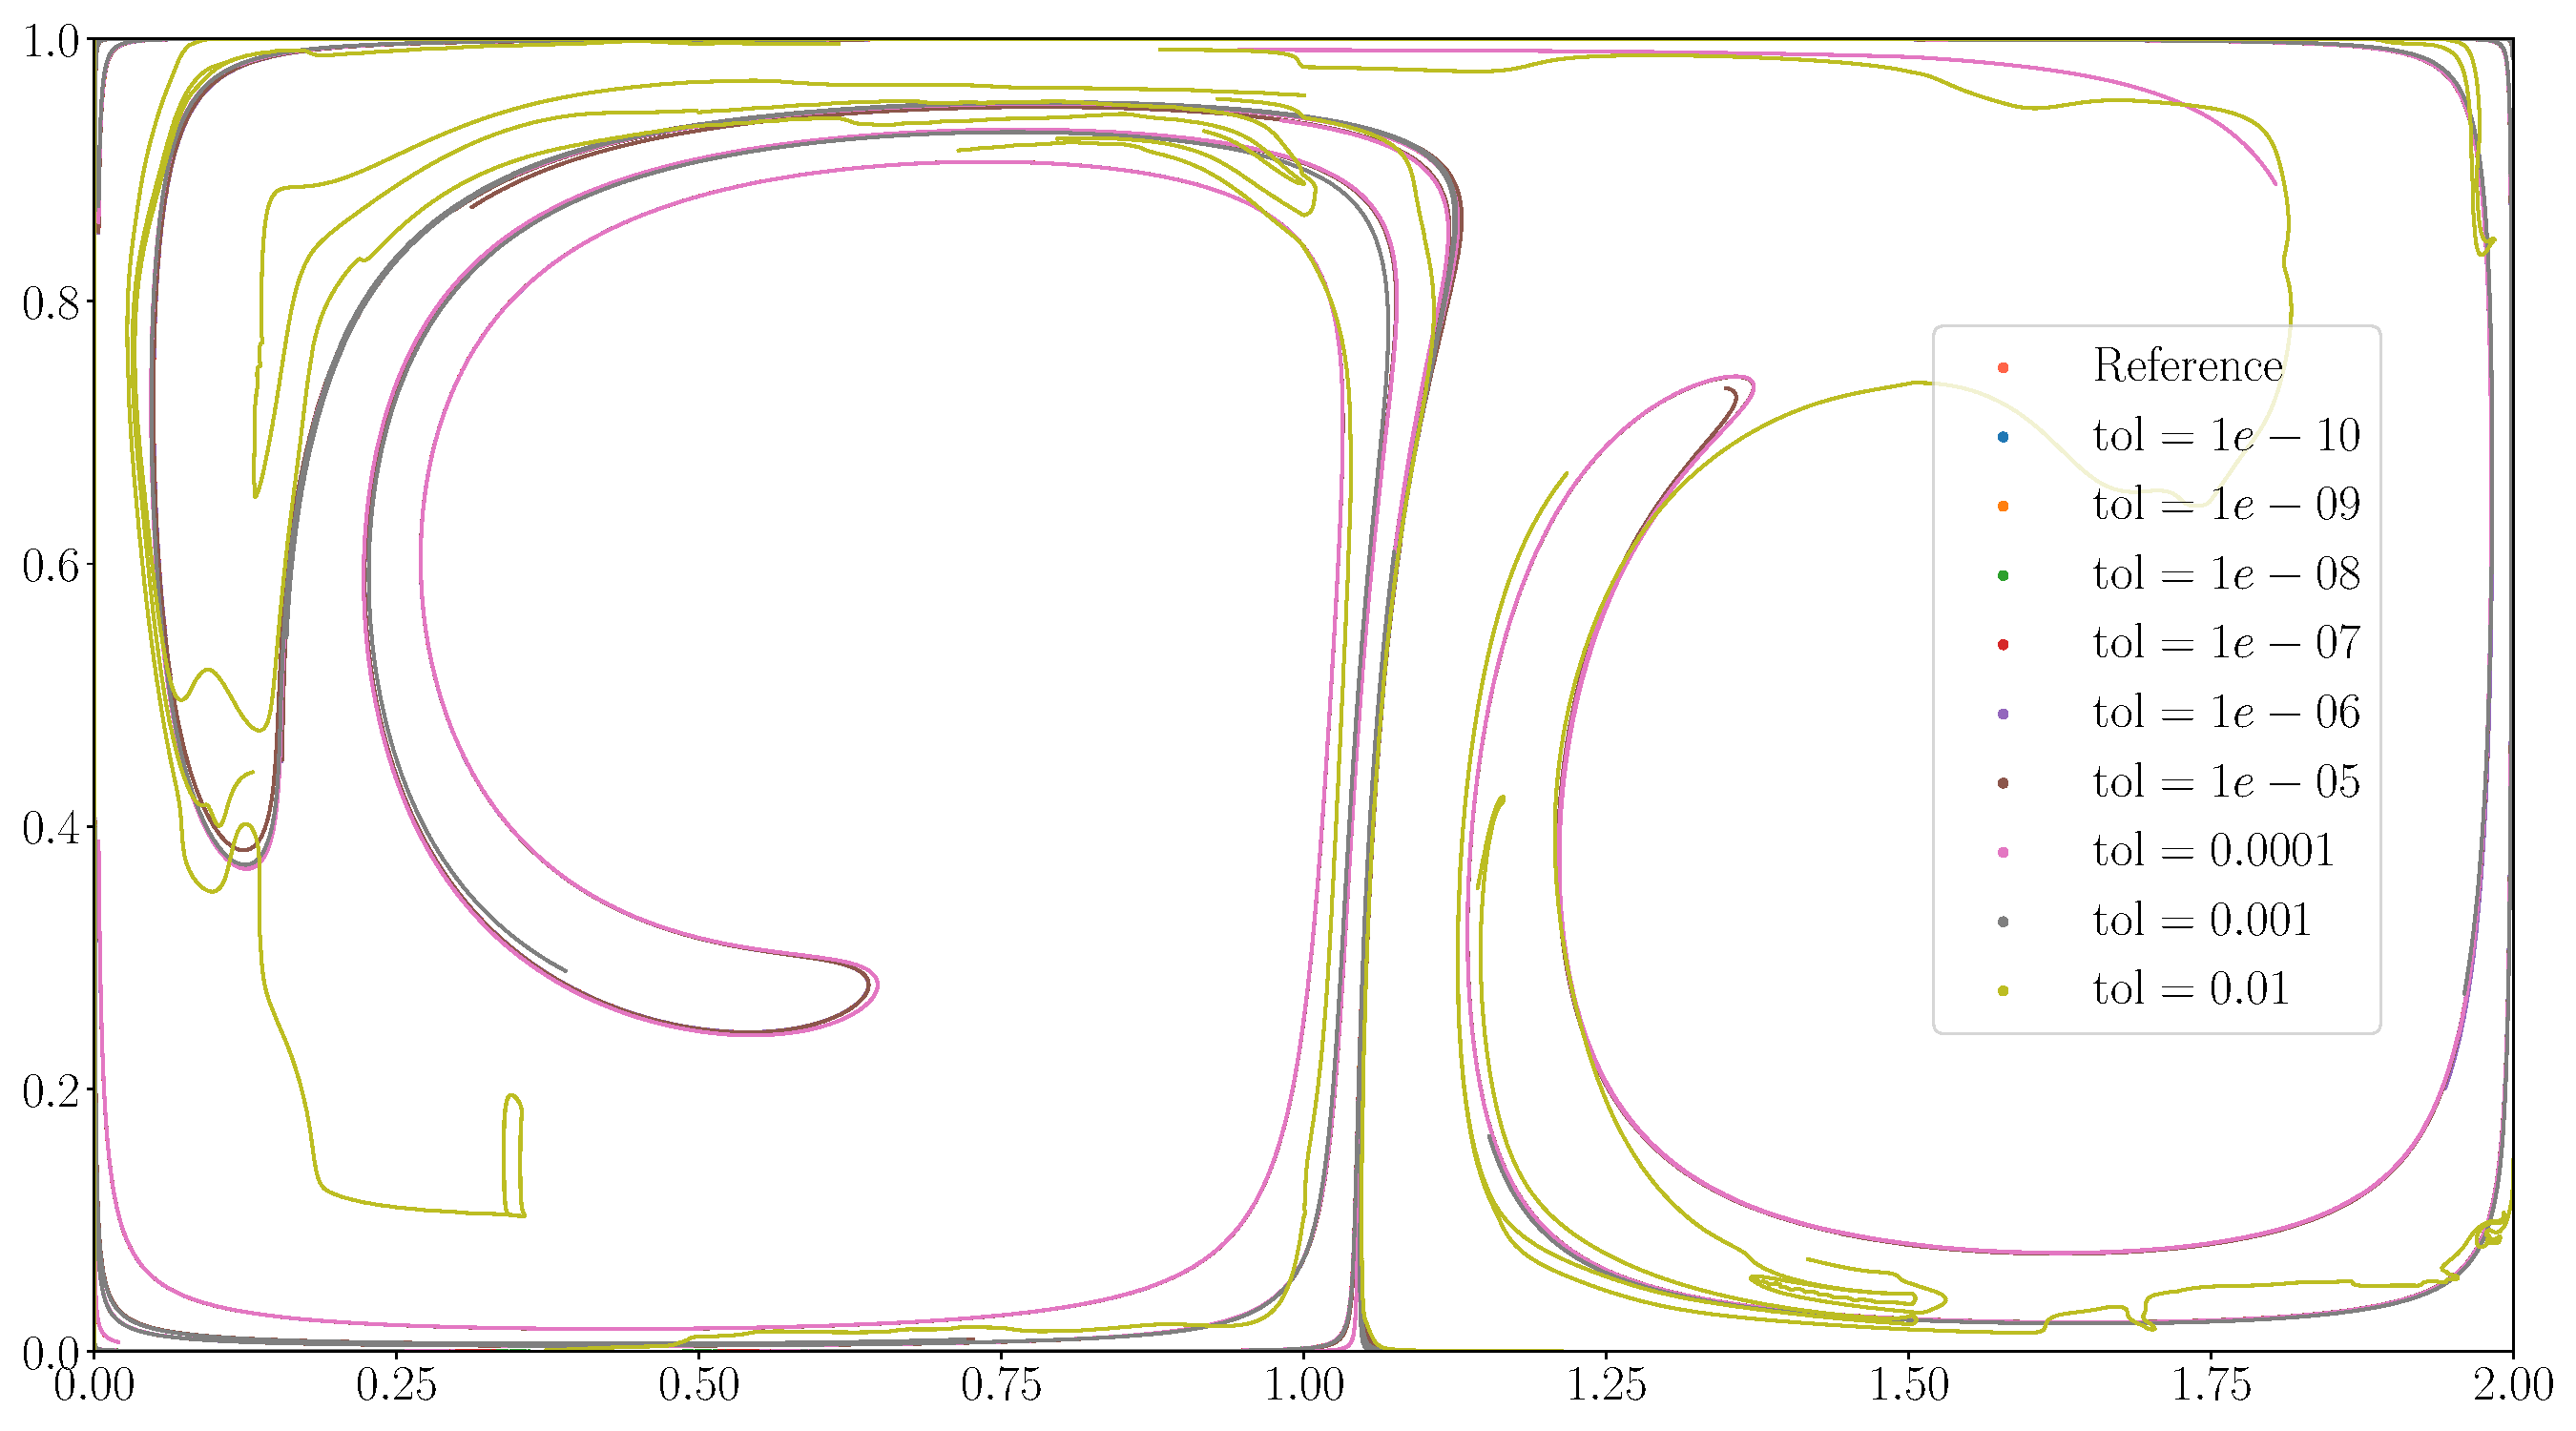
\includegraphics[width=0.9\linewidth]{figures/lcs_figures/rkdp54.pdf}
    \caption[LCS curves found by means of the Dormand-Prince 5(4) integration
    scheme]{
        LCS curves found by means of the Dormand-Prince 5(4) integration
        scheme. The reference LCS, as shown by itself in figure
        \ref{fig:referencelcs}, is plotted on the bottom layer. Note that
        the LCS for the lowest tolerance level considered, that is,
        $\textnormal{tol}=0.1$, is not included. This is because the
        corresponding $\mathcal{U}_{0}$ domain, shown in figure
        \ref{fig:u0_dp54}, and the reference $\mathcal{U}_{0}$, shown in figure
        \ref{fig:u0_domain} are dissimilar. Here, there are visible
        disparities for for all tolerance levels $\textnormal{tol}>10^{-6}$.}
    \label{fig:lcs_rkdp54}
\end{figure}


%\clearpage
\begin{figure}[htpb]
    \centering
    %% Creator: Matplotlib, PGF backend
%%
%% To include the figure in your LaTeX document, write
%%   \input{<filename>.pgf}
%%
%% Make sure the required packages are loaded in your preamble
%%   \usepackage{pgf}
%%
%% Figures using additional raster images can only be included by \input if
%% they are in the same directory as the main LaTeX file. For loading figures
%% from other directories you can use the `import` package
%%   \usepackage{import}
%% and then include the figures with
%%   \import{<path to file>}{<filename>.pgf}
%%
%% Matplotlib used the following preamble
%%   \usepackage[utf8x]{inputenc}
%%   \usepackage[T1]{fontenc}
%%   \usepackage[]{libertine}\usepackage[libertine]{newtxmath}
%%
\begingroup%
\makeatletter%
\begin{pgfpicture}%
\pgfpathrectangle{\pgfpointorigin}{\pgfqpoint{5.050000in}{3.100000in}}%
\pgfusepath{use as bounding box, clip}%
\begin{pgfscope}%
\pgfsetbuttcap%
\pgfsetmiterjoin%
\definecolor{currentfill}{rgb}{1.000000,1.000000,1.000000}%
\pgfsetfillcolor{currentfill}%
\pgfsetlinewidth{0.000000pt}%
\definecolor{currentstroke}{rgb}{1.000000,1.000000,1.000000}%
\pgfsetstrokecolor{currentstroke}%
\pgfsetdash{}{0pt}%
\pgfpathmoveto{\pgfqpoint{0.000000in}{0.000000in}}%
\pgfpathlineto{\pgfqpoint{5.050000in}{0.000000in}}%
\pgfpathlineto{\pgfqpoint{5.050000in}{3.100000in}}%
\pgfpathlineto{\pgfqpoint{0.000000in}{3.100000in}}%
\pgfpathclose%
\pgfusepath{fill}%
\end{pgfscope}%
\begin{pgfscope}%
\pgfsetbuttcap%
\pgfsetmiterjoin%
\definecolor{currentfill}{rgb}{1.000000,1.000000,1.000000}%
\pgfsetfillcolor{currentfill}%
\pgfsetlinewidth{0.000000pt}%
\definecolor{currentstroke}{rgb}{0.000000,0.000000,0.000000}%
\pgfsetstrokecolor{currentstroke}%
\pgfsetstrokeopacity{0.000000}%
\pgfsetdash{}{0pt}%
\pgfpathmoveto{\pgfqpoint{0.448634in}{0.402556in}}%
\pgfpathlineto{\pgfqpoint{4.799294in}{0.402556in}}%
\pgfpathlineto{\pgfqpoint{4.799294in}{2.891760in}}%
\pgfpathlineto{\pgfqpoint{0.448634in}{2.891760in}}%
\pgfpathclose%
\pgfusepath{fill}%
\end{pgfscope}%
\begin{pgfscope}%
\pgfsetbuttcap%
\pgfsetroundjoin%
\definecolor{currentfill}{rgb}{0.000000,0.000000,0.000000}%
\pgfsetfillcolor{currentfill}%
\pgfsetlinewidth{0.803000pt}%
\definecolor{currentstroke}{rgb}{0.000000,0.000000,0.000000}%
\pgfsetstrokecolor{currentstroke}%
\pgfsetdash{}{0pt}%
\pgfsys@defobject{currentmarker}{\pgfqpoint{0.000000in}{-0.048611in}}{\pgfqpoint{0.000000in}{0.000000in}}{%
\pgfpathmoveto{\pgfqpoint{0.000000in}{0.000000in}}%
\pgfpathlineto{\pgfqpoint{0.000000in}{-0.048611in}}%
\pgfusepath{stroke,fill}%
}%
\begin{pgfscope}%
\pgfsys@transformshift{0.448634in}{0.402556in}%
\pgfsys@useobject{currentmarker}{}%
\end{pgfscope}%
\end{pgfscope}%
\begin{pgfscope}%
\pgftext[x=0.448634in,y=0.305334in,,top]{\rmfamily\fontsize{12.000000}{14.400000}\selectfont \(\displaystyle 0.00\)}%
\end{pgfscope}%
\begin{pgfscope}%
\pgfsetbuttcap%
\pgfsetroundjoin%
\definecolor{currentfill}{rgb}{0.000000,0.000000,0.000000}%
\pgfsetfillcolor{currentfill}%
\pgfsetlinewidth{0.803000pt}%
\definecolor{currentstroke}{rgb}{0.000000,0.000000,0.000000}%
\pgfsetstrokecolor{currentstroke}%
\pgfsetdash{}{0pt}%
\pgfsys@defobject{currentmarker}{\pgfqpoint{0.000000in}{-0.048611in}}{\pgfqpoint{0.000000in}{0.000000in}}{%
\pgfpathmoveto{\pgfqpoint{0.000000in}{0.000000in}}%
\pgfpathlineto{\pgfqpoint{0.000000in}{-0.048611in}}%
\pgfusepath{stroke,fill}%
}%
\begin{pgfscope}%
\pgfsys@transformshift{0.992466in}{0.402556in}%
\pgfsys@useobject{currentmarker}{}%
\end{pgfscope}%
\end{pgfscope}%
\begin{pgfscope}%
\pgftext[x=0.992466in,y=0.305334in,,top]{\rmfamily\fontsize{12.000000}{14.400000}\selectfont \(\displaystyle 0.25\)}%
\end{pgfscope}%
\begin{pgfscope}%
\pgfsetbuttcap%
\pgfsetroundjoin%
\definecolor{currentfill}{rgb}{0.000000,0.000000,0.000000}%
\pgfsetfillcolor{currentfill}%
\pgfsetlinewidth{0.803000pt}%
\definecolor{currentstroke}{rgb}{0.000000,0.000000,0.000000}%
\pgfsetstrokecolor{currentstroke}%
\pgfsetdash{}{0pt}%
\pgfsys@defobject{currentmarker}{\pgfqpoint{0.000000in}{-0.048611in}}{\pgfqpoint{0.000000in}{0.000000in}}{%
\pgfpathmoveto{\pgfqpoint{0.000000in}{0.000000in}}%
\pgfpathlineto{\pgfqpoint{0.000000in}{-0.048611in}}%
\pgfusepath{stroke,fill}%
}%
\begin{pgfscope}%
\pgfsys@transformshift{1.536299in}{0.402556in}%
\pgfsys@useobject{currentmarker}{}%
\end{pgfscope}%
\end{pgfscope}%
\begin{pgfscope}%
\pgftext[x=1.536299in,y=0.305334in,,top]{\rmfamily\fontsize{12.000000}{14.400000}\selectfont \(\displaystyle 0.50\)}%
\end{pgfscope}%
\begin{pgfscope}%
\pgfsetbuttcap%
\pgfsetroundjoin%
\definecolor{currentfill}{rgb}{0.000000,0.000000,0.000000}%
\pgfsetfillcolor{currentfill}%
\pgfsetlinewidth{0.803000pt}%
\definecolor{currentstroke}{rgb}{0.000000,0.000000,0.000000}%
\pgfsetstrokecolor{currentstroke}%
\pgfsetdash{}{0pt}%
\pgfsys@defobject{currentmarker}{\pgfqpoint{0.000000in}{-0.048611in}}{\pgfqpoint{0.000000in}{0.000000in}}{%
\pgfpathmoveto{\pgfqpoint{0.000000in}{0.000000in}}%
\pgfpathlineto{\pgfqpoint{0.000000in}{-0.048611in}}%
\pgfusepath{stroke,fill}%
}%
\begin{pgfscope}%
\pgfsys@transformshift{2.080131in}{0.402556in}%
\pgfsys@useobject{currentmarker}{}%
\end{pgfscope}%
\end{pgfscope}%
\begin{pgfscope}%
\pgftext[x=2.080131in,y=0.305334in,,top]{\rmfamily\fontsize{12.000000}{14.400000}\selectfont \(\displaystyle 0.75\)}%
\end{pgfscope}%
\begin{pgfscope}%
\pgfsetbuttcap%
\pgfsetroundjoin%
\definecolor{currentfill}{rgb}{0.000000,0.000000,0.000000}%
\pgfsetfillcolor{currentfill}%
\pgfsetlinewidth{0.803000pt}%
\definecolor{currentstroke}{rgb}{0.000000,0.000000,0.000000}%
\pgfsetstrokecolor{currentstroke}%
\pgfsetdash{}{0pt}%
\pgfsys@defobject{currentmarker}{\pgfqpoint{0.000000in}{-0.048611in}}{\pgfqpoint{0.000000in}{0.000000in}}{%
\pgfpathmoveto{\pgfqpoint{0.000000in}{0.000000in}}%
\pgfpathlineto{\pgfqpoint{0.000000in}{-0.048611in}}%
\pgfusepath{stroke,fill}%
}%
\begin{pgfscope}%
\pgfsys@transformshift{2.623964in}{0.402556in}%
\pgfsys@useobject{currentmarker}{}%
\end{pgfscope}%
\end{pgfscope}%
\begin{pgfscope}%
\pgftext[x=2.623964in,y=0.305334in,,top]{\rmfamily\fontsize{12.000000}{14.400000}\selectfont \(\displaystyle 1.00\)}%
\end{pgfscope}%
\begin{pgfscope}%
\pgfsetbuttcap%
\pgfsetroundjoin%
\definecolor{currentfill}{rgb}{0.000000,0.000000,0.000000}%
\pgfsetfillcolor{currentfill}%
\pgfsetlinewidth{0.803000pt}%
\definecolor{currentstroke}{rgb}{0.000000,0.000000,0.000000}%
\pgfsetstrokecolor{currentstroke}%
\pgfsetdash{}{0pt}%
\pgfsys@defobject{currentmarker}{\pgfqpoint{0.000000in}{-0.048611in}}{\pgfqpoint{0.000000in}{0.000000in}}{%
\pgfpathmoveto{\pgfqpoint{0.000000in}{0.000000in}}%
\pgfpathlineto{\pgfqpoint{0.000000in}{-0.048611in}}%
\pgfusepath{stroke,fill}%
}%
\begin{pgfscope}%
\pgfsys@transformshift{3.167797in}{0.402556in}%
\pgfsys@useobject{currentmarker}{}%
\end{pgfscope}%
\end{pgfscope}%
\begin{pgfscope}%
\pgftext[x=3.167797in,y=0.305334in,,top]{\rmfamily\fontsize{12.000000}{14.400000}\selectfont \(\displaystyle 1.25\)}%
\end{pgfscope}%
\begin{pgfscope}%
\pgfsetbuttcap%
\pgfsetroundjoin%
\definecolor{currentfill}{rgb}{0.000000,0.000000,0.000000}%
\pgfsetfillcolor{currentfill}%
\pgfsetlinewidth{0.803000pt}%
\definecolor{currentstroke}{rgb}{0.000000,0.000000,0.000000}%
\pgfsetstrokecolor{currentstroke}%
\pgfsetdash{}{0pt}%
\pgfsys@defobject{currentmarker}{\pgfqpoint{0.000000in}{-0.048611in}}{\pgfqpoint{0.000000in}{0.000000in}}{%
\pgfpathmoveto{\pgfqpoint{0.000000in}{0.000000in}}%
\pgfpathlineto{\pgfqpoint{0.000000in}{-0.048611in}}%
\pgfusepath{stroke,fill}%
}%
\begin{pgfscope}%
\pgfsys@transformshift{3.711629in}{0.402556in}%
\pgfsys@useobject{currentmarker}{}%
\end{pgfscope}%
\end{pgfscope}%
\begin{pgfscope}%
\pgftext[x=3.711629in,y=0.305334in,,top]{\rmfamily\fontsize{12.000000}{14.400000}\selectfont \(\displaystyle 1.50\)}%
\end{pgfscope}%
\begin{pgfscope}%
\pgfsetbuttcap%
\pgfsetroundjoin%
\definecolor{currentfill}{rgb}{0.000000,0.000000,0.000000}%
\pgfsetfillcolor{currentfill}%
\pgfsetlinewidth{0.803000pt}%
\definecolor{currentstroke}{rgb}{0.000000,0.000000,0.000000}%
\pgfsetstrokecolor{currentstroke}%
\pgfsetdash{}{0pt}%
\pgfsys@defobject{currentmarker}{\pgfqpoint{0.000000in}{-0.048611in}}{\pgfqpoint{0.000000in}{0.000000in}}{%
\pgfpathmoveto{\pgfqpoint{0.000000in}{0.000000in}}%
\pgfpathlineto{\pgfqpoint{0.000000in}{-0.048611in}}%
\pgfusepath{stroke,fill}%
}%
\begin{pgfscope}%
\pgfsys@transformshift{4.255462in}{0.402556in}%
\pgfsys@useobject{currentmarker}{}%
\end{pgfscope}%
\end{pgfscope}%
\begin{pgfscope}%
\pgftext[x=4.255462in,y=0.305334in,,top]{\rmfamily\fontsize{12.000000}{14.400000}\selectfont \(\displaystyle 1.75\)}%
\end{pgfscope}%
\begin{pgfscope}%
\pgfsetbuttcap%
\pgfsetroundjoin%
\definecolor{currentfill}{rgb}{0.000000,0.000000,0.000000}%
\pgfsetfillcolor{currentfill}%
\pgfsetlinewidth{0.803000pt}%
\definecolor{currentstroke}{rgb}{0.000000,0.000000,0.000000}%
\pgfsetstrokecolor{currentstroke}%
\pgfsetdash{}{0pt}%
\pgfsys@defobject{currentmarker}{\pgfqpoint{0.000000in}{-0.048611in}}{\pgfqpoint{0.000000in}{0.000000in}}{%
\pgfpathmoveto{\pgfqpoint{0.000000in}{0.000000in}}%
\pgfpathlineto{\pgfqpoint{0.000000in}{-0.048611in}}%
\pgfusepath{stroke,fill}%
}%
\begin{pgfscope}%
\pgfsys@transformshift{4.799294in}{0.402556in}%
\pgfsys@useobject{currentmarker}{}%
\end{pgfscope}%
\end{pgfscope}%
\begin{pgfscope}%
\pgftext[x=4.799294in,y=0.305334in,,top]{\rmfamily\fontsize{12.000000}{14.400000}\selectfont \(\displaystyle 2.00\)}%
\end{pgfscope}%
\begin{pgfscope}%
\pgfsetbuttcap%
\pgfsetroundjoin%
\definecolor{currentfill}{rgb}{0.000000,0.000000,0.000000}%
\pgfsetfillcolor{currentfill}%
\pgfsetlinewidth{0.803000pt}%
\definecolor{currentstroke}{rgb}{0.000000,0.000000,0.000000}%
\pgfsetstrokecolor{currentstroke}%
\pgfsetdash{}{0pt}%
\pgfsys@defobject{currentmarker}{\pgfqpoint{-0.048611in}{0.000000in}}{\pgfqpoint{0.000000in}{0.000000in}}{%
\pgfpathmoveto{\pgfqpoint{0.000000in}{0.000000in}}%
\pgfpathlineto{\pgfqpoint{-0.048611in}{0.000000in}}%
\pgfusepath{stroke,fill}%
}%
\begin{pgfscope}%
\pgfsys@transformshift{0.448634in}{0.402556in}%
\pgfsys@useobject{currentmarker}{}%
\end{pgfscope}%
\end{pgfscope}%
\begin{pgfscope}%
\pgftext[x=0.149245in,y=0.345015in,left,base]{\rmfamily\fontsize{12.000000}{14.400000}\selectfont \(\displaystyle 0.0\)}%
\end{pgfscope}%
\begin{pgfscope}%
\pgfsetbuttcap%
\pgfsetroundjoin%
\definecolor{currentfill}{rgb}{0.000000,0.000000,0.000000}%
\pgfsetfillcolor{currentfill}%
\pgfsetlinewidth{0.803000pt}%
\definecolor{currentstroke}{rgb}{0.000000,0.000000,0.000000}%
\pgfsetstrokecolor{currentstroke}%
\pgfsetdash{}{0pt}%
\pgfsys@defobject{currentmarker}{\pgfqpoint{-0.048611in}{0.000000in}}{\pgfqpoint{0.000000in}{0.000000in}}{%
\pgfpathmoveto{\pgfqpoint{0.000000in}{0.000000in}}%
\pgfpathlineto{\pgfqpoint{-0.048611in}{0.000000in}}%
\pgfusepath{stroke,fill}%
}%
\begin{pgfscope}%
\pgfsys@transformshift{0.448634in}{0.900397in}%
\pgfsys@useobject{currentmarker}{}%
\end{pgfscope}%
\end{pgfscope}%
\begin{pgfscope}%
\pgftext[x=0.149245in,y=0.842855in,left,base]{\rmfamily\fontsize{12.000000}{14.400000}\selectfont \(\displaystyle 0.2\)}%
\end{pgfscope}%
\begin{pgfscope}%
\pgfsetbuttcap%
\pgfsetroundjoin%
\definecolor{currentfill}{rgb}{0.000000,0.000000,0.000000}%
\pgfsetfillcolor{currentfill}%
\pgfsetlinewidth{0.803000pt}%
\definecolor{currentstroke}{rgb}{0.000000,0.000000,0.000000}%
\pgfsetstrokecolor{currentstroke}%
\pgfsetdash{}{0pt}%
\pgfsys@defobject{currentmarker}{\pgfqpoint{-0.048611in}{0.000000in}}{\pgfqpoint{0.000000in}{0.000000in}}{%
\pgfpathmoveto{\pgfqpoint{0.000000in}{0.000000in}}%
\pgfpathlineto{\pgfqpoint{-0.048611in}{0.000000in}}%
\pgfusepath{stroke,fill}%
}%
\begin{pgfscope}%
\pgfsys@transformshift{0.448634in}{1.398238in}%
\pgfsys@useobject{currentmarker}{}%
\end{pgfscope}%
\end{pgfscope}%
\begin{pgfscope}%
\pgftext[x=0.149245in,y=1.340696in,left,base]{\rmfamily\fontsize{12.000000}{14.400000}\selectfont \(\displaystyle 0.4\)}%
\end{pgfscope}%
\begin{pgfscope}%
\pgfsetbuttcap%
\pgfsetroundjoin%
\definecolor{currentfill}{rgb}{0.000000,0.000000,0.000000}%
\pgfsetfillcolor{currentfill}%
\pgfsetlinewidth{0.803000pt}%
\definecolor{currentstroke}{rgb}{0.000000,0.000000,0.000000}%
\pgfsetstrokecolor{currentstroke}%
\pgfsetdash{}{0pt}%
\pgfsys@defobject{currentmarker}{\pgfqpoint{-0.048611in}{0.000000in}}{\pgfqpoint{0.000000in}{0.000000in}}{%
\pgfpathmoveto{\pgfqpoint{0.000000in}{0.000000in}}%
\pgfpathlineto{\pgfqpoint{-0.048611in}{0.000000in}}%
\pgfusepath{stroke,fill}%
}%
\begin{pgfscope}%
\pgfsys@transformshift{0.448634in}{1.896079in}%
\pgfsys@useobject{currentmarker}{}%
\end{pgfscope}%
\end{pgfscope}%
\begin{pgfscope}%
\pgftext[x=0.149245in,y=1.838537in,left,base]{\rmfamily\fontsize{12.000000}{14.400000}\selectfont \(\displaystyle 0.6\)}%
\end{pgfscope}%
\begin{pgfscope}%
\pgfsetbuttcap%
\pgfsetroundjoin%
\definecolor{currentfill}{rgb}{0.000000,0.000000,0.000000}%
\pgfsetfillcolor{currentfill}%
\pgfsetlinewidth{0.803000pt}%
\definecolor{currentstroke}{rgb}{0.000000,0.000000,0.000000}%
\pgfsetstrokecolor{currentstroke}%
\pgfsetdash{}{0pt}%
\pgfsys@defobject{currentmarker}{\pgfqpoint{-0.048611in}{0.000000in}}{\pgfqpoint{0.000000in}{0.000000in}}{%
\pgfpathmoveto{\pgfqpoint{0.000000in}{0.000000in}}%
\pgfpathlineto{\pgfqpoint{-0.048611in}{0.000000in}}%
\pgfusepath{stroke,fill}%
}%
\begin{pgfscope}%
\pgfsys@transformshift{0.448634in}{2.393919in}%
\pgfsys@useobject{currentmarker}{}%
\end{pgfscope}%
\end{pgfscope}%
\begin{pgfscope}%
\pgftext[x=0.149245in,y=2.336378in,left,base]{\rmfamily\fontsize{12.000000}{14.400000}\selectfont \(\displaystyle 0.8\)}%
\end{pgfscope}%
\begin{pgfscope}%
\pgfsetbuttcap%
\pgfsetroundjoin%
\definecolor{currentfill}{rgb}{0.000000,0.000000,0.000000}%
\pgfsetfillcolor{currentfill}%
\pgfsetlinewidth{0.803000pt}%
\definecolor{currentstroke}{rgb}{0.000000,0.000000,0.000000}%
\pgfsetstrokecolor{currentstroke}%
\pgfsetdash{}{0pt}%
\pgfsys@defobject{currentmarker}{\pgfqpoint{-0.048611in}{0.000000in}}{\pgfqpoint{0.000000in}{0.000000in}}{%
\pgfpathmoveto{\pgfqpoint{0.000000in}{0.000000in}}%
\pgfpathlineto{\pgfqpoint{-0.048611in}{0.000000in}}%
\pgfusepath{stroke,fill}%
}%
\begin{pgfscope}%
\pgfsys@transformshift{0.448634in}{2.891760in}%
\pgfsys@useobject{currentmarker}{}%
\end{pgfscope}%
\end{pgfscope}%
\begin{pgfscope}%
\pgftext[x=0.149245in,y=2.834219in,left,base]{\rmfamily\fontsize{12.000000}{14.400000}\selectfont \(\displaystyle 1.0\)}%
\end{pgfscope}%
\begin{pgfscope}%
\pgfpathrectangle{\pgfqpoint{0.448634in}{0.402556in}}{\pgfqpoint{4.350661in}{2.489204in}} %
\pgfusepath{clip}%
\pgfsetrectcap%
\pgfsetroundjoin%
\pgfsetlinewidth{1.003750pt}%
\definecolor{currentstroke}{rgb}{0.121569,0.466667,0.705882}%
\pgfsetstrokecolor{currentstroke}%
\pgfsetdash{}{0pt}%
\pgfpathmoveto{\pgfqpoint{0.448634in}{2.896245in}}%
\pgfpathlineto{\pgfqpoint{0.448593in}{0.407043in}}%
\pgfpathlineto{\pgfqpoint{0.448593in}{0.407043in}}%
\pgfusepath{stroke}%
\end{pgfscope}%
\begin{pgfscope}%
\pgfpathrectangle{\pgfqpoint{0.448634in}{0.402556in}}{\pgfqpoint{4.350661in}{2.489204in}} %
\pgfusepath{clip}%
\pgfsetrectcap%
\pgfsetroundjoin%
\pgfsetlinewidth{1.003750pt}%
\definecolor{currentstroke}{rgb}{0.121569,0.466667,0.705882}%
\pgfsetstrokecolor{currentstroke}%
\pgfsetdash{}{0pt}%
\pgfpathmoveto{\pgfqpoint{0.576853in}{1.760817in}}%
\pgfpathlineto{\pgfqpoint{0.569394in}{1.840010in}}%
\pgfpathlineto{\pgfqpoint{0.563209in}{1.929338in}}%
\pgfpathlineto{\pgfqpoint{0.558592in}{2.028764in}}%
\pgfpathlineto{\pgfqpoint{0.555985in}{2.133265in}}%
\pgfpathlineto{\pgfqpoint{0.555566in}{2.237808in}}%
\pgfpathlineto{\pgfqpoint{0.557371in}{2.337352in}}%
\pgfpathlineto{\pgfqpoint{0.561096in}{2.424366in}}%
\pgfpathlineto{\pgfqpoint{0.566403in}{2.498791in}}%
\pgfpathlineto{\pgfqpoint{0.572909in}{2.560570in}}%
\pgfpathlineto{\pgfqpoint{0.580458in}{2.612119in}}%
\pgfpathlineto{\pgfqpoint{0.589086in}{2.655816in}}%
\pgfpathlineto{\pgfqpoint{0.598406in}{2.691589in}}%
\pgfpathlineto{\pgfqpoint{0.608613in}{2.721757in}}%
\pgfpathlineto{\pgfqpoint{0.619241in}{2.746278in}}%
\pgfpathlineto{\pgfqpoint{0.630817in}{2.767339in}}%
\pgfpathlineto{\pgfqpoint{0.642975in}{2.784884in}}%
\pgfpathlineto{\pgfqpoint{0.656813in}{2.800712in}}%
\pgfpathlineto{\pgfqpoint{0.672197in}{2.814549in}}%
\pgfpathlineto{\pgfqpoint{0.688853in}{2.826301in}}%
\pgfpathlineto{\pgfqpoint{0.706461in}{2.836076in}}%
\pgfpathlineto{\pgfqpoint{0.726804in}{2.844875in}}%
\pgfpathlineto{\pgfqpoint{0.751866in}{2.853203in}}%
\pgfpathlineto{\pgfqpoint{0.781631in}{2.860547in}}%
\pgfpathlineto{\pgfqpoint{0.818168in}{2.867054in}}%
\pgfpathlineto{\pgfqpoint{0.863581in}{2.872685in}}%
\pgfpathlineto{\pgfqpoint{0.922161in}{2.877518in}}%
\pgfpathlineto{\pgfqpoint{1.000391in}{2.881567in}}%
\pgfpathlineto{\pgfqpoint{1.111294in}{2.884881in}}%
\pgfpathlineto{\pgfqpoint{1.274428in}{2.887367in}}%
\pgfpathlineto{\pgfqpoint{1.552865in}{2.889263in}}%
\pgfpathlineto{\pgfqpoint{2.107573in}{2.890457in}}%
\pgfpathlineto{\pgfqpoint{3.343161in}{2.890573in}}%
\pgfpathlineto{\pgfqpoint{4.043615in}{2.888941in}}%
\pgfpathlineto{\pgfqpoint{4.289417in}{2.886404in}}%
\pgfpathlineto{\pgfqpoint{4.413375in}{2.883093in}}%
\pgfpathlineto{\pgfqpoint{4.489424in}{2.878997in}}%
\pgfpathlineto{\pgfqpoint{4.541451in}{2.874081in}}%
\pgfpathlineto{\pgfqpoint{4.578100in}{2.868470in}}%
\pgfpathlineto{\pgfqpoint{4.605818in}{2.862092in}}%
\pgfpathlineto{\pgfqpoint{4.626725in}{2.855245in}}%
\pgfpathlineto{\pgfqpoint{4.644925in}{2.847018in}}%
\pgfpathlineto{\pgfqpoint{4.660241in}{2.837590in}}%
\pgfpathlineto{\pgfqpoint{4.672623in}{2.827468in}}%
\pgfpathlineto{\pgfqpoint{4.683751in}{2.815592in}}%
\pgfpathlineto{\pgfqpoint{4.693406in}{2.802135in}}%
\pgfpathlineto{\pgfqpoint{4.702740in}{2.785343in}}%
\pgfpathlineto{\pgfqpoint{4.711277in}{2.765194in}}%
\pgfpathlineto{\pgfqpoint{4.719482in}{2.739484in}}%
\pgfpathlineto{\pgfqpoint{4.726293in}{2.710657in}}%
\pgfpathlineto{\pgfqpoint{4.733259in}{2.671643in}}%
\pgfpathlineto{\pgfqpoint{4.739604in}{2.622396in}}%
\pgfpathlineto{\pgfqpoint{4.745236in}{2.560504in}}%
\pgfpathlineto{\pgfqpoint{4.750164in}{2.481052in}}%
\pgfpathlineto{\pgfqpoint{4.754367in}{2.376618in}}%
\pgfpathlineto{\pgfqpoint{4.757443in}{2.242249in}}%
\pgfpathlineto{\pgfqpoint{4.758977in}{2.075483in}}%
\pgfpathlineto{\pgfqpoint{4.758447in}{1.888795in}}%
\pgfpathlineto{\pgfqpoint{4.755756in}{1.707111in}}%
\pgfpathlineto{\pgfqpoint{4.750925in}{1.532957in}}%
\pgfpathlineto{\pgfqpoint{4.744785in}{1.398726in}}%
\pgfpathlineto{\pgfqpoint{4.737575in}{1.289516in}}%
\pgfpathlineto{\pgfqpoint{4.728714in}{1.190470in}}%
\pgfpathlineto{\pgfqpoint{4.719652in}{1.116521in}}%
\pgfpathlineto{\pgfqpoint{4.710036in}{1.055276in}}%
\pgfpathlineto{\pgfqpoint{4.699503in}{1.001861in}}%
\pgfpathlineto{\pgfqpoint{4.689040in}{0.958690in}}%
\pgfpathlineto{\pgfqpoint{4.677219in}{0.918600in}}%
\pgfpathlineto{\pgfqpoint{4.664034in}{0.881749in}}%
\pgfpathlineto{\pgfqpoint{4.650584in}{0.850492in}}%
\pgfpathlineto{\pgfqpoint{4.636303in}{0.822570in}}%
\pgfpathlineto{\pgfqpoint{4.620207in}{0.795974in}}%
\pgfpathlineto{\pgfqpoint{4.603640in}{0.772901in}}%
\pgfpathlineto{\pgfqpoint{4.585488in}{0.751446in}}%
\pgfpathlineto{\pgfqpoint{4.565874in}{0.731749in}}%
\pgfpathlineto{\pgfqpoint{4.544964in}{0.713879in}}%
\pgfpathlineto{\pgfqpoint{4.522958in}{0.697824in}}%
\pgfpathlineto{\pgfqpoint{4.496157in}{0.681290in}}%
\pgfpathlineto{\pgfqpoint{4.470397in}{0.667953in}}%
\pgfpathlineto{\pgfqpoint{4.439961in}{0.654509in}}%
\pgfpathlineto{\pgfqpoint{4.406841in}{0.642281in}}%
\pgfpathlineto{\pgfqpoint{4.369009in}{0.630748in}}%
\pgfpathlineto{\pgfqpoint{4.326489in}{0.620226in}}%
\pgfpathlineto{\pgfqpoint{4.279327in}{0.610949in}}%
\pgfpathlineto{\pgfqpoint{4.227576in}{0.603085in}}%
\pgfpathlineto{\pgfqpoint{4.173450in}{0.597063in}}%
\pgfpathlineto{\pgfqpoint{4.110511in}{0.592203in}}%
\pgfpathlineto{\pgfqpoint{4.047471in}{0.589537in}}%
\pgfpathlineto{\pgfqpoint{3.977867in}{0.588624in}}%
\pgfpathlineto{\pgfqpoint{3.906093in}{0.589934in}}%
\pgfpathlineto{\pgfqpoint{3.834377in}{0.593496in}}%
\pgfpathlineto{\pgfqpoint{3.767120in}{0.599067in}}%
\pgfpathlineto{\pgfqpoint{3.704364in}{0.606392in}}%
\pgfpathlineto{\pgfqpoint{3.678516in}{0.610510in}}%
\pgfpathlineto{\pgfqpoint{3.620438in}{0.620500in}}%
\pgfpathlineto{\pgfqpoint{3.586319in}{0.628207in}}%
\pgfpathlineto{\pgfqpoint{3.495240in}{0.652428in}}%
\pgfpathlineto{\pgfqpoint{3.451528in}{0.667583in}}%
\pgfpathlineto{\pgfqpoint{3.408538in}{0.685220in}}%
\pgfpathlineto{\pgfqpoint{3.374594in}{0.702001in}}%
\pgfpathlineto{\pgfqpoint{3.345407in}{0.718682in}}%
\pgfpathlineto{\pgfqpoint{3.315236in}{0.738520in}}%
\pgfpathlineto{\pgfqpoint{3.288127in}{0.759290in}}%
\pgfpathlineto{\pgfqpoint{3.264004in}{0.780551in}}%
\pgfpathlineto{\pgfqpoint{3.241208in}{0.803648in}}%
\pgfpathlineto{\pgfqpoint{3.219894in}{0.828530in}}%
\pgfpathlineto{\pgfqpoint{3.200189in}{0.855091in}}%
\pgfpathlineto{\pgfqpoint{3.182177in}{0.883182in}}%
\pgfpathlineto{\pgfqpoint{3.165906in}{0.912633in}}%
\pgfpathlineto{\pgfqpoint{3.150351in}{0.945448in}}%
\pgfpathlineto{\pgfqpoint{3.136682in}{0.979345in}}%
\pgfpathlineto{\pgfqpoint{3.124073in}{1.016460in}}%
\pgfpathlineto{\pgfqpoint{3.112834in}{1.056769in}}%
\pgfpathlineto{\pgfqpoint{3.103046in}{1.100146in}}%
\pgfpathlineto{\pgfqpoint{3.095343in}{1.144071in}}%
\pgfpathlineto{\pgfqpoint{3.089208in}{1.190837in}}%
\pgfpathlineto{\pgfqpoint{3.084595in}{1.242838in}}%
\pgfpathlineto{\pgfqpoint{3.082137in}{1.295031in}}%
\pgfpathlineto{\pgfqpoint{3.081687in}{1.349787in}}%
\pgfpathlineto{\pgfqpoint{3.083451in}{1.406998in}}%
\pgfpathlineto{\pgfqpoint{3.087181in}{1.461589in}}%
\pgfpathlineto{\pgfqpoint{3.093485in}{1.520888in}}%
\pgfpathlineto{\pgfqpoint{3.101823in}{1.577334in}}%
\pgfpathlineto{\pgfqpoint{3.111930in}{1.630856in}}%
\pgfpathlineto{\pgfqpoint{3.124690in}{1.686208in}}%
\pgfpathlineto{\pgfqpoint{3.139178in}{1.738395in}}%
\pgfpathlineto{\pgfqpoint{3.155145in}{1.787366in}}%
\pgfpathlineto{\pgfqpoint{3.172353in}{1.833085in}}%
\pgfpathlineto{\pgfqpoint{3.191618in}{1.877716in}}%
\pgfpathlineto{\pgfqpoint{3.214026in}{1.923261in}}%
\pgfpathlineto{\pgfqpoint{3.236214in}{1.963157in}}%
\pgfpathlineto{\pgfqpoint{3.260178in}{2.001684in}}%
\pgfpathlineto{\pgfqpoint{3.285814in}{2.038776in}}%
\pgfpathlineto{\pgfqpoint{3.314415in}{2.076285in}}%
\pgfpathlineto{\pgfqpoint{3.348944in}{2.117711in}}%
\pgfpathlineto{\pgfqpoint{3.417133in}{2.198022in}}%
\pgfpathlineto{\pgfqpoint{3.426053in}{2.212128in}}%
\pgfpathlineto{\pgfqpoint{3.430798in}{2.223297in}}%
\pgfpathlineto{\pgfqpoint{3.432034in}{2.230603in}}%
\pgfpathlineto{\pgfqpoint{3.430773in}{2.237856in}}%
\pgfpathlineto{\pgfqpoint{3.426621in}{2.243526in}}%
\pgfpathlineto{\pgfqpoint{3.420908in}{2.247084in}}%
\pgfpathlineto{\pgfqpoint{3.412501in}{2.249583in}}%
\pgfpathlineto{\pgfqpoint{3.399499in}{2.250689in}}%
\pgfpathlineto{\pgfqpoint{3.384305in}{2.249671in}}%
\pgfpathlineto{\pgfqpoint{3.364985in}{2.246098in}}%
\pgfpathlineto{\pgfqpoint{3.341804in}{2.239342in}}%
\pgfpathlineto{\pgfqpoint{3.317109in}{2.229682in}}%
\pgfpathlineto{\pgfqpoint{3.291104in}{2.216986in}}%
\pgfpathlineto{\pgfqpoint{3.265928in}{2.202261in}}%
\pgfpathlineto{\pgfqpoint{3.239805in}{2.184361in}}%
\pgfpathlineto{\pgfqpoint{3.214775in}{2.164519in}}%
\pgfpathlineto{\pgfqpoint{3.190900in}{2.142893in}}%
\pgfpathlineto{\pgfqpoint{3.166657in}{2.117912in}}%
\pgfpathlineto{\pgfqpoint{3.143835in}{2.091233in}}%
\pgfpathlineto{\pgfqpoint{3.121079in}{2.061107in}}%
\pgfpathlineto{\pgfqpoint{3.099952in}{2.029463in}}%
\pgfpathlineto{\pgfqpoint{3.079251in}{1.994406in}}%
\pgfpathlineto{\pgfqpoint{3.059218in}{1.955915in}}%
\pgfpathlineto{\pgfqpoint{3.040058in}{1.914015in}}%
\pgfpathlineto{\pgfqpoint{3.022809in}{1.871041in}}%
\pgfpathlineto{\pgfqpoint{3.005790in}{1.822536in}}%
\pgfpathlineto{\pgfqpoint{2.990067in}{1.770819in}}%
\pgfpathlineto{\pgfqpoint{2.975708in}{1.715979in}}%
\pgfpathlineto{\pgfqpoint{2.962284in}{1.655680in}}%
\pgfpathlineto{\pgfqpoint{2.950496in}{1.592386in}}%
\pgfpathlineto{\pgfqpoint{2.940383in}{1.526185in}}%
\pgfpathlineto{\pgfqpoint{2.931745in}{1.454681in}}%
\pgfpathlineto{\pgfqpoint{2.925082in}{1.380399in}}%
\pgfpathlineto{\pgfqpoint{2.920647in}{1.305899in}}%
\pgfpathlineto{\pgfqpoint{2.918444in}{1.231270in}}%
\pgfpathlineto{\pgfqpoint{2.918545in}{1.159087in}}%
\pgfpathlineto{\pgfqpoint{2.920787in}{1.091931in}}%
\pgfpathlineto{\pgfqpoint{2.925177in}{1.027412in}}%
\pgfpathlineto{\pgfqpoint{2.931192in}{0.970580in}}%
\pgfpathlineto{\pgfqpoint{2.938760in}{0.919034in}}%
\pgfpathlineto{\pgfqpoint{2.947651in}{0.872852in}}%
\pgfpathlineto{\pgfqpoint{2.958213in}{0.829714in}}%
\pgfpathlineto{\pgfqpoint{2.969670in}{0.792114in}}%
\pgfpathlineto{\pgfqpoint{2.982463in}{0.757773in}}%
\pgfpathlineto{\pgfqpoint{2.996425in}{0.726812in}}%
\pgfpathlineto{\pgfqpoint{3.011299in}{0.699300in}}%
\pgfpathlineto{\pgfqpoint{3.026739in}{0.675225in}}%
\pgfpathlineto{\pgfqpoint{3.043828in}{0.652656in}}%
\pgfpathlineto{\pgfqpoint{3.062495in}{0.631788in}}%
\pgfpathlineto{\pgfqpoint{3.082602in}{0.612753in}}%
\pgfpathlineto{\pgfqpoint{3.103961in}{0.595592in}}%
\pgfpathlineto{\pgfqpoint{3.128268in}{0.579069in}}%
\pgfpathlineto{\pgfqpoint{3.153537in}{0.564554in}}%
\pgfpathlineto{\pgfqpoint{3.181571in}{0.550952in}}%
\pgfpathlineto{\pgfqpoint{3.214371in}{0.537647in}}%
\pgfpathlineto{\pgfqpoint{3.249846in}{0.525712in}}%
\pgfpathlineto{\pgfqpoint{3.290011in}{0.514571in}}%
\pgfpathlineto{\pgfqpoint{3.334820in}{0.504423in}}%
\pgfpathlineto{\pgfqpoint{3.386372in}{0.494999in}}%
\pgfpathlineto{\pgfqpoint{3.446798in}{0.486257in}}%
\pgfpathlineto{\pgfqpoint{3.518243in}{0.478282in}}%
\pgfpathlineto{\pgfqpoint{3.600685in}{0.471409in}}%
\pgfpathlineto{\pgfqpoint{3.696268in}{0.465713in}}%
\pgfpathlineto{\pgfqpoint{3.807144in}{0.461369in}}%
\pgfpathlineto{\pgfqpoint{3.933291in}{0.458719in}}%
\pgfpathlineto{\pgfqpoint{4.063808in}{0.458211in}}%
\pgfpathlineto{\pgfqpoint{4.187792in}{0.459914in}}%
\pgfpathlineto{\pgfqpoint{4.294335in}{0.463521in}}%
\pgfpathlineto{\pgfqpoint{4.381234in}{0.468574in}}%
\pgfpathlineto{\pgfqpoint{4.450636in}{0.474701in}}%
\pgfpathlineto{\pgfqpoint{4.506850in}{0.481799in}}%
\pgfpathlineto{\pgfqpoint{4.552009in}{0.489658in}}%
\pgfpathlineto{\pgfqpoint{4.588239in}{0.498115in}}%
\pgfpathlineto{\pgfqpoint{4.617656in}{0.507110in}}%
\pgfpathlineto{\pgfqpoint{4.642328in}{0.516843in}}%
\pgfpathlineto{\pgfqpoint{4.664194in}{0.527940in}}%
\pgfpathlineto{\pgfqpoint{4.681238in}{0.538945in}}%
\pgfpathlineto{\pgfqpoint{4.697164in}{0.551953in}}%
\pgfpathlineto{\pgfqpoint{4.710076in}{0.565289in}}%
\pgfpathlineto{\pgfqpoint{4.721578in}{0.580218in}}%
\pgfpathlineto{\pgfqpoint{4.731557in}{0.596521in}}%
\pgfpathlineto{\pgfqpoint{4.741000in}{0.616134in}}%
\pgfpathlineto{\pgfqpoint{4.749521in}{0.639027in}}%
\pgfpathlineto{\pgfqpoint{4.757522in}{0.667450in}}%
\pgfpathlineto{\pgfqpoint{4.764572in}{0.701345in}}%
\pgfpathlineto{\pgfqpoint{4.770840in}{0.743043in}}%
\pgfpathlineto{\pgfqpoint{4.776327in}{0.794934in}}%
\pgfpathlineto{\pgfqpoint{4.781278in}{0.864398in}}%
\pgfpathlineto{\pgfqpoint{4.785468in}{0.956371in}}%
\pgfpathlineto{\pgfqpoint{4.789000in}{1.085745in}}%
\pgfpathlineto{\pgfqpoint{4.791852in}{1.277385in}}%
\pgfpathlineto{\pgfqpoint{4.793959in}{1.581057in}}%
\pgfpathlineto{\pgfqpoint{4.794962in}{2.071429in}}%
\pgfpathlineto{\pgfqpoint{4.793967in}{2.559311in}}%
\pgfpathlineto{\pgfqpoint{4.791733in}{2.745981in}}%
\pgfpathlineto{\pgfqpoint{4.788955in}{2.818091in}}%
\pgfpathlineto{\pgfqpoint{4.785731in}{2.850227in}}%
\pgfpathlineto{\pgfqpoint{4.781879in}{2.867057in}}%
\pgfpathlineto{\pgfqpoint{4.777744in}{2.875780in}}%
\pgfpathlineto{\pgfqpoint{4.773097in}{2.880982in}}%
\pgfpathlineto{\pgfqpoint{4.767363in}{2.884504in}}%
\pgfpathlineto{\pgfqpoint{4.756853in}{2.887622in}}%
\pgfpathlineto{\pgfqpoint{4.739548in}{2.889639in}}%
\pgfpathlineto{\pgfqpoint{4.704762in}{2.890882in}}%
\pgfpathlineto{\pgfqpoint{4.602524in}{2.891538in}}%
\pgfpathlineto{\pgfqpoint{3.952100in}{2.891742in}}%
\pgfpathlineto{\pgfqpoint{0.617321in}{2.890753in}}%
\pgfpathlineto{\pgfqpoint{0.549910in}{2.888858in}}%
\pgfpathlineto{\pgfqpoint{0.521735in}{2.886179in}}%
\pgfpathlineto{\pgfqpoint{0.504666in}{2.882389in}}%
\pgfpathlineto{\pgfqpoint{0.494501in}{2.878011in}}%
\pgfpathlineto{\pgfqpoint{0.487180in}{2.872667in}}%
\pgfpathlineto{\pgfqpoint{0.481152in}{2.865519in}}%
\pgfpathlineto{\pgfqpoint{0.475664in}{2.854804in}}%
\pgfpathlineto{\pgfqpoint{0.471318in}{2.840737in}}%
\pgfpathlineto{\pgfqpoint{0.467301in}{2.818823in}}%
\pgfpathlineto{\pgfqpoint{0.463927in}{2.786700in}}%
\pgfpathlineto{\pgfqpoint{0.460918in}{2.734544in}}%
\pgfpathlineto{\pgfqpoint{0.458363in}{2.647473in}}%
\pgfpathlineto{\pgfqpoint{0.456575in}{2.523031in}}%
\pgfpathlineto{\pgfqpoint{0.456575in}{2.523031in}}%
\pgfusepath{stroke}%
\end{pgfscope}%
\begin{pgfscope}%
\pgfpathrectangle{\pgfqpoint{0.448634in}{0.402556in}}{\pgfqpoint{4.350661in}{2.489204in}} %
\pgfusepath{clip}%
\pgfsetrectcap%
\pgfsetroundjoin%
\pgfsetlinewidth{1.003750pt}%
\definecolor{currentstroke}{rgb}{0.121569,0.466667,0.705882}%
\pgfsetstrokecolor{currentstroke}%
\pgfsetdash{}{0pt}%
\pgfpathmoveto{\pgfqpoint{4.798840in}{2.852369in}}%
\pgfpathlineto{\pgfqpoint{4.797564in}{2.889610in}}%
\pgfpathlineto{\pgfqpoint{4.796215in}{2.891483in}}%
\pgfpathlineto{\pgfqpoint{4.787551in}{2.891760in}}%
\pgfpathlineto{\pgfqpoint{0.452128in}{2.891659in}}%
\pgfpathlineto{\pgfqpoint{0.450530in}{2.890082in}}%
\pgfpathlineto{\pgfqpoint{0.449454in}{2.882763in}}%
\pgfpathlineto{\pgfqpoint{0.448970in}{2.845432in}}%
\pgfpathlineto{\pgfqpoint{0.448743in}{2.494454in}}%
\pgfpathlineto{\pgfqpoint{0.449624in}{0.615107in}}%
\pgfpathlineto{\pgfqpoint{0.451433in}{0.510586in}}%
\pgfpathlineto{\pgfqpoint{0.453993in}{0.473374in}}%
\pgfpathlineto{\pgfqpoint{0.457406in}{0.453868in}}%
\pgfpathlineto{\pgfqpoint{0.461540in}{0.442384in}}%
\pgfpathlineto{\pgfqpoint{0.466739in}{0.434437in}}%
\pgfpathlineto{\pgfqpoint{0.473595in}{0.428350in}}%
\pgfpathlineto{\pgfqpoint{0.483492in}{0.423244in}}%
\pgfpathlineto{\pgfqpoint{0.491854in}{0.420501in}}%
\pgfpathlineto{\pgfqpoint{0.491854in}{0.420501in}}%
\pgfusepath{stroke}%
\end{pgfscope}%
\begin{pgfscope}%
\pgfpathrectangle{\pgfqpoint{0.448634in}{0.402556in}}{\pgfqpoint{4.350661in}{2.489204in}} %
\pgfusepath{clip}%
\pgfsetrectcap%
\pgfsetroundjoin%
\pgfsetlinewidth{1.003750pt}%
\definecolor{currentstroke}{rgb}{0.121569,0.466667,0.705882}%
\pgfsetstrokecolor{currentstroke}%
\pgfsetdash{}{0pt}%
\pgfpathmoveto{\pgfqpoint{0.456424in}{1.370137in}}%
\pgfpathlineto{\pgfqpoint{0.459610in}{1.118755in}}%
\pgfpathlineto{\pgfqpoint{0.463695in}{0.962007in}}%
\pgfpathlineto{\pgfqpoint{0.468519in}{0.857610in}}%
\pgfpathlineto{\pgfqpoint{0.474082in}{0.783210in}}%
\pgfpathlineto{\pgfqpoint{0.480226in}{0.728906in}}%
\pgfpathlineto{\pgfqpoint{0.486970in}{0.687306in}}%
\pgfpathlineto{\pgfqpoint{0.494537in}{0.653558in}}%
\pgfpathlineto{\pgfqpoint{0.503107in}{0.625355in}}%
\pgfpathlineto{\pgfqpoint{0.512193in}{0.602750in}}%
\pgfpathlineto{\pgfqpoint{0.522200in}{0.583508in}}%
\pgfpathlineto{\pgfqpoint{0.534108in}{0.565743in}}%
\pgfpathlineto{\pgfqpoint{0.546263in}{0.551507in}}%
\pgfpathlineto{\pgfqpoint{0.559728in}{0.538907in}}%
\pgfpathlineto{\pgfqpoint{0.576129in}{0.526693in}}%
\pgfpathlineto{\pgfqpoint{0.595483in}{0.515351in}}%
\pgfpathlineto{\pgfqpoint{0.617681in}{0.505147in}}%
\pgfpathlineto{\pgfqpoint{0.642568in}{0.496153in}}%
\pgfpathlineto{\pgfqpoint{0.672126in}{0.487778in}}%
\pgfpathlineto{\pgfqpoint{0.708443in}{0.479824in}}%
\pgfpathlineto{\pgfqpoint{0.753649in}{0.472325in}}%
\pgfpathlineto{\pgfqpoint{0.807717in}{0.465660in}}%
\pgfpathlineto{\pgfqpoint{0.877116in}{0.459475in}}%
\pgfpathlineto{\pgfqpoint{0.961828in}{0.454230in}}%
\pgfpathlineto{\pgfqpoint{1.068351in}{0.449916in}}%
\pgfpathlineto{\pgfqpoint{1.201018in}{0.446839in}}%
\pgfpathlineto{\pgfqpoint{1.357637in}{0.445481in}}%
\pgfpathlineto{\pgfqpoint{1.525135in}{0.446232in}}%
\pgfpathlineto{\pgfqpoint{1.686088in}{0.449142in}}%
\pgfpathlineto{\pgfqpoint{1.823074in}{0.453747in}}%
\pgfpathlineto{\pgfqpoint{1.938245in}{0.459764in}}%
\pgfpathlineto{\pgfqpoint{2.031582in}{0.466759in}}%
\pgfpathlineto{\pgfqpoint{2.109580in}{0.474745in}}%
\pgfpathlineto{\pgfqpoint{2.174384in}{0.483535in}}%
\pgfpathlineto{\pgfqpoint{2.228139in}{0.492940in}}%
\pgfpathlineto{\pgfqpoint{2.275119in}{0.503356in}}%
\pgfpathlineto{\pgfqpoint{2.315282in}{0.514501in}}%
\pgfpathlineto{\pgfqpoint{2.350698in}{0.526659in}}%
\pgfpathlineto{\pgfqpoint{2.381320in}{0.539536in}}%
\pgfpathlineto{\pgfqpoint{2.407164in}{0.552659in}}%
\pgfpathlineto{\pgfqpoint{2.430226in}{0.566639in}}%
\pgfpathlineto{\pgfqpoint{2.452282in}{0.582602in}}%
\pgfpathlineto{\pgfqpoint{2.471391in}{0.599069in}}%
\pgfpathlineto{\pgfqpoint{2.489240in}{0.617293in}}%
\pgfpathlineto{\pgfqpoint{2.505678in}{0.637180in}}%
\pgfpathlineto{\pgfqpoint{2.520620in}{0.658557in}}%
\pgfpathlineto{\pgfqpoint{2.535213in}{0.683314in}}%
\pgfpathlineto{\pgfqpoint{2.549115in}{0.711484in}}%
\pgfpathlineto{\pgfqpoint{2.562091in}{0.743004in}}%
\pgfpathlineto{\pgfqpoint{2.574020in}{0.777751in}}%
\pgfpathlineto{\pgfqpoint{2.585502in}{0.817970in}}%
\pgfpathlineto{\pgfqpoint{2.596809in}{0.866038in}}%
\pgfpathlineto{\pgfqpoint{2.607562in}{0.921948in}}%
\pgfpathlineto{\pgfqpoint{2.617925in}{0.988098in}}%
\pgfpathlineto{\pgfqpoint{2.627958in}{1.066918in}}%
\pgfpathlineto{\pgfqpoint{2.637941in}{1.163320in}}%
\pgfpathlineto{\pgfqpoint{2.648424in}{1.287199in}}%
\pgfpathlineto{\pgfqpoint{2.660103in}{1.453438in}}%
\pgfpathlineto{\pgfqpoint{2.674773in}{1.696801in}}%
\pgfpathlineto{\pgfqpoint{2.687716in}{1.945279in}}%
\pgfpathlineto{\pgfqpoint{2.692670in}{2.079573in}}%
\pgfpathlineto{\pgfqpoint{2.693829in}{2.166682in}}%
\pgfpathlineto{\pgfqpoint{2.692565in}{2.233870in}}%
\pgfpathlineto{\pgfqpoint{2.689436in}{2.286015in}}%
\pgfpathlineto{\pgfqpoint{2.684859in}{2.327999in}}%
\pgfpathlineto{\pgfqpoint{2.678725in}{2.364664in}}%
\pgfpathlineto{\pgfqpoint{2.671356in}{2.395897in}}%
\pgfpathlineto{\pgfqpoint{2.662489in}{2.423981in}}%
\pgfpathlineto{\pgfqpoint{2.652361in}{2.448778in}}%
\pgfpathlineto{\pgfqpoint{2.641365in}{2.470245in}}%
\pgfpathlineto{\pgfqpoint{2.628643in}{2.490425in}}%
\pgfpathlineto{\pgfqpoint{2.614279in}{2.509106in}}%
\pgfpathlineto{\pgfqpoint{2.598443in}{2.526159in}}%
\pgfpathlineto{\pgfqpoint{2.579590in}{2.543005in}}%
\pgfpathlineto{\pgfqpoint{2.559532in}{2.557923in}}%
\pgfpathlineto{\pgfqpoint{2.536602in}{2.572183in}}%
\pgfpathlineto{\pgfqpoint{2.510850in}{2.585538in}}%
\pgfpathlineto{\pgfqpoint{2.482360in}{2.597837in}}%
\pgfpathlineto{\pgfqpoint{2.449134in}{2.609683in}}%
\pgfpathlineto{\pgfqpoint{2.411184in}{2.620696in}}%
\pgfpathlineto{\pgfqpoint{2.368552in}{2.630606in}}%
\pgfpathlineto{\pgfqpoint{2.321294in}{2.639221in}}%
\pgfpathlineto{\pgfqpoint{2.269467in}{2.646399in}}%
\pgfpathlineto{\pgfqpoint{2.210954in}{2.652193in}}%
\pgfpathlineto{\pgfqpoint{2.147967in}{2.656153in}}%
\pgfpathlineto{\pgfqpoint{2.080556in}{2.658135in}}%
\pgfpathlineto{\pgfqpoint{2.010948in}{2.657971in}}%
\pgfpathlineto{\pgfqpoint{1.939195in}{2.655572in}}%
\pgfpathlineto{\pgfqpoint{1.867527in}{2.650913in}}%
\pgfpathlineto{\pgfqpoint{1.798171in}{2.644140in}}%
\pgfpathlineto{\pgfqpoint{1.733341in}{2.635606in}}%
\pgfpathlineto{\pgfqpoint{1.673075in}{2.625521in}}%
\pgfpathlineto{\pgfqpoint{1.615274in}{2.613610in}}%
\pgfpathlineto{\pgfqpoint{1.562133in}{2.600402in}}%
\pgfpathlineto{\pgfqpoint{1.513681in}{2.586139in}}%
\pgfpathlineto{\pgfqpoint{1.467862in}{2.570344in}}%
\pgfpathlineto{\pgfqpoint{1.426794in}{2.553923in}}%
\pgfpathlineto{\pgfqpoint{1.388447in}{2.536289in}}%
\pgfpathlineto{\pgfqpoint{1.352878in}{2.517566in}}%
\pgfpathlineto{\pgfqpoint{1.320128in}{2.497922in}}%
\pgfpathlineto{\pgfqpoint{1.288379in}{2.476236in}}%
\pgfpathlineto{\pgfqpoint{1.259592in}{2.453861in}}%
\pgfpathlineto{\pgfqpoint{1.232050in}{2.429520in}}%
\pgfpathlineto{\pgfqpoint{1.207527in}{2.404898in}}%
\pgfpathlineto{\pgfqpoint{1.184409in}{2.378557in}}%
\pgfpathlineto{\pgfqpoint{1.162828in}{2.350561in}}%
\pgfpathlineto{\pgfqpoint{1.142891in}{2.321011in}}%
\pgfpathlineto{\pgfqpoint{1.124675in}{2.290041in}}%
\pgfpathlineto{\pgfqpoint{1.108225in}{2.257802in}}%
\pgfpathlineto{\pgfqpoint{1.092639in}{2.222199in}}%
\pgfpathlineto{\pgfqpoint{1.079059in}{2.185535in}}%
\pgfpathlineto{\pgfqpoint{1.067443in}{2.147998in}}%
\pgfpathlineto{\pgfqpoint{1.057187in}{2.107348in}}%
\pgfpathlineto{\pgfqpoint{1.049004in}{2.066086in}}%
\pgfpathlineto{\pgfqpoint{1.042513in}{2.021906in}}%
\pgfpathlineto{\pgfqpoint{1.038177in}{1.977382in}}%
\pgfpathlineto{\pgfqpoint{1.035866in}{1.930167in}}%
\pgfpathlineto{\pgfqpoint{1.035826in}{1.882878in}}%
\pgfpathlineto{\pgfqpoint{1.038031in}{1.835656in}}%
\pgfpathlineto{\pgfqpoint{1.042474in}{1.788641in}}%
\pgfpathlineto{\pgfqpoint{1.049176in}{1.741979in}}%
\pgfpathlineto{\pgfqpoint{1.057644in}{1.698239in}}%
\pgfpathlineto{\pgfqpoint{1.068221in}{1.655105in}}%
\pgfpathlineto{\pgfqpoint{1.080962in}{1.612745in}}%
\pgfpathlineto{\pgfqpoint{1.095031in}{1.573617in}}%
\pgfpathlineto{\pgfqpoint{1.111115in}{1.535520in}}%
\pgfpathlineto{\pgfqpoint{1.128118in}{1.500775in}}%
\pgfpathlineto{\pgfqpoint{1.146930in}{1.467274in}}%
\pgfpathlineto{\pgfqpoint{1.167531in}{1.435181in}}%
\pgfpathlineto{\pgfqpoint{1.189874in}{1.404652in}}%
\pgfpathlineto{\pgfqpoint{1.213884in}{1.375828in}}%
\pgfpathlineto{\pgfqpoint{1.237817in}{1.350457in}}%
\pgfpathlineto{\pgfqpoint{1.264748in}{1.325237in}}%
\pgfpathlineto{\pgfqpoint{1.292991in}{1.301972in}}%
\pgfpathlineto{\pgfqpoint{1.322398in}{1.280678in}}%
\pgfpathlineto{\pgfqpoint{1.352820in}{1.261340in}}%
\pgfpathlineto{\pgfqpoint{1.386095in}{1.242889in}}%
\pgfpathlineto{\pgfqpoint{1.420190in}{1.226516in}}%
\pgfpathlineto{\pgfqpoint{1.457024in}{1.211329in}}%
\pgfpathlineto{\pgfqpoint{1.496554in}{1.197536in}}%
\pgfpathlineto{\pgfqpoint{1.538719in}{1.185287in}}%
\pgfpathlineto{\pgfqpoint{1.583441in}{1.174641in}}%
\pgfpathlineto{\pgfqpoint{1.634929in}{1.164775in}}%
\pgfpathlineto{\pgfqpoint{1.706063in}{1.153745in}}%
\pgfpathlineto{\pgfqpoint{1.768492in}{1.143417in}}%
\pgfpathlineto{\pgfqpoint{1.796122in}{1.136567in}}%
\pgfpathlineto{\pgfqpoint{1.812683in}{1.130481in}}%
\pgfpathlineto{\pgfqpoint{1.824471in}{1.124102in}}%
\pgfpathlineto{\pgfqpoint{1.833209in}{1.116741in}}%
\pgfpathlineto{\pgfqpoint{1.838498in}{1.108890in}}%
\pgfpathlineto{\pgfqpoint{1.840588in}{1.101849in}}%
\pgfpathlineto{\pgfqpoint{1.840619in}{1.094412in}}%
\pgfpathlineto{\pgfqpoint{1.837931in}{1.084986in}}%
\pgfpathlineto{\pgfqpoint{1.833246in}{1.076615in}}%
\pgfpathlineto{\pgfqpoint{1.825819in}{1.067542in}}%
\pgfpathlineto{\pgfqpoint{1.813813in}{1.056850in}}%
\pgfpathlineto{\pgfqpoint{1.798819in}{1.046763in}}%
\pgfpathlineto{\pgfqpoint{1.781016in}{1.037462in}}%
\pgfpathlineto{\pgfqpoint{1.758447in}{1.028391in}}%
\pgfpathlineto{\pgfqpoint{1.733203in}{1.020815in}}%
\pgfpathlineto{\pgfqpoint{1.705410in}{1.014872in}}%
\pgfpathlineto{\pgfqpoint{1.675178in}{1.010714in}}%
\pgfpathlineto{\pgfqpoint{1.642610in}{1.008507in}}%
\pgfpathlineto{\pgfqpoint{1.607809in}{1.008432in}}%
\pgfpathlineto{\pgfqpoint{1.570886in}{1.010691in}}%
\pgfpathlineto{\pgfqpoint{1.534118in}{1.015181in}}%
\pgfpathlineto{\pgfqpoint{1.495454in}{1.022233in}}%
\pgfpathlineto{\pgfqpoint{1.457161in}{1.031563in}}%
\pgfpathlineto{\pgfqpoint{1.419337in}{1.043132in}}%
\pgfpathlineto{\pgfqpoint{1.382089in}{1.056929in}}%
\pgfpathlineto{\pgfqpoint{1.347544in}{1.072019in}}%
\pgfpathlineto{\pgfqpoint{1.313727in}{1.089133in}}%
\pgfpathlineto{\pgfqpoint{1.280762in}{1.108299in}}%
\pgfpathlineto{\pgfqpoint{1.248782in}{1.129536in}}%
\pgfpathlineto{\pgfqpoint{1.219708in}{1.151422in}}%
\pgfpathlineto{\pgfqpoint{1.191752in}{1.175138in}}%
\pgfpathlineto{\pgfqpoint{1.165031in}{1.200649in}}%
\pgfpathlineto{\pgfqpoint{1.139653in}{1.227898in}}%
\pgfpathlineto{\pgfqpoint{1.115714in}{1.256800in}}%
\pgfpathlineto{\pgfqpoint{1.093288in}{1.287251in}}%
\pgfpathlineto{\pgfqpoint{1.071178in}{1.321163in}}%
\pgfpathlineto{\pgfqpoint{1.050868in}{1.356520in}}%
\pgfpathlineto{\pgfqpoint{1.032365in}{1.393152in}}%
\pgfpathlineto{\pgfqpoint{1.014718in}{1.433142in}}%
\pgfpathlineto{\pgfqpoint{0.999024in}{1.474185in}}%
\pgfpathlineto{\pgfqpoint{0.984506in}{1.518461in}}%
\pgfpathlineto{\pgfqpoint{0.972010in}{1.563537in}}%
\pgfpathlineto{\pgfqpoint{0.960944in}{1.611678in}}%
\pgfpathlineto{\pgfqpoint{0.951530in}{1.662824in}}%
\pgfpathlineto{\pgfqpoint{0.944286in}{1.714431in}}%
\pgfpathlineto{\pgfqpoint{0.938950in}{1.768847in}}%
\pgfpathlineto{\pgfqpoint{0.935870in}{1.823491in}}%
\pgfpathlineto{\pgfqpoint{0.935034in}{1.878240in}}%
\pgfpathlineto{\pgfqpoint{0.936466in}{1.932973in}}%
\pgfpathlineto{\pgfqpoint{0.940005in}{1.985084in}}%
\pgfpathlineto{\pgfqpoint{0.945759in}{2.036935in}}%
\pgfpathlineto{\pgfqpoint{0.953410in}{2.085938in}}%
\pgfpathlineto{\pgfqpoint{0.962764in}{2.132000in}}%
\pgfpathlineto{\pgfqpoint{0.974287in}{2.177414in}}%
\pgfpathlineto{\pgfqpoint{0.987332in}{2.219653in}}%
\pgfpathlineto{\pgfqpoint{1.001667in}{2.258654in}}%
\pgfpathlineto{\pgfqpoint{1.018051in}{2.296583in}}%
\pgfpathlineto{\pgfqpoint{1.035401in}{2.331101in}}%
\pgfpathlineto{\pgfqpoint{1.054650in}{2.364275in}}%
\pgfpathlineto{\pgfqpoint{1.074406in}{2.393984in}}%
\pgfpathlineto{\pgfqpoint{1.095771in}{2.422197in}}%
\pgfpathlineto{\pgfqpoint{1.118662in}{2.448797in}}%
\pgfpathlineto{\pgfqpoint{1.142967in}{2.473701in}}%
\pgfpathlineto{\pgfqpoint{1.168550in}{2.496867in}}%
\pgfpathlineto{\pgfqpoint{1.197085in}{2.519662in}}%
\pgfpathlineto{\pgfqpoint{1.226727in}{2.540526in}}%
\pgfpathlineto{\pgfqpoint{1.259242in}{2.560673in}}%
\pgfpathlineto{\pgfqpoint{1.294612in}{2.579881in}}%
\pgfpathlineto{\pgfqpoint{1.332792in}{2.597982in}}%
\pgfpathlineto{\pgfqpoint{1.373719in}{2.614859in}}%
\pgfpathlineto{\pgfqpoint{1.417319in}{2.630445in}}%
\pgfpathlineto{\pgfqpoint{1.465632in}{2.645312in}}%
\pgfpathlineto{\pgfqpoint{1.518640in}{2.659204in}}%
\pgfpathlineto{\pgfqpoint{1.576309in}{2.671929in}}%
\pgfpathlineto{\pgfqpoint{1.638597in}{2.683344in}}%
\pgfpathlineto{\pgfqpoint{1.705462in}{2.693343in}}%
\pgfpathlineto{\pgfqpoint{1.779027in}{2.702064in}}%
\pgfpathlineto{\pgfqpoint{1.857097in}{2.709077in}}%
\pgfpathlineto{\pgfqpoint{1.939633in}{2.714280in}}%
\pgfpathlineto{\pgfqpoint{2.026598in}{2.717513in}}%
\pgfpathlineto{\pgfqpoint{2.113605in}{2.718523in}}%
\pgfpathlineto{\pgfqpoint{2.198435in}{2.717303in}}%
\pgfpathlineto{\pgfqpoint{2.278866in}{2.713929in}}%
\pgfpathlineto{\pgfqpoint{2.352678in}{2.708598in}}%
\pgfpathlineto{\pgfqpoint{2.417657in}{2.701709in}}%
\pgfpathlineto{\pgfqpoint{2.473770in}{2.693630in}}%
\pgfpathlineto{\pgfqpoint{2.523140in}{2.684368in}}%
\pgfpathlineto{\pgfqpoint{2.565726in}{2.674202in}}%
\pgfpathlineto{\pgfqpoint{2.601510in}{2.663544in}}%
\pgfpathlineto{\pgfqpoint{2.632577in}{2.652142in}}%
\pgfpathlineto{\pgfqpoint{2.658899in}{2.640331in}}%
\pgfpathlineto{\pgfqpoint{2.682438in}{2.627436in}}%
\pgfpathlineto{\pgfqpoint{2.703062in}{2.613571in}}%
\pgfpathlineto{\pgfqpoint{2.720674in}{2.598978in}}%
\pgfpathlineto{\pgfqpoint{2.735263in}{2.584053in}}%
\pgfpathlineto{\pgfqpoint{2.748320in}{2.567377in}}%
\pgfpathlineto{\pgfqpoint{2.759553in}{2.549046in}}%
\pgfpathlineto{\pgfqpoint{2.768788in}{2.529306in}}%
\pgfpathlineto{\pgfqpoint{2.776017in}{2.508498in}}%
\pgfpathlineto{\pgfqpoint{2.781884in}{2.484540in}}%
\pgfpathlineto{\pgfqpoint{2.786102in}{2.457597in}}%
\pgfpathlineto{\pgfqpoint{2.788720in}{2.425384in}}%
\pgfpathlineto{\pgfqpoint{2.789427in}{2.388061in}}%
\pgfpathlineto{\pgfqpoint{2.787962in}{2.340801in}}%
\pgfpathlineto{\pgfqpoint{2.783672in}{2.278768in}}%
\pgfpathlineto{\pgfqpoint{2.774289in}{2.179783in}}%
\pgfpathlineto{\pgfqpoint{2.743611in}{1.868119in}}%
\pgfpathlineto{\pgfqpoint{2.730112in}{1.702060in}}%
\pgfpathlineto{\pgfqpoint{2.717287in}{1.515949in}}%
\pgfpathlineto{\pgfqpoint{2.702602in}{1.267597in}}%
\pgfpathlineto{\pgfqpoint{2.684434in}{0.964630in}}%
\pgfpathlineto{\pgfqpoint{2.675374in}{0.850600in}}%
\pgfpathlineto{\pgfqpoint{2.667030in}{0.771523in}}%
\pgfpathlineto{\pgfqpoint{2.658752in}{0.712543in}}%
\pgfpathlineto{\pgfqpoint{2.650176in}{0.666284in}}%
\pgfpathlineto{\pgfqpoint{2.640820in}{0.627931in}}%
\pgfpathlineto{\pgfqpoint{2.631145in}{0.597534in}}%
\pgfpathlineto{\pgfqpoint{2.621004in}{0.572745in}}%
\pgfpathlineto{\pgfqpoint{2.609856in}{0.551383in}}%
\pgfpathlineto{\pgfqpoint{2.598042in}{0.533534in}}%
\pgfpathlineto{\pgfqpoint{2.584496in}{0.517378in}}%
\pgfpathlineto{\pgfqpoint{2.571109in}{0.504669in}}%
\pgfpathlineto{\pgfqpoint{2.554789in}{0.492313in}}%
\pgfpathlineto{\pgfqpoint{2.537457in}{0.481914in}}%
\pgfpathlineto{\pgfqpoint{2.517374in}{0.472367in}}%
\pgfpathlineto{\pgfqpoint{2.492542in}{0.463178in}}%
\pgfpathlineto{\pgfqpoint{2.462979in}{0.454833in}}%
\pgfpathlineto{\pgfqpoint{2.428766in}{0.447542in}}%
\pgfpathlineto{\pgfqpoint{2.385671in}{0.440735in}}%
\pgfpathlineto{\pgfqpoint{2.331557in}{0.434581in}}%
\pgfpathlineto{\pgfqpoint{2.262115in}{0.429077in}}%
\pgfpathlineto{\pgfqpoint{2.170851in}{0.424236in}}%
\pgfpathlineto{\pgfqpoint{2.049086in}{0.420134in}}%
\pgfpathlineto{\pgfqpoint{1.879436in}{0.416783in}}%
\pgfpathlineto{\pgfqpoint{1.640159in}{0.414418in}}%
\pgfpathlineto{\pgfqpoint{1.322562in}{0.413569in}}%
\pgfpathlineto{\pgfqpoint{1.020194in}{0.414850in}}%
\pgfpathlineto{\pgfqpoint{0.822256in}{0.417715in}}%
\pgfpathlineto{\pgfqpoint{0.704835in}{0.421430in}}%
\pgfpathlineto{\pgfqpoint{0.630976in}{0.425829in}}%
\pgfpathlineto{\pgfqpoint{0.583316in}{0.430734in}}%
\pgfpathlineto{\pgfqpoint{0.551033in}{0.436123in}}%
\pgfpathlineto{\pgfqpoint{0.527708in}{0.442189in}}%
\pgfpathlineto{\pgfqpoint{0.511250in}{0.448625in}}%
\pgfpathlineto{\pgfqpoint{0.499549in}{0.455216in}}%
\pgfpathlineto{\pgfqpoint{0.488916in}{0.463841in}}%
\pgfpathlineto{\pgfqpoint{0.481322in}{0.472730in}}%
\pgfpathlineto{\pgfqpoint{0.474078in}{0.485127in}}%
\pgfpathlineto{\pgfqpoint{0.468753in}{0.498748in}}%
\pgfpathlineto{\pgfqpoint{0.463870in}{0.517848in}}%
\pgfpathlineto{\pgfqpoint{0.459679in}{0.544796in}}%
\pgfpathlineto{\pgfqpoint{0.456386in}{0.581938in}}%
\pgfpathlineto{\pgfqpoint{0.453731in}{0.639106in}}%
\pgfpathlineto{\pgfqpoint{0.451681in}{0.736155in}}%
\pgfpathlineto{\pgfqpoint{0.450220in}{0.927815in}}%
\pgfpathlineto{\pgfqpoint{0.449345in}{1.403252in}}%
\pgfpathlineto{\pgfqpoint{0.449543in}{2.682703in}}%
\pgfpathlineto{\pgfqpoint{0.451011in}{2.856932in}}%
\pgfpathlineto{\pgfqpoint{0.452802in}{2.879219in}}%
\pgfpathlineto{\pgfqpoint{0.455188in}{2.886108in}}%
\pgfpathlineto{\pgfqpoint{0.458626in}{2.889028in}}%
\pgfpathlineto{\pgfqpoint{0.464996in}{2.890553in}}%
\pgfpathlineto{\pgfqpoint{0.482377in}{2.891423in}}%
\pgfpathlineto{\pgfqpoint{0.565038in}{2.891729in}}%
\pgfpathlineto{\pgfqpoint{2.733842in}{2.891760in}}%
\pgfpathlineto{\pgfqpoint{4.789510in}{2.890885in}}%
\pgfpathlineto{\pgfqpoint{4.793727in}{2.889730in}}%
\pgfpathlineto{\pgfqpoint{4.795481in}{2.888307in}}%
\pgfpathlineto{\pgfqpoint{4.797106in}{2.881145in}}%
\pgfpathlineto{\pgfqpoint{4.797997in}{2.858771in}}%
\pgfpathlineto{\pgfqpoint{4.798039in}{2.856283in}}%
\pgfpathlineto{\pgfqpoint{4.798039in}{2.856283in}}%
\pgfusepath{stroke}%
\end{pgfscope}%
\begin{pgfscope}%
\pgfpathrectangle{\pgfqpoint{0.448634in}{0.402556in}}{\pgfqpoint{4.350661in}{2.489204in}} %
\pgfusepath{clip}%
\pgfsetrectcap%
\pgfsetroundjoin%
\pgfsetlinewidth{1.003750pt}%
\definecolor{currentstroke}{rgb}{0.121569,0.466667,0.705882}%
\pgfsetstrokecolor{currentstroke}%
\pgfsetdash{}{0pt}%
\pgfpathmoveto{\pgfqpoint{3.428772in}{0.402610in}}%
\pgfpathlineto{\pgfqpoint{2.806632in}{0.403760in}}%
\pgfpathlineto{\pgfqpoint{2.769692in}{0.405578in}}%
\pgfpathlineto{\pgfqpoint{2.754632in}{0.408064in}}%
\pgfpathlineto{\pgfqpoint{2.746391in}{0.411198in}}%
\pgfpathlineto{\pgfqpoint{2.740943in}{0.415265in}}%
\pgfpathlineto{\pgfqpoint{2.736784in}{0.420984in}}%
\pgfpathlineto{\pgfqpoint{2.733281in}{0.430071in}}%
\pgfpathlineto{\pgfqpoint{2.730449in}{0.444636in}}%
\pgfpathlineto{\pgfqpoint{2.728238in}{0.469392in}}%
\pgfpathlineto{\pgfqpoint{2.726470in}{0.519131in}}%
\pgfpathlineto{\pgfqpoint{2.725711in}{0.613715in}}%
\pgfpathlineto{\pgfqpoint{2.726842in}{0.768038in}}%
\pgfpathlineto{\pgfqpoint{2.730556in}{0.962148in}}%
\pgfpathlineto{\pgfqpoint{2.736611in}{1.158670in}}%
\pgfpathlineto{\pgfqpoint{2.744092in}{1.327718in}}%
\pgfpathlineto{\pgfqpoint{2.753201in}{1.484189in}}%
\pgfpathlineto{\pgfqpoint{2.763257in}{1.620609in}}%
\pgfpathlineto{\pgfqpoint{2.776118in}{1.764216in}}%
\pgfpathlineto{\pgfqpoint{2.788914in}{1.877776in}}%
\pgfpathlineto{\pgfqpoint{2.805748in}{2.005740in}}%
\pgfpathlineto{\pgfqpoint{2.821176in}{2.101198in}}%
\pgfpathlineto{\pgfqpoint{2.838359in}{2.193718in}}%
\pgfpathlineto{\pgfqpoint{2.859135in}{2.292966in}}%
\pgfpathlineto{\pgfqpoint{2.887209in}{2.425960in}}%
\pgfpathlineto{\pgfqpoint{2.896991in}{2.479559in}}%
\pgfpathlineto{\pgfqpoint{2.901543in}{2.516523in}}%
\pgfpathlineto{\pgfqpoint{2.902849in}{2.543854in}}%
\pgfpathlineto{\pgfqpoint{2.901957in}{2.566223in}}%
\pgfpathlineto{\pgfqpoint{2.899151in}{2.585863in}}%
\pgfpathlineto{\pgfqpoint{2.894794in}{2.602546in}}%
\pgfpathlineto{\pgfqpoint{2.888484in}{2.618388in}}%
\pgfpathlineto{\pgfqpoint{2.880257in}{2.633033in}}%
\pgfpathlineto{\pgfqpoint{2.870348in}{2.646246in}}%
\pgfpathlineto{\pgfqpoint{2.857400in}{2.659530in}}%
\pgfpathlineto{\pgfqpoint{2.843189in}{2.671010in}}%
\pgfpathlineto{\pgfqpoint{2.824237in}{2.683209in}}%
\pgfpathlineto{\pgfqpoint{2.802413in}{2.694418in}}%
\pgfpathlineto{\pgfqpoint{2.775809in}{2.705369in}}%
\pgfpathlineto{\pgfqpoint{2.744461in}{2.715715in}}%
\pgfpathlineto{\pgfqpoint{2.708436in}{2.725252in}}%
\pgfpathlineto{\pgfqpoint{2.665655in}{2.734289in}}%
\pgfpathlineto{\pgfqpoint{2.613991in}{2.742869in}}%
\pgfpathlineto{\pgfqpoint{2.553459in}{2.750589in}}%
\pgfpathlineto{\pgfqpoint{2.481920in}{2.757365in}}%
\pgfpathlineto{\pgfqpoint{2.399398in}{2.762839in}}%
\pgfpathlineto{\pgfqpoint{2.310269in}{2.766482in}}%
\pgfpathlineto{\pgfqpoint{2.175416in}{2.768725in}}%
\pgfpathlineto{\pgfqpoint{2.066653in}{2.767942in}}%
\pgfpathlineto{\pgfqpoint{1.953570in}{2.764859in}}%
\pgfpathlineto{\pgfqpoint{1.851429in}{2.759759in}}%
\pgfpathlineto{\pgfqpoint{1.745051in}{2.752169in}}%
\pgfpathlineto{\pgfqpoint{1.658373in}{2.743453in}}%
\pgfpathlineto{\pgfqpoint{1.580552in}{2.733461in}}%
\pgfpathlineto{\pgfqpoint{1.490057in}{2.719338in}}%
\pgfpathlineto{\pgfqpoint{1.417231in}{2.704698in}}%
\pgfpathlineto{\pgfqpoint{1.361992in}{2.690818in}}%
\pgfpathlineto{\pgfqpoint{1.311460in}{2.675819in}}%
\pgfpathlineto{\pgfqpoint{1.265667in}{2.659924in}}%
\pgfpathlineto{\pgfqpoint{1.222575in}{2.642586in}}%
\pgfpathlineto{\pgfqpoint{1.184324in}{2.624682in}}%
\pgfpathlineto{\pgfqpoint{1.148892in}{2.605623in}}%
\pgfpathlineto{\pgfqpoint{1.116331in}{2.585573in}}%
\pgfpathlineto{\pgfqpoint{1.092327in}{2.568512in}}%
\pgfpathlineto{\pgfqpoint{1.079760in}{2.558686in}}%
\pgfpathlineto{\pgfqpoint{1.051544in}{2.535379in}}%
\pgfpathlineto{\pgfqpoint{1.026312in}{2.511712in}}%
\pgfpathlineto{\pgfqpoint{1.002399in}{2.486318in}}%
\pgfpathlineto{\pgfqpoint{0.979913in}{2.459269in}}%
\pgfpathlineto{\pgfqpoint{0.958934in}{2.430678in}}%
\pgfpathlineto{\pgfqpoint{0.938264in}{2.398643in}}%
\pgfpathlineto{\pgfqpoint{0.923047in}{2.371385in}}%
\pgfpathlineto{\pgfqpoint{0.904513in}{2.334774in}}%
\pgfpathlineto{\pgfqpoint{0.887854in}{2.297001in}}%
\pgfpathlineto{\pgfqpoint{0.872131in}{2.255971in}}%
\pgfpathlineto{\pgfqpoint{0.857508in}{2.211741in}}%
\pgfpathlineto{\pgfqpoint{0.844762in}{2.166757in}}%
\pgfpathlineto{\pgfqpoint{0.838624in}{2.140306in}}%
\pgfpathlineto{\pgfqpoint{0.826982in}{2.087194in}}%
\pgfpathlineto{\pgfqpoint{0.816322in}{2.028715in}}%
\pgfpathlineto{\pgfqpoint{0.810087in}{1.984495in}}%
\pgfpathlineto{\pgfqpoint{0.808026in}{1.967238in}}%
\pgfpathlineto{\pgfqpoint{0.800076in}{1.898140in}}%
\pgfpathlineto{\pgfqpoint{0.793713in}{1.823823in}}%
\pgfpathlineto{\pgfqpoint{0.788799in}{1.741875in}}%
\pgfpathlineto{\pgfqpoint{0.786199in}{1.677225in}}%
\pgfpathlineto{\pgfqpoint{0.776951in}{1.453481in}}%
\pgfpathlineto{\pgfqpoint{0.773280in}{1.418894in}}%
\pgfpathlineto{\pgfqpoint{0.768298in}{1.389582in}}%
\pgfpathlineto{\pgfqpoint{0.762752in}{1.368108in}}%
\pgfpathlineto{\pgfqpoint{0.756722in}{1.352123in}}%
\pgfpathlineto{\pgfqpoint{0.749752in}{1.339519in}}%
\pgfpathlineto{\pgfqpoint{0.742201in}{1.330599in}}%
\pgfpathlineto{\pgfqpoint{0.734854in}{1.325312in}}%
\pgfpathlineto{\pgfqpoint{0.726558in}{1.322419in}}%
\pgfpathlineto{\pgfqpoint{0.717884in}{1.322223in}}%
\pgfpathlineto{\pgfqpoint{0.709412in}{1.324411in}}%
\pgfpathlineto{\pgfqpoint{0.699548in}{1.329604in}}%
\pgfpathlineto{\pgfqpoint{0.688894in}{1.338203in}}%
\pgfpathlineto{\pgfqpoint{0.677907in}{1.350248in}}%
\pgfpathlineto{\pgfqpoint{0.666886in}{1.365647in}}%
\pgfpathlineto{\pgfqpoint{0.654913in}{1.386417in}}%
\pgfpathlineto{\pgfqpoint{0.642574in}{1.412730in}}%
\pgfpathlineto{\pgfqpoint{0.630328in}{1.444629in}}%
\pgfpathlineto{\pgfqpoint{0.618504in}{1.482081in}}%
\pgfpathlineto{\pgfqpoint{0.608613in}{1.520256in}}%
\pgfpathlineto{\pgfqpoint{0.590203in}{1.612445in}}%
\pgfpathlineto{\pgfqpoint{0.581848in}{1.668884in}}%
\pgfpathlineto{\pgfqpoint{0.573137in}{1.740376in}}%
\pgfpathlineto{\pgfqpoint{0.567062in}{1.807213in}}%
\pgfpathlineto{\pgfqpoint{0.560532in}{1.896510in}}%
\pgfpathlineto{\pgfqpoint{0.555526in}{1.995910in}}%
\pgfpathlineto{\pgfqpoint{0.552564in}{2.097908in}}%
\pgfpathlineto{\pgfqpoint{0.551526in}{2.204935in}}%
\pgfpathlineto{\pgfqpoint{0.552728in}{2.309470in}}%
\pgfpathlineto{\pgfqpoint{0.556011in}{2.403981in}}%
\pgfpathlineto{\pgfqpoint{0.560953in}{2.483430in}}%
\pgfpathlineto{\pgfqpoint{0.567303in}{2.550240in}}%
\pgfpathlineto{\pgfqpoint{0.574928in}{2.606817in}}%
\pgfpathlineto{\pgfqpoint{0.582988in}{2.650657in}}%
\pgfpathlineto{\pgfqpoint{0.592756in}{2.691452in}}%
\pgfpathlineto{\pgfqpoint{0.602650in}{2.721756in}}%
\pgfpathlineto{\pgfqpoint{0.612983in}{2.746441in}}%
\pgfpathlineto{\pgfqpoint{0.624292in}{2.767692in}}%
\pgfpathlineto{\pgfqpoint{0.636231in}{2.785433in}}%
\pgfpathlineto{\pgfqpoint{0.649892in}{2.801461in}}%
\pgfpathlineto{\pgfqpoint{0.663386in}{2.814020in}}%
\pgfpathlineto{\pgfqpoint{0.679842in}{2.826135in}}%
\pgfpathlineto{\pgfqpoint{0.697326in}{2.836197in}}%
\pgfpathlineto{\pgfqpoint{0.715574in}{2.844285in}}%
\pgfpathlineto{\pgfqpoint{0.738439in}{2.852335in}}%
\pgfpathlineto{\pgfqpoint{0.765983in}{2.859639in}}%
\pgfpathlineto{\pgfqpoint{0.800300in}{2.866256in}}%
\pgfpathlineto{\pgfqpoint{0.841340in}{2.871832in}}%
\pgfpathlineto{\pgfqpoint{0.895547in}{2.876803in}}%
\pgfpathlineto{\pgfqpoint{0.969413in}{2.881069in}}%
\pgfpathlineto{\pgfqpoint{1.071608in}{2.884501in}}%
\pgfpathlineto{\pgfqpoint{1.219512in}{2.887074in}}%
\pgfpathlineto{\pgfqpoint{1.471844in}{2.889091in}}%
\pgfpathlineto{\pgfqpoint{1.956941in}{2.890384in}}%
\pgfpathlineto{\pgfqpoint{3.096814in}{2.890781in}}%
\pgfpathlineto{\pgfqpoint{3.995224in}{2.889388in}}%
\pgfpathlineto{\pgfqpoint{4.275833in}{2.887011in}}%
\pgfpathlineto{\pgfqpoint{4.412847in}{2.883743in}}%
\pgfpathlineto{\pgfqpoint{4.491081in}{2.879810in}}%
\pgfpathlineto{\pgfqpoint{4.543127in}{2.875163in}}%
\pgfpathlineto{\pgfqpoint{4.579810in}{2.869841in}}%
\pgfpathlineto{\pgfqpoint{4.607580in}{2.863763in}}%
\pgfpathlineto{\pgfqpoint{4.630623in}{2.856424in}}%
\pgfpathlineto{\pgfqpoint{4.648833in}{2.848228in}}%
\pgfpathlineto{\pgfqpoint{4.664136in}{2.838773in}}%
\pgfpathlineto{\pgfqpoint{4.676470in}{2.828576in}}%
\pgfpathlineto{\pgfqpoint{4.687502in}{2.816585in}}%
\pgfpathlineto{\pgfqpoint{4.697051in}{2.803027in}}%
\pgfpathlineto{\pgfqpoint{4.706194in}{2.786098in}}%
\pgfpathlineto{\pgfqpoint{4.714508in}{2.765827in}}%
\pgfpathlineto{\pgfqpoint{4.722462in}{2.740013in}}%
\pgfpathlineto{\pgfqpoint{4.729577in}{2.708703in}}%
\pgfpathlineto{\pgfqpoint{4.736162in}{2.669601in}}%
\pgfpathlineto{\pgfqpoint{4.742419in}{2.617826in}}%
\pgfpathlineto{\pgfqpoint{4.747859in}{2.553410in}}%
\pgfpathlineto{\pgfqpoint{4.752661in}{2.468958in}}%
\pgfpathlineto{\pgfqpoint{4.756610in}{2.359528in}}%
\pgfpathlineto{\pgfqpoint{4.759416in}{2.217681in}}%
\pgfpathlineto{\pgfqpoint{4.760596in}{2.043444in}}%
\pgfpathlineto{\pgfqpoint{4.759662in}{1.851779in}}%
\pgfpathlineto{\pgfqpoint{4.756587in}{1.667613in}}%
\pgfpathlineto{\pgfqpoint{4.751596in}{1.503428in}}%
\pgfpathlineto{\pgfqpoint{4.745410in}{1.374185in}}%
\pgfpathlineto{\pgfqpoint{4.738113in}{1.267479in}}%
\pgfpathlineto{\pgfqpoint{4.729621in}{1.175896in}}%
\pgfpathlineto{\pgfqpoint{4.720762in}{1.104428in}}%
\pgfpathlineto{\pgfqpoint{4.711045in}{1.043204in}}%
\pgfpathlineto{\pgfqpoint{4.700364in}{0.989829in}}%
\pgfpathlineto{\pgfqpoint{4.689055in}{0.944345in}}%
\pgfpathlineto{\pgfqpoint{4.676881in}{0.904394in}}%
\pgfpathlineto{\pgfqpoint{4.676095in}{0.902073in}}%
\pgfpathlineto{\pgfqpoint{4.676095in}{0.902073in}}%
\pgfusepath{stroke}%
\end{pgfscope}%
\begin{pgfscope}%
\pgfpathrectangle{\pgfqpoint{0.448634in}{0.402556in}}{\pgfqpoint{4.350661in}{2.489204in}} %
\pgfusepath{clip}%
\pgfsetrectcap%
\pgfsetroundjoin%
\pgfsetlinewidth{1.003750pt}%
\definecolor{currentstroke}{rgb}{0.121569,0.466667,0.705882}%
\pgfsetstrokecolor{currentstroke}%
\pgfsetdash{}{0pt}%
\pgfpathmoveto{\pgfqpoint{2.795520in}{1.982745in}}%
\pgfpathlineto{\pgfqpoint{2.781780in}{1.874357in}}%
\pgfpathlineto{\pgfqpoint{2.769351in}{1.758234in}}%
\pgfpathlineto{\pgfqpoint{2.758095in}{1.631942in}}%
\pgfpathlineto{\pgfqpoint{2.747786in}{1.490551in}}%
\pgfpathlineto{\pgfqpoint{2.738644in}{1.334082in}}%
\pgfpathlineto{\pgfqpoint{2.730580in}{1.157591in}}%
\pgfpathlineto{\pgfqpoint{2.723334in}{0.948663in}}%
\pgfpathlineto{\pgfqpoint{2.709783in}{0.530788in}}%
\pgfpathlineto{\pgfqpoint{2.705868in}{0.488716in}}%
\pgfpathlineto{\pgfqpoint{2.701769in}{0.464281in}}%
\pgfpathlineto{\pgfqpoint{2.697021in}{0.447744in}}%
\pgfpathlineto{\pgfqpoint{2.691859in}{0.436812in}}%
\pgfpathlineto{\pgfqpoint{2.686245in}{0.429229in}}%
\pgfpathlineto{\pgfqpoint{2.679348in}{0.423188in}}%
\pgfpathlineto{\pgfqpoint{2.669540in}{0.417856in}}%
\pgfpathlineto{\pgfqpoint{2.656987in}{0.413810in}}%
\pgfpathlineto{\pgfqpoint{2.637654in}{0.410337in}}%
\pgfpathlineto{\pgfqpoint{2.607297in}{0.407617in}}%
\pgfpathlineto{\pgfqpoint{2.555121in}{0.405574in}}%
\pgfpathlineto{\pgfqpoint{2.450714in}{0.404139in}}%
\pgfpathlineto{\pgfqpoint{2.176624in}{0.403275in}}%
\pgfpathlineto{\pgfqpoint{1.130290in}{0.402953in}}%
\pgfpathlineto{\pgfqpoint{0.516849in}{0.404175in}}%
\pgfpathlineto{\pgfqpoint{0.466848in}{0.405970in}}%
\pgfpathlineto{\pgfqpoint{0.456130in}{0.407931in}}%
\pgfpathlineto{\pgfqpoint{0.452340in}{0.410303in}}%
\pgfpathlineto{\pgfqpoint{0.450346in}{0.414662in}}%
\pgfpathlineto{\pgfqpoint{0.449266in}{0.424524in}}%
\pgfpathlineto{\pgfqpoint{0.448771in}{0.464344in}}%
\pgfpathlineto{\pgfqpoint{0.448640in}{0.850171in}}%
\pgfpathlineto{\pgfqpoint{0.448679in}{2.891318in}}%
\pgfpathlineto{\pgfqpoint{0.448679in}{2.891318in}}%
\pgfusepath{stroke}%
\end{pgfscope}%
\begin{pgfscope}%
\pgfpathrectangle{\pgfqpoint{0.448634in}{0.402556in}}{\pgfqpoint{4.350661in}{2.489204in}} %
\pgfusepath{clip}%
\pgfsetrectcap%
\pgfsetroundjoin%
\pgfsetlinewidth{1.003750pt}%
\definecolor{currentstroke}{rgb}{0.121569,0.466667,0.705882}%
\pgfsetstrokecolor{currentstroke}%
\pgfsetdash{}{0pt}%
\pgfpathmoveto{\pgfqpoint{3.428189in}{0.402586in}}%
\pgfpathlineto{\pgfqpoint{2.782121in}{0.403701in}}%
\pgfpathlineto{\pgfqpoint{2.753906in}{0.405674in}}%
\pgfpathlineto{\pgfqpoint{2.743328in}{0.408443in}}%
\pgfpathlineto{\pgfqpoint{2.737717in}{0.412188in}}%
\pgfpathlineto{\pgfqpoint{2.733668in}{0.417995in}}%
\pgfpathlineto{\pgfqpoint{2.730649in}{0.427307in}}%
\pgfpathlineto{\pgfqpoint{2.728388in}{0.442004in}}%
\pgfpathlineto{\pgfqpoint{2.726544in}{0.471794in}}%
\pgfpathlineto{\pgfqpoint{2.725216in}{0.534003in}}%
\pgfpathlineto{\pgfqpoint{2.725169in}{0.655973in}}%
\pgfpathlineto{\pgfqpoint{2.727377in}{0.832687in}}%
\pgfpathlineto{\pgfqpoint{2.732259in}{1.041703in}}%
\pgfpathlineto{\pgfqpoint{2.738851in}{1.223257in}}%
\pgfpathlineto{\pgfqpoint{2.747078in}{1.389766in}}%
\pgfpathlineto{\pgfqpoint{2.756608in}{1.538717in}}%
\pgfpathlineto{\pgfqpoint{2.768955in}{1.694887in}}%
\pgfpathlineto{\pgfqpoint{2.781228in}{1.816044in}}%
\pgfpathlineto{\pgfqpoint{2.794401in}{1.924524in}}%
\pgfpathlineto{\pgfqpoint{2.812737in}{2.054722in}}%
\pgfpathlineto{\pgfqpoint{2.828774in}{2.147512in}}%
\pgfpathlineto{\pgfqpoint{2.847382in}{2.242224in}}%
\pgfpathlineto{\pgfqpoint{2.895818in}{2.479699in}}%
\pgfpathlineto{\pgfqpoint{2.900204in}{2.516689in}}%
\pgfpathlineto{\pgfqpoint{2.901346in}{2.544029in}}%
\pgfpathlineto{\pgfqpoint{2.900291in}{2.566388in}}%
\pgfpathlineto{\pgfqpoint{2.897334in}{2.585999in}}%
\pgfpathlineto{\pgfqpoint{2.892836in}{2.602633in}}%
\pgfpathlineto{\pgfqpoint{2.886394in}{2.618405in}}%
\pgfpathlineto{\pgfqpoint{2.878058in}{2.632969in}}%
\pgfpathlineto{\pgfqpoint{2.868065in}{2.646100in}}%
\pgfpathlineto{\pgfqpoint{2.855050in}{2.659300in}}%
\pgfpathlineto{\pgfqpoint{2.840801in}{2.670717in}}%
\pgfpathlineto{\pgfqpoint{2.821822in}{2.682861in}}%
\pgfpathlineto{\pgfqpoint{2.799980in}{2.694026in}}%
\pgfpathlineto{\pgfqpoint{2.773366in}{2.704944in}}%
\pgfpathlineto{\pgfqpoint{2.742012in}{2.715266in}}%
\pgfpathlineto{\pgfqpoint{2.705983in}{2.724785in}}%
\pgfpathlineto{\pgfqpoint{2.663200in}{2.733810in}}%
\pgfpathlineto{\pgfqpoint{2.611535in}{2.742379in}}%
\pgfpathlineto{\pgfqpoint{2.551002in}{2.750090in}}%
\pgfpathlineto{\pgfqpoint{2.481632in}{2.756682in}}%
\pgfpathlineto{\pgfqpoint{2.399112in}{2.762200in}}%
\pgfpathlineto{\pgfqpoint{2.309985in}{2.765886in}}%
\pgfpathlineto{\pgfqpoint{2.188184in}{2.768096in}}%
\pgfpathlineto{\pgfqpoint{2.081595in}{2.767619in}}%
\pgfpathlineto{\pgfqpoint{1.968506in}{2.764840in}}%
\pgfpathlineto{\pgfqpoint{1.864180in}{2.759918in}}%
\pgfpathlineto{\pgfqpoint{1.757786in}{2.752593in}}%
\pgfpathlineto{\pgfqpoint{1.671087in}{2.744171in}}%
\pgfpathlineto{\pgfqpoint{1.591076in}{2.734193in}}%
\pgfpathlineto{\pgfqpoint{1.502689in}{2.720717in}}%
\pgfpathlineto{\pgfqpoint{1.427655in}{2.706083in}}%
\pgfpathlineto{\pgfqpoint{1.372350in}{2.692544in}}%
\pgfpathlineto{\pgfqpoint{1.321734in}{2.677921in}}%
\pgfpathlineto{\pgfqpoint{1.273765in}{2.661664in}}%
\pgfpathlineto{\pgfqpoint{1.230567in}{2.644672in}}%
\pgfpathlineto{\pgfqpoint{1.192197in}{2.627106in}}%
\pgfpathlineto{\pgfqpoint{1.156620in}{2.608403in}}%
\pgfpathlineto{\pgfqpoint{1.123890in}{2.588716in}}%
\pgfpathlineto{\pgfqpoint{1.095883in}{2.569568in}}%
\pgfpathlineto{\pgfqpoint{1.063936in}{2.543701in}}%
\pgfpathlineto{\pgfqpoint{1.038217in}{2.520732in}}%
\pgfpathlineto{\pgfqpoint{1.013766in}{2.496016in}}%
\pgfpathlineto{\pgfqpoint{0.990704in}{2.469610in}}%
\pgfpathlineto{\pgfqpoint{0.969124in}{2.441612in}}%
\pgfpathlineto{\pgfqpoint{0.949083in}{2.412154in}}%
\pgfpathlineto{\pgfqpoint{0.930604in}{2.381387in}}%
\pgfpathlineto{\pgfqpoint{0.906555in}{2.334052in}}%
\pgfpathlineto{\pgfqpoint{0.889925in}{2.296262in}}%
\pgfpathlineto{\pgfqpoint{0.874241in}{2.255213in}}%
\pgfpathlineto{\pgfqpoint{0.859667in}{2.210961in}}%
\pgfpathlineto{\pgfqpoint{0.846986in}{2.165954in}}%
\pgfpathlineto{\pgfqpoint{0.839633in}{2.134715in}}%
\pgfpathlineto{\pgfqpoint{0.828238in}{2.081532in}}%
\pgfpathlineto{\pgfqpoint{0.817866in}{2.022986in}}%
\pgfpathlineto{\pgfqpoint{0.810784in}{1.971352in}}%
\pgfpathlineto{\pgfqpoint{0.802846in}{1.902252in}}%
\pgfpathlineto{\pgfqpoint{0.796554in}{1.827927in}}%
\pgfpathlineto{\pgfqpoint{0.791696in}{1.743480in}}%
\pgfpathlineto{\pgfqpoint{0.787773in}{1.621595in}}%
\pgfpathlineto{\pgfqpoint{0.785408in}{1.522064in}}%
\pgfpathlineto{\pgfqpoint{0.785408in}{1.522064in}}%
\pgfusepath{stroke}%
\end{pgfscope}%
\begin{pgfscope}%
\pgfpathrectangle{\pgfqpoint{0.448634in}{0.402556in}}{\pgfqpoint{4.350661in}{2.489204in}} %
\pgfusepath{clip}%
\pgfsetrectcap%
\pgfsetroundjoin%
\pgfsetlinewidth{1.003750pt}%
\definecolor{currentstroke}{rgb}{1.000000,0.498039,0.054902}%
\pgfsetstrokecolor{currentstroke}%
\pgfsetdash{}{0pt}%
\pgfpathmoveto{\pgfqpoint{0.448634in}{2.896245in}}%
\pgfpathlineto{\pgfqpoint{0.448593in}{0.407043in}}%
\pgfpathlineto{\pgfqpoint{0.448593in}{0.407043in}}%
\pgfusepath{stroke}%
\end{pgfscope}%
\begin{pgfscope}%
\pgfpathrectangle{\pgfqpoint{0.448634in}{0.402556in}}{\pgfqpoint{4.350661in}{2.489204in}} %
\pgfusepath{clip}%
\pgfsetrectcap%
\pgfsetroundjoin%
\pgfsetlinewidth{1.003750pt}%
\definecolor{currentstroke}{rgb}{1.000000,0.498039,0.054902}%
\pgfsetstrokecolor{currentstroke}%
\pgfsetdash{}{0pt}%
\pgfpathmoveto{\pgfqpoint{0.576853in}{1.760817in}}%
\pgfpathlineto{\pgfqpoint{0.569394in}{1.840010in}}%
\pgfpathlineto{\pgfqpoint{0.563209in}{1.929338in}}%
\pgfpathlineto{\pgfqpoint{0.558592in}{2.028764in}}%
\pgfpathlineto{\pgfqpoint{0.555985in}{2.133265in}}%
\pgfpathlineto{\pgfqpoint{0.555566in}{2.237808in}}%
\pgfpathlineto{\pgfqpoint{0.557371in}{2.337352in}}%
\pgfpathlineto{\pgfqpoint{0.561096in}{2.424366in}}%
\pgfpathlineto{\pgfqpoint{0.566403in}{2.498791in}}%
\pgfpathlineto{\pgfqpoint{0.572909in}{2.560570in}}%
\pgfpathlineto{\pgfqpoint{0.580458in}{2.612119in}}%
\pgfpathlineto{\pgfqpoint{0.589086in}{2.655816in}}%
\pgfpathlineto{\pgfqpoint{0.598406in}{2.691589in}}%
\pgfpathlineto{\pgfqpoint{0.608613in}{2.721757in}}%
\pgfpathlineto{\pgfqpoint{0.619241in}{2.746278in}}%
\pgfpathlineto{\pgfqpoint{0.630817in}{2.767339in}}%
\pgfpathlineto{\pgfqpoint{0.642975in}{2.784884in}}%
\pgfpathlineto{\pgfqpoint{0.656813in}{2.800712in}}%
\pgfpathlineto{\pgfqpoint{0.672197in}{2.814549in}}%
\pgfpathlineto{\pgfqpoint{0.688853in}{2.826301in}}%
\pgfpathlineto{\pgfqpoint{0.706461in}{2.836076in}}%
\pgfpathlineto{\pgfqpoint{0.726804in}{2.844875in}}%
\pgfpathlineto{\pgfqpoint{0.751866in}{2.853203in}}%
\pgfpathlineto{\pgfqpoint{0.781631in}{2.860547in}}%
\pgfpathlineto{\pgfqpoint{0.818168in}{2.867054in}}%
\pgfpathlineto{\pgfqpoint{0.863581in}{2.872685in}}%
\pgfpathlineto{\pgfqpoint{0.922161in}{2.877518in}}%
\pgfpathlineto{\pgfqpoint{1.000391in}{2.881567in}}%
\pgfpathlineto{\pgfqpoint{1.111294in}{2.884881in}}%
\pgfpathlineto{\pgfqpoint{1.274428in}{2.887367in}}%
\pgfpathlineto{\pgfqpoint{1.552865in}{2.889263in}}%
\pgfpathlineto{\pgfqpoint{2.107573in}{2.890457in}}%
\pgfpathlineto{\pgfqpoint{3.343161in}{2.890573in}}%
\pgfpathlineto{\pgfqpoint{4.043615in}{2.888941in}}%
\pgfpathlineto{\pgfqpoint{4.289417in}{2.886404in}}%
\pgfpathlineto{\pgfqpoint{4.413375in}{2.883093in}}%
\pgfpathlineto{\pgfqpoint{4.489424in}{2.878997in}}%
\pgfpathlineto{\pgfqpoint{4.541451in}{2.874081in}}%
\pgfpathlineto{\pgfqpoint{4.578100in}{2.868470in}}%
\pgfpathlineto{\pgfqpoint{4.605818in}{2.862092in}}%
\pgfpathlineto{\pgfqpoint{4.626725in}{2.855245in}}%
\pgfpathlineto{\pgfqpoint{4.644925in}{2.847018in}}%
\pgfpathlineto{\pgfqpoint{4.660241in}{2.837590in}}%
\pgfpathlineto{\pgfqpoint{4.672623in}{2.827468in}}%
\pgfpathlineto{\pgfqpoint{4.683751in}{2.815592in}}%
\pgfpathlineto{\pgfqpoint{4.693406in}{2.802135in}}%
\pgfpathlineto{\pgfqpoint{4.702740in}{2.785343in}}%
\pgfpathlineto{\pgfqpoint{4.711277in}{2.765194in}}%
\pgfpathlineto{\pgfqpoint{4.719482in}{2.739484in}}%
\pgfpathlineto{\pgfqpoint{4.726293in}{2.710657in}}%
\pgfpathlineto{\pgfqpoint{4.733259in}{2.671643in}}%
\pgfpathlineto{\pgfqpoint{4.739604in}{2.622396in}}%
\pgfpathlineto{\pgfqpoint{4.745236in}{2.560504in}}%
\pgfpathlineto{\pgfqpoint{4.750164in}{2.481052in}}%
\pgfpathlineto{\pgfqpoint{4.754367in}{2.376618in}}%
\pgfpathlineto{\pgfqpoint{4.757443in}{2.242249in}}%
\pgfpathlineto{\pgfqpoint{4.758977in}{2.075483in}}%
\pgfpathlineto{\pgfqpoint{4.758447in}{1.888795in}}%
\pgfpathlineto{\pgfqpoint{4.755756in}{1.707111in}}%
\pgfpathlineto{\pgfqpoint{4.750925in}{1.532957in}}%
\pgfpathlineto{\pgfqpoint{4.744785in}{1.398726in}}%
\pgfpathlineto{\pgfqpoint{4.737575in}{1.289516in}}%
\pgfpathlineto{\pgfqpoint{4.728714in}{1.190470in}}%
\pgfpathlineto{\pgfqpoint{4.719652in}{1.116521in}}%
\pgfpathlineto{\pgfqpoint{4.710036in}{1.055276in}}%
\pgfpathlineto{\pgfqpoint{4.699503in}{1.001861in}}%
\pgfpathlineto{\pgfqpoint{4.689040in}{0.958690in}}%
\pgfpathlineto{\pgfqpoint{4.677219in}{0.918600in}}%
\pgfpathlineto{\pgfqpoint{4.664034in}{0.881749in}}%
\pgfpathlineto{\pgfqpoint{4.650584in}{0.850492in}}%
\pgfpathlineto{\pgfqpoint{4.636303in}{0.822570in}}%
\pgfpathlineto{\pgfqpoint{4.620207in}{0.795974in}}%
\pgfpathlineto{\pgfqpoint{4.603640in}{0.772901in}}%
\pgfpathlineto{\pgfqpoint{4.585488in}{0.751446in}}%
\pgfpathlineto{\pgfqpoint{4.565874in}{0.731749in}}%
\pgfpathlineto{\pgfqpoint{4.544964in}{0.713879in}}%
\pgfpathlineto{\pgfqpoint{4.522958in}{0.697824in}}%
\pgfpathlineto{\pgfqpoint{4.496157in}{0.681290in}}%
\pgfpathlineto{\pgfqpoint{4.470397in}{0.667953in}}%
\pgfpathlineto{\pgfqpoint{4.439961in}{0.654509in}}%
\pgfpathlineto{\pgfqpoint{4.406841in}{0.642281in}}%
\pgfpathlineto{\pgfqpoint{4.369009in}{0.630748in}}%
\pgfpathlineto{\pgfqpoint{4.326489in}{0.620226in}}%
\pgfpathlineto{\pgfqpoint{4.279327in}{0.610949in}}%
\pgfpathlineto{\pgfqpoint{4.227576in}{0.603085in}}%
\pgfpathlineto{\pgfqpoint{4.173450in}{0.597063in}}%
\pgfpathlineto{\pgfqpoint{4.110511in}{0.592203in}}%
\pgfpathlineto{\pgfqpoint{4.047471in}{0.589537in}}%
\pgfpathlineto{\pgfqpoint{3.977867in}{0.588624in}}%
\pgfpathlineto{\pgfqpoint{3.906093in}{0.589934in}}%
\pgfpathlineto{\pgfqpoint{3.834377in}{0.593496in}}%
\pgfpathlineto{\pgfqpoint{3.767120in}{0.599067in}}%
\pgfpathlineto{\pgfqpoint{3.704364in}{0.606392in}}%
\pgfpathlineto{\pgfqpoint{3.678516in}{0.610510in}}%
\pgfpathlineto{\pgfqpoint{3.620438in}{0.620500in}}%
\pgfpathlineto{\pgfqpoint{3.586319in}{0.628207in}}%
\pgfpathlineto{\pgfqpoint{3.495240in}{0.652428in}}%
\pgfpathlineto{\pgfqpoint{3.451528in}{0.667583in}}%
\pgfpathlineto{\pgfqpoint{3.408538in}{0.685220in}}%
\pgfpathlineto{\pgfqpoint{3.374594in}{0.702001in}}%
\pgfpathlineto{\pgfqpoint{3.345407in}{0.718682in}}%
\pgfpathlineto{\pgfqpoint{3.315236in}{0.738520in}}%
\pgfpathlineto{\pgfqpoint{3.288127in}{0.759290in}}%
\pgfpathlineto{\pgfqpoint{3.264004in}{0.780551in}}%
\pgfpathlineto{\pgfqpoint{3.241208in}{0.803648in}}%
\pgfpathlineto{\pgfqpoint{3.219894in}{0.828530in}}%
\pgfpathlineto{\pgfqpoint{3.200189in}{0.855091in}}%
\pgfpathlineto{\pgfqpoint{3.182177in}{0.883182in}}%
\pgfpathlineto{\pgfqpoint{3.165906in}{0.912633in}}%
\pgfpathlineto{\pgfqpoint{3.150351in}{0.945448in}}%
\pgfpathlineto{\pgfqpoint{3.136682in}{0.979345in}}%
\pgfpathlineto{\pgfqpoint{3.124073in}{1.016460in}}%
\pgfpathlineto{\pgfqpoint{3.112834in}{1.056769in}}%
\pgfpathlineto{\pgfqpoint{3.103046in}{1.100146in}}%
\pgfpathlineto{\pgfqpoint{3.095343in}{1.144071in}}%
\pgfpathlineto{\pgfqpoint{3.089208in}{1.190837in}}%
\pgfpathlineto{\pgfqpoint{3.084595in}{1.242838in}}%
\pgfpathlineto{\pgfqpoint{3.082137in}{1.295031in}}%
\pgfpathlineto{\pgfqpoint{3.081687in}{1.349787in}}%
\pgfpathlineto{\pgfqpoint{3.083451in}{1.406998in}}%
\pgfpathlineto{\pgfqpoint{3.087181in}{1.461589in}}%
\pgfpathlineto{\pgfqpoint{3.093485in}{1.520888in}}%
\pgfpathlineto{\pgfqpoint{3.101823in}{1.577334in}}%
\pgfpathlineto{\pgfqpoint{3.111930in}{1.630856in}}%
\pgfpathlineto{\pgfqpoint{3.124690in}{1.686208in}}%
\pgfpathlineto{\pgfqpoint{3.139178in}{1.738395in}}%
\pgfpathlineto{\pgfqpoint{3.155145in}{1.787366in}}%
\pgfpathlineto{\pgfqpoint{3.172353in}{1.833085in}}%
\pgfpathlineto{\pgfqpoint{3.191618in}{1.877716in}}%
\pgfpathlineto{\pgfqpoint{3.214026in}{1.923261in}}%
\pgfpathlineto{\pgfqpoint{3.236214in}{1.963157in}}%
\pgfpathlineto{\pgfqpoint{3.260178in}{2.001684in}}%
\pgfpathlineto{\pgfqpoint{3.285814in}{2.038776in}}%
\pgfpathlineto{\pgfqpoint{3.314415in}{2.076285in}}%
\pgfpathlineto{\pgfqpoint{3.348944in}{2.117711in}}%
\pgfpathlineto{\pgfqpoint{3.417133in}{2.198022in}}%
\pgfpathlineto{\pgfqpoint{3.426053in}{2.212128in}}%
\pgfpathlineto{\pgfqpoint{3.430798in}{2.223297in}}%
\pgfpathlineto{\pgfqpoint{3.432034in}{2.230603in}}%
\pgfpathlineto{\pgfqpoint{3.430773in}{2.237856in}}%
\pgfpathlineto{\pgfqpoint{3.426621in}{2.243526in}}%
\pgfpathlineto{\pgfqpoint{3.420908in}{2.247084in}}%
\pgfpathlineto{\pgfqpoint{3.412501in}{2.249583in}}%
\pgfpathlineto{\pgfqpoint{3.399499in}{2.250689in}}%
\pgfpathlineto{\pgfqpoint{3.384305in}{2.249671in}}%
\pgfpathlineto{\pgfqpoint{3.364985in}{2.246098in}}%
\pgfpathlineto{\pgfqpoint{3.341804in}{2.239342in}}%
\pgfpathlineto{\pgfqpoint{3.317109in}{2.229682in}}%
\pgfpathlineto{\pgfqpoint{3.291104in}{2.216986in}}%
\pgfpathlineto{\pgfqpoint{3.265928in}{2.202261in}}%
\pgfpathlineto{\pgfqpoint{3.239805in}{2.184361in}}%
\pgfpathlineto{\pgfqpoint{3.214775in}{2.164519in}}%
\pgfpathlineto{\pgfqpoint{3.190900in}{2.142893in}}%
\pgfpathlineto{\pgfqpoint{3.166657in}{2.117912in}}%
\pgfpathlineto{\pgfqpoint{3.143835in}{2.091233in}}%
\pgfpathlineto{\pgfqpoint{3.121079in}{2.061107in}}%
\pgfpathlineto{\pgfqpoint{3.099952in}{2.029463in}}%
\pgfpathlineto{\pgfqpoint{3.079251in}{1.994406in}}%
\pgfpathlineto{\pgfqpoint{3.059218in}{1.955915in}}%
\pgfpathlineto{\pgfqpoint{3.040058in}{1.914015in}}%
\pgfpathlineto{\pgfqpoint{3.022809in}{1.871041in}}%
\pgfpathlineto{\pgfqpoint{3.005790in}{1.822536in}}%
\pgfpathlineto{\pgfqpoint{2.990067in}{1.770819in}}%
\pgfpathlineto{\pgfqpoint{2.975708in}{1.715979in}}%
\pgfpathlineto{\pgfqpoint{2.962284in}{1.655680in}}%
\pgfpathlineto{\pgfqpoint{2.950496in}{1.592386in}}%
\pgfpathlineto{\pgfqpoint{2.940383in}{1.526185in}}%
\pgfpathlineto{\pgfqpoint{2.931745in}{1.454681in}}%
\pgfpathlineto{\pgfqpoint{2.925082in}{1.380399in}}%
\pgfpathlineto{\pgfqpoint{2.920647in}{1.305899in}}%
\pgfpathlineto{\pgfqpoint{2.918444in}{1.231270in}}%
\pgfpathlineto{\pgfqpoint{2.918545in}{1.159087in}}%
\pgfpathlineto{\pgfqpoint{2.920787in}{1.091931in}}%
\pgfpathlineto{\pgfqpoint{2.925177in}{1.027412in}}%
\pgfpathlineto{\pgfqpoint{2.931192in}{0.970580in}}%
\pgfpathlineto{\pgfqpoint{2.938760in}{0.919034in}}%
\pgfpathlineto{\pgfqpoint{2.947651in}{0.872852in}}%
\pgfpathlineto{\pgfqpoint{2.958213in}{0.829714in}}%
\pgfpathlineto{\pgfqpoint{2.969670in}{0.792114in}}%
\pgfpathlineto{\pgfqpoint{2.982463in}{0.757773in}}%
\pgfpathlineto{\pgfqpoint{2.996425in}{0.726812in}}%
\pgfpathlineto{\pgfqpoint{3.011299in}{0.699300in}}%
\pgfpathlineto{\pgfqpoint{3.026739in}{0.675225in}}%
\pgfpathlineto{\pgfqpoint{3.043828in}{0.652656in}}%
\pgfpathlineto{\pgfqpoint{3.062495in}{0.631788in}}%
\pgfpathlineto{\pgfqpoint{3.082602in}{0.612753in}}%
\pgfpathlineto{\pgfqpoint{3.103961in}{0.595592in}}%
\pgfpathlineto{\pgfqpoint{3.128268in}{0.579069in}}%
\pgfpathlineto{\pgfqpoint{3.153537in}{0.564554in}}%
\pgfpathlineto{\pgfqpoint{3.181571in}{0.550952in}}%
\pgfpathlineto{\pgfqpoint{3.214371in}{0.537647in}}%
\pgfpathlineto{\pgfqpoint{3.249846in}{0.525712in}}%
\pgfpathlineto{\pgfqpoint{3.290011in}{0.514571in}}%
\pgfpathlineto{\pgfqpoint{3.334820in}{0.504423in}}%
\pgfpathlineto{\pgfqpoint{3.386372in}{0.494999in}}%
\pgfpathlineto{\pgfqpoint{3.446798in}{0.486257in}}%
\pgfpathlineto{\pgfqpoint{3.518243in}{0.478282in}}%
\pgfpathlineto{\pgfqpoint{3.600685in}{0.471409in}}%
\pgfpathlineto{\pgfqpoint{3.696268in}{0.465713in}}%
\pgfpathlineto{\pgfqpoint{3.807144in}{0.461369in}}%
\pgfpathlineto{\pgfqpoint{3.933291in}{0.458719in}}%
\pgfpathlineto{\pgfqpoint{4.063808in}{0.458211in}}%
\pgfpathlineto{\pgfqpoint{4.187792in}{0.459914in}}%
\pgfpathlineto{\pgfqpoint{4.294335in}{0.463521in}}%
\pgfpathlineto{\pgfqpoint{4.381234in}{0.468574in}}%
\pgfpathlineto{\pgfqpoint{4.450636in}{0.474701in}}%
\pgfpathlineto{\pgfqpoint{4.506850in}{0.481799in}}%
\pgfpathlineto{\pgfqpoint{4.552009in}{0.489658in}}%
\pgfpathlineto{\pgfqpoint{4.588239in}{0.498115in}}%
\pgfpathlineto{\pgfqpoint{4.617656in}{0.507110in}}%
\pgfpathlineto{\pgfqpoint{4.642328in}{0.516843in}}%
\pgfpathlineto{\pgfqpoint{4.664194in}{0.527940in}}%
\pgfpathlineto{\pgfqpoint{4.681238in}{0.538945in}}%
\pgfpathlineto{\pgfqpoint{4.697164in}{0.551953in}}%
\pgfpathlineto{\pgfqpoint{4.710076in}{0.565289in}}%
\pgfpathlineto{\pgfqpoint{4.721578in}{0.580218in}}%
\pgfpathlineto{\pgfqpoint{4.731557in}{0.596521in}}%
\pgfpathlineto{\pgfqpoint{4.741000in}{0.616134in}}%
\pgfpathlineto{\pgfqpoint{4.749521in}{0.639027in}}%
\pgfpathlineto{\pgfqpoint{4.757522in}{0.667450in}}%
\pgfpathlineto{\pgfqpoint{4.764572in}{0.701345in}}%
\pgfpathlineto{\pgfqpoint{4.770840in}{0.743043in}}%
\pgfpathlineto{\pgfqpoint{4.776327in}{0.794934in}}%
\pgfpathlineto{\pgfqpoint{4.781278in}{0.864398in}}%
\pgfpathlineto{\pgfqpoint{4.785468in}{0.956371in}}%
\pgfpathlineto{\pgfqpoint{4.789000in}{1.085745in}}%
\pgfpathlineto{\pgfqpoint{4.791852in}{1.277385in}}%
\pgfpathlineto{\pgfqpoint{4.793959in}{1.581057in}}%
\pgfpathlineto{\pgfqpoint{4.794962in}{2.071429in}}%
\pgfpathlineto{\pgfqpoint{4.793967in}{2.559311in}}%
\pgfpathlineto{\pgfqpoint{4.791733in}{2.745981in}}%
\pgfpathlineto{\pgfqpoint{4.788955in}{2.818091in}}%
\pgfpathlineto{\pgfqpoint{4.785731in}{2.850227in}}%
\pgfpathlineto{\pgfqpoint{4.781879in}{2.867057in}}%
\pgfpathlineto{\pgfqpoint{4.777744in}{2.875780in}}%
\pgfpathlineto{\pgfqpoint{4.773097in}{2.880982in}}%
\pgfpathlineto{\pgfqpoint{4.767363in}{2.884504in}}%
\pgfpathlineto{\pgfqpoint{4.756853in}{2.887622in}}%
\pgfpathlineto{\pgfqpoint{4.739548in}{2.889639in}}%
\pgfpathlineto{\pgfqpoint{4.704762in}{2.890882in}}%
\pgfpathlineto{\pgfqpoint{4.602524in}{2.891538in}}%
\pgfpathlineto{\pgfqpoint{3.952100in}{2.891742in}}%
\pgfpathlineto{\pgfqpoint{0.617321in}{2.890753in}}%
\pgfpathlineto{\pgfqpoint{0.549910in}{2.888858in}}%
\pgfpathlineto{\pgfqpoint{0.521735in}{2.886179in}}%
\pgfpathlineto{\pgfqpoint{0.504666in}{2.882389in}}%
\pgfpathlineto{\pgfqpoint{0.494501in}{2.878011in}}%
\pgfpathlineto{\pgfqpoint{0.487180in}{2.872667in}}%
\pgfpathlineto{\pgfqpoint{0.481152in}{2.865519in}}%
\pgfpathlineto{\pgfqpoint{0.475664in}{2.854804in}}%
\pgfpathlineto{\pgfqpoint{0.471318in}{2.840737in}}%
\pgfpathlineto{\pgfqpoint{0.467301in}{2.818823in}}%
\pgfpathlineto{\pgfqpoint{0.463927in}{2.786700in}}%
\pgfpathlineto{\pgfqpoint{0.460918in}{2.734544in}}%
\pgfpathlineto{\pgfqpoint{0.458363in}{2.647473in}}%
\pgfpathlineto{\pgfqpoint{0.456575in}{2.523031in}}%
\pgfpathlineto{\pgfqpoint{0.456575in}{2.523031in}}%
\pgfusepath{stroke}%
\end{pgfscope}%
\begin{pgfscope}%
\pgfpathrectangle{\pgfqpoint{0.448634in}{0.402556in}}{\pgfqpoint{4.350661in}{2.489204in}} %
\pgfusepath{clip}%
\pgfsetrectcap%
\pgfsetroundjoin%
\pgfsetlinewidth{1.003750pt}%
\definecolor{currentstroke}{rgb}{1.000000,0.498039,0.054902}%
\pgfsetstrokecolor{currentstroke}%
\pgfsetdash{}{0pt}%
\pgfpathmoveto{\pgfqpoint{4.798840in}{2.852369in}}%
\pgfpathlineto{\pgfqpoint{4.797564in}{2.889610in}}%
\pgfpathlineto{\pgfqpoint{4.796215in}{2.891483in}}%
\pgfpathlineto{\pgfqpoint{4.787551in}{2.891760in}}%
\pgfpathlineto{\pgfqpoint{0.452128in}{2.891659in}}%
\pgfpathlineto{\pgfqpoint{0.450530in}{2.890082in}}%
\pgfpathlineto{\pgfqpoint{0.449454in}{2.882763in}}%
\pgfpathlineto{\pgfqpoint{0.448970in}{2.845432in}}%
\pgfpathlineto{\pgfqpoint{0.448743in}{2.494454in}}%
\pgfpathlineto{\pgfqpoint{0.449624in}{0.615107in}}%
\pgfpathlineto{\pgfqpoint{0.451433in}{0.510586in}}%
\pgfpathlineto{\pgfqpoint{0.453993in}{0.473374in}}%
\pgfpathlineto{\pgfqpoint{0.457406in}{0.453868in}}%
\pgfpathlineto{\pgfqpoint{0.461540in}{0.442384in}}%
\pgfpathlineto{\pgfqpoint{0.466739in}{0.434437in}}%
\pgfpathlineto{\pgfqpoint{0.473595in}{0.428350in}}%
\pgfpathlineto{\pgfqpoint{0.483492in}{0.423244in}}%
\pgfpathlineto{\pgfqpoint{0.491854in}{0.420501in}}%
\pgfpathlineto{\pgfqpoint{0.491854in}{0.420501in}}%
\pgfusepath{stroke}%
\end{pgfscope}%
\begin{pgfscope}%
\pgfpathrectangle{\pgfqpoint{0.448634in}{0.402556in}}{\pgfqpoint{4.350661in}{2.489204in}} %
\pgfusepath{clip}%
\pgfsetrectcap%
\pgfsetroundjoin%
\pgfsetlinewidth{1.003750pt}%
\definecolor{currentstroke}{rgb}{1.000000,0.498039,0.054902}%
\pgfsetstrokecolor{currentstroke}%
\pgfsetdash{}{0pt}%
\pgfpathmoveto{\pgfqpoint{0.456424in}{1.370137in}}%
\pgfpathlineto{\pgfqpoint{0.459610in}{1.118755in}}%
\pgfpathlineto{\pgfqpoint{0.463695in}{0.962007in}}%
\pgfpathlineto{\pgfqpoint{0.468519in}{0.857610in}}%
\pgfpathlineto{\pgfqpoint{0.474082in}{0.783210in}}%
\pgfpathlineto{\pgfqpoint{0.480226in}{0.728906in}}%
\pgfpathlineto{\pgfqpoint{0.486970in}{0.687306in}}%
\pgfpathlineto{\pgfqpoint{0.494537in}{0.653558in}}%
\pgfpathlineto{\pgfqpoint{0.503107in}{0.625355in}}%
\pgfpathlineto{\pgfqpoint{0.512193in}{0.602749in}}%
\pgfpathlineto{\pgfqpoint{0.522200in}{0.583508in}}%
\pgfpathlineto{\pgfqpoint{0.534108in}{0.565743in}}%
\pgfpathlineto{\pgfqpoint{0.546263in}{0.551507in}}%
\pgfpathlineto{\pgfqpoint{0.559728in}{0.538907in}}%
\pgfpathlineto{\pgfqpoint{0.576129in}{0.526693in}}%
\pgfpathlineto{\pgfqpoint{0.595483in}{0.515351in}}%
\pgfpathlineto{\pgfqpoint{0.617681in}{0.505147in}}%
\pgfpathlineto{\pgfqpoint{0.642568in}{0.496153in}}%
\pgfpathlineto{\pgfqpoint{0.672126in}{0.487778in}}%
\pgfpathlineto{\pgfqpoint{0.708443in}{0.479824in}}%
\pgfpathlineto{\pgfqpoint{0.753649in}{0.472325in}}%
\pgfpathlineto{\pgfqpoint{0.807717in}{0.465660in}}%
\pgfpathlineto{\pgfqpoint{0.877116in}{0.459475in}}%
\pgfpathlineto{\pgfqpoint{0.961828in}{0.454230in}}%
\pgfpathlineto{\pgfqpoint{1.068351in}{0.449916in}}%
\pgfpathlineto{\pgfqpoint{1.201018in}{0.446839in}}%
\pgfpathlineto{\pgfqpoint{1.357637in}{0.445481in}}%
\pgfpathlineto{\pgfqpoint{1.525135in}{0.446232in}}%
\pgfpathlineto{\pgfqpoint{1.686088in}{0.449142in}}%
\pgfpathlineto{\pgfqpoint{1.823074in}{0.453747in}}%
\pgfpathlineto{\pgfqpoint{1.938245in}{0.459764in}}%
\pgfpathlineto{\pgfqpoint{2.031582in}{0.466759in}}%
\pgfpathlineto{\pgfqpoint{2.109580in}{0.474745in}}%
\pgfpathlineto{\pgfqpoint{2.174384in}{0.483535in}}%
\pgfpathlineto{\pgfqpoint{2.228139in}{0.492940in}}%
\pgfpathlineto{\pgfqpoint{2.275119in}{0.503356in}}%
\pgfpathlineto{\pgfqpoint{2.315282in}{0.514501in}}%
\pgfpathlineto{\pgfqpoint{2.350698in}{0.526659in}}%
\pgfpathlineto{\pgfqpoint{2.381320in}{0.539536in}}%
\pgfpathlineto{\pgfqpoint{2.407164in}{0.552659in}}%
\pgfpathlineto{\pgfqpoint{2.430226in}{0.566639in}}%
\pgfpathlineto{\pgfqpoint{2.452282in}{0.582602in}}%
\pgfpathlineto{\pgfqpoint{2.471391in}{0.599069in}}%
\pgfpathlineto{\pgfqpoint{2.489240in}{0.617293in}}%
\pgfpathlineto{\pgfqpoint{2.505678in}{0.637180in}}%
\pgfpathlineto{\pgfqpoint{2.520620in}{0.658557in}}%
\pgfpathlineto{\pgfqpoint{2.535213in}{0.683314in}}%
\pgfpathlineto{\pgfqpoint{2.549115in}{0.711484in}}%
\pgfpathlineto{\pgfqpoint{2.562091in}{0.743004in}}%
\pgfpathlineto{\pgfqpoint{2.574020in}{0.777751in}}%
\pgfpathlineto{\pgfqpoint{2.585502in}{0.817970in}}%
\pgfpathlineto{\pgfqpoint{2.596809in}{0.866038in}}%
\pgfpathlineto{\pgfqpoint{2.607562in}{0.921948in}}%
\pgfpathlineto{\pgfqpoint{2.617925in}{0.988098in}}%
\pgfpathlineto{\pgfqpoint{2.627958in}{1.066918in}}%
\pgfpathlineto{\pgfqpoint{2.637941in}{1.163320in}}%
\pgfpathlineto{\pgfqpoint{2.648424in}{1.287199in}}%
\pgfpathlineto{\pgfqpoint{2.660103in}{1.453438in}}%
\pgfpathlineto{\pgfqpoint{2.674773in}{1.696801in}}%
\pgfpathlineto{\pgfqpoint{2.687716in}{1.945279in}}%
\pgfpathlineto{\pgfqpoint{2.692670in}{2.079573in}}%
\pgfpathlineto{\pgfqpoint{2.693829in}{2.166682in}}%
\pgfpathlineto{\pgfqpoint{2.692565in}{2.233870in}}%
\pgfpathlineto{\pgfqpoint{2.689436in}{2.286015in}}%
\pgfpathlineto{\pgfqpoint{2.684859in}{2.327999in}}%
\pgfpathlineto{\pgfqpoint{2.678725in}{2.364664in}}%
\pgfpathlineto{\pgfqpoint{2.671356in}{2.395897in}}%
\pgfpathlineto{\pgfqpoint{2.662489in}{2.423981in}}%
\pgfpathlineto{\pgfqpoint{2.652361in}{2.448778in}}%
\pgfpathlineto{\pgfqpoint{2.641365in}{2.470245in}}%
\pgfpathlineto{\pgfqpoint{2.628643in}{2.490425in}}%
\pgfpathlineto{\pgfqpoint{2.614279in}{2.509106in}}%
\pgfpathlineto{\pgfqpoint{2.598443in}{2.526159in}}%
\pgfpathlineto{\pgfqpoint{2.579590in}{2.543005in}}%
\pgfpathlineto{\pgfqpoint{2.559532in}{2.557923in}}%
\pgfpathlineto{\pgfqpoint{2.536602in}{2.572183in}}%
\pgfpathlineto{\pgfqpoint{2.510850in}{2.585538in}}%
\pgfpathlineto{\pgfqpoint{2.482360in}{2.597837in}}%
\pgfpathlineto{\pgfqpoint{2.449134in}{2.609683in}}%
\pgfpathlineto{\pgfqpoint{2.411184in}{2.620696in}}%
\pgfpathlineto{\pgfqpoint{2.368552in}{2.630606in}}%
\pgfpathlineto{\pgfqpoint{2.321294in}{2.639221in}}%
\pgfpathlineto{\pgfqpoint{2.269467in}{2.646399in}}%
\pgfpathlineto{\pgfqpoint{2.210954in}{2.652193in}}%
\pgfpathlineto{\pgfqpoint{2.147967in}{2.656153in}}%
\pgfpathlineto{\pgfqpoint{2.080556in}{2.658135in}}%
\pgfpathlineto{\pgfqpoint{2.010948in}{2.657971in}}%
\pgfpathlineto{\pgfqpoint{1.939195in}{2.655572in}}%
\pgfpathlineto{\pgfqpoint{1.867527in}{2.650913in}}%
\pgfpathlineto{\pgfqpoint{1.798171in}{2.644140in}}%
\pgfpathlineto{\pgfqpoint{1.733341in}{2.635606in}}%
\pgfpathlineto{\pgfqpoint{1.673075in}{2.625521in}}%
\pgfpathlineto{\pgfqpoint{1.615274in}{2.613610in}}%
\pgfpathlineto{\pgfqpoint{1.562133in}{2.600402in}}%
\pgfpathlineto{\pgfqpoint{1.513681in}{2.586139in}}%
\pgfpathlineto{\pgfqpoint{1.467862in}{2.570344in}}%
\pgfpathlineto{\pgfqpoint{1.426794in}{2.553923in}}%
\pgfpathlineto{\pgfqpoint{1.388447in}{2.536289in}}%
\pgfpathlineto{\pgfqpoint{1.352878in}{2.517566in}}%
\pgfpathlineto{\pgfqpoint{1.320128in}{2.497922in}}%
\pgfpathlineto{\pgfqpoint{1.288379in}{2.476236in}}%
\pgfpathlineto{\pgfqpoint{1.259592in}{2.453861in}}%
\pgfpathlineto{\pgfqpoint{1.232050in}{2.429520in}}%
\pgfpathlineto{\pgfqpoint{1.207527in}{2.404898in}}%
\pgfpathlineto{\pgfqpoint{1.184409in}{2.378557in}}%
\pgfpathlineto{\pgfqpoint{1.162828in}{2.350561in}}%
\pgfpathlineto{\pgfqpoint{1.142891in}{2.321011in}}%
\pgfpathlineto{\pgfqpoint{1.124675in}{2.290041in}}%
\pgfpathlineto{\pgfqpoint{1.108225in}{2.257802in}}%
\pgfpathlineto{\pgfqpoint{1.092639in}{2.222199in}}%
\pgfpathlineto{\pgfqpoint{1.079059in}{2.185535in}}%
\pgfpathlineto{\pgfqpoint{1.067443in}{2.147998in}}%
\pgfpathlineto{\pgfqpoint{1.057187in}{2.107348in}}%
\pgfpathlineto{\pgfqpoint{1.049004in}{2.066086in}}%
\pgfpathlineto{\pgfqpoint{1.042513in}{2.021906in}}%
\pgfpathlineto{\pgfqpoint{1.038177in}{1.977382in}}%
\pgfpathlineto{\pgfqpoint{1.035866in}{1.930167in}}%
\pgfpathlineto{\pgfqpoint{1.035826in}{1.882878in}}%
\pgfpathlineto{\pgfqpoint{1.038031in}{1.835656in}}%
\pgfpathlineto{\pgfqpoint{1.042474in}{1.788641in}}%
\pgfpathlineto{\pgfqpoint{1.049176in}{1.741979in}}%
\pgfpathlineto{\pgfqpoint{1.057644in}{1.698239in}}%
\pgfpathlineto{\pgfqpoint{1.068221in}{1.655105in}}%
\pgfpathlineto{\pgfqpoint{1.080962in}{1.612745in}}%
\pgfpathlineto{\pgfqpoint{1.095031in}{1.573617in}}%
\pgfpathlineto{\pgfqpoint{1.111115in}{1.535520in}}%
\pgfpathlineto{\pgfqpoint{1.128118in}{1.500775in}}%
\pgfpathlineto{\pgfqpoint{1.146930in}{1.467274in}}%
\pgfpathlineto{\pgfqpoint{1.167531in}{1.435181in}}%
\pgfpathlineto{\pgfqpoint{1.189874in}{1.404652in}}%
\pgfpathlineto{\pgfqpoint{1.213884in}{1.375828in}}%
\pgfpathlineto{\pgfqpoint{1.237817in}{1.350457in}}%
\pgfpathlineto{\pgfqpoint{1.264748in}{1.325237in}}%
\pgfpathlineto{\pgfqpoint{1.292991in}{1.301972in}}%
\pgfpathlineto{\pgfqpoint{1.322398in}{1.280678in}}%
\pgfpathlineto{\pgfqpoint{1.352820in}{1.261340in}}%
\pgfpathlineto{\pgfqpoint{1.386095in}{1.242889in}}%
\pgfpathlineto{\pgfqpoint{1.420190in}{1.226516in}}%
\pgfpathlineto{\pgfqpoint{1.457024in}{1.211329in}}%
\pgfpathlineto{\pgfqpoint{1.496554in}{1.197536in}}%
\pgfpathlineto{\pgfqpoint{1.538719in}{1.185287in}}%
\pgfpathlineto{\pgfqpoint{1.583441in}{1.174641in}}%
\pgfpathlineto{\pgfqpoint{1.634929in}{1.164775in}}%
\pgfpathlineto{\pgfqpoint{1.706063in}{1.153745in}}%
\pgfpathlineto{\pgfqpoint{1.768492in}{1.143417in}}%
\pgfpathlineto{\pgfqpoint{1.796122in}{1.136567in}}%
\pgfpathlineto{\pgfqpoint{1.812683in}{1.130481in}}%
\pgfpathlineto{\pgfqpoint{1.824471in}{1.124102in}}%
\pgfpathlineto{\pgfqpoint{1.833209in}{1.116741in}}%
\pgfpathlineto{\pgfqpoint{1.838498in}{1.108890in}}%
\pgfpathlineto{\pgfqpoint{1.840588in}{1.101849in}}%
\pgfpathlineto{\pgfqpoint{1.840619in}{1.094412in}}%
\pgfpathlineto{\pgfqpoint{1.837931in}{1.084986in}}%
\pgfpathlineto{\pgfqpoint{1.833246in}{1.076615in}}%
\pgfpathlineto{\pgfqpoint{1.825819in}{1.067542in}}%
\pgfpathlineto{\pgfqpoint{1.813813in}{1.056850in}}%
\pgfpathlineto{\pgfqpoint{1.798819in}{1.046763in}}%
\pgfpathlineto{\pgfqpoint{1.781016in}{1.037462in}}%
\pgfpathlineto{\pgfqpoint{1.758447in}{1.028391in}}%
\pgfpathlineto{\pgfqpoint{1.733203in}{1.020815in}}%
\pgfpathlineto{\pgfqpoint{1.705410in}{1.014872in}}%
\pgfpathlineto{\pgfqpoint{1.675178in}{1.010714in}}%
\pgfpathlineto{\pgfqpoint{1.642610in}{1.008507in}}%
\pgfpathlineto{\pgfqpoint{1.607809in}{1.008432in}}%
\pgfpathlineto{\pgfqpoint{1.570886in}{1.010691in}}%
\pgfpathlineto{\pgfqpoint{1.534118in}{1.015181in}}%
\pgfpathlineto{\pgfqpoint{1.495454in}{1.022233in}}%
\pgfpathlineto{\pgfqpoint{1.457161in}{1.031563in}}%
\pgfpathlineto{\pgfqpoint{1.419337in}{1.043132in}}%
\pgfpathlineto{\pgfqpoint{1.382089in}{1.056929in}}%
\pgfpathlineto{\pgfqpoint{1.347544in}{1.072019in}}%
\pgfpathlineto{\pgfqpoint{1.313727in}{1.089133in}}%
\pgfpathlineto{\pgfqpoint{1.280762in}{1.108299in}}%
\pgfpathlineto{\pgfqpoint{1.248782in}{1.129536in}}%
\pgfpathlineto{\pgfqpoint{1.219708in}{1.151422in}}%
\pgfpathlineto{\pgfqpoint{1.191752in}{1.175138in}}%
\pgfpathlineto{\pgfqpoint{1.165031in}{1.200649in}}%
\pgfpathlineto{\pgfqpoint{1.139653in}{1.227898in}}%
\pgfpathlineto{\pgfqpoint{1.115714in}{1.256800in}}%
\pgfpathlineto{\pgfqpoint{1.093288in}{1.287251in}}%
\pgfpathlineto{\pgfqpoint{1.071178in}{1.321163in}}%
\pgfpathlineto{\pgfqpoint{1.050868in}{1.356520in}}%
\pgfpathlineto{\pgfqpoint{1.032365in}{1.393152in}}%
\pgfpathlineto{\pgfqpoint{1.014718in}{1.433142in}}%
\pgfpathlineto{\pgfqpoint{0.999024in}{1.474185in}}%
\pgfpathlineto{\pgfqpoint{0.984506in}{1.518461in}}%
\pgfpathlineto{\pgfqpoint{0.972010in}{1.563537in}}%
\pgfpathlineto{\pgfqpoint{0.960944in}{1.611678in}}%
\pgfpathlineto{\pgfqpoint{0.951530in}{1.662824in}}%
\pgfpathlineto{\pgfqpoint{0.944286in}{1.714431in}}%
\pgfpathlineto{\pgfqpoint{0.938950in}{1.768847in}}%
\pgfpathlineto{\pgfqpoint{0.935870in}{1.823491in}}%
\pgfpathlineto{\pgfqpoint{0.935034in}{1.878240in}}%
\pgfpathlineto{\pgfqpoint{0.936466in}{1.932973in}}%
\pgfpathlineto{\pgfqpoint{0.940005in}{1.985084in}}%
\pgfpathlineto{\pgfqpoint{0.945759in}{2.036935in}}%
\pgfpathlineto{\pgfqpoint{0.953410in}{2.085938in}}%
\pgfpathlineto{\pgfqpoint{0.962764in}{2.132000in}}%
\pgfpathlineto{\pgfqpoint{0.974287in}{2.177414in}}%
\pgfpathlineto{\pgfqpoint{0.987332in}{2.219653in}}%
\pgfpathlineto{\pgfqpoint{1.001667in}{2.258654in}}%
\pgfpathlineto{\pgfqpoint{1.018051in}{2.296583in}}%
\pgfpathlineto{\pgfqpoint{1.035401in}{2.331101in}}%
\pgfpathlineto{\pgfqpoint{1.054650in}{2.364275in}}%
\pgfpathlineto{\pgfqpoint{1.074406in}{2.393984in}}%
\pgfpathlineto{\pgfqpoint{1.095771in}{2.422197in}}%
\pgfpathlineto{\pgfqpoint{1.118662in}{2.448797in}}%
\pgfpathlineto{\pgfqpoint{1.142967in}{2.473701in}}%
\pgfpathlineto{\pgfqpoint{1.168550in}{2.496867in}}%
\pgfpathlineto{\pgfqpoint{1.197085in}{2.519662in}}%
\pgfpathlineto{\pgfqpoint{1.226727in}{2.540526in}}%
\pgfpathlineto{\pgfqpoint{1.259242in}{2.560673in}}%
\pgfpathlineto{\pgfqpoint{1.294612in}{2.579881in}}%
\pgfpathlineto{\pgfqpoint{1.332792in}{2.597982in}}%
\pgfpathlineto{\pgfqpoint{1.373719in}{2.614859in}}%
\pgfpathlineto{\pgfqpoint{1.417319in}{2.630445in}}%
\pgfpathlineto{\pgfqpoint{1.465632in}{2.645312in}}%
\pgfpathlineto{\pgfqpoint{1.518640in}{2.659204in}}%
\pgfpathlineto{\pgfqpoint{1.576309in}{2.671929in}}%
\pgfpathlineto{\pgfqpoint{1.638597in}{2.683344in}}%
\pgfpathlineto{\pgfqpoint{1.705462in}{2.693343in}}%
\pgfpathlineto{\pgfqpoint{1.779027in}{2.702064in}}%
\pgfpathlineto{\pgfqpoint{1.857097in}{2.709077in}}%
\pgfpathlineto{\pgfqpoint{1.939633in}{2.714280in}}%
\pgfpathlineto{\pgfqpoint{2.026598in}{2.717513in}}%
\pgfpathlineto{\pgfqpoint{2.113605in}{2.718523in}}%
\pgfpathlineto{\pgfqpoint{2.198435in}{2.717303in}}%
\pgfpathlineto{\pgfqpoint{2.278866in}{2.713929in}}%
\pgfpathlineto{\pgfqpoint{2.352678in}{2.708598in}}%
\pgfpathlineto{\pgfqpoint{2.417657in}{2.701709in}}%
\pgfpathlineto{\pgfqpoint{2.473770in}{2.693630in}}%
\pgfpathlineto{\pgfqpoint{2.523140in}{2.684368in}}%
\pgfpathlineto{\pgfqpoint{2.565726in}{2.674202in}}%
\pgfpathlineto{\pgfqpoint{2.601510in}{2.663544in}}%
\pgfpathlineto{\pgfqpoint{2.632577in}{2.652142in}}%
\pgfpathlineto{\pgfqpoint{2.658899in}{2.640331in}}%
\pgfpathlineto{\pgfqpoint{2.682438in}{2.627436in}}%
\pgfpathlineto{\pgfqpoint{2.703062in}{2.613571in}}%
\pgfpathlineto{\pgfqpoint{2.720674in}{2.598978in}}%
\pgfpathlineto{\pgfqpoint{2.735263in}{2.584053in}}%
\pgfpathlineto{\pgfqpoint{2.748320in}{2.567377in}}%
\pgfpathlineto{\pgfqpoint{2.759553in}{2.549046in}}%
\pgfpathlineto{\pgfqpoint{2.768788in}{2.529306in}}%
\pgfpathlineto{\pgfqpoint{2.776017in}{2.508498in}}%
\pgfpathlineto{\pgfqpoint{2.781884in}{2.484540in}}%
\pgfpathlineto{\pgfqpoint{2.786102in}{2.457597in}}%
\pgfpathlineto{\pgfqpoint{2.788720in}{2.425384in}}%
\pgfpathlineto{\pgfqpoint{2.789427in}{2.388061in}}%
\pgfpathlineto{\pgfqpoint{2.787962in}{2.340801in}}%
\pgfpathlineto{\pgfqpoint{2.783672in}{2.278768in}}%
\pgfpathlineto{\pgfqpoint{2.774289in}{2.179783in}}%
\pgfpathlineto{\pgfqpoint{2.743611in}{1.868119in}}%
\pgfpathlineto{\pgfqpoint{2.730112in}{1.702060in}}%
\pgfpathlineto{\pgfqpoint{2.717287in}{1.515949in}}%
\pgfpathlineto{\pgfqpoint{2.702602in}{1.267597in}}%
\pgfpathlineto{\pgfqpoint{2.684434in}{0.964630in}}%
\pgfpathlineto{\pgfqpoint{2.675374in}{0.850600in}}%
\pgfpathlineto{\pgfqpoint{2.667030in}{0.771523in}}%
\pgfpathlineto{\pgfqpoint{2.658752in}{0.712543in}}%
\pgfpathlineto{\pgfqpoint{2.650176in}{0.666284in}}%
\pgfpathlineto{\pgfqpoint{2.640820in}{0.627931in}}%
\pgfpathlineto{\pgfqpoint{2.631145in}{0.597534in}}%
\pgfpathlineto{\pgfqpoint{2.621004in}{0.572745in}}%
\pgfpathlineto{\pgfqpoint{2.609856in}{0.551383in}}%
\pgfpathlineto{\pgfqpoint{2.598042in}{0.533534in}}%
\pgfpathlineto{\pgfqpoint{2.584496in}{0.517378in}}%
\pgfpathlineto{\pgfqpoint{2.571109in}{0.504669in}}%
\pgfpathlineto{\pgfqpoint{2.554789in}{0.492313in}}%
\pgfpathlineto{\pgfqpoint{2.537457in}{0.481914in}}%
\pgfpathlineto{\pgfqpoint{2.517374in}{0.472367in}}%
\pgfpathlineto{\pgfqpoint{2.492542in}{0.463178in}}%
\pgfpathlineto{\pgfqpoint{2.462979in}{0.454833in}}%
\pgfpathlineto{\pgfqpoint{2.428766in}{0.447542in}}%
\pgfpathlineto{\pgfqpoint{2.385671in}{0.440735in}}%
\pgfpathlineto{\pgfqpoint{2.331557in}{0.434581in}}%
\pgfpathlineto{\pgfqpoint{2.262115in}{0.429077in}}%
\pgfpathlineto{\pgfqpoint{2.170851in}{0.424236in}}%
\pgfpathlineto{\pgfqpoint{2.049086in}{0.420134in}}%
\pgfpathlineto{\pgfqpoint{1.879436in}{0.416783in}}%
\pgfpathlineto{\pgfqpoint{1.640159in}{0.414418in}}%
\pgfpathlineto{\pgfqpoint{1.322562in}{0.413569in}}%
\pgfpathlineto{\pgfqpoint{1.020194in}{0.414850in}}%
\pgfpathlineto{\pgfqpoint{0.822256in}{0.417715in}}%
\pgfpathlineto{\pgfqpoint{0.704835in}{0.421430in}}%
\pgfpathlineto{\pgfqpoint{0.630976in}{0.425829in}}%
\pgfpathlineto{\pgfqpoint{0.583316in}{0.430734in}}%
\pgfpathlineto{\pgfqpoint{0.551033in}{0.436123in}}%
\pgfpathlineto{\pgfqpoint{0.527708in}{0.442189in}}%
\pgfpathlineto{\pgfqpoint{0.511250in}{0.448625in}}%
\pgfpathlineto{\pgfqpoint{0.499549in}{0.455216in}}%
\pgfpathlineto{\pgfqpoint{0.488916in}{0.463841in}}%
\pgfpathlineto{\pgfqpoint{0.481322in}{0.472730in}}%
\pgfpathlineto{\pgfqpoint{0.474078in}{0.485127in}}%
\pgfpathlineto{\pgfqpoint{0.468753in}{0.498748in}}%
\pgfpathlineto{\pgfqpoint{0.463870in}{0.517848in}}%
\pgfpathlineto{\pgfqpoint{0.459679in}{0.544796in}}%
\pgfpathlineto{\pgfqpoint{0.456386in}{0.581938in}}%
\pgfpathlineto{\pgfqpoint{0.453731in}{0.639106in}}%
\pgfpathlineto{\pgfqpoint{0.451681in}{0.736155in}}%
\pgfpathlineto{\pgfqpoint{0.450220in}{0.927815in}}%
\pgfpathlineto{\pgfqpoint{0.449345in}{1.403252in}}%
\pgfpathlineto{\pgfqpoint{0.449543in}{2.682703in}}%
\pgfpathlineto{\pgfqpoint{0.451011in}{2.856932in}}%
\pgfpathlineto{\pgfqpoint{0.452802in}{2.879219in}}%
\pgfpathlineto{\pgfqpoint{0.455188in}{2.886108in}}%
\pgfpathlineto{\pgfqpoint{0.458626in}{2.889028in}}%
\pgfpathlineto{\pgfqpoint{0.464996in}{2.890553in}}%
\pgfpathlineto{\pgfqpoint{0.482377in}{2.891423in}}%
\pgfpathlineto{\pgfqpoint{0.565038in}{2.891729in}}%
\pgfpathlineto{\pgfqpoint{2.733842in}{2.891760in}}%
\pgfpathlineto{\pgfqpoint{4.789510in}{2.890885in}}%
\pgfpathlineto{\pgfqpoint{4.793727in}{2.889730in}}%
\pgfpathlineto{\pgfqpoint{4.795481in}{2.888307in}}%
\pgfpathlineto{\pgfqpoint{4.797106in}{2.881145in}}%
\pgfpathlineto{\pgfqpoint{4.797997in}{2.858771in}}%
\pgfpathlineto{\pgfqpoint{4.798039in}{2.856283in}}%
\pgfpathlineto{\pgfqpoint{4.798039in}{2.856283in}}%
\pgfusepath{stroke}%
\end{pgfscope}%
\begin{pgfscope}%
\pgfpathrectangle{\pgfqpoint{0.448634in}{0.402556in}}{\pgfqpoint{4.350661in}{2.489204in}} %
\pgfusepath{clip}%
\pgfsetrectcap%
\pgfsetroundjoin%
\pgfsetlinewidth{1.003750pt}%
\definecolor{currentstroke}{rgb}{1.000000,0.498039,0.054902}%
\pgfsetstrokecolor{currentstroke}%
\pgfsetdash{}{0pt}%
\pgfpathmoveto{\pgfqpoint{3.428772in}{0.402610in}}%
\pgfpathlineto{\pgfqpoint{2.806632in}{0.403760in}}%
\pgfpathlineto{\pgfqpoint{2.769692in}{0.405578in}}%
\pgfpathlineto{\pgfqpoint{2.754632in}{0.408064in}}%
\pgfpathlineto{\pgfqpoint{2.746391in}{0.411198in}}%
\pgfpathlineto{\pgfqpoint{2.740943in}{0.415265in}}%
\pgfpathlineto{\pgfqpoint{2.736784in}{0.420984in}}%
\pgfpathlineto{\pgfqpoint{2.733281in}{0.430071in}}%
\pgfpathlineto{\pgfqpoint{2.730449in}{0.444636in}}%
\pgfpathlineto{\pgfqpoint{2.728238in}{0.469392in}}%
\pgfpathlineto{\pgfqpoint{2.726470in}{0.519131in}}%
\pgfpathlineto{\pgfqpoint{2.725711in}{0.613715in}}%
\pgfpathlineto{\pgfqpoint{2.726842in}{0.768038in}}%
\pgfpathlineto{\pgfqpoint{2.730556in}{0.962148in}}%
\pgfpathlineto{\pgfqpoint{2.736611in}{1.158670in}}%
\pgfpathlineto{\pgfqpoint{2.744092in}{1.327718in}}%
\pgfpathlineto{\pgfqpoint{2.753201in}{1.484189in}}%
\pgfpathlineto{\pgfqpoint{2.763257in}{1.620609in}}%
\pgfpathlineto{\pgfqpoint{2.776118in}{1.764216in}}%
\pgfpathlineto{\pgfqpoint{2.788914in}{1.877776in}}%
\pgfpathlineto{\pgfqpoint{2.805748in}{2.005740in}}%
\pgfpathlineto{\pgfqpoint{2.821176in}{2.101198in}}%
\pgfpathlineto{\pgfqpoint{2.838359in}{2.193718in}}%
\pgfpathlineto{\pgfqpoint{2.859135in}{2.292966in}}%
\pgfpathlineto{\pgfqpoint{2.887209in}{2.425960in}}%
\pgfpathlineto{\pgfqpoint{2.896991in}{2.479559in}}%
\pgfpathlineto{\pgfqpoint{2.901543in}{2.516523in}}%
\pgfpathlineto{\pgfqpoint{2.902849in}{2.543854in}}%
\pgfpathlineto{\pgfqpoint{2.901957in}{2.566223in}}%
\pgfpathlineto{\pgfqpoint{2.899151in}{2.585863in}}%
\pgfpathlineto{\pgfqpoint{2.894794in}{2.602546in}}%
\pgfpathlineto{\pgfqpoint{2.888484in}{2.618388in}}%
\pgfpathlineto{\pgfqpoint{2.880257in}{2.633033in}}%
\pgfpathlineto{\pgfqpoint{2.870348in}{2.646246in}}%
\pgfpathlineto{\pgfqpoint{2.857400in}{2.659530in}}%
\pgfpathlineto{\pgfqpoint{2.843189in}{2.671010in}}%
\pgfpathlineto{\pgfqpoint{2.824237in}{2.683209in}}%
\pgfpathlineto{\pgfqpoint{2.802413in}{2.694418in}}%
\pgfpathlineto{\pgfqpoint{2.775809in}{2.705369in}}%
\pgfpathlineto{\pgfqpoint{2.744461in}{2.715715in}}%
\pgfpathlineto{\pgfqpoint{2.708436in}{2.725252in}}%
\pgfpathlineto{\pgfqpoint{2.665655in}{2.734289in}}%
\pgfpathlineto{\pgfqpoint{2.613991in}{2.742869in}}%
\pgfpathlineto{\pgfqpoint{2.553459in}{2.750589in}}%
\pgfpathlineto{\pgfqpoint{2.481920in}{2.757365in}}%
\pgfpathlineto{\pgfqpoint{2.399398in}{2.762839in}}%
\pgfpathlineto{\pgfqpoint{2.310269in}{2.766482in}}%
\pgfpathlineto{\pgfqpoint{2.175416in}{2.768725in}}%
\pgfpathlineto{\pgfqpoint{2.066653in}{2.767942in}}%
\pgfpathlineto{\pgfqpoint{1.953570in}{2.764859in}}%
\pgfpathlineto{\pgfqpoint{1.851429in}{2.759759in}}%
\pgfpathlineto{\pgfqpoint{1.745051in}{2.752169in}}%
\pgfpathlineto{\pgfqpoint{1.658373in}{2.743453in}}%
\pgfpathlineto{\pgfqpoint{1.580552in}{2.733461in}}%
\pgfpathlineto{\pgfqpoint{1.490057in}{2.719338in}}%
\pgfpathlineto{\pgfqpoint{1.417231in}{2.704698in}}%
\pgfpathlineto{\pgfqpoint{1.361992in}{2.690818in}}%
\pgfpathlineto{\pgfqpoint{1.311460in}{2.675819in}}%
\pgfpathlineto{\pgfqpoint{1.265667in}{2.659924in}}%
\pgfpathlineto{\pgfqpoint{1.222575in}{2.642586in}}%
\pgfpathlineto{\pgfqpoint{1.184324in}{2.624682in}}%
\pgfpathlineto{\pgfqpoint{1.148892in}{2.605623in}}%
\pgfpathlineto{\pgfqpoint{1.116331in}{2.585573in}}%
\pgfpathlineto{\pgfqpoint{1.092327in}{2.568512in}}%
\pgfpathlineto{\pgfqpoint{1.079760in}{2.558686in}}%
\pgfpathlineto{\pgfqpoint{1.051544in}{2.535379in}}%
\pgfpathlineto{\pgfqpoint{1.026312in}{2.511712in}}%
\pgfpathlineto{\pgfqpoint{1.002399in}{2.486318in}}%
\pgfpathlineto{\pgfqpoint{0.979913in}{2.459269in}}%
\pgfpathlineto{\pgfqpoint{0.958934in}{2.430678in}}%
\pgfpathlineto{\pgfqpoint{0.938264in}{2.398643in}}%
\pgfpathlineto{\pgfqpoint{0.923047in}{2.371385in}}%
\pgfpathlineto{\pgfqpoint{0.904513in}{2.334774in}}%
\pgfpathlineto{\pgfqpoint{0.887854in}{2.297001in}}%
\pgfpathlineto{\pgfqpoint{0.872131in}{2.255971in}}%
\pgfpathlineto{\pgfqpoint{0.857508in}{2.211741in}}%
\pgfpathlineto{\pgfqpoint{0.844762in}{2.166757in}}%
\pgfpathlineto{\pgfqpoint{0.838624in}{2.140306in}}%
\pgfpathlineto{\pgfqpoint{0.826982in}{2.087194in}}%
\pgfpathlineto{\pgfqpoint{0.816322in}{2.028715in}}%
\pgfpathlineto{\pgfqpoint{0.810087in}{1.984495in}}%
\pgfpathlineto{\pgfqpoint{0.808026in}{1.967238in}}%
\pgfpathlineto{\pgfqpoint{0.800076in}{1.898140in}}%
\pgfpathlineto{\pgfqpoint{0.793713in}{1.823823in}}%
\pgfpathlineto{\pgfqpoint{0.788799in}{1.741875in}}%
\pgfpathlineto{\pgfqpoint{0.786199in}{1.677225in}}%
\pgfpathlineto{\pgfqpoint{0.776951in}{1.453481in}}%
\pgfpathlineto{\pgfqpoint{0.773280in}{1.418894in}}%
\pgfpathlineto{\pgfqpoint{0.768298in}{1.389582in}}%
\pgfpathlineto{\pgfqpoint{0.762752in}{1.368108in}}%
\pgfpathlineto{\pgfqpoint{0.756722in}{1.352123in}}%
\pgfpathlineto{\pgfqpoint{0.749752in}{1.339519in}}%
\pgfpathlineto{\pgfqpoint{0.742201in}{1.330599in}}%
\pgfpathlineto{\pgfqpoint{0.734854in}{1.325312in}}%
\pgfpathlineto{\pgfqpoint{0.726558in}{1.322419in}}%
\pgfpathlineto{\pgfqpoint{0.717884in}{1.322223in}}%
\pgfpathlineto{\pgfqpoint{0.709412in}{1.324411in}}%
\pgfpathlineto{\pgfqpoint{0.699548in}{1.329604in}}%
\pgfpathlineto{\pgfqpoint{0.688894in}{1.338203in}}%
\pgfpathlineto{\pgfqpoint{0.677907in}{1.350248in}}%
\pgfpathlineto{\pgfqpoint{0.666886in}{1.365647in}}%
\pgfpathlineto{\pgfqpoint{0.654913in}{1.386417in}}%
\pgfpathlineto{\pgfqpoint{0.642574in}{1.412730in}}%
\pgfpathlineto{\pgfqpoint{0.630328in}{1.444629in}}%
\pgfpathlineto{\pgfqpoint{0.618504in}{1.482081in}}%
\pgfpathlineto{\pgfqpoint{0.608613in}{1.520256in}}%
\pgfpathlineto{\pgfqpoint{0.590203in}{1.612445in}}%
\pgfpathlineto{\pgfqpoint{0.581848in}{1.668884in}}%
\pgfpathlineto{\pgfqpoint{0.573137in}{1.740376in}}%
\pgfpathlineto{\pgfqpoint{0.567062in}{1.807213in}}%
\pgfpathlineto{\pgfqpoint{0.560532in}{1.896510in}}%
\pgfpathlineto{\pgfqpoint{0.555526in}{1.995910in}}%
\pgfpathlineto{\pgfqpoint{0.552564in}{2.097908in}}%
\pgfpathlineto{\pgfqpoint{0.551526in}{2.204935in}}%
\pgfpathlineto{\pgfqpoint{0.552728in}{2.309470in}}%
\pgfpathlineto{\pgfqpoint{0.556011in}{2.403981in}}%
\pgfpathlineto{\pgfqpoint{0.560953in}{2.483430in}}%
\pgfpathlineto{\pgfqpoint{0.567303in}{2.550240in}}%
\pgfpathlineto{\pgfqpoint{0.574928in}{2.606817in}}%
\pgfpathlineto{\pgfqpoint{0.582988in}{2.650657in}}%
\pgfpathlineto{\pgfqpoint{0.592756in}{2.691452in}}%
\pgfpathlineto{\pgfqpoint{0.602650in}{2.721756in}}%
\pgfpathlineto{\pgfqpoint{0.612983in}{2.746441in}}%
\pgfpathlineto{\pgfqpoint{0.624292in}{2.767692in}}%
\pgfpathlineto{\pgfqpoint{0.636231in}{2.785433in}}%
\pgfpathlineto{\pgfqpoint{0.649892in}{2.801461in}}%
\pgfpathlineto{\pgfqpoint{0.663386in}{2.814020in}}%
\pgfpathlineto{\pgfqpoint{0.679842in}{2.826135in}}%
\pgfpathlineto{\pgfqpoint{0.697326in}{2.836197in}}%
\pgfpathlineto{\pgfqpoint{0.715574in}{2.844285in}}%
\pgfpathlineto{\pgfqpoint{0.738439in}{2.852335in}}%
\pgfpathlineto{\pgfqpoint{0.765983in}{2.859639in}}%
\pgfpathlineto{\pgfqpoint{0.800300in}{2.866256in}}%
\pgfpathlineto{\pgfqpoint{0.841340in}{2.871832in}}%
\pgfpathlineto{\pgfqpoint{0.895547in}{2.876803in}}%
\pgfpathlineto{\pgfqpoint{0.969413in}{2.881069in}}%
\pgfpathlineto{\pgfqpoint{1.071608in}{2.884501in}}%
\pgfpathlineto{\pgfqpoint{1.219512in}{2.887074in}}%
\pgfpathlineto{\pgfqpoint{1.471844in}{2.889091in}}%
\pgfpathlineto{\pgfqpoint{1.956941in}{2.890384in}}%
\pgfpathlineto{\pgfqpoint{3.096814in}{2.890781in}}%
\pgfpathlineto{\pgfqpoint{3.995224in}{2.889388in}}%
\pgfpathlineto{\pgfqpoint{4.275833in}{2.887011in}}%
\pgfpathlineto{\pgfqpoint{4.412847in}{2.883743in}}%
\pgfpathlineto{\pgfqpoint{4.491081in}{2.879810in}}%
\pgfpathlineto{\pgfqpoint{4.543127in}{2.875163in}}%
\pgfpathlineto{\pgfqpoint{4.579810in}{2.869841in}}%
\pgfpathlineto{\pgfqpoint{4.607580in}{2.863763in}}%
\pgfpathlineto{\pgfqpoint{4.630623in}{2.856424in}}%
\pgfpathlineto{\pgfqpoint{4.648833in}{2.848228in}}%
\pgfpathlineto{\pgfqpoint{4.664136in}{2.838773in}}%
\pgfpathlineto{\pgfqpoint{4.676470in}{2.828576in}}%
\pgfpathlineto{\pgfqpoint{4.687502in}{2.816585in}}%
\pgfpathlineto{\pgfqpoint{4.697051in}{2.803027in}}%
\pgfpathlineto{\pgfqpoint{4.706194in}{2.786098in}}%
\pgfpathlineto{\pgfqpoint{4.714508in}{2.765827in}}%
\pgfpathlineto{\pgfqpoint{4.722462in}{2.740013in}}%
\pgfpathlineto{\pgfqpoint{4.729577in}{2.708703in}}%
\pgfpathlineto{\pgfqpoint{4.736162in}{2.669601in}}%
\pgfpathlineto{\pgfqpoint{4.742419in}{2.617826in}}%
\pgfpathlineto{\pgfqpoint{4.747859in}{2.553410in}}%
\pgfpathlineto{\pgfqpoint{4.752661in}{2.468958in}}%
\pgfpathlineto{\pgfqpoint{4.756610in}{2.359528in}}%
\pgfpathlineto{\pgfqpoint{4.759416in}{2.217681in}}%
\pgfpathlineto{\pgfqpoint{4.760596in}{2.043444in}}%
\pgfpathlineto{\pgfqpoint{4.759662in}{1.851779in}}%
\pgfpathlineto{\pgfqpoint{4.756587in}{1.667613in}}%
\pgfpathlineto{\pgfqpoint{4.751596in}{1.503428in}}%
\pgfpathlineto{\pgfqpoint{4.745410in}{1.374185in}}%
\pgfpathlineto{\pgfqpoint{4.738113in}{1.267479in}}%
\pgfpathlineto{\pgfqpoint{4.729621in}{1.175896in}}%
\pgfpathlineto{\pgfqpoint{4.720762in}{1.104428in}}%
\pgfpathlineto{\pgfqpoint{4.711045in}{1.043204in}}%
\pgfpathlineto{\pgfqpoint{4.700364in}{0.989829in}}%
\pgfpathlineto{\pgfqpoint{4.689055in}{0.944345in}}%
\pgfpathlineto{\pgfqpoint{4.676881in}{0.904394in}}%
\pgfpathlineto{\pgfqpoint{4.676095in}{0.902073in}}%
\pgfpathlineto{\pgfqpoint{4.676095in}{0.902073in}}%
\pgfusepath{stroke}%
\end{pgfscope}%
\begin{pgfscope}%
\pgfpathrectangle{\pgfqpoint{0.448634in}{0.402556in}}{\pgfqpoint{4.350661in}{2.489204in}} %
\pgfusepath{clip}%
\pgfsetrectcap%
\pgfsetroundjoin%
\pgfsetlinewidth{1.003750pt}%
\definecolor{currentstroke}{rgb}{1.000000,0.498039,0.054902}%
\pgfsetstrokecolor{currentstroke}%
\pgfsetdash{}{0pt}%
\pgfpathmoveto{\pgfqpoint{2.795520in}{1.982745in}}%
\pgfpathlineto{\pgfqpoint{2.781780in}{1.874357in}}%
\pgfpathlineto{\pgfqpoint{2.769351in}{1.758234in}}%
\pgfpathlineto{\pgfqpoint{2.758095in}{1.631942in}}%
\pgfpathlineto{\pgfqpoint{2.747786in}{1.490551in}}%
\pgfpathlineto{\pgfqpoint{2.738644in}{1.334082in}}%
\pgfpathlineto{\pgfqpoint{2.730580in}{1.157591in}}%
\pgfpathlineto{\pgfqpoint{2.723334in}{0.948663in}}%
\pgfpathlineto{\pgfqpoint{2.709783in}{0.530788in}}%
\pgfpathlineto{\pgfqpoint{2.705868in}{0.488716in}}%
\pgfpathlineto{\pgfqpoint{2.701769in}{0.464281in}}%
\pgfpathlineto{\pgfqpoint{2.697021in}{0.447744in}}%
\pgfpathlineto{\pgfqpoint{2.691859in}{0.436812in}}%
\pgfpathlineto{\pgfqpoint{2.686245in}{0.429229in}}%
\pgfpathlineto{\pgfqpoint{2.679348in}{0.423188in}}%
\pgfpathlineto{\pgfqpoint{2.669540in}{0.417856in}}%
\pgfpathlineto{\pgfqpoint{2.656987in}{0.413810in}}%
\pgfpathlineto{\pgfqpoint{2.637654in}{0.410337in}}%
\pgfpathlineto{\pgfqpoint{2.607297in}{0.407617in}}%
\pgfpathlineto{\pgfqpoint{2.555121in}{0.405574in}}%
\pgfpathlineto{\pgfqpoint{2.450714in}{0.404139in}}%
\pgfpathlineto{\pgfqpoint{2.176624in}{0.403275in}}%
\pgfpathlineto{\pgfqpoint{1.130290in}{0.402953in}}%
\pgfpathlineto{\pgfqpoint{0.516849in}{0.404175in}}%
\pgfpathlineto{\pgfqpoint{0.466848in}{0.405970in}}%
\pgfpathlineto{\pgfqpoint{0.456130in}{0.407931in}}%
\pgfpathlineto{\pgfqpoint{0.452340in}{0.410303in}}%
\pgfpathlineto{\pgfqpoint{0.450346in}{0.414662in}}%
\pgfpathlineto{\pgfqpoint{0.449266in}{0.424524in}}%
\pgfpathlineto{\pgfqpoint{0.448771in}{0.464344in}}%
\pgfpathlineto{\pgfqpoint{0.448640in}{0.850171in}}%
\pgfpathlineto{\pgfqpoint{0.448679in}{2.891318in}}%
\pgfpathlineto{\pgfqpoint{0.448679in}{2.891318in}}%
\pgfusepath{stroke}%
\end{pgfscope}%
\begin{pgfscope}%
\pgfpathrectangle{\pgfqpoint{0.448634in}{0.402556in}}{\pgfqpoint{4.350661in}{2.489204in}} %
\pgfusepath{clip}%
\pgfsetrectcap%
\pgfsetroundjoin%
\pgfsetlinewidth{1.003750pt}%
\definecolor{currentstroke}{rgb}{1.000000,0.498039,0.054902}%
\pgfsetstrokecolor{currentstroke}%
\pgfsetdash{}{0pt}%
\pgfpathmoveto{\pgfqpoint{3.428189in}{0.402586in}}%
\pgfpathlineto{\pgfqpoint{2.782121in}{0.403701in}}%
\pgfpathlineto{\pgfqpoint{2.753906in}{0.405674in}}%
\pgfpathlineto{\pgfqpoint{2.743328in}{0.408443in}}%
\pgfpathlineto{\pgfqpoint{2.737717in}{0.412188in}}%
\pgfpathlineto{\pgfqpoint{2.733668in}{0.417995in}}%
\pgfpathlineto{\pgfqpoint{2.730649in}{0.427307in}}%
\pgfpathlineto{\pgfqpoint{2.728388in}{0.442004in}}%
\pgfpathlineto{\pgfqpoint{2.726544in}{0.471794in}}%
\pgfpathlineto{\pgfqpoint{2.725216in}{0.534003in}}%
\pgfpathlineto{\pgfqpoint{2.725169in}{0.655973in}}%
\pgfpathlineto{\pgfqpoint{2.727377in}{0.832687in}}%
\pgfpathlineto{\pgfqpoint{2.732259in}{1.041703in}}%
\pgfpathlineto{\pgfqpoint{2.738851in}{1.223257in}}%
\pgfpathlineto{\pgfqpoint{2.747078in}{1.389766in}}%
\pgfpathlineto{\pgfqpoint{2.756608in}{1.538717in}}%
\pgfpathlineto{\pgfqpoint{2.768955in}{1.694887in}}%
\pgfpathlineto{\pgfqpoint{2.781228in}{1.816044in}}%
\pgfpathlineto{\pgfqpoint{2.794401in}{1.924524in}}%
\pgfpathlineto{\pgfqpoint{2.812737in}{2.054722in}}%
\pgfpathlineto{\pgfqpoint{2.828774in}{2.147512in}}%
\pgfpathlineto{\pgfqpoint{2.847382in}{2.242224in}}%
\pgfpathlineto{\pgfqpoint{2.895818in}{2.479699in}}%
\pgfpathlineto{\pgfqpoint{2.900204in}{2.516689in}}%
\pgfpathlineto{\pgfqpoint{2.901346in}{2.544029in}}%
\pgfpathlineto{\pgfqpoint{2.900291in}{2.566388in}}%
\pgfpathlineto{\pgfqpoint{2.897334in}{2.585999in}}%
\pgfpathlineto{\pgfqpoint{2.892836in}{2.602633in}}%
\pgfpathlineto{\pgfqpoint{2.886394in}{2.618405in}}%
\pgfpathlineto{\pgfqpoint{2.878058in}{2.632969in}}%
\pgfpathlineto{\pgfqpoint{2.868065in}{2.646100in}}%
\pgfpathlineto{\pgfqpoint{2.855050in}{2.659300in}}%
\pgfpathlineto{\pgfqpoint{2.840801in}{2.670717in}}%
\pgfpathlineto{\pgfqpoint{2.821822in}{2.682861in}}%
\pgfpathlineto{\pgfqpoint{2.799980in}{2.694026in}}%
\pgfpathlineto{\pgfqpoint{2.773366in}{2.704944in}}%
\pgfpathlineto{\pgfqpoint{2.742012in}{2.715266in}}%
\pgfpathlineto{\pgfqpoint{2.705983in}{2.724785in}}%
\pgfpathlineto{\pgfqpoint{2.663200in}{2.733810in}}%
\pgfpathlineto{\pgfqpoint{2.611535in}{2.742379in}}%
\pgfpathlineto{\pgfqpoint{2.551002in}{2.750090in}}%
\pgfpathlineto{\pgfqpoint{2.481632in}{2.756682in}}%
\pgfpathlineto{\pgfqpoint{2.399112in}{2.762200in}}%
\pgfpathlineto{\pgfqpoint{2.309985in}{2.765886in}}%
\pgfpathlineto{\pgfqpoint{2.188184in}{2.768096in}}%
\pgfpathlineto{\pgfqpoint{2.081595in}{2.767619in}}%
\pgfpathlineto{\pgfqpoint{1.968506in}{2.764840in}}%
\pgfpathlineto{\pgfqpoint{1.864180in}{2.759918in}}%
\pgfpathlineto{\pgfqpoint{1.757786in}{2.752593in}}%
\pgfpathlineto{\pgfqpoint{1.671087in}{2.744171in}}%
\pgfpathlineto{\pgfqpoint{1.591076in}{2.734193in}}%
\pgfpathlineto{\pgfqpoint{1.502689in}{2.720717in}}%
\pgfpathlineto{\pgfqpoint{1.427655in}{2.706083in}}%
\pgfpathlineto{\pgfqpoint{1.372350in}{2.692544in}}%
\pgfpathlineto{\pgfqpoint{1.321734in}{2.677921in}}%
\pgfpathlineto{\pgfqpoint{1.273765in}{2.661664in}}%
\pgfpathlineto{\pgfqpoint{1.230567in}{2.644672in}}%
\pgfpathlineto{\pgfqpoint{1.192197in}{2.627106in}}%
\pgfpathlineto{\pgfqpoint{1.156620in}{2.608403in}}%
\pgfpathlineto{\pgfqpoint{1.123890in}{2.588716in}}%
\pgfpathlineto{\pgfqpoint{1.095883in}{2.569568in}}%
\pgfpathlineto{\pgfqpoint{1.063936in}{2.543701in}}%
\pgfpathlineto{\pgfqpoint{1.038217in}{2.520732in}}%
\pgfpathlineto{\pgfqpoint{1.013766in}{2.496016in}}%
\pgfpathlineto{\pgfqpoint{0.990704in}{2.469610in}}%
\pgfpathlineto{\pgfqpoint{0.969124in}{2.441612in}}%
\pgfpathlineto{\pgfqpoint{0.949083in}{2.412154in}}%
\pgfpathlineto{\pgfqpoint{0.930604in}{2.381387in}}%
\pgfpathlineto{\pgfqpoint{0.906555in}{2.334052in}}%
\pgfpathlineto{\pgfqpoint{0.889925in}{2.296262in}}%
\pgfpathlineto{\pgfqpoint{0.874241in}{2.255213in}}%
\pgfpathlineto{\pgfqpoint{0.859667in}{2.210961in}}%
\pgfpathlineto{\pgfqpoint{0.846986in}{2.165954in}}%
\pgfpathlineto{\pgfqpoint{0.839633in}{2.134715in}}%
\pgfpathlineto{\pgfqpoint{0.828238in}{2.081532in}}%
\pgfpathlineto{\pgfqpoint{0.817866in}{2.022986in}}%
\pgfpathlineto{\pgfqpoint{0.810784in}{1.971352in}}%
\pgfpathlineto{\pgfqpoint{0.802846in}{1.902252in}}%
\pgfpathlineto{\pgfqpoint{0.796554in}{1.827927in}}%
\pgfpathlineto{\pgfqpoint{0.791696in}{1.743480in}}%
\pgfpathlineto{\pgfqpoint{0.787773in}{1.621595in}}%
\pgfpathlineto{\pgfqpoint{0.785408in}{1.522064in}}%
\pgfpathlineto{\pgfqpoint{0.785408in}{1.522064in}}%
\pgfusepath{stroke}%
\end{pgfscope}%
\begin{pgfscope}%
\pgfpathrectangle{\pgfqpoint{0.448634in}{0.402556in}}{\pgfqpoint{4.350661in}{2.489204in}} %
\pgfusepath{clip}%
\pgfsetrectcap%
\pgfsetroundjoin%
\pgfsetlinewidth{1.003750pt}%
\definecolor{currentstroke}{rgb}{0.172549,0.627451,0.172549}%
\pgfsetstrokecolor{currentstroke}%
\pgfsetdash{}{0pt}%
\pgfpathmoveto{\pgfqpoint{0.448634in}{2.896245in}}%
\pgfpathlineto{\pgfqpoint{0.448593in}{0.407043in}}%
\pgfpathlineto{\pgfqpoint{0.448593in}{0.407043in}}%
\pgfusepath{stroke}%
\end{pgfscope}%
\begin{pgfscope}%
\pgfpathrectangle{\pgfqpoint{0.448634in}{0.402556in}}{\pgfqpoint{4.350661in}{2.489204in}} %
\pgfusepath{clip}%
\pgfsetrectcap%
\pgfsetroundjoin%
\pgfsetlinewidth{1.003750pt}%
\definecolor{currentstroke}{rgb}{0.172549,0.627451,0.172549}%
\pgfsetstrokecolor{currentstroke}%
\pgfsetdash{}{0pt}%
\pgfpathmoveto{\pgfqpoint{0.576853in}{1.760817in}}%
\pgfpathlineto{\pgfqpoint{0.569394in}{1.840010in}}%
\pgfpathlineto{\pgfqpoint{0.563209in}{1.929338in}}%
\pgfpathlineto{\pgfqpoint{0.558592in}{2.028764in}}%
\pgfpathlineto{\pgfqpoint{0.555985in}{2.133265in}}%
\pgfpathlineto{\pgfqpoint{0.555566in}{2.237808in}}%
\pgfpathlineto{\pgfqpoint{0.557371in}{2.337352in}}%
\pgfpathlineto{\pgfqpoint{0.561096in}{2.424366in}}%
\pgfpathlineto{\pgfqpoint{0.566403in}{2.498791in}}%
\pgfpathlineto{\pgfqpoint{0.572909in}{2.560570in}}%
\pgfpathlineto{\pgfqpoint{0.580458in}{2.612119in}}%
\pgfpathlineto{\pgfqpoint{0.589086in}{2.655816in}}%
\pgfpathlineto{\pgfqpoint{0.598406in}{2.691589in}}%
\pgfpathlineto{\pgfqpoint{0.608613in}{2.721757in}}%
\pgfpathlineto{\pgfqpoint{0.619241in}{2.746278in}}%
\pgfpathlineto{\pgfqpoint{0.630817in}{2.767339in}}%
\pgfpathlineto{\pgfqpoint{0.642975in}{2.784884in}}%
\pgfpathlineto{\pgfqpoint{0.656813in}{2.800712in}}%
\pgfpathlineto{\pgfqpoint{0.672197in}{2.814549in}}%
\pgfpathlineto{\pgfqpoint{0.688853in}{2.826301in}}%
\pgfpathlineto{\pgfqpoint{0.706461in}{2.836076in}}%
\pgfpathlineto{\pgfqpoint{0.726804in}{2.844875in}}%
\pgfpathlineto{\pgfqpoint{0.751866in}{2.853203in}}%
\pgfpathlineto{\pgfqpoint{0.781631in}{2.860547in}}%
\pgfpathlineto{\pgfqpoint{0.818168in}{2.867054in}}%
\pgfpathlineto{\pgfqpoint{0.863581in}{2.872685in}}%
\pgfpathlineto{\pgfqpoint{0.922161in}{2.877518in}}%
\pgfpathlineto{\pgfqpoint{1.000391in}{2.881567in}}%
\pgfpathlineto{\pgfqpoint{1.111294in}{2.884881in}}%
\pgfpathlineto{\pgfqpoint{1.274428in}{2.887367in}}%
\pgfpathlineto{\pgfqpoint{1.552865in}{2.889263in}}%
\pgfpathlineto{\pgfqpoint{2.107573in}{2.890457in}}%
\pgfpathlineto{\pgfqpoint{3.343161in}{2.890573in}}%
\pgfpathlineto{\pgfqpoint{4.043615in}{2.888941in}}%
\pgfpathlineto{\pgfqpoint{4.289417in}{2.886404in}}%
\pgfpathlineto{\pgfqpoint{4.413375in}{2.883093in}}%
\pgfpathlineto{\pgfqpoint{4.489424in}{2.878997in}}%
\pgfpathlineto{\pgfqpoint{4.541451in}{2.874081in}}%
\pgfpathlineto{\pgfqpoint{4.578100in}{2.868470in}}%
\pgfpathlineto{\pgfqpoint{4.605818in}{2.862092in}}%
\pgfpathlineto{\pgfqpoint{4.626725in}{2.855245in}}%
\pgfpathlineto{\pgfqpoint{4.644925in}{2.847018in}}%
\pgfpathlineto{\pgfqpoint{4.660241in}{2.837590in}}%
\pgfpathlineto{\pgfqpoint{4.672623in}{2.827468in}}%
\pgfpathlineto{\pgfqpoint{4.683751in}{2.815592in}}%
\pgfpathlineto{\pgfqpoint{4.693406in}{2.802135in}}%
\pgfpathlineto{\pgfqpoint{4.702740in}{2.785343in}}%
\pgfpathlineto{\pgfqpoint{4.711277in}{2.765194in}}%
\pgfpathlineto{\pgfqpoint{4.719482in}{2.739484in}}%
\pgfpathlineto{\pgfqpoint{4.726293in}{2.710657in}}%
\pgfpathlineto{\pgfqpoint{4.733259in}{2.671643in}}%
\pgfpathlineto{\pgfqpoint{4.739604in}{2.622396in}}%
\pgfpathlineto{\pgfqpoint{4.745236in}{2.560504in}}%
\pgfpathlineto{\pgfqpoint{4.750164in}{2.481052in}}%
\pgfpathlineto{\pgfqpoint{4.754367in}{2.376618in}}%
\pgfpathlineto{\pgfqpoint{4.757443in}{2.242249in}}%
\pgfpathlineto{\pgfqpoint{4.758977in}{2.075483in}}%
\pgfpathlineto{\pgfqpoint{4.758447in}{1.888795in}}%
\pgfpathlineto{\pgfqpoint{4.755756in}{1.707111in}}%
\pgfpathlineto{\pgfqpoint{4.750925in}{1.532957in}}%
\pgfpathlineto{\pgfqpoint{4.744785in}{1.398726in}}%
\pgfpathlineto{\pgfqpoint{4.737575in}{1.289516in}}%
\pgfpathlineto{\pgfqpoint{4.728714in}{1.190470in}}%
\pgfpathlineto{\pgfqpoint{4.719652in}{1.116521in}}%
\pgfpathlineto{\pgfqpoint{4.710036in}{1.055276in}}%
\pgfpathlineto{\pgfqpoint{4.699503in}{1.001861in}}%
\pgfpathlineto{\pgfqpoint{4.689040in}{0.958690in}}%
\pgfpathlineto{\pgfqpoint{4.677220in}{0.918600in}}%
\pgfpathlineto{\pgfqpoint{4.664034in}{0.881749in}}%
\pgfpathlineto{\pgfqpoint{4.650584in}{0.850492in}}%
\pgfpathlineto{\pgfqpoint{4.636303in}{0.822570in}}%
\pgfpathlineto{\pgfqpoint{4.620207in}{0.795974in}}%
\pgfpathlineto{\pgfqpoint{4.603640in}{0.772901in}}%
\pgfpathlineto{\pgfqpoint{4.585488in}{0.751446in}}%
\pgfpathlineto{\pgfqpoint{4.565874in}{0.731749in}}%
\pgfpathlineto{\pgfqpoint{4.544964in}{0.713879in}}%
\pgfpathlineto{\pgfqpoint{4.522958in}{0.697824in}}%
\pgfpathlineto{\pgfqpoint{4.496157in}{0.681290in}}%
\pgfpathlineto{\pgfqpoint{4.470397in}{0.667953in}}%
\pgfpathlineto{\pgfqpoint{4.439961in}{0.654509in}}%
\pgfpathlineto{\pgfqpoint{4.406841in}{0.642281in}}%
\pgfpathlineto{\pgfqpoint{4.369009in}{0.630748in}}%
\pgfpathlineto{\pgfqpoint{4.326489in}{0.620226in}}%
\pgfpathlineto{\pgfqpoint{4.279327in}{0.610949in}}%
\pgfpathlineto{\pgfqpoint{4.227576in}{0.603085in}}%
\pgfpathlineto{\pgfqpoint{4.173450in}{0.597063in}}%
\pgfpathlineto{\pgfqpoint{4.110511in}{0.592203in}}%
\pgfpathlineto{\pgfqpoint{4.047471in}{0.589537in}}%
\pgfpathlineto{\pgfqpoint{3.977867in}{0.588624in}}%
\pgfpathlineto{\pgfqpoint{3.906093in}{0.589934in}}%
\pgfpathlineto{\pgfqpoint{3.834377in}{0.593496in}}%
\pgfpathlineto{\pgfqpoint{3.767120in}{0.599067in}}%
\pgfpathlineto{\pgfqpoint{3.704364in}{0.606392in}}%
\pgfpathlineto{\pgfqpoint{3.678516in}{0.610510in}}%
\pgfpathlineto{\pgfqpoint{3.620438in}{0.620500in}}%
\pgfpathlineto{\pgfqpoint{3.586319in}{0.628207in}}%
\pgfpathlineto{\pgfqpoint{3.495240in}{0.652428in}}%
\pgfpathlineto{\pgfqpoint{3.451528in}{0.667583in}}%
\pgfpathlineto{\pgfqpoint{3.408538in}{0.685220in}}%
\pgfpathlineto{\pgfqpoint{3.374594in}{0.702001in}}%
\pgfpathlineto{\pgfqpoint{3.345407in}{0.718682in}}%
\pgfpathlineto{\pgfqpoint{3.315236in}{0.738520in}}%
\pgfpathlineto{\pgfqpoint{3.288127in}{0.759290in}}%
\pgfpathlineto{\pgfqpoint{3.264004in}{0.780551in}}%
\pgfpathlineto{\pgfqpoint{3.241208in}{0.803648in}}%
\pgfpathlineto{\pgfqpoint{3.219894in}{0.828530in}}%
\pgfpathlineto{\pgfqpoint{3.200189in}{0.855091in}}%
\pgfpathlineto{\pgfqpoint{3.182177in}{0.883182in}}%
\pgfpathlineto{\pgfqpoint{3.165906in}{0.912633in}}%
\pgfpathlineto{\pgfqpoint{3.150351in}{0.945448in}}%
\pgfpathlineto{\pgfqpoint{3.136682in}{0.979345in}}%
\pgfpathlineto{\pgfqpoint{3.124073in}{1.016460in}}%
\pgfpathlineto{\pgfqpoint{3.112834in}{1.056769in}}%
\pgfpathlineto{\pgfqpoint{3.103046in}{1.100146in}}%
\pgfpathlineto{\pgfqpoint{3.095343in}{1.144071in}}%
\pgfpathlineto{\pgfqpoint{3.089208in}{1.190837in}}%
\pgfpathlineto{\pgfqpoint{3.084595in}{1.242838in}}%
\pgfpathlineto{\pgfqpoint{3.082137in}{1.295031in}}%
\pgfpathlineto{\pgfqpoint{3.081687in}{1.349787in}}%
\pgfpathlineto{\pgfqpoint{3.083451in}{1.406998in}}%
\pgfpathlineto{\pgfqpoint{3.087181in}{1.461589in}}%
\pgfpathlineto{\pgfqpoint{3.093485in}{1.520888in}}%
\pgfpathlineto{\pgfqpoint{3.101823in}{1.577334in}}%
\pgfpathlineto{\pgfqpoint{3.111930in}{1.630856in}}%
\pgfpathlineto{\pgfqpoint{3.124690in}{1.686208in}}%
\pgfpathlineto{\pgfqpoint{3.139178in}{1.738395in}}%
\pgfpathlineto{\pgfqpoint{3.155145in}{1.787366in}}%
\pgfpathlineto{\pgfqpoint{3.172353in}{1.833085in}}%
\pgfpathlineto{\pgfqpoint{3.191618in}{1.877716in}}%
\pgfpathlineto{\pgfqpoint{3.214026in}{1.923261in}}%
\pgfpathlineto{\pgfqpoint{3.236214in}{1.963157in}}%
\pgfpathlineto{\pgfqpoint{3.260178in}{2.001684in}}%
\pgfpathlineto{\pgfqpoint{3.285814in}{2.038776in}}%
\pgfpathlineto{\pgfqpoint{3.314415in}{2.076285in}}%
\pgfpathlineto{\pgfqpoint{3.348944in}{2.117711in}}%
\pgfpathlineto{\pgfqpoint{3.417133in}{2.198022in}}%
\pgfpathlineto{\pgfqpoint{3.426053in}{2.212128in}}%
\pgfpathlineto{\pgfqpoint{3.430798in}{2.223297in}}%
\pgfpathlineto{\pgfqpoint{3.432034in}{2.230603in}}%
\pgfpathlineto{\pgfqpoint{3.430773in}{2.237856in}}%
\pgfpathlineto{\pgfqpoint{3.426621in}{2.243526in}}%
\pgfpathlineto{\pgfqpoint{3.420908in}{2.247084in}}%
\pgfpathlineto{\pgfqpoint{3.412501in}{2.249583in}}%
\pgfpathlineto{\pgfqpoint{3.399499in}{2.250689in}}%
\pgfpathlineto{\pgfqpoint{3.384305in}{2.249671in}}%
\pgfpathlineto{\pgfqpoint{3.364985in}{2.246098in}}%
\pgfpathlineto{\pgfqpoint{3.341804in}{2.239342in}}%
\pgfpathlineto{\pgfqpoint{3.317109in}{2.229682in}}%
\pgfpathlineto{\pgfqpoint{3.291104in}{2.216986in}}%
\pgfpathlineto{\pgfqpoint{3.265928in}{2.202261in}}%
\pgfpathlineto{\pgfqpoint{3.239805in}{2.184361in}}%
\pgfpathlineto{\pgfqpoint{3.214775in}{2.164519in}}%
\pgfpathlineto{\pgfqpoint{3.190900in}{2.142893in}}%
\pgfpathlineto{\pgfqpoint{3.166657in}{2.117912in}}%
\pgfpathlineto{\pgfqpoint{3.143835in}{2.091233in}}%
\pgfpathlineto{\pgfqpoint{3.121079in}{2.061107in}}%
\pgfpathlineto{\pgfqpoint{3.099952in}{2.029463in}}%
\pgfpathlineto{\pgfqpoint{3.079251in}{1.994406in}}%
\pgfpathlineto{\pgfqpoint{3.059218in}{1.955915in}}%
\pgfpathlineto{\pgfqpoint{3.040058in}{1.914015in}}%
\pgfpathlineto{\pgfqpoint{3.022809in}{1.871041in}}%
\pgfpathlineto{\pgfqpoint{3.005790in}{1.822536in}}%
\pgfpathlineto{\pgfqpoint{2.990067in}{1.770819in}}%
\pgfpathlineto{\pgfqpoint{2.975708in}{1.715979in}}%
\pgfpathlineto{\pgfqpoint{2.962284in}{1.655680in}}%
\pgfpathlineto{\pgfqpoint{2.950496in}{1.592386in}}%
\pgfpathlineto{\pgfqpoint{2.940383in}{1.526185in}}%
\pgfpathlineto{\pgfqpoint{2.931745in}{1.454681in}}%
\pgfpathlineto{\pgfqpoint{2.925082in}{1.380399in}}%
\pgfpathlineto{\pgfqpoint{2.920647in}{1.305899in}}%
\pgfpathlineto{\pgfqpoint{2.918444in}{1.231270in}}%
\pgfpathlineto{\pgfqpoint{2.918545in}{1.159087in}}%
\pgfpathlineto{\pgfqpoint{2.920787in}{1.091931in}}%
\pgfpathlineto{\pgfqpoint{2.925177in}{1.027412in}}%
\pgfpathlineto{\pgfqpoint{2.931192in}{0.970580in}}%
\pgfpathlineto{\pgfqpoint{2.938760in}{0.919034in}}%
\pgfpathlineto{\pgfqpoint{2.947651in}{0.872852in}}%
\pgfpathlineto{\pgfqpoint{2.958213in}{0.829714in}}%
\pgfpathlineto{\pgfqpoint{2.969670in}{0.792114in}}%
\pgfpathlineto{\pgfqpoint{2.982463in}{0.757773in}}%
\pgfpathlineto{\pgfqpoint{2.996425in}{0.726812in}}%
\pgfpathlineto{\pgfqpoint{3.011299in}{0.699300in}}%
\pgfpathlineto{\pgfqpoint{3.026739in}{0.675225in}}%
\pgfpathlineto{\pgfqpoint{3.043828in}{0.652656in}}%
\pgfpathlineto{\pgfqpoint{3.062495in}{0.631788in}}%
\pgfpathlineto{\pgfqpoint{3.082602in}{0.612753in}}%
\pgfpathlineto{\pgfqpoint{3.103961in}{0.595592in}}%
\pgfpathlineto{\pgfqpoint{3.128268in}{0.579069in}}%
\pgfpathlineto{\pgfqpoint{3.153537in}{0.564554in}}%
\pgfpathlineto{\pgfqpoint{3.181571in}{0.550952in}}%
\pgfpathlineto{\pgfqpoint{3.214371in}{0.537647in}}%
\pgfpathlineto{\pgfqpoint{3.249846in}{0.525712in}}%
\pgfpathlineto{\pgfqpoint{3.290011in}{0.514571in}}%
\pgfpathlineto{\pgfqpoint{3.334820in}{0.504423in}}%
\pgfpathlineto{\pgfqpoint{3.386372in}{0.494999in}}%
\pgfpathlineto{\pgfqpoint{3.446798in}{0.486257in}}%
\pgfpathlineto{\pgfqpoint{3.518243in}{0.478282in}}%
\pgfpathlineto{\pgfqpoint{3.600685in}{0.471409in}}%
\pgfpathlineto{\pgfqpoint{3.696268in}{0.465713in}}%
\pgfpathlineto{\pgfqpoint{3.807144in}{0.461369in}}%
\pgfpathlineto{\pgfqpoint{3.933291in}{0.458719in}}%
\pgfpathlineto{\pgfqpoint{4.063808in}{0.458211in}}%
\pgfpathlineto{\pgfqpoint{4.187792in}{0.459914in}}%
\pgfpathlineto{\pgfqpoint{4.294335in}{0.463521in}}%
\pgfpathlineto{\pgfqpoint{4.381234in}{0.468574in}}%
\pgfpathlineto{\pgfqpoint{4.450636in}{0.474701in}}%
\pgfpathlineto{\pgfqpoint{4.506850in}{0.481799in}}%
\pgfpathlineto{\pgfqpoint{4.552009in}{0.489658in}}%
\pgfpathlineto{\pgfqpoint{4.588239in}{0.498115in}}%
\pgfpathlineto{\pgfqpoint{4.617656in}{0.507110in}}%
\pgfpathlineto{\pgfqpoint{4.642328in}{0.516843in}}%
\pgfpathlineto{\pgfqpoint{4.664194in}{0.527940in}}%
\pgfpathlineto{\pgfqpoint{4.681238in}{0.538945in}}%
\pgfpathlineto{\pgfqpoint{4.697164in}{0.551953in}}%
\pgfpathlineto{\pgfqpoint{4.710076in}{0.565289in}}%
\pgfpathlineto{\pgfqpoint{4.721578in}{0.580218in}}%
\pgfpathlineto{\pgfqpoint{4.731557in}{0.596521in}}%
\pgfpathlineto{\pgfqpoint{4.741000in}{0.616134in}}%
\pgfpathlineto{\pgfqpoint{4.749521in}{0.639027in}}%
\pgfpathlineto{\pgfqpoint{4.757522in}{0.667450in}}%
\pgfpathlineto{\pgfqpoint{4.764572in}{0.701345in}}%
\pgfpathlineto{\pgfqpoint{4.770840in}{0.743043in}}%
\pgfpathlineto{\pgfqpoint{4.776327in}{0.794934in}}%
\pgfpathlineto{\pgfqpoint{4.781278in}{0.864398in}}%
\pgfpathlineto{\pgfqpoint{4.785468in}{0.956371in}}%
\pgfpathlineto{\pgfqpoint{4.789000in}{1.085745in}}%
\pgfpathlineto{\pgfqpoint{4.791852in}{1.277385in}}%
\pgfpathlineto{\pgfqpoint{4.793959in}{1.581057in}}%
\pgfpathlineto{\pgfqpoint{4.794962in}{2.071429in}}%
\pgfpathlineto{\pgfqpoint{4.793967in}{2.559311in}}%
\pgfpathlineto{\pgfqpoint{4.791733in}{2.745981in}}%
\pgfpathlineto{\pgfqpoint{4.788955in}{2.818091in}}%
\pgfpathlineto{\pgfqpoint{4.785731in}{2.850227in}}%
\pgfpathlineto{\pgfqpoint{4.781879in}{2.867057in}}%
\pgfpathlineto{\pgfqpoint{4.777744in}{2.875780in}}%
\pgfpathlineto{\pgfqpoint{4.773097in}{2.880982in}}%
\pgfpathlineto{\pgfqpoint{4.767363in}{2.884504in}}%
\pgfpathlineto{\pgfqpoint{4.756853in}{2.887622in}}%
\pgfpathlineto{\pgfqpoint{4.739548in}{2.889639in}}%
\pgfpathlineto{\pgfqpoint{4.704762in}{2.890882in}}%
\pgfpathlineto{\pgfqpoint{4.602524in}{2.891538in}}%
\pgfpathlineto{\pgfqpoint{3.952100in}{2.891742in}}%
\pgfpathlineto{\pgfqpoint{0.617321in}{2.890753in}}%
\pgfpathlineto{\pgfqpoint{0.549910in}{2.888858in}}%
\pgfpathlineto{\pgfqpoint{0.521735in}{2.886179in}}%
\pgfpathlineto{\pgfqpoint{0.504666in}{2.882389in}}%
\pgfpathlineto{\pgfqpoint{0.494501in}{2.878011in}}%
\pgfpathlineto{\pgfqpoint{0.487180in}{2.872667in}}%
\pgfpathlineto{\pgfqpoint{0.481152in}{2.865519in}}%
\pgfpathlineto{\pgfqpoint{0.475664in}{2.854804in}}%
\pgfpathlineto{\pgfqpoint{0.471318in}{2.840737in}}%
\pgfpathlineto{\pgfqpoint{0.467301in}{2.818823in}}%
\pgfpathlineto{\pgfqpoint{0.463927in}{2.786700in}}%
\pgfpathlineto{\pgfqpoint{0.460918in}{2.734544in}}%
\pgfpathlineto{\pgfqpoint{0.458363in}{2.647474in}}%
\pgfpathlineto{\pgfqpoint{0.456575in}{2.523031in}}%
\pgfpathlineto{\pgfqpoint{0.456575in}{2.523031in}}%
\pgfusepath{stroke}%
\end{pgfscope}%
\begin{pgfscope}%
\pgfpathrectangle{\pgfqpoint{0.448634in}{0.402556in}}{\pgfqpoint{4.350661in}{2.489204in}} %
\pgfusepath{clip}%
\pgfsetrectcap%
\pgfsetroundjoin%
\pgfsetlinewidth{1.003750pt}%
\definecolor{currentstroke}{rgb}{0.172549,0.627451,0.172549}%
\pgfsetstrokecolor{currentstroke}%
\pgfsetdash{}{0pt}%
\pgfpathmoveto{\pgfqpoint{4.798840in}{2.852369in}}%
\pgfpathlineto{\pgfqpoint{4.797564in}{2.889610in}}%
\pgfpathlineto{\pgfqpoint{4.796215in}{2.891483in}}%
\pgfpathlineto{\pgfqpoint{4.787551in}{2.891760in}}%
\pgfpathlineto{\pgfqpoint{0.452128in}{2.891659in}}%
\pgfpathlineto{\pgfqpoint{0.450530in}{2.890082in}}%
\pgfpathlineto{\pgfqpoint{0.449454in}{2.882763in}}%
\pgfpathlineto{\pgfqpoint{0.448970in}{2.845432in}}%
\pgfpathlineto{\pgfqpoint{0.448743in}{2.494454in}}%
\pgfpathlineto{\pgfqpoint{0.449624in}{0.615107in}}%
\pgfpathlineto{\pgfqpoint{0.451433in}{0.510586in}}%
\pgfpathlineto{\pgfqpoint{0.453993in}{0.473374in}}%
\pgfpathlineto{\pgfqpoint{0.457406in}{0.453868in}}%
\pgfpathlineto{\pgfqpoint{0.461540in}{0.442384in}}%
\pgfpathlineto{\pgfqpoint{0.466739in}{0.434437in}}%
\pgfpathlineto{\pgfqpoint{0.473595in}{0.428350in}}%
\pgfpathlineto{\pgfqpoint{0.483492in}{0.423244in}}%
\pgfpathlineto{\pgfqpoint{0.491854in}{0.420501in}}%
\pgfpathlineto{\pgfqpoint{0.491854in}{0.420501in}}%
\pgfusepath{stroke}%
\end{pgfscope}%
\begin{pgfscope}%
\pgfpathrectangle{\pgfqpoint{0.448634in}{0.402556in}}{\pgfqpoint{4.350661in}{2.489204in}} %
\pgfusepath{clip}%
\pgfsetrectcap%
\pgfsetroundjoin%
\pgfsetlinewidth{1.003750pt}%
\definecolor{currentstroke}{rgb}{0.172549,0.627451,0.172549}%
\pgfsetstrokecolor{currentstroke}%
\pgfsetdash{}{0pt}%
\pgfpathmoveto{\pgfqpoint{0.456424in}{1.370137in}}%
\pgfpathlineto{\pgfqpoint{0.459610in}{1.118755in}}%
\pgfpathlineto{\pgfqpoint{0.463695in}{0.962007in}}%
\pgfpathlineto{\pgfqpoint{0.468519in}{0.857610in}}%
\pgfpathlineto{\pgfqpoint{0.474082in}{0.783210in}}%
\pgfpathlineto{\pgfqpoint{0.480226in}{0.728906in}}%
\pgfpathlineto{\pgfqpoint{0.486970in}{0.687306in}}%
\pgfpathlineto{\pgfqpoint{0.494537in}{0.653559in}}%
\pgfpathlineto{\pgfqpoint{0.503107in}{0.625355in}}%
\pgfpathlineto{\pgfqpoint{0.512193in}{0.602750in}}%
\pgfpathlineto{\pgfqpoint{0.522200in}{0.583508in}}%
\pgfpathlineto{\pgfqpoint{0.534108in}{0.565743in}}%
\pgfpathlineto{\pgfqpoint{0.546263in}{0.551507in}}%
\pgfpathlineto{\pgfqpoint{0.559728in}{0.538907in}}%
\pgfpathlineto{\pgfqpoint{0.576129in}{0.526693in}}%
\pgfpathlineto{\pgfqpoint{0.595483in}{0.515351in}}%
\pgfpathlineto{\pgfqpoint{0.617681in}{0.505147in}}%
\pgfpathlineto{\pgfqpoint{0.642568in}{0.496153in}}%
\pgfpathlineto{\pgfqpoint{0.672125in}{0.487778in}}%
\pgfpathlineto{\pgfqpoint{0.708443in}{0.479824in}}%
\pgfpathlineto{\pgfqpoint{0.753649in}{0.472325in}}%
\pgfpathlineto{\pgfqpoint{0.807717in}{0.465660in}}%
\pgfpathlineto{\pgfqpoint{0.877116in}{0.459475in}}%
\pgfpathlineto{\pgfqpoint{0.961828in}{0.454230in}}%
\pgfpathlineto{\pgfqpoint{1.068351in}{0.449916in}}%
\pgfpathlineto{\pgfqpoint{1.201018in}{0.446839in}}%
\pgfpathlineto{\pgfqpoint{1.357637in}{0.445481in}}%
\pgfpathlineto{\pgfqpoint{1.525135in}{0.446232in}}%
\pgfpathlineto{\pgfqpoint{1.686088in}{0.449142in}}%
\pgfpathlineto{\pgfqpoint{1.823074in}{0.453747in}}%
\pgfpathlineto{\pgfqpoint{1.938245in}{0.459764in}}%
\pgfpathlineto{\pgfqpoint{2.031582in}{0.466759in}}%
\pgfpathlineto{\pgfqpoint{2.109580in}{0.474745in}}%
\pgfpathlineto{\pgfqpoint{2.174384in}{0.483535in}}%
\pgfpathlineto{\pgfqpoint{2.228139in}{0.492940in}}%
\pgfpathlineto{\pgfqpoint{2.275119in}{0.503356in}}%
\pgfpathlineto{\pgfqpoint{2.315282in}{0.514501in}}%
\pgfpathlineto{\pgfqpoint{2.350698in}{0.526659in}}%
\pgfpathlineto{\pgfqpoint{2.381320in}{0.539536in}}%
\pgfpathlineto{\pgfqpoint{2.407164in}{0.552659in}}%
\pgfpathlineto{\pgfqpoint{2.430226in}{0.566639in}}%
\pgfpathlineto{\pgfqpoint{2.452282in}{0.582602in}}%
\pgfpathlineto{\pgfqpoint{2.471391in}{0.599069in}}%
\pgfpathlineto{\pgfqpoint{2.489240in}{0.617293in}}%
\pgfpathlineto{\pgfqpoint{2.505678in}{0.637180in}}%
\pgfpathlineto{\pgfqpoint{2.520620in}{0.658557in}}%
\pgfpathlineto{\pgfqpoint{2.535213in}{0.683314in}}%
\pgfpathlineto{\pgfqpoint{2.549115in}{0.711484in}}%
\pgfpathlineto{\pgfqpoint{2.562091in}{0.743004in}}%
\pgfpathlineto{\pgfqpoint{2.574020in}{0.777751in}}%
\pgfpathlineto{\pgfqpoint{2.585502in}{0.817970in}}%
\pgfpathlineto{\pgfqpoint{2.596809in}{0.866038in}}%
\pgfpathlineto{\pgfqpoint{2.607562in}{0.921948in}}%
\pgfpathlineto{\pgfqpoint{2.617925in}{0.988098in}}%
\pgfpathlineto{\pgfqpoint{2.627958in}{1.066918in}}%
\pgfpathlineto{\pgfqpoint{2.637941in}{1.163320in}}%
\pgfpathlineto{\pgfqpoint{2.648424in}{1.287199in}}%
\pgfpathlineto{\pgfqpoint{2.660103in}{1.453438in}}%
\pgfpathlineto{\pgfqpoint{2.674773in}{1.696801in}}%
\pgfpathlineto{\pgfqpoint{2.687716in}{1.945279in}}%
\pgfpathlineto{\pgfqpoint{2.692670in}{2.079573in}}%
\pgfpathlineto{\pgfqpoint{2.693829in}{2.166682in}}%
\pgfpathlineto{\pgfqpoint{2.692565in}{2.233870in}}%
\pgfpathlineto{\pgfqpoint{2.689436in}{2.286014in}}%
\pgfpathlineto{\pgfqpoint{2.684859in}{2.327999in}}%
\pgfpathlineto{\pgfqpoint{2.678725in}{2.364664in}}%
\pgfpathlineto{\pgfqpoint{2.671356in}{2.395897in}}%
\pgfpathlineto{\pgfqpoint{2.662489in}{2.423981in}}%
\pgfpathlineto{\pgfqpoint{2.652361in}{2.448778in}}%
\pgfpathlineto{\pgfqpoint{2.641365in}{2.470245in}}%
\pgfpathlineto{\pgfqpoint{2.628643in}{2.490425in}}%
\pgfpathlineto{\pgfqpoint{2.614279in}{2.509105in}}%
\pgfpathlineto{\pgfqpoint{2.598443in}{2.526159in}}%
\pgfpathlineto{\pgfqpoint{2.579590in}{2.543005in}}%
\pgfpathlineto{\pgfqpoint{2.559532in}{2.557923in}}%
\pgfpathlineto{\pgfqpoint{2.536602in}{2.572183in}}%
\pgfpathlineto{\pgfqpoint{2.510850in}{2.585538in}}%
\pgfpathlineto{\pgfqpoint{2.482360in}{2.597837in}}%
\pgfpathlineto{\pgfqpoint{2.449134in}{2.609683in}}%
\pgfpathlineto{\pgfqpoint{2.411184in}{2.620696in}}%
\pgfpathlineto{\pgfqpoint{2.368552in}{2.630606in}}%
\pgfpathlineto{\pgfqpoint{2.321294in}{2.639221in}}%
\pgfpathlineto{\pgfqpoint{2.269467in}{2.646399in}}%
\pgfpathlineto{\pgfqpoint{2.210954in}{2.652193in}}%
\pgfpathlineto{\pgfqpoint{2.147967in}{2.656153in}}%
\pgfpathlineto{\pgfqpoint{2.080556in}{2.658135in}}%
\pgfpathlineto{\pgfqpoint{2.010948in}{2.657971in}}%
\pgfpathlineto{\pgfqpoint{1.939195in}{2.655572in}}%
\pgfpathlineto{\pgfqpoint{1.867527in}{2.650913in}}%
\pgfpathlineto{\pgfqpoint{1.798171in}{2.644140in}}%
\pgfpathlineto{\pgfqpoint{1.733341in}{2.635606in}}%
\pgfpathlineto{\pgfqpoint{1.673075in}{2.625521in}}%
\pgfpathlineto{\pgfqpoint{1.615274in}{2.613610in}}%
\pgfpathlineto{\pgfqpoint{1.562133in}{2.600402in}}%
\pgfpathlineto{\pgfqpoint{1.513681in}{2.586139in}}%
\pgfpathlineto{\pgfqpoint{1.467862in}{2.570344in}}%
\pgfpathlineto{\pgfqpoint{1.426794in}{2.553923in}}%
\pgfpathlineto{\pgfqpoint{1.388447in}{2.536289in}}%
\pgfpathlineto{\pgfqpoint{1.352878in}{2.517566in}}%
\pgfpathlineto{\pgfqpoint{1.320128in}{2.497922in}}%
\pgfpathlineto{\pgfqpoint{1.288379in}{2.476236in}}%
\pgfpathlineto{\pgfqpoint{1.259592in}{2.453861in}}%
\pgfpathlineto{\pgfqpoint{1.232050in}{2.429520in}}%
\pgfpathlineto{\pgfqpoint{1.207527in}{2.404898in}}%
\pgfpathlineto{\pgfqpoint{1.184409in}{2.378557in}}%
\pgfpathlineto{\pgfqpoint{1.162828in}{2.350561in}}%
\pgfpathlineto{\pgfqpoint{1.142891in}{2.321012in}}%
\pgfpathlineto{\pgfqpoint{1.124675in}{2.290041in}}%
\pgfpathlineto{\pgfqpoint{1.108225in}{2.257802in}}%
\pgfpathlineto{\pgfqpoint{1.092639in}{2.222199in}}%
\pgfpathlineto{\pgfqpoint{1.079059in}{2.185535in}}%
\pgfpathlineto{\pgfqpoint{1.067443in}{2.147998in}}%
\pgfpathlineto{\pgfqpoint{1.057187in}{2.107348in}}%
\pgfpathlineto{\pgfqpoint{1.049004in}{2.066086in}}%
\pgfpathlineto{\pgfqpoint{1.042513in}{2.021906in}}%
\pgfpathlineto{\pgfqpoint{1.038177in}{1.977382in}}%
\pgfpathlineto{\pgfqpoint{1.035866in}{1.930167in}}%
\pgfpathlineto{\pgfqpoint{1.035826in}{1.882878in}}%
\pgfpathlineto{\pgfqpoint{1.038031in}{1.835656in}}%
\pgfpathlineto{\pgfqpoint{1.042474in}{1.788641in}}%
\pgfpathlineto{\pgfqpoint{1.049176in}{1.741979in}}%
\pgfpathlineto{\pgfqpoint{1.057644in}{1.698239in}}%
\pgfpathlineto{\pgfqpoint{1.068221in}{1.655105in}}%
\pgfpathlineto{\pgfqpoint{1.080962in}{1.612745in}}%
\pgfpathlineto{\pgfqpoint{1.095031in}{1.573617in}}%
\pgfpathlineto{\pgfqpoint{1.111115in}{1.535520in}}%
\pgfpathlineto{\pgfqpoint{1.128117in}{1.500775in}}%
\pgfpathlineto{\pgfqpoint{1.146930in}{1.467274in}}%
\pgfpathlineto{\pgfqpoint{1.167531in}{1.435181in}}%
\pgfpathlineto{\pgfqpoint{1.189874in}{1.404652in}}%
\pgfpathlineto{\pgfqpoint{1.213884in}{1.375828in}}%
\pgfpathlineto{\pgfqpoint{1.237817in}{1.350457in}}%
\pgfpathlineto{\pgfqpoint{1.264748in}{1.325237in}}%
\pgfpathlineto{\pgfqpoint{1.292991in}{1.301972in}}%
\pgfpathlineto{\pgfqpoint{1.322398in}{1.280678in}}%
\pgfpathlineto{\pgfqpoint{1.352820in}{1.261340in}}%
\pgfpathlineto{\pgfqpoint{1.386095in}{1.242889in}}%
\pgfpathlineto{\pgfqpoint{1.420190in}{1.226516in}}%
\pgfpathlineto{\pgfqpoint{1.457024in}{1.211329in}}%
\pgfpathlineto{\pgfqpoint{1.496554in}{1.197536in}}%
\pgfpathlineto{\pgfqpoint{1.538719in}{1.185287in}}%
\pgfpathlineto{\pgfqpoint{1.583441in}{1.174641in}}%
\pgfpathlineto{\pgfqpoint{1.634929in}{1.164775in}}%
\pgfpathlineto{\pgfqpoint{1.706063in}{1.153745in}}%
\pgfpathlineto{\pgfqpoint{1.768492in}{1.143417in}}%
\pgfpathlineto{\pgfqpoint{1.796122in}{1.136567in}}%
\pgfpathlineto{\pgfqpoint{1.812683in}{1.130481in}}%
\pgfpathlineto{\pgfqpoint{1.824471in}{1.124102in}}%
\pgfpathlineto{\pgfqpoint{1.833209in}{1.116741in}}%
\pgfpathlineto{\pgfqpoint{1.838498in}{1.108890in}}%
\pgfpathlineto{\pgfqpoint{1.840588in}{1.101849in}}%
\pgfpathlineto{\pgfqpoint{1.840619in}{1.094412in}}%
\pgfpathlineto{\pgfqpoint{1.837931in}{1.084986in}}%
\pgfpathlineto{\pgfqpoint{1.833246in}{1.076615in}}%
\pgfpathlineto{\pgfqpoint{1.825819in}{1.067542in}}%
\pgfpathlineto{\pgfqpoint{1.813813in}{1.056850in}}%
\pgfpathlineto{\pgfqpoint{1.798819in}{1.046763in}}%
\pgfpathlineto{\pgfqpoint{1.781016in}{1.037462in}}%
\pgfpathlineto{\pgfqpoint{1.758447in}{1.028391in}}%
\pgfpathlineto{\pgfqpoint{1.733203in}{1.020815in}}%
\pgfpathlineto{\pgfqpoint{1.705410in}{1.014872in}}%
\pgfpathlineto{\pgfqpoint{1.675178in}{1.010714in}}%
\pgfpathlineto{\pgfqpoint{1.642610in}{1.008507in}}%
\pgfpathlineto{\pgfqpoint{1.607809in}{1.008432in}}%
\pgfpathlineto{\pgfqpoint{1.570886in}{1.010691in}}%
\pgfpathlineto{\pgfqpoint{1.534118in}{1.015181in}}%
\pgfpathlineto{\pgfqpoint{1.495454in}{1.022233in}}%
\pgfpathlineto{\pgfqpoint{1.457161in}{1.031563in}}%
\pgfpathlineto{\pgfqpoint{1.419337in}{1.043132in}}%
\pgfpathlineto{\pgfqpoint{1.382089in}{1.056929in}}%
\pgfpathlineto{\pgfqpoint{1.347544in}{1.072019in}}%
\pgfpathlineto{\pgfqpoint{1.313727in}{1.089133in}}%
\pgfpathlineto{\pgfqpoint{1.280762in}{1.108299in}}%
\pgfpathlineto{\pgfqpoint{1.248782in}{1.129536in}}%
\pgfpathlineto{\pgfqpoint{1.219708in}{1.151422in}}%
\pgfpathlineto{\pgfqpoint{1.191752in}{1.175138in}}%
\pgfpathlineto{\pgfqpoint{1.165031in}{1.200649in}}%
\pgfpathlineto{\pgfqpoint{1.139653in}{1.227898in}}%
\pgfpathlineto{\pgfqpoint{1.115714in}{1.256800in}}%
\pgfpathlineto{\pgfqpoint{1.093288in}{1.287251in}}%
\pgfpathlineto{\pgfqpoint{1.071178in}{1.321163in}}%
\pgfpathlineto{\pgfqpoint{1.050868in}{1.356520in}}%
\pgfpathlineto{\pgfqpoint{1.032365in}{1.393152in}}%
\pgfpathlineto{\pgfqpoint{1.014718in}{1.433142in}}%
\pgfpathlineto{\pgfqpoint{0.999024in}{1.474185in}}%
\pgfpathlineto{\pgfqpoint{0.984506in}{1.518461in}}%
\pgfpathlineto{\pgfqpoint{0.972009in}{1.563537in}}%
\pgfpathlineto{\pgfqpoint{0.960944in}{1.611678in}}%
\pgfpathlineto{\pgfqpoint{0.951530in}{1.662824in}}%
\pgfpathlineto{\pgfqpoint{0.944286in}{1.714431in}}%
\pgfpathlineto{\pgfqpoint{0.938950in}{1.768847in}}%
\pgfpathlineto{\pgfqpoint{0.935870in}{1.823491in}}%
\pgfpathlineto{\pgfqpoint{0.935034in}{1.878240in}}%
\pgfpathlineto{\pgfqpoint{0.936466in}{1.932973in}}%
\pgfpathlineto{\pgfqpoint{0.940005in}{1.985084in}}%
\pgfpathlineto{\pgfqpoint{0.945759in}{2.036935in}}%
\pgfpathlineto{\pgfqpoint{0.953410in}{2.085938in}}%
\pgfpathlineto{\pgfqpoint{0.962764in}{2.132000in}}%
\pgfpathlineto{\pgfqpoint{0.974287in}{2.177414in}}%
\pgfpathlineto{\pgfqpoint{0.987332in}{2.219653in}}%
\pgfpathlineto{\pgfqpoint{1.001667in}{2.258654in}}%
\pgfpathlineto{\pgfqpoint{1.018051in}{2.296583in}}%
\pgfpathlineto{\pgfqpoint{1.035401in}{2.331101in}}%
\pgfpathlineto{\pgfqpoint{1.054650in}{2.364275in}}%
\pgfpathlineto{\pgfqpoint{1.074406in}{2.393984in}}%
\pgfpathlineto{\pgfqpoint{1.095771in}{2.422197in}}%
\pgfpathlineto{\pgfqpoint{1.118662in}{2.448797in}}%
\pgfpathlineto{\pgfqpoint{1.142967in}{2.473701in}}%
\pgfpathlineto{\pgfqpoint{1.168550in}{2.496867in}}%
\pgfpathlineto{\pgfqpoint{1.197085in}{2.519662in}}%
\pgfpathlineto{\pgfqpoint{1.226727in}{2.540526in}}%
\pgfpathlineto{\pgfqpoint{1.259242in}{2.560673in}}%
\pgfpathlineto{\pgfqpoint{1.294612in}{2.579881in}}%
\pgfpathlineto{\pgfqpoint{1.332792in}{2.597982in}}%
\pgfpathlineto{\pgfqpoint{1.373719in}{2.614859in}}%
\pgfpathlineto{\pgfqpoint{1.417319in}{2.630445in}}%
\pgfpathlineto{\pgfqpoint{1.465632in}{2.645312in}}%
\pgfpathlineto{\pgfqpoint{1.518640in}{2.659204in}}%
\pgfpathlineto{\pgfqpoint{1.576309in}{2.671929in}}%
\pgfpathlineto{\pgfqpoint{1.638597in}{2.683344in}}%
\pgfpathlineto{\pgfqpoint{1.705462in}{2.693343in}}%
\pgfpathlineto{\pgfqpoint{1.779027in}{2.702064in}}%
\pgfpathlineto{\pgfqpoint{1.857097in}{2.709077in}}%
\pgfpathlineto{\pgfqpoint{1.939633in}{2.714280in}}%
\pgfpathlineto{\pgfqpoint{2.026598in}{2.717513in}}%
\pgfpathlineto{\pgfqpoint{2.113605in}{2.718523in}}%
\pgfpathlineto{\pgfqpoint{2.198435in}{2.717303in}}%
\pgfpathlineto{\pgfqpoint{2.278866in}{2.713929in}}%
\pgfpathlineto{\pgfqpoint{2.352678in}{2.708598in}}%
\pgfpathlineto{\pgfqpoint{2.417657in}{2.701709in}}%
\pgfpathlineto{\pgfqpoint{2.473770in}{2.693630in}}%
\pgfpathlineto{\pgfqpoint{2.523140in}{2.684368in}}%
\pgfpathlineto{\pgfqpoint{2.565726in}{2.674202in}}%
\pgfpathlineto{\pgfqpoint{2.601510in}{2.663544in}}%
\pgfpathlineto{\pgfqpoint{2.632577in}{2.652142in}}%
\pgfpathlineto{\pgfqpoint{2.658899in}{2.640331in}}%
\pgfpathlineto{\pgfqpoint{2.682438in}{2.627436in}}%
\pgfpathlineto{\pgfqpoint{2.703062in}{2.613571in}}%
\pgfpathlineto{\pgfqpoint{2.720674in}{2.598978in}}%
\pgfpathlineto{\pgfqpoint{2.735263in}{2.584053in}}%
\pgfpathlineto{\pgfqpoint{2.748320in}{2.567377in}}%
\pgfpathlineto{\pgfqpoint{2.759553in}{2.549046in}}%
\pgfpathlineto{\pgfqpoint{2.768788in}{2.529306in}}%
\pgfpathlineto{\pgfqpoint{2.776017in}{2.508498in}}%
\pgfpathlineto{\pgfqpoint{2.781884in}{2.484540in}}%
\pgfpathlineto{\pgfqpoint{2.786102in}{2.457597in}}%
\pgfpathlineto{\pgfqpoint{2.788720in}{2.425384in}}%
\pgfpathlineto{\pgfqpoint{2.789427in}{2.388061in}}%
\pgfpathlineto{\pgfqpoint{2.787962in}{2.340801in}}%
\pgfpathlineto{\pgfqpoint{2.783672in}{2.278768in}}%
\pgfpathlineto{\pgfqpoint{2.774289in}{2.179783in}}%
\pgfpathlineto{\pgfqpoint{2.743611in}{1.868119in}}%
\pgfpathlineto{\pgfqpoint{2.730112in}{1.702060in}}%
\pgfpathlineto{\pgfqpoint{2.717287in}{1.515949in}}%
\pgfpathlineto{\pgfqpoint{2.702602in}{1.267597in}}%
\pgfpathlineto{\pgfqpoint{2.684434in}{0.964630in}}%
\pgfpathlineto{\pgfqpoint{2.675374in}{0.850600in}}%
\pgfpathlineto{\pgfqpoint{2.667030in}{0.771523in}}%
\pgfpathlineto{\pgfqpoint{2.658752in}{0.712543in}}%
\pgfpathlineto{\pgfqpoint{2.650176in}{0.666284in}}%
\pgfpathlineto{\pgfqpoint{2.640820in}{0.627931in}}%
\pgfpathlineto{\pgfqpoint{2.631145in}{0.597534in}}%
\pgfpathlineto{\pgfqpoint{2.621004in}{0.572745in}}%
\pgfpathlineto{\pgfqpoint{2.609856in}{0.551383in}}%
\pgfpathlineto{\pgfqpoint{2.598042in}{0.533534in}}%
\pgfpathlineto{\pgfqpoint{2.584496in}{0.517378in}}%
\pgfpathlineto{\pgfqpoint{2.571109in}{0.504669in}}%
\pgfpathlineto{\pgfqpoint{2.554789in}{0.492313in}}%
\pgfpathlineto{\pgfqpoint{2.537457in}{0.481914in}}%
\pgfpathlineto{\pgfqpoint{2.517374in}{0.472367in}}%
\pgfpathlineto{\pgfqpoint{2.492542in}{0.463178in}}%
\pgfpathlineto{\pgfqpoint{2.462979in}{0.454833in}}%
\pgfpathlineto{\pgfqpoint{2.428766in}{0.447542in}}%
\pgfpathlineto{\pgfqpoint{2.385671in}{0.440735in}}%
\pgfpathlineto{\pgfqpoint{2.331557in}{0.434581in}}%
\pgfpathlineto{\pgfqpoint{2.262115in}{0.429077in}}%
\pgfpathlineto{\pgfqpoint{2.170851in}{0.424236in}}%
\pgfpathlineto{\pgfqpoint{2.049086in}{0.420134in}}%
\pgfpathlineto{\pgfqpoint{1.879436in}{0.416783in}}%
\pgfpathlineto{\pgfqpoint{1.640159in}{0.414418in}}%
\pgfpathlineto{\pgfqpoint{1.322562in}{0.413569in}}%
\pgfpathlineto{\pgfqpoint{1.020194in}{0.414850in}}%
\pgfpathlineto{\pgfqpoint{0.822256in}{0.417715in}}%
\pgfpathlineto{\pgfqpoint{0.704835in}{0.421430in}}%
\pgfpathlineto{\pgfqpoint{0.630977in}{0.425829in}}%
\pgfpathlineto{\pgfqpoint{0.583316in}{0.430734in}}%
\pgfpathlineto{\pgfqpoint{0.551033in}{0.436123in}}%
\pgfpathlineto{\pgfqpoint{0.527708in}{0.442189in}}%
\pgfpathlineto{\pgfqpoint{0.511250in}{0.448625in}}%
\pgfpathlineto{\pgfqpoint{0.499549in}{0.455216in}}%
\pgfpathlineto{\pgfqpoint{0.488916in}{0.463841in}}%
\pgfpathlineto{\pgfqpoint{0.481322in}{0.472730in}}%
\pgfpathlineto{\pgfqpoint{0.474078in}{0.485127in}}%
\pgfpathlineto{\pgfqpoint{0.468753in}{0.498748in}}%
\pgfpathlineto{\pgfqpoint{0.463870in}{0.517848in}}%
\pgfpathlineto{\pgfqpoint{0.459679in}{0.544796in}}%
\pgfpathlineto{\pgfqpoint{0.456386in}{0.581938in}}%
\pgfpathlineto{\pgfqpoint{0.453731in}{0.639106in}}%
\pgfpathlineto{\pgfqpoint{0.451681in}{0.736155in}}%
\pgfpathlineto{\pgfqpoint{0.450220in}{0.927815in}}%
\pgfpathlineto{\pgfqpoint{0.449345in}{1.403252in}}%
\pgfpathlineto{\pgfqpoint{0.449543in}{2.682703in}}%
\pgfpathlineto{\pgfqpoint{0.451011in}{2.856932in}}%
\pgfpathlineto{\pgfqpoint{0.452802in}{2.879219in}}%
\pgfpathlineto{\pgfqpoint{0.455188in}{2.886107in}}%
\pgfpathlineto{\pgfqpoint{0.458626in}{2.889028in}}%
\pgfpathlineto{\pgfqpoint{0.464996in}{2.890553in}}%
\pgfpathlineto{\pgfqpoint{0.482376in}{2.891423in}}%
\pgfpathlineto{\pgfqpoint{0.565038in}{2.891729in}}%
\pgfpathlineto{\pgfqpoint{2.733842in}{2.891760in}}%
\pgfpathlineto{\pgfqpoint{4.789510in}{2.890885in}}%
\pgfpathlineto{\pgfqpoint{4.793727in}{2.889730in}}%
\pgfpathlineto{\pgfqpoint{4.795481in}{2.888307in}}%
\pgfpathlineto{\pgfqpoint{4.797106in}{2.881145in}}%
\pgfpathlineto{\pgfqpoint{4.797997in}{2.858771in}}%
\pgfpathlineto{\pgfqpoint{4.798039in}{2.856283in}}%
\pgfpathlineto{\pgfqpoint{4.798039in}{2.856283in}}%
\pgfusepath{stroke}%
\end{pgfscope}%
\begin{pgfscope}%
\pgfpathrectangle{\pgfqpoint{0.448634in}{0.402556in}}{\pgfqpoint{4.350661in}{2.489204in}} %
\pgfusepath{clip}%
\pgfsetrectcap%
\pgfsetroundjoin%
\pgfsetlinewidth{1.003750pt}%
\definecolor{currentstroke}{rgb}{0.172549,0.627451,0.172549}%
\pgfsetstrokecolor{currentstroke}%
\pgfsetdash{}{0pt}%
\pgfpathmoveto{\pgfqpoint{3.428772in}{0.402610in}}%
\pgfpathlineto{\pgfqpoint{2.806632in}{0.403760in}}%
\pgfpathlineto{\pgfqpoint{2.769692in}{0.405578in}}%
\pgfpathlineto{\pgfqpoint{2.754632in}{0.408064in}}%
\pgfpathlineto{\pgfqpoint{2.746391in}{0.411198in}}%
\pgfpathlineto{\pgfqpoint{2.740943in}{0.415265in}}%
\pgfpathlineto{\pgfqpoint{2.736784in}{0.420984in}}%
\pgfpathlineto{\pgfqpoint{2.733281in}{0.430071in}}%
\pgfpathlineto{\pgfqpoint{2.730449in}{0.444636in}}%
\pgfpathlineto{\pgfqpoint{2.728238in}{0.469392in}}%
\pgfpathlineto{\pgfqpoint{2.726470in}{0.519131in}}%
\pgfpathlineto{\pgfqpoint{2.725711in}{0.613715in}}%
\pgfpathlineto{\pgfqpoint{2.726842in}{0.768038in}}%
\pgfpathlineto{\pgfqpoint{2.730556in}{0.962148in}}%
\pgfpathlineto{\pgfqpoint{2.736611in}{1.158670in}}%
\pgfpathlineto{\pgfqpoint{2.744092in}{1.327718in}}%
\pgfpathlineto{\pgfqpoint{2.753201in}{1.484189in}}%
\pgfpathlineto{\pgfqpoint{2.763257in}{1.620609in}}%
\pgfpathlineto{\pgfqpoint{2.776118in}{1.764216in}}%
\pgfpathlineto{\pgfqpoint{2.788914in}{1.877776in}}%
\pgfpathlineto{\pgfqpoint{2.805748in}{2.005740in}}%
\pgfpathlineto{\pgfqpoint{2.821176in}{2.101198in}}%
\pgfpathlineto{\pgfqpoint{2.838359in}{2.193718in}}%
\pgfpathlineto{\pgfqpoint{2.859135in}{2.292966in}}%
\pgfpathlineto{\pgfqpoint{2.887209in}{2.425960in}}%
\pgfpathlineto{\pgfqpoint{2.896991in}{2.479560in}}%
\pgfpathlineto{\pgfqpoint{2.901543in}{2.516523in}}%
\pgfpathlineto{\pgfqpoint{2.902849in}{2.543854in}}%
\pgfpathlineto{\pgfqpoint{2.901957in}{2.566223in}}%
\pgfpathlineto{\pgfqpoint{2.899151in}{2.585863in}}%
\pgfpathlineto{\pgfqpoint{2.894794in}{2.602546in}}%
\pgfpathlineto{\pgfqpoint{2.888484in}{2.618388in}}%
\pgfpathlineto{\pgfqpoint{2.880257in}{2.633033in}}%
\pgfpathlineto{\pgfqpoint{2.870348in}{2.646246in}}%
\pgfpathlineto{\pgfqpoint{2.857400in}{2.659530in}}%
\pgfpathlineto{\pgfqpoint{2.843189in}{2.671010in}}%
\pgfpathlineto{\pgfqpoint{2.824237in}{2.683209in}}%
\pgfpathlineto{\pgfqpoint{2.802413in}{2.694418in}}%
\pgfpathlineto{\pgfqpoint{2.775809in}{2.705369in}}%
\pgfpathlineto{\pgfqpoint{2.744461in}{2.715715in}}%
\pgfpathlineto{\pgfqpoint{2.708436in}{2.725252in}}%
\pgfpathlineto{\pgfqpoint{2.665655in}{2.734289in}}%
\pgfpathlineto{\pgfqpoint{2.613991in}{2.742869in}}%
\pgfpathlineto{\pgfqpoint{2.553459in}{2.750589in}}%
\pgfpathlineto{\pgfqpoint{2.481920in}{2.757365in}}%
\pgfpathlineto{\pgfqpoint{2.399398in}{2.762839in}}%
\pgfpathlineto{\pgfqpoint{2.310269in}{2.766482in}}%
\pgfpathlineto{\pgfqpoint{2.175416in}{2.768725in}}%
\pgfpathlineto{\pgfqpoint{2.066653in}{2.767942in}}%
\pgfpathlineto{\pgfqpoint{1.953570in}{2.764859in}}%
\pgfpathlineto{\pgfqpoint{1.851429in}{2.759759in}}%
\pgfpathlineto{\pgfqpoint{1.745051in}{2.752169in}}%
\pgfpathlineto{\pgfqpoint{1.658373in}{2.743453in}}%
\pgfpathlineto{\pgfqpoint{1.580552in}{2.733461in}}%
\pgfpathlineto{\pgfqpoint{1.490057in}{2.719338in}}%
\pgfpathlineto{\pgfqpoint{1.417231in}{2.704698in}}%
\pgfpathlineto{\pgfqpoint{1.361992in}{2.690818in}}%
\pgfpathlineto{\pgfqpoint{1.311460in}{2.675819in}}%
\pgfpathlineto{\pgfqpoint{1.265667in}{2.659924in}}%
\pgfpathlineto{\pgfqpoint{1.222575in}{2.642586in}}%
\pgfpathlineto{\pgfqpoint{1.184324in}{2.624682in}}%
\pgfpathlineto{\pgfqpoint{1.148892in}{2.605623in}}%
\pgfpathlineto{\pgfqpoint{1.116331in}{2.585573in}}%
\pgfpathlineto{\pgfqpoint{1.092327in}{2.568512in}}%
\pgfpathlineto{\pgfqpoint{1.079760in}{2.558686in}}%
\pgfpathlineto{\pgfqpoint{1.051544in}{2.535379in}}%
\pgfpathlineto{\pgfqpoint{1.026312in}{2.511712in}}%
\pgfpathlineto{\pgfqpoint{1.002399in}{2.486318in}}%
\pgfpathlineto{\pgfqpoint{0.979913in}{2.459269in}}%
\pgfpathlineto{\pgfqpoint{0.958934in}{2.430678in}}%
\pgfpathlineto{\pgfqpoint{0.938264in}{2.398643in}}%
\pgfpathlineto{\pgfqpoint{0.923047in}{2.371385in}}%
\pgfpathlineto{\pgfqpoint{0.904513in}{2.334774in}}%
\pgfpathlineto{\pgfqpoint{0.887854in}{2.297001in}}%
\pgfpathlineto{\pgfqpoint{0.872131in}{2.255971in}}%
\pgfpathlineto{\pgfqpoint{0.857508in}{2.211741in}}%
\pgfpathlineto{\pgfqpoint{0.844762in}{2.166757in}}%
\pgfpathlineto{\pgfqpoint{0.838624in}{2.140306in}}%
\pgfpathlineto{\pgfqpoint{0.826982in}{2.087194in}}%
\pgfpathlineto{\pgfqpoint{0.816322in}{2.028715in}}%
\pgfpathlineto{\pgfqpoint{0.810087in}{1.984495in}}%
\pgfpathlineto{\pgfqpoint{0.808026in}{1.967238in}}%
\pgfpathlineto{\pgfqpoint{0.800076in}{1.898140in}}%
\pgfpathlineto{\pgfqpoint{0.793713in}{1.823823in}}%
\pgfpathlineto{\pgfqpoint{0.788799in}{1.741875in}}%
\pgfpathlineto{\pgfqpoint{0.786199in}{1.677225in}}%
\pgfpathlineto{\pgfqpoint{0.776951in}{1.453481in}}%
\pgfpathlineto{\pgfqpoint{0.773280in}{1.418894in}}%
\pgfpathlineto{\pgfqpoint{0.768298in}{1.389582in}}%
\pgfpathlineto{\pgfqpoint{0.762752in}{1.368108in}}%
\pgfpathlineto{\pgfqpoint{0.756722in}{1.352123in}}%
\pgfpathlineto{\pgfqpoint{0.749752in}{1.339519in}}%
\pgfpathlineto{\pgfqpoint{0.742201in}{1.330599in}}%
\pgfpathlineto{\pgfqpoint{0.734854in}{1.325312in}}%
\pgfpathlineto{\pgfqpoint{0.726558in}{1.322419in}}%
\pgfpathlineto{\pgfqpoint{0.717884in}{1.322223in}}%
\pgfpathlineto{\pgfqpoint{0.709412in}{1.324411in}}%
\pgfpathlineto{\pgfqpoint{0.699548in}{1.329604in}}%
\pgfpathlineto{\pgfqpoint{0.688894in}{1.338203in}}%
\pgfpathlineto{\pgfqpoint{0.677907in}{1.350248in}}%
\pgfpathlineto{\pgfqpoint{0.666886in}{1.365647in}}%
\pgfpathlineto{\pgfqpoint{0.654913in}{1.386417in}}%
\pgfpathlineto{\pgfqpoint{0.642574in}{1.412730in}}%
\pgfpathlineto{\pgfqpoint{0.630328in}{1.444629in}}%
\pgfpathlineto{\pgfqpoint{0.618504in}{1.482081in}}%
\pgfpathlineto{\pgfqpoint{0.608613in}{1.520256in}}%
\pgfpathlineto{\pgfqpoint{0.590203in}{1.612445in}}%
\pgfpathlineto{\pgfqpoint{0.581848in}{1.668884in}}%
\pgfpathlineto{\pgfqpoint{0.573137in}{1.740376in}}%
\pgfpathlineto{\pgfqpoint{0.567062in}{1.807213in}}%
\pgfpathlineto{\pgfqpoint{0.560532in}{1.896510in}}%
\pgfpathlineto{\pgfqpoint{0.555526in}{1.995910in}}%
\pgfpathlineto{\pgfqpoint{0.552564in}{2.097908in}}%
\pgfpathlineto{\pgfqpoint{0.551526in}{2.204935in}}%
\pgfpathlineto{\pgfqpoint{0.552728in}{2.309470in}}%
\pgfpathlineto{\pgfqpoint{0.556011in}{2.403981in}}%
\pgfpathlineto{\pgfqpoint{0.560953in}{2.483430in}}%
\pgfpathlineto{\pgfqpoint{0.567303in}{2.550240in}}%
\pgfpathlineto{\pgfqpoint{0.574928in}{2.606817in}}%
\pgfpathlineto{\pgfqpoint{0.582988in}{2.650657in}}%
\pgfpathlineto{\pgfqpoint{0.592756in}{2.691452in}}%
\pgfpathlineto{\pgfqpoint{0.602650in}{2.721756in}}%
\pgfpathlineto{\pgfqpoint{0.612983in}{2.746441in}}%
\pgfpathlineto{\pgfqpoint{0.624292in}{2.767692in}}%
\pgfpathlineto{\pgfqpoint{0.636231in}{2.785433in}}%
\pgfpathlineto{\pgfqpoint{0.649892in}{2.801461in}}%
\pgfpathlineto{\pgfqpoint{0.663386in}{2.814020in}}%
\pgfpathlineto{\pgfqpoint{0.679842in}{2.826135in}}%
\pgfpathlineto{\pgfqpoint{0.697326in}{2.836197in}}%
\pgfpathlineto{\pgfqpoint{0.715574in}{2.844285in}}%
\pgfpathlineto{\pgfqpoint{0.738439in}{2.852335in}}%
\pgfpathlineto{\pgfqpoint{0.765983in}{2.859639in}}%
\pgfpathlineto{\pgfqpoint{0.800300in}{2.866256in}}%
\pgfpathlineto{\pgfqpoint{0.841340in}{2.871832in}}%
\pgfpathlineto{\pgfqpoint{0.895547in}{2.876803in}}%
\pgfpathlineto{\pgfqpoint{0.969413in}{2.881069in}}%
\pgfpathlineto{\pgfqpoint{1.071608in}{2.884501in}}%
\pgfpathlineto{\pgfqpoint{1.219512in}{2.887074in}}%
\pgfpathlineto{\pgfqpoint{1.471844in}{2.889091in}}%
\pgfpathlineto{\pgfqpoint{1.956941in}{2.890384in}}%
\pgfpathlineto{\pgfqpoint{3.096814in}{2.890781in}}%
\pgfpathlineto{\pgfqpoint{3.995224in}{2.889388in}}%
\pgfpathlineto{\pgfqpoint{4.275833in}{2.887011in}}%
\pgfpathlineto{\pgfqpoint{4.412847in}{2.883743in}}%
\pgfpathlineto{\pgfqpoint{4.491081in}{2.879810in}}%
\pgfpathlineto{\pgfqpoint{4.543127in}{2.875163in}}%
\pgfpathlineto{\pgfqpoint{4.579810in}{2.869841in}}%
\pgfpathlineto{\pgfqpoint{4.607580in}{2.863763in}}%
\pgfpathlineto{\pgfqpoint{4.630623in}{2.856424in}}%
\pgfpathlineto{\pgfqpoint{4.648833in}{2.848228in}}%
\pgfpathlineto{\pgfqpoint{4.664136in}{2.838773in}}%
\pgfpathlineto{\pgfqpoint{4.676470in}{2.828576in}}%
\pgfpathlineto{\pgfqpoint{4.687502in}{2.816585in}}%
\pgfpathlineto{\pgfqpoint{4.697051in}{2.803027in}}%
\pgfpathlineto{\pgfqpoint{4.706194in}{2.786098in}}%
\pgfpathlineto{\pgfqpoint{4.714508in}{2.765827in}}%
\pgfpathlineto{\pgfqpoint{4.722462in}{2.740013in}}%
\pgfpathlineto{\pgfqpoint{4.729577in}{2.708703in}}%
\pgfpathlineto{\pgfqpoint{4.736162in}{2.669601in}}%
\pgfpathlineto{\pgfqpoint{4.742419in}{2.617826in}}%
\pgfpathlineto{\pgfqpoint{4.747859in}{2.553410in}}%
\pgfpathlineto{\pgfqpoint{4.752661in}{2.468958in}}%
\pgfpathlineto{\pgfqpoint{4.756610in}{2.359528in}}%
\pgfpathlineto{\pgfqpoint{4.759416in}{2.217681in}}%
\pgfpathlineto{\pgfqpoint{4.760596in}{2.043444in}}%
\pgfpathlineto{\pgfqpoint{4.759662in}{1.851779in}}%
\pgfpathlineto{\pgfqpoint{4.756587in}{1.667613in}}%
\pgfpathlineto{\pgfqpoint{4.751596in}{1.503428in}}%
\pgfpathlineto{\pgfqpoint{4.745410in}{1.374185in}}%
\pgfpathlineto{\pgfqpoint{4.738113in}{1.267479in}}%
\pgfpathlineto{\pgfqpoint{4.729621in}{1.175896in}}%
\pgfpathlineto{\pgfqpoint{4.720762in}{1.104428in}}%
\pgfpathlineto{\pgfqpoint{4.711045in}{1.043204in}}%
\pgfpathlineto{\pgfqpoint{4.700364in}{0.989829in}}%
\pgfpathlineto{\pgfqpoint{4.689055in}{0.944345in}}%
\pgfpathlineto{\pgfqpoint{4.676881in}{0.904394in}}%
\pgfpathlineto{\pgfqpoint{4.676095in}{0.902073in}}%
\pgfpathlineto{\pgfqpoint{4.676095in}{0.902073in}}%
\pgfusepath{stroke}%
\end{pgfscope}%
\begin{pgfscope}%
\pgfpathrectangle{\pgfqpoint{0.448634in}{0.402556in}}{\pgfqpoint{4.350661in}{2.489204in}} %
\pgfusepath{clip}%
\pgfsetrectcap%
\pgfsetroundjoin%
\pgfsetlinewidth{1.003750pt}%
\definecolor{currentstroke}{rgb}{0.172549,0.627451,0.172549}%
\pgfsetstrokecolor{currentstroke}%
\pgfsetdash{}{0pt}%
\pgfpathmoveto{\pgfqpoint{2.795520in}{1.982745in}}%
\pgfpathlineto{\pgfqpoint{2.781780in}{1.874357in}}%
\pgfpathlineto{\pgfqpoint{2.769351in}{1.758234in}}%
\pgfpathlineto{\pgfqpoint{2.758095in}{1.631942in}}%
\pgfpathlineto{\pgfqpoint{2.747786in}{1.490551in}}%
\pgfpathlineto{\pgfqpoint{2.738644in}{1.334082in}}%
\pgfpathlineto{\pgfqpoint{2.730580in}{1.157591in}}%
\pgfpathlineto{\pgfqpoint{2.723334in}{0.948663in}}%
\pgfpathlineto{\pgfqpoint{2.709783in}{0.530788in}}%
\pgfpathlineto{\pgfqpoint{2.705868in}{0.488716in}}%
\pgfpathlineto{\pgfqpoint{2.701769in}{0.464281in}}%
\pgfpathlineto{\pgfqpoint{2.697021in}{0.447744in}}%
\pgfpathlineto{\pgfqpoint{2.691859in}{0.436812in}}%
\pgfpathlineto{\pgfqpoint{2.686245in}{0.429229in}}%
\pgfpathlineto{\pgfqpoint{2.679348in}{0.423188in}}%
\pgfpathlineto{\pgfqpoint{2.669540in}{0.417856in}}%
\pgfpathlineto{\pgfqpoint{2.656987in}{0.413810in}}%
\pgfpathlineto{\pgfqpoint{2.637654in}{0.410337in}}%
\pgfpathlineto{\pgfqpoint{2.607297in}{0.407617in}}%
\pgfpathlineto{\pgfqpoint{2.555121in}{0.405574in}}%
\pgfpathlineto{\pgfqpoint{2.450714in}{0.404139in}}%
\pgfpathlineto{\pgfqpoint{2.176624in}{0.403275in}}%
\pgfpathlineto{\pgfqpoint{1.130290in}{0.402953in}}%
\pgfpathlineto{\pgfqpoint{0.516849in}{0.404175in}}%
\pgfpathlineto{\pgfqpoint{0.466848in}{0.405970in}}%
\pgfpathlineto{\pgfqpoint{0.456130in}{0.407931in}}%
\pgfpathlineto{\pgfqpoint{0.452340in}{0.410303in}}%
\pgfpathlineto{\pgfqpoint{0.450346in}{0.414662in}}%
\pgfpathlineto{\pgfqpoint{0.449266in}{0.424524in}}%
\pgfpathlineto{\pgfqpoint{0.448771in}{0.464344in}}%
\pgfpathlineto{\pgfqpoint{0.448640in}{0.850171in}}%
\pgfpathlineto{\pgfqpoint{0.448679in}{2.891318in}}%
\pgfpathlineto{\pgfqpoint{0.448679in}{2.891318in}}%
\pgfusepath{stroke}%
\end{pgfscope}%
\begin{pgfscope}%
\pgfpathrectangle{\pgfqpoint{0.448634in}{0.402556in}}{\pgfqpoint{4.350661in}{2.489204in}} %
\pgfusepath{clip}%
\pgfsetrectcap%
\pgfsetroundjoin%
\pgfsetlinewidth{1.003750pt}%
\definecolor{currentstroke}{rgb}{0.172549,0.627451,0.172549}%
\pgfsetstrokecolor{currentstroke}%
\pgfsetdash{}{0pt}%
\pgfpathmoveto{\pgfqpoint{3.428189in}{0.402586in}}%
\pgfpathlineto{\pgfqpoint{2.782121in}{0.403701in}}%
\pgfpathlineto{\pgfqpoint{2.753906in}{0.405674in}}%
\pgfpathlineto{\pgfqpoint{2.743328in}{0.408444in}}%
\pgfpathlineto{\pgfqpoint{2.737717in}{0.412188in}}%
\pgfpathlineto{\pgfqpoint{2.733668in}{0.417995in}}%
\pgfpathlineto{\pgfqpoint{2.730649in}{0.427307in}}%
\pgfpathlineto{\pgfqpoint{2.728388in}{0.442004in}}%
\pgfpathlineto{\pgfqpoint{2.726544in}{0.471794in}}%
\pgfpathlineto{\pgfqpoint{2.725216in}{0.534003in}}%
\pgfpathlineto{\pgfqpoint{2.725169in}{0.655973in}}%
\pgfpathlineto{\pgfqpoint{2.727377in}{0.832687in}}%
\pgfpathlineto{\pgfqpoint{2.732259in}{1.041703in}}%
\pgfpathlineto{\pgfqpoint{2.738851in}{1.223257in}}%
\pgfpathlineto{\pgfqpoint{2.747078in}{1.389766in}}%
\pgfpathlineto{\pgfqpoint{2.756608in}{1.538717in}}%
\pgfpathlineto{\pgfqpoint{2.768955in}{1.694887in}}%
\pgfpathlineto{\pgfqpoint{2.781228in}{1.816044in}}%
\pgfpathlineto{\pgfqpoint{2.794401in}{1.924524in}}%
\pgfpathlineto{\pgfqpoint{2.812737in}{2.054722in}}%
\pgfpathlineto{\pgfqpoint{2.828774in}{2.147512in}}%
\pgfpathlineto{\pgfqpoint{2.847382in}{2.242224in}}%
\pgfpathlineto{\pgfqpoint{2.895818in}{2.479699in}}%
\pgfpathlineto{\pgfqpoint{2.900204in}{2.516689in}}%
\pgfpathlineto{\pgfqpoint{2.901346in}{2.544029in}}%
\pgfpathlineto{\pgfqpoint{2.900291in}{2.566388in}}%
\pgfpathlineto{\pgfqpoint{2.897334in}{2.585999in}}%
\pgfpathlineto{\pgfqpoint{2.892836in}{2.602633in}}%
\pgfpathlineto{\pgfqpoint{2.886394in}{2.618406in}}%
\pgfpathlineto{\pgfqpoint{2.878058in}{2.632970in}}%
\pgfpathlineto{\pgfqpoint{2.868065in}{2.646100in}}%
\pgfpathlineto{\pgfqpoint{2.855050in}{2.659300in}}%
\pgfpathlineto{\pgfqpoint{2.840801in}{2.670717in}}%
\pgfpathlineto{\pgfqpoint{2.821822in}{2.682861in}}%
\pgfpathlineto{\pgfqpoint{2.799980in}{2.694026in}}%
\pgfpathlineto{\pgfqpoint{2.773366in}{2.704944in}}%
\pgfpathlineto{\pgfqpoint{2.742012in}{2.715266in}}%
\pgfpathlineto{\pgfqpoint{2.705983in}{2.724785in}}%
\pgfpathlineto{\pgfqpoint{2.663200in}{2.733810in}}%
\pgfpathlineto{\pgfqpoint{2.611535in}{2.742379in}}%
\pgfpathlineto{\pgfqpoint{2.551002in}{2.750090in}}%
\pgfpathlineto{\pgfqpoint{2.481632in}{2.756682in}}%
\pgfpathlineto{\pgfqpoint{2.399112in}{2.762200in}}%
\pgfpathlineto{\pgfqpoint{2.309985in}{2.765886in}}%
\pgfpathlineto{\pgfqpoint{2.188184in}{2.768096in}}%
\pgfpathlineto{\pgfqpoint{2.081595in}{2.767619in}}%
\pgfpathlineto{\pgfqpoint{1.968506in}{2.764840in}}%
\pgfpathlineto{\pgfqpoint{1.864180in}{2.759918in}}%
\pgfpathlineto{\pgfqpoint{1.757786in}{2.752593in}}%
\pgfpathlineto{\pgfqpoint{1.671087in}{2.744171in}}%
\pgfpathlineto{\pgfqpoint{1.591076in}{2.734193in}}%
\pgfpathlineto{\pgfqpoint{1.502689in}{2.720717in}}%
\pgfpathlineto{\pgfqpoint{1.427655in}{2.706083in}}%
\pgfpathlineto{\pgfqpoint{1.372350in}{2.692544in}}%
\pgfpathlineto{\pgfqpoint{1.321734in}{2.677921in}}%
\pgfpathlineto{\pgfqpoint{1.273765in}{2.661664in}}%
\pgfpathlineto{\pgfqpoint{1.230567in}{2.644672in}}%
\pgfpathlineto{\pgfqpoint{1.192197in}{2.627106in}}%
\pgfpathlineto{\pgfqpoint{1.156620in}{2.608403in}}%
\pgfpathlineto{\pgfqpoint{1.123890in}{2.588716in}}%
\pgfpathlineto{\pgfqpoint{1.095883in}{2.569568in}}%
\pgfpathlineto{\pgfqpoint{1.063936in}{2.543701in}}%
\pgfpathlineto{\pgfqpoint{1.038217in}{2.520732in}}%
\pgfpathlineto{\pgfqpoint{1.013766in}{2.496016in}}%
\pgfpathlineto{\pgfqpoint{0.990704in}{2.469610in}}%
\pgfpathlineto{\pgfqpoint{0.969124in}{2.441612in}}%
\pgfpathlineto{\pgfqpoint{0.949083in}{2.412154in}}%
\pgfpathlineto{\pgfqpoint{0.930604in}{2.381387in}}%
\pgfpathlineto{\pgfqpoint{0.906555in}{2.334052in}}%
\pgfpathlineto{\pgfqpoint{0.889925in}{2.296262in}}%
\pgfpathlineto{\pgfqpoint{0.874241in}{2.255213in}}%
\pgfpathlineto{\pgfqpoint{0.859667in}{2.210961in}}%
\pgfpathlineto{\pgfqpoint{0.846986in}{2.165954in}}%
\pgfpathlineto{\pgfqpoint{0.839633in}{2.134715in}}%
\pgfpathlineto{\pgfqpoint{0.828238in}{2.081532in}}%
\pgfpathlineto{\pgfqpoint{0.817866in}{2.022986in}}%
\pgfpathlineto{\pgfqpoint{0.810784in}{1.971352in}}%
\pgfpathlineto{\pgfqpoint{0.802845in}{1.902252in}}%
\pgfpathlineto{\pgfqpoint{0.796554in}{1.827927in}}%
\pgfpathlineto{\pgfqpoint{0.791696in}{1.743480in}}%
\pgfpathlineto{\pgfqpoint{0.787773in}{1.621595in}}%
\pgfpathlineto{\pgfqpoint{0.785407in}{1.522064in}}%
\pgfpathlineto{\pgfqpoint{0.785407in}{1.522064in}}%
\pgfusepath{stroke}%
\end{pgfscope}%
\begin{pgfscope}%
\pgfpathrectangle{\pgfqpoint{0.448634in}{0.402556in}}{\pgfqpoint{4.350661in}{2.489204in}} %
\pgfusepath{clip}%
\pgfsetrectcap%
\pgfsetroundjoin%
\pgfsetlinewidth{1.003750pt}%
\definecolor{currentstroke}{rgb}{0.839216,0.152941,0.156863}%
\pgfsetstrokecolor{currentstroke}%
\pgfsetdash{}{0pt}%
\pgfpathmoveto{\pgfqpoint{1.127319in}{2.572074in}}%
\pgfpathlineto{\pgfqpoint{1.159575in}{2.592758in}}%
\pgfpathlineto{\pgfqpoint{1.192763in}{2.611414in}}%
\pgfpathlineto{\pgfqpoint{1.228726in}{2.629126in}}%
\pgfpathlineto{\pgfqpoint{1.267413in}{2.645758in}}%
\pgfpathlineto{\pgfqpoint{1.310846in}{2.661945in}}%
\pgfpathlineto{\pgfqpoint{1.356920in}{2.676740in}}%
\pgfpathlineto{\pgfqpoint{1.407680in}{2.690702in}}%
\pgfpathlineto{\pgfqpoint{1.463094in}{2.703640in}}%
\pgfpathlineto{\pgfqpoint{1.525273in}{2.715813in}}%
\pgfpathlineto{\pgfqpoint{1.594199in}{2.726937in}}%
\pgfpathlineto{\pgfqpoint{1.669843in}{2.736808in}}%
\pgfpathlineto{\pgfqpoint{1.752172in}{2.745271in}}%
\pgfpathlineto{\pgfqpoint{1.843325in}{2.752344in}}%
\pgfpathlineto{\pgfqpoint{1.941103in}{2.757656in}}%
\pgfpathlineto{\pgfqpoint{2.043301in}{2.760987in}}%
\pgfpathlineto{\pgfqpoint{2.147710in}{2.762199in}}%
\pgfpathlineto{\pgfqpoint{2.249945in}{2.761215in}}%
\pgfpathlineto{\pgfqpoint{2.345620in}{2.758145in}}%
\pgfpathlineto{\pgfqpoint{2.432525in}{2.753210in}}%
\pgfpathlineto{\pgfqpoint{2.508451in}{2.746766in}}%
\pgfpathlineto{\pgfqpoint{2.573368in}{2.739156in}}%
\pgfpathlineto{\pgfqpoint{2.629410in}{2.730451in}}%
\pgfpathlineto{\pgfqpoint{2.676543in}{2.720985in}}%
\pgfpathlineto{\pgfqpoint{2.716874in}{2.710666in}}%
\pgfpathlineto{\pgfqpoint{2.750366in}{2.699848in}}%
\pgfpathlineto{\pgfqpoint{2.779059in}{2.688192in}}%
\pgfpathlineto{\pgfqpoint{2.802882in}{2.676004in}}%
\pgfpathlineto{\pgfqpoint{2.821842in}{2.663819in}}%
\pgfpathlineto{\pgfqpoint{2.837815in}{2.650886in}}%
\pgfpathlineto{\pgfqpoint{2.850736in}{2.637564in}}%
\pgfpathlineto{\pgfqpoint{2.860694in}{2.624398in}}%
\pgfpathlineto{\pgfqpoint{2.869084in}{2.609873in}}%
\pgfpathlineto{\pgfqpoint{2.875698in}{2.594192in}}%
\pgfpathlineto{\pgfqpoint{2.881035in}{2.575255in}}%
\pgfpathlineto{\pgfqpoint{2.884200in}{2.555685in}}%
\pgfpathlineto{\pgfqpoint{2.885619in}{2.533351in}}%
\pgfpathlineto{\pgfqpoint{2.885038in}{2.505987in}}%
\pgfpathlineto{\pgfqpoint{2.882112in}{2.473807in}}%
\pgfpathlineto{\pgfqpoint{2.875657in}{2.429620in}}%
\pgfpathlineto{\pgfqpoint{2.863489in}{2.363873in}}%
\pgfpathlineto{\pgfqpoint{2.821102in}{2.142619in}}%
\pgfpathlineto{\pgfqpoint{2.804859in}{2.042271in}}%
\pgfpathlineto{\pgfqpoint{2.790421in}{1.939040in}}%
\pgfpathlineto{\pgfqpoint{2.777207in}{1.828054in}}%
\pgfpathlineto{\pgfqpoint{2.765338in}{1.709349in}}%
\pgfpathlineto{\pgfqpoint{2.754471in}{1.578010in}}%
\pgfpathlineto{\pgfqpoint{2.744640in}{1.431580in}}%
\pgfpathlineto{\pgfqpoint{2.735914in}{1.267598in}}%
\pgfpathlineto{\pgfqpoint{2.728277in}{1.081114in}}%
\pgfpathlineto{\pgfqpoint{2.721437in}{0.857223in}}%
\pgfpathlineto{\pgfqpoint{2.711961in}{0.541290in}}%
\pgfpathlineto{\pgfqpoint{2.708250in}{0.491694in}}%
\pgfpathlineto{\pgfqpoint{2.703951in}{0.462246in}}%
\pgfpathlineto{\pgfqpoint{2.699504in}{0.445599in}}%
\pgfpathlineto{\pgfqpoint{2.694517in}{0.434563in}}%
\pgfpathlineto{\pgfqpoint{2.688942in}{0.426947in}}%
\pgfpathlineto{\pgfqpoint{2.681980in}{0.421009in}}%
\pgfpathlineto{\pgfqpoint{2.672064in}{0.415948in}}%
\pgfpathlineto{\pgfqpoint{2.659429in}{0.412247in}}%
\pgfpathlineto{\pgfqpoint{2.640044in}{0.409163in}}%
\pgfpathlineto{\pgfqpoint{2.607490in}{0.406692in}}%
\pgfpathlineto{\pgfqpoint{2.548779in}{0.404894in}}%
\pgfpathlineto{\pgfqpoint{2.422615in}{0.403701in}}%
\pgfpathlineto{\pgfqpoint{2.026705in}{0.403016in}}%
\pgfpathlineto{\pgfqpoint{0.623617in}{0.403253in}}%
\pgfpathlineto{\pgfqpoint{0.477880in}{0.404742in}}%
\pgfpathlineto{\pgfqpoint{0.458368in}{0.406382in}}%
\pgfpathlineto{\pgfqpoint{0.452304in}{0.408937in}}%
\pgfpathlineto{\pgfqpoint{0.450213in}{0.413215in}}%
\pgfpathlineto{\pgfqpoint{0.449165in}{0.423080in}}%
\pgfpathlineto{\pgfqpoint{0.448735in}{0.465392in}}%
\pgfpathlineto{\pgfqpoint{0.448637in}{0.983146in}}%
\pgfpathlineto{\pgfqpoint{0.448652in}{2.889876in}}%
\pgfpathlineto{\pgfqpoint{0.448652in}{2.889876in}}%
\pgfusepath{stroke}%
\end{pgfscope}%
\begin{pgfscope}%
\pgfpathrectangle{\pgfqpoint{0.448634in}{0.402556in}}{\pgfqpoint{4.350661in}{2.489204in}} %
\pgfusepath{clip}%
\pgfsetrectcap%
\pgfsetroundjoin%
\pgfsetlinewidth{1.003750pt}%
\definecolor{currentstroke}{rgb}{0.839216,0.152941,0.156863}%
\pgfsetstrokecolor{currentstroke}%
\pgfsetdash{}{0pt}%
\pgfpathmoveto{\pgfqpoint{0.448634in}{2.896245in}}%
\pgfpathlineto{\pgfqpoint{0.448593in}{0.407043in}}%
\pgfpathlineto{\pgfqpoint{0.448593in}{0.407043in}}%
\pgfusepath{stroke}%
\end{pgfscope}%
\begin{pgfscope}%
\pgfpathrectangle{\pgfqpoint{0.448634in}{0.402556in}}{\pgfqpoint{4.350661in}{2.489204in}} %
\pgfusepath{clip}%
\pgfsetrectcap%
\pgfsetroundjoin%
\pgfsetlinewidth{1.003750pt}%
\definecolor{currentstroke}{rgb}{0.839216,0.152941,0.156863}%
\pgfsetstrokecolor{currentstroke}%
\pgfsetdash{}{0pt}%
\pgfpathmoveto{\pgfqpoint{0.576853in}{1.760817in}}%
\pgfpathlineto{\pgfqpoint{0.569394in}{1.840010in}}%
\pgfpathlineto{\pgfqpoint{0.563208in}{1.929339in}}%
\pgfpathlineto{\pgfqpoint{0.558592in}{2.028764in}}%
\pgfpathlineto{\pgfqpoint{0.555985in}{2.133265in}}%
\pgfpathlineto{\pgfqpoint{0.555565in}{2.237808in}}%
\pgfpathlineto{\pgfqpoint{0.557371in}{2.337352in}}%
\pgfpathlineto{\pgfqpoint{0.561096in}{2.424366in}}%
\pgfpathlineto{\pgfqpoint{0.566403in}{2.498791in}}%
\pgfpathlineto{\pgfqpoint{0.572909in}{2.560570in}}%
\pgfpathlineto{\pgfqpoint{0.580458in}{2.612119in}}%
\pgfpathlineto{\pgfqpoint{0.589086in}{2.655816in}}%
\pgfpathlineto{\pgfqpoint{0.598406in}{2.691590in}}%
\pgfpathlineto{\pgfqpoint{0.608613in}{2.721757in}}%
\pgfpathlineto{\pgfqpoint{0.619241in}{2.746278in}}%
\pgfpathlineto{\pgfqpoint{0.630817in}{2.767339in}}%
\pgfpathlineto{\pgfqpoint{0.642975in}{2.784884in}}%
\pgfpathlineto{\pgfqpoint{0.656813in}{2.800713in}}%
\pgfpathlineto{\pgfqpoint{0.672197in}{2.814549in}}%
\pgfpathlineto{\pgfqpoint{0.688853in}{2.826301in}}%
\pgfpathlineto{\pgfqpoint{0.706461in}{2.836076in}}%
\pgfpathlineto{\pgfqpoint{0.726804in}{2.844876in}}%
\pgfpathlineto{\pgfqpoint{0.751866in}{2.853203in}}%
\pgfpathlineto{\pgfqpoint{0.781632in}{2.860547in}}%
\pgfpathlineto{\pgfqpoint{0.818168in}{2.867054in}}%
\pgfpathlineto{\pgfqpoint{0.863581in}{2.872685in}}%
\pgfpathlineto{\pgfqpoint{0.922161in}{2.877518in}}%
\pgfpathlineto{\pgfqpoint{1.000391in}{2.881567in}}%
\pgfpathlineto{\pgfqpoint{1.111294in}{2.884881in}}%
\pgfpathlineto{\pgfqpoint{1.274428in}{2.887367in}}%
\pgfpathlineto{\pgfqpoint{1.552865in}{2.889263in}}%
\pgfpathlineto{\pgfqpoint{2.107573in}{2.890457in}}%
\pgfpathlineto{\pgfqpoint{3.343161in}{2.890573in}}%
\pgfpathlineto{\pgfqpoint{4.043615in}{2.888941in}}%
\pgfpathlineto{\pgfqpoint{4.289417in}{2.886404in}}%
\pgfpathlineto{\pgfqpoint{4.413375in}{2.883093in}}%
\pgfpathlineto{\pgfqpoint{4.489425in}{2.878997in}}%
\pgfpathlineto{\pgfqpoint{4.541451in}{2.874081in}}%
\pgfpathlineto{\pgfqpoint{4.578100in}{2.868470in}}%
\pgfpathlineto{\pgfqpoint{4.605819in}{2.862092in}}%
\pgfpathlineto{\pgfqpoint{4.626726in}{2.855245in}}%
\pgfpathlineto{\pgfqpoint{4.644925in}{2.847018in}}%
\pgfpathlineto{\pgfqpoint{4.660241in}{2.837590in}}%
\pgfpathlineto{\pgfqpoint{4.672623in}{2.827468in}}%
\pgfpathlineto{\pgfqpoint{4.683751in}{2.815592in}}%
\pgfpathlineto{\pgfqpoint{4.693406in}{2.802135in}}%
\pgfpathlineto{\pgfqpoint{4.702740in}{2.785343in}}%
\pgfpathlineto{\pgfqpoint{4.711277in}{2.765194in}}%
\pgfpathlineto{\pgfqpoint{4.719483in}{2.739484in}}%
\pgfpathlineto{\pgfqpoint{4.726294in}{2.710657in}}%
\pgfpathlineto{\pgfqpoint{4.733260in}{2.671642in}}%
\pgfpathlineto{\pgfqpoint{4.739604in}{2.622396in}}%
\pgfpathlineto{\pgfqpoint{4.745236in}{2.560504in}}%
\pgfpathlineto{\pgfqpoint{4.750164in}{2.481051in}}%
\pgfpathlineto{\pgfqpoint{4.754367in}{2.376618in}}%
\pgfpathlineto{\pgfqpoint{4.757443in}{2.242249in}}%
\pgfpathlineto{\pgfqpoint{4.758977in}{2.075483in}}%
\pgfpathlineto{\pgfqpoint{4.758447in}{1.888795in}}%
\pgfpathlineto{\pgfqpoint{4.755756in}{1.707110in}}%
\pgfpathlineto{\pgfqpoint{4.750925in}{1.532957in}}%
\pgfpathlineto{\pgfqpoint{4.744785in}{1.398726in}}%
\pgfpathlineto{\pgfqpoint{4.737575in}{1.289515in}}%
\pgfpathlineto{\pgfqpoint{4.728714in}{1.190469in}}%
\pgfpathlineto{\pgfqpoint{4.719652in}{1.116521in}}%
\pgfpathlineto{\pgfqpoint{4.710036in}{1.055276in}}%
\pgfpathlineto{\pgfqpoint{4.699503in}{1.001861in}}%
\pgfpathlineto{\pgfqpoint{4.689040in}{0.958690in}}%
\pgfpathlineto{\pgfqpoint{4.677219in}{0.918600in}}%
\pgfpathlineto{\pgfqpoint{4.664034in}{0.881749in}}%
\pgfpathlineto{\pgfqpoint{4.650584in}{0.850491in}}%
\pgfpathlineto{\pgfqpoint{4.636303in}{0.822569in}}%
\pgfpathlineto{\pgfqpoint{4.620207in}{0.795974in}}%
\pgfpathlineto{\pgfqpoint{4.603640in}{0.772901in}}%
\pgfpathlineto{\pgfqpoint{4.585488in}{0.751446in}}%
\pgfpathlineto{\pgfqpoint{4.565874in}{0.731749in}}%
\pgfpathlineto{\pgfqpoint{4.544964in}{0.713879in}}%
\pgfpathlineto{\pgfqpoint{4.522958in}{0.697824in}}%
\pgfpathlineto{\pgfqpoint{4.496157in}{0.681290in}}%
\pgfpathlineto{\pgfqpoint{4.470397in}{0.667953in}}%
\pgfpathlineto{\pgfqpoint{4.439961in}{0.654509in}}%
\pgfpathlineto{\pgfqpoint{4.406841in}{0.642281in}}%
\pgfpathlineto{\pgfqpoint{4.369009in}{0.630748in}}%
\pgfpathlineto{\pgfqpoint{4.326489in}{0.620226in}}%
\pgfpathlineto{\pgfqpoint{4.279327in}{0.610949in}}%
\pgfpathlineto{\pgfqpoint{4.227576in}{0.603085in}}%
\pgfpathlineto{\pgfqpoint{4.173450in}{0.597063in}}%
\pgfpathlineto{\pgfqpoint{4.110511in}{0.592203in}}%
\pgfpathlineto{\pgfqpoint{4.047471in}{0.589537in}}%
\pgfpathlineto{\pgfqpoint{3.977867in}{0.588624in}}%
\pgfpathlineto{\pgfqpoint{3.906093in}{0.589934in}}%
\pgfpathlineto{\pgfqpoint{3.834377in}{0.593496in}}%
\pgfpathlineto{\pgfqpoint{3.767120in}{0.599067in}}%
\pgfpathlineto{\pgfqpoint{3.704364in}{0.606392in}}%
\pgfpathlineto{\pgfqpoint{3.678516in}{0.610510in}}%
\pgfpathlineto{\pgfqpoint{3.620438in}{0.620500in}}%
\pgfpathlineto{\pgfqpoint{3.586319in}{0.628207in}}%
\pgfpathlineto{\pgfqpoint{3.495240in}{0.652428in}}%
\pgfpathlineto{\pgfqpoint{3.451528in}{0.667583in}}%
\pgfpathlineto{\pgfqpoint{3.408538in}{0.685220in}}%
\pgfpathlineto{\pgfqpoint{3.374594in}{0.702001in}}%
\pgfpathlineto{\pgfqpoint{3.345407in}{0.718682in}}%
\pgfpathlineto{\pgfqpoint{3.315236in}{0.738520in}}%
\pgfpathlineto{\pgfqpoint{3.288127in}{0.759290in}}%
\pgfpathlineto{\pgfqpoint{3.264004in}{0.780551in}}%
\pgfpathlineto{\pgfqpoint{3.241208in}{0.803648in}}%
\pgfpathlineto{\pgfqpoint{3.219894in}{0.828530in}}%
\pgfpathlineto{\pgfqpoint{3.200189in}{0.855091in}}%
\pgfpathlineto{\pgfqpoint{3.182177in}{0.883183in}}%
\pgfpathlineto{\pgfqpoint{3.165906in}{0.912633in}}%
\pgfpathlineto{\pgfqpoint{3.150351in}{0.945448in}}%
\pgfpathlineto{\pgfqpoint{3.136682in}{0.979345in}}%
\pgfpathlineto{\pgfqpoint{3.124073in}{1.016460in}}%
\pgfpathlineto{\pgfqpoint{3.112834in}{1.056769in}}%
\pgfpathlineto{\pgfqpoint{3.103046in}{1.100146in}}%
\pgfpathlineto{\pgfqpoint{3.095343in}{1.144071in}}%
\pgfpathlineto{\pgfqpoint{3.089208in}{1.190837in}}%
\pgfpathlineto{\pgfqpoint{3.084595in}{1.242838in}}%
\pgfpathlineto{\pgfqpoint{3.082137in}{1.295031in}}%
\pgfpathlineto{\pgfqpoint{3.081687in}{1.349787in}}%
\pgfpathlineto{\pgfqpoint{3.083451in}{1.406998in}}%
\pgfpathlineto{\pgfqpoint{3.087181in}{1.461589in}}%
\pgfpathlineto{\pgfqpoint{3.093485in}{1.520888in}}%
\pgfpathlineto{\pgfqpoint{3.101823in}{1.577334in}}%
\pgfpathlineto{\pgfqpoint{3.111930in}{1.630856in}}%
\pgfpathlineto{\pgfqpoint{3.124690in}{1.686208in}}%
\pgfpathlineto{\pgfqpoint{3.139178in}{1.738395in}}%
\pgfpathlineto{\pgfqpoint{3.155145in}{1.787366in}}%
\pgfpathlineto{\pgfqpoint{3.172353in}{1.833085in}}%
\pgfpathlineto{\pgfqpoint{3.191618in}{1.877716in}}%
\pgfpathlineto{\pgfqpoint{3.214026in}{1.923261in}}%
\pgfpathlineto{\pgfqpoint{3.236214in}{1.963157in}}%
\pgfpathlineto{\pgfqpoint{3.260178in}{2.001684in}}%
\pgfpathlineto{\pgfqpoint{3.285814in}{2.038776in}}%
\pgfpathlineto{\pgfqpoint{3.314415in}{2.076285in}}%
\pgfpathlineto{\pgfqpoint{3.348944in}{2.117711in}}%
\pgfpathlineto{\pgfqpoint{3.417133in}{2.198022in}}%
\pgfpathlineto{\pgfqpoint{3.426053in}{2.212128in}}%
\pgfpathlineto{\pgfqpoint{3.430798in}{2.223297in}}%
\pgfpathlineto{\pgfqpoint{3.432034in}{2.230603in}}%
\pgfpathlineto{\pgfqpoint{3.430773in}{2.237856in}}%
\pgfpathlineto{\pgfqpoint{3.426621in}{2.243526in}}%
\pgfpathlineto{\pgfqpoint{3.420908in}{2.247084in}}%
\pgfpathlineto{\pgfqpoint{3.412501in}{2.249583in}}%
\pgfpathlineto{\pgfqpoint{3.399499in}{2.250689in}}%
\pgfpathlineto{\pgfqpoint{3.384305in}{2.249671in}}%
\pgfpathlineto{\pgfqpoint{3.364985in}{2.246098in}}%
\pgfpathlineto{\pgfqpoint{3.341804in}{2.239342in}}%
\pgfpathlineto{\pgfqpoint{3.317109in}{2.229682in}}%
\pgfpathlineto{\pgfqpoint{3.291104in}{2.216986in}}%
\pgfpathlineto{\pgfqpoint{3.265928in}{2.202261in}}%
\pgfpathlineto{\pgfqpoint{3.239805in}{2.184361in}}%
\pgfpathlineto{\pgfqpoint{3.214775in}{2.164519in}}%
\pgfpathlineto{\pgfqpoint{3.190900in}{2.142893in}}%
\pgfpathlineto{\pgfqpoint{3.166657in}{2.117912in}}%
\pgfpathlineto{\pgfqpoint{3.143835in}{2.091233in}}%
\pgfpathlineto{\pgfqpoint{3.121079in}{2.061107in}}%
\pgfpathlineto{\pgfqpoint{3.099952in}{2.029463in}}%
\pgfpathlineto{\pgfqpoint{3.079251in}{1.994406in}}%
\pgfpathlineto{\pgfqpoint{3.059218in}{1.955915in}}%
\pgfpathlineto{\pgfqpoint{3.040058in}{1.914015in}}%
\pgfpathlineto{\pgfqpoint{3.022809in}{1.871041in}}%
\pgfpathlineto{\pgfqpoint{3.005790in}{1.822536in}}%
\pgfpathlineto{\pgfqpoint{2.990067in}{1.770819in}}%
\pgfpathlineto{\pgfqpoint{2.975708in}{1.715979in}}%
\pgfpathlineto{\pgfqpoint{2.962284in}{1.655680in}}%
\pgfpathlineto{\pgfqpoint{2.950496in}{1.592386in}}%
\pgfpathlineto{\pgfqpoint{2.940383in}{1.526185in}}%
\pgfpathlineto{\pgfqpoint{2.931745in}{1.454681in}}%
\pgfpathlineto{\pgfqpoint{2.925082in}{1.380399in}}%
\pgfpathlineto{\pgfqpoint{2.920647in}{1.305899in}}%
\pgfpathlineto{\pgfqpoint{2.918444in}{1.231270in}}%
\pgfpathlineto{\pgfqpoint{2.918545in}{1.159087in}}%
\pgfpathlineto{\pgfqpoint{2.920787in}{1.091931in}}%
\pgfpathlineto{\pgfqpoint{2.925177in}{1.027412in}}%
\pgfpathlineto{\pgfqpoint{2.931192in}{0.970580in}}%
\pgfpathlineto{\pgfqpoint{2.938760in}{0.919034in}}%
\pgfpathlineto{\pgfqpoint{2.947651in}{0.872852in}}%
\pgfpathlineto{\pgfqpoint{2.958213in}{0.829714in}}%
\pgfpathlineto{\pgfqpoint{2.969670in}{0.792114in}}%
\pgfpathlineto{\pgfqpoint{2.982463in}{0.757773in}}%
\pgfpathlineto{\pgfqpoint{2.996425in}{0.726812in}}%
\pgfpathlineto{\pgfqpoint{3.011299in}{0.699300in}}%
\pgfpathlineto{\pgfqpoint{3.026739in}{0.675225in}}%
\pgfpathlineto{\pgfqpoint{3.043828in}{0.652656in}}%
\pgfpathlineto{\pgfqpoint{3.062495in}{0.631788in}}%
\pgfpathlineto{\pgfqpoint{3.082602in}{0.612753in}}%
\pgfpathlineto{\pgfqpoint{3.103961in}{0.595592in}}%
\pgfpathlineto{\pgfqpoint{3.128268in}{0.579069in}}%
\pgfpathlineto{\pgfqpoint{3.153537in}{0.564554in}}%
\pgfpathlineto{\pgfqpoint{3.181571in}{0.550952in}}%
\pgfpathlineto{\pgfqpoint{3.214371in}{0.537647in}}%
\pgfpathlineto{\pgfqpoint{3.249846in}{0.525712in}}%
\pgfpathlineto{\pgfqpoint{3.290011in}{0.514571in}}%
\pgfpathlineto{\pgfqpoint{3.334820in}{0.504423in}}%
\pgfpathlineto{\pgfqpoint{3.386372in}{0.494999in}}%
\pgfpathlineto{\pgfqpoint{3.446798in}{0.486257in}}%
\pgfpathlineto{\pgfqpoint{3.518243in}{0.478282in}}%
\pgfpathlineto{\pgfqpoint{3.600685in}{0.471409in}}%
\pgfpathlineto{\pgfqpoint{3.696268in}{0.465713in}}%
\pgfpathlineto{\pgfqpoint{3.807144in}{0.461369in}}%
\pgfpathlineto{\pgfqpoint{3.933291in}{0.458719in}}%
\pgfpathlineto{\pgfqpoint{4.063808in}{0.458211in}}%
\pgfpathlineto{\pgfqpoint{4.187792in}{0.459914in}}%
\pgfpathlineto{\pgfqpoint{4.294335in}{0.463521in}}%
\pgfpathlineto{\pgfqpoint{4.381234in}{0.468574in}}%
\pgfpathlineto{\pgfqpoint{4.450636in}{0.474701in}}%
\pgfpathlineto{\pgfqpoint{4.506850in}{0.481799in}}%
\pgfpathlineto{\pgfqpoint{4.552009in}{0.489658in}}%
\pgfpathlineto{\pgfqpoint{4.588239in}{0.498115in}}%
\pgfpathlineto{\pgfqpoint{4.617656in}{0.507110in}}%
\pgfpathlineto{\pgfqpoint{4.642328in}{0.516843in}}%
\pgfpathlineto{\pgfqpoint{4.664194in}{0.527940in}}%
\pgfpathlineto{\pgfqpoint{4.681238in}{0.538945in}}%
\pgfpathlineto{\pgfqpoint{4.697164in}{0.551953in}}%
\pgfpathlineto{\pgfqpoint{4.710076in}{0.565289in}}%
\pgfpathlineto{\pgfqpoint{4.721578in}{0.580218in}}%
\pgfpathlineto{\pgfqpoint{4.731557in}{0.596521in}}%
\pgfpathlineto{\pgfqpoint{4.741000in}{0.616134in}}%
\pgfpathlineto{\pgfqpoint{4.749521in}{0.639027in}}%
\pgfpathlineto{\pgfqpoint{4.757522in}{0.667450in}}%
\pgfpathlineto{\pgfqpoint{4.764572in}{0.701345in}}%
\pgfpathlineto{\pgfqpoint{4.770840in}{0.743043in}}%
\pgfpathlineto{\pgfqpoint{4.776327in}{0.794934in}}%
\pgfpathlineto{\pgfqpoint{4.781278in}{0.864398in}}%
\pgfpathlineto{\pgfqpoint{4.785468in}{0.956371in}}%
\pgfpathlineto{\pgfqpoint{4.789000in}{1.085745in}}%
\pgfpathlineto{\pgfqpoint{4.791852in}{1.277385in}}%
\pgfpathlineto{\pgfqpoint{4.793959in}{1.581057in}}%
\pgfpathlineto{\pgfqpoint{4.794962in}{2.071429in}}%
\pgfpathlineto{\pgfqpoint{4.793967in}{2.559311in}}%
\pgfpathlineto{\pgfqpoint{4.791733in}{2.745981in}}%
\pgfpathlineto{\pgfqpoint{4.788955in}{2.818091in}}%
\pgfpathlineto{\pgfqpoint{4.785731in}{2.850227in}}%
\pgfpathlineto{\pgfqpoint{4.781879in}{2.867057in}}%
\pgfpathlineto{\pgfqpoint{4.777744in}{2.875780in}}%
\pgfpathlineto{\pgfqpoint{4.773097in}{2.880982in}}%
\pgfpathlineto{\pgfqpoint{4.767363in}{2.884504in}}%
\pgfpathlineto{\pgfqpoint{4.756853in}{2.887622in}}%
\pgfpathlineto{\pgfqpoint{4.739548in}{2.889639in}}%
\pgfpathlineto{\pgfqpoint{4.704762in}{2.890882in}}%
\pgfpathlineto{\pgfqpoint{4.602524in}{2.891538in}}%
\pgfpathlineto{\pgfqpoint{3.952100in}{2.891742in}}%
\pgfpathlineto{\pgfqpoint{0.617321in}{2.890753in}}%
\pgfpathlineto{\pgfqpoint{0.549910in}{2.888858in}}%
\pgfpathlineto{\pgfqpoint{0.521735in}{2.886179in}}%
\pgfpathlineto{\pgfqpoint{0.504666in}{2.882389in}}%
\pgfpathlineto{\pgfqpoint{0.494501in}{2.878011in}}%
\pgfpathlineto{\pgfqpoint{0.487180in}{2.872667in}}%
\pgfpathlineto{\pgfqpoint{0.481152in}{2.865519in}}%
\pgfpathlineto{\pgfqpoint{0.475664in}{2.854804in}}%
\pgfpathlineto{\pgfqpoint{0.471318in}{2.840737in}}%
\pgfpathlineto{\pgfqpoint{0.467301in}{2.818823in}}%
\pgfpathlineto{\pgfqpoint{0.463927in}{2.786700in}}%
\pgfpathlineto{\pgfqpoint{0.460918in}{2.734544in}}%
\pgfpathlineto{\pgfqpoint{0.458363in}{2.647473in}}%
\pgfpathlineto{\pgfqpoint{0.456575in}{2.523031in}}%
\pgfpathlineto{\pgfqpoint{0.456575in}{2.523031in}}%
\pgfusepath{stroke}%
\end{pgfscope}%
\begin{pgfscope}%
\pgfpathrectangle{\pgfqpoint{0.448634in}{0.402556in}}{\pgfqpoint{4.350661in}{2.489204in}} %
\pgfusepath{clip}%
\pgfsetrectcap%
\pgfsetroundjoin%
\pgfsetlinewidth{1.003750pt}%
\definecolor{currentstroke}{rgb}{0.839216,0.152941,0.156863}%
\pgfsetstrokecolor{currentstroke}%
\pgfsetdash{}{0pt}%
\pgfpathmoveto{\pgfqpoint{0.456424in}{1.370137in}}%
\pgfpathlineto{\pgfqpoint{0.459610in}{1.118755in}}%
\pgfpathlineto{\pgfqpoint{0.463695in}{0.962007in}}%
\pgfpathlineto{\pgfqpoint{0.468519in}{0.857610in}}%
\pgfpathlineto{\pgfqpoint{0.474082in}{0.783210in}}%
\pgfpathlineto{\pgfqpoint{0.480226in}{0.728906in}}%
\pgfpathlineto{\pgfqpoint{0.486970in}{0.687306in}}%
\pgfpathlineto{\pgfqpoint{0.494537in}{0.653558in}}%
\pgfpathlineto{\pgfqpoint{0.503107in}{0.625355in}}%
\pgfpathlineto{\pgfqpoint{0.512193in}{0.602749in}}%
\pgfpathlineto{\pgfqpoint{0.522200in}{0.583508in}}%
\pgfpathlineto{\pgfqpoint{0.534108in}{0.565743in}}%
\pgfpathlineto{\pgfqpoint{0.546263in}{0.551507in}}%
\pgfpathlineto{\pgfqpoint{0.559728in}{0.538907in}}%
\pgfpathlineto{\pgfqpoint{0.576130in}{0.526693in}}%
\pgfpathlineto{\pgfqpoint{0.595483in}{0.515351in}}%
\pgfpathlineto{\pgfqpoint{0.617681in}{0.505147in}}%
\pgfpathlineto{\pgfqpoint{0.642568in}{0.496153in}}%
\pgfpathlineto{\pgfqpoint{0.672126in}{0.487778in}}%
\pgfpathlineto{\pgfqpoint{0.708443in}{0.479824in}}%
\pgfpathlineto{\pgfqpoint{0.753649in}{0.472325in}}%
\pgfpathlineto{\pgfqpoint{0.807718in}{0.465660in}}%
\pgfpathlineto{\pgfqpoint{0.877116in}{0.459475in}}%
\pgfpathlineto{\pgfqpoint{0.961828in}{0.454230in}}%
\pgfpathlineto{\pgfqpoint{1.068351in}{0.449916in}}%
\pgfpathlineto{\pgfqpoint{1.201018in}{0.446839in}}%
\pgfpathlineto{\pgfqpoint{1.357637in}{0.445481in}}%
\pgfpathlineto{\pgfqpoint{1.525135in}{0.446232in}}%
\pgfpathlineto{\pgfqpoint{1.686088in}{0.449142in}}%
\pgfpathlineto{\pgfqpoint{1.823074in}{0.453747in}}%
\pgfpathlineto{\pgfqpoint{1.938245in}{0.459764in}}%
\pgfpathlineto{\pgfqpoint{2.031582in}{0.466759in}}%
\pgfpathlineto{\pgfqpoint{2.109580in}{0.474745in}}%
\pgfpathlineto{\pgfqpoint{2.174384in}{0.483535in}}%
\pgfpathlineto{\pgfqpoint{2.228139in}{0.492940in}}%
\pgfpathlineto{\pgfqpoint{2.275119in}{0.503356in}}%
\pgfpathlineto{\pgfqpoint{2.315282in}{0.514501in}}%
\pgfpathlineto{\pgfqpoint{2.350698in}{0.526659in}}%
\pgfpathlineto{\pgfqpoint{2.381320in}{0.539536in}}%
\pgfpathlineto{\pgfqpoint{2.407164in}{0.552659in}}%
\pgfpathlineto{\pgfqpoint{2.430226in}{0.566639in}}%
\pgfpathlineto{\pgfqpoint{2.452282in}{0.582602in}}%
\pgfpathlineto{\pgfqpoint{2.471391in}{0.599069in}}%
\pgfpathlineto{\pgfqpoint{2.489240in}{0.617293in}}%
\pgfpathlineto{\pgfqpoint{2.505678in}{0.637180in}}%
\pgfpathlineto{\pgfqpoint{2.520620in}{0.658557in}}%
\pgfpathlineto{\pgfqpoint{2.535213in}{0.683314in}}%
\pgfpathlineto{\pgfqpoint{2.549115in}{0.711484in}}%
\pgfpathlineto{\pgfqpoint{2.562091in}{0.743004in}}%
\pgfpathlineto{\pgfqpoint{2.574020in}{0.777751in}}%
\pgfpathlineto{\pgfqpoint{2.585502in}{0.817970in}}%
\pgfpathlineto{\pgfqpoint{2.596809in}{0.866038in}}%
\pgfpathlineto{\pgfqpoint{2.607562in}{0.921948in}}%
\pgfpathlineto{\pgfqpoint{2.617925in}{0.988098in}}%
\pgfpathlineto{\pgfqpoint{2.627958in}{1.066918in}}%
\pgfpathlineto{\pgfqpoint{2.637941in}{1.163320in}}%
\pgfpathlineto{\pgfqpoint{2.648424in}{1.287199in}}%
\pgfpathlineto{\pgfqpoint{2.660103in}{1.453438in}}%
\pgfpathlineto{\pgfqpoint{2.674773in}{1.696801in}}%
\pgfpathlineto{\pgfqpoint{2.687716in}{1.945279in}}%
\pgfpathlineto{\pgfqpoint{2.692670in}{2.079573in}}%
\pgfpathlineto{\pgfqpoint{2.693829in}{2.166682in}}%
\pgfpathlineto{\pgfqpoint{2.692565in}{2.233870in}}%
\pgfpathlineto{\pgfqpoint{2.689436in}{2.286015in}}%
\pgfpathlineto{\pgfqpoint{2.684859in}{2.327999in}}%
\pgfpathlineto{\pgfqpoint{2.678725in}{2.364664in}}%
\pgfpathlineto{\pgfqpoint{2.671356in}{2.395897in}}%
\pgfpathlineto{\pgfqpoint{2.662489in}{2.423981in}}%
\pgfpathlineto{\pgfqpoint{2.652361in}{2.448778in}}%
\pgfpathlineto{\pgfqpoint{2.641365in}{2.470245in}}%
\pgfpathlineto{\pgfqpoint{2.628643in}{2.490425in}}%
\pgfpathlineto{\pgfqpoint{2.614279in}{2.509106in}}%
\pgfpathlineto{\pgfqpoint{2.598443in}{2.526159in}}%
\pgfpathlineto{\pgfqpoint{2.579590in}{2.543005in}}%
\pgfpathlineto{\pgfqpoint{2.559532in}{2.557923in}}%
\pgfpathlineto{\pgfqpoint{2.536602in}{2.572183in}}%
\pgfpathlineto{\pgfqpoint{2.510850in}{2.585538in}}%
\pgfpathlineto{\pgfqpoint{2.482360in}{2.597837in}}%
\pgfpathlineto{\pgfqpoint{2.449134in}{2.609683in}}%
\pgfpathlineto{\pgfqpoint{2.411184in}{2.620696in}}%
\pgfpathlineto{\pgfqpoint{2.368552in}{2.630606in}}%
\pgfpathlineto{\pgfqpoint{2.321294in}{2.639221in}}%
\pgfpathlineto{\pgfqpoint{2.269467in}{2.646399in}}%
\pgfpathlineto{\pgfqpoint{2.210954in}{2.652193in}}%
\pgfpathlineto{\pgfqpoint{2.147967in}{2.656153in}}%
\pgfpathlineto{\pgfqpoint{2.080556in}{2.658135in}}%
\pgfpathlineto{\pgfqpoint{2.010948in}{2.657971in}}%
\pgfpathlineto{\pgfqpoint{1.939195in}{2.655572in}}%
\pgfpathlineto{\pgfqpoint{1.867527in}{2.650913in}}%
\pgfpathlineto{\pgfqpoint{1.798171in}{2.644140in}}%
\pgfpathlineto{\pgfqpoint{1.733341in}{2.635606in}}%
\pgfpathlineto{\pgfqpoint{1.673075in}{2.625521in}}%
\pgfpathlineto{\pgfqpoint{1.615274in}{2.613610in}}%
\pgfpathlineto{\pgfqpoint{1.562133in}{2.600402in}}%
\pgfpathlineto{\pgfqpoint{1.513681in}{2.586139in}}%
\pgfpathlineto{\pgfqpoint{1.467862in}{2.570344in}}%
\pgfpathlineto{\pgfqpoint{1.426794in}{2.553923in}}%
\pgfpathlineto{\pgfqpoint{1.388447in}{2.536289in}}%
\pgfpathlineto{\pgfqpoint{1.352878in}{2.517566in}}%
\pgfpathlineto{\pgfqpoint{1.320128in}{2.497922in}}%
\pgfpathlineto{\pgfqpoint{1.288379in}{2.476236in}}%
\pgfpathlineto{\pgfqpoint{1.259592in}{2.453861in}}%
\pgfpathlineto{\pgfqpoint{1.232050in}{2.429520in}}%
\pgfpathlineto{\pgfqpoint{1.207527in}{2.404898in}}%
\pgfpathlineto{\pgfqpoint{1.184409in}{2.378557in}}%
\pgfpathlineto{\pgfqpoint{1.162828in}{2.350561in}}%
\pgfpathlineto{\pgfqpoint{1.142891in}{2.321011in}}%
\pgfpathlineto{\pgfqpoint{1.124675in}{2.290041in}}%
\pgfpathlineto{\pgfqpoint{1.108225in}{2.257802in}}%
\pgfpathlineto{\pgfqpoint{1.092639in}{2.222199in}}%
\pgfpathlineto{\pgfqpoint{1.079059in}{2.185535in}}%
\pgfpathlineto{\pgfqpoint{1.067443in}{2.147998in}}%
\pgfpathlineto{\pgfqpoint{1.057187in}{2.107347in}}%
\pgfpathlineto{\pgfqpoint{1.049004in}{2.066086in}}%
\pgfpathlineto{\pgfqpoint{1.042513in}{2.021906in}}%
\pgfpathlineto{\pgfqpoint{1.038177in}{1.977382in}}%
\pgfpathlineto{\pgfqpoint{1.035866in}{1.930167in}}%
\pgfpathlineto{\pgfqpoint{1.035826in}{1.882878in}}%
\pgfpathlineto{\pgfqpoint{1.038031in}{1.835656in}}%
\pgfpathlineto{\pgfqpoint{1.042474in}{1.788641in}}%
\pgfpathlineto{\pgfqpoint{1.049176in}{1.741979in}}%
\pgfpathlineto{\pgfqpoint{1.057644in}{1.698239in}}%
\pgfpathlineto{\pgfqpoint{1.068221in}{1.655105in}}%
\pgfpathlineto{\pgfqpoint{1.080962in}{1.612745in}}%
\pgfpathlineto{\pgfqpoint{1.095031in}{1.573617in}}%
\pgfpathlineto{\pgfqpoint{1.111115in}{1.535520in}}%
\pgfpathlineto{\pgfqpoint{1.128118in}{1.500775in}}%
\pgfpathlineto{\pgfqpoint{1.146930in}{1.467274in}}%
\pgfpathlineto{\pgfqpoint{1.167531in}{1.435181in}}%
\pgfpathlineto{\pgfqpoint{1.189874in}{1.404652in}}%
\pgfpathlineto{\pgfqpoint{1.213884in}{1.375828in}}%
\pgfpathlineto{\pgfqpoint{1.237817in}{1.350457in}}%
\pgfpathlineto{\pgfqpoint{1.264748in}{1.325237in}}%
\pgfpathlineto{\pgfqpoint{1.292991in}{1.301972in}}%
\pgfpathlineto{\pgfqpoint{1.322398in}{1.280678in}}%
\pgfpathlineto{\pgfqpoint{1.352820in}{1.261340in}}%
\pgfpathlineto{\pgfqpoint{1.386095in}{1.242889in}}%
\pgfpathlineto{\pgfqpoint{1.420190in}{1.226516in}}%
\pgfpathlineto{\pgfqpoint{1.457024in}{1.211329in}}%
\pgfpathlineto{\pgfqpoint{1.496554in}{1.197536in}}%
\pgfpathlineto{\pgfqpoint{1.538719in}{1.185287in}}%
\pgfpathlineto{\pgfqpoint{1.583441in}{1.174641in}}%
\pgfpathlineto{\pgfqpoint{1.634929in}{1.164775in}}%
\pgfpathlineto{\pgfqpoint{1.706063in}{1.153745in}}%
\pgfpathlineto{\pgfqpoint{1.768492in}{1.143417in}}%
\pgfpathlineto{\pgfqpoint{1.796122in}{1.136567in}}%
\pgfpathlineto{\pgfqpoint{1.812683in}{1.130481in}}%
\pgfpathlineto{\pgfqpoint{1.824471in}{1.124102in}}%
\pgfpathlineto{\pgfqpoint{1.833209in}{1.116741in}}%
\pgfpathlineto{\pgfqpoint{1.838498in}{1.108890in}}%
\pgfpathlineto{\pgfqpoint{1.840588in}{1.101849in}}%
\pgfpathlineto{\pgfqpoint{1.840619in}{1.094412in}}%
\pgfpathlineto{\pgfqpoint{1.837931in}{1.084986in}}%
\pgfpathlineto{\pgfqpoint{1.833246in}{1.076615in}}%
\pgfpathlineto{\pgfqpoint{1.825819in}{1.067542in}}%
\pgfpathlineto{\pgfqpoint{1.813813in}{1.056850in}}%
\pgfpathlineto{\pgfqpoint{1.798819in}{1.046763in}}%
\pgfpathlineto{\pgfqpoint{1.781016in}{1.037462in}}%
\pgfpathlineto{\pgfqpoint{1.758447in}{1.028391in}}%
\pgfpathlineto{\pgfqpoint{1.733203in}{1.020815in}}%
\pgfpathlineto{\pgfqpoint{1.705410in}{1.014872in}}%
\pgfpathlineto{\pgfqpoint{1.675178in}{1.010714in}}%
\pgfpathlineto{\pgfqpoint{1.642610in}{1.008507in}}%
\pgfpathlineto{\pgfqpoint{1.607809in}{1.008432in}}%
\pgfpathlineto{\pgfqpoint{1.570886in}{1.010691in}}%
\pgfpathlineto{\pgfqpoint{1.534118in}{1.015181in}}%
\pgfpathlineto{\pgfqpoint{1.495454in}{1.022233in}}%
\pgfpathlineto{\pgfqpoint{1.457161in}{1.031563in}}%
\pgfpathlineto{\pgfqpoint{1.419337in}{1.043132in}}%
\pgfpathlineto{\pgfqpoint{1.382089in}{1.056929in}}%
\pgfpathlineto{\pgfqpoint{1.347544in}{1.072019in}}%
\pgfpathlineto{\pgfqpoint{1.313727in}{1.089133in}}%
\pgfpathlineto{\pgfqpoint{1.280762in}{1.108299in}}%
\pgfpathlineto{\pgfqpoint{1.248782in}{1.129536in}}%
\pgfpathlineto{\pgfqpoint{1.219708in}{1.151422in}}%
\pgfpathlineto{\pgfqpoint{1.191752in}{1.175138in}}%
\pgfpathlineto{\pgfqpoint{1.165031in}{1.200649in}}%
\pgfpathlineto{\pgfqpoint{1.139653in}{1.227898in}}%
\pgfpathlineto{\pgfqpoint{1.115714in}{1.256800in}}%
\pgfpathlineto{\pgfqpoint{1.093288in}{1.287251in}}%
\pgfpathlineto{\pgfqpoint{1.071178in}{1.321163in}}%
\pgfpathlineto{\pgfqpoint{1.050868in}{1.356520in}}%
\pgfpathlineto{\pgfqpoint{1.032365in}{1.393152in}}%
\pgfpathlineto{\pgfqpoint{1.014718in}{1.433142in}}%
\pgfpathlineto{\pgfqpoint{0.999024in}{1.474185in}}%
\pgfpathlineto{\pgfqpoint{0.984506in}{1.518461in}}%
\pgfpathlineto{\pgfqpoint{0.972010in}{1.563537in}}%
\pgfpathlineto{\pgfqpoint{0.960944in}{1.611678in}}%
\pgfpathlineto{\pgfqpoint{0.951530in}{1.662824in}}%
\pgfpathlineto{\pgfqpoint{0.944286in}{1.714431in}}%
\pgfpathlineto{\pgfqpoint{0.938950in}{1.768847in}}%
\pgfpathlineto{\pgfqpoint{0.935870in}{1.823491in}}%
\pgfpathlineto{\pgfqpoint{0.935034in}{1.878240in}}%
\pgfpathlineto{\pgfqpoint{0.936466in}{1.932973in}}%
\pgfpathlineto{\pgfqpoint{0.940005in}{1.985084in}}%
\pgfpathlineto{\pgfqpoint{0.945759in}{2.036935in}}%
\pgfpathlineto{\pgfqpoint{0.953410in}{2.085938in}}%
\pgfpathlineto{\pgfqpoint{0.962764in}{2.132000in}}%
\pgfpathlineto{\pgfqpoint{0.974287in}{2.177414in}}%
\pgfpathlineto{\pgfqpoint{0.987332in}{2.219653in}}%
\pgfpathlineto{\pgfqpoint{1.001667in}{2.258654in}}%
\pgfpathlineto{\pgfqpoint{1.018051in}{2.296583in}}%
\pgfpathlineto{\pgfqpoint{1.035401in}{2.331101in}}%
\pgfpathlineto{\pgfqpoint{1.054650in}{2.364275in}}%
\pgfpathlineto{\pgfqpoint{1.074406in}{2.393984in}}%
\pgfpathlineto{\pgfqpoint{1.095771in}{2.422197in}}%
\pgfpathlineto{\pgfqpoint{1.118662in}{2.448797in}}%
\pgfpathlineto{\pgfqpoint{1.142967in}{2.473701in}}%
\pgfpathlineto{\pgfqpoint{1.168550in}{2.496867in}}%
\pgfpathlineto{\pgfqpoint{1.197085in}{2.519662in}}%
\pgfpathlineto{\pgfqpoint{1.226727in}{2.540526in}}%
\pgfpathlineto{\pgfqpoint{1.259242in}{2.560673in}}%
\pgfpathlineto{\pgfqpoint{1.294612in}{2.579881in}}%
\pgfpathlineto{\pgfqpoint{1.332792in}{2.597982in}}%
\pgfpathlineto{\pgfqpoint{1.373719in}{2.614859in}}%
\pgfpathlineto{\pgfqpoint{1.417319in}{2.630445in}}%
\pgfpathlineto{\pgfqpoint{1.465632in}{2.645312in}}%
\pgfpathlineto{\pgfqpoint{1.518640in}{2.659204in}}%
\pgfpathlineto{\pgfqpoint{1.576309in}{2.671929in}}%
\pgfpathlineto{\pgfqpoint{1.638597in}{2.683344in}}%
\pgfpathlineto{\pgfqpoint{1.705462in}{2.693343in}}%
\pgfpathlineto{\pgfqpoint{1.779027in}{2.702064in}}%
\pgfpathlineto{\pgfqpoint{1.857097in}{2.709077in}}%
\pgfpathlineto{\pgfqpoint{1.939633in}{2.714280in}}%
\pgfpathlineto{\pgfqpoint{2.026598in}{2.717513in}}%
\pgfpathlineto{\pgfqpoint{2.113605in}{2.718523in}}%
\pgfpathlineto{\pgfqpoint{2.198435in}{2.717303in}}%
\pgfpathlineto{\pgfqpoint{2.278866in}{2.713929in}}%
\pgfpathlineto{\pgfqpoint{2.352678in}{2.708598in}}%
\pgfpathlineto{\pgfqpoint{2.417657in}{2.701709in}}%
\pgfpathlineto{\pgfqpoint{2.473770in}{2.693630in}}%
\pgfpathlineto{\pgfqpoint{2.523140in}{2.684368in}}%
\pgfpathlineto{\pgfqpoint{2.565726in}{2.674202in}}%
\pgfpathlineto{\pgfqpoint{2.601510in}{2.663544in}}%
\pgfpathlineto{\pgfqpoint{2.632577in}{2.652142in}}%
\pgfpathlineto{\pgfqpoint{2.658899in}{2.640331in}}%
\pgfpathlineto{\pgfqpoint{2.682438in}{2.627436in}}%
\pgfpathlineto{\pgfqpoint{2.703062in}{2.613571in}}%
\pgfpathlineto{\pgfqpoint{2.720674in}{2.598978in}}%
\pgfpathlineto{\pgfqpoint{2.735263in}{2.584053in}}%
\pgfpathlineto{\pgfqpoint{2.748320in}{2.567377in}}%
\pgfpathlineto{\pgfqpoint{2.759553in}{2.549046in}}%
\pgfpathlineto{\pgfqpoint{2.768788in}{2.529306in}}%
\pgfpathlineto{\pgfqpoint{2.776017in}{2.508498in}}%
\pgfpathlineto{\pgfqpoint{2.781884in}{2.484540in}}%
\pgfpathlineto{\pgfqpoint{2.786102in}{2.457597in}}%
\pgfpathlineto{\pgfqpoint{2.788720in}{2.425384in}}%
\pgfpathlineto{\pgfqpoint{2.789427in}{2.388061in}}%
\pgfpathlineto{\pgfqpoint{2.787962in}{2.340801in}}%
\pgfpathlineto{\pgfqpoint{2.783672in}{2.278768in}}%
\pgfpathlineto{\pgfqpoint{2.774289in}{2.179783in}}%
\pgfpathlineto{\pgfqpoint{2.743611in}{1.868119in}}%
\pgfpathlineto{\pgfqpoint{2.730112in}{1.702060in}}%
\pgfpathlineto{\pgfqpoint{2.717287in}{1.515949in}}%
\pgfpathlineto{\pgfqpoint{2.702602in}{1.267597in}}%
\pgfpathlineto{\pgfqpoint{2.684434in}{0.964630in}}%
\pgfpathlineto{\pgfqpoint{2.675374in}{0.850600in}}%
\pgfpathlineto{\pgfqpoint{2.667030in}{0.771523in}}%
\pgfpathlineto{\pgfqpoint{2.658752in}{0.712543in}}%
\pgfpathlineto{\pgfqpoint{2.650176in}{0.666284in}}%
\pgfpathlineto{\pgfqpoint{2.640820in}{0.627931in}}%
\pgfpathlineto{\pgfqpoint{2.631145in}{0.597534in}}%
\pgfpathlineto{\pgfqpoint{2.621004in}{0.572745in}}%
\pgfpathlineto{\pgfqpoint{2.609856in}{0.551383in}}%
\pgfpathlineto{\pgfqpoint{2.598042in}{0.533534in}}%
\pgfpathlineto{\pgfqpoint{2.584496in}{0.517378in}}%
\pgfpathlineto{\pgfqpoint{2.571109in}{0.504669in}}%
\pgfpathlineto{\pgfqpoint{2.554789in}{0.492313in}}%
\pgfpathlineto{\pgfqpoint{2.537457in}{0.481914in}}%
\pgfpathlineto{\pgfqpoint{2.517374in}{0.472367in}}%
\pgfpathlineto{\pgfqpoint{2.492542in}{0.463178in}}%
\pgfpathlineto{\pgfqpoint{2.462979in}{0.454833in}}%
\pgfpathlineto{\pgfqpoint{2.428766in}{0.447542in}}%
\pgfpathlineto{\pgfqpoint{2.385671in}{0.440735in}}%
\pgfpathlineto{\pgfqpoint{2.331557in}{0.434581in}}%
\pgfpathlineto{\pgfqpoint{2.262115in}{0.429077in}}%
\pgfpathlineto{\pgfqpoint{2.170851in}{0.424236in}}%
\pgfpathlineto{\pgfqpoint{2.049086in}{0.420134in}}%
\pgfpathlineto{\pgfqpoint{1.879436in}{0.416783in}}%
\pgfpathlineto{\pgfqpoint{1.640159in}{0.414418in}}%
\pgfpathlineto{\pgfqpoint{1.322562in}{0.413569in}}%
\pgfpathlineto{\pgfqpoint{1.020194in}{0.414850in}}%
\pgfpathlineto{\pgfqpoint{0.822256in}{0.417715in}}%
\pgfpathlineto{\pgfqpoint{0.704835in}{0.421430in}}%
\pgfpathlineto{\pgfqpoint{0.630976in}{0.425829in}}%
\pgfpathlineto{\pgfqpoint{0.583316in}{0.430734in}}%
\pgfpathlineto{\pgfqpoint{0.551033in}{0.436123in}}%
\pgfpathlineto{\pgfqpoint{0.527708in}{0.442189in}}%
\pgfpathlineto{\pgfqpoint{0.511250in}{0.448625in}}%
\pgfpathlineto{\pgfqpoint{0.499549in}{0.455216in}}%
\pgfpathlineto{\pgfqpoint{0.488916in}{0.463841in}}%
\pgfpathlineto{\pgfqpoint{0.481322in}{0.472730in}}%
\pgfpathlineto{\pgfqpoint{0.474078in}{0.485127in}}%
\pgfpathlineto{\pgfqpoint{0.468753in}{0.498748in}}%
\pgfpathlineto{\pgfqpoint{0.463870in}{0.517848in}}%
\pgfpathlineto{\pgfqpoint{0.459679in}{0.544796in}}%
\pgfpathlineto{\pgfqpoint{0.456386in}{0.581938in}}%
\pgfpathlineto{\pgfqpoint{0.453731in}{0.639106in}}%
\pgfpathlineto{\pgfqpoint{0.451681in}{0.736155in}}%
\pgfpathlineto{\pgfqpoint{0.450220in}{0.927815in}}%
\pgfpathlineto{\pgfqpoint{0.449345in}{1.403252in}}%
\pgfpathlineto{\pgfqpoint{0.449543in}{2.682703in}}%
\pgfpathlineto{\pgfqpoint{0.451011in}{2.856932in}}%
\pgfpathlineto{\pgfqpoint{0.452802in}{2.879219in}}%
\pgfpathlineto{\pgfqpoint{0.455188in}{2.886108in}}%
\pgfpathlineto{\pgfqpoint{0.458626in}{2.889028in}}%
\pgfpathlineto{\pgfqpoint{0.464996in}{2.890553in}}%
\pgfpathlineto{\pgfqpoint{0.482376in}{2.891423in}}%
\pgfpathlineto{\pgfqpoint{0.565038in}{2.891729in}}%
\pgfpathlineto{\pgfqpoint{2.733842in}{2.891760in}}%
\pgfpathlineto{\pgfqpoint{4.789510in}{2.890885in}}%
\pgfpathlineto{\pgfqpoint{4.793727in}{2.889730in}}%
\pgfpathlineto{\pgfqpoint{4.795481in}{2.888307in}}%
\pgfpathlineto{\pgfqpoint{4.797106in}{2.881145in}}%
\pgfpathlineto{\pgfqpoint{4.797997in}{2.858771in}}%
\pgfpathlineto{\pgfqpoint{4.798039in}{2.856283in}}%
\pgfpathlineto{\pgfqpoint{4.798039in}{2.856283in}}%
\pgfusepath{stroke}%
\end{pgfscope}%
\begin{pgfscope}%
\pgfpathrectangle{\pgfqpoint{0.448634in}{0.402556in}}{\pgfqpoint{4.350661in}{2.489204in}} %
\pgfusepath{clip}%
\pgfsetrectcap%
\pgfsetroundjoin%
\pgfsetlinewidth{1.003750pt}%
\definecolor{currentstroke}{rgb}{0.839216,0.152941,0.156863}%
\pgfsetstrokecolor{currentstroke}%
\pgfsetdash{}{0pt}%
\pgfpathmoveto{\pgfqpoint{3.428772in}{0.402610in}}%
\pgfpathlineto{\pgfqpoint{2.806632in}{0.403760in}}%
\pgfpathlineto{\pgfqpoint{2.769692in}{0.405578in}}%
\pgfpathlineto{\pgfqpoint{2.754632in}{0.408064in}}%
\pgfpathlineto{\pgfqpoint{2.746391in}{0.411198in}}%
\pgfpathlineto{\pgfqpoint{2.740943in}{0.415265in}}%
\pgfpathlineto{\pgfqpoint{2.736785in}{0.420985in}}%
\pgfpathlineto{\pgfqpoint{2.733281in}{0.430071in}}%
\pgfpathlineto{\pgfqpoint{2.730449in}{0.444637in}}%
\pgfpathlineto{\pgfqpoint{2.728238in}{0.469392in}}%
\pgfpathlineto{\pgfqpoint{2.726470in}{0.519131in}}%
\pgfpathlineto{\pgfqpoint{2.725711in}{0.613715in}}%
\pgfpathlineto{\pgfqpoint{2.726842in}{0.768039in}}%
\pgfpathlineto{\pgfqpoint{2.730557in}{0.962149in}}%
\pgfpathlineto{\pgfqpoint{2.736611in}{1.158671in}}%
\pgfpathlineto{\pgfqpoint{2.744092in}{1.327719in}}%
\pgfpathlineto{\pgfqpoint{2.753202in}{1.484190in}}%
\pgfpathlineto{\pgfqpoint{2.763257in}{1.620610in}}%
\pgfpathlineto{\pgfqpoint{2.776118in}{1.764216in}}%
\pgfpathlineto{\pgfqpoint{2.788914in}{1.877777in}}%
\pgfpathlineto{\pgfqpoint{2.805748in}{2.005741in}}%
\pgfpathlineto{\pgfqpoint{2.821176in}{2.101198in}}%
\pgfpathlineto{\pgfqpoint{2.838360in}{2.193719in}}%
\pgfpathlineto{\pgfqpoint{2.859135in}{2.292966in}}%
\pgfpathlineto{\pgfqpoint{2.887209in}{2.425960in}}%
\pgfpathlineto{\pgfqpoint{2.896992in}{2.479560in}}%
\pgfpathlineto{\pgfqpoint{2.901543in}{2.516524in}}%
\pgfpathlineto{\pgfqpoint{2.902849in}{2.543855in}}%
\pgfpathlineto{\pgfqpoint{2.901958in}{2.566223in}}%
\pgfpathlineto{\pgfqpoint{2.899152in}{2.585863in}}%
\pgfpathlineto{\pgfqpoint{2.894794in}{2.602546in}}%
\pgfpathlineto{\pgfqpoint{2.888484in}{2.618388in}}%
\pgfpathlineto{\pgfqpoint{2.880257in}{2.633033in}}%
\pgfpathlineto{\pgfqpoint{2.870348in}{2.646246in}}%
\pgfpathlineto{\pgfqpoint{2.857400in}{2.659531in}}%
\pgfpathlineto{\pgfqpoint{2.843189in}{2.671010in}}%
\pgfpathlineto{\pgfqpoint{2.824238in}{2.683209in}}%
\pgfpathlineto{\pgfqpoint{2.802413in}{2.694419in}}%
\pgfpathlineto{\pgfqpoint{2.775809in}{2.705369in}}%
\pgfpathlineto{\pgfqpoint{2.744461in}{2.715715in}}%
\pgfpathlineto{\pgfqpoint{2.708436in}{2.725252in}}%
\pgfpathlineto{\pgfqpoint{2.665655in}{2.734289in}}%
\pgfpathlineto{\pgfqpoint{2.613991in}{2.742869in}}%
\pgfpathlineto{\pgfqpoint{2.553459in}{2.750589in}}%
\pgfpathlineto{\pgfqpoint{2.481920in}{2.757365in}}%
\pgfpathlineto{\pgfqpoint{2.399398in}{2.762839in}}%
\pgfpathlineto{\pgfqpoint{2.310269in}{2.766482in}}%
\pgfpathlineto{\pgfqpoint{2.175416in}{2.768725in}}%
\pgfpathlineto{\pgfqpoint{2.066653in}{2.767942in}}%
\pgfpathlineto{\pgfqpoint{1.953571in}{2.764859in}}%
\pgfpathlineto{\pgfqpoint{1.851429in}{2.759759in}}%
\pgfpathlineto{\pgfqpoint{1.745051in}{2.752169in}}%
\pgfpathlineto{\pgfqpoint{1.658374in}{2.743454in}}%
\pgfpathlineto{\pgfqpoint{1.580552in}{2.733461in}}%
\pgfpathlineto{\pgfqpoint{1.490058in}{2.719338in}}%
\pgfpathlineto{\pgfqpoint{1.417231in}{2.704698in}}%
\pgfpathlineto{\pgfqpoint{1.361992in}{2.690818in}}%
\pgfpathlineto{\pgfqpoint{1.311460in}{2.675819in}}%
\pgfpathlineto{\pgfqpoint{1.265667in}{2.659924in}}%
\pgfpathlineto{\pgfqpoint{1.222575in}{2.642586in}}%
\pgfpathlineto{\pgfqpoint{1.184324in}{2.624682in}}%
\pgfpathlineto{\pgfqpoint{1.148892in}{2.605623in}}%
\pgfpathlineto{\pgfqpoint{1.116332in}{2.585573in}}%
\pgfpathlineto{\pgfqpoint{1.092327in}{2.568512in}}%
\pgfpathlineto{\pgfqpoint{1.079760in}{2.558686in}}%
\pgfpathlineto{\pgfqpoint{1.051544in}{2.535379in}}%
\pgfpathlineto{\pgfqpoint{1.026312in}{2.511712in}}%
\pgfpathlineto{\pgfqpoint{1.002399in}{2.486318in}}%
\pgfpathlineto{\pgfqpoint{0.979913in}{2.459269in}}%
\pgfpathlineto{\pgfqpoint{0.958934in}{2.430678in}}%
\pgfpathlineto{\pgfqpoint{0.938264in}{2.398644in}}%
\pgfpathlineto{\pgfqpoint{0.923047in}{2.371385in}}%
\pgfpathlineto{\pgfqpoint{0.904513in}{2.334774in}}%
\pgfpathlineto{\pgfqpoint{0.887854in}{2.297001in}}%
\pgfpathlineto{\pgfqpoint{0.872131in}{2.255972in}}%
\pgfpathlineto{\pgfqpoint{0.857508in}{2.211741in}}%
\pgfpathlineto{\pgfqpoint{0.844762in}{2.166757in}}%
\pgfpathlineto{\pgfqpoint{0.838624in}{2.140306in}}%
\pgfpathlineto{\pgfqpoint{0.826982in}{2.087194in}}%
\pgfpathlineto{\pgfqpoint{0.816322in}{2.028716in}}%
\pgfpathlineto{\pgfqpoint{0.810087in}{1.984495in}}%
\pgfpathlineto{\pgfqpoint{0.808026in}{1.967238in}}%
\pgfpathlineto{\pgfqpoint{0.800076in}{1.898141in}}%
\pgfpathlineto{\pgfqpoint{0.793713in}{1.823823in}}%
\pgfpathlineto{\pgfqpoint{0.788799in}{1.741875in}}%
\pgfpathlineto{\pgfqpoint{0.786199in}{1.677225in}}%
\pgfpathlineto{\pgfqpoint{0.776951in}{1.453481in}}%
\pgfpathlineto{\pgfqpoint{0.773280in}{1.418894in}}%
\pgfpathlineto{\pgfqpoint{0.768298in}{1.389582in}}%
\pgfpathlineto{\pgfqpoint{0.762752in}{1.368108in}}%
\pgfpathlineto{\pgfqpoint{0.756722in}{1.352123in}}%
\pgfpathlineto{\pgfqpoint{0.749752in}{1.339519in}}%
\pgfpathlineto{\pgfqpoint{0.742201in}{1.330599in}}%
\pgfpathlineto{\pgfqpoint{0.734854in}{1.325312in}}%
\pgfpathlineto{\pgfqpoint{0.726558in}{1.322419in}}%
\pgfpathlineto{\pgfqpoint{0.717884in}{1.322223in}}%
\pgfpathlineto{\pgfqpoint{0.709412in}{1.324411in}}%
\pgfpathlineto{\pgfqpoint{0.699548in}{1.329604in}}%
\pgfpathlineto{\pgfqpoint{0.688894in}{1.338203in}}%
\pgfpathlineto{\pgfqpoint{0.677907in}{1.350248in}}%
\pgfpathlineto{\pgfqpoint{0.666886in}{1.365647in}}%
\pgfpathlineto{\pgfqpoint{0.654913in}{1.386417in}}%
\pgfpathlineto{\pgfqpoint{0.642574in}{1.412730in}}%
\pgfpathlineto{\pgfqpoint{0.630328in}{1.444629in}}%
\pgfpathlineto{\pgfqpoint{0.618504in}{1.482081in}}%
\pgfpathlineto{\pgfqpoint{0.608613in}{1.520256in}}%
\pgfpathlineto{\pgfqpoint{0.590203in}{1.612445in}}%
\pgfpathlineto{\pgfqpoint{0.581848in}{1.668884in}}%
\pgfpathlineto{\pgfqpoint{0.573137in}{1.740376in}}%
\pgfpathlineto{\pgfqpoint{0.567062in}{1.807213in}}%
\pgfpathlineto{\pgfqpoint{0.560532in}{1.896510in}}%
\pgfpathlineto{\pgfqpoint{0.555526in}{1.995910in}}%
\pgfpathlineto{\pgfqpoint{0.552564in}{2.097908in}}%
\pgfpathlineto{\pgfqpoint{0.551526in}{2.204935in}}%
\pgfpathlineto{\pgfqpoint{0.552728in}{2.309470in}}%
\pgfpathlineto{\pgfqpoint{0.556011in}{2.403981in}}%
\pgfpathlineto{\pgfqpoint{0.560953in}{2.483430in}}%
\pgfpathlineto{\pgfqpoint{0.567303in}{2.550240in}}%
\pgfpathlineto{\pgfqpoint{0.574928in}{2.606817in}}%
\pgfpathlineto{\pgfqpoint{0.582988in}{2.650657in}}%
\pgfpathlineto{\pgfqpoint{0.592756in}{2.691452in}}%
\pgfpathlineto{\pgfqpoint{0.602650in}{2.721756in}}%
\pgfpathlineto{\pgfqpoint{0.612983in}{2.746441in}}%
\pgfpathlineto{\pgfqpoint{0.624292in}{2.767692in}}%
\pgfpathlineto{\pgfqpoint{0.636231in}{2.785433in}}%
\pgfpathlineto{\pgfqpoint{0.649892in}{2.801461in}}%
\pgfpathlineto{\pgfqpoint{0.663386in}{2.814020in}}%
\pgfpathlineto{\pgfqpoint{0.679842in}{2.826135in}}%
\pgfpathlineto{\pgfqpoint{0.697326in}{2.836197in}}%
\pgfpathlineto{\pgfqpoint{0.715574in}{2.844285in}}%
\pgfpathlineto{\pgfqpoint{0.738439in}{2.852335in}}%
\pgfpathlineto{\pgfqpoint{0.765983in}{2.859639in}}%
\pgfpathlineto{\pgfqpoint{0.800300in}{2.866256in}}%
\pgfpathlineto{\pgfqpoint{0.841340in}{2.871832in}}%
\pgfpathlineto{\pgfqpoint{0.895547in}{2.876803in}}%
\pgfpathlineto{\pgfqpoint{0.969413in}{2.881069in}}%
\pgfpathlineto{\pgfqpoint{1.071608in}{2.884501in}}%
\pgfpathlineto{\pgfqpoint{1.219512in}{2.887074in}}%
\pgfpathlineto{\pgfqpoint{1.471844in}{2.889091in}}%
\pgfpathlineto{\pgfqpoint{1.956941in}{2.890384in}}%
\pgfpathlineto{\pgfqpoint{3.096814in}{2.890781in}}%
\pgfpathlineto{\pgfqpoint{3.995224in}{2.889388in}}%
\pgfpathlineto{\pgfqpoint{4.275833in}{2.887011in}}%
\pgfpathlineto{\pgfqpoint{4.412847in}{2.883743in}}%
\pgfpathlineto{\pgfqpoint{4.491081in}{2.879810in}}%
\pgfpathlineto{\pgfqpoint{4.543127in}{2.875163in}}%
\pgfpathlineto{\pgfqpoint{4.579810in}{2.869841in}}%
\pgfpathlineto{\pgfqpoint{4.607580in}{2.863763in}}%
\pgfpathlineto{\pgfqpoint{4.630623in}{2.856424in}}%
\pgfpathlineto{\pgfqpoint{4.648833in}{2.848228in}}%
\pgfpathlineto{\pgfqpoint{4.664136in}{2.838773in}}%
\pgfpathlineto{\pgfqpoint{4.676470in}{2.828576in}}%
\pgfpathlineto{\pgfqpoint{4.687502in}{2.816585in}}%
\pgfpathlineto{\pgfqpoint{4.697051in}{2.803027in}}%
\pgfpathlineto{\pgfqpoint{4.706194in}{2.786098in}}%
\pgfpathlineto{\pgfqpoint{4.714508in}{2.765827in}}%
\pgfpathlineto{\pgfqpoint{4.722462in}{2.740013in}}%
\pgfpathlineto{\pgfqpoint{4.729577in}{2.708703in}}%
\pgfpathlineto{\pgfqpoint{4.736162in}{2.669601in}}%
\pgfpathlineto{\pgfqpoint{4.742419in}{2.617826in}}%
\pgfpathlineto{\pgfqpoint{4.747859in}{2.553410in}}%
\pgfpathlineto{\pgfqpoint{4.752661in}{2.468958in}}%
\pgfpathlineto{\pgfqpoint{4.756610in}{2.359528in}}%
\pgfpathlineto{\pgfqpoint{4.759416in}{2.217681in}}%
\pgfpathlineto{\pgfqpoint{4.760596in}{2.043444in}}%
\pgfpathlineto{\pgfqpoint{4.759662in}{1.851779in}}%
\pgfpathlineto{\pgfqpoint{4.756587in}{1.667613in}}%
\pgfpathlineto{\pgfqpoint{4.751596in}{1.503428in}}%
\pgfpathlineto{\pgfqpoint{4.745410in}{1.374185in}}%
\pgfpathlineto{\pgfqpoint{4.738113in}{1.267479in}}%
\pgfpathlineto{\pgfqpoint{4.729621in}{1.175896in}}%
\pgfpathlineto{\pgfqpoint{4.720762in}{1.104428in}}%
\pgfpathlineto{\pgfqpoint{4.711045in}{1.043204in}}%
\pgfpathlineto{\pgfqpoint{4.700364in}{0.989829in}}%
\pgfpathlineto{\pgfqpoint{4.689055in}{0.944345in}}%
\pgfpathlineto{\pgfqpoint{4.676881in}{0.904394in}}%
\pgfpathlineto{\pgfqpoint{4.676095in}{0.902073in}}%
\pgfpathlineto{\pgfqpoint{4.676095in}{0.902073in}}%
\pgfusepath{stroke}%
\end{pgfscope}%
\begin{pgfscope}%
\pgfpathrectangle{\pgfqpoint{0.448634in}{0.402556in}}{\pgfqpoint{4.350661in}{2.489204in}} %
\pgfusepath{clip}%
\pgfsetrectcap%
\pgfsetroundjoin%
\pgfsetlinewidth{1.003750pt}%
\definecolor{currentstroke}{rgb}{0.839216,0.152941,0.156863}%
\pgfsetstrokecolor{currentstroke}%
\pgfsetdash{}{0pt}%
\pgfpathmoveto{\pgfqpoint{2.795520in}{1.982745in}}%
\pgfpathlineto{\pgfqpoint{2.781780in}{1.874357in}}%
\pgfpathlineto{\pgfqpoint{2.769351in}{1.758234in}}%
\pgfpathlineto{\pgfqpoint{2.758095in}{1.631942in}}%
\pgfpathlineto{\pgfqpoint{2.747786in}{1.490551in}}%
\pgfpathlineto{\pgfqpoint{2.738644in}{1.334082in}}%
\pgfpathlineto{\pgfqpoint{2.730580in}{1.157591in}}%
\pgfpathlineto{\pgfqpoint{2.723334in}{0.948663in}}%
\pgfpathlineto{\pgfqpoint{2.709783in}{0.530788in}}%
\pgfpathlineto{\pgfqpoint{2.705868in}{0.488716in}}%
\pgfpathlineto{\pgfqpoint{2.701769in}{0.464281in}}%
\pgfpathlineto{\pgfqpoint{2.697021in}{0.447744in}}%
\pgfpathlineto{\pgfqpoint{2.691859in}{0.436812in}}%
\pgfpathlineto{\pgfqpoint{2.686245in}{0.429229in}}%
\pgfpathlineto{\pgfqpoint{2.679348in}{0.423188in}}%
\pgfpathlineto{\pgfqpoint{2.669540in}{0.417856in}}%
\pgfpathlineto{\pgfqpoint{2.656987in}{0.413810in}}%
\pgfpathlineto{\pgfqpoint{2.637654in}{0.410337in}}%
\pgfpathlineto{\pgfqpoint{2.607297in}{0.407617in}}%
\pgfpathlineto{\pgfqpoint{2.555121in}{0.405574in}}%
\pgfpathlineto{\pgfqpoint{2.450714in}{0.404139in}}%
\pgfpathlineto{\pgfqpoint{2.176624in}{0.403275in}}%
\pgfpathlineto{\pgfqpoint{1.130290in}{0.402953in}}%
\pgfpathlineto{\pgfqpoint{0.516849in}{0.404175in}}%
\pgfpathlineto{\pgfqpoint{0.466848in}{0.405970in}}%
\pgfpathlineto{\pgfqpoint{0.456130in}{0.407931in}}%
\pgfpathlineto{\pgfqpoint{0.452340in}{0.410303in}}%
\pgfpathlineto{\pgfqpoint{0.450346in}{0.414662in}}%
\pgfpathlineto{\pgfqpoint{0.449266in}{0.424524in}}%
\pgfpathlineto{\pgfqpoint{0.448771in}{0.464344in}}%
\pgfpathlineto{\pgfqpoint{0.448640in}{0.850171in}}%
\pgfpathlineto{\pgfqpoint{0.448653in}{2.891318in}}%
\pgfpathlineto{\pgfqpoint{0.448653in}{2.891318in}}%
\pgfusepath{stroke}%
\end{pgfscope}%
\begin{pgfscope}%
\pgfpathrectangle{\pgfqpoint{0.448634in}{0.402556in}}{\pgfqpoint{4.350661in}{2.489204in}} %
\pgfusepath{clip}%
\pgfsetrectcap%
\pgfsetroundjoin%
\pgfsetlinewidth{1.003750pt}%
\definecolor{currentstroke}{rgb}{0.839216,0.152941,0.156863}%
\pgfsetstrokecolor{currentstroke}%
\pgfsetdash{}{0pt}%
\pgfpathmoveto{\pgfqpoint{3.428190in}{0.402586in}}%
\pgfpathlineto{\pgfqpoint{2.782122in}{0.403702in}}%
\pgfpathlineto{\pgfqpoint{2.753907in}{0.405674in}}%
\pgfpathlineto{\pgfqpoint{2.743329in}{0.408444in}}%
\pgfpathlineto{\pgfqpoint{2.737718in}{0.412189in}}%
\pgfpathlineto{\pgfqpoint{2.733668in}{0.417995in}}%
\pgfpathlineto{\pgfqpoint{2.730649in}{0.427308in}}%
\pgfpathlineto{\pgfqpoint{2.728388in}{0.442005in}}%
\pgfpathlineto{\pgfqpoint{2.726544in}{0.471795in}}%
\pgfpathlineto{\pgfqpoint{2.725216in}{0.534004in}}%
\pgfpathlineto{\pgfqpoint{2.725169in}{0.655973in}}%
\pgfpathlineto{\pgfqpoint{2.727377in}{0.832687in}}%
\pgfpathlineto{\pgfqpoint{2.732259in}{1.041703in}}%
\pgfpathlineto{\pgfqpoint{2.738851in}{1.223257in}}%
\pgfpathlineto{\pgfqpoint{2.747078in}{1.389766in}}%
\pgfpathlineto{\pgfqpoint{2.756608in}{1.538718in}}%
\pgfpathlineto{\pgfqpoint{2.768955in}{1.694887in}}%
\pgfpathlineto{\pgfqpoint{2.781228in}{1.816045in}}%
\pgfpathlineto{\pgfqpoint{2.794401in}{1.924525in}}%
\pgfpathlineto{\pgfqpoint{2.812737in}{2.054723in}}%
\pgfpathlineto{\pgfqpoint{2.828774in}{2.147513in}}%
\pgfpathlineto{\pgfqpoint{2.847382in}{2.242225in}}%
\pgfpathlineto{\pgfqpoint{2.895818in}{2.479700in}}%
\pgfpathlineto{\pgfqpoint{2.900204in}{2.516690in}}%
\pgfpathlineto{\pgfqpoint{2.901346in}{2.544030in}}%
\pgfpathlineto{\pgfqpoint{2.900292in}{2.566389in}}%
\pgfpathlineto{\pgfqpoint{2.897335in}{2.586000in}}%
\pgfpathlineto{\pgfqpoint{2.892836in}{2.602634in}}%
\pgfpathlineto{\pgfqpoint{2.886394in}{2.618406in}}%
\pgfpathlineto{\pgfqpoint{2.878058in}{2.632970in}}%
\pgfpathlineto{\pgfqpoint{2.868065in}{2.646101in}}%
\pgfpathlineto{\pgfqpoint{2.855050in}{2.659301in}}%
\pgfpathlineto{\pgfqpoint{2.840801in}{2.670717in}}%
\pgfpathlineto{\pgfqpoint{2.821822in}{2.682861in}}%
\pgfpathlineto{\pgfqpoint{2.799980in}{2.694026in}}%
\pgfpathlineto{\pgfqpoint{2.773366in}{2.704944in}}%
\pgfpathlineto{\pgfqpoint{2.742012in}{2.715266in}}%
\pgfpathlineto{\pgfqpoint{2.705983in}{2.724786in}}%
\pgfpathlineto{\pgfqpoint{2.663200in}{2.733811in}}%
\pgfpathlineto{\pgfqpoint{2.611535in}{2.742379in}}%
\pgfpathlineto{\pgfqpoint{2.551002in}{2.750090in}}%
\pgfpathlineto{\pgfqpoint{2.481632in}{2.756682in}}%
\pgfpathlineto{\pgfqpoint{2.399112in}{2.762200in}}%
\pgfpathlineto{\pgfqpoint{2.309985in}{2.765886in}}%
\pgfpathlineto{\pgfqpoint{2.188184in}{2.768097in}}%
\pgfpathlineto{\pgfqpoint{2.081595in}{2.767619in}}%
\pgfpathlineto{\pgfqpoint{1.968506in}{2.764840in}}%
\pgfpathlineto{\pgfqpoint{1.864180in}{2.759918in}}%
\pgfpathlineto{\pgfqpoint{1.757786in}{2.752593in}}%
\pgfpathlineto{\pgfqpoint{1.671087in}{2.744171in}}%
\pgfpathlineto{\pgfqpoint{1.591076in}{2.734193in}}%
\pgfpathlineto{\pgfqpoint{1.502689in}{2.720717in}}%
\pgfpathlineto{\pgfqpoint{1.427655in}{2.706083in}}%
\pgfpathlineto{\pgfqpoint{1.372350in}{2.692544in}}%
\pgfpathlineto{\pgfqpoint{1.321734in}{2.677921in}}%
\pgfpathlineto{\pgfqpoint{1.273765in}{2.661664in}}%
\pgfpathlineto{\pgfqpoint{1.230567in}{2.644672in}}%
\pgfpathlineto{\pgfqpoint{1.192197in}{2.627106in}}%
\pgfpathlineto{\pgfqpoint{1.156620in}{2.608403in}}%
\pgfpathlineto{\pgfqpoint{1.123890in}{2.588716in}}%
\pgfpathlineto{\pgfqpoint{1.095883in}{2.569568in}}%
\pgfpathlineto{\pgfqpoint{1.063936in}{2.543701in}}%
\pgfpathlineto{\pgfqpoint{1.038217in}{2.520732in}}%
\pgfpathlineto{\pgfqpoint{1.013766in}{2.496016in}}%
\pgfpathlineto{\pgfqpoint{0.990704in}{2.469610in}}%
\pgfpathlineto{\pgfqpoint{0.969124in}{2.441612in}}%
\pgfpathlineto{\pgfqpoint{0.949082in}{2.412154in}}%
\pgfpathlineto{\pgfqpoint{0.930604in}{2.381387in}}%
\pgfpathlineto{\pgfqpoint{0.906555in}{2.334052in}}%
\pgfpathlineto{\pgfqpoint{0.889925in}{2.296262in}}%
\pgfpathlineto{\pgfqpoint{0.874241in}{2.255213in}}%
\pgfpathlineto{\pgfqpoint{0.859667in}{2.210961in}}%
\pgfpathlineto{\pgfqpoint{0.846985in}{2.165954in}}%
\pgfpathlineto{\pgfqpoint{0.839633in}{2.134715in}}%
\pgfpathlineto{\pgfqpoint{0.828238in}{2.081532in}}%
\pgfpathlineto{\pgfqpoint{0.817866in}{2.022986in}}%
\pgfpathlineto{\pgfqpoint{0.810784in}{1.971352in}}%
\pgfpathlineto{\pgfqpoint{0.802845in}{1.902253in}}%
\pgfpathlineto{\pgfqpoint{0.796554in}{1.827927in}}%
\pgfpathlineto{\pgfqpoint{0.791696in}{1.743480in}}%
\pgfpathlineto{\pgfqpoint{0.787773in}{1.621595in}}%
\pgfpathlineto{\pgfqpoint{0.785407in}{1.522064in}}%
\pgfpathlineto{\pgfqpoint{0.785407in}{1.522064in}}%
\pgfusepath{stroke}%
\end{pgfscope}%
\begin{pgfscope}%
\pgfpathrectangle{\pgfqpoint{0.448634in}{0.402556in}}{\pgfqpoint{4.350661in}{2.489204in}} %
\pgfusepath{clip}%
\pgfsetrectcap%
\pgfsetroundjoin%
\pgfsetlinewidth{1.003750pt}%
\definecolor{currentstroke}{rgb}{0.839216,0.152941,0.156863}%
\pgfsetstrokecolor{currentstroke}%
\pgfsetdash{}{0pt}%
\pgfpathmoveto{\pgfqpoint{2.028735in}{0.425754in}}%
\pgfpathlineto{\pgfqpoint{1.878677in}{0.421879in}}%
\pgfpathlineto{\pgfqpoint{1.676387in}{0.418997in}}%
\pgfpathlineto{\pgfqpoint{1.413176in}{0.417558in}}%
\pgfpathlineto{\pgfqpoint{1.134735in}{0.418204in}}%
\pgfpathlineto{\pgfqpoint{0.921565in}{0.420769in}}%
\pgfpathlineto{\pgfqpoint{0.782384in}{0.424523in}}%
\pgfpathlineto{\pgfqpoint{0.693283in}{0.428974in}}%
\pgfpathlineto{\pgfqpoint{0.632541in}{0.434091in}}%
\pgfpathlineto{\pgfqpoint{0.591492in}{0.439564in}}%
\pgfpathlineto{\pgfqpoint{0.561503in}{0.445595in}}%
\pgfpathlineto{\pgfqpoint{0.538349in}{0.452466in}}%
\pgfpathlineto{\pgfqpoint{0.522042in}{0.459394in}}%
\pgfpathlineto{\pgfqpoint{0.508540in}{0.467420in}}%
\pgfpathlineto{\pgfqpoint{0.497973in}{0.476161in}}%
\pgfpathlineto{\pgfqpoint{0.488790in}{0.486750in}}%
\pgfpathlineto{\pgfqpoint{0.481284in}{0.498948in}}%
\pgfpathlineto{\pgfqpoint{0.474590in}{0.514580in}}%
\pgfpathlineto{\pgfqpoint{0.469106in}{0.533467in}}%
\pgfpathlineto{\pgfqpoint{0.464439in}{0.557771in}}%
\pgfpathlineto{\pgfqpoint{0.460297in}{0.592289in}}%
\pgfpathlineto{\pgfqpoint{0.456856in}{0.641912in}}%
\pgfpathlineto{\pgfqpoint{0.454122in}{0.716520in}}%
\pgfpathlineto{\pgfqpoint{0.451978in}{0.843444in}}%
\pgfpathlineto{\pgfqpoint{0.450459in}{1.087380in}}%
\pgfpathlineto{\pgfqpoint{0.449596in}{1.657406in}}%
\pgfpathlineto{\pgfqpoint{0.450150in}{2.687936in}}%
\pgfpathlineto{\pgfqpoint{0.451781in}{2.839761in}}%
\pgfpathlineto{\pgfqpoint{0.453975in}{2.872003in}}%
\pgfpathlineto{\pgfqpoint{0.456339in}{2.881553in}}%
\pgfpathlineto{\pgfqpoint{0.458888in}{2.885549in}}%
\pgfpathlineto{\pgfqpoint{0.462554in}{2.888171in}}%
\pgfpathlineto{\pgfqpoint{0.471046in}{2.890205in}}%
\pgfpathlineto{\pgfqpoint{0.490597in}{2.891263in}}%
\pgfpathlineto{\pgfqpoint{0.564556in}{2.891692in}}%
\pgfpathlineto{\pgfqpoint{1.569559in}{2.891759in}}%
\pgfpathlineto{\pgfqpoint{4.784679in}{2.890785in}}%
\pgfpathlineto{\pgfqpoint{4.791005in}{2.889098in}}%
\pgfpathlineto{\pgfqpoint{4.793910in}{2.885555in}}%
\pgfpathlineto{\pgfqpoint{4.795579in}{2.878366in}}%
\pgfpathlineto{\pgfqpoint{4.796850in}{2.858513in}}%
\pgfpathlineto{\pgfqpoint{4.796850in}{2.858513in}}%
\pgfusepath{stroke}%
\end{pgfscope}%
\begin{pgfscope}%
\pgfpathrectangle{\pgfqpoint{0.448634in}{0.402556in}}{\pgfqpoint{4.350661in}{2.489204in}} %
\pgfusepath{clip}%
\pgfsetrectcap%
\pgfsetroundjoin%
\pgfsetlinewidth{1.003750pt}%
\definecolor{currentstroke}{rgb}{0.580392,0.403922,0.741176}%
\pgfsetstrokecolor{currentstroke}%
\pgfsetdash{}{0pt}%
\pgfpathmoveto{\pgfqpoint{0.448634in}{2.896245in}}%
\pgfpathlineto{\pgfqpoint{0.448593in}{0.407043in}}%
\pgfpathlineto{\pgfqpoint{0.448593in}{0.407043in}}%
\pgfusepath{stroke}%
\end{pgfscope}%
\begin{pgfscope}%
\pgfpathrectangle{\pgfqpoint{0.448634in}{0.402556in}}{\pgfqpoint{4.350661in}{2.489204in}} %
\pgfusepath{clip}%
\pgfsetrectcap%
\pgfsetroundjoin%
\pgfsetlinewidth{1.003750pt}%
\definecolor{currentstroke}{rgb}{0.580392,0.403922,0.741176}%
\pgfsetstrokecolor{currentstroke}%
\pgfsetdash{}{0pt}%
\pgfpathmoveto{\pgfqpoint{0.576852in}{1.760819in}}%
\pgfpathlineto{\pgfqpoint{0.569393in}{1.840012in}}%
\pgfpathlineto{\pgfqpoint{0.563208in}{1.929341in}}%
\pgfpathlineto{\pgfqpoint{0.558592in}{2.028766in}}%
\pgfpathlineto{\pgfqpoint{0.555985in}{2.133267in}}%
\pgfpathlineto{\pgfqpoint{0.555565in}{2.237810in}}%
\pgfpathlineto{\pgfqpoint{0.557371in}{2.337354in}}%
\pgfpathlineto{\pgfqpoint{0.561096in}{2.424369in}}%
\pgfpathlineto{\pgfqpoint{0.566403in}{2.498793in}}%
\pgfpathlineto{\pgfqpoint{0.572908in}{2.560572in}}%
\pgfpathlineto{\pgfqpoint{0.580458in}{2.612121in}}%
\pgfpathlineto{\pgfqpoint{0.589086in}{2.655818in}}%
\pgfpathlineto{\pgfqpoint{0.598406in}{2.691592in}}%
\pgfpathlineto{\pgfqpoint{0.608613in}{2.721759in}}%
\pgfpathlineto{\pgfqpoint{0.619241in}{2.746280in}}%
\pgfpathlineto{\pgfqpoint{0.630817in}{2.767341in}}%
\pgfpathlineto{\pgfqpoint{0.642976in}{2.784886in}}%
\pgfpathlineto{\pgfqpoint{0.656814in}{2.800714in}}%
\pgfpathlineto{\pgfqpoint{0.672198in}{2.814550in}}%
\pgfpathlineto{\pgfqpoint{0.688854in}{2.826302in}}%
\pgfpathlineto{\pgfqpoint{0.706462in}{2.836077in}}%
\pgfpathlineto{\pgfqpoint{0.726805in}{2.844876in}}%
\pgfpathlineto{\pgfqpoint{0.751867in}{2.853203in}}%
\pgfpathlineto{\pgfqpoint{0.781633in}{2.860548in}}%
\pgfpathlineto{\pgfqpoint{0.818169in}{2.867054in}}%
\pgfpathlineto{\pgfqpoint{0.863582in}{2.872685in}}%
\pgfpathlineto{\pgfqpoint{0.922162in}{2.877518in}}%
\pgfpathlineto{\pgfqpoint{1.000392in}{2.881567in}}%
\pgfpathlineto{\pgfqpoint{1.111295in}{2.884881in}}%
\pgfpathlineto{\pgfqpoint{1.274430in}{2.887367in}}%
\pgfpathlineto{\pgfqpoint{1.552867in}{2.889263in}}%
\pgfpathlineto{\pgfqpoint{2.107575in}{2.890457in}}%
\pgfpathlineto{\pgfqpoint{3.343162in}{2.890573in}}%
\pgfpathlineto{\pgfqpoint{4.043617in}{2.888941in}}%
\pgfpathlineto{\pgfqpoint{4.289418in}{2.886404in}}%
\pgfpathlineto{\pgfqpoint{4.413376in}{2.883093in}}%
\pgfpathlineto{\pgfqpoint{4.489426in}{2.878997in}}%
\pgfpathlineto{\pgfqpoint{4.541453in}{2.874081in}}%
\pgfpathlineto{\pgfqpoint{4.578102in}{2.868470in}}%
\pgfpathlineto{\pgfqpoint{4.605820in}{2.862092in}}%
\pgfpathlineto{\pgfqpoint{4.626727in}{2.855245in}}%
\pgfpathlineto{\pgfqpoint{4.644927in}{2.847018in}}%
\pgfpathlineto{\pgfqpoint{4.660242in}{2.837589in}}%
\pgfpathlineto{\pgfqpoint{4.672625in}{2.827468in}}%
\pgfpathlineto{\pgfqpoint{4.683752in}{2.815592in}}%
\pgfpathlineto{\pgfqpoint{4.693407in}{2.802134in}}%
\pgfpathlineto{\pgfqpoint{4.702741in}{2.785342in}}%
\pgfpathlineto{\pgfqpoint{4.711278in}{2.765193in}}%
\pgfpathlineto{\pgfqpoint{4.719483in}{2.739483in}}%
\pgfpathlineto{\pgfqpoint{4.726294in}{2.710656in}}%
\pgfpathlineto{\pgfqpoint{4.733260in}{2.671642in}}%
\pgfpathlineto{\pgfqpoint{4.739604in}{2.622395in}}%
\pgfpathlineto{\pgfqpoint{4.745236in}{2.560503in}}%
\pgfpathlineto{\pgfqpoint{4.750164in}{2.481051in}}%
\pgfpathlineto{\pgfqpoint{4.754367in}{2.376617in}}%
\pgfpathlineto{\pgfqpoint{4.757443in}{2.242248in}}%
\pgfpathlineto{\pgfqpoint{4.758977in}{2.075482in}}%
\pgfpathlineto{\pgfqpoint{4.758447in}{1.888794in}}%
\pgfpathlineto{\pgfqpoint{4.755756in}{1.707109in}}%
\pgfpathlineto{\pgfqpoint{4.750925in}{1.532956in}}%
\pgfpathlineto{\pgfqpoint{4.744786in}{1.398725in}}%
\pgfpathlineto{\pgfqpoint{4.737575in}{1.289514in}}%
\pgfpathlineto{\pgfqpoint{4.728714in}{1.190468in}}%
\pgfpathlineto{\pgfqpoint{4.719653in}{1.116520in}}%
\pgfpathlineto{\pgfqpoint{4.710036in}{1.055275in}}%
\pgfpathlineto{\pgfqpoint{4.699504in}{1.001860in}}%
\pgfpathlineto{\pgfqpoint{4.689041in}{0.958689in}}%
\pgfpathlineto{\pgfqpoint{4.677220in}{0.918599in}}%
\pgfpathlineto{\pgfqpoint{4.664034in}{0.881748in}}%
\pgfpathlineto{\pgfqpoint{4.650584in}{0.850490in}}%
\pgfpathlineto{\pgfqpoint{4.636303in}{0.822568in}}%
\pgfpathlineto{\pgfqpoint{4.620207in}{0.795973in}}%
\pgfpathlineto{\pgfqpoint{4.603640in}{0.772900in}}%
\pgfpathlineto{\pgfqpoint{4.585488in}{0.751445in}}%
\pgfpathlineto{\pgfqpoint{4.565874in}{0.731748in}}%
\pgfpathlineto{\pgfqpoint{4.544964in}{0.713878in}}%
\pgfpathlineto{\pgfqpoint{4.522958in}{0.697823in}}%
\pgfpathlineto{\pgfqpoint{4.496157in}{0.681289in}}%
\pgfpathlineto{\pgfqpoint{4.470397in}{0.667952in}}%
\pgfpathlineto{\pgfqpoint{4.439961in}{0.654509in}}%
\pgfpathlineto{\pgfqpoint{4.406841in}{0.642281in}}%
\pgfpathlineto{\pgfqpoint{4.369009in}{0.630748in}}%
\pgfpathlineto{\pgfqpoint{4.326489in}{0.620225in}}%
\pgfpathlineto{\pgfqpoint{4.279327in}{0.610948in}}%
\pgfpathlineto{\pgfqpoint{4.227576in}{0.603084in}}%
\pgfpathlineto{\pgfqpoint{4.173450in}{0.597062in}}%
\pgfpathlineto{\pgfqpoint{4.110511in}{0.592202in}}%
\pgfpathlineto{\pgfqpoint{4.047471in}{0.589536in}}%
\pgfpathlineto{\pgfqpoint{3.977867in}{0.588623in}}%
\pgfpathlineto{\pgfqpoint{3.906093in}{0.589933in}}%
\pgfpathlineto{\pgfqpoint{3.834377in}{0.593496in}}%
\pgfpathlineto{\pgfqpoint{3.767120in}{0.599067in}}%
\pgfpathlineto{\pgfqpoint{3.704364in}{0.606392in}}%
\pgfpathlineto{\pgfqpoint{3.678516in}{0.610510in}}%
\pgfpathlineto{\pgfqpoint{3.620438in}{0.620500in}}%
\pgfpathlineto{\pgfqpoint{3.586319in}{0.628207in}}%
\pgfpathlineto{\pgfqpoint{3.495241in}{0.652428in}}%
\pgfpathlineto{\pgfqpoint{3.451528in}{0.667583in}}%
\pgfpathlineto{\pgfqpoint{3.408538in}{0.685220in}}%
\pgfpathlineto{\pgfqpoint{3.374594in}{0.702001in}}%
\pgfpathlineto{\pgfqpoint{3.345407in}{0.718682in}}%
\pgfpathlineto{\pgfqpoint{3.315236in}{0.738520in}}%
\pgfpathlineto{\pgfqpoint{3.288127in}{0.759290in}}%
\pgfpathlineto{\pgfqpoint{3.264004in}{0.780551in}}%
\pgfpathlineto{\pgfqpoint{3.241208in}{0.803648in}}%
\pgfpathlineto{\pgfqpoint{3.219894in}{0.828530in}}%
\pgfpathlineto{\pgfqpoint{3.200189in}{0.855091in}}%
\pgfpathlineto{\pgfqpoint{3.182177in}{0.883182in}}%
\pgfpathlineto{\pgfqpoint{3.165906in}{0.912633in}}%
\pgfpathlineto{\pgfqpoint{3.150351in}{0.945448in}}%
\pgfpathlineto{\pgfqpoint{3.136682in}{0.979345in}}%
\pgfpathlineto{\pgfqpoint{3.124073in}{1.016460in}}%
\pgfpathlineto{\pgfqpoint{3.112834in}{1.056769in}}%
\pgfpathlineto{\pgfqpoint{3.103046in}{1.100146in}}%
\pgfpathlineto{\pgfqpoint{3.095343in}{1.144071in}}%
\pgfpathlineto{\pgfqpoint{3.089208in}{1.190837in}}%
\pgfpathlineto{\pgfqpoint{3.084595in}{1.242838in}}%
\pgfpathlineto{\pgfqpoint{3.082137in}{1.295031in}}%
\pgfpathlineto{\pgfqpoint{3.081687in}{1.349787in}}%
\pgfpathlineto{\pgfqpoint{3.083451in}{1.406998in}}%
\pgfpathlineto{\pgfqpoint{3.087181in}{1.461589in}}%
\pgfpathlineto{\pgfqpoint{3.093485in}{1.520887in}}%
\pgfpathlineto{\pgfqpoint{3.101823in}{1.577334in}}%
\pgfpathlineto{\pgfqpoint{3.111930in}{1.630856in}}%
\pgfpathlineto{\pgfqpoint{3.124690in}{1.686208in}}%
\pgfpathlineto{\pgfqpoint{3.139178in}{1.738395in}}%
\pgfpathlineto{\pgfqpoint{3.155145in}{1.787366in}}%
\pgfpathlineto{\pgfqpoint{3.172353in}{1.833084in}}%
\pgfpathlineto{\pgfqpoint{3.191618in}{1.877716in}}%
\pgfpathlineto{\pgfqpoint{3.214026in}{1.923261in}}%
\pgfpathlineto{\pgfqpoint{3.236214in}{1.963157in}}%
\pgfpathlineto{\pgfqpoint{3.260178in}{2.001684in}}%
\pgfpathlineto{\pgfqpoint{3.285814in}{2.038776in}}%
\pgfpathlineto{\pgfqpoint{3.314415in}{2.076285in}}%
\pgfpathlineto{\pgfqpoint{3.348944in}{2.117711in}}%
\pgfpathlineto{\pgfqpoint{3.417133in}{2.198022in}}%
\pgfpathlineto{\pgfqpoint{3.426053in}{2.212128in}}%
\pgfpathlineto{\pgfqpoint{3.430798in}{2.223297in}}%
\pgfpathlineto{\pgfqpoint{3.432034in}{2.230603in}}%
\pgfpathlineto{\pgfqpoint{3.430773in}{2.237856in}}%
\pgfpathlineto{\pgfqpoint{3.426621in}{2.243526in}}%
\pgfpathlineto{\pgfqpoint{3.420908in}{2.247084in}}%
\pgfpathlineto{\pgfqpoint{3.412501in}{2.249583in}}%
\pgfpathlineto{\pgfqpoint{3.399499in}{2.250689in}}%
\pgfpathlineto{\pgfqpoint{3.384305in}{2.249671in}}%
\pgfpathlineto{\pgfqpoint{3.364985in}{2.246098in}}%
\pgfpathlineto{\pgfqpoint{3.341804in}{2.239342in}}%
\pgfpathlineto{\pgfqpoint{3.317109in}{2.229682in}}%
\pgfpathlineto{\pgfqpoint{3.291104in}{2.216986in}}%
\pgfpathlineto{\pgfqpoint{3.265928in}{2.202261in}}%
\pgfpathlineto{\pgfqpoint{3.239805in}{2.184361in}}%
\pgfpathlineto{\pgfqpoint{3.214775in}{2.164519in}}%
\pgfpathlineto{\pgfqpoint{3.190900in}{2.142893in}}%
\pgfpathlineto{\pgfqpoint{3.166657in}{2.117912in}}%
\pgfpathlineto{\pgfqpoint{3.143835in}{2.091233in}}%
\pgfpathlineto{\pgfqpoint{3.121079in}{2.061107in}}%
\pgfpathlineto{\pgfqpoint{3.099952in}{2.029463in}}%
\pgfpathlineto{\pgfqpoint{3.079251in}{1.994406in}}%
\pgfpathlineto{\pgfqpoint{3.059218in}{1.955915in}}%
\pgfpathlineto{\pgfqpoint{3.040058in}{1.914015in}}%
\pgfpathlineto{\pgfqpoint{3.022809in}{1.871041in}}%
\pgfpathlineto{\pgfqpoint{3.005790in}{1.822536in}}%
\pgfpathlineto{\pgfqpoint{2.990067in}{1.770819in}}%
\pgfpathlineto{\pgfqpoint{2.975708in}{1.715979in}}%
\pgfpathlineto{\pgfqpoint{2.962284in}{1.655680in}}%
\pgfpathlineto{\pgfqpoint{2.950496in}{1.592386in}}%
\pgfpathlineto{\pgfqpoint{2.940383in}{1.526185in}}%
\pgfpathlineto{\pgfqpoint{2.931745in}{1.454681in}}%
\pgfpathlineto{\pgfqpoint{2.925082in}{1.380399in}}%
\pgfpathlineto{\pgfqpoint{2.920647in}{1.305899in}}%
\pgfpathlineto{\pgfqpoint{2.918444in}{1.231270in}}%
\pgfpathlineto{\pgfqpoint{2.918545in}{1.159087in}}%
\pgfpathlineto{\pgfqpoint{2.920787in}{1.091931in}}%
\pgfpathlineto{\pgfqpoint{2.925177in}{1.027412in}}%
\pgfpathlineto{\pgfqpoint{2.931192in}{0.970580in}}%
\pgfpathlineto{\pgfqpoint{2.938760in}{0.919034in}}%
\pgfpathlineto{\pgfqpoint{2.947651in}{0.872852in}}%
\pgfpathlineto{\pgfqpoint{2.958213in}{0.829714in}}%
\pgfpathlineto{\pgfqpoint{2.969670in}{0.792114in}}%
\pgfpathlineto{\pgfqpoint{2.982463in}{0.757773in}}%
\pgfpathlineto{\pgfqpoint{2.996425in}{0.726812in}}%
\pgfpathlineto{\pgfqpoint{3.011299in}{0.699300in}}%
\pgfpathlineto{\pgfqpoint{3.026739in}{0.675225in}}%
\pgfpathlineto{\pgfqpoint{3.043828in}{0.652656in}}%
\pgfpathlineto{\pgfqpoint{3.062495in}{0.631788in}}%
\pgfpathlineto{\pgfqpoint{3.082602in}{0.612753in}}%
\pgfpathlineto{\pgfqpoint{3.103961in}{0.595592in}}%
\pgfpathlineto{\pgfqpoint{3.128268in}{0.579069in}}%
\pgfpathlineto{\pgfqpoint{3.153537in}{0.564554in}}%
\pgfpathlineto{\pgfqpoint{3.181571in}{0.550952in}}%
\pgfpathlineto{\pgfqpoint{3.214371in}{0.537647in}}%
\pgfpathlineto{\pgfqpoint{3.249846in}{0.525712in}}%
\pgfpathlineto{\pgfqpoint{3.290011in}{0.514571in}}%
\pgfpathlineto{\pgfqpoint{3.334820in}{0.504423in}}%
\pgfpathlineto{\pgfqpoint{3.386372in}{0.494999in}}%
\pgfpathlineto{\pgfqpoint{3.446798in}{0.486257in}}%
\pgfpathlineto{\pgfqpoint{3.518243in}{0.478282in}}%
\pgfpathlineto{\pgfqpoint{3.600685in}{0.471409in}}%
\pgfpathlineto{\pgfqpoint{3.696268in}{0.465713in}}%
\pgfpathlineto{\pgfqpoint{3.807144in}{0.461369in}}%
\pgfpathlineto{\pgfqpoint{3.933291in}{0.458719in}}%
\pgfpathlineto{\pgfqpoint{4.063808in}{0.458211in}}%
\pgfpathlineto{\pgfqpoint{4.187792in}{0.459914in}}%
\pgfpathlineto{\pgfqpoint{4.294335in}{0.463521in}}%
\pgfpathlineto{\pgfqpoint{4.381234in}{0.468574in}}%
\pgfpathlineto{\pgfqpoint{4.450636in}{0.474701in}}%
\pgfpathlineto{\pgfqpoint{4.506850in}{0.481799in}}%
\pgfpathlineto{\pgfqpoint{4.552009in}{0.489658in}}%
\pgfpathlineto{\pgfqpoint{4.588239in}{0.498115in}}%
\pgfpathlineto{\pgfqpoint{4.617656in}{0.507110in}}%
\pgfpathlineto{\pgfqpoint{4.642328in}{0.516843in}}%
\pgfpathlineto{\pgfqpoint{4.664194in}{0.527940in}}%
\pgfpathlineto{\pgfqpoint{4.681238in}{0.538945in}}%
\pgfpathlineto{\pgfqpoint{4.697164in}{0.551953in}}%
\pgfpathlineto{\pgfqpoint{4.710076in}{0.565289in}}%
\pgfpathlineto{\pgfqpoint{4.721578in}{0.580218in}}%
\pgfpathlineto{\pgfqpoint{4.731557in}{0.596521in}}%
\pgfpathlineto{\pgfqpoint{4.741000in}{0.616134in}}%
\pgfpathlineto{\pgfqpoint{4.749521in}{0.639027in}}%
\pgfpathlineto{\pgfqpoint{4.757522in}{0.667450in}}%
\pgfpathlineto{\pgfqpoint{4.764572in}{0.701345in}}%
\pgfpathlineto{\pgfqpoint{4.770840in}{0.743043in}}%
\pgfpathlineto{\pgfqpoint{4.776327in}{0.794934in}}%
\pgfpathlineto{\pgfqpoint{4.781278in}{0.864398in}}%
\pgfpathlineto{\pgfqpoint{4.785468in}{0.956371in}}%
\pgfpathlineto{\pgfqpoint{4.789000in}{1.085745in}}%
\pgfpathlineto{\pgfqpoint{4.791852in}{1.277385in}}%
\pgfpathlineto{\pgfqpoint{4.793959in}{1.581058in}}%
\pgfpathlineto{\pgfqpoint{4.794962in}{2.071429in}}%
\pgfpathlineto{\pgfqpoint{4.793967in}{2.559311in}}%
\pgfpathlineto{\pgfqpoint{4.791733in}{2.745981in}}%
\pgfpathlineto{\pgfqpoint{4.788955in}{2.818091in}}%
\pgfpathlineto{\pgfqpoint{4.785731in}{2.850227in}}%
\pgfpathlineto{\pgfqpoint{4.781879in}{2.867057in}}%
\pgfpathlineto{\pgfqpoint{4.777744in}{2.875780in}}%
\pgfpathlineto{\pgfqpoint{4.773097in}{2.880982in}}%
\pgfpathlineto{\pgfqpoint{4.767363in}{2.884504in}}%
\pgfpathlineto{\pgfqpoint{4.756853in}{2.887622in}}%
\pgfpathlineto{\pgfqpoint{4.739548in}{2.889639in}}%
\pgfpathlineto{\pgfqpoint{4.704762in}{2.890882in}}%
\pgfpathlineto{\pgfqpoint{4.602524in}{2.891538in}}%
\pgfpathlineto{\pgfqpoint{3.952100in}{2.891742in}}%
\pgfpathlineto{\pgfqpoint{0.617321in}{2.890753in}}%
\pgfpathlineto{\pgfqpoint{0.549910in}{2.888858in}}%
\pgfpathlineto{\pgfqpoint{0.521735in}{2.886179in}}%
\pgfpathlineto{\pgfqpoint{0.504666in}{2.882389in}}%
\pgfpathlineto{\pgfqpoint{0.494501in}{2.878011in}}%
\pgfpathlineto{\pgfqpoint{0.487180in}{2.872667in}}%
\pgfpathlineto{\pgfqpoint{0.481152in}{2.865519in}}%
\pgfpathlineto{\pgfqpoint{0.475664in}{2.854804in}}%
\pgfpathlineto{\pgfqpoint{0.471318in}{2.840737in}}%
\pgfpathlineto{\pgfqpoint{0.467301in}{2.818823in}}%
\pgfpathlineto{\pgfqpoint{0.463927in}{2.786700in}}%
\pgfpathlineto{\pgfqpoint{0.460918in}{2.734545in}}%
\pgfpathlineto{\pgfqpoint{0.458363in}{2.647474in}}%
\pgfpathlineto{\pgfqpoint{0.456575in}{2.523031in}}%
\pgfpathlineto{\pgfqpoint{0.456575in}{2.523031in}}%
\pgfusepath{stroke}%
\end{pgfscope}%
\begin{pgfscope}%
\pgfpathrectangle{\pgfqpoint{0.448634in}{0.402556in}}{\pgfqpoint{4.350661in}{2.489204in}} %
\pgfusepath{clip}%
\pgfsetrectcap%
\pgfsetroundjoin%
\pgfsetlinewidth{1.003750pt}%
\definecolor{currentstroke}{rgb}{0.580392,0.403922,0.741176}%
\pgfsetstrokecolor{currentstroke}%
\pgfsetdash{}{0pt}%
\pgfpathmoveto{\pgfqpoint{4.798840in}{2.852369in}}%
\pgfpathlineto{\pgfqpoint{4.797564in}{2.889610in}}%
\pgfpathlineto{\pgfqpoint{4.796215in}{2.891483in}}%
\pgfpathlineto{\pgfqpoint{4.787551in}{2.891760in}}%
\pgfpathlineto{\pgfqpoint{0.452128in}{2.891664in}}%
\pgfpathlineto{\pgfqpoint{0.450530in}{2.890087in}}%
\pgfpathlineto{\pgfqpoint{0.449453in}{2.882768in}}%
\pgfpathlineto{\pgfqpoint{0.448969in}{2.845437in}}%
\pgfpathlineto{\pgfqpoint{0.448742in}{2.491970in}}%
\pgfpathlineto{\pgfqpoint{0.449622in}{0.615112in}}%
\pgfpathlineto{\pgfqpoint{0.451429in}{0.510591in}}%
\pgfpathlineto{\pgfqpoint{0.453985in}{0.473379in}}%
\pgfpathlineto{\pgfqpoint{0.457393in}{0.453872in}}%
\pgfpathlineto{\pgfqpoint{0.461521in}{0.442385in}}%
\pgfpathlineto{\pgfqpoint{0.466715in}{0.434434in}}%
\pgfpathlineto{\pgfqpoint{0.473568in}{0.428343in}}%
\pgfpathlineto{\pgfqpoint{0.483465in}{0.423234in}}%
\pgfpathlineto{\pgfqpoint{0.489716in}{0.421095in}}%
\pgfpathlineto{\pgfqpoint{0.489716in}{0.421095in}}%
\pgfusepath{stroke}%
\end{pgfscope}%
\begin{pgfscope}%
\pgfpathrectangle{\pgfqpoint{0.448634in}{0.402556in}}{\pgfqpoint{4.350661in}{2.489204in}} %
\pgfusepath{clip}%
\pgfsetrectcap%
\pgfsetroundjoin%
\pgfsetlinewidth{1.003750pt}%
\definecolor{currentstroke}{rgb}{0.580392,0.403922,0.741176}%
\pgfsetstrokecolor{currentstroke}%
\pgfsetdash{}{0pt}%
\pgfpathmoveto{\pgfqpoint{0.456424in}{1.370141in}}%
\pgfpathlineto{\pgfqpoint{0.459610in}{1.118760in}}%
\pgfpathlineto{\pgfqpoint{0.463694in}{0.962012in}}%
\pgfpathlineto{\pgfqpoint{0.468518in}{0.857614in}}%
\pgfpathlineto{\pgfqpoint{0.474082in}{0.783215in}}%
\pgfpathlineto{\pgfqpoint{0.480225in}{0.728911in}}%
\pgfpathlineto{\pgfqpoint{0.486970in}{0.687310in}}%
\pgfpathlineto{\pgfqpoint{0.494536in}{0.653563in}}%
\pgfpathlineto{\pgfqpoint{0.503106in}{0.625359in}}%
\pgfpathlineto{\pgfqpoint{0.512191in}{0.602753in}}%
\pgfpathlineto{\pgfqpoint{0.522198in}{0.583511in}}%
\pgfpathlineto{\pgfqpoint{0.534105in}{0.565746in}}%
\pgfpathlineto{\pgfqpoint{0.546261in}{0.551510in}}%
\pgfpathlineto{\pgfqpoint{0.559725in}{0.538910in}}%
\pgfpathlineto{\pgfqpoint{0.576126in}{0.526696in}}%
\pgfpathlineto{\pgfqpoint{0.595480in}{0.515353in}}%
\pgfpathlineto{\pgfqpoint{0.617677in}{0.505148in}}%
\pgfpathlineto{\pgfqpoint{0.642564in}{0.496154in}}%
\pgfpathlineto{\pgfqpoint{0.672122in}{0.487779in}}%
\pgfpathlineto{\pgfqpoint{0.708439in}{0.479824in}}%
\pgfpathlineto{\pgfqpoint{0.753646in}{0.472326in}}%
\pgfpathlineto{\pgfqpoint{0.807714in}{0.465661in}}%
\pgfpathlineto{\pgfqpoint{0.877112in}{0.459475in}}%
\pgfpathlineto{\pgfqpoint{0.961824in}{0.454230in}}%
\pgfpathlineto{\pgfqpoint{1.068348in}{0.449916in}}%
\pgfpathlineto{\pgfqpoint{1.201014in}{0.446839in}}%
\pgfpathlineto{\pgfqpoint{1.357633in}{0.445481in}}%
\pgfpathlineto{\pgfqpoint{1.525131in}{0.446232in}}%
\pgfpathlineto{\pgfqpoint{1.686084in}{0.449142in}}%
\pgfpathlineto{\pgfqpoint{1.823070in}{0.453747in}}%
\pgfpathlineto{\pgfqpoint{1.938241in}{0.459764in}}%
\pgfpathlineto{\pgfqpoint{2.031578in}{0.466759in}}%
\pgfpathlineto{\pgfqpoint{2.109576in}{0.474745in}}%
\pgfpathlineto{\pgfqpoint{2.174380in}{0.483534in}}%
\pgfpathlineto{\pgfqpoint{2.228135in}{0.492939in}}%
\pgfpathlineto{\pgfqpoint{2.275115in}{0.503356in}}%
\pgfpathlineto{\pgfqpoint{2.315278in}{0.514500in}}%
\pgfpathlineto{\pgfqpoint{2.350694in}{0.526658in}}%
\pgfpathlineto{\pgfqpoint{2.381317in}{0.539534in}}%
\pgfpathlineto{\pgfqpoint{2.407161in}{0.552657in}}%
\pgfpathlineto{\pgfqpoint{2.430223in}{0.566637in}}%
\pgfpathlineto{\pgfqpoint{2.452278in}{0.582599in}}%
\pgfpathlineto{\pgfqpoint{2.471388in}{0.599066in}}%
\pgfpathlineto{\pgfqpoint{2.489238in}{0.617290in}}%
\pgfpathlineto{\pgfqpoint{2.505675in}{0.637177in}}%
\pgfpathlineto{\pgfqpoint{2.520618in}{0.658554in}}%
\pgfpathlineto{\pgfqpoint{2.535211in}{0.683310in}}%
\pgfpathlineto{\pgfqpoint{2.549114in}{0.711480in}}%
\pgfpathlineto{\pgfqpoint{2.562089in}{0.743000in}}%
\pgfpathlineto{\pgfqpoint{2.574019in}{0.777747in}}%
\pgfpathlineto{\pgfqpoint{2.585501in}{0.817966in}}%
\pgfpathlineto{\pgfqpoint{2.596808in}{0.866034in}}%
\pgfpathlineto{\pgfqpoint{2.607561in}{0.921943in}}%
\pgfpathlineto{\pgfqpoint{2.617924in}{0.988094in}}%
\pgfpathlineto{\pgfqpoint{2.627958in}{1.066914in}}%
\pgfpathlineto{\pgfqpoint{2.637941in}{1.163316in}}%
\pgfpathlineto{\pgfqpoint{2.648424in}{1.287195in}}%
\pgfpathlineto{\pgfqpoint{2.660103in}{1.453434in}}%
\pgfpathlineto{\pgfqpoint{2.674773in}{1.696797in}}%
\pgfpathlineto{\pgfqpoint{2.687716in}{1.945274in}}%
\pgfpathlineto{\pgfqpoint{2.692670in}{2.079569in}}%
\pgfpathlineto{\pgfqpoint{2.693829in}{2.166678in}}%
\pgfpathlineto{\pgfqpoint{2.692565in}{2.233866in}}%
\pgfpathlineto{\pgfqpoint{2.689437in}{2.286010in}}%
\pgfpathlineto{\pgfqpoint{2.684859in}{2.327995in}}%
\pgfpathlineto{\pgfqpoint{2.678725in}{2.364660in}}%
\pgfpathlineto{\pgfqpoint{2.671357in}{2.395893in}}%
\pgfpathlineto{\pgfqpoint{2.662490in}{2.423977in}}%
\pgfpathlineto{\pgfqpoint{2.652363in}{2.448774in}}%
\pgfpathlineto{\pgfqpoint{2.641367in}{2.470242in}}%
\pgfpathlineto{\pgfqpoint{2.628645in}{2.490421in}}%
\pgfpathlineto{\pgfqpoint{2.614281in}{2.509102in}}%
\pgfpathlineto{\pgfqpoint{2.598446in}{2.526156in}}%
\pgfpathlineto{\pgfqpoint{2.579592in}{2.543003in}}%
\pgfpathlineto{\pgfqpoint{2.559535in}{2.557921in}}%
\pgfpathlineto{\pgfqpoint{2.536605in}{2.572181in}}%
\pgfpathlineto{\pgfqpoint{2.510853in}{2.585537in}}%
\pgfpathlineto{\pgfqpoint{2.482363in}{2.597836in}}%
\pgfpathlineto{\pgfqpoint{2.449138in}{2.609682in}}%
\pgfpathlineto{\pgfqpoint{2.411187in}{2.620695in}}%
\pgfpathlineto{\pgfqpoint{2.368555in}{2.630605in}}%
\pgfpathlineto{\pgfqpoint{2.321297in}{2.639220in}}%
\pgfpathlineto{\pgfqpoint{2.269470in}{2.646398in}}%
\pgfpathlineto{\pgfqpoint{2.210958in}{2.652193in}}%
\pgfpathlineto{\pgfqpoint{2.147970in}{2.656153in}}%
\pgfpathlineto{\pgfqpoint{2.080560in}{2.658135in}}%
\pgfpathlineto{\pgfqpoint{2.010951in}{2.657971in}}%
\pgfpathlineto{\pgfqpoint{1.939198in}{2.655572in}}%
\pgfpathlineto{\pgfqpoint{1.867530in}{2.650913in}}%
\pgfpathlineto{\pgfqpoint{1.798174in}{2.644141in}}%
\pgfpathlineto{\pgfqpoint{1.733344in}{2.635606in}}%
\pgfpathlineto{\pgfqpoint{1.673079in}{2.625522in}}%
\pgfpathlineto{\pgfqpoint{1.615277in}{2.613611in}}%
\pgfpathlineto{\pgfqpoint{1.562136in}{2.600402in}}%
\pgfpathlineto{\pgfqpoint{1.513684in}{2.586140in}}%
\pgfpathlineto{\pgfqpoint{1.467865in}{2.570345in}}%
\pgfpathlineto{\pgfqpoint{1.426797in}{2.553924in}}%
\pgfpathlineto{\pgfqpoint{1.388450in}{2.536290in}}%
\pgfpathlineto{\pgfqpoint{1.352881in}{2.517568in}}%
\pgfpathlineto{\pgfqpoint{1.320131in}{2.497924in}}%
\pgfpathlineto{\pgfqpoint{1.288382in}{2.476238in}}%
\pgfpathlineto{\pgfqpoint{1.259595in}{2.453863in}}%
\pgfpathlineto{\pgfqpoint{1.232053in}{2.429522in}}%
\pgfpathlineto{\pgfqpoint{1.207530in}{2.404901in}}%
\pgfpathlineto{\pgfqpoint{1.184411in}{2.378560in}}%
\pgfpathlineto{\pgfqpoint{1.162830in}{2.350564in}}%
\pgfpathlineto{\pgfqpoint{1.142893in}{2.321015in}}%
\pgfpathlineto{\pgfqpoint{1.124677in}{2.290044in}}%
\pgfpathlineto{\pgfqpoint{1.108227in}{2.257805in}}%
\pgfpathlineto{\pgfqpoint{1.092641in}{2.222202in}}%
\pgfpathlineto{\pgfqpoint{1.079061in}{2.185539in}}%
\pgfpathlineto{\pgfqpoint{1.067444in}{2.148001in}}%
\pgfpathlineto{\pgfqpoint{1.057188in}{2.107351in}}%
\pgfpathlineto{\pgfqpoint{1.049005in}{2.066090in}}%
\pgfpathlineto{\pgfqpoint{1.042514in}{2.021910in}}%
\pgfpathlineto{\pgfqpoint{1.038177in}{1.977385in}}%
\pgfpathlineto{\pgfqpoint{1.035866in}{1.930171in}}%
\pgfpathlineto{\pgfqpoint{1.035826in}{1.882882in}}%
\pgfpathlineto{\pgfqpoint{1.038031in}{1.835660in}}%
\pgfpathlineto{\pgfqpoint{1.042474in}{1.788645in}}%
\pgfpathlineto{\pgfqpoint{1.049175in}{1.741982in}}%
\pgfpathlineto{\pgfqpoint{1.057643in}{1.698243in}}%
\pgfpathlineto{\pgfqpoint{1.068221in}{1.655109in}}%
\pgfpathlineto{\pgfqpoint{1.080962in}{1.612748in}}%
\pgfpathlineto{\pgfqpoint{1.095030in}{1.573620in}}%
\pgfpathlineto{\pgfqpoint{1.111114in}{1.535523in}}%
\pgfpathlineto{\pgfqpoint{1.128116in}{1.500778in}}%
\pgfpathlineto{\pgfqpoint{1.146928in}{1.467277in}}%
\pgfpathlineto{\pgfqpoint{1.167529in}{1.435184in}}%
\pgfpathlineto{\pgfqpoint{1.189872in}{1.404655in}}%
\pgfpathlineto{\pgfqpoint{1.213882in}{1.375830in}}%
\pgfpathlineto{\pgfqpoint{1.237815in}{1.350459in}}%
\pgfpathlineto{\pgfqpoint{1.264746in}{1.325240in}}%
\pgfpathlineto{\pgfqpoint{1.292988in}{1.301974in}}%
\pgfpathlineto{\pgfqpoint{1.322395in}{1.280680in}}%
\pgfpathlineto{\pgfqpoint{1.352817in}{1.261342in}}%
\pgfpathlineto{\pgfqpoint{1.386092in}{1.242890in}}%
\pgfpathlineto{\pgfqpoint{1.420188in}{1.226517in}}%
\pgfpathlineto{\pgfqpoint{1.457021in}{1.211330in}}%
\pgfpathlineto{\pgfqpoint{1.496551in}{1.197537in}}%
\pgfpathlineto{\pgfqpoint{1.538717in}{1.185287in}}%
\pgfpathlineto{\pgfqpoint{1.583438in}{1.174642in}}%
\pgfpathlineto{\pgfqpoint{1.634926in}{1.164775in}}%
\pgfpathlineto{\pgfqpoint{1.706060in}{1.153745in}}%
\pgfpathlineto{\pgfqpoint{1.768489in}{1.143417in}}%
\pgfpathlineto{\pgfqpoint{1.796119in}{1.136568in}}%
\pgfpathlineto{\pgfqpoint{1.812680in}{1.130482in}}%
\pgfpathlineto{\pgfqpoint{1.824468in}{1.124103in}}%
\pgfpathlineto{\pgfqpoint{1.833207in}{1.116743in}}%
\pgfpathlineto{\pgfqpoint{1.838496in}{1.108891in}}%
\pgfpathlineto{\pgfqpoint{1.840587in}{1.101851in}}%
\pgfpathlineto{\pgfqpoint{1.840618in}{1.094414in}}%
\pgfpathlineto{\pgfqpoint{1.837930in}{1.084987in}}%
\pgfpathlineto{\pgfqpoint{1.833246in}{1.076617in}}%
\pgfpathlineto{\pgfqpoint{1.825818in}{1.067544in}}%
\pgfpathlineto{\pgfqpoint{1.813813in}{1.056851in}}%
\pgfpathlineto{\pgfqpoint{1.798819in}{1.046764in}}%
\pgfpathlineto{\pgfqpoint{1.781016in}{1.037463in}}%
\pgfpathlineto{\pgfqpoint{1.758447in}{1.028392in}}%
\pgfpathlineto{\pgfqpoint{1.733203in}{1.020816in}}%
\pgfpathlineto{\pgfqpoint{1.705410in}{1.014872in}}%
\pgfpathlineto{\pgfqpoint{1.675178in}{1.010714in}}%
\pgfpathlineto{\pgfqpoint{1.642610in}{1.008508in}}%
\pgfpathlineto{\pgfqpoint{1.607809in}{1.008433in}}%
\pgfpathlineto{\pgfqpoint{1.570886in}{1.010692in}}%
\pgfpathlineto{\pgfqpoint{1.534118in}{1.015182in}}%
\pgfpathlineto{\pgfqpoint{1.495455in}{1.022233in}}%
\pgfpathlineto{\pgfqpoint{1.457161in}{1.031564in}}%
\pgfpathlineto{\pgfqpoint{1.419338in}{1.043132in}}%
\pgfpathlineto{\pgfqpoint{1.382089in}{1.056929in}}%
\pgfpathlineto{\pgfqpoint{1.347544in}{1.072019in}}%
\pgfpathlineto{\pgfqpoint{1.313727in}{1.089133in}}%
\pgfpathlineto{\pgfqpoint{1.280762in}{1.108299in}}%
\pgfpathlineto{\pgfqpoint{1.248782in}{1.129536in}}%
\pgfpathlineto{\pgfqpoint{1.219708in}{1.151422in}}%
\pgfpathlineto{\pgfqpoint{1.191752in}{1.175138in}}%
\pgfpathlineto{\pgfqpoint{1.165031in}{1.200649in}}%
\pgfpathlineto{\pgfqpoint{1.139653in}{1.227897in}}%
\pgfpathlineto{\pgfqpoint{1.115714in}{1.256800in}}%
\pgfpathlineto{\pgfqpoint{1.093288in}{1.287251in}}%
\pgfpathlineto{\pgfqpoint{1.071177in}{1.321163in}}%
\pgfpathlineto{\pgfqpoint{1.050868in}{1.356519in}}%
\pgfpathlineto{\pgfqpoint{1.032365in}{1.393151in}}%
\pgfpathlineto{\pgfqpoint{1.014718in}{1.433142in}}%
\pgfpathlineto{\pgfqpoint{0.999024in}{1.474185in}}%
\pgfpathlineto{\pgfqpoint{0.984506in}{1.518461in}}%
\pgfpathlineto{\pgfqpoint{0.972009in}{1.563537in}}%
\pgfpathlineto{\pgfqpoint{0.960943in}{1.611678in}}%
\pgfpathlineto{\pgfqpoint{0.951530in}{1.662824in}}%
\pgfpathlineto{\pgfqpoint{0.944286in}{1.714431in}}%
\pgfpathlineto{\pgfqpoint{0.938950in}{1.768847in}}%
\pgfpathlineto{\pgfqpoint{0.935870in}{1.823491in}}%
\pgfpathlineto{\pgfqpoint{0.935034in}{1.878240in}}%
\pgfpathlineto{\pgfqpoint{0.936465in}{1.932972in}}%
\pgfpathlineto{\pgfqpoint{0.940005in}{1.985084in}}%
\pgfpathlineto{\pgfqpoint{0.945758in}{2.036935in}}%
\pgfpathlineto{\pgfqpoint{0.953409in}{2.085938in}}%
\pgfpathlineto{\pgfqpoint{0.962764in}{2.132000in}}%
\pgfpathlineto{\pgfqpoint{0.974286in}{2.177413in}}%
\pgfpathlineto{\pgfqpoint{0.987332in}{2.219652in}}%
\pgfpathlineto{\pgfqpoint{1.001667in}{2.258654in}}%
\pgfpathlineto{\pgfqpoint{1.018050in}{2.296583in}}%
\pgfpathlineto{\pgfqpoint{1.035401in}{2.331101in}}%
\pgfpathlineto{\pgfqpoint{1.054650in}{2.364275in}}%
\pgfpathlineto{\pgfqpoint{1.074406in}{2.393983in}}%
\pgfpathlineto{\pgfqpoint{1.095771in}{2.422197in}}%
\pgfpathlineto{\pgfqpoint{1.118662in}{2.448796in}}%
\pgfpathlineto{\pgfqpoint{1.142966in}{2.473700in}}%
\pgfpathlineto{\pgfqpoint{1.168550in}{2.496867in}}%
\pgfpathlineto{\pgfqpoint{1.197084in}{2.519662in}}%
\pgfpathlineto{\pgfqpoint{1.226726in}{2.540526in}}%
\pgfpathlineto{\pgfqpoint{1.259241in}{2.560673in}}%
\pgfpathlineto{\pgfqpoint{1.294612in}{2.579881in}}%
\pgfpathlineto{\pgfqpoint{1.332792in}{2.597981in}}%
\pgfpathlineto{\pgfqpoint{1.373718in}{2.614859in}}%
\pgfpathlineto{\pgfqpoint{1.417319in}{2.630445in}}%
\pgfpathlineto{\pgfqpoint{1.465632in}{2.645312in}}%
\pgfpathlineto{\pgfqpoint{1.518640in}{2.659204in}}%
\pgfpathlineto{\pgfqpoint{1.576309in}{2.671929in}}%
\pgfpathlineto{\pgfqpoint{1.638597in}{2.683344in}}%
\pgfpathlineto{\pgfqpoint{1.705462in}{2.693343in}}%
\pgfpathlineto{\pgfqpoint{1.779027in}{2.702064in}}%
\pgfpathlineto{\pgfqpoint{1.857097in}{2.709076in}}%
\pgfpathlineto{\pgfqpoint{1.939633in}{2.714280in}}%
\pgfpathlineto{\pgfqpoint{2.026598in}{2.717513in}}%
\pgfpathlineto{\pgfqpoint{2.113605in}{2.718523in}}%
\pgfpathlineto{\pgfqpoint{2.198434in}{2.717303in}}%
\pgfpathlineto{\pgfqpoint{2.278865in}{2.713929in}}%
\pgfpathlineto{\pgfqpoint{2.352677in}{2.708598in}}%
\pgfpathlineto{\pgfqpoint{2.417656in}{2.701709in}}%
\pgfpathlineto{\pgfqpoint{2.473770in}{2.693630in}}%
\pgfpathlineto{\pgfqpoint{2.523140in}{2.684368in}}%
\pgfpathlineto{\pgfqpoint{2.565726in}{2.674202in}}%
\pgfpathlineto{\pgfqpoint{2.601510in}{2.663544in}}%
\pgfpathlineto{\pgfqpoint{2.632576in}{2.652142in}}%
\pgfpathlineto{\pgfqpoint{2.658899in}{2.640331in}}%
\pgfpathlineto{\pgfqpoint{2.682438in}{2.627436in}}%
\pgfpathlineto{\pgfqpoint{2.703062in}{2.613571in}}%
\pgfpathlineto{\pgfqpoint{2.720674in}{2.598978in}}%
\pgfpathlineto{\pgfqpoint{2.735262in}{2.584053in}}%
\pgfpathlineto{\pgfqpoint{2.748319in}{2.567377in}}%
\pgfpathlineto{\pgfqpoint{2.759553in}{2.549046in}}%
\pgfpathlineto{\pgfqpoint{2.768787in}{2.529306in}}%
\pgfpathlineto{\pgfqpoint{2.776016in}{2.508498in}}%
\pgfpathlineto{\pgfqpoint{2.781884in}{2.484540in}}%
\pgfpathlineto{\pgfqpoint{2.786102in}{2.457597in}}%
\pgfpathlineto{\pgfqpoint{2.788720in}{2.425384in}}%
\pgfpathlineto{\pgfqpoint{2.789427in}{2.388061in}}%
\pgfpathlineto{\pgfqpoint{2.787962in}{2.340801in}}%
\pgfpathlineto{\pgfqpoint{2.783672in}{2.278768in}}%
\pgfpathlineto{\pgfqpoint{2.774288in}{2.179783in}}%
\pgfpathlineto{\pgfqpoint{2.743611in}{1.868119in}}%
\pgfpathlineto{\pgfqpoint{2.730111in}{1.702060in}}%
\pgfpathlineto{\pgfqpoint{2.717287in}{1.515949in}}%
\pgfpathlineto{\pgfqpoint{2.702602in}{1.267597in}}%
\pgfpathlineto{\pgfqpoint{2.684434in}{0.964630in}}%
\pgfpathlineto{\pgfqpoint{2.675374in}{0.850600in}}%
\pgfpathlineto{\pgfqpoint{2.667030in}{0.771523in}}%
\pgfpathlineto{\pgfqpoint{2.658752in}{0.712543in}}%
\pgfpathlineto{\pgfqpoint{2.650176in}{0.666284in}}%
\pgfpathlineto{\pgfqpoint{2.640820in}{0.627931in}}%
\pgfpathlineto{\pgfqpoint{2.631144in}{0.597534in}}%
\pgfpathlineto{\pgfqpoint{2.621003in}{0.572745in}}%
\pgfpathlineto{\pgfqpoint{2.609856in}{0.551383in}}%
\pgfpathlineto{\pgfqpoint{2.598042in}{0.533534in}}%
\pgfpathlineto{\pgfqpoint{2.584495in}{0.517378in}}%
\pgfpathlineto{\pgfqpoint{2.571108in}{0.504669in}}%
\pgfpathlineto{\pgfqpoint{2.554789in}{0.492313in}}%
\pgfpathlineto{\pgfqpoint{2.537456in}{0.481914in}}%
\pgfpathlineto{\pgfqpoint{2.517373in}{0.472367in}}%
\pgfpathlineto{\pgfqpoint{2.492542in}{0.463178in}}%
\pgfpathlineto{\pgfqpoint{2.462979in}{0.454833in}}%
\pgfpathlineto{\pgfqpoint{2.428766in}{0.447542in}}%
\pgfpathlineto{\pgfqpoint{2.385671in}{0.440735in}}%
\pgfpathlineto{\pgfqpoint{2.331557in}{0.434581in}}%
\pgfpathlineto{\pgfqpoint{2.262115in}{0.429077in}}%
\pgfpathlineto{\pgfqpoint{2.170850in}{0.424236in}}%
\pgfpathlineto{\pgfqpoint{2.049086in}{0.420134in}}%
\pgfpathlineto{\pgfqpoint{1.879436in}{0.416783in}}%
\pgfpathlineto{\pgfqpoint{1.640159in}{0.414418in}}%
\pgfpathlineto{\pgfqpoint{1.322562in}{0.413569in}}%
\pgfpathlineto{\pgfqpoint{1.020194in}{0.414850in}}%
\pgfpathlineto{\pgfqpoint{0.822256in}{0.417715in}}%
\pgfpathlineto{\pgfqpoint{0.704834in}{0.421430in}}%
\pgfpathlineto{\pgfqpoint{0.630976in}{0.425829in}}%
\pgfpathlineto{\pgfqpoint{0.583315in}{0.430734in}}%
\pgfpathlineto{\pgfqpoint{0.551033in}{0.436124in}}%
\pgfpathlineto{\pgfqpoint{0.527708in}{0.442189in}}%
\pgfpathlineto{\pgfqpoint{0.511250in}{0.448626in}}%
\pgfpathlineto{\pgfqpoint{0.499548in}{0.455216in}}%
\pgfpathlineto{\pgfqpoint{0.488916in}{0.463842in}}%
\pgfpathlineto{\pgfqpoint{0.481322in}{0.472731in}}%
\pgfpathlineto{\pgfqpoint{0.474078in}{0.485127in}}%
\pgfpathlineto{\pgfqpoint{0.468753in}{0.498749in}}%
\pgfpathlineto{\pgfqpoint{0.463869in}{0.517849in}}%
\pgfpathlineto{\pgfqpoint{0.459679in}{0.544797in}}%
\pgfpathlineto{\pgfqpoint{0.456386in}{0.581939in}}%
\pgfpathlineto{\pgfqpoint{0.453731in}{0.639107in}}%
\pgfpathlineto{\pgfqpoint{0.451681in}{0.736156in}}%
\pgfpathlineto{\pgfqpoint{0.450220in}{0.927816in}}%
\pgfpathlineto{\pgfqpoint{0.449345in}{1.403253in}}%
\pgfpathlineto{\pgfqpoint{0.449543in}{2.682703in}}%
\pgfpathlineto{\pgfqpoint{0.451011in}{2.856933in}}%
\pgfpathlineto{\pgfqpoint{0.452802in}{2.879220in}}%
\pgfpathlineto{\pgfqpoint{0.455188in}{2.886108in}}%
\pgfpathlineto{\pgfqpoint{0.458626in}{2.889029in}}%
\pgfpathlineto{\pgfqpoint{0.464996in}{2.890553in}}%
\pgfpathlineto{\pgfqpoint{0.482377in}{2.891423in}}%
\pgfpathlineto{\pgfqpoint{0.565039in}{2.891729in}}%
\pgfpathlineto{\pgfqpoint{2.733843in}{2.891760in}}%
\pgfpathlineto{\pgfqpoint{4.789510in}{2.890885in}}%
\pgfpathlineto{\pgfqpoint{4.793727in}{2.889729in}}%
\pgfpathlineto{\pgfqpoint{4.795481in}{2.888304in}}%
\pgfpathlineto{\pgfqpoint{4.797105in}{2.881142in}}%
\pgfpathlineto{\pgfqpoint{4.797996in}{2.858769in}}%
\pgfpathlineto{\pgfqpoint{4.798039in}{2.856280in}}%
\pgfpathlineto{\pgfqpoint{4.798039in}{2.856280in}}%
\pgfusepath{stroke}%
\end{pgfscope}%
\begin{pgfscope}%
\pgfpathrectangle{\pgfqpoint{0.448634in}{0.402556in}}{\pgfqpoint{4.350661in}{2.489204in}} %
\pgfusepath{clip}%
\pgfsetrectcap%
\pgfsetroundjoin%
\pgfsetlinewidth{1.003750pt}%
\definecolor{currentstroke}{rgb}{0.580392,0.403922,0.741176}%
\pgfsetstrokecolor{currentstroke}%
\pgfsetdash{}{0pt}%
\pgfpathmoveto{\pgfqpoint{3.428775in}{0.402610in}}%
\pgfpathlineto{\pgfqpoint{2.806635in}{0.403761in}}%
\pgfpathlineto{\pgfqpoint{2.769695in}{0.405580in}}%
\pgfpathlineto{\pgfqpoint{2.754636in}{0.408067in}}%
\pgfpathlineto{\pgfqpoint{2.746395in}{0.411202in}}%
\pgfpathlineto{\pgfqpoint{2.740947in}{0.415270in}}%
\pgfpathlineto{\pgfqpoint{2.736788in}{0.420989in}}%
\pgfpathlineto{\pgfqpoint{2.733285in}{0.430076in}}%
\pgfpathlineto{\pgfqpoint{2.730452in}{0.444641in}}%
\pgfpathlineto{\pgfqpoint{2.728240in}{0.469397in}}%
\pgfpathlineto{\pgfqpoint{2.726472in}{0.519136in}}%
\pgfpathlineto{\pgfqpoint{2.725712in}{0.613719in}}%
\pgfpathlineto{\pgfqpoint{2.726843in}{0.768043in}}%
\pgfpathlineto{\pgfqpoint{2.730557in}{0.962153in}}%
\pgfpathlineto{\pgfqpoint{2.736612in}{1.158675in}}%
\pgfpathlineto{\pgfqpoint{2.744093in}{1.327723in}}%
\pgfpathlineto{\pgfqpoint{2.753202in}{1.484194in}}%
\pgfpathlineto{\pgfqpoint{2.763258in}{1.620614in}}%
\pgfpathlineto{\pgfqpoint{2.776119in}{1.764220in}}%
\pgfpathlineto{\pgfqpoint{2.788916in}{1.877781in}}%
\pgfpathlineto{\pgfqpoint{2.805750in}{2.005745in}}%
\pgfpathlineto{\pgfqpoint{2.821178in}{2.101202in}}%
\pgfpathlineto{\pgfqpoint{2.838362in}{2.193723in}}%
\pgfpathlineto{\pgfqpoint{2.859138in}{2.292970in}}%
\pgfpathlineto{\pgfqpoint{2.887212in}{2.425964in}}%
\pgfpathlineto{\pgfqpoint{2.896994in}{2.479564in}}%
\pgfpathlineto{\pgfqpoint{2.901546in}{2.516527in}}%
\pgfpathlineto{\pgfqpoint{2.902852in}{2.543858in}}%
\pgfpathlineto{\pgfqpoint{2.901960in}{2.566227in}}%
\pgfpathlineto{\pgfqpoint{2.899154in}{2.585867in}}%
\pgfpathlineto{\pgfqpoint{2.894796in}{2.602550in}}%
\pgfpathlineto{\pgfqpoint{2.888486in}{2.618392in}}%
\pgfpathlineto{\pgfqpoint{2.880259in}{2.633036in}}%
\pgfpathlineto{\pgfqpoint{2.870350in}{2.646250in}}%
\pgfpathlineto{\pgfqpoint{2.857401in}{2.659534in}}%
\pgfpathlineto{\pgfqpoint{2.843191in}{2.671013in}}%
\pgfpathlineto{\pgfqpoint{2.824239in}{2.683212in}}%
\pgfpathlineto{\pgfqpoint{2.802414in}{2.694421in}}%
\pgfpathlineto{\pgfqpoint{2.775810in}{2.705371in}}%
\pgfpathlineto{\pgfqpoint{2.744462in}{2.715717in}}%
\pgfpathlineto{\pgfqpoint{2.708437in}{2.725254in}}%
\pgfpathlineto{\pgfqpoint{2.665656in}{2.734291in}}%
\pgfpathlineto{\pgfqpoint{2.613992in}{2.742871in}}%
\pgfpathlineto{\pgfqpoint{2.553460in}{2.750590in}}%
\pgfpathlineto{\pgfqpoint{2.481921in}{2.757367in}}%
\pgfpathlineto{\pgfqpoint{2.399399in}{2.762840in}}%
\pgfpathlineto{\pgfqpoint{2.310270in}{2.766483in}}%
\pgfpathlineto{\pgfqpoint{2.175417in}{2.768726in}}%
\pgfpathlineto{\pgfqpoint{2.066654in}{2.767943in}}%
\pgfpathlineto{\pgfqpoint{1.953571in}{2.764861in}}%
\pgfpathlineto{\pgfqpoint{1.851430in}{2.759760in}}%
\pgfpathlineto{\pgfqpoint{1.745052in}{2.752170in}}%
\pgfpathlineto{\pgfqpoint{1.658374in}{2.743455in}}%
\pgfpathlineto{\pgfqpoint{1.580553in}{2.733463in}}%
\pgfpathlineto{\pgfqpoint{1.490058in}{2.719340in}}%
\pgfpathlineto{\pgfqpoint{1.417232in}{2.704698in}}%
\pgfpathlineto{\pgfqpoint{1.361993in}{2.690818in}}%
\pgfpathlineto{\pgfqpoint{1.311461in}{2.675819in}}%
\pgfpathlineto{\pgfqpoint{1.265668in}{2.659923in}}%
\pgfpathlineto{\pgfqpoint{1.222576in}{2.642586in}}%
\pgfpathlineto{\pgfqpoint{1.184325in}{2.624682in}}%
\pgfpathlineto{\pgfqpoint{1.148893in}{2.605623in}}%
\pgfpathlineto{\pgfqpoint{1.116332in}{2.585573in}}%
\pgfpathlineto{\pgfqpoint{1.092328in}{2.568512in}}%
\pgfpathlineto{\pgfqpoint{1.079761in}{2.558686in}}%
\pgfpathlineto{\pgfqpoint{1.051545in}{2.535379in}}%
\pgfpathlineto{\pgfqpoint{1.026313in}{2.511713in}}%
\pgfpathlineto{\pgfqpoint{1.002399in}{2.486318in}}%
\pgfpathlineto{\pgfqpoint{0.979913in}{2.459270in}}%
\pgfpathlineto{\pgfqpoint{0.958935in}{2.430679in}}%
\pgfpathlineto{\pgfqpoint{0.938265in}{2.398644in}}%
\pgfpathlineto{\pgfqpoint{0.923048in}{2.371386in}}%
\pgfpathlineto{\pgfqpoint{0.904514in}{2.334775in}}%
\pgfpathlineto{\pgfqpoint{0.887854in}{2.297002in}}%
\pgfpathlineto{\pgfqpoint{0.872132in}{2.255972in}}%
\pgfpathlineto{\pgfqpoint{0.857508in}{2.211742in}}%
\pgfpathlineto{\pgfqpoint{0.844762in}{2.166758in}}%
\pgfpathlineto{\pgfqpoint{0.838624in}{2.140307in}}%
\pgfpathlineto{\pgfqpoint{0.826982in}{2.087195in}}%
\pgfpathlineto{\pgfqpoint{0.816322in}{2.028716in}}%
\pgfpathlineto{\pgfqpoint{0.810087in}{1.984496in}}%
\pgfpathlineto{\pgfqpoint{0.808026in}{1.967239in}}%
\pgfpathlineto{\pgfqpoint{0.800076in}{1.898141in}}%
\pgfpathlineto{\pgfqpoint{0.793713in}{1.823824in}}%
\pgfpathlineto{\pgfqpoint{0.788798in}{1.741876in}}%
\pgfpathlineto{\pgfqpoint{0.786199in}{1.677226in}}%
\pgfpathlineto{\pgfqpoint{0.776951in}{1.453482in}}%
\pgfpathlineto{\pgfqpoint{0.773280in}{1.418895in}}%
\pgfpathlineto{\pgfqpoint{0.768298in}{1.389583in}}%
\pgfpathlineto{\pgfqpoint{0.762752in}{1.368109in}}%
\pgfpathlineto{\pgfqpoint{0.756722in}{1.352124in}}%
\pgfpathlineto{\pgfqpoint{0.749752in}{1.339520in}}%
\pgfpathlineto{\pgfqpoint{0.742201in}{1.330600in}}%
\pgfpathlineto{\pgfqpoint{0.734854in}{1.325312in}}%
\pgfpathlineto{\pgfqpoint{0.726558in}{1.322419in}}%
\pgfpathlineto{\pgfqpoint{0.717884in}{1.322223in}}%
\pgfpathlineto{\pgfqpoint{0.709413in}{1.324411in}}%
\pgfpathlineto{\pgfqpoint{0.699548in}{1.329605in}}%
\pgfpathlineto{\pgfqpoint{0.688894in}{1.338203in}}%
\pgfpathlineto{\pgfqpoint{0.677907in}{1.350248in}}%
\pgfpathlineto{\pgfqpoint{0.666886in}{1.365647in}}%
\pgfpathlineto{\pgfqpoint{0.654913in}{1.386417in}}%
\pgfpathlineto{\pgfqpoint{0.642574in}{1.412730in}}%
\pgfpathlineto{\pgfqpoint{0.630328in}{1.444629in}}%
\pgfpathlineto{\pgfqpoint{0.618505in}{1.482080in}}%
\pgfpathlineto{\pgfqpoint{0.608613in}{1.520256in}}%
\pgfpathlineto{\pgfqpoint{0.590203in}{1.612445in}}%
\pgfpathlineto{\pgfqpoint{0.581848in}{1.668884in}}%
\pgfpathlineto{\pgfqpoint{0.573138in}{1.740376in}}%
\pgfpathlineto{\pgfqpoint{0.567062in}{1.807213in}}%
\pgfpathlineto{\pgfqpoint{0.560532in}{1.896509in}}%
\pgfpathlineto{\pgfqpoint{0.555526in}{1.995910in}}%
\pgfpathlineto{\pgfqpoint{0.552564in}{2.097908in}}%
\pgfpathlineto{\pgfqpoint{0.551526in}{2.204935in}}%
\pgfpathlineto{\pgfqpoint{0.552728in}{2.309470in}}%
\pgfpathlineto{\pgfqpoint{0.556011in}{2.403981in}}%
\pgfpathlineto{\pgfqpoint{0.560953in}{2.483430in}}%
\pgfpathlineto{\pgfqpoint{0.567303in}{2.550240in}}%
\pgfpathlineto{\pgfqpoint{0.574928in}{2.606817in}}%
\pgfpathlineto{\pgfqpoint{0.582988in}{2.650657in}}%
\pgfpathlineto{\pgfqpoint{0.592756in}{2.691452in}}%
\pgfpathlineto{\pgfqpoint{0.602650in}{2.721756in}}%
\pgfpathlineto{\pgfqpoint{0.612983in}{2.746441in}}%
\pgfpathlineto{\pgfqpoint{0.624292in}{2.767692in}}%
\pgfpathlineto{\pgfqpoint{0.636231in}{2.785432in}}%
\pgfpathlineto{\pgfqpoint{0.649892in}{2.801461in}}%
\pgfpathlineto{\pgfqpoint{0.663386in}{2.814020in}}%
\pgfpathlineto{\pgfqpoint{0.679842in}{2.826135in}}%
\pgfpathlineto{\pgfqpoint{0.697326in}{2.836197in}}%
\pgfpathlineto{\pgfqpoint{0.715574in}{2.844285in}}%
\pgfpathlineto{\pgfqpoint{0.738439in}{2.852335in}}%
\pgfpathlineto{\pgfqpoint{0.765983in}{2.859639in}}%
\pgfpathlineto{\pgfqpoint{0.800300in}{2.866256in}}%
\pgfpathlineto{\pgfqpoint{0.841340in}{2.871832in}}%
\pgfpathlineto{\pgfqpoint{0.895547in}{2.876803in}}%
\pgfpathlineto{\pgfqpoint{0.969413in}{2.881069in}}%
\pgfpathlineto{\pgfqpoint{1.071608in}{2.884501in}}%
\pgfpathlineto{\pgfqpoint{1.219512in}{2.887074in}}%
\pgfpathlineto{\pgfqpoint{1.471844in}{2.889091in}}%
\pgfpathlineto{\pgfqpoint{1.956941in}{2.890384in}}%
\pgfpathlineto{\pgfqpoint{3.096814in}{2.890781in}}%
\pgfpathlineto{\pgfqpoint{3.995224in}{2.889388in}}%
\pgfpathlineto{\pgfqpoint{4.275833in}{2.887011in}}%
\pgfpathlineto{\pgfqpoint{4.412847in}{2.883743in}}%
\pgfpathlineto{\pgfqpoint{4.491081in}{2.879810in}}%
\pgfpathlineto{\pgfqpoint{4.543127in}{2.875163in}}%
\pgfpathlineto{\pgfqpoint{4.579810in}{2.869841in}}%
\pgfpathlineto{\pgfqpoint{4.607580in}{2.863763in}}%
\pgfpathlineto{\pgfqpoint{4.630623in}{2.856424in}}%
\pgfpathlineto{\pgfqpoint{4.648833in}{2.848228in}}%
\pgfpathlineto{\pgfqpoint{4.664136in}{2.838773in}}%
\pgfpathlineto{\pgfqpoint{4.676470in}{2.828576in}}%
\pgfpathlineto{\pgfqpoint{4.687502in}{2.816585in}}%
\pgfpathlineto{\pgfqpoint{4.697051in}{2.803027in}}%
\pgfpathlineto{\pgfqpoint{4.706194in}{2.786098in}}%
\pgfpathlineto{\pgfqpoint{4.714508in}{2.765827in}}%
\pgfpathlineto{\pgfqpoint{4.722462in}{2.740013in}}%
\pgfpathlineto{\pgfqpoint{4.729577in}{2.708703in}}%
\pgfpathlineto{\pgfqpoint{4.736162in}{2.669601in}}%
\pgfpathlineto{\pgfqpoint{4.742419in}{2.617826in}}%
\pgfpathlineto{\pgfqpoint{4.747859in}{2.553410in}}%
\pgfpathlineto{\pgfqpoint{4.752661in}{2.468958in}}%
\pgfpathlineto{\pgfqpoint{4.756610in}{2.359528in}}%
\pgfpathlineto{\pgfqpoint{4.759416in}{2.217681in}}%
\pgfpathlineto{\pgfqpoint{4.760596in}{2.043444in}}%
\pgfpathlineto{\pgfqpoint{4.759662in}{1.851779in}}%
\pgfpathlineto{\pgfqpoint{4.756587in}{1.667613in}}%
\pgfpathlineto{\pgfqpoint{4.751596in}{1.503428in}}%
\pgfpathlineto{\pgfqpoint{4.745410in}{1.374185in}}%
\pgfpathlineto{\pgfqpoint{4.738113in}{1.267479in}}%
\pgfpathlineto{\pgfqpoint{4.729621in}{1.175896in}}%
\pgfpathlineto{\pgfqpoint{4.720762in}{1.104428in}}%
\pgfpathlineto{\pgfqpoint{4.711045in}{1.043204in}}%
\pgfpathlineto{\pgfqpoint{4.700364in}{0.989829in}}%
\pgfpathlineto{\pgfqpoint{4.689055in}{0.944345in}}%
\pgfpathlineto{\pgfqpoint{4.676881in}{0.904394in}}%
\pgfpathlineto{\pgfqpoint{4.676095in}{0.902073in}}%
\pgfpathlineto{\pgfqpoint{4.676095in}{0.902073in}}%
\pgfusepath{stroke}%
\end{pgfscope}%
\begin{pgfscope}%
\pgfpathrectangle{\pgfqpoint{0.448634in}{0.402556in}}{\pgfqpoint{4.350661in}{2.489204in}} %
\pgfusepath{clip}%
\pgfsetrectcap%
\pgfsetroundjoin%
\pgfsetlinewidth{1.003750pt}%
\definecolor{currentstroke}{rgb}{0.580392,0.403922,0.741176}%
\pgfsetstrokecolor{currentstroke}%
\pgfsetdash{}{0pt}%
\pgfpathmoveto{\pgfqpoint{2.795520in}{1.982745in}}%
\pgfpathlineto{\pgfqpoint{2.781780in}{1.874357in}}%
\pgfpathlineto{\pgfqpoint{2.769351in}{1.758234in}}%
\pgfpathlineto{\pgfqpoint{2.758095in}{1.631942in}}%
\pgfpathlineto{\pgfqpoint{2.747786in}{1.490551in}}%
\pgfpathlineto{\pgfqpoint{2.738644in}{1.334082in}}%
\pgfpathlineto{\pgfqpoint{2.730580in}{1.157591in}}%
\pgfpathlineto{\pgfqpoint{2.723334in}{0.948663in}}%
\pgfpathlineto{\pgfqpoint{2.709783in}{0.530788in}}%
\pgfpathlineto{\pgfqpoint{2.705868in}{0.488716in}}%
\pgfpathlineto{\pgfqpoint{2.701769in}{0.464281in}}%
\pgfpathlineto{\pgfqpoint{2.697021in}{0.447744in}}%
\pgfpathlineto{\pgfqpoint{2.691859in}{0.436812in}}%
\pgfpathlineto{\pgfqpoint{2.686245in}{0.429229in}}%
\pgfpathlineto{\pgfqpoint{2.679348in}{0.423188in}}%
\pgfpathlineto{\pgfqpoint{2.669540in}{0.417856in}}%
\pgfpathlineto{\pgfqpoint{2.656987in}{0.413810in}}%
\pgfpathlineto{\pgfqpoint{2.637654in}{0.410337in}}%
\pgfpathlineto{\pgfqpoint{2.607297in}{0.407617in}}%
\pgfpathlineto{\pgfqpoint{2.555121in}{0.405574in}}%
\pgfpathlineto{\pgfqpoint{2.450714in}{0.404139in}}%
\pgfpathlineto{\pgfqpoint{2.176624in}{0.403275in}}%
\pgfpathlineto{\pgfqpoint{1.130290in}{0.402953in}}%
\pgfpathlineto{\pgfqpoint{0.516849in}{0.404175in}}%
\pgfpathlineto{\pgfqpoint{0.466848in}{0.405970in}}%
\pgfpathlineto{\pgfqpoint{0.456130in}{0.407931in}}%
\pgfpathlineto{\pgfqpoint{0.452340in}{0.410303in}}%
\pgfpathlineto{\pgfqpoint{0.450346in}{0.414662in}}%
\pgfpathlineto{\pgfqpoint{0.449266in}{0.424524in}}%
\pgfpathlineto{\pgfqpoint{0.448771in}{0.464344in}}%
\pgfpathlineto{\pgfqpoint{0.448640in}{0.850171in}}%
\pgfpathlineto{\pgfqpoint{0.448679in}{2.891318in}}%
\pgfpathlineto{\pgfqpoint{0.448679in}{2.891318in}}%
\pgfusepath{stroke}%
\end{pgfscope}%
\begin{pgfscope}%
\pgfpathrectangle{\pgfqpoint{0.448634in}{0.402556in}}{\pgfqpoint{4.350661in}{2.489204in}} %
\pgfusepath{clip}%
\pgfsetrectcap%
\pgfsetroundjoin%
\pgfsetlinewidth{1.003750pt}%
\definecolor{currentstroke}{rgb}{0.580392,0.403922,0.741176}%
\pgfsetstrokecolor{currentstroke}%
\pgfsetdash{}{0pt}%
\pgfpathmoveto{\pgfqpoint{3.428198in}{0.402586in}}%
\pgfpathlineto{\pgfqpoint{2.782130in}{0.403703in}}%
\pgfpathlineto{\pgfqpoint{2.753915in}{0.405679in}}%
\pgfpathlineto{\pgfqpoint{2.743337in}{0.408451in}}%
\pgfpathlineto{\pgfqpoint{2.737726in}{0.412196in}}%
\pgfpathlineto{\pgfqpoint{2.733676in}{0.418002in}}%
\pgfpathlineto{\pgfqpoint{2.730655in}{0.427314in}}%
\pgfpathlineto{\pgfqpoint{2.728393in}{0.442010in}}%
\pgfpathlineto{\pgfqpoint{2.726547in}{0.471800in}}%
\pgfpathlineto{\pgfqpoint{2.725218in}{0.534009in}}%
\pgfpathlineto{\pgfqpoint{2.725171in}{0.655978in}}%
\pgfpathlineto{\pgfqpoint{2.727378in}{0.832692in}}%
\pgfpathlineto{\pgfqpoint{2.732260in}{1.041709in}}%
\pgfpathlineto{\pgfqpoint{2.738852in}{1.223262in}}%
\pgfpathlineto{\pgfqpoint{2.747079in}{1.389771in}}%
\pgfpathlineto{\pgfqpoint{2.756610in}{1.538723in}}%
\pgfpathlineto{\pgfqpoint{2.768956in}{1.694893in}}%
\pgfpathlineto{\pgfqpoint{2.781229in}{1.816050in}}%
\pgfpathlineto{\pgfqpoint{2.794403in}{1.924530in}}%
\pgfpathlineto{\pgfqpoint{2.812739in}{2.054728in}}%
\pgfpathlineto{\pgfqpoint{2.828776in}{2.147518in}}%
\pgfpathlineto{\pgfqpoint{2.847385in}{2.242230in}}%
\pgfpathlineto{\pgfqpoint{2.895821in}{2.479705in}}%
\pgfpathlineto{\pgfqpoint{2.900207in}{2.516694in}}%
\pgfpathlineto{\pgfqpoint{2.901349in}{2.544034in}}%
\pgfpathlineto{\pgfqpoint{2.900294in}{2.566394in}}%
\pgfpathlineto{\pgfqpoint{2.897337in}{2.586004in}}%
\pgfpathlineto{\pgfqpoint{2.892838in}{2.602638in}}%
\pgfpathlineto{\pgfqpoint{2.886396in}{2.618410in}}%
\pgfpathlineto{\pgfqpoint{2.878059in}{2.632974in}}%
\pgfpathlineto{\pgfqpoint{2.868066in}{2.646105in}}%
\pgfpathlineto{\pgfqpoint{2.855051in}{2.659304in}}%
\pgfpathlineto{\pgfqpoint{2.840801in}{2.670720in}}%
\pgfpathlineto{\pgfqpoint{2.821823in}{2.682864in}}%
\pgfpathlineto{\pgfqpoint{2.799981in}{2.694029in}}%
\pgfpathlineto{\pgfqpoint{2.773366in}{2.704947in}}%
\pgfpathlineto{\pgfqpoint{2.742012in}{2.715268in}}%
\pgfpathlineto{\pgfqpoint{2.705983in}{2.724787in}}%
\pgfpathlineto{\pgfqpoint{2.663200in}{2.733812in}}%
\pgfpathlineto{\pgfqpoint{2.611535in}{2.742381in}}%
\pgfpathlineto{\pgfqpoint{2.551002in}{2.750092in}}%
\pgfpathlineto{\pgfqpoint{2.481632in}{2.756684in}}%
\pgfpathlineto{\pgfqpoint{2.399112in}{2.762202in}}%
\pgfpathlineto{\pgfqpoint{2.309985in}{2.765887in}}%
\pgfpathlineto{\pgfqpoint{2.188184in}{2.768098in}}%
\pgfpathlineto{\pgfqpoint{2.081595in}{2.767620in}}%
\pgfpathlineto{\pgfqpoint{1.968506in}{2.764841in}}%
\pgfpathlineto{\pgfqpoint{1.864180in}{2.759919in}}%
\pgfpathlineto{\pgfqpoint{1.757786in}{2.752594in}}%
\pgfpathlineto{\pgfqpoint{1.671087in}{2.744172in}}%
\pgfpathlineto{\pgfqpoint{1.591075in}{2.734194in}}%
\pgfpathlineto{\pgfqpoint{1.502689in}{2.720719in}}%
\pgfpathlineto{\pgfqpoint{1.427655in}{2.706083in}}%
\pgfpathlineto{\pgfqpoint{1.372350in}{2.692544in}}%
\pgfpathlineto{\pgfqpoint{1.321734in}{2.677921in}}%
\pgfpathlineto{\pgfqpoint{1.273765in}{2.661664in}}%
\pgfpathlineto{\pgfqpoint{1.230567in}{2.644672in}}%
\pgfpathlineto{\pgfqpoint{1.192197in}{2.627106in}}%
\pgfpathlineto{\pgfqpoint{1.156620in}{2.608403in}}%
\pgfpathlineto{\pgfqpoint{1.123890in}{2.588717in}}%
\pgfpathlineto{\pgfqpoint{1.095883in}{2.569568in}}%
\pgfpathlineto{\pgfqpoint{1.063936in}{2.543701in}}%
\pgfpathlineto{\pgfqpoint{1.038216in}{2.520733in}}%
\pgfpathlineto{\pgfqpoint{1.013766in}{2.496017in}}%
\pgfpathlineto{\pgfqpoint{0.990704in}{2.469611in}}%
\pgfpathlineto{\pgfqpoint{0.969124in}{2.441613in}}%
\pgfpathlineto{\pgfqpoint{0.949082in}{2.412155in}}%
\pgfpathlineto{\pgfqpoint{0.930603in}{2.381387in}}%
\pgfpathlineto{\pgfqpoint{0.906555in}{2.334053in}}%
\pgfpathlineto{\pgfqpoint{0.889924in}{2.296263in}}%
\pgfpathlineto{\pgfqpoint{0.874240in}{2.255214in}}%
\pgfpathlineto{\pgfqpoint{0.859667in}{2.210962in}}%
\pgfpathlineto{\pgfqpoint{0.846985in}{2.165955in}}%
\pgfpathlineto{\pgfqpoint{0.839632in}{2.134716in}}%
\pgfpathlineto{\pgfqpoint{0.828237in}{2.081533in}}%
\pgfpathlineto{\pgfqpoint{0.817866in}{2.022987in}}%
\pgfpathlineto{\pgfqpoint{0.810783in}{1.971353in}}%
\pgfpathlineto{\pgfqpoint{0.802845in}{1.902253in}}%
\pgfpathlineto{\pgfqpoint{0.796553in}{1.827928in}}%
\pgfpathlineto{\pgfqpoint{0.791695in}{1.743481in}}%
\pgfpathlineto{\pgfqpoint{0.787772in}{1.621596in}}%
\pgfpathlineto{\pgfqpoint{0.785406in}{1.522065in}}%
\pgfpathlineto{\pgfqpoint{0.785406in}{1.522065in}}%
\pgfusepath{stroke}%
\end{pgfscope}%
\begin{pgfscope}%
\pgfpathrectangle{\pgfqpoint{0.448634in}{0.402556in}}{\pgfqpoint{4.350661in}{2.489204in}} %
\pgfusepath{clip}%
\pgfsetrectcap%
\pgfsetroundjoin%
\pgfsetlinewidth{1.003750pt}%
\definecolor{currentstroke}{rgb}{0.549020,0.337255,0.294118}%
\pgfsetstrokecolor{currentstroke}%
\pgfsetdash{}{0pt}%
\pgfpathmoveto{\pgfqpoint{1.127319in}{2.572073in}}%
\pgfpathlineto{\pgfqpoint{1.159575in}{2.592758in}}%
\pgfpathlineto{\pgfqpoint{1.192763in}{2.611414in}}%
\pgfpathlineto{\pgfqpoint{1.228725in}{2.629126in}}%
\pgfpathlineto{\pgfqpoint{1.267413in}{2.645758in}}%
\pgfpathlineto{\pgfqpoint{1.310846in}{2.661945in}}%
\pgfpathlineto{\pgfqpoint{1.356920in}{2.676740in}}%
\pgfpathlineto{\pgfqpoint{1.407679in}{2.690702in}}%
\pgfpathlineto{\pgfqpoint{1.463094in}{2.703640in}}%
\pgfpathlineto{\pgfqpoint{1.525272in}{2.715812in}}%
\pgfpathlineto{\pgfqpoint{1.594198in}{2.726937in}}%
\pgfpathlineto{\pgfqpoint{1.669843in}{2.736808in}}%
\pgfpathlineto{\pgfqpoint{1.752172in}{2.745271in}}%
\pgfpathlineto{\pgfqpoint{1.843325in}{2.752344in}}%
\pgfpathlineto{\pgfqpoint{1.941103in}{2.757656in}}%
\pgfpathlineto{\pgfqpoint{2.043301in}{2.760987in}}%
\pgfpathlineto{\pgfqpoint{2.147710in}{2.762199in}}%
\pgfpathlineto{\pgfqpoint{2.249945in}{2.761215in}}%
\pgfpathlineto{\pgfqpoint{2.345620in}{2.758145in}}%
\pgfpathlineto{\pgfqpoint{2.432525in}{2.753210in}}%
\pgfpathlineto{\pgfqpoint{2.508450in}{2.746766in}}%
\pgfpathlineto{\pgfqpoint{2.573368in}{2.739156in}}%
\pgfpathlineto{\pgfqpoint{2.629410in}{2.730451in}}%
\pgfpathlineto{\pgfqpoint{2.676543in}{2.720985in}}%
\pgfpathlineto{\pgfqpoint{2.716874in}{2.710666in}}%
\pgfpathlineto{\pgfqpoint{2.750365in}{2.699848in}}%
\pgfpathlineto{\pgfqpoint{2.779059in}{2.688192in}}%
\pgfpathlineto{\pgfqpoint{2.802882in}{2.676004in}}%
\pgfpathlineto{\pgfqpoint{2.821841in}{2.663819in}}%
\pgfpathlineto{\pgfqpoint{2.837815in}{2.650886in}}%
\pgfpathlineto{\pgfqpoint{2.850735in}{2.637564in}}%
\pgfpathlineto{\pgfqpoint{2.860694in}{2.624398in}}%
\pgfpathlineto{\pgfqpoint{2.869084in}{2.609873in}}%
\pgfpathlineto{\pgfqpoint{2.875698in}{2.594192in}}%
\pgfpathlineto{\pgfqpoint{2.881035in}{2.575255in}}%
\pgfpathlineto{\pgfqpoint{2.884200in}{2.555685in}}%
\pgfpathlineto{\pgfqpoint{2.885619in}{2.533351in}}%
\pgfpathlineto{\pgfqpoint{2.885038in}{2.505987in}}%
\pgfpathlineto{\pgfqpoint{2.882112in}{2.473807in}}%
\pgfpathlineto{\pgfqpoint{2.875657in}{2.429620in}}%
\pgfpathlineto{\pgfqpoint{2.863489in}{2.363873in}}%
\pgfpathlineto{\pgfqpoint{2.821102in}{2.142619in}}%
\pgfpathlineto{\pgfqpoint{2.804859in}{2.042271in}}%
\pgfpathlineto{\pgfqpoint{2.790421in}{1.939040in}}%
\pgfpathlineto{\pgfqpoint{2.777207in}{1.828054in}}%
\pgfpathlineto{\pgfqpoint{2.765338in}{1.709349in}}%
\pgfpathlineto{\pgfqpoint{2.754471in}{1.578010in}}%
\pgfpathlineto{\pgfqpoint{2.744640in}{1.431580in}}%
\pgfpathlineto{\pgfqpoint{2.735914in}{1.267598in}}%
\pgfpathlineto{\pgfqpoint{2.728277in}{1.081114in}}%
\pgfpathlineto{\pgfqpoint{2.721436in}{0.857223in}}%
\pgfpathlineto{\pgfqpoint{2.711961in}{0.541290in}}%
\pgfpathlineto{\pgfqpoint{2.708250in}{0.491694in}}%
\pgfpathlineto{\pgfqpoint{2.703951in}{0.462246in}}%
\pgfpathlineto{\pgfqpoint{2.699504in}{0.445599in}}%
\pgfpathlineto{\pgfqpoint{2.694517in}{0.434563in}}%
\pgfpathlineto{\pgfqpoint{2.688941in}{0.426947in}}%
\pgfpathlineto{\pgfqpoint{2.681980in}{0.421009in}}%
\pgfpathlineto{\pgfqpoint{2.672063in}{0.415948in}}%
\pgfpathlineto{\pgfqpoint{2.659429in}{0.412247in}}%
\pgfpathlineto{\pgfqpoint{2.640044in}{0.409163in}}%
\pgfpathlineto{\pgfqpoint{2.607489in}{0.406692in}}%
\pgfpathlineto{\pgfqpoint{2.548778in}{0.404894in}}%
\pgfpathlineto{\pgfqpoint{2.422614in}{0.403701in}}%
\pgfpathlineto{\pgfqpoint{2.026705in}{0.403016in}}%
\pgfpathlineto{\pgfqpoint{0.623617in}{0.403253in}}%
\pgfpathlineto{\pgfqpoint{0.477879in}{0.404742in}}%
\pgfpathlineto{\pgfqpoint{0.458367in}{0.406382in}}%
\pgfpathlineto{\pgfqpoint{0.452303in}{0.408938in}}%
\pgfpathlineto{\pgfqpoint{0.450213in}{0.413215in}}%
\pgfpathlineto{\pgfqpoint{0.449165in}{0.423081in}}%
\pgfpathlineto{\pgfqpoint{0.448735in}{0.465392in}}%
\pgfpathlineto{\pgfqpoint{0.448637in}{0.983147in}}%
\pgfpathlineto{\pgfqpoint{0.448652in}{2.889877in}}%
\pgfpathlineto{\pgfqpoint{0.448652in}{2.889877in}}%
\pgfusepath{stroke}%
\end{pgfscope}%
\begin{pgfscope}%
\pgfpathrectangle{\pgfqpoint{0.448634in}{0.402556in}}{\pgfqpoint{4.350661in}{2.489204in}} %
\pgfusepath{clip}%
\pgfsetrectcap%
\pgfsetroundjoin%
\pgfsetlinewidth{1.003750pt}%
\definecolor{currentstroke}{rgb}{0.549020,0.337255,0.294118}%
\pgfsetstrokecolor{currentstroke}%
\pgfsetdash{}{0pt}%
\pgfpathmoveto{\pgfqpoint{0.448634in}{2.896245in}}%
\pgfpathlineto{\pgfqpoint{0.448593in}{0.407043in}}%
\pgfpathlineto{\pgfqpoint{0.448593in}{0.407043in}}%
\pgfusepath{stroke}%
\end{pgfscope}%
\begin{pgfscope}%
\pgfpathrectangle{\pgfqpoint{0.448634in}{0.402556in}}{\pgfqpoint{4.350661in}{2.489204in}} %
\pgfusepath{clip}%
\pgfsetrectcap%
\pgfsetroundjoin%
\pgfsetlinewidth{1.003750pt}%
\definecolor{currentstroke}{rgb}{0.549020,0.337255,0.294118}%
\pgfsetstrokecolor{currentstroke}%
\pgfsetdash{}{0pt}%
\pgfpathmoveto{\pgfqpoint{0.576842in}{1.760843in}}%
\pgfpathlineto{\pgfqpoint{0.569384in}{1.840036in}}%
\pgfpathlineto{\pgfqpoint{0.563200in}{1.929365in}}%
\pgfpathlineto{\pgfqpoint{0.558585in}{2.028790in}}%
\pgfpathlineto{\pgfqpoint{0.555979in}{2.133292in}}%
\pgfpathlineto{\pgfqpoint{0.555560in}{2.237835in}}%
\pgfpathlineto{\pgfqpoint{0.557366in}{2.337378in}}%
\pgfpathlineto{\pgfqpoint{0.561092in}{2.424393in}}%
\pgfpathlineto{\pgfqpoint{0.566399in}{2.498818in}}%
\pgfpathlineto{\pgfqpoint{0.572906in}{2.560596in}}%
\pgfpathlineto{\pgfqpoint{0.580456in}{2.612145in}}%
\pgfpathlineto{\pgfqpoint{0.589085in}{2.655842in}}%
\pgfpathlineto{\pgfqpoint{0.598406in}{2.691615in}}%
\pgfpathlineto{\pgfqpoint{0.608615in}{2.721782in}}%
\pgfpathlineto{\pgfqpoint{0.619244in}{2.746302in}}%
\pgfpathlineto{\pgfqpoint{0.630822in}{2.767362in}}%
\pgfpathlineto{\pgfqpoint{0.642982in}{2.784905in}}%
\pgfpathlineto{\pgfqpoint{0.656822in}{2.800731in}}%
\pgfpathlineto{\pgfqpoint{0.672207in}{2.814565in}}%
\pgfpathlineto{\pgfqpoint{0.688865in}{2.826316in}}%
\pgfpathlineto{\pgfqpoint{0.706474in}{2.836088in}}%
\pgfpathlineto{\pgfqpoint{0.726817in}{2.844885in}}%
\pgfpathlineto{\pgfqpoint{0.751880in}{2.853211in}}%
\pgfpathlineto{\pgfqpoint{0.781646in}{2.860554in}}%
\pgfpathlineto{\pgfqpoint{0.818182in}{2.867058in}}%
\pgfpathlineto{\pgfqpoint{0.863595in}{2.872688in}}%
\pgfpathlineto{\pgfqpoint{0.922175in}{2.877520in}}%
\pgfpathlineto{\pgfqpoint{1.000405in}{2.881568in}}%
\pgfpathlineto{\pgfqpoint{1.111308in}{2.884882in}}%
\pgfpathlineto{\pgfqpoint{1.274443in}{2.887368in}}%
\pgfpathlineto{\pgfqpoint{1.552880in}{2.889263in}}%
\pgfpathlineto{\pgfqpoint{2.107588in}{2.890457in}}%
\pgfpathlineto{\pgfqpoint{3.343175in}{2.890573in}}%
\pgfpathlineto{\pgfqpoint{4.043630in}{2.888941in}}%
\pgfpathlineto{\pgfqpoint{4.289431in}{2.886404in}}%
\pgfpathlineto{\pgfqpoint{4.413389in}{2.883093in}}%
\pgfpathlineto{\pgfqpoint{4.489439in}{2.878997in}}%
\pgfpathlineto{\pgfqpoint{4.541466in}{2.874080in}}%
\pgfpathlineto{\pgfqpoint{4.578115in}{2.868469in}}%
\pgfpathlineto{\pgfqpoint{4.605833in}{2.862091in}}%
\pgfpathlineto{\pgfqpoint{4.626740in}{2.855243in}}%
\pgfpathlineto{\pgfqpoint{4.644939in}{2.847015in}}%
\pgfpathlineto{\pgfqpoint{4.660254in}{2.837585in}}%
\pgfpathlineto{\pgfqpoint{4.672636in}{2.827463in}}%
\pgfpathlineto{\pgfqpoint{4.683762in}{2.815585in}}%
\pgfpathlineto{\pgfqpoint{4.693416in}{2.802126in}}%
\pgfpathlineto{\pgfqpoint{4.702749in}{2.785334in}}%
\pgfpathlineto{\pgfqpoint{4.711285in}{2.765184in}}%
\pgfpathlineto{\pgfqpoint{4.719489in}{2.739473in}}%
\pgfpathlineto{\pgfqpoint{4.726299in}{2.710647in}}%
\pgfpathlineto{\pgfqpoint{4.733264in}{2.671632in}}%
\pgfpathlineto{\pgfqpoint{4.739608in}{2.622385in}}%
\pgfpathlineto{\pgfqpoint{4.745239in}{2.560493in}}%
\pgfpathlineto{\pgfqpoint{4.750167in}{2.481040in}}%
\pgfpathlineto{\pgfqpoint{4.754369in}{2.376607in}}%
\pgfpathlineto{\pgfqpoint{4.757445in}{2.242238in}}%
\pgfpathlineto{\pgfqpoint{4.758979in}{2.075472in}}%
\pgfpathlineto{\pgfqpoint{4.758448in}{1.888784in}}%
\pgfpathlineto{\pgfqpoint{4.755757in}{1.707099in}}%
\pgfpathlineto{\pgfqpoint{4.750927in}{1.532946in}}%
\pgfpathlineto{\pgfqpoint{4.744787in}{1.398715in}}%
\pgfpathlineto{\pgfqpoint{4.737576in}{1.289504in}}%
\pgfpathlineto{\pgfqpoint{4.728716in}{1.190458in}}%
\pgfpathlineto{\pgfqpoint{4.719654in}{1.116510in}}%
\pgfpathlineto{\pgfqpoint{4.710038in}{1.055265in}}%
\pgfpathlineto{\pgfqpoint{4.699505in}{1.001850in}}%
\pgfpathlineto{\pgfqpoint{4.689042in}{0.958679in}}%
\pgfpathlineto{\pgfqpoint{4.677221in}{0.918589in}}%
\pgfpathlineto{\pgfqpoint{4.664036in}{0.881738in}}%
\pgfpathlineto{\pgfqpoint{4.650585in}{0.850480in}}%
\pgfpathlineto{\pgfqpoint{4.636304in}{0.822559in}}%
\pgfpathlineto{\pgfqpoint{4.620208in}{0.795964in}}%
\pgfpathlineto{\pgfqpoint{4.603641in}{0.772891in}}%
\pgfpathlineto{\pgfqpoint{4.585489in}{0.751436in}}%
\pgfpathlineto{\pgfqpoint{4.565874in}{0.731738in}}%
\pgfpathlineto{\pgfqpoint{4.544964in}{0.713869in}}%
\pgfpathlineto{\pgfqpoint{4.522958in}{0.697814in}}%
\pgfpathlineto{\pgfqpoint{4.496157in}{0.681281in}}%
\pgfpathlineto{\pgfqpoint{4.470398in}{0.667943in}}%
\pgfpathlineto{\pgfqpoint{4.439961in}{0.654500in}}%
\pgfpathlineto{\pgfqpoint{4.406841in}{0.642273in}}%
\pgfpathlineto{\pgfqpoint{4.369009in}{0.630740in}}%
\pgfpathlineto{\pgfqpoint{4.326489in}{0.620218in}}%
\pgfpathlineto{\pgfqpoint{4.279327in}{0.610941in}}%
\pgfpathlineto{\pgfqpoint{4.227576in}{0.603077in}}%
\pgfpathlineto{\pgfqpoint{4.173450in}{0.597055in}}%
\pgfpathlineto{\pgfqpoint{4.110511in}{0.592195in}}%
\pgfpathlineto{\pgfqpoint{4.047471in}{0.589529in}}%
\pgfpathlineto{\pgfqpoint{3.977867in}{0.588616in}}%
\pgfpathlineto{\pgfqpoint{3.906092in}{0.589925in}}%
\pgfpathlineto{\pgfqpoint{3.834376in}{0.593488in}}%
\pgfpathlineto{\pgfqpoint{3.767119in}{0.599059in}}%
\pgfpathlineto{\pgfqpoint{3.704364in}{0.606384in}}%
\pgfpathlineto{\pgfqpoint{3.678517in}{0.610507in}}%
\pgfpathlineto{\pgfqpoint{3.620439in}{0.620497in}}%
\pgfpathlineto{\pgfqpoint{3.586320in}{0.628204in}}%
\pgfpathlineto{\pgfqpoint{3.495242in}{0.652427in}}%
\pgfpathlineto{\pgfqpoint{3.451529in}{0.667582in}}%
\pgfpathlineto{\pgfqpoint{3.408539in}{0.685219in}}%
\pgfpathlineto{\pgfqpoint{3.374595in}{0.702000in}}%
\pgfpathlineto{\pgfqpoint{3.345408in}{0.718681in}}%
\pgfpathlineto{\pgfqpoint{3.315237in}{0.738519in}}%
\pgfpathlineto{\pgfqpoint{3.288128in}{0.759288in}}%
\pgfpathlineto{\pgfqpoint{3.264005in}{0.780549in}}%
\pgfpathlineto{\pgfqpoint{3.241209in}{0.803647in}}%
\pgfpathlineto{\pgfqpoint{3.219895in}{0.828528in}}%
\pgfpathlineto{\pgfqpoint{3.200190in}{0.855090in}}%
\pgfpathlineto{\pgfqpoint{3.182178in}{0.883181in}}%
\pgfpathlineto{\pgfqpoint{3.165907in}{0.912631in}}%
\pgfpathlineto{\pgfqpoint{3.150352in}{0.945446in}}%
\pgfpathlineto{\pgfqpoint{3.136683in}{0.979343in}}%
\pgfpathlineto{\pgfqpoint{3.124073in}{1.016458in}}%
\pgfpathlineto{\pgfqpoint{3.112834in}{1.056767in}}%
\pgfpathlineto{\pgfqpoint{3.103046in}{1.100144in}}%
\pgfpathlineto{\pgfqpoint{3.095344in}{1.144069in}}%
\pgfpathlineto{\pgfqpoint{3.089209in}{1.190836in}}%
\pgfpathlineto{\pgfqpoint{3.084596in}{1.242837in}}%
\pgfpathlineto{\pgfqpoint{3.082137in}{1.295030in}}%
\pgfpathlineto{\pgfqpoint{3.081687in}{1.349785in}}%
\pgfpathlineto{\pgfqpoint{3.083451in}{1.406997in}}%
\pgfpathlineto{\pgfqpoint{3.087182in}{1.461588in}}%
\pgfpathlineto{\pgfqpoint{3.093486in}{1.520886in}}%
\pgfpathlineto{\pgfqpoint{3.101824in}{1.577332in}}%
\pgfpathlineto{\pgfqpoint{3.111929in}{1.630855in}}%
\pgfpathlineto{\pgfqpoint{3.124690in}{1.686207in}}%
\pgfpathlineto{\pgfqpoint{3.139177in}{1.738394in}}%
\pgfpathlineto{\pgfqpoint{3.155144in}{1.787365in}}%
\pgfpathlineto{\pgfqpoint{3.172352in}{1.833083in}}%
\pgfpathlineto{\pgfqpoint{3.191617in}{1.877715in}}%
\pgfpathlineto{\pgfqpoint{3.214025in}{1.923260in}}%
\pgfpathlineto{\pgfqpoint{3.236213in}{1.963156in}}%
\pgfpathlineto{\pgfqpoint{3.260177in}{2.001683in}}%
\pgfpathlineto{\pgfqpoint{3.285813in}{2.038775in}}%
\pgfpathlineto{\pgfqpoint{3.314414in}{2.076284in}}%
\pgfpathlineto{\pgfqpoint{3.348943in}{2.117710in}}%
\pgfpathlineto{\pgfqpoint{3.417132in}{2.198021in}}%
\pgfpathlineto{\pgfqpoint{3.426053in}{2.212127in}}%
\pgfpathlineto{\pgfqpoint{3.430798in}{2.223296in}}%
\pgfpathlineto{\pgfqpoint{3.432034in}{2.230602in}}%
\pgfpathlineto{\pgfqpoint{3.430773in}{2.237855in}}%
\pgfpathlineto{\pgfqpoint{3.426622in}{2.243525in}}%
\pgfpathlineto{\pgfqpoint{3.420909in}{2.247083in}}%
\pgfpathlineto{\pgfqpoint{3.412501in}{2.249582in}}%
\pgfpathlineto{\pgfqpoint{3.399499in}{2.250688in}}%
\pgfpathlineto{\pgfqpoint{3.384306in}{2.249670in}}%
\pgfpathlineto{\pgfqpoint{3.364986in}{2.246097in}}%
\pgfpathlineto{\pgfqpoint{3.341804in}{2.239342in}}%
\pgfpathlineto{\pgfqpoint{3.317110in}{2.229681in}}%
\pgfpathlineto{\pgfqpoint{3.291105in}{2.216985in}}%
\pgfpathlineto{\pgfqpoint{3.265928in}{2.202261in}}%
\pgfpathlineto{\pgfqpoint{3.239805in}{2.184361in}}%
\pgfpathlineto{\pgfqpoint{3.214776in}{2.164518in}}%
\pgfpathlineto{\pgfqpoint{3.190901in}{2.142893in}}%
\pgfpathlineto{\pgfqpoint{3.166657in}{2.117912in}}%
\pgfpathlineto{\pgfqpoint{3.143836in}{2.091233in}}%
\pgfpathlineto{\pgfqpoint{3.121079in}{2.061107in}}%
\pgfpathlineto{\pgfqpoint{3.099952in}{2.029463in}}%
\pgfpathlineto{\pgfqpoint{3.079251in}{1.994405in}}%
\pgfpathlineto{\pgfqpoint{3.059218in}{1.955915in}}%
\pgfpathlineto{\pgfqpoint{3.040059in}{1.914015in}}%
\pgfpathlineto{\pgfqpoint{3.022809in}{1.871041in}}%
\pgfpathlineto{\pgfqpoint{3.005790in}{1.822536in}}%
\pgfpathlineto{\pgfqpoint{2.990067in}{1.770819in}}%
\pgfpathlineto{\pgfqpoint{2.975708in}{1.715979in}}%
\pgfpathlineto{\pgfqpoint{2.962284in}{1.655680in}}%
\pgfpathlineto{\pgfqpoint{2.950496in}{1.592386in}}%
\pgfpathlineto{\pgfqpoint{2.940383in}{1.526185in}}%
\pgfpathlineto{\pgfqpoint{2.931745in}{1.454681in}}%
\pgfpathlineto{\pgfqpoint{2.925082in}{1.380399in}}%
\pgfpathlineto{\pgfqpoint{2.920647in}{1.305899in}}%
\pgfpathlineto{\pgfqpoint{2.918444in}{1.231270in}}%
\pgfpathlineto{\pgfqpoint{2.918545in}{1.159087in}}%
\pgfpathlineto{\pgfqpoint{2.920787in}{1.091931in}}%
\pgfpathlineto{\pgfqpoint{2.925177in}{1.027412in}}%
\pgfpathlineto{\pgfqpoint{2.931192in}{0.970580in}}%
\pgfpathlineto{\pgfqpoint{2.938760in}{0.919034in}}%
\pgfpathlineto{\pgfqpoint{2.947651in}{0.872852in}}%
\pgfpathlineto{\pgfqpoint{2.958213in}{0.829714in}}%
\pgfpathlineto{\pgfqpoint{2.969670in}{0.792114in}}%
\pgfpathlineto{\pgfqpoint{2.982463in}{0.757774in}}%
\pgfpathlineto{\pgfqpoint{2.996425in}{0.726812in}}%
\pgfpathlineto{\pgfqpoint{3.011299in}{0.699300in}}%
\pgfpathlineto{\pgfqpoint{3.026739in}{0.675225in}}%
\pgfpathlineto{\pgfqpoint{3.043828in}{0.652656in}}%
\pgfpathlineto{\pgfqpoint{3.062495in}{0.631788in}}%
\pgfpathlineto{\pgfqpoint{3.082602in}{0.612753in}}%
\pgfpathlineto{\pgfqpoint{3.103961in}{0.595592in}}%
\pgfpathlineto{\pgfqpoint{3.128268in}{0.579069in}}%
\pgfpathlineto{\pgfqpoint{3.153537in}{0.564554in}}%
\pgfpathlineto{\pgfqpoint{3.181571in}{0.550952in}}%
\pgfpathlineto{\pgfqpoint{3.214371in}{0.537647in}}%
\pgfpathlineto{\pgfqpoint{3.249846in}{0.525712in}}%
\pgfpathlineto{\pgfqpoint{3.290011in}{0.514571in}}%
\pgfpathlineto{\pgfqpoint{3.334821in}{0.504423in}}%
\pgfpathlineto{\pgfqpoint{3.386372in}{0.494999in}}%
\pgfpathlineto{\pgfqpoint{3.446798in}{0.486257in}}%
\pgfpathlineto{\pgfqpoint{3.518243in}{0.478282in}}%
\pgfpathlineto{\pgfqpoint{3.600685in}{0.471409in}}%
\pgfpathlineto{\pgfqpoint{3.696269in}{0.465713in}}%
\pgfpathlineto{\pgfqpoint{3.807144in}{0.461369in}}%
\pgfpathlineto{\pgfqpoint{3.933291in}{0.458719in}}%
\pgfpathlineto{\pgfqpoint{4.063809in}{0.458211in}}%
\pgfpathlineto{\pgfqpoint{4.187792in}{0.459914in}}%
\pgfpathlineto{\pgfqpoint{4.294335in}{0.463522in}}%
\pgfpathlineto{\pgfqpoint{4.381234in}{0.468575in}}%
\pgfpathlineto{\pgfqpoint{4.450636in}{0.474702in}}%
\pgfpathlineto{\pgfqpoint{4.506850in}{0.481800in}}%
\pgfpathlineto{\pgfqpoint{4.552009in}{0.489659in}}%
\pgfpathlineto{\pgfqpoint{4.588239in}{0.498116in}}%
\pgfpathlineto{\pgfqpoint{4.617656in}{0.507111in}}%
\pgfpathlineto{\pgfqpoint{4.642329in}{0.516843in}}%
\pgfpathlineto{\pgfqpoint{4.664194in}{0.527941in}}%
\pgfpathlineto{\pgfqpoint{4.681238in}{0.538946in}}%
\pgfpathlineto{\pgfqpoint{4.697164in}{0.551955in}}%
\pgfpathlineto{\pgfqpoint{4.710076in}{0.565291in}}%
\pgfpathlineto{\pgfqpoint{4.721578in}{0.580220in}}%
\pgfpathlineto{\pgfqpoint{4.731557in}{0.596522in}}%
\pgfpathlineto{\pgfqpoint{4.741000in}{0.616135in}}%
\pgfpathlineto{\pgfqpoint{4.749521in}{0.639028in}}%
\pgfpathlineto{\pgfqpoint{4.757522in}{0.667451in}}%
\pgfpathlineto{\pgfqpoint{4.764572in}{0.701346in}}%
\pgfpathlineto{\pgfqpoint{4.770840in}{0.743044in}}%
\pgfpathlineto{\pgfqpoint{4.776327in}{0.794935in}}%
\pgfpathlineto{\pgfqpoint{4.781278in}{0.864399in}}%
\pgfpathlineto{\pgfqpoint{4.785468in}{0.956372in}}%
\pgfpathlineto{\pgfqpoint{4.789000in}{1.085746in}}%
\pgfpathlineto{\pgfqpoint{4.791852in}{1.277386in}}%
\pgfpathlineto{\pgfqpoint{4.793959in}{1.581059in}}%
\pgfpathlineto{\pgfqpoint{4.794962in}{2.071430in}}%
\pgfpathlineto{\pgfqpoint{4.793967in}{2.559312in}}%
\pgfpathlineto{\pgfqpoint{4.791733in}{2.745982in}}%
\pgfpathlineto{\pgfqpoint{4.788955in}{2.818092in}}%
\pgfpathlineto{\pgfqpoint{4.785731in}{2.850228in}}%
\pgfpathlineto{\pgfqpoint{4.781878in}{2.867058in}}%
\pgfpathlineto{\pgfqpoint{4.777743in}{2.875781in}}%
\pgfpathlineto{\pgfqpoint{4.773096in}{2.880983in}}%
\pgfpathlineto{\pgfqpoint{4.767362in}{2.884504in}}%
\pgfpathlineto{\pgfqpoint{4.756852in}{2.887622in}}%
\pgfpathlineto{\pgfqpoint{4.739547in}{2.889639in}}%
\pgfpathlineto{\pgfqpoint{4.704761in}{2.890882in}}%
\pgfpathlineto{\pgfqpoint{4.602523in}{2.891538in}}%
\pgfpathlineto{\pgfqpoint{3.952099in}{2.891742in}}%
\pgfpathlineto{\pgfqpoint{0.617319in}{2.890753in}}%
\pgfpathlineto{\pgfqpoint{0.549909in}{2.888858in}}%
\pgfpathlineto{\pgfqpoint{0.521734in}{2.886179in}}%
\pgfpathlineto{\pgfqpoint{0.504665in}{2.882389in}}%
\pgfpathlineto{\pgfqpoint{0.494500in}{2.878010in}}%
\pgfpathlineto{\pgfqpoint{0.487179in}{2.872665in}}%
\pgfpathlineto{\pgfqpoint{0.481151in}{2.865517in}}%
\pgfpathlineto{\pgfqpoint{0.475663in}{2.854802in}}%
\pgfpathlineto{\pgfqpoint{0.471318in}{2.840735in}}%
\pgfpathlineto{\pgfqpoint{0.467301in}{2.818821in}}%
\pgfpathlineto{\pgfqpoint{0.463927in}{2.786698in}}%
\pgfpathlineto{\pgfqpoint{0.460918in}{2.734542in}}%
\pgfpathlineto{\pgfqpoint{0.458363in}{2.647471in}}%
\pgfpathlineto{\pgfqpoint{0.456575in}{2.523029in}}%
\pgfpathlineto{\pgfqpoint{0.456575in}{2.523029in}}%
\pgfusepath{stroke}%
\end{pgfscope}%
\begin{pgfscope}%
\pgfpathrectangle{\pgfqpoint{0.448634in}{0.402556in}}{\pgfqpoint{4.350661in}{2.489204in}} %
\pgfusepath{clip}%
\pgfsetrectcap%
\pgfsetroundjoin%
\pgfsetlinewidth{1.003750pt}%
\definecolor{currentstroke}{rgb}{0.549020,0.337255,0.294118}%
\pgfsetstrokecolor{currentstroke}%
\pgfsetdash{}{0pt}%
\pgfpathmoveto{\pgfqpoint{0.456424in}{1.370135in}}%
\pgfpathlineto{\pgfqpoint{0.459610in}{1.118754in}}%
\pgfpathlineto{\pgfqpoint{0.463695in}{0.962006in}}%
\pgfpathlineto{\pgfqpoint{0.468519in}{0.857608in}}%
\pgfpathlineto{\pgfqpoint{0.474082in}{0.783209in}}%
\pgfpathlineto{\pgfqpoint{0.480226in}{0.728905in}}%
\pgfpathlineto{\pgfqpoint{0.486971in}{0.687305in}}%
\pgfpathlineto{\pgfqpoint{0.494537in}{0.653557in}}%
\pgfpathlineto{\pgfqpoint{0.503108in}{0.625354in}}%
\pgfpathlineto{\pgfqpoint{0.512193in}{0.602748in}}%
\pgfpathlineto{\pgfqpoint{0.522201in}{0.583506in}}%
\pgfpathlineto{\pgfqpoint{0.534109in}{0.565742in}}%
\pgfpathlineto{\pgfqpoint{0.546264in}{0.551506in}}%
\pgfpathlineto{\pgfqpoint{0.559729in}{0.538906in}}%
\pgfpathlineto{\pgfqpoint{0.576131in}{0.526693in}}%
\pgfpathlineto{\pgfqpoint{0.595484in}{0.515350in}}%
\pgfpathlineto{\pgfqpoint{0.617682in}{0.505146in}}%
\pgfpathlineto{\pgfqpoint{0.642569in}{0.496153in}}%
\pgfpathlineto{\pgfqpoint{0.672127in}{0.487777in}}%
\pgfpathlineto{\pgfqpoint{0.708444in}{0.479823in}}%
\pgfpathlineto{\pgfqpoint{0.753651in}{0.472325in}}%
\pgfpathlineto{\pgfqpoint{0.807719in}{0.465660in}}%
\pgfpathlineto{\pgfqpoint{0.877117in}{0.459475in}}%
\pgfpathlineto{\pgfqpoint{0.961829in}{0.454230in}}%
\pgfpathlineto{\pgfqpoint{1.068353in}{0.449916in}}%
\pgfpathlineto{\pgfqpoint{1.201020in}{0.446839in}}%
\pgfpathlineto{\pgfqpoint{1.357638in}{0.445481in}}%
\pgfpathlineto{\pgfqpoint{1.525136in}{0.446232in}}%
\pgfpathlineto{\pgfqpoint{1.686089in}{0.449142in}}%
\pgfpathlineto{\pgfqpoint{1.823075in}{0.453747in}}%
\pgfpathlineto{\pgfqpoint{1.938246in}{0.459765in}}%
\pgfpathlineto{\pgfqpoint{2.031583in}{0.466759in}}%
\pgfpathlineto{\pgfqpoint{2.109581in}{0.474745in}}%
\pgfpathlineto{\pgfqpoint{2.174385in}{0.483535in}}%
\pgfpathlineto{\pgfqpoint{2.228140in}{0.492940in}}%
\pgfpathlineto{\pgfqpoint{2.275120in}{0.503357in}}%
\pgfpathlineto{\pgfqpoint{2.315283in}{0.514502in}}%
\pgfpathlineto{\pgfqpoint{2.350699in}{0.526660in}}%
\pgfpathlineto{\pgfqpoint{2.381322in}{0.539536in}}%
\pgfpathlineto{\pgfqpoint{2.407165in}{0.552659in}}%
\pgfpathlineto{\pgfqpoint{2.430227in}{0.566640in}}%
\pgfpathlineto{\pgfqpoint{2.452283in}{0.582603in}}%
\pgfpathlineto{\pgfqpoint{2.471392in}{0.599070in}}%
\pgfpathlineto{\pgfqpoint{2.489241in}{0.617294in}}%
\pgfpathlineto{\pgfqpoint{2.505678in}{0.637182in}}%
\pgfpathlineto{\pgfqpoint{2.520621in}{0.658558in}}%
\pgfpathlineto{\pgfqpoint{2.535214in}{0.683315in}}%
\pgfpathlineto{\pgfqpoint{2.549116in}{0.711486in}}%
\pgfpathlineto{\pgfqpoint{2.562091in}{0.743006in}}%
\pgfpathlineto{\pgfqpoint{2.574020in}{0.777753in}}%
\pgfpathlineto{\pgfqpoint{2.585503in}{0.817972in}}%
\pgfpathlineto{\pgfqpoint{2.596809in}{0.866040in}}%
\pgfpathlineto{\pgfqpoint{2.607562in}{0.921949in}}%
\pgfpathlineto{\pgfqpoint{2.617925in}{0.988100in}}%
\pgfpathlineto{\pgfqpoint{2.627958in}{1.066920in}}%
\pgfpathlineto{\pgfqpoint{2.637941in}{1.163322in}}%
\pgfpathlineto{\pgfqpoint{2.648424in}{1.287201in}}%
\pgfpathlineto{\pgfqpoint{2.660103in}{1.453440in}}%
\pgfpathlineto{\pgfqpoint{2.674773in}{1.696803in}}%
\pgfpathlineto{\pgfqpoint{2.687717in}{1.945280in}}%
\pgfpathlineto{\pgfqpoint{2.692671in}{2.079575in}}%
\pgfpathlineto{\pgfqpoint{2.693829in}{2.166684in}}%
\pgfpathlineto{\pgfqpoint{2.692565in}{2.233871in}}%
\pgfpathlineto{\pgfqpoint{2.689436in}{2.286016in}}%
\pgfpathlineto{\pgfqpoint{2.684859in}{2.328001in}}%
\pgfpathlineto{\pgfqpoint{2.678725in}{2.364665in}}%
\pgfpathlineto{\pgfqpoint{2.671356in}{2.395899in}}%
\pgfpathlineto{\pgfqpoint{2.662489in}{2.423983in}}%
\pgfpathlineto{\pgfqpoint{2.652361in}{2.448780in}}%
\pgfpathlineto{\pgfqpoint{2.641364in}{2.470247in}}%
\pgfpathlineto{\pgfqpoint{2.628642in}{2.490426in}}%
\pgfpathlineto{\pgfqpoint{2.614278in}{2.509107in}}%
\pgfpathlineto{\pgfqpoint{2.598442in}{2.526160in}}%
\pgfpathlineto{\pgfqpoint{2.579589in}{2.543006in}}%
\pgfpathlineto{\pgfqpoint{2.559531in}{2.557924in}}%
\pgfpathlineto{\pgfqpoint{2.536601in}{2.572184in}}%
\pgfpathlineto{\pgfqpoint{2.510848in}{2.585539in}}%
\pgfpathlineto{\pgfqpoint{2.482359in}{2.597838in}}%
\pgfpathlineto{\pgfqpoint{2.449133in}{2.609684in}}%
\pgfpathlineto{\pgfqpoint{2.411183in}{2.620697in}}%
\pgfpathlineto{\pgfqpoint{2.368551in}{2.630607in}}%
\pgfpathlineto{\pgfqpoint{2.321293in}{2.639221in}}%
\pgfpathlineto{\pgfqpoint{2.269466in}{2.646399in}}%
\pgfpathlineto{\pgfqpoint{2.210953in}{2.652193in}}%
\pgfpathlineto{\pgfqpoint{2.147966in}{2.656153in}}%
\pgfpathlineto{\pgfqpoint{2.080555in}{2.658135in}}%
\pgfpathlineto{\pgfqpoint{2.010947in}{2.657971in}}%
\pgfpathlineto{\pgfqpoint{1.939194in}{2.655572in}}%
\pgfpathlineto{\pgfqpoint{1.867526in}{2.650913in}}%
\pgfpathlineto{\pgfqpoint{1.798170in}{2.644140in}}%
\pgfpathlineto{\pgfqpoint{1.733340in}{2.635606in}}%
\pgfpathlineto{\pgfqpoint{1.673074in}{2.625521in}}%
\pgfpathlineto{\pgfqpoint{1.615273in}{2.613610in}}%
\pgfpathlineto{\pgfqpoint{1.562132in}{2.600401in}}%
\pgfpathlineto{\pgfqpoint{1.513680in}{2.586139in}}%
\pgfpathlineto{\pgfqpoint{1.467860in}{2.570343in}}%
\pgfpathlineto{\pgfqpoint{1.426792in}{2.553922in}}%
\pgfpathlineto{\pgfqpoint{1.388446in}{2.536288in}}%
\pgfpathlineto{\pgfqpoint{1.352877in}{2.517565in}}%
\pgfpathlineto{\pgfqpoint{1.320127in}{2.497921in}}%
\pgfpathlineto{\pgfqpoint{1.288378in}{2.476235in}}%
\pgfpathlineto{\pgfqpoint{1.259591in}{2.453860in}}%
\pgfpathlineto{\pgfqpoint{1.232050in}{2.429519in}}%
\pgfpathlineto{\pgfqpoint{1.207526in}{2.404897in}}%
\pgfpathlineto{\pgfqpoint{1.184408in}{2.378556in}}%
\pgfpathlineto{\pgfqpoint{1.162827in}{2.350560in}}%
\pgfpathlineto{\pgfqpoint{1.142890in}{2.321010in}}%
\pgfpathlineto{\pgfqpoint{1.124674in}{2.290040in}}%
\pgfpathlineto{\pgfqpoint{1.108225in}{2.257801in}}%
\pgfpathlineto{\pgfqpoint{1.092639in}{2.222198in}}%
\pgfpathlineto{\pgfqpoint{1.079059in}{2.185534in}}%
\pgfpathlineto{\pgfqpoint{1.067443in}{2.147996in}}%
\pgfpathlineto{\pgfqpoint{1.057187in}{2.107346in}}%
\pgfpathlineto{\pgfqpoint{1.049004in}{2.066084in}}%
\pgfpathlineto{\pgfqpoint{1.042513in}{2.021905in}}%
\pgfpathlineto{\pgfqpoint{1.038177in}{1.977380in}}%
\pgfpathlineto{\pgfqpoint{1.035866in}{1.930165in}}%
\pgfpathlineto{\pgfqpoint{1.035826in}{1.882876in}}%
\pgfpathlineto{\pgfqpoint{1.038031in}{1.835655in}}%
\pgfpathlineto{\pgfqpoint{1.042475in}{1.788640in}}%
\pgfpathlineto{\pgfqpoint{1.049176in}{1.741977in}}%
\pgfpathlineto{\pgfqpoint{1.057644in}{1.698237in}}%
\pgfpathlineto{\pgfqpoint{1.068222in}{1.655104in}}%
\pgfpathlineto{\pgfqpoint{1.080963in}{1.612743in}}%
\pgfpathlineto{\pgfqpoint{1.095031in}{1.573615in}}%
\pgfpathlineto{\pgfqpoint{1.111116in}{1.535518in}}%
\pgfpathlineto{\pgfqpoint{1.128119in}{1.500773in}}%
\pgfpathlineto{\pgfqpoint{1.146931in}{1.467272in}}%
\pgfpathlineto{\pgfqpoint{1.167532in}{1.435180in}}%
\pgfpathlineto{\pgfqpoint{1.189875in}{1.404651in}}%
\pgfpathlineto{\pgfqpoint{1.213885in}{1.375827in}}%
\pgfpathlineto{\pgfqpoint{1.237819in}{1.350456in}}%
\pgfpathlineto{\pgfqpoint{1.264750in}{1.325237in}}%
\pgfpathlineto{\pgfqpoint{1.292992in}{1.301971in}}%
\pgfpathlineto{\pgfqpoint{1.322399in}{1.280677in}}%
\pgfpathlineto{\pgfqpoint{1.352822in}{1.261340in}}%
\pgfpathlineto{\pgfqpoint{1.386096in}{1.242889in}}%
\pgfpathlineto{\pgfqpoint{1.420192in}{1.226516in}}%
\pgfpathlineto{\pgfqpoint{1.457026in}{1.211329in}}%
\pgfpathlineto{\pgfqpoint{1.496556in}{1.197536in}}%
\pgfpathlineto{\pgfqpoint{1.538721in}{1.185287in}}%
\pgfpathlineto{\pgfqpoint{1.583443in}{1.174641in}}%
\pgfpathlineto{\pgfqpoint{1.634931in}{1.164775in}}%
\pgfpathlineto{\pgfqpoint{1.706065in}{1.153745in}}%
\pgfpathlineto{\pgfqpoint{1.768494in}{1.143417in}}%
\pgfpathlineto{\pgfqpoint{1.796124in}{1.136567in}}%
\pgfpathlineto{\pgfqpoint{1.812685in}{1.130481in}}%
\pgfpathlineto{\pgfqpoint{1.824472in}{1.124102in}}%
\pgfpathlineto{\pgfqpoint{1.833211in}{1.116741in}}%
\pgfpathlineto{\pgfqpoint{1.838500in}{1.108889in}}%
\pgfpathlineto{\pgfqpoint{1.840590in}{1.101848in}}%
\pgfpathlineto{\pgfqpoint{1.840620in}{1.094411in}}%
\pgfpathlineto{\pgfqpoint{1.837931in}{1.084985in}}%
\pgfpathlineto{\pgfqpoint{1.833247in}{1.076614in}}%
\pgfpathlineto{\pgfqpoint{1.825819in}{1.067542in}}%
\pgfpathlineto{\pgfqpoint{1.813813in}{1.056849in}}%
\pgfpathlineto{\pgfqpoint{1.798819in}{1.046763in}}%
\pgfpathlineto{\pgfqpoint{1.781016in}{1.037462in}}%
\pgfpathlineto{\pgfqpoint{1.758447in}{1.028391in}}%
\pgfpathlineto{\pgfqpoint{1.733203in}{1.020815in}}%
\pgfpathlineto{\pgfqpoint{1.705410in}{1.014872in}}%
\pgfpathlineto{\pgfqpoint{1.675178in}{1.010714in}}%
\pgfpathlineto{\pgfqpoint{1.642610in}{1.008507in}}%
\pgfpathlineto{\pgfqpoint{1.607809in}{1.008432in}}%
\pgfpathlineto{\pgfqpoint{1.570886in}{1.010691in}}%
\pgfpathlineto{\pgfqpoint{1.534118in}{1.015181in}}%
\pgfpathlineto{\pgfqpoint{1.495455in}{1.022233in}}%
\pgfpathlineto{\pgfqpoint{1.457161in}{1.031564in}}%
\pgfpathlineto{\pgfqpoint{1.419338in}{1.043132in}}%
\pgfpathlineto{\pgfqpoint{1.382089in}{1.056929in}}%
\pgfpathlineto{\pgfqpoint{1.347544in}{1.072019in}}%
\pgfpathlineto{\pgfqpoint{1.313727in}{1.089133in}}%
\pgfpathlineto{\pgfqpoint{1.280762in}{1.108299in}}%
\pgfpathlineto{\pgfqpoint{1.248782in}{1.129536in}}%
\pgfpathlineto{\pgfqpoint{1.219708in}{1.151422in}}%
\pgfpathlineto{\pgfqpoint{1.191752in}{1.175138in}}%
\pgfpathlineto{\pgfqpoint{1.165031in}{1.200649in}}%
\pgfpathlineto{\pgfqpoint{1.139653in}{1.227898in}}%
\pgfpathlineto{\pgfqpoint{1.115714in}{1.256800in}}%
\pgfpathlineto{\pgfqpoint{1.093288in}{1.287251in}}%
\pgfpathlineto{\pgfqpoint{1.071178in}{1.321163in}}%
\pgfpathlineto{\pgfqpoint{1.050868in}{1.356519in}}%
\pgfpathlineto{\pgfqpoint{1.032365in}{1.393151in}}%
\pgfpathlineto{\pgfqpoint{1.014717in}{1.433142in}}%
\pgfpathlineto{\pgfqpoint{0.999023in}{1.474185in}}%
\pgfpathlineto{\pgfqpoint{0.984506in}{1.518461in}}%
\pgfpathlineto{\pgfqpoint{0.972009in}{1.563537in}}%
\pgfpathlineto{\pgfqpoint{0.960943in}{1.611678in}}%
\pgfpathlineto{\pgfqpoint{0.951530in}{1.662824in}}%
\pgfpathlineto{\pgfqpoint{0.944286in}{1.714431in}}%
\pgfpathlineto{\pgfqpoint{0.938949in}{1.768847in}}%
\pgfpathlineto{\pgfqpoint{0.935870in}{1.823491in}}%
\pgfpathlineto{\pgfqpoint{0.935034in}{1.878240in}}%
\pgfpathlineto{\pgfqpoint{0.936465in}{1.932972in}}%
\pgfpathlineto{\pgfqpoint{0.940005in}{1.985084in}}%
\pgfpathlineto{\pgfqpoint{0.945758in}{2.036935in}}%
\pgfpathlineto{\pgfqpoint{0.953409in}{2.085938in}}%
\pgfpathlineto{\pgfqpoint{0.962764in}{2.132000in}}%
\pgfpathlineto{\pgfqpoint{0.974286in}{2.177413in}}%
\pgfpathlineto{\pgfqpoint{0.987332in}{2.219652in}}%
\pgfpathlineto{\pgfqpoint{1.001667in}{2.258654in}}%
\pgfpathlineto{\pgfqpoint{1.018050in}{2.296583in}}%
\pgfpathlineto{\pgfqpoint{1.035401in}{2.331101in}}%
\pgfpathlineto{\pgfqpoint{1.054649in}{2.364275in}}%
\pgfpathlineto{\pgfqpoint{1.074406in}{2.393983in}}%
\pgfpathlineto{\pgfqpoint{1.095770in}{2.422197in}}%
\pgfpathlineto{\pgfqpoint{1.118661in}{2.448797in}}%
\pgfpathlineto{\pgfqpoint{1.142966in}{2.473701in}}%
\pgfpathlineto{\pgfqpoint{1.168550in}{2.496867in}}%
\pgfpathlineto{\pgfqpoint{1.197084in}{2.519662in}}%
\pgfpathlineto{\pgfqpoint{1.226726in}{2.540526in}}%
\pgfpathlineto{\pgfqpoint{1.259241in}{2.560673in}}%
\pgfpathlineto{\pgfqpoint{1.294611in}{2.579881in}}%
\pgfpathlineto{\pgfqpoint{1.332791in}{2.597982in}}%
\pgfpathlineto{\pgfqpoint{1.373718in}{2.614859in}}%
\pgfpathlineto{\pgfqpoint{1.417318in}{2.630445in}}%
\pgfpathlineto{\pgfqpoint{1.465631in}{2.645312in}}%
\pgfpathlineto{\pgfqpoint{1.518639in}{2.659205in}}%
\pgfpathlineto{\pgfqpoint{1.576308in}{2.671930in}}%
\pgfpathlineto{\pgfqpoint{1.638596in}{2.683344in}}%
\pgfpathlineto{\pgfqpoint{1.705461in}{2.693343in}}%
\pgfpathlineto{\pgfqpoint{1.779026in}{2.702064in}}%
\pgfpathlineto{\pgfqpoint{1.857096in}{2.709077in}}%
\pgfpathlineto{\pgfqpoint{1.939632in}{2.714280in}}%
\pgfpathlineto{\pgfqpoint{2.026597in}{2.717514in}}%
\pgfpathlineto{\pgfqpoint{2.113604in}{2.718524in}}%
\pgfpathlineto{\pgfqpoint{2.198434in}{2.717303in}}%
\pgfpathlineto{\pgfqpoint{2.278865in}{2.713929in}}%
\pgfpathlineto{\pgfqpoint{2.352677in}{2.708598in}}%
\pgfpathlineto{\pgfqpoint{2.417656in}{2.701709in}}%
\pgfpathlineto{\pgfqpoint{2.473769in}{2.693631in}}%
\pgfpathlineto{\pgfqpoint{2.523139in}{2.684368in}}%
\pgfpathlineto{\pgfqpoint{2.565725in}{2.674203in}}%
\pgfpathlineto{\pgfqpoint{2.601509in}{2.663545in}}%
\pgfpathlineto{\pgfqpoint{2.632576in}{2.652143in}}%
\pgfpathlineto{\pgfqpoint{2.658898in}{2.640332in}}%
\pgfpathlineto{\pgfqpoint{2.682437in}{2.627437in}}%
\pgfpathlineto{\pgfqpoint{2.703062in}{2.613573in}}%
\pgfpathlineto{\pgfqpoint{2.720674in}{2.598980in}}%
\pgfpathlineto{\pgfqpoint{2.735262in}{2.584055in}}%
\pgfpathlineto{\pgfqpoint{2.748319in}{2.567379in}}%
\pgfpathlineto{\pgfqpoint{2.759553in}{2.549048in}}%
\pgfpathlineto{\pgfqpoint{2.768788in}{2.529308in}}%
\pgfpathlineto{\pgfqpoint{2.776017in}{2.508500in}}%
\pgfpathlineto{\pgfqpoint{2.781884in}{2.484542in}}%
\pgfpathlineto{\pgfqpoint{2.786103in}{2.457599in}}%
\pgfpathlineto{\pgfqpoint{2.788721in}{2.425387in}}%
\pgfpathlineto{\pgfqpoint{2.789428in}{2.388064in}}%
\pgfpathlineto{\pgfqpoint{2.787963in}{2.340804in}}%
\pgfpathlineto{\pgfqpoint{2.783673in}{2.278771in}}%
\pgfpathlineto{\pgfqpoint{2.774289in}{2.179785in}}%
\pgfpathlineto{\pgfqpoint{2.743611in}{1.868121in}}%
\pgfpathlineto{\pgfqpoint{2.730112in}{1.702063in}}%
\pgfpathlineto{\pgfqpoint{2.717287in}{1.515952in}}%
\pgfpathlineto{\pgfqpoint{2.702602in}{1.267600in}}%
\pgfpathlineto{\pgfqpoint{2.684434in}{0.964632in}}%
\pgfpathlineto{\pgfqpoint{2.675375in}{0.850602in}}%
\pgfpathlineto{\pgfqpoint{2.667030in}{0.771526in}}%
\pgfpathlineto{\pgfqpoint{2.658753in}{0.712545in}}%
\pgfpathlineto{\pgfqpoint{2.650177in}{0.666286in}}%
\pgfpathlineto{\pgfqpoint{2.640821in}{0.627933in}}%
\pgfpathlineto{\pgfqpoint{2.631146in}{0.597536in}}%
\pgfpathlineto{\pgfqpoint{2.621005in}{0.572747in}}%
\pgfpathlineto{\pgfqpoint{2.609858in}{0.551385in}}%
\pgfpathlineto{\pgfqpoint{2.598044in}{0.533535in}}%
\pgfpathlineto{\pgfqpoint{2.584497in}{0.517380in}}%
\pgfpathlineto{\pgfqpoint{2.571111in}{0.504670in}}%
\pgfpathlineto{\pgfqpoint{2.554791in}{0.492314in}}%
\pgfpathlineto{\pgfqpoint{2.537459in}{0.481915in}}%
\pgfpathlineto{\pgfqpoint{2.517376in}{0.472367in}}%
\pgfpathlineto{\pgfqpoint{2.492544in}{0.463179in}}%
\pgfpathlineto{\pgfqpoint{2.462982in}{0.454833in}}%
\pgfpathlineto{\pgfqpoint{2.428768in}{0.447542in}}%
\pgfpathlineto{\pgfqpoint{2.385674in}{0.440735in}}%
\pgfpathlineto{\pgfqpoint{2.331559in}{0.434582in}}%
\pgfpathlineto{\pgfqpoint{2.262117in}{0.429077in}}%
\pgfpathlineto{\pgfqpoint{2.170853in}{0.424236in}}%
\pgfpathlineto{\pgfqpoint{2.049088in}{0.420134in}}%
\pgfpathlineto{\pgfqpoint{1.879438in}{0.416783in}}%
\pgfpathlineto{\pgfqpoint{1.640162in}{0.414418in}}%
\pgfpathlineto{\pgfqpoint{1.322565in}{0.413569in}}%
\pgfpathlineto{\pgfqpoint{1.020196in}{0.414850in}}%
\pgfpathlineto{\pgfqpoint{0.822258in}{0.417714in}}%
\pgfpathlineto{\pgfqpoint{0.704837in}{0.421430in}}%
\pgfpathlineto{\pgfqpoint{0.630979in}{0.425828in}}%
\pgfpathlineto{\pgfqpoint{0.583318in}{0.430734in}}%
\pgfpathlineto{\pgfqpoint{0.551036in}{0.436123in}}%
\pgfpathlineto{\pgfqpoint{0.527710in}{0.442188in}}%
\pgfpathlineto{\pgfqpoint{0.511252in}{0.448624in}}%
\pgfpathlineto{\pgfqpoint{0.499551in}{0.455214in}}%
\pgfpathlineto{\pgfqpoint{0.488918in}{0.463840in}}%
\pgfpathlineto{\pgfqpoint{0.481324in}{0.472728in}}%
\pgfpathlineto{\pgfqpoint{0.474079in}{0.485124in}}%
\pgfpathlineto{\pgfqpoint{0.468754in}{0.498746in}}%
\pgfpathlineto{\pgfqpoint{0.463870in}{0.517846in}}%
\pgfpathlineto{\pgfqpoint{0.459679in}{0.544794in}}%
\pgfpathlineto{\pgfqpoint{0.456386in}{0.581936in}}%
\pgfpathlineto{\pgfqpoint{0.453731in}{0.639103in}}%
\pgfpathlineto{\pgfqpoint{0.451681in}{0.736152in}}%
\pgfpathlineto{\pgfqpoint{0.450220in}{0.927813in}}%
\pgfpathlineto{\pgfqpoint{0.449345in}{1.403249in}}%
\pgfpathlineto{\pgfqpoint{0.449542in}{2.682700in}}%
\pgfpathlineto{\pgfqpoint{0.451010in}{2.856929in}}%
\pgfpathlineto{\pgfqpoint{0.452802in}{2.879217in}}%
\pgfpathlineto{\pgfqpoint{0.455186in}{2.886105in}}%
\pgfpathlineto{\pgfqpoint{0.458623in}{2.889027in}}%
\pgfpathlineto{\pgfqpoint{0.464993in}{2.890553in}}%
\pgfpathlineto{\pgfqpoint{0.482374in}{2.891422in}}%
\pgfpathlineto{\pgfqpoint{0.565036in}{2.891729in}}%
\pgfpathlineto{\pgfqpoint{2.733840in}{2.891760in}}%
\pgfpathlineto{\pgfqpoint{4.789507in}{2.890886in}}%
\pgfpathlineto{\pgfqpoint{4.793724in}{2.889732in}}%
\pgfpathlineto{\pgfqpoint{4.795479in}{2.888309in}}%
\pgfpathlineto{\pgfqpoint{4.797105in}{2.881148in}}%
\pgfpathlineto{\pgfqpoint{4.797997in}{2.858774in}}%
\pgfpathlineto{\pgfqpoint{4.798039in}{2.856286in}}%
\pgfpathlineto{\pgfqpoint{4.798039in}{2.856286in}}%
\pgfusepath{stroke}%
\end{pgfscope}%
\begin{pgfscope}%
\pgfpathrectangle{\pgfqpoint{0.448634in}{0.402556in}}{\pgfqpoint{4.350661in}{2.489204in}} %
\pgfusepath{clip}%
\pgfsetrectcap%
\pgfsetroundjoin%
\pgfsetlinewidth{1.003750pt}%
\definecolor{currentstroke}{rgb}{0.549020,0.337255,0.294118}%
\pgfsetstrokecolor{currentstroke}%
\pgfsetdash{}{0pt}%
\pgfpathmoveto{\pgfqpoint{3.428768in}{0.402610in}}%
\pgfpathlineto{\pgfqpoint{2.806627in}{0.403757in}}%
\pgfpathlineto{\pgfqpoint{2.769687in}{0.405570in}}%
\pgfpathlineto{\pgfqpoint{2.754627in}{0.408050in}}%
\pgfpathlineto{\pgfqpoint{2.746384in}{0.411178in}}%
\pgfpathlineto{\pgfqpoint{2.740933in}{0.415240in}}%
\pgfpathlineto{\pgfqpoint{2.736772in}{0.420957in}}%
\pgfpathlineto{\pgfqpoint{2.733268in}{0.430044in}}%
\pgfpathlineto{\pgfqpoint{2.730437in}{0.444609in}}%
\pgfpathlineto{\pgfqpoint{2.728229in}{0.469365in}}%
\pgfpathlineto{\pgfqpoint{2.726463in}{0.519104in}}%
\pgfpathlineto{\pgfqpoint{2.725706in}{0.613688in}}%
\pgfpathlineto{\pgfqpoint{2.726838in}{0.768012in}}%
\pgfpathlineto{\pgfqpoint{2.730553in}{0.962122in}}%
\pgfpathlineto{\pgfqpoint{2.736608in}{1.158644in}}%
\pgfpathlineto{\pgfqpoint{2.744088in}{1.327692in}}%
\pgfpathlineto{\pgfqpoint{2.753197in}{1.484163in}}%
\pgfpathlineto{\pgfqpoint{2.763252in}{1.620583in}}%
\pgfpathlineto{\pgfqpoint{2.776113in}{1.764189in}}%
\pgfpathlineto{\pgfqpoint{2.788908in}{1.877750in}}%
\pgfpathlineto{\pgfqpoint{2.805740in}{2.005714in}}%
\pgfpathlineto{\pgfqpoint{2.821167in}{2.101172in}}%
\pgfpathlineto{\pgfqpoint{2.838349in}{2.193693in}}%
\pgfpathlineto{\pgfqpoint{2.859124in}{2.292941in}}%
\pgfpathlineto{\pgfqpoint{2.887197in}{2.425935in}}%
\pgfpathlineto{\pgfqpoint{2.896979in}{2.479535in}}%
\pgfpathlineto{\pgfqpoint{2.901531in}{2.516499in}}%
\pgfpathlineto{\pgfqpoint{2.902838in}{2.543829in}}%
\pgfpathlineto{\pgfqpoint{2.901948in}{2.566198in}}%
\pgfpathlineto{\pgfqpoint{2.899143in}{2.585839in}}%
\pgfpathlineto{\pgfqpoint{2.894787in}{2.602522in}}%
\pgfpathlineto{\pgfqpoint{2.888479in}{2.618365in}}%
\pgfpathlineto{\pgfqpoint{2.880255in}{2.633011in}}%
\pgfpathlineto{\pgfqpoint{2.870347in}{2.646226in}}%
\pgfpathlineto{\pgfqpoint{2.857400in}{2.659513in}}%
\pgfpathlineto{\pgfqpoint{2.843191in}{2.670994in}}%
\pgfpathlineto{\pgfqpoint{2.824240in}{2.683195in}}%
\pgfpathlineto{\pgfqpoint{2.802416in}{2.694406in}}%
\pgfpathlineto{\pgfqpoint{2.775812in}{2.705357in}}%
\pgfpathlineto{\pgfqpoint{2.744465in}{2.715705in}}%
\pgfpathlineto{\pgfqpoint{2.708440in}{2.725243in}}%
\pgfpathlineto{\pgfqpoint{2.665659in}{2.734281in}}%
\pgfpathlineto{\pgfqpoint{2.613996in}{2.742862in}}%
\pgfpathlineto{\pgfqpoint{2.553464in}{2.750582in}}%
\pgfpathlineto{\pgfqpoint{2.481924in}{2.757360in}}%
\pgfpathlineto{\pgfqpoint{2.399402in}{2.762834in}}%
\pgfpathlineto{\pgfqpoint{2.310274in}{2.766477in}}%
\pgfpathlineto{\pgfqpoint{2.175421in}{2.768721in}}%
\pgfpathlineto{\pgfqpoint{2.066658in}{2.767937in}}%
\pgfpathlineto{\pgfqpoint{1.953575in}{2.764855in}}%
\pgfpathlineto{\pgfqpoint{1.851433in}{2.759754in}}%
\pgfpathlineto{\pgfqpoint{1.745055in}{2.752164in}}%
\pgfpathlineto{\pgfqpoint{1.658378in}{2.743449in}}%
\pgfpathlineto{\pgfqpoint{1.580556in}{2.733456in}}%
\pgfpathlineto{\pgfqpoint{1.490062in}{2.719333in}}%
\pgfpathlineto{\pgfqpoint{1.417237in}{2.704685in}}%
\pgfpathlineto{\pgfqpoint{1.361997in}{2.690804in}}%
\pgfpathlineto{\pgfqpoint{1.311466in}{2.675803in}}%
\pgfpathlineto{\pgfqpoint{1.265673in}{2.659907in}}%
\pgfpathlineto{\pgfqpoint{1.222581in}{2.642570in}}%
\pgfpathlineto{\pgfqpoint{1.184330in}{2.624665in}}%
\pgfpathlineto{\pgfqpoint{1.148899in}{2.605605in}}%
\pgfpathlineto{\pgfqpoint{1.116339in}{2.585554in}}%
\pgfpathlineto{\pgfqpoint{1.092330in}{2.568498in}}%
\pgfpathlineto{\pgfqpoint{1.079759in}{2.558679in}}%
\pgfpathlineto{\pgfqpoint{1.051543in}{2.535372in}}%
\pgfpathlineto{\pgfqpoint{1.026311in}{2.511705in}}%
\pgfpathlineto{\pgfqpoint{1.002398in}{2.486310in}}%
\pgfpathlineto{\pgfqpoint{0.979913in}{2.459261in}}%
\pgfpathlineto{\pgfqpoint{0.958935in}{2.430669in}}%
\pgfpathlineto{\pgfqpoint{0.938265in}{2.398634in}}%
\pgfpathlineto{\pgfqpoint{0.923046in}{2.371377in}}%
\pgfpathlineto{\pgfqpoint{0.904513in}{2.334766in}}%
\pgfpathlineto{\pgfqpoint{0.887854in}{2.296992in}}%
\pgfpathlineto{\pgfqpoint{0.872132in}{2.255963in}}%
\pgfpathlineto{\pgfqpoint{0.857509in}{2.211732in}}%
\pgfpathlineto{\pgfqpoint{0.844763in}{2.166748in}}%
\pgfpathlineto{\pgfqpoint{0.838623in}{2.140298in}}%
\pgfpathlineto{\pgfqpoint{0.826981in}{2.087185in}}%
\pgfpathlineto{\pgfqpoint{0.816321in}{2.028707in}}%
\pgfpathlineto{\pgfqpoint{0.810088in}{1.984486in}}%
\pgfpathlineto{\pgfqpoint{0.808025in}{1.967229in}}%
\pgfpathlineto{\pgfqpoint{0.800076in}{1.898131in}}%
\pgfpathlineto{\pgfqpoint{0.793713in}{1.823814in}}%
\pgfpathlineto{\pgfqpoint{0.788799in}{1.741866in}}%
\pgfpathlineto{\pgfqpoint{0.786199in}{1.677216in}}%
\pgfpathlineto{\pgfqpoint{0.776950in}{1.453472in}}%
\pgfpathlineto{\pgfqpoint{0.773279in}{1.418885in}}%
\pgfpathlineto{\pgfqpoint{0.768298in}{1.389573in}}%
\pgfpathlineto{\pgfqpoint{0.762751in}{1.368099in}}%
\pgfpathlineto{\pgfqpoint{0.756720in}{1.352114in}}%
\pgfpathlineto{\pgfqpoint{0.749750in}{1.339511in}}%
\pgfpathlineto{\pgfqpoint{0.742198in}{1.330592in}}%
\pgfpathlineto{\pgfqpoint{0.734851in}{1.325306in}}%
\pgfpathlineto{\pgfqpoint{0.726554in}{1.322414in}}%
\pgfpathlineto{\pgfqpoint{0.717880in}{1.322220in}}%
\pgfpathlineto{\pgfqpoint{0.709409in}{1.324409in}}%
\pgfpathlineto{\pgfqpoint{0.699545in}{1.329603in}}%
\pgfpathlineto{\pgfqpoint{0.688891in}{1.338202in}}%
\pgfpathlineto{\pgfqpoint{0.677905in}{1.350248in}}%
\pgfpathlineto{\pgfqpoint{0.666884in}{1.365647in}}%
\pgfpathlineto{\pgfqpoint{0.654911in}{1.386417in}}%
\pgfpathlineto{\pgfqpoint{0.642572in}{1.412730in}}%
\pgfpathlineto{\pgfqpoint{0.630327in}{1.444629in}}%
\pgfpathlineto{\pgfqpoint{0.618503in}{1.482081in}}%
\pgfpathlineto{\pgfqpoint{0.608612in}{1.520256in}}%
\pgfpathlineto{\pgfqpoint{0.590202in}{1.612446in}}%
\pgfpathlineto{\pgfqpoint{0.581847in}{1.668885in}}%
\pgfpathlineto{\pgfqpoint{0.573137in}{1.740377in}}%
\pgfpathlineto{\pgfqpoint{0.567061in}{1.807214in}}%
\pgfpathlineto{\pgfqpoint{0.560531in}{1.896510in}}%
\pgfpathlineto{\pgfqpoint{0.555525in}{1.995911in}}%
\pgfpathlineto{\pgfqpoint{0.552564in}{2.097909in}}%
\pgfpathlineto{\pgfqpoint{0.551525in}{2.204936in}}%
\pgfpathlineto{\pgfqpoint{0.552727in}{2.309470in}}%
\pgfpathlineto{\pgfqpoint{0.556011in}{2.403982in}}%
\pgfpathlineto{\pgfqpoint{0.560952in}{2.483431in}}%
\pgfpathlineto{\pgfqpoint{0.567303in}{2.550241in}}%
\pgfpathlineto{\pgfqpoint{0.574927in}{2.606818in}}%
\pgfpathlineto{\pgfqpoint{0.582987in}{2.650657in}}%
\pgfpathlineto{\pgfqpoint{0.592755in}{2.691453in}}%
\pgfpathlineto{\pgfqpoint{0.602650in}{2.721757in}}%
\pgfpathlineto{\pgfqpoint{0.612983in}{2.746442in}}%
\pgfpathlineto{\pgfqpoint{0.624292in}{2.767693in}}%
\pgfpathlineto{\pgfqpoint{0.636231in}{2.785433in}}%
\pgfpathlineto{\pgfqpoint{0.649892in}{2.801462in}}%
\pgfpathlineto{\pgfqpoint{0.663386in}{2.814021in}}%
\pgfpathlineto{\pgfqpoint{0.679842in}{2.826135in}}%
\pgfpathlineto{\pgfqpoint{0.697326in}{2.836198in}}%
\pgfpathlineto{\pgfqpoint{0.715574in}{2.844285in}}%
\pgfpathlineto{\pgfqpoint{0.738439in}{2.852335in}}%
\pgfpathlineto{\pgfqpoint{0.765984in}{2.859640in}}%
\pgfpathlineto{\pgfqpoint{0.800301in}{2.866257in}}%
\pgfpathlineto{\pgfqpoint{0.841340in}{2.871832in}}%
\pgfpathlineto{\pgfqpoint{0.895547in}{2.876803in}}%
\pgfpathlineto{\pgfqpoint{0.969413in}{2.881069in}}%
\pgfpathlineto{\pgfqpoint{1.071608in}{2.884501in}}%
\pgfpathlineto{\pgfqpoint{1.219512in}{2.887074in}}%
\pgfpathlineto{\pgfqpoint{1.471844in}{2.889091in}}%
\pgfpathlineto{\pgfqpoint{1.956941in}{2.890384in}}%
\pgfpathlineto{\pgfqpoint{3.096814in}{2.890781in}}%
\pgfpathlineto{\pgfqpoint{3.995224in}{2.889388in}}%
\pgfpathlineto{\pgfqpoint{4.275833in}{2.887011in}}%
\pgfpathlineto{\pgfqpoint{4.412848in}{2.883743in}}%
\pgfpathlineto{\pgfqpoint{4.491081in}{2.879810in}}%
\pgfpathlineto{\pgfqpoint{4.543127in}{2.875163in}}%
\pgfpathlineto{\pgfqpoint{4.579810in}{2.869841in}}%
\pgfpathlineto{\pgfqpoint{4.607580in}{2.863763in}}%
\pgfpathlineto{\pgfqpoint{4.630623in}{2.856424in}}%
\pgfpathlineto{\pgfqpoint{4.648834in}{2.848228in}}%
\pgfpathlineto{\pgfqpoint{4.664136in}{2.838773in}}%
\pgfpathlineto{\pgfqpoint{4.676470in}{2.828576in}}%
\pgfpathlineto{\pgfqpoint{4.687502in}{2.816585in}}%
\pgfpathlineto{\pgfqpoint{4.697051in}{2.803027in}}%
\pgfpathlineto{\pgfqpoint{4.706194in}{2.786098in}}%
\pgfpathlineto{\pgfqpoint{4.714508in}{2.765827in}}%
\pgfpathlineto{\pgfqpoint{4.722462in}{2.740013in}}%
\pgfpathlineto{\pgfqpoint{4.729577in}{2.708703in}}%
\pgfpathlineto{\pgfqpoint{4.736162in}{2.669601in}}%
\pgfpathlineto{\pgfqpoint{4.742419in}{2.617826in}}%
\pgfpathlineto{\pgfqpoint{4.747859in}{2.553410in}}%
\pgfpathlineto{\pgfqpoint{4.752661in}{2.468958in}}%
\pgfpathlineto{\pgfqpoint{4.756610in}{2.359528in}}%
\pgfpathlineto{\pgfqpoint{4.759416in}{2.217681in}}%
\pgfpathlineto{\pgfqpoint{4.760596in}{2.043444in}}%
\pgfpathlineto{\pgfqpoint{4.759662in}{1.851779in}}%
\pgfpathlineto{\pgfqpoint{4.756587in}{1.667613in}}%
\pgfpathlineto{\pgfqpoint{4.751596in}{1.503428in}}%
\pgfpathlineto{\pgfqpoint{4.745410in}{1.374185in}}%
\pgfpathlineto{\pgfqpoint{4.738113in}{1.267479in}}%
\pgfpathlineto{\pgfqpoint{4.729621in}{1.175896in}}%
\pgfpathlineto{\pgfqpoint{4.720762in}{1.104428in}}%
\pgfpathlineto{\pgfqpoint{4.711045in}{1.043204in}}%
\pgfpathlineto{\pgfqpoint{4.700364in}{0.989829in}}%
\pgfpathlineto{\pgfqpoint{4.689055in}{0.944345in}}%
\pgfpathlineto{\pgfqpoint{4.676881in}{0.904394in}}%
\pgfpathlineto{\pgfqpoint{4.676095in}{0.902073in}}%
\pgfpathlineto{\pgfqpoint{4.676095in}{0.902073in}}%
\pgfusepath{stroke}%
\end{pgfscope}%
\begin{pgfscope}%
\pgfpathrectangle{\pgfqpoint{0.448634in}{0.402556in}}{\pgfqpoint{4.350661in}{2.489204in}} %
\pgfusepath{clip}%
\pgfsetrectcap%
\pgfsetroundjoin%
\pgfsetlinewidth{1.003750pt}%
\definecolor{currentstroke}{rgb}{0.549020,0.337255,0.294118}%
\pgfsetstrokecolor{currentstroke}%
\pgfsetdash{}{0pt}%
\pgfpathmoveto{\pgfqpoint{2.795520in}{1.982745in}}%
\pgfpathlineto{\pgfqpoint{2.781780in}{1.874357in}}%
\pgfpathlineto{\pgfqpoint{2.769351in}{1.758234in}}%
\pgfpathlineto{\pgfqpoint{2.758095in}{1.631942in}}%
\pgfpathlineto{\pgfqpoint{2.747786in}{1.490551in}}%
\pgfpathlineto{\pgfqpoint{2.738644in}{1.334082in}}%
\pgfpathlineto{\pgfqpoint{2.730580in}{1.157591in}}%
\pgfpathlineto{\pgfqpoint{2.723334in}{0.948663in}}%
\pgfpathlineto{\pgfqpoint{2.709783in}{0.530788in}}%
\pgfpathlineto{\pgfqpoint{2.705868in}{0.488716in}}%
\pgfpathlineto{\pgfqpoint{2.701769in}{0.464281in}}%
\pgfpathlineto{\pgfqpoint{2.697021in}{0.447744in}}%
\pgfpathlineto{\pgfqpoint{2.691859in}{0.436812in}}%
\pgfpathlineto{\pgfqpoint{2.686245in}{0.429229in}}%
\pgfpathlineto{\pgfqpoint{2.679348in}{0.423188in}}%
\pgfpathlineto{\pgfqpoint{2.669540in}{0.417856in}}%
\pgfpathlineto{\pgfqpoint{2.656987in}{0.413810in}}%
\pgfpathlineto{\pgfqpoint{2.637654in}{0.410337in}}%
\pgfpathlineto{\pgfqpoint{2.607297in}{0.407617in}}%
\pgfpathlineto{\pgfqpoint{2.555121in}{0.405574in}}%
\pgfpathlineto{\pgfqpoint{2.450714in}{0.404139in}}%
\pgfpathlineto{\pgfqpoint{2.176624in}{0.403275in}}%
\pgfpathlineto{\pgfqpoint{1.130290in}{0.402953in}}%
\pgfpathlineto{\pgfqpoint{0.516849in}{0.404175in}}%
\pgfpathlineto{\pgfqpoint{0.466848in}{0.405970in}}%
\pgfpathlineto{\pgfqpoint{0.456129in}{0.407931in}}%
\pgfpathlineto{\pgfqpoint{0.452340in}{0.410303in}}%
\pgfpathlineto{\pgfqpoint{0.450346in}{0.414662in}}%
\pgfpathlineto{\pgfqpoint{0.449266in}{0.424524in}}%
\pgfpathlineto{\pgfqpoint{0.448771in}{0.464345in}}%
\pgfpathlineto{\pgfqpoint{0.448640in}{0.850171in}}%
\pgfpathlineto{\pgfqpoint{0.448653in}{2.891318in}}%
\pgfpathlineto{\pgfqpoint{0.448653in}{2.891318in}}%
\pgfusepath{stroke}%
\end{pgfscope}%
\begin{pgfscope}%
\pgfpathrectangle{\pgfqpoint{0.448634in}{0.402556in}}{\pgfqpoint{4.350661in}{2.489204in}} %
\pgfusepath{clip}%
\pgfsetrectcap%
\pgfsetroundjoin%
\pgfsetlinewidth{1.003750pt}%
\definecolor{currentstroke}{rgb}{0.549020,0.337255,0.294118}%
\pgfsetstrokecolor{currentstroke}%
\pgfsetdash{}{0pt}%
\pgfpathmoveto{\pgfqpoint{3.428229in}{0.402586in}}%
\pgfpathlineto{\pgfqpoint{2.782161in}{0.403711in}}%
\pgfpathlineto{\pgfqpoint{2.753947in}{0.405697in}}%
\pgfpathlineto{\pgfqpoint{2.743371in}{0.408479in}}%
\pgfpathlineto{\pgfqpoint{2.737761in}{0.412225in}}%
\pgfpathlineto{\pgfqpoint{2.733707in}{0.418028in}}%
\pgfpathlineto{\pgfqpoint{2.730679in}{0.427337in}}%
\pgfpathlineto{\pgfqpoint{2.728410in}{0.442032in}}%
\pgfpathlineto{\pgfqpoint{2.726559in}{0.471822in}}%
\pgfpathlineto{\pgfqpoint{2.725226in}{0.534030in}}%
\pgfpathlineto{\pgfqpoint{2.725176in}{0.656000in}}%
\pgfpathlineto{\pgfqpoint{2.727382in}{0.832714in}}%
\pgfpathlineto{\pgfqpoint{2.732264in}{1.041730in}}%
\pgfpathlineto{\pgfqpoint{2.738856in}{1.223284in}}%
\pgfpathlineto{\pgfqpoint{2.747083in}{1.389793in}}%
\pgfpathlineto{\pgfqpoint{2.756614in}{1.538744in}}%
\pgfpathlineto{\pgfqpoint{2.768961in}{1.694914in}}%
\pgfpathlineto{\pgfqpoint{2.781235in}{1.816071in}}%
\pgfpathlineto{\pgfqpoint{2.794410in}{1.924551in}}%
\pgfpathlineto{\pgfqpoint{2.812747in}{2.054749in}}%
\pgfpathlineto{\pgfqpoint{2.828786in}{2.147538in}}%
\pgfpathlineto{\pgfqpoint{2.847396in}{2.242250in}}%
\pgfpathlineto{\pgfqpoint{2.895833in}{2.479724in}}%
\pgfpathlineto{\pgfqpoint{2.900218in}{2.516714in}}%
\pgfpathlineto{\pgfqpoint{2.901360in}{2.544054in}}%
\pgfpathlineto{\pgfqpoint{2.900304in}{2.566413in}}%
\pgfpathlineto{\pgfqpoint{2.897346in}{2.586024in}}%
\pgfpathlineto{\pgfqpoint{2.892846in}{2.602657in}}%
\pgfpathlineto{\pgfqpoint{2.886402in}{2.618429in}}%
\pgfpathlineto{\pgfqpoint{2.878064in}{2.632991in}}%
\pgfpathlineto{\pgfqpoint{2.868069in}{2.646120in}}%
\pgfpathlineto{\pgfqpoint{2.855054in}{2.659319in}}%
\pgfpathlineto{\pgfqpoint{2.840803in}{2.670733in}}%
\pgfpathlineto{\pgfqpoint{2.821824in}{2.682876in}}%
\pgfpathlineto{\pgfqpoint{2.799981in}{2.694039in}}%
\pgfpathlineto{\pgfqpoint{2.773366in}{2.704956in}}%
\pgfpathlineto{\pgfqpoint{2.742012in}{2.715277in}}%
\pgfpathlineto{\pgfqpoint{2.705983in}{2.724795in}}%
\pgfpathlineto{\pgfqpoint{2.663200in}{2.733819in}}%
\pgfpathlineto{\pgfqpoint{2.611535in}{2.742387in}}%
\pgfpathlineto{\pgfqpoint{2.551002in}{2.750097in}}%
\pgfpathlineto{\pgfqpoint{2.481632in}{2.756689in}}%
\pgfpathlineto{\pgfqpoint{2.399112in}{2.762206in}}%
\pgfpathlineto{\pgfqpoint{2.309984in}{2.765891in}}%
\pgfpathlineto{\pgfqpoint{2.188184in}{2.768102in}}%
\pgfpathlineto{\pgfqpoint{2.081595in}{2.767624in}}%
\pgfpathlineto{\pgfqpoint{1.968505in}{2.764845in}}%
\pgfpathlineto{\pgfqpoint{1.864180in}{2.759924in}}%
\pgfpathlineto{\pgfqpoint{1.757786in}{2.752599in}}%
\pgfpathlineto{\pgfqpoint{1.671086in}{2.744177in}}%
\pgfpathlineto{\pgfqpoint{1.591075in}{2.734200in}}%
\pgfpathlineto{\pgfqpoint{1.502689in}{2.720726in}}%
\pgfpathlineto{\pgfqpoint{1.427655in}{2.706083in}}%
\pgfpathlineto{\pgfqpoint{1.372350in}{2.692544in}}%
\pgfpathlineto{\pgfqpoint{1.321734in}{2.677921in}}%
\pgfpathlineto{\pgfqpoint{1.273765in}{2.661664in}}%
\pgfpathlineto{\pgfqpoint{1.230567in}{2.644673in}}%
\pgfpathlineto{\pgfqpoint{1.192196in}{2.627107in}}%
\pgfpathlineto{\pgfqpoint{1.156620in}{2.608404in}}%
\pgfpathlineto{\pgfqpoint{1.123890in}{2.588718in}}%
\pgfpathlineto{\pgfqpoint{1.095882in}{2.569570in}}%
\pgfpathlineto{\pgfqpoint{1.026625in}{2.509436in}}%
\pgfpathlineto{\pgfqpoint{1.002809in}{2.483922in}}%
\pgfpathlineto{\pgfqpoint{0.980428in}{2.456759in}}%
\pgfpathlineto{\pgfqpoint{0.959560in}{2.428062in}}%
\pgfpathlineto{\pgfqpoint{0.939013in}{2.395924in}}%
\pgfpathlineto{\pgfqpoint{0.923905in}{2.368586in}}%
\pgfpathlineto{\pgfqpoint{0.905505in}{2.331886in}}%
\pgfpathlineto{\pgfqpoint{0.888981in}{2.294035in}}%
\pgfpathlineto{\pgfqpoint{0.873402in}{2.252935in}}%
\pgfpathlineto{\pgfqpoint{0.858929in}{2.208639in}}%
\pgfpathlineto{\pgfqpoint{0.846473in}{2.163558in}}%
\pgfpathlineto{\pgfqpoint{0.841904in}{2.144348in}}%
\pgfpathlineto{\pgfqpoint{0.830146in}{2.091269in}}%
\pgfpathlineto{\pgfqpoint{0.819426in}{2.032806in}}%
\pgfpathlineto{\pgfqpoint{0.812048in}{1.981229in}}%
\pgfpathlineto{\pgfqpoint{0.800927in}{1.882487in}}%
\pgfpathlineto{\pgfqpoint{0.795032in}{1.805620in}}%
\pgfpathlineto{\pgfqpoint{0.790757in}{1.721132in}}%
\pgfpathlineto{\pgfqpoint{0.787501in}{1.611673in}}%
\pgfpathlineto{\pgfqpoint{0.785354in}{1.522095in}}%
\pgfpathlineto{\pgfqpoint{0.785354in}{1.522095in}}%
\pgfusepath{stroke}%
\end{pgfscope}%
\begin{pgfscope}%
\pgfpathrectangle{\pgfqpoint{0.448634in}{0.402556in}}{\pgfqpoint{4.350661in}{2.489204in}} %
\pgfusepath{clip}%
\pgfsetrectcap%
\pgfsetroundjoin%
\pgfsetlinewidth{1.003750pt}%
\definecolor{currentstroke}{rgb}{0.549020,0.337255,0.294118}%
\pgfsetstrokecolor{currentstroke}%
\pgfsetdash{}{0pt}%
\pgfpathmoveto{\pgfqpoint{2.028735in}{0.425754in}}%
\pgfpathlineto{\pgfqpoint{1.878677in}{0.421879in}}%
\pgfpathlineto{\pgfqpoint{1.676387in}{0.418997in}}%
\pgfpathlineto{\pgfqpoint{1.413176in}{0.417558in}}%
\pgfpathlineto{\pgfqpoint{1.134735in}{0.418204in}}%
\pgfpathlineto{\pgfqpoint{0.921565in}{0.420769in}}%
\pgfpathlineto{\pgfqpoint{0.782384in}{0.424523in}}%
\pgfpathlineto{\pgfqpoint{0.693283in}{0.428974in}}%
\pgfpathlineto{\pgfqpoint{0.632541in}{0.434091in}}%
\pgfpathlineto{\pgfqpoint{0.591492in}{0.439564in}}%
\pgfpathlineto{\pgfqpoint{0.561503in}{0.445595in}}%
\pgfpathlineto{\pgfqpoint{0.538349in}{0.452466in}}%
\pgfpathlineto{\pgfqpoint{0.522042in}{0.459394in}}%
\pgfpathlineto{\pgfqpoint{0.508540in}{0.467420in}}%
\pgfpathlineto{\pgfqpoint{0.497973in}{0.476161in}}%
\pgfpathlineto{\pgfqpoint{0.488790in}{0.486749in}}%
\pgfpathlineto{\pgfqpoint{0.481284in}{0.498948in}}%
\pgfpathlineto{\pgfqpoint{0.474590in}{0.514580in}}%
\pgfpathlineto{\pgfqpoint{0.469106in}{0.533467in}}%
\pgfpathlineto{\pgfqpoint{0.464439in}{0.557771in}}%
\pgfpathlineto{\pgfqpoint{0.460297in}{0.592289in}}%
\pgfpathlineto{\pgfqpoint{0.456855in}{0.641912in}}%
\pgfpathlineto{\pgfqpoint{0.454122in}{0.716520in}}%
\pgfpathlineto{\pgfqpoint{0.451978in}{0.843444in}}%
\pgfpathlineto{\pgfqpoint{0.450459in}{1.087379in}}%
\pgfpathlineto{\pgfqpoint{0.449596in}{1.657406in}}%
\pgfpathlineto{\pgfqpoint{0.450150in}{2.687936in}}%
\pgfpathlineto{\pgfqpoint{0.451781in}{2.839761in}}%
\pgfpathlineto{\pgfqpoint{0.453975in}{2.872003in}}%
\pgfpathlineto{\pgfqpoint{0.456339in}{2.881553in}}%
\pgfpathlineto{\pgfqpoint{0.458888in}{2.885549in}}%
\pgfpathlineto{\pgfqpoint{0.462554in}{2.888171in}}%
\pgfpathlineto{\pgfqpoint{0.471046in}{2.890205in}}%
\pgfpathlineto{\pgfqpoint{0.490597in}{2.891263in}}%
\pgfpathlineto{\pgfqpoint{0.564556in}{2.891692in}}%
\pgfpathlineto{\pgfqpoint{1.569559in}{2.891759in}}%
\pgfpathlineto{\pgfqpoint{4.784679in}{2.890785in}}%
\pgfpathlineto{\pgfqpoint{4.791004in}{2.889098in}}%
\pgfpathlineto{\pgfqpoint{4.793910in}{2.885555in}}%
\pgfpathlineto{\pgfqpoint{4.795579in}{2.878366in}}%
\pgfpathlineto{\pgfqpoint{4.796850in}{2.858514in}}%
\pgfpathlineto{\pgfqpoint{4.796850in}{2.858514in}}%
\pgfusepath{stroke}%
\end{pgfscope}%
\begin{pgfscope}%
\pgfpathrectangle{\pgfqpoint{0.448634in}{0.402556in}}{\pgfqpoint{4.350661in}{2.489204in}} %
\pgfusepath{clip}%
\pgfsetrectcap%
\pgfsetroundjoin%
\pgfsetlinewidth{1.003750pt}%
\definecolor{currentstroke}{rgb}{0.890196,0.466667,0.760784}%
\pgfsetstrokecolor{currentstroke}%
\pgfsetdash{}{0pt}%
\pgfpathmoveto{\pgfqpoint{0.448634in}{2.896245in}}%
\pgfpathlineto{\pgfqpoint{0.448593in}{0.407043in}}%
\pgfpathlineto{\pgfqpoint{0.448593in}{0.407043in}}%
\pgfusepath{stroke}%
\end{pgfscope}%
\begin{pgfscope}%
\pgfpathrectangle{\pgfqpoint{0.448634in}{0.402556in}}{\pgfqpoint{4.350661in}{2.489204in}} %
\pgfusepath{clip}%
\pgfsetrectcap%
\pgfsetroundjoin%
\pgfsetlinewidth{1.003750pt}%
\definecolor{currentstroke}{rgb}{0.890196,0.466667,0.760784}%
\pgfsetstrokecolor{currentstroke}%
\pgfsetdash{}{0pt}%
\pgfpathmoveto{\pgfqpoint{0.581265in}{1.721678in}}%
\pgfpathlineto{\pgfqpoint{0.573199in}{1.795779in}}%
\pgfpathlineto{\pgfqpoint{0.566265in}{1.880036in}}%
\pgfpathlineto{\pgfqpoint{0.560758in}{1.974413in}}%
\pgfpathlineto{\pgfqpoint{0.557054in}{2.076380in}}%
\pgfpathlineto{\pgfqpoint{0.555430in}{2.183397in}}%
\pgfpathlineto{\pgfqpoint{0.556065in}{2.285449in}}%
\pgfpathlineto{\pgfqpoint{0.558835in}{2.379982in}}%
\pgfpathlineto{\pgfqpoint{0.563404in}{2.461956in}}%
\pgfpathlineto{\pgfqpoint{0.569455in}{2.531304in}}%
\pgfpathlineto{\pgfqpoint{0.576540in}{2.587974in}}%
\pgfpathlineto{\pgfqpoint{0.584450in}{2.634388in}}%
\pgfpathlineto{\pgfqpoint{0.593140in}{2.672947in}}%
\pgfpathlineto{\pgfqpoint{0.602842in}{2.705971in}}%
\pgfpathlineto{\pgfqpoint{0.613219in}{2.733369in}}%
\pgfpathlineto{\pgfqpoint{0.623685in}{2.755179in}}%
\pgfpathlineto{\pgfqpoint{0.634752in}{2.773648in}}%
\pgfpathlineto{\pgfqpoint{0.647498in}{2.790636in}}%
\pgfpathlineto{\pgfqpoint{0.661897in}{2.805796in}}%
\pgfpathlineto{\pgfqpoint{0.677759in}{2.818907in}}%
\pgfpathlineto{\pgfqpoint{0.694783in}{2.829950in}}%
\pgfpathlineto{\pgfqpoint{0.714689in}{2.839960in}}%
\pgfpathlineto{\pgfqpoint{0.737349in}{2.848734in}}%
\pgfpathlineto{\pgfqpoint{0.764749in}{2.856713in}}%
\pgfpathlineto{\pgfqpoint{0.796820in}{2.863566in}}%
\pgfpathlineto{\pgfqpoint{0.835627in}{2.869508in}}%
\pgfpathlineto{\pgfqpoint{0.885445in}{2.874764in}}%
\pgfpathlineto{\pgfqpoint{0.950585in}{2.879248in}}%
\pgfpathlineto{\pgfqpoint{1.039713in}{2.882988in}}%
\pgfpathlineto{\pgfqpoint{1.168029in}{2.885982in}}%
\pgfpathlineto{\pgfqpoint{1.370325in}{2.888239in}}%
\pgfpathlineto{\pgfqpoint{1.733602in}{2.889852in}}%
\pgfpathlineto{\pgfqpoint{2.523247in}{2.890712in}}%
\pgfpathlineto{\pgfqpoint{3.769711in}{2.889981in}}%
\pgfpathlineto{\pgfqpoint{4.176493in}{2.887912in}}%
\pgfpathlineto{\pgfqpoint{4.354850in}{2.884989in}}%
\pgfpathlineto{\pgfqpoint{4.452685in}{2.881304in}}%
\pgfpathlineto{\pgfqpoint{4.515646in}{2.876851in}}%
\pgfpathlineto{\pgfqpoint{4.554602in}{2.872363in}}%
\pgfpathlineto{\pgfqpoint{4.588992in}{2.866278in}}%
\pgfpathlineto{\pgfqpoint{4.614424in}{2.859579in}}%
\pgfpathlineto{\pgfqpoint{4.635088in}{2.851836in}}%
\pgfpathlineto{\pgfqpoint{4.650960in}{2.843692in}}%
\pgfpathlineto{\pgfqpoint{4.665848in}{2.833410in}}%
\pgfpathlineto{\pgfqpoint{4.677713in}{2.822508in}}%
\pgfpathlineto{\pgfqpoint{4.688223in}{2.809917in}}%
\pgfpathlineto{\pgfqpoint{4.698420in}{2.793796in}}%
\pgfpathlineto{\pgfqpoint{4.706877in}{2.776403in}}%
\pgfpathlineto{\pgfqpoint{4.715364in}{2.753495in}}%
\pgfpathlineto{\pgfqpoint{4.723239in}{2.725026in}}%
\pgfpathlineto{\pgfqpoint{4.730107in}{2.691080in}}%
\pgfpathlineto{\pgfqpoint{4.736746in}{2.646929in}}%
\pgfpathlineto{\pgfqpoint{4.742604in}{2.592582in}}%
\pgfpathlineto{\pgfqpoint{4.747970in}{2.520661in}}%
\pgfpathlineto{\pgfqpoint{4.752552in}{2.428712in}}%
\pgfpathlineto{\pgfqpoint{4.756182in}{2.309304in}}%
\pgfpathlineto{\pgfqpoint{4.758511in}{2.157488in}}%
\pgfpathlineto{\pgfqpoint{4.758999in}{1.978267in}}%
\pgfpathlineto{\pgfqpoint{4.757315in}{1.791589in}}%
\pgfpathlineto{\pgfqpoint{4.753521in}{1.614910in}}%
\pgfpathlineto{\pgfqpoint{4.747937in}{1.460716in}}%
\pgfpathlineto{\pgfqpoint{4.741166in}{1.338995in}}%
\pgfpathlineto{\pgfqpoint{4.733254in}{1.237343in}}%
\pgfpathlineto{\pgfqpoint{4.724197in}{1.150846in}}%
\pgfpathlineto{\pgfqpoint{4.714951in}{1.084480in}}%
\pgfpathlineto{\pgfqpoint{4.704590in}{1.025933in}}%
\pgfpathlineto{\pgfqpoint{4.693365in}{0.975268in}}%
\pgfpathlineto{\pgfqpoint{4.681655in}{0.932520in}}%
\pgfpathlineto{\pgfqpoint{4.669262in}{0.895310in}}%
\pgfpathlineto{\pgfqpoint{4.655633in}{0.861393in}}%
\pgfpathlineto{\pgfqpoint{4.640912in}{0.830896in}}%
\pgfpathlineto{\pgfqpoint{4.625396in}{0.803852in}}%
\pgfpathlineto{\pgfqpoint{4.609363in}{0.780288in}}%
\pgfpathlineto{\pgfqpoint{4.591725in}{0.758280in}}%
\pgfpathlineto{\pgfqpoint{4.572578in}{0.737989in}}%
\pgfpathlineto{\pgfqpoint{4.552076in}{0.719512in}}%
\pgfpathlineto{\pgfqpoint{4.530410in}{0.702862in}}%
\pgfpathlineto{\pgfqpoint{4.505851in}{0.686832in}}%
\pgfpathlineto{\pgfqpoint{4.478416in}{0.671722in}}%
\pgfpathlineto{\pgfqpoint{4.439963in}{0.654407in}}%
\pgfpathlineto{\pgfqpoint{4.406842in}{0.642183in}}%
\pgfpathlineto{\pgfqpoint{4.369008in}{0.630654in}}%
\pgfpathlineto{\pgfqpoint{4.326488in}{0.620136in}}%
\pgfpathlineto{\pgfqpoint{4.279325in}{0.610862in}}%
\pgfpathlineto{\pgfqpoint{4.227574in}{0.603000in}}%
\pgfpathlineto{\pgfqpoint{4.173448in}{0.596978in}}%
\pgfpathlineto{\pgfqpoint{4.110509in}{0.592119in}}%
\pgfpathlineto{\pgfqpoint{4.047469in}{0.589450in}}%
\pgfpathlineto{\pgfqpoint{3.977865in}{0.588536in}}%
\pgfpathlineto{\pgfqpoint{3.906091in}{0.589843in}}%
\pgfpathlineto{\pgfqpoint{3.834375in}{0.593403in}}%
\pgfpathlineto{\pgfqpoint{3.767117in}{0.598970in}}%
\pgfpathlineto{\pgfqpoint{3.704362in}{0.606293in}}%
\pgfpathlineto{\pgfqpoint{3.682839in}{0.609829in}}%
\pgfpathlineto{\pgfqpoint{3.624737in}{0.619642in}}%
\pgfpathlineto{\pgfqpoint{3.588418in}{0.627483in}}%
\pgfpathlineto{\pgfqpoint{3.575673in}{0.630667in}}%
\pgfpathlineto{\pgfqpoint{3.522592in}{0.644152in}}%
\pgfpathlineto{\pgfqpoint{3.476421in}{0.658549in}}%
\pgfpathlineto{\pgfqpoint{3.437148in}{0.673272in}}%
\pgfpathlineto{\pgfqpoint{3.394483in}{0.691888in}}%
\pgfpathlineto{\pgfqpoint{3.360887in}{0.709559in}}%
\pgfpathlineto{\pgfqpoint{3.330177in}{0.728291in}}%
\pgfpathlineto{\pgfqpoint{3.302452in}{0.747967in}}%
\pgfpathlineto{\pgfqpoint{3.277652in}{0.768184in}}%
\pgfpathlineto{\pgfqpoint{3.254080in}{0.790239in}}%
\pgfpathlineto{\pgfqpoint{3.231904in}{0.814113in}}%
\pgfpathlineto{\pgfqpoint{3.211272in}{0.839736in}}%
\pgfpathlineto{\pgfqpoint{3.192276in}{0.866965in}}%
\pgfpathlineto{\pgfqpoint{3.175016in}{0.895668in}}%
\pgfpathlineto{\pgfqpoint{3.157408in}{0.930012in}}%
\pgfpathlineto{\pgfqpoint{3.142851in}{0.963422in}}%
\pgfpathlineto{\pgfqpoint{3.129375in}{1.000135in}}%
\pgfpathlineto{\pgfqpoint{3.117913in}{1.037734in}}%
\pgfpathlineto{\pgfqpoint{3.107163in}{1.080812in}}%
\pgfpathlineto{\pgfqpoint{3.098545in}{1.124513in}}%
\pgfpathlineto{\pgfqpoint{3.091608in}{1.171130in}}%
\pgfpathlineto{\pgfqpoint{3.086343in}{1.220544in}}%
\pgfpathlineto{\pgfqpoint{3.082974in}{1.272670in}}%
\pgfpathlineto{\pgfqpoint{3.081645in}{1.327406in}}%
\pgfpathlineto{\pgfqpoint{3.082529in}{1.384644in}}%
\pgfpathlineto{\pgfqpoint{3.085619in}{1.441782in}}%
\pgfpathlineto{\pgfqpoint{3.091167in}{1.501179in}}%
\pgfpathlineto{\pgfqpoint{3.099087in}{1.560222in}}%
\pgfpathlineto{\pgfqpoint{3.108986in}{1.616337in}}%
\pgfpathlineto{\pgfqpoint{3.120552in}{1.669472in}}%
\pgfpathlineto{\pgfqpoint{3.134326in}{1.721911in}}%
\pgfpathlineto{\pgfqpoint{3.149590in}{1.771175in}}%
\pgfpathlineto{\pgfqpoint{3.166110in}{1.817225in}}%
\pgfpathlineto{\pgfqpoint{3.184656in}{1.862253in}}%
\pgfpathlineto{\pgfqpoint{3.204162in}{1.903944in}}%
\pgfpathlineto{\pgfqpoint{3.225489in}{1.944450in}}%
\pgfpathlineto{\pgfqpoint{3.248626in}{1.983634in}}%
\pgfpathlineto{\pgfqpoint{3.273489in}{2.021408in}}%
\pgfpathlineto{\pgfqpoint{3.301375in}{2.059615in}}%
\pgfpathlineto{\pgfqpoint{3.332268in}{2.098116in}}%
\pgfpathlineto{\pgfqpoint{3.375168in}{2.147590in}}%
\pgfpathlineto{\pgfqpoint{3.410081in}{2.188587in}}%
\pgfpathlineto{\pgfqpoint{3.422453in}{2.205936in}}%
\pgfpathlineto{\pgfqpoint{3.429196in}{2.218699in}}%
\pgfpathlineto{\pgfqpoint{3.431848in}{2.228147in}}%
\pgfpathlineto{\pgfqpoint{3.431550in}{2.235551in}}%
\pgfpathlineto{\pgfqpoint{3.429667in}{2.240011in}}%
\pgfpathlineto{\pgfqpoint{3.424820in}{2.244932in}}%
\pgfpathlineto{\pgfqpoint{3.416758in}{2.248582in}}%
\pgfpathlineto{\pgfqpoint{3.406018in}{2.250440in}}%
\pgfpathlineto{\pgfqpoint{3.390803in}{2.250343in}}%
\pgfpathlineto{\pgfqpoint{3.373534in}{2.247944in}}%
\pgfpathlineto{\pgfqpoint{3.352277in}{2.242695in}}%
\pgfpathlineto{\pgfqpoint{3.329375in}{2.234783in}}%
\pgfpathlineto{\pgfqpoint{3.305006in}{2.224092in}}%
\pgfpathlineto{\pgfqpoint{3.279376in}{2.210431in}}%
\pgfpathlineto{\pgfqpoint{3.252732in}{2.193567in}}%
\pgfpathlineto{\pgfqpoint{3.227148in}{2.174674in}}%
\pgfpathlineto{\pgfqpoint{3.202689in}{2.153921in}}%
\pgfpathlineto{\pgfqpoint{3.177794in}{2.129793in}}%
\pgfpathlineto{\pgfqpoint{3.154306in}{2.103884in}}%
\pgfpathlineto{\pgfqpoint{3.132252in}{2.076373in}}%
\pgfpathlineto{\pgfqpoint{3.110313in}{2.045462in}}%
\pgfpathlineto{\pgfqpoint{3.088772in}{2.011074in}}%
\pgfpathlineto{\pgfqpoint{3.068998in}{1.975322in}}%
\pgfpathlineto{\pgfqpoint{3.049897in}{1.936214in}}%
\pgfpathlineto{\pgfqpoint{3.031658in}{1.893780in}}%
\pgfpathlineto{\pgfqpoint{3.014449in}{1.848061in}}%
\pgfpathlineto{\pgfqpoint{2.998389in}{1.799129in}}%
\pgfpathlineto{\pgfqpoint{2.983576in}{1.747061in}}%
\pgfpathlineto{\pgfqpoint{2.969537in}{1.689525in}}%
\pgfpathlineto{\pgfqpoint{2.957039in}{1.628965in}}%
\pgfpathlineto{\pgfqpoint{2.945744in}{1.563015in}}%
\pgfpathlineto{\pgfqpoint{2.936236in}{1.494175in}}%
\pgfpathlineto{\pgfqpoint{2.928581in}{1.422525in}}%
\pgfpathlineto{\pgfqpoint{2.922885in}{1.348138in}}%
\pgfpathlineto{\pgfqpoint{2.919413in}{1.273571in}}%
\pgfpathlineto{\pgfqpoint{2.918210in}{1.201401in}}%
\pgfpathlineto{\pgfqpoint{2.919192in}{1.131716in}}%
\pgfpathlineto{\pgfqpoint{2.922359in}{1.064610in}}%
\pgfpathlineto{\pgfqpoint{2.927525in}{1.002666in}}%
\pgfpathlineto{\pgfqpoint{2.934171in}{0.948439in}}%
\pgfpathlineto{\pgfqpoint{2.942707in}{0.897092in}}%
\pgfpathlineto{\pgfqpoint{2.952649in}{0.851193in}}%
\pgfpathlineto{\pgfqpoint{2.963679in}{0.810809in}}%
\pgfpathlineto{\pgfqpoint{2.975377in}{0.775960in}}%
\pgfpathlineto{\pgfqpoint{2.988197in}{0.744357in}}%
\pgfpathlineto{\pgfqpoint{3.001924in}{0.716074in}}%
\pgfpathlineto{\pgfqpoint{3.017533in}{0.689102in}}%
\pgfpathlineto{\pgfqpoint{3.033664in}{0.665627in}}%
\pgfpathlineto{\pgfqpoint{3.051423in}{0.643747in}}%
\pgfpathlineto{\pgfqpoint{3.070711in}{0.623632in}}%
\pgfpathlineto{\pgfqpoint{3.091365in}{0.605377in}}%
\pgfpathlineto{\pgfqpoint{3.113183in}{0.588991in}}%
\pgfpathlineto{\pgfqpoint{3.137889in}{0.573260in}}%
\pgfpathlineto{\pgfqpoint{3.165464in}{0.558484in}}%
\pgfpathlineto{\pgfqpoint{3.195840in}{0.544862in}}%
\pgfpathlineto{\pgfqpoint{3.228917in}{0.532485in}}%
\pgfpathlineto{\pgfqpoint{3.266707in}{0.520770in}}%
\pgfpathlineto{\pgfqpoint{3.309175in}{0.509977in}}%
\pgfpathlineto{\pgfqpoint{3.358416in}{0.499850in}}%
\pgfpathlineto{\pgfqpoint{3.414401in}{0.490680in}}%
\pgfpathlineto{\pgfqpoint{3.479253in}{0.482363in}}%
\pgfpathlineto{\pgfqpoint{3.555111in}{0.474946in}}%
\pgfpathlineto{\pgfqpoint{3.644124in}{0.468561in}}%
\pgfpathlineto{\pgfqpoint{3.746267in}{0.463491in}}%
\pgfpathlineto{\pgfqpoint{3.863692in}{0.459910in}}%
\pgfpathlineto{\pgfqpoint{3.992026in}{0.458217in}}%
\pgfpathlineto{\pgfqpoint{4.120369in}{0.458704in}}%
\pgfpathlineto{\pgfqpoint{4.237813in}{0.461322in}}%
\pgfpathlineto{\pgfqpoint{4.335629in}{0.465634in}}%
\pgfpathlineto{\pgfqpoint{4.415958in}{0.471353in}}%
\pgfpathlineto{\pgfqpoint{4.478775in}{0.477957in}}%
\pgfpathlineto{\pgfqpoint{4.528397in}{0.485252in}}%
\pgfpathlineto{\pgfqpoint{4.569112in}{0.493359in}}%
\pgfpathlineto{\pgfqpoint{4.603015in}{0.502343in}}%
\pgfpathlineto{\pgfqpoint{4.630078in}{0.511708in}}%
\pgfpathlineto{\pgfqpoint{4.652383in}{0.521599in}}%
\pgfpathlineto{\pgfqpoint{4.671887in}{0.532602in}}%
\pgfpathlineto{\pgfqpoint{4.688479in}{0.544473in}}%
\pgfpathlineto{\pgfqpoint{4.702160in}{0.556766in}}%
\pgfpathlineto{\pgfqpoint{4.714565in}{0.570717in}}%
\pgfpathlineto{\pgfqpoint{4.725501in}{0.586194in}}%
\pgfpathlineto{\pgfqpoint{4.735978in}{0.605104in}}%
\pgfpathlineto{\pgfqpoint{4.745497in}{0.627473in}}%
\pgfpathlineto{\pgfqpoint{4.753787in}{0.653148in}}%
\pgfpathlineto{\pgfqpoint{4.761305in}{0.684335in}}%
\pgfpathlineto{\pgfqpoint{4.767778in}{0.720925in}}%
\pgfpathlineto{\pgfqpoint{4.773698in}{0.767727in}}%
\pgfpathlineto{\pgfqpoint{4.778881in}{0.827169in}}%
\pgfpathlineto{\pgfqpoint{4.783445in}{0.906649in}}%
\pgfpathlineto{\pgfqpoint{4.787336in}{1.016082in}}%
\pgfpathlineto{\pgfqpoint{4.790532in}{1.172858in}}%
\pgfpathlineto{\pgfqpoint{4.792964in}{1.404336in}}%
\pgfpathlineto{\pgfqpoint{4.794628in}{1.790158in}}%
\pgfpathlineto{\pgfqpoint{4.794757in}{2.345250in}}%
\pgfpathlineto{\pgfqpoint{4.792993in}{2.671327in}}%
\pgfpathlineto{\pgfqpoint{4.790462in}{2.788280in}}%
\pgfpathlineto{\pgfqpoint{4.787557in}{2.835450in}}%
\pgfpathlineto{\pgfqpoint{4.784407in}{2.857547in}}%
\pgfpathlineto{\pgfqpoint{4.781030in}{2.869359in}}%
\pgfpathlineto{\pgfqpoint{4.776344in}{2.877698in}}%
\pgfpathlineto{\pgfqpoint{4.771269in}{2.882350in}}%
\pgfpathlineto{\pgfqpoint{4.763220in}{2.886057in}}%
\pgfpathlineto{\pgfqpoint{4.750376in}{2.888628in}}%
\pgfpathlineto{\pgfqpoint{4.728672in}{2.890224in}}%
\pgfpathlineto{\pgfqpoint{4.676473in}{2.891225in}}%
\pgfpathlineto{\pgfqpoint{4.485045in}{2.891665in}}%
\pgfpathlineto{\pgfqpoint{2.250981in}{2.891751in}}%
\pgfpathlineto{\pgfqpoint{0.608609in}{2.890634in}}%
\pgfpathlineto{\pgfqpoint{0.545554in}{2.888587in}}%
\pgfpathlineto{\pgfqpoint{0.519569in}{2.885838in}}%
\pgfpathlineto{\pgfqpoint{0.504655in}{2.882384in}}%
\pgfpathlineto{\pgfqpoint{0.494491in}{2.878003in}}%
\pgfpathlineto{\pgfqpoint{0.487172in}{2.872655in}}%
\pgfpathlineto{\pgfqpoint{0.481146in}{2.865505in}}%
\pgfpathlineto{\pgfqpoint{0.475661in}{2.854789in}}%
\pgfpathlineto{\pgfqpoint{0.471317in}{2.840721in}}%
\pgfpathlineto{\pgfqpoint{0.467301in}{2.818806in}}%
\pgfpathlineto{\pgfqpoint{0.463928in}{2.786684in}}%
\pgfpathlineto{\pgfqpoint{0.460919in}{2.734528in}}%
\pgfpathlineto{\pgfqpoint{0.458363in}{2.647457in}}%
\pgfpathlineto{\pgfqpoint{0.456575in}{2.523014in}}%
\pgfpathlineto{\pgfqpoint{0.456575in}{2.523014in}}%
\pgfusepath{stroke}%
\end{pgfscope}%
\begin{pgfscope}%
\pgfpathrectangle{\pgfqpoint{0.448634in}{0.402556in}}{\pgfqpoint{4.350661in}{2.489204in}} %
\pgfusepath{clip}%
\pgfsetrectcap%
\pgfsetroundjoin%
\pgfsetlinewidth{1.003750pt}%
\definecolor{currentstroke}{rgb}{0.890196,0.466667,0.760784}%
\pgfsetstrokecolor{currentstroke}%
\pgfsetdash{}{0pt}%
\pgfpathmoveto{\pgfqpoint{4.798840in}{2.852369in}}%
\pgfpathlineto{\pgfqpoint{4.797564in}{2.889610in}}%
\pgfpathlineto{\pgfqpoint{4.796215in}{2.891483in}}%
\pgfpathlineto{\pgfqpoint{4.787551in}{2.891760in}}%
\pgfpathlineto{\pgfqpoint{0.452129in}{2.891653in}}%
\pgfpathlineto{\pgfqpoint{0.450532in}{2.890074in}}%
\pgfpathlineto{\pgfqpoint{0.449456in}{2.882754in}}%
\pgfpathlineto{\pgfqpoint{0.448970in}{2.845423in}}%
\pgfpathlineto{\pgfqpoint{0.448743in}{2.494445in}}%
\pgfpathlineto{\pgfqpoint{0.449609in}{0.617587in}}%
\pgfpathlineto{\pgfqpoint{0.451440in}{0.510578in}}%
\pgfpathlineto{\pgfqpoint{0.454007in}{0.473366in}}%
\pgfpathlineto{\pgfqpoint{0.457429in}{0.453862in}}%
\pgfpathlineto{\pgfqpoint{0.461572in}{0.442383in}}%
\pgfpathlineto{\pgfqpoint{0.466779in}{0.434443in}}%
\pgfpathlineto{\pgfqpoint{0.473639in}{0.428362in}}%
\pgfpathlineto{\pgfqpoint{0.483539in}{0.423260in}}%
\pgfpathlineto{\pgfqpoint{0.491900in}{0.420518in}}%
\pgfpathlineto{\pgfqpoint{0.491900in}{0.420518in}}%
\pgfusepath{stroke}%
\end{pgfscope}%
\begin{pgfscope}%
\pgfpathrectangle{\pgfqpoint{0.448634in}{0.402556in}}{\pgfqpoint{4.350661in}{2.489204in}} %
\pgfusepath{clip}%
\pgfsetrectcap%
\pgfsetroundjoin%
\pgfsetlinewidth{1.003750pt}%
\definecolor{currentstroke}{rgb}{0.890196,0.466667,0.760784}%
\pgfsetstrokecolor{currentstroke}%
\pgfsetdash{}{0pt}%
\pgfpathmoveto{\pgfqpoint{0.456425in}{1.370076in}}%
\pgfpathlineto{\pgfqpoint{0.459613in}{1.118694in}}%
\pgfpathlineto{\pgfqpoint{0.463699in}{0.961947in}}%
\pgfpathlineto{\pgfqpoint{0.468525in}{0.857549in}}%
\pgfpathlineto{\pgfqpoint{0.474091in}{0.783150in}}%
\pgfpathlineto{\pgfqpoint{0.480237in}{0.728846in}}%
\pgfpathlineto{\pgfqpoint{0.486986in}{0.687247in}}%
\pgfpathlineto{\pgfqpoint{0.494557in}{0.653501in}}%
\pgfpathlineto{\pgfqpoint{0.503133in}{0.625299in}}%
\pgfpathlineto{\pgfqpoint{0.512224in}{0.602697in}}%
\pgfpathlineto{\pgfqpoint{0.522237in}{0.583459in}}%
\pgfpathlineto{\pgfqpoint{0.534150in}{0.565699in}}%
\pgfpathlineto{\pgfqpoint{0.546311in}{0.551469in}}%
\pgfpathlineto{\pgfqpoint{0.559779in}{0.538874in}}%
\pgfpathlineto{\pgfqpoint{0.576184in}{0.526666in}}%
\pgfpathlineto{\pgfqpoint{0.595540in}{0.515329in}}%
\pgfpathlineto{\pgfqpoint{0.617739in}{0.505130in}}%
\pgfpathlineto{\pgfqpoint{0.642628in}{0.496141in}}%
\pgfpathlineto{\pgfqpoint{0.672186in}{0.487769in}}%
\pgfpathlineto{\pgfqpoint{0.708504in}{0.479817in}}%
\pgfpathlineto{\pgfqpoint{0.753711in}{0.472321in}}%
\pgfpathlineto{\pgfqpoint{0.807779in}{0.465658in}}%
\pgfpathlineto{\pgfqpoint{0.877177in}{0.459474in}}%
\pgfpathlineto{\pgfqpoint{0.961890in}{0.454230in}}%
\pgfpathlineto{\pgfqpoint{1.068413in}{0.449917in}}%
\pgfpathlineto{\pgfqpoint{1.201080in}{0.446841in}}%
\pgfpathlineto{\pgfqpoint{1.357698in}{0.445484in}}%
\pgfpathlineto{\pgfqpoint{1.525197in}{0.446236in}}%
\pgfpathlineto{\pgfqpoint{1.686150in}{0.449147in}}%
\pgfpathlineto{\pgfqpoint{1.823135in}{0.453753in}}%
\pgfpathlineto{\pgfqpoint{1.938306in}{0.459773in}}%
\pgfpathlineto{\pgfqpoint{2.031644in}{0.466769in}}%
\pgfpathlineto{\pgfqpoint{2.109641in}{0.474758in}}%
\pgfpathlineto{\pgfqpoint{2.174445in}{0.483550in}}%
\pgfpathlineto{\pgfqpoint{2.228200in}{0.492959in}}%
\pgfpathlineto{\pgfqpoint{2.275179in}{0.503379in}}%
\pgfpathlineto{\pgfqpoint{2.315341in}{0.514529in}}%
\pgfpathlineto{\pgfqpoint{2.350756in}{0.526691in}}%
\pgfpathlineto{\pgfqpoint{2.381376in}{0.539573in}}%
\pgfpathlineto{\pgfqpoint{2.407218in}{0.552701in}}%
\pgfpathlineto{\pgfqpoint{2.430278in}{0.566687in}}%
\pgfpathlineto{\pgfqpoint{2.452330in}{0.582655in}}%
\pgfpathlineto{\pgfqpoint{2.471436in}{0.599128in}}%
\pgfpathlineto{\pgfqpoint{2.489281in}{0.617357in}}%
\pgfpathlineto{\pgfqpoint{2.505714in}{0.637249in}}%
\pgfpathlineto{\pgfqpoint{2.520653in}{0.658629in}}%
\pgfpathlineto{\pgfqpoint{2.535242in}{0.683389in}}%
\pgfpathlineto{\pgfqpoint{2.549139in}{0.711563in}}%
\pgfpathlineto{\pgfqpoint{2.562111in}{0.743084in}}%
\pgfpathlineto{\pgfqpoint{2.574037in}{0.777833in}}%
\pgfpathlineto{\pgfqpoint{2.585516in}{0.818054in}}%
\pgfpathlineto{\pgfqpoint{2.596819in}{0.866123in}}%
\pgfpathlineto{\pgfqpoint{2.607570in}{0.922033in}}%
\pgfpathlineto{\pgfqpoint{2.617930in}{0.988184in}}%
\pgfpathlineto{\pgfqpoint{2.627961in}{1.067004in}}%
\pgfpathlineto{\pgfqpoint{2.637943in}{1.163406in}}%
\pgfpathlineto{\pgfqpoint{2.648425in}{1.287285in}}%
\pgfpathlineto{\pgfqpoint{2.660105in}{1.453524in}}%
\pgfpathlineto{\pgfqpoint{2.674776in}{1.696887in}}%
\pgfpathlineto{\pgfqpoint{2.687720in}{1.945365in}}%
\pgfpathlineto{\pgfqpoint{2.692672in}{2.079659in}}%
\pgfpathlineto{\pgfqpoint{2.693829in}{2.166768in}}%
\pgfpathlineto{\pgfqpoint{2.692561in}{2.233956in}}%
\pgfpathlineto{\pgfqpoint{2.689428in}{2.286100in}}%
\pgfpathlineto{\pgfqpoint{2.684846in}{2.328084in}}%
\pgfpathlineto{\pgfqpoint{2.678706in}{2.364747in}}%
\pgfpathlineto{\pgfqpoint{2.671332in}{2.395979in}}%
\pgfpathlineto{\pgfqpoint{2.662458in}{2.424060in}}%
\pgfpathlineto{\pgfqpoint{2.652324in}{2.448854in}}%
\pgfpathlineto{\pgfqpoint{2.641321in}{2.470317in}}%
\pgfpathlineto{\pgfqpoint{2.628593in}{2.490491in}}%
\pgfpathlineto{\pgfqpoint{2.614223in}{2.509166in}}%
\pgfpathlineto{\pgfqpoint{2.598383in}{2.526214in}}%
\pgfpathlineto{\pgfqpoint{2.579525in}{2.543054in}}%
\pgfpathlineto{\pgfqpoint{2.559464in}{2.557966in}}%
\pgfpathlineto{\pgfqpoint{2.536531in}{2.572220in}}%
\pgfpathlineto{\pgfqpoint{2.510777in}{2.585570in}}%
\pgfpathlineto{\pgfqpoint{2.482285in}{2.597864in}}%
\pgfpathlineto{\pgfqpoint{2.449059in}{2.609705in}}%
\pgfpathlineto{\pgfqpoint{2.411108in}{2.620714in}}%
\pgfpathlineto{\pgfqpoint{2.368475in}{2.630620in}}%
\pgfpathlineto{\pgfqpoint{2.321216in}{2.639231in}}%
\pgfpathlineto{\pgfqpoint{2.269389in}{2.646406in}}%
\pgfpathlineto{\pgfqpoint{2.210876in}{2.652197in}}%
\pgfpathlineto{\pgfqpoint{2.147889in}{2.656155in}}%
\pgfpathlineto{\pgfqpoint{2.080478in}{2.658134in}}%
\pgfpathlineto{\pgfqpoint{2.010870in}{2.657968in}}%
\pgfpathlineto{\pgfqpoint{1.939117in}{2.655567in}}%
\pgfpathlineto{\pgfqpoint{1.867449in}{2.650905in}}%
\pgfpathlineto{\pgfqpoint{1.798093in}{2.644130in}}%
\pgfpathlineto{\pgfqpoint{1.733263in}{2.635592in}}%
\pgfpathlineto{\pgfqpoint{1.672998in}{2.625505in}}%
\pgfpathlineto{\pgfqpoint{1.615197in}{2.613591in}}%
\pgfpathlineto{\pgfqpoint{1.562057in}{2.600379in}}%
\pgfpathlineto{\pgfqpoint{1.513606in}{2.586112in}}%
\pgfpathlineto{\pgfqpoint{1.467787in}{2.570313in}}%
\pgfpathlineto{\pgfqpoint{1.426720in}{2.553888in}}%
\pgfpathlineto{\pgfqpoint{1.388375in}{2.536250in}}%
\pgfpathlineto{\pgfqpoint{1.352808in}{2.517523in}}%
\pgfpathlineto{\pgfqpoint{1.320060in}{2.497874in}}%
\pgfpathlineto{\pgfqpoint{1.288314in}{2.476183in}}%
\pgfpathlineto{\pgfqpoint{1.259529in}{2.453804in}}%
\pgfpathlineto{\pgfqpoint{1.231991in}{2.429458in}}%
\pgfpathlineto{\pgfqpoint{1.207471in}{2.404832in}}%
\pgfpathlineto{\pgfqpoint{1.184356in}{2.378487in}}%
\pgfpathlineto{\pgfqpoint{1.162779in}{2.350487in}}%
\pgfpathlineto{\pgfqpoint{1.142846in}{2.320934in}}%
\pgfpathlineto{\pgfqpoint{1.124634in}{2.289961in}}%
\pgfpathlineto{\pgfqpoint{1.108188in}{2.257719in}}%
\pgfpathlineto{\pgfqpoint{1.092606in}{2.222114in}}%
\pgfpathlineto{\pgfqpoint{1.079031in}{2.185448in}}%
\pgfpathlineto{\pgfqpoint{1.067418in}{2.147909in}}%
\pgfpathlineto{\pgfqpoint{1.057166in}{2.107257in}}%
\pgfpathlineto{\pgfqpoint{1.048987in}{2.065995in}}%
\pgfpathlineto{\pgfqpoint{1.042499in}{2.021814in}}%
\pgfpathlineto{\pgfqpoint{1.038167in}{1.977289in}}%
\pgfpathlineto{\pgfqpoint{1.035860in}{1.930074in}}%
\pgfpathlineto{\pgfqpoint{1.035825in}{1.882785in}}%
\pgfpathlineto{\pgfqpoint{1.038034in}{1.835564in}}%
\pgfpathlineto{\pgfqpoint{1.042481in}{1.788550in}}%
\pgfpathlineto{\pgfqpoint{1.049187in}{1.741888in}}%
\pgfpathlineto{\pgfqpoint{1.057660in}{1.698149in}}%
\pgfpathlineto{\pgfqpoint{1.068242in}{1.655017in}}%
\pgfpathlineto{\pgfqpoint{1.080988in}{1.612658in}}%
\pgfpathlineto{\pgfqpoint{1.095061in}{1.573532in}}%
\pgfpathlineto{\pgfqpoint{1.111151in}{1.535438in}}%
\pgfpathlineto{\pgfqpoint{1.128158in}{1.500696in}}%
\pgfpathlineto{\pgfqpoint{1.146974in}{1.467198in}}%
\pgfpathlineto{\pgfqpoint{1.167580in}{1.435109in}}%
\pgfpathlineto{\pgfqpoint{1.189927in}{1.404584in}}%
\pgfpathlineto{\pgfqpoint{1.213941in}{1.375764in}}%
\pgfpathlineto{\pgfqpoint{1.237877in}{1.350397in}}%
\pgfpathlineto{\pgfqpoint{1.264812in}{1.325183in}}%
\pgfpathlineto{\pgfqpoint{1.293057in}{1.301922in}}%
\pgfpathlineto{\pgfqpoint{1.322467in}{1.280633in}}%
\pgfpathlineto{\pgfqpoint{1.352892in}{1.261301in}}%
\pgfpathlineto{\pgfqpoint{1.386169in}{1.242855in}}%
\pgfpathlineto{\pgfqpoint{1.420267in}{1.226488in}}%
\pgfpathlineto{\pgfqpoint{1.457102in}{1.211307in}}%
\pgfpathlineto{\pgfqpoint{1.496634in}{1.197521in}}%
\pgfpathlineto{\pgfqpoint{1.538801in}{1.185277in}}%
\pgfpathlineto{\pgfqpoint{1.583523in}{1.174638in}}%
\pgfpathlineto{\pgfqpoint{1.635012in}{1.164779in}}%
\pgfpathlineto{\pgfqpoint{1.706147in}{1.153754in}}%
\pgfpathlineto{\pgfqpoint{1.768576in}{1.143424in}}%
\pgfpathlineto{\pgfqpoint{1.796205in}{1.136568in}}%
\pgfpathlineto{\pgfqpoint{1.812764in}{1.130474in}}%
\pgfpathlineto{\pgfqpoint{1.824548in}{1.124087in}}%
\pgfpathlineto{\pgfqpoint{1.833279in}{1.116714in}}%
\pgfpathlineto{\pgfqpoint{1.838555in}{1.108852in}}%
\pgfpathlineto{\pgfqpoint{1.840632in}{1.101806in}}%
\pgfpathlineto{\pgfqpoint{1.840649in}{1.094369in}}%
\pgfpathlineto{\pgfqpoint{1.837948in}{1.084947in}}%
\pgfpathlineto{\pgfqpoint{1.833257in}{1.076581in}}%
\pgfpathlineto{\pgfqpoint{1.825825in}{1.067513in}}%
\pgfpathlineto{\pgfqpoint{1.813816in}{1.056825in}}%
\pgfpathlineto{\pgfqpoint{1.798821in}{1.046741in}}%
\pgfpathlineto{\pgfqpoint{1.781016in}{1.037443in}}%
\pgfpathlineto{\pgfqpoint{1.758447in}{1.028374in}}%
\pgfpathlineto{\pgfqpoint{1.733202in}{1.020800in}}%
\pgfpathlineto{\pgfqpoint{1.705409in}{1.014858in}}%
\pgfpathlineto{\pgfqpoint{1.675177in}{1.010702in}}%
\pgfpathlineto{\pgfqpoint{1.642609in}{1.008497in}}%
\pgfpathlineto{\pgfqpoint{1.607808in}{1.008425in}}%
\pgfpathlineto{\pgfqpoint{1.570885in}{1.010686in}}%
\pgfpathlineto{\pgfqpoint{1.534117in}{1.015177in}}%
\pgfpathlineto{\pgfqpoint{1.495454in}{1.022230in}}%
\pgfpathlineto{\pgfqpoint{1.457161in}{1.031561in}}%
\pgfpathlineto{\pgfqpoint{1.419337in}{1.043130in}}%
\pgfpathlineto{\pgfqpoint{1.382089in}{1.056928in}}%
\pgfpathlineto{\pgfqpoint{1.347544in}{1.072018in}}%
\pgfpathlineto{\pgfqpoint{1.313727in}{1.089133in}}%
\pgfpathlineto{\pgfqpoint{1.280762in}{1.108299in}}%
\pgfpathlineto{\pgfqpoint{1.248782in}{1.129537in}}%
\pgfpathlineto{\pgfqpoint{1.219709in}{1.151423in}}%
\pgfpathlineto{\pgfqpoint{1.191753in}{1.175139in}}%
\pgfpathlineto{\pgfqpoint{1.165031in}{1.200651in}}%
\pgfpathlineto{\pgfqpoint{1.139654in}{1.227900in}}%
\pgfpathlineto{\pgfqpoint{1.115716in}{1.256803in}}%
\pgfpathlineto{\pgfqpoint{1.093291in}{1.287255in}}%
\pgfpathlineto{\pgfqpoint{1.071181in}{1.321167in}}%
\pgfpathlineto{\pgfqpoint{1.050873in}{1.356525in}}%
\pgfpathlineto{\pgfqpoint{1.032371in}{1.393158in}}%
\pgfpathlineto{\pgfqpoint{1.014725in}{1.433149in}}%
\pgfpathlineto{\pgfqpoint{0.999033in}{1.474193in}}%
\pgfpathlineto{\pgfqpoint{0.984516in}{1.518469in}}%
\pgfpathlineto{\pgfqpoint{0.972020in}{1.563545in}}%
\pgfpathlineto{\pgfqpoint{0.960955in}{1.611687in}}%
\pgfpathlineto{\pgfqpoint{0.951542in}{1.662833in}}%
\pgfpathlineto{\pgfqpoint{0.944298in}{1.714440in}}%
\pgfpathlineto{\pgfqpoint{0.938962in}{1.768856in}}%
\pgfpathlineto{\pgfqpoint{0.935883in}{1.823500in}}%
\pgfpathlineto{\pgfqpoint{0.935047in}{1.878249in}}%
\pgfpathlineto{\pgfqpoint{0.936479in}{1.932981in}}%
\pgfpathlineto{\pgfqpoint{0.940019in}{1.985093in}}%
\pgfpathlineto{\pgfqpoint{0.945773in}{2.036944in}}%
\pgfpathlineto{\pgfqpoint{0.953424in}{2.085947in}}%
\pgfpathlineto{\pgfqpoint{0.962780in}{2.132009in}}%
\pgfpathlineto{\pgfqpoint{0.974303in}{2.177422in}}%
\pgfpathlineto{\pgfqpoint{0.987350in}{2.219660in}}%
\pgfpathlineto{\pgfqpoint{1.001686in}{2.258661in}}%
\pgfpathlineto{\pgfqpoint{1.018070in}{2.296590in}}%
\pgfpathlineto{\pgfqpoint{1.035422in}{2.331107in}}%
\pgfpathlineto{\pgfqpoint{1.054671in}{2.364281in}}%
\pgfpathlineto{\pgfqpoint{1.074428in}{2.393988in}}%
\pgfpathlineto{\pgfqpoint{1.095794in}{2.422201in}}%
\pgfpathlineto{\pgfqpoint{1.118685in}{2.448800in}}%
\pgfpathlineto{\pgfqpoint{1.142990in}{2.473703in}}%
\pgfpathlineto{\pgfqpoint{1.168575in}{2.496869in}}%
\pgfpathlineto{\pgfqpoint{1.197109in}{2.519663in}}%
\pgfpathlineto{\pgfqpoint{1.226751in}{2.540527in}}%
\pgfpathlineto{\pgfqpoint{1.259267in}{2.560673in}}%
\pgfpathlineto{\pgfqpoint{1.294638in}{2.579881in}}%
\pgfpathlineto{\pgfqpoint{1.332818in}{2.597981in}}%
\pgfpathlineto{\pgfqpoint{1.373744in}{2.614858in}}%
\pgfpathlineto{\pgfqpoint{1.417345in}{2.630443in}}%
\pgfpathlineto{\pgfqpoint{1.465658in}{2.645309in}}%
\pgfpathlineto{\pgfqpoint{1.518666in}{2.659201in}}%
\pgfpathlineto{\pgfqpoint{1.576335in}{2.671926in}}%
\pgfpathlineto{\pgfqpoint{1.638624in}{2.683340in}}%
\pgfpathlineto{\pgfqpoint{1.705488in}{2.693338in}}%
\pgfpathlineto{\pgfqpoint{1.779054in}{2.702059in}}%
\pgfpathlineto{\pgfqpoint{1.857124in}{2.709071in}}%
\pgfpathlineto{\pgfqpoint{1.939659in}{2.714274in}}%
\pgfpathlineto{\pgfqpoint{2.026625in}{2.717507in}}%
\pgfpathlineto{\pgfqpoint{2.113632in}{2.718516in}}%
\pgfpathlineto{\pgfqpoint{2.198461in}{2.717294in}}%
\pgfpathlineto{\pgfqpoint{2.278892in}{2.713919in}}%
\pgfpathlineto{\pgfqpoint{2.352704in}{2.708586in}}%
\pgfpathlineto{\pgfqpoint{2.417683in}{2.701696in}}%
\pgfpathlineto{\pgfqpoint{2.473796in}{2.693615in}}%
\pgfpathlineto{\pgfqpoint{2.523166in}{2.684350in}}%
\pgfpathlineto{\pgfqpoint{2.565751in}{2.674182in}}%
\pgfpathlineto{\pgfqpoint{2.601534in}{2.663520in}}%
\pgfpathlineto{\pgfqpoint{2.632600in}{2.652116in}}%
\pgfpathlineto{\pgfqpoint{2.658921in}{2.640301in}}%
\pgfpathlineto{\pgfqpoint{2.682458in}{2.627402in}}%
\pgfpathlineto{\pgfqpoint{2.703081in}{2.613533in}}%
\pgfpathlineto{\pgfqpoint{2.720690in}{2.598936in}}%
\pgfpathlineto{\pgfqpoint{2.735275in}{2.584006in}}%
\pgfpathlineto{\pgfqpoint{2.748328in}{2.567326in}}%
\pgfpathlineto{\pgfqpoint{2.759558in}{2.548992in}}%
\pgfpathlineto{\pgfqpoint{2.768788in}{2.529250in}}%
\pgfpathlineto{\pgfqpoint{2.776013in}{2.508440in}}%
\pgfpathlineto{\pgfqpoint{2.781876in}{2.484480in}}%
\pgfpathlineto{\pgfqpoint{2.786091in}{2.457536in}}%
\pgfpathlineto{\pgfqpoint{2.788706in}{2.425324in}}%
\pgfpathlineto{\pgfqpoint{2.789412in}{2.388001in}}%
\pgfpathlineto{\pgfqpoint{2.787946in}{2.340740in}}%
\pgfpathlineto{\pgfqpoint{2.783655in}{2.278708in}}%
\pgfpathlineto{\pgfqpoint{2.774273in}{2.179722in}}%
\pgfpathlineto{\pgfqpoint{2.743600in}{1.868057in}}%
\pgfpathlineto{\pgfqpoint{2.730102in}{1.701999in}}%
\pgfpathlineto{\pgfqpoint{2.717277in}{1.515888in}}%
\pgfpathlineto{\pgfqpoint{2.702592in}{1.267536in}}%
\pgfpathlineto{\pgfqpoint{2.684421in}{0.964569in}}%
\pgfpathlineto{\pgfqpoint{2.675359in}{0.850539in}}%
\pgfpathlineto{\pgfqpoint{2.667011in}{0.771463in}}%
\pgfpathlineto{\pgfqpoint{2.658730in}{0.712483in}}%
\pgfpathlineto{\pgfqpoint{2.650149in}{0.666225in}}%
\pgfpathlineto{\pgfqpoint{2.640788in}{0.627874in}}%
\pgfpathlineto{\pgfqpoint{2.631107in}{0.597479in}}%
\pgfpathlineto{\pgfqpoint{2.620960in}{0.572693in}}%
\pgfpathlineto{\pgfqpoint{2.609806in}{0.551336in}}%
\pgfpathlineto{\pgfqpoint{2.597986in}{0.533492in}}%
\pgfpathlineto{\pgfqpoint{2.584434in}{0.517342in}}%
\pgfpathlineto{\pgfqpoint{2.571043in}{0.504639in}}%
\pgfpathlineto{\pgfqpoint{2.554719in}{0.492290in}}%
\pgfpathlineto{\pgfqpoint{2.537384in}{0.481896in}}%
\pgfpathlineto{\pgfqpoint{2.517300in}{0.472354in}}%
\pgfpathlineto{\pgfqpoint{2.492467in}{0.463170in}}%
\pgfpathlineto{\pgfqpoint{2.462903in}{0.454828in}}%
\pgfpathlineto{\pgfqpoint{2.428689in}{0.447540in}}%
\pgfpathlineto{\pgfqpoint{2.385594in}{0.440735in}}%
\pgfpathlineto{\pgfqpoint{2.331480in}{0.434582in}}%
\pgfpathlineto{\pgfqpoint{2.262038in}{0.429078in}}%
\pgfpathlineto{\pgfqpoint{2.170774in}{0.424238in}}%
\pgfpathlineto{\pgfqpoint{2.049009in}{0.420136in}}%
\pgfpathlineto{\pgfqpoint{1.879359in}{0.416786in}}%
\pgfpathlineto{\pgfqpoint{1.640082in}{0.414420in}}%
\pgfpathlineto{\pgfqpoint{1.322485in}{0.413572in}}%
\pgfpathlineto{\pgfqpoint{1.020117in}{0.414853in}}%
\pgfpathlineto{\pgfqpoint{0.822179in}{0.417720in}}%
\pgfpathlineto{\pgfqpoint{0.704758in}{0.421438in}}%
\pgfpathlineto{\pgfqpoint{0.630900in}{0.425840in}}%
\pgfpathlineto{\pgfqpoint{0.583239in}{0.430751in}}%
\pgfpathlineto{\pgfqpoint{0.550958in}{0.436148in}}%
\pgfpathlineto{\pgfqpoint{0.527634in}{0.442223in}}%
\pgfpathlineto{\pgfqpoint{0.511180in}{0.448670in}}%
\pgfpathlineto{\pgfqpoint{0.499484in}{0.455272in}}%
\pgfpathlineto{\pgfqpoint{0.488860in}{0.463912in}}%
\pgfpathlineto{\pgfqpoint{0.481276in}{0.472812in}}%
\pgfpathlineto{\pgfqpoint{0.474044in}{0.485218in}}%
\pgfpathlineto{\pgfqpoint{0.468730in}{0.498845in}}%
\pgfpathlineto{\pgfqpoint{0.463855in}{0.517948in}}%
\pgfpathlineto{\pgfqpoint{0.459671in}{0.544898in}}%
\pgfpathlineto{\pgfqpoint{0.456382in}{0.582040in}}%
\pgfpathlineto{\pgfqpoint{0.453730in}{0.639208in}}%
\pgfpathlineto{\pgfqpoint{0.451648in}{0.738746in}}%
\pgfpathlineto{\pgfqpoint{0.450199in}{0.932896in}}%
\pgfpathlineto{\pgfqpoint{0.449337in}{1.415800in}}%
\pgfpathlineto{\pgfqpoint{0.449566in}{2.692761in}}%
\pgfpathlineto{\pgfqpoint{0.451015in}{2.857034in}}%
\pgfpathlineto{\pgfqpoint{0.452823in}{2.879319in}}%
\pgfpathlineto{\pgfqpoint{0.455242in}{2.886190in}}%
\pgfpathlineto{\pgfqpoint{0.458712in}{2.889064in}}%
\pgfpathlineto{\pgfqpoint{0.465087in}{2.890564in}}%
\pgfpathlineto{\pgfqpoint{0.482469in}{2.891424in}}%
\pgfpathlineto{\pgfqpoint{0.567306in}{2.891731in}}%
\pgfpathlineto{\pgfqpoint{2.860104in}{2.891760in}}%
\pgfpathlineto{\pgfqpoint{4.789601in}{2.890872in}}%
\pgfpathlineto{\pgfqpoint{4.793810in}{2.889686in}}%
\pgfpathlineto{\pgfqpoint{4.795539in}{2.888226in}}%
\pgfpathlineto{\pgfqpoint{4.797116in}{2.881043in}}%
\pgfpathlineto{\pgfqpoint{4.798041in}{2.856180in}}%
\pgfpathlineto{\pgfqpoint{4.798041in}{2.856180in}}%
\pgfusepath{stroke}%
\end{pgfscope}%
\begin{pgfscope}%
\pgfpathrectangle{\pgfqpoint{0.448634in}{0.402556in}}{\pgfqpoint{4.350661in}{2.489204in}} %
\pgfusepath{clip}%
\pgfsetrectcap%
\pgfsetroundjoin%
\pgfsetlinewidth{1.003750pt}%
\definecolor{currentstroke}{rgb}{0.890196,0.466667,0.760784}%
\pgfsetstrokecolor{currentstroke}%
\pgfsetdash{}{0pt}%
\pgfpathmoveto{\pgfqpoint{3.430047in}{0.402666in}}%
\pgfpathlineto{\pgfqpoint{2.847062in}{0.403860in}}%
\pgfpathlineto{\pgfqpoint{2.792711in}{0.405833in}}%
\pgfpathlineto{\pgfqpoint{2.771087in}{0.408445in}}%
\pgfpathlineto{\pgfqpoint{2.758426in}{0.411997in}}%
\pgfpathlineto{\pgfqpoint{2.750610in}{0.416321in}}%
\pgfpathlineto{\pgfqpoint{2.744166in}{0.422951in}}%
\pgfpathlineto{\pgfqpoint{2.739632in}{0.431419in}}%
\pgfpathlineto{\pgfqpoint{2.736051in}{0.443154in}}%
\pgfpathlineto{\pgfqpoint{2.732802in}{0.462705in}}%
\pgfpathlineto{\pgfqpoint{2.730155in}{0.494916in}}%
\pgfpathlineto{\pgfqpoint{2.728235in}{0.549631in}}%
\pgfpathlineto{\pgfqpoint{2.727366in}{0.644213in}}%
\pgfpathlineto{\pgfqpoint{2.728341in}{0.791071in}}%
\pgfpathlineto{\pgfqpoint{2.731829in}{0.975227in}}%
\pgfpathlineto{\pgfqpoint{2.737684in}{1.164285in}}%
\pgfpathlineto{\pgfqpoint{2.745203in}{1.333331in}}%
\pgfpathlineto{\pgfqpoint{2.754068in}{1.484831in}}%
\pgfpathlineto{\pgfqpoint{2.764160in}{1.621247in}}%
\pgfpathlineto{\pgfqpoint{2.776679in}{1.759894in}}%
\pgfpathlineto{\pgfqpoint{2.789167in}{1.870991in}}%
\pgfpathlineto{\pgfqpoint{2.805060in}{1.991582in}}%
\pgfpathlineto{\pgfqpoint{2.820332in}{2.087072in}}%
\pgfpathlineto{\pgfqpoint{2.837403in}{2.179620in}}%
\pgfpathlineto{\pgfqpoint{2.857133in}{2.274034in}}%
\pgfpathlineto{\pgfqpoint{2.901327in}{2.479444in}}%
\pgfpathlineto{\pgfqpoint{2.906431in}{2.516314in}}%
\pgfpathlineto{\pgfqpoint{2.908301in}{2.546096in}}%
\pgfpathlineto{\pgfqpoint{2.907676in}{2.568477in}}%
\pgfpathlineto{\pgfqpoint{2.905105in}{2.588159in}}%
\pgfpathlineto{\pgfqpoint{2.900926in}{2.604901in}}%
\pgfpathlineto{\pgfqpoint{2.894753in}{2.620813in}}%
\pgfpathlineto{\pgfqpoint{2.886614in}{2.635521in}}%
\pgfpathlineto{\pgfqpoint{2.876746in}{2.648775in}}%
\pgfpathlineto{\pgfqpoint{2.863810in}{2.662073in}}%
\pgfpathlineto{\pgfqpoint{2.849597in}{2.673548in}}%
\pgfpathlineto{\pgfqpoint{2.832571in}{2.684593in}}%
\pgfpathlineto{\pgfqpoint{2.810800in}{2.695935in}}%
\pgfpathlineto{\pgfqpoint{2.784228in}{2.706989in}}%
\pgfpathlineto{\pgfqpoint{2.752898in}{2.717401in}}%
\pgfpathlineto{\pgfqpoint{2.716881in}{2.726980in}}%
\pgfpathlineto{\pgfqpoint{2.674105in}{2.736045in}}%
\pgfpathlineto{\pgfqpoint{2.622443in}{2.744642in}}%
\pgfpathlineto{\pgfqpoint{2.561912in}{2.752377in}}%
\pgfpathlineto{\pgfqpoint{2.490375in}{2.759176in}}%
\pgfpathlineto{\pgfqpoint{2.407855in}{2.764686in}}%
\pgfpathlineto{\pgfqpoint{2.314380in}{2.768610in}}%
\pgfpathlineto{\pgfqpoint{2.096865in}{2.770441in}}%
\pgfpathlineto{\pgfqpoint{1.983769in}{2.767993in}}%
\pgfpathlineto{\pgfqpoint{1.879430in}{2.763471in}}%
\pgfpathlineto{\pgfqpoint{1.770839in}{2.756462in}}%
\pgfpathlineto{\pgfqpoint{1.681938in}{2.748298in}}%
\pgfpathlineto{\pgfqpoint{1.601880in}{2.738824in}}%
\pgfpathlineto{\pgfqpoint{1.517732in}{2.726543in}}%
\pgfpathlineto{\pgfqpoint{1.481301in}{2.719532in}}%
\pgfpathlineto{\pgfqpoint{1.475248in}{2.716927in}}%
\pgfpathlineto{\pgfqpoint{1.415363in}{2.704217in}}%
\pgfpathlineto{\pgfqpoint{1.360139in}{2.690257in}}%
\pgfpathlineto{\pgfqpoint{1.309627in}{2.675170in}}%
\pgfpathlineto{\pgfqpoint{1.263858in}{2.659182in}}%
\pgfpathlineto{\pgfqpoint{1.220795in}{2.641754in}}%
\pgfpathlineto{\pgfqpoint{1.182581in}{2.623746in}}%
\pgfpathlineto{\pgfqpoint{1.147195in}{2.604578in}}%
\pgfpathlineto{\pgfqpoint{1.114687in}{2.584416in}}%
\pgfpathlineto{\pgfqpoint{1.092532in}{2.568654in}}%
\pgfpathlineto{\pgfqpoint{1.079965in}{2.558827in}}%
\pgfpathlineto{\pgfqpoint{1.051740in}{2.535533in}}%
\pgfpathlineto{\pgfqpoint{1.026500in}{2.511878in}}%
\pgfpathlineto{\pgfqpoint{1.002577in}{2.486496in}}%
\pgfpathlineto{\pgfqpoint{0.980081in}{2.459458in}}%
\pgfpathlineto{\pgfqpoint{0.959092in}{2.430877in}}%
\pgfpathlineto{\pgfqpoint{0.938410in}{2.398852in}}%
\pgfpathlineto{\pgfqpoint{0.922028in}{2.369491in}}%
\pgfpathlineto{\pgfqpoint{0.903596in}{2.332813in}}%
\pgfpathlineto{\pgfqpoint{0.887032in}{2.294985in}}%
\pgfpathlineto{\pgfqpoint{0.871404in}{2.253908in}}%
\pgfpathlineto{\pgfqpoint{0.856871in}{2.209639in}}%
\pgfpathlineto{\pgfqpoint{0.844318in}{2.164591in}}%
\pgfpathlineto{\pgfqpoint{0.840367in}{2.147772in}}%
\pgfpathlineto{\pgfqpoint{0.828437in}{2.094743in}}%
\pgfpathlineto{\pgfqpoint{0.817505in}{2.036331in}}%
\pgfpathlineto{\pgfqpoint{0.810175in}{1.987265in}}%
\pgfpathlineto{\pgfqpoint{0.807069in}{1.960134in}}%
\pgfpathlineto{\pgfqpoint{0.799330in}{1.891004in}}%
\pgfpathlineto{\pgfqpoint{0.793154in}{1.816666in}}%
\pgfpathlineto{\pgfqpoint{0.787893in}{1.719783in}}%
\pgfpathlineto{\pgfqpoint{0.783944in}{1.605372in}}%
\pgfpathlineto{\pgfqpoint{0.779255in}{1.486016in}}%
\pgfpathlineto{\pgfqpoint{0.775089in}{1.433968in}}%
\pgfpathlineto{\pgfqpoint{0.770204in}{1.399579in}}%
\pgfpathlineto{\pgfqpoint{0.764173in}{1.373096in}}%
\pgfpathlineto{\pgfqpoint{0.757729in}{1.354615in}}%
\pgfpathlineto{\pgfqpoint{0.751103in}{1.341768in}}%
\pgfpathlineto{\pgfqpoint{0.743923in}{1.332450in}}%
\pgfpathlineto{\pgfqpoint{0.736880in}{1.326642in}}%
\pgfpathlineto{\pgfqpoint{0.728790in}{1.323060in}}%
\pgfpathlineto{\pgfqpoint{0.720152in}{1.322159in}}%
\pgfpathlineto{\pgfqpoint{0.711585in}{1.323773in}}%
\pgfpathlineto{\pgfqpoint{0.701534in}{1.328467in}}%
\pgfpathlineto{\pgfqpoint{0.690660in}{1.336692in}}%
\pgfpathlineto{\pgfqpoint{0.679459in}{1.348474in}}%
\pgfpathlineto{\pgfqpoint{0.668244in}{1.363687in}}%
\pgfpathlineto{\pgfqpoint{0.656083in}{1.384313in}}%
\pgfpathlineto{\pgfqpoint{0.643575in}{1.410521in}}%
\pgfpathlineto{\pgfqpoint{0.631996in}{1.440036in}}%
\pgfpathlineto{\pgfqpoint{0.620606in}{1.475019in}}%
\pgfpathlineto{\pgfqpoint{0.609684in}{1.515443in}}%
\pgfpathlineto{\pgfqpoint{0.594921in}{1.585615in}}%
\pgfpathlineto{\pgfqpoint{0.585196in}{1.644307in}}%
\pgfpathlineto{\pgfqpoint{0.577101in}{1.705839in}}%
\pgfpathlineto{\pgfqpoint{0.570356in}{1.770084in}}%
\pgfpathlineto{\pgfqpoint{0.567731in}{1.799801in}}%
\pgfpathlineto{\pgfqpoint{0.561180in}{1.886597in}}%
\pgfpathlineto{\pgfqpoint{0.556058in}{1.983496in}}%
\pgfpathlineto{\pgfqpoint{0.552853in}{2.085484in}}%
\pgfpathlineto{\pgfqpoint{0.551559in}{2.192507in}}%
\pgfpathlineto{\pgfqpoint{0.552485in}{2.297046in}}%
\pgfpathlineto{\pgfqpoint{0.555572in}{2.394057in}}%
\pgfpathlineto{\pgfqpoint{0.560558in}{2.478492in}}%
\pgfpathlineto{\pgfqpoint{0.566735in}{2.545324in}}%
\pgfpathlineto{\pgfqpoint{0.574150in}{2.601937in}}%
\pgfpathlineto{\pgfqpoint{0.582466in}{2.648258in}}%
\pgfpathlineto{\pgfqpoint{0.592075in}{2.689105in}}%
\pgfpathlineto{\pgfqpoint{0.601800in}{2.719481in}}%
\pgfpathlineto{\pgfqpoint{0.611952in}{2.744265in}}%
\pgfpathlineto{\pgfqpoint{0.623066in}{2.765650in}}%
\pgfpathlineto{\pgfqpoint{0.634815in}{2.783557in}}%
\pgfpathlineto{\pgfqpoint{0.648288in}{2.799792in}}%
\pgfpathlineto{\pgfqpoint{0.661634in}{2.812557in}}%
\pgfpathlineto{\pgfqpoint{0.677956in}{2.824907in}}%
\pgfpathlineto{\pgfqpoint{0.695342in}{2.835186in}}%
\pgfpathlineto{\pgfqpoint{0.713526in}{2.843458in}}%
\pgfpathlineto{\pgfqpoint{0.736341in}{2.851689in}}%
\pgfpathlineto{\pgfqpoint{0.763852in}{2.859154in}}%
\pgfpathlineto{\pgfqpoint{0.795996in}{2.865547in}}%
\pgfpathlineto{\pgfqpoint{0.837013in}{2.871337in}}%
\pgfpathlineto{\pgfqpoint{0.889037in}{2.876312in}}%
\pgfpathlineto{\pgfqpoint{0.958547in}{2.880567in}}%
\pgfpathlineto{\pgfqpoint{1.054212in}{2.884048in}}%
\pgfpathlineto{\pgfqpoint{1.193412in}{2.886754in}}%
\pgfpathlineto{\pgfqpoint{2.102690in}{2.890547in}}%
\pgfpathlineto{\pgfqpoint{3.383959in}{2.890630in}}%
\pgfpathlineto{\pgfqpoint{4.069187in}{2.889001in}}%
\pgfpathlineto{\pgfqpoint{4.308461in}{2.886463in}}%
\pgfpathlineto{\pgfqpoint{4.428068in}{2.883158in}}%
\pgfpathlineto{\pgfqpoint{4.501938in}{2.879023in}}%
\pgfpathlineto{\pgfqpoint{4.551781in}{2.874108in}}%
\pgfpathlineto{\pgfqpoint{4.586251in}{2.868631in}}%
\pgfpathlineto{\pgfqpoint{4.613923in}{2.862001in}}%
\pgfpathlineto{\pgfqpoint{4.634737in}{2.854798in}}%
\pgfpathlineto{\pgfqpoint{4.650803in}{2.847168in}}%
\pgfpathlineto{\pgfqpoint{4.665969in}{2.837430in}}%
\pgfpathlineto{\pgfqpoint{4.678133in}{2.826970in}}%
\pgfpathlineto{\pgfqpoint{4.688961in}{2.814737in}}%
\pgfpathlineto{\pgfqpoint{4.698296in}{2.800985in}}%
\pgfpathlineto{\pgfqpoint{4.707215in}{2.783900in}}%
\pgfpathlineto{\pgfqpoint{4.715323in}{2.763519in}}%
\pgfpathlineto{\pgfqpoint{4.723089in}{2.737630in}}%
\pgfpathlineto{\pgfqpoint{4.730052in}{2.706274in}}%
\pgfpathlineto{\pgfqpoint{4.736513in}{2.667144in}}%
\pgfpathlineto{\pgfqpoint{4.742669in}{2.615353in}}%
\pgfpathlineto{\pgfqpoint{4.748204in}{2.548447in}}%
\pgfpathlineto{\pgfqpoint{4.752889in}{2.463986in}}%
\pgfpathlineto{\pgfqpoint{4.756814in}{2.352064in}}%
\pgfpathlineto{\pgfqpoint{4.759513in}{2.210214in}}%
\pgfpathlineto{\pgfqpoint{4.760603in}{2.033487in}}%
\pgfpathlineto{\pgfqpoint{4.759552in}{1.841823in}}%
\pgfpathlineto{\pgfqpoint{4.756349in}{1.657660in}}%
\pgfpathlineto{\pgfqpoint{4.751296in}{1.495968in}}%
\pgfpathlineto{\pgfqpoint{4.744971in}{1.366734in}}%
\pgfpathlineto{\pgfqpoint{4.737707in}{1.262522in}}%
\pgfpathlineto{\pgfqpoint{4.729075in}{1.170957in}}%
\pgfpathlineto{\pgfqpoint{4.720060in}{1.099515in}}%
\pgfpathlineto{\pgfqpoint{4.710161in}{1.038329in}}%
\pgfpathlineto{\pgfqpoint{4.699271in}{0.985009in}}%
\pgfpathlineto{\pgfqpoint{4.687728in}{0.939603in}}%
\pgfpathlineto{\pgfqpoint{4.676092in}{0.902073in}}%
\pgfpathlineto{\pgfqpoint{4.676092in}{0.902073in}}%
\pgfusepath{stroke}%
\end{pgfscope}%
\begin{pgfscope}%
\pgfpathrectangle{\pgfqpoint{0.448634in}{0.402556in}}{\pgfqpoint{4.350661in}{2.489204in}} %
\pgfusepath{clip}%
\pgfsetrectcap%
\pgfsetroundjoin%
\pgfsetlinewidth{1.003750pt}%
\definecolor{currentstroke}{rgb}{0.890196,0.466667,0.760784}%
\pgfsetstrokecolor{currentstroke}%
\pgfsetdash{}{0pt}%
\pgfpathmoveto{\pgfqpoint{2.795521in}{1.982745in}}%
\pgfpathlineto{\pgfqpoint{2.781780in}{1.874357in}}%
\pgfpathlineto{\pgfqpoint{2.769352in}{1.758234in}}%
\pgfpathlineto{\pgfqpoint{2.758095in}{1.631942in}}%
\pgfpathlineto{\pgfqpoint{2.747786in}{1.490551in}}%
\pgfpathlineto{\pgfqpoint{2.738644in}{1.334082in}}%
\pgfpathlineto{\pgfqpoint{2.730580in}{1.157591in}}%
\pgfpathlineto{\pgfqpoint{2.723334in}{0.948663in}}%
\pgfpathlineto{\pgfqpoint{2.709783in}{0.530788in}}%
\pgfpathlineto{\pgfqpoint{2.705868in}{0.488716in}}%
\pgfpathlineto{\pgfqpoint{2.701769in}{0.464281in}}%
\pgfpathlineto{\pgfqpoint{2.697021in}{0.447744in}}%
\pgfpathlineto{\pgfqpoint{2.691859in}{0.436812in}}%
\pgfpathlineto{\pgfqpoint{2.686245in}{0.429229in}}%
\pgfpathlineto{\pgfqpoint{2.679348in}{0.423188in}}%
\pgfpathlineto{\pgfqpoint{2.669540in}{0.417856in}}%
\pgfpathlineto{\pgfqpoint{2.656987in}{0.413810in}}%
\pgfpathlineto{\pgfqpoint{2.637654in}{0.410337in}}%
\pgfpathlineto{\pgfqpoint{2.607297in}{0.407617in}}%
\pgfpathlineto{\pgfqpoint{2.555121in}{0.405574in}}%
\pgfpathlineto{\pgfqpoint{2.450714in}{0.404139in}}%
\pgfpathlineto{\pgfqpoint{2.176624in}{0.403275in}}%
\pgfpathlineto{\pgfqpoint{1.130290in}{0.402953in}}%
\pgfpathlineto{\pgfqpoint{0.516849in}{0.404175in}}%
\pgfpathlineto{\pgfqpoint{0.466848in}{0.405970in}}%
\pgfpathlineto{\pgfqpoint{0.456130in}{0.407931in}}%
\pgfpathlineto{\pgfqpoint{0.452340in}{0.410303in}}%
\pgfpathlineto{\pgfqpoint{0.450346in}{0.414662in}}%
\pgfpathlineto{\pgfqpoint{0.449266in}{0.424523in}}%
\pgfpathlineto{\pgfqpoint{0.448771in}{0.464344in}}%
\pgfpathlineto{\pgfqpoint{0.448640in}{0.850171in}}%
\pgfpathlineto{\pgfqpoint{0.448679in}{2.891318in}}%
\pgfpathlineto{\pgfqpoint{0.448679in}{2.891318in}}%
\pgfusepath{stroke}%
\end{pgfscope}%
\begin{pgfscope}%
\pgfpathrectangle{\pgfqpoint{0.448634in}{0.402556in}}{\pgfqpoint{4.350661in}{2.489204in}} %
\pgfusepath{clip}%
\pgfsetrectcap%
\pgfsetroundjoin%
\pgfsetlinewidth{1.003750pt}%
\definecolor{currentstroke}{rgb}{0.890196,0.466667,0.760784}%
\pgfsetstrokecolor{currentstroke}%
\pgfsetdash{}{0pt}%
\pgfpathmoveto{\pgfqpoint{3.429565in}{0.402653in}}%
\pgfpathlineto{\pgfqpoint{2.840053in}{0.403823in}}%
\pgfpathlineto{\pgfqpoint{2.787880in}{0.405806in}}%
\pgfpathlineto{\pgfqpoint{2.766286in}{0.408695in}}%
\pgfpathlineto{\pgfqpoint{2.755802in}{0.411949in}}%
\pgfpathlineto{\pgfqpoint{2.748124in}{0.416574in}}%
\pgfpathlineto{\pgfqpoint{2.743356in}{0.421646in}}%
\pgfpathlineto{\pgfqpoint{2.738772in}{0.430076in}}%
\pgfpathlineto{\pgfqpoint{2.735224in}{0.441823in}}%
\pgfpathlineto{\pgfqpoint{2.732078in}{0.461396in}}%
\pgfpathlineto{\pgfqpoint{2.729567in}{0.493622in}}%
\pgfpathlineto{\pgfqpoint{2.727736in}{0.550831in}}%
\pgfpathlineto{\pgfqpoint{2.727026in}{0.650394in}}%
\pgfpathlineto{\pgfqpoint{2.728278in}{0.804717in}}%
\pgfpathlineto{\pgfqpoint{2.732045in}{0.991356in}}%
\pgfpathlineto{\pgfqpoint{2.738219in}{1.182892in}}%
\pgfpathlineto{\pgfqpoint{2.745866in}{1.349437in}}%
\pgfpathlineto{\pgfqpoint{2.754971in}{1.500919in}}%
\pgfpathlineto{\pgfqpoint{2.765318in}{1.637310in}}%
\pgfpathlineto{\pgfqpoint{2.778131in}{1.775920in}}%
\pgfpathlineto{\pgfqpoint{2.790919in}{1.886972in}}%
\pgfpathlineto{\pgfqpoint{2.807519in}{2.009953in}}%
\pgfpathlineto{\pgfqpoint{2.823182in}{2.105360in}}%
\pgfpathlineto{\pgfqpoint{2.840638in}{2.197813in}}%
\pgfpathlineto{\pgfqpoint{2.861228in}{2.294551in}}%
\pgfpathlineto{\pgfqpoint{2.896286in}{2.456398in}}%
\pgfpathlineto{\pgfqpoint{2.903540in}{2.500421in}}%
\pgfpathlineto{\pgfqpoint{2.906686in}{2.532570in}}%
\pgfpathlineto{\pgfqpoint{2.907066in}{2.557447in}}%
\pgfpathlineto{\pgfqpoint{2.905198in}{2.579733in}}%
\pgfpathlineto{\pgfqpoint{2.901235in}{2.599106in}}%
\pgfpathlineto{\pgfqpoint{2.895692in}{2.615320in}}%
\pgfpathlineto{\pgfqpoint{2.888155in}{2.630442in}}%
\pgfpathlineto{\pgfqpoint{2.878805in}{2.644177in}}%
\pgfpathlineto{\pgfqpoint{2.867967in}{2.656401in}}%
\pgfpathlineto{\pgfqpoint{2.854222in}{2.668597in}}%
\pgfpathlineto{\pgfqpoint{2.837548in}{2.680319in}}%
\pgfpathlineto{\pgfqpoint{2.818043in}{2.691323in}}%
\pgfpathlineto{\pgfqpoint{2.793783in}{2.702329in}}%
\pgfpathlineto{\pgfqpoint{2.764761in}{2.712874in}}%
\pgfpathlineto{\pgfqpoint{2.731038in}{2.722708in}}%
\pgfpathlineto{\pgfqpoint{2.690539in}{2.732133in}}%
\pgfpathlineto{\pgfqpoint{2.643291in}{2.740826in}}%
\pgfpathlineto{\pgfqpoint{2.587173in}{2.748862in}}%
\pgfpathlineto{\pgfqpoint{2.520039in}{2.756121in}}%
\pgfpathlineto{\pgfqpoint{2.441910in}{2.762217in}}%
\pgfpathlineto{\pgfqpoint{2.352815in}{2.766842in}}%
\pgfpathlineto{\pgfqpoint{2.259306in}{2.769491in}}%
\pgfpathlineto{\pgfqpoint{2.152720in}{2.770418in}}%
\pgfpathlineto{\pgfqpoint{2.043960in}{2.769152in}}%
\pgfpathlineto{\pgfqpoint{1.930889in}{2.765585in}}%
\pgfpathlineto{\pgfqpoint{1.828764in}{2.760042in}}%
\pgfpathlineto{\pgfqpoint{1.724586in}{2.752093in}}%
\pgfpathlineto{\pgfqpoint{1.640107in}{2.743198in}}%
\pgfpathlineto{\pgfqpoint{1.562326in}{2.732802in}}%
\pgfpathlineto{\pgfqpoint{1.484801in}{2.720261in}}%
\pgfpathlineto{\pgfqpoint{1.480740in}{2.718577in}}%
\pgfpathlineto{\pgfqpoint{1.476869in}{2.716386in}}%
\pgfpathlineto{\pgfqpoint{1.399951in}{2.699589in}}%
\pgfpathlineto{\pgfqpoint{1.346981in}{2.685510in}}%
\pgfpathlineto{\pgfqpoint{1.298718in}{2.670433in}}%
\pgfpathlineto{\pgfqpoint{1.255180in}{2.654620in}}%
\pgfpathlineto{\pgfqpoint{1.212295in}{2.636631in}}%
\pgfpathlineto{\pgfqpoint{1.176275in}{2.619070in}}%
\pgfpathlineto{\pgfqpoint{1.141096in}{2.599410in}}%
\pgfpathlineto{\pgfqpoint{1.108829in}{2.578748in}}%
\pgfpathlineto{\pgfqpoint{1.090730in}{2.565005in}}%
\pgfpathlineto{\pgfqpoint{1.055192in}{2.536305in}}%
\pgfpathlineto{\pgfqpoint{1.029879in}{2.512754in}}%
\pgfpathlineto{\pgfqpoint{1.005877in}{2.487469in}}%
\pgfpathlineto{\pgfqpoint{0.983297in}{2.460522in}}%
\pgfpathlineto{\pgfqpoint{0.962223in}{2.432024in}}%
\pgfpathlineto{\pgfqpoint{0.941451in}{2.400075in}}%
\pgfpathlineto{\pgfqpoint{0.926153in}{2.372878in}}%
\pgfpathlineto{\pgfqpoint{0.907525in}{2.336330in}}%
\pgfpathlineto{\pgfqpoint{0.890783in}{2.298605in}}%
\pgfpathlineto{\pgfqpoint{0.874988in}{2.257612in}}%
\pgfpathlineto{\pgfqpoint{0.860308in}{2.213406in}}%
\pgfpathlineto{\pgfqpoint{0.846895in}{2.166054in}}%
\pgfpathlineto{\pgfqpoint{0.837275in}{2.125200in}}%
\pgfpathlineto{\pgfqpoint{0.825765in}{2.069488in}}%
\pgfpathlineto{\pgfqpoint{0.816268in}{2.013284in}}%
\pgfpathlineto{\pgfqpoint{0.802493in}{1.899890in}}%
\pgfpathlineto{\pgfqpoint{0.796258in}{1.825559in}}%
\pgfpathlineto{\pgfqpoint{0.791455in}{1.741107in}}%
\pgfpathlineto{\pgfqpoint{0.785207in}{1.522179in}}%
\pgfpathlineto{\pgfqpoint{0.785207in}{1.522179in}}%
\pgfusepath{stroke}%
\end{pgfscope}%
\begin{pgfscope}%
\pgfpathrectangle{\pgfqpoint{0.448634in}{0.402556in}}{\pgfqpoint{4.350661in}{2.489204in}} %
\pgfusepath{clip}%
\pgfsetrectcap%
\pgfsetroundjoin%
\pgfsetlinewidth{1.003750pt}%
\definecolor{currentstroke}{rgb}{0.498039,0.498039,0.498039}%
\pgfsetstrokecolor{currentstroke}%
\pgfsetdash{}{0pt}%
\pgfpathmoveto{\pgfqpoint{0.448634in}{2.896245in}}%
\pgfpathlineto{\pgfqpoint{0.448593in}{0.407043in}}%
\pgfpathlineto{\pgfqpoint{0.448593in}{0.407043in}}%
\pgfusepath{stroke}%
\end{pgfscope}%
\begin{pgfscope}%
\pgfpathrectangle{\pgfqpoint{0.448634in}{0.402556in}}{\pgfqpoint{4.350661in}{2.489204in}} %
\pgfusepath{clip}%
\pgfsetrectcap%
\pgfsetroundjoin%
\pgfsetlinewidth{1.003750pt}%
\definecolor{currentstroke}{rgb}{0.498039,0.498039,0.498039}%
\pgfsetstrokecolor{currentstroke}%
\pgfsetdash{}{0pt}%
\pgfpathmoveto{\pgfqpoint{3.429181in}{0.402624in}}%
\pgfpathlineto{\pgfqpoint{2.817917in}{0.403790in}}%
\pgfpathlineto{\pgfqpoint{2.774454in}{0.405815in}}%
\pgfpathlineto{\pgfqpoint{2.757248in}{0.408682in}}%
\pgfpathlineto{\pgfqpoint{2.749006in}{0.411825in}}%
\pgfpathlineto{\pgfqpoint{2.743465in}{0.415733in}}%
\pgfpathlineto{\pgfqpoint{2.739053in}{0.421204in}}%
\pgfpathlineto{\pgfqpoint{2.735137in}{0.430065in}}%
\pgfpathlineto{\pgfqpoint{2.731868in}{0.444506in}}%
\pgfpathlineto{\pgfqpoint{2.729413in}{0.466723in}}%
\pgfpathlineto{\pgfqpoint{2.727404in}{0.508973in}}%
\pgfpathlineto{\pgfqpoint{2.726247in}{0.586124in}}%
\pgfpathlineto{\pgfqpoint{2.726631in}{0.720539in}}%
\pgfpathlineto{\pgfqpoint{2.729429in}{0.902221in}}%
\pgfpathlineto{\pgfqpoint{2.734610in}{1.096287in}}%
\pgfpathlineto{\pgfqpoint{2.741633in}{1.272836in}}%
\pgfpathlineto{\pgfqpoint{2.750106in}{1.431848in}}%
\pgfpathlineto{\pgfqpoint{2.759931in}{1.575781in}}%
\pgfpathlineto{\pgfqpoint{2.772412in}{1.724438in}}%
\pgfpathlineto{\pgfqpoint{2.784744in}{1.840574in}}%
\pgfpathlineto{\pgfqpoint{2.800706in}{1.968694in}}%
\pgfpathlineto{\pgfqpoint{2.815746in}{2.066761in}}%
\pgfpathlineto{\pgfqpoint{2.832197in}{2.159455in}}%
\pgfpathlineto{\pgfqpoint{2.850752in}{2.251629in}}%
\pgfpathlineto{\pgfqpoint{2.897592in}{2.476737in}}%
\pgfpathlineto{\pgfqpoint{2.902464in}{2.513649in}}%
\pgfpathlineto{\pgfqpoint{2.904162in}{2.543444in}}%
\pgfpathlineto{\pgfqpoint{2.903432in}{2.565821in}}%
\pgfpathlineto{\pgfqpoint{2.900789in}{2.585491in}}%
\pgfpathlineto{\pgfqpoint{2.896584in}{2.602225in}}%
\pgfpathlineto{\pgfqpoint{2.890421in}{2.618142in}}%
\pgfpathlineto{\pgfqpoint{2.882321in}{2.632879in}}%
\pgfpathlineto{\pgfqpoint{2.872510in}{2.646188in}}%
\pgfpathlineto{\pgfqpoint{2.859642in}{2.659573in}}%
\pgfpathlineto{\pgfqpoint{2.845485in}{2.671139in}}%
\pgfpathlineto{\pgfqpoint{2.826570in}{2.683413in}}%
\pgfpathlineto{\pgfqpoint{2.804770in}{2.694682in}}%
\pgfpathlineto{\pgfqpoint{2.778180in}{2.705679in}}%
\pgfpathlineto{\pgfqpoint{2.746842in}{2.716061in}}%
\pgfpathlineto{\pgfqpoint{2.710822in}{2.725626in}}%
\pgfpathlineto{\pgfqpoint{2.668045in}{2.734683in}}%
\pgfpathlineto{\pgfqpoint{2.616383in}{2.743281in}}%
\pgfpathlineto{\pgfqpoint{2.555852in}{2.751014in}}%
\pgfpathlineto{\pgfqpoint{2.484314in}{2.757804in}}%
\pgfpathlineto{\pgfqpoint{2.401793in}{2.763294in}}%
\pgfpathlineto{\pgfqpoint{2.312665in}{2.766997in}}%
\pgfpathlineto{\pgfqpoint{2.234369in}{2.768714in}}%
\pgfpathlineto{\pgfqpoint{2.127780in}{2.769159in}}%
\pgfpathlineto{\pgfqpoint{2.019026in}{2.767391in}}%
\pgfpathlineto{\pgfqpoint{1.905969in}{2.763278in}}%
\pgfpathlineto{\pgfqpoint{1.795177in}{2.756759in}}%
\pgfpathlineto{\pgfqpoint{1.704074in}{2.748899in}}%
\pgfpathlineto{\pgfqpoint{1.621810in}{2.739641in}}%
\pgfpathlineto{\pgfqpoint{1.546254in}{2.728929in}}%
\pgfpathlineto{\pgfqpoint{1.449471in}{2.712478in}}%
\pgfpathlineto{\pgfqpoint{1.391867in}{2.699372in}}%
\pgfpathlineto{\pgfqpoint{1.338937in}{2.685096in}}%
\pgfpathlineto{\pgfqpoint{1.290725in}{2.669808in}}%
\pgfpathlineto{\pgfqpoint{1.249309in}{2.654575in}}%
\pgfpathlineto{\pgfqpoint{1.206483in}{2.636401in}}%
\pgfpathlineto{\pgfqpoint{1.170518in}{2.618695in}}%
\pgfpathlineto{\pgfqpoint{1.137332in}{2.600033in}}%
\pgfpathlineto{\pgfqpoint{1.105085in}{2.579331in}}%
\pgfpathlineto{\pgfqpoint{1.083232in}{2.563024in}}%
\pgfpathlineto{\pgfqpoint{1.054801in}{2.540060in}}%
\pgfpathlineto{\pgfqpoint{1.029341in}{2.516715in}}%
\pgfpathlineto{\pgfqpoint{1.005176in}{2.491635in}}%
\pgfpathlineto{\pgfqpoint{0.982419in}{2.464884in}}%
\pgfpathlineto{\pgfqpoint{0.961156in}{2.436570in}}%
\pgfpathlineto{\pgfqpoint{0.940174in}{2.404802in}}%
\pgfpathlineto{\pgfqpoint{0.921002in}{2.371569in}}%
\pgfpathlineto{\pgfqpoint{0.902472in}{2.334956in}}%
\pgfpathlineto{\pgfqpoint{0.885807in}{2.297186in}}%
\pgfpathlineto{\pgfqpoint{0.870069in}{2.256164in}}%
\pgfpathlineto{\pgfqpoint{0.855417in}{2.211946in}}%
\pgfpathlineto{\pgfqpoint{0.842022in}{2.164587in}}%
\pgfpathlineto{\pgfqpoint{0.821878in}{2.075436in}}%
\pgfpathlineto{\pgfqpoint{0.811528in}{2.016885in}}%
\pgfpathlineto{\pgfqpoint{0.797570in}{1.911059in}}%
\pgfpathlineto{\pgfqpoint{0.790252in}{1.834353in}}%
\pgfpathlineto{\pgfqpoint{0.784016in}{1.745029in}}%
\pgfpathlineto{\pgfqpoint{0.777222in}{1.610838in}}%
\pgfpathlineto{\pgfqpoint{0.771554in}{1.516476in}}%
\pgfpathlineto{\pgfqpoint{0.766437in}{1.467045in}}%
\pgfpathlineto{\pgfqpoint{0.760690in}{1.432832in}}%
\pgfpathlineto{\pgfqpoint{0.754521in}{1.408976in}}%
\pgfpathlineto{\pgfqpoint{0.748461in}{1.393004in}}%
\pgfpathlineto{\pgfqpoint{0.741461in}{1.380424in}}%
\pgfpathlineto{\pgfqpoint{0.733819in}{1.371612in}}%
\pgfpathlineto{\pgfqpoint{0.726322in}{1.366618in}}%
\pgfpathlineto{\pgfqpoint{0.720046in}{1.364633in}}%
\pgfpathlineto{\pgfqpoint{0.711377in}{1.364619in}}%
\pgfpathlineto{\pgfqpoint{0.702998in}{1.367218in}}%
\pgfpathlineto{\pgfqpoint{0.693399in}{1.373026in}}%
\pgfpathlineto{\pgfqpoint{0.683198in}{1.382314in}}%
\pgfpathlineto{\pgfqpoint{0.672798in}{1.395025in}}%
\pgfpathlineto{\pgfqpoint{0.661248in}{1.413099in}}%
\pgfpathlineto{\pgfqpoint{0.650220in}{1.434546in}}%
\pgfpathlineto{\pgfqpoint{0.638871in}{1.461438in}}%
\pgfpathlineto{\pgfqpoint{0.627602in}{1.493806in}}%
\pgfpathlineto{\pgfqpoint{0.616088in}{1.534013in}}%
\pgfpathlineto{\pgfqpoint{0.605373in}{1.579686in}}%
\pgfpathlineto{\pgfqpoint{0.595142in}{1.633178in}}%
\pgfpathlineto{\pgfqpoint{0.585702in}{1.694459in}}%
\pgfpathlineto{\pgfqpoint{0.577009in}{1.765954in}}%
\pgfpathlineto{\pgfqpoint{0.569419in}{1.847634in}}%
\pgfpathlineto{\pgfqpoint{0.563219in}{1.939458in}}%
\pgfpathlineto{\pgfqpoint{0.558783in}{2.038894in}}%
\pgfpathlineto{\pgfqpoint{0.556360in}{2.143401in}}%
\pgfpathlineto{\pgfqpoint{0.556145in}{2.247945in}}%
\pgfpathlineto{\pgfqpoint{0.558113in}{2.344995in}}%
\pgfpathlineto{\pgfqpoint{0.562048in}{2.431997in}}%
\pgfpathlineto{\pgfqpoint{0.567611in}{2.506397in}}%
\pgfpathlineto{\pgfqpoint{0.574423in}{2.568132in}}%
\pgfpathlineto{\pgfqpoint{0.582340in}{2.619608in}}%
\pgfpathlineto{\pgfqpoint{0.590842in}{2.660784in}}%
\pgfpathlineto{\pgfqpoint{0.599793in}{2.694086in}}%
\pgfpathlineto{\pgfqpoint{0.609332in}{2.721882in}}%
\pgfpathlineto{\pgfqpoint{0.620000in}{2.746380in}}%
\pgfpathlineto{\pgfqpoint{0.631615in}{2.767413in}}%
\pgfpathlineto{\pgfqpoint{0.643807in}{2.784927in}}%
\pgfpathlineto{\pgfqpoint{0.657674in}{2.800723in}}%
\pgfpathlineto{\pgfqpoint{0.673079in}{2.814528in}}%
\pgfpathlineto{\pgfqpoint{0.689750in}{2.826253in}}%
\pgfpathlineto{\pgfqpoint{0.707367in}{2.836008in}}%
\pgfpathlineto{\pgfqpoint{0.727710in}{2.844806in}}%
\pgfpathlineto{\pgfqpoint{0.752775in}{2.853124in}}%
\pgfpathlineto{\pgfqpoint{0.782541in}{2.860465in}}%
\pgfpathlineto{\pgfqpoint{0.819077in}{2.866974in}}%
\pgfpathlineto{\pgfqpoint{0.864489in}{2.872612in}}%
\pgfpathlineto{\pgfqpoint{0.923068in}{2.877455in}}%
\pgfpathlineto{\pgfqpoint{1.001298in}{2.881516in}}%
\pgfpathlineto{\pgfqpoint{1.112200in}{2.884842in}}%
\pgfpathlineto{\pgfqpoint{1.275335in}{2.887341in}}%
\pgfpathlineto{\pgfqpoint{1.553772in}{2.889246in}}%
\pgfpathlineto{\pgfqpoint{2.106304in}{2.890444in}}%
\pgfpathlineto{\pgfqpoint{3.335366in}{2.890569in}}%
\pgfpathlineto{\pgfqpoint{4.037996in}{2.888950in}}%
\pgfpathlineto{\pgfqpoint{4.285973in}{2.886419in}}%
\pgfpathlineto{\pgfqpoint{4.409932in}{2.883154in}}%
\pgfpathlineto{\pgfqpoint{4.485985in}{2.879137in}}%
\pgfpathlineto{\pgfqpoint{4.538021in}{2.874347in}}%
\pgfpathlineto{\pgfqpoint{4.574691in}{2.868910in}}%
\pgfpathlineto{\pgfqpoint{4.602449in}{2.862762in}}%
\pgfpathlineto{\pgfqpoint{4.625490in}{2.855409in}}%
\pgfpathlineto{\pgfqpoint{4.643721in}{2.847272in}}%
\pgfpathlineto{\pgfqpoint{4.659085in}{2.837948in}}%
\pgfpathlineto{\pgfqpoint{4.671533in}{2.827932in}}%
\pgfpathlineto{\pgfqpoint{4.682746in}{2.816161in}}%
\pgfpathlineto{\pgfqpoint{4.692498in}{2.802797in}}%
\pgfpathlineto{\pgfqpoint{4.701941in}{2.786084in}}%
\pgfpathlineto{\pgfqpoint{4.710583in}{2.765995in}}%
\pgfpathlineto{\pgfqpoint{4.718219in}{2.742695in}}%
\pgfpathlineto{\pgfqpoint{4.725284in}{2.713950in}}%
\pgfpathlineto{\pgfqpoint{4.732457in}{2.674984in}}%
\pgfpathlineto{\pgfqpoint{4.738699in}{2.628237in}}%
\pgfpathlineto{\pgfqpoint{4.744555in}{2.566372in}}%
\pgfpathlineto{\pgfqpoint{4.749529in}{2.489420in}}%
\pgfpathlineto{\pgfqpoint{4.753841in}{2.387484in}}%
\pgfpathlineto{\pgfqpoint{4.757022in}{2.258098in}}%
\pgfpathlineto{\pgfqpoint{4.758756in}{2.096314in}}%
\pgfpathlineto{\pgfqpoint{4.758503in}{1.912114in}}%
\pgfpathlineto{\pgfqpoint{4.756053in}{1.727936in}}%
\pgfpathlineto{\pgfqpoint{4.751618in}{1.558750in}}%
\pgfpathlineto{\pgfqpoint{4.745483in}{1.414550in}}%
\pgfpathlineto{\pgfqpoint{4.738386in}{1.302833in}}%
\pgfpathlineto{\pgfqpoint{4.730561in}{1.211174in}}%
\pgfpathlineto{\pgfqpoint{4.720259in}{1.119859in}}%
\pgfpathlineto{\pgfqpoint{4.710354in}{1.056145in}}%
\pgfpathlineto{\pgfqpoint{4.699876in}{1.002716in}}%
\pgfpathlineto{\pgfqpoint{4.690113in}{0.961906in}}%
\pgfpathlineto{\pgfqpoint{4.677721in}{0.919411in}}%
\pgfpathlineto{\pgfqpoint{4.664599in}{0.882530in}}%
\pgfpathlineto{\pgfqpoint{4.651210in}{0.851238in}}%
\pgfpathlineto{\pgfqpoint{4.636989in}{0.823276in}}%
\pgfpathlineto{\pgfqpoint{4.620957in}{0.796630in}}%
\pgfpathlineto{\pgfqpoint{4.604449in}{0.773502in}}%
\pgfpathlineto{\pgfqpoint{4.586354in}{0.751984in}}%
\pgfpathlineto{\pgfqpoint{4.566792in}{0.732218in}}%
\pgfpathlineto{\pgfqpoint{4.545928in}{0.714278in}}%
\pgfpathlineto{\pgfqpoint{4.522086in}{0.696891in}}%
\pgfpathlineto{\pgfqpoint{4.495247in}{0.680439in}}%
\pgfpathlineto{\pgfqpoint{4.469462in}{0.667166in}}%
\pgfpathlineto{\pgfqpoint{4.439001in}{0.653796in}}%
\pgfpathlineto{\pgfqpoint{4.405861in}{0.641637in}}%
\pgfpathlineto{\pgfqpoint{4.368014in}{0.630170in}}%
\pgfpathlineto{\pgfqpoint{4.325482in}{0.619709in}}%
\pgfpathlineto{\pgfqpoint{4.278312in}{0.610487in}}%
\pgfpathlineto{\pgfqpoint{4.226555in}{0.602673in}}%
\pgfpathlineto{\pgfqpoint{4.170259in}{0.596468in}}%
\pgfpathlineto{\pgfqpoint{4.107313in}{0.591731in}}%
\pgfpathlineto{\pgfqpoint{4.033395in}{0.588906in}}%
\pgfpathlineto{\pgfqpoint{3.963788in}{0.588448in}}%
\pgfpathlineto{\pgfqpoint{3.892021in}{0.590211in}}%
\pgfpathlineto{\pgfqpoint{3.818151in}{0.594330in}}%
\pgfpathlineto{\pgfqpoint{3.750929in}{0.600430in}}%
\pgfpathlineto{\pgfqpoint{3.701226in}{0.606824in}}%
\pgfpathlineto{\pgfqpoint{3.686145in}{0.609198in}}%
\pgfpathlineto{\pgfqpoint{3.628026in}{0.618869in}}%
\pgfpathlineto{\pgfqpoint{3.587436in}{0.627634in}}%
\pgfpathlineto{\pgfqpoint{3.568265in}{0.632160in}}%
\pgfpathlineto{\pgfqpoint{3.542748in}{0.638442in}}%
\pgfpathlineto{\pgfqpoint{3.496363in}{0.651905in}}%
\pgfpathlineto{\pgfqpoint{3.452633in}{0.666995in}}%
\pgfpathlineto{\pgfqpoint{3.409614in}{0.684540in}}%
\pgfpathlineto{\pgfqpoint{3.375643in}{0.701248in}}%
\pgfpathlineto{\pgfqpoint{3.348337in}{0.716669in}}%
\pgfpathlineto{\pgfqpoint{3.319922in}{0.735011in}}%
\pgfpathlineto{\pgfqpoint{3.292603in}{0.755417in}}%
\pgfpathlineto{\pgfqpoint{3.268254in}{0.776338in}}%
\pgfpathlineto{\pgfqpoint{3.245197in}{0.799094in}}%
\pgfpathlineto{\pgfqpoint{3.223594in}{0.823648in}}%
\pgfpathlineto{\pgfqpoint{3.203589in}{0.849913in}}%
\pgfpathlineto{\pgfqpoint{3.185238in}{0.877717in}}%
\pgfpathlineto{\pgfqpoint{3.168757in}{0.907013in}}%
\pgfpathlineto{\pgfqpoint{3.153924in}{0.937442in}}%
\pgfpathlineto{\pgfqpoint{3.139803in}{0.971094in}}%
\pgfpathlineto{\pgfqpoint{3.125255in}{1.012684in}}%
\pgfpathlineto{\pgfqpoint{3.113766in}{1.052900in}}%
\pgfpathlineto{\pgfqpoint{3.104308in}{1.093803in}}%
\pgfpathlineto{\pgfqpoint{3.095883in}{1.140099in}}%
\pgfpathlineto{\pgfqpoint{3.089287in}{1.189302in}}%
\pgfpathlineto{\pgfqpoint{3.084614in}{1.241296in}}%
\pgfpathlineto{\pgfqpoint{3.082116in}{1.293486in}}%
\pgfpathlineto{\pgfqpoint{3.081623in}{1.348241in}}%
\pgfpathlineto{\pgfqpoint{3.083351in}{1.405454in}}%
\pgfpathlineto{\pgfqpoint{3.087052in}{1.460048in}}%
\pgfpathlineto{\pgfqpoint{3.093317in}{1.519352in}}%
\pgfpathlineto{\pgfqpoint{3.101620in}{1.575805in}}%
\pgfpathlineto{\pgfqpoint{3.112163in}{1.631766in}}%
\pgfpathlineto{\pgfqpoint{3.124975in}{1.687102in}}%
\pgfpathlineto{\pgfqpoint{3.139513in}{1.739271in}}%
\pgfpathlineto{\pgfqpoint{3.155528in}{1.788221in}}%
\pgfpathlineto{\pgfqpoint{3.172784in}{1.833916in}}%
\pgfpathlineto{\pgfqpoint{3.192078in}{1.878530in}}%
\pgfpathlineto{\pgfqpoint{3.215662in}{1.926173in}}%
\pgfpathlineto{\pgfqpoint{3.237990in}{1.965966in}}%
\pgfpathlineto{\pgfqpoint{3.262091in}{2.004382in}}%
\pgfpathlineto{\pgfqpoint{3.287852in}{2.041360in}}%
\pgfpathlineto{\pgfqpoint{3.316568in}{2.078754in}}%
\pgfpathlineto{\pgfqpoint{3.351198in}{2.120071in}}%
\pgfpathlineto{\pgfqpoint{3.416495in}{2.196666in}}%
\pgfpathlineto{\pgfqpoint{3.426763in}{2.212721in}}%
\pgfpathlineto{\pgfqpoint{3.431431in}{2.223931in}}%
\pgfpathlineto{\pgfqpoint{3.432538in}{2.231261in}}%
\pgfpathlineto{\pgfqpoint{3.431062in}{2.238456in}}%
\pgfpathlineto{\pgfqpoint{3.426743in}{2.243962in}}%
\pgfpathlineto{\pgfqpoint{3.420965in}{2.247384in}}%
\pgfpathlineto{\pgfqpoint{3.412532in}{2.249773in}}%
\pgfpathlineto{\pgfqpoint{3.399523in}{2.250789in}}%
\pgfpathlineto{\pgfqpoint{3.384332in}{2.249716in}}%
\pgfpathlineto{\pgfqpoint{3.365018in}{2.246104in}}%
\pgfpathlineto{\pgfqpoint{3.341842in}{2.239323in}}%
\pgfpathlineto{\pgfqpoint{3.317151in}{2.229649in}}%
\pgfpathlineto{\pgfqpoint{3.291148in}{2.216948in}}%
\pgfpathlineto{\pgfqpoint{3.265972in}{2.202224in}}%
\pgfpathlineto{\pgfqpoint{3.239847in}{2.184327in}}%
\pgfpathlineto{\pgfqpoint{3.214814in}{2.164490in}}%
\pgfpathlineto{\pgfqpoint{3.190936in}{2.142869in}}%
\pgfpathlineto{\pgfqpoint{3.166687in}{2.117894in}}%
\pgfpathlineto{\pgfqpoint{3.143862in}{2.091220in}}%
\pgfpathlineto{\pgfqpoint{3.121100in}{2.061098in}}%
\pgfpathlineto{\pgfqpoint{3.099970in}{2.029458in}}%
\pgfpathlineto{\pgfqpoint{3.079265in}{1.994403in}}%
\pgfpathlineto{\pgfqpoint{3.059230in}{1.955913in}}%
\pgfpathlineto{\pgfqpoint{3.040070in}{1.914014in}}%
\pgfpathlineto{\pgfqpoint{3.022822in}{1.871040in}}%
\pgfpathlineto{\pgfqpoint{3.005804in}{1.822534in}}%
\pgfpathlineto{\pgfqpoint{2.990082in}{1.770816in}}%
\pgfpathlineto{\pgfqpoint{2.975725in}{1.715977in}}%
\pgfpathlineto{\pgfqpoint{2.962300in}{1.655677in}}%
\pgfpathlineto{\pgfqpoint{2.950510in}{1.592383in}}%
\pgfpathlineto{\pgfqpoint{2.940394in}{1.526183in}}%
\pgfpathlineto{\pgfqpoint{2.931750in}{1.454681in}}%
\pgfpathlineto{\pgfqpoint{2.925080in}{1.380399in}}%
\pgfpathlineto{\pgfqpoint{2.920639in}{1.305900in}}%
\pgfpathlineto{\pgfqpoint{2.918431in}{1.231271in}}%
\pgfpathlineto{\pgfqpoint{2.918530in}{1.159088in}}%
\pgfpathlineto{\pgfqpoint{2.920771in}{1.091932in}}%
\pgfpathlineto{\pgfqpoint{2.925162in}{1.027413in}}%
\pgfpathlineto{\pgfqpoint{2.931177in}{0.970581in}}%
\pgfpathlineto{\pgfqpoint{2.938744in}{0.919035in}}%
\pgfpathlineto{\pgfqpoint{2.947631in}{0.872852in}}%
\pgfpathlineto{\pgfqpoint{2.958188in}{0.829712in}}%
\pgfpathlineto{\pgfqpoint{2.969637in}{0.792109in}}%
\pgfpathlineto{\pgfqpoint{2.982421in}{0.757764in}}%
\pgfpathlineto{\pgfqpoint{2.996374in}{0.726797in}}%
\pgfpathlineto{\pgfqpoint{3.011239in}{0.699279in}}%
\pgfpathlineto{\pgfqpoint{3.026671in}{0.675197in}}%
\pgfpathlineto{\pgfqpoint{3.043753in}{0.652621in}}%
\pgfpathlineto{\pgfqpoint{3.062415in}{0.631747in}}%
\pgfpathlineto{\pgfqpoint{3.082518in}{0.612706in}}%
\pgfpathlineto{\pgfqpoint{3.103874in}{0.595542in}}%
\pgfpathlineto{\pgfqpoint{3.128180in}{0.579016in}}%
\pgfpathlineto{\pgfqpoint{3.153448in}{0.564499in}}%
\pgfpathlineto{\pgfqpoint{3.181482in}{0.550897in}}%
\pgfpathlineto{\pgfqpoint{3.214282in}{0.537593in}}%
\pgfpathlineto{\pgfqpoint{3.249758in}{0.525658in}}%
\pgfpathlineto{\pgfqpoint{3.289922in}{0.514517in}}%
\pgfpathlineto{\pgfqpoint{3.334732in}{0.504370in}}%
\pgfpathlineto{\pgfqpoint{3.386284in}{0.494947in}}%
\pgfpathlineto{\pgfqpoint{3.446710in}{0.486206in}}%
\pgfpathlineto{\pgfqpoint{3.518155in}{0.478232in}}%
\pgfpathlineto{\pgfqpoint{3.600597in}{0.471361in}}%
\pgfpathlineto{\pgfqpoint{3.696181in}{0.465666in}}%
\pgfpathlineto{\pgfqpoint{3.807056in}{0.461323in}}%
\pgfpathlineto{\pgfqpoint{3.931028in}{0.458706in}}%
\pgfpathlineto{\pgfqpoint{4.061546in}{0.458169in}}%
\pgfpathlineto{\pgfqpoint{4.185529in}{0.459841in}}%
\pgfpathlineto{\pgfqpoint{4.292073in}{0.463409in}}%
\pgfpathlineto{\pgfqpoint{4.378975in}{0.468410in}}%
\pgfpathlineto{\pgfqpoint{4.448381in}{0.474472in}}%
\pgfpathlineto{\pgfqpoint{4.504603in}{0.481490in}}%
\pgfpathlineto{\pgfqpoint{4.549775in}{0.489248in}}%
\pgfpathlineto{\pgfqpoint{4.586028in}{0.497578in}}%
\pgfpathlineto{\pgfqpoint{4.615483in}{0.506412in}}%
\pgfpathlineto{\pgfqpoint{4.640214in}{0.515949in}}%
\pgfpathlineto{\pgfqpoint{4.662170in}{0.526811in}}%
\pgfpathlineto{\pgfqpoint{4.679327in}{0.537585in}}%
\pgfpathlineto{\pgfqpoint{4.695408in}{0.550341in}}%
\pgfpathlineto{\pgfqpoint{4.708494in}{0.563453in}}%
\pgfpathlineto{\pgfqpoint{4.720195in}{0.578179in}}%
\pgfpathlineto{\pgfqpoint{4.730379in}{0.594315in}}%
\pgfpathlineto{\pgfqpoint{4.740035in}{0.613790in}}%
\pgfpathlineto{\pgfqpoint{4.748755in}{0.636584in}}%
\pgfpathlineto{\pgfqpoint{4.756335in}{0.662547in}}%
\pgfpathlineto{\pgfqpoint{4.763229in}{0.693924in}}%
\pgfpathlineto{\pgfqpoint{4.769533in}{0.733086in}}%
\pgfpathlineto{\pgfqpoint{4.775177in}{0.782445in}}%
\pgfpathlineto{\pgfqpoint{4.780207in}{0.846905in}}%
\pgfpathlineto{\pgfqpoint{4.784603in}{0.933879in}}%
\pgfpathlineto{\pgfqpoint{4.788273in}{1.053285in}}%
\pgfpathlineto{\pgfqpoint{4.791272in}{1.227494in}}%
\pgfpathlineto{\pgfqpoint{4.793571in}{1.501293in}}%
\pgfpathlineto{\pgfqpoint{4.794883in}{1.946858in}}%
\pgfpathlineto{\pgfqpoint{4.794284in}{2.499460in}}%
\pgfpathlineto{\pgfqpoint{4.792163in}{2.725962in}}%
\pgfpathlineto{\pgfqpoint{4.789427in}{2.810531in}}%
\pgfpathlineto{\pgfqpoint{4.786464in}{2.845205in}}%
\pgfpathlineto{\pgfqpoint{4.783332in}{2.862243in}}%
\pgfpathlineto{\pgfqpoint{4.779062in}{2.873649in}}%
\pgfpathlineto{\pgfqpoint{4.774896in}{2.879364in}}%
\pgfpathlineto{\pgfqpoint{4.769472in}{2.883473in}}%
\pgfpathlineto{\pgfqpoint{4.761241in}{2.886642in}}%
\pgfpathlineto{\pgfqpoint{4.748345in}{2.888875in}}%
\pgfpathlineto{\pgfqpoint{4.724457in}{2.890390in}}%
\pgfpathlineto{\pgfqpoint{4.665730in}{2.891305in}}%
\pgfpathlineto{\pgfqpoint{4.428620in}{2.891689in}}%
\pgfpathlineto{\pgfqpoint{1.072085in}{2.891701in}}%
\pgfpathlineto{\pgfqpoint{0.600041in}{2.890510in}}%
\pgfpathlineto{\pgfqpoint{0.543515in}{2.888485in}}%
\pgfpathlineto{\pgfqpoint{0.517545in}{2.885563in}}%
\pgfpathlineto{\pgfqpoint{0.502686in}{2.881825in}}%
\pgfpathlineto{\pgfqpoint{0.492659in}{2.877062in}}%
\pgfpathlineto{\pgfqpoint{0.485579in}{2.871311in}}%
\pgfpathlineto{\pgfqpoint{0.479882in}{2.863815in}}%
\pgfpathlineto{\pgfqpoint{0.474764in}{2.852859in}}%
\pgfpathlineto{\pgfqpoint{0.470700in}{2.838679in}}%
\pgfpathlineto{\pgfqpoint{0.466902in}{2.816712in}}%
\pgfpathlineto{\pgfqpoint{0.463483in}{2.782090in}}%
\pgfpathlineto{\pgfqpoint{0.460556in}{2.727433in}}%
\pgfpathlineto{\pgfqpoint{0.458022in}{2.632890in}}%
\pgfpathlineto{\pgfqpoint{0.456555in}{2.525868in}}%
\pgfpathlineto{\pgfqpoint{0.456555in}{2.525868in}}%
\pgfusepath{stroke}%
\end{pgfscope}%
\begin{pgfscope}%
\pgfpathrectangle{\pgfqpoint{0.448634in}{0.402556in}}{\pgfqpoint{4.350661in}{2.489204in}} %
\pgfusepath{clip}%
\pgfsetrectcap%
\pgfsetroundjoin%
\pgfsetlinewidth{1.003750pt}%
\definecolor{currentstroke}{rgb}{0.498039,0.498039,0.498039}%
\pgfsetstrokecolor{currentstroke}%
\pgfsetdash{}{0pt}%
\pgfpathmoveto{\pgfqpoint{0.456431in}{1.369072in}}%
\pgfpathlineto{\pgfqpoint{0.459628in}{1.117690in}}%
\pgfpathlineto{\pgfqpoint{0.463640in}{0.963430in}}%
\pgfpathlineto{\pgfqpoint{0.468429in}{0.859030in}}%
\pgfpathlineto{\pgfqpoint{0.473943in}{0.784626in}}%
\pgfpathlineto{\pgfqpoint{0.480025in}{0.730313in}}%
\pgfpathlineto{\pgfqpoint{0.486695in}{0.688697in}}%
\pgfpathlineto{\pgfqpoint{0.494170in}{0.654922in}}%
\pgfpathlineto{\pgfqpoint{0.502633in}{0.626676in}}%
\pgfpathlineto{\pgfqpoint{0.511604in}{0.604010in}}%
\pgfpathlineto{\pgfqpoint{0.521493in}{0.584688in}}%
\pgfpathlineto{\pgfqpoint{0.533277in}{0.566815in}}%
\pgfpathlineto{\pgfqpoint{0.545329in}{0.552466in}}%
\pgfpathlineto{\pgfqpoint{0.558707in}{0.539745in}}%
\pgfpathlineto{\pgfqpoint{0.575033in}{0.527401in}}%
\pgfpathlineto{\pgfqpoint{0.594330in}{0.515932in}}%
\pgfpathlineto{\pgfqpoint{0.616488in}{0.505616in}}%
\pgfpathlineto{\pgfqpoint{0.641349in}{0.496529in}}%
\pgfpathlineto{\pgfqpoint{0.670889in}{0.488074in}}%
\pgfpathlineto{\pgfqpoint{0.707195in}{0.480051in}}%
\pgfpathlineto{\pgfqpoint{0.752394in}{0.472495in}}%
\pgfpathlineto{\pgfqpoint{0.806458in}{0.465785in}}%
\pgfpathlineto{\pgfqpoint{0.873683in}{0.459726in}}%
\pgfpathlineto{\pgfqpoint{0.958391in}{0.454398in}}%
\pgfpathlineto{\pgfqpoint{1.064912in}{0.450016in}}%
\pgfpathlineto{\pgfqpoint{1.197578in}{0.446883in}}%
\pgfpathlineto{\pgfqpoint{1.354196in}{0.445475in}}%
\pgfpathlineto{\pgfqpoint{1.521694in}{0.446179in}}%
\pgfpathlineto{\pgfqpoint{1.682648in}{0.449038in}}%
\pgfpathlineto{\pgfqpoint{1.821809in}{0.453676in}}%
\pgfpathlineto{\pgfqpoint{1.936981in}{0.459668in}}%
\pgfpathlineto{\pgfqpoint{2.032489in}{0.466822in}}%
\pgfpathlineto{\pgfqpoint{2.110485in}{0.474834in}}%
\pgfpathlineto{\pgfqpoint{2.175286in}{0.483655in}}%
\pgfpathlineto{\pgfqpoint{2.229036in}{0.493096in}}%
\pgfpathlineto{\pgfqpoint{2.276009in}{0.503555in}}%
\pgfpathlineto{\pgfqpoint{2.316162in}{0.514746in}}%
\pgfpathlineto{\pgfqpoint{2.351564in}{0.526958in}}%
\pgfpathlineto{\pgfqpoint{2.382168in}{0.539891in}}%
\pgfpathlineto{\pgfqpoint{2.407989in}{0.553072in}}%
\pgfpathlineto{\pgfqpoint{2.431023in}{0.567112in}}%
\pgfpathlineto{\pgfqpoint{2.453041in}{0.583142in}}%
\pgfpathlineto{\pgfqpoint{2.472109in}{0.599672in}}%
\pgfpathlineto{\pgfqpoint{2.489911in}{0.617957in}}%
\pgfpathlineto{\pgfqpoint{2.506295in}{0.637901in}}%
\pgfpathlineto{\pgfqpoint{2.521181in}{0.659330in}}%
\pgfpathlineto{\pgfqpoint{2.535713in}{0.684134in}}%
\pgfpathlineto{\pgfqpoint{2.549552in}{0.712345in}}%
\pgfpathlineto{\pgfqpoint{2.562469in}{0.743896in}}%
\pgfpathlineto{\pgfqpoint{2.574345in}{0.778667in}}%
\pgfpathlineto{\pgfqpoint{2.585780in}{0.818904in}}%
\pgfpathlineto{\pgfqpoint{2.597042in}{0.866986in}}%
\pgfpathlineto{\pgfqpoint{2.607757in}{0.922905in}}%
\pgfpathlineto{\pgfqpoint{2.618088in}{0.989062in}}%
\pgfpathlineto{\pgfqpoint{2.628094in}{1.067887in}}%
\pgfpathlineto{\pgfqpoint{2.638281in}{1.166767in}}%
\pgfpathlineto{\pgfqpoint{2.648700in}{1.290654in}}%
\pgfpathlineto{\pgfqpoint{2.660495in}{1.459379in}}%
\pgfpathlineto{\pgfqpoint{2.675263in}{1.705229in}}%
\pgfpathlineto{\pgfqpoint{2.687904in}{1.948741in}}%
\pgfpathlineto{\pgfqpoint{2.692732in}{2.080550in}}%
\pgfpathlineto{\pgfqpoint{2.693862in}{2.167659in}}%
\pgfpathlineto{\pgfqpoint{2.692652in}{2.232359in}}%
\pgfpathlineto{\pgfqpoint{2.689584in}{2.284508in}}%
\pgfpathlineto{\pgfqpoint{2.684741in}{2.328963in}}%
\pgfpathlineto{\pgfqpoint{2.678540in}{2.365612in}}%
\pgfpathlineto{\pgfqpoint{2.671100in}{2.396823in}}%
\pgfpathlineto{\pgfqpoint{2.662157in}{2.424876in}}%
\pgfpathlineto{\pgfqpoint{2.651953in}{2.449631in}}%
\pgfpathlineto{\pgfqpoint{2.640884in}{2.471050in}}%
\pgfpathlineto{\pgfqpoint{2.628093in}{2.491172in}}%
\pgfpathlineto{\pgfqpoint{2.613666in}{2.509790in}}%
\pgfpathlineto{\pgfqpoint{2.597778in}{2.526779in}}%
\pgfpathlineto{\pgfqpoint{2.578877in}{2.543555in}}%
\pgfpathlineto{\pgfqpoint{2.558783in}{2.558409in}}%
\pgfpathlineto{\pgfqpoint{2.535823in}{2.572605in}}%
\pgfpathlineto{\pgfqpoint{2.510047in}{2.585901in}}%
\pgfpathlineto{\pgfqpoint{2.481539in}{2.598147in}}%
\pgfpathlineto{\pgfqpoint{2.448300in}{2.609942in}}%
\pgfpathlineto{\pgfqpoint{2.410340in}{2.620910in}}%
\pgfpathlineto{\pgfqpoint{2.367700in}{2.630777in}}%
\pgfpathlineto{\pgfqpoint{2.320437in}{2.639354in}}%
\pgfpathlineto{\pgfqpoint{2.268606in}{2.646499in}}%
\pgfpathlineto{\pgfqpoint{2.210091in}{2.652261in}}%
\pgfpathlineto{\pgfqpoint{2.147103in}{2.656193in}}%
\pgfpathlineto{\pgfqpoint{2.079691in}{2.658147in}}%
\pgfpathlineto{\pgfqpoint{2.010083in}{2.657956in}}%
\pgfpathlineto{\pgfqpoint{1.938331in}{2.655530in}}%
\pgfpathlineto{\pgfqpoint{1.866664in}{2.650842in}}%
\pgfpathlineto{\pgfqpoint{1.797310in}{2.644039in}}%
\pgfpathlineto{\pgfqpoint{1.732484in}{2.635474in}}%
\pgfpathlineto{\pgfqpoint{1.672222in}{2.625357in}}%
\pgfpathlineto{\pgfqpoint{1.614426in}{2.613411in}}%
\pgfpathlineto{\pgfqpoint{1.561292in}{2.600164in}}%
\pgfpathlineto{\pgfqpoint{1.512849in}{2.585863in}}%
\pgfpathlineto{\pgfqpoint{1.467041in}{2.570024in}}%
\pgfpathlineto{\pgfqpoint{1.425987in}{2.553559in}}%
\pgfpathlineto{\pgfqpoint{1.387657in}{2.535878in}}%
\pgfpathlineto{\pgfqpoint{1.352107in}{2.517107in}}%
\pgfpathlineto{\pgfqpoint{1.319380in}{2.497414in}}%
\pgfpathlineto{\pgfqpoint{1.287658in}{2.475675in}}%
\pgfpathlineto{\pgfqpoint{1.258901in}{2.453249in}}%
\pgfpathlineto{\pgfqpoint{1.231396in}{2.428856in}}%
\pgfpathlineto{\pgfqpoint{1.206910in}{2.404185in}}%
\pgfpathlineto{\pgfqpoint{1.183834in}{2.377796in}}%
\pgfpathlineto{\pgfqpoint{1.162297in}{2.349754in}}%
\pgfpathlineto{\pgfqpoint{1.142408in}{2.320162in}}%
\pgfpathlineto{\pgfqpoint{1.124243in}{2.289153in}}%
\pgfpathlineto{\pgfqpoint{1.107844in}{2.256880in}}%
\pgfpathlineto{\pgfqpoint{1.092313in}{2.221246in}}%
\pgfpathlineto{\pgfqpoint{1.078787in}{2.184556in}}%
\pgfpathlineto{\pgfqpoint{1.067223in}{2.146997in}}%
\pgfpathlineto{\pgfqpoint{1.057021in}{2.106330in}}%
\pgfpathlineto{\pgfqpoint{1.048890in}{2.065055in}}%
\pgfpathlineto{\pgfqpoint{1.042450in}{2.020865in}}%
\pgfpathlineto{\pgfqpoint{1.038163in}{1.976334in}}%
\pgfpathlineto{\pgfqpoint{1.035902in}{1.929116in}}%
\pgfpathlineto{\pgfqpoint{1.035910in}{1.881827in}}%
\pgfpathlineto{\pgfqpoint{1.038162in}{1.834608in}}%
\pgfpathlineto{\pgfqpoint{1.042652in}{1.787599in}}%
\pgfpathlineto{\pgfqpoint{1.049402in}{1.740946in}}%
\pgfpathlineto{\pgfqpoint{1.057917in}{1.697218in}}%
\pgfpathlineto{\pgfqpoint{1.068544in}{1.654101in}}%
\pgfpathlineto{\pgfqpoint{1.081337in}{1.611761in}}%
\pgfpathlineto{\pgfqpoint{1.095457in}{1.572657in}}%
\pgfpathlineto{\pgfqpoint{1.111594in}{1.534589in}}%
\pgfpathlineto{\pgfqpoint{1.128647in}{1.499876in}}%
\pgfpathlineto{\pgfqpoint{1.147510in}{1.466413in}}%
\pgfpathlineto{\pgfqpoint{1.168160in}{1.434361in}}%
\pgfpathlineto{\pgfqpoint{1.190550in}{1.403877in}}%
\pgfpathlineto{\pgfqpoint{1.214604in}{1.375102in}}%
\pgfpathlineto{\pgfqpoint{1.238576in}{1.349778in}}%
\pgfpathlineto{\pgfqpoint{1.265545in}{1.324611in}}%
\pgfpathlineto{\pgfqpoint{1.293821in}{1.301399in}}%
\pgfpathlineto{\pgfqpoint{1.323258in}{1.280160in}}%
\pgfpathlineto{\pgfqpoint{1.353707in}{1.260878in}}%
\pgfpathlineto{\pgfqpoint{1.387006in}{1.242484in}}%
\pgfpathlineto{\pgfqpoint{1.421123in}{1.226168in}}%
\pgfpathlineto{\pgfqpoint{1.457975in}{1.211038in}}%
\pgfpathlineto{\pgfqpoint{1.497519in}{1.197300in}}%
\pgfpathlineto{\pgfqpoint{1.539695in}{1.185100in}}%
\pgfpathlineto{\pgfqpoint{1.584426in}{1.174503in}}%
\pgfpathlineto{\pgfqpoint{1.635920in}{1.164678in}}%
\pgfpathlineto{\pgfqpoint{1.707057in}{1.153671in}}%
\pgfpathlineto{\pgfqpoint{1.767340in}{1.143747in}}%
\pgfpathlineto{\pgfqpoint{1.794998in}{1.137044in}}%
\pgfpathlineto{\pgfqpoint{1.813643in}{1.130253in}}%
\pgfpathlineto{\pgfqpoint{1.825393in}{1.123787in}}%
\pgfpathlineto{\pgfqpoint{1.834055in}{1.116311in}}%
\pgfpathlineto{\pgfqpoint{1.839207in}{1.108343in}}%
\pgfpathlineto{\pgfqpoint{1.841142in}{1.101245in}}%
\pgfpathlineto{\pgfqpoint{1.841017in}{1.093809in}}%
\pgfpathlineto{\pgfqpoint{1.838182in}{1.084437in}}%
\pgfpathlineto{\pgfqpoint{1.833412in}{1.076129in}}%
\pgfpathlineto{\pgfqpoint{1.825926in}{1.067118in}}%
\pgfpathlineto{\pgfqpoint{1.813875in}{1.056492in}}%
\pgfpathlineto{\pgfqpoint{1.798853in}{1.046460in}}%
\pgfpathlineto{\pgfqpoint{1.781031in}{1.037205in}}%
\pgfpathlineto{\pgfqpoint{1.758448in}{1.028177in}}%
\pgfpathlineto{\pgfqpoint{1.733196in}{1.020637in}}%
\pgfpathlineto{\pgfqpoint{1.705399in}{1.014723in}}%
\pgfpathlineto{\pgfqpoint{1.675164in}{1.010589in}}%
\pgfpathlineto{\pgfqpoint{1.642595in}{1.008402in}}%
\pgfpathlineto{\pgfqpoint{1.607794in}{1.008344in}}%
\pgfpathlineto{\pgfqpoint{1.570872in}{1.010618in}}%
\pgfpathlineto{\pgfqpoint{1.534105in}{1.015122in}}%
\pgfpathlineto{\pgfqpoint{1.495444in}{1.022189in}}%
\pgfpathlineto{\pgfqpoint{1.457153in}{1.031534in}}%
\pgfpathlineto{\pgfqpoint{1.419332in}{1.043115in}}%
\pgfpathlineto{\pgfqpoint{1.382087in}{1.056922in}}%
\pgfpathlineto{\pgfqpoint{1.347543in}{1.072017in}}%
\pgfpathlineto{\pgfqpoint{1.313727in}{1.089133in}}%
\pgfpathlineto{\pgfqpoint{1.280761in}{1.108296in}}%
\pgfpathlineto{\pgfqpoint{1.248778in}{1.129529in}}%
\pgfpathlineto{\pgfqpoint{1.219702in}{1.151410in}}%
\pgfpathlineto{\pgfqpoint{1.191742in}{1.175121in}}%
\pgfpathlineto{\pgfqpoint{1.165018in}{1.200628in}}%
\pgfpathlineto{\pgfqpoint{1.139639in}{1.227874in}}%
\pgfpathlineto{\pgfqpoint{1.115699in}{1.256776in}}%
\pgfpathlineto{\pgfqpoint{1.093273in}{1.287227in}}%
\pgfpathlineto{\pgfqpoint{1.071162in}{1.321139in}}%
\pgfpathlineto{\pgfqpoint{1.050853in}{1.356495in}}%
\pgfpathlineto{\pgfqpoint{1.032349in}{1.393127in}}%
\pgfpathlineto{\pgfqpoint{1.014700in}{1.433116in}}%
\pgfpathlineto{\pgfqpoint{0.999004in}{1.474159in}}%
\pgfpathlineto{\pgfqpoint{0.984484in}{1.518433in}}%
\pgfpathlineto{\pgfqpoint{0.971984in}{1.563508in}}%
\pgfpathlineto{\pgfqpoint{0.960915in}{1.611648in}}%
\pgfpathlineto{\pgfqpoint{0.951499in}{1.662794in}}%
\pgfpathlineto{\pgfqpoint{0.944255in}{1.714401in}}%
\pgfpathlineto{\pgfqpoint{0.938921in}{1.768816in}}%
\pgfpathlineto{\pgfqpoint{0.935845in}{1.823461in}}%
\pgfpathlineto{\pgfqpoint{0.935014in}{1.878210in}}%
\pgfpathlineto{\pgfqpoint{0.936451in}{1.932942in}}%
\pgfpathlineto{\pgfqpoint{0.939997in}{1.985053in}}%
\pgfpathlineto{\pgfqpoint{0.945755in}{2.036904in}}%
\pgfpathlineto{\pgfqpoint{0.953410in}{2.085906in}}%
\pgfpathlineto{\pgfqpoint{0.962766in}{2.131968in}}%
\pgfpathlineto{\pgfqpoint{0.974287in}{2.177381in}}%
\pgfpathlineto{\pgfqpoint{0.987331in}{2.219621in}}%
\pgfpathlineto{\pgfqpoint{1.001662in}{2.258624in}}%
\pgfpathlineto{\pgfqpoint{1.018041in}{2.296556in}}%
\pgfpathlineto{\pgfqpoint{1.035387in}{2.331077in}}%
\pgfpathlineto{\pgfqpoint{1.054631in}{2.364255in}}%
\pgfpathlineto{\pgfqpoint{1.074383in}{2.393966in}}%
\pgfpathlineto{\pgfqpoint{1.095745in}{2.422183in}}%
\pgfpathlineto{\pgfqpoint{1.118633in}{2.448786in}}%
\pgfpathlineto{\pgfqpoint{1.142935in}{2.473693in}}%
\pgfpathlineto{\pgfqpoint{1.168517in}{2.496862in}}%
\pgfpathlineto{\pgfqpoint{1.197050in}{2.519660in}}%
\pgfpathlineto{\pgfqpoint{1.226690in}{2.540526in}}%
\pgfpathlineto{\pgfqpoint{1.259205in}{2.560675in}}%
\pgfpathlineto{\pgfqpoint{1.294574in}{2.579885in}}%
\pgfpathlineto{\pgfqpoint{1.332754in}{2.597987in}}%
\pgfpathlineto{\pgfqpoint{1.373679in}{2.614867in}}%
\pgfpathlineto{\pgfqpoint{1.417280in}{2.630455in}}%
\pgfpathlineto{\pgfqpoint{1.465592in}{2.645324in}}%
\pgfpathlineto{\pgfqpoint{1.518599in}{2.659218in}}%
\pgfpathlineto{\pgfqpoint{1.576268in}{2.671945in}}%
\pgfpathlineto{\pgfqpoint{1.638556in}{2.683360in}}%
\pgfpathlineto{\pgfqpoint{1.705421in}{2.693360in}}%
\pgfpathlineto{\pgfqpoint{1.778986in}{2.702082in}}%
\pgfpathlineto{\pgfqpoint{1.857056in}{2.709096in}}%
\pgfpathlineto{\pgfqpoint{1.939591in}{2.714300in}}%
\pgfpathlineto{\pgfqpoint{2.026557in}{2.717535in}}%
\pgfpathlineto{\pgfqpoint{2.113564in}{2.718547in}}%
\pgfpathlineto{\pgfqpoint{2.198393in}{2.717330in}}%
\pgfpathlineto{\pgfqpoint{2.278824in}{2.713959in}}%
\pgfpathlineto{\pgfqpoint{2.352636in}{2.708632in}}%
\pgfpathlineto{\pgfqpoint{2.417616in}{2.701747in}}%
\pgfpathlineto{\pgfqpoint{2.473730in}{2.693673in}}%
\pgfpathlineto{\pgfqpoint{2.523101in}{2.684417in}}%
\pgfpathlineto{\pgfqpoint{2.565688in}{2.674259in}}%
\pgfpathlineto{\pgfqpoint{2.603563in}{2.662913in}}%
\pgfpathlineto{\pgfqpoint{2.634591in}{2.651378in}}%
\pgfpathlineto{\pgfqpoint{2.660862in}{2.639417in}}%
\pgfpathlineto{\pgfqpoint{2.684329in}{2.626353in}}%
\pgfpathlineto{\pgfqpoint{2.704857in}{2.612302in}}%
\pgfpathlineto{\pgfqpoint{2.722345in}{2.597516in}}%
\pgfpathlineto{\pgfqpoint{2.736786in}{2.582404in}}%
\pgfpathlineto{\pgfqpoint{2.749661in}{2.565545in}}%
\pgfpathlineto{\pgfqpoint{2.760687in}{2.547049in}}%
\pgfpathlineto{\pgfqpoint{2.769704in}{2.527178in}}%
\pgfpathlineto{\pgfqpoint{2.776725in}{2.506277in}}%
\pgfpathlineto{\pgfqpoint{2.782387in}{2.482254in}}%
\pgfpathlineto{\pgfqpoint{2.786421in}{2.455273in}}%
\pgfpathlineto{\pgfqpoint{2.788874in}{2.423043in}}%
\pgfpathlineto{\pgfqpoint{2.789447in}{2.385717in}}%
\pgfpathlineto{\pgfqpoint{2.787874in}{2.338461in}}%
\pgfpathlineto{\pgfqpoint{2.783296in}{2.273958in}}%
\pgfpathlineto{\pgfqpoint{2.773564in}{2.172511in}}%
\pgfpathlineto{\pgfqpoint{2.744488in}{1.878175in}}%
\pgfpathlineto{\pgfqpoint{2.730844in}{1.712132in}}%
\pgfpathlineto{\pgfqpoint{2.718053in}{1.528515in}}%
\pgfpathlineto{\pgfqpoint{2.703691in}{1.287623in}}%
\pgfpathlineto{\pgfqpoint{2.684065in}{0.959820in}}%
\pgfpathlineto{\pgfqpoint{2.674904in}{0.845800in}}%
\pgfpathlineto{\pgfqpoint{2.666418in}{0.766744in}}%
\pgfpathlineto{\pgfqpoint{2.657955in}{0.707799in}}%
\pgfpathlineto{\pgfqpoint{2.649145in}{0.661598in}}%
\pgfpathlineto{\pgfqpoint{2.640173in}{0.625706in}}%
\pgfpathlineto{\pgfqpoint{2.630336in}{0.595378in}}%
\pgfpathlineto{\pgfqpoint{2.620019in}{0.570684in}}%
\pgfpathlineto{\pgfqpoint{2.608682in}{0.549454in}}%
\pgfpathlineto{\pgfqpoint{2.596685in}{0.531765in}}%
\pgfpathlineto{\pgfqpoint{2.582963in}{0.515804in}}%
\pgfpathlineto{\pgfqpoint{2.567673in}{0.501833in}}%
\pgfpathlineto{\pgfqpoint{2.551109in}{0.489912in}}%
\pgfpathlineto{\pgfqpoint{2.531609in}{0.478900in}}%
\pgfpathlineto{\pgfqpoint{2.509274in}{0.469100in}}%
\pgfpathlineto{\pgfqpoint{2.484255in}{0.460598in}}%
\pgfpathlineto{\pgfqpoint{2.454569in}{0.452842in}}%
\pgfpathlineto{\pgfqpoint{2.418129in}{0.445656in}}%
\pgfpathlineto{\pgfqpoint{2.372814in}{0.439074in}}%
\pgfpathlineto{\pgfqpoint{2.316491in}{0.433202in}}%
\pgfpathlineto{\pgfqpoint{2.242678in}{0.427865in}}%
\pgfpathlineto{\pgfqpoint{2.144875in}{0.423186in}}%
\pgfpathlineto{\pgfqpoint{2.012226in}{0.419228in}}%
\pgfpathlineto{\pgfqpoint{1.827344in}{0.416092in}}%
\pgfpathlineto{\pgfqpoint{1.566311in}{0.414030in}}%
\pgfpathlineto{\pgfqpoint{1.237837in}{0.413695in}}%
\pgfpathlineto{\pgfqpoint{0.959400in}{0.415471in}}%
\pgfpathlineto{\pgfqpoint{0.785396in}{0.418626in}}%
\pgfpathlineto{\pgfqpoint{0.681040in}{0.422584in}}%
\pgfpathlineto{\pgfqpoint{0.615904in}{0.427127in}}%
\pgfpathlineto{\pgfqpoint{0.572634in}{0.432262in}}%
\pgfpathlineto{\pgfqpoint{0.542608in}{0.438032in}}%
\pgfpathlineto{\pgfqpoint{0.521569in}{0.444317in}}%
\pgfpathlineto{\pgfqpoint{0.507369in}{0.450581in}}%
\pgfpathlineto{\pgfqpoint{0.495951in}{0.457786in}}%
\pgfpathlineto{\pgfqpoint{0.487377in}{0.465422in}}%
\pgfpathlineto{\pgfqpoint{0.480041in}{0.474591in}}%
\pgfpathlineto{\pgfqpoint{0.473121in}{0.487228in}}%
\pgfpathlineto{\pgfqpoint{0.467368in}{0.503343in}}%
\pgfpathlineto{\pgfqpoint{0.462960in}{0.522597in}}%
\pgfpathlineto{\pgfqpoint{0.459133in}{0.549618in}}%
\pgfpathlineto{\pgfqpoint{0.455930in}{0.589271in}}%
\pgfpathlineto{\pgfqpoint{0.453357in}{0.651428in}}%
\pgfpathlineto{\pgfqpoint{0.451405in}{0.758439in}}%
\pgfpathlineto{\pgfqpoint{0.450035in}{0.977483in}}%
\pgfpathlineto{\pgfqpoint{0.449263in}{1.545020in}}%
\pgfpathlineto{\pgfqpoint{0.449802in}{2.762240in}}%
\pgfpathlineto{\pgfqpoint{0.451339in}{2.864274in}}%
\pgfpathlineto{\pgfqpoint{0.453304in}{2.881521in}}%
\pgfpathlineto{\pgfqpoint{0.455130in}{2.886013in}}%
\pgfpathlineto{\pgfqpoint{0.458531in}{2.888986in}}%
\pgfpathlineto{\pgfqpoint{0.464894in}{2.890540in}}%
\pgfpathlineto{\pgfqpoint{0.482275in}{2.891421in}}%
\pgfpathlineto{\pgfqpoint{0.564936in}{2.891729in}}%
\pgfpathlineto{\pgfqpoint{2.729390in}{2.891760in}}%
\pgfpathlineto{\pgfqpoint{4.789408in}{2.890892in}}%
\pgfpathlineto{\pgfqpoint{4.793630in}{2.889758in}}%
\pgfpathlineto{\pgfqpoint{4.795405in}{2.888364in}}%
\pgfpathlineto{\pgfqpoint{4.797080in}{2.881225in}}%
\pgfpathlineto{\pgfqpoint{4.797985in}{2.858852in}}%
\pgfpathlineto{\pgfqpoint{4.798028in}{2.856363in}}%
\pgfpathlineto{\pgfqpoint{4.798028in}{2.856363in}}%
\pgfusepath{stroke}%
\end{pgfscope}%
\begin{pgfscope}%
\pgfpathrectangle{\pgfqpoint{0.448634in}{0.402556in}}{\pgfqpoint{4.350661in}{2.489204in}} %
\pgfusepath{clip}%
\pgfsetrectcap%
\pgfsetroundjoin%
\pgfsetlinewidth{1.003750pt}%
\definecolor{currentstroke}{rgb}{0.498039,0.498039,0.498039}%
\pgfsetstrokecolor{currentstroke}%
\pgfsetdash{}{0pt}%
\pgfpathmoveto{\pgfqpoint{4.798840in}{2.852369in}}%
\pgfpathlineto{\pgfqpoint{4.797564in}{2.889610in}}%
\pgfpathlineto{\pgfqpoint{4.796215in}{2.891483in}}%
\pgfpathlineto{\pgfqpoint{4.787551in}{2.891760in}}%
\pgfpathlineto{\pgfqpoint{0.452128in}{2.891660in}}%
\pgfpathlineto{\pgfqpoint{0.450530in}{2.890083in}}%
\pgfpathlineto{\pgfqpoint{0.449454in}{2.882764in}}%
\pgfpathlineto{\pgfqpoint{0.448970in}{2.845432in}}%
\pgfpathlineto{\pgfqpoint{0.448743in}{2.494455in}}%
\pgfpathlineto{\pgfqpoint{0.449624in}{0.615108in}}%
\pgfpathlineto{\pgfqpoint{0.451433in}{0.510587in}}%
\pgfpathlineto{\pgfqpoint{0.453994in}{0.473375in}}%
\pgfpathlineto{\pgfqpoint{0.457407in}{0.453869in}}%
\pgfpathlineto{\pgfqpoint{0.461541in}{0.442385in}}%
\pgfpathlineto{\pgfqpoint{0.466739in}{0.434437in}}%
\pgfpathlineto{\pgfqpoint{0.473594in}{0.428350in}}%
\pgfpathlineto{\pgfqpoint{0.483492in}{0.423243in}}%
\pgfpathlineto{\pgfqpoint{0.491853in}{0.420500in}}%
\pgfpathlineto{\pgfqpoint{0.491853in}{0.420500in}}%
\pgfusepath{stroke}%
\end{pgfscope}%
\begin{pgfscope}%
\pgfpathrectangle{\pgfqpoint{0.448634in}{0.402556in}}{\pgfqpoint{4.350661in}{2.489204in}} %
\pgfusepath{clip}%
\pgfsetrectcap%
\pgfsetroundjoin%
\pgfsetlinewidth{1.003750pt}%
\definecolor{currentstroke}{rgb}{0.498039,0.498039,0.498039}%
\pgfsetstrokecolor{currentstroke}%
\pgfsetdash{}{0pt}%
\pgfpathmoveto{\pgfqpoint{2.583205in}{2.736528in}}%
\pgfpathlineto{\pgfqpoint{2.637031in}{2.727670in}}%
\pgfpathlineto{\pgfqpoint{2.681949in}{2.718174in}}%
\pgfpathlineto{\pgfqpoint{2.720074in}{2.707978in}}%
\pgfpathlineto{\pgfqpoint{2.751388in}{2.697502in}}%
\pgfpathlineto{\pgfqpoint{2.777962in}{2.686454in}}%
\pgfpathlineto{\pgfqpoint{2.799777in}{2.675219in}}%
\pgfpathlineto{\pgfqpoint{2.818755in}{2.663072in}}%
\pgfpathlineto{\pgfqpoint{2.834761in}{2.650192in}}%
\pgfpathlineto{\pgfqpoint{2.847732in}{2.636934in}}%
\pgfpathlineto{\pgfqpoint{2.857760in}{2.623836in}}%
\pgfpathlineto{\pgfqpoint{2.866245in}{2.609383in}}%
\pgfpathlineto{\pgfqpoint{2.872978in}{2.593768in}}%
\pgfpathlineto{\pgfqpoint{2.878468in}{2.574889in}}%
\pgfpathlineto{\pgfqpoint{2.881790in}{2.555353in}}%
\pgfpathlineto{\pgfqpoint{2.883376in}{2.533034in}}%
\pgfpathlineto{\pgfqpoint{2.882977in}{2.505666in}}%
\pgfpathlineto{\pgfqpoint{2.880229in}{2.473466in}}%
\pgfpathlineto{\pgfqpoint{2.874373in}{2.431688in}}%
\pgfpathlineto{\pgfqpoint{2.862975in}{2.368300in}}%
\pgfpathlineto{\pgfqpoint{2.816797in}{2.122519in}}%
\pgfpathlineto{\pgfqpoint{2.801089in}{2.022060in}}%
\pgfpathlineto{\pgfqpoint{2.786839in}{1.916276in}}%
\pgfpathlineto{\pgfqpoint{2.774124in}{1.805213in}}%
\pgfpathlineto{\pgfqpoint{2.762480in}{1.683974in}}%
\pgfpathlineto{\pgfqpoint{2.751869in}{1.550108in}}%
\pgfpathlineto{\pgfqpoint{2.742307in}{1.401159in}}%
\pgfpathlineto{\pgfqpoint{2.733735in}{1.232179in}}%
\pgfpathlineto{\pgfqpoint{2.726273in}{1.040702in}}%
\pgfpathlineto{\pgfqpoint{2.718961in}{0.791923in}}%
\pgfpathlineto{\pgfqpoint{2.712034in}{0.570530in}}%
\pgfpathlineto{\pgfqpoint{2.708008in}{0.508477in}}%
\pgfpathlineto{\pgfqpoint{2.703672in}{0.473996in}}%
\pgfpathlineto{\pgfqpoint{2.699331in}{0.454725in}}%
\pgfpathlineto{\pgfqpoint{2.694147in}{0.441042in}}%
\pgfpathlineto{\pgfqpoint{2.687776in}{0.430993in}}%
\pgfpathlineto{\pgfqpoint{2.681170in}{0.424542in}}%
\pgfpathlineto{\pgfqpoint{2.671567in}{0.418751in}}%
\pgfpathlineto{\pgfqpoint{2.659107in}{0.414356in}}%
\pgfpathlineto{\pgfqpoint{2.641970in}{0.410936in}}%
\pgfpathlineto{\pgfqpoint{2.615980in}{0.408204in}}%
\pgfpathlineto{\pgfqpoint{2.570341in}{0.405996in}}%
\pgfpathlineto{\pgfqpoint{2.483340in}{0.404421in}}%
\pgfpathlineto{\pgfqpoint{2.278861in}{0.403454in}}%
\pgfpathlineto{\pgfqpoint{1.543599in}{0.402942in}}%
\pgfpathlineto{\pgfqpoint{0.536423in}{0.403923in}}%
\pgfpathlineto{\pgfqpoint{0.471185in}{0.405627in}}%
\pgfpathlineto{\pgfqpoint{0.458228in}{0.407301in}}%
\pgfpathlineto{\pgfqpoint{0.454130in}{0.408923in}}%
\pgfpathlineto{\pgfqpoint{0.451096in}{0.412347in}}%
\pgfpathlineto{\pgfqpoint{0.449593in}{0.419578in}}%
\pgfpathlineto{\pgfqpoint{0.448903in}{0.441960in}}%
\pgfpathlineto{\pgfqpoint{0.448660in}{0.586333in}}%
\pgfpathlineto{\pgfqpoint{0.448679in}{2.891336in}}%
\pgfpathlineto{\pgfqpoint{0.448679in}{2.891336in}}%
\pgfusepath{stroke}%
\end{pgfscope}%
\begin{pgfscope}%
\pgfpathrectangle{\pgfqpoint{0.448634in}{0.402556in}}{\pgfqpoint{4.350661in}{2.489204in}} %
\pgfusepath{clip}%
\pgfsetrectcap%
\pgfsetroundjoin%
\pgfsetlinewidth{1.003750pt}%
\definecolor{currentstroke}{rgb}{0.498039,0.498039,0.498039}%
\pgfsetstrokecolor{currentstroke}%
\pgfsetdash{}{0pt}%
\pgfpathmoveto{\pgfqpoint{3.427742in}{0.402583in}}%
\pgfpathlineto{\pgfqpoint{2.779498in}{0.403654in}}%
\pgfpathlineto{\pgfqpoint{2.753448in}{0.405400in}}%
\pgfpathlineto{\pgfqpoint{2.742839in}{0.408014in}}%
\pgfpathlineto{\pgfqpoint{2.737219in}{0.411735in}}%
\pgfpathlineto{\pgfqpoint{2.733222in}{0.417586in}}%
\pgfpathlineto{\pgfqpoint{2.730300in}{0.426941in}}%
\pgfpathlineto{\pgfqpoint{2.727904in}{0.444132in}}%
\pgfpathlineto{\pgfqpoint{2.726113in}{0.478916in}}%
\pgfpathlineto{\pgfqpoint{2.724973in}{0.551088in}}%
\pgfpathlineto{\pgfqpoint{2.725338in}{0.687992in}}%
\pgfpathlineto{\pgfqpoint{2.728071in}{0.872166in}}%
\pgfpathlineto{\pgfqpoint{2.733135in}{1.071215in}}%
\pgfpathlineto{\pgfqpoint{2.739997in}{1.250264in}}%
\pgfpathlineto{\pgfqpoint{2.748898in}{1.421715in}}%
\pgfpathlineto{\pgfqpoint{2.758925in}{1.570624in}}%
\pgfpathlineto{\pgfqpoint{2.771671in}{1.724249in}}%
\pgfpathlineto{\pgfqpoint{2.783945in}{1.840393in}}%
\pgfpathlineto{\pgfqpoint{2.800730in}{1.975909in}}%
\pgfpathlineto{\pgfqpoint{2.815815in}{2.073966in}}%
\pgfpathlineto{\pgfqpoint{2.832741in}{2.169091in}}%
\pgfpathlineto{\pgfqpoint{2.852323in}{2.266102in}}%
\pgfpathlineto{\pgfqpoint{2.892461in}{2.459809in}}%
\pgfpathlineto{\pgfqpoint{2.898586in}{2.501533in}}%
\pgfpathlineto{\pgfqpoint{2.900938in}{2.531273in}}%
\pgfpathlineto{\pgfqpoint{2.900867in}{2.556154in}}%
\pgfpathlineto{\pgfqpoint{2.898554in}{2.578385in}}%
\pgfpathlineto{\pgfqpoint{2.894191in}{2.597645in}}%
\pgfpathlineto{\pgfqpoint{2.888330in}{2.613712in}}%
\pgfpathlineto{\pgfqpoint{2.880538in}{2.628665in}}%
\pgfpathlineto{\pgfqpoint{2.871005in}{2.642236in}}%
\pgfpathlineto{\pgfqpoint{2.858390in}{2.655932in}}%
\pgfpathlineto{\pgfqpoint{2.844425in}{2.667798in}}%
\pgfpathlineto{\pgfqpoint{2.827602in}{2.679240in}}%
\pgfpathlineto{\pgfqpoint{2.808000in}{2.690018in}}%
\pgfpathlineto{\pgfqpoint{2.783673in}{2.700833in}}%
\pgfpathlineto{\pgfqpoint{2.754614in}{2.711243in}}%
\pgfpathlineto{\pgfqpoint{2.720868in}{2.720976in}}%
\pgfpathlineto{\pgfqpoint{2.680356in}{2.730325in}}%
\pgfpathlineto{\pgfqpoint{2.633100in}{2.738959in}}%
\pgfpathlineto{\pgfqpoint{2.576976in}{2.746948in}}%
\pgfpathlineto{\pgfqpoint{2.509839in}{2.754161in}}%
\pgfpathlineto{\pgfqpoint{2.433879in}{2.760061in}}%
\pgfpathlineto{\pgfqpoint{2.346957in}{2.764578in}}%
\pgfpathlineto{\pgfqpoint{2.253448in}{2.767222in}}%
\pgfpathlineto{\pgfqpoint{2.149036in}{2.768103in}}%
\pgfpathlineto{\pgfqpoint{2.040277in}{2.766778in}}%
\pgfpathlineto{\pgfqpoint{1.929382in}{2.763186in}}%
\pgfpathlineto{\pgfqpoint{1.827263in}{2.757526in}}%
\pgfpathlineto{\pgfqpoint{1.725264in}{2.749583in}}%
\pgfpathlineto{\pgfqpoint{1.640797in}{2.740547in}}%
\pgfpathlineto{\pgfqpoint{1.565190in}{2.730305in}}%
\pgfpathlineto{\pgfqpoint{1.466154in}{2.714252in}}%
\pgfpathlineto{\pgfqpoint{1.406336in}{2.701132in}}%
\pgfpathlineto{\pgfqpoint{1.353313in}{2.687318in}}%
\pgfpathlineto{\pgfqpoint{1.304982in}{2.672527in}}%
\pgfpathlineto{\pgfqpoint{1.259299in}{2.656222in}}%
\pgfpathlineto{\pgfqpoint{1.216338in}{2.638471in}}%
\pgfpathlineto{\pgfqpoint{1.178254in}{2.620108in}}%
\pgfpathlineto{\pgfqpoint{1.143023in}{2.600567in}}%
\pgfpathlineto{\pgfqpoint{1.110696in}{2.580028in}}%
\pgfpathlineto{\pgfqpoint{1.092562in}{2.566375in}}%
\pgfpathlineto{\pgfqpoint{1.080009in}{2.556524in}}%
\pgfpathlineto{\pgfqpoint{1.051881in}{2.533078in}}%
\pgfpathlineto{\pgfqpoint{1.026743in}{2.509282in}}%
\pgfpathlineto{\pgfqpoint{1.002933in}{2.483759in}}%
\pgfpathlineto{\pgfqpoint{0.980560in}{2.456588in}}%
\pgfpathlineto{\pgfqpoint{0.959701in}{2.427883in}}%
\pgfpathlineto{\pgfqpoint{0.939164in}{2.395737in}}%
\pgfpathlineto{\pgfqpoint{0.919394in}{2.359982in}}%
\pgfpathlineto{\pgfqpoint{0.901446in}{2.322990in}}%
\pgfpathlineto{\pgfqpoint{0.884454in}{2.282630in}}%
\pgfpathlineto{\pgfqpoint{0.868611in}{2.238954in}}%
\pgfpathlineto{\pgfqpoint{0.854057in}{2.192043in}}%
\pgfpathlineto{\pgfqpoint{0.842947in}{2.149092in}}%
\pgfpathlineto{\pgfqpoint{0.831003in}{2.096068in}}%
\pgfpathlineto{\pgfqpoint{0.820102in}{2.037648in}}%
\pgfpathlineto{\pgfqpoint{0.812500in}{1.986111in}}%
\pgfpathlineto{\pgfqpoint{0.796969in}{1.835344in}}%
\pgfpathlineto{\pgfqpoint{0.792025in}{1.753398in}}%
\pgfpathlineto{\pgfqpoint{0.788568in}{1.658893in}}%
\pgfpathlineto{\pgfqpoint{0.785056in}{1.522047in}}%
\pgfpathlineto{\pgfqpoint{0.785056in}{1.522047in}}%
\pgfusepath{stroke}%
\end{pgfscope}%
\begin{pgfscope}%
\pgfpathrectangle{\pgfqpoint{0.448634in}{0.402556in}}{\pgfqpoint{4.350661in}{2.489204in}} %
\pgfusepath{clip}%
\pgfsetrectcap%
\pgfsetroundjoin%
\pgfsetlinewidth{1.003750pt}%
\definecolor{currentstroke}{rgb}{0.498039,0.498039,0.498039}%
\pgfsetstrokecolor{currentstroke}%
\pgfsetdash{}{0pt}%
\pgfpathmoveto{\pgfqpoint{0.456540in}{2.527429in}}%
\pgfpathlineto{\pgfqpoint{0.459326in}{2.691683in}}%
\pgfpathlineto{\pgfqpoint{0.462680in}{2.771240in}}%
\pgfpathlineto{\pgfqpoint{0.466711in}{2.815797in}}%
\pgfpathlineto{\pgfqpoint{0.470964in}{2.840195in}}%
\pgfpathlineto{\pgfqpoint{0.475204in}{2.854305in}}%
\pgfpathlineto{\pgfqpoint{0.480565in}{2.865105in}}%
\pgfpathlineto{\pgfqpoint{0.486490in}{2.872364in}}%
\pgfpathlineto{\pgfqpoint{0.493744in}{2.877826in}}%
\pgfpathlineto{\pgfqpoint{0.503875in}{2.882302in}}%
\pgfpathlineto{\pgfqpoint{0.518778in}{2.885816in}}%
\pgfpathlineto{\pgfqpoint{0.540419in}{2.888282in}}%
\pgfpathlineto{\pgfqpoint{0.579540in}{2.890078in}}%
\pgfpathlineto{\pgfqpoint{0.664371in}{2.891173in}}%
\pgfpathlineto{\pgfqpoint{0.942813in}{2.891663in}}%
\pgfpathlineto{\pgfqpoint{3.759866in}{2.891747in}}%
\pgfpathlineto{\pgfqpoint{4.717007in}{2.890626in}}%
\pgfpathlineto{\pgfqpoint{4.749588in}{2.888754in}}%
\pgfpathlineto{\pgfqpoint{4.762457in}{2.886340in}}%
\pgfpathlineto{\pgfqpoint{4.770592in}{2.882877in}}%
\pgfpathlineto{\pgfqpoint{4.775823in}{2.878455in}}%
\pgfpathlineto{\pgfqpoint{4.779732in}{2.872503in}}%
\pgfpathlineto{\pgfqpoint{4.783093in}{2.863339in}}%
\pgfpathlineto{\pgfqpoint{4.786357in}{2.846336in}}%
\pgfpathlineto{\pgfqpoint{4.788932in}{2.819120in}}%
\pgfpathlineto{\pgfqpoint{4.791141in}{2.769404in}}%
\pgfpathlineto{\pgfqpoint{4.793037in}{2.669861in}}%
\pgfpathlineto{\pgfqpoint{4.794466in}{2.458286in}}%
\pgfpathlineto{\pgfqpoint{4.794957in}{2.012719in}}%
\pgfpathlineto{\pgfqpoint{4.793513in}{1.487501in}}%
\pgfpathlineto{\pgfqpoint{4.790680in}{1.181347in}}%
\pgfpathlineto{\pgfqpoint{4.787114in}{1.007152in}}%
\pgfpathlineto{\pgfqpoint{4.782703in}{0.890272in}}%
\pgfpathlineto{\pgfqpoint{4.777518in}{0.808346in}}%
\pgfpathlineto{\pgfqpoint{4.771671in}{0.748987in}}%
\pgfpathlineto{\pgfqpoint{4.764877in}{0.702342in}}%
\pgfpathlineto{\pgfqpoint{4.757342in}{0.666023in}}%
\pgfpathlineto{\pgfqpoint{4.749267in}{0.637627in}}%
\pgfpathlineto{\pgfqpoint{4.740658in}{0.614778in}}%
\pgfpathlineto{\pgfqpoint{4.731115in}{0.595229in}}%
\pgfpathlineto{\pgfqpoint{4.719669in}{0.577071in}}%
\pgfpathlineto{\pgfqpoint{4.707884in}{0.562434in}}%
\pgfpathlineto{\pgfqpoint{4.694723in}{0.549420in}}%
\pgfpathlineto{\pgfqpoint{4.678574in}{0.536776in}}%
\pgfpathlineto{\pgfqpoint{4.661369in}{0.526103in}}%
\pgfpathlineto{\pgfqpoint{4.641406in}{0.516233in}}%
\pgfpathlineto{\pgfqpoint{4.616700in}{0.506610in}}%
\pgfpathlineto{\pgfqpoint{4.587262in}{0.497704in}}%
\pgfpathlineto{\pgfqpoint{4.553162in}{0.489749in}}%
\pgfpathlineto{\pgfqpoint{4.510168in}{0.482155in}}%
\pgfpathlineto{\pgfqpoint{4.458298in}{0.475392in}}%
\pgfpathlineto{\pgfqpoint{4.395426in}{0.469504in}}%
\pgfpathlineto{\pgfqpoint{4.317239in}{0.464493in}}%
\pgfpathlineto{\pgfqpoint{4.221584in}{0.460670in}}%
\pgfpathlineto{\pgfqpoint{4.108485in}{0.458414in}}%
\pgfpathlineto{\pgfqpoint{3.980142in}{0.458122in}}%
\pgfpathlineto{\pgfqpoint{3.849634in}{0.460057in}}%
\pgfpathlineto{\pgfqpoint{3.730042in}{0.463977in}}%
\pgfpathlineto{\pgfqpoint{3.623568in}{0.469651in}}%
\pgfpathlineto{\pgfqpoint{3.534584in}{0.476526in}}%
\pgfpathlineto{\pgfqpoint{3.458771in}{0.484522in}}%
\pgfpathlineto{\pgfqpoint{3.393988in}{0.493509in}}%
\pgfpathlineto{\pgfqpoint{3.338105in}{0.503465in}}%
\pgfpathlineto{\pgfqpoint{3.289015in}{0.514500in}}%
\pgfpathlineto{\pgfqpoint{3.246755in}{0.526312in}}%
\pgfpathlineto{\pgfqpoint{3.209252in}{0.539175in}}%
\pgfpathlineto{\pgfqpoint{3.176550in}{0.552793in}}%
\pgfpathlineto{\pgfqpoint{3.148638in}{0.566717in}}%
\pgfpathlineto{\pgfqpoint{3.123520in}{0.581571in}}%
\pgfpathlineto{\pgfqpoint{3.099409in}{0.598465in}}%
\pgfpathlineto{\pgfqpoint{3.078276in}{0.615987in}}%
\pgfpathlineto{\pgfqpoint{3.058434in}{0.635384in}}%
\pgfpathlineto{\pgfqpoint{3.040067in}{0.656596in}}%
\pgfpathlineto{\pgfqpoint{3.023299in}{0.679479in}}%
\pgfpathlineto{\pgfqpoint{3.008187in}{0.703826in}}%
\pgfpathlineto{\pgfqpoint{2.993659in}{0.731579in}}%
\pgfpathlineto{\pgfqpoint{2.980047in}{0.762744in}}%
\pgfpathlineto{\pgfqpoint{2.967590in}{0.797246in}}%
\pgfpathlineto{\pgfqpoint{2.956447in}{0.834970in}}%
\pgfpathlineto{\pgfqpoint{2.946695in}{0.875783in}}%
\pgfpathlineto{\pgfqpoint{2.937958in}{0.922004in}}%
\pgfpathlineto{\pgfqpoint{2.930529in}{0.973576in}}%
\pgfpathlineto{\pgfqpoint{2.924641in}{1.030426in}}%
\pgfpathlineto{\pgfqpoint{2.920492in}{1.092470in}}%
\pgfpathlineto{\pgfqpoint{2.918275in}{1.159627in}}%
\pgfpathlineto{\pgfqpoint{2.918197in}{1.231810in}}%
\pgfpathlineto{\pgfqpoint{2.920423in}{1.306439in}}%
\pgfpathlineto{\pgfqpoint{2.924879in}{1.380937in}}%
\pgfpathlineto{\pgfqpoint{2.931562in}{1.455217in}}%
\pgfpathlineto{\pgfqpoint{2.940217in}{1.526717in}}%
\pgfpathlineto{\pgfqpoint{2.950758in}{1.595359in}}%
\pgfpathlineto{\pgfqpoint{2.963137in}{1.661054in}}%
\pgfpathlineto{\pgfqpoint{2.976741in}{1.721301in}}%
\pgfpathlineto{\pgfqpoint{2.991960in}{1.778442in}}%
\pgfpathlineto{\pgfqpoint{3.007970in}{1.830044in}}%
\pgfpathlineto{\pgfqpoint{3.025289in}{1.878409in}}%
\pgfpathlineto{\pgfqpoint{3.043810in}{1.923450in}}%
\pgfpathlineto{\pgfqpoint{3.063393in}{1.965093in}}%
\pgfpathlineto{\pgfqpoint{3.083855in}{2.003287in}}%
\pgfpathlineto{\pgfqpoint{3.104981in}{2.038011in}}%
\pgfpathlineto{\pgfqpoint{3.126519in}{2.069289in}}%
\pgfpathlineto{\pgfqpoint{3.149691in}{2.098998in}}%
\pgfpathlineto{\pgfqpoint{3.172899in}{2.125236in}}%
\pgfpathlineto{\pgfqpoint{3.197519in}{2.149730in}}%
\pgfpathlineto{\pgfqpoint{3.223504in}{2.172301in}}%
\pgfpathlineto{\pgfqpoint{3.248930in}{2.191472in}}%
\pgfpathlineto{\pgfqpoint{3.275422in}{2.208647in}}%
\pgfpathlineto{\pgfqpoint{3.300915in}{2.222640in}}%
\pgfpathlineto{\pgfqpoint{3.327210in}{2.234525in}}%
\pgfpathlineto{\pgfqpoint{3.352150in}{2.243320in}}%
\pgfpathlineto{\pgfqpoint{3.373388in}{2.248672in}}%
\pgfpathlineto{\pgfqpoint{3.392811in}{2.251391in}}%
\pgfpathlineto{\pgfqpoint{3.408027in}{2.251398in}}%
\pgfpathlineto{\pgfqpoint{3.418753in}{2.249446in}}%
\pgfpathlineto{\pgfqpoint{3.426780in}{2.245697in}}%
\pgfpathlineto{\pgfqpoint{3.431542in}{2.240670in}}%
\pgfpathlineto{\pgfqpoint{3.433331in}{2.236160in}}%
\pgfpathlineto{\pgfqpoint{3.433513in}{2.228748in}}%
\pgfpathlineto{\pgfqpoint{3.430759in}{2.219338in}}%
\pgfpathlineto{\pgfqpoint{3.423943in}{2.206624in}}%
\pgfpathlineto{\pgfqpoint{3.411508in}{2.189333in}}%
\pgfpathlineto{\pgfqpoint{3.388871in}{2.162448in}}%
\pgfpathlineto{\pgfqpoint{3.317091in}{2.079155in}}%
\pgfpathlineto{\pgfqpoint{3.286940in}{2.039892in}}%
\pgfpathlineto{\pgfqpoint{3.261227in}{2.002870in}}%
\pgfpathlineto{\pgfqpoint{3.237182in}{1.964409in}}%
\pgfpathlineto{\pgfqpoint{3.214915in}{1.924570in}}%
\pgfpathlineto{\pgfqpoint{3.194480in}{1.883466in}}%
\pgfpathlineto{\pgfqpoint{3.175877in}{1.841239in}}%
\pgfpathlineto{\pgfqpoint{3.159093in}{1.798025in}}%
\pgfpathlineto{\pgfqpoint{3.142652in}{1.749260in}}%
\pgfpathlineto{\pgfqpoint{3.128292in}{1.699642in}}%
\pgfpathlineto{\pgfqpoint{3.116010in}{1.649299in}}%
\pgfpathlineto{\pgfqpoint{3.105195in}{1.595957in}}%
\pgfpathlineto{\pgfqpoint{3.096093in}{1.539666in}}%
\pgfpathlineto{\pgfqpoint{3.089223in}{1.482962in}}%
\pgfpathlineto{\pgfqpoint{3.084532in}{1.425966in}}%
\pgfpathlineto{\pgfqpoint{3.082023in}{1.368791in}}%
\pgfpathlineto{\pgfqpoint{3.081753in}{1.311545in}}%
\pgfpathlineto{\pgfqpoint{3.083680in}{1.256832in}}%
\pgfpathlineto{\pgfqpoint{3.087696in}{1.204766in}}%
\pgfpathlineto{\pgfqpoint{3.093605in}{1.155448in}}%
\pgfpathlineto{\pgfqpoint{3.101784in}{1.106558in}}%
\pgfpathlineto{\pgfqpoint{3.111831in}{1.060688in}}%
\pgfpathlineto{\pgfqpoint{3.123641in}{1.017976in}}%
\pgfpathlineto{\pgfqpoint{3.136183in}{0.980831in}}%
\pgfpathlineto{\pgfqpoint{3.150730in}{0.944658in}}%
\pgfpathlineto{\pgfqpoint{3.167384in}{0.909696in}}%
\pgfpathlineto{\pgfqpoint{3.186205in}{0.876205in}}%
\pgfpathlineto{\pgfqpoint{3.204647in}{0.848482in}}%
\pgfpathlineto{\pgfqpoint{3.224740in}{0.822304in}}%
\pgfpathlineto{\pgfqpoint{3.246424in}{0.797844in}}%
\pgfpathlineto{\pgfqpoint{3.269554in}{0.775185in}}%
\pgfpathlineto{\pgfqpoint{3.293967in}{0.754362in}}%
\pgfpathlineto{\pgfqpoint{3.321344in}{0.734059in}}%
\pgfpathlineto{\pgfqpoint{3.349809in}{0.715817in}}%
\pgfpathlineto{\pgfqpoint{3.381114in}{0.698426in}}%
\pgfpathlineto{\pgfqpoint{3.415206in}{0.682044in}}%
\pgfpathlineto{\pgfqpoint{3.445962in}{0.669599in}}%
\pgfpathlineto{\pgfqpoint{3.483318in}{0.656196in}}%
\pgfpathlineto{\pgfqpoint{3.527433in}{0.642636in}}%
\pgfpathlineto{\pgfqpoint{3.572027in}{0.631331in}}%
\pgfpathlineto{\pgfqpoint{3.636108in}{0.617400in}}%
\pgfpathlineto{\pgfqpoint{3.692109in}{0.608354in}}%
\pgfpathlineto{\pgfqpoint{3.765579in}{0.598919in}}%
\pgfpathlineto{\pgfqpoint{3.832834in}{0.593310in}}%
\pgfpathlineto{\pgfqpoint{3.900201in}{0.589913in}}%
\pgfpathlineto{\pgfqpoint{3.971973in}{0.588408in}}%
\pgfpathlineto{\pgfqpoint{4.041578in}{0.589120in}}%
\pgfpathlineto{\pgfqpoint{4.113314in}{0.592106in}}%
\pgfpathlineto{\pgfqpoint{4.176248in}{0.597051in}}%
\pgfpathlineto{\pgfqpoint{4.236844in}{0.604075in}}%
\pgfpathlineto{\pgfqpoint{4.288550in}{0.612318in}}%
\pgfpathlineto{\pgfqpoint{4.335647in}{0.622019in}}%
\pgfpathlineto{\pgfqpoint{4.378075in}{0.633013in}}%
\pgfpathlineto{\pgfqpoint{4.415783in}{0.645067in}}%
\pgfpathlineto{\pgfqpoint{4.448745in}{0.657841in}}%
\pgfpathlineto{\pgfqpoint{4.480995in}{0.672803in}}%
\pgfpathlineto{\pgfqpoint{4.508339in}{0.688132in}}%
\pgfpathlineto{\pgfqpoint{4.532798in}{0.704360in}}%
\pgfpathlineto{\pgfqpoint{4.554350in}{0.721201in}}%
\pgfpathlineto{\pgfqpoint{4.574720in}{0.739869in}}%
\pgfpathlineto{\pgfqpoint{4.593716in}{0.760344in}}%
\pgfpathlineto{\pgfqpoint{4.611194in}{0.782520in}}%
\pgfpathlineto{\pgfqpoint{4.627061in}{0.806230in}}%
\pgfpathlineto{\pgfqpoint{4.642404in}{0.833404in}}%
\pgfpathlineto{\pgfqpoint{4.655976in}{0.861786in}}%
\pgfpathlineto{\pgfqpoint{4.668730in}{0.893424in}}%
\pgfpathlineto{\pgfqpoint{4.681220in}{0.930592in}}%
\pgfpathlineto{\pgfqpoint{4.692419in}{0.970915in}}%
\pgfpathlineto{\pgfqpoint{4.702828in}{1.016680in}}%
\pgfpathlineto{\pgfqpoint{4.712753in}{1.070248in}}%
\pgfpathlineto{\pgfqpoint{4.721833in}{1.131600in}}%
\pgfpathlineto{\pgfqpoint{4.729597in}{1.198215in}}%
\pgfpathlineto{\pgfqpoint{4.731478in}{1.220504in}}%
\pgfpathlineto{\pgfqpoint{4.738338in}{1.302269in}}%
\pgfpathlineto{\pgfqpoint{4.745179in}{1.409015in}}%
\pgfpathlineto{\pgfqpoint{4.750548in}{1.528337in}}%
\pgfpathlineto{\pgfqpoint{4.754938in}{1.672622in}}%
\pgfpathlineto{\pgfqpoint{4.757774in}{1.836876in}}%
\pgfpathlineto{\pgfqpoint{4.758912in}{2.023560in}}%
\pgfpathlineto{\pgfqpoint{4.757847in}{2.202777in}}%
\pgfpathlineto{\pgfqpoint{4.754776in}{2.357066in}}%
\pgfpathlineto{\pgfqpoint{4.750319in}{2.473945in}}%
\pgfpathlineto{\pgfqpoint{4.744787in}{2.563328in}}%
\pgfpathlineto{\pgfqpoint{4.738474in}{2.630143in}}%
\pgfpathlineto{\pgfqpoint{4.731757in}{2.679324in}}%
\pgfpathlineto{\pgfqpoint{4.723862in}{2.720658in}}%
\pgfpathlineto{\pgfqpoint{4.716270in}{2.749228in}}%
\pgfpathlineto{\pgfqpoint{4.708112in}{2.772293in}}%
\pgfpathlineto{\pgfqpoint{4.698861in}{2.792022in}}%
\pgfpathlineto{\pgfqpoint{4.688818in}{2.808270in}}%
\pgfpathlineto{\pgfqpoint{4.678457in}{2.821022in}}%
\pgfpathlineto{\pgfqpoint{4.666724in}{2.832109in}}%
\pgfpathlineto{\pgfqpoint{4.653865in}{2.841422in}}%
\pgfpathlineto{\pgfqpoint{4.638177in}{2.850017in}}%
\pgfpathlineto{\pgfqpoint{4.619730in}{2.857495in}}%
\pgfpathlineto{\pgfqpoint{4.596552in}{2.864265in}}%
\pgfpathlineto{\pgfqpoint{4.568719in}{2.869960in}}%
\pgfpathlineto{\pgfqpoint{4.532009in}{2.875038in}}%
\pgfpathlineto{\pgfqpoint{4.484296in}{2.879254in}}%
\pgfpathlineto{\pgfqpoint{4.416937in}{2.882874in}}%
\pgfpathlineto{\pgfqpoint{4.316906in}{2.885821in}}%
\pgfpathlineto{\pgfqpoint{4.158120in}{2.888056in}}%
\pgfpathlineto{\pgfqpoint{3.866630in}{2.889694in}}%
\pgfpathlineto{\pgfqpoint{3.227083in}{2.890637in}}%
\pgfpathlineto{\pgfqpoint{1.930586in}{2.890224in}}%
\pgfpathlineto{\pgfqpoint{1.378056in}{2.888262in}}%
\pgfpathlineto{\pgfqpoint{1.138784in}{2.885393in}}%
\pgfpathlineto{\pgfqpoint{1.006129in}{2.881705in}}%
\pgfpathlineto{\pgfqpoint{0.919208in}{2.877192in}}%
\pgfpathlineto{\pgfqpoint{0.858472in}{2.871976in}}%
\pgfpathlineto{\pgfqpoint{0.813089in}{2.866047in}}%
\pgfpathlineto{\pgfqpoint{0.776605in}{2.859167in}}%
\pgfpathlineto{\pgfqpoint{0.746927in}{2.851379in}}%
\pgfpathlineto{\pgfqpoint{0.721999in}{2.842540in}}%
\pgfpathlineto{\pgfqpoint{0.701849in}{2.833183in}}%
\pgfpathlineto{\pgfqpoint{0.684492in}{2.822840in}}%
\pgfpathlineto{\pgfqpoint{0.668179in}{2.810474in}}%
\pgfpathlineto{\pgfqpoint{0.654811in}{2.797738in}}%
\pgfpathlineto{\pgfqpoint{0.641271in}{2.781575in}}%
\pgfpathlineto{\pgfqpoint{0.629412in}{2.763763in}}%
\pgfpathlineto{\pgfqpoint{0.618143in}{2.742484in}}%
\pgfpathlineto{\pgfqpoint{0.607800in}{2.717803in}}%
\pgfpathlineto{\pgfqpoint{0.598548in}{2.689880in}}%
\pgfpathlineto{\pgfqpoint{0.589854in}{2.656489in}}%
\pgfpathlineto{\pgfqpoint{0.581582in}{2.615251in}}%
\pgfpathlineto{\pgfqpoint{0.574184in}{2.566197in}}%
\pgfpathlineto{\pgfqpoint{0.567903in}{2.509402in}}%
\pgfpathlineto{\pgfqpoint{0.562547in}{2.439978in}}%
\pgfpathlineto{\pgfqpoint{0.558567in}{2.357964in}}%
\pgfpathlineto{\pgfqpoint{0.556353in}{2.265901in}}%
\pgfpathlineto{\pgfqpoint{0.556155in}{2.163846in}}%
\pgfpathlineto{\pgfqpoint{0.558147in}{2.059327in}}%
\pgfpathlineto{\pgfqpoint{0.562269in}{1.957381in}}%
\pgfpathlineto{\pgfqpoint{0.568235in}{1.863041in}}%
\pgfpathlineto{\pgfqpoint{0.572343in}{1.813480in}}%
\pgfpathlineto{\pgfqpoint{0.572343in}{1.813480in}}%
\pgfusepath{stroke}%
\end{pgfscope}%
\begin{pgfscope}%
\pgfpathrectangle{\pgfqpoint{0.448634in}{0.402556in}}{\pgfqpoint{4.350661in}{2.489204in}} %
\pgfusepath{clip}%
\pgfsetrectcap%
\pgfsetroundjoin%
\pgfsetlinewidth{1.003750pt}%
\definecolor{currentstroke}{rgb}{0.737255,0.741176,0.133333}%
\pgfsetstrokecolor{currentstroke}%
\pgfsetdash{}{0pt}%
\pgfpathmoveto{\pgfqpoint{0.448634in}{2.896245in}}%
\pgfpathlineto{\pgfqpoint{0.448593in}{0.407043in}}%
\pgfpathlineto{\pgfqpoint{0.448593in}{0.407043in}}%
\pgfusepath{stroke}%
\end{pgfscope}%
\begin{pgfscope}%
\pgfpathrectangle{\pgfqpoint{0.448634in}{0.402556in}}{\pgfqpoint{4.350661in}{2.489204in}} %
\pgfusepath{clip}%
\pgfsetrectcap%
\pgfsetroundjoin%
\pgfsetlinewidth{1.003750pt}%
\definecolor{currentstroke}{rgb}{0.737255,0.741176,0.133333}%
\pgfsetstrokecolor{currentstroke}%
\pgfsetdash{}{0pt}%
\pgfpathmoveto{\pgfqpoint{1.875515in}{2.754162in}}%
\pgfpathlineto{\pgfqpoint{1.975495in}{2.758856in}}%
\pgfpathlineto{\pgfqpoint{2.077708in}{2.761461in}}%
\pgfpathlineto{\pgfqpoint{2.184297in}{2.761935in}}%
\pgfpathlineto{\pgfqpoint{2.284349in}{2.760197in}}%
\pgfpathlineto{\pgfqpoint{2.380002in}{2.756314in}}%
\pgfpathlineto{\pgfqpoint{2.462522in}{2.750805in}}%
\pgfpathlineto{\pgfqpoint{2.536218in}{2.743679in}}%
\pgfpathlineto{\pgfqpoint{2.598884in}{2.735403in}}%
\pgfpathlineto{\pgfqpoint{2.650494in}{2.726418in}}%
\pgfpathlineto{\pgfqpoint{2.695319in}{2.716362in}}%
\pgfpathlineto{\pgfqpoint{2.731207in}{2.706174in}}%
\pgfpathlineto{\pgfqpoint{2.762362in}{2.695094in}}%
\pgfpathlineto{\pgfqpoint{2.788703in}{2.683342in}}%
\pgfpathlineto{\pgfqpoint{2.810194in}{2.671323in}}%
\pgfpathlineto{\pgfqpoint{2.826913in}{2.659683in}}%
\pgfpathlineto{\pgfqpoint{2.842442in}{2.646062in}}%
\pgfpathlineto{\pgfqpoint{2.854807in}{2.632069in}}%
\pgfpathlineto{\pgfqpoint{2.864143in}{2.618319in}}%
\pgfpathlineto{\pgfqpoint{2.871811in}{2.603281in}}%
\pgfpathlineto{\pgfqpoint{2.877666in}{2.587209in}}%
\pgfpathlineto{\pgfqpoint{2.882185in}{2.567993in}}%
\pgfpathlineto{\pgfqpoint{2.884842in}{2.545811in}}%
\pgfpathlineto{\pgfqpoint{2.885423in}{2.520938in}}%
\pgfpathlineto{\pgfqpoint{2.883779in}{2.491135in}}%
\pgfpathlineto{\pgfqpoint{2.879413in}{2.454139in}}%
\pgfpathlineto{\pgfqpoint{2.870917in}{2.402782in}}%
\pgfpathlineto{\pgfqpoint{2.852926in}{2.310461in}}%
\pgfpathlineto{\pgfqpoint{2.826351in}{2.171877in}}%
\pgfpathlineto{\pgfqpoint{2.809494in}{2.071662in}}%
\pgfpathlineto{\pgfqpoint{2.794807in}{1.971000in}}%
\pgfpathlineto{\pgfqpoint{2.781561in}{1.865045in}}%
\pgfpathlineto{\pgfqpoint{2.769287in}{1.748901in}}%
\pgfpathlineto{\pgfqpoint{2.758176in}{1.622592in}}%
\pgfpathlineto{\pgfqpoint{2.748001in}{1.481188in}}%
\pgfpathlineto{\pgfqpoint{2.738868in}{1.322223in}}%
\pgfpathlineto{\pgfqpoint{2.730892in}{1.143235in}}%
\pgfpathlineto{\pgfqpoint{2.723924in}{0.934295in}}%
\pgfpathlineto{\pgfqpoint{2.710732in}{0.511429in}}%
\pgfpathlineto{\pgfqpoint{2.706953in}{0.474351in}}%
\pgfpathlineto{\pgfqpoint{2.702755in}{0.452485in}}%
\pgfpathlineto{\pgfqpoint{2.698007in}{0.438596in}}%
\pgfpathlineto{\pgfqpoint{2.693301in}{0.430242in}}%
\pgfpathlineto{\pgfqpoint{2.687071in}{0.423327in}}%
\pgfpathlineto{\pgfqpoint{2.679613in}{0.418234in}}%
\pgfpathlineto{\pgfqpoint{2.669389in}{0.414032in}}%
\pgfpathlineto{\pgfqpoint{2.654473in}{0.410580in}}%
\pgfpathlineto{\pgfqpoint{2.630675in}{0.407785in}}%
\pgfpathlineto{\pgfqpoint{2.591563in}{0.405732in}}%
\pgfpathlineto{\pgfqpoint{2.513263in}{0.404220in}}%
\pgfpathlineto{\pgfqpoint{2.324012in}{0.403318in}}%
\pgfpathlineto{\pgfqpoint{1.536542in}{0.402847in}}%
\pgfpathlineto{\pgfqpoint{0.518489in}{0.403862in}}%
\pgfpathlineto{\pgfqpoint{0.461960in}{0.405634in}}%
\pgfpathlineto{\pgfqpoint{0.453492in}{0.407690in}}%
\pgfpathlineto{\pgfqpoint{0.450609in}{0.411243in}}%
\pgfpathlineto{\pgfqpoint{0.449348in}{0.418542in}}%
\pgfpathlineto{\pgfqpoint{0.448806in}{0.443421in}}%
\pgfpathlineto{\pgfqpoint{0.448644in}{0.664960in}}%
\pgfpathlineto{\pgfqpoint{0.448661in}{2.890308in}}%
\pgfpathlineto{\pgfqpoint{0.448661in}{2.890308in}}%
\pgfusepath{stroke}%
\end{pgfscope}%
\begin{pgfscope}%
\pgfpathrectangle{\pgfqpoint{0.448634in}{0.402556in}}{\pgfqpoint{4.350661in}{2.489204in}} %
\pgfusepath{clip}%
\pgfsetrectcap%
\pgfsetroundjoin%
\pgfsetlinewidth{1.003750pt}%
\definecolor{currentstroke}{rgb}{0.737255,0.741176,0.133333}%
\pgfsetstrokecolor{currentstroke}%
\pgfsetdash{}{0pt}%
\pgfpathmoveto{\pgfqpoint{3.577928in}{0.462532in}}%
\pgfpathlineto{\pgfqpoint{3.488947in}{0.469464in}}%
\pgfpathlineto{\pgfqpoint{3.413143in}{0.477572in}}%
\pgfpathlineto{\pgfqpoint{3.350539in}{0.486440in}}%
\pgfpathlineto{\pgfqpoint{3.296837in}{0.496234in}}%
\pgfpathlineto{\pgfqpoint{3.249928in}{0.507057in}}%
\pgfpathlineto{\pgfqpoint{3.209844in}{0.518569in}}%
\pgfpathlineto{\pgfqpoint{3.174506in}{0.531023in}}%
\pgfpathlineto{\pgfqpoint{3.143941in}{0.544078in}}%
\pgfpathlineto{\pgfqpoint{3.116156in}{0.558330in}}%
\pgfpathlineto{\pgfqpoint{3.091232in}{0.573603in}}%
\pgfpathlineto{\pgfqpoint{3.069198in}{0.589607in}}%
\pgfpathlineto{\pgfqpoint{3.048324in}{0.607530in}}%
\pgfpathlineto{\pgfqpoint{3.028823in}{0.627373in}}%
\pgfpathlineto{\pgfqpoint{3.010869in}{0.649043in}}%
\pgfpathlineto{\pgfqpoint{2.994572in}{0.672367in}}%
\pgfpathlineto{\pgfqpoint{2.979969in}{0.697116in}}%
\pgfpathlineto{\pgfqpoint{2.966016in}{0.725254in}}%
\pgfpathlineto{\pgfqpoint{2.953036in}{0.756771in}}%
\pgfpathlineto{\pgfqpoint{2.941270in}{0.791589in}}%
\pgfpathlineto{\pgfqpoint{2.930875in}{0.829591in}}%
\pgfpathlineto{\pgfqpoint{2.921937in}{0.870648in}}%
\pgfpathlineto{\pgfqpoint{2.914124in}{0.917084in}}%
\pgfpathlineto{\pgfqpoint{2.907725in}{0.968837in}}%
\pgfpathlineto{\pgfqpoint{2.902951in}{1.025823in}}%
\pgfpathlineto{\pgfqpoint{2.899973in}{1.087956in}}%
\pgfpathlineto{\pgfqpoint{2.898946in}{1.155151in}}%
\pgfpathlineto{\pgfqpoint{2.900062in}{1.227323in}}%
\pgfpathlineto{\pgfqpoint{2.903422in}{1.301896in}}%
\pgfpathlineto{\pgfqpoint{2.909135in}{1.378781in}}%
\pgfpathlineto{\pgfqpoint{2.917106in}{1.455401in}}%
\pgfpathlineto{\pgfqpoint{2.927025in}{1.529206in}}%
\pgfpathlineto{\pgfqpoint{2.938778in}{1.600125in}}%
\pgfpathlineto{\pgfqpoint{2.952285in}{1.668084in}}%
\pgfpathlineto{\pgfqpoint{2.967495in}{1.732995in}}%
\pgfpathlineto{\pgfqpoint{2.983690in}{1.792397in}}%
\pgfpathlineto{\pgfqpoint{3.000591in}{1.846279in}}%
\pgfpathlineto{\pgfqpoint{3.018777in}{1.896928in}}%
\pgfpathlineto{\pgfqpoint{3.037234in}{1.942004in}}%
\pgfpathlineto{\pgfqpoint{3.056656in}{1.983746in}}%
\pgfpathlineto{\pgfqpoint{3.076909in}{2.022085in}}%
\pgfpathlineto{\pgfqpoint{3.097806in}{2.056991in}}%
\pgfpathlineto{\pgfqpoint{3.119108in}{2.088480in}}%
\pgfpathlineto{\pgfqpoint{3.142023in}{2.118449in}}%
\pgfpathlineto{\pgfqpoint{3.166537in}{2.146713in}}%
\pgfpathlineto{\pgfqpoint{3.190927in}{2.171508in}}%
\pgfpathlineto{\pgfqpoint{3.216610in}{2.194529in}}%
\pgfpathlineto{\pgfqpoint{3.243498in}{2.215671in}}%
\pgfpathlineto{\pgfqpoint{3.271492in}{2.234844in}}%
\pgfpathlineto{\pgfqpoint{3.300483in}{2.251964in}}%
\pgfpathlineto{\pgfqpoint{3.330366in}{2.266944in}}%
\pgfpathlineto{\pgfqpoint{3.358969in}{2.278893in}}%
\pgfpathlineto{\pgfqpoint{3.388178in}{2.288736in}}%
\pgfpathlineto{\pgfqpoint{3.415773in}{2.295783in}}%
\pgfpathlineto{\pgfqpoint{3.441584in}{2.300201in}}%
\pgfpathlineto{\pgfqpoint{3.465451in}{2.302034in}}%
\pgfpathlineto{\pgfqpoint{3.485010in}{2.301361in}}%
\pgfpathlineto{\pgfqpoint{3.500056in}{2.298764in}}%
\pgfpathlineto{\pgfqpoint{3.510434in}{2.295088in}}%
\pgfpathlineto{\pgfqpoint{3.518030in}{2.290285in}}%
\pgfpathlineto{\pgfqpoint{3.522601in}{2.285001in}}%
\pgfpathlineto{\pgfqpoint{3.525082in}{2.278160in}}%
\pgfpathlineto{\pgfqpoint{3.524895in}{2.270740in}}%
\pgfpathlineto{\pgfqpoint{3.521760in}{2.261490in}}%
\pgfpathlineto{\pgfqpoint{3.515629in}{2.251230in}}%
\pgfpathlineto{\pgfqpoint{3.505306in}{2.238434in}}%
\pgfpathlineto{\pgfqpoint{3.487435in}{2.220237in}}%
\pgfpathlineto{\pgfqpoint{3.454979in}{2.190959in}}%
\pgfpathlineto{\pgfqpoint{3.381275in}{2.125064in}}%
\pgfpathlineto{\pgfqpoint{3.346676in}{2.090939in}}%
\pgfpathlineto{\pgfqpoint{3.316697in}{2.058388in}}%
\pgfpathlineto{\pgfqpoint{3.289722in}{2.025917in}}%
\pgfpathlineto{\pgfqpoint{3.264337in}{1.991811in}}%
\pgfpathlineto{\pgfqpoint{3.241959in}{1.958128in}}%
\pgfpathlineto{\pgfqpoint{3.220047in}{1.921002in}}%
\pgfpathlineto{\pgfqpoint{3.200012in}{1.882513in}}%
\pgfpathlineto{\pgfqpoint{3.181856in}{1.842822in}}%
\pgfpathlineto{\pgfqpoint{3.164685in}{1.799808in}}%
\pgfpathlineto{\pgfqpoint{3.149480in}{1.755835in}}%
\pgfpathlineto{\pgfqpoint{3.135488in}{1.708701in}}%
\pgfpathlineto{\pgfqpoint{3.122890in}{1.658460in}}%
\pgfpathlineto{\pgfqpoint{3.111842in}{1.605181in}}%
\pgfpathlineto{\pgfqpoint{3.102506in}{1.548940in}}%
\pgfpathlineto{\pgfqpoint{3.095325in}{1.492285in}}%
\pgfpathlineto{\pgfqpoint{3.090066in}{1.432853in}}%
\pgfpathlineto{\pgfqpoint{3.087085in}{1.373215in}}%
\pgfpathlineto{\pgfqpoint{3.086423in}{1.315972in}}%
\pgfpathlineto{\pgfqpoint{3.088025in}{1.258755in}}%
\pgfpathlineto{\pgfqpoint{3.091829in}{1.204172in}}%
\pgfpathlineto{\pgfqpoint{3.097735in}{1.152343in}}%
\pgfpathlineto{\pgfqpoint{3.105184in}{1.105828in}}%
\pgfpathlineto{\pgfqpoint{3.114277in}{1.062253in}}%
\pgfpathlineto{\pgfqpoint{3.124881in}{1.021720in}}%
\pgfpathlineto{\pgfqpoint{3.137541in}{0.981968in}}%
\pgfpathlineto{\pgfqpoint{3.151592in}{0.945537in}}%
\pgfpathlineto{\pgfqpoint{3.165725in}{0.914678in}}%
\pgfpathlineto{\pgfqpoint{3.181712in}{0.885025in}}%
\pgfpathlineto{\pgfqpoint{3.199513in}{0.856758in}}%
\pgfpathlineto{\pgfqpoint{3.217643in}{0.831932in}}%
\pgfpathlineto{\pgfqpoint{3.237237in}{0.808609in}}%
\pgfpathlineto{\pgfqpoint{3.258222in}{0.786926in}}%
\pgfpathlineto{\pgfqpoint{3.282126in}{0.765344in}}%
\pgfpathlineto{\pgfqpoint{3.307230in}{0.745626in}}%
\pgfpathlineto{\pgfqpoint{3.333377in}{0.727769in}}%
\pgfpathlineto{\pgfqpoint{3.362290in}{0.710474in}}%
\pgfpathlineto{\pgfqpoint{3.399754in}{0.690550in}}%
\pgfpathlineto{\pgfqpoint{3.434256in}{0.675337in}}%
\pgfpathlineto{\pgfqpoint{3.473442in}{0.660313in}}%
\pgfpathlineto{\pgfqpoint{3.515272in}{0.646640in}}%
\pgfpathlineto{\pgfqpoint{3.561797in}{0.633823in}}%
\pgfpathlineto{\pgfqpoint{3.610857in}{0.622609in}}%
\pgfpathlineto{\pgfqpoint{3.703389in}{0.607031in}}%
\pgfpathlineto{\pgfqpoint{3.776992in}{0.598751in}}%
\pgfpathlineto{\pgfqpoint{3.844273in}{0.593576in}}%
\pgfpathlineto{\pgfqpoint{3.913827in}{0.590435in}}%
\pgfpathlineto{\pgfqpoint{3.987779in}{0.589241in}}%
\pgfpathlineto{\pgfqpoint{4.059556in}{0.590330in}}%
\pgfpathlineto{\pgfqpoint{4.131278in}{0.593699in}}%
\pgfpathlineto{\pgfqpoint{4.194191in}{0.598984in}}%
\pgfpathlineto{\pgfqpoint{4.256916in}{0.606603in}}%
\pgfpathlineto{\pgfqpoint{4.308549in}{0.615415in}}%
\pgfpathlineto{\pgfqpoint{4.359832in}{0.626540in}}%
\pgfpathlineto{\pgfqpoint{4.397819in}{0.637376in}}%
\pgfpathlineto{\pgfqpoint{4.435320in}{0.650250in}}%
\pgfpathlineto{\pgfqpoint{4.461908in}{0.661261in}}%
\pgfpathlineto{\pgfqpoint{4.491900in}{0.675945in}}%
\pgfpathlineto{\pgfqpoint{4.517061in}{0.690704in}}%
\pgfpathlineto{\pgfqpoint{4.541232in}{0.707487in}}%
\pgfpathlineto{\pgfqpoint{4.562441in}{0.724889in}}%
\pgfpathlineto{\pgfqpoint{4.582363in}{0.744176in}}%
\pgfpathlineto{\pgfqpoint{4.600812in}{0.765297in}}%
\pgfpathlineto{\pgfqpoint{4.617647in}{0.788114in}}%
\pgfpathlineto{\pgfqpoint{4.632793in}{0.812431in}}%
\pgfpathlineto{\pgfqpoint{4.647375in}{0.840148in}}%
\pgfpathlineto{\pgfqpoint{4.661112in}{0.871242in}}%
\pgfpathlineto{\pgfqpoint{4.673813in}{0.905628in}}%
\pgfpathlineto{\pgfqpoint{4.686062in}{0.945550in}}%
\pgfpathlineto{\pgfqpoint{4.697519in}{0.990985in}}%
\pgfpathlineto{\pgfqpoint{4.708006in}{1.041858in}}%
\pgfpathlineto{\pgfqpoint{4.717737in}{1.100547in}}%
\pgfpathlineto{\pgfqpoint{4.726437in}{1.167010in}}%
\pgfpathlineto{\pgfqpoint{4.733977in}{1.241182in}}%
\pgfpathlineto{\pgfqpoint{4.746071in}{1.417360in}}%
\pgfpathlineto{\pgfqpoint{4.750861in}{1.529236in}}%
\pgfpathlineto{\pgfqpoint{4.755153in}{1.673525in}}%
\pgfpathlineto{\pgfqpoint{4.757894in}{1.840271in}}%
\pgfpathlineto{\pgfqpoint{4.758846in}{2.036914in}}%
\pgfpathlineto{\pgfqpoint{4.757561in}{2.218618in}}%
\pgfpathlineto{\pgfqpoint{4.754381in}{2.370413in}}%
\pgfpathlineto{\pgfqpoint{4.749872in}{2.482306in}}%
\pgfpathlineto{\pgfqpoint{4.744260in}{2.569187in}}%
\pgfpathlineto{\pgfqpoint{4.737677in}{2.635967in}}%
\pgfpathlineto{\pgfqpoint{4.730687in}{2.685098in}}%
\pgfpathlineto{\pgfqpoint{4.722983in}{2.723929in}}%
\pgfpathlineto{\pgfqpoint{4.715195in}{2.752430in}}%
\pgfpathlineto{\pgfqpoint{4.706800in}{2.775382in}}%
\pgfpathlineto{\pgfqpoint{4.697255in}{2.794925in}}%
\pgfpathlineto{\pgfqpoint{4.686870in}{2.810886in}}%
\pgfpathlineto{\pgfqpoint{4.676215in}{2.823316in}}%
\pgfpathlineto{\pgfqpoint{4.664230in}{2.834045in}}%
\pgfpathlineto{\pgfqpoint{4.651177in}{2.842999in}}%
\pgfpathlineto{\pgfqpoint{4.635341in}{2.851234in}}%
\pgfpathlineto{\pgfqpoint{4.616802in}{2.858409in}}%
\pgfpathlineto{\pgfqpoint{4.593566in}{2.864920in}}%
\pgfpathlineto{\pgfqpoint{4.563548in}{2.870766in}}%
\pgfpathlineto{\pgfqpoint{4.524644in}{2.875799in}}%
\pgfpathlineto{\pgfqpoint{4.474739in}{2.879854in}}%
\pgfpathlineto{\pgfqpoint{4.403021in}{2.883368in}}%
\pgfpathlineto{\pgfqpoint{4.292109in}{2.886305in}}%
\pgfpathlineto{\pgfqpoint{4.126794in}{2.888302in}}%
\pgfpathlineto{\pgfqpoint{3.765693in}{2.890094in}}%
\pgfpathlineto{\pgfqpoint{2.934717in}{2.890806in}}%
\pgfpathlineto{\pgfqpoint{1.694780in}{2.889876in}}%
\pgfpathlineto{\pgfqpoint{1.292348in}{2.887733in}}%
\pgfpathlineto{\pgfqpoint{1.087886in}{2.884666in}}%
\pgfpathlineto{\pgfqpoint{0.974815in}{2.881033in}}%
\pgfpathlineto{\pgfqpoint{0.898776in}{2.876678in}}%
\pgfpathlineto{\pgfqpoint{0.840239in}{2.871243in}}%
\pgfpathlineto{\pgfqpoint{0.794909in}{2.864807in}}%
\pgfpathlineto{\pgfqpoint{0.764913in}{2.858807in}}%
\pgfpathlineto{\pgfqpoint{0.737401in}{2.851349in}}%
\pgfpathlineto{\pgfqpoint{0.712531in}{2.842303in}}%
\pgfpathlineto{\pgfqpoint{0.692510in}{2.832592in}}%
\pgfpathlineto{\pgfqpoint{0.675353in}{2.821821in}}%
\pgfpathlineto{\pgfqpoint{0.659329in}{2.808972in}}%
\pgfpathlineto{\pgfqpoint{0.646293in}{2.795794in}}%
\pgfpathlineto{\pgfqpoint{0.633187in}{2.779169in}}%
\pgfpathlineto{\pgfqpoint{0.621791in}{2.760965in}}%
\pgfpathlineto{\pgfqpoint{0.611028in}{2.739346in}}%
\pgfpathlineto{\pgfqpoint{0.601198in}{2.714391in}}%
\pgfpathlineto{\pgfqpoint{0.592427in}{2.686265in}}%
\pgfpathlineto{\pgfqpoint{0.584261in}{2.652699in}}%
\pgfpathlineto{\pgfqpoint{0.576045in}{2.608897in}}%
\pgfpathlineto{\pgfqpoint{0.568846in}{2.557282in}}%
\pgfpathlineto{\pgfqpoint{0.562852in}{2.497940in}}%
\pgfpathlineto{\pgfqpoint{0.557742in}{2.423496in}}%
\pgfpathlineto{\pgfqpoint{0.554210in}{2.338963in}}%
\pgfpathlineto{\pgfqpoint{0.552416in}{2.241908in}}%
\pgfpathlineto{\pgfqpoint{0.552652in}{2.137364in}}%
\pgfpathlineto{\pgfqpoint{0.555048in}{2.032856in}}%
\pgfpathlineto{\pgfqpoint{0.559675in}{1.928447in}}%
\pgfpathlineto{\pgfqpoint{0.566208in}{1.831659in}}%
\pgfpathlineto{\pgfqpoint{0.574080in}{1.747510in}}%
\pgfpathlineto{\pgfqpoint{0.583430in}{1.671095in}}%
\pgfpathlineto{\pgfqpoint{0.593449in}{1.607403in}}%
\pgfpathlineto{\pgfqpoint{0.604436in}{1.551554in}}%
\pgfpathlineto{\pgfqpoint{0.616084in}{1.503593in}}%
\pgfpathlineto{\pgfqpoint{0.627961in}{1.463525in}}%
\pgfpathlineto{\pgfqpoint{0.640477in}{1.429052in}}%
\pgfpathlineto{\pgfqpoint{0.652251in}{1.402402in}}%
\pgfpathlineto{\pgfqpoint{0.664862in}{1.379145in}}%
\pgfpathlineto{\pgfqpoint{0.676814in}{1.361414in}}%
\pgfpathlineto{\pgfqpoint{0.687550in}{1.349075in}}%
\pgfpathlineto{\pgfqpoint{0.697984in}{1.340130in}}%
\pgfpathlineto{\pgfqpoint{0.707697in}{1.334575in}}%
\pgfpathlineto{\pgfqpoint{0.716103in}{1.332081in}}%
\pgfpathlineto{\pgfqpoint{0.724776in}{1.332051in}}%
\pgfpathlineto{\pgfqpoint{0.733089in}{1.334868in}}%
\pgfpathlineto{\pgfqpoint{0.740401in}{1.340215in}}%
\pgfpathlineto{\pgfqpoint{0.746494in}{1.347301in}}%
\pgfpathlineto{\pgfqpoint{0.752596in}{1.357587in}}%
\pgfpathlineto{\pgfqpoint{0.759026in}{1.373363in}}%
\pgfpathlineto{\pgfqpoint{0.765376in}{1.397160in}}%
\pgfpathlineto{\pgfqpoint{0.770544in}{1.426431in}}%
\pgfpathlineto{\pgfqpoint{0.774934in}{1.465933in}}%
\pgfpathlineto{\pgfqpoint{0.778489in}{1.520538in}}%
\pgfpathlineto{\pgfqpoint{0.783538in}{1.647353in}}%
\pgfpathlineto{\pgfqpoint{0.789369in}{1.766646in}}%
\pgfpathlineto{\pgfqpoint{0.796122in}{1.858418in}}%
\pgfpathlineto{\pgfqpoint{0.803915in}{1.935063in}}%
\pgfpathlineto{\pgfqpoint{0.813064in}{2.003966in}}%
\pgfpathlineto{\pgfqpoint{0.823714in}{2.067523in}}%
\pgfpathlineto{\pgfqpoint{0.835717in}{2.125659in}}%
\pgfpathlineto{\pgfqpoint{0.849414in}{2.180718in}}%
\pgfpathlineto{\pgfqpoint{0.862593in}{2.225541in}}%
\pgfpathlineto{\pgfqpoint{0.876074in}{2.264941in}}%
\pgfpathlineto{\pgfqpoint{0.892182in}{2.305774in}}%
\pgfpathlineto{\pgfqpoint{0.909244in}{2.343311in}}%
\pgfpathlineto{\pgfqpoint{0.919674in}{2.362230in}}%
\pgfpathlineto{\pgfqpoint{0.948393in}{2.414845in}}%
\pgfpathlineto{\pgfqpoint{0.969944in}{2.446110in}}%
\pgfpathlineto{\pgfqpoint{0.990343in}{2.471975in}}%
\pgfpathlineto{\pgfqpoint{1.013516in}{2.498254in}}%
\pgfpathlineto{\pgfqpoint{1.039625in}{2.524572in}}%
\pgfpathlineto{\pgfqpoint{1.067274in}{2.548752in}}%
\pgfpathlineto{\pgfqpoint{1.080022in}{2.558206in}}%
\pgfpathlineto{\pgfqpoint{1.087468in}{2.563324in}}%
\pgfpathlineto{\pgfqpoint{1.115232in}{2.582932in}}%
\pgfpathlineto{\pgfqpoint{1.145764in}{2.602041in}}%
\pgfpathlineto{\pgfqpoint{1.179083in}{2.620389in}}%
\pgfpathlineto{\pgfqpoint{1.219203in}{2.639632in}}%
\pgfpathlineto{\pgfqpoint{1.258032in}{2.655828in}}%
\pgfpathlineto{\pgfqpoint{1.303680in}{2.672256in}}%
\pgfpathlineto{\pgfqpoint{1.320549in}{2.676952in}}%
\pgfpathlineto{\pgfqpoint{1.331109in}{2.679878in}}%
\pgfpathlineto{\pgfqpoint{1.386022in}{2.695356in}}%
\pgfpathlineto{\pgfqpoint{1.441429in}{2.708326in}}%
\pgfpathlineto{\pgfqpoint{1.492916in}{2.718088in}}%
\pgfpathlineto{\pgfqpoint{1.557513in}{2.728569in}}%
\pgfpathlineto{\pgfqpoint{1.630928in}{2.738822in}}%
\pgfpathlineto{\pgfqpoint{1.711034in}{2.747746in}}%
\pgfpathlineto{\pgfqpoint{1.799972in}{2.755366in}}%
\pgfpathlineto{\pgfqpoint{1.880341in}{2.760324in}}%
\pgfpathlineto{\pgfqpoint{1.989027in}{2.765032in}}%
\pgfpathlineto{\pgfqpoint{2.091249in}{2.767235in}}%
\pgfpathlineto{\pgfqpoint{2.197838in}{2.767481in}}%
\pgfpathlineto{\pgfqpoint{2.302238in}{2.765521in}}%
\pgfpathlineto{\pgfqpoint{2.397887in}{2.761525in}}%
\pgfpathlineto{\pgfqpoint{2.482576in}{2.755807in}}%
\pgfpathlineto{\pgfqpoint{2.556269in}{2.748635in}}%
\pgfpathlineto{\pgfqpoint{2.618932in}{2.740334in}}%
\pgfpathlineto{\pgfqpoint{2.670543in}{2.731348in}}%
\pgfpathlineto{\pgfqpoint{2.713244in}{2.721837in}}%
\pgfpathlineto{\pgfqpoint{2.749158in}{2.711767in}}%
\pgfpathlineto{\pgfqpoint{2.780340in}{2.700790in}}%
\pgfpathlineto{\pgfqpoint{2.806704in}{2.689105in}}%
\pgfpathlineto{\pgfqpoint{2.828204in}{2.677107in}}%
\pgfpathlineto{\pgfqpoint{2.844901in}{2.665427in}}%
\pgfpathlineto{\pgfqpoint{2.858710in}{2.653324in}}%
\pgfpathlineto{\pgfqpoint{2.871113in}{2.639377in}}%
\pgfpathlineto{\pgfqpoint{2.880416in}{2.625599in}}%
\pgfpathlineto{\pgfqpoint{2.887952in}{2.610476in}}%
\pgfpathlineto{\pgfqpoint{2.893557in}{2.594289in}}%
\pgfpathlineto{\pgfqpoint{2.897662in}{2.574954in}}%
\pgfpathlineto{\pgfqpoint{2.899750in}{2.552693in}}%
\pgfpathlineto{\pgfqpoint{2.899665in}{2.527811in}}%
\pgfpathlineto{\pgfqpoint{2.897047in}{2.495597in}}%
\pgfpathlineto{\pgfqpoint{2.892030in}{2.461230in}}%
\pgfpathlineto{\pgfqpoint{2.881852in}{2.407724in}}%
\pgfpathlineto{\pgfqpoint{2.865882in}{2.332756in}}%
\pgfpathlineto{\pgfqpoint{2.837460in}{2.197211in}}%
\pgfpathlineto{\pgfqpoint{2.819970in}{2.102221in}}%
\pgfpathlineto{\pgfqpoint{2.804678in}{2.006735in}}%
\pgfpathlineto{\pgfqpoint{2.793105in}{1.935983in}}%
\pgfpathlineto{\pgfqpoint{2.788318in}{1.899052in}}%
\pgfpathlineto{\pgfqpoint{2.775642in}{1.787983in}}%
\pgfpathlineto{\pgfqpoint{2.764079in}{1.666734in}}%
\pgfpathlineto{\pgfqpoint{2.754354in}{1.540277in}}%
\pgfpathlineto{\pgfqpoint{2.744858in}{1.391322in}}%
\pgfpathlineto{\pgfqpoint{2.736569in}{1.224817in}}%
\pgfpathlineto{\pgfqpoint{2.729619in}{1.038298in}}%
\pgfpathlineto{\pgfqpoint{2.724372in}{0.836763in}}%
\pgfpathlineto{\pgfqpoint{2.714680in}{0.446179in}}%
\pgfpathlineto{\pgfqpoint{2.711841in}{0.429077in}}%
\pgfpathlineto{\pgfqpoint{2.708551in}{0.419888in}}%
\pgfpathlineto{\pgfqpoint{2.704422in}{0.414151in}}%
\pgfpathlineto{\pgfqpoint{2.698880in}{0.410266in}}%
\pgfpathlineto{\pgfqpoint{2.690547in}{0.407461in}}%
\pgfpathlineto{\pgfqpoint{2.675443in}{0.405326in}}%
\pgfpathlineto{\pgfqpoint{2.645017in}{0.403904in}}%
\pgfpathlineto{\pgfqpoint{2.564535in}{0.403052in}}%
\pgfpathlineto{\pgfqpoint{2.218657in}{0.402676in}}%
\pgfpathlineto{\pgfqpoint{0.458817in}{0.403264in}}%
\pgfpathlineto{\pgfqpoint{0.450132in}{0.403603in}}%
\pgfpathlineto{\pgfqpoint{0.450132in}{0.403603in}}%
\pgfusepath{stroke}%
\end{pgfscope}%
\begin{pgfscope}%
\pgfpathrectangle{\pgfqpoint{0.448634in}{0.402556in}}{\pgfqpoint{4.350661in}{2.489204in}} %
\pgfusepath{clip}%
\pgfsetrectcap%
\pgfsetroundjoin%
\pgfsetlinewidth{1.003750pt}%
\definecolor{currentstroke}{rgb}{0.737255,0.741176,0.133333}%
\pgfsetstrokecolor{currentstroke}%
\pgfsetdash{}{0pt}%
\pgfpathmoveto{\pgfqpoint{4.798836in}{2.852368in}}%
\pgfpathlineto{\pgfqpoint{4.797563in}{2.889609in}}%
\pgfpathlineto{\pgfqpoint{4.796215in}{2.891483in}}%
\pgfpathlineto{\pgfqpoint{4.787551in}{2.891760in}}%
\pgfpathlineto{\pgfqpoint{0.452128in}{2.891658in}}%
\pgfpathlineto{\pgfqpoint{0.450531in}{2.890080in}}%
\pgfpathlineto{\pgfqpoint{0.449454in}{2.882761in}}%
\pgfpathlineto{\pgfqpoint{0.448969in}{2.845430in}}%
\pgfpathlineto{\pgfqpoint{0.448743in}{2.491963in}}%
\pgfpathlineto{\pgfqpoint{0.449614in}{0.610126in}}%
\pgfpathlineto{\pgfqpoint{0.451477in}{0.505608in}}%
\pgfpathlineto{\pgfqpoint{0.451700in}{0.500636in}}%
\pgfpathlineto{\pgfqpoint{0.451700in}{0.500636in}}%
\pgfusepath{stroke}%
\end{pgfscope}%
\begin{pgfscope}%
\pgfpathrectangle{\pgfqpoint{0.448634in}{0.402556in}}{\pgfqpoint{4.350661in}{2.489204in}} %
\pgfusepath{clip}%
\pgfsetrectcap%
\pgfsetroundjoin%
\pgfsetlinewidth{1.003750pt}%
\definecolor{currentstroke}{rgb}{0.737255,0.741176,0.133333}%
\pgfsetstrokecolor{currentstroke}%
\pgfsetdash{}{0pt}%
\pgfpathmoveto{\pgfqpoint{0.445604in}{0.402803in}}%
\pgfpathlineto{\pgfqpoint{0.454230in}{0.403544in}}%
\pgfpathlineto{\pgfqpoint{0.475976in}{0.403032in}}%
\pgfpathlineto{\pgfqpoint{0.676106in}{0.402678in}}%
\pgfpathlineto{\pgfqpoint{2.572993in}{0.403112in}}%
\pgfpathlineto{\pgfqpoint{2.664342in}{0.404671in}}%
\pgfpathlineto{\pgfqpoint{2.686011in}{0.406738in}}%
\pgfpathlineto{\pgfqpoint{2.696595in}{0.409527in}}%
\pgfpathlineto{\pgfqpoint{2.702432in}{0.412817in}}%
\pgfpathlineto{\pgfqpoint{2.707100in}{0.417983in}}%
\pgfpathlineto{\pgfqpoint{2.710970in}{0.426857in}}%
\pgfpathlineto{\pgfqpoint{2.713897in}{0.441394in}}%
\pgfpathlineto{\pgfqpoint{2.716174in}{0.466142in}}%
\pgfpathlineto{\pgfqpoint{2.718266in}{0.518357in}}%
\pgfpathlineto{\pgfqpoint{2.720978in}{0.660207in}}%
\pgfpathlineto{\pgfqpoint{2.726860in}{0.941405in}}%
\pgfpathlineto{\pgfqpoint{2.733494in}{1.150358in}}%
\pgfpathlineto{\pgfqpoint{2.741353in}{1.326861in}}%
\pgfpathlineto{\pgfqpoint{2.750588in}{1.485817in}}%
\pgfpathlineto{\pgfqpoint{2.760961in}{1.627203in}}%
\pgfpathlineto{\pgfqpoint{2.773834in}{1.770814in}}%
\pgfpathlineto{\pgfqpoint{2.786777in}{1.886862in}}%
\pgfpathlineto{\pgfqpoint{2.793775in}{1.938475in}}%
\pgfpathlineto{\pgfqpoint{2.795905in}{1.945466in}}%
\pgfpathlineto{\pgfqpoint{2.810622in}{2.046121in}}%
\pgfpathlineto{\pgfqpoint{2.826806in}{2.141414in}}%
\pgfpathlineto{\pgfqpoint{2.845159in}{2.236192in}}%
\pgfpathlineto{\pgfqpoint{2.871559in}{2.359493in}}%
\pgfpathlineto{\pgfqpoint{2.889746in}{2.449205in}}%
\pgfpathlineto{\pgfqpoint{2.896575in}{2.493317in}}%
\pgfpathlineto{\pgfqpoint{2.899467in}{2.528000in}}%
\pgfpathlineto{\pgfqpoint{2.899519in}{2.552881in}}%
\pgfpathlineto{\pgfqpoint{2.897392in}{2.575137in}}%
\pgfpathlineto{\pgfqpoint{2.893247in}{2.594461in}}%
\pgfpathlineto{\pgfqpoint{2.887607in}{2.610632in}}%
\pgfpathlineto{\pgfqpoint{2.880038in}{2.625734in}}%
\pgfpathlineto{\pgfqpoint{2.870708in}{2.639488in}}%
\pgfpathlineto{\pgfqpoint{2.858282in}{2.653408in}}%
\pgfpathlineto{\pgfqpoint{2.844457in}{2.665487in}}%
\pgfpathlineto{\pgfqpoint{2.827748in}{2.677146in}}%
\pgfpathlineto{\pgfqpoint{2.808232in}{2.688124in}}%
\pgfpathlineto{\pgfqpoint{2.783976in}{2.699144in}}%
\pgfpathlineto{\pgfqpoint{2.754968in}{2.709739in}}%
\pgfpathlineto{\pgfqpoint{2.721259in}{2.719635in}}%
\pgfpathlineto{\pgfqpoint{2.680774in}{2.729137in}}%
\pgfpathlineto{\pgfqpoint{2.633536in}{2.737900in}}%
\pgfpathlineto{\pgfqpoint{2.577424in}{2.745990in}}%
\pgfpathlineto{\pgfqpoint{2.510293in}{2.753287in}}%
\pgfpathlineto{\pgfqpoint{2.434337in}{2.759257in}}%
\pgfpathlineto{\pgfqpoint{2.347418in}{2.763839in}}%
\pgfpathlineto{\pgfqpoint{2.249562in}{2.766715in}}%
\pgfpathlineto{\pgfqpoint{2.145150in}{2.767555in}}%
\pgfpathlineto{\pgfqpoint{2.038566in}{2.766228in}}%
\pgfpathlineto{\pgfqpoint{1.927672in}{2.762596in}}%
\pgfpathlineto{\pgfqpoint{1.827727in}{2.757038in}}%
\pgfpathlineto{\pgfqpoint{1.725730in}{2.749065in}}%
\pgfpathlineto{\pgfqpoint{1.641265in}{2.739996in}}%
\pgfpathlineto{\pgfqpoint{1.565663in}{2.729711in}}%
\pgfpathlineto{\pgfqpoint{1.470933in}{2.714259in}}%
\pgfpathlineto{\pgfqpoint{1.413210in}{2.701862in}}%
\pgfpathlineto{\pgfqpoint{1.360146in}{2.688257in}}%
\pgfpathlineto{\pgfqpoint{1.280324in}{2.663970in}}%
\pgfpathlineto{\pgfqpoint{1.228935in}{2.643629in}}%
\pgfpathlineto{\pgfqpoint{1.190623in}{2.625898in}}%
\pgfpathlineto{\pgfqpoint{1.155083in}{2.607106in}}%
\pgfpathlineto{\pgfqpoint{1.122396in}{2.587325in}}%
\pgfpathlineto{\pgfqpoint{1.090766in}{2.565411in}}%
\pgfpathlineto{\pgfqpoint{1.051245in}{2.534717in}}%
\pgfpathlineto{\pgfqpoint{1.024423in}{2.509348in}}%
\pgfpathlineto{\pgfqpoint{1.002292in}{2.485414in}}%
\pgfpathlineto{\pgfqpoint{0.978274in}{2.456597in}}%
\pgfpathlineto{\pgfqpoint{0.956114in}{2.425894in}}%
\pgfpathlineto{\pgfqpoint{0.937078in}{2.395592in}}%
\pgfpathlineto{\pgfqpoint{0.933531in}{2.386577in}}%
\pgfpathlineto{\pgfqpoint{0.909282in}{2.342317in}}%
\pgfpathlineto{\pgfqpoint{0.892275in}{2.304747in}}%
\pgfpathlineto{\pgfqpoint{0.876220in}{2.263887in}}%
\pgfpathlineto{\pgfqpoint{0.862105in}{2.222102in}}%
\pgfpathlineto{\pgfqpoint{0.845303in}{2.162928in}}%
\pgfpathlineto{\pgfqpoint{0.832819in}{2.110066in}}%
\pgfpathlineto{\pgfqpoint{0.821424in}{2.051770in}}%
\pgfpathlineto{\pgfqpoint{0.811329in}{1.988094in}}%
\pgfpathlineto{\pgfqpoint{0.802973in}{1.921573in}}%
\pgfpathlineto{\pgfqpoint{0.795595in}{1.844874in}}%
\pgfpathlineto{\pgfqpoint{0.789549in}{1.758030in}}%
\pgfpathlineto{\pgfqpoint{0.784641in}{1.653636in}}%
\pgfpathlineto{\pgfqpoint{0.776094in}{1.459753in}}%
\pgfpathlineto{\pgfqpoint{0.771437in}{1.417782in}}%
\pgfpathlineto{\pgfqpoint{0.766133in}{1.388545in}}%
\pgfpathlineto{\pgfqpoint{0.759715in}{1.364782in}}%
\pgfpathlineto{\pgfqpoint{0.753003in}{1.349163in}}%
\pgfpathlineto{\pgfqpoint{0.746619in}{1.339107in}}%
\pgfpathlineto{\pgfqpoint{0.740252in}{1.332345in}}%
\pgfpathlineto{\pgfqpoint{0.732684in}{1.327493in}}%
\pgfpathlineto{\pgfqpoint{0.724240in}{1.325238in}}%
\pgfpathlineto{\pgfqpoint{0.715576in}{1.325761in}}%
\pgfpathlineto{\pgfqpoint{0.707248in}{1.328582in}}%
\pgfpathlineto{\pgfqpoint{0.697638in}{1.334375in}}%
\pgfpathlineto{\pgfqpoint{0.687290in}{1.343453in}}%
\pgfpathlineto{\pgfqpoint{0.676605in}{1.355852in}}%
\pgfpathlineto{\pgfqpoint{0.666031in}{1.371651in}}%
\pgfpathlineto{\pgfqpoint{0.654295in}{1.392599in}}%
\pgfpathlineto{\pgfqpoint{0.642194in}{1.419058in}}%
\pgfpathlineto{\pgfqpoint{0.630141in}{1.451054in}}%
\pgfpathlineto{\pgfqpoint{0.618499in}{1.488580in}}%
\pgfpathlineto{\pgfqpoint{0.606358in}{1.536380in}}%
\pgfpathlineto{\pgfqpoint{0.595809in}{1.587236in}}%
\pgfpathlineto{\pgfqpoint{0.585931in}{1.645894in}}%
\pgfpathlineto{\pgfqpoint{0.577349in}{1.709859in}}%
\pgfpathlineto{\pgfqpoint{0.569193in}{1.786455in}}%
\pgfpathlineto{\pgfqpoint{0.562390in}{1.870726in}}%
\pgfpathlineto{\pgfqpoint{0.556971in}{1.965110in}}%
\pgfpathlineto{\pgfqpoint{0.553370in}{2.062099in}}%
\pgfpathlineto{\pgfqpoint{0.551524in}{2.171601in}}%
\pgfpathlineto{\pgfqpoint{0.552086in}{2.278632in}}%
\pgfpathlineto{\pgfqpoint{0.554602in}{2.375664in}}%
\pgfpathlineto{\pgfqpoint{0.559050in}{2.460140in}}%
\pgfpathlineto{\pgfqpoint{0.565052in}{2.531995in}}%
\pgfpathlineto{\pgfqpoint{0.571905in}{2.588702in}}%
\pgfpathlineto{\pgfqpoint{0.580041in}{2.637601in}}%
\pgfpathlineto{\pgfqpoint{0.589164in}{2.678602in}}%
\pgfpathlineto{\pgfqpoint{0.598957in}{2.711590in}}%
\pgfpathlineto{\pgfqpoint{0.609488in}{2.738909in}}%
\pgfpathlineto{\pgfqpoint{0.620157in}{2.760591in}}%
\pgfpathlineto{\pgfqpoint{0.631469in}{2.778862in}}%
\pgfpathlineto{\pgfqpoint{0.644509in}{2.795554in}}%
\pgfpathlineto{\pgfqpoint{0.657498in}{2.808793in}}%
\pgfpathlineto{\pgfqpoint{0.673475in}{2.821718in}}%
\pgfpathlineto{\pgfqpoint{0.690598in}{2.832561in}}%
\pgfpathlineto{\pgfqpoint{0.708569in}{2.841430in}}%
\pgfpathlineto{\pgfqpoint{0.729199in}{2.849304in}}%
\pgfpathlineto{\pgfqpoint{0.756598in}{2.857285in}}%
\pgfpathlineto{\pgfqpoint{0.786521in}{2.863742in}}%
\pgfpathlineto{\pgfqpoint{0.825322in}{2.869736in}}%
\pgfpathlineto{\pgfqpoint{0.885988in}{2.875902in}}%
\pgfpathlineto{\pgfqpoint{0.953316in}{2.880217in}}%
\pgfpathlineto{\pgfqpoint{1.042455in}{2.883573in}}%
\pgfpathlineto{\pgfqpoint{1.179476in}{2.886467in}}%
\pgfpathlineto{\pgfqpoint{1.390475in}{2.888541in}}%
\pgfpathlineto{\pgfqpoint{1.773331in}{2.890080in}}%
\pgfpathlineto{\pgfqpoint{2.667391in}{2.890819in}}%
\pgfpathlineto{\pgfqpoint{3.852945in}{2.889859in}}%
\pgfpathlineto{\pgfqpoint{4.231445in}{2.887281in}}%
\pgfpathlineto{\pgfqpoint{4.381517in}{2.884202in}}%
\pgfpathlineto{\pgfqpoint{4.468465in}{2.880396in}}%
\pgfpathlineto{\pgfqpoint{4.527055in}{2.875752in}}%
\pgfpathlineto{\pgfqpoint{4.568105in}{2.870289in}}%
\pgfpathlineto{\pgfqpoint{4.598080in}{2.864169in}}%
\pgfpathlineto{\pgfqpoint{4.621240in}{2.857316in}}%
\pgfpathlineto{\pgfqpoint{4.639658in}{2.849747in}}%
\pgfpathlineto{\pgfqpoint{4.655304in}{2.841053in}}%
\pgfpathlineto{\pgfqpoint{4.668106in}{2.831638in}}%
\pgfpathlineto{\pgfqpoint{4.679756in}{2.820438in}}%
\pgfpathlineto{\pgfqpoint{4.690016in}{2.807579in}}%
\pgfpathlineto{\pgfqpoint{4.699948in}{2.791244in}}%
\pgfpathlineto{\pgfqpoint{4.709040in}{2.771418in}}%
\pgfpathlineto{\pgfqpoint{4.717034in}{2.748278in}}%
\pgfpathlineto{\pgfqpoint{4.724468in}{2.719652in}}%
\pgfpathlineto{\pgfqpoint{4.732255in}{2.678293in}}%
\pgfpathlineto{\pgfqpoint{4.738601in}{2.631563in}}%
\pgfpathlineto{\pgfqpoint{4.744580in}{2.569714in}}%
\pgfpathlineto{\pgfqpoint{4.749496in}{2.495254in}}%
\pgfpathlineto{\pgfqpoint{4.753843in}{2.395812in}}%
\pgfpathlineto{\pgfqpoint{4.757039in}{2.268917in}}%
\pgfpathlineto{\pgfqpoint{4.758868in}{2.107134in}}%
\pgfpathlineto{\pgfqpoint{4.758782in}{1.917956in}}%
\pgfpathlineto{\pgfqpoint{4.756585in}{1.733773in}}%
\pgfpathlineto{\pgfqpoint{4.752288in}{1.562091in}}%
\pgfpathlineto{\pgfqpoint{4.746248in}{1.415396in}}%
\pgfpathlineto{\pgfqpoint{4.739256in}{1.303671in}}%
\pgfpathlineto{\pgfqpoint{4.730547in}{1.202108in}}%
\pgfpathlineto{\pgfqpoint{4.725729in}{1.157645in}}%
\pgfpathlineto{\pgfqpoint{4.716737in}{1.091232in}}%
\pgfpathlineto{\pgfqpoint{4.706704in}{1.032609in}}%
\pgfpathlineto{\pgfqpoint{4.695890in}{0.981827in}}%
\pgfpathlineto{\pgfqpoint{4.684057in}{0.936518in}}%
\pgfpathlineto{\pgfqpoint{4.671393in}{0.896768in}}%
\pgfpathlineto{\pgfqpoint{4.658249in}{0.862601in}}%
\pgfpathlineto{\pgfqpoint{4.644031in}{0.831792in}}%
\pgfpathlineto{\pgfqpoint{4.628962in}{0.804419in}}%
\pgfpathlineto{\pgfqpoint{4.613311in}{0.780523in}}%
\pgfpathlineto{\pgfqpoint{4.595996in}{0.758181in}}%
\pgfpathlineto{\pgfqpoint{4.577097in}{0.737589in}}%
\pgfpathlineto{\pgfqpoint{4.556775in}{0.718855in}}%
\pgfpathlineto{\pgfqpoint{4.535229in}{0.702003in}}%
\pgfpathlineto{\pgfqpoint{4.510761in}{0.685794in}}%
\pgfpathlineto{\pgfqpoint{4.485367in}{0.671566in}}%
\pgfpathlineto{\pgfqpoint{4.457218in}{0.658281in}}%
\pgfpathlineto{\pgfqpoint{4.426379in}{0.646100in}}%
\pgfpathlineto{\pgfqpoint{4.390858in}{0.634340in}}%
\pgfpathlineto{\pgfqpoint{4.361268in}{0.626109in}}%
\pgfpathlineto{\pgfqpoint{4.322855in}{0.617468in}}%
\pgfpathlineto{\pgfqpoint{4.275616in}{0.608711in}}%
\pgfpathlineto{\pgfqpoint{4.223809in}{0.601346in}}%
\pgfpathlineto{\pgfqpoint{4.169641in}{0.595844in}}%
\pgfpathlineto{\pgfqpoint{4.100157in}{0.591105in}}%
\pgfpathlineto{\pgfqpoint{3.980546in}{0.588453in}}%
\pgfpathlineto{\pgfqpoint{3.908771in}{0.589781in}}%
\pgfpathlineto{\pgfqpoint{3.834879in}{0.593352in}}%
\pgfpathlineto{\pgfqpoint{3.765446in}{0.599007in}}%
\pgfpathlineto{\pgfqpoint{3.702683in}{0.606248in}}%
\pgfpathlineto{\pgfqpoint{3.644510in}{0.615497in}}%
\pgfpathlineto{\pgfqpoint{3.586640in}{0.626925in}}%
\pgfpathlineto{\pgfqpoint{3.537760in}{0.639129in}}%
\pgfpathlineto{\pgfqpoint{3.493567in}{0.652349in}}%
\pgfpathlineto{\pgfqpoint{3.451996in}{0.667019in}}%
\pgfpathlineto{\pgfqpoint{3.411075in}{0.683907in}}%
\pgfpathlineto{\pgfqpoint{3.377068in}{0.700513in}}%
\pgfpathlineto{\pgfqpoint{3.355665in}{0.712738in}}%
\pgfpathlineto{\pgfqpoint{3.325016in}{0.731593in}}%
\pgfpathlineto{\pgfqpoint{3.295495in}{0.752670in}}%
\pgfpathlineto{\pgfqpoint{3.270852in}{0.773134in}}%
\pgfpathlineto{\pgfqpoint{3.247486in}{0.795476in}}%
\pgfpathlineto{\pgfqpoint{3.227108in}{0.817901in}}%
\pgfpathlineto{\pgfqpoint{3.208151in}{0.841906in}}%
\pgfpathlineto{\pgfqpoint{3.190698in}{0.867359in}}%
\pgfpathlineto{\pgfqpoint{3.173641in}{0.896220in}}%
\pgfpathlineto{\pgfqpoint{3.158389in}{0.926376in}}%
\pgfpathlineto{\pgfqpoint{3.144989in}{0.957663in}}%
\pgfpathlineto{\pgfqpoint{3.130964in}{0.996807in}}%
\pgfpathlineto{\pgfqpoint{3.116016in}{1.048816in}}%
\pgfpathlineto{\pgfqpoint{3.106283in}{1.092209in}}%
\pgfpathlineto{\pgfqpoint{3.098211in}{1.138588in}}%
\pgfpathlineto{\pgfqpoint{3.091928in}{1.187845in}}%
\pgfpathlineto{\pgfqpoint{3.087556in}{1.239873in}}%
\pgfpathlineto{\pgfqpoint{3.085195in}{1.294564in}}%
\pgfpathlineto{\pgfqpoint{3.084970in}{1.351811in}}%
\pgfpathlineto{\pgfqpoint{3.086919in}{1.409014in}}%
\pgfpathlineto{\pgfqpoint{3.091165in}{1.468553in}}%
\pgfpathlineto{\pgfqpoint{3.097662in}{1.527824in}}%
\pgfpathlineto{\pgfqpoint{3.106443in}{1.586709in}}%
\pgfpathlineto{\pgfqpoint{3.117112in}{1.642638in}}%
\pgfpathlineto{\pgfqpoint{3.129500in}{1.695529in}}%
\pgfpathlineto{\pgfqpoint{3.143469in}{1.745293in}}%
\pgfpathlineto{\pgfqpoint{3.158831in}{1.791864in}}%
\pgfpathlineto{\pgfqpoint{3.175403in}{1.835185in}}%
\pgfpathlineto{\pgfqpoint{3.194004in}{1.877413in}}%
\pgfpathlineto{\pgfqpoint{3.213551in}{1.916230in}}%
\pgfpathlineto{\pgfqpoint{3.234934in}{1.953758in}}%
\pgfpathlineto{\pgfqpoint{3.258142in}{1.989837in}}%
\pgfpathlineto{\pgfqpoint{3.260829in}{1.993753in}}%
\pgfpathlineto{\pgfqpoint{3.260829in}{1.993753in}}%
\pgfusepath{stroke}%
\end{pgfscope}%
\begin{pgfscope}%
\pgfpathrectangle{\pgfqpoint{0.448634in}{0.402556in}}{\pgfqpoint{4.350661in}{2.489204in}} %
\pgfusepath{clip}%
\pgfsetrectcap%
\pgfsetroundjoin%
\pgfsetlinewidth{1.003750pt}%
\definecolor{currentstroke}{rgb}{0.737255,0.741176,0.133333}%
\pgfsetstrokecolor{currentstroke}%
\pgfsetdash{}{0pt}%
\pgfpathmoveto{\pgfqpoint{2.763303in}{2.149319in}}%
\pgfpathlineto{\pgfqpoint{2.735963in}{1.827242in}}%
\pgfpathlineto{\pgfqpoint{2.722658in}{1.636181in}}%
\pgfpathlineto{\pgfqpoint{2.709151in}{1.405202in}}%
\pgfpathlineto{\pgfqpoint{2.688092in}{1.030110in}}%
\pgfpathlineto{\pgfqpoint{2.679352in}{0.918546in}}%
\pgfpathlineto{\pgfqpoint{2.670349in}{0.832039in}}%
\pgfpathlineto{\pgfqpoint{2.660483in}{0.758225in}}%
\pgfpathlineto{\pgfqpoint{2.650453in}{0.699603in}}%
\pgfpathlineto{\pgfqpoint{2.640893in}{0.656160in}}%
\pgfpathlineto{\pgfqpoint{2.630829in}{0.620651in}}%
\pgfpathlineto{\pgfqpoint{2.620840in}{0.593062in}}%
\pgfpathlineto{\pgfqpoint{2.609738in}{0.568820in}}%
\pgfpathlineto{\pgfqpoint{2.598936in}{0.550148in}}%
\pgfpathlineto{\pgfqpoint{2.586449in}{0.532908in}}%
\pgfpathlineto{\pgfqpoint{2.572305in}{0.517437in}}%
\pgfpathlineto{\pgfqpoint{2.556698in}{0.503931in}}%
\pgfpathlineto{\pgfqpoint{2.539924in}{0.492396in}}%
\pgfpathlineto{\pgfqpoint{2.520294in}{0.481689in}}%
\pgfpathlineto{\pgfqpoint{2.497894in}{0.472082in}}%
\pgfpathlineto{\pgfqpoint{2.470747in}{0.463040in}}%
\pgfpathlineto{\pgfqpoint{2.438901in}{0.454928in}}%
\pgfpathlineto{\pgfqpoint{2.400288in}{0.447521in}}%
\pgfpathlineto{\pgfqpoint{2.352795in}{0.440802in}}%
\pgfpathlineto{\pgfqpoint{2.294295in}{0.434836in}}%
\pgfpathlineto{\pgfqpoint{2.218307in}{0.429424in}}%
\pgfpathlineto{\pgfqpoint{2.118330in}{0.424675in}}%
\pgfpathlineto{\pgfqpoint{1.983506in}{0.420654in}}%
\pgfpathlineto{\pgfqpoint{1.798624in}{0.417503in}}%
\pgfpathlineto{\pgfqpoint{1.544117in}{0.415510in}}%
\pgfpathlineto{\pgfqpoint{1.211292in}{0.415228in}}%
\pgfpathlineto{\pgfqpoint{0.967661in}{0.417104in}}%
\pgfpathlineto{\pgfqpoint{0.787137in}{0.420610in}}%
\pgfpathlineto{\pgfqpoint{0.687136in}{0.424673in}}%
\pgfpathlineto{\pgfqpoint{0.624181in}{0.429235in}}%
\pgfpathlineto{\pgfqpoint{0.580915in}{0.434424in}}%
\pgfpathlineto{\pgfqpoint{0.550875in}{0.440111in}}%
\pgfpathlineto{\pgfqpoint{0.529775in}{0.446131in}}%
\pgfpathlineto{\pgfqpoint{0.513434in}{0.452943in}}%
\pgfpathlineto{\pgfqpoint{0.500003in}{0.461115in}}%
\pgfpathlineto{\pgfqpoint{0.489697in}{0.470248in}}%
\pgfpathlineto{\pgfqpoint{0.482370in}{0.479427in}}%
\pgfpathlineto{\pgfqpoint{0.475334in}{0.491984in}}%
\pgfpathlineto{\pgfqpoint{0.469334in}{0.507981in}}%
\pgfpathlineto{\pgfqpoint{0.464620in}{0.527140in}}%
\pgfpathlineto{\pgfqpoint{0.460442in}{0.554092in}}%
\pgfpathlineto{\pgfqpoint{0.456885in}{0.593704in}}%
\pgfpathlineto{\pgfqpoint{0.454085in}{0.653356in}}%
\pgfpathlineto{\pgfqpoint{0.451927in}{0.752891in}}%
\pgfpathlineto{\pgfqpoint{0.450409in}{0.942062in}}%
\pgfpathlineto{\pgfqpoint{0.449469in}{1.405052in}}%
\pgfpathlineto{\pgfqpoint{0.449544in}{2.579957in}}%
\pgfpathlineto{\pgfqpoint{0.450955in}{2.838825in}}%
\pgfpathlineto{\pgfqpoint{0.452801in}{2.873593in}}%
\pgfpathlineto{\pgfqpoint{0.454976in}{2.883198in}}%
\pgfpathlineto{\pgfqpoint{0.457631in}{2.887092in}}%
\pgfpathlineto{\pgfqpoint{0.461522in}{2.889247in}}%
\pgfpathlineto{\pgfqpoint{0.470113in}{2.890712in}}%
\pgfpathlineto{\pgfqpoint{0.494029in}{2.891493in}}%
\pgfpathlineto{\pgfqpoint{0.624548in}{2.891742in}}%
\pgfpathlineto{\pgfqpoint{4.779428in}{2.891527in}}%
\pgfpathlineto{\pgfqpoint{4.792415in}{2.890342in}}%
\pgfpathlineto{\pgfqpoint{4.795944in}{2.887712in}}%
\pgfpathlineto{\pgfqpoint{4.797235in}{2.880425in}}%
\pgfpathlineto{\pgfqpoint{4.798039in}{2.858045in}}%
\pgfpathlineto{\pgfqpoint{4.798039in}{2.858045in}}%
\pgfusepath{stroke}%
\end{pgfscope}%
\begin{pgfscope}%
\pgfpathrectangle{\pgfqpoint{0.448634in}{0.402556in}}{\pgfqpoint{4.350661in}{2.489204in}} %
\pgfusepath{clip}%
\pgfsetrectcap%
\pgfsetroundjoin%
\pgfsetlinewidth{1.003750pt}%
\definecolor{currentstroke}{rgb}{0.737255,0.741176,0.133333}%
\pgfsetstrokecolor{currentstroke}%
\pgfsetdash{}{0pt}%
\pgfpathmoveto{\pgfqpoint{2.791360in}{1.953249in}}%
\pgfpathlineto{\pgfqpoint{2.778019in}{1.842282in}}%
\pgfpathlineto{\pgfqpoint{2.765771in}{1.721122in}}%
\pgfpathlineto{\pgfqpoint{2.754591in}{1.587317in}}%
\pgfpathlineto{\pgfqpoint{2.744806in}{1.443379in}}%
\pgfpathlineto{\pgfqpoint{2.736049in}{1.281893in}}%
\pgfpathlineto{\pgfqpoint{2.728213in}{1.095420in}}%
\pgfpathlineto{\pgfqpoint{2.720967in}{0.866564in}}%
\pgfpathlineto{\pgfqpoint{2.711437in}{0.563085in}}%
\pgfpathlineto{\pgfqpoint{2.707400in}{0.506026in}}%
\pgfpathlineto{\pgfqpoint{2.703154in}{0.474044in}}%
\pgfpathlineto{\pgfqpoint{2.698672in}{0.454817in}}%
\pgfpathlineto{\pgfqpoint{2.693350in}{0.441204in}}%
\pgfpathlineto{\pgfqpoint{2.686870in}{0.431246in}}%
\pgfpathlineto{\pgfqpoint{2.680217in}{0.424857in}}%
\pgfpathlineto{\pgfqpoint{2.670601in}{0.419092in}}%
\pgfpathlineto{\pgfqpoint{2.658147in}{0.414669in}}%
\pgfpathlineto{\pgfqpoint{2.641019in}{0.411192in}}%
\pgfpathlineto{\pgfqpoint{2.615035in}{0.408391in}}%
\pgfpathlineto{\pgfqpoint{2.571573in}{0.406188in}}%
\pgfpathlineto{\pgfqpoint{2.488924in}{0.404557in}}%
\pgfpathlineto{\pgfqpoint{2.299673in}{0.403553in}}%
\pgfpathlineto{\pgfqpoint{1.620970in}{0.402974in}}%
\pgfpathlineto{\pgfqpoint{0.557235in}{0.403891in}}%
\pgfpathlineto{\pgfqpoint{0.476767in}{0.405666in}}%
\pgfpathlineto{\pgfqpoint{0.459436in}{0.407301in}}%
\pgfpathlineto{\pgfqpoint{0.453333in}{0.409788in}}%
\pgfpathlineto{\pgfqpoint{0.450748in}{0.413678in}}%
\pgfpathlineto{\pgfqpoint{0.449350in}{0.423470in}}%
\pgfpathlineto{\pgfqpoint{0.448804in}{0.458311in}}%
\pgfpathlineto{\pgfqpoint{0.448644in}{0.754526in}}%
\pgfpathlineto{\pgfqpoint{0.448676in}{2.890263in}}%
\pgfpathlineto{\pgfqpoint{0.448676in}{2.890263in}}%
\pgfusepath{stroke}%
\end{pgfscope}%
\begin{pgfscope}%
\pgfpathrectangle{\pgfqpoint{0.448634in}{0.402556in}}{\pgfqpoint{4.350661in}{2.489204in}} %
\pgfusepath{clip}%
\pgfsetrectcap%
\pgfsetroundjoin%
\pgfsetlinewidth{1.003750pt}%
\definecolor{currentstroke}{rgb}{0.737255,0.741176,0.133333}%
\pgfsetstrokecolor{currentstroke}%
\pgfsetdash{}{0pt}%
\pgfpathmoveto{\pgfqpoint{3.431449in}{0.402556in}}%
\pgfpathlineto{\pgfqpoint{0.449071in}{0.402556in}}%
\pgfpathlineto{\pgfqpoint{0.449071in}{0.402556in}}%
\pgfusepath{stroke}%
\end{pgfscope}%
\begin{pgfscope}%
\pgfpathrectangle{\pgfqpoint{0.448634in}{0.402556in}}{\pgfqpoint{4.350661in}{2.489204in}} %
\pgfusepath{clip}%
\pgfsetrectcap%
\pgfsetroundjoin%
\pgfsetlinewidth{1.003750pt}%
\definecolor{currentstroke}{rgb}{0.737255,0.741176,0.133333}%
\pgfsetstrokecolor{currentstroke}%
\pgfsetdash{}{0pt}%
\pgfpathmoveto{\pgfqpoint{0.456907in}{2.376067in}}%
\pgfpathlineto{\pgfqpoint{0.460548in}{2.649843in}}%
\pgfpathlineto{\pgfqpoint{0.464079in}{2.741851in}}%
\pgfpathlineto{\pgfqpoint{0.467958in}{2.791431in}}%
\pgfpathlineto{\pgfqpoint{0.472464in}{2.823366in}}%
\pgfpathlineto{\pgfqpoint{0.477082in}{2.842552in}}%
\pgfpathlineto{\pgfqpoint{0.482433in}{2.856152in}}%
\pgfpathlineto{\pgfqpoint{0.488841in}{2.866172in}}%
\pgfpathlineto{\pgfqpoint{0.495412in}{2.872674in}}%
\pgfpathlineto{\pgfqpoint{0.503013in}{2.877486in}}%
\pgfpathlineto{\pgfqpoint{0.513269in}{2.881590in}}%
\pgfpathlineto{\pgfqpoint{0.528185in}{2.885042in}}%
\pgfpathlineto{\pgfqpoint{0.551983in}{2.887843in}}%
\pgfpathlineto{\pgfqpoint{0.591101in}{2.889732in}}%
\pgfpathlineto{\pgfqpoint{0.678106in}{2.891031in}}%
\pgfpathlineto{\pgfqpoint{0.880410in}{2.891630in}}%
\pgfpathlineto{\pgfqpoint{2.459700in}{2.891752in}}%
\pgfpathlineto{\pgfqpoint{4.715513in}{2.890688in}}%
\pgfpathlineto{\pgfqpoint{4.750267in}{2.888727in}}%
\pgfpathlineto{\pgfqpoint{4.763124in}{2.886238in}}%
\pgfpathlineto{\pgfqpoint{4.771207in}{2.882625in}}%
\pgfpathlineto{\pgfqpoint{4.776343in}{2.878061in}}%
\pgfpathlineto{\pgfqpoint{4.780134in}{2.872009in}}%
\pgfpathlineto{\pgfqpoint{4.783383in}{2.862790in}}%
\pgfpathlineto{\pgfqpoint{4.786545in}{2.845761in}}%
\pgfpathlineto{\pgfqpoint{4.789205in}{2.816054in}}%
\pgfpathlineto{\pgfqpoint{4.791421in}{2.761353in}}%
\pgfpathlineto{\pgfqpoint{4.793143in}{2.656827in}}%
\pgfpathlineto{\pgfqpoint{4.794393in}{2.425336in}}%
\pgfpathlineto{\pgfqpoint{4.794729in}{1.949899in}}%
\pgfpathlineto{\pgfqpoint{4.793198in}{1.511803in}}%
\pgfpathlineto{\pgfqpoint{4.789904in}{1.190720in}}%
\pgfpathlineto{\pgfqpoint{4.786136in}{1.021511in}}%
\pgfpathlineto{\pgfqpoint{4.781664in}{0.907124in}}%
\pgfpathlineto{\pgfqpoint{4.776495in}{0.825197in}}%
\pgfpathlineto{\pgfqpoint{4.770490in}{0.763353in}}%
\pgfpathlineto{\pgfqpoint{4.763822in}{0.716684in}}%
\pgfpathlineto{\pgfqpoint{4.756520in}{0.680301in}}%
\pgfpathlineto{\pgfqpoint{4.748082in}{0.649426in}}%
\pgfpathlineto{\pgfqpoint{4.738873in}{0.624165in}}%
\pgfpathlineto{\pgfqpoint{4.728439in}{0.602339in}}%
\pgfpathlineto{\pgfqpoint{4.717138in}{0.584060in}}%
\pgfpathlineto{\pgfqpoint{4.705535in}{0.569233in}}%
\pgfpathlineto{\pgfqpoint{4.692573in}{0.555960in}}%
\pgfpathlineto{\pgfqpoint{4.676629in}{0.542979in}}%
\pgfpathlineto{\pgfqpoint{4.659586in}{0.531972in}}%
\pgfpathlineto{\pgfqpoint{4.639750in}{0.521772in}}%
\pgfpathlineto{\pgfqpoint{4.615144in}{0.511821in}}%
\pgfpathlineto{\pgfqpoint{4.585780in}{0.502604in}}%
\pgfpathlineto{\pgfqpoint{4.551736in}{0.494339in}}%
\pgfpathlineto{\pgfqpoint{4.510948in}{0.486718in}}%
\pgfpathlineto{\pgfqpoint{4.459131in}{0.479450in}}%
\pgfpathlineto{\pgfqpoint{4.398463in}{0.473285in}}%
\pgfpathlineto{\pgfqpoint{4.324641in}{0.468138in}}%
\pgfpathlineto{\pgfqpoint{4.235518in}{0.464246in}}%
\pgfpathlineto{\pgfqpoint{4.126775in}{0.461742in}}%
\pgfpathlineto{\pgfqpoint{3.994083in}{0.461001in}}%
\pgfpathlineto{\pgfqpoint{3.859219in}{0.462414in}}%
\pgfpathlineto{\pgfqpoint{3.737438in}{0.465817in}}%
\pgfpathlineto{\pgfqpoint{3.646166in}{0.470451in}}%
\pgfpathlineto{\pgfqpoint{3.554992in}{0.477163in}}%
\pgfpathlineto{\pgfqpoint{3.476987in}{0.485057in}}%
\pgfpathlineto{\pgfqpoint{3.410013in}{0.494036in}}%
\pgfpathlineto{\pgfqpoint{3.354088in}{0.503678in}}%
\pgfpathlineto{\pgfqpoint{3.304934in}{0.514340in}}%
\pgfpathlineto{\pgfqpoint{3.262583in}{0.525717in}}%
\pgfpathlineto{\pgfqpoint{3.224948in}{0.538067in}}%
\pgfpathlineto{\pgfqpoint{3.192065in}{0.551101in}}%
\pgfpathlineto{\pgfqpoint{3.161933in}{0.565413in}}%
\pgfpathlineto{\pgfqpoint{3.134647in}{0.580877in}}%
\pgfpathlineto{\pgfqpoint{3.110267in}{0.597259in}}%
\pgfpathlineto{\pgfqpoint{3.088791in}{0.614227in}}%
\pgfpathlineto{\pgfqpoint{3.068502in}{0.633010in}}%
\pgfpathlineto{\pgfqpoint{3.049574in}{0.653568in}}%
\pgfpathlineto{\pgfqpoint{3.032140in}{0.675790in}}%
\pgfpathlineto{\pgfqpoint{3.016272in}{0.699498in}}%
\pgfpathlineto{\pgfqpoint{3.000852in}{0.726615in}}%
\pgfpathlineto{\pgfqpoint{2.986230in}{0.757175in}}%
\pgfpathlineto{\pgfqpoint{2.973526in}{0.788840in}}%
\pgfpathlineto{\pgfqpoint{2.961846in}{0.823698in}}%
\pgfpathlineto{\pgfqpoint{2.950753in}{0.864059in}}%
\pgfpathlineto{\pgfqpoint{2.941187in}{0.907501in}}%
\pgfpathlineto{\pgfqpoint{2.932834in}{0.956353in}}%
\pgfpathlineto{\pgfqpoint{2.926289in}{1.008082in}}%
\pgfpathlineto{\pgfqpoint{2.921371in}{1.065052in}}%
\pgfpathlineto{\pgfqpoint{2.918422in}{1.124693in}}%
\pgfpathlineto{\pgfqpoint{2.917436in}{1.189399in}}%
\pgfpathlineto{\pgfqpoint{2.918599in}{1.256590in}}%
\pgfpathlineto{\pgfqpoint{2.921978in}{1.326177in}}%
\pgfpathlineto{\pgfqpoint{2.927718in}{1.398061in}}%
\pgfpathlineto{\pgfqpoint{2.935724in}{1.469660in}}%
\pgfpathlineto{\pgfqpoint{2.945663in}{1.538420in}}%
\pgfpathlineto{\pgfqpoint{2.957415in}{1.604265in}}%
\pgfpathlineto{\pgfqpoint{2.970882in}{1.667118in}}%
\pgfpathlineto{\pgfqpoint{2.985974in}{1.726900in}}%
\pgfpathlineto{\pgfqpoint{3.002604in}{1.783523in}}%
\pgfpathlineto{\pgfqpoint{3.019857in}{1.834598in}}%
\pgfpathlineto{\pgfqpoint{3.038287in}{1.882424in}}%
\pgfpathlineto{\pgfqpoint{3.057787in}{1.926921in}}%
\pgfpathlineto{\pgfqpoint{3.078241in}{1.968011in}}%
\pgfpathlineto{\pgfqpoint{3.099505in}{2.005627in}}%
\pgfpathlineto{\pgfqpoint{3.121400in}{2.039721in}}%
\pgfpathlineto{\pgfqpoint{3.143708in}{2.070283in}}%
\pgfpathlineto{\pgfqpoint{3.166174in}{2.097353in}}%
\pgfpathlineto{\pgfqpoint{3.188519in}{2.121023in}}%
\pgfpathlineto{\pgfqpoint{3.212190in}{2.142938in}}%
\pgfpathlineto{\pgfqpoint{3.235339in}{2.161514in}}%
\pgfpathlineto{\pgfqpoint{3.259588in}{2.178150in}}%
\pgfpathlineto{\pgfqpoint{3.282924in}{2.191518in}}%
\pgfpathlineto{\pgfqpoint{3.305108in}{2.201760in}}%
\pgfpathlineto{\pgfqpoint{3.325932in}{2.208924in}}%
\pgfpathlineto{\pgfqpoint{3.343031in}{2.212559in}}%
\pgfpathlineto{\pgfqpoint{3.356053in}{2.213358in}}%
\pgfpathlineto{\pgfqpoint{3.366806in}{2.211704in}}%
\pgfpathlineto{\pgfqpoint{3.372791in}{2.208789in}}%
\pgfpathlineto{\pgfqpoint{3.376099in}{2.205586in}}%
\pgfpathlineto{\pgfqpoint{3.378277in}{2.201308in}}%
\pgfpathlineto{\pgfqpoint{3.379000in}{2.193945in}}%
\pgfpathlineto{\pgfqpoint{3.376855in}{2.184330in}}%
\pgfpathlineto{\pgfqpoint{3.370821in}{2.171109in}}%
\pgfpathlineto{\pgfqpoint{3.359450in}{2.152884in}}%
\pgfpathlineto{\pgfqpoint{3.338470in}{2.124293in}}%
\pgfpathlineto{\pgfqpoint{3.271859in}{2.035557in}}%
\pgfpathlineto{\pgfqpoint{3.245525in}{1.995935in}}%
\pgfpathlineto{\pgfqpoint{3.222216in}{1.956885in}}%
\pgfpathlineto{\pgfqpoint{3.200754in}{1.916473in}}%
\pgfpathlineto{\pgfqpoint{3.181225in}{1.874797in}}%
\pgfpathlineto{\pgfqpoint{3.163648in}{1.831998in}}%
\pgfpathlineto{\pgfqpoint{3.147216in}{1.785907in}}%
\pgfpathlineto{\pgfqpoint{3.132827in}{1.738930in}}%
\pgfpathlineto{\pgfqpoint{3.119802in}{1.688831in}}%
\pgfpathlineto{\pgfqpoint{3.108302in}{1.635679in}}%
\pgfpathlineto{\pgfqpoint{3.098473in}{1.579547in}}%
\pgfpathlineto{\pgfqpoint{3.090472in}{1.520517in}}%
\pgfpathlineto{\pgfqpoint{3.084676in}{1.461150in}}%
\pgfpathlineto{\pgfqpoint{3.081034in}{1.401558in}}%
\pgfpathlineto{\pgfqpoint{3.079612in}{1.341844in}}%
\pgfpathlineto{\pgfqpoint{3.080418in}{1.284605in}}%
\pgfpathlineto{\pgfqpoint{3.083308in}{1.229947in}}%
\pgfpathlineto{\pgfqpoint{3.088175in}{1.177976in}}%
\pgfpathlineto{\pgfqpoint{3.094935in}{1.128802in}}%
\pgfpathlineto{\pgfqpoint{3.103469in}{1.082532in}}%
\pgfpathlineto{\pgfqpoint{3.113664in}{1.039278in}}%
\pgfpathlineto{\pgfqpoint{3.125375in}{0.999146in}}%
\pgfpathlineto{\pgfqpoint{3.138421in}{0.962230in}}%
\pgfpathlineto{\pgfqpoint{3.152583in}{0.928599in}}%
\pgfpathlineto{\pgfqpoint{3.168728in}{0.896162in}}%
\pgfpathlineto{\pgfqpoint{3.185650in}{0.867196in}}%
\pgfpathlineto{\pgfqpoint{3.204370in}{0.839719in}}%
\pgfpathlineto{\pgfqpoint{3.223316in}{0.815704in}}%
\pgfpathlineto{\pgfqpoint{3.243673in}{0.793252in}}%
\pgfpathlineto{\pgfqpoint{3.267023in}{0.770890in}}%
\pgfpathlineto{\pgfqpoint{3.291661in}{0.750417in}}%
\pgfpathlineto{\pgfqpoint{3.319263in}{0.730516in}}%
\pgfpathlineto{\pgfqpoint{3.347882in}{0.712594in}}%
\pgfpathlineto{\pgfqpoint{3.381258in}{0.694381in}}%
\pgfpathlineto{\pgfqpoint{3.415479in}{0.678352in}}%
\pgfpathlineto{\pgfqpoint{3.452406in}{0.663464in}}%
\pgfpathlineto{\pgfqpoint{3.494048in}{0.649059in}}%
\pgfpathlineto{\pgfqpoint{3.538300in}{0.636097in}}%
\pgfpathlineto{\pgfqpoint{3.587224in}{0.624130in}}%
\pgfpathlineto{\pgfqpoint{3.638656in}{0.613889in}}%
\pgfpathlineto{\pgfqpoint{3.696818in}{0.604560in}}%
\pgfpathlineto{\pgfqpoint{3.750898in}{0.598016in}}%
\pgfpathlineto{\pgfqpoint{3.818133in}{0.592120in}}%
\pgfpathlineto{\pgfqpoint{3.889831in}{0.588114in}}%
\pgfpathlineto{\pgfqpoint{3.963772in}{0.586231in}}%
\pgfpathlineto{\pgfqpoint{4.035555in}{0.586559in}}%
\pgfpathlineto{\pgfqpoint{4.107304in}{0.589145in}}%
\pgfpathlineto{\pgfqpoint{4.172438in}{0.593720in}}%
\pgfpathlineto{\pgfqpoint{4.233083in}{0.600173in}}%
\pgfpathlineto{\pgfqpoint{4.287011in}{0.608180in}}%
\pgfpathlineto{\pgfqpoint{4.336330in}{0.617793in}}%
\pgfpathlineto{\pgfqpoint{4.376730in}{0.627757in}}%
\pgfpathlineto{\pgfqpoint{4.414569in}{0.639261in}}%
\pgfpathlineto{\pgfqpoint{4.447684in}{0.651507in}}%
\pgfpathlineto{\pgfqpoint{4.478091in}{0.665035in}}%
\pgfpathlineto{\pgfqpoint{4.505699in}{0.679731in}}%
\pgfpathlineto{\pgfqpoint{4.530441in}{0.695388in}}%
\pgfpathlineto{\pgfqpoint{4.552295in}{0.711711in}}%
\pgfpathlineto{\pgfqpoint{4.572982in}{0.729915in}}%
\pgfpathlineto{\pgfqpoint{4.592294in}{0.750000in}}%
\pgfpathlineto{\pgfqpoint{4.610052in}{0.771881in}}%
\pgfpathlineto{\pgfqpoint{4.626142in}{0.795392in}}%
\pgfpathlineto{\pgfqpoint{4.640556in}{0.820288in}}%
\pgfpathlineto{\pgfqpoint{4.654361in}{0.848521in}}%
\pgfpathlineto{\pgfqpoint{4.667312in}{0.880054in}}%
\pgfpathlineto{\pgfqpoint{4.680018in}{0.917126in}}%
\pgfpathlineto{\pgfqpoint{4.692063in}{0.959752in}}%
\pgfpathlineto{\pgfqpoint{4.703171in}{1.007881in}}%
\pgfpathlineto{\pgfqpoint{4.713207in}{1.061421in}}%
\pgfpathlineto{\pgfqpoint{4.722418in}{1.122749in}}%
\pgfpathlineto{\pgfqpoint{4.730584in}{1.191814in}}%
\pgfpathlineto{\pgfqpoint{4.737495in}{1.268569in}}%
\pgfpathlineto{\pgfqpoint{4.744304in}{1.365332in}}%
\pgfpathlineto{\pgfqpoint{4.749906in}{1.477158in}}%
\pgfpathlineto{\pgfqpoint{4.754970in}{1.623905in}}%
\pgfpathlineto{\pgfqpoint{4.758231in}{1.785658in}}%
\pgfpathlineto{\pgfqpoint{4.759766in}{1.962382in}}%
\pgfpathlineto{\pgfqpoint{4.759312in}{2.156537in}}%
\pgfpathlineto{\pgfqpoint{4.756770in}{2.323287in}}%
\pgfpathlineto{\pgfqpoint{4.752920in}{2.445176in}}%
\pgfpathlineto{\pgfqpoint{4.747592in}{2.544554in}}%
\pgfpathlineto{\pgfqpoint{4.741518in}{2.616401in}}%
\pgfpathlineto{\pgfqpoint{4.734822in}{2.670619in}}%
\pgfpathlineto{\pgfqpoint{4.727592in}{2.712112in}}%
\pgfpathlineto{\pgfqpoint{4.720163in}{2.743325in}}%
\pgfpathlineto{\pgfqpoint{4.711857in}{2.768992in}}%
\pgfpathlineto{\pgfqpoint{4.703158in}{2.789049in}}%
\pgfpathlineto{\pgfqpoint{4.693598in}{2.805672in}}%
\pgfpathlineto{\pgfqpoint{4.683667in}{2.818865in}}%
\pgfpathlineto{\pgfqpoint{4.672290in}{2.830425in}}%
\pgfpathlineto{\pgfqpoint{4.659685in}{2.840180in}}%
\pgfpathlineto{\pgfqpoint{4.644184in}{2.849205in}}%
\pgfpathlineto{\pgfqpoint{4.625851in}{2.857040in}}%
\pgfpathlineto{\pgfqpoint{4.604861in}{2.863548in}}%
\pgfpathlineto{\pgfqpoint{4.577088in}{2.869609in}}%
\pgfpathlineto{\pgfqpoint{4.542570in}{2.874687in}}%
\pgfpathlineto{\pgfqpoint{4.499214in}{2.878784in}}%
\pgfpathlineto{\pgfqpoint{4.436216in}{2.882509in}}%
\pgfpathlineto{\pgfqpoint{4.344890in}{2.885485in}}%
\pgfpathlineto{\pgfqpoint{4.205684in}{2.887764in}}%
\pgfpathlineto{\pgfqpoint{3.946825in}{2.889558in}}%
\pgfpathlineto{\pgfqpoint{3.285526in}{2.890736in}}%
\pgfpathlineto{\pgfqpoint{1.934646in}{2.890412in}}%
\pgfpathlineto{\pgfqpoint{1.373413in}{2.888549in}}%
\pgfpathlineto{\pgfqpoint{1.108038in}{2.885478in}}%
\pgfpathlineto{\pgfqpoint{0.971039in}{2.881477in}}%
\pgfpathlineto{\pgfqpoint{0.899337in}{2.877562in}}%
\pgfpathlineto{\pgfqpoint{0.840776in}{2.872460in}}%
\pgfpathlineto{\pgfqpoint{0.793246in}{2.866115in}}%
\pgfpathlineto{\pgfqpoint{0.765343in}{2.860872in}}%
\pgfpathlineto{\pgfqpoint{0.737718in}{2.853979in}}%
\pgfpathlineto{\pgfqpoint{0.710597in}{2.844845in}}%
\pgfpathlineto{\pgfqpoint{0.688420in}{2.834604in}}%
\pgfpathlineto{\pgfqpoint{0.671182in}{2.824000in}}%
\pgfpathlineto{\pgfqpoint{0.655003in}{2.811416in}}%
\pgfpathlineto{\pgfqpoint{0.640117in}{2.796887in}}%
\pgfpathlineto{\pgfqpoint{0.626906in}{2.780372in}}%
\pgfpathlineto{\pgfqpoint{0.615584in}{2.762107in}}%
\pgfpathlineto{\pgfqpoint{0.604963in}{2.740395in}}%
\pgfpathlineto{\pgfqpoint{0.595325in}{2.715343in}}%
\pgfpathlineto{\pgfqpoint{0.586155in}{2.684740in}}%
\pgfpathlineto{\pgfqpoint{0.578356in}{2.651060in}}%
\pgfpathlineto{\pgfqpoint{0.570961in}{2.609604in}}%
\pgfpathlineto{\pgfqpoint{0.563015in}{2.548049in}}%
\pgfpathlineto{\pgfqpoint{0.557596in}{2.486133in}}%
\pgfpathlineto{\pgfqpoint{0.552491in}{2.396721in}}%
\pgfpathlineto{\pgfqpoint{0.549901in}{2.312146in}}%
\pgfpathlineto{\pgfqpoint{0.549281in}{2.125464in}}%
\pgfpathlineto{\pgfqpoint{0.551809in}{2.043373in}}%
\pgfpathlineto{\pgfqpoint{0.555895in}{1.946412in}}%
\pgfpathlineto{\pgfqpoint{0.563546in}{1.829753in}}%
\pgfpathlineto{\pgfqpoint{0.569913in}{1.760440in}}%
\pgfpathlineto{\pgfqpoint{0.579699in}{1.676557in}}%
\pgfpathlineto{\pgfqpoint{0.589273in}{1.612775in}}%
\pgfpathlineto{\pgfqpoint{0.600715in}{1.551944in}}%
\pgfpathlineto{\pgfqpoint{0.611917in}{1.503843in}}%
\pgfpathlineto{\pgfqpoint{0.624045in}{1.461248in}}%
\pgfpathlineto{\pgfqpoint{0.636090in}{1.426554in}}%
\pgfpathlineto{\pgfqpoint{0.648339in}{1.397397in}}%
\pgfpathlineto{\pgfqpoint{0.660415in}{1.373768in}}%
\pgfpathlineto{\pgfqpoint{0.673163in}{1.353614in}}%
\pgfpathlineto{\pgfqpoint{0.684942in}{1.338974in}}%
\pgfpathlineto{\pgfqpoint{0.696737in}{1.327983in}}%
\pgfpathlineto{\pgfqpoint{0.706185in}{1.321848in}}%
\pgfpathlineto{\pgfqpoint{0.714382in}{1.318550in}}%
\pgfpathlineto{\pgfqpoint{0.722995in}{1.317318in}}%
\pgfpathlineto{\pgfqpoint{0.731582in}{1.318706in}}%
\pgfpathlineto{\pgfqpoint{0.739490in}{1.322784in}}%
\pgfpathlineto{\pgfqpoint{0.746267in}{1.328996in}}%
\pgfpathlineto{\pgfqpoint{0.753106in}{1.338647in}}%
\pgfpathlineto{\pgfqpoint{0.759389in}{1.351720in}}%
\pgfpathlineto{\pgfqpoint{0.765505in}{1.370348in}}%
\pgfpathlineto{\pgfqpoint{0.770808in}{1.394480in}}%
\pgfpathlineto{\pgfqpoint{0.775369in}{1.426408in}}%
\pgfpathlineto{\pgfqpoint{0.779226in}{1.470991in}}%
\pgfpathlineto{\pgfqpoint{0.782290in}{1.535611in}}%
\pgfpathlineto{\pgfqpoint{0.792620in}{1.786725in}}%
\pgfpathlineto{\pgfqpoint{0.798686in}{1.866074in}}%
\pgfpathlineto{\pgfqpoint{0.807852in}{1.952557in}}%
\pgfpathlineto{\pgfqpoint{0.818726in}{2.028706in}}%
\pgfpathlineto{\pgfqpoint{0.829282in}{2.087209in}}%
\pgfpathlineto{\pgfqpoint{0.842029in}{2.145136in}}%
\pgfpathlineto{\pgfqpoint{0.855892in}{2.197545in}}%
\pgfpathlineto{\pgfqpoint{0.871354in}{2.246725in}}%
\pgfpathlineto{\pgfqpoint{0.887521in}{2.290246in}}%
\pgfpathlineto{\pgfqpoint{0.904847in}{2.330420in}}%
\pgfpathlineto{\pgfqpoint{0.916897in}{2.354036in}}%
\pgfpathlineto{\pgfqpoint{0.937145in}{2.392321in}}%
\pgfpathlineto{\pgfqpoint{0.940161in}{2.398894in}}%
\pgfpathlineto{\pgfqpoint{0.960832in}{2.430929in}}%
\pgfpathlineto{\pgfqpoint{0.981817in}{2.459513in}}%
\pgfpathlineto{\pgfqpoint{1.007589in}{2.489854in}}%
\pgfpathlineto{\pgfqpoint{1.034876in}{2.518400in}}%
\pgfpathlineto{\pgfqpoint{1.062212in}{2.543042in}}%
\pgfpathlineto{\pgfqpoint{1.080173in}{2.557013in}}%
\pgfpathlineto{\pgfqpoint{1.087645in}{2.562064in}}%
\pgfpathlineto{\pgfqpoint{1.115363in}{2.581757in}}%
\pgfpathlineto{\pgfqpoint{1.145869in}{2.600919in}}%
\pgfpathlineto{\pgfqpoint{1.179170in}{2.619310in}}%
\pgfpathlineto{\pgfqpoint{1.219264in}{2.638622in}}%
\pgfpathlineto{\pgfqpoint{1.258069in}{2.654894in}}%
\pgfpathlineto{\pgfqpoint{1.305786in}{2.672087in}}%
\pgfpathlineto{\pgfqpoint{1.326895in}{2.677933in}}%
\pgfpathlineto{\pgfqpoint{1.386003in}{2.694729in}}%
\pgfpathlineto{\pgfqpoint{1.439267in}{2.707273in}}%
\pgfpathlineto{\pgfqpoint{1.495032in}{2.717973in}}%
\pgfpathlineto{\pgfqpoint{1.555318in}{2.727816in}}%
\pgfpathlineto{\pgfqpoint{1.628722in}{2.738160in}}%
\pgfpathlineto{\pgfqpoint{1.708822in}{2.747164in}}%
\pgfpathlineto{\pgfqpoint{1.797755in}{2.754864in}}%
\pgfpathlineto{\pgfqpoint{1.897677in}{2.760928in}}%
\pgfpathlineto{\pgfqpoint{1.999852in}{2.765065in}}%
\pgfpathlineto{\pgfqpoint{2.152109in}{2.767346in}}%
\pgfpathlineto{\pgfqpoint{2.258694in}{2.766311in}}%
\pgfpathlineto{\pgfqpoint{2.356545in}{2.763216in}}%
\pgfpathlineto{\pgfqpoint{2.445626in}{2.758243in}}%
\pgfpathlineto{\pgfqpoint{2.523728in}{2.751719in}}%
\pgfpathlineto{\pgfqpoint{2.590817in}{2.743940in}}%
\pgfpathlineto{\pgfqpoint{2.646866in}{2.735296in}}%
\pgfpathlineto{\pgfqpoint{2.694007in}{2.725885in}}%
\pgfpathlineto{\pgfqpoint{2.734348in}{2.715613in}}%
\pgfpathlineto{\pgfqpoint{2.767847in}{2.704827in}}%
\pgfpathlineto{\pgfqpoint{2.794517in}{2.694086in}}%
\pgfpathlineto{\pgfqpoint{2.818397in}{2.682045in}}%
\pgfpathlineto{\pgfqpoint{2.837408in}{2.669966in}}%
\pgfpathlineto{\pgfqpoint{2.853415in}{2.657087in}}%
\pgfpathlineto{\pgfqpoint{2.866326in}{2.643756in}}%
\pgfpathlineto{\pgfqpoint{2.876215in}{2.630522in}}%
\pgfpathlineto{\pgfqpoint{2.884445in}{2.615879in}}%
\pgfpathlineto{\pgfqpoint{2.890790in}{2.600055in}}%
\pgfpathlineto{\pgfqpoint{2.895213in}{2.583394in}}%
\pgfpathlineto{\pgfqpoint{2.898120in}{2.563773in}}%
\pgfpathlineto{\pgfqpoint{2.899155in}{2.541412in}}%
\pgfpathlineto{\pgfqpoint{2.898036in}{2.514071in}}%
\pgfpathlineto{\pgfqpoint{2.894143in}{2.479516in}}%
\pgfpathlineto{\pgfqpoint{2.886703in}{2.435531in}}%
\pgfpathlineto{\pgfqpoint{2.871825in}{2.362824in}}%
\pgfpathlineto{\pgfqpoint{2.831166in}{2.166651in}}%
\pgfpathlineto{\pgfqpoint{2.814431in}{2.071482in}}%
\pgfpathlineto{\pgfqpoint{2.799865in}{1.975847in}}%
\pgfpathlineto{\pgfqpoint{2.793937in}{1.939240in}}%
\pgfpathlineto{\pgfqpoint{2.792365in}{1.932031in}}%
\pgfpathlineto{\pgfqpoint{2.779324in}{1.823529in}}%
\pgfpathlineto{\pgfqpoint{2.767356in}{1.704837in}}%
\pgfpathlineto{\pgfqpoint{2.757601in}{1.585883in}}%
\pgfpathlineto{\pgfqpoint{2.747868in}{1.444438in}}%
\pgfpathlineto{\pgfqpoint{2.739452in}{1.290410in}}%
\pgfpathlineto{\pgfqpoint{2.732138in}{1.116368in}}%
\pgfpathlineto{\pgfqpoint{2.726317in}{0.924817in}}%
\pgfpathlineto{\pgfqpoint{2.721265in}{0.685924in}}%
\pgfpathlineto{\pgfqpoint{2.716535in}{0.479400in}}%
\pgfpathlineto{\pgfqpoint{2.713788in}{0.444704in}}%
\pgfpathlineto{\pgfqpoint{2.710464in}{0.427724in}}%
\pgfpathlineto{\pgfqpoint{2.706606in}{0.418839in}}%
\pgfpathlineto{\pgfqpoint{2.702014in}{0.413581in}}%
\pgfpathlineto{\pgfqpoint{2.696250in}{0.410128in}}%
\pgfpathlineto{\pgfqpoint{2.685710in}{0.407136in}}%
\pgfpathlineto{\pgfqpoint{2.668401in}{0.405158in}}%
\pgfpathlineto{\pgfqpoint{2.631442in}{0.403789in}}%
\pgfpathlineto{\pgfqpoint{2.529205in}{0.402988in}}%
\pgfpathlineto{\pgfqpoint{2.052807in}{0.402659in}}%
\pgfpathlineto{\pgfqpoint{0.456120in}{0.403499in}}%
\pgfpathlineto{\pgfqpoint{0.449622in}{0.403674in}}%
\pgfpathlineto{\pgfqpoint{0.449622in}{0.403674in}}%
\pgfusepath{stroke}%
\end{pgfscope}%
\begin{pgfscope}%
\pgfpathrectangle{\pgfqpoint{0.448634in}{0.402556in}}{\pgfqpoint{4.350661in}{2.489204in}} %
\pgfusepath{clip}%
\pgfsetbuttcap%
\pgfsetroundjoin%
\pgfsetlinewidth{1.003750pt}%
\definecolor{currentstroke}{rgb}{0.000000,0.000000,0.000000}%
\pgfsetstrokecolor{currentstroke}%
\pgfsetdash{{1.000000pt}{1.650000pt}}{0.000000pt}%
\pgfpathmoveto{\pgfqpoint{1.127319in}{2.572074in}}%
\pgfpathlineto{\pgfqpoint{1.159575in}{2.592758in}}%
\pgfpathlineto{\pgfqpoint{1.192763in}{2.611414in}}%
\pgfpathlineto{\pgfqpoint{1.228726in}{2.629126in}}%
\pgfpathlineto{\pgfqpoint{1.267413in}{2.645758in}}%
\pgfpathlineto{\pgfqpoint{1.310846in}{2.661945in}}%
\pgfpathlineto{\pgfqpoint{1.356920in}{2.676740in}}%
\pgfpathlineto{\pgfqpoint{1.407680in}{2.690702in}}%
\pgfpathlineto{\pgfqpoint{1.463094in}{2.703640in}}%
\pgfpathlineto{\pgfqpoint{1.525273in}{2.715813in}}%
\pgfpathlineto{\pgfqpoint{1.594199in}{2.726937in}}%
\pgfpathlineto{\pgfqpoint{1.669843in}{2.736808in}}%
\pgfpathlineto{\pgfqpoint{1.752172in}{2.745271in}}%
\pgfpathlineto{\pgfqpoint{1.843325in}{2.752344in}}%
\pgfpathlineto{\pgfqpoint{1.941103in}{2.757656in}}%
\pgfpathlineto{\pgfqpoint{2.043301in}{2.760987in}}%
\pgfpathlineto{\pgfqpoint{2.147710in}{2.762199in}}%
\pgfpathlineto{\pgfqpoint{2.249945in}{2.761215in}}%
\pgfpathlineto{\pgfqpoint{2.345620in}{2.758145in}}%
\pgfpathlineto{\pgfqpoint{2.432525in}{2.753210in}}%
\pgfpathlineto{\pgfqpoint{2.508451in}{2.746766in}}%
\pgfpathlineto{\pgfqpoint{2.573368in}{2.739156in}}%
\pgfpathlineto{\pgfqpoint{2.629410in}{2.730451in}}%
\pgfpathlineto{\pgfqpoint{2.676543in}{2.720985in}}%
\pgfpathlineto{\pgfqpoint{2.716874in}{2.710666in}}%
\pgfpathlineto{\pgfqpoint{2.750366in}{2.699848in}}%
\pgfpathlineto{\pgfqpoint{2.779059in}{2.688192in}}%
\pgfpathlineto{\pgfqpoint{2.802882in}{2.676004in}}%
\pgfpathlineto{\pgfqpoint{2.821842in}{2.663819in}}%
\pgfpathlineto{\pgfqpoint{2.837815in}{2.650886in}}%
\pgfpathlineto{\pgfqpoint{2.850736in}{2.637564in}}%
\pgfpathlineto{\pgfqpoint{2.860694in}{2.624398in}}%
\pgfpathlineto{\pgfqpoint{2.869084in}{2.609873in}}%
\pgfpathlineto{\pgfqpoint{2.875698in}{2.594192in}}%
\pgfpathlineto{\pgfqpoint{2.881035in}{2.575255in}}%
\pgfpathlineto{\pgfqpoint{2.884200in}{2.555685in}}%
\pgfpathlineto{\pgfqpoint{2.885619in}{2.533351in}}%
\pgfpathlineto{\pgfqpoint{2.885038in}{2.505987in}}%
\pgfpathlineto{\pgfqpoint{2.882112in}{2.473807in}}%
\pgfpathlineto{\pgfqpoint{2.875657in}{2.429620in}}%
\pgfpathlineto{\pgfqpoint{2.863489in}{2.363873in}}%
\pgfpathlineto{\pgfqpoint{2.821102in}{2.142619in}}%
\pgfpathlineto{\pgfqpoint{2.804859in}{2.042271in}}%
\pgfpathlineto{\pgfqpoint{2.790421in}{1.939040in}}%
\pgfpathlineto{\pgfqpoint{2.777207in}{1.828054in}}%
\pgfpathlineto{\pgfqpoint{2.765338in}{1.709349in}}%
\pgfpathlineto{\pgfqpoint{2.754471in}{1.578010in}}%
\pgfpathlineto{\pgfqpoint{2.744640in}{1.431580in}}%
\pgfpathlineto{\pgfqpoint{2.735914in}{1.267598in}}%
\pgfpathlineto{\pgfqpoint{2.728277in}{1.081114in}}%
\pgfpathlineto{\pgfqpoint{2.721437in}{0.857223in}}%
\pgfpathlineto{\pgfqpoint{2.711961in}{0.541290in}}%
\pgfpathlineto{\pgfqpoint{2.708250in}{0.491694in}}%
\pgfpathlineto{\pgfqpoint{2.703951in}{0.462246in}}%
\pgfpathlineto{\pgfqpoint{2.699504in}{0.445599in}}%
\pgfpathlineto{\pgfqpoint{2.694517in}{0.434563in}}%
\pgfpathlineto{\pgfqpoint{2.688942in}{0.426947in}}%
\pgfpathlineto{\pgfqpoint{2.681980in}{0.421009in}}%
\pgfpathlineto{\pgfqpoint{2.672064in}{0.415948in}}%
\pgfpathlineto{\pgfqpoint{2.659429in}{0.412247in}}%
\pgfpathlineto{\pgfqpoint{2.640044in}{0.409163in}}%
\pgfpathlineto{\pgfqpoint{2.607490in}{0.406692in}}%
\pgfpathlineto{\pgfqpoint{2.548779in}{0.404894in}}%
\pgfpathlineto{\pgfqpoint{2.422615in}{0.403701in}}%
\pgfpathlineto{\pgfqpoint{2.026705in}{0.403016in}}%
\pgfpathlineto{\pgfqpoint{0.623617in}{0.403253in}}%
\pgfpathlineto{\pgfqpoint{0.477880in}{0.404742in}}%
\pgfpathlineto{\pgfqpoint{0.458368in}{0.406382in}}%
\pgfpathlineto{\pgfqpoint{0.452304in}{0.408937in}}%
\pgfpathlineto{\pgfqpoint{0.450213in}{0.413215in}}%
\pgfpathlineto{\pgfqpoint{0.449165in}{0.423080in}}%
\pgfpathlineto{\pgfqpoint{0.448735in}{0.465392in}}%
\pgfpathlineto{\pgfqpoint{0.448637in}{0.983146in}}%
\pgfpathlineto{\pgfqpoint{0.448652in}{2.889876in}}%
\pgfpathlineto{\pgfqpoint{0.448652in}{2.889876in}}%
\pgfusepath{stroke}%
\end{pgfscope}%
\begin{pgfscope}%
\pgfpathrectangle{\pgfqpoint{0.448634in}{0.402556in}}{\pgfqpoint{4.350661in}{2.489204in}} %
\pgfusepath{clip}%
\pgfsetbuttcap%
\pgfsetroundjoin%
\pgfsetlinewidth{1.003750pt}%
\definecolor{currentstroke}{rgb}{0.000000,0.000000,0.000000}%
\pgfsetstrokecolor{currentstroke}%
\pgfsetdash{{1.000000pt}{1.650000pt}}{0.000000pt}%
\pgfpathmoveto{\pgfqpoint{0.448634in}{2.896245in}}%
\pgfpathlineto{\pgfqpoint{0.448593in}{0.407043in}}%
\pgfpathlineto{\pgfqpoint{0.448593in}{0.407043in}}%
\pgfusepath{stroke}%
\end{pgfscope}%
\begin{pgfscope}%
\pgfpathrectangle{\pgfqpoint{0.448634in}{0.402556in}}{\pgfqpoint{4.350661in}{2.489204in}} %
\pgfusepath{clip}%
\pgfsetbuttcap%
\pgfsetroundjoin%
\pgfsetlinewidth{1.003750pt}%
\definecolor{currentstroke}{rgb}{0.000000,0.000000,0.000000}%
\pgfsetstrokecolor{currentstroke}%
\pgfsetdash{{1.000000pt}{1.650000pt}}{0.000000pt}%
\pgfpathmoveto{\pgfqpoint{0.576853in}{1.760817in}}%
\pgfpathlineto{\pgfqpoint{0.569394in}{1.840010in}}%
\pgfpathlineto{\pgfqpoint{0.563209in}{1.929338in}}%
\pgfpathlineto{\pgfqpoint{0.558592in}{2.028764in}}%
\pgfpathlineto{\pgfqpoint{0.555985in}{2.133265in}}%
\pgfpathlineto{\pgfqpoint{0.555566in}{2.237808in}}%
\pgfpathlineto{\pgfqpoint{0.557371in}{2.337352in}}%
\pgfpathlineto{\pgfqpoint{0.561096in}{2.424366in}}%
\pgfpathlineto{\pgfqpoint{0.566403in}{2.498791in}}%
\pgfpathlineto{\pgfqpoint{0.572909in}{2.560570in}}%
\pgfpathlineto{\pgfqpoint{0.580458in}{2.612119in}}%
\pgfpathlineto{\pgfqpoint{0.589086in}{2.655816in}}%
\pgfpathlineto{\pgfqpoint{0.598406in}{2.691589in}}%
\pgfpathlineto{\pgfqpoint{0.608613in}{2.721757in}}%
\pgfpathlineto{\pgfqpoint{0.619241in}{2.746278in}}%
\pgfpathlineto{\pgfqpoint{0.630817in}{2.767339in}}%
\pgfpathlineto{\pgfqpoint{0.642975in}{2.784884in}}%
\pgfpathlineto{\pgfqpoint{0.656813in}{2.800712in}}%
\pgfpathlineto{\pgfqpoint{0.672197in}{2.814549in}}%
\pgfpathlineto{\pgfqpoint{0.688853in}{2.826301in}}%
\pgfpathlineto{\pgfqpoint{0.706461in}{2.836076in}}%
\pgfpathlineto{\pgfqpoint{0.726804in}{2.844875in}}%
\pgfpathlineto{\pgfqpoint{0.751866in}{2.853203in}}%
\pgfpathlineto{\pgfqpoint{0.781631in}{2.860547in}}%
\pgfpathlineto{\pgfqpoint{0.818168in}{2.867054in}}%
\pgfpathlineto{\pgfqpoint{0.863581in}{2.872685in}}%
\pgfpathlineto{\pgfqpoint{0.922161in}{2.877518in}}%
\pgfpathlineto{\pgfqpoint{1.000391in}{2.881567in}}%
\pgfpathlineto{\pgfqpoint{1.111294in}{2.884881in}}%
\pgfpathlineto{\pgfqpoint{1.274428in}{2.887367in}}%
\pgfpathlineto{\pgfqpoint{1.552865in}{2.889263in}}%
\pgfpathlineto{\pgfqpoint{2.107573in}{2.890457in}}%
\pgfpathlineto{\pgfqpoint{3.343161in}{2.890573in}}%
\pgfpathlineto{\pgfqpoint{4.043615in}{2.888941in}}%
\pgfpathlineto{\pgfqpoint{4.289417in}{2.886404in}}%
\pgfpathlineto{\pgfqpoint{4.413375in}{2.883093in}}%
\pgfpathlineto{\pgfqpoint{4.489424in}{2.878997in}}%
\pgfpathlineto{\pgfqpoint{4.541451in}{2.874081in}}%
\pgfpathlineto{\pgfqpoint{4.578100in}{2.868470in}}%
\pgfpathlineto{\pgfqpoint{4.605818in}{2.862092in}}%
\pgfpathlineto{\pgfqpoint{4.626725in}{2.855245in}}%
\pgfpathlineto{\pgfqpoint{4.644925in}{2.847018in}}%
\pgfpathlineto{\pgfqpoint{4.660241in}{2.837590in}}%
\pgfpathlineto{\pgfqpoint{4.672623in}{2.827468in}}%
\pgfpathlineto{\pgfqpoint{4.683751in}{2.815592in}}%
\pgfpathlineto{\pgfqpoint{4.693406in}{2.802135in}}%
\pgfpathlineto{\pgfqpoint{4.702740in}{2.785343in}}%
\pgfpathlineto{\pgfqpoint{4.711277in}{2.765194in}}%
\pgfpathlineto{\pgfqpoint{4.719482in}{2.739484in}}%
\pgfpathlineto{\pgfqpoint{4.726293in}{2.710657in}}%
\pgfpathlineto{\pgfqpoint{4.733259in}{2.671643in}}%
\pgfpathlineto{\pgfqpoint{4.739604in}{2.622396in}}%
\pgfpathlineto{\pgfqpoint{4.745236in}{2.560504in}}%
\pgfpathlineto{\pgfqpoint{4.750164in}{2.481052in}}%
\pgfpathlineto{\pgfqpoint{4.754367in}{2.376618in}}%
\pgfpathlineto{\pgfqpoint{4.757443in}{2.242249in}}%
\pgfpathlineto{\pgfqpoint{4.758977in}{2.075483in}}%
\pgfpathlineto{\pgfqpoint{4.758447in}{1.888795in}}%
\pgfpathlineto{\pgfqpoint{4.755756in}{1.707111in}}%
\pgfpathlineto{\pgfqpoint{4.750925in}{1.532957in}}%
\pgfpathlineto{\pgfqpoint{4.744785in}{1.398726in}}%
\pgfpathlineto{\pgfqpoint{4.737575in}{1.289516in}}%
\pgfpathlineto{\pgfqpoint{4.728714in}{1.190470in}}%
\pgfpathlineto{\pgfqpoint{4.719652in}{1.116521in}}%
\pgfpathlineto{\pgfqpoint{4.710036in}{1.055276in}}%
\pgfpathlineto{\pgfqpoint{4.699503in}{1.001861in}}%
\pgfpathlineto{\pgfqpoint{4.689040in}{0.958690in}}%
\pgfpathlineto{\pgfqpoint{4.677219in}{0.918600in}}%
\pgfpathlineto{\pgfqpoint{4.664034in}{0.881749in}}%
\pgfpathlineto{\pgfqpoint{4.650584in}{0.850492in}}%
\pgfpathlineto{\pgfqpoint{4.636303in}{0.822570in}}%
\pgfpathlineto{\pgfqpoint{4.620207in}{0.795974in}}%
\pgfpathlineto{\pgfqpoint{4.603640in}{0.772901in}}%
\pgfpathlineto{\pgfqpoint{4.585488in}{0.751446in}}%
\pgfpathlineto{\pgfqpoint{4.565874in}{0.731749in}}%
\pgfpathlineto{\pgfqpoint{4.544964in}{0.713879in}}%
\pgfpathlineto{\pgfqpoint{4.522958in}{0.697824in}}%
\pgfpathlineto{\pgfqpoint{4.496157in}{0.681290in}}%
\pgfpathlineto{\pgfqpoint{4.470397in}{0.667953in}}%
\pgfpathlineto{\pgfqpoint{4.439961in}{0.654509in}}%
\pgfpathlineto{\pgfqpoint{4.406841in}{0.642281in}}%
\pgfpathlineto{\pgfqpoint{4.369009in}{0.630748in}}%
\pgfpathlineto{\pgfqpoint{4.326489in}{0.620226in}}%
\pgfpathlineto{\pgfqpoint{4.279327in}{0.610949in}}%
\pgfpathlineto{\pgfqpoint{4.227576in}{0.603085in}}%
\pgfpathlineto{\pgfqpoint{4.173450in}{0.597063in}}%
\pgfpathlineto{\pgfqpoint{4.110511in}{0.592203in}}%
\pgfpathlineto{\pgfqpoint{4.047471in}{0.589537in}}%
\pgfpathlineto{\pgfqpoint{3.977867in}{0.588624in}}%
\pgfpathlineto{\pgfqpoint{3.906093in}{0.589934in}}%
\pgfpathlineto{\pgfqpoint{3.834377in}{0.593496in}}%
\pgfpathlineto{\pgfqpoint{3.767120in}{0.599067in}}%
\pgfpathlineto{\pgfqpoint{3.704364in}{0.606392in}}%
\pgfpathlineto{\pgfqpoint{3.678516in}{0.610510in}}%
\pgfpathlineto{\pgfqpoint{3.620438in}{0.620500in}}%
\pgfpathlineto{\pgfqpoint{3.586319in}{0.628207in}}%
\pgfpathlineto{\pgfqpoint{3.495240in}{0.652428in}}%
\pgfpathlineto{\pgfqpoint{3.451528in}{0.667583in}}%
\pgfpathlineto{\pgfqpoint{3.408538in}{0.685220in}}%
\pgfpathlineto{\pgfqpoint{3.374594in}{0.702001in}}%
\pgfpathlineto{\pgfqpoint{3.345407in}{0.718682in}}%
\pgfpathlineto{\pgfqpoint{3.315236in}{0.738520in}}%
\pgfpathlineto{\pgfqpoint{3.288127in}{0.759290in}}%
\pgfpathlineto{\pgfqpoint{3.264004in}{0.780551in}}%
\pgfpathlineto{\pgfqpoint{3.241208in}{0.803648in}}%
\pgfpathlineto{\pgfqpoint{3.219894in}{0.828530in}}%
\pgfpathlineto{\pgfqpoint{3.200189in}{0.855091in}}%
\pgfpathlineto{\pgfqpoint{3.182177in}{0.883182in}}%
\pgfpathlineto{\pgfqpoint{3.165906in}{0.912633in}}%
\pgfpathlineto{\pgfqpoint{3.150351in}{0.945448in}}%
\pgfpathlineto{\pgfqpoint{3.136682in}{0.979345in}}%
\pgfpathlineto{\pgfqpoint{3.124073in}{1.016460in}}%
\pgfpathlineto{\pgfqpoint{3.112834in}{1.056769in}}%
\pgfpathlineto{\pgfqpoint{3.103046in}{1.100146in}}%
\pgfpathlineto{\pgfqpoint{3.095343in}{1.144071in}}%
\pgfpathlineto{\pgfqpoint{3.089208in}{1.190837in}}%
\pgfpathlineto{\pgfqpoint{3.084595in}{1.242838in}}%
\pgfpathlineto{\pgfqpoint{3.082137in}{1.295031in}}%
\pgfpathlineto{\pgfqpoint{3.081687in}{1.349787in}}%
\pgfpathlineto{\pgfqpoint{3.083451in}{1.406998in}}%
\pgfpathlineto{\pgfqpoint{3.087181in}{1.461589in}}%
\pgfpathlineto{\pgfqpoint{3.093485in}{1.520888in}}%
\pgfpathlineto{\pgfqpoint{3.101823in}{1.577334in}}%
\pgfpathlineto{\pgfqpoint{3.111930in}{1.630856in}}%
\pgfpathlineto{\pgfqpoint{3.124690in}{1.686208in}}%
\pgfpathlineto{\pgfqpoint{3.139178in}{1.738395in}}%
\pgfpathlineto{\pgfqpoint{3.155145in}{1.787366in}}%
\pgfpathlineto{\pgfqpoint{3.172353in}{1.833085in}}%
\pgfpathlineto{\pgfqpoint{3.191618in}{1.877716in}}%
\pgfpathlineto{\pgfqpoint{3.214026in}{1.923261in}}%
\pgfpathlineto{\pgfqpoint{3.236214in}{1.963157in}}%
\pgfpathlineto{\pgfqpoint{3.260178in}{2.001684in}}%
\pgfpathlineto{\pgfqpoint{3.285814in}{2.038776in}}%
\pgfpathlineto{\pgfqpoint{3.314415in}{2.076285in}}%
\pgfpathlineto{\pgfqpoint{3.348944in}{2.117711in}}%
\pgfpathlineto{\pgfqpoint{3.417133in}{2.198022in}}%
\pgfpathlineto{\pgfqpoint{3.426053in}{2.212128in}}%
\pgfpathlineto{\pgfqpoint{3.430798in}{2.223297in}}%
\pgfpathlineto{\pgfqpoint{3.432034in}{2.230603in}}%
\pgfpathlineto{\pgfqpoint{3.430773in}{2.237856in}}%
\pgfpathlineto{\pgfqpoint{3.426621in}{2.243526in}}%
\pgfpathlineto{\pgfqpoint{3.420908in}{2.247084in}}%
\pgfpathlineto{\pgfqpoint{3.412501in}{2.249583in}}%
\pgfpathlineto{\pgfqpoint{3.399499in}{2.250689in}}%
\pgfpathlineto{\pgfqpoint{3.384305in}{2.249671in}}%
\pgfpathlineto{\pgfqpoint{3.364985in}{2.246098in}}%
\pgfpathlineto{\pgfqpoint{3.341804in}{2.239342in}}%
\pgfpathlineto{\pgfqpoint{3.317109in}{2.229682in}}%
\pgfpathlineto{\pgfqpoint{3.291104in}{2.216986in}}%
\pgfpathlineto{\pgfqpoint{3.265928in}{2.202261in}}%
\pgfpathlineto{\pgfqpoint{3.239805in}{2.184361in}}%
\pgfpathlineto{\pgfqpoint{3.214775in}{2.164519in}}%
\pgfpathlineto{\pgfqpoint{3.190900in}{2.142893in}}%
\pgfpathlineto{\pgfqpoint{3.166657in}{2.117912in}}%
\pgfpathlineto{\pgfqpoint{3.143835in}{2.091233in}}%
\pgfpathlineto{\pgfqpoint{3.121079in}{2.061107in}}%
\pgfpathlineto{\pgfqpoint{3.099952in}{2.029463in}}%
\pgfpathlineto{\pgfqpoint{3.079251in}{1.994406in}}%
\pgfpathlineto{\pgfqpoint{3.059218in}{1.955915in}}%
\pgfpathlineto{\pgfqpoint{3.040058in}{1.914015in}}%
\pgfpathlineto{\pgfqpoint{3.022809in}{1.871041in}}%
\pgfpathlineto{\pgfqpoint{3.005790in}{1.822536in}}%
\pgfpathlineto{\pgfqpoint{2.990067in}{1.770819in}}%
\pgfpathlineto{\pgfqpoint{2.975708in}{1.715979in}}%
\pgfpathlineto{\pgfqpoint{2.962284in}{1.655680in}}%
\pgfpathlineto{\pgfqpoint{2.950496in}{1.592386in}}%
\pgfpathlineto{\pgfqpoint{2.940383in}{1.526185in}}%
\pgfpathlineto{\pgfqpoint{2.931745in}{1.454681in}}%
\pgfpathlineto{\pgfqpoint{2.925082in}{1.380399in}}%
\pgfpathlineto{\pgfqpoint{2.920647in}{1.305899in}}%
\pgfpathlineto{\pgfqpoint{2.918444in}{1.231270in}}%
\pgfpathlineto{\pgfqpoint{2.918545in}{1.159087in}}%
\pgfpathlineto{\pgfqpoint{2.920787in}{1.091931in}}%
\pgfpathlineto{\pgfqpoint{2.925177in}{1.027412in}}%
\pgfpathlineto{\pgfqpoint{2.931192in}{0.970580in}}%
\pgfpathlineto{\pgfqpoint{2.938760in}{0.919034in}}%
\pgfpathlineto{\pgfqpoint{2.947651in}{0.872852in}}%
\pgfpathlineto{\pgfqpoint{2.958213in}{0.829714in}}%
\pgfpathlineto{\pgfqpoint{2.969670in}{0.792114in}}%
\pgfpathlineto{\pgfqpoint{2.982463in}{0.757773in}}%
\pgfpathlineto{\pgfqpoint{2.996425in}{0.726812in}}%
\pgfpathlineto{\pgfqpoint{3.011299in}{0.699300in}}%
\pgfpathlineto{\pgfqpoint{3.026739in}{0.675225in}}%
\pgfpathlineto{\pgfqpoint{3.043828in}{0.652656in}}%
\pgfpathlineto{\pgfqpoint{3.062495in}{0.631788in}}%
\pgfpathlineto{\pgfqpoint{3.082602in}{0.612753in}}%
\pgfpathlineto{\pgfqpoint{3.103961in}{0.595592in}}%
\pgfpathlineto{\pgfqpoint{3.128268in}{0.579069in}}%
\pgfpathlineto{\pgfqpoint{3.153537in}{0.564554in}}%
\pgfpathlineto{\pgfqpoint{3.181571in}{0.550952in}}%
\pgfpathlineto{\pgfqpoint{3.214371in}{0.537647in}}%
\pgfpathlineto{\pgfqpoint{3.249846in}{0.525712in}}%
\pgfpathlineto{\pgfqpoint{3.290011in}{0.514571in}}%
\pgfpathlineto{\pgfqpoint{3.334820in}{0.504423in}}%
\pgfpathlineto{\pgfqpoint{3.386372in}{0.494999in}}%
\pgfpathlineto{\pgfqpoint{3.446798in}{0.486257in}}%
\pgfpathlineto{\pgfqpoint{3.518243in}{0.478282in}}%
\pgfpathlineto{\pgfqpoint{3.600685in}{0.471409in}}%
\pgfpathlineto{\pgfqpoint{3.696268in}{0.465713in}}%
\pgfpathlineto{\pgfqpoint{3.807144in}{0.461369in}}%
\pgfpathlineto{\pgfqpoint{3.933291in}{0.458719in}}%
\pgfpathlineto{\pgfqpoint{4.063808in}{0.458211in}}%
\pgfpathlineto{\pgfqpoint{4.187792in}{0.459914in}}%
\pgfpathlineto{\pgfqpoint{4.294335in}{0.463521in}}%
\pgfpathlineto{\pgfqpoint{4.381234in}{0.468574in}}%
\pgfpathlineto{\pgfqpoint{4.450636in}{0.474701in}}%
\pgfpathlineto{\pgfqpoint{4.506850in}{0.481799in}}%
\pgfpathlineto{\pgfqpoint{4.552009in}{0.489658in}}%
\pgfpathlineto{\pgfqpoint{4.588239in}{0.498115in}}%
\pgfpathlineto{\pgfqpoint{4.617656in}{0.507110in}}%
\pgfpathlineto{\pgfqpoint{4.642328in}{0.516843in}}%
\pgfpathlineto{\pgfqpoint{4.664194in}{0.527940in}}%
\pgfpathlineto{\pgfqpoint{4.681238in}{0.538945in}}%
\pgfpathlineto{\pgfqpoint{4.697164in}{0.551953in}}%
\pgfpathlineto{\pgfqpoint{4.710076in}{0.565289in}}%
\pgfpathlineto{\pgfqpoint{4.721578in}{0.580218in}}%
\pgfpathlineto{\pgfqpoint{4.731557in}{0.596521in}}%
\pgfpathlineto{\pgfqpoint{4.741000in}{0.616134in}}%
\pgfpathlineto{\pgfqpoint{4.749521in}{0.639027in}}%
\pgfpathlineto{\pgfqpoint{4.757522in}{0.667450in}}%
\pgfpathlineto{\pgfqpoint{4.764572in}{0.701345in}}%
\pgfpathlineto{\pgfqpoint{4.770840in}{0.743043in}}%
\pgfpathlineto{\pgfqpoint{4.776327in}{0.794934in}}%
\pgfpathlineto{\pgfqpoint{4.781278in}{0.864398in}}%
\pgfpathlineto{\pgfqpoint{4.785468in}{0.956371in}}%
\pgfpathlineto{\pgfqpoint{4.789000in}{1.085745in}}%
\pgfpathlineto{\pgfqpoint{4.791852in}{1.277385in}}%
\pgfpathlineto{\pgfqpoint{4.793959in}{1.581057in}}%
\pgfpathlineto{\pgfqpoint{4.794962in}{2.071429in}}%
\pgfpathlineto{\pgfqpoint{4.793967in}{2.559311in}}%
\pgfpathlineto{\pgfqpoint{4.791733in}{2.745981in}}%
\pgfpathlineto{\pgfqpoint{4.788955in}{2.818091in}}%
\pgfpathlineto{\pgfqpoint{4.785731in}{2.850227in}}%
\pgfpathlineto{\pgfqpoint{4.781879in}{2.867057in}}%
\pgfpathlineto{\pgfqpoint{4.777744in}{2.875780in}}%
\pgfpathlineto{\pgfqpoint{4.773097in}{2.880982in}}%
\pgfpathlineto{\pgfqpoint{4.767363in}{2.884504in}}%
\pgfpathlineto{\pgfqpoint{4.756853in}{2.887622in}}%
\pgfpathlineto{\pgfqpoint{4.739548in}{2.889639in}}%
\pgfpathlineto{\pgfqpoint{4.704762in}{2.890882in}}%
\pgfpathlineto{\pgfqpoint{4.602524in}{2.891538in}}%
\pgfpathlineto{\pgfqpoint{3.952100in}{2.891742in}}%
\pgfpathlineto{\pgfqpoint{0.617321in}{2.890753in}}%
\pgfpathlineto{\pgfqpoint{0.549910in}{2.888858in}}%
\pgfpathlineto{\pgfqpoint{0.521735in}{2.886179in}}%
\pgfpathlineto{\pgfqpoint{0.504666in}{2.882389in}}%
\pgfpathlineto{\pgfqpoint{0.494501in}{2.878011in}}%
\pgfpathlineto{\pgfqpoint{0.487180in}{2.872667in}}%
\pgfpathlineto{\pgfqpoint{0.481152in}{2.865519in}}%
\pgfpathlineto{\pgfqpoint{0.475664in}{2.854804in}}%
\pgfpathlineto{\pgfqpoint{0.471318in}{2.840737in}}%
\pgfpathlineto{\pgfqpoint{0.467301in}{2.818823in}}%
\pgfpathlineto{\pgfqpoint{0.463927in}{2.786700in}}%
\pgfpathlineto{\pgfqpoint{0.460918in}{2.734544in}}%
\pgfpathlineto{\pgfqpoint{0.458363in}{2.647473in}}%
\pgfpathlineto{\pgfqpoint{0.456575in}{2.523031in}}%
\pgfpathlineto{\pgfqpoint{0.456575in}{2.523031in}}%
\pgfusepath{stroke}%
\end{pgfscope}%
\begin{pgfscope}%
\pgfpathrectangle{\pgfqpoint{0.448634in}{0.402556in}}{\pgfqpoint{4.350661in}{2.489204in}} %
\pgfusepath{clip}%
\pgfsetbuttcap%
\pgfsetroundjoin%
\pgfsetlinewidth{1.003750pt}%
\definecolor{currentstroke}{rgb}{0.000000,0.000000,0.000000}%
\pgfsetstrokecolor{currentstroke}%
\pgfsetdash{{1.000000pt}{1.650000pt}}{0.000000pt}%
\pgfpathmoveto{\pgfqpoint{0.456424in}{1.370137in}}%
\pgfpathlineto{\pgfqpoint{0.459610in}{1.118755in}}%
\pgfpathlineto{\pgfqpoint{0.463695in}{0.962007in}}%
\pgfpathlineto{\pgfqpoint{0.468519in}{0.857610in}}%
\pgfpathlineto{\pgfqpoint{0.474082in}{0.783210in}}%
\pgfpathlineto{\pgfqpoint{0.480226in}{0.728906in}}%
\pgfpathlineto{\pgfqpoint{0.486970in}{0.687306in}}%
\pgfpathlineto{\pgfqpoint{0.494537in}{0.653558in}}%
\pgfpathlineto{\pgfqpoint{0.503107in}{0.625355in}}%
\pgfpathlineto{\pgfqpoint{0.512193in}{0.602749in}}%
\pgfpathlineto{\pgfqpoint{0.522200in}{0.583508in}}%
\pgfpathlineto{\pgfqpoint{0.534108in}{0.565743in}}%
\pgfpathlineto{\pgfqpoint{0.546263in}{0.551507in}}%
\pgfpathlineto{\pgfqpoint{0.559728in}{0.538907in}}%
\pgfpathlineto{\pgfqpoint{0.576129in}{0.526693in}}%
\pgfpathlineto{\pgfqpoint{0.595483in}{0.515351in}}%
\pgfpathlineto{\pgfqpoint{0.617681in}{0.505147in}}%
\pgfpathlineto{\pgfqpoint{0.642568in}{0.496153in}}%
\pgfpathlineto{\pgfqpoint{0.672126in}{0.487778in}}%
\pgfpathlineto{\pgfqpoint{0.708443in}{0.479824in}}%
\pgfpathlineto{\pgfqpoint{0.753649in}{0.472325in}}%
\pgfpathlineto{\pgfqpoint{0.807717in}{0.465660in}}%
\pgfpathlineto{\pgfqpoint{0.877116in}{0.459475in}}%
\pgfpathlineto{\pgfqpoint{0.961828in}{0.454230in}}%
\pgfpathlineto{\pgfqpoint{1.068351in}{0.449916in}}%
\pgfpathlineto{\pgfqpoint{1.201018in}{0.446839in}}%
\pgfpathlineto{\pgfqpoint{1.357637in}{0.445481in}}%
\pgfpathlineto{\pgfqpoint{1.525135in}{0.446232in}}%
\pgfpathlineto{\pgfqpoint{1.686088in}{0.449142in}}%
\pgfpathlineto{\pgfqpoint{1.823074in}{0.453747in}}%
\pgfpathlineto{\pgfqpoint{1.938245in}{0.459764in}}%
\pgfpathlineto{\pgfqpoint{2.031582in}{0.466759in}}%
\pgfpathlineto{\pgfqpoint{2.109580in}{0.474745in}}%
\pgfpathlineto{\pgfqpoint{2.174384in}{0.483535in}}%
\pgfpathlineto{\pgfqpoint{2.228139in}{0.492940in}}%
\pgfpathlineto{\pgfqpoint{2.275119in}{0.503356in}}%
\pgfpathlineto{\pgfqpoint{2.315282in}{0.514501in}}%
\pgfpathlineto{\pgfqpoint{2.350698in}{0.526659in}}%
\pgfpathlineto{\pgfqpoint{2.381320in}{0.539536in}}%
\pgfpathlineto{\pgfqpoint{2.407164in}{0.552659in}}%
\pgfpathlineto{\pgfqpoint{2.430226in}{0.566639in}}%
\pgfpathlineto{\pgfqpoint{2.452282in}{0.582602in}}%
\pgfpathlineto{\pgfqpoint{2.471391in}{0.599069in}}%
\pgfpathlineto{\pgfqpoint{2.489240in}{0.617293in}}%
\pgfpathlineto{\pgfqpoint{2.505678in}{0.637180in}}%
\pgfpathlineto{\pgfqpoint{2.520620in}{0.658557in}}%
\pgfpathlineto{\pgfqpoint{2.535213in}{0.683314in}}%
\pgfpathlineto{\pgfqpoint{2.549115in}{0.711484in}}%
\pgfpathlineto{\pgfqpoint{2.562091in}{0.743004in}}%
\pgfpathlineto{\pgfqpoint{2.574020in}{0.777751in}}%
\pgfpathlineto{\pgfqpoint{2.585502in}{0.817970in}}%
\pgfpathlineto{\pgfqpoint{2.596809in}{0.866038in}}%
\pgfpathlineto{\pgfqpoint{2.607562in}{0.921948in}}%
\pgfpathlineto{\pgfqpoint{2.617925in}{0.988098in}}%
\pgfpathlineto{\pgfqpoint{2.627958in}{1.066918in}}%
\pgfpathlineto{\pgfqpoint{2.637941in}{1.163320in}}%
\pgfpathlineto{\pgfqpoint{2.648424in}{1.287199in}}%
\pgfpathlineto{\pgfqpoint{2.660103in}{1.453438in}}%
\pgfpathlineto{\pgfqpoint{2.674773in}{1.696801in}}%
\pgfpathlineto{\pgfqpoint{2.687716in}{1.945279in}}%
\pgfpathlineto{\pgfqpoint{2.692670in}{2.079573in}}%
\pgfpathlineto{\pgfqpoint{2.693829in}{2.166682in}}%
\pgfpathlineto{\pgfqpoint{2.692565in}{2.233870in}}%
\pgfpathlineto{\pgfqpoint{2.689436in}{2.286015in}}%
\pgfpathlineto{\pgfqpoint{2.684859in}{2.327999in}}%
\pgfpathlineto{\pgfqpoint{2.678725in}{2.364664in}}%
\pgfpathlineto{\pgfqpoint{2.671356in}{2.395897in}}%
\pgfpathlineto{\pgfqpoint{2.662489in}{2.423981in}}%
\pgfpathlineto{\pgfqpoint{2.652361in}{2.448778in}}%
\pgfpathlineto{\pgfqpoint{2.641365in}{2.470245in}}%
\pgfpathlineto{\pgfqpoint{2.628643in}{2.490425in}}%
\pgfpathlineto{\pgfqpoint{2.614279in}{2.509106in}}%
\pgfpathlineto{\pgfqpoint{2.598443in}{2.526159in}}%
\pgfpathlineto{\pgfqpoint{2.579590in}{2.543005in}}%
\pgfpathlineto{\pgfqpoint{2.559532in}{2.557923in}}%
\pgfpathlineto{\pgfqpoint{2.536602in}{2.572183in}}%
\pgfpathlineto{\pgfqpoint{2.510850in}{2.585538in}}%
\pgfpathlineto{\pgfqpoint{2.482360in}{2.597837in}}%
\pgfpathlineto{\pgfqpoint{2.449134in}{2.609683in}}%
\pgfpathlineto{\pgfqpoint{2.411184in}{2.620696in}}%
\pgfpathlineto{\pgfqpoint{2.368552in}{2.630606in}}%
\pgfpathlineto{\pgfqpoint{2.321294in}{2.639221in}}%
\pgfpathlineto{\pgfqpoint{2.269467in}{2.646399in}}%
\pgfpathlineto{\pgfqpoint{2.210954in}{2.652193in}}%
\pgfpathlineto{\pgfqpoint{2.147967in}{2.656153in}}%
\pgfpathlineto{\pgfqpoint{2.080556in}{2.658135in}}%
\pgfpathlineto{\pgfqpoint{2.010948in}{2.657971in}}%
\pgfpathlineto{\pgfqpoint{1.939195in}{2.655572in}}%
\pgfpathlineto{\pgfqpoint{1.867527in}{2.650913in}}%
\pgfpathlineto{\pgfqpoint{1.798171in}{2.644140in}}%
\pgfpathlineto{\pgfqpoint{1.733341in}{2.635606in}}%
\pgfpathlineto{\pgfqpoint{1.673075in}{2.625521in}}%
\pgfpathlineto{\pgfqpoint{1.615274in}{2.613610in}}%
\pgfpathlineto{\pgfqpoint{1.562133in}{2.600402in}}%
\pgfpathlineto{\pgfqpoint{1.513681in}{2.586139in}}%
\pgfpathlineto{\pgfqpoint{1.467862in}{2.570344in}}%
\pgfpathlineto{\pgfqpoint{1.426794in}{2.553923in}}%
\pgfpathlineto{\pgfqpoint{1.388447in}{2.536289in}}%
\pgfpathlineto{\pgfqpoint{1.352878in}{2.517566in}}%
\pgfpathlineto{\pgfqpoint{1.320128in}{2.497922in}}%
\pgfpathlineto{\pgfqpoint{1.288379in}{2.476236in}}%
\pgfpathlineto{\pgfqpoint{1.259592in}{2.453861in}}%
\pgfpathlineto{\pgfqpoint{1.232050in}{2.429520in}}%
\pgfpathlineto{\pgfqpoint{1.207527in}{2.404898in}}%
\pgfpathlineto{\pgfqpoint{1.184409in}{2.378557in}}%
\pgfpathlineto{\pgfqpoint{1.162828in}{2.350561in}}%
\pgfpathlineto{\pgfqpoint{1.142891in}{2.321011in}}%
\pgfpathlineto{\pgfqpoint{1.124675in}{2.290041in}}%
\pgfpathlineto{\pgfqpoint{1.108225in}{2.257802in}}%
\pgfpathlineto{\pgfqpoint{1.092639in}{2.222199in}}%
\pgfpathlineto{\pgfqpoint{1.079059in}{2.185535in}}%
\pgfpathlineto{\pgfqpoint{1.067443in}{2.147998in}}%
\pgfpathlineto{\pgfqpoint{1.057187in}{2.107348in}}%
\pgfpathlineto{\pgfqpoint{1.049004in}{2.066086in}}%
\pgfpathlineto{\pgfqpoint{1.042513in}{2.021906in}}%
\pgfpathlineto{\pgfqpoint{1.038177in}{1.977382in}}%
\pgfpathlineto{\pgfqpoint{1.035866in}{1.930167in}}%
\pgfpathlineto{\pgfqpoint{1.035826in}{1.882878in}}%
\pgfpathlineto{\pgfqpoint{1.038031in}{1.835656in}}%
\pgfpathlineto{\pgfqpoint{1.042474in}{1.788641in}}%
\pgfpathlineto{\pgfqpoint{1.049176in}{1.741979in}}%
\pgfpathlineto{\pgfqpoint{1.057644in}{1.698239in}}%
\pgfpathlineto{\pgfqpoint{1.068221in}{1.655105in}}%
\pgfpathlineto{\pgfqpoint{1.080962in}{1.612745in}}%
\pgfpathlineto{\pgfqpoint{1.095031in}{1.573617in}}%
\pgfpathlineto{\pgfqpoint{1.111115in}{1.535520in}}%
\pgfpathlineto{\pgfqpoint{1.128118in}{1.500775in}}%
\pgfpathlineto{\pgfqpoint{1.146930in}{1.467274in}}%
\pgfpathlineto{\pgfqpoint{1.167531in}{1.435181in}}%
\pgfpathlineto{\pgfqpoint{1.189874in}{1.404652in}}%
\pgfpathlineto{\pgfqpoint{1.213884in}{1.375828in}}%
\pgfpathlineto{\pgfqpoint{1.237817in}{1.350457in}}%
\pgfpathlineto{\pgfqpoint{1.264748in}{1.325237in}}%
\pgfpathlineto{\pgfqpoint{1.292991in}{1.301972in}}%
\pgfpathlineto{\pgfqpoint{1.322398in}{1.280678in}}%
\pgfpathlineto{\pgfqpoint{1.352820in}{1.261340in}}%
\pgfpathlineto{\pgfqpoint{1.386095in}{1.242889in}}%
\pgfpathlineto{\pgfqpoint{1.420190in}{1.226516in}}%
\pgfpathlineto{\pgfqpoint{1.457024in}{1.211329in}}%
\pgfpathlineto{\pgfqpoint{1.496554in}{1.197536in}}%
\pgfpathlineto{\pgfqpoint{1.538719in}{1.185287in}}%
\pgfpathlineto{\pgfqpoint{1.583441in}{1.174641in}}%
\pgfpathlineto{\pgfqpoint{1.634929in}{1.164775in}}%
\pgfpathlineto{\pgfqpoint{1.706063in}{1.153745in}}%
\pgfpathlineto{\pgfqpoint{1.768492in}{1.143417in}}%
\pgfpathlineto{\pgfqpoint{1.796122in}{1.136567in}}%
\pgfpathlineto{\pgfqpoint{1.812683in}{1.130481in}}%
\pgfpathlineto{\pgfqpoint{1.824471in}{1.124102in}}%
\pgfpathlineto{\pgfqpoint{1.833209in}{1.116741in}}%
\pgfpathlineto{\pgfqpoint{1.838498in}{1.108890in}}%
\pgfpathlineto{\pgfqpoint{1.840588in}{1.101849in}}%
\pgfpathlineto{\pgfqpoint{1.840619in}{1.094412in}}%
\pgfpathlineto{\pgfqpoint{1.837931in}{1.084986in}}%
\pgfpathlineto{\pgfqpoint{1.833246in}{1.076615in}}%
\pgfpathlineto{\pgfqpoint{1.825819in}{1.067542in}}%
\pgfpathlineto{\pgfqpoint{1.813813in}{1.056850in}}%
\pgfpathlineto{\pgfqpoint{1.798819in}{1.046763in}}%
\pgfpathlineto{\pgfqpoint{1.781016in}{1.037462in}}%
\pgfpathlineto{\pgfqpoint{1.758447in}{1.028391in}}%
\pgfpathlineto{\pgfqpoint{1.733203in}{1.020815in}}%
\pgfpathlineto{\pgfqpoint{1.705410in}{1.014872in}}%
\pgfpathlineto{\pgfqpoint{1.675178in}{1.010714in}}%
\pgfpathlineto{\pgfqpoint{1.642610in}{1.008507in}}%
\pgfpathlineto{\pgfqpoint{1.607809in}{1.008432in}}%
\pgfpathlineto{\pgfqpoint{1.570886in}{1.010691in}}%
\pgfpathlineto{\pgfqpoint{1.534118in}{1.015181in}}%
\pgfpathlineto{\pgfqpoint{1.495454in}{1.022233in}}%
\pgfpathlineto{\pgfqpoint{1.457161in}{1.031563in}}%
\pgfpathlineto{\pgfqpoint{1.419337in}{1.043132in}}%
\pgfpathlineto{\pgfqpoint{1.382089in}{1.056929in}}%
\pgfpathlineto{\pgfqpoint{1.347544in}{1.072019in}}%
\pgfpathlineto{\pgfqpoint{1.313727in}{1.089133in}}%
\pgfpathlineto{\pgfqpoint{1.280762in}{1.108299in}}%
\pgfpathlineto{\pgfqpoint{1.248782in}{1.129536in}}%
\pgfpathlineto{\pgfqpoint{1.219708in}{1.151422in}}%
\pgfpathlineto{\pgfqpoint{1.191752in}{1.175138in}}%
\pgfpathlineto{\pgfqpoint{1.165031in}{1.200649in}}%
\pgfpathlineto{\pgfqpoint{1.139653in}{1.227898in}}%
\pgfpathlineto{\pgfqpoint{1.115714in}{1.256800in}}%
\pgfpathlineto{\pgfqpoint{1.093288in}{1.287251in}}%
\pgfpathlineto{\pgfqpoint{1.071178in}{1.321163in}}%
\pgfpathlineto{\pgfqpoint{1.050868in}{1.356520in}}%
\pgfpathlineto{\pgfqpoint{1.032365in}{1.393152in}}%
\pgfpathlineto{\pgfqpoint{1.014718in}{1.433142in}}%
\pgfpathlineto{\pgfqpoint{0.999024in}{1.474185in}}%
\pgfpathlineto{\pgfqpoint{0.984506in}{1.518461in}}%
\pgfpathlineto{\pgfqpoint{0.972010in}{1.563537in}}%
\pgfpathlineto{\pgfqpoint{0.960944in}{1.611678in}}%
\pgfpathlineto{\pgfqpoint{0.951530in}{1.662824in}}%
\pgfpathlineto{\pgfqpoint{0.944286in}{1.714431in}}%
\pgfpathlineto{\pgfqpoint{0.938950in}{1.768847in}}%
\pgfpathlineto{\pgfqpoint{0.935870in}{1.823491in}}%
\pgfpathlineto{\pgfqpoint{0.935034in}{1.878240in}}%
\pgfpathlineto{\pgfqpoint{0.936466in}{1.932973in}}%
\pgfpathlineto{\pgfqpoint{0.940005in}{1.985084in}}%
\pgfpathlineto{\pgfqpoint{0.945759in}{2.036935in}}%
\pgfpathlineto{\pgfqpoint{0.953410in}{2.085938in}}%
\pgfpathlineto{\pgfqpoint{0.962764in}{2.132000in}}%
\pgfpathlineto{\pgfqpoint{0.974287in}{2.177414in}}%
\pgfpathlineto{\pgfqpoint{0.987332in}{2.219653in}}%
\pgfpathlineto{\pgfqpoint{1.001667in}{2.258654in}}%
\pgfpathlineto{\pgfqpoint{1.018051in}{2.296583in}}%
\pgfpathlineto{\pgfqpoint{1.035401in}{2.331101in}}%
\pgfpathlineto{\pgfqpoint{1.054650in}{2.364275in}}%
\pgfpathlineto{\pgfqpoint{1.074406in}{2.393984in}}%
\pgfpathlineto{\pgfqpoint{1.095771in}{2.422197in}}%
\pgfpathlineto{\pgfqpoint{1.118662in}{2.448797in}}%
\pgfpathlineto{\pgfqpoint{1.142967in}{2.473701in}}%
\pgfpathlineto{\pgfqpoint{1.168550in}{2.496867in}}%
\pgfpathlineto{\pgfqpoint{1.197085in}{2.519662in}}%
\pgfpathlineto{\pgfqpoint{1.226727in}{2.540526in}}%
\pgfpathlineto{\pgfqpoint{1.259242in}{2.560673in}}%
\pgfpathlineto{\pgfqpoint{1.294612in}{2.579881in}}%
\pgfpathlineto{\pgfqpoint{1.332792in}{2.597982in}}%
\pgfpathlineto{\pgfqpoint{1.373719in}{2.614859in}}%
\pgfpathlineto{\pgfqpoint{1.417319in}{2.630445in}}%
\pgfpathlineto{\pgfqpoint{1.465632in}{2.645312in}}%
\pgfpathlineto{\pgfqpoint{1.518640in}{2.659204in}}%
\pgfpathlineto{\pgfqpoint{1.576309in}{2.671929in}}%
\pgfpathlineto{\pgfqpoint{1.638597in}{2.683344in}}%
\pgfpathlineto{\pgfqpoint{1.705462in}{2.693343in}}%
\pgfpathlineto{\pgfqpoint{1.779027in}{2.702064in}}%
\pgfpathlineto{\pgfqpoint{1.857097in}{2.709077in}}%
\pgfpathlineto{\pgfqpoint{1.939633in}{2.714280in}}%
\pgfpathlineto{\pgfqpoint{2.026598in}{2.717513in}}%
\pgfpathlineto{\pgfqpoint{2.113605in}{2.718523in}}%
\pgfpathlineto{\pgfqpoint{2.198435in}{2.717303in}}%
\pgfpathlineto{\pgfqpoint{2.278866in}{2.713929in}}%
\pgfpathlineto{\pgfqpoint{2.352678in}{2.708598in}}%
\pgfpathlineto{\pgfqpoint{2.417657in}{2.701709in}}%
\pgfpathlineto{\pgfqpoint{2.473770in}{2.693630in}}%
\pgfpathlineto{\pgfqpoint{2.523140in}{2.684368in}}%
\pgfpathlineto{\pgfqpoint{2.565726in}{2.674202in}}%
\pgfpathlineto{\pgfqpoint{2.601510in}{2.663544in}}%
\pgfpathlineto{\pgfqpoint{2.632577in}{2.652142in}}%
\pgfpathlineto{\pgfqpoint{2.658899in}{2.640331in}}%
\pgfpathlineto{\pgfqpoint{2.682438in}{2.627436in}}%
\pgfpathlineto{\pgfqpoint{2.703062in}{2.613571in}}%
\pgfpathlineto{\pgfqpoint{2.720674in}{2.598978in}}%
\pgfpathlineto{\pgfqpoint{2.735263in}{2.584053in}}%
\pgfpathlineto{\pgfqpoint{2.748320in}{2.567377in}}%
\pgfpathlineto{\pgfqpoint{2.759553in}{2.549046in}}%
\pgfpathlineto{\pgfqpoint{2.768788in}{2.529306in}}%
\pgfpathlineto{\pgfqpoint{2.776017in}{2.508498in}}%
\pgfpathlineto{\pgfqpoint{2.781884in}{2.484540in}}%
\pgfpathlineto{\pgfqpoint{2.786102in}{2.457597in}}%
\pgfpathlineto{\pgfqpoint{2.788720in}{2.425384in}}%
\pgfpathlineto{\pgfqpoint{2.789427in}{2.388061in}}%
\pgfpathlineto{\pgfqpoint{2.787962in}{2.340801in}}%
\pgfpathlineto{\pgfqpoint{2.783672in}{2.278768in}}%
\pgfpathlineto{\pgfqpoint{2.774289in}{2.179783in}}%
\pgfpathlineto{\pgfqpoint{2.743611in}{1.868119in}}%
\pgfpathlineto{\pgfqpoint{2.730112in}{1.702060in}}%
\pgfpathlineto{\pgfqpoint{2.717287in}{1.515949in}}%
\pgfpathlineto{\pgfqpoint{2.702602in}{1.267597in}}%
\pgfpathlineto{\pgfqpoint{2.684434in}{0.964630in}}%
\pgfpathlineto{\pgfqpoint{2.675374in}{0.850600in}}%
\pgfpathlineto{\pgfqpoint{2.667030in}{0.771523in}}%
\pgfpathlineto{\pgfqpoint{2.658752in}{0.712543in}}%
\pgfpathlineto{\pgfqpoint{2.650176in}{0.666284in}}%
\pgfpathlineto{\pgfqpoint{2.640820in}{0.627931in}}%
\pgfpathlineto{\pgfqpoint{2.631145in}{0.597534in}}%
\pgfpathlineto{\pgfqpoint{2.621004in}{0.572745in}}%
\pgfpathlineto{\pgfqpoint{2.609856in}{0.551383in}}%
\pgfpathlineto{\pgfqpoint{2.598042in}{0.533534in}}%
\pgfpathlineto{\pgfqpoint{2.584496in}{0.517378in}}%
\pgfpathlineto{\pgfqpoint{2.571109in}{0.504669in}}%
\pgfpathlineto{\pgfqpoint{2.554789in}{0.492313in}}%
\pgfpathlineto{\pgfqpoint{2.537457in}{0.481914in}}%
\pgfpathlineto{\pgfqpoint{2.517374in}{0.472367in}}%
\pgfpathlineto{\pgfqpoint{2.492542in}{0.463178in}}%
\pgfpathlineto{\pgfqpoint{2.462979in}{0.454833in}}%
\pgfpathlineto{\pgfqpoint{2.428766in}{0.447542in}}%
\pgfpathlineto{\pgfqpoint{2.385671in}{0.440735in}}%
\pgfpathlineto{\pgfqpoint{2.331557in}{0.434581in}}%
\pgfpathlineto{\pgfqpoint{2.262115in}{0.429077in}}%
\pgfpathlineto{\pgfqpoint{2.170851in}{0.424236in}}%
\pgfpathlineto{\pgfqpoint{2.049086in}{0.420134in}}%
\pgfpathlineto{\pgfqpoint{1.879436in}{0.416783in}}%
\pgfpathlineto{\pgfqpoint{1.640159in}{0.414418in}}%
\pgfpathlineto{\pgfqpoint{1.322562in}{0.413569in}}%
\pgfpathlineto{\pgfqpoint{1.020194in}{0.414850in}}%
\pgfpathlineto{\pgfqpoint{0.822256in}{0.417715in}}%
\pgfpathlineto{\pgfqpoint{0.704835in}{0.421430in}}%
\pgfpathlineto{\pgfqpoint{0.630976in}{0.425829in}}%
\pgfpathlineto{\pgfqpoint{0.583316in}{0.430734in}}%
\pgfpathlineto{\pgfqpoint{0.551033in}{0.436123in}}%
\pgfpathlineto{\pgfqpoint{0.527708in}{0.442189in}}%
\pgfpathlineto{\pgfqpoint{0.511250in}{0.448625in}}%
\pgfpathlineto{\pgfqpoint{0.499549in}{0.455216in}}%
\pgfpathlineto{\pgfqpoint{0.488916in}{0.463841in}}%
\pgfpathlineto{\pgfqpoint{0.481322in}{0.472730in}}%
\pgfpathlineto{\pgfqpoint{0.474078in}{0.485127in}}%
\pgfpathlineto{\pgfqpoint{0.468753in}{0.498748in}}%
\pgfpathlineto{\pgfqpoint{0.463870in}{0.517848in}}%
\pgfpathlineto{\pgfqpoint{0.459679in}{0.544796in}}%
\pgfpathlineto{\pgfqpoint{0.456386in}{0.581938in}}%
\pgfpathlineto{\pgfqpoint{0.453731in}{0.639106in}}%
\pgfpathlineto{\pgfqpoint{0.451681in}{0.736155in}}%
\pgfpathlineto{\pgfqpoint{0.450220in}{0.927815in}}%
\pgfpathlineto{\pgfqpoint{0.449345in}{1.403252in}}%
\pgfpathlineto{\pgfqpoint{0.449543in}{2.682703in}}%
\pgfpathlineto{\pgfqpoint{0.451011in}{2.856932in}}%
\pgfpathlineto{\pgfqpoint{0.452802in}{2.879219in}}%
\pgfpathlineto{\pgfqpoint{0.455188in}{2.886108in}}%
\pgfpathlineto{\pgfqpoint{0.458626in}{2.889028in}}%
\pgfpathlineto{\pgfqpoint{0.464996in}{2.890553in}}%
\pgfpathlineto{\pgfqpoint{0.482377in}{2.891423in}}%
\pgfpathlineto{\pgfqpoint{0.565038in}{2.891729in}}%
\pgfpathlineto{\pgfqpoint{2.733842in}{2.891760in}}%
\pgfpathlineto{\pgfqpoint{4.789510in}{2.890885in}}%
\pgfpathlineto{\pgfqpoint{4.793727in}{2.889730in}}%
\pgfpathlineto{\pgfqpoint{4.795481in}{2.888307in}}%
\pgfpathlineto{\pgfqpoint{4.797106in}{2.881145in}}%
\pgfpathlineto{\pgfqpoint{4.797997in}{2.858771in}}%
\pgfpathlineto{\pgfqpoint{4.798039in}{2.856283in}}%
\pgfpathlineto{\pgfqpoint{4.798039in}{2.856283in}}%
\pgfusepath{stroke}%
\end{pgfscope}%
\begin{pgfscope}%
\pgfpathrectangle{\pgfqpoint{0.448634in}{0.402556in}}{\pgfqpoint{4.350661in}{2.489204in}} %
\pgfusepath{clip}%
\pgfsetbuttcap%
\pgfsetroundjoin%
\pgfsetlinewidth{1.003750pt}%
\definecolor{currentstroke}{rgb}{0.000000,0.000000,0.000000}%
\pgfsetstrokecolor{currentstroke}%
\pgfsetdash{{1.000000pt}{1.650000pt}}{0.000000pt}%
\pgfpathmoveto{\pgfqpoint{3.428772in}{0.402610in}}%
\pgfpathlineto{\pgfqpoint{2.806632in}{0.403760in}}%
\pgfpathlineto{\pgfqpoint{2.769692in}{0.405578in}}%
\pgfpathlineto{\pgfqpoint{2.754632in}{0.408064in}}%
\pgfpathlineto{\pgfqpoint{2.746391in}{0.411198in}}%
\pgfpathlineto{\pgfqpoint{2.740943in}{0.415265in}}%
\pgfpathlineto{\pgfqpoint{2.736784in}{0.420984in}}%
\pgfpathlineto{\pgfqpoint{2.733281in}{0.430071in}}%
\pgfpathlineto{\pgfqpoint{2.730449in}{0.444636in}}%
\pgfpathlineto{\pgfqpoint{2.728238in}{0.469392in}}%
\pgfpathlineto{\pgfqpoint{2.726470in}{0.519131in}}%
\pgfpathlineto{\pgfqpoint{2.725711in}{0.613715in}}%
\pgfpathlineto{\pgfqpoint{2.726842in}{0.768038in}}%
\pgfpathlineto{\pgfqpoint{2.730556in}{0.962148in}}%
\pgfpathlineto{\pgfqpoint{2.736611in}{1.158670in}}%
\pgfpathlineto{\pgfqpoint{2.744092in}{1.327718in}}%
\pgfpathlineto{\pgfqpoint{2.753201in}{1.484189in}}%
\pgfpathlineto{\pgfqpoint{2.763257in}{1.620609in}}%
\pgfpathlineto{\pgfqpoint{2.776118in}{1.764216in}}%
\pgfpathlineto{\pgfqpoint{2.788914in}{1.877776in}}%
\pgfpathlineto{\pgfqpoint{2.805748in}{2.005740in}}%
\pgfpathlineto{\pgfqpoint{2.821176in}{2.101198in}}%
\pgfpathlineto{\pgfqpoint{2.838359in}{2.193718in}}%
\pgfpathlineto{\pgfqpoint{2.859135in}{2.292966in}}%
\pgfpathlineto{\pgfqpoint{2.887209in}{2.425960in}}%
\pgfpathlineto{\pgfqpoint{2.896991in}{2.479559in}}%
\pgfpathlineto{\pgfqpoint{2.901543in}{2.516523in}}%
\pgfpathlineto{\pgfqpoint{2.902849in}{2.543854in}}%
\pgfpathlineto{\pgfqpoint{2.901957in}{2.566223in}}%
\pgfpathlineto{\pgfqpoint{2.899151in}{2.585863in}}%
\pgfpathlineto{\pgfqpoint{2.894794in}{2.602546in}}%
\pgfpathlineto{\pgfqpoint{2.888484in}{2.618388in}}%
\pgfpathlineto{\pgfqpoint{2.880257in}{2.633033in}}%
\pgfpathlineto{\pgfqpoint{2.870348in}{2.646246in}}%
\pgfpathlineto{\pgfqpoint{2.857400in}{2.659530in}}%
\pgfpathlineto{\pgfqpoint{2.843189in}{2.671010in}}%
\pgfpathlineto{\pgfqpoint{2.824237in}{2.683209in}}%
\pgfpathlineto{\pgfqpoint{2.802413in}{2.694418in}}%
\pgfpathlineto{\pgfqpoint{2.775809in}{2.705369in}}%
\pgfpathlineto{\pgfqpoint{2.744461in}{2.715715in}}%
\pgfpathlineto{\pgfqpoint{2.708436in}{2.725252in}}%
\pgfpathlineto{\pgfqpoint{2.665655in}{2.734289in}}%
\pgfpathlineto{\pgfqpoint{2.613991in}{2.742869in}}%
\pgfpathlineto{\pgfqpoint{2.553459in}{2.750589in}}%
\pgfpathlineto{\pgfqpoint{2.481920in}{2.757365in}}%
\pgfpathlineto{\pgfqpoint{2.399398in}{2.762839in}}%
\pgfpathlineto{\pgfqpoint{2.310269in}{2.766482in}}%
\pgfpathlineto{\pgfqpoint{2.175416in}{2.768725in}}%
\pgfpathlineto{\pgfqpoint{2.066653in}{2.767942in}}%
\pgfpathlineto{\pgfqpoint{1.953570in}{2.764859in}}%
\pgfpathlineto{\pgfqpoint{1.851429in}{2.759759in}}%
\pgfpathlineto{\pgfqpoint{1.745051in}{2.752169in}}%
\pgfpathlineto{\pgfqpoint{1.658373in}{2.743453in}}%
\pgfpathlineto{\pgfqpoint{1.580552in}{2.733461in}}%
\pgfpathlineto{\pgfqpoint{1.490057in}{2.719338in}}%
\pgfpathlineto{\pgfqpoint{1.417231in}{2.704698in}}%
\pgfpathlineto{\pgfqpoint{1.361992in}{2.690818in}}%
\pgfpathlineto{\pgfqpoint{1.311460in}{2.675819in}}%
\pgfpathlineto{\pgfqpoint{1.265667in}{2.659924in}}%
\pgfpathlineto{\pgfqpoint{1.222575in}{2.642586in}}%
\pgfpathlineto{\pgfqpoint{1.184324in}{2.624682in}}%
\pgfpathlineto{\pgfqpoint{1.148892in}{2.605623in}}%
\pgfpathlineto{\pgfqpoint{1.116331in}{2.585573in}}%
\pgfpathlineto{\pgfqpoint{1.092327in}{2.568512in}}%
\pgfpathlineto{\pgfqpoint{1.079760in}{2.558686in}}%
\pgfpathlineto{\pgfqpoint{1.051544in}{2.535379in}}%
\pgfpathlineto{\pgfqpoint{1.026312in}{2.511712in}}%
\pgfpathlineto{\pgfqpoint{1.002399in}{2.486318in}}%
\pgfpathlineto{\pgfqpoint{0.979913in}{2.459269in}}%
\pgfpathlineto{\pgfqpoint{0.958934in}{2.430678in}}%
\pgfpathlineto{\pgfqpoint{0.938264in}{2.398643in}}%
\pgfpathlineto{\pgfqpoint{0.923047in}{2.371385in}}%
\pgfpathlineto{\pgfqpoint{0.904513in}{2.334774in}}%
\pgfpathlineto{\pgfqpoint{0.887854in}{2.297001in}}%
\pgfpathlineto{\pgfqpoint{0.872131in}{2.255971in}}%
\pgfpathlineto{\pgfqpoint{0.857508in}{2.211741in}}%
\pgfpathlineto{\pgfqpoint{0.844762in}{2.166757in}}%
\pgfpathlineto{\pgfqpoint{0.838624in}{2.140306in}}%
\pgfpathlineto{\pgfqpoint{0.826982in}{2.087194in}}%
\pgfpathlineto{\pgfqpoint{0.816322in}{2.028715in}}%
\pgfpathlineto{\pgfqpoint{0.810087in}{1.984495in}}%
\pgfpathlineto{\pgfqpoint{0.808026in}{1.967238in}}%
\pgfpathlineto{\pgfqpoint{0.800076in}{1.898140in}}%
\pgfpathlineto{\pgfqpoint{0.793713in}{1.823823in}}%
\pgfpathlineto{\pgfqpoint{0.788799in}{1.741875in}}%
\pgfpathlineto{\pgfqpoint{0.786199in}{1.677225in}}%
\pgfpathlineto{\pgfqpoint{0.776951in}{1.453481in}}%
\pgfpathlineto{\pgfqpoint{0.773280in}{1.418894in}}%
\pgfpathlineto{\pgfqpoint{0.768298in}{1.389582in}}%
\pgfpathlineto{\pgfqpoint{0.762752in}{1.368108in}}%
\pgfpathlineto{\pgfqpoint{0.756722in}{1.352123in}}%
\pgfpathlineto{\pgfqpoint{0.749752in}{1.339519in}}%
\pgfpathlineto{\pgfqpoint{0.742201in}{1.330599in}}%
\pgfpathlineto{\pgfqpoint{0.734854in}{1.325312in}}%
\pgfpathlineto{\pgfqpoint{0.726558in}{1.322419in}}%
\pgfpathlineto{\pgfqpoint{0.717884in}{1.322223in}}%
\pgfpathlineto{\pgfqpoint{0.709412in}{1.324411in}}%
\pgfpathlineto{\pgfqpoint{0.699548in}{1.329604in}}%
\pgfpathlineto{\pgfqpoint{0.688894in}{1.338203in}}%
\pgfpathlineto{\pgfqpoint{0.677907in}{1.350248in}}%
\pgfpathlineto{\pgfqpoint{0.666886in}{1.365647in}}%
\pgfpathlineto{\pgfqpoint{0.654913in}{1.386417in}}%
\pgfpathlineto{\pgfqpoint{0.642574in}{1.412730in}}%
\pgfpathlineto{\pgfqpoint{0.630328in}{1.444629in}}%
\pgfpathlineto{\pgfqpoint{0.618504in}{1.482081in}}%
\pgfpathlineto{\pgfqpoint{0.608613in}{1.520256in}}%
\pgfpathlineto{\pgfqpoint{0.590203in}{1.612445in}}%
\pgfpathlineto{\pgfqpoint{0.581848in}{1.668884in}}%
\pgfpathlineto{\pgfqpoint{0.573137in}{1.740376in}}%
\pgfpathlineto{\pgfqpoint{0.567062in}{1.807213in}}%
\pgfpathlineto{\pgfqpoint{0.560532in}{1.896510in}}%
\pgfpathlineto{\pgfqpoint{0.555526in}{1.995910in}}%
\pgfpathlineto{\pgfqpoint{0.552564in}{2.097908in}}%
\pgfpathlineto{\pgfqpoint{0.551526in}{2.204935in}}%
\pgfpathlineto{\pgfqpoint{0.552728in}{2.309470in}}%
\pgfpathlineto{\pgfqpoint{0.556011in}{2.403981in}}%
\pgfpathlineto{\pgfqpoint{0.560953in}{2.483430in}}%
\pgfpathlineto{\pgfqpoint{0.567303in}{2.550240in}}%
\pgfpathlineto{\pgfqpoint{0.574928in}{2.606817in}}%
\pgfpathlineto{\pgfqpoint{0.582988in}{2.650657in}}%
\pgfpathlineto{\pgfqpoint{0.592756in}{2.691452in}}%
\pgfpathlineto{\pgfqpoint{0.602650in}{2.721756in}}%
\pgfpathlineto{\pgfqpoint{0.612983in}{2.746441in}}%
\pgfpathlineto{\pgfqpoint{0.624292in}{2.767692in}}%
\pgfpathlineto{\pgfqpoint{0.636231in}{2.785433in}}%
\pgfpathlineto{\pgfqpoint{0.649892in}{2.801461in}}%
\pgfpathlineto{\pgfqpoint{0.663386in}{2.814020in}}%
\pgfpathlineto{\pgfqpoint{0.679842in}{2.826135in}}%
\pgfpathlineto{\pgfqpoint{0.697326in}{2.836197in}}%
\pgfpathlineto{\pgfqpoint{0.715574in}{2.844285in}}%
\pgfpathlineto{\pgfqpoint{0.738439in}{2.852335in}}%
\pgfpathlineto{\pgfqpoint{0.765983in}{2.859639in}}%
\pgfpathlineto{\pgfqpoint{0.800300in}{2.866256in}}%
\pgfpathlineto{\pgfqpoint{0.841340in}{2.871832in}}%
\pgfpathlineto{\pgfqpoint{0.895547in}{2.876803in}}%
\pgfpathlineto{\pgfqpoint{0.969413in}{2.881069in}}%
\pgfpathlineto{\pgfqpoint{1.071608in}{2.884501in}}%
\pgfpathlineto{\pgfqpoint{1.219512in}{2.887074in}}%
\pgfpathlineto{\pgfqpoint{1.471844in}{2.889091in}}%
\pgfpathlineto{\pgfqpoint{1.956941in}{2.890384in}}%
\pgfpathlineto{\pgfqpoint{3.096814in}{2.890781in}}%
\pgfpathlineto{\pgfqpoint{3.995224in}{2.889388in}}%
\pgfpathlineto{\pgfqpoint{4.275833in}{2.887011in}}%
\pgfpathlineto{\pgfqpoint{4.412847in}{2.883743in}}%
\pgfpathlineto{\pgfqpoint{4.491081in}{2.879810in}}%
\pgfpathlineto{\pgfqpoint{4.543127in}{2.875163in}}%
\pgfpathlineto{\pgfqpoint{4.579810in}{2.869841in}}%
\pgfpathlineto{\pgfqpoint{4.607580in}{2.863763in}}%
\pgfpathlineto{\pgfqpoint{4.630623in}{2.856424in}}%
\pgfpathlineto{\pgfqpoint{4.648833in}{2.848228in}}%
\pgfpathlineto{\pgfqpoint{4.664136in}{2.838773in}}%
\pgfpathlineto{\pgfqpoint{4.676470in}{2.828576in}}%
\pgfpathlineto{\pgfqpoint{4.687502in}{2.816585in}}%
\pgfpathlineto{\pgfqpoint{4.697051in}{2.803027in}}%
\pgfpathlineto{\pgfqpoint{4.706194in}{2.786098in}}%
\pgfpathlineto{\pgfqpoint{4.714508in}{2.765827in}}%
\pgfpathlineto{\pgfqpoint{4.722462in}{2.740013in}}%
\pgfpathlineto{\pgfqpoint{4.729577in}{2.708703in}}%
\pgfpathlineto{\pgfqpoint{4.736162in}{2.669601in}}%
\pgfpathlineto{\pgfqpoint{4.742419in}{2.617826in}}%
\pgfpathlineto{\pgfqpoint{4.747859in}{2.553410in}}%
\pgfpathlineto{\pgfqpoint{4.752661in}{2.468958in}}%
\pgfpathlineto{\pgfqpoint{4.756610in}{2.359528in}}%
\pgfpathlineto{\pgfqpoint{4.759416in}{2.217681in}}%
\pgfpathlineto{\pgfqpoint{4.760596in}{2.043444in}}%
\pgfpathlineto{\pgfqpoint{4.759662in}{1.851779in}}%
\pgfpathlineto{\pgfqpoint{4.756587in}{1.667613in}}%
\pgfpathlineto{\pgfqpoint{4.751596in}{1.503428in}}%
\pgfpathlineto{\pgfqpoint{4.745410in}{1.374185in}}%
\pgfpathlineto{\pgfqpoint{4.738113in}{1.267479in}}%
\pgfpathlineto{\pgfqpoint{4.729621in}{1.175896in}}%
\pgfpathlineto{\pgfqpoint{4.720762in}{1.104428in}}%
\pgfpathlineto{\pgfqpoint{4.711045in}{1.043204in}}%
\pgfpathlineto{\pgfqpoint{4.700364in}{0.989829in}}%
\pgfpathlineto{\pgfqpoint{4.689055in}{0.944345in}}%
\pgfpathlineto{\pgfqpoint{4.676881in}{0.904394in}}%
\pgfpathlineto{\pgfqpoint{4.676095in}{0.902073in}}%
\pgfpathlineto{\pgfqpoint{4.676095in}{0.902073in}}%
\pgfusepath{stroke}%
\end{pgfscope}%
\begin{pgfscope}%
\pgfpathrectangle{\pgfqpoint{0.448634in}{0.402556in}}{\pgfqpoint{4.350661in}{2.489204in}} %
\pgfusepath{clip}%
\pgfsetbuttcap%
\pgfsetroundjoin%
\pgfsetlinewidth{1.003750pt}%
\definecolor{currentstroke}{rgb}{0.000000,0.000000,0.000000}%
\pgfsetstrokecolor{currentstroke}%
\pgfsetdash{{1.000000pt}{1.650000pt}}{0.000000pt}%
\pgfpathmoveto{\pgfqpoint{2.795520in}{1.982745in}}%
\pgfpathlineto{\pgfqpoint{2.781780in}{1.874357in}}%
\pgfpathlineto{\pgfqpoint{2.769351in}{1.758234in}}%
\pgfpathlineto{\pgfqpoint{2.758095in}{1.631942in}}%
\pgfpathlineto{\pgfqpoint{2.747786in}{1.490551in}}%
\pgfpathlineto{\pgfqpoint{2.738644in}{1.334082in}}%
\pgfpathlineto{\pgfqpoint{2.730580in}{1.157591in}}%
\pgfpathlineto{\pgfqpoint{2.723334in}{0.948663in}}%
\pgfpathlineto{\pgfqpoint{2.709783in}{0.530788in}}%
\pgfpathlineto{\pgfqpoint{2.705868in}{0.488716in}}%
\pgfpathlineto{\pgfqpoint{2.701769in}{0.464281in}}%
\pgfpathlineto{\pgfqpoint{2.697021in}{0.447744in}}%
\pgfpathlineto{\pgfqpoint{2.691859in}{0.436812in}}%
\pgfpathlineto{\pgfqpoint{2.686245in}{0.429229in}}%
\pgfpathlineto{\pgfqpoint{2.679348in}{0.423188in}}%
\pgfpathlineto{\pgfqpoint{2.669540in}{0.417856in}}%
\pgfpathlineto{\pgfqpoint{2.656987in}{0.413810in}}%
\pgfpathlineto{\pgfqpoint{2.637654in}{0.410337in}}%
\pgfpathlineto{\pgfqpoint{2.607297in}{0.407617in}}%
\pgfpathlineto{\pgfqpoint{2.555121in}{0.405574in}}%
\pgfpathlineto{\pgfqpoint{2.450714in}{0.404139in}}%
\pgfpathlineto{\pgfqpoint{2.176624in}{0.403275in}}%
\pgfpathlineto{\pgfqpoint{1.130290in}{0.402953in}}%
\pgfpathlineto{\pgfqpoint{0.516849in}{0.404175in}}%
\pgfpathlineto{\pgfqpoint{0.466848in}{0.405970in}}%
\pgfpathlineto{\pgfqpoint{0.456130in}{0.407931in}}%
\pgfpathlineto{\pgfqpoint{0.452340in}{0.410303in}}%
\pgfpathlineto{\pgfqpoint{0.450346in}{0.414662in}}%
\pgfpathlineto{\pgfqpoint{0.449266in}{0.424524in}}%
\pgfpathlineto{\pgfqpoint{0.448771in}{0.464344in}}%
\pgfpathlineto{\pgfqpoint{0.448640in}{0.850171in}}%
\pgfpathlineto{\pgfqpoint{0.448653in}{2.891318in}}%
\pgfpathlineto{\pgfqpoint{0.448653in}{2.891318in}}%
\pgfusepath{stroke}%
\end{pgfscope}%
\begin{pgfscope}%
\pgfpathrectangle{\pgfqpoint{0.448634in}{0.402556in}}{\pgfqpoint{4.350661in}{2.489204in}} %
\pgfusepath{clip}%
\pgfsetbuttcap%
\pgfsetroundjoin%
\pgfsetlinewidth{1.003750pt}%
\definecolor{currentstroke}{rgb}{0.000000,0.000000,0.000000}%
\pgfsetstrokecolor{currentstroke}%
\pgfsetdash{{1.000000pt}{1.650000pt}}{0.000000pt}%
\pgfpathmoveto{\pgfqpoint{3.428189in}{0.402586in}}%
\pgfpathlineto{\pgfqpoint{2.782121in}{0.403701in}}%
\pgfpathlineto{\pgfqpoint{2.753906in}{0.405674in}}%
\pgfpathlineto{\pgfqpoint{2.743328in}{0.408443in}}%
\pgfpathlineto{\pgfqpoint{2.737717in}{0.412188in}}%
\pgfpathlineto{\pgfqpoint{2.733668in}{0.417995in}}%
\pgfpathlineto{\pgfqpoint{2.730649in}{0.427307in}}%
\pgfpathlineto{\pgfqpoint{2.728388in}{0.442004in}}%
\pgfpathlineto{\pgfqpoint{2.726544in}{0.471794in}}%
\pgfpathlineto{\pgfqpoint{2.725216in}{0.534003in}}%
\pgfpathlineto{\pgfqpoint{2.725169in}{0.655973in}}%
\pgfpathlineto{\pgfqpoint{2.727377in}{0.832687in}}%
\pgfpathlineto{\pgfqpoint{2.732259in}{1.041703in}}%
\pgfpathlineto{\pgfqpoint{2.738851in}{1.223257in}}%
\pgfpathlineto{\pgfqpoint{2.747078in}{1.389766in}}%
\pgfpathlineto{\pgfqpoint{2.756608in}{1.538717in}}%
\pgfpathlineto{\pgfqpoint{2.768955in}{1.694887in}}%
\pgfpathlineto{\pgfqpoint{2.781228in}{1.816044in}}%
\pgfpathlineto{\pgfqpoint{2.794401in}{1.924524in}}%
\pgfpathlineto{\pgfqpoint{2.812737in}{2.054722in}}%
\pgfpathlineto{\pgfqpoint{2.828774in}{2.147512in}}%
\pgfpathlineto{\pgfqpoint{2.847382in}{2.242224in}}%
\pgfpathlineto{\pgfqpoint{2.895818in}{2.479699in}}%
\pgfpathlineto{\pgfqpoint{2.900204in}{2.516689in}}%
\pgfpathlineto{\pgfqpoint{2.901346in}{2.544029in}}%
\pgfpathlineto{\pgfqpoint{2.900291in}{2.566388in}}%
\pgfpathlineto{\pgfqpoint{2.897334in}{2.585999in}}%
\pgfpathlineto{\pgfqpoint{2.892836in}{2.602633in}}%
\pgfpathlineto{\pgfqpoint{2.886394in}{2.618405in}}%
\pgfpathlineto{\pgfqpoint{2.878058in}{2.632969in}}%
\pgfpathlineto{\pgfqpoint{2.868065in}{2.646100in}}%
\pgfpathlineto{\pgfqpoint{2.855050in}{2.659300in}}%
\pgfpathlineto{\pgfqpoint{2.840801in}{2.670717in}}%
\pgfpathlineto{\pgfqpoint{2.821822in}{2.682861in}}%
\pgfpathlineto{\pgfqpoint{2.799980in}{2.694026in}}%
\pgfpathlineto{\pgfqpoint{2.773366in}{2.704944in}}%
\pgfpathlineto{\pgfqpoint{2.742012in}{2.715266in}}%
\pgfpathlineto{\pgfqpoint{2.705983in}{2.724785in}}%
\pgfpathlineto{\pgfqpoint{2.663200in}{2.733810in}}%
\pgfpathlineto{\pgfqpoint{2.611535in}{2.742379in}}%
\pgfpathlineto{\pgfqpoint{2.551002in}{2.750090in}}%
\pgfpathlineto{\pgfqpoint{2.481632in}{2.756682in}}%
\pgfpathlineto{\pgfqpoint{2.399112in}{2.762200in}}%
\pgfpathlineto{\pgfqpoint{2.309985in}{2.765886in}}%
\pgfpathlineto{\pgfqpoint{2.188184in}{2.768096in}}%
\pgfpathlineto{\pgfqpoint{2.081595in}{2.767619in}}%
\pgfpathlineto{\pgfqpoint{1.968506in}{2.764840in}}%
\pgfpathlineto{\pgfqpoint{1.864180in}{2.759918in}}%
\pgfpathlineto{\pgfqpoint{1.757786in}{2.752593in}}%
\pgfpathlineto{\pgfqpoint{1.671087in}{2.744171in}}%
\pgfpathlineto{\pgfqpoint{1.591076in}{2.734193in}}%
\pgfpathlineto{\pgfqpoint{1.502689in}{2.720717in}}%
\pgfpathlineto{\pgfqpoint{1.427655in}{2.706083in}}%
\pgfpathlineto{\pgfqpoint{1.372350in}{2.692544in}}%
\pgfpathlineto{\pgfqpoint{1.321734in}{2.677921in}}%
\pgfpathlineto{\pgfqpoint{1.273765in}{2.661664in}}%
\pgfpathlineto{\pgfqpoint{1.230567in}{2.644672in}}%
\pgfpathlineto{\pgfqpoint{1.192197in}{2.627106in}}%
\pgfpathlineto{\pgfqpoint{1.156620in}{2.608403in}}%
\pgfpathlineto{\pgfqpoint{1.123890in}{2.588716in}}%
\pgfpathlineto{\pgfqpoint{1.095883in}{2.569568in}}%
\pgfpathlineto{\pgfqpoint{1.063936in}{2.543701in}}%
\pgfpathlineto{\pgfqpoint{1.038217in}{2.520732in}}%
\pgfpathlineto{\pgfqpoint{1.013766in}{2.496016in}}%
\pgfpathlineto{\pgfqpoint{0.990704in}{2.469610in}}%
\pgfpathlineto{\pgfqpoint{0.969124in}{2.441612in}}%
\pgfpathlineto{\pgfqpoint{0.949083in}{2.412154in}}%
\pgfpathlineto{\pgfqpoint{0.930604in}{2.381387in}}%
\pgfpathlineto{\pgfqpoint{0.906555in}{2.334052in}}%
\pgfpathlineto{\pgfqpoint{0.889925in}{2.296262in}}%
\pgfpathlineto{\pgfqpoint{0.874241in}{2.255213in}}%
\pgfpathlineto{\pgfqpoint{0.859667in}{2.210961in}}%
\pgfpathlineto{\pgfqpoint{0.846986in}{2.165954in}}%
\pgfpathlineto{\pgfqpoint{0.839633in}{2.134715in}}%
\pgfpathlineto{\pgfqpoint{0.828238in}{2.081532in}}%
\pgfpathlineto{\pgfqpoint{0.817866in}{2.022986in}}%
\pgfpathlineto{\pgfqpoint{0.810784in}{1.971352in}}%
\pgfpathlineto{\pgfqpoint{0.802846in}{1.902252in}}%
\pgfpathlineto{\pgfqpoint{0.796554in}{1.827927in}}%
\pgfpathlineto{\pgfqpoint{0.791696in}{1.743480in}}%
\pgfpathlineto{\pgfqpoint{0.787773in}{1.621595in}}%
\pgfpathlineto{\pgfqpoint{0.785408in}{1.522064in}}%
\pgfpathlineto{\pgfqpoint{0.785408in}{1.522064in}}%
\pgfusepath{stroke}%
\end{pgfscope}%
\begin{pgfscope}%
\pgfpathrectangle{\pgfqpoint{0.448634in}{0.402556in}}{\pgfqpoint{4.350661in}{2.489204in}} %
\pgfusepath{clip}%
\pgfsetbuttcap%
\pgfsetroundjoin%
\pgfsetlinewidth{1.003750pt}%
\definecolor{currentstroke}{rgb}{0.000000,0.000000,0.000000}%
\pgfsetstrokecolor{currentstroke}%
\pgfsetdash{{1.000000pt}{1.650000pt}}{0.000000pt}%
\pgfpathmoveto{\pgfqpoint{2.028735in}{0.425754in}}%
\pgfpathlineto{\pgfqpoint{1.878677in}{0.421879in}}%
\pgfpathlineto{\pgfqpoint{1.676387in}{0.418997in}}%
\pgfpathlineto{\pgfqpoint{1.413176in}{0.417558in}}%
\pgfpathlineto{\pgfqpoint{1.134735in}{0.418204in}}%
\pgfpathlineto{\pgfqpoint{0.921565in}{0.420769in}}%
\pgfpathlineto{\pgfqpoint{0.782384in}{0.424523in}}%
\pgfpathlineto{\pgfqpoint{0.693283in}{0.428974in}}%
\pgfpathlineto{\pgfqpoint{0.632541in}{0.434091in}}%
\pgfpathlineto{\pgfqpoint{0.591492in}{0.439564in}}%
\pgfpathlineto{\pgfqpoint{0.561503in}{0.445595in}}%
\pgfpathlineto{\pgfqpoint{0.538349in}{0.452466in}}%
\pgfpathlineto{\pgfqpoint{0.522042in}{0.459394in}}%
\pgfpathlineto{\pgfqpoint{0.508540in}{0.467420in}}%
\pgfpathlineto{\pgfqpoint{0.497973in}{0.476161in}}%
\pgfpathlineto{\pgfqpoint{0.488790in}{0.486750in}}%
\pgfpathlineto{\pgfqpoint{0.481284in}{0.498948in}}%
\pgfpathlineto{\pgfqpoint{0.474590in}{0.514580in}}%
\pgfpathlineto{\pgfqpoint{0.469106in}{0.533467in}}%
\pgfpathlineto{\pgfqpoint{0.464439in}{0.557771in}}%
\pgfpathlineto{\pgfqpoint{0.460297in}{0.592289in}}%
\pgfpathlineto{\pgfqpoint{0.456856in}{0.641912in}}%
\pgfpathlineto{\pgfqpoint{0.454122in}{0.716520in}}%
\pgfpathlineto{\pgfqpoint{0.451978in}{0.843444in}}%
\pgfpathlineto{\pgfqpoint{0.450459in}{1.087380in}}%
\pgfpathlineto{\pgfqpoint{0.449596in}{1.657406in}}%
\pgfpathlineto{\pgfqpoint{0.450150in}{2.687936in}}%
\pgfpathlineto{\pgfqpoint{0.451781in}{2.839761in}}%
\pgfpathlineto{\pgfqpoint{0.453975in}{2.872003in}}%
\pgfpathlineto{\pgfqpoint{0.456339in}{2.881553in}}%
\pgfpathlineto{\pgfqpoint{0.458888in}{2.885549in}}%
\pgfpathlineto{\pgfqpoint{0.462554in}{2.888171in}}%
\pgfpathlineto{\pgfqpoint{0.471046in}{2.890205in}}%
\pgfpathlineto{\pgfqpoint{0.490597in}{2.891263in}}%
\pgfpathlineto{\pgfqpoint{0.564556in}{2.891692in}}%
\pgfpathlineto{\pgfqpoint{1.569559in}{2.891759in}}%
\pgfpathlineto{\pgfqpoint{4.784679in}{2.890785in}}%
\pgfpathlineto{\pgfqpoint{4.791005in}{2.889098in}}%
\pgfpathlineto{\pgfqpoint{4.793910in}{2.885555in}}%
\pgfpathlineto{\pgfqpoint{4.795579in}{2.878366in}}%
\pgfpathlineto{\pgfqpoint{4.796850in}{2.858513in}}%
\pgfpathlineto{\pgfqpoint{4.796850in}{2.858513in}}%
\pgfusepath{stroke}%
\end{pgfscope}%
\begin{pgfscope}%
\pgfsetrectcap%
\pgfsetmiterjoin%
\pgfsetlinewidth{0.803000pt}%
\definecolor{currentstroke}{rgb}{0.000000,0.000000,0.000000}%
\pgfsetstrokecolor{currentstroke}%
\pgfsetdash{}{0pt}%
\pgfpathmoveto{\pgfqpoint{0.448634in}{0.402556in}}%
\pgfpathlineto{\pgfqpoint{0.448634in}{2.891760in}}%
\pgfusepath{stroke}%
\end{pgfscope}%
\begin{pgfscope}%
\pgfsetrectcap%
\pgfsetmiterjoin%
\pgfsetlinewidth{0.803000pt}%
\definecolor{currentstroke}{rgb}{0.000000,0.000000,0.000000}%
\pgfsetstrokecolor{currentstroke}%
\pgfsetdash{}{0pt}%
\pgfpathmoveto{\pgfqpoint{4.799294in}{0.402556in}}%
\pgfpathlineto{\pgfqpoint{4.799294in}{2.891760in}}%
\pgfusepath{stroke}%
\end{pgfscope}%
\begin{pgfscope}%
\pgfsetrectcap%
\pgfsetmiterjoin%
\pgfsetlinewidth{0.803000pt}%
\definecolor{currentstroke}{rgb}{0.000000,0.000000,0.000000}%
\pgfsetstrokecolor{currentstroke}%
\pgfsetdash{}{0pt}%
\pgfpathmoveto{\pgfqpoint{0.448634in}{0.402556in}}%
\pgfpathlineto{\pgfqpoint{4.799294in}{0.402556in}}%
\pgfusepath{stroke}%
\end{pgfscope}%
\begin{pgfscope}%
\pgfsetrectcap%
\pgfsetmiterjoin%
\pgfsetlinewidth{0.803000pt}%
\definecolor{currentstroke}{rgb}{0.000000,0.000000,0.000000}%
\pgfsetstrokecolor{currentstroke}%
\pgfsetdash{}{0pt}%
\pgfpathmoveto{\pgfqpoint{0.448634in}{2.891760in}}%
\pgfpathlineto{\pgfqpoint{4.799294in}{2.891760in}}%
\pgfusepath{stroke}%
\end{pgfscope}%
\begin{pgfscope}%
\pgfsetbuttcap%
\pgfsetmiterjoin%
\definecolor{currentfill}{rgb}{1.000000,1.000000,1.000000}%
\pgfsetfillcolor{currentfill}%
\pgfsetfillopacity{0.500000}%
\pgfsetlinewidth{1.003750pt}%
\definecolor{currentstroke}{rgb}{0.800000,0.800000,0.800000}%
\pgfsetstrokecolor{currentstroke}%
\pgfsetstrokeopacity{0.500000}%
\pgfsetdash{}{0pt}%
\pgfpathmoveto{\pgfqpoint{3.700085in}{0.761312in}}%
\pgfpathlineto{\pgfqpoint{4.547129in}{0.761312in}}%
\pgfpathquadraticcurveto{\pgfqpoint{4.574907in}{0.761312in}}{\pgfqpoint{4.574907in}{0.789090in}}%
\pgfpathlineto{\pgfqpoint{4.574907in}{2.769646in}}%
\pgfpathquadraticcurveto{\pgfqpoint{4.574907in}{2.797424in}}{\pgfqpoint{4.547129in}{2.797424in}}%
\pgfpathlineto{\pgfqpoint{3.700085in}{2.797424in}}%
\pgfpathquadraticcurveto{\pgfqpoint{3.672307in}{2.797424in}}{\pgfqpoint{3.672307in}{2.769646in}}%
\pgfpathlineto{\pgfqpoint{3.672307in}{0.789090in}}%
\pgfpathquadraticcurveto{\pgfqpoint{3.672307in}{0.761312in}}{\pgfqpoint{3.700085in}{0.761312in}}%
\pgfpathclose%
\pgfusepath{stroke,fill}%
\end{pgfscope}%
\begin{pgfscope}%
\pgfsetrectcap%
\pgfsetroundjoin%
\pgfsetlinewidth{1.003750pt}%
\definecolor{currentstroke}{rgb}{0.121569,0.466667,0.705882}%
\pgfsetstrokecolor{currentstroke}%
\pgfsetdash{}{0pt}%
\pgfpathmoveto{\pgfqpoint{3.727863in}{2.693257in}}%
\pgfpathlineto{\pgfqpoint{3.797307in}{2.693257in}}%
\pgfusepath{stroke}%
\end{pgfscope}%
\begin{pgfscope}%
\pgftext[x=3.908418in,y=2.644646in,left,base]{\rmfamily\fontsize{10.000000}{12.000000}\selectfont \(\displaystyle \textnormal{tol}=10^{{-}10}\)}%
\end{pgfscope}%
\begin{pgfscope}%
\pgfsetrectcap%
\pgfsetroundjoin%
\pgfsetlinewidth{1.003750pt}%
\definecolor{currentstroke}{rgb}{1.000000,0.498039,0.054902}%
\pgfsetstrokecolor{currentstroke}%
\pgfsetdash{}{0pt}%
\pgfpathmoveto{\pgfqpoint{3.727863in}{2.493812in}}%
\pgfpathlineto{\pgfqpoint{3.797307in}{2.493812in}}%
\pgfusepath{stroke}%
\end{pgfscope}%
\begin{pgfscope}%
\pgftext[x=3.908418in,y=2.445201in,left,base]{\rmfamily\fontsize{10.000000}{12.000000}\selectfont \(\displaystyle \textnormal{tol}=10^{{-}9}\)}%
\end{pgfscope}%
\begin{pgfscope}%
\pgfsetrectcap%
\pgfsetroundjoin%
\pgfsetlinewidth{1.003750pt}%
\definecolor{currentstroke}{rgb}{0.172549,0.627451,0.172549}%
\pgfsetstrokecolor{currentstroke}%
\pgfsetdash{}{0pt}%
\pgfpathmoveto{\pgfqpoint{3.727863in}{2.294368in}}%
\pgfpathlineto{\pgfqpoint{3.797307in}{2.294368in}}%
\pgfusepath{stroke}%
\end{pgfscope}%
\begin{pgfscope}%
\pgftext[x=3.908418in,y=2.245757in,left,base]{\rmfamily\fontsize{10.000000}{12.000000}\selectfont \(\displaystyle \textnormal{tol}=10^{{-}8}\)}%
\end{pgfscope}%
\begin{pgfscope}%
\pgfsetrectcap%
\pgfsetroundjoin%
\pgfsetlinewidth{1.003750pt}%
\definecolor{currentstroke}{rgb}{0.839216,0.152941,0.156863}%
\pgfsetstrokecolor{currentstroke}%
\pgfsetdash{}{0pt}%
\pgfpathmoveto{\pgfqpoint{3.727863in}{2.094924in}}%
\pgfpathlineto{\pgfqpoint{3.797307in}{2.094924in}}%
\pgfusepath{stroke}%
\end{pgfscope}%
\begin{pgfscope}%
\pgftext[x=3.908418in,y=2.046312in,left,base]{\rmfamily\fontsize{10.000000}{12.000000}\selectfont \(\displaystyle \textnormal{tol}=10^{{-}7}\)}%
\end{pgfscope}%
\begin{pgfscope}%
\pgfsetrectcap%
\pgfsetroundjoin%
\pgfsetlinewidth{1.003750pt}%
\definecolor{currentstroke}{rgb}{0.580392,0.403922,0.741176}%
\pgfsetstrokecolor{currentstroke}%
\pgfsetdash{}{0pt}%
\pgfpathmoveto{\pgfqpoint{3.727863in}{1.895479in}}%
\pgfpathlineto{\pgfqpoint{3.797307in}{1.895479in}}%
\pgfusepath{stroke}%
\end{pgfscope}%
\begin{pgfscope}%
\pgftext[x=3.908418in,y=1.846868in,left,base]{\rmfamily\fontsize{10.000000}{12.000000}\selectfont \(\displaystyle \textnormal{tol}=10^{{-}6}\)}%
\end{pgfscope}%
\begin{pgfscope}%
\pgfsetrectcap%
\pgfsetroundjoin%
\pgfsetlinewidth{1.003750pt}%
\definecolor{currentstroke}{rgb}{0.549020,0.337255,0.294118}%
\pgfsetstrokecolor{currentstroke}%
\pgfsetdash{}{0pt}%
\pgfpathmoveto{\pgfqpoint{3.727863in}{1.696035in}}%
\pgfpathlineto{\pgfqpoint{3.797307in}{1.696035in}}%
\pgfusepath{stroke}%
\end{pgfscope}%
\begin{pgfscope}%
\pgftext[x=3.908418in,y=1.647424in,left,base]{\rmfamily\fontsize{10.000000}{12.000000}\selectfont \(\displaystyle \textnormal{tol}=10^{{-}5}\)}%
\end{pgfscope}%
\begin{pgfscope}%
\pgfsetrectcap%
\pgfsetroundjoin%
\pgfsetlinewidth{1.003750pt}%
\definecolor{currentstroke}{rgb}{0.890196,0.466667,0.760784}%
\pgfsetstrokecolor{currentstroke}%
\pgfsetdash{}{0pt}%
\pgfpathmoveto{\pgfqpoint{3.727863in}{1.496590in}}%
\pgfpathlineto{\pgfqpoint{3.797307in}{1.496590in}}%
\pgfusepath{stroke}%
\end{pgfscope}%
\begin{pgfscope}%
\pgftext[x=3.908418in,y=1.447979in,left,base]{\rmfamily\fontsize{10.000000}{12.000000}\selectfont \(\displaystyle \textnormal{tol}=10^{{-}4}\)}%
\end{pgfscope}%
\begin{pgfscope}%
\pgfsetrectcap%
\pgfsetroundjoin%
\pgfsetlinewidth{1.003750pt}%
\definecolor{currentstroke}{rgb}{0.498039,0.498039,0.498039}%
\pgfsetstrokecolor{currentstroke}%
\pgfsetdash{}{0pt}%
\pgfpathmoveto{\pgfqpoint{3.727863in}{1.297146in}}%
\pgfpathlineto{\pgfqpoint{3.797307in}{1.297146in}}%
\pgfusepath{stroke}%
\end{pgfscope}%
\begin{pgfscope}%
\pgftext[x=3.908418in,y=1.248535in,left,base]{\rmfamily\fontsize{10.000000}{12.000000}\selectfont \(\displaystyle \textnormal{tol}=10^{{-}3}\)}%
\end{pgfscope}%
\begin{pgfscope}%
\pgfsetrectcap%
\pgfsetroundjoin%
\pgfsetlinewidth{1.003750pt}%
\definecolor{currentstroke}{rgb}{0.737255,0.741176,0.133333}%
\pgfsetstrokecolor{currentstroke}%
\pgfsetdash{}{0pt}%
\pgfpathmoveto{\pgfqpoint{3.727863in}{1.097701in}}%
\pgfpathlineto{\pgfqpoint{3.797307in}{1.097701in}}%
\pgfusepath{stroke}%
\end{pgfscope}%
\begin{pgfscope}%
\pgftext[x=3.908418in,y=1.049090in,left,base]{\rmfamily\fontsize{10.000000}{12.000000}\selectfont \(\displaystyle \textnormal{tol}=10^{{-}2}\)}%
\end{pgfscope}%
\begin{pgfscope}%
\pgfsetbuttcap%
\pgfsetroundjoin%
\pgfsetlinewidth{1.003750pt}%
\definecolor{currentstroke}{rgb}{0.000000,0.000000,0.000000}%
\pgfsetstrokecolor{currentstroke}%
\pgfsetdash{{1.000000pt}{1.650000pt}}{0.000000pt}%
\pgfpathmoveto{\pgfqpoint{3.727863in}{0.898257in}}%
\pgfpathlineto{\pgfqpoint{3.797307in}{0.898257in}}%
\pgfusepath{stroke}%
\end{pgfscope}%
\begin{pgfscope}%
\pgftext[x=3.908418in,y=0.849646in,left,base]{\rmfamily\fontsize{10.000000}{12.000000}\selectfont \textnormal{Reference}}%
\end{pgfscope}%
\end{pgfpicture}%
\makeatother%
\endgroup%

    %\resizebox{0.9\linewidth}{!}{%% Creator: Matplotlib, PGF backend
%%
%% To include the figure in your LaTeX document, write
%%   \input{<filename>.pgf}
%%
%% Make sure the required packages are loaded in your preamble
%%   \usepackage{pgf}
%%
%% Figures using additional raster images can only be included by \input if
%% they are in the same directory as the main LaTeX file. For loading figures
%% from other directories you can use the `import` package
%%   \usepackage{import}
%% and then include the figures with
%%   \import{<path to file>}{<filename>.pgf}
%%
%% Matplotlib used the following preamble
%%   \usepackage[utf8x]{inputenc}
%%   \usepackage[T1]{fontenc}
%%   \usepackage[]{libertine}\usepackage[libertine]{newtxmath}
%%
\begingroup%
\makeatletter%
\begin{pgfpicture}%
\pgfpathrectangle{\pgfpointorigin}{\pgfqpoint{5.050000in}{3.100000in}}%
\pgfusepath{use as bounding box, clip}%
\begin{pgfscope}%
\pgfsetbuttcap%
\pgfsetmiterjoin%
\definecolor{currentfill}{rgb}{1.000000,1.000000,1.000000}%
\pgfsetfillcolor{currentfill}%
\pgfsetlinewidth{0.000000pt}%
\definecolor{currentstroke}{rgb}{1.000000,1.000000,1.000000}%
\pgfsetstrokecolor{currentstroke}%
\pgfsetdash{}{0pt}%
\pgfpathmoveto{\pgfqpoint{0.000000in}{0.000000in}}%
\pgfpathlineto{\pgfqpoint{5.050000in}{0.000000in}}%
\pgfpathlineto{\pgfqpoint{5.050000in}{3.100000in}}%
\pgfpathlineto{\pgfqpoint{0.000000in}{3.100000in}}%
\pgfpathclose%
\pgfusepath{fill}%
\end{pgfscope}%
\begin{pgfscope}%
\pgfsetbuttcap%
\pgfsetmiterjoin%
\definecolor{currentfill}{rgb}{1.000000,1.000000,1.000000}%
\pgfsetfillcolor{currentfill}%
\pgfsetlinewidth{0.000000pt}%
\definecolor{currentstroke}{rgb}{0.000000,0.000000,0.000000}%
\pgfsetstrokecolor{currentstroke}%
\pgfsetstrokeopacity{0.000000}%
\pgfsetdash{}{0pt}%
\pgfpathmoveto{\pgfqpoint{0.448634in}{0.402556in}}%
\pgfpathlineto{\pgfqpoint{4.799294in}{0.402556in}}%
\pgfpathlineto{\pgfqpoint{4.799294in}{2.891760in}}%
\pgfpathlineto{\pgfqpoint{0.448634in}{2.891760in}}%
\pgfpathclose%
\pgfusepath{fill}%
\end{pgfscope}%
\begin{pgfscope}%
\pgfsetbuttcap%
\pgfsetroundjoin%
\definecolor{currentfill}{rgb}{0.000000,0.000000,0.000000}%
\pgfsetfillcolor{currentfill}%
\pgfsetlinewidth{0.803000pt}%
\definecolor{currentstroke}{rgb}{0.000000,0.000000,0.000000}%
\pgfsetstrokecolor{currentstroke}%
\pgfsetdash{}{0pt}%
\pgfsys@defobject{currentmarker}{\pgfqpoint{0.000000in}{-0.048611in}}{\pgfqpoint{0.000000in}{0.000000in}}{%
\pgfpathmoveto{\pgfqpoint{0.000000in}{0.000000in}}%
\pgfpathlineto{\pgfqpoint{0.000000in}{-0.048611in}}%
\pgfusepath{stroke,fill}%
}%
\begin{pgfscope}%
\pgfsys@transformshift{0.448634in}{0.402556in}%
\pgfsys@useobject{currentmarker}{}%
\end{pgfscope}%
\end{pgfscope}%
\begin{pgfscope}%
\pgftext[x=0.448634in,y=0.305334in,,top]{\rmfamily\fontsize{12.000000}{14.400000}\selectfont \(\displaystyle 0.00\)}%
\end{pgfscope}%
\begin{pgfscope}%
\pgfsetbuttcap%
\pgfsetroundjoin%
\definecolor{currentfill}{rgb}{0.000000,0.000000,0.000000}%
\pgfsetfillcolor{currentfill}%
\pgfsetlinewidth{0.803000pt}%
\definecolor{currentstroke}{rgb}{0.000000,0.000000,0.000000}%
\pgfsetstrokecolor{currentstroke}%
\pgfsetdash{}{0pt}%
\pgfsys@defobject{currentmarker}{\pgfqpoint{0.000000in}{-0.048611in}}{\pgfqpoint{0.000000in}{0.000000in}}{%
\pgfpathmoveto{\pgfqpoint{0.000000in}{0.000000in}}%
\pgfpathlineto{\pgfqpoint{0.000000in}{-0.048611in}}%
\pgfusepath{stroke,fill}%
}%
\begin{pgfscope}%
\pgfsys@transformshift{0.992466in}{0.402556in}%
\pgfsys@useobject{currentmarker}{}%
\end{pgfscope}%
\end{pgfscope}%
\begin{pgfscope}%
\pgftext[x=0.992466in,y=0.305334in,,top]{\rmfamily\fontsize{12.000000}{14.400000}\selectfont \(\displaystyle 0.25\)}%
\end{pgfscope}%
\begin{pgfscope}%
\pgfsetbuttcap%
\pgfsetroundjoin%
\definecolor{currentfill}{rgb}{0.000000,0.000000,0.000000}%
\pgfsetfillcolor{currentfill}%
\pgfsetlinewidth{0.803000pt}%
\definecolor{currentstroke}{rgb}{0.000000,0.000000,0.000000}%
\pgfsetstrokecolor{currentstroke}%
\pgfsetdash{}{0pt}%
\pgfsys@defobject{currentmarker}{\pgfqpoint{0.000000in}{-0.048611in}}{\pgfqpoint{0.000000in}{0.000000in}}{%
\pgfpathmoveto{\pgfqpoint{0.000000in}{0.000000in}}%
\pgfpathlineto{\pgfqpoint{0.000000in}{-0.048611in}}%
\pgfusepath{stroke,fill}%
}%
\begin{pgfscope}%
\pgfsys@transformshift{1.536299in}{0.402556in}%
\pgfsys@useobject{currentmarker}{}%
\end{pgfscope}%
\end{pgfscope}%
\begin{pgfscope}%
\pgftext[x=1.536299in,y=0.305334in,,top]{\rmfamily\fontsize{12.000000}{14.400000}\selectfont \(\displaystyle 0.50\)}%
\end{pgfscope}%
\begin{pgfscope}%
\pgfsetbuttcap%
\pgfsetroundjoin%
\definecolor{currentfill}{rgb}{0.000000,0.000000,0.000000}%
\pgfsetfillcolor{currentfill}%
\pgfsetlinewidth{0.803000pt}%
\definecolor{currentstroke}{rgb}{0.000000,0.000000,0.000000}%
\pgfsetstrokecolor{currentstroke}%
\pgfsetdash{}{0pt}%
\pgfsys@defobject{currentmarker}{\pgfqpoint{0.000000in}{-0.048611in}}{\pgfqpoint{0.000000in}{0.000000in}}{%
\pgfpathmoveto{\pgfqpoint{0.000000in}{0.000000in}}%
\pgfpathlineto{\pgfqpoint{0.000000in}{-0.048611in}}%
\pgfusepath{stroke,fill}%
}%
\begin{pgfscope}%
\pgfsys@transformshift{2.080131in}{0.402556in}%
\pgfsys@useobject{currentmarker}{}%
\end{pgfscope}%
\end{pgfscope}%
\begin{pgfscope}%
\pgftext[x=2.080131in,y=0.305334in,,top]{\rmfamily\fontsize{12.000000}{14.400000}\selectfont \(\displaystyle 0.75\)}%
\end{pgfscope}%
\begin{pgfscope}%
\pgfsetbuttcap%
\pgfsetroundjoin%
\definecolor{currentfill}{rgb}{0.000000,0.000000,0.000000}%
\pgfsetfillcolor{currentfill}%
\pgfsetlinewidth{0.803000pt}%
\definecolor{currentstroke}{rgb}{0.000000,0.000000,0.000000}%
\pgfsetstrokecolor{currentstroke}%
\pgfsetdash{}{0pt}%
\pgfsys@defobject{currentmarker}{\pgfqpoint{0.000000in}{-0.048611in}}{\pgfqpoint{0.000000in}{0.000000in}}{%
\pgfpathmoveto{\pgfqpoint{0.000000in}{0.000000in}}%
\pgfpathlineto{\pgfqpoint{0.000000in}{-0.048611in}}%
\pgfusepath{stroke,fill}%
}%
\begin{pgfscope}%
\pgfsys@transformshift{2.623964in}{0.402556in}%
\pgfsys@useobject{currentmarker}{}%
\end{pgfscope}%
\end{pgfscope}%
\begin{pgfscope}%
\pgftext[x=2.623964in,y=0.305334in,,top]{\rmfamily\fontsize{12.000000}{14.400000}\selectfont \(\displaystyle 1.00\)}%
\end{pgfscope}%
\begin{pgfscope}%
\pgfsetbuttcap%
\pgfsetroundjoin%
\definecolor{currentfill}{rgb}{0.000000,0.000000,0.000000}%
\pgfsetfillcolor{currentfill}%
\pgfsetlinewidth{0.803000pt}%
\definecolor{currentstroke}{rgb}{0.000000,0.000000,0.000000}%
\pgfsetstrokecolor{currentstroke}%
\pgfsetdash{}{0pt}%
\pgfsys@defobject{currentmarker}{\pgfqpoint{0.000000in}{-0.048611in}}{\pgfqpoint{0.000000in}{0.000000in}}{%
\pgfpathmoveto{\pgfqpoint{0.000000in}{0.000000in}}%
\pgfpathlineto{\pgfqpoint{0.000000in}{-0.048611in}}%
\pgfusepath{stroke,fill}%
}%
\begin{pgfscope}%
\pgfsys@transformshift{3.167797in}{0.402556in}%
\pgfsys@useobject{currentmarker}{}%
\end{pgfscope}%
\end{pgfscope}%
\begin{pgfscope}%
\pgftext[x=3.167797in,y=0.305334in,,top]{\rmfamily\fontsize{12.000000}{14.400000}\selectfont \(\displaystyle 1.25\)}%
\end{pgfscope}%
\begin{pgfscope}%
\pgfsetbuttcap%
\pgfsetroundjoin%
\definecolor{currentfill}{rgb}{0.000000,0.000000,0.000000}%
\pgfsetfillcolor{currentfill}%
\pgfsetlinewidth{0.803000pt}%
\definecolor{currentstroke}{rgb}{0.000000,0.000000,0.000000}%
\pgfsetstrokecolor{currentstroke}%
\pgfsetdash{}{0pt}%
\pgfsys@defobject{currentmarker}{\pgfqpoint{0.000000in}{-0.048611in}}{\pgfqpoint{0.000000in}{0.000000in}}{%
\pgfpathmoveto{\pgfqpoint{0.000000in}{0.000000in}}%
\pgfpathlineto{\pgfqpoint{0.000000in}{-0.048611in}}%
\pgfusepath{stroke,fill}%
}%
\begin{pgfscope}%
\pgfsys@transformshift{3.711629in}{0.402556in}%
\pgfsys@useobject{currentmarker}{}%
\end{pgfscope}%
\end{pgfscope}%
\begin{pgfscope}%
\pgftext[x=3.711629in,y=0.305334in,,top]{\rmfamily\fontsize{12.000000}{14.400000}\selectfont \(\displaystyle 1.50\)}%
\end{pgfscope}%
\begin{pgfscope}%
\pgfsetbuttcap%
\pgfsetroundjoin%
\definecolor{currentfill}{rgb}{0.000000,0.000000,0.000000}%
\pgfsetfillcolor{currentfill}%
\pgfsetlinewidth{0.803000pt}%
\definecolor{currentstroke}{rgb}{0.000000,0.000000,0.000000}%
\pgfsetstrokecolor{currentstroke}%
\pgfsetdash{}{0pt}%
\pgfsys@defobject{currentmarker}{\pgfqpoint{0.000000in}{-0.048611in}}{\pgfqpoint{0.000000in}{0.000000in}}{%
\pgfpathmoveto{\pgfqpoint{0.000000in}{0.000000in}}%
\pgfpathlineto{\pgfqpoint{0.000000in}{-0.048611in}}%
\pgfusepath{stroke,fill}%
}%
\begin{pgfscope}%
\pgfsys@transformshift{4.255462in}{0.402556in}%
\pgfsys@useobject{currentmarker}{}%
\end{pgfscope}%
\end{pgfscope}%
\begin{pgfscope}%
\pgftext[x=4.255462in,y=0.305334in,,top]{\rmfamily\fontsize{12.000000}{14.400000}\selectfont \(\displaystyle 1.75\)}%
\end{pgfscope}%
\begin{pgfscope}%
\pgfsetbuttcap%
\pgfsetroundjoin%
\definecolor{currentfill}{rgb}{0.000000,0.000000,0.000000}%
\pgfsetfillcolor{currentfill}%
\pgfsetlinewidth{0.803000pt}%
\definecolor{currentstroke}{rgb}{0.000000,0.000000,0.000000}%
\pgfsetstrokecolor{currentstroke}%
\pgfsetdash{}{0pt}%
\pgfsys@defobject{currentmarker}{\pgfqpoint{0.000000in}{-0.048611in}}{\pgfqpoint{0.000000in}{0.000000in}}{%
\pgfpathmoveto{\pgfqpoint{0.000000in}{0.000000in}}%
\pgfpathlineto{\pgfqpoint{0.000000in}{-0.048611in}}%
\pgfusepath{stroke,fill}%
}%
\begin{pgfscope}%
\pgfsys@transformshift{4.799294in}{0.402556in}%
\pgfsys@useobject{currentmarker}{}%
\end{pgfscope}%
\end{pgfscope}%
\begin{pgfscope}%
\pgftext[x=4.799294in,y=0.305334in,,top]{\rmfamily\fontsize{12.000000}{14.400000}\selectfont \(\displaystyle 2.00\)}%
\end{pgfscope}%
\begin{pgfscope}%
\pgfsetbuttcap%
\pgfsetroundjoin%
\definecolor{currentfill}{rgb}{0.000000,0.000000,0.000000}%
\pgfsetfillcolor{currentfill}%
\pgfsetlinewidth{0.803000pt}%
\definecolor{currentstroke}{rgb}{0.000000,0.000000,0.000000}%
\pgfsetstrokecolor{currentstroke}%
\pgfsetdash{}{0pt}%
\pgfsys@defobject{currentmarker}{\pgfqpoint{-0.048611in}{0.000000in}}{\pgfqpoint{0.000000in}{0.000000in}}{%
\pgfpathmoveto{\pgfqpoint{0.000000in}{0.000000in}}%
\pgfpathlineto{\pgfqpoint{-0.048611in}{0.000000in}}%
\pgfusepath{stroke,fill}%
}%
\begin{pgfscope}%
\pgfsys@transformshift{0.448634in}{0.402556in}%
\pgfsys@useobject{currentmarker}{}%
\end{pgfscope}%
\end{pgfscope}%
\begin{pgfscope}%
\pgftext[x=0.149245in,y=0.345015in,left,base]{\rmfamily\fontsize{12.000000}{14.400000}\selectfont \(\displaystyle 0.0\)}%
\end{pgfscope}%
\begin{pgfscope}%
\pgfsetbuttcap%
\pgfsetroundjoin%
\definecolor{currentfill}{rgb}{0.000000,0.000000,0.000000}%
\pgfsetfillcolor{currentfill}%
\pgfsetlinewidth{0.803000pt}%
\definecolor{currentstroke}{rgb}{0.000000,0.000000,0.000000}%
\pgfsetstrokecolor{currentstroke}%
\pgfsetdash{}{0pt}%
\pgfsys@defobject{currentmarker}{\pgfqpoint{-0.048611in}{0.000000in}}{\pgfqpoint{0.000000in}{0.000000in}}{%
\pgfpathmoveto{\pgfqpoint{0.000000in}{0.000000in}}%
\pgfpathlineto{\pgfqpoint{-0.048611in}{0.000000in}}%
\pgfusepath{stroke,fill}%
}%
\begin{pgfscope}%
\pgfsys@transformshift{0.448634in}{0.900397in}%
\pgfsys@useobject{currentmarker}{}%
\end{pgfscope}%
\end{pgfscope}%
\begin{pgfscope}%
\pgftext[x=0.149245in,y=0.842855in,left,base]{\rmfamily\fontsize{12.000000}{14.400000}\selectfont \(\displaystyle 0.2\)}%
\end{pgfscope}%
\begin{pgfscope}%
\pgfsetbuttcap%
\pgfsetroundjoin%
\definecolor{currentfill}{rgb}{0.000000,0.000000,0.000000}%
\pgfsetfillcolor{currentfill}%
\pgfsetlinewidth{0.803000pt}%
\definecolor{currentstroke}{rgb}{0.000000,0.000000,0.000000}%
\pgfsetstrokecolor{currentstroke}%
\pgfsetdash{}{0pt}%
\pgfsys@defobject{currentmarker}{\pgfqpoint{-0.048611in}{0.000000in}}{\pgfqpoint{0.000000in}{0.000000in}}{%
\pgfpathmoveto{\pgfqpoint{0.000000in}{0.000000in}}%
\pgfpathlineto{\pgfqpoint{-0.048611in}{0.000000in}}%
\pgfusepath{stroke,fill}%
}%
\begin{pgfscope}%
\pgfsys@transformshift{0.448634in}{1.398238in}%
\pgfsys@useobject{currentmarker}{}%
\end{pgfscope}%
\end{pgfscope}%
\begin{pgfscope}%
\pgftext[x=0.149245in,y=1.340696in,left,base]{\rmfamily\fontsize{12.000000}{14.400000}\selectfont \(\displaystyle 0.4\)}%
\end{pgfscope}%
\begin{pgfscope}%
\pgfsetbuttcap%
\pgfsetroundjoin%
\definecolor{currentfill}{rgb}{0.000000,0.000000,0.000000}%
\pgfsetfillcolor{currentfill}%
\pgfsetlinewidth{0.803000pt}%
\definecolor{currentstroke}{rgb}{0.000000,0.000000,0.000000}%
\pgfsetstrokecolor{currentstroke}%
\pgfsetdash{}{0pt}%
\pgfsys@defobject{currentmarker}{\pgfqpoint{-0.048611in}{0.000000in}}{\pgfqpoint{0.000000in}{0.000000in}}{%
\pgfpathmoveto{\pgfqpoint{0.000000in}{0.000000in}}%
\pgfpathlineto{\pgfqpoint{-0.048611in}{0.000000in}}%
\pgfusepath{stroke,fill}%
}%
\begin{pgfscope}%
\pgfsys@transformshift{0.448634in}{1.896079in}%
\pgfsys@useobject{currentmarker}{}%
\end{pgfscope}%
\end{pgfscope}%
\begin{pgfscope}%
\pgftext[x=0.149245in,y=1.838537in,left,base]{\rmfamily\fontsize{12.000000}{14.400000}\selectfont \(\displaystyle 0.6\)}%
\end{pgfscope}%
\begin{pgfscope}%
\pgfsetbuttcap%
\pgfsetroundjoin%
\definecolor{currentfill}{rgb}{0.000000,0.000000,0.000000}%
\pgfsetfillcolor{currentfill}%
\pgfsetlinewidth{0.803000pt}%
\definecolor{currentstroke}{rgb}{0.000000,0.000000,0.000000}%
\pgfsetstrokecolor{currentstroke}%
\pgfsetdash{}{0pt}%
\pgfsys@defobject{currentmarker}{\pgfqpoint{-0.048611in}{0.000000in}}{\pgfqpoint{0.000000in}{0.000000in}}{%
\pgfpathmoveto{\pgfqpoint{0.000000in}{0.000000in}}%
\pgfpathlineto{\pgfqpoint{-0.048611in}{0.000000in}}%
\pgfusepath{stroke,fill}%
}%
\begin{pgfscope}%
\pgfsys@transformshift{0.448634in}{2.393919in}%
\pgfsys@useobject{currentmarker}{}%
\end{pgfscope}%
\end{pgfscope}%
\begin{pgfscope}%
\pgftext[x=0.149245in,y=2.336378in,left,base]{\rmfamily\fontsize{12.000000}{14.400000}\selectfont \(\displaystyle 0.8\)}%
\end{pgfscope}%
\begin{pgfscope}%
\pgfsetbuttcap%
\pgfsetroundjoin%
\definecolor{currentfill}{rgb}{0.000000,0.000000,0.000000}%
\pgfsetfillcolor{currentfill}%
\pgfsetlinewidth{0.803000pt}%
\definecolor{currentstroke}{rgb}{0.000000,0.000000,0.000000}%
\pgfsetstrokecolor{currentstroke}%
\pgfsetdash{}{0pt}%
\pgfsys@defobject{currentmarker}{\pgfqpoint{-0.048611in}{0.000000in}}{\pgfqpoint{0.000000in}{0.000000in}}{%
\pgfpathmoveto{\pgfqpoint{0.000000in}{0.000000in}}%
\pgfpathlineto{\pgfqpoint{-0.048611in}{0.000000in}}%
\pgfusepath{stroke,fill}%
}%
\begin{pgfscope}%
\pgfsys@transformshift{0.448634in}{2.891760in}%
\pgfsys@useobject{currentmarker}{}%
\end{pgfscope}%
\end{pgfscope}%
\begin{pgfscope}%
\pgftext[x=0.149245in,y=2.834219in,left,base]{\rmfamily\fontsize{12.000000}{14.400000}\selectfont \(\displaystyle 1.0\)}%
\end{pgfscope}%
\begin{pgfscope}%
\pgfpathrectangle{\pgfqpoint{0.448634in}{0.402556in}}{\pgfqpoint{4.350661in}{2.489204in}} %
\pgfusepath{clip}%
\pgfsetrectcap%
\pgfsetroundjoin%
\pgfsetlinewidth{1.003750pt}%
\definecolor{currentstroke}{rgb}{0.121569,0.466667,0.705882}%
\pgfsetstrokecolor{currentstroke}%
\pgfsetdash{}{0pt}%
\pgfpathmoveto{\pgfqpoint{0.448634in}{2.896245in}}%
\pgfpathlineto{\pgfqpoint{0.448593in}{0.407043in}}%
\pgfpathlineto{\pgfqpoint{0.448593in}{0.407043in}}%
\pgfusepath{stroke}%
\end{pgfscope}%
\begin{pgfscope}%
\pgfpathrectangle{\pgfqpoint{0.448634in}{0.402556in}}{\pgfqpoint{4.350661in}{2.489204in}} %
\pgfusepath{clip}%
\pgfsetrectcap%
\pgfsetroundjoin%
\pgfsetlinewidth{1.003750pt}%
\definecolor{currentstroke}{rgb}{0.121569,0.466667,0.705882}%
\pgfsetstrokecolor{currentstroke}%
\pgfsetdash{}{0pt}%
\pgfpathmoveto{\pgfqpoint{0.576853in}{1.760817in}}%
\pgfpathlineto{\pgfqpoint{0.569394in}{1.840010in}}%
\pgfpathlineto{\pgfqpoint{0.563209in}{1.929338in}}%
\pgfpathlineto{\pgfqpoint{0.558592in}{2.028764in}}%
\pgfpathlineto{\pgfqpoint{0.555985in}{2.133265in}}%
\pgfpathlineto{\pgfqpoint{0.555566in}{2.237808in}}%
\pgfpathlineto{\pgfqpoint{0.557371in}{2.337352in}}%
\pgfpathlineto{\pgfqpoint{0.561096in}{2.424366in}}%
\pgfpathlineto{\pgfqpoint{0.566403in}{2.498791in}}%
\pgfpathlineto{\pgfqpoint{0.572909in}{2.560570in}}%
\pgfpathlineto{\pgfqpoint{0.580458in}{2.612119in}}%
\pgfpathlineto{\pgfqpoint{0.589086in}{2.655816in}}%
\pgfpathlineto{\pgfqpoint{0.598406in}{2.691589in}}%
\pgfpathlineto{\pgfqpoint{0.608613in}{2.721757in}}%
\pgfpathlineto{\pgfqpoint{0.619241in}{2.746278in}}%
\pgfpathlineto{\pgfqpoint{0.630817in}{2.767339in}}%
\pgfpathlineto{\pgfqpoint{0.642975in}{2.784884in}}%
\pgfpathlineto{\pgfqpoint{0.656813in}{2.800712in}}%
\pgfpathlineto{\pgfqpoint{0.672197in}{2.814549in}}%
\pgfpathlineto{\pgfqpoint{0.688853in}{2.826301in}}%
\pgfpathlineto{\pgfqpoint{0.706461in}{2.836076in}}%
\pgfpathlineto{\pgfqpoint{0.726804in}{2.844875in}}%
\pgfpathlineto{\pgfqpoint{0.751866in}{2.853203in}}%
\pgfpathlineto{\pgfqpoint{0.781631in}{2.860547in}}%
\pgfpathlineto{\pgfqpoint{0.818168in}{2.867054in}}%
\pgfpathlineto{\pgfqpoint{0.863581in}{2.872685in}}%
\pgfpathlineto{\pgfqpoint{0.922161in}{2.877518in}}%
\pgfpathlineto{\pgfqpoint{1.000391in}{2.881567in}}%
\pgfpathlineto{\pgfqpoint{1.111294in}{2.884881in}}%
\pgfpathlineto{\pgfqpoint{1.274428in}{2.887367in}}%
\pgfpathlineto{\pgfqpoint{1.552865in}{2.889263in}}%
\pgfpathlineto{\pgfqpoint{2.107573in}{2.890457in}}%
\pgfpathlineto{\pgfqpoint{3.343161in}{2.890573in}}%
\pgfpathlineto{\pgfqpoint{4.043615in}{2.888941in}}%
\pgfpathlineto{\pgfqpoint{4.289417in}{2.886404in}}%
\pgfpathlineto{\pgfqpoint{4.413375in}{2.883093in}}%
\pgfpathlineto{\pgfqpoint{4.489424in}{2.878997in}}%
\pgfpathlineto{\pgfqpoint{4.541451in}{2.874081in}}%
\pgfpathlineto{\pgfqpoint{4.578100in}{2.868470in}}%
\pgfpathlineto{\pgfqpoint{4.605818in}{2.862092in}}%
\pgfpathlineto{\pgfqpoint{4.626725in}{2.855245in}}%
\pgfpathlineto{\pgfqpoint{4.644925in}{2.847018in}}%
\pgfpathlineto{\pgfqpoint{4.660241in}{2.837590in}}%
\pgfpathlineto{\pgfqpoint{4.672623in}{2.827468in}}%
\pgfpathlineto{\pgfqpoint{4.683751in}{2.815592in}}%
\pgfpathlineto{\pgfqpoint{4.693406in}{2.802135in}}%
\pgfpathlineto{\pgfqpoint{4.702740in}{2.785343in}}%
\pgfpathlineto{\pgfqpoint{4.711277in}{2.765194in}}%
\pgfpathlineto{\pgfqpoint{4.719482in}{2.739484in}}%
\pgfpathlineto{\pgfqpoint{4.726293in}{2.710657in}}%
\pgfpathlineto{\pgfqpoint{4.733259in}{2.671643in}}%
\pgfpathlineto{\pgfqpoint{4.739604in}{2.622396in}}%
\pgfpathlineto{\pgfqpoint{4.745236in}{2.560504in}}%
\pgfpathlineto{\pgfqpoint{4.750164in}{2.481052in}}%
\pgfpathlineto{\pgfqpoint{4.754367in}{2.376618in}}%
\pgfpathlineto{\pgfqpoint{4.757443in}{2.242249in}}%
\pgfpathlineto{\pgfqpoint{4.758977in}{2.075483in}}%
\pgfpathlineto{\pgfqpoint{4.758447in}{1.888795in}}%
\pgfpathlineto{\pgfqpoint{4.755756in}{1.707111in}}%
\pgfpathlineto{\pgfqpoint{4.750925in}{1.532957in}}%
\pgfpathlineto{\pgfqpoint{4.744785in}{1.398726in}}%
\pgfpathlineto{\pgfqpoint{4.737575in}{1.289516in}}%
\pgfpathlineto{\pgfqpoint{4.728714in}{1.190470in}}%
\pgfpathlineto{\pgfqpoint{4.719652in}{1.116521in}}%
\pgfpathlineto{\pgfqpoint{4.710036in}{1.055276in}}%
\pgfpathlineto{\pgfqpoint{4.699503in}{1.001861in}}%
\pgfpathlineto{\pgfqpoint{4.689040in}{0.958690in}}%
\pgfpathlineto{\pgfqpoint{4.677219in}{0.918600in}}%
\pgfpathlineto{\pgfqpoint{4.664034in}{0.881749in}}%
\pgfpathlineto{\pgfqpoint{4.650584in}{0.850492in}}%
\pgfpathlineto{\pgfqpoint{4.636303in}{0.822570in}}%
\pgfpathlineto{\pgfqpoint{4.620207in}{0.795974in}}%
\pgfpathlineto{\pgfqpoint{4.603640in}{0.772901in}}%
\pgfpathlineto{\pgfqpoint{4.585488in}{0.751446in}}%
\pgfpathlineto{\pgfqpoint{4.565874in}{0.731749in}}%
\pgfpathlineto{\pgfqpoint{4.544964in}{0.713879in}}%
\pgfpathlineto{\pgfqpoint{4.522958in}{0.697824in}}%
\pgfpathlineto{\pgfqpoint{4.496157in}{0.681290in}}%
\pgfpathlineto{\pgfqpoint{4.470397in}{0.667953in}}%
\pgfpathlineto{\pgfqpoint{4.439961in}{0.654509in}}%
\pgfpathlineto{\pgfqpoint{4.406841in}{0.642281in}}%
\pgfpathlineto{\pgfqpoint{4.369009in}{0.630748in}}%
\pgfpathlineto{\pgfqpoint{4.326489in}{0.620226in}}%
\pgfpathlineto{\pgfqpoint{4.279327in}{0.610949in}}%
\pgfpathlineto{\pgfqpoint{4.227576in}{0.603085in}}%
\pgfpathlineto{\pgfqpoint{4.173450in}{0.597063in}}%
\pgfpathlineto{\pgfqpoint{4.110511in}{0.592203in}}%
\pgfpathlineto{\pgfqpoint{4.047471in}{0.589537in}}%
\pgfpathlineto{\pgfqpoint{3.977867in}{0.588624in}}%
\pgfpathlineto{\pgfqpoint{3.906093in}{0.589934in}}%
\pgfpathlineto{\pgfqpoint{3.834377in}{0.593496in}}%
\pgfpathlineto{\pgfqpoint{3.767120in}{0.599067in}}%
\pgfpathlineto{\pgfqpoint{3.704364in}{0.606392in}}%
\pgfpathlineto{\pgfqpoint{3.678516in}{0.610510in}}%
\pgfpathlineto{\pgfqpoint{3.620438in}{0.620500in}}%
\pgfpathlineto{\pgfqpoint{3.586319in}{0.628207in}}%
\pgfpathlineto{\pgfqpoint{3.495240in}{0.652428in}}%
\pgfpathlineto{\pgfqpoint{3.451528in}{0.667583in}}%
\pgfpathlineto{\pgfqpoint{3.408538in}{0.685220in}}%
\pgfpathlineto{\pgfqpoint{3.374594in}{0.702001in}}%
\pgfpathlineto{\pgfqpoint{3.345407in}{0.718682in}}%
\pgfpathlineto{\pgfqpoint{3.315236in}{0.738520in}}%
\pgfpathlineto{\pgfqpoint{3.288127in}{0.759290in}}%
\pgfpathlineto{\pgfqpoint{3.264004in}{0.780551in}}%
\pgfpathlineto{\pgfqpoint{3.241208in}{0.803648in}}%
\pgfpathlineto{\pgfqpoint{3.219894in}{0.828530in}}%
\pgfpathlineto{\pgfqpoint{3.200189in}{0.855091in}}%
\pgfpathlineto{\pgfqpoint{3.182177in}{0.883182in}}%
\pgfpathlineto{\pgfqpoint{3.165906in}{0.912633in}}%
\pgfpathlineto{\pgfqpoint{3.150351in}{0.945448in}}%
\pgfpathlineto{\pgfqpoint{3.136682in}{0.979345in}}%
\pgfpathlineto{\pgfqpoint{3.124073in}{1.016460in}}%
\pgfpathlineto{\pgfqpoint{3.112834in}{1.056769in}}%
\pgfpathlineto{\pgfqpoint{3.103046in}{1.100146in}}%
\pgfpathlineto{\pgfqpoint{3.095343in}{1.144071in}}%
\pgfpathlineto{\pgfqpoint{3.089208in}{1.190837in}}%
\pgfpathlineto{\pgfqpoint{3.084595in}{1.242838in}}%
\pgfpathlineto{\pgfqpoint{3.082137in}{1.295031in}}%
\pgfpathlineto{\pgfqpoint{3.081687in}{1.349787in}}%
\pgfpathlineto{\pgfqpoint{3.083451in}{1.406998in}}%
\pgfpathlineto{\pgfqpoint{3.087181in}{1.461589in}}%
\pgfpathlineto{\pgfqpoint{3.093485in}{1.520888in}}%
\pgfpathlineto{\pgfqpoint{3.101823in}{1.577334in}}%
\pgfpathlineto{\pgfqpoint{3.111930in}{1.630856in}}%
\pgfpathlineto{\pgfqpoint{3.124690in}{1.686208in}}%
\pgfpathlineto{\pgfqpoint{3.139178in}{1.738395in}}%
\pgfpathlineto{\pgfqpoint{3.155145in}{1.787366in}}%
\pgfpathlineto{\pgfqpoint{3.172353in}{1.833085in}}%
\pgfpathlineto{\pgfqpoint{3.191618in}{1.877716in}}%
\pgfpathlineto{\pgfqpoint{3.214026in}{1.923261in}}%
\pgfpathlineto{\pgfqpoint{3.236214in}{1.963157in}}%
\pgfpathlineto{\pgfqpoint{3.260178in}{2.001684in}}%
\pgfpathlineto{\pgfqpoint{3.285814in}{2.038776in}}%
\pgfpathlineto{\pgfqpoint{3.314415in}{2.076285in}}%
\pgfpathlineto{\pgfqpoint{3.348944in}{2.117711in}}%
\pgfpathlineto{\pgfqpoint{3.417133in}{2.198022in}}%
\pgfpathlineto{\pgfqpoint{3.426053in}{2.212128in}}%
\pgfpathlineto{\pgfqpoint{3.430798in}{2.223297in}}%
\pgfpathlineto{\pgfqpoint{3.432034in}{2.230603in}}%
\pgfpathlineto{\pgfqpoint{3.430773in}{2.237856in}}%
\pgfpathlineto{\pgfqpoint{3.426621in}{2.243526in}}%
\pgfpathlineto{\pgfqpoint{3.420908in}{2.247084in}}%
\pgfpathlineto{\pgfqpoint{3.412501in}{2.249583in}}%
\pgfpathlineto{\pgfqpoint{3.399499in}{2.250689in}}%
\pgfpathlineto{\pgfqpoint{3.384305in}{2.249671in}}%
\pgfpathlineto{\pgfqpoint{3.364985in}{2.246098in}}%
\pgfpathlineto{\pgfqpoint{3.341804in}{2.239342in}}%
\pgfpathlineto{\pgfqpoint{3.317109in}{2.229682in}}%
\pgfpathlineto{\pgfqpoint{3.291104in}{2.216986in}}%
\pgfpathlineto{\pgfqpoint{3.265928in}{2.202261in}}%
\pgfpathlineto{\pgfqpoint{3.239805in}{2.184361in}}%
\pgfpathlineto{\pgfqpoint{3.214775in}{2.164519in}}%
\pgfpathlineto{\pgfqpoint{3.190900in}{2.142893in}}%
\pgfpathlineto{\pgfqpoint{3.166657in}{2.117912in}}%
\pgfpathlineto{\pgfqpoint{3.143835in}{2.091233in}}%
\pgfpathlineto{\pgfqpoint{3.121079in}{2.061107in}}%
\pgfpathlineto{\pgfqpoint{3.099952in}{2.029463in}}%
\pgfpathlineto{\pgfqpoint{3.079251in}{1.994406in}}%
\pgfpathlineto{\pgfqpoint{3.059218in}{1.955915in}}%
\pgfpathlineto{\pgfqpoint{3.040058in}{1.914015in}}%
\pgfpathlineto{\pgfqpoint{3.022809in}{1.871041in}}%
\pgfpathlineto{\pgfqpoint{3.005790in}{1.822536in}}%
\pgfpathlineto{\pgfqpoint{2.990067in}{1.770819in}}%
\pgfpathlineto{\pgfqpoint{2.975708in}{1.715979in}}%
\pgfpathlineto{\pgfqpoint{2.962284in}{1.655680in}}%
\pgfpathlineto{\pgfqpoint{2.950496in}{1.592386in}}%
\pgfpathlineto{\pgfqpoint{2.940383in}{1.526185in}}%
\pgfpathlineto{\pgfqpoint{2.931745in}{1.454681in}}%
\pgfpathlineto{\pgfqpoint{2.925082in}{1.380399in}}%
\pgfpathlineto{\pgfqpoint{2.920647in}{1.305899in}}%
\pgfpathlineto{\pgfqpoint{2.918444in}{1.231270in}}%
\pgfpathlineto{\pgfqpoint{2.918545in}{1.159087in}}%
\pgfpathlineto{\pgfqpoint{2.920787in}{1.091931in}}%
\pgfpathlineto{\pgfqpoint{2.925177in}{1.027412in}}%
\pgfpathlineto{\pgfqpoint{2.931192in}{0.970580in}}%
\pgfpathlineto{\pgfqpoint{2.938760in}{0.919034in}}%
\pgfpathlineto{\pgfqpoint{2.947651in}{0.872852in}}%
\pgfpathlineto{\pgfqpoint{2.958213in}{0.829714in}}%
\pgfpathlineto{\pgfqpoint{2.969670in}{0.792114in}}%
\pgfpathlineto{\pgfqpoint{2.982463in}{0.757773in}}%
\pgfpathlineto{\pgfqpoint{2.996425in}{0.726812in}}%
\pgfpathlineto{\pgfqpoint{3.011299in}{0.699300in}}%
\pgfpathlineto{\pgfqpoint{3.026739in}{0.675225in}}%
\pgfpathlineto{\pgfqpoint{3.043828in}{0.652656in}}%
\pgfpathlineto{\pgfqpoint{3.062495in}{0.631788in}}%
\pgfpathlineto{\pgfqpoint{3.082602in}{0.612753in}}%
\pgfpathlineto{\pgfqpoint{3.103961in}{0.595592in}}%
\pgfpathlineto{\pgfqpoint{3.128268in}{0.579069in}}%
\pgfpathlineto{\pgfqpoint{3.153537in}{0.564554in}}%
\pgfpathlineto{\pgfqpoint{3.181571in}{0.550952in}}%
\pgfpathlineto{\pgfqpoint{3.214371in}{0.537647in}}%
\pgfpathlineto{\pgfqpoint{3.249846in}{0.525712in}}%
\pgfpathlineto{\pgfqpoint{3.290011in}{0.514571in}}%
\pgfpathlineto{\pgfqpoint{3.334820in}{0.504423in}}%
\pgfpathlineto{\pgfqpoint{3.386372in}{0.494999in}}%
\pgfpathlineto{\pgfqpoint{3.446798in}{0.486257in}}%
\pgfpathlineto{\pgfqpoint{3.518243in}{0.478282in}}%
\pgfpathlineto{\pgfqpoint{3.600685in}{0.471409in}}%
\pgfpathlineto{\pgfqpoint{3.696268in}{0.465713in}}%
\pgfpathlineto{\pgfqpoint{3.807144in}{0.461369in}}%
\pgfpathlineto{\pgfqpoint{3.933291in}{0.458719in}}%
\pgfpathlineto{\pgfqpoint{4.063808in}{0.458211in}}%
\pgfpathlineto{\pgfqpoint{4.187792in}{0.459914in}}%
\pgfpathlineto{\pgfqpoint{4.294335in}{0.463521in}}%
\pgfpathlineto{\pgfqpoint{4.381234in}{0.468574in}}%
\pgfpathlineto{\pgfqpoint{4.450636in}{0.474701in}}%
\pgfpathlineto{\pgfqpoint{4.506850in}{0.481799in}}%
\pgfpathlineto{\pgfqpoint{4.552009in}{0.489658in}}%
\pgfpathlineto{\pgfqpoint{4.588239in}{0.498115in}}%
\pgfpathlineto{\pgfqpoint{4.617656in}{0.507110in}}%
\pgfpathlineto{\pgfqpoint{4.642328in}{0.516843in}}%
\pgfpathlineto{\pgfqpoint{4.664194in}{0.527940in}}%
\pgfpathlineto{\pgfqpoint{4.681238in}{0.538945in}}%
\pgfpathlineto{\pgfqpoint{4.697164in}{0.551953in}}%
\pgfpathlineto{\pgfqpoint{4.710076in}{0.565289in}}%
\pgfpathlineto{\pgfqpoint{4.721578in}{0.580218in}}%
\pgfpathlineto{\pgfqpoint{4.731557in}{0.596521in}}%
\pgfpathlineto{\pgfqpoint{4.741000in}{0.616134in}}%
\pgfpathlineto{\pgfqpoint{4.749521in}{0.639027in}}%
\pgfpathlineto{\pgfqpoint{4.757522in}{0.667450in}}%
\pgfpathlineto{\pgfqpoint{4.764572in}{0.701345in}}%
\pgfpathlineto{\pgfqpoint{4.770840in}{0.743043in}}%
\pgfpathlineto{\pgfqpoint{4.776327in}{0.794934in}}%
\pgfpathlineto{\pgfqpoint{4.781278in}{0.864398in}}%
\pgfpathlineto{\pgfqpoint{4.785468in}{0.956371in}}%
\pgfpathlineto{\pgfqpoint{4.789000in}{1.085745in}}%
\pgfpathlineto{\pgfqpoint{4.791852in}{1.277385in}}%
\pgfpathlineto{\pgfqpoint{4.793959in}{1.581057in}}%
\pgfpathlineto{\pgfqpoint{4.794962in}{2.071429in}}%
\pgfpathlineto{\pgfqpoint{4.793967in}{2.559311in}}%
\pgfpathlineto{\pgfqpoint{4.791733in}{2.745981in}}%
\pgfpathlineto{\pgfqpoint{4.788955in}{2.818091in}}%
\pgfpathlineto{\pgfqpoint{4.785731in}{2.850227in}}%
\pgfpathlineto{\pgfqpoint{4.781879in}{2.867057in}}%
\pgfpathlineto{\pgfqpoint{4.777744in}{2.875780in}}%
\pgfpathlineto{\pgfqpoint{4.773097in}{2.880982in}}%
\pgfpathlineto{\pgfqpoint{4.767363in}{2.884504in}}%
\pgfpathlineto{\pgfqpoint{4.756853in}{2.887622in}}%
\pgfpathlineto{\pgfqpoint{4.739548in}{2.889639in}}%
\pgfpathlineto{\pgfqpoint{4.704762in}{2.890882in}}%
\pgfpathlineto{\pgfqpoint{4.602524in}{2.891538in}}%
\pgfpathlineto{\pgfqpoint{3.952100in}{2.891742in}}%
\pgfpathlineto{\pgfqpoint{0.617321in}{2.890753in}}%
\pgfpathlineto{\pgfqpoint{0.549910in}{2.888858in}}%
\pgfpathlineto{\pgfqpoint{0.521735in}{2.886179in}}%
\pgfpathlineto{\pgfqpoint{0.504666in}{2.882389in}}%
\pgfpathlineto{\pgfqpoint{0.494501in}{2.878011in}}%
\pgfpathlineto{\pgfqpoint{0.487180in}{2.872667in}}%
\pgfpathlineto{\pgfqpoint{0.481152in}{2.865519in}}%
\pgfpathlineto{\pgfqpoint{0.475664in}{2.854804in}}%
\pgfpathlineto{\pgfqpoint{0.471318in}{2.840737in}}%
\pgfpathlineto{\pgfqpoint{0.467301in}{2.818823in}}%
\pgfpathlineto{\pgfqpoint{0.463927in}{2.786700in}}%
\pgfpathlineto{\pgfqpoint{0.460918in}{2.734544in}}%
\pgfpathlineto{\pgfqpoint{0.458363in}{2.647473in}}%
\pgfpathlineto{\pgfqpoint{0.456575in}{2.523031in}}%
\pgfpathlineto{\pgfqpoint{0.456575in}{2.523031in}}%
\pgfusepath{stroke}%
\end{pgfscope}%
\begin{pgfscope}%
\pgfpathrectangle{\pgfqpoint{0.448634in}{0.402556in}}{\pgfqpoint{4.350661in}{2.489204in}} %
\pgfusepath{clip}%
\pgfsetrectcap%
\pgfsetroundjoin%
\pgfsetlinewidth{1.003750pt}%
\definecolor{currentstroke}{rgb}{0.121569,0.466667,0.705882}%
\pgfsetstrokecolor{currentstroke}%
\pgfsetdash{}{0pt}%
\pgfpathmoveto{\pgfqpoint{4.798840in}{2.852369in}}%
\pgfpathlineto{\pgfqpoint{4.797564in}{2.889610in}}%
\pgfpathlineto{\pgfqpoint{4.796215in}{2.891483in}}%
\pgfpathlineto{\pgfqpoint{4.787551in}{2.891760in}}%
\pgfpathlineto{\pgfqpoint{0.452128in}{2.891659in}}%
\pgfpathlineto{\pgfqpoint{0.450530in}{2.890082in}}%
\pgfpathlineto{\pgfqpoint{0.449454in}{2.882763in}}%
\pgfpathlineto{\pgfqpoint{0.448970in}{2.845432in}}%
\pgfpathlineto{\pgfqpoint{0.448743in}{2.494454in}}%
\pgfpathlineto{\pgfqpoint{0.449624in}{0.615107in}}%
\pgfpathlineto{\pgfqpoint{0.451433in}{0.510586in}}%
\pgfpathlineto{\pgfqpoint{0.453993in}{0.473374in}}%
\pgfpathlineto{\pgfqpoint{0.457406in}{0.453868in}}%
\pgfpathlineto{\pgfqpoint{0.461540in}{0.442384in}}%
\pgfpathlineto{\pgfqpoint{0.466739in}{0.434437in}}%
\pgfpathlineto{\pgfqpoint{0.473595in}{0.428350in}}%
\pgfpathlineto{\pgfqpoint{0.483492in}{0.423244in}}%
\pgfpathlineto{\pgfqpoint{0.491854in}{0.420501in}}%
\pgfpathlineto{\pgfqpoint{0.491854in}{0.420501in}}%
\pgfusepath{stroke}%
\end{pgfscope}%
\begin{pgfscope}%
\pgfpathrectangle{\pgfqpoint{0.448634in}{0.402556in}}{\pgfqpoint{4.350661in}{2.489204in}} %
\pgfusepath{clip}%
\pgfsetrectcap%
\pgfsetroundjoin%
\pgfsetlinewidth{1.003750pt}%
\definecolor{currentstroke}{rgb}{0.121569,0.466667,0.705882}%
\pgfsetstrokecolor{currentstroke}%
\pgfsetdash{}{0pt}%
\pgfpathmoveto{\pgfqpoint{0.456424in}{1.370137in}}%
\pgfpathlineto{\pgfqpoint{0.459610in}{1.118755in}}%
\pgfpathlineto{\pgfqpoint{0.463695in}{0.962007in}}%
\pgfpathlineto{\pgfqpoint{0.468519in}{0.857610in}}%
\pgfpathlineto{\pgfqpoint{0.474082in}{0.783210in}}%
\pgfpathlineto{\pgfqpoint{0.480226in}{0.728906in}}%
\pgfpathlineto{\pgfqpoint{0.486970in}{0.687306in}}%
\pgfpathlineto{\pgfqpoint{0.494537in}{0.653558in}}%
\pgfpathlineto{\pgfqpoint{0.503107in}{0.625355in}}%
\pgfpathlineto{\pgfqpoint{0.512193in}{0.602750in}}%
\pgfpathlineto{\pgfqpoint{0.522200in}{0.583508in}}%
\pgfpathlineto{\pgfqpoint{0.534108in}{0.565743in}}%
\pgfpathlineto{\pgfqpoint{0.546263in}{0.551507in}}%
\pgfpathlineto{\pgfqpoint{0.559728in}{0.538907in}}%
\pgfpathlineto{\pgfqpoint{0.576129in}{0.526693in}}%
\pgfpathlineto{\pgfqpoint{0.595483in}{0.515351in}}%
\pgfpathlineto{\pgfqpoint{0.617681in}{0.505147in}}%
\pgfpathlineto{\pgfqpoint{0.642568in}{0.496153in}}%
\pgfpathlineto{\pgfqpoint{0.672126in}{0.487778in}}%
\pgfpathlineto{\pgfqpoint{0.708443in}{0.479824in}}%
\pgfpathlineto{\pgfqpoint{0.753649in}{0.472325in}}%
\pgfpathlineto{\pgfqpoint{0.807717in}{0.465660in}}%
\pgfpathlineto{\pgfqpoint{0.877116in}{0.459475in}}%
\pgfpathlineto{\pgfqpoint{0.961828in}{0.454230in}}%
\pgfpathlineto{\pgfqpoint{1.068351in}{0.449916in}}%
\pgfpathlineto{\pgfqpoint{1.201018in}{0.446839in}}%
\pgfpathlineto{\pgfqpoint{1.357637in}{0.445481in}}%
\pgfpathlineto{\pgfqpoint{1.525135in}{0.446232in}}%
\pgfpathlineto{\pgfqpoint{1.686088in}{0.449142in}}%
\pgfpathlineto{\pgfqpoint{1.823074in}{0.453747in}}%
\pgfpathlineto{\pgfqpoint{1.938245in}{0.459764in}}%
\pgfpathlineto{\pgfqpoint{2.031582in}{0.466759in}}%
\pgfpathlineto{\pgfqpoint{2.109580in}{0.474745in}}%
\pgfpathlineto{\pgfqpoint{2.174384in}{0.483535in}}%
\pgfpathlineto{\pgfqpoint{2.228139in}{0.492940in}}%
\pgfpathlineto{\pgfqpoint{2.275119in}{0.503356in}}%
\pgfpathlineto{\pgfqpoint{2.315282in}{0.514501in}}%
\pgfpathlineto{\pgfqpoint{2.350698in}{0.526659in}}%
\pgfpathlineto{\pgfqpoint{2.381320in}{0.539536in}}%
\pgfpathlineto{\pgfqpoint{2.407164in}{0.552659in}}%
\pgfpathlineto{\pgfqpoint{2.430226in}{0.566639in}}%
\pgfpathlineto{\pgfqpoint{2.452282in}{0.582602in}}%
\pgfpathlineto{\pgfqpoint{2.471391in}{0.599069in}}%
\pgfpathlineto{\pgfqpoint{2.489240in}{0.617293in}}%
\pgfpathlineto{\pgfqpoint{2.505678in}{0.637180in}}%
\pgfpathlineto{\pgfqpoint{2.520620in}{0.658557in}}%
\pgfpathlineto{\pgfqpoint{2.535213in}{0.683314in}}%
\pgfpathlineto{\pgfqpoint{2.549115in}{0.711484in}}%
\pgfpathlineto{\pgfqpoint{2.562091in}{0.743004in}}%
\pgfpathlineto{\pgfqpoint{2.574020in}{0.777751in}}%
\pgfpathlineto{\pgfqpoint{2.585502in}{0.817970in}}%
\pgfpathlineto{\pgfqpoint{2.596809in}{0.866038in}}%
\pgfpathlineto{\pgfqpoint{2.607562in}{0.921948in}}%
\pgfpathlineto{\pgfqpoint{2.617925in}{0.988098in}}%
\pgfpathlineto{\pgfqpoint{2.627958in}{1.066918in}}%
\pgfpathlineto{\pgfqpoint{2.637941in}{1.163320in}}%
\pgfpathlineto{\pgfqpoint{2.648424in}{1.287199in}}%
\pgfpathlineto{\pgfqpoint{2.660103in}{1.453438in}}%
\pgfpathlineto{\pgfqpoint{2.674773in}{1.696801in}}%
\pgfpathlineto{\pgfqpoint{2.687716in}{1.945279in}}%
\pgfpathlineto{\pgfqpoint{2.692670in}{2.079573in}}%
\pgfpathlineto{\pgfqpoint{2.693829in}{2.166682in}}%
\pgfpathlineto{\pgfqpoint{2.692565in}{2.233870in}}%
\pgfpathlineto{\pgfqpoint{2.689436in}{2.286015in}}%
\pgfpathlineto{\pgfqpoint{2.684859in}{2.327999in}}%
\pgfpathlineto{\pgfqpoint{2.678725in}{2.364664in}}%
\pgfpathlineto{\pgfqpoint{2.671356in}{2.395897in}}%
\pgfpathlineto{\pgfqpoint{2.662489in}{2.423981in}}%
\pgfpathlineto{\pgfqpoint{2.652361in}{2.448778in}}%
\pgfpathlineto{\pgfqpoint{2.641365in}{2.470245in}}%
\pgfpathlineto{\pgfqpoint{2.628643in}{2.490425in}}%
\pgfpathlineto{\pgfqpoint{2.614279in}{2.509106in}}%
\pgfpathlineto{\pgfqpoint{2.598443in}{2.526159in}}%
\pgfpathlineto{\pgfqpoint{2.579590in}{2.543005in}}%
\pgfpathlineto{\pgfqpoint{2.559532in}{2.557923in}}%
\pgfpathlineto{\pgfqpoint{2.536602in}{2.572183in}}%
\pgfpathlineto{\pgfqpoint{2.510850in}{2.585538in}}%
\pgfpathlineto{\pgfqpoint{2.482360in}{2.597837in}}%
\pgfpathlineto{\pgfqpoint{2.449134in}{2.609683in}}%
\pgfpathlineto{\pgfqpoint{2.411184in}{2.620696in}}%
\pgfpathlineto{\pgfqpoint{2.368552in}{2.630606in}}%
\pgfpathlineto{\pgfqpoint{2.321294in}{2.639221in}}%
\pgfpathlineto{\pgfqpoint{2.269467in}{2.646399in}}%
\pgfpathlineto{\pgfqpoint{2.210954in}{2.652193in}}%
\pgfpathlineto{\pgfqpoint{2.147967in}{2.656153in}}%
\pgfpathlineto{\pgfqpoint{2.080556in}{2.658135in}}%
\pgfpathlineto{\pgfqpoint{2.010948in}{2.657971in}}%
\pgfpathlineto{\pgfqpoint{1.939195in}{2.655572in}}%
\pgfpathlineto{\pgfqpoint{1.867527in}{2.650913in}}%
\pgfpathlineto{\pgfqpoint{1.798171in}{2.644140in}}%
\pgfpathlineto{\pgfqpoint{1.733341in}{2.635606in}}%
\pgfpathlineto{\pgfqpoint{1.673075in}{2.625521in}}%
\pgfpathlineto{\pgfqpoint{1.615274in}{2.613610in}}%
\pgfpathlineto{\pgfqpoint{1.562133in}{2.600402in}}%
\pgfpathlineto{\pgfqpoint{1.513681in}{2.586139in}}%
\pgfpathlineto{\pgfqpoint{1.467862in}{2.570344in}}%
\pgfpathlineto{\pgfqpoint{1.426794in}{2.553923in}}%
\pgfpathlineto{\pgfqpoint{1.388447in}{2.536289in}}%
\pgfpathlineto{\pgfqpoint{1.352878in}{2.517566in}}%
\pgfpathlineto{\pgfqpoint{1.320128in}{2.497922in}}%
\pgfpathlineto{\pgfqpoint{1.288379in}{2.476236in}}%
\pgfpathlineto{\pgfqpoint{1.259592in}{2.453861in}}%
\pgfpathlineto{\pgfqpoint{1.232050in}{2.429520in}}%
\pgfpathlineto{\pgfqpoint{1.207527in}{2.404898in}}%
\pgfpathlineto{\pgfqpoint{1.184409in}{2.378557in}}%
\pgfpathlineto{\pgfqpoint{1.162828in}{2.350561in}}%
\pgfpathlineto{\pgfqpoint{1.142891in}{2.321011in}}%
\pgfpathlineto{\pgfqpoint{1.124675in}{2.290041in}}%
\pgfpathlineto{\pgfqpoint{1.108225in}{2.257802in}}%
\pgfpathlineto{\pgfqpoint{1.092639in}{2.222199in}}%
\pgfpathlineto{\pgfqpoint{1.079059in}{2.185535in}}%
\pgfpathlineto{\pgfqpoint{1.067443in}{2.147998in}}%
\pgfpathlineto{\pgfqpoint{1.057187in}{2.107348in}}%
\pgfpathlineto{\pgfqpoint{1.049004in}{2.066086in}}%
\pgfpathlineto{\pgfqpoint{1.042513in}{2.021906in}}%
\pgfpathlineto{\pgfqpoint{1.038177in}{1.977382in}}%
\pgfpathlineto{\pgfqpoint{1.035866in}{1.930167in}}%
\pgfpathlineto{\pgfqpoint{1.035826in}{1.882878in}}%
\pgfpathlineto{\pgfqpoint{1.038031in}{1.835656in}}%
\pgfpathlineto{\pgfqpoint{1.042474in}{1.788641in}}%
\pgfpathlineto{\pgfqpoint{1.049176in}{1.741979in}}%
\pgfpathlineto{\pgfqpoint{1.057644in}{1.698239in}}%
\pgfpathlineto{\pgfqpoint{1.068221in}{1.655105in}}%
\pgfpathlineto{\pgfqpoint{1.080962in}{1.612745in}}%
\pgfpathlineto{\pgfqpoint{1.095031in}{1.573617in}}%
\pgfpathlineto{\pgfqpoint{1.111115in}{1.535520in}}%
\pgfpathlineto{\pgfqpoint{1.128118in}{1.500775in}}%
\pgfpathlineto{\pgfqpoint{1.146930in}{1.467274in}}%
\pgfpathlineto{\pgfqpoint{1.167531in}{1.435181in}}%
\pgfpathlineto{\pgfqpoint{1.189874in}{1.404652in}}%
\pgfpathlineto{\pgfqpoint{1.213884in}{1.375828in}}%
\pgfpathlineto{\pgfqpoint{1.237817in}{1.350457in}}%
\pgfpathlineto{\pgfqpoint{1.264748in}{1.325237in}}%
\pgfpathlineto{\pgfqpoint{1.292991in}{1.301972in}}%
\pgfpathlineto{\pgfqpoint{1.322398in}{1.280678in}}%
\pgfpathlineto{\pgfqpoint{1.352820in}{1.261340in}}%
\pgfpathlineto{\pgfqpoint{1.386095in}{1.242889in}}%
\pgfpathlineto{\pgfqpoint{1.420190in}{1.226516in}}%
\pgfpathlineto{\pgfqpoint{1.457024in}{1.211329in}}%
\pgfpathlineto{\pgfqpoint{1.496554in}{1.197536in}}%
\pgfpathlineto{\pgfqpoint{1.538719in}{1.185287in}}%
\pgfpathlineto{\pgfqpoint{1.583441in}{1.174641in}}%
\pgfpathlineto{\pgfqpoint{1.634929in}{1.164775in}}%
\pgfpathlineto{\pgfqpoint{1.706063in}{1.153745in}}%
\pgfpathlineto{\pgfqpoint{1.768492in}{1.143417in}}%
\pgfpathlineto{\pgfqpoint{1.796122in}{1.136567in}}%
\pgfpathlineto{\pgfqpoint{1.812683in}{1.130481in}}%
\pgfpathlineto{\pgfqpoint{1.824471in}{1.124102in}}%
\pgfpathlineto{\pgfqpoint{1.833209in}{1.116741in}}%
\pgfpathlineto{\pgfqpoint{1.838498in}{1.108890in}}%
\pgfpathlineto{\pgfqpoint{1.840588in}{1.101849in}}%
\pgfpathlineto{\pgfqpoint{1.840619in}{1.094412in}}%
\pgfpathlineto{\pgfqpoint{1.837931in}{1.084986in}}%
\pgfpathlineto{\pgfqpoint{1.833246in}{1.076615in}}%
\pgfpathlineto{\pgfqpoint{1.825819in}{1.067542in}}%
\pgfpathlineto{\pgfqpoint{1.813813in}{1.056850in}}%
\pgfpathlineto{\pgfqpoint{1.798819in}{1.046763in}}%
\pgfpathlineto{\pgfqpoint{1.781016in}{1.037462in}}%
\pgfpathlineto{\pgfqpoint{1.758447in}{1.028391in}}%
\pgfpathlineto{\pgfqpoint{1.733203in}{1.020815in}}%
\pgfpathlineto{\pgfqpoint{1.705410in}{1.014872in}}%
\pgfpathlineto{\pgfqpoint{1.675178in}{1.010714in}}%
\pgfpathlineto{\pgfqpoint{1.642610in}{1.008507in}}%
\pgfpathlineto{\pgfqpoint{1.607809in}{1.008432in}}%
\pgfpathlineto{\pgfqpoint{1.570886in}{1.010691in}}%
\pgfpathlineto{\pgfqpoint{1.534118in}{1.015181in}}%
\pgfpathlineto{\pgfqpoint{1.495454in}{1.022233in}}%
\pgfpathlineto{\pgfqpoint{1.457161in}{1.031563in}}%
\pgfpathlineto{\pgfqpoint{1.419337in}{1.043132in}}%
\pgfpathlineto{\pgfqpoint{1.382089in}{1.056929in}}%
\pgfpathlineto{\pgfqpoint{1.347544in}{1.072019in}}%
\pgfpathlineto{\pgfqpoint{1.313727in}{1.089133in}}%
\pgfpathlineto{\pgfqpoint{1.280762in}{1.108299in}}%
\pgfpathlineto{\pgfqpoint{1.248782in}{1.129536in}}%
\pgfpathlineto{\pgfqpoint{1.219708in}{1.151422in}}%
\pgfpathlineto{\pgfqpoint{1.191752in}{1.175138in}}%
\pgfpathlineto{\pgfqpoint{1.165031in}{1.200649in}}%
\pgfpathlineto{\pgfqpoint{1.139653in}{1.227898in}}%
\pgfpathlineto{\pgfqpoint{1.115714in}{1.256800in}}%
\pgfpathlineto{\pgfqpoint{1.093288in}{1.287251in}}%
\pgfpathlineto{\pgfqpoint{1.071178in}{1.321163in}}%
\pgfpathlineto{\pgfqpoint{1.050868in}{1.356520in}}%
\pgfpathlineto{\pgfqpoint{1.032365in}{1.393152in}}%
\pgfpathlineto{\pgfqpoint{1.014718in}{1.433142in}}%
\pgfpathlineto{\pgfqpoint{0.999024in}{1.474185in}}%
\pgfpathlineto{\pgfqpoint{0.984506in}{1.518461in}}%
\pgfpathlineto{\pgfqpoint{0.972010in}{1.563537in}}%
\pgfpathlineto{\pgfqpoint{0.960944in}{1.611678in}}%
\pgfpathlineto{\pgfqpoint{0.951530in}{1.662824in}}%
\pgfpathlineto{\pgfqpoint{0.944286in}{1.714431in}}%
\pgfpathlineto{\pgfqpoint{0.938950in}{1.768847in}}%
\pgfpathlineto{\pgfqpoint{0.935870in}{1.823491in}}%
\pgfpathlineto{\pgfqpoint{0.935034in}{1.878240in}}%
\pgfpathlineto{\pgfqpoint{0.936466in}{1.932973in}}%
\pgfpathlineto{\pgfqpoint{0.940005in}{1.985084in}}%
\pgfpathlineto{\pgfqpoint{0.945759in}{2.036935in}}%
\pgfpathlineto{\pgfqpoint{0.953410in}{2.085938in}}%
\pgfpathlineto{\pgfqpoint{0.962764in}{2.132000in}}%
\pgfpathlineto{\pgfqpoint{0.974287in}{2.177414in}}%
\pgfpathlineto{\pgfqpoint{0.987332in}{2.219653in}}%
\pgfpathlineto{\pgfqpoint{1.001667in}{2.258654in}}%
\pgfpathlineto{\pgfqpoint{1.018051in}{2.296583in}}%
\pgfpathlineto{\pgfqpoint{1.035401in}{2.331101in}}%
\pgfpathlineto{\pgfqpoint{1.054650in}{2.364275in}}%
\pgfpathlineto{\pgfqpoint{1.074406in}{2.393984in}}%
\pgfpathlineto{\pgfqpoint{1.095771in}{2.422197in}}%
\pgfpathlineto{\pgfqpoint{1.118662in}{2.448797in}}%
\pgfpathlineto{\pgfqpoint{1.142967in}{2.473701in}}%
\pgfpathlineto{\pgfqpoint{1.168550in}{2.496867in}}%
\pgfpathlineto{\pgfqpoint{1.197085in}{2.519662in}}%
\pgfpathlineto{\pgfqpoint{1.226727in}{2.540526in}}%
\pgfpathlineto{\pgfqpoint{1.259242in}{2.560673in}}%
\pgfpathlineto{\pgfqpoint{1.294612in}{2.579881in}}%
\pgfpathlineto{\pgfqpoint{1.332792in}{2.597982in}}%
\pgfpathlineto{\pgfqpoint{1.373719in}{2.614859in}}%
\pgfpathlineto{\pgfqpoint{1.417319in}{2.630445in}}%
\pgfpathlineto{\pgfqpoint{1.465632in}{2.645312in}}%
\pgfpathlineto{\pgfqpoint{1.518640in}{2.659204in}}%
\pgfpathlineto{\pgfqpoint{1.576309in}{2.671929in}}%
\pgfpathlineto{\pgfqpoint{1.638597in}{2.683344in}}%
\pgfpathlineto{\pgfqpoint{1.705462in}{2.693343in}}%
\pgfpathlineto{\pgfqpoint{1.779027in}{2.702064in}}%
\pgfpathlineto{\pgfqpoint{1.857097in}{2.709077in}}%
\pgfpathlineto{\pgfqpoint{1.939633in}{2.714280in}}%
\pgfpathlineto{\pgfqpoint{2.026598in}{2.717513in}}%
\pgfpathlineto{\pgfqpoint{2.113605in}{2.718523in}}%
\pgfpathlineto{\pgfqpoint{2.198435in}{2.717303in}}%
\pgfpathlineto{\pgfqpoint{2.278866in}{2.713929in}}%
\pgfpathlineto{\pgfqpoint{2.352678in}{2.708598in}}%
\pgfpathlineto{\pgfqpoint{2.417657in}{2.701709in}}%
\pgfpathlineto{\pgfqpoint{2.473770in}{2.693630in}}%
\pgfpathlineto{\pgfqpoint{2.523140in}{2.684368in}}%
\pgfpathlineto{\pgfqpoint{2.565726in}{2.674202in}}%
\pgfpathlineto{\pgfqpoint{2.601510in}{2.663544in}}%
\pgfpathlineto{\pgfqpoint{2.632577in}{2.652142in}}%
\pgfpathlineto{\pgfqpoint{2.658899in}{2.640331in}}%
\pgfpathlineto{\pgfqpoint{2.682438in}{2.627436in}}%
\pgfpathlineto{\pgfqpoint{2.703062in}{2.613571in}}%
\pgfpathlineto{\pgfqpoint{2.720674in}{2.598978in}}%
\pgfpathlineto{\pgfqpoint{2.735263in}{2.584053in}}%
\pgfpathlineto{\pgfqpoint{2.748320in}{2.567377in}}%
\pgfpathlineto{\pgfqpoint{2.759553in}{2.549046in}}%
\pgfpathlineto{\pgfqpoint{2.768788in}{2.529306in}}%
\pgfpathlineto{\pgfqpoint{2.776017in}{2.508498in}}%
\pgfpathlineto{\pgfqpoint{2.781884in}{2.484540in}}%
\pgfpathlineto{\pgfqpoint{2.786102in}{2.457597in}}%
\pgfpathlineto{\pgfqpoint{2.788720in}{2.425384in}}%
\pgfpathlineto{\pgfqpoint{2.789427in}{2.388061in}}%
\pgfpathlineto{\pgfqpoint{2.787962in}{2.340801in}}%
\pgfpathlineto{\pgfqpoint{2.783672in}{2.278768in}}%
\pgfpathlineto{\pgfqpoint{2.774289in}{2.179783in}}%
\pgfpathlineto{\pgfqpoint{2.743611in}{1.868119in}}%
\pgfpathlineto{\pgfqpoint{2.730112in}{1.702060in}}%
\pgfpathlineto{\pgfqpoint{2.717287in}{1.515949in}}%
\pgfpathlineto{\pgfqpoint{2.702602in}{1.267597in}}%
\pgfpathlineto{\pgfqpoint{2.684434in}{0.964630in}}%
\pgfpathlineto{\pgfqpoint{2.675374in}{0.850600in}}%
\pgfpathlineto{\pgfqpoint{2.667030in}{0.771523in}}%
\pgfpathlineto{\pgfqpoint{2.658752in}{0.712543in}}%
\pgfpathlineto{\pgfqpoint{2.650176in}{0.666284in}}%
\pgfpathlineto{\pgfqpoint{2.640820in}{0.627931in}}%
\pgfpathlineto{\pgfqpoint{2.631145in}{0.597534in}}%
\pgfpathlineto{\pgfqpoint{2.621004in}{0.572745in}}%
\pgfpathlineto{\pgfqpoint{2.609856in}{0.551383in}}%
\pgfpathlineto{\pgfqpoint{2.598042in}{0.533534in}}%
\pgfpathlineto{\pgfqpoint{2.584496in}{0.517378in}}%
\pgfpathlineto{\pgfqpoint{2.571109in}{0.504669in}}%
\pgfpathlineto{\pgfqpoint{2.554789in}{0.492313in}}%
\pgfpathlineto{\pgfqpoint{2.537457in}{0.481914in}}%
\pgfpathlineto{\pgfqpoint{2.517374in}{0.472367in}}%
\pgfpathlineto{\pgfqpoint{2.492542in}{0.463178in}}%
\pgfpathlineto{\pgfqpoint{2.462979in}{0.454833in}}%
\pgfpathlineto{\pgfqpoint{2.428766in}{0.447542in}}%
\pgfpathlineto{\pgfqpoint{2.385671in}{0.440735in}}%
\pgfpathlineto{\pgfqpoint{2.331557in}{0.434581in}}%
\pgfpathlineto{\pgfqpoint{2.262115in}{0.429077in}}%
\pgfpathlineto{\pgfqpoint{2.170851in}{0.424236in}}%
\pgfpathlineto{\pgfqpoint{2.049086in}{0.420134in}}%
\pgfpathlineto{\pgfqpoint{1.879436in}{0.416783in}}%
\pgfpathlineto{\pgfqpoint{1.640159in}{0.414418in}}%
\pgfpathlineto{\pgfqpoint{1.322562in}{0.413569in}}%
\pgfpathlineto{\pgfqpoint{1.020194in}{0.414850in}}%
\pgfpathlineto{\pgfqpoint{0.822256in}{0.417715in}}%
\pgfpathlineto{\pgfqpoint{0.704835in}{0.421430in}}%
\pgfpathlineto{\pgfqpoint{0.630976in}{0.425829in}}%
\pgfpathlineto{\pgfqpoint{0.583316in}{0.430734in}}%
\pgfpathlineto{\pgfqpoint{0.551033in}{0.436123in}}%
\pgfpathlineto{\pgfqpoint{0.527708in}{0.442189in}}%
\pgfpathlineto{\pgfqpoint{0.511250in}{0.448625in}}%
\pgfpathlineto{\pgfqpoint{0.499549in}{0.455216in}}%
\pgfpathlineto{\pgfqpoint{0.488916in}{0.463841in}}%
\pgfpathlineto{\pgfqpoint{0.481322in}{0.472730in}}%
\pgfpathlineto{\pgfqpoint{0.474078in}{0.485127in}}%
\pgfpathlineto{\pgfqpoint{0.468753in}{0.498748in}}%
\pgfpathlineto{\pgfqpoint{0.463870in}{0.517848in}}%
\pgfpathlineto{\pgfqpoint{0.459679in}{0.544796in}}%
\pgfpathlineto{\pgfqpoint{0.456386in}{0.581938in}}%
\pgfpathlineto{\pgfqpoint{0.453731in}{0.639106in}}%
\pgfpathlineto{\pgfqpoint{0.451681in}{0.736155in}}%
\pgfpathlineto{\pgfqpoint{0.450220in}{0.927815in}}%
\pgfpathlineto{\pgfqpoint{0.449345in}{1.403252in}}%
\pgfpathlineto{\pgfqpoint{0.449543in}{2.682703in}}%
\pgfpathlineto{\pgfqpoint{0.451011in}{2.856932in}}%
\pgfpathlineto{\pgfqpoint{0.452802in}{2.879219in}}%
\pgfpathlineto{\pgfqpoint{0.455188in}{2.886108in}}%
\pgfpathlineto{\pgfqpoint{0.458626in}{2.889028in}}%
\pgfpathlineto{\pgfqpoint{0.464996in}{2.890553in}}%
\pgfpathlineto{\pgfqpoint{0.482377in}{2.891423in}}%
\pgfpathlineto{\pgfqpoint{0.565038in}{2.891729in}}%
\pgfpathlineto{\pgfqpoint{2.733842in}{2.891760in}}%
\pgfpathlineto{\pgfqpoint{4.789510in}{2.890885in}}%
\pgfpathlineto{\pgfqpoint{4.793727in}{2.889730in}}%
\pgfpathlineto{\pgfqpoint{4.795481in}{2.888307in}}%
\pgfpathlineto{\pgfqpoint{4.797106in}{2.881145in}}%
\pgfpathlineto{\pgfqpoint{4.797997in}{2.858771in}}%
\pgfpathlineto{\pgfqpoint{4.798039in}{2.856283in}}%
\pgfpathlineto{\pgfqpoint{4.798039in}{2.856283in}}%
\pgfusepath{stroke}%
\end{pgfscope}%
\begin{pgfscope}%
\pgfpathrectangle{\pgfqpoint{0.448634in}{0.402556in}}{\pgfqpoint{4.350661in}{2.489204in}} %
\pgfusepath{clip}%
\pgfsetrectcap%
\pgfsetroundjoin%
\pgfsetlinewidth{1.003750pt}%
\definecolor{currentstroke}{rgb}{0.121569,0.466667,0.705882}%
\pgfsetstrokecolor{currentstroke}%
\pgfsetdash{}{0pt}%
\pgfpathmoveto{\pgfqpoint{3.428772in}{0.402610in}}%
\pgfpathlineto{\pgfqpoint{2.806632in}{0.403760in}}%
\pgfpathlineto{\pgfqpoint{2.769692in}{0.405578in}}%
\pgfpathlineto{\pgfqpoint{2.754632in}{0.408064in}}%
\pgfpathlineto{\pgfqpoint{2.746391in}{0.411198in}}%
\pgfpathlineto{\pgfqpoint{2.740943in}{0.415265in}}%
\pgfpathlineto{\pgfqpoint{2.736784in}{0.420984in}}%
\pgfpathlineto{\pgfqpoint{2.733281in}{0.430071in}}%
\pgfpathlineto{\pgfqpoint{2.730449in}{0.444636in}}%
\pgfpathlineto{\pgfqpoint{2.728238in}{0.469392in}}%
\pgfpathlineto{\pgfqpoint{2.726470in}{0.519131in}}%
\pgfpathlineto{\pgfqpoint{2.725711in}{0.613715in}}%
\pgfpathlineto{\pgfqpoint{2.726842in}{0.768038in}}%
\pgfpathlineto{\pgfqpoint{2.730556in}{0.962148in}}%
\pgfpathlineto{\pgfqpoint{2.736611in}{1.158670in}}%
\pgfpathlineto{\pgfqpoint{2.744092in}{1.327718in}}%
\pgfpathlineto{\pgfqpoint{2.753201in}{1.484189in}}%
\pgfpathlineto{\pgfqpoint{2.763257in}{1.620609in}}%
\pgfpathlineto{\pgfqpoint{2.776118in}{1.764216in}}%
\pgfpathlineto{\pgfqpoint{2.788914in}{1.877776in}}%
\pgfpathlineto{\pgfqpoint{2.805748in}{2.005740in}}%
\pgfpathlineto{\pgfqpoint{2.821176in}{2.101198in}}%
\pgfpathlineto{\pgfqpoint{2.838359in}{2.193718in}}%
\pgfpathlineto{\pgfqpoint{2.859135in}{2.292966in}}%
\pgfpathlineto{\pgfqpoint{2.887209in}{2.425960in}}%
\pgfpathlineto{\pgfqpoint{2.896991in}{2.479559in}}%
\pgfpathlineto{\pgfqpoint{2.901543in}{2.516523in}}%
\pgfpathlineto{\pgfqpoint{2.902849in}{2.543854in}}%
\pgfpathlineto{\pgfqpoint{2.901957in}{2.566223in}}%
\pgfpathlineto{\pgfqpoint{2.899151in}{2.585863in}}%
\pgfpathlineto{\pgfqpoint{2.894794in}{2.602546in}}%
\pgfpathlineto{\pgfqpoint{2.888484in}{2.618388in}}%
\pgfpathlineto{\pgfqpoint{2.880257in}{2.633033in}}%
\pgfpathlineto{\pgfqpoint{2.870348in}{2.646246in}}%
\pgfpathlineto{\pgfqpoint{2.857400in}{2.659530in}}%
\pgfpathlineto{\pgfqpoint{2.843189in}{2.671010in}}%
\pgfpathlineto{\pgfqpoint{2.824237in}{2.683209in}}%
\pgfpathlineto{\pgfqpoint{2.802413in}{2.694418in}}%
\pgfpathlineto{\pgfqpoint{2.775809in}{2.705369in}}%
\pgfpathlineto{\pgfqpoint{2.744461in}{2.715715in}}%
\pgfpathlineto{\pgfqpoint{2.708436in}{2.725252in}}%
\pgfpathlineto{\pgfqpoint{2.665655in}{2.734289in}}%
\pgfpathlineto{\pgfqpoint{2.613991in}{2.742869in}}%
\pgfpathlineto{\pgfqpoint{2.553459in}{2.750589in}}%
\pgfpathlineto{\pgfqpoint{2.481920in}{2.757365in}}%
\pgfpathlineto{\pgfqpoint{2.399398in}{2.762839in}}%
\pgfpathlineto{\pgfqpoint{2.310269in}{2.766482in}}%
\pgfpathlineto{\pgfqpoint{2.175416in}{2.768725in}}%
\pgfpathlineto{\pgfqpoint{2.066653in}{2.767942in}}%
\pgfpathlineto{\pgfqpoint{1.953570in}{2.764859in}}%
\pgfpathlineto{\pgfqpoint{1.851429in}{2.759759in}}%
\pgfpathlineto{\pgfqpoint{1.745051in}{2.752169in}}%
\pgfpathlineto{\pgfqpoint{1.658373in}{2.743453in}}%
\pgfpathlineto{\pgfqpoint{1.580552in}{2.733461in}}%
\pgfpathlineto{\pgfqpoint{1.490057in}{2.719338in}}%
\pgfpathlineto{\pgfqpoint{1.417231in}{2.704698in}}%
\pgfpathlineto{\pgfqpoint{1.361992in}{2.690818in}}%
\pgfpathlineto{\pgfqpoint{1.311460in}{2.675819in}}%
\pgfpathlineto{\pgfqpoint{1.265667in}{2.659924in}}%
\pgfpathlineto{\pgfqpoint{1.222575in}{2.642586in}}%
\pgfpathlineto{\pgfqpoint{1.184324in}{2.624682in}}%
\pgfpathlineto{\pgfqpoint{1.148892in}{2.605623in}}%
\pgfpathlineto{\pgfqpoint{1.116331in}{2.585573in}}%
\pgfpathlineto{\pgfqpoint{1.092327in}{2.568512in}}%
\pgfpathlineto{\pgfqpoint{1.079760in}{2.558686in}}%
\pgfpathlineto{\pgfqpoint{1.051544in}{2.535379in}}%
\pgfpathlineto{\pgfqpoint{1.026312in}{2.511712in}}%
\pgfpathlineto{\pgfqpoint{1.002399in}{2.486318in}}%
\pgfpathlineto{\pgfqpoint{0.979913in}{2.459269in}}%
\pgfpathlineto{\pgfqpoint{0.958934in}{2.430678in}}%
\pgfpathlineto{\pgfqpoint{0.938264in}{2.398643in}}%
\pgfpathlineto{\pgfqpoint{0.923047in}{2.371385in}}%
\pgfpathlineto{\pgfqpoint{0.904513in}{2.334774in}}%
\pgfpathlineto{\pgfqpoint{0.887854in}{2.297001in}}%
\pgfpathlineto{\pgfqpoint{0.872131in}{2.255971in}}%
\pgfpathlineto{\pgfqpoint{0.857508in}{2.211741in}}%
\pgfpathlineto{\pgfqpoint{0.844762in}{2.166757in}}%
\pgfpathlineto{\pgfqpoint{0.838624in}{2.140306in}}%
\pgfpathlineto{\pgfqpoint{0.826982in}{2.087194in}}%
\pgfpathlineto{\pgfqpoint{0.816322in}{2.028715in}}%
\pgfpathlineto{\pgfqpoint{0.810087in}{1.984495in}}%
\pgfpathlineto{\pgfqpoint{0.808026in}{1.967238in}}%
\pgfpathlineto{\pgfqpoint{0.800076in}{1.898140in}}%
\pgfpathlineto{\pgfqpoint{0.793713in}{1.823823in}}%
\pgfpathlineto{\pgfqpoint{0.788799in}{1.741875in}}%
\pgfpathlineto{\pgfqpoint{0.786199in}{1.677225in}}%
\pgfpathlineto{\pgfqpoint{0.776951in}{1.453481in}}%
\pgfpathlineto{\pgfqpoint{0.773280in}{1.418894in}}%
\pgfpathlineto{\pgfqpoint{0.768298in}{1.389582in}}%
\pgfpathlineto{\pgfqpoint{0.762752in}{1.368108in}}%
\pgfpathlineto{\pgfqpoint{0.756722in}{1.352123in}}%
\pgfpathlineto{\pgfqpoint{0.749752in}{1.339519in}}%
\pgfpathlineto{\pgfqpoint{0.742201in}{1.330599in}}%
\pgfpathlineto{\pgfqpoint{0.734854in}{1.325312in}}%
\pgfpathlineto{\pgfqpoint{0.726558in}{1.322419in}}%
\pgfpathlineto{\pgfqpoint{0.717884in}{1.322223in}}%
\pgfpathlineto{\pgfqpoint{0.709412in}{1.324411in}}%
\pgfpathlineto{\pgfqpoint{0.699548in}{1.329604in}}%
\pgfpathlineto{\pgfqpoint{0.688894in}{1.338203in}}%
\pgfpathlineto{\pgfqpoint{0.677907in}{1.350248in}}%
\pgfpathlineto{\pgfqpoint{0.666886in}{1.365647in}}%
\pgfpathlineto{\pgfqpoint{0.654913in}{1.386417in}}%
\pgfpathlineto{\pgfqpoint{0.642574in}{1.412730in}}%
\pgfpathlineto{\pgfqpoint{0.630328in}{1.444629in}}%
\pgfpathlineto{\pgfqpoint{0.618504in}{1.482081in}}%
\pgfpathlineto{\pgfqpoint{0.608613in}{1.520256in}}%
\pgfpathlineto{\pgfqpoint{0.590203in}{1.612445in}}%
\pgfpathlineto{\pgfqpoint{0.581848in}{1.668884in}}%
\pgfpathlineto{\pgfqpoint{0.573137in}{1.740376in}}%
\pgfpathlineto{\pgfqpoint{0.567062in}{1.807213in}}%
\pgfpathlineto{\pgfqpoint{0.560532in}{1.896510in}}%
\pgfpathlineto{\pgfqpoint{0.555526in}{1.995910in}}%
\pgfpathlineto{\pgfqpoint{0.552564in}{2.097908in}}%
\pgfpathlineto{\pgfqpoint{0.551526in}{2.204935in}}%
\pgfpathlineto{\pgfqpoint{0.552728in}{2.309470in}}%
\pgfpathlineto{\pgfqpoint{0.556011in}{2.403981in}}%
\pgfpathlineto{\pgfqpoint{0.560953in}{2.483430in}}%
\pgfpathlineto{\pgfqpoint{0.567303in}{2.550240in}}%
\pgfpathlineto{\pgfqpoint{0.574928in}{2.606817in}}%
\pgfpathlineto{\pgfqpoint{0.582988in}{2.650657in}}%
\pgfpathlineto{\pgfqpoint{0.592756in}{2.691452in}}%
\pgfpathlineto{\pgfqpoint{0.602650in}{2.721756in}}%
\pgfpathlineto{\pgfqpoint{0.612983in}{2.746441in}}%
\pgfpathlineto{\pgfqpoint{0.624292in}{2.767692in}}%
\pgfpathlineto{\pgfqpoint{0.636231in}{2.785433in}}%
\pgfpathlineto{\pgfqpoint{0.649892in}{2.801461in}}%
\pgfpathlineto{\pgfqpoint{0.663386in}{2.814020in}}%
\pgfpathlineto{\pgfqpoint{0.679842in}{2.826135in}}%
\pgfpathlineto{\pgfqpoint{0.697326in}{2.836197in}}%
\pgfpathlineto{\pgfqpoint{0.715574in}{2.844285in}}%
\pgfpathlineto{\pgfqpoint{0.738439in}{2.852335in}}%
\pgfpathlineto{\pgfqpoint{0.765983in}{2.859639in}}%
\pgfpathlineto{\pgfqpoint{0.800300in}{2.866256in}}%
\pgfpathlineto{\pgfqpoint{0.841340in}{2.871832in}}%
\pgfpathlineto{\pgfqpoint{0.895547in}{2.876803in}}%
\pgfpathlineto{\pgfqpoint{0.969413in}{2.881069in}}%
\pgfpathlineto{\pgfqpoint{1.071608in}{2.884501in}}%
\pgfpathlineto{\pgfqpoint{1.219512in}{2.887074in}}%
\pgfpathlineto{\pgfqpoint{1.471844in}{2.889091in}}%
\pgfpathlineto{\pgfqpoint{1.956941in}{2.890384in}}%
\pgfpathlineto{\pgfqpoint{3.096814in}{2.890781in}}%
\pgfpathlineto{\pgfqpoint{3.995224in}{2.889388in}}%
\pgfpathlineto{\pgfqpoint{4.275833in}{2.887011in}}%
\pgfpathlineto{\pgfqpoint{4.412847in}{2.883743in}}%
\pgfpathlineto{\pgfqpoint{4.491081in}{2.879810in}}%
\pgfpathlineto{\pgfqpoint{4.543127in}{2.875163in}}%
\pgfpathlineto{\pgfqpoint{4.579810in}{2.869841in}}%
\pgfpathlineto{\pgfqpoint{4.607580in}{2.863763in}}%
\pgfpathlineto{\pgfqpoint{4.630623in}{2.856424in}}%
\pgfpathlineto{\pgfqpoint{4.648833in}{2.848228in}}%
\pgfpathlineto{\pgfqpoint{4.664136in}{2.838773in}}%
\pgfpathlineto{\pgfqpoint{4.676470in}{2.828576in}}%
\pgfpathlineto{\pgfqpoint{4.687502in}{2.816585in}}%
\pgfpathlineto{\pgfqpoint{4.697051in}{2.803027in}}%
\pgfpathlineto{\pgfqpoint{4.706194in}{2.786098in}}%
\pgfpathlineto{\pgfqpoint{4.714508in}{2.765827in}}%
\pgfpathlineto{\pgfqpoint{4.722462in}{2.740013in}}%
\pgfpathlineto{\pgfqpoint{4.729577in}{2.708703in}}%
\pgfpathlineto{\pgfqpoint{4.736162in}{2.669601in}}%
\pgfpathlineto{\pgfqpoint{4.742419in}{2.617826in}}%
\pgfpathlineto{\pgfqpoint{4.747859in}{2.553410in}}%
\pgfpathlineto{\pgfqpoint{4.752661in}{2.468958in}}%
\pgfpathlineto{\pgfqpoint{4.756610in}{2.359528in}}%
\pgfpathlineto{\pgfqpoint{4.759416in}{2.217681in}}%
\pgfpathlineto{\pgfqpoint{4.760596in}{2.043444in}}%
\pgfpathlineto{\pgfqpoint{4.759662in}{1.851779in}}%
\pgfpathlineto{\pgfqpoint{4.756587in}{1.667613in}}%
\pgfpathlineto{\pgfqpoint{4.751596in}{1.503428in}}%
\pgfpathlineto{\pgfqpoint{4.745410in}{1.374185in}}%
\pgfpathlineto{\pgfqpoint{4.738113in}{1.267479in}}%
\pgfpathlineto{\pgfqpoint{4.729621in}{1.175896in}}%
\pgfpathlineto{\pgfqpoint{4.720762in}{1.104428in}}%
\pgfpathlineto{\pgfqpoint{4.711045in}{1.043204in}}%
\pgfpathlineto{\pgfqpoint{4.700364in}{0.989829in}}%
\pgfpathlineto{\pgfqpoint{4.689055in}{0.944345in}}%
\pgfpathlineto{\pgfqpoint{4.676881in}{0.904394in}}%
\pgfpathlineto{\pgfqpoint{4.676095in}{0.902073in}}%
\pgfpathlineto{\pgfqpoint{4.676095in}{0.902073in}}%
\pgfusepath{stroke}%
\end{pgfscope}%
\begin{pgfscope}%
\pgfpathrectangle{\pgfqpoint{0.448634in}{0.402556in}}{\pgfqpoint{4.350661in}{2.489204in}} %
\pgfusepath{clip}%
\pgfsetrectcap%
\pgfsetroundjoin%
\pgfsetlinewidth{1.003750pt}%
\definecolor{currentstroke}{rgb}{0.121569,0.466667,0.705882}%
\pgfsetstrokecolor{currentstroke}%
\pgfsetdash{}{0pt}%
\pgfpathmoveto{\pgfqpoint{2.795520in}{1.982745in}}%
\pgfpathlineto{\pgfqpoint{2.781780in}{1.874357in}}%
\pgfpathlineto{\pgfqpoint{2.769351in}{1.758234in}}%
\pgfpathlineto{\pgfqpoint{2.758095in}{1.631942in}}%
\pgfpathlineto{\pgfqpoint{2.747786in}{1.490551in}}%
\pgfpathlineto{\pgfqpoint{2.738644in}{1.334082in}}%
\pgfpathlineto{\pgfqpoint{2.730580in}{1.157591in}}%
\pgfpathlineto{\pgfqpoint{2.723334in}{0.948663in}}%
\pgfpathlineto{\pgfqpoint{2.709783in}{0.530788in}}%
\pgfpathlineto{\pgfqpoint{2.705868in}{0.488716in}}%
\pgfpathlineto{\pgfqpoint{2.701769in}{0.464281in}}%
\pgfpathlineto{\pgfqpoint{2.697021in}{0.447744in}}%
\pgfpathlineto{\pgfqpoint{2.691859in}{0.436812in}}%
\pgfpathlineto{\pgfqpoint{2.686245in}{0.429229in}}%
\pgfpathlineto{\pgfqpoint{2.679348in}{0.423188in}}%
\pgfpathlineto{\pgfqpoint{2.669540in}{0.417856in}}%
\pgfpathlineto{\pgfqpoint{2.656987in}{0.413810in}}%
\pgfpathlineto{\pgfqpoint{2.637654in}{0.410337in}}%
\pgfpathlineto{\pgfqpoint{2.607297in}{0.407617in}}%
\pgfpathlineto{\pgfqpoint{2.555121in}{0.405574in}}%
\pgfpathlineto{\pgfqpoint{2.450714in}{0.404139in}}%
\pgfpathlineto{\pgfqpoint{2.176624in}{0.403275in}}%
\pgfpathlineto{\pgfqpoint{1.130290in}{0.402953in}}%
\pgfpathlineto{\pgfqpoint{0.516849in}{0.404175in}}%
\pgfpathlineto{\pgfqpoint{0.466848in}{0.405970in}}%
\pgfpathlineto{\pgfqpoint{0.456130in}{0.407931in}}%
\pgfpathlineto{\pgfqpoint{0.452340in}{0.410303in}}%
\pgfpathlineto{\pgfqpoint{0.450346in}{0.414662in}}%
\pgfpathlineto{\pgfqpoint{0.449266in}{0.424524in}}%
\pgfpathlineto{\pgfqpoint{0.448771in}{0.464344in}}%
\pgfpathlineto{\pgfqpoint{0.448640in}{0.850171in}}%
\pgfpathlineto{\pgfqpoint{0.448679in}{2.891318in}}%
\pgfpathlineto{\pgfqpoint{0.448679in}{2.891318in}}%
\pgfusepath{stroke}%
\end{pgfscope}%
\begin{pgfscope}%
\pgfpathrectangle{\pgfqpoint{0.448634in}{0.402556in}}{\pgfqpoint{4.350661in}{2.489204in}} %
\pgfusepath{clip}%
\pgfsetrectcap%
\pgfsetroundjoin%
\pgfsetlinewidth{1.003750pt}%
\definecolor{currentstroke}{rgb}{0.121569,0.466667,0.705882}%
\pgfsetstrokecolor{currentstroke}%
\pgfsetdash{}{0pt}%
\pgfpathmoveto{\pgfqpoint{3.428189in}{0.402586in}}%
\pgfpathlineto{\pgfqpoint{2.782121in}{0.403701in}}%
\pgfpathlineto{\pgfqpoint{2.753906in}{0.405674in}}%
\pgfpathlineto{\pgfqpoint{2.743328in}{0.408443in}}%
\pgfpathlineto{\pgfqpoint{2.737717in}{0.412188in}}%
\pgfpathlineto{\pgfqpoint{2.733668in}{0.417995in}}%
\pgfpathlineto{\pgfqpoint{2.730649in}{0.427307in}}%
\pgfpathlineto{\pgfqpoint{2.728388in}{0.442004in}}%
\pgfpathlineto{\pgfqpoint{2.726544in}{0.471794in}}%
\pgfpathlineto{\pgfqpoint{2.725216in}{0.534003in}}%
\pgfpathlineto{\pgfqpoint{2.725169in}{0.655973in}}%
\pgfpathlineto{\pgfqpoint{2.727377in}{0.832687in}}%
\pgfpathlineto{\pgfqpoint{2.732259in}{1.041703in}}%
\pgfpathlineto{\pgfqpoint{2.738851in}{1.223257in}}%
\pgfpathlineto{\pgfqpoint{2.747078in}{1.389766in}}%
\pgfpathlineto{\pgfqpoint{2.756608in}{1.538717in}}%
\pgfpathlineto{\pgfqpoint{2.768955in}{1.694887in}}%
\pgfpathlineto{\pgfqpoint{2.781228in}{1.816044in}}%
\pgfpathlineto{\pgfqpoint{2.794401in}{1.924524in}}%
\pgfpathlineto{\pgfqpoint{2.812737in}{2.054722in}}%
\pgfpathlineto{\pgfqpoint{2.828774in}{2.147512in}}%
\pgfpathlineto{\pgfqpoint{2.847382in}{2.242224in}}%
\pgfpathlineto{\pgfqpoint{2.895818in}{2.479699in}}%
\pgfpathlineto{\pgfqpoint{2.900204in}{2.516689in}}%
\pgfpathlineto{\pgfqpoint{2.901346in}{2.544029in}}%
\pgfpathlineto{\pgfqpoint{2.900291in}{2.566388in}}%
\pgfpathlineto{\pgfqpoint{2.897334in}{2.585999in}}%
\pgfpathlineto{\pgfqpoint{2.892836in}{2.602633in}}%
\pgfpathlineto{\pgfqpoint{2.886394in}{2.618405in}}%
\pgfpathlineto{\pgfqpoint{2.878058in}{2.632969in}}%
\pgfpathlineto{\pgfqpoint{2.868065in}{2.646100in}}%
\pgfpathlineto{\pgfqpoint{2.855050in}{2.659300in}}%
\pgfpathlineto{\pgfqpoint{2.840801in}{2.670717in}}%
\pgfpathlineto{\pgfqpoint{2.821822in}{2.682861in}}%
\pgfpathlineto{\pgfqpoint{2.799980in}{2.694026in}}%
\pgfpathlineto{\pgfqpoint{2.773366in}{2.704944in}}%
\pgfpathlineto{\pgfqpoint{2.742012in}{2.715266in}}%
\pgfpathlineto{\pgfqpoint{2.705983in}{2.724785in}}%
\pgfpathlineto{\pgfqpoint{2.663200in}{2.733810in}}%
\pgfpathlineto{\pgfqpoint{2.611535in}{2.742379in}}%
\pgfpathlineto{\pgfqpoint{2.551002in}{2.750090in}}%
\pgfpathlineto{\pgfqpoint{2.481632in}{2.756682in}}%
\pgfpathlineto{\pgfqpoint{2.399112in}{2.762200in}}%
\pgfpathlineto{\pgfqpoint{2.309985in}{2.765886in}}%
\pgfpathlineto{\pgfqpoint{2.188184in}{2.768096in}}%
\pgfpathlineto{\pgfqpoint{2.081595in}{2.767619in}}%
\pgfpathlineto{\pgfqpoint{1.968506in}{2.764840in}}%
\pgfpathlineto{\pgfqpoint{1.864180in}{2.759918in}}%
\pgfpathlineto{\pgfqpoint{1.757786in}{2.752593in}}%
\pgfpathlineto{\pgfqpoint{1.671087in}{2.744171in}}%
\pgfpathlineto{\pgfqpoint{1.591076in}{2.734193in}}%
\pgfpathlineto{\pgfqpoint{1.502689in}{2.720717in}}%
\pgfpathlineto{\pgfqpoint{1.427655in}{2.706083in}}%
\pgfpathlineto{\pgfqpoint{1.372350in}{2.692544in}}%
\pgfpathlineto{\pgfqpoint{1.321734in}{2.677921in}}%
\pgfpathlineto{\pgfqpoint{1.273765in}{2.661664in}}%
\pgfpathlineto{\pgfqpoint{1.230567in}{2.644672in}}%
\pgfpathlineto{\pgfqpoint{1.192197in}{2.627106in}}%
\pgfpathlineto{\pgfqpoint{1.156620in}{2.608403in}}%
\pgfpathlineto{\pgfqpoint{1.123890in}{2.588716in}}%
\pgfpathlineto{\pgfqpoint{1.095883in}{2.569568in}}%
\pgfpathlineto{\pgfqpoint{1.063936in}{2.543701in}}%
\pgfpathlineto{\pgfqpoint{1.038217in}{2.520732in}}%
\pgfpathlineto{\pgfqpoint{1.013766in}{2.496016in}}%
\pgfpathlineto{\pgfqpoint{0.990704in}{2.469610in}}%
\pgfpathlineto{\pgfqpoint{0.969124in}{2.441612in}}%
\pgfpathlineto{\pgfqpoint{0.949083in}{2.412154in}}%
\pgfpathlineto{\pgfqpoint{0.930604in}{2.381387in}}%
\pgfpathlineto{\pgfqpoint{0.906555in}{2.334052in}}%
\pgfpathlineto{\pgfqpoint{0.889925in}{2.296262in}}%
\pgfpathlineto{\pgfqpoint{0.874241in}{2.255213in}}%
\pgfpathlineto{\pgfqpoint{0.859667in}{2.210961in}}%
\pgfpathlineto{\pgfqpoint{0.846986in}{2.165954in}}%
\pgfpathlineto{\pgfqpoint{0.839633in}{2.134715in}}%
\pgfpathlineto{\pgfqpoint{0.828238in}{2.081532in}}%
\pgfpathlineto{\pgfqpoint{0.817866in}{2.022986in}}%
\pgfpathlineto{\pgfqpoint{0.810784in}{1.971352in}}%
\pgfpathlineto{\pgfqpoint{0.802846in}{1.902252in}}%
\pgfpathlineto{\pgfqpoint{0.796554in}{1.827927in}}%
\pgfpathlineto{\pgfqpoint{0.791696in}{1.743480in}}%
\pgfpathlineto{\pgfqpoint{0.787773in}{1.621595in}}%
\pgfpathlineto{\pgfqpoint{0.785408in}{1.522064in}}%
\pgfpathlineto{\pgfqpoint{0.785408in}{1.522064in}}%
\pgfusepath{stroke}%
\end{pgfscope}%
\begin{pgfscope}%
\pgfpathrectangle{\pgfqpoint{0.448634in}{0.402556in}}{\pgfqpoint{4.350661in}{2.489204in}} %
\pgfusepath{clip}%
\pgfsetrectcap%
\pgfsetroundjoin%
\pgfsetlinewidth{1.003750pt}%
\definecolor{currentstroke}{rgb}{1.000000,0.498039,0.054902}%
\pgfsetstrokecolor{currentstroke}%
\pgfsetdash{}{0pt}%
\pgfpathmoveto{\pgfqpoint{0.448634in}{2.896245in}}%
\pgfpathlineto{\pgfqpoint{0.448593in}{0.407043in}}%
\pgfpathlineto{\pgfqpoint{0.448593in}{0.407043in}}%
\pgfusepath{stroke}%
\end{pgfscope}%
\begin{pgfscope}%
\pgfpathrectangle{\pgfqpoint{0.448634in}{0.402556in}}{\pgfqpoint{4.350661in}{2.489204in}} %
\pgfusepath{clip}%
\pgfsetrectcap%
\pgfsetroundjoin%
\pgfsetlinewidth{1.003750pt}%
\definecolor{currentstroke}{rgb}{1.000000,0.498039,0.054902}%
\pgfsetstrokecolor{currentstroke}%
\pgfsetdash{}{0pt}%
\pgfpathmoveto{\pgfqpoint{0.576853in}{1.760817in}}%
\pgfpathlineto{\pgfqpoint{0.569394in}{1.840010in}}%
\pgfpathlineto{\pgfqpoint{0.563209in}{1.929338in}}%
\pgfpathlineto{\pgfqpoint{0.558592in}{2.028764in}}%
\pgfpathlineto{\pgfqpoint{0.555985in}{2.133265in}}%
\pgfpathlineto{\pgfqpoint{0.555566in}{2.237808in}}%
\pgfpathlineto{\pgfqpoint{0.557371in}{2.337352in}}%
\pgfpathlineto{\pgfqpoint{0.561096in}{2.424366in}}%
\pgfpathlineto{\pgfqpoint{0.566403in}{2.498791in}}%
\pgfpathlineto{\pgfqpoint{0.572909in}{2.560570in}}%
\pgfpathlineto{\pgfqpoint{0.580458in}{2.612119in}}%
\pgfpathlineto{\pgfqpoint{0.589086in}{2.655816in}}%
\pgfpathlineto{\pgfqpoint{0.598406in}{2.691589in}}%
\pgfpathlineto{\pgfqpoint{0.608613in}{2.721757in}}%
\pgfpathlineto{\pgfqpoint{0.619241in}{2.746278in}}%
\pgfpathlineto{\pgfqpoint{0.630817in}{2.767339in}}%
\pgfpathlineto{\pgfqpoint{0.642975in}{2.784884in}}%
\pgfpathlineto{\pgfqpoint{0.656813in}{2.800712in}}%
\pgfpathlineto{\pgfqpoint{0.672197in}{2.814549in}}%
\pgfpathlineto{\pgfqpoint{0.688853in}{2.826301in}}%
\pgfpathlineto{\pgfqpoint{0.706461in}{2.836076in}}%
\pgfpathlineto{\pgfqpoint{0.726804in}{2.844875in}}%
\pgfpathlineto{\pgfqpoint{0.751866in}{2.853203in}}%
\pgfpathlineto{\pgfqpoint{0.781631in}{2.860547in}}%
\pgfpathlineto{\pgfqpoint{0.818168in}{2.867054in}}%
\pgfpathlineto{\pgfqpoint{0.863581in}{2.872685in}}%
\pgfpathlineto{\pgfqpoint{0.922161in}{2.877518in}}%
\pgfpathlineto{\pgfqpoint{1.000391in}{2.881567in}}%
\pgfpathlineto{\pgfqpoint{1.111294in}{2.884881in}}%
\pgfpathlineto{\pgfqpoint{1.274428in}{2.887367in}}%
\pgfpathlineto{\pgfqpoint{1.552865in}{2.889263in}}%
\pgfpathlineto{\pgfqpoint{2.107573in}{2.890457in}}%
\pgfpathlineto{\pgfqpoint{3.343161in}{2.890573in}}%
\pgfpathlineto{\pgfqpoint{4.043615in}{2.888941in}}%
\pgfpathlineto{\pgfqpoint{4.289417in}{2.886404in}}%
\pgfpathlineto{\pgfqpoint{4.413375in}{2.883093in}}%
\pgfpathlineto{\pgfqpoint{4.489424in}{2.878997in}}%
\pgfpathlineto{\pgfqpoint{4.541451in}{2.874081in}}%
\pgfpathlineto{\pgfqpoint{4.578100in}{2.868470in}}%
\pgfpathlineto{\pgfqpoint{4.605818in}{2.862092in}}%
\pgfpathlineto{\pgfqpoint{4.626725in}{2.855245in}}%
\pgfpathlineto{\pgfqpoint{4.644925in}{2.847018in}}%
\pgfpathlineto{\pgfqpoint{4.660241in}{2.837590in}}%
\pgfpathlineto{\pgfqpoint{4.672623in}{2.827468in}}%
\pgfpathlineto{\pgfqpoint{4.683751in}{2.815592in}}%
\pgfpathlineto{\pgfqpoint{4.693406in}{2.802135in}}%
\pgfpathlineto{\pgfqpoint{4.702740in}{2.785343in}}%
\pgfpathlineto{\pgfqpoint{4.711277in}{2.765194in}}%
\pgfpathlineto{\pgfqpoint{4.719482in}{2.739484in}}%
\pgfpathlineto{\pgfqpoint{4.726293in}{2.710657in}}%
\pgfpathlineto{\pgfqpoint{4.733259in}{2.671643in}}%
\pgfpathlineto{\pgfqpoint{4.739604in}{2.622396in}}%
\pgfpathlineto{\pgfqpoint{4.745236in}{2.560504in}}%
\pgfpathlineto{\pgfqpoint{4.750164in}{2.481052in}}%
\pgfpathlineto{\pgfqpoint{4.754367in}{2.376618in}}%
\pgfpathlineto{\pgfqpoint{4.757443in}{2.242249in}}%
\pgfpathlineto{\pgfqpoint{4.758977in}{2.075483in}}%
\pgfpathlineto{\pgfqpoint{4.758447in}{1.888795in}}%
\pgfpathlineto{\pgfqpoint{4.755756in}{1.707111in}}%
\pgfpathlineto{\pgfqpoint{4.750925in}{1.532957in}}%
\pgfpathlineto{\pgfqpoint{4.744785in}{1.398726in}}%
\pgfpathlineto{\pgfqpoint{4.737575in}{1.289516in}}%
\pgfpathlineto{\pgfqpoint{4.728714in}{1.190470in}}%
\pgfpathlineto{\pgfqpoint{4.719652in}{1.116521in}}%
\pgfpathlineto{\pgfqpoint{4.710036in}{1.055276in}}%
\pgfpathlineto{\pgfqpoint{4.699503in}{1.001861in}}%
\pgfpathlineto{\pgfqpoint{4.689040in}{0.958690in}}%
\pgfpathlineto{\pgfqpoint{4.677219in}{0.918600in}}%
\pgfpathlineto{\pgfqpoint{4.664034in}{0.881749in}}%
\pgfpathlineto{\pgfqpoint{4.650584in}{0.850492in}}%
\pgfpathlineto{\pgfqpoint{4.636303in}{0.822570in}}%
\pgfpathlineto{\pgfqpoint{4.620207in}{0.795974in}}%
\pgfpathlineto{\pgfqpoint{4.603640in}{0.772901in}}%
\pgfpathlineto{\pgfqpoint{4.585488in}{0.751446in}}%
\pgfpathlineto{\pgfqpoint{4.565874in}{0.731749in}}%
\pgfpathlineto{\pgfqpoint{4.544964in}{0.713879in}}%
\pgfpathlineto{\pgfqpoint{4.522958in}{0.697824in}}%
\pgfpathlineto{\pgfqpoint{4.496157in}{0.681290in}}%
\pgfpathlineto{\pgfqpoint{4.470397in}{0.667953in}}%
\pgfpathlineto{\pgfqpoint{4.439961in}{0.654509in}}%
\pgfpathlineto{\pgfqpoint{4.406841in}{0.642281in}}%
\pgfpathlineto{\pgfqpoint{4.369009in}{0.630748in}}%
\pgfpathlineto{\pgfqpoint{4.326489in}{0.620226in}}%
\pgfpathlineto{\pgfqpoint{4.279327in}{0.610949in}}%
\pgfpathlineto{\pgfqpoint{4.227576in}{0.603085in}}%
\pgfpathlineto{\pgfqpoint{4.173450in}{0.597063in}}%
\pgfpathlineto{\pgfqpoint{4.110511in}{0.592203in}}%
\pgfpathlineto{\pgfqpoint{4.047471in}{0.589537in}}%
\pgfpathlineto{\pgfqpoint{3.977867in}{0.588624in}}%
\pgfpathlineto{\pgfqpoint{3.906093in}{0.589934in}}%
\pgfpathlineto{\pgfqpoint{3.834377in}{0.593496in}}%
\pgfpathlineto{\pgfqpoint{3.767120in}{0.599067in}}%
\pgfpathlineto{\pgfqpoint{3.704364in}{0.606392in}}%
\pgfpathlineto{\pgfqpoint{3.678516in}{0.610510in}}%
\pgfpathlineto{\pgfqpoint{3.620438in}{0.620500in}}%
\pgfpathlineto{\pgfqpoint{3.586319in}{0.628207in}}%
\pgfpathlineto{\pgfqpoint{3.495240in}{0.652428in}}%
\pgfpathlineto{\pgfqpoint{3.451528in}{0.667583in}}%
\pgfpathlineto{\pgfqpoint{3.408538in}{0.685220in}}%
\pgfpathlineto{\pgfqpoint{3.374594in}{0.702001in}}%
\pgfpathlineto{\pgfqpoint{3.345407in}{0.718682in}}%
\pgfpathlineto{\pgfqpoint{3.315236in}{0.738520in}}%
\pgfpathlineto{\pgfqpoint{3.288127in}{0.759290in}}%
\pgfpathlineto{\pgfqpoint{3.264004in}{0.780551in}}%
\pgfpathlineto{\pgfqpoint{3.241208in}{0.803648in}}%
\pgfpathlineto{\pgfqpoint{3.219894in}{0.828530in}}%
\pgfpathlineto{\pgfqpoint{3.200189in}{0.855091in}}%
\pgfpathlineto{\pgfqpoint{3.182177in}{0.883182in}}%
\pgfpathlineto{\pgfqpoint{3.165906in}{0.912633in}}%
\pgfpathlineto{\pgfqpoint{3.150351in}{0.945448in}}%
\pgfpathlineto{\pgfqpoint{3.136682in}{0.979345in}}%
\pgfpathlineto{\pgfqpoint{3.124073in}{1.016460in}}%
\pgfpathlineto{\pgfqpoint{3.112834in}{1.056769in}}%
\pgfpathlineto{\pgfqpoint{3.103046in}{1.100146in}}%
\pgfpathlineto{\pgfqpoint{3.095343in}{1.144071in}}%
\pgfpathlineto{\pgfqpoint{3.089208in}{1.190837in}}%
\pgfpathlineto{\pgfqpoint{3.084595in}{1.242838in}}%
\pgfpathlineto{\pgfqpoint{3.082137in}{1.295031in}}%
\pgfpathlineto{\pgfqpoint{3.081687in}{1.349787in}}%
\pgfpathlineto{\pgfqpoint{3.083451in}{1.406998in}}%
\pgfpathlineto{\pgfqpoint{3.087181in}{1.461589in}}%
\pgfpathlineto{\pgfqpoint{3.093485in}{1.520888in}}%
\pgfpathlineto{\pgfqpoint{3.101823in}{1.577334in}}%
\pgfpathlineto{\pgfqpoint{3.111930in}{1.630856in}}%
\pgfpathlineto{\pgfqpoint{3.124690in}{1.686208in}}%
\pgfpathlineto{\pgfqpoint{3.139178in}{1.738395in}}%
\pgfpathlineto{\pgfqpoint{3.155145in}{1.787366in}}%
\pgfpathlineto{\pgfqpoint{3.172353in}{1.833085in}}%
\pgfpathlineto{\pgfqpoint{3.191618in}{1.877716in}}%
\pgfpathlineto{\pgfqpoint{3.214026in}{1.923261in}}%
\pgfpathlineto{\pgfqpoint{3.236214in}{1.963157in}}%
\pgfpathlineto{\pgfqpoint{3.260178in}{2.001684in}}%
\pgfpathlineto{\pgfqpoint{3.285814in}{2.038776in}}%
\pgfpathlineto{\pgfqpoint{3.314415in}{2.076285in}}%
\pgfpathlineto{\pgfqpoint{3.348944in}{2.117711in}}%
\pgfpathlineto{\pgfqpoint{3.417133in}{2.198022in}}%
\pgfpathlineto{\pgfqpoint{3.426053in}{2.212128in}}%
\pgfpathlineto{\pgfqpoint{3.430798in}{2.223297in}}%
\pgfpathlineto{\pgfqpoint{3.432034in}{2.230603in}}%
\pgfpathlineto{\pgfqpoint{3.430773in}{2.237856in}}%
\pgfpathlineto{\pgfqpoint{3.426621in}{2.243526in}}%
\pgfpathlineto{\pgfqpoint{3.420908in}{2.247084in}}%
\pgfpathlineto{\pgfqpoint{3.412501in}{2.249583in}}%
\pgfpathlineto{\pgfqpoint{3.399499in}{2.250689in}}%
\pgfpathlineto{\pgfqpoint{3.384305in}{2.249671in}}%
\pgfpathlineto{\pgfqpoint{3.364985in}{2.246098in}}%
\pgfpathlineto{\pgfqpoint{3.341804in}{2.239342in}}%
\pgfpathlineto{\pgfqpoint{3.317109in}{2.229682in}}%
\pgfpathlineto{\pgfqpoint{3.291104in}{2.216986in}}%
\pgfpathlineto{\pgfqpoint{3.265928in}{2.202261in}}%
\pgfpathlineto{\pgfqpoint{3.239805in}{2.184361in}}%
\pgfpathlineto{\pgfqpoint{3.214775in}{2.164519in}}%
\pgfpathlineto{\pgfqpoint{3.190900in}{2.142893in}}%
\pgfpathlineto{\pgfqpoint{3.166657in}{2.117912in}}%
\pgfpathlineto{\pgfqpoint{3.143835in}{2.091233in}}%
\pgfpathlineto{\pgfqpoint{3.121079in}{2.061107in}}%
\pgfpathlineto{\pgfqpoint{3.099952in}{2.029463in}}%
\pgfpathlineto{\pgfqpoint{3.079251in}{1.994406in}}%
\pgfpathlineto{\pgfqpoint{3.059218in}{1.955915in}}%
\pgfpathlineto{\pgfqpoint{3.040058in}{1.914015in}}%
\pgfpathlineto{\pgfqpoint{3.022809in}{1.871041in}}%
\pgfpathlineto{\pgfqpoint{3.005790in}{1.822536in}}%
\pgfpathlineto{\pgfqpoint{2.990067in}{1.770819in}}%
\pgfpathlineto{\pgfqpoint{2.975708in}{1.715979in}}%
\pgfpathlineto{\pgfqpoint{2.962284in}{1.655680in}}%
\pgfpathlineto{\pgfqpoint{2.950496in}{1.592386in}}%
\pgfpathlineto{\pgfqpoint{2.940383in}{1.526185in}}%
\pgfpathlineto{\pgfqpoint{2.931745in}{1.454681in}}%
\pgfpathlineto{\pgfqpoint{2.925082in}{1.380399in}}%
\pgfpathlineto{\pgfqpoint{2.920647in}{1.305899in}}%
\pgfpathlineto{\pgfqpoint{2.918444in}{1.231270in}}%
\pgfpathlineto{\pgfqpoint{2.918545in}{1.159087in}}%
\pgfpathlineto{\pgfqpoint{2.920787in}{1.091931in}}%
\pgfpathlineto{\pgfqpoint{2.925177in}{1.027412in}}%
\pgfpathlineto{\pgfqpoint{2.931192in}{0.970580in}}%
\pgfpathlineto{\pgfqpoint{2.938760in}{0.919034in}}%
\pgfpathlineto{\pgfqpoint{2.947651in}{0.872852in}}%
\pgfpathlineto{\pgfqpoint{2.958213in}{0.829714in}}%
\pgfpathlineto{\pgfqpoint{2.969670in}{0.792114in}}%
\pgfpathlineto{\pgfqpoint{2.982463in}{0.757773in}}%
\pgfpathlineto{\pgfqpoint{2.996425in}{0.726812in}}%
\pgfpathlineto{\pgfqpoint{3.011299in}{0.699300in}}%
\pgfpathlineto{\pgfqpoint{3.026739in}{0.675225in}}%
\pgfpathlineto{\pgfqpoint{3.043828in}{0.652656in}}%
\pgfpathlineto{\pgfqpoint{3.062495in}{0.631788in}}%
\pgfpathlineto{\pgfqpoint{3.082602in}{0.612753in}}%
\pgfpathlineto{\pgfqpoint{3.103961in}{0.595592in}}%
\pgfpathlineto{\pgfqpoint{3.128268in}{0.579069in}}%
\pgfpathlineto{\pgfqpoint{3.153537in}{0.564554in}}%
\pgfpathlineto{\pgfqpoint{3.181571in}{0.550952in}}%
\pgfpathlineto{\pgfqpoint{3.214371in}{0.537647in}}%
\pgfpathlineto{\pgfqpoint{3.249846in}{0.525712in}}%
\pgfpathlineto{\pgfqpoint{3.290011in}{0.514571in}}%
\pgfpathlineto{\pgfqpoint{3.334820in}{0.504423in}}%
\pgfpathlineto{\pgfqpoint{3.386372in}{0.494999in}}%
\pgfpathlineto{\pgfqpoint{3.446798in}{0.486257in}}%
\pgfpathlineto{\pgfqpoint{3.518243in}{0.478282in}}%
\pgfpathlineto{\pgfqpoint{3.600685in}{0.471409in}}%
\pgfpathlineto{\pgfqpoint{3.696268in}{0.465713in}}%
\pgfpathlineto{\pgfqpoint{3.807144in}{0.461369in}}%
\pgfpathlineto{\pgfqpoint{3.933291in}{0.458719in}}%
\pgfpathlineto{\pgfqpoint{4.063808in}{0.458211in}}%
\pgfpathlineto{\pgfqpoint{4.187792in}{0.459914in}}%
\pgfpathlineto{\pgfqpoint{4.294335in}{0.463521in}}%
\pgfpathlineto{\pgfqpoint{4.381234in}{0.468574in}}%
\pgfpathlineto{\pgfqpoint{4.450636in}{0.474701in}}%
\pgfpathlineto{\pgfqpoint{4.506850in}{0.481799in}}%
\pgfpathlineto{\pgfqpoint{4.552009in}{0.489658in}}%
\pgfpathlineto{\pgfqpoint{4.588239in}{0.498115in}}%
\pgfpathlineto{\pgfqpoint{4.617656in}{0.507110in}}%
\pgfpathlineto{\pgfqpoint{4.642328in}{0.516843in}}%
\pgfpathlineto{\pgfqpoint{4.664194in}{0.527940in}}%
\pgfpathlineto{\pgfqpoint{4.681238in}{0.538945in}}%
\pgfpathlineto{\pgfqpoint{4.697164in}{0.551953in}}%
\pgfpathlineto{\pgfqpoint{4.710076in}{0.565289in}}%
\pgfpathlineto{\pgfqpoint{4.721578in}{0.580218in}}%
\pgfpathlineto{\pgfqpoint{4.731557in}{0.596521in}}%
\pgfpathlineto{\pgfqpoint{4.741000in}{0.616134in}}%
\pgfpathlineto{\pgfqpoint{4.749521in}{0.639027in}}%
\pgfpathlineto{\pgfqpoint{4.757522in}{0.667450in}}%
\pgfpathlineto{\pgfqpoint{4.764572in}{0.701345in}}%
\pgfpathlineto{\pgfqpoint{4.770840in}{0.743043in}}%
\pgfpathlineto{\pgfqpoint{4.776327in}{0.794934in}}%
\pgfpathlineto{\pgfqpoint{4.781278in}{0.864398in}}%
\pgfpathlineto{\pgfqpoint{4.785468in}{0.956371in}}%
\pgfpathlineto{\pgfqpoint{4.789000in}{1.085745in}}%
\pgfpathlineto{\pgfqpoint{4.791852in}{1.277385in}}%
\pgfpathlineto{\pgfqpoint{4.793959in}{1.581057in}}%
\pgfpathlineto{\pgfqpoint{4.794962in}{2.071429in}}%
\pgfpathlineto{\pgfqpoint{4.793967in}{2.559311in}}%
\pgfpathlineto{\pgfqpoint{4.791733in}{2.745981in}}%
\pgfpathlineto{\pgfqpoint{4.788955in}{2.818091in}}%
\pgfpathlineto{\pgfqpoint{4.785731in}{2.850227in}}%
\pgfpathlineto{\pgfqpoint{4.781879in}{2.867057in}}%
\pgfpathlineto{\pgfqpoint{4.777744in}{2.875780in}}%
\pgfpathlineto{\pgfqpoint{4.773097in}{2.880982in}}%
\pgfpathlineto{\pgfqpoint{4.767363in}{2.884504in}}%
\pgfpathlineto{\pgfqpoint{4.756853in}{2.887622in}}%
\pgfpathlineto{\pgfqpoint{4.739548in}{2.889639in}}%
\pgfpathlineto{\pgfqpoint{4.704762in}{2.890882in}}%
\pgfpathlineto{\pgfqpoint{4.602524in}{2.891538in}}%
\pgfpathlineto{\pgfqpoint{3.952100in}{2.891742in}}%
\pgfpathlineto{\pgfqpoint{0.617321in}{2.890753in}}%
\pgfpathlineto{\pgfqpoint{0.549910in}{2.888858in}}%
\pgfpathlineto{\pgfqpoint{0.521735in}{2.886179in}}%
\pgfpathlineto{\pgfqpoint{0.504666in}{2.882389in}}%
\pgfpathlineto{\pgfqpoint{0.494501in}{2.878011in}}%
\pgfpathlineto{\pgfqpoint{0.487180in}{2.872667in}}%
\pgfpathlineto{\pgfqpoint{0.481152in}{2.865519in}}%
\pgfpathlineto{\pgfqpoint{0.475664in}{2.854804in}}%
\pgfpathlineto{\pgfqpoint{0.471318in}{2.840737in}}%
\pgfpathlineto{\pgfqpoint{0.467301in}{2.818823in}}%
\pgfpathlineto{\pgfqpoint{0.463927in}{2.786700in}}%
\pgfpathlineto{\pgfqpoint{0.460918in}{2.734544in}}%
\pgfpathlineto{\pgfqpoint{0.458363in}{2.647473in}}%
\pgfpathlineto{\pgfqpoint{0.456575in}{2.523031in}}%
\pgfpathlineto{\pgfqpoint{0.456575in}{2.523031in}}%
\pgfusepath{stroke}%
\end{pgfscope}%
\begin{pgfscope}%
\pgfpathrectangle{\pgfqpoint{0.448634in}{0.402556in}}{\pgfqpoint{4.350661in}{2.489204in}} %
\pgfusepath{clip}%
\pgfsetrectcap%
\pgfsetroundjoin%
\pgfsetlinewidth{1.003750pt}%
\definecolor{currentstroke}{rgb}{1.000000,0.498039,0.054902}%
\pgfsetstrokecolor{currentstroke}%
\pgfsetdash{}{0pt}%
\pgfpathmoveto{\pgfqpoint{4.798840in}{2.852369in}}%
\pgfpathlineto{\pgfqpoint{4.797564in}{2.889610in}}%
\pgfpathlineto{\pgfqpoint{4.796215in}{2.891483in}}%
\pgfpathlineto{\pgfqpoint{4.787551in}{2.891760in}}%
\pgfpathlineto{\pgfqpoint{0.452128in}{2.891659in}}%
\pgfpathlineto{\pgfqpoint{0.450530in}{2.890082in}}%
\pgfpathlineto{\pgfqpoint{0.449454in}{2.882763in}}%
\pgfpathlineto{\pgfqpoint{0.448970in}{2.845432in}}%
\pgfpathlineto{\pgfqpoint{0.448743in}{2.494454in}}%
\pgfpathlineto{\pgfqpoint{0.449624in}{0.615107in}}%
\pgfpathlineto{\pgfqpoint{0.451433in}{0.510586in}}%
\pgfpathlineto{\pgfqpoint{0.453993in}{0.473374in}}%
\pgfpathlineto{\pgfqpoint{0.457406in}{0.453868in}}%
\pgfpathlineto{\pgfqpoint{0.461540in}{0.442384in}}%
\pgfpathlineto{\pgfqpoint{0.466739in}{0.434437in}}%
\pgfpathlineto{\pgfqpoint{0.473595in}{0.428350in}}%
\pgfpathlineto{\pgfqpoint{0.483492in}{0.423244in}}%
\pgfpathlineto{\pgfqpoint{0.491854in}{0.420501in}}%
\pgfpathlineto{\pgfqpoint{0.491854in}{0.420501in}}%
\pgfusepath{stroke}%
\end{pgfscope}%
\begin{pgfscope}%
\pgfpathrectangle{\pgfqpoint{0.448634in}{0.402556in}}{\pgfqpoint{4.350661in}{2.489204in}} %
\pgfusepath{clip}%
\pgfsetrectcap%
\pgfsetroundjoin%
\pgfsetlinewidth{1.003750pt}%
\definecolor{currentstroke}{rgb}{1.000000,0.498039,0.054902}%
\pgfsetstrokecolor{currentstroke}%
\pgfsetdash{}{0pt}%
\pgfpathmoveto{\pgfqpoint{0.456424in}{1.370137in}}%
\pgfpathlineto{\pgfqpoint{0.459610in}{1.118755in}}%
\pgfpathlineto{\pgfqpoint{0.463695in}{0.962007in}}%
\pgfpathlineto{\pgfqpoint{0.468519in}{0.857610in}}%
\pgfpathlineto{\pgfqpoint{0.474082in}{0.783210in}}%
\pgfpathlineto{\pgfqpoint{0.480226in}{0.728906in}}%
\pgfpathlineto{\pgfqpoint{0.486970in}{0.687306in}}%
\pgfpathlineto{\pgfqpoint{0.494537in}{0.653558in}}%
\pgfpathlineto{\pgfqpoint{0.503107in}{0.625355in}}%
\pgfpathlineto{\pgfqpoint{0.512193in}{0.602749in}}%
\pgfpathlineto{\pgfqpoint{0.522200in}{0.583508in}}%
\pgfpathlineto{\pgfqpoint{0.534108in}{0.565743in}}%
\pgfpathlineto{\pgfqpoint{0.546263in}{0.551507in}}%
\pgfpathlineto{\pgfqpoint{0.559728in}{0.538907in}}%
\pgfpathlineto{\pgfqpoint{0.576129in}{0.526693in}}%
\pgfpathlineto{\pgfqpoint{0.595483in}{0.515351in}}%
\pgfpathlineto{\pgfqpoint{0.617681in}{0.505147in}}%
\pgfpathlineto{\pgfqpoint{0.642568in}{0.496153in}}%
\pgfpathlineto{\pgfqpoint{0.672126in}{0.487778in}}%
\pgfpathlineto{\pgfqpoint{0.708443in}{0.479824in}}%
\pgfpathlineto{\pgfqpoint{0.753649in}{0.472325in}}%
\pgfpathlineto{\pgfqpoint{0.807717in}{0.465660in}}%
\pgfpathlineto{\pgfqpoint{0.877116in}{0.459475in}}%
\pgfpathlineto{\pgfqpoint{0.961828in}{0.454230in}}%
\pgfpathlineto{\pgfqpoint{1.068351in}{0.449916in}}%
\pgfpathlineto{\pgfqpoint{1.201018in}{0.446839in}}%
\pgfpathlineto{\pgfqpoint{1.357637in}{0.445481in}}%
\pgfpathlineto{\pgfqpoint{1.525135in}{0.446232in}}%
\pgfpathlineto{\pgfqpoint{1.686088in}{0.449142in}}%
\pgfpathlineto{\pgfqpoint{1.823074in}{0.453747in}}%
\pgfpathlineto{\pgfqpoint{1.938245in}{0.459764in}}%
\pgfpathlineto{\pgfqpoint{2.031582in}{0.466759in}}%
\pgfpathlineto{\pgfqpoint{2.109580in}{0.474745in}}%
\pgfpathlineto{\pgfqpoint{2.174384in}{0.483535in}}%
\pgfpathlineto{\pgfqpoint{2.228139in}{0.492940in}}%
\pgfpathlineto{\pgfqpoint{2.275119in}{0.503356in}}%
\pgfpathlineto{\pgfqpoint{2.315282in}{0.514501in}}%
\pgfpathlineto{\pgfqpoint{2.350698in}{0.526659in}}%
\pgfpathlineto{\pgfqpoint{2.381320in}{0.539536in}}%
\pgfpathlineto{\pgfqpoint{2.407164in}{0.552659in}}%
\pgfpathlineto{\pgfqpoint{2.430226in}{0.566639in}}%
\pgfpathlineto{\pgfqpoint{2.452282in}{0.582602in}}%
\pgfpathlineto{\pgfqpoint{2.471391in}{0.599069in}}%
\pgfpathlineto{\pgfqpoint{2.489240in}{0.617293in}}%
\pgfpathlineto{\pgfqpoint{2.505678in}{0.637180in}}%
\pgfpathlineto{\pgfqpoint{2.520620in}{0.658557in}}%
\pgfpathlineto{\pgfqpoint{2.535213in}{0.683314in}}%
\pgfpathlineto{\pgfqpoint{2.549115in}{0.711484in}}%
\pgfpathlineto{\pgfqpoint{2.562091in}{0.743004in}}%
\pgfpathlineto{\pgfqpoint{2.574020in}{0.777751in}}%
\pgfpathlineto{\pgfqpoint{2.585502in}{0.817970in}}%
\pgfpathlineto{\pgfqpoint{2.596809in}{0.866038in}}%
\pgfpathlineto{\pgfqpoint{2.607562in}{0.921948in}}%
\pgfpathlineto{\pgfqpoint{2.617925in}{0.988098in}}%
\pgfpathlineto{\pgfqpoint{2.627958in}{1.066918in}}%
\pgfpathlineto{\pgfqpoint{2.637941in}{1.163320in}}%
\pgfpathlineto{\pgfqpoint{2.648424in}{1.287199in}}%
\pgfpathlineto{\pgfqpoint{2.660103in}{1.453438in}}%
\pgfpathlineto{\pgfqpoint{2.674773in}{1.696801in}}%
\pgfpathlineto{\pgfqpoint{2.687716in}{1.945279in}}%
\pgfpathlineto{\pgfqpoint{2.692670in}{2.079573in}}%
\pgfpathlineto{\pgfqpoint{2.693829in}{2.166682in}}%
\pgfpathlineto{\pgfqpoint{2.692565in}{2.233870in}}%
\pgfpathlineto{\pgfqpoint{2.689436in}{2.286015in}}%
\pgfpathlineto{\pgfqpoint{2.684859in}{2.327999in}}%
\pgfpathlineto{\pgfqpoint{2.678725in}{2.364664in}}%
\pgfpathlineto{\pgfqpoint{2.671356in}{2.395897in}}%
\pgfpathlineto{\pgfqpoint{2.662489in}{2.423981in}}%
\pgfpathlineto{\pgfqpoint{2.652361in}{2.448778in}}%
\pgfpathlineto{\pgfqpoint{2.641365in}{2.470245in}}%
\pgfpathlineto{\pgfqpoint{2.628643in}{2.490425in}}%
\pgfpathlineto{\pgfqpoint{2.614279in}{2.509106in}}%
\pgfpathlineto{\pgfqpoint{2.598443in}{2.526159in}}%
\pgfpathlineto{\pgfqpoint{2.579590in}{2.543005in}}%
\pgfpathlineto{\pgfqpoint{2.559532in}{2.557923in}}%
\pgfpathlineto{\pgfqpoint{2.536602in}{2.572183in}}%
\pgfpathlineto{\pgfqpoint{2.510850in}{2.585538in}}%
\pgfpathlineto{\pgfqpoint{2.482360in}{2.597837in}}%
\pgfpathlineto{\pgfqpoint{2.449134in}{2.609683in}}%
\pgfpathlineto{\pgfqpoint{2.411184in}{2.620696in}}%
\pgfpathlineto{\pgfqpoint{2.368552in}{2.630606in}}%
\pgfpathlineto{\pgfqpoint{2.321294in}{2.639221in}}%
\pgfpathlineto{\pgfqpoint{2.269467in}{2.646399in}}%
\pgfpathlineto{\pgfqpoint{2.210954in}{2.652193in}}%
\pgfpathlineto{\pgfqpoint{2.147967in}{2.656153in}}%
\pgfpathlineto{\pgfqpoint{2.080556in}{2.658135in}}%
\pgfpathlineto{\pgfqpoint{2.010948in}{2.657971in}}%
\pgfpathlineto{\pgfqpoint{1.939195in}{2.655572in}}%
\pgfpathlineto{\pgfqpoint{1.867527in}{2.650913in}}%
\pgfpathlineto{\pgfqpoint{1.798171in}{2.644140in}}%
\pgfpathlineto{\pgfqpoint{1.733341in}{2.635606in}}%
\pgfpathlineto{\pgfqpoint{1.673075in}{2.625521in}}%
\pgfpathlineto{\pgfqpoint{1.615274in}{2.613610in}}%
\pgfpathlineto{\pgfqpoint{1.562133in}{2.600402in}}%
\pgfpathlineto{\pgfqpoint{1.513681in}{2.586139in}}%
\pgfpathlineto{\pgfqpoint{1.467862in}{2.570344in}}%
\pgfpathlineto{\pgfqpoint{1.426794in}{2.553923in}}%
\pgfpathlineto{\pgfqpoint{1.388447in}{2.536289in}}%
\pgfpathlineto{\pgfqpoint{1.352878in}{2.517566in}}%
\pgfpathlineto{\pgfqpoint{1.320128in}{2.497922in}}%
\pgfpathlineto{\pgfqpoint{1.288379in}{2.476236in}}%
\pgfpathlineto{\pgfqpoint{1.259592in}{2.453861in}}%
\pgfpathlineto{\pgfqpoint{1.232050in}{2.429520in}}%
\pgfpathlineto{\pgfqpoint{1.207527in}{2.404898in}}%
\pgfpathlineto{\pgfqpoint{1.184409in}{2.378557in}}%
\pgfpathlineto{\pgfqpoint{1.162828in}{2.350561in}}%
\pgfpathlineto{\pgfqpoint{1.142891in}{2.321011in}}%
\pgfpathlineto{\pgfqpoint{1.124675in}{2.290041in}}%
\pgfpathlineto{\pgfqpoint{1.108225in}{2.257802in}}%
\pgfpathlineto{\pgfqpoint{1.092639in}{2.222199in}}%
\pgfpathlineto{\pgfqpoint{1.079059in}{2.185535in}}%
\pgfpathlineto{\pgfqpoint{1.067443in}{2.147998in}}%
\pgfpathlineto{\pgfqpoint{1.057187in}{2.107348in}}%
\pgfpathlineto{\pgfqpoint{1.049004in}{2.066086in}}%
\pgfpathlineto{\pgfqpoint{1.042513in}{2.021906in}}%
\pgfpathlineto{\pgfqpoint{1.038177in}{1.977382in}}%
\pgfpathlineto{\pgfqpoint{1.035866in}{1.930167in}}%
\pgfpathlineto{\pgfqpoint{1.035826in}{1.882878in}}%
\pgfpathlineto{\pgfqpoint{1.038031in}{1.835656in}}%
\pgfpathlineto{\pgfqpoint{1.042474in}{1.788641in}}%
\pgfpathlineto{\pgfqpoint{1.049176in}{1.741979in}}%
\pgfpathlineto{\pgfqpoint{1.057644in}{1.698239in}}%
\pgfpathlineto{\pgfqpoint{1.068221in}{1.655105in}}%
\pgfpathlineto{\pgfqpoint{1.080962in}{1.612745in}}%
\pgfpathlineto{\pgfqpoint{1.095031in}{1.573617in}}%
\pgfpathlineto{\pgfqpoint{1.111115in}{1.535520in}}%
\pgfpathlineto{\pgfqpoint{1.128118in}{1.500775in}}%
\pgfpathlineto{\pgfqpoint{1.146930in}{1.467274in}}%
\pgfpathlineto{\pgfqpoint{1.167531in}{1.435181in}}%
\pgfpathlineto{\pgfqpoint{1.189874in}{1.404652in}}%
\pgfpathlineto{\pgfqpoint{1.213884in}{1.375828in}}%
\pgfpathlineto{\pgfqpoint{1.237817in}{1.350457in}}%
\pgfpathlineto{\pgfqpoint{1.264748in}{1.325237in}}%
\pgfpathlineto{\pgfqpoint{1.292991in}{1.301972in}}%
\pgfpathlineto{\pgfqpoint{1.322398in}{1.280678in}}%
\pgfpathlineto{\pgfqpoint{1.352820in}{1.261340in}}%
\pgfpathlineto{\pgfqpoint{1.386095in}{1.242889in}}%
\pgfpathlineto{\pgfqpoint{1.420190in}{1.226516in}}%
\pgfpathlineto{\pgfqpoint{1.457024in}{1.211329in}}%
\pgfpathlineto{\pgfqpoint{1.496554in}{1.197536in}}%
\pgfpathlineto{\pgfqpoint{1.538719in}{1.185287in}}%
\pgfpathlineto{\pgfqpoint{1.583441in}{1.174641in}}%
\pgfpathlineto{\pgfqpoint{1.634929in}{1.164775in}}%
\pgfpathlineto{\pgfqpoint{1.706063in}{1.153745in}}%
\pgfpathlineto{\pgfqpoint{1.768492in}{1.143417in}}%
\pgfpathlineto{\pgfqpoint{1.796122in}{1.136567in}}%
\pgfpathlineto{\pgfqpoint{1.812683in}{1.130481in}}%
\pgfpathlineto{\pgfqpoint{1.824471in}{1.124102in}}%
\pgfpathlineto{\pgfqpoint{1.833209in}{1.116741in}}%
\pgfpathlineto{\pgfqpoint{1.838498in}{1.108890in}}%
\pgfpathlineto{\pgfqpoint{1.840588in}{1.101849in}}%
\pgfpathlineto{\pgfqpoint{1.840619in}{1.094412in}}%
\pgfpathlineto{\pgfqpoint{1.837931in}{1.084986in}}%
\pgfpathlineto{\pgfqpoint{1.833246in}{1.076615in}}%
\pgfpathlineto{\pgfqpoint{1.825819in}{1.067542in}}%
\pgfpathlineto{\pgfqpoint{1.813813in}{1.056850in}}%
\pgfpathlineto{\pgfqpoint{1.798819in}{1.046763in}}%
\pgfpathlineto{\pgfqpoint{1.781016in}{1.037462in}}%
\pgfpathlineto{\pgfqpoint{1.758447in}{1.028391in}}%
\pgfpathlineto{\pgfqpoint{1.733203in}{1.020815in}}%
\pgfpathlineto{\pgfqpoint{1.705410in}{1.014872in}}%
\pgfpathlineto{\pgfqpoint{1.675178in}{1.010714in}}%
\pgfpathlineto{\pgfqpoint{1.642610in}{1.008507in}}%
\pgfpathlineto{\pgfqpoint{1.607809in}{1.008432in}}%
\pgfpathlineto{\pgfqpoint{1.570886in}{1.010691in}}%
\pgfpathlineto{\pgfqpoint{1.534118in}{1.015181in}}%
\pgfpathlineto{\pgfqpoint{1.495454in}{1.022233in}}%
\pgfpathlineto{\pgfqpoint{1.457161in}{1.031563in}}%
\pgfpathlineto{\pgfqpoint{1.419337in}{1.043132in}}%
\pgfpathlineto{\pgfqpoint{1.382089in}{1.056929in}}%
\pgfpathlineto{\pgfqpoint{1.347544in}{1.072019in}}%
\pgfpathlineto{\pgfqpoint{1.313727in}{1.089133in}}%
\pgfpathlineto{\pgfqpoint{1.280762in}{1.108299in}}%
\pgfpathlineto{\pgfqpoint{1.248782in}{1.129536in}}%
\pgfpathlineto{\pgfqpoint{1.219708in}{1.151422in}}%
\pgfpathlineto{\pgfqpoint{1.191752in}{1.175138in}}%
\pgfpathlineto{\pgfqpoint{1.165031in}{1.200649in}}%
\pgfpathlineto{\pgfqpoint{1.139653in}{1.227898in}}%
\pgfpathlineto{\pgfqpoint{1.115714in}{1.256800in}}%
\pgfpathlineto{\pgfqpoint{1.093288in}{1.287251in}}%
\pgfpathlineto{\pgfqpoint{1.071178in}{1.321163in}}%
\pgfpathlineto{\pgfqpoint{1.050868in}{1.356520in}}%
\pgfpathlineto{\pgfqpoint{1.032365in}{1.393152in}}%
\pgfpathlineto{\pgfqpoint{1.014718in}{1.433142in}}%
\pgfpathlineto{\pgfqpoint{0.999024in}{1.474185in}}%
\pgfpathlineto{\pgfqpoint{0.984506in}{1.518461in}}%
\pgfpathlineto{\pgfqpoint{0.972010in}{1.563537in}}%
\pgfpathlineto{\pgfqpoint{0.960944in}{1.611678in}}%
\pgfpathlineto{\pgfqpoint{0.951530in}{1.662824in}}%
\pgfpathlineto{\pgfqpoint{0.944286in}{1.714431in}}%
\pgfpathlineto{\pgfqpoint{0.938950in}{1.768847in}}%
\pgfpathlineto{\pgfqpoint{0.935870in}{1.823491in}}%
\pgfpathlineto{\pgfqpoint{0.935034in}{1.878240in}}%
\pgfpathlineto{\pgfqpoint{0.936466in}{1.932973in}}%
\pgfpathlineto{\pgfqpoint{0.940005in}{1.985084in}}%
\pgfpathlineto{\pgfqpoint{0.945759in}{2.036935in}}%
\pgfpathlineto{\pgfqpoint{0.953410in}{2.085938in}}%
\pgfpathlineto{\pgfqpoint{0.962764in}{2.132000in}}%
\pgfpathlineto{\pgfqpoint{0.974287in}{2.177414in}}%
\pgfpathlineto{\pgfqpoint{0.987332in}{2.219653in}}%
\pgfpathlineto{\pgfqpoint{1.001667in}{2.258654in}}%
\pgfpathlineto{\pgfqpoint{1.018051in}{2.296583in}}%
\pgfpathlineto{\pgfqpoint{1.035401in}{2.331101in}}%
\pgfpathlineto{\pgfqpoint{1.054650in}{2.364275in}}%
\pgfpathlineto{\pgfqpoint{1.074406in}{2.393984in}}%
\pgfpathlineto{\pgfqpoint{1.095771in}{2.422197in}}%
\pgfpathlineto{\pgfqpoint{1.118662in}{2.448797in}}%
\pgfpathlineto{\pgfqpoint{1.142967in}{2.473701in}}%
\pgfpathlineto{\pgfqpoint{1.168550in}{2.496867in}}%
\pgfpathlineto{\pgfqpoint{1.197085in}{2.519662in}}%
\pgfpathlineto{\pgfqpoint{1.226727in}{2.540526in}}%
\pgfpathlineto{\pgfqpoint{1.259242in}{2.560673in}}%
\pgfpathlineto{\pgfqpoint{1.294612in}{2.579881in}}%
\pgfpathlineto{\pgfqpoint{1.332792in}{2.597982in}}%
\pgfpathlineto{\pgfqpoint{1.373719in}{2.614859in}}%
\pgfpathlineto{\pgfqpoint{1.417319in}{2.630445in}}%
\pgfpathlineto{\pgfqpoint{1.465632in}{2.645312in}}%
\pgfpathlineto{\pgfqpoint{1.518640in}{2.659204in}}%
\pgfpathlineto{\pgfqpoint{1.576309in}{2.671929in}}%
\pgfpathlineto{\pgfqpoint{1.638597in}{2.683344in}}%
\pgfpathlineto{\pgfqpoint{1.705462in}{2.693343in}}%
\pgfpathlineto{\pgfqpoint{1.779027in}{2.702064in}}%
\pgfpathlineto{\pgfqpoint{1.857097in}{2.709077in}}%
\pgfpathlineto{\pgfqpoint{1.939633in}{2.714280in}}%
\pgfpathlineto{\pgfqpoint{2.026598in}{2.717513in}}%
\pgfpathlineto{\pgfqpoint{2.113605in}{2.718523in}}%
\pgfpathlineto{\pgfqpoint{2.198435in}{2.717303in}}%
\pgfpathlineto{\pgfqpoint{2.278866in}{2.713929in}}%
\pgfpathlineto{\pgfqpoint{2.352678in}{2.708598in}}%
\pgfpathlineto{\pgfqpoint{2.417657in}{2.701709in}}%
\pgfpathlineto{\pgfqpoint{2.473770in}{2.693630in}}%
\pgfpathlineto{\pgfqpoint{2.523140in}{2.684368in}}%
\pgfpathlineto{\pgfqpoint{2.565726in}{2.674202in}}%
\pgfpathlineto{\pgfqpoint{2.601510in}{2.663544in}}%
\pgfpathlineto{\pgfqpoint{2.632577in}{2.652142in}}%
\pgfpathlineto{\pgfqpoint{2.658899in}{2.640331in}}%
\pgfpathlineto{\pgfqpoint{2.682438in}{2.627436in}}%
\pgfpathlineto{\pgfqpoint{2.703062in}{2.613571in}}%
\pgfpathlineto{\pgfqpoint{2.720674in}{2.598978in}}%
\pgfpathlineto{\pgfqpoint{2.735263in}{2.584053in}}%
\pgfpathlineto{\pgfqpoint{2.748320in}{2.567377in}}%
\pgfpathlineto{\pgfqpoint{2.759553in}{2.549046in}}%
\pgfpathlineto{\pgfqpoint{2.768788in}{2.529306in}}%
\pgfpathlineto{\pgfqpoint{2.776017in}{2.508498in}}%
\pgfpathlineto{\pgfqpoint{2.781884in}{2.484540in}}%
\pgfpathlineto{\pgfqpoint{2.786102in}{2.457597in}}%
\pgfpathlineto{\pgfqpoint{2.788720in}{2.425384in}}%
\pgfpathlineto{\pgfqpoint{2.789427in}{2.388061in}}%
\pgfpathlineto{\pgfqpoint{2.787962in}{2.340801in}}%
\pgfpathlineto{\pgfqpoint{2.783672in}{2.278768in}}%
\pgfpathlineto{\pgfqpoint{2.774289in}{2.179783in}}%
\pgfpathlineto{\pgfqpoint{2.743611in}{1.868119in}}%
\pgfpathlineto{\pgfqpoint{2.730112in}{1.702060in}}%
\pgfpathlineto{\pgfqpoint{2.717287in}{1.515949in}}%
\pgfpathlineto{\pgfqpoint{2.702602in}{1.267597in}}%
\pgfpathlineto{\pgfqpoint{2.684434in}{0.964630in}}%
\pgfpathlineto{\pgfqpoint{2.675374in}{0.850600in}}%
\pgfpathlineto{\pgfqpoint{2.667030in}{0.771523in}}%
\pgfpathlineto{\pgfqpoint{2.658752in}{0.712543in}}%
\pgfpathlineto{\pgfqpoint{2.650176in}{0.666284in}}%
\pgfpathlineto{\pgfqpoint{2.640820in}{0.627931in}}%
\pgfpathlineto{\pgfqpoint{2.631145in}{0.597534in}}%
\pgfpathlineto{\pgfqpoint{2.621004in}{0.572745in}}%
\pgfpathlineto{\pgfqpoint{2.609856in}{0.551383in}}%
\pgfpathlineto{\pgfqpoint{2.598042in}{0.533534in}}%
\pgfpathlineto{\pgfqpoint{2.584496in}{0.517378in}}%
\pgfpathlineto{\pgfqpoint{2.571109in}{0.504669in}}%
\pgfpathlineto{\pgfqpoint{2.554789in}{0.492313in}}%
\pgfpathlineto{\pgfqpoint{2.537457in}{0.481914in}}%
\pgfpathlineto{\pgfqpoint{2.517374in}{0.472367in}}%
\pgfpathlineto{\pgfqpoint{2.492542in}{0.463178in}}%
\pgfpathlineto{\pgfqpoint{2.462979in}{0.454833in}}%
\pgfpathlineto{\pgfqpoint{2.428766in}{0.447542in}}%
\pgfpathlineto{\pgfqpoint{2.385671in}{0.440735in}}%
\pgfpathlineto{\pgfqpoint{2.331557in}{0.434581in}}%
\pgfpathlineto{\pgfqpoint{2.262115in}{0.429077in}}%
\pgfpathlineto{\pgfqpoint{2.170851in}{0.424236in}}%
\pgfpathlineto{\pgfqpoint{2.049086in}{0.420134in}}%
\pgfpathlineto{\pgfqpoint{1.879436in}{0.416783in}}%
\pgfpathlineto{\pgfqpoint{1.640159in}{0.414418in}}%
\pgfpathlineto{\pgfqpoint{1.322562in}{0.413569in}}%
\pgfpathlineto{\pgfqpoint{1.020194in}{0.414850in}}%
\pgfpathlineto{\pgfqpoint{0.822256in}{0.417715in}}%
\pgfpathlineto{\pgfqpoint{0.704835in}{0.421430in}}%
\pgfpathlineto{\pgfqpoint{0.630976in}{0.425829in}}%
\pgfpathlineto{\pgfqpoint{0.583316in}{0.430734in}}%
\pgfpathlineto{\pgfqpoint{0.551033in}{0.436123in}}%
\pgfpathlineto{\pgfqpoint{0.527708in}{0.442189in}}%
\pgfpathlineto{\pgfqpoint{0.511250in}{0.448625in}}%
\pgfpathlineto{\pgfqpoint{0.499549in}{0.455216in}}%
\pgfpathlineto{\pgfqpoint{0.488916in}{0.463841in}}%
\pgfpathlineto{\pgfqpoint{0.481322in}{0.472730in}}%
\pgfpathlineto{\pgfqpoint{0.474078in}{0.485127in}}%
\pgfpathlineto{\pgfqpoint{0.468753in}{0.498748in}}%
\pgfpathlineto{\pgfqpoint{0.463870in}{0.517848in}}%
\pgfpathlineto{\pgfqpoint{0.459679in}{0.544796in}}%
\pgfpathlineto{\pgfqpoint{0.456386in}{0.581938in}}%
\pgfpathlineto{\pgfqpoint{0.453731in}{0.639106in}}%
\pgfpathlineto{\pgfqpoint{0.451681in}{0.736155in}}%
\pgfpathlineto{\pgfqpoint{0.450220in}{0.927815in}}%
\pgfpathlineto{\pgfqpoint{0.449345in}{1.403252in}}%
\pgfpathlineto{\pgfqpoint{0.449543in}{2.682703in}}%
\pgfpathlineto{\pgfqpoint{0.451011in}{2.856932in}}%
\pgfpathlineto{\pgfqpoint{0.452802in}{2.879219in}}%
\pgfpathlineto{\pgfqpoint{0.455188in}{2.886108in}}%
\pgfpathlineto{\pgfqpoint{0.458626in}{2.889028in}}%
\pgfpathlineto{\pgfqpoint{0.464996in}{2.890553in}}%
\pgfpathlineto{\pgfqpoint{0.482377in}{2.891423in}}%
\pgfpathlineto{\pgfqpoint{0.565038in}{2.891729in}}%
\pgfpathlineto{\pgfqpoint{2.733842in}{2.891760in}}%
\pgfpathlineto{\pgfqpoint{4.789510in}{2.890885in}}%
\pgfpathlineto{\pgfqpoint{4.793727in}{2.889730in}}%
\pgfpathlineto{\pgfqpoint{4.795481in}{2.888307in}}%
\pgfpathlineto{\pgfqpoint{4.797106in}{2.881145in}}%
\pgfpathlineto{\pgfqpoint{4.797997in}{2.858771in}}%
\pgfpathlineto{\pgfqpoint{4.798039in}{2.856283in}}%
\pgfpathlineto{\pgfqpoint{4.798039in}{2.856283in}}%
\pgfusepath{stroke}%
\end{pgfscope}%
\begin{pgfscope}%
\pgfpathrectangle{\pgfqpoint{0.448634in}{0.402556in}}{\pgfqpoint{4.350661in}{2.489204in}} %
\pgfusepath{clip}%
\pgfsetrectcap%
\pgfsetroundjoin%
\pgfsetlinewidth{1.003750pt}%
\definecolor{currentstroke}{rgb}{1.000000,0.498039,0.054902}%
\pgfsetstrokecolor{currentstroke}%
\pgfsetdash{}{0pt}%
\pgfpathmoveto{\pgfqpoint{3.428772in}{0.402610in}}%
\pgfpathlineto{\pgfqpoint{2.806632in}{0.403760in}}%
\pgfpathlineto{\pgfqpoint{2.769692in}{0.405578in}}%
\pgfpathlineto{\pgfqpoint{2.754632in}{0.408064in}}%
\pgfpathlineto{\pgfqpoint{2.746391in}{0.411198in}}%
\pgfpathlineto{\pgfqpoint{2.740943in}{0.415265in}}%
\pgfpathlineto{\pgfqpoint{2.736784in}{0.420984in}}%
\pgfpathlineto{\pgfqpoint{2.733281in}{0.430071in}}%
\pgfpathlineto{\pgfqpoint{2.730449in}{0.444636in}}%
\pgfpathlineto{\pgfqpoint{2.728238in}{0.469392in}}%
\pgfpathlineto{\pgfqpoint{2.726470in}{0.519131in}}%
\pgfpathlineto{\pgfqpoint{2.725711in}{0.613715in}}%
\pgfpathlineto{\pgfqpoint{2.726842in}{0.768038in}}%
\pgfpathlineto{\pgfqpoint{2.730556in}{0.962148in}}%
\pgfpathlineto{\pgfqpoint{2.736611in}{1.158670in}}%
\pgfpathlineto{\pgfqpoint{2.744092in}{1.327718in}}%
\pgfpathlineto{\pgfqpoint{2.753201in}{1.484189in}}%
\pgfpathlineto{\pgfqpoint{2.763257in}{1.620609in}}%
\pgfpathlineto{\pgfqpoint{2.776118in}{1.764216in}}%
\pgfpathlineto{\pgfqpoint{2.788914in}{1.877776in}}%
\pgfpathlineto{\pgfqpoint{2.805748in}{2.005740in}}%
\pgfpathlineto{\pgfqpoint{2.821176in}{2.101198in}}%
\pgfpathlineto{\pgfqpoint{2.838359in}{2.193718in}}%
\pgfpathlineto{\pgfqpoint{2.859135in}{2.292966in}}%
\pgfpathlineto{\pgfqpoint{2.887209in}{2.425960in}}%
\pgfpathlineto{\pgfqpoint{2.896991in}{2.479559in}}%
\pgfpathlineto{\pgfqpoint{2.901543in}{2.516523in}}%
\pgfpathlineto{\pgfqpoint{2.902849in}{2.543854in}}%
\pgfpathlineto{\pgfqpoint{2.901957in}{2.566223in}}%
\pgfpathlineto{\pgfqpoint{2.899151in}{2.585863in}}%
\pgfpathlineto{\pgfqpoint{2.894794in}{2.602546in}}%
\pgfpathlineto{\pgfqpoint{2.888484in}{2.618388in}}%
\pgfpathlineto{\pgfqpoint{2.880257in}{2.633033in}}%
\pgfpathlineto{\pgfqpoint{2.870348in}{2.646246in}}%
\pgfpathlineto{\pgfqpoint{2.857400in}{2.659530in}}%
\pgfpathlineto{\pgfqpoint{2.843189in}{2.671010in}}%
\pgfpathlineto{\pgfqpoint{2.824237in}{2.683209in}}%
\pgfpathlineto{\pgfqpoint{2.802413in}{2.694418in}}%
\pgfpathlineto{\pgfqpoint{2.775809in}{2.705369in}}%
\pgfpathlineto{\pgfqpoint{2.744461in}{2.715715in}}%
\pgfpathlineto{\pgfqpoint{2.708436in}{2.725252in}}%
\pgfpathlineto{\pgfqpoint{2.665655in}{2.734289in}}%
\pgfpathlineto{\pgfqpoint{2.613991in}{2.742869in}}%
\pgfpathlineto{\pgfqpoint{2.553459in}{2.750589in}}%
\pgfpathlineto{\pgfqpoint{2.481920in}{2.757365in}}%
\pgfpathlineto{\pgfqpoint{2.399398in}{2.762839in}}%
\pgfpathlineto{\pgfqpoint{2.310269in}{2.766482in}}%
\pgfpathlineto{\pgfqpoint{2.175416in}{2.768725in}}%
\pgfpathlineto{\pgfqpoint{2.066653in}{2.767942in}}%
\pgfpathlineto{\pgfqpoint{1.953570in}{2.764859in}}%
\pgfpathlineto{\pgfqpoint{1.851429in}{2.759759in}}%
\pgfpathlineto{\pgfqpoint{1.745051in}{2.752169in}}%
\pgfpathlineto{\pgfqpoint{1.658373in}{2.743453in}}%
\pgfpathlineto{\pgfqpoint{1.580552in}{2.733461in}}%
\pgfpathlineto{\pgfqpoint{1.490057in}{2.719338in}}%
\pgfpathlineto{\pgfqpoint{1.417231in}{2.704698in}}%
\pgfpathlineto{\pgfqpoint{1.361992in}{2.690818in}}%
\pgfpathlineto{\pgfqpoint{1.311460in}{2.675819in}}%
\pgfpathlineto{\pgfqpoint{1.265667in}{2.659924in}}%
\pgfpathlineto{\pgfqpoint{1.222575in}{2.642586in}}%
\pgfpathlineto{\pgfqpoint{1.184324in}{2.624682in}}%
\pgfpathlineto{\pgfqpoint{1.148892in}{2.605623in}}%
\pgfpathlineto{\pgfqpoint{1.116331in}{2.585573in}}%
\pgfpathlineto{\pgfqpoint{1.092327in}{2.568512in}}%
\pgfpathlineto{\pgfqpoint{1.079760in}{2.558686in}}%
\pgfpathlineto{\pgfqpoint{1.051544in}{2.535379in}}%
\pgfpathlineto{\pgfqpoint{1.026312in}{2.511712in}}%
\pgfpathlineto{\pgfqpoint{1.002399in}{2.486318in}}%
\pgfpathlineto{\pgfqpoint{0.979913in}{2.459269in}}%
\pgfpathlineto{\pgfqpoint{0.958934in}{2.430678in}}%
\pgfpathlineto{\pgfqpoint{0.938264in}{2.398643in}}%
\pgfpathlineto{\pgfqpoint{0.923047in}{2.371385in}}%
\pgfpathlineto{\pgfqpoint{0.904513in}{2.334774in}}%
\pgfpathlineto{\pgfqpoint{0.887854in}{2.297001in}}%
\pgfpathlineto{\pgfqpoint{0.872131in}{2.255971in}}%
\pgfpathlineto{\pgfqpoint{0.857508in}{2.211741in}}%
\pgfpathlineto{\pgfqpoint{0.844762in}{2.166757in}}%
\pgfpathlineto{\pgfqpoint{0.838624in}{2.140306in}}%
\pgfpathlineto{\pgfqpoint{0.826982in}{2.087194in}}%
\pgfpathlineto{\pgfqpoint{0.816322in}{2.028715in}}%
\pgfpathlineto{\pgfqpoint{0.810087in}{1.984495in}}%
\pgfpathlineto{\pgfqpoint{0.808026in}{1.967238in}}%
\pgfpathlineto{\pgfqpoint{0.800076in}{1.898140in}}%
\pgfpathlineto{\pgfqpoint{0.793713in}{1.823823in}}%
\pgfpathlineto{\pgfqpoint{0.788799in}{1.741875in}}%
\pgfpathlineto{\pgfqpoint{0.786199in}{1.677225in}}%
\pgfpathlineto{\pgfqpoint{0.776951in}{1.453481in}}%
\pgfpathlineto{\pgfqpoint{0.773280in}{1.418894in}}%
\pgfpathlineto{\pgfqpoint{0.768298in}{1.389582in}}%
\pgfpathlineto{\pgfqpoint{0.762752in}{1.368108in}}%
\pgfpathlineto{\pgfqpoint{0.756722in}{1.352123in}}%
\pgfpathlineto{\pgfqpoint{0.749752in}{1.339519in}}%
\pgfpathlineto{\pgfqpoint{0.742201in}{1.330599in}}%
\pgfpathlineto{\pgfqpoint{0.734854in}{1.325312in}}%
\pgfpathlineto{\pgfqpoint{0.726558in}{1.322419in}}%
\pgfpathlineto{\pgfqpoint{0.717884in}{1.322223in}}%
\pgfpathlineto{\pgfqpoint{0.709412in}{1.324411in}}%
\pgfpathlineto{\pgfqpoint{0.699548in}{1.329604in}}%
\pgfpathlineto{\pgfqpoint{0.688894in}{1.338203in}}%
\pgfpathlineto{\pgfqpoint{0.677907in}{1.350248in}}%
\pgfpathlineto{\pgfqpoint{0.666886in}{1.365647in}}%
\pgfpathlineto{\pgfqpoint{0.654913in}{1.386417in}}%
\pgfpathlineto{\pgfqpoint{0.642574in}{1.412730in}}%
\pgfpathlineto{\pgfqpoint{0.630328in}{1.444629in}}%
\pgfpathlineto{\pgfqpoint{0.618504in}{1.482081in}}%
\pgfpathlineto{\pgfqpoint{0.608613in}{1.520256in}}%
\pgfpathlineto{\pgfqpoint{0.590203in}{1.612445in}}%
\pgfpathlineto{\pgfqpoint{0.581848in}{1.668884in}}%
\pgfpathlineto{\pgfqpoint{0.573137in}{1.740376in}}%
\pgfpathlineto{\pgfqpoint{0.567062in}{1.807213in}}%
\pgfpathlineto{\pgfqpoint{0.560532in}{1.896510in}}%
\pgfpathlineto{\pgfqpoint{0.555526in}{1.995910in}}%
\pgfpathlineto{\pgfqpoint{0.552564in}{2.097908in}}%
\pgfpathlineto{\pgfqpoint{0.551526in}{2.204935in}}%
\pgfpathlineto{\pgfqpoint{0.552728in}{2.309470in}}%
\pgfpathlineto{\pgfqpoint{0.556011in}{2.403981in}}%
\pgfpathlineto{\pgfqpoint{0.560953in}{2.483430in}}%
\pgfpathlineto{\pgfqpoint{0.567303in}{2.550240in}}%
\pgfpathlineto{\pgfqpoint{0.574928in}{2.606817in}}%
\pgfpathlineto{\pgfqpoint{0.582988in}{2.650657in}}%
\pgfpathlineto{\pgfqpoint{0.592756in}{2.691452in}}%
\pgfpathlineto{\pgfqpoint{0.602650in}{2.721756in}}%
\pgfpathlineto{\pgfqpoint{0.612983in}{2.746441in}}%
\pgfpathlineto{\pgfqpoint{0.624292in}{2.767692in}}%
\pgfpathlineto{\pgfqpoint{0.636231in}{2.785433in}}%
\pgfpathlineto{\pgfqpoint{0.649892in}{2.801461in}}%
\pgfpathlineto{\pgfqpoint{0.663386in}{2.814020in}}%
\pgfpathlineto{\pgfqpoint{0.679842in}{2.826135in}}%
\pgfpathlineto{\pgfqpoint{0.697326in}{2.836197in}}%
\pgfpathlineto{\pgfqpoint{0.715574in}{2.844285in}}%
\pgfpathlineto{\pgfqpoint{0.738439in}{2.852335in}}%
\pgfpathlineto{\pgfqpoint{0.765983in}{2.859639in}}%
\pgfpathlineto{\pgfqpoint{0.800300in}{2.866256in}}%
\pgfpathlineto{\pgfqpoint{0.841340in}{2.871832in}}%
\pgfpathlineto{\pgfqpoint{0.895547in}{2.876803in}}%
\pgfpathlineto{\pgfqpoint{0.969413in}{2.881069in}}%
\pgfpathlineto{\pgfqpoint{1.071608in}{2.884501in}}%
\pgfpathlineto{\pgfqpoint{1.219512in}{2.887074in}}%
\pgfpathlineto{\pgfqpoint{1.471844in}{2.889091in}}%
\pgfpathlineto{\pgfqpoint{1.956941in}{2.890384in}}%
\pgfpathlineto{\pgfqpoint{3.096814in}{2.890781in}}%
\pgfpathlineto{\pgfqpoint{3.995224in}{2.889388in}}%
\pgfpathlineto{\pgfqpoint{4.275833in}{2.887011in}}%
\pgfpathlineto{\pgfqpoint{4.412847in}{2.883743in}}%
\pgfpathlineto{\pgfqpoint{4.491081in}{2.879810in}}%
\pgfpathlineto{\pgfqpoint{4.543127in}{2.875163in}}%
\pgfpathlineto{\pgfqpoint{4.579810in}{2.869841in}}%
\pgfpathlineto{\pgfqpoint{4.607580in}{2.863763in}}%
\pgfpathlineto{\pgfqpoint{4.630623in}{2.856424in}}%
\pgfpathlineto{\pgfqpoint{4.648833in}{2.848228in}}%
\pgfpathlineto{\pgfqpoint{4.664136in}{2.838773in}}%
\pgfpathlineto{\pgfqpoint{4.676470in}{2.828576in}}%
\pgfpathlineto{\pgfqpoint{4.687502in}{2.816585in}}%
\pgfpathlineto{\pgfqpoint{4.697051in}{2.803027in}}%
\pgfpathlineto{\pgfqpoint{4.706194in}{2.786098in}}%
\pgfpathlineto{\pgfqpoint{4.714508in}{2.765827in}}%
\pgfpathlineto{\pgfqpoint{4.722462in}{2.740013in}}%
\pgfpathlineto{\pgfqpoint{4.729577in}{2.708703in}}%
\pgfpathlineto{\pgfqpoint{4.736162in}{2.669601in}}%
\pgfpathlineto{\pgfqpoint{4.742419in}{2.617826in}}%
\pgfpathlineto{\pgfqpoint{4.747859in}{2.553410in}}%
\pgfpathlineto{\pgfqpoint{4.752661in}{2.468958in}}%
\pgfpathlineto{\pgfqpoint{4.756610in}{2.359528in}}%
\pgfpathlineto{\pgfqpoint{4.759416in}{2.217681in}}%
\pgfpathlineto{\pgfqpoint{4.760596in}{2.043444in}}%
\pgfpathlineto{\pgfqpoint{4.759662in}{1.851779in}}%
\pgfpathlineto{\pgfqpoint{4.756587in}{1.667613in}}%
\pgfpathlineto{\pgfqpoint{4.751596in}{1.503428in}}%
\pgfpathlineto{\pgfqpoint{4.745410in}{1.374185in}}%
\pgfpathlineto{\pgfqpoint{4.738113in}{1.267479in}}%
\pgfpathlineto{\pgfqpoint{4.729621in}{1.175896in}}%
\pgfpathlineto{\pgfqpoint{4.720762in}{1.104428in}}%
\pgfpathlineto{\pgfqpoint{4.711045in}{1.043204in}}%
\pgfpathlineto{\pgfqpoint{4.700364in}{0.989829in}}%
\pgfpathlineto{\pgfqpoint{4.689055in}{0.944345in}}%
\pgfpathlineto{\pgfqpoint{4.676881in}{0.904394in}}%
\pgfpathlineto{\pgfqpoint{4.676095in}{0.902073in}}%
\pgfpathlineto{\pgfqpoint{4.676095in}{0.902073in}}%
\pgfusepath{stroke}%
\end{pgfscope}%
\begin{pgfscope}%
\pgfpathrectangle{\pgfqpoint{0.448634in}{0.402556in}}{\pgfqpoint{4.350661in}{2.489204in}} %
\pgfusepath{clip}%
\pgfsetrectcap%
\pgfsetroundjoin%
\pgfsetlinewidth{1.003750pt}%
\definecolor{currentstroke}{rgb}{1.000000,0.498039,0.054902}%
\pgfsetstrokecolor{currentstroke}%
\pgfsetdash{}{0pt}%
\pgfpathmoveto{\pgfqpoint{2.795520in}{1.982745in}}%
\pgfpathlineto{\pgfqpoint{2.781780in}{1.874357in}}%
\pgfpathlineto{\pgfqpoint{2.769351in}{1.758234in}}%
\pgfpathlineto{\pgfqpoint{2.758095in}{1.631942in}}%
\pgfpathlineto{\pgfqpoint{2.747786in}{1.490551in}}%
\pgfpathlineto{\pgfqpoint{2.738644in}{1.334082in}}%
\pgfpathlineto{\pgfqpoint{2.730580in}{1.157591in}}%
\pgfpathlineto{\pgfqpoint{2.723334in}{0.948663in}}%
\pgfpathlineto{\pgfqpoint{2.709783in}{0.530788in}}%
\pgfpathlineto{\pgfqpoint{2.705868in}{0.488716in}}%
\pgfpathlineto{\pgfqpoint{2.701769in}{0.464281in}}%
\pgfpathlineto{\pgfqpoint{2.697021in}{0.447744in}}%
\pgfpathlineto{\pgfqpoint{2.691859in}{0.436812in}}%
\pgfpathlineto{\pgfqpoint{2.686245in}{0.429229in}}%
\pgfpathlineto{\pgfqpoint{2.679348in}{0.423188in}}%
\pgfpathlineto{\pgfqpoint{2.669540in}{0.417856in}}%
\pgfpathlineto{\pgfqpoint{2.656987in}{0.413810in}}%
\pgfpathlineto{\pgfqpoint{2.637654in}{0.410337in}}%
\pgfpathlineto{\pgfqpoint{2.607297in}{0.407617in}}%
\pgfpathlineto{\pgfqpoint{2.555121in}{0.405574in}}%
\pgfpathlineto{\pgfqpoint{2.450714in}{0.404139in}}%
\pgfpathlineto{\pgfqpoint{2.176624in}{0.403275in}}%
\pgfpathlineto{\pgfqpoint{1.130290in}{0.402953in}}%
\pgfpathlineto{\pgfqpoint{0.516849in}{0.404175in}}%
\pgfpathlineto{\pgfqpoint{0.466848in}{0.405970in}}%
\pgfpathlineto{\pgfqpoint{0.456130in}{0.407931in}}%
\pgfpathlineto{\pgfqpoint{0.452340in}{0.410303in}}%
\pgfpathlineto{\pgfqpoint{0.450346in}{0.414662in}}%
\pgfpathlineto{\pgfqpoint{0.449266in}{0.424524in}}%
\pgfpathlineto{\pgfqpoint{0.448771in}{0.464344in}}%
\pgfpathlineto{\pgfqpoint{0.448640in}{0.850171in}}%
\pgfpathlineto{\pgfqpoint{0.448679in}{2.891318in}}%
\pgfpathlineto{\pgfqpoint{0.448679in}{2.891318in}}%
\pgfusepath{stroke}%
\end{pgfscope}%
\begin{pgfscope}%
\pgfpathrectangle{\pgfqpoint{0.448634in}{0.402556in}}{\pgfqpoint{4.350661in}{2.489204in}} %
\pgfusepath{clip}%
\pgfsetrectcap%
\pgfsetroundjoin%
\pgfsetlinewidth{1.003750pt}%
\definecolor{currentstroke}{rgb}{1.000000,0.498039,0.054902}%
\pgfsetstrokecolor{currentstroke}%
\pgfsetdash{}{0pt}%
\pgfpathmoveto{\pgfqpoint{3.428189in}{0.402586in}}%
\pgfpathlineto{\pgfqpoint{2.782121in}{0.403701in}}%
\pgfpathlineto{\pgfqpoint{2.753906in}{0.405674in}}%
\pgfpathlineto{\pgfqpoint{2.743328in}{0.408443in}}%
\pgfpathlineto{\pgfqpoint{2.737717in}{0.412188in}}%
\pgfpathlineto{\pgfqpoint{2.733668in}{0.417995in}}%
\pgfpathlineto{\pgfqpoint{2.730649in}{0.427307in}}%
\pgfpathlineto{\pgfqpoint{2.728388in}{0.442004in}}%
\pgfpathlineto{\pgfqpoint{2.726544in}{0.471794in}}%
\pgfpathlineto{\pgfqpoint{2.725216in}{0.534003in}}%
\pgfpathlineto{\pgfqpoint{2.725169in}{0.655973in}}%
\pgfpathlineto{\pgfqpoint{2.727377in}{0.832687in}}%
\pgfpathlineto{\pgfqpoint{2.732259in}{1.041703in}}%
\pgfpathlineto{\pgfqpoint{2.738851in}{1.223257in}}%
\pgfpathlineto{\pgfqpoint{2.747078in}{1.389766in}}%
\pgfpathlineto{\pgfqpoint{2.756608in}{1.538717in}}%
\pgfpathlineto{\pgfqpoint{2.768955in}{1.694887in}}%
\pgfpathlineto{\pgfqpoint{2.781228in}{1.816044in}}%
\pgfpathlineto{\pgfqpoint{2.794401in}{1.924524in}}%
\pgfpathlineto{\pgfqpoint{2.812737in}{2.054722in}}%
\pgfpathlineto{\pgfqpoint{2.828774in}{2.147512in}}%
\pgfpathlineto{\pgfqpoint{2.847382in}{2.242224in}}%
\pgfpathlineto{\pgfqpoint{2.895818in}{2.479699in}}%
\pgfpathlineto{\pgfqpoint{2.900204in}{2.516689in}}%
\pgfpathlineto{\pgfqpoint{2.901346in}{2.544029in}}%
\pgfpathlineto{\pgfqpoint{2.900291in}{2.566388in}}%
\pgfpathlineto{\pgfqpoint{2.897334in}{2.585999in}}%
\pgfpathlineto{\pgfqpoint{2.892836in}{2.602633in}}%
\pgfpathlineto{\pgfqpoint{2.886394in}{2.618405in}}%
\pgfpathlineto{\pgfqpoint{2.878058in}{2.632969in}}%
\pgfpathlineto{\pgfqpoint{2.868065in}{2.646100in}}%
\pgfpathlineto{\pgfqpoint{2.855050in}{2.659300in}}%
\pgfpathlineto{\pgfqpoint{2.840801in}{2.670717in}}%
\pgfpathlineto{\pgfqpoint{2.821822in}{2.682861in}}%
\pgfpathlineto{\pgfqpoint{2.799980in}{2.694026in}}%
\pgfpathlineto{\pgfqpoint{2.773366in}{2.704944in}}%
\pgfpathlineto{\pgfqpoint{2.742012in}{2.715266in}}%
\pgfpathlineto{\pgfqpoint{2.705983in}{2.724785in}}%
\pgfpathlineto{\pgfqpoint{2.663200in}{2.733810in}}%
\pgfpathlineto{\pgfqpoint{2.611535in}{2.742379in}}%
\pgfpathlineto{\pgfqpoint{2.551002in}{2.750090in}}%
\pgfpathlineto{\pgfqpoint{2.481632in}{2.756682in}}%
\pgfpathlineto{\pgfqpoint{2.399112in}{2.762200in}}%
\pgfpathlineto{\pgfqpoint{2.309985in}{2.765886in}}%
\pgfpathlineto{\pgfqpoint{2.188184in}{2.768096in}}%
\pgfpathlineto{\pgfqpoint{2.081595in}{2.767619in}}%
\pgfpathlineto{\pgfqpoint{1.968506in}{2.764840in}}%
\pgfpathlineto{\pgfqpoint{1.864180in}{2.759918in}}%
\pgfpathlineto{\pgfqpoint{1.757786in}{2.752593in}}%
\pgfpathlineto{\pgfqpoint{1.671087in}{2.744171in}}%
\pgfpathlineto{\pgfqpoint{1.591076in}{2.734193in}}%
\pgfpathlineto{\pgfqpoint{1.502689in}{2.720717in}}%
\pgfpathlineto{\pgfqpoint{1.427655in}{2.706083in}}%
\pgfpathlineto{\pgfqpoint{1.372350in}{2.692544in}}%
\pgfpathlineto{\pgfqpoint{1.321734in}{2.677921in}}%
\pgfpathlineto{\pgfqpoint{1.273765in}{2.661664in}}%
\pgfpathlineto{\pgfqpoint{1.230567in}{2.644672in}}%
\pgfpathlineto{\pgfqpoint{1.192197in}{2.627106in}}%
\pgfpathlineto{\pgfqpoint{1.156620in}{2.608403in}}%
\pgfpathlineto{\pgfqpoint{1.123890in}{2.588716in}}%
\pgfpathlineto{\pgfqpoint{1.095883in}{2.569568in}}%
\pgfpathlineto{\pgfqpoint{1.063936in}{2.543701in}}%
\pgfpathlineto{\pgfqpoint{1.038217in}{2.520732in}}%
\pgfpathlineto{\pgfqpoint{1.013766in}{2.496016in}}%
\pgfpathlineto{\pgfqpoint{0.990704in}{2.469610in}}%
\pgfpathlineto{\pgfqpoint{0.969124in}{2.441612in}}%
\pgfpathlineto{\pgfqpoint{0.949083in}{2.412154in}}%
\pgfpathlineto{\pgfqpoint{0.930604in}{2.381387in}}%
\pgfpathlineto{\pgfqpoint{0.906555in}{2.334052in}}%
\pgfpathlineto{\pgfqpoint{0.889925in}{2.296262in}}%
\pgfpathlineto{\pgfqpoint{0.874241in}{2.255213in}}%
\pgfpathlineto{\pgfqpoint{0.859667in}{2.210961in}}%
\pgfpathlineto{\pgfqpoint{0.846986in}{2.165954in}}%
\pgfpathlineto{\pgfqpoint{0.839633in}{2.134715in}}%
\pgfpathlineto{\pgfqpoint{0.828238in}{2.081532in}}%
\pgfpathlineto{\pgfqpoint{0.817866in}{2.022986in}}%
\pgfpathlineto{\pgfqpoint{0.810784in}{1.971352in}}%
\pgfpathlineto{\pgfqpoint{0.802846in}{1.902252in}}%
\pgfpathlineto{\pgfqpoint{0.796554in}{1.827927in}}%
\pgfpathlineto{\pgfqpoint{0.791696in}{1.743480in}}%
\pgfpathlineto{\pgfqpoint{0.787773in}{1.621595in}}%
\pgfpathlineto{\pgfqpoint{0.785408in}{1.522064in}}%
\pgfpathlineto{\pgfqpoint{0.785408in}{1.522064in}}%
\pgfusepath{stroke}%
\end{pgfscope}%
\begin{pgfscope}%
\pgfpathrectangle{\pgfqpoint{0.448634in}{0.402556in}}{\pgfqpoint{4.350661in}{2.489204in}} %
\pgfusepath{clip}%
\pgfsetrectcap%
\pgfsetroundjoin%
\pgfsetlinewidth{1.003750pt}%
\definecolor{currentstroke}{rgb}{0.172549,0.627451,0.172549}%
\pgfsetstrokecolor{currentstroke}%
\pgfsetdash{}{0pt}%
\pgfpathmoveto{\pgfqpoint{0.448634in}{2.896245in}}%
\pgfpathlineto{\pgfqpoint{0.448593in}{0.407043in}}%
\pgfpathlineto{\pgfqpoint{0.448593in}{0.407043in}}%
\pgfusepath{stroke}%
\end{pgfscope}%
\begin{pgfscope}%
\pgfpathrectangle{\pgfqpoint{0.448634in}{0.402556in}}{\pgfqpoint{4.350661in}{2.489204in}} %
\pgfusepath{clip}%
\pgfsetrectcap%
\pgfsetroundjoin%
\pgfsetlinewidth{1.003750pt}%
\definecolor{currentstroke}{rgb}{0.172549,0.627451,0.172549}%
\pgfsetstrokecolor{currentstroke}%
\pgfsetdash{}{0pt}%
\pgfpathmoveto{\pgfqpoint{0.576853in}{1.760817in}}%
\pgfpathlineto{\pgfqpoint{0.569394in}{1.840010in}}%
\pgfpathlineto{\pgfqpoint{0.563209in}{1.929338in}}%
\pgfpathlineto{\pgfqpoint{0.558592in}{2.028764in}}%
\pgfpathlineto{\pgfqpoint{0.555985in}{2.133265in}}%
\pgfpathlineto{\pgfqpoint{0.555566in}{2.237808in}}%
\pgfpathlineto{\pgfqpoint{0.557371in}{2.337352in}}%
\pgfpathlineto{\pgfqpoint{0.561096in}{2.424366in}}%
\pgfpathlineto{\pgfqpoint{0.566403in}{2.498791in}}%
\pgfpathlineto{\pgfqpoint{0.572909in}{2.560570in}}%
\pgfpathlineto{\pgfqpoint{0.580458in}{2.612119in}}%
\pgfpathlineto{\pgfqpoint{0.589086in}{2.655816in}}%
\pgfpathlineto{\pgfqpoint{0.598406in}{2.691589in}}%
\pgfpathlineto{\pgfqpoint{0.608613in}{2.721757in}}%
\pgfpathlineto{\pgfqpoint{0.619241in}{2.746278in}}%
\pgfpathlineto{\pgfqpoint{0.630817in}{2.767339in}}%
\pgfpathlineto{\pgfqpoint{0.642975in}{2.784884in}}%
\pgfpathlineto{\pgfqpoint{0.656813in}{2.800712in}}%
\pgfpathlineto{\pgfqpoint{0.672197in}{2.814549in}}%
\pgfpathlineto{\pgfqpoint{0.688853in}{2.826301in}}%
\pgfpathlineto{\pgfqpoint{0.706461in}{2.836076in}}%
\pgfpathlineto{\pgfqpoint{0.726804in}{2.844875in}}%
\pgfpathlineto{\pgfqpoint{0.751866in}{2.853203in}}%
\pgfpathlineto{\pgfqpoint{0.781631in}{2.860547in}}%
\pgfpathlineto{\pgfqpoint{0.818168in}{2.867054in}}%
\pgfpathlineto{\pgfqpoint{0.863581in}{2.872685in}}%
\pgfpathlineto{\pgfqpoint{0.922161in}{2.877518in}}%
\pgfpathlineto{\pgfqpoint{1.000391in}{2.881567in}}%
\pgfpathlineto{\pgfqpoint{1.111294in}{2.884881in}}%
\pgfpathlineto{\pgfqpoint{1.274428in}{2.887367in}}%
\pgfpathlineto{\pgfqpoint{1.552865in}{2.889263in}}%
\pgfpathlineto{\pgfqpoint{2.107573in}{2.890457in}}%
\pgfpathlineto{\pgfqpoint{3.343161in}{2.890573in}}%
\pgfpathlineto{\pgfqpoint{4.043615in}{2.888941in}}%
\pgfpathlineto{\pgfqpoint{4.289417in}{2.886404in}}%
\pgfpathlineto{\pgfqpoint{4.413375in}{2.883093in}}%
\pgfpathlineto{\pgfqpoint{4.489424in}{2.878997in}}%
\pgfpathlineto{\pgfqpoint{4.541451in}{2.874081in}}%
\pgfpathlineto{\pgfqpoint{4.578100in}{2.868470in}}%
\pgfpathlineto{\pgfqpoint{4.605818in}{2.862092in}}%
\pgfpathlineto{\pgfqpoint{4.626725in}{2.855245in}}%
\pgfpathlineto{\pgfqpoint{4.644925in}{2.847018in}}%
\pgfpathlineto{\pgfqpoint{4.660241in}{2.837590in}}%
\pgfpathlineto{\pgfqpoint{4.672623in}{2.827468in}}%
\pgfpathlineto{\pgfqpoint{4.683751in}{2.815592in}}%
\pgfpathlineto{\pgfqpoint{4.693406in}{2.802135in}}%
\pgfpathlineto{\pgfqpoint{4.702740in}{2.785343in}}%
\pgfpathlineto{\pgfqpoint{4.711277in}{2.765194in}}%
\pgfpathlineto{\pgfqpoint{4.719482in}{2.739484in}}%
\pgfpathlineto{\pgfqpoint{4.726293in}{2.710657in}}%
\pgfpathlineto{\pgfqpoint{4.733259in}{2.671643in}}%
\pgfpathlineto{\pgfqpoint{4.739604in}{2.622396in}}%
\pgfpathlineto{\pgfqpoint{4.745236in}{2.560504in}}%
\pgfpathlineto{\pgfqpoint{4.750164in}{2.481052in}}%
\pgfpathlineto{\pgfqpoint{4.754367in}{2.376618in}}%
\pgfpathlineto{\pgfqpoint{4.757443in}{2.242249in}}%
\pgfpathlineto{\pgfqpoint{4.758977in}{2.075483in}}%
\pgfpathlineto{\pgfqpoint{4.758447in}{1.888795in}}%
\pgfpathlineto{\pgfqpoint{4.755756in}{1.707111in}}%
\pgfpathlineto{\pgfqpoint{4.750925in}{1.532957in}}%
\pgfpathlineto{\pgfqpoint{4.744785in}{1.398726in}}%
\pgfpathlineto{\pgfqpoint{4.737575in}{1.289516in}}%
\pgfpathlineto{\pgfqpoint{4.728714in}{1.190470in}}%
\pgfpathlineto{\pgfqpoint{4.719652in}{1.116521in}}%
\pgfpathlineto{\pgfqpoint{4.710036in}{1.055276in}}%
\pgfpathlineto{\pgfqpoint{4.699503in}{1.001861in}}%
\pgfpathlineto{\pgfqpoint{4.689040in}{0.958690in}}%
\pgfpathlineto{\pgfqpoint{4.677220in}{0.918600in}}%
\pgfpathlineto{\pgfqpoint{4.664034in}{0.881749in}}%
\pgfpathlineto{\pgfqpoint{4.650584in}{0.850492in}}%
\pgfpathlineto{\pgfqpoint{4.636303in}{0.822570in}}%
\pgfpathlineto{\pgfqpoint{4.620207in}{0.795974in}}%
\pgfpathlineto{\pgfqpoint{4.603640in}{0.772901in}}%
\pgfpathlineto{\pgfqpoint{4.585488in}{0.751446in}}%
\pgfpathlineto{\pgfqpoint{4.565874in}{0.731749in}}%
\pgfpathlineto{\pgfqpoint{4.544964in}{0.713879in}}%
\pgfpathlineto{\pgfqpoint{4.522958in}{0.697824in}}%
\pgfpathlineto{\pgfqpoint{4.496157in}{0.681290in}}%
\pgfpathlineto{\pgfqpoint{4.470397in}{0.667953in}}%
\pgfpathlineto{\pgfqpoint{4.439961in}{0.654509in}}%
\pgfpathlineto{\pgfqpoint{4.406841in}{0.642281in}}%
\pgfpathlineto{\pgfqpoint{4.369009in}{0.630748in}}%
\pgfpathlineto{\pgfqpoint{4.326489in}{0.620226in}}%
\pgfpathlineto{\pgfqpoint{4.279327in}{0.610949in}}%
\pgfpathlineto{\pgfqpoint{4.227576in}{0.603085in}}%
\pgfpathlineto{\pgfqpoint{4.173450in}{0.597063in}}%
\pgfpathlineto{\pgfqpoint{4.110511in}{0.592203in}}%
\pgfpathlineto{\pgfqpoint{4.047471in}{0.589537in}}%
\pgfpathlineto{\pgfqpoint{3.977867in}{0.588624in}}%
\pgfpathlineto{\pgfqpoint{3.906093in}{0.589934in}}%
\pgfpathlineto{\pgfqpoint{3.834377in}{0.593496in}}%
\pgfpathlineto{\pgfqpoint{3.767120in}{0.599067in}}%
\pgfpathlineto{\pgfqpoint{3.704364in}{0.606392in}}%
\pgfpathlineto{\pgfqpoint{3.678516in}{0.610510in}}%
\pgfpathlineto{\pgfqpoint{3.620438in}{0.620500in}}%
\pgfpathlineto{\pgfqpoint{3.586319in}{0.628207in}}%
\pgfpathlineto{\pgfqpoint{3.495240in}{0.652428in}}%
\pgfpathlineto{\pgfqpoint{3.451528in}{0.667583in}}%
\pgfpathlineto{\pgfqpoint{3.408538in}{0.685220in}}%
\pgfpathlineto{\pgfqpoint{3.374594in}{0.702001in}}%
\pgfpathlineto{\pgfqpoint{3.345407in}{0.718682in}}%
\pgfpathlineto{\pgfqpoint{3.315236in}{0.738520in}}%
\pgfpathlineto{\pgfqpoint{3.288127in}{0.759290in}}%
\pgfpathlineto{\pgfqpoint{3.264004in}{0.780551in}}%
\pgfpathlineto{\pgfqpoint{3.241208in}{0.803648in}}%
\pgfpathlineto{\pgfqpoint{3.219894in}{0.828530in}}%
\pgfpathlineto{\pgfqpoint{3.200189in}{0.855091in}}%
\pgfpathlineto{\pgfqpoint{3.182177in}{0.883182in}}%
\pgfpathlineto{\pgfqpoint{3.165906in}{0.912633in}}%
\pgfpathlineto{\pgfqpoint{3.150351in}{0.945448in}}%
\pgfpathlineto{\pgfqpoint{3.136682in}{0.979345in}}%
\pgfpathlineto{\pgfqpoint{3.124073in}{1.016460in}}%
\pgfpathlineto{\pgfqpoint{3.112834in}{1.056769in}}%
\pgfpathlineto{\pgfqpoint{3.103046in}{1.100146in}}%
\pgfpathlineto{\pgfqpoint{3.095343in}{1.144071in}}%
\pgfpathlineto{\pgfqpoint{3.089208in}{1.190837in}}%
\pgfpathlineto{\pgfqpoint{3.084595in}{1.242838in}}%
\pgfpathlineto{\pgfqpoint{3.082137in}{1.295031in}}%
\pgfpathlineto{\pgfqpoint{3.081687in}{1.349787in}}%
\pgfpathlineto{\pgfqpoint{3.083451in}{1.406998in}}%
\pgfpathlineto{\pgfqpoint{3.087181in}{1.461589in}}%
\pgfpathlineto{\pgfqpoint{3.093485in}{1.520888in}}%
\pgfpathlineto{\pgfqpoint{3.101823in}{1.577334in}}%
\pgfpathlineto{\pgfqpoint{3.111930in}{1.630856in}}%
\pgfpathlineto{\pgfqpoint{3.124690in}{1.686208in}}%
\pgfpathlineto{\pgfqpoint{3.139178in}{1.738395in}}%
\pgfpathlineto{\pgfqpoint{3.155145in}{1.787366in}}%
\pgfpathlineto{\pgfqpoint{3.172353in}{1.833085in}}%
\pgfpathlineto{\pgfqpoint{3.191618in}{1.877716in}}%
\pgfpathlineto{\pgfqpoint{3.214026in}{1.923261in}}%
\pgfpathlineto{\pgfqpoint{3.236214in}{1.963157in}}%
\pgfpathlineto{\pgfqpoint{3.260178in}{2.001684in}}%
\pgfpathlineto{\pgfqpoint{3.285814in}{2.038776in}}%
\pgfpathlineto{\pgfqpoint{3.314415in}{2.076285in}}%
\pgfpathlineto{\pgfqpoint{3.348944in}{2.117711in}}%
\pgfpathlineto{\pgfqpoint{3.417133in}{2.198022in}}%
\pgfpathlineto{\pgfqpoint{3.426053in}{2.212128in}}%
\pgfpathlineto{\pgfqpoint{3.430798in}{2.223297in}}%
\pgfpathlineto{\pgfqpoint{3.432034in}{2.230603in}}%
\pgfpathlineto{\pgfqpoint{3.430773in}{2.237856in}}%
\pgfpathlineto{\pgfqpoint{3.426621in}{2.243526in}}%
\pgfpathlineto{\pgfqpoint{3.420908in}{2.247084in}}%
\pgfpathlineto{\pgfqpoint{3.412501in}{2.249583in}}%
\pgfpathlineto{\pgfqpoint{3.399499in}{2.250689in}}%
\pgfpathlineto{\pgfqpoint{3.384305in}{2.249671in}}%
\pgfpathlineto{\pgfqpoint{3.364985in}{2.246098in}}%
\pgfpathlineto{\pgfqpoint{3.341804in}{2.239342in}}%
\pgfpathlineto{\pgfqpoint{3.317109in}{2.229682in}}%
\pgfpathlineto{\pgfqpoint{3.291104in}{2.216986in}}%
\pgfpathlineto{\pgfqpoint{3.265928in}{2.202261in}}%
\pgfpathlineto{\pgfqpoint{3.239805in}{2.184361in}}%
\pgfpathlineto{\pgfqpoint{3.214775in}{2.164519in}}%
\pgfpathlineto{\pgfqpoint{3.190900in}{2.142893in}}%
\pgfpathlineto{\pgfqpoint{3.166657in}{2.117912in}}%
\pgfpathlineto{\pgfqpoint{3.143835in}{2.091233in}}%
\pgfpathlineto{\pgfqpoint{3.121079in}{2.061107in}}%
\pgfpathlineto{\pgfqpoint{3.099952in}{2.029463in}}%
\pgfpathlineto{\pgfqpoint{3.079251in}{1.994406in}}%
\pgfpathlineto{\pgfqpoint{3.059218in}{1.955915in}}%
\pgfpathlineto{\pgfqpoint{3.040058in}{1.914015in}}%
\pgfpathlineto{\pgfqpoint{3.022809in}{1.871041in}}%
\pgfpathlineto{\pgfqpoint{3.005790in}{1.822536in}}%
\pgfpathlineto{\pgfqpoint{2.990067in}{1.770819in}}%
\pgfpathlineto{\pgfqpoint{2.975708in}{1.715979in}}%
\pgfpathlineto{\pgfqpoint{2.962284in}{1.655680in}}%
\pgfpathlineto{\pgfqpoint{2.950496in}{1.592386in}}%
\pgfpathlineto{\pgfqpoint{2.940383in}{1.526185in}}%
\pgfpathlineto{\pgfqpoint{2.931745in}{1.454681in}}%
\pgfpathlineto{\pgfqpoint{2.925082in}{1.380399in}}%
\pgfpathlineto{\pgfqpoint{2.920647in}{1.305899in}}%
\pgfpathlineto{\pgfqpoint{2.918444in}{1.231270in}}%
\pgfpathlineto{\pgfqpoint{2.918545in}{1.159087in}}%
\pgfpathlineto{\pgfqpoint{2.920787in}{1.091931in}}%
\pgfpathlineto{\pgfqpoint{2.925177in}{1.027412in}}%
\pgfpathlineto{\pgfqpoint{2.931192in}{0.970580in}}%
\pgfpathlineto{\pgfqpoint{2.938760in}{0.919034in}}%
\pgfpathlineto{\pgfqpoint{2.947651in}{0.872852in}}%
\pgfpathlineto{\pgfqpoint{2.958213in}{0.829714in}}%
\pgfpathlineto{\pgfqpoint{2.969670in}{0.792114in}}%
\pgfpathlineto{\pgfqpoint{2.982463in}{0.757773in}}%
\pgfpathlineto{\pgfqpoint{2.996425in}{0.726812in}}%
\pgfpathlineto{\pgfqpoint{3.011299in}{0.699300in}}%
\pgfpathlineto{\pgfqpoint{3.026739in}{0.675225in}}%
\pgfpathlineto{\pgfqpoint{3.043828in}{0.652656in}}%
\pgfpathlineto{\pgfqpoint{3.062495in}{0.631788in}}%
\pgfpathlineto{\pgfqpoint{3.082602in}{0.612753in}}%
\pgfpathlineto{\pgfqpoint{3.103961in}{0.595592in}}%
\pgfpathlineto{\pgfqpoint{3.128268in}{0.579069in}}%
\pgfpathlineto{\pgfqpoint{3.153537in}{0.564554in}}%
\pgfpathlineto{\pgfqpoint{3.181571in}{0.550952in}}%
\pgfpathlineto{\pgfqpoint{3.214371in}{0.537647in}}%
\pgfpathlineto{\pgfqpoint{3.249846in}{0.525712in}}%
\pgfpathlineto{\pgfqpoint{3.290011in}{0.514571in}}%
\pgfpathlineto{\pgfqpoint{3.334820in}{0.504423in}}%
\pgfpathlineto{\pgfqpoint{3.386372in}{0.494999in}}%
\pgfpathlineto{\pgfqpoint{3.446798in}{0.486257in}}%
\pgfpathlineto{\pgfqpoint{3.518243in}{0.478282in}}%
\pgfpathlineto{\pgfqpoint{3.600685in}{0.471409in}}%
\pgfpathlineto{\pgfqpoint{3.696268in}{0.465713in}}%
\pgfpathlineto{\pgfqpoint{3.807144in}{0.461369in}}%
\pgfpathlineto{\pgfqpoint{3.933291in}{0.458719in}}%
\pgfpathlineto{\pgfqpoint{4.063808in}{0.458211in}}%
\pgfpathlineto{\pgfqpoint{4.187792in}{0.459914in}}%
\pgfpathlineto{\pgfqpoint{4.294335in}{0.463521in}}%
\pgfpathlineto{\pgfqpoint{4.381234in}{0.468574in}}%
\pgfpathlineto{\pgfqpoint{4.450636in}{0.474701in}}%
\pgfpathlineto{\pgfqpoint{4.506850in}{0.481799in}}%
\pgfpathlineto{\pgfqpoint{4.552009in}{0.489658in}}%
\pgfpathlineto{\pgfqpoint{4.588239in}{0.498115in}}%
\pgfpathlineto{\pgfqpoint{4.617656in}{0.507110in}}%
\pgfpathlineto{\pgfqpoint{4.642328in}{0.516843in}}%
\pgfpathlineto{\pgfqpoint{4.664194in}{0.527940in}}%
\pgfpathlineto{\pgfqpoint{4.681238in}{0.538945in}}%
\pgfpathlineto{\pgfqpoint{4.697164in}{0.551953in}}%
\pgfpathlineto{\pgfqpoint{4.710076in}{0.565289in}}%
\pgfpathlineto{\pgfqpoint{4.721578in}{0.580218in}}%
\pgfpathlineto{\pgfqpoint{4.731557in}{0.596521in}}%
\pgfpathlineto{\pgfqpoint{4.741000in}{0.616134in}}%
\pgfpathlineto{\pgfqpoint{4.749521in}{0.639027in}}%
\pgfpathlineto{\pgfqpoint{4.757522in}{0.667450in}}%
\pgfpathlineto{\pgfqpoint{4.764572in}{0.701345in}}%
\pgfpathlineto{\pgfqpoint{4.770840in}{0.743043in}}%
\pgfpathlineto{\pgfqpoint{4.776327in}{0.794934in}}%
\pgfpathlineto{\pgfqpoint{4.781278in}{0.864398in}}%
\pgfpathlineto{\pgfqpoint{4.785468in}{0.956371in}}%
\pgfpathlineto{\pgfqpoint{4.789000in}{1.085745in}}%
\pgfpathlineto{\pgfqpoint{4.791852in}{1.277385in}}%
\pgfpathlineto{\pgfqpoint{4.793959in}{1.581057in}}%
\pgfpathlineto{\pgfqpoint{4.794962in}{2.071429in}}%
\pgfpathlineto{\pgfqpoint{4.793967in}{2.559311in}}%
\pgfpathlineto{\pgfqpoint{4.791733in}{2.745981in}}%
\pgfpathlineto{\pgfqpoint{4.788955in}{2.818091in}}%
\pgfpathlineto{\pgfqpoint{4.785731in}{2.850227in}}%
\pgfpathlineto{\pgfqpoint{4.781879in}{2.867057in}}%
\pgfpathlineto{\pgfqpoint{4.777744in}{2.875780in}}%
\pgfpathlineto{\pgfqpoint{4.773097in}{2.880982in}}%
\pgfpathlineto{\pgfqpoint{4.767363in}{2.884504in}}%
\pgfpathlineto{\pgfqpoint{4.756853in}{2.887622in}}%
\pgfpathlineto{\pgfqpoint{4.739548in}{2.889639in}}%
\pgfpathlineto{\pgfqpoint{4.704762in}{2.890882in}}%
\pgfpathlineto{\pgfqpoint{4.602524in}{2.891538in}}%
\pgfpathlineto{\pgfqpoint{3.952100in}{2.891742in}}%
\pgfpathlineto{\pgfqpoint{0.617321in}{2.890753in}}%
\pgfpathlineto{\pgfqpoint{0.549910in}{2.888858in}}%
\pgfpathlineto{\pgfqpoint{0.521735in}{2.886179in}}%
\pgfpathlineto{\pgfqpoint{0.504666in}{2.882389in}}%
\pgfpathlineto{\pgfqpoint{0.494501in}{2.878011in}}%
\pgfpathlineto{\pgfqpoint{0.487180in}{2.872667in}}%
\pgfpathlineto{\pgfqpoint{0.481152in}{2.865519in}}%
\pgfpathlineto{\pgfqpoint{0.475664in}{2.854804in}}%
\pgfpathlineto{\pgfqpoint{0.471318in}{2.840737in}}%
\pgfpathlineto{\pgfqpoint{0.467301in}{2.818823in}}%
\pgfpathlineto{\pgfqpoint{0.463927in}{2.786700in}}%
\pgfpathlineto{\pgfqpoint{0.460918in}{2.734544in}}%
\pgfpathlineto{\pgfqpoint{0.458363in}{2.647474in}}%
\pgfpathlineto{\pgfqpoint{0.456575in}{2.523031in}}%
\pgfpathlineto{\pgfqpoint{0.456575in}{2.523031in}}%
\pgfusepath{stroke}%
\end{pgfscope}%
\begin{pgfscope}%
\pgfpathrectangle{\pgfqpoint{0.448634in}{0.402556in}}{\pgfqpoint{4.350661in}{2.489204in}} %
\pgfusepath{clip}%
\pgfsetrectcap%
\pgfsetroundjoin%
\pgfsetlinewidth{1.003750pt}%
\definecolor{currentstroke}{rgb}{0.172549,0.627451,0.172549}%
\pgfsetstrokecolor{currentstroke}%
\pgfsetdash{}{0pt}%
\pgfpathmoveto{\pgfqpoint{4.798840in}{2.852369in}}%
\pgfpathlineto{\pgfqpoint{4.797564in}{2.889610in}}%
\pgfpathlineto{\pgfqpoint{4.796215in}{2.891483in}}%
\pgfpathlineto{\pgfqpoint{4.787551in}{2.891760in}}%
\pgfpathlineto{\pgfqpoint{0.452128in}{2.891659in}}%
\pgfpathlineto{\pgfqpoint{0.450530in}{2.890082in}}%
\pgfpathlineto{\pgfqpoint{0.449454in}{2.882763in}}%
\pgfpathlineto{\pgfqpoint{0.448970in}{2.845432in}}%
\pgfpathlineto{\pgfqpoint{0.448743in}{2.494454in}}%
\pgfpathlineto{\pgfqpoint{0.449624in}{0.615107in}}%
\pgfpathlineto{\pgfqpoint{0.451433in}{0.510586in}}%
\pgfpathlineto{\pgfqpoint{0.453993in}{0.473374in}}%
\pgfpathlineto{\pgfqpoint{0.457406in}{0.453868in}}%
\pgfpathlineto{\pgfqpoint{0.461540in}{0.442384in}}%
\pgfpathlineto{\pgfqpoint{0.466739in}{0.434437in}}%
\pgfpathlineto{\pgfqpoint{0.473595in}{0.428350in}}%
\pgfpathlineto{\pgfqpoint{0.483492in}{0.423244in}}%
\pgfpathlineto{\pgfqpoint{0.491854in}{0.420501in}}%
\pgfpathlineto{\pgfqpoint{0.491854in}{0.420501in}}%
\pgfusepath{stroke}%
\end{pgfscope}%
\begin{pgfscope}%
\pgfpathrectangle{\pgfqpoint{0.448634in}{0.402556in}}{\pgfqpoint{4.350661in}{2.489204in}} %
\pgfusepath{clip}%
\pgfsetrectcap%
\pgfsetroundjoin%
\pgfsetlinewidth{1.003750pt}%
\definecolor{currentstroke}{rgb}{0.172549,0.627451,0.172549}%
\pgfsetstrokecolor{currentstroke}%
\pgfsetdash{}{0pt}%
\pgfpathmoveto{\pgfqpoint{0.456424in}{1.370137in}}%
\pgfpathlineto{\pgfqpoint{0.459610in}{1.118755in}}%
\pgfpathlineto{\pgfqpoint{0.463695in}{0.962007in}}%
\pgfpathlineto{\pgfqpoint{0.468519in}{0.857610in}}%
\pgfpathlineto{\pgfqpoint{0.474082in}{0.783210in}}%
\pgfpathlineto{\pgfqpoint{0.480226in}{0.728906in}}%
\pgfpathlineto{\pgfqpoint{0.486970in}{0.687306in}}%
\pgfpathlineto{\pgfqpoint{0.494537in}{0.653559in}}%
\pgfpathlineto{\pgfqpoint{0.503107in}{0.625355in}}%
\pgfpathlineto{\pgfqpoint{0.512193in}{0.602750in}}%
\pgfpathlineto{\pgfqpoint{0.522200in}{0.583508in}}%
\pgfpathlineto{\pgfqpoint{0.534108in}{0.565743in}}%
\pgfpathlineto{\pgfqpoint{0.546263in}{0.551507in}}%
\pgfpathlineto{\pgfqpoint{0.559728in}{0.538907in}}%
\pgfpathlineto{\pgfqpoint{0.576129in}{0.526693in}}%
\pgfpathlineto{\pgfqpoint{0.595483in}{0.515351in}}%
\pgfpathlineto{\pgfqpoint{0.617681in}{0.505147in}}%
\pgfpathlineto{\pgfqpoint{0.642568in}{0.496153in}}%
\pgfpathlineto{\pgfqpoint{0.672125in}{0.487778in}}%
\pgfpathlineto{\pgfqpoint{0.708443in}{0.479824in}}%
\pgfpathlineto{\pgfqpoint{0.753649in}{0.472325in}}%
\pgfpathlineto{\pgfqpoint{0.807717in}{0.465660in}}%
\pgfpathlineto{\pgfqpoint{0.877116in}{0.459475in}}%
\pgfpathlineto{\pgfqpoint{0.961828in}{0.454230in}}%
\pgfpathlineto{\pgfqpoint{1.068351in}{0.449916in}}%
\pgfpathlineto{\pgfqpoint{1.201018in}{0.446839in}}%
\pgfpathlineto{\pgfqpoint{1.357637in}{0.445481in}}%
\pgfpathlineto{\pgfqpoint{1.525135in}{0.446232in}}%
\pgfpathlineto{\pgfqpoint{1.686088in}{0.449142in}}%
\pgfpathlineto{\pgfqpoint{1.823074in}{0.453747in}}%
\pgfpathlineto{\pgfqpoint{1.938245in}{0.459764in}}%
\pgfpathlineto{\pgfqpoint{2.031582in}{0.466759in}}%
\pgfpathlineto{\pgfqpoint{2.109580in}{0.474745in}}%
\pgfpathlineto{\pgfqpoint{2.174384in}{0.483535in}}%
\pgfpathlineto{\pgfqpoint{2.228139in}{0.492940in}}%
\pgfpathlineto{\pgfqpoint{2.275119in}{0.503356in}}%
\pgfpathlineto{\pgfqpoint{2.315282in}{0.514501in}}%
\pgfpathlineto{\pgfqpoint{2.350698in}{0.526659in}}%
\pgfpathlineto{\pgfqpoint{2.381320in}{0.539536in}}%
\pgfpathlineto{\pgfqpoint{2.407164in}{0.552659in}}%
\pgfpathlineto{\pgfqpoint{2.430226in}{0.566639in}}%
\pgfpathlineto{\pgfqpoint{2.452282in}{0.582602in}}%
\pgfpathlineto{\pgfqpoint{2.471391in}{0.599069in}}%
\pgfpathlineto{\pgfqpoint{2.489240in}{0.617293in}}%
\pgfpathlineto{\pgfqpoint{2.505678in}{0.637180in}}%
\pgfpathlineto{\pgfqpoint{2.520620in}{0.658557in}}%
\pgfpathlineto{\pgfqpoint{2.535213in}{0.683314in}}%
\pgfpathlineto{\pgfqpoint{2.549115in}{0.711484in}}%
\pgfpathlineto{\pgfqpoint{2.562091in}{0.743004in}}%
\pgfpathlineto{\pgfqpoint{2.574020in}{0.777751in}}%
\pgfpathlineto{\pgfqpoint{2.585502in}{0.817970in}}%
\pgfpathlineto{\pgfqpoint{2.596809in}{0.866038in}}%
\pgfpathlineto{\pgfqpoint{2.607562in}{0.921948in}}%
\pgfpathlineto{\pgfqpoint{2.617925in}{0.988098in}}%
\pgfpathlineto{\pgfqpoint{2.627958in}{1.066918in}}%
\pgfpathlineto{\pgfqpoint{2.637941in}{1.163320in}}%
\pgfpathlineto{\pgfqpoint{2.648424in}{1.287199in}}%
\pgfpathlineto{\pgfqpoint{2.660103in}{1.453438in}}%
\pgfpathlineto{\pgfqpoint{2.674773in}{1.696801in}}%
\pgfpathlineto{\pgfqpoint{2.687716in}{1.945279in}}%
\pgfpathlineto{\pgfqpoint{2.692670in}{2.079573in}}%
\pgfpathlineto{\pgfqpoint{2.693829in}{2.166682in}}%
\pgfpathlineto{\pgfqpoint{2.692565in}{2.233870in}}%
\pgfpathlineto{\pgfqpoint{2.689436in}{2.286014in}}%
\pgfpathlineto{\pgfqpoint{2.684859in}{2.327999in}}%
\pgfpathlineto{\pgfqpoint{2.678725in}{2.364664in}}%
\pgfpathlineto{\pgfqpoint{2.671356in}{2.395897in}}%
\pgfpathlineto{\pgfqpoint{2.662489in}{2.423981in}}%
\pgfpathlineto{\pgfqpoint{2.652361in}{2.448778in}}%
\pgfpathlineto{\pgfqpoint{2.641365in}{2.470245in}}%
\pgfpathlineto{\pgfqpoint{2.628643in}{2.490425in}}%
\pgfpathlineto{\pgfqpoint{2.614279in}{2.509105in}}%
\pgfpathlineto{\pgfqpoint{2.598443in}{2.526159in}}%
\pgfpathlineto{\pgfqpoint{2.579590in}{2.543005in}}%
\pgfpathlineto{\pgfqpoint{2.559532in}{2.557923in}}%
\pgfpathlineto{\pgfqpoint{2.536602in}{2.572183in}}%
\pgfpathlineto{\pgfqpoint{2.510850in}{2.585538in}}%
\pgfpathlineto{\pgfqpoint{2.482360in}{2.597837in}}%
\pgfpathlineto{\pgfqpoint{2.449134in}{2.609683in}}%
\pgfpathlineto{\pgfqpoint{2.411184in}{2.620696in}}%
\pgfpathlineto{\pgfqpoint{2.368552in}{2.630606in}}%
\pgfpathlineto{\pgfqpoint{2.321294in}{2.639221in}}%
\pgfpathlineto{\pgfqpoint{2.269467in}{2.646399in}}%
\pgfpathlineto{\pgfqpoint{2.210954in}{2.652193in}}%
\pgfpathlineto{\pgfqpoint{2.147967in}{2.656153in}}%
\pgfpathlineto{\pgfqpoint{2.080556in}{2.658135in}}%
\pgfpathlineto{\pgfqpoint{2.010948in}{2.657971in}}%
\pgfpathlineto{\pgfqpoint{1.939195in}{2.655572in}}%
\pgfpathlineto{\pgfqpoint{1.867527in}{2.650913in}}%
\pgfpathlineto{\pgfqpoint{1.798171in}{2.644140in}}%
\pgfpathlineto{\pgfqpoint{1.733341in}{2.635606in}}%
\pgfpathlineto{\pgfqpoint{1.673075in}{2.625521in}}%
\pgfpathlineto{\pgfqpoint{1.615274in}{2.613610in}}%
\pgfpathlineto{\pgfqpoint{1.562133in}{2.600402in}}%
\pgfpathlineto{\pgfqpoint{1.513681in}{2.586139in}}%
\pgfpathlineto{\pgfqpoint{1.467862in}{2.570344in}}%
\pgfpathlineto{\pgfqpoint{1.426794in}{2.553923in}}%
\pgfpathlineto{\pgfqpoint{1.388447in}{2.536289in}}%
\pgfpathlineto{\pgfqpoint{1.352878in}{2.517566in}}%
\pgfpathlineto{\pgfqpoint{1.320128in}{2.497922in}}%
\pgfpathlineto{\pgfqpoint{1.288379in}{2.476236in}}%
\pgfpathlineto{\pgfqpoint{1.259592in}{2.453861in}}%
\pgfpathlineto{\pgfqpoint{1.232050in}{2.429520in}}%
\pgfpathlineto{\pgfqpoint{1.207527in}{2.404898in}}%
\pgfpathlineto{\pgfqpoint{1.184409in}{2.378557in}}%
\pgfpathlineto{\pgfqpoint{1.162828in}{2.350561in}}%
\pgfpathlineto{\pgfqpoint{1.142891in}{2.321012in}}%
\pgfpathlineto{\pgfqpoint{1.124675in}{2.290041in}}%
\pgfpathlineto{\pgfqpoint{1.108225in}{2.257802in}}%
\pgfpathlineto{\pgfqpoint{1.092639in}{2.222199in}}%
\pgfpathlineto{\pgfqpoint{1.079059in}{2.185535in}}%
\pgfpathlineto{\pgfqpoint{1.067443in}{2.147998in}}%
\pgfpathlineto{\pgfqpoint{1.057187in}{2.107348in}}%
\pgfpathlineto{\pgfqpoint{1.049004in}{2.066086in}}%
\pgfpathlineto{\pgfqpoint{1.042513in}{2.021906in}}%
\pgfpathlineto{\pgfqpoint{1.038177in}{1.977382in}}%
\pgfpathlineto{\pgfqpoint{1.035866in}{1.930167in}}%
\pgfpathlineto{\pgfqpoint{1.035826in}{1.882878in}}%
\pgfpathlineto{\pgfqpoint{1.038031in}{1.835656in}}%
\pgfpathlineto{\pgfqpoint{1.042474in}{1.788641in}}%
\pgfpathlineto{\pgfqpoint{1.049176in}{1.741979in}}%
\pgfpathlineto{\pgfqpoint{1.057644in}{1.698239in}}%
\pgfpathlineto{\pgfqpoint{1.068221in}{1.655105in}}%
\pgfpathlineto{\pgfqpoint{1.080962in}{1.612745in}}%
\pgfpathlineto{\pgfqpoint{1.095031in}{1.573617in}}%
\pgfpathlineto{\pgfqpoint{1.111115in}{1.535520in}}%
\pgfpathlineto{\pgfqpoint{1.128117in}{1.500775in}}%
\pgfpathlineto{\pgfqpoint{1.146930in}{1.467274in}}%
\pgfpathlineto{\pgfqpoint{1.167531in}{1.435181in}}%
\pgfpathlineto{\pgfqpoint{1.189874in}{1.404652in}}%
\pgfpathlineto{\pgfqpoint{1.213884in}{1.375828in}}%
\pgfpathlineto{\pgfqpoint{1.237817in}{1.350457in}}%
\pgfpathlineto{\pgfqpoint{1.264748in}{1.325237in}}%
\pgfpathlineto{\pgfqpoint{1.292991in}{1.301972in}}%
\pgfpathlineto{\pgfqpoint{1.322398in}{1.280678in}}%
\pgfpathlineto{\pgfqpoint{1.352820in}{1.261340in}}%
\pgfpathlineto{\pgfqpoint{1.386095in}{1.242889in}}%
\pgfpathlineto{\pgfqpoint{1.420190in}{1.226516in}}%
\pgfpathlineto{\pgfqpoint{1.457024in}{1.211329in}}%
\pgfpathlineto{\pgfqpoint{1.496554in}{1.197536in}}%
\pgfpathlineto{\pgfqpoint{1.538719in}{1.185287in}}%
\pgfpathlineto{\pgfqpoint{1.583441in}{1.174641in}}%
\pgfpathlineto{\pgfqpoint{1.634929in}{1.164775in}}%
\pgfpathlineto{\pgfqpoint{1.706063in}{1.153745in}}%
\pgfpathlineto{\pgfqpoint{1.768492in}{1.143417in}}%
\pgfpathlineto{\pgfqpoint{1.796122in}{1.136567in}}%
\pgfpathlineto{\pgfqpoint{1.812683in}{1.130481in}}%
\pgfpathlineto{\pgfqpoint{1.824471in}{1.124102in}}%
\pgfpathlineto{\pgfqpoint{1.833209in}{1.116741in}}%
\pgfpathlineto{\pgfqpoint{1.838498in}{1.108890in}}%
\pgfpathlineto{\pgfqpoint{1.840588in}{1.101849in}}%
\pgfpathlineto{\pgfqpoint{1.840619in}{1.094412in}}%
\pgfpathlineto{\pgfqpoint{1.837931in}{1.084986in}}%
\pgfpathlineto{\pgfqpoint{1.833246in}{1.076615in}}%
\pgfpathlineto{\pgfqpoint{1.825819in}{1.067542in}}%
\pgfpathlineto{\pgfqpoint{1.813813in}{1.056850in}}%
\pgfpathlineto{\pgfqpoint{1.798819in}{1.046763in}}%
\pgfpathlineto{\pgfqpoint{1.781016in}{1.037462in}}%
\pgfpathlineto{\pgfqpoint{1.758447in}{1.028391in}}%
\pgfpathlineto{\pgfqpoint{1.733203in}{1.020815in}}%
\pgfpathlineto{\pgfqpoint{1.705410in}{1.014872in}}%
\pgfpathlineto{\pgfqpoint{1.675178in}{1.010714in}}%
\pgfpathlineto{\pgfqpoint{1.642610in}{1.008507in}}%
\pgfpathlineto{\pgfqpoint{1.607809in}{1.008432in}}%
\pgfpathlineto{\pgfqpoint{1.570886in}{1.010691in}}%
\pgfpathlineto{\pgfqpoint{1.534118in}{1.015181in}}%
\pgfpathlineto{\pgfqpoint{1.495454in}{1.022233in}}%
\pgfpathlineto{\pgfqpoint{1.457161in}{1.031563in}}%
\pgfpathlineto{\pgfqpoint{1.419337in}{1.043132in}}%
\pgfpathlineto{\pgfqpoint{1.382089in}{1.056929in}}%
\pgfpathlineto{\pgfqpoint{1.347544in}{1.072019in}}%
\pgfpathlineto{\pgfqpoint{1.313727in}{1.089133in}}%
\pgfpathlineto{\pgfqpoint{1.280762in}{1.108299in}}%
\pgfpathlineto{\pgfqpoint{1.248782in}{1.129536in}}%
\pgfpathlineto{\pgfqpoint{1.219708in}{1.151422in}}%
\pgfpathlineto{\pgfqpoint{1.191752in}{1.175138in}}%
\pgfpathlineto{\pgfqpoint{1.165031in}{1.200649in}}%
\pgfpathlineto{\pgfqpoint{1.139653in}{1.227898in}}%
\pgfpathlineto{\pgfqpoint{1.115714in}{1.256800in}}%
\pgfpathlineto{\pgfqpoint{1.093288in}{1.287251in}}%
\pgfpathlineto{\pgfqpoint{1.071178in}{1.321163in}}%
\pgfpathlineto{\pgfqpoint{1.050868in}{1.356520in}}%
\pgfpathlineto{\pgfqpoint{1.032365in}{1.393152in}}%
\pgfpathlineto{\pgfqpoint{1.014718in}{1.433142in}}%
\pgfpathlineto{\pgfqpoint{0.999024in}{1.474185in}}%
\pgfpathlineto{\pgfqpoint{0.984506in}{1.518461in}}%
\pgfpathlineto{\pgfqpoint{0.972009in}{1.563537in}}%
\pgfpathlineto{\pgfqpoint{0.960944in}{1.611678in}}%
\pgfpathlineto{\pgfqpoint{0.951530in}{1.662824in}}%
\pgfpathlineto{\pgfqpoint{0.944286in}{1.714431in}}%
\pgfpathlineto{\pgfqpoint{0.938950in}{1.768847in}}%
\pgfpathlineto{\pgfqpoint{0.935870in}{1.823491in}}%
\pgfpathlineto{\pgfqpoint{0.935034in}{1.878240in}}%
\pgfpathlineto{\pgfqpoint{0.936466in}{1.932973in}}%
\pgfpathlineto{\pgfqpoint{0.940005in}{1.985084in}}%
\pgfpathlineto{\pgfqpoint{0.945759in}{2.036935in}}%
\pgfpathlineto{\pgfqpoint{0.953410in}{2.085938in}}%
\pgfpathlineto{\pgfqpoint{0.962764in}{2.132000in}}%
\pgfpathlineto{\pgfqpoint{0.974287in}{2.177414in}}%
\pgfpathlineto{\pgfqpoint{0.987332in}{2.219653in}}%
\pgfpathlineto{\pgfqpoint{1.001667in}{2.258654in}}%
\pgfpathlineto{\pgfqpoint{1.018051in}{2.296583in}}%
\pgfpathlineto{\pgfqpoint{1.035401in}{2.331101in}}%
\pgfpathlineto{\pgfqpoint{1.054650in}{2.364275in}}%
\pgfpathlineto{\pgfqpoint{1.074406in}{2.393984in}}%
\pgfpathlineto{\pgfqpoint{1.095771in}{2.422197in}}%
\pgfpathlineto{\pgfqpoint{1.118662in}{2.448797in}}%
\pgfpathlineto{\pgfqpoint{1.142967in}{2.473701in}}%
\pgfpathlineto{\pgfqpoint{1.168550in}{2.496867in}}%
\pgfpathlineto{\pgfqpoint{1.197085in}{2.519662in}}%
\pgfpathlineto{\pgfqpoint{1.226727in}{2.540526in}}%
\pgfpathlineto{\pgfqpoint{1.259242in}{2.560673in}}%
\pgfpathlineto{\pgfqpoint{1.294612in}{2.579881in}}%
\pgfpathlineto{\pgfqpoint{1.332792in}{2.597982in}}%
\pgfpathlineto{\pgfqpoint{1.373719in}{2.614859in}}%
\pgfpathlineto{\pgfqpoint{1.417319in}{2.630445in}}%
\pgfpathlineto{\pgfqpoint{1.465632in}{2.645312in}}%
\pgfpathlineto{\pgfqpoint{1.518640in}{2.659204in}}%
\pgfpathlineto{\pgfqpoint{1.576309in}{2.671929in}}%
\pgfpathlineto{\pgfqpoint{1.638597in}{2.683344in}}%
\pgfpathlineto{\pgfqpoint{1.705462in}{2.693343in}}%
\pgfpathlineto{\pgfqpoint{1.779027in}{2.702064in}}%
\pgfpathlineto{\pgfqpoint{1.857097in}{2.709077in}}%
\pgfpathlineto{\pgfqpoint{1.939633in}{2.714280in}}%
\pgfpathlineto{\pgfqpoint{2.026598in}{2.717513in}}%
\pgfpathlineto{\pgfqpoint{2.113605in}{2.718523in}}%
\pgfpathlineto{\pgfqpoint{2.198435in}{2.717303in}}%
\pgfpathlineto{\pgfqpoint{2.278866in}{2.713929in}}%
\pgfpathlineto{\pgfqpoint{2.352678in}{2.708598in}}%
\pgfpathlineto{\pgfqpoint{2.417657in}{2.701709in}}%
\pgfpathlineto{\pgfqpoint{2.473770in}{2.693630in}}%
\pgfpathlineto{\pgfqpoint{2.523140in}{2.684368in}}%
\pgfpathlineto{\pgfqpoint{2.565726in}{2.674202in}}%
\pgfpathlineto{\pgfqpoint{2.601510in}{2.663544in}}%
\pgfpathlineto{\pgfqpoint{2.632577in}{2.652142in}}%
\pgfpathlineto{\pgfqpoint{2.658899in}{2.640331in}}%
\pgfpathlineto{\pgfqpoint{2.682438in}{2.627436in}}%
\pgfpathlineto{\pgfqpoint{2.703062in}{2.613571in}}%
\pgfpathlineto{\pgfqpoint{2.720674in}{2.598978in}}%
\pgfpathlineto{\pgfqpoint{2.735263in}{2.584053in}}%
\pgfpathlineto{\pgfqpoint{2.748320in}{2.567377in}}%
\pgfpathlineto{\pgfqpoint{2.759553in}{2.549046in}}%
\pgfpathlineto{\pgfqpoint{2.768788in}{2.529306in}}%
\pgfpathlineto{\pgfqpoint{2.776017in}{2.508498in}}%
\pgfpathlineto{\pgfqpoint{2.781884in}{2.484540in}}%
\pgfpathlineto{\pgfqpoint{2.786102in}{2.457597in}}%
\pgfpathlineto{\pgfqpoint{2.788720in}{2.425384in}}%
\pgfpathlineto{\pgfqpoint{2.789427in}{2.388061in}}%
\pgfpathlineto{\pgfqpoint{2.787962in}{2.340801in}}%
\pgfpathlineto{\pgfqpoint{2.783672in}{2.278768in}}%
\pgfpathlineto{\pgfqpoint{2.774289in}{2.179783in}}%
\pgfpathlineto{\pgfqpoint{2.743611in}{1.868119in}}%
\pgfpathlineto{\pgfqpoint{2.730112in}{1.702060in}}%
\pgfpathlineto{\pgfqpoint{2.717287in}{1.515949in}}%
\pgfpathlineto{\pgfqpoint{2.702602in}{1.267597in}}%
\pgfpathlineto{\pgfqpoint{2.684434in}{0.964630in}}%
\pgfpathlineto{\pgfqpoint{2.675374in}{0.850600in}}%
\pgfpathlineto{\pgfqpoint{2.667030in}{0.771523in}}%
\pgfpathlineto{\pgfqpoint{2.658752in}{0.712543in}}%
\pgfpathlineto{\pgfqpoint{2.650176in}{0.666284in}}%
\pgfpathlineto{\pgfqpoint{2.640820in}{0.627931in}}%
\pgfpathlineto{\pgfqpoint{2.631145in}{0.597534in}}%
\pgfpathlineto{\pgfqpoint{2.621004in}{0.572745in}}%
\pgfpathlineto{\pgfqpoint{2.609856in}{0.551383in}}%
\pgfpathlineto{\pgfqpoint{2.598042in}{0.533534in}}%
\pgfpathlineto{\pgfqpoint{2.584496in}{0.517378in}}%
\pgfpathlineto{\pgfqpoint{2.571109in}{0.504669in}}%
\pgfpathlineto{\pgfqpoint{2.554789in}{0.492313in}}%
\pgfpathlineto{\pgfqpoint{2.537457in}{0.481914in}}%
\pgfpathlineto{\pgfqpoint{2.517374in}{0.472367in}}%
\pgfpathlineto{\pgfqpoint{2.492542in}{0.463178in}}%
\pgfpathlineto{\pgfqpoint{2.462979in}{0.454833in}}%
\pgfpathlineto{\pgfqpoint{2.428766in}{0.447542in}}%
\pgfpathlineto{\pgfqpoint{2.385671in}{0.440735in}}%
\pgfpathlineto{\pgfqpoint{2.331557in}{0.434581in}}%
\pgfpathlineto{\pgfqpoint{2.262115in}{0.429077in}}%
\pgfpathlineto{\pgfqpoint{2.170851in}{0.424236in}}%
\pgfpathlineto{\pgfqpoint{2.049086in}{0.420134in}}%
\pgfpathlineto{\pgfqpoint{1.879436in}{0.416783in}}%
\pgfpathlineto{\pgfqpoint{1.640159in}{0.414418in}}%
\pgfpathlineto{\pgfqpoint{1.322562in}{0.413569in}}%
\pgfpathlineto{\pgfqpoint{1.020194in}{0.414850in}}%
\pgfpathlineto{\pgfqpoint{0.822256in}{0.417715in}}%
\pgfpathlineto{\pgfqpoint{0.704835in}{0.421430in}}%
\pgfpathlineto{\pgfqpoint{0.630977in}{0.425829in}}%
\pgfpathlineto{\pgfqpoint{0.583316in}{0.430734in}}%
\pgfpathlineto{\pgfqpoint{0.551033in}{0.436123in}}%
\pgfpathlineto{\pgfqpoint{0.527708in}{0.442189in}}%
\pgfpathlineto{\pgfqpoint{0.511250in}{0.448625in}}%
\pgfpathlineto{\pgfqpoint{0.499549in}{0.455216in}}%
\pgfpathlineto{\pgfqpoint{0.488916in}{0.463841in}}%
\pgfpathlineto{\pgfqpoint{0.481322in}{0.472730in}}%
\pgfpathlineto{\pgfqpoint{0.474078in}{0.485127in}}%
\pgfpathlineto{\pgfqpoint{0.468753in}{0.498748in}}%
\pgfpathlineto{\pgfqpoint{0.463870in}{0.517848in}}%
\pgfpathlineto{\pgfqpoint{0.459679in}{0.544796in}}%
\pgfpathlineto{\pgfqpoint{0.456386in}{0.581938in}}%
\pgfpathlineto{\pgfqpoint{0.453731in}{0.639106in}}%
\pgfpathlineto{\pgfqpoint{0.451681in}{0.736155in}}%
\pgfpathlineto{\pgfqpoint{0.450220in}{0.927815in}}%
\pgfpathlineto{\pgfqpoint{0.449345in}{1.403252in}}%
\pgfpathlineto{\pgfqpoint{0.449543in}{2.682703in}}%
\pgfpathlineto{\pgfqpoint{0.451011in}{2.856932in}}%
\pgfpathlineto{\pgfqpoint{0.452802in}{2.879219in}}%
\pgfpathlineto{\pgfqpoint{0.455188in}{2.886107in}}%
\pgfpathlineto{\pgfqpoint{0.458626in}{2.889028in}}%
\pgfpathlineto{\pgfqpoint{0.464996in}{2.890553in}}%
\pgfpathlineto{\pgfqpoint{0.482376in}{2.891423in}}%
\pgfpathlineto{\pgfqpoint{0.565038in}{2.891729in}}%
\pgfpathlineto{\pgfqpoint{2.733842in}{2.891760in}}%
\pgfpathlineto{\pgfqpoint{4.789510in}{2.890885in}}%
\pgfpathlineto{\pgfqpoint{4.793727in}{2.889730in}}%
\pgfpathlineto{\pgfqpoint{4.795481in}{2.888307in}}%
\pgfpathlineto{\pgfqpoint{4.797106in}{2.881145in}}%
\pgfpathlineto{\pgfqpoint{4.797997in}{2.858771in}}%
\pgfpathlineto{\pgfqpoint{4.798039in}{2.856283in}}%
\pgfpathlineto{\pgfqpoint{4.798039in}{2.856283in}}%
\pgfusepath{stroke}%
\end{pgfscope}%
\begin{pgfscope}%
\pgfpathrectangle{\pgfqpoint{0.448634in}{0.402556in}}{\pgfqpoint{4.350661in}{2.489204in}} %
\pgfusepath{clip}%
\pgfsetrectcap%
\pgfsetroundjoin%
\pgfsetlinewidth{1.003750pt}%
\definecolor{currentstroke}{rgb}{0.172549,0.627451,0.172549}%
\pgfsetstrokecolor{currentstroke}%
\pgfsetdash{}{0pt}%
\pgfpathmoveto{\pgfqpoint{3.428772in}{0.402610in}}%
\pgfpathlineto{\pgfqpoint{2.806632in}{0.403760in}}%
\pgfpathlineto{\pgfqpoint{2.769692in}{0.405578in}}%
\pgfpathlineto{\pgfqpoint{2.754632in}{0.408064in}}%
\pgfpathlineto{\pgfqpoint{2.746391in}{0.411198in}}%
\pgfpathlineto{\pgfqpoint{2.740943in}{0.415265in}}%
\pgfpathlineto{\pgfqpoint{2.736784in}{0.420984in}}%
\pgfpathlineto{\pgfqpoint{2.733281in}{0.430071in}}%
\pgfpathlineto{\pgfqpoint{2.730449in}{0.444636in}}%
\pgfpathlineto{\pgfqpoint{2.728238in}{0.469392in}}%
\pgfpathlineto{\pgfqpoint{2.726470in}{0.519131in}}%
\pgfpathlineto{\pgfqpoint{2.725711in}{0.613715in}}%
\pgfpathlineto{\pgfqpoint{2.726842in}{0.768038in}}%
\pgfpathlineto{\pgfqpoint{2.730556in}{0.962148in}}%
\pgfpathlineto{\pgfqpoint{2.736611in}{1.158670in}}%
\pgfpathlineto{\pgfqpoint{2.744092in}{1.327718in}}%
\pgfpathlineto{\pgfqpoint{2.753201in}{1.484189in}}%
\pgfpathlineto{\pgfqpoint{2.763257in}{1.620609in}}%
\pgfpathlineto{\pgfqpoint{2.776118in}{1.764216in}}%
\pgfpathlineto{\pgfqpoint{2.788914in}{1.877776in}}%
\pgfpathlineto{\pgfqpoint{2.805748in}{2.005740in}}%
\pgfpathlineto{\pgfqpoint{2.821176in}{2.101198in}}%
\pgfpathlineto{\pgfqpoint{2.838359in}{2.193718in}}%
\pgfpathlineto{\pgfqpoint{2.859135in}{2.292966in}}%
\pgfpathlineto{\pgfqpoint{2.887209in}{2.425960in}}%
\pgfpathlineto{\pgfqpoint{2.896991in}{2.479560in}}%
\pgfpathlineto{\pgfqpoint{2.901543in}{2.516523in}}%
\pgfpathlineto{\pgfqpoint{2.902849in}{2.543854in}}%
\pgfpathlineto{\pgfqpoint{2.901957in}{2.566223in}}%
\pgfpathlineto{\pgfqpoint{2.899151in}{2.585863in}}%
\pgfpathlineto{\pgfqpoint{2.894794in}{2.602546in}}%
\pgfpathlineto{\pgfqpoint{2.888484in}{2.618388in}}%
\pgfpathlineto{\pgfqpoint{2.880257in}{2.633033in}}%
\pgfpathlineto{\pgfqpoint{2.870348in}{2.646246in}}%
\pgfpathlineto{\pgfqpoint{2.857400in}{2.659530in}}%
\pgfpathlineto{\pgfqpoint{2.843189in}{2.671010in}}%
\pgfpathlineto{\pgfqpoint{2.824237in}{2.683209in}}%
\pgfpathlineto{\pgfqpoint{2.802413in}{2.694418in}}%
\pgfpathlineto{\pgfqpoint{2.775809in}{2.705369in}}%
\pgfpathlineto{\pgfqpoint{2.744461in}{2.715715in}}%
\pgfpathlineto{\pgfqpoint{2.708436in}{2.725252in}}%
\pgfpathlineto{\pgfqpoint{2.665655in}{2.734289in}}%
\pgfpathlineto{\pgfqpoint{2.613991in}{2.742869in}}%
\pgfpathlineto{\pgfqpoint{2.553459in}{2.750589in}}%
\pgfpathlineto{\pgfqpoint{2.481920in}{2.757365in}}%
\pgfpathlineto{\pgfqpoint{2.399398in}{2.762839in}}%
\pgfpathlineto{\pgfqpoint{2.310269in}{2.766482in}}%
\pgfpathlineto{\pgfqpoint{2.175416in}{2.768725in}}%
\pgfpathlineto{\pgfqpoint{2.066653in}{2.767942in}}%
\pgfpathlineto{\pgfqpoint{1.953570in}{2.764859in}}%
\pgfpathlineto{\pgfqpoint{1.851429in}{2.759759in}}%
\pgfpathlineto{\pgfqpoint{1.745051in}{2.752169in}}%
\pgfpathlineto{\pgfqpoint{1.658373in}{2.743453in}}%
\pgfpathlineto{\pgfqpoint{1.580552in}{2.733461in}}%
\pgfpathlineto{\pgfqpoint{1.490057in}{2.719338in}}%
\pgfpathlineto{\pgfqpoint{1.417231in}{2.704698in}}%
\pgfpathlineto{\pgfqpoint{1.361992in}{2.690818in}}%
\pgfpathlineto{\pgfqpoint{1.311460in}{2.675819in}}%
\pgfpathlineto{\pgfqpoint{1.265667in}{2.659924in}}%
\pgfpathlineto{\pgfqpoint{1.222575in}{2.642586in}}%
\pgfpathlineto{\pgfqpoint{1.184324in}{2.624682in}}%
\pgfpathlineto{\pgfqpoint{1.148892in}{2.605623in}}%
\pgfpathlineto{\pgfqpoint{1.116331in}{2.585573in}}%
\pgfpathlineto{\pgfqpoint{1.092327in}{2.568512in}}%
\pgfpathlineto{\pgfqpoint{1.079760in}{2.558686in}}%
\pgfpathlineto{\pgfqpoint{1.051544in}{2.535379in}}%
\pgfpathlineto{\pgfqpoint{1.026312in}{2.511712in}}%
\pgfpathlineto{\pgfqpoint{1.002399in}{2.486318in}}%
\pgfpathlineto{\pgfqpoint{0.979913in}{2.459269in}}%
\pgfpathlineto{\pgfqpoint{0.958934in}{2.430678in}}%
\pgfpathlineto{\pgfqpoint{0.938264in}{2.398643in}}%
\pgfpathlineto{\pgfqpoint{0.923047in}{2.371385in}}%
\pgfpathlineto{\pgfqpoint{0.904513in}{2.334774in}}%
\pgfpathlineto{\pgfqpoint{0.887854in}{2.297001in}}%
\pgfpathlineto{\pgfqpoint{0.872131in}{2.255971in}}%
\pgfpathlineto{\pgfqpoint{0.857508in}{2.211741in}}%
\pgfpathlineto{\pgfqpoint{0.844762in}{2.166757in}}%
\pgfpathlineto{\pgfqpoint{0.838624in}{2.140306in}}%
\pgfpathlineto{\pgfqpoint{0.826982in}{2.087194in}}%
\pgfpathlineto{\pgfqpoint{0.816322in}{2.028715in}}%
\pgfpathlineto{\pgfqpoint{0.810087in}{1.984495in}}%
\pgfpathlineto{\pgfqpoint{0.808026in}{1.967238in}}%
\pgfpathlineto{\pgfqpoint{0.800076in}{1.898140in}}%
\pgfpathlineto{\pgfqpoint{0.793713in}{1.823823in}}%
\pgfpathlineto{\pgfqpoint{0.788799in}{1.741875in}}%
\pgfpathlineto{\pgfqpoint{0.786199in}{1.677225in}}%
\pgfpathlineto{\pgfqpoint{0.776951in}{1.453481in}}%
\pgfpathlineto{\pgfqpoint{0.773280in}{1.418894in}}%
\pgfpathlineto{\pgfqpoint{0.768298in}{1.389582in}}%
\pgfpathlineto{\pgfqpoint{0.762752in}{1.368108in}}%
\pgfpathlineto{\pgfqpoint{0.756722in}{1.352123in}}%
\pgfpathlineto{\pgfqpoint{0.749752in}{1.339519in}}%
\pgfpathlineto{\pgfqpoint{0.742201in}{1.330599in}}%
\pgfpathlineto{\pgfqpoint{0.734854in}{1.325312in}}%
\pgfpathlineto{\pgfqpoint{0.726558in}{1.322419in}}%
\pgfpathlineto{\pgfqpoint{0.717884in}{1.322223in}}%
\pgfpathlineto{\pgfqpoint{0.709412in}{1.324411in}}%
\pgfpathlineto{\pgfqpoint{0.699548in}{1.329604in}}%
\pgfpathlineto{\pgfqpoint{0.688894in}{1.338203in}}%
\pgfpathlineto{\pgfqpoint{0.677907in}{1.350248in}}%
\pgfpathlineto{\pgfqpoint{0.666886in}{1.365647in}}%
\pgfpathlineto{\pgfqpoint{0.654913in}{1.386417in}}%
\pgfpathlineto{\pgfqpoint{0.642574in}{1.412730in}}%
\pgfpathlineto{\pgfqpoint{0.630328in}{1.444629in}}%
\pgfpathlineto{\pgfqpoint{0.618504in}{1.482081in}}%
\pgfpathlineto{\pgfqpoint{0.608613in}{1.520256in}}%
\pgfpathlineto{\pgfqpoint{0.590203in}{1.612445in}}%
\pgfpathlineto{\pgfqpoint{0.581848in}{1.668884in}}%
\pgfpathlineto{\pgfqpoint{0.573137in}{1.740376in}}%
\pgfpathlineto{\pgfqpoint{0.567062in}{1.807213in}}%
\pgfpathlineto{\pgfqpoint{0.560532in}{1.896510in}}%
\pgfpathlineto{\pgfqpoint{0.555526in}{1.995910in}}%
\pgfpathlineto{\pgfqpoint{0.552564in}{2.097908in}}%
\pgfpathlineto{\pgfqpoint{0.551526in}{2.204935in}}%
\pgfpathlineto{\pgfqpoint{0.552728in}{2.309470in}}%
\pgfpathlineto{\pgfqpoint{0.556011in}{2.403981in}}%
\pgfpathlineto{\pgfqpoint{0.560953in}{2.483430in}}%
\pgfpathlineto{\pgfqpoint{0.567303in}{2.550240in}}%
\pgfpathlineto{\pgfqpoint{0.574928in}{2.606817in}}%
\pgfpathlineto{\pgfqpoint{0.582988in}{2.650657in}}%
\pgfpathlineto{\pgfqpoint{0.592756in}{2.691452in}}%
\pgfpathlineto{\pgfqpoint{0.602650in}{2.721756in}}%
\pgfpathlineto{\pgfqpoint{0.612983in}{2.746441in}}%
\pgfpathlineto{\pgfqpoint{0.624292in}{2.767692in}}%
\pgfpathlineto{\pgfqpoint{0.636231in}{2.785433in}}%
\pgfpathlineto{\pgfqpoint{0.649892in}{2.801461in}}%
\pgfpathlineto{\pgfqpoint{0.663386in}{2.814020in}}%
\pgfpathlineto{\pgfqpoint{0.679842in}{2.826135in}}%
\pgfpathlineto{\pgfqpoint{0.697326in}{2.836197in}}%
\pgfpathlineto{\pgfqpoint{0.715574in}{2.844285in}}%
\pgfpathlineto{\pgfqpoint{0.738439in}{2.852335in}}%
\pgfpathlineto{\pgfqpoint{0.765983in}{2.859639in}}%
\pgfpathlineto{\pgfqpoint{0.800300in}{2.866256in}}%
\pgfpathlineto{\pgfqpoint{0.841340in}{2.871832in}}%
\pgfpathlineto{\pgfqpoint{0.895547in}{2.876803in}}%
\pgfpathlineto{\pgfqpoint{0.969413in}{2.881069in}}%
\pgfpathlineto{\pgfqpoint{1.071608in}{2.884501in}}%
\pgfpathlineto{\pgfqpoint{1.219512in}{2.887074in}}%
\pgfpathlineto{\pgfqpoint{1.471844in}{2.889091in}}%
\pgfpathlineto{\pgfqpoint{1.956941in}{2.890384in}}%
\pgfpathlineto{\pgfqpoint{3.096814in}{2.890781in}}%
\pgfpathlineto{\pgfqpoint{3.995224in}{2.889388in}}%
\pgfpathlineto{\pgfqpoint{4.275833in}{2.887011in}}%
\pgfpathlineto{\pgfqpoint{4.412847in}{2.883743in}}%
\pgfpathlineto{\pgfqpoint{4.491081in}{2.879810in}}%
\pgfpathlineto{\pgfqpoint{4.543127in}{2.875163in}}%
\pgfpathlineto{\pgfqpoint{4.579810in}{2.869841in}}%
\pgfpathlineto{\pgfqpoint{4.607580in}{2.863763in}}%
\pgfpathlineto{\pgfqpoint{4.630623in}{2.856424in}}%
\pgfpathlineto{\pgfqpoint{4.648833in}{2.848228in}}%
\pgfpathlineto{\pgfqpoint{4.664136in}{2.838773in}}%
\pgfpathlineto{\pgfqpoint{4.676470in}{2.828576in}}%
\pgfpathlineto{\pgfqpoint{4.687502in}{2.816585in}}%
\pgfpathlineto{\pgfqpoint{4.697051in}{2.803027in}}%
\pgfpathlineto{\pgfqpoint{4.706194in}{2.786098in}}%
\pgfpathlineto{\pgfqpoint{4.714508in}{2.765827in}}%
\pgfpathlineto{\pgfqpoint{4.722462in}{2.740013in}}%
\pgfpathlineto{\pgfqpoint{4.729577in}{2.708703in}}%
\pgfpathlineto{\pgfqpoint{4.736162in}{2.669601in}}%
\pgfpathlineto{\pgfqpoint{4.742419in}{2.617826in}}%
\pgfpathlineto{\pgfqpoint{4.747859in}{2.553410in}}%
\pgfpathlineto{\pgfqpoint{4.752661in}{2.468958in}}%
\pgfpathlineto{\pgfqpoint{4.756610in}{2.359528in}}%
\pgfpathlineto{\pgfqpoint{4.759416in}{2.217681in}}%
\pgfpathlineto{\pgfqpoint{4.760596in}{2.043444in}}%
\pgfpathlineto{\pgfqpoint{4.759662in}{1.851779in}}%
\pgfpathlineto{\pgfqpoint{4.756587in}{1.667613in}}%
\pgfpathlineto{\pgfqpoint{4.751596in}{1.503428in}}%
\pgfpathlineto{\pgfqpoint{4.745410in}{1.374185in}}%
\pgfpathlineto{\pgfqpoint{4.738113in}{1.267479in}}%
\pgfpathlineto{\pgfqpoint{4.729621in}{1.175896in}}%
\pgfpathlineto{\pgfqpoint{4.720762in}{1.104428in}}%
\pgfpathlineto{\pgfqpoint{4.711045in}{1.043204in}}%
\pgfpathlineto{\pgfqpoint{4.700364in}{0.989829in}}%
\pgfpathlineto{\pgfqpoint{4.689055in}{0.944345in}}%
\pgfpathlineto{\pgfqpoint{4.676881in}{0.904394in}}%
\pgfpathlineto{\pgfqpoint{4.676095in}{0.902073in}}%
\pgfpathlineto{\pgfqpoint{4.676095in}{0.902073in}}%
\pgfusepath{stroke}%
\end{pgfscope}%
\begin{pgfscope}%
\pgfpathrectangle{\pgfqpoint{0.448634in}{0.402556in}}{\pgfqpoint{4.350661in}{2.489204in}} %
\pgfusepath{clip}%
\pgfsetrectcap%
\pgfsetroundjoin%
\pgfsetlinewidth{1.003750pt}%
\definecolor{currentstroke}{rgb}{0.172549,0.627451,0.172549}%
\pgfsetstrokecolor{currentstroke}%
\pgfsetdash{}{0pt}%
\pgfpathmoveto{\pgfqpoint{2.795520in}{1.982745in}}%
\pgfpathlineto{\pgfqpoint{2.781780in}{1.874357in}}%
\pgfpathlineto{\pgfqpoint{2.769351in}{1.758234in}}%
\pgfpathlineto{\pgfqpoint{2.758095in}{1.631942in}}%
\pgfpathlineto{\pgfqpoint{2.747786in}{1.490551in}}%
\pgfpathlineto{\pgfqpoint{2.738644in}{1.334082in}}%
\pgfpathlineto{\pgfqpoint{2.730580in}{1.157591in}}%
\pgfpathlineto{\pgfqpoint{2.723334in}{0.948663in}}%
\pgfpathlineto{\pgfqpoint{2.709783in}{0.530788in}}%
\pgfpathlineto{\pgfqpoint{2.705868in}{0.488716in}}%
\pgfpathlineto{\pgfqpoint{2.701769in}{0.464281in}}%
\pgfpathlineto{\pgfqpoint{2.697021in}{0.447744in}}%
\pgfpathlineto{\pgfqpoint{2.691859in}{0.436812in}}%
\pgfpathlineto{\pgfqpoint{2.686245in}{0.429229in}}%
\pgfpathlineto{\pgfqpoint{2.679348in}{0.423188in}}%
\pgfpathlineto{\pgfqpoint{2.669540in}{0.417856in}}%
\pgfpathlineto{\pgfqpoint{2.656987in}{0.413810in}}%
\pgfpathlineto{\pgfqpoint{2.637654in}{0.410337in}}%
\pgfpathlineto{\pgfqpoint{2.607297in}{0.407617in}}%
\pgfpathlineto{\pgfqpoint{2.555121in}{0.405574in}}%
\pgfpathlineto{\pgfqpoint{2.450714in}{0.404139in}}%
\pgfpathlineto{\pgfqpoint{2.176624in}{0.403275in}}%
\pgfpathlineto{\pgfqpoint{1.130290in}{0.402953in}}%
\pgfpathlineto{\pgfqpoint{0.516849in}{0.404175in}}%
\pgfpathlineto{\pgfqpoint{0.466848in}{0.405970in}}%
\pgfpathlineto{\pgfqpoint{0.456130in}{0.407931in}}%
\pgfpathlineto{\pgfqpoint{0.452340in}{0.410303in}}%
\pgfpathlineto{\pgfqpoint{0.450346in}{0.414662in}}%
\pgfpathlineto{\pgfqpoint{0.449266in}{0.424524in}}%
\pgfpathlineto{\pgfqpoint{0.448771in}{0.464344in}}%
\pgfpathlineto{\pgfqpoint{0.448640in}{0.850171in}}%
\pgfpathlineto{\pgfqpoint{0.448679in}{2.891318in}}%
\pgfpathlineto{\pgfqpoint{0.448679in}{2.891318in}}%
\pgfusepath{stroke}%
\end{pgfscope}%
\begin{pgfscope}%
\pgfpathrectangle{\pgfqpoint{0.448634in}{0.402556in}}{\pgfqpoint{4.350661in}{2.489204in}} %
\pgfusepath{clip}%
\pgfsetrectcap%
\pgfsetroundjoin%
\pgfsetlinewidth{1.003750pt}%
\definecolor{currentstroke}{rgb}{0.172549,0.627451,0.172549}%
\pgfsetstrokecolor{currentstroke}%
\pgfsetdash{}{0pt}%
\pgfpathmoveto{\pgfqpoint{3.428189in}{0.402586in}}%
\pgfpathlineto{\pgfqpoint{2.782121in}{0.403701in}}%
\pgfpathlineto{\pgfqpoint{2.753906in}{0.405674in}}%
\pgfpathlineto{\pgfqpoint{2.743328in}{0.408444in}}%
\pgfpathlineto{\pgfqpoint{2.737717in}{0.412188in}}%
\pgfpathlineto{\pgfqpoint{2.733668in}{0.417995in}}%
\pgfpathlineto{\pgfqpoint{2.730649in}{0.427307in}}%
\pgfpathlineto{\pgfqpoint{2.728388in}{0.442004in}}%
\pgfpathlineto{\pgfqpoint{2.726544in}{0.471794in}}%
\pgfpathlineto{\pgfqpoint{2.725216in}{0.534003in}}%
\pgfpathlineto{\pgfqpoint{2.725169in}{0.655973in}}%
\pgfpathlineto{\pgfqpoint{2.727377in}{0.832687in}}%
\pgfpathlineto{\pgfqpoint{2.732259in}{1.041703in}}%
\pgfpathlineto{\pgfqpoint{2.738851in}{1.223257in}}%
\pgfpathlineto{\pgfqpoint{2.747078in}{1.389766in}}%
\pgfpathlineto{\pgfqpoint{2.756608in}{1.538717in}}%
\pgfpathlineto{\pgfqpoint{2.768955in}{1.694887in}}%
\pgfpathlineto{\pgfqpoint{2.781228in}{1.816044in}}%
\pgfpathlineto{\pgfqpoint{2.794401in}{1.924524in}}%
\pgfpathlineto{\pgfqpoint{2.812737in}{2.054722in}}%
\pgfpathlineto{\pgfqpoint{2.828774in}{2.147512in}}%
\pgfpathlineto{\pgfqpoint{2.847382in}{2.242224in}}%
\pgfpathlineto{\pgfqpoint{2.895818in}{2.479699in}}%
\pgfpathlineto{\pgfqpoint{2.900204in}{2.516689in}}%
\pgfpathlineto{\pgfqpoint{2.901346in}{2.544029in}}%
\pgfpathlineto{\pgfqpoint{2.900291in}{2.566388in}}%
\pgfpathlineto{\pgfqpoint{2.897334in}{2.585999in}}%
\pgfpathlineto{\pgfqpoint{2.892836in}{2.602633in}}%
\pgfpathlineto{\pgfqpoint{2.886394in}{2.618406in}}%
\pgfpathlineto{\pgfqpoint{2.878058in}{2.632970in}}%
\pgfpathlineto{\pgfqpoint{2.868065in}{2.646100in}}%
\pgfpathlineto{\pgfqpoint{2.855050in}{2.659300in}}%
\pgfpathlineto{\pgfqpoint{2.840801in}{2.670717in}}%
\pgfpathlineto{\pgfqpoint{2.821822in}{2.682861in}}%
\pgfpathlineto{\pgfqpoint{2.799980in}{2.694026in}}%
\pgfpathlineto{\pgfqpoint{2.773366in}{2.704944in}}%
\pgfpathlineto{\pgfqpoint{2.742012in}{2.715266in}}%
\pgfpathlineto{\pgfqpoint{2.705983in}{2.724785in}}%
\pgfpathlineto{\pgfqpoint{2.663200in}{2.733810in}}%
\pgfpathlineto{\pgfqpoint{2.611535in}{2.742379in}}%
\pgfpathlineto{\pgfqpoint{2.551002in}{2.750090in}}%
\pgfpathlineto{\pgfqpoint{2.481632in}{2.756682in}}%
\pgfpathlineto{\pgfqpoint{2.399112in}{2.762200in}}%
\pgfpathlineto{\pgfqpoint{2.309985in}{2.765886in}}%
\pgfpathlineto{\pgfqpoint{2.188184in}{2.768096in}}%
\pgfpathlineto{\pgfqpoint{2.081595in}{2.767619in}}%
\pgfpathlineto{\pgfqpoint{1.968506in}{2.764840in}}%
\pgfpathlineto{\pgfqpoint{1.864180in}{2.759918in}}%
\pgfpathlineto{\pgfqpoint{1.757786in}{2.752593in}}%
\pgfpathlineto{\pgfqpoint{1.671087in}{2.744171in}}%
\pgfpathlineto{\pgfqpoint{1.591076in}{2.734193in}}%
\pgfpathlineto{\pgfqpoint{1.502689in}{2.720717in}}%
\pgfpathlineto{\pgfqpoint{1.427655in}{2.706083in}}%
\pgfpathlineto{\pgfqpoint{1.372350in}{2.692544in}}%
\pgfpathlineto{\pgfqpoint{1.321734in}{2.677921in}}%
\pgfpathlineto{\pgfqpoint{1.273765in}{2.661664in}}%
\pgfpathlineto{\pgfqpoint{1.230567in}{2.644672in}}%
\pgfpathlineto{\pgfqpoint{1.192197in}{2.627106in}}%
\pgfpathlineto{\pgfqpoint{1.156620in}{2.608403in}}%
\pgfpathlineto{\pgfqpoint{1.123890in}{2.588716in}}%
\pgfpathlineto{\pgfqpoint{1.095883in}{2.569568in}}%
\pgfpathlineto{\pgfqpoint{1.063936in}{2.543701in}}%
\pgfpathlineto{\pgfqpoint{1.038217in}{2.520732in}}%
\pgfpathlineto{\pgfqpoint{1.013766in}{2.496016in}}%
\pgfpathlineto{\pgfqpoint{0.990704in}{2.469610in}}%
\pgfpathlineto{\pgfqpoint{0.969124in}{2.441612in}}%
\pgfpathlineto{\pgfqpoint{0.949083in}{2.412154in}}%
\pgfpathlineto{\pgfqpoint{0.930604in}{2.381387in}}%
\pgfpathlineto{\pgfqpoint{0.906555in}{2.334052in}}%
\pgfpathlineto{\pgfqpoint{0.889925in}{2.296262in}}%
\pgfpathlineto{\pgfqpoint{0.874241in}{2.255213in}}%
\pgfpathlineto{\pgfqpoint{0.859667in}{2.210961in}}%
\pgfpathlineto{\pgfqpoint{0.846986in}{2.165954in}}%
\pgfpathlineto{\pgfqpoint{0.839633in}{2.134715in}}%
\pgfpathlineto{\pgfqpoint{0.828238in}{2.081532in}}%
\pgfpathlineto{\pgfqpoint{0.817866in}{2.022986in}}%
\pgfpathlineto{\pgfqpoint{0.810784in}{1.971352in}}%
\pgfpathlineto{\pgfqpoint{0.802845in}{1.902252in}}%
\pgfpathlineto{\pgfqpoint{0.796554in}{1.827927in}}%
\pgfpathlineto{\pgfqpoint{0.791696in}{1.743480in}}%
\pgfpathlineto{\pgfqpoint{0.787773in}{1.621595in}}%
\pgfpathlineto{\pgfqpoint{0.785407in}{1.522064in}}%
\pgfpathlineto{\pgfqpoint{0.785407in}{1.522064in}}%
\pgfusepath{stroke}%
\end{pgfscope}%
\begin{pgfscope}%
\pgfpathrectangle{\pgfqpoint{0.448634in}{0.402556in}}{\pgfqpoint{4.350661in}{2.489204in}} %
\pgfusepath{clip}%
\pgfsetrectcap%
\pgfsetroundjoin%
\pgfsetlinewidth{1.003750pt}%
\definecolor{currentstroke}{rgb}{0.839216,0.152941,0.156863}%
\pgfsetstrokecolor{currentstroke}%
\pgfsetdash{}{0pt}%
\pgfpathmoveto{\pgfqpoint{1.127319in}{2.572074in}}%
\pgfpathlineto{\pgfqpoint{1.159575in}{2.592758in}}%
\pgfpathlineto{\pgfqpoint{1.192763in}{2.611414in}}%
\pgfpathlineto{\pgfqpoint{1.228726in}{2.629126in}}%
\pgfpathlineto{\pgfqpoint{1.267413in}{2.645758in}}%
\pgfpathlineto{\pgfqpoint{1.310846in}{2.661945in}}%
\pgfpathlineto{\pgfqpoint{1.356920in}{2.676740in}}%
\pgfpathlineto{\pgfqpoint{1.407680in}{2.690702in}}%
\pgfpathlineto{\pgfqpoint{1.463094in}{2.703640in}}%
\pgfpathlineto{\pgfqpoint{1.525273in}{2.715813in}}%
\pgfpathlineto{\pgfqpoint{1.594199in}{2.726937in}}%
\pgfpathlineto{\pgfqpoint{1.669843in}{2.736808in}}%
\pgfpathlineto{\pgfqpoint{1.752172in}{2.745271in}}%
\pgfpathlineto{\pgfqpoint{1.843325in}{2.752344in}}%
\pgfpathlineto{\pgfqpoint{1.941103in}{2.757656in}}%
\pgfpathlineto{\pgfqpoint{2.043301in}{2.760987in}}%
\pgfpathlineto{\pgfqpoint{2.147710in}{2.762199in}}%
\pgfpathlineto{\pgfqpoint{2.249945in}{2.761215in}}%
\pgfpathlineto{\pgfqpoint{2.345620in}{2.758145in}}%
\pgfpathlineto{\pgfqpoint{2.432525in}{2.753210in}}%
\pgfpathlineto{\pgfqpoint{2.508451in}{2.746766in}}%
\pgfpathlineto{\pgfqpoint{2.573368in}{2.739156in}}%
\pgfpathlineto{\pgfqpoint{2.629410in}{2.730451in}}%
\pgfpathlineto{\pgfqpoint{2.676543in}{2.720985in}}%
\pgfpathlineto{\pgfqpoint{2.716874in}{2.710666in}}%
\pgfpathlineto{\pgfqpoint{2.750366in}{2.699848in}}%
\pgfpathlineto{\pgfqpoint{2.779059in}{2.688192in}}%
\pgfpathlineto{\pgfqpoint{2.802882in}{2.676004in}}%
\pgfpathlineto{\pgfqpoint{2.821842in}{2.663819in}}%
\pgfpathlineto{\pgfqpoint{2.837815in}{2.650886in}}%
\pgfpathlineto{\pgfqpoint{2.850736in}{2.637564in}}%
\pgfpathlineto{\pgfqpoint{2.860694in}{2.624398in}}%
\pgfpathlineto{\pgfqpoint{2.869084in}{2.609873in}}%
\pgfpathlineto{\pgfqpoint{2.875698in}{2.594192in}}%
\pgfpathlineto{\pgfqpoint{2.881035in}{2.575255in}}%
\pgfpathlineto{\pgfqpoint{2.884200in}{2.555685in}}%
\pgfpathlineto{\pgfqpoint{2.885619in}{2.533351in}}%
\pgfpathlineto{\pgfqpoint{2.885038in}{2.505987in}}%
\pgfpathlineto{\pgfqpoint{2.882112in}{2.473807in}}%
\pgfpathlineto{\pgfqpoint{2.875657in}{2.429620in}}%
\pgfpathlineto{\pgfqpoint{2.863489in}{2.363873in}}%
\pgfpathlineto{\pgfqpoint{2.821102in}{2.142619in}}%
\pgfpathlineto{\pgfqpoint{2.804859in}{2.042271in}}%
\pgfpathlineto{\pgfqpoint{2.790421in}{1.939040in}}%
\pgfpathlineto{\pgfqpoint{2.777207in}{1.828054in}}%
\pgfpathlineto{\pgfqpoint{2.765338in}{1.709349in}}%
\pgfpathlineto{\pgfqpoint{2.754471in}{1.578010in}}%
\pgfpathlineto{\pgfqpoint{2.744640in}{1.431580in}}%
\pgfpathlineto{\pgfqpoint{2.735914in}{1.267598in}}%
\pgfpathlineto{\pgfqpoint{2.728277in}{1.081114in}}%
\pgfpathlineto{\pgfqpoint{2.721437in}{0.857223in}}%
\pgfpathlineto{\pgfqpoint{2.711961in}{0.541290in}}%
\pgfpathlineto{\pgfqpoint{2.708250in}{0.491694in}}%
\pgfpathlineto{\pgfqpoint{2.703951in}{0.462246in}}%
\pgfpathlineto{\pgfqpoint{2.699504in}{0.445599in}}%
\pgfpathlineto{\pgfqpoint{2.694517in}{0.434563in}}%
\pgfpathlineto{\pgfqpoint{2.688942in}{0.426947in}}%
\pgfpathlineto{\pgfqpoint{2.681980in}{0.421009in}}%
\pgfpathlineto{\pgfqpoint{2.672064in}{0.415948in}}%
\pgfpathlineto{\pgfqpoint{2.659429in}{0.412247in}}%
\pgfpathlineto{\pgfqpoint{2.640044in}{0.409163in}}%
\pgfpathlineto{\pgfqpoint{2.607490in}{0.406692in}}%
\pgfpathlineto{\pgfqpoint{2.548779in}{0.404894in}}%
\pgfpathlineto{\pgfqpoint{2.422615in}{0.403701in}}%
\pgfpathlineto{\pgfqpoint{2.026705in}{0.403016in}}%
\pgfpathlineto{\pgfqpoint{0.623617in}{0.403253in}}%
\pgfpathlineto{\pgfqpoint{0.477880in}{0.404742in}}%
\pgfpathlineto{\pgfqpoint{0.458368in}{0.406382in}}%
\pgfpathlineto{\pgfqpoint{0.452304in}{0.408937in}}%
\pgfpathlineto{\pgfqpoint{0.450213in}{0.413215in}}%
\pgfpathlineto{\pgfqpoint{0.449165in}{0.423080in}}%
\pgfpathlineto{\pgfqpoint{0.448735in}{0.465392in}}%
\pgfpathlineto{\pgfqpoint{0.448637in}{0.983146in}}%
\pgfpathlineto{\pgfqpoint{0.448652in}{2.889876in}}%
\pgfpathlineto{\pgfqpoint{0.448652in}{2.889876in}}%
\pgfusepath{stroke}%
\end{pgfscope}%
\begin{pgfscope}%
\pgfpathrectangle{\pgfqpoint{0.448634in}{0.402556in}}{\pgfqpoint{4.350661in}{2.489204in}} %
\pgfusepath{clip}%
\pgfsetrectcap%
\pgfsetroundjoin%
\pgfsetlinewidth{1.003750pt}%
\definecolor{currentstroke}{rgb}{0.839216,0.152941,0.156863}%
\pgfsetstrokecolor{currentstroke}%
\pgfsetdash{}{0pt}%
\pgfpathmoveto{\pgfqpoint{0.448634in}{2.896245in}}%
\pgfpathlineto{\pgfqpoint{0.448593in}{0.407043in}}%
\pgfpathlineto{\pgfqpoint{0.448593in}{0.407043in}}%
\pgfusepath{stroke}%
\end{pgfscope}%
\begin{pgfscope}%
\pgfpathrectangle{\pgfqpoint{0.448634in}{0.402556in}}{\pgfqpoint{4.350661in}{2.489204in}} %
\pgfusepath{clip}%
\pgfsetrectcap%
\pgfsetroundjoin%
\pgfsetlinewidth{1.003750pt}%
\definecolor{currentstroke}{rgb}{0.839216,0.152941,0.156863}%
\pgfsetstrokecolor{currentstroke}%
\pgfsetdash{}{0pt}%
\pgfpathmoveto{\pgfqpoint{0.576853in}{1.760817in}}%
\pgfpathlineto{\pgfqpoint{0.569394in}{1.840010in}}%
\pgfpathlineto{\pgfqpoint{0.563208in}{1.929339in}}%
\pgfpathlineto{\pgfqpoint{0.558592in}{2.028764in}}%
\pgfpathlineto{\pgfqpoint{0.555985in}{2.133265in}}%
\pgfpathlineto{\pgfqpoint{0.555565in}{2.237808in}}%
\pgfpathlineto{\pgfqpoint{0.557371in}{2.337352in}}%
\pgfpathlineto{\pgfqpoint{0.561096in}{2.424366in}}%
\pgfpathlineto{\pgfqpoint{0.566403in}{2.498791in}}%
\pgfpathlineto{\pgfqpoint{0.572909in}{2.560570in}}%
\pgfpathlineto{\pgfqpoint{0.580458in}{2.612119in}}%
\pgfpathlineto{\pgfqpoint{0.589086in}{2.655816in}}%
\pgfpathlineto{\pgfqpoint{0.598406in}{2.691590in}}%
\pgfpathlineto{\pgfqpoint{0.608613in}{2.721757in}}%
\pgfpathlineto{\pgfqpoint{0.619241in}{2.746278in}}%
\pgfpathlineto{\pgfqpoint{0.630817in}{2.767339in}}%
\pgfpathlineto{\pgfqpoint{0.642975in}{2.784884in}}%
\pgfpathlineto{\pgfqpoint{0.656813in}{2.800713in}}%
\pgfpathlineto{\pgfqpoint{0.672197in}{2.814549in}}%
\pgfpathlineto{\pgfqpoint{0.688853in}{2.826301in}}%
\pgfpathlineto{\pgfqpoint{0.706461in}{2.836076in}}%
\pgfpathlineto{\pgfqpoint{0.726804in}{2.844876in}}%
\pgfpathlineto{\pgfqpoint{0.751866in}{2.853203in}}%
\pgfpathlineto{\pgfqpoint{0.781632in}{2.860547in}}%
\pgfpathlineto{\pgfqpoint{0.818168in}{2.867054in}}%
\pgfpathlineto{\pgfqpoint{0.863581in}{2.872685in}}%
\pgfpathlineto{\pgfqpoint{0.922161in}{2.877518in}}%
\pgfpathlineto{\pgfqpoint{1.000391in}{2.881567in}}%
\pgfpathlineto{\pgfqpoint{1.111294in}{2.884881in}}%
\pgfpathlineto{\pgfqpoint{1.274428in}{2.887367in}}%
\pgfpathlineto{\pgfqpoint{1.552865in}{2.889263in}}%
\pgfpathlineto{\pgfqpoint{2.107573in}{2.890457in}}%
\pgfpathlineto{\pgfqpoint{3.343161in}{2.890573in}}%
\pgfpathlineto{\pgfqpoint{4.043615in}{2.888941in}}%
\pgfpathlineto{\pgfqpoint{4.289417in}{2.886404in}}%
\pgfpathlineto{\pgfqpoint{4.413375in}{2.883093in}}%
\pgfpathlineto{\pgfqpoint{4.489425in}{2.878997in}}%
\pgfpathlineto{\pgfqpoint{4.541451in}{2.874081in}}%
\pgfpathlineto{\pgfqpoint{4.578100in}{2.868470in}}%
\pgfpathlineto{\pgfqpoint{4.605819in}{2.862092in}}%
\pgfpathlineto{\pgfqpoint{4.626726in}{2.855245in}}%
\pgfpathlineto{\pgfqpoint{4.644925in}{2.847018in}}%
\pgfpathlineto{\pgfqpoint{4.660241in}{2.837590in}}%
\pgfpathlineto{\pgfqpoint{4.672623in}{2.827468in}}%
\pgfpathlineto{\pgfqpoint{4.683751in}{2.815592in}}%
\pgfpathlineto{\pgfqpoint{4.693406in}{2.802135in}}%
\pgfpathlineto{\pgfqpoint{4.702740in}{2.785343in}}%
\pgfpathlineto{\pgfqpoint{4.711277in}{2.765194in}}%
\pgfpathlineto{\pgfqpoint{4.719483in}{2.739484in}}%
\pgfpathlineto{\pgfqpoint{4.726294in}{2.710657in}}%
\pgfpathlineto{\pgfqpoint{4.733260in}{2.671642in}}%
\pgfpathlineto{\pgfqpoint{4.739604in}{2.622396in}}%
\pgfpathlineto{\pgfqpoint{4.745236in}{2.560504in}}%
\pgfpathlineto{\pgfqpoint{4.750164in}{2.481051in}}%
\pgfpathlineto{\pgfqpoint{4.754367in}{2.376618in}}%
\pgfpathlineto{\pgfqpoint{4.757443in}{2.242249in}}%
\pgfpathlineto{\pgfqpoint{4.758977in}{2.075483in}}%
\pgfpathlineto{\pgfqpoint{4.758447in}{1.888795in}}%
\pgfpathlineto{\pgfqpoint{4.755756in}{1.707110in}}%
\pgfpathlineto{\pgfqpoint{4.750925in}{1.532957in}}%
\pgfpathlineto{\pgfqpoint{4.744785in}{1.398726in}}%
\pgfpathlineto{\pgfqpoint{4.737575in}{1.289515in}}%
\pgfpathlineto{\pgfqpoint{4.728714in}{1.190469in}}%
\pgfpathlineto{\pgfqpoint{4.719652in}{1.116521in}}%
\pgfpathlineto{\pgfqpoint{4.710036in}{1.055276in}}%
\pgfpathlineto{\pgfqpoint{4.699503in}{1.001861in}}%
\pgfpathlineto{\pgfqpoint{4.689040in}{0.958690in}}%
\pgfpathlineto{\pgfqpoint{4.677219in}{0.918600in}}%
\pgfpathlineto{\pgfqpoint{4.664034in}{0.881749in}}%
\pgfpathlineto{\pgfqpoint{4.650584in}{0.850491in}}%
\pgfpathlineto{\pgfqpoint{4.636303in}{0.822569in}}%
\pgfpathlineto{\pgfqpoint{4.620207in}{0.795974in}}%
\pgfpathlineto{\pgfqpoint{4.603640in}{0.772901in}}%
\pgfpathlineto{\pgfqpoint{4.585488in}{0.751446in}}%
\pgfpathlineto{\pgfqpoint{4.565874in}{0.731749in}}%
\pgfpathlineto{\pgfqpoint{4.544964in}{0.713879in}}%
\pgfpathlineto{\pgfqpoint{4.522958in}{0.697824in}}%
\pgfpathlineto{\pgfqpoint{4.496157in}{0.681290in}}%
\pgfpathlineto{\pgfqpoint{4.470397in}{0.667953in}}%
\pgfpathlineto{\pgfqpoint{4.439961in}{0.654509in}}%
\pgfpathlineto{\pgfqpoint{4.406841in}{0.642281in}}%
\pgfpathlineto{\pgfqpoint{4.369009in}{0.630748in}}%
\pgfpathlineto{\pgfqpoint{4.326489in}{0.620226in}}%
\pgfpathlineto{\pgfqpoint{4.279327in}{0.610949in}}%
\pgfpathlineto{\pgfqpoint{4.227576in}{0.603085in}}%
\pgfpathlineto{\pgfqpoint{4.173450in}{0.597063in}}%
\pgfpathlineto{\pgfqpoint{4.110511in}{0.592203in}}%
\pgfpathlineto{\pgfqpoint{4.047471in}{0.589537in}}%
\pgfpathlineto{\pgfqpoint{3.977867in}{0.588624in}}%
\pgfpathlineto{\pgfqpoint{3.906093in}{0.589934in}}%
\pgfpathlineto{\pgfqpoint{3.834377in}{0.593496in}}%
\pgfpathlineto{\pgfqpoint{3.767120in}{0.599067in}}%
\pgfpathlineto{\pgfqpoint{3.704364in}{0.606392in}}%
\pgfpathlineto{\pgfqpoint{3.678516in}{0.610510in}}%
\pgfpathlineto{\pgfqpoint{3.620438in}{0.620500in}}%
\pgfpathlineto{\pgfqpoint{3.586319in}{0.628207in}}%
\pgfpathlineto{\pgfqpoint{3.495240in}{0.652428in}}%
\pgfpathlineto{\pgfqpoint{3.451528in}{0.667583in}}%
\pgfpathlineto{\pgfqpoint{3.408538in}{0.685220in}}%
\pgfpathlineto{\pgfqpoint{3.374594in}{0.702001in}}%
\pgfpathlineto{\pgfqpoint{3.345407in}{0.718682in}}%
\pgfpathlineto{\pgfqpoint{3.315236in}{0.738520in}}%
\pgfpathlineto{\pgfqpoint{3.288127in}{0.759290in}}%
\pgfpathlineto{\pgfqpoint{3.264004in}{0.780551in}}%
\pgfpathlineto{\pgfqpoint{3.241208in}{0.803648in}}%
\pgfpathlineto{\pgfqpoint{3.219894in}{0.828530in}}%
\pgfpathlineto{\pgfqpoint{3.200189in}{0.855091in}}%
\pgfpathlineto{\pgfqpoint{3.182177in}{0.883183in}}%
\pgfpathlineto{\pgfqpoint{3.165906in}{0.912633in}}%
\pgfpathlineto{\pgfqpoint{3.150351in}{0.945448in}}%
\pgfpathlineto{\pgfqpoint{3.136682in}{0.979345in}}%
\pgfpathlineto{\pgfqpoint{3.124073in}{1.016460in}}%
\pgfpathlineto{\pgfqpoint{3.112834in}{1.056769in}}%
\pgfpathlineto{\pgfqpoint{3.103046in}{1.100146in}}%
\pgfpathlineto{\pgfqpoint{3.095343in}{1.144071in}}%
\pgfpathlineto{\pgfqpoint{3.089208in}{1.190837in}}%
\pgfpathlineto{\pgfqpoint{3.084595in}{1.242838in}}%
\pgfpathlineto{\pgfqpoint{3.082137in}{1.295031in}}%
\pgfpathlineto{\pgfqpoint{3.081687in}{1.349787in}}%
\pgfpathlineto{\pgfqpoint{3.083451in}{1.406998in}}%
\pgfpathlineto{\pgfqpoint{3.087181in}{1.461589in}}%
\pgfpathlineto{\pgfqpoint{3.093485in}{1.520888in}}%
\pgfpathlineto{\pgfqpoint{3.101823in}{1.577334in}}%
\pgfpathlineto{\pgfqpoint{3.111930in}{1.630856in}}%
\pgfpathlineto{\pgfqpoint{3.124690in}{1.686208in}}%
\pgfpathlineto{\pgfqpoint{3.139178in}{1.738395in}}%
\pgfpathlineto{\pgfqpoint{3.155145in}{1.787366in}}%
\pgfpathlineto{\pgfqpoint{3.172353in}{1.833085in}}%
\pgfpathlineto{\pgfqpoint{3.191618in}{1.877716in}}%
\pgfpathlineto{\pgfqpoint{3.214026in}{1.923261in}}%
\pgfpathlineto{\pgfqpoint{3.236214in}{1.963157in}}%
\pgfpathlineto{\pgfqpoint{3.260178in}{2.001684in}}%
\pgfpathlineto{\pgfqpoint{3.285814in}{2.038776in}}%
\pgfpathlineto{\pgfqpoint{3.314415in}{2.076285in}}%
\pgfpathlineto{\pgfqpoint{3.348944in}{2.117711in}}%
\pgfpathlineto{\pgfqpoint{3.417133in}{2.198022in}}%
\pgfpathlineto{\pgfqpoint{3.426053in}{2.212128in}}%
\pgfpathlineto{\pgfqpoint{3.430798in}{2.223297in}}%
\pgfpathlineto{\pgfqpoint{3.432034in}{2.230603in}}%
\pgfpathlineto{\pgfqpoint{3.430773in}{2.237856in}}%
\pgfpathlineto{\pgfqpoint{3.426621in}{2.243526in}}%
\pgfpathlineto{\pgfqpoint{3.420908in}{2.247084in}}%
\pgfpathlineto{\pgfqpoint{3.412501in}{2.249583in}}%
\pgfpathlineto{\pgfqpoint{3.399499in}{2.250689in}}%
\pgfpathlineto{\pgfqpoint{3.384305in}{2.249671in}}%
\pgfpathlineto{\pgfqpoint{3.364985in}{2.246098in}}%
\pgfpathlineto{\pgfqpoint{3.341804in}{2.239342in}}%
\pgfpathlineto{\pgfqpoint{3.317109in}{2.229682in}}%
\pgfpathlineto{\pgfqpoint{3.291104in}{2.216986in}}%
\pgfpathlineto{\pgfqpoint{3.265928in}{2.202261in}}%
\pgfpathlineto{\pgfqpoint{3.239805in}{2.184361in}}%
\pgfpathlineto{\pgfqpoint{3.214775in}{2.164519in}}%
\pgfpathlineto{\pgfqpoint{3.190900in}{2.142893in}}%
\pgfpathlineto{\pgfqpoint{3.166657in}{2.117912in}}%
\pgfpathlineto{\pgfqpoint{3.143835in}{2.091233in}}%
\pgfpathlineto{\pgfqpoint{3.121079in}{2.061107in}}%
\pgfpathlineto{\pgfqpoint{3.099952in}{2.029463in}}%
\pgfpathlineto{\pgfqpoint{3.079251in}{1.994406in}}%
\pgfpathlineto{\pgfqpoint{3.059218in}{1.955915in}}%
\pgfpathlineto{\pgfqpoint{3.040058in}{1.914015in}}%
\pgfpathlineto{\pgfqpoint{3.022809in}{1.871041in}}%
\pgfpathlineto{\pgfqpoint{3.005790in}{1.822536in}}%
\pgfpathlineto{\pgfqpoint{2.990067in}{1.770819in}}%
\pgfpathlineto{\pgfqpoint{2.975708in}{1.715979in}}%
\pgfpathlineto{\pgfqpoint{2.962284in}{1.655680in}}%
\pgfpathlineto{\pgfqpoint{2.950496in}{1.592386in}}%
\pgfpathlineto{\pgfqpoint{2.940383in}{1.526185in}}%
\pgfpathlineto{\pgfqpoint{2.931745in}{1.454681in}}%
\pgfpathlineto{\pgfqpoint{2.925082in}{1.380399in}}%
\pgfpathlineto{\pgfqpoint{2.920647in}{1.305899in}}%
\pgfpathlineto{\pgfqpoint{2.918444in}{1.231270in}}%
\pgfpathlineto{\pgfqpoint{2.918545in}{1.159087in}}%
\pgfpathlineto{\pgfqpoint{2.920787in}{1.091931in}}%
\pgfpathlineto{\pgfqpoint{2.925177in}{1.027412in}}%
\pgfpathlineto{\pgfqpoint{2.931192in}{0.970580in}}%
\pgfpathlineto{\pgfqpoint{2.938760in}{0.919034in}}%
\pgfpathlineto{\pgfqpoint{2.947651in}{0.872852in}}%
\pgfpathlineto{\pgfqpoint{2.958213in}{0.829714in}}%
\pgfpathlineto{\pgfqpoint{2.969670in}{0.792114in}}%
\pgfpathlineto{\pgfqpoint{2.982463in}{0.757773in}}%
\pgfpathlineto{\pgfqpoint{2.996425in}{0.726812in}}%
\pgfpathlineto{\pgfqpoint{3.011299in}{0.699300in}}%
\pgfpathlineto{\pgfqpoint{3.026739in}{0.675225in}}%
\pgfpathlineto{\pgfqpoint{3.043828in}{0.652656in}}%
\pgfpathlineto{\pgfqpoint{3.062495in}{0.631788in}}%
\pgfpathlineto{\pgfqpoint{3.082602in}{0.612753in}}%
\pgfpathlineto{\pgfqpoint{3.103961in}{0.595592in}}%
\pgfpathlineto{\pgfqpoint{3.128268in}{0.579069in}}%
\pgfpathlineto{\pgfqpoint{3.153537in}{0.564554in}}%
\pgfpathlineto{\pgfqpoint{3.181571in}{0.550952in}}%
\pgfpathlineto{\pgfqpoint{3.214371in}{0.537647in}}%
\pgfpathlineto{\pgfqpoint{3.249846in}{0.525712in}}%
\pgfpathlineto{\pgfqpoint{3.290011in}{0.514571in}}%
\pgfpathlineto{\pgfqpoint{3.334820in}{0.504423in}}%
\pgfpathlineto{\pgfqpoint{3.386372in}{0.494999in}}%
\pgfpathlineto{\pgfqpoint{3.446798in}{0.486257in}}%
\pgfpathlineto{\pgfqpoint{3.518243in}{0.478282in}}%
\pgfpathlineto{\pgfqpoint{3.600685in}{0.471409in}}%
\pgfpathlineto{\pgfqpoint{3.696268in}{0.465713in}}%
\pgfpathlineto{\pgfqpoint{3.807144in}{0.461369in}}%
\pgfpathlineto{\pgfqpoint{3.933291in}{0.458719in}}%
\pgfpathlineto{\pgfqpoint{4.063808in}{0.458211in}}%
\pgfpathlineto{\pgfqpoint{4.187792in}{0.459914in}}%
\pgfpathlineto{\pgfqpoint{4.294335in}{0.463521in}}%
\pgfpathlineto{\pgfqpoint{4.381234in}{0.468574in}}%
\pgfpathlineto{\pgfqpoint{4.450636in}{0.474701in}}%
\pgfpathlineto{\pgfqpoint{4.506850in}{0.481799in}}%
\pgfpathlineto{\pgfqpoint{4.552009in}{0.489658in}}%
\pgfpathlineto{\pgfqpoint{4.588239in}{0.498115in}}%
\pgfpathlineto{\pgfqpoint{4.617656in}{0.507110in}}%
\pgfpathlineto{\pgfqpoint{4.642328in}{0.516843in}}%
\pgfpathlineto{\pgfqpoint{4.664194in}{0.527940in}}%
\pgfpathlineto{\pgfqpoint{4.681238in}{0.538945in}}%
\pgfpathlineto{\pgfqpoint{4.697164in}{0.551953in}}%
\pgfpathlineto{\pgfqpoint{4.710076in}{0.565289in}}%
\pgfpathlineto{\pgfqpoint{4.721578in}{0.580218in}}%
\pgfpathlineto{\pgfqpoint{4.731557in}{0.596521in}}%
\pgfpathlineto{\pgfqpoint{4.741000in}{0.616134in}}%
\pgfpathlineto{\pgfqpoint{4.749521in}{0.639027in}}%
\pgfpathlineto{\pgfqpoint{4.757522in}{0.667450in}}%
\pgfpathlineto{\pgfqpoint{4.764572in}{0.701345in}}%
\pgfpathlineto{\pgfqpoint{4.770840in}{0.743043in}}%
\pgfpathlineto{\pgfqpoint{4.776327in}{0.794934in}}%
\pgfpathlineto{\pgfqpoint{4.781278in}{0.864398in}}%
\pgfpathlineto{\pgfqpoint{4.785468in}{0.956371in}}%
\pgfpathlineto{\pgfqpoint{4.789000in}{1.085745in}}%
\pgfpathlineto{\pgfqpoint{4.791852in}{1.277385in}}%
\pgfpathlineto{\pgfqpoint{4.793959in}{1.581057in}}%
\pgfpathlineto{\pgfqpoint{4.794962in}{2.071429in}}%
\pgfpathlineto{\pgfqpoint{4.793967in}{2.559311in}}%
\pgfpathlineto{\pgfqpoint{4.791733in}{2.745981in}}%
\pgfpathlineto{\pgfqpoint{4.788955in}{2.818091in}}%
\pgfpathlineto{\pgfqpoint{4.785731in}{2.850227in}}%
\pgfpathlineto{\pgfqpoint{4.781879in}{2.867057in}}%
\pgfpathlineto{\pgfqpoint{4.777744in}{2.875780in}}%
\pgfpathlineto{\pgfqpoint{4.773097in}{2.880982in}}%
\pgfpathlineto{\pgfqpoint{4.767363in}{2.884504in}}%
\pgfpathlineto{\pgfqpoint{4.756853in}{2.887622in}}%
\pgfpathlineto{\pgfqpoint{4.739548in}{2.889639in}}%
\pgfpathlineto{\pgfqpoint{4.704762in}{2.890882in}}%
\pgfpathlineto{\pgfqpoint{4.602524in}{2.891538in}}%
\pgfpathlineto{\pgfqpoint{3.952100in}{2.891742in}}%
\pgfpathlineto{\pgfqpoint{0.617321in}{2.890753in}}%
\pgfpathlineto{\pgfqpoint{0.549910in}{2.888858in}}%
\pgfpathlineto{\pgfqpoint{0.521735in}{2.886179in}}%
\pgfpathlineto{\pgfqpoint{0.504666in}{2.882389in}}%
\pgfpathlineto{\pgfqpoint{0.494501in}{2.878011in}}%
\pgfpathlineto{\pgfqpoint{0.487180in}{2.872667in}}%
\pgfpathlineto{\pgfqpoint{0.481152in}{2.865519in}}%
\pgfpathlineto{\pgfqpoint{0.475664in}{2.854804in}}%
\pgfpathlineto{\pgfqpoint{0.471318in}{2.840737in}}%
\pgfpathlineto{\pgfqpoint{0.467301in}{2.818823in}}%
\pgfpathlineto{\pgfqpoint{0.463927in}{2.786700in}}%
\pgfpathlineto{\pgfqpoint{0.460918in}{2.734544in}}%
\pgfpathlineto{\pgfqpoint{0.458363in}{2.647473in}}%
\pgfpathlineto{\pgfqpoint{0.456575in}{2.523031in}}%
\pgfpathlineto{\pgfqpoint{0.456575in}{2.523031in}}%
\pgfusepath{stroke}%
\end{pgfscope}%
\begin{pgfscope}%
\pgfpathrectangle{\pgfqpoint{0.448634in}{0.402556in}}{\pgfqpoint{4.350661in}{2.489204in}} %
\pgfusepath{clip}%
\pgfsetrectcap%
\pgfsetroundjoin%
\pgfsetlinewidth{1.003750pt}%
\definecolor{currentstroke}{rgb}{0.839216,0.152941,0.156863}%
\pgfsetstrokecolor{currentstroke}%
\pgfsetdash{}{0pt}%
\pgfpathmoveto{\pgfqpoint{0.456424in}{1.370137in}}%
\pgfpathlineto{\pgfqpoint{0.459610in}{1.118755in}}%
\pgfpathlineto{\pgfqpoint{0.463695in}{0.962007in}}%
\pgfpathlineto{\pgfqpoint{0.468519in}{0.857610in}}%
\pgfpathlineto{\pgfqpoint{0.474082in}{0.783210in}}%
\pgfpathlineto{\pgfqpoint{0.480226in}{0.728906in}}%
\pgfpathlineto{\pgfqpoint{0.486970in}{0.687306in}}%
\pgfpathlineto{\pgfqpoint{0.494537in}{0.653558in}}%
\pgfpathlineto{\pgfqpoint{0.503107in}{0.625355in}}%
\pgfpathlineto{\pgfqpoint{0.512193in}{0.602749in}}%
\pgfpathlineto{\pgfqpoint{0.522200in}{0.583508in}}%
\pgfpathlineto{\pgfqpoint{0.534108in}{0.565743in}}%
\pgfpathlineto{\pgfqpoint{0.546263in}{0.551507in}}%
\pgfpathlineto{\pgfqpoint{0.559728in}{0.538907in}}%
\pgfpathlineto{\pgfqpoint{0.576130in}{0.526693in}}%
\pgfpathlineto{\pgfqpoint{0.595483in}{0.515351in}}%
\pgfpathlineto{\pgfqpoint{0.617681in}{0.505147in}}%
\pgfpathlineto{\pgfqpoint{0.642568in}{0.496153in}}%
\pgfpathlineto{\pgfqpoint{0.672126in}{0.487778in}}%
\pgfpathlineto{\pgfqpoint{0.708443in}{0.479824in}}%
\pgfpathlineto{\pgfqpoint{0.753649in}{0.472325in}}%
\pgfpathlineto{\pgfqpoint{0.807718in}{0.465660in}}%
\pgfpathlineto{\pgfqpoint{0.877116in}{0.459475in}}%
\pgfpathlineto{\pgfqpoint{0.961828in}{0.454230in}}%
\pgfpathlineto{\pgfqpoint{1.068351in}{0.449916in}}%
\pgfpathlineto{\pgfqpoint{1.201018in}{0.446839in}}%
\pgfpathlineto{\pgfqpoint{1.357637in}{0.445481in}}%
\pgfpathlineto{\pgfqpoint{1.525135in}{0.446232in}}%
\pgfpathlineto{\pgfqpoint{1.686088in}{0.449142in}}%
\pgfpathlineto{\pgfqpoint{1.823074in}{0.453747in}}%
\pgfpathlineto{\pgfqpoint{1.938245in}{0.459764in}}%
\pgfpathlineto{\pgfqpoint{2.031582in}{0.466759in}}%
\pgfpathlineto{\pgfqpoint{2.109580in}{0.474745in}}%
\pgfpathlineto{\pgfqpoint{2.174384in}{0.483535in}}%
\pgfpathlineto{\pgfqpoint{2.228139in}{0.492940in}}%
\pgfpathlineto{\pgfqpoint{2.275119in}{0.503356in}}%
\pgfpathlineto{\pgfqpoint{2.315282in}{0.514501in}}%
\pgfpathlineto{\pgfqpoint{2.350698in}{0.526659in}}%
\pgfpathlineto{\pgfqpoint{2.381320in}{0.539536in}}%
\pgfpathlineto{\pgfqpoint{2.407164in}{0.552659in}}%
\pgfpathlineto{\pgfqpoint{2.430226in}{0.566639in}}%
\pgfpathlineto{\pgfqpoint{2.452282in}{0.582602in}}%
\pgfpathlineto{\pgfqpoint{2.471391in}{0.599069in}}%
\pgfpathlineto{\pgfqpoint{2.489240in}{0.617293in}}%
\pgfpathlineto{\pgfqpoint{2.505678in}{0.637180in}}%
\pgfpathlineto{\pgfqpoint{2.520620in}{0.658557in}}%
\pgfpathlineto{\pgfqpoint{2.535213in}{0.683314in}}%
\pgfpathlineto{\pgfqpoint{2.549115in}{0.711484in}}%
\pgfpathlineto{\pgfqpoint{2.562091in}{0.743004in}}%
\pgfpathlineto{\pgfqpoint{2.574020in}{0.777751in}}%
\pgfpathlineto{\pgfqpoint{2.585502in}{0.817970in}}%
\pgfpathlineto{\pgfqpoint{2.596809in}{0.866038in}}%
\pgfpathlineto{\pgfqpoint{2.607562in}{0.921948in}}%
\pgfpathlineto{\pgfqpoint{2.617925in}{0.988098in}}%
\pgfpathlineto{\pgfqpoint{2.627958in}{1.066918in}}%
\pgfpathlineto{\pgfqpoint{2.637941in}{1.163320in}}%
\pgfpathlineto{\pgfqpoint{2.648424in}{1.287199in}}%
\pgfpathlineto{\pgfqpoint{2.660103in}{1.453438in}}%
\pgfpathlineto{\pgfqpoint{2.674773in}{1.696801in}}%
\pgfpathlineto{\pgfqpoint{2.687716in}{1.945279in}}%
\pgfpathlineto{\pgfqpoint{2.692670in}{2.079573in}}%
\pgfpathlineto{\pgfqpoint{2.693829in}{2.166682in}}%
\pgfpathlineto{\pgfqpoint{2.692565in}{2.233870in}}%
\pgfpathlineto{\pgfqpoint{2.689436in}{2.286015in}}%
\pgfpathlineto{\pgfqpoint{2.684859in}{2.327999in}}%
\pgfpathlineto{\pgfqpoint{2.678725in}{2.364664in}}%
\pgfpathlineto{\pgfqpoint{2.671356in}{2.395897in}}%
\pgfpathlineto{\pgfqpoint{2.662489in}{2.423981in}}%
\pgfpathlineto{\pgfqpoint{2.652361in}{2.448778in}}%
\pgfpathlineto{\pgfqpoint{2.641365in}{2.470245in}}%
\pgfpathlineto{\pgfqpoint{2.628643in}{2.490425in}}%
\pgfpathlineto{\pgfqpoint{2.614279in}{2.509106in}}%
\pgfpathlineto{\pgfqpoint{2.598443in}{2.526159in}}%
\pgfpathlineto{\pgfqpoint{2.579590in}{2.543005in}}%
\pgfpathlineto{\pgfqpoint{2.559532in}{2.557923in}}%
\pgfpathlineto{\pgfqpoint{2.536602in}{2.572183in}}%
\pgfpathlineto{\pgfqpoint{2.510850in}{2.585538in}}%
\pgfpathlineto{\pgfqpoint{2.482360in}{2.597837in}}%
\pgfpathlineto{\pgfqpoint{2.449134in}{2.609683in}}%
\pgfpathlineto{\pgfqpoint{2.411184in}{2.620696in}}%
\pgfpathlineto{\pgfqpoint{2.368552in}{2.630606in}}%
\pgfpathlineto{\pgfqpoint{2.321294in}{2.639221in}}%
\pgfpathlineto{\pgfqpoint{2.269467in}{2.646399in}}%
\pgfpathlineto{\pgfqpoint{2.210954in}{2.652193in}}%
\pgfpathlineto{\pgfqpoint{2.147967in}{2.656153in}}%
\pgfpathlineto{\pgfqpoint{2.080556in}{2.658135in}}%
\pgfpathlineto{\pgfqpoint{2.010948in}{2.657971in}}%
\pgfpathlineto{\pgfqpoint{1.939195in}{2.655572in}}%
\pgfpathlineto{\pgfqpoint{1.867527in}{2.650913in}}%
\pgfpathlineto{\pgfqpoint{1.798171in}{2.644140in}}%
\pgfpathlineto{\pgfqpoint{1.733341in}{2.635606in}}%
\pgfpathlineto{\pgfqpoint{1.673075in}{2.625521in}}%
\pgfpathlineto{\pgfqpoint{1.615274in}{2.613610in}}%
\pgfpathlineto{\pgfqpoint{1.562133in}{2.600402in}}%
\pgfpathlineto{\pgfqpoint{1.513681in}{2.586139in}}%
\pgfpathlineto{\pgfqpoint{1.467862in}{2.570344in}}%
\pgfpathlineto{\pgfqpoint{1.426794in}{2.553923in}}%
\pgfpathlineto{\pgfqpoint{1.388447in}{2.536289in}}%
\pgfpathlineto{\pgfqpoint{1.352878in}{2.517566in}}%
\pgfpathlineto{\pgfqpoint{1.320128in}{2.497922in}}%
\pgfpathlineto{\pgfqpoint{1.288379in}{2.476236in}}%
\pgfpathlineto{\pgfqpoint{1.259592in}{2.453861in}}%
\pgfpathlineto{\pgfqpoint{1.232050in}{2.429520in}}%
\pgfpathlineto{\pgfqpoint{1.207527in}{2.404898in}}%
\pgfpathlineto{\pgfqpoint{1.184409in}{2.378557in}}%
\pgfpathlineto{\pgfqpoint{1.162828in}{2.350561in}}%
\pgfpathlineto{\pgfqpoint{1.142891in}{2.321011in}}%
\pgfpathlineto{\pgfqpoint{1.124675in}{2.290041in}}%
\pgfpathlineto{\pgfqpoint{1.108225in}{2.257802in}}%
\pgfpathlineto{\pgfqpoint{1.092639in}{2.222199in}}%
\pgfpathlineto{\pgfqpoint{1.079059in}{2.185535in}}%
\pgfpathlineto{\pgfqpoint{1.067443in}{2.147998in}}%
\pgfpathlineto{\pgfqpoint{1.057187in}{2.107347in}}%
\pgfpathlineto{\pgfqpoint{1.049004in}{2.066086in}}%
\pgfpathlineto{\pgfqpoint{1.042513in}{2.021906in}}%
\pgfpathlineto{\pgfqpoint{1.038177in}{1.977382in}}%
\pgfpathlineto{\pgfqpoint{1.035866in}{1.930167in}}%
\pgfpathlineto{\pgfqpoint{1.035826in}{1.882878in}}%
\pgfpathlineto{\pgfqpoint{1.038031in}{1.835656in}}%
\pgfpathlineto{\pgfqpoint{1.042474in}{1.788641in}}%
\pgfpathlineto{\pgfqpoint{1.049176in}{1.741979in}}%
\pgfpathlineto{\pgfqpoint{1.057644in}{1.698239in}}%
\pgfpathlineto{\pgfqpoint{1.068221in}{1.655105in}}%
\pgfpathlineto{\pgfqpoint{1.080962in}{1.612745in}}%
\pgfpathlineto{\pgfqpoint{1.095031in}{1.573617in}}%
\pgfpathlineto{\pgfqpoint{1.111115in}{1.535520in}}%
\pgfpathlineto{\pgfqpoint{1.128118in}{1.500775in}}%
\pgfpathlineto{\pgfqpoint{1.146930in}{1.467274in}}%
\pgfpathlineto{\pgfqpoint{1.167531in}{1.435181in}}%
\pgfpathlineto{\pgfqpoint{1.189874in}{1.404652in}}%
\pgfpathlineto{\pgfqpoint{1.213884in}{1.375828in}}%
\pgfpathlineto{\pgfqpoint{1.237817in}{1.350457in}}%
\pgfpathlineto{\pgfqpoint{1.264748in}{1.325237in}}%
\pgfpathlineto{\pgfqpoint{1.292991in}{1.301972in}}%
\pgfpathlineto{\pgfqpoint{1.322398in}{1.280678in}}%
\pgfpathlineto{\pgfqpoint{1.352820in}{1.261340in}}%
\pgfpathlineto{\pgfqpoint{1.386095in}{1.242889in}}%
\pgfpathlineto{\pgfqpoint{1.420190in}{1.226516in}}%
\pgfpathlineto{\pgfqpoint{1.457024in}{1.211329in}}%
\pgfpathlineto{\pgfqpoint{1.496554in}{1.197536in}}%
\pgfpathlineto{\pgfqpoint{1.538719in}{1.185287in}}%
\pgfpathlineto{\pgfqpoint{1.583441in}{1.174641in}}%
\pgfpathlineto{\pgfqpoint{1.634929in}{1.164775in}}%
\pgfpathlineto{\pgfqpoint{1.706063in}{1.153745in}}%
\pgfpathlineto{\pgfqpoint{1.768492in}{1.143417in}}%
\pgfpathlineto{\pgfqpoint{1.796122in}{1.136567in}}%
\pgfpathlineto{\pgfqpoint{1.812683in}{1.130481in}}%
\pgfpathlineto{\pgfqpoint{1.824471in}{1.124102in}}%
\pgfpathlineto{\pgfqpoint{1.833209in}{1.116741in}}%
\pgfpathlineto{\pgfqpoint{1.838498in}{1.108890in}}%
\pgfpathlineto{\pgfqpoint{1.840588in}{1.101849in}}%
\pgfpathlineto{\pgfqpoint{1.840619in}{1.094412in}}%
\pgfpathlineto{\pgfqpoint{1.837931in}{1.084986in}}%
\pgfpathlineto{\pgfqpoint{1.833246in}{1.076615in}}%
\pgfpathlineto{\pgfqpoint{1.825819in}{1.067542in}}%
\pgfpathlineto{\pgfqpoint{1.813813in}{1.056850in}}%
\pgfpathlineto{\pgfqpoint{1.798819in}{1.046763in}}%
\pgfpathlineto{\pgfqpoint{1.781016in}{1.037462in}}%
\pgfpathlineto{\pgfqpoint{1.758447in}{1.028391in}}%
\pgfpathlineto{\pgfqpoint{1.733203in}{1.020815in}}%
\pgfpathlineto{\pgfqpoint{1.705410in}{1.014872in}}%
\pgfpathlineto{\pgfqpoint{1.675178in}{1.010714in}}%
\pgfpathlineto{\pgfqpoint{1.642610in}{1.008507in}}%
\pgfpathlineto{\pgfqpoint{1.607809in}{1.008432in}}%
\pgfpathlineto{\pgfqpoint{1.570886in}{1.010691in}}%
\pgfpathlineto{\pgfqpoint{1.534118in}{1.015181in}}%
\pgfpathlineto{\pgfqpoint{1.495454in}{1.022233in}}%
\pgfpathlineto{\pgfqpoint{1.457161in}{1.031563in}}%
\pgfpathlineto{\pgfqpoint{1.419337in}{1.043132in}}%
\pgfpathlineto{\pgfqpoint{1.382089in}{1.056929in}}%
\pgfpathlineto{\pgfqpoint{1.347544in}{1.072019in}}%
\pgfpathlineto{\pgfqpoint{1.313727in}{1.089133in}}%
\pgfpathlineto{\pgfqpoint{1.280762in}{1.108299in}}%
\pgfpathlineto{\pgfqpoint{1.248782in}{1.129536in}}%
\pgfpathlineto{\pgfqpoint{1.219708in}{1.151422in}}%
\pgfpathlineto{\pgfqpoint{1.191752in}{1.175138in}}%
\pgfpathlineto{\pgfqpoint{1.165031in}{1.200649in}}%
\pgfpathlineto{\pgfqpoint{1.139653in}{1.227898in}}%
\pgfpathlineto{\pgfqpoint{1.115714in}{1.256800in}}%
\pgfpathlineto{\pgfqpoint{1.093288in}{1.287251in}}%
\pgfpathlineto{\pgfqpoint{1.071178in}{1.321163in}}%
\pgfpathlineto{\pgfqpoint{1.050868in}{1.356520in}}%
\pgfpathlineto{\pgfqpoint{1.032365in}{1.393152in}}%
\pgfpathlineto{\pgfqpoint{1.014718in}{1.433142in}}%
\pgfpathlineto{\pgfqpoint{0.999024in}{1.474185in}}%
\pgfpathlineto{\pgfqpoint{0.984506in}{1.518461in}}%
\pgfpathlineto{\pgfqpoint{0.972010in}{1.563537in}}%
\pgfpathlineto{\pgfqpoint{0.960944in}{1.611678in}}%
\pgfpathlineto{\pgfqpoint{0.951530in}{1.662824in}}%
\pgfpathlineto{\pgfqpoint{0.944286in}{1.714431in}}%
\pgfpathlineto{\pgfqpoint{0.938950in}{1.768847in}}%
\pgfpathlineto{\pgfqpoint{0.935870in}{1.823491in}}%
\pgfpathlineto{\pgfqpoint{0.935034in}{1.878240in}}%
\pgfpathlineto{\pgfqpoint{0.936466in}{1.932973in}}%
\pgfpathlineto{\pgfqpoint{0.940005in}{1.985084in}}%
\pgfpathlineto{\pgfqpoint{0.945759in}{2.036935in}}%
\pgfpathlineto{\pgfqpoint{0.953410in}{2.085938in}}%
\pgfpathlineto{\pgfqpoint{0.962764in}{2.132000in}}%
\pgfpathlineto{\pgfqpoint{0.974287in}{2.177414in}}%
\pgfpathlineto{\pgfqpoint{0.987332in}{2.219653in}}%
\pgfpathlineto{\pgfqpoint{1.001667in}{2.258654in}}%
\pgfpathlineto{\pgfqpoint{1.018051in}{2.296583in}}%
\pgfpathlineto{\pgfqpoint{1.035401in}{2.331101in}}%
\pgfpathlineto{\pgfqpoint{1.054650in}{2.364275in}}%
\pgfpathlineto{\pgfqpoint{1.074406in}{2.393984in}}%
\pgfpathlineto{\pgfqpoint{1.095771in}{2.422197in}}%
\pgfpathlineto{\pgfqpoint{1.118662in}{2.448797in}}%
\pgfpathlineto{\pgfqpoint{1.142967in}{2.473701in}}%
\pgfpathlineto{\pgfqpoint{1.168550in}{2.496867in}}%
\pgfpathlineto{\pgfqpoint{1.197085in}{2.519662in}}%
\pgfpathlineto{\pgfqpoint{1.226727in}{2.540526in}}%
\pgfpathlineto{\pgfqpoint{1.259242in}{2.560673in}}%
\pgfpathlineto{\pgfqpoint{1.294612in}{2.579881in}}%
\pgfpathlineto{\pgfqpoint{1.332792in}{2.597982in}}%
\pgfpathlineto{\pgfqpoint{1.373719in}{2.614859in}}%
\pgfpathlineto{\pgfqpoint{1.417319in}{2.630445in}}%
\pgfpathlineto{\pgfqpoint{1.465632in}{2.645312in}}%
\pgfpathlineto{\pgfqpoint{1.518640in}{2.659204in}}%
\pgfpathlineto{\pgfqpoint{1.576309in}{2.671929in}}%
\pgfpathlineto{\pgfqpoint{1.638597in}{2.683344in}}%
\pgfpathlineto{\pgfqpoint{1.705462in}{2.693343in}}%
\pgfpathlineto{\pgfqpoint{1.779027in}{2.702064in}}%
\pgfpathlineto{\pgfqpoint{1.857097in}{2.709077in}}%
\pgfpathlineto{\pgfqpoint{1.939633in}{2.714280in}}%
\pgfpathlineto{\pgfqpoint{2.026598in}{2.717513in}}%
\pgfpathlineto{\pgfqpoint{2.113605in}{2.718523in}}%
\pgfpathlineto{\pgfqpoint{2.198435in}{2.717303in}}%
\pgfpathlineto{\pgfqpoint{2.278866in}{2.713929in}}%
\pgfpathlineto{\pgfqpoint{2.352678in}{2.708598in}}%
\pgfpathlineto{\pgfqpoint{2.417657in}{2.701709in}}%
\pgfpathlineto{\pgfqpoint{2.473770in}{2.693630in}}%
\pgfpathlineto{\pgfqpoint{2.523140in}{2.684368in}}%
\pgfpathlineto{\pgfqpoint{2.565726in}{2.674202in}}%
\pgfpathlineto{\pgfqpoint{2.601510in}{2.663544in}}%
\pgfpathlineto{\pgfqpoint{2.632577in}{2.652142in}}%
\pgfpathlineto{\pgfqpoint{2.658899in}{2.640331in}}%
\pgfpathlineto{\pgfqpoint{2.682438in}{2.627436in}}%
\pgfpathlineto{\pgfqpoint{2.703062in}{2.613571in}}%
\pgfpathlineto{\pgfqpoint{2.720674in}{2.598978in}}%
\pgfpathlineto{\pgfqpoint{2.735263in}{2.584053in}}%
\pgfpathlineto{\pgfqpoint{2.748320in}{2.567377in}}%
\pgfpathlineto{\pgfqpoint{2.759553in}{2.549046in}}%
\pgfpathlineto{\pgfqpoint{2.768788in}{2.529306in}}%
\pgfpathlineto{\pgfqpoint{2.776017in}{2.508498in}}%
\pgfpathlineto{\pgfqpoint{2.781884in}{2.484540in}}%
\pgfpathlineto{\pgfqpoint{2.786102in}{2.457597in}}%
\pgfpathlineto{\pgfqpoint{2.788720in}{2.425384in}}%
\pgfpathlineto{\pgfqpoint{2.789427in}{2.388061in}}%
\pgfpathlineto{\pgfqpoint{2.787962in}{2.340801in}}%
\pgfpathlineto{\pgfqpoint{2.783672in}{2.278768in}}%
\pgfpathlineto{\pgfqpoint{2.774289in}{2.179783in}}%
\pgfpathlineto{\pgfqpoint{2.743611in}{1.868119in}}%
\pgfpathlineto{\pgfqpoint{2.730112in}{1.702060in}}%
\pgfpathlineto{\pgfqpoint{2.717287in}{1.515949in}}%
\pgfpathlineto{\pgfqpoint{2.702602in}{1.267597in}}%
\pgfpathlineto{\pgfqpoint{2.684434in}{0.964630in}}%
\pgfpathlineto{\pgfqpoint{2.675374in}{0.850600in}}%
\pgfpathlineto{\pgfqpoint{2.667030in}{0.771523in}}%
\pgfpathlineto{\pgfqpoint{2.658752in}{0.712543in}}%
\pgfpathlineto{\pgfqpoint{2.650176in}{0.666284in}}%
\pgfpathlineto{\pgfqpoint{2.640820in}{0.627931in}}%
\pgfpathlineto{\pgfqpoint{2.631145in}{0.597534in}}%
\pgfpathlineto{\pgfqpoint{2.621004in}{0.572745in}}%
\pgfpathlineto{\pgfqpoint{2.609856in}{0.551383in}}%
\pgfpathlineto{\pgfqpoint{2.598042in}{0.533534in}}%
\pgfpathlineto{\pgfqpoint{2.584496in}{0.517378in}}%
\pgfpathlineto{\pgfqpoint{2.571109in}{0.504669in}}%
\pgfpathlineto{\pgfqpoint{2.554789in}{0.492313in}}%
\pgfpathlineto{\pgfqpoint{2.537457in}{0.481914in}}%
\pgfpathlineto{\pgfqpoint{2.517374in}{0.472367in}}%
\pgfpathlineto{\pgfqpoint{2.492542in}{0.463178in}}%
\pgfpathlineto{\pgfqpoint{2.462979in}{0.454833in}}%
\pgfpathlineto{\pgfqpoint{2.428766in}{0.447542in}}%
\pgfpathlineto{\pgfqpoint{2.385671in}{0.440735in}}%
\pgfpathlineto{\pgfqpoint{2.331557in}{0.434581in}}%
\pgfpathlineto{\pgfqpoint{2.262115in}{0.429077in}}%
\pgfpathlineto{\pgfqpoint{2.170851in}{0.424236in}}%
\pgfpathlineto{\pgfqpoint{2.049086in}{0.420134in}}%
\pgfpathlineto{\pgfqpoint{1.879436in}{0.416783in}}%
\pgfpathlineto{\pgfqpoint{1.640159in}{0.414418in}}%
\pgfpathlineto{\pgfqpoint{1.322562in}{0.413569in}}%
\pgfpathlineto{\pgfqpoint{1.020194in}{0.414850in}}%
\pgfpathlineto{\pgfqpoint{0.822256in}{0.417715in}}%
\pgfpathlineto{\pgfqpoint{0.704835in}{0.421430in}}%
\pgfpathlineto{\pgfqpoint{0.630976in}{0.425829in}}%
\pgfpathlineto{\pgfqpoint{0.583316in}{0.430734in}}%
\pgfpathlineto{\pgfqpoint{0.551033in}{0.436123in}}%
\pgfpathlineto{\pgfqpoint{0.527708in}{0.442189in}}%
\pgfpathlineto{\pgfqpoint{0.511250in}{0.448625in}}%
\pgfpathlineto{\pgfqpoint{0.499549in}{0.455216in}}%
\pgfpathlineto{\pgfqpoint{0.488916in}{0.463841in}}%
\pgfpathlineto{\pgfqpoint{0.481322in}{0.472730in}}%
\pgfpathlineto{\pgfqpoint{0.474078in}{0.485127in}}%
\pgfpathlineto{\pgfqpoint{0.468753in}{0.498748in}}%
\pgfpathlineto{\pgfqpoint{0.463870in}{0.517848in}}%
\pgfpathlineto{\pgfqpoint{0.459679in}{0.544796in}}%
\pgfpathlineto{\pgfqpoint{0.456386in}{0.581938in}}%
\pgfpathlineto{\pgfqpoint{0.453731in}{0.639106in}}%
\pgfpathlineto{\pgfqpoint{0.451681in}{0.736155in}}%
\pgfpathlineto{\pgfqpoint{0.450220in}{0.927815in}}%
\pgfpathlineto{\pgfqpoint{0.449345in}{1.403252in}}%
\pgfpathlineto{\pgfqpoint{0.449543in}{2.682703in}}%
\pgfpathlineto{\pgfqpoint{0.451011in}{2.856932in}}%
\pgfpathlineto{\pgfqpoint{0.452802in}{2.879219in}}%
\pgfpathlineto{\pgfqpoint{0.455188in}{2.886108in}}%
\pgfpathlineto{\pgfqpoint{0.458626in}{2.889028in}}%
\pgfpathlineto{\pgfqpoint{0.464996in}{2.890553in}}%
\pgfpathlineto{\pgfqpoint{0.482376in}{2.891423in}}%
\pgfpathlineto{\pgfqpoint{0.565038in}{2.891729in}}%
\pgfpathlineto{\pgfqpoint{2.733842in}{2.891760in}}%
\pgfpathlineto{\pgfqpoint{4.789510in}{2.890885in}}%
\pgfpathlineto{\pgfqpoint{4.793727in}{2.889730in}}%
\pgfpathlineto{\pgfqpoint{4.795481in}{2.888307in}}%
\pgfpathlineto{\pgfqpoint{4.797106in}{2.881145in}}%
\pgfpathlineto{\pgfqpoint{4.797997in}{2.858771in}}%
\pgfpathlineto{\pgfqpoint{4.798039in}{2.856283in}}%
\pgfpathlineto{\pgfqpoint{4.798039in}{2.856283in}}%
\pgfusepath{stroke}%
\end{pgfscope}%
\begin{pgfscope}%
\pgfpathrectangle{\pgfqpoint{0.448634in}{0.402556in}}{\pgfqpoint{4.350661in}{2.489204in}} %
\pgfusepath{clip}%
\pgfsetrectcap%
\pgfsetroundjoin%
\pgfsetlinewidth{1.003750pt}%
\definecolor{currentstroke}{rgb}{0.839216,0.152941,0.156863}%
\pgfsetstrokecolor{currentstroke}%
\pgfsetdash{}{0pt}%
\pgfpathmoveto{\pgfqpoint{3.428772in}{0.402610in}}%
\pgfpathlineto{\pgfqpoint{2.806632in}{0.403760in}}%
\pgfpathlineto{\pgfqpoint{2.769692in}{0.405578in}}%
\pgfpathlineto{\pgfqpoint{2.754632in}{0.408064in}}%
\pgfpathlineto{\pgfqpoint{2.746391in}{0.411198in}}%
\pgfpathlineto{\pgfqpoint{2.740943in}{0.415265in}}%
\pgfpathlineto{\pgfqpoint{2.736785in}{0.420985in}}%
\pgfpathlineto{\pgfqpoint{2.733281in}{0.430071in}}%
\pgfpathlineto{\pgfqpoint{2.730449in}{0.444637in}}%
\pgfpathlineto{\pgfqpoint{2.728238in}{0.469392in}}%
\pgfpathlineto{\pgfqpoint{2.726470in}{0.519131in}}%
\pgfpathlineto{\pgfqpoint{2.725711in}{0.613715in}}%
\pgfpathlineto{\pgfqpoint{2.726842in}{0.768039in}}%
\pgfpathlineto{\pgfqpoint{2.730557in}{0.962149in}}%
\pgfpathlineto{\pgfqpoint{2.736611in}{1.158671in}}%
\pgfpathlineto{\pgfqpoint{2.744092in}{1.327719in}}%
\pgfpathlineto{\pgfqpoint{2.753202in}{1.484190in}}%
\pgfpathlineto{\pgfqpoint{2.763257in}{1.620610in}}%
\pgfpathlineto{\pgfqpoint{2.776118in}{1.764216in}}%
\pgfpathlineto{\pgfqpoint{2.788914in}{1.877777in}}%
\pgfpathlineto{\pgfqpoint{2.805748in}{2.005741in}}%
\pgfpathlineto{\pgfqpoint{2.821176in}{2.101198in}}%
\pgfpathlineto{\pgfqpoint{2.838360in}{2.193719in}}%
\pgfpathlineto{\pgfqpoint{2.859135in}{2.292966in}}%
\pgfpathlineto{\pgfqpoint{2.887209in}{2.425960in}}%
\pgfpathlineto{\pgfqpoint{2.896992in}{2.479560in}}%
\pgfpathlineto{\pgfqpoint{2.901543in}{2.516524in}}%
\pgfpathlineto{\pgfqpoint{2.902849in}{2.543855in}}%
\pgfpathlineto{\pgfqpoint{2.901958in}{2.566223in}}%
\pgfpathlineto{\pgfqpoint{2.899152in}{2.585863in}}%
\pgfpathlineto{\pgfqpoint{2.894794in}{2.602546in}}%
\pgfpathlineto{\pgfqpoint{2.888484in}{2.618388in}}%
\pgfpathlineto{\pgfqpoint{2.880257in}{2.633033in}}%
\pgfpathlineto{\pgfqpoint{2.870348in}{2.646246in}}%
\pgfpathlineto{\pgfqpoint{2.857400in}{2.659531in}}%
\pgfpathlineto{\pgfqpoint{2.843189in}{2.671010in}}%
\pgfpathlineto{\pgfqpoint{2.824238in}{2.683209in}}%
\pgfpathlineto{\pgfqpoint{2.802413in}{2.694419in}}%
\pgfpathlineto{\pgfqpoint{2.775809in}{2.705369in}}%
\pgfpathlineto{\pgfqpoint{2.744461in}{2.715715in}}%
\pgfpathlineto{\pgfqpoint{2.708436in}{2.725252in}}%
\pgfpathlineto{\pgfqpoint{2.665655in}{2.734289in}}%
\pgfpathlineto{\pgfqpoint{2.613991in}{2.742869in}}%
\pgfpathlineto{\pgfqpoint{2.553459in}{2.750589in}}%
\pgfpathlineto{\pgfqpoint{2.481920in}{2.757365in}}%
\pgfpathlineto{\pgfqpoint{2.399398in}{2.762839in}}%
\pgfpathlineto{\pgfqpoint{2.310269in}{2.766482in}}%
\pgfpathlineto{\pgfqpoint{2.175416in}{2.768725in}}%
\pgfpathlineto{\pgfqpoint{2.066653in}{2.767942in}}%
\pgfpathlineto{\pgfqpoint{1.953571in}{2.764859in}}%
\pgfpathlineto{\pgfqpoint{1.851429in}{2.759759in}}%
\pgfpathlineto{\pgfqpoint{1.745051in}{2.752169in}}%
\pgfpathlineto{\pgfqpoint{1.658374in}{2.743454in}}%
\pgfpathlineto{\pgfqpoint{1.580552in}{2.733461in}}%
\pgfpathlineto{\pgfqpoint{1.490058in}{2.719338in}}%
\pgfpathlineto{\pgfqpoint{1.417231in}{2.704698in}}%
\pgfpathlineto{\pgfqpoint{1.361992in}{2.690818in}}%
\pgfpathlineto{\pgfqpoint{1.311460in}{2.675819in}}%
\pgfpathlineto{\pgfqpoint{1.265667in}{2.659924in}}%
\pgfpathlineto{\pgfqpoint{1.222575in}{2.642586in}}%
\pgfpathlineto{\pgfqpoint{1.184324in}{2.624682in}}%
\pgfpathlineto{\pgfqpoint{1.148892in}{2.605623in}}%
\pgfpathlineto{\pgfqpoint{1.116332in}{2.585573in}}%
\pgfpathlineto{\pgfqpoint{1.092327in}{2.568512in}}%
\pgfpathlineto{\pgfqpoint{1.079760in}{2.558686in}}%
\pgfpathlineto{\pgfqpoint{1.051544in}{2.535379in}}%
\pgfpathlineto{\pgfqpoint{1.026312in}{2.511712in}}%
\pgfpathlineto{\pgfqpoint{1.002399in}{2.486318in}}%
\pgfpathlineto{\pgfqpoint{0.979913in}{2.459269in}}%
\pgfpathlineto{\pgfqpoint{0.958934in}{2.430678in}}%
\pgfpathlineto{\pgfqpoint{0.938264in}{2.398644in}}%
\pgfpathlineto{\pgfqpoint{0.923047in}{2.371385in}}%
\pgfpathlineto{\pgfqpoint{0.904513in}{2.334774in}}%
\pgfpathlineto{\pgfqpoint{0.887854in}{2.297001in}}%
\pgfpathlineto{\pgfqpoint{0.872131in}{2.255972in}}%
\pgfpathlineto{\pgfqpoint{0.857508in}{2.211741in}}%
\pgfpathlineto{\pgfqpoint{0.844762in}{2.166757in}}%
\pgfpathlineto{\pgfqpoint{0.838624in}{2.140306in}}%
\pgfpathlineto{\pgfqpoint{0.826982in}{2.087194in}}%
\pgfpathlineto{\pgfqpoint{0.816322in}{2.028716in}}%
\pgfpathlineto{\pgfqpoint{0.810087in}{1.984495in}}%
\pgfpathlineto{\pgfqpoint{0.808026in}{1.967238in}}%
\pgfpathlineto{\pgfqpoint{0.800076in}{1.898141in}}%
\pgfpathlineto{\pgfqpoint{0.793713in}{1.823823in}}%
\pgfpathlineto{\pgfqpoint{0.788799in}{1.741875in}}%
\pgfpathlineto{\pgfqpoint{0.786199in}{1.677225in}}%
\pgfpathlineto{\pgfqpoint{0.776951in}{1.453481in}}%
\pgfpathlineto{\pgfqpoint{0.773280in}{1.418894in}}%
\pgfpathlineto{\pgfqpoint{0.768298in}{1.389582in}}%
\pgfpathlineto{\pgfqpoint{0.762752in}{1.368108in}}%
\pgfpathlineto{\pgfqpoint{0.756722in}{1.352123in}}%
\pgfpathlineto{\pgfqpoint{0.749752in}{1.339519in}}%
\pgfpathlineto{\pgfqpoint{0.742201in}{1.330599in}}%
\pgfpathlineto{\pgfqpoint{0.734854in}{1.325312in}}%
\pgfpathlineto{\pgfqpoint{0.726558in}{1.322419in}}%
\pgfpathlineto{\pgfqpoint{0.717884in}{1.322223in}}%
\pgfpathlineto{\pgfqpoint{0.709412in}{1.324411in}}%
\pgfpathlineto{\pgfqpoint{0.699548in}{1.329604in}}%
\pgfpathlineto{\pgfqpoint{0.688894in}{1.338203in}}%
\pgfpathlineto{\pgfqpoint{0.677907in}{1.350248in}}%
\pgfpathlineto{\pgfqpoint{0.666886in}{1.365647in}}%
\pgfpathlineto{\pgfqpoint{0.654913in}{1.386417in}}%
\pgfpathlineto{\pgfqpoint{0.642574in}{1.412730in}}%
\pgfpathlineto{\pgfqpoint{0.630328in}{1.444629in}}%
\pgfpathlineto{\pgfqpoint{0.618504in}{1.482081in}}%
\pgfpathlineto{\pgfqpoint{0.608613in}{1.520256in}}%
\pgfpathlineto{\pgfqpoint{0.590203in}{1.612445in}}%
\pgfpathlineto{\pgfqpoint{0.581848in}{1.668884in}}%
\pgfpathlineto{\pgfqpoint{0.573137in}{1.740376in}}%
\pgfpathlineto{\pgfqpoint{0.567062in}{1.807213in}}%
\pgfpathlineto{\pgfqpoint{0.560532in}{1.896510in}}%
\pgfpathlineto{\pgfqpoint{0.555526in}{1.995910in}}%
\pgfpathlineto{\pgfqpoint{0.552564in}{2.097908in}}%
\pgfpathlineto{\pgfqpoint{0.551526in}{2.204935in}}%
\pgfpathlineto{\pgfqpoint{0.552728in}{2.309470in}}%
\pgfpathlineto{\pgfqpoint{0.556011in}{2.403981in}}%
\pgfpathlineto{\pgfqpoint{0.560953in}{2.483430in}}%
\pgfpathlineto{\pgfqpoint{0.567303in}{2.550240in}}%
\pgfpathlineto{\pgfqpoint{0.574928in}{2.606817in}}%
\pgfpathlineto{\pgfqpoint{0.582988in}{2.650657in}}%
\pgfpathlineto{\pgfqpoint{0.592756in}{2.691452in}}%
\pgfpathlineto{\pgfqpoint{0.602650in}{2.721756in}}%
\pgfpathlineto{\pgfqpoint{0.612983in}{2.746441in}}%
\pgfpathlineto{\pgfqpoint{0.624292in}{2.767692in}}%
\pgfpathlineto{\pgfqpoint{0.636231in}{2.785433in}}%
\pgfpathlineto{\pgfqpoint{0.649892in}{2.801461in}}%
\pgfpathlineto{\pgfqpoint{0.663386in}{2.814020in}}%
\pgfpathlineto{\pgfqpoint{0.679842in}{2.826135in}}%
\pgfpathlineto{\pgfqpoint{0.697326in}{2.836197in}}%
\pgfpathlineto{\pgfqpoint{0.715574in}{2.844285in}}%
\pgfpathlineto{\pgfqpoint{0.738439in}{2.852335in}}%
\pgfpathlineto{\pgfqpoint{0.765983in}{2.859639in}}%
\pgfpathlineto{\pgfqpoint{0.800300in}{2.866256in}}%
\pgfpathlineto{\pgfqpoint{0.841340in}{2.871832in}}%
\pgfpathlineto{\pgfqpoint{0.895547in}{2.876803in}}%
\pgfpathlineto{\pgfqpoint{0.969413in}{2.881069in}}%
\pgfpathlineto{\pgfqpoint{1.071608in}{2.884501in}}%
\pgfpathlineto{\pgfqpoint{1.219512in}{2.887074in}}%
\pgfpathlineto{\pgfqpoint{1.471844in}{2.889091in}}%
\pgfpathlineto{\pgfqpoint{1.956941in}{2.890384in}}%
\pgfpathlineto{\pgfqpoint{3.096814in}{2.890781in}}%
\pgfpathlineto{\pgfqpoint{3.995224in}{2.889388in}}%
\pgfpathlineto{\pgfqpoint{4.275833in}{2.887011in}}%
\pgfpathlineto{\pgfqpoint{4.412847in}{2.883743in}}%
\pgfpathlineto{\pgfqpoint{4.491081in}{2.879810in}}%
\pgfpathlineto{\pgfqpoint{4.543127in}{2.875163in}}%
\pgfpathlineto{\pgfqpoint{4.579810in}{2.869841in}}%
\pgfpathlineto{\pgfqpoint{4.607580in}{2.863763in}}%
\pgfpathlineto{\pgfqpoint{4.630623in}{2.856424in}}%
\pgfpathlineto{\pgfqpoint{4.648833in}{2.848228in}}%
\pgfpathlineto{\pgfqpoint{4.664136in}{2.838773in}}%
\pgfpathlineto{\pgfqpoint{4.676470in}{2.828576in}}%
\pgfpathlineto{\pgfqpoint{4.687502in}{2.816585in}}%
\pgfpathlineto{\pgfqpoint{4.697051in}{2.803027in}}%
\pgfpathlineto{\pgfqpoint{4.706194in}{2.786098in}}%
\pgfpathlineto{\pgfqpoint{4.714508in}{2.765827in}}%
\pgfpathlineto{\pgfqpoint{4.722462in}{2.740013in}}%
\pgfpathlineto{\pgfqpoint{4.729577in}{2.708703in}}%
\pgfpathlineto{\pgfqpoint{4.736162in}{2.669601in}}%
\pgfpathlineto{\pgfqpoint{4.742419in}{2.617826in}}%
\pgfpathlineto{\pgfqpoint{4.747859in}{2.553410in}}%
\pgfpathlineto{\pgfqpoint{4.752661in}{2.468958in}}%
\pgfpathlineto{\pgfqpoint{4.756610in}{2.359528in}}%
\pgfpathlineto{\pgfqpoint{4.759416in}{2.217681in}}%
\pgfpathlineto{\pgfqpoint{4.760596in}{2.043444in}}%
\pgfpathlineto{\pgfqpoint{4.759662in}{1.851779in}}%
\pgfpathlineto{\pgfqpoint{4.756587in}{1.667613in}}%
\pgfpathlineto{\pgfqpoint{4.751596in}{1.503428in}}%
\pgfpathlineto{\pgfqpoint{4.745410in}{1.374185in}}%
\pgfpathlineto{\pgfqpoint{4.738113in}{1.267479in}}%
\pgfpathlineto{\pgfqpoint{4.729621in}{1.175896in}}%
\pgfpathlineto{\pgfqpoint{4.720762in}{1.104428in}}%
\pgfpathlineto{\pgfqpoint{4.711045in}{1.043204in}}%
\pgfpathlineto{\pgfqpoint{4.700364in}{0.989829in}}%
\pgfpathlineto{\pgfqpoint{4.689055in}{0.944345in}}%
\pgfpathlineto{\pgfqpoint{4.676881in}{0.904394in}}%
\pgfpathlineto{\pgfqpoint{4.676095in}{0.902073in}}%
\pgfpathlineto{\pgfqpoint{4.676095in}{0.902073in}}%
\pgfusepath{stroke}%
\end{pgfscope}%
\begin{pgfscope}%
\pgfpathrectangle{\pgfqpoint{0.448634in}{0.402556in}}{\pgfqpoint{4.350661in}{2.489204in}} %
\pgfusepath{clip}%
\pgfsetrectcap%
\pgfsetroundjoin%
\pgfsetlinewidth{1.003750pt}%
\definecolor{currentstroke}{rgb}{0.839216,0.152941,0.156863}%
\pgfsetstrokecolor{currentstroke}%
\pgfsetdash{}{0pt}%
\pgfpathmoveto{\pgfqpoint{2.795520in}{1.982745in}}%
\pgfpathlineto{\pgfqpoint{2.781780in}{1.874357in}}%
\pgfpathlineto{\pgfqpoint{2.769351in}{1.758234in}}%
\pgfpathlineto{\pgfqpoint{2.758095in}{1.631942in}}%
\pgfpathlineto{\pgfqpoint{2.747786in}{1.490551in}}%
\pgfpathlineto{\pgfqpoint{2.738644in}{1.334082in}}%
\pgfpathlineto{\pgfqpoint{2.730580in}{1.157591in}}%
\pgfpathlineto{\pgfqpoint{2.723334in}{0.948663in}}%
\pgfpathlineto{\pgfqpoint{2.709783in}{0.530788in}}%
\pgfpathlineto{\pgfqpoint{2.705868in}{0.488716in}}%
\pgfpathlineto{\pgfqpoint{2.701769in}{0.464281in}}%
\pgfpathlineto{\pgfqpoint{2.697021in}{0.447744in}}%
\pgfpathlineto{\pgfqpoint{2.691859in}{0.436812in}}%
\pgfpathlineto{\pgfqpoint{2.686245in}{0.429229in}}%
\pgfpathlineto{\pgfqpoint{2.679348in}{0.423188in}}%
\pgfpathlineto{\pgfqpoint{2.669540in}{0.417856in}}%
\pgfpathlineto{\pgfqpoint{2.656987in}{0.413810in}}%
\pgfpathlineto{\pgfqpoint{2.637654in}{0.410337in}}%
\pgfpathlineto{\pgfqpoint{2.607297in}{0.407617in}}%
\pgfpathlineto{\pgfqpoint{2.555121in}{0.405574in}}%
\pgfpathlineto{\pgfqpoint{2.450714in}{0.404139in}}%
\pgfpathlineto{\pgfqpoint{2.176624in}{0.403275in}}%
\pgfpathlineto{\pgfqpoint{1.130290in}{0.402953in}}%
\pgfpathlineto{\pgfqpoint{0.516849in}{0.404175in}}%
\pgfpathlineto{\pgfqpoint{0.466848in}{0.405970in}}%
\pgfpathlineto{\pgfqpoint{0.456130in}{0.407931in}}%
\pgfpathlineto{\pgfqpoint{0.452340in}{0.410303in}}%
\pgfpathlineto{\pgfqpoint{0.450346in}{0.414662in}}%
\pgfpathlineto{\pgfqpoint{0.449266in}{0.424524in}}%
\pgfpathlineto{\pgfqpoint{0.448771in}{0.464344in}}%
\pgfpathlineto{\pgfqpoint{0.448640in}{0.850171in}}%
\pgfpathlineto{\pgfqpoint{0.448653in}{2.891318in}}%
\pgfpathlineto{\pgfqpoint{0.448653in}{2.891318in}}%
\pgfusepath{stroke}%
\end{pgfscope}%
\begin{pgfscope}%
\pgfpathrectangle{\pgfqpoint{0.448634in}{0.402556in}}{\pgfqpoint{4.350661in}{2.489204in}} %
\pgfusepath{clip}%
\pgfsetrectcap%
\pgfsetroundjoin%
\pgfsetlinewidth{1.003750pt}%
\definecolor{currentstroke}{rgb}{0.839216,0.152941,0.156863}%
\pgfsetstrokecolor{currentstroke}%
\pgfsetdash{}{0pt}%
\pgfpathmoveto{\pgfqpoint{3.428190in}{0.402586in}}%
\pgfpathlineto{\pgfqpoint{2.782122in}{0.403702in}}%
\pgfpathlineto{\pgfqpoint{2.753907in}{0.405674in}}%
\pgfpathlineto{\pgfqpoint{2.743329in}{0.408444in}}%
\pgfpathlineto{\pgfqpoint{2.737718in}{0.412189in}}%
\pgfpathlineto{\pgfqpoint{2.733668in}{0.417995in}}%
\pgfpathlineto{\pgfqpoint{2.730649in}{0.427308in}}%
\pgfpathlineto{\pgfqpoint{2.728388in}{0.442005in}}%
\pgfpathlineto{\pgfqpoint{2.726544in}{0.471795in}}%
\pgfpathlineto{\pgfqpoint{2.725216in}{0.534004in}}%
\pgfpathlineto{\pgfqpoint{2.725169in}{0.655973in}}%
\pgfpathlineto{\pgfqpoint{2.727377in}{0.832687in}}%
\pgfpathlineto{\pgfqpoint{2.732259in}{1.041703in}}%
\pgfpathlineto{\pgfqpoint{2.738851in}{1.223257in}}%
\pgfpathlineto{\pgfqpoint{2.747078in}{1.389766in}}%
\pgfpathlineto{\pgfqpoint{2.756608in}{1.538718in}}%
\pgfpathlineto{\pgfqpoint{2.768955in}{1.694887in}}%
\pgfpathlineto{\pgfqpoint{2.781228in}{1.816045in}}%
\pgfpathlineto{\pgfqpoint{2.794401in}{1.924525in}}%
\pgfpathlineto{\pgfqpoint{2.812737in}{2.054723in}}%
\pgfpathlineto{\pgfqpoint{2.828774in}{2.147513in}}%
\pgfpathlineto{\pgfqpoint{2.847382in}{2.242225in}}%
\pgfpathlineto{\pgfqpoint{2.895818in}{2.479700in}}%
\pgfpathlineto{\pgfqpoint{2.900204in}{2.516690in}}%
\pgfpathlineto{\pgfqpoint{2.901346in}{2.544030in}}%
\pgfpathlineto{\pgfqpoint{2.900292in}{2.566389in}}%
\pgfpathlineto{\pgfqpoint{2.897335in}{2.586000in}}%
\pgfpathlineto{\pgfqpoint{2.892836in}{2.602634in}}%
\pgfpathlineto{\pgfqpoint{2.886394in}{2.618406in}}%
\pgfpathlineto{\pgfqpoint{2.878058in}{2.632970in}}%
\pgfpathlineto{\pgfqpoint{2.868065in}{2.646101in}}%
\pgfpathlineto{\pgfqpoint{2.855050in}{2.659301in}}%
\pgfpathlineto{\pgfqpoint{2.840801in}{2.670717in}}%
\pgfpathlineto{\pgfqpoint{2.821822in}{2.682861in}}%
\pgfpathlineto{\pgfqpoint{2.799980in}{2.694026in}}%
\pgfpathlineto{\pgfqpoint{2.773366in}{2.704944in}}%
\pgfpathlineto{\pgfqpoint{2.742012in}{2.715266in}}%
\pgfpathlineto{\pgfqpoint{2.705983in}{2.724786in}}%
\pgfpathlineto{\pgfqpoint{2.663200in}{2.733811in}}%
\pgfpathlineto{\pgfqpoint{2.611535in}{2.742379in}}%
\pgfpathlineto{\pgfqpoint{2.551002in}{2.750090in}}%
\pgfpathlineto{\pgfqpoint{2.481632in}{2.756682in}}%
\pgfpathlineto{\pgfqpoint{2.399112in}{2.762200in}}%
\pgfpathlineto{\pgfqpoint{2.309985in}{2.765886in}}%
\pgfpathlineto{\pgfqpoint{2.188184in}{2.768097in}}%
\pgfpathlineto{\pgfqpoint{2.081595in}{2.767619in}}%
\pgfpathlineto{\pgfqpoint{1.968506in}{2.764840in}}%
\pgfpathlineto{\pgfqpoint{1.864180in}{2.759918in}}%
\pgfpathlineto{\pgfqpoint{1.757786in}{2.752593in}}%
\pgfpathlineto{\pgfqpoint{1.671087in}{2.744171in}}%
\pgfpathlineto{\pgfqpoint{1.591076in}{2.734193in}}%
\pgfpathlineto{\pgfqpoint{1.502689in}{2.720717in}}%
\pgfpathlineto{\pgfqpoint{1.427655in}{2.706083in}}%
\pgfpathlineto{\pgfqpoint{1.372350in}{2.692544in}}%
\pgfpathlineto{\pgfqpoint{1.321734in}{2.677921in}}%
\pgfpathlineto{\pgfqpoint{1.273765in}{2.661664in}}%
\pgfpathlineto{\pgfqpoint{1.230567in}{2.644672in}}%
\pgfpathlineto{\pgfqpoint{1.192197in}{2.627106in}}%
\pgfpathlineto{\pgfqpoint{1.156620in}{2.608403in}}%
\pgfpathlineto{\pgfqpoint{1.123890in}{2.588716in}}%
\pgfpathlineto{\pgfqpoint{1.095883in}{2.569568in}}%
\pgfpathlineto{\pgfqpoint{1.063936in}{2.543701in}}%
\pgfpathlineto{\pgfqpoint{1.038217in}{2.520732in}}%
\pgfpathlineto{\pgfqpoint{1.013766in}{2.496016in}}%
\pgfpathlineto{\pgfqpoint{0.990704in}{2.469610in}}%
\pgfpathlineto{\pgfqpoint{0.969124in}{2.441612in}}%
\pgfpathlineto{\pgfqpoint{0.949082in}{2.412154in}}%
\pgfpathlineto{\pgfqpoint{0.930604in}{2.381387in}}%
\pgfpathlineto{\pgfqpoint{0.906555in}{2.334052in}}%
\pgfpathlineto{\pgfqpoint{0.889925in}{2.296262in}}%
\pgfpathlineto{\pgfqpoint{0.874241in}{2.255213in}}%
\pgfpathlineto{\pgfqpoint{0.859667in}{2.210961in}}%
\pgfpathlineto{\pgfqpoint{0.846985in}{2.165954in}}%
\pgfpathlineto{\pgfqpoint{0.839633in}{2.134715in}}%
\pgfpathlineto{\pgfqpoint{0.828238in}{2.081532in}}%
\pgfpathlineto{\pgfqpoint{0.817866in}{2.022986in}}%
\pgfpathlineto{\pgfqpoint{0.810784in}{1.971352in}}%
\pgfpathlineto{\pgfqpoint{0.802845in}{1.902253in}}%
\pgfpathlineto{\pgfqpoint{0.796554in}{1.827927in}}%
\pgfpathlineto{\pgfqpoint{0.791696in}{1.743480in}}%
\pgfpathlineto{\pgfqpoint{0.787773in}{1.621595in}}%
\pgfpathlineto{\pgfqpoint{0.785407in}{1.522064in}}%
\pgfpathlineto{\pgfqpoint{0.785407in}{1.522064in}}%
\pgfusepath{stroke}%
\end{pgfscope}%
\begin{pgfscope}%
\pgfpathrectangle{\pgfqpoint{0.448634in}{0.402556in}}{\pgfqpoint{4.350661in}{2.489204in}} %
\pgfusepath{clip}%
\pgfsetrectcap%
\pgfsetroundjoin%
\pgfsetlinewidth{1.003750pt}%
\definecolor{currentstroke}{rgb}{0.839216,0.152941,0.156863}%
\pgfsetstrokecolor{currentstroke}%
\pgfsetdash{}{0pt}%
\pgfpathmoveto{\pgfqpoint{2.028735in}{0.425754in}}%
\pgfpathlineto{\pgfqpoint{1.878677in}{0.421879in}}%
\pgfpathlineto{\pgfqpoint{1.676387in}{0.418997in}}%
\pgfpathlineto{\pgfqpoint{1.413176in}{0.417558in}}%
\pgfpathlineto{\pgfqpoint{1.134735in}{0.418204in}}%
\pgfpathlineto{\pgfqpoint{0.921565in}{0.420769in}}%
\pgfpathlineto{\pgfqpoint{0.782384in}{0.424523in}}%
\pgfpathlineto{\pgfqpoint{0.693283in}{0.428974in}}%
\pgfpathlineto{\pgfqpoint{0.632541in}{0.434091in}}%
\pgfpathlineto{\pgfqpoint{0.591492in}{0.439564in}}%
\pgfpathlineto{\pgfqpoint{0.561503in}{0.445595in}}%
\pgfpathlineto{\pgfqpoint{0.538349in}{0.452466in}}%
\pgfpathlineto{\pgfqpoint{0.522042in}{0.459394in}}%
\pgfpathlineto{\pgfqpoint{0.508540in}{0.467420in}}%
\pgfpathlineto{\pgfqpoint{0.497973in}{0.476161in}}%
\pgfpathlineto{\pgfqpoint{0.488790in}{0.486750in}}%
\pgfpathlineto{\pgfqpoint{0.481284in}{0.498948in}}%
\pgfpathlineto{\pgfqpoint{0.474590in}{0.514580in}}%
\pgfpathlineto{\pgfqpoint{0.469106in}{0.533467in}}%
\pgfpathlineto{\pgfqpoint{0.464439in}{0.557771in}}%
\pgfpathlineto{\pgfqpoint{0.460297in}{0.592289in}}%
\pgfpathlineto{\pgfqpoint{0.456856in}{0.641912in}}%
\pgfpathlineto{\pgfqpoint{0.454122in}{0.716520in}}%
\pgfpathlineto{\pgfqpoint{0.451978in}{0.843444in}}%
\pgfpathlineto{\pgfqpoint{0.450459in}{1.087380in}}%
\pgfpathlineto{\pgfqpoint{0.449596in}{1.657406in}}%
\pgfpathlineto{\pgfqpoint{0.450150in}{2.687936in}}%
\pgfpathlineto{\pgfqpoint{0.451781in}{2.839761in}}%
\pgfpathlineto{\pgfqpoint{0.453975in}{2.872003in}}%
\pgfpathlineto{\pgfqpoint{0.456339in}{2.881553in}}%
\pgfpathlineto{\pgfqpoint{0.458888in}{2.885549in}}%
\pgfpathlineto{\pgfqpoint{0.462554in}{2.888171in}}%
\pgfpathlineto{\pgfqpoint{0.471046in}{2.890205in}}%
\pgfpathlineto{\pgfqpoint{0.490597in}{2.891263in}}%
\pgfpathlineto{\pgfqpoint{0.564556in}{2.891692in}}%
\pgfpathlineto{\pgfqpoint{1.569559in}{2.891759in}}%
\pgfpathlineto{\pgfqpoint{4.784679in}{2.890785in}}%
\pgfpathlineto{\pgfqpoint{4.791005in}{2.889098in}}%
\pgfpathlineto{\pgfqpoint{4.793910in}{2.885555in}}%
\pgfpathlineto{\pgfqpoint{4.795579in}{2.878366in}}%
\pgfpathlineto{\pgfqpoint{4.796850in}{2.858513in}}%
\pgfpathlineto{\pgfqpoint{4.796850in}{2.858513in}}%
\pgfusepath{stroke}%
\end{pgfscope}%
\begin{pgfscope}%
\pgfpathrectangle{\pgfqpoint{0.448634in}{0.402556in}}{\pgfqpoint{4.350661in}{2.489204in}} %
\pgfusepath{clip}%
\pgfsetrectcap%
\pgfsetroundjoin%
\pgfsetlinewidth{1.003750pt}%
\definecolor{currentstroke}{rgb}{0.580392,0.403922,0.741176}%
\pgfsetstrokecolor{currentstroke}%
\pgfsetdash{}{0pt}%
\pgfpathmoveto{\pgfqpoint{0.448634in}{2.896245in}}%
\pgfpathlineto{\pgfqpoint{0.448593in}{0.407043in}}%
\pgfpathlineto{\pgfqpoint{0.448593in}{0.407043in}}%
\pgfusepath{stroke}%
\end{pgfscope}%
\begin{pgfscope}%
\pgfpathrectangle{\pgfqpoint{0.448634in}{0.402556in}}{\pgfqpoint{4.350661in}{2.489204in}} %
\pgfusepath{clip}%
\pgfsetrectcap%
\pgfsetroundjoin%
\pgfsetlinewidth{1.003750pt}%
\definecolor{currentstroke}{rgb}{0.580392,0.403922,0.741176}%
\pgfsetstrokecolor{currentstroke}%
\pgfsetdash{}{0pt}%
\pgfpathmoveto{\pgfqpoint{0.576852in}{1.760819in}}%
\pgfpathlineto{\pgfqpoint{0.569393in}{1.840012in}}%
\pgfpathlineto{\pgfqpoint{0.563208in}{1.929341in}}%
\pgfpathlineto{\pgfqpoint{0.558592in}{2.028766in}}%
\pgfpathlineto{\pgfqpoint{0.555985in}{2.133267in}}%
\pgfpathlineto{\pgfqpoint{0.555565in}{2.237810in}}%
\pgfpathlineto{\pgfqpoint{0.557371in}{2.337354in}}%
\pgfpathlineto{\pgfqpoint{0.561096in}{2.424369in}}%
\pgfpathlineto{\pgfqpoint{0.566403in}{2.498793in}}%
\pgfpathlineto{\pgfqpoint{0.572908in}{2.560572in}}%
\pgfpathlineto{\pgfqpoint{0.580458in}{2.612121in}}%
\pgfpathlineto{\pgfqpoint{0.589086in}{2.655818in}}%
\pgfpathlineto{\pgfqpoint{0.598406in}{2.691592in}}%
\pgfpathlineto{\pgfqpoint{0.608613in}{2.721759in}}%
\pgfpathlineto{\pgfqpoint{0.619241in}{2.746280in}}%
\pgfpathlineto{\pgfqpoint{0.630817in}{2.767341in}}%
\pgfpathlineto{\pgfqpoint{0.642976in}{2.784886in}}%
\pgfpathlineto{\pgfqpoint{0.656814in}{2.800714in}}%
\pgfpathlineto{\pgfqpoint{0.672198in}{2.814550in}}%
\pgfpathlineto{\pgfqpoint{0.688854in}{2.826302in}}%
\pgfpathlineto{\pgfqpoint{0.706462in}{2.836077in}}%
\pgfpathlineto{\pgfqpoint{0.726805in}{2.844876in}}%
\pgfpathlineto{\pgfqpoint{0.751867in}{2.853203in}}%
\pgfpathlineto{\pgfqpoint{0.781633in}{2.860548in}}%
\pgfpathlineto{\pgfqpoint{0.818169in}{2.867054in}}%
\pgfpathlineto{\pgfqpoint{0.863582in}{2.872685in}}%
\pgfpathlineto{\pgfqpoint{0.922162in}{2.877518in}}%
\pgfpathlineto{\pgfqpoint{1.000392in}{2.881567in}}%
\pgfpathlineto{\pgfqpoint{1.111295in}{2.884881in}}%
\pgfpathlineto{\pgfqpoint{1.274430in}{2.887367in}}%
\pgfpathlineto{\pgfqpoint{1.552867in}{2.889263in}}%
\pgfpathlineto{\pgfqpoint{2.107575in}{2.890457in}}%
\pgfpathlineto{\pgfqpoint{3.343162in}{2.890573in}}%
\pgfpathlineto{\pgfqpoint{4.043617in}{2.888941in}}%
\pgfpathlineto{\pgfqpoint{4.289418in}{2.886404in}}%
\pgfpathlineto{\pgfqpoint{4.413376in}{2.883093in}}%
\pgfpathlineto{\pgfqpoint{4.489426in}{2.878997in}}%
\pgfpathlineto{\pgfqpoint{4.541453in}{2.874081in}}%
\pgfpathlineto{\pgfqpoint{4.578102in}{2.868470in}}%
\pgfpathlineto{\pgfqpoint{4.605820in}{2.862092in}}%
\pgfpathlineto{\pgfqpoint{4.626727in}{2.855245in}}%
\pgfpathlineto{\pgfqpoint{4.644927in}{2.847018in}}%
\pgfpathlineto{\pgfqpoint{4.660242in}{2.837589in}}%
\pgfpathlineto{\pgfqpoint{4.672625in}{2.827468in}}%
\pgfpathlineto{\pgfqpoint{4.683752in}{2.815592in}}%
\pgfpathlineto{\pgfqpoint{4.693407in}{2.802134in}}%
\pgfpathlineto{\pgfqpoint{4.702741in}{2.785342in}}%
\pgfpathlineto{\pgfqpoint{4.711278in}{2.765193in}}%
\pgfpathlineto{\pgfqpoint{4.719483in}{2.739483in}}%
\pgfpathlineto{\pgfqpoint{4.726294in}{2.710656in}}%
\pgfpathlineto{\pgfqpoint{4.733260in}{2.671642in}}%
\pgfpathlineto{\pgfqpoint{4.739604in}{2.622395in}}%
\pgfpathlineto{\pgfqpoint{4.745236in}{2.560503in}}%
\pgfpathlineto{\pgfqpoint{4.750164in}{2.481051in}}%
\pgfpathlineto{\pgfqpoint{4.754367in}{2.376617in}}%
\pgfpathlineto{\pgfqpoint{4.757443in}{2.242248in}}%
\pgfpathlineto{\pgfqpoint{4.758977in}{2.075482in}}%
\pgfpathlineto{\pgfqpoint{4.758447in}{1.888794in}}%
\pgfpathlineto{\pgfqpoint{4.755756in}{1.707109in}}%
\pgfpathlineto{\pgfqpoint{4.750925in}{1.532956in}}%
\pgfpathlineto{\pgfqpoint{4.744786in}{1.398725in}}%
\pgfpathlineto{\pgfqpoint{4.737575in}{1.289514in}}%
\pgfpathlineto{\pgfqpoint{4.728714in}{1.190468in}}%
\pgfpathlineto{\pgfqpoint{4.719653in}{1.116520in}}%
\pgfpathlineto{\pgfqpoint{4.710036in}{1.055275in}}%
\pgfpathlineto{\pgfqpoint{4.699504in}{1.001860in}}%
\pgfpathlineto{\pgfqpoint{4.689041in}{0.958689in}}%
\pgfpathlineto{\pgfqpoint{4.677220in}{0.918599in}}%
\pgfpathlineto{\pgfqpoint{4.664034in}{0.881748in}}%
\pgfpathlineto{\pgfqpoint{4.650584in}{0.850490in}}%
\pgfpathlineto{\pgfqpoint{4.636303in}{0.822568in}}%
\pgfpathlineto{\pgfqpoint{4.620207in}{0.795973in}}%
\pgfpathlineto{\pgfqpoint{4.603640in}{0.772900in}}%
\pgfpathlineto{\pgfqpoint{4.585488in}{0.751445in}}%
\pgfpathlineto{\pgfqpoint{4.565874in}{0.731748in}}%
\pgfpathlineto{\pgfqpoint{4.544964in}{0.713878in}}%
\pgfpathlineto{\pgfqpoint{4.522958in}{0.697823in}}%
\pgfpathlineto{\pgfqpoint{4.496157in}{0.681289in}}%
\pgfpathlineto{\pgfqpoint{4.470397in}{0.667952in}}%
\pgfpathlineto{\pgfqpoint{4.439961in}{0.654509in}}%
\pgfpathlineto{\pgfqpoint{4.406841in}{0.642281in}}%
\pgfpathlineto{\pgfqpoint{4.369009in}{0.630748in}}%
\pgfpathlineto{\pgfqpoint{4.326489in}{0.620225in}}%
\pgfpathlineto{\pgfqpoint{4.279327in}{0.610948in}}%
\pgfpathlineto{\pgfqpoint{4.227576in}{0.603084in}}%
\pgfpathlineto{\pgfqpoint{4.173450in}{0.597062in}}%
\pgfpathlineto{\pgfqpoint{4.110511in}{0.592202in}}%
\pgfpathlineto{\pgfqpoint{4.047471in}{0.589536in}}%
\pgfpathlineto{\pgfqpoint{3.977867in}{0.588623in}}%
\pgfpathlineto{\pgfqpoint{3.906093in}{0.589933in}}%
\pgfpathlineto{\pgfqpoint{3.834377in}{0.593496in}}%
\pgfpathlineto{\pgfqpoint{3.767120in}{0.599067in}}%
\pgfpathlineto{\pgfqpoint{3.704364in}{0.606392in}}%
\pgfpathlineto{\pgfqpoint{3.678516in}{0.610510in}}%
\pgfpathlineto{\pgfqpoint{3.620438in}{0.620500in}}%
\pgfpathlineto{\pgfqpoint{3.586319in}{0.628207in}}%
\pgfpathlineto{\pgfqpoint{3.495241in}{0.652428in}}%
\pgfpathlineto{\pgfqpoint{3.451528in}{0.667583in}}%
\pgfpathlineto{\pgfqpoint{3.408538in}{0.685220in}}%
\pgfpathlineto{\pgfqpoint{3.374594in}{0.702001in}}%
\pgfpathlineto{\pgfqpoint{3.345407in}{0.718682in}}%
\pgfpathlineto{\pgfqpoint{3.315236in}{0.738520in}}%
\pgfpathlineto{\pgfqpoint{3.288127in}{0.759290in}}%
\pgfpathlineto{\pgfqpoint{3.264004in}{0.780551in}}%
\pgfpathlineto{\pgfqpoint{3.241208in}{0.803648in}}%
\pgfpathlineto{\pgfqpoint{3.219894in}{0.828530in}}%
\pgfpathlineto{\pgfqpoint{3.200189in}{0.855091in}}%
\pgfpathlineto{\pgfqpoint{3.182177in}{0.883182in}}%
\pgfpathlineto{\pgfqpoint{3.165906in}{0.912633in}}%
\pgfpathlineto{\pgfqpoint{3.150351in}{0.945448in}}%
\pgfpathlineto{\pgfqpoint{3.136682in}{0.979345in}}%
\pgfpathlineto{\pgfqpoint{3.124073in}{1.016460in}}%
\pgfpathlineto{\pgfqpoint{3.112834in}{1.056769in}}%
\pgfpathlineto{\pgfqpoint{3.103046in}{1.100146in}}%
\pgfpathlineto{\pgfqpoint{3.095343in}{1.144071in}}%
\pgfpathlineto{\pgfqpoint{3.089208in}{1.190837in}}%
\pgfpathlineto{\pgfqpoint{3.084595in}{1.242838in}}%
\pgfpathlineto{\pgfqpoint{3.082137in}{1.295031in}}%
\pgfpathlineto{\pgfqpoint{3.081687in}{1.349787in}}%
\pgfpathlineto{\pgfqpoint{3.083451in}{1.406998in}}%
\pgfpathlineto{\pgfqpoint{3.087181in}{1.461589in}}%
\pgfpathlineto{\pgfqpoint{3.093485in}{1.520887in}}%
\pgfpathlineto{\pgfqpoint{3.101823in}{1.577334in}}%
\pgfpathlineto{\pgfqpoint{3.111930in}{1.630856in}}%
\pgfpathlineto{\pgfqpoint{3.124690in}{1.686208in}}%
\pgfpathlineto{\pgfqpoint{3.139178in}{1.738395in}}%
\pgfpathlineto{\pgfqpoint{3.155145in}{1.787366in}}%
\pgfpathlineto{\pgfqpoint{3.172353in}{1.833084in}}%
\pgfpathlineto{\pgfqpoint{3.191618in}{1.877716in}}%
\pgfpathlineto{\pgfqpoint{3.214026in}{1.923261in}}%
\pgfpathlineto{\pgfqpoint{3.236214in}{1.963157in}}%
\pgfpathlineto{\pgfqpoint{3.260178in}{2.001684in}}%
\pgfpathlineto{\pgfqpoint{3.285814in}{2.038776in}}%
\pgfpathlineto{\pgfqpoint{3.314415in}{2.076285in}}%
\pgfpathlineto{\pgfqpoint{3.348944in}{2.117711in}}%
\pgfpathlineto{\pgfqpoint{3.417133in}{2.198022in}}%
\pgfpathlineto{\pgfqpoint{3.426053in}{2.212128in}}%
\pgfpathlineto{\pgfqpoint{3.430798in}{2.223297in}}%
\pgfpathlineto{\pgfqpoint{3.432034in}{2.230603in}}%
\pgfpathlineto{\pgfqpoint{3.430773in}{2.237856in}}%
\pgfpathlineto{\pgfqpoint{3.426621in}{2.243526in}}%
\pgfpathlineto{\pgfqpoint{3.420908in}{2.247084in}}%
\pgfpathlineto{\pgfqpoint{3.412501in}{2.249583in}}%
\pgfpathlineto{\pgfqpoint{3.399499in}{2.250689in}}%
\pgfpathlineto{\pgfqpoint{3.384305in}{2.249671in}}%
\pgfpathlineto{\pgfqpoint{3.364985in}{2.246098in}}%
\pgfpathlineto{\pgfqpoint{3.341804in}{2.239342in}}%
\pgfpathlineto{\pgfqpoint{3.317109in}{2.229682in}}%
\pgfpathlineto{\pgfqpoint{3.291104in}{2.216986in}}%
\pgfpathlineto{\pgfqpoint{3.265928in}{2.202261in}}%
\pgfpathlineto{\pgfqpoint{3.239805in}{2.184361in}}%
\pgfpathlineto{\pgfqpoint{3.214775in}{2.164519in}}%
\pgfpathlineto{\pgfqpoint{3.190900in}{2.142893in}}%
\pgfpathlineto{\pgfqpoint{3.166657in}{2.117912in}}%
\pgfpathlineto{\pgfqpoint{3.143835in}{2.091233in}}%
\pgfpathlineto{\pgfqpoint{3.121079in}{2.061107in}}%
\pgfpathlineto{\pgfqpoint{3.099952in}{2.029463in}}%
\pgfpathlineto{\pgfqpoint{3.079251in}{1.994406in}}%
\pgfpathlineto{\pgfqpoint{3.059218in}{1.955915in}}%
\pgfpathlineto{\pgfqpoint{3.040058in}{1.914015in}}%
\pgfpathlineto{\pgfqpoint{3.022809in}{1.871041in}}%
\pgfpathlineto{\pgfqpoint{3.005790in}{1.822536in}}%
\pgfpathlineto{\pgfqpoint{2.990067in}{1.770819in}}%
\pgfpathlineto{\pgfqpoint{2.975708in}{1.715979in}}%
\pgfpathlineto{\pgfqpoint{2.962284in}{1.655680in}}%
\pgfpathlineto{\pgfqpoint{2.950496in}{1.592386in}}%
\pgfpathlineto{\pgfqpoint{2.940383in}{1.526185in}}%
\pgfpathlineto{\pgfqpoint{2.931745in}{1.454681in}}%
\pgfpathlineto{\pgfqpoint{2.925082in}{1.380399in}}%
\pgfpathlineto{\pgfqpoint{2.920647in}{1.305899in}}%
\pgfpathlineto{\pgfqpoint{2.918444in}{1.231270in}}%
\pgfpathlineto{\pgfqpoint{2.918545in}{1.159087in}}%
\pgfpathlineto{\pgfqpoint{2.920787in}{1.091931in}}%
\pgfpathlineto{\pgfqpoint{2.925177in}{1.027412in}}%
\pgfpathlineto{\pgfqpoint{2.931192in}{0.970580in}}%
\pgfpathlineto{\pgfqpoint{2.938760in}{0.919034in}}%
\pgfpathlineto{\pgfqpoint{2.947651in}{0.872852in}}%
\pgfpathlineto{\pgfqpoint{2.958213in}{0.829714in}}%
\pgfpathlineto{\pgfqpoint{2.969670in}{0.792114in}}%
\pgfpathlineto{\pgfqpoint{2.982463in}{0.757773in}}%
\pgfpathlineto{\pgfqpoint{2.996425in}{0.726812in}}%
\pgfpathlineto{\pgfqpoint{3.011299in}{0.699300in}}%
\pgfpathlineto{\pgfqpoint{3.026739in}{0.675225in}}%
\pgfpathlineto{\pgfqpoint{3.043828in}{0.652656in}}%
\pgfpathlineto{\pgfqpoint{3.062495in}{0.631788in}}%
\pgfpathlineto{\pgfqpoint{3.082602in}{0.612753in}}%
\pgfpathlineto{\pgfqpoint{3.103961in}{0.595592in}}%
\pgfpathlineto{\pgfqpoint{3.128268in}{0.579069in}}%
\pgfpathlineto{\pgfqpoint{3.153537in}{0.564554in}}%
\pgfpathlineto{\pgfqpoint{3.181571in}{0.550952in}}%
\pgfpathlineto{\pgfqpoint{3.214371in}{0.537647in}}%
\pgfpathlineto{\pgfqpoint{3.249846in}{0.525712in}}%
\pgfpathlineto{\pgfqpoint{3.290011in}{0.514571in}}%
\pgfpathlineto{\pgfqpoint{3.334820in}{0.504423in}}%
\pgfpathlineto{\pgfqpoint{3.386372in}{0.494999in}}%
\pgfpathlineto{\pgfqpoint{3.446798in}{0.486257in}}%
\pgfpathlineto{\pgfqpoint{3.518243in}{0.478282in}}%
\pgfpathlineto{\pgfqpoint{3.600685in}{0.471409in}}%
\pgfpathlineto{\pgfqpoint{3.696268in}{0.465713in}}%
\pgfpathlineto{\pgfqpoint{3.807144in}{0.461369in}}%
\pgfpathlineto{\pgfqpoint{3.933291in}{0.458719in}}%
\pgfpathlineto{\pgfqpoint{4.063808in}{0.458211in}}%
\pgfpathlineto{\pgfqpoint{4.187792in}{0.459914in}}%
\pgfpathlineto{\pgfqpoint{4.294335in}{0.463521in}}%
\pgfpathlineto{\pgfqpoint{4.381234in}{0.468574in}}%
\pgfpathlineto{\pgfqpoint{4.450636in}{0.474701in}}%
\pgfpathlineto{\pgfqpoint{4.506850in}{0.481799in}}%
\pgfpathlineto{\pgfqpoint{4.552009in}{0.489658in}}%
\pgfpathlineto{\pgfqpoint{4.588239in}{0.498115in}}%
\pgfpathlineto{\pgfqpoint{4.617656in}{0.507110in}}%
\pgfpathlineto{\pgfqpoint{4.642328in}{0.516843in}}%
\pgfpathlineto{\pgfqpoint{4.664194in}{0.527940in}}%
\pgfpathlineto{\pgfqpoint{4.681238in}{0.538945in}}%
\pgfpathlineto{\pgfqpoint{4.697164in}{0.551953in}}%
\pgfpathlineto{\pgfqpoint{4.710076in}{0.565289in}}%
\pgfpathlineto{\pgfqpoint{4.721578in}{0.580218in}}%
\pgfpathlineto{\pgfqpoint{4.731557in}{0.596521in}}%
\pgfpathlineto{\pgfqpoint{4.741000in}{0.616134in}}%
\pgfpathlineto{\pgfqpoint{4.749521in}{0.639027in}}%
\pgfpathlineto{\pgfqpoint{4.757522in}{0.667450in}}%
\pgfpathlineto{\pgfqpoint{4.764572in}{0.701345in}}%
\pgfpathlineto{\pgfqpoint{4.770840in}{0.743043in}}%
\pgfpathlineto{\pgfqpoint{4.776327in}{0.794934in}}%
\pgfpathlineto{\pgfqpoint{4.781278in}{0.864398in}}%
\pgfpathlineto{\pgfqpoint{4.785468in}{0.956371in}}%
\pgfpathlineto{\pgfqpoint{4.789000in}{1.085745in}}%
\pgfpathlineto{\pgfqpoint{4.791852in}{1.277385in}}%
\pgfpathlineto{\pgfqpoint{4.793959in}{1.581058in}}%
\pgfpathlineto{\pgfqpoint{4.794962in}{2.071429in}}%
\pgfpathlineto{\pgfqpoint{4.793967in}{2.559311in}}%
\pgfpathlineto{\pgfqpoint{4.791733in}{2.745981in}}%
\pgfpathlineto{\pgfqpoint{4.788955in}{2.818091in}}%
\pgfpathlineto{\pgfqpoint{4.785731in}{2.850227in}}%
\pgfpathlineto{\pgfqpoint{4.781879in}{2.867057in}}%
\pgfpathlineto{\pgfqpoint{4.777744in}{2.875780in}}%
\pgfpathlineto{\pgfqpoint{4.773097in}{2.880982in}}%
\pgfpathlineto{\pgfqpoint{4.767363in}{2.884504in}}%
\pgfpathlineto{\pgfqpoint{4.756853in}{2.887622in}}%
\pgfpathlineto{\pgfqpoint{4.739548in}{2.889639in}}%
\pgfpathlineto{\pgfqpoint{4.704762in}{2.890882in}}%
\pgfpathlineto{\pgfqpoint{4.602524in}{2.891538in}}%
\pgfpathlineto{\pgfqpoint{3.952100in}{2.891742in}}%
\pgfpathlineto{\pgfqpoint{0.617321in}{2.890753in}}%
\pgfpathlineto{\pgfqpoint{0.549910in}{2.888858in}}%
\pgfpathlineto{\pgfqpoint{0.521735in}{2.886179in}}%
\pgfpathlineto{\pgfqpoint{0.504666in}{2.882389in}}%
\pgfpathlineto{\pgfqpoint{0.494501in}{2.878011in}}%
\pgfpathlineto{\pgfqpoint{0.487180in}{2.872667in}}%
\pgfpathlineto{\pgfqpoint{0.481152in}{2.865519in}}%
\pgfpathlineto{\pgfqpoint{0.475664in}{2.854804in}}%
\pgfpathlineto{\pgfqpoint{0.471318in}{2.840737in}}%
\pgfpathlineto{\pgfqpoint{0.467301in}{2.818823in}}%
\pgfpathlineto{\pgfqpoint{0.463927in}{2.786700in}}%
\pgfpathlineto{\pgfqpoint{0.460918in}{2.734545in}}%
\pgfpathlineto{\pgfqpoint{0.458363in}{2.647474in}}%
\pgfpathlineto{\pgfqpoint{0.456575in}{2.523031in}}%
\pgfpathlineto{\pgfqpoint{0.456575in}{2.523031in}}%
\pgfusepath{stroke}%
\end{pgfscope}%
\begin{pgfscope}%
\pgfpathrectangle{\pgfqpoint{0.448634in}{0.402556in}}{\pgfqpoint{4.350661in}{2.489204in}} %
\pgfusepath{clip}%
\pgfsetrectcap%
\pgfsetroundjoin%
\pgfsetlinewidth{1.003750pt}%
\definecolor{currentstroke}{rgb}{0.580392,0.403922,0.741176}%
\pgfsetstrokecolor{currentstroke}%
\pgfsetdash{}{0pt}%
\pgfpathmoveto{\pgfqpoint{4.798840in}{2.852369in}}%
\pgfpathlineto{\pgfqpoint{4.797564in}{2.889610in}}%
\pgfpathlineto{\pgfqpoint{4.796215in}{2.891483in}}%
\pgfpathlineto{\pgfqpoint{4.787551in}{2.891760in}}%
\pgfpathlineto{\pgfqpoint{0.452128in}{2.891664in}}%
\pgfpathlineto{\pgfqpoint{0.450530in}{2.890087in}}%
\pgfpathlineto{\pgfqpoint{0.449453in}{2.882768in}}%
\pgfpathlineto{\pgfqpoint{0.448969in}{2.845437in}}%
\pgfpathlineto{\pgfqpoint{0.448742in}{2.491970in}}%
\pgfpathlineto{\pgfqpoint{0.449622in}{0.615112in}}%
\pgfpathlineto{\pgfqpoint{0.451429in}{0.510591in}}%
\pgfpathlineto{\pgfqpoint{0.453985in}{0.473379in}}%
\pgfpathlineto{\pgfqpoint{0.457393in}{0.453872in}}%
\pgfpathlineto{\pgfqpoint{0.461521in}{0.442385in}}%
\pgfpathlineto{\pgfqpoint{0.466715in}{0.434434in}}%
\pgfpathlineto{\pgfqpoint{0.473568in}{0.428343in}}%
\pgfpathlineto{\pgfqpoint{0.483465in}{0.423234in}}%
\pgfpathlineto{\pgfqpoint{0.489716in}{0.421095in}}%
\pgfpathlineto{\pgfqpoint{0.489716in}{0.421095in}}%
\pgfusepath{stroke}%
\end{pgfscope}%
\begin{pgfscope}%
\pgfpathrectangle{\pgfqpoint{0.448634in}{0.402556in}}{\pgfqpoint{4.350661in}{2.489204in}} %
\pgfusepath{clip}%
\pgfsetrectcap%
\pgfsetroundjoin%
\pgfsetlinewidth{1.003750pt}%
\definecolor{currentstroke}{rgb}{0.580392,0.403922,0.741176}%
\pgfsetstrokecolor{currentstroke}%
\pgfsetdash{}{0pt}%
\pgfpathmoveto{\pgfqpoint{0.456424in}{1.370141in}}%
\pgfpathlineto{\pgfqpoint{0.459610in}{1.118760in}}%
\pgfpathlineto{\pgfqpoint{0.463694in}{0.962012in}}%
\pgfpathlineto{\pgfqpoint{0.468518in}{0.857614in}}%
\pgfpathlineto{\pgfqpoint{0.474082in}{0.783215in}}%
\pgfpathlineto{\pgfqpoint{0.480225in}{0.728911in}}%
\pgfpathlineto{\pgfqpoint{0.486970in}{0.687310in}}%
\pgfpathlineto{\pgfqpoint{0.494536in}{0.653563in}}%
\pgfpathlineto{\pgfqpoint{0.503106in}{0.625359in}}%
\pgfpathlineto{\pgfqpoint{0.512191in}{0.602753in}}%
\pgfpathlineto{\pgfqpoint{0.522198in}{0.583511in}}%
\pgfpathlineto{\pgfqpoint{0.534105in}{0.565746in}}%
\pgfpathlineto{\pgfqpoint{0.546261in}{0.551510in}}%
\pgfpathlineto{\pgfqpoint{0.559725in}{0.538910in}}%
\pgfpathlineto{\pgfqpoint{0.576126in}{0.526696in}}%
\pgfpathlineto{\pgfqpoint{0.595480in}{0.515353in}}%
\pgfpathlineto{\pgfqpoint{0.617677in}{0.505148in}}%
\pgfpathlineto{\pgfqpoint{0.642564in}{0.496154in}}%
\pgfpathlineto{\pgfqpoint{0.672122in}{0.487779in}}%
\pgfpathlineto{\pgfqpoint{0.708439in}{0.479824in}}%
\pgfpathlineto{\pgfqpoint{0.753646in}{0.472326in}}%
\pgfpathlineto{\pgfqpoint{0.807714in}{0.465661in}}%
\pgfpathlineto{\pgfqpoint{0.877112in}{0.459475in}}%
\pgfpathlineto{\pgfqpoint{0.961824in}{0.454230in}}%
\pgfpathlineto{\pgfqpoint{1.068348in}{0.449916in}}%
\pgfpathlineto{\pgfqpoint{1.201014in}{0.446839in}}%
\pgfpathlineto{\pgfqpoint{1.357633in}{0.445481in}}%
\pgfpathlineto{\pgfqpoint{1.525131in}{0.446232in}}%
\pgfpathlineto{\pgfqpoint{1.686084in}{0.449142in}}%
\pgfpathlineto{\pgfqpoint{1.823070in}{0.453747in}}%
\pgfpathlineto{\pgfqpoint{1.938241in}{0.459764in}}%
\pgfpathlineto{\pgfqpoint{2.031578in}{0.466759in}}%
\pgfpathlineto{\pgfqpoint{2.109576in}{0.474745in}}%
\pgfpathlineto{\pgfqpoint{2.174380in}{0.483534in}}%
\pgfpathlineto{\pgfqpoint{2.228135in}{0.492939in}}%
\pgfpathlineto{\pgfqpoint{2.275115in}{0.503356in}}%
\pgfpathlineto{\pgfqpoint{2.315278in}{0.514500in}}%
\pgfpathlineto{\pgfqpoint{2.350694in}{0.526658in}}%
\pgfpathlineto{\pgfqpoint{2.381317in}{0.539534in}}%
\pgfpathlineto{\pgfqpoint{2.407161in}{0.552657in}}%
\pgfpathlineto{\pgfqpoint{2.430223in}{0.566637in}}%
\pgfpathlineto{\pgfqpoint{2.452278in}{0.582599in}}%
\pgfpathlineto{\pgfqpoint{2.471388in}{0.599066in}}%
\pgfpathlineto{\pgfqpoint{2.489238in}{0.617290in}}%
\pgfpathlineto{\pgfqpoint{2.505675in}{0.637177in}}%
\pgfpathlineto{\pgfqpoint{2.520618in}{0.658554in}}%
\pgfpathlineto{\pgfqpoint{2.535211in}{0.683310in}}%
\pgfpathlineto{\pgfqpoint{2.549114in}{0.711480in}}%
\pgfpathlineto{\pgfqpoint{2.562089in}{0.743000in}}%
\pgfpathlineto{\pgfqpoint{2.574019in}{0.777747in}}%
\pgfpathlineto{\pgfqpoint{2.585501in}{0.817966in}}%
\pgfpathlineto{\pgfqpoint{2.596808in}{0.866034in}}%
\pgfpathlineto{\pgfqpoint{2.607561in}{0.921943in}}%
\pgfpathlineto{\pgfqpoint{2.617924in}{0.988094in}}%
\pgfpathlineto{\pgfqpoint{2.627958in}{1.066914in}}%
\pgfpathlineto{\pgfqpoint{2.637941in}{1.163316in}}%
\pgfpathlineto{\pgfqpoint{2.648424in}{1.287195in}}%
\pgfpathlineto{\pgfqpoint{2.660103in}{1.453434in}}%
\pgfpathlineto{\pgfqpoint{2.674773in}{1.696797in}}%
\pgfpathlineto{\pgfqpoint{2.687716in}{1.945274in}}%
\pgfpathlineto{\pgfqpoint{2.692670in}{2.079569in}}%
\pgfpathlineto{\pgfqpoint{2.693829in}{2.166678in}}%
\pgfpathlineto{\pgfqpoint{2.692565in}{2.233866in}}%
\pgfpathlineto{\pgfqpoint{2.689437in}{2.286010in}}%
\pgfpathlineto{\pgfqpoint{2.684859in}{2.327995in}}%
\pgfpathlineto{\pgfqpoint{2.678725in}{2.364660in}}%
\pgfpathlineto{\pgfqpoint{2.671357in}{2.395893in}}%
\pgfpathlineto{\pgfqpoint{2.662490in}{2.423977in}}%
\pgfpathlineto{\pgfqpoint{2.652363in}{2.448774in}}%
\pgfpathlineto{\pgfqpoint{2.641367in}{2.470242in}}%
\pgfpathlineto{\pgfqpoint{2.628645in}{2.490421in}}%
\pgfpathlineto{\pgfqpoint{2.614281in}{2.509102in}}%
\pgfpathlineto{\pgfqpoint{2.598446in}{2.526156in}}%
\pgfpathlineto{\pgfqpoint{2.579592in}{2.543003in}}%
\pgfpathlineto{\pgfqpoint{2.559535in}{2.557921in}}%
\pgfpathlineto{\pgfqpoint{2.536605in}{2.572181in}}%
\pgfpathlineto{\pgfqpoint{2.510853in}{2.585537in}}%
\pgfpathlineto{\pgfqpoint{2.482363in}{2.597836in}}%
\pgfpathlineto{\pgfqpoint{2.449138in}{2.609682in}}%
\pgfpathlineto{\pgfqpoint{2.411187in}{2.620695in}}%
\pgfpathlineto{\pgfqpoint{2.368555in}{2.630605in}}%
\pgfpathlineto{\pgfqpoint{2.321297in}{2.639220in}}%
\pgfpathlineto{\pgfqpoint{2.269470in}{2.646398in}}%
\pgfpathlineto{\pgfqpoint{2.210958in}{2.652193in}}%
\pgfpathlineto{\pgfqpoint{2.147970in}{2.656153in}}%
\pgfpathlineto{\pgfqpoint{2.080560in}{2.658135in}}%
\pgfpathlineto{\pgfqpoint{2.010951in}{2.657971in}}%
\pgfpathlineto{\pgfqpoint{1.939198in}{2.655572in}}%
\pgfpathlineto{\pgfqpoint{1.867530in}{2.650913in}}%
\pgfpathlineto{\pgfqpoint{1.798174in}{2.644141in}}%
\pgfpathlineto{\pgfqpoint{1.733344in}{2.635606in}}%
\pgfpathlineto{\pgfqpoint{1.673079in}{2.625522in}}%
\pgfpathlineto{\pgfqpoint{1.615277in}{2.613611in}}%
\pgfpathlineto{\pgfqpoint{1.562136in}{2.600402in}}%
\pgfpathlineto{\pgfqpoint{1.513684in}{2.586140in}}%
\pgfpathlineto{\pgfqpoint{1.467865in}{2.570345in}}%
\pgfpathlineto{\pgfqpoint{1.426797in}{2.553924in}}%
\pgfpathlineto{\pgfqpoint{1.388450in}{2.536290in}}%
\pgfpathlineto{\pgfqpoint{1.352881in}{2.517568in}}%
\pgfpathlineto{\pgfqpoint{1.320131in}{2.497924in}}%
\pgfpathlineto{\pgfqpoint{1.288382in}{2.476238in}}%
\pgfpathlineto{\pgfqpoint{1.259595in}{2.453863in}}%
\pgfpathlineto{\pgfqpoint{1.232053in}{2.429522in}}%
\pgfpathlineto{\pgfqpoint{1.207530in}{2.404901in}}%
\pgfpathlineto{\pgfqpoint{1.184411in}{2.378560in}}%
\pgfpathlineto{\pgfqpoint{1.162830in}{2.350564in}}%
\pgfpathlineto{\pgfqpoint{1.142893in}{2.321015in}}%
\pgfpathlineto{\pgfqpoint{1.124677in}{2.290044in}}%
\pgfpathlineto{\pgfqpoint{1.108227in}{2.257805in}}%
\pgfpathlineto{\pgfqpoint{1.092641in}{2.222202in}}%
\pgfpathlineto{\pgfqpoint{1.079061in}{2.185539in}}%
\pgfpathlineto{\pgfqpoint{1.067444in}{2.148001in}}%
\pgfpathlineto{\pgfqpoint{1.057188in}{2.107351in}}%
\pgfpathlineto{\pgfqpoint{1.049005in}{2.066090in}}%
\pgfpathlineto{\pgfqpoint{1.042514in}{2.021910in}}%
\pgfpathlineto{\pgfqpoint{1.038177in}{1.977385in}}%
\pgfpathlineto{\pgfqpoint{1.035866in}{1.930171in}}%
\pgfpathlineto{\pgfqpoint{1.035826in}{1.882882in}}%
\pgfpathlineto{\pgfqpoint{1.038031in}{1.835660in}}%
\pgfpathlineto{\pgfqpoint{1.042474in}{1.788645in}}%
\pgfpathlineto{\pgfqpoint{1.049175in}{1.741982in}}%
\pgfpathlineto{\pgfqpoint{1.057643in}{1.698243in}}%
\pgfpathlineto{\pgfqpoint{1.068221in}{1.655109in}}%
\pgfpathlineto{\pgfqpoint{1.080962in}{1.612748in}}%
\pgfpathlineto{\pgfqpoint{1.095030in}{1.573620in}}%
\pgfpathlineto{\pgfqpoint{1.111114in}{1.535523in}}%
\pgfpathlineto{\pgfqpoint{1.128116in}{1.500778in}}%
\pgfpathlineto{\pgfqpoint{1.146928in}{1.467277in}}%
\pgfpathlineto{\pgfqpoint{1.167529in}{1.435184in}}%
\pgfpathlineto{\pgfqpoint{1.189872in}{1.404655in}}%
\pgfpathlineto{\pgfqpoint{1.213882in}{1.375830in}}%
\pgfpathlineto{\pgfqpoint{1.237815in}{1.350459in}}%
\pgfpathlineto{\pgfqpoint{1.264746in}{1.325240in}}%
\pgfpathlineto{\pgfqpoint{1.292988in}{1.301974in}}%
\pgfpathlineto{\pgfqpoint{1.322395in}{1.280680in}}%
\pgfpathlineto{\pgfqpoint{1.352817in}{1.261342in}}%
\pgfpathlineto{\pgfqpoint{1.386092in}{1.242890in}}%
\pgfpathlineto{\pgfqpoint{1.420188in}{1.226517in}}%
\pgfpathlineto{\pgfqpoint{1.457021in}{1.211330in}}%
\pgfpathlineto{\pgfqpoint{1.496551in}{1.197537in}}%
\pgfpathlineto{\pgfqpoint{1.538717in}{1.185287in}}%
\pgfpathlineto{\pgfqpoint{1.583438in}{1.174642in}}%
\pgfpathlineto{\pgfqpoint{1.634926in}{1.164775in}}%
\pgfpathlineto{\pgfqpoint{1.706060in}{1.153745in}}%
\pgfpathlineto{\pgfqpoint{1.768489in}{1.143417in}}%
\pgfpathlineto{\pgfqpoint{1.796119in}{1.136568in}}%
\pgfpathlineto{\pgfqpoint{1.812680in}{1.130482in}}%
\pgfpathlineto{\pgfqpoint{1.824468in}{1.124103in}}%
\pgfpathlineto{\pgfqpoint{1.833207in}{1.116743in}}%
\pgfpathlineto{\pgfqpoint{1.838496in}{1.108891in}}%
\pgfpathlineto{\pgfqpoint{1.840587in}{1.101851in}}%
\pgfpathlineto{\pgfqpoint{1.840618in}{1.094414in}}%
\pgfpathlineto{\pgfqpoint{1.837930in}{1.084987in}}%
\pgfpathlineto{\pgfqpoint{1.833246in}{1.076617in}}%
\pgfpathlineto{\pgfqpoint{1.825818in}{1.067544in}}%
\pgfpathlineto{\pgfqpoint{1.813813in}{1.056851in}}%
\pgfpathlineto{\pgfqpoint{1.798819in}{1.046764in}}%
\pgfpathlineto{\pgfqpoint{1.781016in}{1.037463in}}%
\pgfpathlineto{\pgfqpoint{1.758447in}{1.028392in}}%
\pgfpathlineto{\pgfqpoint{1.733203in}{1.020816in}}%
\pgfpathlineto{\pgfqpoint{1.705410in}{1.014872in}}%
\pgfpathlineto{\pgfqpoint{1.675178in}{1.010714in}}%
\pgfpathlineto{\pgfqpoint{1.642610in}{1.008508in}}%
\pgfpathlineto{\pgfqpoint{1.607809in}{1.008433in}}%
\pgfpathlineto{\pgfqpoint{1.570886in}{1.010692in}}%
\pgfpathlineto{\pgfqpoint{1.534118in}{1.015182in}}%
\pgfpathlineto{\pgfqpoint{1.495455in}{1.022233in}}%
\pgfpathlineto{\pgfqpoint{1.457161in}{1.031564in}}%
\pgfpathlineto{\pgfqpoint{1.419338in}{1.043132in}}%
\pgfpathlineto{\pgfqpoint{1.382089in}{1.056929in}}%
\pgfpathlineto{\pgfqpoint{1.347544in}{1.072019in}}%
\pgfpathlineto{\pgfqpoint{1.313727in}{1.089133in}}%
\pgfpathlineto{\pgfqpoint{1.280762in}{1.108299in}}%
\pgfpathlineto{\pgfqpoint{1.248782in}{1.129536in}}%
\pgfpathlineto{\pgfqpoint{1.219708in}{1.151422in}}%
\pgfpathlineto{\pgfqpoint{1.191752in}{1.175138in}}%
\pgfpathlineto{\pgfqpoint{1.165031in}{1.200649in}}%
\pgfpathlineto{\pgfqpoint{1.139653in}{1.227897in}}%
\pgfpathlineto{\pgfqpoint{1.115714in}{1.256800in}}%
\pgfpathlineto{\pgfqpoint{1.093288in}{1.287251in}}%
\pgfpathlineto{\pgfqpoint{1.071177in}{1.321163in}}%
\pgfpathlineto{\pgfqpoint{1.050868in}{1.356519in}}%
\pgfpathlineto{\pgfqpoint{1.032365in}{1.393151in}}%
\pgfpathlineto{\pgfqpoint{1.014718in}{1.433142in}}%
\pgfpathlineto{\pgfqpoint{0.999024in}{1.474185in}}%
\pgfpathlineto{\pgfqpoint{0.984506in}{1.518461in}}%
\pgfpathlineto{\pgfqpoint{0.972009in}{1.563537in}}%
\pgfpathlineto{\pgfqpoint{0.960943in}{1.611678in}}%
\pgfpathlineto{\pgfqpoint{0.951530in}{1.662824in}}%
\pgfpathlineto{\pgfqpoint{0.944286in}{1.714431in}}%
\pgfpathlineto{\pgfqpoint{0.938950in}{1.768847in}}%
\pgfpathlineto{\pgfqpoint{0.935870in}{1.823491in}}%
\pgfpathlineto{\pgfqpoint{0.935034in}{1.878240in}}%
\pgfpathlineto{\pgfqpoint{0.936465in}{1.932972in}}%
\pgfpathlineto{\pgfqpoint{0.940005in}{1.985084in}}%
\pgfpathlineto{\pgfqpoint{0.945758in}{2.036935in}}%
\pgfpathlineto{\pgfqpoint{0.953409in}{2.085938in}}%
\pgfpathlineto{\pgfqpoint{0.962764in}{2.132000in}}%
\pgfpathlineto{\pgfqpoint{0.974286in}{2.177413in}}%
\pgfpathlineto{\pgfqpoint{0.987332in}{2.219652in}}%
\pgfpathlineto{\pgfqpoint{1.001667in}{2.258654in}}%
\pgfpathlineto{\pgfqpoint{1.018050in}{2.296583in}}%
\pgfpathlineto{\pgfqpoint{1.035401in}{2.331101in}}%
\pgfpathlineto{\pgfqpoint{1.054650in}{2.364275in}}%
\pgfpathlineto{\pgfqpoint{1.074406in}{2.393983in}}%
\pgfpathlineto{\pgfqpoint{1.095771in}{2.422197in}}%
\pgfpathlineto{\pgfqpoint{1.118662in}{2.448796in}}%
\pgfpathlineto{\pgfqpoint{1.142966in}{2.473700in}}%
\pgfpathlineto{\pgfqpoint{1.168550in}{2.496867in}}%
\pgfpathlineto{\pgfqpoint{1.197084in}{2.519662in}}%
\pgfpathlineto{\pgfqpoint{1.226726in}{2.540526in}}%
\pgfpathlineto{\pgfqpoint{1.259241in}{2.560673in}}%
\pgfpathlineto{\pgfqpoint{1.294612in}{2.579881in}}%
\pgfpathlineto{\pgfqpoint{1.332792in}{2.597981in}}%
\pgfpathlineto{\pgfqpoint{1.373718in}{2.614859in}}%
\pgfpathlineto{\pgfqpoint{1.417319in}{2.630445in}}%
\pgfpathlineto{\pgfqpoint{1.465632in}{2.645312in}}%
\pgfpathlineto{\pgfqpoint{1.518640in}{2.659204in}}%
\pgfpathlineto{\pgfqpoint{1.576309in}{2.671929in}}%
\pgfpathlineto{\pgfqpoint{1.638597in}{2.683344in}}%
\pgfpathlineto{\pgfqpoint{1.705462in}{2.693343in}}%
\pgfpathlineto{\pgfqpoint{1.779027in}{2.702064in}}%
\pgfpathlineto{\pgfqpoint{1.857097in}{2.709076in}}%
\pgfpathlineto{\pgfqpoint{1.939633in}{2.714280in}}%
\pgfpathlineto{\pgfqpoint{2.026598in}{2.717513in}}%
\pgfpathlineto{\pgfqpoint{2.113605in}{2.718523in}}%
\pgfpathlineto{\pgfqpoint{2.198434in}{2.717303in}}%
\pgfpathlineto{\pgfqpoint{2.278865in}{2.713929in}}%
\pgfpathlineto{\pgfqpoint{2.352677in}{2.708598in}}%
\pgfpathlineto{\pgfqpoint{2.417656in}{2.701709in}}%
\pgfpathlineto{\pgfqpoint{2.473770in}{2.693630in}}%
\pgfpathlineto{\pgfqpoint{2.523140in}{2.684368in}}%
\pgfpathlineto{\pgfqpoint{2.565726in}{2.674202in}}%
\pgfpathlineto{\pgfqpoint{2.601510in}{2.663544in}}%
\pgfpathlineto{\pgfqpoint{2.632576in}{2.652142in}}%
\pgfpathlineto{\pgfqpoint{2.658899in}{2.640331in}}%
\pgfpathlineto{\pgfqpoint{2.682438in}{2.627436in}}%
\pgfpathlineto{\pgfqpoint{2.703062in}{2.613571in}}%
\pgfpathlineto{\pgfqpoint{2.720674in}{2.598978in}}%
\pgfpathlineto{\pgfqpoint{2.735262in}{2.584053in}}%
\pgfpathlineto{\pgfqpoint{2.748319in}{2.567377in}}%
\pgfpathlineto{\pgfqpoint{2.759553in}{2.549046in}}%
\pgfpathlineto{\pgfqpoint{2.768787in}{2.529306in}}%
\pgfpathlineto{\pgfqpoint{2.776016in}{2.508498in}}%
\pgfpathlineto{\pgfqpoint{2.781884in}{2.484540in}}%
\pgfpathlineto{\pgfqpoint{2.786102in}{2.457597in}}%
\pgfpathlineto{\pgfqpoint{2.788720in}{2.425384in}}%
\pgfpathlineto{\pgfqpoint{2.789427in}{2.388061in}}%
\pgfpathlineto{\pgfqpoint{2.787962in}{2.340801in}}%
\pgfpathlineto{\pgfqpoint{2.783672in}{2.278768in}}%
\pgfpathlineto{\pgfqpoint{2.774288in}{2.179783in}}%
\pgfpathlineto{\pgfqpoint{2.743611in}{1.868119in}}%
\pgfpathlineto{\pgfqpoint{2.730111in}{1.702060in}}%
\pgfpathlineto{\pgfqpoint{2.717287in}{1.515949in}}%
\pgfpathlineto{\pgfqpoint{2.702602in}{1.267597in}}%
\pgfpathlineto{\pgfqpoint{2.684434in}{0.964630in}}%
\pgfpathlineto{\pgfqpoint{2.675374in}{0.850600in}}%
\pgfpathlineto{\pgfqpoint{2.667030in}{0.771523in}}%
\pgfpathlineto{\pgfqpoint{2.658752in}{0.712543in}}%
\pgfpathlineto{\pgfqpoint{2.650176in}{0.666284in}}%
\pgfpathlineto{\pgfqpoint{2.640820in}{0.627931in}}%
\pgfpathlineto{\pgfqpoint{2.631144in}{0.597534in}}%
\pgfpathlineto{\pgfqpoint{2.621003in}{0.572745in}}%
\pgfpathlineto{\pgfqpoint{2.609856in}{0.551383in}}%
\pgfpathlineto{\pgfqpoint{2.598042in}{0.533534in}}%
\pgfpathlineto{\pgfqpoint{2.584495in}{0.517378in}}%
\pgfpathlineto{\pgfqpoint{2.571108in}{0.504669in}}%
\pgfpathlineto{\pgfqpoint{2.554789in}{0.492313in}}%
\pgfpathlineto{\pgfqpoint{2.537456in}{0.481914in}}%
\pgfpathlineto{\pgfqpoint{2.517373in}{0.472367in}}%
\pgfpathlineto{\pgfqpoint{2.492542in}{0.463178in}}%
\pgfpathlineto{\pgfqpoint{2.462979in}{0.454833in}}%
\pgfpathlineto{\pgfqpoint{2.428766in}{0.447542in}}%
\pgfpathlineto{\pgfqpoint{2.385671in}{0.440735in}}%
\pgfpathlineto{\pgfqpoint{2.331557in}{0.434581in}}%
\pgfpathlineto{\pgfqpoint{2.262115in}{0.429077in}}%
\pgfpathlineto{\pgfqpoint{2.170850in}{0.424236in}}%
\pgfpathlineto{\pgfqpoint{2.049086in}{0.420134in}}%
\pgfpathlineto{\pgfqpoint{1.879436in}{0.416783in}}%
\pgfpathlineto{\pgfqpoint{1.640159in}{0.414418in}}%
\pgfpathlineto{\pgfqpoint{1.322562in}{0.413569in}}%
\pgfpathlineto{\pgfqpoint{1.020194in}{0.414850in}}%
\pgfpathlineto{\pgfqpoint{0.822256in}{0.417715in}}%
\pgfpathlineto{\pgfqpoint{0.704834in}{0.421430in}}%
\pgfpathlineto{\pgfqpoint{0.630976in}{0.425829in}}%
\pgfpathlineto{\pgfqpoint{0.583315in}{0.430734in}}%
\pgfpathlineto{\pgfqpoint{0.551033in}{0.436124in}}%
\pgfpathlineto{\pgfqpoint{0.527708in}{0.442189in}}%
\pgfpathlineto{\pgfqpoint{0.511250in}{0.448626in}}%
\pgfpathlineto{\pgfqpoint{0.499548in}{0.455216in}}%
\pgfpathlineto{\pgfqpoint{0.488916in}{0.463842in}}%
\pgfpathlineto{\pgfqpoint{0.481322in}{0.472731in}}%
\pgfpathlineto{\pgfqpoint{0.474078in}{0.485127in}}%
\pgfpathlineto{\pgfqpoint{0.468753in}{0.498749in}}%
\pgfpathlineto{\pgfqpoint{0.463869in}{0.517849in}}%
\pgfpathlineto{\pgfqpoint{0.459679in}{0.544797in}}%
\pgfpathlineto{\pgfqpoint{0.456386in}{0.581939in}}%
\pgfpathlineto{\pgfqpoint{0.453731in}{0.639107in}}%
\pgfpathlineto{\pgfqpoint{0.451681in}{0.736156in}}%
\pgfpathlineto{\pgfqpoint{0.450220in}{0.927816in}}%
\pgfpathlineto{\pgfqpoint{0.449345in}{1.403253in}}%
\pgfpathlineto{\pgfqpoint{0.449543in}{2.682703in}}%
\pgfpathlineto{\pgfqpoint{0.451011in}{2.856933in}}%
\pgfpathlineto{\pgfqpoint{0.452802in}{2.879220in}}%
\pgfpathlineto{\pgfqpoint{0.455188in}{2.886108in}}%
\pgfpathlineto{\pgfqpoint{0.458626in}{2.889029in}}%
\pgfpathlineto{\pgfqpoint{0.464996in}{2.890553in}}%
\pgfpathlineto{\pgfqpoint{0.482377in}{2.891423in}}%
\pgfpathlineto{\pgfqpoint{0.565039in}{2.891729in}}%
\pgfpathlineto{\pgfqpoint{2.733843in}{2.891760in}}%
\pgfpathlineto{\pgfqpoint{4.789510in}{2.890885in}}%
\pgfpathlineto{\pgfqpoint{4.793727in}{2.889729in}}%
\pgfpathlineto{\pgfqpoint{4.795481in}{2.888304in}}%
\pgfpathlineto{\pgfqpoint{4.797105in}{2.881142in}}%
\pgfpathlineto{\pgfqpoint{4.797996in}{2.858769in}}%
\pgfpathlineto{\pgfqpoint{4.798039in}{2.856280in}}%
\pgfpathlineto{\pgfqpoint{4.798039in}{2.856280in}}%
\pgfusepath{stroke}%
\end{pgfscope}%
\begin{pgfscope}%
\pgfpathrectangle{\pgfqpoint{0.448634in}{0.402556in}}{\pgfqpoint{4.350661in}{2.489204in}} %
\pgfusepath{clip}%
\pgfsetrectcap%
\pgfsetroundjoin%
\pgfsetlinewidth{1.003750pt}%
\definecolor{currentstroke}{rgb}{0.580392,0.403922,0.741176}%
\pgfsetstrokecolor{currentstroke}%
\pgfsetdash{}{0pt}%
\pgfpathmoveto{\pgfqpoint{3.428775in}{0.402610in}}%
\pgfpathlineto{\pgfqpoint{2.806635in}{0.403761in}}%
\pgfpathlineto{\pgfqpoint{2.769695in}{0.405580in}}%
\pgfpathlineto{\pgfqpoint{2.754636in}{0.408067in}}%
\pgfpathlineto{\pgfqpoint{2.746395in}{0.411202in}}%
\pgfpathlineto{\pgfqpoint{2.740947in}{0.415270in}}%
\pgfpathlineto{\pgfqpoint{2.736788in}{0.420989in}}%
\pgfpathlineto{\pgfqpoint{2.733285in}{0.430076in}}%
\pgfpathlineto{\pgfqpoint{2.730452in}{0.444641in}}%
\pgfpathlineto{\pgfqpoint{2.728240in}{0.469397in}}%
\pgfpathlineto{\pgfqpoint{2.726472in}{0.519136in}}%
\pgfpathlineto{\pgfqpoint{2.725712in}{0.613719in}}%
\pgfpathlineto{\pgfqpoint{2.726843in}{0.768043in}}%
\pgfpathlineto{\pgfqpoint{2.730557in}{0.962153in}}%
\pgfpathlineto{\pgfqpoint{2.736612in}{1.158675in}}%
\pgfpathlineto{\pgfqpoint{2.744093in}{1.327723in}}%
\pgfpathlineto{\pgfqpoint{2.753202in}{1.484194in}}%
\pgfpathlineto{\pgfqpoint{2.763258in}{1.620614in}}%
\pgfpathlineto{\pgfqpoint{2.776119in}{1.764220in}}%
\pgfpathlineto{\pgfqpoint{2.788916in}{1.877781in}}%
\pgfpathlineto{\pgfqpoint{2.805750in}{2.005745in}}%
\pgfpathlineto{\pgfqpoint{2.821178in}{2.101202in}}%
\pgfpathlineto{\pgfqpoint{2.838362in}{2.193723in}}%
\pgfpathlineto{\pgfqpoint{2.859138in}{2.292970in}}%
\pgfpathlineto{\pgfqpoint{2.887212in}{2.425964in}}%
\pgfpathlineto{\pgfqpoint{2.896994in}{2.479564in}}%
\pgfpathlineto{\pgfqpoint{2.901546in}{2.516527in}}%
\pgfpathlineto{\pgfqpoint{2.902852in}{2.543858in}}%
\pgfpathlineto{\pgfqpoint{2.901960in}{2.566227in}}%
\pgfpathlineto{\pgfqpoint{2.899154in}{2.585867in}}%
\pgfpathlineto{\pgfqpoint{2.894796in}{2.602550in}}%
\pgfpathlineto{\pgfqpoint{2.888486in}{2.618392in}}%
\pgfpathlineto{\pgfqpoint{2.880259in}{2.633036in}}%
\pgfpathlineto{\pgfqpoint{2.870350in}{2.646250in}}%
\pgfpathlineto{\pgfqpoint{2.857401in}{2.659534in}}%
\pgfpathlineto{\pgfqpoint{2.843191in}{2.671013in}}%
\pgfpathlineto{\pgfqpoint{2.824239in}{2.683212in}}%
\pgfpathlineto{\pgfqpoint{2.802414in}{2.694421in}}%
\pgfpathlineto{\pgfqpoint{2.775810in}{2.705371in}}%
\pgfpathlineto{\pgfqpoint{2.744462in}{2.715717in}}%
\pgfpathlineto{\pgfqpoint{2.708437in}{2.725254in}}%
\pgfpathlineto{\pgfqpoint{2.665656in}{2.734291in}}%
\pgfpathlineto{\pgfqpoint{2.613992in}{2.742871in}}%
\pgfpathlineto{\pgfqpoint{2.553460in}{2.750590in}}%
\pgfpathlineto{\pgfqpoint{2.481921in}{2.757367in}}%
\pgfpathlineto{\pgfqpoint{2.399399in}{2.762840in}}%
\pgfpathlineto{\pgfqpoint{2.310270in}{2.766483in}}%
\pgfpathlineto{\pgfqpoint{2.175417in}{2.768726in}}%
\pgfpathlineto{\pgfqpoint{2.066654in}{2.767943in}}%
\pgfpathlineto{\pgfqpoint{1.953571in}{2.764861in}}%
\pgfpathlineto{\pgfqpoint{1.851430in}{2.759760in}}%
\pgfpathlineto{\pgfqpoint{1.745052in}{2.752170in}}%
\pgfpathlineto{\pgfqpoint{1.658374in}{2.743455in}}%
\pgfpathlineto{\pgfqpoint{1.580553in}{2.733463in}}%
\pgfpathlineto{\pgfqpoint{1.490058in}{2.719340in}}%
\pgfpathlineto{\pgfqpoint{1.417232in}{2.704698in}}%
\pgfpathlineto{\pgfqpoint{1.361993in}{2.690818in}}%
\pgfpathlineto{\pgfqpoint{1.311461in}{2.675819in}}%
\pgfpathlineto{\pgfqpoint{1.265668in}{2.659923in}}%
\pgfpathlineto{\pgfqpoint{1.222576in}{2.642586in}}%
\pgfpathlineto{\pgfqpoint{1.184325in}{2.624682in}}%
\pgfpathlineto{\pgfqpoint{1.148893in}{2.605623in}}%
\pgfpathlineto{\pgfqpoint{1.116332in}{2.585573in}}%
\pgfpathlineto{\pgfqpoint{1.092328in}{2.568512in}}%
\pgfpathlineto{\pgfqpoint{1.079761in}{2.558686in}}%
\pgfpathlineto{\pgfqpoint{1.051545in}{2.535379in}}%
\pgfpathlineto{\pgfqpoint{1.026313in}{2.511713in}}%
\pgfpathlineto{\pgfqpoint{1.002399in}{2.486318in}}%
\pgfpathlineto{\pgfqpoint{0.979913in}{2.459270in}}%
\pgfpathlineto{\pgfqpoint{0.958935in}{2.430679in}}%
\pgfpathlineto{\pgfqpoint{0.938265in}{2.398644in}}%
\pgfpathlineto{\pgfqpoint{0.923048in}{2.371386in}}%
\pgfpathlineto{\pgfqpoint{0.904514in}{2.334775in}}%
\pgfpathlineto{\pgfqpoint{0.887854in}{2.297002in}}%
\pgfpathlineto{\pgfqpoint{0.872132in}{2.255972in}}%
\pgfpathlineto{\pgfqpoint{0.857508in}{2.211742in}}%
\pgfpathlineto{\pgfqpoint{0.844762in}{2.166758in}}%
\pgfpathlineto{\pgfqpoint{0.838624in}{2.140307in}}%
\pgfpathlineto{\pgfqpoint{0.826982in}{2.087195in}}%
\pgfpathlineto{\pgfqpoint{0.816322in}{2.028716in}}%
\pgfpathlineto{\pgfqpoint{0.810087in}{1.984496in}}%
\pgfpathlineto{\pgfqpoint{0.808026in}{1.967239in}}%
\pgfpathlineto{\pgfqpoint{0.800076in}{1.898141in}}%
\pgfpathlineto{\pgfqpoint{0.793713in}{1.823824in}}%
\pgfpathlineto{\pgfqpoint{0.788798in}{1.741876in}}%
\pgfpathlineto{\pgfqpoint{0.786199in}{1.677226in}}%
\pgfpathlineto{\pgfqpoint{0.776951in}{1.453482in}}%
\pgfpathlineto{\pgfqpoint{0.773280in}{1.418895in}}%
\pgfpathlineto{\pgfqpoint{0.768298in}{1.389583in}}%
\pgfpathlineto{\pgfqpoint{0.762752in}{1.368109in}}%
\pgfpathlineto{\pgfqpoint{0.756722in}{1.352124in}}%
\pgfpathlineto{\pgfqpoint{0.749752in}{1.339520in}}%
\pgfpathlineto{\pgfqpoint{0.742201in}{1.330600in}}%
\pgfpathlineto{\pgfqpoint{0.734854in}{1.325312in}}%
\pgfpathlineto{\pgfqpoint{0.726558in}{1.322419in}}%
\pgfpathlineto{\pgfqpoint{0.717884in}{1.322223in}}%
\pgfpathlineto{\pgfqpoint{0.709413in}{1.324411in}}%
\pgfpathlineto{\pgfqpoint{0.699548in}{1.329605in}}%
\pgfpathlineto{\pgfqpoint{0.688894in}{1.338203in}}%
\pgfpathlineto{\pgfqpoint{0.677907in}{1.350248in}}%
\pgfpathlineto{\pgfqpoint{0.666886in}{1.365647in}}%
\pgfpathlineto{\pgfqpoint{0.654913in}{1.386417in}}%
\pgfpathlineto{\pgfqpoint{0.642574in}{1.412730in}}%
\pgfpathlineto{\pgfqpoint{0.630328in}{1.444629in}}%
\pgfpathlineto{\pgfqpoint{0.618505in}{1.482080in}}%
\pgfpathlineto{\pgfqpoint{0.608613in}{1.520256in}}%
\pgfpathlineto{\pgfqpoint{0.590203in}{1.612445in}}%
\pgfpathlineto{\pgfqpoint{0.581848in}{1.668884in}}%
\pgfpathlineto{\pgfqpoint{0.573138in}{1.740376in}}%
\pgfpathlineto{\pgfqpoint{0.567062in}{1.807213in}}%
\pgfpathlineto{\pgfqpoint{0.560532in}{1.896509in}}%
\pgfpathlineto{\pgfqpoint{0.555526in}{1.995910in}}%
\pgfpathlineto{\pgfqpoint{0.552564in}{2.097908in}}%
\pgfpathlineto{\pgfqpoint{0.551526in}{2.204935in}}%
\pgfpathlineto{\pgfqpoint{0.552728in}{2.309470in}}%
\pgfpathlineto{\pgfqpoint{0.556011in}{2.403981in}}%
\pgfpathlineto{\pgfqpoint{0.560953in}{2.483430in}}%
\pgfpathlineto{\pgfqpoint{0.567303in}{2.550240in}}%
\pgfpathlineto{\pgfqpoint{0.574928in}{2.606817in}}%
\pgfpathlineto{\pgfqpoint{0.582988in}{2.650657in}}%
\pgfpathlineto{\pgfqpoint{0.592756in}{2.691452in}}%
\pgfpathlineto{\pgfqpoint{0.602650in}{2.721756in}}%
\pgfpathlineto{\pgfqpoint{0.612983in}{2.746441in}}%
\pgfpathlineto{\pgfqpoint{0.624292in}{2.767692in}}%
\pgfpathlineto{\pgfqpoint{0.636231in}{2.785432in}}%
\pgfpathlineto{\pgfqpoint{0.649892in}{2.801461in}}%
\pgfpathlineto{\pgfqpoint{0.663386in}{2.814020in}}%
\pgfpathlineto{\pgfqpoint{0.679842in}{2.826135in}}%
\pgfpathlineto{\pgfqpoint{0.697326in}{2.836197in}}%
\pgfpathlineto{\pgfqpoint{0.715574in}{2.844285in}}%
\pgfpathlineto{\pgfqpoint{0.738439in}{2.852335in}}%
\pgfpathlineto{\pgfqpoint{0.765983in}{2.859639in}}%
\pgfpathlineto{\pgfqpoint{0.800300in}{2.866256in}}%
\pgfpathlineto{\pgfqpoint{0.841340in}{2.871832in}}%
\pgfpathlineto{\pgfqpoint{0.895547in}{2.876803in}}%
\pgfpathlineto{\pgfqpoint{0.969413in}{2.881069in}}%
\pgfpathlineto{\pgfqpoint{1.071608in}{2.884501in}}%
\pgfpathlineto{\pgfqpoint{1.219512in}{2.887074in}}%
\pgfpathlineto{\pgfqpoint{1.471844in}{2.889091in}}%
\pgfpathlineto{\pgfqpoint{1.956941in}{2.890384in}}%
\pgfpathlineto{\pgfqpoint{3.096814in}{2.890781in}}%
\pgfpathlineto{\pgfqpoint{3.995224in}{2.889388in}}%
\pgfpathlineto{\pgfqpoint{4.275833in}{2.887011in}}%
\pgfpathlineto{\pgfqpoint{4.412847in}{2.883743in}}%
\pgfpathlineto{\pgfqpoint{4.491081in}{2.879810in}}%
\pgfpathlineto{\pgfqpoint{4.543127in}{2.875163in}}%
\pgfpathlineto{\pgfqpoint{4.579810in}{2.869841in}}%
\pgfpathlineto{\pgfqpoint{4.607580in}{2.863763in}}%
\pgfpathlineto{\pgfqpoint{4.630623in}{2.856424in}}%
\pgfpathlineto{\pgfqpoint{4.648833in}{2.848228in}}%
\pgfpathlineto{\pgfqpoint{4.664136in}{2.838773in}}%
\pgfpathlineto{\pgfqpoint{4.676470in}{2.828576in}}%
\pgfpathlineto{\pgfqpoint{4.687502in}{2.816585in}}%
\pgfpathlineto{\pgfqpoint{4.697051in}{2.803027in}}%
\pgfpathlineto{\pgfqpoint{4.706194in}{2.786098in}}%
\pgfpathlineto{\pgfqpoint{4.714508in}{2.765827in}}%
\pgfpathlineto{\pgfqpoint{4.722462in}{2.740013in}}%
\pgfpathlineto{\pgfqpoint{4.729577in}{2.708703in}}%
\pgfpathlineto{\pgfqpoint{4.736162in}{2.669601in}}%
\pgfpathlineto{\pgfqpoint{4.742419in}{2.617826in}}%
\pgfpathlineto{\pgfqpoint{4.747859in}{2.553410in}}%
\pgfpathlineto{\pgfqpoint{4.752661in}{2.468958in}}%
\pgfpathlineto{\pgfqpoint{4.756610in}{2.359528in}}%
\pgfpathlineto{\pgfqpoint{4.759416in}{2.217681in}}%
\pgfpathlineto{\pgfqpoint{4.760596in}{2.043444in}}%
\pgfpathlineto{\pgfqpoint{4.759662in}{1.851779in}}%
\pgfpathlineto{\pgfqpoint{4.756587in}{1.667613in}}%
\pgfpathlineto{\pgfqpoint{4.751596in}{1.503428in}}%
\pgfpathlineto{\pgfqpoint{4.745410in}{1.374185in}}%
\pgfpathlineto{\pgfqpoint{4.738113in}{1.267479in}}%
\pgfpathlineto{\pgfqpoint{4.729621in}{1.175896in}}%
\pgfpathlineto{\pgfqpoint{4.720762in}{1.104428in}}%
\pgfpathlineto{\pgfqpoint{4.711045in}{1.043204in}}%
\pgfpathlineto{\pgfqpoint{4.700364in}{0.989829in}}%
\pgfpathlineto{\pgfqpoint{4.689055in}{0.944345in}}%
\pgfpathlineto{\pgfqpoint{4.676881in}{0.904394in}}%
\pgfpathlineto{\pgfqpoint{4.676095in}{0.902073in}}%
\pgfpathlineto{\pgfqpoint{4.676095in}{0.902073in}}%
\pgfusepath{stroke}%
\end{pgfscope}%
\begin{pgfscope}%
\pgfpathrectangle{\pgfqpoint{0.448634in}{0.402556in}}{\pgfqpoint{4.350661in}{2.489204in}} %
\pgfusepath{clip}%
\pgfsetrectcap%
\pgfsetroundjoin%
\pgfsetlinewidth{1.003750pt}%
\definecolor{currentstroke}{rgb}{0.580392,0.403922,0.741176}%
\pgfsetstrokecolor{currentstroke}%
\pgfsetdash{}{0pt}%
\pgfpathmoveto{\pgfqpoint{2.795520in}{1.982745in}}%
\pgfpathlineto{\pgfqpoint{2.781780in}{1.874357in}}%
\pgfpathlineto{\pgfqpoint{2.769351in}{1.758234in}}%
\pgfpathlineto{\pgfqpoint{2.758095in}{1.631942in}}%
\pgfpathlineto{\pgfqpoint{2.747786in}{1.490551in}}%
\pgfpathlineto{\pgfqpoint{2.738644in}{1.334082in}}%
\pgfpathlineto{\pgfqpoint{2.730580in}{1.157591in}}%
\pgfpathlineto{\pgfqpoint{2.723334in}{0.948663in}}%
\pgfpathlineto{\pgfqpoint{2.709783in}{0.530788in}}%
\pgfpathlineto{\pgfqpoint{2.705868in}{0.488716in}}%
\pgfpathlineto{\pgfqpoint{2.701769in}{0.464281in}}%
\pgfpathlineto{\pgfqpoint{2.697021in}{0.447744in}}%
\pgfpathlineto{\pgfqpoint{2.691859in}{0.436812in}}%
\pgfpathlineto{\pgfqpoint{2.686245in}{0.429229in}}%
\pgfpathlineto{\pgfqpoint{2.679348in}{0.423188in}}%
\pgfpathlineto{\pgfqpoint{2.669540in}{0.417856in}}%
\pgfpathlineto{\pgfqpoint{2.656987in}{0.413810in}}%
\pgfpathlineto{\pgfqpoint{2.637654in}{0.410337in}}%
\pgfpathlineto{\pgfqpoint{2.607297in}{0.407617in}}%
\pgfpathlineto{\pgfqpoint{2.555121in}{0.405574in}}%
\pgfpathlineto{\pgfqpoint{2.450714in}{0.404139in}}%
\pgfpathlineto{\pgfqpoint{2.176624in}{0.403275in}}%
\pgfpathlineto{\pgfqpoint{1.130290in}{0.402953in}}%
\pgfpathlineto{\pgfqpoint{0.516849in}{0.404175in}}%
\pgfpathlineto{\pgfqpoint{0.466848in}{0.405970in}}%
\pgfpathlineto{\pgfqpoint{0.456130in}{0.407931in}}%
\pgfpathlineto{\pgfqpoint{0.452340in}{0.410303in}}%
\pgfpathlineto{\pgfqpoint{0.450346in}{0.414662in}}%
\pgfpathlineto{\pgfqpoint{0.449266in}{0.424524in}}%
\pgfpathlineto{\pgfqpoint{0.448771in}{0.464344in}}%
\pgfpathlineto{\pgfqpoint{0.448640in}{0.850171in}}%
\pgfpathlineto{\pgfqpoint{0.448679in}{2.891318in}}%
\pgfpathlineto{\pgfqpoint{0.448679in}{2.891318in}}%
\pgfusepath{stroke}%
\end{pgfscope}%
\begin{pgfscope}%
\pgfpathrectangle{\pgfqpoint{0.448634in}{0.402556in}}{\pgfqpoint{4.350661in}{2.489204in}} %
\pgfusepath{clip}%
\pgfsetrectcap%
\pgfsetroundjoin%
\pgfsetlinewidth{1.003750pt}%
\definecolor{currentstroke}{rgb}{0.580392,0.403922,0.741176}%
\pgfsetstrokecolor{currentstroke}%
\pgfsetdash{}{0pt}%
\pgfpathmoveto{\pgfqpoint{3.428198in}{0.402586in}}%
\pgfpathlineto{\pgfqpoint{2.782130in}{0.403703in}}%
\pgfpathlineto{\pgfqpoint{2.753915in}{0.405679in}}%
\pgfpathlineto{\pgfqpoint{2.743337in}{0.408451in}}%
\pgfpathlineto{\pgfqpoint{2.737726in}{0.412196in}}%
\pgfpathlineto{\pgfqpoint{2.733676in}{0.418002in}}%
\pgfpathlineto{\pgfqpoint{2.730655in}{0.427314in}}%
\pgfpathlineto{\pgfqpoint{2.728393in}{0.442010in}}%
\pgfpathlineto{\pgfqpoint{2.726547in}{0.471800in}}%
\pgfpathlineto{\pgfqpoint{2.725218in}{0.534009in}}%
\pgfpathlineto{\pgfqpoint{2.725171in}{0.655978in}}%
\pgfpathlineto{\pgfqpoint{2.727378in}{0.832692in}}%
\pgfpathlineto{\pgfqpoint{2.732260in}{1.041709in}}%
\pgfpathlineto{\pgfqpoint{2.738852in}{1.223262in}}%
\pgfpathlineto{\pgfqpoint{2.747079in}{1.389771in}}%
\pgfpathlineto{\pgfqpoint{2.756610in}{1.538723in}}%
\pgfpathlineto{\pgfqpoint{2.768956in}{1.694893in}}%
\pgfpathlineto{\pgfqpoint{2.781229in}{1.816050in}}%
\pgfpathlineto{\pgfqpoint{2.794403in}{1.924530in}}%
\pgfpathlineto{\pgfqpoint{2.812739in}{2.054728in}}%
\pgfpathlineto{\pgfqpoint{2.828776in}{2.147518in}}%
\pgfpathlineto{\pgfqpoint{2.847385in}{2.242230in}}%
\pgfpathlineto{\pgfqpoint{2.895821in}{2.479705in}}%
\pgfpathlineto{\pgfqpoint{2.900207in}{2.516694in}}%
\pgfpathlineto{\pgfqpoint{2.901349in}{2.544034in}}%
\pgfpathlineto{\pgfqpoint{2.900294in}{2.566394in}}%
\pgfpathlineto{\pgfqpoint{2.897337in}{2.586004in}}%
\pgfpathlineto{\pgfqpoint{2.892838in}{2.602638in}}%
\pgfpathlineto{\pgfqpoint{2.886396in}{2.618410in}}%
\pgfpathlineto{\pgfqpoint{2.878059in}{2.632974in}}%
\pgfpathlineto{\pgfqpoint{2.868066in}{2.646105in}}%
\pgfpathlineto{\pgfqpoint{2.855051in}{2.659304in}}%
\pgfpathlineto{\pgfqpoint{2.840801in}{2.670720in}}%
\pgfpathlineto{\pgfqpoint{2.821823in}{2.682864in}}%
\pgfpathlineto{\pgfqpoint{2.799981in}{2.694029in}}%
\pgfpathlineto{\pgfqpoint{2.773366in}{2.704947in}}%
\pgfpathlineto{\pgfqpoint{2.742012in}{2.715268in}}%
\pgfpathlineto{\pgfqpoint{2.705983in}{2.724787in}}%
\pgfpathlineto{\pgfqpoint{2.663200in}{2.733812in}}%
\pgfpathlineto{\pgfqpoint{2.611535in}{2.742381in}}%
\pgfpathlineto{\pgfqpoint{2.551002in}{2.750092in}}%
\pgfpathlineto{\pgfqpoint{2.481632in}{2.756684in}}%
\pgfpathlineto{\pgfqpoint{2.399112in}{2.762202in}}%
\pgfpathlineto{\pgfqpoint{2.309985in}{2.765887in}}%
\pgfpathlineto{\pgfqpoint{2.188184in}{2.768098in}}%
\pgfpathlineto{\pgfqpoint{2.081595in}{2.767620in}}%
\pgfpathlineto{\pgfqpoint{1.968506in}{2.764841in}}%
\pgfpathlineto{\pgfqpoint{1.864180in}{2.759919in}}%
\pgfpathlineto{\pgfqpoint{1.757786in}{2.752594in}}%
\pgfpathlineto{\pgfqpoint{1.671087in}{2.744172in}}%
\pgfpathlineto{\pgfqpoint{1.591075in}{2.734194in}}%
\pgfpathlineto{\pgfqpoint{1.502689in}{2.720719in}}%
\pgfpathlineto{\pgfqpoint{1.427655in}{2.706083in}}%
\pgfpathlineto{\pgfqpoint{1.372350in}{2.692544in}}%
\pgfpathlineto{\pgfqpoint{1.321734in}{2.677921in}}%
\pgfpathlineto{\pgfqpoint{1.273765in}{2.661664in}}%
\pgfpathlineto{\pgfqpoint{1.230567in}{2.644672in}}%
\pgfpathlineto{\pgfqpoint{1.192197in}{2.627106in}}%
\pgfpathlineto{\pgfqpoint{1.156620in}{2.608403in}}%
\pgfpathlineto{\pgfqpoint{1.123890in}{2.588717in}}%
\pgfpathlineto{\pgfqpoint{1.095883in}{2.569568in}}%
\pgfpathlineto{\pgfqpoint{1.063936in}{2.543701in}}%
\pgfpathlineto{\pgfqpoint{1.038216in}{2.520733in}}%
\pgfpathlineto{\pgfqpoint{1.013766in}{2.496017in}}%
\pgfpathlineto{\pgfqpoint{0.990704in}{2.469611in}}%
\pgfpathlineto{\pgfqpoint{0.969124in}{2.441613in}}%
\pgfpathlineto{\pgfqpoint{0.949082in}{2.412155in}}%
\pgfpathlineto{\pgfqpoint{0.930603in}{2.381387in}}%
\pgfpathlineto{\pgfqpoint{0.906555in}{2.334053in}}%
\pgfpathlineto{\pgfqpoint{0.889924in}{2.296263in}}%
\pgfpathlineto{\pgfqpoint{0.874240in}{2.255214in}}%
\pgfpathlineto{\pgfqpoint{0.859667in}{2.210962in}}%
\pgfpathlineto{\pgfqpoint{0.846985in}{2.165955in}}%
\pgfpathlineto{\pgfqpoint{0.839632in}{2.134716in}}%
\pgfpathlineto{\pgfqpoint{0.828237in}{2.081533in}}%
\pgfpathlineto{\pgfqpoint{0.817866in}{2.022987in}}%
\pgfpathlineto{\pgfqpoint{0.810783in}{1.971353in}}%
\pgfpathlineto{\pgfqpoint{0.802845in}{1.902253in}}%
\pgfpathlineto{\pgfqpoint{0.796553in}{1.827928in}}%
\pgfpathlineto{\pgfqpoint{0.791695in}{1.743481in}}%
\pgfpathlineto{\pgfqpoint{0.787772in}{1.621596in}}%
\pgfpathlineto{\pgfqpoint{0.785406in}{1.522065in}}%
\pgfpathlineto{\pgfqpoint{0.785406in}{1.522065in}}%
\pgfusepath{stroke}%
\end{pgfscope}%
\begin{pgfscope}%
\pgfpathrectangle{\pgfqpoint{0.448634in}{0.402556in}}{\pgfqpoint{4.350661in}{2.489204in}} %
\pgfusepath{clip}%
\pgfsetrectcap%
\pgfsetroundjoin%
\pgfsetlinewidth{1.003750pt}%
\definecolor{currentstroke}{rgb}{0.549020,0.337255,0.294118}%
\pgfsetstrokecolor{currentstroke}%
\pgfsetdash{}{0pt}%
\pgfpathmoveto{\pgfqpoint{1.127319in}{2.572073in}}%
\pgfpathlineto{\pgfqpoint{1.159575in}{2.592758in}}%
\pgfpathlineto{\pgfqpoint{1.192763in}{2.611414in}}%
\pgfpathlineto{\pgfqpoint{1.228725in}{2.629126in}}%
\pgfpathlineto{\pgfqpoint{1.267413in}{2.645758in}}%
\pgfpathlineto{\pgfqpoint{1.310846in}{2.661945in}}%
\pgfpathlineto{\pgfqpoint{1.356920in}{2.676740in}}%
\pgfpathlineto{\pgfqpoint{1.407679in}{2.690702in}}%
\pgfpathlineto{\pgfqpoint{1.463094in}{2.703640in}}%
\pgfpathlineto{\pgfqpoint{1.525272in}{2.715812in}}%
\pgfpathlineto{\pgfqpoint{1.594198in}{2.726937in}}%
\pgfpathlineto{\pgfqpoint{1.669843in}{2.736808in}}%
\pgfpathlineto{\pgfqpoint{1.752172in}{2.745271in}}%
\pgfpathlineto{\pgfqpoint{1.843325in}{2.752344in}}%
\pgfpathlineto{\pgfqpoint{1.941103in}{2.757656in}}%
\pgfpathlineto{\pgfqpoint{2.043301in}{2.760987in}}%
\pgfpathlineto{\pgfqpoint{2.147710in}{2.762199in}}%
\pgfpathlineto{\pgfqpoint{2.249945in}{2.761215in}}%
\pgfpathlineto{\pgfqpoint{2.345620in}{2.758145in}}%
\pgfpathlineto{\pgfqpoint{2.432525in}{2.753210in}}%
\pgfpathlineto{\pgfqpoint{2.508450in}{2.746766in}}%
\pgfpathlineto{\pgfqpoint{2.573368in}{2.739156in}}%
\pgfpathlineto{\pgfqpoint{2.629410in}{2.730451in}}%
\pgfpathlineto{\pgfqpoint{2.676543in}{2.720985in}}%
\pgfpathlineto{\pgfqpoint{2.716874in}{2.710666in}}%
\pgfpathlineto{\pgfqpoint{2.750365in}{2.699848in}}%
\pgfpathlineto{\pgfqpoint{2.779059in}{2.688192in}}%
\pgfpathlineto{\pgfqpoint{2.802882in}{2.676004in}}%
\pgfpathlineto{\pgfqpoint{2.821841in}{2.663819in}}%
\pgfpathlineto{\pgfqpoint{2.837815in}{2.650886in}}%
\pgfpathlineto{\pgfqpoint{2.850735in}{2.637564in}}%
\pgfpathlineto{\pgfqpoint{2.860694in}{2.624398in}}%
\pgfpathlineto{\pgfqpoint{2.869084in}{2.609873in}}%
\pgfpathlineto{\pgfqpoint{2.875698in}{2.594192in}}%
\pgfpathlineto{\pgfqpoint{2.881035in}{2.575255in}}%
\pgfpathlineto{\pgfqpoint{2.884200in}{2.555685in}}%
\pgfpathlineto{\pgfqpoint{2.885619in}{2.533351in}}%
\pgfpathlineto{\pgfqpoint{2.885038in}{2.505987in}}%
\pgfpathlineto{\pgfqpoint{2.882112in}{2.473807in}}%
\pgfpathlineto{\pgfqpoint{2.875657in}{2.429620in}}%
\pgfpathlineto{\pgfqpoint{2.863489in}{2.363873in}}%
\pgfpathlineto{\pgfqpoint{2.821102in}{2.142619in}}%
\pgfpathlineto{\pgfqpoint{2.804859in}{2.042271in}}%
\pgfpathlineto{\pgfqpoint{2.790421in}{1.939040in}}%
\pgfpathlineto{\pgfqpoint{2.777207in}{1.828054in}}%
\pgfpathlineto{\pgfqpoint{2.765338in}{1.709349in}}%
\pgfpathlineto{\pgfqpoint{2.754471in}{1.578010in}}%
\pgfpathlineto{\pgfqpoint{2.744640in}{1.431580in}}%
\pgfpathlineto{\pgfqpoint{2.735914in}{1.267598in}}%
\pgfpathlineto{\pgfqpoint{2.728277in}{1.081114in}}%
\pgfpathlineto{\pgfqpoint{2.721436in}{0.857223in}}%
\pgfpathlineto{\pgfqpoint{2.711961in}{0.541290in}}%
\pgfpathlineto{\pgfqpoint{2.708250in}{0.491694in}}%
\pgfpathlineto{\pgfqpoint{2.703951in}{0.462246in}}%
\pgfpathlineto{\pgfqpoint{2.699504in}{0.445599in}}%
\pgfpathlineto{\pgfqpoint{2.694517in}{0.434563in}}%
\pgfpathlineto{\pgfqpoint{2.688941in}{0.426947in}}%
\pgfpathlineto{\pgfqpoint{2.681980in}{0.421009in}}%
\pgfpathlineto{\pgfqpoint{2.672063in}{0.415948in}}%
\pgfpathlineto{\pgfqpoint{2.659429in}{0.412247in}}%
\pgfpathlineto{\pgfqpoint{2.640044in}{0.409163in}}%
\pgfpathlineto{\pgfqpoint{2.607489in}{0.406692in}}%
\pgfpathlineto{\pgfqpoint{2.548778in}{0.404894in}}%
\pgfpathlineto{\pgfqpoint{2.422614in}{0.403701in}}%
\pgfpathlineto{\pgfqpoint{2.026705in}{0.403016in}}%
\pgfpathlineto{\pgfqpoint{0.623617in}{0.403253in}}%
\pgfpathlineto{\pgfqpoint{0.477879in}{0.404742in}}%
\pgfpathlineto{\pgfqpoint{0.458367in}{0.406382in}}%
\pgfpathlineto{\pgfqpoint{0.452303in}{0.408938in}}%
\pgfpathlineto{\pgfqpoint{0.450213in}{0.413215in}}%
\pgfpathlineto{\pgfqpoint{0.449165in}{0.423081in}}%
\pgfpathlineto{\pgfqpoint{0.448735in}{0.465392in}}%
\pgfpathlineto{\pgfqpoint{0.448637in}{0.983147in}}%
\pgfpathlineto{\pgfqpoint{0.448652in}{2.889877in}}%
\pgfpathlineto{\pgfqpoint{0.448652in}{2.889877in}}%
\pgfusepath{stroke}%
\end{pgfscope}%
\begin{pgfscope}%
\pgfpathrectangle{\pgfqpoint{0.448634in}{0.402556in}}{\pgfqpoint{4.350661in}{2.489204in}} %
\pgfusepath{clip}%
\pgfsetrectcap%
\pgfsetroundjoin%
\pgfsetlinewidth{1.003750pt}%
\definecolor{currentstroke}{rgb}{0.549020,0.337255,0.294118}%
\pgfsetstrokecolor{currentstroke}%
\pgfsetdash{}{0pt}%
\pgfpathmoveto{\pgfqpoint{0.448634in}{2.896245in}}%
\pgfpathlineto{\pgfqpoint{0.448593in}{0.407043in}}%
\pgfpathlineto{\pgfqpoint{0.448593in}{0.407043in}}%
\pgfusepath{stroke}%
\end{pgfscope}%
\begin{pgfscope}%
\pgfpathrectangle{\pgfqpoint{0.448634in}{0.402556in}}{\pgfqpoint{4.350661in}{2.489204in}} %
\pgfusepath{clip}%
\pgfsetrectcap%
\pgfsetroundjoin%
\pgfsetlinewidth{1.003750pt}%
\definecolor{currentstroke}{rgb}{0.549020,0.337255,0.294118}%
\pgfsetstrokecolor{currentstroke}%
\pgfsetdash{}{0pt}%
\pgfpathmoveto{\pgfqpoint{0.576842in}{1.760843in}}%
\pgfpathlineto{\pgfqpoint{0.569384in}{1.840036in}}%
\pgfpathlineto{\pgfqpoint{0.563200in}{1.929365in}}%
\pgfpathlineto{\pgfqpoint{0.558585in}{2.028790in}}%
\pgfpathlineto{\pgfqpoint{0.555979in}{2.133292in}}%
\pgfpathlineto{\pgfqpoint{0.555560in}{2.237835in}}%
\pgfpathlineto{\pgfqpoint{0.557366in}{2.337378in}}%
\pgfpathlineto{\pgfqpoint{0.561092in}{2.424393in}}%
\pgfpathlineto{\pgfqpoint{0.566399in}{2.498818in}}%
\pgfpathlineto{\pgfqpoint{0.572906in}{2.560596in}}%
\pgfpathlineto{\pgfqpoint{0.580456in}{2.612145in}}%
\pgfpathlineto{\pgfqpoint{0.589085in}{2.655842in}}%
\pgfpathlineto{\pgfqpoint{0.598406in}{2.691615in}}%
\pgfpathlineto{\pgfqpoint{0.608615in}{2.721782in}}%
\pgfpathlineto{\pgfqpoint{0.619244in}{2.746302in}}%
\pgfpathlineto{\pgfqpoint{0.630822in}{2.767362in}}%
\pgfpathlineto{\pgfqpoint{0.642982in}{2.784905in}}%
\pgfpathlineto{\pgfqpoint{0.656822in}{2.800731in}}%
\pgfpathlineto{\pgfqpoint{0.672207in}{2.814565in}}%
\pgfpathlineto{\pgfqpoint{0.688865in}{2.826316in}}%
\pgfpathlineto{\pgfqpoint{0.706474in}{2.836088in}}%
\pgfpathlineto{\pgfqpoint{0.726817in}{2.844885in}}%
\pgfpathlineto{\pgfqpoint{0.751880in}{2.853211in}}%
\pgfpathlineto{\pgfqpoint{0.781646in}{2.860554in}}%
\pgfpathlineto{\pgfqpoint{0.818182in}{2.867058in}}%
\pgfpathlineto{\pgfqpoint{0.863595in}{2.872688in}}%
\pgfpathlineto{\pgfqpoint{0.922175in}{2.877520in}}%
\pgfpathlineto{\pgfqpoint{1.000405in}{2.881568in}}%
\pgfpathlineto{\pgfqpoint{1.111308in}{2.884882in}}%
\pgfpathlineto{\pgfqpoint{1.274443in}{2.887368in}}%
\pgfpathlineto{\pgfqpoint{1.552880in}{2.889263in}}%
\pgfpathlineto{\pgfqpoint{2.107588in}{2.890457in}}%
\pgfpathlineto{\pgfqpoint{3.343175in}{2.890573in}}%
\pgfpathlineto{\pgfqpoint{4.043630in}{2.888941in}}%
\pgfpathlineto{\pgfqpoint{4.289431in}{2.886404in}}%
\pgfpathlineto{\pgfqpoint{4.413389in}{2.883093in}}%
\pgfpathlineto{\pgfqpoint{4.489439in}{2.878997in}}%
\pgfpathlineto{\pgfqpoint{4.541466in}{2.874080in}}%
\pgfpathlineto{\pgfqpoint{4.578115in}{2.868469in}}%
\pgfpathlineto{\pgfqpoint{4.605833in}{2.862091in}}%
\pgfpathlineto{\pgfqpoint{4.626740in}{2.855243in}}%
\pgfpathlineto{\pgfqpoint{4.644939in}{2.847015in}}%
\pgfpathlineto{\pgfqpoint{4.660254in}{2.837585in}}%
\pgfpathlineto{\pgfqpoint{4.672636in}{2.827463in}}%
\pgfpathlineto{\pgfqpoint{4.683762in}{2.815585in}}%
\pgfpathlineto{\pgfqpoint{4.693416in}{2.802126in}}%
\pgfpathlineto{\pgfqpoint{4.702749in}{2.785334in}}%
\pgfpathlineto{\pgfqpoint{4.711285in}{2.765184in}}%
\pgfpathlineto{\pgfqpoint{4.719489in}{2.739473in}}%
\pgfpathlineto{\pgfqpoint{4.726299in}{2.710647in}}%
\pgfpathlineto{\pgfqpoint{4.733264in}{2.671632in}}%
\pgfpathlineto{\pgfqpoint{4.739608in}{2.622385in}}%
\pgfpathlineto{\pgfqpoint{4.745239in}{2.560493in}}%
\pgfpathlineto{\pgfqpoint{4.750167in}{2.481040in}}%
\pgfpathlineto{\pgfqpoint{4.754369in}{2.376607in}}%
\pgfpathlineto{\pgfqpoint{4.757445in}{2.242238in}}%
\pgfpathlineto{\pgfqpoint{4.758979in}{2.075472in}}%
\pgfpathlineto{\pgfqpoint{4.758448in}{1.888784in}}%
\pgfpathlineto{\pgfqpoint{4.755757in}{1.707099in}}%
\pgfpathlineto{\pgfqpoint{4.750927in}{1.532946in}}%
\pgfpathlineto{\pgfqpoint{4.744787in}{1.398715in}}%
\pgfpathlineto{\pgfqpoint{4.737576in}{1.289504in}}%
\pgfpathlineto{\pgfqpoint{4.728716in}{1.190458in}}%
\pgfpathlineto{\pgfqpoint{4.719654in}{1.116510in}}%
\pgfpathlineto{\pgfqpoint{4.710038in}{1.055265in}}%
\pgfpathlineto{\pgfqpoint{4.699505in}{1.001850in}}%
\pgfpathlineto{\pgfqpoint{4.689042in}{0.958679in}}%
\pgfpathlineto{\pgfqpoint{4.677221in}{0.918589in}}%
\pgfpathlineto{\pgfqpoint{4.664036in}{0.881738in}}%
\pgfpathlineto{\pgfqpoint{4.650585in}{0.850480in}}%
\pgfpathlineto{\pgfqpoint{4.636304in}{0.822559in}}%
\pgfpathlineto{\pgfqpoint{4.620208in}{0.795964in}}%
\pgfpathlineto{\pgfqpoint{4.603641in}{0.772891in}}%
\pgfpathlineto{\pgfqpoint{4.585489in}{0.751436in}}%
\pgfpathlineto{\pgfqpoint{4.565874in}{0.731738in}}%
\pgfpathlineto{\pgfqpoint{4.544964in}{0.713869in}}%
\pgfpathlineto{\pgfqpoint{4.522958in}{0.697814in}}%
\pgfpathlineto{\pgfqpoint{4.496157in}{0.681281in}}%
\pgfpathlineto{\pgfqpoint{4.470398in}{0.667943in}}%
\pgfpathlineto{\pgfqpoint{4.439961in}{0.654500in}}%
\pgfpathlineto{\pgfqpoint{4.406841in}{0.642273in}}%
\pgfpathlineto{\pgfqpoint{4.369009in}{0.630740in}}%
\pgfpathlineto{\pgfqpoint{4.326489in}{0.620218in}}%
\pgfpathlineto{\pgfqpoint{4.279327in}{0.610941in}}%
\pgfpathlineto{\pgfqpoint{4.227576in}{0.603077in}}%
\pgfpathlineto{\pgfqpoint{4.173450in}{0.597055in}}%
\pgfpathlineto{\pgfqpoint{4.110511in}{0.592195in}}%
\pgfpathlineto{\pgfqpoint{4.047471in}{0.589529in}}%
\pgfpathlineto{\pgfqpoint{3.977867in}{0.588616in}}%
\pgfpathlineto{\pgfqpoint{3.906092in}{0.589925in}}%
\pgfpathlineto{\pgfqpoint{3.834376in}{0.593488in}}%
\pgfpathlineto{\pgfqpoint{3.767119in}{0.599059in}}%
\pgfpathlineto{\pgfqpoint{3.704364in}{0.606384in}}%
\pgfpathlineto{\pgfqpoint{3.678517in}{0.610507in}}%
\pgfpathlineto{\pgfqpoint{3.620439in}{0.620497in}}%
\pgfpathlineto{\pgfqpoint{3.586320in}{0.628204in}}%
\pgfpathlineto{\pgfqpoint{3.495242in}{0.652427in}}%
\pgfpathlineto{\pgfqpoint{3.451529in}{0.667582in}}%
\pgfpathlineto{\pgfqpoint{3.408539in}{0.685219in}}%
\pgfpathlineto{\pgfqpoint{3.374595in}{0.702000in}}%
\pgfpathlineto{\pgfqpoint{3.345408in}{0.718681in}}%
\pgfpathlineto{\pgfqpoint{3.315237in}{0.738519in}}%
\pgfpathlineto{\pgfqpoint{3.288128in}{0.759288in}}%
\pgfpathlineto{\pgfqpoint{3.264005in}{0.780549in}}%
\pgfpathlineto{\pgfqpoint{3.241209in}{0.803647in}}%
\pgfpathlineto{\pgfqpoint{3.219895in}{0.828528in}}%
\pgfpathlineto{\pgfqpoint{3.200190in}{0.855090in}}%
\pgfpathlineto{\pgfqpoint{3.182178in}{0.883181in}}%
\pgfpathlineto{\pgfqpoint{3.165907in}{0.912631in}}%
\pgfpathlineto{\pgfqpoint{3.150352in}{0.945446in}}%
\pgfpathlineto{\pgfqpoint{3.136683in}{0.979343in}}%
\pgfpathlineto{\pgfqpoint{3.124073in}{1.016458in}}%
\pgfpathlineto{\pgfqpoint{3.112834in}{1.056767in}}%
\pgfpathlineto{\pgfqpoint{3.103046in}{1.100144in}}%
\pgfpathlineto{\pgfqpoint{3.095344in}{1.144069in}}%
\pgfpathlineto{\pgfqpoint{3.089209in}{1.190836in}}%
\pgfpathlineto{\pgfqpoint{3.084596in}{1.242837in}}%
\pgfpathlineto{\pgfqpoint{3.082137in}{1.295030in}}%
\pgfpathlineto{\pgfqpoint{3.081687in}{1.349785in}}%
\pgfpathlineto{\pgfqpoint{3.083451in}{1.406997in}}%
\pgfpathlineto{\pgfqpoint{3.087182in}{1.461588in}}%
\pgfpathlineto{\pgfqpoint{3.093486in}{1.520886in}}%
\pgfpathlineto{\pgfqpoint{3.101824in}{1.577332in}}%
\pgfpathlineto{\pgfqpoint{3.111929in}{1.630855in}}%
\pgfpathlineto{\pgfqpoint{3.124690in}{1.686207in}}%
\pgfpathlineto{\pgfqpoint{3.139177in}{1.738394in}}%
\pgfpathlineto{\pgfqpoint{3.155144in}{1.787365in}}%
\pgfpathlineto{\pgfqpoint{3.172352in}{1.833083in}}%
\pgfpathlineto{\pgfqpoint{3.191617in}{1.877715in}}%
\pgfpathlineto{\pgfqpoint{3.214025in}{1.923260in}}%
\pgfpathlineto{\pgfqpoint{3.236213in}{1.963156in}}%
\pgfpathlineto{\pgfqpoint{3.260177in}{2.001683in}}%
\pgfpathlineto{\pgfqpoint{3.285813in}{2.038775in}}%
\pgfpathlineto{\pgfqpoint{3.314414in}{2.076284in}}%
\pgfpathlineto{\pgfqpoint{3.348943in}{2.117710in}}%
\pgfpathlineto{\pgfqpoint{3.417132in}{2.198021in}}%
\pgfpathlineto{\pgfqpoint{3.426053in}{2.212127in}}%
\pgfpathlineto{\pgfqpoint{3.430798in}{2.223296in}}%
\pgfpathlineto{\pgfqpoint{3.432034in}{2.230602in}}%
\pgfpathlineto{\pgfqpoint{3.430773in}{2.237855in}}%
\pgfpathlineto{\pgfqpoint{3.426622in}{2.243525in}}%
\pgfpathlineto{\pgfqpoint{3.420909in}{2.247083in}}%
\pgfpathlineto{\pgfqpoint{3.412501in}{2.249582in}}%
\pgfpathlineto{\pgfqpoint{3.399499in}{2.250688in}}%
\pgfpathlineto{\pgfqpoint{3.384306in}{2.249670in}}%
\pgfpathlineto{\pgfqpoint{3.364986in}{2.246097in}}%
\pgfpathlineto{\pgfqpoint{3.341804in}{2.239342in}}%
\pgfpathlineto{\pgfqpoint{3.317110in}{2.229681in}}%
\pgfpathlineto{\pgfqpoint{3.291105in}{2.216985in}}%
\pgfpathlineto{\pgfqpoint{3.265928in}{2.202261in}}%
\pgfpathlineto{\pgfqpoint{3.239805in}{2.184361in}}%
\pgfpathlineto{\pgfqpoint{3.214776in}{2.164518in}}%
\pgfpathlineto{\pgfqpoint{3.190901in}{2.142893in}}%
\pgfpathlineto{\pgfqpoint{3.166657in}{2.117912in}}%
\pgfpathlineto{\pgfqpoint{3.143836in}{2.091233in}}%
\pgfpathlineto{\pgfqpoint{3.121079in}{2.061107in}}%
\pgfpathlineto{\pgfqpoint{3.099952in}{2.029463in}}%
\pgfpathlineto{\pgfqpoint{3.079251in}{1.994405in}}%
\pgfpathlineto{\pgfqpoint{3.059218in}{1.955915in}}%
\pgfpathlineto{\pgfqpoint{3.040059in}{1.914015in}}%
\pgfpathlineto{\pgfqpoint{3.022809in}{1.871041in}}%
\pgfpathlineto{\pgfqpoint{3.005790in}{1.822536in}}%
\pgfpathlineto{\pgfqpoint{2.990067in}{1.770819in}}%
\pgfpathlineto{\pgfqpoint{2.975708in}{1.715979in}}%
\pgfpathlineto{\pgfqpoint{2.962284in}{1.655680in}}%
\pgfpathlineto{\pgfqpoint{2.950496in}{1.592386in}}%
\pgfpathlineto{\pgfqpoint{2.940383in}{1.526185in}}%
\pgfpathlineto{\pgfqpoint{2.931745in}{1.454681in}}%
\pgfpathlineto{\pgfqpoint{2.925082in}{1.380399in}}%
\pgfpathlineto{\pgfqpoint{2.920647in}{1.305899in}}%
\pgfpathlineto{\pgfqpoint{2.918444in}{1.231270in}}%
\pgfpathlineto{\pgfqpoint{2.918545in}{1.159087in}}%
\pgfpathlineto{\pgfqpoint{2.920787in}{1.091931in}}%
\pgfpathlineto{\pgfqpoint{2.925177in}{1.027412in}}%
\pgfpathlineto{\pgfqpoint{2.931192in}{0.970580in}}%
\pgfpathlineto{\pgfqpoint{2.938760in}{0.919034in}}%
\pgfpathlineto{\pgfqpoint{2.947651in}{0.872852in}}%
\pgfpathlineto{\pgfqpoint{2.958213in}{0.829714in}}%
\pgfpathlineto{\pgfqpoint{2.969670in}{0.792114in}}%
\pgfpathlineto{\pgfqpoint{2.982463in}{0.757774in}}%
\pgfpathlineto{\pgfqpoint{2.996425in}{0.726812in}}%
\pgfpathlineto{\pgfqpoint{3.011299in}{0.699300in}}%
\pgfpathlineto{\pgfqpoint{3.026739in}{0.675225in}}%
\pgfpathlineto{\pgfqpoint{3.043828in}{0.652656in}}%
\pgfpathlineto{\pgfqpoint{3.062495in}{0.631788in}}%
\pgfpathlineto{\pgfqpoint{3.082602in}{0.612753in}}%
\pgfpathlineto{\pgfqpoint{3.103961in}{0.595592in}}%
\pgfpathlineto{\pgfqpoint{3.128268in}{0.579069in}}%
\pgfpathlineto{\pgfqpoint{3.153537in}{0.564554in}}%
\pgfpathlineto{\pgfqpoint{3.181571in}{0.550952in}}%
\pgfpathlineto{\pgfqpoint{3.214371in}{0.537647in}}%
\pgfpathlineto{\pgfqpoint{3.249846in}{0.525712in}}%
\pgfpathlineto{\pgfqpoint{3.290011in}{0.514571in}}%
\pgfpathlineto{\pgfqpoint{3.334821in}{0.504423in}}%
\pgfpathlineto{\pgfqpoint{3.386372in}{0.494999in}}%
\pgfpathlineto{\pgfqpoint{3.446798in}{0.486257in}}%
\pgfpathlineto{\pgfqpoint{3.518243in}{0.478282in}}%
\pgfpathlineto{\pgfqpoint{3.600685in}{0.471409in}}%
\pgfpathlineto{\pgfqpoint{3.696269in}{0.465713in}}%
\pgfpathlineto{\pgfqpoint{3.807144in}{0.461369in}}%
\pgfpathlineto{\pgfqpoint{3.933291in}{0.458719in}}%
\pgfpathlineto{\pgfqpoint{4.063809in}{0.458211in}}%
\pgfpathlineto{\pgfqpoint{4.187792in}{0.459914in}}%
\pgfpathlineto{\pgfqpoint{4.294335in}{0.463522in}}%
\pgfpathlineto{\pgfqpoint{4.381234in}{0.468575in}}%
\pgfpathlineto{\pgfqpoint{4.450636in}{0.474702in}}%
\pgfpathlineto{\pgfqpoint{4.506850in}{0.481800in}}%
\pgfpathlineto{\pgfqpoint{4.552009in}{0.489659in}}%
\pgfpathlineto{\pgfqpoint{4.588239in}{0.498116in}}%
\pgfpathlineto{\pgfqpoint{4.617656in}{0.507111in}}%
\pgfpathlineto{\pgfqpoint{4.642329in}{0.516843in}}%
\pgfpathlineto{\pgfqpoint{4.664194in}{0.527941in}}%
\pgfpathlineto{\pgfqpoint{4.681238in}{0.538946in}}%
\pgfpathlineto{\pgfqpoint{4.697164in}{0.551955in}}%
\pgfpathlineto{\pgfqpoint{4.710076in}{0.565291in}}%
\pgfpathlineto{\pgfqpoint{4.721578in}{0.580220in}}%
\pgfpathlineto{\pgfqpoint{4.731557in}{0.596522in}}%
\pgfpathlineto{\pgfqpoint{4.741000in}{0.616135in}}%
\pgfpathlineto{\pgfqpoint{4.749521in}{0.639028in}}%
\pgfpathlineto{\pgfqpoint{4.757522in}{0.667451in}}%
\pgfpathlineto{\pgfqpoint{4.764572in}{0.701346in}}%
\pgfpathlineto{\pgfqpoint{4.770840in}{0.743044in}}%
\pgfpathlineto{\pgfqpoint{4.776327in}{0.794935in}}%
\pgfpathlineto{\pgfqpoint{4.781278in}{0.864399in}}%
\pgfpathlineto{\pgfqpoint{4.785468in}{0.956372in}}%
\pgfpathlineto{\pgfqpoint{4.789000in}{1.085746in}}%
\pgfpathlineto{\pgfqpoint{4.791852in}{1.277386in}}%
\pgfpathlineto{\pgfqpoint{4.793959in}{1.581059in}}%
\pgfpathlineto{\pgfqpoint{4.794962in}{2.071430in}}%
\pgfpathlineto{\pgfqpoint{4.793967in}{2.559312in}}%
\pgfpathlineto{\pgfqpoint{4.791733in}{2.745982in}}%
\pgfpathlineto{\pgfqpoint{4.788955in}{2.818092in}}%
\pgfpathlineto{\pgfqpoint{4.785731in}{2.850228in}}%
\pgfpathlineto{\pgfqpoint{4.781878in}{2.867058in}}%
\pgfpathlineto{\pgfqpoint{4.777743in}{2.875781in}}%
\pgfpathlineto{\pgfqpoint{4.773096in}{2.880983in}}%
\pgfpathlineto{\pgfqpoint{4.767362in}{2.884504in}}%
\pgfpathlineto{\pgfqpoint{4.756852in}{2.887622in}}%
\pgfpathlineto{\pgfqpoint{4.739547in}{2.889639in}}%
\pgfpathlineto{\pgfqpoint{4.704761in}{2.890882in}}%
\pgfpathlineto{\pgfqpoint{4.602523in}{2.891538in}}%
\pgfpathlineto{\pgfqpoint{3.952099in}{2.891742in}}%
\pgfpathlineto{\pgfqpoint{0.617319in}{2.890753in}}%
\pgfpathlineto{\pgfqpoint{0.549909in}{2.888858in}}%
\pgfpathlineto{\pgfqpoint{0.521734in}{2.886179in}}%
\pgfpathlineto{\pgfqpoint{0.504665in}{2.882389in}}%
\pgfpathlineto{\pgfqpoint{0.494500in}{2.878010in}}%
\pgfpathlineto{\pgfqpoint{0.487179in}{2.872665in}}%
\pgfpathlineto{\pgfqpoint{0.481151in}{2.865517in}}%
\pgfpathlineto{\pgfqpoint{0.475663in}{2.854802in}}%
\pgfpathlineto{\pgfqpoint{0.471318in}{2.840735in}}%
\pgfpathlineto{\pgfqpoint{0.467301in}{2.818821in}}%
\pgfpathlineto{\pgfqpoint{0.463927in}{2.786698in}}%
\pgfpathlineto{\pgfqpoint{0.460918in}{2.734542in}}%
\pgfpathlineto{\pgfqpoint{0.458363in}{2.647471in}}%
\pgfpathlineto{\pgfqpoint{0.456575in}{2.523029in}}%
\pgfpathlineto{\pgfqpoint{0.456575in}{2.523029in}}%
\pgfusepath{stroke}%
\end{pgfscope}%
\begin{pgfscope}%
\pgfpathrectangle{\pgfqpoint{0.448634in}{0.402556in}}{\pgfqpoint{4.350661in}{2.489204in}} %
\pgfusepath{clip}%
\pgfsetrectcap%
\pgfsetroundjoin%
\pgfsetlinewidth{1.003750pt}%
\definecolor{currentstroke}{rgb}{0.549020,0.337255,0.294118}%
\pgfsetstrokecolor{currentstroke}%
\pgfsetdash{}{0pt}%
\pgfpathmoveto{\pgfqpoint{0.456424in}{1.370135in}}%
\pgfpathlineto{\pgfqpoint{0.459610in}{1.118754in}}%
\pgfpathlineto{\pgfqpoint{0.463695in}{0.962006in}}%
\pgfpathlineto{\pgfqpoint{0.468519in}{0.857608in}}%
\pgfpathlineto{\pgfqpoint{0.474082in}{0.783209in}}%
\pgfpathlineto{\pgfqpoint{0.480226in}{0.728905in}}%
\pgfpathlineto{\pgfqpoint{0.486971in}{0.687305in}}%
\pgfpathlineto{\pgfqpoint{0.494537in}{0.653557in}}%
\pgfpathlineto{\pgfqpoint{0.503108in}{0.625354in}}%
\pgfpathlineto{\pgfqpoint{0.512193in}{0.602748in}}%
\pgfpathlineto{\pgfqpoint{0.522201in}{0.583506in}}%
\pgfpathlineto{\pgfqpoint{0.534109in}{0.565742in}}%
\pgfpathlineto{\pgfqpoint{0.546264in}{0.551506in}}%
\pgfpathlineto{\pgfqpoint{0.559729in}{0.538906in}}%
\pgfpathlineto{\pgfqpoint{0.576131in}{0.526693in}}%
\pgfpathlineto{\pgfqpoint{0.595484in}{0.515350in}}%
\pgfpathlineto{\pgfqpoint{0.617682in}{0.505146in}}%
\pgfpathlineto{\pgfqpoint{0.642569in}{0.496153in}}%
\pgfpathlineto{\pgfqpoint{0.672127in}{0.487777in}}%
\pgfpathlineto{\pgfqpoint{0.708444in}{0.479823in}}%
\pgfpathlineto{\pgfqpoint{0.753651in}{0.472325in}}%
\pgfpathlineto{\pgfqpoint{0.807719in}{0.465660in}}%
\pgfpathlineto{\pgfqpoint{0.877117in}{0.459475in}}%
\pgfpathlineto{\pgfqpoint{0.961829in}{0.454230in}}%
\pgfpathlineto{\pgfqpoint{1.068353in}{0.449916in}}%
\pgfpathlineto{\pgfqpoint{1.201020in}{0.446839in}}%
\pgfpathlineto{\pgfqpoint{1.357638in}{0.445481in}}%
\pgfpathlineto{\pgfqpoint{1.525136in}{0.446232in}}%
\pgfpathlineto{\pgfqpoint{1.686089in}{0.449142in}}%
\pgfpathlineto{\pgfqpoint{1.823075in}{0.453747in}}%
\pgfpathlineto{\pgfqpoint{1.938246in}{0.459765in}}%
\pgfpathlineto{\pgfqpoint{2.031583in}{0.466759in}}%
\pgfpathlineto{\pgfqpoint{2.109581in}{0.474745in}}%
\pgfpathlineto{\pgfqpoint{2.174385in}{0.483535in}}%
\pgfpathlineto{\pgfqpoint{2.228140in}{0.492940in}}%
\pgfpathlineto{\pgfqpoint{2.275120in}{0.503357in}}%
\pgfpathlineto{\pgfqpoint{2.315283in}{0.514502in}}%
\pgfpathlineto{\pgfqpoint{2.350699in}{0.526660in}}%
\pgfpathlineto{\pgfqpoint{2.381322in}{0.539536in}}%
\pgfpathlineto{\pgfqpoint{2.407165in}{0.552659in}}%
\pgfpathlineto{\pgfqpoint{2.430227in}{0.566640in}}%
\pgfpathlineto{\pgfqpoint{2.452283in}{0.582603in}}%
\pgfpathlineto{\pgfqpoint{2.471392in}{0.599070in}}%
\pgfpathlineto{\pgfqpoint{2.489241in}{0.617294in}}%
\pgfpathlineto{\pgfqpoint{2.505678in}{0.637182in}}%
\pgfpathlineto{\pgfqpoint{2.520621in}{0.658558in}}%
\pgfpathlineto{\pgfqpoint{2.535214in}{0.683315in}}%
\pgfpathlineto{\pgfqpoint{2.549116in}{0.711486in}}%
\pgfpathlineto{\pgfqpoint{2.562091in}{0.743006in}}%
\pgfpathlineto{\pgfqpoint{2.574020in}{0.777753in}}%
\pgfpathlineto{\pgfqpoint{2.585503in}{0.817972in}}%
\pgfpathlineto{\pgfqpoint{2.596809in}{0.866040in}}%
\pgfpathlineto{\pgfqpoint{2.607562in}{0.921949in}}%
\pgfpathlineto{\pgfqpoint{2.617925in}{0.988100in}}%
\pgfpathlineto{\pgfqpoint{2.627958in}{1.066920in}}%
\pgfpathlineto{\pgfqpoint{2.637941in}{1.163322in}}%
\pgfpathlineto{\pgfqpoint{2.648424in}{1.287201in}}%
\pgfpathlineto{\pgfqpoint{2.660103in}{1.453440in}}%
\pgfpathlineto{\pgfqpoint{2.674773in}{1.696803in}}%
\pgfpathlineto{\pgfqpoint{2.687717in}{1.945280in}}%
\pgfpathlineto{\pgfqpoint{2.692671in}{2.079575in}}%
\pgfpathlineto{\pgfqpoint{2.693829in}{2.166684in}}%
\pgfpathlineto{\pgfqpoint{2.692565in}{2.233871in}}%
\pgfpathlineto{\pgfqpoint{2.689436in}{2.286016in}}%
\pgfpathlineto{\pgfqpoint{2.684859in}{2.328001in}}%
\pgfpathlineto{\pgfqpoint{2.678725in}{2.364665in}}%
\pgfpathlineto{\pgfqpoint{2.671356in}{2.395899in}}%
\pgfpathlineto{\pgfqpoint{2.662489in}{2.423983in}}%
\pgfpathlineto{\pgfqpoint{2.652361in}{2.448780in}}%
\pgfpathlineto{\pgfqpoint{2.641364in}{2.470247in}}%
\pgfpathlineto{\pgfqpoint{2.628642in}{2.490426in}}%
\pgfpathlineto{\pgfqpoint{2.614278in}{2.509107in}}%
\pgfpathlineto{\pgfqpoint{2.598442in}{2.526160in}}%
\pgfpathlineto{\pgfqpoint{2.579589in}{2.543006in}}%
\pgfpathlineto{\pgfqpoint{2.559531in}{2.557924in}}%
\pgfpathlineto{\pgfqpoint{2.536601in}{2.572184in}}%
\pgfpathlineto{\pgfqpoint{2.510848in}{2.585539in}}%
\pgfpathlineto{\pgfqpoint{2.482359in}{2.597838in}}%
\pgfpathlineto{\pgfqpoint{2.449133in}{2.609684in}}%
\pgfpathlineto{\pgfqpoint{2.411183in}{2.620697in}}%
\pgfpathlineto{\pgfqpoint{2.368551in}{2.630607in}}%
\pgfpathlineto{\pgfqpoint{2.321293in}{2.639221in}}%
\pgfpathlineto{\pgfqpoint{2.269466in}{2.646399in}}%
\pgfpathlineto{\pgfqpoint{2.210953in}{2.652193in}}%
\pgfpathlineto{\pgfqpoint{2.147966in}{2.656153in}}%
\pgfpathlineto{\pgfqpoint{2.080555in}{2.658135in}}%
\pgfpathlineto{\pgfqpoint{2.010947in}{2.657971in}}%
\pgfpathlineto{\pgfqpoint{1.939194in}{2.655572in}}%
\pgfpathlineto{\pgfqpoint{1.867526in}{2.650913in}}%
\pgfpathlineto{\pgfqpoint{1.798170in}{2.644140in}}%
\pgfpathlineto{\pgfqpoint{1.733340in}{2.635606in}}%
\pgfpathlineto{\pgfqpoint{1.673074in}{2.625521in}}%
\pgfpathlineto{\pgfqpoint{1.615273in}{2.613610in}}%
\pgfpathlineto{\pgfqpoint{1.562132in}{2.600401in}}%
\pgfpathlineto{\pgfqpoint{1.513680in}{2.586139in}}%
\pgfpathlineto{\pgfqpoint{1.467860in}{2.570343in}}%
\pgfpathlineto{\pgfqpoint{1.426792in}{2.553922in}}%
\pgfpathlineto{\pgfqpoint{1.388446in}{2.536288in}}%
\pgfpathlineto{\pgfqpoint{1.352877in}{2.517565in}}%
\pgfpathlineto{\pgfqpoint{1.320127in}{2.497921in}}%
\pgfpathlineto{\pgfqpoint{1.288378in}{2.476235in}}%
\pgfpathlineto{\pgfqpoint{1.259591in}{2.453860in}}%
\pgfpathlineto{\pgfqpoint{1.232050in}{2.429519in}}%
\pgfpathlineto{\pgfqpoint{1.207526in}{2.404897in}}%
\pgfpathlineto{\pgfqpoint{1.184408in}{2.378556in}}%
\pgfpathlineto{\pgfqpoint{1.162827in}{2.350560in}}%
\pgfpathlineto{\pgfqpoint{1.142890in}{2.321010in}}%
\pgfpathlineto{\pgfqpoint{1.124674in}{2.290040in}}%
\pgfpathlineto{\pgfqpoint{1.108225in}{2.257801in}}%
\pgfpathlineto{\pgfqpoint{1.092639in}{2.222198in}}%
\pgfpathlineto{\pgfqpoint{1.079059in}{2.185534in}}%
\pgfpathlineto{\pgfqpoint{1.067443in}{2.147996in}}%
\pgfpathlineto{\pgfqpoint{1.057187in}{2.107346in}}%
\pgfpathlineto{\pgfqpoint{1.049004in}{2.066084in}}%
\pgfpathlineto{\pgfqpoint{1.042513in}{2.021905in}}%
\pgfpathlineto{\pgfqpoint{1.038177in}{1.977380in}}%
\pgfpathlineto{\pgfqpoint{1.035866in}{1.930165in}}%
\pgfpathlineto{\pgfqpoint{1.035826in}{1.882876in}}%
\pgfpathlineto{\pgfqpoint{1.038031in}{1.835655in}}%
\pgfpathlineto{\pgfqpoint{1.042475in}{1.788640in}}%
\pgfpathlineto{\pgfqpoint{1.049176in}{1.741977in}}%
\pgfpathlineto{\pgfqpoint{1.057644in}{1.698237in}}%
\pgfpathlineto{\pgfqpoint{1.068222in}{1.655104in}}%
\pgfpathlineto{\pgfqpoint{1.080963in}{1.612743in}}%
\pgfpathlineto{\pgfqpoint{1.095031in}{1.573615in}}%
\pgfpathlineto{\pgfqpoint{1.111116in}{1.535518in}}%
\pgfpathlineto{\pgfqpoint{1.128119in}{1.500773in}}%
\pgfpathlineto{\pgfqpoint{1.146931in}{1.467272in}}%
\pgfpathlineto{\pgfqpoint{1.167532in}{1.435180in}}%
\pgfpathlineto{\pgfqpoint{1.189875in}{1.404651in}}%
\pgfpathlineto{\pgfqpoint{1.213885in}{1.375827in}}%
\pgfpathlineto{\pgfqpoint{1.237819in}{1.350456in}}%
\pgfpathlineto{\pgfqpoint{1.264750in}{1.325237in}}%
\pgfpathlineto{\pgfqpoint{1.292992in}{1.301971in}}%
\pgfpathlineto{\pgfqpoint{1.322399in}{1.280677in}}%
\pgfpathlineto{\pgfqpoint{1.352822in}{1.261340in}}%
\pgfpathlineto{\pgfqpoint{1.386096in}{1.242889in}}%
\pgfpathlineto{\pgfqpoint{1.420192in}{1.226516in}}%
\pgfpathlineto{\pgfqpoint{1.457026in}{1.211329in}}%
\pgfpathlineto{\pgfqpoint{1.496556in}{1.197536in}}%
\pgfpathlineto{\pgfqpoint{1.538721in}{1.185287in}}%
\pgfpathlineto{\pgfqpoint{1.583443in}{1.174641in}}%
\pgfpathlineto{\pgfqpoint{1.634931in}{1.164775in}}%
\pgfpathlineto{\pgfqpoint{1.706065in}{1.153745in}}%
\pgfpathlineto{\pgfqpoint{1.768494in}{1.143417in}}%
\pgfpathlineto{\pgfqpoint{1.796124in}{1.136567in}}%
\pgfpathlineto{\pgfqpoint{1.812685in}{1.130481in}}%
\pgfpathlineto{\pgfqpoint{1.824472in}{1.124102in}}%
\pgfpathlineto{\pgfqpoint{1.833211in}{1.116741in}}%
\pgfpathlineto{\pgfqpoint{1.838500in}{1.108889in}}%
\pgfpathlineto{\pgfqpoint{1.840590in}{1.101848in}}%
\pgfpathlineto{\pgfqpoint{1.840620in}{1.094411in}}%
\pgfpathlineto{\pgfqpoint{1.837931in}{1.084985in}}%
\pgfpathlineto{\pgfqpoint{1.833247in}{1.076614in}}%
\pgfpathlineto{\pgfqpoint{1.825819in}{1.067542in}}%
\pgfpathlineto{\pgfqpoint{1.813813in}{1.056849in}}%
\pgfpathlineto{\pgfqpoint{1.798819in}{1.046763in}}%
\pgfpathlineto{\pgfqpoint{1.781016in}{1.037462in}}%
\pgfpathlineto{\pgfqpoint{1.758447in}{1.028391in}}%
\pgfpathlineto{\pgfqpoint{1.733203in}{1.020815in}}%
\pgfpathlineto{\pgfqpoint{1.705410in}{1.014872in}}%
\pgfpathlineto{\pgfqpoint{1.675178in}{1.010714in}}%
\pgfpathlineto{\pgfqpoint{1.642610in}{1.008507in}}%
\pgfpathlineto{\pgfqpoint{1.607809in}{1.008432in}}%
\pgfpathlineto{\pgfqpoint{1.570886in}{1.010691in}}%
\pgfpathlineto{\pgfqpoint{1.534118in}{1.015181in}}%
\pgfpathlineto{\pgfqpoint{1.495455in}{1.022233in}}%
\pgfpathlineto{\pgfqpoint{1.457161in}{1.031564in}}%
\pgfpathlineto{\pgfqpoint{1.419338in}{1.043132in}}%
\pgfpathlineto{\pgfqpoint{1.382089in}{1.056929in}}%
\pgfpathlineto{\pgfqpoint{1.347544in}{1.072019in}}%
\pgfpathlineto{\pgfqpoint{1.313727in}{1.089133in}}%
\pgfpathlineto{\pgfqpoint{1.280762in}{1.108299in}}%
\pgfpathlineto{\pgfqpoint{1.248782in}{1.129536in}}%
\pgfpathlineto{\pgfqpoint{1.219708in}{1.151422in}}%
\pgfpathlineto{\pgfqpoint{1.191752in}{1.175138in}}%
\pgfpathlineto{\pgfqpoint{1.165031in}{1.200649in}}%
\pgfpathlineto{\pgfqpoint{1.139653in}{1.227898in}}%
\pgfpathlineto{\pgfqpoint{1.115714in}{1.256800in}}%
\pgfpathlineto{\pgfqpoint{1.093288in}{1.287251in}}%
\pgfpathlineto{\pgfqpoint{1.071178in}{1.321163in}}%
\pgfpathlineto{\pgfqpoint{1.050868in}{1.356519in}}%
\pgfpathlineto{\pgfqpoint{1.032365in}{1.393151in}}%
\pgfpathlineto{\pgfqpoint{1.014717in}{1.433142in}}%
\pgfpathlineto{\pgfqpoint{0.999023in}{1.474185in}}%
\pgfpathlineto{\pgfqpoint{0.984506in}{1.518461in}}%
\pgfpathlineto{\pgfqpoint{0.972009in}{1.563537in}}%
\pgfpathlineto{\pgfqpoint{0.960943in}{1.611678in}}%
\pgfpathlineto{\pgfqpoint{0.951530in}{1.662824in}}%
\pgfpathlineto{\pgfqpoint{0.944286in}{1.714431in}}%
\pgfpathlineto{\pgfqpoint{0.938949in}{1.768847in}}%
\pgfpathlineto{\pgfqpoint{0.935870in}{1.823491in}}%
\pgfpathlineto{\pgfqpoint{0.935034in}{1.878240in}}%
\pgfpathlineto{\pgfqpoint{0.936465in}{1.932972in}}%
\pgfpathlineto{\pgfqpoint{0.940005in}{1.985084in}}%
\pgfpathlineto{\pgfqpoint{0.945758in}{2.036935in}}%
\pgfpathlineto{\pgfqpoint{0.953409in}{2.085938in}}%
\pgfpathlineto{\pgfqpoint{0.962764in}{2.132000in}}%
\pgfpathlineto{\pgfqpoint{0.974286in}{2.177413in}}%
\pgfpathlineto{\pgfqpoint{0.987332in}{2.219652in}}%
\pgfpathlineto{\pgfqpoint{1.001667in}{2.258654in}}%
\pgfpathlineto{\pgfqpoint{1.018050in}{2.296583in}}%
\pgfpathlineto{\pgfqpoint{1.035401in}{2.331101in}}%
\pgfpathlineto{\pgfqpoint{1.054649in}{2.364275in}}%
\pgfpathlineto{\pgfqpoint{1.074406in}{2.393983in}}%
\pgfpathlineto{\pgfqpoint{1.095770in}{2.422197in}}%
\pgfpathlineto{\pgfqpoint{1.118661in}{2.448797in}}%
\pgfpathlineto{\pgfqpoint{1.142966in}{2.473701in}}%
\pgfpathlineto{\pgfqpoint{1.168550in}{2.496867in}}%
\pgfpathlineto{\pgfqpoint{1.197084in}{2.519662in}}%
\pgfpathlineto{\pgfqpoint{1.226726in}{2.540526in}}%
\pgfpathlineto{\pgfqpoint{1.259241in}{2.560673in}}%
\pgfpathlineto{\pgfqpoint{1.294611in}{2.579881in}}%
\pgfpathlineto{\pgfqpoint{1.332791in}{2.597982in}}%
\pgfpathlineto{\pgfqpoint{1.373718in}{2.614859in}}%
\pgfpathlineto{\pgfqpoint{1.417318in}{2.630445in}}%
\pgfpathlineto{\pgfqpoint{1.465631in}{2.645312in}}%
\pgfpathlineto{\pgfqpoint{1.518639in}{2.659205in}}%
\pgfpathlineto{\pgfqpoint{1.576308in}{2.671930in}}%
\pgfpathlineto{\pgfqpoint{1.638596in}{2.683344in}}%
\pgfpathlineto{\pgfqpoint{1.705461in}{2.693343in}}%
\pgfpathlineto{\pgfqpoint{1.779026in}{2.702064in}}%
\pgfpathlineto{\pgfqpoint{1.857096in}{2.709077in}}%
\pgfpathlineto{\pgfqpoint{1.939632in}{2.714280in}}%
\pgfpathlineto{\pgfqpoint{2.026597in}{2.717514in}}%
\pgfpathlineto{\pgfqpoint{2.113604in}{2.718524in}}%
\pgfpathlineto{\pgfqpoint{2.198434in}{2.717303in}}%
\pgfpathlineto{\pgfqpoint{2.278865in}{2.713929in}}%
\pgfpathlineto{\pgfqpoint{2.352677in}{2.708598in}}%
\pgfpathlineto{\pgfqpoint{2.417656in}{2.701709in}}%
\pgfpathlineto{\pgfqpoint{2.473769in}{2.693631in}}%
\pgfpathlineto{\pgfqpoint{2.523139in}{2.684368in}}%
\pgfpathlineto{\pgfqpoint{2.565725in}{2.674203in}}%
\pgfpathlineto{\pgfqpoint{2.601509in}{2.663545in}}%
\pgfpathlineto{\pgfqpoint{2.632576in}{2.652143in}}%
\pgfpathlineto{\pgfqpoint{2.658898in}{2.640332in}}%
\pgfpathlineto{\pgfqpoint{2.682437in}{2.627437in}}%
\pgfpathlineto{\pgfqpoint{2.703062in}{2.613573in}}%
\pgfpathlineto{\pgfqpoint{2.720674in}{2.598980in}}%
\pgfpathlineto{\pgfqpoint{2.735262in}{2.584055in}}%
\pgfpathlineto{\pgfqpoint{2.748319in}{2.567379in}}%
\pgfpathlineto{\pgfqpoint{2.759553in}{2.549048in}}%
\pgfpathlineto{\pgfqpoint{2.768788in}{2.529308in}}%
\pgfpathlineto{\pgfqpoint{2.776017in}{2.508500in}}%
\pgfpathlineto{\pgfqpoint{2.781884in}{2.484542in}}%
\pgfpathlineto{\pgfqpoint{2.786103in}{2.457599in}}%
\pgfpathlineto{\pgfqpoint{2.788721in}{2.425387in}}%
\pgfpathlineto{\pgfqpoint{2.789428in}{2.388064in}}%
\pgfpathlineto{\pgfqpoint{2.787963in}{2.340804in}}%
\pgfpathlineto{\pgfqpoint{2.783673in}{2.278771in}}%
\pgfpathlineto{\pgfqpoint{2.774289in}{2.179785in}}%
\pgfpathlineto{\pgfqpoint{2.743611in}{1.868121in}}%
\pgfpathlineto{\pgfqpoint{2.730112in}{1.702063in}}%
\pgfpathlineto{\pgfqpoint{2.717287in}{1.515952in}}%
\pgfpathlineto{\pgfqpoint{2.702602in}{1.267600in}}%
\pgfpathlineto{\pgfqpoint{2.684434in}{0.964632in}}%
\pgfpathlineto{\pgfqpoint{2.675375in}{0.850602in}}%
\pgfpathlineto{\pgfqpoint{2.667030in}{0.771526in}}%
\pgfpathlineto{\pgfqpoint{2.658753in}{0.712545in}}%
\pgfpathlineto{\pgfqpoint{2.650177in}{0.666286in}}%
\pgfpathlineto{\pgfqpoint{2.640821in}{0.627933in}}%
\pgfpathlineto{\pgfqpoint{2.631146in}{0.597536in}}%
\pgfpathlineto{\pgfqpoint{2.621005in}{0.572747in}}%
\pgfpathlineto{\pgfqpoint{2.609858in}{0.551385in}}%
\pgfpathlineto{\pgfqpoint{2.598044in}{0.533535in}}%
\pgfpathlineto{\pgfqpoint{2.584497in}{0.517380in}}%
\pgfpathlineto{\pgfqpoint{2.571111in}{0.504670in}}%
\pgfpathlineto{\pgfqpoint{2.554791in}{0.492314in}}%
\pgfpathlineto{\pgfqpoint{2.537459in}{0.481915in}}%
\pgfpathlineto{\pgfqpoint{2.517376in}{0.472367in}}%
\pgfpathlineto{\pgfqpoint{2.492544in}{0.463179in}}%
\pgfpathlineto{\pgfqpoint{2.462982in}{0.454833in}}%
\pgfpathlineto{\pgfqpoint{2.428768in}{0.447542in}}%
\pgfpathlineto{\pgfqpoint{2.385674in}{0.440735in}}%
\pgfpathlineto{\pgfqpoint{2.331559in}{0.434582in}}%
\pgfpathlineto{\pgfqpoint{2.262117in}{0.429077in}}%
\pgfpathlineto{\pgfqpoint{2.170853in}{0.424236in}}%
\pgfpathlineto{\pgfqpoint{2.049088in}{0.420134in}}%
\pgfpathlineto{\pgfqpoint{1.879438in}{0.416783in}}%
\pgfpathlineto{\pgfqpoint{1.640162in}{0.414418in}}%
\pgfpathlineto{\pgfqpoint{1.322565in}{0.413569in}}%
\pgfpathlineto{\pgfqpoint{1.020196in}{0.414850in}}%
\pgfpathlineto{\pgfqpoint{0.822258in}{0.417714in}}%
\pgfpathlineto{\pgfqpoint{0.704837in}{0.421430in}}%
\pgfpathlineto{\pgfqpoint{0.630979in}{0.425828in}}%
\pgfpathlineto{\pgfqpoint{0.583318in}{0.430734in}}%
\pgfpathlineto{\pgfqpoint{0.551036in}{0.436123in}}%
\pgfpathlineto{\pgfqpoint{0.527710in}{0.442188in}}%
\pgfpathlineto{\pgfqpoint{0.511252in}{0.448624in}}%
\pgfpathlineto{\pgfqpoint{0.499551in}{0.455214in}}%
\pgfpathlineto{\pgfqpoint{0.488918in}{0.463840in}}%
\pgfpathlineto{\pgfqpoint{0.481324in}{0.472728in}}%
\pgfpathlineto{\pgfqpoint{0.474079in}{0.485124in}}%
\pgfpathlineto{\pgfqpoint{0.468754in}{0.498746in}}%
\pgfpathlineto{\pgfqpoint{0.463870in}{0.517846in}}%
\pgfpathlineto{\pgfqpoint{0.459679in}{0.544794in}}%
\pgfpathlineto{\pgfqpoint{0.456386in}{0.581936in}}%
\pgfpathlineto{\pgfqpoint{0.453731in}{0.639103in}}%
\pgfpathlineto{\pgfqpoint{0.451681in}{0.736152in}}%
\pgfpathlineto{\pgfqpoint{0.450220in}{0.927813in}}%
\pgfpathlineto{\pgfqpoint{0.449345in}{1.403249in}}%
\pgfpathlineto{\pgfqpoint{0.449542in}{2.682700in}}%
\pgfpathlineto{\pgfqpoint{0.451010in}{2.856929in}}%
\pgfpathlineto{\pgfqpoint{0.452802in}{2.879217in}}%
\pgfpathlineto{\pgfqpoint{0.455186in}{2.886105in}}%
\pgfpathlineto{\pgfqpoint{0.458623in}{2.889027in}}%
\pgfpathlineto{\pgfqpoint{0.464993in}{2.890553in}}%
\pgfpathlineto{\pgfqpoint{0.482374in}{2.891422in}}%
\pgfpathlineto{\pgfqpoint{0.565036in}{2.891729in}}%
\pgfpathlineto{\pgfqpoint{2.733840in}{2.891760in}}%
\pgfpathlineto{\pgfqpoint{4.789507in}{2.890886in}}%
\pgfpathlineto{\pgfqpoint{4.793724in}{2.889732in}}%
\pgfpathlineto{\pgfqpoint{4.795479in}{2.888309in}}%
\pgfpathlineto{\pgfqpoint{4.797105in}{2.881148in}}%
\pgfpathlineto{\pgfqpoint{4.797997in}{2.858774in}}%
\pgfpathlineto{\pgfqpoint{4.798039in}{2.856286in}}%
\pgfpathlineto{\pgfqpoint{4.798039in}{2.856286in}}%
\pgfusepath{stroke}%
\end{pgfscope}%
\begin{pgfscope}%
\pgfpathrectangle{\pgfqpoint{0.448634in}{0.402556in}}{\pgfqpoint{4.350661in}{2.489204in}} %
\pgfusepath{clip}%
\pgfsetrectcap%
\pgfsetroundjoin%
\pgfsetlinewidth{1.003750pt}%
\definecolor{currentstroke}{rgb}{0.549020,0.337255,0.294118}%
\pgfsetstrokecolor{currentstroke}%
\pgfsetdash{}{0pt}%
\pgfpathmoveto{\pgfqpoint{3.428768in}{0.402610in}}%
\pgfpathlineto{\pgfqpoint{2.806627in}{0.403757in}}%
\pgfpathlineto{\pgfqpoint{2.769687in}{0.405570in}}%
\pgfpathlineto{\pgfqpoint{2.754627in}{0.408050in}}%
\pgfpathlineto{\pgfqpoint{2.746384in}{0.411178in}}%
\pgfpathlineto{\pgfqpoint{2.740933in}{0.415240in}}%
\pgfpathlineto{\pgfqpoint{2.736772in}{0.420957in}}%
\pgfpathlineto{\pgfqpoint{2.733268in}{0.430044in}}%
\pgfpathlineto{\pgfqpoint{2.730437in}{0.444609in}}%
\pgfpathlineto{\pgfqpoint{2.728229in}{0.469365in}}%
\pgfpathlineto{\pgfqpoint{2.726463in}{0.519104in}}%
\pgfpathlineto{\pgfqpoint{2.725706in}{0.613688in}}%
\pgfpathlineto{\pgfqpoint{2.726838in}{0.768012in}}%
\pgfpathlineto{\pgfqpoint{2.730553in}{0.962122in}}%
\pgfpathlineto{\pgfqpoint{2.736608in}{1.158644in}}%
\pgfpathlineto{\pgfqpoint{2.744088in}{1.327692in}}%
\pgfpathlineto{\pgfqpoint{2.753197in}{1.484163in}}%
\pgfpathlineto{\pgfqpoint{2.763252in}{1.620583in}}%
\pgfpathlineto{\pgfqpoint{2.776113in}{1.764189in}}%
\pgfpathlineto{\pgfqpoint{2.788908in}{1.877750in}}%
\pgfpathlineto{\pgfqpoint{2.805740in}{2.005714in}}%
\pgfpathlineto{\pgfqpoint{2.821167in}{2.101172in}}%
\pgfpathlineto{\pgfqpoint{2.838349in}{2.193693in}}%
\pgfpathlineto{\pgfqpoint{2.859124in}{2.292941in}}%
\pgfpathlineto{\pgfqpoint{2.887197in}{2.425935in}}%
\pgfpathlineto{\pgfqpoint{2.896979in}{2.479535in}}%
\pgfpathlineto{\pgfqpoint{2.901531in}{2.516499in}}%
\pgfpathlineto{\pgfqpoint{2.902838in}{2.543829in}}%
\pgfpathlineto{\pgfqpoint{2.901948in}{2.566198in}}%
\pgfpathlineto{\pgfqpoint{2.899143in}{2.585839in}}%
\pgfpathlineto{\pgfqpoint{2.894787in}{2.602522in}}%
\pgfpathlineto{\pgfqpoint{2.888479in}{2.618365in}}%
\pgfpathlineto{\pgfqpoint{2.880255in}{2.633011in}}%
\pgfpathlineto{\pgfqpoint{2.870347in}{2.646226in}}%
\pgfpathlineto{\pgfqpoint{2.857400in}{2.659513in}}%
\pgfpathlineto{\pgfqpoint{2.843191in}{2.670994in}}%
\pgfpathlineto{\pgfqpoint{2.824240in}{2.683195in}}%
\pgfpathlineto{\pgfqpoint{2.802416in}{2.694406in}}%
\pgfpathlineto{\pgfqpoint{2.775812in}{2.705357in}}%
\pgfpathlineto{\pgfqpoint{2.744465in}{2.715705in}}%
\pgfpathlineto{\pgfqpoint{2.708440in}{2.725243in}}%
\pgfpathlineto{\pgfqpoint{2.665659in}{2.734281in}}%
\pgfpathlineto{\pgfqpoint{2.613996in}{2.742862in}}%
\pgfpathlineto{\pgfqpoint{2.553464in}{2.750582in}}%
\pgfpathlineto{\pgfqpoint{2.481924in}{2.757360in}}%
\pgfpathlineto{\pgfqpoint{2.399402in}{2.762834in}}%
\pgfpathlineto{\pgfqpoint{2.310274in}{2.766477in}}%
\pgfpathlineto{\pgfqpoint{2.175421in}{2.768721in}}%
\pgfpathlineto{\pgfqpoint{2.066658in}{2.767937in}}%
\pgfpathlineto{\pgfqpoint{1.953575in}{2.764855in}}%
\pgfpathlineto{\pgfqpoint{1.851433in}{2.759754in}}%
\pgfpathlineto{\pgfqpoint{1.745055in}{2.752164in}}%
\pgfpathlineto{\pgfqpoint{1.658378in}{2.743449in}}%
\pgfpathlineto{\pgfqpoint{1.580556in}{2.733456in}}%
\pgfpathlineto{\pgfqpoint{1.490062in}{2.719333in}}%
\pgfpathlineto{\pgfqpoint{1.417237in}{2.704685in}}%
\pgfpathlineto{\pgfqpoint{1.361997in}{2.690804in}}%
\pgfpathlineto{\pgfqpoint{1.311466in}{2.675803in}}%
\pgfpathlineto{\pgfqpoint{1.265673in}{2.659907in}}%
\pgfpathlineto{\pgfqpoint{1.222581in}{2.642570in}}%
\pgfpathlineto{\pgfqpoint{1.184330in}{2.624665in}}%
\pgfpathlineto{\pgfqpoint{1.148899in}{2.605605in}}%
\pgfpathlineto{\pgfqpoint{1.116339in}{2.585554in}}%
\pgfpathlineto{\pgfqpoint{1.092330in}{2.568498in}}%
\pgfpathlineto{\pgfqpoint{1.079759in}{2.558679in}}%
\pgfpathlineto{\pgfqpoint{1.051543in}{2.535372in}}%
\pgfpathlineto{\pgfqpoint{1.026311in}{2.511705in}}%
\pgfpathlineto{\pgfqpoint{1.002398in}{2.486310in}}%
\pgfpathlineto{\pgfqpoint{0.979913in}{2.459261in}}%
\pgfpathlineto{\pgfqpoint{0.958935in}{2.430669in}}%
\pgfpathlineto{\pgfqpoint{0.938265in}{2.398634in}}%
\pgfpathlineto{\pgfqpoint{0.923046in}{2.371377in}}%
\pgfpathlineto{\pgfqpoint{0.904513in}{2.334766in}}%
\pgfpathlineto{\pgfqpoint{0.887854in}{2.296992in}}%
\pgfpathlineto{\pgfqpoint{0.872132in}{2.255963in}}%
\pgfpathlineto{\pgfqpoint{0.857509in}{2.211732in}}%
\pgfpathlineto{\pgfqpoint{0.844763in}{2.166748in}}%
\pgfpathlineto{\pgfqpoint{0.838623in}{2.140298in}}%
\pgfpathlineto{\pgfqpoint{0.826981in}{2.087185in}}%
\pgfpathlineto{\pgfqpoint{0.816321in}{2.028707in}}%
\pgfpathlineto{\pgfqpoint{0.810088in}{1.984486in}}%
\pgfpathlineto{\pgfqpoint{0.808025in}{1.967229in}}%
\pgfpathlineto{\pgfqpoint{0.800076in}{1.898131in}}%
\pgfpathlineto{\pgfqpoint{0.793713in}{1.823814in}}%
\pgfpathlineto{\pgfqpoint{0.788799in}{1.741866in}}%
\pgfpathlineto{\pgfqpoint{0.786199in}{1.677216in}}%
\pgfpathlineto{\pgfqpoint{0.776950in}{1.453472in}}%
\pgfpathlineto{\pgfqpoint{0.773279in}{1.418885in}}%
\pgfpathlineto{\pgfqpoint{0.768298in}{1.389573in}}%
\pgfpathlineto{\pgfqpoint{0.762751in}{1.368099in}}%
\pgfpathlineto{\pgfqpoint{0.756720in}{1.352114in}}%
\pgfpathlineto{\pgfqpoint{0.749750in}{1.339511in}}%
\pgfpathlineto{\pgfqpoint{0.742198in}{1.330592in}}%
\pgfpathlineto{\pgfqpoint{0.734851in}{1.325306in}}%
\pgfpathlineto{\pgfqpoint{0.726554in}{1.322414in}}%
\pgfpathlineto{\pgfqpoint{0.717880in}{1.322220in}}%
\pgfpathlineto{\pgfqpoint{0.709409in}{1.324409in}}%
\pgfpathlineto{\pgfqpoint{0.699545in}{1.329603in}}%
\pgfpathlineto{\pgfqpoint{0.688891in}{1.338202in}}%
\pgfpathlineto{\pgfqpoint{0.677905in}{1.350248in}}%
\pgfpathlineto{\pgfqpoint{0.666884in}{1.365647in}}%
\pgfpathlineto{\pgfqpoint{0.654911in}{1.386417in}}%
\pgfpathlineto{\pgfqpoint{0.642572in}{1.412730in}}%
\pgfpathlineto{\pgfqpoint{0.630327in}{1.444629in}}%
\pgfpathlineto{\pgfqpoint{0.618503in}{1.482081in}}%
\pgfpathlineto{\pgfqpoint{0.608612in}{1.520256in}}%
\pgfpathlineto{\pgfqpoint{0.590202in}{1.612446in}}%
\pgfpathlineto{\pgfqpoint{0.581847in}{1.668885in}}%
\pgfpathlineto{\pgfqpoint{0.573137in}{1.740377in}}%
\pgfpathlineto{\pgfqpoint{0.567061in}{1.807214in}}%
\pgfpathlineto{\pgfqpoint{0.560531in}{1.896510in}}%
\pgfpathlineto{\pgfqpoint{0.555525in}{1.995911in}}%
\pgfpathlineto{\pgfqpoint{0.552564in}{2.097909in}}%
\pgfpathlineto{\pgfqpoint{0.551525in}{2.204936in}}%
\pgfpathlineto{\pgfqpoint{0.552727in}{2.309470in}}%
\pgfpathlineto{\pgfqpoint{0.556011in}{2.403982in}}%
\pgfpathlineto{\pgfqpoint{0.560952in}{2.483431in}}%
\pgfpathlineto{\pgfqpoint{0.567303in}{2.550241in}}%
\pgfpathlineto{\pgfqpoint{0.574927in}{2.606818in}}%
\pgfpathlineto{\pgfqpoint{0.582987in}{2.650657in}}%
\pgfpathlineto{\pgfqpoint{0.592755in}{2.691453in}}%
\pgfpathlineto{\pgfqpoint{0.602650in}{2.721757in}}%
\pgfpathlineto{\pgfqpoint{0.612983in}{2.746442in}}%
\pgfpathlineto{\pgfqpoint{0.624292in}{2.767693in}}%
\pgfpathlineto{\pgfqpoint{0.636231in}{2.785433in}}%
\pgfpathlineto{\pgfqpoint{0.649892in}{2.801462in}}%
\pgfpathlineto{\pgfqpoint{0.663386in}{2.814021in}}%
\pgfpathlineto{\pgfqpoint{0.679842in}{2.826135in}}%
\pgfpathlineto{\pgfqpoint{0.697326in}{2.836198in}}%
\pgfpathlineto{\pgfqpoint{0.715574in}{2.844285in}}%
\pgfpathlineto{\pgfqpoint{0.738439in}{2.852335in}}%
\pgfpathlineto{\pgfqpoint{0.765984in}{2.859640in}}%
\pgfpathlineto{\pgfqpoint{0.800301in}{2.866257in}}%
\pgfpathlineto{\pgfqpoint{0.841340in}{2.871832in}}%
\pgfpathlineto{\pgfqpoint{0.895547in}{2.876803in}}%
\pgfpathlineto{\pgfqpoint{0.969413in}{2.881069in}}%
\pgfpathlineto{\pgfqpoint{1.071608in}{2.884501in}}%
\pgfpathlineto{\pgfqpoint{1.219512in}{2.887074in}}%
\pgfpathlineto{\pgfqpoint{1.471844in}{2.889091in}}%
\pgfpathlineto{\pgfqpoint{1.956941in}{2.890384in}}%
\pgfpathlineto{\pgfqpoint{3.096814in}{2.890781in}}%
\pgfpathlineto{\pgfqpoint{3.995224in}{2.889388in}}%
\pgfpathlineto{\pgfqpoint{4.275833in}{2.887011in}}%
\pgfpathlineto{\pgfqpoint{4.412848in}{2.883743in}}%
\pgfpathlineto{\pgfqpoint{4.491081in}{2.879810in}}%
\pgfpathlineto{\pgfqpoint{4.543127in}{2.875163in}}%
\pgfpathlineto{\pgfqpoint{4.579810in}{2.869841in}}%
\pgfpathlineto{\pgfqpoint{4.607580in}{2.863763in}}%
\pgfpathlineto{\pgfqpoint{4.630623in}{2.856424in}}%
\pgfpathlineto{\pgfqpoint{4.648834in}{2.848228in}}%
\pgfpathlineto{\pgfqpoint{4.664136in}{2.838773in}}%
\pgfpathlineto{\pgfqpoint{4.676470in}{2.828576in}}%
\pgfpathlineto{\pgfqpoint{4.687502in}{2.816585in}}%
\pgfpathlineto{\pgfqpoint{4.697051in}{2.803027in}}%
\pgfpathlineto{\pgfqpoint{4.706194in}{2.786098in}}%
\pgfpathlineto{\pgfqpoint{4.714508in}{2.765827in}}%
\pgfpathlineto{\pgfqpoint{4.722462in}{2.740013in}}%
\pgfpathlineto{\pgfqpoint{4.729577in}{2.708703in}}%
\pgfpathlineto{\pgfqpoint{4.736162in}{2.669601in}}%
\pgfpathlineto{\pgfqpoint{4.742419in}{2.617826in}}%
\pgfpathlineto{\pgfqpoint{4.747859in}{2.553410in}}%
\pgfpathlineto{\pgfqpoint{4.752661in}{2.468958in}}%
\pgfpathlineto{\pgfqpoint{4.756610in}{2.359528in}}%
\pgfpathlineto{\pgfqpoint{4.759416in}{2.217681in}}%
\pgfpathlineto{\pgfqpoint{4.760596in}{2.043444in}}%
\pgfpathlineto{\pgfqpoint{4.759662in}{1.851779in}}%
\pgfpathlineto{\pgfqpoint{4.756587in}{1.667613in}}%
\pgfpathlineto{\pgfqpoint{4.751596in}{1.503428in}}%
\pgfpathlineto{\pgfqpoint{4.745410in}{1.374185in}}%
\pgfpathlineto{\pgfqpoint{4.738113in}{1.267479in}}%
\pgfpathlineto{\pgfqpoint{4.729621in}{1.175896in}}%
\pgfpathlineto{\pgfqpoint{4.720762in}{1.104428in}}%
\pgfpathlineto{\pgfqpoint{4.711045in}{1.043204in}}%
\pgfpathlineto{\pgfqpoint{4.700364in}{0.989829in}}%
\pgfpathlineto{\pgfqpoint{4.689055in}{0.944345in}}%
\pgfpathlineto{\pgfqpoint{4.676881in}{0.904394in}}%
\pgfpathlineto{\pgfqpoint{4.676095in}{0.902073in}}%
\pgfpathlineto{\pgfqpoint{4.676095in}{0.902073in}}%
\pgfusepath{stroke}%
\end{pgfscope}%
\begin{pgfscope}%
\pgfpathrectangle{\pgfqpoint{0.448634in}{0.402556in}}{\pgfqpoint{4.350661in}{2.489204in}} %
\pgfusepath{clip}%
\pgfsetrectcap%
\pgfsetroundjoin%
\pgfsetlinewidth{1.003750pt}%
\definecolor{currentstroke}{rgb}{0.549020,0.337255,0.294118}%
\pgfsetstrokecolor{currentstroke}%
\pgfsetdash{}{0pt}%
\pgfpathmoveto{\pgfqpoint{2.795520in}{1.982745in}}%
\pgfpathlineto{\pgfqpoint{2.781780in}{1.874357in}}%
\pgfpathlineto{\pgfqpoint{2.769351in}{1.758234in}}%
\pgfpathlineto{\pgfqpoint{2.758095in}{1.631942in}}%
\pgfpathlineto{\pgfqpoint{2.747786in}{1.490551in}}%
\pgfpathlineto{\pgfqpoint{2.738644in}{1.334082in}}%
\pgfpathlineto{\pgfqpoint{2.730580in}{1.157591in}}%
\pgfpathlineto{\pgfqpoint{2.723334in}{0.948663in}}%
\pgfpathlineto{\pgfqpoint{2.709783in}{0.530788in}}%
\pgfpathlineto{\pgfqpoint{2.705868in}{0.488716in}}%
\pgfpathlineto{\pgfqpoint{2.701769in}{0.464281in}}%
\pgfpathlineto{\pgfqpoint{2.697021in}{0.447744in}}%
\pgfpathlineto{\pgfqpoint{2.691859in}{0.436812in}}%
\pgfpathlineto{\pgfqpoint{2.686245in}{0.429229in}}%
\pgfpathlineto{\pgfqpoint{2.679348in}{0.423188in}}%
\pgfpathlineto{\pgfqpoint{2.669540in}{0.417856in}}%
\pgfpathlineto{\pgfqpoint{2.656987in}{0.413810in}}%
\pgfpathlineto{\pgfqpoint{2.637654in}{0.410337in}}%
\pgfpathlineto{\pgfqpoint{2.607297in}{0.407617in}}%
\pgfpathlineto{\pgfqpoint{2.555121in}{0.405574in}}%
\pgfpathlineto{\pgfqpoint{2.450714in}{0.404139in}}%
\pgfpathlineto{\pgfqpoint{2.176624in}{0.403275in}}%
\pgfpathlineto{\pgfqpoint{1.130290in}{0.402953in}}%
\pgfpathlineto{\pgfqpoint{0.516849in}{0.404175in}}%
\pgfpathlineto{\pgfqpoint{0.466848in}{0.405970in}}%
\pgfpathlineto{\pgfqpoint{0.456129in}{0.407931in}}%
\pgfpathlineto{\pgfqpoint{0.452340in}{0.410303in}}%
\pgfpathlineto{\pgfqpoint{0.450346in}{0.414662in}}%
\pgfpathlineto{\pgfqpoint{0.449266in}{0.424524in}}%
\pgfpathlineto{\pgfqpoint{0.448771in}{0.464345in}}%
\pgfpathlineto{\pgfqpoint{0.448640in}{0.850171in}}%
\pgfpathlineto{\pgfqpoint{0.448653in}{2.891318in}}%
\pgfpathlineto{\pgfqpoint{0.448653in}{2.891318in}}%
\pgfusepath{stroke}%
\end{pgfscope}%
\begin{pgfscope}%
\pgfpathrectangle{\pgfqpoint{0.448634in}{0.402556in}}{\pgfqpoint{4.350661in}{2.489204in}} %
\pgfusepath{clip}%
\pgfsetrectcap%
\pgfsetroundjoin%
\pgfsetlinewidth{1.003750pt}%
\definecolor{currentstroke}{rgb}{0.549020,0.337255,0.294118}%
\pgfsetstrokecolor{currentstroke}%
\pgfsetdash{}{0pt}%
\pgfpathmoveto{\pgfqpoint{3.428229in}{0.402586in}}%
\pgfpathlineto{\pgfqpoint{2.782161in}{0.403711in}}%
\pgfpathlineto{\pgfqpoint{2.753947in}{0.405697in}}%
\pgfpathlineto{\pgfqpoint{2.743371in}{0.408479in}}%
\pgfpathlineto{\pgfqpoint{2.737761in}{0.412225in}}%
\pgfpathlineto{\pgfqpoint{2.733707in}{0.418028in}}%
\pgfpathlineto{\pgfqpoint{2.730679in}{0.427337in}}%
\pgfpathlineto{\pgfqpoint{2.728410in}{0.442032in}}%
\pgfpathlineto{\pgfqpoint{2.726559in}{0.471822in}}%
\pgfpathlineto{\pgfqpoint{2.725226in}{0.534030in}}%
\pgfpathlineto{\pgfqpoint{2.725176in}{0.656000in}}%
\pgfpathlineto{\pgfqpoint{2.727382in}{0.832714in}}%
\pgfpathlineto{\pgfqpoint{2.732264in}{1.041730in}}%
\pgfpathlineto{\pgfqpoint{2.738856in}{1.223284in}}%
\pgfpathlineto{\pgfqpoint{2.747083in}{1.389793in}}%
\pgfpathlineto{\pgfqpoint{2.756614in}{1.538744in}}%
\pgfpathlineto{\pgfqpoint{2.768961in}{1.694914in}}%
\pgfpathlineto{\pgfqpoint{2.781235in}{1.816071in}}%
\pgfpathlineto{\pgfqpoint{2.794410in}{1.924551in}}%
\pgfpathlineto{\pgfqpoint{2.812747in}{2.054749in}}%
\pgfpathlineto{\pgfqpoint{2.828786in}{2.147538in}}%
\pgfpathlineto{\pgfqpoint{2.847396in}{2.242250in}}%
\pgfpathlineto{\pgfqpoint{2.895833in}{2.479724in}}%
\pgfpathlineto{\pgfqpoint{2.900218in}{2.516714in}}%
\pgfpathlineto{\pgfqpoint{2.901360in}{2.544054in}}%
\pgfpathlineto{\pgfqpoint{2.900304in}{2.566413in}}%
\pgfpathlineto{\pgfqpoint{2.897346in}{2.586024in}}%
\pgfpathlineto{\pgfqpoint{2.892846in}{2.602657in}}%
\pgfpathlineto{\pgfqpoint{2.886402in}{2.618429in}}%
\pgfpathlineto{\pgfqpoint{2.878064in}{2.632991in}}%
\pgfpathlineto{\pgfqpoint{2.868069in}{2.646120in}}%
\pgfpathlineto{\pgfqpoint{2.855054in}{2.659319in}}%
\pgfpathlineto{\pgfqpoint{2.840803in}{2.670733in}}%
\pgfpathlineto{\pgfqpoint{2.821824in}{2.682876in}}%
\pgfpathlineto{\pgfqpoint{2.799981in}{2.694039in}}%
\pgfpathlineto{\pgfqpoint{2.773366in}{2.704956in}}%
\pgfpathlineto{\pgfqpoint{2.742012in}{2.715277in}}%
\pgfpathlineto{\pgfqpoint{2.705983in}{2.724795in}}%
\pgfpathlineto{\pgfqpoint{2.663200in}{2.733819in}}%
\pgfpathlineto{\pgfqpoint{2.611535in}{2.742387in}}%
\pgfpathlineto{\pgfqpoint{2.551002in}{2.750097in}}%
\pgfpathlineto{\pgfqpoint{2.481632in}{2.756689in}}%
\pgfpathlineto{\pgfqpoint{2.399112in}{2.762206in}}%
\pgfpathlineto{\pgfqpoint{2.309984in}{2.765891in}}%
\pgfpathlineto{\pgfqpoint{2.188184in}{2.768102in}}%
\pgfpathlineto{\pgfqpoint{2.081595in}{2.767624in}}%
\pgfpathlineto{\pgfqpoint{1.968505in}{2.764845in}}%
\pgfpathlineto{\pgfqpoint{1.864180in}{2.759924in}}%
\pgfpathlineto{\pgfqpoint{1.757786in}{2.752599in}}%
\pgfpathlineto{\pgfqpoint{1.671086in}{2.744177in}}%
\pgfpathlineto{\pgfqpoint{1.591075in}{2.734200in}}%
\pgfpathlineto{\pgfqpoint{1.502689in}{2.720726in}}%
\pgfpathlineto{\pgfqpoint{1.427655in}{2.706083in}}%
\pgfpathlineto{\pgfqpoint{1.372350in}{2.692544in}}%
\pgfpathlineto{\pgfqpoint{1.321734in}{2.677921in}}%
\pgfpathlineto{\pgfqpoint{1.273765in}{2.661664in}}%
\pgfpathlineto{\pgfqpoint{1.230567in}{2.644673in}}%
\pgfpathlineto{\pgfqpoint{1.192196in}{2.627107in}}%
\pgfpathlineto{\pgfqpoint{1.156620in}{2.608404in}}%
\pgfpathlineto{\pgfqpoint{1.123890in}{2.588718in}}%
\pgfpathlineto{\pgfqpoint{1.095882in}{2.569570in}}%
\pgfpathlineto{\pgfqpoint{1.026625in}{2.509436in}}%
\pgfpathlineto{\pgfqpoint{1.002809in}{2.483922in}}%
\pgfpathlineto{\pgfqpoint{0.980428in}{2.456759in}}%
\pgfpathlineto{\pgfqpoint{0.959560in}{2.428062in}}%
\pgfpathlineto{\pgfqpoint{0.939013in}{2.395924in}}%
\pgfpathlineto{\pgfqpoint{0.923905in}{2.368586in}}%
\pgfpathlineto{\pgfqpoint{0.905505in}{2.331886in}}%
\pgfpathlineto{\pgfqpoint{0.888981in}{2.294035in}}%
\pgfpathlineto{\pgfqpoint{0.873402in}{2.252935in}}%
\pgfpathlineto{\pgfqpoint{0.858929in}{2.208639in}}%
\pgfpathlineto{\pgfqpoint{0.846473in}{2.163558in}}%
\pgfpathlineto{\pgfqpoint{0.841904in}{2.144348in}}%
\pgfpathlineto{\pgfqpoint{0.830146in}{2.091269in}}%
\pgfpathlineto{\pgfqpoint{0.819426in}{2.032806in}}%
\pgfpathlineto{\pgfqpoint{0.812048in}{1.981229in}}%
\pgfpathlineto{\pgfqpoint{0.800927in}{1.882487in}}%
\pgfpathlineto{\pgfqpoint{0.795032in}{1.805620in}}%
\pgfpathlineto{\pgfqpoint{0.790757in}{1.721132in}}%
\pgfpathlineto{\pgfqpoint{0.787501in}{1.611673in}}%
\pgfpathlineto{\pgfqpoint{0.785354in}{1.522095in}}%
\pgfpathlineto{\pgfqpoint{0.785354in}{1.522095in}}%
\pgfusepath{stroke}%
\end{pgfscope}%
\begin{pgfscope}%
\pgfpathrectangle{\pgfqpoint{0.448634in}{0.402556in}}{\pgfqpoint{4.350661in}{2.489204in}} %
\pgfusepath{clip}%
\pgfsetrectcap%
\pgfsetroundjoin%
\pgfsetlinewidth{1.003750pt}%
\definecolor{currentstroke}{rgb}{0.549020,0.337255,0.294118}%
\pgfsetstrokecolor{currentstroke}%
\pgfsetdash{}{0pt}%
\pgfpathmoveto{\pgfqpoint{2.028735in}{0.425754in}}%
\pgfpathlineto{\pgfqpoint{1.878677in}{0.421879in}}%
\pgfpathlineto{\pgfqpoint{1.676387in}{0.418997in}}%
\pgfpathlineto{\pgfqpoint{1.413176in}{0.417558in}}%
\pgfpathlineto{\pgfqpoint{1.134735in}{0.418204in}}%
\pgfpathlineto{\pgfqpoint{0.921565in}{0.420769in}}%
\pgfpathlineto{\pgfqpoint{0.782384in}{0.424523in}}%
\pgfpathlineto{\pgfqpoint{0.693283in}{0.428974in}}%
\pgfpathlineto{\pgfqpoint{0.632541in}{0.434091in}}%
\pgfpathlineto{\pgfqpoint{0.591492in}{0.439564in}}%
\pgfpathlineto{\pgfqpoint{0.561503in}{0.445595in}}%
\pgfpathlineto{\pgfqpoint{0.538349in}{0.452466in}}%
\pgfpathlineto{\pgfqpoint{0.522042in}{0.459394in}}%
\pgfpathlineto{\pgfqpoint{0.508540in}{0.467420in}}%
\pgfpathlineto{\pgfqpoint{0.497973in}{0.476161in}}%
\pgfpathlineto{\pgfqpoint{0.488790in}{0.486749in}}%
\pgfpathlineto{\pgfqpoint{0.481284in}{0.498948in}}%
\pgfpathlineto{\pgfqpoint{0.474590in}{0.514580in}}%
\pgfpathlineto{\pgfqpoint{0.469106in}{0.533467in}}%
\pgfpathlineto{\pgfqpoint{0.464439in}{0.557771in}}%
\pgfpathlineto{\pgfqpoint{0.460297in}{0.592289in}}%
\pgfpathlineto{\pgfqpoint{0.456855in}{0.641912in}}%
\pgfpathlineto{\pgfqpoint{0.454122in}{0.716520in}}%
\pgfpathlineto{\pgfqpoint{0.451978in}{0.843444in}}%
\pgfpathlineto{\pgfqpoint{0.450459in}{1.087379in}}%
\pgfpathlineto{\pgfqpoint{0.449596in}{1.657406in}}%
\pgfpathlineto{\pgfqpoint{0.450150in}{2.687936in}}%
\pgfpathlineto{\pgfqpoint{0.451781in}{2.839761in}}%
\pgfpathlineto{\pgfqpoint{0.453975in}{2.872003in}}%
\pgfpathlineto{\pgfqpoint{0.456339in}{2.881553in}}%
\pgfpathlineto{\pgfqpoint{0.458888in}{2.885549in}}%
\pgfpathlineto{\pgfqpoint{0.462554in}{2.888171in}}%
\pgfpathlineto{\pgfqpoint{0.471046in}{2.890205in}}%
\pgfpathlineto{\pgfqpoint{0.490597in}{2.891263in}}%
\pgfpathlineto{\pgfqpoint{0.564556in}{2.891692in}}%
\pgfpathlineto{\pgfqpoint{1.569559in}{2.891759in}}%
\pgfpathlineto{\pgfqpoint{4.784679in}{2.890785in}}%
\pgfpathlineto{\pgfqpoint{4.791004in}{2.889098in}}%
\pgfpathlineto{\pgfqpoint{4.793910in}{2.885555in}}%
\pgfpathlineto{\pgfqpoint{4.795579in}{2.878366in}}%
\pgfpathlineto{\pgfqpoint{4.796850in}{2.858514in}}%
\pgfpathlineto{\pgfqpoint{4.796850in}{2.858514in}}%
\pgfusepath{stroke}%
\end{pgfscope}%
\begin{pgfscope}%
\pgfpathrectangle{\pgfqpoint{0.448634in}{0.402556in}}{\pgfqpoint{4.350661in}{2.489204in}} %
\pgfusepath{clip}%
\pgfsetrectcap%
\pgfsetroundjoin%
\pgfsetlinewidth{1.003750pt}%
\definecolor{currentstroke}{rgb}{0.890196,0.466667,0.760784}%
\pgfsetstrokecolor{currentstroke}%
\pgfsetdash{}{0pt}%
\pgfpathmoveto{\pgfqpoint{0.448634in}{2.896245in}}%
\pgfpathlineto{\pgfqpoint{0.448593in}{0.407043in}}%
\pgfpathlineto{\pgfqpoint{0.448593in}{0.407043in}}%
\pgfusepath{stroke}%
\end{pgfscope}%
\begin{pgfscope}%
\pgfpathrectangle{\pgfqpoint{0.448634in}{0.402556in}}{\pgfqpoint{4.350661in}{2.489204in}} %
\pgfusepath{clip}%
\pgfsetrectcap%
\pgfsetroundjoin%
\pgfsetlinewidth{1.003750pt}%
\definecolor{currentstroke}{rgb}{0.890196,0.466667,0.760784}%
\pgfsetstrokecolor{currentstroke}%
\pgfsetdash{}{0pt}%
\pgfpathmoveto{\pgfqpoint{0.581265in}{1.721678in}}%
\pgfpathlineto{\pgfqpoint{0.573199in}{1.795779in}}%
\pgfpathlineto{\pgfqpoint{0.566265in}{1.880036in}}%
\pgfpathlineto{\pgfqpoint{0.560758in}{1.974413in}}%
\pgfpathlineto{\pgfqpoint{0.557054in}{2.076380in}}%
\pgfpathlineto{\pgfqpoint{0.555430in}{2.183397in}}%
\pgfpathlineto{\pgfqpoint{0.556065in}{2.285449in}}%
\pgfpathlineto{\pgfqpoint{0.558835in}{2.379982in}}%
\pgfpathlineto{\pgfqpoint{0.563404in}{2.461956in}}%
\pgfpathlineto{\pgfqpoint{0.569455in}{2.531304in}}%
\pgfpathlineto{\pgfqpoint{0.576540in}{2.587974in}}%
\pgfpathlineto{\pgfqpoint{0.584450in}{2.634388in}}%
\pgfpathlineto{\pgfqpoint{0.593140in}{2.672947in}}%
\pgfpathlineto{\pgfqpoint{0.602842in}{2.705971in}}%
\pgfpathlineto{\pgfqpoint{0.613219in}{2.733369in}}%
\pgfpathlineto{\pgfqpoint{0.623685in}{2.755179in}}%
\pgfpathlineto{\pgfqpoint{0.634752in}{2.773648in}}%
\pgfpathlineto{\pgfqpoint{0.647498in}{2.790636in}}%
\pgfpathlineto{\pgfqpoint{0.661897in}{2.805796in}}%
\pgfpathlineto{\pgfqpoint{0.677759in}{2.818907in}}%
\pgfpathlineto{\pgfqpoint{0.694783in}{2.829950in}}%
\pgfpathlineto{\pgfqpoint{0.714689in}{2.839960in}}%
\pgfpathlineto{\pgfqpoint{0.737349in}{2.848734in}}%
\pgfpathlineto{\pgfqpoint{0.764749in}{2.856713in}}%
\pgfpathlineto{\pgfqpoint{0.796820in}{2.863566in}}%
\pgfpathlineto{\pgfqpoint{0.835627in}{2.869508in}}%
\pgfpathlineto{\pgfqpoint{0.885445in}{2.874764in}}%
\pgfpathlineto{\pgfqpoint{0.950585in}{2.879248in}}%
\pgfpathlineto{\pgfqpoint{1.039713in}{2.882988in}}%
\pgfpathlineto{\pgfqpoint{1.168029in}{2.885982in}}%
\pgfpathlineto{\pgfqpoint{1.370325in}{2.888239in}}%
\pgfpathlineto{\pgfqpoint{1.733602in}{2.889852in}}%
\pgfpathlineto{\pgfqpoint{2.523247in}{2.890712in}}%
\pgfpathlineto{\pgfqpoint{3.769711in}{2.889981in}}%
\pgfpathlineto{\pgfqpoint{4.176493in}{2.887912in}}%
\pgfpathlineto{\pgfqpoint{4.354850in}{2.884989in}}%
\pgfpathlineto{\pgfqpoint{4.452685in}{2.881304in}}%
\pgfpathlineto{\pgfqpoint{4.515646in}{2.876851in}}%
\pgfpathlineto{\pgfqpoint{4.554602in}{2.872363in}}%
\pgfpathlineto{\pgfqpoint{4.588992in}{2.866278in}}%
\pgfpathlineto{\pgfqpoint{4.614424in}{2.859579in}}%
\pgfpathlineto{\pgfqpoint{4.635088in}{2.851836in}}%
\pgfpathlineto{\pgfqpoint{4.650960in}{2.843692in}}%
\pgfpathlineto{\pgfqpoint{4.665848in}{2.833410in}}%
\pgfpathlineto{\pgfqpoint{4.677713in}{2.822508in}}%
\pgfpathlineto{\pgfqpoint{4.688223in}{2.809917in}}%
\pgfpathlineto{\pgfqpoint{4.698420in}{2.793796in}}%
\pgfpathlineto{\pgfqpoint{4.706877in}{2.776403in}}%
\pgfpathlineto{\pgfqpoint{4.715364in}{2.753495in}}%
\pgfpathlineto{\pgfqpoint{4.723239in}{2.725026in}}%
\pgfpathlineto{\pgfqpoint{4.730107in}{2.691080in}}%
\pgfpathlineto{\pgfqpoint{4.736746in}{2.646929in}}%
\pgfpathlineto{\pgfqpoint{4.742604in}{2.592582in}}%
\pgfpathlineto{\pgfqpoint{4.747970in}{2.520661in}}%
\pgfpathlineto{\pgfqpoint{4.752552in}{2.428712in}}%
\pgfpathlineto{\pgfqpoint{4.756182in}{2.309304in}}%
\pgfpathlineto{\pgfqpoint{4.758511in}{2.157488in}}%
\pgfpathlineto{\pgfqpoint{4.758999in}{1.978267in}}%
\pgfpathlineto{\pgfqpoint{4.757315in}{1.791589in}}%
\pgfpathlineto{\pgfqpoint{4.753521in}{1.614910in}}%
\pgfpathlineto{\pgfqpoint{4.747937in}{1.460716in}}%
\pgfpathlineto{\pgfqpoint{4.741166in}{1.338995in}}%
\pgfpathlineto{\pgfqpoint{4.733254in}{1.237343in}}%
\pgfpathlineto{\pgfqpoint{4.724197in}{1.150846in}}%
\pgfpathlineto{\pgfqpoint{4.714951in}{1.084480in}}%
\pgfpathlineto{\pgfqpoint{4.704590in}{1.025933in}}%
\pgfpathlineto{\pgfqpoint{4.693365in}{0.975268in}}%
\pgfpathlineto{\pgfqpoint{4.681655in}{0.932520in}}%
\pgfpathlineto{\pgfqpoint{4.669262in}{0.895310in}}%
\pgfpathlineto{\pgfqpoint{4.655633in}{0.861393in}}%
\pgfpathlineto{\pgfqpoint{4.640912in}{0.830896in}}%
\pgfpathlineto{\pgfqpoint{4.625396in}{0.803852in}}%
\pgfpathlineto{\pgfqpoint{4.609363in}{0.780288in}}%
\pgfpathlineto{\pgfqpoint{4.591725in}{0.758280in}}%
\pgfpathlineto{\pgfqpoint{4.572578in}{0.737989in}}%
\pgfpathlineto{\pgfqpoint{4.552076in}{0.719512in}}%
\pgfpathlineto{\pgfqpoint{4.530410in}{0.702862in}}%
\pgfpathlineto{\pgfqpoint{4.505851in}{0.686832in}}%
\pgfpathlineto{\pgfqpoint{4.478416in}{0.671722in}}%
\pgfpathlineto{\pgfqpoint{4.439963in}{0.654407in}}%
\pgfpathlineto{\pgfqpoint{4.406842in}{0.642183in}}%
\pgfpathlineto{\pgfqpoint{4.369008in}{0.630654in}}%
\pgfpathlineto{\pgfqpoint{4.326488in}{0.620136in}}%
\pgfpathlineto{\pgfqpoint{4.279325in}{0.610862in}}%
\pgfpathlineto{\pgfqpoint{4.227574in}{0.603000in}}%
\pgfpathlineto{\pgfqpoint{4.173448in}{0.596978in}}%
\pgfpathlineto{\pgfqpoint{4.110509in}{0.592119in}}%
\pgfpathlineto{\pgfqpoint{4.047469in}{0.589450in}}%
\pgfpathlineto{\pgfqpoint{3.977865in}{0.588536in}}%
\pgfpathlineto{\pgfqpoint{3.906091in}{0.589843in}}%
\pgfpathlineto{\pgfqpoint{3.834375in}{0.593403in}}%
\pgfpathlineto{\pgfqpoint{3.767117in}{0.598970in}}%
\pgfpathlineto{\pgfqpoint{3.704362in}{0.606293in}}%
\pgfpathlineto{\pgfqpoint{3.682839in}{0.609829in}}%
\pgfpathlineto{\pgfqpoint{3.624737in}{0.619642in}}%
\pgfpathlineto{\pgfqpoint{3.588418in}{0.627483in}}%
\pgfpathlineto{\pgfqpoint{3.575673in}{0.630667in}}%
\pgfpathlineto{\pgfqpoint{3.522592in}{0.644152in}}%
\pgfpathlineto{\pgfqpoint{3.476421in}{0.658549in}}%
\pgfpathlineto{\pgfqpoint{3.437148in}{0.673272in}}%
\pgfpathlineto{\pgfqpoint{3.394483in}{0.691888in}}%
\pgfpathlineto{\pgfqpoint{3.360887in}{0.709559in}}%
\pgfpathlineto{\pgfqpoint{3.330177in}{0.728291in}}%
\pgfpathlineto{\pgfqpoint{3.302452in}{0.747967in}}%
\pgfpathlineto{\pgfqpoint{3.277652in}{0.768184in}}%
\pgfpathlineto{\pgfqpoint{3.254080in}{0.790239in}}%
\pgfpathlineto{\pgfqpoint{3.231904in}{0.814113in}}%
\pgfpathlineto{\pgfqpoint{3.211272in}{0.839736in}}%
\pgfpathlineto{\pgfqpoint{3.192276in}{0.866965in}}%
\pgfpathlineto{\pgfqpoint{3.175016in}{0.895668in}}%
\pgfpathlineto{\pgfqpoint{3.157408in}{0.930012in}}%
\pgfpathlineto{\pgfqpoint{3.142851in}{0.963422in}}%
\pgfpathlineto{\pgfqpoint{3.129375in}{1.000135in}}%
\pgfpathlineto{\pgfqpoint{3.117913in}{1.037734in}}%
\pgfpathlineto{\pgfqpoint{3.107163in}{1.080812in}}%
\pgfpathlineto{\pgfqpoint{3.098545in}{1.124513in}}%
\pgfpathlineto{\pgfqpoint{3.091608in}{1.171130in}}%
\pgfpathlineto{\pgfqpoint{3.086343in}{1.220544in}}%
\pgfpathlineto{\pgfqpoint{3.082974in}{1.272670in}}%
\pgfpathlineto{\pgfqpoint{3.081645in}{1.327406in}}%
\pgfpathlineto{\pgfqpoint{3.082529in}{1.384644in}}%
\pgfpathlineto{\pgfqpoint{3.085619in}{1.441782in}}%
\pgfpathlineto{\pgfqpoint{3.091167in}{1.501179in}}%
\pgfpathlineto{\pgfqpoint{3.099087in}{1.560222in}}%
\pgfpathlineto{\pgfqpoint{3.108986in}{1.616337in}}%
\pgfpathlineto{\pgfqpoint{3.120552in}{1.669472in}}%
\pgfpathlineto{\pgfqpoint{3.134326in}{1.721911in}}%
\pgfpathlineto{\pgfqpoint{3.149590in}{1.771175in}}%
\pgfpathlineto{\pgfqpoint{3.166110in}{1.817225in}}%
\pgfpathlineto{\pgfqpoint{3.184656in}{1.862253in}}%
\pgfpathlineto{\pgfqpoint{3.204162in}{1.903944in}}%
\pgfpathlineto{\pgfqpoint{3.225489in}{1.944450in}}%
\pgfpathlineto{\pgfqpoint{3.248626in}{1.983634in}}%
\pgfpathlineto{\pgfqpoint{3.273489in}{2.021408in}}%
\pgfpathlineto{\pgfqpoint{3.301375in}{2.059615in}}%
\pgfpathlineto{\pgfqpoint{3.332268in}{2.098116in}}%
\pgfpathlineto{\pgfqpoint{3.375168in}{2.147590in}}%
\pgfpathlineto{\pgfqpoint{3.410081in}{2.188587in}}%
\pgfpathlineto{\pgfqpoint{3.422453in}{2.205936in}}%
\pgfpathlineto{\pgfqpoint{3.429196in}{2.218699in}}%
\pgfpathlineto{\pgfqpoint{3.431848in}{2.228147in}}%
\pgfpathlineto{\pgfqpoint{3.431550in}{2.235551in}}%
\pgfpathlineto{\pgfqpoint{3.429667in}{2.240011in}}%
\pgfpathlineto{\pgfqpoint{3.424820in}{2.244932in}}%
\pgfpathlineto{\pgfqpoint{3.416758in}{2.248582in}}%
\pgfpathlineto{\pgfqpoint{3.406018in}{2.250440in}}%
\pgfpathlineto{\pgfqpoint{3.390803in}{2.250343in}}%
\pgfpathlineto{\pgfqpoint{3.373534in}{2.247944in}}%
\pgfpathlineto{\pgfqpoint{3.352277in}{2.242695in}}%
\pgfpathlineto{\pgfqpoint{3.329375in}{2.234783in}}%
\pgfpathlineto{\pgfqpoint{3.305006in}{2.224092in}}%
\pgfpathlineto{\pgfqpoint{3.279376in}{2.210431in}}%
\pgfpathlineto{\pgfqpoint{3.252732in}{2.193567in}}%
\pgfpathlineto{\pgfqpoint{3.227148in}{2.174674in}}%
\pgfpathlineto{\pgfqpoint{3.202689in}{2.153921in}}%
\pgfpathlineto{\pgfqpoint{3.177794in}{2.129793in}}%
\pgfpathlineto{\pgfqpoint{3.154306in}{2.103884in}}%
\pgfpathlineto{\pgfqpoint{3.132252in}{2.076373in}}%
\pgfpathlineto{\pgfqpoint{3.110313in}{2.045462in}}%
\pgfpathlineto{\pgfqpoint{3.088772in}{2.011074in}}%
\pgfpathlineto{\pgfqpoint{3.068998in}{1.975322in}}%
\pgfpathlineto{\pgfqpoint{3.049897in}{1.936214in}}%
\pgfpathlineto{\pgfqpoint{3.031658in}{1.893780in}}%
\pgfpathlineto{\pgfqpoint{3.014449in}{1.848061in}}%
\pgfpathlineto{\pgfqpoint{2.998389in}{1.799129in}}%
\pgfpathlineto{\pgfqpoint{2.983576in}{1.747061in}}%
\pgfpathlineto{\pgfqpoint{2.969537in}{1.689525in}}%
\pgfpathlineto{\pgfqpoint{2.957039in}{1.628965in}}%
\pgfpathlineto{\pgfqpoint{2.945744in}{1.563015in}}%
\pgfpathlineto{\pgfqpoint{2.936236in}{1.494175in}}%
\pgfpathlineto{\pgfqpoint{2.928581in}{1.422525in}}%
\pgfpathlineto{\pgfqpoint{2.922885in}{1.348138in}}%
\pgfpathlineto{\pgfqpoint{2.919413in}{1.273571in}}%
\pgfpathlineto{\pgfqpoint{2.918210in}{1.201401in}}%
\pgfpathlineto{\pgfqpoint{2.919192in}{1.131716in}}%
\pgfpathlineto{\pgfqpoint{2.922359in}{1.064610in}}%
\pgfpathlineto{\pgfqpoint{2.927525in}{1.002666in}}%
\pgfpathlineto{\pgfqpoint{2.934171in}{0.948439in}}%
\pgfpathlineto{\pgfqpoint{2.942707in}{0.897092in}}%
\pgfpathlineto{\pgfqpoint{2.952649in}{0.851193in}}%
\pgfpathlineto{\pgfqpoint{2.963679in}{0.810809in}}%
\pgfpathlineto{\pgfqpoint{2.975377in}{0.775960in}}%
\pgfpathlineto{\pgfqpoint{2.988197in}{0.744357in}}%
\pgfpathlineto{\pgfqpoint{3.001924in}{0.716074in}}%
\pgfpathlineto{\pgfqpoint{3.017533in}{0.689102in}}%
\pgfpathlineto{\pgfqpoint{3.033664in}{0.665627in}}%
\pgfpathlineto{\pgfqpoint{3.051423in}{0.643747in}}%
\pgfpathlineto{\pgfqpoint{3.070711in}{0.623632in}}%
\pgfpathlineto{\pgfqpoint{3.091365in}{0.605377in}}%
\pgfpathlineto{\pgfqpoint{3.113183in}{0.588991in}}%
\pgfpathlineto{\pgfqpoint{3.137889in}{0.573260in}}%
\pgfpathlineto{\pgfqpoint{3.165464in}{0.558484in}}%
\pgfpathlineto{\pgfqpoint{3.195840in}{0.544862in}}%
\pgfpathlineto{\pgfqpoint{3.228917in}{0.532485in}}%
\pgfpathlineto{\pgfqpoint{3.266707in}{0.520770in}}%
\pgfpathlineto{\pgfqpoint{3.309175in}{0.509977in}}%
\pgfpathlineto{\pgfqpoint{3.358416in}{0.499850in}}%
\pgfpathlineto{\pgfqpoint{3.414401in}{0.490680in}}%
\pgfpathlineto{\pgfqpoint{3.479253in}{0.482363in}}%
\pgfpathlineto{\pgfqpoint{3.555111in}{0.474946in}}%
\pgfpathlineto{\pgfqpoint{3.644124in}{0.468561in}}%
\pgfpathlineto{\pgfqpoint{3.746267in}{0.463491in}}%
\pgfpathlineto{\pgfqpoint{3.863692in}{0.459910in}}%
\pgfpathlineto{\pgfqpoint{3.992026in}{0.458217in}}%
\pgfpathlineto{\pgfqpoint{4.120369in}{0.458704in}}%
\pgfpathlineto{\pgfqpoint{4.237813in}{0.461322in}}%
\pgfpathlineto{\pgfqpoint{4.335629in}{0.465634in}}%
\pgfpathlineto{\pgfqpoint{4.415958in}{0.471353in}}%
\pgfpathlineto{\pgfqpoint{4.478775in}{0.477957in}}%
\pgfpathlineto{\pgfqpoint{4.528397in}{0.485252in}}%
\pgfpathlineto{\pgfqpoint{4.569112in}{0.493359in}}%
\pgfpathlineto{\pgfqpoint{4.603015in}{0.502343in}}%
\pgfpathlineto{\pgfqpoint{4.630078in}{0.511708in}}%
\pgfpathlineto{\pgfqpoint{4.652383in}{0.521599in}}%
\pgfpathlineto{\pgfqpoint{4.671887in}{0.532602in}}%
\pgfpathlineto{\pgfqpoint{4.688479in}{0.544473in}}%
\pgfpathlineto{\pgfqpoint{4.702160in}{0.556766in}}%
\pgfpathlineto{\pgfqpoint{4.714565in}{0.570717in}}%
\pgfpathlineto{\pgfqpoint{4.725501in}{0.586194in}}%
\pgfpathlineto{\pgfqpoint{4.735978in}{0.605104in}}%
\pgfpathlineto{\pgfqpoint{4.745497in}{0.627473in}}%
\pgfpathlineto{\pgfqpoint{4.753787in}{0.653148in}}%
\pgfpathlineto{\pgfqpoint{4.761305in}{0.684335in}}%
\pgfpathlineto{\pgfqpoint{4.767778in}{0.720925in}}%
\pgfpathlineto{\pgfqpoint{4.773698in}{0.767727in}}%
\pgfpathlineto{\pgfqpoint{4.778881in}{0.827169in}}%
\pgfpathlineto{\pgfqpoint{4.783445in}{0.906649in}}%
\pgfpathlineto{\pgfqpoint{4.787336in}{1.016082in}}%
\pgfpathlineto{\pgfqpoint{4.790532in}{1.172858in}}%
\pgfpathlineto{\pgfqpoint{4.792964in}{1.404336in}}%
\pgfpathlineto{\pgfqpoint{4.794628in}{1.790158in}}%
\pgfpathlineto{\pgfqpoint{4.794757in}{2.345250in}}%
\pgfpathlineto{\pgfqpoint{4.792993in}{2.671327in}}%
\pgfpathlineto{\pgfqpoint{4.790462in}{2.788280in}}%
\pgfpathlineto{\pgfqpoint{4.787557in}{2.835450in}}%
\pgfpathlineto{\pgfqpoint{4.784407in}{2.857547in}}%
\pgfpathlineto{\pgfqpoint{4.781030in}{2.869359in}}%
\pgfpathlineto{\pgfqpoint{4.776344in}{2.877698in}}%
\pgfpathlineto{\pgfqpoint{4.771269in}{2.882350in}}%
\pgfpathlineto{\pgfqpoint{4.763220in}{2.886057in}}%
\pgfpathlineto{\pgfqpoint{4.750376in}{2.888628in}}%
\pgfpathlineto{\pgfqpoint{4.728672in}{2.890224in}}%
\pgfpathlineto{\pgfqpoint{4.676473in}{2.891225in}}%
\pgfpathlineto{\pgfqpoint{4.485045in}{2.891665in}}%
\pgfpathlineto{\pgfqpoint{2.250981in}{2.891751in}}%
\pgfpathlineto{\pgfqpoint{0.608609in}{2.890634in}}%
\pgfpathlineto{\pgfqpoint{0.545554in}{2.888587in}}%
\pgfpathlineto{\pgfqpoint{0.519569in}{2.885838in}}%
\pgfpathlineto{\pgfqpoint{0.504655in}{2.882384in}}%
\pgfpathlineto{\pgfqpoint{0.494491in}{2.878003in}}%
\pgfpathlineto{\pgfqpoint{0.487172in}{2.872655in}}%
\pgfpathlineto{\pgfqpoint{0.481146in}{2.865505in}}%
\pgfpathlineto{\pgfqpoint{0.475661in}{2.854789in}}%
\pgfpathlineto{\pgfqpoint{0.471317in}{2.840721in}}%
\pgfpathlineto{\pgfqpoint{0.467301in}{2.818806in}}%
\pgfpathlineto{\pgfqpoint{0.463928in}{2.786684in}}%
\pgfpathlineto{\pgfqpoint{0.460919in}{2.734528in}}%
\pgfpathlineto{\pgfqpoint{0.458363in}{2.647457in}}%
\pgfpathlineto{\pgfqpoint{0.456575in}{2.523014in}}%
\pgfpathlineto{\pgfqpoint{0.456575in}{2.523014in}}%
\pgfusepath{stroke}%
\end{pgfscope}%
\begin{pgfscope}%
\pgfpathrectangle{\pgfqpoint{0.448634in}{0.402556in}}{\pgfqpoint{4.350661in}{2.489204in}} %
\pgfusepath{clip}%
\pgfsetrectcap%
\pgfsetroundjoin%
\pgfsetlinewidth{1.003750pt}%
\definecolor{currentstroke}{rgb}{0.890196,0.466667,0.760784}%
\pgfsetstrokecolor{currentstroke}%
\pgfsetdash{}{0pt}%
\pgfpathmoveto{\pgfqpoint{4.798840in}{2.852369in}}%
\pgfpathlineto{\pgfqpoint{4.797564in}{2.889610in}}%
\pgfpathlineto{\pgfqpoint{4.796215in}{2.891483in}}%
\pgfpathlineto{\pgfqpoint{4.787551in}{2.891760in}}%
\pgfpathlineto{\pgfqpoint{0.452129in}{2.891653in}}%
\pgfpathlineto{\pgfqpoint{0.450532in}{2.890074in}}%
\pgfpathlineto{\pgfqpoint{0.449456in}{2.882754in}}%
\pgfpathlineto{\pgfqpoint{0.448970in}{2.845423in}}%
\pgfpathlineto{\pgfqpoint{0.448743in}{2.494445in}}%
\pgfpathlineto{\pgfqpoint{0.449609in}{0.617587in}}%
\pgfpathlineto{\pgfqpoint{0.451440in}{0.510578in}}%
\pgfpathlineto{\pgfqpoint{0.454007in}{0.473366in}}%
\pgfpathlineto{\pgfqpoint{0.457429in}{0.453862in}}%
\pgfpathlineto{\pgfqpoint{0.461572in}{0.442383in}}%
\pgfpathlineto{\pgfqpoint{0.466779in}{0.434443in}}%
\pgfpathlineto{\pgfqpoint{0.473639in}{0.428362in}}%
\pgfpathlineto{\pgfqpoint{0.483539in}{0.423260in}}%
\pgfpathlineto{\pgfqpoint{0.491900in}{0.420518in}}%
\pgfpathlineto{\pgfqpoint{0.491900in}{0.420518in}}%
\pgfusepath{stroke}%
\end{pgfscope}%
\begin{pgfscope}%
\pgfpathrectangle{\pgfqpoint{0.448634in}{0.402556in}}{\pgfqpoint{4.350661in}{2.489204in}} %
\pgfusepath{clip}%
\pgfsetrectcap%
\pgfsetroundjoin%
\pgfsetlinewidth{1.003750pt}%
\definecolor{currentstroke}{rgb}{0.890196,0.466667,0.760784}%
\pgfsetstrokecolor{currentstroke}%
\pgfsetdash{}{0pt}%
\pgfpathmoveto{\pgfqpoint{0.456425in}{1.370076in}}%
\pgfpathlineto{\pgfqpoint{0.459613in}{1.118694in}}%
\pgfpathlineto{\pgfqpoint{0.463699in}{0.961947in}}%
\pgfpathlineto{\pgfqpoint{0.468525in}{0.857549in}}%
\pgfpathlineto{\pgfqpoint{0.474091in}{0.783150in}}%
\pgfpathlineto{\pgfqpoint{0.480237in}{0.728846in}}%
\pgfpathlineto{\pgfqpoint{0.486986in}{0.687247in}}%
\pgfpathlineto{\pgfqpoint{0.494557in}{0.653501in}}%
\pgfpathlineto{\pgfqpoint{0.503133in}{0.625299in}}%
\pgfpathlineto{\pgfqpoint{0.512224in}{0.602697in}}%
\pgfpathlineto{\pgfqpoint{0.522237in}{0.583459in}}%
\pgfpathlineto{\pgfqpoint{0.534150in}{0.565699in}}%
\pgfpathlineto{\pgfqpoint{0.546311in}{0.551469in}}%
\pgfpathlineto{\pgfqpoint{0.559779in}{0.538874in}}%
\pgfpathlineto{\pgfqpoint{0.576184in}{0.526666in}}%
\pgfpathlineto{\pgfqpoint{0.595540in}{0.515329in}}%
\pgfpathlineto{\pgfqpoint{0.617739in}{0.505130in}}%
\pgfpathlineto{\pgfqpoint{0.642628in}{0.496141in}}%
\pgfpathlineto{\pgfqpoint{0.672186in}{0.487769in}}%
\pgfpathlineto{\pgfqpoint{0.708504in}{0.479817in}}%
\pgfpathlineto{\pgfqpoint{0.753711in}{0.472321in}}%
\pgfpathlineto{\pgfqpoint{0.807779in}{0.465658in}}%
\pgfpathlineto{\pgfqpoint{0.877177in}{0.459474in}}%
\pgfpathlineto{\pgfqpoint{0.961890in}{0.454230in}}%
\pgfpathlineto{\pgfqpoint{1.068413in}{0.449917in}}%
\pgfpathlineto{\pgfqpoint{1.201080in}{0.446841in}}%
\pgfpathlineto{\pgfqpoint{1.357698in}{0.445484in}}%
\pgfpathlineto{\pgfqpoint{1.525197in}{0.446236in}}%
\pgfpathlineto{\pgfqpoint{1.686150in}{0.449147in}}%
\pgfpathlineto{\pgfqpoint{1.823135in}{0.453753in}}%
\pgfpathlineto{\pgfqpoint{1.938306in}{0.459773in}}%
\pgfpathlineto{\pgfqpoint{2.031644in}{0.466769in}}%
\pgfpathlineto{\pgfqpoint{2.109641in}{0.474758in}}%
\pgfpathlineto{\pgfqpoint{2.174445in}{0.483550in}}%
\pgfpathlineto{\pgfqpoint{2.228200in}{0.492959in}}%
\pgfpathlineto{\pgfqpoint{2.275179in}{0.503379in}}%
\pgfpathlineto{\pgfqpoint{2.315341in}{0.514529in}}%
\pgfpathlineto{\pgfqpoint{2.350756in}{0.526691in}}%
\pgfpathlineto{\pgfqpoint{2.381376in}{0.539573in}}%
\pgfpathlineto{\pgfqpoint{2.407218in}{0.552701in}}%
\pgfpathlineto{\pgfqpoint{2.430278in}{0.566687in}}%
\pgfpathlineto{\pgfqpoint{2.452330in}{0.582655in}}%
\pgfpathlineto{\pgfqpoint{2.471436in}{0.599128in}}%
\pgfpathlineto{\pgfqpoint{2.489281in}{0.617357in}}%
\pgfpathlineto{\pgfqpoint{2.505714in}{0.637249in}}%
\pgfpathlineto{\pgfqpoint{2.520653in}{0.658629in}}%
\pgfpathlineto{\pgfqpoint{2.535242in}{0.683389in}}%
\pgfpathlineto{\pgfqpoint{2.549139in}{0.711563in}}%
\pgfpathlineto{\pgfqpoint{2.562111in}{0.743084in}}%
\pgfpathlineto{\pgfqpoint{2.574037in}{0.777833in}}%
\pgfpathlineto{\pgfqpoint{2.585516in}{0.818054in}}%
\pgfpathlineto{\pgfqpoint{2.596819in}{0.866123in}}%
\pgfpathlineto{\pgfqpoint{2.607570in}{0.922033in}}%
\pgfpathlineto{\pgfqpoint{2.617930in}{0.988184in}}%
\pgfpathlineto{\pgfqpoint{2.627961in}{1.067004in}}%
\pgfpathlineto{\pgfqpoint{2.637943in}{1.163406in}}%
\pgfpathlineto{\pgfqpoint{2.648425in}{1.287285in}}%
\pgfpathlineto{\pgfqpoint{2.660105in}{1.453524in}}%
\pgfpathlineto{\pgfqpoint{2.674776in}{1.696887in}}%
\pgfpathlineto{\pgfqpoint{2.687720in}{1.945365in}}%
\pgfpathlineto{\pgfqpoint{2.692672in}{2.079659in}}%
\pgfpathlineto{\pgfqpoint{2.693829in}{2.166768in}}%
\pgfpathlineto{\pgfqpoint{2.692561in}{2.233956in}}%
\pgfpathlineto{\pgfqpoint{2.689428in}{2.286100in}}%
\pgfpathlineto{\pgfqpoint{2.684846in}{2.328084in}}%
\pgfpathlineto{\pgfqpoint{2.678706in}{2.364747in}}%
\pgfpathlineto{\pgfqpoint{2.671332in}{2.395979in}}%
\pgfpathlineto{\pgfqpoint{2.662458in}{2.424060in}}%
\pgfpathlineto{\pgfqpoint{2.652324in}{2.448854in}}%
\pgfpathlineto{\pgfqpoint{2.641321in}{2.470317in}}%
\pgfpathlineto{\pgfqpoint{2.628593in}{2.490491in}}%
\pgfpathlineto{\pgfqpoint{2.614223in}{2.509166in}}%
\pgfpathlineto{\pgfqpoint{2.598383in}{2.526214in}}%
\pgfpathlineto{\pgfqpoint{2.579525in}{2.543054in}}%
\pgfpathlineto{\pgfqpoint{2.559464in}{2.557966in}}%
\pgfpathlineto{\pgfqpoint{2.536531in}{2.572220in}}%
\pgfpathlineto{\pgfqpoint{2.510777in}{2.585570in}}%
\pgfpathlineto{\pgfqpoint{2.482285in}{2.597864in}}%
\pgfpathlineto{\pgfqpoint{2.449059in}{2.609705in}}%
\pgfpathlineto{\pgfqpoint{2.411108in}{2.620714in}}%
\pgfpathlineto{\pgfqpoint{2.368475in}{2.630620in}}%
\pgfpathlineto{\pgfqpoint{2.321216in}{2.639231in}}%
\pgfpathlineto{\pgfqpoint{2.269389in}{2.646406in}}%
\pgfpathlineto{\pgfqpoint{2.210876in}{2.652197in}}%
\pgfpathlineto{\pgfqpoint{2.147889in}{2.656155in}}%
\pgfpathlineto{\pgfqpoint{2.080478in}{2.658134in}}%
\pgfpathlineto{\pgfqpoint{2.010870in}{2.657968in}}%
\pgfpathlineto{\pgfqpoint{1.939117in}{2.655567in}}%
\pgfpathlineto{\pgfqpoint{1.867449in}{2.650905in}}%
\pgfpathlineto{\pgfqpoint{1.798093in}{2.644130in}}%
\pgfpathlineto{\pgfqpoint{1.733263in}{2.635592in}}%
\pgfpathlineto{\pgfqpoint{1.672998in}{2.625505in}}%
\pgfpathlineto{\pgfqpoint{1.615197in}{2.613591in}}%
\pgfpathlineto{\pgfqpoint{1.562057in}{2.600379in}}%
\pgfpathlineto{\pgfqpoint{1.513606in}{2.586112in}}%
\pgfpathlineto{\pgfqpoint{1.467787in}{2.570313in}}%
\pgfpathlineto{\pgfqpoint{1.426720in}{2.553888in}}%
\pgfpathlineto{\pgfqpoint{1.388375in}{2.536250in}}%
\pgfpathlineto{\pgfqpoint{1.352808in}{2.517523in}}%
\pgfpathlineto{\pgfqpoint{1.320060in}{2.497874in}}%
\pgfpathlineto{\pgfqpoint{1.288314in}{2.476183in}}%
\pgfpathlineto{\pgfqpoint{1.259529in}{2.453804in}}%
\pgfpathlineto{\pgfqpoint{1.231991in}{2.429458in}}%
\pgfpathlineto{\pgfqpoint{1.207471in}{2.404832in}}%
\pgfpathlineto{\pgfqpoint{1.184356in}{2.378487in}}%
\pgfpathlineto{\pgfqpoint{1.162779in}{2.350487in}}%
\pgfpathlineto{\pgfqpoint{1.142846in}{2.320934in}}%
\pgfpathlineto{\pgfqpoint{1.124634in}{2.289961in}}%
\pgfpathlineto{\pgfqpoint{1.108188in}{2.257719in}}%
\pgfpathlineto{\pgfqpoint{1.092606in}{2.222114in}}%
\pgfpathlineto{\pgfqpoint{1.079031in}{2.185448in}}%
\pgfpathlineto{\pgfqpoint{1.067418in}{2.147909in}}%
\pgfpathlineto{\pgfqpoint{1.057166in}{2.107257in}}%
\pgfpathlineto{\pgfqpoint{1.048987in}{2.065995in}}%
\pgfpathlineto{\pgfqpoint{1.042499in}{2.021814in}}%
\pgfpathlineto{\pgfqpoint{1.038167in}{1.977289in}}%
\pgfpathlineto{\pgfqpoint{1.035860in}{1.930074in}}%
\pgfpathlineto{\pgfqpoint{1.035825in}{1.882785in}}%
\pgfpathlineto{\pgfqpoint{1.038034in}{1.835564in}}%
\pgfpathlineto{\pgfqpoint{1.042481in}{1.788550in}}%
\pgfpathlineto{\pgfqpoint{1.049187in}{1.741888in}}%
\pgfpathlineto{\pgfqpoint{1.057660in}{1.698149in}}%
\pgfpathlineto{\pgfqpoint{1.068242in}{1.655017in}}%
\pgfpathlineto{\pgfqpoint{1.080988in}{1.612658in}}%
\pgfpathlineto{\pgfqpoint{1.095061in}{1.573532in}}%
\pgfpathlineto{\pgfqpoint{1.111151in}{1.535438in}}%
\pgfpathlineto{\pgfqpoint{1.128158in}{1.500696in}}%
\pgfpathlineto{\pgfqpoint{1.146974in}{1.467198in}}%
\pgfpathlineto{\pgfqpoint{1.167580in}{1.435109in}}%
\pgfpathlineto{\pgfqpoint{1.189927in}{1.404584in}}%
\pgfpathlineto{\pgfqpoint{1.213941in}{1.375764in}}%
\pgfpathlineto{\pgfqpoint{1.237877in}{1.350397in}}%
\pgfpathlineto{\pgfqpoint{1.264812in}{1.325183in}}%
\pgfpathlineto{\pgfqpoint{1.293057in}{1.301922in}}%
\pgfpathlineto{\pgfqpoint{1.322467in}{1.280633in}}%
\pgfpathlineto{\pgfqpoint{1.352892in}{1.261301in}}%
\pgfpathlineto{\pgfqpoint{1.386169in}{1.242855in}}%
\pgfpathlineto{\pgfqpoint{1.420267in}{1.226488in}}%
\pgfpathlineto{\pgfqpoint{1.457102in}{1.211307in}}%
\pgfpathlineto{\pgfqpoint{1.496634in}{1.197521in}}%
\pgfpathlineto{\pgfqpoint{1.538801in}{1.185277in}}%
\pgfpathlineto{\pgfqpoint{1.583523in}{1.174638in}}%
\pgfpathlineto{\pgfqpoint{1.635012in}{1.164779in}}%
\pgfpathlineto{\pgfqpoint{1.706147in}{1.153754in}}%
\pgfpathlineto{\pgfqpoint{1.768576in}{1.143424in}}%
\pgfpathlineto{\pgfqpoint{1.796205in}{1.136568in}}%
\pgfpathlineto{\pgfqpoint{1.812764in}{1.130474in}}%
\pgfpathlineto{\pgfqpoint{1.824548in}{1.124087in}}%
\pgfpathlineto{\pgfqpoint{1.833279in}{1.116714in}}%
\pgfpathlineto{\pgfqpoint{1.838555in}{1.108852in}}%
\pgfpathlineto{\pgfqpoint{1.840632in}{1.101806in}}%
\pgfpathlineto{\pgfqpoint{1.840649in}{1.094369in}}%
\pgfpathlineto{\pgfqpoint{1.837948in}{1.084947in}}%
\pgfpathlineto{\pgfqpoint{1.833257in}{1.076581in}}%
\pgfpathlineto{\pgfqpoint{1.825825in}{1.067513in}}%
\pgfpathlineto{\pgfqpoint{1.813816in}{1.056825in}}%
\pgfpathlineto{\pgfqpoint{1.798821in}{1.046741in}}%
\pgfpathlineto{\pgfqpoint{1.781016in}{1.037443in}}%
\pgfpathlineto{\pgfqpoint{1.758447in}{1.028374in}}%
\pgfpathlineto{\pgfqpoint{1.733202in}{1.020800in}}%
\pgfpathlineto{\pgfqpoint{1.705409in}{1.014858in}}%
\pgfpathlineto{\pgfqpoint{1.675177in}{1.010702in}}%
\pgfpathlineto{\pgfqpoint{1.642609in}{1.008497in}}%
\pgfpathlineto{\pgfqpoint{1.607808in}{1.008425in}}%
\pgfpathlineto{\pgfqpoint{1.570885in}{1.010686in}}%
\pgfpathlineto{\pgfqpoint{1.534117in}{1.015177in}}%
\pgfpathlineto{\pgfqpoint{1.495454in}{1.022230in}}%
\pgfpathlineto{\pgfqpoint{1.457161in}{1.031561in}}%
\pgfpathlineto{\pgfqpoint{1.419337in}{1.043130in}}%
\pgfpathlineto{\pgfqpoint{1.382089in}{1.056928in}}%
\pgfpathlineto{\pgfqpoint{1.347544in}{1.072018in}}%
\pgfpathlineto{\pgfqpoint{1.313727in}{1.089133in}}%
\pgfpathlineto{\pgfqpoint{1.280762in}{1.108299in}}%
\pgfpathlineto{\pgfqpoint{1.248782in}{1.129537in}}%
\pgfpathlineto{\pgfqpoint{1.219709in}{1.151423in}}%
\pgfpathlineto{\pgfqpoint{1.191753in}{1.175139in}}%
\pgfpathlineto{\pgfqpoint{1.165031in}{1.200651in}}%
\pgfpathlineto{\pgfqpoint{1.139654in}{1.227900in}}%
\pgfpathlineto{\pgfqpoint{1.115716in}{1.256803in}}%
\pgfpathlineto{\pgfqpoint{1.093291in}{1.287255in}}%
\pgfpathlineto{\pgfqpoint{1.071181in}{1.321167in}}%
\pgfpathlineto{\pgfqpoint{1.050873in}{1.356525in}}%
\pgfpathlineto{\pgfqpoint{1.032371in}{1.393158in}}%
\pgfpathlineto{\pgfqpoint{1.014725in}{1.433149in}}%
\pgfpathlineto{\pgfqpoint{0.999033in}{1.474193in}}%
\pgfpathlineto{\pgfqpoint{0.984516in}{1.518469in}}%
\pgfpathlineto{\pgfqpoint{0.972020in}{1.563545in}}%
\pgfpathlineto{\pgfqpoint{0.960955in}{1.611687in}}%
\pgfpathlineto{\pgfqpoint{0.951542in}{1.662833in}}%
\pgfpathlineto{\pgfqpoint{0.944298in}{1.714440in}}%
\pgfpathlineto{\pgfqpoint{0.938962in}{1.768856in}}%
\pgfpathlineto{\pgfqpoint{0.935883in}{1.823500in}}%
\pgfpathlineto{\pgfqpoint{0.935047in}{1.878249in}}%
\pgfpathlineto{\pgfqpoint{0.936479in}{1.932981in}}%
\pgfpathlineto{\pgfqpoint{0.940019in}{1.985093in}}%
\pgfpathlineto{\pgfqpoint{0.945773in}{2.036944in}}%
\pgfpathlineto{\pgfqpoint{0.953424in}{2.085947in}}%
\pgfpathlineto{\pgfqpoint{0.962780in}{2.132009in}}%
\pgfpathlineto{\pgfqpoint{0.974303in}{2.177422in}}%
\pgfpathlineto{\pgfqpoint{0.987350in}{2.219660in}}%
\pgfpathlineto{\pgfqpoint{1.001686in}{2.258661in}}%
\pgfpathlineto{\pgfqpoint{1.018070in}{2.296590in}}%
\pgfpathlineto{\pgfqpoint{1.035422in}{2.331107in}}%
\pgfpathlineto{\pgfqpoint{1.054671in}{2.364281in}}%
\pgfpathlineto{\pgfqpoint{1.074428in}{2.393988in}}%
\pgfpathlineto{\pgfqpoint{1.095794in}{2.422201in}}%
\pgfpathlineto{\pgfqpoint{1.118685in}{2.448800in}}%
\pgfpathlineto{\pgfqpoint{1.142990in}{2.473703in}}%
\pgfpathlineto{\pgfqpoint{1.168575in}{2.496869in}}%
\pgfpathlineto{\pgfqpoint{1.197109in}{2.519663in}}%
\pgfpathlineto{\pgfqpoint{1.226751in}{2.540527in}}%
\pgfpathlineto{\pgfqpoint{1.259267in}{2.560673in}}%
\pgfpathlineto{\pgfqpoint{1.294638in}{2.579881in}}%
\pgfpathlineto{\pgfqpoint{1.332818in}{2.597981in}}%
\pgfpathlineto{\pgfqpoint{1.373744in}{2.614858in}}%
\pgfpathlineto{\pgfqpoint{1.417345in}{2.630443in}}%
\pgfpathlineto{\pgfqpoint{1.465658in}{2.645309in}}%
\pgfpathlineto{\pgfqpoint{1.518666in}{2.659201in}}%
\pgfpathlineto{\pgfqpoint{1.576335in}{2.671926in}}%
\pgfpathlineto{\pgfqpoint{1.638624in}{2.683340in}}%
\pgfpathlineto{\pgfqpoint{1.705488in}{2.693338in}}%
\pgfpathlineto{\pgfqpoint{1.779054in}{2.702059in}}%
\pgfpathlineto{\pgfqpoint{1.857124in}{2.709071in}}%
\pgfpathlineto{\pgfqpoint{1.939659in}{2.714274in}}%
\pgfpathlineto{\pgfqpoint{2.026625in}{2.717507in}}%
\pgfpathlineto{\pgfqpoint{2.113632in}{2.718516in}}%
\pgfpathlineto{\pgfqpoint{2.198461in}{2.717294in}}%
\pgfpathlineto{\pgfqpoint{2.278892in}{2.713919in}}%
\pgfpathlineto{\pgfqpoint{2.352704in}{2.708586in}}%
\pgfpathlineto{\pgfqpoint{2.417683in}{2.701696in}}%
\pgfpathlineto{\pgfqpoint{2.473796in}{2.693615in}}%
\pgfpathlineto{\pgfqpoint{2.523166in}{2.684350in}}%
\pgfpathlineto{\pgfqpoint{2.565751in}{2.674182in}}%
\pgfpathlineto{\pgfqpoint{2.601534in}{2.663520in}}%
\pgfpathlineto{\pgfqpoint{2.632600in}{2.652116in}}%
\pgfpathlineto{\pgfqpoint{2.658921in}{2.640301in}}%
\pgfpathlineto{\pgfqpoint{2.682458in}{2.627402in}}%
\pgfpathlineto{\pgfqpoint{2.703081in}{2.613533in}}%
\pgfpathlineto{\pgfqpoint{2.720690in}{2.598936in}}%
\pgfpathlineto{\pgfqpoint{2.735275in}{2.584006in}}%
\pgfpathlineto{\pgfqpoint{2.748328in}{2.567326in}}%
\pgfpathlineto{\pgfqpoint{2.759558in}{2.548992in}}%
\pgfpathlineto{\pgfqpoint{2.768788in}{2.529250in}}%
\pgfpathlineto{\pgfqpoint{2.776013in}{2.508440in}}%
\pgfpathlineto{\pgfqpoint{2.781876in}{2.484480in}}%
\pgfpathlineto{\pgfqpoint{2.786091in}{2.457536in}}%
\pgfpathlineto{\pgfqpoint{2.788706in}{2.425324in}}%
\pgfpathlineto{\pgfqpoint{2.789412in}{2.388001in}}%
\pgfpathlineto{\pgfqpoint{2.787946in}{2.340740in}}%
\pgfpathlineto{\pgfqpoint{2.783655in}{2.278708in}}%
\pgfpathlineto{\pgfqpoint{2.774273in}{2.179722in}}%
\pgfpathlineto{\pgfqpoint{2.743600in}{1.868057in}}%
\pgfpathlineto{\pgfqpoint{2.730102in}{1.701999in}}%
\pgfpathlineto{\pgfqpoint{2.717277in}{1.515888in}}%
\pgfpathlineto{\pgfqpoint{2.702592in}{1.267536in}}%
\pgfpathlineto{\pgfqpoint{2.684421in}{0.964569in}}%
\pgfpathlineto{\pgfqpoint{2.675359in}{0.850539in}}%
\pgfpathlineto{\pgfqpoint{2.667011in}{0.771463in}}%
\pgfpathlineto{\pgfqpoint{2.658730in}{0.712483in}}%
\pgfpathlineto{\pgfqpoint{2.650149in}{0.666225in}}%
\pgfpathlineto{\pgfqpoint{2.640788in}{0.627874in}}%
\pgfpathlineto{\pgfqpoint{2.631107in}{0.597479in}}%
\pgfpathlineto{\pgfqpoint{2.620960in}{0.572693in}}%
\pgfpathlineto{\pgfqpoint{2.609806in}{0.551336in}}%
\pgfpathlineto{\pgfqpoint{2.597986in}{0.533492in}}%
\pgfpathlineto{\pgfqpoint{2.584434in}{0.517342in}}%
\pgfpathlineto{\pgfqpoint{2.571043in}{0.504639in}}%
\pgfpathlineto{\pgfqpoint{2.554719in}{0.492290in}}%
\pgfpathlineto{\pgfqpoint{2.537384in}{0.481896in}}%
\pgfpathlineto{\pgfqpoint{2.517300in}{0.472354in}}%
\pgfpathlineto{\pgfqpoint{2.492467in}{0.463170in}}%
\pgfpathlineto{\pgfqpoint{2.462903in}{0.454828in}}%
\pgfpathlineto{\pgfqpoint{2.428689in}{0.447540in}}%
\pgfpathlineto{\pgfqpoint{2.385594in}{0.440735in}}%
\pgfpathlineto{\pgfqpoint{2.331480in}{0.434582in}}%
\pgfpathlineto{\pgfqpoint{2.262038in}{0.429078in}}%
\pgfpathlineto{\pgfqpoint{2.170774in}{0.424238in}}%
\pgfpathlineto{\pgfqpoint{2.049009in}{0.420136in}}%
\pgfpathlineto{\pgfqpoint{1.879359in}{0.416786in}}%
\pgfpathlineto{\pgfqpoint{1.640082in}{0.414420in}}%
\pgfpathlineto{\pgfqpoint{1.322485in}{0.413572in}}%
\pgfpathlineto{\pgfqpoint{1.020117in}{0.414853in}}%
\pgfpathlineto{\pgfqpoint{0.822179in}{0.417720in}}%
\pgfpathlineto{\pgfqpoint{0.704758in}{0.421438in}}%
\pgfpathlineto{\pgfqpoint{0.630900in}{0.425840in}}%
\pgfpathlineto{\pgfqpoint{0.583239in}{0.430751in}}%
\pgfpathlineto{\pgfqpoint{0.550958in}{0.436148in}}%
\pgfpathlineto{\pgfqpoint{0.527634in}{0.442223in}}%
\pgfpathlineto{\pgfqpoint{0.511180in}{0.448670in}}%
\pgfpathlineto{\pgfqpoint{0.499484in}{0.455272in}}%
\pgfpathlineto{\pgfqpoint{0.488860in}{0.463912in}}%
\pgfpathlineto{\pgfqpoint{0.481276in}{0.472812in}}%
\pgfpathlineto{\pgfqpoint{0.474044in}{0.485218in}}%
\pgfpathlineto{\pgfqpoint{0.468730in}{0.498845in}}%
\pgfpathlineto{\pgfqpoint{0.463855in}{0.517948in}}%
\pgfpathlineto{\pgfqpoint{0.459671in}{0.544898in}}%
\pgfpathlineto{\pgfqpoint{0.456382in}{0.582040in}}%
\pgfpathlineto{\pgfqpoint{0.453730in}{0.639208in}}%
\pgfpathlineto{\pgfqpoint{0.451648in}{0.738746in}}%
\pgfpathlineto{\pgfqpoint{0.450199in}{0.932896in}}%
\pgfpathlineto{\pgfqpoint{0.449337in}{1.415800in}}%
\pgfpathlineto{\pgfqpoint{0.449566in}{2.692761in}}%
\pgfpathlineto{\pgfqpoint{0.451015in}{2.857034in}}%
\pgfpathlineto{\pgfqpoint{0.452823in}{2.879319in}}%
\pgfpathlineto{\pgfqpoint{0.455242in}{2.886190in}}%
\pgfpathlineto{\pgfqpoint{0.458712in}{2.889064in}}%
\pgfpathlineto{\pgfqpoint{0.465087in}{2.890564in}}%
\pgfpathlineto{\pgfqpoint{0.482469in}{2.891424in}}%
\pgfpathlineto{\pgfqpoint{0.567306in}{2.891731in}}%
\pgfpathlineto{\pgfqpoint{2.860104in}{2.891760in}}%
\pgfpathlineto{\pgfqpoint{4.789601in}{2.890872in}}%
\pgfpathlineto{\pgfqpoint{4.793810in}{2.889686in}}%
\pgfpathlineto{\pgfqpoint{4.795539in}{2.888226in}}%
\pgfpathlineto{\pgfqpoint{4.797116in}{2.881043in}}%
\pgfpathlineto{\pgfqpoint{4.798041in}{2.856180in}}%
\pgfpathlineto{\pgfqpoint{4.798041in}{2.856180in}}%
\pgfusepath{stroke}%
\end{pgfscope}%
\begin{pgfscope}%
\pgfpathrectangle{\pgfqpoint{0.448634in}{0.402556in}}{\pgfqpoint{4.350661in}{2.489204in}} %
\pgfusepath{clip}%
\pgfsetrectcap%
\pgfsetroundjoin%
\pgfsetlinewidth{1.003750pt}%
\definecolor{currentstroke}{rgb}{0.890196,0.466667,0.760784}%
\pgfsetstrokecolor{currentstroke}%
\pgfsetdash{}{0pt}%
\pgfpathmoveto{\pgfqpoint{3.430047in}{0.402666in}}%
\pgfpathlineto{\pgfqpoint{2.847062in}{0.403860in}}%
\pgfpathlineto{\pgfqpoint{2.792711in}{0.405833in}}%
\pgfpathlineto{\pgfqpoint{2.771087in}{0.408445in}}%
\pgfpathlineto{\pgfqpoint{2.758426in}{0.411997in}}%
\pgfpathlineto{\pgfqpoint{2.750610in}{0.416321in}}%
\pgfpathlineto{\pgfqpoint{2.744166in}{0.422951in}}%
\pgfpathlineto{\pgfqpoint{2.739632in}{0.431419in}}%
\pgfpathlineto{\pgfqpoint{2.736051in}{0.443154in}}%
\pgfpathlineto{\pgfqpoint{2.732802in}{0.462705in}}%
\pgfpathlineto{\pgfqpoint{2.730155in}{0.494916in}}%
\pgfpathlineto{\pgfqpoint{2.728235in}{0.549631in}}%
\pgfpathlineto{\pgfqpoint{2.727366in}{0.644213in}}%
\pgfpathlineto{\pgfqpoint{2.728341in}{0.791071in}}%
\pgfpathlineto{\pgfqpoint{2.731829in}{0.975227in}}%
\pgfpathlineto{\pgfqpoint{2.737684in}{1.164285in}}%
\pgfpathlineto{\pgfqpoint{2.745203in}{1.333331in}}%
\pgfpathlineto{\pgfqpoint{2.754068in}{1.484831in}}%
\pgfpathlineto{\pgfqpoint{2.764160in}{1.621247in}}%
\pgfpathlineto{\pgfqpoint{2.776679in}{1.759894in}}%
\pgfpathlineto{\pgfqpoint{2.789167in}{1.870991in}}%
\pgfpathlineto{\pgfqpoint{2.805060in}{1.991582in}}%
\pgfpathlineto{\pgfqpoint{2.820332in}{2.087072in}}%
\pgfpathlineto{\pgfqpoint{2.837403in}{2.179620in}}%
\pgfpathlineto{\pgfqpoint{2.857133in}{2.274034in}}%
\pgfpathlineto{\pgfqpoint{2.901327in}{2.479444in}}%
\pgfpathlineto{\pgfqpoint{2.906431in}{2.516314in}}%
\pgfpathlineto{\pgfqpoint{2.908301in}{2.546096in}}%
\pgfpathlineto{\pgfqpoint{2.907676in}{2.568477in}}%
\pgfpathlineto{\pgfqpoint{2.905105in}{2.588159in}}%
\pgfpathlineto{\pgfqpoint{2.900926in}{2.604901in}}%
\pgfpathlineto{\pgfqpoint{2.894753in}{2.620813in}}%
\pgfpathlineto{\pgfqpoint{2.886614in}{2.635521in}}%
\pgfpathlineto{\pgfqpoint{2.876746in}{2.648775in}}%
\pgfpathlineto{\pgfqpoint{2.863810in}{2.662073in}}%
\pgfpathlineto{\pgfqpoint{2.849597in}{2.673548in}}%
\pgfpathlineto{\pgfqpoint{2.832571in}{2.684593in}}%
\pgfpathlineto{\pgfqpoint{2.810800in}{2.695935in}}%
\pgfpathlineto{\pgfqpoint{2.784228in}{2.706989in}}%
\pgfpathlineto{\pgfqpoint{2.752898in}{2.717401in}}%
\pgfpathlineto{\pgfqpoint{2.716881in}{2.726980in}}%
\pgfpathlineto{\pgfqpoint{2.674105in}{2.736045in}}%
\pgfpathlineto{\pgfqpoint{2.622443in}{2.744642in}}%
\pgfpathlineto{\pgfqpoint{2.561912in}{2.752377in}}%
\pgfpathlineto{\pgfqpoint{2.490375in}{2.759176in}}%
\pgfpathlineto{\pgfqpoint{2.407855in}{2.764686in}}%
\pgfpathlineto{\pgfqpoint{2.314380in}{2.768610in}}%
\pgfpathlineto{\pgfqpoint{2.096865in}{2.770441in}}%
\pgfpathlineto{\pgfqpoint{1.983769in}{2.767993in}}%
\pgfpathlineto{\pgfqpoint{1.879430in}{2.763471in}}%
\pgfpathlineto{\pgfqpoint{1.770839in}{2.756462in}}%
\pgfpathlineto{\pgfqpoint{1.681938in}{2.748298in}}%
\pgfpathlineto{\pgfqpoint{1.601880in}{2.738824in}}%
\pgfpathlineto{\pgfqpoint{1.517732in}{2.726543in}}%
\pgfpathlineto{\pgfqpoint{1.481301in}{2.719532in}}%
\pgfpathlineto{\pgfqpoint{1.475248in}{2.716927in}}%
\pgfpathlineto{\pgfqpoint{1.415363in}{2.704217in}}%
\pgfpathlineto{\pgfqpoint{1.360139in}{2.690257in}}%
\pgfpathlineto{\pgfqpoint{1.309627in}{2.675170in}}%
\pgfpathlineto{\pgfqpoint{1.263858in}{2.659182in}}%
\pgfpathlineto{\pgfqpoint{1.220795in}{2.641754in}}%
\pgfpathlineto{\pgfqpoint{1.182581in}{2.623746in}}%
\pgfpathlineto{\pgfqpoint{1.147195in}{2.604578in}}%
\pgfpathlineto{\pgfqpoint{1.114687in}{2.584416in}}%
\pgfpathlineto{\pgfqpoint{1.092532in}{2.568654in}}%
\pgfpathlineto{\pgfqpoint{1.079965in}{2.558827in}}%
\pgfpathlineto{\pgfqpoint{1.051740in}{2.535533in}}%
\pgfpathlineto{\pgfqpoint{1.026500in}{2.511878in}}%
\pgfpathlineto{\pgfqpoint{1.002577in}{2.486496in}}%
\pgfpathlineto{\pgfqpoint{0.980081in}{2.459458in}}%
\pgfpathlineto{\pgfqpoint{0.959092in}{2.430877in}}%
\pgfpathlineto{\pgfqpoint{0.938410in}{2.398852in}}%
\pgfpathlineto{\pgfqpoint{0.922028in}{2.369491in}}%
\pgfpathlineto{\pgfqpoint{0.903596in}{2.332813in}}%
\pgfpathlineto{\pgfqpoint{0.887032in}{2.294985in}}%
\pgfpathlineto{\pgfqpoint{0.871404in}{2.253908in}}%
\pgfpathlineto{\pgfqpoint{0.856871in}{2.209639in}}%
\pgfpathlineto{\pgfqpoint{0.844318in}{2.164591in}}%
\pgfpathlineto{\pgfqpoint{0.840367in}{2.147772in}}%
\pgfpathlineto{\pgfqpoint{0.828437in}{2.094743in}}%
\pgfpathlineto{\pgfqpoint{0.817505in}{2.036331in}}%
\pgfpathlineto{\pgfqpoint{0.810175in}{1.987265in}}%
\pgfpathlineto{\pgfqpoint{0.807069in}{1.960134in}}%
\pgfpathlineto{\pgfqpoint{0.799330in}{1.891004in}}%
\pgfpathlineto{\pgfqpoint{0.793154in}{1.816666in}}%
\pgfpathlineto{\pgfqpoint{0.787893in}{1.719783in}}%
\pgfpathlineto{\pgfqpoint{0.783944in}{1.605372in}}%
\pgfpathlineto{\pgfqpoint{0.779255in}{1.486016in}}%
\pgfpathlineto{\pgfqpoint{0.775089in}{1.433968in}}%
\pgfpathlineto{\pgfqpoint{0.770204in}{1.399579in}}%
\pgfpathlineto{\pgfqpoint{0.764173in}{1.373096in}}%
\pgfpathlineto{\pgfqpoint{0.757729in}{1.354615in}}%
\pgfpathlineto{\pgfqpoint{0.751103in}{1.341768in}}%
\pgfpathlineto{\pgfqpoint{0.743923in}{1.332450in}}%
\pgfpathlineto{\pgfqpoint{0.736880in}{1.326642in}}%
\pgfpathlineto{\pgfqpoint{0.728790in}{1.323060in}}%
\pgfpathlineto{\pgfqpoint{0.720152in}{1.322159in}}%
\pgfpathlineto{\pgfqpoint{0.711585in}{1.323773in}}%
\pgfpathlineto{\pgfqpoint{0.701534in}{1.328467in}}%
\pgfpathlineto{\pgfqpoint{0.690660in}{1.336692in}}%
\pgfpathlineto{\pgfqpoint{0.679459in}{1.348474in}}%
\pgfpathlineto{\pgfqpoint{0.668244in}{1.363687in}}%
\pgfpathlineto{\pgfqpoint{0.656083in}{1.384313in}}%
\pgfpathlineto{\pgfqpoint{0.643575in}{1.410521in}}%
\pgfpathlineto{\pgfqpoint{0.631996in}{1.440036in}}%
\pgfpathlineto{\pgfqpoint{0.620606in}{1.475019in}}%
\pgfpathlineto{\pgfqpoint{0.609684in}{1.515443in}}%
\pgfpathlineto{\pgfqpoint{0.594921in}{1.585615in}}%
\pgfpathlineto{\pgfqpoint{0.585196in}{1.644307in}}%
\pgfpathlineto{\pgfqpoint{0.577101in}{1.705839in}}%
\pgfpathlineto{\pgfqpoint{0.570356in}{1.770084in}}%
\pgfpathlineto{\pgfqpoint{0.567731in}{1.799801in}}%
\pgfpathlineto{\pgfqpoint{0.561180in}{1.886597in}}%
\pgfpathlineto{\pgfqpoint{0.556058in}{1.983496in}}%
\pgfpathlineto{\pgfqpoint{0.552853in}{2.085484in}}%
\pgfpathlineto{\pgfqpoint{0.551559in}{2.192507in}}%
\pgfpathlineto{\pgfqpoint{0.552485in}{2.297046in}}%
\pgfpathlineto{\pgfqpoint{0.555572in}{2.394057in}}%
\pgfpathlineto{\pgfqpoint{0.560558in}{2.478492in}}%
\pgfpathlineto{\pgfqpoint{0.566735in}{2.545324in}}%
\pgfpathlineto{\pgfqpoint{0.574150in}{2.601937in}}%
\pgfpathlineto{\pgfqpoint{0.582466in}{2.648258in}}%
\pgfpathlineto{\pgfqpoint{0.592075in}{2.689105in}}%
\pgfpathlineto{\pgfqpoint{0.601800in}{2.719481in}}%
\pgfpathlineto{\pgfqpoint{0.611952in}{2.744265in}}%
\pgfpathlineto{\pgfqpoint{0.623066in}{2.765650in}}%
\pgfpathlineto{\pgfqpoint{0.634815in}{2.783557in}}%
\pgfpathlineto{\pgfqpoint{0.648288in}{2.799792in}}%
\pgfpathlineto{\pgfqpoint{0.661634in}{2.812557in}}%
\pgfpathlineto{\pgfqpoint{0.677956in}{2.824907in}}%
\pgfpathlineto{\pgfqpoint{0.695342in}{2.835186in}}%
\pgfpathlineto{\pgfqpoint{0.713526in}{2.843458in}}%
\pgfpathlineto{\pgfqpoint{0.736341in}{2.851689in}}%
\pgfpathlineto{\pgfqpoint{0.763852in}{2.859154in}}%
\pgfpathlineto{\pgfqpoint{0.795996in}{2.865547in}}%
\pgfpathlineto{\pgfqpoint{0.837013in}{2.871337in}}%
\pgfpathlineto{\pgfqpoint{0.889037in}{2.876312in}}%
\pgfpathlineto{\pgfqpoint{0.958547in}{2.880567in}}%
\pgfpathlineto{\pgfqpoint{1.054212in}{2.884048in}}%
\pgfpathlineto{\pgfqpoint{1.193412in}{2.886754in}}%
\pgfpathlineto{\pgfqpoint{2.102690in}{2.890547in}}%
\pgfpathlineto{\pgfqpoint{3.383959in}{2.890630in}}%
\pgfpathlineto{\pgfqpoint{4.069187in}{2.889001in}}%
\pgfpathlineto{\pgfqpoint{4.308461in}{2.886463in}}%
\pgfpathlineto{\pgfqpoint{4.428068in}{2.883158in}}%
\pgfpathlineto{\pgfqpoint{4.501938in}{2.879023in}}%
\pgfpathlineto{\pgfqpoint{4.551781in}{2.874108in}}%
\pgfpathlineto{\pgfqpoint{4.586251in}{2.868631in}}%
\pgfpathlineto{\pgfqpoint{4.613923in}{2.862001in}}%
\pgfpathlineto{\pgfqpoint{4.634737in}{2.854798in}}%
\pgfpathlineto{\pgfqpoint{4.650803in}{2.847168in}}%
\pgfpathlineto{\pgfqpoint{4.665969in}{2.837430in}}%
\pgfpathlineto{\pgfqpoint{4.678133in}{2.826970in}}%
\pgfpathlineto{\pgfqpoint{4.688961in}{2.814737in}}%
\pgfpathlineto{\pgfqpoint{4.698296in}{2.800985in}}%
\pgfpathlineto{\pgfqpoint{4.707215in}{2.783900in}}%
\pgfpathlineto{\pgfqpoint{4.715323in}{2.763519in}}%
\pgfpathlineto{\pgfqpoint{4.723089in}{2.737630in}}%
\pgfpathlineto{\pgfqpoint{4.730052in}{2.706274in}}%
\pgfpathlineto{\pgfqpoint{4.736513in}{2.667144in}}%
\pgfpathlineto{\pgfqpoint{4.742669in}{2.615353in}}%
\pgfpathlineto{\pgfqpoint{4.748204in}{2.548447in}}%
\pgfpathlineto{\pgfqpoint{4.752889in}{2.463986in}}%
\pgfpathlineto{\pgfqpoint{4.756814in}{2.352064in}}%
\pgfpathlineto{\pgfqpoint{4.759513in}{2.210214in}}%
\pgfpathlineto{\pgfqpoint{4.760603in}{2.033487in}}%
\pgfpathlineto{\pgfqpoint{4.759552in}{1.841823in}}%
\pgfpathlineto{\pgfqpoint{4.756349in}{1.657660in}}%
\pgfpathlineto{\pgfqpoint{4.751296in}{1.495968in}}%
\pgfpathlineto{\pgfqpoint{4.744971in}{1.366734in}}%
\pgfpathlineto{\pgfqpoint{4.737707in}{1.262522in}}%
\pgfpathlineto{\pgfqpoint{4.729075in}{1.170957in}}%
\pgfpathlineto{\pgfqpoint{4.720060in}{1.099515in}}%
\pgfpathlineto{\pgfqpoint{4.710161in}{1.038329in}}%
\pgfpathlineto{\pgfqpoint{4.699271in}{0.985009in}}%
\pgfpathlineto{\pgfqpoint{4.687728in}{0.939603in}}%
\pgfpathlineto{\pgfqpoint{4.676092in}{0.902073in}}%
\pgfpathlineto{\pgfqpoint{4.676092in}{0.902073in}}%
\pgfusepath{stroke}%
\end{pgfscope}%
\begin{pgfscope}%
\pgfpathrectangle{\pgfqpoint{0.448634in}{0.402556in}}{\pgfqpoint{4.350661in}{2.489204in}} %
\pgfusepath{clip}%
\pgfsetrectcap%
\pgfsetroundjoin%
\pgfsetlinewidth{1.003750pt}%
\definecolor{currentstroke}{rgb}{0.890196,0.466667,0.760784}%
\pgfsetstrokecolor{currentstroke}%
\pgfsetdash{}{0pt}%
\pgfpathmoveto{\pgfqpoint{2.795521in}{1.982745in}}%
\pgfpathlineto{\pgfqpoint{2.781780in}{1.874357in}}%
\pgfpathlineto{\pgfqpoint{2.769352in}{1.758234in}}%
\pgfpathlineto{\pgfqpoint{2.758095in}{1.631942in}}%
\pgfpathlineto{\pgfqpoint{2.747786in}{1.490551in}}%
\pgfpathlineto{\pgfqpoint{2.738644in}{1.334082in}}%
\pgfpathlineto{\pgfqpoint{2.730580in}{1.157591in}}%
\pgfpathlineto{\pgfqpoint{2.723334in}{0.948663in}}%
\pgfpathlineto{\pgfqpoint{2.709783in}{0.530788in}}%
\pgfpathlineto{\pgfqpoint{2.705868in}{0.488716in}}%
\pgfpathlineto{\pgfqpoint{2.701769in}{0.464281in}}%
\pgfpathlineto{\pgfqpoint{2.697021in}{0.447744in}}%
\pgfpathlineto{\pgfqpoint{2.691859in}{0.436812in}}%
\pgfpathlineto{\pgfqpoint{2.686245in}{0.429229in}}%
\pgfpathlineto{\pgfqpoint{2.679348in}{0.423188in}}%
\pgfpathlineto{\pgfqpoint{2.669540in}{0.417856in}}%
\pgfpathlineto{\pgfqpoint{2.656987in}{0.413810in}}%
\pgfpathlineto{\pgfqpoint{2.637654in}{0.410337in}}%
\pgfpathlineto{\pgfqpoint{2.607297in}{0.407617in}}%
\pgfpathlineto{\pgfqpoint{2.555121in}{0.405574in}}%
\pgfpathlineto{\pgfqpoint{2.450714in}{0.404139in}}%
\pgfpathlineto{\pgfqpoint{2.176624in}{0.403275in}}%
\pgfpathlineto{\pgfqpoint{1.130290in}{0.402953in}}%
\pgfpathlineto{\pgfqpoint{0.516849in}{0.404175in}}%
\pgfpathlineto{\pgfqpoint{0.466848in}{0.405970in}}%
\pgfpathlineto{\pgfqpoint{0.456130in}{0.407931in}}%
\pgfpathlineto{\pgfqpoint{0.452340in}{0.410303in}}%
\pgfpathlineto{\pgfqpoint{0.450346in}{0.414662in}}%
\pgfpathlineto{\pgfqpoint{0.449266in}{0.424523in}}%
\pgfpathlineto{\pgfqpoint{0.448771in}{0.464344in}}%
\pgfpathlineto{\pgfqpoint{0.448640in}{0.850171in}}%
\pgfpathlineto{\pgfqpoint{0.448679in}{2.891318in}}%
\pgfpathlineto{\pgfqpoint{0.448679in}{2.891318in}}%
\pgfusepath{stroke}%
\end{pgfscope}%
\begin{pgfscope}%
\pgfpathrectangle{\pgfqpoint{0.448634in}{0.402556in}}{\pgfqpoint{4.350661in}{2.489204in}} %
\pgfusepath{clip}%
\pgfsetrectcap%
\pgfsetroundjoin%
\pgfsetlinewidth{1.003750pt}%
\definecolor{currentstroke}{rgb}{0.890196,0.466667,0.760784}%
\pgfsetstrokecolor{currentstroke}%
\pgfsetdash{}{0pt}%
\pgfpathmoveto{\pgfqpoint{3.429565in}{0.402653in}}%
\pgfpathlineto{\pgfqpoint{2.840053in}{0.403823in}}%
\pgfpathlineto{\pgfqpoint{2.787880in}{0.405806in}}%
\pgfpathlineto{\pgfqpoint{2.766286in}{0.408695in}}%
\pgfpathlineto{\pgfqpoint{2.755802in}{0.411949in}}%
\pgfpathlineto{\pgfqpoint{2.748124in}{0.416574in}}%
\pgfpathlineto{\pgfqpoint{2.743356in}{0.421646in}}%
\pgfpathlineto{\pgfqpoint{2.738772in}{0.430076in}}%
\pgfpathlineto{\pgfqpoint{2.735224in}{0.441823in}}%
\pgfpathlineto{\pgfqpoint{2.732078in}{0.461396in}}%
\pgfpathlineto{\pgfqpoint{2.729567in}{0.493622in}}%
\pgfpathlineto{\pgfqpoint{2.727736in}{0.550831in}}%
\pgfpathlineto{\pgfqpoint{2.727026in}{0.650394in}}%
\pgfpathlineto{\pgfqpoint{2.728278in}{0.804717in}}%
\pgfpathlineto{\pgfqpoint{2.732045in}{0.991356in}}%
\pgfpathlineto{\pgfqpoint{2.738219in}{1.182892in}}%
\pgfpathlineto{\pgfqpoint{2.745866in}{1.349437in}}%
\pgfpathlineto{\pgfqpoint{2.754971in}{1.500919in}}%
\pgfpathlineto{\pgfqpoint{2.765318in}{1.637310in}}%
\pgfpathlineto{\pgfqpoint{2.778131in}{1.775920in}}%
\pgfpathlineto{\pgfqpoint{2.790919in}{1.886972in}}%
\pgfpathlineto{\pgfqpoint{2.807519in}{2.009953in}}%
\pgfpathlineto{\pgfqpoint{2.823182in}{2.105360in}}%
\pgfpathlineto{\pgfqpoint{2.840638in}{2.197813in}}%
\pgfpathlineto{\pgfqpoint{2.861228in}{2.294551in}}%
\pgfpathlineto{\pgfqpoint{2.896286in}{2.456398in}}%
\pgfpathlineto{\pgfqpoint{2.903540in}{2.500421in}}%
\pgfpathlineto{\pgfqpoint{2.906686in}{2.532570in}}%
\pgfpathlineto{\pgfqpoint{2.907066in}{2.557447in}}%
\pgfpathlineto{\pgfqpoint{2.905198in}{2.579733in}}%
\pgfpathlineto{\pgfqpoint{2.901235in}{2.599106in}}%
\pgfpathlineto{\pgfqpoint{2.895692in}{2.615320in}}%
\pgfpathlineto{\pgfqpoint{2.888155in}{2.630442in}}%
\pgfpathlineto{\pgfqpoint{2.878805in}{2.644177in}}%
\pgfpathlineto{\pgfqpoint{2.867967in}{2.656401in}}%
\pgfpathlineto{\pgfqpoint{2.854222in}{2.668597in}}%
\pgfpathlineto{\pgfqpoint{2.837548in}{2.680319in}}%
\pgfpathlineto{\pgfqpoint{2.818043in}{2.691323in}}%
\pgfpathlineto{\pgfqpoint{2.793783in}{2.702329in}}%
\pgfpathlineto{\pgfqpoint{2.764761in}{2.712874in}}%
\pgfpathlineto{\pgfqpoint{2.731038in}{2.722708in}}%
\pgfpathlineto{\pgfqpoint{2.690539in}{2.732133in}}%
\pgfpathlineto{\pgfqpoint{2.643291in}{2.740826in}}%
\pgfpathlineto{\pgfqpoint{2.587173in}{2.748862in}}%
\pgfpathlineto{\pgfqpoint{2.520039in}{2.756121in}}%
\pgfpathlineto{\pgfqpoint{2.441910in}{2.762217in}}%
\pgfpathlineto{\pgfqpoint{2.352815in}{2.766842in}}%
\pgfpathlineto{\pgfqpoint{2.259306in}{2.769491in}}%
\pgfpathlineto{\pgfqpoint{2.152720in}{2.770418in}}%
\pgfpathlineto{\pgfqpoint{2.043960in}{2.769152in}}%
\pgfpathlineto{\pgfqpoint{1.930889in}{2.765585in}}%
\pgfpathlineto{\pgfqpoint{1.828764in}{2.760042in}}%
\pgfpathlineto{\pgfqpoint{1.724586in}{2.752093in}}%
\pgfpathlineto{\pgfqpoint{1.640107in}{2.743198in}}%
\pgfpathlineto{\pgfqpoint{1.562326in}{2.732802in}}%
\pgfpathlineto{\pgfqpoint{1.484801in}{2.720261in}}%
\pgfpathlineto{\pgfqpoint{1.480740in}{2.718577in}}%
\pgfpathlineto{\pgfqpoint{1.476869in}{2.716386in}}%
\pgfpathlineto{\pgfqpoint{1.399951in}{2.699589in}}%
\pgfpathlineto{\pgfqpoint{1.346981in}{2.685510in}}%
\pgfpathlineto{\pgfqpoint{1.298718in}{2.670433in}}%
\pgfpathlineto{\pgfqpoint{1.255180in}{2.654620in}}%
\pgfpathlineto{\pgfqpoint{1.212295in}{2.636631in}}%
\pgfpathlineto{\pgfqpoint{1.176275in}{2.619070in}}%
\pgfpathlineto{\pgfqpoint{1.141096in}{2.599410in}}%
\pgfpathlineto{\pgfqpoint{1.108829in}{2.578748in}}%
\pgfpathlineto{\pgfqpoint{1.090730in}{2.565005in}}%
\pgfpathlineto{\pgfqpoint{1.055192in}{2.536305in}}%
\pgfpathlineto{\pgfqpoint{1.029879in}{2.512754in}}%
\pgfpathlineto{\pgfqpoint{1.005877in}{2.487469in}}%
\pgfpathlineto{\pgfqpoint{0.983297in}{2.460522in}}%
\pgfpathlineto{\pgfqpoint{0.962223in}{2.432024in}}%
\pgfpathlineto{\pgfqpoint{0.941451in}{2.400075in}}%
\pgfpathlineto{\pgfqpoint{0.926153in}{2.372878in}}%
\pgfpathlineto{\pgfqpoint{0.907525in}{2.336330in}}%
\pgfpathlineto{\pgfqpoint{0.890783in}{2.298605in}}%
\pgfpathlineto{\pgfqpoint{0.874988in}{2.257612in}}%
\pgfpathlineto{\pgfqpoint{0.860308in}{2.213406in}}%
\pgfpathlineto{\pgfqpoint{0.846895in}{2.166054in}}%
\pgfpathlineto{\pgfqpoint{0.837275in}{2.125200in}}%
\pgfpathlineto{\pgfqpoint{0.825765in}{2.069488in}}%
\pgfpathlineto{\pgfqpoint{0.816268in}{2.013284in}}%
\pgfpathlineto{\pgfqpoint{0.802493in}{1.899890in}}%
\pgfpathlineto{\pgfqpoint{0.796258in}{1.825559in}}%
\pgfpathlineto{\pgfqpoint{0.791455in}{1.741107in}}%
\pgfpathlineto{\pgfqpoint{0.785207in}{1.522179in}}%
\pgfpathlineto{\pgfqpoint{0.785207in}{1.522179in}}%
\pgfusepath{stroke}%
\end{pgfscope}%
\begin{pgfscope}%
\pgfpathrectangle{\pgfqpoint{0.448634in}{0.402556in}}{\pgfqpoint{4.350661in}{2.489204in}} %
\pgfusepath{clip}%
\pgfsetrectcap%
\pgfsetroundjoin%
\pgfsetlinewidth{1.003750pt}%
\definecolor{currentstroke}{rgb}{0.498039,0.498039,0.498039}%
\pgfsetstrokecolor{currentstroke}%
\pgfsetdash{}{0pt}%
\pgfpathmoveto{\pgfqpoint{0.448634in}{2.896245in}}%
\pgfpathlineto{\pgfqpoint{0.448593in}{0.407043in}}%
\pgfpathlineto{\pgfqpoint{0.448593in}{0.407043in}}%
\pgfusepath{stroke}%
\end{pgfscope}%
\begin{pgfscope}%
\pgfpathrectangle{\pgfqpoint{0.448634in}{0.402556in}}{\pgfqpoint{4.350661in}{2.489204in}} %
\pgfusepath{clip}%
\pgfsetrectcap%
\pgfsetroundjoin%
\pgfsetlinewidth{1.003750pt}%
\definecolor{currentstroke}{rgb}{0.498039,0.498039,0.498039}%
\pgfsetstrokecolor{currentstroke}%
\pgfsetdash{}{0pt}%
\pgfpathmoveto{\pgfqpoint{3.429181in}{0.402624in}}%
\pgfpathlineto{\pgfqpoint{2.817917in}{0.403790in}}%
\pgfpathlineto{\pgfqpoint{2.774454in}{0.405815in}}%
\pgfpathlineto{\pgfqpoint{2.757248in}{0.408682in}}%
\pgfpathlineto{\pgfqpoint{2.749006in}{0.411825in}}%
\pgfpathlineto{\pgfqpoint{2.743465in}{0.415733in}}%
\pgfpathlineto{\pgfqpoint{2.739053in}{0.421204in}}%
\pgfpathlineto{\pgfqpoint{2.735137in}{0.430065in}}%
\pgfpathlineto{\pgfqpoint{2.731868in}{0.444506in}}%
\pgfpathlineto{\pgfqpoint{2.729413in}{0.466723in}}%
\pgfpathlineto{\pgfqpoint{2.727404in}{0.508973in}}%
\pgfpathlineto{\pgfqpoint{2.726247in}{0.586124in}}%
\pgfpathlineto{\pgfqpoint{2.726631in}{0.720539in}}%
\pgfpathlineto{\pgfqpoint{2.729429in}{0.902221in}}%
\pgfpathlineto{\pgfqpoint{2.734610in}{1.096287in}}%
\pgfpathlineto{\pgfqpoint{2.741633in}{1.272836in}}%
\pgfpathlineto{\pgfqpoint{2.750106in}{1.431848in}}%
\pgfpathlineto{\pgfqpoint{2.759931in}{1.575781in}}%
\pgfpathlineto{\pgfqpoint{2.772412in}{1.724438in}}%
\pgfpathlineto{\pgfqpoint{2.784744in}{1.840574in}}%
\pgfpathlineto{\pgfqpoint{2.800706in}{1.968694in}}%
\pgfpathlineto{\pgfqpoint{2.815746in}{2.066761in}}%
\pgfpathlineto{\pgfqpoint{2.832197in}{2.159455in}}%
\pgfpathlineto{\pgfqpoint{2.850752in}{2.251629in}}%
\pgfpathlineto{\pgfqpoint{2.897592in}{2.476737in}}%
\pgfpathlineto{\pgfqpoint{2.902464in}{2.513649in}}%
\pgfpathlineto{\pgfqpoint{2.904162in}{2.543444in}}%
\pgfpathlineto{\pgfqpoint{2.903432in}{2.565821in}}%
\pgfpathlineto{\pgfqpoint{2.900789in}{2.585491in}}%
\pgfpathlineto{\pgfqpoint{2.896584in}{2.602225in}}%
\pgfpathlineto{\pgfqpoint{2.890421in}{2.618142in}}%
\pgfpathlineto{\pgfqpoint{2.882321in}{2.632879in}}%
\pgfpathlineto{\pgfqpoint{2.872510in}{2.646188in}}%
\pgfpathlineto{\pgfqpoint{2.859642in}{2.659573in}}%
\pgfpathlineto{\pgfqpoint{2.845485in}{2.671139in}}%
\pgfpathlineto{\pgfqpoint{2.826570in}{2.683413in}}%
\pgfpathlineto{\pgfqpoint{2.804770in}{2.694682in}}%
\pgfpathlineto{\pgfqpoint{2.778180in}{2.705679in}}%
\pgfpathlineto{\pgfqpoint{2.746842in}{2.716061in}}%
\pgfpathlineto{\pgfqpoint{2.710822in}{2.725626in}}%
\pgfpathlineto{\pgfqpoint{2.668045in}{2.734683in}}%
\pgfpathlineto{\pgfqpoint{2.616383in}{2.743281in}}%
\pgfpathlineto{\pgfqpoint{2.555852in}{2.751014in}}%
\pgfpathlineto{\pgfqpoint{2.484314in}{2.757804in}}%
\pgfpathlineto{\pgfqpoint{2.401793in}{2.763294in}}%
\pgfpathlineto{\pgfqpoint{2.312665in}{2.766997in}}%
\pgfpathlineto{\pgfqpoint{2.234369in}{2.768714in}}%
\pgfpathlineto{\pgfqpoint{2.127780in}{2.769159in}}%
\pgfpathlineto{\pgfqpoint{2.019026in}{2.767391in}}%
\pgfpathlineto{\pgfqpoint{1.905969in}{2.763278in}}%
\pgfpathlineto{\pgfqpoint{1.795177in}{2.756759in}}%
\pgfpathlineto{\pgfqpoint{1.704074in}{2.748899in}}%
\pgfpathlineto{\pgfqpoint{1.621810in}{2.739641in}}%
\pgfpathlineto{\pgfqpoint{1.546254in}{2.728929in}}%
\pgfpathlineto{\pgfqpoint{1.449471in}{2.712478in}}%
\pgfpathlineto{\pgfqpoint{1.391867in}{2.699372in}}%
\pgfpathlineto{\pgfqpoint{1.338937in}{2.685096in}}%
\pgfpathlineto{\pgfqpoint{1.290725in}{2.669808in}}%
\pgfpathlineto{\pgfqpoint{1.249309in}{2.654575in}}%
\pgfpathlineto{\pgfqpoint{1.206483in}{2.636401in}}%
\pgfpathlineto{\pgfqpoint{1.170518in}{2.618695in}}%
\pgfpathlineto{\pgfqpoint{1.137332in}{2.600033in}}%
\pgfpathlineto{\pgfqpoint{1.105085in}{2.579331in}}%
\pgfpathlineto{\pgfqpoint{1.083232in}{2.563024in}}%
\pgfpathlineto{\pgfqpoint{1.054801in}{2.540060in}}%
\pgfpathlineto{\pgfqpoint{1.029341in}{2.516715in}}%
\pgfpathlineto{\pgfqpoint{1.005176in}{2.491635in}}%
\pgfpathlineto{\pgfqpoint{0.982419in}{2.464884in}}%
\pgfpathlineto{\pgfqpoint{0.961156in}{2.436570in}}%
\pgfpathlineto{\pgfqpoint{0.940174in}{2.404802in}}%
\pgfpathlineto{\pgfqpoint{0.921002in}{2.371569in}}%
\pgfpathlineto{\pgfqpoint{0.902472in}{2.334956in}}%
\pgfpathlineto{\pgfqpoint{0.885807in}{2.297186in}}%
\pgfpathlineto{\pgfqpoint{0.870069in}{2.256164in}}%
\pgfpathlineto{\pgfqpoint{0.855417in}{2.211946in}}%
\pgfpathlineto{\pgfqpoint{0.842022in}{2.164587in}}%
\pgfpathlineto{\pgfqpoint{0.821878in}{2.075436in}}%
\pgfpathlineto{\pgfqpoint{0.811528in}{2.016885in}}%
\pgfpathlineto{\pgfqpoint{0.797570in}{1.911059in}}%
\pgfpathlineto{\pgfqpoint{0.790252in}{1.834353in}}%
\pgfpathlineto{\pgfqpoint{0.784016in}{1.745029in}}%
\pgfpathlineto{\pgfqpoint{0.777222in}{1.610838in}}%
\pgfpathlineto{\pgfqpoint{0.771554in}{1.516476in}}%
\pgfpathlineto{\pgfqpoint{0.766437in}{1.467045in}}%
\pgfpathlineto{\pgfqpoint{0.760690in}{1.432832in}}%
\pgfpathlineto{\pgfqpoint{0.754521in}{1.408976in}}%
\pgfpathlineto{\pgfqpoint{0.748461in}{1.393004in}}%
\pgfpathlineto{\pgfqpoint{0.741461in}{1.380424in}}%
\pgfpathlineto{\pgfqpoint{0.733819in}{1.371612in}}%
\pgfpathlineto{\pgfqpoint{0.726322in}{1.366618in}}%
\pgfpathlineto{\pgfqpoint{0.720046in}{1.364633in}}%
\pgfpathlineto{\pgfqpoint{0.711377in}{1.364619in}}%
\pgfpathlineto{\pgfqpoint{0.702998in}{1.367218in}}%
\pgfpathlineto{\pgfqpoint{0.693399in}{1.373026in}}%
\pgfpathlineto{\pgfqpoint{0.683198in}{1.382314in}}%
\pgfpathlineto{\pgfqpoint{0.672798in}{1.395025in}}%
\pgfpathlineto{\pgfqpoint{0.661248in}{1.413099in}}%
\pgfpathlineto{\pgfqpoint{0.650220in}{1.434546in}}%
\pgfpathlineto{\pgfqpoint{0.638871in}{1.461438in}}%
\pgfpathlineto{\pgfqpoint{0.627602in}{1.493806in}}%
\pgfpathlineto{\pgfqpoint{0.616088in}{1.534013in}}%
\pgfpathlineto{\pgfqpoint{0.605373in}{1.579686in}}%
\pgfpathlineto{\pgfqpoint{0.595142in}{1.633178in}}%
\pgfpathlineto{\pgfqpoint{0.585702in}{1.694459in}}%
\pgfpathlineto{\pgfqpoint{0.577009in}{1.765954in}}%
\pgfpathlineto{\pgfqpoint{0.569419in}{1.847634in}}%
\pgfpathlineto{\pgfqpoint{0.563219in}{1.939458in}}%
\pgfpathlineto{\pgfqpoint{0.558783in}{2.038894in}}%
\pgfpathlineto{\pgfqpoint{0.556360in}{2.143401in}}%
\pgfpathlineto{\pgfqpoint{0.556145in}{2.247945in}}%
\pgfpathlineto{\pgfqpoint{0.558113in}{2.344995in}}%
\pgfpathlineto{\pgfqpoint{0.562048in}{2.431997in}}%
\pgfpathlineto{\pgfqpoint{0.567611in}{2.506397in}}%
\pgfpathlineto{\pgfqpoint{0.574423in}{2.568132in}}%
\pgfpathlineto{\pgfqpoint{0.582340in}{2.619608in}}%
\pgfpathlineto{\pgfqpoint{0.590842in}{2.660784in}}%
\pgfpathlineto{\pgfqpoint{0.599793in}{2.694086in}}%
\pgfpathlineto{\pgfqpoint{0.609332in}{2.721882in}}%
\pgfpathlineto{\pgfqpoint{0.620000in}{2.746380in}}%
\pgfpathlineto{\pgfqpoint{0.631615in}{2.767413in}}%
\pgfpathlineto{\pgfqpoint{0.643807in}{2.784927in}}%
\pgfpathlineto{\pgfqpoint{0.657674in}{2.800723in}}%
\pgfpathlineto{\pgfqpoint{0.673079in}{2.814528in}}%
\pgfpathlineto{\pgfqpoint{0.689750in}{2.826253in}}%
\pgfpathlineto{\pgfqpoint{0.707367in}{2.836008in}}%
\pgfpathlineto{\pgfqpoint{0.727710in}{2.844806in}}%
\pgfpathlineto{\pgfqpoint{0.752775in}{2.853124in}}%
\pgfpathlineto{\pgfqpoint{0.782541in}{2.860465in}}%
\pgfpathlineto{\pgfqpoint{0.819077in}{2.866974in}}%
\pgfpathlineto{\pgfqpoint{0.864489in}{2.872612in}}%
\pgfpathlineto{\pgfqpoint{0.923068in}{2.877455in}}%
\pgfpathlineto{\pgfqpoint{1.001298in}{2.881516in}}%
\pgfpathlineto{\pgfqpoint{1.112200in}{2.884842in}}%
\pgfpathlineto{\pgfqpoint{1.275335in}{2.887341in}}%
\pgfpathlineto{\pgfqpoint{1.553772in}{2.889246in}}%
\pgfpathlineto{\pgfqpoint{2.106304in}{2.890444in}}%
\pgfpathlineto{\pgfqpoint{3.335366in}{2.890569in}}%
\pgfpathlineto{\pgfqpoint{4.037996in}{2.888950in}}%
\pgfpathlineto{\pgfqpoint{4.285973in}{2.886419in}}%
\pgfpathlineto{\pgfqpoint{4.409932in}{2.883154in}}%
\pgfpathlineto{\pgfqpoint{4.485985in}{2.879137in}}%
\pgfpathlineto{\pgfqpoint{4.538021in}{2.874347in}}%
\pgfpathlineto{\pgfqpoint{4.574691in}{2.868910in}}%
\pgfpathlineto{\pgfqpoint{4.602449in}{2.862762in}}%
\pgfpathlineto{\pgfqpoint{4.625490in}{2.855409in}}%
\pgfpathlineto{\pgfqpoint{4.643721in}{2.847272in}}%
\pgfpathlineto{\pgfqpoint{4.659085in}{2.837948in}}%
\pgfpathlineto{\pgfqpoint{4.671533in}{2.827932in}}%
\pgfpathlineto{\pgfqpoint{4.682746in}{2.816161in}}%
\pgfpathlineto{\pgfqpoint{4.692498in}{2.802797in}}%
\pgfpathlineto{\pgfqpoint{4.701941in}{2.786084in}}%
\pgfpathlineto{\pgfqpoint{4.710583in}{2.765995in}}%
\pgfpathlineto{\pgfqpoint{4.718219in}{2.742695in}}%
\pgfpathlineto{\pgfqpoint{4.725284in}{2.713950in}}%
\pgfpathlineto{\pgfqpoint{4.732457in}{2.674984in}}%
\pgfpathlineto{\pgfqpoint{4.738699in}{2.628237in}}%
\pgfpathlineto{\pgfqpoint{4.744555in}{2.566372in}}%
\pgfpathlineto{\pgfqpoint{4.749529in}{2.489420in}}%
\pgfpathlineto{\pgfqpoint{4.753841in}{2.387484in}}%
\pgfpathlineto{\pgfqpoint{4.757022in}{2.258098in}}%
\pgfpathlineto{\pgfqpoint{4.758756in}{2.096314in}}%
\pgfpathlineto{\pgfqpoint{4.758503in}{1.912114in}}%
\pgfpathlineto{\pgfqpoint{4.756053in}{1.727936in}}%
\pgfpathlineto{\pgfqpoint{4.751618in}{1.558750in}}%
\pgfpathlineto{\pgfqpoint{4.745483in}{1.414550in}}%
\pgfpathlineto{\pgfqpoint{4.738386in}{1.302833in}}%
\pgfpathlineto{\pgfqpoint{4.730561in}{1.211174in}}%
\pgfpathlineto{\pgfqpoint{4.720259in}{1.119859in}}%
\pgfpathlineto{\pgfqpoint{4.710354in}{1.056145in}}%
\pgfpathlineto{\pgfqpoint{4.699876in}{1.002716in}}%
\pgfpathlineto{\pgfqpoint{4.690113in}{0.961906in}}%
\pgfpathlineto{\pgfqpoint{4.677721in}{0.919411in}}%
\pgfpathlineto{\pgfqpoint{4.664599in}{0.882530in}}%
\pgfpathlineto{\pgfqpoint{4.651210in}{0.851238in}}%
\pgfpathlineto{\pgfqpoint{4.636989in}{0.823276in}}%
\pgfpathlineto{\pgfqpoint{4.620957in}{0.796630in}}%
\pgfpathlineto{\pgfqpoint{4.604449in}{0.773502in}}%
\pgfpathlineto{\pgfqpoint{4.586354in}{0.751984in}}%
\pgfpathlineto{\pgfqpoint{4.566792in}{0.732218in}}%
\pgfpathlineto{\pgfqpoint{4.545928in}{0.714278in}}%
\pgfpathlineto{\pgfqpoint{4.522086in}{0.696891in}}%
\pgfpathlineto{\pgfqpoint{4.495247in}{0.680439in}}%
\pgfpathlineto{\pgfqpoint{4.469462in}{0.667166in}}%
\pgfpathlineto{\pgfqpoint{4.439001in}{0.653796in}}%
\pgfpathlineto{\pgfqpoint{4.405861in}{0.641637in}}%
\pgfpathlineto{\pgfqpoint{4.368014in}{0.630170in}}%
\pgfpathlineto{\pgfqpoint{4.325482in}{0.619709in}}%
\pgfpathlineto{\pgfqpoint{4.278312in}{0.610487in}}%
\pgfpathlineto{\pgfqpoint{4.226555in}{0.602673in}}%
\pgfpathlineto{\pgfqpoint{4.170259in}{0.596468in}}%
\pgfpathlineto{\pgfqpoint{4.107313in}{0.591731in}}%
\pgfpathlineto{\pgfqpoint{4.033395in}{0.588906in}}%
\pgfpathlineto{\pgfqpoint{3.963788in}{0.588448in}}%
\pgfpathlineto{\pgfqpoint{3.892021in}{0.590211in}}%
\pgfpathlineto{\pgfqpoint{3.818151in}{0.594330in}}%
\pgfpathlineto{\pgfqpoint{3.750929in}{0.600430in}}%
\pgfpathlineto{\pgfqpoint{3.701226in}{0.606824in}}%
\pgfpathlineto{\pgfqpoint{3.686145in}{0.609198in}}%
\pgfpathlineto{\pgfqpoint{3.628026in}{0.618869in}}%
\pgfpathlineto{\pgfqpoint{3.587436in}{0.627634in}}%
\pgfpathlineto{\pgfqpoint{3.568265in}{0.632160in}}%
\pgfpathlineto{\pgfqpoint{3.542748in}{0.638442in}}%
\pgfpathlineto{\pgfqpoint{3.496363in}{0.651905in}}%
\pgfpathlineto{\pgfqpoint{3.452633in}{0.666995in}}%
\pgfpathlineto{\pgfqpoint{3.409614in}{0.684540in}}%
\pgfpathlineto{\pgfqpoint{3.375643in}{0.701248in}}%
\pgfpathlineto{\pgfqpoint{3.348337in}{0.716669in}}%
\pgfpathlineto{\pgfqpoint{3.319922in}{0.735011in}}%
\pgfpathlineto{\pgfqpoint{3.292603in}{0.755417in}}%
\pgfpathlineto{\pgfqpoint{3.268254in}{0.776338in}}%
\pgfpathlineto{\pgfqpoint{3.245197in}{0.799094in}}%
\pgfpathlineto{\pgfqpoint{3.223594in}{0.823648in}}%
\pgfpathlineto{\pgfqpoint{3.203589in}{0.849913in}}%
\pgfpathlineto{\pgfqpoint{3.185238in}{0.877717in}}%
\pgfpathlineto{\pgfqpoint{3.168757in}{0.907013in}}%
\pgfpathlineto{\pgfqpoint{3.153924in}{0.937442in}}%
\pgfpathlineto{\pgfqpoint{3.139803in}{0.971094in}}%
\pgfpathlineto{\pgfqpoint{3.125255in}{1.012684in}}%
\pgfpathlineto{\pgfqpoint{3.113766in}{1.052900in}}%
\pgfpathlineto{\pgfqpoint{3.104308in}{1.093803in}}%
\pgfpathlineto{\pgfqpoint{3.095883in}{1.140099in}}%
\pgfpathlineto{\pgfqpoint{3.089287in}{1.189302in}}%
\pgfpathlineto{\pgfqpoint{3.084614in}{1.241296in}}%
\pgfpathlineto{\pgfqpoint{3.082116in}{1.293486in}}%
\pgfpathlineto{\pgfqpoint{3.081623in}{1.348241in}}%
\pgfpathlineto{\pgfqpoint{3.083351in}{1.405454in}}%
\pgfpathlineto{\pgfqpoint{3.087052in}{1.460048in}}%
\pgfpathlineto{\pgfqpoint{3.093317in}{1.519352in}}%
\pgfpathlineto{\pgfqpoint{3.101620in}{1.575805in}}%
\pgfpathlineto{\pgfqpoint{3.112163in}{1.631766in}}%
\pgfpathlineto{\pgfqpoint{3.124975in}{1.687102in}}%
\pgfpathlineto{\pgfqpoint{3.139513in}{1.739271in}}%
\pgfpathlineto{\pgfqpoint{3.155528in}{1.788221in}}%
\pgfpathlineto{\pgfqpoint{3.172784in}{1.833916in}}%
\pgfpathlineto{\pgfqpoint{3.192078in}{1.878530in}}%
\pgfpathlineto{\pgfqpoint{3.215662in}{1.926173in}}%
\pgfpathlineto{\pgfqpoint{3.237990in}{1.965966in}}%
\pgfpathlineto{\pgfqpoint{3.262091in}{2.004382in}}%
\pgfpathlineto{\pgfqpoint{3.287852in}{2.041360in}}%
\pgfpathlineto{\pgfqpoint{3.316568in}{2.078754in}}%
\pgfpathlineto{\pgfqpoint{3.351198in}{2.120071in}}%
\pgfpathlineto{\pgfqpoint{3.416495in}{2.196666in}}%
\pgfpathlineto{\pgfqpoint{3.426763in}{2.212721in}}%
\pgfpathlineto{\pgfqpoint{3.431431in}{2.223931in}}%
\pgfpathlineto{\pgfqpoint{3.432538in}{2.231261in}}%
\pgfpathlineto{\pgfqpoint{3.431062in}{2.238456in}}%
\pgfpathlineto{\pgfqpoint{3.426743in}{2.243962in}}%
\pgfpathlineto{\pgfqpoint{3.420965in}{2.247384in}}%
\pgfpathlineto{\pgfqpoint{3.412532in}{2.249773in}}%
\pgfpathlineto{\pgfqpoint{3.399523in}{2.250789in}}%
\pgfpathlineto{\pgfqpoint{3.384332in}{2.249716in}}%
\pgfpathlineto{\pgfqpoint{3.365018in}{2.246104in}}%
\pgfpathlineto{\pgfqpoint{3.341842in}{2.239323in}}%
\pgfpathlineto{\pgfqpoint{3.317151in}{2.229649in}}%
\pgfpathlineto{\pgfqpoint{3.291148in}{2.216948in}}%
\pgfpathlineto{\pgfqpoint{3.265972in}{2.202224in}}%
\pgfpathlineto{\pgfqpoint{3.239847in}{2.184327in}}%
\pgfpathlineto{\pgfqpoint{3.214814in}{2.164490in}}%
\pgfpathlineto{\pgfqpoint{3.190936in}{2.142869in}}%
\pgfpathlineto{\pgfqpoint{3.166687in}{2.117894in}}%
\pgfpathlineto{\pgfqpoint{3.143862in}{2.091220in}}%
\pgfpathlineto{\pgfqpoint{3.121100in}{2.061098in}}%
\pgfpathlineto{\pgfqpoint{3.099970in}{2.029458in}}%
\pgfpathlineto{\pgfqpoint{3.079265in}{1.994403in}}%
\pgfpathlineto{\pgfqpoint{3.059230in}{1.955913in}}%
\pgfpathlineto{\pgfqpoint{3.040070in}{1.914014in}}%
\pgfpathlineto{\pgfqpoint{3.022822in}{1.871040in}}%
\pgfpathlineto{\pgfqpoint{3.005804in}{1.822534in}}%
\pgfpathlineto{\pgfqpoint{2.990082in}{1.770816in}}%
\pgfpathlineto{\pgfqpoint{2.975725in}{1.715977in}}%
\pgfpathlineto{\pgfqpoint{2.962300in}{1.655677in}}%
\pgfpathlineto{\pgfqpoint{2.950510in}{1.592383in}}%
\pgfpathlineto{\pgfqpoint{2.940394in}{1.526183in}}%
\pgfpathlineto{\pgfqpoint{2.931750in}{1.454681in}}%
\pgfpathlineto{\pgfqpoint{2.925080in}{1.380399in}}%
\pgfpathlineto{\pgfqpoint{2.920639in}{1.305900in}}%
\pgfpathlineto{\pgfqpoint{2.918431in}{1.231271in}}%
\pgfpathlineto{\pgfqpoint{2.918530in}{1.159088in}}%
\pgfpathlineto{\pgfqpoint{2.920771in}{1.091932in}}%
\pgfpathlineto{\pgfqpoint{2.925162in}{1.027413in}}%
\pgfpathlineto{\pgfqpoint{2.931177in}{0.970581in}}%
\pgfpathlineto{\pgfqpoint{2.938744in}{0.919035in}}%
\pgfpathlineto{\pgfqpoint{2.947631in}{0.872852in}}%
\pgfpathlineto{\pgfqpoint{2.958188in}{0.829712in}}%
\pgfpathlineto{\pgfqpoint{2.969637in}{0.792109in}}%
\pgfpathlineto{\pgfqpoint{2.982421in}{0.757764in}}%
\pgfpathlineto{\pgfqpoint{2.996374in}{0.726797in}}%
\pgfpathlineto{\pgfqpoint{3.011239in}{0.699279in}}%
\pgfpathlineto{\pgfqpoint{3.026671in}{0.675197in}}%
\pgfpathlineto{\pgfqpoint{3.043753in}{0.652621in}}%
\pgfpathlineto{\pgfqpoint{3.062415in}{0.631747in}}%
\pgfpathlineto{\pgfqpoint{3.082518in}{0.612706in}}%
\pgfpathlineto{\pgfqpoint{3.103874in}{0.595542in}}%
\pgfpathlineto{\pgfqpoint{3.128180in}{0.579016in}}%
\pgfpathlineto{\pgfqpoint{3.153448in}{0.564499in}}%
\pgfpathlineto{\pgfqpoint{3.181482in}{0.550897in}}%
\pgfpathlineto{\pgfqpoint{3.214282in}{0.537593in}}%
\pgfpathlineto{\pgfqpoint{3.249758in}{0.525658in}}%
\pgfpathlineto{\pgfqpoint{3.289922in}{0.514517in}}%
\pgfpathlineto{\pgfqpoint{3.334732in}{0.504370in}}%
\pgfpathlineto{\pgfqpoint{3.386284in}{0.494947in}}%
\pgfpathlineto{\pgfqpoint{3.446710in}{0.486206in}}%
\pgfpathlineto{\pgfqpoint{3.518155in}{0.478232in}}%
\pgfpathlineto{\pgfqpoint{3.600597in}{0.471361in}}%
\pgfpathlineto{\pgfqpoint{3.696181in}{0.465666in}}%
\pgfpathlineto{\pgfqpoint{3.807056in}{0.461323in}}%
\pgfpathlineto{\pgfqpoint{3.931028in}{0.458706in}}%
\pgfpathlineto{\pgfqpoint{4.061546in}{0.458169in}}%
\pgfpathlineto{\pgfqpoint{4.185529in}{0.459841in}}%
\pgfpathlineto{\pgfqpoint{4.292073in}{0.463409in}}%
\pgfpathlineto{\pgfqpoint{4.378975in}{0.468410in}}%
\pgfpathlineto{\pgfqpoint{4.448381in}{0.474472in}}%
\pgfpathlineto{\pgfqpoint{4.504603in}{0.481490in}}%
\pgfpathlineto{\pgfqpoint{4.549775in}{0.489248in}}%
\pgfpathlineto{\pgfqpoint{4.586028in}{0.497578in}}%
\pgfpathlineto{\pgfqpoint{4.615483in}{0.506412in}}%
\pgfpathlineto{\pgfqpoint{4.640214in}{0.515949in}}%
\pgfpathlineto{\pgfqpoint{4.662170in}{0.526811in}}%
\pgfpathlineto{\pgfqpoint{4.679327in}{0.537585in}}%
\pgfpathlineto{\pgfqpoint{4.695408in}{0.550341in}}%
\pgfpathlineto{\pgfqpoint{4.708494in}{0.563453in}}%
\pgfpathlineto{\pgfqpoint{4.720195in}{0.578179in}}%
\pgfpathlineto{\pgfqpoint{4.730379in}{0.594315in}}%
\pgfpathlineto{\pgfqpoint{4.740035in}{0.613790in}}%
\pgfpathlineto{\pgfqpoint{4.748755in}{0.636584in}}%
\pgfpathlineto{\pgfqpoint{4.756335in}{0.662547in}}%
\pgfpathlineto{\pgfqpoint{4.763229in}{0.693924in}}%
\pgfpathlineto{\pgfqpoint{4.769533in}{0.733086in}}%
\pgfpathlineto{\pgfqpoint{4.775177in}{0.782445in}}%
\pgfpathlineto{\pgfqpoint{4.780207in}{0.846905in}}%
\pgfpathlineto{\pgfqpoint{4.784603in}{0.933879in}}%
\pgfpathlineto{\pgfqpoint{4.788273in}{1.053285in}}%
\pgfpathlineto{\pgfqpoint{4.791272in}{1.227494in}}%
\pgfpathlineto{\pgfqpoint{4.793571in}{1.501293in}}%
\pgfpathlineto{\pgfqpoint{4.794883in}{1.946858in}}%
\pgfpathlineto{\pgfqpoint{4.794284in}{2.499460in}}%
\pgfpathlineto{\pgfqpoint{4.792163in}{2.725962in}}%
\pgfpathlineto{\pgfqpoint{4.789427in}{2.810531in}}%
\pgfpathlineto{\pgfqpoint{4.786464in}{2.845205in}}%
\pgfpathlineto{\pgfqpoint{4.783332in}{2.862243in}}%
\pgfpathlineto{\pgfqpoint{4.779062in}{2.873649in}}%
\pgfpathlineto{\pgfqpoint{4.774896in}{2.879364in}}%
\pgfpathlineto{\pgfqpoint{4.769472in}{2.883473in}}%
\pgfpathlineto{\pgfqpoint{4.761241in}{2.886642in}}%
\pgfpathlineto{\pgfqpoint{4.748345in}{2.888875in}}%
\pgfpathlineto{\pgfqpoint{4.724457in}{2.890390in}}%
\pgfpathlineto{\pgfqpoint{4.665730in}{2.891305in}}%
\pgfpathlineto{\pgfqpoint{4.428620in}{2.891689in}}%
\pgfpathlineto{\pgfqpoint{1.072085in}{2.891701in}}%
\pgfpathlineto{\pgfqpoint{0.600041in}{2.890510in}}%
\pgfpathlineto{\pgfqpoint{0.543515in}{2.888485in}}%
\pgfpathlineto{\pgfqpoint{0.517545in}{2.885563in}}%
\pgfpathlineto{\pgfqpoint{0.502686in}{2.881825in}}%
\pgfpathlineto{\pgfqpoint{0.492659in}{2.877062in}}%
\pgfpathlineto{\pgfqpoint{0.485579in}{2.871311in}}%
\pgfpathlineto{\pgfqpoint{0.479882in}{2.863815in}}%
\pgfpathlineto{\pgfqpoint{0.474764in}{2.852859in}}%
\pgfpathlineto{\pgfqpoint{0.470700in}{2.838679in}}%
\pgfpathlineto{\pgfqpoint{0.466902in}{2.816712in}}%
\pgfpathlineto{\pgfqpoint{0.463483in}{2.782090in}}%
\pgfpathlineto{\pgfqpoint{0.460556in}{2.727433in}}%
\pgfpathlineto{\pgfqpoint{0.458022in}{2.632890in}}%
\pgfpathlineto{\pgfqpoint{0.456555in}{2.525868in}}%
\pgfpathlineto{\pgfqpoint{0.456555in}{2.525868in}}%
\pgfusepath{stroke}%
\end{pgfscope}%
\begin{pgfscope}%
\pgfpathrectangle{\pgfqpoint{0.448634in}{0.402556in}}{\pgfqpoint{4.350661in}{2.489204in}} %
\pgfusepath{clip}%
\pgfsetrectcap%
\pgfsetroundjoin%
\pgfsetlinewidth{1.003750pt}%
\definecolor{currentstroke}{rgb}{0.498039,0.498039,0.498039}%
\pgfsetstrokecolor{currentstroke}%
\pgfsetdash{}{0pt}%
\pgfpathmoveto{\pgfqpoint{0.456431in}{1.369072in}}%
\pgfpathlineto{\pgfqpoint{0.459628in}{1.117690in}}%
\pgfpathlineto{\pgfqpoint{0.463640in}{0.963430in}}%
\pgfpathlineto{\pgfqpoint{0.468429in}{0.859030in}}%
\pgfpathlineto{\pgfqpoint{0.473943in}{0.784626in}}%
\pgfpathlineto{\pgfqpoint{0.480025in}{0.730313in}}%
\pgfpathlineto{\pgfqpoint{0.486695in}{0.688697in}}%
\pgfpathlineto{\pgfqpoint{0.494170in}{0.654922in}}%
\pgfpathlineto{\pgfqpoint{0.502633in}{0.626676in}}%
\pgfpathlineto{\pgfqpoint{0.511604in}{0.604010in}}%
\pgfpathlineto{\pgfqpoint{0.521493in}{0.584688in}}%
\pgfpathlineto{\pgfqpoint{0.533277in}{0.566815in}}%
\pgfpathlineto{\pgfqpoint{0.545329in}{0.552466in}}%
\pgfpathlineto{\pgfqpoint{0.558707in}{0.539745in}}%
\pgfpathlineto{\pgfqpoint{0.575033in}{0.527401in}}%
\pgfpathlineto{\pgfqpoint{0.594330in}{0.515932in}}%
\pgfpathlineto{\pgfqpoint{0.616488in}{0.505616in}}%
\pgfpathlineto{\pgfqpoint{0.641349in}{0.496529in}}%
\pgfpathlineto{\pgfqpoint{0.670889in}{0.488074in}}%
\pgfpathlineto{\pgfqpoint{0.707195in}{0.480051in}}%
\pgfpathlineto{\pgfqpoint{0.752394in}{0.472495in}}%
\pgfpathlineto{\pgfqpoint{0.806458in}{0.465785in}}%
\pgfpathlineto{\pgfqpoint{0.873683in}{0.459726in}}%
\pgfpathlineto{\pgfqpoint{0.958391in}{0.454398in}}%
\pgfpathlineto{\pgfqpoint{1.064912in}{0.450016in}}%
\pgfpathlineto{\pgfqpoint{1.197578in}{0.446883in}}%
\pgfpathlineto{\pgfqpoint{1.354196in}{0.445475in}}%
\pgfpathlineto{\pgfqpoint{1.521694in}{0.446179in}}%
\pgfpathlineto{\pgfqpoint{1.682648in}{0.449038in}}%
\pgfpathlineto{\pgfqpoint{1.821809in}{0.453676in}}%
\pgfpathlineto{\pgfqpoint{1.936981in}{0.459668in}}%
\pgfpathlineto{\pgfqpoint{2.032489in}{0.466822in}}%
\pgfpathlineto{\pgfqpoint{2.110485in}{0.474834in}}%
\pgfpathlineto{\pgfqpoint{2.175286in}{0.483655in}}%
\pgfpathlineto{\pgfqpoint{2.229036in}{0.493096in}}%
\pgfpathlineto{\pgfqpoint{2.276009in}{0.503555in}}%
\pgfpathlineto{\pgfqpoint{2.316162in}{0.514746in}}%
\pgfpathlineto{\pgfqpoint{2.351564in}{0.526958in}}%
\pgfpathlineto{\pgfqpoint{2.382168in}{0.539891in}}%
\pgfpathlineto{\pgfqpoint{2.407989in}{0.553072in}}%
\pgfpathlineto{\pgfqpoint{2.431023in}{0.567112in}}%
\pgfpathlineto{\pgfqpoint{2.453041in}{0.583142in}}%
\pgfpathlineto{\pgfqpoint{2.472109in}{0.599672in}}%
\pgfpathlineto{\pgfqpoint{2.489911in}{0.617957in}}%
\pgfpathlineto{\pgfqpoint{2.506295in}{0.637901in}}%
\pgfpathlineto{\pgfqpoint{2.521181in}{0.659330in}}%
\pgfpathlineto{\pgfqpoint{2.535713in}{0.684134in}}%
\pgfpathlineto{\pgfqpoint{2.549552in}{0.712345in}}%
\pgfpathlineto{\pgfqpoint{2.562469in}{0.743896in}}%
\pgfpathlineto{\pgfqpoint{2.574345in}{0.778667in}}%
\pgfpathlineto{\pgfqpoint{2.585780in}{0.818904in}}%
\pgfpathlineto{\pgfqpoint{2.597042in}{0.866986in}}%
\pgfpathlineto{\pgfqpoint{2.607757in}{0.922905in}}%
\pgfpathlineto{\pgfqpoint{2.618088in}{0.989062in}}%
\pgfpathlineto{\pgfqpoint{2.628094in}{1.067887in}}%
\pgfpathlineto{\pgfqpoint{2.638281in}{1.166767in}}%
\pgfpathlineto{\pgfqpoint{2.648700in}{1.290654in}}%
\pgfpathlineto{\pgfqpoint{2.660495in}{1.459379in}}%
\pgfpathlineto{\pgfqpoint{2.675263in}{1.705229in}}%
\pgfpathlineto{\pgfqpoint{2.687904in}{1.948741in}}%
\pgfpathlineto{\pgfqpoint{2.692732in}{2.080550in}}%
\pgfpathlineto{\pgfqpoint{2.693862in}{2.167659in}}%
\pgfpathlineto{\pgfqpoint{2.692652in}{2.232359in}}%
\pgfpathlineto{\pgfqpoint{2.689584in}{2.284508in}}%
\pgfpathlineto{\pgfqpoint{2.684741in}{2.328963in}}%
\pgfpathlineto{\pgfqpoint{2.678540in}{2.365612in}}%
\pgfpathlineto{\pgfqpoint{2.671100in}{2.396823in}}%
\pgfpathlineto{\pgfqpoint{2.662157in}{2.424876in}}%
\pgfpathlineto{\pgfqpoint{2.651953in}{2.449631in}}%
\pgfpathlineto{\pgfqpoint{2.640884in}{2.471050in}}%
\pgfpathlineto{\pgfqpoint{2.628093in}{2.491172in}}%
\pgfpathlineto{\pgfqpoint{2.613666in}{2.509790in}}%
\pgfpathlineto{\pgfqpoint{2.597778in}{2.526779in}}%
\pgfpathlineto{\pgfqpoint{2.578877in}{2.543555in}}%
\pgfpathlineto{\pgfqpoint{2.558783in}{2.558409in}}%
\pgfpathlineto{\pgfqpoint{2.535823in}{2.572605in}}%
\pgfpathlineto{\pgfqpoint{2.510047in}{2.585901in}}%
\pgfpathlineto{\pgfqpoint{2.481539in}{2.598147in}}%
\pgfpathlineto{\pgfqpoint{2.448300in}{2.609942in}}%
\pgfpathlineto{\pgfqpoint{2.410340in}{2.620910in}}%
\pgfpathlineto{\pgfqpoint{2.367700in}{2.630777in}}%
\pgfpathlineto{\pgfqpoint{2.320437in}{2.639354in}}%
\pgfpathlineto{\pgfqpoint{2.268606in}{2.646499in}}%
\pgfpathlineto{\pgfqpoint{2.210091in}{2.652261in}}%
\pgfpathlineto{\pgfqpoint{2.147103in}{2.656193in}}%
\pgfpathlineto{\pgfqpoint{2.079691in}{2.658147in}}%
\pgfpathlineto{\pgfqpoint{2.010083in}{2.657956in}}%
\pgfpathlineto{\pgfqpoint{1.938331in}{2.655530in}}%
\pgfpathlineto{\pgfqpoint{1.866664in}{2.650842in}}%
\pgfpathlineto{\pgfqpoint{1.797310in}{2.644039in}}%
\pgfpathlineto{\pgfqpoint{1.732484in}{2.635474in}}%
\pgfpathlineto{\pgfqpoint{1.672222in}{2.625357in}}%
\pgfpathlineto{\pgfqpoint{1.614426in}{2.613411in}}%
\pgfpathlineto{\pgfqpoint{1.561292in}{2.600164in}}%
\pgfpathlineto{\pgfqpoint{1.512849in}{2.585863in}}%
\pgfpathlineto{\pgfqpoint{1.467041in}{2.570024in}}%
\pgfpathlineto{\pgfqpoint{1.425987in}{2.553559in}}%
\pgfpathlineto{\pgfqpoint{1.387657in}{2.535878in}}%
\pgfpathlineto{\pgfqpoint{1.352107in}{2.517107in}}%
\pgfpathlineto{\pgfqpoint{1.319380in}{2.497414in}}%
\pgfpathlineto{\pgfqpoint{1.287658in}{2.475675in}}%
\pgfpathlineto{\pgfqpoint{1.258901in}{2.453249in}}%
\pgfpathlineto{\pgfqpoint{1.231396in}{2.428856in}}%
\pgfpathlineto{\pgfqpoint{1.206910in}{2.404185in}}%
\pgfpathlineto{\pgfqpoint{1.183834in}{2.377796in}}%
\pgfpathlineto{\pgfqpoint{1.162297in}{2.349754in}}%
\pgfpathlineto{\pgfqpoint{1.142408in}{2.320162in}}%
\pgfpathlineto{\pgfqpoint{1.124243in}{2.289153in}}%
\pgfpathlineto{\pgfqpoint{1.107844in}{2.256880in}}%
\pgfpathlineto{\pgfqpoint{1.092313in}{2.221246in}}%
\pgfpathlineto{\pgfqpoint{1.078787in}{2.184556in}}%
\pgfpathlineto{\pgfqpoint{1.067223in}{2.146997in}}%
\pgfpathlineto{\pgfqpoint{1.057021in}{2.106330in}}%
\pgfpathlineto{\pgfqpoint{1.048890in}{2.065055in}}%
\pgfpathlineto{\pgfqpoint{1.042450in}{2.020865in}}%
\pgfpathlineto{\pgfqpoint{1.038163in}{1.976334in}}%
\pgfpathlineto{\pgfqpoint{1.035902in}{1.929116in}}%
\pgfpathlineto{\pgfqpoint{1.035910in}{1.881827in}}%
\pgfpathlineto{\pgfqpoint{1.038162in}{1.834608in}}%
\pgfpathlineto{\pgfqpoint{1.042652in}{1.787599in}}%
\pgfpathlineto{\pgfqpoint{1.049402in}{1.740946in}}%
\pgfpathlineto{\pgfqpoint{1.057917in}{1.697218in}}%
\pgfpathlineto{\pgfqpoint{1.068544in}{1.654101in}}%
\pgfpathlineto{\pgfqpoint{1.081337in}{1.611761in}}%
\pgfpathlineto{\pgfqpoint{1.095457in}{1.572657in}}%
\pgfpathlineto{\pgfqpoint{1.111594in}{1.534589in}}%
\pgfpathlineto{\pgfqpoint{1.128647in}{1.499876in}}%
\pgfpathlineto{\pgfqpoint{1.147510in}{1.466413in}}%
\pgfpathlineto{\pgfqpoint{1.168160in}{1.434361in}}%
\pgfpathlineto{\pgfqpoint{1.190550in}{1.403877in}}%
\pgfpathlineto{\pgfqpoint{1.214604in}{1.375102in}}%
\pgfpathlineto{\pgfqpoint{1.238576in}{1.349778in}}%
\pgfpathlineto{\pgfqpoint{1.265545in}{1.324611in}}%
\pgfpathlineto{\pgfqpoint{1.293821in}{1.301399in}}%
\pgfpathlineto{\pgfqpoint{1.323258in}{1.280160in}}%
\pgfpathlineto{\pgfqpoint{1.353707in}{1.260878in}}%
\pgfpathlineto{\pgfqpoint{1.387006in}{1.242484in}}%
\pgfpathlineto{\pgfqpoint{1.421123in}{1.226168in}}%
\pgfpathlineto{\pgfqpoint{1.457975in}{1.211038in}}%
\pgfpathlineto{\pgfqpoint{1.497519in}{1.197300in}}%
\pgfpathlineto{\pgfqpoint{1.539695in}{1.185100in}}%
\pgfpathlineto{\pgfqpoint{1.584426in}{1.174503in}}%
\pgfpathlineto{\pgfqpoint{1.635920in}{1.164678in}}%
\pgfpathlineto{\pgfqpoint{1.707057in}{1.153671in}}%
\pgfpathlineto{\pgfqpoint{1.767340in}{1.143747in}}%
\pgfpathlineto{\pgfqpoint{1.794998in}{1.137044in}}%
\pgfpathlineto{\pgfqpoint{1.813643in}{1.130253in}}%
\pgfpathlineto{\pgfqpoint{1.825393in}{1.123787in}}%
\pgfpathlineto{\pgfqpoint{1.834055in}{1.116311in}}%
\pgfpathlineto{\pgfqpoint{1.839207in}{1.108343in}}%
\pgfpathlineto{\pgfqpoint{1.841142in}{1.101245in}}%
\pgfpathlineto{\pgfqpoint{1.841017in}{1.093809in}}%
\pgfpathlineto{\pgfqpoint{1.838182in}{1.084437in}}%
\pgfpathlineto{\pgfqpoint{1.833412in}{1.076129in}}%
\pgfpathlineto{\pgfqpoint{1.825926in}{1.067118in}}%
\pgfpathlineto{\pgfqpoint{1.813875in}{1.056492in}}%
\pgfpathlineto{\pgfqpoint{1.798853in}{1.046460in}}%
\pgfpathlineto{\pgfqpoint{1.781031in}{1.037205in}}%
\pgfpathlineto{\pgfqpoint{1.758448in}{1.028177in}}%
\pgfpathlineto{\pgfqpoint{1.733196in}{1.020637in}}%
\pgfpathlineto{\pgfqpoint{1.705399in}{1.014723in}}%
\pgfpathlineto{\pgfqpoint{1.675164in}{1.010589in}}%
\pgfpathlineto{\pgfqpoint{1.642595in}{1.008402in}}%
\pgfpathlineto{\pgfqpoint{1.607794in}{1.008344in}}%
\pgfpathlineto{\pgfqpoint{1.570872in}{1.010618in}}%
\pgfpathlineto{\pgfqpoint{1.534105in}{1.015122in}}%
\pgfpathlineto{\pgfqpoint{1.495444in}{1.022189in}}%
\pgfpathlineto{\pgfqpoint{1.457153in}{1.031534in}}%
\pgfpathlineto{\pgfqpoint{1.419332in}{1.043115in}}%
\pgfpathlineto{\pgfqpoint{1.382087in}{1.056922in}}%
\pgfpathlineto{\pgfqpoint{1.347543in}{1.072017in}}%
\pgfpathlineto{\pgfqpoint{1.313727in}{1.089133in}}%
\pgfpathlineto{\pgfqpoint{1.280761in}{1.108296in}}%
\pgfpathlineto{\pgfqpoint{1.248778in}{1.129529in}}%
\pgfpathlineto{\pgfqpoint{1.219702in}{1.151410in}}%
\pgfpathlineto{\pgfqpoint{1.191742in}{1.175121in}}%
\pgfpathlineto{\pgfqpoint{1.165018in}{1.200628in}}%
\pgfpathlineto{\pgfqpoint{1.139639in}{1.227874in}}%
\pgfpathlineto{\pgfqpoint{1.115699in}{1.256776in}}%
\pgfpathlineto{\pgfqpoint{1.093273in}{1.287227in}}%
\pgfpathlineto{\pgfqpoint{1.071162in}{1.321139in}}%
\pgfpathlineto{\pgfqpoint{1.050853in}{1.356495in}}%
\pgfpathlineto{\pgfqpoint{1.032349in}{1.393127in}}%
\pgfpathlineto{\pgfqpoint{1.014700in}{1.433116in}}%
\pgfpathlineto{\pgfqpoint{0.999004in}{1.474159in}}%
\pgfpathlineto{\pgfqpoint{0.984484in}{1.518433in}}%
\pgfpathlineto{\pgfqpoint{0.971984in}{1.563508in}}%
\pgfpathlineto{\pgfqpoint{0.960915in}{1.611648in}}%
\pgfpathlineto{\pgfqpoint{0.951499in}{1.662794in}}%
\pgfpathlineto{\pgfqpoint{0.944255in}{1.714401in}}%
\pgfpathlineto{\pgfqpoint{0.938921in}{1.768816in}}%
\pgfpathlineto{\pgfqpoint{0.935845in}{1.823461in}}%
\pgfpathlineto{\pgfqpoint{0.935014in}{1.878210in}}%
\pgfpathlineto{\pgfqpoint{0.936451in}{1.932942in}}%
\pgfpathlineto{\pgfqpoint{0.939997in}{1.985053in}}%
\pgfpathlineto{\pgfqpoint{0.945755in}{2.036904in}}%
\pgfpathlineto{\pgfqpoint{0.953410in}{2.085906in}}%
\pgfpathlineto{\pgfqpoint{0.962766in}{2.131968in}}%
\pgfpathlineto{\pgfqpoint{0.974287in}{2.177381in}}%
\pgfpathlineto{\pgfqpoint{0.987331in}{2.219621in}}%
\pgfpathlineto{\pgfqpoint{1.001662in}{2.258624in}}%
\pgfpathlineto{\pgfqpoint{1.018041in}{2.296556in}}%
\pgfpathlineto{\pgfqpoint{1.035387in}{2.331077in}}%
\pgfpathlineto{\pgfqpoint{1.054631in}{2.364255in}}%
\pgfpathlineto{\pgfqpoint{1.074383in}{2.393966in}}%
\pgfpathlineto{\pgfqpoint{1.095745in}{2.422183in}}%
\pgfpathlineto{\pgfqpoint{1.118633in}{2.448786in}}%
\pgfpathlineto{\pgfqpoint{1.142935in}{2.473693in}}%
\pgfpathlineto{\pgfqpoint{1.168517in}{2.496862in}}%
\pgfpathlineto{\pgfqpoint{1.197050in}{2.519660in}}%
\pgfpathlineto{\pgfqpoint{1.226690in}{2.540526in}}%
\pgfpathlineto{\pgfqpoint{1.259205in}{2.560675in}}%
\pgfpathlineto{\pgfqpoint{1.294574in}{2.579885in}}%
\pgfpathlineto{\pgfqpoint{1.332754in}{2.597987in}}%
\pgfpathlineto{\pgfqpoint{1.373679in}{2.614867in}}%
\pgfpathlineto{\pgfqpoint{1.417280in}{2.630455in}}%
\pgfpathlineto{\pgfqpoint{1.465592in}{2.645324in}}%
\pgfpathlineto{\pgfqpoint{1.518599in}{2.659218in}}%
\pgfpathlineto{\pgfqpoint{1.576268in}{2.671945in}}%
\pgfpathlineto{\pgfqpoint{1.638556in}{2.683360in}}%
\pgfpathlineto{\pgfqpoint{1.705421in}{2.693360in}}%
\pgfpathlineto{\pgfqpoint{1.778986in}{2.702082in}}%
\pgfpathlineto{\pgfqpoint{1.857056in}{2.709096in}}%
\pgfpathlineto{\pgfqpoint{1.939591in}{2.714300in}}%
\pgfpathlineto{\pgfqpoint{2.026557in}{2.717535in}}%
\pgfpathlineto{\pgfqpoint{2.113564in}{2.718547in}}%
\pgfpathlineto{\pgfqpoint{2.198393in}{2.717330in}}%
\pgfpathlineto{\pgfqpoint{2.278824in}{2.713959in}}%
\pgfpathlineto{\pgfqpoint{2.352636in}{2.708632in}}%
\pgfpathlineto{\pgfqpoint{2.417616in}{2.701747in}}%
\pgfpathlineto{\pgfqpoint{2.473730in}{2.693673in}}%
\pgfpathlineto{\pgfqpoint{2.523101in}{2.684417in}}%
\pgfpathlineto{\pgfqpoint{2.565688in}{2.674259in}}%
\pgfpathlineto{\pgfqpoint{2.603563in}{2.662913in}}%
\pgfpathlineto{\pgfqpoint{2.634591in}{2.651378in}}%
\pgfpathlineto{\pgfqpoint{2.660862in}{2.639417in}}%
\pgfpathlineto{\pgfqpoint{2.684329in}{2.626353in}}%
\pgfpathlineto{\pgfqpoint{2.704857in}{2.612302in}}%
\pgfpathlineto{\pgfqpoint{2.722345in}{2.597516in}}%
\pgfpathlineto{\pgfqpoint{2.736786in}{2.582404in}}%
\pgfpathlineto{\pgfqpoint{2.749661in}{2.565545in}}%
\pgfpathlineto{\pgfqpoint{2.760687in}{2.547049in}}%
\pgfpathlineto{\pgfqpoint{2.769704in}{2.527178in}}%
\pgfpathlineto{\pgfqpoint{2.776725in}{2.506277in}}%
\pgfpathlineto{\pgfqpoint{2.782387in}{2.482254in}}%
\pgfpathlineto{\pgfqpoint{2.786421in}{2.455273in}}%
\pgfpathlineto{\pgfqpoint{2.788874in}{2.423043in}}%
\pgfpathlineto{\pgfqpoint{2.789447in}{2.385717in}}%
\pgfpathlineto{\pgfqpoint{2.787874in}{2.338461in}}%
\pgfpathlineto{\pgfqpoint{2.783296in}{2.273958in}}%
\pgfpathlineto{\pgfqpoint{2.773564in}{2.172511in}}%
\pgfpathlineto{\pgfqpoint{2.744488in}{1.878175in}}%
\pgfpathlineto{\pgfqpoint{2.730844in}{1.712132in}}%
\pgfpathlineto{\pgfqpoint{2.718053in}{1.528515in}}%
\pgfpathlineto{\pgfqpoint{2.703691in}{1.287623in}}%
\pgfpathlineto{\pgfqpoint{2.684065in}{0.959820in}}%
\pgfpathlineto{\pgfqpoint{2.674904in}{0.845800in}}%
\pgfpathlineto{\pgfqpoint{2.666418in}{0.766744in}}%
\pgfpathlineto{\pgfqpoint{2.657955in}{0.707799in}}%
\pgfpathlineto{\pgfqpoint{2.649145in}{0.661598in}}%
\pgfpathlineto{\pgfqpoint{2.640173in}{0.625706in}}%
\pgfpathlineto{\pgfqpoint{2.630336in}{0.595378in}}%
\pgfpathlineto{\pgfqpoint{2.620019in}{0.570684in}}%
\pgfpathlineto{\pgfqpoint{2.608682in}{0.549454in}}%
\pgfpathlineto{\pgfqpoint{2.596685in}{0.531765in}}%
\pgfpathlineto{\pgfqpoint{2.582963in}{0.515804in}}%
\pgfpathlineto{\pgfqpoint{2.567673in}{0.501833in}}%
\pgfpathlineto{\pgfqpoint{2.551109in}{0.489912in}}%
\pgfpathlineto{\pgfqpoint{2.531609in}{0.478900in}}%
\pgfpathlineto{\pgfqpoint{2.509274in}{0.469100in}}%
\pgfpathlineto{\pgfqpoint{2.484255in}{0.460598in}}%
\pgfpathlineto{\pgfqpoint{2.454569in}{0.452842in}}%
\pgfpathlineto{\pgfqpoint{2.418129in}{0.445656in}}%
\pgfpathlineto{\pgfqpoint{2.372814in}{0.439074in}}%
\pgfpathlineto{\pgfqpoint{2.316491in}{0.433202in}}%
\pgfpathlineto{\pgfqpoint{2.242678in}{0.427865in}}%
\pgfpathlineto{\pgfqpoint{2.144875in}{0.423186in}}%
\pgfpathlineto{\pgfqpoint{2.012226in}{0.419228in}}%
\pgfpathlineto{\pgfqpoint{1.827344in}{0.416092in}}%
\pgfpathlineto{\pgfqpoint{1.566311in}{0.414030in}}%
\pgfpathlineto{\pgfqpoint{1.237837in}{0.413695in}}%
\pgfpathlineto{\pgfqpoint{0.959400in}{0.415471in}}%
\pgfpathlineto{\pgfqpoint{0.785396in}{0.418626in}}%
\pgfpathlineto{\pgfqpoint{0.681040in}{0.422584in}}%
\pgfpathlineto{\pgfqpoint{0.615904in}{0.427127in}}%
\pgfpathlineto{\pgfqpoint{0.572634in}{0.432262in}}%
\pgfpathlineto{\pgfqpoint{0.542608in}{0.438032in}}%
\pgfpathlineto{\pgfqpoint{0.521569in}{0.444317in}}%
\pgfpathlineto{\pgfqpoint{0.507369in}{0.450581in}}%
\pgfpathlineto{\pgfqpoint{0.495951in}{0.457786in}}%
\pgfpathlineto{\pgfqpoint{0.487377in}{0.465422in}}%
\pgfpathlineto{\pgfqpoint{0.480041in}{0.474591in}}%
\pgfpathlineto{\pgfqpoint{0.473121in}{0.487228in}}%
\pgfpathlineto{\pgfqpoint{0.467368in}{0.503343in}}%
\pgfpathlineto{\pgfqpoint{0.462960in}{0.522597in}}%
\pgfpathlineto{\pgfqpoint{0.459133in}{0.549618in}}%
\pgfpathlineto{\pgfqpoint{0.455930in}{0.589271in}}%
\pgfpathlineto{\pgfqpoint{0.453357in}{0.651428in}}%
\pgfpathlineto{\pgfqpoint{0.451405in}{0.758439in}}%
\pgfpathlineto{\pgfqpoint{0.450035in}{0.977483in}}%
\pgfpathlineto{\pgfqpoint{0.449263in}{1.545020in}}%
\pgfpathlineto{\pgfqpoint{0.449802in}{2.762240in}}%
\pgfpathlineto{\pgfqpoint{0.451339in}{2.864274in}}%
\pgfpathlineto{\pgfqpoint{0.453304in}{2.881521in}}%
\pgfpathlineto{\pgfqpoint{0.455130in}{2.886013in}}%
\pgfpathlineto{\pgfqpoint{0.458531in}{2.888986in}}%
\pgfpathlineto{\pgfqpoint{0.464894in}{2.890540in}}%
\pgfpathlineto{\pgfqpoint{0.482275in}{2.891421in}}%
\pgfpathlineto{\pgfqpoint{0.564936in}{2.891729in}}%
\pgfpathlineto{\pgfqpoint{2.729390in}{2.891760in}}%
\pgfpathlineto{\pgfqpoint{4.789408in}{2.890892in}}%
\pgfpathlineto{\pgfqpoint{4.793630in}{2.889758in}}%
\pgfpathlineto{\pgfqpoint{4.795405in}{2.888364in}}%
\pgfpathlineto{\pgfqpoint{4.797080in}{2.881225in}}%
\pgfpathlineto{\pgfqpoint{4.797985in}{2.858852in}}%
\pgfpathlineto{\pgfqpoint{4.798028in}{2.856363in}}%
\pgfpathlineto{\pgfqpoint{4.798028in}{2.856363in}}%
\pgfusepath{stroke}%
\end{pgfscope}%
\begin{pgfscope}%
\pgfpathrectangle{\pgfqpoint{0.448634in}{0.402556in}}{\pgfqpoint{4.350661in}{2.489204in}} %
\pgfusepath{clip}%
\pgfsetrectcap%
\pgfsetroundjoin%
\pgfsetlinewidth{1.003750pt}%
\definecolor{currentstroke}{rgb}{0.498039,0.498039,0.498039}%
\pgfsetstrokecolor{currentstroke}%
\pgfsetdash{}{0pt}%
\pgfpathmoveto{\pgfqpoint{4.798840in}{2.852369in}}%
\pgfpathlineto{\pgfqpoint{4.797564in}{2.889610in}}%
\pgfpathlineto{\pgfqpoint{4.796215in}{2.891483in}}%
\pgfpathlineto{\pgfqpoint{4.787551in}{2.891760in}}%
\pgfpathlineto{\pgfqpoint{0.452128in}{2.891660in}}%
\pgfpathlineto{\pgfqpoint{0.450530in}{2.890083in}}%
\pgfpathlineto{\pgfqpoint{0.449454in}{2.882764in}}%
\pgfpathlineto{\pgfqpoint{0.448970in}{2.845432in}}%
\pgfpathlineto{\pgfqpoint{0.448743in}{2.494455in}}%
\pgfpathlineto{\pgfqpoint{0.449624in}{0.615108in}}%
\pgfpathlineto{\pgfqpoint{0.451433in}{0.510587in}}%
\pgfpathlineto{\pgfqpoint{0.453994in}{0.473375in}}%
\pgfpathlineto{\pgfqpoint{0.457407in}{0.453869in}}%
\pgfpathlineto{\pgfqpoint{0.461541in}{0.442385in}}%
\pgfpathlineto{\pgfqpoint{0.466739in}{0.434437in}}%
\pgfpathlineto{\pgfqpoint{0.473594in}{0.428350in}}%
\pgfpathlineto{\pgfqpoint{0.483492in}{0.423243in}}%
\pgfpathlineto{\pgfqpoint{0.491853in}{0.420500in}}%
\pgfpathlineto{\pgfqpoint{0.491853in}{0.420500in}}%
\pgfusepath{stroke}%
\end{pgfscope}%
\begin{pgfscope}%
\pgfpathrectangle{\pgfqpoint{0.448634in}{0.402556in}}{\pgfqpoint{4.350661in}{2.489204in}} %
\pgfusepath{clip}%
\pgfsetrectcap%
\pgfsetroundjoin%
\pgfsetlinewidth{1.003750pt}%
\definecolor{currentstroke}{rgb}{0.498039,0.498039,0.498039}%
\pgfsetstrokecolor{currentstroke}%
\pgfsetdash{}{0pt}%
\pgfpathmoveto{\pgfqpoint{2.583205in}{2.736528in}}%
\pgfpathlineto{\pgfqpoint{2.637031in}{2.727670in}}%
\pgfpathlineto{\pgfqpoint{2.681949in}{2.718174in}}%
\pgfpathlineto{\pgfqpoint{2.720074in}{2.707978in}}%
\pgfpathlineto{\pgfqpoint{2.751388in}{2.697502in}}%
\pgfpathlineto{\pgfqpoint{2.777962in}{2.686454in}}%
\pgfpathlineto{\pgfqpoint{2.799777in}{2.675219in}}%
\pgfpathlineto{\pgfqpoint{2.818755in}{2.663072in}}%
\pgfpathlineto{\pgfqpoint{2.834761in}{2.650192in}}%
\pgfpathlineto{\pgfqpoint{2.847732in}{2.636934in}}%
\pgfpathlineto{\pgfqpoint{2.857760in}{2.623836in}}%
\pgfpathlineto{\pgfqpoint{2.866245in}{2.609383in}}%
\pgfpathlineto{\pgfqpoint{2.872978in}{2.593768in}}%
\pgfpathlineto{\pgfqpoint{2.878468in}{2.574889in}}%
\pgfpathlineto{\pgfqpoint{2.881790in}{2.555353in}}%
\pgfpathlineto{\pgfqpoint{2.883376in}{2.533034in}}%
\pgfpathlineto{\pgfqpoint{2.882977in}{2.505666in}}%
\pgfpathlineto{\pgfqpoint{2.880229in}{2.473466in}}%
\pgfpathlineto{\pgfqpoint{2.874373in}{2.431688in}}%
\pgfpathlineto{\pgfqpoint{2.862975in}{2.368300in}}%
\pgfpathlineto{\pgfqpoint{2.816797in}{2.122519in}}%
\pgfpathlineto{\pgfqpoint{2.801089in}{2.022060in}}%
\pgfpathlineto{\pgfqpoint{2.786839in}{1.916276in}}%
\pgfpathlineto{\pgfqpoint{2.774124in}{1.805213in}}%
\pgfpathlineto{\pgfqpoint{2.762480in}{1.683974in}}%
\pgfpathlineto{\pgfqpoint{2.751869in}{1.550108in}}%
\pgfpathlineto{\pgfqpoint{2.742307in}{1.401159in}}%
\pgfpathlineto{\pgfqpoint{2.733735in}{1.232179in}}%
\pgfpathlineto{\pgfqpoint{2.726273in}{1.040702in}}%
\pgfpathlineto{\pgfqpoint{2.718961in}{0.791923in}}%
\pgfpathlineto{\pgfqpoint{2.712034in}{0.570530in}}%
\pgfpathlineto{\pgfqpoint{2.708008in}{0.508477in}}%
\pgfpathlineto{\pgfqpoint{2.703672in}{0.473996in}}%
\pgfpathlineto{\pgfqpoint{2.699331in}{0.454725in}}%
\pgfpathlineto{\pgfqpoint{2.694147in}{0.441042in}}%
\pgfpathlineto{\pgfqpoint{2.687776in}{0.430993in}}%
\pgfpathlineto{\pgfqpoint{2.681170in}{0.424542in}}%
\pgfpathlineto{\pgfqpoint{2.671567in}{0.418751in}}%
\pgfpathlineto{\pgfqpoint{2.659107in}{0.414356in}}%
\pgfpathlineto{\pgfqpoint{2.641970in}{0.410936in}}%
\pgfpathlineto{\pgfqpoint{2.615980in}{0.408204in}}%
\pgfpathlineto{\pgfqpoint{2.570341in}{0.405996in}}%
\pgfpathlineto{\pgfqpoint{2.483340in}{0.404421in}}%
\pgfpathlineto{\pgfqpoint{2.278861in}{0.403454in}}%
\pgfpathlineto{\pgfqpoint{1.543599in}{0.402942in}}%
\pgfpathlineto{\pgfqpoint{0.536423in}{0.403923in}}%
\pgfpathlineto{\pgfqpoint{0.471185in}{0.405627in}}%
\pgfpathlineto{\pgfqpoint{0.458228in}{0.407301in}}%
\pgfpathlineto{\pgfqpoint{0.454130in}{0.408923in}}%
\pgfpathlineto{\pgfqpoint{0.451096in}{0.412347in}}%
\pgfpathlineto{\pgfqpoint{0.449593in}{0.419578in}}%
\pgfpathlineto{\pgfqpoint{0.448903in}{0.441960in}}%
\pgfpathlineto{\pgfqpoint{0.448660in}{0.586333in}}%
\pgfpathlineto{\pgfqpoint{0.448679in}{2.891336in}}%
\pgfpathlineto{\pgfqpoint{0.448679in}{2.891336in}}%
\pgfusepath{stroke}%
\end{pgfscope}%
\begin{pgfscope}%
\pgfpathrectangle{\pgfqpoint{0.448634in}{0.402556in}}{\pgfqpoint{4.350661in}{2.489204in}} %
\pgfusepath{clip}%
\pgfsetrectcap%
\pgfsetroundjoin%
\pgfsetlinewidth{1.003750pt}%
\definecolor{currentstroke}{rgb}{0.498039,0.498039,0.498039}%
\pgfsetstrokecolor{currentstroke}%
\pgfsetdash{}{0pt}%
\pgfpathmoveto{\pgfqpoint{3.427742in}{0.402583in}}%
\pgfpathlineto{\pgfqpoint{2.779498in}{0.403654in}}%
\pgfpathlineto{\pgfqpoint{2.753448in}{0.405400in}}%
\pgfpathlineto{\pgfqpoint{2.742839in}{0.408014in}}%
\pgfpathlineto{\pgfqpoint{2.737219in}{0.411735in}}%
\pgfpathlineto{\pgfqpoint{2.733222in}{0.417586in}}%
\pgfpathlineto{\pgfqpoint{2.730300in}{0.426941in}}%
\pgfpathlineto{\pgfqpoint{2.727904in}{0.444132in}}%
\pgfpathlineto{\pgfqpoint{2.726113in}{0.478916in}}%
\pgfpathlineto{\pgfqpoint{2.724973in}{0.551088in}}%
\pgfpathlineto{\pgfqpoint{2.725338in}{0.687992in}}%
\pgfpathlineto{\pgfqpoint{2.728071in}{0.872166in}}%
\pgfpathlineto{\pgfqpoint{2.733135in}{1.071215in}}%
\pgfpathlineto{\pgfqpoint{2.739997in}{1.250264in}}%
\pgfpathlineto{\pgfqpoint{2.748898in}{1.421715in}}%
\pgfpathlineto{\pgfqpoint{2.758925in}{1.570624in}}%
\pgfpathlineto{\pgfqpoint{2.771671in}{1.724249in}}%
\pgfpathlineto{\pgfqpoint{2.783945in}{1.840393in}}%
\pgfpathlineto{\pgfqpoint{2.800730in}{1.975909in}}%
\pgfpathlineto{\pgfqpoint{2.815815in}{2.073966in}}%
\pgfpathlineto{\pgfqpoint{2.832741in}{2.169091in}}%
\pgfpathlineto{\pgfqpoint{2.852323in}{2.266102in}}%
\pgfpathlineto{\pgfqpoint{2.892461in}{2.459809in}}%
\pgfpathlineto{\pgfqpoint{2.898586in}{2.501533in}}%
\pgfpathlineto{\pgfqpoint{2.900938in}{2.531273in}}%
\pgfpathlineto{\pgfqpoint{2.900867in}{2.556154in}}%
\pgfpathlineto{\pgfqpoint{2.898554in}{2.578385in}}%
\pgfpathlineto{\pgfqpoint{2.894191in}{2.597645in}}%
\pgfpathlineto{\pgfqpoint{2.888330in}{2.613712in}}%
\pgfpathlineto{\pgfqpoint{2.880538in}{2.628665in}}%
\pgfpathlineto{\pgfqpoint{2.871005in}{2.642236in}}%
\pgfpathlineto{\pgfqpoint{2.858390in}{2.655932in}}%
\pgfpathlineto{\pgfqpoint{2.844425in}{2.667798in}}%
\pgfpathlineto{\pgfqpoint{2.827602in}{2.679240in}}%
\pgfpathlineto{\pgfqpoint{2.808000in}{2.690018in}}%
\pgfpathlineto{\pgfqpoint{2.783673in}{2.700833in}}%
\pgfpathlineto{\pgfqpoint{2.754614in}{2.711243in}}%
\pgfpathlineto{\pgfqpoint{2.720868in}{2.720976in}}%
\pgfpathlineto{\pgfqpoint{2.680356in}{2.730325in}}%
\pgfpathlineto{\pgfqpoint{2.633100in}{2.738959in}}%
\pgfpathlineto{\pgfqpoint{2.576976in}{2.746948in}}%
\pgfpathlineto{\pgfqpoint{2.509839in}{2.754161in}}%
\pgfpathlineto{\pgfqpoint{2.433879in}{2.760061in}}%
\pgfpathlineto{\pgfqpoint{2.346957in}{2.764578in}}%
\pgfpathlineto{\pgfqpoint{2.253448in}{2.767222in}}%
\pgfpathlineto{\pgfqpoint{2.149036in}{2.768103in}}%
\pgfpathlineto{\pgfqpoint{2.040277in}{2.766778in}}%
\pgfpathlineto{\pgfqpoint{1.929382in}{2.763186in}}%
\pgfpathlineto{\pgfqpoint{1.827263in}{2.757526in}}%
\pgfpathlineto{\pgfqpoint{1.725264in}{2.749583in}}%
\pgfpathlineto{\pgfqpoint{1.640797in}{2.740547in}}%
\pgfpathlineto{\pgfqpoint{1.565190in}{2.730305in}}%
\pgfpathlineto{\pgfqpoint{1.466154in}{2.714252in}}%
\pgfpathlineto{\pgfqpoint{1.406336in}{2.701132in}}%
\pgfpathlineto{\pgfqpoint{1.353313in}{2.687318in}}%
\pgfpathlineto{\pgfqpoint{1.304982in}{2.672527in}}%
\pgfpathlineto{\pgfqpoint{1.259299in}{2.656222in}}%
\pgfpathlineto{\pgfqpoint{1.216338in}{2.638471in}}%
\pgfpathlineto{\pgfqpoint{1.178254in}{2.620108in}}%
\pgfpathlineto{\pgfqpoint{1.143023in}{2.600567in}}%
\pgfpathlineto{\pgfqpoint{1.110696in}{2.580028in}}%
\pgfpathlineto{\pgfqpoint{1.092562in}{2.566375in}}%
\pgfpathlineto{\pgfqpoint{1.080009in}{2.556524in}}%
\pgfpathlineto{\pgfqpoint{1.051881in}{2.533078in}}%
\pgfpathlineto{\pgfqpoint{1.026743in}{2.509282in}}%
\pgfpathlineto{\pgfqpoint{1.002933in}{2.483759in}}%
\pgfpathlineto{\pgfqpoint{0.980560in}{2.456588in}}%
\pgfpathlineto{\pgfqpoint{0.959701in}{2.427883in}}%
\pgfpathlineto{\pgfqpoint{0.939164in}{2.395737in}}%
\pgfpathlineto{\pgfqpoint{0.919394in}{2.359982in}}%
\pgfpathlineto{\pgfqpoint{0.901446in}{2.322990in}}%
\pgfpathlineto{\pgfqpoint{0.884454in}{2.282630in}}%
\pgfpathlineto{\pgfqpoint{0.868611in}{2.238954in}}%
\pgfpathlineto{\pgfqpoint{0.854057in}{2.192043in}}%
\pgfpathlineto{\pgfqpoint{0.842947in}{2.149092in}}%
\pgfpathlineto{\pgfqpoint{0.831003in}{2.096068in}}%
\pgfpathlineto{\pgfqpoint{0.820102in}{2.037648in}}%
\pgfpathlineto{\pgfqpoint{0.812500in}{1.986111in}}%
\pgfpathlineto{\pgfqpoint{0.796969in}{1.835344in}}%
\pgfpathlineto{\pgfqpoint{0.792025in}{1.753398in}}%
\pgfpathlineto{\pgfqpoint{0.788568in}{1.658893in}}%
\pgfpathlineto{\pgfqpoint{0.785056in}{1.522047in}}%
\pgfpathlineto{\pgfqpoint{0.785056in}{1.522047in}}%
\pgfusepath{stroke}%
\end{pgfscope}%
\begin{pgfscope}%
\pgfpathrectangle{\pgfqpoint{0.448634in}{0.402556in}}{\pgfqpoint{4.350661in}{2.489204in}} %
\pgfusepath{clip}%
\pgfsetrectcap%
\pgfsetroundjoin%
\pgfsetlinewidth{1.003750pt}%
\definecolor{currentstroke}{rgb}{0.498039,0.498039,0.498039}%
\pgfsetstrokecolor{currentstroke}%
\pgfsetdash{}{0pt}%
\pgfpathmoveto{\pgfqpoint{0.456540in}{2.527429in}}%
\pgfpathlineto{\pgfqpoint{0.459326in}{2.691683in}}%
\pgfpathlineto{\pgfqpoint{0.462680in}{2.771240in}}%
\pgfpathlineto{\pgfqpoint{0.466711in}{2.815797in}}%
\pgfpathlineto{\pgfqpoint{0.470964in}{2.840195in}}%
\pgfpathlineto{\pgfqpoint{0.475204in}{2.854305in}}%
\pgfpathlineto{\pgfqpoint{0.480565in}{2.865105in}}%
\pgfpathlineto{\pgfqpoint{0.486490in}{2.872364in}}%
\pgfpathlineto{\pgfqpoint{0.493744in}{2.877826in}}%
\pgfpathlineto{\pgfqpoint{0.503875in}{2.882302in}}%
\pgfpathlineto{\pgfqpoint{0.518778in}{2.885816in}}%
\pgfpathlineto{\pgfqpoint{0.540419in}{2.888282in}}%
\pgfpathlineto{\pgfqpoint{0.579540in}{2.890078in}}%
\pgfpathlineto{\pgfqpoint{0.664371in}{2.891173in}}%
\pgfpathlineto{\pgfqpoint{0.942813in}{2.891663in}}%
\pgfpathlineto{\pgfqpoint{3.759866in}{2.891747in}}%
\pgfpathlineto{\pgfqpoint{4.717007in}{2.890626in}}%
\pgfpathlineto{\pgfqpoint{4.749588in}{2.888754in}}%
\pgfpathlineto{\pgfqpoint{4.762457in}{2.886340in}}%
\pgfpathlineto{\pgfqpoint{4.770592in}{2.882877in}}%
\pgfpathlineto{\pgfqpoint{4.775823in}{2.878455in}}%
\pgfpathlineto{\pgfqpoint{4.779732in}{2.872503in}}%
\pgfpathlineto{\pgfqpoint{4.783093in}{2.863339in}}%
\pgfpathlineto{\pgfqpoint{4.786357in}{2.846336in}}%
\pgfpathlineto{\pgfqpoint{4.788932in}{2.819120in}}%
\pgfpathlineto{\pgfqpoint{4.791141in}{2.769404in}}%
\pgfpathlineto{\pgfqpoint{4.793037in}{2.669861in}}%
\pgfpathlineto{\pgfqpoint{4.794466in}{2.458286in}}%
\pgfpathlineto{\pgfqpoint{4.794957in}{2.012719in}}%
\pgfpathlineto{\pgfqpoint{4.793513in}{1.487501in}}%
\pgfpathlineto{\pgfqpoint{4.790680in}{1.181347in}}%
\pgfpathlineto{\pgfqpoint{4.787114in}{1.007152in}}%
\pgfpathlineto{\pgfqpoint{4.782703in}{0.890272in}}%
\pgfpathlineto{\pgfqpoint{4.777518in}{0.808346in}}%
\pgfpathlineto{\pgfqpoint{4.771671in}{0.748987in}}%
\pgfpathlineto{\pgfqpoint{4.764877in}{0.702342in}}%
\pgfpathlineto{\pgfqpoint{4.757342in}{0.666023in}}%
\pgfpathlineto{\pgfqpoint{4.749267in}{0.637627in}}%
\pgfpathlineto{\pgfqpoint{4.740658in}{0.614778in}}%
\pgfpathlineto{\pgfqpoint{4.731115in}{0.595229in}}%
\pgfpathlineto{\pgfqpoint{4.719669in}{0.577071in}}%
\pgfpathlineto{\pgfqpoint{4.707884in}{0.562434in}}%
\pgfpathlineto{\pgfqpoint{4.694723in}{0.549420in}}%
\pgfpathlineto{\pgfqpoint{4.678574in}{0.536776in}}%
\pgfpathlineto{\pgfqpoint{4.661369in}{0.526103in}}%
\pgfpathlineto{\pgfqpoint{4.641406in}{0.516233in}}%
\pgfpathlineto{\pgfqpoint{4.616700in}{0.506610in}}%
\pgfpathlineto{\pgfqpoint{4.587262in}{0.497704in}}%
\pgfpathlineto{\pgfqpoint{4.553162in}{0.489749in}}%
\pgfpathlineto{\pgfqpoint{4.510168in}{0.482155in}}%
\pgfpathlineto{\pgfqpoint{4.458298in}{0.475392in}}%
\pgfpathlineto{\pgfqpoint{4.395426in}{0.469504in}}%
\pgfpathlineto{\pgfqpoint{4.317239in}{0.464493in}}%
\pgfpathlineto{\pgfqpoint{4.221584in}{0.460670in}}%
\pgfpathlineto{\pgfqpoint{4.108485in}{0.458414in}}%
\pgfpathlineto{\pgfqpoint{3.980142in}{0.458122in}}%
\pgfpathlineto{\pgfqpoint{3.849634in}{0.460057in}}%
\pgfpathlineto{\pgfqpoint{3.730042in}{0.463977in}}%
\pgfpathlineto{\pgfqpoint{3.623568in}{0.469651in}}%
\pgfpathlineto{\pgfqpoint{3.534584in}{0.476526in}}%
\pgfpathlineto{\pgfqpoint{3.458771in}{0.484522in}}%
\pgfpathlineto{\pgfqpoint{3.393988in}{0.493509in}}%
\pgfpathlineto{\pgfqpoint{3.338105in}{0.503465in}}%
\pgfpathlineto{\pgfqpoint{3.289015in}{0.514500in}}%
\pgfpathlineto{\pgfqpoint{3.246755in}{0.526312in}}%
\pgfpathlineto{\pgfqpoint{3.209252in}{0.539175in}}%
\pgfpathlineto{\pgfqpoint{3.176550in}{0.552793in}}%
\pgfpathlineto{\pgfqpoint{3.148638in}{0.566717in}}%
\pgfpathlineto{\pgfqpoint{3.123520in}{0.581571in}}%
\pgfpathlineto{\pgfqpoint{3.099409in}{0.598465in}}%
\pgfpathlineto{\pgfqpoint{3.078276in}{0.615987in}}%
\pgfpathlineto{\pgfqpoint{3.058434in}{0.635384in}}%
\pgfpathlineto{\pgfqpoint{3.040067in}{0.656596in}}%
\pgfpathlineto{\pgfqpoint{3.023299in}{0.679479in}}%
\pgfpathlineto{\pgfqpoint{3.008187in}{0.703826in}}%
\pgfpathlineto{\pgfqpoint{2.993659in}{0.731579in}}%
\pgfpathlineto{\pgfqpoint{2.980047in}{0.762744in}}%
\pgfpathlineto{\pgfqpoint{2.967590in}{0.797246in}}%
\pgfpathlineto{\pgfqpoint{2.956447in}{0.834970in}}%
\pgfpathlineto{\pgfqpoint{2.946695in}{0.875783in}}%
\pgfpathlineto{\pgfqpoint{2.937958in}{0.922004in}}%
\pgfpathlineto{\pgfqpoint{2.930529in}{0.973576in}}%
\pgfpathlineto{\pgfqpoint{2.924641in}{1.030426in}}%
\pgfpathlineto{\pgfqpoint{2.920492in}{1.092470in}}%
\pgfpathlineto{\pgfqpoint{2.918275in}{1.159627in}}%
\pgfpathlineto{\pgfqpoint{2.918197in}{1.231810in}}%
\pgfpathlineto{\pgfqpoint{2.920423in}{1.306439in}}%
\pgfpathlineto{\pgfqpoint{2.924879in}{1.380937in}}%
\pgfpathlineto{\pgfqpoint{2.931562in}{1.455217in}}%
\pgfpathlineto{\pgfqpoint{2.940217in}{1.526717in}}%
\pgfpathlineto{\pgfqpoint{2.950758in}{1.595359in}}%
\pgfpathlineto{\pgfqpoint{2.963137in}{1.661054in}}%
\pgfpathlineto{\pgfqpoint{2.976741in}{1.721301in}}%
\pgfpathlineto{\pgfqpoint{2.991960in}{1.778442in}}%
\pgfpathlineto{\pgfqpoint{3.007970in}{1.830044in}}%
\pgfpathlineto{\pgfqpoint{3.025289in}{1.878409in}}%
\pgfpathlineto{\pgfqpoint{3.043810in}{1.923450in}}%
\pgfpathlineto{\pgfqpoint{3.063393in}{1.965093in}}%
\pgfpathlineto{\pgfqpoint{3.083855in}{2.003287in}}%
\pgfpathlineto{\pgfqpoint{3.104981in}{2.038011in}}%
\pgfpathlineto{\pgfqpoint{3.126519in}{2.069289in}}%
\pgfpathlineto{\pgfqpoint{3.149691in}{2.098998in}}%
\pgfpathlineto{\pgfqpoint{3.172899in}{2.125236in}}%
\pgfpathlineto{\pgfqpoint{3.197519in}{2.149730in}}%
\pgfpathlineto{\pgfqpoint{3.223504in}{2.172301in}}%
\pgfpathlineto{\pgfqpoint{3.248930in}{2.191472in}}%
\pgfpathlineto{\pgfqpoint{3.275422in}{2.208647in}}%
\pgfpathlineto{\pgfqpoint{3.300915in}{2.222640in}}%
\pgfpathlineto{\pgfqpoint{3.327210in}{2.234525in}}%
\pgfpathlineto{\pgfqpoint{3.352150in}{2.243320in}}%
\pgfpathlineto{\pgfqpoint{3.373388in}{2.248672in}}%
\pgfpathlineto{\pgfqpoint{3.392811in}{2.251391in}}%
\pgfpathlineto{\pgfqpoint{3.408027in}{2.251398in}}%
\pgfpathlineto{\pgfqpoint{3.418753in}{2.249446in}}%
\pgfpathlineto{\pgfqpoint{3.426780in}{2.245697in}}%
\pgfpathlineto{\pgfqpoint{3.431542in}{2.240670in}}%
\pgfpathlineto{\pgfqpoint{3.433331in}{2.236160in}}%
\pgfpathlineto{\pgfqpoint{3.433513in}{2.228748in}}%
\pgfpathlineto{\pgfqpoint{3.430759in}{2.219338in}}%
\pgfpathlineto{\pgfqpoint{3.423943in}{2.206624in}}%
\pgfpathlineto{\pgfqpoint{3.411508in}{2.189333in}}%
\pgfpathlineto{\pgfqpoint{3.388871in}{2.162448in}}%
\pgfpathlineto{\pgfqpoint{3.317091in}{2.079155in}}%
\pgfpathlineto{\pgfqpoint{3.286940in}{2.039892in}}%
\pgfpathlineto{\pgfqpoint{3.261227in}{2.002870in}}%
\pgfpathlineto{\pgfqpoint{3.237182in}{1.964409in}}%
\pgfpathlineto{\pgfqpoint{3.214915in}{1.924570in}}%
\pgfpathlineto{\pgfqpoint{3.194480in}{1.883466in}}%
\pgfpathlineto{\pgfqpoint{3.175877in}{1.841239in}}%
\pgfpathlineto{\pgfqpoint{3.159093in}{1.798025in}}%
\pgfpathlineto{\pgfqpoint{3.142652in}{1.749260in}}%
\pgfpathlineto{\pgfqpoint{3.128292in}{1.699642in}}%
\pgfpathlineto{\pgfqpoint{3.116010in}{1.649299in}}%
\pgfpathlineto{\pgfqpoint{3.105195in}{1.595957in}}%
\pgfpathlineto{\pgfqpoint{3.096093in}{1.539666in}}%
\pgfpathlineto{\pgfqpoint{3.089223in}{1.482962in}}%
\pgfpathlineto{\pgfqpoint{3.084532in}{1.425966in}}%
\pgfpathlineto{\pgfqpoint{3.082023in}{1.368791in}}%
\pgfpathlineto{\pgfqpoint{3.081753in}{1.311545in}}%
\pgfpathlineto{\pgfqpoint{3.083680in}{1.256832in}}%
\pgfpathlineto{\pgfqpoint{3.087696in}{1.204766in}}%
\pgfpathlineto{\pgfqpoint{3.093605in}{1.155448in}}%
\pgfpathlineto{\pgfqpoint{3.101784in}{1.106558in}}%
\pgfpathlineto{\pgfqpoint{3.111831in}{1.060688in}}%
\pgfpathlineto{\pgfqpoint{3.123641in}{1.017976in}}%
\pgfpathlineto{\pgfqpoint{3.136183in}{0.980831in}}%
\pgfpathlineto{\pgfqpoint{3.150730in}{0.944658in}}%
\pgfpathlineto{\pgfqpoint{3.167384in}{0.909696in}}%
\pgfpathlineto{\pgfqpoint{3.186205in}{0.876205in}}%
\pgfpathlineto{\pgfqpoint{3.204647in}{0.848482in}}%
\pgfpathlineto{\pgfqpoint{3.224740in}{0.822304in}}%
\pgfpathlineto{\pgfqpoint{3.246424in}{0.797844in}}%
\pgfpathlineto{\pgfqpoint{3.269554in}{0.775185in}}%
\pgfpathlineto{\pgfqpoint{3.293967in}{0.754362in}}%
\pgfpathlineto{\pgfqpoint{3.321344in}{0.734059in}}%
\pgfpathlineto{\pgfqpoint{3.349809in}{0.715817in}}%
\pgfpathlineto{\pgfqpoint{3.381114in}{0.698426in}}%
\pgfpathlineto{\pgfqpoint{3.415206in}{0.682044in}}%
\pgfpathlineto{\pgfqpoint{3.445962in}{0.669599in}}%
\pgfpathlineto{\pgfqpoint{3.483318in}{0.656196in}}%
\pgfpathlineto{\pgfqpoint{3.527433in}{0.642636in}}%
\pgfpathlineto{\pgfqpoint{3.572027in}{0.631331in}}%
\pgfpathlineto{\pgfqpoint{3.636108in}{0.617400in}}%
\pgfpathlineto{\pgfqpoint{3.692109in}{0.608354in}}%
\pgfpathlineto{\pgfqpoint{3.765579in}{0.598919in}}%
\pgfpathlineto{\pgfqpoint{3.832834in}{0.593310in}}%
\pgfpathlineto{\pgfqpoint{3.900201in}{0.589913in}}%
\pgfpathlineto{\pgfqpoint{3.971973in}{0.588408in}}%
\pgfpathlineto{\pgfqpoint{4.041578in}{0.589120in}}%
\pgfpathlineto{\pgfqpoint{4.113314in}{0.592106in}}%
\pgfpathlineto{\pgfqpoint{4.176248in}{0.597051in}}%
\pgfpathlineto{\pgfqpoint{4.236844in}{0.604075in}}%
\pgfpathlineto{\pgfqpoint{4.288550in}{0.612318in}}%
\pgfpathlineto{\pgfqpoint{4.335647in}{0.622019in}}%
\pgfpathlineto{\pgfqpoint{4.378075in}{0.633013in}}%
\pgfpathlineto{\pgfqpoint{4.415783in}{0.645067in}}%
\pgfpathlineto{\pgfqpoint{4.448745in}{0.657841in}}%
\pgfpathlineto{\pgfqpoint{4.480995in}{0.672803in}}%
\pgfpathlineto{\pgfqpoint{4.508339in}{0.688132in}}%
\pgfpathlineto{\pgfqpoint{4.532798in}{0.704360in}}%
\pgfpathlineto{\pgfqpoint{4.554350in}{0.721201in}}%
\pgfpathlineto{\pgfqpoint{4.574720in}{0.739869in}}%
\pgfpathlineto{\pgfqpoint{4.593716in}{0.760344in}}%
\pgfpathlineto{\pgfqpoint{4.611194in}{0.782520in}}%
\pgfpathlineto{\pgfqpoint{4.627061in}{0.806230in}}%
\pgfpathlineto{\pgfqpoint{4.642404in}{0.833404in}}%
\pgfpathlineto{\pgfqpoint{4.655976in}{0.861786in}}%
\pgfpathlineto{\pgfqpoint{4.668730in}{0.893424in}}%
\pgfpathlineto{\pgfqpoint{4.681220in}{0.930592in}}%
\pgfpathlineto{\pgfqpoint{4.692419in}{0.970915in}}%
\pgfpathlineto{\pgfqpoint{4.702828in}{1.016680in}}%
\pgfpathlineto{\pgfqpoint{4.712753in}{1.070248in}}%
\pgfpathlineto{\pgfqpoint{4.721833in}{1.131600in}}%
\pgfpathlineto{\pgfqpoint{4.729597in}{1.198215in}}%
\pgfpathlineto{\pgfqpoint{4.731478in}{1.220504in}}%
\pgfpathlineto{\pgfqpoint{4.738338in}{1.302269in}}%
\pgfpathlineto{\pgfqpoint{4.745179in}{1.409015in}}%
\pgfpathlineto{\pgfqpoint{4.750548in}{1.528337in}}%
\pgfpathlineto{\pgfqpoint{4.754938in}{1.672622in}}%
\pgfpathlineto{\pgfqpoint{4.757774in}{1.836876in}}%
\pgfpathlineto{\pgfqpoint{4.758912in}{2.023560in}}%
\pgfpathlineto{\pgfqpoint{4.757847in}{2.202777in}}%
\pgfpathlineto{\pgfqpoint{4.754776in}{2.357066in}}%
\pgfpathlineto{\pgfqpoint{4.750319in}{2.473945in}}%
\pgfpathlineto{\pgfqpoint{4.744787in}{2.563328in}}%
\pgfpathlineto{\pgfqpoint{4.738474in}{2.630143in}}%
\pgfpathlineto{\pgfqpoint{4.731757in}{2.679324in}}%
\pgfpathlineto{\pgfqpoint{4.723862in}{2.720658in}}%
\pgfpathlineto{\pgfqpoint{4.716270in}{2.749228in}}%
\pgfpathlineto{\pgfqpoint{4.708112in}{2.772293in}}%
\pgfpathlineto{\pgfqpoint{4.698861in}{2.792022in}}%
\pgfpathlineto{\pgfqpoint{4.688818in}{2.808270in}}%
\pgfpathlineto{\pgfqpoint{4.678457in}{2.821022in}}%
\pgfpathlineto{\pgfqpoint{4.666724in}{2.832109in}}%
\pgfpathlineto{\pgfqpoint{4.653865in}{2.841422in}}%
\pgfpathlineto{\pgfqpoint{4.638177in}{2.850017in}}%
\pgfpathlineto{\pgfqpoint{4.619730in}{2.857495in}}%
\pgfpathlineto{\pgfqpoint{4.596552in}{2.864265in}}%
\pgfpathlineto{\pgfqpoint{4.568719in}{2.869960in}}%
\pgfpathlineto{\pgfqpoint{4.532009in}{2.875038in}}%
\pgfpathlineto{\pgfqpoint{4.484296in}{2.879254in}}%
\pgfpathlineto{\pgfqpoint{4.416937in}{2.882874in}}%
\pgfpathlineto{\pgfqpoint{4.316906in}{2.885821in}}%
\pgfpathlineto{\pgfqpoint{4.158120in}{2.888056in}}%
\pgfpathlineto{\pgfqpoint{3.866630in}{2.889694in}}%
\pgfpathlineto{\pgfqpoint{3.227083in}{2.890637in}}%
\pgfpathlineto{\pgfqpoint{1.930586in}{2.890224in}}%
\pgfpathlineto{\pgfqpoint{1.378056in}{2.888262in}}%
\pgfpathlineto{\pgfqpoint{1.138784in}{2.885393in}}%
\pgfpathlineto{\pgfqpoint{1.006129in}{2.881705in}}%
\pgfpathlineto{\pgfqpoint{0.919208in}{2.877192in}}%
\pgfpathlineto{\pgfqpoint{0.858472in}{2.871976in}}%
\pgfpathlineto{\pgfqpoint{0.813089in}{2.866047in}}%
\pgfpathlineto{\pgfqpoint{0.776605in}{2.859167in}}%
\pgfpathlineto{\pgfqpoint{0.746927in}{2.851379in}}%
\pgfpathlineto{\pgfqpoint{0.721999in}{2.842540in}}%
\pgfpathlineto{\pgfqpoint{0.701849in}{2.833183in}}%
\pgfpathlineto{\pgfqpoint{0.684492in}{2.822840in}}%
\pgfpathlineto{\pgfqpoint{0.668179in}{2.810474in}}%
\pgfpathlineto{\pgfqpoint{0.654811in}{2.797738in}}%
\pgfpathlineto{\pgfqpoint{0.641271in}{2.781575in}}%
\pgfpathlineto{\pgfqpoint{0.629412in}{2.763763in}}%
\pgfpathlineto{\pgfqpoint{0.618143in}{2.742484in}}%
\pgfpathlineto{\pgfqpoint{0.607800in}{2.717803in}}%
\pgfpathlineto{\pgfqpoint{0.598548in}{2.689880in}}%
\pgfpathlineto{\pgfqpoint{0.589854in}{2.656489in}}%
\pgfpathlineto{\pgfqpoint{0.581582in}{2.615251in}}%
\pgfpathlineto{\pgfqpoint{0.574184in}{2.566197in}}%
\pgfpathlineto{\pgfqpoint{0.567903in}{2.509402in}}%
\pgfpathlineto{\pgfqpoint{0.562547in}{2.439978in}}%
\pgfpathlineto{\pgfqpoint{0.558567in}{2.357964in}}%
\pgfpathlineto{\pgfqpoint{0.556353in}{2.265901in}}%
\pgfpathlineto{\pgfqpoint{0.556155in}{2.163846in}}%
\pgfpathlineto{\pgfqpoint{0.558147in}{2.059327in}}%
\pgfpathlineto{\pgfqpoint{0.562269in}{1.957381in}}%
\pgfpathlineto{\pgfqpoint{0.568235in}{1.863041in}}%
\pgfpathlineto{\pgfqpoint{0.572343in}{1.813480in}}%
\pgfpathlineto{\pgfqpoint{0.572343in}{1.813480in}}%
\pgfusepath{stroke}%
\end{pgfscope}%
\begin{pgfscope}%
\pgfpathrectangle{\pgfqpoint{0.448634in}{0.402556in}}{\pgfqpoint{4.350661in}{2.489204in}} %
\pgfusepath{clip}%
\pgfsetrectcap%
\pgfsetroundjoin%
\pgfsetlinewidth{1.003750pt}%
\definecolor{currentstroke}{rgb}{0.737255,0.741176,0.133333}%
\pgfsetstrokecolor{currentstroke}%
\pgfsetdash{}{0pt}%
\pgfpathmoveto{\pgfqpoint{0.448634in}{2.896245in}}%
\pgfpathlineto{\pgfqpoint{0.448593in}{0.407043in}}%
\pgfpathlineto{\pgfqpoint{0.448593in}{0.407043in}}%
\pgfusepath{stroke}%
\end{pgfscope}%
\begin{pgfscope}%
\pgfpathrectangle{\pgfqpoint{0.448634in}{0.402556in}}{\pgfqpoint{4.350661in}{2.489204in}} %
\pgfusepath{clip}%
\pgfsetrectcap%
\pgfsetroundjoin%
\pgfsetlinewidth{1.003750pt}%
\definecolor{currentstroke}{rgb}{0.737255,0.741176,0.133333}%
\pgfsetstrokecolor{currentstroke}%
\pgfsetdash{}{0pt}%
\pgfpathmoveto{\pgfqpoint{1.875515in}{2.754162in}}%
\pgfpathlineto{\pgfqpoint{1.975495in}{2.758856in}}%
\pgfpathlineto{\pgfqpoint{2.077708in}{2.761461in}}%
\pgfpathlineto{\pgfqpoint{2.184297in}{2.761935in}}%
\pgfpathlineto{\pgfqpoint{2.284349in}{2.760197in}}%
\pgfpathlineto{\pgfqpoint{2.380002in}{2.756314in}}%
\pgfpathlineto{\pgfqpoint{2.462522in}{2.750805in}}%
\pgfpathlineto{\pgfqpoint{2.536218in}{2.743679in}}%
\pgfpathlineto{\pgfqpoint{2.598884in}{2.735403in}}%
\pgfpathlineto{\pgfqpoint{2.650494in}{2.726418in}}%
\pgfpathlineto{\pgfqpoint{2.695319in}{2.716362in}}%
\pgfpathlineto{\pgfqpoint{2.731207in}{2.706174in}}%
\pgfpathlineto{\pgfqpoint{2.762362in}{2.695094in}}%
\pgfpathlineto{\pgfqpoint{2.788703in}{2.683342in}}%
\pgfpathlineto{\pgfqpoint{2.810194in}{2.671323in}}%
\pgfpathlineto{\pgfqpoint{2.826913in}{2.659683in}}%
\pgfpathlineto{\pgfqpoint{2.842442in}{2.646062in}}%
\pgfpathlineto{\pgfqpoint{2.854807in}{2.632069in}}%
\pgfpathlineto{\pgfqpoint{2.864143in}{2.618319in}}%
\pgfpathlineto{\pgfqpoint{2.871811in}{2.603281in}}%
\pgfpathlineto{\pgfqpoint{2.877666in}{2.587209in}}%
\pgfpathlineto{\pgfqpoint{2.882185in}{2.567993in}}%
\pgfpathlineto{\pgfqpoint{2.884842in}{2.545811in}}%
\pgfpathlineto{\pgfqpoint{2.885423in}{2.520938in}}%
\pgfpathlineto{\pgfqpoint{2.883779in}{2.491135in}}%
\pgfpathlineto{\pgfqpoint{2.879413in}{2.454139in}}%
\pgfpathlineto{\pgfqpoint{2.870917in}{2.402782in}}%
\pgfpathlineto{\pgfqpoint{2.852926in}{2.310461in}}%
\pgfpathlineto{\pgfqpoint{2.826351in}{2.171877in}}%
\pgfpathlineto{\pgfqpoint{2.809494in}{2.071662in}}%
\pgfpathlineto{\pgfqpoint{2.794807in}{1.971000in}}%
\pgfpathlineto{\pgfqpoint{2.781561in}{1.865045in}}%
\pgfpathlineto{\pgfqpoint{2.769287in}{1.748901in}}%
\pgfpathlineto{\pgfqpoint{2.758176in}{1.622592in}}%
\pgfpathlineto{\pgfqpoint{2.748001in}{1.481188in}}%
\pgfpathlineto{\pgfqpoint{2.738868in}{1.322223in}}%
\pgfpathlineto{\pgfqpoint{2.730892in}{1.143235in}}%
\pgfpathlineto{\pgfqpoint{2.723924in}{0.934295in}}%
\pgfpathlineto{\pgfqpoint{2.710732in}{0.511429in}}%
\pgfpathlineto{\pgfqpoint{2.706953in}{0.474351in}}%
\pgfpathlineto{\pgfqpoint{2.702755in}{0.452485in}}%
\pgfpathlineto{\pgfqpoint{2.698007in}{0.438596in}}%
\pgfpathlineto{\pgfqpoint{2.693301in}{0.430242in}}%
\pgfpathlineto{\pgfqpoint{2.687071in}{0.423327in}}%
\pgfpathlineto{\pgfqpoint{2.679613in}{0.418234in}}%
\pgfpathlineto{\pgfqpoint{2.669389in}{0.414032in}}%
\pgfpathlineto{\pgfqpoint{2.654473in}{0.410580in}}%
\pgfpathlineto{\pgfqpoint{2.630675in}{0.407785in}}%
\pgfpathlineto{\pgfqpoint{2.591563in}{0.405732in}}%
\pgfpathlineto{\pgfqpoint{2.513263in}{0.404220in}}%
\pgfpathlineto{\pgfqpoint{2.324012in}{0.403318in}}%
\pgfpathlineto{\pgfqpoint{1.536542in}{0.402847in}}%
\pgfpathlineto{\pgfqpoint{0.518489in}{0.403862in}}%
\pgfpathlineto{\pgfqpoint{0.461960in}{0.405634in}}%
\pgfpathlineto{\pgfqpoint{0.453492in}{0.407690in}}%
\pgfpathlineto{\pgfqpoint{0.450609in}{0.411243in}}%
\pgfpathlineto{\pgfqpoint{0.449348in}{0.418542in}}%
\pgfpathlineto{\pgfqpoint{0.448806in}{0.443421in}}%
\pgfpathlineto{\pgfqpoint{0.448644in}{0.664960in}}%
\pgfpathlineto{\pgfqpoint{0.448661in}{2.890308in}}%
\pgfpathlineto{\pgfqpoint{0.448661in}{2.890308in}}%
\pgfusepath{stroke}%
\end{pgfscope}%
\begin{pgfscope}%
\pgfpathrectangle{\pgfqpoint{0.448634in}{0.402556in}}{\pgfqpoint{4.350661in}{2.489204in}} %
\pgfusepath{clip}%
\pgfsetrectcap%
\pgfsetroundjoin%
\pgfsetlinewidth{1.003750pt}%
\definecolor{currentstroke}{rgb}{0.737255,0.741176,0.133333}%
\pgfsetstrokecolor{currentstroke}%
\pgfsetdash{}{0pt}%
\pgfpathmoveto{\pgfqpoint{3.577928in}{0.462532in}}%
\pgfpathlineto{\pgfqpoint{3.488947in}{0.469464in}}%
\pgfpathlineto{\pgfqpoint{3.413143in}{0.477572in}}%
\pgfpathlineto{\pgfqpoint{3.350539in}{0.486440in}}%
\pgfpathlineto{\pgfqpoint{3.296837in}{0.496234in}}%
\pgfpathlineto{\pgfqpoint{3.249928in}{0.507057in}}%
\pgfpathlineto{\pgfqpoint{3.209844in}{0.518569in}}%
\pgfpathlineto{\pgfqpoint{3.174506in}{0.531023in}}%
\pgfpathlineto{\pgfqpoint{3.143941in}{0.544078in}}%
\pgfpathlineto{\pgfqpoint{3.116156in}{0.558330in}}%
\pgfpathlineto{\pgfqpoint{3.091232in}{0.573603in}}%
\pgfpathlineto{\pgfqpoint{3.069198in}{0.589607in}}%
\pgfpathlineto{\pgfqpoint{3.048324in}{0.607530in}}%
\pgfpathlineto{\pgfqpoint{3.028823in}{0.627373in}}%
\pgfpathlineto{\pgfqpoint{3.010869in}{0.649043in}}%
\pgfpathlineto{\pgfqpoint{2.994572in}{0.672367in}}%
\pgfpathlineto{\pgfqpoint{2.979969in}{0.697116in}}%
\pgfpathlineto{\pgfqpoint{2.966016in}{0.725254in}}%
\pgfpathlineto{\pgfqpoint{2.953036in}{0.756771in}}%
\pgfpathlineto{\pgfqpoint{2.941270in}{0.791589in}}%
\pgfpathlineto{\pgfqpoint{2.930875in}{0.829591in}}%
\pgfpathlineto{\pgfqpoint{2.921937in}{0.870648in}}%
\pgfpathlineto{\pgfqpoint{2.914124in}{0.917084in}}%
\pgfpathlineto{\pgfqpoint{2.907725in}{0.968837in}}%
\pgfpathlineto{\pgfqpoint{2.902951in}{1.025823in}}%
\pgfpathlineto{\pgfqpoint{2.899973in}{1.087956in}}%
\pgfpathlineto{\pgfqpoint{2.898946in}{1.155151in}}%
\pgfpathlineto{\pgfqpoint{2.900062in}{1.227323in}}%
\pgfpathlineto{\pgfqpoint{2.903422in}{1.301896in}}%
\pgfpathlineto{\pgfqpoint{2.909135in}{1.378781in}}%
\pgfpathlineto{\pgfqpoint{2.917106in}{1.455401in}}%
\pgfpathlineto{\pgfqpoint{2.927025in}{1.529206in}}%
\pgfpathlineto{\pgfqpoint{2.938778in}{1.600125in}}%
\pgfpathlineto{\pgfqpoint{2.952285in}{1.668084in}}%
\pgfpathlineto{\pgfqpoint{2.967495in}{1.732995in}}%
\pgfpathlineto{\pgfqpoint{2.983690in}{1.792397in}}%
\pgfpathlineto{\pgfqpoint{3.000591in}{1.846279in}}%
\pgfpathlineto{\pgfqpoint{3.018777in}{1.896928in}}%
\pgfpathlineto{\pgfqpoint{3.037234in}{1.942004in}}%
\pgfpathlineto{\pgfqpoint{3.056656in}{1.983746in}}%
\pgfpathlineto{\pgfqpoint{3.076909in}{2.022085in}}%
\pgfpathlineto{\pgfqpoint{3.097806in}{2.056991in}}%
\pgfpathlineto{\pgfqpoint{3.119108in}{2.088480in}}%
\pgfpathlineto{\pgfqpoint{3.142023in}{2.118449in}}%
\pgfpathlineto{\pgfqpoint{3.166537in}{2.146713in}}%
\pgfpathlineto{\pgfqpoint{3.190927in}{2.171508in}}%
\pgfpathlineto{\pgfqpoint{3.216610in}{2.194529in}}%
\pgfpathlineto{\pgfqpoint{3.243498in}{2.215671in}}%
\pgfpathlineto{\pgfqpoint{3.271492in}{2.234844in}}%
\pgfpathlineto{\pgfqpoint{3.300483in}{2.251964in}}%
\pgfpathlineto{\pgfqpoint{3.330366in}{2.266944in}}%
\pgfpathlineto{\pgfqpoint{3.358969in}{2.278893in}}%
\pgfpathlineto{\pgfqpoint{3.388178in}{2.288736in}}%
\pgfpathlineto{\pgfqpoint{3.415773in}{2.295783in}}%
\pgfpathlineto{\pgfqpoint{3.441584in}{2.300201in}}%
\pgfpathlineto{\pgfqpoint{3.465451in}{2.302034in}}%
\pgfpathlineto{\pgfqpoint{3.485010in}{2.301361in}}%
\pgfpathlineto{\pgfqpoint{3.500056in}{2.298764in}}%
\pgfpathlineto{\pgfqpoint{3.510434in}{2.295088in}}%
\pgfpathlineto{\pgfqpoint{3.518030in}{2.290285in}}%
\pgfpathlineto{\pgfqpoint{3.522601in}{2.285001in}}%
\pgfpathlineto{\pgfqpoint{3.525082in}{2.278160in}}%
\pgfpathlineto{\pgfqpoint{3.524895in}{2.270740in}}%
\pgfpathlineto{\pgfqpoint{3.521760in}{2.261490in}}%
\pgfpathlineto{\pgfqpoint{3.515629in}{2.251230in}}%
\pgfpathlineto{\pgfqpoint{3.505306in}{2.238434in}}%
\pgfpathlineto{\pgfqpoint{3.487435in}{2.220237in}}%
\pgfpathlineto{\pgfqpoint{3.454979in}{2.190959in}}%
\pgfpathlineto{\pgfqpoint{3.381275in}{2.125064in}}%
\pgfpathlineto{\pgfqpoint{3.346676in}{2.090939in}}%
\pgfpathlineto{\pgfqpoint{3.316697in}{2.058388in}}%
\pgfpathlineto{\pgfqpoint{3.289722in}{2.025917in}}%
\pgfpathlineto{\pgfqpoint{3.264337in}{1.991811in}}%
\pgfpathlineto{\pgfqpoint{3.241959in}{1.958128in}}%
\pgfpathlineto{\pgfqpoint{3.220047in}{1.921002in}}%
\pgfpathlineto{\pgfqpoint{3.200012in}{1.882513in}}%
\pgfpathlineto{\pgfqpoint{3.181856in}{1.842822in}}%
\pgfpathlineto{\pgfqpoint{3.164685in}{1.799808in}}%
\pgfpathlineto{\pgfqpoint{3.149480in}{1.755835in}}%
\pgfpathlineto{\pgfqpoint{3.135488in}{1.708701in}}%
\pgfpathlineto{\pgfqpoint{3.122890in}{1.658460in}}%
\pgfpathlineto{\pgfqpoint{3.111842in}{1.605181in}}%
\pgfpathlineto{\pgfqpoint{3.102506in}{1.548940in}}%
\pgfpathlineto{\pgfqpoint{3.095325in}{1.492285in}}%
\pgfpathlineto{\pgfqpoint{3.090066in}{1.432853in}}%
\pgfpathlineto{\pgfqpoint{3.087085in}{1.373215in}}%
\pgfpathlineto{\pgfqpoint{3.086423in}{1.315972in}}%
\pgfpathlineto{\pgfqpoint{3.088025in}{1.258755in}}%
\pgfpathlineto{\pgfqpoint{3.091829in}{1.204172in}}%
\pgfpathlineto{\pgfqpoint{3.097735in}{1.152343in}}%
\pgfpathlineto{\pgfqpoint{3.105184in}{1.105828in}}%
\pgfpathlineto{\pgfqpoint{3.114277in}{1.062253in}}%
\pgfpathlineto{\pgfqpoint{3.124881in}{1.021720in}}%
\pgfpathlineto{\pgfqpoint{3.137541in}{0.981968in}}%
\pgfpathlineto{\pgfqpoint{3.151592in}{0.945537in}}%
\pgfpathlineto{\pgfqpoint{3.165725in}{0.914678in}}%
\pgfpathlineto{\pgfqpoint{3.181712in}{0.885025in}}%
\pgfpathlineto{\pgfqpoint{3.199513in}{0.856758in}}%
\pgfpathlineto{\pgfqpoint{3.217643in}{0.831932in}}%
\pgfpathlineto{\pgfqpoint{3.237237in}{0.808609in}}%
\pgfpathlineto{\pgfqpoint{3.258222in}{0.786926in}}%
\pgfpathlineto{\pgfqpoint{3.282126in}{0.765344in}}%
\pgfpathlineto{\pgfqpoint{3.307230in}{0.745626in}}%
\pgfpathlineto{\pgfqpoint{3.333377in}{0.727769in}}%
\pgfpathlineto{\pgfqpoint{3.362290in}{0.710474in}}%
\pgfpathlineto{\pgfqpoint{3.399754in}{0.690550in}}%
\pgfpathlineto{\pgfqpoint{3.434256in}{0.675337in}}%
\pgfpathlineto{\pgfqpoint{3.473442in}{0.660313in}}%
\pgfpathlineto{\pgfqpoint{3.515272in}{0.646640in}}%
\pgfpathlineto{\pgfqpoint{3.561797in}{0.633823in}}%
\pgfpathlineto{\pgfqpoint{3.610857in}{0.622609in}}%
\pgfpathlineto{\pgfqpoint{3.703389in}{0.607031in}}%
\pgfpathlineto{\pgfqpoint{3.776992in}{0.598751in}}%
\pgfpathlineto{\pgfqpoint{3.844273in}{0.593576in}}%
\pgfpathlineto{\pgfqpoint{3.913827in}{0.590435in}}%
\pgfpathlineto{\pgfqpoint{3.987779in}{0.589241in}}%
\pgfpathlineto{\pgfqpoint{4.059556in}{0.590330in}}%
\pgfpathlineto{\pgfqpoint{4.131278in}{0.593699in}}%
\pgfpathlineto{\pgfqpoint{4.194191in}{0.598984in}}%
\pgfpathlineto{\pgfqpoint{4.256916in}{0.606603in}}%
\pgfpathlineto{\pgfqpoint{4.308549in}{0.615415in}}%
\pgfpathlineto{\pgfqpoint{4.359832in}{0.626540in}}%
\pgfpathlineto{\pgfqpoint{4.397819in}{0.637376in}}%
\pgfpathlineto{\pgfqpoint{4.435320in}{0.650250in}}%
\pgfpathlineto{\pgfqpoint{4.461908in}{0.661261in}}%
\pgfpathlineto{\pgfqpoint{4.491900in}{0.675945in}}%
\pgfpathlineto{\pgfqpoint{4.517061in}{0.690704in}}%
\pgfpathlineto{\pgfqpoint{4.541232in}{0.707487in}}%
\pgfpathlineto{\pgfqpoint{4.562441in}{0.724889in}}%
\pgfpathlineto{\pgfqpoint{4.582363in}{0.744176in}}%
\pgfpathlineto{\pgfqpoint{4.600812in}{0.765297in}}%
\pgfpathlineto{\pgfqpoint{4.617647in}{0.788114in}}%
\pgfpathlineto{\pgfqpoint{4.632793in}{0.812431in}}%
\pgfpathlineto{\pgfqpoint{4.647375in}{0.840148in}}%
\pgfpathlineto{\pgfqpoint{4.661112in}{0.871242in}}%
\pgfpathlineto{\pgfqpoint{4.673813in}{0.905628in}}%
\pgfpathlineto{\pgfqpoint{4.686062in}{0.945550in}}%
\pgfpathlineto{\pgfqpoint{4.697519in}{0.990985in}}%
\pgfpathlineto{\pgfqpoint{4.708006in}{1.041858in}}%
\pgfpathlineto{\pgfqpoint{4.717737in}{1.100547in}}%
\pgfpathlineto{\pgfqpoint{4.726437in}{1.167010in}}%
\pgfpathlineto{\pgfqpoint{4.733977in}{1.241182in}}%
\pgfpathlineto{\pgfqpoint{4.746071in}{1.417360in}}%
\pgfpathlineto{\pgfqpoint{4.750861in}{1.529236in}}%
\pgfpathlineto{\pgfqpoint{4.755153in}{1.673525in}}%
\pgfpathlineto{\pgfqpoint{4.757894in}{1.840271in}}%
\pgfpathlineto{\pgfqpoint{4.758846in}{2.036914in}}%
\pgfpathlineto{\pgfqpoint{4.757561in}{2.218618in}}%
\pgfpathlineto{\pgfqpoint{4.754381in}{2.370413in}}%
\pgfpathlineto{\pgfqpoint{4.749872in}{2.482306in}}%
\pgfpathlineto{\pgfqpoint{4.744260in}{2.569187in}}%
\pgfpathlineto{\pgfqpoint{4.737677in}{2.635967in}}%
\pgfpathlineto{\pgfqpoint{4.730687in}{2.685098in}}%
\pgfpathlineto{\pgfqpoint{4.722983in}{2.723929in}}%
\pgfpathlineto{\pgfqpoint{4.715195in}{2.752430in}}%
\pgfpathlineto{\pgfqpoint{4.706800in}{2.775382in}}%
\pgfpathlineto{\pgfqpoint{4.697255in}{2.794925in}}%
\pgfpathlineto{\pgfqpoint{4.686870in}{2.810886in}}%
\pgfpathlineto{\pgfqpoint{4.676215in}{2.823316in}}%
\pgfpathlineto{\pgfqpoint{4.664230in}{2.834045in}}%
\pgfpathlineto{\pgfqpoint{4.651177in}{2.842999in}}%
\pgfpathlineto{\pgfqpoint{4.635341in}{2.851234in}}%
\pgfpathlineto{\pgfqpoint{4.616802in}{2.858409in}}%
\pgfpathlineto{\pgfqpoint{4.593566in}{2.864920in}}%
\pgfpathlineto{\pgfqpoint{4.563548in}{2.870766in}}%
\pgfpathlineto{\pgfqpoint{4.524644in}{2.875799in}}%
\pgfpathlineto{\pgfqpoint{4.474739in}{2.879854in}}%
\pgfpathlineto{\pgfqpoint{4.403021in}{2.883368in}}%
\pgfpathlineto{\pgfqpoint{4.292109in}{2.886305in}}%
\pgfpathlineto{\pgfqpoint{4.126794in}{2.888302in}}%
\pgfpathlineto{\pgfqpoint{3.765693in}{2.890094in}}%
\pgfpathlineto{\pgfqpoint{2.934717in}{2.890806in}}%
\pgfpathlineto{\pgfqpoint{1.694780in}{2.889876in}}%
\pgfpathlineto{\pgfqpoint{1.292348in}{2.887733in}}%
\pgfpathlineto{\pgfqpoint{1.087886in}{2.884666in}}%
\pgfpathlineto{\pgfqpoint{0.974815in}{2.881033in}}%
\pgfpathlineto{\pgfqpoint{0.898776in}{2.876678in}}%
\pgfpathlineto{\pgfqpoint{0.840239in}{2.871243in}}%
\pgfpathlineto{\pgfqpoint{0.794909in}{2.864807in}}%
\pgfpathlineto{\pgfqpoint{0.764913in}{2.858807in}}%
\pgfpathlineto{\pgfqpoint{0.737401in}{2.851349in}}%
\pgfpathlineto{\pgfqpoint{0.712531in}{2.842303in}}%
\pgfpathlineto{\pgfqpoint{0.692510in}{2.832592in}}%
\pgfpathlineto{\pgfqpoint{0.675353in}{2.821821in}}%
\pgfpathlineto{\pgfqpoint{0.659329in}{2.808972in}}%
\pgfpathlineto{\pgfqpoint{0.646293in}{2.795794in}}%
\pgfpathlineto{\pgfqpoint{0.633187in}{2.779169in}}%
\pgfpathlineto{\pgfqpoint{0.621791in}{2.760965in}}%
\pgfpathlineto{\pgfqpoint{0.611028in}{2.739346in}}%
\pgfpathlineto{\pgfqpoint{0.601198in}{2.714391in}}%
\pgfpathlineto{\pgfqpoint{0.592427in}{2.686265in}}%
\pgfpathlineto{\pgfqpoint{0.584261in}{2.652699in}}%
\pgfpathlineto{\pgfqpoint{0.576045in}{2.608897in}}%
\pgfpathlineto{\pgfqpoint{0.568846in}{2.557282in}}%
\pgfpathlineto{\pgfqpoint{0.562852in}{2.497940in}}%
\pgfpathlineto{\pgfqpoint{0.557742in}{2.423496in}}%
\pgfpathlineto{\pgfqpoint{0.554210in}{2.338963in}}%
\pgfpathlineto{\pgfqpoint{0.552416in}{2.241908in}}%
\pgfpathlineto{\pgfqpoint{0.552652in}{2.137364in}}%
\pgfpathlineto{\pgfqpoint{0.555048in}{2.032856in}}%
\pgfpathlineto{\pgfqpoint{0.559675in}{1.928447in}}%
\pgfpathlineto{\pgfqpoint{0.566208in}{1.831659in}}%
\pgfpathlineto{\pgfqpoint{0.574080in}{1.747510in}}%
\pgfpathlineto{\pgfqpoint{0.583430in}{1.671095in}}%
\pgfpathlineto{\pgfqpoint{0.593449in}{1.607403in}}%
\pgfpathlineto{\pgfqpoint{0.604436in}{1.551554in}}%
\pgfpathlineto{\pgfqpoint{0.616084in}{1.503593in}}%
\pgfpathlineto{\pgfqpoint{0.627961in}{1.463525in}}%
\pgfpathlineto{\pgfqpoint{0.640477in}{1.429052in}}%
\pgfpathlineto{\pgfqpoint{0.652251in}{1.402402in}}%
\pgfpathlineto{\pgfqpoint{0.664862in}{1.379145in}}%
\pgfpathlineto{\pgfqpoint{0.676814in}{1.361414in}}%
\pgfpathlineto{\pgfqpoint{0.687550in}{1.349075in}}%
\pgfpathlineto{\pgfqpoint{0.697984in}{1.340130in}}%
\pgfpathlineto{\pgfqpoint{0.707697in}{1.334575in}}%
\pgfpathlineto{\pgfqpoint{0.716103in}{1.332081in}}%
\pgfpathlineto{\pgfqpoint{0.724776in}{1.332051in}}%
\pgfpathlineto{\pgfqpoint{0.733089in}{1.334868in}}%
\pgfpathlineto{\pgfqpoint{0.740401in}{1.340215in}}%
\pgfpathlineto{\pgfqpoint{0.746494in}{1.347301in}}%
\pgfpathlineto{\pgfqpoint{0.752596in}{1.357587in}}%
\pgfpathlineto{\pgfqpoint{0.759026in}{1.373363in}}%
\pgfpathlineto{\pgfqpoint{0.765376in}{1.397160in}}%
\pgfpathlineto{\pgfqpoint{0.770544in}{1.426431in}}%
\pgfpathlineto{\pgfqpoint{0.774934in}{1.465933in}}%
\pgfpathlineto{\pgfqpoint{0.778489in}{1.520538in}}%
\pgfpathlineto{\pgfqpoint{0.783538in}{1.647353in}}%
\pgfpathlineto{\pgfqpoint{0.789369in}{1.766646in}}%
\pgfpathlineto{\pgfqpoint{0.796122in}{1.858418in}}%
\pgfpathlineto{\pgfqpoint{0.803915in}{1.935063in}}%
\pgfpathlineto{\pgfqpoint{0.813064in}{2.003966in}}%
\pgfpathlineto{\pgfqpoint{0.823714in}{2.067523in}}%
\pgfpathlineto{\pgfqpoint{0.835717in}{2.125659in}}%
\pgfpathlineto{\pgfqpoint{0.849414in}{2.180718in}}%
\pgfpathlineto{\pgfqpoint{0.862593in}{2.225541in}}%
\pgfpathlineto{\pgfqpoint{0.876074in}{2.264941in}}%
\pgfpathlineto{\pgfqpoint{0.892182in}{2.305774in}}%
\pgfpathlineto{\pgfqpoint{0.909244in}{2.343311in}}%
\pgfpathlineto{\pgfqpoint{0.919674in}{2.362230in}}%
\pgfpathlineto{\pgfqpoint{0.948393in}{2.414845in}}%
\pgfpathlineto{\pgfqpoint{0.969944in}{2.446110in}}%
\pgfpathlineto{\pgfqpoint{0.990343in}{2.471975in}}%
\pgfpathlineto{\pgfqpoint{1.013516in}{2.498254in}}%
\pgfpathlineto{\pgfqpoint{1.039625in}{2.524572in}}%
\pgfpathlineto{\pgfqpoint{1.067274in}{2.548752in}}%
\pgfpathlineto{\pgfqpoint{1.080022in}{2.558206in}}%
\pgfpathlineto{\pgfqpoint{1.087468in}{2.563324in}}%
\pgfpathlineto{\pgfqpoint{1.115232in}{2.582932in}}%
\pgfpathlineto{\pgfqpoint{1.145764in}{2.602041in}}%
\pgfpathlineto{\pgfqpoint{1.179083in}{2.620389in}}%
\pgfpathlineto{\pgfqpoint{1.219203in}{2.639632in}}%
\pgfpathlineto{\pgfqpoint{1.258032in}{2.655828in}}%
\pgfpathlineto{\pgfqpoint{1.303680in}{2.672256in}}%
\pgfpathlineto{\pgfqpoint{1.320549in}{2.676952in}}%
\pgfpathlineto{\pgfqpoint{1.331109in}{2.679878in}}%
\pgfpathlineto{\pgfqpoint{1.386022in}{2.695356in}}%
\pgfpathlineto{\pgfqpoint{1.441429in}{2.708326in}}%
\pgfpathlineto{\pgfqpoint{1.492916in}{2.718088in}}%
\pgfpathlineto{\pgfqpoint{1.557513in}{2.728569in}}%
\pgfpathlineto{\pgfqpoint{1.630928in}{2.738822in}}%
\pgfpathlineto{\pgfqpoint{1.711034in}{2.747746in}}%
\pgfpathlineto{\pgfqpoint{1.799972in}{2.755366in}}%
\pgfpathlineto{\pgfqpoint{1.880341in}{2.760324in}}%
\pgfpathlineto{\pgfqpoint{1.989027in}{2.765032in}}%
\pgfpathlineto{\pgfqpoint{2.091249in}{2.767235in}}%
\pgfpathlineto{\pgfqpoint{2.197838in}{2.767481in}}%
\pgfpathlineto{\pgfqpoint{2.302238in}{2.765521in}}%
\pgfpathlineto{\pgfqpoint{2.397887in}{2.761525in}}%
\pgfpathlineto{\pgfqpoint{2.482576in}{2.755807in}}%
\pgfpathlineto{\pgfqpoint{2.556269in}{2.748635in}}%
\pgfpathlineto{\pgfqpoint{2.618932in}{2.740334in}}%
\pgfpathlineto{\pgfqpoint{2.670543in}{2.731348in}}%
\pgfpathlineto{\pgfqpoint{2.713244in}{2.721837in}}%
\pgfpathlineto{\pgfqpoint{2.749158in}{2.711767in}}%
\pgfpathlineto{\pgfqpoint{2.780340in}{2.700790in}}%
\pgfpathlineto{\pgfqpoint{2.806704in}{2.689105in}}%
\pgfpathlineto{\pgfqpoint{2.828204in}{2.677107in}}%
\pgfpathlineto{\pgfqpoint{2.844901in}{2.665427in}}%
\pgfpathlineto{\pgfqpoint{2.858710in}{2.653324in}}%
\pgfpathlineto{\pgfqpoint{2.871113in}{2.639377in}}%
\pgfpathlineto{\pgfqpoint{2.880416in}{2.625599in}}%
\pgfpathlineto{\pgfqpoint{2.887952in}{2.610476in}}%
\pgfpathlineto{\pgfqpoint{2.893557in}{2.594289in}}%
\pgfpathlineto{\pgfqpoint{2.897662in}{2.574954in}}%
\pgfpathlineto{\pgfqpoint{2.899750in}{2.552693in}}%
\pgfpathlineto{\pgfqpoint{2.899665in}{2.527811in}}%
\pgfpathlineto{\pgfqpoint{2.897047in}{2.495597in}}%
\pgfpathlineto{\pgfqpoint{2.892030in}{2.461230in}}%
\pgfpathlineto{\pgfqpoint{2.881852in}{2.407724in}}%
\pgfpathlineto{\pgfqpoint{2.865882in}{2.332756in}}%
\pgfpathlineto{\pgfqpoint{2.837460in}{2.197211in}}%
\pgfpathlineto{\pgfqpoint{2.819970in}{2.102221in}}%
\pgfpathlineto{\pgfqpoint{2.804678in}{2.006735in}}%
\pgfpathlineto{\pgfqpoint{2.793105in}{1.935983in}}%
\pgfpathlineto{\pgfqpoint{2.788318in}{1.899052in}}%
\pgfpathlineto{\pgfqpoint{2.775642in}{1.787983in}}%
\pgfpathlineto{\pgfqpoint{2.764079in}{1.666734in}}%
\pgfpathlineto{\pgfqpoint{2.754354in}{1.540277in}}%
\pgfpathlineto{\pgfqpoint{2.744858in}{1.391322in}}%
\pgfpathlineto{\pgfqpoint{2.736569in}{1.224817in}}%
\pgfpathlineto{\pgfqpoint{2.729619in}{1.038298in}}%
\pgfpathlineto{\pgfqpoint{2.724372in}{0.836763in}}%
\pgfpathlineto{\pgfqpoint{2.714680in}{0.446179in}}%
\pgfpathlineto{\pgfqpoint{2.711841in}{0.429077in}}%
\pgfpathlineto{\pgfqpoint{2.708551in}{0.419888in}}%
\pgfpathlineto{\pgfqpoint{2.704422in}{0.414151in}}%
\pgfpathlineto{\pgfqpoint{2.698880in}{0.410266in}}%
\pgfpathlineto{\pgfqpoint{2.690547in}{0.407461in}}%
\pgfpathlineto{\pgfqpoint{2.675443in}{0.405326in}}%
\pgfpathlineto{\pgfqpoint{2.645017in}{0.403904in}}%
\pgfpathlineto{\pgfqpoint{2.564535in}{0.403052in}}%
\pgfpathlineto{\pgfqpoint{2.218657in}{0.402676in}}%
\pgfpathlineto{\pgfqpoint{0.458817in}{0.403264in}}%
\pgfpathlineto{\pgfqpoint{0.450132in}{0.403603in}}%
\pgfpathlineto{\pgfqpoint{0.450132in}{0.403603in}}%
\pgfusepath{stroke}%
\end{pgfscope}%
\begin{pgfscope}%
\pgfpathrectangle{\pgfqpoint{0.448634in}{0.402556in}}{\pgfqpoint{4.350661in}{2.489204in}} %
\pgfusepath{clip}%
\pgfsetrectcap%
\pgfsetroundjoin%
\pgfsetlinewidth{1.003750pt}%
\definecolor{currentstroke}{rgb}{0.737255,0.741176,0.133333}%
\pgfsetstrokecolor{currentstroke}%
\pgfsetdash{}{0pt}%
\pgfpathmoveto{\pgfqpoint{4.798836in}{2.852368in}}%
\pgfpathlineto{\pgfqpoint{4.797563in}{2.889609in}}%
\pgfpathlineto{\pgfqpoint{4.796215in}{2.891483in}}%
\pgfpathlineto{\pgfqpoint{4.787551in}{2.891760in}}%
\pgfpathlineto{\pgfqpoint{0.452128in}{2.891658in}}%
\pgfpathlineto{\pgfqpoint{0.450531in}{2.890080in}}%
\pgfpathlineto{\pgfqpoint{0.449454in}{2.882761in}}%
\pgfpathlineto{\pgfqpoint{0.448969in}{2.845430in}}%
\pgfpathlineto{\pgfqpoint{0.448743in}{2.491963in}}%
\pgfpathlineto{\pgfqpoint{0.449614in}{0.610126in}}%
\pgfpathlineto{\pgfqpoint{0.451477in}{0.505608in}}%
\pgfpathlineto{\pgfqpoint{0.451700in}{0.500636in}}%
\pgfpathlineto{\pgfqpoint{0.451700in}{0.500636in}}%
\pgfusepath{stroke}%
\end{pgfscope}%
\begin{pgfscope}%
\pgfpathrectangle{\pgfqpoint{0.448634in}{0.402556in}}{\pgfqpoint{4.350661in}{2.489204in}} %
\pgfusepath{clip}%
\pgfsetrectcap%
\pgfsetroundjoin%
\pgfsetlinewidth{1.003750pt}%
\definecolor{currentstroke}{rgb}{0.737255,0.741176,0.133333}%
\pgfsetstrokecolor{currentstroke}%
\pgfsetdash{}{0pt}%
\pgfpathmoveto{\pgfqpoint{0.445604in}{0.402803in}}%
\pgfpathlineto{\pgfqpoint{0.454230in}{0.403544in}}%
\pgfpathlineto{\pgfqpoint{0.475976in}{0.403032in}}%
\pgfpathlineto{\pgfqpoint{0.676106in}{0.402678in}}%
\pgfpathlineto{\pgfqpoint{2.572993in}{0.403112in}}%
\pgfpathlineto{\pgfqpoint{2.664342in}{0.404671in}}%
\pgfpathlineto{\pgfqpoint{2.686011in}{0.406738in}}%
\pgfpathlineto{\pgfqpoint{2.696595in}{0.409527in}}%
\pgfpathlineto{\pgfqpoint{2.702432in}{0.412817in}}%
\pgfpathlineto{\pgfqpoint{2.707100in}{0.417983in}}%
\pgfpathlineto{\pgfqpoint{2.710970in}{0.426857in}}%
\pgfpathlineto{\pgfqpoint{2.713897in}{0.441394in}}%
\pgfpathlineto{\pgfqpoint{2.716174in}{0.466142in}}%
\pgfpathlineto{\pgfqpoint{2.718266in}{0.518357in}}%
\pgfpathlineto{\pgfqpoint{2.720978in}{0.660207in}}%
\pgfpathlineto{\pgfqpoint{2.726860in}{0.941405in}}%
\pgfpathlineto{\pgfqpoint{2.733494in}{1.150358in}}%
\pgfpathlineto{\pgfqpoint{2.741353in}{1.326861in}}%
\pgfpathlineto{\pgfqpoint{2.750588in}{1.485817in}}%
\pgfpathlineto{\pgfqpoint{2.760961in}{1.627203in}}%
\pgfpathlineto{\pgfqpoint{2.773834in}{1.770814in}}%
\pgfpathlineto{\pgfqpoint{2.786777in}{1.886862in}}%
\pgfpathlineto{\pgfqpoint{2.793775in}{1.938475in}}%
\pgfpathlineto{\pgfqpoint{2.795905in}{1.945466in}}%
\pgfpathlineto{\pgfqpoint{2.810622in}{2.046121in}}%
\pgfpathlineto{\pgfqpoint{2.826806in}{2.141414in}}%
\pgfpathlineto{\pgfqpoint{2.845159in}{2.236192in}}%
\pgfpathlineto{\pgfqpoint{2.871559in}{2.359493in}}%
\pgfpathlineto{\pgfqpoint{2.889746in}{2.449205in}}%
\pgfpathlineto{\pgfqpoint{2.896575in}{2.493317in}}%
\pgfpathlineto{\pgfqpoint{2.899467in}{2.528000in}}%
\pgfpathlineto{\pgfqpoint{2.899519in}{2.552881in}}%
\pgfpathlineto{\pgfqpoint{2.897392in}{2.575137in}}%
\pgfpathlineto{\pgfqpoint{2.893247in}{2.594461in}}%
\pgfpathlineto{\pgfqpoint{2.887607in}{2.610632in}}%
\pgfpathlineto{\pgfqpoint{2.880038in}{2.625734in}}%
\pgfpathlineto{\pgfqpoint{2.870708in}{2.639488in}}%
\pgfpathlineto{\pgfqpoint{2.858282in}{2.653408in}}%
\pgfpathlineto{\pgfqpoint{2.844457in}{2.665487in}}%
\pgfpathlineto{\pgfqpoint{2.827748in}{2.677146in}}%
\pgfpathlineto{\pgfqpoint{2.808232in}{2.688124in}}%
\pgfpathlineto{\pgfqpoint{2.783976in}{2.699144in}}%
\pgfpathlineto{\pgfqpoint{2.754968in}{2.709739in}}%
\pgfpathlineto{\pgfqpoint{2.721259in}{2.719635in}}%
\pgfpathlineto{\pgfqpoint{2.680774in}{2.729137in}}%
\pgfpathlineto{\pgfqpoint{2.633536in}{2.737900in}}%
\pgfpathlineto{\pgfqpoint{2.577424in}{2.745990in}}%
\pgfpathlineto{\pgfqpoint{2.510293in}{2.753287in}}%
\pgfpathlineto{\pgfqpoint{2.434337in}{2.759257in}}%
\pgfpathlineto{\pgfqpoint{2.347418in}{2.763839in}}%
\pgfpathlineto{\pgfqpoint{2.249562in}{2.766715in}}%
\pgfpathlineto{\pgfqpoint{2.145150in}{2.767555in}}%
\pgfpathlineto{\pgfqpoint{2.038566in}{2.766228in}}%
\pgfpathlineto{\pgfqpoint{1.927672in}{2.762596in}}%
\pgfpathlineto{\pgfqpoint{1.827727in}{2.757038in}}%
\pgfpathlineto{\pgfqpoint{1.725730in}{2.749065in}}%
\pgfpathlineto{\pgfqpoint{1.641265in}{2.739996in}}%
\pgfpathlineto{\pgfqpoint{1.565663in}{2.729711in}}%
\pgfpathlineto{\pgfqpoint{1.470933in}{2.714259in}}%
\pgfpathlineto{\pgfqpoint{1.413210in}{2.701862in}}%
\pgfpathlineto{\pgfqpoint{1.360146in}{2.688257in}}%
\pgfpathlineto{\pgfqpoint{1.280324in}{2.663970in}}%
\pgfpathlineto{\pgfqpoint{1.228935in}{2.643629in}}%
\pgfpathlineto{\pgfqpoint{1.190623in}{2.625898in}}%
\pgfpathlineto{\pgfqpoint{1.155083in}{2.607106in}}%
\pgfpathlineto{\pgfqpoint{1.122396in}{2.587325in}}%
\pgfpathlineto{\pgfqpoint{1.090766in}{2.565411in}}%
\pgfpathlineto{\pgfqpoint{1.051245in}{2.534717in}}%
\pgfpathlineto{\pgfqpoint{1.024423in}{2.509348in}}%
\pgfpathlineto{\pgfqpoint{1.002292in}{2.485414in}}%
\pgfpathlineto{\pgfqpoint{0.978274in}{2.456597in}}%
\pgfpathlineto{\pgfqpoint{0.956114in}{2.425894in}}%
\pgfpathlineto{\pgfqpoint{0.937078in}{2.395592in}}%
\pgfpathlineto{\pgfqpoint{0.933531in}{2.386577in}}%
\pgfpathlineto{\pgfqpoint{0.909282in}{2.342317in}}%
\pgfpathlineto{\pgfqpoint{0.892275in}{2.304747in}}%
\pgfpathlineto{\pgfqpoint{0.876220in}{2.263887in}}%
\pgfpathlineto{\pgfqpoint{0.862105in}{2.222102in}}%
\pgfpathlineto{\pgfqpoint{0.845303in}{2.162928in}}%
\pgfpathlineto{\pgfqpoint{0.832819in}{2.110066in}}%
\pgfpathlineto{\pgfqpoint{0.821424in}{2.051770in}}%
\pgfpathlineto{\pgfqpoint{0.811329in}{1.988094in}}%
\pgfpathlineto{\pgfqpoint{0.802973in}{1.921573in}}%
\pgfpathlineto{\pgfqpoint{0.795595in}{1.844874in}}%
\pgfpathlineto{\pgfqpoint{0.789549in}{1.758030in}}%
\pgfpathlineto{\pgfqpoint{0.784641in}{1.653636in}}%
\pgfpathlineto{\pgfqpoint{0.776094in}{1.459753in}}%
\pgfpathlineto{\pgfqpoint{0.771437in}{1.417782in}}%
\pgfpathlineto{\pgfqpoint{0.766133in}{1.388545in}}%
\pgfpathlineto{\pgfqpoint{0.759715in}{1.364782in}}%
\pgfpathlineto{\pgfqpoint{0.753003in}{1.349163in}}%
\pgfpathlineto{\pgfqpoint{0.746619in}{1.339107in}}%
\pgfpathlineto{\pgfqpoint{0.740252in}{1.332345in}}%
\pgfpathlineto{\pgfqpoint{0.732684in}{1.327493in}}%
\pgfpathlineto{\pgfqpoint{0.724240in}{1.325238in}}%
\pgfpathlineto{\pgfqpoint{0.715576in}{1.325761in}}%
\pgfpathlineto{\pgfqpoint{0.707248in}{1.328582in}}%
\pgfpathlineto{\pgfqpoint{0.697638in}{1.334375in}}%
\pgfpathlineto{\pgfqpoint{0.687290in}{1.343453in}}%
\pgfpathlineto{\pgfqpoint{0.676605in}{1.355852in}}%
\pgfpathlineto{\pgfqpoint{0.666031in}{1.371651in}}%
\pgfpathlineto{\pgfqpoint{0.654295in}{1.392599in}}%
\pgfpathlineto{\pgfqpoint{0.642194in}{1.419058in}}%
\pgfpathlineto{\pgfqpoint{0.630141in}{1.451054in}}%
\pgfpathlineto{\pgfqpoint{0.618499in}{1.488580in}}%
\pgfpathlineto{\pgfqpoint{0.606358in}{1.536380in}}%
\pgfpathlineto{\pgfqpoint{0.595809in}{1.587236in}}%
\pgfpathlineto{\pgfqpoint{0.585931in}{1.645894in}}%
\pgfpathlineto{\pgfqpoint{0.577349in}{1.709859in}}%
\pgfpathlineto{\pgfqpoint{0.569193in}{1.786455in}}%
\pgfpathlineto{\pgfqpoint{0.562390in}{1.870726in}}%
\pgfpathlineto{\pgfqpoint{0.556971in}{1.965110in}}%
\pgfpathlineto{\pgfqpoint{0.553370in}{2.062099in}}%
\pgfpathlineto{\pgfqpoint{0.551524in}{2.171601in}}%
\pgfpathlineto{\pgfqpoint{0.552086in}{2.278632in}}%
\pgfpathlineto{\pgfqpoint{0.554602in}{2.375664in}}%
\pgfpathlineto{\pgfqpoint{0.559050in}{2.460140in}}%
\pgfpathlineto{\pgfqpoint{0.565052in}{2.531995in}}%
\pgfpathlineto{\pgfqpoint{0.571905in}{2.588702in}}%
\pgfpathlineto{\pgfqpoint{0.580041in}{2.637601in}}%
\pgfpathlineto{\pgfqpoint{0.589164in}{2.678602in}}%
\pgfpathlineto{\pgfqpoint{0.598957in}{2.711590in}}%
\pgfpathlineto{\pgfqpoint{0.609488in}{2.738909in}}%
\pgfpathlineto{\pgfqpoint{0.620157in}{2.760591in}}%
\pgfpathlineto{\pgfqpoint{0.631469in}{2.778862in}}%
\pgfpathlineto{\pgfqpoint{0.644509in}{2.795554in}}%
\pgfpathlineto{\pgfqpoint{0.657498in}{2.808793in}}%
\pgfpathlineto{\pgfqpoint{0.673475in}{2.821718in}}%
\pgfpathlineto{\pgfqpoint{0.690598in}{2.832561in}}%
\pgfpathlineto{\pgfqpoint{0.708569in}{2.841430in}}%
\pgfpathlineto{\pgfqpoint{0.729199in}{2.849304in}}%
\pgfpathlineto{\pgfqpoint{0.756598in}{2.857285in}}%
\pgfpathlineto{\pgfqpoint{0.786521in}{2.863742in}}%
\pgfpathlineto{\pgfqpoint{0.825322in}{2.869736in}}%
\pgfpathlineto{\pgfqpoint{0.885988in}{2.875902in}}%
\pgfpathlineto{\pgfqpoint{0.953316in}{2.880217in}}%
\pgfpathlineto{\pgfqpoint{1.042455in}{2.883573in}}%
\pgfpathlineto{\pgfqpoint{1.179476in}{2.886467in}}%
\pgfpathlineto{\pgfqpoint{1.390475in}{2.888541in}}%
\pgfpathlineto{\pgfqpoint{1.773331in}{2.890080in}}%
\pgfpathlineto{\pgfqpoint{2.667391in}{2.890819in}}%
\pgfpathlineto{\pgfqpoint{3.852945in}{2.889859in}}%
\pgfpathlineto{\pgfqpoint{4.231445in}{2.887281in}}%
\pgfpathlineto{\pgfqpoint{4.381517in}{2.884202in}}%
\pgfpathlineto{\pgfqpoint{4.468465in}{2.880396in}}%
\pgfpathlineto{\pgfqpoint{4.527055in}{2.875752in}}%
\pgfpathlineto{\pgfqpoint{4.568105in}{2.870289in}}%
\pgfpathlineto{\pgfqpoint{4.598080in}{2.864169in}}%
\pgfpathlineto{\pgfqpoint{4.621240in}{2.857316in}}%
\pgfpathlineto{\pgfqpoint{4.639658in}{2.849747in}}%
\pgfpathlineto{\pgfqpoint{4.655304in}{2.841053in}}%
\pgfpathlineto{\pgfqpoint{4.668106in}{2.831638in}}%
\pgfpathlineto{\pgfqpoint{4.679756in}{2.820438in}}%
\pgfpathlineto{\pgfqpoint{4.690016in}{2.807579in}}%
\pgfpathlineto{\pgfqpoint{4.699948in}{2.791244in}}%
\pgfpathlineto{\pgfqpoint{4.709040in}{2.771418in}}%
\pgfpathlineto{\pgfqpoint{4.717034in}{2.748278in}}%
\pgfpathlineto{\pgfqpoint{4.724468in}{2.719652in}}%
\pgfpathlineto{\pgfqpoint{4.732255in}{2.678293in}}%
\pgfpathlineto{\pgfqpoint{4.738601in}{2.631563in}}%
\pgfpathlineto{\pgfqpoint{4.744580in}{2.569714in}}%
\pgfpathlineto{\pgfqpoint{4.749496in}{2.495254in}}%
\pgfpathlineto{\pgfqpoint{4.753843in}{2.395812in}}%
\pgfpathlineto{\pgfqpoint{4.757039in}{2.268917in}}%
\pgfpathlineto{\pgfqpoint{4.758868in}{2.107134in}}%
\pgfpathlineto{\pgfqpoint{4.758782in}{1.917956in}}%
\pgfpathlineto{\pgfqpoint{4.756585in}{1.733773in}}%
\pgfpathlineto{\pgfqpoint{4.752288in}{1.562091in}}%
\pgfpathlineto{\pgfqpoint{4.746248in}{1.415396in}}%
\pgfpathlineto{\pgfqpoint{4.739256in}{1.303671in}}%
\pgfpathlineto{\pgfqpoint{4.730547in}{1.202108in}}%
\pgfpathlineto{\pgfqpoint{4.725729in}{1.157645in}}%
\pgfpathlineto{\pgfqpoint{4.716737in}{1.091232in}}%
\pgfpathlineto{\pgfqpoint{4.706704in}{1.032609in}}%
\pgfpathlineto{\pgfqpoint{4.695890in}{0.981827in}}%
\pgfpathlineto{\pgfqpoint{4.684057in}{0.936518in}}%
\pgfpathlineto{\pgfqpoint{4.671393in}{0.896768in}}%
\pgfpathlineto{\pgfqpoint{4.658249in}{0.862601in}}%
\pgfpathlineto{\pgfqpoint{4.644031in}{0.831792in}}%
\pgfpathlineto{\pgfqpoint{4.628962in}{0.804419in}}%
\pgfpathlineto{\pgfqpoint{4.613311in}{0.780523in}}%
\pgfpathlineto{\pgfqpoint{4.595996in}{0.758181in}}%
\pgfpathlineto{\pgfqpoint{4.577097in}{0.737589in}}%
\pgfpathlineto{\pgfqpoint{4.556775in}{0.718855in}}%
\pgfpathlineto{\pgfqpoint{4.535229in}{0.702003in}}%
\pgfpathlineto{\pgfqpoint{4.510761in}{0.685794in}}%
\pgfpathlineto{\pgfqpoint{4.485367in}{0.671566in}}%
\pgfpathlineto{\pgfqpoint{4.457218in}{0.658281in}}%
\pgfpathlineto{\pgfqpoint{4.426379in}{0.646100in}}%
\pgfpathlineto{\pgfqpoint{4.390858in}{0.634340in}}%
\pgfpathlineto{\pgfqpoint{4.361268in}{0.626109in}}%
\pgfpathlineto{\pgfqpoint{4.322855in}{0.617468in}}%
\pgfpathlineto{\pgfqpoint{4.275616in}{0.608711in}}%
\pgfpathlineto{\pgfqpoint{4.223809in}{0.601346in}}%
\pgfpathlineto{\pgfqpoint{4.169641in}{0.595844in}}%
\pgfpathlineto{\pgfqpoint{4.100157in}{0.591105in}}%
\pgfpathlineto{\pgfqpoint{3.980546in}{0.588453in}}%
\pgfpathlineto{\pgfqpoint{3.908771in}{0.589781in}}%
\pgfpathlineto{\pgfqpoint{3.834879in}{0.593352in}}%
\pgfpathlineto{\pgfqpoint{3.765446in}{0.599007in}}%
\pgfpathlineto{\pgfqpoint{3.702683in}{0.606248in}}%
\pgfpathlineto{\pgfqpoint{3.644510in}{0.615497in}}%
\pgfpathlineto{\pgfqpoint{3.586640in}{0.626925in}}%
\pgfpathlineto{\pgfqpoint{3.537760in}{0.639129in}}%
\pgfpathlineto{\pgfqpoint{3.493567in}{0.652349in}}%
\pgfpathlineto{\pgfqpoint{3.451996in}{0.667019in}}%
\pgfpathlineto{\pgfqpoint{3.411075in}{0.683907in}}%
\pgfpathlineto{\pgfqpoint{3.377068in}{0.700513in}}%
\pgfpathlineto{\pgfqpoint{3.355665in}{0.712738in}}%
\pgfpathlineto{\pgfqpoint{3.325016in}{0.731593in}}%
\pgfpathlineto{\pgfqpoint{3.295495in}{0.752670in}}%
\pgfpathlineto{\pgfqpoint{3.270852in}{0.773134in}}%
\pgfpathlineto{\pgfqpoint{3.247486in}{0.795476in}}%
\pgfpathlineto{\pgfqpoint{3.227108in}{0.817901in}}%
\pgfpathlineto{\pgfqpoint{3.208151in}{0.841906in}}%
\pgfpathlineto{\pgfqpoint{3.190698in}{0.867359in}}%
\pgfpathlineto{\pgfqpoint{3.173641in}{0.896220in}}%
\pgfpathlineto{\pgfqpoint{3.158389in}{0.926376in}}%
\pgfpathlineto{\pgfqpoint{3.144989in}{0.957663in}}%
\pgfpathlineto{\pgfqpoint{3.130964in}{0.996807in}}%
\pgfpathlineto{\pgfqpoint{3.116016in}{1.048816in}}%
\pgfpathlineto{\pgfqpoint{3.106283in}{1.092209in}}%
\pgfpathlineto{\pgfqpoint{3.098211in}{1.138588in}}%
\pgfpathlineto{\pgfqpoint{3.091928in}{1.187845in}}%
\pgfpathlineto{\pgfqpoint{3.087556in}{1.239873in}}%
\pgfpathlineto{\pgfqpoint{3.085195in}{1.294564in}}%
\pgfpathlineto{\pgfqpoint{3.084970in}{1.351811in}}%
\pgfpathlineto{\pgfqpoint{3.086919in}{1.409014in}}%
\pgfpathlineto{\pgfqpoint{3.091165in}{1.468553in}}%
\pgfpathlineto{\pgfqpoint{3.097662in}{1.527824in}}%
\pgfpathlineto{\pgfqpoint{3.106443in}{1.586709in}}%
\pgfpathlineto{\pgfqpoint{3.117112in}{1.642638in}}%
\pgfpathlineto{\pgfqpoint{3.129500in}{1.695529in}}%
\pgfpathlineto{\pgfqpoint{3.143469in}{1.745293in}}%
\pgfpathlineto{\pgfqpoint{3.158831in}{1.791864in}}%
\pgfpathlineto{\pgfqpoint{3.175403in}{1.835185in}}%
\pgfpathlineto{\pgfqpoint{3.194004in}{1.877413in}}%
\pgfpathlineto{\pgfqpoint{3.213551in}{1.916230in}}%
\pgfpathlineto{\pgfqpoint{3.234934in}{1.953758in}}%
\pgfpathlineto{\pgfqpoint{3.258142in}{1.989837in}}%
\pgfpathlineto{\pgfqpoint{3.260829in}{1.993753in}}%
\pgfpathlineto{\pgfqpoint{3.260829in}{1.993753in}}%
\pgfusepath{stroke}%
\end{pgfscope}%
\begin{pgfscope}%
\pgfpathrectangle{\pgfqpoint{0.448634in}{0.402556in}}{\pgfqpoint{4.350661in}{2.489204in}} %
\pgfusepath{clip}%
\pgfsetrectcap%
\pgfsetroundjoin%
\pgfsetlinewidth{1.003750pt}%
\definecolor{currentstroke}{rgb}{0.737255,0.741176,0.133333}%
\pgfsetstrokecolor{currentstroke}%
\pgfsetdash{}{0pt}%
\pgfpathmoveto{\pgfqpoint{2.763303in}{2.149319in}}%
\pgfpathlineto{\pgfqpoint{2.735963in}{1.827242in}}%
\pgfpathlineto{\pgfqpoint{2.722658in}{1.636181in}}%
\pgfpathlineto{\pgfqpoint{2.709151in}{1.405202in}}%
\pgfpathlineto{\pgfqpoint{2.688092in}{1.030110in}}%
\pgfpathlineto{\pgfqpoint{2.679352in}{0.918546in}}%
\pgfpathlineto{\pgfqpoint{2.670349in}{0.832039in}}%
\pgfpathlineto{\pgfqpoint{2.660483in}{0.758225in}}%
\pgfpathlineto{\pgfqpoint{2.650453in}{0.699603in}}%
\pgfpathlineto{\pgfqpoint{2.640893in}{0.656160in}}%
\pgfpathlineto{\pgfqpoint{2.630829in}{0.620651in}}%
\pgfpathlineto{\pgfqpoint{2.620840in}{0.593062in}}%
\pgfpathlineto{\pgfqpoint{2.609738in}{0.568820in}}%
\pgfpathlineto{\pgfqpoint{2.598936in}{0.550148in}}%
\pgfpathlineto{\pgfqpoint{2.586449in}{0.532908in}}%
\pgfpathlineto{\pgfqpoint{2.572305in}{0.517437in}}%
\pgfpathlineto{\pgfqpoint{2.556698in}{0.503931in}}%
\pgfpathlineto{\pgfqpoint{2.539924in}{0.492396in}}%
\pgfpathlineto{\pgfqpoint{2.520294in}{0.481689in}}%
\pgfpathlineto{\pgfqpoint{2.497894in}{0.472082in}}%
\pgfpathlineto{\pgfqpoint{2.470747in}{0.463040in}}%
\pgfpathlineto{\pgfqpoint{2.438901in}{0.454928in}}%
\pgfpathlineto{\pgfqpoint{2.400288in}{0.447521in}}%
\pgfpathlineto{\pgfqpoint{2.352795in}{0.440802in}}%
\pgfpathlineto{\pgfqpoint{2.294295in}{0.434836in}}%
\pgfpathlineto{\pgfqpoint{2.218307in}{0.429424in}}%
\pgfpathlineto{\pgfqpoint{2.118330in}{0.424675in}}%
\pgfpathlineto{\pgfqpoint{1.983506in}{0.420654in}}%
\pgfpathlineto{\pgfqpoint{1.798624in}{0.417503in}}%
\pgfpathlineto{\pgfqpoint{1.544117in}{0.415510in}}%
\pgfpathlineto{\pgfqpoint{1.211292in}{0.415228in}}%
\pgfpathlineto{\pgfqpoint{0.967661in}{0.417104in}}%
\pgfpathlineto{\pgfqpoint{0.787137in}{0.420610in}}%
\pgfpathlineto{\pgfqpoint{0.687136in}{0.424673in}}%
\pgfpathlineto{\pgfqpoint{0.624181in}{0.429235in}}%
\pgfpathlineto{\pgfqpoint{0.580915in}{0.434424in}}%
\pgfpathlineto{\pgfqpoint{0.550875in}{0.440111in}}%
\pgfpathlineto{\pgfqpoint{0.529775in}{0.446131in}}%
\pgfpathlineto{\pgfqpoint{0.513434in}{0.452943in}}%
\pgfpathlineto{\pgfqpoint{0.500003in}{0.461115in}}%
\pgfpathlineto{\pgfqpoint{0.489697in}{0.470248in}}%
\pgfpathlineto{\pgfqpoint{0.482370in}{0.479427in}}%
\pgfpathlineto{\pgfqpoint{0.475334in}{0.491984in}}%
\pgfpathlineto{\pgfqpoint{0.469334in}{0.507981in}}%
\pgfpathlineto{\pgfqpoint{0.464620in}{0.527140in}}%
\pgfpathlineto{\pgfqpoint{0.460442in}{0.554092in}}%
\pgfpathlineto{\pgfqpoint{0.456885in}{0.593704in}}%
\pgfpathlineto{\pgfqpoint{0.454085in}{0.653356in}}%
\pgfpathlineto{\pgfqpoint{0.451927in}{0.752891in}}%
\pgfpathlineto{\pgfqpoint{0.450409in}{0.942062in}}%
\pgfpathlineto{\pgfqpoint{0.449469in}{1.405052in}}%
\pgfpathlineto{\pgfqpoint{0.449544in}{2.579957in}}%
\pgfpathlineto{\pgfqpoint{0.450955in}{2.838825in}}%
\pgfpathlineto{\pgfqpoint{0.452801in}{2.873593in}}%
\pgfpathlineto{\pgfqpoint{0.454976in}{2.883198in}}%
\pgfpathlineto{\pgfqpoint{0.457631in}{2.887092in}}%
\pgfpathlineto{\pgfqpoint{0.461522in}{2.889247in}}%
\pgfpathlineto{\pgfqpoint{0.470113in}{2.890712in}}%
\pgfpathlineto{\pgfqpoint{0.494029in}{2.891493in}}%
\pgfpathlineto{\pgfqpoint{0.624548in}{2.891742in}}%
\pgfpathlineto{\pgfqpoint{4.779428in}{2.891527in}}%
\pgfpathlineto{\pgfqpoint{4.792415in}{2.890342in}}%
\pgfpathlineto{\pgfqpoint{4.795944in}{2.887712in}}%
\pgfpathlineto{\pgfqpoint{4.797235in}{2.880425in}}%
\pgfpathlineto{\pgfqpoint{4.798039in}{2.858045in}}%
\pgfpathlineto{\pgfqpoint{4.798039in}{2.858045in}}%
\pgfusepath{stroke}%
\end{pgfscope}%
\begin{pgfscope}%
\pgfpathrectangle{\pgfqpoint{0.448634in}{0.402556in}}{\pgfqpoint{4.350661in}{2.489204in}} %
\pgfusepath{clip}%
\pgfsetrectcap%
\pgfsetroundjoin%
\pgfsetlinewidth{1.003750pt}%
\definecolor{currentstroke}{rgb}{0.737255,0.741176,0.133333}%
\pgfsetstrokecolor{currentstroke}%
\pgfsetdash{}{0pt}%
\pgfpathmoveto{\pgfqpoint{2.791360in}{1.953249in}}%
\pgfpathlineto{\pgfqpoint{2.778019in}{1.842282in}}%
\pgfpathlineto{\pgfqpoint{2.765771in}{1.721122in}}%
\pgfpathlineto{\pgfqpoint{2.754591in}{1.587317in}}%
\pgfpathlineto{\pgfqpoint{2.744806in}{1.443379in}}%
\pgfpathlineto{\pgfqpoint{2.736049in}{1.281893in}}%
\pgfpathlineto{\pgfqpoint{2.728213in}{1.095420in}}%
\pgfpathlineto{\pgfqpoint{2.720967in}{0.866564in}}%
\pgfpathlineto{\pgfqpoint{2.711437in}{0.563085in}}%
\pgfpathlineto{\pgfqpoint{2.707400in}{0.506026in}}%
\pgfpathlineto{\pgfqpoint{2.703154in}{0.474044in}}%
\pgfpathlineto{\pgfqpoint{2.698672in}{0.454817in}}%
\pgfpathlineto{\pgfqpoint{2.693350in}{0.441204in}}%
\pgfpathlineto{\pgfqpoint{2.686870in}{0.431246in}}%
\pgfpathlineto{\pgfqpoint{2.680217in}{0.424857in}}%
\pgfpathlineto{\pgfqpoint{2.670601in}{0.419092in}}%
\pgfpathlineto{\pgfqpoint{2.658147in}{0.414669in}}%
\pgfpathlineto{\pgfqpoint{2.641019in}{0.411192in}}%
\pgfpathlineto{\pgfqpoint{2.615035in}{0.408391in}}%
\pgfpathlineto{\pgfqpoint{2.571573in}{0.406188in}}%
\pgfpathlineto{\pgfqpoint{2.488924in}{0.404557in}}%
\pgfpathlineto{\pgfqpoint{2.299673in}{0.403553in}}%
\pgfpathlineto{\pgfqpoint{1.620970in}{0.402974in}}%
\pgfpathlineto{\pgfqpoint{0.557235in}{0.403891in}}%
\pgfpathlineto{\pgfqpoint{0.476767in}{0.405666in}}%
\pgfpathlineto{\pgfqpoint{0.459436in}{0.407301in}}%
\pgfpathlineto{\pgfqpoint{0.453333in}{0.409788in}}%
\pgfpathlineto{\pgfqpoint{0.450748in}{0.413678in}}%
\pgfpathlineto{\pgfqpoint{0.449350in}{0.423470in}}%
\pgfpathlineto{\pgfqpoint{0.448804in}{0.458311in}}%
\pgfpathlineto{\pgfqpoint{0.448644in}{0.754526in}}%
\pgfpathlineto{\pgfqpoint{0.448676in}{2.890263in}}%
\pgfpathlineto{\pgfqpoint{0.448676in}{2.890263in}}%
\pgfusepath{stroke}%
\end{pgfscope}%
\begin{pgfscope}%
\pgfpathrectangle{\pgfqpoint{0.448634in}{0.402556in}}{\pgfqpoint{4.350661in}{2.489204in}} %
\pgfusepath{clip}%
\pgfsetrectcap%
\pgfsetroundjoin%
\pgfsetlinewidth{1.003750pt}%
\definecolor{currentstroke}{rgb}{0.737255,0.741176,0.133333}%
\pgfsetstrokecolor{currentstroke}%
\pgfsetdash{}{0pt}%
\pgfpathmoveto{\pgfqpoint{3.431449in}{0.402556in}}%
\pgfpathlineto{\pgfqpoint{0.449071in}{0.402556in}}%
\pgfpathlineto{\pgfqpoint{0.449071in}{0.402556in}}%
\pgfusepath{stroke}%
\end{pgfscope}%
\begin{pgfscope}%
\pgfpathrectangle{\pgfqpoint{0.448634in}{0.402556in}}{\pgfqpoint{4.350661in}{2.489204in}} %
\pgfusepath{clip}%
\pgfsetrectcap%
\pgfsetroundjoin%
\pgfsetlinewidth{1.003750pt}%
\definecolor{currentstroke}{rgb}{0.737255,0.741176,0.133333}%
\pgfsetstrokecolor{currentstroke}%
\pgfsetdash{}{0pt}%
\pgfpathmoveto{\pgfqpoint{0.456907in}{2.376067in}}%
\pgfpathlineto{\pgfqpoint{0.460548in}{2.649843in}}%
\pgfpathlineto{\pgfqpoint{0.464079in}{2.741851in}}%
\pgfpathlineto{\pgfqpoint{0.467958in}{2.791431in}}%
\pgfpathlineto{\pgfqpoint{0.472464in}{2.823366in}}%
\pgfpathlineto{\pgfqpoint{0.477082in}{2.842552in}}%
\pgfpathlineto{\pgfqpoint{0.482433in}{2.856152in}}%
\pgfpathlineto{\pgfqpoint{0.488841in}{2.866172in}}%
\pgfpathlineto{\pgfqpoint{0.495412in}{2.872674in}}%
\pgfpathlineto{\pgfqpoint{0.503013in}{2.877486in}}%
\pgfpathlineto{\pgfqpoint{0.513269in}{2.881590in}}%
\pgfpathlineto{\pgfqpoint{0.528185in}{2.885042in}}%
\pgfpathlineto{\pgfqpoint{0.551983in}{2.887843in}}%
\pgfpathlineto{\pgfqpoint{0.591101in}{2.889732in}}%
\pgfpathlineto{\pgfqpoint{0.678106in}{2.891031in}}%
\pgfpathlineto{\pgfqpoint{0.880410in}{2.891630in}}%
\pgfpathlineto{\pgfqpoint{2.459700in}{2.891752in}}%
\pgfpathlineto{\pgfqpoint{4.715513in}{2.890688in}}%
\pgfpathlineto{\pgfqpoint{4.750267in}{2.888727in}}%
\pgfpathlineto{\pgfqpoint{4.763124in}{2.886238in}}%
\pgfpathlineto{\pgfqpoint{4.771207in}{2.882625in}}%
\pgfpathlineto{\pgfqpoint{4.776343in}{2.878061in}}%
\pgfpathlineto{\pgfqpoint{4.780134in}{2.872009in}}%
\pgfpathlineto{\pgfqpoint{4.783383in}{2.862790in}}%
\pgfpathlineto{\pgfqpoint{4.786545in}{2.845761in}}%
\pgfpathlineto{\pgfqpoint{4.789205in}{2.816054in}}%
\pgfpathlineto{\pgfqpoint{4.791421in}{2.761353in}}%
\pgfpathlineto{\pgfqpoint{4.793143in}{2.656827in}}%
\pgfpathlineto{\pgfqpoint{4.794393in}{2.425336in}}%
\pgfpathlineto{\pgfqpoint{4.794729in}{1.949899in}}%
\pgfpathlineto{\pgfqpoint{4.793198in}{1.511803in}}%
\pgfpathlineto{\pgfqpoint{4.789904in}{1.190720in}}%
\pgfpathlineto{\pgfqpoint{4.786136in}{1.021511in}}%
\pgfpathlineto{\pgfqpoint{4.781664in}{0.907124in}}%
\pgfpathlineto{\pgfqpoint{4.776495in}{0.825197in}}%
\pgfpathlineto{\pgfqpoint{4.770490in}{0.763353in}}%
\pgfpathlineto{\pgfqpoint{4.763822in}{0.716684in}}%
\pgfpathlineto{\pgfqpoint{4.756520in}{0.680301in}}%
\pgfpathlineto{\pgfqpoint{4.748082in}{0.649426in}}%
\pgfpathlineto{\pgfqpoint{4.738873in}{0.624165in}}%
\pgfpathlineto{\pgfqpoint{4.728439in}{0.602339in}}%
\pgfpathlineto{\pgfqpoint{4.717138in}{0.584060in}}%
\pgfpathlineto{\pgfqpoint{4.705535in}{0.569233in}}%
\pgfpathlineto{\pgfqpoint{4.692573in}{0.555960in}}%
\pgfpathlineto{\pgfqpoint{4.676629in}{0.542979in}}%
\pgfpathlineto{\pgfqpoint{4.659586in}{0.531972in}}%
\pgfpathlineto{\pgfqpoint{4.639750in}{0.521772in}}%
\pgfpathlineto{\pgfqpoint{4.615144in}{0.511821in}}%
\pgfpathlineto{\pgfqpoint{4.585780in}{0.502604in}}%
\pgfpathlineto{\pgfqpoint{4.551736in}{0.494339in}}%
\pgfpathlineto{\pgfqpoint{4.510948in}{0.486718in}}%
\pgfpathlineto{\pgfqpoint{4.459131in}{0.479450in}}%
\pgfpathlineto{\pgfqpoint{4.398463in}{0.473285in}}%
\pgfpathlineto{\pgfqpoint{4.324641in}{0.468138in}}%
\pgfpathlineto{\pgfqpoint{4.235518in}{0.464246in}}%
\pgfpathlineto{\pgfqpoint{4.126775in}{0.461742in}}%
\pgfpathlineto{\pgfqpoint{3.994083in}{0.461001in}}%
\pgfpathlineto{\pgfqpoint{3.859219in}{0.462414in}}%
\pgfpathlineto{\pgfqpoint{3.737438in}{0.465817in}}%
\pgfpathlineto{\pgfqpoint{3.646166in}{0.470451in}}%
\pgfpathlineto{\pgfqpoint{3.554992in}{0.477163in}}%
\pgfpathlineto{\pgfqpoint{3.476987in}{0.485057in}}%
\pgfpathlineto{\pgfqpoint{3.410013in}{0.494036in}}%
\pgfpathlineto{\pgfqpoint{3.354088in}{0.503678in}}%
\pgfpathlineto{\pgfqpoint{3.304934in}{0.514340in}}%
\pgfpathlineto{\pgfqpoint{3.262583in}{0.525717in}}%
\pgfpathlineto{\pgfqpoint{3.224948in}{0.538067in}}%
\pgfpathlineto{\pgfqpoint{3.192065in}{0.551101in}}%
\pgfpathlineto{\pgfqpoint{3.161933in}{0.565413in}}%
\pgfpathlineto{\pgfqpoint{3.134647in}{0.580877in}}%
\pgfpathlineto{\pgfqpoint{3.110267in}{0.597259in}}%
\pgfpathlineto{\pgfqpoint{3.088791in}{0.614227in}}%
\pgfpathlineto{\pgfqpoint{3.068502in}{0.633010in}}%
\pgfpathlineto{\pgfqpoint{3.049574in}{0.653568in}}%
\pgfpathlineto{\pgfqpoint{3.032140in}{0.675790in}}%
\pgfpathlineto{\pgfqpoint{3.016272in}{0.699498in}}%
\pgfpathlineto{\pgfqpoint{3.000852in}{0.726615in}}%
\pgfpathlineto{\pgfqpoint{2.986230in}{0.757175in}}%
\pgfpathlineto{\pgfqpoint{2.973526in}{0.788840in}}%
\pgfpathlineto{\pgfqpoint{2.961846in}{0.823698in}}%
\pgfpathlineto{\pgfqpoint{2.950753in}{0.864059in}}%
\pgfpathlineto{\pgfqpoint{2.941187in}{0.907501in}}%
\pgfpathlineto{\pgfqpoint{2.932834in}{0.956353in}}%
\pgfpathlineto{\pgfqpoint{2.926289in}{1.008082in}}%
\pgfpathlineto{\pgfqpoint{2.921371in}{1.065052in}}%
\pgfpathlineto{\pgfqpoint{2.918422in}{1.124693in}}%
\pgfpathlineto{\pgfqpoint{2.917436in}{1.189399in}}%
\pgfpathlineto{\pgfqpoint{2.918599in}{1.256590in}}%
\pgfpathlineto{\pgfqpoint{2.921978in}{1.326177in}}%
\pgfpathlineto{\pgfqpoint{2.927718in}{1.398061in}}%
\pgfpathlineto{\pgfqpoint{2.935724in}{1.469660in}}%
\pgfpathlineto{\pgfqpoint{2.945663in}{1.538420in}}%
\pgfpathlineto{\pgfqpoint{2.957415in}{1.604265in}}%
\pgfpathlineto{\pgfqpoint{2.970882in}{1.667118in}}%
\pgfpathlineto{\pgfqpoint{2.985974in}{1.726900in}}%
\pgfpathlineto{\pgfqpoint{3.002604in}{1.783523in}}%
\pgfpathlineto{\pgfqpoint{3.019857in}{1.834598in}}%
\pgfpathlineto{\pgfqpoint{3.038287in}{1.882424in}}%
\pgfpathlineto{\pgfqpoint{3.057787in}{1.926921in}}%
\pgfpathlineto{\pgfqpoint{3.078241in}{1.968011in}}%
\pgfpathlineto{\pgfqpoint{3.099505in}{2.005627in}}%
\pgfpathlineto{\pgfqpoint{3.121400in}{2.039721in}}%
\pgfpathlineto{\pgfqpoint{3.143708in}{2.070283in}}%
\pgfpathlineto{\pgfqpoint{3.166174in}{2.097353in}}%
\pgfpathlineto{\pgfqpoint{3.188519in}{2.121023in}}%
\pgfpathlineto{\pgfqpoint{3.212190in}{2.142938in}}%
\pgfpathlineto{\pgfqpoint{3.235339in}{2.161514in}}%
\pgfpathlineto{\pgfqpoint{3.259588in}{2.178150in}}%
\pgfpathlineto{\pgfqpoint{3.282924in}{2.191518in}}%
\pgfpathlineto{\pgfqpoint{3.305108in}{2.201760in}}%
\pgfpathlineto{\pgfqpoint{3.325932in}{2.208924in}}%
\pgfpathlineto{\pgfqpoint{3.343031in}{2.212559in}}%
\pgfpathlineto{\pgfqpoint{3.356053in}{2.213358in}}%
\pgfpathlineto{\pgfqpoint{3.366806in}{2.211704in}}%
\pgfpathlineto{\pgfqpoint{3.372791in}{2.208789in}}%
\pgfpathlineto{\pgfqpoint{3.376099in}{2.205586in}}%
\pgfpathlineto{\pgfqpoint{3.378277in}{2.201308in}}%
\pgfpathlineto{\pgfqpoint{3.379000in}{2.193945in}}%
\pgfpathlineto{\pgfqpoint{3.376855in}{2.184330in}}%
\pgfpathlineto{\pgfqpoint{3.370821in}{2.171109in}}%
\pgfpathlineto{\pgfqpoint{3.359450in}{2.152884in}}%
\pgfpathlineto{\pgfqpoint{3.338470in}{2.124293in}}%
\pgfpathlineto{\pgfqpoint{3.271859in}{2.035557in}}%
\pgfpathlineto{\pgfqpoint{3.245525in}{1.995935in}}%
\pgfpathlineto{\pgfqpoint{3.222216in}{1.956885in}}%
\pgfpathlineto{\pgfqpoint{3.200754in}{1.916473in}}%
\pgfpathlineto{\pgfqpoint{3.181225in}{1.874797in}}%
\pgfpathlineto{\pgfqpoint{3.163648in}{1.831998in}}%
\pgfpathlineto{\pgfqpoint{3.147216in}{1.785907in}}%
\pgfpathlineto{\pgfqpoint{3.132827in}{1.738930in}}%
\pgfpathlineto{\pgfqpoint{3.119802in}{1.688831in}}%
\pgfpathlineto{\pgfqpoint{3.108302in}{1.635679in}}%
\pgfpathlineto{\pgfqpoint{3.098473in}{1.579547in}}%
\pgfpathlineto{\pgfqpoint{3.090472in}{1.520517in}}%
\pgfpathlineto{\pgfqpoint{3.084676in}{1.461150in}}%
\pgfpathlineto{\pgfqpoint{3.081034in}{1.401558in}}%
\pgfpathlineto{\pgfqpoint{3.079612in}{1.341844in}}%
\pgfpathlineto{\pgfqpoint{3.080418in}{1.284605in}}%
\pgfpathlineto{\pgfqpoint{3.083308in}{1.229947in}}%
\pgfpathlineto{\pgfqpoint{3.088175in}{1.177976in}}%
\pgfpathlineto{\pgfqpoint{3.094935in}{1.128802in}}%
\pgfpathlineto{\pgfqpoint{3.103469in}{1.082532in}}%
\pgfpathlineto{\pgfqpoint{3.113664in}{1.039278in}}%
\pgfpathlineto{\pgfqpoint{3.125375in}{0.999146in}}%
\pgfpathlineto{\pgfqpoint{3.138421in}{0.962230in}}%
\pgfpathlineto{\pgfqpoint{3.152583in}{0.928599in}}%
\pgfpathlineto{\pgfqpoint{3.168728in}{0.896162in}}%
\pgfpathlineto{\pgfqpoint{3.185650in}{0.867196in}}%
\pgfpathlineto{\pgfqpoint{3.204370in}{0.839719in}}%
\pgfpathlineto{\pgfqpoint{3.223316in}{0.815704in}}%
\pgfpathlineto{\pgfqpoint{3.243673in}{0.793252in}}%
\pgfpathlineto{\pgfqpoint{3.267023in}{0.770890in}}%
\pgfpathlineto{\pgfqpoint{3.291661in}{0.750417in}}%
\pgfpathlineto{\pgfqpoint{3.319263in}{0.730516in}}%
\pgfpathlineto{\pgfqpoint{3.347882in}{0.712594in}}%
\pgfpathlineto{\pgfqpoint{3.381258in}{0.694381in}}%
\pgfpathlineto{\pgfqpoint{3.415479in}{0.678352in}}%
\pgfpathlineto{\pgfqpoint{3.452406in}{0.663464in}}%
\pgfpathlineto{\pgfqpoint{3.494048in}{0.649059in}}%
\pgfpathlineto{\pgfqpoint{3.538300in}{0.636097in}}%
\pgfpathlineto{\pgfqpoint{3.587224in}{0.624130in}}%
\pgfpathlineto{\pgfqpoint{3.638656in}{0.613889in}}%
\pgfpathlineto{\pgfqpoint{3.696818in}{0.604560in}}%
\pgfpathlineto{\pgfqpoint{3.750898in}{0.598016in}}%
\pgfpathlineto{\pgfqpoint{3.818133in}{0.592120in}}%
\pgfpathlineto{\pgfqpoint{3.889831in}{0.588114in}}%
\pgfpathlineto{\pgfqpoint{3.963772in}{0.586231in}}%
\pgfpathlineto{\pgfqpoint{4.035555in}{0.586559in}}%
\pgfpathlineto{\pgfqpoint{4.107304in}{0.589145in}}%
\pgfpathlineto{\pgfqpoint{4.172438in}{0.593720in}}%
\pgfpathlineto{\pgfqpoint{4.233083in}{0.600173in}}%
\pgfpathlineto{\pgfqpoint{4.287011in}{0.608180in}}%
\pgfpathlineto{\pgfqpoint{4.336330in}{0.617793in}}%
\pgfpathlineto{\pgfqpoint{4.376730in}{0.627757in}}%
\pgfpathlineto{\pgfqpoint{4.414569in}{0.639261in}}%
\pgfpathlineto{\pgfqpoint{4.447684in}{0.651507in}}%
\pgfpathlineto{\pgfqpoint{4.478091in}{0.665035in}}%
\pgfpathlineto{\pgfqpoint{4.505699in}{0.679731in}}%
\pgfpathlineto{\pgfqpoint{4.530441in}{0.695388in}}%
\pgfpathlineto{\pgfqpoint{4.552295in}{0.711711in}}%
\pgfpathlineto{\pgfqpoint{4.572982in}{0.729915in}}%
\pgfpathlineto{\pgfqpoint{4.592294in}{0.750000in}}%
\pgfpathlineto{\pgfqpoint{4.610052in}{0.771881in}}%
\pgfpathlineto{\pgfqpoint{4.626142in}{0.795392in}}%
\pgfpathlineto{\pgfqpoint{4.640556in}{0.820288in}}%
\pgfpathlineto{\pgfqpoint{4.654361in}{0.848521in}}%
\pgfpathlineto{\pgfqpoint{4.667312in}{0.880054in}}%
\pgfpathlineto{\pgfqpoint{4.680018in}{0.917126in}}%
\pgfpathlineto{\pgfqpoint{4.692063in}{0.959752in}}%
\pgfpathlineto{\pgfqpoint{4.703171in}{1.007881in}}%
\pgfpathlineto{\pgfqpoint{4.713207in}{1.061421in}}%
\pgfpathlineto{\pgfqpoint{4.722418in}{1.122749in}}%
\pgfpathlineto{\pgfqpoint{4.730584in}{1.191814in}}%
\pgfpathlineto{\pgfqpoint{4.737495in}{1.268569in}}%
\pgfpathlineto{\pgfqpoint{4.744304in}{1.365332in}}%
\pgfpathlineto{\pgfqpoint{4.749906in}{1.477158in}}%
\pgfpathlineto{\pgfqpoint{4.754970in}{1.623905in}}%
\pgfpathlineto{\pgfqpoint{4.758231in}{1.785658in}}%
\pgfpathlineto{\pgfqpoint{4.759766in}{1.962382in}}%
\pgfpathlineto{\pgfqpoint{4.759312in}{2.156537in}}%
\pgfpathlineto{\pgfqpoint{4.756770in}{2.323287in}}%
\pgfpathlineto{\pgfqpoint{4.752920in}{2.445176in}}%
\pgfpathlineto{\pgfqpoint{4.747592in}{2.544554in}}%
\pgfpathlineto{\pgfqpoint{4.741518in}{2.616401in}}%
\pgfpathlineto{\pgfqpoint{4.734822in}{2.670619in}}%
\pgfpathlineto{\pgfqpoint{4.727592in}{2.712112in}}%
\pgfpathlineto{\pgfqpoint{4.720163in}{2.743325in}}%
\pgfpathlineto{\pgfqpoint{4.711857in}{2.768992in}}%
\pgfpathlineto{\pgfqpoint{4.703158in}{2.789049in}}%
\pgfpathlineto{\pgfqpoint{4.693598in}{2.805672in}}%
\pgfpathlineto{\pgfqpoint{4.683667in}{2.818865in}}%
\pgfpathlineto{\pgfqpoint{4.672290in}{2.830425in}}%
\pgfpathlineto{\pgfqpoint{4.659685in}{2.840180in}}%
\pgfpathlineto{\pgfqpoint{4.644184in}{2.849205in}}%
\pgfpathlineto{\pgfqpoint{4.625851in}{2.857040in}}%
\pgfpathlineto{\pgfqpoint{4.604861in}{2.863548in}}%
\pgfpathlineto{\pgfqpoint{4.577088in}{2.869609in}}%
\pgfpathlineto{\pgfqpoint{4.542570in}{2.874687in}}%
\pgfpathlineto{\pgfqpoint{4.499214in}{2.878784in}}%
\pgfpathlineto{\pgfqpoint{4.436216in}{2.882509in}}%
\pgfpathlineto{\pgfqpoint{4.344890in}{2.885485in}}%
\pgfpathlineto{\pgfqpoint{4.205684in}{2.887764in}}%
\pgfpathlineto{\pgfqpoint{3.946825in}{2.889558in}}%
\pgfpathlineto{\pgfqpoint{3.285526in}{2.890736in}}%
\pgfpathlineto{\pgfqpoint{1.934646in}{2.890412in}}%
\pgfpathlineto{\pgfqpoint{1.373413in}{2.888549in}}%
\pgfpathlineto{\pgfqpoint{1.108038in}{2.885478in}}%
\pgfpathlineto{\pgfqpoint{0.971039in}{2.881477in}}%
\pgfpathlineto{\pgfqpoint{0.899337in}{2.877562in}}%
\pgfpathlineto{\pgfqpoint{0.840776in}{2.872460in}}%
\pgfpathlineto{\pgfqpoint{0.793246in}{2.866115in}}%
\pgfpathlineto{\pgfqpoint{0.765343in}{2.860872in}}%
\pgfpathlineto{\pgfqpoint{0.737718in}{2.853979in}}%
\pgfpathlineto{\pgfqpoint{0.710597in}{2.844845in}}%
\pgfpathlineto{\pgfqpoint{0.688420in}{2.834604in}}%
\pgfpathlineto{\pgfqpoint{0.671182in}{2.824000in}}%
\pgfpathlineto{\pgfqpoint{0.655003in}{2.811416in}}%
\pgfpathlineto{\pgfqpoint{0.640117in}{2.796887in}}%
\pgfpathlineto{\pgfqpoint{0.626906in}{2.780372in}}%
\pgfpathlineto{\pgfqpoint{0.615584in}{2.762107in}}%
\pgfpathlineto{\pgfqpoint{0.604963in}{2.740395in}}%
\pgfpathlineto{\pgfqpoint{0.595325in}{2.715343in}}%
\pgfpathlineto{\pgfqpoint{0.586155in}{2.684740in}}%
\pgfpathlineto{\pgfqpoint{0.578356in}{2.651060in}}%
\pgfpathlineto{\pgfqpoint{0.570961in}{2.609604in}}%
\pgfpathlineto{\pgfqpoint{0.563015in}{2.548049in}}%
\pgfpathlineto{\pgfqpoint{0.557596in}{2.486133in}}%
\pgfpathlineto{\pgfqpoint{0.552491in}{2.396721in}}%
\pgfpathlineto{\pgfqpoint{0.549901in}{2.312146in}}%
\pgfpathlineto{\pgfqpoint{0.549281in}{2.125464in}}%
\pgfpathlineto{\pgfqpoint{0.551809in}{2.043373in}}%
\pgfpathlineto{\pgfqpoint{0.555895in}{1.946412in}}%
\pgfpathlineto{\pgfqpoint{0.563546in}{1.829753in}}%
\pgfpathlineto{\pgfqpoint{0.569913in}{1.760440in}}%
\pgfpathlineto{\pgfqpoint{0.579699in}{1.676557in}}%
\pgfpathlineto{\pgfqpoint{0.589273in}{1.612775in}}%
\pgfpathlineto{\pgfqpoint{0.600715in}{1.551944in}}%
\pgfpathlineto{\pgfqpoint{0.611917in}{1.503843in}}%
\pgfpathlineto{\pgfqpoint{0.624045in}{1.461248in}}%
\pgfpathlineto{\pgfqpoint{0.636090in}{1.426554in}}%
\pgfpathlineto{\pgfqpoint{0.648339in}{1.397397in}}%
\pgfpathlineto{\pgfqpoint{0.660415in}{1.373768in}}%
\pgfpathlineto{\pgfqpoint{0.673163in}{1.353614in}}%
\pgfpathlineto{\pgfqpoint{0.684942in}{1.338974in}}%
\pgfpathlineto{\pgfqpoint{0.696737in}{1.327983in}}%
\pgfpathlineto{\pgfqpoint{0.706185in}{1.321848in}}%
\pgfpathlineto{\pgfqpoint{0.714382in}{1.318550in}}%
\pgfpathlineto{\pgfqpoint{0.722995in}{1.317318in}}%
\pgfpathlineto{\pgfqpoint{0.731582in}{1.318706in}}%
\pgfpathlineto{\pgfqpoint{0.739490in}{1.322784in}}%
\pgfpathlineto{\pgfqpoint{0.746267in}{1.328996in}}%
\pgfpathlineto{\pgfqpoint{0.753106in}{1.338647in}}%
\pgfpathlineto{\pgfqpoint{0.759389in}{1.351720in}}%
\pgfpathlineto{\pgfqpoint{0.765505in}{1.370348in}}%
\pgfpathlineto{\pgfqpoint{0.770808in}{1.394480in}}%
\pgfpathlineto{\pgfqpoint{0.775369in}{1.426408in}}%
\pgfpathlineto{\pgfqpoint{0.779226in}{1.470991in}}%
\pgfpathlineto{\pgfqpoint{0.782290in}{1.535611in}}%
\pgfpathlineto{\pgfqpoint{0.792620in}{1.786725in}}%
\pgfpathlineto{\pgfqpoint{0.798686in}{1.866074in}}%
\pgfpathlineto{\pgfqpoint{0.807852in}{1.952557in}}%
\pgfpathlineto{\pgfqpoint{0.818726in}{2.028706in}}%
\pgfpathlineto{\pgfqpoint{0.829282in}{2.087209in}}%
\pgfpathlineto{\pgfqpoint{0.842029in}{2.145136in}}%
\pgfpathlineto{\pgfqpoint{0.855892in}{2.197545in}}%
\pgfpathlineto{\pgfqpoint{0.871354in}{2.246725in}}%
\pgfpathlineto{\pgfqpoint{0.887521in}{2.290246in}}%
\pgfpathlineto{\pgfqpoint{0.904847in}{2.330420in}}%
\pgfpathlineto{\pgfqpoint{0.916897in}{2.354036in}}%
\pgfpathlineto{\pgfqpoint{0.937145in}{2.392321in}}%
\pgfpathlineto{\pgfqpoint{0.940161in}{2.398894in}}%
\pgfpathlineto{\pgfqpoint{0.960832in}{2.430929in}}%
\pgfpathlineto{\pgfqpoint{0.981817in}{2.459513in}}%
\pgfpathlineto{\pgfqpoint{1.007589in}{2.489854in}}%
\pgfpathlineto{\pgfqpoint{1.034876in}{2.518400in}}%
\pgfpathlineto{\pgfqpoint{1.062212in}{2.543042in}}%
\pgfpathlineto{\pgfqpoint{1.080173in}{2.557013in}}%
\pgfpathlineto{\pgfqpoint{1.087645in}{2.562064in}}%
\pgfpathlineto{\pgfqpoint{1.115363in}{2.581757in}}%
\pgfpathlineto{\pgfqpoint{1.145869in}{2.600919in}}%
\pgfpathlineto{\pgfqpoint{1.179170in}{2.619310in}}%
\pgfpathlineto{\pgfqpoint{1.219264in}{2.638622in}}%
\pgfpathlineto{\pgfqpoint{1.258069in}{2.654894in}}%
\pgfpathlineto{\pgfqpoint{1.305786in}{2.672087in}}%
\pgfpathlineto{\pgfqpoint{1.326895in}{2.677933in}}%
\pgfpathlineto{\pgfqpoint{1.386003in}{2.694729in}}%
\pgfpathlineto{\pgfqpoint{1.439267in}{2.707273in}}%
\pgfpathlineto{\pgfqpoint{1.495032in}{2.717973in}}%
\pgfpathlineto{\pgfqpoint{1.555318in}{2.727816in}}%
\pgfpathlineto{\pgfqpoint{1.628722in}{2.738160in}}%
\pgfpathlineto{\pgfqpoint{1.708822in}{2.747164in}}%
\pgfpathlineto{\pgfqpoint{1.797755in}{2.754864in}}%
\pgfpathlineto{\pgfqpoint{1.897677in}{2.760928in}}%
\pgfpathlineto{\pgfqpoint{1.999852in}{2.765065in}}%
\pgfpathlineto{\pgfqpoint{2.152109in}{2.767346in}}%
\pgfpathlineto{\pgfqpoint{2.258694in}{2.766311in}}%
\pgfpathlineto{\pgfqpoint{2.356545in}{2.763216in}}%
\pgfpathlineto{\pgfqpoint{2.445626in}{2.758243in}}%
\pgfpathlineto{\pgfqpoint{2.523728in}{2.751719in}}%
\pgfpathlineto{\pgfqpoint{2.590817in}{2.743940in}}%
\pgfpathlineto{\pgfqpoint{2.646866in}{2.735296in}}%
\pgfpathlineto{\pgfqpoint{2.694007in}{2.725885in}}%
\pgfpathlineto{\pgfqpoint{2.734348in}{2.715613in}}%
\pgfpathlineto{\pgfqpoint{2.767847in}{2.704827in}}%
\pgfpathlineto{\pgfqpoint{2.794517in}{2.694086in}}%
\pgfpathlineto{\pgfqpoint{2.818397in}{2.682045in}}%
\pgfpathlineto{\pgfqpoint{2.837408in}{2.669966in}}%
\pgfpathlineto{\pgfqpoint{2.853415in}{2.657087in}}%
\pgfpathlineto{\pgfqpoint{2.866326in}{2.643756in}}%
\pgfpathlineto{\pgfqpoint{2.876215in}{2.630522in}}%
\pgfpathlineto{\pgfqpoint{2.884445in}{2.615879in}}%
\pgfpathlineto{\pgfqpoint{2.890790in}{2.600055in}}%
\pgfpathlineto{\pgfqpoint{2.895213in}{2.583394in}}%
\pgfpathlineto{\pgfqpoint{2.898120in}{2.563773in}}%
\pgfpathlineto{\pgfqpoint{2.899155in}{2.541412in}}%
\pgfpathlineto{\pgfqpoint{2.898036in}{2.514071in}}%
\pgfpathlineto{\pgfqpoint{2.894143in}{2.479516in}}%
\pgfpathlineto{\pgfqpoint{2.886703in}{2.435531in}}%
\pgfpathlineto{\pgfqpoint{2.871825in}{2.362824in}}%
\pgfpathlineto{\pgfqpoint{2.831166in}{2.166651in}}%
\pgfpathlineto{\pgfqpoint{2.814431in}{2.071482in}}%
\pgfpathlineto{\pgfqpoint{2.799865in}{1.975847in}}%
\pgfpathlineto{\pgfqpoint{2.793937in}{1.939240in}}%
\pgfpathlineto{\pgfqpoint{2.792365in}{1.932031in}}%
\pgfpathlineto{\pgfqpoint{2.779324in}{1.823529in}}%
\pgfpathlineto{\pgfqpoint{2.767356in}{1.704837in}}%
\pgfpathlineto{\pgfqpoint{2.757601in}{1.585883in}}%
\pgfpathlineto{\pgfqpoint{2.747868in}{1.444438in}}%
\pgfpathlineto{\pgfqpoint{2.739452in}{1.290410in}}%
\pgfpathlineto{\pgfqpoint{2.732138in}{1.116368in}}%
\pgfpathlineto{\pgfqpoint{2.726317in}{0.924817in}}%
\pgfpathlineto{\pgfqpoint{2.721265in}{0.685924in}}%
\pgfpathlineto{\pgfqpoint{2.716535in}{0.479400in}}%
\pgfpathlineto{\pgfqpoint{2.713788in}{0.444704in}}%
\pgfpathlineto{\pgfqpoint{2.710464in}{0.427724in}}%
\pgfpathlineto{\pgfqpoint{2.706606in}{0.418839in}}%
\pgfpathlineto{\pgfqpoint{2.702014in}{0.413581in}}%
\pgfpathlineto{\pgfqpoint{2.696250in}{0.410128in}}%
\pgfpathlineto{\pgfqpoint{2.685710in}{0.407136in}}%
\pgfpathlineto{\pgfqpoint{2.668401in}{0.405158in}}%
\pgfpathlineto{\pgfqpoint{2.631442in}{0.403789in}}%
\pgfpathlineto{\pgfqpoint{2.529205in}{0.402988in}}%
\pgfpathlineto{\pgfqpoint{2.052807in}{0.402659in}}%
\pgfpathlineto{\pgfqpoint{0.456120in}{0.403499in}}%
\pgfpathlineto{\pgfqpoint{0.449622in}{0.403674in}}%
\pgfpathlineto{\pgfqpoint{0.449622in}{0.403674in}}%
\pgfusepath{stroke}%
\end{pgfscope}%
\begin{pgfscope}%
\pgfpathrectangle{\pgfqpoint{0.448634in}{0.402556in}}{\pgfqpoint{4.350661in}{2.489204in}} %
\pgfusepath{clip}%
\pgfsetbuttcap%
\pgfsetroundjoin%
\pgfsetlinewidth{1.003750pt}%
\definecolor{currentstroke}{rgb}{0.000000,0.000000,0.000000}%
\pgfsetstrokecolor{currentstroke}%
\pgfsetdash{{1.000000pt}{1.650000pt}}{0.000000pt}%
\pgfpathmoveto{\pgfqpoint{1.127319in}{2.572074in}}%
\pgfpathlineto{\pgfqpoint{1.159575in}{2.592758in}}%
\pgfpathlineto{\pgfqpoint{1.192763in}{2.611414in}}%
\pgfpathlineto{\pgfqpoint{1.228726in}{2.629126in}}%
\pgfpathlineto{\pgfqpoint{1.267413in}{2.645758in}}%
\pgfpathlineto{\pgfqpoint{1.310846in}{2.661945in}}%
\pgfpathlineto{\pgfqpoint{1.356920in}{2.676740in}}%
\pgfpathlineto{\pgfqpoint{1.407680in}{2.690702in}}%
\pgfpathlineto{\pgfqpoint{1.463094in}{2.703640in}}%
\pgfpathlineto{\pgfqpoint{1.525273in}{2.715813in}}%
\pgfpathlineto{\pgfqpoint{1.594199in}{2.726937in}}%
\pgfpathlineto{\pgfqpoint{1.669843in}{2.736808in}}%
\pgfpathlineto{\pgfqpoint{1.752172in}{2.745271in}}%
\pgfpathlineto{\pgfqpoint{1.843325in}{2.752344in}}%
\pgfpathlineto{\pgfqpoint{1.941103in}{2.757656in}}%
\pgfpathlineto{\pgfqpoint{2.043301in}{2.760987in}}%
\pgfpathlineto{\pgfqpoint{2.147710in}{2.762199in}}%
\pgfpathlineto{\pgfqpoint{2.249945in}{2.761215in}}%
\pgfpathlineto{\pgfqpoint{2.345620in}{2.758145in}}%
\pgfpathlineto{\pgfqpoint{2.432525in}{2.753210in}}%
\pgfpathlineto{\pgfqpoint{2.508451in}{2.746766in}}%
\pgfpathlineto{\pgfqpoint{2.573368in}{2.739156in}}%
\pgfpathlineto{\pgfqpoint{2.629410in}{2.730451in}}%
\pgfpathlineto{\pgfqpoint{2.676543in}{2.720985in}}%
\pgfpathlineto{\pgfqpoint{2.716874in}{2.710666in}}%
\pgfpathlineto{\pgfqpoint{2.750366in}{2.699848in}}%
\pgfpathlineto{\pgfqpoint{2.779059in}{2.688192in}}%
\pgfpathlineto{\pgfqpoint{2.802882in}{2.676004in}}%
\pgfpathlineto{\pgfqpoint{2.821842in}{2.663819in}}%
\pgfpathlineto{\pgfqpoint{2.837815in}{2.650886in}}%
\pgfpathlineto{\pgfqpoint{2.850736in}{2.637564in}}%
\pgfpathlineto{\pgfqpoint{2.860694in}{2.624398in}}%
\pgfpathlineto{\pgfqpoint{2.869084in}{2.609873in}}%
\pgfpathlineto{\pgfqpoint{2.875698in}{2.594192in}}%
\pgfpathlineto{\pgfqpoint{2.881035in}{2.575255in}}%
\pgfpathlineto{\pgfqpoint{2.884200in}{2.555685in}}%
\pgfpathlineto{\pgfqpoint{2.885619in}{2.533351in}}%
\pgfpathlineto{\pgfqpoint{2.885038in}{2.505987in}}%
\pgfpathlineto{\pgfqpoint{2.882112in}{2.473807in}}%
\pgfpathlineto{\pgfqpoint{2.875657in}{2.429620in}}%
\pgfpathlineto{\pgfqpoint{2.863489in}{2.363873in}}%
\pgfpathlineto{\pgfqpoint{2.821102in}{2.142619in}}%
\pgfpathlineto{\pgfqpoint{2.804859in}{2.042271in}}%
\pgfpathlineto{\pgfqpoint{2.790421in}{1.939040in}}%
\pgfpathlineto{\pgfqpoint{2.777207in}{1.828054in}}%
\pgfpathlineto{\pgfqpoint{2.765338in}{1.709349in}}%
\pgfpathlineto{\pgfqpoint{2.754471in}{1.578010in}}%
\pgfpathlineto{\pgfqpoint{2.744640in}{1.431580in}}%
\pgfpathlineto{\pgfqpoint{2.735914in}{1.267598in}}%
\pgfpathlineto{\pgfqpoint{2.728277in}{1.081114in}}%
\pgfpathlineto{\pgfqpoint{2.721437in}{0.857223in}}%
\pgfpathlineto{\pgfqpoint{2.711961in}{0.541290in}}%
\pgfpathlineto{\pgfqpoint{2.708250in}{0.491694in}}%
\pgfpathlineto{\pgfqpoint{2.703951in}{0.462246in}}%
\pgfpathlineto{\pgfqpoint{2.699504in}{0.445599in}}%
\pgfpathlineto{\pgfqpoint{2.694517in}{0.434563in}}%
\pgfpathlineto{\pgfqpoint{2.688942in}{0.426947in}}%
\pgfpathlineto{\pgfqpoint{2.681980in}{0.421009in}}%
\pgfpathlineto{\pgfqpoint{2.672064in}{0.415948in}}%
\pgfpathlineto{\pgfqpoint{2.659429in}{0.412247in}}%
\pgfpathlineto{\pgfqpoint{2.640044in}{0.409163in}}%
\pgfpathlineto{\pgfqpoint{2.607490in}{0.406692in}}%
\pgfpathlineto{\pgfqpoint{2.548779in}{0.404894in}}%
\pgfpathlineto{\pgfqpoint{2.422615in}{0.403701in}}%
\pgfpathlineto{\pgfqpoint{2.026705in}{0.403016in}}%
\pgfpathlineto{\pgfqpoint{0.623617in}{0.403253in}}%
\pgfpathlineto{\pgfqpoint{0.477880in}{0.404742in}}%
\pgfpathlineto{\pgfqpoint{0.458368in}{0.406382in}}%
\pgfpathlineto{\pgfqpoint{0.452304in}{0.408937in}}%
\pgfpathlineto{\pgfqpoint{0.450213in}{0.413215in}}%
\pgfpathlineto{\pgfqpoint{0.449165in}{0.423080in}}%
\pgfpathlineto{\pgfqpoint{0.448735in}{0.465392in}}%
\pgfpathlineto{\pgfqpoint{0.448637in}{0.983146in}}%
\pgfpathlineto{\pgfqpoint{0.448652in}{2.889876in}}%
\pgfpathlineto{\pgfqpoint{0.448652in}{2.889876in}}%
\pgfusepath{stroke}%
\end{pgfscope}%
\begin{pgfscope}%
\pgfpathrectangle{\pgfqpoint{0.448634in}{0.402556in}}{\pgfqpoint{4.350661in}{2.489204in}} %
\pgfusepath{clip}%
\pgfsetbuttcap%
\pgfsetroundjoin%
\pgfsetlinewidth{1.003750pt}%
\definecolor{currentstroke}{rgb}{0.000000,0.000000,0.000000}%
\pgfsetstrokecolor{currentstroke}%
\pgfsetdash{{1.000000pt}{1.650000pt}}{0.000000pt}%
\pgfpathmoveto{\pgfqpoint{0.448634in}{2.896245in}}%
\pgfpathlineto{\pgfqpoint{0.448593in}{0.407043in}}%
\pgfpathlineto{\pgfqpoint{0.448593in}{0.407043in}}%
\pgfusepath{stroke}%
\end{pgfscope}%
\begin{pgfscope}%
\pgfpathrectangle{\pgfqpoint{0.448634in}{0.402556in}}{\pgfqpoint{4.350661in}{2.489204in}} %
\pgfusepath{clip}%
\pgfsetbuttcap%
\pgfsetroundjoin%
\pgfsetlinewidth{1.003750pt}%
\definecolor{currentstroke}{rgb}{0.000000,0.000000,0.000000}%
\pgfsetstrokecolor{currentstroke}%
\pgfsetdash{{1.000000pt}{1.650000pt}}{0.000000pt}%
\pgfpathmoveto{\pgfqpoint{0.576853in}{1.760817in}}%
\pgfpathlineto{\pgfqpoint{0.569394in}{1.840010in}}%
\pgfpathlineto{\pgfqpoint{0.563209in}{1.929338in}}%
\pgfpathlineto{\pgfqpoint{0.558592in}{2.028764in}}%
\pgfpathlineto{\pgfqpoint{0.555985in}{2.133265in}}%
\pgfpathlineto{\pgfqpoint{0.555566in}{2.237808in}}%
\pgfpathlineto{\pgfqpoint{0.557371in}{2.337352in}}%
\pgfpathlineto{\pgfqpoint{0.561096in}{2.424366in}}%
\pgfpathlineto{\pgfqpoint{0.566403in}{2.498791in}}%
\pgfpathlineto{\pgfqpoint{0.572909in}{2.560570in}}%
\pgfpathlineto{\pgfqpoint{0.580458in}{2.612119in}}%
\pgfpathlineto{\pgfqpoint{0.589086in}{2.655816in}}%
\pgfpathlineto{\pgfqpoint{0.598406in}{2.691589in}}%
\pgfpathlineto{\pgfqpoint{0.608613in}{2.721757in}}%
\pgfpathlineto{\pgfqpoint{0.619241in}{2.746278in}}%
\pgfpathlineto{\pgfqpoint{0.630817in}{2.767339in}}%
\pgfpathlineto{\pgfqpoint{0.642975in}{2.784884in}}%
\pgfpathlineto{\pgfqpoint{0.656813in}{2.800712in}}%
\pgfpathlineto{\pgfqpoint{0.672197in}{2.814549in}}%
\pgfpathlineto{\pgfqpoint{0.688853in}{2.826301in}}%
\pgfpathlineto{\pgfqpoint{0.706461in}{2.836076in}}%
\pgfpathlineto{\pgfqpoint{0.726804in}{2.844875in}}%
\pgfpathlineto{\pgfqpoint{0.751866in}{2.853203in}}%
\pgfpathlineto{\pgfqpoint{0.781631in}{2.860547in}}%
\pgfpathlineto{\pgfqpoint{0.818168in}{2.867054in}}%
\pgfpathlineto{\pgfqpoint{0.863581in}{2.872685in}}%
\pgfpathlineto{\pgfqpoint{0.922161in}{2.877518in}}%
\pgfpathlineto{\pgfqpoint{1.000391in}{2.881567in}}%
\pgfpathlineto{\pgfqpoint{1.111294in}{2.884881in}}%
\pgfpathlineto{\pgfqpoint{1.274428in}{2.887367in}}%
\pgfpathlineto{\pgfqpoint{1.552865in}{2.889263in}}%
\pgfpathlineto{\pgfqpoint{2.107573in}{2.890457in}}%
\pgfpathlineto{\pgfqpoint{3.343161in}{2.890573in}}%
\pgfpathlineto{\pgfqpoint{4.043615in}{2.888941in}}%
\pgfpathlineto{\pgfqpoint{4.289417in}{2.886404in}}%
\pgfpathlineto{\pgfqpoint{4.413375in}{2.883093in}}%
\pgfpathlineto{\pgfqpoint{4.489424in}{2.878997in}}%
\pgfpathlineto{\pgfqpoint{4.541451in}{2.874081in}}%
\pgfpathlineto{\pgfqpoint{4.578100in}{2.868470in}}%
\pgfpathlineto{\pgfqpoint{4.605818in}{2.862092in}}%
\pgfpathlineto{\pgfqpoint{4.626725in}{2.855245in}}%
\pgfpathlineto{\pgfqpoint{4.644925in}{2.847018in}}%
\pgfpathlineto{\pgfqpoint{4.660241in}{2.837590in}}%
\pgfpathlineto{\pgfqpoint{4.672623in}{2.827468in}}%
\pgfpathlineto{\pgfqpoint{4.683751in}{2.815592in}}%
\pgfpathlineto{\pgfqpoint{4.693406in}{2.802135in}}%
\pgfpathlineto{\pgfqpoint{4.702740in}{2.785343in}}%
\pgfpathlineto{\pgfqpoint{4.711277in}{2.765194in}}%
\pgfpathlineto{\pgfqpoint{4.719482in}{2.739484in}}%
\pgfpathlineto{\pgfqpoint{4.726293in}{2.710657in}}%
\pgfpathlineto{\pgfqpoint{4.733259in}{2.671643in}}%
\pgfpathlineto{\pgfqpoint{4.739604in}{2.622396in}}%
\pgfpathlineto{\pgfqpoint{4.745236in}{2.560504in}}%
\pgfpathlineto{\pgfqpoint{4.750164in}{2.481052in}}%
\pgfpathlineto{\pgfqpoint{4.754367in}{2.376618in}}%
\pgfpathlineto{\pgfqpoint{4.757443in}{2.242249in}}%
\pgfpathlineto{\pgfqpoint{4.758977in}{2.075483in}}%
\pgfpathlineto{\pgfqpoint{4.758447in}{1.888795in}}%
\pgfpathlineto{\pgfqpoint{4.755756in}{1.707111in}}%
\pgfpathlineto{\pgfqpoint{4.750925in}{1.532957in}}%
\pgfpathlineto{\pgfqpoint{4.744785in}{1.398726in}}%
\pgfpathlineto{\pgfqpoint{4.737575in}{1.289516in}}%
\pgfpathlineto{\pgfqpoint{4.728714in}{1.190470in}}%
\pgfpathlineto{\pgfqpoint{4.719652in}{1.116521in}}%
\pgfpathlineto{\pgfqpoint{4.710036in}{1.055276in}}%
\pgfpathlineto{\pgfqpoint{4.699503in}{1.001861in}}%
\pgfpathlineto{\pgfqpoint{4.689040in}{0.958690in}}%
\pgfpathlineto{\pgfqpoint{4.677219in}{0.918600in}}%
\pgfpathlineto{\pgfqpoint{4.664034in}{0.881749in}}%
\pgfpathlineto{\pgfqpoint{4.650584in}{0.850492in}}%
\pgfpathlineto{\pgfqpoint{4.636303in}{0.822570in}}%
\pgfpathlineto{\pgfqpoint{4.620207in}{0.795974in}}%
\pgfpathlineto{\pgfqpoint{4.603640in}{0.772901in}}%
\pgfpathlineto{\pgfqpoint{4.585488in}{0.751446in}}%
\pgfpathlineto{\pgfqpoint{4.565874in}{0.731749in}}%
\pgfpathlineto{\pgfqpoint{4.544964in}{0.713879in}}%
\pgfpathlineto{\pgfqpoint{4.522958in}{0.697824in}}%
\pgfpathlineto{\pgfqpoint{4.496157in}{0.681290in}}%
\pgfpathlineto{\pgfqpoint{4.470397in}{0.667953in}}%
\pgfpathlineto{\pgfqpoint{4.439961in}{0.654509in}}%
\pgfpathlineto{\pgfqpoint{4.406841in}{0.642281in}}%
\pgfpathlineto{\pgfqpoint{4.369009in}{0.630748in}}%
\pgfpathlineto{\pgfqpoint{4.326489in}{0.620226in}}%
\pgfpathlineto{\pgfqpoint{4.279327in}{0.610949in}}%
\pgfpathlineto{\pgfqpoint{4.227576in}{0.603085in}}%
\pgfpathlineto{\pgfqpoint{4.173450in}{0.597063in}}%
\pgfpathlineto{\pgfqpoint{4.110511in}{0.592203in}}%
\pgfpathlineto{\pgfqpoint{4.047471in}{0.589537in}}%
\pgfpathlineto{\pgfqpoint{3.977867in}{0.588624in}}%
\pgfpathlineto{\pgfqpoint{3.906093in}{0.589934in}}%
\pgfpathlineto{\pgfqpoint{3.834377in}{0.593496in}}%
\pgfpathlineto{\pgfqpoint{3.767120in}{0.599067in}}%
\pgfpathlineto{\pgfqpoint{3.704364in}{0.606392in}}%
\pgfpathlineto{\pgfqpoint{3.678516in}{0.610510in}}%
\pgfpathlineto{\pgfqpoint{3.620438in}{0.620500in}}%
\pgfpathlineto{\pgfqpoint{3.586319in}{0.628207in}}%
\pgfpathlineto{\pgfqpoint{3.495240in}{0.652428in}}%
\pgfpathlineto{\pgfqpoint{3.451528in}{0.667583in}}%
\pgfpathlineto{\pgfqpoint{3.408538in}{0.685220in}}%
\pgfpathlineto{\pgfqpoint{3.374594in}{0.702001in}}%
\pgfpathlineto{\pgfqpoint{3.345407in}{0.718682in}}%
\pgfpathlineto{\pgfqpoint{3.315236in}{0.738520in}}%
\pgfpathlineto{\pgfqpoint{3.288127in}{0.759290in}}%
\pgfpathlineto{\pgfqpoint{3.264004in}{0.780551in}}%
\pgfpathlineto{\pgfqpoint{3.241208in}{0.803648in}}%
\pgfpathlineto{\pgfqpoint{3.219894in}{0.828530in}}%
\pgfpathlineto{\pgfqpoint{3.200189in}{0.855091in}}%
\pgfpathlineto{\pgfqpoint{3.182177in}{0.883182in}}%
\pgfpathlineto{\pgfqpoint{3.165906in}{0.912633in}}%
\pgfpathlineto{\pgfqpoint{3.150351in}{0.945448in}}%
\pgfpathlineto{\pgfqpoint{3.136682in}{0.979345in}}%
\pgfpathlineto{\pgfqpoint{3.124073in}{1.016460in}}%
\pgfpathlineto{\pgfqpoint{3.112834in}{1.056769in}}%
\pgfpathlineto{\pgfqpoint{3.103046in}{1.100146in}}%
\pgfpathlineto{\pgfqpoint{3.095343in}{1.144071in}}%
\pgfpathlineto{\pgfqpoint{3.089208in}{1.190837in}}%
\pgfpathlineto{\pgfqpoint{3.084595in}{1.242838in}}%
\pgfpathlineto{\pgfqpoint{3.082137in}{1.295031in}}%
\pgfpathlineto{\pgfqpoint{3.081687in}{1.349787in}}%
\pgfpathlineto{\pgfqpoint{3.083451in}{1.406998in}}%
\pgfpathlineto{\pgfqpoint{3.087181in}{1.461589in}}%
\pgfpathlineto{\pgfqpoint{3.093485in}{1.520888in}}%
\pgfpathlineto{\pgfqpoint{3.101823in}{1.577334in}}%
\pgfpathlineto{\pgfqpoint{3.111930in}{1.630856in}}%
\pgfpathlineto{\pgfqpoint{3.124690in}{1.686208in}}%
\pgfpathlineto{\pgfqpoint{3.139178in}{1.738395in}}%
\pgfpathlineto{\pgfqpoint{3.155145in}{1.787366in}}%
\pgfpathlineto{\pgfqpoint{3.172353in}{1.833085in}}%
\pgfpathlineto{\pgfqpoint{3.191618in}{1.877716in}}%
\pgfpathlineto{\pgfqpoint{3.214026in}{1.923261in}}%
\pgfpathlineto{\pgfqpoint{3.236214in}{1.963157in}}%
\pgfpathlineto{\pgfqpoint{3.260178in}{2.001684in}}%
\pgfpathlineto{\pgfqpoint{3.285814in}{2.038776in}}%
\pgfpathlineto{\pgfqpoint{3.314415in}{2.076285in}}%
\pgfpathlineto{\pgfqpoint{3.348944in}{2.117711in}}%
\pgfpathlineto{\pgfqpoint{3.417133in}{2.198022in}}%
\pgfpathlineto{\pgfqpoint{3.426053in}{2.212128in}}%
\pgfpathlineto{\pgfqpoint{3.430798in}{2.223297in}}%
\pgfpathlineto{\pgfqpoint{3.432034in}{2.230603in}}%
\pgfpathlineto{\pgfqpoint{3.430773in}{2.237856in}}%
\pgfpathlineto{\pgfqpoint{3.426621in}{2.243526in}}%
\pgfpathlineto{\pgfqpoint{3.420908in}{2.247084in}}%
\pgfpathlineto{\pgfqpoint{3.412501in}{2.249583in}}%
\pgfpathlineto{\pgfqpoint{3.399499in}{2.250689in}}%
\pgfpathlineto{\pgfqpoint{3.384305in}{2.249671in}}%
\pgfpathlineto{\pgfqpoint{3.364985in}{2.246098in}}%
\pgfpathlineto{\pgfqpoint{3.341804in}{2.239342in}}%
\pgfpathlineto{\pgfqpoint{3.317109in}{2.229682in}}%
\pgfpathlineto{\pgfqpoint{3.291104in}{2.216986in}}%
\pgfpathlineto{\pgfqpoint{3.265928in}{2.202261in}}%
\pgfpathlineto{\pgfqpoint{3.239805in}{2.184361in}}%
\pgfpathlineto{\pgfqpoint{3.214775in}{2.164519in}}%
\pgfpathlineto{\pgfqpoint{3.190900in}{2.142893in}}%
\pgfpathlineto{\pgfqpoint{3.166657in}{2.117912in}}%
\pgfpathlineto{\pgfqpoint{3.143835in}{2.091233in}}%
\pgfpathlineto{\pgfqpoint{3.121079in}{2.061107in}}%
\pgfpathlineto{\pgfqpoint{3.099952in}{2.029463in}}%
\pgfpathlineto{\pgfqpoint{3.079251in}{1.994406in}}%
\pgfpathlineto{\pgfqpoint{3.059218in}{1.955915in}}%
\pgfpathlineto{\pgfqpoint{3.040058in}{1.914015in}}%
\pgfpathlineto{\pgfqpoint{3.022809in}{1.871041in}}%
\pgfpathlineto{\pgfqpoint{3.005790in}{1.822536in}}%
\pgfpathlineto{\pgfqpoint{2.990067in}{1.770819in}}%
\pgfpathlineto{\pgfqpoint{2.975708in}{1.715979in}}%
\pgfpathlineto{\pgfqpoint{2.962284in}{1.655680in}}%
\pgfpathlineto{\pgfqpoint{2.950496in}{1.592386in}}%
\pgfpathlineto{\pgfqpoint{2.940383in}{1.526185in}}%
\pgfpathlineto{\pgfqpoint{2.931745in}{1.454681in}}%
\pgfpathlineto{\pgfqpoint{2.925082in}{1.380399in}}%
\pgfpathlineto{\pgfqpoint{2.920647in}{1.305899in}}%
\pgfpathlineto{\pgfqpoint{2.918444in}{1.231270in}}%
\pgfpathlineto{\pgfqpoint{2.918545in}{1.159087in}}%
\pgfpathlineto{\pgfqpoint{2.920787in}{1.091931in}}%
\pgfpathlineto{\pgfqpoint{2.925177in}{1.027412in}}%
\pgfpathlineto{\pgfqpoint{2.931192in}{0.970580in}}%
\pgfpathlineto{\pgfqpoint{2.938760in}{0.919034in}}%
\pgfpathlineto{\pgfqpoint{2.947651in}{0.872852in}}%
\pgfpathlineto{\pgfqpoint{2.958213in}{0.829714in}}%
\pgfpathlineto{\pgfqpoint{2.969670in}{0.792114in}}%
\pgfpathlineto{\pgfqpoint{2.982463in}{0.757773in}}%
\pgfpathlineto{\pgfqpoint{2.996425in}{0.726812in}}%
\pgfpathlineto{\pgfqpoint{3.011299in}{0.699300in}}%
\pgfpathlineto{\pgfqpoint{3.026739in}{0.675225in}}%
\pgfpathlineto{\pgfqpoint{3.043828in}{0.652656in}}%
\pgfpathlineto{\pgfqpoint{3.062495in}{0.631788in}}%
\pgfpathlineto{\pgfqpoint{3.082602in}{0.612753in}}%
\pgfpathlineto{\pgfqpoint{3.103961in}{0.595592in}}%
\pgfpathlineto{\pgfqpoint{3.128268in}{0.579069in}}%
\pgfpathlineto{\pgfqpoint{3.153537in}{0.564554in}}%
\pgfpathlineto{\pgfqpoint{3.181571in}{0.550952in}}%
\pgfpathlineto{\pgfqpoint{3.214371in}{0.537647in}}%
\pgfpathlineto{\pgfqpoint{3.249846in}{0.525712in}}%
\pgfpathlineto{\pgfqpoint{3.290011in}{0.514571in}}%
\pgfpathlineto{\pgfqpoint{3.334820in}{0.504423in}}%
\pgfpathlineto{\pgfqpoint{3.386372in}{0.494999in}}%
\pgfpathlineto{\pgfqpoint{3.446798in}{0.486257in}}%
\pgfpathlineto{\pgfqpoint{3.518243in}{0.478282in}}%
\pgfpathlineto{\pgfqpoint{3.600685in}{0.471409in}}%
\pgfpathlineto{\pgfqpoint{3.696268in}{0.465713in}}%
\pgfpathlineto{\pgfqpoint{3.807144in}{0.461369in}}%
\pgfpathlineto{\pgfqpoint{3.933291in}{0.458719in}}%
\pgfpathlineto{\pgfqpoint{4.063808in}{0.458211in}}%
\pgfpathlineto{\pgfqpoint{4.187792in}{0.459914in}}%
\pgfpathlineto{\pgfqpoint{4.294335in}{0.463521in}}%
\pgfpathlineto{\pgfqpoint{4.381234in}{0.468574in}}%
\pgfpathlineto{\pgfqpoint{4.450636in}{0.474701in}}%
\pgfpathlineto{\pgfqpoint{4.506850in}{0.481799in}}%
\pgfpathlineto{\pgfqpoint{4.552009in}{0.489658in}}%
\pgfpathlineto{\pgfqpoint{4.588239in}{0.498115in}}%
\pgfpathlineto{\pgfqpoint{4.617656in}{0.507110in}}%
\pgfpathlineto{\pgfqpoint{4.642328in}{0.516843in}}%
\pgfpathlineto{\pgfqpoint{4.664194in}{0.527940in}}%
\pgfpathlineto{\pgfqpoint{4.681238in}{0.538945in}}%
\pgfpathlineto{\pgfqpoint{4.697164in}{0.551953in}}%
\pgfpathlineto{\pgfqpoint{4.710076in}{0.565289in}}%
\pgfpathlineto{\pgfqpoint{4.721578in}{0.580218in}}%
\pgfpathlineto{\pgfqpoint{4.731557in}{0.596521in}}%
\pgfpathlineto{\pgfqpoint{4.741000in}{0.616134in}}%
\pgfpathlineto{\pgfqpoint{4.749521in}{0.639027in}}%
\pgfpathlineto{\pgfqpoint{4.757522in}{0.667450in}}%
\pgfpathlineto{\pgfqpoint{4.764572in}{0.701345in}}%
\pgfpathlineto{\pgfqpoint{4.770840in}{0.743043in}}%
\pgfpathlineto{\pgfqpoint{4.776327in}{0.794934in}}%
\pgfpathlineto{\pgfqpoint{4.781278in}{0.864398in}}%
\pgfpathlineto{\pgfqpoint{4.785468in}{0.956371in}}%
\pgfpathlineto{\pgfqpoint{4.789000in}{1.085745in}}%
\pgfpathlineto{\pgfqpoint{4.791852in}{1.277385in}}%
\pgfpathlineto{\pgfqpoint{4.793959in}{1.581057in}}%
\pgfpathlineto{\pgfqpoint{4.794962in}{2.071429in}}%
\pgfpathlineto{\pgfqpoint{4.793967in}{2.559311in}}%
\pgfpathlineto{\pgfqpoint{4.791733in}{2.745981in}}%
\pgfpathlineto{\pgfqpoint{4.788955in}{2.818091in}}%
\pgfpathlineto{\pgfqpoint{4.785731in}{2.850227in}}%
\pgfpathlineto{\pgfqpoint{4.781879in}{2.867057in}}%
\pgfpathlineto{\pgfqpoint{4.777744in}{2.875780in}}%
\pgfpathlineto{\pgfqpoint{4.773097in}{2.880982in}}%
\pgfpathlineto{\pgfqpoint{4.767363in}{2.884504in}}%
\pgfpathlineto{\pgfqpoint{4.756853in}{2.887622in}}%
\pgfpathlineto{\pgfqpoint{4.739548in}{2.889639in}}%
\pgfpathlineto{\pgfqpoint{4.704762in}{2.890882in}}%
\pgfpathlineto{\pgfqpoint{4.602524in}{2.891538in}}%
\pgfpathlineto{\pgfqpoint{3.952100in}{2.891742in}}%
\pgfpathlineto{\pgfqpoint{0.617321in}{2.890753in}}%
\pgfpathlineto{\pgfqpoint{0.549910in}{2.888858in}}%
\pgfpathlineto{\pgfqpoint{0.521735in}{2.886179in}}%
\pgfpathlineto{\pgfqpoint{0.504666in}{2.882389in}}%
\pgfpathlineto{\pgfqpoint{0.494501in}{2.878011in}}%
\pgfpathlineto{\pgfqpoint{0.487180in}{2.872667in}}%
\pgfpathlineto{\pgfqpoint{0.481152in}{2.865519in}}%
\pgfpathlineto{\pgfqpoint{0.475664in}{2.854804in}}%
\pgfpathlineto{\pgfqpoint{0.471318in}{2.840737in}}%
\pgfpathlineto{\pgfqpoint{0.467301in}{2.818823in}}%
\pgfpathlineto{\pgfqpoint{0.463927in}{2.786700in}}%
\pgfpathlineto{\pgfqpoint{0.460918in}{2.734544in}}%
\pgfpathlineto{\pgfqpoint{0.458363in}{2.647473in}}%
\pgfpathlineto{\pgfqpoint{0.456575in}{2.523031in}}%
\pgfpathlineto{\pgfqpoint{0.456575in}{2.523031in}}%
\pgfusepath{stroke}%
\end{pgfscope}%
\begin{pgfscope}%
\pgfpathrectangle{\pgfqpoint{0.448634in}{0.402556in}}{\pgfqpoint{4.350661in}{2.489204in}} %
\pgfusepath{clip}%
\pgfsetbuttcap%
\pgfsetroundjoin%
\pgfsetlinewidth{1.003750pt}%
\definecolor{currentstroke}{rgb}{0.000000,0.000000,0.000000}%
\pgfsetstrokecolor{currentstroke}%
\pgfsetdash{{1.000000pt}{1.650000pt}}{0.000000pt}%
\pgfpathmoveto{\pgfqpoint{0.456424in}{1.370137in}}%
\pgfpathlineto{\pgfqpoint{0.459610in}{1.118755in}}%
\pgfpathlineto{\pgfqpoint{0.463695in}{0.962007in}}%
\pgfpathlineto{\pgfqpoint{0.468519in}{0.857610in}}%
\pgfpathlineto{\pgfqpoint{0.474082in}{0.783210in}}%
\pgfpathlineto{\pgfqpoint{0.480226in}{0.728906in}}%
\pgfpathlineto{\pgfqpoint{0.486970in}{0.687306in}}%
\pgfpathlineto{\pgfqpoint{0.494537in}{0.653558in}}%
\pgfpathlineto{\pgfqpoint{0.503107in}{0.625355in}}%
\pgfpathlineto{\pgfqpoint{0.512193in}{0.602749in}}%
\pgfpathlineto{\pgfqpoint{0.522200in}{0.583508in}}%
\pgfpathlineto{\pgfqpoint{0.534108in}{0.565743in}}%
\pgfpathlineto{\pgfqpoint{0.546263in}{0.551507in}}%
\pgfpathlineto{\pgfqpoint{0.559728in}{0.538907in}}%
\pgfpathlineto{\pgfqpoint{0.576129in}{0.526693in}}%
\pgfpathlineto{\pgfqpoint{0.595483in}{0.515351in}}%
\pgfpathlineto{\pgfqpoint{0.617681in}{0.505147in}}%
\pgfpathlineto{\pgfqpoint{0.642568in}{0.496153in}}%
\pgfpathlineto{\pgfqpoint{0.672126in}{0.487778in}}%
\pgfpathlineto{\pgfqpoint{0.708443in}{0.479824in}}%
\pgfpathlineto{\pgfqpoint{0.753649in}{0.472325in}}%
\pgfpathlineto{\pgfqpoint{0.807717in}{0.465660in}}%
\pgfpathlineto{\pgfqpoint{0.877116in}{0.459475in}}%
\pgfpathlineto{\pgfqpoint{0.961828in}{0.454230in}}%
\pgfpathlineto{\pgfqpoint{1.068351in}{0.449916in}}%
\pgfpathlineto{\pgfqpoint{1.201018in}{0.446839in}}%
\pgfpathlineto{\pgfqpoint{1.357637in}{0.445481in}}%
\pgfpathlineto{\pgfqpoint{1.525135in}{0.446232in}}%
\pgfpathlineto{\pgfqpoint{1.686088in}{0.449142in}}%
\pgfpathlineto{\pgfqpoint{1.823074in}{0.453747in}}%
\pgfpathlineto{\pgfqpoint{1.938245in}{0.459764in}}%
\pgfpathlineto{\pgfqpoint{2.031582in}{0.466759in}}%
\pgfpathlineto{\pgfqpoint{2.109580in}{0.474745in}}%
\pgfpathlineto{\pgfqpoint{2.174384in}{0.483535in}}%
\pgfpathlineto{\pgfqpoint{2.228139in}{0.492940in}}%
\pgfpathlineto{\pgfqpoint{2.275119in}{0.503356in}}%
\pgfpathlineto{\pgfqpoint{2.315282in}{0.514501in}}%
\pgfpathlineto{\pgfqpoint{2.350698in}{0.526659in}}%
\pgfpathlineto{\pgfqpoint{2.381320in}{0.539536in}}%
\pgfpathlineto{\pgfqpoint{2.407164in}{0.552659in}}%
\pgfpathlineto{\pgfqpoint{2.430226in}{0.566639in}}%
\pgfpathlineto{\pgfqpoint{2.452282in}{0.582602in}}%
\pgfpathlineto{\pgfqpoint{2.471391in}{0.599069in}}%
\pgfpathlineto{\pgfqpoint{2.489240in}{0.617293in}}%
\pgfpathlineto{\pgfqpoint{2.505678in}{0.637180in}}%
\pgfpathlineto{\pgfqpoint{2.520620in}{0.658557in}}%
\pgfpathlineto{\pgfqpoint{2.535213in}{0.683314in}}%
\pgfpathlineto{\pgfqpoint{2.549115in}{0.711484in}}%
\pgfpathlineto{\pgfqpoint{2.562091in}{0.743004in}}%
\pgfpathlineto{\pgfqpoint{2.574020in}{0.777751in}}%
\pgfpathlineto{\pgfqpoint{2.585502in}{0.817970in}}%
\pgfpathlineto{\pgfqpoint{2.596809in}{0.866038in}}%
\pgfpathlineto{\pgfqpoint{2.607562in}{0.921948in}}%
\pgfpathlineto{\pgfqpoint{2.617925in}{0.988098in}}%
\pgfpathlineto{\pgfqpoint{2.627958in}{1.066918in}}%
\pgfpathlineto{\pgfqpoint{2.637941in}{1.163320in}}%
\pgfpathlineto{\pgfqpoint{2.648424in}{1.287199in}}%
\pgfpathlineto{\pgfqpoint{2.660103in}{1.453438in}}%
\pgfpathlineto{\pgfqpoint{2.674773in}{1.696801in}}%
\pgfpathlineto{\pgfqpoint{2.687716in}{1.945279in}}%
\pgfpathlineto{\pgfqpoint{2.692670in}{2.079573in}}%
\pgfpathlineto{\pgfqpoint{2.693829in}{2.166682in}}%
\pgfpathlineto{\pgfqpoint{2.692565in}{2.233870in}}%
\pgfpathlineto{\pgfqpoint{2.689436in}{2.286015in}}%
\pgfpathlineto{\pgfqpoint{2.684859in}{2.327999in}}%
\pgfpathlineto{\pgfqpoint{2.678725in}{2.364664in}}%
\pgfpathlineto{\pgfqpoint{2.671356in}{2.395897in}}%
\pgfpathlineto{\pgfqpoint{2.662489in}{2.423981in}}%
\pgfpathlineto{\pgfqpoint{2.652361in}{2.448778in}}%
\pgfpathlineto{\pgfqpoint{2.641365in}{2.470245in}}%
\pgfpathlineto{\pgfqpoint{2.628643in}{2.490425in}}%
\pgfpathlineto{\pgfqpoint{2.614279in}{2.509106in}}%
\pgfpathlineto{\pgfqpoint{2.598443in}{2.526159in}}%
\pgfpathlineto{\pgfqpoint{2.579590in}{2.543005in}}%
\pgfpathlineto{\pgfqpoint{2.559532in}{2.557923in}}%
\pgfpathlineto{\pgfqpoint{2.536602in}{2.572183in}}%
\pgfpathlineto{\pgfqpoint{2.510850in}{2.585538in}}%
\pgfpathlineto{\pgfqpoint{2.482360in}{2.597837in}}%
\pgfpathlineto{\pgfqpoint{2.449134in}{2.609683in}}%
\pgfpathlineto{\pgfqpoint{2.411184in}{2.620696in}}%
\pgfpathlineto{\pgfqpoint{2.368552in}{2.630606in}}%
\pgfpathlineto{\pgfqpoint{2.321294in}{2.639221in}}%
\pgfpathlineto{\pgfqpoint{2.269467in}{2.646399in}}%
\pgfpathlineto{\pgfqpoint{2.210954in}{2.652193in}}%
\pgfpathlineto{\pgfqpoint{2.147967in}{2.656153in}}%
\pgfpathlineto{\pgfqpoint{2.080556in}{2.658135in}}%
\pgfpathlineto{\pgfqpoint{2.010948in}{2.657971in}}%
\pgfpathlineto{\pgfqpoint{1.939195in}{2.655572in}}%
\pgfpathlineto{\pgfqpoint{1.867527in}{2.650913in}}%
\pgfpathlineto{\pgfqpoint{1.798171in}{2.644140in}}%
\pgfpathlineto{\pgfqpoint{1.733341in}{2.635606in}}%
\pgfpathlineto{\pgfqpoint{1.673075in}{2.625521in}}%
\pgfpathlineto{\pgfqpoint{1.615274in}{2.613610in}}%
\pgfpathlineto{\pgfqpoint{1.562133in}{2.600402in}}%
\pgfpathlineto{\pgfqpoint{1.513681in}{2.586139in}}%
\pgfpathlineto{\pgfqpoint{1.467862in}{2.570344in}}%
\pgfpathlineto{\pgfqpoint{1.426794in}{2.553923in}}%
\pgfpathlineto{\pgfqpoint{1.388447in}{2.536289in}}%
\pgfpathlineto{\pgfqpoint{1.352878in}{2.517566in}}%
\pgfpathlineto{\pgfqpoint{1.320128in}{2.497922in}}%
\pgfpathlineto{\pgfqpoint{1.288379in}{2.476236in}}%
\pgfpathlineto{\pgfqpoint{1.259592in}{2.453861in}}%
\pgfpathlineto{\pgfqpoint{1.232050in}{2.429520in}}%
\pgfpathlineto{\pgfqpoint{1.207527in}{2.404898in}}%
\pgfpathlineto{\pgfqpoint{1.184409in}{2.378557in}}%
\pgfpathlineto{\pgfqpoint{1.162828in}{2.350561in}}%
\pgfpathlineto{\pgfqpoint{1.142891in}{2.321011in}}%
\pgfpathlineto{\pgfqpoint{1.124675in}{2.290041in}}%
\pgfpathlineto{\pgfqpoint{1.108225in}{2.257802in}}%
\pgfpathlineto{\pgfqpoint{1.092639in}{2.222199in}}%
\pgfpathlineto{\pgfqpoint{1.079059in}{2.185535in}}%
\pgfpathlineto{\pgfqpoint{1.067443in}{2.147998in}}%
\pgfpathlineto{\pgfqpoint{1.057187in}{2.107348in}}%
\pgfpathlineto{\pgfqpoint{1.049004in}{2.066086in}}%
\pgfpathlineto{\pgfqpoint{1.042513in}{2.021906in}}%
\pgfpathlineto{\pgfqpoint{1.038177in}{1.977382in}}%
\pgfpathlineto{\pgfqpoint{1.035866in}{1.930167in}}%
\pgfpathlineto{\pgfqpoint{1.035826in}{1.882878in}}%
\pgfpathlineto{\pgfqpoint{1.038031in}{1.835656in}}%
\pgfpathlineto{\pgfqpoint{1.042474in}{1.788641in}}%
\pgfpathlineto{\pgfqpoint{1.049176in}{1.741979in}}%
\pgfpathlineto{\pgfqpoint{1.057644in}{1.698239in}}%
\pgfpathlineto{\pgfqpoint{1.068221in}{1.655105in}}%
\pgfpathlineto{\pgfqpoint{1.080962in}{1.612745in}}%
\pgfpathlineto{\pgfqpoint{1.095031in}{1.573617in}}%
\pgfpathlineto{\pgfqpoint{1.111115in}{1.535520in}}%
\pgfpathlineto{\pgfqpoint{1.128118in}{1.500775in}}%
\pgfpathlineto{\pgfqpoint{1.146930in}{1.467274in}}%
\pgfpathlineto{\pgfqpoint{1.167531in}{1.435181in}}%
\pgfpathlineto{\pgfqpoint{1.189874in}{1.404652in}}%
\pgfpathlineto{\pgfqpoint{1.213884in}{1.375828in}}%
\pgfpathlineto{\pgfqpoint{1.237817in}{1.350457in}}%
\pgfpathlineto{\pgfqpoint{1.264748in}{1.325237in}}%
\pgfpathlineto{\pgfqpoint{1.292991in}{1.301972in}}%
\pgfpathlineto{\pgfqpoint{1.322398in}{1.280678in}}%
\pgfpathlineto{\pgfqpoint{1.352820in}{1.261340in}}%
\pgfpathlineto{\pgfqpoint{1.386095in}{1.242889in}}%
\pgfpathlineto{\pgfqpoint{1.420190in}{1.226516in}}%
\pgfpathlineto{\pgfqpoint{1.457024in}{1.211329in}}%
\pgfpathlineto{\pgfqpoint{1.496554in}{1.197536in}}%
\pgfpathlineto{\pgfqpoint{1.538719in}{1.185287in}}%
\pgfpathlineto{\pgfqpoint{1.583441in}{1.174641in}}%
\pgfpathlineto{\pgfqpoint{1.634929in}{1.164775in}}%
\pgfpathlineto{\pgfqpoint{1.706063in}{1.153745in}}%
\pgfpathlineto{\pgfqpoint{1.768492in}{1.143417in}}%
\pgfpathlineto{\pgfqpoint{1.796122in}{1.136567in}}%
\pgfpathlineto{\pgfqpoint{1.812683in}{1.130481in}}%
\pgfpathlineto{\pgfqpoint{1.824471in}{1.124102in}}%
\pgfpathlineto{\pgfqpoint{1.833209in}{1.116741in}}%
\pgfpathlineto{\pgfqpoint{1.838498in}{1.108890in}}%
\pgfpathlineto{\pgfqpoint{1.840588in}{1.101849in}}%
\pgfpathlineto{\pgfqpoint{1.840619in}{1.094412in}}%
\pgfpathlineto{\pgfqpoint{1.837931in}{1.084986in}}%
\pgfpathlineto{\pgfqpoint{1.833246in}{1.076615in}}%
\pgfpathlineto{\pgfqpoint{1.825819in}{1.067542in}}%
\pgfpathlineto{\pgfqpoint{1.813813in}{1.056850in}}%
\pgfpathlineto{\pgfqpoint{1.798819in}{1.046763in}}%
\pgfpathlineto{\pgfqpoint{1.781016in}{1.037462in}}%
\pgfpathlineto{\pgfqpoint{1.758447in}{1.028391in}}%
\pgfpathlineto{\pgfqpoint{1.733203in}{1.020815in}}%
\pgfpathlineto{\pgfqpoint{1.705410in}{1.014872in}}%
\pgfpathlineto{\pgfqpoint{1.675178in}{1.010714in}}%
\pgfpathlineto{\pgfqpoint{1.642610in}{1.008507in}}%
\pgfpathlineto{\pgfqpoint{1.607809in}{1.008432in}}%
\pgfpathlineto{\pgfqpoint{1.570886in}{1.010691in}}%
\pgfpathlineto{\pgfqpoint{1.534118in}{1.015181in}}%
\pgfpathlineto{\pgfqpoint{1.495454in}{1.022233in}}%
\pgfpathlineto{\pgfqpoint{1.457161in}{1.031563in}}%
\pgfpathlineto{\pgfqpoint{1.419337in}{1.043132in}}%
\pgfpathlineto{\pgfqpoint{1.382089in}{1.056929in}}%
\pgfpathlineto{\pgfqpoint{1.347544in}{1.072019in}}%
\pgfpathlineto{\pgfqpoint{1.313727in}{1.089133in}}%
\pgfpathlineto{\pgfqpoint{1.280762in}{1.108299in}}%
\pgfpathlineto{\pgfqpoint{1.248782in}{1.129536in}}%
\pgfpathlineto{\pgfqpoint{1.219708in}{1.151422in}}%
\pgfpathlineto{\pgfqpoint{1.191752in}{1.175138in}}%
\pgfpathlineto{\pgfqpoint{1.165031in}{1.200649in}}%
\pgfpathlineto{\pgfqpoint{1.139653in}{1.227898in}}%
\pgfpathlineto{\pgfqpoint{1.115714in}{1.256800in}}%
\pgfpathlineto{\pgfqpoint{1.093288in}{1.287251in}}%
\pgfpathlineto{\pgfqpoint{1.071178in}{1.321163in}}%
\pgfpathlineto{\pgfqpoint{1.050868in}{1.356520in}}%
\pgfpathlineto{\pgfqpoint{1.032365in}{1.393152in}}%
\pgfpathlineto{\pgfqpoint{1.014718in}{1.433142in}}%
\pgfpathlineto{\pgfqpoint{0.999024in}{1.474185in}}%
\pgfpathlineto{\pgfqpoint{0.984506in}{1.518461in}}%
\pgfpathlineto{\pgfqpoint{0.972010in}{1.563537in}}%
\pgfpathlineto{\pgfqpoint{0.960944in}{1.611678in}}%
\pgfpathlineto{\pgfqpoint{0.951530in}{1.662824in}}%
\pgfpathlineto{\pgfqpoint{0.944286in}{1.714431in}}%
\pgfpathlineto{\pgfqpoint{0.938950in}{1.768847in}}%
\pgfpathlineto{\pgfqpoint{0.935870in}{1.823491in}}%
\pgfpathlineto{\pgfqpoint{0.935034in}{1.878240in}}%
\pgfpathlineto{\pgfqpoint{0.936466in}{1.932973in}}%
\pgfpathlineto{\pgfqpoint{0.940005in}{1.985084in}}%
\pgfpathlineto{\pgfqpoint{0.945759in}{2.036935in}}%
\pgfpathlineto{\pgfqpoint{0.953410in}{2.085938in}}%
\pgfpathlineto{\pgfqpoint{0.962764in}{2.132000in}}%
\pgfpathlineto{\pgfqpoint{0.974287in}{2.177414in}}%
\pgfpathlineto{\pgfqpoint{0.987332in}{2.219653in}}%
\pgfpathlineto{\pgfqpoint{1.001667in}{2.258654in}}%
\pgfpathlineto{\pgfqpoint{1.018051in}{2.296583in}}%
\pgfpathlineto{\pgfqpoint{1.035401in}{2.331101in}}%
\pgfpathlineto{\pgfqpoint{1.054650in}{2.364275in}}%
\pgfpathlineto{\pgfqpoint{1.074406in}{2.393984in}}%
\pgfpathlineto{\pgfqpoint{1.095771in}{2.422197in}}%
\pgfpathlineto{\pgfqpoint{1.118662in}{2.448797in}}%
\pgfpathlineto{\pgfqpoint{1.142967in}{2.473701in}}%
\pgfpathlineto{\pgfqpoint{1.168550in}{2.496867in}}%
\pgfpathlineto{\pgfqpoint{1.197085in}{2.519662in}}%
\pgfpathlineto{\pgfqpoint{1.226727in}{2.540526in}}%
\pgfpathlineto{\pgfqpoint{1.259242in}{2.560673in}}%
\pgfpathlineto{\pgfqpoint{1.294612in}{2.579881in}}%
\pgfpathlineto{\pgfqpoint{1.332792in}{2.597982in}}%
\pgfpathlineto{\pgfqpoint{1.373719in}{2.614859in}}%
\pgfpathlineto{\pgfqpoint{1.417319in}{2.630445in}}%
\pgfpathlineto{\pgfqpoint{1.465632in}{2.645312in}}%
\pgfpathlineto{\pgfqpoint{1.518640in}{2.659204in}}%
\pgfpathlineto{\pgfqpoint{1.576309in}{2.671929in}}%
\pgfpathlineto{\pgfqpoint{1.638597in}{2.683344in}}%
\pgfpathlineto{\pgfqpoint{1.705462in}{2.693343in}}%
\pgfpathlineto{\pgfqpoint{1.779027in}{2.702064in}}%
\pgfpathlineto{\pgfqpoint{1.857097in}{2.709077in}}%
\pgfpathlineto{\pgfqpoint{1.939633in}{2.714280in}}%
\pgfpathlineto{\pgfqpoint{2.026598in}{2.717513in}}%
\pgfpathlineto{\pgfqpoint{2.113605in}{2.718523in}}%
\pgfpathlineto{\pgfqpoint{2.198435in}{2.717303in}}%
\pgfpathlineto{\pgfqpoint{2.278866in}{2.713929in}}%
\pgfpathlineto{\pgfqpoint{2.352678in}{2.708598in}}%
\pgfpathlineto{\pgfqpoint{2.417657in}{2.701709in}}%
\pgfpathlineto{\pgfqpoint{2.473770in}{2.693630in}}%
\pgfpathlineto{\pgfqpoint{2.523140in}{2.684368in}}%
\pgfpathlineto{\pgfqpoint{2.565726in}{2.674202in}}%
\pgfpathlineto{\pgfqpoint{2.601510in}{2.663544in}}%
\pgfpathlineto{\pgfqpoint{2.632577in}{2.652142in}}%
\pgfpathlineto{\pgfqpoint{2.658899in}{2.640331in}}%
\pgfpathlineto{\pgfqpoint{2.682438in}{2.627436in}}%
\pgfpathlineto{\pgfqpoint{2.703062in}{2.613571in}}%
\pgfpathlineto{\pgfqpoint{2.720674in}{2.598978in}}%
\pgfpathlineto{\pgfqpoint{2.735263in}{2.584053in}}%
\pgfpathlineto{\pgfqpoint{2.748320in}{2.567377in}}%
\pgfpathlineto{\pgfqpoint{2.759553in}{2.549046in}}%
\pgfpathlineto{\pgfqpoint{2.768788in}{2.529306in}}%
\pgfpathlineto{\pgfqpoint{2.776017in}{2.508498in}}%
\pgfpathlineto{\pgfqpoint{2.781884in}{2.484540in}}%
\pgfpathlineto{\pgfqpoint{2.786102in}{2.457597in}}%
\pgfpathlineto{\pgfqpoint{2.788720in}{2.425384in}}%
\pgfpathlineto{\pgfqpoint{2.789427in}{2.388061in}}%
\pgfpathlineto{\pgfqpoint{2.787962in}{2.340801in}}%
\pgfpathlineto{\pgfqpoint{2.783672in}{2.278768in}}%
\pgfpathlineto{\pgfqpoint{2.774289in}{2.179783in}}%
\pgfpathlineto{\pgfqpoint{2.743611in}{1.868119in}}%
\pgfpathlineto{\pgfqpoint{2.730112in}{1.702060in}}%
\pgfpathlineto{\pgfqpoint{2.717287in}{1.515949in}}%
\pgfpathlineto{\pgfqpoint{2.702602in}{1.267597in}}%
\pgfpathlineto{\pgfqpoint{2.684434in}{0.964630in}}%
\pgfpathlineto{\pgfqpoint{2.675374in}{0.850600in}}%
\pgfpathlineto{\pgfqpoint{2.667030in}{0.771523in}}%
\pgfpathlineto{\pgfqpoint{2.658752in}{0.712543in}}%
\pgfpathlineto{\pgfqpoint{2.650176in}{0.666284in}}%
\pgfpathlineto{\pgfqpoint{2.640820in}{0.627931in}}%
\pgfpathlineto{\pgfqpoint{2.631145in}{0.597534in}}%
\pgfpathlineto{\pgfqpoint{2.621004in}{0.572745in}}%
\pgfpathlineto{\pgfqpoint{2.609856in}{0.551383in}}%
\pgfpathlineto{\pgfqpoint{2.598042in}{0.533534in}}%
\pgfpathlineto{\pgfqpoint{2.584496in}{0.517378in}}%
\pgfpathlineto{\pgfqpoint{2.571109in}{0.504669in}}%
\pgfpathlineto{\pgfqpoint{2.554789in}{0.492313in}}%
\pgfpathlineto{\pgfqpoint{2.537457in}{0.481914in}}%
\pgfpathlineto{\pgfqpoint{2.517374in}{0.472367in}}%
\pgfpathlineto{\pgfqpoint{2.492542in}{0.463178in}}%
\pgfpathlineto{\pgfqpoint{2.462979in}{0.454833in}}%
\pgfpathlineto{\pgfqpoint{2.428766in}{0.447542in}}%
\pgfpathlineto{\pgfqpoint{2.385671in}{0.440735in}}%
\pgfpathlineto{\pgfqpoint{2.331557in}{0.434581in}}%
\pgfpathlineto{\pgfqpoint{2.262115in}{0.429077in}}%
\pgfpathlineto{\pgfqpoint{2.170851in}{0.424236in}}%
\pgfpathlineto{\pgfqpoint{2.049086in}{0.420134in}}%
\pgfpathlineto{\pgfqpoint{1.879436in}{0.416783in}}%
\pgfpathlineto{\pgfqpoint{1.640159in}{0.414418in}}%
\pgfpathlineto{\pgfqpoint{1.322562in}{0.413569in}}%
\pgfpathlineto{\pgfqpoint{1.020194in}{0.414850in}}%
\pgfpathlineto{\pgfqpoint{0.822256in}{0.417715in}}%
\pgfpathlineto{\pgfqpoint{0.704835in}{0.421430in}}%
\pgfpathlineto{\pgfqpoint{0.630976in}{0.425829in}}%
\pgfpathlineto{\pgfqpoint{0.583316in}{0.430734in}}%
\pgfpathlineto{\pgfqpoint{0.551033in}{0.436123in}}%
\pgfpathlineto{\pgfqpoint{0.527708in}{0.442189in}}%
\pgfpathlineto{\pgfqpoint{0.511250in}{0.448625in}}%
\pgfpathlineto{\pgfqpoint{0.499549in}{0.455216in}}%
\pgfpathlineto{\pgfqpoint{0.488916in}{0.463841in}}%
\pgfpathlineto{\pgfqpoint{0.481322in}{0.472730in}}%
\pgfpathlineto{\pgfqpoint{0.474078in}{0.485127in}}%
\pgfpathlineto{\pgfqpoint{0.468753in}{0.498748in}}%
\pgfpathlineto{\pgfqpoint{0.463870in}{0.517848in}}%
\pgfpathlineto{\pgfqpoint{0.459679in}{0.544796in}}%
\pgfpathlineto{\pgfqpoint{0.456386in}{0.581938in}}%
\pgfpathlineto{\pgfqpoint{0.453731in}{0.639106in}}%
\pgfpathlineto{\pgfqpoint{0.451681in}{0.736155in}}%
\pgfpathlineto{\pgfqpoint{0.450220in}{0.927815in}}%
\pgfpathlineto{\pgfqpoint{0.449345in}{1.403252in}}%
\pgfpathlineto{\pgfqpoint{0.449543in}{2.682703in}}%
\pgfpathlineto{\pgfqpoint{0.451011in}{2.856932in}}%
\pgfpathlineto{\pgfqpoint{0.452802in}{2.879219in}}%
\pgfpathlineto{\pgfqpoint{0.455188in}{2.886108in}}%
\pgfpathlineto{\pgfqpoint{0.458626in}{2.889028in}}%
\pgfpathlineto{\pgfqpoint{0.464996in}{2.890553in}}%
\pgfpathlineto{\pgfqpoint{0.482377in}{2.891423in}}%
\pgfpathlineto{\pgfqpoint{0.565038in}{2.891729in}}%
\pgfpathlineto{\pgfqpoint{2.733842in}{2.891760in}}%
\pgfpathlineto{\pgfqpoint{4.789510in}{2.890885in}}%
\pgfpathlineto{\pgfqpoint{4.793727in}{2.889730in}}%
\pgfpathlineto{\pgfqpoint{4.795481in}{2.888307in}}%
\pgfpathlineto{\pgfqpoint{4.797106in}{2.881145in}}%
\pgfpathlineto{\pgfqpoint{4.797997in}{2.858771in}}%
\pgfpathlineto{\pgfqpoint{4.798039in}{2.856283in}}%
\pgfpathlineto{\pgfqpoint{4.798039in}{2.856283in}}%
\pgfusepath{stroke}%
\end{pgfscope}%
\begin{pgfscope}%
\pgfpathrectangle{\pgfqpoint{0.448634in}{0.402556in}}{\pgfqpoint{4.350661in}{2.489204in}} %
\pgfusepath{clip}%
\pgfsetbuttcap%
\pgfsetroundjoin%
\pgfsetlinewidth{1.003750pt}%
\definecolor{currentstroke}{rgb}{0.000000,0.000000,0.000000}%
\pgfsetstrokecolor{currentstroke}%
\pgfsetdash{{1.000000pt}{1.650000pt}}{0.000000pt}%
\pgfpathmoveto{\pgfqpoint{3.428772in}{0.402610in}}%
\pgfpathlineto{\pgfqpoint{2.806632in}{0.403760in}}%
\pgfpathlineto{\pgfqpoint{2.769692in}{0.405578in}}%
\pgfpathlineto{\pgfqpoint{2.754632in}{0.408064in}}%
\pgfpathlineto{\pgfqpoint{2.746391in}{0.411198in}}%
\pgfpathlineto{\pgfqpoint{2.740943in}{0.415265in}}%
\pgfpathlineto{\pgfqpoint{2.736784in}{0.420984in}}%
\pgfpathlineto{\pgfqpoint{2.733281in}{0.430071in}}%
\pgfpathlineto{\pgfqpoint{2.730449in}{0.444636in}}%
\pgfpathlineto{\pgfqpoint{2.728238in}{0.469392in}}%
\pgfpathlineto{\pgfqpoint{2.726470in}{0.519131in}}%
\pgfpathlineto{\pgfqpoint{2.725711in}{0.613715in}}%
\pgfpathlineto{\pgfqpoint{2.726842in}{0.768038in}}%
\pgfpathlineto{\pgfqpoint{2.730556in}{0.962148in}}%
\pgfpathlineto{\pgfqpoint{2.736611in}{1.158670in}}%
\pgfpathlineto{\pgfqpoint{2.744092in}{1.327718in}}%
\pgfpathlineto{\pgfqpoint{2.753201in}{1.484189in}}%
\pgfpathlineto{\pgfqpoint{2.763257in}{1.620609in}}%
\pgfpathlineto{\pgfqpoint{2.776118in}{1.764216in}}%
\pgfpathlineto{\pgfqpoint{2.788914in}{1.877776in}}%
\pgfpathlineto{\pgfqpoint{2.805748in}{2.005740in}}%
\pgfpathlineto{\pgfqpoint{2.821176in}{2.101198in}}%
\pgfpathlineto{\pgfqpoint{2.838359in}{2.193718in}}%
\pgfpathlineto{\pgfqpoint{2.859135in}{2.292966in}}%
\pgfpathlineto{\pgfqpoint{2.887209in}{2.425960in}}%
\pgfpathlineto{\pgfqpoint{2.896991in}{2.479559in}}%
\pgfpathlineto{\pgfqpoint{2.901543in}{2.516523in}}%
\pgfpathlineto{\pgfqpoint{2.902849in}{2.543854in}}%
\pgfpathlineto{\pgfqpoint{2.901957in}{2.566223in}}%
\pgfpathlineto{\pgfqpoint{2.899151in}{2.585863in}}%
\pgfpathlineto{\pgfqpoint{2.894794in}{2.602546in}}%
\pgfpathlineto{\pgfqpoint{2.888484in}{2.618388in}}%
\pgfpathlineto{\pgfqpoint{2.880257in}{2.633033in}}%
\pgfpathlineto{\pgfqpoint{2.870348in}{2.646246in}}%
\pgfpathlineto{\pgfqpoint{2.857400in}{2.659530in}}%
\pgfpathlineto{\pgfqpoint{2.843189in}{2.671010in}}%
\pgfpathlineto{\pgfqpoint{2.824237in}{2.683209in}}%
\pgfpathlineto{\pgfqpoint{2.802413in}{2.694418in}}%
\pgfpathlineto{\pgfqpoint{2.775809in}{2.705369in}}%
\pgfpathlineto{\pgfqpoint{2.744461in}{2.715715in}}%
\pgfpathlineto{\pgfqpoint{2.708436in}{2.725252in}}%
\pgfpathlineto{\pgfqpoint{2.665655in}{2.734289in}}%
\pgfpathlineto{\pgfqpoint{2.613991in}{2.742869in}}%
\pgfpathlineto{\pgfqpoint{2.553459in}{2.750589in}}%
\pgfpathlineto{\pgfqpoint{2.481920in}{2.757365in}}%
\pgfpathlineto{\pgfqpoint{2.399398in}{2.762839in}}%
\pgfpathlineto{\pgfqpoint{2.310269in}{2.766482in}}%
\pgfpathlineto{\pgfqpoint{2.175416in}{2.768725in}}%
\pgfpathlineto{\pgfqpoint{2.066653in}{2.767942in}}%
\pgfpathlineto{\pgfqpoint{1.953570in}{2.764859in}}%
\pgfpathlineto{\pgfqpoint{1.851429in}{2.759759in}}%
\pgfpathlineto{\pgfqpoint{1.745051in}{2.752169in}}%
\pgfpathlineto{\pgfqpoint{1.658373in}{2.743453in}}%
\pgfpathlineto{\pgfqpoint{1.580552in}{2.733461in}}%
\pgfpathlineto{\pgfqpoint{1.490057in}{2.719338in}}%
\pgfpathlineto{\pgfqpoint{1.417231in}{2.704698in}}%
\pgfpathlineto{\pgfqpoint{1.361992in}{2.690818in}}%
\pgfpathlineto{\pgfqpoint{1.311460in}{2.675819in}}%
\pgfpathlineto{\pgfqpoint{1.265667in}{2.659924in}}%
\pgfpathlineto{\pgfqpoint{1.222575in}{2.642586in}}%
\pgfpathlineto{\pgfqpoint{1.184324in}{2.624682in}}%
\pgfpathlineto{\pgfqpoint{1.148892in}{2.605623in}}%
\pgfpathlineto{\pgfqpoint{1.116331in}{2.585573in}}%
\pgfpathlineto{\pgfqpoint{1.092327in}{2.568512in}}%
\pgfpathlineto{\pgfqpoint{1.079760in}{2.558686in}}%
\pgfpathlineto{\pgfqpoint{1.051544in}{2.535379in}}%
\pgfpathlineto{\pgfqpoint{1.026312in}{2.511712in}}%
\pgfpathlineto{\pgfqpoint{1.002399in}{2.486318in}}%
\pgfpathlineto{\pgfqpoint{0.979913in}{2.459269in}}%
\pgfpathlineto{\pgfqpoint{0.958934in}{2.430678in}}%
\pgfpathlineto{\pgfqpoint{0.938264in}{2.398643in}}%
\pgfpathlineto{\pgfqpoint{0.923047in}{2.371385in}}%
\pgfpathlineto{\pgfqpoint{0.904513in}{2.334774in}}%
\pgfpathlineto{\pgfqpoint{0.887854in}{2.297001in}}%
\pgfpathlineto{\pgfqpoint{0.872131in}{2.255971in}}%
\pgfpathlineto{\pgfqpoint{0.857508in}{2.211741in}}%
\pgfpathlineto{\pgfqpoint{0.844762in}{2.166757in}}%
\pgfpathlineto{\pgfqpoint{0.838624in}{2.140306in}}%
\pgfpathlineto{\pgfqpoint{0.826982in}{2.087194in}}%
\pgfpathlineto{\pgfqpoint{0.816322in}{2.028715in}}%
\pgfpathlineto{\pgfqpoint{0.810087in}{1.984495in}}%
\pgfpathlineto{\pgfqpoint{0.808026in}{1.967238in}}%
\pgfpathlineto{\pgfqpoint{0.800076in}{1.898140in}}%
\pgfpathlineto{\pgfqpoint{0.793713in}{1.823823in}}%
\pgfpathlineto{\pgfqpoint{0.788799in}{1.741875in}}%
\pgfpathlineto{\pgfqpoint{0.786199in}{1.677225in}}%
\pgfpathlineto{\pgfqpoint{0.776951in}{1.453481in}}%
\pgfpathlineto{\pgfqpoint{0.773280in}{1.418894in}}%
\pgfpathlineto{\pgfqpoint{0.768298in}{1.389582in}}%
\pgfpathlineto{\pgfqpoint{0.762752in}{1.368108in}}%
\pgfpathlineto{\pgfqpoint{0.756722in}{1.352123in}}%
\pgfpathlineto{\pgfqpoint{0.749752in}{1.339519in}}%
\pgfpathlineto{\pgfqpoint{0.742201in}{1.330599in}}%
\pgfpathlineto{\pgfqpoint{0.734854in}{1.325312in}}%
\pgfpathlineto{\pgfqpoint{0.726558in}{1.322419in}}%
\pgfpathlineto{\pgfqpoint{0.717884in}{1.322223in}}%
\pgfpathlineto{\pgfqpoint{0.709412in}{1.324411in}}%
\pgfpathlineto{\pgfqpoint{0.699548in}{1.329604in}}%
\pgfpathlineto{\pgfqpoint{0.688894in}{1.338203in}}%
\pgfpathlineto{\pgfqpoint{0.677907in}{1.350248in}}%
\pgfpathlineto{\pgfqpoint{0.666886in}{1.365647in}}%
\pgfpathlineto{\pgfqpoint{0.654913in}{1.386417in}}%
\pgfpathlineto{\pgfqpoint{0.642574in}{1.412730in}}%
\pgfpathlineto{\pgfqpoint{0.630328in}{1.444629in}}%
\pgfpathlineto{\pgfqpoint{0.618504in}{1.482081in}}%
\pgfpathlineto{\pgfqpoint{0.608613in}{1.520256in}}%
\pgfpathlineto{\pgfqpoint{0.590203in}{1.612445in}}%
\pgfpathlineto{\pgfqpoint{0.581848in}{1.668884in}}%
\pgfpathlineto{\pgfqpoint{0.573137in}{1.740376in}}%
\pgfpathlineto{\pgfqpoint{0.567062in}{1.807213in}}%
\pgfpathlineto{\pgfqpoint{0.560532in}{1.896510in}}%
\pgfpathlineto{\pgfqpoint{0.555526in}{1.995910in}}%
\pgfpathlineto{\pgfqpoint{0.552564in}{2.097908in}}%
\pgfpathlineto{\pgfqpoint{0.551526in}{2.204935in}}%
\pgfpathlineto{\pgfqpoint{0.552728in}{2.309470in}}%
\pgfpathlineto{\pgfqpoint{0.556011in}{2.403981in}}%
\pgfpathlineto{\pgfqpoint{0.560953in}{2.483430in}}%
\pgfpathlineto{\pgfqpoint{0.567303in}{2.550240in}}%
\pgfpathlineto{\pgfqpoint{0.574928in}{2.606817in}}%
\pgfpathlineto{\pgfqpoint{0.582988in}{2.650657in}}%
\pgfpathlineto{\pgfqpoint{0.592756in}{2.691452in}}%
\pgfpathlineto{\pgfqpoint{0.602650in}{2.721756in}}%
\pgfpathlineto{\pgfqpoint{0.612983in}{2.746441in}}%
\pgfpathlineto{\pgfqpoint{0.624292in}{2.767692in}}%
\pgfpathlineto{\pgfqpoint{0.636231in}{2.785433in}}%
\pgfpathlineto{\pgfqpoint{0.649892in}{2.801461in}}%
\pgfpathlineto{\pgfqpoint{0.663386in}{2.814020in}}%
\pgfpathlineto{\pgfqpoint{0.679842in}{2.826135in}}%
\pgfpathlineto{\pgfqpoint{0.697326in}{2.836197in}}%
\pgfpathlineto{\pgfqpoint{0.715574in}{2.844285in}}%
\pgfpathlineto{\pgfqpoint{0.738439in}{2.852335in}}%
\pgfpathlineto{\pgfqpoint{0.765983in}{2.859639in}}%
\pgfpathlineto{\pgfqpoint{0.800300in}{2.866256in}}%
\pgfpathlineto{\pgfqpoint{0.841340in}{2.871832in}}%
\pgfpathlineto{\pgfqpoint{0.895547in}{2.876803in}}%
\pgfpathlineto{\pgfqpoint{0.969413in}{2.881069in}}%
\pgfpathlineto{\pgfqpoint{1.071608in}{2.884501in}}%
\pgfpathlineto{\pgfqpoint{1.219512in}{2.887074in}}%
\pgfpathlineto{\pgfqpoint{1.471844in}{2.889091in}}%
\pgfpathlineto{\pgfqpoint{1.956941in}{2.890384in}}%
\pgfpathlineto{\pgfqpoint{3.096814in}{2.890781in}}%
\pgfpathlineto{\pgfqpoint{3.995224in}{2.889388in}}%
\pgfpathlineto{\pgfqpoint{4.275833in}{2.887011in}}%
\pgfpathlineto{\pgfqpoint{4.412847in}{2.883743in}}%
\pgfpathlineto{\pgfqpoint{4.491081in}{2.879810in}}%
\pgfpathlineto{\pgfqpoint{4.543127in}{2.875163in}}%
\pgfpathlineto{\pgfqpoint{4.579810in}{2.869841in}}%
\pgfpathlineto{\pgfqpoint{4.607580in}{2.863763in}}%
\pgfpathlineto{\pgfqpoint{4.630623in}{2.856424in}}%
\pgfpathlineto{\pgfqpoint{4.648833in}{2.848228in}}%
\pgfpathlineto{\pgfqpoint{4.664136in}{2.838773in}}%
\pgfpathlineto{\pgfqpoint{4.676470in}{2.828576in}}%
\pgfpathlineto{\pgfqpoint{4.687502in}{2.816585in}}%
\pgfpathlineto{\pgfqpoint{4.697051in}{2.803027in}}%
\pgfpathlineto{\pgfqpoint{4.706194in}{2.786098in}}%
\pgfpathlineto{\pgfqpoint{4.714508in}{2.765827in}}%
\pgfpathlineto{\pgfqpoint{4.722462in}{2.740013in}}%
\pgfpathlineto{\pgfqpoint{4.729577in}{2.708703in}}%
\pgfpathlineto{\pgfqpoint{4.736162in}{2.669601in}}%
\pgfpathlineto{\pgfqpoint{4.742419in}{2.617826in}}%
\pgfpathlineto{\pgfqpoint{4.747859in}{2.553410in}}%
\pgfpathlineto{\pgfqpoint{4.752661in}{2.468958in}}%
\pgfpathlineto{\pgfqpoint{4.756610in}{2.359528in}}%
\pgfpathlineto{\pgfqpoint{4.759416in}{2.217681in}}%
\pgfpathlineto{\pgfqpoint{4.760596in}{2.043444in}}%
\pgfpathlineto{\pgfqpoint{4.759662in}{1.851779in}}%
\pgfpathlineto{\pgfqpoint{4.756587in}{1.667613in}}%
\pgfpathlineto{\pgfqpoint{4.751596in}{1.503428in}}%
\pgfpathlineto{\pgfqpoint{4.745410in}{1.374185in}}%
\pgfpathlineto{\pgfqpoint{4.738113in}{1.267479in}}%
\pgfpathlineto{\pgfqpoint{4.729621in}{1.175896in}}%
\pgfpathlineto{\pgfqpoint{4.720762in}{1.104428in}}%
\pgfpathlineto{\pgfqpoint{4.711045in}{1.043204in}}%
\pgfpathlineto{\pgfqpoint{4.700364in}{0.989829in}}%
\pgfpathlineto{\pgfqpoint{4.689055in}{0.944345in}}%
\pgfpathlineto{\pgfqpoint{4.676881in}{0.904394in}}%
\pgfpathlineto{\pgfqpoint{4.676095in}{0.902073in}}%
\pgfpathlineto{\pgfqpoint{4.676095in}{0.902073in}}%
\pgfusepath{stroke}%
\end{pgfscope}%
\begin{pgfscope}%
\pgfpathrectangle{\pgfqpoint{0.448634in}{0.402556in}}{\pgfqpoint{4.350661in}{2.489204in}} %
\pgfusepath{clip}%
\pgfsetbuttcap%
\pgfsetroundjoin%
\pgfsetlinewidth{1.003750pt}%
\definecolor{currentstroke}{rgb}{0.000000,0.000000,0.000000}%
\pgfsetstrokecolor{currentstroke}%
\pgfsetdash{{1.000000pt}{1.650000pt}}{0.000000pt}%
\pgfpathmoveto{\pgfqpoint{2.795520in}{1.982745in}}%
\pgfpathlineto{\pgfqpoint{2.781780in}{1.874357in}}%
\pgfpathlineto{\pgfqpoint{2.769351in}{1.758234in}}%
\pgfpathlineto{\pgfqpoint{2.758095in}{1.631942in}}%
\pgfpathlineto{\pgfqpoint{2.747786in}{1.490551in}}%
\pgfpathlineto{\pgfqpoint{2.738644in}{1.334082in}}%
\pgfpathlineto{\pgfqpoint{2.730580in}{1.157591in}}%
\pgfpathlineto{\pgfqpoint{2.723334in}{0.948663in}}%
\pgfpathlineto{\pgfqpoint{2.709783in}{0.530788in}}%
\pgfpathlineto{\pgfqpoint{2.705868in}{0.488716in}}%
\pgfpathlineto{\pgfqpoint{2.701769in}{0.464281in}}%
\pgfpathlineto{\pgfqpoint{2.697021in}{0.447744in}}%
\pgfpathlineto{\pgfqpoint{2.691859in}{0.436812in}}%
\pgfpathlineto{\pgfqpoint{2.686245in}{0.429229in}}%
\pgfpathlineto{\pgfqpoint{2.679348in}{0.423188in}}%
\pgfpathlineto{\pgfqpoint{2.669540in}{0.417856in}}%
\pgfpathlineto{\pgfqpoint{2.656987in}{0.413810in}}%
\pgfpathlineto{\pgfqpoint{2.637654in}{0.410337in}}%
\pgfpathlineto{\pgfqpoint{2.607297in}{0.407617in}}%
\pgfpathlineto{\pgfqpoint{2.555121in}{0.405574in}}%
\pgfpathlineto{\pgfqpoint{2.450714in}{0.404139in}}%
\pgfpathlineto{\pgfqpoint{2.176624in}{0.403275in}}%
\pgfpathlineto{\pgfqpoint{1.130290in}{0.402953in}}%
\pgfpathlineto{\pgfqpoint{0.516849in}{0.404175in}}%
\pgfpathlineto{\pgfqpoint{0.466848in}{0.405970in}}%
\pgfpathlineto{\pgfqpoint{0.456130in}{0.407931in}}%
\pgfpathlineto{\pgfqpoint{0.452340in}{0.410303in}}%
\pgfpathlineto{\pgfqpoint{0.450346in}{0.414662in}}%
\pgfpathlineto{\pgfqpoint{0.449266in}{0.424524in}}%
\pgfpathlineto{\pgfqpoint{0.448771in}{0.464344in}}%
\pgfpathlineto{\pgfqpoint{0.448640in}{0.850171in}}%
\pgfpathlineto{\pgfqpoint{0.448653in}{2.891318in}}%
\pgfpathlineto{\pgfqpoint{0.448653in}{2.891318in}}%
\pgfusepath{stroke}%
\end{pgfscope}%
\begin{pgfscope}%
\pgfpathrectangle{\pgfqpoint{0.448634in}{0.402556in}}{\pgfqpoint{4.350661in}{2.489204in}} %
\pgfusepath{clip}%
\pgfsetbuttcap%
\pgfsetroundjoin%
\pgfsetlinewidth{1.003750pt}%
\definecolor{currentstroke}{rgb}{0.000000,0.000000,0.000000}%
\pgfsetstrokecolor{currentstroke}%
\pgfsetdash{{1.000000pt}{1.650000pt}}{0.000000pt}%
\pgfpathmoveto{\pgfqpoint{3.428189in}{0.402586in}}%
\pgfpathlineto{\pgfqpoint{2.782121in}{0.403701in}}%
\pgfpathlineto{\pgfqpoint{2.753906in}{0.405674in}}%
\pgfpathlineto{\pgfqpoint{2.743328in}{0.408443in}}%
\pgfpathlineto{\pgfqpoint{2.737717in}{0.412188in}}%
\pgfpathlineto{\pgfqpoint{2.733668in}{0.417995in}}%
\pgfpathlineto{\pgfqpoint{2.730649in}{0.427307in}}%
\pgfpathlineto{\pgfqpoint{2.728388in}{0.442004in}}%
\pgfpathlineto{\pgfqpoint{2.726544in}{0.471794in}}%
\pgfpathlineto{\pgfqpoint{2.725216in}{0.534003in}}%
\pgfpathlineto{\pgfqpoint{2.725169in}{0.655973in}}%
\pgfpathlineto{\pgfqpoint{2.727377in}{0.832687in}}%
\pgfpathlineto{\pgfqpoint{2.732259in}{1.041703in}}%
\pgfpathlineto{\pgfqpoint{2.738851in}{1.223257in}}%
\pgfpathlineto{\pgfqpoint{2.747078in}{1.389766in}}%
\pgfpathlineto{\pgfqpoint{2.756608in}{1.538717in}}%
\pgfpathlineto{\pgfqpoint{2.768955in}{1.694887in}}%
\pgfpathlineto{\pgfqpoint{2.781228in}{1.816044in}}%
\pgfpathlineto{\pgfqpoint{2.794401in}{1.924524in}}%
\pgfpathlineto{\pgfqpoint{2.812737in}{2.054722in}}%
\pgfpathlineto{\pgfqpoint{2.828774in}{2.147512in}}%
\pgfpathlineto{\pgfqpoint{2.847382in}{2.242224in}}%
\pgfpathlineto{\pgfqpoint{2.895818in}{2.479699in}}%
\pgfpathlineto{\pgfqpoint{2.900204in}{2.516689in}}%
\pgfpathlineto{\pgfqpoint{2.901346in}{2.544029in}}%
\pgfpathlineto{\pgfqpoint{2.900291in}{2.566388in}}%
\pgfpathlineto{\pgfqpoint{2.897334in}{2.585999in}}%
\pgfpathlineto{\pgfqpoint{2.892836in}{2.602633in}}%
\pgfpathlineto{\pgfqpoint{2.886394in}{2.618405in}}%
\pgfpathlineto{\pgfqpoint{2.878058in}{2.632969in}}%
\pgfpathlineto{\pgfqpoint{2.868065in}{2.646100in}}%
\pgfpathlineto{\pgfqpoint{2.855050in}{2.659300in}}%
\pgfpathlineto{\pgfqpoint{2.840801in}{2.670717in}}%
\pgfpathlineto{\pgfqpoint{2.821822in}{2.682861in}}%
\pgfpathlineto{\pgfqpoint{2.799980in}{2.694026in}}%
\pgfpathlineto{\pgfqpoint{2.773366in}{2.704944in}}%
\pgfpathlineto{\pgfqpoint{2.742012in}{2.715266in}}%
\pgfpathlineto{\pgfqpoint{2.705983in}{2.724785in}}%
\pgfpathlineto{\pgfqpoint{2.663200in}{2.733810in}}%
\pgfpathlineto{\pgfqpoint{2.611535in}{2.742379in}}%
\pgfpathlineto{\pgfqpoint{2.551002in}{2.750090in}}%
\pgfpathlineto{\pgfqpoint{2.481632in}{2.756682in}}%
\pgfpathlineto{\pgfqpoint{2.399112in}{2.762200in}}%
\pgfpathlineto{\pgfqpoint{2.309985in}{2.765886in}}%
\pgfpathlineto{\pgfqpoint{2.188184in}{2.768096in}}%
\pgfpathlineto{\pgfqpoint{2.081595in}{2.767619in}}%
\pgfpathlineto{\pgfqpoint{1.968506in}{2.764840in}}%
\pgfpathlineto{\pgfqpoint{1.864180in}{2.759918in}}%
\pgfpathlineto{\pgfqpoint{1.757786in}{2.752593in}}%
\pgfpathlineto{\pgfqpoint{1.671087in}{2.744171in}}%
\pgfpathlineto{\pgfqpoint{1.591076in}{2.734193in}}%
\pgfpathlineto{\pgfqpoint{1.502689in}{2.720717in}}%
\pgfpathlineto{\pgfqpoint{1.427655in}{2.706083in}}%
\pgfpathlineto{\pgfqpoint{1.372350in}{2.692544in}}%
\pgfpathlineto{\pgfqpoint{1.321734in}{2.677921in}}%
\pgfpathlineto{\pgfqpoint{1.273765in}{2.661664in}}%
\pgfpathlineto{\pgfqpoint{1.230567in}{2.644672in}}%
\pgfpathlineto{\pgfqpoint{1.192197in}{2.627106in}}%
\pgfpathlineto{\pgfqpoint{1.156620in}{2.608403in}}%
\pgfpathlineto{\pgfqpoint{1.123890in}{2.588716in}}%
\pgfpathlineto{\pgfqpoint{1.095883in}{2.569568in}}%
\pgfpathlineto{\pgfqpoint{1.063936in}{2.543701in}}%
\pgfpathlineto{\pgfqpoint{1.038217in}{2.520732in}}%
\pgfpathlineto{\pgfqpoint{1.013766in}{2.496016in}}%
\pgfpathlineto{\pgfqpoint{0.990704in}{2.469610in}}%
\pgfpathlineto{\pgfqpoint{0.969124in}{2.441612in}}%
\pgfpathlineto{\pgfqpoint{0.949083in}{2.412154in}}%
\pgfpathlineto{\pgfqpoint{0.930604in}{2.381387in}}%
\pgfpathlineto{\pgfqpoint{0.906555in}{2.334052in}}%
\pgfpathlineto{\pgfqpoint{0.889925in}{2.296262in}}%
\pgfpathlineto{\pgfqpoint{0.874241in}{2.255213in}}%
\pgfpathlineto{\pgfqpoint{0.859667in}{2.210961in}}%
\pgfpathlineto{\pgfqpoint{0.846986in}{2.165954in}}%
\pgfpathlineto{\pgfqpoint{0.839633in}{2.134715in}}%
\pgfpathlineto{\pgfqpoint{0.828238in}{2.081532in}}%
\pgfpathlineto{\pgfqpoint{0.817866in}{2.022986in}}%
\pgfpathlineto{\pgfqpoint{0.810784in}{1.971352in}}%
\pgfpathlineto{\pgfqpoint{0.802846in}{1.902252in}}%
\pgfpathlineto{\pgfqpoint{0.796554in}{1.827927in}}%
\pgfpathlineto{\pgfqpoint{0.791696in}{1.743480in}}%
\pgfpathlineto{\pgfqpoint{0.787773in}{1.621595in}}%
\pgfpathlineto{\pgfqpoint{0.785408in}{1.522064in}}%
\pgfpathlineto{\pgfqpoint{0.785408in}{1.522064in}}%
\pgfusepath{stroke}%
\end{pgfscope}%
\begin{pgfscope}%
\pgfpathrectangle{\pgfqpoint{0.448634in}{0.402556in}}{\pgfqpoint{4.350661in}{2.489204in}} %
\pgfusepath{clip}%
\pgfsetbuttcap%
\pgfsetroundjoin%
\pgfsetlinewidth{1.003750pt}%
\definecolor{currentstroke}{rgb}{0.000000,0.000000,0.000000}%
\pgfsetstrokecolor{currentstroke}%
\pgfsetdash{{1.000000pt}{1.650000pt}}{0.000000pt}%
\pgfpathmoveto{\pgfqpoint{2.028735in}{0.425754in}}%
\pgfpathlineto{\pgfqpoint{1.878677in}{0.421879in}}%
\pgfpathlineto{\pgfqpoint{1.676387in}{0.418997in}}%
\pgfpathlineto{\pgfqpoint{1.413176in}{0.417558in}}%
\pgfpathlineto{\pgfqpoint{1.134735in}{0.418204in}}%
\pgfpathlineto{\pgfqpoint{0.921565in}{0.420769in}}%
\pgfpathlineto{\pgfqpoint{0.782384in}{0.424523in}}%
\pgfpathlineto{\pgfqpoint{0.693283in}{0.428974in}}%
\pgfpathlineto{\pgfqpoint{0.632541in}{0.434091in}}%
\pgfpathlineto{\pgfqpoint{0.591492in}{0.439564in}}%
\pgfpathlineto{\pgfqpoint{0.561503in}{0.445595in}}%
\pgfpathlineto{\pgfqpoint{0.538349in}{0.452466in}}%
\pgfpathlineto{\pgfqpoint{0.522042in}{0.459394in}}%
\pgfpathlineto{\pgfqpoint{0.508540in}{0.467420in}}%
\pgfpathlineto{\pgfqpoint{0.497973in}{0.476161in}}%
\pgfpathlineto{\pgfqpoint{0.488790in}{0.486750in}}%
\pgfpathlineto{\pgfqpoint{0.481284in}{0.498948in}}%
\pgfpathlineto{\pgfqpoint{0.474590in}{0.514580in}}%
\pgfpathlineto{\pgfqpoint{0.469106in}{0.533467in}}%
\pgfpathlineto{\pgfqpoint{0.464439in}{0.557771in}}%
\pgfpathlineto{\pgfqpoint{0.460297in}{0.592289in}}%
\pgfpathlineto{\pgfqpoint{0.456856in}{0.641912in}}%
\pgfpathlineto{\pgfqpoint{0.454122in}{0.716520in}}%
\pgfpathlineto{\pgfqpoint{0.451978in}{0.843444in}}%
\pgfpathlineto{\pgfqpoint{0.450459in}{1.087380in}}%
\pgfpathlineto{\pgfqpoint{0.449596in}{1.657406in}}%
\pgfpathlineto{\pgfqpoint{0.450150in}{2.687936in}}%
\pgfpathlineto{\pgfqpoint{0.451781in}{2.839761in}}%
\pgfpathlineto{\pgfqpoint{0.453975in}{2.872003in}}%
\pgfpathlineto{\pgfqpoint{0.456339in}{2.881553in}}%
\pgfpathlineto{\pgfqpoint{0.458888in}{2.885549in}}%
\pgfpathlineto{\pgfqpoint{0.462554in}{2.888171in}}%
\pgfpathlineto{\pgfqpoint{0.471046in}{2.890205in}}%
\pgfpathlineto{\pgfqpoint{0.490597in}{2.891263in}}%
\pgfpathlineto{\pgfqpoint{0.564556in}{2.891692in}}%
\pgfpathlineto{\pgfqpoint{1.569559in}{2.891759in}}%
\pgfpathlineto{\pgfqpoint{4.784679in}{2.890785in}}%
\pgfpathlineto{\pgfqpoint{4.791005in}{2.889098in}}%
\pgfpathlineto{\pgfqpoint{4.793910in}{2.885555in}}%
\pgfpathlineto{\pgfqpoint{4.795579in}{2.878366in}}%
\pgfpathlineto{\pgfqpoint{4.796850in}{2.858513in}}%
\pgfpathlineto{\pgfqpoint{4.796850in}{2.858513in}}%
\pgfusepath{stroke}%
\end{pgfscope}%
\begin{pgfscope}%
\pgfsetrectcap%
\pgfsetmiterjoin%
\pgfsetlinewidth{0.803000pt}%
\definecolor{currentstroke}{rgb}{0.000000,0.000000,0.000000}%
\pgfsetstrokecolor{currentstroke}%
\pgfsetdash{}{0pt}%
\pgfpathmoveto{\pgfqpoint{0.448634in}{0.402556in}}%
\pgfpathlineto{\pgfqpoint{0.448634in}{2.891760in}}%
\pgfusepath{stroke}%
\end{pgfscope}%
\begin{pgfscope}%
\pgfsetrectcap%
\pgfsetmiterjoin%
\pgfsetlinewidth{0.803000pt}%
\definecolor{currentstroke}{rgb}{0.000000,0.000000,0.000000}%
\pgfsetstrokecolor{currentstroke}%
\pgfsetdash{}{0pt}%
\pgfpathmoveto{\pgfqpoint{4.799294in}{0.402556in}}%
\pgfpathlineto{\pgfqpoint{4.799294in}{2.891760in}}%
\pgfusepath{stroke}%
\end{pgfscope}%
\begin{pgfscope}%
\pgfsetrectcap%
\pgfsetmiterjoin%
\pgfsetlinewidth{0.803000pt}%
\definecolor{currentstroke}{rgb}{0.000000,0.000000,0.000000}%
\pgfsetstrokecolor{currentstroke}%
\pgfsetdash{}{0pt}%
\pgfpathmoveto{\pgfqpoint{0.448634in}{0.402556in}}%
\pgfpathlineto{\pgfqpoint{4.799294in}{0.402556in}}%
\pgfusepath{stroke}%
\end{pgfscope}%
\begin{pgfscope}%
\pgfsetrectcap%
\pgfsetmiterjoin%
\pgfsetlinewidth{0.803000pt}%
\definecolor{currentstroke}{rgb}{0.000000,0.000000,0.000000}%
\pgfsetstrokecolor{currentstroke}%
\pgfsetdash{}{0pt}%
\pgfpathmoveto{\pgfqpoint{0.448634in}{2.891760in}}%
\pgfpathlineto{\pgfqpoint{4.799294in}{2.891760in}}%
\pgfusepath{stroke}%
\end{pgfscope}%
\begin{pgfscope}%
\pgfsetbuttcap%
\pgfsetmiterjoin%
\definecolor{currentfill}{rgb}{1.000000,1.000000,1.000000}%
\pgfsetfillcolor{currentfill}%
\pgfsetfillopacity{0.500000}%
\pgfsetlinewidth{1.003750pt}%
\definecolor{currentstroke}{rgb}{0.800000,0.800000,0.800000}%
\pgfsetstrokecolor{currentstroke}%
\pgfsetstrokeopacity{0.500000}%
\pgfsetdash{}{0pt}%
\pgfpathmoveto{\pgfqpoint{3.700085in}{0.761312in}}%
\pgfpathlineto{\pgfqpoint{4.547129in}{0.761312in}}%
\pgfpathquadraticcurveto{\pgfqpoint{4.574907in}{0.761312in}}{\pgfqpoint{4.574907in}{0.789090in}}%
\pgfpathlineto{\pgfqpoint{4.574907in}{2.769646in}}%
\pgfpathquadraticcurveto{\pgfqpoint{4.574907in}{2.797424in}}{\pgfqpoint{4.547129in}{2.797424in}}%
\pgfpathlineto{\pgfqpoint{3.700085in}{2.797424in}}%
\pgfpathquadraticcurveto{\pgfqpoint{3.672307in}{2.797424in}}{\pgfqpoint{3.672307in}{2.769646in}}%
\pgfpathlineto{\pgfqpoint{3.672307in}{0.789090in}}%
\pgfpathquadraticcurveto{\pgfqpoint{3.672307in}{0.761312in}}{\pgfqpoint{3.700085in}{0.761312in}}%
\pgfpathclose%
\pgfusepath{stroke,fill}%
\end{pgfscope}%
\begin{pgfscope}%
\pgfsetrectcap%
\pgfsetroundjoin%
\pgfsetlinewidth{1.003750pt}%
\definecolor{currentstroke}{rgb}{0.121569,0.466667,0.705882}%
\pgfsetstrokecolor{currentstroke}%
\pgfsetdash{}{0pt}%
\pgfpathmoveto{\pgfqpoint{3.727863in}{2.693257in}}%
\pgfpathlineto{\pgfqpoint{3.797307in}{2.693257in}}%
\pgfusepath{stroke}%
\end{pgfscope}%
\begin{pgfscope}%
\pgftext[x=3.908418in,y=2.644646in,left,base]{\rmfamily\fontsize{10.000000}{12.000000}\selectfont \(\displaystyle \textnormal{tol}=10^{{-}10}\)}%
\end{pgfscope}%
\begin{pgfscope}%
\pgfsetrectcap%
\pgfsetroundjoin%
\pgfsetlinewidth{1.003750pt}%
\definecolor{currentstroke}{rgb}{1.000000,0.498039,0.054902}%
\pgfsetstrokecolor{currentstroke}%
\pgfsetdash{}{0pt}%
\pgfpathmoveto{\pgfqpoint{3.727863in}{2.493812in}}%
\pgfpathlineto{\pgfqpoint{3.797307in}{2.493812in}}%
\pgfusepath{stroke}%
\end{pgfscope}%
\begin{pgfscope}%
\pgftext[x=3.908418in,y=2.445201in,left,base]{\rmfamily\fontsize{10.000000}{12.000000}\selectfont \(\displaystyle \textnormal{tol}=10^{{-}9}\)}%
\end{pgfscope}%
\begin{pgfscope}%
\pgfsetrectcap%
\pgfsetroundjoin%
\pgfsetlinewidth{1.003750pt}%
\definecolor{currentstroke}{rgb}{0.172549,0.627451,0.172549}%
\pgfsetstrokecolor{currentstroke}%
\pgfsetdash{}{0pt}%
\pgfpathmoveto{\pgfqpoint{3.727863in}{2.294368in}}%
\pgfpathlineto{\pgfqpoint{3.797307in}{2.294368in}}%
\pgfusepath{stroke}%
\end{pgfscope}%
\begin{pgfscope}%
\pgftext[x=3.908418in,y=2.245757in,left,base]{\rmfamily\fontsize{10.000000}{12.000000}\selectfont \(\displaystyle \textnormal{tol}=10^{{-}8}\)}%
\end{pgfscope}%
\begin{pgfscope}%
\pgfsetrectcap%
\pgfsetroundjoin%
\pgfsetlinewidth{1.003750pt}%
\definecolor{currentstroke}{rgb}{0.839216,0.152941,0.156863}%
\pgfsetstrokecolor{currentstroke}%
\pgfsetdash{}{0pt}%
\pgfpathmoveto{\pgfqpoint{3.727863in}{2.094924in}}%
\pgfpathlineto{\pgfqpoint{3.797307in}{2.094924in}}%
\pgfusepath{stroke}%
\end{pgfscope}%
\begin{pgfscope}%
\pgftext[x=3.908418in,y=2.046312in,left,base]{\rmfamily\fontsize{10.000000}{12.000000}\selectfont \(\displaystyle \textnormal{tol}=10^{{-}7}\)}%
\end{pgfscope}%
\begin{pgfscope}%
\pgfsetrectcap%
\pgfsetroundjoin%
\pgfsetlinewidth{1.003750pt}%
\definecolor{currentstroke}{rgb}{0.580392,0.403922,0.741176}%
\pgfsetstrokecolor{currentstroke}%
\pgfsetdash{}{0pt}%
\pgfpathmoveto{\pgfqpoint{3.727863in}{1.895479in}}%
\pgfpathlineto{\pgfqpoint{3.797307in}{1.895479in}}%
\pgfusepath{stroke}%
\end{pgfscope}%
\begin{pgfscope}%
\pgftext[x=3.908418in,y=1.846868in,left,base]{\rmfamily\fontsize{10.000000}{12.000000}\selectfont \(\displaystyle \textnormal{tol}=10^{{-}6}\)}%
\end{pgfscope}%
\begin{pgfscope}%
\pgfsetrectcap%
\pgfsetroundjoin%
\pgfsetlinewidth{1.003750pt}%
\definecolor{currentstroke}{rgb}{0.549020,0.337255,0.294118}%
\pgfsetstrokecolor{currentstroke}%
\pgfsetdash{}{0pt}%
\pgfpathmoveto{\pgfqpoint{3.727863in}{1.696035in}}%
\pgfpathlineto{\pgfqpoint{3.797307in}{1.696035in}}%
\pgfusepath{stroke}%
\end{pgfscope}%
\begin{pgfscope}%
\pgftext[x=3.908418in,y=1.647424in,left,base]{\rmfamily\fontsize{10.000000}{12.000000}\selectfont \(\displaystyle \textnormal{tol}=10^{{-}5}\)}%
\end{pgfscope}%
\begin{pgfscope}%
\pgfsetrectcap%
\pgfsetroundjoin%
\pgfsetlinewidth{1.003750pt}%
\definecolor{currentstroke}{rgb}{0.890196,0.466667,0.760784}%
\pgfsetstrokecolor{currentstroke}%
\pgfsetdash{}{0pt}%
\pgfpathmoveto{\pgfqpoint{3.727863in}{1.496590in}}%
\pgfpathlineto{\pgfqpoint{3.797307in}{1.496590in}}%
\pgfusepath{stroke}%
\end{pgfscope}%
\begin{pgfscope}%
\pgftext[x=3.908418in,y=1.447979in,left,base]{\rmfamily\fontsize{10.000000}{12.000000}\selectfont \(\displaystyle \textnormal{tol}=10^{{-}4}\)}%
\end{pgfscope}%
\begin{pgfscope}%
\pgfsetrectcap%
\pgfsetroundjoin%
\pgfsetlinewidth{1.003750pt}%
\definecolor{currentstroke}{rgb}{0.498039,0.498039,0.498039}%
\pgfsetstrokecolor{currentstroke}%
\pgfsetdash{}{0pt}%
\pgfpathmoveto{\pgfqpoint{3.727863in}{1.297146in}}%
\pgfpathlineto{\pgfqpoint{3.797307in}{1.297146in}}%
\pgfusepath{stroke}%
\end{pgfscope}%
\begin{pgfscope}%
\pgftext[x=3.908418in,y=1.248535in,left,base]{\rmfamily\fontsize{10.000000}{12.000000}\selectfont \(\displaystyle \textnormal{tol}=10^{{-}3}\)}%
\end{pgfscope}%
\begin{pgfscope}%
\pgfsetrectcap%
\pgfsetroundjoin%
\pgfsetlinewidth{1.003750pt}%
\definecolor{currentstroke}{rgb}{0.737255,0.741176,0.133333}%
\pgfsetstrokecolor{currentstroke}%
\pgfsetdash{}{0pt}%
\pgfpathmoveto{\pgfqpoint{3.727863in}{1.097701in}}%
\pgfpathlineto{\pgfqpoint{3.797307in}{1.097701in}}%
\pgfusepath{stroke}%
\end{pgfscope}%
\begin{pgfscope}%
\pgftext[x=3.908418in,y=1.049090in,left,base]{\rmfamily\fontsize{10.000000}{12.000000}\selectfont \(\displaystyle \textnormal{tol}=10^{{-}2}\)}%
\end{pgfscope}%
\begin{pgfscope}%
\pgfsetbuttcap%
\pgfsetroundjoin%
\pgfsetlinewidth{1.003750pt}%
\definecolor{currentstroke}{rgb}{0.000000,0.000000,0.000000}%
\pgfsetstrokecolor{currentstroke}%
\pgfsetdash{{1.000000pt}{1.650000pt}}{0.000000pt}%
\pgfpathmoveto{\pgfqpoint{3.727863in}{0.898257in}}%
\pgfpathlineto{\pgfqpoint{3.797307in}{0.898257in}}%
\pgfusepath{stroke}%
\end{pgfscope}%
\begin{pgfscope}%
\pgftext[x=3.908418in,y=0.849646in,left,base]{\rmfamily\fontsize{10.000000}{12.000000}\selectfont \textnormal{Reference}}%
\end{pgfscope}%
\end{pgfpicture}%
\makeatother%
\endgroup%
}
    %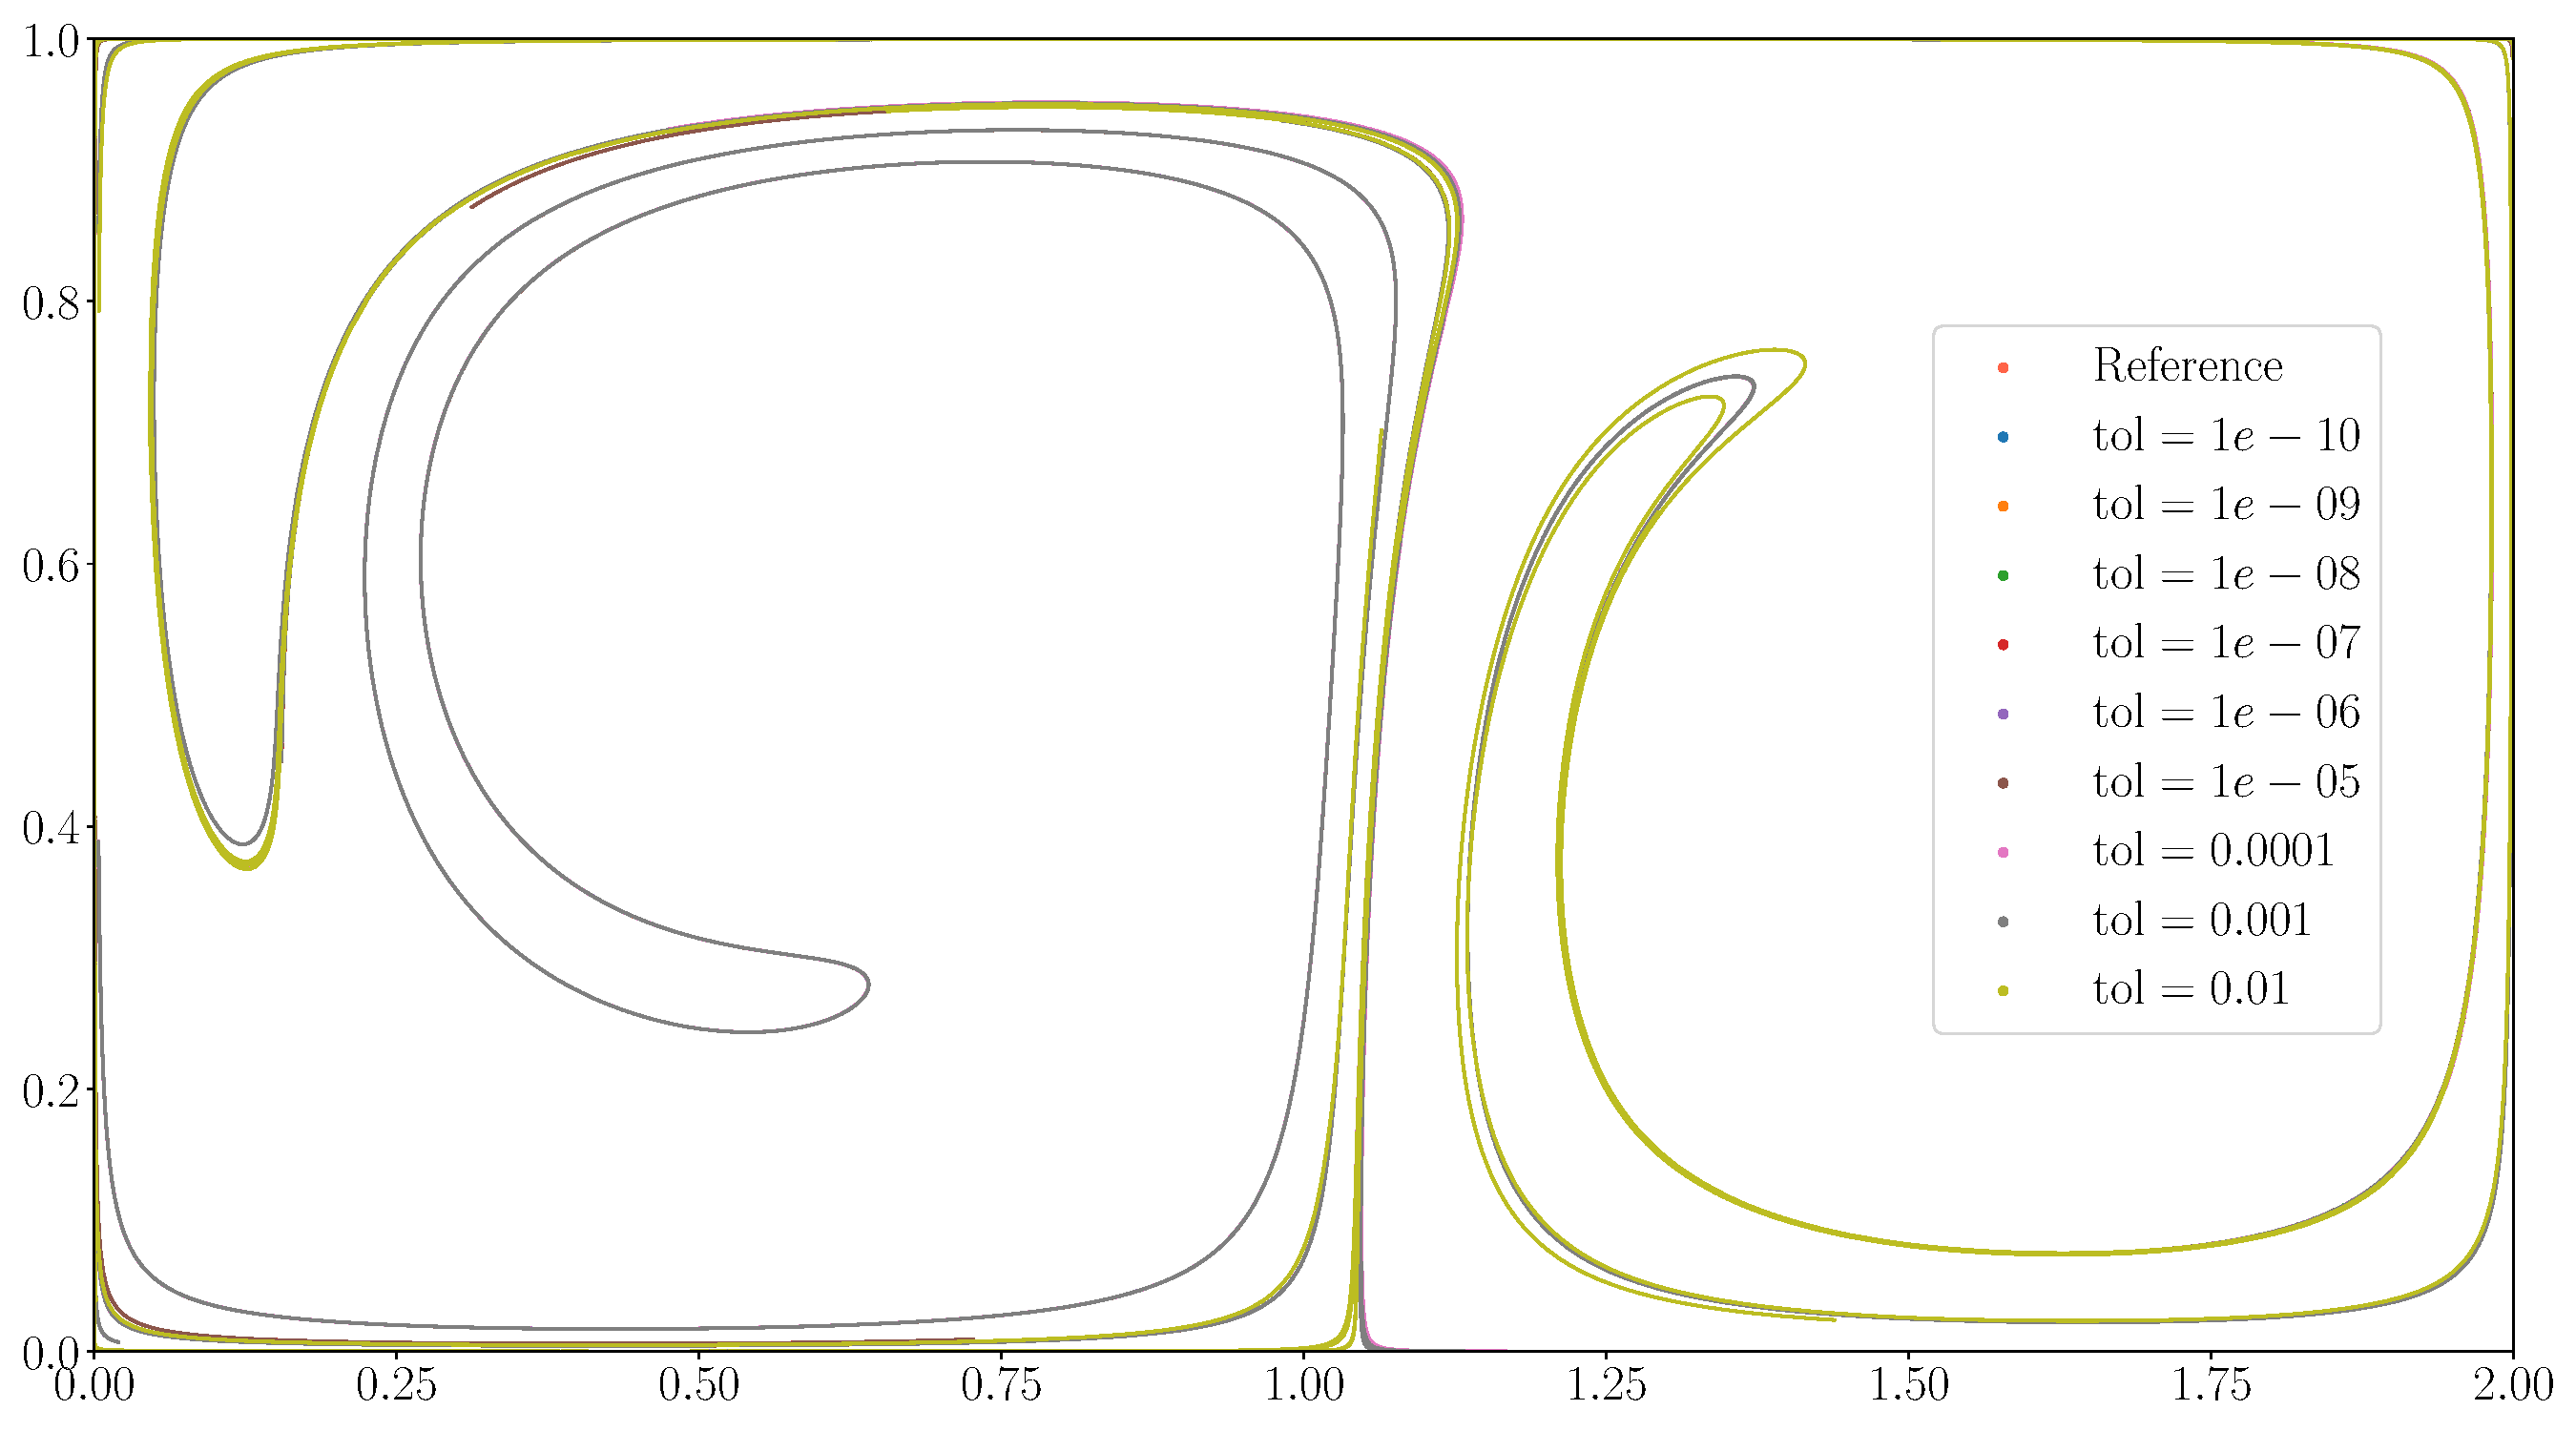
\includegraphics[width=0.9\linewidth]{figures/lcs_figures/rkdp87.pdf}
    \caption[LCS curves found by means of the Dormand-Prince 8(7) integration
    scheme]{
        LCS curves found by means of the Dormand-Prince 8(7) integration
        scheme. The reference LCS, as shown by itself in figure
        \ref{fig:referencelcs}, is dashed on the top layer. Note that
        the LCS for the lowest tolerance level considered, that is,
        $\textnormal{tol}=10^{-1}$, is not included. This is because the
        corresponding $\mathcal{U}_{0}$ domain, shown in figure
        \ref{fig:u0_dom_err_dp87}, and the reference $\mathcal{U}_{0}$, shown in figure
        \ref{fig:u0_domain} are quite unlike one another. Here, the most immediately
        discernible dissimilarities emanate from the tolerance level
    $\textnormal{tol}=10^{-2}$.}
    %Close inspection, however, reveals
    %    discrepancies for all tolerance levels $\textnormal{tol}>10^{-6}$,
    %    particularly by the `$\cap$' shape near $x=1.25$.}
    \label{fig:lcs_rkdp87}
\end{figure}


\clearpage

